\documentclass[a4paper,12pt]{article}

\usepackage[utf8]{inputenc}
\usepackage[a4paper, total={6in, 9in}]{geometry}
\usepackage{listings}
\usepackage{lstautogobble}
\usepackage{color}
\usepackage{amssymb}
\usepackage[parfill]{parskip}
\usepackage{pgfplots}
\usepackage{tikz}
\usepackage{pgfgantt}
\usepackage{pgf}
\usepackage{adjustbox}
\usepackage{graphicx}
\usepackage{pdfpages}
\usepgfplotslibrary{groupplots}
\pgfplotsset{width=6.9cm,compat=1.9}
\usepackage{float}
\usepackage{caption}
\usepackage{booktabs}
\usepackage{multirow}
\usepackage{enumitem}
\usepackage{amsmath}
\usepackage{hyperref}
\usepackage{minted}

\definecolor{purplelink}{HTML}{2A1B81}

\renewcommand{\thefootnote}{\fnsymbol{footnote}}
\newcommand{\STAB}[1]{\begin{tabular}{@{}c@{}}#1\end{tabular}}

\begin{document}
	%\nocite{*}
	% Title page
	\begin{titlepage}
	
		\centering
	
		{\large \scshape Electronics and Computer Science \par}
		{\large \scshape Faculty of Physical Sciences and Engineering \par}
		{\large \scshape University of Southampton \par}
		\vspace{3cm}
		
		{\Large \textbf{Martin Valchev} \par} % Put your name here
		\vspace{0.25cm}
		{\large \today \par}
		
		\vfill
		
		\hrule height 0.4pt
		\vspace{1cm}
			\huge
			\textbf{Analysis and Application of Active Learning to Classify Malicious Twitter Posts} % Put your project title here
		\vspace{1cm}
		\hrule height 1.2pt
		
		\vfill
		
		{\Large Project supervisor: \\ Oliver Bills \par} % Put your supervisor here
		\vspace{0.5cm}
		{\Large Second examiner: \\ David Millard \par} % Put your second supervisor here
	
		\vfill
		
		{\Large A project report submitted for the award of \par} % Change this depending on final / progress / brief
		{\LARGE BEng Software Engineering \par} % Put your degree title here
		\vspace{4cm}
	
	\end{titlepage}

\section*{Abstract}
As new social networks continue to emerge, so do new mediums for sharing content. This often requires existing machine learning models to be re-trained on new data. Annotating large amounts of data is time-consuming, and expensive but necessary with novel social networks.

This project explores active learning as an alternative, more data-efficient approach to machine learning. The primary objective is to show that active learning can reduce annotation costs and expedite the design and development of models by leveraging the large amount of unlabeled data available.

To evaluate the benefits of active learning, a multi-stranded approach was employed. The learning process was decomposed into individual components that are known to have an impact on performance - dataset, features, classifier, and sampling strategy. All permutations of these components were explored in a passive scenario to obtain reference baselines. Similarly, iterative active learning was evaluated by recording the performance per annotation and comparing it against the baselines.

Results indicate that active learning manages to reduce the annotated data necessary to reach and often exceed the target baselines by more than 50\%. This can be observed across most evaluated scenarios. It is evident that active learning is a sustainable approach for reducing annotation costs.
\section*{Scope}
The project does not necessarily aim to produce a highly accurate model for tweet classification, but rather show annotation costs in relation to F1-scores of models trained using various machine learning techniques.
\section*{Project Goals}
\begin{itemize}
    \item To compile an appropriate dataset for machine learning, using Twitter's API, feature selection and feature engineering.
    \item To develop an application that interactively queries users to label data.
    \item To apply active learning in the context of social media classification, specifically to classify Twitter posts as malicious or not.
    \item To produce an analysis of the outcomes of active learning application.
    \item To compare active learning to passive supervised learning approaches in regards to data efficiency.
\end{itemize}
\newpage
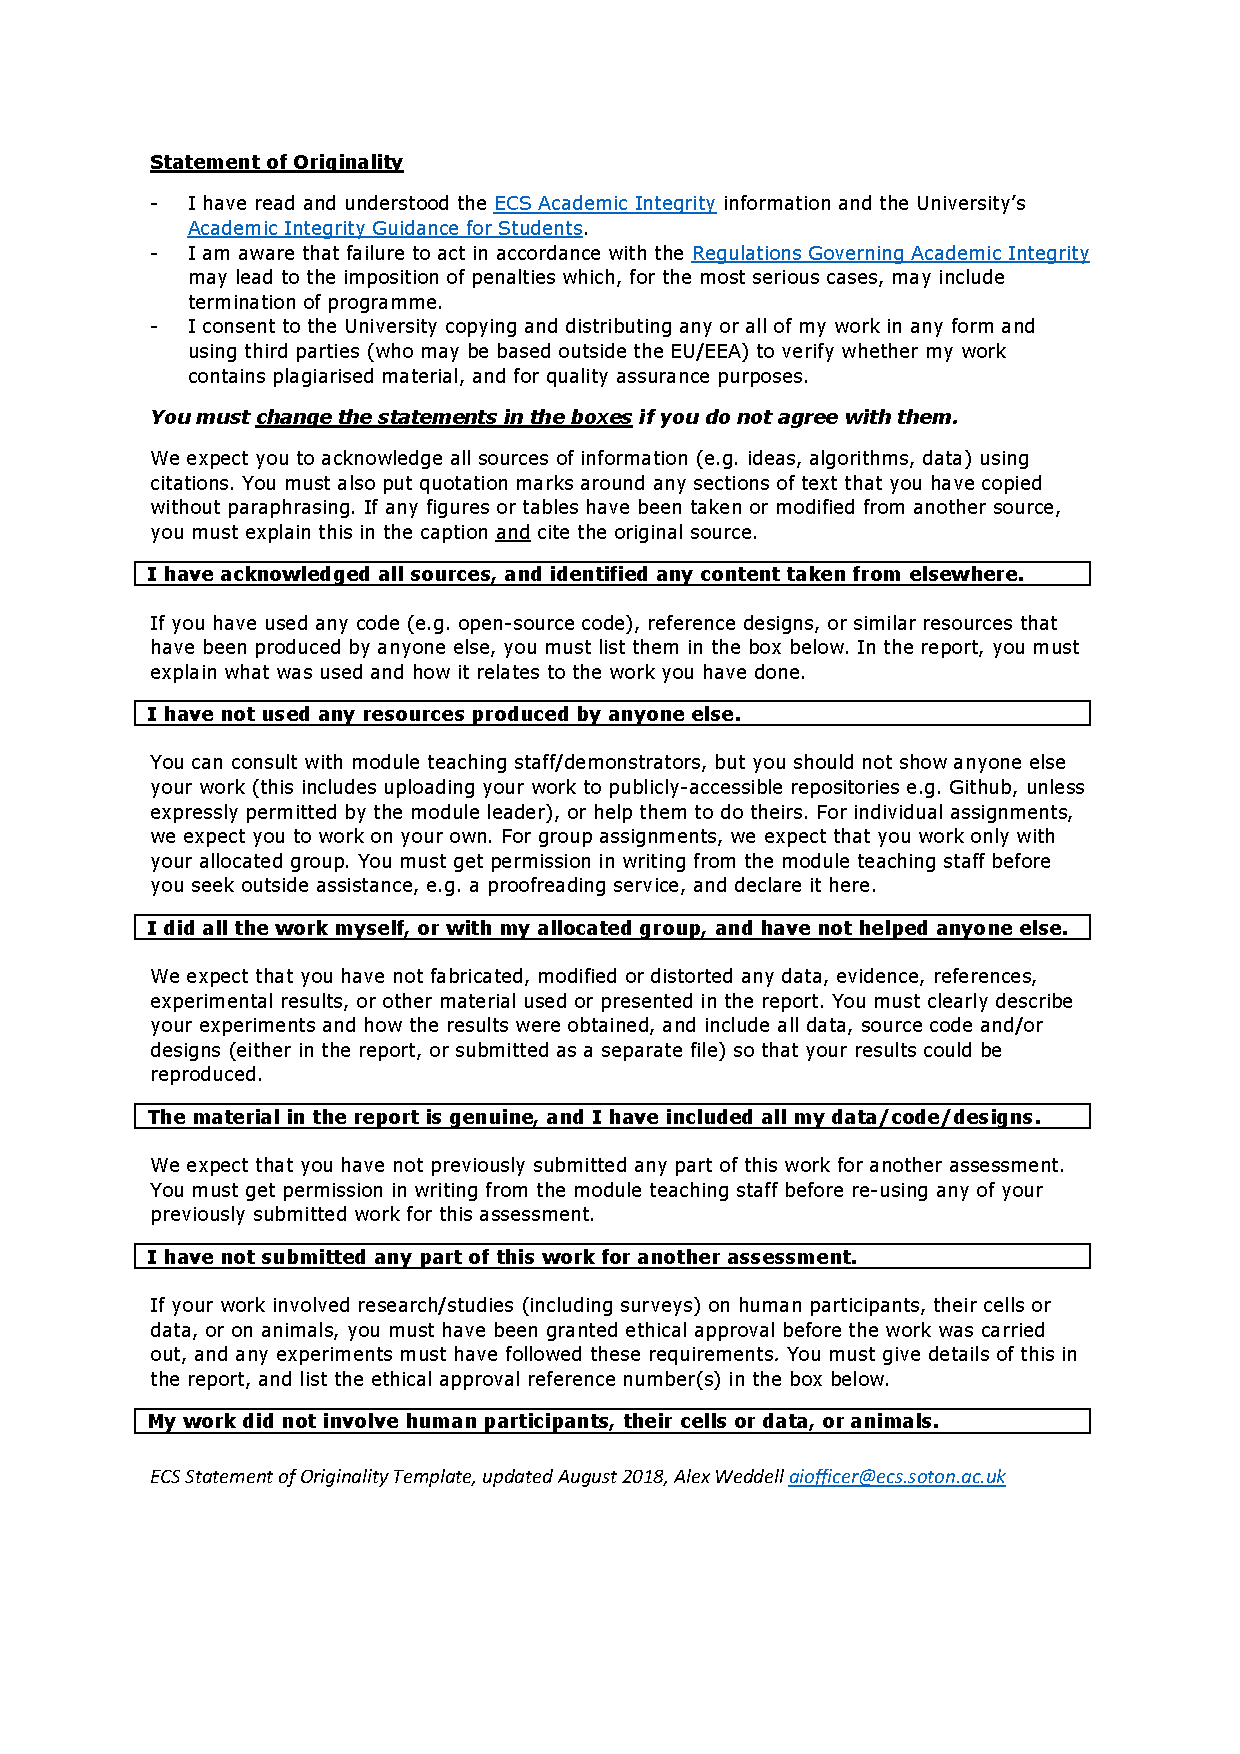
\includepdf[pages={1},pagecommand={},scale={0.9}]{ai_statement.pdf}
\tableofcontents
\newpage
\section*{Definitions}
\addcontentsline{toc}{section}{\protect\numberline{}Definitions}%
Malicious tweets are defined as posts with negative sentiment, directed at a specific person or a large demographic with a malicious intent, i.e. containing radical, hateful, racist, sexist, phobic or excessively derogatory remarks, or such that could otherwise be described as cyber bullying. Furthermore, posts describing an event where a person is the target of such remarks, are also defined as part of the malicious class for the sake of more extensively capturing the context in which cyber bullying can manifest. Included also are attempts to de-platform public figures as well as online personas in the form of ``cancelling".

In this paper, the words ``model", ``classifier" and ``learner" are used synonymously, unless specified otherwise.

``Vectorizer" refers to a model trained on some text corpus to transform raw text into numeric features in some meaningful manner.

``ML" and ``AL" are sometimes used in place of ``Machine Learning" and ``Active Learning" respectively.
\newpage
\section{Introduction}
As new social networks continue to emerge, so do new mediums for sharing content. This often requires previously trained machine learning models to either be adapted to the new media using some form of transfer learning, or be re-trained on new data altogether. For example, a model that classifies Facebook posts as malicious or not may be extended to classify Twitter posts with little changes. However, if classifying TikTok shorts on the same classes was the goal, that task would call for a completely different classifier, with different training data. Annotating large amounts of data is time-consuming and expensive, but necessary with novel social networks, where transfer learning is not always applicable.

Active learning is a special case of machine learning, in which an algorithm can interactively query a user, sometimes referred to as an ``oracle", to annotate data examples that benefit the model most and are therefore highly informative.

``The key idea behind active learning is that a machine learning algorithm can
achieve greater accuracy with fewer training labels if it is allowed to choose the data from which it learns."\cite{Settles2009}

This project explores active learning as an alternative, more data-efficient approach to machine learning.
\section{Literature Review}
\label{section:litrev}
While all papers that explore the topic of classification report their results with standardised metrics, a direct comparison is often sub-optimal for arriving at conclusions. This is primarily due to lack of consistency of the environment in which the results are produced. In other words, the specific dataset, features, approach to testing, as well as many other factors, all play a key role in the final evaluation of a machine learning model. As such, most findings in the following literature review are scrutinised and tested, and not accepted ``as is".
\subsection{Feature Selection and Feature Engineering}
\label{section:features}
The set of available features that a model has access to for training, as well as their discriminative power are directly correlated to the performance the model can achieve. As such, it is important to review the state-of-the-art techniques for feature selection and engineering found in topical literature.
\subsubsection{User Features}
Dadvar M. et al. \cite{Dadvar2013} propose the use of profile data as features, in addition to text vectorization for tweets, in order to further improve the performance of cyberbullying classification. That is, to derive the common behaviour of users based on patterns of offensive language in previous posts, average length of the comments, age, number of pronouns, etc. The authors find that including user related information yields approximately $6.6\%$ increase to F1-score in their most successful attempt. They conclude that ``users' profile information is not always stated correctly", which attributes to the underwhelming result.

Al-Garadi et al. \cite{garadi-highestf/top10features} perform an analysis over a set of features, including network, activity, user and textual information, to identify which features are most discriminative and hence provide the largest information gain in the context of cyberbullying detection. Four out of the top ten features are user related, which alludes to user data playing a significant part in the $42\%$ AUC increase over their baseline result with textual features only, for a total of $0.943$ micro F1-score. While their results are impressive, the difference in performance is marginal compared to other state-of-the-art literature that avoids the use of profile data. Again, due to a lack of consistency in dataset and evaluation process between different literature, it is hard to gauge how beneficial user profile information really is, therefore such data is collected and experimented with during prototyping.

Alternatively, one could opt to predict user behaviour with a separate classifier and use the resulting labels as a categorical feature for training the cyberbullying classification model. Balakrishnan V. et al. \cite{Balakrishnan2020} are able to classify Twitter users as ``Bully, Aggressor, Spammer and Normal" with a micro F1-score of $\approx0.91$ by utilising personality and sentiment data. The difference in approach to cyberbullying detection they've taken makes direct comparison to other literature not possible, but the results are promising. However, as this technique requires additional external data, it is in direct conflict of the project's goal to use less labeled data to achieve comparable F1-scores. Predicting user behaviour is therefore not taken into consideration for the implementation of this project.
\subsubsection{Textual Features}
\label{section:textfeatures}
Textual features are by far the most commonly used features in cyberbullying classification, likely due to the key role profanity plays in malicious texts.
Many different techniques are proposed in topical literature, however, in most papers the following text transformation and feature extraction approaches are found to perform best:
\begin{itemize}
    \item TF-IDF - measure of word importance in a text
    \item Bag-of-Words - histogram of the words in a text
    \item Named-entity Recognition - named entities in a text
    \item Sentiment Analysis - emotion/opinion of a text
    \item Word Embeddings - word similarity and associations
\end{itemize}
Rosa H. et al. \cite{Rosa2019} suggest that feature engineering beyond the use of a TF-IDF transformer is only marginally better and therefore not rewarding.
\subsubsection{Statistical Features}
Research by Al-Garadi et al. \cite{garadi-highestf/top10features} indicates that other types of features can also be utilised successfully, but contribute less to the overall performance of a cyberbullying classification model. These features are less discriminative and are unlikely to benefit the project. Examples of such features include:
\begin{itemize}
    \item Network Features - number of followers, followed users, following–followers ratio, verification status, etc.
    \item Activity Features - number of posts, mentions, tweets added to favorites, hashtag usage, etc.
\end{itemize}
\subsubsection{Feature Selection}
Feature selection is best analysed by Rosa H. et al. \cite{Rosa2019}, who explore 22 different papers on the topic of automatic cyberbullying detection, as well as perform their own experiment. They found that the top three best-performing combinations of features types are:
\begin{itemize}
    \item TF-IDF only
    \item TF-IDF + Word Embeddings
    \item TF-IDF + Personality Features + Word Embeddings
\end{itemize}
\subsection{Classification Algorithms}
Active learning with standard sampling strategies like uncertainty, by definition requires a probabilistic classifier that outputs a confidence measure for its predictions.

Neural networks are known for their inability to produce such measures accurately \cite{Nguyen2015}. They are often overconfident in their labeling, which introduces bias during active learning sampling.
Recent study proposes a novel loss function that can be applied to existing neural network architectures without any modification, which results in reliable predictions and is effective for active learning \cite{Moon2020}. However, implementing a different loss function for a specific algorithm diverges from the idea of minimal variance during the evaluation of this project. Moreover, the novelty of the approach may well result in a poor implementation by this author and is therefore a project risk. Neural networks also require much more data to perform well in comparison to traditional machine learning algorithms. As such, active learning with neural networks is not considered in this project.

Precisely because of the importance of accurate confidence measures, naturally probabilistic classification models, i.e. models that predict a probability distribution over classes, are more suitable for the active learning task. Examples of such models are Logistic Regression, Naive Bayes, Random Forest, etc. SVM is a notable exception, whose ``convenient mathematical properties" make it ``well-suited for active learning", as discussed by Kremer J. et al. \cite{Kremer2014}.

Active learning for malicious text classification hasn't been explored yet in academic literature. However, the closely related topic of cyberbullying detection has been and is being highly studied in passive learning scenarios. The results of papers on the topic are therefore used as vague references for baseline passive learning performance.

One of the best-performing models has been proposed by Al-Garadi et al. \cite{garadi-highestf/top10features}. In their paper, the performance of four classifiers - Naive Bayes, Linear SVM, Random Forest and K-Nearest Neighbors - is measured based on various features. Results suggest that the choice of classifier doesn't impact F1-scores as much as the choice of features and dataset balance do. For example, there is only $1.865\%$ difference between their lowest-scoring Naive Bayes approach and their highest-scoring KNN model ``under a basic setting". As such, this project focuses on exploring classifiers that are known to perform well in active learning environments, regardless of the classification problem, and not necessarily ones that have been shown to work well with cyberbullying detection specifically.
\subsection{Active Learning Scenarios}
When discussing active learning, a distinction can be made in regards to the way sampling queries are produced. Literature on the topic refers to this distinction as an ``active learning scenario". Usually, a scenario is described as one of the following - membership query synthesis, stream-based selective sampling and pool-based sampling.

First, in the case of membership query synthesis, a model can request labels for both unlabeled data instances from a dataset, as well as ones that are generated by the machine \cite{Settles2009}. This is clearly not a good approach for tasks that involve natural language, such as the one of malicious text classification. Maliciousness is not always apparent even in well-structured texts and chances are, a machine would not be able to generate sensible data that contains malicious traces either. Any labels given to nonsensical instances may well degrade the performance of the model on actual testing data. There are recent advances in the field of query synthesis for natural language that show promising results \cite{schumann-rehbein-2019-active}, however, more suitable approaches exist.

One such approach is stream-based selective sampling. Unlabeled data instances are drawn sequentially and the machine decides whether to label each one individually \cite{Settles2009}. This would work well in practice, as one could fetch fresh tweets as a stream from Twitter's API and the machine would decide for each tweet whether it is worth labeling or should be discarded. This is however not applicable to this project in particular, because one of the requirements for evaluation is that a dataset used across different models must be consistent in order to produce relevant performance results.

This leads to the final and most suitable approach - pool-based sampling. In this scenario, data instances are sampled from a pool, consisting of both labeled and unlabeled data, based on some sampling strategy \cite{Settles2009}. This allows all models to share a single dataset, as well as for language models to be trained on the entire available text corpus at once.
\subsection{Query Strategies}
\label{section:query}
Another essential part of the active learning process is the strategy used to sample the available unlabeled data. In fact, the query strategy is almost solely responsible for the benefits of active learning.

For example, consider a random sampling strategy. Although it could use less data overall, it offers no guarantees that answering a query would benefit the model's performance in any way. It is passive learning in a sense.

Alternatively, a sampling strategy that is able to query the data instances a model is least certain about could be described as more optimal. Whether answering such queries would be beneficial is also undetermined, but the likelihood of a positive outcome is certainly higher. This strategy is referred to as ``least confidence" sampling in literature \cite{10.5555/1613715.1613855}.

Another candidate strategy for this project is margin sampling, initially introduced by Scheffer et al. \cite{10.5555/647967.741626}. Instead of sampling the data instances with least certainty, it samples those for which the difference between class predictions (margin) is smallest.

Entropy sampling is yet another uncertainty related strategy that is shown to work well in practice. It simply selects the samples displaying the greatest Shannon entropy \cite{Schein2007}.

Other sampling strategies exist, but are either too complex to implement, depend on assumptions of the data or scale badly due to high computational costs \cite{Kumar2020}.

It is important to note that there is virtually no difference in the queries produced by each discussed strategy on a binary classification problem, as all heuristics coincide in the choice of samples. That being said, all strategies have been shown to perform better than passive learning and random sampling in multinomial classification. While literature refers to the family of these strategies as ``uncertainty", this project uses that term in place of ``least confidence".
\newpage
\subsection{Data Analysis}
The following graphs visualise the relation between dataset size, balance ratio and F1-score in some of the highly influential works on cyberbullying detection:
\begin{figure}[H]
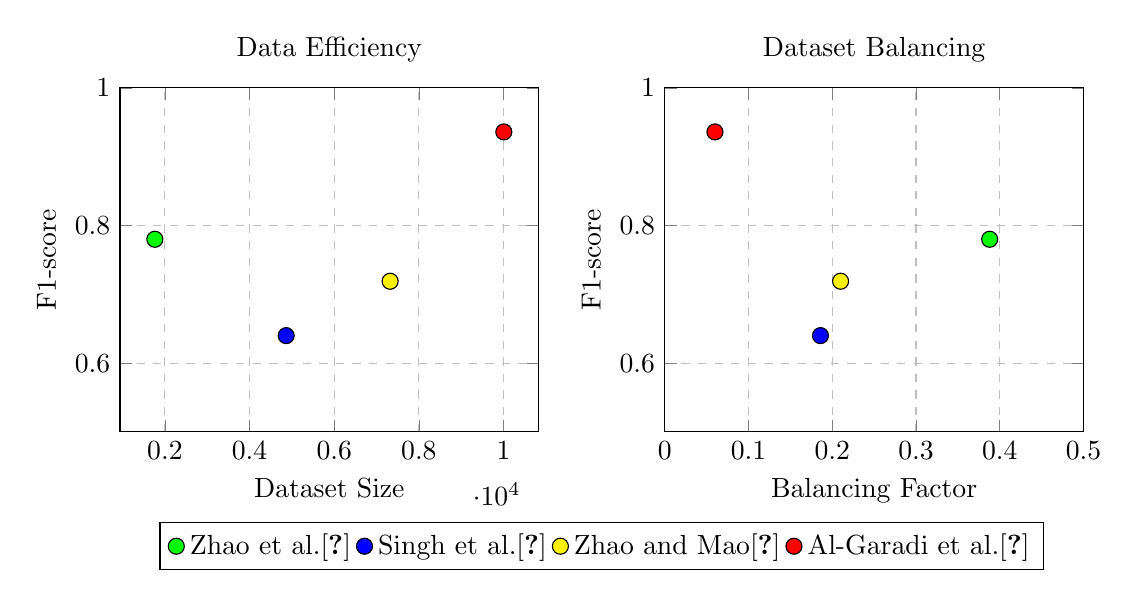
\begin{tikzpicture}
    \begin{groupplot}[group style={
                      group name=datacharts,
                      group size= 2 by 1,
                      horizontal sep=1.6cm}]
        \nextgroupplot[title={Data Efficiency},
                        xlabel={Dataset Size},
                        ylabel={F1-score},
                        ymin=0.5, ymax=1,
                        ymajorgrids=true,
                        xmajorgrids=true,
                        grid style=dashed]
    \addplot[only marks,
            mark=otimes*,
            scatter,
            mark size=2.9pt,
            scatter/classes={
                a={mark=*,green,draw=black},%
                b={mark=*,blue,draw=black},%
                c={mark=*,yellow,draw=black},%
                d={mark=*,red,draw=black}%
            },
            scatter src=explicit symbolic]
    coordinates {
    (1762,0.780) [a]%Zhao et al. (2016)
    %(1954,0.790) %Hosseinmardi et al. (2016)
    %(3279,0.900) %Sugandhi et al. (2016)
    %(4626,0.640) %Dadvar et al. (2013)
    (4865,0.640) [b]%Singh et al. (2016)
    (7321,0.719) [c]%Zhao and Mao (2016)
    (10007,0.936) [d]%Al-Garadi et al. (2016)
    %(13000,0.562) %Zhang et al. (2017)
    %(13160,0.425) %Rosa et al. (2018b)
    %(13160,0.444) %Rosa et al. (2018b)
    };
    \coordinate (c1) at (rel axis cs:0,1);
        \nextgroupplot[title={Dataset Balancing},
                        xlabel={Balancing Factor},
                        ylabel={F1-score},
                        xmin=0, xmax=0.5,
                        ymin=0.5, ymax=1,
                        ymajorgrids=true,
                        xmajorgrids=true,
                        grid style=dashed,
                        legend to name=papers,
                        legend style={legend columns=-1}]
    \addplot[only marks,
            mark=otimes*,
            scatter,
            mark size=2.9pt,
            scatter/classes={
                a={mark=*,green,draw=black},%
                b={mark=*,blue,draw=black},%
                c={mark=*,yellow,draw=black},%
                d={mark=*,red,draw=black}%
            },
            scatter src=explicit symbolic]
    coordinates {
    (0.388,0.780) [a]%Zhao et al. (2016)
    %(1954,0.790) %Hosseinmardi et al. (2016)
    %(0.120,0.900) %Sugandhi et al. (2016)
    %(4626,0.640) %Dadvar et al. (2013)
    (0.186,0.640) [b]%Singh et al. (2016)
    (0.210,0.719) [c]%Zhao and Mao (2016)
    (0.060,0.936) [d]%Al-Garadi et al. (2016)
    %(13000,0.562) %Zhang et al. (2017)
    %(13160,0.425) %Rosa et al. (2018b)
    %(13160,0.444) %Rosa et al. (2018b)
    };
    \coordinate (c2) at (rel axis cs:1,1);
    \legend{Zhao et al.\cite{Zhao2016},Singh et al.\cite{Singh2016},Zhao and Mao\cite{Zhao2017},Al-Garadi et al.\cite{garadi-highestf/top10features}}
    \end{groupplot}
    \coordinate (c3) at ($(c1)!.5!(c2)$);
    \node[below] at (c3 |- current bounding box.south) {\pgfplotslegendfromname{papers}};
\end{tikzpicture}
\captionsetup{justification=centering}
\caption{Relation between dataset size, balance ratio and F1-scores.}
\end{figure}
Analysing the graphs, one can extrapolate that there is direct link between dataset size, balance ratio, and classifier performance. Models with large amounts of labeled data perform well regardless of balancing, possibly because of a higher probability for that data to sample more edge-cases and therefore extract useful information that would otherwise remain unseen. Surprisingly, the smallest dataset \cite{Zhao2016} performed comparably well, considering it is just $17.61\%$ of the size of the highest performing approach \cite{garadi-highestf/top10features}. This can be attributed to the high balance between the number of cyberbullying and non-cyberbullying instances in the dataset. Naturally, there is a large difference between the features and techniques used by the reviewed papers, but looking strictly at sizes and balancing, two possible approaches become apparent - using either a small but balanced or large and not as balanced dataset. Considering the scope and time constraints of this project, a small but relatively balanced dataset seems appropriate.
\newpage
\subsection{Summary}
\begin{enumerate}
  \item User related features improve the overall performance of classification, but only marginally.
  \item Features obtained via text vectorization account for the highest classification performance gains.
  \item Feature engineering is not rewarding for cyberbullying classification.
  \item Choice of machine learning model has low impact on passive learning performance in most cases.
  \item Naturally probabilistic classification models are better suited for the project's goals.
  \item Pool-based sampling is the most applicable scenario for this project.
  \item Uncertainty sampling is easy to implement, yet works well in practice.
  \item Small but balanced datasets perform comparably to large unbalanced sets, at a fraction of the annotation costs.
\end{enumerate}
%%end lit review
\newpage
\section{Analysis}
    \subsection{Requirements}
    \label{subsection:req}
    \begin{itemize}
        \item The dataset must not contain references or links to Twitter users, i.e. complies with privacy laws and guidelines.
        \item All data must be labeled accurately.
        \item The dataset should sample a large enough space, accounting for edge cases whenever possible.
        \item A classification model should perform well on both training and testing data.
        \item Identifying malicious instances correctly (recall) should take precedence over not misclassifying non-malicious instances (precision).
    \end{itemize}
    \subsection{Costs}
    \begin{itemize}
        \item Monetary investment if data labeling is outsourced to an external party.
        \item Time investment if labeling done independently.
    \end{itemize}
    \subsection{Benefits}
    \begin{itemize}
        \item Using a single dataset allows for the training of multiple classification models asynchronously.
        \item Data efficiency, low data labeling costs.
        \item Stimulates research in the field of active learning, especially for practical applications.
        \item Minimal variance during technique comparison ensures accurate results and findings.
        \item Relatively easy implementation using open-source libraries.
        \item Accelerates startups interested in cyberbullying detection.
        \item Offers a robust methodology for rapid development of models on future novel social networks.
    \end{itemize}
    \subsection{Constraints}
    \begin{itemize}
        \item Limited time restricts the size of the dataset that can be acquired and labeled.
        \item Limited number of data annotators, resulting in lower initial performance.
    \end{itemize}
\newpage
\subsection{Ethics}
The dataset used to demonstrate proof of concept on a small scale is collected and labeled exclusively by the author, in a way that respects and adheres to all relevant ethical obligations and concerns. The dataset contains no sensitive data or anything that can't otherwise be accessed or obtained publicly. Furthermore, all collected and processed records are stripped of user-identifying information and are hence anonymised.

This author acknowledges that as a result of having labeled the dataset by themselves, some bias might naturally occur in regards to what is considered malicious or an instance of cyberbullying. However, given the project's problem, such bias is irrelevant as it doesn't impact the evaluation process and results. This project explores the differences between two learning techniques in the context of identical datasets, regardless of the underlying data and its attributes, therefore any inconsistencies or biases equally affect both techniques.
\newpage
\section{Design and Implementation}
This section applies the knowledge obtained from literature review to design and implement a complete software product. Furthermore, it extends the scope of explored literature to account for unforeseen topics encountered during the design process. Such topics are discussed and referenced in this section as opposed to Section~\ref{section:litrev}, as design choices follow directly from the topics' logical conclusions.
\subsection{Architecture}
\label{section:architecture}
\begin{figure}[H]
\centering
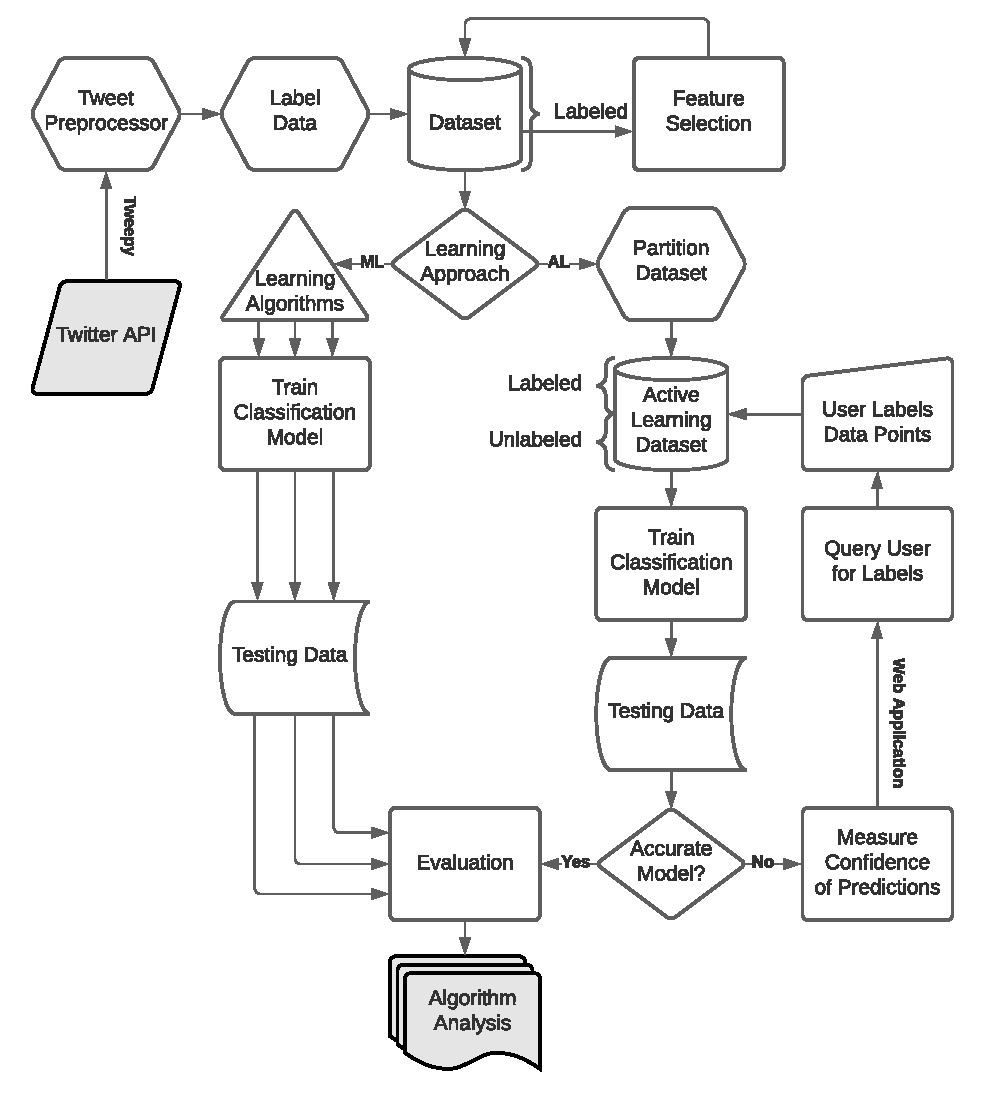
\includegraphics[scale=0.84]{design.pdf}
\captionsetup{justification=centering}
\caption{\label{fig:moduleDiagram}Architecture, modularity and general flow of the implemented system.}
\end{figure}
\newpage
\subsection{Data Processing}
\label{section:processing}
\subsubsection{Data Collection}
For the purpose data collection, the open-source library \emph{Tweepy} was utilised. It is a python wrapper for Twitter's API, that maps fetched tweets to objects. This reduces complexity significantly, as it makes the subsequent use of data manipulation software like \emph{pandas} much easier.
A script was developed that automatically fetches and stores public tweets based on input queries or keywords. Alongside the post text itself, statistical information about the tweet and its author is recorded and later used in conjunction as features, like discussed in Section~\ref{section:features}.

In order to train a good machine learning model, a sufficiently variant yet balanced dataset is often needed. In fact, compiling an appropriate dataset for a given problem is one of the hardest tasks. To produce one, a strategic approach to data collection was employed.
The keywords/phrases used for fetching tweets were broken down into three primary categories based on their attributes:
\begin{enumerate}
    \item Words/phrases that are offensive and have a high probability of being used in a malicious context\\ - \emph{retard, kys, die}\footnotemark
    \item Words/phrases that are offensive but not necessarily used in a malicious context - \emph{bitch, slut, idiot}\footnotemark[\value{footnote}]
    \item Words/phrases that are not offensive but could be found in a malicious context - \emph{black, fat, disgusting}\footnotemark[\value{footnote}]
\end{enumerate}
\footnotetext{Not all keywords used for data collection in this project are listed. A keyword's category is assigned by the author per their personal interpretation, which may differ from the reader's.}
Volume-wise, 40 unique search queries were performed, obtaining 50 samples from each for a total of 2000 tweets. After removing duplicates, 1912 examples constitute the final dataset. Query terms were selected such that all three categories are more or less equally represented. This was done with the idea of producing a naturally balanced dataset, instead of having to apply oversampling or undersampling techniques at a later point. Furthermore, this approach accommodates edge cases well, since tweets based on keywords from the second and third categories are likely harder to predict due to their duality, and so an active learner might prioritise querying their labels early.

To avoid extra processing in the form of translation or language tagging, only English tweets were fetched by utilising Twitter's built-in filtering capabilities.
Due to API limitations, the data obtained is temporally restricted to a period of up to seven days before the moment of collection. As a result, the author was not able to take advantage of prior well-known events of cyberbullying or otherwise abusive behaviour.

Nevertheless, fetching Twitter posts based on a fixed range of keywords and search phrases is in turn bound to limit the generalisation power of any machine learning model in terms of overfitting. Due to budget constraints, the initial dataset collected is final and will not be re-sampled in case all trained classifiers end up being myopic. That is, if they can't accurately classify malicious tweets outside the sampled pool, it will not be considered a fault of the learning technique during evaluation. Given more time, resources and domain knowledge, one could compose an optimized dataset where this wouldn't be an issue, however, this is outside the scope of the project.
\subsubsection{Data Partitioning}
\label{section:partitioning}
A common approach to evaluating model performance is to partition a dataset into 3 disjoint subsets - training, validation and testing. The model is first fit on the training set and its performance on the validation set recorded. Then, some form of optimization like hyperparameter tuning or dimensionality reduction is iteratively performed until the score on the validation set is maximised. Finally, the optimized model is evaluated on the previously unused testing set to produce unbiased results. This is known as hold-out. Alternatively, instead of having a static validation set, one could opt to use $k$-fold cross validation, where the training and validation partitions are re-sampled $k$ times and the mean performance is recorded. Both techniques are appropriate for model selection and the optimal choice is assumed to be data dependent \cite{Xu2018}.

\label{section:partitioning-optimisation}
However, this project isn't concerned with model optimization, so the validation set can be skipped entirely, leaving only training and testing partitions. Because of that, cross validation is inapplicable, as it would not produce consistent testing sets across different learning techniques. That is, active learning would have unique folds after each training iteration, which would not match those of passive learning. When plotting performance per query in comparison to baseline ML later, the results would be meaningless. Besides, cross validation is especially expensive for active learning, due to the iterative nature of training.

It was concluded that a hold-out approach with no validation set is optimal for this project. All explored scenarios are evaluated on equal test partitions. That is, for every model, the dataset is split such that 10\% of all examples are withheld and used only for testing, while the rest is available for training. Furthermore, when partitioning the dataset, the seed for generating random split indices is fixed, such that replicability of the samples in each partition is ensured across different models and over subsequent runs.

\label{section:activepartitioning}
For the case of active learning, it was initially experimented with a 80:10:10 dataset split ratio for unlabeled pool, initial training set and testing set respectively. However, for a medium-sized dataset, the number of initial training examples in such split proved inappropriate. An observation of the early performance growth rate couldn't be made, since the model had already ``seen" substantial amount of training data that wasn't necessarily what would have been queried.
For example, when splitting a $\approx26k$-large dataset, originally used by Thomas Davidson et al. \cite{hateoffensive} to classify hate speech, $\approx2600$ instances were being randomly selected as initial training data. When testing the model, these instances proved enough to reach adequate accuracy. To resolve this phenomena and to better replicate a scenario where active learning can be utilised best, the dataset split was adjusted to 10\% for testing and 1 sample per class in the data for initial training. The remaining data is used as the sampling pool queried by the learner.
\subsubsection{Data Preprocessing}
Twitter posts are inherently noisy as suggested by T. Singh \cite{SINGH2016549}, which is well accentuated by their imposed limit of 280 characters according to A. Boot et al. \cite{Boot2019}. While this could be recognized as a characteristic of the social media platform, it greatly diminishes the quality of information that can be extracted for NLP applications, feature extraction in particular.

In order to prepare the dataset for further processing, all tweets are normalised in a uniform manner. The following list describes the step by step process employed in this project:
\begin{enumerate}
    \item Filter out all URLs. - (``https://t.co/xxxxxx" $\to$ $\epsilon$)
    \item Transform all emojis to their description. - (U+1F525 $\to$ ``fire")
    \item Decode all html-encoded characters. - (\&gt $\to$ $>$)
    \item Lowercase all characters. - (``LMAO" $\to$ ``lmao")
    \item Expand all contracted forms. - (``hasn't" $\to$ ``has not")
    \item Filter out all mentions. - (``@xxxx" $\to$ $\epsilon$)
    \item Remove all non-letter characters. - (``\#cancelled" $\to$ ``cancelled")
    \item Filter out all stopwords. - (``i hope you" $\to$ ``hope")
    \item Lemmatise all words. - (``went" $\to$ ``go")
\end{enumerate}
\subsubsection{Feature Extraction}
In order to train a classification model, the feature space used as training data must be entirely numerical. Therefore, the raw textual body of tweets must somehow be encoded as real numbers, i.e. transformed into feature vectors or vectorized. Moreover, the resulting vectors must be able to encode some meaningful information about the original text. While, there are lots of techniques that allow for such transformations, this project explores three in particular.

First and foremost, Section~\ref{section:textfeatures} concluded that TF-IDF has been found in external literature to be the best vectorization technique for problems similar to the one discussed in this project. TF-IDF is a numerical statistic that captures the importance of individual words in a document in relation to some text corpus. It is a product of two metrics, the term frequency TF and the inverse document frequency IDF. As such, words that appear frequently in a document, but are only found in few documents overall, are considered more important for that document. The word's discriminative power is therefore represented with a higher numeric value. The TF-IDF model in this paper is trained on a combination of unigrams, bigrams and trigrams, limited to the top 8000 most discriminative words or sequences.

Another approach to vectorization, which has also been found to work well in practice, is word embeddings. Unlike TF-IDF, which does not take into account the context and order in which words appear, embedding transformers often consider the context surrounding a given word. For example, a two token window to each side of a word, for a 5-gram sequence in total, can be used for training such models \cite{levy-goldberg-2014-linguistic}.
With a word embeddings approach to vectorization, to obtain the vector of a given tweet, the vectors of all individual words that appear in the tweet are added together, and the resulting vector is divided by the number of words for normalisation. Although this is not ideal, it opens the possibility for use of a pre-trained word embeddings model. Such model is bound to be significantly more accurate than one trained on the project dataset, by virtue of training data volume. In this project, a pre-trained GloVe \cite{pennington2014glove} model for word embeddings is used. It is a shallow neural network, trained on 2B tweets with 27B tokens that produces a 50-dimensional vector representation of words.

The final explored approach is an extension of word embeddings - Doc2Vec. The key difference between them is that while one learns vector representations for individual words, the other learns for entire documents or sentences. Because tweets are often contextual and the meaning of a tweet can't really be captured by its individual words, it is probable that one could infer more of the context in which malicious tweets appear by using a document vectorizer. However, because Twitter posts are inherently noisy and tend to be not well-structured, a pre-trained model like in the case of word embeddings can't be used. In this project, a Doc2Vec model is fitted on the collected dataset to explore whether it is beneficial for active learning in particular. All relations learned for document similarity are local to the dataset, which might end up being more discriminative than a general, pre-trained model.

The working hypothesis is that if the vector representation of tweets is somehow able to capture some notion of similarity, then a model could possibly learn more quickly by sampling the most dissimilar tweet at every iteration. When applying a embedding-based model like GloVe or Doc2Vec for vectorization, whenever two tweets are similar, their vector representations are close in vector space. In some sense, a classification model could possibly predict a tweet's label better, if it has previously been taught ``similar" tweet examples. By extension of that, the author expects that iteratively teaching an active learner dissimilar tweets would be a higher information gain per query than if such notion of similarity didn't exist, as is the case with TF-IDF. For example, consider a contrived scenario where there is only one tweet previously seen by a learner, and two candidates for sampling in the unlabeled pool:
\begin{itemize}
    \item Trained example: ``I hate Mary"
    \item $T1$: ``I do not like him"
    \item $T2$: ``lmao kys"
\end{itemize}
With embeddings, the model might be able to infer the label for $T1$ from its training data easier than it would for $T2$, as $T1$ is more similar. As such, it would make sense to teach the model $T2$ first. This relation between the tweets can be observed by constructing the vector of each one and comparing their cosine similarity pairwise:
\begin{table}[H]
\centering
\begin{tabular}{|l|l|l|l|}
\hline
\multicolumn{1}{|c|}{tweet} & I hate Mary            & I do not like him          & lmao kys                   \\ \hline
I hate Mary                 & \multicolumn{1}{c|}{$1$} & \multicolumn{1}{c|}{$0.972$} & \multicolumn{1}{c|}{$0.748$} \\ \hline
\end{tabular}
\captionsetup{justification=centering}
\caption{\label{tab:cosineSim}Cosine similarity between vectorized tweets.}
\end{table}
$T2$ is different both syntactically and semantically to the trained example, while $T1$ shares the same sentiment with little to no structural variance. As shown, this relation is captured well - $T2$ is indeed further in vector space and hence more dissimilar.

Because vectorizers don't need annotations for their training data, one could use the entire dataset corpus when fitting them. This especially benefits active learning, as it further leverages the usually large volume of unlabeled data available.

While the body of a given tweet itself is probably the most indicative attribute of whether the tweet is malicious, it is also beneficial to consider other statistical features. In this project, all tweets are further processed to extract the following features:
\begin{itemize}
    \item Emojis\\
    \emph{demoji} is used to obtain a list of all emojis appearing in a tweet
    \item Polarity and Subjectivity\\
    \emph{TextBlob} is used to perform sentiment analysis using a pre-trained model
    \item Retweet?\\
    whether a post is a retweet can be detected by traces of ``\emph{RT @someone:}"
    \item URLs, Hashtags, Mentions\\
    the number of distinct entities in a tweet
\end{itemize}
While some of these attributes can be obtained directly using Twitter's API, the project implements a general solution that works on any dataset. This is important for comparative analysis, where a uniform approach to data processing is necessary.
\subsubsection{Feature Selection}
A few unique combinations of features are extensively evaluated in this project. Individually, the types of features can be aggregated into three categories:
\begin{enumerate}
    \item Text Features\\
    - \emph{tf-idf, word\_embeddings, doc2vec}
    \item User Features\\
    - \emph{user\_is\_verified, user\_posts, user\_likes, user\_followers, user\_friends}
    \item Statistical Features\\
    - \emph{is\_retweet, tweet\_likes, tweet\_retweets, tweet\_is\_quote, emoji\_count, polarity, subjectivity, hashtag\_count, mentions\_count, words\_count, char\_count, url\_count}
\end{enumerate}
Instead of considering the impact of distinct features, clusters of feature categories are explored, in order to reduce the parameter search space. Text features are present in each combination due to their significant importance to classification performance, as discussed earlier in Section~\ref{section:textfeatures}. The combinations are as follows:
\begin{itemize}
    \item Text features only
    \item Text + User features
    \item Text + Statistical features
    \item Text + User + Statistical features
\end{itemize}
Although possible to perform additional optimization in the form of dimensionality reduction, such techniques disproportionately affect passive and active learning. In the case of active learning, after each iteration, the entire training set needs to be re-transformed, which is simply too expensive in terms of computational costs. Therefore, dimensionality reduction has not been explored further.
\subsection{Active Learning}
The design for the active learning process is comprised of two primary components - a server that exposes an API for building and augmenting active learning models, and a web application that interacts with the server to visualise and update a model's state and propagate labeled training examples.
These components can otherwise be distinguished as a front-end and back-end layers of the system. Moreover, a further separation of concerns is achieved by following a model–view–viewmodel design pattern, where the server acts as the viewmodel, the web application as the view, and the actual classifier and its state as the model. The view and viewmodel are two-way bound with the help of web sockets, ensuring real-time propagation of update events. Finally, the pattern allows each layer of the system to be developed in parallel, which in hindsight reduced the overall complexity of the project.

\label{sec:docker}
The active learning process does not necessarily benefit from having a large amount of annotators simultaneously, as the sampling strategies used in this project are interactive. In other words, they iteratively produce single queries, hence only one annotator can work on the data at a time. However, all components were designed with scalability in mind, as the system can easily be extended by implementing alternative query strategies in the future.
The final software product utilises \emph{Docker}\cite{merkel2014docker} containers to encapsulate the front-end and back-end components, such that they are platform-independent and easily maintainable. These containers can be orchestrated with \emph{Kubernetes} for automated deployment and scaling if necessary.
\subsubsection{Backend}
Everything backend related has been implemented in python for the benefit of a coherent project environment with a high availability of machine learning libraries. The core functionality of both the passive and active learning process is self-contained and can be used without a supporting web application running. The structure of the backend is partitioned in a way that aggregates closely related functionality in distinct modules. More or less, these modules correspond to individual ``steps" in the learning process, which were themselves modelled earlier in Section~\ref{section:architecture}. 
\begin{figure}[H]
\centering
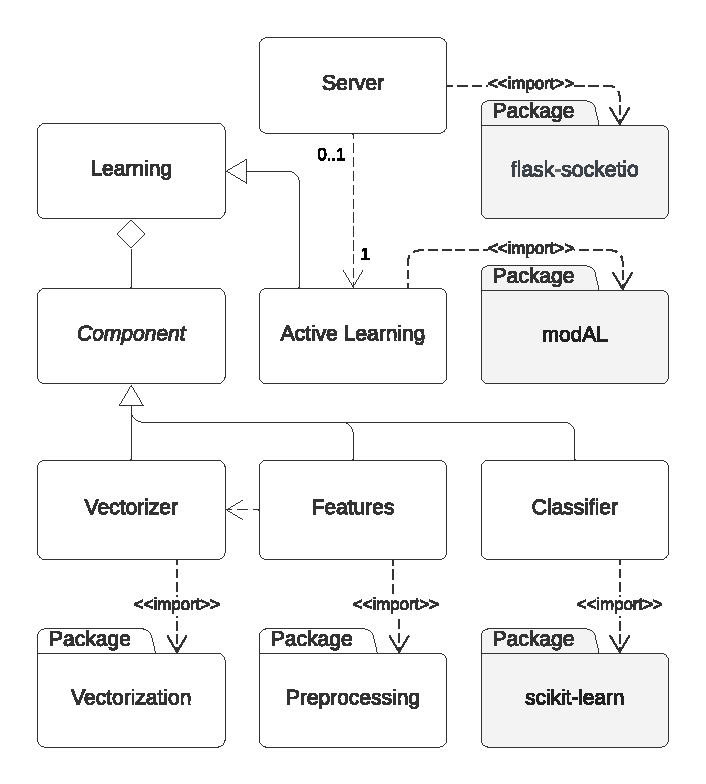
\includegraphics[scale=0.9]{module_deps.pdf}
\captionsetup{justification=centering}
\caption{\label{fig:pythonmodules}Conceptual model of the structure and composition of the back-end application layer. External dependencies/packages are grayed out.}
\end{figure}
The \emph{learning} module encapsulates what this author refers to as a ``learning scenario". A learning scenario is a high-level view of the combination of individual components that take part in the building of a classification model, i.e. the combination of vectorizer type, classifier class, dataset and features. The module offers the ability to train a model from scratch by only specifying the type of said components. It can also be easily extended with novel components during initialisation. For example, a custom preprocessing function can by supplied as a parameter, which will be executed in place of the default one provided in the \emph{preprocessing} module. All components can be replaced in a similar manner, as long as they implement the interface of their original counterpart, i.e. a vectorizer need only provide a ``vectorize" method if it's already trained, and a ``learn\_text\_model" if it isn't.

The \emph{active learning} module extends the \emph{learning} module by wrapping the classifier component in a thin \emph{modAL} \cite{modAL2018} wrapper, that provides the core functionality for iterative labeling. Furthermore, the module implements the active learning dataset partitioning strategy discussed in Section~\ref{section:activepartitioning}. It also adds support for an additional component - the choice of query strategy. What \emph{modAL} offers specifically, is a class that keeps a reference to a classifier and its previously seen labeled data. When adding new training examples, i.e. teaching the learner, they are stacked row-wise with the existing seen data, and the model is re-fit on the combined result. This is a simple yet effective way to perform active learning with classifiers that don't natively support online training. Furthermore, the class exposes an API for querying the wrapped classifier, given a reference to a function. The only requirement is that the said function must return a sample of the same shape as previously seen data, alongside its index in the unlabeled pool.
\subsubsection{Server}
While a web application is not required for either passive or active learning, in a real environment, data annotators should be able to enjoy a visual interactive experience. As such, a \emph{server} module was implemented to mediate the communication between the learning process and potential clients. It is designed to be frontend-agnostic by operating entirely via web sockets. All this module does, is wrap an instance of the active learning class, such that it is able to observe its state. Beyond that, it listens for events from connected clients and sends updates when appropriate. These events follow a predefined structure and are named according to the specification in Section~\ref{section:server-client}. The actual server runs on the web framework \emph{Flask}, with \emph{Flask-SocketIO} as the library of choice for extended web sockets support.

Although it is possible to maintain multiple instances of active learners with different classifiers simultaneously, it is inefficient and ineffective. It would offer more flexibility but the trade-off is a phenomena described by Burr Settles as:

``...a training set built in cooperation with an active learner is inherently tied to the model that was used to generate it (i.e., the class of the model selecting the queries)."\cite{Settles2009}

It begs the question, when a sampling query is answered, should one update all learners that use the same dataset with it, because it is now a labeled example? Or rather, because a sample is only informative for the learner that originally made the query, one should update learners independently? Both options are inadequate - one either labels data that isn't asked for (ineffective) or labels the same data more than once (inefficient). Moreover, the computing costs for maintaining multiple models are very high, as each one needs to store and query its unlabeled pool independently. These issues are not as problematic for learners with different datasets, but as there is no uniform solution for all cases, the author has chosen not to explore the topic of parallelism further.
\subsubsection{Web Application}
In the early stages of development, a REST API based communication between the server and client was envisioned. However, it proved to be inadequate for the task due to lack of real-time updates. Ultimately, the idea was scrapped in favour of web sockets. To complement that, the web application was developed in \emph{Node.js} due to to its asynchronous, event-driven nature. The frontend sits on top of \emph{React}, which works well in combination with \emph{Node.js} and benefits from a great ecosystem of tools and libraries. For example, the \emph{Material-UI} framework was used to create out-of-the-box stylish and accessible view components that follow Google's Material Design guidelines. The result is a fast, single-page application that offers accessibility, extensibility and looks aesthetically pleasing.
\begin{figure}[H]
\centering
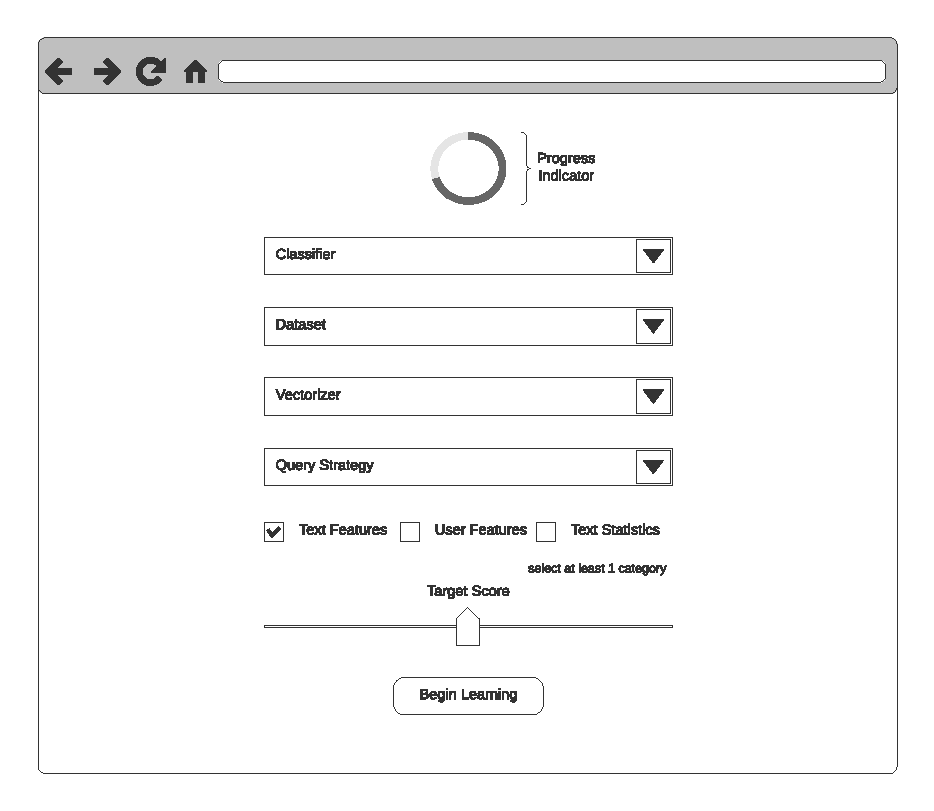
\includegraphics[scale=0.90]{options_wireframe.pdf}
\captionsetup{justification=centering}
\caption{\label{fig:optionsview}Uninitialised model view for selection of active learning components.}
\end{figure}
\begin{figure}[H]
\centering
    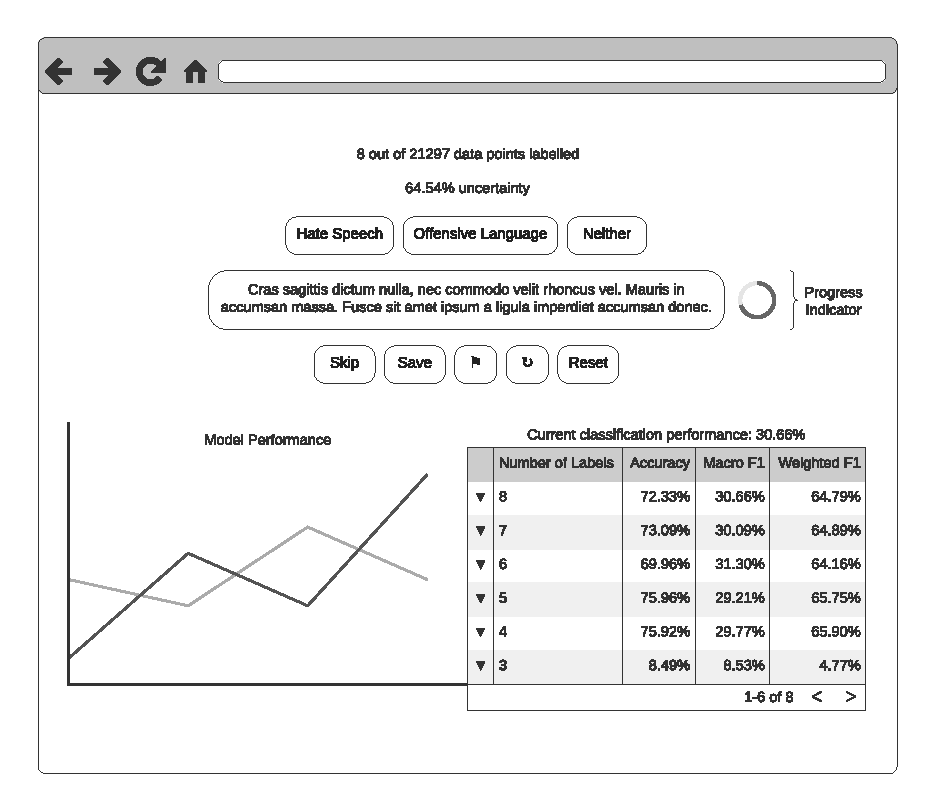
\includegraphics[scale=0.90]{model_wireframe.pdf}
\captionsetup{justification=centering}
\caption{\label{fig:modelview}Initialised model view, representing the current state of an active learner.}
\end{figure}
To facilitate the development of the application, user stories were written to keep track of key software features, gauge their value and prioritise their implementation:\label{subsection:stories}
\begin{itemize}
    \item As a data scientist, I want to interact with the learning process in real-time, so that I can better understand the effect of my choices.
    \item As a data scientist, I want to skip tweets that make me uncomfortable and those I'm uncertain about, so that I don't introduce personal bias.
    \item As a data scientist, I want to save my labeling progress, so that I can continue later.
    \item As a data scientist, I want to save the results and analytics produced during the labeling process, so that I can analyse them later.
    \item As a data scientist, I want to to adapt the learning process to my preferences, so that it is better suited to my classification problem.
\end{itemize}   
\subsubsection{Server-Client Interaction}
\label{section:server-client}
The server and client components communicate with each other via named events that carry a data payload in JSON format. The payload varies depending on the state of the model, as well as the type of event being sent. However, the range of available message fields is specified in the following list:
\begin{itemize}[noitemsep]
    \item \emph{classifiers} - list of available classification algorithms
    \item \emph{datasets} - list of available datasets
    \item \emph{vectorizers} - list of available text vectorization models
    \item \emph{features} - list of available features in all datasets
    \item \emph{query\_strategies} - list of available sampling strategies
    \item \emph{idx} - index of the sampled tweet in the unlabeled pool
    \item \emph{text} - the original tweet text before pre-processing
    \item \emph{uncertainty} - confidence metric for the tweet produced by the learner
    \item \emph{series} - list of performance metrics recorded for every iteration
    \item \emph{labeled\_size} - number of labeled examples
    \item \emph{dataset\_size} - total number of examples available for training
    \item \emph{score} - the current model performance metric
    \item \emph{target} - the baseline performance target 
\end{itemize}
When a session between the server and the client is first initiated, the server sends all user-defined components available for selection in an \emph{options} event. When the client receives them, they are rendered and presented to the user like shown in Figure~\ref{fig:optionsview}. After a user selects their desired learning components, the client replies with a matching event, containing the selection.
\begin{figure}[H]
\centering
    \hspace*{0.3cm}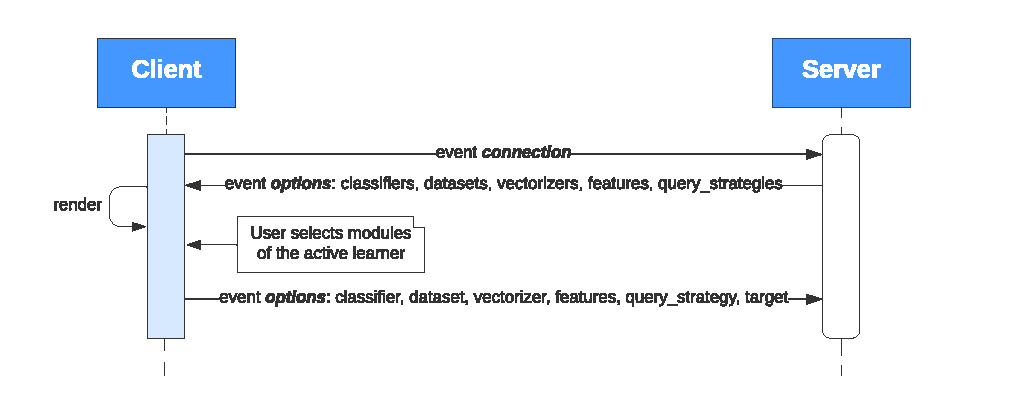
\includegraphics[scale=0.86]{options_ws.pdf}
\captionsetup{justification=centering}
\caption{\label{fig:optionsinteraction}Sequence diagram, depicting the event flow whenever an active learner is not defined and initialised yet.}
\end{figure}
Alternatively, if the model has been started prior to the client's connection, an \emph{init} event is sent instead. It contains all information regarding the learning process and the model's state. This includes an unlabeled example sampled according to some query strategy, therefore a user can start annotating data. If the pool of unlabeled data is exhausted, however, an \emph{end} event is sent in place of \emph{init}, which does not include a new sample.

Whenever a user selects what they believe is the appropriate annotation using the graphical interface in Figure~\ref{fig:modelview}, a \emph{label} event is transmitted, containing the index of the sample in the unlabeled pool, the selected label value and a hash of the original text. The hash is then used to verify that the index belongs to the appropriate sample server-side.

Subsequent events no longer include fields that are already known to the client as a result of previous interactions, with the idea of reducing network load. Such include \emph{query} and the slightly modified \emph{end} events.
\begin{figure}[H]
\centering
    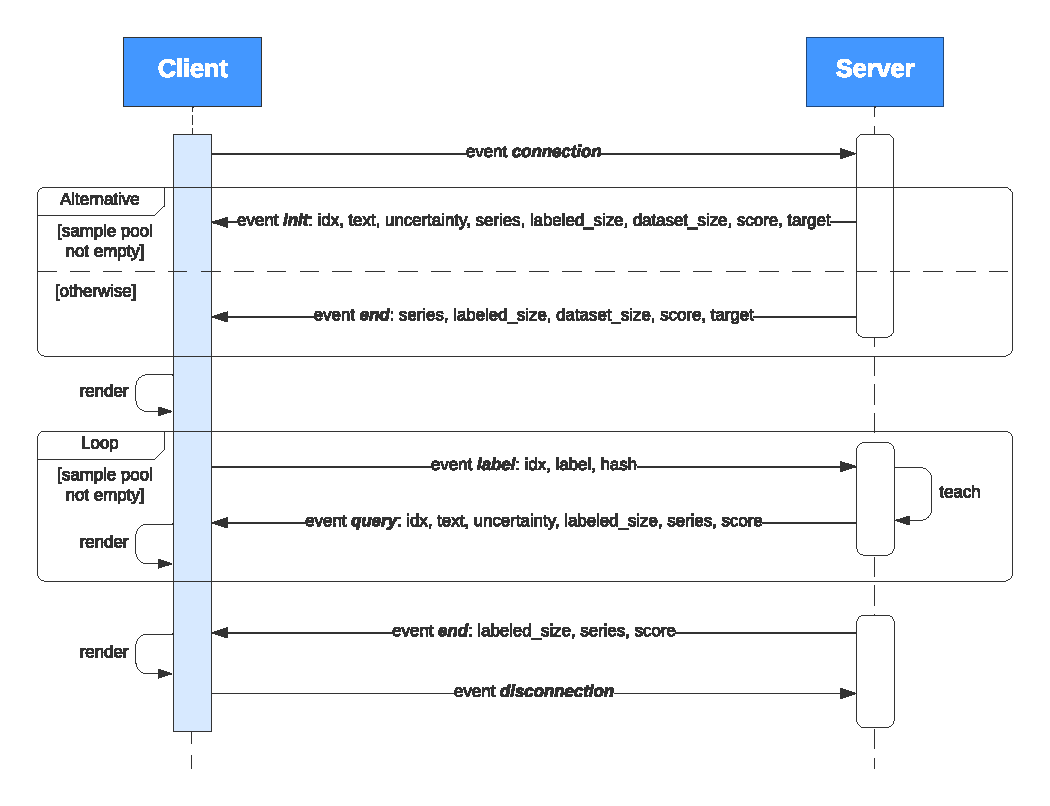
\includegraphics[scale=0.85]{flow_ws.pdf}
\captionsetup{justification=centering}
\caption{\label{fig:modelinteraction}Sequence diagram, depicting the event flow whenever an active learner is initialised and running.}
\end{figure}
\subsubsection{Query Strategies}
The choice of query strategy is strongly related to an active learner's performance, as suggested in Section~\ref{section:query}. All discussed strategies are implemented in this project, in order to evaluate their impact on early performance growth rate.
\begin{figure}[H]
\begin{gather*}
  \text{Uncertainty}(x) = 1 - P(\hat x|x), \\
  \text{where~$x$ is a sample and~$\hat x$ is its most likely prediction.}
\end{gather*}
\caption{Uncertainty Sampling}
\end{figure}
\vspace{-5mm}
\begin{figure}[H]
\begin{gather*}
  \text{Margin}(x) = P(\hat x_1|x) - P(\hat x_2|x), \\
  \text{where~$\hat x_1$ and~$\hat x_2$ are the first and second most likely predicted classes for sample~$x$.}
\end{gather*}
\caption{Margin Sampling}
\end{figure}
\vspace{-5mm}
\begin{figure}[H]
\begin{gather*}
  \text{Entropy}(x) = -\sum_{k}p_k \text{log}(p_k), \\
  \text{where~$p_k$ is the probability of the sample belonging to the~$k$-th class.}
\end{gather*}
\caption{Entropy Sampling}
\end{figure}
\subsubsection{Semi-supervised Learning}
To better facilitate the project's evaluation, an alternative approach to querying was developed. In essence, since the author compares both learning techniques on the same dataset, all of the data is already labeled. This makes it possible to simulate the active learning process by first making a copy of the dataset and ``forgetting" the labels of say 90\% of the data. However, instead of an oracle answering the sampled queries manually, one could simply look up the ground truth labels in the original dataset. While this technique is infeasible in a real world active learning application, it allows for rapid evaluation in a controlled environment. One could essentially switch any module - the classifier, dataset, query strategy, feature selection, feature extraction, etc., and obtain the respective performance metrics automatically, without going through the slow process of labelling. Therefore, a more extensive parameter space could be explored in a shorter amount of time for active learning.
Implementation-wise, this was achieved by iteratively sampling the newly unlabeled pool, looking up the label in the original dataset and teaching the classifier $n$ times or until the unlabeled pool is empty. After every sample, the number of labeled instances and F1-score is recorded. Finally, statistical information is extracted from the results, to serve as part of the active learning analysis. Such includes the number of queries necessary to reach the performance of passive learning and the highest labels to performance ratio.
\subsection{Model Selection}
Support vector machines are an example of a non-probabilistic model that is shown to work well for text classification and does not output confidence metrics by default. In order to adapt it for use with active learning, Platt scaling \cite{Platt99probabilisticoutputs} is implemented, which produces probability estimates from decision values. Nevertheless, there is an inherent drawback to this approach. Active learning requires a model to be re-fit after adding new training data. Hence, the logistic function for Platt scaling needs to be re-learned as well. After a certain amount of queries, this introduces significant overhead, which is undesirable. Despite that, Linear SVM has been implemented and evaluated.

Multinomial Naive Bayes was considered, but since some text vectorizers produce features that allow negative values, and multinomial distributions can't contain negative values, the process was flawed. This is the case with GloVe and Doc2Vec vectorization. Although possible to scale the features to a positive range via min-max normalization, they are intended to be used without further transformations. Multinomial Naive Bayes has therefore not been implemented.
    
The developed system is abstract enough to support any model that implements ``fit" and ``predict\_proba" methods in its class. This means all \emph{sklearn}\cite{scikit-learn} classifiers and \emph{sklearn}-esque wrappers are natively supported as components of the learning flow. Regardless, as previously discussed only select few models are important for this project. Although there is an emphasis on naturally probabilistic ones, models that usually perform well on text classification tasks are considered too. Therefore, an \emph{evaluation} script builds and evaluates the following classifiers in both active and passive learning scenarios - Logistic Regression, Linear SVM, Random Forest and K-Nearest Neighbors.

Whenever possible, the models are trained with balanced class weights to account for potential data imbalance. That is, the loss function for the model is altered such that loss on the minority class is penalised more, whereas loss on the majority is penalised less. This is done by adjusting weights inversely proportional to the class frequencies in the dataset. This effect can otherwise be achieved by oversampling the minority class, undersampling the majority class, or both \cite{Chawla02smote:synthetic}. These alternatives work well with passive learning, as data is already annotated. However, in an active learning scenario, synthetic oversampling would mean that some queries are unintelligible to a human annotator, while undersampling would only limit the pool of data to query from. Oversampling by duplication is viable but after brief experimentation it was not found to be more beneficial than balanced class weights.
\newpage
\section{Evaluation}
This paper employs a multi-stranded approach to evaluation, where the benefits of active learning are explored by varying the underlying components that comprise the learning flow - the dataset, features, classifier and sampling strategy.
Project success is evaluated in terms of data efficiency gains from applying active learning as opposed to passive learning in a similar context and environment.
\subsection{Critical Analysis}
\label{section:critical}
While the dataset collected was sampled in a way that suggests a well-proportioned distribution, after labeling all tweets, a considerable class imbalance was observed. Specifically, a ratio of 468 to 1532 occurs in the dataset, with malicious tweets as the minority class.
\begin{figure}[H]
\captionsetup{justification=centering}
   \begin{minipage}{0.48\textwidth}
     \centering
     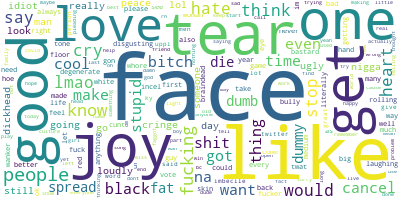
\includegraphics[width=.9\linewidth]{wordclouds/good.png}
     \caption{Most common words in the non-malicious class.}\label{fig:goodwords}
   \end{minipage}\hfill
   \begin{minipage}{0.48\textwidth}
     \centering
     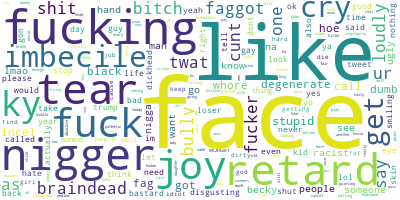
\includegraphics[width=.9\linewidth]{wordclouds/bad.png}
     \caption{Most common words in the malicious class.}\label{fig:badwords}
   \end{minipage}
\end{figure}
Although this may be closer to how tweets are expected to naturally appear in Twitter, training a model on an imbalanced dataset is bound to introduce bias. Malicious tweets being the minority class means that micro F1 is not an appropriate metric for evaluation, as classifiers tend to be biased towards the majority class. In this scenario, a model would most likely be able to predict non-malicious tweets well, but fail on the more important malicious examples. Nonetheless, the overall performance would still remain high. To account for this phenomena, macro F1 will be used instead, as it factors in the performance on both classes equally.
\begin{gather*}
  \text{Macro F1} = \frac{1}{N}\sum_{i=0}^N \text{F1}_i, \\
  \text{where~$i$ is the class index and~$N$ the number of classes}
\end{gather*}
As a result, trained classifiers will not look overly optimistic because of their performance on the non-malicious majority class. In the following table, macro F1 is denoted as \emph{F1}. Because detecting malicious tweets is not a multi-label classification problem, micro F1 is equivalent to accuracy, denoted \emph{Acc}. Finally, \emph{P} and \emph{R} stand for the macro-averaged precision and recall respectively.
\begin{table}[H]
\centering
\begin{small}
\begin{tabular}{c|c|c}
T - Text Features & U - User Features & S - Statistical Features
\end{tabular}
\begin{tabular}{cccccc|cccc}
\specialrule{1.5pt}{1pt}{1pt}
 & \multirow{2}{*}{Features}                      & \multicolumn{4}{c|}{Logistic Regression} & \multicolumn{4}{c}{Linear SVM}          \\
                      &                       & F1 & P & R & Acc & F1 & P & R & Acc \\ \specialrule{1.5pt}{1pt}{1pt}
\multicolumn{1}{c|}{\multirow{4}{*}{\STAB{\rotatebox[origin=c]{90}{TF-IDF}}}} & \multicolumn{1}{c|}{T} & $\mathbf{71.91}$   & $\mathbf{69.98}$  & $\mathbf{76.81}$  & $79.68$    & $62.64$   & $62.51$  & $68.91$  & $70.31$    \\
\multicolumn{1}{c|}{} & \multicolumn{1}{c|}{T-U} & $71.47$   & $69.62$  & $75.74$  & $79.68$    & $63.51$   & $63.34$  & $70.29$  & $70.83$    \\
\multicolumn{1}{c|}{} & \multicolumn{1}{c|}{T-S} & $68.01$   & $66.75$  & $74.25$  & $75.52$    & $64.84$   & $64.25$  & $71.26$  & $72.39$    \\
\multicolumn{1}{c|}{} & \multicolumn{1}{c|}{T-U-S} & $67.54$   & $66.40$  & $73.93$  & $75.00$    & $65.28$   & $64.57$  & $71.58$  & $72.91$    \\ \specialrule{0.8pt}{1pt}{1pt}
\multicolumn{1}{c|}{\multirow{4}{*}{\STAB{\rotatebox[origin=c]{90}{GloVe}}}} & \multicolumn{1}{c|}{T} & $58.08$   & $58.20$  & $61.96$  & $67.70$    & $59.02$   & $59.08$  & $63.35$  & $68.22$    \\
\multicolumn{1}{c|}{} & \multicolumn{1}{c|}{T-U} & $59.94$   & $59.95$  & $64.74$  & $68.75$    & $60.36$   & $60.24$  & $65.06$  & $69.27$    \\
\multicolumn{1}{c|}{} & \multicolumn{1}{c|}{T-S} & $61.77$   & $62.23$  & $69.01$  & $68.75$    & $62.20$   & $62.22$  & $68.58$  & $69.79$    \\
\multicolumn{1}{c|}{} & \multicolumn{1}{c|}{T-U-S} & $62.20$   & $62.50$  & $69.33$  & $69.27$    & $62.20$   & $62.22$  & $68.58$  & $69.79$    \\ \specialrule{0.8pt}{1pt}{1pt}
\multicolumn{1}{c|}{\multirow{4}{*}{\STAB{\rotatebox[origin=c]{90}{Doc2Vec}}}} & \multicolumn{1}{c|}{T} & $49.09$   & $55.09$  & $58.33$  & $53.12$    & $42.20$   & $57.89$  & $60.47$  & $42.70$    \\
\multicolumn{1}{c|}{} & \multicolumn{1}{c|}{T-U} & $43.91$   & $57.57$  & $60.68$  & $44.79$    & $37.93$   & $57.58$  & $58.65$  & $38.02$    \\
\multicolumn{1}{c|}{} & \multicolumn{1}{c|}{T-S} & $58.01$   & $62.30$  & $70.19$  & $61.97$    & $50.12$   & $56.63$  & $60.79$  & $53.64$    \\
\multicolumn{1}{c|}{} & \multicolumn{1}{c|}{T-U-S} & $56.44$   & $61.07$  & $68.16$  & $60.41$    & $52.90$   & $58.42$  & $63.78$  & $56.77$    \\ \specialrule{1.5pt}{1pt}{1pt}
 & \multicolumn{1}{c}{\multirow{2}{*}{Features}} & \multicolumn{4}{c|}{Random Forest}       & \multicolumn{4}{c}{K-Nearest Neighbors} \\
                      & \multicolumn{1}{c}{} & F1 & P & R & Acc & F1 & P & R & Acc \\ \specialrule{1.5pt}{1pt}{1pt}
\multicolumn{1}{c|}{\multirow{4}{*}{\STAB{\rotatebox[origin=c]{90}{TF-IDF}}}} & \multicolumn{1}{c|}{T} & $69.34$   & $68.80$  & $69.97$  & $\mathbf{80.72}$    & $57.73$   & $63.63$  & $56.83$  & $80.20$    \\
\multicolumn{1}{c|}{} & \multicolumn{1}{c|}{T-U} & $64.78$   & $63.74$  & $69.01$  & $73.95$    & $62.03$   & $63.32$  & $61.21$  & $78.64$    \\
\multicolumn{1}{c|}{} & \multicolumn{1}{c|}{T-S} & $68.53$   & $67.07$  & $71.58$  & $78.12$    & $54.43$   & $54.32$  & $54.59$  & $71.35$    \\
\multicolumn{1}{c|}{} & \multicolumn{1}{c|}{T-U-S} & $64.16$   & $63.11$  & $67.20$  & $74.47$    & $51.58$   & $51.67$  & $52.02$  & $67.18$    \\ \specialrule{0.8pt}{1pt}{1pt}
\multicolumn{1}{c|}{\multirow{4}{*}{\STAB{\rotatebox[origin=c]{90}{GloVe}}}} & \multicolumn{1}{c|}{T} & $59.40$   & $59.15$  & $59.72$  & $74.47$    & $53.34$   & $53.23$  & $53.63$  & $69.79$    \\
\multicolumn{1}{c|}{} & \multicolumn{1}{c|}{T-U} & $61.49$   & $61.27$  & $61.75$  & $76.04$    & $53.91$   & $53.85$  & $54.80$  & $68.22$    \\
\multicolumn{1}{c|}{} & \multicolumn{1}{c|}{T-S} & $62.93$   & $63.82$  & $62.28$  & $78.64$    & $58.56$   & $58.47$  & $58.65$  & $74.47$    \\
\multicolumn{1}{c|}{} & \multicolumn{1}{c|}{T-U-S} & $59.32$   & $59.97$  & $58.86$  & $76.56$    & $50.10$   & $50.10$  & $50.10$  & $69.27$    \\ \specialrule{0.8pt}{1pt}{1pt}
\multicolumn{1}{c|}{\multirow{4}{*}{\STAB{\rotatebox[origin=c]{90}{Doc2Vec}}}} & \multicolumn{1}{c|}{T} & $51.06$   & $53.40$  & $51.70$  & $77.08$    & $54.95$   & $54.76$  & $55.34$  & $70.83$    \\
\multicolumn{1}{c|}{} & \multicolumn{1}{c|}{T-U} & $47.50$   & $47.38$  & $47.86$  & $70.83$    & $51.39$   & $51.89$  & $52.56$  & $64.58$    \\
\multicolumn{1}{c|}{} & \multicolumn{1}{c|}{T-S} & $49.41$   & $51.44$  & $50.64$  & $77.08$    & $52.63$   & $52.57$  & $52.99$  & $68.75$    \\
\multicolumn{1}{c|}{} & \multicolumn{1}{c|}{T-U-S} & $58.51$   & $60.71$  & $57.69$  & $78.12$    & $55.42$   & $55.22$  & $56.51$  & $69.27$    \\ \specialrule{1.5pt}{1pt}{1pt}
\end{tabular}
\end{small}
\captionsetup{justification=centering}
\caption{\label{tab:baselineML}Baseline performance scores of machine learning for\\
all combinations of classifier, vectorizer and features.}
\end{table}
A few observations can be made following these results. First, TF-IDF is dominant across the board and produces the highest scores for every model class evaluated. The GloVe word embeddings model produces mediocre results, despite having been trained on the largest amount of data. Perhaps tweet similarity isn't a very indicative feature for classifying tweets. This is explicable by the fact that both malicious and non-malicious tweets have large variance when it comes to syntax and semantics. The classifiers must have not been able to pick up on a discriminative pattern due to the limited amount of training data available. Doc2Vec clearly suffered from the same issue. Unlike GloVe which is pre-trained, Doc2Vec was fit on the local dataset used for classification, which is rather small. This further handicaps the performance, making it the worst vectorizer in all explored scenarios.

Second, performance scores when using TF-IDF mostly decline with the addition of statistical and user features. In contrast, adding new features when using any of the other vectorizers tends to increase scores. Taking the extremes for example, with a Linear SVM and Doc2Vec, adding extra features increased F1-scores by up to $10.7\%$, while the combination of Logistic Regression and TF-IDF suffered up to a $4.37\%$ decrease. This observation signifies that TF-IDF features are very discriminative, to the extent that their sole use offers the highest information gain. This confirms the findings of Rosa H. et al.\cite{Rosa2019} that feature engineering beyond TF-IDF is not rewarding.

To reduce the complexity of visualising active learning applied to all combinations of classifier, vectorizer and features, only the highest baseline results are plotted and analysed further.%\footnotemark[\value{footnote}]
%\footnotetext{The plots of active learning application on all combinations can be found in Appendix A.}

From Table~\ref{tab:baselineML} one can distinguish the best models for each type of vectorizer in a passive learning scenario. Studying TF-IDF in isolation, Logistic Regression clearly performed best, producing the highest scores not only in its category, but overall. This makes it a prime candidate for further analysis. Active learning with uncertainty as the sampling strategy is applied on all feature combinations to determine the performance growth as training data increases:
\begin{figure}[H]
\captionsetup{justification=centering}
    \centering
    %% Creator: Matplotlib, PGF backend
%%
%% To include the figure in your LaTeX document, write
%%   \input{<filename>.pgf}
%%
%% Make sure the required packages are loaded in your preamble
%%   \usepackage{pgf}
%%
%% and, on pdftex
%%   \usepackage[utf8]{inputenc}\DeclareUnicodeCharacter{2212}{-}
%%
%% or, on luatex and xetex
%%   \usepackage{unicode-math}
%%
%% Figures using additional raster images can only be included by \input if
%% they are in the same directory as the main LaTeX file. For loading figures
%% from other directories you can use the `import` package
%%   \usepackage{import}
%%
%% and then include the figures with
%%   \import{<path to file>}{<filename>.pgf}
%%
%% Matplotlib used the following preamble
%%
\begingroup%
\makeatletter%
\begin{pgfpicture}%
\pgfpathrectangle{\pgfpointorigin}{\pgfqpoint{5.416401in}{4.126438in}}%
\pgfusepath{use as bounding box, clip}%
\begin{pgfscope}%
\pgfsetbuttcap%
\pgfsetmiterjoin%
\definecolor{currentfill}{rgb}{1.000000,1.000000,1.000000}%
\pgfsetfillcolor{currentfill}%
\pgfsetlinewidth{0.000000pt}%
\definecolor{currentstroke}{rgb}{1.000000,1.000000,1.000000}%
\pgfsetstrokecolor{currentstroke}%
\pgfsetdash{}{0pt}%
\pgfpathmoveto{\pgfqpoint{0.000000in}{0.000000in}}%
\pgfpathlineto{\pgfqpoint{5.416401in}{0.000000in}}%
\pgfpathlineto{\pgfqpoint{5.416401in}{4.126438in}}%
\pgfpathlineto{\pgfqpoint{0.000000in}{4.126438in}}%
\pgfpathclose%
\pgfusepath{fill}%
\end{pgfscope}%
\begin{pgfscope}%
\pgfsetbuttcap%
\pgfsetmiterjoin%
\definecolor{currentfill}{rgb}{1.000000,1.000000,1.000000}%
\pgfsetfillcolor{currentfill}%
\pgfsetlinewidth{0.000000pt}%
\definecolor{currentstroke}{rgb}{0.000000,0.000000,0.000000}%
\pgfsetstrokecolor{currentstroke}%
\pgfsetstrokeopacity{0.000000}%
\pgfsetdash{}{0pt}%
\pgfpathmoveto{\pgfqpoint{0.575309in}{1.226744in}}%
\pgfpathlineto{\pgfqpoint{5.225309in}{1.226744in}}%
\pgfpathlineto{\pgfqpoint{5.225309in}{4.026438in}}%
\pgfpathlineto{\pgfqpoint{0.575309in}{4.026438in}}%
\pgfpathclose%
\pgfusepath{fill}%
\end{pgfscope}%
\begin{pgfscope}%
\pgfpathrectangle{\pgfqpoint{0.575309in}{1.226744in}}{\pgfqpoint{4.650000in}{2.799694in}}%
\pgfusepath{clip}%
\pgfsetrectcap%
\pgfsetroundjoin%
\pgfsetlinewidth{0.803000pt}%
\definecolor{currentstroke}{rgb}{0.690196,0.690196,0.690196}%
\pgfsetstrokecolor{currentstroke}%
\pgfsetdash{}{0pt}%
\pgfpathmoveto{\pgfqpoint{0.781752in}{1.226744in}}%
\pgfpathlineto{\pgfqpoint{0.781752in}{4.026438in}}%
\pgfusepath{stroke}%
\end{pgfscope}%
\begin{pgfscope}%
\pgfsetbuttcap%
\pgfsetroundjoin%
\definecolor{currentfill}{rgb}{0.000000,0.000000,0.000000}%
\pgfsetfillcolor{currentfill}%
\pgfsetlinewidth{0.803000pt}%
\definecolor{currentstroke}{rgb}{0.000000,0.000000,0.000000}%
\pgfsetstrokecolor{currentstroke}%
\pgfsetdash{}{0pt}%
\pgfsys@defobject{currentmarker}{\pgfqpoint{0.000000in}{-0.048611in}}{\pgfqpoint{0.000000in}{0.000000in}}{%
\pgfpathmoveto{\pgfqpoint{0.000000in}{0.000000in}}%
\pgfpathlineto{\pgfqpoint{0.000000in}{-0.048611in}}%
\pgfusepath{stroke,fill}%
}%
\begin{pgfscope}%
\pgfsys@transformshift{0.781752in}{1.226744in}%
\pgfsys@useobject{currentmarker}{}%
\end{pgfscope}%
\end{pgfscope}%
\begin{pgfscope}%
\definecolor{textcolor}{rgb}{0.000000,0.000000,0.000000}%
\pgfsetstrokecolor{textcolor}%
\pgfsetfillcolor{textcolor}%
\pgftext[x=0.781752in,y=1.129522in,,top]{\color{textcolor}\rmfamily\fontsize{6.940000}{8.328000}\selectfont \(\displaystyle {0}\)}%
\end{pgfscope}%
\begin{pgfscope}%
\pgfpathrectangle{\pgfqpoint{0.575309in}{1.226744in}}{\pgfqpoint{4.650000in}{2.799694in}}%
\pgfusepath{clip}%
\pgfsetrectcap%
\pgfsetroundjoin%
\pgfsetlinewidth{0.803000pt}%
\definecolor{currentstroke}{rgb}{0.690196,0.690196,0.690196}%
\pgfsetstrokecolor{currentstroke}%
\pgfsetdash{}{0pt}%
\pgfpathmoveto{\pgfqpoint{1.396896in}{1.226744in}}%
\pgfpathlineto{\pgfqpoint{1.396896in}{4.026438in}}%
\pgfusepath{stroke}%
\end{pgfscope}%
\begin{pgfscope}%
\pgfsetbuttcap%
\pgfsetroundjoin%
\definecolor{currentfill}{rgb}{0.000000,0.000000,0.000000}%
\pgfsetfillcolor{currentfill}%
\pgfsetlinewidth{0.803000pt}%
\definecolor{currentstroke}{rgb}{0.000000,0.000000,0.000000}%
\pgfsetstrokecolor{currentstroke}%
\pgfsetdash{}{0pt}%
\pgfsys@defobject{currentmarker}{\pgfqpoint{0.000000in}{-0.048611in}}{\pgfqpoint{0.000000in}{0.000000in}}{%
\pgfpathmoveto{\pgfqpoint{0.000000in}{0.000000in}}%
\pgfpathlineto{\pgfqpoint{0.000000in}{-0.048611in}}%
\pgfusepath{stroke,fill}%
}%
\begin{pgfscope}%
\pgfsys@transformshift{1.396896in}{1.226744in}%
\pgfsys@useobject{currentmarker}{}%
\end{pgfscope}%
\end{pgfscope}%
\begin{pgfscope}%
\definecolor{textcolor}{rgb}{0.000000,0.000000,0.000000}%
\pgfsetstrokecolor{textcolor}%
\pgfsetfillcolor{textcolor}%
\pgftext[x=1.396896in,y=1.129522in,,top]{\color{textcolor}\rmfamily\fontsize{6.940000}{8.328000}\selectfont \(\displaystyle {250}\)}%
\end{pgfscope}%
\begin{pgfscope}%
\pgfpathrectangle{\pgfqpoint{0.575309in}{1.226744in}}{\pgfqpoint{4.650000in}{2.799694in}}%
\pgfusepath{clip}%
\pgfsetrectcap%
\pgfsetroundjoin%
\pgfsetlinewidth{0.803000pt}%
\definecolor{currentstroke}{rgb}{0.690196,0.690196,0.690196}%
\pgfsetstrokecolor{currentstroke}%
\pgfsetdash{}{0pt}%
\pgfpathmoveto{\pgfqpoint{2.012041in}{1.226744in}}%
\pgfpathlineto{\pgfqpoint{2.012041in}{4.026438in}}%
\pgfusepath{stroke}%
\end{pgfscope}%
\begin{pgfscope}%
\pgfsetbuttcap%
\pgfsetroundjoin%
\definecolor{currentfill}{rgb}{0.000000,0.000000,0.000000}%
\pgfsetfillcolor{currentfill}%
\pgfsetlinewidth{0.803000pt}%
\definecolor{currentstroke}{rgb}{0.000000,0.000000,0.000000}%
\pgfsetstrokecolor{currentstroke}%
\pgfsetdash{}{0pt}%
\pgfsys@defobject{currentmarker}{\pgfqpoint{0.000000in}{-0.048611in}}{\pgfqpoint{0.000000in}{0.000000in}}{%
\pgfpathmoveto{\pgfqpoint{0.000000in}{0.000000in}}%
\pgfpathlineto{\pgfqpoint{0.000000in}{-0.048611in}}%
\pgfusepath{stroke,fill}%
}%
\begin{pgfscope}%
\pgfsys@transformshift{2.012041in}{1.226744in}%
\pgfsys@useobject{currentmarker}{}%
\end{pgfscope}%
\end{pgfscope}%
\begin{pgfscope}%
\definecolor{textcolor}{rgb}{0.000000,0.000000,0.000000}%
\pgfsetstrokecolor{textcolor}%
\pgfsetfillcolor{textcolor}%
\pgftext[x=2.012041in,y=1.129522in,,top]{\color{textcolor}\rmfamily\fontsize{6.940000}{8.328000}\selectfont \(\displaystyle {500}\)}%
\end{pgfscope}%
\begin{pgfscope}%
\pgfpathrectangle{\pgfqpoint{0.575309in}{1.226744in}}{\pgfqpoint{4.650000in}{2.799694in}}%
\pgfusepath{clip}%
\pgfsetrectcap%
\pgfsetroundjoin%
\pgfsetlinewidth{0.803000pt}%
\definecolor{currentstroke}{rgb}{0.690196,0.690196,0.690196}%
\pgfsetstrokecolor{currentstroke}%
\pgfsetdash{}{0pt}%
\pgfpathmoveto{\pgfqpoint{2.627185in}{1.226744in}}%
\pgfpathlineto{\pgfqpoint{2.627185in}{4.026438in}}%
\pgfusepath{stroke}%
\end{pgfscope}%
\begin{pgfscope}%
\pgfsetbuttcap%
\pgfsetroundjoin%
\definecolor{currentfill}{rgb}{0.000000,0.000000,0.000000}%
\pgfsetfillcolor{currentfill}%
\pgfsetlinewidth{0.803000pt}%
\definecolor{currentstroke}{rgb}{0.000000,0.000000,0.000000}%
\pgfsetstrokecolor{currentstroke}%
\pgfsetdash{}{0pt}%
\pgfsys@defobject{currentmarker}{\pgfqpoint{0.000000in}{-0.048611in}}{\pgfqpoint{0.000000in}{0.000000in}}{%
\pgfpathmoveto{\pgfqpoint{0.000000in}{0.000000in}}%
\pgfpathlineto{\pgfqpoint{0.000000in}{-0.048611in}}%
\pgfusepath{stroke,fill}%
}%
\begin{pgfscope}%
\pgfsys@transformshift{2.627185in}{1.226744in}%
\pgfsys@useobject{currentmarker}{}%
\end{pgfscope}%
\end{pgfscope}%
\begin{pgfscope}%
\definecolor{textcolor}{rgb}{0.000000,0.000000,0.000000}%
\pgfsetstrokecolor{textcolor}%
\pgfsetfillcolor{textcolor}%
\pgftext[x=2.627185in,y=1.129522in,,top]{\color{textcolor}\rmfamily\fontsize{6.940000}{8.328000}\selectfont \(\displaystyle {750}\)}%
\end{pgfscope}%
\begin{pgfscope}%
\pgfpathrectangle{\pgfqpoint{0.575309in}{1.226744in}}{\pgfqpoint{4.650000in}{2.799694in}}%
\pgfusepath{clip}%
\pgfsetrectcap%
\pgfsetroundjoin%
\pgfsetlinewidth{0.803000pt}%
\definecolor{currentstroke}{rgb}{0.690196,0.690196,0.690196}%
\pgfsetstrokecolor{currentstroke}%
\pgfsetdash{}{0pt}%
\pgfpathmoveto{\pgfqpoint{3.242330in}{1.226744in}}%
\pgfpathlineto{\pgfqpoint{3.242330in}{4.026438in}}%
\pgfusepath{stroke}%
\end{pgfscope}%
\begin{pgfscope}%
\pgfsetbuttcap%
\pgfsetroundjoin%
\definecolor{currentfill}{rgb}{0.000000,0.000000,0.000000}%
\pgfsetfillcolor{currentfill}%
\pgfsetlinewidth{0.803000pt}%
\definecolor{currentstroke}{rgb}{0.000000,0.000000,0.000000}%
\pgfsetstrokecolor{currentstroke}%
\pgfsetdash{}{0pt}%
\pgfsys@defobject{currentmarker}{\pgfqpoint{0.000000in}{-0.048611in}}{\pgfqpoint{0.000000in}{0.000000in}}{%
\pgfpathmoveto{\pgfqpoint{0.000000in}{0.000000in}}%
\pgfpathlineto{\pgfqpoint{0.000000in}{-0.048611in}}%
\pgfusepath{stroke,fill}%
}%
\begin{pgfscope}%
\pgfsys@transformshift{3.242330in}{1.226744in}%
\pgfsys@useobject{currentmarker}{}%
\end{pgfscope}%
\end{pgfscope}%
\begin{pgfscope}%
\definecolor{textcolor}{rgb}{0.000000,0.000000,0.000000}%
\pgfsetstrokecolor{textcolor}%
\pgfsetfillcolor{textcolor}%
\pgftext[x=3.242330in,y=1.129522in,,top]{\color{textcolor}\rmfamily\fontsize{6.940000}{8.328000}\selectfont \(\displaystyle {1000}\)}%
\end{pgfscope}%
\begin{pgfscope}%
\pgfpathrectangle{\pgfqpoint{0.575309in}{1.226744in}}{\pgfqpoint{4.650000in}{2.799694in}}%
\pgfusepath{clip}%
\pgfsetrectcap%
\pgfsetroundjoin%
\pgfsetlinewidth{0.803000pt}%
\definecolor{currentstroke}{rgb}{0.690196,0.690196,0.690196}%
\pgfsetstrokecolor{currentstroke}%
\pgfsetdash{}{0pt}%
\pgfpathmoveto{\pgfqpoint{3.857474in}{1.226744in}}%
\pgfpathlineto{\pgfqpoint{3.857474in}{4.026438in}}%
\pgfusepath{stroke}%
\end{pgfscope}%
\begin{pgfscope}%
\pgfsetbuttcap%
\pgfsetroundjoin%
\definecolor{currentfill}{rgb}{0.000000,0.000000,0.000000}%
\pgfsetfillcolor{currentfill}%
\pgfsetlinewidth{0.803000pt}%
\definecolor{currentstroke}{rgb}{0.000000,0.000000,0.000000}%
\pgfsetstrokecolor{currentstroke}%
\pgfsetdash{}{0pt}%
\pgfsys@defobject{currentmarker}{\pgfqpoint{0.000000in}{-0.048611in}}{\pgfqpoint{0.000000in}{0.000000in}}{%
\pgfpathmoveto{\pgfqpoint{0.000000in}{0.000000in}}%
\pgfpathlineto{\pgfqpoint{0.000000in}{-0.048611in}}%
\pgfusepath{stroke,fill}%
}%
\begin{pgfscope}%
\pgfsys@transformshift{3.857474in}{1.226744in}%
\pgfsys@useobject{currentmarker}{}%
\end{pgfscope}%
\end{pgfscope}%
\begin{pgfscope}%
\definecolor{textcolor}{rgb}{0.000000,0.000000,0.000000}%
\pgfsetstrokecolor{textcolor}%
\pgfsetfillcolor{textcolor}%
\pgftext[x=3.857474in,y=1.129522in,,top]{\color{textcolor}\rmfamily\fontsize{6.940000}{8.328000}\selectfont \(\displaystyle {1250}\)}%
\end{pgfscope}%
\begin{pgfscope}%
\pgfpathrectangle{\pgfqpoint{0.575309in}{1.226744in}}{\pgfqpoint{4.650000in}{2.799694in}}%
\pgfusepath{clip}%
\pgfsetrectcap%
\pgfsetroundjoin%
\pgfsetlinewidth{0.803000pt}%
\definecolor{currentstroke}{rgb}{0.690196,0.690196,0.690196}%
\pgfsetstrokecolor{currentstroke}%
\pgfsetdash{}{0pt}%
\pgfpathmoveto{\pgfqpoint{4.472619in}{1.226744in}}%
\pgfpathlineto{\pgfqpoint{4.472619in}{4.026438in}}%
\pgfusepath{stroke}%
\end{pgfscope}%
\begin{pgfscope}%
\pgfsetbuttcap%
\pgfsetroundjoin%
\definecolor{currentfill}{rgb}{0.000000,0.000000,0.000000}%
\pgfsetfillcolor{currentfill}%
\pgfsetlinewidth{0.803000pt}%
\definecolor{currentstroke}{rgb}{0.000000,0.000000,0.000000}%
\pgfsetstrokecolor{currentstroke}%
\pgfsetdash{}{0pt}%
\pgfsys@defobject{currentmarker}{\pgfqpoint{0.000000in}{-0.048611in}}{\pgfqpoint{0.000000in}{0.000000in}}{%
\pgfpathmoveto{\pgfqpoint{0.000000in}{0.000000in}}%
\pgfpathlineto{\pgfqpoint{0.000000in}{-0.048611in}}%
\pgfusepath{stroke,fill}%
}%
\begin{pgfscope}%
\pgfsys@transformshift{4.472619in}{1.226744in}%
\pgfsys@useobject{currentmarker}{}%
\end{pgfscope}%
\end{pgfscope}%
\begin{pgfscope}%
\definecolor{textcolor}{rgb}{0.000000,0.000000,0.000000}%
\pgfsetstrokecolor{textcolor}%
\pgfsetfillcolor{textcolor}%
\pgftext[x=4.472619in,y=1.129522in,,top]{\color{textcolor}\rmfamily\fontsize{6.940000}{8.328000}\selectfont \(\displaystyle {1500}\)}%
\end{pgfscope}%
\begin{pgfscope}%
\pgfpathrectangle{\pgfqpoint{0.575309in}{1.226744in}}{\pgfqpoint{4.650000in}{2.799694in}}%
\pgfusepath{clip}%
\pgfsetrectcap%
\pgfsetroundjoin%
\pgfsetlinewidth{0.803000pt}%
\definecolor{currentstroke}{rgb}{0.690196,0.690196,0.690196}%
\pgfsetstrokecolor{currentstroke}%
\pgfsetdash{}{0pt}%
\pgfpathmoveto{\pgfqpoint{5.087763in}{1.226744in}}%
\pgfpathlineto{\pgfqpoint{5.087763in}{4.026438in}}%
\pgfusepath{stroke}%
\end{pgfscope}%
\begin{pgfscope}%
\pgfsetbuttcap%
\pgfsetroundjoin%
\definecolor{currentfill}{rgb}{0.000000,0.000000,0.000000}%
\pgfsetfillcolor{currentfill}%
\pgfsetlinewidth{0.803000pt}%
\definecolor{currentstroke}{rgb}{0.000000,0.000000,0.000000}%
\pgfsetstrokecolor{currentstroke}%
\pgfsetdash{}{0pt}%
\pgfsys@defobject{currentmarker}{\pgfqpoint{0.000000in}{-0.048611in}}{\pgfqpoint{0.000000in}{0.000000in}}{%
\pgfpathmoveto{\pgfqpoint{0.000000in}{0.000000in}}%
\pgfpathlineto{\pgfqpoint{0.000000in}{-0.048611in}}%
\pgfusepath{stroke,fill}%
}%
\begin{pgfscope}%
\pgfsys@transformshift{5.087763in}{1.226744in}%
\pgfsys@useobject{currentmarker}{}%
\end{pgfscope}%
\end{pgfscope}%
\begin{pgfscope}%
\definecolor{textcolor}{rgb}{0.000000,0.000000,0.000000}%
\pgfsetstrokecolor{textcolor}%
\pgfsetfillcolor{textcolor}%
\pgftext[x=5.087763in,y=1.129522in,,top]{\color{textcolor}\rmfamily\fontsize{6.940000}{8.328000}\selectfont \(\displaystyle {1750}\)}%
\end{pgfscope}%
\begin{pgfscope}%
\definecolor{textcolor}{rgb}{0.000000,0.000000,0.000000}%
\pgfsetstrokecolor{textcolor}%
\pgfsetfillcolor{textcolor}%
\pgftext[x=2.900309in,y=0.987547in,,top]{\color{textcolor}\rmfamily\fontsize{10.000000}{12.000000}\selectfont number of labels}%
\end{pgfscope}%
\begin{pgfscope}%
\pgfpathrectangle{\pgfqpoint{0.575309in}{1.226744in}}{\pgfqpoint{4.650000in}{2.799694in}}%
\pgfusepath{clip}%
\pgfsetrectcap%
\pgfsetroundjoin%
\pgfsetlinewidth{0.803000pt}%
\definecolor{currentstroke}{rgb}{0.690196,0.690196,0.690196}%
\pgfsetstrokecolor{currentstroke}%
\pgfsetdash{}{0pt}%
\pgfpathmoveto{\pgfqpoint{0.575309in}{1.482669in}}%
\pgfpathlineto{\pgfqpoint{5.225309in}{1.482669in}}%
\pgfusepath{stroke}%
\end{pgfscope}%
\begin{pgfscope}%
\pgfsetbuttcap%
\pgfsetroundjoin%
\definecolor{currentfill}{rgb}{0.000000,0.000000,0.000000}%
\pgfsetfillcolor{currentfill}%
\pgfsetlinewidth{0.803000pt}%
\definecolor{currentstroke}{rgb}{0.000000,0.000000,0.000000}%
\pgfsetstrokecolor{currentstroke}%
\pgfsetdash{}{0pt}%
\pgfsys@defobject{currentmarker}{\pgfqpoint{-0.048611in}{0.000000in}}{\pgfqpoint{0.000000in}{0.000000in}}{%
\pgfpathmoveto{\pgfqpoint{0.000000in}{0.000000in}}%
\pgfpathlineto{\pgfqpoint{-0.048611in}{0.000000in}}%
\pgfusepath{stroke,fill}%
}%
\begin{pgfscope}%
\pgfsys@transformshift{0.575309in}{1.482669in}%
\pgfsys@useobject{currentmarker}{}%
\end{pgfscope}%
\end{pgfscope}%
\begin{pgfscope}%
\definecolor{textcolor}{rgb}{0.000000,0.000000,0.000000}%
\pgfsetstrokecolor{textcolor}%
\pgfsetfillcolor{textcolor}%
\pgftext[x=0.279012in, y=1.448911in, left, base]{\color{textcolor}\rmfamily\fontsize{6.940000}{8.328000}\selectfont \(\displaystyle {0.45}\)}%
\end{pgfscope}%
\begin{pgfscope}%
\pgfpathrectangle{\pgfqpoint{0.575309in}{1.226744in}}{\pgfqpoint{4.650000in}{2.799694in}}%
\pgfusepath{clip}%
\pgfsetrectcap%
\pgfsetroundjoin%
\pgfsetlinewidth{0.803000pt}%
\definecolor{currentstroke}{rgb}{0.690196,0.690196,0.690196}%
\pgfsetstrokecolor{currentstroke}%
\pgfsetdash{}{0pt}%
\pgfpathmoveto{\pgfqpoint{0.575309in}{1.920134in}}%
\pgfpathlineto{\pgfqpoint{5.225309in}{1.920134in}}%
\pgfusepath{stroke}%
\end{pgfscope}%
\begin{pgfscope}%
\pgfsetbuttcap%
\pgfsetroundjoin%
\definecolor{currentfill}{rgb}{0.000000,0.000000,0.000000}%
\pgfsetfillcolor{currentfill}%
\pgfsetlinewidth{0.803000pt}%
\definecolor{currentstroke}{rgb}{0.000000,0.000000,0.000000}%
\pgfsetstrokecolor{currentstroke}%
\pgfsetdash{}{0pt}%
\pgfsys@defobject{currentmarker}{\pgfqpoint{-0.048611in}{0.000000in}}{\pgfqpoint{0.000000in}{0.000000in}}{%
\pgfpathmoveto{\pgfqpoint{0.000000in}{0.000000in}}%
\pgfpathlineto{\pgfqpoint{-0.048611in}{0.000000in}}%
\pgfusepath{stroke,fill}%
}%
\begin{pgfscope}%
\pgfsys@transformshift{0.575309in}{1.920134in}%
\pgfsys@useobject{currentmarker}{}%
\end{pgfscope}%
\end{pgfscope}%
\begin{pgfscope}%
\definecolor{textcolor}{rgb}{0.000000,0.000000,0.000000}%
\pgfsetstrokecolor{textcolor}%
\pgfsetfillcolor{textcolor}%
\pgftext[x=0.279012in, y=1.886376in, left, base]{\color{textcolor}\rmfamily\fontsize{6.940000}{8.328000}\selectfont \(\displaystyle {0.50}\)}%
\end{pgfscope}%
\begin{pgfscope}%
\pgfpathrectangle{\pgfqpoint{0.575309in}{1.226744in}}{\pgfqpoint{4.650000in}{2.799694in}}%
\pgfusepath{clip}%
\pgfsetrectcap%
\pgfsetroundjoin%
\pgfsetlinewidth{0.803000pt}%
\definecolor{currentstroke}{rgb}{0.690196,0.690196,0.690196}%
\pgfsetstrokecolor{currentstroke}%
\pgfsetdash{}{0pt}%
\pgfpathmoveto{\pgfqpoint{0.575309in}{2.357599in}}%
\pgfpathlineto{\pgfqpoint{5.225309in}{2.357599in}}%
\pgfusepath{stroke}%
\end{pgfscope}%
\begin{pgfscope}%
\pgfsetbuttcap%
\pgfsetroundjoin%
\definecolor{currentfill}{rgb}{0.000000,0.000000,0.000000}%
\pgfsetfillcolor{currentfill}%
\pgfsetlinewidth{0.803000pt}%
\definecolor{currentstroke}{rgb}{0.000000,0.000000,0.000000}%
\pgfsetstrokecolor{currentstroke}%
\pgfsetdash{}{0pt}%
\pgfsys@defobject{currentmarker}{\pgfqpoint{-0.048611in}{0.000000in}}{\pgfqpoint{0.000000in}{0.000000in}}{%
\pgfpathmoveto{\pgfqpoint{0.000000in}{0.000000in}}%
\pgfpathlineto{\pgfqpoint{-0.048611in}{0.000000in}}%
\pgfusepath{stroke,fill}%
}%
\begin{pgfscope}%
\pgfsys@transformshift{0.575309in}{2.357599in}%
\pgfsys@useobject{currentmarker}{}%
\end{pgfscope}%
\end{pgfscope}%
\begin{pgfscope}%
\definecolor{textcolor}{rgb}{0.000000,0.000000,0.000000}%
\pgfsetstrokecolor{textcolor}%
\pgfsetfillcolor{textcolor}%
\pgftext[x=0.279012in, y=2.323841in, left, base]{\color{textcolor}\rmfamily\fontsize{6.940000}{8.328000}\selectfont \(\displaystyle {0.55}\)}%
\end{pgfscope}%
\begin{pgfscope}%
\pgfpathrectangle{\pgfqpoint{0.575309in}{1.226744in}}{\pgfqpoint{4.650000in}{2.799694in}}%
\pgfusepath{clip}%
\pgfsetrectcap%
\pgfsetroundjoin%
\pgfsetlinewidth{0.803000pt}%
\definecolor{currentstroke}{rgb}{0.690196,0.690196,0.690196}%
\pgfsetstrokecolor{currentstroke}%
\pgfsetdash{}{0pt}%
\pgfpathmoveto{\pgfqpoint{0.575309in}{2.795063in}}%
\pgfpathlineto{\pgfqpoint{5.225309in}{2.795063in}}%
\pgfusepath{stroke}%
\end{pgfscope}%
\begin{pgfscope}%
\pgfsetbuttcap%
\pgfsetroundjoin%
\definecolor{currentfill}{rgb}{0.000000,0.000000,0.000000}%
\pgfsetfillcolor{currentfill}%
\pgfsetlinewidth{0.803000pt}%
\definecolor{currentstroke}{rgb}{0.000000,0.000000,0.000000}%
\pgfsetstrokecolor{currentstroke}%
\pgfsetdash{}{0pt}%
\pgfsys@defobject{currentmarker}{\pgfqpoint{-0.048611in}{0.000000in}}{\pgfqpoint{0.000000in}{0.000000in}}{%
\pgfpathmoveto{\pgfqpoint{0.000000in}{0.000000in}}%
\pgfpathlineto{\pgfqpoint{-0.048611in}{0.000000in}}%
\pgfusepath{stroke,fill}%
}%
\begin{pgfscope}%
\pgfsys@transformshift{0.575309in}{2.795063in}%
\pgfsys@useobject{currentmarker}{}%
\end{pgfscope}%
\end{pgfscope}%
\begin{pgfscope}%
\definecolor{textcolor}{rgb}{0.000000,0.000000,0.000000}%
\pgfsetstrokecolor{textcolor}%
\pgfsetfillcolor{textcolor}%
\pgftext[x=0.279012in, y=2.761306in, left, base]{\color{textcolor}\rmfamily\fontsize{6.940000}{8.328000}\selectfont \(\displaystyle {0.60}\)}%
\end{pgfscope}%
\begin{pgfscope}%
\pgfpathrectangle{\pgfqpoint{0.575309in}{1.226744in}}{\pgfqpoint{4.650000in}{2.799694in}}%
\pgfusepath{clip}%
\pgfsetrectcap%
\pgfsetroundjoin%
\pgfsetlinewidth{0.803000pt}%
\definecolor{currentstroke}{rgb}{0.690196,0.690196,0.690196}%
\pgfsetstrokecolor{currentstroke}%
\pgfsetdash{}{0pt}%
\pgfpathmoveto{\pgfqpoint{0.575309in}{3.232528in}}%
\pgfpathlineto{\pgfqpoint{5.225309in}{3.232528in}}%
\pgfusepath{stroke}%
\end{pgfscope}%
\begin{pgfscope}%
\pgfsetbuttcap%
\pgfsetroundjoin%
\definecolor{currentfill}{rgb}{0.000000,0.000000,0.000000}%
\pgfsetfillcolor{currentfill}%
\pgfsetlinewidth{0.803000pt}%
\definecolor{currentstroke}{rgb}{0.000000,0.000000,0.000000}%
\pgfsetstrokecolor{currentstroke}%
\pgfsetdash{}{0pt}%
\pgfsys@defobject{currentmarker}{\pgfqpoint{-0.048611in}{0.000000in}}{\pgfqpoint{0.000000in}{0.000000in}}{%
\pgfpathmoveto{\pgfqpoint{0.000000in}{0.000000in}}%
\pgfpathlineto{\pgfqpoint{-0.048611in}{0.000000in}}%
\pgfusepath{stroke,fill}%
}%
\begin{pgfscope}%
\pgfsys@transformshift{0.575309in}{3.232528in}%
\pgfsys@useobject{currentmarker}{}%
\end{pgfscope}%
\end{pgfscope}%
\begin{pgfscope}%
\definecolor{textcolor}{rgb}{0.000000,0.000000,0.000000}%
\pgfsetstrokecolor{textcolor}%
\pgfsetfillcolor{textcolor}%
\pgftext[x=0.279012in, y=3.198770in, left, base]{\color{textcolor}\rmfamily\fontsize{6.940000}{8.328000}\selectfont \(\displaystyle {0.65}\)}%
\end{pgfscope}%
\begin{pgfscope}%
\pgfpathrectangle{\pgfqpoint{0.575309in}{1.226744in}}{\pgfqpoint{4.650000in}{2.799694in}}%
\pgfusepath{clip}%
\pgfsetrectcap%
\pgfsetroundjoin%
\pgfsetlinewidth{0.803000pt}%
\definecolor{currentstroke}{rgb}{0.690196,0.690196,0.690196}%
\pgfsetstrokecolor{currentstroke}%
\pgfsetdash{}{0pt}%
\pgfpathmoveto{\pgfqpoint{0.575309in}{3.669993in}}%
\pgfpathlineto{\pgfqpoint{5.225309in}{3.669993in}}%
\pgfusepath{stroke}%
\end{pgfscope}%
\begin{pgfscope}%
\pgfsetbuttcap%
\pgfsetroundjoin%
\definecolor{currentfill}{rgb}{0.000000,0.000000,0.000000}%
\pgfsetfillcolor{currentfill}%
\pgfsetlinewidth{0.803000pt}%
\definecolor{currentstroke}{rgb}{0.000000,0.000000,0.000000}%
\pgfsetstrokecolor{currentstroke}%
\pgfsetdash{}{0pt}%
\pgfsys@defobject{currentmarker}{\pgfqpoint{-0.048611in}{0.000000in}}{\pgfqpoint{0.000000in}{0.000000in}}{%
\pgfpathmoveto{\pgfqpoint{0.000000in}{0.000000in}}%
\pgfpathlineto{\pgfqpoint{-0.048611in}{0.000000in}}%
\pgfusepath{stroke,fill}%
}%
\begin{pgfscope}%
\pgfsys@transformshift{0.575309in}{3.669993in}%
\pgfsys@useobject{currentmarker}{}%
\end{pgfscope}%
\end{pgfscope}%
\begin{pgfscope}%
\definecolor{textcolor}{rgb}{0.000000,0.000000,0.000000}%
\pgfsetstrokecolor{textcolor}%
\pgfsetfillcolor{textcolor}%
\pgftext[x=0.279012in, y=3.636235in, left, base]{\color{textcolor}\rmfamily\fontsize{6.940000}{8.328000}\selectfont \(\displaystyle {0.70}\)}%
\end{pgfscope}%
\begin{pgfscope}%
\definecolor{textcolor}{rgb}{0.000000,0.000000,0.000000}%
\pgfsetstrokecolor{textcolor}%
\pgfsetfillcolor{textcolor}%
\pgftext[x=0.223457in,y=2.626591in,,bottom,rotate=90.000000]{\color{textcolor}\rmfamily\fontsize{10.000000}{12.000000}\selectfont macro f1-score}%
\end{pgfscope}%
\begin{pgfscope}%
\pgfpathrectangle{\pgfqpoint{0.575309in}{1.226744in}}{\pgfqpoint{4.650000in}{2.799694in}}%
\pgfusepath{clip}%
\pgfsetrectcap%
\pgfsetroundjoin%
\pgfsetlinewidth{1.505625pt}%
\definecolor{currentstroke}{rgb}{0.000000,0.000000,0.000000}%
\pgfsetstrokecolor{currentstroke}%
\pgfsetstrokeopacity{0.800000}%
\pgfsetdash{}{0pt}%
\pgfpathmoveto{\pgfqpoint{0.575309in}{3.837641in}}%
\pgfpathlineto{\pgfqpoint{5.225309in}{3.837641in}}%
\pgfusepath{stroke}%
\end{pgfscope}%
\begin{pgfscope}%
\pgfpathrectangle{\pgfqpoint{0.575309in}{1.226744in}}{\pgfqpoint{4.650000in}{2.799694in}}%
\pgfusepath{clip}%
\pgfsetrectcap%
\pgfsetroundjoin%
\pgfsetlinewidth{1.505625pt}%
\definecolor{currentstroke}{rgb}{0.121569,0.466667,0.705882}%
\pgfsetstrokecolor{currentstroke}%
\pgfsetdash{}{0pt}%
\pgfpathmoveto{\pgfqpoint{0.786673in}{1.783426in}}%
\pgfpathlineto{\pgfqpoint{0.791594in}{1.566613in}}%
\pgfpathlineto{\pgfqpoint{0.796515in}{1.797413in}}%
\pgfpathlineto{\pgfqpoint{0.801436in}{2.075138in}}%
\pgfpathlineto{\pgfqpoint{0.806358in}{2.331744in}}%
\pgfpathlineto{\pgfqpoint{0.811279in}{2.512276in}}%
\pgfpathlineto{\pgfqpoint{0.816200in}{2.547871in}}%
\pgfpathlineto{\pgfqpoint{0.821121in}{2.439265in}}%
\pgfpathlineto{\pgfqpoint{0.826042in}{2.575274in}}%
\pgfpathlineto{\pgfqpoint{0.830963in}{2.439265in}}%
\pgfpathlineto{\pgfqpoint{0.835884in}{2.580597in}}%
\pgfpathlineto{\pgfqpoint{0.840806in}{2.580597in}}%
\pgfpathlineto{\pgfqpoint{0.845727in}{2.365273in}}%
\pgfpathlineto{\pgfqpoint{0.850648in}{2.474426in}}%
\pgfpathlineto{\pgfqpoint{0.855569in}{2.504775in}}%
\pgfpathlineto{\pgfqpoint{0.860490in}{2.358855in}}%
\pgfpathlineto{\pgfqpoint{0.865411in}{2.462562in}}%
\pgfpathlineto{\pgfqpoint{0.870333in}{2.532359in}}%
\pgfpathlineto{\pgfqpoint{0.875254in}{2.393304in}}%
\pgfpathlineto{\pgfqpoint{0.880175in}{2.427870in}}%
\pgfpathlineto{\pgfqpoint{0.885096in}{2.427870in}}%
\pgfpathlineto{\pgfqpoint{0.890017in}{2.393304in}}%
\pgfpathlineto{\pgfqpoint{0.894938in}{2.393304in}}%
\pgfpathlineto{\pgfqpoint{0.899860in}{2.384033in}}%
\pgfpathlineto{\pgfqpoint{0.909702in}{2.384033in}}%
\pgfpathlineto{\pgfqpoint{0.914623in}{2.462562in}}%
\pgfpathlineto{\pgfqpoint{0.919544in}{2.532359in}}%
\pgfpathlineto{\pgfqpoint{0.924465in}{2.532359in}}%
\pgfpathlineto{\pgfqpoint{0.929386in}{2.462562in}}%
\pgfpathlineto{\pgfqpoint{0.934308in}{2.532359in}}%
\pgfpathlineto{\pgfqpoint{0.939229in}{2.567483in}}%
\pgfpathlineto{\pgfqpoint{0.944150in}{2.567483in}}%
\pgfpathlineto{\pgfqpoint{0.949071in}{2.557077in}}%
\pgfpathlineto{\pgfqpoint{0.958913in}{2.557077in}}%
\pgfpathlineto{\pgfqpoint{0.963835in}{2.718146in}}%
\pgfpathlineto{\pgfqpoint{0.968756in}{2.682169in}}%
\pgfpathlineto{\pgfqpoint{0.973677in}{2.557077in}}%
\pgfpathlineto{\pgfqpoint{0.978598in}{2.474636in}}%
\pgfpathlineto{\pgfqpoint{0.983519in}{2.557077in}}%
\pgfpathlineto{\pgfqpoint{0.988440in}{2.627471in}}%
\pgfpathlineto{\pgfqpoint{0.993361in}{2.543887in}}%
\pgfpathlineto{\pgfqpoint{0.998283in}{2.543887in}}%
\pgfpathlineto{\pgfqpoint{1.003204in}{2.613911in}}%
\pgfpathlineto{\pgfqpoint{1.008125in}{2.627471in}}%
\pgfpathlineto{\pgfqpoint{1.013046in}{2.613911in}}%
\pgfpathlineto{\pgfqpoint{1.017967in}{2.627471in}}%
\pgfpathlineto{\pgfqpoint{1.022888in}{2.698667in}}%
\pgfpathlineto{\pgfqpoint{1.027810in}{2.592179in}}%
\pgfpathlineto{\pgfqpoint{1.032731in}{2.592179in}}%
\pgfpathlineto{\pgfqpoint{1.037652in}{2.673880in}}%
\pgfpathlineto{\pgfqpoint{1.042573in}{2.638233in}}%
\pgfpathlineto{\pgfqpoint{1.047494in}{2.673880in}}%
\pgfpathlineto{\pgfqpoint{1.052415in}{2.662963in}}%
\pgfpathlineto{\pgfqpoint{1.057337in}{2.662963in}}%
\pgfpathlineto{\pgfqpoint{1.062258in}{2.627471in}}%
\pgfpathlineto{\pgfqpoint{1.072100in}{2.627471in}}%
\pgfpathlineto{\pgfqpoint{1.077021in}{2.613911in}}%
\pgfpathlineto{\pgfqpoint{1.081942in}{2.613911in}}%
\pgfpathlineto{\pgfqpoint{1.086863in}{2.662963in}}%
\pgfpathlineto{\pgfqpoint{1.091785in}{2.698667in}}%
\pgfpathlineto{\pgfqpoint{1.096706in}{2.698667in}}%
\pgfpathlineto{\pgfqpoint{1.101627in}{2.770760in}}%
\pgfpathlineto{\pgfqpoint{1.106548in}{2.734595in}}%
\pgfpathlineto{\pgfqpoint{1.111469in}{2.770760in}}%
\pgfpathlineto{\pgfqpoint{1.116390in}{2.770760in}}%
\pgfpathlineto{\pgfqpoint{1.121312in}{2.807173in}}%
\pgfpathlineto{\pgfqpoint{1.126233in}{2.892278in}}%
\pgfpathlineto{\pgfqpoint{1.136075in}{2.818538in}}%
\pgfpathlineto{\pgfqpoint{1.140996in}{2.892278in}}%
\pgfpathlineto{\pgfqpoint{1.150838in}{2.892278in}}%
\pgfpathlineto{\pgfqpoint{1.155760in}{2.807173in}}%
\pgfpathlineto{\pgfqpoint{1.160681in}{2.770760in}}%
\pgfpathlineto{\pgfqpoint{1.165602in}{2.855280in}}%
\pgfpathlineto{\pgfqpoint{1.170523in}{2.807173in}}%
\pgfpathlineto{\pgfqpoint{1.175444in}{2.843849in}}%
\pgfpathlineto{\pgfqpoint{1.180365in}{2.792979in}}%
\pgfpathlineto{\pgfqpoint{1.185287in}{2.756656in}}%
\pgfpathlineto{\pgfqpoint{1.190208in}{2.632511in}}%
\pgfpathlineto{\pgfqpoint{1.195129in}{2.612538in}}%
\pgfpathlineto{\pgfqpoint{1.200050in}{2.703577in}}%
\pgfpathlineto{\pgfqpoint{1.204971in}{2.829584in}}%
\pgfpathlineto{\pgfqpoint{1.209892in}{2.792979in}}%
\pgfpathlineto{\pgfqpoint{1.214813in}{2.918043in}}%
\pgfpathlineto{\pgfqpoint{1.219735in}{2.918043in}}%
\pgfpathlineto{\pgfqpoint{1.224656in}{2.792979in}}%
\pgfpathlineto{\pgfqpoint{1.229577in}{2.829584in}}%
\pgfpathlineto{\pgfqpoint{1.234498in}{2.903701in}}%
\pgfpathlineto{\pgfqpoint{1.239419in}{2.775735in}}%
\pgfpathlineto{\pgfqpoint{1.244340in}{2.775735in}}%
\pgfpathlineto{\pgfqpoint{1.249262in}{2.703577in}}%
\pgfpathlineto{\pgfqpoint{1.254183in}{2.720601in}}%
\pgfpathlineto{\pgfqpoint{1.259104in}{2.792979in}}%
\pgfpathlineto{\pgfqpoint{1.264025in}{2.829584in}}%
\pgfpathlineto{\pgfqpoint{1.268946in}{2.792979in}}%
\pgfpathlineto{\pgfqpoint{1.273867in}{2.829584in}}%
\pgfpathlineto{\pgfqpoint{1.278789in}{2.703577in}}%
\pgfpathlineto{\pgfqpoint{1.283710in}{2.739512in}}%
\pgfpathlineto{\pgfqpoint{1.288631in}{2.577570in}}%
\pgfpathlineto{\pgfqpoint{1.293552in}{2.577570in}}%
\pgfpathlineto{\pgfqpoint{1.298473in}{2.612538in}}%
\pgfpathlineto{\pgfqpoint{1.303394in}{2.612538in}}%
\pgfpathlineto{\pgfqpoint{1.308315in}{2.703577in}}%
\pgfpathlineto{\pgfqpoint{1.313237in}{2.739512in}}%
\pgfpathlineto{\pgfqpoint{1.318158in}{2.667915in}}%
\pgfpathlineto{\pgfqpoint{1.323079in}{2.667915in}}%
\pgfpathlineto{\pgfqpoint{1.328000in}{2.632511in}}%
\pgfpathlineto{\pgfqpoint{1.332921in}{2.577570in}}%
\pgfpathlineto{\pgfqpoint{1.342764in}{2.577570in}}%
\pgfpathlineto{\pgfqpoint{1.347685in}{2.667915in}}%
\pgfpathlineto{\pgfqpoint{1.352606in}{2.739512in}}%
\pgfpathlineto{\pgfqpoint{1.357527in}{2.647770in}}%
\pgfpathlineto{\pgfqpoint{1.362448in}{2.739512in}}%
\pgfpathlineto{\pgfqpoint{1.367369in}{2.612538in}}%
\pgfpathlineto{\pgfqpoint{1.372290in}{2.647770in}}%
\pgfpathlineto{\pgfqpoint{1.377212in}{2.866486in}}%
\pgfpathlineto{\pgfqpoint{1.387054in}{2.941243in}}%
\pgfpathlineto{\pgfqpoint{1.396896in}{2.941243in}}%
\pgfpathlineto{\pgfqpoint{1.401817in}{2.903701in}}%
\pgfpathlineto{\pgfqpoint{1.406739in}{2.993460in}}%
\pgfpathlineto{\pgfqpoint{1.411660in}{2.993460in}}%
\pgfpathlineto{\pgfqpoint{1.416581in}{2.941243in}}%
\pgfpathlineto{\pgfqpoint{1.421502in}{2.993460in}}%
\pgfpathlineto{\pgfqpoint{1.426423in}{2.903701in}}%
\pgfpathlineto{\pgfqpoint{1.431344in}{2.849105in}}%
\pgfpathlineto{\pgfqpoint{1.436265in}{2.979131in}}%
\pgfpathlineto{\pgfqpoint{1.441187in}{2.979131in}}%
\pgfpathlineto{\pgfqpoint{1.446108in}{2.886284in}}%
\pgfpathlineto{\pgfqpoint{1.451029in}{2.886284in}}%
\pgfpathlineto{\pgfqpoint{1.455950in}{2.791621in}}%
\pgfpathlineto{\pgfqpoint{1.460871in}{3.056010in}}%
\pgfpathlineto{\pgfqpoint{1.465792in}{3.117406in}}%
\pgfpathlineto{\pgfqpoint{1.470714in}{3.077830in}}%
\pgfpathlineto{\pgfqpoint{1.475635in}{3.117406in}}%
\pgfpathlineto{\pgfqpoint{1.480556in}{3.018017in}}%
\pgfpathlineto{\pgfqpoint{1.485477in}{3.018017in}}%
\pgfpathlineto{\pgfqpoint{1.490398in}{3.057234in}}%
\pgfpathlineto{\pgfqpoint{1.495319in}{3.157454in}}%
\pgfpathlineto{\pgfqpoint{1.500241in}{3.157454in}}%
\pgfpathlineto{\pgfqpoint{1.505162in}{3.000006in}}%
\pgfpathlineto{\pgfqpoint{1.510083in}{2.961717in}}%
\pgfpathlineto{\pgfqpoint{1.515004in}{2.841112in}}%
\pgfpathlineto{\pgfqpoint{1.519925in}{2.878580in}}%
\pgfpathlineto{\pgfqpoint{1.524846in}{2.804047in}}%
\pgfpathlineto{\pgfqpoint{1.529767in}{2.979259in}}%
\pgfpathlineto{\pgfqpoint{1.534689in}{3.018017in}}%
\pgfpathlineto{\pgfqpoint{1.539610in}{2.916471in}}%
\pgfpathlineto{\pgfqpoint{1.544531in}{3.057234in}}%
\pgfpathlineto{\pgfqpoint{1.549452in}{2.940938in}}%
\pgfpathlineto{\pgfqpoint{1.554373in}{3.117406in}}%
\pgfpathlineto{\pgfqpoint{1.559294in}{3.134487in}}%
\pgfpathlineto{\pgfqpoint{1.564216in}{3.038704in}}%
\pgfpathlineto{\pgfqpoint{1.569137in}{2.979259in}}%
\pgfpathlineto{\pgfqpoint{1.574058in}{2.940938in}}%
\pgfpathlineto{\pgfqpoint{1.578979in}{3.000006in}}%
\pgfpathlineto{\pgfqpoint{1.583900in}{3.134487in}}%
\pgfpathlineto{\pgfqpoint{1.588821in}{3.174374in}}%
\pgfpathlineto{\pgfqpoint{1.593742in}{3.000006in}}%
\pgfpathlineto{\pgfqpoint{1.598664in}{3.017380in}}%
\pgfpathlineto{\pgfqpoint{1.603585in}{3.000006in}}%
\pgfpathlineto{\pgfqpoint{1.608506in}{3.000006in}}%
\pgfpathlineto{\pgfqpoint{1.613427in}{3.038704in}}%
\pgfpathlineto{\pgfqpoint{1.618348in}{2.923815in}}%
\pgfpathlineto{\pgfqpoint{1.623269in}{3.095039in}}%
\pgfpathlineto{\pgfqpoint{1.628191in}{3.095039in}}%
\pgfpathlineto{\pgfqpoint{1.633112in}{3.134487in}}%
\pgfpathlineto{\pgfqpoint{1.638033in}{3.095039in}}%
\pgfpathlineto{\pgfqpoint{1.647875in}{3.095039in}}%
\pgfpathlineto{\pgfqpoint{1.652796in}{2.961717in}}%
\pgfpathlineto{\pgfqpoint{1.657717in}{2.940938in}}%
\pgfpathlineto{\pgfqpoint{1.662639in}{3.117406in}}%
\pgfpathlineto{\pgfqpoint{1.667560in}{3.117406in}}%
\pgfpathlineto{\pgfqpoint{1.672481in}{3.077830in}}%
\pgfpathlineto{\pgfqpoint{1.677402in}{3.077830in}}%
\pgfpathlineto{\pgfqpoint{1.682323in}{3.000006in}}%
\pgfpathlineto{\pgfqpoint{1.687244in}{3.038704in}}%
\pgfpathlineto{\pgfqpoint{1.692166in}{3.018017in}}%
\pgfpathlineto{\pgfqpoint{1.697087in}{3.018017in}}%
\pgfpathlineto{\pgfqpoint{1.702008in}{3.038704in}}%
\pgfpathlineto{\pgfqpoint{1.706929in}{3.057234in}}%
\pgfpathlineto{\pgfqpoint{1.711850in}{3.117406in}}%
\pgfpathlineto{\pgfqpoint{1.716771in}{3.000006in}}%
\pgfpathlineto{\pgfqpoint{1.721693in}{3.038704in}}%
\pgfpathlineto{\pgfqpoint{1.726614in}{3.038704in}}%
\pgfpathlineto{\pgfqpoint{1.731535in}{3.157454in}}%
\pgfpathlineto{\pgfqpoint{1.736456in}{3.197997in}}%
\pgfpathlineto{\pgfqpoint{1.741377in}{3.096934in}}%
\pgfpathlineto{\pgfqpoint{1.746298in}{3.137141in}}%
\pgfpathlineto{\pgfqpoint{1.751219in}{3.137141in}}%
\pgfpathlineto{\pgfqpoint{1.756141in}{3.096934in}}%
\pgfpathlineto{\pgfqpoint{1.761062in}{3.096934in}}%
\pgfpathlineto{\pgfqpoint{1.770904in}{3.177880in}}%
\pgfpathlineto{\pgfqpoint{1.775825in}{3.032908in}}%
\pgfpathlineto{\pgfqpoint{1.780746in}{3.032908in}}%
\pgfpathlineto{\pgfqpoint{1.785668in}{3.072722in}}%
\pgfpathlineto{\pgfqpoint{1.790589in}{3.072722in}}%
\pgfpathlineto{\pgfqpoint{1.795510in}{3.137141in}}%
\pgfpathlineto{\pgfqpoint{1.800431in}{3.072722in}}%
\pgfpathlineto{\pgfqpoint{1.805352in}{3.072722in}}%
\pgfpathlineto{\pgfqpoint{1.810273in}{3.137141in}}%
\pgfpathlineto{\pgfqpoint{1.815194in}{3.177880in}}%
\pgfpathlineto{\pgfqpoint{1.820116in}{3.261066in}}%
\pgfpathlineto{\pgfqpoint{1.825037in}{3.219179in}}%
\pgfpathlineto{\pgfqpoint{1.829958in}{3.154009in}}%
\pgfpathlineto{\pgfqpoint{1.834879in}{3.113079in}}%
\pgfpathlineto{\pgfqpoint{1.839800in}{3.154009in}}%
\pgfpathlineto{\pgfqpoint{1.844721in}{3.113079in}}%
\pgfpathlineto{\pgfqpoint{1.849643in}{3.032908in}}%
\pgfpathlineto{\pgfqpoint{1.854564in}{3.072722in}}%
\pgfpathlineto{\pgfqpoint{1.859485in}{3.018017in}}%
\pgfpathlineto{\pgfqpoint{1.864406in}{3.077830in}}%
\pgfpathlineto{\pgfqpoint{1.869327in}{3.018017in}}%
\pgfpathlineto{\pgfqpoint{1.874248in}{3.032908in}}%
\pgfpathlineto{\pgfqpoint{1.879170in}{3.113079in}}%
\pgfpathlineto{\pgfqpoint{1.884091in}{3.113079in}}%
\pgfpathlineto{\pgfqpoint{1.889012in}{3.137141in}}%
\pgfpathlineto{\pgfqpoint{1.893933in}{3.137141in}}%
\pgfpathlineto{\pgfqpoint{1.898854in}{3.381187in}}%
\pgfpathlineto{\pgfqpoint{1.903775in}{3.523314in}}%
\pgfpathlineto{\pgfqpoint{1.908696in}{3.280670in}}%
\pgfpathlineto{\pgfqpoint{1.913618in}{3.280670in}}%
\pgfpathlineto{\pgfqpoint{1.918539in}{3.177880in}}%
\pgfpathlineto{\pgfqpoint{1.923460in}{3.137141in}}%
\pgfpathlineto{\pgfqpoint{1.928381in}{3.219179in}}%
\pgfpathlineto{\pgfqpoint{1.933302in}{3.322853in}}%
\pgfpathlineto{\pgfqpoint{1.938223in}{3.322853in}}%
\pgfpathlineto{\pgfqpoint{1.943145in}{3.567728in}}%
\pgfpathlineto{\pgfqpoint{1.948066in}{3.322853in}}%
\pgfpathlineto{\pgfqpoint{1.952987in}{3.567728in}}%
\pgfpathlineto{\pgfqpoint{1.957908in}{3.512094in}}%
\pgfpathlineto{\pgfqpoint{1.962829in}{3.113079in}}%
\pgfpathlineto{\pgfqpoint{1.967750in}{3.154009in}}%
\pgfpathlineto{\pgfqpoint{1.972671in}{3.154009in}}%
\pgfpathlineto{\pgfqpoint{1.977593in}{3.261066in}}%
\pgfpathlineto{\pgfqpoint{1.982514in}{3.261066in}}%
\pgfpathlineto{\pgfqpoint{1.987435in}{3.280670in}}%
\pgfpathlineto{\pgfqpoint{1.992356in}{3.177880in}}%
\pgfpathlineto{\pgfqpoint{1.997277in}{3.303569in}}%
\pgfpathlineto{\pgfqpoint{2.007120in}{3.303569in}}%
\pgfpathlineto{\pgfqpoint{2.012041in}{3.261066in}}%
\pgfpathlineto{\pgfqpoint{2.016962in}{3.261066in}}%
\pgfpathlineto{\pgfqpoint{2.021883in}{3.219179in}}%
\pgfpathlineto{\pgfqpoint{2.026804in}{3.219179in}}%
\pgfpathlineto{\pgfqpoint{2.031725in}{3.424199in}}%
\pgfpathlineto{\pgfqpoint{2.036646in}{3.219179in}}%
\pgfpathlineto{\pgfqpoint{2.046489in}{3.219179in}}%
\pgfpathlineto{\pgfqpoint{2.051410in}{3.177880in}}%
\pgfpathlineto{\pgfqpoint{2.056331in}{3.322853in}}%
\pgfpathlineto{\pgfqpoint{2.061252in}{3.322853in}}%
\pgfpathlineto{\pgfqpoint{2.066173in}{3.239061in}}%
\pgfpathlineto{\pgfqpoint{2.071095in}{3.137141in}}%
\pgfpathlineto{\pgfqpoint{2.076016in}{3.239061in}}%
\pgfpathlineto{\pgfqpoint{2.080937in}{3.436327in}}%
\pgfpathlineto{\pgfqpoint{2.090779in}{3.436327in}}%
\pgfpathlineto{\pgfqpoint{2.095700in}{3.239061in}}%
\pgfpathlineto{\pgfqpoint{2.100622in}{3.137141in}}%
\pgfpathlineto{\pgfqpoint{2.105543in}{3.096934in}}%
\pgfpathlineto{\pgfqpoint{2.120306in}{3.096934in}}%
\pgfpathlineto{\pgfqpoint{2.130148in}{3.177880in}}%
\pgfpathlineto{\pgfqpoint{2.135070in}{3.219179in}}%
\pgfpathlineto{\pgfqpoint{2.154754in}{3.219179in}}%
\pgfpathlineto{\pgfqpoint{2.159675in}{3.261066in}}%
\pgfpathlineto{\pgfqpoint{2.169518in}{3.261066in}}%
\pgfpathlineto{\pgfqpoint{2.179360in}{3.177880in}}%
\pgfpathlineto{\pgfqpoint{2.184281in}{3.219179in}}%
\pgfpathlineto{\pgfqpoint{2.189202in}{3.177880in}}%
\pgfpathlineto{\pgfqpoint{2.194123in}{3.219179in}}%
\pgfpathlineto{\pgfqpoint{2.199045in}{3.219179in}}%
\pgfpathlineto{\pgfqpoint{2.208887in}{3.303569in}}%
\pgfpathlineto{\pgfqpoint{2.218729in}{3.303569in}}%
\pgfpathlineto{\pgfqpoint{2.223650in}{3.365636in}}%
\pgfpathlineto{\pgfqpoint{2.228572in}{3.303569in}}%
\pgfpathlineto{\pgfqpoint{2.233493in}{3.346722in}}%
\pgfpathlineto{\pgfqpoint{2.238414in}{3.261066in}}%
\pgfpathlineto{\pgfqpoint{2.243335in}{3.303569in}}%
\pgfpathlineto{\pgfqpoint{2.248256in}{3.261066in}}%
\pgfpathlineto{\pgfqpoint{2.253177in}{3.261066in}}%
\pgfpathlineto{\pgfqpoint{2.258098in}{3.409052in}}%
\pgfpathlineto{\pgfqpoint{2.263020in}{3.303569in}}%
\pgfpathlineto{\pgfqpoint{2.267941in}{3.261066in}}%
\pgfpathlineto{\pgfqpoint{2.272862in}{3.409052in}}%
\pgfpathlineto{\pgfqpoint{2.277783in}{3.453130in}}%
\pgfpathlineto{\pgfqpoint{2.282704in}{3.453130in}}%
\pgfpathlineto{\pgfqpoint{2.287625in}{3.409052in}}%
\pgfpathlineto{\pgfqpoint{2.297468in}{3.409052in}}%
\pgfpathlineto{\pgfqpoint{2.302389in}{3.365636in}}%
\pgfpathlineto{\pgfqpoint{2.307310in}{3.424199in}}%
\pgfpathlineto{\pgfqpoint{2.312231in}{3.575764in}}%
\pgfpathlineto{\pgfqpoint{2.317152in}{3.523314in}}%
\pgfpathlineto{\pgfqpoint{2.322074in}{3.479523in}}%
\pgfpathlineto{\pgfqpoint{2.326995in}{3.575764in}}%
\pgfpathlineto{\pgfqpoint{2.331916in}{3.479523in}}%
\pgfpathlineto{\pgfqpoint{2.336837in}{3.436327in}}%
\pgfpathlineto{\pgfqpoint{2.341758in}{3.436327in}}%
\pgfpathlineto{\pgfqpoint{2.346679in}{3.531846in}}%
\pgfpathlineto{\pgfqpoint{2.351600in}{3.479523in}}%
\pgfpathlineto{\pgfqpoint{2.356522in}{3.479523in}}%
\pgfpathlineto{\pgfqpoint{2.361443in}{3.436327in}}%
\pgfpathlineto{\pgfqpoint{2.366364in}{3.479523in}}%
\pgfpathlineto{\pgfqpoint{2.371285in}{3.393699in}}%
\pgfpathlineto{\pgfqpoint{2.376206in}{3.393699in}}%
\pgfpathlineto{\pgfqpoint{2.381127in}{3.479523in}}%
\pgfpathlineto{\pgfqpoint{2.386049in}{3.531846in}}%
\pgfpathlineto{\pgfqpoint{2.390970in}{3.523314in}}%
\pgfpathlineto{\pgfqpoint{2.395891in}{3.567728in}}%
\pgfpathlineto{\pgfqpoint{2.400812in}{3.567728in}}%
\pgfpathlineto{\pgfqpoint{2.405733in}{3.365636in}}%
\pgfpathlineto{\pgfqpoint{2.410654in}{3.567728in}}%
\pgfpathlineto{\pgfqpoint{2.415575in}{3.467825in}}%
\pgfpathlineto{\pgfqpoint{2.420497in}{3.381187in}}%
\pgfpathlineto{\pgfqpoint{2.425418in}{3.523314in}}%
\pgfpathlineto{\pgfqpoint{2.430339in}{3.567728in}}%
\pgfpathlineto{\pgfqpoint{2.435260in}{3.424199in}}%
\pgfpathlineto{\pgfqpoint{2.440181in}{3.338760in}}%
\pgfpathlineto{\pgfqpoint{2.445102in}{3.424199in}}%
\pgfpathlineto{\pgfqpoint{2.450024in}{3.424199in}}%
\pgfpathlineto{\pgfqpoint{2.454945in}{3.261066in}}%
\pgfpathlineto{\pgfqpoint{2.459866in}{3.219179in}}%
\pgfpathlineto{\pgfqpoint{2.469708in}{3.219179in}}%
\pgfpathlineto{\pgfqpoint{2.474629in}{3.322853in}}%
\pgfpathlineto{\pgfqpoint{2.489393in}{3.322853in}}%
\pgfpathlineto{\pgfqpoint{2.494314in}{3.280670in}}%
\pgfpathlineto{\pgfqpoint{2.499235in}{3.322853in}}%
\pgfpathlineto{\pgfqpoint{2.504156in}{3.322853in}}%
\pgfpathlineto{\pgfqpoint{2.509077in}{3.424199in}}%
\pgfpathlineto{\pgfqpoint{2.513999in}{3.322853in}}%
\pgfpathlineto{\pgfqpoint{2.523841in}{3.322853in}}%
\pgfpathlineto{\pgfqpoint{2.528762in}{3.280670in}}%
\pgfpathlineto{\pgfqpoint{2.538604in}{3.280670in}}%
\pgfpathlineto{\pgfqpoint{2.543526in}{3.322853in}}%
\pgfpathlineto{\pgfqpoint{2.553368in}{3.322853in}}%
\pgfpathlineto{\pgfqpoint{2.558289in}{3.280670in}}%
\pgfpathlineto{\pgfqpoint{2.568131in}{3.365636in}}%
\pgfpathlineto{\pgfqpoint{2.573052in}{3.365636in}}%
\pgfpathlineto{\pgfqpoint{2.577974in}{3.322853in}}%
\pgfpathlineto{\pgfqpoint{2.592737in}{3.322853in}}%
\pgfpathlineto{\pgfqpoint{2.597658in}{3.365636in}}%
\pgfpathlineto{\pgfqpoint{2.602579in}{3.365636in}}%
\pgfpathlineto{\pgfqpoint{2.607501in}{3.322853in}}%
\pgfpathlineto{\pgfqpoint{2.612422in}{3.467825in}}%
\pgfpathlineto{\pgfqpoint{2.617343in}{3.467825in}}%
\pgfpathlineto{\pgfqpoint{2.622264in}{3.512094in}}%
\pgfpathlineto{\pgfqpoint{2.627185in}{3.467825in}}%
\pgfpathlineto{\pgfqpoint{2.632106in}{3.557038in}}%
\pgfpathlineto{\pgfqpoint{2.651791in}{3.557038in}}%
\pgfpathlineto{\pgfqpoint{2.656712in}{3.467825in}}%
\pgfpathlineto{\pgfqpoint{2.661633in}{3.512094in}}%
\pgfpathlineto{\pgfqpoint{2.666554in}{3.602691in}}%
\pgfpathlineto{\pgfqpoint{2.671476in}{3.602691in}}%
\pgfpathlineto{\pgfqpoint{2.676397in}{3.557038in}}%
\pgfpathlineto{\pgfqpoint{2.681318in}{3.602691in}}%
\pgfpathlineto{\pgfqpoint{2.686239in}{3.557038in}}%
\pgfpathlineto{\pgfqpoint{2.691160in}{3.602691in}}%
\pgfpathlineto{\pgfqpoint{2.705924in}{3.602691in}}%
\pgfpathlineto{\pgfqpoint{2.710845in}{3.557038in}}%
\pgfpathlineto{\pgfqpoint{2.715766in}{3.602691in}}%
\pgfpathlineto{\pgfqpoint{2.720687in}{3.557038in}}%
\pgfpathlineto{\pgfqpoint{2.725608in}{3.557038in}}%
\pgfpathlineto{\pgfqpoint{2.730529in}{3.602691in}}%
\pgfpathlineto{\pgfqpoint{2.735451in}{3.497905in}}%
\pgfpathlineto{\pgfqpoint{2.740372in}{3.497905in}}%
\pgfpathlineto{\pgfqpoint{2.745293in}{3.453130in}}%
\pgfpathlineto{\pgfqpoint{2.750214in}{3.497905in}}%
\pgfpathlineto{\pgfqpoint{2.779741in}{3.497905in}}%
\pgfpathlineto{\pgfqpoint{2.784662in}{3.543411in}}%
\pgfpathlineto{\pgfqpoint{2.799426in}{3.543411in}}%
\pgfpathlineto{\pgfqpoint{2.804347in}{3.557038in}}%
\pgfpathlineto{\pgfqpoint{2.824031in}{3.557038in}}%
\pgfpathlineto{\pgfqpoint{2.828953in}{3.512094in}}%
\pgfpathlineto{\pgfqpoint{2.838795in}{3.512094in}}%
\pgfpathlineto{\pgfqpoint{2.843716in}{3.557038in}}%
\pgfpathlineto{\pgfqpoint{2.848637in}{3.512094in}}%
\pgfpathlineto{\pgfqpoint{2.853558in}{3.557038in}}%
\pgfpathlineto{\pgfqpoint{2.858479in}{3.557038in}}%
\pgfpathlineto{\pgfqpoint{2.863401in}{3.512094in}}%
\pgfpathlineto{\pgfqpoint{2.868322in}{3.557038in}}%
\pgfpathlineto{\pgfqpoint{2.897849in}{3.557038in}}%
\pgfpathlineto{\pgfqpoint{2.902770in}{3.602691in}}%
\pgfpathlineto{\pgfqpoint{2.991351in}{3.602691in}}%
\pgfpathlineto{\pgfqpoint{2.996272in}{3.557038in}}%
\pgfpathlineto{\pgfqpoint{3.001193in}{3.602691in}}%
\pgfpathlineto{\pgfqpoint{3.020878in}{3.602691in}}%
\pgfpathlineto{\pgfqpoint{3.025799in}{3.512094in}}%
\pgfpathlineto{\pgfqpoint{3.035641in}{3.512094in}}%
\pgfpathlineto{\pgfqpoint{3.040562in}{3.557038in}}%
\pgfpathlineto{\pgfqpoint{3.084853in}{3.557038in}}%
\pgfpathlineto{\pgfqpoint{3.089774in}{3.467825in}}%
\pgfpathlineto{\pgfqpoint{3.094695in}{3.424199in}}%
\pgfpathlineto{\pgfqpoint{3.099616in}{3.424199in}}%
\pgfpathlineto{\pgfqpoint{3.104537in}{3.467825in}}%
\pgfpathlineto{\pgfqpoint{3.183276in}{3.467825in}}%
\pgfpathlineto{\pgfqpoint{3.188197in}{3.512094in}}%
\pgfpathlineto{\pgfqpoint{3.375201in}{3.512094in}}%
\pgfpathlineto{\pgfqpoint{3.380122in}{3.381187in}}%
\pgfpathlineto{\pgfqpoint{3.385043in}{3.381187in}}%
\pgfpathlineto{\pgfqpoint{3.389964in}{3.424199in}}%
\pgfpathlineto{\pgfqpoint{3.399807in}{3.424199in}}%
\pgfpathlineto{\pgfqpoint{3.404728in}{3.381187in}}%
\pgfpathlineto{\pgfqpoint{3.414570in}{3.381187in}}%
\pgfpathlineto{\pgfqpoint{3.419491in}{3.197997in}}%
\pgfpathlineto{\pgfqpoint{3.424412in}{3.197997in}}%
\pgfpathlineto{\pgfqpoint{3.429334in}{3.280670in}}%
\pgfpathlineto{\pgfqpoint{3.463782in}{3.280670in}}%
\pgfpathlineto{\pgfqpoint{3.468703in}{3.239061in}}%
\pgfpathlineto{\pgfqpoint{3.512993in}{3.239061in}}%
\pgfpathlineto{\pgfqpoint{3.517914in}{3.280670in}}%
\pgfpathlineto{\pgfqpoint{3.522835in}{3.280670in}}%
\pgfpathlineto{\pgfqpoint{3.527757in}{3.239061in}}%
\pgfpathlineto{\pgfqpoint{3.537599in}{3.239061in}}%
\pgfpathlineto{\pgfqpoint{3.542520in}{3.280670in}}%
\pgfpathlineto{\pgfqpoint{3.547441in}{3.239061in}}%
\pgfpathlineto{\pgfqpoint{3.557284in}{3.436327in}}%
\pgfpathlineto{\pgfqpoint{3.567126in}{3.436327in}}%
\pgfpathlineto{\pgfqpoint{3.572047in}{3.488505in}}%
\pgfpathlineto{\pgfqpoint{3.581889in}{3.488505in}}%
\pgfpathlineto{\pgfqpoint{3.586811in}{3.581383in}}%
\pgfpathlineto{\pgfqpoint{3.591732in}{3.581383in}}%
\pgfpathlineto{\pgfqpoint{3.596653in}{3.488505in}}%
\pgfpathlineto{\pgfqpoint{3.601574in}{3.581383in}}%
\pgfpathlineto{\pgfqpoint{3.606495in}{3.581383in}}%
\pgfpathlineto{\pgfqpoint{3.611416in}{3.488505in}}%
\pgfpathlineto{\pgfqpoint{3.616337in}{3.581383in}}%
\pgfpathlineto{\pgfqpoint{3.640943in}{3.581383in}}%
\pgfpathlineto{\pgfqpoint{3.645864in}{3.537929in}}%
\pgfpathlineto{\pgfqpoint{3.665549in}{3.537929in}}%
\pgfpathlineto{\pgfqpoint{3.670470in}{3.581383in}}%
\pgfpathlineto{\pgfqpoint{3.704918in}{3.581383in}}%
\pgfpathlineto{\pgfqpoint{3.709839in}{3.625396in}}%
\pgfpathlineto{\pgfqpoint{3.724603in}{3.625396in}}%
\pgfpathlineto{\pgfqpoint{3.729524in}{3.669993in}}%
\pgfpathlineto{\pgfqpoint{3.734445in}{3.625396in}}%
\pgfpathlineto{\pgfqpoint{3.739366in}{3.669993in}}%
\pgfpathlineto{\pgfqpoint{3.754130in}{3.669993in}}%
\pgfpathlineto{\pgfqpoint{3.759051in}{3.625396in}}%
\pgfpathlineto{\pgfqpoint{3.793499in}{3.625396in}}%
\pgfpathlineto{\pgfqpoint{3.798420in}{3.495007in}}%
\pgfpathlineto{\pgfqpoint{3.832868in}{3.495007in}}%
\pgfpathlineto{\pgfqpoint{3.837789in}{3.310044in}}%
\pgfpathlineto{\pgfqpoint{3.867316in}{3.310044in}}%
\pgfpathlineto{\pgfqpoint{3.872238in}{3.268967in}}%
\pgfpathlineto{\pgfqpoint{3.891922in}{3.268967in}}%
\pgfpathlineto{\pgfqpoint{3.896843in}{3.495007in}}%
\pgfpathlineto{\pgfqpoint{3.901764in}{3.628330in}}%
\pgfpathlineto{\pgfqpoint{3.906686in}{3.495007in}}%
\pgfpathlineto{\pgfqpoint{3.916528in}{3.495007in}}%
\pgfpathlineto{\pgfqpoint{3.921449in}{3.537929in}}%
\pgfpathlineto{\pgfqpoint{3.926370in}{3.537929in}}%
\pgfpathlineto{\pgfqpoint{3.931291in}{3.495007in}}%
\pgfpathlineto{\pgfqpoint{3.950976in}{3.495007in}}%
\pgfpathlineto{\pgfqpoint{3.955897in}{3.537929in}}%
\pgfpathlineto{\pgfqpoint{3.985424in}{3.537929in}}%
\pgfpathlineto{\pgfqpoint{3.990345in}{3.495007in}}%
\pgfpathlineto{\pgfqpoint{4.029715in}{3.495007in}}%
\pgfpathlineto{\pgfqpoint{4.034636in}{3.537929in}}%
\pgfpathlineto{\pgfqpoint{4.044478in}{3.452594in}}%
\pgfpathlineto{\pgfqpoint{4.049399in}{3.495007in}}%
\pgfpathlineto{\pgfqpoint{4.059241in}{3.495007in}}%
\pgfpathlineto{\pgfqpoint{4.064163in}{3.452594in}}%
\pgfpathlineto{\pgfqpoint{4.069084in}{3.584789in}}%
\pgfpathlineto{\pgfqpoint{4.088768in}{3.584789in}}%
\pgfpathlineto{\pgfqpoint{4.093690in}{3.499233in}}%
\pgfpathlineto{\pgfqpoint{4.142901in}{3.499233in}}%
\pgfpathlineto{\pgfqpoint{4.147822in}{3.541765in}}%
\pgfpathlineto{\pgfqpoint{4.197034in}{3.541765in}}%
\pgfpathlineto{\pgfqpoint{4.201955in}{3.584789in}}%
\pgfpathlineto{\pgfqpoint{4.211797in}{3.499233in}}%
\pgfpathlineto{\pgfqpoint{4.216718in}{3.541765in}}%
\pgfpathlineto{\pgfqpoint{4.221640in}{3.541765in}}%
\pgfpathlineto{\pgfqpoint{4.226561in}{3.374382in}}%
\pgfpathlineto{\pgfqpoint{4.231482in}{3.374382in}}%
\pgfpathlineto{\pgfqpoint{4.236403in}{3.415562in}}%
\pgfpathlineto{\pgfqpoint{4.241324in}{3.415562in}}%
\pgfpathlineto{\pgfqpoint{4.246245in}{3.457172in}}%
\pgfpathlineto{\pgfqpoint{4.256088in}{3.457172in}}%
\pgfpathlineto{\pgfqpoint{4.261009in}{3.543527in}}%
\pgfpathlineto{\pgfqpoint{4.265930in}{3.501356in}}%
\pgfpathlineto{\pgfqpoint{4.290536in}{3.501356in}}%
\pgfpathlineto{\pgfqpoint{4.295457in}{3.543527in}}%
\pgfpathlineto{\pgfqpoint{4.300378in}{3.543527in}}%
\pgfpathlineto{\pgfqpoint{4.305299in}{3.501356in}}%
\pgfpathlineto{\pgfqpoint{4.310220in}{3.543527in}}%
\pgfpathlineto{\pgfqpoint{4.315142in}{3.543527in}}%
\pgfpathlineto{\pgfqpoint{4.324984in}{3.459620in}}%
\pgfpathlineto{\pgfqpoint{4.329905in}{3.501356in}}%
\pgfpathlineto{\pgfqpoint{4.339747in}{3.501356in}}%
\pgfpathlineto{\pgfqpoint{4.344668in}{3.418301in}}%
\pgfpathlineto{\pgfqpoint{4.408644in}{3.418301in}}%
\pgfpathlineto{\pgfqpoint{4.413565in}{3.501525in}}%
\pgfpathlineto{\pgfqpoint{4.497224in}{3.501525in}}%
\pgfpathlineto{\pgfqpoint{4.502145in}{3.419034in}}%
\pgfpathlineto{\pgfqpoint{4.511988in}{3.419034in}}%
\pgfpathlineto{\pgfqpoint{4.516909in}{3.336839in}}%
\pgfpathlineto{\pgfqpoint{4.541515in}{3.336839in}}%
\pgfpathlineto{\pgfqpoint{4.546436in}{3.419034in}}%
\pgfpathlineto{\pgfqpoint{4.703913in}{3.419034in}}%
\pgfpathlineto{\pgfqpoint{4.708834in}{3.499868in}}%
\pgfpathlineto{\pgfqpoint{4.723597in}{3.499868in}}%
\pgfpathlineto{\pgfqpoint{4.728519in}{3.419034in}}%
\pgfpathlineto{\pgfqpoint{4.738361in}{3.419034in}}%
\pgfpathlineto{\pgfqpoint{4.743282in}{3.378350in}}%
\pgfpathlineto{\pgfqpoint{4.748203in}{3.419034in}}%
\pgfpathlineto{\pgfqpoint{4.758046in}{3.419034in}}%
\pgfpathlineto{\pgfqpoint{4.762967in}{3.378350in}}%
\pgfpathlineto{\pgfqpoint{4.767888in}{3.460087in}}%
\pgfpathlineto{\pgfqpoint{4.787573in}{3.460087in}}%
\pgfpathlineto{\pgfqpoint{4.792494in}{3.419034in}}%
\pgfpathlineto{\pgfqpoint{4.797415in}{3.460087in}}%
\pgfpathlineto{\pgfqpoint{4.841705in}{3.460087in}}%
\pgfpathlineto{\pgfqpoint{4.846626in}{3.625669in}}%
\pgfpathlineto{\pgfqpoint{4.851548in}{3.668430in}}%
\pgfpathlineto{\pgfqpoint{4.900759in}{3.668430in}}%
\pgfpathlineto{\pgfqpoint{4.905680in}{3.583334in}}%
\pgfpathlineto{\pgfqpoint{4.940128in}{3.583334in}}%
\pgfpathlineto{\pgfqpoint{4.949971in}{3.668430in}}%
\pgfpathlineto{\pgfqpoint{4.959813in}{3.668430in}}%
\pgfpathlineto{\pgfqpoint{4.964734in}{3.749814in}}%
\pgfpathlineto{\pgfqpoint{4.969655in}{3.793494in}}%
\pgfpathlineto{\pgfqpoint{4.979498in}{3.793494in}}%
\pgfpathlineto{\pgfqpoint{4.984419in}{3.579385in}}%
\pgfpathlineto{\pgfqpoint{4.989340in}{3.537761in}}%
\pgfpathlineto{\pgfqpoint{5.013946in}{3.537761in}}%
\pgfpathlineto{\pgfqpoint{5.013946in}{3.537761in}}%
\pgfusepath{stroke}%
\end{pgfscope}%
\begin{pgfscope}%
\pgfpathrectangle{\pgfqpoint{0.575309in}{1.226744in}}{\pgfqpoint{4.650000in}{2.799694in}}%
\pgfusepath{clip}%
\pgfsetrectcap%
\pgfsetroundjoin%
\pgfsetlinewidth{1.505625pt}%
\definecolor{currentstroke}{rgb}{1.000000,0.498039,0.054902}%
\pgfsetstrokecolor{currentstroke}%
\pgfsetdash{}{0pt}%
\pgfpathmoveto{\pgfqpoint{0.786673in}{2.052699in}}%
\pgfpathlineto{\pgfqpoint{0.791594in}{2.357093in}}%
\pgfpathlineto{\pgfqpoint{0.796515in}{2.118142in}}%
\pgfpathlineto{\pgfqpoint{0.801436in}{2.224849in}}%
\pgfpathlineto{\pgfqpoint{0.806358in}{2.011445in}}%
\pgfpathlineto{\pgfqpoint{0.811279in}{2.047020in}}%
\pgfpathlineto{\pgfqpoint{0.816200in}{2.118142in}}%
\pgfpathlineto{\pgfqpoint{0.821121in}{2.118142in}}%
\pgfpathlineto{\pgfqpoint{0.826042in}{2.218783in}}%
\pgfpathlineto{\pgfqpoint{0.830963in}{2.326597in}}%
\pgfpathlineto{\pgfqpoint{0.835884in}{2.355705in}}%
\pgfpathlineto{\pgfqpoint{0.840806in}{2.355705in}}%
\pgfpathlineto{\pgfqpoint{0.845727in}{2.346862in}}%
\pgfpathlineto{\pgfqpoint{0.850648in}{2.224849in}}%
\pgfpathlineto{\pgfqpoint{0.855569in}{2.330659in}}%
\pgfpathlineto{\pgfqpoint{0.860490in}{2.358855in}}%
\pgfpathlineto{\pgfqpoint{0.865411in}{2.272570in}}%
\pgfpathlineto{\pgfqpoint{0.870333in}{2.339056in}}%
\pgfpathlineto{\pgfqpoint{0.875254in}{2.440273in}}%
\pgfpathlineto{\pgfqpoint{0.880175in}{2.610743in}}%
\pgfpathlineto{\pgfqpoint{0.885096in}{2.592179in}}%
\pgfpathlineto{\pgfqpoint{0.890017in}{2.440273in}}%
\pgfpathlineto{\pgfqpoint{0.894938in}{2.662963in}}%
\pgfpathlineto{\pgfqpoint{0.899860in}{2.602771in}}%
\pgfpathlineto{\pgfqpoint{0.904781in}{2.602771in}}%
\pgfpathlineto{\pgfqpoint{0.909702in}{2.239551in}}%
\pgfpathlineto{\pgfqpoint{0.914623in}{2.372543in}}%
\pgfpathlineto{\pgfqpoint{0.919544in}{2.284688in}}%
\pgfpathlineto{\pgfqpoint{0.924465in}{2.251858in}}%
\pgfpathlineto{\pgfqpoint{0.929386in}{2.440056in}}%
\pgfpathlineto{\pgfqpoint{0.934308in}{2.451562in}}%
\pgfpathlineto{\pgfqpoint{0.939229in}{2.458927in}}%
\pgfpathlineto{\pgfqpoint{0.944150in}{2.440056in}}%
\pgfpathlineto{\pgfqpoint{0.949071in}{2.406206in}}%
\pgfpathlineto{\pgfqpoint{0.953992in}{2.317684in}}%
\pgfpathlineto{\pgfqpoint{0.958913in}{2.292721in}}%
\pgfpathlineto{\pgfqpoint{0.963835in}{2.358591in}}%
\pgfpathlineto{\pgfqpoint{0.968756in}{2.519805in}}%
\pgfpathlineto{\pgfqpoint{0.973677in}{2.589054in}}%
\pgfpathlineto{\pgfqpoint{0.978598in}{2.459029in}}%
\pgfpathlineto{\pgfqpoint{0.983519in}{2.624092in}}%
\pgfpathlineto{\pgfqpoint{0.988440in}{2.624092in}}%
\pgfpathlineto{\pgfqpoint{0.993361in}{2.462084in}}%
\pgfpathlineto{\pgfqpoint{0.998283in}{2.561749in}}%
\pgfpathlineto{\pgfqpoint{1.003204in}{2.393372in}}%
\pgfpathlineto{\pgfqpoint{1.008125in}{2.393372in}}%
\pgfpathlineto{\pgfqpoint{1.013046in}{2.353420in}}%
\pgfpathlineto{\pgfqpoint{1.022888in}{2.353420in}}%
\pgfpathlineto{\pgfqpoint{1.027810in}{2.320833in}}%
\pgfpathlineto{\pgfqpoint{1.032731in}{2.460270in}}%
\pgfpathlineto{\pgfqpoint{1.037652in}{2.426672in}}%
\pgfpathlineto{\pgfqpoint{1.047494in}{2.426672in}}%
\pgfpathlineto{\pgfqpoint{1.052415in}{2.393372in}}%
\pgfpathlineto{\pgfqpoint{1.057337in}{2.288525in}}%
\pgfpathlineto{\pgfqpoint{1.062258in}{2.320833in}}%
\pgfpathlineto{\pgfqpoint{1.067179in}{2.320833in}}%
\pgfpathlineto{\pgfqpoint{1.072100in}{2.393372in}}%
\pgfpathlineto{\pgfqpoint{1.077021in}{2.256481in}}%
\pgfpathlineto{\pgfqpoint{1.081942in}{2.320833in}}%
\pgfpathlineto{\pgfqpoint{1.086863in}{2.256481in}}%
\pgfpathlineto{\pgfqpoint{1.091785in}{2.460270in}}%
\pgfpathlineto{\pgfqpoint{1.096706in}{2.460270in}}%
\pgfpathlineto{\pgfqpoint{1.101627in}{2.212657in}}%
\pgfpathlineto{\pgfqpoint{1.106548in}{2.320833in}}%
\pgfpathlineto{\pgfqpoint{1.111469in}{2.393372in}}%
\pgfpathlineto{\pgfqpoint{1.121312in}{2.460270in}}%
\pgfpathlineto{\pgfqpoint{1.126233in}{2.426672in}}%
\pgfpathlineto{\pgfqpoint{1.131154in}{2.496024in}}%
\pgfpathlineto{\pgfqpoint{1.136075in}{2.460270in}}%
\pgfpathlineto{\pgfqpoint{1.140996in}{2.494183in}}%
\pgfpathlineto{\pgfqpoint{1.145917in}{2.494183in}}%
\pgfpathlineto{\pgfqpoint{1.150838in}{2.460270in}}%
\pgfpathlineto{\pgfqpoint{1.155760in}{2.460270in}}%
\pgfpathlineto{\pgfqpoint{1.160681in}{2.599707in}}%
\pgfpathlineto{\pgfqpoint{1.165602in}{2.460270in}}%
\pgfpathlineto{\pgfqpoint{1.175444in}{2.460270in}}%
\pgfpathlineto{\pgfqpoint{1.180365in}{2.563025in}}%
\pgfpathlineto{\pgfqpoint{1.185287in}{2.563025in}}%
\pgfpathlineto{\pgfqpoint{1.190208in}{2.419495in}}%
\pgfpathlineto{\pgfqpoint{1.195129in}{2.419495in}}%
\pgfpathlineto{\pgfqpoint{1.200050in}{2.453020in}}%
\pgfpathlineto{\pgfqpoint{1.204971in}{2.453020in}}%
\pgfpathlineto{\pgfqpoint{1.209892in}{2.340436in}}%
\pgfpathlineto{\pgfqpoint{1.214813in}{2.340436in}}%
\pgfpathlineto{\pgfqpoint{1.219735in}{2.419495in}}%
\pgfpathlineto{\pgfqpoint{1.224656in}{2.419495in}}%
\pgfpathlineto{\pgfqpoint{1.229577in}{2.453020in}}%
\pgfpathlineto{\pgfqpoint{1.234498in}{2.340436in}}%
\pgfpathlineto{\pgfqpoint{1.239419in}{2.386301in}}%
\pgfpathlineto{\pgfqpoint{1.244340in}{2.419495in}}%
\pgfpathlineto{\pgfqpoint{1.249262in}{2.494183in}}%
\pgfpathlineto{\pgfqpoint{1.254183in}{2.386301in}}%
\pgfpathlineto{\pgfqpoint{1.259104in}{2.494183in}}%
\pgfpathlineto{\pgfqpoint{1.264025in}{2.494183in}}%
\pgfpathlineto{\pgfqpoint{1.268946in}{2.419495in}}%
\pgfpathlineto{\pgfqpoint{1.273867in}{2.419495in}}%
\pgfpathlineto{\pgfqpoint{1.278789in}{2.340436in}}%
\pgfpathlineto{\pgfqpoint{1.283710in}{2.373149in}}%
\pgfpathlineto{\pgfqpoint{1.288631in}{2.340436in}}%
\pgfpathlineto{\pgfqpoint{1.293552in}{2.406206in}}%
\pgfpathlineto{\pgfqpoint{1.298473in}{2.373149in}}%
\pgfpathlineto{\pgfqpoint{1.308315in}{2.373149in}}%
\pgfpathlineto{\pgfqpoint{1.313237in}{2.406206in}}%
\pgfpathlineto{\pgfqpoint{1.318158in}{2.406206in}}%
\pgfpathlineto{\pgfqpoint{1.323079in}{2.486893in}}%
\pgfpathlineto{\pgfqpoint{1.332921in}{2.486893in}}%
\pgfpathlineto{\pgfqpoint{1.342764in}{2.419495in}}%
\pgfpathlineto{\pgfqpoint{1.347685in}{2.419495in}}%
\pgfpathlineto{\pgfqpoint{1.352606in}{2.633350in}}%
\pgfpathlineto{\pgfqpoint{1.357527in}{2.633350in}}%
\pgfpathlineto{\pgfqpoint{1.362448in}{2.669121in}}%
\pgfpathlineto{\pgfqpoint{1.367369in}{2.555766in}}%
\pgfpathlineto{\pgfqpoint{1.377212in}{2.555766in}}%
\pgfpathlineto{\pgfqpoint{1.382133in}{2.521135in}}%
\pgfpathlineto{\pgfqpoint{1.387054in}{2.521135in}}%
\pgfpathlineto{\pgfqpoint{1.391975in}{2.486893in}}%
\pgfpathlineto{\pgfqpoint{1.396896in}{2.521135in}}%
\pgfpathlineto{\pgfqpoint{1.401817in}{2.521135in}}%
\pgfpathlineto{\pgfqpoint{1.406739in}{2.555766in}}%
\pgfpathlineto{\pgfqpoint{1.411660in}{2.521135in}}%
\pgfpathlineto{\pgfqpoint{1.416581in}{2.439627in}}%
\pgfpathlineto{\pgfqpoint{1.426423in}{2.439627in}}%
\pgfpathlineto{\pgfqpoint{1.431344in}{2.473433in}}%
\pgfpathlineto{\pgfqpoint{1.436265in}{2.439627in}}%
\pgfpathlineto{\pgfqpoint{1.446108in}{2.507647in}}%
\pgfpathlineto{\pgfqpoint{1.451029in}{2.353070in}}%
\pgfpathlineto{\pgfqpoint{1.455950in}{2.385938in}}%
\pgfpathlineto{\pgfqpoint{1.460871in}{2.353070in}}%
\pgfpathlineto{\pgfqpoint{1.465792in}{2.473433in}}%
\pgfpathlineto{\pgfqpoint{1.470714in}{2.507647in}}%
\pgfpathlineto{\pgfqpoint{1.475635in}{2.662224in}}%
\pgfpathlineto{\pgfqpoint{1.480556in}{2.542291in}}%
\pgfpathlineto{\pgfqpoint{1.485477in}{2.542291in}}%
\pgfpathlineto{\pgfqpoint{1.490398in}{2.662224in}}%
\pgfpathlineto{\pgfqpoint{1.495319in}{2.779141in}}%
\pgfpathlineto{\pgfqpoint{1.500241in}{2.893174in}}%
\pgfpathlineto{\pgfqpoint{1.505162in}{2.698645in}}%
\pgfpathlineto{\pgfqpoint{1.510083in}{2.698645in}}%
\pgfpathlineto{\pgfqpoint{1.515004in}{2.612974in}}%
\pgfpathlineto{\pgfqpoint{1.519925in}{2.577392in}}%
\pgfpathlineto{\pgfqpoint{1.529767in}{2.577392in}}%
\pgfpathlineto{\pgfqpoint{1.539610in}{2.507647in}}%
\pgfpathlineto{\pgfqpoint{1.544531in}{2.542291in}}%
\pgfpathlineto{\pgfqpoint{1.549452in}{2.612974in}}%
\pgfpathlineto{\pgfqpoint{1.554373in}{2.685697in}}%
\pgfpathlineto{\pgfqpoint{1.559294in}{2.849746in}}%
\pgfpathlineto{\pgfqpoint{1.564216in}{2.811098in}}%
\pgfpathlineto{\pgfqpoint{1.569137in}{2.811098in}}%
\pgfpathlineto{\pgfqpoint{1.574058in}{2.973130in}}%
\pgfpathlineto{\pgfqpoint{1.578979in}{2.933131in}}%
\pgfpathlineto{\pgfqpoint{1.588821in}{2.933131in}}%
\pgfpathlineto{\pgfqpoint{1.593742in}{3.093210in}}%
\pgfpathlineto{\pgfqpoint{1.598664in}{2.973130in}}%
\pgfpathlineto{\pgfqpoint{1.603585in}{2.933131in}}%
\pgfpathlineto{\pgfqpoint{1.608506in}{2.933131in}}%
\pgfpathlineto{\pgfqpoint{1.613427in}{2.971378in}}%
\pgfpathlineto{\pgfqpoint{1.618348in}{3.011353in}}%
\pgfpathlineto{\pgfqpoint{1.628191in}{2.931995in}}%
\pgfpathlineto{\pgfqpoint{1.633112in}{2.971378in}}%
\pgfpathlineto{\pgfqpoint{1.642954in}{2.971378in}}%
\pgfpathlineto{\pgfqpoint{1.647875in}{3.011353in}}%
\pgfpathlineto{\pgfqpoint{1.652796in}{2.854999in}}%
\pgfpathlineto{\pgfqpoint{1.662639in}{2.854999in}}%
\pgfpathlineto{\pgfqpoint{1.667560in}{3.011353in}}%
\pgfpathlineto{\pgfqpoint{1.672481in}{2.971378in}}%
\pgfpathlineto{\pgfqpoint{1.677402in}{3.011353in}}%
\pgfpathlineto{\pgfqpoint{1.682323in}{2.971378in}}%
\pgfpathlineto{\pgfqpoint{1.687244in}{2.854999in}}%
\pgfpathlineto{\pgfqpoint{1.692166in}{2.971378in}}%
\pgfpathlineto{\pgfqpoint{1.706929in}{2.971378in}}%
\pgfpathlineto{\pgfqpoint{1.711850in}{3.011353in}}%
\pgfpathlineto{\pgfqpoint{1.726614in}{3.011353in}}%
\pgfpathlineto{\pgfqpoint{1.736456in}{3.093210in}}%
\pgfpathlineto{\pgfqpoint{1.741377in}{2.933131in}}%
\pgfpathlineto{\pgfqpoint{1.756141in}{2.933131in}}%
\pgfpathlineto{\pgfqpoint{1.761062in}{3.011353in}}%
\pgfpathlineto{\pgfqpoint{1.770904in}{3.011353in}}%
\pgfpathlineto{\pgfqpoint{1.775825in}{2.971378in}}%
\pgfpathlineto{\pgfqpoint{1.780746in}{2.893765in}}%
\pgfpathlineto{\pgfqpoint{1.785668in}{2.973130in}}%
\pgfpathlineto{\pgfqpoint{1.790589in}{2.973130in}}%
\pgfpathlineto{\pgfqpoint{1.795510in}{2.933131in}}%
\pgfpathlineto{\pgfqpoint{1.800431in}{3.013796in}}%
\pgfpathlineto{\pgfqpoint{1.805352in}{2.889033in}}%
\pgfpathlineto{\pgfqpoint{1.810273in}{3.013796in}}%
\pgfpathlineto{\pgfqpoint{1.820116in}{3.013796in}}%
\pgfpathlineto{\pgfqpoint{1.825037in}{2.973130in}}%
\pgfpathlineto{\pgfqpoint{1.829958in}{2.893765in}}%
\pgfpathlineto{\pgfqpoint{1.834879in}{2.933131in}}%
\pgfpathlineto{\pgfqpoint{1.839800in}{2.893765in}}%
\pgfpathlineto{\pgfqpoint{1.844721in}{2.933131in}}%
\pgfpathlineto{\pgfqpoint{1.849643in}{2.933131in}}%
\pgfpathlineto{\pgfqpoint{1.854564in}{2.893765in}}%
\pgfpathlineto{\pgfqpoint{1.859485in}{2.971378in}}%
\pgfpathlineto{\pgfqpoint{1.864406in}{2.971378in}}%
\pgfpathlineto{\pgfqpoint{1.869327in}{2.854999in}}%
\pgfpathlineto{\pgfqpoint{1.874248in}{2.933131in}}%
\pgfpathlineto{\pgfqpoint{1.879170in}{2.933131in}}%
\pgfpathlineto{\pgfqpoint{1.884091in}{2.893765in}}%
\pgfpathlineto{\pgfqpoint{1.889012in}{2.816801in}}%
\pgfpathlineto{\pgfqpoint{1.893933in}{2.893765in}}%
\pgfpathlineto{\pgfqpoint{1.898854in}{2.816801in}}%
\pgfpathlineto{\pgfqpoint{1.903775in}{2.816801in}}%
\pgfpathlineto{\pgfqpoint{1.908696in}{2.893765in}}%
\pgfpathlineto{\pgfqpoint{1.913618in}{2.816801in}}%
\pgfpathlineto{\pgfqpoint{1.923460in}{2.816801in}}%
\pgfpathlineto{\pgfqpoint{1.928381in}{2.854999in}}%
\pgfpathlineto{\pgfqpoint{1.933302in}{2.854999in}}%
\pgfpathlineto{\pgfqpoint{1.938223in}{2.893765in}}%
\pgfpathlineto{\pgfqpoint{1.943145in}{2.854999in}}%
\pgfpathlineto{\pgfqpoint{1.948066in}{2.933131in}}%
\pgfpathlineto{\pgfqpoint{1.952987in}{2.893765in}}%
\pgfpathlineto{\pgfqpoint{1.962829in}{2.893765in}}%
\pgfpathlineto{\pgfqpoint{1.967750in}{2.971378in}}%
\pgfpathlineto{\pgfqpoint{1.972671in}{2.971378in}}%
\pgfpathlineto{\pgfqpoint{1.977593in}{2.893765in}}%
\pgfpathlineto{\pgfqpoint{1.982514in}{2.893765in}}%
\pgfpathlineto{\pgfqpoint{1.987435in}{3.051952in}}%
\pgfpathlineto{\pgfqpoint{1.992356in}{3.011353in}}%
\pgfpathlineto{\pgfqpoint{1.997277in}{3.051952in}}%
\pgfpathlineto{\pgfqpoint{2.002198in}{2.973130in}}%
\pgfpathlineto{\pgfqpoint{2.007120in}{2.973130in}}%
\pgfpathlineto{\pgfqpoint{2.012041in}{3.013796in}}%
\pgfpathlineto{\pgfqpoint{2.016962in}{3.013796in}}%
\pgfpathlineto{\pgfqpoint{2.021883in}{3.055167in}}%
\pgfpathlineto{\pgfqpoint{2.031725in}{2.973130in}}%
\pgfpathlineto{\pgfqpoint{2.036646in}{3.125955in}}%
\pgfpathlineto{\pgfqpoint{2.041568in}{3.044357in}}%
\pgfpathlineto{\pgfqpoint{2.046489in}{3.125955in}}%
\pgfpathlineto{\pgfqpoint{2.051410in}{3.167706in}}%
\pgfpathlineto{\pgfqpoint{2.056331in}{3.167706in}}%
\pgfpathlineto{\pgfqpoint{2.061252in}{3.125955in}}%
\pgfpathlineto{\pgfqpoint{2.066173in}{3.167706in}}%
\pgfpathlineto{\pgfqpoint{2.071095in}{3.051952in}}%
\pgfpathlineto{\pgfqpoint{2.076016in}{3.011353in}}%
\pgfpathlineto{\pgfqpoint{2.080937in}{3.167706in}}%
\pgfpathlineto{\pgfqpoint{2.085858in}{3.011353in}}%
\pgfpathlineto{\pgfqpoint{2.090779in}{3.280531in}}%
\pgfpathlineto{\pgfqpoint{2.095700in}{3.324060in}}%
\pgfpathlineto{\pgfqpoint{2.100622in}{3.125955in}}%
\pgfpathlineto{\pgfqpoint{2.115385in}{3.125955in}}%
\pgfpathlineto{\pgfqpoint{2.120306in}{3.051952in}}%
\pgfpathlineto{\pgfqpoint{2.125227in}{3.011353in}}%
\pgfpathlineto{\pgfqpoint{2.130148in}{3.011353in}}%
\pgfpathlineto{\pgfqpoint{2.135070in}{2.893174in}}%
\pgfpathlineto{\pgfqpoint{2.139991in}{3.084849in}}%
\pgfpathlineto{\pgfqpoint{2.144912in}{3.044357in}}%
\pgfpathlineto{\pgfqpoint{2.149833in}{3.084849in}}%
\pgfpathlineto{\pgfqpoint{2.154754in}{3.084849in}}%
\pgfpathlineto{\pgfqpoint{2.159675in}{3.125955in}}%
\pgfpathlineto{\pgfqpoint{2.179360in}{3.125955in}}%
\pgfpathlineto{\pgfqpoint{2.184281in}{3.084849in}}%
\pgfpathlineto{\pgfqpoint{2.194123in}{3.084849in}}%
\pgfpathlineto{\pgfqpoint{2.199045in}{3.125955in}}%
\pgfpathlineto{\pgfqpoint{2.203966in}{3.084849in}}%
\pgfpathlineto{\pgfqpoint{2.208887in}{3.167706in}}%
\pgfpathlineto{\pgfqpoint{2.213808in}{3.125955in}}%
\pgfpathlineto{\pgfqpoint{2.218729in}{3.210139in}}%
\pgfpathlineto{\pgfqpoint{2.223650in}{3.253288in}}%
\pgfpathlineto{\pgfqpoint{2.228572in}{3.253288in}}%
\pgfpathlineto{\pgfqpoint{2.233493in}{3.167706in}}%
\pgfpathlineto{\pgfqpoint{2.248256in}{3.167706in}}%
\pgfpathlineto{\pgfqpoint{2.253177in}{3.084849in}}%
\pgfpathlineto{\pgfqpoint{2.258098in}{3.237703in}}%
\pgfpathlineto{\pgfqpoint{2.263020in}{3.084849in}}%
\pgfpathlineto{\pgfqpoint{2.272862in}{3.167706in}}%
\pgfpathlineto{\pgfqpoint{2.277783in}{3.084849in}}%
\pgfpathlineto{\pgfqpoint{2.282704in}{3.084849in}}%
\pgfpathlineto{\pgfqpoint{2.287625in}{3.004448in}}%
\pgfpathlineto{\pgfqpoint{2.292547in}{3.084849in}}%
\pgfpathlineto{\pgfqpoint{2.302389in}{3.084849in}}%
\pgfpathlineto{\pgfqpoint{2.307310in}{3.154009in}}%
\pgfpathlineto{\pgfqpoint{2.312231in}{3.237703in}}%
\pgfpathlineto{\pgfqpoint{2.317152in}{3.195540in}}%
\pgfpathlineto{\pgfqpoint{2.322074in}{3.044357in}}%
\pgfpathlineto{\pgfqpoint{2.326995in}{2.965093in}}%
\pgfpathlineto{\pgfqpoint{2.331916in}{3.004448in}}%
\pgfpathlineto{\pgfqpoint{2.341758in}{3.004448in}}%
\pgfpathlineto{\pgfqpoint{2.346679in}{2.965093in}}%
\pgfpathlineto{\pgfqpoint{2.351600in}{3.044357in}}%
\pgfpathlineto{\pgfqpoint{2.356522in}{3.084849in}}%
\pgfpathlineto{\pgfqpoint{2.381127in}{3.084849in}}%
\pgfpathlineto{\pgfqpoint{2.386049in}{3.125955in}}%
\pgfpathlineto{\pgfqpoint{2.405733in}{3.125955in}}%
\pgfpathlineto{\pgfqpoint{2.410654in}{3.084849in}}%
\pgfpathlineto{\pgfqpoint{2.415575in}{3.195540in}}%
\pgfpathlineto{\pgfqpoint{2.420497in}{3.195540in}}%
\pgfpathlineto{\pgfqpoint{2.425418in}{3.154009in}}%
\pgfpathlineto{\pgfqpoint{2.430339in}{3.195540in}}%
\pgfpathlineto{\pgfqpoint{2.435260in}{3.154009in}}%
\pgfpathlineto{\pgfqpoint{2.445102in}{3.154009in}}%
\pgfpathlineto{\pgfqpoint{2.450024in}{3.195540in}}%
\pgfpathlineto{\pgfqpoint{2.454945in}{3.195540in}}%
\pgfpathlineto{\pgfqpoint{2.459866in}{3.154009in}}%
\pgfpathlineto{\pgfqpoint{2.464787in}{3.195540in}}%
\pgfpathlineto{\pgfqpoint{2.474629in}{3.195540in}}%
\pgfpathlineto{\pgfqpoint{2.479550in}{3.237703in}}%
\pgfpathlineto{\pgfqpoint{2.484472in}{3.195540in}}%
\pgfpathlineto{\pgfqpoint{2.489393in}{3.195540in}}%
\pgfpathlineto{\pgfqpoint{2.494314in}{3.154009in}}%
\pgfpathlineto{\pgfqpoint{2.499235in}{3.154009in}}%
\pgfpathlineto{\pgfqpoint{2.504156in}{3.084849in}}%
\pgfpathlineto{\pgfqpoint{2.509077in}{3.154009in}}%
\pgfpathlineto{\pgfqpoint{2.513999in}{3.195540in}}%
\pgfpathlineto{\pgfqpoint{2.523841in}{3.113079in}}%
\pgfpathlineto{\pgfqpoint{2.528762in}{3.113079in}}%
\pgfpathlineto{\pgfqpoint{2.533683in}{3.072722in}}%
\pgfpathlineto{\pgfqpoint{2.538604in}{3.004448in}}%
\pgfpathlineto{\pgfqpoint{2.543526in}{3.072722in}}%
\pgfpathlineto{\pgfqpoint{2.548447in}{3.032908in}}%
\pgfpathlineto{\pgfqpoint{2.553368in}{3.032908in}}%
\pgfpathlineto{\pgfqpoint{2.558289in}{3.072722in}}%
\pgfpathlineto{\pgfqpoint{2.563210in}{3.154009in}}%
\pgfpathlineto{\pgfqpoint{2.568131in}{3.072722in}}%
\pgfpathlineto{\pgfqpoint{2.582895in}{3.072722in}}%
\pgfpathlineto{\pgfqpoint{2.587816in}{3.032908in}}%
\pgfpathlineto{\pgfqpoint{2.592737in}{3.239061in}}%
\pgfpathlineto{\pgfqpoint{2.597658in}{3.096934in}}%
\pgfpathlineto{\pgfqpoint{2.602579in}{3.137141in}}%
\pgfpathlineto{\pgfqpoint{2.607501in}{3.096934in}}%
\pgfpathlineto{\pgfqpoint{2.612422in}{2.993612in}}%
\pgfpathlineto{\pgfqpoint{2.637027in}{2.993612in}}%
\pgfpathlineto{\pgfqpoint{2.641949in}{3.137141in}}%
\pgfpathlineto{\pgfqpoint{2.661633in}{3.137141in}}%
\pgfpathlineto{\pgfqpoint{2.666554in}{3.032908in}}%
\pgfpathlineto{\pgfqpoint{2.671476in}{3.072722in}}%
\pgfpathlineto{\pgfqpoint{2.676397in}{3.219179in}}%
\pgfpathlineto{\pgfqpoint{2.681318in}{3.219179in}}%
\pgfpathlineto{\pgfqpoint{2.686239in}{3.113079in}}%
\pgfpathlineto{\pgfqpoint{2.691160in}{3.219179in}}%
\pgfpathlineto{\pgfqpoint{2.701003in}{3.219179in}}%
\pgfpathlineto{\pgfqpoint{2.705924in}{3.261066in}}%
\pgfpathlineto{\pgfqpoint{2.710845in}{3.219179in}}%
\pgfpathlineto{\pgfqpoint{2.730529in}{3.219179in}}%
\pgfpathlineto{\pgfqpoint{2.735451in}{3.154009in}}%
\pgfpathlineto{\pgfqpoint{2.740372in}{3.195540in}}%
\pgfpathlineto{\pgfqpoint{2.745293in}{3.303569in}}%
\pgfpathlineto{\pgfqpoint{2.750214in}{3.303569in}}%
\pgfpathlineto{\pgfqpoint{2.755135in}{3.154009in}}%
\pgfpathlineto{\pgfqpoint{2.760056in}{3.154009in}}%
\pgfpathlineto{\pgfqpoint{2.764978in}{3.303569in}}%
\pgfpathlineto{\pgfqpoint{2.784662in}{3.303569in}}%
\pgfpathlineto{\pgfqpoint{2.789583in}{3.261066in}}%
\pgfpathlineto{\pgfqpoint{2.794504in}{3.261066in}}%
\pgfpathlineto{\pgfqpoint{2.799426in}{3.303569in}}%
\pgfpathlineto{\pgfqpoint{2.804347in}{3.612797in}}%
\pgfpathlineto{\pgfqpoint{2.814189in}{3.612797in}}%
\pgfpathlineto{\pgfqpoint{2.819110in}{3.658551in}}%
\pgfpathlineto{\pgfqpoint{2.824031in}{3.512094in}}%
\pgfpathlineto{\pgfqpoint{2.828953in}{3.711257in}}%
\pgfpathlineto{\pgfqpoint{2.833874in}{3.658551in}}%
\pgfpathlineto{\pgfqpoint{2.838795in}{3.612797in}}%
\pgfpathlineto{\pgfqpoint{2.858479in}{3.612797in}}%
\pgfpathlineto{\pgfqpoint{2.863401in}{3.711257in}}%
\pgfpathlineto{\pgfqpoint{2.878164in}{3.711257in}}%
\pgfpathlineto{\pgfqpoint{2.883085in}{3.665440in}}%
\pgfpathlineto{\pgfqpoint{2.888006in}{3.625396in}}%
\pgfpathlineto{\pgfqpoint{2.892928in}{3.620286in}}%
\pgfpathlineto{\pgfqpoint{2.897849in}{3.665440in}}%
\pgfpathlineto{\pgfqpoint{2.902770in}{3.807567in}}%
\pgfpathlineto{\pgfqpoint{2.907691in}{3.467825in}}%
\pgfpathlineto{\pgfqpoint{2.912612in}{3.512094in}}%
\pgfpathlineto{\pgfqpoint{2.917533in}{3.512094in}}%
\pgfpathlineto{\pgfqpoint{2.922455in}{3.424199in}}%
\pgfpathlineto{\pgfqpoint{2.927376in}{3.567728in}}%
\pgfpathlineto{\pgfqpoint{2.932297in}{3.467825in}}%
\pgfpathlineto{\pgfqpoint{2.937218in}{3.512094in}}%
\pgfpathlineto{\pgfqpoint{2.942139in}{3.512094in}}%
\pgfpathlineto{\pgfqpoint{2.947060in}{3.612797in}}%
\pgfpathlineto{\pgfqpoint{2.951981in}{3.512094in}}%
\pgfpathlineto{\pgfqpoint{2.956903in}{3.512094in}}%
\pgfpathlineto{\pgfqpoint{2.961824in}{3.467825in}}%
\pgfpathlineto{\pgfqpoint{2.966745in}{3.381187in}}%
\pgfpathlineto{\pgfqpoint{2.971666in}{3.424199in}}%
\pgfpathlineto{\pgfqpoint{3.070089in}{3.424199in}}%
\pgfpathlineto{\pgfqpoint{3.075010in}{3.280670in}}%
\pgfpathlineto{\pgfqpoint{3.079931in}{3.239061in}}%
\pgfpathlineto{\pgfqpoint{3.084853in}{3.280670in}}%
\pgfpathlineto{\pgfqpoint{3.089774in}{3.365636in}}%
\pgfpathlineto{\pgfqpoint{3.099616in}{3.453130in}}%
\pgfpathlineto{\pgfqpoint{3.104537in}{3.409052in}}%
\pgfpathlineto{\pgfqpoint{3.109458in}{3.409052in}}%
\pgfpathlineto{\pgfqpoint{3.119301in}{3.322853in}}%
\pgfpathlineto{\pgfqpoint{3.124222in}{3.322853in}}%
\pgfpathlineto{\pgfqpoint{3.129143in}{3.338760in}}%
\pgfpathlineto{\pgfqpoint{3.134064in}{3.381187in}}%
\pgfpathlineto{\pgfqpoint{3.138985in}{3.381187in}}%
\pgfpathlineto{\pgfqpoint{3.143907in}{3.338760in}}%
\pgfpathlineto{\pgfqpoint{3.153749in}{3.424199in}}%
\pgfpathlineto{\pgfqpoint{3.158670in}{3.424199in}}%
\pgfpathlineto{\pgfqpoint{3.163591in}{3.381187in}}%
\pgfpathlineto{\pgfqpoint{3.168512in}{3.467825in}}%
\pgfpathlineto{\pgfqpoint{3.173433in}{3.322853in}}%
\pgfpathlineto{\pgfqpoint{3.198039in}{3.322853in}}%
\pgfpathlineto{\pgfqpoint{3.202960in}{3.365636in}}%
\pgfpathlineto{\pgfqpoint{3.207882in}{3.467825in}}%
\pgfpathlineto{\pgfqpoint{3.212803in}{3.409052in}}%
\pgfpathlineto{\pgfqpoint{3.217724in}{3.365636in}}%
\pgfpathlineto{\pgfqpoint{3.222645in}{3.497905in}}%
\pgfpathlineto{\pgfqpoint{3.227566in}{3.453130in}}%
\pgfpathlineto{\pgfqpoint{3.232487in}{3.365636in}}%
\pgfpathlineto{\pgfqpoint{3.237408in}{3.365636in}}%
\pgfpathlineto{\pgfqpoint{3.242330in}{3.322853in}}%
\pgfpathlineto{\pgfqpoint{3.247251in}{3.365636in}}%
\pgfpathlineto{\pgfqpoint{3.262014in}{3.365636in}}%
\pgfpathlineto{\pgfqpoint{3.266935in}{3.322853in}}%
\pgfpathlineto{\pgfqpoint{3.271857in}{3.365636in}}%
\pgfpathlineto{\pgfqpoint{3.276778in}{3.322853in}}%
\pgfpathlineto{\pgfqpoint{3.281699in}{3.365636in}}%
\pgfpathlineto{\pgfqpoint{3.296462in}{3.365636in}}%
\pgfpathlineto{\pgfqpoint{3.301383in}{3.322853in}}%
\pgfpathlineto{\pgfqpoint{3.306305in}{3.365636in}}%
\pgfpathlineto{\pgfqpoint{3.311226in}{3.280670in}}%
\pgfpathlineto{\pgfqpoint{3.316147in}{3.322853in}}%
\pgfpathlineto{\pgfqpoint{3.330910in}{3.322853in}}%
\pgfpathlineto{\pgfqpoint{3.335832in}{3.409052in}}%
\pgfpathlineto{\pgfqpoint{3.355516in}{3.409052in}}%
\pgfpathlineto{\pgfqpoint{3.365359in}{3.322853in}}%
\pgfpathlineto{\pgfqpoint{3.370280in}{3.322853in}}%
\pgfpathlineto{\pgfqpoint{3.380122in}{3.409052in}}%
\pgfpathlineto{\pgfqpoint{3.385043in}{3.365636in}}%
\pgfpathlineto{\pgfqpoint{3.389964in}{3.365636in}}%
\pgfpathlineto{\pgfqpoint{3.394885in}{3.322853in}}%
\pgfpathlineto{\pgfqpoint{3.399807in}{3.365636in}}%
\pgfpathlineto{\pgfqpoint{3.404728in}{3.322853in}}%
\pgfpathlineto{\pgfqpoint{3.409649in}{3.365636in}}%
\pgfpathlineto{\pgfqpoint{3.414570in}{3.365636in}}%
\pgfpathlineto{\pgfqpoint{3.424412in}{3.280670in}}%
\pgfpathlineto{\pgfqpoint{3.429334in}{3.322853in}}%
\pgfpathlineto{\pgfqpoint{3.463782in}{3.322853in}}%
\pgfpathlineto{\pgfqpoint{3.473624in}{3.239061in}}%
\pgfpathlineto{\pgfqpoint{3.478545in}{3.322853in}}%
\pgfpathlineto{\pgfqpoint{3.488387in}{3.239061in}}%
\pgfpathlineto{\pgfqpoint{3.527757in}{3.239061in}}%
\pgfpathlineto{\pgfqpoint{3.537599in}{3.322853in}}%
\pgfpathlineto{\pgfqpoint{3.542520in}{3.322853in}}%
\pgfpathlineto{\pgfqpoint{3.547441in}{3.280670in}}%
\pgfpathlineto{\pgfqpoint{3.552362in}{3.280670in}}%
\pgfpathlineto{\pgfqpoint{3.557284in}{3.381187in}}%
\pgfpathlineto{\pgfqpoint{3.562205in}{3.280670in}}%
\pgfpathlineto{\pgfqpoint{3.567126in}{3.280670in}}%
\pgfpathlineto{\pgfqpoint{3.572047in}{3.424199in}}%
\pgfpathlineto{\pgfqpoint{3.576968in}{3.424199in}}%
\pgfpathlineto{\pgfqpoint{3.581889in}{3.381187in}}%
\pgfpathlineto{\pgfqpoint{3.586811in}{3.381187in}}%
\pgfpathlineto{\pgfqpoint{3.591732in}{3.338760in}}%
\pgfpathlineto{\pgfqpoint{3.596653in}{3.338760in}}%
\pgfpathlineto{\pgfqpoint{3.601574in}{3.381187in}}%
\pgfpathlineto{\pgfqpoint{3.611416in}{3.381187in}}%
\pgfpathlineto{\pgfqpoint{3.616337in}{3.338760in}}%
\pgfpathlineto{\pgfqpoint{3.621259in}{3.338760in}}%
\pgfpathlineto{\pgfqpoint{3.626180in}{3.296891in}}%
\pgfpathlineto{\pgfqpoint{3.631101in}{3.296891in}}%
\pgfpathlineto{\pgfqpoint{3.636022in}{3.338760in}}%
\pgfpathlineto{\pgfqpoint{3.645864in}{3.338760in}}%
\pgfpathlineto{\pgfqpoint{3.650786in}{3.424199in}}%
\pgfpathlineto{\pgfqpoint{3.665549in}{3.424199in}}%
\pgfpathlineto{\pgfqpoint{3.670470in}{3.381187in}}%
\pgfpathlineto{\pgfqpoint{3.680312in}{3.381187in}}%
\pgfpathlineto{\pgfqpoint{3.685234in}{3.424199in}}%
\pgfpathlineto{\pgfqpoint{3.690155in}{3.338760in}}%
\pgfpathlineto{\pgfqpoint{3.695076in}{3.381187in}}%
\pgfpathlineto{\pgfqpoint{3.699997in}{3.381187in}}%
\pgfpathlineto{\pgfqpoint{3.704918in}{3.338760in}}%
\pgfpathlineto{\pgfqpoint{3.709839in}{3.479523in}}%
\pgfpathlineto{\pgfqpoint{3.714761in}{3.351613in}}%
\pgfpathlineto{\pgfqpoint{3.744288in}{3.351613in}}%
\pgfpathlineto{\pgfqpoint{3.749209in}{3.488505in}}%
\pgfpathlineto{\pgfqpoint{3.754130in}{3.488505in}}%
\pgfpathlineto{\pgfqpoint{3.759051in}{3.445714in}}%
\pgfpathlineto{\pgfqpoint{3.763972in}{3.445714in}}%
\pgfpathlineto{\pgfqpoint{3.768893in}{3.531846in}}%
\pgfpathlineto{\pgfqpoint{3.778736in}{3.531846in}}%
\pgfpathlineto{\pgfqpoint{3.783657in}{3.669993in}}%
\pgfpathlineto{\pgfqpoint{3.788578in}{3.669993in}}%
\pgfpathlineto{\pgfqpoint{3.793499in}{3.625396in}}%
\pgfpathlineto{\pgfqpoint{3.823026in}{3.625396in}}%
\pgfpathlineto{\pgfqpoint{3.827947in}{3.581383in}}%
\pgfpathlineto{\pgfqpoint{3.832868in}{3.625396in}}%
\pgfpathlineto{\pgfqpoint{3.842711in}{3.625396in}}%
\pgfpathlineto{\pgfqpoint{3.847632in}{3.581383in}}%
\pgfpathlineto{\pgfqpoint{3.852553in}{3.625396in}}%
\pgfpathlineto{\pgfqpoint{3.857474in}{3.625396in}}%
\pgfpathlineto{\pgfqpoint{3.862395in}{3.581383in}}%
\pgfpathlineto{\pgfqpoint{3.887001in}{3.581383in}}%
\pgfpathlineto{\pgfqpoint{3.891922in}{3.537929in}}%
\pgfpathlineto{\pgfqpoint{3.896843in}{3.581383in}}%
\pgfpathlineto{\pgfqpoint{3.906686in}{3.581383in}}%
\pgfpathlineto{\pgfqpoint{3.911607in}{3.445714in}}%
\pgfpathlineto{\pgfqpoint{3.941134in}{3.445714in}}%
\pgfpathlineto{\pgfqpoint{3.946055in}{3.403448in}}%
\pgfpathlineto{\pgfqpoint{3.975582in}{3.403448in}}%
\pgfpathlineto{\pgfqpoint{3.980503in}{3.320400in}}%
\pgfpathlineto{\pgfqpoint{3.995266in}{3.320400in}}%
\pgfpathlineto{\pgfqpoint{4.000188in}{3.410668in}}%
\pgfpathlineto{\pgfqpoint{4.014951in}{3.410668in}}%
\pgfpathlineto{\pgfqpoint{4.019872in}{3.452594in}}%
\pgfpathlineto{\pgfqpoint{4.029715in}{3.452594in}}%
\pgfpathlineto{\pgfqpoint{4.034636in}{3.320400in}}%
\pgfpathlineto{\pgfqpoint{4.039557in}{3.410668in}}%
\pgfpathlineto{\pgfqpoint{4.044478in}{3.320400in}}%
\pgfpathlineto{\pgfqpoint{4.078926in}{3.320400in}}%
\pgfpathlineto{\pgfqpoint{4.083847in}{3.410668in}}%
\pgfpathlineto{\pgfqpoint{4.088768in}{3.320400in}}%
\pgfpathlineto{\pgfqpoint{4.103532in}{3.320400in}}%
\pgfpathlineto{\pgfqpoint{4.108453in}{3.279572in}}%
\pgfpathlineto{\pgfqpoint{4.113374in}{3.369207in}}%
\pgfpathlineto{\pgfqpoint{4.123216in}{3.369207in}}%
\pgfpathlineto{\pgfqpoint{4.128138in}{3.239182in}}%
\pgfpathlineto{\pgfqpoint{4.133059in}{3.239182in}}%
\pgfpathlineto{\pgfqpoint{4.137980in}{3.279572in}}%
\pgfpathlineto{\pgfqpoint{4.147822in}{3.279572in}}%
\pgfpathlineto{\pgfqpoint{4.152743in}{3.239182in}}%
\pgfpathlineto{\pgfqpoint{4.157665in}{3.239182in}}%
\pgfpathlineto{\pgfqpoint{4.162586in}{3.328190in}}%
\pgfpathlineto{\pgfqpoint{4.167507in}{3.328190in}}%
\pgfpathlineto{\pgfqpoint{4.172428in}{3.239182in}}%
\pgfpathlineto{\pgfqpoint{4.177349in}{3.410668in}}%
\pgfpathlineto{\pgfqpoint{4.197034in}{3.410668in}}%
\pgfpathlineto{\pgfqpoint{4.201955in}{3.369207in}}%
\pgfpathlineto{\pgfqpoint{4.206876in}{3.369207in}}%
\pgfpathlineto{\pgfqpoint{4.211797in}{3.328190in}}%
\pgfpathlineto{\pgfqpoint{4.216718in}{3.369207in}}%
\pgfpathlineto{\pgfqpoint{4.236403in}{3.369207in}}%
\pgfpathlineto{\pgfqpoint{4.241324in}{3.410668in}}%
\pgfpathlineto{\pgfqpoint{4.251167in}{3.328190in}}%
\pgfpathlineto{\pgfqpoint{4.256088in}{3.328190in}}%
\pgfpathlineto{\pgfqpoint{4.261009in}{3.239182in}}%
\pgfpathlineto{\pgfqpoint{4.265930in}{3.415562in}}%
\pgfpathlineto{\pgfqpoint{4.280693in}{3.415562in}}%
\pgfpathlineto{\pgfqpoint{4.285615in}{3.457172in}}%
\pgfpathlineto{\pgfqpoint{4.305299in}{3.457172in}}%
\pgfpathlineto{\pgfqpoint{4.310220in}{3.415562in}}%
\pgfpathlineto{\pgfqpoint{4.320063in}{3.415562in}}%
\pgfpathlineto{\pgfqpoint{4.324984in}{3.457172in}}%
\pgfpathlineto{\pgfqpoint{4.329905in}{3.543527in}}%
\pgfpathlineto{\pgfqpoint{4.334826in}{3.543527in}}%
\pgfpathlineto{\pgfqpoint{4.339747in}{3.501356in}}%
\pgfpathlineto{\pgfqpoint{4.344668in}{3.501356in}}%
\pgfpathlineto{\pgfqpoint{4.349590in}{3.543527in}}%
\pgfpathlineto{\pgfqpoint{4.354511in}{3.501356in}}%
\pgfpathlineto{\pgfqpoint{4.359432in}{3.374382in}}%
\pgfpathlineto{\pgfqpoint{4.369274in}{3.374382in}}%
\pgfpathlineto{\pgfqpoint{4.374195in}{3.459620in}}%
\pgfpathlineto{\pgfqpoint{4.388959in}{3.459620in}}%
\pgfpathlineto{\pgfqpoint{4.393880in}{3.418301in}}%
\pgfpathlineto{\pgfqpoint{4.428328in}{3.418301in}}%
\pgfpathlineto{\pgfqpoint{4.433249in}{3.377380in}}%
\pgfpathlineto{\pgfqpoint{4.448013in}{3.377380in}}%
\pgfpathlineto{\pgfqpoint{4.452934in}{3.418301in}}%
\pgfpathlineto{\pgfqpoint{4.457855in}{3.377380in}}%
\pgfpathlineto{\pgfqpoint{4.467697in}{3.377380in}}%
\pgfpathlineto{\pgfqpoint{4.472619in}{3.336839in}}%
\pgfpathlineto{\pgfqpoint{4.551357in}{3.336839in}}%
\pgfpathlineto{\pgfqpoint{4.556278in}{3.419034in}}%
\pgfpathlineto{\pgfqpoint{4.595647in}{3.419034in}}%
\pgfpathlineto{\pgfqpoint{4.600569in}{3.378350in}}%
\pgfpathlineto{\pgfqpoint{4.605490in}{3.378350in}}%
\pgfpathlineto{\pgfqpoint{4.610411in}{3.460087in}}%
\pgfpathlineto{\pgfqpoint{4.620253in}{3.460087in}}%
\pgfpathlineto{\pgfqpoint{4.625174in}{3.419034in}}%
\pgfpathlineto{\pgfqpoint{4.630096in}{3.419034in}}%
\pgfpathlineto{\pgfqpoint{4.635017in}{3.378350in}}%
\pgfpathlineto{\pgfqpoint{4.669465in}{3.378350in}}%
\pgfpathlineto{\pgfqpoint{4.674386in}{3.256832in}}%
\pgfpathlineto{\pgfqpoint{4.679307in}{3.338017in}}%
\pgfpathlineto{\pgfqpoint{4.694071in}{3.338017in}}%
\pgfpathlineto{\pgfqpoint{4.698992in}{3.417890in}}%
\pgfpathlineto{\pgfqpoint{4.713755in}{3.417890in}}%
\pgfpathlineto{\pgfqpoint{4.718676in}{3.419034in}}%
\pgfpathlineto{\pgfqpoint{4.758046in}{3.419034in}}%
\pgfpathlineto{\pgfqpoint{4.762967in}{3.378350in}}%
\pgfpathlineto{\pgfqpoint{4.767888in}{3.458701in}}%
\pgfpathlineto{\pgfqpoint{4.772809in}{3.499868in}}%
\pgfpathlineto{\pgfqpoint{4.792494in}{3.499868in}}%
\pgfpathlineto{\pgfqpoint{4.797415in}{3.541406in}}%
\pgfpathlineto{\pgfqpoint{4.802336in}{3.541406in}}%
\pgfpathlineto{\pgfqpoint{4.807257in}{3.499868in}}%
\pgfpathlineto{\pgfqpoint{4.846626in}{3.499868in}}%
\pgfpathlineto{\pgfqpoint{4.851548in}{3.621386in}}%
\pgfpathlineto{\pgfqpoint{4.935207in}{3.621386in}}%
\pgfpathlineto{\pgfqpoint{4.940128in}{3.663779in}}%
\pgfpathlineto{\pgfqpoint{4.945049in}{3.663779in}}%
\pgfpathlineto{\pgfqpoint{4.949971in}{3.706582in}}%
\pgfpathlineto{\pgfqpoint{4.954892in}{3.663779in}}%
\pgfpathlineto{\pgfqpoint{4.969655in}{3.663779in}}%
\pgfpathlineto{\pgfqpoint{4.974576in}{3.706582in}}%
\pgfpathlineto{\pgfqpoint{4.979498in}{3.621386in}}%
\pgfpathlineto{\pgfqpoint{4.984419in}{3.417890in}}%
\pgfpathlineto{\pgfqpoint{4.989340in}{3.455573in}}%
\pgfpathlineto{\pgfqpoint{5.013946in}{3.455573in}}%
\pgfpathlineto{\pgfqpoint{5.013946in}{3.455573in}}%
\pgfusepath{stroke}%
\end{pgfscope}%
\begin{pgfscope}%
\pgfpathrectangle{\pgfqpoint{0.575309in}{1.226744in}}{\pgfqpoint{4.650000in}{2.799694in}}%
\pgfusepath{clip}%
\pgfsetrectcap%
\pgfsetroundjoin%
\pgfsetlinewidth{1.505625pt}%
\definecolor{currentstroke}{rgb}{0.172549,0.627451,0.172549}%
\pgfsetstrokecolor{currentstroke}%
\pgfsetdash{}{0pt}%
\pgfpathmoveto{\pgfqpoint{0.786673in}{1.837516in}}%
\pgfpathlineto{\pgfqpoint{0.791594in}{1.624047in}}%
\pgfpathlineto{\pgfqpoint{0.796515in}{1.649605in}}%
\pgfpathlineto{\pgfqpoint{0.801436in}{1.807963in}}%
\pgfpathlineto{\pgfqpoint{0.806358in}{1.838907in}}%
\pgfpathlineto{\pgfqpoint{0.811279in}{1.974142in}}%
\pgfpathlineto{\pgfqpoint{0.816200in}{1.786458in}}%
\pgfpathlineto{\pgfqpoint{0.821121in}{1.946555in}}%
\pgfpathlineto{\pgfqpoint{0.826042in}{2.002037in}}%
\pgfpathlineto{\pgfqpoint{0.830963in}{1.745825in}}%
\pgfpathlineto{\pgfqpoint{0.835884in}{1.645801in}}%
\pgfpathlineto{\pgfqpoint{0.840806in}{1.559666in}}%
\pgfpathlineto{\pgfqpoint{0.845727in}{1.597622in}}%
\pgfpathlineto{\pgfqpoint{0.850648in}{1.397217in}}%
\pgfpathlineto{\pgfqpoint{0.855569in}{1.411454in}}%
\pgfpathlineto{\pgfqpoint{0.860490in}{1.540855in}}%
\pgfpathlineto{\pgfqpoint{0.865411in}{1.578584in}}%
\pgfpathlineto{\pgfqpoint{0.870333in}{1.559666in}}%
\pgfpathlineto{\pgfqpoint{0.875254in}{1.578584in}}%
\pgfpathlineto{\pgfqpoint{0.880175in}{1.382896in}}%
\pgfpathlineto{\pgfqpoint{0.885096in}{1.803165in}}%
\pgfpathlineto{\pgfqpoint{0.890017in}{1.779904in}}%
\pgfpathlineto{\pgfqpoint{0.894938in}{1.597622in}}%
\pgfpathlineto{\pgfqpoint{0.904781in}{1.597622in}}%
\pgfpathlineto{\pgfqpoint{0.909702in}{1.616796in}}%
\pgfpathlineto{\pgfqpoint{0.929386in}{1.616796in}}%
\pgfpathlineto{\pgfqpoint{0.934308in}{1.411454in}}%
\pgfpathlineto{\pgfqpoint{0.939229in}{1.411454in}}%
\pgfpathlineto{\pgfqpoint{0.944150in}{1.397217in}}%
\pgfpathlineto{\pgfqpoint{0.949071in}{1.368492in}}%
\pgfpathlineto{\pgfqpoint{0.953992in}{1.397217in}}%
\pgfpathlineto{\pgfqpoint{0.958913in}{1.397217in}}%
\pgfpathlineto{\pgfqpoint{0.963835in}{1.368492in}}%
\pgfpathlineto{\pgfqpoint{0.968756in}{1.354003in}}%
\pgfpathlineto{\pgfqpoint{0.973677in}{1.354003in}}%
\pgfpathlineto{\pgfqpoint{0.978598in}{1.382896in}}%
\pgfpathlineto{\pgfqpoint{0.983519in}{1.382896in}}%
\pgfpathlineto{\pgfqpoint{0.988440in}{1.411454in}}%
\pgfpathlineto{\pgfqpoint{0.998283in}{1.411454in}}%
\pgfpathlineto{\pgfqpoint{1.003204in}{1.397217in}}%
\pgfpathlineto{\pgfqpoint{1.008125in}{1.411454in}}%
\pgfpathlineto{\pgfqpoint{1.027810in}{1.411454in}}%
\pgfpathlineto{\pgfqpoint{1.032731in}{1.397217in}}%
\pgfpathlineto{\pgfqpoint{1.037652in}{1.411454in}}%
\pgfpathlineto{\pgfqpoint{1.042573in}{1.397217in}}%
\pgfpathlineto{\pgfqpoint{1.047494in}{1.397217in}}%
\pgfpathlineto{\pgfqpoint{1.052415in}{1.850695in}}%
\pgfpathlineto{\pgfqpoint{1.057337in}{1.803165in}}%
\pgfpathlineto{\pgfqpoint{1.062258in}{2.027745in}}%
\pgfpathlineto{\pgfqpoint{1.067179in}{1.826751in}}%
\pgfpathlineto{\pgfqpoint{1.072100in}{1.826751in}}%
\pgfpathlineto{\pgfqpoint{1.077021in}{1.850695in}}%
\pgfpathlineto{\pgfqpoint{1.081942in}{1.850695in}}%
\pgfpathlineto{\pgfqpoint{1.086863in}{1.826751in}}%
\pgfpathlineto{\pgfqpoint{1.091785in}{2.128450in}}%
\pgfpathlineto{\pgfqpoint{1.096706in}{1.973030in}}%
\pgfpathlineto{\pgfqpoint{1.101627in}{1.826751in}}%
\pgfpathlineto{\pgfqpoint{1.106548in}{1.850695in}}%
\pgfpathlineto{\pgfqpoint{1.111469in}{1.636122in}}%
\pgfpathlineto{\pgfqpoint{1.116390in}{1.850695in}}%
\pgfpathlineto{\pgfqpoint{1.126233in}{1.850695in}}%
\pgfpathlineto{\pgfqpoint{1.131154in}{1.636122in}}%
\pgfpathlineto{\pgfqpoint{1.136075in}{1.655620in}}%
\pgfpathlineto{\pgfqpoint{1.140996in}{1.850695in}}%
\pgfpathlineto{\pgfqpoint{1.145917in}{1.655620in}}%
\pgfpathlineto{\pgfqpoint{1.150838in}{1.850695in}}%
\pgfpathlineto{\pgfqpoint{1.155760in}{1.826751in}}%
\pgfpathlineto{\pgfqpoint{1.165602in}{1.826751in}}%
\pgfpathlineto{\pgfqpoint{1.170523in}{1.655620in}}%
\pgfpathlineto{\pgfqpoint{1.190208in}{1.655620in}}%
\pgfpathlineto{\pgfqpoint{1.195129in}{1.850695in}}%
\pgfpathlineto{\pgfqpoint{1.200050in}{1.655620in}}%
\pgfpathlineto{\pgfqpoint{1.204971in}{1.655620in}}%
\pgfpathlineto{\pgfqpoint{1.209892in}{2.084594in}}%
\pgfpathlineto{\pgfqpoint{1.214813in}{2.084594in}}%
\pgfpathlineto{\pgfqpoint{1.219735in}{2.027745in}}%
\pgfpathlineto{\pgfqpoint{1.224656in}{2.000142in}}%
\pgfpathlineto{\pgfqpoint{1.229577in}{2.000142in}}%
\pgfpathlineto{\pgfqpoint{1.234498in}{2.370607in}}%
\pgfpathlineto{\pgfqpoint{1.239419in}{2.336767in}}%
\pgfpathlineto{\pgfqpoint{1.244340in}{2.271153in}}%
\pgfpathlineto{\pgfqpoint{1.249262in}{2.303632in}}%
\pgfpathlineto{\pgfqpoint{1.254183in}{2.128450in}}%
\pgfpathlineto{\pgfqpoint{1.259104in}{1.803165in}}%
\pgfpathlineto{\pgfqpoint{1.264025in}{2.189118in}}%
\pgfpathlineto{\pgfqpoint{1.268946in}{2.189118in}}%
\pgfpathlineto{\pgfqpoint{1.273867in}{1.973030in}}%
\pgfpathlineto{\pgfqpoint{1.278789in}{2.303632in}}%
\pgfpathlineto{\pgfqpoint{1.283710in}{2.674183in}}%
\pgfpathlineto{\pgfqpoint{1.288631in}{2.207993in}}%
\pgfpathlineto{\pgfqpoint{1.293552in}{2.960107in}}%
\pgfpathlineto{\pgfqpoint{1.298473in}{2.859855in}}%
\pgfpathlineto{\pgfqpoint{1.303394in}{3.002364in}}%
\pgfpathlineto{\pgfqpoint{1.308315in}{2.960107in}}%
\pgfpathlineto{\pgfqpoint{1.313237in}{2.928994in}}%
\pgfpathlineto{\pgfqpoint{1.318158in}{2.799149in}}%
\pgfpathlineto{\pgfqpoint{1.323079in}{2.859855in}}%
\pgfpathlineto{\pgfqpoint{1.328000in}{3.096393in}}%
\pgfpathlineto{\pgfqpoint{1.332921in}{3.140186in}}%
\pgfpathlineto{\pgfqpoint{1.337842in}{3.297193in}}%
\pgfpathlineto{\pgfqpoint{1.342764in}{3.297193in}}%
\pgfpathlineto{\pgfqpoint{1.347685in}{3.433862in}}%
\pgfpathlineto{\pgfqpoint{1.352606in}{3.387435in}}%
\pgfpathlineto{\pgfqpoint{1.357527in}{3.297193in}}%
\pgfpathlineto{\pgfqpoint{1.362448in}{3.368326in}}%
\pgfpathlineto{\pgfqpoint{1.367369in}{3.324060in}}%
\pgfpathlineto{\pgfqpoint{1.372290in}{3.368326in}}%
\pgfpathlineto{\pgfqpoint{1.377212in}{3.265572in}}%
\pgfpathlineto{\pgfqpoint{1.382133in}{3.433862in}}%
\pgfpathlineto{\pgfqpoint{1.387054in}{3.310705in}}%
\pgfpathlineto{\pgfqpoint{1.391975in}{3.310705in}}%
\pgfpathlineto{\pgfqpoint{1.401817in}{3.221301in}}%
\pgfpathlineto{\pgfqpoint{1.406739in}{3.140186in}}%
\pgfpathlineto{\pgfqpoint{1.411660in}{3.002364in}}%
\pgfpathlineto{\pgfqpoint{1.416581in}{3.002364in}}%
\pgfpathlineto{\pgfqpoint{1.421502in}{2.859855in}}%
\pgfpathlineto{\pgfqpoint{1.426423in}{3.002364in}}%
\pgfpathlineto{\pgfqpoint{1.431344in}{3.053322in}}%
\pgfpathlineto{\pgfqpoint{1.436265in}{3.096393in}}%
\pgfpathlineto{\pgfqpoint{1.441187in}{3.002364in}}%
\pgfpathlineto{\pgfqpoint{1.446108in}{3.274081in}}%
\pgfpathlineto{\pgfqpoint{1.451029in}{3.140360in}}%
\pgfpathlineto{\pgfqpoint{1.455950in}{3.097283in}}%
\pgfpathlineto{\pgfqpoint{1.460871in}{3.228536in}}%
\pgfpathlineto{\pgfqpoint{1.465792in}{3.228536in}}%
\pgfpathlineto{\pgfqpoint{1.475635in}{3.320612in}}%
\pgfpathlineto{\pgfqpoint{1.480556in}{3.368188in}}%
\pgfpathlineto{\pgfqpoint{1.485477in}{3.231198in}}%
\pgfpathlineto{\pgfqpoint{1.490398in}{3.500865in}}%
\pgfpathlineto{\pgfqpoint{1.495319in}{3.368188in}}%
\pgfpathlineto{\pgfqpoint{1.500241in}{3.451769in}}%
\pgfpathlineto{\pgfqpoint{1.505162in}{3.451769in}}%
\pgfpathlineto{\pgfqpoint{1.510083in}{3.578964in}}%
\pgfpathlineto{\pgfqpoint{1.515004in}{3.500865in}}%
\pgfpathlineto{\pgfqpoint{1.519925in}{3.500865in}}%
\pgfpathlineto{\pgfqpoint{1.524846in}{3.274081in}}%
\pgfpathlineto{\pgfqpoint{1.529767in}{3.403750in}}%
\pgfpathlineto{\pgfqpoint{1.534689in}{3.403750in}}%
\pgfpathlineto{\pgfqpoint{1.539610in}{3.451769in}}%
\pgfpathlineto{\pgfqpoint{1.544531in}{3.451769in}}%
\pgfpathlineto{\pgfqpoint{1.549452in}{3.651742in}}%
\pgfpathlineto{\pgfqpoint{1.554373in}{3.451769in}}%
\pgfpathlineto{\pgfqpoint{1.559294in}{3.578964in}}%
\pgfpathlineto{\pgfqpoint{1.564216in}{3.578964in}}%
\pgfpathlineto{\pgfqpoint{1.569137in}{3.500865in}}%
\pgfpathlineto{\pgfqpoint{1.574058in}{3.500865in}}%
\pgfpathlineto{\pgfqpoint{1.578979in}{3.278189in}}%
\pgfpathlineto{\pgfqpoint{1.583900in}{3.500865in}}%
\pgfpathlineto{\pgfqpoint{1.593742in}{3.403750in}}%
\pgfpathlineto{\pgfqpoint{1.598664in}{3.356746in}}%
\pgfpathlineto{\pgfqpoint{1.603585in}{3.403750in}}%
\pgfpathlineto{\pgfqpoint{1.608506in}{3.356746in}}%
\pgfpathlineto{\pgfqpoint{1.613427in}{3.265572in}}%
\pgfpathlineto{\pgfqpoint{1.628191in}{3.265572in}}%
\pgfpathlineto{\pgfqpoint{1.633112in}{3.183921in}}%
\pgfpathlineto{\pgfqpoint{1.638033in}{3.228536in}}%
\pgfpathlineto{\pgfqpoint{1.642954in}{3.183921in}}%
\pgfpathlineto{\pgfqpoint{1.647875in}{3.310705in}}%
\pgfpathlineto{\pgfqpoint{1.652796in}{3.481223in}}%
\pgfpathlineto{\pgfqpoint{1.657717in}{3.403750in}}%
\pgfpathlineto{\pgfqpoint{1.662639in}{3.403750in}}%
\pgfpathlineto{\pgfqpoint{1.667560in}{3.228536in}}%
\pgfpathlineto{\pgfqpoint{1.672481in}{3.274081in}}%
\pgfpathlineto{\pgfqpoint{1.682323in}{3.274081in}}%
\pgfpathlineto{\pgfqpoint{1.687244in}{3.310705in}}%
\pgfpathlineto{\pgfqpoint{1.692166in}{3.097283in}}%
\pgfpathlineto{\pgfqpoint{1.697087in}{3.055167in}}%
\pgfpathlineto{\pgfqpoint{1.702008in}{3.055167in}}%
\pgfpathlineto{\pgfqpoint{1.706929in}{3.140186in}}%
\pgfpathlineto{\pgfqpoint{1.711850in}{3.221301in}}%
\pgfpathlineto{\pgfqpoint{1.716771in}{3.177845in}}%
\pgfpathlineto{\pgfqpoint{1.721693in}{3.297193in}}%
\pgfpathlineto{\pgfqpoint{1.726614in}{3.413367in}}%
\pgfpathlineto{\pgfqpoint{1.731535in}{3.480414in}}%
\pgfpathlineto{\pgfqpoint{1.736456in}{3.368326in}}%
\pgfpathlineto{\pgfqpoint{1.741377in}{3.297193in}}%
\pgfpathlineto{\pgfqpoint{1.746298in}{3.253288in}}%
\pgfpathlineto{\pgfqpoint{1.756141in}{3.253288in}}%
\pgfpathlineto{\pgfqpoint{1.761062in}{3.093210in}}%
\pgfpathlineto{\pgfqpoint{1.770904in}{3.093210in}}%
\pgfpathlineto{\pgfqpoint{1.775825in}{3.177845in}}%
\pgfpathlineto{\pgfqpoint{1.780746in}{3.135161in}}%
\pgfpathlineto{\pgfqpoint{1.785668in}{3.177845in}}%
\pgfpathlineto{\pgfqpoint{1.790589in}{3.177845in}}%
\pgfpathlineto{\pgfqpoint{1.795510in}{3.297193in}}%
\pgfpathlineto{\pgfqpoint{1.800431in}{3.253288in}}%
\pgfpathlineto{\pgfqpoint{1.805352in}{3.297193in}}%
\pgfpathlineto{\pgfqpoint{1.810273in}{3.368326in}}%
\pgfpathlineto{\pgfqpoint{1.825037in}{3.368326in}}%
\pgfpathlineto{\pgfqpoint{1.829958in}{3.341894in}}%
\pgfpathlineto{\pgfqpoint{1.834879in}{3.221301in}}%
\pgfpathlineto{\pgfqpoint{1.839800in}{3.135161in}}%
\pgfpathlineto{\pgfqpoint{1.844721in}{3.297193in}}%
\pgfpathlineto{\pgfqpoint{1.849643in}{3.297193in}}%
\pgfpathlineto{\pgfqpoint{1.854564in}{3.167706in}}%
\pgfpathlineto{\pgfqpoint{1.859485in}{3.253288in}}%
\pgfpathlineto{\pgfqpoint{1.864406in}{3.368326in}}%
\pgfpathlineto{\pgfqpoint{1.869327in}{3.253288in}}%
\pgfpathlineto{\pgfqpoint{1.884091in}{3.253288in}}%
\pgfpathlineto{\pgfqpoint{1.889012in}{3.368326in}}%
\pgfpathlineto{\pgfqpoint{1.893933in}{3.135161in}}%
\pgfpathlineto{\pgfqpoint{1.903775in}{3.135161in}}%
\pgfpathlineto{\pgfqpoint{1.908696in}{3.013796in}}%
\pgfpathlineto{\pgfqpoint{1.923460in}{3.013796in}}%
\pgfpathlineto{\pgfqpoint{1.928381in}{2.973130in}}%
\pgfpathlineto{\pgfqpoint{1.933302in}{3.013796in}}%
\pgfpathlineto{\pgfqpoint{1.938223in}{2.933131in}}%
\pgfpathlineto{\pgfqpoint{1.943145in}{2.854999in}}%
\pgfpathlineto{\pgfqpoint{1.948066in}{2.933131in}}%
\pgfpathlineto{\pgfqpoint{1.952987in}{2.973130in}}%
\pgfpathlineto{\pgfqpoint{1.957908in}{2.973130in}}%
\pgfpathlineto{\pgfqpoint{1.962829in}{2.933131in}}%
\pgfpathlineto{\pgfqpoint{1.967750in}{3.051952in}}%
\pgfpathlineto{\pgfqpoint{1.972671in}{3.093210in}}%
\pgfpathlineto{\pgfqpoint{1.977593in}{2.973130in}}%
\pgfpathlineto{\pgfqpoint{1.997277in}{2.973130in}}%
\pgfpathlineto{\pgfqpoint{2.002198in}{3.013796in}}%
\pgfpathlineto{\pgfqpoint{2.007120in}{3.013796in}}%
\pgfpathlineto{\pgfqpoint{2.012041in}{2.889033in}}%
\pgfpathlineto{\pgfqpoint{2.026804in}{2.889033in}}%
\pgfpathlineto{\pgfqpoint{2.031725in}{3.013796in}}%
\pgfpathlineto{\pgfqpoint{2.036646in}{3.013796in}}%
\pgfpathlineto{\pgfqpoint{2.041568in}{2.893765in}}%
\pgfpathlineto{\pgfqpoint{2.046489in}{2.893765in}}%
\pgfpathlineto{\pgfqpoint{2.051410in}{2.816801in}}%
\pgfpathlineto{\pgfqpoint{2.056331in}{2.893765in}}%
\pgfpathlineto{\pgfqpoint{2.061252in}{2.893174in}}%
\pgfpathlineto{\pgfqpoint{2.066173in}{2.854999in}}%
\pgfpathlineto{\pgfqpoint{2.071095in}{2.893174in}}%
\pgfpathlineto{\pgfqpoint{2.076016in}{2.854999in}}%
\pgfpathlineto{\pgfqpoint{2.090779in}{2.854999in}}%
\pgfpathlineto{\pgfqpoint{2.095700in}{2.971378in}}%
\pgfpathlineto{\pgfqpoint{2.100622in}{2.971378in}}%
\pgfpathlineto{\pgfqpoint{2.105543in}{3.044357in}}%
\pgfpathlineto{\pgfqpoint{2.110464in}{3.044357in}}%
\pgfpathlineto{\pgfqpoint{2.115385in}{3.154009in}}%
\pgfpathlineto{\pgfqpoint{2.130148in}{3.154009in}}%
\pgfpathlineto{\pgfqpoint{2.135070in}{3.044357in}}%
\pgfpathlineto{\pgfqpoint{2.149833in}{3.044357in}}%
\pgfpathlineto{\pgfqpoint{2.154754in}{3.084849in}}%
\pgfpathlineto{\pgfqpoint{2.159675in}{3.044357in}}%
\pgfpathlineto{\pgfqpoint{2.174439in}{3.044357in}}%
\pgfpathlineto{\pgfqpoint{2.179360in}{2.931995in}}%
\pgfpathlineto{\pgfqpoint{2.184281in}{2.931995in}}%
\pgfpathlineto{\pgfqpoint{2.189202in}{3.044357in}}%
\pgfpathlineto{\pgfqpoint{2.199045in}{3.044357in}}%
\pgfpathlineto{\pgfqpoint{2.203966in}{2.931995in}}%
\pgfpathlineto{\pgfqpoint{2.208887in}{3.044357in}}%
\pgfpathlineto{\pgfqpoint{2.213808in}{3.044357in}}%
\pgfpathlineto{\pgfqpoint{2.218729in}{3.084849in}}%
\pgfpathlineto{\pgfqpoint{2.238414in}{3.084849in}}%
\pgfpathlineto{\pgfqpoint{2.243335in}{2.971378in}}%
\pgfpathlineto{\pgfqpoint{2.248256in}{3.084849in}}%
\pgfpathlineto{\pgfqpoint{2.253177in}{3.125955in}}%
\pgfpathlineto{\pgfqpoint{2.258098in}{3.084849in}}%
\pgfpathlineto{\pgfqpoint{2.267941in}{3.167706in}}%
\pgfpathlineto{\pgfqpoint{2.287625in}{3.167706in}}%
\pgfpathlineto{\pgfqpoint{2.292547in}{3.253288in}}%
\pgfpathlineto{\pgfqpoint{2.297468in}{3.051952in}}%
\pgfpathlineto{\pgfqpoint{2.307310in}{3.051952in}}%
\pgfpathlineto{\pgfqpoint{2.312231in}{3.011353in}}%
\pgfpathlineto{\pgfqpoint{2.317152in}{3.011353in}}%
\pgfpathlineto{\pgfqpoint{2.322074in}{3.125955in}}%
\pgfpathlineto{\pgfqpoint{2.326995in}{3.011353in}}%
\pgfpathlineto{\pgfqpoint{2.331916in}{3.195540in}}%
\pgfpathlineto{\pgfqpoint{2.336837in}{3.237703in}}%
\pgfpathlineto{\pgfqpoint{2.341758in}{3.195540in}}%
\pgfpathlineto{\pgfqpoint{2.346679in}{3.303569in}}%
\pgfpathlineto{\pgfqpoint{2.366364in}{3.303569in}}%
\pgfpathlineto{\pgfqpoint{2.371285in}{3.237703in}}%
\pgfpathlineto{\pgfqpoint{2.376206in}{3.237703in}}%
\pgfpathlineto{\pgfqpoint{2.381127in}{3.346722in}}%
\pgfpathlineto{\pgfqpoint{2.390970in}{3.346722in}}%
\pgfpathlineto{\pgfqpoint{2.395891in}{3.237703in}}%
\pgfpathlineto{\pgfqpoint{2.405733in}{3.237703in}}%
\pgfpathlineto{\pgfqpoint{2.410654in}{3.346722in}}%
\pgfpathlineto{\pgfqpoint{2.415575in}{3.280531in}}%
\pgfpathlineto{\pgfqpoint{2.420497in}{3.390557in}}%
\pgfpathlineto{\pgfqpoint{2.425418in}{3.280531in}}%
\pgfpathlineto{\pgfqpoint{2.430339in}{3.280531in}}%
\pgfpathlineto{\pgfqpoint{2.435260in}{3.167706in}}%
\pgfpathlineto{\pgfqpoint{2.440181in}{3.051952in}}%
\pgfpathlineto{\pgfqpoint{2.454945in}{3.051952in}}%
\pgfpathlineto{\pgfqpoint{2.459866in}{3.093210in}}%
\pgfpathlineto{\pgfqpoint{2.464787in}{3.210139in}}%
\pgfpathlineto{\pgfqpoint{2.479550in}{3.210139in}}%
\pgfpathlineto{\pgfqpoint{2.484472in}{3.167706in}}%
\pgfpathlineto{\pgfqpoint{2.489393in}{3.167706in}}%
\pgfpathlineto{\pgfqpoint{2.494314in}{3.051952in}}%
\pgfpathlineto{\pgfqpoint{2.499235in}{3.093210in}}%
\pgfpathlineto{\pgfqpoint{2.504156in}{3.051952in}}%
\pgfpathlineto{\pgfqpoint{2.509077in}{3.093210in}}%
\pgfpathlineto{\pgfqpoint{2.518920in}{3.011353in}}%
\pgfpathlineto{\pgfqpoint{2.523841in}{3.011353in}}%
\pgfpathlineto{\pgfqpoint{2.528762in}{3.125955in}}%
\pgfpathlineto{\pgfqpoint{2.533683in}{3.084849in}}%
\pgfpathlineto{\pgfqpoint{2.543526in}{3.167706in}}%
\pgfpathlineto{\pgfqpoint{2.548447in}{3.051952in}}%
\pgfpathlineto{\pgfqpoint{2.553368in}{3.011353in}}%
\pgfpathlineto{\pgfqpoint{2.558289in}{3.011353in}}%
\pgfpathlineto{\pgfqpoint{2.568131in}{2.931995in}}%
\pgfpathlineto{\pgfqpoint{2.577974in}{3.011353in}}%
\pgfpathlineto{\pgfqpoint{2.587816in}{3.011353in}}%
\pgfpathlineto{\pgfqpoint{2.592737in}{3.167706in}}%
\pgfpathlineto{\pgfqpoint{2.597658in}{3.051952in}}%
\pgfpathlineto{\pgfqpoint{2.602579in}{3.011353in}}%
\pgfpathlineto{\pgfqpoint{2.612422in}{3.011353in}}%
\pgfpathlineto{\pgfqpoint{2.617343in}{2.971378in}}%
\pgfpathlineto{\pgfqpoint{2.622264in}{3.011353in}}%
\pgfpathlineto{\pgfqpoint{2.627185in}{3.011353in}}%
\pgfpathlineto{\pgfqpoint{2.632106in}{2.971378in}}%
\pgfpathlineto{\pgfqpoint{2.637027in}{3.051952in}}%
\pgfpathlineto{\pgfqpoint{2.641949in}{3.011353in}}%
\pgfpathlineto{\pgfqpoint{2.646870in}{2.735578in}}%
\pgfpathlineto{\pgfqpoint{2.651791in}{2.854999in}}%
\pgfpathlineto{\pgfqpoint{2.661633in}{2.854999in}}%
\pgfpathlineto{\pgfqpoint{2.666554in}{2.971378in}}%
\pgfpathlineto{\pgfqpoint{2.676397in}{2.971378in}}%
\pgfpathlineto{\pgfqpoint{2.681318in}{3.011353in}}%
\pgfpathlineto{\pgfqpoint{2.701003in}{3.011353in}}%
\pgfpathlineto{\pgfqpoint{2.705924in}{3.125955in}}%
\pgfpathlineto{\pgfqpoint{2.710845in}{3.011353in}}%
\pgfpathlineto{\pgfqpoint{2.725608in}{3.011353in}}%
\pgfpathlineto{\pgfqpoint{2.730529in}{2.971378in}}%
\pgfpathlineto{\pgfqpoint{2.745293in}{2.971378in}}%
\pgfpathlineto{\pgfqpoint{2.750214in}{2.931995in}}%
\pgfpathlineto{\pgfqpoint{2.779741in}{2.931995in}}%
\pgfpathlineto{\pgfqpoint{2.784662in}{2.971378in}}%
\pgfpathlineto{\pgfqpoint{2.804347in}{2.971378in}}%
\pgfpathlineto{\pgfqpoint{2.809268in}{3.084849in}}%
\pgfpathlineto{\pgfqpoint{2.843716in}{3.084849in}}%
\pgfpathlineto{\pgfqpoint{2.848637in}{3.167706in}}%
\pgfpathlineto{\pgfqpoint{2.863401in}{3.167706in}}%
\pgfpathlineto{\pgfqpoint{2.868322in}{3.125955in}}%
\pgfpathlineto{\pgfqpoint{2.878164in}{3.125955in}}%
\pgfpathlineto{\pgfqpoint{2.883085in}{3.237703in}}%
\pgfpathlineto{\pgfqpoint{2.888006in}{3.125955in}}%
\pgfpathlineto{\pgfqpoint{2.892928in}{3.084849in}}%
\pgfpathlineto{\pgfqpoint{2.902770in}{3.084849in}}%
\pgfpathlineto{\pgfqpoint{2.907691in}{3.125955in}}%
\pgfpathlineto{\pgfqpoint{2.912612in}{3.125955in}}%
\pgfpathlineto{\pgfqpoint{2.917533in}{3.210139in}}%
\pgfpathlineto{\pgfqpoint{2.922455in}{3.210139in}}%
\pgfpathlineto{\pgfqpoint{2.927376in}{3.324060in}}%
\pgfpathlineto{\pgfqpoint{2.932297in}{3.435108in}}%
\pgfpathlineto{\pgfqpoint{2.937218in}{3.390557in}}%
\pgfpathlineto{\pgfqpoint{2.942139in}{3.390557in}}%
\pgfpathlineto{\pgfqpoint{2.947060in}{3.280531in}}%
\pgfpathlineto{\pgfqpoint{2.951981in}{3.324060in}}%
\pgfpathlineto{\pgfqpoint{3.050405in}{3.324060in}}%
\pgfpathlineto{\pgfqpoint{3.055326in}{3.435108in}}%
\pgfpathlineto{\pgfqpoint{3.060247in}{3.435108in}}%
\pgfpathlineto{\pgfqpoint{3.065168in}{3.324060in}}%
\pgfpathlineto{\pgfqpoint{3.089774in}{3.324060in}}%
\pgfpathlineto{\pgfqpoint{3.094695in}{3.390557in}}%
\pgfpathlineto{\pgfqpoint{3.119301in}{3.390557in}}%
\pgfpathlineto{\pgfqpoint{3.124222in}{3.303569in}}%
\pgfpathlineto{\pgfqpoint{3.158670in}{3.303569in}}%
\pgfpathlineto{\pgfqpoint{3.163591in}{3.346722in}}%
\pgfpathlineto{\pgfqpoint{3.168512in}{3.303569in}}%
\pgfpathlineto{\pgfqpoint{3.173433in}{3.346722in}}%
\pgfpathlineto{\pgfqpoint{3.178355in}{3.497905in}}%
\pgfpathlineto{\pgfqpoint{3.188197in}{3.409052in}}%
\pgfpathlineto{\pgfqpoint{3.193118in}{3.365636in}}%
\pgfpathlineto{\pgfqpoint{3.198039in}{3.365636in}}%
\pgfpathlineto{\pgfqpoint{3.202960in}{3.409052in}}%
\pgfpathlineto{\pgfqpoint{3.207882in}{3.409052in}}%
\pgfpathlineto{\pgfqpoint{3.212803in}{3.365636in}}%
\pgfpathlineto{\pgfqpoint{3.217724in}{3.365636in}}%
\pgfpathlineto{\pgfqpoint{3.227566in}{3.453130in}}%
\pgfpathlineto{\pgfqpoint{3.232487in}{3.409052in}}%
\pgfpathlineto{\pgfqpoint{3.237408in}{3.453130in}}%
\pgfpathlineto{\pgfqpoint{3.242330in}{3.346722in}}%
\pgfpathlineto{\pgfqpoint{3.247251in}{3.453130in}}%
\pgfpathlineto{\pgfqpoint{3.262014in}{3.453130in}}%
\pgfpathlineto{\pgfqpoint{3.266935in}{3.346722in}}%
\pgfpathlineto{\pgfqpoint{3.271857in}{3.346722in}}%
\pgfpathlineto{\pgfqpoint{3.276778in}{3.453130in}}%
\pgfpathlineto{\pgfqpoint{3.281699in}{3.346722in}}%
\pgfpathlineto{\pgfqpoint{3.286620in}{3.346722in}}%
\pgfpathlineto{\pgfqpoint{3.291541in}{3.280531in}}%
\pgfpathlineto{\pgfqpoint{3.311226in}{3.280531in}}%
\pgfpathlineto{\pgfqpoint{3.316147in}{3.390557in}}%
\pgfpathlineto{\pgfqpoint{3.325989in}{3.390557in}}%
\pgfpathlineto{\pgfqpoint{3.330910in}{3.497905in}}%
\pgfpathlineto{\pgfqpoint{3.335832in}{3.390557in}}%
\pgfpathlineto{\pgfqpoint{3.340753in}{3.280531in}}%
\pgfpathlineto{\pgfqpoint{3.345674in}{3.324060in}}%
\pgfpathlineto{\pgfqpoint{3.360437in}{3.324060in}}%
\pgfpathlineto{\pgfqpoint{3.365359in}{3.435108in}}%
\pgfpathlineto{\pgfqpoint{3.385043in}{3.435108in}}%
\pgfpathlineto{\pgfqpoint{3.389964in}{3.390557in}}%
\pgfpathlineto{\pgfqpoint{3.414570in}{3.390557in}}%
\pgfpathlineto{\pgfqpoint{3.419491in}{3.435108in}}%
\pgfpathlineto{\pgfqpoint{3.424412in}{3.435108in}}%
\pgfpathlineto{\pgfqpoint{3.429334in}{3.280531in}}%
\pgfpathlineto{\pgfqpoint{3.434255in}{3.390557in}}%
\pgfpathlineto{\pgfqpoint{3.488387in}{3.390557in}}%
\pgfpathlineto{\pgfqpoint{3.493309in}{3.557038in}}%
\pgfpathlineto{\pgfqpoint{3.498230in}{3.512094in}}%
\pgfpathlineto{\pgfqpoint{3.503151in}{3.453130in}}%
\pgfpathlineto{\pgfqpoint{3.508072in}{3.453130in}}%
\pgfpathlineto{\pgfqpoint{3.512993in}{3.602691in}}%
\pgfpathlineto{\pgfqpoint{3.517914in}{3.705024in}}%
\pgfpathlineto{\pgfqpoint{3.522835in}{3.602691in}}%
\pgfpathlineto{\pgfqpoint{3.527757in}{3.602691in}}%
\pgfpathlineto{\pgfqpoint{3.532678in}{3.557038in}}%
\pgfpathlineto{\pgfqpoint{3.537599in}{3.557038in}}%
\pgfpathlineto{\pgfqpoint{3.542520in}{3.658551in}}%
\pgfpathlineto{\pgfqpoint{3.616337in}{3.658551in}}%
\pgfpathlineto{\pgfqpoint{3.621259in}{3.612797in}}%
\pgfpathlineto{\pgfqpoint{3.631101in}{3.612797in}}%
\pgfpathlineto{\pgfqpoint{3.636022in}{3.567728in}}%
\pgfpathlineto{\pgfqpoint{3.645864in}{3.567728in}}%
\pgfpathlineto{\pgfqpoint{3.650786in}{3.467825in}}%
\pgfpathlineto{\pgfqpoint{3.660628in}{3.467825in}}%
\pgfpathlineto{\pgfqpoint{3.665549in}{3.567728in}}%
\pgfpathlineto{\pgfqpoint{3.670470in}{3.467825in}}%
\pgfpathlineto{\pgfqpoint{3.680312in}{3.467825in}}%
\pgfpathlineto{\pgfqpoint{3.685234in}{3.567728in}}%
\pgfpathlineto{\pgfqpoint{3.690155in}{3.467825in}}%
\pgfpathlineto{\pgfqpoint{3.695076in}{3.467825in}}%
\pgfpathlineto{\pgfqpoint{3.699997in}{3.567728in}}%
\pgfpathlineto{\pgfqpoint{3.704918in}{3.467825in}}%
\pgfpathlineto{\pgfqpoint{3.759051in}{3.467825in}}%
\pgfpathlineto{\pgfqpoint{3.763972in}{3.512094in}}%
\pgfpathlineto{\pgfqpoint{3.773814in}{3.512094in}}%
\pgfpathlineto{\pgfqpoint{3.783657in}{3.424199in}}%
\pgfpathlineto{\pgfqpoint{3.798420in}{3.424199in}}%
\pgfpathlineto{\pgfqpoint{3.803341in}{3.523314in}}%
\pgfpathlineto{\pgfqpoint{3.808263in}{3.523314in}}%
\pgfpathlineto{\pgfqpoint{3.813184in}{3.567728in}}%
\pgfpathlineto{\pgfqpoint{3.818105in}{3.567728in}}%
\pgfpathlineto{\pgfqpoint{3.823026in}{3.807567in}}%
\pgfpathlineto{\pgfqpoint{3.827947in}{3.807567in}}%
\pgfpathlineto{\pgfqpoint{3.837789in}{3.715201in}}%
\pgfpathlineto{\pgfqpoint{3.867316in}{3.715201in}}%
\pgfpathlineto{\pgfqpoint{3.872238in}{3.620286in}}%
\pgfpathlineto{\pgfqpoint{3.941134in}{3.620286in}}%
\pgfpathlineto{\pgfqpoint{3.946055in}{3.665440in}}%
\pgfpathlineto{\pgfqpoint{3.950976in}{3.761049in}}%
\pgfpathlineto{\pgfqpoint{3.955897in}{3.665440in}}%
\pgfpathlineto{\pgfqpoint{3.960818in}{3.665440in}}%
\pgfpathlineto{\pgfqpoint{3.965740in}{3.620286in}}%
\pgfpathlineto{\pgfqpoint{3.970661in}{3.665440in}}%
\pgfpathlineto{\pgfqpoint{3.985424in}{3.665440in}}%
\pgfpathlineto{\pgfqpoint{3.995266in}{3.854638in}}%
\pgfpathlineto{\pgfqpoint{4.000188in}{3.854638in}}%
\pgfpathlineto{\pgfqpoint{4.005109in}{3.761049in}}%
\pgfpathlineto{\pgfqpoint{4.010030in}{3.854638in}}%
\pgfpathlineto{\pgfqpoint{4.024793in}{3.854638in}}%
\pgfpathlineto{\pgfqpoint{4.029715in}{3.761049in}}%
\pgfpathlineto{\pgfqpoint{4.078926in}{3.761049in}}%
\pgfpathlineto{\pgfqpoint{4.083847in}{3.715201in}}%
\pgfpathlineto{\pgfqpoint{4.098611in}{3.715201in}}%
\pgfpathlineto{\pgfqpoint{4.103532in}{3.669993in}}%
\pgfpathlineto{\pgfqpoint{4.108453in}{3.669993in}}%
\pgfpathlineto{\pgfqpoint{4.113374in}{3.715201in}}%
\pgfpathlineto{\pgfqpoint{4.118295in}{3.808140in}}%
\pgfpathlineto{\pgfqpoint{4.128138in}{3.808140in}}%
\pgfpathlineto{\pgfqpoint{4.133059in}{3.762288in}}%
\pgfpathlineto{\pgfqpoint{4.137980in}{3.762288in}}%
\pgfpathlineto{\pgfqpoint{4.142901in}{3.808140in}}%
\pgfpathlineto{\pgfqpoint{4.147822in}{3.762288in}}%
\pgfpathlineto{\pgfqpoint{4.152743in}{3.762288in}}%
\pgfpathlineto{\pgfqpoint{4.157665in}{3.852723in}}%
\pgfpathlineto{\pgfqpoint{4.162586in}{3.808140in}}%
\pgfpathlineto{\pgfqpoint{4.167507in}{3.715201in}}%
\pgfpathlineto{\pgfqpoint{4.172428in}{3.808140in}}%
\pgfpathlineto{\pgfqpoint{4.201955in}{3.808140in}}%
\pgfpathlineto{\pgfqpoint{4.206876in}{3.899179in}}%
\pgfpathlineto{\pgfqpoint{4.211797in}{3.808140in}}%
\pgfpathlineto{\pgfqpoint{4.216718in}{3.762288in}}%
\pgfpathlineto{\pgfqpoint{4.226561in}{3.762288in}}%
\pgfpathlineto{\pgfqpoint{4.231482in}{3.672409in}}%
\pgfpathlineto{\pgfqpoint{4.241324in}{3.672409in}}%
\pgfpathlineto{\pgfqpoint{4.246245in}{3.894975in}}%
\pgfpathlineto{\pgfqpoint{4.251167in}{3.849179in}}%
\pgfpathlineto{\pgfqpoint{4.256088in}{3.717053in}}%
\pgfpathlineto{\pgfqpoint{4.261009in}{3.806890in}}%
\pgfpathlineto{\pgfqpoint{4.265930in}{3.806890in}}%
\pgfpathlineto{\pgfqpoint{4.270851in}{3.581383in}}%
\pgfpathlineto{\pgfqpoint{4.275772in}{3.761652in}}%
\pgfpathlineto{\pgfqpoint{4.310220in}{3.761652in}}%
\pgfpathlineto{\pgfqpoint{4.315142in}{3.716984in}}%
\pgfpathlineto{\pgfqpoint{4.320063in}{3.716984in}}%
\pgfpathlineto{\pgfqpoint{4.324984in}{3.761652in}}%
\pgfpathlineto{\pgfqpoint{4.334826in}{3.761652in}}%
\pgfpathlineto{\pgfqpoint{4.339747in}{3.716984in}}%
\pgfpathlineto{\pgfqpoint{4.349590in}{3.716984in}}%
\pgfpathlineto{\pgfqpoint{4.354511in}{3.672861in}}%
\pgfpathlineto{\pgfqpoint{4.393880in}{3.672861in}}%
\pgfpathlineto{\pgfqpoint{4.398801in}{3.759284in}}%
\pgfpathlineto{\pgfqpoint{4.423407in}{3.759284in}}%
\pgfpathlineto{\pgfqpoint{4.428328in}{3.629258in}}%
\pgfpathlineto{\pgfqpoint{4.433249in}{3.715137in}}%
\pgfpathlineto{\pgfqpoint{4.438170in}{3.715137in}}%
\pgfpathlineto{\pgfqpoint{4.443092in}{3.759284in}}%
\pgfpathlineto{\pgfqpoint{4.452934in}{3.759284in}}%
\pgfpathlineto{\pgfqpoint{4.457855in}{3.844119in}}%
\pgfpathlineto{\pgfqpoint{4.507067in}{3.844119in}}%
\pgfpathlineto{\pgfqpoint{4.511988in}{3.759284in}}%
\pgfpathlineto{\pgfqpoint{4.536594in}{3.759284in}}%
\pgfpathlineto{\pgfqpoint{4.541515in}{3.715137in}}%
\pgfpathlineto{\pgfqpoint{4.575963in}{3.715137in}}%
\pgfpathlineto{\pgfqpoint{4.580884in}{3.671492in}}%
\pgfpathlineto{\pgfqpoint{4.639938in}{3.671492in}}%
\pgfpathlineto{\pgfqpoint{4.644859in}{3.755303in}}%
\pgfpathlineto{\pgfqpoint{4.649780in}{3.671492in}}%
\pgfpathlineto{\pgfqpoint{4.689149in}{3.671492in}}%
\pgfpathlineto{\pgfqpoint{4.694071in}{3.755303in}}%
\pgfpathlineto{\pgfqpoint{4.738361in}{3.755303in}}%
\pgfpathlineto{\pgfqpoint{4.743282in}{3.671492in}}%
\pgfpathlineto{\pgfqpoint{4.767888in}{3.671492in}}%
\pgfpathlineto{\pgfqpoint{4.772809in}{3.715137in}}%
\pgfpathlineto{\pgfqpoint{4.777730in}{3.671492in}}%
\pgfpathlineto{\pgfqpoint{4.782651in}{3.755303in}}%
\pgfpathlineto{\pgfqpoint{4.822021in}{3.755303in}}%
\pgfpathlineto{\pgfqpoint{4.826942in}{3.799458in}}%
\pgfpathlineto{\pgfqpoint{5.013946in}{3.799458in}}%
\pgfpathlineto{\pgfqpoint{5.013946in}{3.799458in}}%
\pgfusepath{stroke}%
\end{pgfscope}%
\begin{pgfscope}%
\pgfpathrectangle{\pgfqpoint{0.575309in}{1.226744in}}{\pgfqpoint{4.650000in}{2.799694in}}%
\pgfusepath{clip}%
\pgfsetrectcap%
\pgfsetroundjoin%
\pgfsetlinewidth{1.505625pt}%
\definecolor{currentstroke}{rgb}{0.839216,0.152941,0.156863}%
\pgfsetstrokecolor{currentstroke}%
\pgfsetdash{}{0pt}%
\pgfpathmoveto{\pgfqpoint{0.786673in}{2.207993in}}%
\pgfpathlineto{\pgfqpoint{0.791594in}{1.467584in}}%
\pgfpathlineto{\pgfqpoint{0.796515in}{1.715354in}}%
\pgfpathlineto{\pgfqpoint{0.801436in}{2.437117in}}%
\pgfpathlineto{\pgfqpoint{0.806358in}{2.440618in}}%
\pgfpathlineto{\pgfqpoint{0.811279in}{2.220380in}}%
\pgfpathlineto{\pgfqpoint{0.816200in}{2.220380in}}%
\pgfpathlineto{\pgfqpoint{0.821121in}{2.252326in}}%
\pgfpathlineto{\pgfqpoint{0.826042in}{2.084594in}}%
\pgfpathlineto{\pgfqpoint{0.845727in}{2.084594in}}%
\pgfpathlineto{\pgfqpoint{0.850648in}{2.113934in}}%
\pgfpathlineto{\pgfqpoint{0.855569in}{2.143953in}}%
\pgfpathlineto{\pgfqpoint{0.860490in}{2.143953in}}%
\pgfpathlineto{\pgfqpoint{0.865411in}{2.113934in}}%
\pgfpathlineto{\pgfqpoint{0.870333in}{2.143953in}}%
\pgfpathlineto{\pgfqpoint{0.929386in}{2.143953in}}%
\pgfpathlineto{\pgfqpoint{0.934308in}{1.925011in}}%
\pgfpathlineto{\pgfqpoint{0.939229in}{1.925011in}}%
\pgfpathlineto{\pgfqpoint{0.944150in}{1.899787in}}%
\pgfpathlineto{\pgfqpoint{0.949071in}{2.252326in}}%
\pgfpathlineto{\pgfqpoint{0.963835in}{2.252326in}}%
\pgfpathlineto{\pgfqpoint{0.968756in}{2.285011in}}%
\pgfpathlineto{\pgfqpoint{0.973677in}{2.189118in}}%
\pgfpathlineto{\pgfqpoint{0.978598in}{2.189118in}}%
\pgfpathlineto{\pgfqpoint{0.983519in}{2.252326in}}%
\pgfpathlineto{\pgfqpoint{0.993361in}{2.252326in}}%
\pgfpathlineto{\pgfqpoint{0.998283in}{2.285011in}}%
\pgfpathlineto{\pgfqpoint{1.003204in}{2.252326in}}%
\pgfpathlineto{\pgfqpoint{1.013046in}{2.252326in}}%
\pgfpathlineto{\pgfqpoint{1.017967in}{2.285011in}}%
\pgfpathlineto{\pgfqpoint{1.032731in}{2.285011in}}%
\pgfpathlineto{\pgfqpoint{1.042573in}{2.220380in}}%
\pgfpathlineto{\pgfqpoint{1.047494in}{2.370607in}}%
\pgfpathlineto{\pgfqpoint{1.052415in}{2.370607in}}%
\pgfpathlineto{\pgfqpoint{1.057337in}{2.189118in}}%
\pgfpathlineto{\pgfqpoint{1.062258in}{2.189118in}}%
\pgfpathlineto{\pgfqpoint{1.067179in}{2.370607in}}%
\pgfpathlineto{\pgfqpoint{1.072100in}{2.336767in}}%
\pgfpathlineto{\pgfqpoint{1.077021in}{2.370607in}}%
\pgfpathlineto{\pgfqpoint{1.081942in}{2.189118in}}%
\pgfpathlineto{\pgfqpoint{1.091785in}{2.252326in}}%
\pgfpathlineto{\pgfqpoint{1.096706in}{2.252326in}}%
\pgfpathlineto{\pgfqpoint{1.101627in}{2.220380in}}%
\pgfpathlineto{\pgfqpoint{1.106548in}{2.220380in}}%
\pgfpathlineto{\pgfqpoint{1.111469in}{2.189118in}}%
\pgfpathlineto{\pgfqpoint{1.116390in}{2.189118in}}%
\pgfpathlineto{\pgfqpoint{1.121312in}{2.220380in}}%
\pgfpathlineto{\pgfqpoint{1.131154in}{2.220380in}}%
\pgfpathlineto{\pgfqpoint{1.136075in}{2.189118in}}%
\pgfpathlineto{\pgfqpoint{1.140996in}{2.508306in}}%
\pgfpathlineto{\pgfqpoint{1.155760in}{2.508306in}}%
\pgfpathlineto{\pgfqpoint{1.160681in}{2.472335in}}%
\pgfpathlineto{\pgfqpoint{1.165602in}{2.508306in}}%
\pgfpathlineto{\pgfqpoint{1.170523in}{2.508306in}}%
\pgfpathlineto{\pgfqpoint{1.175444in}{2.303632in}}%
\pgfpathlineto{\pgfqpoint{1.180365in}{2.303632in}}%
\pgfpathlineto{\pgfqpoint{1.185287in}{2.128450in}}%
\pgfpathlineto{\pgfqpoint{1.190208in}{2.271153in}}%
\pgfpathlineto{\pgfqpoint{1.195129in}{2.303632in}}%
\pgfpathlineto{\pgfqpoint{1.204971in}{2.303632in}}%
\pgfpathlineto{\pgfqpoint{1.209892in}{2.336767in}}%
\pgfpathlineto{\pgfqpoint{1.214813in}{2.472335in}}%
\pgfpathlineto{\pgfqpoint{1.229577in}{2.472335in}}%
\pgfpathlineto{\pgfqpoint{1.234498in}{2.402602in}}%
\pgfpathlineto{\pgfqpoint{1.273867in}{2.402602in}}%
\pgfpathlineto{\pgfqpoint{1.278789in}{2.437117in}}%
\pgfpathlineto{\pgfqpoint{1.332921in}{2.437117in}}%
\pgfpathlineto{\pgfqpoint{1.337842in}{2.472335in}}%
\pgfpathlineto{\pgfqpoint{1.342764in}{2.472335in}}%
\pgfpathlineto{\pgfqpoint{1.347685in}{2.508306in}}%
\pgfpathlineto{\pgfqpoint{1.352606in}{2.508306in}}%
\pgfpathlineto{\pgfqpoint{1.357527in}{2.472335in}}%
\pgfpathlineto{\pgfqpoint{1.367369in}{2.472335in}}%
\pgfpathlineto{\pgfqpoint{1.372290in}{2.508306in}}%
\pgfpathlineto{\pgfqpoint{1.387054in}{2.508306in}}%
\pgfpathlineto{\pgfqpoint{1.391975in}{2.545083in}}%
\pgfpathlineto{\pgfqpoint{1.396896in}{2.508306in}}%
\pgfpathlineto{\pgfqpoint{1.401817in}{2.336767in}}%
\pgfpathlineto{\pgfqpoint{1.406739in}{2.712980in}}%
\pgfpathlineto{\pgfqpoint{1.465792in}{2.712980in}}%
\pgfpathlineto{\pgfqpoint{1.470714in}{2.508306in}}%
\pgfpathlineto{\pgfqpoint{1.475635in}{2.545083in}}%
\pgfpathlineto{\pgfqpoint{1.480556in}{2.370607in}}%
\pgfpathlineto{\pgfqpoint{1.485477in}{2.336767in}}%
\pgfpathlineto{\pgfqpoint{1.490398in}{2.336767in}}%
\pgfpathlineto{\pgfqpoint{1.495319in}{2.303632in}}%
\pgfpathlineto{\pgfqpoint{1.500241in}{2.336767in}}%
\pgfpathlineto{\pgfqpoint{1.505162in}{2.303632in}}%
\pgfpathlineto{\pgfqpoint{1.510083in}{2.303632in}}%
\pgfpathlineto{\pgfqpoint{1.515004in}{2.336767in}}%
\pgfpathlineto{\pgfqpoint{1.519925in}{2.472335in}}%
\pgfpathlineto{\pgfqpoint{1.524846in}{2.437117in}}%
\pgfpathlineto{\pgfqpoint{1.529767in}{2.472335in}}%
\pgfpathlineto{\pgfqpoint{1.534689in}{2.437117in}}%
\pgfpathlineto{\pgfqpoint{1.539610in}{2.472335in}}%
\pgfpathlineto{\pgfqpoint{1.554373in}{2.472335in}}%
\pgfpathlineto{\pgfqpoint{1.559294in}{2.634945in}}%
\pgfpathlineto{\pgfqpoint{1.564216in}{2.791820in}}%
\pgfpathlineto{\pgfqpoint{1.569137in}{2.751773in}}%
\pgfpathlineto{\pgfqpoint{1.574058in}{2.791820in}}%
\pgfpathlineto{\pgfqpoint{1.578979in}{2.791820in}}%
\pgfpathlineto{\pgfqpoint{1.583900in}{2.751773in}}%
\pgfpathlineto{\pgfqpoint{1.588821in}{2.791820in}}%
\pgfpathlineto{\pgfqpoint{1.613427in}{2.791820in}}%
\pgfpathlineto{\pgfqpoint{1.618348in}{2.943287in}}%
\pgfpathlineto{\pgfqpoint{1.623269in}{2.791820in}}%
\pgfpathlineto{\pgfqpoint{1.628191in}{2.832774in}}%
\pgfpathlineto{\pgfqpoint{1.633112in}{2.832774in}}%
\pgfpathlineto{\pgfqpoint{1.638033in}{2.874698in}}%
\pgfpathlineto{\pgfqpoint{1.642954in}{3.030603in}}%
\pgfpathlineto{\pgfqpoint{1.657717in}{3.030603in}}%
\pgfpathlineto{\pgfqpoint{1.662639in}{2.986429in}}%
\pgfpathlineto{\pgfqpoint{1.667560in}{3.030603in}}%
\pgfpathlineto{\pgfqpoint{1.672481in}{2.986429in}}%
\pgfpathlineto{\pgfqpoint{1.677402in}{2.943287in}}%
\pgfpathlineto{\pgfqpoint{1.687244in}{2.943287in}}%
\pgfpathlineto{\pgfqpoint{1.692166in}{2.791820in}}%
\pgfpathlineto{\pgfqpoint{1.697087in}{2.791820in}}%
\pgfpathlineto{\pgfqpoint{1.702008in}{2.832774in}}%
\pgfpathlineto{\pgfqpoint{1.706929in}{2.832774in}}%
\pgfpathlineto{\pgfqpoint{1.711850in}{2.634945in}}%
\pgfpathlineto{\pgfqpoint{1.716771in}{2.712980in}}%
\pgfpathlineto{\pgfqpoint{1.726614in}{2.712980in}}%
\pgfpathlineto{\pgfqpoint{1.731535in}{2.673516in}}%
\pgfpathlineto{\pgfqpoint{1.736456in}{2.712980in}}%
\pgfpathlineto{\pgfqpoint{1.741377in}{2.545083in}}%
\pgfpathlineto{\pgfqpoint{1.746298in}{2.508306in}}%
\pgfpathlineto{\pgfqpoint{1.761062in}{2.508306in}}%
\pgfpathlineto{\pgfqpoint{1.765983in}{2.437117in}}%
\pgfpathlineto{\pgfqpoint{1.770904in}{2.437117in}}%
\pgfpathlineto{\pgfqpoint{1.775825in}{2.597211in}}%
\pgfpathlineto{\pgfqpoint{1.780746in}{2.560259in}}%
\pgfpathlineto{\pgfqpoint{1.785668in}{2.597211in}}%
\pgfpathlineto{\pgfqpoint{1.790589in}{2.560259in}}%
\pgfpathlineto{\pgfqpoint{1.805352in}{2.560259in}}%
\pgfpathlineto{\pgfqpoint{1.810273in}{2.597211in}}%
\pgfpathlineto{\pgfqpoint{1.815194in}{2.560259in}}%
\pgfpathlineto{\pgfqpoint{1.869327in}{2.560259in}}%
\pgfpathlineto{\pgfqpoint{1.879170in}{2.634945in}}%
\pgfpathlineto{\pgfqpoint{1.884091in}{2.634945in}}%
\pgfpathlineto{\pgfqpoint{1.889012in}{3.089652in}}%
\pgfpathlineto{\pgfqpoint{1.893933in}{2.791820in}}%
\pgfpathlineto{\pgfqpoint{1.898854in}{2.943287in}}%
\pgfpathlineto{\pgfqpoint{1.903775in}{3.089652in}}%
\pgfpathlineto{\pgfqpoint{1.908696in}{2.943287in}}%
\pgfpathlineto{\pgfqpoint{1.948066in}{2.943287in}}%
\pgfpathlineto{\pgfqpoint{1.952987in}{2.791820in}}%
\pgfpathlineto{\pgfqpoint{1.957908in}{2.472335in}}%
\pgfpathlineto{\pgfqpoint{1.962829in}{2.634945in}}%
\pgfpathlineto{\pgfqpoint{1.967750in}{2.791820in}}%
\pgfpathlineto{\pgfqpoint{1.972671in}{2.634945in}}%
\pgfpathlineto{\pgfqpoint{1.977593in}{2.437117in}}%
\pgfpathlineto{\pgfqpoint{1.982514in}{2.437117in}}%
\pgfpathlineto{\pgfqpoint{1.987435in}{2.597211in}}%
\pgfpathlineto{\pgfqpoint{1.992356in}{2.712578in}}%
\pgfpathlineto{\pgfqpoint{1.997277in}{2.859855in}}%
\pgfpathlineto{\pgfqpoint{2.002198in}{2.859855in}}%
\pgfpathlineto{\pgfqpoint{2.007120in}{3.002364in}}%
\pgfpathlineto{\pgfqpoint{2.012041in}{2.859855in}}%
\pgfpathlineto{\pgfqpoint{2.021883in}{2.859855in}}%
\pgfpathlineto{\pgfqpoint{2.026804in}{2.901115in}}%
\pgfpathlineto{\pgfqpoint{2.031725in}{2.859855in}}%
\pgfpathlineto{\pgfqpoint{2.051410in}{2.859855in}}%
\pgfpathlineto{\pgfqpoint{2.056331in}{2.712578in}}%
\pgfpathlineto{\pgfqpoint{2.066173in}{2.712578in}}%
\pgfpathlineto{\pgfqpoint{2.071095in}{2.859855in}}%
\pgfpathlineto{\pgfqpoint{2.076016in}{2.712578in}}%
\pgfpathlineto{\pgfqpoint{2.080937in}{2.712578in}}%
\pgfpathlineto{\pgfqpoint{2.085858in}{2.859855in}}%
\pgfpathlineto{\pgfqpoint{2.139991in}{2.859855in}}%
\pgfpathlineto{\pgfqpoint{2.144912in}{2.819452in}}%
\pgfpathlineto{\pgfqpoint{2.159675in}{2.819452in}}%
\pgfpathlineto{\pgfqpoint{2.164597in}{2.918705in}}%
\pgfpathlineto{\pgfqpoint{2.169518in}{2.779854in}}%
\pgfpathlineto{\pgfqpoint{2.174439in}{2.779854in}}%
\pgfpathlineto{\pgfqpoint{2.179360in}{2.702893in}}%
\pgfpathlineto{\pgfqpoint{2.184281in}{2.702893in}}%
\pgfpathlineto{\pgfqpoint{2.189202in}{2.838270in}}%
\pgfpathlineto{\pgfqpoint{2.213808in}{2.838270in}}%
\pgfpathlineto{\pgfqpoint{2.218729in}{2.878107in}}%
\pgfpathlineto{\pgfqpoint{2.258098in}{2.878107in}}%
\pgfpathlineto{\pgfqpoint{2.263020in}{2.838270in}}%
\pgfpathlineto{\pgfqpoint{2.267941in}{2.878107in}}%
\pgfpathlineto{\pgfqpoint{2.272862in}{2.878107in}}%
\pgfpathlineto{\pgfqpoint{2.277783in}{2.838270in}}%
\pgfpathlineto{\pgfqpoint{2.287625in}{2.838270in}}%
\pgfpathlineto{\pgfqpoint{2.292547in}{2.799149in}}%
\pgfpathlineto{\pgfqpoint{2.307310in}{2.799149in}}%
\pgfpathlineto{\pgfqpoint{2.312231in}{2.878107in}}%
\pgfpathlineto{\pgfqpoint{2.326995in}{2.878107in}}%
\pgfpathlineto{\pgfqpoint{2.331916in}{2.779854in}}%
\pgfpathlineto{\pgfqpoint{2.336837in}{2.702893in}}%
\pgfpathlineto{\pgfqpoint{2.341758in}{2.918705in}}%
\pgfpathlineto{\pgfqpoint{2.346679in}{2.918705in}}%
\pgfpathlineto{\pgfqpoint{2.351600in}{2.838270in}}%
\pgfpathlineto{\pgfqpoint{2.356522in}{2.702893in}}%
\pgfpathlineto{\pgfqpoint{2.361443in}{2.741016in}}%
\pgfpathlineto{\pgfqpoint{2.366364in}{2.702893in}}%
\pgfpathlineto{\pgfqpoint{2.371285in}{2.702893in}}%
\pgfpathlineto{\pgfqpoint{2.376206in}{2.838270in}}%
\pgfpathlineto{\pgfqpoint{2.381127in}{2.878107in}}%
\pgfpathlineto{\pgfqpoint{2.386049in}{2.878107in}}%
\pgfpathlineto{\pgfqpoint{2.390970in}{2.918705in}}%
\pgfpathlineto{\pgfqpoint{2.395891in}{2.878107in}}%
\pgfpathlineto{\pgfqpoint{2.400812in}{2.878107in}}%
\pgfpathlineto{\pgfqpoint{2.405733in}{2.918705in}}%
\pgfpathlineto{\pgfqpoint{2.410654in}{2.878107in}}%
\pgfpathlineto{\pgfqpoint{2.415575in}{2.918705in}}%
\pgfpathlineto{\pgfqpoint{2.425418in}{2.838270in}}%
\pgfpathlineto{\pgfqpoint{2.430339in}{2.838270in}}%
\pgfpathlineto{\pgfqpoint{2.435260in}{2.878107in}}%
\pgfpathlineto{\pgfqpoint{2.489393in}{2.878107in}}%
\pgfpathlineto{\pgfqpoint{2.494314in}{2.741016in}}%
\pgfpathlineto{\pgfqpoint{2.504156in}{2.741016in}}%
\pgfpathlineto{\pgfqpoint{2.509077in}{2.702893in}}%
\pgfpathlineto{\pgfqpoint{2.528762in}{2.702893in}}%
\pgfpathlineto{\pgfqpoint{2.533683in}{2.741016in}}%
\pgfpathlineto{\pgfqpoint{2.573052in}{2.741016in}}%
\pgfpathlineto{\pgfqpoint{2.577974in}{2.665444in}}%
\pgfpathlineto{\pgfqpoint{2.582895in}{2.702893in}}%
\pgfpathlineto{\pgfqpoint{2.597658in}{2.702893in}}%
\pgfpathlineto{\pgfqpoint{2.602579in}{2.838270in}}%
\pgfpathlineto{\pgfqpoint{2.632106in}{2.838270in}}%
\pgfpathlineto{\pgfqpoint{2.637027in}{2.969667in}}%
\pgfpathlineto{\pgfqpoint{2.656712in}{2.969667in}}%
\pgfpathlineto{\pgfqpoint{2.661633in}{2.928994in}}%
\pgfpathlineto{\pgfqpoint{2.691160in}{2.928994in}}%
\pgfpathlineto{\pgfqpoint{2.696081in}{2.799149in}}%
\pgfpathlineto{\pgfqpoint{2.705924in}{2.799149in}}%
\pgfpathlineto{\pgfqpoint{2.710845in}{2.928994in}}%
\pgfpathlineto{\pgfqpoint{2.715766in}{2.928994in}}%
\pgfpathlineto{\pgfqpoint{2.720687in}{3.055167in}}%
\pgfpathlineto{\pgfqpoint{2.725608in}{2.928994in}}%
\pgfpathlineto{\pgfqpoint{2.730529in}{2.928994in}}%
\pgfpathlineto{\pgfqpoint{2.735451in}{3.055167in}}%
\pgfpathlineto{\pgfqpoint{2.740372in}{3.297193in}}%
\pgfpathlineto{\pgfqpoint{2.745293in}{3.055167in}}%
\pgfpathlineto{\pgfqpoint{2.750214in}{3.135161in}}%
\pgfpathlineto{\pgfqpoint{2.760056in}{3.135161in}}%
\pgfpathlineto{\pgfqpoint{2.764978in}{3.253288in}}%
\pgfpathlineto{\pgfqpoint{2.769899in}{3.253288in}}%
\pgfpathlineto{\pgfqpoint{2.774820in}{3.135161in}}%
\pgfpathlineto{\pgfqpoint{2.779741in}{3.253288in}}%
\pgfpathlineto{\pgfqpoint{2.794504in}{3.253288in}}%
\pgfpathlineto{\pgfqpoint{2.799426in}{3.135161in}}%
\pgfpathlineto{\pgfqpoint{2.863401in}{3.135161in}}%
\pgfpathlineto{\pgfqpoint{2.868322in}{3.177845in}}%
\pgfpathlineto{\pgfqpoint{2.873243in}{3.135161in}}%
\pgfpathlineto{\pgfqpoint{2.878164in}{3.135161in}}%
\pgfpathlineto{\pgfqpoint{2.883085in}{3.177845in}}%
\pgfpathlineto{\pgfqpoint{2.888006in}{3.177845in}}%
\pgfpathlineto{\pgfqpoint{2.892928in}{3.055167in}}%
\pgfpathlineto{\pgfqpoint{2.902770in}{3.055167in}}%
\pgfpathlineto{\pgfqpoint{2.907691in}{3.177845in}}%
\pgfpathlineto{\pgfqpoint{2.927376in}{3.177845in}}%
\pgfpathlineto{\pgfqpoint{2.932297in}{3.135161in}}%
\pgfpathlineto{\pgfqpoint{2.947060in}{3.135161in}}%
\pgfpathlineto{\pgfqpoint{2.951981in}{3.177845in}}%
\pgfpathlineto{\pgfqpoint{2.956903in}{3.297193in}}%
\pgfpathlineto{\pgfqpoint{2.971666in}{3.297193in}}%
\pgfpathlineto{\pgfqpoint{2.976587in}{3.177845in}}%
\pgfpathlineto{\pgfqpoint{2.981508in}{3.177845in}}%
\pgfpathlineto{\pgfqpoint{2.986430in}{3.297193in}}%
\pgfpathlineto{\pgfqpoint{3.006114in}{3.297193in}}%
\pgfpathlineto{\pgfqpoint{3.011035in}{3.253288in}}%
\pgfpathlineto{\pgfqpoint{3.015956in}{3.297193in}}%
\pgfpathlineto{\pgfqpoint{3.020878in}{3.253288in}}%
\pgfpathlineto{\pgfqpoint{3.025799in}{3.253288in}}%
\pgfpathlineto{\pgfqpoint{3.030720in}{3.210139in}}%
\pgfpathlineto{\pgfqpoint{3.084853in}{3.210139in}}%
\pgfpathlineto{\pgfqpoint{3.089774in}{3.253288in}}%
\pgfpathlineto{\pgfqpoint{3.104537in}{3.253288in}}%
\pgfpathlineto{\pgfqpoint{3.109458in}{3.210139in}}%
\pgfpathlineto{\pgfqpoint{3.114380in}{3.253288in}}%
\pgfpathlineto{\pgfqpoint{3.119301in}{3.210139in}}%
\pgfpathlineto{\pgfqpoint{3.124222in}{3.253288in}}%
\pgfpathlineto{\pgfqpoint{3.148828in}{3.253288in}}%
\pgfpathlineto{\pgfqpoint{3.153749in}{3.368326in}}%
\pgfpathlineto{\pgfqpoint{3.173433in}{3.368326in}}%
\pgfpathlineto{\pgfqpoint{3.178355in}{3.253288in}}%
\pgfpathlineto{\pgfqpoint{3.183276in}{3.253288in}}%
\pgfpathlineto{\pgfqpoint{3.188197in}{3.135161in}}%
\pgfpathlineto{\pgfqpoint{3.232487in}{3.135161in}}%
\pgfpathlineto{\pgfqpoint{3.237408in}{3.253288in}}%
\pgfpathlineto{\pgfqpoint{3.247251in}{3.253288in}}%
\pgfpathlineto{\pgfqpoint{3.252172in}{3.135161in}}%
\pgfpathlineto{\pgfqpoint{3.257093in}{3.253288in}}%
\pgfpathlineto{\pgfqpoint{3.262014in}{3.253288in}}%
\pgfpathlineto{\pgfqpoint{3.266935in}{3.135161in}}%
\pgfpathlineto{\pgfqpoint{3.271857in}{3.093210in}}%
\pgfpathlineto{\pgfqpoint{3.276778in}{3.093210in}}%
\pgfpathlineto{\pgfqpoint{3.281699in}{3.210139in}}%
\pgfpathlineto{\pgfqpoint{3.321068in}{3.210139in}}%
\pgfpathlineto{\pgfqpoint{3.330910in}{3.297193in}}%
\pgfpathlineto{\pgfqpoint{3.335832in}{3.253288in}}%
\pgfpathlineto{\pgfqpoint{3.350595in}{3.253288in}}%
\pgfpathlineto{\pgfqpoint{3.355516in}{3.297193in}}%
\pgfpathlineto{\pgfqpoint{3.370280in}{3.297193in}}%
\pgfpathlineto{\pgfqpoint{3.375201in}{3.253288in}}%
\pgfpathlineto{\pgfqpoint{3.399807in}{3.253288in}}%
\pgfpathlineto{\pgfqpoint{3.404728in}{3.368326in}}%
\pgfpathlineto{\pgfqpoint{3.424412in}{3.368326in}}%
\pgfpathlineto{\pgfqpoint{3.429334in}{3.324060in}}%
\pgfpathlineto{\pgfqpoint{3.434255in}{3.435108in}}%
\pgfpathlineto{\pgfqpoint{3.439176in}{3.435108in}}%
\pgfpathlineto{\pgfqpoint{3.444097in}{3.280531in}}%
\pgfpathlineto{\pgfqpoint{3.449018in}{3.237703in}}%
\pgfpathlineto{\pgfqpoint{3.453939in}{3.346722in}}%
\pgfpathlineto{\pgfqpoint{3.458860in}{3.346722in}}%
\pgfpathlineto{\pgfqpoint{3.463782in}{3.557038in}}%
\pgfpathlineto{\pgfqpoint{3.468703in}{3.497905in}}%
\pgfpathlineto{\pgfqpoint{3.473624in}{3.658551in}}%
\pgfpathlineto{\pgfqpoint{3.478545in}{3.557038in}}%
\pgfpathlineto{\pgfqpoint{3.483466in}{3.658551in}}%
\pgfpathlineto{\pgfqpoint{3.488387in}{3.557038in}}%
\pgfpathlineto{\pgfqpoint{3.576968in}{3.557038in}}%
\pgfpathlineto{\pgfqpoint{3.581889in}{3.512094in}}%
\pgfpathlineto{\pgfqpoint{3.586811in}{3.557038in}}%
\pgfpathlineto{\pgfqpoint{3.626180in}{3.557038in}}%
\pgfpathlineto{\pgfqpoint{3.631101in}{3.658551in}}%
\pgfpathlineto{\pgfqpoint{3.636022in}{3.612797in}}%
\pgfpathlineto{\pgfqpoint{3.685234in}{3.612797in}}%
\pgfpathlineto{\pgfqpoint{3.690155in}{3.711257in}}%
\pgfpathlineto{\pgfqpoint{3.695076in}{3.757769in}}%
\pgfpathlineto{\pgfqpoint{3.704918in}{3.757769in}}%
\pgfpathlineto{\pgfqpoint{3.709839in}{3.711257in}}%
\pgfpathlineto{\pgfqpoint{3.724603in}{3.711257in}}%
\pgfpathlineto{\pgfqpoint{3.729524in}{3.757769in}}%
\pgfpathlineto{\pgfqpoint{3.734445in}{3.711257in}}%
\pgfpathlineto{\pgfqpoint{3.763972in}{3.711257in}}%
\pgfpathlineto{\pgfqpoint{3.768893in}{3.612797in}}%
\pgfpathlineto{\pgfqpoint{3.793499in}{3.612797in}}%
\pgfpathlineto{\pgfqpoint{3.798420in}{3.711257in}}%
\pgfpathlineto{\pgfqpoint{3.803341in}{3.665440in}}%
\pgfpathlineto{\pgfqpoint{3.813184in}{3.665440in}}%
\pgfpathlineto{\pgfqpoint{3.818105in}{3.711257in}}%
\pgfpathlineto{\pgfqpoint{3.827947in}{3.711257in}}%
\pgfpathlineto{\pgfqpoint{3.832868in}{3.612797in}}%
\pgfpathlineto{\pgfqpoint{3.857474in}{3.612797in}}%
\pgfpathlineto{\pgfqpoint{3.862395in}{3.512094in}}%
\pgfpathlineto{\pgfqpoint{3.867316in}{3.612797in}}%
\pgfpathlineto{\pgfqpoint{3.872238in}{3.512094in}}%
\pgfpathlineto{\pgfqpoint{3.877159in}{3.409052in}}%
\pgfpathlineto{\pgfqpoint{3.882080in}{3.409052in}}%
\pgfpathlineto{\pgfqpoint{3.887001in}{3.365636in}}%
\pgfpathlineto{\pgfqpoint{3.896843in}{3.365636in}}%
\pgfpathlineto{\pgfqpoint{3.901764in}{3.409052in}}%
\pgfpathlineto{\pgfqpoint{3.906686in}{3.512094in}}%
\pgfpathlineto{\pgfqpoint{3.916528in}{3.512094in}}%
\pgfpathlineto{\pgfqpoint{3.921449in}{3.612797in}}%
\pgfpathlineto{\pgfqpoint{3.926370in}{3.512094in}}%
\pgfpathlineto{\pgfqpoint{3.931291in}{3.567728in}}%
\pgfpathlineto{\pgfqpoint{3.936213in}{3.711257in}}%
\pgfpathlineto{\pgfqpoint{3.941134in}{3.711257in}}%
\pgfpathlineto{\pgfqpoint{3.946055in}{3.665440in}}%
\pgfpathlineto{\pgfqpoint{3.965740in}{3.665440in}}%
\pgfpathlineto{\pgfqpoint{3.970661in}{3.567728in}}%
\pgfpathlineto{\pgfqpoint{3.975582in}{3.567728in}}%
\pgfpathlineto{\pgfqpoint{3.980503in}{3.612797in}}%
\pgfpathlineto{\pgfqpoint{3.985424in}{3.612797in}}%
\pgfpathlineto{\pgfqpoint{3.990345in}{3.711257in}}%
\pgfpathlineto{\pgfqpoint{3.995266in}{3.612797in}}%
\pgfpathlineto{\pgfqpoint{4.010030in}{3.612797in}}%
\pgfpathlineto{\pgfqpoint{4.014951in}{3.512094in}}%
\pgfpathlineto{\pgfqpoint{4.024793in}{3.711257in}}%
\pgfpathlineto{\pgfqpoint{4.029715in}{3.612797in}}%
\pgfpathlineto{\pgfqpoint{4.034636in}{3.612797in}}%
\pgfpathlineto{\pgfqpoint{4.039557in}{3.711257in}}%
\pgfpathlineto{\pgfqpoint{4.044478in}{3.612797in}}%
\pgfpathlineto{\pgfqpoint{4.054320in}{3.612797in}}%
\pgfpathlineto{\pgfqpoint{4.064163in}{3.807567in}}%
\pgfpathlineto{\pgfqpoint{4.069084in}{3.612797in}}%
\pgfpathlineto{\pgfqpoint{4.074005in}{3.711257in}}%
\pgfpathlineto{\pgfqpoint{4.088768in}{3.711257in}}%
\pgfpathlineto{\pgfqpoint{4.093690in}{3.807567in}}%
\pgfpathlineto{\pgfqpoint{4.098611in}{3.711257in}}%
\pgfpathlineto{\pgfqpoint{4.108453in}{3.711257in}}%
\pgfpathlineto{\pgfqpoint{4.113374in}{3.761049in}}%
\pgfpathlineto{\pgfqpoint{4.128138in}{3.761049in}}%
\pgfpathlineto{\pgfqpoint{4.133059in}{3.715201in}}%
\pgfpathlineto{\pgfqpoint{4.147822in}{3.715201in}}%
\pgfpathlineto{\pgfqpoint{4.152743in}{3.620286in}}%
\pgfpathlineto{\pgfqpoint{4.177349in}{3.620286in}}%
\pgfpathlineto{\pgfqpoint{4.182270in}{3.715201in}}%
\pgfpathlineto{\pgfqpoint{4.211797in}{3.715201in}}%
\pgfpathlineto{\pgfqpoint{4.216718in}{3.761049in}}%
\pgfpathlineto{\pgfqpoint{4.236403in}{3.761049in}}%
\pgfpathlineto{\pgfqpoint{4.241324in}{3.715201in}}%
\pgfpathlineto{\pgfqpoint{4.300378in}{3.715201in}}%
\pgfpathlineto{\pgfqpoint{4.305299in}{3.808140in}}%
\pgfpathlineto{\pgfqpoint{4.329905in}{3.808140in}}%
\pgfpathlineto{\pgfqpoint{4.334826in}{3.715201in}}%
\pgfpathlineto{\pgfqpoint{4.339747in}{3.808140in}}%
\pgfpathlineto{\pgfqpoint{4.344668in}{3.808140in}}%
\pgfpathlineto{\pgfqpoint{4.349590in}{3.669993in}}%
\pgfpathlineto{\pgfqpoint{4.354511in}{3.669993in}}%
\pgfpathlineto{\pgfqpoint{4.359432in}{3.625396in}}%
\pgfpathlineto{\pgfqpoint{4.364353in}{3.762288in}}%
\pgfpathlineto{\pgfqpoint{4.369274in}{3.625396in}}%
\pgfpathlineto{\pgfqpoint{4.374195in}{3.672409in}}%
\pgfpathlineto{\pgfqpoint{4.393880in}{3.672409in}}%
\pgfpathlineto{\pgfqpoint{4.398801in}{3.716984in}}%
\pgfpathlineto{\pgfqpoint{4.428328in}{3.716984in}}%
\pgfpathlineto{\pgfqpoint{4.433249in}{3.672861in}}%
\pgfpathlineto{\pgfqpoint{4.438170in}{3.716984in}}%
\pgfpathlineto{\pgfqpoint{4.448013in}{3.716984in}}%
\pgfpathlineto{\pgfqpoint{4.452934in}{3.761652in}}%
\pgfpathlineto{\pgfqpoint{4.457855in}{3.761652in}}%
\pgfpathlineto{\pgfqpoint{4.462776in}{3.672861in}}%
\pgfpathlineto{\pgfqpoint{4.472619in}{3.761652in}}%
\pgfpathlineto{\pgfqpoint{4.487382in}{3.761652in}}%
\pgfpathlineto{\pgfqpoint{4.492303in}{3.849179in}}%
\pgfpathlineto{\pgfqpoint{4.497224in}{3.849179in}}%
\pgfpathlineto{\pgfqpoint{4.502145in}{3.803957in}}%
\pgfpathlineto{\pgfqpoint{4.507067in}{3.803957in}}%
\pgfpathlineto{\pgfqpoint{4.511988in}{3.849179in}}%
\pgfpathlineto{\pgfqpoint{4.516909in}{3.803957in}}%
\pgfpathlineto{\pgfqpoint{4.526751in}{3.803957in}}%
\pgfpathlineto{\pgfqpoint{4.531672in}{3.759284in}}%
\pgfpathlineto{\pgfqpoint{4.536594in}{3.759284in}}%
\pgfpathlineto{\pgfqpoint{4.541515in}{3.803957in}}%
\pgfpathlineto{\pgfqpoint{4.566121in}{3.803957in}}%
\pgfpathlineto{\pgfqpoint{4.571042in}{3.889309in}}%
\pgfpathlineto{\pgfqpoint{4.575963in}{3.889309in}}%
\pgfpathlineto{\pgfqpoint{4.580884in}{3.844119in}}%
\pgfpathlineto{\pgfqpoint{4.585805in}{3.803957in}}%
\pgfpathlineto{\pgfqpoint{4.605490in}{3.803957in}}%
\pgfpathlineto{\pgfqpoint{4.610411in}{3.889309in}}%
\pgfpathlineto{\pgfqpoint{4.625174in}{3.889309in}}%
\pgfpathlineto{\pgfqpoint{4.630096in}{3.844119in}}%
\pgfpathlineto{\pgfqpoint{4.679307in}{3.844119in}}%
\pgfpathlineto{\pgfqpoint{4.689149in}{3.755303in}}%
\pgfpathlineto{\pgfqpoint{4.694071in}{3.755303in}}%
\pgfpathlineto{\pgfqpoint{4.698992in}{3.799458in}}%
\pgfpathlineto{\pgfqpoint{4.718676in}{3.799458in}}%
\pgfpathlineto{\pgfqpoint{4.723597in}{3.755303in}}%
\pgfpathlineto{\pgfqpoint{4.728519in}{3.668430in}}%
\pgfpathlineto{\pgfqpoint{4.743282in}{3.668430in}}%
\pgfpathlineto{\pgfqpoint{4.748203in}{3.585627in}}%
\pgfpathlineto{\pgfqpoint{4.772809in}{3.585627in}}%
\pgfpathlineto{\pgfqpoint{4.777730in}{3.628330in}}%
\pgfpathlineto{\pgfqpoint{4.782651in}{3.585627in}}%
\pgfpathlineto{\pgfqpoint{4.792494in}{3.671492in}}%
\pgfpathlineto{\pgfqpoint{4.797415in}{3.715137in}}%
\pgfpathlineto{\pgfqpoint{4.802336in}{3.715137in}}%
\pgfpathlineto{\pgfqpoint{4.807257in}{3.671492in}}%
\pgfpathlineto{\pgfqpoint{4.812178in}{3.715137in}}%
\pgfpathlineto{\pgfqpoint{4.817099in}{3.799458in}}%
\pgfpathlineto{\pgfqpoint{4.836784in}{3.799458in}}%
\pgfpathlineto{\pgfqpoint{4.841705in}{3.755303in}}%
\pgfpathlineto{\pgfqpoint{4.900759in}{3.755303in}}%
\pgfpathlineto{\pgfqpoint{4.905680in}{3.799458in}}%
\pgfpathlineto{\pgfqpoint{4.935207in}{3.799458in}}%
\pgfpathlineto{\pgfqpoint{4.940128in}{3.755303in}}%
\pgfpathlineto{\pgfqpoint{4.969655in}{3.755303in}}%
\pgfpathlineto{\pgfqpoint{4.974576in}{3.837641in}}%
\pgfpathlineto{\pgfqpoint{5.013946in}{3.837641in}}%
\pgfpathlineto{\pgfqpoint{5.013946in}{3.837641in}}%
\pgfusepath{stroke}%
\end{pgfscope}%
\begin{pgfscope}%
\pgfsetrectcap%
\pgfsetmiterjoin%
\pgfsetlinewidth{0.803000pt}%
\definecolor{currentstroke}{rgb}{0.000000,0.000000,0.000000}%
\pgfsetstrokecolor{currentstroke}%
\pgfsetdash{}{0pt}%
\pgfpathmoveto{\pgfqpoint{0.575309in}{1.226744in}}%
\pgfpathlineto{\pgfqpoint{0.575309in}{4.026438in}}%
\pgfusepath{stroke}%
\end{pgfscope}%
\begin{pgfscope}%
\pgfsetrectcap%
\pgfsetmiterjoin%
\pgfsetlinewidth{0.803000pt}%
\definecolor{currentstroke}{rgb}{0.000000,0.000000,0.000000}%
\pgfsetstrokecolor{currentstroke}%
\pgfsetdash{}{0pt}%
\pgfpathmoveto{\pgfqpoint{5.225309in}{1.226744in}}%
\pgfpathlineto{\pgfqpoint{5.225309in}{4.026438in}}%
\pgfusepath{stroke}%
\end{pgfscope}%
\begin{pgfscope}%
\pgfsetrectcap%
\pgfsetmiterjoin%
\pgfsetlinewidth{0.803000pt}%
\definecolor{currentstroke}{rgb}{0.000000,0.000000,0.000000}%
\pgfsetstrokecolor{currentstroke}%
\pgfsetdash{}{0pt}%
\pgfpathmoveto{\pgfqpoint{0.575309in}{1.226744in}}%
\pgfpathlineto{\pgfqpoint{5.225309in}{1.226744in}}%
\pgfusepath{stroke}%
\end{pgfscope}%
\begin{pgfscope}%
\pgfsetrectcap%
\pgfsetmiterjoin%
\pgfsetlinewidth{0.803000pt}%
\definecolor{currentstroke}{rgb}{0.000000,0.000000,0.000000}%
\pgfsetstrokecolor{currentstroke}%
\pgfsetdash{}{0pt}%
\pgfpathmoveto{\pgfqpoint{0.575309in}{4.026438in}}%
\pgfpathlineto{\pgfqpoint{5.225309in}{4.026438in}}%
\pgfusepath{stroke}%
\end{pgfscope}%
\begin{pgfscope}%
\pgfsetbuttcap%
\pgfsetmiterjoin%
\definecolor{currentfill}{rgb}{0.300000,0.300000,0.300000}%
\pgfsetfillcolor{currentfill}%
\pgfsetfillopacity{0.500000}%
\pgfsetlinewidth{1.003750pt}%
\definecolor{currentstroke}{rgb}{0.300000,0.300000,0.300000}%
\pgfsetstrokecolor{currentstroke}%
\pgfsetstrokeopacity{0.500000}%
\pgfsetdash{}{0pt}%
\pgfpathmoveto{\pgfqpoint{0.539774in}{0.072222in}}%
\pgfpathlineto{\pgfqpoint{5.316401in}{0.072222in}}%
\pgfpathquadraticcurveto{\pgfqpoint{5.344178in}{0.072222in}}{\pgfqpoint{5.344178in}{0.100000in}}%
\pgfpathlineto{\pgfqpoint{5.344178in}{0.681790in}}%
\pgfpathquadraticcurveto{\pgfqpoint{5.344178in}{0.709568in}}{\pgfqpoint{5.316401in}{0.709568in}}%
\pgfpathlineto{\pgfqpoint{0.539774in}{0.709568in}}%
\pgfpathquadraticcurveto{\pgfqpoint{0.511996in}{0.709568in}}{\pgfqpoint{0.511996in}{0.681790in}}%
\pgfpathlineto{\pgfqpoint{0.511996in}{0.100000in}}%
\pgfpathquadraticcurveto{\pgfqpoint{0.511996in}{0.072222in}}{\pgfqpoint{0.539774in}{0.072222in}}%
\pgfpathclose%
\pgfusepath{stroke,fill}%
\end{pgfscope}%
\begin{pgfscope}%
\pgfsetbuttcap%
\pgfsetmiterjoin%
\definecolor{currentfill}{rgb}{1.000000,1.000000,1.000000}%
\pgfsetfillcolor{currentfill}%
\pgfsetlinewidth{1.003750pt}%
\definecolor{currentstroke}{rgb}{0.800000,0.800000,0.800000}%
\pgfsetstrokecolor{currentstroke}%
\pgfsetdash{}{0pt}%
\pgfpathmoveto{\pgfqpoint{0.511996in}{0.100000in}}%
\pgfpathlineto{\pgfqpoint{5.288623in}{0.100000in}}%
\pgfpathquadraticcurveto{\pgfqpoint{5.316401in}{0.100000in}}{\pgfqpoint{5.316401in}{0.127778in}}%
\pgfpathlineto{\pgfqpoint{5.316401in}{0.709568in}}%
\pgfpathquadraticcurveto{\pgfqpoint{5.316401in}{0.737346in}}{\pgfqpoint{5.288623in}{0.737346in}}%
\pgfpathlineto{\pgfqpoint{0.511996in}{0.737346in}}%
\pgfpathquadraticcurveto{\pgfqpoint{0.484218in}{0.737346in}}{\pgfqpoint{0.484218in}{0.709568in}}%
\pgfpathlineto{\pgfqpoint{0.484218in}{0.127778in}}%
\pgfpathquadraticcurveto{\pgfqpoint{0.484218in}{0.100000in}}{\pgfqpoint{0.511996in}{0.100000in}}%
\pgfpathclose%
\pgfusepath{stroke,fill}%
\end{pgfscope}%
\begin{pgfscope}%
\pgfsetrectcap%
\pgfsetroundjoin%
\pgfsetlinewidth{1.505625pt}%
\definecolor{currentstroke}{rgb}{0.000000,0.000000,0.000000}%
\pgfsetstrokecolor{currentstroke}%
\pgfsetstrokeopacity{0.800000}%
\pgfsetdash{}{0pt}%
\pgfpathmoveto{\pgfqpoint{0.539774in}{0.626234in}}%
\pgfpathlineto{\pgfqpoint{0.817551in}{0.626234in}}%
\pgfusepath{stroke}%
\end{pgfscope}%
\begin{pgfscope}%
\definecolor{textcolor}{rgb}{0.000000,0.000000,0.000000}%
\pgfsetstrokecolor{textcolor}%
\pgfsetfillcolor{textcolor}%
\pgftext[x=0.928662in,y=0.577623in,left,base]{\color{textcolor}\rmfamily\fontsize{10.000000}{12.000000}\selectfont Maximum Baseline Score (1720 labels)}%
\end{pgfscope}%
\begin{pgfscope}%
\pgfsetrectcap%
\pgfsetroundjoin%
\pgfsetlinewidth{1.505625pt}%
\definecolor{currentstroke}{rgb}{0.121569,0.466667,0.705882}%
\pgfsetstrokecolor{currentstroke}%
\pgfsetdash{}{0pt}%
\pgfpathmoveto{\pgfqpoint{0.539774in}{0.424846in}}%
\pgfpathlineto{\pgfqpoint{0.817551in}{0.424846in}}%
\pgfusepath{stroke}%
\end{pgfscope}%
\begin{pgfscope}%
\definecolor{textcolor}{rgb}{0.000000,0.000000,0.000000}%
\pgfsetstrokecolor{textcolor}%
\pgfsetfillcolor{textcolor}%
\pgftext[x=0.928662in,y=0.376234in,left,base]{\color{textcolor}\rmfamily\fontsize{10.000000}{12.000000}\selectfont Text + Statistical Features}%
\end{pgfscope}%
\begin{pgfscope}%
\pgfsetrectcap%
\pgfsetroundjoin%
\pgfsetlinewidth{1.505625pt}%
\definecolor{currentstroke}{rgb}{1.000000,0.498039,0.054902}%
\pgfsetstrokecolor{currentstroke}%
\pgfsetdash{}{0pt}%
\pgfpathmoveto{\pgfqpoint{0.539774in}{0.231173in}}%
\pgfpathlineto{\pgfqpoint{0.817551in}{0.231173in}}%
\pgfusepath{stroke}%
\end{pgfscope}%
\begin{pgfscope}%
\definecolor{textcolor}{rgb}{0.000000,0.000000,0.000000}%
\pgfsetstrokecolor{textcolor}%
\pgfsetfillcolor{textcolor}%
\pgftext[x=0.928662in,y=0.182562in,left,base]{\color{textcolor}\rmfamily\fontsize{10.000000}{12.000000}\selectfont Text + User + Statistical Features}%
\end{pgfscope}%
\begin{pgfscope}%
\pgfsetrectcap%
\pgfsetroundjoin%
\pgfsetlinewidth{1.505625pt}%
\definecolor{currentstroke}{rgb}{0.172549,0.627451,0.172549}%
\pgfsetstrokecolor{currentstroke}%
\pgfsetdash{}{0pt}%
\pgfpathmoveto{\pgfqpoint{3.559840in}{0.626234in}}%
\pgfpathlineto{\pgfqpoint{3.837618in}{0.626234in}}%
\pgfusepath{stroke}%
\end{pgfscope}%
\begin{pgfscope}%
\definecolor{textcolor}{rgb}{0.000000,0.000000,0.000000}%
\pgfsetstrokecolor{textcolor}%
\pgfsetfillcolor{textcolor}%
\pgftext[x=3.948729in,y=0.577623in,left,base]{\color{textcolor}\rmfamily\fontsize{10.000000}{12.000000}\selectfont Text + User Features}%
\end{pgfscope}%
\begin{pgfscope}%
\pgfsetrectcap%
\pgfsetroundjoin%
\pgfsetlinewidth{1.505625pt}%
\definecolor{currentstroke}{rgb}{0.839216,0.152941,0.156863}%
\pgfsetstrokecolor{currentstroke}%
\pgfsetdash{}{0pt}%
\pgfpathmoveto{\pgfqpoint{3.559840in}{0.432562in}}%
\pgfpathlineto{\pgfqpoint{3.837618in}{0.432562in}}%
\pgfusepath{stroke}%
\end{pgfscope}%
\begin{pgfscope}%
\definecolor{textcolor}{rgb}{0.000000,0.000000,0.000000}%
\pgfsetstrokecolor{textcolor}%
\pgfsetfillcolor{textcolor}%
\pgftext[x=3.948729in,y=0.383951in,left,base]{\color{textcolor}\rmfamily\fontsize{10.000000}{12.000000}\selectfont Text Features}%
\end{pgfscope}%
\begin{pgfscope}%
\pgfsetbuttcap%
\pgfsetmiterjoin%
\definecolor{currentfill}{rgb}{0.300000,0.300000,0.300000}%
\pgfsetfillcolor{currentfill}%
\pgfsetfillopacity{0.500000}%
\pgfsetlinewidth{1.003750pt}%
\definecolor{currentstroke}{rgb}{0.300000,0.300000,0.300000}%
\pgfsetstrokecolor{currentstroke}%
\pgfsetstrokeopacity{0.500000}%
\pgfsetdash{}{0pt}%
\pgfpathmoveto{\pgfqpoint{0.539774in}{0.072222in}}%
\pgfpathlineto{\pgfqpoint{5.316401in}{0.072222in}}%
\pgfpathquadraticcurveto{\pgfqpoint{5.344178in}{0.072222in}}{\pgfqpoint{5.344178in}{0.100000in}}%
\pgfpathlineto{\pgfqpoint{5.344178in}{0.681790in}}%
\pgfpathquadraticcurveto{\pgfqpoint{5.344178in}{0.709568in}}{\pgfqpoint{5.316401in}{0.709568in}}%
\pgfpathlineto{\pgfqpoint{0.539774in}{0.709568in}}%
\pgfpathquadraticcurveto{\pgfqpoint{0.511996in}{0.709568in}}{\pgfqpoint{0.511996in}{0.681790in}}%
\pgfpathlineto{\pgfqpoint{0.511996in}{0.100000in}}%
\pgfpathquadraticcurveto{\pgfqpoint{0.511996in}{0.072222in}}{\pgfqpoint{0.539774in}{0.072222in}}%
\pgfpathclose%
\pgfusepath{stroke,fill}%
\end{pgfscope}%
\begin{pgfscope}%
\pgfsetbuttcap%
\pgfsetmiterjoin%
\definecolor{currentfill}{rgb}{1.000000,1.000000,1.000000}%
\pgfsetfillcolor{currentfill}%
\pgfsetlinewidth{1.003750pt}%
\definecolor{currentstroke}{rgb}{0.800000,0.800000,0.800000}%
\pgfsetstrokecolor{currentstroke}%
\pgfsetdash{}{0pt}%
\pgfpathmoveto{\pgfqpoint{0.511996in}{0.100000in}}%
\pgfpathlineto{\pgfqpoint{5.288623in}{0.100000in}}%
\pgfpathquadraticcurveto{\pgfqpoint{5.316401in}{0.100000in}}{\pgfqpoint{5.316401in}{0.127778in}}%
\pgfpathlineto{\pgfqpoint{5.316401in}{0.709568in}}%
\pgfpathquadraticcurveto{\pgfqpoint{5.316401in}{0.737346in}}{\pgfqpoint{5.288623in}{0.737346in}}%
\pgfpathlineto{\pgfqpoint{0.511996in}{0.737346in}}%
\pgfpathquadraticcurveto{\pgfqpoint{0.484218in}{0.737346in}}{\pgfqpoint{0.484218in}{0.709568in}}%
\pgfpathlineto{\pgfqpoint{0.484218in}{0.127778in}}%
\pgfpathquadraticcurveto{\pgfqpoint{0.484218in}{0.100000in}}{\pgfqpoint{0.511996in}{0.100000in}}%
\pgfpathclose%
\pgfusepath{stroke,fill}%
\end{pgfscope}%
\begin{pgfscope}%
\pgfsetrectcap%
\pgfsetroundjoin%
\pgfsetlinewidth{1.505625pt}%
\definecolor{currentstroke}{rgb}{0.000000,0.000000,0.000000}%
\pgfsetstrokecolor{currentstroke}%
\pgfsetstrokeopacity{0.800000}%
\pgfsetdash{}{0pt}%
\pgfpathmoveto{\pgfqpoint{0.539774in}{0.626234in}}%
\pgfpathlineto{\pgfqpoint{0.817551in}{0.626234in}}%
\pgfusepath{stroke}%
\end{pgfscope}%
\begin{pgfscope}%
\definecolor{textcolor}{rgb}{0.000000,0.000000,0.000000}%
\pgfsetstrokecolor{textcolor}%
\pgfsetfillcolor{textcolor}%
\pgftext[x=0.928662in,y=0.577623in,left,base]{\color{textcolor}\rmfamily\fontsize{10.000000}{12.000000}\selectfont Maximum Baseline Score (1720 labels)}%
\end{pgfscope}%
\begin{pgfscope}%
\pgfsetrectcap%
\pgfsetroundjoin%
\pgfsetlinewidth{1.505625pt}%
\definecolor{currentstroke}{rgb}{0.121569,0.466667,0.705882}%
\pgfsetstrokecolor{currentstroke}%
\pgfsetdash{}{0pt}%
\pgfpathmoveto{\pgfqpoint{0.539774in}{0.424846in}}%
\pgfpathlineto{\pgfqpoint{0.817551in}{0.424846in}}%
\pgfusepath{stroke}%
\end{pgfscope}%
\begin{pgfscope}%
\definecolor{textcolor}{rgb}{0.000000,0.000000,0.000000}%
\pgfsetstrokecolor{textcolor}%
\pgfsetfillcolor{textcolor}%
\pgftext[x=0.928662in,y=0.376234in,left,base]{\color{textcolor}\rmfamily\fontsize{10.000000}{12.000000}\selectfont Text + Statistical Features}%
\end{pgfscope}%
\begin{pgfscope}%
\pgfsetrectcap%
\pgfsetroundjoin%
\pgfsetlinewidth{1.505625pt}%
\definecolor{currentstroke}{rgb}{1.000000,0.498039,0.054902}%
\pgfsetstrokecolor{currentstroke}%
\pgfsetdash{}{0pt}%
\pgfpathmoveto{\pgfqpoint{0.539774in}{0.231173in}}%
\pgfpathlineto{\pgfqpoint{0.817551in}{0.231173in}}%
\pgfusepath{stroke}%
\end{pgfscope}%
\begin{pgfscope}%
\definecolor{textcolor}{rgb}{0.000000,0.000000,0.000000}%
\pgfsetstrokecolor{textcolor}%
\pgfsetfillcolor{textcolor}%
\pgftext[x=0.928662in,y=0.182562in,left,base]{\color{textcolor}\rmfamily\fontsize{10.000000}{12.000000}\selectfont Text + User + Statistical Features}%
\end{pgfscope}%
\begin{pgfscope}%
\pgfsetrectcap%
\pgfsetroundjoin%
\pgfsetlinewidth{1.505625pt}%
\definecolor{currentstroke}{rgb}{0.172549,0.627451,0.172549}%
\pgfsetstrokecolor{currentstroke}%
\pgfsetdash{}{0pt}%
\pgfpathmoveto{\pgfqpoint{3.559840in}{0.626234in}}%
\pgfpathlineto{\pgfqpoint{3.837618in}{0.626234in}}%
\pgfusepath{stroke}%
\end{pgfscope}%
\begin{pgfscope}%
\definecolor{textcolor}{rgb}{0.000000,0.000000,0.000000}%
\pgfsetstrokecolor{textcolor}%
\pgfsetfillcolor{textcolor}%
\pgftext[x=3.948729in,y=0.577623in,left,base]{\color{textcolor}\rmfamily\fontsize{10.000000}{12.000000}\selectfont Text + User Features}%
\end{pgfscope}%
\begin{pgfscope}%
\pgfsetrectcap%
\pgfsetroundjoin%
\pgfsetlinewidth{1.505625pt}%
\definecolor{currentstroke}{rgb}{0.839216,0.152941,0.156863}%
\pgfsetstrokecolor{currentstroke}%
\pgfsetdash{}{0pt}%
\pgfpathmoveto{\pgfqpoint{3.559840in}{0.432562in}}%
\pgfpathlineto{\pgfqpoint{3.837618in}{0.432562in}}%
\pgfusepath{stroke}%
\end{pgfscope}%
\begin{pgfscope}%
\definecolor{textcolor}{rgb}{0.000000,0.000000,0.000000}%
\pgfsetstrokecolor{textcolor}%
\pgfsetfillcolor{textcolor}%
\pgftext[x=3.948729in,y=0.383951in,left,base]{\color{textcolor}\rmfamily\fontsize{10.000000}{12.000000}\selectfont Text Features}%
\end{pgfscope}%
\end{pgfpicture}%
\makeatother%
\endgroup%

    \caption{\label{fig:lr-tfidf}Active learning with Logistic Regression and TF-IDF.}
\end{figure}
\newpage
Although it was shown that text features extracted with TF-IDF when used by themselves account for the highest baseline scores, in an active learning scenario they had lesser impact with relatively low performance growth rate. Including user profile features resulted in the model getting stuck in local minima often for the first 200 queries, followed by a rapid performance growth, reaching an F1-score of 69.79\% early at 311 labels. In that local maximum, 81.92\% less data was used to achieve performance within a 2.35\% margin of the combination's original baseline. This is most likely due to outliers in the dataset in terms of user features. Statistical features on the other hand were complemented by a continuous stable growth, despite not peaking as high. Surprisingly, while the combination of all features had the lowest baseline score of 67.54\% in a passive learning scenario, it was able to briefly reach a maximum F1 of 71.57\% at 862 labels, which is 49.88\% less data for a 5.97\% increase in its peak performance.

The word embeddings model GloVe performed relatively well with all models except KNN. In combination with Random Forest it produced highest accuracy. However, Linear SVM maintained stable and high F1 and recall metrics in all feature combinations, which as discussed earlier is more relevant. The performance growth is therefore visualised in Figure~\ref{fig:lsvm-glove}.
\begin{figure}[H]
\captionsetup{justification=centering}
    \centering
    \scalebox{0.95}{%% Creator: Matplotlib, PGF backend
%%
%% To include the figure in your LaTeX document, write
%%   \input{<filename>.pgf}
%%
%% Make sure the required packages are loaded in your preamble
%%   \usepackage{pgf}
%%
%% and, on pdftex
%%   \usepackage[utf8]{inputenc}\DeclareUnicodeCharacter{2212}{-}
%%
%% or, on luatex and xetex
%%   \usepackage{unicode-math}
%%
%% Figures using additional raster images can only be included by \input if
%% they are in the same directory as the main LaTeX file. For loading figures
%% from other directories you can use the `import` package
%%   \usepackage{import}
%%
%% and then include the figures with
%%   \import{<path to file>}{<filename>.pgf}
%%
%% Matplotlib used the following preamble
%%
\begingroup%
\makeatletter%
\begin{pgfpicture}%
\pgfpathrectangle{\pgfpointorigin}{\pgfqpoint{5.361038in}{4.126438in}}%
\pgfusepath{use as bounding box, clip}%
\begin{pgfscope}%
\pgfsetbuttcap%
\pgfsetmiterjoin%
\definecolor{currentfill}{rgb}{1.000000,1.000000,1.000000}%
\pgfsetfillcolor{currentfill}%
\pgfsetlinewidth{0.000000pt}%
\definecolor{currentstroke}{rgb}{1.000000,1.000000,1.000000}%
\pgfsetstrokecolor{currentstroke}%
\pgfsetdash{}{0pt}%
\pgfpathmoveto{\pgfqpoint{0.000000in}{0.000000in}}%
\pgfpathlineto{\pgfqpoint{5.361038in}{0.000000in}}%
\pgfpathlineto{\pgfqpoint{5.361038in}{4.126438in}}%
\pgfpathlineto{\pgfqpoint{0.000000in}{4.126438in}}%
\pgfpathclose%
\pgfusepath{fill}%
\end{pgfscope}%
\begin{pgfscope}%
\pgfsetbuttcap%
\pgfsetmiterjoin%
\definecolor{currentfill}{rgb}{1.000000,1.000000,1.000000}%
\pgfsetfillcolor{currentfill}%
\pgfsetlinewidth{0.000000pt}%
\definecolor{currentstroke}{rgb}{0.000000,0.000000,0.000000}%
\pgfsetstrokecolor{currentstroke}%
\pgfsetstrokeopacity{0.000000}%
\pgfsetdash{}{0pt}%
\pgfpathmoveto{\pgfqpoint{0.519946in}{1.226744in}}%
\pgfpathlineto{\pgfqpoint{5.169946in}{1.226744in}}%
\pgfpathlineto{\pgfqpoint{5.169946in}{4.026438in}}%
\pgfpathlineto{\pgfqpoint{0.519946in}{4.026438in}}%
\pgfpathclose%
\pgfusepath{fill}%
\end{pgfscope}%
\begin{pgfscope}%
\pgfpathrectangle{\pgfqpoint{0.519946in}{1.226744in}}{\pgfqpoint{4.650000in}{2.799694in}}%
\pgfusepath{clip}%
\pgfsetrectcap%
\pgfsetroundjoin%
\pgfsetlinewidth{0.803000pt}%
\definecolor{currentstroke}{rgb}{0.690196,0.690196,0.690196}%
\pgfsetstrokecolor{currentstroke}%
\pgfsetdash{}{0pt}%
\pgfpathmoveto{\pgfqpoint{0.726389in}{1.226744in}}%
\pgfpathlineto{\pgfqpoint{0.726389in}{4.026438in}}%
\pgfusepath{stroke}%
\end{pgfscope}%
\begin{pgfscope}%
\pgfsetbuttcap%
\pgfsetroundjoin%
\definecolor{currentfill}{rgb}{0.000000,0.000000,0.000000}%
\pgfsetfillcolor{currentfill}%
\pgfsetlinewidth{0.803000pt}%
\definecolor{currentstroke}{rgb}{0.000000,0.000000,0.000000}%
\pgfsetstrokecolor{currentstroke}%
\pgfsetdash{}{0pt}%
\pgfsys@defobject{currentmarker}{\pgfqpoint{0.000000in}{-0.048611in}}{\pgfqpoint{0.000000in}{0.000000in}}{%
\pgfpathmoveto{\pgfqpoint{0.000000in}{0.000000in}}%
\pgfpathlineto{\pgfqpoint{0.000000in}{-0.048611in}}%
\pgfusepath{stroke,fill}%
}%
\begin{pgfscope}%
\pgfsys@transformshift{0.726389in}{1.226744in}%
\pgfsys@useobject{currentmarker}{}%
\end{pgfscope}%
\end{pgfscope}%
\begin{pgfscope}%
\definecolor{textcolor}{rgb}{0.000000,0.000000,0.000000}%
\pgfsetstrokecolor{textcolor}%
\pgfsetfillcolor{textcolor}%
\pgftext[x=0.726389in,y=1.129522in,,top]{\color{textcolor}\rmfamily\fontsize{6.940000}{8.328000}\selectfont \(\displaystyle {0}\)}%
\end{pgfscope}%
\begin{pgfscope}%
\pgfpathrectangle{\pgfqpoint{0.519946in}{1.226744in}}{\pgfqpoint{4.650000in}{2.799694in}}%
\pgfusepath{clip}%
\pgfsetrectcap%
\pgfsetroundjoin%
\pgfsetlinewidth{0.803000pt}%
\definecolor{currentstroke}{rgb}{0.690196,0.690196,0.690196}%
\pgfsetstrokecolor{currentstroke}%
\pgfsetdash{}{0pt}%
\pgfpathmoveto{\pgfqpoint{1.341533in}{1.226744in}}%
\pgfpathlineto{\pgfqpoint{1.341533in}{4.026438in}}%
\pgfusepath{stroke}%
\end{pgfscope}%
\begin{pgfscope}%
\pgfsetbuttcap%
\pgfsetroundjoin%
\definecolor{currentfill}{rgb}{0.000000,0.000000,0.000000}%
\pgfsetfillcolor{currentfill}%
\pgfsetlinewidth{0.803000pt}%
\definecolor{currentstroke}{rgb}{0.000000,0.000000,0.000000}%
\pgfsetstrokecolor{currentstroke}%
\pgfsetdash{}{0pt}%
\pgfsys@defobject{currentmarker}{\pgfqpoint{0.000000in}{-0.048611in}}{\pgfqpoint{0.000000in}{0.000000in}}{%
\pgfpathmoveto{\pgfqpoint{0.000000in}{0.000000in}}%
\pgfpathlineto{\pgfqpoint{0.000000in}{-0.048611in}}%
\pgfusepath{stroke,fill}%
}%
\begin{pgfscope}%
\pgfsys@transformshift{1.341533in}{1.226744in}%
\pgfsys@useobject{currentmarker}{}%
\end{pgfscope}%
\end{pgfscope}%
\begin{pgfscope}%
\definecolor{textcolor}{rgb}{0.000000,0.000000,0.000000}%
\pgfsetstrokecolor{textcolor}%
\pgfsetfillcolor{textcolor}%
\pgftext[x=1.341533in,y=1.129522in,,top]{\color{textcolor}\rmfamily\fontsize{6.940000}{8.328000}\selectfont \(\displaystyle {250}\)}%
\end{pgfscope}%
\begin{pgfscope}%
\pgfpathrectangle{\pgfqpoint{0.519946in}{1.226744in}}{\pgfqpoint{4.650000in}{2.799694in}}%
\pgfusepath{clip}%
\pgfsetrectcap%
\pgfsetroundjoin%
\pgfsetlinewidth{0.803000pt}%
\definecolor{currentstroke}{rgb}{0.690196,0.690196,0.690196}%
\pgfsetstrokecolor{currentstroke}%
\pgfsetdash{}{0pt}%
\pgfpathmoveto{\pgfqpoint{1.956678in}{1.226744in}}%
\pgfpathlineto{\pgfqpoint{1.956678in}{4.026438in}}%
\pgfusepath{stroke}%
\end{pgfscope}%
\begin{pgfscope}%
\pgfsetbuttcap%
\pgfsetroundjoin%
\definecolor{currentfill}{rgb}{0.000000,0.000000,0.000000}%
\pgfsetfillcolor{currentfill}%
\pgfsetlinewidth{0.803000pt}%
\definecolor{currentstroke}{rgb}{0.000000,0.000000,0.000000}%
\pgfsetstrokecolor{currentstroke}%
\pgfsetdash{}{0pt}%
\pgfsys@defobject{currentmarker}{\pgfqpoint{0.000000in}{-0.048611in}}{\pgfqpoint{0.000000in}{0.000000in}}{%
\pgfpathmoveto{\pgfqpoint{0.000000in}{0.000000in}}%
\pgfpathlineto{\pgfqpoint{0.000000in}{-0.048611in}}%
\pgfusepath{stroke,fill}%
}%
\begin{pgfscope}%
\pgfsys@transformshift{1.956678in}{1.226744in}%
\pgfsys@useobject{currentmarker}{}%
\end{pgfscope}%
\end{pgfscope}%
\begin{pgfscope}%
\definecolor{textcolor}{rgb}{0.000000,0.000000,0.000000}%
\pgfsetstrokecolor{textcolor}%
\pgfsetfillcolor{textcolor}%
\pgftext[x=1.956678in,y=1.129522in,,top]{\color{textcolor}\rmfamily\fontsize{6.940000}{8.328000}\selectfont \(\displaystyle {500}\)}%
\end{pgfscope}%
\begin{pgfscope}%
\pgfpathrectangle{\pgfqpoint{0.519946in}{1.226744in}}{\pgfqpoint{4.650000in}{2.799694in}}%
\pgfusepath{clip}%
\pgfsetrectcap%
\pgfsetroundjoin%
\pgfsetlinewidth{0.803000pt}%
\definecolor{currentstroke}{rgb}{0.690196,0.690196,0.690196}%
\pgfsetstrokecolor{currentstroke}%
\pgfsetdash{}{0pt}%
\pgfpathmoveto{\pgfqpoint{2.571822in}{1.226744in}}%
\pgfpathlineto{\pgfqpoint{2.571822in}{4.026438in}}%
\pgfusepath{stroke}%
\end{pgfscope}%
\begin{pgfscope}%
\pgfsetbuttcap%
\pgfsetroundjoin%
\definecolor{currentfill}{rgb}{0.000000,0.000000,0.000000}%
\pgfsetfillcolor{currentfill}%
\pgfsetlinewidth{0.803000pt}%
\definecolor{currentstroke}{rgb}{0.000000,0.000000,0.000000}%
\pgfsetstrokecolor{currentstroke}%
\pgfsetdash{}{0pt}%
\pgfsys@defobject{currentmarker}{\pgfqpoint{0.000000in}{-0.048611in}}{\pgfqpoint{0.000000in}{0.000000in}}{%
\pgfpathmoveto{\pgfqpoint{0.000000in}{0.000000in}}%
\pgfpathlineto{\pgfqpoint{0.000000in}{-0.048611in}}%
\pgfusepath{stroke,fill}%
}%
\begin{pgfscope}%
\pgfsys@transformshift{2.571822in}{1.226744in}%
\pgfsys@useobject{currentmarker}{}%
\end{pgfscope}%
\end{pgfscope}%
\begin{pgfscope}%
\definecolor{textcolor}{rgb}{0.000000,0.000000,0.000000}%
\pgfsetstrokecolor{textcolor}%
\pgfsetfillcolor{textcolor}%
\pgftext[x=2.571822in,y=1.129522in,,top]{\color{textcolor}\rmfamily\fontsize{6.940000}{8.328000}\selectfont \(\displaystyle {750}\)}%
\end{pgfscope}%
\begin{pgfscope}%
\pgfpathrectangle{\pgfqpoint{0.519946in}{1.226744in}}{\pgfqpoint{4.650000in}{2.799694in}}%
\pgfusepath{clip}%
\pgfsetrectcap%
\pgfsetroundjoin%
\pgfsetlinewidth{0.803000pt}%
\definecolor{currentstroke}{rgb}{0.690196,0.690196,0.690196}%
\pgfsetstrokecolor{currentstroke}%
\pgfsetdash{}{0pt}%
\pgfpathmoveto{\pgfqpoint{3.186967in}{1.226744in}}%
\pgfpathlineto{\pgfqpoint{3.186967in}{4.026438in}}%
\pgfusepath{stroke}%
\end{pgfscope}%
\begin{pgfscope}%
\pgfsetbuttcap%
\pgfsetroundjoin%
\definecolor{currentfill}{rgb}{0.000000,0.000000,0.000000}%
\pgfsetfillcolor{currentfill}%
\pgfsetlinewidth{0.803000pt}%
\definecolor{currentstroke}{rgb}{0.000000,0.000000,0.000000}%
\pgfsetstrokecolor{currentstroke}%
\pgfsetdash{}{0pt}%
\pgfsys@defobject{currentmarker}{\pgfqpoint{0.000000in}{-0.048611in}}{\pgfqpoint{0.000000in}{0.000000in}}{%
\pgfpathmoveto{\pgfqpoint{0.000000in}{0.000000in}}%
\pgfpathlineto{\pgfqpoint{0.000000in}{-0.048611in}}%
\pgfusepath{stroke,fill}%
}%
\begin{pgfscope}%
\pgfsys@transformshift{3.186967in}{1.226744in}%
\pgfsys@useobject{currentmarker}{}%
\end{pgfscope}%
\end{pgfscope}%
\begin{pgfscope}%
\definecolor{textcolor}{rgb}{0.000000,0.000000,0.000000}%
\pgfsetstrokecolor{textcolor}%
\pgfsetfillcolor{textcolor}%
\pgftext[x=3.186967in,y=1.129522in,,top]{\color{textcolor}\rmfamily\fontsize{6.940000}{8.328000}\selectfont \(\displaystyle {1000}\)}%
\end{pgfscope}%
\begin{pgfscope}%
\pgfpathrectangle{\pgfqpoint{0.519946in}{1.226744in}}{\pgfqpoint{4.650000in}{2.799694in}}%
\pgfusepath{clip}%
\pgfsetrectcap%
\pgfsetroundjoin%
\pgfsetlinewidth{0.803000pt}%
\definecolor{currentstroke}{rgb}{0.690196,0.690196,0.690196}%
\pgfsetstrokecolor{currentstroke}%
\pgfsetdash{}{0pt}%
\pgfpathmoveto{\pgfqpoint{3.802111in}{1.226744in}}%
\pgfpathlineto{\pgfqpoint{3.802111in}{4.026438in}}%
\pgfusepath{stroke}%
\end{pgfscope}%
\begin{pgfscope}%
\pgfsetbuttcap%
\pgfsetroundjoin%
\definecolor{currentfill}{rgb}{0.000000,0.000000,0.000000}%
\pgfsetfillcolor{currentfill}%
\pgfsetlinewidth{0.803000pt}%
\definecolor{currentstroke}{rgb}{0.000000,0.000000,0.000000}%
\pgfsetstrokecolor{currentstroke}%
\pgfsetdash{}{0pt}%
\pgfsys@defobject{currentmarker}{\pgfqpoint{0.000000in}{-0.048611in}}{\pgfqpoint{0.000000in}{0.000000in}}{%
\pgfpathmoveto{\pgfqpoint{0.000000in}{0.000000in}}%
\pgfpathlineto{\pgfqpoint{0.000000in}{-0.048611in}}%
\pgfusepath{stroke,fill}%
}%
\begin{pgfscope}%
\pgfsys@transformshift{3.802111in}{1.226744in}%
\pgfsys@useobject{currentmarker}{}%
\end{pgfscope}%
\end{pgfscope}%
\begin{pgfscope}%
\definecolor{textcolor}{rgb}{0.000000,0.000000,0.000000}%
\pgfsetstrokecolor{textcolor}%
\pgfsetfillcolor{textcolor}%
\pgftext[x=3.802111in,y=1.129522in,,top]{\color{textcolor}\rmfamily\fontsize{6.940000}{8.328000}\selectfont \(\displaystyle {1250}\)}%
\end{pgfscope}%
\begin{pgfscope}%
\pgfpathrectangle{\pgfqpoint{0.519946in}{1.226744in}}{\pgfqpoint{4.650000in}{2.799694in}}%
\pgfusepath{clip}%
\pgfsetrectcap%
\pgfsetroundjoin%
\pgfsetlinewidth{0.803000pt}%
\definecolor{currentstroke}{rgb}{0.690196,0.690196,0.690196}%
\pgfsetstrokecolor{currentstroke}%
\pgfsetdash{}{0pt}%
\pgfpathmoveto{\pgfqpoint{4.417256in}{1.226744in}}%
\pgfpathlineto{\pgfqpoint{4.417256in}{4.026438in}}%
\pgfusepath{stroke}%
\end{pgfscope}%
\begin{pgfscope}%
\pgfsetbuttcap%
\pgfsetroundjoin%
\definecolor{currentfill}{rgb}{0.000000,0.000000,0.000000}%
\pgfsetfillcolor{currentfill}%
\pgfsetlinewidth{0.803000pt}%
\definecolor{currentstroke}{rgb}{0.000000,0.000000,0.000000}%
\pgfsetstrokecolor{currentstroke}%
\pgfsetdash{}{0pt}%
\pgfsys@defobject{currentmarker}{\pgfqpoint{0.000000in}{-0.048611in}}{\pgfqpoint{0.000000in}{0.000000in}}{%
\pgfpathmoveto{\pgfqpoint{0.000000in}{0.000000in}}%
\pgfpathlineto{\pgfqpoint{0.000000in}{-0.048611in}}%
\pgfusepath{stroke,fill}%
}%
\begin{pgfscope}%
\pgfsys@transformshift{4.417256in}{1.226744in}%
\pgfsys@useobject{currentmarker}{}%
\end{pgfscope}%
\end{pgfscope}%
\begin{pgfscope}%
\definecolor{textcolor}{rgb}{0.000000,0.000000,0.000000}%
\pgfsetstrokecolor{textcolor}%
\pgfsetfillcolor{textcolor}%
\pgftext[x=4.417256in,y=1.129522in,,top]{\color{textcolor}\rmfamily\fontsize{6.940000}{8.328000}\selectfont \(\displaystyle {1500}\)}%
\end{pgfscope}%
\begin{pgfscope}%
\pgfpathrectangle{\pgfqpoint{0.519946in}{1.226744in}}{\pgfqpoint{4.650000in}{2.799694in}}%
\pgfusepath{clip}%
\pgfsetrectcap%
\pgfsetroundjoin%
\pgfsetlinewidth{0.803000pt}%
\definecolor{currentstroke}{rgb}{0.690196,0.690196,0.690196}%
\pgfsetstrokecolor{currentstroke}%
\pgfsetdash{}{0pt}%
\pgfpathmoveto{\pgfqpoint{5.032400in}{1.226744in}}%
\pgfpathlineto{\pgfqpoint{5.032400in}{4.026438in}}%
\pgfusepath{stroke}%
\end{pgfscope}%
\begin{pgfscope}%
\pgfsetbuttcap%
\pgfsetroundjoin%
\definecolor{currentfill}{rgb}{0.000000,0.000000,0.000000}%
\pgfsetfillcolor{currentfill}%
\pgfsetlinewidth{0.803000pt}%
\definecolor{currentstroke}{rgb}{0.000000,0.000000,0.000000}%
\pgfsetstrokecolor{currentstroke}%
\pgfsetdash{}{0pt}%
\pgfsys@defobject{currentmarker}{\pgfqpoint{0.000000in}{-0.048611in}}{\pgfqpoint{0.000000in}{0.000000in}}{%
\pgfpathmoveto{\pgfqpoint{0.000000in}{0.000000in}}%
\pgfpathlineto{\pgfqpoint{0.000000in}{-0.048611in}}%
\pgfusepath{stroke,fill}%
}%
\begin{pgfscope}%
\pgfsys@transformshift{5.032400in}{1.226744in}%
\pgfsys@useobject{currentmarker}{}%
\end{pgfscope}%
\end{pgfscope}%
\begin{pgfscope}%
\definecolor{textcolor}{rgb}{0.000000,0.000000,0.000000}%
\pgfsetstrokecolor{textcolor}%
\pgfsetfillcolor{textcolor}%
\pgftext[x=5.032400in,y=1.129522in,,top]{\color{textcolor}\rmfamily\fontsize{6.940000}{8.328000}\selectfont \(\displaystyle {1750}\)}%
\end{pgfscope}%
\begin{pgfscope}%
\definecolor{textcolor}{rgb}{0.000000,0.000000,0.000000}%
\pgfsetstrokecolor{textcolor}%
\pgfsetfillcolor{textcolor}%
\pgftext[x=2.844946in,y=0.987547in,,top]{\color{textcolor}\rmfamily\fontsize{10.000000}{12.000000}\selectfont number of labels}%
\end{pgfscope}%
\begin{pgfscope}%
\pgfpathrectangle{\pgfqpoint{0.519946in}{1.226744in}}{\pgfqpoint{4.650000in}{2.799694in}}%
\pgfusepath{clip}%
\pgfsetrectcap%
\pgfsetroundjoin%
\pgfsetlinewidth{0.803000pt}%
\definecolor{currentstroke}{rgb}{0.690196,0.690196,0.690196}%
\pgfsetstrokecolor{currentstroke}%
\pgfsetdash{}{0pt}%
\pgfpathmoveto{\pgfqpoint{0.519946in}{1.818580in}}%
\pgfpathlineto{\pgfqpoint{5.169946in}{1.818580in}}%
\pgfusepath{stroke}%
\end{pgfscope}%
\begin{pgfscope}%
\pgfsetbuttcap%
\pgfsetroundjoin%
\definecolor{currentfill}{rgb}{0.000000,0.000000,0.000000}%
\pgfsetfillcolor{currentfill}%
\pgfsetlinewidth{0.803000pt}%
\definecolor{currentstroke}{rgb}{0.000000,0.000000,0.000000}%
\pgfsetstrokecolor{currentstroke}%
\pgfsetdash{}{0pt}%
\pgfsys@defobject{currentmarker}{\pgfqpoint{-0.048611in}{0.000000in}}{\pgfqpoint{0.000000in}{0.000000in}}{%
\pgfpathmoveto{\pgfqpoint{0.000000in}{0.000000in}}%
\pgfpathlineto{\pgfqpoint{-0.048611in}{0.000000in}}%
\pgfusepath{stroke,fill}%
}%
\begin{pgfscope}%
\pgfsys@transformshift{0.519946in}{1.818580in}%
\pgfsys@useobject{currentmarker}{}%
\end{pgfscope}%
\end{pgfscope}%
\begin{pgfscope}%
\definecolor{textcolor}{rgb}{0.000000,0.000000,0.000000}%
\pgfsetstrokecolor{textcolor}%
\pgfsetfillcolor{textcolor}%
\pgftext[x=0.279012in, y=1.784823in, left, base]{\color{textcolor}\rmfamily\fontsize{6.940000}{8.328000}\selectfont \(\displaystyle {0.3}\)}%
\end{pgfscope}%
\begin{pgfscope}%
\pgfpathrectangle{\pgfqpoint{0.519946in}{1.226744in}}{\pgfqpoint{4.650000in}{2.799694in}}%
\pgfusepath{clip}%
\pgfsetrectcap%
\pgfsetroundjoin%
\pgfsetlinewidth{0.803000pt}%
\definecolor{currentstroke}{rgb}{0.690196,0.690196,0.690196}%
\pgfsetstrokecolor{currentstroke}%
\pgfsetdash{}{0pt}%
\pgfpathmoveto{\pgfqpoint{0.519946in}{2.416736in}}%
\pgfpathlineto{\pgfqpoint{5.169946in}{2.416736in}}%
\pgfusepath{stroke}%
\end{pgfscope}%
\begin{pgfscope}%
\pgfsetbuttcap%
\pgfsetroundjoin%
\definecolor{currentfill}{rgb}{0.000000,0.000000,0.000000}%
\pgfsetfillcolor{currentfill}%
\pgfsetlinewidth{0.803000pt}%
\definecolor{currentstroke}{rgb}{0.000000,0.000000,0.000000}%
\pgfsetstrokecolor{currentstroke}%
\pgfsetdash{}{0pt}%
\pgfsys@defobject{currentmarker}{\pgfqpoint{-0.048611in}{0.000000in}}{\pgfqpoint{0.000000in}{0.000000in}}{%
\pgfpathmoveto{\pgfqpoint{0.000000in}{0.000000in}}%
\pgfpathlineto{\pgfqpoint{-0.048611in}{0.000000in}}%
\pgfusepath{stroke,fill}%
}%
\begin{pgfscope}%
\pgfsys@transformshift{0.519946in}{2.416736in}%
\pgfsys@useobject{currentmarker}{}%
\end{pgfscope}%
\end{pgfscope}%
\begin{pgfscope}%
\definecolor{textcolor}{rgb}{0.000000,0.000000,0.000000}%
\pgfsetstrokecolor{textcolor}%
\pgfsetfillcolor{textcolor}%
\pgftext[x=0.279012in, y=2.382978in, left, base]{\color{textcolor}\rmfamily\fontsize{6.940000}{8.328000}\selectfont \(\displaystyle {0.4}\)}%
\end{pgfscope}%
\begin{pgfscope}%
\pgfpathrectangle{\pgfqpoint{0.519946in}{1.226744in}}{\pgfqpoint{4.650000in}{2.799694in}}%
\pgfusepath{clip}%
\pgfsetrectcap%
\pgfsetroundjoin%
\pgfsetlinewidth{0.803000pt}%
\definecolor{currentstroke}{rgb}{0.690196,0.690196,0.690196}%
\pgfsetstrokecolor{currentstroke}%
\pgfsetdash{}{0pt}%
\pgfpathmoveto{\pgfqpoint{0.519946in}{3.014892in}}%
\pgfpathlineto{\pgfqpoint{5.169946in}{3.014892in}}%
\pgfusepath{stroke}%
\end{pgfscope}%
\begin{pgfscope}%
\pgfsetbuttcap%
\pgfsetroundjoin%
\definecolor{currentfill}{rgb}{0.000000,0.000000,0.000000}%
\pgfsetfillcolor{currentfill}%
\pgfsetlinewidth{0.803000pt}%
\definecolor{currentstroke}{rgb}{0.000000,0.000000,0.000000}%
\pgfsetstrokecolor{currentstroke}%
\pgfsetdash{}{0pt}%
\pgfsys@defobject{currentmarker}{\pgfqpoint{-0.048611in}{0.000000in}}{\pgfqpoint{0.000000in}{0.000000in}}{%
\pgfpathmoveto{\pgfqpoint{0.000000in}{0.000000in}}%
\pgfpathlineto{\pgfqpoint{-0.048611in}{0.000000in}}%
\pgfusepath{stroke,fill}%
}%
\begin{pgfscope}%
\pgfsys@transformshift{0.519946in}{3.014892in}%
\pgfsys@useobject{currentmarker}{}%
\end{pgfscope}%
\end{pgfscope}%
\begin{pgfscope}%
\definecolor{textcolor}{rgb}{0.000000,0.000000,0.000000}%
\pgfsetstrokecolor{textcolor}%
\pgfsetfillcolor{textcolor}%
\pgftext[x=0.279012in, y=2.981134in, left, base]{\color{textcolor}\rmfamily\fontsize{6.940000}{8.328000}\selectfont \(\displaystyle {0.5}\)}%
\end{pgfscope}%
\begin{pgfscope}%
\pgfpathrectangle{\pgfqpoint{0.519946in}{1.226744in}}{\pgfqpoint{4.650000in}{2.799694in}}%
\pgfusepath{clip}%
\pgfsetrectcap%
\pgfsetroundjoin%
\pgfsetlinewidth{0.803000pt}%
\definecolor{currentstroke}{rgb}{0.690196,0.690196,0.690196}%
\pgfsetstrokecolor{currentstroke}%
\pgfsetdash{}{0pt}%
\pgfpathmoveto{\pgfqpoint{0.519946in}{3.613048in}}%
\pgfpathlineto{\pgfqpoint{5.169946in}{3.613048in}}%
\pgfusepath{stroke}%
\end{pgfscope}%
\begin{pgfscope}%
\pgfsetbuttcap%
\pgfsetroundjoin%
\definecolor{currentfill}{rgb}{0.000000,0.000000,0.000000}%
\pgfsetfillcolor{currentfill}%
\pgfsetlinewidth{0.803000pt}%
\definecolor{currentstroke}{rgb}{0.000000,0.000000,0.000000}%
\pgfsetstrokecolor{currentstroke}%
\pgfsetdash{}{0pt}%
\pgfsys@defobject{currentmarker}{\pgfqpoint{-0.048611in}{0.000000in}}{\pgfqpoint{0.000000in}{0.000000in}}{%
\pgfpathmoveto{\pgfqpoint{0.000000in}{0.000000in}}%
\pgfpathlineto{\pgfqpoint{-0.048611in}{0.000000in}}%
\pgfusepath{stroke,fill}%
}%
\begin{pgfscope}%
\pgfsys@transformshift{0.519946in}{3.613048in}%
\pgfsys@useobject{currentmarker}{}%
\end{pgfscope}%
\end{pgfscope}%
\begin{pgfscope}%
\definecolor{textcolor}{rgb}{0.000000,0.000000,0.000000}%
\pgfsetstrokecolor{textcolor}%
\pgfsetfillcolor{textcolor}%
\pgftext[x=0.279012in, y=3.579290in, left, base]{\color{textcolor}\rmfamily\fontsize{6.940000}{8.328000}\selectfont \(\displaystyle {0.6}\)}%
\end{pgfscope}%
\begin{pgfscope}%
\definecolor{textcolor}{rgb}{0.000000,0.000000,0.000000}%
\pgfsetstrokecolor{textcolor}%
\pgfsetfillcolor{textcolor}%
\pgftext[x=0.223457in,y=2.626591in,,bottom,rotate=90.000000]{\color{textcolor}\rmfamily\fontsize{10.000000}{12.000000}\selectfont macro f1-score}%
\end{pgfscope}%
\begin{pgfscope}%
\pgfpathrectangle{\pgfqpoint{0.519946in}{1.226744in}}{\pgfqpoint{4.650000in}{2.799694in}}%
\pgfusepath{clip}%
\pgfsetrectcap%
\pgfsetroundjoin%
\pgfsetlinewidth{1.505625pt}%
\definecolor{currentstroke}{rgb}{0.000000,0.000000,0.000000}%
\pgfsetstrokecolor{currentstroke}%
\pgfsetstrokeopacity{0.800000}%
\pgfsetdash{}{0pt}%
\pgfpathmoveto{\pgfqpoint{0.519946in}{3.745231in}}%
\pgfpathlineto{\pgfqpoint{5.169946in}{3.745231in}}%
\pgfusepath{stroke}%
\end{pgfscope}%
\begin{pgfscope}%
\pgfpathrectangle{\pgfqpoint{0.519946in}{1.226744in}}{\pgfqpoint{4.650000in}{2.799694in}}%
\pgfusepath{clip}%
\pgfsetrectcap%
\pgfsetroundjoin%
\pgfsetlinewidth{1.505625pt}%
\definecolor{currentstroke}{rgb}{0.121569,0.466667,0.705882}%
\pgfsetstrokecolor{currentstroke}%
\pgfsetdash{}{0pt}%
\pgfpathmoveto{\pgfqpoint{0.731310in}{1.467544in}}%
\pgfpathlineto{\pgfqpoint{0.736231in}{1.737464in}}%
\pgfpathlineto{\pgfqpoint{0.741152in}{1.737464in}}%
\pgfpathlineto{\pgfqpoint{0.746073in}{1.798861in}}%
\pgfpathlineto{\pgfqpoint{0.755916in}{1.798861in}}%
\pgfpathlineto{\pgfqpoint{0.760837in}{3.324601in}}%
\pgfpathlineto{\pgfqpoint{0.765758in}{2.882235in}}%
\pgfpathlineto{\pgfqpoint{0.770679in}{2.899240in}}%
\pgfpathlineto{\pgfqpoint{0.775600in}{2.865353in}}%
\pgfpathlineto{\pgfqpoint{0.780522in}{2.895723in}}%
\pgfpathlineto{\pgfqpoint{0.785443in}{2.968705in}}%
\pgfpathlineto{\pgfqpoint{0.790364in}{2.842250in}}%
\pgfpathlineto{\pgfqpoint{0.795285in}{2.667127in}}%
\pgfpathlineto{\pgfqpoint{0.800206in}{2.667127in}}%
\pgfpathlineto{\pgfqpoint{0.805127in}{2.705501in}}%
\pgfpathlineto{\pgfqpoint{0.824812in}{2.705501in}}%
\pgfpathlineto{\pgfqpoint{0.829733in}{2.695990in}}%
\pgfpathlineto{\pgfqpoint{0.834654in}{2.847515in}}%
\pgfpathlineto{\pgfqpoint{0.839575in}{2.847515in}}%
\pgfpathlineto{\pgfqpoint{0.844497in}{2.676804in}}%
\pgfpathlineto{\pgfqpoint{0.849418in}{2.847515in}}%
\pgfpathlineto{\pgfqpoint{0.854339in}{2.847515in}}%
\pgfpathlineto{\pgfqpoint{0.859260in}{2.686425in}}%
\pgfpathlineto{\pgfqpoint{0.864181in}{2.667127in}}%
\pgfpathlineto{\pgfqpoint{0.869102in}{2.667127in}}%
\pgfpathlineto{\pgfqpoint{0.874024in}{2.695990in}}%
\pgfpathlineto{\pgfqpoint{0.898629in}{2.695990in}}%
\pgfpathlineto{\pgfqpoint{0.903550in}{2.705501in}}%
\pgfpathlineto{\pgfqpoint{0.923235in}{2.705501in}}%
\pgfpathlineto{\pgfqpoint{0.928156in}{2.874892in}}%
\pgfpathlineto{\pgfqpoint{0.933077in}{2.874892in}}%
\pgfpathlineto{\pgfqpoint{0.937999in}{2.705501in}}%
\pgfpathlineto{\pgfqpoint{0.942920in}{2.874892in}}%
\pgfpathlineto{\pgfqpoint{0.947841in}{2.874892in}}%
\pgfpathlineto{\pgfqpoint{0.952762in}{2.861122in}}%
\pgfpathlineto{\pgfqpoint{0.957683in}{2.874892in}}%
\pgfpathlineto{\pgfqpoint{0.962604in}{2.861122in}}%
\pgfpathlineto{\pgfqpoint{0.967525in}{3.018226in}}%
\pgfpathlineto{\pgfqpoint{0.972447in}{3.018226in}}%
\pgfpathlineto{\pgfqpoint{0.977368in}{2.861122in}}%
\pgfpathlineto{\pgfqpoint{0.982289in}{2.847515in}}%
\pgfpathlineto{\pgfqpoint{0.987210in}{2.861122in}}%
\pgfpathlineto{\pgfqpoint{1.011816in}{2.861122in}}%
\pgfpathlineto{\pgfqpoint{1.016737in}{2.847515in}}%
\pgfpathlineto{\pgfqpoint{1.021658in}{2.861122in}}%
\pgfpathlineto{\pgfqpoint{1.026579in}{2.847515in}}%
\pgfpathlineto{\pgfqpoint{1.070870in}{2.847515in}}%
\pgfpathlineto{\pgfqpoint{1.075791in}{3.018226in}}%
\pgfpathlineto{\pgfqpoint{1.080712in}{3.000981in}}%
\pgfpathlineto{\pgfqpoint{1.100397in}{3.000981in}}%
\pgfpathlineto{\pgfqpoint{1.105318in}{2.984055in}}%
\pgfpathlineto{\pgfqpoint{1.110239in}{3.000981in}}%
\pgfpathlineto{\pgfqpoint{1.129924in}{3.000981in}}%
\pgfpathlineto{\pgfqpoint{1.134845in}{2.984055in}}%
\pgfpathlineto{\pgfqpoint{1.149608in}{2.984055in}}%
\pgfpathlineto{\pgfqpoint{1.154529in}{2.967419in}}%
\pgfpathlineto{\pgfqpoint{1.159451in}{2.967419in}}%
\pgfpathlineto{\pgfqpoint{1.164372in}{2.834054in}}%
\pgfpathlineto{\pgfqpoint{1.179135in}{2.834054in}}%
\pgfpathlineto{\pgfqpoint{1.184056in}{2.984055in}}%
\pgfpathlineto{\pgfqpoint{1.198820in}{2.984055in}}%
\pgfpathlineto{\pgfqpoint{1.203741in}{2.820724in}}%
\pgfpathlineto{\pgfqpoint{1.208662in}{2.967419in}}%
\pgfpathlineto{\pgfqpoint{1.233268in}{2.967419in}}%
\pgfpathlineto{\pgfqpoint{1.238189in}{2.951050in}}%
\pgfpathlineto{\pgfqpoint{1.243110in}{2.951050in}}%
\pgfpathlineto{\pgfqpoint{1.248031in}{3.088462in}}%
\pgfpathlineto{\pgfqpoint{1.252953in}{2.934924in}}%
\pgfpathlineto{\pgfqpoint{1.257874in}{3.069590in}}%
\pgfpathlineto{\pgfqpoint{1.282479in}{3.069590in}}%
\pgfpathlineto{\pgfqpoint{1.287401in}{2.794403in}}%
\pgfpathlineto{\pgfqpoint{1.302164in}{2.794403in}}%
\pgfpathlineto{\pgfqpoint{1.307085in}{2.934924in}}%
\pgfpathlineto{\pgfqpoint{1.312006in}{2.794403in}}%
\pgfpathlineto{\pgfqpoint{1.316928in}{2.781387in}}%
\pgfpathlineto{\pgfqpoint{1.321849in}{2.794403in}}%
\pgfpathlineto{\pgfqpoint{1.326770in}{2.919022in}}%
\pgfpathlineto{\pgfqpoint{1.341533in}{2.919022in}}%
\pgfpathlineto{\pgfqpoint{1.346454in}{2.768454in}}%
\pgfpathlineto{\pgfqpoint{1.351376in}{2.903324in}}%
\pgfpathlineto{\pgfqpoint{1.356297in}{2.781387in}}%
\pgfpathlineto{\pgfqpoint{1.371060in}{2.781387in}}%
\pgfpathlineto{\pgfqpoint{1.375981in}{2.919022in}}%
\pgfpathlineto{\pgfqpoint{1.380903in}{2.781387in}}%
\pgfpathlineto{\pgfqpoint{1.395666in}{2.781387in}}%
\pgfpathlineto{\pgfqpoint{1.400587in}{2.919022in}}%
\pgfpathlineto{\pgfqpoint{1.405508in}{2.781387in}}%
\pgfpathlineto{\pgfqpoint{1.410430in}{2.781387in}}%
\pgfpathlineto{\pgfqpoint{1.415351in}{2.919022in}}%
\pgfpathlineto{\pgfqpoint{1.420272in}{2.781387in}}%
\pgfpathlineto{\pgfqpoint{1.435035in}{2.781387in}}%
\pgfpathlineto{\pgfqpoint{1.439956in}{2.768454in}}%
\pgfpathlineto{\pgfqpoint{1.444878in}{2.781387in}}%
\pgfpathlineto{\pgfqpoint{1.449799in}{2.781387in}}%
\pgfpathlineto{\pgfqpoint{1.454720in}{2.768454in}}%
\pgfpathlineto{\pgfqpoint{1.484247in}{2.768454in}}%
\pgfpathlineto{\pgfqpoint{1.489168in}{2.919022in}}%
\pgfpathlineto{\pgfqpoint{1.558064in}{2.919022in}}%
\pgfpathlineto{\pgfqpoint{1.562985in}{2.781387in}}%
\pgfpathlineto{\pgfqpoint{1.577749in}{2.781387in}}%
\pgfpathlineto{\pgfqpoint{1.582670in}{2.919022in}}%
\pgfpathlineto{\pgfqpoint{1.656487in}{2.919022in}}%
\pgfpathlineto{\pgfqpoint{1.661408in}{3.051055in}}%
\pgfpathlineto{\pgfqpoint{1.671251in}{3.051055in}}%
\pgfpathlineto{\pgfqpoint{1.676172in}{3.032830in}}%
\pgfpathlineto{\pgfqpoint{1.700778in}{3.032830in}}%
\pgfpathlineto{\pgfqpoint{1.705699in}{3.051055in}}%
\pgfpathlineto{\pgfqpoint{1.710620in}{3.032830in}}%
\pgfpathlineto{\pgfqpoint{1.720462in}{3.032830in}}%
\pgfpathlineto{\pgfqpoint{1.725383in}{3.198786in}}%
\pgfpathlineto{\pgfqpoint{1.730305in}{3.069590in}}%
\pgfpathlineto{\pgfqpoint{1.735226in}{3.069590in}}%
\pgfpathlineto{\pgfqpoint{1.740147in}{3.198786in}}%
\pgfpathlineto{\pgfqpoint{1.745068in}{3.198786in}}%
\pgfpathlineto{\pgfqpoint{1.749989in}{3.069590in}}%
\pgfpathlineto{\pgfqpoint{1.754910in}{3.198786in}}%
\pgfpathlineto{\pgfqpoint{1.784437in}{3.198786in}}%
\pgfpathlineto{\pgfqpoint{1.789358in}{3.051055in}}%
\pgfpathlineto{\pgfqpoint{1.794280in}{3.051055in}}%
\pgfpathlineto{\pgfqpoint{1.799201in}{2.919022in}}%
\pgfpathlineto{\pgfqpoint{1.804122in}{2.919022in}}%
\pgfpathlineto{\pgfqpoint{1.809043in}{3.051055in}}%
\pgfpathlineto{\pgfqpoint{1.828728in}{3.051055in}}%
\pgfpathlineto{\pgfqpoint{1.833649in}{2.919022in}}%
\pgfpathlineto{\pgfqpoint{1.838570in}{2.903324in}}%
\pgfpathlineto{\pgfqpoint{1.922230in}{2.903324in}}%
\pgfpathlineto{\pgfqpoint{1.927151in}{3.032830in}}%
\pgfpathlineto{\pgfqpoint{1.932072in}{3.032830in}}%
\pgfpathlineto{\pgfqpoint{1.936993in}{2.903324in}}%
\pgfpathlineto{\pgfqpoint{1.941914in}{3.032830in}}%
\pgfpathlineto{\pgfqpoint{1.946835in}{3.032830in}}%
\pgfpathlineto{\pgfqpoint{1.951757in}{3.157310in}}%
\pgfpathlineto{\pgfqpoint{1.966520in}{3.157310in}}%
\pgfpathlineto{\pgfqpoint{1.971441in}{3.014892in}}%
\pgfpathlineto{\pgfqpoint{1.986205in}{3.014892in}}%
\pgfpathlineto{\pgfqpoint{1.991126in}{2.997219in}}%
\pgfpathlineto{\pgfqpoint{1.996047in}{3.014892in}}%
\pgfpathlineto{\pgfqpoint{2.000968in}{3.014892in}}%
\pgfpathlineto{\pgfqpoint{2.005889in}{3.137147in}}%
\pgfpathlineto{\pgfqpoint{2.010811in}{3.254870in}}%
\pgfpathlineto{\pgfqpoint{2.015732in}{3.254870in}}%
\pgfpathlineto{\pgfqpoint{2.020653in}{3.211690in}}%
\pgfpathlineto{\pgfqpoint{2.025574in}{3.211690in}}%
\pgfpathlineto{\pgfqpoint{2.030495in}{3.169969in}}%
\pgfpathlineto{\pgfqpoint{2.040337in}{3.169969in}}%
\pgfpathlineto{\pgfqpoint{2.045259in}{3.276533in}}%
\pgfpathlineto{\pgfqpoint{2.055101in}{3.276533in}}%
\pgfpathlineto{\pgfqpoint{2.060022in}{3.078643in}}%
\pgfpathlineto{\pgfqpoint{2.064943in}{3.169969in}}%
\pgfpathlineto{\pgfqpoint{2.069864in}{3.059729in}}%
\pgfpathlineto{\pgfqpoint{2.074786in}{3.059729in}}%
\pgfpathlineto{\pgfqpoint{2.079707in}{3.078643in}}%
\pgfpathlineto{\pgfqpoint{2.084628in}{3.078643in}}%
\pgfpathlineto{\pgfqpoint{2.089549in}{3.059729in}}%
\pgfpathlineto{\pgfqpoint{2.094470in}{3.059729in}}%
\pgfpathlineto{\pgfqpoint{2.099391in}{2.962589in}}%
\pgfpathlineto{\pgfqpoint{2.104312in}{2.979790in}}%
\pgfpathlineto{\pgfqpoint{2.109234in}{3.078643in}}%
\pgfpathlineto{\pgfqpoint{2.114155in}{3.078643in}}%
\pgfpathlineto{\pgfqpoint{2.119076in}{3.097837in}}%
\pgfpathlineto{\pgfqpoint{2.123997in}{2.857291in}}%
\pgfpathlineto{\pgfqpoint{2.128918in}{2.857291in}}%
\pgfpathlineto{\pgfqpoint{2.133839in}{3.097837in}}%
\pgfpathlineto{\pgfqpoint{2.138761in}{3.211690in}}%
\pgfpathlineto{\pgfqpoint{2.148603in}{3.211690in}}%
\pgfpathlineto{\pgfqpoint{2.153524in}{3.097837in}}%
\pgfpathlineto{\pgfqpoint{2.168287in}{3.097837in}}%
\pgfpathlineto{\pgfqpoint{2.173209in}{3.117330in}}%
\pgfpathlineto{\pgfqpoint{2.178130in}{3.097837in}}%
\pgfpathlineto{\pgfqpoint{2.183051in}{3.097837in}}%
\pgfpathlineto{\pgfqpoint{2.187972in}{2.979790in}}%
\pgfpathlineto{\pgfqpoint{2.192893in}{2.979790in}}%
\pgfpathlineto{\pgfqpoint{2.197814in}{2.962589in}}%
\pgfpathlineto{\pgfqpoint{2.202736in}{3.078643in}}%
\pgfpathlineto{\pgfqpoint{2.207657in}{2.979790in}}%
\pgfpathlineto{\pgfqpoint{2.212578in}{3.078643in}}%
\pgfpathlineto{\pgfqpoint{2.217499in}{3.078643in}}%
\pgfpathlineto{\pgfqpoint{2.222420in}{3.097837in}}%
\pgfpathlineto{\pgfqpoint{2.227341in}{3.097837in}}%
\pgfpathlineto{\pgfqpoint{2.232263in}{3.078643in}}%
\pgfpathlineto{\pgfqpoint{2.251947in}{3.078643in}}%
\pgfpathlineto{\pgfqpoint{2.256868in}{2.962589in}}%
\pgfpathlineto{\pgfqpoint{2.261789in}{3.078643in}}%
\pgfpathlineto{\pgfqpoint{2.296238in}{3.078643in}}%
\pgfpathlineto{\pgfqpoint{2.301159in}{3.059729in}}%
\pgfpathlineto{\pgfqpoint{2.306080in}{2.945597in}}%
\pgfpathlineto{\pgfqpoint{2.311001in}{2.945597in}}%
\pgfpathlineto{\pgfqpoint{2.315922in}{3.059729in}}%
\pgfpathlineto{\pgfqpoint{2.340528in}{3.059729in}}%
\pgfpathlineto{\pgfqpoint{2.345449in}{3.041074in}}%
\pgfpathlineto{\pgfqpoint{2.350370in}{3.041074in}}%
\pgfpathlineto{\pgfqpoint{2.355291in}{3.059729in}}%
\pgfpathlineto{\pgfqpoint{2.360213in}{3.041074in}}%
\pgfpathlineto{\pgfqpoint{2.370055in}{3.041074in}}%
\pgfpathlineto{\pgfqpoint{2.374976in}{3.149597in}}%
\pgfpathlineto{\pgfqpoint{2.399582in}{3.149597in}}%
\pgfpathlineto{\pgfqpoint{2.404503in}{3.059729in}}%
\pgfpathlineto{\pgfqpoint{2.409424in}{3.078643in}}%
\pgfpathlineto{\pgfqpoint{2.424188in}{3.078643in}}%
\pgfpathlineto{\pgfqpoint{2.429109in}{3.190660in}}%
\pgfpathlineto{\pgfqpoint{2.434030in}{3.276533in}}%
\pgfpathlineto{\pgfqpoint{2.438951in}{3.232954in}}%
\pgfpathlineto{\pgfqpoint{2.443872in}{3.232954in}}%
\pgfpathlineto{\pgfqpoint{2.448793in}{3.276533in}}%
\pgfpathlineto{\pgfqpoint{2.453715in}{3.232954in}}%
\pgfpathlineto{\pgfqpoint{2.463557in}{3.232954in}}%
\pgfpathlineto{\pgfqpoint{2.468478in}{3.254571in}}%
\pgfpathlineto{\pgfqpoint{2.473399in}{3.430247in}}%
\pgfpathlineto{\pgfqpoint{2.483241in}{3.430247in}}%
\pgfpathlineto{\pgfqpoint{2.488163in}{3.310460in}}%
\pgfpathlineto{\pgfqpoint{2.493084in}{3.232954in}}%
\pgfpathlineto{\pgfqpoint{2.522611in}{3.232954in}}%
\pgfpathlineto{\pgfqpoint{2.527532in}{3.406278in}}%
\pgfpathlineto{\pgfqpoint{2.532453in}{3.454619in}}%
\pgfpathlineto{\pgfqpoint{2.537374in}{3.454619in}}%
\pgfpathlineto{\pgfqpoint{2.542295in}{3.406278in}}%
\pgfpathlineto{\pgfqpoint{2.552138in}{3.406278in}}%
\pgfpathlineto{\pgfqpoint{2.557059in}{3.232954in}}%
\pgfpathlineto{\pgfqpoint{2.561980in}{3.211662in}}%
\pgfpathlineto{\pgfqpoint{2.571822in}{3.211662in}}%
\pgfpathlineto{\pgfqpoint{2.576743in}{3.254571in}}%
\pgfpathlineto{\pgfqpoint{2.581665in}{3.333141in}}%
\pgfpathlineto{\pgfqpoint{2.586586in}{3.211662in}}%
\pgfpathlineto{\pgfqpoint{2.591507in}{3.430247in}}%
\pgfpathlineto{\pgfqpoint{2.596428in}{3.454619in}}%
\pgfpathlineto{\pgfqpoint{2.601349in}{3.333141in}}%
\pgfpathlineto{\pgfqpoint{2.606270in}{3.254571in}}%
\pgfpathlineto{\pgfqpoint{2.611191in}{3.232954in}}%
\pgfpathlineto{\pgfqpoint{2.630876in}{3.232954in}}%
\pgfpathlineto{\pgfqpoint{2.635797in}{3.254571in}}%
\pgfpathlineto{\pgfqpoint{2.640718in}{3.356186in}}%
\pgfpathlineto{\pgfqpoint{2.645640in}{3.356186in}}%
\pgfpathlineto{\pgfqpoint{2.650561in}{3.254571in}}%
\pgfpathlineto{\pgfqpoint{2.660403in}{3.254571in}}%
\pgfpathlineto{\pgfqpoint{2.665324in}{3.232954in}}%
\pgfpathlineto{\pgfqpoint{2.670245in}{3.232954in}}%
\pgfpathlineto{\pgfqpoint{2.675167in}{3.333141in}}%
\pgfpathlineto{\pgfqpoint{2.680088in}{3.430247in}}%
\pgfpathlineto{\pgfqpoint{2.694851in}{3.430247in}}%
\pgfpathlineto{\pgfqpoint{2.699772in}{3.333141in}}%
\pgfpathlineto{\pgfqpoint{2.714536in}{3.333141in}}%
\pgfpathlineto{\pgfqpoint{2.719457in}{3.310460in}}%
\pgfpathlineto{\pgfqpoint{2.724378in}{3.310460in}}%
\pgfpathlineto{\pgfqpoint{2.729299in}{3.333141in}}%
\pgfpathlineto{\pgfqpoint{2.734220in}{3.310460in}}%
\pgfpathlineto{\pgfqpoint{2.739142in}{3.406278in}}%
\pgfpathlineto{\pgfqpoint{2.763747in}{3.406278in}}%
\pgfpathlineto{\pgfqpoint{2.768668in}{3.382686in}}%
\pgfpathlineto{\pgfqpoint{2.773590in}{3.382686in}}%
\pgfpathlineto{\pgfqpoint{2.783432in}{3.430247in}}%
\pgfpathlineto{\pgfqpoint{2.793274in}{3.430247in}}%
\pgfpathlineto{\pgfqpoint{2.798195in}{3.333141in}}%
\pgfpathlineto{\pgfqpoint{2.808038in}{3.333141in}}%
\pgfpathlineto{\pgfqpoint{2.812959in}{3.288123in}}%
\pgfpathlineto{\pgfqpoint{2.817880in}{3.310460in}}%
\pgfpathlineto{\pgfqpoint{2.847407in}{3.310460in}}%
\pgfpathlineto{\pgfqpoint{2.852328in}{3.211662in}}%
\pgfpathlineto{\pgfqpoint{2.857249in}{3.310460in}}%
\pgfpathlineto{\pgfqpoint{2.876934in}{3.310460in}}%
\pgfpathlineto{\pgfqpoint{2.881855in}{3.211662in}}%
\pgfpathlineto{\pgfqpoint{2.886776in}{3.310460in}}%
\pgfpathlineto{\pgfqpoint{2.921224in}{3.310460in}}%
\pgfpathlineto{\pgfqpoint{2.926145in}{3.288123in}}%
\pgfpathlineto{\pgfqpoint{2.945830in}{3.288123in}}%
\pgfpathlineto{\pgfqpoint{2.950751in}{3.266109in}}%
\pgfpathlineto{\pgfqpoint{2.960594in}{3.266109in}}%
\pgfpathlineto{\pgfqpoint{2.965515in}{3.244399in}}%
\pgfpathlineto{\pgfqpoint{2.975357in}{3.244399in}}%
\pgfpathlineto{\pgfqpoint{2.980278in}{3.222973in}}%
\pgfpathlineto{\pgfqpoint{2.990120in}{3.222973in}}%
\pgfpathlineto{\pgfqpoint{2.995042in}{3.313970in}}%
\pgfpathlineto{\pgfqpoint{2.999963in}{3.336552in}}%
\pgfpathlineto{\pgfqpoint{3.004884in}{3.426124in}}%
\pgfpathlineto{\pgfqpoint{3.009805in}{3.426124in}}%
\pgfpathlineto{\pgfqpoint{3.014726in}{3.336552in}}%
\pgfpathlineto{\pgfqpoint{3.019647in}{3.426124in}}%
\pgfpathlineto{\pgfqpoint{3.024569in}{3.426124in}}%
\pgfpathlineto{\pgfqpoint{3.029490in}{3.313970in}}%
\pgfpathlineto{\pgfqpoint{3.034411in}{3.426124in}}%
\pgfpathlineto{\pgfqpoint{3.083622in}{3.426124in}}%
\pgfpathlineto{\pgfqpoint{3.088544in}{3.359452in}}%
\pgfpathlineto{\pgfqpoint{3.103307in}{3.359452in}}%
\pgfpathlineto{\pgfqpoint{3.108228in}{3.313970in}}%
\pgfpathlineto{\pgfqpoint{3.118071in}{3.313970in}}%
\pgfpathlineto{\pgfqpoint{3.122992in}{3.291685in}}%
\pgfpathlineto{\pgfqpoint{3.127913in}{3.291685in}}%
\pgfpathlineto{\pgfqpoint{3.132834in}{3.402460in}}%
\pgfpathlineto{\pgfqpoint{3.137755in}{3.402460in}}%
\pgfpathlineto{\pgfqpoint{3.142676in}{3.488560in}}%
\pgfpathlineto{\pgfqpoint{3.147597in}{3.488560in}}%
\pgfpathlineto{\pgfqpoint{3.152519in}{3.464234in}}%
\pgfpathlineto{\pgfqpoint{3.157440in}{3.572380in}}%
\pgfpathlineto{\pgfqpoint{3.162361in}{3.572380in}}%
\pgfpathlineto{\pgfqpoint{3.167282in}{3.547130in}}%
\pgfpathlineto{\pgfqpoint{3.182046in}{3.547130in}}%
\pgfpathlineto{\pgfqpoint{3.186967in}{3.522230in}}%
\pgfpathlineto{\pgfqpoint{3.191888in}{3.547130in}}%
\pgfpathlineto{\pgfqpoint{3.216494in}{3.547130in}}%
\pgfpathlineto{\pgfqpoint{3.221415in}{3.602162in}}%
\pgfpathlineto{\pgfqpoint{3.226336in}{3.602162in}}%
\pgfpathlineto{\pgfqpoint{3.231257in}{3.680122in}}%
\pgfpathlineto{\pgfqpoint{3.236178in}{3.522230in}}%
\pgfpathlineto{\pgfqpoint{3.246021in}{3.522230in}}%
\pgfpathlineto{\pgfqpoint{3.250942in}{3.547130in}}%
\pgfpathlineto{\pgfqpoint{3.260784in}{3.547130in}}%
\pgfpathlineto{\pgfqpoint{3.265705in}{3.627909in}}%
\pgfpathlineto{\pgfqpoint{3.270626in}{3.551698in}}%
\pgfpathlineto{\pgfqpoint{3.275548in}{3.628118in}}%
\pgfpathlineto{\pgfqpoint{3.280469in}{3.551698in}}%
\pgfpathlineto{\pgfqpoint{3.295232in}{3.551698in}}%
\pgfpathlineto{\pgfqpoint{3.300153in}{3.628118in}}%
\pgfpathlineto{\pgfqpoint{3.305074in}{3.576765in}}%
\pgfpathlineto{\pgfqpoint{3.314917in}{3.576765in}}%
\pgfpathlineto{\pgfqpoint{3.319838in}{3.551698in}}%
\pgfpathlineto{\pgfqpoint{3.324759in}{3.653947in}}%
\pgfpathlineto{\pgfqpoint{3.329680in}{3.702745in}}%
\pgfpathlineto{\pgfqpoint{3.334601in}{3.628118in}}%
\pgfpathlineto{\pgfqpoint{3.339523in}{3.702745in}}%
\pgfpathlineto{\pgfqpoint{3.344444in}{3.702745in}}%
\pgfpathlineto{\pgfqpoint{3.349365in}{3.775653in}}%
\pgfpathlineto{\pgfqpoint{3.364128in}{3.775653in}}%
\pgfpathlineto{\pgfqpoint{3.369049in}{3.676541in}}%
\pgfpathlineto{\pgfqpoint{3.373971in}{3.602618in}}%
\pgfpathlineto{\pgfqpoint{3.378892in}{3.602618in}}%
\pgfpathlineto{\pgfqpoint{3.383813in}{3.628118in}}%
\pgfpathlineto{\pgfqpoint{3.403498in}{3.628118in}}%
\pgfpathlineto{\pgfqpoint{3.408419in}{3.653947in}}%
\pgfpathlineto{\pgfqpoint{3.413340in}{3.602618in}}%
\pgfpathlineto{\pgfqpoint{3.418261in}{3.653947in}}%
\pgfpathlineto{\pgfqpoint{3.423182in}{3.628118in}}%
\pgfpathlineto{\pgfqpoint{3.428103in}{3.676541in}}%
\pgfpathlineto{\pgfqpoint{3.433024in}{3.577429in}}%
\pgfpathlineto{\pgfqpoint{3.482236in}{3.577429in}}%
\pgfpathlineto{\pgfqpoint{3.487157in}{3.625092in}}%
\pgfpathlineto{\pgfqpoint{3.492078in}{3.625092in}}%
\pgfpathlineto{\pgfqpoint{3.497000in}{3.650662in}}%
\pgfpathlineto{\pgfqpoint{3.501921in}{3.650662in}}%
\pgfpathlineto{\pgfqpoint{3.506842in}{3.602618in}}%
\pgfpathlineto{\pgfqpoint{3.516684in}{3.602618in}}%
\pgfpathlineto{\pgfqpoint{3.521605in}{3.625092in}}%
\pgfpathlineto{\pgfqpoint{3.556053in}{3.625092in}}%
\pgfpathlineto{\pgfqpoint{3.560975in}{3.696050in}}%
\pgfpathlineto{\pgfqpoint{3.565896in}{3.670145in}}%
\pgfpathlineto{\pgfqpoint{3.570817in}{3.738975in}}%
\pgfpathlineto{\pgfqpoint{3.575738in}{3.738975in}}%
\pgfpathlineto{\pgfqpoint{3.580659in}{3.712777in}}%
\pgfpathlineto{\pgfqpoint{3.605265in}{3.712777in}}%
\pgfpathlineto{\pgfqpoint{3.610186in}{3.686863in}}%
\pgfpathlineto{\pgfqpoint{3.620028in}{3.686863in}}%
\pgfpathlineto{\pgfqpoint{3.624950in}{3.818129in}}%
\pgfpathlineto{\pgfqpoint{3.634792in}{3.818129in}}%
\pgfpathlineto{\pgfqpoint{3.639713in}{3.753159in}}%
\pgfpathlineto{\pgfqpoint{3.654476in}{3.753159in}}%
\pgfpathlineto{\pgfqpoint{3.659398in}{3.791447in}}%
\pgfpathlineto{\pgfqpoint{3.669240in}{3.791447in}}%
\pgfpathlineto{\pgfqpoint{3.674161in}{3.765037in}}%
\pgfpathlineto{\pgfqpoint{3.679082in}{3.765037in}}%
\pgfpathlineto{\pgfqpoint{3.684003in}{3.791447in}}%
\pgfpathlineto{\pgfqpoint{3.688925in}{3.791447in}}%
\pgfpathlineto{\pgfqpoint{3.693846in}{3.765037in}}%
\pgfpathlineto{\pgfqpoint{3.738136in}{3.765037in}}%
\pgfpathlineto{\pgfqpoint{3.743057in}{3.738887in}}%
\pgfpathlineto{\pgfqpoint{3.747978in}{3.801165in}}%
\pgfpathlineto{\pgfqpoint{3.752900in}{3.774804in}}%
\pgfpathlineto{\pgfqpoint{3.782427in}{3.774804in}}%
\pgfpathlineto{\pgfqpoint{3.787348in}{3.801165in}}%
\pgfpathlineto{\pgfqpoint{3.792269in}{3.801165in}}%
\pgfpathlineto{\pgfqpoint{3.797190in}{3.827781in}}%
\pgfpathlineto{\pgfqpoint{3.807032in}{3.827781in}}%
\pgfpathlineto{\pgfqpoint{3.811953in}{3.801165in}}%
\pgfpathlineto{\pgfqpoint{3.880850in}{3.801165in}}%
\pgfpathlineto{\pgfqpoint{3.885771in}{3.889346in}}%
\pgfpathlineto{\pgfqpoint{3.890692in}{3.774804in}}%
\pgfpathlineto{\pgfqpoint{3.895613in}{3.748684in}}%
\pgfpathlineto{\pgfqpoint{3.915298in}{3.748684in}}%
\pgfpathlineto{\pgfqpoint{3.920219in}{3.774804in}}%
\pgfpathlineto{\pgfqpoint{3.925140in}{3.748684in}}%
\pgfpathlineto{\pgfqpoint{3.930061in}{3.748684in}}%
\pgfpathlineto{\pgfqpoint{3.934982in}{3.808941in}}%
\pgfpathlineto{\pgfqpoint{3.939904in}{3.808941in}}%
\pgfpathlineto{\pgfqpoint{3.944825in}{3.722794in}}%
\pgfpathlineto{\pgfqpoint{3.949746in}{3.748684in}}%
\pgfpathlineto{\pgfqpoint{3.964509in}{3.748684in}}%
\pgfpathlineto{\pgfqpoint{3.969430in}{3.722794in}}%
\pgfpathlineto{\pgfqpoint{3.974352in}{3.722794in}}%
\pgfpathlineto{\pgfqpoint{3.979273in}{3.814920in}}%
\pgfpathlineto{\pgfqpoint{3.989115in}{3.814920in}}%
\pgfpathlineto{\pgfqpoint{3.994036in}{3.788649in}}%
\pgfpathlineto{\pgfqpoint{3.998957in}{3.788649in}}%
\pgfpathlineto{\pgfqpoint{4.003879in}{3.841409in}}%
\pgfpathlineto{\pgfqpoint{4.008800in}{3.841409in}}%
\pgfpathlineto{\pgfqpoint{4.013721in}{3.782626in}}%
\pgfpathlineto{\pgfqpoint{4.023563in}{3.782626in}}%
\pgfpathlineto{\pgfqpoint{4.028484in}{3.841409in}}%
\pgfpathlineto{\pgfqpoint{4.033405in}{3.756536in}}%
\pgfpathlineto{\pgfqpoint{4.038327in}{3.814920in}}%
\pgfpathlineto{\pgfqpoint{4.107223in}{3.814920in}}%
\pgfpathlineto{\pgfqpoint{4.112144in}{3.899179in}}%
\pgfpathlineto{\pgfqpoint{4.141671in}{3.899179in}}%
\pgfpathlineto{\pgfqpoint{4.146592in}{3.872310in}}%
\pgfpathlineto{\pgfqpoint{4.205646in}{3.872310in}}%
\pgfpathlineto{\pgfqpoint{4.210567in}{3.845664in}}%
\pgfpathlineto{\pgfqpoint{4.249936in}{3.845664in}}%
\pgfpathlineto{\pgfqpoint{4.254857in}{3.819230in}}%
\pgfpathlineto{\pgfqpoint{4.259779in}{3.819230in}}%
\pgfpathlineto{\pgfqpoint{4.264700in}{3.792998in}}%
\pgfpathlineto{\pgfqpoint{4.284384in}{3.792998in}}%
\pgfpathlineto{\pgfqpoint{4.289306in}{3.872310in}}%
\pgfpathlineto{\pgfqpoint{4.299148in}{3.872310in}}%
\pgfpathlineto{\pgfqpoint{4.304069in}{3.845664in}}%
\pgfpathlineto{\pgfqpoint{4.308990in}{3.872310in}}%
\pgfpathlineto{\pgfqpoint{4.323754in}{3.872310in}}%
\pgfpathlineto{\pgfqpoint{4.328675in}{3.819230in}}%
\pgfpathlineto{\pgfqpoint{4.338517in}{3.819230in}}%
\pgfpathlineto{\pgfqpoint{4.343438in}{3.792998in}}%
\pgfpathlineto{\pgfqpoint{4.363123in}{3.792998in}}%
\pgfpathlineto{\pgfqpoint{4.368044in}{3.766959in}}%
\pgfpathlineto{\pgfqpoint{4.382808in}{3.766959in}}%
\pgfpathlineto{\pgfqpoint{4.387729in}{3.848367in}}%
\pgfpathlineto{\pgfqpoint{4.407413in}{3.848367in}}%
\pgfpathlineto{\pgfqpoint{4.412334in}{3.792998in}}%
\pgfpathlineto{\pgfqpoint{4.436940in}{3.792998in}}%
\pgfpathlineto{\pgfqpoint{4.441861in}{3.848367in}}%
\pgfpathlineto{\pgfqpoint{4.446783in}{3.821981in}}%
\pgfpathlineto{\pgfqpoint{4.451704in}{3.821981in}}%
\pgfpathlineto{\pgfqpoint{4.456625in}{3.848367in}}%
\pgfpathlineto{\pgfqpoint{4.461546in}{3.848367in}}%
\pgfpathlineto{\pgfqpoint{4.466467in}{3.821981in}}%
\pgfpathlineto{\pgfqpoint{4.500915in}{3.821981in}}%
\pgfpathlineto{\pgfqpoint{4.505836in}{3.795782in}}%
\pgfpathlineto{\pgfqpoint{4.520600in}{3.795782in}}%
\pgfpathlineto{\pgfqpoint{4.525521in}{3.848367in}}%
\pgfpathlineto{\pgfqpoint{4.530442in}{3.821981in}}%
\pgfpathlineto{\pgfqpoint{4.550127in}{3.821981in}}%
\pgfpathlineto{\pgfqpoint{4.555048in}{3.848367in}}%
\pgfpathlineto{\pgfqpoint{4.559969in}{3.848367in}}%
\pgfpathlineto{\pgfqpoint{4.564890in}{3.821981in}}%
\pgfpathlineto{\pgfqpoint{4.574733in}{3.821981in}}%
\pgfpathlineto{\pgfqpoint{4.579654in}{3.769761in}}%
\pgfpathlineto{\pgfqpoint{4.594417in}{3.769761in}}%
\pgfpathlineto{\pgfqpoint{4.599338in}{3.795782in}}%
\pgfpathlineto{\pgfqpoint{4.638708in}{3.795782in}}%
\pgfpathlineto{\pgfqpoint{4.643629in}{3.821981in}}%
\pgfpathlineto{\pgfqpoint{4.648550in}{3.821981in}}%
\pgfpathlineto{\pgfqpoint{4.653471in}{3.795782in}}%
\pgfpathlineto{\pgfqpoint{4.668235in}{3.795782in}}%
\pgfpathlineto{\pgfqpoint{4.673156in}{3.821981in}}%
\pgfpathlineto{\pgfqpoint{4.678077in}{3.821981in}}%
\pgfpathlineto{\pgfqpoint{4.682998in}{3.795782in}}%
\pgfpathlineto{\pgfqpoint{4.692840in}{3.795782in}}%
\pgfpathlineto{\pgfqpoint{4.697762in}{3.769761in}}%
\pgfpathlineto{\pgfqpoint{4.702683in}{3.769761in}}%
\pgfpathlineto{\pgfqpoint{4.707604in}{3.743909in}}%
\pgfpathlineto{\pgfqpoint{4.712525in}{3.795782in}}%
\pgfpathlineto{\pgfqpoint{4.717446in}{3.795782in}}%
\pgfpathlineto{\pgfqpoint{4.722367in}{3.769761in}}%
\pgfpathlineto{\pgfqpoint{4.727288in}{3.795782in}}%
\pgfpathlineto{\pgfqpoint{4.820790in}{3.795782in}}%
\pgfpathlineto{\pgfqpoint{4.825712in}{3.797095in}}%
\pgfpathlineto{\pgfqpoint{4.860160in}{3.797095in}}%
\pgfpathlineto{\pgfqpoint{4.865081in}{3.743909in}}%
\pgfpathlineto{\pgfqpoint{4.870002in}{3.743909in}}%
\pgfpathlineto{\pgfqpoint{4.874923in}{3.797095in}}%
\pgfpathlineto{\pgfqpoint{4.899529in}{3.797095in}}%
\pgfpathlineto{\pgfqpoint{4.904450in}{3.771086in}}%
\pgfpathlineto{\pgfqpoint{4.909371in}{3.771086in}}%
\pgfpathlineto{\pgfqpoint{4.914292in}{3.745231in}}%
\pgfpathlineto{\pgfqpoint{4.958583in}{3.745231in}}%
\pgfpathlineto{\pgfqpoint{4.958583in}{3.745231in}}%
\pgfusepath{stroke}%
\end{pgfscope}%
\begin{pgfscope}%
\pgfpathrectangle{\pgfqpoint{0.519946in}{1.226744in}}{\pgfqpoint{4.650000in}{2.799694in}}%
\pgfusepath{clip}%
\pgfsetrectcap%
\pgfsetroundjoin%
\pgfsetlinewidth{1.505625pt}%
\definecolor{currentstroke}{rgb}{1.000000,0.498039,0.054902}%
\pgfsetstrokecolor{currentstroke}%
\pgfsetdash{}{0pt}%
\pgfpathmoveto{\pgfqpoint{0.731310in}{1.636533in}}%
\pgfpathlineto{\pgfqpoint{0.736231in}{1.598499in}}%
\pgfpathlineto{\pgfqpoint{0.741152in}{2.185962in}}%
\pgfpathlineto{\pgfqpoint{0.746073in}{2.520310in}}%
\pgfpathlineto{\pgfqpoint{0.750995in}{2.508870in}}%
\pgfpathlineto{\pgfqpoint{0.755916in}{2.791112in}}%
\pgfpathlineto{\pgfqpoint{0.760837in}{2.692966in}}%
\pgfpathlineto{\pgfqpoint{0.765758in}{3.131719in}}%
\pgfpathlineto{\pgfqpoint{0.770679in}{3.052985in}}%
\pgfpathlineto{\pgfqpoint{0.775600in}{2.948430in}}%
\pgfpathlineto{\pgfqpoint{0.780522in}{2.683789in}}%
\pgfpathlineto{\pgfqpoint{0.785443in}{2.658720in}}%
\pgfpathlineto{\pgfqpoint{0.790364in}{2.712181in}}%
\pgfpathlineto{\pgfqpoint{0.795285in}{2.604948in}}%
\pgfpathlineto{\pgfqpoint{0.810049in}{2.604948in}}%
\pgfpathlineto{\pgfqpoint{0.814970in}{3.087508in}}%
\pgfpathlineto{\pgfqpoint{0.819891in}{2.853688in}}%
\pgfpathlineto{\pgfqpoint{0.829733in}{2.853688in}}%
\pgfpathlineto{\pgfqpoint{0.834654in}{2.879867in}}%
\pgfpathlineto{\pgfqpoint{0.839575in}{2.918677in}}%
\pgfpathlineto{\pgfqpoint{0.844497in}{2.874019in}}%
\pgfpathlineto{\pgfqpoint{0.849418in}{2.874019in}}%
\pgfpathlineto{\pgfqpoint{0.854339in}{2.832767in}}%
\pgfpathlineto{\pgfqpoint{0.859260in}{3.089524in}}%
\pgfpathlineto{\pgfqpoint{0.864181in}{3.444433in}}%
\pgfpathlineto{\pgfqpoint{0.869102in}{3.438639in}}%
\pgfpathlineto{\pgfqpoint{0.874024in}{3.515267in}}%
\pgfpathlineto{\pgfqpoint{0.878945in}{3.313624in}}%
\pgfpathlineto{\pgfqpoint{0.883866in}{3.267749in}}%
\pgfpathlineto{\pgfqpoint{0.888787in}{3.670145in}}%
\pgfpathlineto{\pgfqpoint{0.893708in}{3.654023in}}%
\pgfpathlineto{\pgfqpoint{0.898629in}{3.729290in}}%
\pgfpathlineto{\pgfqpoint{0.903550in}{3.619189in}}%
\pgfpathlineto{\pgfqpoint{0.908472in}{3.627909in}}%
\pgfpathlineto{\pgfqpoint{0.913393in}{3.344737in}}%
\pgfpathlineto{\pgfqpoint{0.918314in}{3.356186in}}%
\pgfpathlineto{\pgfqpoint{0.923235in}{3.454619in}}%
\pgfpathlineto{\pgfqpoint{0.928156in}{3.149597in}}%
\pgfpathlineto{\pgfqpoint{0.933077in}{3.392410in}}%
\pgfpathlineto{\pgfqpoint{0.937999in}{3.513235in}}%
\pgfpathlineto{\pgfqpoint{0.942920in}{3.198786in}}%
\pgfpathlineto{\pgfqpoint{0.947841in}{3.088462in}}%
\pgfpathlineto{\pgfqpoint{0.952762in}{3.264344in}}%
\pgfpathlineto{\pgfqpoint{0.957683in}{3.127327in}}%
\pgfpathlineto{\pgfqpoint{0.962604in}{2.984055in}}%
\pgfpathlineto{\pgfqpoint{0.967525in}{3.241999in}}%
\pgfpathlineto{\pgfqpoint{0.972447in}{3.220159in}}%
\pgfpathlineto{\pgfqpoint{0.977368in}{3.157310in}}%
\pgfpathlineto{\pgfqpoint{0.982289in}{3.177847in}}%
\pgfpathlineto{\pgfqpoint{0.987210in}{3.277075in}}%
\pgfpathlineto{\pgfqpoint{0.992131in}{3.392410in}}%
\pgfpathlineto{\pgfqpoint{0.997052in}{3.277075in}}%
\pgfpathlineto{\pgfqpoint{1.001974in}{3.392410in}}%
\pgfpathlineto{\pgfqpoint{1.006895in}{3.299728in}}%
\pgfpathlineto{\pgfqpoint{1.011816in}{3.346517in}}%
\pgfpathlineto{\pgfqpoint{1.016737in}{3.299728in}}%
\pgfpathlineto{\pgfqpoint{1.021658in}{3.177847in}}%
\pgfpathlineto{\pgfqpoint{1.026579in}{3.177847in}}%
\pgfpathlineto{\pgfqpoint{1.031501in}{3.298865in}}%
\pgfpathlineto{\pgfqpoint{1.036422in}{3.417003in}}%
\pgfpathlineto{\pgfqpoint{1.041343in}{3.254870in}}%
\pgfpathlineto{\pgfqpoint{1.046264in}{3.442146in}}%
\pgfpathlineto{\pgfqpoint{1.051185in}{3.322863in}}%
\pgfpathlineto{\pgfqpoint{1.056106in}{3.322863in}}%
\pgfpathlineto{\pgfqpoint{1.061027in}{3.069590in}}%
\pgfpathlineto{\pgfqpoint{1.065949in}{3.069590in}}%
\pgfpathlineto{\pgfqpoint{1.070870in}{3.032830in}}%
\pgfpathlineto{\pgfqpoint{1.075791in}{3.088462in}}%
\pgfpathlineto{\pgfqpoint{1.080712in}{2.887813in}}%
\pgfpathlineto{\pgfqpoint{1.085633in}{3.051055in}}%
\pgfpathlineto{\pgfqpoint{1.090554in}{2.951050in}}%
\pgfpathlineto{\pgfqpoint{1.095476in}{2.934924in}}%
\pgfpathlineto{\pgfqpoint{1.100397in}{3.127327in}}%
\pgfpathlineto{\pgfqpoint{1.105318in}{2.984055in}}%
\pgfpathlineto{\pgfqpoint{1.110239in}{2.967419in}}%
\pgfpathlineto{\pgfqpoint{1.129924in}{2.967419in}}%
\pgfpathlineto{\pgfqpoint{1.134845in}{2.951050in}}%
\pgfpathlineto{\pgfqpoint{1.139766in}{2.967419in}}%
\pgfpathlineto{\pgfqpoint{1.144687in}{3.107697in}}%
\pgfpathlineto{\pgfqpoint{1.149608in}{2.967419in}}%
\pgfpathlineto{\pgfqpoint{1.154529in}{3.346517in}}%
\pgfpathlineto{\pgfqpoint{1.159451in}{3.241999in}}%
\pgfpathlineto{\pgfqpoint{1.164372in}{3.220159in}}%
\pgfpathlineto{\pgfqpoint{1.169293in}{3.177847in}}%
\pgfpathlineto{\pgfqpoint{1.174214in}{2.934924in}}%
\pgfpathlineto{\pgfqpoint{1.179135in}{2.934924in}}%
\pgfpathlineto{\pgfqpoint{1.184056in}{2.919022in}}%
\pgfpathlineto{\pgfqpoint{1.188978in}{3.051055in}}%
\pgfpathlineto{\pgfqpoint{1.193899in}{3.088462in}}%
\pgfpathlineto{\pgfqpoint{1.198820in}{2.951050in}}%
\pgfpathlineto{\pgfqpoint{1.203741in}{2.984055in}}%
\pgfpathlineto{\pgfqpoint{1.208662in}{2.967419in}}%
\pgfpathlineto{\pgfqpoint{1.213583in}{2.984055in}}%
\pgfpathlineto{\pgfqpoint{1.218504in}{3.014892in}}%
\pgfpathlineto{\pgfqpoint{1.223426in}{3.014892in}}%
\pgfpathlineto{\pgfqpoint{1.228347in}{2.979790in}}%
\pgfpathlineto{\pgfqpoint{1.233268in}{2.997219in}}%
\pgfpathlineto{\pgfqpoint{1.238189in}{3.032830in}}%
\pgfpathlineto{\pgfqpoint{1.243110in}{3.069590in}}%
\pgfpathlineto{\pgfqpoint{1.248031in}{3.198786in}}%
\pgfpathlineto{\pgfqpoint{1.252953in}{3.177847in}}%
\pgfpathlineto{\pgfqpoint{1.257874in}{3.220159in}}%
\pgfpathlineto{\pgfqpoint{1.262795in}{3.107697in}}%
\pgfpathlineto{\pgfqpoint{1.267716in}{2.967419in}}%
\pgfpathlineto{\pgfqpoint{1.277558in}{2.934924in}}%
\pgfpathlineto{\pgfqpoint{1.282479in}{2.919022in}}%
\pgfpathlineto{\pgfqpoint{1.292322in}{2.919022in}}%
\pgfpathlineto{\pgfqpoint{1.297243in}{2.934924in}}%
\pgfpathlineto{\pgfqpoint{1.302164in}{3.069590in}}%
\pgfpathlineto{\pgfqpoint{1.307085in}{3.051055in}}%
\pgfpathlineto{\pgfqpoint{1.312006in}{3.177847in}}%
\pgfpathlineto{\pgfqpoint{1.316928in}{3.177847in}}%
\pgfpathlineto{\pgfqpoint{1.321849in}{3.157310in}}%
\pgfpathlineto{\pgfqpoint{1.326770in}{3.032830in}}%
\pgfpathlineto{\pgfqpoint{1.331691in}{3.014892in}}%
\pgfpathlineto{\pgfqpoint{1.336612in}{3.032830in}}%
\pgfpathlineto{\pgfqpoint{1.341533in}{2.997219in}}%
\pgfpathlineto{\pgfqpoint{1.346454in}{3.032830in}}%
\pgfpathlineto{\pgfqpoint{1.351376in}{3.014892in}}%
\pgfpathlineto{\pgfqpoint{1.356297in}{3.137147in}}%
\pgfpathlineto{\pgfqpoint{1.361218in}{3.014892in}}%
\pgfpathlineto{\pgfqpoint{1.366139in}{3.032830in}}%
\pgfpathlineto{\pgfqpoint{1.371060in}{3.032830in}}%
\pgfpathlineto{\pgfqpoint{1.375981in}{3.051055in}}%
\pgfpathlineto{\pgfqpoint{1.385824in}{3.051055in}}%
\pgfpathlineto{\pgfqpoint{1.390745in}{3.032830in}}%
\pgfpathlineto{\pgfqpoint{1.410430in}{3.032830in}}%
\pgfpathlineto{\pgfqpoint{1.415351in}{3.157310in}}%
\pgfpathlineto{\pgfqpoint{1.420272in}{3.157310in}}%
\pgfpathlineto{\pgfqpoint{1.425193in}{3.032830in}}%
\pgfpathlineto{\pgfqpoint{1.430114in}{3.032830in}}%
\pgfpathlineto{\pgfqpoint{1.435035in}{3.157310in}}%
\pgfpathlineto{\pgfqpoint{1.439956in}{3.157310in}}%
\pgfpathlineto{\pgfqpoint{1.444878in}{3.014892in}}%
\pgfpathlineto{\pgfqpoint{1.449799in}{3.014892in}}%
\pgfpathlineto{\pgfqpoint{1.454720in}{3.137147in}}%
\pgfpathlineto{\pgfqpoint{1.459641in}{3.157310in}}%
\pgfpathlineto{\pgfqpoint{1.464562in}{3.157310in}}%
\pgfpathlineto{\pgfqpoint{1.469483in}{3.137147in}}%
\pgfpathlineto{\pgfqpoint{1.474405in}{3.032830in}}%
\pgfpathlineto{\pgfqpoint{1.479326in}{3.157310in}}%
\pgfpathlineto{\pgfqpoint{1.484247in}{3.014892in}}%
\pgfpathlineto{\pgfqpoint{1.508853in}{3.014892in}}%
\pgfpathlineto{\pgfqpoint{1.513774in}{3.137147in}}%
\pgfpathlineto{\pgfqpoint{1.533458in}{3.137147in}}%
\pgfpathlineto{\pgfqpoint{1.538380in}{3.014892in}}%
\pgfpathlineto{\pgfqpoint{1.543301in}{3.014892in}}%
\pgfpathlineto{\pgfqpoint{1.548222in}{3.157310in}}%
\pgfpathlineto{\pgfqpoint{1.553143in}{3.157310in}}%
\pgfpathlineto{\pgfqpoint{1.558064in}{3.032830in}}%
\pgfpathlineto{\pgfqpoint{1.562985in}{3.032830in}}%
\pgfpathlineto{\pgfqpoint{1.567906in}{3.254870in}}%
\pgfpathlineto{\pgfqpoint{1.572828in}{3.137147in}}%
\pgfpathlineto{\pgfqpoint{1.592512in}{3.137147in}}%
\pgfpathlineto{\pgfqpoint{1.597433in}{3.157310in}}%
\pgfpathlineto{\pgfqpoint{1.607276in}{3.157310in}}%
\pgfpathlineto{\pgfqpoint{1.612197in}{3.137147in}}%
\pgfpathlineto{\pgfqpoint{1.617118in}{3.032830in}}%
\pgfpathlineto{\pgfqpoint{1.622039in}{3.157310in}}%
\pgfpathlineto{\pgfqpoint{1.626960in}{3.277075in}}%
\pgfpathlineto{\pgfqpoint{1.636803in}{3.277075in}}%
\pgfpathlineto{\pgfqpoint{1.641724in}{3.157310in}}%
\pgfpathlineto{\pgfqpoint{1.656487in}{3.157310in}}%
\pgfpathlineto{\pgfqpoint{1.661408in}{3.032830in}}%
\pgfpathlineto{\pgfqpoint{1.666330in}{2.903324in}}%
\pgfpathlineto{\pgfqpoint{1.671251in}{2.903324in}}%
\pgfpathlineto{\pgfqpoint{1.676172in}{3.032830in}}%
\pgfpathlineto{\pgfqpoint{1.681093in}{3.051055in}}%
\pgfpathlineto{\pgfqpoint{1.686014in}{3.032830in}}%
\pgfpathlineto{\pgfqpoint{1.690935in}{2.903324in}}%
\pgfpathlineto{\pgfqpoint{1.705699in}{2.903324in}}%
\pgfpathlineto{\pgfqpoint{1.710620in}{2.872474in}}%
\pgfpathlineto{\pgfqpoint{1.715541in}{2.872474in}}%
\pgfpathlineto{\pgfqpoint{1.720462in}{3.117330in}}%
\pgfpathlineto{\pgfqpoint{1.725383in}{3.014892in}}%
\pgfpathlineto{\pgfqpoint{1.730305in}{3.137147in}}%
\pgfpathlineto{\pgfqpoint{1.740147in}{3.137147in}}%
\pgfpathlineto{\pgfqpoint{1.745068in}{3.014892in}}%
\pgfpathlineto{\pgfqpoint{1.749989in}{2.997219in}}%
\pgfpathlineto{\pgfqpoint{1.754910in}{3.014892in}}%
\pgfpathlineto{\pgfqpoint{1.759832in}{2.997219in}}%
\pgfpathlineto{\pgfqpoint{1.764753in}{3.117330in}}%
\pgfpathlineto{\pgfqpoint{1.769674in}{2.997219in}}%
\pgfpathlineto{\pgfqpoint{1.774595in}{3.117330in}}%
\pgfpathlineto{\pgfqpoint{1.779516in}{3.254870in}}%
\pgfpathlineto{\pgfqpoint{1.784437in}{3.277075in}}%
\pgfpathlineto{\pgfqpoint{1.789358in}{3.211690in}}%
\pgfpathlineto{\pgfqpoint{1.794280in}{3.254870in}}%
\pgfpathlineto{\pgfqpoint{1.799201in}{3.211690in}}%
\pgfpathlineto{\pgfqpoint{1.804122in}{3.211690in}}%
\pgfpathlineto{\pgfqpoint{1.809043in}{3.117330in}}%
\pgfpathlineto{\pgfqpoint{1.813964in}{3.014892in}}%
\pgfpathlineto{\pgfqpoint{1.818885in}{3.032830in}}%
\pgfpathlineto{\pgfqpoint{1.823807in}{3.137147in}}%
\pgfpathlineto{\pgfqpoint{1.828728in}{3.014892in}}%
\pgfpathlineto{\pgfqpoint{1.833649in}{3.014892in}}%
\pgfpathlineto{\pgfqpoint{1.838570in}{3.233085in}}%
\pgfpathlineto{\pgfqpoint{1.843491in}{3.014892in}}%
\pgfpathlineto{\pgfqpoint{1.863176in}{3.014892in}}%
\pgfpathlineto{\pgfqpoint{1.868097in}{2.997219in}}%
\pgfpathlineto{\pgfqpoint{1.882860in}{2.997219in}}%
\pgfpathlineto{\pgfqpoint{1.887782in}{3.137147in}}%
\pgfpathlineto{\pgfqpoint{1.892703in}{3.117330in}}%
\pgfpathlineto{\pgfqpoint{1.897624in}{3.014892in}}%
\pgfpathlineto{\pgfqpoint{1.902545in}{2.979790in}}%
\pgfpathlineto{\pgfqpoint{1.907466in}{2.997219in}}%
\pgfpathlineto{\pgfqpoint{1.917309in}{2.997219in}}%
\pgfpathlineto{\pgfqpoint{1.922230in}{3.097837in}}%
\pgfpathlineto{\pgfqpoint{1.927151in}{3.097837in}}%
\pgfpathlineto{\pgfqpoint{1.932072in}{3.190660in}}%
\pgfpathlineto{\pgfqpoint{1.936993in}{3.190660in}}%
\pgfpathlineto{\pgfqpoint{1.941914in}{3.169969in}}%
\pgfpathlineto{\pgfqpoint{1.946835in}{3.276533in}}%
\pgfpathlineto{\pgfqpoint{1.961599in}{3.276533in}}%
\pgfpathlineto{\pgfqpoint{1.966520in}{3.169969in}}%
\pgfpathlineto{\pgfqpoint{1.971441in}{3.169969in}}%
\pgfpathlineto{\pgfqpoint{1.976362in}{3.211690in}}%
\pgfpathlineto{\pgfqpoint{1.981284in}{3.059729in}}%
\pgfpathlineto{\pgfqpoint{1.986205in}{3.169969in}}%
\pgfpathlineto{\pgfqpoint{1.991126in}{3.169969in}}%
\pgfpathlineto{\pgfqpoint{1.996047in}{3.059729in}}%
\pgfpathlineto{\pgfqpoint{2.025574in}{3.059729in}}%
\pgfpathlineto{\pgfqpoint{2.030495in}{3.078643in}}%
\pgfpathlineto{\pgfqpoint{2.035416in}{3.059729in}}%
\pgfpathlineto{\pgfqpoint{2.045259in}{3.059729in}}%
\pgfpathlineto{\pgfqpoint{2.050180in}{3.078643in}}%
\pgfpathlineto{\pgfqpoint{2.055101in}{3.059729in}}%
\pgfpathlineto{\pgfqpoint{2.060022in}{3.078643in}}%
\pgfpathlineto{\pgfqpoint{2.064943in}{3.059729in}}%
\pgfpathlineto{\pgfqpoint{2.079707in}{3.059729in}}%
\pgfpathlineto{\pgfqpoint{2.084628in}{3.169969in}}%
\pgfpathlineto{\pgfqpoint{2.089549in}{3.059729in}}%
\pgfpathlineto{\pgfqpoint{2.094470in}{3.169969in}}%
\pgfpathlineto{\pgfqpoint{2.099391in}{3.190660in}}%
\pgfpathlineto{\pgfqpoint{2.104312in}{3.169969in}}%
\pgfpathlineto{\pgfqpoint{2.109234in}{3.059729in}}%
\pgfpathlineto{\pgfqpoint{2.114155in}{3.078643in}}%
\pgfpathlineto{\pgfqpoint{2.119076in}{3.059729in}}%
\pgfpathlineto{\pgfqpoint{2.133839in}{3.059729in}}%
\pgfpathlineto{\pgfqpoint{2.138761in}{3.078643in}}%
\pgfpathlineto{\pgfqpoint{2.143682in}{3.059729in}}%
\pgfpathlineto{\pgfqpoint{2.148603in}{3.078643in}}%
\pgfpathlineto{\pgfqpoint{2.158445in}{3.078643in}}%
\pgfpathlineto{\pgfqpoint{2.163366in}{3.059729in}}%
\pgfpathlineto{\pgfqpoint{2.183051in}{3.059729in}}%
\pgfpathlineto{\pgfqpoint{2.187972in}{3.078643in}}%
\pgfpathlineto{\pgfqpoint{2.192893in}{3.078643in}}%
\pgfpathlineto{\pgfqpoint{2.197814in}{3.059729in}}%
\pgfpathlineto{\pgfqpoint{2.202736in}{3.059729in}}%
\pgfpathlineto{\pgfqpoint{2.207657in}{3.078643in}}%
\pgfpathlineto{\pgfqpoint{2.222420in}{3.078643in}}%
\pgfpathlineto{\pgfqpoint{2.227341in}{3.059729in}}%
\pgfpathlineto{\pgfqpoint{2.232263in}{3.059729in}}%
\pgfpathlineto{\pgfqpoint{2.237184in}{3.078643in}}%
\pgfpathlineto{\pgfqpoint{2.256868in}{3.078643in}}%
\pgfpathlineto{\pgfqpoint{2.261789in}{3.097837in}}%
\pgfpathlineto{\pgfqpoint{2.266711in}{3.059729in}}%
\pgfpathlineto{\pgfqpoint{2.271632in}{3.078643in}}%
\pgfpathlineto{\pgfqpoint{2.286395in}{3.078643in}}%
\pgfpathlineto{\pgfqpoint{2.291316in}{3.059729in}}%
\pgfpathlineto{\pgfqpoint{2.311001in}{3.059729in}}%
\pgfpathlineto{\pgfqpoint{2.315922in}{3.041074in}}%
\pgfpathlineto{\pgfqpoint{2.350370in}{3.041074in}}%
\pgfpathlineto{\pgfqpoint{2.355291in}{3.059729in}}%
\pgfpathlineto{\pgfqpoint{2.374976in}{3.059729in}}%
\pgfpathlineto{\pgfqpoint{2.379897in}{3.276533in}}%
\pgfpathlineto{\pgfqpoint{2.389739in}{3.276533in}}%
\pgfpathlineto{\pgfqpoint{2.394661in}{3.254571in}}%
\pgfpathlineto{\pgfqpoint{2.399582in}{3.276533in}}%
\pgfpathlineto{\pgfqpoint{2.404503in}{3.276533in}}%
\pgfpathlineto{\pgfqpoint{2.409424in}{3.254571in}}%
\pgfpathlineto{\pgfqpoint{2.414345in}{3.254571in}}%
\pgfpathlineto{\pgfqpoint{2.419266in}{3.276533in}}%
\pgfpathlineto{\pgfqpoint{2.434030in}{3.276533in}}%
\pgfpathlineto{\pgfqpoint{2.438951in}{3.254571in}}%
\pgfpathlineto{\pgfqpoint{2.453715in}{3.254571in}}%
\pgfpathlineto{\pgfqpoint{2.458636in}{3.211662in}}%
\pgfpathlineto{\pgfqpoint{2.463557in}{3.232954in}}%
\pgfpathlineto{\pgfqpoint{2.483241in}{3.232954in}}%
\pgfpathlineto{\pgfqpoint{2.488163in}{3.333141in}}%
\pgfpathlineto{\pgfqpoint{2.493084in}{3.356186in}}%
\pgfpathlineto{\pgfqpoint{2.527532in}{3.356186in}}%
\pgfpathlineto{\pgfqpoint{2.532453in}{3.454619in}}%
\pgfpathlineto{\pgfqpoint{2.537374in}{3.254571in}}%
\pgfpathlineto{\pgfqpoint{2.542295in}{3.356186in}}%
\pgfpathlineto{\pgfqpoint{2.552138in}{3.356186in}}%
\pgfpathlineto{\pgfqpoint{2.557059in}{3.454619in}}%
\pgfpathlineto{\pgfqpoint{2.566901in}{3.454619in}}%
\pgfpathlineto{\pgfqpoint{2.571822in}{3.356186in}}%
\pgfpathlineto{\pgfqpoint{2.576743in}{3.356186in}}%
\pgfpathlineto{\pgfqpoint{2.581665in}{3.430247in}}%
\pgfpathlineto{\pgfqpoint{2.591507in}{3.430247in}}%
\pgfpathlineto{\pgfqpoint{2.596428in}{3.406278in}}%
\pgfpathlineto{\pgfqpoint{2.606270in}{3.406278in}}%
\pgfpathlineto{\pgfqpoint{2.611191in}{3.430247in}}%
\pgfpathlineto{\pgfqpoint{2.650561in}{3.430247in}}%
\pgfpathlineto{\pgfqpoint{2.655482in}{3.406278in}}%
\pgfpathlineto{\pgfqpoint{2.660403in}{3.406278in}}%
\pgfpathlineto{\pgfqpoint{2.665324in}{3.430247in}}%
\pgfpathlineto{\pgfqpoint{2.670245in}{3.524432in}}%
\pgfpathlineto{\pgfqpoint{2.689930in}{3.524432in}}%
\pgfpathlineto{\pgfqpoint{2.694851in}{3.499263in}}%
\pgfpathlineto{\pgfqpoint{2.739142in}{3.499263in}}%
\pgfpathlineto{\pgfqpoint{2.744063in}{3.474505in}}%
\pgfpathlineto{\pgfqpoint{2.748984in}{3.499263in}}%
\pgfpathlineto{\pgfqpoint{2.753905in}{3.499263in}}%
\pgfpathlineto{\pgfqpoint{2.758826in}{3.474505in}}%
\pgfpathlineto{\pgfqpoint{2.773590in}{3.474505in}}%
\pgfpathlineto{\pgfqpoint{2.778511in}{3.382686in}}%
\pgfpathlineto{\pgfqpoint{2.783432in}{3.474505in}}%
\pgfpathlineto{\pgfqpoint{2.793274in}{3.474505in}}%
\pgfpathlineto{\pgfqpoint{2.798195in}{3.382686in}}%
\pgfpathlineto{\pgfqpoint{2.803117in}{3.474505in}}%
\pgfpathlineto{\pgfqpoint{2.867092in}{3.474505in}}%
\pgfpathlineto{\pgfqpoint{2.872013in}{3.563711in}}%
\pgfpathlineto{\pgfqpoint{2.876934in}{3.474505in}}%
\pgfpathlineto{\pgfqpoint{2.886776in}{3.474505in}}%
\pgfpathlineto{\pgfqpoint{2.891697in}{3.450132in}}%
\pgfpathlineto{\pgfqpoint{2.896619in}{3.538278in}}%
\pgfpathlineto{\pgfqpoint{2.911382in}{3.538278in}}%
\pgfpathlineto{\pgfqpoint{2.916303in}{3.450132in}}%
\pgfpathlineto{\pgfqpoint{2.921224in}{3.450132in}}%
\pgfpathlineto{\pgfqpoint{2.926145in}{3.538278in}}%
\pgfpathlineto{\pgfqpoint{2.931067in}{3.450132in}}%
\pgfpathlineto{\pgfqpoint{2.940909in}{3.450132in}}%
\pgfpathlineto{\pgfqpoint{2.945830in}{3.513235in}}%
\pgfpathlineto{\pgfqpoint{2.950751in}{3.513235in}}%
\pgfpathlineto{\pgfqpoint{2.955672in}{3.426124in}}%
\pgfpathlineto{\pgfqpoint{2.965515in}{3.426124in}}%
\pgfpathlineto{\pgfqpoint{2.970436in}{3.513235in}}%
\pgfpathlineto{\pgfqpoint{2.975357in}{3.513235in}}%
\pgfpathlineto{\pgfqpoint{2.980278in}{3.488560in}}%
\pgfpathlineto{\pgfqpoint{2.995042in}{3.488560in}}%
\pgfpathlineto{\pgfqpoint{2.999963in}{3.464234in}}%
\pgfpathlineto{\pgfqpoint{3.004884in}{3.488560in}}%
\pgfpathlineto{\pgfqpoint{3.009805in}{3.488560in}}%
\pgfpathlineto{\pgfqpoint{3.014726in}{3.464234in}}%
\pgfpathlineto{\pgfqpoint{3.024569in}{3.464234in}}%
\pgfpathlineto{\pgfqpoint{3.029490in}{3.488560in}}%
\pgfpathlineto{\pgfqpoint{3.034411in}{3.572380in}}%
\pgfpathlineto{\pgfqpoint{3.078701in}{3.572380in}}%
\pgfpathlineto{\pgfqpoint{3.083622in}{3.654023in}}%
\pgfpathlineto{\pgfqpoint{3.093465in}{3.654023in}}%
\pgfpathlineto{\pgfqpoint{3.098386in}{3.627909in}}%
\pgfpathlineto{\pgfqpoint{3.103307in}{3.522230in}}%
\pgfpathlineto{\pgfqpoint{3.108228in}{3.522230in}}%
\pgfpathlineto{\pgfqpoint{3.113149in}{3.497662in}}%
\pgfpathlineto{\pgfqpoint{3.118071in}{3.497662in}}%
\pgfpathlineto{\pgfqpoint{3.122992in}{3.522230in}}%
\pgfpathlineto{\pgfqpoint{3.137755in}{3.522230in}}%
\pgfpathlineto{\pgfqpoint{3.142676in}{3.497662in}}%
\pgfpathlineto{\pgfqpoint{3.167282in}{3.497662in}}%
\pgfpathlineto{\pgfqpoint{3.172203in}{3.473407in}}%
\pgfpathlineto{\pgfqpoint{3.177124in}{3.473407in}}%
\pgfpathlineto{\pgfqpoint{3.182046in}{3.449449in}}%
\pgfpathlineto{\pgfqpoint{3.196809in}{3.449449in}}%
\pgfpathlineto{\pgfqpoint{3.201730in}{3.402363in}}%
\pgfpathlineto{\pgfqpoint{3.216494in}{3.402363in}}%
\pgfpathlineto{\pgfqpoint{3.221415in}{3.502490in}}%
\pgfpathlineto{\pgfqpoint{3.226336in}{3.478317in}}%
\pgfpathlineto{\pgfqpoint{3.231257in}{3.552537in}}%
\pgfpathlineto{\pgfqpoint{3.255863in}{3.552537in}}%
\pgfpathlineto{\pgfqpoint{3.260784in}{3.527926in}}%
\pgfpathlineto{\pgfqpoint{3.275548in}{3.527926in}}%
\pgfpathlineto{\pgfqpoint{3.280469in}{3.574817in}}%
\pgfpathlineto{\pgfqpoint{3.309996in}{3.574817in}}%
\pgfpathlineto{\pgfqpoint{3.314917in}{3.625092in}}%
\pgfpathlineto{\pgfqpoint{3.319838in}{3.625092in}}%
\pgfpathlineto{\pgfqpoint{3.324759in}{3.650662in}}%
\pgfpathlineto{\pgfqpoint{3.339523in}{3.650662in}}%
\pgfpathlineto{\pgfqpoint{3.344444in}{3.625092in}}%
\pgfpathlineto{\pgfqpoint{3.359207in}{3.625092in}}%
\pgfpathlineto{\pgfqpoint{3.364128in}{3.574817in}}%
\pgfpathlineto{\pgfqpoint{3.369049in}{3.726982in}}%
\pgfpathlineto{\pgfqpoint{3.373971in}{3.675412in}}%
\pgfpathlineto{\pgfqpoint{3.378892in}{3.686863in}}%
\pgfpathlineto{\pgfqpoint{3.383813in}{3.635834in}}%
\pgfpathlineto{\pgfqpoint{3.388734in}{3.635834in}}%
\pgfpathlineto{\pgfqpoint{3.393655in}{3.661220in}}%
\pgfpathlineto{\pgfqpoint{3.398576in}{3.594111in}}%
\pgfpathlineto{\pgfqpoint{3.403498in}{3.661220in}}%
\pgfpathlineto{\pgfqpoint{3.428103in}{3.661220in}}%
\pgfpathlineto{\pgfqpoint{3.433024in}{3.635834in}}%
\pgfpathlineto{\pgfqpoint{3.437946in}{3.594111in}}%
\pgfpathlineto{\pgfqpoint{3.442867in}{3.619189in}}%
\pgfpathlineto{\pgfqpoint{3.447788in}{3.619189in}}%
\pgfpathlineto{\pgfqpoint{3.452709in}{3.686863in}}%
\pgfpathlineto{\pgfqpoint{3.457630in}{3.594111in}}%
\pgfpathlineto{\pgfqpoint{3.467473in}{3.594111in}}%
\pgfpathlineto{\pgfqpoint{3.472394in}{3.635834in}}%
\pgfpathlineto{\pgfqpoint{3.477315in}{3.610694in}}%
\pgfpathlineto{\pgfqpoint{3.482236in}{3.610694in}}%
\pgfpathlineto{\pgfqpoint{3.487157in}{3.585786in}}%
\pgfpathlineto{\pgfqpoint{3.511763in}{3.585786in}}%
\pgfpathlineto{\pgfqpoint{3.516684in}{3.610694in}}%
\pgfpathlineto{\pgfqpoint{3.536369in}{3.610694in}}%
\pgfpathlineto{\pgfqpoint{3.541290in}{3.585786in}}%
\pgfpathlineto{\pgfqpoint{3.546211in}{3.569281in}}%
\pgfpathlineto{\pgfqpoint{3.551132in}{3.520318in}}%
\pgfpathlineto{\pgfqpoint{3.560975in}{3.520318in}}%
\pgfpathlineto{\pgfqpoint{3.565896in}{3.496161in}}%
\pgfpathlineto{\pgfqpoint{3.580659in}{3.496161in}}%
\pgfpathlineto{\pgfqpoint{3.585580in}{3.520318in}}%
\pgfpathlineto{\pgfqpoint{3.624950in}{3.520318in}}%
\pgfpathlineto{\pgfqpoint{3.629871in}{3.496161in}}%
\pgfpathlineto{\pgfqpoint{3.634792in}{3.561100in}}%
\pgfpathlineto{\pgfqpoint{3.639713in}{3.512349in}}%
\pgfpathlineto{\pgfqpoint{3.664319in}{3.512349in}}%
\pgfpathlineto{\pgfqpoint{3.669240in}{3.488262in}}%
\pgfpathlineto{\pgfqpoint{3.718452in}{3.488262in}}%
\pgfpathlineto{\pgfqpoint{3.723373in}{3.464355in}}%
\pgfpathlineto{\pgfqpoint{3.728294in}{3.464355in}}%
\pgfpathlineto{\pgfqpoint{3.733215in}{3.550502in}}%
\pgfpathlineto{\pgfqpoint{3.743057in}{3.550502in}}%
\pgfpathlineto{\pgfqpoint{3.747978in}{3.488262in}}%
\pgfpathlineto{\pgfqpoint{3.752900in}{3.488262in}}%
\pgfpathlineto{\pgfqpoint{3.757821in}{3.550502in}}%
\pgfpathlineto{\pgfqpoint{3.762742in}{3.512349in}}%
\pgfpathlineto{\pgfqpoint{3.777505in}{3.512349in}}%
\pgfpathlineto{\pgfqpoint{3.782427in}{3.488262in}}%
\pgfpathlineto{\pgfqpoint{3.821796in}{3.488262in}}%
\pgfpathlineto{\pgfqpoint{3.826717in}{3.512349in}}%
\pgfpathlineto{\pgfqpoint{3.856244in}{3.512349in}}%
\pgfpathlineto{\pgfqpoint{3.861165in}{3.488262in}}%
\pgfpathlineto{\pgfqpoint{3.866086in}{3.488262in}}%
\pgfpathlineto{\pgfqpoint{3.871007in}{3.512349in}}%
\pgfpathlineto{\pgfqpoint{3.890692in}{3.512349in}}%
\pgfpathlineto{\pgfqpoint{3.895613in}{3.575069in}}%
\pgfpathlineto{\pgfqpoint{3.905455in}{3.575069in}}%
\pgfpathlineto{\pgfqpoint{3.910377in}{3.550502in}}%
\pgfpathlineto{\pgfqpoint{3.915298in}{3.550502in}}%
\pgfpathlineto{\pgfqpoint{3.920219in}{3.636648in}}%
\pgfpathlineto{\pgfqpoint{3.925140in}{3.575069in}}%
\pgfpathlineto{\pgfqpoint{3.934982in}{3.575069in}}%
\pgfpathlineto{\pgfqpoint{3.939904in}{3.550502in}}%
\pgfpathlineto{\pgfqpoint{3.944825in}{3.550502in}}%
\pgfpathlineto{\pgfqpoint{3.949746in}{3.611622in}}%
\pgfpathlineto{\pgfqpoint{3.954667in}{3.611622in}}%
\pgfpathlineto{\pgfqpoint{3.959588in}{3.550502in}}%
\pgfpathlineto{\pgfqpoint{3.964509in}{3.550502in}}%
\pgfpathlineto{\pgfqpoint{3.969430in}{3.671663in}}%
\pgfpathlineto{\pgfqpoint{3.979273in}{3.671663in}}%
\pgfpathlineto{\pgfqpoint{3.984194in}{3.611622in}}%
\pgfpathlineto{\pgfqpoint{3.994036in}{3.611622in}}%
\pgfpathlineto{\pgfqpoint{3.998957in}{3.730660in}}%
\pgfpathlineto{\pgfqpoint{4.018642in}{3.730660in}}%
\pgfpathlineto{\pgfqpoint{4.023563in}{3.671663in}}%
\pgfpathlineto{\pgfqpoint{4.028484in}{3.646400in}}%
\pgfpathlineto{\pgfqpoint{4.038327in}{3.646400in}}%
\pgfpathlineto{\pgfqpoint{4.043248in}{3.679509in}}%
\pgfpathlineto{\pgfqpoint{4.067854in}{3.679509in}}%
\pgfpathlineto{\pgfqpoint{4.072775in}{3.596432in}}%
\pgfpathlineto{\pgfqpoint{4.077696in}{3.654215in}}%
\pgfpathlineto{\pgfqpoint{4.092459in}{3.654215in}}%
\pgfpathlineto{\pgfqpoint{4.097381in}{3.679509in}}%
\pgfpathlineto{\pgfqpoint{4.117065in}{3.679509in}}%
\pgfpathlineto{\pgfqpoint{4.121986in}{3.646400in}}%
\pgfpathlineto{\pgfqpoint{4.126907in}{3.621327in}}%
\pgfpathlineto{\pgfqpoint{4.136750in}{3.736722in}}%
\pgfpathlineto{\pgfqpoint{4.141671in}{3.646400in}}%
\pgfpathlineto{\pgfqpoint{4.146592in}{3.646400in}}%
\pgfpathlineto{\pgfqpoint{4.151513in}{3.596432in}}%
\pgfpathlineto{\pgfqpoint{4.156434in}{3.596432in}}%
\pgfpathlineto{\pgfqpoint{4.161356in}{3.704988in}}%
\pgfpathlineto{\pgfqpoint{4.176119in}{3.704988in}}%
\pgfpathlineto{\pgfqpoint{4.181040in}{3.679509in}}%
\pgfpathlineto{\pgfqpoint{4.200725in}{3.679509in}}%
\pgfpathlineto{\pgfqpoint{4.205646in}{3.704988in}}%
\pgfpathlineto{\pgfqpoint{4.220409in}{3.704988in}}%
\pgfpathlineto{\pgfqpoint{4.225331in}{3.654215in}}%
\pgfpathlineto{\pgfqpoint{4.230252in}{3.654215in}}%
\pgfpathlineto{\pgfqpoint{4.235173in}{3.685551in}}%
\pgfpathlineto{\pgfqpoint{4.240094in}{3.660226in}}%
\pgfpathlineto{\pgfqpoint{4.245015in}{3.660226in}}%
\pgfpathlineto{\pgfqpoint{4.249936in}{3.711047in}}%
\pgfpathlineto{\pgfqpoint{4.254857in}{3.685551in}}%
\pgfpathlineto{\pgfqpoint{4.269621in}{3.685551in}}%
\pgfpathlineto{\pgfqpoint{4.274542in}{3.660226in}}%
\pgfpathlineto{\pgfqpoint{4.279463in}{3.664549in}}%
\pgfpathlineto{\pgfqpoint{4.289306in}{3.664549in}}%
\pgfpathlineto{\pgfqpoint{4.294227in}{3.639340in}}%
\pgfpathlineto{\pgfqpoint{4.313911in}{3.639340in}}%
\pgfpathlineto{\pgfqpoint{4.318833in}{3.664549in}}%
\pgfpathlineto{\pgfqpoint{4.323754in}{3.585189in}}%
\pgfpathlineto{\pgfqpoint{4.333596in}{3.585189in}}%
\pgfpathlineto{\pgfqpoint{4.338517in}{3.635063in}}%
\pgfpathlineto{\pgfqpoint{4.372965in}{3.635063in}}%
\pgfpathlineto{\pgfqpoint{4.377886in}{3.560462in}}%
\pgfpathlineto{\pgfqpoint{4.382808in}{3.535866in}}%
\pgfpathlineto{\pgfqpoint{4.392650in}{3.535866in}}%
\pgfpathlineto{\pgfqpoint{4.397571in}{3.579349in}}%
\pgfpathlineto{\pgfqpoint{4.402492in}{3.554703in}}%
\pgfpathlineto{\pgfqpoint{4.417256in}{3.554703in}}%
\pgfpathlineto{\pgfqpoint{4.422177in}{3.610053in}}%
\pgfpathlineto{\pgfqpoint{4.432019in}{3.610053in}}%
\pgfpathlineto{\pgfqpoint{4.436940in}{3.664549in}}%
\pgfpathlineto{\pgfqpoint{4.441861in}{3.664549in}}%
\pgfpathlineto{\pgfqpoint{4.446783in}{3.715422in}}%
\pgfpathlineto{\pgfqpoint{4.451704in}{3.741103in}}%
\pgfpathlineto{\pgfqpoint{4.456625in}{3.689907in}}%
\pgfpathlineto{\pgfqpoint{4.471388in}{3.689907in}}%
\pgfpathlineto{\pgfqpoint{4.476309in}{3.715422in}}%
\pgfpathlineto{\pgfqpoint{4.481231in}{3.664549in}}%
\pgfpathlineto{\pgfqpoint{4.491073in}{3.664549in}}%
\pgfpathlineto{\pgfqpoint{4.495994in}{3.614273in}}%
\pgfpathlineto{\pgfqpoint{4.500915in}{3.614273in}}%
\pgfpathlineto{\pgfqpoint{4.505836in}{3.560462in}}%
\pgfpathlineto{\pgfqpoint{4.510758in}{3.560462in}}%
\pgfpathlineto{\pgfqpoint{4.515679in}{3.585189in}}%
\pgfpathlineto{\pgfqpoint{4.520600in}{3.535866in}}%
\pgfpathlineto{\pgfqpoint{4.525521in}{3.535866in}}%
\pgfpathlineto{\pgfqpoint{4.530442in}{3.743909in}}%
\pgfpathlineto{\pgfqpoint{4.535363in}{3.715422in}}%
\pgfpathlineto{\pgfqpoint{4.540285in}{3.610053in}}%
\pgfpathlineto{\pgfqpoint{4.545206in}{3.689907in}}%
\pgfpathlineto{\pgfqpoint{4.559969in}{3.689907in}}%
\pgfpathlineto{\pgfqpoint{4.564890in}{3.660226in}}%
\pgfpathlineto{\pgfqpoint{4.569811in}{3.766959in}}%
\pgfpathlineto{\pgfqpoint{4.574733in}{3.741103in}}%
\pgfpathlineto{\pgfqpoint{4.638708in}{3.741103in}}%
\pgfpathlineto{\pgfqpoint{4.643629in}{3.792998in}}%
\pgfpathlineto{\pgfqpoint{4.658392in}{3.792998in}}%
\pgfpathlineto{\pgfqpoint{4.663313in}{3.819230in}}%
\pgfpathlineto{\pgfqpoint{4.678077in}{3.819230in}}%
\pgfpathlineto{\pgfqpoint{4.682998in}{3.766959in}}%
\pgfpathlineto{\pgfqpoint{4.697762in}{3.766959in}}%
\pgfpathlineto{\pgfqpoint{4.702683in}{3.741103in}}%
\pgfpathlineto{\pgfqpoint{4.717446in}{3.741103in}}%
\pgfpathlineto{\pgfqpoint{4.722367in}{3.766959in}}%
\pgfpathlineto{\pgfqpoint{4.727288in}{3.766959in}}%
\pgfpathlineto{\pgfqpoint{4.737131in}{3.715422in}}%
\pgfpathlineto{\pgfqpoint{4.742052in}{3.715422in}}%
\pgfpathlineto{\pgfqpoint{4.746973in}{3.741103in}}%
\pgfpathlineto{\pgfqpoint{4.751894in}{3.715422in}}%
\pgfpathlineto{\pgfqpoint{4.820790in}{3.715422in}}%
\pgfpathlineto{\pgfqpoint{4.825712in}{3.689907in}}%
\pgfpathlineto{\pgfqpoint{4.830633in}{3.692679in}}%
\pgfpathlineto{\pgfqpoint{4.874923in}{3.692679in}}%
\pgfpathlineto{\pgfqpoint{4.879844in}{3.743909in}}%
\pgfpathlineto{\pgfqpoint{4.904450in}{3.743909in}}%
\pgfpathlineto{\pgfqpoint{4.909371in}{3.771086in}}%
\pgfpathlineto{\pgfqpoint{4.919214in}{3.771086in}}%
\pgfpathlineto{\pgfqpoint{4.924135in}{3.797095in}}%
\pgfpathlineto{\pgfqpoint{4.929056in}{3.745231in}}%
\pgfpathlineto{\pgfqpoint{4.943819in}{3.745231in}}%
\pgfpathlineto{\pgfqpoint{4.953662in}{3.693957in}}%
\pgfpathlineto{\pgfqpoint{4.958583in}{3.693957in}}%
\pgfpathlineto{\pgfqpoint{4.958583in}{3.693957in}}%
\pgfusepath{stroke}%
\end{pgfscope}%
\begin{pgfscope}%
\pgfpathrectangle{\pgfqpoint{0.519946in}{1.226744in}}{\pgfqpoint{4.650000in}{2.799694in}}%
\pgfusepath{clip}%
\pgfsetrectcap%
\pgfsetroundjoin%
\pgfsetlinewidth{1.505625pt}%
\definecolor{currentstroke}{rgb}{0.172549,0.627451,0.172549}%
\pgfsetstrokecolor{currentstroke}%
\pgfsetdash{}{0pt}%
\pgfpathmoveto{\pgfqpoint{0.731310in}{1.416863in}}%
\pgfpathlineto{\pgfqpoint{0.736231in}{1.519016in}}%
\pgfpathlineto{\pgfqpoint{0.741152in}{2.975160in}}%
\pgfpathlineto{\pgfqpoint{0.746073in}{2.977507in}}%
\pgfpathlineto{\pgfqpoint{0.750995in}{2.919911in}}%
\pgfpathlineto{\pgfqpoint{0.755916in}{3.130349in}}%
\pgfpathlineto{\pgfqpoint{0.760837in}{3.201524in}}%
\pgfpathlineto{\pgfqpoint{0.765758in}{3.249188in}}%
\pgfpathlineto{\pgfqpoint{0.770679in}{3.293463in}}%
\pgfpathlineto{\pgfqpoint{0.775600in}{3.271244in}}%
\pgfpathlineto{\pgfqpoint{0.780522in}{3.271244in}}%
\pgfpathlineto{\pgfqpoint{0.785443in}{3.370343in}}%
\pgfpathlineto{\pgfqpoint{0.795285in}{3.370343in}}%
\pgfpathlineto{\pgfqpoint{0.800206in}{3.430278in}}%
\pgfpathlineto{\pgfqpoint{0.805127in}{2.422629in}}%
\pgfpathlineto{\pgfqpoint{0.810049in}{2.394658in}}%
\pgfpathlineto{\pgfqpoint{0.814970in}{2.107647in}}%
\pgfpathlineto{\pgfqpoint{0.819891in}{2.091187in}}%
\pgfpathlineto{\pgfqpoint{0.824812in}{1.899441in}}%
\pgfpathlineto{\pgfqpoint{0.829733in}{1.919072in}}%
\pgfpathlineto{\pgfqpoint{0.834654in}{2.280597in}}%
\pgfpathlineto{\pgfqpoint{0.839575in}{2.036090in}}%
\pgfpathlineto{\pgfqpoint{0.844497in}{1.953899in}}%
\pgfpathlineto{\pgfqpoint{0.849418in}{1.799774in}}%
\pgfpathlineto{\pgfqpoint{0.854339in}{1.768274in}}%
\pgfpathlineto{\pgfqpoint{0.859260in}{1.706426in}}%
\pgfpathlineto{\pgfqpoint{0.869102in}{1.577486in}}%
\pgfpathlineto{\pgfqpoint{0.874024in}{2.406871in}}%
\pgfpathlineto{\pgfqpoint{0.878945in}{2.815507in}}%
\pgfpathlineto{\pgfqpoint{0.883866in}{2.766664in}}%
\pgfpathlineto{\pgfqpoint{0.888787in}{2.838964in}}%
\pgfpathlineto{\pgfqpoint{0.893708in}{2.776760in}}%
\pgfpathlineto{\pgfqpoint{0.898629in}{3.057388in}}%
\pgfpathlineto{\pgfqpoint{0.903550in}{3.052985in}}%
\pgfpathlineto{\pgfqpoint{0.908472in}{3.366667in}}%
\pgfpathlineto{\pgfqpoint{0.913393in}{3.317379in}}%
\pgfpathlineto{\pgfqpoint{0.918314in}{3.243624in}}%
\pgfpathlineto{\pgfqpoint{0.923235in}{3.243624in}}%
\pgfpathlineto{\pgfqpoint{0.928156in}{3.194517in}}%
\pgfpathlineto{\pgfqpoint{0.933077in}{3.125952in}}%
\pgfpathlineto{\pgfqpoint{0.937999in}{3.125952in}}%
\pgfpathlineto{\pgfqpoint{0.942920in}{3.096295in}}%
\pgfpathlineto{\pgfqpoint{0.947841in}{3.250047in}}%
\pgfpathlineto{\pgfqpoint{0.952762in}{3.177728in}}%
\pgfpathlineto{\pgfqpoint{0.957683in}{3.177728in}}%
\pgfpathlineto{\pgfqpoint{0.962604in}{3.150262in}}%
\pgfpathlineto{\pgfqpoint{0.967525in}{2.226187in}}%
\pgfpathlineto{\pgfqpoint{0.972447in}{2.156087in}}%
\pgfpathlineto{\pgfqpoint{0.977368in}{2.387535in}}%
\pgfpathlineto{\pgfqpoint{0.982289in}{2.463656in}}%
\pgfpathlineto{\pgfqpoint{0.987210in}{2.808089in}}%
\pgfpathlineto{\pgfqpoint{0.992131in}{2.960514in}}%
\pgfpathlineto{\pgfqpoint{0.997052in}{2.919464in}}%
\pgfpathlineto{\pgfqpoint{1.001974in}{2.829317in}}%
\pgfpathlineto{\pgfqpoint{1.006895in}{3.022056in}}%
\pgfpathlineto{\pgfqpoint{1.011816in}{3.130930in}}%
\pgfpathlineto{\pgfqpoint{1.016737in}{3.184114in}}%
\pgfpathlineto{\pgfqpoint{1.021658in}{3.293463in}}%
\pgfpathlineto{\pgfqpoint{1.026579in}{3.441328in}}%
\pgfpathlineto{\pgfqpoint{1.031501in}{3.356286in}}%
\pgfpathlineto{\pgfqpoint{1.036422in}{3.223428in}}%
\pgfpathlineto{\pgfqpoint{1.041343in}{3.356088in}}%
\pgfpathlineto{\pgfqpoint{1.046264in}{3.393161in}}%
\pgfpathlineto{\pgfqpoint{1.051185in}{3.310874in}}%
\pgfpathlineto{\pgfqpoint{1.056106in}{3.149532in}}%
\pgfpathlineto{\pgfqpoint{1.061027in}{2.863259in}}%
\pgfpathlineto{\pgfqpoint{1.065949in}{2.783283in}}%
\pgfpathlineto{\pgfqpoint{1.070870in}{2.783283in}}%
\pgfpathlineto{\pgfqpoint{1.075791in}{2.863259in}}%
\pgfpathlineto{\pgfqpoint{1.085633in}{2.863259in}}%
\pgfpathlineto{\pgfqpoint{1.090554in}{3.129521in}}%
\pgfpathlineto{\pgfqpoint{1.095476in}{2.827341in}}%
\pgfpathlineto{\pgfqpoint{1.100397in}{3.276533in}}%
\pgfpathlineto{\pgfqpoint{1.105318in}{3.190660in}}%
\pgfpathlineto{\pgfqpoint{1.110239in}{3.078643in}}%
\pgfpathlineto{\pgfqpoint{1.115160in}{2.928798in}}%
\pgfpathlineto{\pgfqpoint{1.120081in}{2.895723in}}%
\pgfpathlineto{\pgfqpoint{1.125002in}{3.004471in}}%
\pgfpathlineto{\pgfqpoint{1.129924in}{3.059729in}}%
\pgfpathlineto{\pgfqpoint{1.134845in}{3.059729in}}%
\pgfpathlineto{\pgfqpoint{1.139766in}{3.190660in}}%
\pgfpathlineto{\pgfqpoint{1.144687in}{3.078643in}}%
\pgfpathlineto{\pgfqpoint{1.149608in}{2.962589in}}%
\pgfpathlineto{\pgfqpoint{1.154529in}{2.962589in}}%
\pgfpathlineto{\pgfqpoint{1.159451in}{2.872474in}}%
\pgfpathlineto{\pgfqpoint{1.164372in}{2.997219in}}%
\pgfpathlineto{\pgfqpoint{1.169293in}{2.857291in}}%
\pgfpathlineto{\pgfqpoint{1.174214in}{2.997219in}}%
\pgfpathlineto{\pgfqpoint{1.179135in}{2.742797in}}%
\pgfpathlineto{\pgfqpoint{1.184056in}{2.887813in}}%
\pgfpathlineto{\pgfqpoint{1.188978in}{2.768454in}}%
\pgfpathlineto{\pgfqpoint{1.193899in}{2.755594in}}%
\pgfpathlineto{\pgfqpoint{1.198820in}{2.887813in}}%
\pgfpathlineto{\pgfqpoint{1.203741in}{2.742797in}}%
\pgfpathlineto{\pgfqpoint{1.208662in}{2.742797in}}%
\pgfpathlineto{\pgfqpoint{1.213583in}{2.872474in}}%
\pgfpathlineto{\pgfqpoint{1.218504in}{2.887813in}}%
\pgfpathlineto{\pgfqpoint{1.223426in}{2.872474in}}%
\pgfpathlineto{\pgfqpoint{1.228347in}{2.962589in}}%
\pgfpathlineto{\pgfqpoint{1.233268in}{2.997219in}}%
\pgfpathlineto{\pgfqpoint{1.238189in}{2.997219in}}%
\pgfpathlineto{\pgfqpoint{1.243110in}{2.979790in}}%
\pgfpathlineto{\pgfqpoint{1.248031in}{2.997219in}}%
\pgfpathlineto{\pgfqpoint{1.252953in}{3.137147in}}%
\pgfpathlineto{\pgfqpoint{1.257874in}{3.014892in}}%
\pgfpathlineto{\pgfqpoint{1.262795in}{2.962589in}}%
\pgfpathlineto{\pgfqpoint{1.267716in}{3.137147in}}%
\pgfpathlineto{\pgfqpoint{1.272637in}{3.014892in}}%
\pgfpathlineto{\pgfqpoint{1.277558in}{2.857291in}}%
\pgfpathlineto{\pgfqpoint{1.282479in}{2.997219in}}%
\pgfpathlineto{\pgfqpoint{1.287401in}{2.997219in}}%
\pgfpathlineto{\pgfqpoint{1.292322in}{2.857291in}}%
\pgfpathlineto{\pgfqpoint{1.297243in}{2.872474in}}%
\pgfpathlineto{\pgfqpoint{1.302164in}{2.997219in}}%
\pgfpathlineto{\pgfqpoint{1.312006in}{3.032830in}}%
\pgfpathlineto{\pgfqpoint{1.316928in}{3.032830in}}%
\pgfpathlineto{\pgfqpoint{1.321849in}{3.117330in}}%
\pgfpathlineto{\pgfqpoint{1.326770in}{3.117330in}}%
\pgfpathlineto{\pgfqpoint{1.331691in}{3.157310in}}%
\pgfpathlineto{\pgfqpoint{1.336612in}{3.137147in}}%
\pgfpathlineto{\pgfqpoint{1.341533in}{3.137147in}}%
\pgfpathlineto{\pgfqpoint{1.346454in}{3.014892in}}%
\pgfpathlineto{\pgfqpoint{1.351376in}{3.032830in}}%
\pgfpathlineto{\pgfqpoint{1.356297in}{3.032830in}}%
\pgfpathlineto{\pgfqpoint{1.361218in}{3.157310in}}%
\pgfpathlineto{\pgfqpoint{1.366139in}{3.032830in}}%
\pgfpathlineto{\pgfqpoint{1.371060in}{2.997219in}}%
\pgfpathlineto{\pgfqpoint{1.375981in}{2.755594in}}%
\pgfpathlineto{\pgfqpoint{1.380903in}{2.903324in}}%
\pgfpathlineto{\pgfqpoint{1.385824in}{2.903324in}}%
\pgfpathlineto{\pgfqpoint{1.390745in}{3.051055in}}%
\pgfpathlineto{\pgfqpoint{1.400587in}{3.051055in}}%
\pgfpathlineto{\pgfqpoint{1.405508in}{3.032830in}}%
\pgfpathlineto{\pgfqpoint{1.410430in}{3.117330in}}%
\pgfpathlineto{\pgfqpoint{1.415351in}{3.137147in}}%
\pgfpathlineto{\pgfqpoint{1.420272in}{3.254870in}}%
\pgfpathlineto{\pgfqpoint{1.425193in}{3.117330in}}%
\pgfpathlineto{\pgfqpoint{1.430114in}{3.137147in}}%
\pgfpathlineto{\pgfqpoint{1.435035in}{3.277075in}}%
\pgfpathlineto{\pgfqpoint{1.439956in}{3.157310in}}%
\pgfpathlineto{\pgfqpoint{1.444878in}{3.198786in}}%
\pgfpathlineto{\pgfqpoint{1.449799in}{3.177847in}}%
\pgfpathlineto{\pgfqpoint{1.459641in}{3.177847in}}%
\pgfpathlineto{\pgfqpoint{1.464562in}{3.157310in}}%
\pgfpathlineto{\pgfqpoint{1.469483in}{3.157310in}}%
\pgfpathlineto{\pgfqpoint{1.474405in}{3.299728in}}%
\pgfpathlineto{\pgfqpoint{1.479326in}{3.299728in}}%
\pgfpathlineto{\pgfqpoint{1.484247in}{3.442146in}}%
\pgfpathlineto{\pgfqpoint{1.494089in}{3.442146in}}%
\pgfpathlineto{\pgfqpoint{1.499010in}{3.346517in}}%
\pgfpathlineto{\pgfqpoint{1.503931in}{3.177847in}}%
\pgfpathlineto{\pgfqpoint{1.513774in}{3.177847in}}%
\pgfpathlineto{\pgfqpoint{1.518695in}{3.220159in}}%
\pgfpathlineto{\pgfqpoint{1.523616in}{3.220159in}}%
\pgfpathlineto{\pgfqpoint{1.528537in}{3.157310in}}%
\pgfpathlineto{\pgfqpoint{1.533458in}{3.277075in}}%
\pgfpathlineto{\pgfqpoint{1.538380in}{3.157310in}}%
\pgfpathlineto{\pgfqpoint{1.543301in}{3.177847in}}%
\pgfpathlineto{\pgfqpoint{1.548222in}{3.277075in}}%
\pgfpathlineto{\pgfqpoint{1.553143in}{3.417003in}}%
\pgfpathlineto{\pgfqpoint{1.558064in}{3.299728in}}%
\pgfpathlineto{\pgfqpoint{1.562985in}{3.277075in}}%
\pgfpathlineto{\pgfqpoint{1.567906in}{3.233085in}}%
\pgfpathlineto{\pgfqpoint{1.572828in}{3.254870in}}%
\pgfpathlineto{\pgfqpoint{1.577749in}{3.254870in}}%
\pgfpathlineto{\pgfqpoint{1.582670in}{3.277075in}}%
\pgfpathlineto{\pgfqpoint{1.587591in}{3.277075in}}%
\pgfpathlineto{\pgfqpoint{1.592512in}{3.254870in}}%
\pgfpathlineto{\pgfqpoint{1.597433in}{3.427760in}}%
\pgfpathlineto{\pgfqpoint{1.602355in}{3.298865in}}%
\pgfpathlineto{\pgfqpoint{1.607276in}{3.344737in}}%
\pgfpathlineto{\pgfqpoint{1.612197in}{3.452521in}}%
\pgfpathlineto{\pgfqpoint{1.617118in}{3.427760in}}%
\pgfpathlineto{\pgfqpoint{1.636803in}{3.427760in}}%
\pgfpathlineto{\pgfqpoint{1.641724in}{3.298865in}}%
\pgfpathlineto{\pgfqpoint{1.646645in}{3.298865in}}%
\pgfpathlineto{\pgfqpoint{1.651566in}{3.427760in}}%
\pgfpathlineto{\pgfqpoint{1.656487in}{3.403470in}}%
\pgfpathlineto{\pgfqpoint{1.661408in}{3.298865in}}%
\pgfpathlineto{\pgfqpoint{1.666330in}{3.276533in}}%
\pgfpathlineto{\pgfqpoint{1.671251in}{3.321590in}}%
\pgfpathlineto{\pgfqpoint{1.676172in}{3.368333in}}%
\pgfpathlineto{\pgfqpoint{1.681093in}{3.344737in}}%
\pgfpathlineto{\pgfqpoint{1.686014in}{3.344737in}}%
\pgfpathlineto{\pgfqpoint{1.690935in}{3.368333in}}%
\pgfpathlineto{\pgfqpoint{1.695857in}{3.368333in}}%
\pgfpathlineto{\pgfqpoint{1.700778in}{3.452521in}}%
\pgfpathlineto{\pgfqpoint{1.705699in}{3.452521in}}%
\pgfpathlineto{\pgfqpoint{1.710620in}{3.477783in}}%
\pgfpathlineto{\pgfqpoint{1.715541in}{3.477783in}}%
\pgfpathlineto{\pgfqpoint{1.720462in}{3.233085in}}%
\pgfpathlineto{\pgfqpoint{1.725383in}{3.254870in}}%
\pgfpathlineto{\pgfqpoint{1.730305in}{3.233085in}}%
\pgfpathlineto{\pgfqpoint{1.735226in}{3.233085in}}%
\pgfpathlineto{\pgfqpoint{1.740147in}{3.321590in}}%
\pgfpathlineto{\pgfqpoint{1.745068in}{3.344737in}}%
\pgfpathlineto{\pgfqpoint{1.749989in}{3.344737in}}%
\pgfpathlineto{\pgfqpoint{1.754910in}{3.233085in}}%
\pgfpathlineto{\pgfqpoint{1.759832in}{3.211690in}}%
\pgfpathlineto{\pgfqpoint{1.764753in}{3.211690in}}%
\pgfpathlineto{\pgfqpoint{1.769674in}{3.190660in}}%
\pgfpathlineto{\pgfqpoint{1.774595in}{3.233085in}}%
\pgfpathlineto{\pgfqpoint{1.779516in}{3.117330in}}%
\pgfpathlineto{\pgfqpoint{1.784437in}{3.277075in}}%
\pgfpathlineto{\pgfqpoint{1.789358in}{3.277075in}}%
\pgfpathlineto{\pgfqpoint{1.794280in}{3.254870in}}%
\pgfpathlineto{\pgfqpoint{1.799201in}{3.277075in}}%
\pgfpathlineto{\pgfqpoint{1.804122in}{3.277075in}}%
\pgfpathlineto{\pgfqpoint{1.809043in}{3.157310in}}%
\pgfpathlineto{\pgfqpoint{1.813964in}{3.254870in}}%
\pgfpathlineto{\pgfqpoint{1.818885in}{3.137147in}}%
\pgfpathlineto{\pgfqpoint{1.823807in}{3.233085in}}%
\pgfpathlineto{\pgfqpoint{1.828728in}{3.137147in}}%
\pgfpathlineto{\pgfqpoint{1.833649in}{3.254870in}}%
\pgfpathlineto{\pgfqpoint{1.838570in}{3.233085in}}%
\pgfpathlineto{\pgfqpoint{1.843491in}{3.254870in}}%
\pgfpathlineto{\pgfqpoint{1.848412in}{3.137147in}}%
\pgfpathlineto{\pgfqpoint{1.853334in}{3.117330in}}%
\pgfpathlineto{\pgfqpoint{1.858255in}{3.233085in}}%
\pgfpathlineto{\pgfqpoint{1.863176in}{3.233085in}}%
\pgfpathlineto{\pgfqpoint{1.868097in}{3.254870in}}%
\pgfpathlineto{\pgfqpoint{1.873018in}{3.233085in}}%
\pgfpathlineto{\pgfqpoint{1.877939in}{3.254870in}}%
\pgfpathlineto{\pgfqpoint{1.882860in}{3.254870in}}%
\pgfpathlineto{\pgfqpoint{1.887782in}{3.276533in}}%
\pgfpathlineto{\pgfqpoint{1.892703in}{3.276533in}}%
\pgfpathlineto{\pgfqpoint{1.897624in}{3.298865in}}%
\pgfpathlineto{\pgfqpoint{1.902545in}{3.254571in}}%
\pgfpathlineto{\pgfqpoint{1.907466in}{3.169969in}}%
\pgfpathlineto{\pgfqpoint{1.912387in}{3.254571in}}%
\pgfpathlineto{\pgfqpoint{1.917309in}{3.169969in}}%
\pgfpathlineto{\pgfqpoint{1.922230in}{3.129521in}}%
\pgfpathlineto{\pgfqpoint{1.927151in}{3.169969in}}%
\pgfpathlineto{\pgfqpoint{1.932072in}{3.041074in}}%
\pgfpathlineto{\pgfqpoint{1.936993in}{3.129521in}}%
\pgfpathlineto{\pgfqpoint{1.941914in}{3.254571in}}%
\pgfpathlineto{\pgfqpoint{1.946835in}{3.232954in}}%
\pgfpathlineto{\pgfqpoint{1.951757in}{3.169969in}}%
\pgfpathlineto{\pgfqpoint{1.956678in}{3.190660in}}%
\pgfpathlineto{\pgfqpoint{1.961599in}{3.090183in}}%
\pgfpathlineto{\pgfqpoint{1.966520in}{3.149597in}}%
\pgfpathlineto{\pgfqpoint{1.971441in}{3.129521in}}%
\pgfpathlineto{\pgfqpoint{1.976362in}{3.254571in}}%
\pgfpathlineto{\pgfqpoint{1.981284in}{3.232954in}}%
\pgfpathlineto{\pgfqpoint{1.991126in}{3.232954in}}%
\pgfpathlineto{\pgfqpoint{1.996047in}{3.149597in}}%
\pgfpathlineto{\pgfqpoint{2.000968in}{3.169969in}}%
\pgfpathlineto{\pgfqpoint{2.005889in}{3.149597in}}%
\pgfpathlineto{\pgfqpoint{2.010811in}{3.276533in}}%
\pgfpathlineto{\pgfqpoint{2.015732in}{3.190660in}}%
\pgfpathlineto{\pgfqpoint{2.020653in}{3.254571in}}%
\pgfpathlineto{\pgfqpoint{2.025574in}{3.276533in}}%
\pgfpathlineto{\pgfqpoint{2.030495in}{3.169969in}}%
\pgfpathlineto{\pgfqpoint{2.045259in}{3.169969in}}%
\pgfpathlineto{\pgfqpoint{2.050180in}{3.109723in}}%
\pgfpathlineto{\pgfqpoint{2.055101in}{3.149597in}}%
\pgfpathlineto{\pgfqpoint{2.060022in}{3.254571in}}%
\pgfpathlineto{\pgfqpoint{2.064943in}{3.149597in}}%
\pgfpathlineto{\pgfqpoint{2.069864in}{3.149597in}}%
\pgfpathlineto{\pgfqpoint{2.074786in}{3.169969in}}%
\pgfpathlineto{\pgfqpoint{2.079707in}{3.149597in}}%
\pgfpathlineto{\pgfqpoint{2.089549in}{3.190660in}}%
\pgfpathlineto{\pgfqpoint{2.094470in}{3.078643in}}%
\pgfpathlineto{\pgfqpoint{2.099391in}{3.117330in}}%
\pgfpathlineto{\pgfqpoint{2.104312in}{3.097837in}}%
\pgfpathlineto{\pgfqpoint{2.109234in}{3.097837in}}%
\pgfpathlineto{\pgfqpoint{2.114155in}{3.078643in}}%
\pgfpathlineto{\pgfqpoint{2.128918in}{3.078643in}}%
\pgfpathlineto{\pgfqpoint{2.133839in}{3.041074in}}%
\pgfpathlineto{\pgfqpoint{2.138761in}{3.022660in}}%
\pgfpathlineto{\pgfqpoint{2.148603in}{3.022660in}}%
\pgfpathlineto{\pgfqpoint{2.153524in}{3.149597in}}%
\pgfpathlineto{\pgfqpoint{2.158445in}{3.059729in}}%
\pgfpathlineto{\pgfqpoint{2.168287in}{3.059729in}}%
\pgfpathlineto{\pgfqpoint{2.173209in}{3.149597in}}%
\pgfpathlineto{\pgfqpoint{2.178130in}{3.041074in}}%
\pgfpathlineto{\pgfqpoint{2.187972in}{3.041074in}}%
\pgfpathlineto{\pgfqpoint{2.192893in}{3.078643in}}%
\pgfpathlineto{\pgfqpoint{2.197814in}{3.078643in}}%
\pgfpathlineto{\pgfqpoint{2.202736in}{3.059729in}}%
\pgfpathlineto{\pgfqpoint{2.207657in}{3.078643in}}%
\pgfpathlineto{\pgfqpoint{2.212578in}{3.059729in}}%
\pgfpathlineto{\pgfqpoint{2.227341in}{3.059729in}}%
\pgfpathlineto{\pgfqpoint{2.232263in}{3.097837in}}%
\pgfpathlineto{\pgfqpoint{2.237184in}{3.041074in}}%
\pgfpathlineto{\pgfqpoint{2.247026in}{3.078643in}}%
\pgfpathlineto{\pgfqpoint{2.251947in}{3.129521in}}%
\pgfpathlineto{\pgfqpoint{2.256868in}{3.129521in}}%
\pgfpathlineto{\pgfqpoint{2.261789in}{3.149597in}}%
\pgfpathlineto{\pgfqpoint{2.266711in}{3.149597in}}%
\pgfpathlineto{\pgfqpoint{2.271632in}{3.078643in}}%
\pgfpathlineto{\pgfqpoint{2.276553in}{3.078643in}}%
\pgfpathlineto{\pgfqpoint{2.281474in}{3.059729in}}%
\pgfpathlineto{\pgfqpoint{2.286395in}{3.059729in}}%
\pgfpathlineto{\pgfqpoint{2.291316in}{3.149597in}}%
\pgfpathlineto{\pgfqpoint{2.296238in}{3.149597in}}%
\pgfpathlineto{\pgfqpoint{2.301159in}{3.169969in}}%
\pgfpathlineto{\pgfqpoint{2.315922in}{3.169969in}}%
\pgfpathlineto{\pgfqpoint{2.320843in}{3.149597in}}%
\pgfpathlineto{\pgfqpoint{2.325764in}{3.149597in}}%
\pgfpathlineto{\pgfqpoint{2.330686in}{3.190660in}}%
\pgfpathlineto{\pgfqpoint{2.335607in}{3.169969in}}%
\pgfpathlineto{\pgfqpoint{2.355291in}{3.169969in}}%
\pgfpathlineto{\pgfqpoint{2.360213in}{3.190660in}}%
\pgfpathlineto{\pgfqpoint{2.374976in}{3.190660in}}%
\pgfpathlineto{\pgfqpoint{2.379897in}{3.149597in}}%
\pgfpathlineto{\pgfqpoint{2.384818in}{3.190660in}}%
\pgfpathlineto{\pgfqpoint{2.389739in}{3.169969in}}%
\pgfpathlineto{\pgfqpoint{2.394661in}{3.169969in}}%
\pgfpathlineto{\pgfqpoint{2.399582in}{3.190660in}}%
\pgfpathlineto{\pgfqpoint{2.404503in}{3.190660in}}%
\pgfpathlineto{\pgfqpoint{2.409424in}{3.078643in}}%
\pgfpathlineto{\pgfqpoint{2.438951in}{3.078643in}}%
\pgfpathlineto{\pgfqpoint{2.443872in}{3.190660in}}%
\pgfpathlineto{\pgfqpoint{2.453715in}{3.190660in}}%
\pgfpathlineto{\pgfqpoint{2.458636in}{3.078643in}}%
\pgfpathlineto{\pgfqpoint{2.483241in}{3.078643in}}%
\pgfpathlineto{\pgfqpoint{2.488163in}{3.169969in}}%
\pgfpathlineto{\pgfqpoint{2.493084in}{3.169969in}}%
\pgfpathlineto{\pgfqpoint{2.498005in}{3.149597in}}%
\pgfpathlineto{\pgfqpoint{2.517690in}{3.149597in}}%
\pgfpathlineto{\pgfqpoint{2.522611in}{3.129521in}}%
\pgfpathlineto{\pgfqpoint{2.527532in}{3.129521in}}%
\pgfpathlineto{\pgfqpoint{2.532453in}{3.232954in}}%
\pgfpathlineto{\pgfqpoint{2.576743in}{3.232954in}}%
\pgfpathlineto{\pgfqpoint{2.581665in}{3.211662in}}%
\pgfpathlineto{\pgfqpoint{2.586586in}{3.310460in}}%
\pgfpathlineto{\pgfqpoint{2.591507in}{3.333141in}}%
\pgfpathlineto{\pgfqpoint{2.601349in}{3.288123in}}%
\pgfpathlineto{\pgfqpoint{2.606270in}{3.333141in}}%
\pgfpathlineto{\pgfqpoint{2.611191in}{3.310460in}}%
\pgfpathlineto{\pgfqpoint{2.616113in}{3.333141in}}%
\pgfpathlineto{\pgfqpoint{2.621034in}{3.310460in}}%
\pgfpathlineto{\pgfqpoint{2.625955in}{3.211662in}}%
\pgfpathlineto{\pgfqpoint{2.630876in}{3.109723in}}%
\pgfpathlineto{\pgfqpoint{2.635797in}{3.190673in}}%
\pgfpathlineto{\pgfqpoint{2.640718in}{3.109723in}}%
\pgfpathlineto{\pgfqpoint{2.660403in}{3.109723in}}%
\pgfpathlineto{\pgfqpoint{2.665324in}{3.211662in}}%
\pgfpathlineto{\pgfqpoint{2.670245in}{3.211662in}}%
\pgfpathlineto{\pgfqpoint{2.675167in}{3.190673in}}%
\pgfpathlineto{\pgfqpoint{2.680088in}{3.232954in}}%
\pgfpathlineto{\pgfqpoint{2.685009in}{3.169969in}}%
\pgfpathlineto{\pgfqpoint{2.689930in}{3.169969in}}%
\pgfpathlineto{\pgfqpoint{2.694851in}{3.359452in}}%
\pgfpathlineto{\pgfqpoint{2.699772in}{3.336552in}}%
\pgfpathlineto{\pgfqpoint{2.704693in}{3.359452in}}%
\pgfpathlineto{\pgfqpoint{2.709615in}{3.359452in}}%
\pgfpathlineto{\pgfqpoint{2.714536in}{3.336552in}}%
\pgfpathlineto{\pgfqpoint{2.719457in}{3.359452in}}%
\pgfpathlineto{\pgfqpoint{2.734220in}{3.359452in}}%
\pgfpathlineto{\pgfqpoint{2.739142in}{3.336552in}}%
\pgfpathlineto{\pgfqpoint{2.744063in}{3.336552in}}%
\pgfpathlineto{\pgfqpoint{2.748984in}{3.426124in}}%
\pgfpathlineto{\pgfqpoint{2.753905in}{3.426124in}}%
\pgfpathlineto{\pgfqpoint{2.758826in}{3.336552in}}%
\pgfpathlineto{\pgfqpoint{2.768668in}{3.336552in}}%
\pgfpathlineto{\pgfqpoint{2.773590in}{3.359452in}}%
\pgfpathlineto{\pgfqpoint{2.783432in}{3.359452in}}%
\pgfpathlineto{\pgfqpoint{2.788353in}{3.382686in}}%
\pgfpathlineto{\pgfqpoint{2.793274in}{3.359452in}}%
\pgfpathlineto{\pgfqpoint{2.798195in}{3.359452in}}%
\pgfpathlineto{\pgfqpoint{2.803117in}{3.336552in}}%
\pgfpathlineto{\pgfqpoint{2.808038in}{3.336552in}}%
\pgfpathlineto{\pgfqpoint{2.812959in}{3.359452in}}%
\pgfpathlineto{\pgfqpoint{2.817880in}{3.336552in}}%
\pgfpathlineto{\pgfqpoint{2.827722in}{3.336552in}}%
\pgfpathlineto{\pgfqpoint{2.832643in}{3.359452in}}%
\pgfpathlineto{\pgfqpoint{2.837565in}{3.336552in}}%
\pgfpathlineto{\pgfqpoint{2.847407in}{3.336552in}}%
\pgfpathlineto{\pgfqpoint{2.852328in}{3.244399in}}%
\pgfpathlineto{\pgfqpoint{2.857249in}{3.336552in}}%
\pgfpathlineto{\pgfqpoint{2.862170in}{3.244399in}}%
\pgfpathlineto{\pgfqpoint{2.867092in}{3.336552in}}%
\pgfpathlineto{\pgfqpoint{2.881855in}{3.336552in}}%
\pgfpathlineto{\pgfqpoint{2.886776in}{3.426124in}}%
\pgfpathlineto{\pgfqpoint{2.891697in}{3.426124in}}%
\pgfpathlineto{\pgfqpoint{2.896619in}{3.336552in}}%
\pgfpathlineto{\pgfqpoint{2.960594in}{3.336552in}}%
\pgfpathlineto{\pgfqpoint{2.965515in}{3.359452in}}%
\pgfpathlineto{\pgfqpoint{2.970436in}{3.359452in}}%
\pgfpathlineto{\pgfqpoint{2.975357in}{3.336552in}}%
\pgfpathlineto{\pgfqpoint{2.995042in}{3.336552in}}%
\pgfpathlineto{\pgfqpoint{2.999963in}{3.313970in}}%
\pgfpathlineto{\pgfqpoint{3.004884in}{3.336552in}}%
\pgfpathlineto{\pgfqpoint{3.009805in}{3.336552in}}%
\pgfpathlineto{\pgfqpoint{3.014726in}{3.313970in}}%
\pgfpathlineto{\pgfqpoint{3.019647in}{3.336552in}}%
\pgfpathlineto{\pgfqpoint{3.024569in}{3.313970in}}%
\pgfpathlineto{\pgfqpoint{3.029490in}{3.426124in}}%
\pgfpathlineto{\pgfqpoint{3.034411in}{3.599815in}}%
\pgfpathlineto{\pgfqpoint{3.039332in}{3.426124in}}%
\pgfpathlineto{\pgfqpoint{3.044253in}{3.599815in}}%
\pgfpathlineto{\pgfqpoint{3.049174in}{3.426124in}}%
\pgfpathlineto{\pgfqpoint{3.054096in}{3.552537in}}%
\pgfpathlineto{\pgfqpoint{3.059017in}{3.426124in}}%
\pgfpathlineto{\pgfqpoint{3.063938in}{3.527926in}}%
\pgfpathlineto{\pgfqpoint{3.068859in}{3.527926in}}%
\pgfpathlineto{\pgfqpoint{3.073780in}{3.599815in}}%
\pgfpathlineto{\pgfqpoint{3.078701in}{3.426124in}}%
\pgfpathlineto{\pgfqpoint{3.083622in}{3.599815in}}%
\pgfpathlineto{\pgfqpoint{3.088544in}{3.426124in}}%
\pgfpathlineto{\pgfqpoint{3.098386in}{3.426124in}}%
\pgfpathlineto{\pgfqpoint{3.103307in}{3.552537in}}%
\pgfpathlineto{\pgfqpoint{3.108228in}{3.426124in}}%
\pgfpathlineto{\pgfqpoint{3.113149in}{3.402460in}}%
\pgfpathlineto{\pgfqpoint{3.132834in}{3.402460in}}%
\pgfpathlineto{\pgfqpoint{3.137755in}{3.379120in}}%
\pgfpathlineto{\pgfqpoint{3.142676in}{3.313970in}}%
\pgfpathlineto{\pgfqpoint{3.177124in}{3.313970in}}%
\pgfpathlineto{\pgfqpoint{3.182046in}{3.291685in}}%
\pgfpathlineto{\pgfqpoint{3.211572in}{3.291685in}}%
\pgfpathlineto{\pgfqpoint{3.216494in}{3.269681in}}%
\pgfpathlineto{\pgfqpoint{3.231257in}{3.269681in}}%
\pgfpathlineto{\pgfqpoint{3.236178in}{3.310874in}}%
\pgfpathlineto{\pgfqpoint{3.241099in}{3.310874in}}%
\pgfpathlineto{\pgfqpoint{3.246021in}{3.205195in}}%
\pgfpathlineto{\pgfqpoint{3.250942in}{3.361192in}}%
\pgfpathlineto{\pgfqpoint{3.255863in}{3.408606in}}%
\pgfpathlineto{\pgfqpoint{3.260784in}{3.550084in}}%
\pgfpathlineto{\pgfqpoint{3.265705in}{3.269681in}}%
\pgfpathlineto{\pgfqpoint{3.270626in}{3.393161in}}%
\pgfpathlineto{\pgfqpoint{3.275548in}{3.550084in}}%
\pgfpathlineto{\pgfqpoint{3.290311in}{3.550084in}}%
\pgfpathlineto{\pgfqpoint{3.295232in}{3.574817in}}%
\pgfpathlineto{\pgfqpoint{3.300153in}{3.569281in}}%
\pgfpathlineto{\pgfqpoint{3.305074in}{3.594111in}}%
\pgfpathlineto{\pgfqpoint{3.309996in}{3.449449in}}%
\pgfpathlineto{\pgfqpoint{3.314917in}{3.497662in}}%
\pgfpathlineto{\pgfqpoint{3.329680in}{3.497662in}}%
\pgfpathlineto{\pgfqpoint{3.334601in}{3.473407in}}%
\pgfpathlineto{\pgfqpoint{3.339523in}{3.594111in}}%
\pgfpathlineto{\pgfqpoint{3.349365in}{3.544687in}}%
\pgfpathlineto{\pgfqpoint{3.354286in}{3.477341in}}%
\pgfpathlineto{\pgfqpoint{3.359207in}{3.544687in}}%
\pgfpathlineto{\pgfqpoint{3.364128in}{3.453539in}}%
\pgfpathlineto{\pgfqpoint{3.369049in}{3.501358in}}%
\pgfpathlineto{\pgfqpoint{3.373971in}{3.544687in}}%
\pgfpathlineto{\pgfqpoint{3.383813in}{3.544687in}}%
\pgfpathlineto{\pgfqpoint{3.388734in}{3.635834in}}%
\pgfpathlineto{\pgfqpoint{3.393655in}{3.675412in}}%
\pgfpathlineto{\pgfqpoint{3.398576in}{3.649994in}}%
\pgfpathlineto{\pgfqpoint{3.423182in}{3.649994in}}%
\pgfpathlineto{\pgfqpoint{3.428103in}{3.585786in}}%
\pgfpathlineto{\pgfqpoint{3.437946in}{3.585786in}}%
\pgfpathlineto{\pgfqpoint{3.442867in}{3.649994in}}%
\pgfpathlineto{\pgfqpoint{3.447788in}{3.585786in}}%
\pgfpathlineto{\pgfqpoint{3.457630in}{3.585786in}}%
\pgfpathlineto{\pgfqpoint{3.462551in}{3.649994in}}%
\pgfpathlineto{\pgfqpoint{3.472394in}{3.649994in}}%
\pgfpathlineto{\pgfqpoint{3.477315in}{3.585786in}}%
\pgfpathlineto{\pgfqpoint{3.492078in}{3.585786in}}%
\pgfpathlineto{\pgfqpoint{3.497000in}{3.520318in}}%
\pgfpathlineto{\pgfqpoint{3.501921in}{3.520318in}}%
\pgfpathlineto{\pgfqpoint{3.506842in}{3.585786in}}%
\pgfpathlineto{\pgfqpoint{3.521605in}{3.585786in}}%
\pgfpathlineto{\pgfqpoint{3.526526in}{3.544687in}}%
\pgfpathlineto{\pgfqpoint{3.595423in}{3.544687in}}%
\pgfpathlineto{\pgfqpoint{3.600344in}{3.569281in}}%
\pgfpathlineto{\pgfqpoint{3.629871in}{3.569281in}}%
\pgfpathlineto{\pgfqpoint{3.634792in}{3.544687in}}%
\pgfpathlineto{\pgfqpoint{3.669240in}{3.544687in}}%
\pgfpathlineto{\pgfqpoint{3.674161in}{3.610694in}}%
\pgfpathlineto{\pgfqpoint{3.679082in}{3.569281in}}%
\pgfpathlineto{\pgfqpoint{3.684003in}{3.520318in}}%
\pgfpathlineto{\pgfqpoint{3.703688in}{3.520318in}}%
\pgfpathlineto{\pgfqpoint{3.708609in}{3.649994in}}%
\pgfpathlineto{\pgfqpoint{3.718452in}{3.649994in}}%
\pgfpathlineto{\pgfqpoint{3.723373in}{3.585786in}}%
\pgfpathlineto{\pgfqpoint{3.728294in}{3.649994in}}%
\pgfpathlineto{\pgfqpoint{3.733215in}{3.649994in}}%
\pgfpathlineto{\pgfqpoint{3.738136in}{3.585786in}}%
\pgfpathlineto{\pgfqpoint{3.743057in}{3.675412in}}%
\pgfpathlineto{\pgfqpoint{3.792269in}{3.675412in}}%
\pgfpathlineto{\pgfqpoint{3.797190in}{3.610694in}}%
\pgfpathlineto{\pgfqpoint{3.807032in}{3.610694in}}%
\pgfpathlineto{\pgfqpoint{3.811953in}{3.675412in}}%
\pgfpathlineto{\pgfqpoint{3.816875in}{3.675412in}}%
\pgfpathlineto{\pgfqpoint{3.821796in}{3.738887in}}%
\pgfpathlineto{\pgfqpoint{3.856244in}{3.738887in}}%
\pgfpathlineto{\pgfqpoint{3.861165in}{3.675412in}}%
\pgfpathlineto{\pgfqpoint{3.880850in}{3.675412in}}%
\pgfpathlineto{\pgfqpoint{3.885771in}{3.738887in}}%
\pgfpathlineto{\pgfqpoint{3.930061in}{3.738887in}}%
\pgfpathlineto{\pgfqpoint{3.934982in}{3.675412in}}%
\pgfpathlineto{\pgfqpoint{3.949746in}{3.675412in}}%
\pgfpathlineto{\pgfqpoint{3.954667in}{3.649994in}}%
\pgfpathlineto{\pgfqpoint{3.959588in}{3.649994in}}%
\pgfpathlineto{\pgfqpoint{3.964509in}{3.675412in}}%
\pgfpathlineto{\pgfqpoint{4.013721in}{3.675412in}}%
\pgfpathlineto{\pgfqpoint{4.018642in}{3.610694in}}%
\pgfpathlineto{\pgfqpoint{4.033405in}{3.610694in}}%
\pgfpathlineto{\pgfqpoint{4.038327in}{3.675412in}}%
\pgfpathlineto{\pgfqpoint{4.058011in}{3.675412in}}%
\pgfpathlineto{\pgfqpoint{4.062932in}{3.649994in}}%
\pgfpathlineto{\pgfqpoint{4.087538in}{3.649994in}}%
\pgfpathlineto{\pgfqpoint{4.092459in}{3.712985in}}%
\pgfpathlineto{\pgfqpoint{4.146592in}{3.712985in}}%
\pgfpathlineto{\pgfqpoint{4.151513in}{3.687319in}}%
\pgfpathlineto{\pgfqpoint{4.299148in}{3.687319in}}%
\pgfpathlineto{\pgfqpoint{4.304069in}{3.748684in}}%
\pgfpathlineto{\pgfqpoint{4.313911in}{3.748684in}}%
\pgfpathlineto{\pgfqpoint{4.318833in}{3.722794in}}%
\pgfpathlineto{\pgfqpoint{4.323754in}{3.748684in}}%
\pgfpathlineto{\pgfqpoint{4.328675in}{3.722794in}}%
\pgfpathlineto{\pgfqpoint{4.343438in}{3.722794in}}%
\pgfpathlineto{\pgfqpoint{4.348359in}{3.697124in}}%
\pgfpathlineto{\pgfqpoint{4.368044in}{3.697124in}}%
\pgfpathlineto{\pgfqpoint{4.377886in}{3.646400in}}%
\pgfpathlineto{\pgfqpoint{4.382808in}{3.671663in}}%
\pgfpathlineto{\pgfqpoint{4.412334in}{3.671663in}}%
\pgfpathlineto{\pgfqpoint{4.417256in}{3.756536in}}%
\pgfpathlineto{\pgfqpoint{4.436940in}{3.756536in}}%
\pgfpathlineto{\pgfqpoint{4.441861in}{3.621327in}}%
\pgfpathlineto{\pgfqpoint{4.540285in}{3.621327in}}%
\pgfpathlineto{\pgfqpoint{4.545206in}{3.679509in}}%
\pgfpathlineto{\pgfqpoint{4.569811in}{3.679509in}}%
\pgfpathlineto{\pgfqpoint{4.574733in}{3.621327in}}%
\pgfpathlineto{\pgfqpoint{4.584575in}{3.621327in}}%
\pgfpathlineto{\pgfqpoint{4.589496in}{3.679509in}}%
\pgfpathlineto{\pgfqpoint{4.594417in}{3.654215in}}%
\pgfpathlineto{\pgfqpoint{4.599338in}{3.679509in}}%
\pgfpathlineto{\pgfqpoint{4.604260in}{3.654215in}}%
\pgfpathlineto{\pgfqpoint{4.609181in}{3.679509in}}%
\pgfpathlineto{\pgfqpoint{4.619023in}{3.679509in}}%
\pgfpathlineto{\pgfqpoint{4.623944in}{3.654215in}}%
\pgfpathlineto{\pgfqpoint{4.648550in}{3.654215in}}%
\pgfpathlineto{\pgfqpoint{4.653471in}{3.629096in}}%
\pgfpathlineto{\pgfqpoint{4.663313in}{3.629096in}}%
\pgfpathlineto{\pgfqpoint{4.668235in}{3.571708in}}%
\pgfpathlineto{\pgfqpoint{4.673156in}{3.596432in}}%
\pgfpathlineto{\pgfqpoint{4.678077in}{3.654215in}}%
\pgfpathlineto{\pgfqpoint{4.682998in}{3.654215in}}%
\pgfpathlineto{\pgfqpoint{4.687919in}{3.604144in}}%
\pgfpathlineto{\pgfqpoint{4.692840in}{3.604144in}}%
\pgfpathlineto{\pgfqpoint{4.697762in}{3.579349in}}%
\pgfpathlineto{\pgfqpoint{4.707604in}{3.579349in}}%
\pgfpathlineto{\pgfqpoint{4.712525in}{3.554703in}}%
\pgfpathlineto{\pgfqpoint{4.722367in}{3.554703in}}%
\pgfpathlineto{\pgfqpoint{4.727288in}{3.498471in}}%
\pgfpathlineto{\pgfqpoint{4.746973in}{3.498471in}}%
\pgfpathlineto{\pgfqpoint{4.751894in}{3.474344in}}%
\pgfpathlineto{\pgfqpoint{4.791263in}{3.474344in}}%
\pgfpathlineto{\pgfqpoint{4.796185in}{3.450345in}}%
\pgfpathlineto{\pgfqpoint{4.801106in}{3.450345in}}%
\pgfpathlineto{\pgfqpoint{4.806027in}{3.474344in}}%
\pgfpathlineto{\pgfqpoint{4.815869in}{3.474344in}}%
\pgfpathlineto{\pgfqpoint{4.820790in}{3.505829in}}%
\pgfpathlineto{\pgfqpoint{4.835554in}{3.505829in}}%
\pgfpathlineto{\pgfqpoint{4.840475in}{3.498471in}}%
\pgfpathlineto{\pgfqpoint{4.845396in}{3.474344in}}%
\pgfpathlineto{\pgfqpoint{4.855238in}{3.474344in}}%
\pgfpathlineto{\pgfqpoint{4.860160in}{3.530199in}}%
\pgfpathlineto{\pgfqpoint{4.865081in}{3.530199in}}%
\pgfpathlineto{\pgfqpoint{4.870002in}{3.639340in}}%
\pgfpathlineto{\pgfqpoint{4.899529in}{3.639340in}}%
\pgfpathlineto{\pgfqpoint{4.904450in}{3.692679in}}%
\pgfpathlineto{\pgfqpoint{4.909371in}{3.639340in}}%
\pgfpathlineto{\pgfqpoint{4.924135in}{3.639340in}}%
\pgfpathlineto{\pgfqpoint{4.929056in}{3.530199in}}%
\pgfpathlineto{\pgfqpoint{4.938898in}{3.530199in}}%
\pgfpathlineto{\pgfqpoint{4.943819in}{3.585189in}}%
\pgfpathlineto{\pgfqpoint{4.953662in}{3.585189in}}%
\pgfpathlineto{\pgfqpoint{4.958583in}{3.639340in}}%
\pgfpathlineto{\pgfqpoint{4.958583in}{3.639340in}}%
\pgfusepath{stroke}%
\end{pgfscope}%
\begin{pgfscope}%
\pgfpathrectangle{\pgfqpoint{0.519946in}{1.226744in}}{\pgfqpoint{4.650000in}{2.799694in}}%
\pgfusepath{clip}%
\pgfsetrectcap%
\pgfsetroundjoin%
\pgfsetlinewidth{1.505625pt}%
\definecolor{currentstroke}{rgb}{0.839216,0.152941,0.156863}%
\pgfsetstrokecolor{currentstroke}%
\pgfsetdash{}{0pt}%
\pgfpathmoveto{\pgfqpoint{0.731310in}{1.354003in}}%
\pgfpathlineto{\pgfqpoint{0.736231in}{3.190673in}}%
\pgfpathlineto{\pgfqpoint{0.741152in}{2.755594in}}%
\pgfpathlineto{\pgfqpoint{0.746073in}{3.032830in}}%
\pgfpathlineto{\pgfqpoint{0.750995in}{2.928798in}}%
\pgfpathlineto{\pgfqpoint{0.755916in}{2.590388in}}%
\pgfpathlineto{\pgfqpoint{0.760837in}{2.870660in}}%
\pgfpathlineto{\pgfqpoint{0.765758in}{2.853261in}}%
\pgfpathlineto{\pgfqpoint{0.770679in}{2.853261in}}%
\pgfpathlineto{\pgfqpoint{0.775600in}{2.798879in}}%
\pgfpathlineto{\pgfqpoint{0.780522in}{3.001854in}}%
\pgfpathlineto{\pgfqpoint{0.785443in}{2.566642in}}%
\pgfpathlineto{\pgfqpoint{0.790364in}{2.926176in}}%
\pgfpathlineto{\pgfqpoint{0.795285in}{2.818738in}}%
\pgfpathlineto{\pgfqpoint{0.800206in}{2.706929in}}%
\pgfpathlineto{\pgfqpoint{0.805127in}{2.797306in}}%
\pgfpathlineto{\pgfqpoint{0.810049in}{2.701053in}}%
\pgfpathlineto{\pgfqpoint{0.814970in}{3.022410in}}%
\pgfpathlineto{\pgfqpoint{0.819891in}{3.162425in}}%
\pgfpathlineto{\pgfqpoint{0.824812in}{2.992679in}}%
\pgfpathlineto{\pgfqpoint{0.829733in}{2.652505in}}%
\pgfpathlineto{\pgfqpoint{0.834654in}{2.585941in}}%
\pgfpathlineto{\pgfqpoint{0.839575in}{2.522186in}}%
\pgfpathlineto{\pgfqpoint{0.844497in}{2.522186in}}%
\pgfpathlineto{\pgfqpoint{0.849418in}{2.731660in}}%
\pgfpathlineto{\pgfqpoint{0.854339in}{2.708441in}}%
\pgfpathlineto{\pgfqpoint{0.859260in}{2.006946in}}%
\pgfpathlineto{\pgfqpoint{0.864181in}{1.992886in}}%
\pgfpathlineto{\pgfqpoint{0.869102in}{2.299821in}}%
\pgfpathlineto{\pgfqpoint{0.874024in}{2.224472in}}%
\pgfpathlineto{\pgfqpoint{0.878945in}{2.249624in}}%
\pgfpathlineto{\pgfqpoint{0.883866in}{2.154324in}}%
\pgfpathlineto{\pgfqpoint{0.888787in}{2.080657in}}%
\pgfpathlineto{\pgfqpoint{0.893708in}{2.024822in}}%
\pgfpathlineto{\pgfqpoint{0.898629in}{1.944641in}}%
\pgfpathlineto{\pgfqpoint{0.903550in}{1.919072in}}%
\pgfpathlineto{\pgfqpoint{0.908472in}{2.052823in}}%
\pgfpathlineto{\pgfqpoint{0.913393in}{1.968303in}}%
\pgfpathlineto{\pgfqpoint{0.918314in}{2.496171in}}%
\pgfpathlineto{\pgfqpoint{0.923235in}{2.496171in}}%
\pgfpathlineto{\pgfqpoint{0.928156in}{2.544371in}}%
\pgfpathlineto{\pgfqpoint{0.933077in}{2.509962in}}%
\pgfpathlineto{\pgfqpoint{0.937999in}{2.748989in}}%
\pgfpathlineto{\pgfqpoint{0.942920in}{2.708659in}}%
\pgfpathlineto{\pgfqpoint{0.947841in}{3.002852in}}%
\pgfpathlineto{\pgfqpoint{0.952762in}{3.129346in}}%
\pgfpathlineto{\pgfqpoint{0.957683in}{3.298865in}}%
\pgfpathlineto{\pgfqpoint{0.962604in}{3.211662in}}%
\pgfpathlineto{\pgfqpoint{0.967525in}{3.427760in}}%
\pgfpathlineto{\pgfqpoint{0.972447in}{3.117330in}}%
\pgfpathlineto{\pgfqpoint{0.977368in}{3.097837in}}%
\pgfpathlineto{\pgfqpoint{0.982289in}{3.254870in}}%
\pgfpathlineto{\pgfqpoint{0.987210in}{3.322863in}}%
\pgfpathlineto{\pgfqpoint{0.992131in}{3.277075in}}%
\pgfpathlineto{\pgfqpoint{0.997052in}{3.014892in}}%
\pgfpathlineto{\pgfqpoint{1.001974in}{3.137147in}}%
\pgfpathlineto{\pgfqpoint{1.006895in}{3.078643in}}%
\pgfpathlineto{\pgfqpoint{1.011816in}{2.928798in}}%
\pgfpathlineto{\pgfqpoint{1.016737in}{2.945597in}}%
\pgfpathlineto{\pgfqpoint{1.021658in}{2.979790in}}%
\pgfpathlineto{\pgfqpoint{1.026579in}{2.962589in}}%
\pgfpathlineto{\pgfqpoint{1.031501in}{2.979790in}}%
\pgfpathlineto{\pgfqpoint{1.036422in}{3.014892in}}%
\pgfpathlineto{\pgfqpoint{1.041343in}{3.014892in}}%
\pgfpathlineto{\pgfqpoint{1.046264in}{3.051055in}}%
\pgfpathlineto{\pgfqpoint{1.051185in}{3.088462in}}%
\pgfpathlineto{\pgfqpoint{1.061027in}{3.088462in}}%
\pgfpathlineto{\pgfqpoint{1.065949in}{2.984055in}}%
\pgfpathlineto{\pgfqpoint{1.075791in}{2.951050in}}%
\pgfpathlineto{\pgfqpoint{1.085633in}{2.951050in}}%
\pgfpathlineto{\pgfqpoint{1.090554in}{2.934924in}}%
\pgfpathlineto{\pgfqpoint{1.095476in}{2.951050in}}%
\pgfpathlineto{\pgfqpoint{1.100397in}{2.934924in}}%
\pgfpathlineto{\pgfqpoint{1.115160in}{2.934924in}}%
\pgfpathlineto{\pgfqpoint{1.125002in}{2.903324in}}%
\pgfpathlineto{\pgfqpoint{1.129924in}{3.032830in}}%
\pgfpathlineto{\pgfqpoint{1.134845in}{3.137147in}}%
\pgfpathlineto{\pgfqpoint{1.139766in}{3.032830in}}%
\pgfpathlineto{\pgfqpoint{1.144687in}{3.051055in}}%
\pgfpathlineto{\pgfqpoint{1.149608in}{2.919022in}}%
\pgfpathlineto{\pgfqpoint{1.154529in}{2.919022in}}%
\pgfpathlineto{\pgfqpoint{1.159451in}{3.051055in}}%
\pgfpathlineto{\pgfqpoint{1.164372in}{3.069590in}}%
\pgfpathlineto{\pgfqpoint{1.169293in}{2.951050in}}%
\pgfpathlineto{\pgfqpoint{1.188978in}{2.951050in}}%
\pgfpathlineto{\pgfqpoint{1.193899in}{2.934924in}}%
\pgfpathlineto{\pgfqpoint{1.198820in}{3.107697in}}%
\pgfpathlineto{\pgfqpoint{1.203741in}{2.951050in}}%
\pgfpathlineto{\pgfqpoint{1.213583in}{2.919022in}}%
\pgfpathlineto{\pgfqpoint{1.228347in}{2.919022in}}%
\pgfpathlineto{\pgfqpoint{1.233268in}{2.934924in}}%
\pgfpathlineto{\pgfqpoint{1.238189in}{3.220159in}}%
\pgfpathlineto{\pgfqpoint{1.243110in}{3.069590in}}%
\pgfpathlineto{\pgfqpoint{1.248031in}{2.934924in}}%
\pgfpathlineto{\pgfqpoint{1.252953in}{3.177847in}}%
\pgfpathlineto{\pgfqpoint{1.257874in}{2.934924in}}%
\pgfpathlineto{\pgfqpoint{1.262795in}{3.069590in}}%
\pgfpathlineto{\pgfqpoint{1.267716in}{3.051055in}}%
\pgfpathlineto{\pgfqpoint{1.272637in}{2.919022in}}%
\pgfpathlineto{\pgfqpoint{1.277558in}{3.051055in}}%
\pgfpathlineto{\pgfqpoint{1.282479in}{3.051055in}}%
\pgfpathlineto{\pgfqpoint{1.287401in}{2.934924in}}%
\pgfpathlineto{\pgfqpoint{1.292322in}{3.069590in}}%
\pgfpathlineto{\pgfqpoint{1.297243in}{2.919022in}}%
\pgfpathlineto{\pgfqpoint{1.302164in}{2.934924in}}%
\pgfpathlineto{\pgfqpoint{1.307085in}{3.051055in}}%
\pgfpathlineto{\pgfqpoint{1.316928in}{3.051055in}}%
\pgfpathlineto{\pgfqpoint{1.321849in}{3.069590in}}%
\pgfpathlineto{\pgfqpoint{1.326770in}{2.903324in}}%
\pgfpathlineto{\pgfqpoint{1.331691in}{2.919022in}}%
\pgfpathlineto{\pgfqpoint{1.356297in}{2.919022in}}%
\pgfpathlineto{\pgfqpoint{1.361218in}{3.051055in}}%
\pgfpathlineto{\pgfqpoint{1.366139in}{3.032830in}}%
\pgfpathlineto{\pgfqpoint{1.371060in}{2.903324in}}%
\pgfpathlineto{\pgfqpoint{1.380903in}{2.934924in}}%
\pgfpathlineto{\pgfqpoint{1.385824in}{2.934924in}}%
\pgfpathlineto{\pgfqpoint{1.390745in}{2.919022in}}%
\pgfpathlineto{\pgfqpoint{1.395666in}{2.919022in}}%
\pgfpathlineto{\pgfqpoint{1.400587in}{3.069590in}}%
\pgfpathlineto{\pgfqpoint{1.405508in}{3.088462in}}%
\pgfpathlineto{\pgfqpoint{1.410430in}{3.069590in}}%
\pgfpathlineto{\pgfqpoint{1.425193in}{3.069590in}}%
\pgfpathlineto{\pgfqpoint{1.430114in}{3.177847in}}%
\pgfpathlineto{\pgfqpoint{1.435035in}{3.137147in}}%
\pgfpathlineto{\pgfqpoint{1.439956in}{3.177847in}}%
\pgfpathlineto{\pgfqpoint{1.444878in}{3.157310in}}%
\pgfpathlineto{\pgfqpoint{1.454720in}{3.157310in}}%
\pgfpathlineto{\pgfqpoint{1.459641in}{3.137147in}}%
\pgfpathlineto{\pgfqpoint{1.469483in}{3.177847in}}%
\pgfpathlineto{\pgfqpoint{1.474405in}{3.299728in}}%
\pgfpathlineto{\pgfqpoint{1.479326in}{3.254870in}}%
\pgfpathlineto{\pgfqpoint{1.484247in}{3.277075in}}%
\pgfpathlineto{\pgfqpoint{1.489168in}{3.254870in}}%
\pgfpathlineto{\pgfqpoint{1.503931in}{3.254870in}}%
\pgfpathlineto{\pgfqpoint{1.508853in}{3.277075in}}%
\pgfpathlineto{\pgfqpoint{1.513774in}{3.157310in}}%
\pgfpathlineto{\pgfqpoint{1.528537in}{3.157310in}}%
\pgfpathlineto{\pgfqpoint{1.533458in}{3.299728in}}%
\pgfpathlineto{\pgfqpoint{1.538380in}{3.157310in}}%
\pgfpathlineto{\pgfqpoint{1.543301in}{3.277075in}}%
\pgfpathlineto{\pgfqpoint{1.548222in}{3.157310in}}%
\pgfpathlineto{\pgfqpoint{1.553143in}{3.277075in}}%
\pgfpathlineto{\pgfqpoint{1.558064in}{3.157310in}}%
\pgfpathlineto{\pgfqpoint{1.582670in}{3.157310in}}%
\pgfpathlineto{\pgfqpoint{1.587591in}{3.032830in}}%
\pgfpathlineto{\pgfqpoint{1.592512in}{3.032830in}}%
\pgfpathlineto{\pgfqpoint{1.597433in}{3.051055in}}%
\pgfpathlineto{\pgfqpoint{1.607276in}{3.051055in}}%
\pgfpathlineto{\pgfqpoint{1.612197in}{3.177847in}}%
\pgfpathlineto{\pgfqpoint{1.617118in}{3.051055in}}%
\pgfpathlineto{\pgfqpoint{1.622039in}{3.177847in}}%
\pgfpathlineto{\pgfqpoint{1.626960in}{3.051055in}}%
\pgfpathlineto{\pgfqpoint{1.631882in}{3.177847in}}%
\pgfpathlineto{\pgfqpoint{1.666330in}{3.177847in}}%
\pgfpathlineto{\pgfqpoint{1.671251in}{3.157310in}}%
\pgfpathlineto{\pgfqpoint{1.686014in}{3.157310in}}%
\pgfpathlineto{\pgfqpoint{1.695857in}{3.117330in}}%
\pgfpathlineto{\pgfqpoint{1.715541in}{3.117330in}}%
\pgfpathlineto{\pgfqpoint{1.720462in}{3.233085in}}%
\pgfpathlineto{\pgfqpoint{1.725383in}{3.137147in}}%
\pgfpathlineto{\pgfqpoint{1.774595in}{3.137147in}}%
\pgfpathlineto{\pgfqpoint{1.779516in}{3.254870in}}%
\pgfpathlineto{\pgfqpoint{1.784437in}{3.137147in}}%
\pgfpathlineto{\pgfqpoint{1.838570in}{3.137147in}}%
\pgfpathlineto{\pgfqpoint{1.843491in}{3.254870in}}%
\pgfpathlineto{\pgfqpoint{1.848412in}{3.137147in}}%
\pgfpathlineto{\pgfqpoint{1.853334in}{3.137147in}}%
\pgfpathlineto{\pgfqpoint{1.858255in}{3.233085in}}%
\pgfpathlineto{\pgfqpoint{1.868097in}{3.233085in}}%
\pgfpathlineto{\pgfqpoint{1.873018in}{3.321590in}}%
\pgfpathlineto{\pgfqpoint{1.877939in}{3.427760in}}%
\pgfpathlineto{\pgfqpoint{1.882860in}{3.321590in}}%
\pgfpathlineto{\pgfqpoint{1.887782in}{3.233085in}}%
\pgfpathlineto{\pgfqpoint{1.892703in}{3.368333in}}%
\pgfpathlineto{\pgfqpoint{1.897624in}{3.344737in}}%
\pgfpathlineto{\pgfqpoint{1.902545in}{3.344737in}}%
\pgfpathlineto{\pgfqpoint{1.907466in}{3.368333in}}%
\pgfpathlineto{\pgfqpoint{1.912387in}{3.321590in}}%
\pgfpathlineto{\pgfqpoint{1.917309in}{3.344737in}}%
\pgfpathlineto{\pgfqpoint{1.927151in}{3.344737in}}%
\pgfpathlineto{\pgfqpoint{1.932072in}{3.368333in}}%
\pgfpathlineto{\pgfqpoint{1.936993in}{3.368333in}}%
\pgfpathlineto{\pgfqpoint{1.941914in}{3.254870in}}%
\pgfpathlineto{\pgfqpoint{1.946835in}{3.254870in}}%
\pgfpathlineto{\pgfqpoint{1.951757in}{3.368333in}}%
\pgfpathlineto{\pgfqpoint{1.956678in}{3.254870in}}%
\pgfpathlineto{\pgfqpoint{1.961599in}{3.368333in}}%
\pgfpathlineto{\pgfqpoint{1.966520in}{3.344737in}}%
\pgfpathlineto{\pgfqpoint{1.991126in}{3.344737in}}%
\pgfpathlineto{\pgfqpoint{1.996047in}{3.368333in}}%
\pgfpathlineto{\pgfqpoint{2.000968in}{3.368333in}}%
\pgfpathlineto{\pgfqpoint{2.005889in}{3.254870in}}%
\pgfpathlineto{\pgfqpoint{2.045259in}{3.254870in}}%
\pgfpathlineto{\pgfqpoint{2.050180in}{3.137147in}}%
\pgfpathlineto{\pgfqpoint{2.055101in}{3.117330in}}%
\pgfpathlineto{\pgfqpoint{2.060022in}{3.137147in}}%
\pgfpathlineto{\pgfqpoint{2.064943in}{3.117330in}}%
\pgfpathlineto{\pgfqpoint{2.069864in}{3.078643in}}%
\pgfpathlineto{\pgfqpoint{2.074786in}{3.078643in}}%
\pgfpathlineto{\pgfqpoint{2.079707in}{3.059729in}}%
\pgfpathlineto{\pgfqpoint{2.084628in}{3.059729in}}%
\pgfpathlineto{\pgfqpoint{2.089549in}{3.078643in}}%
\pgfpathlineto{\pgfqpoint{2.094470in}{3.169969in}}%
\pgfpathlineto{\pgfqpoint{2.099391in}{3.059729in}}%
\pgfpathlineto{\pgfqpoint{2.119076in}{3.059729in}}%
\pgfpathlineto{\pgfqpoint{2.123997in}{3.169969in}}%
\pgfpathlineto{\pgfqpoint{2.128918in}{3.059729in}}%
\pgfpathlineto{\pgfqpoint{2.379897in}{3.059729in}}%
\pgfpathlineto{\pgfqpoint{2.384818in}{3.169969in}}%
\pgfpathlineto{\pgfqpoint{2.389739in}{3.059729in}}%
\pgfpathlineto{\pgfqpoint{2.394661in}{3.169969in}}%
\pgfpathlineto{\pgfqpoint{2.399582in}{3.169969in}}%
\pgfpathlineto{\pgfqpoint{2.404503in}{3.059729in}}%
\pgfpathlineto{\pgfqpoint{2.424188in}{3.059729in}}%
\pgfpathlineto{\pgfqpoint{2.429109in}{3.169969in}}%
\pgfpathlineto{\pgfqpoint{2.443872in}{3.169969in}}%
\pgfpathlineto{\pgfqpoint{2.448793in}{3.149597in}}%
\pgfpathlineto{\pgfqpoint{2.488163in}{3.149597in}}%
\pgfpathlineto{\pgfqpoint{2.493084in}{3.169969in}}%
\pgfpathlineto{\pgfqpoint{2.512768in}{3.169969in}}%
\pgfpathlineto{\pgfqpoint{2.517690in}{3.149597in}}%
\pgfpathlineto{\pgfqpoint{2.522611in}{3.169969in}}%
\pgfpathlineto{\pgfqpoint{2.552138in}{3.169969in}}%
\pgfpathlineto{\pgfqpoint{2.557059in}{3.149597in}}%
\pgfpathlineto{\pgfqpoint{2.571822in}{3.149597in}}%
\pgfpathlineto{\pgfqpoint{2.576743in}{3.169969in}}%
\pgfpathlineto{\pgfqpoint{2.586586in}{3.169969in}}%
\pgfpathlineto{\pgfqpoint{2.591507in}{3.149597in}}%
\pgfpathlineto{\pgfqpoint{2.601349in}{3.149597in}}%
\pgfpathlineto{\pgfqpoint{2.606270in}{3.169969in}}%
\pgfpathlineto{\pgfqpoint{2.611191in}{3.149597in}}%
\pgfpathlineto{\pgfqpoint{2.621034in}{3.149597in}}%
\pgfpathlineto{\pgfqpoint{2.625955in}{3.276533in}}%
\pgfpathlineto{\pgfqpoint{2.635797in}{3.276533in}}%
\pgfpathlineto{\pgfqpoint{2.640718in}{3.169969in}}%
\pgfpathlineto{\pgfqpoint{2.645640in}{3.169969in}}%
\pgfpathlineto{\pgfqpoint{2.650561in}{3.276533in}}%
\pgfpathlineto{\pgfqpoint{2.655482in}{3.254571in}}%
\pgfpathlineto{\pgfqpoint{2.685009in}{3.254571in}}%
\pgfpathlineto{\pgfqpoint{2.694851in}{3.211662in}}%
\pgfpathlineto{\pgfqpoint{2.709615in}{3.211662in}}%
\pgfpathlineto{\pgfqpoint{2.714536in}{3.232954in}}%
\pgfpathlineto{\pgfqpoint{2.739142in}{3.232954in}}%
\pgfpathlineto{\pgfqpoint{2.748984in}{3.190673in}}%
\pgfpathlineto{\pgfqpoint{2.753905in}{3.211662in}}%
\pgfpathlineto{\pgfqpoint{2.768668in}{3.211662in}}%
\pgfpathlineto{\pgfqpoint{2.773590in}{3.190673in}}%
\pgfpathlineto{\pgfqpoint{2.812959in}{3.190673in}}%
\pgfpathlineto{\pgfqpoint{2.817880in}{3.211662in}}%
\pgfpathlineto{\pgfqpoint{2.827722in}{3.169969in}}%
\pgfpathlineto{\pgfqpoint{2.832643in}{3.169969in}}%
\pgfpathlineto{\pgfqpoint{2.837565in}{3.211662in}}%
\pgfpathlineto{\pgfqpoint{2.842486in}{3.232954in}}%
\pgfpathlineto{\pgfqpoint{2.847407in}{3.190673in}}%
\pgfpathlineto{\pgfqpoint{2.852328in}{3.288123in}}%
\pgfpathlineto{\pgfqpoint{2.857249in}{3.190673in}}%
\pgfpathlineto{\pgfqpoint{2.862170in}{3.190673in}}%
\pgfpathlineto{\pgfqpoint{2.867092in}{3.211662in}}%
\pgfpathlineto{\pgfqpoint{2.886776in}{3.211662in}}%
\pgfpathlineto{\pgfqpoint{2.891697in}{3.190673in}}%
\pgfpathlineto{\pgfqpoint{2.896619in}{3.211662in}}%
\pgfpathlineto{\pgfqpoint{2.901540in}{3.190673in}}%
\pgfpathlineto{\pgfqpoint{2.906461in}{3.190673in}}%
\pgfpathlineto{\pgfqpoint{2.911382in}{3.288123in}}%
\pgfpathlineto{\pgfqpoint{2.921224in}{3.288123in}}%
\pgfpathlineto{\pgfqpoint{2.926145in}{3.310460in}}%
\pgfpathlineto{\pgfqpoint{2.945830in}{3.310460in}}%
\pgfpathlineto{\pgfqpoint{2.950751in}{3.288123in}}%
\pgfpathlineto{\pgfqpoint{2.960594in}{3.333141in}}%
\pgfpathlineto{\pgfqpoint{2.965515in}{3.333141in}}%
\pgfpathlineto{\pgfqpoint{2.970436in}{3.310460in}}%
\pgfpathlineto{\pgfqpoint{2.975357in}{3.333141in}}%
\pgfpathlineto{\pgfqpoint{2.980278in}{3.288123in}}%
\pgfpathlineto{\pgfqpoint{2.985199in}{3.310460in}}%
\pgfpathlineto{\pgfqpoint{2.990120in}{3.406278in}}%
\pgfpathlineto{\pgfqpoint{2.995042in}{3.406278in}}%
\pgfpathlineto{\pgfqpoint{2.999963in}{3.310460in}}%
\pgfpathlineto{\pgfqpoint{3.014726in}{3.310460in}}%
\pgfpathlineto{\pgfqpoint{3.019647in}{3.499263in}}%
\pgfpathlineto{\pgfqpoint{3.024569in}{3.499263in}}%
\pgfpathlineto{\pgfqpoint{3.029490in}{3.406278in}}%
\pgfpathlineto{\pgfqpoint{3.034411in}{3.333141in}}%
\pgfpathlineto{\pgfqpoint{3.039332in}{3.430247in}}%
\pgfpathlineto{\pgfqpoint{3.049174in}{3.430247in}}%
\pgfpathlineto{\pgfqpoint{3.054096in}{3.333141in}}%
\pgfpathlineto{\pgfqpoint{3.093465in}{3.333141in}}%
\pgfpathlineto{\pgfqpoint{3.098386in}{3.310460in}}%
\pgfpathlineto{\pgfqpoint{3.103307in}{3.406278in}}%
\pgfpathlineto{\pgfqpoint{3.108228in}{3.310460in}}%
\pgfpathlineto{\pgfqpoint{3.113149in}{3.406278in}}%
\pgfpathlineto{\pgfqpoint{3.132834in}{3.406278in}}%
\pgfpathlineto{\pgfqpoint{3.137755in}{3.499263in}}%
\pgfpathlineto{\pgfqpoint{3.142676in}{3.474505in}}%
\pgfpathlineto{\pgfqpoint{3.147597in}{3.499263in}}%
\pgfpathlineto{\pgfqpoint{3.157440in}{3.499263in}}%
\pgfpathlineto{\pgfqpoint{3.162361in}{3.563711in}}%
\pgfpathlineto{\pgfqpoint{3.167282in}{3.563711in}}%
\pgfpathlineto{\pgfqpoint{3.172203in}{3.589558in}}%
\pgfpathlineto{\pgfqpoint{3.177124in}{3.589558in}}%
\pgfpathlineto{\pgfqpoint{3.182046in}{3.615841in}}%
\pgfpathlineto{\pgfqpoint{3.186967in}{3.589558in}}%
\pgfpathlineto{\pgfqpoint{3.191888in}{3.406278in}}%
\pgfpathlineto{\pgfqpoint{3.196809in}{3.499263in}}%
\pgfpathlineto{\pgfqpoint{3.201730in}{3.563711in}}%
\pgfpathlineto{\pgfqpoint{3.211572in}{3.563711in}}%
\pgfpathlineto{\pgfqpoint{3.216494in}{3.474505in}}%
\pgfpathlineto{\pgfqpoint{3.221415in}{3.474505in}}%
\pgfpathlineto{\pgfqpoint{3.226336in}{3.563711in}}%
\pgfpathlineto{\pgfqpoint{3.231257in}{3.563711in}}%
\pgfpathlineto{\pgfqpoint{3.236178in}{3.474505in}}%
\pgfpathlineto{\pgfqpoint{3.241099in}{3.450132in}}%
\pgfpathlineto{\pgfqpoint{3.246021in}{3.499263in}}%
\pgfpathlineto{\pgfqpoint{3.250942in}{3.382686in}}%
\pgfpathlineto{\pgfqpoint{3.260784in}{3.382686in}}%
\pgfpathlineto{\pgfqpoint{3.265705in}{3.288123in}}%
\pgfpathlineto{\pgfqpoint{3.270626in}{3.288123in}}%
\pgfpathlineto{\pgfqpoint{3.275548in}{3.359452in}}%
\pgfpathlineto{\pgfqpoint{3.280469in}{3.426124in}}%
\pgfpathlineto{\pgfqpoint{3.285390in}{3.359452in}}%
\pgfpathlineto{\pgfqpoint{3.339523in}{3.359452in}}%
\pgfpathlineto{\pgfqpoint{3.344444in}{3.450132in}}%
\pgfpathlineto{\pgfqpoint{3.354286in}{3.450132in}}%
\pgfpathlineto{\pgfqpoint{3.359207in}{3.426124in}}%
\pgfpathlineto{\pgfqpoint{3.378892in}{3.426124in}}%
\pgfpathlineto{\pgfqpoint{3.383813in}{3.359452in}}%
\pgfpathlineto{\pgfqpoint{3.388734in}{3.450132in}}%
\pgfpathlineto{\pgfqpoint{3.393655in}{3.513235in}}%
\pgfpathlineto{\pgfqpoint{3.403498in}{3.513235in}}%
\pgfpathlineto{\pgfqpoint{3.408419in}{3.359452in}}%
\pgfpathlineto{\pgfqpoint{3.413340in}{3.336552in}}%
\pgfpathlineto{\pgfqpoint{3.418261in}{3.336552in}}%
\pgfpathlineto{\pgfqpoint{3.423182in}{3.426124in}}%
\pgfpathlineto{\pgfqpoint{3.437946in}{3.426124in}}%
\pgfpathlineto{\pgfqpoint{3.442867in}{3.488560in}}%
\pgfpathlineto{\pgfqpoint{3.447788in}{3.222973in}}%
\pgfpathlineto{\pgfqpoint{3.452709in}{3.222973in}}%
\pgfpathlineto{\pgfqpoint{3.457630in}{3.313970in}}%
\pgfpathlineto{\pgfqpoint{3.462551in}{3.402460in}}%
\pgfpathlineto{\pgfqpoint{3.497000in}{3.402460in}}%
\pgfpathlineto{\pgfqpoint{3.501921in}{3.547130in}}%
\pgfpathlineto{\pgfqpoint{3.506842in}{3.547130in}}%
\pgfpathlineto{\pgfqpoint{3.511763in}{3.661220in}}%
\pgfpathlineto{\pgfqpoint{3.516684in}{3.686863in}}%
\pgfpathlineto{\pgfqpoint{3.521605in}{3.779615in}}%
\pgfpathlineto{\pgfqpoint{3.526526in}{3.779615in}}%
\pgfpathlineto{\pgfqpoint{3.531448in}{3.726982in}}%
\pgfpathlineto{\pgfqpoint{3.541290in}{3.726982in}}%
\pgfpathlineto{\pgfqpoint{3.546211in}{3.701070in}}%
\pgfpathlineto{\pgfqpoint{3.551132in}{3.701070in}}%
\pgfpathlineto{\pgfqpoint{3.556053in}{3.726982in}}%
\pgfpathlineto{\pgfqpoint{3.585580in}{3.726982in}}%
\pgfpathlineto{\pgfqpoint{3.590501in}{3.701070in}}%
\pgfpathlineto{\pgfqpoint{3.615107in}{3.701070in}}%
\pgfpathlineto{\pgfqpoint{3.620028in}{3.675412in}}%
\pgfpathlineto{\pgfqpoint{3.634792in}{3.675412in}}%
\pgfpathlineto{\pgfqpoint{3.644634in}{3.544687in}}%
\pgfpathlineto{\pgfqpoint{3.654476in}{3.675412in}}%
\pgfpathlineto{\pgfqpoint{3.669240in}{3.675412in}}%
\pgfpathlineto{\pgfqpoint{3.674161in}{3.520318in}}%
\pgfpathlineto{\pgfqpoint{3.679082in}{3.544687in}}%
\pgfpathlineto{\pgfqpoint{3.684003in}{3.661220in}}%
\pgfpathlineto{\pgfqpoint{3.703688in}{3.661220in}}%
\pgfpathlineto{\pgfqpoint{3.708609in}{3.610694in}}%
\pgfpathlineto{\pgfqpoint{3.752900in}{3.610694in}}%
\pgfpathlineto{\pgfqpoint{3.757821in}{3.585786in}}%
\pgfpathlineto{\pgfqpoint{3.880850in}{3.585786in}}%
\pgfpathlineto{\pgfqpoint{3.885771in}{3.649994in}}%
\pgfpathlineto{\pgfqpoint{3.944825in}{3.649994in}}%
\pgfpathlineto{\pgfqpoint{3.949746in}{3.561100in}}%
\pgfpathlineto{\pgfqpoint{3.954667in}{3.624805in}}%
\pgfpathlineto{\pgfqpoint{3.959588in}{3.561100in}}%
\pgfpathlineto{\pgfqpoint{3.964509in}{3.561100in}}%
\pgfpathlineto{\pgfqpoint{3.969430in}{3.624805in}}%
\pgfpathlineto{\pgfqpoint{3.989115in}{3.624805in}}%
\pgfpathlineto{\pgfqpoint{3.994036in}{3.649994in}}%
\pgfpathlineto{\pgfqpoint{4.013721in}{3.649994in}}%
\pgfpathlineto{\pgfqpoint{4.018642in}{3.624805in}}%
\pgfpathlineto{\pgfqpoint{4.028484in}{3.624805in}}%
\pgfpathlineto{\pgfqpoint{4.033405in}{3.561100in}}%
\pgfpathlineto{\pgfqpoint{4.082617in}{3.561100in}}%
\pgfpathlineto{\pgfqpoint{4.087538in}{3.624805in}}%
\pgfpathlineto{\pgfqpoint{4.146592in}{3.624805in}}%
\pgfpathlineto{\pgfqpoint{4.151513in}{3.536625in}}%
\pgfpathlineto{\pgfqpoint{4.176119in}{3.536625in}}%
\pgfpathlineto{\pgfqpoint{4.181040in}{3.561100in}}%
\pgfpathlineto{\pgfqpoint{4.185961in}{3.624805in}}%
\pgfpathlineto{\pgfqpoint{4.274542in}{3.624805in}}%
\pgfpathlineto{\pgfqpoint{4.279463in}{3.599834in}}%
\pgfpathlineto{\pgfqpoint{4.304069in}{3.599834in}}%
\pgfpathlineto{\pgfqpoint{4.308990in}{3.624805in}}%
\pgfpathlineto{\pgfqpoint{4.323754in}{3.624805in}}%
\pgfpathlineto{\pgfqpoint{4.328675in}{3.599834in}}%
\pgfpathlineto{\pgfqpoint{4.353281in}{3.599834in}}%
\pgfpathlineto{\pgfqpoint{4.358202in}{3.575069in}}%
\pgfpathlineto{\pgfqpoint{4.392650in}{3.575069in}}%
\pgfpathlineto{\pgfqpoint{4.397571in}{3.550502in}}%
\pgfpathlineto{\pgfqpoint{4.402492in}{3.550502in}}%
\pgfpathlineto{\pgfqpoint{4.407413in}{3.611622in}}%
\pgfpathlineto{\pgfqpoint{4.422177in}{3.611622in}}%
\pgfpathlineto{\pgfqpoint{4.427098in}{3.586790in}}%
\pgfpathlineto{\pgfqpoint{4.446783in}{3.586790in}}%
\pgfpathlineto{\pgfqpoint{4.451704in}{3.526121in}}%
\pgfpathlineto{\pgfqpoint{4.466467in}{3.526121in}}%
\pgfpathlineto{\pgfqpoint{4.471388in}{3.562141in}}%
\pgfpathlineto{\pgfqpoint{4.530442in}{3.562141in}}%
\pgfpathlineto{\pgfqpoint{4.535363in}{3.586790in}}%
\pgfpathlineto{\pgfqpoint{4.545206in}{3.586790in}}%
\pgfpathlineto{\pgfqpoint{4.550127in}{3.562141in}}%
\pgfpathlineto{\pgfqpoint{4.574733in}{3.562141in}}%
\pgfpathlineto{\pgfqpoint{4.579654in}{3.586790in}}%
\pgfpathlineto{\pgfqpoint{4.619023in}{3.586790in}}%
\pgfpathlineto{\pgfqpoint{4.623944in}{3.537665in}}%
\pgfpathlineto{\pgfqpoint{4.663313in}{3.537665in}}%
\pgfpathlineto{\pgfqpoint{4.668235in}{3.562141in}}%
\pgfpathlineto{\pgfqpoint{4.673156in}{3.513355in}}%
\pgfpathlineto{\pgfqpoint{4.702683in}{3.513355in}}%
\pgfpathlineto{\pgfqpoint{4.707604in}{3.489201in}}%
\pgfpathlineto{\pgfqpoint{4.746973in}{3.489201in}}%
\pgfpathlineto{\pgfqpoint{4.751894in}{3.547145in}}%
\pgfpathlineto{\pgfqpoint{4.776500in}{3.547145in}}%
\pgfpathlineto{\pgfqpoint{4.781421in}{3.571708in}}%
\pgfpathlineto{\pgfqpoint{4.806027in}{3.571708in}}%
\pgfpathlineto{\pgfqpoint{4.810948in}{3.547145in}}%
\pgfpathlineto{\pgfqpoint{4.825712in}{3.547145in}}%
\pgfpathlineto{\pgfqpoint{4.830633in}{3.571708in}}%
\pgfpathlineto{\pgfqpoint{4.835554in}{3.547145in}}%
\pgfpathlineto{\pgfqpoint{4.884765in}{3.547145in}}%
\pgfpathlineto{\pgfqpoint{4.889687in}{3.450345in}}%
\pgfpathlineto{\pgfqpoint{4.899529in}{3.450345in}}%
\pgfpathlineto{\pgfqpoint{4.904450in}{3.498471in}}%
\pgfpathlineto{\pgfqpoint{4.909371in}{3.498471in}}%
\pgfpathlineto{\pgfqpoint{4.914292in}{3.554703in}}%
\pgfpathlineto{\pgfqpoint{4.929056in}{3.554703in}}%
\pgfpathlineto{\pgfqpoint{4.933977in}{3.579349in}}%
\pgfpathlineto{\pgfqpoint{4.953662in}{3.579349in}}%
\pgfpathlineto{\pgfqpoint{4.958583in}{3.554703in}}%
\pgfpathlineto{\pgfqpoint{4.958583in}{3.554703in}}%
\pgfusepath{stroke}%
\end{pgfscope}%
\begin{pgfscope}%
\pgfsetrectcap%
\pgfsetmiterjoin%
\pgfsetlinewidth{0.803000pt}%
\definecolor{currentstroke}{rgb}{0.000000,0.000000,0.000000}%
\pgfsetstrokecolor{currentstroke}%
\pgfsetdash{}{0pt}%
\pgfpathmoveto{\pgfqpoint{0.519946in}{1.226744in}}%
\pgfpathlineto{\pgfqpoint{0.519946in}{4.026438in}}%
\pgfusepath{stroke}%
\end{pgfscope}%
\begin{pgfscope}%
\pgfsetrectcap%
\pgfsetmiterjoin%
\pgfsetlinewidth{0.803000pt}%
\definecolor{currentstroke}{rgb}{0.000000,0.000000,0.000000}%
\pgfsetstrokecolor{currentstroke}%
\pgfsetdash{}{0pt}%
\pgfpathmoveto{\pgfqpoint{5.169946in}{1.226744in}}%
\pgfpathlineto{\pgfqpoint{5.169946in}{4.026438in}}%
\pgfusepath{stroke}%
\end{pgfscope}%
\begin{pgfscope}%
\pgfsetrectcap%
\pgfsetmiterjoin%
\pgfsetlinewidth{0.803000pt}%
\definecolor{currentstroke}{rgb}{0.000000,0.000000,0.000000}%
\pgfsetstrokecolor{currentstroke}%
\pgfsetdash{}{0pt}%
\pgfpathmoveto{\pgfqpoint{0.519946in}{1.226744in}}%
\pgfpathlineto{\pgfqpoint{5.169946in}{1.226744in}}%
\pgfusepath{stroke}%
\end{pgfscope}%
\begin{pgfscope}%
\pgfsetrectcap%
\pgfsetmiterjoin%
\pgfsetlinewidth{0.803000pt}%
\definecolor{currentstroke}{rgb}{0.000000,0.000000,0.000000}%
\pgfsetstrokecolor{currentstroke}%
\pgfsetdash{}{0pt}%
\pgfpathmoveto{\pgfqpoint{0.519946in}{4.026438in}}%
\pgfpathlineto{\pgfqpoint{5.169946in}{4.026438in}}%
\pgfusepath{stroke}%
\end{pgfscope}%
\begin{pgfscope}%
\pgfsetbuttcap%
\pgfsetmiterjoin%
\definecolor{currentfill}{rgb}{0.300000,0.300000,0.300000}%
\pgfsetfillcolor{currentfill}%
\pgfsetfillopacity{0.500000}%
\pgfsetlinewidth{1.003750pt}%
\definecolor{currentstroke}{rgb}{0.300000,0.300000,0.300000}%
\pgfsetstrokecolor{currentstroke}%
\pgfsetstrokeopacity{0.500000}%
\pgfsetdash{}{0pt}%
\pgfpathmoveto{\pgfqpoint{0.484411in}{0.072222in}}%
\pgfpathlineto{\pgfqpoint{5.261038in}{0.072222in}}%
\pgfpathquadraticcurveto{\pgfqpoint{5.288815in}{0.072222in}}{\pgfqpoint{5.288815in}{0.100000in}}%
\pgfpathlineto{\pgfqpoint{5.288815in}{0.681790in}}%
\pgfpathquadraticcurveto{\pgfqpoint{5.288815in}{0.709568in}}{\pgfqpoint{5.261038in}{0.709568in}}%
\pgfpathlineto{\pgfqpoint{0.484411in}{0.709568in}}%
\pgfpathquadraticcurveto{\pgfqpoint{0.456633in}{0.709568in}}{\pgfqpoint{0.456633in}{0.681790in}}%
\pgfpathlineto{\pgfqpoint{0.456633in}{0.100000in}}%
\pgfpathquadraticcurveto{\pgfqpoint{0.456633in}{0.072222in}}{\pgfqpoint{0.484411in}{0.072222in}}%
\pgfpathclose%
\pgfusepath{stroke,fill}%
\end{pgfscope}%
\begin{pgfscope}%
\pgfsetbuttcap%
\pgfsetmiterjoin%
\definecolor{currentfill}{rgb}{1.000000,1.000000,1.000000}%
\pgfsetfillcolor{currentfill}%
\pgfsetlinewidth{1.003750pt}%
\definecolor{currentstroke}{rgb}{0.800000,0.800000,0.800000}%
\pgfsetstrokecolor{currentstroke}%
\pgfsetdash{}{0pt}%
\pgfpathmoveto{\pgfqpoint{0.456633in}{0.100000in}}%
\pgfpathlineto{\pgfqpoint{5.233260in}{0.100000in}}%
\pgfpathquadraticcurveto{\pgfqpoint{5.261038in}{0.100000in}}{\pgfqpoint{5.261038in}{0.127778in}}%
\pgfpathlineto{\pgfqpoint{5.261038in}{0.709568in}}%
\pgfpathquadraticcurveto{\pgfqpoint{5.261038in}{0.737346in}}{\pgfqpoint{5.233260in}{0.737346in}}%
\pgfpathlineto{\pgfqpoint{0.456633in}{0.737346in}}%
\pgfpathquadraticcurveto{\pgfqpoint{0.428855in}{0.737346in}}{\pgfqpoint{0.428855in}{0.709568in}}%
\pgfpathlineto{\pgfqpoint{0.428855in}{0.127778in}}%
\pgfpathquadraticcurveto{\pgfqpoint{0.428855in}{0.100000in}}{\pgfqpoint{0.456633in}{0.100000in}}%
\pgfpathclose%
\pgfusepath{stroke,fill}%
\end{pgfscope}%
\begin{pgfscope}%
\pgfsetrectcap%
\pgfsetroundjoin%
\pgfsetlinewidth{1.505625pt}%
\definecolor{currentstroke}{rgb}{0.000000,0.000000,0.000000}%
\pgfsetstrokecolor{currentstroke}%
\pgfsetstrokeopacity{0.800000}%
\pgfsetdash{}{0pt}%
\pgfpathmoveto{\pgfqpoint{0.484411in}{0.626234in}}%
\pgfpathlineto{\pgfqpoint{0.762188in}{0.626234in}}%
\pgfusepath{stroke}%
\end{pgfscope}%
\begin{pgfscope}%
\definecolor{textcolor}{rgb}{0.000000,0.000000,0.000000}%
\pgfsetstrokecolor{textcolor}%
\pgfsetfillcolor{textcolor}%
\pgftext[x=0.873300in,y=0.577623in,left,base]{\color{textcolor}\rmfamily\fontsize{10.000000}{12.000000}\selectfont Maximum Baseline Score (1720 labels)}%
\end{pgfscope}%
\begin{pgfscope}%
\pgfsetrectcap%
\pgfsetroundjoin%
\pgfsetlinewidth{1.505625pt}%
\definecolor{currentstroke}{rgb}{0.121569,0.466667,0.705882}%
\pgfsetstrokecolor{currentstroke}%
\pgfsetdash{}{0pt}%
\pgfpathmoveto{\pgfqpoint{0.484411in}{0.424846in}}%
\pgfpathlineto{\pgfqpoint{0.762188in}{0.424846in}}%
\pgfusepath{stroke}%
\end{pgfscope}%
\begin{pgfscope}%
\definecolor{textcolor}{rgb}{0.000000,0.000000,0.000000}%
\pgfsetstrokecolor{textcolor}%
\pgfsetfillcolor{textcolor}%
\pgftext[x=0.873300in,y=0.376234in,left,base]{\color{textcolor}\rmfamily\fontsize{10.000000}{12.000000}\selectfont Text + Statistical Features}%
\end{pgfscope}%
\begin{pgfscope}%
\pgfsetrectcap%
\pgfsetroundjoin%
\pgfsetlinewidth{1.505625pt}%
\definecolor{currentstroke}{rgb}{1.000000,0.498039,0.054902}%
\pgfsetstrokecolor{currentstroke}%
\pgfsetdash{}{0pt}%
\pgfpathmoveto{\pgfqpoint{0.484411in}{0.231173in}}%
\pgfpathlineto{\pgfqpoint{0.762188in}{0.231173in}}%
\pgfusepath{stroke}%
\end{pgfscope}%
\begin{pgfscope}%
\definecolor{textcolor}{rgb}{0.000000,0.000000,0.000000}%
\pgfsetstrokecolor{textcolor}%
\pgfsetfillcolor{textcolor}%
\pgftext[x=0.873300in,y=0.182562in,left,base]{\color{textcolor}\rmfamily\fontsize{10.000000}{12.000000}\selectfont Text + User + Statistical Features}%
\end{pgfscope}%
\begin{pgfscope}%
\pgfsetrectcap%
\pgfsetroundjoin%
\pgfsetlinewidth{1.505625pt}%
\definecolor{currentstroke}{rgb}{0.172549,0.627451,0.172549}%
\pgfsetstrokecolor{currentstroke}%
\pgfsetdash{}{0pt}%
\pgfpathmoveto{\pgfqpoint{3.504477in}{0.626234in}}%
\pgfpathlineto{\pgfqpoint{3.782255in}{0.626234in}}%
\pgfusepath{stroke}%
\end{pgfscope}%
\begin{pgfscope}%
\definecolor{textcolor}{rgb}{0.000000,0.000000,0.000000}%
\pgfsetstrokecolor{textcolor}%
\pgfsetfillcolor{textcolor}%
\pgftext[x=3.893366in,y=0.577623in,left,base]{\color{textcolor}\rmfamily\fontsize{10.000000}{12.000000}\selectfont Text + User Features}%
\end{pgfscope}%
\begin{pgfscope}%
\pgfsetrectcap%
\pgfsetroundjoin%
\pgfsetlinewidth{1.505625pt}%
\definecolor{currentstroke}{rgb}{0.839216,0.152941,0.156863}%
\pgfsetstrokecolor{currentstroke}%
\pgfsetdash{}{0pt}%
\pgfpathmoveto{\pgfqpoint{3.504477in}{0.432562in}}%
\pgfpathlineto{\pgfqpoint{3.782255in}{0.432562in}}%
\pgfusepath{stroke}%
\end{pgfscope}%
\begin{pgfscope}%
\definecolor{textcolor}{rgb}{0.000000,0.000000,0.000000}%
\pgfsetstrokecolor{textcolor}%
\pgfsetfillcolor{textcolor}%
\pgftext[x=3.893366in,y=0.383951in,left,base]{\color{textcolor}\rmfamily\fontsize{10.000000}{12.000000}\selectfont Text Features}%
\end{pgfscope}%
\begin{pgfscope}%
\pgfsetbuttcap%
\pgfsetmiterjoin%
\definecolor{currentfill}{rgb}{0.300000,0.300000,0.300000}%
\pgfsetfillcolor{currentfill}%
\pgfsetfillopacity{0.500000}%
\pgfsetlinewidth{1.003750pt}%
\definecolor{currentstroke}{rgb}{0.300000,0.300000,0.300000}%
\pgfsetstrokecolor{currentstroke}%
\pgfsetstrokeopacity{0.500000}%
\pgfsetdash{}{0pt}%
\pgfpathmoveto{\pgfqpoint{0.484411in}{0.072222in}}%
\pgfpathlineto{\pgfqpoint{5.261038in}{0.072222in}}%
\pgfpathquadraticcurveto{\pgfqpoint{5.288815in}{0.072222in}}{\pgfqpoint{5.288815in}{0.100000in}}%
\pgfpathlineto{\pgfqpoint{5.288815in}{0.681790in}}%
\pgfpathquadraticcurveto{\pgfqpoint{5.288815in}{0.709568in}}{\pgfqpoint{5.261038in}{0.709568in}}%
\pgfpathlineto{\pgfqpoint{0.484411in}{0.709568in}}%
\pgfpathquadraticcurveto{\pgfqpoint{0.456633in}{0.709568in}}{\pgfqpoint{0.456633in}{0.681790in}}%
\pgfpathlineto{\pgfqpoint{0.456633in}{0.100000in}}%
\pgfpathquadraticcurveto{\pgfqpoint{0.456633in}{0.072222in}}{\pgfqpoint{0.484411in}{0.072222in}}%
\pgfpathclose%
\pgfusepath{stroke,fill}%
\end{pgfscope}%
\begin{pgfscope}%
\pgfsetbuttcap%
\pgfsetmiterjoin%
\definecolor{currentfill}{rgb}{1.000000,1.000000,1.000000}%
\pgfsetfillcolor{currentfill}%
\pgfsetlinewidth{1.003750pt}%
\definecolor{currentstroke}{rgb}{0.800000,0.800000,0.800000}%
\pgfsetstrokecolor{currentstroke}%
\pgfsetdash{}{0pt}%
\pgfpathmoveto{\pgfqpoint{0.456633in}{0.100000in}}%
\pgfpathlineto{\pgfqpoint{5.233260in}{0.100000in}}%
\pgfpathquadraticcurveto{\pgfqpoint{5.261038in}{0.100000in}}{\pgfqpoint{5.261038in}{0.127778in}}%
\pgfpathlineto{\pgfqpoint{5.261038in}{0.709568in}}%
\pgfpathquadraticcurveto{\pgfqpoint{5.261038in}{0.737346in}}{\pgfqpoint{5.233260in}{0.737346in}}%
\pgfpathlineto{\pgfqpoint{0.456633in}{0.737346in}}%
\pgfpathquadraticcurveto{\pgfqpoint{0.428855in}{0.737346in}}{\pgfqpoint{0.428855in}{0.709568in}}%
\pgfpathlineto{\pgfqpoint{0.428855in}{0.127778in}}%
\pgfpathquadraticcurveto{\pgfqpoint{0.428855in}{0.100000in}}{\pgfqpoint{0.456633in}{0.100000in}}%
\pgfpathclose%
\pgfusepath{stroke,fill}%
\end{pgfscope}%
\begin{pgfscope}%
\pgfsetrectcap%
\pgfsetroundjoin%
\pgfsetlinewidth{1.505625pt}%
\definecolor{currentstroke}{rgb}{0.000000,0.000000,0.000000}%
\pgfsetstrokecolor{currentstroke}%
\pgfsetstrokeopacity{0.800000}%
\pgfsetdash{}{0pt}%
\pgfpathmoveto{\pgfqpoint{0.484411in}{0.626234in}}%
\pgfpathlineto{\pgfqpoint{0.762188in}{0.626234in}}%
\pgfusepath{stroke}%
\end{pgfscope}%
\begin{pgfscope}%
\definecolor{textcolor}{rgb}{0.000000,0.000000,0.000000}%
\pgfsetstrokecolor{textcolor}%
\pgfsetfillcolor{textcolor}%
\pgftext[x=0.873300in,y=0.577623in,left,base]{\color{textcolor}\rmfamily\fontsize{10.000000}{12.000000}\selectfont Maximum Baseline Score (1720 labels)}%
\end{pgfscope}%
\begin{pgfscope}%
\pgfsetrectcap%
\pgfsetroundjoin%
\pgfsetlinewidth{1.505625pt}%
\definecolor{currentstroke}{rgb}{0.121569,0.466667,0.705882}%
\pgfsetstrokecolor{currentstroke}%
\pgfsetdash{}{0pt}%
\pgfpathmoveto{\pgfqpoint{0.484411in}{0.424846in}}%
\pgfpathlineto{\pgfqpoint{0.762188in}{0.424846in}}%
\pgfusepath{stroke}%
\end{pgfscope}%
\begin{pgfscope}%
\definecolor{textcolor}{rgb}{0.000000,0.000000,0.000000}%
\pgfsetstrokecolor{textcolor}%
\pgfsetfillcolor{textcolor}%
\pgftext[x=0.873300in,y=0.376234in,left,base]{\color{textcolor}\rmfamily\fontsize{10.000000}{12.000000}\selectfont Text + Statistical Features}%
\end{pgfscope}%
\begin{pgfscope}%
\pgfsetrectcap%
\pgfsetroundjoin%
\pgfsetlinewidth{1.505625pt}%
\definecolor{currentstroke}{rgb}{1.000000,0.498039,0.054902}%
\pgfsetstrokecolor{currentstroke}%
\pgfsetdash{}{0pt}%
\pgfpathmoveto{\pgfqpoint{0.484411in}{0.231173in}}%
\pgfpathlineto{\pgfqpoint{0.762188in}{0.231173in}}%
\pgfusepath{stroke}%
\end{pgfscope}%
\begin{pgfscope}%
\definecolor{textcolor}{rgb}{0.000000,0.000000,0.000000}%
\pgfsetstrokecolor{textcolor}%
\pgfsetfillcolor{textcolor}%
\pgftext[x=0.873300in,y=0.182562in,left,base]{\color{textcolor}\rmfamily\fontsize{10.000000}{12.000000}\selectfont Text + User + Statistical Features}%
\end{pgfscope}%
\begin{pgfscope}%
\pgfsetrectcap%
\pgfsetroundjoin%
\pgfsetlinewidth{1.505625pt}%
\definecolor{currentstroke}{rgb}{0.172549,0.627451,0.172549}%
\pgfsetstrokecolor{currentstroke}%
\pgfsetdash{}{0pt}%
\pgfpathmoveto{\pgfqpoint{3.504477in}{0.626234in}}%
\pgfpathlineto{\pgfqpoint{3.782255in}{0.626234in}}%
\pgfusepath{stroke}%
\end{pgfscope}%
\begin{pgfscope}%
\definecolor{textcolor}{rgb}{0.000000,0.000000,0.000000}%
\pgfsetstrokecolor{textcolor}%
\pgfsetfillcolor{textcolor}%
\pgftext[x=3.893366in,y=0.577623in,left,base]{\color{textcolor}\rmfamily\fontsize{10.000000}{12.000000}\selectfont Text + User Features}%
\end{pgfscope}%
\begin{pgfscope}%
\pgfsetrectcap%
\pgfsetroundjoin%
\pgfsetlinewidth{1.505625pt}%
\definecolor{currentstroke}{rgb}{0.839216,0.152941,0.156863}%
\pgfsetstrokecolor{currentstroke}%
\pgfsetdash{}{0pt}%
\pgfpathmoveto{\pgfqpoint{3.504477in}{0.432562in}}%
\pgfpathlineto{\pgfqpoint{3.782255in}{0.432562in}}%
\pgfusepath{stroke}%
\end{pgfscope}%
\begin{pgfscope}%
\definecolor{textcolor}{rgb}{0.000000,0.000000,0.000000}%
\pgfsetstrokecolor{textcolor}%
\pgfsetfillcolor{textcolor}%
\pgftext[x=3.893366in,y=0.383951in,left,base]{\color{textcolor}\rmfamily\fontsize{10.000000}{12.000000}\selectfont Text Features}%
\end{pgfscope}%
\end{pgfpicture}%
\makeatother%
\endgroup%
}
    \caption{\label{fig:lsvm-glove}Active learning with Linear SVM and word embeddings.}
\end{figure}
Unlike the case of TF-IDF with Logistic Regression, an earlier and more prominent spike in performance can be observed. In fact, by the 71st label, active learning on the text, user and statistical features combination had already reached its target baseline, whereas that took at least 455 labels previously. It is plausible that Linear SVM's prediction confidence metrics lead to more optimal queries. However, the other feature combinations were not able to produce similar results, requiring 989 labels at best.

Finally, an example of Doc2Vec's performance growth in an active learning scenario is visualised. It produced the highest baseline results overall, considering all available metrics, in combination with a Random Forest model.
\begin{figure}[H]
\captionsetup{justification=centering}
    \centering
    \scalebox{0.95}{%% Creator: Matplotlib, PGF backend
%%
%% To include the figure in your LaTeX document, write
%%   \input{<filename>.pgf}
%%
%% Make sure the required packages are loaded in your preamble
%%   \usepackage{pgf}
%%
%% and, on pdftex
%%   \usepackage[utf8]{inputenc}\DeclareUnicodeCharacter{2212}{-}
%%
%% or, on luatex and xetex
%%   \usepackage{unicode-math}
%%
%% Figures using additional raster images can only be included by \input if
%% they are in the same directory as the main LaTeX file. For loading figures
%% from other directories you can use the `import` package
%%   \usepackage{import}
%%
%% and then include the figures with
%%   \import{<path to file>}{<filename>.pgf}
%%
%% Matplotlib used the following preamble
%%   \usepackage{fontspec}
%%
\begingroup%
\makeatletter%
\begin{pgfpicture}%
\pgfpathrectangle{\pgfpointorigin}{\pgfqpoint{5.416089in}{4.190281in}}%
\pgfusepath{use as bounding box, clip}%
\begin{pgfscope}%
\pgfsetbuttcap%
\pgfsetmiterjoin%
\definecolor{currentfill}{rgb}{1.000000,1.000000,1.000000}%
\pgfsetfillcolor{currentfill}%
\pgfsetlinewidth{0.000000pt}%
\definecolor{currentstroke}{rgb}{1.000000,1.000000,1.000000}%
\pgfsetstrokecolor{currentstroke}%
\pgfsetdash{}{0pt}%
\pgfpathmoveto{\pgfqpoint{0.000000in}{0.000000in}}%
\pgfpathlineto{\pgfqpoint{5.416089in}{0.000000in}}%
\pgfpathlineto{\pgfqpoint{5.416089in}{4.190281in}}%
\pgfpathlineto{\pgfqpoint{0.000000in}{4.190281in}}%
\pgfpathclose%
\pgfusepath{fill}%
\end{pgfscope}%
\begin{pgfscope}%
\pgfsetbuttcap%
\pgfsetmiterjoin%
\definecolor{currentfill}{rgb}{1.000000,1.000000,1.000000}%
\pgfsetfillcolor{currentfill}%
\pgfsetlinewidth{0.000000pt}%
\definecolor{currentstroke}{rgb}{0.000000,0.000000,0.000000}%
\pgfsetstrokecolor{currentstroke}%
\pgfsetstrokeopacity{0.000000}%
\pgfsetdash{}{0pt}%
\pgfpathmoveto{\pgfqpoint{0.575186in}{1.234964in}}%
\pgfpathlineto{\pgfqpoint{5.225186in}{1.234964in}}%
\pgfpathlineto{\pgfqpoint{5.225186in}{4.090281in}}%
\pgfpathlineto{\pgfqpoint{0.575186in}{4.090281in}}%
\pgfpathclose%
\pgfusepath{fill}%
\end{pgfscope}%
\begin{pgfscope}%
\pgfpathrectangle{\pgfqpoint{0.575186in}{1.234964in}}{\pgfqpoint{4.650000in}{2.855317in}}%
\pgfusepath{clip}%
\pgfsetrectcap%
\pgfsetroundjoin%
\pgfsetlinewidth{0.803000pt}%
\definecolor{currentstroke}{rgb}{0.690196,0.690196,0.690196}%
\pgfsetstrokecolor{currentstroke}%
\pgfsetdash{}{0pt}%
\pgfpathmoveto{\pgfqpoint{0.781628in}{1.234964in}}%
\pgfpathlineto{\pgfqpoint{0.781628in}{4.090281in}}%
\pgfusepath{stroke}%
\end{pgfscope}%
\begin{pgfscope}%
\pgfsetbuttcap%
\pgfsetroundjoin%
\definecolor{currentfill}{rgb}{0.000000,0.000000,0.000000}%
\pgfsetfillcolor{currentfill}%
\pgfsetlinewidth{0.803000pt}%
\definecolor{currentstroke}{rgb}{0.000000,0.000000,0.000000}%
\pgfsetstrokecolor{currentstroke}%
\pgfsetdash{}{0pt}%
\pgfsys@defobject{currentmarker}{\pgfqpoint{0.000000in}{-0.048611in}}{\pgfqpoint{0.000000in}{0.000000in}}{%
\pgfpathmoveto{\pgfqpoint{0.000000in}{0.000000in}}%
\pgfpathlineto{\pgfqpoint{0.000000in}{-0.048611in}}%
\pgfusepath{stroke,fill}%
}%
\begin{pgfscope}%
\pgfsys@transformshift{0.781628in}{1.234964in}%
\pgfsys@useobject{currentmarker}{}%
\end{pgfscope}%
\end{pgfscope}%
\begin{pgfscope}%
\definecolor{textcolor}{rgb}{0.000000,0.000000,0.000000}%
\pgfsetstrokecolor{textcolor}%
\pgfsetfillcolor{textcolor}%
\pgftext[x=0.781628in,y=1.137741in,,top]{\color{textcolor}\rmfamily\fontsize{6.940000}{8.328000}\selectfont \(\displaystyle {0}\)}%
\end{pgfscope}%
\begin{pgfscope}%
\pgfpathrectangle{\pgfqpoint{0.575186in}{1.234964in}}{\pgfqpoint{4.650000in}{2.855317in}}%
\pgfusepath{clip}%
\pgfsetrectcap%
\pgfsetroundjoin%
\pgfsetlinewidth{0.803000pt}%
\definecolor{currentstroke}{rgb}{0.690196,0.690196,0.690196}%
\pgfsetstrokecolor{currentstroke}%
\pgfsetdash{}{0pt}%
\pgfpathmoveto{\pgfqpoint{1.396773in}{1.234964in}}%
\pgfpathlineto{\pgfqpoint{1.396773in}{4.090281in}}%
\pgfusepath{stroke}%
\end{pgfscope}%
\begin{pgfscope}%
\pgfsetbuttcap%
\pgfsetroundjoin%
\definecolor{currentfill}{rgb}{0.000000,0.000000,0.000000}%
\pgfsetfillcolor{currentfill}%
\pgfsetlinewidth{0.803000pt}%
\definecolor{currentstroke}{rgb}{0.000000,0.000000,0.000000}%
\pgfsetstrokecolor{currentstroke}%
\pgfsetdash{}{0pt}%
\pgfsys@defobject{currentmarker}{\pgfqpoint{0.000000in}{-0.048611in}}{\pgfqpoint{0.000000in}{0.000000in}}{%
\pgfpathmoveto{\pgfqpoint{0.000000in}{0.000000in}}%
\pgfpathlineto{\pgfqpoint{0.000000in}{-0.048611in}}%
\pgfusepath{stroke,fill}%
}%
\begin{pgfscope}%
\pgfsys@transformshift{1.396773in}{1.234964in}%
\pgfsys@useobject{currentmarker}{}%
\end{pgfscope}%
\end{pgfscope}%
\begin{pgfscope}%
\definecolor{textcolor}{rgb}{0.000000,0.000000,0.000000}%
\pgfsetstrokecolor{textcolor}%
\pgfsetfillcolor{textcolor}%
\pgftext[x=1.396773in,y=1.137741in,,top]{\color{textcolor}\rmfamily\fontsize{6.940000}{8.328000}\selectfont \(\displaystyle {250}\)}%
\end{pgfscope}%
\begin{pgfscope}%
\pgfpathrectangle{\pgfqpoint{0.575186in}{1.234964in}}{\pgfqpoint{4.650000in}{2.855317in}}%
\pgfusepath{clip}%
\pgfsetrectcap%
\pgfsetroundjoin%
\pgfsetlinewidth{0.803000pt}%
\definecolor{currentstroke}{rgb}{0.690196,0.690196,0.690196}%
\pgfsetstrokecolor{currentstroke}%
\pgfsetdash{}{0pt}%
\pgfpathmoveto{\pgfqpoint{2.011917in}{1.234964in}}%
\pgfpathlineto{\pgfqpoint{2.011917in}{4.090281in}}%
\pgfusepath{stroke}%
\end{pgfscope}%
\begin{pgfscope}%
\pgfsetbuttcap%
\pgfsetroundjoin%
\definecolor{currentfill}{rgb}{0.000000,0.000000,0.000000}%
\pgfsetfillcolor{currentfill}%
\pgfsetlinewidth{0.803000pt}%
\definecolor{currentstroke}{rgb}{0.000000,0.000000,0.000000}%
\pgfsetstrokecolor{currentstroke}%
\pgfsetdash{}{0pt}%
\pgfsys@defobject{currentmarker}{\pgfqpoint{0.000000in}{-0.048611in}}{\pgfqpoint{0.000000in}{0.000000in}}{%
\pgfpathmoveto{\pgfqpoint{0.000000in}{0.000000in}}%
\pgfpathlineto{\pgfqpoint{0.000000in}{-0.048611in}}%
\pgfusepath{stroke,fill}%
}%
\begin{pgfscope}%
\pgfsys@transformshift{2.011917in}{1.234964in}%
\pgfsys@useobject{currentmarker}{}%
\end{pgfscope}%
\end{pgfscope}%
\begin{pgfscope}%
\definecolor{textcolor}{rgb}{0.000000,0.000000,0.000000}%
\pgfsetstrokecolor{textcolor}%
\pgfsetfillcolor{textcolor}%
\pgftext[x=2.011917in,y=1.137741in,,top]{\color{textcolor}\rmfamily\fontsize{6.940000}{8.328000}\selectfont \(\displaystyle {500}\)}%
\end{pgfscope}%
\begin{pgfscope}%
\pgfpathrectangle{\pgfqpoint{0.575186in}{1.234964in}}{\pgfqpoint{4.650000in}{2.855317in}}%
\pgfusepath{clip}%
\pgfsetrectcap%
\pgfsetroundjoin%
\pgfsetlinewidth{0.803000pt}%
\definecolor{currentstroke}{rgb}{0.690196,0.690196,0.690196}%
\pgfsetstrokecolor{currentstroke}%
\pgfsetdash{}{0pt}%
\pgfpathmoveto{\pgfqpoint{2.627062in}{1.234964in}}%
\pgfpathlineto{\pgfqpoint{2.627062in}{4.090281in}}%
\pgfusepath{stroke}%
\end{pgfscope}%
\begin{pgfscope}%
\pgfsetbuttcap%
\pgfsetroundjoin%
\definecolor{currentfill}{rgb}{0.000000,0.000000,0.000000}%
\pgfsetfillcolor{currentfill}%
\pgfsetlinewidth{0.803000pt}%
\definecolor{currentstroke}{rgb}{0.000000,0.000000,0.000000}%
\pgfsetstrokecolor{currentstroke}%
\pgfsetdash{}{0pt}%
\pgfsys@defobject{currentmarker}{\pgfqpoint{0.000000in}{-0.048611in}}{\pgfqpoint{0.000000in}{0.000000in}}{%
\pgfpathmoveto{\pgfqpoint{0.000000in}{0.000000in}}%
\pgfpathlineto{\pgfqpoint{0.000000in}{-0.048611in}}%
\pgfusepath{stroke,fill}%
}%
\begin{pgfscope}%
\pgfsys@transformshift{2.627062in}{1.234964in}%
\pgfsys@useobject{currentmarker}{}%
\end{pgfscope}%
\end{pgfscope}%
\begin{pgfscope}%
\definecolor{textcolor}{rgb}{0.000000,0.000000,0.000000}%
\pgfsetstrokecolor{textcolor}%
\pgfsetfillcolor{textcolor}%
\pgftext[x=2.627062in,y=1.137741in,,top]{\color{textcolor}\rmfamily\fontsize{6.940000}{8.328000}\selectfont \(\displaystyle {750}\)}%
\end{pgfscope}%
\begin{pgfscope}%
\pgfpathrectangle{\pgfqpoint{0.575186in}{1.234964in}}{\pgfqpoint{4.650000in}{2.855317in}}%
\pgfusepath{clip}%
\pgfsetrectcap%
\pgfsetroundjoin%
\pgfsetlinewidth{0.803000pt}%
\definecolor{currentstroke}{rgb}{0.690196,0.690196,0.690196}%
\pgfsetstrokecolor{currentstroke}%
\pgfsetdash{}{0pt}%
\pgfpathmoveto{\pgfqpoint{3.242206in}{1.234964in}}%
\pgfpathlineto{\pgfqpoint{3.242206in}{4.090281in}}%
\pgfusepath{stroke}%
\end{pgfscope}%
\begin{pgfscope}%
\pgfsetbuttcap%
\pgfsetroundjoin%
\definecolor{currentfill}{rgb}{0.000000,0.000000,0.000000}%
\pgfsetfillcolor{currentfill}%
\pgfsetlinewidth{0.803000pt}%
\definecolor{currentstroke}{rgb}{0.000000,0.000000,0.000000}%
\pgfsetstrokecolor{currentstroke}%
\pgfsetdash{}{0pt}%
\pgfsys@defobject{currentmarker}{\pgfqpoint{0.000000in}{-0.048611in}}{\pgfqpoint{0.000000in}{0.000000in}}{%
\pgfpathmoveto{\pgfqpoint{0.000000in}{0.000000in}}%
\pgfpathlineto{\pgfqpoint{0.000000in}{-0.048611in}}%
\pgfusepath{stroke,fill}%
}%
\begin{pgfscope}%
\pgfsys@transformshift{3.242206in}{1.234964in}%
\pgfsys@useobject{currentmarker}{}%
\end{pgfscope}%
\end{pgfscope}%
\begin{pgfscope}%
\definecolor{textcolor}{rgb}{0.000000,0.000000,0.000000}%
\pgfsetstrokecolor{textcolor}%
\pgfsetfillcolor{textcolor}%
\pgftext[x=3.242206in,y=1.137741in,,top]{\color{textcolor}\rmfamily\fontsize{6.940000}{8.328000}\selectfont \(\displaystyle {1000}\)}%
\end{pgfscope}%
\begin{pgfscope}%
\pgfpathrectangle{\pgfqpoint{0.575186in}{1.234964in}}{\pgfqpoint{4.650000in}{2.855317in}}%
\pgfusepath{clip}%
\pgfsetrectcap%
\pgfsetroundjoin%
\pgfsetlinewidth{0.803000pt}%
\definecolor{currentstroke}{rgb}{0.690196,0.690196,0.690196}%
\pgfsetstrokecolor{currentstroke}%
\pgfsetdash{}{0pt}%
\pgfpathmoveto{\pgfqpoint{3.857351in}{1.234964in}}%
\pgfpathlineto{\pgfqpoint{3.857351in}{4.090281in}}%
\pgfusepath{stroke}%
\end{pgfscope}%
\begin{pgfscope}%
\pgfsetbuttcap%
\pgfsetroundjoin%
\definecolor{currentfill}{rgb}{0.000000,0.000000,0.000000}%
\pgfsetfillcolor{currentfill}%
\pgfsetlinewidth{0.803000pt}%
\definecolor{currentstroke}{rgb}{0.000000,0.000000,0.000000}%
\pgfsetstrokecolor{currentstroke}%
\pgfsetdash{}{0pt}%
\pgfsys@defobject{currentmarker}{\pgfqpoint{0.000000in}{-0.048611in}}{\pgfqpoint{0.000000in}{0.000000in}}{%
\pgfpathmoveto{\pgfqpoint{0.000000in}{0.000000in}}%
\pgfpathlineto{\pgfqpoint{0.000000in}{-0.048611in}}%
\pgfusepath{stroke,fill}%
}%
\begin{pgfscope}%
\pgfsys@transformshift{3.857351in}{1.234964in}%
\pgfsys@useobject{currentmarker}{}%
\end{pgfscope}%
\end{pgfscope}%
\begin{pgfscope}%
\definecolor{textcolor}{rgb}{0.000000,0.000000,0.000000}%
\pgfsetstrokecolor{textcolor}%
\pgfsetfillcolor{textcolor}%
\pgftext[x=3.857351in,y=1.137741in,,top]{\color{textcolor}\rmfamily\fontsize{6.940000}{8.328000}\selectfont \(\displaystyle {1250}\)}%
\end{pgfscope}%
\begin{pgfscope}%
\pgfpathrectangle{\pgfqpoint{0.575186in}{1.234964in}}{\pgfqpoint{4.650000in}{2.855317in}}%
\pgfusepath{clip}%
\pgfsetrectcap%
\pgfsetroundjoin%
\pgfsetlinewidth{0.803000pt}%
\definecolor{currentstroke}{rgb}{0.690196,0.690196,0.690196}%
\pgfsetstrokecolor{currentstroke}%
\pgfsetdash{}{0pt}%
\pgfpathmoveto{\pgfqpoint{4.472495in}{1.234964in}}%
\pgfpathlineto{\pgfqpoint{4.472495in}{4.090281in}}%
\pgfusepath{stroke}%
\end{pgfscope}%
\begin{pgfscope}%
\pgfsetbuttcap%
\pgfsetroundjoin%
\definecolor{currentfill}{rgb}{0.000000,0.000000,0.000000}%
\pgfsetfillcolor{currentfill}%
\pgfsetlinewidth{0.803000pt}%
\definecolor{currentstroke}{rgb}{0.000000,0.000000,0.000000}%
\pgfsetstrokecolor{currentstroke}%
\pgfsetdash{}{0pt}%
\pgfsys@defobject{currentmarker}{\pgfqpoint{0.000000in}{-0.048611in}}{\pgfqpoint{0.000000in}{0.000000in}}{%
\pgfpathmoveto{\pgfqpoint{0.000000in}{0.000000in}}%
\pgfpathlineto{\pgfqpoint{0.000000in}{-0.048611in}}%
\pgfusepath{stroke,fill}%
}%
\begin{pgfscope}%
\pgfsys@transformshift{4.472495in}{1.234964in}%
\pgfsys@useobject{currentmarker}{}%
\end{pgfscope}%
\end{pgfscope}%
\begin{pgfscope}%
\definecolor{textcolor}{rgb}{0.000000,0.000000,0.000000}%
\pgfsetstrokecolor{textcolor}%
\pgfsetfillcolor{textcolor}%
\pgftext[x=4.472495in,y=1.137741in,,top]{\color{textcolor}\rmfamily\fontsize{6.940000}{8.328000}\selectfont \(\displaystyle {1500}\)}%
\end{pgfscope}%
\begin{pgfscope}%
\pgfpathrectangle{\pgfqpoint{0.575186in}{1.234964in}}{\pgfqpoint{4.650000in}{2.855317in}}%
\pgfusepath{clip}%
\pgfsetrectcap%
\pgfsetroundjoin%
\pgfsetlinewidth{0.803000pt}%
\definecolor{currentstroke}{rgb}{0.690196,0.690196,0.690196}%
\pgfsetstrokecolor{currentstroke}%
\pgfsetdash{}{0pt}%
\pgfpathmoveto{\pgfqpoint{5.087640in}{1.234964in}}%
\pgfpathlineto{\pgfqpoint{5.087640in}{4.090281in}}%
\pgfusepath{stroke}%
\end{pgfscope}%
\begin{pgfscope}%
\pgfsetbuttcap%
\pgfsetroundjoin%
\definecolor{currentfill}{rgb}{0.000000,0.000000,0.000000}%
\pgfsetfillcolor{currentfill}%
\pgfsetlinewidth{0.803000pt}%
\definecolor{currentstroke}{rgb}{0.000000,0.000000,0.000000}%
\pgfsetstrokecolor{currentstroke}%
\pgfsetdash{}{0pt}%
\pgfsys@defobject{currentmarker}{\pgfqpoint{0.000000in}{-0.048611in}}{\pgfqpoint{0.000000in}{0.000000in}}{%
\pgfpathmoveto{\pgfqpoint{0.000000in}{0.000000in}}%
\pgfpathlineto{\pgfqpoint{0.000000in}{-0.048611in}}%
\pgfusepath{stroke,fill}%
}%
\begin{pgfscope}%
\pgfsys@transformshift{5.087640in}{1.234964in}%
\pgfsys@useobject{currentmarker}{}%
\end{pgfscope}%
\end{pgfscope}%
\begin{pgfscope}%
\definecolor{textcolor}{rgb}{0.000000,0.000000,0.000000}%
\pgfsetstrokecolor{textcolor}%
\pgfsetfillcolor{textcolor}%
\pgftext[x=5.087640in,y=1.137741in,,top]{\color{textcolor}\rmfamily\fontsize{6.940000}{8.328000}\selectfont \(\displaystyle {1750}\)}%
\end{pgfscope}%
\begin{pgfscope}%
\definecolor{textcolor}{rgb}{0.000000,0.000000,0.000000}%
\pgfsetstrokecolor{textcolor}%
\pgfsetfillcolor{textcolor}%
\pgftext[x=2.900186in,y=0.996593in,,top]{\color{textcolor}\rmfamily\fontsize{10.000000}{12.000000}\selectfont number of labels}%
\end{pgfscope}%
\begin{pgfscope}%
\pgfpathrectangle{\pgfqpoint{0.575186in}{1.234964in}}{\pgfqpoint{4.650000in}{2.855317in}}%
\pgfusepath{clip}%
\pgfsetrectcap%
\pgfsetroundjoin%
\pgfsetlinewidth{0.803000pt}%
\definecolor{currentstroke}{rgb}{0.690196,0.690196,0.690196}%
\pgfsetstrokecolor{currentstroke}%
\pgfsetdash{}{0pt}%
\pgfpathmoveto{\pgfqpoint{0.575186in}{1.270796in}}%
\pgfpathlineto{\pgfqpoint{5.225186in}{1.270796in}}%
\pgfusepath{stroke}%
\end{pgfscope}%
\begin{pgfscope}%
\pgfsetbuttcap%
\pgfsetroundjoin%
\definecolor{currentfill}{rgb}{0.000000,0.000000,0.000000}%
\pgfsetfillcolor{currentfill}%
\pgfsetlinewidth{0.803000pt}%
\definecolor{currentstroke}{rgb}{0.000000,0.000000,0.000000}%
\pgfsetstrokecolor{currentstroke}%
\pgfsetdash{}{0pt}%
\pgfsys@defobject{currentmarker}{\pgfqpoint{-0.048611in}{0.000000in}}{\pgfqpoint{0.000000in}{0.000000in}}{%
\pgfpathmoveto{\pgfqpoint{0.000000in}{0.000000in}}%
\pgfpathlineto{\pgfqpoint{-0.048611in}{0.000000in}}%
\pgfusepath{stroke,fill}%
}%
\begin{pgfscope}%
\pgfsys@transformshift{0.575186in}{1.270796in}%
\pgfsys@useobject{currentmarker}{}%
\end{pgfscope}%
\end{pgfscope}%
\begin{pgfscope}%
\definecolor{textcolor}{rgb}{0.000000,0.000000,0.000000}%
\pgfsetstrokecolor{textcolor}%
\pgfsetfillcolor{textcolor}%
\pgftext[x=0.278889in, y=1.237349in, left, base]{\color{textcolor}\rmfamily\fontsize{6.940000}{8.328000}\selectfont \(\displaystyle {0.30}\)}%
\end{pgfscope}%
\begin{pgfscope}%
\pgfpathrectangle{\pgfqpoint{0.575186in}{1.234964in}}{\pgfqpoint{4.650000in}{2.855317in}}%
\pgfusepath{clip}%
\pgfsetrectcap%
\pgfsetroundjoin%
\pgfsetlinewidth{0.803000pt}%
\definecolor{currentstroke}{rgb}{0.690196,0.690196,0.690196}%
\pgfsetstrokecolor{currentstroke}%
\pgfsetdash{}{0pt}%
\pgfpathmoveto{\pgfqpoint{0.575186in}{1.712730in}}%
\pgfpathlineto{\pgfqpoint{5.225186in}{1.712730in}}%
\pgfusepath{stroke}%
\end{pgfscope}%
\begin{pgfscope}%
\pgfsetbuttcap%
\pgfsetroundjoin%
\definecolor{currentfill}{rgb}{0.000000,0.000000,0.000000}%
\pgfsetfillcolor{currentfill}%
\pgfsetlinewidth{0.803000pt}%
\definecolor{currentstroke}{rgb}{0.000000,0.000000,0.000000}%
\pgfsetstrokecolor{currentstroke}%
\pgfsetdash{}{0pt}%
\pgfsys@defobject{currentmarker}{\pgfqpoint{-0.048611in}{0.000000in}}{\pgfqpoint{0.000000in}{0.000000in}}{%
\pgfpathmoveto{\pgfqpoint{0.000000in}{0.000000in}}%
\pgfpathlineto{\pgfqpoint{-0.048611in}{0.000000in}}%
\pgfusepath{stroke,fill}%
}%
\begin{pgfscope}%
\pgfsys@transformshift{0.575186in}{1.712730in}%
\pgfsys@useobject{currentmarker}{}%
\end{pgfscope}%
\end{pgfscope}%
\begin{pgfscope}%
\definecolor{textcolor}{rgb}{0.000000,0.000000,0.000000}%
\pgfsetstrokecolor{textcolor}%
\pgfsetfillcolor{textcolor}%
\pgftext[x=0.278889in, y=1.679283in, left, base]{\color{textcolor}\rmfamily\fontsize{6.940000}{8.328000}\selectfont \(\displaystyle {0.35}\)}%
\end{pgfscope}%
\begin{pgfscope}%
\pgfpathrectangle{\pgfqpoint{0.575186in}{1.234964in}}{\pgfqpoint{4.650000in}{2.855317in}}%
\pgfusepath{clip}%
\pgfsetrectcap%
\pgfsetroundjoin%
\pgfsetlinewidth{0.803000pt}%
\definecolor{currentstroke}{rgb}{0.690196,0.690196,0.690196}%
\pgfsetstrokecolor{currentstroke}%
\pgfsetdash{}{0pt}%
\pgfpathmoveto{\pgfqpoint{0.575186in}{2.154663in}}%
\pgfpathlineto{\pgfqpoint{5.225186in}{2.154663in}}%
\pgfusepath{stroke}%
\end{pgfscope}%
\begin{pgfscope}%
\pgfsetbuttcap%
\pgfsetroundjoin%
\definecolor{currentfill}{rgb}{0.000000,0.000000,0.000000}%
\pgfsetfillcolor{currentfill}%
\pgfsetlinewidth{0.803000pt}%
\definecolor{currentstroke}{rgb}{0.000000,0.000000,0.000000}%
\pgfsetstrokecolor{currentstroke}%
\pgfsetdash{}{0pt}%
\pgfsys@defobject{currentmarker}{\pgfqpoint{-0.048611in}{0.000000in}}{\pgfqpoint{0.000000in}{0.000000in}}{%
\pgfpathmoveto{\pgfqpoint{0.000000in}{0.000000in}}%
\pgfpathlineto{\pgfqpoint{-0.048611in}{0.000000in}}%
\pgfusepath{stroke,fill}%
}%
\begin{pgfscope}%
\pgfsys@transformshift{0.575186in}{2.154663in}%
\pgfsys@useobject{currentmarker}{}%
\end{pgfscope}%
\end{pgfscope}%
\begin{pgfscope}%
\definecolor{textcolor}{rgb}{0.000000,0.000000,0.000000}%
\pgfsetstrokecolor{textcolor}%
\pgfsetfillcolor{textcolor}%
\pgftext[x=0.278889in, y=2.121216in, left, base]{\color{textcolor}\rmfamily\fontsize{6.940000}{8.328000}\selectfont \(\displaystyle {0.40}\)}%
\end{pgfscope}%
\begin{pgfscope}%
\pgfpathrectangle{\pgfqpoint{0.575186in}{1.234964in}}{\pgfqpoint{4.650000in}{2.855317in}}%
\pgfusepath{clip}%
\pgfsetrectcap%
\pgfsetroundjoin%
\pgfsetlinewidth{0.803000pt}%
\definecolor{currentstroke}{rgb}{0.690196,0.690196,0.690196}%
\pgfsetstrokecolor{currentstroke}%
\pgfsetdash{}{0pt}%
\pgfpathmoveto{\pgfqpoint{0.575186in}{2.596597in}}%
\pgfpathlineto{\pgfqpoint{5.225186in}{2.596597in}}%
\pgfusepath{stroke}%
\end{pgfscope}%
\begin{pgfscope}%
\pgfsetbuttcap%
\pgfsetroundjoin%
\definecolor{currentfill}{rgb}{0.000000,0.000000,0.000000}%
\pgfsetfillcolor{currentfill}%
\pgfsetlinewidth{0.803000pt}%
\definecolor{currentstroke}{rgb}{0.000000,0.000000,0.000000}%
\pgfsetstrokecolor{currentstroke}%
\pgfsetdash{}{0pt}%
\pgfsys@defobject{currentmarker}{\pgfqpoint{-0.048611in}{0.000000in}}{\pgfqpoint{0.000000in}{0.000000in}}{%
\pgfpathmoveto{\pgfqpoint{0.000000in}{0.000000in}}%
\pgfpathlineto{\pgfqpoint{-0.048611in}{0.000000in}}%
\pgfusepath{stroke,fill}%
}%
\begin{pgfscope}%
\pgfsys@transformshift{0.575186in}{2.596597in}%
\pgfsys@useobject{currentmarker}{}%
\end{pgfscope}%
\end{pgfscope}%
\begin{pgfscope}%
\definecolor{textcolor}{rgb}{0.000000,0.000000,0.000000}%
\pgfsetstrokecolor{textcolor}%
\pgfsetfillcolor{textcolor}%
\pgftext[x=0.278889in, y=2.563150in, left, base]{\color{textcolor}\rmfamily\fontsize{6.940000}{8.328000}\selectfont \(\displaystyle {0.45}\)}%
\end{pgfscope}%
\begin{pgfscope}%
\pgfpathrectangle{\pgfqpoint{0.575186in}{1.234964in}}{\pgfqpoint{4.650000in}{2.855317in}}%
\pgfusepath{clip}%
\pgfsetrectcap%
\pgfsetroundjoin%
\pgfsetlinewidth{0.803000pt}%
\definecolor{currentstroke}{rgb}{0.690196,0.690196,0.690196}%
\pgfsetstrokecolor{currentstroke}%
\pgfsetdash{}{0pt}%
\pgfpathmoveto{\pgfqpoint{0.575186in}{3.038530in}}%
\pgfpathlineto{\pgfqpoint{5.225186in}{3.038530in}}%
\pgfusepath{stroke}%
\end{pgfscope}%
\begin{pgfscope}%
\pgfsetbuttcap%
\pgfsetroundjoin%
\definecolor{currentfill}{rgb}{0.000000,0.000000,0.000000}%
\pgfsetfillcolor{currentfill}%
\pgfsetlinewidth{0.803000pt}%
\definecolor{currentstroke}{rgb}{0.000000,0.000000,0.000000}%
\pgfsetstrokecolor{currentstroke}%
\pgfsetdash{}{0pt}%
\pgfsys@defobject{currentmarker}{\pgfqpoint{-0.048611in}{0.000000in}}{\pgfqpoint{0.000000in}{0.000000in}}{%
\pgfpathmoveto{\pgfqpoint{0.000000in}{0.000000in}}%
\pgfpathlineto{\pgfqpoint{-0.048611in}{0.000000in}}%
\pgfusepath{stroke,fill}%
}%
\begin{pgfscope}%
\pgfsys@transformshift{0.575186in}{3.038530in}%
\pgfsys@useobject{currentmarker}{}%
\end{pgfscope}%
\end{pgfscope}%
\begin{pgfscope}%
\definecolor{textcolor}{rgb}{0.000000,0.000000,0.000000}%
\pgfsetstrokecolor{textcolor}%
\pgfsetfillcolor{textcolor}%
\pgftext[x=0.278889in, y=3.005083in, left, base]{\color{textcolor}\rmfamily\fontsize{6.940000}{8.328000}\selectfont \(\displaystyle {0.50}\)}%
\end{pgfscope}%
\begin{pgfscope}%
\pgfpathrectangle{\pgfqpoint{0.575186in}{1.234964in}}{\pgfqpoint{4.650000in}{2.855317in}}%
\pgfusepath{clip}%
\pgfsetrectcap%
\pgfsetroundjoin%
\pgfsetlinewidth{0.803000pt}%
\definecolor{currentstroke}{rgb}{0.690196,0.690196,0.690196}%
\pgfsetstrokecolor{currentstroke}%
\pgfsetdash{}{0pt}%
\pgfpathmoveto{\pgfqpoint{0.575186in}{3.480464in}}%
\pgfpathlineto{\pgfqpoint{5.225186in}{3.480464in}}%
\pgfusepath{stroke}%
\end{pgfscope}%
\begin{pgfscope}%
\pgfsetbuttcap%
\pgfsetroundjoin%
\definecolor{currentfill}{rgb}{0.000000,0.000000,0.000000}%
\pgfsetfillcolor{currentfill}%
\pgfsetlinewidth{0.803000pt}%
\definecolor{currentstroke}{rgb}{0.000000,0.000000,0.000000}%
\pgfsetstrokecolor{currentstroke}%
\pgfsetdash{}{0pt}%
\pgfsys@defobject{currentmarker}{\pgfqpoint{-0.048611in}{0.000000in}}{\pgfqpoint{0.000000in}{0.000000in}}{%
\pgfpathmoveto{\pgfqpoint{0.000000in}{0.000000in}}%
\pgfpathlineto{\pgfqpoint{-0.048611in}{0.000000in}}%
\pgfusepath{stroke,fill}%
}%
\begin{pgfscope}%
\pgfsys@transformshift{0.575186in}{3.480464in}%
\pgfsys@useobject{currentmarker}{}%
\end{pgfscope}%
\end{pgfscope}%
\begin{pgfscope}%
\definecolor{textcolor}{rgb}{0.000000,0.000000,0.000000}%
\pgfsetstrokecolor{textcolor}%
\pgfsetfillcolor{textcolor}%
\pgftext[x=0.278889in, y=3.447017in, left, base]{\color{textcolor}\rmfamily\fontsize{6.940000}{8.328000}\selectfont \(\displaystyle {0.55}\)}%
\end{pgfscope}%
\begin{pgfscope}%
\pgfpathrectangle{\pgfqpoint{0.575186in}{1.234964in}}{\pgfqpoint{4.650000in}{2.855317in}}%
\pgfusepath{clip}%
\pgfsetrectcap%
\pgfsetroundjoin%
\pgfsetlinewidth{0.803000pt}%
\definecolor{currentstroke}{rgb}{0.690196,0.690196,0.690196}%
\pgfsetstrokecolor{currentstroke}%
\pgfsetdash{}{0pt}%
\pgfpathmoveto{\pgfqpoint{0.575186in}{3.922397in}}%
\pgfpathlineto{\pgfqpoint{5.225186in}{3.922397in}}%
\pgfusepath{stroke}%
\end{pgfscope}%
\begin{pgfscope}%
\pgfsetbuttcap%
\pgfsetroundjoin%
\definecolor{currentfill}{rgb}{0.000000,0.000000,0.000000}%
\pgfsetfillcolor{currentfill}%
\pgfsetlinewidth{0.803000pt}%
\definecolor{currentstroke}{rgb}{0.000000,0.000000,0.000000}%
\pgfsetstrokecolor{currentstroke}%
\pgfsetdash{}{0pt}%
\pgfsys@defobject{currentmarker}{\pgfqpoint{-0.048611in}{0.000000in}}{\pgfqpoint{0.000000in}{0.000000in}}{%
\pgfpathmoveto{\pgfqpoint{0.000000in}{0.000000in}}%
\pgfpathlineto{\pgfqpoint{-0.048611in}{0.000000in}}%
\pgfusepath{stroke,fill}%
}%
\begin{pgfscope}%
\pgfsys@transformshift{0.575186in}{3.922397in}%
\pgfsys@useobject{currentmarker}{}%
\end{pgfscope}%
\end{pgfscope}%
\begin{pgfscope}%
\definecolor{textcolor}{rgb}{0.000000,0.000000,0.000000}%
\pgfsetstrokecolor{textcolor}%
\pgfsetfillcolor{textcolor}%
\pgftext[x=0.278889in, y=3.888950in, left, base]{\color{textcolor}\rmfamily\fontsize{6.940000}{8.328000}\selectfont \(\displaystyle {0.60}\)}%
\end{pgfscope}%
\begin{pgfscope}%
\definecolor{textcolor}{rgb}{0.000000,0.000000,0.000000}%
\pgfsetstrokecolor{textcolor}%
\pgfsetfillcolor{textcolor}%
\pgftext[x=0.223333in,y=2.662622in,,bottom,rotate=90.000000]{\color{textcolor}\rmfamily\fontsize{10.000000}{12.000000}\selectfont macro f1-score}%
\end{pgfscope}%
\begin{pgfscope}%
\pgfpathrectangle{\pgfqpoint{0.575186in}{1.234964in}}{\pgfqpoint{4.650000in}{2.855317in}}%
\pgfusepath{clip}%
\pgfsetrectcap%
\pgfsetroundjoin%
\pgfsetlinewidth{1.505625pt}%
\definecolor{currentstroke}{rgb}{0.000000,0.000000,0.000000}%
\pgfsetstrokecolor{currentstroke}%
\pgfsetstrokeopacity{0.800000}%
\pgfsetdash{}{0pt}%
\pgfpathmoveto{\pgfqpoint{0.575186in}{3.791454in}}%
\pgfpathlineto{\pgfqpoint{5.225186in}{3.791454in}}%
\pgfusepath{stroke}%
\end{pgfscope}%
\begin{pgfscope}%
\pgfpathrectangle{\pgfqpoint{0.575186in}{1.234964in}}{\pgfqpoint{4.650000in}{2.855317in}}%
\pgfusepath{clip}%
\pgfsetrectcap%
\pgfsetroundjoin%
\pgfsetlinewidth{1.505625pt}%
\definecolor{currentstroke}{rgb}{0.121569,0.466667,0.705882}%
\pgfsetstrokecolor{currentstroke}%
\pgfsetdash{}{0pt}%
\pgfpathmoveto{\pgfqpoint{0.786549in}{1.364751in}}%
\pgfpathlineto{\pgfqpoint{0.791471in}{2.684327in}}%
\pgfpathlineto{\pgfqpoint{0.796392in}{2.581358in}}%
\pgfpathlineto{\pgfqpoint{0.801313in}{2.538953in}}%
\pgfpathlineto{\pgfqpoint{0.806234in}{2.751617in}}%
\pgfpathlineto{\pgfqpoint{0.811155in}{3.447534in}}%
\pgfpathlineto{\pgfqpoint{0.816076in}{3.161094in}}%
\pgfpathlineto{\pgfqpoint{0.820998in}{2.771315in}}%
\pgfpathlineto{\pgfqpoint{0.825919in}{2.791205in}}%
\pgfpathlineto{\pgfqpoint{0.830840in}{2.791205in}}%
\pgfpathlineto{\pgfqpoint{0.835761in}{2.771315in}}%
\pgfpathlineto{\pgfqpoint{0.840682in}{2.771315in}}%
\pgfpathlineto{\pgfqpoint{0.845603in}{2.553170in}}%
\pgfpathlineto{\pgfqpoint{0.850524in}{2.567304in}}%
\pgfpathlineto{\pgfqpoint{0.894815in}{2.567304in}}%
\pgfpathlineto{\pgfqpoint{0.899736in}{2.581358in}}%
\pgfpathlineto{\pgfqpoint{0.904657in}{2.567304in}}%
\pgfpathlineto{\pgfqpoint{0.919421in}{2.567304in}}%
\pgfpathlineto{\pgfqpoint{0.924342in}{2.581358in}}%
\pgfpathlineto{\pgfqpoint{0.929263in}{2.567304in}}%
\pgfpathlineto{\pgfqpoint{0.983396in}{2.567304in}}%
\pgfpathlineto{\pgfqpoint{0.988317in}{2.581358in}}%
\pgfpathlineto{\pgfqpoint{0.993238in}{2.567304in}}%
\pgfpathlineto{\pgfqpoint{0.998159in}{2.567304in}}%
\pgfpathlineto{\pgfqpoint{1.003080in}{2.581358in}}%
\pgfpathlineto{\pgfqpoint{1.008001in}{2.831659in}}%
\pgfpathlineto{\pgfqpoint{1.012923in}{2.831659in}}%
\pgfpathlineto{\pgfqpoint{1.017844in}{2.811312in}}%
\pgfpathlineto{\pgfqpoint{1.022765in}{2.831659in}}%
\pgfpathlineto{\pgfqpoint{1.081819in}{2.831659in}}%
\pgfpathlineto{\pgfqpoint{1.086740in}{2.581358in}}%
\pgfpathlineto{\pgfqpoint{1.091661in}{2.831659in}}%
\pgfpathlineto{\pgfqpoint{1.096582in}{2.581358in}}%
\pgfpathlineto{\pgfqpoint{1.101503in}{2.831659in}}%
\pgfpathlineto{\pgfqpoint{1.106425in}{2.831659in}}%
\pgfpathlineto{\pgfqpoint{1.111346in}{3.069453in}}%
\pgfpathlineto{\pgfqpoint{1.116267in}{2.831659in}}%
\pgfpathlineto{\pgfqpoint{1.126109in}{2.831659in}}%
\pgfpathlineto{\pgfqpoint{1.131030in}{3.069453in}}%
\pgfpathlineto{\pgfqpoint{1.135952in}{2.831659in}}%
\pgfpathlineto{\pgfqpoint{1.145794in}{2.831659in}}%
\pgfpathlineto{\pgfqpoint{1.150715in}{3.069453in}}%
\pgfpathlineto{\pgfqpoint{1.155636in}{2.831659in}}%
\pgfpathlineto{\pgfqpoint{1.180242in}{2.831659in}}%
\pgfpathlineto{\pgfqpoint{1.185163in}{2.581358in}}%
\pgfpathlineto{\pgfqpoint{1.190084in}{2.581358in}}%
\pgfpathlineto{\pgfqpoint{1.195005in}{2.831659in}}%
\pgfpathlineto{\pgfqpoint{1.199927in}{2.581358in}}%
\pgfpathlineto{\pgfqpoint{1.204848in}{2.581358in}}%
\pgfpathlineto{\pgfqpoint{1.209769in}{2.831659in}}%
\pgfpathlineto{\pgfqpoint{1.229453in}{2.831659in}}%
\pgfpathlineto{\pgfqpoint{1.234375in}{2.581358in}}%
\pgfpathlineto{\pgfqpoint{1.239296in}{2.831659in}}%
\pgfpathlineto{\pgfqpoint{1.263902in}{2.831659in}}%
\pgfpathlineto{\pgfqpoint{1.268823in}{3.069453in}}%
\pgfpathlineto{\pgfqpoint{1.273744in}{2.831659in}}%
\pgfpathlineto{\pgfqpoint{1.278665in}{3.069453in}}%
\pgfpathlineto{\pgfqpoint{1.283586in}{3.069453in}}%
\pgfpathlineto{\pgfqpoint{1.288507in}{2.831659in}}%
\pgfpathlineto{\pgfqpoint{1.293429in}{3.069453in}}%
\pgfpathlineto{\pgfqpoint{1.308192in}{3.069453in}}%
\pgfpathlineto{\pgfqpoint{1.313113in}{2.831659in}}%
\pgfpathlineto{\pgfqpoint{1.318034in}{3.069453in}}%
\pgfpathlineto{\pgfqpoint{1.322955in}{3.069453in}}%
\pgfpathlineto{\pgfqpoint{1.327877in}{2.831659in}}%
\pgfpathlineto{\pgfqpoint{1.332798in}{3.069453in}}%
\pgfpathlineto{\pgfqpoint{1.337719in}{3.069453in}}%
\pgfpathlineto{\pgfqpoint{1.342640in}{2.831659in}}%
\pgfpathlineto{\pgfqpoint{1.347561in}{2.831659in}}%
\pgfpathlineto{\pgfqpoint{1.352482in}{3.069453in}}%
\pgfpathlineto{\pgfqpoint{1.357404in}{3.069453in}}%
\pgfpathlineto{\pgfqpoint{1.362325in}{2.831659in}}%
\pgfpathlineto{\pgfqpoint{1.367246in}{2.581358in}}%
\pgfpathlineto{\pgfqpoint{1.372167in}{2.831659in}}%
\pgfpathlineto{\pgfqpoint{1.377088in}{2.581358in}}%
\pgfpathlineto{\pgfqpoint{1.382009in}{3.069453in}}%
\pgfpathlineto{\pgfqpoint{1.386930in}{3.043457in}}%
\pgfpathlineto{\pgfqpoint{1.391852in}{3.043457in}}%
\pgfpathlineto{\pgfqpoint{1.396773in}{3.069453in}}%
\pgfpathlineto{\pgfqpoint{1.401694in}{2.831659in}}%
\pgfpathlineto{\pgfqpoint{1.416457in}{2.831659in}}%
\pgfpathlineto{\pgfqpoint{1.421379in}{3.069453in}}%
\pgfpathlineto{\pgfqpoint{1.426300in}{2.831659in}}%
\pgfpathlineto{\pgfqpoint{1.431221in}{2.831659in}}%
\pgfpathlineto{\pgfqpoint{1.436142in}{3.069453in}}%
\pgfpathlineto{\pgfqpoint{1.441063in}{2.831659in}}%
\pgfpathlineto{\pgfqpoint{1.450905in}{2.831659in}}%
\pgfpathlineto{\pgfqpoint{1.455827in}{2.811312in}}%
\pgfpathlineto{\pgfqpoint{1.460748in}{2.811312in}}%
\pgfpathlineto{\pgfqpoint{1.465669in}{2.831659in}}%
\pgfpathlineto{\pgfqpoint{1.470590in}{3.043457in}}%
\pgfpathlineto{\pgfqpoint{1.475511in}{2.831659in}}%
\pgfpathlineto{\pgfqpoint{1.480432in}{2.581358in}}%
\pgfpathlineto{\pgfqpoint{1.485354in}{2.791205in}}%
\pgfpathlineto{\pgfqpoint{1.490275in}{2.581358in}}%
\pgfpathlineto{\pgfqpoint{1.495196in}{3.043457in}}%
\pgfpathlineto{\pgfqpoint{1.505038in}{3.043457in}}%
\pgfpathlineto{\pgfqpoint{1.509959in}{2.811312in}}%
\pgfpathlineto{\pgfqpoint{1.514881in}{2.811312in}}%
\pgfpathlineto{\pgfqpoint{1.519802in}{2.831659in}}%
\pgfpathlineto{\pgfqpoint{1.524723in}{3.069453in}}%
\pgfpathlineto{\pgfqpoint{1.539486in}{3.069453in}}%
\pgfpathlineto{\pgfqpoint{1.544407in}{2.831659in}}%
\pgfpathlineto{\pgfqpoint{1.549329in}{3.069453in}}%
\pgfpathlineto{\pgfqpoint{1.564092in}{3.069453in}}%
\pgfpathlineto{\pgfqpoint{1.569013in}{2.831659in}}%
\pgfpathlineto{\pgfqpoint{1.573934in}{3.069453in}}%
\pgfpathlineto{\pgfqpoint{1.578856in}{2.831659in}}%
\pgfpathlineto{\pgfqpoint{1.588698in}{2.831659in}}%
\pgfpathlineto{\pgfqpoint{1.593619in}{2.581358in}}%
\pgfpathlineto{\pgfqpoint{1.598540in}{2.831659in}}%
\pgfpathlineto{\pgfqpoint{1.603461in}{3.069453in}}%
\pgfpathlineto{\pgfqpoint{1.608382in}{2.831659in}}%
\pgfpathlineto{\pgfqpoint{1.613304in}{3.043457in}}%
\pgfpathlineto{\pgfqpoint{1.618225in}{2.811312in}}%
\pgfpathlineto{\pgfqpoint{1.623146in}{2.811312in}}%
\pgfpathlineto{\pgfqpoint{1.628067in}{3.069453in}}%
\pgfpathlineto{\pgfqpoint{1.632988in}{2.831659in}}%
\pgfpathlineto{\pgfqpoint{1.637909in}{2.831659in}}%
\pgfpathlineto{\pgfqpoint{1.642831in}{2.811312in}}%
\pgfpathlineto{\pgfqpoint{1.647752in}{2.567304in}}%
\pgfpathlineto{\pgfqpoint{1.652673in}{3.043457in}}%
\pgfpathlineto{\pgfqpoint{1.657594in}{3.043457in}}%
\pgfpathlineto{\pgfqpoint{1.662515in}{2.811312in}}%
\pgfpathlineto{\pgfqpoint{1.672357in}{2.811312in}}%
\pgfpathlineto{\pgfqpoint{1.677279in}{3.043457in}}%
\pgfpathlineto{\pgfqpoint{1.682200in}{2.567304in}}%
\pgfpathlineto{\pgfqpoint{1.687121in}{3.069453in}}%
\pgfpathlineto{\pgfqpoint{1.692042in}{3.043457in}}%
\pgfpathlineto{\pgfqpoint{1.696963in}{2.791205in}}%
\pgfpathlineto{\pgfqpoint{1.701884in}{2.811312in}}%
\pgfpathlineto{\pgfqpoint{1.706806in}{2.771315in}}%
\pgfpathlineto{\pgfqpoint{1.711727in}{2.811312in}}%
\pgfpathlineto{\pgfqpoint{1.716648in}{2.831659in}}%
\pgfpathlineto{\pgfqpoint{1.721569in}{3.043457in}}%
\pgfpathlineto{\pgfqpoint{1.726490in}{2.581358in}}%
\pgfpathlineto{\pgfqpoint{1.731411in}{2.831659in}}%
\pgfpathlineto{\pgfqpoint{1.736333in}{2.791205in}}%
\pgfpathlineto{\pgfqpoint{1.741254in}{2.553170in}}%
\pgfpathlineto{\pgfqpoint{1.746175in}{3.043457in}}%
\pgfpathlineto{\pgfqpoint{1.751096in}{2.567304in}}%
\pgfpathlineto{\pgfqpoint{1.756017in}{3.043457in}}%
\pgfpathlineto{\pgfqpoint{1.760938in}{3.043457in}}%
\pgfpathlineto{\pgfqpoint{1.765859in}{2.831659in}}%
\pgfpathlineto{\pgfqpoint{1.770781in}{3.017975in}}%
\pgfpathlineto{\pgfqpoint{1.775702in}{3.069453in}}%
\pgfpathlineto{\pgfqpoint{1.780623in}{3.069453in}}%
\pgfpathlineto{\pgfqpoint{1.785544in}{3.043457in}}%
\pgfpathlineto{\pgfqpoint{1.795386in}{3.043457in}}%
\pgfpathlineto{\pgfqpoint{1.800308in}{3.069453in}}%
\pgfpathlineto{\pgfqpoint{1.805229in}{2.831659in}}%
\pgfpathlineto{\pgfqpoint{1.810150in}{3.069453in}}%
\pgfpathlineto{\pgfqpoint{1.819992in}{3.069453in}}%
\pgfpathlineto{\pgfqpoint{1.824913in}{3.043457in}}%
\pgfpathlineto{\pgfqpoint{1.829834in}{2.831659in}}%
\pgfpathlineto{\pgfqpoint{1.834756in}{3.043457in}}%
\pgfpathlineto{\pgfqpoint{1.839677in}{3.017975in}}%
\pgfpathlineto{\pgfqpoint{1.849519in}{3.069453in}}%
\pgfpathlineto{\pgfqpoint{1.854440in}{3.069453in}}%
\pgfpathlineto{\pgfqpoint{1.859361in}{2.831659in}}%
\pgfpathlineto{\pgfqpoint{1.864283in}{3.043457in}}%
\pgfpathlineto{\pgfqpoint{1.874125in}{3.043457in}}%
\pgfpathlineto{\pgfqpoint{1.879046in}{3.069453in}}%
\pgfpathlineto{\pgfqpoint{1.883967in}{2.831659in}}%
\pgfpathlineto{\pgfqpoint{1.888888in}{3.069453in}}%
\pgfpathlineto{\pgfqpoint{1.893809in}{2.811312in}}%
\pgfpathlineto{\pgfqpoint{1.898731in}{3.043457in}}%
\pgfpathlineto{\pgfqpoint{1.903652in}{3.017975in}}%
\pgfpathlineto{\pgfqpoint{1.913494in}{3.069453in}}%
\pgfpathlineto{\pgfqpoint{1.918415in}{3.017975in}}%
\pgfpathlineto{\pgfqpoint{1.923336in}{2.791205in}}%
\pgfpathlineto{\pgfqpoint{1.928258in}{2.811312in}}%
\pgfpathlineto{\pgfqpoint{1.933179in}{3.043457in}}%
\pgfpathlineto{\pgfqpoint{1.938100in}{2.811312in}}%
\pgfpathlineto{\pgfqpoint{1.943021in}{3.043457in}}%
\pgfpathlineto{\pgfqpoint{1.947942in}{2.831659in}}%
\pgfpathlineto{\pgfqpoint{1.952863in}{3.043457in}}%
\pgfpathlineto{\pgfqpoint{1.957785in}{2.811312in}}%
\pgfpathlineto{\pgfqpoint{1.962706in}{3.043457in}}%
\pgfpathlineto{\pgfqpoint{1.967627in}{3.069453in}}%
\pgfpathlineto{\pgfqpoint{2.002075in}{3.069453in}}%
\pgfpathlineto{\pgfqpoint{2.006996in}{2.831659in}}%
\pgfpathlineto{\pgfqpoint{2.021760in}{2.831659in}}%
\pgfpathlineto{\pgfqpoint{2.026681in}{3.069453in}}%
\pgfpathlineto{\pgfqpoint{2.031602in}{2.811312in}}%
\pgfpathlineto{\pgfqpoint{2.036523in}{2.831659in}}%
\pgfpathlineto{\pgfqpoint{2.041444in}{2.811312in}}%
\pgfpathlineto{\pgfqpoint{2.046365in}{3.069453in}}%
\pgfpathlineto{\pgfqpoint{2.051286in}{3.043457in}}%
\pgfpathlineto{\pgfqpoint{2.056208in}{2.553170in}}%
\pgfpathlineto{\pgfqpoint{2.061129in}{3.069453in}}%
\pgfpathlineto{\pgfqpoint{2.066050in}{2.811312in}}%
\pgfpathlineto{\pgfqpoint{2.070971in}{2.811312in}}%
\pgfpathlineto{\pgfqpoint{2.075892in}{3.069453in}}%
\pgfpathlineto{\pgfqpoint{2.080813in}{3.043457in}}%
\pgfpathlineto{\pgfqpoint{2.085735in}{2.811312in}}%
\pgfpathlineto{\pgfqpoint{2.090656in}{3.017975in}}%
\pgfpathlineto{\pgfqpoint{2.095577in}{2.811312in}}%
\pgfpathlineto{\pgfqpoint{2.100498in}{3.017975in}}%
\pgfpathlineto{\pgfqpoint{2.105419in}{2.811312in}}%
\pgfpathlineto{\pgfqpoint{2.120183in}{2.811312in}}%
\pgfpathlineto{\pgfqpoint{2.125104in}{2.791205in}}%
\pgfpathlineto{\pgfqpoint{2.130025in}{3.043457in}}%
\pgfpathlineto{\pgfqpoint{2.134946in}{2.811312in}}%
\pgfpathlineto{\pgfqpoint{2.139867in}{2.811312in}}%
\pgfpathlineto{\pgfqpoint{2.144788in}{3.069453in}}%
\pgfpathlineto{\pgfqpoint{2.149710in}{2.831659in}}%
\pgfpathlineto{\pgfqpoint{2.154631in}{3.043457in}}%
\pgfpathlineto{\pgfqpoint{2.159552in}{2.831659in}}%
\pgfpathlineto{\pgfqpoint{2.164473in}{3.043457in}}%
\pgfpathlineto{\pgfqpoint{2.169394in}{2.831659in}}%
\pgfpathlineto{\pgfqpoint{2.174315in}{3.069453in}}%
\pgfpathlineto{\pgfqpoint{2.179237in}{3.069453in}}%
\pgfpathlineto{\pgfqpoint{2.184158in}{2.831659in}}%
\pgfpathlineto{\pgfqpoint{2.189079in}{3.069453in}}%
\pgfpathlineto{\pgfqpoint{2.194000in}{3.069453in}}%
\pgfpathlineto{\pgfqpoint{2.198921in}{2.831659in}}%
\pgfpathlineto{\pgfqpoint{2.203842in}{2.791205in}}%
\pgfpathlineto{\pgfqpoint{2.208763in}{3.043457in}}%
\pgfpathlineto{\pgfqpoint{2.213685in}{2.811312in}}%
\pgfpathlineto{\pgfqpoint{2.218606in}{3.043457in}}%
\pgfpathlineto{\pgfqpoint{2.223527in}{3.043457in}}%
\pgfpathlineto{\pgfqpoint{2.228448in}{2.811312in}}%
\pgfpathlineto{\pgfqpoint{2.233369in}{2.771315in}}%
\pgfpathlineto{\pgfqpoint{2.238290in}{3.043457in}}%
\pgfpathlineto{\pgfqpoint{2.243212in}{3.017975in}}%
\pgfpathlineto{\pgfqpoint{2.248133in}{3.017975in}}%
\pgfpathlineto{\pgfqpoint{2.253054in}{2.811312in}}%
\pgfpathlineto{\pgfqpoint{2.257975in}{3.043457in}}%
\pgfpathlineto{\pgfqpoint{2.262896in}{2.992964in}}%
\pgfpathlineto{\pgfqpoint{2.267817in}{3.017975in}}%
\pgfpathlineto{\pgfqpoint{2.277660in}{3.017975in}}%
\pgfpathlineto{\pgfqpoint{2.282581in}{3.043457in}}%
\pgfpathlineto{\pgfqpoint{2.287502in}{3.017975in}}%
\pgfpathlineto{\pgfqpoint{2.292423in}{3.043457in}}%
\pgfpathlineto{\pgfqpoint{2.302265in}{3.043457in}}%
\pgfpathlineto{\pgfqpoint{2.312108in}{2.992964in}}%
\pgfpathlineto{\pgfqpoint{2.317029in}{3.017975in}}%
\pgfpathlineto{\pgfqpoint{2.321950in}{3.017975in}}%
\pgfpathlineto{\pgfqpoint{2.326871in}{3.043457in}}%
\pgfpathlineto{\pgfqpoint{2.336714in}{3.043457in}}%
\pgfpathlineto{\pgfqpoint{2.341635in}{3.017975in}}%
\pgfpathlineto{\pgfqpoint{2.346556in}{3.043457in}}%
\pgfpathlineto{\pgfqpoint{2.356398in}{3.043457in}}%
\pgfpathlineto{\pgfqpoint{2.361319in}{3.017975in}}%
\pgfpathlineto{\pgfqpoint{2.366240in}{3.069453in}}%
\pgfpathlineto{\pgfqpoint{2.371162in}{3.017975in}}%
\pgfpathlineto{\pgfqpoint{2.376083in}{3.017975in}}%
\pgfpathlineto{\pgfqpoint{2.381004in}{3.043457in}}%
\pgfpathlineto{\pgfqpoint{2.385925in}{3.017975in}}%
\pgfpathlineto{\pgfqpoint{2.390846in}{3.017975in}}%
\pgfpathlineto{\pgfqpoint{2.395767in}{3.043457in}}%
\pgfpathlineto{\pgfqpoint{2.400689in}{3.017975in}}%
\pgfpathlineto{\pgfqpoint{2.440058in}{3.017975in}}%
\pgfpathlineto{\pgfqpoint{2.444979in}{3.069453in}}%
\pgfpathlineto{\pgfqpoint{2.449900in}{3.069453in}}%
\pgfpathlineto{\pgfqpoint{2.454821in}{3.017975in}}%
\pgfpathlineto{\pgfqpoint{2.464664in}{3.017975in}}%
\pgfpathlineto{\pgfqpoint{2.469585in}{3.043457in}}%
\pgfpathlineto{\pgfqpoint{2.474506in}{3.017975in}}%
\pgfpathlineto{\pgfqpoint{2.479427in}{2.968382in}}%
\pgfpathlineto{\pgfqpoint{2.484348in}{2.992964in}}%
\pgfpathlineto{\pgfqpoint{2.494190in}{2.992964in}}%
\pgfpathlineto{\pgfqpoint{2.499112in}{3.204671in}}%
\pgfpathlineto{\pgfqpoint{2.504033in}{3.204671in}}%
\pgfpathlineto{\pgfqpoint{2.508954in}{2.992964in}}%
\pgfpathlineto{\pgfqpoint{2.513875in}{3.017975in}}%
\pgfpathlineto{\pgfqpoint{2.518796in}{2.968382in}}%
\pgfpathlineto{\pgfqpoint{2.523717in}{2.992964in}}%
\pgfpathlineto{\pgfqpoint{2.538481in}{2.992964in}}%
\pgfpathlineto{\pgfqpoint{2.543402in}{3.017975in}}%
\pgfpathlineto{\pgfqpoint{2.548323in}{2.992964in}}%
\pgfpathlineto{\pgfqpoint{2.553244in}{2.992964in}}%
\pgfpathlineto{\pgfqpoint{2.558166in}{2.968382in}}%
\pgfpathlineto{\pgfqpoint{2.563087in}{2.791205in}}%
\pgfpathlineto{\pgfqpoint{2.568008in}{2.944194in}}%
\pgfpathlineto{\pgfqpoint{2.572929in}{2.968382in}}%
\pgfpathlineto{\pgfqpoint{2.577850in}{2.920366in}}%
\pgfpathlineto{\pgfqpoint{2.582771in}{3.017975in}}%
\pgfpathlineto{\pgfqpoint{2.587692in}{3.175664in}}%
\pgfpathlineto{\pgfqpoint{2.592614in}{2.920366in}}%
\pgfpathlineto{\pgfqpoint{2.597535in}{2.920366in}}%
\pgfpathlineto{\pgfqpoint{2.602456in}{2.968382in}}%
\pgfpathlineto{\pgfqpoint{2.607377in}{2.920366in}}%
\pgfpathlineto{\pgfqpoint{2.612298in}{2.968382in}}%
\pgfpathlineto{\pgfqpoint{2.617219in}{2.992964in}}%
\pgfpathlineto{\pgfqpoint{2.631983in}{2.992964in}}%
\pgfpathlineto{\pgfqpoint{2.636904in}{2.968382in}}%
\pgfpathlineto{\pgfqpoint{2.641825in}{2.992964in}}%
\pgfpathlineto{\pgfqpoint{2.656589in}{2.992964in}}%
\pgfpathlineto{\pgfqpoint{2.661510in}{3.147241in}}%
\pgfpathlineto{\pgfqpoint{2.666431in}{3.175664in}}%
\pgfpathlineto{\pgfqpoint{2.671352in}{2.896868in}}%
\pgfpathlineto{\pgfqpoint{2.681194in}{2.944194in}}%
\pgfpathlineto{\pgfqpoint{2.686116in}{2.968382in}}%
\pgfpathlineto{\pgfqpoint{2.691037in}{3.175664in}}%
\pgfpathlineto{\pgfqpoint{2.695958in}{3.147241in}}%
\pgfpathlineto{\pgfqpoint{2.700879in}{2.944194in}}%
\pgfpathlineto{\pgfqpoint{2.705800in}{2.944194in}}%
\pgfpathlineto{\pgfqpoint{2.710721in}{3.204671in}}%
\pgfpathlineto{\pgfqpoint{2.715642in}{3.175664in}}%
\pgfpathlineto{\pgfqpoint{2.720564in}{2.992964in}}%
\pgfpathlineto{\pgfqpoint{2.725485in}{2.771315in}}%
\pgfpathlineto{\pgfqpoint{2.730406in}{2.968382in}}%
\pgfpathlineto{\pgfqpoint{2.735327in}{2.968382in}}%
\pgfpathlineto{\pgfqpoint{2.740248in}{2.992964in}}%
\pgfpathlineto{\pgfqpoint{2.750091in}{2.992964in}}%
\pgfpathlineto{\pgfqpoint{2.755012in}{2.968382in}}%
\pgfpathlineto{\pgfqpoint{2.759933in}{2.751617in}}%
\pgfpathlineto{\pgfqpoint{2.764854in}{2.771315in}}%
\pgfpathlineto{\pgfqpoint{2.769775in}{3.204671in}}%
\pgfpathlineto{\pgfqpoint{2.774696in}{2.944194in}}%
\pgfpathlineto{\pgfqpoint{2.779618in}{3.175664in}}%
\pgfpathlineto{\pgfqpoint{2.784539in}{2.751617in}}%
\pgfpathlineto{\pgfqpoint{2.794381in}{3.234310in}}%
\pgfpathlineto{\pgfqpoint{2.799302in}{3.204671in}}%
\pgfpathlineto{\pgfqpoint{2.804223in}{2.968382in}}%
\pgfpathlineto{\pgfqpoint{2.809144in}{2.992964in}}%
\pgfpathlineto{\pgfqpoint{2.814066in}{3.147241in}}%
\pgfpathlineto{\pgfqpoint{2.818987in}{2.992964in}}%
\pgfpathlineto{\pgfqpoint{2.823908in}{2.791205in}}%
\pgfpathlineto{\pgfqpoint{2.828829in}{2.944194in}}%
\pgfpathlineto{\pgfqpoint{2.833750in}{2.944194in}}%
\pgfpathlineto{\pgfqpoint{2.838671in}{2.920366in}}%
\pgfpathlineto{\pgfqpoint{2.843593in}{3.147241in}}%
\pgfpathlineto{\pgfqpoint{2.848514in}{2.712724in}}%
\pgfpathlineto{\pgfqpoint{2.853435in}{3.147241in}}%
\pgfpathlineto{\pgfqpoint{2.858356in}{3.175664in}}%
\pgfpathlineto{\pgfqpoint{2.863277in}{3.147241in}}%
\pgfpathlineto{\pgfqpoint{2.868198in}{2.751617in}}%
\pgfpathlineto{\pgfqpoint{2.873119in}{2.732093in}}%
\pgfpathlineto{\pgfqpoint{2.878041in}{2.751617in}}%
\pgfpathlineto{\pgfqpoint{2.882962in}{3.175664in}}%
\pgfpathlineto{\pgfqpoint{2.887883in}{2.896868in}}%
\pgfpathlineto{\pgfqpoint{2.892804in}{2.968382in}}%
\pgfpathlineto{\pgfqpoint{2.897725in}{2.920366in}}%
\pgfpathlineto{\pgfqpoint{2.902646in}{3.091967in}}%
\pgfpathlineto{\pgfqpoint{2.907568in}{2.920366in}}%
\pgfpathlineto{\pgfqpoint{2.912489in}{2.873672in}}%
\pgfpathlineto{\pgfqpoint{2.917410in}{3.119356in}}%
\pgfpathlineto{\pgfqpoint{2.922331in}{2.968382in}}%
\pgfpathlineto{\pgfqpoint{2.927252in}{2.732093in}}%
\pgfpathlineto{\pgfqpoint{2.932173in}{2.920366in}}%
\pgfpathlineto{\pgfqpoint{2.942016in}{2.968382in}}%
\pgfpathlineto{\pgfqpoint{2.946937in}{2.732093in}}%
\pgfpathlineto{\pgfqpoint{2.951858in}{2.968382in}}%
\pgfpathlineto{\pgfqpoint{2.956779in}{2.920366in}}%
\pgfpathlineto{\pgfqpoint{2.961700in}{2.992964in}}%
\pgfpathlineto{\pgfqpoint{2.966621in}{3.175664in}}%
\pgfpathlineto{\pgfqpoint{2.971543in}{3.175664in}}%
\pgfpathlineto{\pgfqpoint{2.976464in}{3.147241in}}%
\pgfpathlineto{\pgfqpoint{2.981385in}{3.147241in}}%
\pgfpathlineto{\pgfqpoint{2.986306in}{2.712724in}}%
\pgfpathlineto{\pgfqpoint{2.991227in}{2.968382in}}%
\pgfpathlineto{\pgfqpoint{2.996148in}{2.944194in}}%
\pgfpathlineto{\pgfqpoint{3.001070in}{3.119356in}}%
\pgfpathlineto{\pgfqpoint{3.005991in}{2.920366in}}%
\pgfpathlineto{\pgfqpoint{3.010912in}{3.310262in}}%
\pgfpathlineto{\pgfqpoint{3.015833in}{3.147241in}}%
\pgfpathlineto{\pgfqpoint{3.020754in}{3.341843in}}%
\pgfpathlineto{\pgfqpoint{3.025675in}{3.175664in}}%
\pgfpathlineto{\pgfqpoint{3.030596in}{3.374116in}}%
\pgfpathlineto{\pgfqpoint{3.035518in}{3.119356in}}%
\pgfpathlineto{\pgfqpoint{3.040439in}{3.091967in}}%
\pgfpathlineto{\pgfqpoint{3.045360in}{3.310262in}}%
\pgfpathlineto{\pgfqpoint{3.050281in}{2.712724in}}%
\pgfpathlineto{\pgfqpoint{3.055202in}{3.119356in}}%
\pgfpathlineto{\pgfqpoint{3.060123in}{3.091967in}}%
\pgfpathlineto{\pgfqpoint{3.065045in}{2.944194in}}%
\pgfpathlineto{\pgfqpoint{3.069966in}{3.147241in}}%
\pgfpathlineto{\pgfqpoint{3.074887in}{3.119356in}}%
\pgfpathlineto{\pgfqpoint{3.079808in}{3.341843in}}%
\pgfpathlineto{\pgfqpoint{3.084729in}{2.896868in}}%
\pgfpathlineto{\pgfqpoint{3.089650in}{3.065037in}}%
\pgfpathlineto{\pgfqpoint{3.099493in}{2.920366in}}%
\pgfpathlineto{\pgfqpoint{3.104414in}{2.873672in}}%
\pgfpathlineto{\pgfqpoint{3.109335in}{2.944194in}}%
\pgfpathlineto{\pgfqpoint{3.114256in}{3.147241in}}%
\pgfpathlineto{\pgfqpoint{3.119177in}{3.119356in}}%
\pgfpathlineto{\pgfqpoint{3.124098in}{2.944194in}}%
\pgfpathlineto{\pgfqpoint{3.129020in}{3.119356in}}%
\pgfpathlineto{\pgfqpoint{3.133941in}{3.147241in}}%
\pgfpathlineto{\pgfqpoint{3.138862in}{2.873672in}}%
\pgfpathlineto{\pgfqpoint{3.143783in}{2.920366in}}%
\pgfpathlineto{\pgfqpoint{3.148704in}{2.896868in}}%
\pgfpathlineto{\pgfqpoint{3.153625in}{3.425946in}}%
\pgfpathlineto{\pgfqpoint{3.158547in}{2.896868in}}%
\pgfpathlineto{\pgfqpoint{3.163468in}{3.065037in}}%
\pgfpathlineto{\pgfqpoint{3.168389in}{3.091967in}}%
\pgfpathlineto{\pgfqpoint{3.173310in}{2.896868in}}%
\pgfpathlineto{\pgfqpoint{3.183152in}{2.850752in}}%
\pgfpathlineto{\pgfqpoint{3.188073in}{2.920366in}}%
\pgfpathlineto{\pgfqpoint{3.192995in}{3.119356in}}%
\pgfpathlineto{\pgfqpoint{3.197916in}{3.091967in}}%
\pgfpathlineto{\pgfqpoint{3.202837in}{3.091967in}}%
\pgfpathlineto{\pgfqpoint{3.207758in}{2.873672in}}%
\pgfpathlineto{\pgfqpoint{3.212679in}{3.065037in}}%
\pgfpathlineto{\pgfqpoint{3.217600in}{2.986662in}}%
\pgfpathlineto{\pgfqpoint{3.222522in}{3.065037in}}%
\pgfpathlineto{\pgfqpoint{3.227443in}{3.248975in}}%
\pgfpathlineto{\pgfqpoint{3.232364in}{2.920366in}}%
\pgfpathlineto{\pgfqpoint{3.242206in}{2.873672in}}%
\pgfpathlineto{\pgfqpoint{3.247127in}{2.873672in}}%
\pgfpathlineto{\pgfqpoint{3.252048in}{3.119356in}}%
\pgfpathlineto{\pgfqpoint{3.256970in}{3.091967in}}%
\pgfpathlineto{\pgfqpoint{3.261891in}{3.248975in}}%
\pgfpathlineto{\pgfqpoint{3.266812in}{3.091967in}}%
\pgfpathlineto{\pgfqpoint{3.271733in}{2.896868in}}%
\pgfpathlineto{\pgfqpoint{3.276654in}{3.119356in}}%
\pgfpathlineto{\pgfqpoint{3.281575in}{2.920366in}}%
\pgfpathlineto{\pgfqpoint{3.286497in}{3.091967in}}%
\pgfpathlineto{\pgfqpoint{3.296339in}{3.038530in}}%
\pgfpathlineto{\pgfqpoint{3.301260in}{3.119356in}}%
\pgfpathlineto{\pgfqpoint{3.306181in}{3.012415in}}%
\pgfpathlineto{\pgfqpoint{3.311102in}{2.873672in}}%
\pgfpathlineto{\pgfqpoint{3.316023in}{3.119356in}}%
\pgfpathlineto{\pgfqpoint{3.320945in}{2.873672in}}%
\pgfpathlineto{\pgfqpoint{3.325866in}{3.091967in}}%
\pgfpathlineto{\pgfqpoint{3.330787in}{3.189899in}}%
\pgfpathlineto{\pgfqpoint{3.335708in}{2.873672in}}%
\pgfpathlineto{\pgfqpoint{3.340629in}{3.219180in}}%
\pgfpathlineto{\pgfqpoint{3.345550in}{3.038530in}}%
\pgfpathlineto{\pgfqpoint{3.350472in}{2.850752in}}%
\pgfpathlineto{\pgfqpoint{3.355393in}{3.065037in}}%
\pgfpathlineto{\pgfqpoint{3.360314in}{3.091967in}}%
\pgfpathlineto{\pgfqpoint{3.365235in}{3.219180in}}%
\pgfpathlineto{\pgfqpoint{3.370156in}{3.310262in}}%
\pgfpathlineto{\pgfqpoint{3.375077in}{3.065037in}}%
\pgfpathlineto{\pgfqpoint{3.379999in}{2.850752in}}%
\pgfpathlineto{\pgfqpoint{3.384920in}{3.038530in}}%
\pgfpathlineto{\pgfqpoint{3.389841in}{3.459419in}}%
\pgfpathlineto{\pgfqpoint{3.394762in}{3.091967in}}%
\pgfpathlineto{\pgfqpoint{3.399683in}{3.091967in}}%
\pgfpathlineto{\pgfqpoint{3.404604in}{3.493605in}}%
\pgfpathlineto{\pgfqpoint{3.409525in}{3.038530in}}%
\pgfpathlineto{\pgfqpoint{3.414447in}{3.248975in}}%
\pgfpathlineto{\pgfqpoint{3.419368in}{3.310262in}}%
\pgfpathlineto{\pgfqpoint{3.424289in}{3.091967in}}%
\pgfpathlineto{\pgfqpoint{3.429210in}{3.091967in}}%
\pgfpathlineto{\pgfqpoint{3.434131in}{3.425946in}}%
\pgfpathlineto{\pgfqpoint{3.439052in}{3.279321in}}%
\pgfpathlineto{\pgfqpoint{3.443974in}{3.038530in}}%
\pgfpathlineto{\pgfqpoint{3.448895in}{3.564331in}}%
\pgfpathlineto{\pgfqpoint{3.453816in}{2.873672in}}%
\pgfpathlineto{\pgfqpoint{3.458737in}{3.091967in}}%
\pgfpathlineto{\pgfqpoint{3.463658in}{3.493605in}}%
\pgfpathlineto{\pgfqpoint{3.468579in}{3.091967in}}%
\pgfpathlineto{\pgfqpoint{3.473500in}{3.279321in}}%
\pgfpathlineto{\pgfqpoint{3.478422in}{3.065037in}}%
\pgfpathlineto{\pgfqpoint{3.483343in}{3.119356in}}%
\pgfpathlineto{\pgfqpoint{3.488264in}{3.360944in}}%
\pgfpathlineto{\pgfqpoint{3.493185in}{3.219180in}}%
\pgfpathlineto{\pgfqpoint{3.498106in}{3.248975in}}%
\pgfpathlineto{\pgfqpoint{3.503027in}{3.425946in}}%
\pgfpathlineto{\pgfqpoint{3.507949in}{3.525927in}}%
\pgfpathlineto{\pgfqpoint{3.512870in}{3.248975in}}%
\pgfpathlineto{\pgfqpoint{3.517791in}{3.493605in}}%
\pgfpathlineto{\pgfqpoint{3.522712in}{2.850752in}}%
\pgfpathlineto{\pgfqpoint{3.527633in}{3.219180in}}%
\pgfpathlineto{\pgfqpoint{3.532554in}{3.038530in}}%
\pgfpathlineto{\pgfqpoint{3.537475in}{3.493605in}}%
\pgfpathlineto{\pgfqpoint{3.542397in}{3.119356in}}%
\pgfpathlineto{\pgfqpoint{3.547318in}{3.493605in}}%
\pgfpathlineto{\pgfqpoint{3.552239in}{3.248975in}}%
\pgfpathlineto{\pgfqpoint{3.557160in}{3.632711in}}%
\pgfpathlineto{\pgfqpoint{3.562081in}{3.393135in}}%
\pgfpathlineto{\pgfqpoint{3.567002in}{3.459419in}}%
\pgfpathlineto{\pgfqpoint{3.571924in}{3.341843in}}%
\pgfpathlineto{\pgfqpoint{3.576845in}{3.493605in}}%
\pgfpathlineto{\pgfqpoint{3.581766in}{3.310262in}}%
\pgfpathlineto{\pgfqpoint{3.586687in}{3.091967in}}%
\pgfpathlineto{\pgfqpoint{3.591608in}{3.119356in}}%
\pgfpathlineto{\pgfqpoint{3.596529in}{3.119356in}}%
\pgfpathlineto{\pgfqpoint{3.601451in}{3.248975in}}%
\pgfpathlineto{\pgfqpoint{3.606372in}{3.459419in}}%
\pgfpathlineto{\pgfqpoint{3.611293in}{3.459419in}}%
\pgfpathlineto{\pgfqpoint{3.616214in}{3.528557in}}%
\pgfpathlineto{\pgfqpoint{3.621135in}{3.091967in}}%
\pgfpathlineto{\pgfqpoint{3.626056in}{3.493605in}}%
\pgfpathlineto{\pgfqpoint{3.630977in}{3.341843in}}%
\pgfpathlineto{\pgfqpoint{3.635899in}{3.341843in}}%
\pgfpathlineto{\pgfqpoint{3.640820in}{3.374116in}}%
\pgfpathlineto{\pgfqpoint{3.645741in}{3.632711in}}%
\pgfpathlineto{\pgfqpoint{3.650662in}{3.746852in}}%
\pgfpathlineto{\pgfqpoint{3.655583in}{3.528557in}}%
\pgfpathlineto{\pgfqpoint{3.660504in}{3.119356in}}%
\pgfpathlineto{\pgfqpoint{3.665426in}{3.425946in}}%
\pgfpathlineto{\pgfqpoint{3.670347in}{3.341843in}}%
\pgfpathlineto{\pgfqpoint{3.675268in}{3.493605in}}%
\pgfpathlineto{\pgfqpoint{3.680189in}{3.493605in}}%
\pgfpathlineto{\pgfqpoint{3.685110in}{3.279321in}}%
\pgfpathlineto{\pgfqpoint{3.690031in}{3.528557in}}%
\pgfpathlineto{\pgfqpoint{3.694952in}{3.459419in}}%
\pgfpathlineto{\pgfqpoint{3.699874in}{3.310262in}}%
\pgfpathlineto{\pgfqpoint{3.704795in}{3.310262in}}%
\pgfpathlineto{\pgfqpoint{3.709716in}{3.091967in}}%
\pgfpathlineto{\pgfqpoint{3.714637in}{3.147241in}}%
\pgfpathlineto{\pgfqpoint{3.719558in}{3.632711in}}%
\pgfpathlineto{\pgfqpoint{3.724479in}{3.596372in}}%
\pgfpathlineto{\pgfqpoint{3.729401in}{3.279321in}}%
\pgfpathlineto{\pgfqpoint{3.734322in}{3.459419in}}%
\pgfpathlineto{\pgfqpoint{3.739243in}{3.459419in}}%
\pgfpathlineto{\pgfqpoint{3.744164in}{2.920366in}}%
\pgfpathlineto{\pgfqpoint{3.749085in}{3.119356in}}%
\pgfpathlineto{\pgfqpoint{3.754006in}{3.279321in}}%
\pgfpathlineto{\pgfqpoint{3.758927in}{3.341843in}}%
\pgfpathlineto{\pgfqpoint{3.763849in}{3.459419in}}%
\pgfpathlineto{\pgfqpoint{3.768770in}{3.310262in}}%
\pgfpathlineto{\pgfqpoint{3.773691in}{3.632711in}}%
\pgfpathlineto{\pgfqpoint{3.778612in}{3.279321in}}%
\pgfpathlineto{\pgfqpoint{3.783533in}{3.248975in}}%
\pgfpathlineto{\pgfqpoint{3.788454in}{3.560794in}}%
\pgfpathlineto{\pgfqpoint{3.793376in}{3.493605in}}%
\pgfpathlineto{\pgfqpoint{3.798297in}{3.493605in}}%
\pgfpathlineto{\pgfqpoint{3.803218in}{3.091967in}}%
\pgfpathlineto{\pgfqpoint{3.808139in}{3.374116in}}%
\pgfpathlineto{\pgfqpoint{3.813060in}{3.632711in}}%
\pgfpathlineto{\pgfqpoint{3.817981in}{3.493605in}}%
\pgfpathlineto{\pgfqpoint{3.822903in}{3.119356in}}%
\pgfpathlineto{\pgfqpoint{3.827824in}{3.393135in}}%
\pgfpathlineto{\pgfqpoint{3.832745in}{3.528557in}}%
\pgfpathlineto{\pgfqpoint{3.837666in}{3.341843in}}%
\pgfpathlineto{\pgfqpoint{3.842587in}{3.279321in}}%
\pgfpathlineto{\pgfqpoint{3.847508in}{3.119356in}}%
\pgfpathlineto{\pgfqpoint{3.852429in}{3.310262in}}%
\pgfpathlineto{\pgfqpoint{3.857351in}{3.119356in}}%
\pgfpathlineto{\pgfqpoint{3.862272in}{3.596372in}}%
\pgfpathlineto{\pgfqpoint{3.867193in}{3.600991in}}%
\pgfpathlineto{\pgfqpoint{3.872114in}{3.310262in}}%
\pgfpathlineto{\pgfqpoint{3.881956in}{3.310262in}}%
\pgfpathlineto{\pgfqpoint{3.886878in}{3.279321in}}%
\pgfpathlineto{\pgfqpoint{3.891799in}{3.091967in}}%
\pgfpathlineto{\pgfqpoint{3.896720in}{3.596372in}}%
\pgfpathlineto{\pgfqpoint{3.901641in}{3.669864in}}%
\pgfpathlineto{\pgfqpoint{3.906562in}{3.880308in}}%
\pgfpathlineto{\pgfqpoint{3.911483in}{3.310262in}}%
\pgfpathlineto{\pgfqpoint{3.916404in}{3.528557in}}%
\pgfpathlineto{\pgfqpoint{3.921326in}{3.596372in}}%
\pgfpathlineto{\pgfqpoint{3.926247in}{3.407135in}}%
\pgfpathlineto{\pgfqpoint{3.931168in}{3.528557in}}%
\pgfpathlineto{\pgfqpoint{3.936089in}{3.459419in}}%
\pgfpathlineto{\pgfqpoint{3.941010in}{3.493605in}}%
\pgfpathlineto{\pgfqpoint{3.945931in}{3.493605in}}%
\pgfpathlineto{\pgfqpoint{3.950853in}{3.279321in}}%
\pgfpathlineto{\pgfqpoint{3.955774in}{3.760644in}}%
\pgfpathlineto{\pgfqpoint{3.960695in}{3.493605in}}%
\pgfpathlineto{\pgfqpoint{3.965616in}{3.839476in}}%
\pgfpathlineto{\pgfqpoint{3.970537in}{3.493605in}}%
\pgfpathlineto{\pgfqpoint{3.975458in}{3.459419in}}%
\pgfpathlineto{\pgfqpoint{3.980380in}{3.310262in}}%
\pgfpathlineto{\pgfqpoint{3.985301in}{3.425946in}}%
\pgfpathlineto{\pgfqpoint{3.990222in}{3.707890in}}%
\pgfpathlineto{\pgfqpoint{3.995143in}{3.459419in}}%
\pgfpathlineto{\pgfqpoint{4.000064in}{3.425946in}}%
\pgfpathlineto{\pgfqpoint{4.004985in}{3.248975in}}%
\pgfpathlineto{\pgfqpoint{4.009906in}{3.669864in}}%
\pgfpathlineto{\pgfqpoint{4.014828in}{3.425946in}}%
\pgfpathlineto{\pgfqpoint{4.019749in}{3.560794in}}%
\pgfpathlineto{\pgfqpoint{4.024670in}{3.596372in}}%
\pgfpathlineto{\pgfqpoint{4.029591in}{3.596372in}}%
\pgfpathlineto{\pgfqpoint{4.034512in}{3.493605in}}%
\pgfpathlineto{\pgfqpoint{4.039433in}{3.310262in}}%
\pgfpathlineto{\pgfqpoint{4.044355in}{3.279321in}}%
\pgfpathlineto{\pgfqpoint{4.049276in}{3.669864in}}%
\pgfpathlineto{\pgfqpoint{4.054197in}{3.310262in}}%
\pgfpathlineto{\pgfqpoint{4.059118in}{3.279321in}}%
\pgfpathlineto{\pgfqpoint{4.064039in}{3.669864in}}%
\pgfpathlineto{\pgfqpoint{4.068960in}{3.493605in}}%
\pgfpathlineto{\pgfqpoint{4.073881in}{3.493605in}}%
\pgfpathlineto{\pgfqpoint{4.078803in}{3.528557in}}%
\pgfpathlineto{\pgfqpoint{4.083724in}{3.799608in}}%
\pgfpathlineto{\pgfqpoint{4.088645in}{3.528557in}}%
\pgfpathlineto{\pgfqpoint{4.093566in}{3.459419in}}%
\pgfpathlineto{\pgfqpoint{4.098487in}{3.839476in}}%
\pgfpathlineto{\pgfqpoint{4.103408in}{3.528557in}}%
\pgfpathlineto{\pgfqpoint{4.108330in}{3.425946in}}%
\pgfpathlineto{\pgfqpoint{4.113251in}{3.341843in}}%
\pgfpathlineto{\pgfqpoint{4.118172in}{3.632711in}}%
\pgfpathlineto{\pgfqpoint{4.123093in}{3.669864in}}%
\pgfpathlineto{\pgfqpoint{4.128014in}{3.560794in}}%
\pgfpathlineto{\pgfqpoint{4.132935in}{3.632711in}}%
\pgfpathlineto{\pgfqpoint{4.137856in}{3.279321in}}%
\pgfpathlineto{\pgfqpoint{4.142778in}{3.960494in}}%
\pgfpathlineto{\pgfqpoint{4.147699in}{3.596372in}}%
\pgfpathlineto{\pgfqpoint{4.152620in}{3.596372in}}%
\pgfpathlineto{\pgfqpoint{4.157541in}{3.560794in}}%
\pgfpathlineto{\pgfqpoint{4.162462in}{3.839476in}}%
\pgfpathlineto{\pgfqpoint{4.167383in}{3.528557in}}%
\pgfpathlineto{\pgfqpoint{4.172305in}{3.493605in}}%
\pgfpathlineto{\pgfqpoint{4.177226in}{3.493605in}}%
\pgfpathlineto{\pgfqpoint{4.182147in}{3.459419in}}%
\pgfpathlineto{\pgfqpoint{4.187068in}{3.669864in}}%
\pgfpathlineto{\pgfqpoint{4.191989in}{3.799608in}}%
\pgfpathlineto{\pgfqpoint{4.196910in}{3.685195in}}%
\pgfpathlineto{\pgfqpoint{4.201832in}{3.219180in}}%
\pgfpathlineto{\pgfqpoint{4.206753in}{3.880308in}}%
\pgfpathlineto{\pgfqpoint{4.211674in}{3.760644in}}%
\pgfpathlineto{\pgfqpoint{4.216595in}{3.632711in}}%
\pgfpathlineto{\pgfqpoint{4.221516in}{3.669864in}}%
\pgfpathlineto{\pgfqpoint{4.226437in}{3.279321in}}%
\pgfpathlineto{\pgfqpoint{4.231358in}{3.189899in}}%
\pgfpathlineto{\pgfqpoint{4.236280in}{3.632711in}}%
\pgfpathlineto{\pgfqpoint{4.241201in}{3.248975in}}%
\pgfpathlineto{\pgfqpoint{4.246122in}{3.560794in}}%
\pgfpathlineto{\pgfqpoint{4.251043in}{3.493605in}}%
\pgfpathlineto{\pgfqpoint{4.255964in}{3.279321in}}%
\pgfpathlineto{\pgfqpoint{4.260885in}{3.248975in}}%
\pgfpathlineto{\pgfqpoint{4.265807in}{3.669864in}}%
\pgfpathlineto{\pgfqpoint{4.270728in}{3.279321in}}%
\pgfpathlineto{\pgfqpoint{4.275649in}{3.393135in}}%
\pgfpathlineto{\pgfqpoint{4.280570in}{3.596372in}}%
\pgfpathlineto{\pgfqpoint{4.285491in}{3.839476in}}%
\pgfpathlineto{\pgfqpoint{4.290412in}{3.669864in}}%
\pgfpathlineto{\pgfqpoint{4.295333in}{3.669864in}}%
\pgfpathlineto{\pgfqpoint{4.300255in}{3.632711in}}%
\pgfpathlineto{\pgfqpoint{4.305176in}{3.493605in}}%
\pgfpathlineto{\pgfqpoint{4.310097in}{3.248975in}}%
\pgfpathlineto{\pgfqpoint{4.315018in}{3.596372in}}%
\pgfpathlineto{\pgfqpoint{4.319939in}{3.425946in}}%
\pgfpathlineto{\pgfqpoint{4.324860in}{3.393135in}}%
\pgfpathlineto{\pgfqpoint{4.329782in}{3.669864in}}%
\pgfpathlineto{\pgfqpoint{4.334703in}{3.425946in}}%
\pgfpathlineto{\pgfqpoint{4.339624in}{3.459419in}}%
\pgfpathlineto{\pgfqpoint{4.344545in}{3.393135in}}%
\pgfpathlineto{\pgfqpoint{4.349466in}{3.360944in}}%
\pgfpathlineto{\pgfqpoint{4.354387in}{2.828086in}}%
\pgfpathlineto{\pgfqpoint{4.359308in}{3.839476in}}%
\pgfpathlineto{\pgfqpoint{4.364230in}{3.425946in}}%
\pgfpathlineto{\pgfqpoint{4.369151in}{3.799608in}}%
\pgfpathlineto{\pgfqpoint{4.374072in}{3.560794in}}%
\pgfpathlineto{\pgfqpoint{4.378993in}{3.632711in}}%
\pgfpathlineto{\pgfqpoint{4.383914in}{3.393135in}}%
\pgfpathlineto{\pgfqpoint{4.388835in}{3.632711in}}%
\pgfpathlineto{\pgfqpoint{4.393757in}{3.425946in}}%
\pgfpathlineto{\pgfqpoint{4.398678in}{3.799608in}}%
\pgfpathlineto{\pgfqpoint{4.403599in}{3.459419in}}%
\pgfpathlineto{\pgfqpoint{4.408520in}{3.459419in}}%
\pgfpathlineto{\pgfqpoint{4.413441in}{3.525927in}}%
\pgfpathlineto{\pgfqpoint{4.418362in}{3.459419in}}%
\pgfpathlineto{\pgfqpoint{4.423284in}{3.219180in}}%
\pgfpathlineto{\pgfqpoint{4.428205in}{3.393135in}}%
\pgfpathlineto{\pgfqpoint{4.433126in}{3.560794in}}%
\pgfpathlineto{\pgfqpoint{4.438047in}{3.632711in}}%
\pgfpathlineto{\pgfqpoint{4.442968in}{3.393135in}}%
\pgfpathlineto{\pgfqpoint{4.447889in}{3.491724in}}%
\pgfpathlineto{\pgfqpoint{4.452810in}{3.459419in}}%
\pgfpathlineto{\pgfqpoint{4.457732in}{3.298254in}}%
\pgfpathlineto{\pgfqpoint{4.462653in}{3.525927in}}%
\pgfpathlineto{\pgfqpoint{4.467574in}{3.219180in}}%
\pgfpathlineto{\pgfqpoint{4.472495in}{3.329330in}}%
\pgfpathlineto{\pgfqpoint{4.477416in}{3.219180in}}%
\pgfpathlineto{\pgfqpoint{4.482337in}{3.458144in}}%
\pgfpathlineto{\pgfqpoint{4.487259in}{3.393135in}}%
\pgfpathlineto{\pgfqpoint{4.492180in}{3.560794in}}%
\pgfpathlineto{\pgfqpoint{4.497101in}{3.132733in}}%
\pgfpathlineto{\pgfqpoint{4.502022in}{3.219180in}}%
\pgfpathlineto{\pgfqpoint{4.506943in}{3.248975in}}%
\pgfpathlineto{\pgfqpoint{4.511864in}{3.525927in}}%
\pgfpathlineto{\pgfqpoint{4.516785in}{3.161094in}}%
\pgfpathlineto{\pgfqpoint{4.521707in}{3.525927in}}%
\pgfpathlineto{\pgfqpoint{4.526628in}{3.360944in}}%
\pgfpathlineto{\pgfqpoint{4.531549in}{3.248975in}}%
\pgfpathlineto{\pgfqpoint{4.536470in}{3.525927in}}%
\pgfpathlineto{\pgfqpoint{4.541391in}{3.560794in}}%
\pgfpathlineto{\pgfqpoint{4.546312in}{3.760644in}}%
\pgfpathlineto{\pgfqpoint{4.551234in}{3.722524in}}%
\pgfpathlineto{\pgfqpoint{4.556155in}{3.648607in}}%
\pgfpathlineto{\pgfqpoint{4.561076in}{3.393135in}}%
\pgfpathlineto{\pgfqpoint{4.565997in}{3.360944in}}%
\pgfpathlineto{\pgfqpoint{4.570918in}{3.596372in}}%
\pgfpathlineto{\pgfqpoint{4.575839in}{3.491724in}}%
\pgfpathlineto{\pgfqpoint{4.580760in}{3.525927in}}%
\pgfpathlineto{\pgfqpoint{4.585682in}{3.760644in}}%
\pgfpathlineto{\pgfqpoint{4.590603in}{3.839070in}}%
\pgfpathlineto{\pgfqpoint{4.595524in}{3.560794in}}%
\pgfpathlineto{\pgfqpoint{4.600445in}{3.393135in}}%
\pgfpathlineto{\pgfqpoint{4.605366in}{3.525927in}}%
\pgfpathlineto{\pgfqpoint{4.610287in}{3.298254in}}%
\pgfpathlineto{\pgfqpoint{4.615209in}{3.596372in}}%
\pgfpathlineto{\pgfqpoint{4.620130in}{3.596372in}}%
\pgfpathlineto{\pgfqpoint{4.625051in}{3.329330in}}%
\pgfpathlineto{\pgfqpoint{4.629972in}{3.360944in}}%
\pgfpathlineto{\pgfqpoint{4.634893in}{3.491724in}}%
\pgfpathlineto{\pgfqpoint{4.639814in}{3.685195in}}%
\pgfpathlineto{\pgfqpoint{4.644736in}{3.012415in}}%
\pgfpathlineto{\pgfqpoint{4.649657in}{3.560794in}}%
\pgfpathlineto{\pgfqpoint{4.654578in}{3.560794in}}%
\pgfpathlineto{\pgfqpoint{4.659499in}{3.360944in}}%
\pgfpathlineto{\pgfqpoint{4.664420in}{3.839070in}}%
\pgfpathlineto{\pgfqpoint{4.669341in}{3.393135in}}%
\pgfpathlineto{\pgfqpoint{4.674262in}{3.393135in}}%
\pgfpathlineto{\pgfqpoint{4.679184in}{3.669864in}}%
\pgfpathlineto{\pgfqpoint{4.684105in}{3.685195in}}%
\pgfpathlineto{\pgfqpoint{4.689026in}{3.525927in}}%
\pgfpathlineto{\pgfqpoint{4.693947in}{3.360944in}}%
\pgfpathlineto{\pgfqpoint{4.698868in}{3.596372in}}%
\pgfpathlineto{\pgfqpoint{4.703789in}{3.393135in}}%
\pgfpathlineto{\pgfqpoint{4.713632in}{3.525927in}}%
\pgfpathlineto{\pgfqpoint{4.718553in}{3.458144in}}%
\pgfpathlineto{\pgfqpoint{4.723474in}{3.161094in}}%
\pgfpathlineto{\pgfqpoint{4.728395in}{3.393135in}}%
\pgfpathlineto{\pgfqpoint{4.738237in}{3.525927in}}%
\pgfpathlineto{\pgfqpoint{4.743159in}{3.491724in}}%
\pgfpathlineto{\pgfqpoint{4.748080in}{3.189899in}}%
\pgfpathlineto{\pgfqpoint{4.753001in}{3.393135in}}%
\pgfpathlineto{\pgfqpoint{4.757922in}{3.685195in}}%
\pgfpathlineto{\pgfqpoint{4.762843in}{3.760644in}}%
\pgfpathlineto{\pgfqpoint{4.767764in}{3.189899in}}%
\pgfpathlineto{\pgfqpoint{4.772686in}{3.722524in}}%
\pgfpathlineto{\pgfqpoint{4.777607in}{3.525927in}}%
\pgfpathlineto{\pgfqpoint{4.782528in}{3.685195in}}%
\pgfpathlineto{\pgfqpoint{4.787449in}{3.648607in}}%
\pgfpathlineto{\pgfqpoint{4.792370in}{3.012415in}}%
\pgfpathlineto{\pgfqpoint{4.797291in}{3.393135in}}%
\pgfpathlineto{\pgfqpoint{4.802213in}{3.189899in}}%
\pgfpathlineto{\pgfqpoint{4.807134in}{3.760644in}}%
\pgfpathlineto{\pgfqpoint{4.812055in}{3.491724in}}%
\pgfpathlineto{\pgfqpoint{4.816976in}{3.542845in}}%
\pgfpathlineto{\pgfqpoint{4.821897in}{3.458144in}}%
\pgfpathlineto{\pgfqpoint{4.826818in}{3.360944in}}%
\pgfpathlineto{\pgfqpoint{4.831739in}{3.425146in}}%
\pgfpathlineto{\pgfqpoint{4.836661in}{3.298254in}}%
\pgfpathlineto{\pgfqpoint{4.841582in}{3.560794in}}%
\pgfpathlineto{\pgfqpoint{4.846503in}{3.542845in}}%
\pgfpathlineto{\pgfqpoint{4.851424in}{3.762254in}}%
\pgfpathlineto{\pgfqpoint{4.856345in}{3.237577in}}%
\pgfpathlineto{\pgfqpoint{4.861266in}{3.685195in}}%
\pgfpathlineto{\pgfqpoint{4.866188in}{3.425146in}}%
\pgfpathlineto{\pgfqpoint{4.871109in}{3.685195in}}%
\pgfpathlineto{\pgfqpoint{4.876030in}{3.491724in}}%
\pgfpathlineto{\pgfqpoint{4.880951in}{3.458144in}}%
\pgfpathlineto{\pgfqpoint{4.885872in}{3.393135in}}%
\pgfpathlineto{\pgfqpoint{4.890793in}{3.560794in}}%
\pgfpathlineto{\pgfqpoint{4.895714in}{3.648607in}}%
\pgfpathlineto{\pgfqpoint{4.900636in}{3.685195in}}%
\pgfpathlineto{\pgfqpoint{4.905557in}{3.685195in}}%
\pgfpathlineto{\pgfqpoint{4.910478in}{3.839070in}}%
\pgfpathlineto{\pgfqpoint{4.915399in}{3.577473in}}%
\pgfpathlineto{\pgfqpoint{4.920320in}{3.685195in}}%
\pgfpathlineto{\pgfqpoint{4.925241in}{3.577473in}}%
\pgfpathlineto{\pgfqpoint{4.930163in}{3.762254in}}%
\pgfpathlineto{\pgfqpoint{4.935084in}{3.577473in}}%
\pgfpathlineto{\pgfqpoint{4.940005in}{3.577473in}}%
\pgfpathlineto{\pgfqpoint{4.944926in}{3.724939in}}%
\pgfpathlineto{\pgfqpoint{4.949847in}{3.542845in}}%
\pgfpathlineto{\pgfqpoint{4.954768in}{3.525927in}}%
\pgfpathlineto{\pgfqpoint{4.964611in}{3.525927in}}%
\pgfpathlineto{\pgfqpoint{4.969532in}{3.329330in}}%
\pgfpathlineto{\pgfqpoint{4.974453in}{3.612714in}}%
\pgfpathlineto{\pgfqpoint{4.979374in}{3.722524in}}%
\pgfpathlineto{\pgfqpoint{4.984295in}{3.458144in}}%
\pgfpathlineto{\pgfqpoint{4.989216in}{3.525927in}}%
\pgfpathlineto{\pgfqpoint{4.994138in}{3.612714in}}%
\pgfpathlineto{\pgfqpoint{4.999059in}{3.867798in}}%
\pgfpathlineto{\pgfqpoint{5.003980in}{3.685195in}}%
\pgfpathlineto{\pgfqpoint{5.008901in}{3.947035in}}%
\pgfpathlineto{\pgfqpoint{5.013822in}{3.612714in}}%
\pgfpathlineto{\pgfqpoint{5.013822in}{3.612714in}}%
\pgfusepath{stroke}%
\end{pgfscope}%
\begin{pgfscope}%
\pgfpathrectangle{\pgfqpoint{0.575186in}{1.234964in}}{\pgfqpoint{4.650000in}{2.855317in}}%
\pgfusepath{clip}%
\pgfsetrectcap%
\pgfsetroundjoin%
\pgfsetlinewidth{1.505625pt}%
\definecolor{currentstroke}{rgb}{1.000000,0.498039,0.054902}%
\pgfsetstrokecolor{currentstroke}%
\pgfsetdash{}{0pt}%
\pgfpathmoveto{\pgfqpoint{0.786549in}{1.506307in}}%
\pgfpathlineto{\pgfqpoint{0.791471in}{2.811312in}}%
\pgfpathlineto{\pgfqpoint{0.796392in}{1.946056in}}%
\pgfpathlineto{\pgfqpoint{0.801313in}{2.154663in}}%
\pgfpathlineto{\pgfqpoint{0.806234in}{2.991047in}}%
\pgfpathlineto{\pgfqpoint{0.811155in}{2.963443in}}%
\pgfpathlineto{\pgfqpoint{0.816076in}{3.017975in}}%
\pgfpathlineto{\pgfqpoint{0.820998in}{2.581358in}}%
\pgfpathlineto{\pgfqpoint{0.825919in}{3.043457in}}%
\pgfpathlineto{\pgfqpoint{0.830840in}{2.581358in}}%
\pgfpathlineto{\pgfqpoint{0.968632in}{2.581358in}}%
\pgfpathlineto{\pgfqpoint{0.973553in}{2.567304in}}%
\pgfpathlineto{\pgfqpoint{0.978475in}{2.811312in}}%
\pgfpathlineto{\pgfqpoint{0.983396in}{2.831659in}}%
\pgfpathlineto{\pgfqpoint{0.988317in}{2.831659in}}%
\pgfpathlineto{\pgfqpoint{0.993238in}{2.791205in}}%
\pgfpathlineto{\pgfqpoint{0.998159in}{2.553170in}}%
\pgfpathlineto{\pgfqpoint{1.003080in}{2.553170in}}%
\pgfpathlineto{\pgfqpoint{1.008001in}{2.811312in}}%
\pgfpathlineto{\pgfqpoint{1.012923in}{2.553170in}}%
\pgfpathlineto{\pgfqpoint{1.017844in}{2.553170in}}%
\pgfpathlineto{\pgfqpoint{1.027686in}{2.581358in}}%
\pgfpathlineto{\pgfqpoint{1.037528in}{2.581358in}}%
\pgfpathlineto{\pgfqpoint{1.042450in}{2.553170in}}%
\pgfpathlineto{\pgfqpoint{1.047371in}{2.581358in}}%
\pgfpathlineto{\pgfqpoint{1.057213in}{2.581358in}}%
\pgfpathlineto{\pgfqpoint{1.062134in}{2.538953in}}%
\pgfpathlineto{\pgfqpoint{1.067055in}{2.581358in}}%
\pgfpathlineto{\pgfqpoint{1.071976in}{2.567304in}}%
\pgfpathlineto{\pgfqpoint{1.076898in}{2.581358in}}%
\pgfpathlineto{\pgfqpoint{1.096582in}{2.581358in}}%
\pgfpathlineto{\pgfqpoint{1.101503in}{2.553170in}}%
\pgfpathlineto{\pgfqpoint{1.106425in}{2.581358in}}%
\pgfpathlineto{\pgfqpoint{1.111346in}{2.567304in}}%
\pgfpathlineto{\pgfqpoint{1.135952in}{2.567304in}}%
\pgfpathlineto{\pgfqpoint{1.140873in}{2.553170in}}%
\pgfpathlineto{\pgfqpoint{1.145794in}{2.553170in}}%
\pgfpathlineto{\pgfqpoint{1.150715in}{2.567304in}}%
\pgfpathlineto{\pgfqpoint{1.155636in}{2.567304in}}%
\pgfpathlineto{\pgfqpoint{1.160557in}{2.553170in}}%
\pgfpathlineto{\pgfqpoint{1.165478in}{2.553170in}}%
\pgfpathlineto{\pgfqpoint{1.175321in}{2.581358in}}%
\pgfpathlineto{\pgfqpoint{1.180242in}{2.567304in}}%
\pgfpathlineto{\pgfqpoint{1.185163in}{2.567304in}}%
\pgfpathlineto{\pgfqpoint{1.190084in}{2.581358in}}%
\pgfpathlineto{\pgfqpoint{1.204848in}{2.581358in}}%
\pgfpathlineto{\pgfqpoint{1.209769in}{2.567304in}}%
\pgfpathlineto{\pgfqpoint{1.214690in}{2.581358in}}%
\pgfpathlineto{\pgfqpoint{1.342640in}{2.581358in}}%
\pgfpathlineto{\pgfqpoint{1.347561in}{2.831659in}}%
\pgfpathlineto{\pgfqpoint{1.352482in}{2.581358in}}%
\pgfpathlineto{\pgfqpoint{1.470590in}{2.581358in}}%
\pgfpathlineto{\pgfqpoint{1.475511in}{2.567304in}}%
\pgfpathlineto{\pgfqpoint{1.480432in}{2.581358in}}%
\pgfpathlineto{\pgfqpoint{1.495196in}{2.581358in}}%
\pgfpathlineto{\pgfqpoint{1.500117in}{2.831659in}}%
\pgfpathlineto{\pgfqpoint{1.505038in}{2.581358in}}%
\pgfpathlineto{\pgfqpoint{1.549329in}{2.581358in}}%
\pgfpathlineto{\pgfqpoint{1.554250in}{2.567304in}}%
\pgfpathlineto{\pgfqpoint{1.559171in}{2.567304in}}%
\pgfpathlineto{\pgfqpoint{1.564092in}{3.069453in}}%
\pgfpathlineto{\pgfqpoint{1.573934in}{3.069453in}}%
\pgfpathlineto{\pgfqpoint{1.578856in}{2.581358in}}%
\pgfpathlineto{\pgfqpoint{1.583777in}{3.069453in}}%
\pgfpathlineto{\pgfqpoint{1.588698in}{2.811312in}}%
\pgfpathlineto{\pgfqpoint{1.593619in}{2.831659in}}%
\pgfpathlineto{\pgfqpoint{1.598540in}{2.567304in}}%
\pgfpathlineto{\pgfqpoint{1.603461in}{3.043457in}}%
\pgfpathlineto{\pgfqpoint{1.613304in}{2.992964in}}%
\pgfpathlineto{\pgfqpoint{1.618225in}{2.992964in}}%
\pgfpathlineto{\pgfqpoint{1.623146in}{2.771315in}}%
\pgfpathlineto{\pgfqpoint{1.628067in}{3.043457in}}%
\pgfpathlineto{\pgfqpoint{1.632988in}{3.407135in}}%
\pgfpathlineto{\pgfqpoint{1.637909in}{3.204671in}}%
\pgfpathlineto{\pgfqpoint{1.642831in}{2.968382in}}%
\pgfpathlineto{\pgfqpoint{1.647752in}{2.992964in}}%
\pgfpathlineto{\pgfqpoint{1.652673in}{3.440959in}}%
\pgfpathlineto{\pgfqpoint{1.657594in}{3.374116in}}%
\pgfpathlineto{\pgfqpoint{1.662515in}{2.771315in}}%
\pgfpathlineto{\pgfqpoint{1.667436in}{3.341843in}}%
\pgfpathlineto{\pgfqpoint{1.672357in}{3.493605in}}%
\pgfpathlineto{\pgfqpoint{1.677279in}{3.374116in}}%
\pgfpathlineto{\pgfqpoint{1.682200in}{3.017975in}}%
\pgfpathlineto{\pgfqpoint{1.687121in}{2.944194in}}%
\pgfpathlineto{\pgfqpoint{1.692042in}{3.204671in}}%
\pgfpathlineto{\pgfqpoint{1.696963in}{2.732093in}}%
\pgfpathlineto{\pgfqpoint{1.701884in}{2.944194in}}%
\pgfpathlineto{\pgfqpoint{1.706806in}{2.771315in}}%
\pgfpathlineto{\pgfqpoint{1.711727in}{2.968382in}}%
\pgfpathlineto{\pgfqpoint{1.716648in}{2.920366in}}%
\pgfpathlineto{\pgfqpoint{1.721569in}{3.119356in}}%
\pgfpathlineto{\pgfqpoint{1.726490in}{2.944194in}}%
\pgfpathlineto{\pgfqpoint{1.731411in}{3.310262in}}%
\pgfpathlineto{\pgfqpoint{1.736333in}{3.279321in}}%
\pgfpathlineto{\pgfqpoint{1.741254in}{3.459419in}}%
\pgfpathlineto{\pgfqpoint{1.746175in}{3.310262in}}%
\pgfpathlineto{\pgfqpoint{1.751096in}{3.310262in}}%
\pgfpathlineto{\pgfqpoint{1.756017in}{2.944194in}}%
\pgfpathlineto{\pgfqpoint{1.760938in}{3.119356in}}%
\pgfpathlineto{\pgfqpoint{1.765859in}{3.119356in}}%
\pgfpathlineto{\pgfqpoint{1.770781in}{2.944194in}}%
\pgfpathlineto{\pgfqpoint{1.780623in}{2.896868in}}%
\pgfpathlineto{\pgfqpoint{1.785544in}{3.341843in}}%
\pgfpathlineto{\pgfqpoint{1.790465in}{3.147241in}}%
\pgfpathlineto{\pgfqpoint{1.795386in}{2.873672in}}%
\pgfpathlineto{\pgfqpoint{1.800308in}{3.147241in}}%
\pgfpathlineto{\pgfqpoint{1.805229in}{3.310262in}}%
\pgfpathlineto{\pgfqpoint{1.810150in}{3.147241in}}%
\pgfpathlineto{\pgfqpoint{1.815071in}{3.175664in}}%
\pgfpathlineto{\pgfqpoint{1.819992in}{2.968382in}}%
\pgfpathlineto{\pgfqpoint{1.824913in}{2.968382in}}%
\pgfpathlineto{\pgfqpoint{1.829834in}{3.374116in}}%
\pgfpathlineto{\pgfqpoint{1.834756in}{3.175664in}}%
\pgfpathlineto{\pgfqpoint{1.839677in}{2.968382in}}%
\pgfpathlineto{\pgfqpoint{1.844598in}{2.968382in}}%
\pgfpathlineto{\pgfqpoint{1.849519in}{3.175664in}}%
\pgfpathlineto{\pgfqpoint{1.854440in}{3.175664in}}%
\pgfpathlineto{\pgfqpoint{1.859361in}{2.944194in}}%
\pgfpathlineto{\pgfqpoint{1.864283in}{3.147241in}}%
\pgfpathlineto{\pgfqpoint{1.869204in}{3.147241in}}%
\pgfpathlineto{\pgfqpoint{1.874125in}{3.374116in}}%
\pgfpathlineto{\pgfqpoint{1.879046in}{2.920366in}}%
\pgfpathlineto{\pgfqpoint{1.883967in}{3.425946in}}%
\pgfpathlineto{\pgfqpoint{1.888888in}{2.712724in}}%
\pgfpathlineto{\pgfqpoint{1.893809in}{3.248975in}}%
\pgfpathlineto{\pgfqpoint{1.898731in}{3.091967in}}%
\pgfpathlineto{\pgfqpoint{1.903652in}{3.560794in}}%
\pgfpathlineto{\pgfqpoint{1.908573in}{3.360944in}}%
\pgfpathlineto{\pgfqpoint{1.913494in}{2.850752in}}%
\pgfpathlineto{\pgfqpoint{1.918415in}{3.248975in}}%
\pgfpathlineto{\pgfqpoint{1.923336in}{3.564331in}}%
\pgfpathlineto{\pgfqpoint{1.928258in}{3.329330in}}%
\pgfpathlineto{\pgfqpoint{1.933179in}{3.279321in}}%
\pgfpathlineto{\pgfqpoint{1.938100in}{3.219180in}}%
\pgfpathlineto{\pgfqpoint{1.943021in}{3.189899in}}%
\pgfpathlineto{\pgfqpoint{1.947942in}{3.839476in}}%
\pgfpathlineto{\pgfqpoint{1.952863in}{3.219180in}}%
\pgfpathlineto{\pgfqpoint{1.957785in}{3.219180in}}%
\pgfpathlineto{\pgfqpoint{1.962706in}{3.161094in}}%
\pgfpathlineto{\pgfqpoint{1.967627in}{3.425946in}}%
\pgfpathlineto{\pgfqpoint{1.972548in}{3.091967in}}%
\pgfpathlineto{\pgfqpoint{1.977469in}{3.219180in}}%
\pgfpathlineto{\pgfqpoint{1.982390in}{3.147241in}}%
\pgfpathlineto{\pgfqpoint{1.987311in}{3.341843in}}%
\pgfpathlineto{\pgfqpoint{1.992233in}{3.341843in}}%
\pgfpathlineto{\pgfqpoint{1.997154in}{3.119356in}}%
\pgfpathlineto{\pgfqpoint{2.002075in}{2.920366in}}%
\pgfpathlineto{\pgfqpoint{2.006996in}{3.279321in}}%
\pgfpathlineto{\pgfqpoint{2.011917in}{3.279321in}}%
\pgfpathlineto{\pgfqpoint{2.016838in}{2.920366in}}%
\pgfpathlineto{\pgfqpoint{2.021760in}{3.119356in}}%
\pgfpathlineto{\pgfqpoint{2.026681in}{2.920366in}}%
\pgfpathlineto{\pgfqpoint{2.031602in}{2.920366in}}%
\pgfpathlineto{\pgfqpoint{2.036523in}{3.091967in}}%
\pgfpathlineto{\pgfqpoint{2.041444in}{3.119356in}}%
\pgfpathlineto{\pgfqpoint{2.046365in}{2.693491in}}%
\pgfpathlineto{\pgfqpoint{2.051286in}{2.920366in}}%
\pgfpathlineto{\pgfqpoint{2.056208in}{3.310262in}}%
\pgfpathlineto{\pgfqpoint{2.061129in}{3.310262in}}%
\pgfpathlineto{\pgfqpoint{2.066050in}{3.091967in}}%
\pgfpathlineto{\pgfqpoint{2.070971in}{3.147241in}}%
\pgfpathlineto{\pgfqpoint{2.075892in}{3.279321in}}%
\pgfpathlineto{\pgfqpoint{2.085735in}{3.341843in}}%
\pgfpathlineto{\pgfqpoint{2.090656in}{3.459419in}}%
\pgfpathlineto{\pgfqpoint{2.095577in}{2.992964in}}%
\pgfpathlineto{\pgfqpoint{2.100498in}{2.944194in}}%
\pgfpathlineto{\pgfqpoint{2.105419in}{3.459419in}}%
\pgfpathlineto{\pgfqpoint{2.110340in}{3.147241in}}%
\pgfpathlineto{\pgfqpoint{2.115262in}{3.175664in}}%
\pgfpathlineto{\pgfqpoint{2.120183in}{2.944194in}}%
\pgfpathlineto{\pgfqpoint{2.125104in}{3.119356in}}%
\pgfpathlineto{\pgfqpoint{2.130025in}{3.341843in}}%
\pgfpathlineto{\pgfqpoint{2.134946in}{2.944194in}}%
\pgfpathlineto{\pgfqpoint{2.139867in}{3.091967in}}%
\pgfpathlineto{\pgfqpoint{2.144788in}{3.147241in}}%
\pgfpathlineto{\pgfqpoint{2.149710in}{3.091967in}}%
\pgfpathlineto{\pgfqpoint{2.154631in}{3.091967in}}%
\pgfpathlineto{\pgfqpoint{2.159552in}{3.493605in}}%
\pgfpathlineto{\pgfqpoint{2.164473in}{3.038530in}}%
\pgfpathlineto{\pgfqpoint{2.169394in}{3.310262in}}%
\pgfpathlineto{\pgfqpoint{2.174315in}{2.873672in}}%
\pgfpathlineto{\pgfqpoint{2.179237in}{3.147241in}}%
\pgfpathlineto{\pgfqpoint{2.184158in}{3.175664in}}%
\pgfpathlineto{\pgfqpoint{2.189079in}{3.038530in}}%
\pgfpathlineto{\pgfqpoint{2.194000in}{3.248975in}}%
\pgfpathlineto{\pgfqpoint{2.198921in}{3.119356in}}%
\pgfpathlineto{\pgfqpoint{2.203842in}{3.189899in}}%
\pgfpathlineto{\pgfqpoint{2.208763in}{3.279321in}}%
\pgfpathlineto{\pgfqpoint{2.213685in}{3.038530in}}%
\pgfpathlineto{\pgfqpoint{2.218606in}{3.091967in}}%
\pgfpathlineto{\pgfqpoint{2.223527in}{3.119356in}}%
\pgfpathlineto{\pgfqpoint{2.228448in}{3.310262in}}%
\pgfpathlineto{\pgfqpoint{2.233369in}{3.065037in}}%
\pgfpathlineto{\pgfqpoint{2.238290in}{3.374116in}}%
\pgfpathlineto{\pgfqpoint{2.243212in}{3.119356in}}%
\pgfpathlineto{\pgfqpoint{2.248133in}{3.091967in}}%
\pgfpathlineto{\pgfqpoint{2.253054in}{2.920366in}}%
\pgfpathlineto{\pgfqpoint{2.257975in}{3.564331in}}%
\pgfpathlineto{\pgfqpoint{2.262896in}{3.248975in}}%
\pgfpathlineto{\pgfqpoint{2.267817in}{3.219180in}}%
\pgfpathlineto{\pgfqpoint{2.272738in}{3.065037in}}%
\pgfpathlineto{\pgfqpoint{2.277660in}{3.119356in}}%
\pgfpathlineto{\pgfqpoint{2.282581in}{3.012415in}}%
\pgfpathlineto{\pgfqpoint{2.287502in}{3.248975in}}%
\pgfpathlineto{\pgfqpoint{2.292423in}{3.119356in}}%
\pgfpathlineto{\pgfqpoint{2.297344in}{3.393135in}}%
\pgfpathlineto{\pgfqpoint{2.302265in}{3.279321in}}%
\pgfpathlineto{\pgfqpoint{2.307187in}{3.091967in}}%
\pgfpathlineto{\pgfqpoint{2.312108in}{3.310262in}}%
\pgfpathlineto{\pgfqpoint{2.317029in}{3.279321in}}%
\pgfpathlineto{\pgfqpoint{2.321950in}{3.425946in}}%
\pgfpathlineto{\pgfqpoint{2.326871in}{3.310262in}}%
\pgfpathlineto{\pgfqpoint{2.331792in}{3.091967in}}%
\pgfpathlineto{\pgfqpoint{2.336714in}{3.119356in}}%
\pgfpathlineto{\pgfqpoint{2.341635in}{3.493605in}}%
\pgfpathlineto{\pgfqpoint{2.346556in}{3.279321in}}%
\pgfpathlineto{\pgfqpoint{2.351477in}{3.310262in}}%
\pgfpathlineto{\pgfqpoint{2.356398in}{3.091967in}}%
\pgfpathlineto{\pgfqpoint{2.366240in}{3.091967in}}%
\pgfpathlineto{\pgfqpoint{2.371162in}{3.147241in}}%
\pgfpathlineto{\pgfqpoint{2.376083in}{3.459419in}}%
\pgfpathlineto{\pgfqpoint{2.381004in}{3.279321in}}%
\pgfpathlineto{\pgfqpoint{2.385925in}{3.248975in}}%
\pgfpathlineto{\pgfqpoint{2.390846in}{3.341843in}}%
\pgfpathlineto{\pgfqpoint{2.395767in}{3.248975in}}%
\pgfpathlineto{\pgfqpoint{2.400689in}{3.279321in}}%
\pgfpathlineto{\pgfqpoint{2.405610in}{3.119356in}}%
\pgfpathlineto{\pgfqpoint{2.410531in}{3.310262in}}%
\pgfpathlineto{\pgfqpoint{2.415452in}{3.528557in}}%
\pgfpathlineto{\pgfqpoint{2.420373in}{3.219180in}}%
\pgfpathlineto{\pgfqpoint{2.425294in}{3.161094in}}%
\pgfpathlineto{\pgfqpoint{2.430215in}{2.896868in}}%
\pgfpathlineto{\pgfqpoint{2.435137in}{2.850752in}}%
\pgfpathlineto{\pgfqpoint{2.440058in}{2.896868in}}%
\pgfpathlineto{\pgfqpoint{2.444979in}{3.091967in}}%
\pgfpathlineto{\pgfqpoint{2.449900in}{3.091967in}}%
\pgfpathlineto{\pgfqpoint{2.454821in}{3.310262in}}%
\pgfpathlineto{\pgfqpoint{2.459742in}{3.091967in}}%
\pgfpathlineto{\pgfqpoint{2.464664in}{3.119356in}}%
\pgfpathlineto{\pgfqpoint{2.469585in}{3.065037in}}%
\pgfpathlineto{\pgfqpoint{2.474506in}{3.310262in}}%
\pgfpathlineto{\pgfqpoint{2.479427in}{3.219180in}}%
\pgfpathlineto{\pgfqpoint{2.484348in}{3.119356in}}%
\pgfpathlineto{\pgfqpoint{2.489269in}{3.341843in}}%
\pgfpathlineto{\pgfqpoint{2.494190in}{3.310262in}}%
\pgfpathlineto{\pgfqpoint{2.499112in}{3.119356in}}%
\pgfpathlineto{\pgfqpoint{2.504033in}{3.341843in}}%
\pgfpathlineto{\pgfqpoint{2.508954in}{3.279321in}}%
\pgfpathlineto{\pgfqpoint{2.513875in}{2.944194in}}%
\pgfpathlineto{\pgfqpoint{2.518796in}{3.310262in}}%
\pgfpathlineto{\pgfqpoint{2.523717in}{3.310262in}}%
\pgfpathlineto{\pgfqpoint{2.528639in}{3.065037in}}%
\pgfpathlineto{\pgfqpoint{2.533560in}{3.279321in}}%
\pgfpathlineto{\pgfqpoint{2.538481in}{3.310262in}}%
\pgfpathlineto{\pgfqpoint{2.543402in}{3.091967in}}%
\pgfpathlineto{\pgfqpoint{2.553244in}{3.091967in}}%
\pgfpathlineto{\pgfqpoint{2.558166in}{3.341843in}}%
\pgfpathlineto{\pgfqpoint{2.563087in}{3.119356in}}%
\pgfpathlineto{\pgfqpoint{2.568008in}{3.341843in}}%
\pgfpathlineto{\pgfqpoint{2.572929in}{3.279321in}}%
\pgfpathlineto{\pgfqpoint{2.582771in}{3.279321in}}%
\pgfpathlineto{\pgfqpoint{2.587692in}{2.896868in}}%
\pgfpathlineto{\pgfqpoint{2.592614in}{3.248975in}}%
\pgfpathlineto{\pgfqpoint{2.597535in}{3.091967in}}%
\pgfpathlineto{\pgfqpoint{2.602456in}{3.012415in}}%
\pgfpathlineto{\pgfqpoint{2.607377in}{3.065037in}}%
\pgfpathlineto{\pgfqpoint{2.612298in}{3.147241in}}%
\pgfpathlineto{\pgfqpoint{2.617219in}{2.920366in}}%
\pgfpathlineto{\pgfqpoint{2.622141in}{3.248975in}}%
\pgfpathlineto{\pgfqpoint{2.627062in}{3.065037in}}%
\pgfpathlineto{\pgfqpoint{2.631983in}{3.091967in}}%
\pgfpathlineto{\pgfqpoint{2.636904in}{2.920366in}}%
\pgfpathlineto{\pgfqpoint{2.641825in}{2.873672in}}%
\pgfpathlineto{\pgfqpoint{2.646746in}{3.219180in}}%
\pgfpathlineto{\pgfqpoint{2.651667in}{3.119356in}}%
\pgfpathlineto{\pgfqpoint{2.656589in}{2.920366in}}%
\pgfpathlineto{\pgfqpoint{2.666431in}{2.920366in}}%
\pgfpathlineto{\pgfqpoint{2.671352in}{3.341843in}}%
\pgfpathlineto{\pgfqpoint{2.676273in}{3.119356in}}%
\pgfpathlineto{\pgfqpoint{2.681194in}{3.341843in}}%
\pgfpathlineto{\pgfqpoint{2.686116in}{3.279321in}}%
\pgfpathlineto{\pgfqpoint{2.691037in}{3.425946in}}%
\pgfpathlineto{\pgfqpoint{2.695958in}{3.219180in}}%
\pgfpathlineto{\pgfqpoint{2.700879in}{3.065037in}}%
\pgfpathlineto{\pgfqpoint{2.705800in}{3.065037in}}%
\pgfpathlineto{\pgfqpoint{2.710721in}{2.896868in}}%
\pgfpathlineto{\pgfqpoint{2.715642in}{2.920366in}}%
\pgfpathlineto{\pgfqpoint{2.720564in}{3.119356in}}%
\pgfpathlineto{\pgfqpoint{2.725485in}{3.038530in}}%
\pgfpathlineto{\pgfqpoint{2.730406in}{2.873672in}}%
\pgfpathlineto{\pgfqpoint{2.735327in}{3.219180in}}%
\pgfpathlineto{\pgfqpoint{2.740248in}{3.065037in}}%
\pgfpathlineto{\pgfqpoint{2.745169in}{2.828086in}}%
\pgfpathlineto{\pgfqpoint{2.750091in}{2.920366in}}%
\pgfpathlineto{\pgfqpoint{2.755012in}{3.189899in}}%
\pgfpathlineto{\pgfqpoint{2.759933in}{2.896868in}}%
\pgfpathlineto{\pgfqpoint{2.764854in}{3.091967in}}%
\pgfpathlineto{\pgfqpoint{2.769775in}{3.091967in}}%
\pgfpathlineto{\pgfqpoint{2.774696in}{3.119356in}}%
\pgfpathlineto{\pgfqpoint{2.779618in}{3.119356in}}%
\pgfpathlineto{\pgfqpoint{2.784539in}{3.425946in}}%
\pgfpathlineto{\pgfqpoint{2.789460in}{3.248975in}}%
\pgfpathlineto{\pgfqpoint{2.794381in}{3.091967in}}%
\pgfpathlineto{\pgfqpoint{2.799302in}{2.850752in}}%
\pgfpathlineto{\pgfqpoint{2.804223in}{3.038530in}}%
\pgfpathlineto{\pgfqpoint{2.809144in}{3.012415in}}%
\pgfpathlineto{\pgfqpoint{2.814066in}{3.038530in}}%
\pgfpathlineto{\pgfqpoint{2.818987in}{3.393135in}}%
\pgfpathlineto{\pgfqpoint{2.823908in}{3.065037in}}%
\pgfpathlineto{\pgfqpoint{2.828829in}{3.310262in}}%
\pgfpathlineto{\pgfqpoint{2.833750in}{3.248975in}}%
\pgfpathlineto{\pgfqpoint{2.838671in}{3.065037in}}%
\pgfpathlineto{\pgfqpoint{2.843593in}{3.132733in}}%
\pgfpathlineto{\pgfqpoint{2.848514in}{3.091967in}}%
\pgfpathlineto{\pgfqpoint{2.853435in}{3.219180in}}%
\pgfpathlineto{\pgfqpoint{2.858356in}{3.248975in}}%
\pgfpathlineto{\pgfqpoint{2.863277in}{3.065037in}}%
\pgfpathlineto{\pgfqpoint{2.868198in}{3.279321in}}%
\pgfpathlineto{\pgfqpoint{2.873119in}{3.038530in}}%
\pgfpathlineto{\pgfqpoint{2.892804in}{3.038530in}}%
\pgfpathlineto{\pgfqpoint{2.897725in}{2.986662in}}%
\pgfpathlineto{\pgfqpoint{2.902646in}{2.783426in}}%
\pgfpathlineto{\pgfqpoint{2.907568in}{3.012415in}}%
\pgfpathlineto{\pgfqpoint{2.917410in}{3.065037in}}%
\pgfpathlineto{\pgfqpoint{2.922331in}{3.161094in}}%
\pgfpathlineto{\pgfqpoint{2.927252in}{2.986662in}}%
\pgfpathlineto{\pgfqpoint{2.932173in}{2.986662in}}%
\pgfpathlineto{\pgfqpoint{2.937095in}{3.065037in}}%
\pgfpathlineto{\pgfqpoint{2.942016in}{3.189899in}}%
\pgfpathlineto{\pgfqpoint{2.946937in}{3.012415in}}%
\pgfpathlineto{\pgfqpoint{2.951858in}{3.091967in}}%
\pgfpathlineto{\pgfqpoint{2.956779in}{2.805650in}}%
\pgfpathlineto{\pgfqpoint{2.961700in}{3.065037in}}%
\pgfpathlineto{\pgfqpoint{2.966621in}{3.038530in}}%
\pgfpathlineto{\pgfqpoint{2.971543in}{3.038530in}}%
\pgfpathlineto{\pgfqpoint{2.976464in}{3.119356in}}%
\pgfpathlineto{\pgfqpoint{2.981385in}{2.805650in}}%
\pgfpathlineto{\pgfqpoint{2.986306in}{2.655377in}}%
\pgfpathlineto{\pgfqpoint{2.991227in}{3.279321in}}%
\pgfpathlineto{\pgfqpoint{2.996148in}{3.038530in}}%
\pgfpathlineto{\pgfqpoint{3.001070in}{2.936136in}}%
\pgfpathlineto{\pgfqpoint{3.005991in}{3.132733in}}%
\pgfpathlineto{\pgfqpoint{3.010912in}{3.189899in}}%
\pgfpathlineto{\pgfqpoint{3.015833in}{3.065037in}}%
\pgfpathlineto{\pgfqpoint{3.025675in}{3.065037in}}%
\pgfpathlineto{\pgfqpoint{3.030596in}{3.091967in}}%
\pgfpathlineto{\pgfqpoint{3.035518in}{3.012415in}}%
\pgfpathlineto{\pgfqpoint{3.040439in}{3.038530in}}%
\pgfpathlineto{\pgfqpoint{3.045360in}{3.189899in}}%
\pgfpathlineto{\pgfqpoint{3.050281in}{3.091967in}}%
\pgfpathlineto{\pgfqpoint{3.055202in}{3.425946in}}%
\pgfpathlineto{\pgfqpoint{3.060123in}{2.828086in}}%
\pgfpathlineto{\pgfqpoint{3.065045in}{3.038530in}}%
\pgfpathlineto{\pgfqpoint{3.069966in}{3.038530in}}%
\pgfpathlineto{\pgfqpoint{3.074887in}{2.986662in}}%
\pgfpathlineto{\pgfqpoint{3.084729in}{3.038530in}}%
\pgfpathlineto{\pgfqpoint{3.089650in}{3.248975in}}%
\pgfpathlineto{\pgfqpoint{3.094571in}{3.493605in}}%
\pgfpathlineto{\pgfqpoint{3.099493in}{2.873672in}}%
\pgfpathlineto{\pgfqpoint{3.104414in}{3.267681in}}%
\pgfpathlineto{\pgfqpoint{3.109335in}{2.986662in}}%
\pgfpathlineto{\pgfqpoint{3.114256in}{2.986662in}}%
\pgfpathlineto{\pgfqpoint{3.119177in}{3.189899in}}%
\pgfpathlineto{\pgfqpoint{3.124098in}{3.119356in}}%
\pgfpathlineto{\pgfqpoint{3.129020in}{3.012415in}}%
\pgfpathlineto{\pgfqpoint{3.133941in}{3.065037in}}%
\pgfpathlineto{\pgfqpoint{3.138862in}{3.248975in}}%
\pgfpathlineto{\pgfqpoint{3.143783in}{3.065037in}}%
\pgfpathlineto{\pgfqpoint{3.148704in}{3.147241in}}%
\pgfpathlineto{\pgfqpoint{3.153625in}{3.248975in}}%
\pgfpathlineto{\pgfqpoint{3.158547in}{3.065037in}}%
\pgfpathlineto{\pgfqpoint{3.163468in}{3.219180in}}%
\pgfpathlineto{\pgfqpoint{3.168389in}{3.038530in}}%
\pgfpathlineto{\pgfqpoint{3.173310in}{3.012415in}}%
\pgfpathlineto{\pgfqpoint{3.178231in}{3.012415in}}%
\pgfpathlineto{\pgfqpoint{3.183152in}{3.119356in}}%
\pgfpathlineto{\pgfqpoint{3.188073in}{3.065037in}}%
\pgfpathlineto{\pgfqpoint{3.192995in}{3.091967in}}%
\pgfpathlineto{\pgfqpoint{3.197916in}{3.248975in}}%
\pgfpathlineto{\pgfqpoint{3.202837in}{2.986662in}}%
\pgfpathlineto{\pgfqpoint{3.207758in}{3.012415in}}%
\pgfpathlineto{\pgfqpoint{3.212679in}{3.012415in}}%
\pgfpathlineto{\pgfqpoint{3.217600in}{3.189899in}}%
\pgfpathlineto{\pgfqpoint{3.222522in}{3.038530in}}%
\pgfpathlineto{\pgfqpoint{3.227443in}{2.896868in}}%
\pgfpathlineto{\pgfqpoint{3.232364in}{3.038530in}}%
\pgfpathlineto{\pgfqpoint{3.237285in}{3.012415in}}%
\pgfpathlineto{\pgfqpoint{3.242206in}{3.038530in}}%
\pgfpathlineto{\pgfqpoint{3.247127in}{3.012415in}}%
\pgfpathlineto{\pgfqpoint{3.252048in}{3.279321in}}%
\pgfpathlineto{\pgfqpoint{3.256970in}{2.873672in}}%
\pgfpathlineto{\pgfqpoint{3.261891in}{2.986662in}}%
\pgfpathlineto{\pgfqpoint{3.266812in}{3.279321in}}%
\pgfpathlineto{\pgfqpoint{3.271733in}{3.012415in}}%
\pgfpathlineto{\pgfqpoint{3.276654in}{3.012415in}}%
\pgfpathlineto{\pgfqpoint{3.281575in}{3.038530in}}%
\pgfpathlineto{\pgfqpoint{3.286497in}{2.873672in}}%
\pgfpathlineto{\pgfqpoint{3.291418in}{3.329330in}}%
\pgfpathlineto{\pgfqpoint{3.296339in}{3.038530in}}%
\pgfpathlineto{\pgfqpoint{3.301260in}{3.219180in}}%
\pgfpathlineto{\pgfqpoint{3.306181in}{3.091967in}}%
\pgfpathlineto{\pgfqpoint{3.311102in}{3.091967in}}%
\pgfpathlineto{\pgfqpoint{3.316023in}{2.986662in}}%
\pgfpathlineto{\pgfqpoint{3.320945in}{3.248975in}}%
\pgfpathlineto{\pgfqpoint{3.325866in}{3.038530in}}%
\pgfpathlineto{\pgfqpoint{3.330787in}{3.012415in}}%
\pgfpathlineto{\pgfqpoint{3.335708in}{3.091967in}}%
\pgfpathlineto{\pgfqpoint{3.340629in}{3.219180in}}%
\pgfpathlineto{\pgfqpoint{3.345550in}{3.279321in}}%
\pgfpathlineto{\pgfqpoint{3.350472in}{3.189899in}}%
\pgfpathlineto{\pgfqpoint{3.355393in}{3.065037in}}%
\pgfpathlineto{\pgfqpoint{3.360314in}{3.393135in}}%
\pgfpathlineto{\pgfqpoint{3.365235in}{2.873672in}}%
\pgfpathlineto{\pgfqpoint{3.370156in}{3.219180in}}%
\pgfpathlineto{\pgfqpoint{3.375077in}{3.425946in}}%
\pgfpathlineto{\pgfqpoint{3.379999in}{2.896868in}}%
\pgfpathlineto{\pgfqpoint{3.384920in}{3.393135in}}%
\pgfpathlineto{\pgfqpoint{3.389841in}{2.674380in}}%
\pgfpathlineto{\pgfqpoint{3.394762in}{2.986662in}}%
\pgfpathlineto{\pgfqpoint{3.399683in}{3.189899in}}%
\pgfpathlineto{\pgfqpoint{3.404604in}{3.219180in}}%
\pgfpathlineto{\pgfqpoint{3.409525in}{3.393135in}}%
\pgfpathlineto{\pgfqpoint{3.414447in}{3.132733in}}%
\pgfpathlineto{\pgfqpoint{3.419368in}{3.065037in}}%
\pgfpathlineto{\pgfqpoint{3.424289in}{3.161094in}}%
\pgfpathlineto{\pgfqpoint{3.429210in}{3.459419in}}%
\pgfpathlineto{\pgfqpoint{3.434131in}{3.393135in}}%
\pgfpathlineto{\pgfqpoint{3.439052in}{3.425946in}}%
\pgfpathlineto{\pgfqpoint{3.443974in}{3.038530in}}%
\pgfpathlineto{\pgfqpoint{3.448895in}{3.459419in}}%
\pgfpathlineto{\pgfqpoint{3.453816in}{3.012415in}}%
\pgfpathlineto{\pgfqpoint{3.458737in}{2.896868in}}%
\pgfpathlineto{\pgfqpoint{3.463658in}{2.805650in}}%
\pgfpathlineto{\pgfqpoint{3.468579in}{2.873672in}}%
\pgfpathlineto{\pgfqpoint{3.473500in}{3.219180in}}%
\pgfpathlineto{\pgfqpoint{3.478422in}{2.873672in}}%
\pgfpathlineto{\pgfqpoint{3.483343in}{3.038530in}}%
\pgfpathlineto{\pgfqpoint{3.488264in}{3.189899in}}%
\pgfpathlineto{\pgfqpoint{3.493185in}{3.091967in}}%
\pgfpathlineto{\pgfqpoint{3.503027in}{3.091967in}}%
\pgfpathlineto{\pgfqpoint{3.507949in}{3.248975in}}%
\pgfpathlineto{\pgfqpoint{3.512870in}{3.248975in}}%
\pgfpathlineto{\pgfqpoint{3.517791in}{2.986662in}}%
\pgfpathlineto{\pgfqpoint{3.522712in}{2.805650in}}%
\pgfpathlineto{\pgfqpoint{3.527633in}{2.986662in}}%
\pgfpathlineto{\pgfqpoint{3.532554in}{2.828086in}}%
\pgfpathlineto{\pgfqpoint{3.537475in}{3.248975in}}%
\pgfpathlineto{\pgfqpoint{3.542397in}{3.038530in}}%
\pgfpathlineto{\pgfqpoint{3.547318in}{3.012415in}}%
\pgfpathlineto{\pgfqpoint{3.552239in}{3.219180in}}%
\pgfpathlineto{\pgfqpoint{3.562081in}{3.279321in}}%
\pgfpathlineto{\pgfqpoint{3.567002in}{3.248975in}}%
\pgfpathlineto{\pgfqpoint{3.571924in}{3.038530in}}%
\pgfpathlineto{\pgfqpoint{3.576845in}{3.065037in}}%
\pgfpathlineto{\pgfqpoint{3.581766in}{3.119356in}}%
\pgfpathlineto{\pgfqpoint{3.586687in}{2.850752in}}%
\pgfpathlineto{\pgfqpoint{3.591608in}{3.091967in}}%
\pgfpathlineto{\pgfqpoint{3.596529in}{2.850752in}}%
\pgfpathlineto{\pgfqpoint{3.601451in}{2.873672in}}%
\pgfpathlineto{\pgfqpoint{3.606372in}{3.425946in}}%
\pgfpathlineto{\pgfqpoint{3.611293in}{3.360944in}}%
\pgfpathlineto{\pgfqpoint{3.616214in}{2.828086in}}%
\pgfpathlineto{\pgfqpoint{3.621135in}{3.393135in}}%
\pgfpathlineto{\pgfqpoint{3.626056in}{3.279321in}}%
\pgfpathlineto{\pgfqpoint{3.630977in}{2.873672in}}%
\pgfpathlineto{\pgfqpoint{3.635899in}{3.091967in}}%
\pgfpathlineto{\pgfqpoint{3.640820in}{3.248975in}}%
\pgfpathlineto{\pgfqpoint{3.645741in}{2.896868in}}%
\pgfpathlineto{\pgfqpoint{3.650662in}{3.248975in}}%
\pgfpathlineto{\pgfqpoint{3.655583in}{3.525927in}}%
\pgfpathlineto{\pgfqpoint{3.660504in}{3.525927in}}%
\pgfpathlineto{\pgfqpoint{3.665426in}{3.012415in}}%
\pgfpathlineto{\pgfqpoint{3.670347in}{3.012415in}}%
\pgfpathlineto{\pgfqpoint{3.675268in}{2.805650in}}%
\pgfpathlineto{\pgfqpoint{3.680189in}{3.248975in}}%
\pgfpathlineto{\pgfqpoint{3.685110in}{3.065037in}}%
\pgfpathlineto{\pgfqpoint{3.690031in}{3.360944in}}%
\pgfpathlineto{\pgfqpoint{3.694952in}{3.219180in}}%
\pgfpathlineto{\pgfqpoint{3.699874in}{3.248975in}}%
\pgfpathlineto{\pgfqpoint{3.704795in}{3.038530in}}%
\pgfpathlineto{\pgfqpoint{3.709716in}{3.012415in}}%
\pgfpathlineto{\pgfqpoint{3.714637in}{2.828086in}}%
\pgfpathlineto{\pgfqpoint{3.719558in}{2.873672in}}%
\pgfpathlineto{\pgfqpoint{3.724479in}{3.038530in}}%
\pgfpathlineto{\pgfqpoint{3.729401in}{2.896868in}}%
\pgfpathlineto{\pgfqpoint{3.734322in}{3.065037in}}%
\pgfpathlineto{\pgfqpoint{3.739243in}{2.828086in}}%
\pgfpathlineto{\pgfqpoint{3.744164in}{3.091967in}}%
\pgfpathlineto{\pgfqpoint{3.749085in}{3.329330in}}%
\pgfpathlineto{\pgfqpoint{3.754006in}{3.393135in}}%
\pgfpathlineto{\pgfqpoint{3.758927in}{3.219180in}}%
\pgfpathlineto{\pgfqpoint{3.763849in}{3.219180in}}%
\pgfpathlineto{\pgfqpoint{3.768770in}{3.038530in}}%
\pgfpathlineto{\pgfqpoint{3.773691in}{3.091967in}}%
\pgfpathlineto{\pgfqpoint{3.778612in}{3.425946in}}%
\pgfpathlineto{\pgfqpoint{3.783533in}{3.219180in}}%
\pgfpathlineto{\pgfqpoint{3.788454in}{3.560794in}}%
\pgfpathlineto{\pgfqpoint{3.793376in}{3.038530in}}%
\pgfpathlineto{\pgfqpoint{3.798297in}{3.425946in}}%
\pgfpathlineto{\pgfqpoint{3.803218in}{2.850752in}}%
\pgfpathlineto{\pgfqpoint{3.808139in}{3.219180in}}%
\pgfpathlineto{\pgfqpoint{3.813060in}{3.219180in}}%
\pgfpathlineto{\pgfqpoint{3.817981in}{3.248975in}}%
\pgfpathlineto{\pgfqpoint{3.822903in}{3.560794in}}%
\pgfpathlineto{\pgfqpoint{3.827824in}{3.393135in}}%
\pgfpathlineto{\pgfqpoint{3.832745in}{3.248975in}}%
\pgfpathlineto{\pgfqpoint{3.837666in}{3.248975in}}%
\pgfpathlineto{\pgfqpoint{3.842587in}{3.012415in}}%
\pgfpathlineto{\pgfqpoint{3.847508in}{3.038530in}}%
\pgfpathlineto{\pgfqpoint{3.852429in}{3.393135in}}%
\pgfpathlineto{\pgfqpoint{3.857351in}{3.219180in}}%
\pgfpathlineto{\pgfqpoint{3.862272in}{3.248975in}}%
\pgfpathlineto{\pgfqpoint{3.867193in}{3.360944in}}%
\pgfpathlineto{\pgfqpoint{3.872114in}{3.360944in}}%
\pgfpathlineto{\pgfqpoint{3.877035in}{3.189899in}}%
\pgfpathlineto{\pgfqpoint{3.881956in}{2.873672in}}%
\pgfpathlineto{\pgfqpoint{3.886878in}{3.161094in}}%
\pgfpathlineto{\pgfqpoint{3.891799in}{3.012415in}}%
\pgfpathlineto{\pgfqpoint{3.896720in}{3.360944in}}%
\pgfpathlineto{\pgfqpoint{3.901641in}{3.104784in}}%
\pgfpathlineto{\pgfqpoint{3.906562in}{3.012415in}}%
\pgfpathlineto{\pgfqpoint{3.911483in}{3.161094in}}%
\pgfpathlineto{\pgfqpoint{3.916404in}{3.219180in}}%
\pgfpathlineto{\pgfqpoint{3.921326in}{3.132733in}}%
\pgfpathlineto{\pgfqpoint{3.926247in}{3.393135in}}%
\pgfpathlineto{\pgfqpoint{3.931168in}{3.219180in}}%
\pgfpathlineto{\pgfqpoint{3.936089in}{2.961244in}}%
\pgfpathlineto{\pgfqpoint{3.941010in}{3.360944in}}%
\pgfpathlineto{\pgfqpoint{3.945931in}{3.393135in}}%
\pgfpathlineto{\pgfqpoint{3.950853in}{2.783426in}}%
\pgfpathlineto{\pgfqpoint{3.955774in}{3.038530in}}%
\pgfpathlineto{\pgfqpoint{3.960695in}{3.329330in}}%
\pgfpathlineto{\pgfqpoint{3.965616in}{3.425946in}}%
\pgfpathlineto{\pgfqpoint{3.970537in}{3.360944in}}%
\pgfpathlineto{\pgfqpoint{3.975458in}{3.161094in}}%
\pgfpathlineto{\pgfqpoint{3.980380in}{3.038530in}}%
\pgfpathlineto{\pgfqpoint{3.985301in}{3.012415in}}%
\pgfpathlineto{\pgfqpoint{3.990222in}{2.828086in}}%
\pgfpathlineto{\pgfqpoint{3.995143in}{2.961244in}}%
\pgfpathlineto{\pgfqpoint{4.000064in}{2.873672in}}%
\pgfpathlineto{\pgfqpoint{4.004985in}{3.038530in}}%
\pgfpathlineto{\pgfqpoint{4.009906in}{3.132733in}}%
\pgfpathlineto{\pgfqpoint{4.014828in}{2.961244in}}%
\pgfpathlineto{\pgfqpoint{4.019749in}{3.189899in}}%
\pgfpathlineto{\pgfqpoint{4.024670in}{3.065037in}}%
\pgfpathlineto{\pgfqpoint{4.029591in}{2.828086in}}%
\pgfpathlineto{\pgfqpoint{4.034512in}{2.986662in}}%
\pgfpathlineto{\pgfqpoint{4.039433in}{2.961244in}}%
\pgfpathlineto{\pgfqpoint{4.044355in}{3.360944in}}%
\pgfpathlineto{\pgfqpoint{4.049276in}{3.038530in}}%
\pgfpathlineto{\pgfqpoint{4.054197in}{3.119356in}}%
\pgfpathlineto{\pgfqpoint{4.059118in}{3.012415in}}%
\pgfpathlineto{\pgfqpoint{4.064039in}{3.038530in}}%
\pgfpathlineto{\pgfqpoint{4.068960in}{2.828086in}}%
\pgfpathlineto{\pgfqpoint{4.073881in}{3.248975in}}%
\pgfpathlineto{\pgfqpoint{4.078803in}{3.161094in}}%
\pgfpathlineto{\pgfqpoint{4.083724in}{2.986662in}}%
\pgfpathlineto{\pgfqpoint{4.088645in}{3.132733in}}%
\pgfpathlineto{\pgfqpoint{4.093566in}{3.393135in}}%
\pgfpathlineto{\pgfqpoint{4.098487in}{3.161094in}}%
\pgfpathlineto{\pgfqpoint{4.103408in}{3.189899in}}%
\pgfpathlineto{\pgfqpoint{4.108330in}{2.961244in}}%
\pgfpathlineto{\pgfqpoint{4.113251in}{3.189899in}}%
\pgfpathlineto{\pgfqpoint{4.118172in}{3.038530in}}%
\pgfpathlineto{\pgfqpoint{4.123093in}{3.298254in}}%
\pgfpathlineto{\pgfqpoint{4.128014in}{3.104784in}}%
\pgfpathlineto{\pgfqpoint{4.132935in}{3.360944in}}%
\pgfpathlineto{\pgfqpoint{4.137856in}{2.936136in}}%
\pgfpathlineto{\pgfqpoint{4.142778in}{3.392693in}}%
\pgfpathlineto{\pgfqpoint{4.147699in}{3.104784in}}%
\pgfpathlineto{\pgfqpoint{4.152620in}{3.189899in}}%
\pgfpathlineto{\pgfqpoint{4.157541in}{3.648607in}}%
\pgfpathlineto{\pgfqpoint{4.162462in}{3.685195in}}%
\pgfpathlineto{\pgfqpoint{4.167383in}{3.425146in}}%
\pgfpathlineto{\pgfqpoint{4.172305in}{2.828086in}}%
\pgfpathlineto{\pgfqpoint{4.177226in}{2.961244in}}%
\pgfpathlineto{\pgfqpoint{4.182147in}{3.298254in}}%
\pgfpathlineto{\pgfqpoint{4.187068in}{3.189899in}}%
\pgfpathlineto{\pgfqpoint{4.191989in}{3.298254in}}%
\pgfpathlineto{\pgfqpoint{4.196910in}{3.491724in}}%
\pgfpathlineto{\pgfqpoint{4.201832in}{3.360944in}}%
\pgfpathlineto{\pgfqpoint{4.206753in}{2.961244in}}%
\pgfpathlineto{\pgfqpoint{4.211674in}{3.425946in}}%
\pgfpathlineto{\pgfqpoint{4.216595in}{3.012415in}}%
\pgfpathlineto{\pgfqpoint{4.221516in}{3.219180in}}%
\pgfpathlineto{\pgfqpoint{4.226437in}{3.012415in}}%
\pgfpathlineto{\pgfqpoint{4.231358in}{3.298254in}}%
\pgfpathlineto{\pgfqpoint{4.236280in}{3.077218in}}%
\pgfpathlineto{\pgfqpoint{4.241201in}{3.038530in}}%
\pgfpathlineto{\pgfqpoint{4.246122in}{2.828086in}}%
\pgfpathlineto{\pgfqpoint{4.251043in}{3.491724in}}%
\pgfpathlineto{\pgfqpoint{4.255964in}{3.491724in}}%
\pgfpathlineto{\pgfqpoint{4.260885in}{2.783426in}}%
\pgfpathlineto{\pgfqpoint{4.265807in}{3.038530in}}%
\pgfpathlineto{\pgfqpoint{4.270728in}{3.360944in}}%
\pgfpathlineto{\pgfqpoint{4.275649in}{3.329330in}}%
\pgfpathlineto{\pgfqpoint{4.280570in}{3.189899in}}%
\pgfpathlineto{\pgfqpoint{4.285491in}{3.132733in}}%
\pgfpathlineto{\pgfqpoint{4.290412in}{3.132733in}}%
\pgfpathlineto{\pgfqpoint{4.295333in}{3.491724in}}%
\pgfpathlineto{\pgfqpoint{4.300255in}{3.298254in}}%
\pgfpathlineto{\pgfqpoint{4.305176in}{3.360944in}}%
\pgfpathlineto{\pgfqpoint{4.310097in}{3.491724in}}%
\pgfpathlineto{\pgfqpoint{4.315018in}{3.525927in}}%
\pgfpathlineto{\pgfqpoint{4.319939in}{3.648607in}}%
\pgfpathlineto{\pgfqpoint{4.324860in}{3.458144in}}%
\pgfpathlineto{\pgfqpoint{4.329782in}{3.685195in}}%
\pgfpathlineto{\pgfqpoint{4.334703in}{3.012415in}}%
\pgfpathlineto{\pgfqpoint{4.339624in}{3.612714in}}%
\pgfpathlineto{\pgfqpoint{4.344545in}{2.986662in}}%
\pgfpathlineto{\pgfqpoint{4.349466in}{3.762254in}}%
\pgfpathlineto{\pgfqpoint{4.354387in}{3.104784in}}%
\pgfpathlineto{\pgfqpoint{4.359308in}{3.161094in}}%
\pgfpathlineto{\pgfqpoint{4.364230in}{3.458144in}}%
\pgfpathlineto{\pgfqpoint{4.369151in}{3.425146in}}%
\pgfpathlineto{\pgfqpoint{4.374072in}{3.839070in}}%
\pgfpathlineto{\pgfqpoint{4.378993in}{3.298254in}}%
\pgfpathlineto{\pgfqpoint{4.383914in}{3.458144in}}%
\pgfpathlineto{\pgfqpoint{4.388835in}{3.161094in}}%
\pgfpathlineto{\pgfqpoint{4.393757in}{3.360944in}}%
\pgfpathlineto{\pgfqpoint{4.398678in}{3.458144in}}%
\pgfpathlineto{\pgfqpoint{4.403599in}{3.298254in}}%
\pgfpathlineto{\pgfqpoint{4.408520in}{3.612714in}}%
\pgfpathlineto{\pgfqpoint{4.413441in}{3.724939in}}%
\pgfpathlineto{\pgfqpoint{4.418362in}{3.178657in}}%
\pgfpathlineto{\pgfqpoint{4.423284in}{3.298254in}}%
\pgfpathlineto{\pgfqpoint{4.428205in}{3.329288in}}%
\pgfpathlineto{\pgfqpoint{4.433126in}{3.392693in}}%
\pgfpathlineto{\pgfqpoint{4.438047in}{3.508792in}}%
\pgfpathlineto{\pgfqpoint{4.442968in}{3.298274in}}%
\pgfpathlineto{\pgfqpoint{4.447889in}{3.508792in}}%
\pgfpathlineto{\pgfqpoint{4.452810in}{3.442272in}}%
\pgfpathlineto{\pgfqpoint{4.457732in}{3.688295in}}%
\pgfpathlineto{\pgfqpoint{4.462653in}{3.360751in}}%
\pgfpathlineto{\pgfqpoint{4.467574in}{3.267681in}}%
\pgfpathlineto{\pgfqpoint{4.472495in}{3.298274in}}%
\pgfpathlineto{\pgfqpoint{4.477416in}{3.717679in}}%
\pgfpathlineto{\pgfqpoint{4.482337in}{3.475278in}}%
\pgfpathlineto{\pgfqpoint{4.487259in}{3.688295in}}%
\pgfpathlineto{\pgfqpoint{4.492180in}{3.237577in}}%
\pgfpathlineto{\pgfqpoint{4.497101in}{3.547670in}}%
\pgfpathlineto{\pgfqpoint{4.502022in}{3.652282in}}%
\pgfpathlineto{\pgfqpoint{4.506943in}{3.688295in}}%
\pgfpathlineto{\pgfqpoint{4.511864in}{3.050009in}}%
\pgfpathlineto{\pgfqpoint{4.516785in}{3.547670in}}%
\pgfpathlineto{\pgfqpoint{4.521707in}{3.442272in}}%
\pgfpathlineto{\pgfqpoint{4.526628in}{3.267681in}}%
\pgfpathlineto{\pgfqpoint{4.531549in}{3.616863in}}%
\pgfpathlineto{\pgfqpoint{4.536470in}{3.207912in}}%
\pgfpathlineto{\pgfqpoint{4.541391in}{3.508792in}}%
\pgfpathlineto{\pgfqpoint{4.546312in}{3.267681in}}%
\pgfpathlineto{\pgfqpoint{4.551234in}{3.077218in}}%
\pgfpathlineto{\pgfqpoint{4.556155in}{3.329288in}}%
\pgfpathlineto{\pgfqpoint{4.561076in}{3.121270in}}%
\pgfpathlineto{\pgfqpoint{4.565997in}{3.513833in}}%
\pgfpathlineto{\pgfqpoint{4.570918in}{3.508792in}}%
\pgfpathlineto{\pgfqpoint{4.575839in}{3.298274in}}%
\pgfpathlineto{\pgfqpoint{4.580760in}{3.425146in}}%
\pgfpathlineto{\pgfqpoint{4.585682in}{3.178657in}}%
\pgfpathlineto{\pgfqpoint{4.590603in}{2.886755in}}%
\pgfpathlineto{\pgfqpoint{4.595524in}{2.838351in}}%
\pgfpathlineto{\pgfqpoint{4.600445in}{2.936136in}}%
\pgfpathlineto{\pgfqpoint{4.605366in}{3.207912in}}%
\pgfpathlineto{\pgfqpoint{4.610287in}{3.425146in}}%
\pgfpathlineto{\pgfqpoint{4.615209in}{3.612714in}}%
\pgfpathlineto{\pgfqpoint{4.620130in}{3.458144in}}%
\pgfpathlineto{\pgfqpoint{4.625051in}{3.267681in}}%
\pgfpathlineto{\pgfqpoint{4.629972in}{3.542845in}}%
\pgfpathlineto{\pgfqpoint{4.634893in}{3.207912in}}%
\pgfpathlineto{\pgfqpoint{4.639814in}{3.267681in}}%
\pgfpathlineto{\pgfqpoint{4.644736in}{3.298254in}}%
\pgfpathlineto{\pgfqpoint{4.649657in}{3.207912in}}%
\pgfpathlineto{\pgfqpoint{4.654578in}{3.616863in}}%
\pgfpathlineto{\pgfqpoint{4.659499in}{3.329288in}}%
\pgfpathlineto{\pgfqpoint{4.664420in}{3.329330in}}%
\pgfpathlineto{\pgfqpoint{4.669341in}{3.237577in}}%
\pgfpathlineto{\pgfqpoint{4.674262in}{3.360751in}}%
\pgfpathlineto{\pgfqpoint{4.679184in}{3.648607in}}%
\pgfpathlineto{\pgfqpoint{4.684105in}{3.392693in}}%
\pgfpathlineto{\pgfqpoint{4.689026in}{3.121270in}}%
\pgfpathlineto{\pgfqpoint{4.693947in}{3.298274in}}%
\pgfpathlineto{\pgfqpoint{4.698868in}{3.207912in}}%
\pgfpathlineto{\pgfqpoint{4.703789in}{3.207912in}}%
\pgfpathlineto{\pgfqpoint{4.708711in}{3.077218in}}%
\pgfpathlineto{\pgfqpoint{4.713632in}{3.475278in}}%
\pgfpathlineto{\pgfqpoint{4.718553in}{3.050009in}}%
\pgfpathlineto{\pgfqpoint{4.723474in}{3.267681in}}%
\pgfpathlineto{\pgfqpoint{4.728395in}{3.178657in}}%
\pgfpathlineto{\pgfqpoint{4.733316in}{3.237577in}}%
\pgfpathlineto{\pgfqpoint{4.738237in}{3.050009in}}%
\pgfpathlineto{\pgfqpoint{4.743159in}{3.360751in}}%
\pgfpathlineto{\pgfqpoint{4.748080in}{2.970281in}}%
\pgfpathlineto{\pgfqpoint{4.753001in}{3.050009in}}%
\pgfpathlineto{\pgfqpoint{4.757922in}{3.298254in}}%
\pgfpathlineto{\pgfqpoint{4.762843in}{2.783426in}}%
\pgfpathlineto{\pgfqpoint{4.767764in}{3.267681in}}%
\pgfpathlineto{\pgfqpoint{4.772686in}{2.911313in}}%
\pgfpathlineto{\pgfqpoint{4.777607in}{3.425146in}}%
\pgfpathlineto{\pgfqpoint{4.782528in}{3.149785in}}%
\pgfpathlineto{\pgfqpoint{4.787449in}{3.132733in}}%
\pgfpathlineto{\pgfqpoint{4.792370in}{3.050009in}}%
\pgfpathlineto{\pgfqpoint{4.797291in}{3.237577in}}%
\pgfpathlineto{\pgfqpoint{4.802213in}{3.237577in}}%
\pgfpathlineto{\pgfqpoint{4.807134in}{3.207912in}}%
\pgfpathlineto{\pgfqpoint{4.812055in}{3.050009in}}%
\pgfpathlineto{\pgfqpoint{4.816976in}{2.739539in}}%
\pgfpathlineto{\pgfqpoint{4.821897in}{3.754264in}}%
\pgfpathlineto{\pgfqpoint{4.826818in}{3.392693in}}%
\pgfpathlineto{\pgfqpoint{4.831739in}{3.425146in}}%
\pgfpathlineto{\pgfqpoint{4.836661in}{3.104784in}}%
\pgfpathlineto{\pgfqpoint{4.841582in}{3.542845in}}%
\pgfpathlineto{\pgfqpoint{4.846503in}{3.104784in}}%
\pgfpathlineto{\pgfqpoint{4.851424in}{3.612714in}}%
\pgfpathlineto{\pgfqpoint{4.856345in}{3.425146in}}%
\pgfpathlineto{\pgfqpoint{4.861266in}{3.393135in}}%
\pgfpathlineto{\pgfqpoint{4.866188in}{3.104784in}}%
\pgfpathlineto{\pgfqpoint{4.871109in}{3.458144in}}%
\pgfpathlineto{\pgfqpoint{4.876030in}{2.862441in}}%
\pgfpathlineto{\pgfqpoint{4.880951in}{3.425146in}}%
\pgfpathlineto{\pgfqpoint{4.885872in}{3.237577in}}%
\pgfpathlineto{\pgfqpoint{4.890793in}{3.267681in}}%
\pgfpathlineto{\pgfqpoint{4.895714in}{3.237577in}}%
\pgfpathlineto{\pgfqpoint{4.900636in}{3.077218in}}%
\pgfpathlineto{\pgfqpoint{4.905557in}{2.911313in}}%
\pgfpathlineto{\pgfqpoint{4.910478in}{3.491724in}}%
\pgfpathlineto{\pgfqpoint{4.915399in}{3.612714in}}%
\pgfpathlineto{\pgfqpoint{4.920320in}{3.392693in}}%
\pgfpathlineto{\pgfqpoint{4.925241in}{2.936136in}}%
\pgfpathlineto{\pgfqpoint{4.930163in}{3.267681in}}%
\pgfpathlineto{\pgfqpoint{4.935084in}{3.178657in}}%
\pgfpathlineto{\pgfqpoint{4.940005in}{3.077218in}}%
\pgfpathlineto{\pgfqpoint{4.944926in}{3.425146in}}%
\pgfpathlineto{\pgfqpoint{4.949847in}{3.132733in}}%
\pgfpathlineto{\pgfqpoint{4.954768in}{3.267681in}}%
\pgfpathlineto{\pgfqpoint{4.959689in}{3.104784in}}%
\pgfpathlineto{\pgfqpoint{4.964611in}{3.207912in}}%
\pgfpathlineto{\pgfqpoint{4.969532in}{3.132733in}}%
\pgfpathlineto{\pgfqpoint{4.974453in}{3.077218in}}%
\pgfpathlineto{\pgfqpoint{4.979374in}{3.207912in}}%
\pgfpathlineto{\pgfqpoint{4.984295in}{3.508792in}}%
\pgfpathlineto{\pgfqpoint{4.989216in}{3.425146in}}%
\pgfpathlineto{\pgfqpoint{4.994138in}{2.961244in}}%
\pgfpathlineto{\pgfqpoint{4.999059in}{3.207912in}}%
\pgfpathlineto{\pgfqpoint{5.003980in}{3.329288in}}%
\pgfpathlineto{\pgfqpoint{5.008901in}{3.237577in}}%
\pgfpathlineto{\pgfqpoint{5.013822in}{3.329330in}}%
\pgfpathlineto{\pgfqpoint{5.013822in}{3.329330in}}%
\pgfusepath{stroke}%
\end{pgfscope}%
\begin{pgfscope}%
\pgfpathrectangle{\pgfqpoint{0.575186in}{1.234964in}}{\pgfqpoint{4.650000in}{2.855317in}}%
\pgfusepath{clip}%
\pgfsetrectcap%
\pgfsetroundjoin%
\pgfsetlinewidth{1.505625pt}%
\definecolor{currentstroke}{rgb}{0.172549,0.627451,0.172549}%
\pgfsetstrokecolor{currentstroke}%
\pgfsetdash{}{0pt}%
\pgfpathmoveto{\pgfqpoint{0.786549in}{1.524212in}}%
\pgfpathlineto{\pgfqpoint{0.791471in}{1.593859in}}%
\pgfpathlineto{\pgfqpoint{0.796392in}{2.128104in}}%
\pgfpathlineto{\pgfqpoint{0.801313in}{2.345439in}}%
\pgfpathlineto{\pgfqpoint{0.806234in}{2.581358in}}%
\pgfpathlineto{\pgfqpoint{0.811155in}{2.581358in}}%
\pgfpathlineto{\pgfqpoint{0.816076in}{2.567304in}}%
\pgfpathlineto{\pgfqpoint{0.820998in}{2.538953in}}%
\pgfpathlineto{\pgfqpoint{0.825919in}{2.581358in}}%
\pgfpathlineto{\pgfqpoint{1.229453in}{2.581358in}}%
\pgfpathlineto{\pgfqpoint{1.234375in}{2.567304in}}%
\pgfpathlineto{\pgfqpoint{1.239296in}{2.581358in}}%
\pgfpathlineto{\pgfqpoint{1.263902in}{2.581358in}}%
\pgfpathlineto{\pgfqpoint{1.268823in}{2.567304in}}%
\pgfpathlineto{\pgfqpoint{1.278665in}{2.567304in}}%
\pgfpathlineto{\pgfqpoint{1.283586in}{2.581358in}}%
\pgfpathlineto{\pgfqpoint{1.288507in}{2.567304in}}%
\pgfpathlineto{\pgfqpoint{1.293429in}{2.581358in}}%
\pgfpathlineto{\pgfqpoint{1.303271in}{2.581358in}}%
\pgfpathlineto{\pgfqpoint{1.308192in}{2.567304in}}%
\pgfpathlineto{\pgfqpoint{1.327877in}{2.567304in}}%
\pgfpathlineto{\pgfqpoint{1.332798in}{2.581358in}}%
\pgfpathlineto{\pgfqpoint{1.337719in}{2.567304in}}%
\pgfpathlineto{\pgfqpoint{1.347561in}{2.567304in}}%
\pgfpathlineto{\pgfqpoint{1.352482in}{2.581358in}}%
\pgfpathlineto{\pgfqpoint{1.372167in}{2.581358in}}%
\pgfpathlineto{\pgfqpoint{1.377088in}{2.567304in}}%
\pgfpathlineto{\pgfqpoint{1.382009in}{2.581358in}}%
\pgfpathlineto{\pgfqpoint{1.386930in}{2.567304in}}%
\pgfpathlineto{\pgfqpoint{1.391852in}{2.581358in}}%
\pgfpathlineto{\pgfqpoint{1.416457in}{2.581358in}}%
\pgfpathlineto{\pgfqpoint{1.421379in}{2.567304in}}%
\pgfpathlineto{\pgfqpoint{1.426300in}{2.581358in}}%
\pgfpathlineto{\pgfqpoint{1.539486in}{2.581358in}}%
\pgfpathlineto{\pgfqpoint{1.544407in}{2.567304in}}%
\pgfpathlineto{\pgfqpoint{1.549329in}{2.581358in}}%
\pgfpathlineto{\pgfqpoint{1.554250in}{2.567304in}}%
\pgfpathlineto{\pgfqpoint{1.559171in}{2.567304in}}%
\pgfpathlineto{\pgfqpoint{1.564092in}{2.581358in}}%
\pgfpathlineto{\pgfqpoint{1.593619in}{2.581358in}}%
\pgfpathlineto{\pgfqpoint{1.598540in}{2.567304in}}%
\pgfpathlineto{\pgfqpoint{1.608382in}{2.567304in}}%
\pgfpathlineto{\pgfqpoint{1.613304in}{2.581358in}}%
\pgfpathlineto{\pgfqpoint{1.618225in}{2.567304in}}%
\pgfpathlineto{\pgfqpoint{1.623146in}{2.567304in}}%
\pgfpathlineto{\pgfqpoint{1.628067in}{2.581358in}}%
\pgfpathlineto{\pgfqpoint{1.632988in}{2.581358in}}%
\pgfpathlineto{\pgfqpoint{1.637909in}{2.567304in}}%
\pgfpathlineto{\pgfqpoint{1.642831in}{2.581358in}}%
\pgfpathlineto{\pgfqpoint{1.647752in}{2.567304in}}%
\pgfpathlineto{\pgfqpoint{1.657594in}{2.567304in}}%
\pgfpathlineto{\pgfqpoint{1.662515in}{2.581358in}}%
\pgfpathlineto{\pgfqpoint{1.667436in}{2.581358in}}%
\pgfpathlineto{\pgfqpoint{1.672357in}{2.567304in}}%
\pgfpathlineto{\pgfqpoint{1.677279in}{2.567304in}}%
\pgfpathlineto{\pgfqpoint{1.682200in}{2.581358in}}%
\pgfpathlineto{\pgfqpoint{1.696963in}{2.581358in}}%
\pgfpathlineto{\pgfqpoint{1.701884in}{2.567304in}}%
\pgfpathlineto{\pgfqpoint{1.706806in}{2.567304in}}%
\pgfpathlineto{\pgfqpoint{1.711727in}{2.581358in}}%
\pgfpathlineto{\pgfqpoint{1.716648in}{2.567304in}}%
\pgfpathlineto{\pgfqpoint{1.721569in}{2.581358in}}%
\pgfpathlineto{\pgfqpoint{1.726490in}{2.567304in}}%
\pgfpathlineto{\pgfqpoint{1.731411in}{2.581358in}}%
\pgfpathlineto{\pgfqpoint{1.736333in}{2.567304in}}%
\pgfpathlineto{\pgfqpoint{1.780623in}{2.567304in}}%
\pgfpathlineto{\pgfqpoint{1.785544in}{2.581358in}}%
\pgfpathlineto{\pgfqpoint{1.790465in}{2.567304in}}%
\pgfpathlineto{\pgfqpoint{1.795386in}{2.567304in}}%
\pgfpathlineto{\pgfqpoint{1.800308in}{2.581358in}}%
\pgfpathlineto{\pgfqpoint{1.805229in}{2.567304in}}%
\pgfpathlineto{\pgfqpoint{1.810150in}{2.567304in}}%
\pgfpathlineto{\pgfqpoint{1.815071in}{2.581358in}}%
\pgfpathlineto{\pgfqpoint{1.819992in}{2.567304in}}%
\pgfpathlineto{\pgfqpoint{1.824913in}{2.581358in}}%
\pgfpathlineto{\pgfqpoint{1.829834in}{2.567304in}}%
\pgfpathlineto{\pgfqpoint{1.834756in}{2.581358in}}%
\pgfpathlineto{\pgfqpoint{1.864283in}{2.581358in}}%
\pgfpathlineto{\pgfqpoint{1.869204in}{2.567304in}}%
\pgfpathlineto{\pgfqpoint{1.874125in}{2.581358in}}%
\pgfpathlineto{\pgfqpoint{1.883967in}{2.581358in}}%
\pgfpathlineto{\pgfqpoint{1.888888in}{2.567304in}}%
\pgfpathlineto{\pgfqpoint{1.893809in}{2.567304in}}%
\pgfpathlineto{\pgfqpoint{1.898731in}{2.581358in}}%
\pgfpathlineto{\pgfqpoint{1.908573in}{2.581358in}}%
\pgfpathlineto{\pgfqpoint{1.913494in}{2.567304in}}%
\pgfpathlineto{\pgfqpoint{1.943021in}{2.567304in}}%
\pgfpathlineto{\pgfqpoint{1.947942in}{2.581358in}}%
\pgfpathlineto{\pgfqpoint{1.952863in}{2.581358in}}%
\pgfpathlineto{\pgfqpoint{1.957785in}{2.553170in}}%
\pgfpathlineto{\pgfqpoint{1.962706in}{2.567304in}}%
\pgfpathlineto{\pgfqpoint{1.977469in}{2.567304in}}%
\pgfpathlineto{\pgfqpoint{1.982390in}{2.581358in}}%
\pgfpathlineto{\pgfqpoint{1.987311in}{2.581358in}}%
\pgfpathlineto{\pgfqpoint{1.992233in}{2.553170in}}%
\pgfpathlineto{\pgfqpoint{1.997154in}{2.481253in}}%
\pgfpathlineto{\pgfqpoint{2.002075in}{2.590259in}}%
\pgfpathlineto{\pgfqpoint{2.006996in}{2.632375in}}%
\pgfpathlineto{\pgfqpoint{2.011917in}{2.761395in}}%
\pgfpathlineto{\pgfqpoint{2.016838in}{2.481253in}}%
\pgfpathlineto{\pgfqpoint{2.021760in}{2.553170in}}%
\pgfpathlineto{\pgfqpoint{2.026681in}{2.538953in}}%
\pgfpathlineto{\pgfqpoint{2.031602in}{2.538953in}}%
\pgfpathlineto{\pgfqpoint{2.036523in}{2.581358in}}%
\pgfpathlineto{\pgfqpoint{2.070971in}{2.581358in}}%
\pgfpathlineto{\pgfqpoint{2.075892in}{2.567304in}}%
\pgfpathlineto{\pgfqpoint{2.080813in}{2.567304in}}%
\pgfpathlineto{\pgfqpoint{2.085735in}{2.581358in}}%
\pgfpathlineto{\pgfqpoint{2.134946in}{2.581358in}}%
\pgfpathlineto{\pgfqpoint{2.139867in}{2.567304in}}%
\pgfpathlineto{\pgfqpoint{2.144788in}{2.581358in}}%
\pgfpathlineto{\pgfqpoint{2.159552in}{2.581358in}}%
\pgfpathlineto{\pgfqpoint{2.164473in}{2.567304in}}%
\pgfpathlineto{\pgfqpoint{2.169394in}{2.581358in}}%
\pgfpathlineto{\pgfqpoint{2.174315in}{2.567304in}}%
\pgfpathlineto{\pgfqpoint{2.179237in}{2.581358in}}%
\pgfpathlineto{\pgfqpoint{2.189079in}{2.581358in}}%
\pgfpathlineto{\pgfqpoint{2.194000in}{2.567304in}}%
\pgfpathlineto{\pgfqpoint{2.198921in}{2.567304in}}%
\pgfpathlineto{\pgfqpoint{2.203842in}{2.581358in}}%
\pgfpathlineto{\pgfqpoint{2.208763in}{2.581358in}}%
\pgfpathlineto{\pgfqpoint{2.213685in}{2.567304in}}%
\pgfpathlineto{\pgfqpoint{2.218606in}{2.581358in}}%
\pgfpathlineto{\pgfqpoint{2.223527in}{2.581358in}}%
\pgfpathlineto{\pgfqpoint{2.228448in}{2.567304in}}%
\pgfpathlineto{\pgfqpoint{2.233369in}{2.581358in}}%
\pgfpathlineto{\pgfqpoint{2.238290in}{2.567304in}}%
\pgfpathlineto{\pgfqpoint{2.248133in}{2.567304in}}%
\pgfpathlineto{\pgfqpoint{2.253054in}{2.581358in}}%
\pgfpathlineto{\pgfqpoint{2.257975in}{2.567304in}}%
\pgfpathlineto{\pgfqpoint{2.262896in}{2.581358in}}%
\pgfpathlineto{\pgfqpoint{2.267817in}{2.581358in}}%
\pgfpathlineto{\pgfqpoint{2.272738in}{2.567304in}}%
\pgfpathlineto{\pgfqpoint{2.277660in}{2.581358in}}%
\pgfpathlineto{\pgfqpoint{2.282581in}{2.567304in}}%
\pgfpathlineto{\pgfqpoint{2.287502in}{2.567304in}}%
\pgfpathlineto{\pgfqpoint{2.292423in}{2.581358in}}%
\pgfpathlineto{\pgfqpoint{2.302265in}{2.581358in}}%
\pgfpathlineto{\pgfqpoint{2.307187in}{2.567304in}}%
\pgfpathlineto{\pgfqpoint{2.317029in}{2.567304in}}%
\pgfpathlineto{\pgfqpoint{2.321950in}{2.581358in}}%
\pgfpathlineto{\pgfqpoint{2.336714in}{2.581358in}}%
\pgfpathlineto{\pgfqpoint{2.341635in}{2.567304in}}%
\pgfpathlineto{\pgfqpoint{2.346556in}{2.581358in}}%
\pgfpathlineto{\pgfqpoint{2.366240in}{2.581358in}}%
\pgfpathlineto{\pgfqpoint{2.371162in}{2.553170in}}%
\pgfpathlineto{\pgfqpoint{2.376083in}{2.581358in}}%
\pgfpathlineto{\pgfqpoint{2.381004in}{2.581358in}}%
\pgfpathlineto{\pgfqpoint{2.385925in}{2.567304in}}%
\pgfpathlineto{\pgfqpoint{2.390846in}{2.581358in}}%
\pgfpathlineto{\pgfqpoint{2.400689in}{2.553170in}}%
\pgfpathlineto{\pgfqpoint{2.405610in}{2.581358in}}%
\pgfpathlineto{\pgfqpoint{2.410531in}{2.581358in}}%
\pgfpathlineto{\pgfqpoint{2.415452in}{2.567304in}}%
\pgfpathlineto{\pgfqpoint{2.425294in}{2.567304in}}%
\pgfpathlineto{\pgfqpoint{2.430215in}{2.581358in}}%
\pgfpathlineto{\pgfqpoint{2.454821in}{2.581358in}}%
\pgfpathlineto{\pgfqpoint{2.459742in}{2.567304in}}%
\pgfpathlineto{\pgfqpoint{2.464664in}{2.567304in}}%
\pgfpathlineto{\pgfqpoint{2.469585in}{2.581358in}}%
\pgfpathlineto{\pgfqpoint{2.474506in}{2.581358in}}%
\pgfpathlineto{\pgfqpoint{2.479427in}{2.567304in}}%
\pgfpathlineto{\pgfqpoint{2.484348in}{2.581358in}}%
\pgfpathlineto{\pgfqpoint{2.499112in}{2.581358in}}%
\pgfpathlineto{\pgfqpoint{2.504033in}{2.567304in}}%
\pgfpathlineto{\pgfqpoint{2.508954in}{2.581358in}}%
\pgfpathlineto{\pgfqpoint{2.513875in}{2.567304in}}%
\pgfpathlineto{\pgfqpoint{2.518796in}{2.581358in}}%
\pgfpathlineto{\pgfqpoint{2.528639in}{2.581358in}}%
\pgfpathlineto{\pgfqpoint{2.533560in}{2.567304in}}%
\pgfpathlineto{\pgfqpoint{2.538481in}{2.567304in}}%
\pgfpathlineto{\pgfqpoint{2.543402in}{2.581358in}}%
\pgfpathlineto{\pgfqpoint{2.548323in}{2.567304in}}%
\pgfpathlineto{\pgfqpoint{2.553244in}{2.538953in}}%
\pgfpathlineto{\pgfqpoint{2.558166in}{2.553170in}}%
\pgfpathlineto{\pgfqpoint{2.563087in}{2.553170in}}%
\pgfpathlineto{\pgfqpoint{2.568008in}{2.567304in}}%
\pgfpathlineto{\pgfqpoint{2.572929in}{2.538953in}}%
\pgfpathlineto{\pgfqpoint{2.577850in}{2.553170in}}%
\pgfpathlineto{\pgfqpoint{2.582771in}{2.553170in}}%
\pgfpathlineto{\pgfqpoint{2.592614in}{2.581358in}}%
\pgfpathlineto{\pgfqpoint{2.597535in}{2.581358in}}%
\pgfpathlineto{\pgfqpoint{2.607377in}{2.553170in}}%
\pgfpathlineto{\pgfqpoint{2.612298in}{2.553170in}}%
\pgfpathlineto{\pgfqpoint{2.617219in}{2.581358in}}%
\pgfpathlineto{\pgfqpoint{2.622141in}{2.567304in}}%
\pgfpathlineto{\pgfqpoint{2.636904in}{2.567304in}}%
\pgfpathlineto{\pgfqpoint{2.641825in}{2.553170in}}%
\pgfpathlineto{\pgfqpoint{2.646746in}{2.581358in}}%
\pgfpathlineto{\pgfqpoint{2.651667in}{2.538953in}}%
\pgfpathlineto{\pgfqpoint{2.656589in}{2.553170in}}%
\pgfpathlineto{\pgfqpoint{2.661510in}{2.538953in}}%
\pgfpathlineto{\pgfqpoint{2.666431in}{2.567304in}}%
\pgfpathlineto{\pgfqpoint{2.671352in}{2.581358in}}%
\pgfpathlineto{\pgfqpoint{2.681194in}{2.581358in}}%
\pgfpathlineto{\pgfqpoint{2.686116in}{2.567304in}}%
\pgfpathlineto{\pgfqpoint{2.691037in}{2.538953in}}%
\pgfpathlineto{\pgfqpoint{2.695958in}{2.567304in}}%
\pgfpathlineto{\pgfqpoint{2.700879in}{2.538953in}}%
\pgfpathlineto{\pgfqpoint{2.705800in}{2.567304in}}%
\pgfpathlineto{\pgfqpoint{2.710721in}{2.567304in}}%
\pgfpathlineto{\pgfqpoint{2.715642in}{2.581358in}}%
\pgfpathlineto{\pgfqpoint{2.720564in}{2.581358in}}%
\pgfpathlineto{\pgfqpoint{2.725485in}{2.567304in}}%
\pgfpathlineto{\pgfqpoint{2.730406in}{2.581358in}}%
\pgfpathlineto{\pgfqpoint{2.735327in}{2.553170in}}%
\pgfpathlineto{\pgfqpoint{2.740248in}{2.567304in}}%
\pgfpathlineto{\pgfqpoint{2.745169in}{2.553170in}}%
\pgfpathlineto{\pgfqpoint{2.750091in}{2.581358in}}%
\pgfpathlineto{\pgfqpoint{2.755012in}{2.567304in}}%
\pgfpathlineto{\pgfqpoint{2.774696in}{2.567304in}}%
\pgfpathlineto{\pgfqpoint{2.779618in}{2.553170in}}%
\pgfpathlineto{\pgfqpoint{2.789460in}{2.581358in}}%
\pgfpathlineto{\pgfqpoint{2.794381in}{2.567304in}}%
\pgfpathlineto{\pgfqpoint{2.799302in}{2.567304in}}%
\pgfpathlineto{\pgfqpoint{2.804223in}{2.581358in}}%
\pgfpathlineto{\pgfqpoint{2.823908in}{2.581358in}}%
\pgfpathlineto{\pgfqpoint{2.828829in}{2.553170in}}%
\pgfpathlineto{\pgfqpoint{2.833750in}{2.567304in}}%
\pgfpathlineto{\pgfqpoint{2.843593in}{2.567304in}}%
\pgfpathlineto{\pgfqpoint{2.848514in}{2.581358in}}%
\pgfpathlineto{\pgfqpoint{2.878041in}{2.581358in}}%
\pgfpathlineto{\pgfqpoint{2.887883in}{2.553170in}}%
\pgfpathlineto{\pgfqpoint{2.892804in}{2.581358in}}%
\pgfpathlineto{\pgfqpoint{2.897725in}{2.567304in}}%
\pgfpathlineto{\pgfqpoint{2.902646in}{2.831659in}}%
\pgfpathlineto{\pgfqpoint{2.907568in}{2.581358in}}%
\pgfpathlineto{\pgfqpoint{2.912489in}{2.567304in}}%
\pgfpathlineto{\pgfqpoint{2.922331in}{2.567304in}}%
\pgfpathlineto{\pgfqpoint{2.927252in}{2.553170in}}%
\pgfpathlineto{\pgfqpoint{2.937095in}{2.581358in}}%
\pgfpathlineto{\pgfqpoint{2.942016in}{2.567304in}}%
\pgfpathlineto{\pgfqpoint{2.946937in}{2.791205in}}%
\pgfpathlineto{\pgfqpoint{2.951858in}{2.538953in}}%
\pgfpathlineto{\pgfqpoint{2.956779in}{2.553170in}}%
\pgfpathlineto{\pgfqpoint{2.971543in}{2.553170in}}%
\pgfpathlineto{\pgfqpoint{2.976464in}{2.524654in}}%
\pgfpathlineto{\pgfqpoint{2.981385in}{2.771315in}}%
\pgfpathlineto{\pgfqpoint{2.986306in}{2.811312in}}%
\pgfpathlineto{\pgfqpoint{2.991227in}{2.567304in}}%
\pgfpathlineto{\pgfqpoint{2.996148in}{2.553170in}}%
\pgfpathlineto{\pgfqpoint{3.001070in}{2.553170in}}%
\pgfpathlineto{\pgfqpoint{3.005991in}{2.524654in}}%
\pgfpathlineto{\pgfqpoint{3.010912in}{2.553170in}}%
\pgfpathlineto{\pgfqpoint{3.015833in}{2.567304in}}%
\pgfpathlineto{\pgfqpoint{3.020754in}{2.567304in}}%
\pgfpathlineto{\pgfqpoint{3.025675in}{2.553170in}}%
\pgfpathlineto{\pgfqpoint{3.030596in}{2.567304in}}%
\pgfpathlineto{\pgfqpoint{3.040439in}{2.567304in}}%
\pgfpathlineto{\pgfqpoint{3.045360in}{2.510271in}}%
\pgfpathlineto{\pgfqpoint{3.050281in}{2.524654in}}%
\pgfpathlineto{\pgfqpoint{3.055202in}{2.510271in}}%
\pgfpathlineto{\pgfqpoint{3.065045in}{2.538953in}}%
\pgfpathlineto{\pgfqpoint{3.069966in}{2.771315in}}%
\pgfpathlineto{\pgfqpoint{3.074887in}{2.693491in}}%
\pgfpathlineto{\pgfqpoint{3.079808in}{2.751617in}}%
\pgfpathlineto{\pgfqpoint{3.084729in}{2.553170in}}%
\pgfpathlineto{\pgfqpoint{3.089650in}{2.510271in}}%
\pgfpathlineto{\pgfqpoint{3.094571in}{2.791205in}}%
\pgfpathlineto{\pgfqpoint{3.099493in}{2.553170in}}%
\pgfpathlineto{\pgfqpoint{3.104414in}{2.712724in}}%
\pgfpathlineto{\pgfqpoint{3.109335in}{2.553170in}}%
\pgfpathlineto{\pgfqpoint{3.114256in}{2.495805in}}%
\pgfpathlineto{\pgfqpoint{3.119177in}{2.524654in}}%
\pgfpathlineto{\pgfqpoint{3.124098in}{2.524654in}}%
\pgfpathlineto{\pgfqpoint{3.129020in}{2.495805in}}%
\pgfpathlineto{\pgfqpoint{3.133941in}{2.811312in}}%
\pgfpathlineto{\pgfqpoint{3.138862in}{2.538953in}}%
\pgfpathlineto{\pgfqpoint{3.153625in}{2.538953in}}%
\pgfpathlineto{\pgfqpoint{3.158547in}{2.791205in}}%
\pgfpathlineto{\pgfqpoint{3.163468in}{2.538953in}}%
\pgfpathlineto{\pgfqpoint{3.168389in}{2.567304in}}%
\pgfpathlineto{\pgfqpoint{3.173310in}{2.538953in}}%
\pgfpathlineto{\pgfqpoint{3.183152in}{2.538953in}}%
\pgfpathlineto{\pgfqpoint{3.188073in}{2.451893in}}%
\pgfpathlineto{\pgfqpoint{3.192995in}{2.791205in}}%
\pgfpathlineto{\pgfqpoint{3.197916in}{2.751617in}}%
\pgfpathlineto{\pgfqpoint{3.202837in}{2.751617in}}%
\pgfpathlineto{\pgfqpoint{3.207758in}{2.732093in}}%
\pgfpathlineto{\pgfqpoint{3.212679in}{2.524654in}}%
\pgfpathlineto{\pgfqpoint{3.217600in}{2.538953in}}%
\pgfpathlineto{\pgfqpoint{3.222522in}{2.791205in}}%
\pgfpathlineto{\pgfqpoint{3.227443in}{2.510271in}}%
\pgfpathlineto{\pgfqpoint{3.237285in}{2.538953in}}%
\pgfpathlineto{\pgfqpoint{3.242206in}{2.524654in}}%
\pgfpathlineto{\pgfqpoint{3.247127in}{2.538953in}}%
\pgfpathlineto{\pgfqpoint{3.256970in}{2.510271in}}%
\pgfpathlineto{\pgfqpoint{3.261891in}{2.538953in}}%
\pgfpathlineto{\pgfqpoint{3.266812in}{2.553170in}}%
\pgfpathlineto{\pgfqpoint{3.276654in}{2.553170in}}%
\pgfpathlineto{\pgfqpoint{3.281575in}{2.538953in}}%
\pgfpathlineto{\pgfqpoint{3.286497in}{2.771315in}}%
\pgfpathlineto{\pgfqpoint{3.291418in}{2.510271in}}%
\pgfpathlineto{\pgfqpoint{3.296339in}{2.581358in}}%
\pgfpathlineto{\pgfqpoint{3.301260in}{2.524654in}}%
\pgfpathlineto{\pgfqpoint{3.306181in}{2.495805in}}%
\pgfpathlineto{\pgfqpoint{3.311102in}{2.538953in}}%
\pgfpathlineto{\pgfqpoint{3.316023in}{2.524654in}}%
\pgfpathlineto{\pgfqpoint{3.340629in}{2.524654in}}%
\pgfpathlineto{\pgfqpoint{3.345550in}{2.538953in}}%
\pgfpathlineto{\pgfqpoint{3.350472in}{2.538953in}}%
\pgfpathlineto{\pgfqpoint{3.355393in}{2.510271in}}%
\pgfpathlineto{\pgfqpoint{3.360314in}{2.567304in}}%
\pgfpathlineto{\pgfqpoint{3.365235in}{2.553170in}}%
\pgfpathlineto{\pgfqpoint{3.370156in}{2.553170in}}%
\pgfpathlineto{\pgfqpoint{3.375077in}{2.538953in}}%
\pgfpathlineto{\pgfqpoint{3.379999in}{2.538953in}}%
\pgfpathlineto{\pgfqpoint{3.384920in}{2.567304in}}%
\pgfpathlineto{\pgfqpoint{3.389841in}{2.567304in}}%
\pgfpathlineto{\pgfqpoint{3.394762in}{2.581358in}}%
\pgfpathlineto{\pgfqpoint{3.399683in}{2.567304in}}%
\pgfpathlineto{\pgfqpoint{3.404604in}{2.581358in}}%
\pgfpathlineto{\pgfqpoint{3.409525in}{2.553170in}}%
\pgfpathlineto{\pgfqpoint{3.414447in}{2.553170in}}%
\pgfpathlineto{\pgfqpoint{3.419368in}{2.538953in}}%
\pgfpathlineto{\pgfqpoint{3.429210in}{2.567304in}}%
\pgfpathlineto{\pgfqpoint{3.434131in}{2.524654in}}%
\pgfpathlineto{\pgfqpoint{3.439052in}{2.510271in}}%
\pgfpathlineto{\pgfqpoint{3.448895in}{2.538953in}}%
\pgfpathlineto{\pgfqpoint{3.453816in}{2.524654in}}%
\pgfpathlineto{\pgfqpoint{3.458737in}{2.553170in}}%
\pgfpathlineto{\pgfqpoint{3.463658in}{2.567304in}}%
\pgfpathlineto{\pgfqpoint{3.468579in}{2.811312in}}%
\pgfpathlineto{\pgfqpoint{3.473500in}{2.567304in}}%
\pgfpathlineto{\pgfqpoint{3.478422in}{2.567304in}}%
\pgfpathlineto{\pgfqpoint{3.483343in}{2.538953in}}%
\pgfpathlineto{\pgfqpoint{3.488264in}{2.567304in}}%
\pgfpathlineto{\pgfqpoint{3.493185in}{2.791205in}}%
\pgfpathlineto{\pgfqpoint{3.498106in}{2.538953in}}%
\pgfpathlineto{\pgfqpoint{3.503027in}{2.791205in}}%
\pgfpathlineto{\pgfqpoint{3.507949in}{2.524654in}}%
\pgfpathlineto{\pgfqpoint{3.512870in}{2.538953in}}%
\pgfpathlineto{\pgfqpoint{3.517791in}{2.538953in}}%
\pgfpathlineto{\pgfqpoint{3.522712in}{2.495805in}}%
\pgfpathlineto{\pgfqpoint{3.527633in}{2.510271in}}%
\pgfpathlineto{\pgfqpoint{3.532554in}{2.495805in}}%
\pgfpathlineto{\pgfqpoint{3.542397in}{2.553170in}}%
\pgfpathlineto{\pgfqpoint{3.547318in}{2.524654in}}%
\pgfpathlineto{\pgfqpoint{3.552239in}{2.732093in}}%
\pgfpathlineto{\pgfqpoint{3.557160in}{2.495805in}}%
\pgfpathlineto{\pgfqpoint{3.562081in}{2.524654in}}%
\pgfpathlineto{\pgfqpoint{3.567002in}{2.524654in}}%
\pgfpathlineto{\pgfqpoint{3.571924in}{2.732093in}}%
\pgfpathlineto{\pgfqpoint{3.576845in}{2.524654in}}%
\pgfpathlineto{\pgfqpoint{3.586687in}{2.524654in}}%
\pgfpathlineto{\pgfqpoint{3.591608in}{2.553170in}}%
\pgfpathlineto{\pgfqpoint{3.596529in}{2.732093in}}%
\pgfpathlineto{\pgfqpoint{3.601451in}{2.732093in}}%
\pgfpathlineto{\pgfqpoint{3.606372in}{2.524654in}}%
\pgfpathlineto{\pgfqpoint{3.611293in}{2.732093in}}%
\pgfpathlineto{\pgfqpoint{3.616214in}{2.510271in}}%
\pgfpathlineto{\pgfqpoint{3.621135in}{2.581358in}}%
\pgfpathlineto{\pgfqpoint{3.626056in}{2.538953in}}%
\pgfpathlineto{\pgfqpoint{3.630977in}{2.712724in}}%
\pgfpathlineto{\pgfqpoint{3.635899in}{2.510271in}}%
\pgfpathlineto{\pgfqpoint{3.640820in}{2.732093in}}%
\pgfpathlineto{\pgfqpoint{3.645741in}{2.481253in}}%
\pgfpathlineto{\pgfqpoint{3.650662in}{2.481253in}}%
\pgfpathlineto{\pgfqpoint{3.655583in}{2.495805in}}%
\pgfpathlineto{\pgfqpoint{3.660504in}{2.495805in}}%
\pgfpathlineto{\pgfqpoint{3.665426in}{2.524654in}}%
\pgfpathlineto{\pgfqpoint{3.670347in}{2.510271in}}%
\pgfpathlineto{\pgfqpoint{3.675268in}{2.510271in}}%
\pgfpathlineto{\pgfqpoint{3.680189in}{2.712724in}}%
\pgfpathlineto{\pgfqpoint{3.685110in}{2.920366in}}%
\pgfpathlineto{\pgfqpoint{3.690031in}{2.693491in}}%
\pgfpathlineto{\pgfqpoint{3.694952in}{2.920366in}}%
\pgfpathlineto{\pgfqpoint{3.699874in}{2.751617in}}%
\pgfpathlineto{\pgfqpoint{3.704795in}{2.751617in}}%
\pgfpathlineto{\pgfqpoint{3.709716in}{2.553170in}}%
\pgfpathlineto{\pgfqpoint{3.714637in}{2.538953in}}%
\pgfpathlineto{\pgfqpoint{3.719558in}{2.510271in}}%
\pgfpathlineto{\pgfqpoint{3.724479in}{2.944194in}}%
\pgfpathlineto{\pgfqpoint{3.729401in}{2.732093in}}%
\pgfpathlineto{\pgfqpoint{3.734322in}{2.712724in}}%
\pgfpathlineto{\pgfqpoint{3.739243in}{2.751617in}}%
\pgfpathlineto{\pgfqpoint{3.744164in}{2.712724in}}%
\pgfpathlineto{\pgfqpoint{3.749085in}{2.732093in}}%
\pgfpathlineto{\pgfqpoint{3.754006in}{2.712724in}}%
\pgfpathlineto{\pgfqpoint{3.758927in}{2.712724in}}%
\pgfpathlineto{\pgfqpoint{3.763849in}{2.771315in}}%
\pgfpathlineto{\pgfqpoint{3.768770in}{2.732093in}}%
\pgfpathlineto{\pgfqpoint{3.773691in}{2.495805in}}%
\pgfpathlineto{\pgfqpoint{3.778612in}{2.510271in}}%
\pgfpathlineto{\pgfqpoint{3.783533in}{2.693491in}}%
\pgfpathlineto{\pgfqpoint{3.788454in}{2.481253in}}%
\pgfpathlineto{\pgfqpoint{3.793376in}{2.655377in}}%
\pgfpathlineto{\pgfqpoint{3.798297in}{2.732093in}}%
\pgfpathlineto{\pgfqpoint{3.803218in}{2.693491in}}%
\pgfpathlineto{\pgfqpoint{3.808139in}{2.850752in}}%
\pgfpathlineto{\pgfqpoint{3.813060in}{3.065037in}}%
\pgfpathlineto{\pgfqpoint{3.817981in}{2.896868in}}%
\pgfpathlineto{\pgfqpoint{3.822903in}{2.896868in}}%
\pgfpathlineto{\pgfqpoint{3.827824in}{2.873672in}}%
\pgfpathlineto{\pgfqpoint{3.832745in}{2.655377in}}%
\pgfpathlineto{\pgfqpoint{3.837666in}{2.466616in}}%
\pgfpathlineto{\pgfqpoint{3.842587in}{2.693491in}}%
\pgfpathlineto{\pgfqpoint{3.847508in}{2.850752in}}%
\pgfpathlineto{\pgfqpoint{3.852429in}{2.873672in}}%
\pgfpathlineto{\pgfqpoint{3.857351in}{2.655377in}}%
\pgfpathlineto{\pgfqpoint{3.862272in}{2.873672in}}%
\pgfpathlineto{\pgfqpoint{3.867193in}{2.693491in}}%
\pgfpathlineto{\pgfqpoint{3.872114in}{2.693491in}}%
\pgfpathlineto{\pgfqpoint{3.877035in}{2.466616in}}%
\pgfpathlineto{\pgfqpoint{3.881956in}{2.674380in}}%
\pgfpathlineto{\pgfqpoint{3.886878in}{2.466616in}}%
\pgfpathlineto{\pgfqpoint{3.891799in}{2.712724in}}%
\pgfpathlineto{\pgfqpoint{3.896720in}{2.674380in}}%
\pgfpathlineto{\pgfqpoint{3.901641in}{2.655377in}}%
\pgfpathlineto{\pgfqpoint{3.906562in}{2.481253in}}%
\pgfpathlineto{\pgfqpoint{3.911483in}{2.655377in}}%
\pgfpathlineto{\pgfqpoint{3.916404in}{2.896868in}}%
\pgfpathlineto{\pgfqpoint{3.921326in}{2.636468in}}%
\pgfpathlineto{\pgfqpoint{3.926247in}{2.655377in}}%
\pgfpathlineto{\pgfqpoint{3.931168in}{2.655377in}}%
\pgfpathlineto{\pgfqpoint{3.936089in}{2.636468in}}%
\pgfpathlineto{\pgfqpoint{3.941010in}{2.674380in}}%
\pgfpathlineto{\pgfqpoint{3.945931in}{2.617641in}}%
\pgfpathlineto{\pgfqpoint{3.950853in}{2.437082in}}%
\pgfpathlineto{\pgfqpoint{3.955774in}{2.580190in}}%
\pgfpathlineto{\pgfqpoint{3.960695in}{2.636468in}}%
\pgfpathlineto{\pgfqpoint{3.965616in}{2.655377in}}%
\pgfpathlineto{\pgfqpoint{3.970537in}{2.655377in}}%
\pgfpathlineto{\pgfqpoint{3.975458in}{2.805650in}}%
\pgfpathlineto{\pgfqpoint{3.980380in}{2.712724in}}%
\pgfpathlineto{\pgfqpoint{3.985301in}{2.617641in}}%
\pgfpathlineto{\pgfqpoint{3.990222in}{2.636468in}}%
\pgfpathlineto{\pgfqpoint{3.995143in}{2.850752in}}%
\pgfpathlineto{\pgfqpoint{4.000064in}{2.617641in}}%
\pgfpathlineto{\pgfqpoint{4.004985in}{2.655377in}}%
\pgfpathlineto{\pgfqpoint{4.009906in}{2.598885in}}%
\pgfpathlineto{\pgfqpoint{4.014828in}{2.422184in}}%
\pgfpathlineto{\pgfqpoint{4.019749in}{2.655377in}}%
\pgfpathlineto{\pgfqpoint{4.024670in}{2.674380in}}%
\pgfpathlineto{\pgfqpoint{4.029591in}{2.850752in}}%
\pgfpathlineto{\pgfqpoint{4.034512in}{2.873672in}}%
\pgfpathlineto{\pgfqpoint{4.039433in}{2.850752in}}%
\pgfpathlineto{\pgfqpoint{4.044355in}{2.598885in}}%
\pgfpathlineto{\pgfqpoint{4.049276in}{2.655377in}}%
\pgfpathlineto{\pgfqpoint{4.054197in}{2.896868in}}%
\pgfpathlineto{\pgfqpoint{4.059118in}{2.920366in}}%
\pgfpathlineto{\pgfqpoint{4.064039in}{2.805650in}}%
\pgfpathlineto{\pgfqpoint{4.068960in}{2.896868in}}%
\pgfpathlineto{\pgfqpoint{4.073881in}{2.712724in}}%
\pgfpathlineto{\pgfqpoint{4.078803in}{2.636468in}}%
\pgfpathlineto{\pgfqpoint{4.083724in}{2.693491in}}%
\pgfpathlineto{\pgfqpoint{4.088645in}{2.636468in}}%
\pgfpathlineto{\pgfqpoint{4.093566in}{2.873672in}}%
\pgfpathlineto{\pgfqpoint{4.098487in}{2.655377in}}%
\pgfpathlineto{\pgfqpoint{4.103408in}{2.693491in}}%
\pgfpathlineto{\pgfqpoint{4.108330in}{2.805650in}}%
\pgfpathlineto{\pgfqpoint{4.113251in}{3.119356in}}%
\pgfpathlineto{\pgfqpoint{4.118172in}{2.739539in}}%
\pgfpathlineto{\pgfqpoint{4.123093in}{2.783426in}}%
\pgfpathlineto{\pgfqpoint{4.128014in}{2.674380in}}%
\pgfpathlineto{\pgfqpoint{4.137856in}{2.636468in}}%
\pgfpathlineto{\pgfqpoint{4.142778in}{2.376953in}}%
\pgfpathlineto{\pgfqpoint{4.147699in}{2.636468in}}%
\pgfpathlineto{\pgfqpoint{4.152620in}{2.920366in}}%
\pgfpathlineto{\pgfqpoint{4.157541in}{2.873672in}}%
\pgfpathlineto{\pgfqpoint{4.162462in}{2.617641in}}%
\pgfpathlineto{\pgfqpoint{4.167383in}{2.828086in}}%
\pgfpathlineto{\pgfqpoint{4.172305in}{2.805650in}}%
\pgfpathlineto{\pgfqpoint{4.177226in}{2.805650in}}%
\pgfpathlineto{\pgfqpoint{4.182147in}{2.828086in}}%
\pgfpathlineto{\pgfqpoint{4.187068in}{2.828086in}}%
\pgfpathlineto{\pgfqpoint{4.191989in}{2.805650in}}%
\pgfpathlineto{\pgfqpoint{4.196910in}{2.761395in}}%
\pgfpathlineto{\pgfqpoint{4.201832in}{2.862441in}}%
\pgfpathlineto{\pgfqpoint{4.206753in}{2.850752in}}%
\pgfpathlineto{\pgfqpoint{4.211674in}{2.783426in}}%
\pgfpathlineto{\pgfqpoint{4.216595in}{2.437082in}}%
\pgfpathlineto{\pgfqpoint{4.221516in}{2.850752in}}%
\pgfpathlineto{\pgfqpoint{4.226437in}{2.561545in}}%
\pgfpathlineto{\pgfqpoint{4.231358in}{2.783426in}}%
\pgfpathlineto{\pgfqpoint{4.236280in}{2.437082in}}%
\pgfpathlineto{\pgfqpoint{4.241201in}{2.761395in}}%
\pgfpathlineto{\pgfqpoint{4.246122in}{2.986662in}}%
\pgfpathlineto{\pgfqpoint{4.251043in}{2.936136in}}%
\pgfpathlineto{\pgfqpoint{4.255964in}{3.023132in}}%
\pgfpathlineto{\pgfqpoint{4.260885in}{2.886755in}}%
\pgfpathlineto{\pgfqpoint{4.265807in}{3.050009in}}%
\pgfpathlineto{\pgfqpoint{4.270728in}{2.761395in}}%
\pgfpathlineto{\pgfqpoint{4.275649in}{3.050009in}}%
\pgfpathlineto{\pgfqpoint{4.280570in}{2.487304in}}%
\pgfpathlineto{\pgfqpoint{4.285491in}{2.561545in}}%
\pgfpathlineto{\pgfqpoint{4.290412in}{2.936136in}}%
\pgfpathlineto{\pgfqpoint{4.295333in}{2.970281in}}%
\pgfpathlineto{\pgfqpoint{4.300255in}{2.524373in}}%
\pgfpathlineto{\pgfqpoint{4.305176in}{3.077218in}}%
\pgfpathlineto{\pgfqpoint{4.310097in}{2.617641in}}%
\pgfpathlineto{\pgfqpoint{4.315018in}{2.413255in}}%
\pgfpathlineto{\pgfqpoint{4.319939in}{2.632375in}}%
\pgfpathlineto{\pgfqpoint{4.324860in}{2.838351in}}%
\pgfpathlineto{\pgfqpoint{4.329782in}{2.580190in}}%
\pgfpathlineto{\pgfqpoint{4.334703in}{2.761395in}}%
\pgfpathlineto{\pgfqpoint{4.339624in}{2.653571in}}%
\pgfpathlineto{\pgfqpoint{4.344545in}{2.739539in}}%
\pgfpathlineto{\pgfqpoint{4.349466in}{2.739539in}}%
\pgfpathlineto{\pgfqpoint{4.354387in}{2.886755in}}%
\pgfpathlineto{\pgfqpoint{4.359308in}{2.617641in}}%
\pgfpathlineto{\pgfqpoint{4.364230in}{2.862441in}}%
\pgfpathlineto{\pgfqpoint{4.369151in}{2.961244in}}%
\pgfpathlineto{\pgfqpoint{4.374072in}{2.961244in}}%
\pgfpathlineto{\pgfqpoint{4.378993in}{2.862441in}}%
\pgfpathlineto{\pgfqpoint{4.383914in}{3.267681in}}%
\pgfpathlineto{\pgfqpoint{4.388835in}{3.207912in}}%
\pgfpathlineto{\pgfqpoint{4.393757in}{2.936136in}}%
\pgfpathlineto{\pgfqpoint{4.398678in}{2.886755in}}%
\pgfpathlineto{\pgfqpoint{4.403599in}{3.023132in}}%
\pgfpathlineto{\pgfqpoint{4.408520in}{3.207912in}}%
\pgfpathlineto{\pgfqpoint{4.413441in}{3.077218in}}%
\pgfpathlineto{\pgfqpoint{4.418362in}{3.093090in}}%
\pgfpathlineto{\pgfqpoint{4.423284in}{3.077218in}}%
\pgfpathlineto{\pgfqpoint{4.428205in}{2.892961in}}%
\pgfpathlineto{\pgfqpoint{4.433126in}{3.178657in}}%
\pgfpathlineto{\pgfqpoint{4.438047in}{3.149785in}}%
\pgfpathlineto{\pgfqpoint{4.442968in}{2.838351in}}%
\pgfpathlineto{\pgfqpoint{4.447889in}{2.944266in}}%
\pgfpathlineto{\pgfqpoint{4.452810in}{3.392693in}}%
\pgfpathlineto{\pgfqpoint{4.457732in}{3.132733in}}%
\pgfpathlineto{\pgfqpoint{4.462653in}{3.121270in}}%
\pgfpathlineto{\pgfqpoint{4.467574in}{3.093090in}}%
\pgfpathlineto{\pgfqpoint{4.472495in}{3.267681in}}%
\pgfpathlineto{\pgfqpoint{4.477416in}{3.267681in}}%
\pgfpathlineto{\pgfqpoint{4.482337in}{2.918499in}}%
\pgfpathlineto{\pgfqpoint{4.487259in}{2.862441in}}%
\pgfpathlineto{\pgfqpoint{4.492180in}{3.178657in}}%
\pgfpathlineto{\pgfqpoint{4.497101in}{3.037645in}}%
\pgfpathlineto{\pgfqpoint{4.502022in}{2.944266in}}%
\pgfpathlineto{\pgfqpoint{4.506943in}{3.149785in}}%
\pgfpathlineto{\pgfqpoint{4.511864in}{3.283847in}}%
\pgfpathlineto{\pgfqpoint{4.516785in}{3.149785in}}%
\pgfpathlineto{\pgfqpoint{4.521707in}{3.178171in}}%
\pgfpathlineto{\pgfqpoint{4.526628in}{3.207653in}}%
\pgfpathlineto{\pgfqpoint{4.531549in}{3.178171in}}%
\pgfpathlineto{\pgfqpoint{4.536470in}{3.121270in}}%
\pgfpathlineto{\pgfqpoint{4.541391in}{3.298274in}}%
\pgfpathlineto{\pgfqpoint{4.546312in}{3.050009in}}%
\pgfpathlineto{\pgfqpoint{4.551234in}{3.065222in}}%
\pgfpathlineto{\pgfqpoint{4.556155in}{3.065222in}}%
\pgfpathlineto{\pgfqpoint{4.561076in}{3.023132in}}%
\pgfpathlineto{\pgfqpoint{4.565997in}{2.814469in}}%
\pgfpathlineto{\pgfqpoint{4.570918in}{3.178657in}}%
\pgfpathlineto{\pgfqpoint{4.575839in}{3.104784in}}%
\pgfpathlineto{\pgfqpoint{4.580760in}{3.207912in}}%
\pgfpathlineto{\pgfqpoint{4.585682in}{3.023132in}}%
\pgfpathlineto{\pgfqpoint{4.590603in}{3.121270in}}%
\pgfpathlineto{\pgfqpoint{4.595524in}{3.237577in}}%
\pgfpathlineto{\pgfqpoint{4.600445in}{3.149785in}}%
\pgfpathlineto{\pgfqpoint{4.605366in}{3.298274in}}%
\pgfpathlineto{\pgfqpoint{4.610287in}{3.093090in}}%
\pgfpathlineto{\pgfqpoint{4.615209in}{3.065222in}}%
\pgfpathlineto{\pgfqpoint{4.620130in}{2.814469in}}%
\pgfpathlineto{\pgfqpoint{4.625051in}{3.237482in}}%
\pgfpathlineto{\pgfqpoint{4.629972in}{2.918499in}}%
\pgfpathlineto{\pgfqpoint{4.634893in}{3.010340in}}%
\pgfpathlineto{\pgfqpoint{4.639814in}{3.475278in}}%
\pgfpathlineto{\pgfqpoint{4.644736in}{2.970281in}}%
\pgfpathlineto{\pgfqpoint{4.649657in}{3.121270in}}%
\pgfpathlineto{\pgfqpoint{4.654578in}{3.065222in}}%
\pgfpathlineto{\pgfqpoint{4.659499in}{3.093090in}}%
\pgfpathlineto{\pgfqpoint{4.664420in}{3.442272in}}%
\pgfpathlineto{\pgfqpoint{4.669341in}{3.050009in}}%
\pgfpathlineto{\pgfqpoint{4.674262in}{2.862441in}}%
\pgfpathlineto{\pgfqpoint{4.679184in}{3.178657in}}%
\pgfpathlineto{\pgfqpoint{4.684105in}{3.314739in}}%
\pgfpathlineto{\pgfqpoint{4.689026in}{3.149014in}}%
\pgfpathlineto{\pgfqpoint{4.693947in}{3.267681in}}%
\pgfpathlineto{\pgfqpoint{4.698868in}{3.093090in}}%
\pgfpathlineto{\pgfqpoint{4.703789in}{2.720700in}}%
\pgfpathlineto{\pgfqpoint{4.708711in}{3.475278in}}%
\pgfpathlineto{\pgfqpoint{4.713632in}{2.970281in}}%
\pgfpathlineto{\pgfqpoint{4.718553in}{2.892961in}}%
\pgfpathlineto{\pgfqpoint{4.723474in}{2.983288in}}%
\pgfpathlineto{\pgfqpoint{4.728395in}{3.010340in}}%
\pgfpathlineto{\pgfqpoint{4.733316in}{3.207653in}}%
\pgfpathlineto{\pgfqpoint{4.738237in}{3.010340in}}%
\pgfpathlineto{\pgfqpoint{4.743159in}{2.970281in}}%
\pgfpathlineto{\pgfqpoint{4.748080in}{2.996563in}}%
\pgfpathlineto{\pgfqpoint{4.753001in}{3.542845in}}%
\pgfpathlineto{\pgfqpoint{4.757922in}{3.178171in}}%
\pgfpathlineto{\pgfqpoint{4.762843in}{3.104784in}}%
\pgfpathlineto{\pgfqpoint{4.767764in}{2.944266in}}%
\pgfpathlineto{\pgfqpoint{4.772686in}{3.023132in}}%
\pgfpathlineto{\pgfqpoint{4.777607in}{3.237577in}}%
\pgfpathlineto{\pgfqpoint{4.782528in}{3.050009in}}%
\pgfpathlineto{\pgfqpoint{4.787449in}{3.104784in}}%
\pgfpathlineto{\pgfqpoint{4.792370in}{3.237577in}}%
\pgfpathlineto{\pgfqpoint{4.797291in}{2.944266in}}%
\pgfpathlineto{\pgfqpoint{4.802213in}{3.121270in}}%
\pgfpathlineto{\pgfqpoint{4.807134in}{2.944266in}}%
\pgfpathlineto{\pgfqpoint{4.812055in}{2.838351in}}%
\pgfpathlineto{\pgfqpoint{4.816976in}{3.237482in}}%
\pgfpathlineto{\pgfqpoint{4.821897in}{3.237577in}}%
\pgfpathlineto{\pgfqpoint{4.826818in}{3.207653in}}%
\pgfpathlineto{\pgfqpoint{4.831739in}{2.862441in}}%
\pgfpathlineto{\pgfqpoint{4.836661in}{3.149785in}}%
\pgfpathlineto{\pgfqpoint{4.841582in}{2.944266in}}%
\pgfpathlineto{\pgfqpoint{4.846503in}{3.237577in}}%
\pgfpathlineto{\pgfqpoint{4.851424in}{2.918499in}}%
\pgfpathlineto{\pgfqpoint{4.856345in}{3.050009in}}%
\pgfpathlineto{\pgfqpoint{4.861266in}{2.814469in}}%
\pgfpathlineto{\pgfqpoint{4.866188in}{3.442272in}}%
\pgfpathlineto{\pgfqpoint{4.871109in}{3.360751in}}%
\pgfpathlineto{\pgfqpoint{4.876030in}{3.121270in}}%
\pgfpathlineto{\pgfqpoint{4.880951in}{3.065222in}}%
\pgfpathlineto{\pgfqpoint{4.885872in}{3.023132in}}%
\pgfpathlineto{\pgfqpoint{4.890793in}{2.767262in}}%
\pgfpathlineto{\pgfqpoint{4.895714in}{3.037645in}}%
\pgfpathlineto{\pgfqpoint{4.900636in}{3.010340in}}%
\pgfpathlineto{\pgfqpoint{4.905557in}{3.298274in}}%
\pgfpathlineto{\pgfqpoint{4.910478in}{3.283847in}}%
\pgfpathlineto{\pgfqpoint{4.915399in}{2.720700in}}%
\pgfpathlineto{\pgfqpoint{4.920320in}{2.838351in}}%
\pgfpathlineto{\pgfqpoint{4.925241in}{2.983288in}}%
\pgfpathlineto{\pgfqpoint{4.930163in}{3.093090in}}%
\pgfpathlineto{\pgfqpoint{4.935084in}{2.970281in}}%
\pgfpathlineto{\pgfqpoint{4.940005in}{3.442272in}}%
\pgfpathlineto{\pgfqpoint{4.944926in}{3.121270in}}%
\pgfpathlineto{\pgfqpoint{4.949847in}{3.120160in}}%
\pgfpathlineto{\pgfqpoint{4.954768in}{2.892961in}}%
\pgfpathlineto{\pgfqpoint{4.959689in}{3.425146in}}%
\pgfpathlineto{\pgfqpoint{4.964611in}{3.037645in}}%
\pgfpathlineto{\pgfqpoint{4.969532in}{3.065222in}}%
\pgfpathlineto{\pgfqpoint{4.974453in}{3.314739in}}%
\pgfpathlineto{\pgfqpoint{4.979374in}{3.093090in}}%
\pgfpathlineto{\pgfqpoint{4.984295in}{3.508792in}}%
\pgfpathlineto{\pgfqpoint{4.989216in}{3.237482in}}%
\pgfpathlineto{\pgfqpoint{4.994138in}{2.450281in}}%
\pgfpathlineto{\pgfqpoint{4.999059in}{2.970281in}}%
\pgfpathlineto{\pgfqpoint{5.003980in}{3.178657in}}%
\pgfpathlineto{\pgfqpoint{5.008901in}{2.886755in}}%
\pgfpathlineto{\pgfqpoint{5.013822in}{2.892961in}}%
\pgfpathlineto{\pgfqpoint{5.013822in}{2.892961in}}%
\pgfusepath{stroke}%
\end{pgfscope}%
\begin{pgfscope}%
\pgfpathrectangle{\pgfqpoint{0.575186in}{1.234964in}}{\pgfqpoint{4.650000in}{2.855317in}}%
\pgfusepath{clip}%
\pgfsetrectcap%
\pgfsetroundjoin%
\pgfsetlinewidth{1.505625pt}%
\definecolor{currentstroke}{rgb}{0.839216,0.152941,0.156863}%
\pgfsetstrokecolor{currentstroke}%
\pgfsetdash{}{0pt}%
\pgfpathmoveto{\pgfqpoint{0.786549in}{1.559658in}}%
\pgfpathlineto{\pgfqpoint{0.791471in}{1.517933in}}%
\pgfpathlineto{\pgfqpoint{0.796392in}{1.555171in}}%
\pgfpathlineto{\pgfqpoint{0.801313in}{1.651818in}}%
\pgfpathlineto{\pgfqpoint{0.806234in}{1.739630in}}%
\pgfpathlineto{\pgfqpoint{0.811155in}{1.895066in}}%
\pgfpathlineto{\pgfqpoint{0.816076in}{1.873098in}}%
\pgfpathlineto{\pgfqpoint{0.820998in}{2.006588in}}%
\pgfpathlineto{\pgfqpoint{0.825919in}{2.898694in}}%
\pgfpathlineto{\pgfqpoint{0.830840in}{3.282646in}}%
\pgfpathlineto{\pgfqpoint{0.835761in}{3.450162in}}%
\pgfpathlineto{\pgfqpoint{0.840682in}{3.475278in}}%
\pgfpathlineto{\pgfqpoint{0.845603in}{3.685195in}}%
\pgfpathlineto{\pgfqpoint{0.850524in}{3.440959in}}%
\pgfpathlineto{\pgfqpoint{0.855446in}{3.279321in}}%
\pgfpathlineto{\pgfqpoint{0.860367in}{3.069453in}}%
\pgfpathlineto{\pgfqpoint{0.865288in}{2.581358in}}%
\pgfpathlineto{\pgfqpoint{1.165478in}{2.581358in}}%
\pgfpathlineto{\pgfqpoint{1.170400in}{2.567304in}}%
\pgfpathlineto{\pgfqpoint{1.175321in}{2.581358in}}%
\pgfpathlineto{\pgfqpoint{1.318034in}{2.581358in}}%
\pgfpathlineto{\pgfqpoint{1.322955in}{2.831659in}}%
\pgfpathlineto{\pgfqpoint{1.342640in}{2.831659in}}%
\pgfpathlineto{\pgfqpoint{1.347561in}{2.581358in}}%
\pgfpathlineto{\pgfqpoint{1.352482in}{2.831659in}}%
\pgfpathlineto{\pgfqpoint{1.357404in}{2.581358in}}%
\pgfpathlineto{\pgfqpoint{1.362325in}{2.831659in}}%
\pgfpathlineto{\pgfqpoint{1.386930in}{2.831659in}}%
\pgfpathlineto{\pgfqpoint{1.391852in}{2.581358in}}%
\pgfpathlineto{\pgfqpoint{1.406615in}{2.581358in}}%
\pgfpathlineto{\pgfqpoint{1.411536in}{2.831659in}}%
\pgfpathlineto{\pgfqpoint{1.416457in}{2.581358in}}%
\pgfpathlineto{\pgfqpoint{1.421379in}{2.581358in}}%
\pgfpathlineto{\pgfqpoint{1.426300in}{2.831659in}}%
\pgfpathlineto{\pgfqpoint{1.436142in}{2.831659in}}%
\pgfpathlineto{\pgfqpoint{1.441063in}{2.581358in}}%
\pgfpathlineto{\pgfqpoint{1.450905in}{2.581358in}}%
\pgfpathlineto{\pgfqpoint{1.455827in}{2.831659in}}%
\pgfpathlineto{\pgfqpoint{1.465669in}{2.831659in}}%
\pgfpathlineto{\pgfqpoint{1.470590in}{2.581358in}}%
\pgfpathlineto{\pgfqpoint{1.475511in}{2.581358in}}%
\pgfpathlineto{\pgfqpoint{1.480432in}{2.831659in}}%
\pgfpathlineto{\pgfqpoint{1.500117in}{2.831659in}}%
\pgfpathlineto{\pgfqpoint{1.505038in}{2.567304in}}%
\pgfpathlineto{\pgfqpoint{1.509959in}{2.567304in}}%
\pgfpathlineto{\pgfqpoint{1.514881in}{2.581358in}}%
\pgfpathlineto{\pgfqpoint{1.519802in}{2.581358in}}%
\pgfpathlineto{\pgfqpoint{1.524723in}{2.831659in}}%
\pgfpathlineto{\pgfqpoint{1.529644in}{2.581358in}}%
\pgfpathlineto{\pgfqpoint{1.534565in}{2.581358in}}%
\pgfpathlineto{\pgfqpoint{1.539486in}{2.567304in}}%
\pgfpathlineto{\pgfqpoint{1.544407in}{2.581358in}}%
\pgfpathlineto{\pgfqpoint{1.549329in}{2.581358in}}%
\pgfpathlineto{\pgfqpoint{1.554250in}{2.831659in}}%
\pgfpathlineto{\pgfqpoint{1.559171in}{2.581358in}}%
\pgfpathlineto{\pgfqpoint{1.564092in}{2.831659in}}%
\pgfpathlineto{\pgfqpoint{1.569013in}{2.831659in}}%
\pgfpathlineto{\pgfqpoint{1.573934in}{2.581358in}}%
\pgfpathlineto{\pgfqpoint{1.578856in}{2.831659in}}%
\pgfpathlineto{\pgfqpoint{1.583777in}{2.567304in}}%
\pgfpathlineto{\pgfqpoint{1.588698in}{2.831659in}}%
\pgfpathlineto{\pgfqpoint{1.593619in}{2.831659in}}%
\pgfpathlineto{\pgfqpoint{1.598540in}{2.811312in}}%
\pgfpathlineto{\pgfqpoint{1.603461in}{2.811312in}}%
\pgfpathlineto{\pgfqpoint{1.608382in}{2.581358in}}%
\pgfpathlineto{\pgfqpoint{1.613304in}{2.831659in}}%
\pgfpathlineto{\pgfqpoint{1.623146in}{2.831659in}}%
\pgfpathlineto{\pgfqpoint{1.628067in}{2.553170in}}%
\pgfpathlineto{\pgfqpoint{1.632988in}{2.831659in}}%
\pgfpathlineto{\pgfqpoint{1.637909in}{2.811312in}}%
\pgfpathlineto{\pgfqpoint{1.657594in}{2.811312in}}%
\pgfpathlineto{\pgfqpoint{1.662515in}{2.791205in}}%
\pgfpathlineto{\pgfqpoint{1.667436in}{2.831659in}}%
\pgfpathlineto{\pgfqpoint{1.672357in}{2.553170in}}%
\pgfpathlineto{\pgfqpoint{1.677279in}{2.831659in}}%
\pgfpathlineto{\pgfqpoint{1.687121in}{2.831659in}}%
\pgfpathlineto{\pgfqpoint{1.692042in}{2.791205in}}%
\pgfpathlineto{\pgfqpoint{1.696963in}{2.811312in}}%
\pgfpathlineto{\pgfqpoint{1.701884in}{2.567304in}}%
\pgfpathlineto{\pgfqpoint{1.706806in}{2.811312in}}%
\pgfpathlineto{\pgfqpoint{1.711727in}{2.811312in}}%
\pgfpathlineto{\pgfqpoint{1.716648in}{2.831659in}}%
\pgfpathlineto{\pgfqpoint{1.721569in}{2.811312in}}%
\pgfpathlineto{\pgfqpoint{1.726490in}{2.831659in}}%
\pgfpathlineto{\pgfqpoint{1.731411in}{2.811312in}}%
\pgfpathlineto{\pgfqpoint{1.736333in}{2.771315in}}%
\pgfpathlineto{\pgfqpoint{1.741254in}{2.751617in}}%
\pgfpathlineto{\pgfqpoint{1.746175in}{2.811312in}}%
\pgfpathlineto{\pgfqpoint{1.751096in}{2.771315in}}%
\pgfpathlineto{\pgfqpoint{1.756017in}{2.791205in}}%
\pgfpathlineto{\pgfqpoint{1.760938in}{2.791205in}}%
\pgfpathlineto{\pgfqpoint{1.765859in}{2.771315in}}%
\pgfpathlineto{\pgfqpoint{1.770781in}{2.791205in}}%
\pgfpathlineto{\pgfqpoint{1.780623in}{2.791205in}}%
\pgfpathlineto{\pgfqpoint{1.785544in}{2.553170in}}%
\pgfpathlineto{\pgfqpoint{1.790465in}{2.567304in}}%
\pgfpathlineto{\pgfqpoint{1.795386in}{2.811312in}}%
\pgfpathlineto{\pgfqpoint{1.800308in}{2.567304in}}%
\pgfpathlineto{\pgfqpoint{1.805229in}{2.831659in}}%
\pgfpathlineto{\pgfqpoint{1.810150in}{2.581358in}}%
\pgfpathlineto{\pgfqpoint{1.815071in}{2.567304in}}%
\pgfpathlineto{\pgfqpoint{1.819992in}{2.567304in}}%
\pgfpathlineto{\pgfqpoint{1.824913in}{2.581358in}}%
\pgfpathlineto{\pgfqpoint{1.829834in}{2.553170in}}%
\pgfpathlineto{\pgfqpoint{1.834756in}{2.553170in}}%
\pgfpathlineto{\pgfqpoint{1.839677in}{2.831659in}}%
\pgfpathlineto{\pgfqpoint{1.844598in}{2.553170in}}%
\pgfpathlineto{\pgfqpoint{1.849519in}{2.567304in}}%
\pgfpathlineto{\pgfqpoint{1.859361in}{2.567304in}}%
\pgfpathlineto{\pgfqpoint{1.864283in}{2.771315in}}%
\pgfpathlineto{\pgfqpoint{1.869204in}{2.553170in}}%
\pgfpathlineto{\pgfqpoint{1.874125in}{2.538953in}}%
\pgfpathlineto{\pgfqpoint{1.879046in}{2.811312in}}%
\pgfpathlineto{\pgfqpoint{1.883967in}{2.771315in}}%
\pgfpathlineto{\pgfqpoint{1.888888in}{2.553170in}}%
\pgfpathlineto{\pgfqpoint{1.893809in}{2.771315in}}%
\pgfpathlineto{\pgfqpoint{1.898731in}{2.751617in}}%
\pgfpathlineto{\pgfqpoint{1.903652in}{2.553170in}}%
\pgfpathlineto{\pgfqpoint{1.908573in}{2.791205in}}%
\pgfpathlineto{\pgfqpoint{1.913494in}{2.771315in}}%
\pgfpathlineto{\pgfqpoint{1.918415in}{2.791205in}}%
\pgfpathlineto{\pgfqpoint{1.923336in}{2.791205in}}%
\pgfpathlineto{\pgfqpoint{1.928258in}{2.538953in}}%
\pgfpathlineto{\pgfqpoint{1.933179in}{2.553170in}}%
\pgfpathlineto{\pgfqpoint{1.938100in}{2.811312in}}%
\pgfpathlineto{\pgfqpoint{1.943021in}{2.538953in}}%
\pgfpathlineto{\pgfqpoint{1.947942in}{2.553170in}}%
\pgfpathlineto{\pgfqpoint{1.952863in}{2.553170in}}%
\pgfpathlineto{\pgfqpoint{1.957785in}{2.538953in}}%
\pgfpathlineto{\pgfqpoint{1.962706in}{2.553170in}}%
\pgfpathlineto{\pgfqpoint{1.967627in}{2.791205in}}%
\pgfpathlineto{\pgfqpoint{1.972548in}{2.553170in}}%
\pgfpathlineto{\pgfqpoint{1.977469in}{2.553170in}}%
\pgfpathlineto{\pgfqpoint{1.982390in}{2.538953in}}%
\pgfpathlineto{\pgfqpoint{1.987311in}{2.811312in}}%
\pgfpathlineto{\pgfqpoint{1.992233in}{2.567304in}}%
\pgfpathlineto{\pgfqpoint{1.997154in}{3.017975in}}%
\pgfpathlineto{\pgfqpoint{2.002075in}{2.791205in}}%
\pgfpathlineto{\pgfqpoint{2.006996in}{2.771315in}}%
\pgfpathlineto{\pgfqpoint{2.011917in}{2.791205in}}%
\pgfpathlineto{\pgfqpoint{2.016838in}{2.791205in}}%
\pgfpathlineto{\pgfqpoint{2.021760in}{2.553170in}}%
\pgfpathlineto{\pgfqpoint{2.026681in}{2.791205in}}%
\pgfpathlineto{\pgfqpoint{2.031602in}{2.553170in}}%
\pgfpathlineto{\pgfqpoint{2.036523in}{2.811312in}}%
\pgfpathlineto{\pgfqpoint{2.041444in}{2.553170in}}%
\pgfpathlineto{\pgfqpoint{2.046365in}{2.538953in}}%
\pgfpathlineto{\pgfqpoint{2.051286in}{2.567304in}}%
\pgfpathlineto{\pgfqpoint{2.056208in}{2.567304in}}%
\pgfpathlineto{\pgfqpoint{2.061129in}{2.538953in}}%
\pgfpathlineto{\pgfqpoint{2.066050in}{2.538953in}}%
\pgfpathlineto{\pgfqpoint{2.070971in}{2.524654in}}%
\pgfpathlineto{\pgfqpoint{2.075892in}{2.538953in}}%
\pgfpathlineto{\pgfqpoint{2.080813in}{2.751617in}}%
\pgfpathlineto{\pgfqpoint{2.085735in}{2.553170in}}%
\pgfpathlineto{\pgfqpoint{2.090656in}{2.791205in}}%
\pgfpathlineto{\pgfqpoint{2.095577in}{2.524654in}}%
\pgfpathlineto{\pgfqpoint{2.100498in}{2.510271in}}%
\pgfpathlineto{\pgfqpoint{2.105419in}{2.553170in}}%
\pgfpathlineto{\pgfqpoint{2.115262in}{2.553170in}}%
\pgfpathlineto{\pgfqpoint{2.120183in}{2.811312in}}%
\pgfpathlineto{\pgfqpoint{2.130025in}{2.771315in}}%
\pgfpathlineto{\pgfqpoint{2.134946in}{2.553170in}}%
\pgfpathlineto{\pgfqpoint{2.139867in}{2.553170in}}%
\pgfpathlineto{\pgfqpoint{2.144788in}{2.567304in}}%
\pgfpathlineto{\pgfqpoint{2.149710in}{2.553170in}}%
\pgfpathlineto{\pgfqpoint{2.159552in}{2.553170in}}%
\pgfpathlineto{\pgfqpoint{2.164473in}{2.510271in}}%
\pgfpathlineto{\pgfqpoint{2.169394in}{2.567304in}}%
\pgfpathlineto{\pgfqpoint{2.174315in}{2.811312in}}%
\pgfpathlineto{\pgfqpoint{2.179237in}{2.553170in}}%
\pgfpathlineto{\pgfqpoint{2.184158in}{2.831659in}}%
\pgfpathlineto{\pgfqpoint{2.189079in}{2.581358in}}%
\pgfpathlineto{\pgfqpoint{2.194000in}{2.581358in}}%
\pgfpathlineto{\pgfqpoint{2.198921in}{2.553170in}}%
\pgfpathlineto{\pgfqpoint{2.203842in}{2.538953in}}%
\pgfpathlineto{\pgfqpoint{2.208763in}{2.811312in}}%
\pgfpathlineto{\pgfqpoint{2.213685in}{2.811312in}}%
\pgfpathlineto{\pgfqpoint{2.218606in}{2.791205in}}%
\pgfpathlineto{\pgfqpoint{2.223527in}{2.811312in}}%
\pgfpathlineto{\pgfqpoint{2.228448in}{2.553170in}}%
\pgfpathlineto{\pgfqpoint{2.233369in}{2.831659in}}%
\pgfpathlineto{\pgfqpoint{2.238290in}{2.567304in}}%
\pgfpathlineto{\pgfqpoint{2.243212in}{2.553170in}}%
\pgfpathlineto{\pgfqpoint{2.248133in}{2.811312in}}%
\pgfpathlineto{\pgfqpoint{2.253054in}{2.553170in}}%
\pgfpathlineto{\pgfqpoint{2.267817in}{2.553170in}}%
\pgfpathlineto{\pgfqpoint{2.272738in}{2.567304in}}%
\pgfpathlineto{\pgfqpoint{2.277660in}{2.771315in}}%
\pgfpathlineto{\pgfqpoint{2.287502in}{2.771315in}}%
\pgfpathlineto{\pgfqpoint{2.292423in}{2.553170in}}%
\pgfpathlineto{\pgfqpoint{2.297344in}{2.524654in}}%
\pgfpathlineto{\pgfqpoint{2.307187in}{2.553170in}}%
\pgfpathlineto{\pgfqpoint{2.312108in}{2.771315in}}%
\pgfpathlineto{\pgfqpoint{2.317029in}{2.771315in}}%
\pgfpathlineto{\pgfqpoint{2.321950in}{2.791205in}}%
\pgfpathlineto{\pgfqpoint{2.326871in}{2.553170in}}%
\pgfpathlineto{\pgfqpoint{2.331792in}{3.017975in}}%
\pgfpathlineto{\pgfqpoint{2.336714in}{2.495805in}}%
\pgfpathlineto{\pgfqpoint{2.341635in}{2.751617in}}%
\pgfpathlineto{\pgfqpoint{2.346556in}{2.495805in}}%
\pgfpathlineto{\pgfqpoint{2.351477in}{2.751617in}}%
\pgfpathlineto{\pgfqpoint{2.356398in}{2.510271in}}%
\pgfpathlineto{\pgfqpoint{2.361319in}{2.510271in}}%
\pgfpathlineto{\pgfqpoint{2.366240in}{2.674380in}}%
\pgfpathlineto{\pgfqpoint{2.371162in}{2.495805in}}%
\pgfpathlineto{\pgfqpoint{2.376083in}{2.693491in}}%
\pgfpathlineto{\pgfqpoint{2.381004in}{2.481253in}}%
\pgfpathlineto{\pgfqpoint{2.385925in}{2.791205in}}%
\pgfpathlineto{\pgfqpoint{2.390846in}{2.771315in}}%
\pgfpathlineto{\pgfqpoint{2.395767in}{2.944194in}}%
\pgfpathlineto{\pgfqpoint{2.400689in}{3.017975in}}%
\pgfpathlineto{\pgfqpoint{2.405610in}{2.992964in}}%
\pgfpathlineto{\pgfqpoint{2.410531in}{2.944194in}}%
\pgfpathlineto{\pgfqpoint{2.415452in}{2.751617in}}%
\pgfpathlineto{\pgfqpoint{2.420373in}{2.968382in}}%
\pgfpathlineto{\pgfqpoint{2.425294in}{2.771315in}}%
\pgfpathlineto{\pgfqpoint{2.430215in}{2.992964in}}%
\pgfpathlineto{\pgfqpoint{2.435137in}{2.944194in}}%
\pgfpathlineto{\pgfqpoint{2.444979in}{2.944194in}}%
\pgfpathlineto{\pgfqpoint{2.449900in}{2.524654in}}%
\pgfpathlineto{\pgfqpoint{2.454821in}{2.944194in}}%
\pgfpathlineto{\pgfqpoint{2.459742in}{2.751617in}}%
\pgfpathlineto{\pgfqpoint{2.464664in}{2.944194in}}%
\pgfpathlineto{\pgfqpoint{2.469585in}{3.147241in}}%
\pgfpathlineto{\pgfqpoint{2.474506in}{2.712724in}}%
\pgfpathlineto{\pgfqpoint{2.479427in}{2.896868in}}%
\pgfpathlineto{\pgfqpoint{2.484348in}{2.712724in}}%
\pgfpathlineto{\pgfqpoint{2.489269in}{2.944194in}}%
\pgfpathlineto{\pgfqpoint{2.494190in}{3.204671in}}%
\pgfpathlineto{\pgfqpoint{2.499112in}{2.944194in}}%
\pgfpathlineto{\pgfqpoint{2.504033in}{2.732093in}}%
\pgfpathlineto{\pgfqpoint{2.508954in}{3.175664in}}%
\pgfpathlineto{\pgfqpoint{2.513875in}{2.992964in}}%
\pgfpathlineto{\pgfqpoint{2.518796in}{2.732093in}}%
\pgfpathlineto{\pgfqpoint{2.523717in}{2.732093in}}%
\pgfpathlineto{\pgfqpoint{2.528639in}{2.771315in}}%
\pgfpathlineto{\pgfqpoint{2.533560in}{2.751617in}}%
\pgfpathlineto{\pgfqpoint{2.538481in}{2.538953in}}%
\pgfpathlineto{\pgfqpoint{2.543402in}{2.751617in}}%
\pgfpathlineto{\pgfqpoint{2.548323in}{2.944194in}}%
\pgfpathlineto{\pgfqpoint{2.553244in}{2.968382in}}%
\pgfpathlineto{\pgfqpoint{2.558166in}{2.771315in}}%
\pgfpathlineto{\pgfqpoint{2.563087in}{2.968382in}}%
\pgfpathlineto{\pgfqpoint{2.568008in}{2.732093in}}%
\pgfpathlineto{\pgfqpoint{2.572929in}{2.751617in}}%
\pgfpathlineto{\pgfqpoint{2.577850in}{2.944194in}}%
\pgfpathlineto{\pgfqpoint{2.582771in}{2.751617in}}%
\pgfpathlineto{\pgfqpoint{2.587692in}{2.732093in}}%
\pgfpathlineto{\pgfqpoint{2.592614in}{2.771315in}}%
\pgfpathlineto{\pgfqpoint{2.597535in}{2.968382in}}%
\pgfpathlineto{\pgfqpoint{2.602456in}{2.944194in}}%
\pgfpathlineto{\pgfqpoint{2.607377in}{2.771315in}}%
\pgfpathlineto{\pgfqpoint{2.612298in}{2.732093in}}%
\pgfpathlineto{\pgfqpoint{2.617219in}{2.992964in}}%
\pgfpathlineto{\pgfqpoint{2.622141in}{2.968382in}}%
\pgfpathlineto{\pgfqpoint{2.627062in}{2.920366in}}%
\pgfpathlineto{\pgfqpoint{2.636904in}{2.968382in}}%
\pgfpathlineto{\pgfqpoint{2.641825in}{2.944194in}}%
\pgfpathlineto{\pgfqpoint{2.646746in}{2.712724in}}%
\pgfpathlineto{\pgfqpoint{2.651667in}{2.712724in}}%
\pgfpathlineto{\pgfqpoint{2.656589in}{2.992964in}}%
\pgfpathlineto{\pgfqpoint{2.661510in}{2.968382in}}%
\pgfpathlineto{\pgfqpoint{2.671352in}{2.968382in}}%
\pgfpathlineto{\pgfqpoint{2.676273in}{2.920366in}}%
\pgfpathlineto{\pgfqpoint{2.681194in}{2.771315in}}%
\pgfpathlineto{\pgfqpoint{2.686116in}{2.944194in}}%
\pgfpathlineto{\pgfqpoint{2.691037in}{2.751617in}}%
\pgfpathlineto{\pgfqpoint{2.695958in}{2.944194in}}%
\pgfpathlineto{\pgfqpoint{2.700879in}{2.920366in}}%
\pgfpathlineto{\pgfqpoint{2.705800in}{2.850752in}}%
\pgfpathlineto{\pgfqpoint{2.710721in}{2.751617in}}%
\pgfpathlineto{\pgfqpoint{2.715642in}{2.920366in}}%
\pgfpathlineto{\pgfqpoint{2.720564in}{2.732093in}}%
\pgfpathlineto{\pgfqpoint{2.725485in}{2.732093in}}%
\pgfpathlineto{\pgfqpoint{2.730406in}{2.944194in}}%
\pgfpathlineto{\pgfqpoint{2.735327in}{2.944194in}}%
\pgfpathlineto{\pgfqpoint{2.740248in}{2.732093in}}%
\pgfpathlineto{\pgfqpoint{2.745169in}{2.850752in}}%
\pgfpathlineto{\pgfqpoint{2.750091in}{2.712724in}}%
\pgfpathlineto{\pgfqpoint{2.755012in}{2.944194in}}%
\pgfpathlineto{\pgfqpoint{2.759933in}{2.968382in}}%
\pgfpathlineto{\pgfqpoint{2.764854in}{2.920366in}}%
\pgfpathlineto{\pgfqpoint{2.769775in}{2.732093in}}%
\pgfpathlineto{\pgfqpoint{2.774696in}{2.751617in}}%
\pgfpathlineto{\pgfqpoint{2.779618in}{2.920366in}}%
\pgfpathlineto{\pgfqpoint{2.784539in}{2.732093in}}%
\pgfpathlineto{\pgfqpoint{2.789460in}{2.944194in}}%
\pgfpathlineto{\pgfqpoint{2.794381in}{2.944194in}}%
\pgfpathlineto{\pgfqpoint{2.799302in}{2.968382in}}%
\pgfpathlineto{\pgfqpoint{2.804223in}{2.968382in}}%
\pgfpathlineto{\pgfqpoint{2.809144in}{2.732093in}}%
\pgfpathlineto{\pgfqpoint{2.814066in}{2.920366in}}%
\pgfpathlineto{\pgfqpoint{2.818987in}{2.896868in}}%
\pgfpathlineto{\pgfqpoint{2.828829in}{2.944194in}}%
\pgfpathlineto{\pgfqpoint{2.833750in}{2.968382in}}%
\pgfpathlineto{\pgfqpoint{2.838671in}{2.920366in}}%
\pgfpathlineto{\pgfqpoint{2.843593in}{2.751617in}}%
\pgfpathlineto{\pgfqpoint{2.848514in}{2.873672in}}%
\pgfpathlineto{\pgfqpoint{2.853435in}{2.920366in}}%
\pgfpathlineto{\pgfqpoint{2.858356in}{2.944194in}}%
\pgfpathlineto{\pgfqpoint{2.863277in}{2.944194in}}%
\pgfpathlineto{\pgfqpoint{2.868198in}{2.968382in}}%
\pgfpathlineto{\pgfqpoint{2.873119in}{2.920366in}}%
\pgfpathlineto{\pgfqpoint{2.878041in}{2.944194in}}%
\pgfpathlineto{\pgfqpoint{2.882962in}{2.655377in}}%
\pgfpathlineto{\pgfqpoint{2.887883in}{2.751617in}}%
\pgfpathlineto{\pgfqpoint{2.892804in}{2.968382in}}%
\pgfpathlineto{\pgfqpoint{2.897725in}{2.920366in}}%
\pgfpathlineto{\pgfqpoint{2.902646in}{2.693491in}}%
\pgfpathlineto{\pgfqpoint{2.907568in}{3.091967in}}%
\pgfpathlineto{\pgfqpoint{2.912489in}{2.873672in}}%
\pgfpathlineto{\pgfqpoint{2.917410in}{3.119356in}}%
\pgfpathlineto{\pgfqpoint{2.922331in}{2.944194in}}%
\pgfpathlineto{\pgfqpoint{2.927252in}{2.873672in}}%
\pgfpathlineto{\pgfqpoint{2.932173in}{2.920366in}}%
\pgfpathlineto{\pgfqpoint{2.937095in}{2.920366in}}%
\pgfpathlineto{\pgfqpoint{2.942016in}{2.896868in}}%
\pgfpathlineto{\pgfqpoint{2.946937in}{2.693491in}}%
\pgfpathlineto{\pgfqpoint{2.951858in}{2.920366in}}%
\pgfpathlineto{\pgfqpoint{2.956779in}{2.944194in}}%
\pgfpathlineto{\pgfqpoint{2.961700in}{2.850752in}}%
\pgfpathlineto{\pgfqpoint{2.966621in}{2.896868in}}%
\pgfpathlineto{\pgfqpoint{2.971543in}{2.712724in}}%
\pgfpathlineto{\pgfqpoint{2.976464in}{2.920366in}}%
\pgfpathlineto{\pgfqpoint{2.981385in}{3.091967in}}%
\pgfpathlineto{\pgfqpoint{2.986306in}{3.147241in}}%
\pgfpathlineto{\pgfqpoint{2.991227in}{2.920366in}}%
\pgfpathlineto{\pgfqpoint{2.996148in}{2.920366in}}%
\pgfpathlineto{\pgfqpoint{3.001070in}{2.944194in}}%
\pgfpathlineto{\pgfqpoint{3.005991in}{2.920366in}}%
\pgfpathlineto{\pgfqpoint{3.010912in}{2.732093in}}%
\pgfpathlineto{\pgfqpoint{3.015833in}{2.712724in}}%
\pgfpathlineto{\pgfqpoint{3.020754in}{2.968382in}}%
\pgfpathlineto{\pgfqpoint{3.025675in}{2.944194in}}%
\pgfpathlineto{\pgfqpoint{3.030596in}{2.751617in}}%
\pgfpathlineto{\pgfqpoint{3.035518in}{2.992964in}}%
\pgfpathlineto{\pgfqpoint{3.040439in}{2.920366in}}%
\pgfpathlineto{\pgfqpoint{3.045360in}{2.920366in}}%
\pgfpathlineto{\pgfqpoint{3.050281in}{2.693491in}}%
\pgfpathlineto{\pgfqpoint{3.055202in}{2.896868in}}%
\pgfpathlineto{\pgfqpoint{3.060123in}{3.119356in}}%
\pgfpathlineto{\pgfqpoint{3.065045in}{2.944194in}}%
\pgfpathlineto{\pgfqpoint{3.069966in}{2.732093in}}%
\pgfpathlineto{\pgfqpoint{3.074887in}{2.896868in}}%
\pgfpathlineto{\pgfqpoint{3.079808in}{2.944194in}}%
\pgfpathlineto{\pgfqpoint{3.089650in}{2.896868in}}%
\pgfpathlineto{\pgfqpoint{3.094571in}{2.944194in}}%
\pgfpathlineto{\pgfqpoint{3.099493in}{2.751617in}}%
\pgfpathlineto{\pgfqpoint{3.104414in}{3.065037in}}%
\pgfpathlineto{\pgfqpoint{3.109335in}{3.204671in}}%
\pgfpathlineto{\pgfqpoint{3.114256in}{2.944194in}}%
\pgfpathlineto{\pgfqpoint{3.119177in}{2.944194in}}%
\pgfpathlineto{\pgfqpoint{3.124098in}{2.451893in}}%
\pgfpathlineto{\pgfqpoint{3.129020in}{2.896868in}}%
\pgfpathlineto{\pgfqpoint{3.133941in}{2.896868in}}%
\pgfpathlineto{\pgfqpoint{3.138862in}{3.147241in}}%
\pgfpathlineto{\pgfqpoint{3.143783in}{2.712724in}}%
\pgfpathlineto{\pgfqpoint{3.148704in}{2.712724in}}%
\pgfpathlineto{\pgfqpoint{3.153625in}{2.850752in}}%
\pgfpathlineto{\pgfqpoint{3.158547in}{3.012415in}}%
\pgfpathlineto{\pgfqpoint{3.163468in}{2.805650in}}%
\pgfpathlineto{\pgfqpoint{3.168389in}{2.944194in}}%
\pgfpathlineto{\pgfqpoint{3.173310in}{3.038530in}}%
\pgfpathlineto{\pgfqpoint{3.178231in}{2.920366in}}%
\pgfpathlineto{\pgfqpoint{3.183152in}{3.204671in}}%
\pgfpathlineto{\pgfqpoint{3.188073in}{3.065037in}}%
\pgfpathlineto{\pgfqpoint{3.192995in}{3.038530in}}%
\pgfpathlineto{\pgfqpoint{3.197916in}{3.091967in}}%
\pgfpathlineto{\pgfqpoint{3.202837in}{2.896868in}}%
\pgfpathlineto{\pgfqpoint{3.207758in}{2.873672in}}%
\pgfpathlineto{\pgfqpoint{3.212679in}{3.091967in}}%
\pgfpathlineto{\pgfqpoint{3.217600in}{3.038530in}}%
\pgfpathlineto{\pgfqpoint{3.222522in}{2.936136in}}%
\pgfpathlineto{\pgfqpoint{3.227443in}{2.986662in}}%
\pgfpathlineto{\pgfqpoint{3.232364in}{2.805650in}}%
\pgfpathlineto{\pgfqpoint{3.237285in}{3.012415in}}%
\pgfpathlineto{\pgfqpoint{3.242206in}{2.850752in}}%
\pgfpathlineto{\pgfqpoint{3.247127in}{2.636468in}}%
\pgfpathlineto{\pgfqpoint{3.252048in}{2.886755in}}%
\pgfpathlineto{\pgfqpoint{3.256970in}{2.828086in}}%
\pgfpathlineto{\pgfqpoint{3.261891in}{2.986662in}}%
\pgfpathlineto{\pgfqpoint{3.266812in}{2.944194in}}%
\pgfpathlineto{\pgfqpoint{3.271733in}{2.828086in}}%
\pgfpathlineto{\pgfqpoint{3.276654in}{3.091967in}}%
\pgfpathlineto{\pgfqpoint{3.281575in}{3.077218in}}%
\pgfpathlineto{\pgfqpoint{3.286497in}{2.896868in}}%
\pgfpathlineto{\pgfqpoint{3.291418in}{2.783426in}}%
\pgfpathlineto{\pgfqpoint{3.296339in}{2.761395in}}%
\pgfpathlineto{\pgfqpoint{3.301260in}{2.911313in}}%
\pgfpathlineto{\pgfqpoint{3.306181in}{2.986662in}}%
\pgfpathlineto{\pgfqpoint{3.311102in}{3.219180in}}%
\pgfpathlineto{\pgfqpoint{3.316023in}{2.911313in}}%
\pgfpathlineto{\pgfqpoint{3.320945in}{2.911313in}}%
\pgfpathlineto{\pgfqpoint{3.325866in}{2.783426in}}%
\pgfpathlineto{\pgfqpoint{3.330787in}{3.207912in}}%
\pgfpathlineto{\pgfqpoint{3.335708in}{2.911313in}}%
\pgfpathlineto{\pgfqpoint{3.340629in}{2.717843in}}%
\pgfpathlineto{\pgfqpoint{3.345550in}{3.023132in}}%
\pgfpathlineto{\pgfqpoint{3.350472in}{2.936136in}}%
\pgfpathlineto{\pgfqpoint{3.355393in}{3.050009in}}%
\pgfpathlineto{\pgfqpoint{3.360314in}{2.761395in}}%
\pgfpathlineto{\pgfqpoint{3.365235in}{3.189899in}}%
\pgfpathlineto{\pgfqpoint{3.370156in}{2.696292in}}%
\pgfpathlineto{\pgfqpoint{3.375077in}{2.717843in}}%
\pgfpathlineto{\pgfqpoint{3.379999in}{2.996563in}}%
\pgfpathlineto{\pgfqpoint{3.384920in}{3.207912in}}%
\pgfpathlineto{\pgfqpoint{3.389841in}{2.717843in}}%
\pgfpathlineto{\pgfqpoint{3.394762in}{3.132733in}}%
\pgfpathlineto{\pgfqpoint{3.399683in}{2.936136in}}%
\pgfpathlineto{\pgfqpoint{3.404604in}{2.961244in}}%
\pgfpathlineto{\pgfqpoint{3.409525in}{3.077218in}}%
\pgfpathlineto{\pgfqpoint{3.414447in}{3.077218in}}%
\pgfpathlineto{\pgfqpoint{3.419368in}{3.189899in}}%
\pgfpathlineto{\pgfqpoint{3.424289in}{3.132733in}}%
\pgfpathlineto{\pgfqpoint{3.429210in}{3.279321in}}%
\pgfpathlineto{\pgfqpoint{3.434131in}{2.986662in}}%
\pgfpathlineto{\pgfqpoint{3.439052in}{2.986662in}}%
\pgfpathlineto{\pgfqpoint{3.443974in}{2.617641in}}%
\pgfpathlineto{\pgfqpoint{3.448895in}{3.104784in}}%
\pgfpathlineto{\pgfqpoint{3.453816in}{2.580190in}}%
\pgfpathlineto{\pgfqpoint{3.458737in}{2.936136in}}%
\pgfpathlineto{\pgfqpoint{3.463658in}{3.132733in}}%
\pgfpathlineto{\pgfqpoint{3.468579in}{3.077218in}}%
\pgfpathlineto{\pgfqpoint{3.473500in}{3.132733in}}%
\pgfpathlineto{\pgfqpoint{3.478422in}{3.132733in}}%
\pgfpathlineto{\pgfqpoint{3.483343in}{3.298254in}}%
\pgfpathlineto{\pgfqpoint{3.488264in}{2.961244in}}%
\pgfpathlineto{\pgfqpoint{3.493185in}{3.091967in}}%
\pgfpathlineto{\pgfqpoint{3.498106in}{2.961244in}}%
\pgfpathlineto{\pgfqpoint{3.503027in}{3.237577in}}%
\pgfpathlineto{\pgfqpoint{3.507949in}{3.392693in}}%
\pgfpathlineto{\pgfqpoint{3.512870in}{3.425146in}}%
\pgfpathlineto{\pgfqpoint{3.517791in}{3.132733in}}%
\pgfpathlineto{\pgfqpoint{3.522712in}{2.783426in}}%
\pgfpathlineto{\pgfqpoint{3.527633in}{3.104784in}}%
\pgfpathlineto{\pgfqpoint{3.532554in}{2.961244in}}%
\pgfpathlineto{\pgfqpoint{3.537475in}{3.298254in}}%
\pgfpathlineto{\pgfqpoint{3.542397in}{3.012415in}}%
\pgfpathlineto{\pgfqpoint{3.547318in}{3.161094in}}%
\pgfpathlineto{\pgfqpoint{3.552239in}{3.298254in}}%
\pgfpathlineto{\pgfqpoint{3.557160in}{3.298254in}}%
\pgfpathlineto{\pgfqpoint{3.562081in}{3.104784in}}%
\pgfpathlineto{\pgfqpoint{3.567002in}{3.267681in}}%
\pgfpathlineto{\pgfqpoint{3.571924in}{3.161094in}}%
\pgfpathlineto{\pgfqpoint{3.576845in}{3.237577in}}%
\pgfpathlineto{\pgfqpoint{3.581766in}{3.132733in}}%
\pgfpathlineto{\pgfqpoint{3.586687in}{3.023132in}}%
\pgfpathlineto{\pgfqpoint{3.591608in}{2.986662in}}%
\pgfpathlineto{\pgfqpoint{3.596529in}{3.329330in}}%
\pgfpathlineto{\pgfqpoint{3.601451in}{2.961244in}}%
\pgfpathlineto{\pgfqpoint{3.606372in}{3.077218in}}%
\pgfpathlineto{\pgfqpoint{3.611293in}{3.189899in}}%
\pgfpathlineto{\pgfqpoint{3.616214in}{3.458144in}}%
\pgfpathlineto{\pgfqpoint{3.621135in}{3.012415in}}%
\pgfpathlineto{\pgfqpoint{3.626056in}{2.936136in}}%
\pgfpathlineto{\pgfqpoint{3.630977in}{3.038530in}}%
\pgfpathlineto{\pgfqpoint{3.635899in}{2.761395in}}%
\pgfpathlineto{\pgfqpoint{3.640820in}{3.012415in}}%
\pgfpathlineto{\pgfqpoint{3.645741in}{2.561545in}}%
\pgfpathlineto{\pgfqpoint{3.650662in}{3.237577in}}%
\pgfpathlineto{\pgfqpoint{3.655583in}{2.598885in}}%
\pgfpathlineto{\pgfqpoint{3.660504in}{2.783426in}}%
\pgfpathlineto{\pgfqpoint{3.665426in}{2.783426in}}%
\pgfpathlineto{\pgfqpoint{3.670347in}{2.805650in}}%
\pgfpathlineto{\pgfqpoint{3.675268in}{2.761395in}}%
\pgfpathlineto{\pgfqpoint{3.680189in}{2.783426in}}%
\pgfpathlineto{\pgfqpoint{3.685110in}{3.161094in}}%
\pgfpathlineto{\pgfqpoint{3.690031in}{2.761395in}}%
\pgfpathlineto{\pgfqpoint{3.694952in}{2.961244in}}%
\pgfpathlineto{\pgfqpoint{3.699874in}{2.783426in}}%
\pgfpathlineto{\pgfqpoint{3.704795in}{2.783426in}}%
\pgfpathlineto{\pgfqpoint{3.709716in}{2.850752in}}%
\pgfpathlineto{\pgfqpoint{3.714637in}{2.961244in}}%
\pgfpathlineto{\pgfqpoint{3.719558in}{2.911313in}}%
\pgfpathlineto{\pgfqpoint{3.724479in}{3.038530in}}%
\pgfpathlineto{\pgfqpoint{3.729401in}{2.986662in}}%
\pgfpathlineto{\pgfqpoint{3.734322in}{2.936136in}}%
\pgfpathlineto{\pgfqpoint{3.739243in}{2.986662in}}%
\pgfpathlineto{\pgfqpoint{3.744164in}{2.805650in}}%
\pgfpathlineto{\pgfqpoint{3.749085in}{3.065037in}}%
\pgfpathlineto{\pgfqpoint{3.754006in}{2.986662in}}%
\pgfpathlineto{\pgfqpoint{3.758927in}{3.038530in}}%
\pgfpathlineto{\pgfqpoint{3.763849in}{3.038530in}}%
\pgfpathlineto{\pgfqpoint{3.768770in}{2.783426in}}%
\pgfpathlineto{\pgfqpoint{3.773691in}{2.986662in}}%
\pgfpathlineto{\pgfqpoint{3.778612in}{3.012415in}}%
\pgfpathlineto{\pgfqpoint{3.783533in}{3.012415in}}%
\pgfpathlineto{\pgfqpoint{3.788454in}{2.805650in}}%
\pgfpathlineto{\pgfqpoint{3.793376in}{3.104784in}}%
\pgfpathlineto{\pgfqpoint{3.798297in}{3.132733in}}%
\pgfpathlineto{\pgfqpoint{3.803218in}{2.961244in}}%
\pgfpathlineto{\pgfqpoint{3.808139in}{2.961244in}}%
\pgfpathlineto{\pgfqpoint{3.813060in}{2.920366in}}%
\pgfpathlineto{\pgfqpoint{3.817981in}{2.936136in}}%
\pgfpathlineto{\pgfqpoint{3.822903in}{2.598885in}}%
\pgfpathlineto{\pgfqpoint{3.827824in}{2.805650in}}%
\pgfpathlineto{\pgfqpoint{3.832745in}{2.936136in}}%
\pgfpathlineto{\pgfqpoint{3.837666in}{3.161094in}}%
\pgfpathlineto{\pgfqpoint{3.842587in}{3.065037in}}%
\pgfpathlineto{\pgfqpoint{3.847508in}{2.911313in}}%
\pgfpathlineto{\pgfqpoint{3.852429in}{3.012415in}}%
\pgfpathlineto{\pgfqpoint{3.857351in}{2.805650in}}%
\pgfpathlineto{\pgfqpoint{3.862272in}{3.012415in}}%
\pgfpathlineto{\pgfqpoint{3.867193in}{3.189899in}}%
\pgfpathlineto{\pgfqpoint{3.872114in}{2.936136in}}%
\pgfpathlineto{\pgfqpoint{3.886878in}{2.936136in}}%
\pgfpathlineto{\pgfqpoint{3.891799in}{2.850752in}}%
\pgfpathlineto{\pgfqpoint{3.896720in}{2.986662in}}%
\pgfpathlineto{\pgfqpoint{3.901641in}{2.911313in}}%
\pgfpathlineto{\pgfqpoint{3.906562in}{3.189899in}}%
\pgfpathlineto{\pgfqpoint{3.911483in}{3.189899in}}%
\pgfpathlineto{\pgfqpoint{3.916404in}{3.038530in}}%
\pgfpathlineto{\pgfqpoint{3.921326in}{2.739539in}}%
\pgfpathlineto{\pgfqpoint{3.926247in}{2.805650in}}%
\pgfpathlineto{\pgfqpoint{3.931168in}{2.828086in}}%
\pgfpathlineto{\pgfqpoint{3.936089in}{2.986662in}}%
\pgfpathlineto{\pgfqpoint{3.941010in}{3.012415in}}%
\pgfpathlineto{\pgfqpoint{3.945931in}{3.065037in}}%
\pgfpathlineto{\pgfqpoint{3.950853in}{3.038530in}}%
\pgfpathlineto{\pgfqpoint{3.955774in}{2.828086in}}%
\pgfpathlineto{\pgfqpoint{3.960695in}{2.896868in}}%
\pgfpathlineto{\pgfqpoint{3.965616in}{3.065037in}}%
\pgfpathlineto{\pgfqpoint{3.970537in}{3.038530in}}%
\pgfpathlineto{\pgfqpoint{3.975458in}{2.986662in}}%
\pgfpathlineto{\pgfqpoint{3.980380in}{3.161094in}}%
\pgfpathlineto{\pgfqpoint{3.985301in}{3.219180in}}%
\pgfpathlineto{\pgfqpoint{3.990222in}{2.828086in}}%
\pgfpathlineto{\pgfqpoint{3.995143in}{3.161094in}}%
\pgfpathlineto{\pgfqpoint{4.000064in}{3.189899in}}%
\pgfpathlineto{\pgfqpoint{4.004985in}{2.783426in}}%
\pgfpathlineto{\pgfqpoint{4.009906in}{3.219180in}}%
\pgfpathlineto{\pgfqpoint{4.014828in}{3.132733in}}%
\pgfpathlineto{\pgfqpoint{4.019749in}{3.065037in}}%
\pgfpathlineto{\pgfqpoint{4.024670in}{3.038530in}}%
\pgfpathlineto{\pgfqpoint{4.029591in}{3.038530in}}%
\pgfpathlineto{\pgfqpoint{4.034512in}{3.298254in}}%
\pgfpathlineto{\pgfqpoint{4.039433in}{2.936136in}}%
\pgfpathlineto{\pgfqpoint{4.044355in}{3.104784in}}%
\pgfpathlineto{\pgfqpoint{4.049276in}{3.038530in}}%
\pgfpathlineto{\pgfqpoint{4.054197in}{3.161094in}}%
\pgfpathlineto{\pgfqpoint{4.059118in}{3.132733in}}%
\pgfpathlineto{\pgfqpoint{4.064039in}{2.936136in}}%
\pgfpathlineto{\pgfqpoint{4.068960in}{3.248975in}}%
\pgfpathlineto{\pgfqpoint{4.073881in}{3.219180in}}%
\pgfpathlineto{\pgfqpoint{4.078803in}{3.219180in}}%
\pgfpathlineto{\pgfqpoint{4.083724in}{3.012415in}}%
\pgfpathlineto{\pgfqpoint{4.088645in}{2.986662in}}%
\pgfpathlineto{\pgfqpoint{4.093566in}{2.896868in}}%
\pgfpathlineto{\pgfqpoint{4.098487in}{2.986662in}}%
\pgfpathlineto{\pgfqpoint{4.103408in}{2.986662in}}%
\pgfpathlineto{\pgfqpoint{4.108330in}{3.104784in}}%
\pgfpathlineto{\pgfqpoint{4.113251in}{2.717843in}}%
\pgfpathlineto{\pgfqpoint{4.118172in}{3.248975in}}%
\pgfpathlineto{\pgfqpoint{4.123093in}{2.805650in}}%
\pgfpathlineto{\pgfqpoint{4.128014in}{2.986662in}}%
\pgfpathlineto{\pgfqpoint{4.137856in}{2.986662in}}%
\pgfpathlineto{\pgfqpoint{4.142778in}{2.739539in}}%
\pgfpathlineto{\pgfqpoint{4.147699in}{3.104784in}}%
\pgfpathlineto{\pgfqpoint{4.152620in}{3.298254in}}%
\pgfpathlineto{\pgfqpoint{4.157541in}{2.828086in}}%
\pgfpathlineto{\pgfqpoint{4.162462in}{2.850752in}}%
\pgfpathlineto{\pgfqpoint{4.167383in}{3.012415in}}%
\pgfpathlineto{\pgfqpoint{4.172305in}{3.248975in}}%
\pgfpathlineto{\pgfqpoint{4.177226in}{2.805650in}}%
\pgfpathlineto{\pgfqpoint{4.182147in}{3.189899in}}%
\pgfpathlineto{\pgfqpoint{4.187068in}{2.986662in}}%
\pgfpathlineto{\pgfqpoint{4.191989in}{2.850752in}}%
\pgfpathlineto{\pgfqpoint{4.196910in}{3.248975in}}%
\pgfpathlineto{\pgfqpoint{4.201832in}{2.936136in}}%
\pgfpathlineto{\pgfqpoint{4.206753in}{3.012415in}}%
\pgfpathlineto{\pgfqpoint{4.211674in}{3.248975in}}%
\pgfpathlineto{\pgfqpoint{4.216595in}{3.189899in}}%
\pgfpathlineto{\pgfqpoint{4.221516in}{3.012415in}}%
\pgfpathlineto{\pgfqpoint{4.226437in}{3.298254in}}%
\pgfpathlineto{\pgfqpoint{4.231358in}{2.936136in}}%
\pgfpathlineto{\pgfqpoint{4.236280in}{3.279321in}}%
\pgfpathlineto{\pgfqpoint{4.241201in}{3.279321in}}%
\pgfpathlineto{\pgfqpoint{4.246122in}{3.189899in}}%
\pgfpathlineto{\pgfqpoint{4.251043in}{3.161094in}}%
\pgfpathlineto{\pgfqpoint{4.255964in}{3.360944in}}%
\pgfpathlineto{\pgfqpoint{4.260885in}{2.961244in}}%
\pgfpathlineto{\pgfqpoint{4.265807in}{3.104784in}}%
\pgfpathlineto{\pgfqpoint{4.270728in}{3.104784in}}%
\pgfpathlineto{\pgfqpoint{4.275649in}{2.886755in}}%
\pgfpathlineto{\pgfqpoint{4.280570in}{3.189899in}}%
\pgfpathlineto{\pgfqpoint{4.285491in}{3.360944in}}%
\pgfpathlineto{\pgfqpoint{4.290412in}{2.986662in}}%
\pgfpathlineto{\pgfqpoint{4.295333in}{3.189899in}}%
\pgfpathlineto{\pgfqpoint{4.300255in}{3.189899in}}%
\pgfpathlineto{\pgfqpoint{4.305176in}{2.761395in}}%
\pgfpathlineto{\pgfqpoint{4.310097in}{3.091967in}}%
\pgfpathlineto{\pgfqpoint{4.315018in}{2.886755in}}%
\pgfpathlineto{\pgfqpoint{4.319939in}{2.636468in}}%
\pgfpathlineto{\pgfqpoint{4.324860in}{3.132733in}}%
\pgfpathlineto{\pgfqpoint{4.329782in}{2.828086in}}%
\pgfpathlineto{\pgfqpoint{4.334703in}{3.219180in}}%
\pgfpathlineto{\pgfqpoint{4.339624in}{3.298254in}}%
\pgfpathlineto{\pgfqpoint{4.344545in}{2.828086in}}%
\pgfpathlineto{\pgfqpoint{4.349466in}{2.886755in}}%
\pgfpathlineto{\pgfqpoint{4.354387in}{2.828086in}}%
\pgfpathlineto{\pgfqpoint{4.359308in}{2.873672in}}%
\pgfpathlineto{\pgfqpoint{4.364230in}{2.986662in}}%
\pgfpathlineto{\pgfqpoint{4.369151in}{3.091967in}}%
\pgfpathlineto{\pgfqpoint{4.374072in}{3.012415in}}%
\pgfpathlineto{\pgfqpoint{4.378993in}{2.717843in}}%
\pgfpathlineto{\pgfqpoint{4.383914in}{3.161094in}}%
\pgfpathlineto{\pgfqpoint{4.388835in}{2.986662in}}%
\pgfpathlineto{\pgfqpoint{4.393757in}{3.189899in}}%
\pgfpathlineto{\pgfqpoint{4.398678in}{2.936136in}}%
\pgfpathlineto{\pgfqpoint{4.403599in}{3.161094in}}%
\pgfpathlineto{\pgfqpoint{4.408520in}{3.012415in}}%
\pgfpathlineto{\pgfqpoint{4.413441in}{2.911313in}}%
\pgfpathlineto{\pgfqpoint{4.418362in}{3.189899in}}%
\pgfpathlineto{\pgfqpoint{4.423284in}{3.425946in}}%
\pgfpathlineto{\pgfqpoint{4.428205in}{3.132733in}}%
\pgfpathlineto{\pgfqpoint{4.433126in}{2.886755in}}%
\pgfpathlineto{\pgfqpoint{4.438047in}{3.161094in}}%
\pgfpathlineto{\pgfqpoint{4.442968in}{2.936136in}}%
\pgfpathlineto{\pgfqpoint{4.447889in}{3.189899in}}%
\pgfpathlineto{\pgfqpoint{4.452810in}{3.491724in}}%
\pgfpathlineto{\pgfqpoint{4.457732in}{3.329330in}}%
\pgfpathlineto{\pgfqpoint{4.462653in}{2.886755in}}%
\pgfpathlineto{\pgfqpoint{4.467574in}{2.739539in}}%
\pgfpathlineto{\pgfqpoint{4.472495in}{2.986662in}}%
\pgfpathlineto{\pgfqpoint{4.477416in}{2.961244in}}%
\pgfpathlineto{\pgfqpoint{4.482337in}{2.961244in}}%
\pgfpathlineto{\pgfqpoint{4.487259in}{2.850752in}}%
\pgfpathlineto{\pgfqpoint{4.492180in}{3.121270in}}%
\pgfpathlineto{\pgfqpoint{4.497101in}{3.508792in}}%
\pgfpathlineto{\pgfqpoint{4.502022in}{3.237577in}}%
\pgfpathlineto{\pgfqpoint{4.506943in}{3.077218in}}%
\pgfpathlineto{\pgfqpoint{4.511864in}{3.132733in}}%
\pgfpathlineto{\pgfqpoint{4.516785in}{3.023132in}}%
\pgfpathlineto{\pgfqpoint{4.521707in}{2.961244in}}%
\pgfpathlineto{\pgfqpoint{4.526628in}{2.911313in}}%
\pgfpathlineto{\pgfqpoint{4.531549in}{3.012415in}}%
\pgfpathlineto{\pgfqpoint{4.536470in}{2.986662in}}%
\pgfpathlineto{\pgfqpoint{4.541391in}{2.936136in}}%
\pgfpathlineto{\pgfqpoint{4.546312in}{2.911313in}}%
\pgfpathlineto{\pgfqpoint{4.551234in}{3.132733in}}%
\pgfpathlineto{\pgfqpoint{4.556155in}{3.132733in}}%
\pgfpathlineto{\pgfqpoint{4.561076in}{3.425146in}}%
\pgfpathlineto{\pgfqpoint{4.565997in}{2.805650in}}%
\pgfpathlineto{\pgfqpoint{4.570918in}{3.012415in}}%
\pgfpathlineto{\pgfqpoint{4.575839in}{2.986662in}}%
\pgfpathlineto{\pgfqpoint{4.580760in}{2.828086in}}%
\pgfpathlineto{\pgfqpoint{4.585682in}{2.850752in}}%
\pgfpathlineto{\pgfqpoint{4.590603in}{3.161094in}}%
\pgfpathlineto{\pgfqpoint{4.595524in}{2.961244in}}%
\pgfpathlineto{\pgfqpoint{4.600445in}{3.132733in}}%
\pgfpathlineto{\pgfqpoint{4.605366in}{2.886755in}}%
\pgfpathlineto{\pgfqpoint{4.610287in}{2.986662in}}%
\pgfpathlineto{\pgfqpoint{4.615209in}{3.077218in}}%
\pgfpathlineto{\pgfqpoint{4.620130in}{2.986662in}}%
\pgfpathlineto{\pgfqpoint{4.625051in}{2.911313in}}%
\pgfpathlineto{\pgfqpoint{4.629972in}{2.911313in}}%
\pgfpathlineto{\pgfqpoint{4.634893in}{3.298254in}}%
\pgfpathlineto{\pgfqpoint{4.639814in}{2.911313in}}%
\pgfpathlineto{\pgfqpoint{4.644736in}{2.911313in}}%
\pgfpathlineto{\pgfqpoint{4.649657in}{2.886755in}}%
\pgfpathlineto{\pgfqpoint{4.654578in}{3.132733in}}%
\pgfpathlineto{\pgfqpoint{4.659499in}{3.267681in}}%
\pgfpathlineto{\pgfqpoint{4.664420in}{2.862441in}}%
\pgfpathlineto{\pgfqpoint{4.669341in}{2.986662in}}%
\pgfpathlineto{\pgfqpoint{4.674262in}{3.298254in}}%
\pgfpathlineto{\pgfqpoint{4.679184in}{3.132733in}}%
\pgfpathlineto{\pgfqpoint{4.684105in}{3.178657in}}%
\pgfpathlineto{\pgfqpoint{4.689026in}{3.491724in}}%
\pgfpathlineto{\pgfqpoint{4.693947in}{3.207912in}}%
\pgfpathlineto{\pgfqpoint{4.698868in}{2.944266in}}%
\pgfpathlineto{\pgfqpoint{4.703789in}{3.104784in}}%
\pgfpathlineto{\pgfqpoint{4.708711in}{3.161094in}}%
\pgfpathlineto{\pgfqpoint{4.713632in}{3.298254in}}%
\pgfpathlineto{\pgfqpoint{4.718553in}{3.207912in}}%
\pgfpathlineto{\pgfqpoint{4.723474in}{3.237577in}}%
\pgfpathlineto{\pgfqpoint{4.728395in}{3.207912in}}%
\pgfpathlineto{\pgfqpoint{4.733316in}{3.161094in}}%
\pgfpathlineto{\pgfqpoint{4.738237in}{3.050009in}}%
\pgfpathlineto{\pgfqpoint{4.748080in}{3.050009in}}%
\pgfpathlineto{\pgfqpoint{4.753001in}{3.491724in}}%
\pgfpathlineto{\pgfqpoint{4.757922in}{3.267681in}}%
\pgfpathlineto{\pgfqpoint{4.762843in}{3.298274in}}%
\pgfpathlineto{\pgfqpoint{4.767764in}{3.237577in}}%
\pgfpathlineto{\pgfqpoint{4.772686in}{3.329288in}}%
\pgfpathlineto{\pgfqpoint{4.777607in}{3.612714in}}%
\pgfpathlineto{\pgfqpoint{4.782528in}{3.207912in}}%
\pgfpathlineto{\pgfqpoint{4.787449in}{3.149785in}}%
\pgfpathlineto{\pgfqpoint{4.792370in}{2.814469in}}%
\pgfpathlineto{\pgfqpoint{4.797291in}{3.298274in}}%
\pgfpathlineto{\pgfqpoint{4.802213in}{3.149785in}}%
\pgfpathlineto{\pgfqpoint{4.807134in}{3.392693in}}%
\pgfpathlineto{\pgfqpoint{4.812055in}{2.886755in}}%
\pgfpathlineto{\pgfqpoint{4.816976in}{3.237577in}}%
\pgfpathlineto{\pgfqpoint{4.821897in}{3.360944in}}%
\pgfpathlineto{\pgfqpoint{4.826818in}{2.886755in}}%
\pgfpathlineto{\pgfqpoint{4.831739in}{3.207912in}}%
\pgfpathlineto{\pgfqpoint{4.836661in}{3.077218in}}%
\pgfpathlineto{\pgfqpoint{4.841582in}{3.267681in}}%
\pgfpathlineto{\pgfqpoint{4.846503in}{3.104784in}}%
\pgfpathlineto{\pgfqpoint{4.851424in}{3.077218in}}%
\pgfpathlineto{\pgfqpoint{4.856345in}{3.161094in}}%
\pgfpathlineto{\pgfqpoint{4.861266in}{3.237577in}}%
\pgfpathlineto{\pgfqpoint{4.871109in}{3.178657in}}%
\pgfpathlineto{\pgfqpoint{4.876030in}{3.237577in}}%
\pgfpathlineto{\pgfqpoint{4.880951in}{3.023132in}}%
\pgfpathlineto{\pgfqpoint{4.885872in}{2.814469in}}%
\pgfpathlineto{\pgfqpoint{4.890793in}{2.970281in}}%
\pgfpathlineto{\pgfqpoint{4.895714in}{3.050009in}}%
\pgfpathlineto{\pgfqpoint{4.900636in}{3.267681in}}%
\pgfpathlineto{\pgfqpoint{4.905557in}{2.862441in}}%
\pgfpathlineto{\pgfqpoint{4.910478in}{3.237577in}}%
\pgfpathlineto{\pgfqpoint{4.915399in}{3.104784in}}%
\pgfpathlineto{\pgfqpoint{4.925241in}{2.886755in}}%
\pgfpathlineto{\pgfqpoint{4.930163in}{2.911313in}}%
\pgfpathlineto{\pgfqpoint{4.935084in}{3.023132in}}%
\pgfpathlineto{\pgfqpoint{4.940005in}{3.121270in}}%
\pgfpathlineto{\pgfqpoint{4.944926in}{2.886755in}}%
\pgfpathlineto{\pgfqpoint{4.949847in}{2.717843in}}%
\pgfpathlineto{\pgfqpoint{4.954768in}{2.911313in}}%
\pgfpathlineto{\pgfqpoint{4.959689in}{2.911313in}}%
\pgfpathlineto{\pgfqpoint{4.964611in}{3.038530in}}%
\pgfpathlineto{\pgfqpoint{4.969532in}{3.189899in}}%
\pgfpathlineto{\pgfqpoint{4.974453in}{3.298254in}}%
\pgfpathlineto{\pgfqpoint{4.979374in}{2.936136in}}%
\pgfpathlineto{\pgfqpoint{4.984295in}{3.161094in}}%
\pgfpathlineto{\pgfqpoint{4.989216in}{2.986662in}}%
\pgfpathlineto{\pgfqpoint{4.994138in}{3.161094in}}%
\pgfpathlineto{\pgfqpoint{4.999059in}{2.986662in}}%
\pgfpathlineto{\pgfqpoint{5.003980in}{3.267681in}}%
\pgfpathlineto{\pgfqpoint{5.008901in}{2.936136in}}%
\pgfpathlineto{\pgfqpoint{5.013822in}{3.104784in}}%
\pgfpathlineto{\pgfqpoint{5.013822in}{3.104784in}}%
\pgfusepath{stroke}%
\end{pgfscope}%
\begin{pgfscope}%
\pgfsetrectcap%
\pgfsetmiterjoin%
\pgfsetlinewidth{0.803000pt}%
\definecolor{currentstroke}{rgb}{0.000000,0.000000,0.000000}%
\pgfsetstrokecolor{currentstroke}%
\pgfsetdash{}{0pt}%
\pgfpathmoveto{\pgfqpoint{0.575186in}{1.234964in}}%
\pgfpathlineto{\pgfqpoint{0.575186in}{4.090281in}}%
\pgfusepath{stroke}%
\end{pgfscope}%
\begin{pgfscope}%
\pgfsetrectcap%
\pgfsetmiterjoin%
\pgfsetlinewidth{0.803000pt}%
\definecolor{currentstroke}{rgb}{0.000000,0.000000,0.000000}%
\pgfsetstrokecolor{currentstroke}%
\pgfsetdash{}{0pt}%
\pgfpathmoveto{\pgfqpoint{5.225186in}{1.234964in}}%
\pgfpathlineto{\pgfqpoint{5.225186in}{4.090281in}}%
\pgfusepath{stroke}%
\end{pgfscope}%
\begin{pgfscope}%
\pgfsetrectcap%
\pgfsetmiterjoin%
\pgfsetlinewidth{0.803000pt}%
\definecolor{currentstroke}{rgb}{0.000000,0.000000,0.000000}%
\pgfsetstrokecolor{currentstroke}%
\pgfsetdash{}{0pt}%
\pgfpathmoveto{\pgfqpoint{0.575186in}{1.234964in}}%
\pgfpathlineto{\pgfqpoint{5.225186in}{1.234964in}}%
\pgfusepath{stroke}%
\end{pgfscope}%
\begin{pgfscope}%
\pgfsetrectcap%
\pgfsetmiterjoin%
\pgfsetlinewidth{0.803000pt}%
\definecolor{currentstroke}{rgb}{0.000000,0.000000,0.000000}%
\pgfsetstrokecolor{currentstroke}%
\pgfsetdash{}{0pt}%
\pgfpathmoveto{\pgfqpoint{0.575186in}{4.090281in}}%
\pgfpathlineto{\pgfqpoint{5.225186in}{4.090281in}}%
\pgfusepath{stroke}%
\end{pgfscope}%
\begin{pgfscope}%
\pgfsetbuttcap%
\pgfsetmiterjoin%
\definecolor{currentfill}{rgb}{0.300000,0.300000,0.300000}%
\pgfsetfillcolor{currentfill}%
\pgfsetfillopacity{0.500000}%
\pgfsetlinewidth{1.003750pt}%
\definecolor{currentstroke}{rgb}{0.300000,0.300000,0.300000}%
\pgfsetstrokecolor{currentstroke}%
\pgfsetstrokeopacity{0.500000}%
\pgfsetdash{}{0pt}%
\pgfpathmoveto{\pgfqpoint{0.539839in}{0.072222in}}%
\pgfpathlineto{\pgfqpoint{5.316089in}{0.072222in}}%
\pgfpathquadraticcurveto{\pgfqpoint{5.343866in}{0.072222in}}{\pgfqpoint{5.343866in}{0.100000in}}%
\pgfpathlineto{\pgfqpoint{5.343866in}{0.681666in}}%
\pgfpathquadraticcurveto{\pgfqpoint{5.343866in}{0.709444in}}{\pgfqpoint{5.316089in}{0.709444in}}%
\pgfpathlineto{\pgfqpoint{0.539839in}{0.709444in}}%
\pgfpathquadraticcurveto{\pgfqpoint{0.512061in}{0.709444in}}{\pgfqpoint{0.512061in}{0.681666in}}%
\pgfpathlineto{\pgfqpoint{0.512061in}{0.100000in}}%
\pgfpathquadraticcurveto{\pgfqpoint{0.512061in}{0.072222in}}{\pgfqpoint{0.539839in}{0.072222in}}%
\pgfpathclose%
\pgfusepath{stroke,fill}%
\end{pgfscope}%
\begin{pgfscope}%
\pgfsetbuttcap%
\pgfsetmiterjoin%
\definecolor{currentfill}{rgb}{1.000000,1.000000,1.000000}%
\pgfsetfillcolor{currentfill}%
\pgfsetlinewidth{1.003750pt}%
\definecolor{currentstroke}{rgb}{0.800000,0.800000,0.800000}%
\pgfsetstrokecolor{currentstroke}%
\pgfsetdash{}{0pt}%
\pgfpathmoveto{\pgfqpoint{0.512061in}{0.100000in}}%
\pgfpathlineto{\pgfqpoint{5.288311in}{0.100000in}}%
\pgfpathquadraticcurveto{\pgfqpoint{5.316089in}{0.100000in}}{\pgfqpoint{5.316089in}{0.127778in}}%
\pgfpathlineto{\pgfqpoint{5.316089in}{0.709444in}}%
\pgfpathquadraticcurveto{\pgfqpoint{5.316089in}{0.737222in}}{\pgfqpoint{5.288311in}{0.737222in}}%
\pgfpathlineto{\pgfqpoint{0.512061in}{0.737222in}}%
\pgfpathquadraticcurveto{\pgfqpoint{0.484283in}{0.737222in}}{\pgfqpoint{0.484283in}{0.709444in}}%
\pgfpathlineto{\pgfqpoint{0.484283in}{0.127778in}}%
\pgfpathquadraticcurveto{\pgfqpoint{0.484283in}{0.100000in}}{\pgfqpoint{0.512061in}{0.100000in}}%
\pgfpathclose%
\pgfusepath{stroke,fill}%
\end{pgfscope}%
\begin{pgfscope}%
\pgfsetrectcap%
\pgfsetroundjoin%
\pgfsetlinewidth{1.505625pt}%
\definecolor{currentstroke}{rgb}{0.000000,0.000000,0.000000}%
\pgfsetstrokecolor{currentstroke}%
\pgfsetstrokeopacity{0.800000}%
\pgfsetdash{}{0pt}%
\pgfpathmoveto{\pgfqpoint{0.539839in}{0.626111in}}%
\pgfpathlineto{\pgfqpoint{0.817616in}{0.626111in}}%
\pgfusepath{stroke}%
\end{pgfscope}%
\begin{pgfscope}%
\definecolor{textcolor}{rgb}{0.000000,0.000000,0.000000}%
\pgfsetstrokecolor{textcolor}%
\pgfsetfillcolor{textcolor}%
\pgftext[x=0.928727in,y=0.577499in,left,base]{\color{textcolor}\rmfamily\fontsize{10.000000}{12.000000}\selectfont Maximum Baseline Score (1720 labels)}%
\end{pgfscope}%
\begin{pgfscope}%
\pgfsetrectcap%
\pgfsetroundjoin%
\pgfsetlinewidth{1.505625pt}%
\definecolor{currentstroke}{rgb}{0.121569,0.466667,0.705882}%
\pgfsetstrokecolor{currentstroke}%
\pgfsetdash{}{0pt}%
\pgfpathmoveto{\pgfqpoint{0.539839in}{0.424722in}}%
\pgfpathlineto{\pgfqpoint{0.817616in}{0.424722in}}%
\pgfusepath{stroke}%
\end{pgfscope}%
\begin{pgfscope}%
\definecolor{textcolor}{rgb}{0.000000,0.000000,0.000000}%
\pgfsetstrokecolor{textcolor}%
\pgfsetfillcolor{textcolor}%
\pgftext[x=0.928727in,y=0.376111in,left,base]{\color{textcolor}\rmfamily\fontsize{10.000000}{12.000000}\selectfont Text + Statistical Features}%
\end{pgfscope}%
\begin{pgfscope}%
\pgfsetrectcap%
\pgfsetroundjoin%
\pgfsetlinewidth{1.505625pt}%
\definecolor{currentstroke}{rgb}{1.000000,0.498039,0.054902}%
\pgfsetstrokecolor{currentstroke}%
\pgfsetdash{}{0pt}%
\pgfpathmoveto{\pgfqpoint{0.539839in}{0.231111in}}%
\pgfpathlineto{\pgfqpoint{0.817616in}{0.231111in}}%
\pgfusepath{stroke}%
\end{pgfscope}%
\begin{pgfscope}%
\definecolor{textcolor}{rgb}{0.000000,0.000000,0.000000}%
\pgfsetstrokecolor{textcolor}%
\pgfsetfillcolor{textcolor}%
\pgftext[x=0.928727in,y=0.182500in,left,base]{\color{textcolor}\rmfamily\fontsize{10.000000}{12.000000}\selectfont Text + User + Statistical Features}%
\end{pgfscope}%
\begin{pgfscope}%
\pgfsetrectcap%
\pgfsetroundjoin%
\pgfsetlinewidth{1.505625pt}%
\definecolor{currentstroke}{rgb}{0.172549,0.627451,0.172549}%
\pgfsetstrokecolor{currentstroke}%
\pgfsetdash{}{0pt}%
\pgfpathmoveto{\pgfqpoint{3.559700in}{0.626111in}}%
\pgfpathlineto{\pgfqpoint{3.837478in}{0.626111in}}%
\pgfusepath{stroke}%
\end{pgfscope}%
\begin{pgfscope}%
\definecolor{textcolor}{rgb}{0.000000,0.000000,0.000000}%
\pgfsetstrokecolor{textcolor}%
\pgfsetfillcolor{textcolor}%
\pgftext[x=3.948589in,y=0.577499in,left,base]{\color{textcolor}\rmfamily\fontsize{10.000000}{12.000000}\selectfont Text + User Features}%
\end{pgfscope}%
\begin{pgfscope}%
\pgfsetrectcap%
\pgfsetroundjoin%
\pgfsetlinewidth{1.505625pt}%
\definecolor{currentstroke}{rgb}{0.839216,0.152941,0.156863}%
\pgfsetstrokecolor{currentstroke}%
\pgfsetdash{}{0pt}%
\pgfpathmoveto{\pgfqpoint{3.559700in}{0.432500in}}%
\pgfpathlineto{\pgfqpoint{3.837478in}{0.432500in}}%
\pgfusepath{stroke}%
\end{pgfscope}%
\begin{pgfscope}%
\definecolor{textcolor}{rgb}{0.000000,0.000000,0.000000}%
\pgfsetstrokecolor{textcolor}%
\pgfsetfillcolor{textcolor}%
\pgftext[x=3.948589in,y=0.383888in,left,base]{\color{textcolor}\rmfamily\fontsize{10.000000}{12.000000}\selectfont Text Features}%
\end{pgfscope}%
\begin{pgfscope}%
\pgfsetbuttcap%
\pgfsetmiterjoin%
\definecolor{currentfill}{rgb}{0.300000,0.300000,0.300000}%
\pgfsetfillcolor{currentfill}%
\pgfsetfillopacity{0.500000}%
\pgfsetlinewidth{1.003750pt}%
\definecolor{currentstroke}{rgb}{0.300000,0.300000,0.300000}%
\pgfsetstrokecolor{currentstroke}%
\pgfsetstrokeopacity{0.500000}%
\pgfsetdash{}{0pt}%
\pgfpathmoveto{\pgfqpoint{0.539839in}{0.072222in}}%
\pgfpathlineto{\pgfqpoint{5.316089in}{0.072222in}}%
\pgfpathquadraticcurveto{\pgfqpoint{5.343866in}{0.072222in}}{\pgfqpoint{5.343866in}{0.100000in}}%
\pgfpathlineto{\pgfqpoint{5.343866in}{0.681666in}}%
\pgfpathquadraticcurveto{\pgfqpoint{5.343866in}{0.709444in}}{\pgfqpoint{5.316089in}{0.709444in}}%
\pgfpathlineto{\pgfqpoint{0.539839in}{0.709444in}}%
\pgfpathquadraticcurveto{\pgfqpoint{0.512061in}{0.709444in}}{\pgfqpoint{0.512061in}{0.681666in}}%
\pgfpathlineto{\pgfqpoint{0.512061in}{0.100000in}}%
\pgfpathquadraticcurveto{\pgfqpoint{0.512061in}{0.072222in}}{\pgfqpoint{0.539839in}{0.072222in}}%
\pgfpathclose%
\pgfusepath{stroke,fill}%
\end{pgfscope}%
\begin{pgfscope}%
\pgfsetbuttcap%
\pgfsetmiterjoin%
\definecolor{currentfill}{rgb}{1.000000,1.000000,1.000000}%
\pgfsetfillcolor{currentfill}%
\pgfsetlinewidth{1.003750pt}%
\definecolor{currentstroke}{rgb}{0.800000,0.800000,0.800000}%
\pgfsetstrokecolor{currentstroke}%
\pgfsetdash{}{0pt}%
\pgfpathmoveto{\pgfqpoint{0.512061in}{0.100000in}}%
\pgfpathlineto{\pgfqpoint{5.288311in}{0.100000in}}%
\pgfpathquadraticcurveto{\pgfqpoint{5.316089in}{0.100000in}}{\pgfqpoint{5.316089in}{0.127778in}}%
\pgfpathlineto{\pgfqpoint{5.316089in}{0.709444in}}%
\pgfpathquadraticcurveto{\pgfqpoint{5.316089in}{0.737222in}}{\pgfqpoint{5.288311in}{0.737222in}}%
\pgfpathlineto{\pgfqpoint{0.512061in}{0.737222in}}%
\pgfpathquadraticcurveto{\pgfqpoint{0.484283in}{0.737222in}}{\pgfqpoint{0.484283in}{0.709444in}}%
\pgfpathlineto{\pgfqpoint{0.484283in}{0.127778in}}%
\pgfpathquadraticcurveto{\pgfqpoint{0.484283in}{0.100000in}}{\pgfqpoint{0.512061in}{0.100000in}}%
\pgfpathclose%
\pgfusepath{stroke,fill}%
\end{pgfscope}%
\begin{pgfscope}%
\pgfsetrectcap%
\pgfsetroundjoin%
\pgfsetlinewidth{1.505625pt}%
\definecolor{currentstroke}{rgb}{0.000000,0.000000,0.000000}%
\pgfsetstrokecolor{currentstroke}%
\pgfsetstrokeopacity{0.800000}%
\pgfsetdash{}{0pt}%
\pgfpathmoveto{\pgfqpoint{0.539839in}{0.626111in}}%
\pgfpathlineto{\pgfqpoint{0.817616in}{0.626111in}}%
\pgfusepath{stroke}%
\end{pgfscope}%
\begin{pgfscope}%
\definecolor{textcolor}{rgb}{0.000000,0.000000,0.000000}%
\pgfsetstrokecolor{textcolor}%
\pgfsetfillcolor{textcolor}%
\pgftext[x=0.928727in,y=0.577499in,left,base]{\color{textcolor}\rmfamily\fontsize{10.000000}{12.000000}\selectfont Maximum Baseline Score (1720 labels)}%
\end{pgfscope}%
\begin{pgfscope}%
\pgfsetrectcap%
\pgfsetroundjoin%
\pgfsetlinewidth{1.505625pt}%
\definecolor{currentstroke}{rgb}{0.121569,0.466667,0.705882}%
\pgfsetstrokecolor{currentstroke}%
\pgfsetdash{}{0pt}%
\pgfpathmoveto{\pgfqpoint{0.539839in}{0.424722in}}%
\pgfpathlineto{\pgfqpoint{0.817616in}{0.424722in}}%
\pgfusepath{stroke}%
\end{pgfscope}%
\begin{pgfscope}%
\definecolor{textcolor}{rgb}{0.000000,0.000000,0.000000}%
\pgfsetstrokecolor{textcolor}%
\pgfsetfillcolor{textcolor}%
\pgftext[x=0.928727in,y=0.376111in,left,base]{\color{textcolor}\rmfamily\fontsize{10.000000}{12.000000}\selectfont Text + Statistical Features}%
\end{pgfscope}%
\begin{pgfscope}%
\pgfsetrectcap%
\pgfsetroundjoin%
\pgfsetlinewidth{1.505625pt}%
\definecolor{currentstroke}{rgb}{1.000000,0.498039,0.054902}%
\pgfsetstrokecolor{currentstroke}%
\pgfsetdash{}{0pt}%
\pgfpathmoveto{\pgfqpoint{0.539839in}{0.231111in}}%
\pgfpathlineto{\pgfqpoint{0.817616in}{0.231111in}}%
\pgfusepath{stroke}%
\end{pgfscope}%
\begin{pgfscope}%
\definecolor{textcolor}{rgb}{0.000000,0.000000,0.000000}%
\pgfsetstrokecolor{textcolor}%
\pgfsetfillcolor{textcolor}%
\pgftext[x=0.928727in,y=0.182500in,left,base]{\color{textcolor}\rmfamily\fontsize{10.000000}{12.000000}\selectfont Text + User + Statistical Features}%
\end{pgfscope}%
\begin{pgfscope}%
\pgfsetrectcap%
\pgfsetroundjoin%
\pgfsetlinewidth{1.505625pt}%
\definecolor{currentstroke}{rgb}{0.172549,0.627451,0.172549}%
\pgfsetstrokecolor{currentstroke}%
\pgfsetdash{}{0pt}%
\pgfpathmoveto{\pgfqpoint{3.559700in}{0.626111in}}%
\pgfpathlineto{\pgfqpoint{3.837478in}{0.626111in}}%
\pgfusepath{stroke}%
\end{pgfscope}%
\begin{pgfscope}%
\definecolor{textcolor}{rgb}{0.000000,0.000000,0.000000}%
\pgfsetstrokecolor{textcolor}%
\pgfsetfillcolor{textcolor}%
\pgftext[x=3.948589in,y=0.577499in,left,base]{\color{textcolor}\rmfamily\fontsize{10.000000}{12.000000}\selectfont Text + User Features}%
\end{pgfscope}%
\begin{pgfscope}%
\pgfsetrectcap%
\pgfsetroundjoin%
\pgfsetlinewidth{1.505625pt}%
\definecolor{currentstroke}{rgb}{0.839216,0.152941,0.156863}%
\pgfsetstrokecolor{currentstroke}%
\pgfsetdash{}{0pt}%
\pgfpathmoveto{\pgfqpoint{3.559700in}{0.432500in}}%
\pgfpathlineto{\pgfqpoint{3.837478in}{0.432500in}}%
\pgfusepath{stroke}%
\end{pgfscope}%
\begin{pgfscope}%
\definecolor{textcolor}{rgb}{0.000000,0.000000,0.000000}%
\pgfsetstrokecolor{textcolor}%
\pgfsetfillcolor{textcolor}%
\pgftext[x=3.948589in,y=0.383888in,left,base]{\color{textcolor}\rmfamily\fontsize{10.000000}{12.000000}\selectfont Text Features}%
\end{pgfscope}%
\end{pgfpicture}%
\makeatother%
\endgroup%
}
    \caption{\label{fig:rf-d2v}Active learning with Random Forest and document embeddings.}
\end{figure}
Surprisingly, with approximately 20 trained examples, 2 feature combinations had already reached their baseline. In fact, by using text features only, active learning with Random Forest and Doc2Vec was able to surpass its baseline by 6.26\% at mere 26 labels. Shortly after, however, a noticeable drop in growth rate occurred, followed by a discordance that can somewhat be described as noise. When training a Random Forest model iteratively, each iteration comes with randomness in the decision trees that comprise the ensemble forest, which could explain the rather odd pattern.

Since not all combinations can reasonably be explored in detail, the results are concisely presented in Table~\ref{tab:AL}. There, \emph{B/L} stands for baseline macro F1-score in a passive learning scenario, which corresponds to \emph{F1} in Table~\ref{tab:baselineML}. \emph{Max} refers to the highest score reached during active learning. Finally, \#\emph{B/L} and \#\emph{Max} show the number of labeled examples needed for an active learner with uncertainty sampling to achieve \emph{B/L} and \emph{Max} respectively.
\begin{table}[H]
\centering
\begin{small}
\begin{tabular}{c|c|c}
T - Text Features & U - User Features & S - Statistical Features
\end{tabular}
\begin{tabular}{cccccc|cccc}
\specialrule{1.5pt}{1pt}{1pt}
 & \multirow{2}{*}{Features} & \multicolumn{4}{c|}{Logistic Regression} & \multicolumn{4}{c}{Linear SVM} \\
    & & B/L & \#B/L & Max & \#Max & B/L & \#B/L & Max & \#Max \\ \specialrule{1.5pt}{1pt}{1pt}
\multicolumn{1}{c|}{\multirow{4}{*}{\STAB{\rotatebox[origin=c]{90}{TF-IDF}}}} & \multicolumn{1}{c|}{T} &
$71.91$   & 1508  & 72.50 & 1540 &
$62.64$   & 555  & 69.87  & 973\\
\multicolumn{1}{c|}{} & \multicolumn{1}{c|}{T-U} &
$71.47$   & 1236    & 72.62     & 1392 &
$63.51$   & 192    & 70.94 & 992   \\
\multicolumn{1}{c|}{} & \multicolumn{1}{c|}{T-S} &
$68.01$   & 455    & 71.41     & 1702 &
$64.84$   & 73    & 73.22 & 932   \\
\multicolumn{1}{c|}{} & \multicolumn{1}{c|}{T-U-S} &
$67.54$   & 822    & 71.57    & 862 &
$65.28$   & 945    & 68.99 & 1137   \\ \specialrule{0.8pt}{1pt}{1pt}
\multicolumn{1}{c|}{\multirow{4}{*}{\STAB{\rotatebox[origin=c]{90}{GloVe}}}} & \multicolumn{1}{c|}{T} &
$58.08$   & 66    & 60.93    & 998 &
$59.02$   & 989   & 62.78 & 1136   \\
\multicolumn{1}{c|}{} & \multicolumn{1}{c|}{T-U} &
$59.94$   & 809    & 61.33     & 1709 &
$60.36$   & 1082    & 62.40 & 1500   \\
\multicolumn{1}{c|}{} & \multicolumn{1}{c|}{T-S} &
$61.77$   & 645    & 64.72     & 894 &
$62.20$   & 1065    & 64.78 & 1376   \\
\multicolumn{1}{c|}{} & \multicolumn{1}{c|}{T-U-S} &
$62.20$   & 1339    & 63.95    & 1516 &
$62.20$   & 71    & 63.89 & 1599   \\ \specialrule{0.8pt}{1pt}{1pt}
\multicolumn{1}{c|}{\multirow{4}{*}{\STAB{\rotatebox[origin=c]{90}{Doc2Vec}}}} & \multicolumn{1}{c|}{T} &
$49.09$   & 7    & 57.12    & 66 &
$42.20$   & 5     & 48.11 & 144   \\
\multicolumn{1}{c|}{} & \multicolumn{1}{c|}{T-U} &
$43.91$   & 2    & 56.71    & 563 &
$37.93$   & 2    & 49.53 & 3   \\
\multicolumn{1}{c|}{} & \multicolumn{1}{c|}{T-S} &
$58.01$   & 7    & 62.11    & 270 &
$50.12$   & 3    & 58.55 & 84   \\
\multicolumn{1}{c|}{} & \multicolumn{1}{c|}{T-U-S} &
$56.44$   & 44    & 61.35     & 1121 &
$52.90$   & 28    & 58.30 & 28   \\\specialrule{1.5pt}{1pt}{1pt}
 & \multicolumn{1}{c}{\multirow{2}{*}{Features}} & \multicolumn{4}{c|}{Random Forest}       & \multicolumn{4}{c}{K-Nearest Neighbors} \\
                      & \multicolumn{1}{c}{} & B/L & \#B/L & Max & \#Max & B/L & \#B/L & Max & \#Max \\ \specialrule{1.5pt}{1pt}{1pt}
\multicolumn{1}{c|}{\multirow{4}{*}{\STAB{\rotatebox[origin=c]{90}{TF-IDF}}}} & \multicolumn{1}{c|}{T} &
$69.34$   & 1359    & 71.00    & 1435 &
$57.73$   & 1681   & 57.74 & 1681   \\
\multicolumn{1}{c|}{} & \multicolumn{1}{c|}{T-U} &
$64.78$   & 104    & 72.65     & 1449 &
$62.03$   & 165    & 64.38 & 165   \\
\multicolumn{1}{c|}{} & \multicolumn{1}{c|}{T-S} &
$68.53$   & 935    & 74.39     & 1371 &
$54.43$   & 3    & 63.31 & 139   \\
\multicolumn{1}{c|}{} & \multicolumn{1}{c|}{T-U-S} &
$64.16$   & 137    & 74.39    & 1255 &
$51.58$   & 2    & 60.20 & 812   \\ \specialrule{0.8pt}{1pt}{1pt}
\multicolumn{1}{c|}{\multirow{4}{*}{\STAB{\rotatebox[origin=c]{90}{GloVe}}}} & \multicolumn{1}{c|}{T} &
$59.40$   & 1122    & 63.63    & 1683 &
$53.34$   & 3    & 58.14 & 1149   \\
\multicolumn{1}{c|}{} & \multicolumn{1}{c|}{T-U} &
$61.49$   & 920    & 64.26     & 1194 &
$53.91$   & 7    & 56.55 & 7   \\
\multicolumn{1}{c|}{} & \multicolumn{1}{c|}{T-S} &
$62.93$   & 431    & 64.98     & 431 &
$58.56$   & 3    & 62.27 & 1095   \\
\multicolumn{1}{c|}{} & \multicolumn{1}{c|}{T-U-S} &
$59.32$   & 179    & 66.42    & 849 &
$50.10$   & 3    & 57.35 & 296   \\ \specialrule{0.8pt}{1pt}{1pt}
\multicolumn{1}{c|}{\multirow{4}{*}{\STAB{\rotatebox[origin=c]{90}{Doc2Vec}}}} & \multicolumn{1}{c|}{T} &
$51.06$   & 19   & 57.32    & 26 &
$54.95$   & 3     & 55.94 & 12   \\
\multicolumn{1}{c|}{} & \multicolumn{1}{c|}{T-U} &
$47.50$   & 862    & 55.71     & 1614 &
$51.39$   & 41    & 57.37 & 230   \\
\multicolumn{1}{c|}{} & \multicolumn{1}{c|}{T-S} &
$49.41$   & 9    & 60.43    & 1353 &
$52.63$   & 3    & 63.59 & 1193   \\
\multicolumn{1}{c|}{} & \multicolumn{1}{c|}{T-U-S} &
$58.51$   & 474    & 59.83    & 1677 &
$55.42$   & 39    & 61.47 & 958   \\ \specialrule{1.5pt}{1pt}{1pt}
\end{tabular}
\end{small}
\captionsetup{justification=centering}
\caption{\label{tab:AL}Active learning performance improvements over passive baselines for\\ all combinations of classifier, vectorizer and features.}
\end{table}
\newpage
\subsection{Comparative Analysis}
To reinforce the findings from the small-scale experiment above, the same approach to evaluation is applied on a larger problem. The results of highly-influential work from Thomas Davidson et al. on hate speech detection is used as a reference \cite{hateoffensive}. The dataset used in their paper is licensed under the MIT License and openly available on \href{https://github.com/t-davidson/hate-speech-and-offensive-language}{\color{purplelink}GitHub}. It is comprised of 24783 tweets, which is approximately 12.4 times more than those collected for this project and used in Section~\ref{section:critical}. Therefore, the following research can be considered an analysis of a large scale problem. The dataset's class distribution is yet again imbalanced, with 1430 examples for hate speech, 19190 for offensive language and 4163 tweets labeled as neither. Naturally, macro F1-score is used as the differential metric in this analysis.

The original paper provides its results after optimisation and in the form of cross validation performance on the entire dataset with 5 splits. However, as discussed in Section~\ref{section:partitioning}, cross validation in active learning can not guarantee equality of the splits, which makes comparisons between active and passive learning sub-optimal. Luckily, the authors of the paper have made available \href{https://github.com/t-davidson/hate-speech-and-offensive-language/blob/master/src/Automated\%20Hate\%20Speech\%20Detection\%20and\%20the\%20Problem\%20of\%20Offensive\%20Language\%20Python\%203.6.ipynb}{\color{purplelink}source code} for replicating the results on a static 10\% hold-out set. Therefore, the results from running the provided implementation are used as a reference. Baselines for passive learning were personally obtained by following the processing steps described in Section~\ref{section:processing} on the raw dataset. To replicate the actual environment, the combination of Logistic Regression and TF-IDF features was utilised to match the original design. All scores are supported by testing model performance on a held-out set, which is 10\% of the entire dataset in volume.
\begin{table}[H]
\centering
\begin{tabular}{lcccc}
\specialrule{1.5pt}{1pt}{1pt}
Passive Learning & F1 & P & R & Acc  \\
\specialrule{1.5pt}{1pt}{1pt}
Published Paper CV & 77.67 & 74.00 & 82.00 & 90.00 \\
Published Source Code 10\% & 68.80 & 66.61 & 71.62 & 83.74 \\
Personal T Features 10\% & 68.78 & 68.91 & 68.67 & 85.00 \\
Personal T+S Features 10\% & 69.60 & 69.89 & 69.36 & 85.51\\
\specialrule{1.5pt}{1pt}{1pt}
\end{tabular}
\captionsetup{justification=centering}
\caption{\label{tab:tdavidson-ML}Passive learning reference scores.}
\end{table}
Next, the performance of active learning is compared against the passive baselines. Unlike the problem explored in Section~\ref{section:critical}, this one is defined as multinomial classification on 3 distinct classes. As such, the choice of query strategy should now have a discernible impact on performance growth rate early on.
\begin{table}[H]
\centering
\begin{tabular}{llcccc}
\specialrule{1.5pt}{1pt}{1pt}
Active Learning & Query Strategy & B/L &\#B/L & Max & \#Max  \\
\specialrule{1.5pt}{1pt}{1pt}
Personal T Features 10\% & Uncertainty & 68.78 & 5668 & 70.40 & 10796 \\
Personal T Features 10\% & Entropy & 68.78 & 7801 & 70.14 & 10845 \\
Personal T Features 10\% & Margin & 68.78 & 7893 & 70.17 & 8739 \\
Personal T+S Features 10\% & Uncertainty & 69.60 & 7495 & 70.44 & 11361\\
Personal T+S Features 10\% & Entropy & 69.60 & 8848 & 70.37 & 9465\\
Personal T+S Features 10\% & Margin & 69.60 & 7500 & 70.59 & 10580\\
\specialrule{1.5pt}{1pt}{1pt}
\end{tabular}
\captionsetup{justification=centering}
\caption{\label{tab:tdavidson-AL}Active learning improvements over reference scores.}
\end{table}
Although there isn't a noticeable improvement in maximum scores, all explored combinations managed to reach their baseline with less than half the amount of labeled tweets. In the best case scenario, only 26.61\% of the dataset was used to achieve the same performance as passive learning, whereas in the worst case - 41.54\%. To put these results in perspective, evidently it was possible to avoid labeling as many as 15629 tweets, which can be considered a significant reduction to annotation costs. Moreover, all active learners managed to reach the reference hold-out scores obtained from executing the source code of the original research. Since neither cross validation, nor model optimisations were explored per design (Section~\ref{section:partitioning-optimisation}), the paper's published scores were not reached at any point.
\begin{figure}[H]
\captionsetup{justification=centering}
    \centering
    %% Creator: Matplotlib, PGF backend
%%
%% To include the figure in your LaTeX document, write
%%   \input{<filename>.pgf}
%%
%% Make sure the required packages are loaded in your preamble
%%   \usepackage{pgf}
%%
%% and, on pdftex
%%   \usepackage[utf8]{inputenc}\DeclareUnicodeCharacter{2212}{-}
%%
%% or, on luatex and xetex
%%   \usepackage{unicode-math}
%%
%% Figures using additional raster images can only be included by \input if
%% they are in the same directory as the main LaTeX file. For loading figures
%% from other directories you can use the `import` package
%%   \usepackage{import}
%%
%% and then include the figures with
%%   \import{<path to file>}{<filename>.pgf}
%%
%% Matplotlib used the following preamble
%%   \usepackage{fontspec}
%%
\begingroup%
\makeatletter%
\begin{pgfpicture}%
\pgfpathrectangle{\pgfpointorigin}{\pgfqpoint{7.420556in}{4.000558in}}%
\pgfusepath{use as bounding box, clip}%
\begin{pgfscope}%
\pgfsetbuttcap%
\pgfsetmiterjoin%
\definecolor{currentfill}{rgb}{1.000000,1.000000,1.000000}%
\pgfsetfillcolor{currentfill}%
\pgfsetlinewidth{0.000000pt}%
\definecolor{currentstroke}{rgb}{1.000000,1.000000,1.000000}%
\pgfsetstrokecolor{currentstroke}%
\pgfsetdash{}{0pt}%
\pgfpathmoveto{\pgfqpoint{0.000000in}{0.000000in}}%
\pgfpathlineto{\pgfqpoint{7.420556in}{0.000000in}}%
\pgfpathlineto{\pgfqpoint{7.420556in}{4.000558in}}%
\pgfpathlineto{\pgfqpoint{0.000000in}{4.000558in}}%
\pgfpathclose%
\pgfusepath{fill}%
\end{pgfscope}%
\begin{pgfscope}%
\pgfsetbuttcap%
\pgfsetmiterjoin%
\definecolor{currentfill}{rgb}{1.000000,1.000000,1.000000}%
\pgfsetfillcolor{currentfill}%
\pgfsetlinewidth{0.000000pt}%
\definecolor{currentstroke}{rgb}{0.000000,0.000000,0.000000}%
\pgfsetstrokecolor{currentstroke}%
\pgfsetstrokeopacity{0.000000}%
\pgfsetdash{}{0pt}%
\pgfpathmoveto{\pgfqpoint{1.385278in}{1.045241in}}%
\pgfpathlineto{\pgfqpoint{6.035278in}{1.045241in}}%
\pgfpathlineto{\pgfqpoint{6.035278in}{3.900558in}}%
\pgfpathlineto{\pgfqpoint{1.385278in}{3.900558in}}%
\pgfpathclose%
\pgfusepath{fill}%
\end{pgfscope}%
\begin{pgfscope}%
\pgfpathrectangle{\pgfqpoint{1.385278in}{1.045241in}}{\pgfqpoint{4.650000in}{2.855317in}}%
\pgfusepath{clip}%
\pgfsetrectcap%
\pgfsetroundjoin%
\pgfsetlinewidth{0.803000pt}%
\definecolor{currentstroke}{rgb}{0.690196,0.690196,0.690196}%
\pgfsetstrokecolor{currentstroke}%
\pgfsetdash{}{0pt}%
\pgfpathmoveto{\pgfqpoint{1.596046in}{1.045241in}}%
\pgfpathlineto{\pgfqpoint{1.596046in}{3.900558in}}%
\pgfusepath{stroke}%
\end{pgfscope}%
\begin{pgfscope}%
\pgfsetbuttcap%
\pgfsetroundjoin%
\definecolor{currentfill}{rgb}{0.000000,0.000000,0.000000}%
\pgfsetfillcolor{currentfill}%
\pgfsetlinewidth{0.803000pt}%
\definecolor{currentstroke}{rgb}{0.000000,0.000000,0.000000}%
\pgfsetstrokecolor{currentstroke}%
\pgfsetdash{}{0pt}%
\pgfsys@defobject{currentmarker}{\pgfqpoint{0.000000in}{-0.048611in}}{\pgfqpoint{0.000000in}{0.000000in}}{%
\pgfpathmoveto{\pgfqpoint{0.000000in}{0.000000in}}%
\pgfpathlineto{\pgfqpoint{0.000000in}{-0.048611in}}%
\pgfusepath{stroke,fill}%
}%
\begin{pgfscope}%
\pgfsys@transformshift{1.596046in}{1.045241in}%
\pgfsys@useobject{currentmarker}{}%
\end{pgfscope}%
\end{pgfscope}%
\begin{pgfscope}%
\definecolor{textcolor}{rgb}{0.000000,0.000000,0.000000}%
\pgfsetstrokecolor{textcolor}%
\pgfsetfillcolor{textcolor}%
\pgftext[x=1.596046in,y=0.948019in,,top]{\color{textcolor}\rmfamily\fontsize{6.940000}{8.328000}\selectfont \(\displaystyle {0}\)}%
\end{pgfscope}%
\begin{pgfscope}%
\pgfpathrectangle{\pgfqpoint{1.385278in}{1.045241in}}{\pgfqpoint{4.650000in}{2.855317in}}%
\pgfusepath{clip}%
\pgfsetrectcap%
\pgfsetroundjoin%
\pgfsetlinewidth{0.803000pt}%
\definecolor{currentstroke}{rgb}{0.690196,0.690196,0.690196}%
\pgfsetstrokecolor{currentstroke}%
\pgfsetdash{}{0pt}%
\pgfpathmoveto{\pgfqpoint{2.588643in}{1.045241in}}%
\pgfpathlineto{\pgfqpoint{2.588643in}{3.900558in}}%
\pgfusepath{stroke}%
\end{pgfscope}%
\begin{pgfscope}%
\pgfsetbuttcap%
\pgfsetroundjoin%
\definecolor{currentfill}{rgb}{0.000000,0.000000,0.000000}%
\pgfsetfillcolor{currentfill}%
\pgfsetlinewidth{0.803000pt}%
\definecolor{currentstroke}{rgb}{0.000000,0.000000,0.000000}%
\pgfsetstrokecolor{currentstroke}%
\pgfsetdash{}{0pt}%
\pgfsys@defobject{currentmarker}{\pgfqpoint{0.000000in}{-0.048611in}}{\pgfqpoint{0.000000in}{0.000000in}}{%
\pgfpathmoveto{\pgfqpoint{0.000000in}{0.000000in}}%
\pgfpathlineto{\pgfqpoint{0.000000in}{-0.048611in}}%
\pgfusepath{stroke,fill}%
}%
\begin{pgfscope}%
\pgfsys@transformshift{2.588643in}{1.045241in}%
\pgfsys@useobject{currentmarker}{}%
\end{pgfscope}%
\end{pgfscope}%
\begin{pgfscope}%
\definecolor{textcolor}{rgb}{0.000000,0.000000,0.000000}%
\pgfsetstrokecolor{textcolor}%
\pgfsetfillcolor{textcolor}%
\pgftext[x=2.588643in,y=0.948019in,,top]{\color{textcolor}\rmfamily\fontsize{6.940000}{8.328000}\selectfont \(\displaystyle {5000}\)}%
\end{pgfscope}%
\begin{pgfscope}%
\pgfpathrectangle{\pgfqpoint{1.385278in}{1.045241in}}{\pgfqpoint{4.650000in}{2.855317in}}%
\pgfusepath{clip}%
\pgfsetrectcap%
\pgfsetroundjoin%
\pgfsetlinewidth{0.803000pt}%
\definecolor{currentstroke}{rgb}{0.690196,0.690196,0.690196}%
\pgfsetstrokecolor{currentstroke}%
\pgfsetdash{}{0pt}%
\pgfpathmoveto{\pgfqpoint{3.581240in}{1.045241in}}%
\pgfpathlineto{\pgfqpoint{3.581240in}{3.900558in}}%
\pgfusepath{stroke}%
\end{pgfscope}%
\begin{pgfscope}%
\pgfsetbuttcap%
\pgfsetroundjoin%
\definecolor{currentfill}{rgb}{0.000000,0.000000,0.000000}%
\pgfsetfillcolor{currentfill}%
\pgfsetlinewidth{0.803000pt}%
\definecolor{currentstroke}{rgb}{0.000000,0.000000,0.000000}%
\pgfsetstrokecolor{currentstroke}%
\pgfsetdash{}{0pt}%
\pgfsys@defobject{currentmarker}{\pgfqpoint{0.000000in}{-0.048611in}}{\pgfqpoint{0.000000in}{0.000000in}}{%
\pgfpathmoveto{\pgfqpoint{0.000000in}{0.000000in}}%
\pgfpathlineto{\pgfqpoint{0.000000in}{-0.048611in}}%
\pgfusepath{stroke,fill}%
}%
\begin{pgfscope}%
\pgfsys@transformshift{3.581240in}{1.045241in}%
\pgfsys@useobject{currentmarker}{}%
\end{pgfscope}%
\end{pgfscope}%
\begin{pgfscope}%
\definecolor{textcolor}{rgb}{0.000000,0.000000,0.000000}%
\pgfsetstrokecolor{textcolor}%
\pgfsetfillcolor{textcolor}%
\pgftext[x=3.581240in,y=0.948019in,,top]{\color{textcolor}\rmfamily\fontsize{6.940000}{8.328000}\selectfont \(\displaystyle {10000}\)}%
\end{pgfscope}%
\begin{pgfscope}%
\pgfpathrectangle{\pgfqpoint{1.385278in}{1.045241in}}{\pgfqpoint{4.650000in}{2.855317in}}%
\pgfusepath{clip}%
\pgfsetrectcap%
\pgfsetroundjoin%
\pgfsetlinewidth{0.803000pt}%
\definecolor{currentstroke}{rgb}{0.690196,0.690196,0.690196}%
\pgfsetstrokecolor{currentstroke}%
\pgfsetdash{}{0pt}%
\pgfpathmoveto{\pgfqpoint{4.573837in}{1.045241in}}%
\pgfpathlineto{\pgfqpoint{4.573837in}{3.900558in}}%
\pgfusepath{stroke}%
\end{pgfscope}%
\begin{pgfscope}%
\pgfsetbuttcap%
\pgfsetroundjoin%
\definecolor{currentfill}{rgb}{0.000000,0.000000,0.000000}%
\pgfsetfillcolor{currentfill}%
\pgfsetlinewidth{0.803000pt}%
\definecolor{currentstroke}{rgb}{0.000000,0.000000,0.000000}%
\pgfsetstrokecolor{currentstroke}%
\pgfsetdash{}{0pt}%
\pgfsys@defobject{currentmarker}{\pgfqpoint{0.000000in}{-0.048611in}}{\pgfqpoint{0.000000in}{0.000000in}}{%
\pgfpathmoveto{\pgfqpoint{0.000000in}{0.000000in}}%
\pgfpathlineto{\pgfqpoint{0.000000in}{-0.048611in}}%
\pgfusepath{stroke,fill}%
}%
\begin{pgfscope}%
\pgfsys@transformshift{4.573837in}{1.045241in}%
\pgfsys@useobject{currentmarker}{}%
\end{pgfscope}%
\end{pgfscope}%
\begin{pgfscope}%
\definecolor{textcolor}{rgb}{0.000000,0.000000,0.000000}%
\pgfsetstrokecolor{textcolor}%
\pgfsetfillcolor{textcolor}%
\pgftext[x=4.573837in,y=0.948019in,,top]{\color{textcolor}\rmfamily\fontsize{6.940000}{8.328000}\selectfont \(\displaystyle {15000}\)}%
\end{pgfscope}%
\begin{pgfscope}%
\pgfpathrectangle{\pgfqpoint{1.385278in}{1.045241in}}{\pgfqpoint{4.650000in}{2.855317in}}%
\pgfusepath{clip}%
\pgfsetrectcap%
\pgfsetroundjoin%
\pgfsetlinewidth{0.803000pt}%
\definecolor{currentstroke}{rgb}{0.690196,0.690196,0.690196}%
\pgfsetstrokecolor{currentstroke}%
\pgfsetdash{}{0pt}%
\pgfpathmoveto{\pgfqpoint{5.566435in}{1.045241in}}%
\pgfpathlineto{\pgfqpoint{5.566435in}{3.900558in}}%
\pgfusepath{stroke}%
\end{pgfscope}%
\begin{pgfscope}%
\pgfsetbuttcap%
\pgfsetroundjoin%
\definecolor{currentfill}{rgb}{0.000000,0.000000,0.000000}%
\pgfsetfillcolor{currentfill}%
\pgfsetlinewidth{0.803000pt}%
\definecolor{currentstroke}{rgb}{0.000000,0.000000,0.000000}%
\pgfsetstrokecolor{currentstroke}%
\pgfsetdash{}{0pt}%
\pgfsys@defobject{currentmarker}{\pgfqpoint{0.000000in}{-0.048611in}}{\pgfqpoint{0.000000in}{0.000000in}}{%
\pgfpathmoveto{\pgfqpoint{0.000000in}{0.000000in}}%
\pgfpathlineto{\pgfqpoint{0.000000in}{-0.048611in}}%
\pgfusepath{stroke,fill}%
}%
\begin{pgfscope}%
\pgfsys@transformshift{5.566435in}{1.045241in}%
\pgfsys@useobject{currentmarker}{}%
\end{pgfscope}%
\end{pgfscope}%
\begin{pgfscope}%
\definecolor{textcolor}{rgb}{0.000000,0.000000,0.000000}%
\pgfsetstrokecolor{textcolor}%
\pgfsetfillcolor{textcolor}%
\pgftext[x=5.566435in,y=0.948019in,,top]{\color{textcolor}\rmfamily\fontsize{6.940000}{8.328000}\selectfont \(\displaystyle {20000}\)}%
\end{pgfscope}%
\begin{pgfscope}%
\definecolor{textcolor}{rgb}{0.000000,0.000000,0.000000}%
\pgfsetstrokecolor{textcolor}%
\pgfsetfillcolor{textcolor}%
\pgftext[x=3.710278in,y=0.806871in,,top]{\color{textcolor}\rmfamily\fontsize{10.000000}{12.000000}\selectfont number of labels}%
\end{pgfscope}%
\begin{pgfscope}%
\pgfpathrectangle{\pgfqpoint{1.385278in}{1.045241in}}{\pgfqpoint{4.650000in}{2.855317in}}%
\pgfusepath{clip}%
\pgfsetrectcap%
\pgfsetroundjoin%
\pgfsetlinewidth{0.803000pt}%
\definecolor{currentstroke}{rgb}{0.690196,0.690196,0.690196}%
\pgfsetstrokecolor{currentstroke}%
\pgfsetdash{}{0pt}%
\pgfpathmoveto{\pgfqpoint{1.385278in}{1.329922in}}%
\pgfpathlineto{\pgfqpoint{6.035278in}{1.329922in}}%
\pgfusepath{stroke}%
\end{pgfscope}%
\begin{pgfscope}%
\pgfsetbuttcap%
\pgfsetroundjoin%
\definecolor{currentfill}{rgb}{0.000000,0.000000,0.000000}%
\pgfsetfillcolor{currentfill}%
\pgfsetlinewidth{0.803000pt}%
\definecolor{currentstroke}{rgb}{0.000000,0.000000,0.000000}%
\pgfsetstrokecolor{currentstroke}%
\pgfsetdash{}{0pt}%
\pgfsys@defobject{currentmarker}{\pgfqpoint{-0.048611in}{0.000000in}}{\pgfqpoint{0.000000in}{0.000000in}}{%
\pgfpathmoveto{\pgfqpoint{0.000000in}{0.000000in}}%
\pgfpathlineto{\pgfqpoint{-0.048611in}{0.000000in}}%
\pgfusepath{stroke,fill}%
}%
\begin{pgfscope}%
\pgfsys@transformshift{1.385278in}{1.329922in}%
\pgfsys@useobject{currentmarker}{}%
\end{pgfscope}%
\end{pgfscope}%
\begin{pgfscope}%
\definecolor{textcolor}{rgb}{0.000000,0.000000,0.000000}%
\pgfsetstrokecolor{textcolor}%
\pgfsetfillcolor{textcolor}%
\pgftext[x=1.144344in, y=1.296475in, left, base]{\color{textcolor}\rmfamily\fontsize{6.940000}{8.328000}\selectfont \(\displaystyle {0.2}\)}%
\end{pgfscope}%
\begin{pgfscope}%
\pgfpathrectangle{\pgfqpoint{1.385278in}{1.045241in}}{\pgfqpoint{4.650000in}{2.855317in}}%
\pgfusepath{clip}%
\pgfsetrectcap%
\pgfsetroundjoin%
\pgfsetlinewidth{0.803000pt}%
\definecolor{currentstroke}{rgb}{0.690196,0.690196,0.690196}%
\pgfsetstrokecolor{currentstroke}%
\pgfsetdash{}{0pt}%
\pgfpathmoveto{\pgfqpoint{1.385278in}{1.814260in}}%
\pgfpathlineto{\pgfqpoint{6.035278in}{1.814260in}}%
\pgfusepath{stroke}%
\end{pgfscope}%
\begin{pgfscope}%
\pgfsetbuttcap%
\pgfsetroundjoin%
\definecolor{currentfill}{rgb}{0.000000,0.000000,0.000000}%
\pgfsetfillcolor{currentfill}%
\pgfsetlinewidth{0.803000pt}%
\definecolor{currentstroke}{rgb}{0.000000,0.000000,0.000000}%
\pgfsetstrokecolor{currentstroke}%
\pgfsetdash{}{0pt}%
\pgfsys@defobject{currentmarker}{\pgfqpoint{-0.048611in}{0.000000in}}{\pgfqpoint{0.000000in}{0.000000in}}{%
\pgfpathmoveto{\pgfqpoint{0.000000in}{0.000000in}}%
\pgfpathlineto{\pgfqpoint{-0.048611in}{0.000000in}}%
\pgfusepath{stroke,fill}%
}%
\begin{pgfscope}%
\pgfsys@transformshift{1.385278in}{1.814260in}%
\pgfsys@useobject{currentmarker}{}%
\end{pgfscope}%
\end{pgfscope}%
\begin{pgfscope}%
\definecolor{textcolor}{rgb}{0.000000,0.000000,0.000000}%
\pgfsetstrokecolor{textcolor}%
\pgfsetfillcolor{textcolor}%
\pgftext[x=1.144344in, y=1.780813in, left, base]{\color{textcolor}\rmfamily\fontsize{6.940000}{8.328000}\selectfont \(\displaystyle {0.3}\)}%
\end{pgfscope}%
\begin{pgfscope}%
\pgfpathrectangle{\pgfqpoint{1.385278in}{1.045241in}}{\pgfqpoint{4.650000in}{2.855317in}}%
\pgfusepath{clip}%
\pgfsetrectcap%
\pgfsetroundjoin%
\pgfsetlinewidth{0.803000pt}%
\definecolor{currentstroke}{rgb}{0.690196,0.690196,0.690196}%
\pgfsetstrokecolor{currentstroke}%
\pgfsetdash{}{0pt}%
\pgfpathmoveto{\pgfqpoint{1.385278in}{2.298597in}}%
\pgfpathlineto{\pgfqpoint{6.035278in}{2.298597in}}%
\pgfusepath{stroke}%
\end{pgfscope}%
\begin{pgfscope}%
\pgfsetbuttcap%
\pgfsetroundjoin%
\definecolor{currentfill}{rgb}{0.000000,0.000000,0.000000}%
\pgfsetfillcolor{currentfill}%
\pgfsetlinewidth{0.803000pt}%
\definecolor{currentstroke}{rgb}{0.000000,0.000000,0.000000}%
\pgfsetstrokecolor{currentstroke}%
\pgfsetdash{}{0pt}%
\pgfsys@defobject{currentmarker}{\pgfqpoint{-0.048611in}{0.000000in}}{\pgfqpoint{0.000000in}{0.000000in}}{%
\pgfpathmoveto{\pgfqpoint{0.000000in}{0.000000in}}%
\pgfpathlineto{\pgfqpoint{-0.048611in}{0.000000in}}%
\pgfusepath{stroke,fill}%
}%
\begin{pgfscope}%
\pgfsys@transformshift{1.385278in}{2.298597in}%
\pgfsys@useobject{currentmarker}{}%
\end{pgfscope}%
\end{pgfscope}%
\begin{pgfscope}%
\definecolor{textcolor}{rgb}{0.000000,0.000000,0.000000}%
\pgfsetstrokecolor{textcolor}%
\pgfsetfillcolor{textcolor}%
\pgftext[x=1.144344in, y=2.265150in, left, base]{\color{textcolor}\rmfamily\fontsize{6.940000}{8.328000}\selectfont \(\displaystyle {0.4}\)}%
\end{pgfscope}%
\begin{pgfscope}%
\pgfpathrectangle{\pgfqpoint{1.385278in}{1.045241in}}{\pgfqpoint{4.650000in}{2.855317in}}%
\pgfusepath{clip}%
\pgfsetrectcap%
\pgfsetroundjoin%
\pgfsetlinewidth{0.803000pt}%
\definecolor{currentstroke}{rgb}{0.690196,0.690196,0.690196}%
\pgfsetstrokecolor{currentstroke}%
\pgfsetdash{}{0pt}%
\pgfpathmoveto{\pgfqpoint{1.385278in}{2.782935in}}%
\pgfpathlineto{\pgfqpoint{6.035278in}{2.782935in}}%
\pgfusepath{stroke}%
\end{pgfscope}%
\begin{pgfscope}%
\pgfsetbuttcap%
\pgfsetroundjoin%
\definecolor{currentfill}{rgb}{0.000000,0.000000,0.000000}%
\pgfsetfillcolor{currentfill}%
\pgfsetlinewidth{0.803000pt}%
\definecolor{currentstroke}{rgb}{0.000000,0.000000,0.000000}%
\pgfsetstrokecolor{currentstroke}%
\pgfsetdash{}{0pt}%
\pgfsys@defobject{currentmarker}{\pgfqpoint{-0.048611in}{0.000000in}}{\pgfqpoint{0.000000in}{0.000000in}}{%
\pgfpathmoveto{\pgfqpoint{0.000000in}{0.000000in}}%
\pgfpathlineto{\pgfqpoint{-0.048611in}{0.000000in}}%
\pgfusepath{stroke,fill}%
}%
\begin{pgfscope}%
\pgfsys@transformshift{1.385278in}{2.782935in}%
\pgfsys@useobject{currentmarker}{}%
\end{pgfscope}%
\end{pgfscope}%
\begin{pgfscope}%
\definecolor{textcolor}{rgb}{0.000000,0.000000,0.000000}%
\pgfsetstrokecolor{textcolor}%
\pgfsetfillcolor{textcolor}%
\pgftext[x=1.144344in, y=2.749488in, left, base]{\color{textcolor}\rmfamily\fontsize{6.940000}{8.328000}\selectfont \(\displaystyle {0.5}\)}%
\end{pgfscope}%
\begin{pgfscope}%
\pgfpathrectangle{\pgfqpoint{1.385278in}{1.045241in}}{\pgfqpoint{4.650000in}{2.855317in}}%
\pgfusepath{clip}%
\pgfsetrectcap%
\pgfsetroundjoin%
\pgfsetlinewidth{0.803000pt}%
\definecolor{currentstroke}{rgb}{0.690196,0.690196,0.690196}%
\pgfsetstrokecolor{currentstroke}%
\pgfsetdash{}{0pt}%
\pgfpathmoveto{\pgfqpoint{1.385278in}{3.267272in}}%
\pgfpathlineto{\pgfqpoint{6.035278in}{3.267272in}}%
\pgfusepath{stroke}%
\end{pgfscope}%
\begin{pgfscope}%
\pgfsetbuttcap%
\pgfsetroundjoin%
\definecolor{currentfill}{rgb}{0.000000,0.000000,0.000000}%
\pgfsetfillcolor{currentfill}%
\pgfsetlinewidth{0.803000pt}%
\definecolor{currentstroke}{rgb}{0.000000,0.000000,0.000000}%
\pgfsetstrokecolor{currentstroke}%
\pgfsetdash{}{0pt}%
\pgfsys@defobject{currentmarker}{\pgfqpoint{-0.048611in}{0.000000in}}{\pgfqpoint{0.000000in}{0.000000in}}{%
\pgfpathmoveto{\pgfqpoint{0.000000in}{0.000000in}}%
\pgfpathlineto{\pgfqpoint{-0.048611in}{0.000000in}}%
\pgfusepath{stroke,fill}%
}%
\begin{pgfscope}%
\pgfsys@transformshift{1.385278in}{3.267272in}%
\pgfsys@useobject{currentmarker}{}%
\end{pgfscope}%
\end{pgfscope}%
\begin{pgfscope}%
\definecolor{textcolor}{rgb}{0.000000,0.000000,0.000000}%
\pgfsetstrokecolor{textcolor}%
\pgfsetfillcolor{textcolor}%
\pgftext[x=1.144344in, y=3.233825in, left, base]{\color{textcolor}\rmfamily\fontsize{6.940000}{8.328000}\selectfont \(\displaystyle {0.6}\)}%
\end{pgfscope}%
\begin{pgfscope}%
\pgfpathrectangle{\pgfqpoint{1.385278in}{1.045241in}}{\pgfqpoint{4.650000in}{2.855317in}}%
\pgfusepath{clip}%
\pgfsetrectcap%
\pgfsetroundjoin%
\pgfsetlinewidth{0.803000pt}%
\definecolor{currentstroke}{rgb}{0.690196,0.690196,0.690196}%
\pgfsetstrokecolor{currentstroke}%
\pgfsetdash{}{0pt}%
\pgfpathmoveto{\pgfqpoint{1.385278in}{3.751609in}}%
\pgfpathlineto{\pgfqpoint{6.035278in}{3.751609in}}%
\pgfusepath{stroke}%
\end{pgfscope}%
\begin{pgfscope}%
\pgfsetbuttcap%
\pgfsetroundjoin%
\definecolor{currentfill}{rgb}{0.000000,0.000000,0.000000}%
\pgfsetfillcolor{currentfill}%
\pgfsetlinewidth{0.803000pt}%
\definecolor{currentstroke}{rgb}{0.000000,0.000000,0.000000}%
\pgfsetstrokecolor{currentstroke}%
\pgfsetdash{}{0pt}%
\pgfsys@defobject{currentmarker}{\pgfqpoint{-0.048611in}{0.000000in}}{\pgfqpoint{0.000000in}{0.000000in}}{%
\pgfpathmoveto{\pgfqpoint{0.000000in}{0.000000in}}%
\pgfpathlineto{\pgfqpoint{-0.048611in}{0.000000in}}%
\pgfusepath{stroke,fill}%
}%
\begin{pgfscope}%
\pgfsys@transformshift{1.385278in}{3.751609in}%
\pgfsys@useobject{currentmarker}{}%
\end{pgfscope}%
\end{pgfscope}%
\begin{pgfscope}%
\definecolor{textcolor}{rgb}{0.000000,0.000000,0.000000}%
\pgfsetstrokecolor{textcolor}%
\pgfsetfillcolor{textcolor}%
\pgftext[x=1.144344in, y=3.718162in, left, base]{\color{textcolor}\rmfamily\fontsize{6.940000}{8.328000}\selectfont \(\displaystyle {0.7}\)}%
\end{pgfscope}%
\begin{pgfscope}%
\definecolor{textcolor}{rgb}{0.000000,0.000000,0.000000}%
\pgfsetstrokecolor{textcolor}%
\pgfsetfillcolor{textcolor}%
\pgftext[x=1.088788in,y=2.472900in,,bottom,rotate=90.000000]{\color{textcolor}\rmfamily\fontsize{10.000000}{12.000000}\selectfont macro f1-score}%
\end{pgfscope}%
\begin{pgfscope}%
\pgfpathrectangle{\pgfqpoint{1.385278in}{1.045241in}}{\pgfqpoint{4.650000in}{2.855317in}}%
\pgfusepath{clip}%
\pgfsetrectcap%
\pgfsetroundjoin%
\pgfsetlinewidth{1.505625pt}%
\definecolor{currentstroke}{rgb}{0.000000,0.000000,0.000000}%
\pgfsetstrokecolor{currentstroke}%
\pgfsetstrokeopacity{0.800000}%
\pgfsetdash{}{0pt}%
\pgfpathmoveto{\pgfqpoint{1.385278in}{3.692645in}}%
\pgfpathlineto{\pgfqpoint{6.035278in}{3.692645in}}%
\pgfusepath{stroke}%
\end{pgfscope}%
\begin{pgfscope}%
\pgfpathrectangle{\pgfqpoint{1.385278in}{1.045241in}}{\pgfqpoint{4.650000in}{2.855317in}}%
\pgfusepath{clip}%
\pgfsetrectcap%
\pgfsetroundjoin%
\pgfsetlinewidth{1.505625pt}%
\definecolor{currentstroke}{rgb}{0.121569,0.466667,0.705882}%
\pgfsetstrokecolor{currentstroke}%
\pgfsetdash{}{0pt}%
\pgfpathmoveto{\pgfqpoint{1.596641in}{1.175029in}}%
\pgfpathlineto{\pgfqpoint{1.597039in}{1.755482in}}%
\pgfpathlineto{\pgfqpoint{1.597436in}{1.790077in}}%
\pgfpathlineto{\pgfqpoint{1.597833in}{1.761847in}}%
\pgfpathlineto{\pgfqpoint{1.598230in}{1.755041in}}%
\pgfpathlineto{\pgfqpoint{1.598627in}{1.804582in}}%
\pgfpathlineto{\pgfqpoint{1.599024in}{1.754706in}}%
\pgfpathlineto{\pgfqpoint{1.599421in}{1.756028in}}%
\pgfpathlineto{\pgfqpoint{1.599818in}{1.774314in}}%
\pgfpathlineto{\pgfqpoint{1.600215in}{1.762306in}}%
\pgfpathlineto{\pgfqpoint{1.600612in}{1.756028in}}%
\pgfpathlineto{\pgfqpoint{1.602200in}{1.756028in}}%
\pgfpathlineto{\pgfqpoint{1.602597in}{1.777329in}}%
\pgfpathlineto{\pgfqpoint{1.602994in}{1.805065in}}%
\pgfpathlineto{\pgfqpoint{1.603391in}{1.796949in}}%
\pgfpathlineto{\pgfqpoint{1.603788in}{1.796949in}}%
\pgfpathlineto{\pgfqpoint{1.604185in}{1.776754in}}%
\pgfpathlineto{\pgfqpoint{1.604582in}{1.797653in}}%
\pgfpathlineto{\pgfqpoint{1.604979in}{1.776754in}}%
\pgfpathlineto{\pgfqpoint{1.605376in}{1.797653in}}%
\pgfpathlineto{\pgfqpoint{1.605773in}{1.776754in}}%
\pgfpathlineto{\pgfqpoint{1.610935in}{1.776754in}}%
\pgfpathlineto{\pgfqpoint{1.611332in}{1.777329in}}%
\pgfpathlineto{\pgfqpoint{1.614111in}{1.777329in}}%
\pgfpathlineto{\pgfqpoint{1.614508in}{1.756028in}}%
\pgfpathlineto{\pgfqpoint{1.614905in}{1.756028in}}%
\pgfpathlineto{\pgfqpoint{1.615302in}{1.777329in}}%
\pgfpathlineto{\pgfqpoint{1.615699in}{1.756028in}}%
\pgfpathlineto{\pgfqpoint{1.616096in}{1.777329in}}%
\pgfpathlineto{\pgfqpoint{1.616493in}{1.756028in}}%
\pgfpathlineto{\pgfqpoint{1.618082in}{1.756028in}}%
\pgfpathlineto{\pgfqpoint{1.618479in}{1.763703in}}%
\pgfpathlineto{\pgfqpoint{1.618876in}{1.763262in}}%
\pgfpathlineto{\pgfqpoint{1.619273in}{1.764143in}}%
\pgfpathlineto{\pgfqpoint{1.619670in}{1.764143in}}%
\pgfpathlineto{\pgfqpoint{1.620067in}{1.763262in}}%
\pgfpathlineto{\pgfqpoint{1.620464in}{1.762803in}}%
\pgfpathlineto{\pgfqpoint{1.620861in}{1.763262in}}%
\pgfpathlineto{\pgfqpoint{1.621258in}{1.794821in}}%
\pgfpathlineto{\pgfqpoint{1.621655in}{1.787386in}}%
\pgfpathlineto{\pgfqpoint{1.622052in}{1.787386in}}%
\pgfpathlineto{\pgfqpoint{1.622449in}{1.811622in}}%
\pgfpathlineto{\pgfqpoint{1.622846in}{1.811181in}}%
\pgfpathlineto{\pgfqpoint{1.623243in}{1.811181in}}%
\pgfpathlineto{\pgfqpoint{1.623640in}{1.832215in}}%
\pgfpathlineto{\pgfqpoint{1.624037in}{1.861535in}}%
\pgfpathlineto{\pgfqpoint{1.624831in}{1.838904in}}%
\pgfpathlineto{\pgfqpoint{1.625228in}{1.837736in}}%
\pgfpathlineto{\pgfqpoint{1.625625in}{1.831079in}}%
\pgfpathlineto{\pgfqpoint{1.626419in}{1.800989in}}%
\pgfpathlineto{\pgfqpoint{1.626816in}{1.800415in}}%
\pgfpathlineto{\pgfqpoint{1.627213in}{1.800989in}}%
\pgfpathlineto{\pgfqpoint{1.627611in}{1.800989in}}%
\pgfpathlineto{\pgfqpoint{1.628008in}{1.808993in}}%
\pgfpathlineto{\pgfqpoint{1.628405in}{1.800989in}}%
\pgfpathlineto{\pgfqpoint{1.628802in}{1.800415in}}%
\pgfpathlineto{\pgfqpoint{1.629199in}{1.824319in}}%
\pgfpathlineto{\pgfqpoint{1.629596in}{1.816387in}}%
\pgfpathlineto{\pgfqpoint{1.629993in}{1.839490in}}%
\pgfpathlineto{\pgfqpoint{1.630390in}{1.839490in}}%
\pgfpathlineto{\pgfqpoint{1.630787in}{1.832221in}}%
\pgfpathlineto{\pgfqpoint{1.631184in}{1.839479in}}%
\pgfpathlineto{\pgfqpoint{1.631581in}{1.831647in}}%
\pgfpathlineto{\pgfqpoint{1.631978in}{1.831647in}}%
\pgfpathlineto{\pgfqpoint{1.632375in}{1.840064in}}%
\pgfpathlineto{\pgfqpoint{1.632772in}{1.876748in}}%
\pgfpathlineto{\pgfqpoint{1.633169in}{1.876173in}}%
\pgfpathlineto{\pgfqpoint{1.633566in}{1.891187in}}%
\pgfpathlineto{\pgfqpoint{1.633963in}{1.898115in}}%
\pgfpathlineto{\pgfqpoint{1.634360in}{1.894323in}}%
\pgfpathlineto{\pgfqpoint{1.634757in}{1.910770in}}%
\pgfpathlineto{\pgfqpoint{1.635551in}{1.885334in}}%
\pgfpathlineto{\pgfqpoint{1.635948in}{1.907989in}}%
\pgfpathlineto{\pgfqpoint{1.636345in}{1.892347in}}%
\pgfpathlineto{\pgfqpoint{1.636742in}{1.903890in}}%
\pgfpathlineto{\pgfqpoint{1.637139in}{2.002314in}}%
\pgfpathlineto{\pgfqpoint{1.637536in}{2.052443in}}%
\pgfpathlineto{\pgfqpoint{1.637934in}{2.045085in}}%
\pgfpathlineto{\pgfqpoint{1.638331in}{2.052136in}}%
\pgfpathlineto{\pgfqpoint{1.638728in}{2.052930in}}%
\pgfpathlineto{\pgfqpoint{1.639125in}{2.060256in}}%
\pgfpathlineto{\pgfqpoint{1.639522in}{2.027159in}}%
\pgfpathlineto{\pgfqpoint{1.639919in}{2.052930in}}%
\pgfpathlineto{\pgfqpoint{1.640316in}{2.041874in}}%
\pgfpathlineto{\pgfqpoint{1.640713in}{1.996388in}}%
\pgfpathlineto{\pgfqpoint{1.641110in}{1.996388in}}%
\pgfpathlineto{\pgfqpoint{1.641507in}{1.989015in}}%
\pgfpathlineto{\pgfqpoint{1.641904in}{1.993947in}}%
\pgfpathlineto{\pgfqpoint{1.642301in}{2.015368in}}%
\pgfpathlineto{\pgfqpoint{1.642698in}{1.995593in}}%
\pgfpathlineto{\pgfqpoint{1.643095in}{2.002919in}}%
\pgfpathlineto{\pgfqpoint{1.643492in}{1.995593in}}%
\pgfpathlineto{\pgfqpoint{1.643889in}{1.995593in}}%
\pgfpathlineto{\pgfqpoint{1.644286in}{2.061534in}}%
\pgfpathlineto{\pgfqpoint{1.644683in}{2.065997in}}%
\pgfpathlineto{\pgfqpoint{1.645477in}{2.146075in}}%
\pgfpathlineto{\pgfqpoint{1.645874in}{2.139126in}}%
\pgfpathlineto{\pgfqpoint{1.646271in}{2.152994in}}%
\pgfpathlineto{\pgfqpoint{1.646668in}{2.139126in}}%
\pgfpathlineto{\pgfqpoint{1.647065in}{2.146075in}}%
\pgfpathlineto{\pgfqpoint{1.647462in}{2.146075in}}%
\pgfpathlineto{\pgfqpoint{1.647859in}{2.145581in}}%
\pgfpathlineto{\pgfqpoint{1.648257in}{2.152501in}}%
\pgfpathlineto{\pgfqpoint{1.648654in}{2.125142in}}%
\pgfpathlineto{\pgfqpoint{1.649051in}{2.119029in}}%
\pgfpathlineto{\pgfqpoint{1.649448in}{2.119029in}}%
\pgfpathlineto{\pgfqpoint{1.649845in}{2.146075in}}%
\pgfpathlineto{\pgfqpoint{1.650242in}{2.159885in}}%
\pgfpathlineto{\pgfqpoint{1.650639in}{2.179109in}}%
\pgfpathlineto{\pgfqpoint{1.651036in}{2.178626in}}%
\pgfpathlineto{\pgfqpoint{1.651433in}{2.212239in}}%
\pgfpathlineto{\pgfqpoint{1.651830in}{2.225493in}}%
\pgfpathlineto{\pgfqpoint{1.652624in}{2.238640in}}%
\pgfpathlineto{\pgfqpoint{1.653021in}{2.238640in}}%
\pgfpathlineto{\pgfqpoint{1.653418in}{2.264149in}}%
\pgfpathlineto{\pgfqpoint{1.654212in}{2.261753in}}%
\pgfpathlineto{\pgfqpoint{1.654609in}{2.323570in}}%
\pgfpathlineto{\pgfqpoint{1.655403in}{2.298563in}}%
\pgfpathlineto{\pgfqpoint{1.655800in}{2.309757in}}%
\pgfpathlineto{\pgfqpoint{1.656197in}{2.328517in}}%
\pgfpathlineto{\pgfqpoint{1.656594in}{2.312783in}}%
\pgfpathlineto{\pgfqpoint{1.656991in}{2.325415in}}%
\pgfpathlineto{\pgfqpoint{1.657388in}{2.319157in}}%
\pgfpathlineto{\pgfqpoint{1.657785in}{2.331649in}}%
\pgfpathlineto{\pgfqpoint{1.658183in}{2.306550in}}%
\pgfpathlineto{\pgfqpoint{1.658580in}{2.294010in}}%
\pgfpathlineto{\pgfqpoint{1.658977in}{2.269901in}}%
\pgfpathlineto{\pgfqpoint{1.659374in}{2.276283in}}%
\pgfpathlineto{\pgfqpoint{1.659771in}{2.275068in}}%
\pgfpathlineto{\pgfqpoint{1.660168in}{2.275068in}}%
\pgfpathlineto{\pgfqpoint{1.660565in}{2.254609in}}%
\pgfpathlineto{\pgfqpoint{1.660962in}{2.280144in}}%
\pgfpathlineto{\pgfqpoint{1.661359in}{2.261031in}}%
\pgfpathlineto{\pgfqpoint{1.661756in}{2.248162in}}%
\pgfpathlineto{\pgfqpoint{1.662153in}{2.267427in}}%
\pgfpathlineto{\pgfqpoint{1.662550in}{2.280144in}}%
\pgfpathlineto{\pgfqpoint{1.662947in}{2.280144in}}%
\pgfpathlineto{\pgfqpoint{1.663344in}{2.275068in}}%
\pgfpathlineto{\pgfqpoint{1.663741in}{2.275068in}}%
\pgfpathlineto{\pgfqpoint{1.664535in}{2.254609in}}%
\pgfpathlineto{\pgfqpoint{1.664932in}{2.255879in}}%
\pgfpathlineto{\pgfqpoint{1.665329in}{2.261031in}}%
\pgfpathlineto{\pgfqpoint{1.665726in}{2.253430in}}%
\pgfpathlineto{\pgfqpoint{1.666123in}{2.272294in}}%
\pgfpathlineto{\pgfqpoint{1.666520in}{2.259841in}}%
\pgfpathlineto{\pgfqpoint{1.667314in}{2.259841in}}%
\pgfpathlineto{\pgfqpoint{1.667711in}{2.266226in}}%
\pgfpathlineto{\pgfqpoint{1.668108in}{2.267427in}}%
\pgfpathlineto{\pgfqpoint{1.668506in}{2.259841in}}%
\pgfpathlineto{\pgfqpoint{1.668903in}{2.283891in}}%
\pgfpathlineto{\pgfqpoint{1.669300in}{2.283891in}}%
\pgfpathlineto{\pgfqpoint{1.669697in}{2.296565in}}%
\pgfpathlineto{\pgfqpoint{1.670491in}{2.245734in}}%
\pgfpathlineto{\pgfqpoint{1.670888in}{2.254609in}}%
\pgfpathlineto{\pgfqpoint{1.671285in}{2.267427in}}%
\pgfpathlineto{\pgfqpoint{1.671682in}{2.266226in}}%
\pgfpathlineto{\pgfqpoint{1.672079in}{2.290256in}}%
\pgfpathlineto{\pgfqpoint{1.672476in}{2.259841in}}%
\pgfpathlineto{\pgfqpoint{1.672873in}{2.259841in}}%
\pgfpathlineto{\pgfqpoint{1.673270in}{2.271326in}}%
\pgfpathlineto{\pgfqpoint{1.673667in}{2.268632in}}%
\pgfpathlineto{\pgfqpoint{1.674064in}{2.267427in}}%
\pgfpathlineto{\pgfqpoint{1.674461in}{2.268632in}}%
\pgfpathlineto{\pgfqpoint{1.674858in}{2.287496in}}%
\pgfpathlineto{\pgfqpoint{1.675255in}{2.262224in}}%
\pgfpathlineto{\pgfqpoint{1.675652in}{2.268632in}}%
\pgfpathlineto{\pgfqpoint{1.676049in}{2.262224in}}%
\pgfpathlineto{\pgfqpoint{1.676446in}{2.262224in}}%
\pgfpathlineto{\pgfqpoint{1.676843in}{2.249332in}}%
\pgfpathlineto{\pgfqpoint{1.677240in}{2.260965in}}%
\pgfpathlineto{\pgfqpoint{1.677637in}{2.241588in}}%
\pgfpathlineto{\pgfqpoint{1.678431in}{2.241588in}}%
\pgfpathlineto{\pgfqpoint{1.678829in}{2.258581in}}%
\pgfpathlineto{\pgfqpoint{1.679226in}{2.281511in}}%
\pgfpathlineto{\pgfqpoint{1.679623in}{2.330950in}}%
\pgfpathlineto{\pgfqpoint{1.680020in}{2.307682in}}%
\pgfpathlineto{\pgfqpoint{1.680417in}{2.330903in}}%
\pgfpathlineto{\pgfqpoint{1.680814in}{2.333871in}}%
\pgfpathlineto{\pgfqpoint{1.681211in}{2.338575in}}%
\pgfpathlineto{\pgfqpoint{1.681608in}{2.327827in}}%
\pgfpathlineto{\pgfqpoint{1.682005in}{2.333871in}}%
\pgfpathlineto{\pgfqpoint{1.682402in}{2.333871in}}%
\pgfpathlineto{\pgfqpoint{1.682799in}{2.335183in}}%
\pgfpathlineto{\pgfqpoint{1.683196in}{2.327827in}}%
\pgfpathlineto{\pgfqpoint{1.683593in}{2.322654in}}%
\pgfpathlineto{\pgfqpoint{1.683990in}{2.328659in}}%
\pgfpathlineto{\pgfqpoint{1.684387in}{2.329957in}}%
\pgfpathlineto{\pgfqpoint{1.684784in}{2.320880in}}%
\pgfpathlineto{\pgfqpoint{1.685181in}{2.328951in}}%
\pgfpathlineto{\pgfqpoint{1.685578in}{2.311768in}}%
\pgfpathlineto{\pgfqpoint{1.685975in}{2.299716in}}%
\pgfpathlineto{\pgfqpoint{1.686372in}{2.308340in}}%
\pgfpathlineto{\pgfqpoint{1.686769in}{2.304465in}}%
\pgfpathlineto{\pgfqpoint{1.687166in}{2.325183in}}%
\pgfpathlineto{\pgfqpoint{1.687563in}{2.332397in}}%
\pgfpathlineto{\pgfqpoint{1.687960in}{2.336400in}}%
\pgfpathlineto{\pgfqpoint{1.688357in}{2.331105in}}%
\pgfpathlineto{\pgfqpoint{1.688754in}{2.336904in}}%
\pgfpathlineto{\pgfqpoint{1.689152in}{2.348439in}}%
\pgfpathlineto{\pgfqpoint{1.689549in}{2.348439in}}%
\pgfpathlineto{\pgfqpoint{1.689946in}{2.368509in}}%
\pgfpathlineto{\pgfqpoint{1.690343in}{2.361490in}}%
\pgfpathlineto{\pgfqpoint{1.690740in}{2.342682in}}%
\pgfpathlineto{\pgfqpoint{1.691137in}{2.348439in}}%
\pgfpathlineto{\pgfqpoint{1.691534in}{2.370118in}}%
\pgfpathlineto{\pgfqpoint{1.691931in}{2.349957in}}%
\pgfpathlineto{\pgfqpoint{1.692328in}{2.354201in}}%
\pgfpathlineto{\pgfqpoint{1.692725in}{2.354201in}}%
\pgfpathlineto{\pgfqpoint{1.693122in}{2.349348in}}%
\pgfpathlineto{\pgfqpoint{1.693519in}{2.354534in}}%
\pgfpathlineto{\pgfqpoint{1.693916in}{2.352050in}}%
\pgfpathlineto{\pgfqpoint{1.694313in}{2.370655in}}%
\pgfpathlineto{\pgfqpoint{1.695107in}{2.357812in}}%
\pgfpathlineto{\pgfqpoint{1.695504in}{2.379256in}}%
\pgfpathlineto{\pgfqpoint{1.695901in}{2.379256in}}%
\pgfpathlineto{\pgfqpoint{1.696298in}{2.377864in}}%
\pgfpathlineto{\pgfqpoint{1.696695in}{2.386310in}}%
\pgfpathlineto{\pgfqpoint{1.697092in}{2.383505in}}%
\pgfpathlineto{\pgfqpoint{1.698680in}{2.431476in}}%
\pgfpathlineto{\pgfqpoint{1.699078in}{2.430016in}}%
\pgfpathlineto{\pgfqpoint{1.699475in}{2.437819in}}%
\pgfpathlineto{\pgfqpoint{1.699872in}{2.438744in}}%
\pgfpathlineto{\pgfqpoint{1.700269in}{2.457528in}}%
\pgfpathlineto{\pgfqpoint{1.700666in}{2.454553in}}%
\pgfpathlineto{\pgfqpoint{1.701063in}{2.468003in}}%
\pgfpathlineto{\pgfqpoint{1.701460in}{2.464311in}}%
\pgfpathlineto{\pgfqpoint{1.701857in}{2.469503in}}%
\pgfpathlineto{\pgfqpoint{1.702254in}{2.488599in}}%
\pgfpathlineto{\pgfqpoint{1.702651in}{2.479686in}}%
\pgfpathlineto{\pgfqpoint{1.703445in}{2.495314in}}%
\pgfpathlineto{\pgfqpoint{1.704239in}{2.506062in}}%
\pgfpathlineto{\pgfqpoint{1.704636in}{2.507573in}}%
\pgfpathlineto{\pgfqpoint{1.705033in}{2.516939in}}%
\pgfpathlineto{\pgfqpoint{1.705430in}{2.503311in}}%
\pgfpathlineto{\pgfqpoint{1.705827in}{2.496119in}}%
\pgfpathlineto{\pgfqpoint{1.706224in}{2.498923in}}%
\pgfpathlineto{\pgfqpoint{1.706621in}{2.506062in}}%
\pgfpathlineto{\pgfqpoint{1.707018in}{2.538526in}}%
\pgfpathlineto{\pgfqpoint{1.707415in}{2.501936in}}%
\pgfpathlineto{\pgfqpoint{1.707812in}{2.515688in}}%
\pgfpathlineto{\pgfqpoint{1.708209in}{2.505395in}}%
\pgfpathlineto{\pgfqpoint{1.708606in}{2.512049in}}%
\pgfpathlineto{\pgfqpoint{1.709003in}{2.506887in}}%
\pgfpathlineto{\pgfqpoint{1.709401in}{2.509077in}}%
\pgfpathlineto{\pgfqpoint{1.709798in}{2.508382in}}%
\pgfpathlineto{\pgfqpoint{1.710592in}{2.544566in}}%
\pgfpathlineto{\pgfqpoint{1.710989in}{2.541100in}}%
\pgfpathlineto{\pgfqpoint{1.711386in}{2.549133in}}%
\pgfpathlineto{\pgfqpoint{1.711783in}{2.547607in}}%
\pgfpathlineto{\pgfqpoint{1.712180in}{2.554240in}}%
\pgfpathlineto{\pgfqpoint{1.712577in}{2.555708in}}%
\pgfpathlineto{\pgfqpoint{1.712974in}{2.537259in}}%
\pgfpathlineto{\pgfqpoint{1.713371in}{2.542400in}}%
\pgfpathlineto{\pgfqpoint{1.713768in}{2.538776in}}%
\pgfpathlineto{\pgfqpoint{1.714165in}{2.538776in}}%
\pgfpathlineto{\pgfqpoint{1.714562in}{2.537259in}}%
\pgfpathlineto{\pgfqpoint{1.714959in}{2.534237in}}%
\pgfpathlineto{\pgfqpoint{1.715356in}{2.549568in}}%
\pgfpathlineto{\pgfqpoint{1.715753in}{2.550864in}}%
\pgfpathlineto{\pgfqpoint{1.716150in}{2.577002in}}%
\pgfpathlineto{\pgfqpoint{1.716547in}{2.574350in}}%
\pgfpathlineto{\pgfqpoint{1.716944in}{2.587818in}}%
\pgfpathlineto{\pgfqpoint{1.717341in}{2.586274in}}%
\pgfpathlineto{\pgfqpoint{1.717738in}{2.572813in}}%
\pgfpathlineto{\pgfqpoint{1.718135in}{2.572354in}}%
\pgfpathlineto{\pgfqpoint{1.718532in}{2.575873in}}%
\pgfpathlineto{\pgfqpoint{1.718929in}{2.575422in}}%
\pgfpathlineto{\pgfqpoint{1.719326in}{2.574617in}}%
\pgfpathlineto{\pgfqpoint{1.719724in}{2.576156in}}%
\pgfpathlineto{\pgfqpoint{1.720121in}{2.574144in}}%
\pgfpathlineto{\pgfqpoint{1.721312in}{2.574144in}}%
\pgfpathlineto{\pgfqpoint{1.721709in}{2.575688in}}%
\pgfpathlineto{\pgfqpoint{1.722106in}{2.576156in}}%
\pgfpathlineto{\pgfqpoint{1.722503in}{2.566478in}}%
\pgfpathlineto{\pgfqpoint{1.722900in}{2.575688in}}%
\pgfpathlineto{\pgfqpoint{1.723297in}{2.565417in}}%
\pgfpathlineto{\pgfqpoint{1.723694in}{2.568490in}}%
\pgfpathlineto{\pgfqpoint{1.724091in}{2.568490in}}%
\pgfpathlineto{\pgfqpoint{1.724488in}{2.566951in}}%
\pgfpathlineto{\pgfqpoint{1.724885in}{2.561783in}}%
\pgfpathlineto{\pgfqpoint{1.725282in}{2.575434in}}%
\pgfpathlineto{\pgfqpoint{1.725679in}{2.575434in}}%
\pgfpathlineto{\pgfqpoint{1.726076in}{2.576954in}}%
\pgfpathlineto{\pgfqpoint{1.726473in}{2.593912in}}%
\pgfpathlineto{\pgfqpoint{1.726870in}{2.572656in}}%
\pgfpathlineto{\pgfqpoint{1.727267in}{2.583073in}}%
\pgfpathlineto{\pgfqpoint{1.727664in}{2.574820in}}%
\pgfpathlineto{\pgfqpoint{1.728061in}{2.597349in}}%
\pgfpathlineto{\pgfqpoint{1.728458in}{2.597349in}}%
\pgfpathlineto{\pgfqpoint{1.728855in}{2.593681in}}%
\pgfpathlineto{\pgfqpoint{1.729252in}{2.601589in}}%
\pgfpathlineto{\pgfqpoint{1.729650in}{2.593397in}}%
\pgfpathlineto{\pgfqpoint{1.730047in}{2.596042in}}%
\pgfpathlineto{\pgfqpoint{1.730444in}{2.587063in}}%
\pgfpathlineto{\pgfqpoint{1.730841in}{2.597845in}}%
\pgfpathlineto{\pgfqpoint{1.731238in}{2.599802in}}%
\pgfpathlineto{\pgfqpoint{1.732032in}{2.577476in}}%
\pgfpathlineto{\pgfqpoint{1.732429in}{2.583617in}}%
\pgfpathlineto{\pgfqpoint{1.732826in}{2.575718in}}%
\pgfpathlineto{\pgfqpoint{1.733223in}{2.590170in}}%
\pgfpathlineto{\pgfqpoint{1.733620in}{2.575016in}}%
\pgfpathlineto{\pgfqpoint{1.734017in}{2.564188in}}%
\pgfpathlineto{\pgfqpoint{1.734414in}{2.576671in}}%
\pgfpathlineto{\pgfqpoint{1.734811in}{2.567890in}}%
\pgfpathlineto{\pgfqpoint{1.735208in}{2.565724in}}%
\pgfpathlineto{\pgfqpoint{1.735605in}{2.567944in}}%
\pgfpathlineto{\pgfqpoint{1.736002in}{2.564920in}}%
\pgfpathlineto{\pgfqpoint{1.737590in}{2.626247in}}%
\pgfpathlineto{\pgfqpoint{1.737987in}{2.618180in}}%
\pgfpathlineto{\pgfqpoint{1.738384in}{2.646188in}}%
\pgfpathlineto{\pgfqpoint{1.738781in}{2.627346in}}%
\pgfpathlineto{\pgfqpoint{1.739178in}{2.621272in}}%
\pgfpathlineto{\pgfqpoint{1.739575in}{2.623952in}}%
\pgfpathlineto{\pgfqpoint{1.739973in}{2.622405in}}%
\pgfpathlineto{\pgfqpoint{1.740370in}{2.623952in}}%
\pgfpathlineto{\pgfqpoint{1.740767in}{2.638745in}}%
\pgfpathlineto{\pgfqpoint{1.741164in}{2.667117in}}%
\pgfpathlineto{\pgfqpoint{1.741561in}{2.648528in}}%
\pgfpathlineto{\pgfqpoint{1.741958in}{2.650108in}}%
\pgfpathlineto{\pgfqpoint{1.742355in}{2.697488in}}%
\pgfpathlineto{\pgfqpoint{1.742752in}{2.662844in}}%
\pgfpathlineto{\pgfqpoint{1.743149in}{2.654583in}}%
\pgfpathlineto{\pgfqpoint{1.743546in}{2.659511in}}%
\pgfpathlineto{\pgfqpoint{1.743943in}{2.685435in}}%
\pgfpathlineto{\pgfqpoint{1.744340in}{2.679756in}}%
\pgfpathlineto{\pgfqpoint{1.744737in}{2.725297in}}%
\pgfpathlineto{\pgfqpoint{1.745134in}{2.725463in}}%
\pgfpathlineto{\pgfqpoint{1.745531in}{2.689112in}}%
\pgfpathlineto{\pgfqpoint{1.745928in}{2.688313in}}%
\pgfpathlineto{\pgfqpoint{1.746325in}{2.677090in}}%
\pgfpathlineto{\pgfqpoint{1.746722in}{2.678277in}}%
\pgfpathlineto{\pgfqpoint{1.747119in}{2.662548in}}%
\pgfpathlineto{\pgfqpoint{1.747516in}{2.660815in}}%
\pgfpathlineto{\pgfqpoint{1.747913in}{2.662393in}}%
\pgfpathlineto{\pgfqpoint{1.748310in}{2.659057in}}%
\pgfpathlineto{\pgfqpoint{1.748707in}{2.672170in}}%
\pgfpathlineto{\pgfqpoint{1.749104in}{2.673846in}}%
\pgfpathlineto{\pgfqpoint{1.749898in}{2.670673in}}%
\pgfpathlineto{\pgfqpoint{1.750296in}{2.670673in}}%
\pgfpathlineto{\pgfqpoint{1.750693in}{2.692294in}}%
\pgfpathlineto{\pgfqpoint{1.751090in}{2.672226in}}%
\pgfpathlineto{\pgfqpoint{1.751487in}{2.684293in}}%
\pgfpathlineto{\pgfqpoint{1.751884in}{2.684293in}}%
\pgfpathlineto{\pgfqpoint{1.752281in}{2.716199in}}%
\pgfpathlineto{\pgfqpoint{1.752678in}{2.715409in}}%
\pgfpathlineto{\pgfqpoint{1.753075in}{2.738453in}}%
\pgfpathlineto{\pgfqpoint{1.753472in}{2.736827in}}%
\pgfpathlineto{\pgfqpoint{1.753869in}{2.745435in}}%
\pgfpathlineto{\pgfqpoint{1.754266in}{2.744622in}}%
\pgfpathlineto{\pgfqpoint{1.754663in}{2.750121in}}%
\pgfpathlineto{\pgfqpoint{1.755060in}{2.748487in}}%
\pgfpathlineto{\pgfqpoint{1.755457in}{2.748487in}}%
\pgfpathlineto{\pgfqpoint{1.755854in}{2.750121in}}%
\pgfpathlineto{\pgfqpoint{1.756251in}{2.754792in}}%
\pgfpathlineto{\pgfqpoint{1.756648in}{2.741548in}}%
\pgfpathlineto{\pgfqpoint{1.757045in}{2.744620in}}%
\pgfpathlineto{\pgfqpoint{1.757442in}{2.754792in}}%
\pgfpathlineto{\pgfqpoint{1.757839in}{2.756435in}}%
\pgfpathlineto{\pgfqpoint{1.758236in}{2.735215in}}%
\pgfpathlineto{\pgfqpoint{1.758633in}{2.741547in}}%
\pgfpathlineto{\pgfqpoint{1.759030in}{2.757805in}}%
\pgfpathlineto{\pgfqpoint{1.759427in}{2.736019in}}%
\pgfpathlineto{\pgfqpoint{1.759824in}{2.740734in}}%
\pgfpathlineto{\pgfqpoint{1.760221in}{2.734402in}}%
\pgfpathlineto{\pgfqpoint{1.760619in}{2.753568in}}%
\pgfpathlineto{\pgfqpoint{1.761016in}{2.754369in}}%
\pgfpathlineto{\pgfqpoint{1.761413in}{2.751278in}}%
\pgfpathlineto{\pgfqpoint{1.761810in}{2.743421in}}%
\pgfpathlineto{\pgfqpoint{1.762207in}{2.751401in}}%
\pgfpathlineto{\pgfqpoint{1.762604in}{2.745031in}}%
\pgfpathlineto{\pgfqpoint{1.763001in}{2.756142in}}%
\pgfpathlineto{\pgfqpoint{1.763398in}{2.740894in}}%
\pgfpathlineto{\pgfqpoint{1.763795in}{2.748703in}}%
\pgfpathlineto{\pgfqpoint{1.764589in}{2.757268in}}%
\pgfpathlineto{\pgfqpoint{1.764986in}{2.756435in}}%
\pgfpathlineto{\pgfqpoint{1.765383in}{2.747890in}}%
\pgfpathlineto{\pgfqpoint{1.765780in}{2.747890in}}%
\pgfpathlineto{\pgfqpoint{1.766177in}{2.761690in}}%
\pgfpathlineto{\pgfqpoint{1.766574in}{2.760227in}}%
\pgfpathlineto{\pgfqpoint{1.766971in}{2.760227in}}%
\pgfpathlineto{\pgfqpoint{1.767368in}{2.758591in}}%
\pgfpathlineto{\pgfqpoint{1.767765in}{2.769698in}}%
\pgfpathlineto{\pgfqpoint{1.768162in}{2.769698in}}%
\pgfpathlineto{\pgfqpoint{1.768559in}{2.764349in}}%
\pgfpathlineto{\pgfqpoint{1.768956in}{2.795276in}}%
\pgfpathlineto{\pgfqpoint{1.769353in}{2.804690in}}%
\pgfpathlineto{\pgfqpoint{1.769750in}{2.809375in}}%
\pgfpathlineto{\pgfqpoint{1.770147in}{2.808507in}}%
\pgfpathlineto{\pgfqpoint{1.770545in}{2.816135in}}%
\pgfpathlineto{\pgfqpoint{1.770942in}{2.820766in}}%
\pgfpathlineto{\pgfqpoint{1.771339in}{2.816562in}}%
\pgfpathlineto{\pgfqpoint{1.772133in}{2.816562in}}%
\pgfpathlineto{\pgfqpoint{1.772530in}{2.818701in}}%
\pgfpathlineto{\pgfqpoint{1.773324in}{2.818701in}}%
\pgfpathlineto{\pgfqpoint{1.773721in}{2.820397in}}%
\pgfpathlineto{\pgfqpoint{1.774118in}{2.827561in}}%
\pgfpathlineto{\pgfqpoint{1.774515in}{2.810188in}}%
\pgfpathlineto{\pgfqpoint{1.774912in}{2.810188in}}%
\pgfpathlineto{\pgfqpoint{1.775309in}{2.822803in}}%
\pgfpathlineto{\pgfqpoint{1.775706in}{2.829552in}}%
\pgfpathlineto{\pgfqpoint{1.776103in}{2.819647in}}%
\pgfpathlineto{\pgfqpoint{1.776500in}{2.814884in}}%
\pgfpathlineto{\pgfqpoint{1.777294in}{2.837648in}}%
\pgfpathlineto{\pgfqpoint{1.777691in}{2.843144in}}%
\pgfpathlineto{\pgfqpoint{1.778485in}{2.823512in}}%
\pgfpathlineto{\pgfqpoint{1.778882in}{2.833844in}}%
\pgfpathlineto{\pgfqpoint{1.779279in}{2.826094in}}%
\pgfpathlineto{\pgfqpoint{1.779676in}{2.811789in}}%
\pgfpathlineto{\pgfqpoint{1.780073in}{2.805313in}}%
\pgfpathlineto{\pgfqpoint{1.780470in}{2.805313in}}%
\pgfpathlineto{\pgfqpoint{1.780868in}{2.813475in}}%
\pgfpathlineto{\pgfqpoint{1.781662in}{2.803116in}}%
\pgfpathlineto{\pgfqpoint{1.782059in}{2.804556in}}%
\pgfpathlineto{\pgfqpoint{1.782456in}{2.819067in}}%
\pgfpathlineto{\pgfqpoint{1.782853in}{2.824090in}}%
\pgfpathlineto{\pgfqpoint{1.783250in}{2.801443in}}%
\pgfpathlineto{\pgfqpoint{1.783647in}{2.798307in}}%
\pgfpathlineto{\pgfqpoint{1.784044in}{2.805368in}}%
\pgfpathlineto{\pgfqpoint{1.784441in}{2.822412in}}%
\pgfpathlineto{\pgfqpoint{1.784838in}{2.808002in}}%
\pgfpathlineto{\pgfqpoint{1.785235in}{2.818230in}}%
\pgfpathlineto{\pgfqpoint{1.786426in}{2.831662in}}%
\pgfpathlineto{\pgfqpoint{1.787220in}{2.852532in}}%
\pgfpathlineto{\pgfqpoint{1.787617in}{2.853790in}}%
\pgfpathlineto{\pgfqpoint{1.788014in}{2.846123in}}%
\pgfpathlineto{\pgfqpoint{1.788411in}{2.844421in}}%
\pgfpathlineto{\pgfqpoint{1.788808in}{2.852082in}}%
\pgfpathlineto{\pgfqpoint{1.789205in}{2.855029in}}%
\pgfpathlineto{\pgfqpoint{1.789602in}{2.856739in}}%
\pgfpathlineto{\pgfqpoint{1.789999in}{2.847410in}}%
\pgfpathlineto{\pgfqpoint{1.790396in}{2.842723in}}%
\pgfpathlineto{\pgfqpoint{1.790793in}{2.841029in}}%
\pgfpathlineto{\pgfqpoint{1.791191in}{2.841843in}}%
\pgfpathlineto{\pgfqpoint{1.791588in}{2.847410in}}%
\pgfpathlineto{\pgfqpoint{1.791985in}{2.845711in}}%
\pgfpathlineto{\pgfqpoint{1.792382in}{2.845711in}}%
\pgfpathlineto{\pgfqpoint{1.792779in}{2.841029in}}%
\pgfpathlineto{\pgfqpoint{1.793176in}{2.844016in}}%
\pgfpathlineto{\pgfqpoint{1.793573in}{2.842723in}}%
\pgfpathlineto{\pgfqpoint{1.793970in}{2.841029in}}%
\pgfpathlineto{\pgfqpoint{1.794367in}{2.838835in}}%
\pgfpathlineto{\pgfqpoint{1.794764in}{2.843536in}}%
\pgfpathlineto{\pgfqpoint{1.795161in}{2.843536in}}%
\pgfpathlineto{\pgfqpoint{1.795558in}{2.846524in}}%
\pgfpathlineto{\pgfqpoint{1.795955in}{2.859449in}}%
\pgfpathlineto{\pgfqpoint{1.796352in}{2.862854in}}%
\pgfpathlineto{\pgfqpoint{1.796749in}{2.862854in}}%
\pgfpathlineto{\pgfqpoint{1.797146in}{2.861149in}}%
\pgfpathlineto{\pgfqpoint{1.797543in}{2.856566in}}%
\pgfpathlineto{\pgfqpoint{1.797940in}{2.842730in}}%
\pgfpathlineto{\pgfqpoint{1.798337in}{2.842158in}}%
\pgfpathlineto{\pgfqpoint{1.798734in}{2.829508in}}%
\pgfpathlineto{\pgfqpoint{1.799131in}{2.841732in}}%
\pgfpathlineto{\pgfqpoint{1.799528in}{2.841732in}}%
\pgfpathlineto{\pgfqpoint{1.799925in}{2.837527in}}%
\pgfpathlineto{\pgfqpoint{1.800322in}{2.847549in}}%
\pgfpathlineto{\pgfqpoint{1.800719in}{2.842972in}}%
\pgfpathlineto{\pgfqpoint{1.801116in}{2.852113in}}%
\pgfpathlineto{\pgfqpoint{1.801514in}{2.852113in}}%
\pgfpathlineto{\pgfqpoint{1.802308in}{2.841297in}}%
\pgfpathlineto{\pgfqpoint{1.802705in}{2.839626in}}%
\pgfpathlineto{\pgfqpoint{1.803102in}{2.835895in}}%
\pgfpathlineto{\pgfqpoint{1.803499in}{2.837565in}}%
\pgfpathlineto{\pgfqpoint{1.803896in}{2.832959in}}%
\pgfpathlineto{\pgfqpoint{1.804293in}{2.837565in}}%
\pgfpathlineto{\pgfqpoint{1.804690in}{2.826992in}}%
\pgfpathlineto{\pgfqpoint{1.805484in}{2.851793in}}%
\pgfpathlineto{\pgfqpoint{1.805881in}{2.848971in}}%
\pgfpathlineto{\pgfqpoint{1.806278in}{2.845312in}}%
\pgfpathlineto{\pgfqpoint{1.807072in}{2.845312in}}%
\pgfpathlineto{\pgfqpoint{1.807469in}{2.854388in}}%
\pgfpathlineto{\pgfqpoint{1.807866in}{2.848154in}}%
\pgfpathlineto{\pgfqpoint{1.808263in}{2.852207in}}%
\pgfpathlineto{\pgfqpoint{1.808660in}{2.868467in}}%
\pgfpathlineto{\pgfqpoint{1.809057in}{2.872925in}}%
\pgfpathlineto{\pgfqpoint{1.809454in}{2.872925in}}%
\pgfpathlineto{\pgfqpoint{1.809851in}{2.881801in}}%
\pgfpathlineto{\pgfqpoint{1.810645in}{2.890624in}}%
\pgfpathlineto{\pgfqpoint{1.811042in}{2.888878in}}%
\pgfpathlineto{\pgfqpoint{1.811440in}{2.887954in}}%
\pgfpathlineto{\pgfqpoint{1.811837in}{2.888856in}}%
\pgfpathlineto{\pgfqpoint{1.812234in}{2.890594in}}%
\pgfpathlineto{\pgfqpoint{1.812631in}{2.894960in}}%
\pgfpathlineto{\pgfqpoint{1.813028in}{2.893217in}}%
\pgfpathlineto{\pgfqpoint{1.813822in}{2.884482in}}%
\pgfpathlineto{\pgfqpoint{1.814219in}{2.875695in}}%
\pgfpathlineto{\pgfqpoint{1.814616in}{2.877420in}}%
\pgfpathlineto{\pgfqpoint{1.815013in}{2.877420in}}%
\pgfpathlineto{\pgfqpoint{1.815807in}{2.872015in}}%
\pgfpathlineto{\pgfqpoint{1.816204in}{2.885393in}}%
\pgfpathlineto{\pgfqpoint{1.816601in}{2.885393in}}%
\pgfpathlineto{\pgfqpoint{1.816998in}{2.898728in}}%
\pgfpathlineto{\pgfqpoint{1.817395in}{2.894296in}}%
\pgfpathlineto{\pgfqpoint{1.817792in}{2.888123in}}%
\pgfpathlineto{\pgfqpoint{1.818189in}{2.889033in}}%
\pgfpathlineto{\pgfqpoint{1.818983in}{2.889033in}}%
\pgfpathlineto{\pgfqpoint{1.819380in}{2.884575in}}%
\pgfpathlineto{\pgfqpoint{1.819777in}{2.890765in}}%
\pgfpathlineto{\pgfqpoint{1.820174in}{2.890765in}}%
\pgfpathlineto{\pgfqpoint{1.820571in}{2.894296in}}%
\pgfpathlineto{\pgfqpoint{1.820968in}{2.892109in}}%
\pgfpathlineto{\pgfqpoint{1.821365in}{2.900986in}}%
\pgfpathlineto{\pgfqpoint{1.821763in}{2.905405in}}%
\pgfpathlineto{\pgfqpoint{1.822557in}{2.901405in}}%
\pgfpathlineto{\pgfqpoint{1.822954in}{2.901405in}}%
\pgfpathlineto{\pgfqpoint{1.823351in}{2.904063in}}%
\pgfpathlineto{\pgfqpoint{1.823748in}{2.905806in}}%
\pgfpathlineto{\pgfqpoint{1.824145in}{2.905806in}}%
\pgfpathlineto{\pgfqpoint{1.824542in}{2.907552in}}%
\pgfpathlineto{\pgfqpoint{1.824939in}{2.896991in}}%
\pgfpathlineto{\pgfqpoint{1.825336in}{2.901405in}}%
\pgfpathlineto{\pgfqpoint{1.825733in}{2.904063in}}%
\pgfpathlineto{\pgfqpoint{1.826130in}{2.917174in}}%
\pgfpathlineto{\pgfqpoint{1.826527in}{2.912817in}}%
\pgfpathlineto{\pgfqpoint{1.826924in}{2.914568in}}%
\pgfpathlineto{\pgfqpoint{1.827321in}{2.927615in}}%
\pgfpathlineto{\pgfqpoint{1.827718in}{2.936248in}}%
\pgfpathlineto{\pgfqpoint{1.828512in}{2.967670in}}%
\pgfpathlineto{\pgfqpoint{1.828909in}{2.969453in}}%
\pgfpathlineto{\pgfqpoint{1.829306in}{2.954966in}}%
\pgfpathlineto{\pgfqpoint{1.829703in}{2.959264in}}%
\pgfpathlineto{\pgfqpoint{1.830100in}{2.957469in}}%
\pgfpathlineto{\pgfqpoint{1.830497in}{2.959264in}}%
\pgfpathlineto{\pgfqpoint{1.831291in}{2.959264in}}%
\pgfpathlineto{\pgfqpoint{1.831688in}{2.972061in}}%
\pgfpathlineto{\pgfqpoint{1.832086in}{2.970526in}}%
\pgfpathlineto{\pgfqpoint{1.832483in}{2.972061in}}%
\pgfpathlineto{\pgfqpoint{1.832880in}{2.972061in}}%
\pgfpathlineto{\pgfqpoint{1.833277in}{2.971526in}}%
\pgfpathlineto{\pgfqpoint{1.833674in}{2.975808in}}%
\pgfpathlineto{\pgfqpoint{1.834071in}{2.971526in}}%
\pgfpathlineto{\pgfqpoint{1.834468in}{2.974825in}}%
\pgfpathlineto{\pgfqpoint{1.834865in}{2.973851in}}%
\pgfpathlineto{\pgfqpoint{1.835262in}{2.973851in}}%
\pgfpathlineto{\pgfqpoint{1.836056in}{2.965250in}}%
\pgfpathlineto{\pgfqpoint{1.836453in}{2.969557in}}%
\pgfpathlineto{\pgfqpoint{1.836850in}{2.969557in}}%
\pgfpathlineto{\pgfqpoint{1.837247in}{2.971097in}}%
\pgfpathlineto{\pgfqpoint{1.837644in}{2.983880in}}%
\pgfpathlineto{\pgfqpoint{1.838041in}{2.975370in}}%
\pgfpathlineto{\pgfqpoint{1.838438in}{2.973584in}}%
\pgfpathlineto{\pgfqpoint{1.838835in}{2.976054in}}%
\pgfpathlineto{\pgfqpoint{1.839232in}{2.980295in}}%
\pgfpathlineto{\pgfqpoint{1.839629in}{2.978663in}}%
\pgfpathlineto{\pgfqpoint{1.840423in}{2.971097in}}%
\pgfpathlineto{\pgfqpoint{1.840820in}{2.976054in}}%
\pgfpathlineto{\pgfqpoint{1.841217in}{2.974673in}}%
\pgfpathlineto{\pgfqpoint{1.841614in}{2.976877in}}%
\pgfpathlineto{\pgfqpoint{1.842011in}{2.975095in}}%
\pgfpathlineto{\pgfqpoint{1.842409in}{2.974406in}}%
\pgfpathlineto{\pgfqpoint{1.842806in}{2.972883in}}%
\pgfpathlineto{\pgfqpoint{1.843203in}{2.979631in}}%
\pgfpathlineto{\pgfqpoint{1.843600in}{2.982908in}}%
\pgfpathlineto{\pgfqpoint{1.843997in}{2.971097in}}%
\pgfpathlineto{\pgfqpoint{1.844394in}{2.975370in}}%
\pgfpathlineto{\pgfqpoint{1.844791in}{2.973584in}}%
\pgfpathlineto{\pgfqpoint{1.845188in}{2.977841in}}%
\pgfpathlineto{\pgfqpoint{1.845585in}{2.988939in}}%
\pgfpathlineto{\pgfqpoint{1.845982in}{2.989562in}}%
\pgfpathlineto{\pgfqpoint{1.846379in}{2.991360in}}%
\pgfpathlineto{\pgfqpoint{1.846776in}{2.979631in}}%
\pgfpathlineto{\pgfqpoint{1.847173in}{2.978955in}}%
\pgfpathlineto{\pgfqpoint{1.847570in}{2.983770in}}%
\pgfpathlineto{\pgfqpoint{1.847967in}{2.979505in}}%
\pgfpathlineto{\pgfqpoint{1.848364in}{2.981591in}}%
\pgfpathlineto{\pgfqpoint{1.848761in}{2.988356in}}%
\pgfpathlineto{\pgfqpoint{1.849158in}{3.002937in}}%
\pgfpathlineto{\pgfqpoint{1.849555in}{2.996874in}}%
\pgfpathlineto{\pgfqpoint{1.849952in}{3.005342in}}%
\pgfpathlineto{\pgfqpoint{1.850349in}{3.007169in}}%
\pgfpathlineto{\pgfqpoint{1.850746in}{3.010837in}}%
\pgfpathlineto{\pgfqpoint{1.851143in}{3.010837in}}%
\pgfpathlineto{\pgfqpoint{1.851540in}{3.004765in}}%
\pgfpathlineto{\pgfqpoint{1.852335in}{3.009001in}}%
\pgfpathlineto{\pgfqpoint{1.852732in}{3.009001in}}%
\pgfpathlineto{\pgfqpoint{1.853129in}{3.014075in}}%
\pgfpathlineto{\pgfqpoint{1.853526in}{3.009001in}}%
\pgfpathlineto{\pgfqpoint{1.853923in}{3.000517in}}%
\pgfpathlineto{\pgfqpoint{1.854320in}{3.004765in}}%
\pgfpathlineto{\pgfqpoint{1.854717in}{2.994437in}}%
\pgfpathlineto{\pgfqpoint{1.855114in}{2.995807in}}%
\pgfpathlineto{\pgfqpoint{1.855511in}{3.000060in}}%
\pgfpathlineto{\pgfqpoint{1.855908in}{3.006123in}}%
\pgfpathlineto{\pgfqpoint{1.856305in}{3.007991in}}%
\pgfpathlineto{\pgfqpoint{1.856702in}{3.009001in}}%
\pgfpathlineto{\pgfqpoint{1.857099in}{3.002937in}}%
\pgfpathlineto{\pgfqpoint{1.857496in}{3.002937in}}%
\pgfpathlineto{\pgfqpoint{1.857893in}{3.002522in}}%
\pgfpathlineto{\pgfqpoint{1.858290in}{2.995059in}}%
\pgfpathlineto{\pgfqpoint{1.859084in}{3.003096in}}%
\pgfpathlineto{\pgfqpoint{1.859481in}{3.022757in}}%
\pgfpathlineto{\pgfqpoint{1.859878in}{3.022202in}}%
\pgfpathlineto{\pgfqpoint{1.860275in}{3.025030in}}%
\pgfpathlineto{\pgfqpoint{1.860672in}{3.025030in}}%
\pgfpathlineto{\pgfqpoint{1.861069in}{3.007169in}}%
\pgfpathlineto{\pgfqpoint{1.861466in}{3.002937in}}%
\pgfpathlineto{\pgfqpoint{1.861863in}{2.992621in}}%
\pgfpathlineto{\pgfqpoint{1.862260in}{3.009933in}}%
\pgfpathlineto{\pgfqpoint{1.862658in}{3.009933in}}%
\pgfpathlineto{\pgfqpoint{1.863055in}{2.996874in}}%
\pgfpathlineto{\pgfqpoint{1.863849in}{2.996874in}}%
\pgfpathlineto{\pgfqpoint{1.864246in}{3.001114in}}%
\pgfpathlineto{\pgfqpoint{1.864643in}{2.997773in}}%
\pgfpathlineto{\pgfqpoint{1.865040in}{2.998302in}}%
\pgfpathlineto{\pgfqpoint{1.865437in}{2.997256in}}%
\pgfpathlineto{\pgfqpoint{1.865834in}{3.013566in}}%
\pgfpathlineto{\pgfqpoint{1.866231in}{3.020046in}}%
\pgfpathlineto{\pgfqpoint{1.866628in}{3.014597in}}%
\pgfpathlineto{\pgfqpoint{1.867025in}{2.996780in}}%
\pgfpathlineto{\pgfqpoint{1.867422in}{3.012184in}}%
\pgfpathlineto{\pgfqpoint{1.867819in}{3.006764in}}%
\pgfpathlineto{\pgfqpoint{1.868216in}{2.995568in}}%
\pgfpathlineto{\pgfqpoint{1.868613in}{2.994590in}}%
\pgfpathlineto{\pgfqpoint{1.869407in}{2.984523in}}%
\pgfpathlineto{\pgfqpoint{1.869804in}{2.980603in}}%
\pgfpathlineto{\pgfqpoint{1.870201in}{2.978809in}}%
\pgfpathlineto{\pgfqpoint{1.870598in}{2.984856in}}%
\pgfpathlineto{\pgfqpoint{1.870995in}{2.999668in}}%
\pgfpathlineto{\pgfqpoint{1.871392in}{2.976338in}}%
\pgfpathlineto{\pgfqpoint{1.871789in}{2.970275in}}%
\pgfpathlineto{\pgfqpoint{1.872186in}{2.984430in}}%
\pgfpathlineto{\pgfqpoint{1.872583in}{2.985402in}}%
\pgfpathlineto{\pgfqpoint{1.872981in}{3.000874in}}%
\pgfpathlineto{\pgfqpoint{1.873378in}{3.000874in}}%
\pgfpathlineto{\pgfqpoint{1.873775in}{2.996625in}}%
\pgfpathlineto{\pgfqpoint{1.874172in}{2.996625in}}%
\pgfpathlineto{\pgfqpoint{1.874569in}{2.995949in}}%
\pgfpathlineto{\pgfqpoint{1.874966in}{2.995949in}}%
\pgfpathlineto{\pgfqpoint{1.875363in}{3.002021in}}%
\pgfpathlineto{\pgfqpoint{1.875760in}{2.994835in}}%
\pgfpathlineto{\pgfqpoint{1.876554in}{2.993462in}}%
\pgfpathlineto{\pgfqpoint{1.876951in}{2.991667in}}%
\pgfpathlineto{\pgfqpoint{1.877348in}{2.999551in}}%
\pgfpathlineto{\pgfqpoint{1.877745in}{2.999551in}}%
\pgfpathlineto{\pgfqpoint{1.878142in}{2.993462in}}%
\pgfpathlineto{\pgfqpoint{1.878539in}{2.990957in}}%
\pgfpathlineto{\pgfqpoint{1.878936in}{2.994155in}}%
\pgfpathlineto{\pgfqpoint{1.879333in}{2.989877in}}%
\pgfpathlineto{\pgfqpoint{1.879730in}{2.983805in}}%
\pgfpathlineto{\pgfqpoint{1.880127in}{2.985587in}}%
\pgfpathlineto{\pgfqpoint{1.880524in}{2.989163in}}%
\pgfpathlineto{\pgfqpoint{1.880921in}{2.989163in}}%
\pgfpathlineto{\pgfqpoint{1.881318in}{2.992640in}}%
\pgfpathlineto{\pgfqpoint{1.881715in}{3.008634in}}%
\pgfpathlineto{\pgfqpoint{1.882112in}{2.997637in}}%
\pgfpathlineto{\pgfqpoint{1.882509in}{2.997637in}}%
\pgfpathlineto{\pgfqpoint{1.882907in}{2.993388in}}%
\pgfpathlineto{\pgfqpoint{1.883304in}{2.999436in}}%
\pgfpathlineto{\pgfqpoint{1.883701in}{2.999436in}}%
\pgfpathlineto{\pgfqpoint{1.884098in}{3.012228in}}%
\pgfpathlineto{\pgfqpoint{1.884495in}{2.990919in}}%
\pgfpathlineto{\pgfqpoint{1.885289in}{2.999436in}}%
\pgfpathlineto{\pgfqpoint{1.885686in}{3.005527in}}%
\pgfpathlineto{\pgfqpoint{1.886083in}{2.999478in}}%
\pgfpathlineto{\pgfqpoint{1.886480in}{3.006710in}}%
\pgfpathlineto{\pgfqpoint{1.886877in}{3.009163in}}%
\pgfpathlineto{\pgfqpoint{1.887274in}{2.989860in}}%
\pgfpathlineto{\pgfqpoint{1.887671in}{2.991664in}}%
\pgfpathlineto{\pgfqpoint{1.888068in}{3.004409in}}%
\pgfpathlineto{\pgfqpoint{1.888465in}{3.026067in}}%
\pgfpathlineto{\pgfqpoint{1.888862in}{3.032617in}}%
\pgfpathlineto{\pgfqpoint{1.889259in}{3.028438in}}%
\pgfpathlineto{\pgfqpoint{1.889656in}{3.028438in}}%
\pgfpathlineto{\pgfqpoint{1.890053in}{3.032617in}}%
\pgfpathlineto{\pgfqpoint{1.890450in}{3.019924in}}%
\pgfpathlineto{\pgfqpoint{1.891244in}{3.019924in}}%
\pgfpathlineto{\pgfqpoint{1.891641in}{3.018101in}}%
\pgfpathlineto{\pgfqpoint{1.892038in}{3.022464in}}%
\pgfpathlineto{\pgfqpoint{1.892435in}{3.008621in}}%
\pgfpathlineto{\pgfqpoint{1.892832in}{3.004394in}}%
\pgfpathlineto{\pgfqpoint{1.893230in}{3.012837in}}%
\pgfpathlineto{\pgfqpoint{1.893627in}{3.012837in}}%
\pgfpathlineto{\pgfqpoint{1.894024in}{3.025313in}}%
\pgfpathlineto{\pgfqpoint{1.894421in}{3.030931in}}%
\pgfpathlineto{\pgfqpoint{1.894818in}{3.030931in}}%
\pgfpathlineto{\pgfqpoint{1.895215in}{3.035102in}}%
\pgfpathlineto{\pgfqpoint{1.895612in}{3.064459in}}%
\pgfpathlineto{\pgfqpoint{1.896009in}{3.066262in}}%
\pgfpathlineto{\pgfqpoint{1.896406in}{3.064459in}}%
\pgfpathlineto{\pgfqpoint{1.896803in}{3.066262in}}%
\pgfpathlineto{\pgfqpoint{1.897200in}{3.062086in}}%
\pgfpathlineto{\pgfqpoint{1.897597in}{3.062086in}}%
\pgfpathlineto{\pgfqpoint{1.897994in}{3.060864in}}%
\pgfpathlineto{\pgfqpoint{1.898391in}{3.060864in}}%
\pgfpathlineto{\pgfqpoint{1.898788in}{3.087505in}}%
\pgfpathlineto{\pgfqpoint{1.899185in}{3.087505in}}%
\pgfpathlineto{\pgfqpoint{1.899582in}{3.098071in}}%
\pgfpathlineto{\pgfqpoint{1.899979in}{3.093965in}}%
\pgfpathlineto{\pgfqpoint{1.900376in}{3.093965in}}%
\pgfpathlineto{\pgfqpoint{1.900773in}{3.080025in}}%
\pgfpathlineto{\pgfqpoint{1.901170in}{3.100268in}}%
\pgfpathlineto{\pgfqpoint{1.901567in}{3.061429in}}%
\pgfpathlineto{\pgfqpoint{1.901964in}{3.065562in}}%
\pgfpathlineto{\pgfqpoint{1.902758in}{3.091381in}}%
\pgfpathlineto{\pgfqpoint{1.903155in}{3.091381in}}%
\pgfpathlineto{\pgfqpoint{1.903950in}{3.079602in}}%
\pgfpathlineto{\pgfqpoint{1.904347in}{3.086374in}}%
\pgfpathlineto{\pgfqpoint{1.904744in}{3.089499in}}%
\pgfpathlineto{\pgfqpoint{1.905141in}{3.085416in}}%
\pgfpathlineto{\pgfqpoint{1.905538in}{3.071850in}}%
\pgfpathlineto{\pgfqpoint{1.905935in}{3.077731in}}%
\pgfpathlineto{\pgfqpoint{1.906332in}{3.077731in}}%
\pgfpathlineto{\pgfqpoint{1.906729in}{3.084906in}}%
\pgfpathlineto{\pgfqpoint{1.907126in}{3.098137in}}%
\pgfpathlineto{\pgfqpoint{1.907523in}{3.084292in}}%
\pgfpathlineto{\pgfqpoint{1.907920in}{3.099536in}}%
\pgfpathlineto{\pgfqpoint{1.908317in}{3.105411in}}%
\pgfpathlineto{\pgfqpoint{1.908714in}{3.113505in}}%
\pgfpathlineto{\pgfqpoint{1.909111in}{3.108635in}}%
\pgfpathlineto{\pgfqpoint{1.909508in}{3.089185in}}%
\pgfpathlineto{\pgfqpoint{1.909905in}{3.096623in}}%
\pgfpathlineto{\pgfqpoint{1.910302in}{3.075354in}}%
\pgfpathlineto{\pgfqpoint{1.910699in}{3.097020in}}%
\pgfpathlineto{\pgfqpoint{1.911096in}{3.100658in}}%
\pgfpathlineto{\pgfqpoint{1.911493in}{3.096204in}}%
\pgfpathlineto{\pgfqpoint{1.911890in}{3.098844in}}%
\pgfpathlineto{\pgfqpoint{1.912287in}{3.100661in}}%
\pgfpathlineto{\pgfqpoint{1.913081in}{3.093592in}}%
\pgfpathlineto{\pgfqpoint{1.913478in}{3.097239in}}%
\pgfpathlineto{\pgfqpoint{1.913876in}{3.093992in}}%
\pgfpathlineto{\pgfqpoint{1.914273in}{3.110282in}}%
\pgfpathlineto{\pgfqpoint{1.914670in}{3.117425in}}%
\pgfpathlineto{\pgfqpoint{1.915067in}{3.146738in}}%
\pgfpathlineto{\pgfqpoint{1.915464in}{3.148590in}}%
\pgfpathlineto{\pgfqpoint{1.915861in}{3.149468in}}%
\pgfpathlineto{\pgfqpoint{1.916258in}{3.149468in}}%
\pgfpathlineto{\pgfqpoint{1.916655in}{3.144890in}}%
\pgfpathlineto{\pgfqpoint{1.917052in}{3.143046in}}%
\pgfpathlineto{\pgfqpoint{1.917449in}{3.121488in}}%
\pgfpathlineto{\pgfqpoint{1.917846in}{3.129895in}}%
\pgfpathlineto{\pgfqpoint{1.918243in}{3.131730in}}%
\pgfpathlineto{\pgfqpoint{1.918640in}{3.131730in}}%
\pgfpathlineto{\pgfqpoint{1.919037in}{3.115369in}}%
\pgfpathlineto{\pgfqpoint{1.919434in}{3.124716in}}%
\pgfpathlineto{\pgfqpoint{1.919831in}{3.105124in}}%
\pgfpathlineto{\pgfqpoint{1.920228in}{3.119680in}}%
\pgfpathlineto{\pgfqpoint{1.920625in}{3.112708in}}%
\pgfpathlineto{\pgfqpoint{1.921816in}{3.125486in}}%
\pgfpathlineto{\pgfqpoint{1.922213in}{3.123649in}}%
\pgfpathlineto{\pgfqpoint{1.922610in}{3.127327in}}%
\pgfpathlineto{\pgfqpoint{1.923007in}{3.125194in}}%
\pgfpathlineto{\pgfqpoint{1.923404in}{3.137573in}}%
\pgfpathlineto{\pgfqpoint{1.923802in}{3.141566in}}%
\pgfpathlineto{\pgfqpoint{1.924199in}{3.133059in}}%
\pgfpathlineto{\pgfqpoint{1.924596in}{3.131220in}}%
\pgfpathlineto{\pgfqpoint{1.925390in}{3.135207in}}%
\pgfpathlineto{\pgfqpoint{1.925787in}{3.131220in}}%
\pgfpathlineto{\pgfqpoint{1.926184in}{3.112757in}}%
\pgfpathlineto{\pgfqpoint{1.926581in}{3.114920in}}%
\pgfpathlineto{\pgfqpoint{1.926978in}{3.110926in}}%
\pgfpathlineto{\pgfqpoint{1.927375in}{3.100315in}}%
\pgfpathlineto{\pgfqpoint{1.927772in}{3.108336in}}%
\pgfpathlineto{\pgfqpoint{1.928169in}{3.106159in}}%
\pgfpathlineto{\pgfqpoint{1.928566in}{3.100699in}}%
\pgfpathlineto{\pgfqpoint{1.928963in}{3.106921in}}%
\pgfpathlineto{\pgfqpoint{1.929757in}{3.137340in}}%
\pgfpathlineto{\pgfqpoint{1.930154in}{3.141302in}}%
\pgfpathlineto{\pgfqpoint{1.930551in}{3.141302in}}%
\pgfpathlineto{\pgfqpoint{1.930948in}{3.133961in}}%
\pgfpathlineto{\pgfqpoint{1.931345in}{3.133961in}}%
\pgfpathlineto{\pgfqpoint{1.931742in}{3.137624in}}%
\pgfpathlineto{\pgfqpoint{1.932139in}{3.125264in}}%
\pgfpathlineto{\pgfqpoint{1.932536in}{3.125264in}}%
\pgfpathlineto{\pgfqpoint{1.932933in}{3.134955in}}%
\pgfpathlineto{\pgfqpoint{1.933330in}{3.129193in}}%
\pgfpathlineto{\pgfqpoint{1.934125in}{3.129193in}}%
\pgfpathlineto{\pgfqpoint{1.934522in}{3.127358in}}%
\pgfpathlineto{\pgfqpoint{1.934919in}{3.124766in}}%
\pgfpathlineto{\pgfqpoint{1.935316in}{3.126602in}}%
\pgfpathlineto{\pgfqpoint{1.935713in}{3.124510in}}%
\pgfpathlineto{\pgfqpoint{1.936110in}{3.130286in}}%
\pgfpathlineto{\pgfqpoint{1.936507in}{3.144693in}}%
\pgfpathlineto{\pgfqpoint{1.936904in}{3.140757in}}%
\pgfpathlineto{\pgfqpoint{1.937301in}{3.134973in}}%
\pgfpathlineto{\pgfqpoint{1.937698in}{3.175169in}}%
\pgfpathlineto{\pgfqpoint{1.938095in}{3.175169in}}%
\pgfpathlineto{\pgfqpoint{1.938492in}{3.151515in}}%
\pgfpathlineto{\pgfqpoint{1.938889in}{3.147603in}}%
\pgfpathlineto{\pgfqpoint{1.939286in}{3.157949in}}%
\pgfpathlineto{\pgfqpoint{1.939683in}{3.164770in}}%
\pgfpathlineto{\pgfqpoint{1.940080in}{3.161731in}}%
\pgfpathlineto{\pgfqpoint{1.940477in}{3.147829in}}%
\pgfpathlineto{\pgfqpoint{1.940874in}{3.147592in}}%
\pgfpathlineto{\pgfqpoint{1.941271in}{3.151558in}}%
\pgfpathlineto{\pgfqpoint{1.941668in}{3.151780in}}%
\pgfpathlineto{\pgfqpoint{1.942065in}{3.149422in}}%
\pgfpathlineto{\pgfqpoint{1.942462in}{3.153391in}}%
\pgfpathlineto{\pgfqpoint{1.942859in}{3.153391in}}%
\pgfpathlineto{\pgfqpoint{1.943256in}{3.159456in}}%
\pgfpathlineto{\pgfqpoint{1.943653in}{3.151558in}}%
\pgfpathlineto{\pgfqpoint{1.944050in}{3.158565in}}%
\pgfpathlineto{\pgfqpoint{1.944448in}{3.158565in}}%
\pgfpathlineto{\pgfqpoint{1.944845in}{3.160658in}}%
\pgfpathlineto{\pgfqpoint{1.945242in}{3.156725in}}%
\pgfpathlineto{\pgfqpoint{1.945639in}{3.155856in}}%
\pgfpathlineto{\pgfqpoint{1.946036in}{3.169488in}}%
\pgfpathlineto{\pgfqpoint{1.946433in}{3.176104in}}%
\pgfpathlineto{\pgfqpoint{1.946830in}{3.166427in}}%
\pgfpathlineto{\pgfqpoint{1.947227in}{3.170342in}}%
\pgfpathlineto{\pgfqpoint{1.947624in}{3.162501in}}%
\pgfpathlineto{\pgfqpoint{1.948418in}{3.155262in}}%
\pgfpathlineto{\pgfqpoint{1.948815in}{3.155014in}}%
\pgfpathlineto{\pgfqpoint{1.949212in}{3.152349in}}%
\pgfpathlineto{\pgfqpoint{1.949609in}{3.150504in}}%
\pgfpathlineto{\pgfqpoint{1.950403in}{3.150504in}}%
\pgfpathlineto{\pgfqpoint{1.950800in}{3.157106in}}%
\pgfpathlineto{\pgfqpoint{1.951197in}{3.157106in}}%
\pgfpathlineto{\pgfqpoint{1.951594in}{3.167425in}}%
\pgfpathlineto{\pgfqpoint{1.951991in}{3.170523in}}%
\pgfpathlineto{\pgfqpoint{1.952388in}{3.182234in}}%
\pgfpathlineto{\pgfqpoint{1.953976in}{3.182234in}}%
\pgfpathlineto{\pgfqpoint{1.954771in}{3.170709in}}%
\pgfpathlineto{\pgfqpoint{1.955168in}{3.175602in}}%
\pgfpathlineto{\pgfqpoint{1.955565in}{3.174408in}}%
\pgfpathlineto{\pgfqpoint{1.955962in}{3.172555in}}%
\pgfpathlineto{\pgfqpoint{1.956359in}{3.176433in}}%
\pgfpathlineto{\pgfqpoint{1.956756in}{3.182159in}}%
\pgfpathlineto{\pgfqpoint{1.957153in}{3.186018in}}%
\pgfpathlineto{\pgfqpoint{1.957550in}{3.182159in}}%
\pgfpathlineto{\pgfqpoint{1.957947in}{3.179472in}}%
\pgfpathlineto{\pgfqpoint{1.958344in}{3.178289in}}%
\pgfpathlineto{\pgfqpoint{1.958741in}{3.178289in}}%
\pgfpathlineto{\pgfqpoint{1.959138in}{3.197179in}}%
\pgfpathlineto{\pgfqpoint{1.959535in}{3.197179in}}%
\pgfpathlineto{\pgfqpoint{1.959932in}{3.192567in}}%
\pgfpathlineto{\pgfqpoint{1.960329in}{3.198315in}}%
\pgfpathlineto{\pgfqpoint{1.960726in}{3.191715in}}%
\pgfpathlineto{\pgfqpoint{1.961123in}{3.193587in}}%
\pgfpathlineto{\pgfqpoint{1.961520in}{3.188861in}}%
\pgfpathlineto{\pgfqpoint{1.961917in}{3.190735in}}%
\pgfpathlineto{\pgfqpoint{1.962314in}{3.190735in}}%
\pgfpathlineto{\pgfqpoint{1.962711in}{3.193456in}}%
\pgfpathlineto{\pgfqpoint{1.963108in}{3.191582in}}%
\pgfpathlineto{\pgfqpoint{1.963505in}{3.196199in}}%
\pgfpathlineto{\pgfqpoint{1.963902in}{3.189549in}}%
\pgfpathlineto{\pgfqpoint{1.964299in}{3.190381in}}%
\pgfpathlineto{\pgfqpoint{1.964697in}{3.193124in}}%
\pgfpathlineto{\pgfqpoint{1.965094in}{3.194288in}}%
\pgfpathlineto{\pgfqpoint{1.965491in}{3.212129in}}%
\pgfpathlineto{\pgfqpoint{1.965888in}{3.199187in}}%
\pgfpathlineto{\pgfqpoint{1.966285in}{3.205700in}}%
\pgfpathlineto{\pgfqpoint{1.966682in}{3.204606in}}%
\pgfpathlineto{\pgfqpoint{1.967079in}{3.215055in}}%
\pgfpathlineto{\pgfqpoint{1.967476in}{3.219752in}}%
\pgfpathlineto{\pgfqpoint{1.967873in}{3.202934in}}%
\pgfpathlineto{\pgfqpoint{1.968667in}{3.195311in}}%
\pgfpathlineto{\pgfqpoint{1.969461in}{3.195311in}}%
\pgfpathlineto{\pgfqpoint{1.969858in}{3.208689in}}%
\pgfpathlineto{\pgfqpoint{1.970255in}{3.230406in}}%
\pgfpathlineto{\pgfqpoint{1.970652in}{3.226551in}}%
\pgfpathlineto{\pgfqpoint{1.971049in}{3.224665in}}%
\pgfpathlineto{\pgfqpoint{1.971446in}{3.226551in}}%
\pgfpathlineto{\pgfqpoint{1.971843in}{3.226551in}}%
\pgfpathlineto{\pgfqpoint{1.972240in}{3.211502in}}%
\pgfpathlineto{\pgfqpoint{1.973431in}{3.211502in}}%
\pgfpathlineto{\pgfqpoint{1.974622in}{3.187760in}}%
\pgfpathlineto{\pgfqpoint{1.975417in}{3.187760in}}%
\pgfpathlineto{\pgfqpoint{1.975814in}{3.183881in}}%
\pgfpathlineto{\pgfqpoint{1.976211in}{3.185074in}}%
\pgfpathlineto{\pgfqpoint{1.976608in}{3.183202in}}%
\pgfpathlineto{\pgfqpoint{1.977005in}{3.183202in}}%
\pgfpathlineto{\pgfqpoint{1.977402in}{3.194684in}}%
\pgfpathlineto{\pgfqpoint{1.977799in}{3.187068in}}%
\pgfpathlineto{\pgfqpoint{1.978196in}{3.188943in}}%
\pgfpathlineto{\pgfqpoint{1.978593in}{3.184403in}}%
\pgfpathlineto{\pgfqpoint{1.978990in}{3.184403in}}%
\pgfpathlineto{\pgfqpoint{1.979387in}{3.190137in}}%
\pgfpathlineto{\pgfqpoint{1.979784in}{3.193985in}}%
\pgfpathlineto{\pgfqpoint{1.980181in}{3.204156in}}%
\pgfpathlineto{\pgfqpoint{1.980578in}{3.208004in}}%
\pgfpathlineto{\pgfqpoint{1.980975in}{3.209958in}}%
\pgfpathlineto{\pgfqpoint{1.981372in}{3.208004in}}%
\pgfpathlineto{\pgfqpoint{1.981769in}{3.208004in}}%
\pgfpathlineto{\pgfqpoint{1.982166in}{3.211843in}}%
\pgfpathlineto{\pgfqpoint{1.982563in}{3.213783in}}%
\pgfpathlineto{\pgfqpoint{1.982960in}{3.217598in}}%
\pgfpathlineto{\pgfqpoint{1.983357in}{3.219513in}}%
\pgfpathlineto{\pgfqpoint{1.983754in}{3.216837in}}%
\pgfpathlineto{\pgfqpoint{1.984151in}{3.206442in}}%
\pgfpathlineto{\pgfqpoint{1.984548in}{3.200787in}}%
\pgfpathlineto{\pgfqpoint{1.984945in}{3.201846in}}%
\pgfpathlineto{\pgfqpoint{1.985343in}{3.203744in}}%
\pgfpathlineto{\pgfqpoint{1.985740in}{3.202681in}}%
\pgfpathlineto{\pgfqpoint{1.986534in}{3.209357in}}%
\pgfpathlineto{\pgfqpoint{1.986931in}{3.226178in}}%
\pgfpathlineto{\pgfqpoint{1.987328in}{3.225115in}}%
\pgfpathlineto{\pgfqpoint{1.987725in}{3.225115in}}%
\pgfpathlineto{\pgfqpoint{1.988122in}{3.223219in}}%
\pgfpathlineto{\pgfqpoint{1.988519in}{3.223219in}}%
\pgfpathlineto{\pgfqpoint{1.989313in}{3.215675in}}%
\pgfpathlineto{\pgfqpoint{1.989710in}{3.208956in}}%
\pgfpathlineto{\pgfqpoint{1.990504in}{3.237191in}}%
\pgfpathlineto{\pgfqpoint{1.990901in}{3.231632in}}%
\pgfpathlineto{\pgfqpoint{1.991298in}{3.243719in}}%
\pgfpathlineto{\pgfqpoint{1.991695in}{3.247459in}}%
\pgfpathlineto{\pgfqpoint{1.992092in}{3.218616in}}%
\pgfpathlineto{\pgfqpoint{1.992489in}{3.210314in}}%
\pgfpathlineto{\pgfqpoint{1.992886in}{3.216718in}}%
\pgfpathlineto{\pgfqpoint{1.993283in}{3.215935in}}%
\pgfpathlineto{\pgfqpoint{1.993680in}{3.214051in}}%
\pgfpathlineto{\pgfqpoint{1.994077in}{3.223133in}}%
\pgfpathlineto{\pgfqpoint{1.994474in}{3.235424in}}%
\pgfpathlineto{\pgfqpoint{1.994871in}{3.225070in}}%
\pgfpathlineto{\pgfqpoint{1.995268in}{3.219716in}}%
\pgfpathlineto{\pgfqpoint{1.995666in}{3.233736in}}%
\pgfpathlineto{\pgfqpoint{1.996063in}{3.226118in}}%
\pgfpathlineto{\pgfqpoint{1.996460in}{3.221556in}}%
\pgfpathlineto{\pgfqpoint{1.996857in}{3.224223in}}%
\pgfpathlineto{\pgfqpoint{1.997254in}{3.238244in}}%
\pgfpathlineto{\pgfqpoint{1.997651in}{3.240967in}}%
\pgfpathlineto{\pgfqpoint{1.998048in}{3.230794in}}%
\pgfpathlineto{\pgfqpoint{1.998445in}{3.230794in}}%
\pgfpathlineto{\pgfqpoint{1.998842in}{3.223114in}}%
\pgfpathlineto{\pgfqpoint{1.999239in}{3.240967in}}%
\pgfpathlineto{\pgfqpoint{1.999636in}{3.240967in}}%
\pgfpathlineto{\pgfqpoint{2.000033in}{3.260517in}}%
\pgfpathlineto{\pgfqpoint{2.000430in}{3.256804in}}%
\pgfpathlineto{\pgfqpoint{2.000827in}{3.264322in}}%
\pgfpathlineto{\pgfqpoint{2.001224in}{3.264322in}}%
\pgfpathlineto{\pgfqpoint{2.001621in}{3.268032in}}%
\pgfpathlineto{\pgfqpoint{2.002018in}{3.268755in}}%
\pgfpathlineto{\pgfqpoint{2.002415in}{3.265977in}}%
\pgfpathlineto{\pgfqpoint{2.002812in}{3.269662in}}%
\pgfpathlineto{\pgfqpoint{2.003209in}{3.269662in}}%
\pgfpathlineto{\pgfqpoint{2.003606in}{3.271430in}}%
\pgfpathlineto{\pgfqpoint{2.004003in}{3.267883in}}%
\pgfpathlineto{\pgfqpoint{2.004400in}{3.275249in}}%
\pgfpathlineto{\pgfqpoint{2.005194in}{3.275249in}}%
\pgfpathlineto{\pgfqpoint{2.005592in}{3.273484in}}%
\pgfpathlineto{\pgfqpoint{2.005989in}{3.289869in}}%
\pgfpathlineto{\pgfqpoint{2.006386in}{3.279823in}}%
\pgfpathlineto{\pgfqpoint{2.006783in}{3.285397in}}%
\pgfpathlineto{\pgfqpoint{2.007180in}{3.287113in}}%
\pgfpathlineto{\pgfqpoint{2.007577in}{3.277905in}}%
\pgfpathlineto{\pgfqpoint{2.007974in}{3.274249in}}%
\pgfpathlineto{\pgfqpoint{2.008371in}{3.277905in}}%
\pgfpathlineto{\pgfqpoint{2.008768in}{3.277905in}}%
\pgfpathlineto{\pgfqpoint{2.009165in}{3.275992in}}%
\pgfpathlineto{\pgfqpoint{2.009562in}{3.279637in}}%
\pgfpathlineto{\pgfqpoint{2.009959in}{3.278748in}}%
\pgfpathlineto{\pgfqpoint{2.010356in}{3.278748in}}%
\pgfpathlineto{\pgfqpoint{2.010753in}{3.261204in}}%
\pgfpathlineto{\pgfqpoint{2.011150in}{3.259449in}}%
\pgfpathlineto{\pgfqpoint{2.011547in}{3.260264in}}%
\pgfpathlineto{\pgfqpoint{2.011944in}{3.261360in}}%
\pgfpathlineto{\pgfqpoint{2.012341in}{3.257682in}}%
\pgfpathlineto{\pgfqpoint{2.012738in}{3.261360in}}%
\pgfpathlineto{\pgfqpoint{2.013135in}{3.273484in}}%
\pgfpathlineto{\pgfqpoint{2.013532in}{3.259595in}}%
\pgfpathlineto{\pgfqpoint{2.013929in}{3.259449in}}%
\pgfpathlineto{\pgfqpoint{2.014326in}{3.252088in}}%
\pgfpathlineto{\pgfqpoint{2.014723in}{3.258495in}}%
\pgfpathlineto{\pgfqpoint{2.015120in}{3.261240in}}%
\pgfpathlineto{\pgfqpoint{2.015517in}{3.266827in}}%
\pgfpathlineto{\pgfqpoint{2.015915in}{3.264082in}}%
\pgfpathlineto{\pgfqpoint{2.016312in}{3.265998in}}%
\pgfpathlineto{\pgfqpoint{2.016709in}{3.265998in}}%
\pgfpathlineto{\pgfqpoint{2.017106in}{3.268870in}}%
\pgfpathlineto{\pgfqpoint{2.017503in}{3.267119in}}%
\pgfpathlineto{\pgfqpoint{2.017900in}{3.266154in}}%
\pgfpathlineto{\pgfqpoint{2.018297in}{3.269841in}}%
\pgfpathlineto{\pgfqpoint{2.018694in}{3.271768in}}%
\pgfpathlineto{\pgfqpoint{2.019091in}{3.271768in}}%
\pgfpathlineto{\pgfqpoint{2.019488in}{3.273518in}}%
\pgfpathlineto{\pgfqpoint{2.019885in}{3.281655in}}%
\pgfpathlineto{\pgfqpoint{2.020282in}{3.272413in}}%
\pgfpathlineto{\pgfqpoint{2.020679in}{3.269823in}}%
\pgfpathlineto{\pgfqpoint{2.021076in}{3.272413in}}%
\pgfpathlineto{\pgfqpoint{2.021473in}{3.266947in}}%
\pgfpathlineto{\pgfqpoint{2.021870in}{3.269770in}}%
\pgfpathlineto{\pgfqpoint{2.022267in}{3.269579in}}%
\pgfpathlineto{\pgfqpoint{2.022664in}{3.275139in}}%
\pgfpathlineto{\pgfqpoint{2.023061in}{3.271499in}}%
\pgfpathlineto{\pgfqpoint{2.023458in}{3.276845in}}%
\pgfpathlineto{\pgfqpoint{2.023855in}{3.284073in}}%
\pgfpathlineto{\pgfqpoint{2.024252in}{3.282392in}}%
\pgfpathlineto{\pgfqpoint{2.024649in}{3.273423in}}%
\pgfpathlineto{\pgfqpoint{2.025046in}{3.276145in}}%
\pgfpathlineto{\pgfqpoint{2.025443in}{3.281718in}}%
\pgfpathlineto{\pgfqpoint{2.025840in}{3.276984in}}%
\pgfpathlineto{\pgfqpoint{2.026238in}{3.275060in}}%
\pgfpathlineto{\pgfqpoint{2.026635in}{3.271410in}}%
\pgfpathlineto{\pgfqpoint{2.027032in}{3.271571in}}%
\pgfpathlineto{\pgfqpoint{2.027429in}{3.274348in}}%
\pgfpathlineto{\pgfqpoint{2.027826in}{3.275249in}}%
\pgfpathlineto{\pgfqpoint{2.028223in}{3.286228in}}%
\pgfpathlineto{\pgfqpoint{2.029017in}{3.282578in}}%
\pgfpathlineto{\pgfqpoint{2.029414in}{3.286228in}}%
\pgfpathlineto{\pgfqpoint{2.029811in}{3.284308in}}%
\pgfpathlineto{\pgfqpoint{2.030208in}{3.293524in}}%
\pgfpathlineto{\pgfqpoint{2.030605in}{3.293524in}}%
\pgfpathlineto{\pgfqpoint{2.031002in}{3.289869in}}%
\pgfpathlineto{\pgfqpoint{2.031399in}{3.291575in}}%
\pgfpathlineto{\pgfqpoint{2.031796in}{3.284308in}}%
\pgfpathlineto{\pgfqpoint{2.032193in}{3.286228in}}%
\pgfpathlineto{\pgfqpoint{2.032590in}{3.286228in}}%
\pgfpathlineto{\pgfqpoint{2.032987in}{3.288152in}}%
\pgfpathlineto{\pgfqpoint{2.033781in}{3.288152in}}%
\pgfpathlineto{\pgfqpoint{2.034178in}{3.284499in}}%
\pgfpathlineto{\pgfqpoint{2.034575in}{3.282759in}}%
\pgfpathlineto{\pgfqpoint{2.034972in}{3.282759in}}%
\pgfpathlineto{\pgfqpoint{2.035369in}{3.275401in}}%
\pgfpathlineto{\pgfqpoint{2.035766in}{3.288353in}}%
\pgfpathlineto{\pgfqpoint{2.036164in}{3.284499in}}%
\pgfpathlineto{\pgfqpoint{2.036561in}{3.293500in}}%
\pgfpathlineto{\pgfqpoint{2.037355in}{3.297362in}}%
\pgfpathlineto{\pgfqpoint{2.037752in}{3.297362in}}%
\pgfpathlineto{\pgfqpoint{2.038149in}{3.297599in}}%
\pgfpathlineto{\pgfqpoint{2.038546in}{3.297599in}}%
\pgfpathlineto{\pgfqpoint{2.038943in}{3.296724in}}%
\pgfpathlineto{\pgfqpoint{2.039737in}{3.296724in}}%
\pgfpathlineto{\pgfqpoint{2.040134in}{3.294788in}}%
\pgfpathlineto{\pgfqpoint{2.040531in}{3.292011in}}%
\pgfpathlineto{\pgfqpoint{2.041722in}{3.281009in}}%
\pgfpathlineto{\pgfqpoint{2.042119in}{3.281931in}}%
\pgfpathlineto{\pgfqpoint{2.042516in}{3.278254in}}%
\pgfpathlineto{\pgfqpoint{2.043310in}{3.278254in}}%
\pgfpathlineto{\pgfqpoint{2.043707in}{3.281931in}}%
\pgfpathlineto{\pgfqpoint{2.044104in}{3.283862in}}%
\pgfpathlineto{\pgfqpoint{2.044898in}{3.290287in}}%
\pgfpathlineto{\pgfqpoint{2.045295in}{3.290287in}}%
\pgfpathlineto{\pgfqpoint{2.045692in}{3.286616in}}%
\pgfpathlineto{\pgfqpoint{2.046089in}{3.288353in}}%
\pgfpathlineto{\pgfqpoint{2.046487in}{3.287462in}}%
\pgfpathlineto{\pgfqpoint{2.046884in}{3.288353in}}%
\pgfpathlineto{\pgfqpoint{2.047281in}{3.288353in}}%
\pgfpathlineto{\pgfqpoint{2.048075in}{3.293947in}}%
\pgfpathlineto{\pgfqpoint{2.048472in}{3.278960in}}%
\pgfpathlineto{\pgfqpoint{2.048869in}{3.286248in}}%
\pgfpathlineto{\pgfqpoint{2.049266in}{3.286248in}}%
\pgfpathlineto{\pgfqpoint{2.049663in}{3.282378in}}%
\pgfpathlineto{\pgfqpoint{2.050060in}{3.282378in}}%
\pgfpathlineto{\pgfqpoint{2.050457in}{3.286248in}}%
\pgfpathlineto{\pgfqpoint{2.050854in}{3.286248in}}%
\pgfpathlineto{\pgfqpoint{2.051251in}{3.280896in}}%
\pgfpathlineto{\pgfqpoint{2.051648in}{3.291822in}}%
\pgfpathlineto{\pgfqpoint{2.052045in}{3.289878in}}%
\pgfpathlineto{\pgfqpoint{2.052442in}{3.289878in}}%
\pgfpathlineto{\pgfqpoint{2.052839in}{3.286248in}}%
\pgfpathlineto{\pgfqpoint{2.053236in}{3.286248in}}%
\pgfpathlineto{\pgfqpoint{2.053633in}{3.289878in}}%
\pgfpathlineto{\pgfqpoint{2.054030in}{3.297395in}}%
\pgfpathlineto{\pgfqpoint{2.054427in}{3.291822in}}%
\pgfpathlineto{\pgfqpoint{2.054824in}{3.291822in}}%
\pgfpathlineto{\pgfqpoint{2.055221in}{3.293769in}}%
\pgfpathlineto{\pgfqpoint{2.056412in}{3.288189in}}%
\pgfpathlineto{\pgfqpoint{2.057207in}{3.288189in}}%
\pgfpathlineto{\pgfqpoint{2.057604in}{3.291822in}}%
\pgfpathlineto{\pgfqpoint{2.058001in}{3.284311in}}%
\pgfpathlineto{\pgfqpoint{2.058398in}{3.289878in}}%
\pgfpathlineto{\pgfqpoint{2.059192in}{3.289878in}}%
\pgfpathlineto{\pgfqpoint{2.059589in}{3.290982in}}%
\pgfpathlineto{\pgfqpoint{2.059986in}{3.287350in}}%
\pgfpathlineto{\pgfqpoint{2.060383in}{3.287350in}}%
\pgfpathlineto{\pgfqpoint{2.060780in}{3.290982in}}%
\pgfpathlineto{\pgfqpoint{2.061177in}{3.290982in}}%
\pgfpathlineto{\pgfqpoint{2.061574in}{3.298219in}}%
\pgfpathlineto{\pgfqpoint{2.061971in}{3.297110in}}%
\pgfpathlineto{\pgfqpoint{2.062368in}{3.293022in}}%
\pgfpathlineto{\pgfqpoint{2.062765in}{3.294696in}}%
\pgfpathlineto{\pgfqpoint{2.063559in}{3.294696in}}%
\pgfpathlineto{\pgfqpoint{2.064353in}{3.291070in}}%
\pgfpathlineto{\pgfqpoint{2.064750in}{3.293022in}}%
\pgfpathlineto{\pgfqpoint{2.065147in}{3.302958in}}%
\pgfpathlineto{\pgfqpoint{2.065544in}{3.306859in}}%
\pgfpathlineto{\pgfqpoint{2.065941in}{3.322944in}}%
\pgfpathlineto{\pgfqpoint{2.066338in}{3.309107in}}%
\pgfpathlineto{\pgfqpoint{2.066735in}{3.299964in}}%
\pgfpathlineto{\pgfqpoint{2.067530in}{3.299964in}}%
\pgfpathlineto{\pgfqpoint{2.067927in}{3.298012in}}%
\pgfpathlineto{\pgfqpoint{2.068324in}{3.311849in}}%
\pgfpathlineto{\pgfqpoint{2.068721in}{3.319026in}}%
\pgfpathlineto{\pgfqpoint{2.069118in}{3.318695in}}%
\pgfpathlineto{\pgfqpoint{2.069515in}{3.326167in}}%
\pgfpathlineto{\pgfqpoint{2.069912in}{3.322601in}}%
\pgfpathlineto{\pgfqpoint{2.070309in}{3.312329in}}%
\pgfpathlineto{\pgfqpoint{2.070706in}{3.305189in}}%
\pgfpathlineto{\pgfqpoint{2.071103in}{3.308764in}}%
\pgfpathlineto{\pgfqpoint{2.071897in}{3.305189in}}%
\pgfpathlineto{\pgfqpoint{2.072294in}{3.307146in}}%
\pgfpathlineto{\pgfqpoint{2.073088in}{3.307146in}}%
\pgfpathlineto{\pgfqpoint{2.073485in}{3.303560in}}%
\pgfpathlineto{\pgfqpoint{2.073882in}{3.303560in}}%
\pgfpathlineto{\pgfqpoint{2.074676in}{3.299655in}}%
\pgfpathlineto{\pgfqpoint{2.075073in}{3.303237in}}%
\pgfpathlineto{\pgfqpoint{2.075470in}{3.302911in}}%
\pgfpathlineto{\pgfqpoint{2.075867in}{3.301288in}}%
\pgfpathlineto{\pgfqpoint{2.076264in}{3.303237in}}%
\pgfpathlineto{\pgfqpoint{2.077059in}{3.310372in}}%
\pgfpathlineto{\pgfqpoint{2.077456in}{3.308419in}}%
\pgfpathlineto{\pgfqpoint{2.077853in}{3.311970in}}%
\pgfpathlineto{\pgfqpoint{2.078250in}{3.319047in}}%
\pgfpathlineto{\pgfqpoint{2.078647in}{3.313559in}}%
\pgfpathlineto{\pgfqpoint{2.079044in}{3.319047in}}%
\pgfpathlineto{\pgfqpoint{2.079441in}{3.313559in}}%
\pgfpathlineto{\pgfqpoint{2.079838in}{3.311970in}}%
\pgfpathlineto{\pgfqpoint{2.080632in}{3.315513in}}%
\pgfpathlineto{\pgfqpoint{2.081029in}{3.319434in}}%
\pgfpathlineto{\pgfqpoint{2.081823in}{3.319434in}}%
\pgfpathlineto{\pgfqpoint{2.082220in}{3.323371in}}%
\pgfpathlineto{\pgfqpoint{2.082617in}{3.315886in}}%
\pgfpathlineto{\pgfqpoint{2.083014in}{3.324941in}}%
\pgfpathlineto{\pgfqpoint{2.083808in}{3.324941in}}%
\pgfpathlineto{\pgfqpoint{2.084205in}{3.328473in}}%
\pgfpathlineto{\pgfqpoint{2.084602in}{3.338779in}}%
\pgfpathlineto{\pgfqpoint{2.084999in}{3.328473in}}%
\pgfpathlineto{\pgfqpoint{2.085396in}{3.326502in}}%
\pgfpathlineto{\pgfqpoint{2.085793in}{3.326502in}}%
\pgfpathlineto{\pgfqpoint{2.086190in}{3.328473in}}%
\pgfpathlineto{\pgfqpoint{2.086587in}{3.328473in}}%
\pgfpathlineto{\pgfqpoint{2.086984in}{3.326502in}}%
\pgfpathlineto{\pgfqpoint{2.087779in}{3.326502in}}%
\pgfpathlineto{\pgfqpoint{2.088176in}{3.321008in}}%
\pgfpathlineto{\pgfqpoint{2.088573in}{3.320613in}}%
\pgfpathlineto{\pgfqpoint{2.088970in}{3.320613in}}%
\pgfpathlineto{\pgfqpoint{2.089367in}{3.324535in}}%
\pgfpathlineto{\pgfqpoint{2.090161in}{3.324535in}}%
\pgfpathlineto{\pgfqpoint{2.090558in}{3.319047in}}%
\pgfpathlineto{\pgfqpoint{2.090955in}{3.322572in}}%
\pgfpathlineto{\pgfqpoint{2.091352in}{3.329181in}}%
\pgfpathlineto{\pgfqpoint{2.091749in}{3.322131in}}%
\pgfpathlineto{\pgfqpoint{2.094131in}{3.322131in}}%
\pgfpathlineto{\pgfqpoint{2.094528in}{3.314671in}}%
\pgfpathlineto{\pgfqpoint{2.094925in}{3.318205in}}%
\pgfpathlineto{\pgfqpoint{2.095322in}{3.318205in}}%
\pgfpathlineto{\pgfqpoint{2.095719in}{3.312717in}}%
\pgfpathlineto{\pgfqpoint{2.096116in}{3.316248in}}%
\pgfpathlineto{\pgfqpoint{2.096513in}{3.323284in}}%
\pgfpathlineto{\pgfqpoint{2.097307in}{3.323284in}}%
\pgfpathlineto{\pgfqpoint{2.098102in}{3.317091in}}%
\pgfpathlineto{\pgfqpoint{2.098499in}{3.317091in}}%
\pgfpathlineto{\pgfqpoint{2.098896in}{3.320605in}}%
\pgfpathlineto{\pgfqpoint{2.099293in}{3.322566in}}%
\pgfpathlineto{\pgfqpoint{2.099690in}{3.319050in}}%
\pgfpathlineto{\pgfqpoint{2.100087in}{3.325245in}}%
\pgfpathlineto{\pgfqpoint{2.100484in}{3.321729in}}%
\pgfpathlineto{\pgfqpoint{2.100881in}{3.311275in}}%
\pgfpathlineto{\pgfqpoint{2.101278in}{3.307760in}}%
\pgfpathlineto{\pgfqpoint{2.101675in}{3.311275in}}%
\pgfpathlineto{\pgfqpoint{2.102072in}{3.311275in}}%
\pgfpathlineto{\pgfqpoint{2.102469in}{3.304235in}}%
\pgfpathlineto{\pgfqpoint{2.102866in}{3.306880in}}%
\pgfpathlineto{\pgfqpoint{2.103660in}{3.306880in}}%
\pgfpathlineto{\pgfqpoint{2.104454in}{3.305157in}}%
\pgfpathlineto{\pgfqpoint{2.104851in}{3.302470in}}%
\pgfpathlineto{\pgfqpoint{2.105248in}{3.305157in}}%
\pgfpathlineto{\pgfqpoint{2.105645in}{3.306746in}}%
\pgfpathlineto{\pgfqpoint{2.106042in}{3.304058in}}%
\pgfpathlineto{\pgfqpoint{2.106439in}{3.309157in}}%
\pgfpathlineto{\pgfqpoint{2.106836in}{3.312668in}}%
\pgfpathlineto{\pgfqpoint{2.107233in}{3.314625in}}%
\pgfpathlineto{\pgfqpoint{2.107630in}{3.317313in}}%
\pgfpathlineto{\pgfqpoint{2.108028in}{3.316903in}}%
\pgfpathlineto{\pgfqpoint{2.108425in}{3.331042in}}%
\pgfpathlineto{\pgfqpoint{2.109219in}{3.324033in}}%
\pgfpathlineto{\pgfqpoint{2.109616in}{3.325984in}}%
\pgfpathlineto{\pgfqpoint{2.110410in}{3.335708in}}%
\pgfpathlineto{\pgfqpoint{2.110807in}{3.335708in}}%
\pgfpathlineto{\pgfqpoint{2.111204in}{3.333746in}}%
\pgfpathlineto{\pgfqpoint{2.111601in}{3.344917in}}%
\pgfpathlineto{\pgfqpoint{2.111998in}{3.344917in}}%
\pgfpathlineto{\pgfqpoint{2.112395in}{3.341423in}}%
\pgfpathlineto{\pgfqpoint{2.112792in}{3.330888in}}%
\pgfpathlineto{\pgfqpoint{2.113983in}{3.330888in}}%
\pgfpathlineto{\pgfqpoint{2.114777in}{3.337187in}}%
\pgfpathlineto{\pgfqpoint{2.115174in}{3.330137in}}%
\pgfpathlineto{\pgfqpoint{2.115571in}{3.333666in}}%
\pgfpathlineto{\pgfqpoint{2.115968in}{3.316190in}}%
\pgfpathlineto{\pgfqpoint{2.116365in}{3.316190in}}%
\pgfpathlineto{\pgfqpoint{2.116762in}{3.323239in}}%
\pgfpathlineto{\pgfqpoint{2.117159in}{3.326750in}}%
\pgfpathlineto{\pgfqpoint{2.117556in}{3.342655in}}%
\pgfpathlineto{\pgfqpoint{2.117954in}{3.328707in}}%
\pgfpathlineto{\pgfqpoint{2.118351in}{3.331452in}}%
\pgfpathlineto{\pgfqpoint{2.118748in}{3.331452in}}%
\pgfpathlineto{\pgfqpoint{2.119145in}{3.325193in}}%
\pgfpathlineto{\pgfqpoint{2.119542in}{3.324416in}}%
\pgfpathlineto{\pgfqpoint{2.119939in}{3.340258in}}%
\pgfpathlineto{\pgfqpoint{2.120733in}{3.312958in}}%
\pgfpathlineto{\pgfqpoint{2.121130in}{3.312958in}}%
\pgfpathlineto{\pgfqpoint{2.121527in}{3.319975in}}%
\pgfpathlineto{\pgfqpoint{2.121924in}{3.312958in}}%
\pgfpathlineto{\pgfqpoint{2.122321in}{3.319975in}}%
\pgfpathlineto{\pgfqpoint{2.122718in}{3.321939in}}%
\pgfpathlineto{\pgfqpoint{2.123115in}{3.318432in}}%
\pgfpathlineto{\pgfqpoint{2.123512in}{3.321939in}}%
\pgfpathlineto{\pgfqpoint{2.124306in}{3.317287in}}%
\pgfpathlineto{\pgfqpoint{2.124703in}{3.315328in}}%
\pgfpathlineto{\pgfqpoint{2.125100in}{3.331369in}}%
\pgfpathlineto{\pgfqpoint{2.125894in}{3.331369in}}%
\pgfpathlineto{\pgfqpoint{2.126291in}{3.334865in}}%
\pgfpathlineto{\pgfqpoint{2.126688in}{3.331369in}}%
\pgfpathlineto{\pgfqpoint{2.127085in}{3.329410in}}%
\pgfpathlineto{\pgfqpoint{2.127482in}{3.332903in}}%
\pgfpathlineto{\pgfqpoint{2.127879in}{3.339865in}}%
\pgfpathlineto{\pgfqpoint{2.128277in}{3.364855in}}%
\pgfpathlineto{\pgfqpoint{2.128674in}{3.364855in}}%
\pgfpathlineto{\pgfqpoint{2.129071in}{3.382053in}}%
\pgfpathlineto{\pgfqpoint{2.129468in}{3.371725in}}%
\pgfpathlineto{\pgfqpoint{2.129865in}{3.375176in}}%
\pgfpathlineto{\pgfqpoint{2.130262in}{3.368265in}}%
\pgfpathlineto{\pgfqpoint{2.130659in}{3.368265in}}%
\pgfpathlineto{\pgfqpoint{2.131056in}{3.371725in}}%
\pgfpathlineto{\pgfqpoint{2.131453in}{3.368265in}}%
\pgfpathlineto{\pgfqpoint{2.131850in}{3.368265in}}%
\pgfpathlineto{\pgfqpoint{2.132247in}{3.371725in}}%
\pgfpathlineto{\pgfqpoint{2.133041in}{3.371725in}}%
\pgfpathlineto{\pgfqpoint{2.133438in}{3.380692in}}%
\pgfpathlineto{\pgfqpoint{2.133835in}{3.380692in}}%
\pgfpathlineto{\pgfqpoint{2.134232in}{3.366315in}}%
\pgfpathlineto{\pgfqpoint{2.134629in}{3.378109in}}%
\pgfpathlineto{\pgfqpoint{2.135026in}{3.376143in}}%
\pgfpathlineto{\pgfqpoint{2.135423in}{3.379562in}}%
\pgfpathlineto{\pgfqpoint{2.135820in}{3.389777in}}%
\pgfpathlineto{\pgfqpoint{2.136217in}{3.379562in}}%
\pgfpathlineto{\pgfqpoint{2.136614in}{3.372715in}}%
\pgfpathlineto{\pgfqpoint{2.137011in}{3.387467in}}%
\pgfpathlineto{\pgfqpoint{2.137408in}{3.371869in}}%
\pgfpathlineto{\pgfqpoint{2.137805in}{3.371023in}}%
\pgfpathlineto{\pgfqpoint{2.138202in}{3.372991in}}%
\pgfpathlineto{\pgfqpoint{2.138600in}{3.372991in}}%
\pgfpathlineto{\pgfqpoint{2.138997in}{3.388545in}}%
\pgfpathlineto{\pgfqpoint{2.139394in}{3.386573in}}%
\pgfpathlineto{\pgfqpoint{2.139791in}{3.388545in}}%
\pgfpathlineto{\pgfqpoint{2.140188in}{3.374963in}}%
\pgfpathlineto{\pgfqpoint{2.140982in}{3.374963in}}%
\pgfpathlineto{\pgfqpoint{2.141379in}{3.385705in}}%
\pgfpathlineto{\pgfqpoint{2.142173in}{3.389985in}}%
\pgfpathlineto{\pgfqpoint{2.142967in}{3.382263in}}%
\pgfpathlineto{\pgfqpoint{2.143761in}{3.382263in}}%
\pgfpathlineto{\pgfqpoint{2.144158in}{3.385705in}}%
\pgfpathlineto{\pgfqpoint{2.144555in}{3.385705in}}%
\pgfpathlineto{\pgfqpoint{2.144952in}{3.399110in}}%
\pgfpathlineto{\pgfqpoint{2.145349in}{3.402000in}}%
\pgfpathlineto{\pgfqpoint{2.145746in}{3.385705in}}%
\pgfpathlineto{\pgfqpoint{2.146143in}{3.392565in}}%
\pgfpathlineto{\pgfqpoint{2.146540in}{3.387682in}}%
\pgfpathlineto{\pgfqpoint{2.146937in}{3.385705in}}%
\pgfpathlineto{\pgfqpoint{2.147334in}{3.385705in}}%
\pgfpathlineto{\pgfqpoint{2.147731in}{3.384237in}}%
\pgfpathlineto{\pgfqpoint{2.148128in}{3.380162in}}%
\pgfpathlineto{\pgfqpoint{2.148525in}{3.373852in}}%
\pgfpathlineto{\pgfqpoint{2.148923in}{3.377322in}}%
\pgfpathlineto{\pgfqpoint{2.149320in}{3.391037in}}%
\pgfpathlineto{\pgfqpoint{2.149717in}{3.391037in}}%
\pgfpathlineto{\pgfqpoint{2.150114in}{3.394486in}}%
\pgfpathlineto{\pgfqpoint{2.150511in}{3.402510in}}%
\pgfpathlineto{\pgfqpoint{2.151305in}{3.405957in}}%
\pgfpathlineto{\pgfqpoint{2.151702in}{3.405957in}}%
\pgfpathlineto{\pgfqpoint{2.152099in}{3.409396in}}%
\pgfpathlineto{\pgfqpoint{2.152496in}{3.407413in}}%
\pgfpathlineto{\pgfqpoint{2.152893in}{3.397385in}}%
\pgfpathlineto{\pgfqpoint{2.153290in}{3.393958in}}%
\pgfpathlineto{\pgfqpoint{2.153687in}{3.403977in}}%
\pgfpathlineto{\pgfqpoint{2.154084in}{3.400532in}}%
\pgfpathlineto{\pgfqpoint{2.154481in}{3.400532in}}%
\pgfpathlineto{\pgfqpoint{2.154878in}{3.389055in}}%
\pgfpathlineto{\pgfqpoint{2.155672in}{3.395940in}}%
\pgfpathlineto{\pgfqpoint{2.156069in}{3.394486in}}%
\pgfpathlineto{\pgfqpoint{2.156466in}{3.394486in}}%
\pgfpathlineto{\pgfqpoint{2.156863in}{3.411382in}}%
\pgfpathlineto{\pgfqpoint{2.157260in}{3.394486in}}%
\pgfpathlineto{\pgfqpoint{2.157657in}{3.384345in}}%
\pgfpathlineto{\pgfqpoint{2.158054in}{3.381558in}}%
\pgfpathlineto{\pgfqpoint{2.158451in}{3.381558in}}%
\pgfpathlineto{\pgfqpoint{2.158849in}{3.384345in}}%
\pgfpathlineto{\pgfqpoint{2.159246in}{3.382358in}}%
\pgfpathlineto{\pgfqpoint{2.160437in}{3.390922in}}%
\pgfpathlineto{\pgfqpoint{2.160834in}{3.388925in}}%
\pgfpathlineto{\pgfqpoint{2.161231in}{3.388925in}}%
\pgfpathlineto{\pgfqpoint{2.161628in}{3.382049in}}%
\pgfpathlineto{\pgfqpoint{2.162025in}{3.404789in}}%
\pgfpathlineto{\pgfqpoint{2.162422in}{3.404789in}}%
\pgfpathlineto{\pgfqpoint{2.162819in}{3.406780in}}%
\pgfpathlineto{\pgfqpoint{2.163216in}{3.404789in}}%
\pgfpathlineto{\pgfqpoint{2.163613in}{3.406780in}}%
\pgfpathlineto{\pgfqpoint{2.164010in}{3.404789in}}%
\pgfpathlineto{\pgfqpoint{2.164407in}{3.408240in}}%
\pgfpathlineto{\pgfqpoint{2.164804in}{3.413678in}}%
\pgfpathlineto{\pgfqpoint{2.165201in}{3.411683in}}%
\pgfpathlineto{\pgfqpoint{2.165598in}{3.417115in}}%
\pgfpathlineto{\pgfqpoint{2.165995in}{3.415117in}}%
\pgfpathlineto{\pgfqpoint{2.166789in}{3.415117in}}%
\pgfpathlineto{\pgfqpoint{2.167186in}{3.411683in}}%
\pgfpathlineto{\pgfqpoint{2.167583in}{3.411683in}}%
\pgfpathlineto{\pgfqpoint{2.167980in}{3.415117in}}%
\pgfpathlineto{\pgfqpoint{2.168774in}{3.415117in}}%
\pgfpathlineto{\pgfqpoint{2.169172in}{3.420542in}}%
\pgfpathlineto{\pgfqpoint{2.169569in}{3.418543in}}%
\pgfpathlineto{\pgfqpoint{2.169966in}{3.420542in}}%
\pgfpathlineto{\pgfqpoint{2.170760in}{3.423369in}}%
\pgfpathlineto{\pgfqpoint{2.171157in}{3.418543in}}%
\pgfpathlineto{\pgfqpoint{2.171554in}{3.416547in}}%
\pgfpathlineto{\pgfqpoint{2.171951in}{3.423369in}}%
\pgfpathlineto{\pgfqpoint{2.172348in}{3.416826in}}%
\pgfpathlineto{\pgfqpoint{2.172745in}{3.417969in}}%
\pgfpathlineto{\pgfqpoint{2.173142in}{3.422776in}}%
\pgfpathlineto{\pgfqpoint{2.173539in}{3.418483in}}%
\pgfpathlineto{\pgfqpoint{2.173936in}{3.410233in}}%
\pgfpathlineto{\pgfqpoint{2.174333in}{3.419962in}}%
\pgfpathlineto{\pgfqpoint{2.175524in}{3.419962in}}%
\pgfpathlineto{\pgfqpoint{2.175921in}{3.414556in}}%
\pgfpathlineto{\pgfqpoint{2.176318in}{3.411980in}}%
\pgfpathlineto{\pgfqpoint{2.176715in}{3.413415in}}%
\pgfpathlineto{\pgfqpoint{2.177112in}{3.417969in}}%
\pgfpathlineto{\pgfqpoint{2.177509in}{3.415979in}}%
\pgfpathlineto{\pgfqpoint{2.177906in}{3.420228in}}%
\pgfpathlineto{\pgfqpoint{2.178303in}{3.416826in}}%
\pgfpathlineto{\pgfqpoint{2.178700in}{3.416826in}}%
\pgfpathlineto{\pgfqpoint{2.179097in}{3.417338in}}%
\pgfpathlineto{\pgfqpoint{2.179495in}{3.413935in}}%
\pgfpathlineto{\pgfqpoint{2.179892in}{3.424118in}}%
\pgfpathlineto{\pgfqpoint{2.180289in}{3.421374in}}%
\pgfpathlineto{\pgfqpoint{2.182274in}{3.421374in}}%
\pgfpathlineto{\pgfqpoint{2.182671in}{3.424770in}}%
\pgfpathlineto{\pgfqpoint{2.183068in}{3.421374in}}%
\pgfpathlineto{\pgfqpoint{2.184259in}{3.421374in}}%
\pgfpathlineto{\pgfqpoint{2.184656in}{3.424770in}}%
\pgfpathlineto{\pgfqpoint{2.185053in}{3.424770in}}%
\pgfpathlineto{\pgfqpoint{2.185450in}{3.428647in}}%
\pgfpathlineto{\pgfqpoint{2.186244in}{3.428647in}}%
\pgfpathlineto{\pgfqpoint{2.186641in}{3.425267in}}%
\pgfpathlineto{\pgfqpoint{2.187832in}{3.425267in}}%
\pgfpathlineto{\pgfqpoint{2.188229in}{3.428647in}}%
\pgfpathlineto{\pgfqpoint{2.188626in}{3.425779in}}%
\pgfpathlineto{\pgfqpoint{2.189023in}{3.432019in}}%
\pgfpathlineto{\pgfqpoint{2.189420in}{3.428647in}}%
\pgfpathlineto{\pgfqpoint{2.189818in}{3.432910in}}%
\pgfpathlineto{\pgfqpoint{2.190215in}{3.434909in}}%
\pgfpathlineto{\pgfqpoint{2.190612in}{3.431538in}}%
\pgfpathlineto{\pgfqpoint{2.191009in}{3.431538in}}%
\pgfpathlineto{\pgfqpoint{2.191803in}{3.450327in}}%
\pgfpathlineto{\pgfqpoint{2.192200in}{3.441628in}}%
\pgfpathlineto{\pgfqpoint{2.192597in}{3.439624in}}%
\pgfpathlineto{\pgfqpoint{2.192994in}{3.444976in}}%
\pgfpathlineto{\pgfqpoint{2.193788in}{3.438922in}}%
\pgfpathlineto{\pgfqpoint{2.194185in}{3.432162in}}%
\pgfpathlineto{\pgfqpoint{2.194582in}{3.432385in}}%
\pgfpathlineto{\pgfqpoint{2.194979in}{3.429005in}}%
\pgfpathlineto{\pgfqpoint{2.195376in}{3.439120in}}%
\pgfpathlineto{\pgfqpoint{2.195773in}{3.432385in}}%
\pgfpathlineto{\pgfqpoint{2.196170in}{3.430387in}}%
\pgfpathlineto{\pgfqpoint{2.196567in}{3.427009in}}%
\pgfpathlineto{\pgfqpoint{2.197361in}{3.442337in}}%
\pgfpathlineto{\pgfqpoint{2.197758in}{3.442337in}}%
\pgfpathlineto{\pgfqpoint{2.198155in}{3.438949in}}%
\pgfpathlineto{\pgfqpoint{2.198552in}{3.439397in}}%
\pgfpathlineto{\pgfqpoint{2.198949in}{3.436480in}}%
\pgfpathlineto{\pgfqpoint{2.199346in}{3.435089in}}%
\pgfpathlineto{\pgfqpoint{2.199744in}{3.435089in}}%
\pgfpathlineto{\pgfqpoint{2.200141in}{3.441397in}}%
\pgfpathlineto{\pgfqpoint{2.200538in}{3.436008in}}%
\pgfpathlineto{\pgfqpoint{2.200935in}{3.445717in}}%
\pgfpathlineto{\pgfqpoint{2.201332in}{3.442337in}}%
\pgfpathlineto{\pgfqpoint{2.201729in}{3.451093in}}%
\pgfpathlineto{\pgfqpoint{2.202126in}{3.449937in}}%
\pgfpathlineto{\pgfqpoint{2.202523in}{3.449937in}}%
\pgfpathlineto{\pgfqpoint{2.202920in}{3.442337in}}%
\pgfpathlineto{\pgfqpoint{2.204111in}{3.442337in}}%
\pgfpathlineto{\pgfqpoint{2.204508in}{3.443720in}}%
\pgfpathlineto{\pgfqpoint{2.205302in}{3.443720in}}%
\pgfpathlineto{\pgfqpoint{2.205699in}{3.448242in}}%
\pgfpathlineto{\pgfqpoint{2.206096in}{3.447090in}}%
\pgfpathlineto{\pgfqpoint{2.206890in}{3.447090in}}%
\pgfpathlineto{\pgfqpoint{2.207287in}{3.445094in}}%
\pgfpathlineto{\pgfqpoint{2.207684in}{3.449302in}}%
\pgfpathlineto{\pgfqpoint{2.208478in}{3.442574in}}%
\pgfpathlineto{\pgfqpoint{2.208875in}{3.440584in}}%
\pgfpathlineto{\pgfqpoint{2.209272in}{3.440584in}}%
\pgfpathlineto{\pgfqpoint{2.209669in}{3.441010in}}%
\pgfpathlineto{\pgfqpoint{2.210067in}{3.441963in}}%
\pgfpathlineto{\pgfqpoint{2.210464in}{3.437210in}}%
\pgfpathlineto{\pgfqpoint{2.210861in}{3.437210in}}%
\pgfpathlineto{\pgfqpoint{2.211258in}{3.441963in}}%
\pgfpathlineto{\pgfqpoint{2.211655in}{3.434640in}}%
\pgfpathlineto{\pgfqpoint{2.212052in}{3.439980in}}%
\pgfpathlineto{\pgfqpoint{2.212449in}{3.439980in}}%
\pgfpathlineto{\pgfqpoint{2.212846in}{3.443334in}}%
\pgfpathlineto{\pgfqpoint{2.213243in}{3.443334in}}%
\pgfpathlineto{\pgfqpoint{2.213640in}{3.439980in}}%
\pgfpathlineto{\pgfqpoint{2.214037in}{3.439980in}}%
\pgfpathlineto{\pgfqpoint{2.214434in}{3.441963in}}%
\pgfpathlineto{\pgfqpoint{2.214831in}{3.441963in}}%
\pgfpathlineto{\pgfqpoint{2.215228in}{3.443951in}}%
\pgfpathlineto{\pgfqpoint{2.216022in}{3.443951in}}%
\pgfpathlineto{\pgfqpoint{2.216419in}{3.441963in}}%
\pgfpathlineto{\pgfqpoint{2.216816in}{3.443951in}}%
\pgfpathlineto{\pgfqpoint{2.217213in}{3.447309in}}%
\pgfpathlineto{\pgfqpoint{2.217610in}{3.447718in}}%
\pgfpathlineto{\pgfqpoint{2.218007in}{3.447718in}}%
\pgfpathlineto{\pgfqpoint{2.218404in}{3.449066in}}%
\pgfpathlineto{\pgfqpoint{2.219198in}{3.449066in}}%
\pgfpathlineto{\pgfqpoint{2.219595in}{3.445726in}}%
\pgfpathlineto{\pgfqpoint{2.219992in}{3.445726in}}%
\pgfpathlineto{\pgfqpoint{2.220390in}{3.450659in}}%
\pgfpathlineto{\pgfqpoint{2.220787in}{3.454001in}}%
\pgfpathlineto{\pgfqpoint{2.221184in}{3.454001in}}%
\pgfpathlineto{\pgfqpoint{2.221581in}{3.452654in}}%
\pgfpathlineto{\pgfqpoint{2.221978in}{3.449302in}}%
\pgfpathlineto{\pgfqpoint{2.222375in}{3.449302in}}%
\pgfpathlineto{\pgfqpoint{2.222772in}{3.446361in}}%
\pgfpathlineto{\pgfqpoint{2.223169in}{3.444368in}}%
\pgfpathlineto{\pgfqpoint{2.223566in}{3.447718in}}%
\pgfpathlineto{\pgfqpoint{2.224360in}{3.447718in}}%
\pgfpathlineto{\pgfqpoint{2.224757in}{3.446361in}}%
\pgfpathlineto{\pgfqpoint{2.225154in}{3.451060in}}%
\pgfpathlineto{\pgfqpoint{2.225948in}{3.451060in}}%
\pgfpathlineto{\pgfqpoint{2.226345in}{3.449066in}}%
\pgfpathlineto{\pgfqpoint{2.226742in}{3.449066in}}%
\pgfpathlineto{\pgfqpoint{2.227139in}{3.451060in}}%
\pgfpathlineto{\pgfqpoint{2.227536in}{3.448217in}}%
\pgfpathlineto{\pgfqpoint{2.227933in}{3.448865in}}%
\pgfpathlineto{\pgfqpoint{2.228727in}{3.448865in}}%
\pgfpathlineto{\pgfqpoint{2.229124in}{3.446869in}}%
\pgfpathlineto{\pgfqpoint{2.230316in}{3.446869in}}%
\pgfpathlineto{\pgfqpoint{2.230713in}{3.445726in}}%
\pgfpathlineto{\pgfqpoint{2.231110in}{3.455921in}}%
\pgfpathlineto{\pgfqpoint{2.231507in}{3.457913in}}%
\pgfpathlineto{\pgfqpoint{2.231904in}{3.452573in}}%
\pgfpathlineto{\pgfqpoint{2.232698in}{3.452573in}}%
\pgfpathlineto{\pgfqpoint{2.233095in}{3.449217in}}%
\pgfpathlineto{\pgfqpoint{2.233492in}{3.450587in}}%
\pgfpathlineto{\pgfqpoint{2.233889in}{3.447233in}}%
\pgfpathlineto{\pgfqpoint{2.234286in}{3.449217in}}%
\pgfpathlineto{\pgfqpoint{2.234683in}{3.450587in}}%
\pgfpathlineto{\pgfqpoint{2.235080in}{3.449217in}}%
\pgfpathlineto{\pgfqpoint{2.235477in}{3.447233in}}%
\pgfpathlineto{\pgfqpoint{2.235874in}{3.441893in}}%
\pgfpathlineto{\pgfqpoint{2.236271in}{3.440187in}}%
\pgfpathlineto{\pgfqpoint{2.237462in}{3.440187in}}%
\pgfpathlineto{\pgfqpoint{2.237859in}{3.443533in}}%
\pgfpathlineto{\pgfqpoint{2.238256in}{3.443533in}}%
\pgfpathlineto{\pgfqpoint{2.238653in}{3.456528in}}%
\pgfpathlineto{\pgfqpoint{2.239050in}{3.453182in}}%
\pgfpathlineto{\pgfqpoint{2.239447in}{3.453182in}}%
\pgfpathlineto{\pgfqpoint{2.239844in}{3.443533in}}%
\pgfpathlineto{\pgfqpoint{2.240241in}{3.456528in}}%
\pgfpathlineto{\pgfqpoint{2.240639in}{3.443533in}}%
\pgfpathlineto{\pgfqpoint{2.241433in}{3.443533in}}%
\pgfpathlineto{\pgfqpoint{2.241830in}{3.436833in}}%
\pgfpathlineto{\pgfqpoint{2.242624in}{3.443533in}}%
\pgfpathlineto{\pgfqpoint{2.243021in}{3.443533in}}%
\pgfpathlineto{\pgfqpoint{2.243418in}{3.441567in}}%
\pgfpathlineto{\pgfqpoint{2.243815in}{3.443533in}}%
\pgfpathlineto{\pgfqpoint{2.244212in}{3.440187in}}%
\pgfpathlineto{\pgfqpoint{2.244609in}{3.440187in}}%
\pgfpathlineto{\pgfqpoint{2.245006in}{3.436833in}}%
\pgfpathlineto{\pgfqpoint{2.245403in}{3.436833in}}%
\pgfpathlineto{\pgfqpoint{2.245800in}{3.438799in}}%
\pgfpathlineto{\pgfqpoint{2.246197in}{3.442155in}}%
\pgfpathlineto{\pgfqpoint{2.246594in}{3.425686in}}%
\pgfpathlineto{\pgfqpoint{2.246991in}{3.425686in}}%
\pgfpathlineto{\pgfqpoint{2.247388in}{3.423720in}}%
\pgfpathlineto{\pgfqpoint{2.248182in}{3.423720in}}%
\pgfpathlineto{\pgfqpoint{2.248579in}{3.427074in}}%
\pgfpathlineto{\pgfqpoint{2.248976in}{3.433758in}}%
\pgfpathlineto{\pgfqpoint{2.249373in}{3.433758in}}%
\pgfpathlineto{\pgfqpoint{2.249770in}{3.430420in}}%
\pgfpathlineto{\pgfqpoint{2.250167in}{3.443533in}}%
\pgfpathlineto{\pgfqpoint{2.250564in}{3.443533in}}%
\pgfpathlineto{\pgfqpoint{2.250962in}{3.433339in}}%
\pgfpathlineto{\pgfqpoint{2.251359in}{3.426639in}}%
\pgfpathlineto{\pgfqpoint{2.251756in}{3.433339in}}%
\pgfpathlineto{\pgfqpoint{2.252947in}{3.433339in}}%
\pgfpathlineto{\pgfqpoint{2.253344in}{3.427074in}}%
\pgfpathlineto{\pgfqpoint{2.253741in}{3.427074in}}%
\pgfpathlineto{\pgfqpoint{2.254138in}{3.437088in}}%
\pgfpathlineto{\pgfqpoint{2.254535in}{3.437706in}}%
\pgfpathlineto{\pgfqpoint{2.254932in}{3.439062in}}%
\pgfpathlineto{\pgfqpoint{2.255329in}{3.436166in}}%
\pgfpathlineto{\pgfqpoint{2.255726in}{3.440620in}}%
\pgfpathlineto{\pgfqpoint{2.256917in}{3.430618in}}%
\pgfpathlineto{\pgfqpoint{2.257314in}{3.429244in}}%
\pgfpathlineto{\pgfqpoint{2.258108in}{3.429244in}}%
\pgfpathlineto{\pgfqpoint{2.258505in}{3.440238in}}%
\pgfpathlineto{\pgfqpoint{2.258902in}{3.442463in}}%
\pgfpathlineto{\pgfqpoint{2.259299in}{3.439112in}}%
\pgfpathlineto{\pgfqpoint{2.259696in}{3.445805in}}%
\pgfpathlineto{\pgfqpoint{2.260093in}{3.444954in}}%
\pgfpathlineto{\pgfqpoint{2.260490in}{3.444954in}}%
\pgfpathlineto{\pgfqpoint{2.260887in}{3.443829in}}%
\pgfpathlineto{\pgfqpoint{2.261285in}{3.444954in}}%
\pgfpathlineto{\pgfqpoint{2.261682in}{3.444954in}}%
\pgfpathlineto{\pgfqpoint{2.262079in}{3.451615in}}%
\pgfpathlineto{\pgfqpoint{2.262476in}{3.444954in}}%
\pgfpathlineto{\pgfqpoint{2.262873in}{3.448289in}}%
\pgfpathlineto{\pgfqpoint{2.263270in}{3.448289in}}%
\pgfpathlineto{\pgfqpoint{2.264064in}{3.452257in}}%
\pgfpathlineto{\pgfqpoint{2.264858in}{3.458910in}}%
\pgfpathlineto{\pgfqpoint{2.265255in}{3.457580in}}%
\pgfpathlineto{\pgfqpoint{2.265652in}{3.460904in}}%
\pgfpathlineto{\pgfqpoint{2.266446in}{3.454248in}}%
\pgfpathlineto{\pgfqpoint{2.266843in}{3.457580in}}%
\pgfpathlineto{\pgfqpoint{2.267240in}{3.457580in}}%
\pgfpathlineto{\pgfqpoint{2.268431in}{3.467529in}}%
\pgfpathlineto{\pgfqpoint{2.268828in}{3.462225in}}%
\pgfpathlineto{\pgfqpoint{2.269225in}{3.465531in}}%
\pgfpathlineto{\pgfqpoint{2.269622in}{3.470975in}}%
\pgfpathlineto{\pgfqpoint{2.270019in}{3.467686in}}%
\pgfpathlineto{\pgfqpoint{2.270416in}{3.462399in}}%
\pgfpathlineto{\pgfqpoint{2.270813in}{3.462399in}}%
\pgfpathlineto{\pgfqpoint{2.271211in}{3.460413in}}%
\pgfpathlineto{\pgfqpoint{2.271608in}{3.466991in}}%
\pgfpathlineto{\pgfqpoint{2.272402in}{3.466991in}}%
\pgfpathlineto{\pgfqpoint{2.272799in}{3.470269in}}%
\pgfpathlineto{\pgfqpoint{2.273196in}{3.466991in}}%
\pgfpathlineto{\pgfqpoint{2.273593in}{3.475533in}}%
\pgfpathlineto{\pgfqpoint{2.273990in}{3.472261in}}%
\pgfpathlineto{\pgfqpoint{2.274387in}{3.472261in}}%
\pgfpathlineto{\pgfqpoint{2.274784in}{3.470269in}}%
\pgfpathlineto{\pgfqpoint{2.275181in}{3.470269in}}%
\pgfpathlineto{\pgfqpoint{2.275578in}{3.475533in}}%
\pgfpathlineto{\pgfqpoint{2.275975in}{3.477530in}}%
\pgfpathlineto{\pgfqpoint{2.276372in}{3.475533in}}%
\pgfpathlineto{\pgfqpoint{2.276769in}{3.470269in}}%
\pgfpathlineto{\pgfqpoint{2.277166in}{3.470269in}}%
\pgfpathlineto{\pgfqpoint{2.277563in}{3.472261in}}%
\pgfpathlineto{\pgfqpoint{2.277960in}{3.466991in}}%
\pgfpathlineto{\pgfqpoint{2.278357in}{3.466991in}}%
\pgfpathlineto{\pgfqpoint{2.278754in}{3.463706in}}%
\pgfpathlineto{\pgfqpoint{2.279548in}{3.463706in}}%
\pgfpathlineto{\pgfqpoint{2.279945in}{3.460413in}}%
\pgfpathlineto{\pgfqpoint{2.280739in}{3.464389in}}%
\pgfpathlineto{\pgfqpoint{2.281136in}{3.465694in}}%
\pgfpathlineto{\pgfqpoint{2.281534in}{3.465694in}}%
\pgfpathlineto{\pgfqpoint{2.281931in}{3.462399in}}%
\pgfpathlineto{\pgfqpoint{2.282328in}{3.464389in}}%
\pgfpathlineto{\pgfqpoint{2.282725in}{3.448065in}}%
\pgfpathlineto{\pgfqpoint{2.283122in}{3.449380in}}%
\pgfpathlineto{\pgfqpoint{2.283519in}{3.447394in}}%
\pgfpathlineto{\pgfqpoint{2.285107in}{3.447394in}}%
\pgfpathlineto{\pgfqpoint{2.285504in}{3.450687in}}%
\pgfpathlineto{\pgfqpoint{2.285901in}{3.452675in}}%
\pgfpathlineto{\pgfqpoint{2.286695in}{3.452675in}}%
\pgfpathlineto{\pgfqpoint{2.287092in}{3.456662in}}%
\pgfpathlineto{\pgfqpoint{2.287489in}{3.456662in}}%
\pgfpathlineto{\pgfqpoint{2.287886in}{3.469682in}}%
\pgfpathlineto{\pgfqpoint{2.288283in}{3.471681in}}%
\pgfpathlineto{\pgfqpoint{2.288680in}{3.463484in}}%
\pgfpathlineto{\pgfqpoint{2.289077in}{3.466783in}}%
\pgfpathlineto{\pgfqpoint{2.289474in}{3.468784in}}%
\pgfpathlineto{\pgfqpoint{2.289871in}{3.472077in}}%
\pgfpathlineto{\pgfqpoint{2.290268in}{3.472077in}}%
\pgfpathlineto{\pgfqpoint{2.290665in}{3.470075in}}%
\pgfpathlineto{\pgfqpoint{2.291062in}{3.470075in}}%
\pgfpathlineto{\pgfqpoint{2.291857in}{3.474083in}}%
\pgfpathlineto{\pgfqpoint{2.292651in}{3.476634in}}%
\pgfpathlineto{\pgfqpoint{2.293048in}{3.481909in}}%
\pgfpathlineto{\pgfqpoint{2.293445in}{3.481909in}}%
\pgfpathlineto{\pgfqpoint{2.293842in}{3.480649in}}%
\pgfpathlineto{\pgfqpoint{2.294239in}{3.480649in}}%
\pgfpathlineto{\pgfqpoint{2.295033in}{3.486819in}}%
\pgfpathlineto{\pgfqpoint{2.295430in}{3.486819in}}%
\pgfpathlineto{\pgfqpoint{2.295827in}{3.484807in}}%
\pgfpathlineto{\pgfqpoint{2.296224in}{3.481046in}}%
\pgfpathlineto{\pgfqpoint{2.296621in}{3.483377in}}%
\pgfpathlineto{\pgfqpoint{2.297018in}{3.483377in}}%
\pgfpathlineto{\pgfqpoint{2.297415in}{3.482209in}}%
\pgfpathlineto{\pgfqpoint{2.297812in}{3.483457in}}%
\pgfpathlineto{\pgfqpoint{2.298209in}{3.481057in}}%
\pgfpathlineto{\pgfqpoint{2.298606in}{3.475241in}}%
\pgfpathlineto{\pgfqpoint{2.299003in}{3.478530in}}%
\pgfpathlineto{\pgfqpoint{2.299797in}{3.481057in}}%
\pgfpathlineto{\pgfqpoint{2.300194in}{3.478530in}}%
\pgfpathlineto{\pgfqpoint{2.300591in}{3.473231in}}%
\pgfpathlineto{\pgfqpoint{2.300988in}{3.473231in}}%
\pgfpathlineto{\pgfqpoint{2.301385in}{3.458973in}}%
\pgfpathlineto{\pgfqpoint{2.301782in}{3.459824in}}%
\pgfpathlineto{\pgfqpoint{2.302180in}{3.478423in}}%
\pgfpathlineto{\pgfqpoint{2.302577in}{3.476404in}}%
\pgfpathlineto{\pgfqpoint{2.302974in}{3.464284in}}%
\pgfpathlineto{\pgfqpoint{2.303371in}{3.490111in}}%
\pgfpathlineto{\pgfqpoint{2.303768in}{3.475241in}}%
\pgfpathlineto{\pgfqpoint{2.304165in}{3.475241in}}%
\pgfpathlineto{\pgfqpoint{2.304562in}{3.490535in}}%
\pgfpathlineto{\pgfqpoint{2.305356in}{3.490535in}}%
\pgfpathlineto{\pgfqpoint{2.305753in}{3.487246in}}%
\pgfpathlineto{\pgfqpoint{2.306150in}{3.488522in}}%
\pgfpathlineto{\pgfqpoint{2.306547in}{3.488522in}}%
\pgfpathlineto{\pgfqpoint{2.306944in}{3.487246in}}%
\pgfpathlineto{\pgfqpoint{2.307341in}{3.487246in}}%
\pgfpathlineto{\pgfqpoint{2.307738in}{3.483949in}}%
\pgfpathlineto{\pgfqpoint{2.308532in}{3.483949in}}%
\pgfpathlineto{\pgfqpoint{2.308929in}{3.482792in}}%
\pgfpathlineto{\pgfqpoint{2.309326in}{3.482792in}}%
\pgfpathlineto{\pgfqpoint{2.309723in}{3.483949in}}%
\pgfpathlineto{\pgfqpoint{2.310120in}{3.481941in}}%
\pgfpathlineto{\pgfqpoint{2.310517in}{3.481941in}}%
\pgfpathlineto{\pgfqpoint{2.310914in}{3.480788in}}%
\pgfpathlineto{\pgfqpoint{2.311311in}{3.480788in}}%
\pgfpathlineto{\pgfqpoint{2.311708in}{3.482792in}}%
\pgfpathlineto{\pgfqpoint{2.312106in}{3.483949in}}%
\pgfpathlineto{\pgfqpoint{2.312503in}{3.483949in}}%
\pgfpathlineto{\pgfqpoint{2.312900in}{3.490535in}}%
\pgfpathlineto{\pgfqpoint{2.313694in}{3.490535in}}%
\pgfpathlineto{\pgfqpoint{2.314091in}{3.493816in}}%
\pgfpathlineto{\pgfqpoint{2.314488in}{3.490535in}}%
\pgfpathlineto{\pgfqpoint{2.316473in}{3.490535in}}%
\pgfpathlineto{\pgfqpoint{2.316870in}{3.492551in}}%
\pgfpathlineto{\pgfqpoint{2.317664in}{3.492551in}}%
\pgfpathlineto{\pgfqpoint{2.318061in}{3.495834in}}%
\pgfpathlineto{\pgfqpoint{2.318458in}{3.493816in}}%
\pgfpathlineto{\pgfqpoint{2.318855in}{3.493816in}}%
\pgfpathlineto{\pgfqpoint{2.319252in}{3.492551in}}%
\pgfpathlineto{\pgfqpoint{2.321634in}{3.492551in}}%
\pgfpathlineto{\pgfqpoint{2.322031in}{3.490535in}}%
\pgfpathlineto{\pgfqpoint{2.322429in}{3.487246in}}%
\pgfpathlineto{\pgfqpoint{2.322826in}{3.487246in}}%
\pgfpathlineto{\pgfqpoint{2.323223in}{3.490535in}}%
\pgfpathlineto{\pgfqpoint{2.324414in}{3.490535in}}%
\pgfpathlineto{\pgfqpoint{2.324811in}{3.488522in}}%
\pgfpathlineto{\pgfqpoint{2.327590in}{3.488522in}}%
\pgfpathlineto{\pgfqpoint{2.327987in}{3.490535in}}%
\pgfpathlineto{\pgfqpoint{2.328384in}{3.490535in}}%
\pgfpathlineto{\pgfqpoint{2.328781in}{3.492551in}}%
\pgfpathlineto{\pgfqpoint{2.329575in}{3.492551in}}%
\pgfpathlineto{\pgfqpoint{2.329972in}{3.502665in}}%
\pgfpathlineto{\pgfqpoint{2.330369in}{3.499382in}}%
\pgfpathlineto{\pgfqpoint{2.330766in}{3.505940in}}%
\pgfpathlineto{\pgfqpoint{2.331163in}{3.503920in}}%
\pgfpathlineto{\pgfqpoint{2.331560in}{3.499382in}}%
\pgfpathlineto{\pgfqpoint{2.331957in}{3.497365in}}%
\pgfpathlineto{\pgfqpoint{2.332354in}{3.497365in}}%
\pgfpathlineto{\pgfqpoint{2.332752in}{3.500646in}}%
\pgfpathlineto{\pgfqpoint{2.333149in}{3.497365in}}%
\pgfpathlineto{\pgfqpoint{2.333546in}{3.500234in}}%
\pgfpathlineto{\pgfqpoint{2.333943in}{3.496943in}}%
\pgfpathlineto{\pgfqpoint{2.334340in}{3.496943in}}%
\pgfpathlineto{\pgfqpoint{2.334737in}{3.492483in}}%
\pgfpathlineto{\pgfqpoint{2.335134in}{3.493644in}}%
\pgfpathlineto{\pgfqpoint{2.335531in}{3.493644in}}%
\pgfpathlineto{\pgfqpoint{2.335928in}{3.501403in}}%
\pgfpathlineto{\pgfqpoint{2.336325in}{3.499070in}}%
\pgfpathlineto{\pgfqpoint{2.336722in}{3.500234in}}%
\pgfpathlineto{\pgfqpoint{2.337119in}{3.500234in}}%
\pgfpathlineto{\pgfqpoint{2.337516in}{3.496943in}}%
\pgfpathlineto{\pgfqpoint{2.337913in}{3.496943in}}%
\pgfpathlineto{\pgfqpoint{2.338310in}{3.500234in}}%
\pgfpathlineto{\pgfqpoint{2.339898in}{3.500234in}}%
\pgfpathlineto{\pgfqpoint{2.340295in}{3.496943in}}%
\pgfpathlineto{\pgfqpoint{2.340692in}{3.500234in}}%
\pgfpathlineto{\pgfqpoint{2.341089in}{3.500234in}}%
\pgfpathlineto{\pgfqpoint{2.341486in}{3.503517in}}%
\pgfpathlineto{\pgfqpoint{2.341883in}{3.503517in}}%
\pgfpathlineto{\pgfqpoint{2.342280in}{3.500234in}}%
\pgfpathlineto{\pgfqpoint{2.342677in}{3.500234in}}%
\pgfpathlineto{\pgfqpoint{2.343075in}{3.503517in}}%
\pgfpathlineto{\pgfqpoint{2.343472in}{3.498962in}}%
\pgfpathlineto{\pgfqpoint{2.343869in}{3.496943in}}%
\pgfpathlineto{\pgfqpoint{2.344266in}{3.496040in}}%
\pgfpathlineto{\pgfqpoint{2.344663in}{3.499333in}}%
\pgfpathlineto{\pgfqpoint{2.345060in}{3.496040in}}%
\pgfpathlineto{\pgfqpoint{2.345457in}{3.499333in}}%
\pgfpathlineto{\pgfqpoint{2.346251in}{3.499333in}}%
\pgfpathlineto{\pgfqpoint{2.346648in}{3.492858in}}%
\pgfpathlineto{\pgfqpoint{2.347442in}{3.492858in}}%
\pgfpathlineto{\pgfqpoint{2.347839in}{3.496148in}}%
\pgfpathlineto{\pgfqpoint{2.348236in}{3.500596in}}%
\pgfpathlineto{\pgfqpoint{2.348633in}{3.499743in}}%
\pgfpathlineto{\pgfqpoint{2.349030in}{3.499743in}}%
\pgfpathlineto{\pgfqpoint{2.349427in}{3.503018in}}%
\pgfpathlineto{\pgfqpoint{2.350618in}{3.503018in}}%
\pgfpathlineto{\pgfqpoint{2.351015in}{3.499743in}}%
\pgfpathlineto{\pgfqpoint{2.351412in}{3.505043in}}%
\pgfpathlineto{\pgfqpoint{2.351809in}{3.499743in}}%
\pgfpathlineto{\pgfqpoint{2.352206in}{3.496460in}}%
\pgfpathlineto{\pgfqpoint{2.352603in}{3.501766in}}%
\pgfpathlineto{\pgfqpoint{2.353001in}{3.501766in}}%
\pgfpathlineto{\pgfqpoint{2.353398in}{3.499743in}}%
\pgfpathlineto{\pgfqpoint{2.353795in}{3.499743in}}%
\pgfpathlineto{\pgfqpoint{2.354192in}{3.501766in}}%
\pgfpathlineto{\pgfqpoint{2.354589in}{3.501766in}}%
\pgfpathlineto{\pgfqpoint{2.354986in}{3.500997in}}%
\pgfpathlineto{\pgfqpoint{2.355383in}{3.497724in}}%
\pgfpathlineto{\pgfqpoint{2.356971in}{3.497724in}}%
\pgfpathlineto{\pgfqpoint{2.357368in}{3.500997in}}%
\pgfpathlineto{\pgfqpoint{2.358162in}{3.494443in}}%
\pgfpathlineto{\pgfqpoint{2.358956in}{3.504263in}}%
\pgfpathlineto{\pgfqpoint{2.359353in}{3.503098in}}%
\pgfpathlineto{\pgfqpoint{2.359750in}{3.499834in}}%
\pgfpathlineto{\pgfqpoint{2.360147in}{3.512845in}}%
\pgfpathlineto{\pgfqpoint{2.360544in}{3.506355in}}%
\pgfpathlineto{\pgfqpoint{2.360941in}{3.509546in}}%
\pgfpathlineto{\pgfqpoint{2.362132in}{3.509546in}}%
\pgfpathlineto{\pgfqpoint{2.362529in}{3.512798in}}%
\pgfpathlineto{\pgfqpoint{2.363721in}{3.512798in}}%
\pgfpathlineto{\pgfqpoint{2.364118in}{3.514828in}}%
\pgfpathlineto{\pgfqpoint{2.364515in}{3.509546in}}%
\pgfpathlineto{\pgfqpoint{2.364912in}{3.509546in}}%
\pgfpathlineto{\pgfqpoint{2.365309in}{3.516043in}}%
\pgfpathlineto{\pgfqpoint{2.366103in}{3.509546in}}%
\pgfpathlineto{\pgfqpoint{2.366500in}{3.512798in}}%
\pgfpathlineto{\pgfqpoint{2.366897in}{3.512798in}}%
\pgfpathlineto{\pgfqpoint{2.367294in}{3.517750in}}%
\pgfpathlineto{\pgfqpoint{2.367691in}{3.520997in}}%
\pgfpathlineto{\pgfqpoint{2.368485in}{3.520997in}}%
\pgfpathlineto{\pgfqpoint{2.368882in}{3.518965in}}%
\pgfpathlineto{\pgfqpoint{2.369279in}{3.513694in}}%
\pgfpathlineto{\pgfqpoint{2.369676in}{3.513694in}}%
\pgfpathlineto{\pgfqpoint{2.370470in}{3.520172in}}%
\pgfpathlineto{\pgfqpoint{2.370867in}{3.520172in}}%
\pgfpathlineto{\pgfqpoint{2.371264in}{3.506348in}}%
\pgfpathlineto{\pgfqpoint{2.371661in}{3.501895in}}%
\pgfpathlineto{\pgfqpoint{2.372058in}{3.503114in}}%
\pgfpathlineto{\pgfqpoint{2.372455in}{3.501895in}}%
\pgfpathlineto{\pgfqpoint{2.372852in}{3.499873in}}%
\pgfpathlineto{\pgfqpoint{2.373249in}{3.499873in}}%
\pgfpathlineto{\pgfqpoint{2.373647in}{3.497849in}}%
\pgfpathlineto{\pgfqpoint{2.374044in}{3.499873in}}%
\pgfpathlineto{\pgfqpoint{2.374441in}{3.504326in}}%
\pgfpathlineto{\pgfqpoint{2.374838in}{3.500285in}}%
\pgfpathlineto{\pgfqpoint{2.375235in}{3.502309in}}%
\pgfpathlineto{\pgfqpoint{2.375632in}{3.502309in}}%
\pgfpathlineto{\pgfqpoint{2.376029in}{3.494199in}}%
\pgfpathlineto{\pgfqpoint{2.377617in}{3.494199in}}%
\pgfpathlineto{\pgfqpoint{2.378014in}{3.497055in}}%
\pgfpathlineto{\pgfqpoint{2.378411in}{3.509664in}}%
\pgfpathlineto{\pgfqpoint{2.378808in}{3.509664in}}%
\pgfpathlineto{\pgfqpoint{2.379205in}{3.508440in}}%
\pgfpathlineto{\pgfqpoint{2.379602in}{3.511679in}}%
\pgfpathlineto{\pgfqpoint{2.379999in}{3.511679in}}%
\pgfpathlineto{\pgfqpoint{2.380396in}{3.505539in}}%
\pgfpathlineto{\pgfqpoint{2.380793in}{3.508440in}}%
\pgfpathlineto{\pgfqpoint{2.381190in}{3.508440in}}%
\pgfpathlineto{\pgfqpoint{2.381587in}{3.510457in}}%
\pgfpathlineto{\pgfqpoint{2.382381in}{3.510457in}}%
\pgfpathlineto{\pgfqpoint{2.382778in}{3.507208in}}%
\pgfpathlineto{\pgfqpoint{2.383175in}{3.507208in}}%
\pgfpathlineto{\pgfqpoint{2.383573in}{3.509294in}}%
\pgfpathlineto{\pgfqpoint{2.384367in}{3.509294in}}%
\pgfpathlineto{\pgfqpoint{2.384764in}{3.496685in}}%
\pgfpathlineto{\pgfqpoint{2.386352in}{3.496685in}}%
\pgfpathlineto{\pgfqpoint{2.386749in}{3.490183in}}%
\pgfpathlineto{\pgfqpoint{2.387146in}{3.490183in}}%
\pgfpathlineto{\pgfqpoint{2.387543in}{3.493438in}}%
\pgfpathlineto{\pgfqpoint{2.388337in}{3.493438in}}%
\pgfpathlineto{\pgfqpoint{2.388734in}{3.496685in}}%
\pgfpathlineto{\pgfqpoint{2.389131in}{3.493438in}}%
\pgfpathlineto{\pgfqpoint{2.389925in}{3.493438in}}%
\pgfpathlineto{\pgfqpoint{2.390322in}{3.491426in}}%
\pgfpathlineto{\pgfqpoint{2.391513in}{3.491426in}}%
\pgfpathlineto{\pgfqpoint{2.391910in}{3.493438in}}%
\pgfpathlineto{\pgfqpoint{2.392307in}{3.507208in}}%
\pgfpathlineto{\pgfqpoint{2.392704in}{3.507208in}}%
\pgfpathlineto{\pgfqpoint{2.393101in}{3.504308in}}%
\pgfpathlineto{\pgfqpoint{2.393896in}{3.504308in}}%
\pgfpathlineto{\pgfqpoint{2.394293in}{3.490582in}}%
\pgfpathlineto{\pgfqpoint{2.394690in}{3.490582in}}%
\pgfpathlineto{\pgfqpoint{2.395087in}{3.493829in}}%
\pgfpathlineto{\pgfqpoint{2.396675in}{3.493829in}}%
\pgfpathlineto{\pgfqpoint{2.397072in}{3.510799in}}%
\pgfpathlineto{\pgfqpoint{2.397469in}{3.507557in}}%
\pgfpathlineto{\pgfqpoint{2.397866in}{3.510799in}}%
\pgfpathlineto{\pgfqpoint{2.398263in}{3.507557in}}%
\pgfpathlineto{\pgfqpoint{2.399454in}{3.507557in}}%
\pgfpathlineto{\pgfqpoint{2.399851in}{3.512011in}}%
\pgfpathlineto{\pgfqpoint{2.400645in}{3.512011in}}%
\pgfpathlineto{\pgfqpoint{2.401042in}{3.515236in}}%
\pgfpathlineto{\pgfqpoint{2.401439in}{3.512011in}}%
\pgfpathlineto{\pgfqpoint{2.401836in}{3.514033in}}%
\pgfpathlineto{\pgfqpoint{2.402233in}{3.517259in}}%
\pgfpathlineto{\pgfqpoint{2.402630in}{3.517259in}}%
\pgfpathlineto{\pgfqpoint{2.403027in}{3.520159in}}%
\pgfpathlineto{\pgfqpoint{2.404219in}{3.520159in}}%
\pgfpathlineto{\pgfqpoint{2.404616in}{3.500301in}}%
\pgfpathlineto{\pgfqpoint{2.405013in}{3.500301in}}%
\pgfpathlineto{\pgfqpoint{2.405410in}{3.503526in}}%
\pgfpathlineto{\pgfqpoint{2.405807in}{3.503526in}}%
\pgfpathlineto{\pgfqpoint{2.406204in}{3.505577in}}%
\pgfpathlineto{\pgfqpoint{2.407395in}{3.505577in}}%
\pgfpathlineto{\pgfqpoint{2.407792in}{3.508786in}}%
\pgfpathlineto{\pgfqpoint{2.408189in}{3.508786in}}%
\pgfpathlineto{\pgfqpoint{2.408586in}{3.510808in}}%
\pgfpathlineto{\pgfqpoint{2.408983in}{3.514010in}}%
\pgfpathlineto{\pgfqpoint{2.409777in}{3.514010in}}%
\pgfpathlineto{\pgfqpoint{2.410174in}{3.517206in}}%
\pgfpathlineto{\pgfqpoint{2.410571in}{3.510808in}}%
\pgfpathlineto{\pgfqpoint{2.412159in}{3.510808in}}%
\pgfpathlineto{\pgfqpoint{2.412556in}{3.505951in}}%
\pgfpathlineto{\pgfqpoint{2.412953in}{3.505951in}}%
\pgfpathlineto{\pgfqpoint{2.413350in}{3.508786in}}%
\pgfpathlineto{\pgfqpoint{2.413747in}{3.507623in}}%
\pgfpathlineto{\pgfqpoint{2.414144in}{3.507623in}}%
\pgfpathlineto{\pgfqpoint{2.414542in}{3.504416in}}%
\pgfpathlineto{\pgfqpoint{2.414939in}{3.504416in}}%
\pgfpathlineto{\pgfqpoint{2.415733in}{3.510822in}}%
\pgfpathlineto{\pgfqpoint{2.416527in}{3.504416in}}%
\pgfpathlineto{\pgfqpoint{2.416924in}{3.511986in}}%
\pgfpathlineto{\pgfqpoint{2.418115in}{3.511986in}}%
\pgfpathlineto{\pgfqpoint{2.418512in}{3.508786in}}%
\pgfpathlineto{\pgfqpoint{2.418909in}{3.511979in}}%
\pgfpathlineto{\pgfqpoint{2.419306in}{3.511979in}}%
\pgfpathlineto{\pgfqpoint{2.419703in}{3.508768in}}%
\pgfpathlineto{\pgfqpoint{2.420100in}{3.511979in}}%
\pgfpathlineto{\pgfqpoint{2.420894in}{3.505549in}}%
\pgfpathlineto{\pgfqpoint{2.421291in}{3.511979in}}%
\pgfpathlineto{\pgfqpoint{2.421688in}{3.515183in}}%
\pgfpathlineto{\pgfqpoint{2.422085in}{3.515183in}}%
\pgfpathlineto{\pgfqpoint{2.422482in}{3.516350in}}%
\pgfpathlineto{\pgfqpoint{2.422879in}{3.507118in}}%
\pgfpathlineto{\pgfqpoint{2.423276in}{3.506331in}}%
\pgfpathlineto{\pgfqpoint{2.423673in}{3.511175in}}%
\pgfpathlineto{\pgfqpoint{2.424070in}{3.501887in}}%
\pgfpathlineto{\pgfqpoint{2.424468in}{3.501887in}}%
\pgfpathlineto{\pgfqpoint{2.424865in}{3.500726in}}%
\pgfpathlineto{\pgfqpoint{2.425262in}{3.501917in}}%
\pgfpathlineto{\pgfqpoint{2.425659in}{3.507131in}}%
\pgfpathlineto{\pgfqpoint{2.426056in}{3.507131in}}%
\pgfpathlineto{\pgfqpoint{2.426453in}{3.509966in}}%
\pgfpathlineto{\pgfqpoint{2.426850in}{3.511986in}}%
\pgfpathlineto{\pgfqpoint{2.427247in}{3.509966in}}%
\pgfpathlineto{\pgfqpoint{2.427644in}{3.513158in}}%
\pgfpathlineto{\pgfqpoint{2.428041in}{3.511140in}}%
\pgfpathlineto{\pgfqpoint{2.428438in}{3.511140in}}%
\pgfpathlineto{\pgfqpoint{2.428835in}{3.502742in}}%
\pgfpathlineto{\pgfqpoint{2.429232in}{3.505911in}}%
\pgfpathlineto{\pgfqpoint{2.430026in}{3.505911in}}%
\pgfpathlineto{\pgfqpoint{2.430423in}{3.509110in}}%
\pgfpathlineto{\pgfqpoint{2.430820in}{3.515486in}}%
\pgfpathlineto{\pgfqpoint{2.431217in}{3.515486in}}%
\pgfpathlineto{\pgfqpoint{2.431614in}{3.512650in}}%
\pgfpathlineto{\pgfqpoint{2.432011in}{3.512650in}}%
\pgfpathlineto{\pgfqpoint{2.432408in}{3.517510in}}%
\pgfpathlineto{\pgfqpoint{2.432805in}{3.515481in}}%
\pgfpathlineto{\pgfqpoint{2.433202in}{3.518663in}}%
\pgfpathlineto{\pgfqpoint{2.433599in}{3.518647in}}%
\pgfpathlineto{\pgfqpoint{2.433996in}{3.519809in}}%
\pgfpathlineto{\pgfqpoint{2.434393in}{3.521832in}}%
\pgfpathlineto{\pgfqpoint{2.434791in}{3.521832in}}%
\pgfpathlineto{\pgfqpoint{2.435188in}{3.515486in}}%
\pgfpathlineto{\pgfqpoint{2.435585in}{3.517510in}}%
\pgfpathlineto{\pgfqpoint{2.435982in}{3.517853in}}%
\pgfpathlineto{\pgfqpoint{2.436379in}{3.512650in}}%
\pgfpathlineto{\pgfqpoint{2.436776in}{3.514674in}}%
\pgfpathlineto{\pgfqpoint{2.437173in}{3.514674in}}%
\pgfpathlineto{\pgfqpoint{2.437570in}{3.511860in}}%
\pgfpathlineto{\pgfqpoint{2.437967in}{3.513889in}}%
\pgfpathlineto{\pgfqpoint{2.438364in}{3.515039in}}%
\pgfpathlineto{\pgfqpoint{2.438761in}{3.515039in}}%
\pgfpathlineto{\pgfqpoint{2.439158in}{3.512245in}}%
\pgfpathlineto{\pgfqpoint{2.439555in}{3.514246in}}%
\pgfpathlineto{\pgfqpoint{2.439952in}{3.511077in}}%
\pgfpathlineto{\pgfqpoint{2.440349in}{3.511077in}}%
\pgfpathlineto{\pgfqpoint{2.440746in}{3.510693in}}%
\pgfpathlineto{\pgfqpoint{2.441143in}{3.508673in}}%
\pgfpathlineto{\pgfqpoint{2.441540in}{3.511848in}}%
\pgfpathlineto{\pgfqpoint{2.441937in}{3.516973in}}%
\pgfpathlineto{\pgfqpoint{2.442334in}{3.520134in}}%
\pgfpathlineto{\pgfqpoint{2.442731in}{3.520134in}}%
\pgfpathlineto{\pgfqpoint{2.443128in}{3.514954in}}%
\pgfpathlineto{\pgfqpoint{2.443525in}{3.520134in}}%
\pgfpathlineto{\pgfqpoint{2.443922in}{3.521302in}}%
\pgfpathlineto{\pgfqpoint{2.444319in}{3.520134in}}%
\pgfpathlineto{\pgfqpoint{2.444716in}{3.521302in}}%
\pgfpathlineto{\pgfqpoint{2.445114in}{3.520517in}}%
\pgfpathlineto{\pgfqpoint{2.445511in}{3.523673in}}%
\pgfpathlineto{\pgfqpoint{2.445908in}{3.516996in}}%
\pgfpathlineto{\pgfqpoint{2.446305in}{3.514970in}}%
\pgfpathlineto{\pgfqpoint{2.446702in}{3.516996in}}%
\pgfpathlineto{\pgfqpoint{2.447099in}{3.516996in}}%
\pgfpathlineto{\pgfqpoint{2.447496in}{3.519832in}}%
\pgfpathlineto{\pgfqpoint{2.447893in}{3.511794in}}%
\pgfpathlineto{\pgfqpoint{2.448290in}{3.509836in}}%
\pgfpathlineto{\pgfqpoint{2.448687in}{3.511860in}}%
\pgfpathlineto{\pgfqpoint{2.449084in}{3.521024in}}%
\pgfpathlineto{\pgfqpoint{2.449481in}{3.526166in}}%
\pgfpathlineto{\pgfqpoint{2.449878in}{3.519832in}}%
\pgfpathlineto{\pgfqpoint{2.450275in}{3.515827in}}%
\pgfpathlineto{\pgfqpoint{2.450672in}{3.521024in}}%
\pgfpathlineto{\pgfqpoint{2.451069in}{3.521024in}}%
\pgfpathlineto{\pgfqpoint{2.451863in}{3.514674in}}%
\pgfpathlineto{\pgfqpoint{2.452260in}{3.513818in}}%
\pgfpathlineto{\pgfqpoint{2.452657in}{3.516996in}}%
\pgfpathlineto{\pgfqpoint{2.453054in}{3.515039in}}%
\pgfpathlineto{\pgfqpoint{2.453848in}{3.515039in}}%
\pgfpathlineto{\pgfqpoint{2.454245in}{3.518210in}}%
\pgfpathlineto{\pgfqpoint{2.454642in}{3.518210in}}%
\pgfpathlineto{\pgfqpoint{2.455039in}{3.523003in}}%
\pgfpathlineto{\pgfqpoint{2.455437in}{3.524137in}}%
\pgfpathlineto{\pgfqpoint{2.455834in}{3.522159in}}%
\pgfpathlineto{\pgfqpoint{2.456628in}{3.522159in}}%
\pgfpathlineto{\pgfqpoint{2.457025in}{3.515827in}}%
\pgfpathlineto{\pgfqpoint{2.457422in}{3.518997in}}%
\pgfpathlineto{\pgfqpoint{2.457819in}{3.512650in}}%
\pgfpathlineto{\pgfqpoint{2.458216in}{3.515827in}}%
\pgfpathlineto{\pgfqpoint{2.458613in}{3.515827in}}%
\pgfpathlineto{\pgfqpoint{2.459010in}{3.513806in}}%
\pgfpathlineto{\pgfqpoint{2.459407in}{3.513806in}}%
\pgfpathlineto{\pgfqpoint{2.459804in}{3.515827in}}%
\pgfpathlineto{\pgfqpoint{2.460201in}{3.522159in}}%
\pgfpathlineto{\pgfqpoint{2.460598in}{3.518997in}}%
\pgfpathlineto{\pgfqpoint{2.460995in}{3.518997in}}%
\pgfpathlineto{\pgfqpoint{2.461392in}{3.522159in}}%
\pgfpathlineto{\pgfqpoint{2.461789in}{3.518997in}}%
\pgfpathlineto{\pgfqpoint{2.462186in}{3.518997in}}%
\pgfpathlineto{\pgfqpoint{2.462583in}{3.515827in}}%
\pgfpathlineto{\pgfqpoint{2.464568in}{3.515827in}}%
\pgfpathlineto{\pgfqpoint{2.464965in}{3.517831in}}%
\pgfpathlineto{\pgfqpoint{2.465760in}{3.512223in}}%
\pgfpathlineto{\pgfqpoint{2.466157in}{3.527495in}}%
\pgfpathlineto{\pgfqpoint{2.466554in}{3.527495in}}%
\pgfpathlineto{\pgfqpoint{2.466951in}{3.542768in}}%
\pgfpathlineto{\pgfqpoint{2.467348in}{3.542768in}}%
\pgfpathlineto{\pgfqpoint{2.467745in}{3.536699in}}%
\pgfpathlineto{\pgfqpoint{2.468142in}{3.539867in}}%
\pgfpathlineto{\pgfqpoint{2.468539in}{3.538720in}}%
\pgfpathlineto{\pgfqpoint{2.468936in}{3.541621in}}%
\pgfpathlineto{\pgfqpoint{2.469333in}{3.541891in}}%
\pgfpathlineto{\pgfqpoint{2.470127in}{3.541891in}}%
\pgfpathlineto{\pgfqpoint{2.470524in}{3.545053in}}%
\pgfpathlineto{\pgfqpoint{2.470921in}{3.545053in}}%
\pgfpathlineto{\pgfqpoint{2.471318in}{3.547954in}}%
\pgfpathlineto{\pgfqpoint{2.471715in}{3.547954in}}%
\pgfpathlineto{\pgfqpoint{2.472112in}{3.544791in}}%
\pgfpathlineto{\pgfqpoint{2.472509in}{3.544791in}}%
\pgfpathlineto{\pgfqpoint{2.472906in}{3.572394in}}%
\pgfpathlineto{\pgfqpoint{2.473303in}{3.584273in}}%
\pgfpathlineto{\pgfqpoint{2.475686in}{3.584273in}}%
\pgfpathlineto{\pgfqpoint{2.476083in}{3.586301in}}%
\pgfpathlineto{\pgfqpoint{2.476480in}{3.541039in}}%
\pgfpathlineto{\pgfqpoint{2.476877in}{3.541039in}}%
\pgfpathlineto{\pgfqpoint{2.477274in}{3.538181in}}%
\pgfpathlineto{\pgfqpoint{2.477671in}{3.543918in}}%
\pgfpathlineto{\pgfqpoint{2.478068in}{3.543918in}}%
\pgfpathlineto{\pgfqpoint{2.478862in}{3.537867in}}%
\pgfpathlineto{\pgfqpoint{2.480053in}{3.537867in}}%
\pgfpathlineto{\pgfqpoint{2.480847in}{3.541919in}}%
\pgfpathlineto{\pgfqpoint{2.481244in}{3.541919in}}%
\pgfpathlineto{\pgfqpoint{2.481641in}{3.544819in}}%
\pgfpathlineto{\pgfqpoint{2.482832in}{3.573636in}}%
\pgfpathlineto{\pgfqpoint{2.483229in}{3.570652in}}%
\pgfpathlineto{\pgfqpoint{2.483626in}{3.558491in}}%
\pgfpathlineto{\pgfqpoint{2.484023in}{3.561433in}}%
\pgfpathlineto{\pgfqpoint{2.484420in}{3.558491in}}%
\pgfpathlineto{\pgfqpoint{2.484817in}{3.558269in}}%
\pgfpathlineto{\pgfqpoint{2.485214in}{3.567487in}}%
\pgfpathlineto{\pgfqpoint{2.485611in}{3.567487in}}%
\pgfpathlineto{\pgfqpoint{2.486009in}{3.558269in}}%
\pgfpathlineto{\pgfqpoint{2.486406in}{3.552154in}}%
\pgfpathlineto{\pgfqpoint{2.486803in}{3.552154in}}%
\pgfpathlineto{\pgfqpoint{2.487200in}{3.564315in}}%
\pgfpathlineto{\pgfqpoint{2.487597in}{3.564315in}}%
\pgfpathlineto{\pgfqpoint{2.487994in}{3.566345in}}%
\pgfpathlineto{\pgfqpoint{2.488391in}{3.572685in}}%
\pgfpathlineto{\pgfqpoint{2.489185in}{3.572685in}}%
\pgfpathlineto{\pgfqpoint{2.489582in}{3.569519in}}%
\pgfpathlineto{\pgfqpoint{2.489979in}{3.560300in}}%
\pgfpathlineto{\pgfqpoint{2.490376in}{3.560300in}}%
\pgfpathlineto{\pgfqpoint{2.490773in}{3.563264in}}%
\pgfpathlineto{\pgfqpoint{2.491170in}{3.563264in}}%
\pgfpathlineto{\pgfqpoint{2.491567in}{3.557127in}}%
\pgfpathlineto{\pgfqpoint{2.493552in}{3.557127in}}%
\pgfpathlineto{\pgfqpoint{2.493949in}{3.544819in}}%
\pgfpathlineto{\pgfqpoint{2.494346in}{3.547741in}}%
\pgfpathlineto{\pgfqpoint{2.494743in}{3.544819in}}%
\pgfpathlineto{\pgfqpoint{2.495140in}{3.549774in}}%
\pgfpathlineto{\pgfqpoint{2.495537in}{3.549774in}}%
\pgfpathlineto{\pgfqpoint{2.495934in}{3.547741in}}%
\pgfpathlineto{\pgfqpoint{2.496332in}{3.549774in}}%
\pgfpathlineto{\pgfqpoint{2.496729in}{3.549774in}}%
\pgfpathlineto{\pgfqpoint{2.497126in}{3.552949in}}%
\pgfpathlineto{\pgfqpoint{2.497523in}{3.549774in}}%
\pgfpathlineto{\pgfqpoint{2.497920in}{3.549774in}}%
\pgfpathlineto{\pgfqpoint{2.498317in}{3.546592in}}%
\pgfpathlineto{\pgfqpoint{2.498714in}{3.546592in}}%
\pgfpathlineto{\pgfqpoint{2.499111in}{3.552949in}}%
\pgfpathlineto{\pgfqpoint{2.499508in}{3.547992in}}%
\pgfpathlineto{\pgfqpoint{2.499905in}{3.548258in}}%
\pgfpathlineto{\pgfqpoint{2.501493in}{3.548258in}}%
\pgfpathlineto{\pgfqpoint{2.501890in}{3.545092in}}%
\pgfpathlineto{\pgfqpoint{2.502287in}{3.557358in}}%
\pgfpathlineto{\pgfqpoint{2.502684in}{3.557127in}}%
\pgfpathlineto{\pgfqpoint{2.503875in}{3.557127in}}%
\pgfpathlineto{\pgfqpoint{2.504272in}{3.560300in}}%
\pgfpathlineto{\pgfqpoint{2.504669in}{3.554184in}}%
\pgfpathlineto{\pgfqpoint{2.505066in}{3.552154in}}%
\pgfpathlineto{\pgfqpoint{2.505463in}{3.551003in}}%
\pgfpathlineto{\pgfqpoint{2.505860in}{3.551003in}}%
\pgfpathlineto{\pgfqpoint{2.506258in}{3.553946in}}%
\pgfpathlineto{\pgfqpoint{2.506655in}{3.551003in}}%
\pgfpathlineto{\pgfqpoint{2.507052in}{3.548975in}}%
\pgfpathlineto{\pgfqpoint{2.507449in}{3.548975in}}%
\pgfpathlineto{\pgfqpoint{2.507846in}{3.557358in}}%
\pgfpathlineto{\pgfqpoint{2.508243in}{3.558491in}}%
\pgfpathlineto{\pgfqpoint{2.508640in}{3.561648in}}%
\pgfpathlineto{\pgfqpoint{2.509037in}{3.561648in}}%
\pgfpathlineto{\pgfqpoint{2.509434in}{3.559617in}}%
\pgfpathlineto{\pgfqpoint{2.509831in}{3.549382in}}%
\pgfpathlineto{\pgfqpoint{2.510228in}{3.549382in}}%
\pgfpathlineto{\pgfqpoint{2.510625in}{3.524531in}}%
\pgfpathlineto{\pgfqpoint{2.511022in}{3.524531in}}%
\pgfpathlineto{\pgfqpoint{2.511419in}{3.525314in}}%
\pgfpathlineto{\pgfqpoint{2.512213in}{3.547096in}}%
\pgfpathlineto{\pgfqpoint{2.512610in}{3.545071in}}%
\pgfpathlineto{\pgfqpoint{2.513007in}{3.547096in}}%
\pgfpathlineto{\pgfqpoint{2.513801in}{3.547096in}}%
\pgfpathlineto{\pgfqpoint{2.514198in}{3.545367in}}%
\pgfpathlineto{\pgfqpoint{2.514595in}{3.532995in}}%
\pgfpathlineto{\pgfqpoint{2.514992in}{3.532995in}}%
\pgfpathlineto{\pgfqpoint{2.515389in}{3.544195in}}%
\pgfpathlineto{\pgfqpoint{2.516581in}{3.544195in}}%
\pgfpathlineto{\pgfqpoint{2.516978in}{3.545053in}}%
\pgfpathlineto{\pgfqpoint{2.517375in}{3.547083in}}%
\pgfpathlineto{\pgfqpoint{2.517772in}{3.548258in}}%
\pgfpathlineto{\pgfqpoint{2.518169in}{3.548537in}}%
\pgfpathlineto{\pgfqpoint{2.518566in}{3.545379in}}%
\pgfpathlineto{\pgfqpoint{2.518963in}{3.545379in}}%
\pgfpathlineto{\pgfqpoint{2.519360in}{3.548258in}}%
\pgfpathlineto{\pgfqpoint{2.519757in}{3.547083in}}%
\pgfpathlineto{\pgfqpoint{2.520154in}{3.548258in}}%
\pgfpathlineto{\pgfqpoint{2.520551in}{3.547083in}}%
\pgfpathlineto{\pgfqpoint{2.520948in}{3.559349in}}%
\pgfpathlineto{\pgfqpoint{2.521345in}{3.562506in}}%
\pgfpathlineto{\pgfqpoint{2.521742in}{3.541018in}}%
\pgfpathlineto{\pgfqpoint{2.522139in}{3.541018in}}%
\pgfpathlineto{\pgfqpoint{2.522536in}{3.542196in}}%
\pgfpathlineto{\pgfqpoint{2.523330in}{3.548198in}}%
\pgfpathlineto{\pgfqpoint{2.523727in}{3.542196in}}%
\pgfpathlineto{\pgfqpoint{2.524124in}{3.542196in}}%
\pgfpathlineto{\pgfqpoint{2.524521in}{3.548198in}}%
\pgfpathlineto{\pgfqpoint{2.525315in}{3.539601in}}%
\pgfpathlineto{\pgfqpoint{2.526109in}{3.548198in}}%
\pgfpathlineto{\pgfqpoint{2.526506in}{3.542196in}}%
\pgfpathlineto{\pgfqpoint{2.526904in}{3.541902in}}%
\pgfpathlineto{\pgfqpoint{2.527698in}{3.541902in}}%
\pgfpathlineto{\pgfqpoint{2.528095in}{3.538744in}}%
\pgfpathlineto{\pgfqpoint{2.528492in}{3.536711in}}%
\pgfpathlineto{\pgfqpoint{2.528889in}{3.518964in}}%
\pgfpathlineto{\pgfqpoint{2.529286in}{3.521737in}}%
\pgfpathlineto{\pgfqpoint{2.529683in}{3.527680in}}%
\pgfpathlineto{\pgfqpoint{2.530080in}{3.524887in}}%
\pgfpathlineto{\pgfqpoint{2.530477in}{3.524887in}}%
\pgfpathlineto{\pgfqpoint{2.530874in}{3.525995in}}%
\pgfpathlineto{\pgfqpoint{2.531271in}{3.524887in}}%
\pgfpathlineto{\pgfqpoint{2.531668in}{3.524151in}}%
\pgfpathlineto{\pgfqpoint{2.532065in}{3.524151in}}%
\pgfpathlineto{\pgfqpoint{2.532462in}{3.520999in}}%
\pgfpathlineto{\pgfqpoint{2.532859in}{3.511651in}}%
\pgfpathlineto{\pgfqpoint{2.533256in}{3.519898in}}%
\pgfpathlineto{\pgfqpoint{2.533653in}{3.519898in}}%
\pgfpathlineto{\pgfqpoint{2.534050in}{3.517128in}}%
\pgfpathlineto{\pgfqpoint{2.534447in}{3.518234in}}%
\pgfpathlineto{\pgfqpoint{2.534844in}{3.517058in}}%
\pgfpathlineto{\pgfqpoint{2.535241in}{3.517058in}}%
\pgfpathlineto{\pgfqpoint{2.535638in}{3.523899in}}%
\pgfpathlineto{\pgfqpoint{2.536035in}{3.523899in}}%
\pgfpathlineto{\pgfqpoint{2.536432in}{3.521130in}}%
\pgfpathlineto{\pgfqpoint{2.537227in}{3.521130in}}%
\pgfpathlineto{\pgfqpoint{2.537624in}{3.517986in}}%
\pgfpathlineto{\pgfqpoint{2.538021in}{3.527680in}}%
\pgfpathlineto{\pgfqpoint{2.538815in}{3.527680in}}%
\pgfpathlineto{\pgfqpoint{2.539212in}{3.523712in}}%
\pgfpathlineto{\pgfqpoint{2.539609in}{3.528538in}}%
\pgfpathlineto{\pgfqpoint{2.540403in}{3.532860in}}%
\pgfpathlineto{\pgfqpoint{2.540800in}{3.524531in}}%
\pgfpathlineto{\pgfqpoint{2.541197in}{3.527680in}}%
\pgfpathlineto{\pgfqpoint{2.541594in}{3.525745in}}%
\pgfpathlineto{\pgfqpoint{2.541991in}{3.528887in}}%
\pgfpathlineto{\pgfqpoint{2.542388in}{3.528788in}}%
\pgfpathlineto{\pgfqpoint{2.542785in}{3.541268in}}%
\pgfpathlineto{\pgfqpoint{2.543182in}{3.539238in}}%
\pgfpathlineto{\pgfqpoint{2.543579in}{3.554743in}}%
\pgfpathlineto{\pgfqpoint{2.543976in}{3.544370in}}%
\pgfpathlineto{\pgfqpoint{2.544373in}{3.544370in}}%
\pgfpathlineto{\pgfqpoint{2.544770in}{3.541238in}}%
\pgfpathlineto{\pgfqpoint{2.545167in}{3.539212in}}%
\pgfpathlineto{\pgfqpoint{2.545564in}{3.527795in}}%
\pgfpathlineto{\pgfqpoint{2.545961in}{3.540318in}}%
\pgfpathlineto{\pgfqpoint{2.546358in}{3.540318in}}%
\pgfpathlineto{\pgfqpoint{2.546755in}{3.545465in}}%
\pgfpathlineto{\pgfqpoint{2.547153in}{3.559910in}}%
\pgfpathlineto{\pgfqpoint{2.547947in}{3.559910in}}%
\pgfpathlineto{\pgfqpoint{2.548344in}{3.547495in}}%
\pgfpathlineto{\pgfqpoint{2.548741in}{3.545495in}}%
\pgfpathlineto{\pgfqpoint{2.549138in}{3.547495in}}%
\pgfpathlineto{\pgfqpoint{2.549535in}{3.545465in}}%
\pgfpathlineto{\pgfqpoint{2.549932in}{3.560997in}}%
\pgfpathlineto{\pgfqpoint{2.550329in}{3.534031in}}%
\pgfpathlineto{\pgfqpoint{2.550726in}{3.536058in}}%
\pgfpathlineto{\pgfqpoint{2.551123in}{3.532075in}}%
\pgfpathlineto{\pgfqpoint{2.551520in}{3.534102in}}%
\pgfpathlineto{\pgfqpoint{2.552314in}{3.534102in}}%
\pgfpathlineto{\pgfqpoint{2.552711in}{3.536133in}}%
\pgfpathlineto{\pgfqpoint{2.553108in}{3.532075in}}%
\pgfpathlineto{\pgfqpoint{2.553505in}{3.534102in}}%
\pgfpathlineto{\pgfqpoint{2.553902in}{3.530052in}}%
\pgfpathlineto{\pgfqpoint{2.554299in}{3.536133in}}%
\pgfpathlineto{\pgfqpoint{2.554696in}{3.535374in}}%
\pgfpathlineto{\pgfqpoint{2.555093in}{3.540207in}}%
\pgfpathlineto{\pgfqpoint{2.555887in}{3.540207in}}%
\pgfpathlineto{\pgfqpoint{2.556284in}{3.538168in}}%
\pgfpathlineto{\pgfqpoint{2.556681in}{3.540207in}}%
\pgfpathlineto{\pgfqpoint{2.557078in}{3.540207in}}%
\pgfpathlineto{\pgfqpoint{2.557476in}{3.538168in}}%
\pgfpathlineto{\pgfqpoint{2.557873in}{3.535374in}}%
\pgfpathlineto{\pgfqpoint{2.558270in}{3.535374in}}%
\pgfpathlineto{\pgfqpoint{2.558667in}{3.537413in}}%
\pgfpathlineto{\pgfqpoint{2.559064in}{3.537413in}}%
\pgfpathlineto{\pgfqpoint{2.559461in}{3.535374in}}%
\pgfpathlineto{\pgfqpoint{2.559858in}{3.532601in}}%
\pgfpathlineto{\pgfqpoint{2.560255in}{3.532601in}}%
\pgfpathlineto{\pgfqpoint{2.560652in}{3.533676in}}%
\pgfpathlineto{\pgfqpoint{2.561049in}{3.521175in}}%
\pgfpathlineto{\pgfqpoint{2.562637in}{3.521175in}}%
\pgfpathlineto{\pgfqpoint{2.563034in}{3.519326in}}%
\pgfpathlineto{\pgfqpoint{2.563431in}{3.531783in}}%
\pgfpathlineto{\pgfqpoint{2.563828in}{3.534536in}}%
\pgfpathlineto{\pgfqpoint{2.564225in}{3.532503in}}%
\pgfpathlineto{\pgfqpoint{2.564622in}{3.514183in}}%
\pgfpathlineto{\pgfqpoint{2.565019in}{3.525554in}}%
\pgfpathlineto{\pgfqpoint{2.565416in}{3.513097in}}%
\pgfpathlineto{\pgfqpoint{2.565813in}{3.511067in}}%
\pgfpathlineto{\pgfqpoint{2.566210in}{3.512441in}}%
\pgfpathlineto{\pgfqpoint{2.566607in}{3.512441in}}%
\pgfpathlineto{\pgfqpoint{2.567004in}{3.511067in}}%
\pgfpathlineto{\pgfqpoint{2.567401in}{3.513097in}}%
\pgfpathlineto{\pgfqpoint{2.568196in}{3.513097in}}%
\pgfpathlineto{\pgfqpoint{2.568593in}{3.511067in}}%
\pgfpathlineto{\pgfqpoint{2.569387in}{3.511067in}}%
\pgfpathlineto{\pgfqpoint{2.569784in}{3.517600in}}%
\pgfpathlineto{\pgfqpoint{2.570181in}{3.515560in}}%
\pgfpathlineto{\pgfqpoint{2.570578in}{3.527974in}}%
\pgfpathlineto{\pgfqpoint{2.570975in}{3.524855in}}%
\pgfpathlineto{\pgfqpoint{2.571372in}{3.522821in}}%
\pgfpathlineto{\pgfqpoint{2.571769in}{3.522821in}}%
\pgfpathlineto{\pgfqpoint{2.572166in}{3.513525in}}%
\pgfpathlineto{\pgfqpoint{2.572563in}{3.525939in}}%
\pgfpathlineto{\pgfqpoint{2.572960in}{3.515560in}}%
\pgfpathlineto{\pgfqpoint{2.573357in}{3.513525in}}%
\pgfpathlineto{\pgfqpoint{2.574945in}{3.513525in}}%
\pgfpathlineto{\pgfqpoint{2.575739in}{3.519326in}}%
\pgfpathlineto{\pgfqpoint{2.576136in}{3.516215in}}%
\pgfpathlineto{\pgfqpoint{2.576533in}{3.516636in}}%
\pgfpathlineto{\pgfqpoint{2.576930in}{3.509315in}}%
\pgfpathlineto{\pgfqpoint{2.577327in}{3.518250in}}%
\pgfpathlineto{\pgfqpoint{2.578122in}{3.518250in}}%
\pgfpathlineto{\pgfqpoint{2.578519in}{3.513097in}}%
\pgfpathlineto{\pgfqpoint{2.578916in}{3.510407in}}%
\pgfpathlineto{\pgfqpoint{2.579313in}{3.515560in}}%
\pgfpathlineto{\pgfqpoint{2.579710in}{3.516636in}}%
\pgfpathlineto{\pgfqpoint{2.580504in}{3.510407in}}%
\pgfpathlineto{\pgfqpoint{2.580901in}{3.512441in}}%
\pgfpathlineto{\pgfqpoint{2.581298in}{3.515560in}}%
\pgfpathlineto{\pgfqpoint{2.581695in}{3.521778in}}%
\pgfpathlineto{\pgfqpoint{2.582489in}{3.529972in}}%
\pgfpathlineto{\pgfqpoint{2.582886in}{3.524808in}}%
\pgfpathlineto{\pgfqpoint{2.583283in}{3.527918in}}%
\pgfpathlineto{\pgfqpoint{2.583680in}{3.529972in}}%
\pgfpathlineto{\pgfqpoint{2.584077in}{3.526861in}}%
\pgfpathlineto{\pgfqpoint{2.584871in}{3.522759in}}%
\pgfpathlineto{\pgfqpoint{2.585268in}{3.526921in}}%
\pgfpathlineto{\pgfqpoint{2.585665in}{3.528969in}}%
\pgfpathlineto{\pgfqpoint{2.586062in}{3.528969in}}%
\pgfpathlineto{\pgfqpoint{2.586459in}{3.525867in}}%
\pgfpathlineto{\pgfqpoint{2.586856in}{3.525867in}}%
\pgfpathlineto{\pgfqpoint{2.587253in}{3.527918in}}%
\pgfpathlineto{\pgfqpoint{2.587650in}{3.527918in}}%
\pgfpathlineto{\pgfqpoint{2.588048in}{3.525867in}}%
\pgfpathlineto{\pgfqpoint{2.588445in}{3.525867in}}%
\pgfpathlineto{\pgfqpoint{2.588842in}{3.527918in}}%
\pgfpathlineto{\pgfqpoint{2.589239in}{3.526727in}}%
\pgfpathlineto{\pgfqpoint{2.589636in}{3.526727in}}%
\pgfpathlineto{\pgfqpoint{2.590033in}{3.524057in}}%
\pgfpathlineto{\pgfqpoint{2.590430in}{3.525248in}}%
\pgfpathlineto{\pgfqpoint{2.591224in}{3.525248in}}%
\pgfpathlineto{\pgfqpoint{2.591621in}{3.523197in}}%
\pgfpathlineto{\pgfqpoint{2.592018in}{3.527303in}}%
\pgfpathlineto{\pgfqpoint{2.592415in}{3.529362in}}%
\pgfpathlineto{\pgfqpoint{2.593209in}{3.529362in}}%
\pgfpathlineto{\pgfqpoint{2.593606in}{3.528310in}}%
\pgfpathlineto{\pgfqpoint{2.594003in}{3.528310in}}%
\pgfpathlineto{\pgfqpoint{2.594400in}{3.532632in}}%
\pgfpathlineto{\pgfqpoint{2.595194in}{3.525248in}}%
\pgfpathlineto{\pgfqpoint{2.595591in}{3.525248in}}%
\pgfpathlineto{\pgfqpoint{2.595988in}{3.523197in}}%
\pgfpathlineto{\pgfqpoint{2.598768in}{3.523197in}}%
\pgfpathlineto{\pgfqpoint{2.599165in}{3.520089in}}%
\pgfpathlineto{\pgfqpoint{2.600356in}{3.520089in}}%
\pgfpathlineto{\pgfqpoint{2.600753in}{3.519021in}}%
\pgfpathlineto{\pgfqpoint{2.601150in}{3.524191in}}%
\pgfpathlineto{\pgfqpoint{2.601547in}{3.519021in}}%
\pgfpathlineto{\pgfqpoint{2.601944in}{3.525248in}}%
\pgfpathlineto{\pgfqpoint{2.602341in}{3.527303in}}%
\pgfpathlineto{\pgfqpoint{2.604326in}{3.527303in}}%
\pgfpathlineto{\pgfqpoint{2.604723in}{3.529362in}}%
\pgfpathlineto{\pgfqpoint{2.605120in}{3.527303in}}%
\pgfpathlineto{\pgfqpoint{2.605517in}{3.529362in}}%
\pgfpathlineto{\pgfqpoint{2.605914in}{3.529362in}}%
\pgfpathlineto{\pgfqpoint{2.606311in}{3.527303in}}%
\pgfpathlineto{\pgfqpoint{2.606708in}{3.527303in}}%
\pgfpathlineto{\pgfqpoint{2.607105in}{3.525248in}}%
\pgfpathlineto{\pgfqpoint{2.609885in}{3.525248in}}%
\pgfpathlineto{\pgfqpoint{2.610282in}{3.527303in}}%
\pgfpathlineto{\pgfqpoint{2.610679in}{3.525248in}}%
\pgfpathlineto{\pgfqpoint{2.611076in}{3.527303in}}%
\pgfpathlineto{\pgfqpoint{2.611473in}{3.523197in}}%
\pgfpathlineto{\pgfqpoint{2.612664in}{3.523197in}}%
\pgfpathlineto{\pgfqpoint{2.613061in}{3.521151in}}%
\pgfpathlineto{\pgfqpoint{2.613458in}{3.525248in}}%
\pgfpathlineto{\pgfqpoint{2.613855in}{3.523197in}}%
\pgfpathlineto{\pgfqpoint{2.615443in}{3.523197in}}%
\pgfpathlineto{\pgfqpoint{2.615840in}{3.525248in}}%
\pgfpathlineto{\pgfqpoint{2.616634in}{3.525248in}}%
\pgfpathlineto{\pgfqpoint{2.617031in}{3.524653in}}%
\pgfpathlineto{\pgfqpoint{2.618222in}{3.524653in}}%
\pgfpathlineto{\pgfqpoint{2.618620in}{3.532468in}}%
\pgfpathlineto{\pgfqpoint{2.619017in}{3.532468in}}%
\pgfpathlineto{\pgfqpoint{2.619414in}{3.530375in}}%
\pgfpathlineto{\pgfqpoint{2.619811in}{3.530375in}}%
\pgfpathlineto{\pgfqpoint{2.620208in}{3.525660in}}%
\pgfpathlineto{\pgfqpoint{2.620605in}{3.527725in}}%
\pgfpathlineto{\pgfqpoint{2.621002in}{3.518423in}}%
\pgfpathlineto{\pgfqpoint{2.621399in}{3.520478in}}%
\pgfpathlineto{\pgfqpoint{2.621796in}{3.523599in}}%
\pgfpathlineto{\pgfqpoint{2.622193in}{3.521541in}}%
\pgfpathlineto{\pgfqpoint{2.622590in}{3.521541in}}%
\pgfpathlineto{\pgfqpoint{2.623384in}{3.525660in}}%
\pgfpathlineto{\pgfqpoint{2.624178in}{3.525660in}}%
\pgfpathlineto{\pgfqpoint{2.624575in}{3.523599in}}%
\pgfpathlineto{\pgfqpoint{2.625369in}{3.523599in}}%
\pgfpathlineto{\pgfqpoint{2.625766in}{3.526711in}}%
\pgfpathlineto{\pgfqpoint{2.626163in}{3.523599in}}%
\pgfpathlineto{\pgfqpoint{2.626957in}{3.523599in}}%
\pgfpathlineto{\pgfqpoint{2.627354in}{3.523129in}}%
\pgfpathlineto{\pgfqpoint{2.627751in}{3.523129in}}%
\pgfpathlineto{\pgfqpoint{2.628148in}{3.521073in}}%
\pgfpathlineto{\pgfqpoint{2.628943in}{3.525188in}}%
\pgfpathlineto{\pgfqpoint{2.629340in}{3.525188in}}%
\pgfpathlineto{\pgfqpoint{2.629737in}{3.527252in}}%
\pgfpathlineto{\pgfqpoint{2.631722in}{3.527252in}}%
\pgfpathlineto{\pgfqpoint{2.632119in}{3.530375in}}%
\pgfpathlineto{\pgfqpoint{2.632913in}{3.530375in}}%
\pgfpathlineto{\pgfqpoint{2.633310in}{3.531586in}}%
\pgfpathlineto{\pgfqpoint{2.633707in}{3.531586in}}%
\pgfpathlineto{\pgfqpoint{2.634104in}{3.530534in}}%
\pgfpathlineto{\pgfqpoint{2.634501in}{3.536778in}}%
\pgfpathlineto{\pgfqpoint{2.634898in}{3.536778in}}%
\pgfpathlineto{\pgfqpoint{2.635295in}{3.538858in}}%
\pgfpathlineto{\pgfqpoint{2.635692in}{3.541971in}}%
\pgfpathlineto{\pgfqpoint{2.636486in}{3.541971in}}%
\pgfpathlineto{\pgfqpoint{2.636883in}{3.539890in}}%
\pgfpathlineto{\pgfqpoint{2.637280in}{3.539890in}}%
\pgfpathlineto{\pgfqpoint{2.637677in}{3.537814in}}%
\pgfpathlineto{\pgfqpoint{2.638074in}{3.534703in}}%
\pgfpathlineto{\pgfqpoint{2.638471in}{3.533660in}}%
\pgfpathlineto{\pgfqpoint{2.638868in}{3.536778in}}%
\pgfpathlineto{\pgfqpoint{2.639266in}{3.536778in}}%
\pgfpathlineto{\pgfqpoint{2.639663in}{3.535562in}}%
\pgfpathlineto{\pgfqpoint{2.640060in}{3.533660in}}%
\pgfpathlineto{\pgfqpoint{2.640457in}{3.533660in}}%
\pgfpathlineto{\pgfqpoint{2.640854in}{3.532444in}}%
\pgfpathlineto{\pgfqpoint{2.641251in}{3.529320in}}%
\pgfpathlineto{\pgfqpoint{2.641648in}{3.527252in}}%
\pgfpathlineto{\pgfqpoint{2.642045in}{3.530375in}}%
\pgfpathlineto{\pgfqpoint{2.642442in}{3.531586in}}%
\pgfpathlineto{\pgfqpoint{2.642839in}{3.534703in}}%
\pgfpathlineto{\pgfqpoint{2.643236in}{3.529517in}}%
\pgfpathlineto{\pgfqpoint{2.644030in}{3.529517in}}%
\pgfpathlineto{\pgfqpoint{2.644427in}{3.532632in}}%
\pgfpathlineto{\pgfqpoint{2.644824in}{3.530565in}}%
\pgfpathlineto{\pgfqpoint{2.645221in}{3.533673in}}%
\pgfpathlineto{\pgfqpoint{2.645618in}{3.535741in}}%
\pgfpathlineto{\pgfqpoint{2.646015in}{3.535741in}}%
\pgfpathlineto{\pgfqpoint{2.646412in}{3.533673in}}%
\pgfpathlineto{\pgfqpoint{2.646809in}{3.533673in}}%
\pgfpathlineto{\pgfqpoint{2.647206in}{3.535741in}}%
\pgfpathlineto{\pgfqpoint{2.647603in}{3.532632in}}%
\pgfpathlineto{\pgfqpoint{2.648000in}{3.555203in}}%
\pgfpathlineto{\pgfqpoint{2.648397in}{3.552088in}}%
\pgfpathlineto{\pgfqpoint{2.649589in}{3.552088in}}%
\pgfpathlineto{\pgfqpoint{2.649986in}{3.545838in}}%
\pgfpathlineto{\pgfqpoint{2.650383in}{3.545838in}}%
\pgfpathlineto{\pgfqpoint{2.650780in}{3.540645in}}%
\pgfpathlineto{\pgfqpoint{2.651177in}{3.540645in}}%
\pgfpathlineto{\pgfqpoint{2.651574in}{3.541843in}}%
\pgfpathlineto{\pgfqpoint{2.653162in}{3.541843in}}%
\pgfpathlineto{\pgfqpoint{2.653559in}{3.543779in}}%
\pgfpathlineto{\pgfqpoint{2.653956in}{3.543779in}}%
\pgfpathlineto{\pgfqpoint{2.654353in}{3.550027in}}%
\pgfpathlineto{\pgfqpoint{2.654750in}{3.548967in}}%
\pgfpathlineto{\pgfqpoint{2.655147in}{3.544638in}}%
\pgfpathlineto{\pgfqpoint{2.655544in}{3.535499in}}%
\pgfpathlineto{\pgfqpoint{2.656338in}{3.535499in}}%
\pgfpathlineto{\pgfqpoint{2.656735in}{3.532372in}}%
\pgfpathlineto{\pgfqpoint{2.657132in}{3.537559in}}%
\pgfpathlineto{\pgfqpoint{2.657529in}{3.539623in}}%
\pgfpathlineto{\pgfqpoint{2.658323in}{3.539623in}}%
\pgfpathlineto{\pgfqpoint{2.658720in}{3.542746in}}%
\pgfpathlineto{\pgfqpoint{2.659117in}{3.539623in}}%
\pgfpathlineto{\pgfqpoint{2.659515in}{3.527252in}}%
\pgfpathlineto{\pgfqpoint{2.659912in}{3.524122in}}%
\pgfpathlineto{\pgfqpoint{2.660309in}{3.527252in}}%
\pgfpathlineto{\pgfqpoint{2.661103in}{3.527252in}}%
\pgfpathlineto{\pgfqpoint{2.661500in}{3.539623in}}%
\pgfpathlineto{\pgfqpoint{2.661897in}{3.536492in}}%
\pgfpathlineto{\pgfqpoint{2.662294in}{3.536492in}}%
\pgfpathlineto{\pgfqpoint{2.662691in}{3.545621in}}%
\pgfpathlineto{\pgfqpoint{2.663088in}{3.547685in}}%
\pgfpathlineto{\pgfqpoint{2.663485in}{3.545621in}}%
\pgfpathlineto{\pgfqpoint{2.663882in}{3.545621in}}%
\pgfpathlineto{\pgfqpoint{2.664279in}{3.533355in}}%
\pgfpathlineto{\pgfqpoint{2.665470in}{3.533355in}}%
\pgfpathlineto{\pgfqpoint{2.665867in}{3.545621in}}%
\pgfpathlineto{\pgfqpoint{2.666264in}{3.545621in}}%
\pgfpathlineto{\pgfqpoint{2.666661in}{3.542476in}}%
\pgfpathlineto{\pgfqpoint{2.667058in}{3.541275in}}%
\pgfpathlineto{\pgfqpoint{2.667455in}{3.542476in}}%
\pgfpathlineto{\pgfqpoint{2.667852in}{3.542476in}}%
\pgfpathlineto{\pgfqpoint{2.668249in}{3.546606in}}%
\pgfpathlineto{\pgfqpoint{2.668646in}{3.542476in}}%
\pgfpathlineto{\pgfqpoint{2.669043in}{3.542476in}}%
\pgfpathlineto{\pgfqpoint{2.669440in}{3.539323in}}%
\pgfpathlineto{\pgfqpoint{2.669838in}{3.539323in}}%
\pgfpathlineto{\pgfqpoint{2.670235in}{3.537266in}}%
\pgfpathlineto{\pgfqpoint{2.670632in}{3.536071in}}%
\pgfpathlineto{\pgfqpoint{2.671029in}{3.536071in}}%
\pgfpathlineto{\pgfqpoint{2.671823in}{3.539741in}}%
\pgfpathlineto{\pgfqpoint{2.672220in}{3.539741in}}%
\pgfpathlineto{\pgfqpoint{2.672617in}{3.545621in}}%
\pgfpathlineto{\pgfqpoint{2.673411in}{3.534967in}}%
\pgfpathlineto{\pgfqpoint{2.673808in}{3.522785in}}%
\pgfpathlineto{\pgfqpoint{2.674205in}{3.525928in}}%
\pgfpathlineto{\pgfqpoint{2.674602in}{3.525928in}}%
\pgfpathlineto{\pgfqpoint{2.674999in}{3.539967in}}%
\pgfpathlineto{\pgfqpoint{2.675396in}{3.539967in}}%
\pgfpathlineto{\pgfqpoint{2.675793in}{3.539558in}}%
\pgfpathlineto{\pgfqpoint{2.676190in}{3.542702in}}%
\pgfpathlineto{\pgfqpoint{2.676587in}{3.542702in}}%
\pgfpathlineto{\pgfqpoint{2.676984in}{3.544762in}}%
\pgfpathlineto{\pgfqpoint{2.677381in}{3.547900in}}%
\pgfpathlineto{\pgfqpoint{2.677778in}{3.547900in}}%
\pgfpathlineto{\pgfqpoint{2.678175in}{3.548967in}}%
\pgfpathlineto{\pgfqpoint{2.678572in}{3.561130in}}%
\pgfpathlineto{\pgfqpoint{2.678969in}{3.556294in}}%
\pgfpathlineto{\pgfqpoint{2.679366in}{3.561476in}}%
\pgfpathlineto{\pgfqpoint{2.679763in}{3.558354in}}%
\pgfpathlineto{\pgfqpoint{2.680161in}{3.556294in}}%
\pgfpathlineto{\pgfqpoint{2.680558in}{3.559414in}}%
\pgfpathlineto{\pgfqpoint{2.680955in}{3.559414in}}%
\pgfpathlineto{\pgfqpoint{2.681749in}{3.565304in}}%
\pgfpathlineto{\pgfqpoint{2.682940in}{3.565304in}}%
\pgfpathlineto{\pgfqpoint{2.683337in}{3.562527in}}%
\pgfpathlineto{\pgfqpoint{2.683734in}{3.564591in}}%
\pgfpathlineto{\pgfqpoint{2.684131in}{3.570799in}}%
\pgfpathlineto{\pgfqpoint{2.684528in}{3.567698in}}%
\pgfpathlineto{\pgfqpoint{2.684925in}{3.570799in}}%
\pgfpathlineto{\pgfqpoint{2.685322in}{3.561476in}}%
\pgfpathlineto{\pgfqpoint{2.685719in}{3.559414in}}%
\pgfpathlineto{\pgfqpoint{2.686513in}{3.559414in}}%
\pgfpathlineto{\pgfqpoint{2.686910in}{3.557356in}}%
\pgfpathlineto{\pgfqpoint{2.687307in}{3.557356in}}%
\pgfpathlineto{\pgfqpoint{2.687704in}{3.554599in}}%
\pgfpathlineto{\pgfqpoint{2.688101in}{3.557711in}}%
\pgfpathlineto{\pgfqpoint{2.689689in}{3.557711in}}%
\pgfpathlineto{\pgfqpoint{2.690087in}{3.559771in}}%
\pgfpathlineto{\pgfqpoint{2.690484in}{3.557711in}}%
\pgfpathlineto{\pgfqpoint{2.690881in}{3.559771in}}%
\pgfpathlineto{\pgfqpoint{2.691278in}{3.557894in}}%
\pgfpathlineto{\pgfqpoint{2.691675in}{3.558572in}}%
\pgfpathlineto{\pgfqpoint{2.692469in}{3.552723in}}%
\pgfpathlineto{\pgfqpoint{2.692866in}{3.552723in}}%
\pgfpathlineto{\pgfqpoint{2.693263in}{3.554781in}}%
\pgfpathlineto{\pgfqpoint{2.693660in}{3.554599in}}%
\pgfpathlineto{\pgfqpoint{2.694057in}{3.556657in}}%
\pgfpathlineto{\pgfqpoint{2.695248in}{3.556657in}}%
\pgfpathlineto{\pgfqpoint{2.695645in}{3.554781in}}%
\pgfpathlineto{\pgfqpoint{2.697233in}{3.554781in}}%
\pgfpathlineto{\pgfqpoint{2.697630in}{3.552723in}}%
\pgfpathlineto{\pgfqpoint{2.698424in}{3.552723in}}%
\pgfpathlineto{\pgfqpoint{2.698821in}{3.557518in}}%
\pgfpathlineto{\pgfqpoint{2.699218in}{3.557518in}}%
\pgfpathlineto{\pgfqpoint{2.699615in}{3.554781in}}%
\pgfpathlineto{\pgfqpoint{2.700012in}{3.557518in}}%
\pgfpathlineto{\pgfqpoint{2.700410in}{3.555460in}}%
\pgfpathlineto{\pgfqpoint{2.701204in}{3.555460in}}%
\pgfpathlineto{\pgfqpoint{2.701998in}{3.549604in}}%
\pgfpathlineto{\pgfqpoint{2.702395in}{3.540682in}}%
\pgfpathlineto{\pgfqpoint{2.702792in}{3.541325in}}%
\pgfpathlineto{\pgfqpoint{2.703189in}{3.539275in}}%
\pgfpathlineto{\pgfqpoint{2.703586in}{3.536159in}}%
\pgfpathlineto{\pgfqpoint{2.703983in}{3.536159in}}%
\pgfpathlineto{\pgfqpoint{2.704380in}{3.541325in}}%
\pgfpathlineto{\pgfqpoint{2.704777in}{3.541325in}}%
\pgfpathlineto{\pgfqpoint{2.705571in}{3.547151in}}%
\pgfpathlineto{\pgfqpoint{2.706365in}{3.541325in}}%
\pgfpathlineto{\pgfqpoint{2.706762in}{3.541325in}}%
\pgfpathlineto{\pgfqpoint{2.707159in}{3.543378in}}%
\pgfpathlineto{\pgfqpoint{2.707556in}{3.543378in}}%
\pgfpathlineto{\pgfqpoint{2.707953in}{3.558216in}}%
\pgfpathlineto{\pgfqpoint{2.709144in}{3.558216in}}%
\pgfpathlineto{\pgfqpoint{2.709541in}{3.556163in}}%
\pgfpathlineto{\pgfqpoint{2.709938in}{3.556163in}}%
\pgfpathlineto{\pgfqpoint{2.710335in}{3.553045in}}%
\pgfpathlineto{\pgfqpoint{2.710733in}{3.553045in}}%
\pgfpathlineto{\pgfqpoint{2.711130in}{3.556163in}}%
\pgfpathlineto{\pgfqpoint{2.712321in}{3.556163in}}%
\pgfpathlineto{\pgfqpoint{2.712718in}{3.553406in}}%
\pgfpathlineto{\pgfqpoint{2.713115in}{3.556163in}}%
\pgfpathlineto{\pgfqpoint{2.713512in}{3.552068in}}%
\pgfpathlineto{\pgfqpoint{2.713909in}{3.552068in}}%
\pgfpathlineto{\pgfqpoint{2.714306in}{3.549310in}}%
\pgfpathlineto{\pgfqpoint{2.714703in}{3.552068in}}%
\pgfpathlineto{\pgfqpoint{2.715100in}{3.549310in}}%
\pgfpathlineto{\pgfqpoint{2.716291in}{3.558276in}}%
\pgfpathlineto{\pgfqpoint{2.716688in}{3.553132in}}%
\pgfpathlineto{\pgfqpoint{2.717482in}{3.553132in}}%
\pgfpathlineto{\pgfqpoint{2.717879in}{3.550374in}}%
\pgfpathlineto{\pgfqpoint{2.719070in}{3.550374in}}%
\pgfpathlineto{\pgfqpoint{2.719467in}{3.538293in}}%
\pgfpathlineto{\pgfqpoint{2.719864in}{3.538293in}}%
\pgfpathlineto{\pgfqpoint{2.720261in}{3.541010in}}%
\pgfpathlineto{\pgfqpoint{2.720658in}{3.538970in}}%
\pgfpathlineto{\pgfqpoint{2.721056in}{3.538293in}}%
\pgfpathlineto{\pgfqpoint{2.721453in}{3.538293in}}%
\pgfpathlineto{\pgfqpoint{2.721850in}{3.539351in}}%
\pgfpathlineto{\pgfqpoint{2.722247in}{3.541392in}}%
\pgfpathlineto{\pgfqpoint{2.722644in}{3.544483in}}%
\pgfpathlineto{\pgfqpoint{2.723041in}{3.544483in}}%
\pgfpathlineto{\pgfqpoint{2.723438in}{3.541392in}}%
\pgfpathlineto{\pgfqpoint{2.723835in}{3.541392in}}%
\pgfpathlineto{\pgfqpoint{2.724232in}{3.536253in}}%
\pgfpathlineto{\pgfqpoint{2.724629in}{3.541392in}}%
\pgfpathlineto{\pgfqpoint{2.725026in}{3.541392in}}%
\pgfpathlineto{\pgfqpoint{2.725423in}{3.539351in}}%
\pgfpathlineto{\pgfqpoint{2.725820in}{3.539351in}}%
\pgfpathlineto{\pgfqpoint{2.726217in}{3.543436in}}%
\pgfpathlineto{\pgfqpoint{2.726614in}{3.538293in}}%
\pgfpathlineto{\pgfqpoint{2.727011in}{3.535187in}}%
\pgfpathlineto{\pgfqpoint{2.727805in}{3.535187in}}%
\pgfpathlineto{\pgfqpoint{2.728599in}{3.540739in}}%
\pgfpathlineto{\pgfqpoint{2.728996in}{3.541392in}}%
\pgfpathlineto{\pgfqpoint{2.729393in}{3.541392in}}%
\pgfpathlineto{\pgfqpoint{2.729790in}{3.539351in}}%
\pgfpathlineto{\pgfqpoint{2.730584in}{3.539351in}}%
\pgfpathlineto{\pgfqpoint{2.730982in}{3.543436in}}%
\pgfpathlineto{\pgfqpoint{2.732570in}{3.543436in}}%
\pgfpathlineto{\pgfqpoint{2.732967in}{3.546530in}}%
\pgfpathlineto{\pgfqpoint{2.733761in}{3.546530in}}%
\pgfpathlineto{\pgfqpoint{2.734158in}{3.545883in}}%
\pgfpathlineto{\pgfqpoint{2.734555in}{3.547938in}}%
\pgfpathlineto{\pgfqpoint{2.734952in}{3.557185in}}%
\pgfpathlineto{\pgfqpoint{2.735746in}{3.551431in}}%
\pgfpathlineto{\pgfqpoint{2.736143in}{3.564675in}}%
\pgfpathlineto{\pgfqpoint{2.736540in}{3.562247in}}%
\pgfpathlineto{\pgfqpoint{2.737731in}{3.568331in}}%
\pgfpathlineto{\pgfqpoint{2.738128in}{3.561384in}}%
\pgfpathlineto{\pgfqpoint{2.738525in}{3.563444in}}%
\pgfpathlineto{\pgfqpoint{2.738922in}{3.563444in}}%
\pgfpathlineto{\pgfqpoint{2.739319in}{3.559195in}}%
\pgfpathlineto{\pgfqpoint{2.740113in}{3.561253in}}%
\pgfpathlineto{\pgfqpoint{2.740510in}{3.558193in}}%
\pgfpathlineto{\pgfqpoint{2.741305in}{3.558193in}}%
\pgfpathlineto{\pgfqpoint{2.741702in}{3.555126in}}%
\pgfpathlineto{\pgfqpoint{2.742099in}{3.557185in}}%
\pgfpathlineto{\pgfqpoint{2.742496in}{3.554109in}}%
\pgfpathlineto{\pgfqpoint{2.742893in}{3.554109in}}%
\pgfpathlineto{\pgfqpoint{2.743290in}{3.553087in}}%
\pgfpathlineto{\pgfqpoint{2.743687in}{3.549996in}}%
\pgfpathlineto{\pgfqpoint{2.744084in}{3.547938in}}%
\pgfpathlineto{\pgfqpoint{2.744878in}{3.547938in}}%
\pgfpathlineto{\pgfqpoint{2.745275in}{3.549996in}}%
\pgfpathlineto{\pgfqpoint{2.745672in}{3.551027in}}%
\pgfpathlineto{\pgfqpoint{2.746069in}{3.548971in}}%
\pgfpathlineto{\pgfqpoint{2.747657in}{3.548971in}}%
\pgfpathlineto{\pgfqpoint{2.748054in}{3.552052in}}%
\pgfpathlineto{\pgfqpoint{2.748451in}{3.549373in}}%
\pgfpathlineto{\pgfqpoint{2.750436in}{3.549373in}}%
\pgfpathlineto{\pgfqpoint{2.750833in}{3.552447in}}%
\pgfpathlineto{\pgfqpoint{2.751230in}{3.550392in}}%
\pgfpathlineto{\pgfqpoint{2.751628in}{3.547320in}}%
\pgfpathlineto{\pgfqpoint{2.752025in}{3.547320in}}%
\pgfpathlineto{\pgfqpoint{2.752422in}{3.549373in}}%
\pgfpathlineto{\pgfqpoint{2.752819in}{3.552447in}}%
\pgfpathlineto{\pgfqpoint{2.753216in}{3.552447in}}%
\pgfpathlineto{\pgfqpoint{2.753613in}{3.573613in}}%
\pgfpathlineto{\pgfqpoint{2.754010in}{3.570539in}}%
\pgfpathlineto{\pgfqpoint{2.756392in}{3.570539in}}%
\pgfpathlineto{\pgfqpoint{2.756789in}{3.567819in}}%
\pgfpathlineto{\pgfqpoint{2.757186in}{3.567819in}}%
\pgfpathlineto{\pgfqpoint{2.757583in}{3.573961in}}%
\pgfpathlineto{\pgfqpoint{2.757980in}{3.576681in}}%
\pgfpathlineto{\pgfqpoint{2.759171in}{3.576681in}}%
\pgfpathlineto{\pgfqpoint{2.759568in}{3.581804in}}%
\pgfpathlineto{\pgfqpoint{2.759965in}{3.581804in}}%
\pgfpathlineto{\pgfqpoint{2.760362in}{3.576022in}}%
\pgfpathlineto{\pgfqpoint{2.761156in}{3.576022in}}%
\pgfpathlineto{\pgfqpoint{2.761553in}{3.578742in}}%
\pgfpathlineto{\pgfqpoint{2.761951in}{3.578742in}}%
\pgfpathlineto{\pgfqpoint{2.762348in}{3.581804in}}%
\pgfpathlineto{\pgfqpoint{2.762745in}{3.587751in}}%
\pgfpathlineto{\pgfqpoint{2.763142in}{3.585690in}}%
\pgfpathlineto{\pgfqpoint{2.763539in}{3.585690in}}%
\pgfpathlineto{\pgfqpoint{2.763936in}{3.587751in}}%
\pgfpathlineto{\pgfqpoint{2.764333in}{3.584682in}}%
\pgfpathlineto{\pgfqpoint{2.764730in}{3.582622in}}%
\pgfpathlineto{\pgfqpoint{2.765127in}{3.583633in}}%
\pgfpathlineto{\pgfqpoint{2.765921in}{3.583633in}}%
\pgfpathlineto{\pgfqpoint{2.766318in}{3.591509in}}%
\pgfpathlineto{\pgfqpoint{2.766715in}{3.586692in}}%
\pgfpathlineto{\pgfqpoint{2.767112in}{3.589451in}}%
\pgfpathlineto{\pgfqpoint{2.767509in}{3.586692in}}%
\pgfpathlineto{\pgfqpoint{2.767906in}{3.587396in}}%
\pgfpathlineto{\pgfqpoint{2.768303in}{3.589451in}}%
\pgfpathlineto{\pgfqpoint{2.768700in}{3.584338in}}%
\pgfpathlineto{\pgfqpoint{2.769097in}{3.584338in}}%
\pgfpathlineto{\pgfqpoint{2.769494in}{3.582289in}}%
\pgfpathlineto{\pgfqpoint{2.770288in}{3.582289in}}%
\pgfpathlineto{\pgfqpoint{2.770685in}{3.584338in}}%
\pgfpathlineto{\pgfqpoint{2.771082in}{3.587396in}}%
\pgfpathlineto{\pgfqpoint{2.771479in}{3.587396in}}%
\pgfpathlineto{\pgfqpoint{2.771877in}{3.575629in}}%
\pgfpathlineto{\pgfqpoint{2.773068in}{3.575629in}}%
\pgfpathlineto{\pgfqpoint{2.773465in}{3.580736in}}%
\pgfpathlineto{\pgfqpoint{2.774656in}{3.580736in}}%
\pgfpathlineto{\pgfqpoint{2.775053in}{3.582796in}}%
\pgfpathlineto{\pgfqpoint{2.775450in}{3.580736in}}%
\pgfpathlineto{\pgfqpoint{2.775847in}{3.584637in}}%
\pgfpathlineto{\pgfqpoint{2.776244in}{3.590448in}}%
\pgfpathlineto{\pgfqpoint{2.777038in}{3.590448in}}%
\pgfpathlineto{\pgfqpoint{2.777435in}{3.575629in}}%
\pgfpathlineto{\pgfqpoint{2.777832in}{3.575629in}}%
\pgfpathlineto{\pgfqpoint{2.778229in}{3.576681in}}%
\pgfpathlineto{\pgfqpoint{2.779023in}{3.580807in}}%
\pgfpathlineto{\pgfqpoint{2.779420in}{3.595638in}}%
\pgfpathlineto{\pgfqpoint{2.779817in}{3.593572in}}%
\pgfpathlineto{\pgfqpoint{2.780214in}{3.584859in}}%
\pgfpathlineto{\pgfqpoint{2.780611in}{3.596627in}}%
\pgfpathlineto{\pgfqpoint{2.781008in}{3.582139in}}%
\pgfpathlineto{\pgfqpoint{2.781405in}{3.579084in}}%
\pgfpathlineto{\pgfqpoint{2.781802in}{3.579084in}}%
\pgfpathlineto{\pgfqpoint{2.782200in}{3.595937in}}%
\pgfpathlineto{\pgfqpoint{2.782597in}{3.590814in}}%
\pgfpathlineto{\pgfqpoint{2.782994in}{3.587751in}}%
\pgfpathlineto{\pgfqpoint{2.784185in}{3.587751in}}%
\pgfpathlineto{\pgfqpoint{2.784582in}{3.585012in}}%
\pgfpathlineto{\pgfqpoint{2.784979in}{3.587751in}}%
\pgfpathlineto{\pgfqpoint{2.785376in}{3.592017in}}%
\pgfpathlineto{\pgfqpoint{2.786964in}{3.592017in}}%
\pgfpathlineto{\pgfqpoint{2.787361in}{3.590814in}}%
\pgfpathlineto{\pgfqpoint{2.787758in}{3.602448in}}%
\pgfpathlineto{\pgfqpoint{2.788155in}{3.599672in}}%
\pgfpathlineto{\pgfqpoint{2.788552in}{3.599672in}}%
\pgfpathlineto{\pgfqpoint{2.788949in}{3.603182in}}%
\pgfpathlineto{\pgfqpoint{2.789743in}{3.603182in}}%
\pgfpathlineto{\pgfqpoint{2.790140in}{3.591509in}}%
\pgfpathlineto{\pgfqpoint{2.790537in}{3.591509in}}%
\pgfpathlineto{\pgfqpoint{2.790934in}{3.585690in}}%
\pgfpathlineto{\pgfqpoint{2.791331in}{3.588751in}}%
\pgfpathlineto{\pgfqpoint{2.791728in}{3.588751in}}%
\pgfpathlineto{\pgfqpoint{2.792125in}{3.585690in}}%
\pgfpathlineto{\pgfqpoint{2.792523in}{3.585690in}}%
\pgfpathlineto{\pgfqpoint{2.792920in}{3.586888in}}%
\pgfpathlineto{\pgfqpoint{2.793317in}{3.585690in}}%
\pgfpathlineto{\pgfqpoint{2.793714in}{3.588751in}}%
\pgfpathlineto{\pgfqpoint{2.794508in}{3.588751in}}%
\pgfpathlineto{\pgfqpoint{2.794905in}{3.585690in}}%
\pgfpathlineto{\pgfqpoint{2.795302in}{3.588751in}}%
\pgfpathlineto{\pgfqpoint{2.795699in}{3.588751in}}%
\pgfpathlineto{\pgfqpoint{2.796096in}{3.590814in}}%
\pgfpathlineto{\pgfqpoint{2.796493in}{3.596627in}}%
\pgfpathlineto{\pgfqpoint{2.797287in}{3.596627in}}%
\pgfpathlineto{\pgfqpoint{2.797684in}{3.593572in}}%
\pgfpathlineto{\pgfqpoint{2.798081in}{3.596627in}}%
\pgfpathlineto{\pgfqpoint{2.798478in}{3.593572in}}%
\pgfpathlineto{\pgfqpoint{2.799272in}{3.593572in}}%
\pgfpathlineto{\pgfqpoint{2.799669in}{3.593869in}}%
\pgfpathlineto{\pgfqpoint{2.800066in}{3.596627in}}%
\pgfpathlineto{\pgfqpoint{2.800463in}{3.590814in}}%
\pgfpathlineto{\pgfqpoint{2.801257in}{3.590814in}}%
\pgfpathlineto{\pgfqpoint{2.801654in}{3.602182in}}%
\pgfpathlineto{\pgfqpoint{2.802051in}{3.590510in}}%
\pgfpathlineto{\pgfqpoint{2.802448in}{3.590510in}}%
\pgfpathlineto{\pgfqpoint{2.802846in}{3.588449in}}%
\pgfpathlineto{\pgfqpoint{2.803243in}{3.597611in}}%
\pgfpathlineto{\pgfqpoint{2.804434in}{3.597611in}}%
\pgfpathlineto{\pgfqpoint{2.804831in}{3.599676in}}%
\pgfpathlineto{\pgfqpoint{2.805228in}{3.599676in}}%
\pgfpathlineto{\pgfqpoint{2.805625in}{3.596627in}}%
\pgfpathlineto{\pgfqpoint{2.806022in}{3.596627in}}%
\pgfpathlineto{\pgfqpoint{2.806419in}{3.602718in}}%
\pgfpathlineto{\pgfqpoint{2.806816in}{3.602718in}}%
\pgfpathlineto{\pgfqpoint{2.807610in}{3.596627in}}%
\pgfpathlineto{\pgfqpoint{2.808007in}{3.596627in}}%
\pgfpathlineto{\pgfqpoint{2.808404in}{3.599676in}}%
\pgfpathlineto{\pgfqpoint{2.808801in}{3.596627in}}%
\pgfpathlineto{\pgfqpoint{2.809198in}{3.596627in}}%
\pgfpathlineto{\pgfqpoint{2.809595in}{3.604789in}}%
\pgfpathlineto{\pgfqpoint{2.809992in}{3.604789in}}%
\pgfpathlineto{\pgfqpoint{2.810389in}{3.601745in}}%
\pgfpathlineto{\pgfqpoint{2.810786in}{3.601745in}}%
\pgfpathlineto{\pgfqpoint{2.811183in}{3.604789in}}%
\pgfpathlineto{\pgfqpoint{2.811580in}{3.623137in}}%
\pgfpathlineto{\pgfqpoint{2.811977in}{3.625208in}}%
\pgfpathlineto{\pgfqpoint{2.812374in}{3.624002in}}%
\pgfpathlineto{\pgfqpoint{2.812772in}{3.636658in}}%
\pgfpathlineto{\pgfqpoint{2.813169in}{3.633385in}}%
\pgfpathlineto{\pgfqpoint{2.813963in}{3.633385in}}%
\pgfpathlineto{\pgfqpoint{2.814360in}{3.636658in}}%
\pgfpathlineto{\pgfqpoint{2.815551in}{3.636658in}}%
\pgfpathlineto{\pgfqpoint{2.815948in}{3.637623in}}%
\pgfpathlineto{\pgfqpoint{2.816345in}{3.637623in}}%
\pgfpathlineto{\pgfqpoint{2.816742in}{3.635554in}}%
\pgfpathlineto{\pgfqpoint{2.817536in}{3.637623in}}%
\pgfpathlineto{\pgfqpoint{2.817933in}{3.639695in}}%
\pgfpathlineto{\pgfqpoint{2.819124in}{3.633490in}}%
\pgfpathlineto{\pgfqpoint{2.819521in}{3.635554in}}%
\pgfpathlineto{\pgfqpoint{2.819918in}{3.635554in}}%
\pgfpathlineto{\pgfqpoint{2.820315in}{3.634356in}}%
\pgfpathlineto{\pgfqpoint{2.821506in}{3.634356in}}%
\pgfpathlineto{\pgfqpoint{2.821903in}{3.637225in}}%
\pgfpathlineto{\pgfqpoint{2.824683in}{3.637225in}}%
\pgfpathlineto{\pgfqpoint{2.825080in}{3.624002in}}%
\pgfpathlineto{\pgfqpoint{2.825477in}{3.621935in}}%
\pgfpathlineto{\pgfqpoint{2.825874in}{3.624768in}}%
\pgfpathlineto{\pgfqpoint{2.826271in}{3.624768in}}%
\pgfpathlineto{\pgfqpoint{2.826668in}{3.622706in}}%
\pgfpathlineto{\pgfqpoint{2.827462in}{3.622706in}}%
\pgfpathlineto{\pgfqpoint{2.827859in}{3.620647in}}%
\pgfpathlineto{\pgfqpoint{2.830241in}{3.620647in}}%
\pgfpathlineto{\pgfqpoint{2.830638in}{3.618592in}}%
\pgfpathlineto{\pgfqpoint{2.831035in}{3.618592in}}%
\pgfpathlineto{\pgfqpoint{2.831432in}{3.615555in}}%
\pgfpathlineto{\pgfqpoint{2.831829in}{3.615555in}}%
\pgfpathlineto{\pgfqpoint{2.832226in}{3.606404in}}%
\pgfpathlineto{\pgfqpoint{2.833815in}{3.606404in}}%
\pgfpathlineto{\pgfqpoint{2.834212in}{3.623997in}}%
\pgfpathlineto{\pgfqpoint{2.835403in}{3.623997in}}%
\pgfpathlineto{\pgfqpoint{2.835800in}{3.614564in}}%
\pgfpathlineto{\pgfqpoint{2.836197in}{3.626049in}}%
\pgfpathlineto{\pgfqpoint{2.836594in}{3.612512in}}%
\pgfpathlineto{\pgfqpoint{2.836991in}{3.612512in}}%
\pgfpathlineto{\pgfqpoint{2.837388in}{3.621949in}}%
\pgfpathlineto{\pgfqpoint{2.837785in}{3.624839in}}%
\pgfpathlineto{\pgfqpoint{2.838182in}{3.624839in}}%
\pgfpathlineto{\pgfqpoint{2.838579in}{3.622971in}}%
\pgfpathlineto{\pgfqpoint{2.838976in}{3.622971in}}%
\pgfpathlineto{\pgfqpoint{2.839373in}{3.619914in}}%
\pgfpathlineto{\pgfqpoint{2.839770in}{3.626022in}}%
\pgfpathlineto{\pgfqpoint{2.840167in}{3.626022in}}%
\pgfpathlineto{\pgfqpoint{2.840564in}{3.614500in}}%
\pgfpathlineto{\pgfqpoint{2.850887in}{3.614500in}}%
\pgfpathlineto{\pgfqpoint{2.851284in}{3.617543in}}%
\pgfpathlineto{\pgfqpoint{2.852475in}{3.617543in}}%
\pgfpathlineto{\pgfqpoint{2.852872in}{3.620580in}}%
\pgfpathlineto{\pgfqpoint{2.853667in}{3.620580in}}%
\pgfpathlineto{\pgfqpoint{2.854064in}{3.617543in}}%
\pgfpathlineto{\pgfqpoint{2.854858in}{3.617543in}}%
\pgfpathlineto{\pgfqpoint{2.855255in}{3.614690in}}%
\pgfpathlineto{\pgfqpoint{2.855652in}{3.614690in}}%
\pgfpathlineto{\pgfqpoint{2.856049in}{3.617543in}}%
\pgfpathlineto{\pgfqpoint{2.856843in}{3.617543in}}%
\pgfpathlineto{\pgfqpoint{2.857240in}{3.614500in}}%
\pgfpathlineto{\pgfqpoint{2.857637in}{3.614500in}}%
\pgfpathlineto{\pgfqpoint{2.858034in}{3.631119in}}%
\pgfpathlineto{\pgfqpoint{2.858431in}{3.631119in}}%
\pgfpathlineto{\pgfqpoint{2.858828in}{3.639623in}}%
\pgfpathlineto{\pgfqpoint{2.859225in}{3.639623in}}%
\pgfpathlineto{\pgfqpoint{2.859622in}{3.642662in}}%
\pgfpathlineto{\pgfqpoint{2.860019in}{3.639623in}}%
\pgfpathlineto{\pgfqpoint{2.860416in}{3.637569in}}%
\pgfpathlineto{\pgfqpoint{2.860813in}{3.637569in}}%
\pgfpathlineto{\pgfqpoint{2.861210in}{3.634525in}}%
\pgfpathlineto{\pgfqpoint{2.861607in}{3.623132in}}%
\pgfpathlineto{\pgfqpoint{2.862401in}{3.623132in}}%
\pgfpathlineto{\pgfqpoint{2.862798in}{3.613699in}}%
\pgfpathlineto{\pgfqpoint{2.863195in}{3.613699in}}%
\pgfpathlineto{\pgfqpoint{2.863990in}{3.609598in}}%
\pgfpathlineto{\pgfqpoint{2.864387in}{3.609598in}}%
\pgfpathlineto{\pgfqpoint{2.864784in}{3.607554in}}%
\pgfpathlineto{\pgfqpoint{2.865181in}{3.610595in}}%
\pgfpathlineto{\pgfqpoint{2.865578in}{3.616744in}}%
\pgfpathlineto{\pgfqpoint{2.865975in}{3.612640in}}%
\pgfpathlineto{\pgfqpoint{2.866372in}{3.614690in}}%
\pgfpathlineto{\pgfqpoint{2.867563in}{3.614690in}}%
\pgfpathlineto{\pgfqpoint{2.867960in}{3.613506in}}%
\pgfpathlineto{\pgfqpoint{2.868357in}{3.624992in}}%
\pgfpathlineto{\pgfqpoint{2.869151in}{3.624992in}}%
\pgfpathlineto{\pgfqpoint{2.869548in}{3.626176in}}%
\pgfpathlineto{\pgfqpoint{2.869945in}{3.628229in}}%
\pgfpathlineto{\pgfqpoint{2.870342in}{3.628229in}}%
\pgfpathlineto{\pgfqpoint{2.870739in}{3.626176in}}%
\pgfpathlineto{\pgfqpoint{2.871136in}{3.628229in}}%
\pgfpathlineto{\pgfqpoint{2.871533in}{3.628229in}}%
\pgfpathlineto{\pgfqpoint{2.871930in}{3.630287in}}%
\pgfpathlineto{\pgfqpoint{2.872327in}{3.630287in}}%
\pgfpathlineto{\pgfqpoint{2.872724in}{3.628229in}}%
\pgfpathlineto{\pgfqpoint{2.873121in}{3.628229in}}%
\pgfpathlineto{\pgfqpoint{2.873518in}{3.623997in}}%
\pgfpathlineto{\pgfqpoint{2.873915in}{3.626049in}}%
\pgfpathlineto{\pgfqpoint{2.874710in}{3.626049in}}%
\pgfpathlineto{\pgfqpoint{2.875504in}{3.621949in}}%
\pgfpathlineto{\pgfqpoint{2.875901in}{3.620947in}}%
\pgfpathlineto{\pgfqpoint{2.876298in}{3.618900in}}%
\pgfpathlineto{\pgfqpoint{2.876695in}{3.620947in}}%
\pgfpathlineto{\pgfqpoint{2.877886in}{3.620947in}}%
\pgfpathlineto{\pgfqpoint{2.878283in}{3.618900in}}%
\pgfpathlineto{\pgfqpoint{2.879077in}{3.618900in}}%
\pgfpathlineto{\pgfqpoint{2.879474in}{3.617889in}}%
\pgfpathlineto{\pgfqpoint{2.880268in}{3.617889in}}%
\pgfpathlineto{\pgfqpoint{2.880665in}{3.620947in}}%
\pgfpathlineto{\pgfqpoint{2.881062in}{3.617889in}}%
\pgfpathlineto{\pgfqpoint{2.881459in}{3.617889in}}%
\pgfpathlineto{\pgfqpoint{2.881856in}{3.619938in}}%
\pgfpathlineto{\pgfqpoint{2.883444in}{3.619938in}}%
\pgfpathlineto{\pgfqpoint{2.883841in}{3.617069in}}%
\pgfpathlineto{\pgfqpoint{2.884239in}{3.605620in}}%
\pgfpathlineto{\pgfqpoint{2.885430in}{3.605620in}}%
\pgfpathlineto{\pgfqpoint{2.885827in}{3.619938in}}%
\pgfpathlineto{\pgfqpoint{2.886224in}{3.617889in}}%
\pgfpathlineto{\pgfqpoint{2.886621in}{3.619938in}}%
\pgfpathlineto{\pgfqpoint{2.887018in}{3.617889in}}%
\pgfpathlineto{\pgfqpoint{2.887415in}{3.612974in}}%
\pgfpathlineto{\pgfqpoint{2.887812in}{3.609911in}}%
\pgfpathlineto{\pgfqpoint{2.888209in}{3.619122in}}%
\pgfpathlineto{\pgfqpoint{2.888606in}{3.614003in}}%
\pgfpathlineto{\pgfqpoint{2.889003in}{3.617069in}}%
\pgfpathlineto{\pgfqpoint{2.889400in}{3.614003in}}%
\pgfpathlineto{\pgfqpoint{2.891385in}{3.614003in}}%
\pgfpathlineto{\pgfqpoint{2.891782in}{3.609911in}}%
\pgfpathlineto{\pgfqpoint{2.892179in}{3.612974in}}%
\pgfpathlineto{\pgfqpoint{2.892973in}{3.612974in}}%
\pgfpathlineto{\pgfqpoint{2.893370in}{3.610932in}}%
\pgfpathlineto{\pgfqpoint{2.893767in}{3.612974in}}%
\pgfpathlineto{\pgfqpoint{2.894164in}{3.616030in}}%
\pgfpathlineto{\pgfqpoint{2.894562in}{3.612974in}}%
\pgfpathlineto{\pgfqpoint{2.895356in}{3.612974in}}%
\pgfpathlineto{\pgfqpoint{2.895753in}{3.618900in}}%
\pgfpathlineto{\pgfqpoint{2.896150in}{3.616857in}}%
\pgfpathlineto{\pgfqpoint{2.896944in}{3.616857in}}%
\pgfpathlineto{\pgfqpoint{2.897341in}{3.618900in}}%
\pgfpathlineto{\pgfqpoint{2.897738in}{3.623997in}}%
\pgfpathlineto{\pgfqpoint{2.898135in}{3.621127in}}%
\pgfpathlineto{\pgfqpoint{2.898532in}{3.621127in}}%
\pgfpathlineto{\pgfqpoint{2.898929in}{3.616229in}}%
\pgfpathlineto{\pgfqpoint{2.900914in}{3.616229in}}%
\pgfpathlineto{\pgfqpoint{2.901311in}{3.619271in}}%
\pgfpathlineto{\pgfqpoint{2.902502in}{3.619271in}}%
\pgfpathlineto{\pgfqpoint{2.902899in}{3.617225in}}%
\pgfpathlineto{\pgfqpoint{2.903693in}{3.617225in}}%
\pgfpathlineto{\pgfqpoint{2.904090in}{3.636740in}}%
\pgfpathlineto{\pgfqpoint{2.904487in}{3.622459in}}%
\pgfpathlineto{\pgfqpoint{2.904885in}{3.622459in}}%
\pgfpathlineto{\pgfqpoint{2.905282in}{3.633692in}}%
\pgfpathlineto{\pgfqpoint{2.905679in}{3.639782in}}%
\pgfpathlineto{\pgfqpoint{2.906473in}{3.639782in}}%
\pgfpathlineto{\pgfqpoint{2.906870in}{3.642703in}}%
\pgfpathlineto{\pgfqpoint{2.907267in}{3.642703in}}%
\pgfpathlineto{\pgfqpoint{2.907664in}{3.645738in}}%
\pgfpathlineto{\pgfqpoint{2.908061in}{3.643694in}}%
\pgfpathlineto{\pgfqpoint{2.908458in}{3.647785in}}%
\pgfpathlineto{\pgfqpoint{2.908855in}{3.644749in}}%
\pgfpathlineto{\pgfqpoint{2.909252in}{3.645738in}}%
\pgfpathlineto{\pgfqpoint{2.909649in}{3.642703in}}%
\pgfpathlineto{\pgfqpoint{2.910046in}{3.645738in}}%
\pgfpathlineto{\pgfqpoint{2.910443in}{3.645738in}}%
\pgfpathlineto{\pgfqpoint{2.910840in}{3.642703in}}%
\pgfpathlineto{\pgfqpoint{2.911237in}{3.650814in}}%
\pgfpathlineto{\pgfqpoint{2.912825in}{3.650814in}}%
\pgfpathlineto{\pgfqpoint{2.913222in}{3.652867in}}%
\pgfpathlineto{\pgfqpoint{2.913619in}{3.652867in}}%
\pgfpathlineto{\pgfqpoint{2.914016in}{3.650814in}}%
\pgfpathlineto{\pgfqpoint{2.914810in}{3.665018in}}%
\pgfpathlineto{\pgfqpoint{2.916796in}{3.665018in}}%
\pgfpathlineto{\pgfqpoint{2.917193in}{3.658965in}}%
\pgfpathlineto{\pgfqpoint{2.917590in}{3.655928in}}%
\pgfpathlineto{\pgfqpoint{2.917987in}{3.655928in}}%
\pgfpathlineto{\pgfqpoint{2.918384in}{3.653882in}}%
\pgfpathlineto{\pgfqpoint{2.918781in}{3.655928in}}%
\pgfpathlineto{\pgfqpoint{2.919178in}{3.655928in}}%
\pgfpathlineto{\pgfqpoint{2.919575in}{3.647785in}}%
\pgfpathlineto{\pgfqpoint{2.919972in}{3.644749in}}%
\pgfpathlineto{\pgfqpoint{2.920369in}{3.646798in}}%
\pgfpathlineto{\pgfqpoint{2.920766in}{3.646798in}}%
\pgfpathlineto{\pgfqpoint{2.921163in}{3.649836in}}%
\pgfpathlineto{\pgfqpoint{2.921560in}{3.643878in}}%
\pgfpathlineto{\pgfqpoint{2.921957in}{3.654933in}}%
\pgfpathlineto{\pgfqpoint{2.922354in}{3.657978in}}%
\pgfpathlineto{\pgfqpoint{2.922751in}{3.655928in}}%
\pgfpathlineto{\pgfqpoint{2.924339in}{3.655928in}}%
\pgfpathlineto{\pgfqpoint{2.924736in}{3.652885in}}%
\pgfpathlineto{\pgfqpoint{2.925928in}{3.652885in}}%
\pgfpathlineto{\pgfqpoint{2.926325in}{3.655928in}}%
\pgfpathlineto{\pgfqpoint{2.928707in}{3.655928in}}%
\pgfpathlineto{\pgfqpoint{2.929104in}{3.653882in}}%
\pgfpathlineto{\pgfqpoint{2.929898in}{3.653882in}}%
\pgfpathlineto{\pgfqpoint{2.930692in}{3.649802in}}%
\pgfpathlineto{\pgfqpoint{2.931883in}{3.649802in}}%
\pgfpathlineto{\pgfqpoint{2.932280in}{3.651840in}}%
\pgfpathlineto{\pgfqpoint{2.932677in}{3.651840in}}%
\pgfpathlineto{\pgfqpoint{2.933074in}{3.649802in}}%
\pgfpathlineto{\pgfqpoint{2.933471in}{3.651840in}}%
\pgfpathlineto{\pgfqpoint{2.934265in}{3.651840in}}%
\pgfpathlineto{\pgfqpoint{2.934662in}{3.653882in}}%
\pgfpathlineto{\pgfqpoint{2.935059in}{3.649802in}}%
\pgfpathlineto{\pgfqpoint{2.935854in}{3.649802in}}%
\pgfpathlineto{\pgfqpoint{2.936251in}{3.651840in}}%
\pgfpathlineto{\pgfqpoint{2.937045in}{3.651840in}}%
\pgfpathlineto{\pgfqpoint{2.937442in}{3.646763in}}%
\pgfpathlineto{\pgfqpoint{2.937839in}{3.651840in}}%
\pgfpathlineto{\pgfqpoint{2.938236in}{3.649802in}}%
\pgfpathlineto{\pgfqpoint{2.938633in}{3.650841in}}%
\pgfpathlineto{\pgfqpoint{2.939030in}{3.650841in}}%
\pgfpathlineto{\pgfqpoint{2.939427in}{3.648800in}}%
\pgfpathlineto{\pgfqpoint{2.940618in}{3.648800in}}%
\pgfpathlineto{\pgfqpoint{2.941015in}{3.645753in}}%
\pgfpathlineto{\pgfqpoint{2.941412in}{3.648800in}}%
\pgfpathlineto{\pgfqpoint{2.941809in}{3.650841in}}%
\pgfpathlineto{\pgfqpoint{2.943794in}{3.650841in}}%
\pgfpathlineto{\pgfqpoint{2.944588in}{3.654933in}}%
\pgfpathlineto{\pgfqpoint{2.944985in}{3.652885in}}%
\pgfpathlineto{\pgfqpoint{2.945780in}{3.652885in}}%
\pgfpathlineto{\pgfqpoint{2.946177in}{3.650841in}}%
\pgfpathlineto{\pgfqpoint{2.946574in}{3.652885in}}%
\pgfpathlineto{\pgfqpoint{2.946971in}{3.641706in}}%
\pgfpathlineto{\pgfqpoint{2.947368in}{3.639661in}}%
\pgfpathlineto{\pgfqpoint{2.947765in}{3.639661in}}%
\pgfpathlineto{\pgfqpoint{2.948162in}{3.641706in}}%
\pgfpathlineto{\pgfqpoint{2.948956in}{3.641706in}}%
\pgfpathlineto{\pgfqpoint{2.949353in}{3.639661in}}%
\pgfpathlineto{\pgfqpoint{2.949750in}{3.639661in}}%
\pgfpathlineto{\pgfqpoint{2.950147in}{3.652885in}}%
\pgfpathlineto{\pgfqpoint{2.950544in}{3.650841in}}%
\pgfpathlineto{\pgfqpoint{2.950941in}{3.653882in}}%
\pgfpathlineto{\pgfqpoint{2.951338in}{3.651840in}}%
\pgfpathlineto{\pgfqpoint{2.951735in}{3.650841in}}%
\pgfpathlineto{\pgfqpoint{2.952132in}{3.650841in}}%
\pgfpathlineto{\pgfqpoint{2.952529in}{3.647886in}}%
\pgfpathlineto{\pgfqpoint{2.952926in}{3.650927in}}%
\pgfpathlineto{\pgfqpoint{2.953323in}{3.650927in}}%
\pgfpathlineto{\pgfqpoint{2.953720in}{3.648885in}}%
\pgfpathlineto{\pgfqpoint{2.954514in}{3.652974in}}%
\pgfpathlineto{\pgfqpoint{2.954911in}{3.648885in}}%
\pgfpathlineto{\pgfqpoint{2.955308in}{3.650927in}}%
\pgfpathlineto{\pgfqpoint{2.955705in}{3.648885in}}%
\pgfpathlineto{\pgfqpoint{2.956103in}{3.649930in}}%
\pgfpathlineto{\pgfqpoint{2.956500in}{3.646881in}}%
\pgfpathlineto{\pgfqpoint{2.956897in}{3.651979in}}%
\pgfpathlineto{\pgfqpoint{2.960867in}{3.651979in}}%
\pgfpathlineto{\pgfqpoint{2.961264in}{3.649045in}}%
\pgfpathlineto{\pgfqpoint{2.962455in}{3.649045in}}%
\pgfpathlineto{\pgfqpoint{2.962852in}{3.651097in}}%
\pgfpathlineto{\pgfqpoint{2.963249in}{3.649045in}}%
\pgfpathlineto{\pgfqpoint{2.963646in}{3.649930in}}%
\pgfpathlineto{\pgfqpoint{2.964043in}{3.649045in}}%
\pgfpathlineto{\pgfqpoint{2.964440in}{3.646996in}}%
\pgfpathlineto{\pgfqpoint{2.964837in}{3.646996in}}%
\pgfpathlineto{\pgfqpoint{2.965234in}{3.644951in}}%
\pgfpathlineto{\pgfqpoint{2.967220in}{3.644951in}}%
\pgfpathlineto{\pgfqpoint{2.967617in}{3.642910in}}%
\pgfpathlineto{\pgfqpoint{2.968014in}{3.642910in}}%
\pgfpathlineto{\pgfqpoint{2.968411in}{3.633839in}}%
\pgfpathlineto{\pgfqpoint{2.969205in}{3.633839in}}%
\pgfpathlineto{\pgfqpoint{2.969602in}{3.636881in}}%
\pgfpathlineto{\pgfqpoint{2.969999in}{3.637872in}}%
\pgfpathlineto{\pgfqpoint{2.970793in}{3.637872in}}%
\pgfpathlineto{\pgfqpoint{2.971190in}{3.639916in}}%
\pgfpathlineto{\pgfqpoint{2.971587in}{3.636881in}}%
\pgfpathlineto{\pgfqpoint{2.971984in}{3.640773in}}%
\pgfpathlineto{\pgfqpoint{2.973175in}{3.640773in}}%
\pgfpathlineto{\pgfqpoint{2.973572in}{3.637740in}}%
\pgfpathlineto{\pgfqpoint{2.974366in}{3.637740in}}%
\pgfpathlineto{\pgfqpoint{2.974763in}{3.639782in}}%
\pgfpathlineto{\pgfqpoint{2.975160in}{3.634700in}}%
\pgfpathlineto{\pgfqpoint{2.975557in}{3.636740in}}%
\pgfpathlineto{\pgfqpoint{2.976352in}{3.636740in}}%
\pgfpathlineto{\pgfqpoint{2.976749in}{3.633839in}}%
\pgfpathlineto{\pgfqpoint{2.977146in}{3.636740in}}%
\pgfpathlineto{\pgfqpoint{2.977543in}{3.633839in}}%
\pgfpathlineto{\pgfqpoint{2.977940in}{3.631798in}}%
\pgfpathlineto{\pgfqpoint{2.978337in}{3.633839in}}%
\pgfpathlineto{\pgfqpoint{2.978734in}{3.636740in}}%
\pgfpathlineto{\pgfqpoint{2.979131in}{3.636740in}}%
\pgfpathlineto{\pgfqpoint{2.979528in}{3.635884in}}%
\pgfpathlineto{\pgfqpoint{2.979925in}{3.633839in}}%
\pgfpathlineto{\pgfqpoint{2.980322in}{3.638927in}}%
\pgfpathlineto{\pgfqpoint{2.980719in}{3.640978in}}%
\pgfpathlineto{\pgfqpoint{2.981116in}{3.644015in}}%
\pgfpathlineto{\pgfqpoint{2.982704in}{3.644015in}}%
\pgfpathlineto{\pgfqpoint{2.983101in}{3.647046in}}%
\pgfpathlineto{\pgfqpoint{2.983498in}{3.647046in}}%
\pgfpathlineto{\pgfqpoint{2.983895in}{3.644015in}}%
\pgfpathlineto{\pgfqpoint{2.984292in}{3.647046in}}%
\pgfpathlineto{\pgfqpoint{2.984689in}{3.647046in}}%
\pgfpathlineto{\pgfqpoint{2.985086in}{3.637903in}}%
\pgfpathlineto{\pgfqpoint{2.985483in}{3.634871in}}%
\pgfpathlineto{\pgfqpoint{2.985880in}{3.636931in}}%
\pgfpathlineto{\pgfqpoint{2.986277in}{3.636931in}}%
\pgfpathlineto{\pgfqpoint{2.986675in}{3.648130in}}%
\pgfpathlineto{\pgfqpoint{2.987072in}{3.648130in}}%
\pgfpathlineto{\pgfqpoint{2.987469in}{3.646071in}}%
\pgfpathlineto{\pgfqpoint{2.987866in}{3.634871in}}%
\pgfpathlineto{\pgfqpoint{2.988263in}{3.634871in}}%
\pgfpathlineto{\pgfqpoint{2.988660in}{3.644015in}}%
\pgfpathlineto{\pgfqpoint{2.989057in}{3.646071in}}%
\pgfpathlineto{\pgfqpoint{2.989454in}{3.646071in}}%
\pgfpathlineto{\pgfqpoint{2.989851in}{3.648130in}}%
\pgfpathlineto{\pgfqpoint{2.990248in}{3.646071in}}%
\pgfpathlineto{\pgfqpoint{2.990645in}{3.648130in}}%
\pgfpathlineto{\pgfqpoint{2.991042in}{3.651164in}}%
\pgfpathlineto{\pgfqpoint{2.991439in}{3.650348in}}%
\pgfpathlineto{\pgfqpoint{2.992233in}{3.650348in}}%
\pgfpathlineto{\pgfqpoint{2.992630in}{3.653377in}}%
\pgfpathlineto{\pgfqpoint{2.993027in}{3.653377in}}%
\pgfpathlineto{\pgfqpoint{2.993424in}{3.656257in}}%
\pgfpathlineto{\pgfqpoint{2.995806in}{3.656257in}}%
\pgfpathlineto{\pgfqpoint{2.996203in}{3.645057in}}%
\pgfpathlineto{\pgfqpoint{3.000571in}{3.645057in}}%
\pgfpathlineto{\pgfqpoint{3.000968in}{3.638994in}}%
\pgfpathlineto{\pgfqpoint{3.001365in}{3.642029in}}%
\pgfpathlineto{\pgfqpoint{3.001762in}{3.639964in}}%
\pgfpathlineto{\pgfqpoint{3.002159in}{3.645057in}}%
\pgfpathlineto{\pgfqpoint{3.002556in}{3.642029in}}%
\pgfpathlineto{\pgfqpoint{3.002953in}{3.642029in}}%
\pgfpathlineto{\pgfqpoint{3.003350in}{3.639964in}}%
\pgfpathlineto{\pgfqpoint{3.003747in}{3.646011in}}%
\pgfpathlineto{\pgfqpoint{3.004144in}{3.642991in}}%
\pgfpathlineto{\pgfqpoint{3.004541in}{3.642991in}}%
\pgfpathlineto{\pgfqpoint{3.004938in}{3.639964in}}%
\pgfpathlineto{\pgfqpoint{3.006129in}{3.639964in}}%
\pgfpathlineto{\pgfqpoint{3.006526in}{3.636931in}}%
\pgfpathlineto{\pgfqpoint{3.006924in}{3.642029in}}%
\pgfpathlineto{\pgfqpoint{3.008115in}{3.642029in}}%
\pgfpathlineto{\pgfqpoint{3.008512in}{3.645057in}}%
\pgfpathlineto{\pgfqpoint{3.010100in}{3.645057in}}%
\pgfpathlineto{\pgfqpoint{3.010497in}{3.642029in}}%
\pgfpathlineto{\pgfqpoint{3.011291in}{3.642029in}}%
\pgfpathlineto{\pgfqpoint{3.011688in}{3.644097in}}%
\pgfpathlineto{\pgfqpoint{3.012482in}{3.644097in}}%
\pgfpathlineto{\pgfqpoint{3.012879in}{3.650150in}}%
\pgfpathlineto{\pgfqpoint{3.013276in}{3.661350in}}%
\pgfpathlineto{\pgfqpoint{3.015261in}{3.661350in}}%
\pgfpathlineto{\pgfqpoint{3.015658in}{3.658327in}}%
\pgfpathlineto{\pgfqpoint{3.016452in}{3.658327in}}%
\pgfpathlineto{\pgfqpoint{3.016849in}{3.656257in}}%
\pgfpathlineto{\pgfqpoint{3.017247in}{3.658327in}}%
\pgfpathlineto{\pgfqpoint{3.017644in}{3.658327in}}%
\pgfpathlineto{\pgfqpoint{3.018041in}{3.664250in}}%
\pgfpathlineto{\pgfqpoint{3.018438in}{3.664250in}}%
\pgfpathlineto{\pgfqpoint{3.018835in}{3.667169in}}%
\pgfpathlineto{\pgfqpoint{3.019629in}{3.667169in}}%
\pgfpathlineto{\pgfqpoint{3.020026in}{3.665098in}}%
\pgfpathlineto{\pgfqpoint{3.020423in}{3.667169in}}%
\pgfpathlineto{\pgfqpoint{3.020820in}{3.667169in}}%
\pgfpathlineto{\pgfqpoint{3.021614in}{3.661227in}}%
\pgfpathlineto{\pgfqpoint{3.022011in}{3.661227in}}%
\pgfpathlineto{\pgfqpoint{3.022408in}{3.659157in}}%
\pgfpathlineto{\pgfqpoint{3.023202in}{3.659157in}}%
\pgfpathlineto{\pgfqpoint{3.023599in}{3.656128in}}%
\pgfpathlineto{\pgfqpoint{3.025187in}{3.656128in}}%
\pgfpathlineto{\pgfqpoint{3.025584in}{3.654064in}}%
\pgfpathlineto{\pgfqpoint{3.026775in}{3.654064in}}%
\pgfpathlineto{\pgfqpoint{3.027172in}{3.648283in}}%
\pgfpathlineto{\pgfqpoint{3.027570in}{3.650348in}}%
\pgfpathlineto{\pgfqpoint{3.027967in}{3.650348in}}%
\pgfpathlineto{\pgfqpoint{3.028364in}{3.648283in}}%
\pgfpathlineto{\pgfqpoint{3.028761in}{3.650348in}}%
\pgfpathlineto{\pgfqpoint{3.029158in}{3.648283in}}%
\pgfpathlineto{\pgfqpoint{3.029555in}{3.650348in}}%
\pgfpathlineto{\pgfqpoint{3.031143in}{3.650348in}}%
\pgfpathlineto{\pgfqpoint{3.031540in}{3.653377in}}%
\pgfpathlineto{\pgfqpoint{3.031937in}{3.651310in}}%
\pgfpathlineto{\pgfqpoint{3.032334in}{3.653377in}}%
\pgfpathlineto{\pgfqpoint{3.032731in}{3.644281in}}%
\pgfpathlineto{\pgfqpoint{3.033128in}{3.655447in}}%
\pgfpathlineto{\pgfqpoint{3.034319in}{3.655447in}}%
\pgfpathlineto{\pgfqpoint{3.034716in}{3.657521in}}%
\pgfpathlineto{\pgfqpoint{3.035113in}{3.655447in}}%
\pgfpathlineto{\pgfqpoint{3.035510in}{3.657521in}}%
\pgfpathlineto{\pgfqpoint{3.035907in}{3.655447in}}%
\pgfpathlineto{\pgfqpoint{3.036701in}{3.655447in}}%
\pgfpathlineto{\pgfqpoint{3.037098in}{3.649556in}}%
\pgfpathlineto{\pgfqpoint{3.037496in}{3.652586in}}%
\pgfpathlineto{\pgfqpoint{3.037893in}{3.649556in}}%
\pgfpathlineto{\pgfqpoint{3.038290in}{3.649556in}}%
\pgfpathlineto{\pgfqpoint{3.038687in}{3.652586in}}%
\pgfpathlineto{\pgfqpoint{3.039084in}{3.649556in}}%
\pgfpathlineto{\pgfqpoint{3.039481in}{3.649556in}}%
\pgfpathlineto{\pgfqpoint{3.039878in}{3.652417in}}%
\pgfpathlineto{\pgfqpoint{3.040275in}{3.649556in}}%
\pgfpathlineto{\pgfqpoint{3.040672in}{3.652586in}}%
\pgfpathlineto{\pgfqpoint{3.041069in}{3.672566in}}%
\pgfpathlineto{\pgfqpoint{3.041466in}{3.672566in}}%
\pgfpathlineto{\pgfqpoint{3.041863in}{3.675479in}}%
\pgfpathlineto{\pgfqpoint{3.042260in}{3.675479in}}%
\pgfpathlineto{\pgfqpoint{3.042657in}{3.666526in}}%
\pgfpathlineto{\pgfqpoint{3.043054in}{3.667733in}}%
\pgfpathlineto{\pgfqpoint{3.044245in}{3.667733in}}%
\pgfpathlineto{\pgfqpoint{3.044642in}{3.664702in}}%
\pgfpathlineto{\pgfqpoint{3.046230in}{3.664702in}}%
\pgfpathlineto{\pgfqpoint{3.046627in}{3.659734in}}%
\pgfpathlineto{\pgfqpoint{3.047024in}{3.659734in}}%
\pgfpathlineto{\pgfqpoint{3.047421in}{3.661808in}}%
\pgfpathlineto{\pgfqpoint{3.047819in}{3.667616in}}%
\pgfpathlineto{\pgfqpoint{3.048216in}{3.667616in}}%
\pgfpathlineto{\pgfqpoint{3.048613in}{3.664702in}}%
\pgfpathlineto{\pgfqpoint{3.050598in}{3.664702in}}%
\pgfpathlineto{\pgfqpoint{3.050995in}{3.666779in}}%
\pgfpathlineto{\pgfqpoint{3.051392in}{3.669812in}}%
\pgfpathlineto{\pgfqpoint{3.052186in}{3.669812in}}%
\pgfpathlineto{\pgfqpoint{3.052980in}{3.663740in}}%
\pgfpathlineto{\pgfqpoint{3.053377in}{3.666779in}}%
\pgfpathlineto{\pgfqpoint{3.055362in}{3.666779in}}%
\pgfpathlineto{\pgfqpoint{3.055759in}{3.669812in}}%
\pgfpathlineto{\pgfqpoint{3.056156in}{3.666779in}}%
\pgfpathlineto{\pgfqpoint{3.056553in}{3.669812in}}%
\pgfpathlineto{\pgfqpoint{3.056950in}{3.669812in}}%
\pgfpathlineto{\pgfqpoint{3.057347in}{3.658733in}}%
\pgfpathlineto{\pgfqpoint{3.057744in}{3.672837in}}%
\pgfpathlineto{\pgfqpoint{3.058142in}{3.672837in}}%
\pgfpathlineto{\pgfqpoint{3.058539in}{3.669812in}}%
\pgfpathlineto{\pgfqpoint{3.059333in}{3.669812in}}%
\pgfpathlineto{\pgfqpoint{3.059730in}{3.672837in}}%
\pgfpathlineto{\pgfqpoint{3.060127in}{3.672837in}}%
\pgfpathlineto{\pgfqpoint{3.060524in}{3.669812in}}%
\pgfpathlineto{\pgfqpoint{3.060921in}{3.669812in}}%
\pgfpathlineto{\pgfqpoint{3.061318in}{3.672837in}}%
\pgfpathlineto{\pgfqpoint{3.061715in}{3.669812in}}%
\pgfpathlineto{\pgfqpoint{3.066876in}{3.669812in}}%
\pgfpathlineto{\pgfqpoint{3.067273in}{3.658733in}}%
\pgfpathlineto{\pgfqpoint{3.067670in}{3.664702in}}%
\pgfpathlineto{\pgfqpoint{3.068067in}{3.664702in}}%
\pgfpathlineto{\pgfqpoint{3.068465in}{3.653624in}}%
\pgfpathlineto{\pgfqpoint{3.068862in}{3.663885in}}%
\pgfpathlineto{\pgfqpoint{3.069259in}{3.663885in}}%
\pgfpathlineto{\pgfqpoint{3.069656in}{3.666779in}}%
\pgfpathlineto{\pgfqpoint{3.071244in}{3.666779in}}%
\pgfpathlineto{\pgfqpoint{3.071641in}{3.663885in}}%
\pgfpathlineto{\pgfqpoint{3.073229in}{3.663885in}}%
\pgfpathlineto{\pgfqpoint{3.073626in}{3.665966in}}%
\pgfpathlineto{\pgfqpoint{3.074023in}{3.665966in}}%
\pgfpathlineto{\pgfqpoint{3.074420in}{3.668860in}}%
\pgfpathlineto{\pgfqpoint{3.074817in}{3.665820in}}%
\pgfpathlineto{\pgfqpoint{3.075214in}{3.665966in}}%
\pgfpathlineto{\pgfqpoint{3.077993in}{3.665966in}}%
\pgfpathlineto{\pgfqpoint{3.078391in}{3.668860in}}%
\pgfpathlineto{\pgfqpoint{3.078788in}{3.668860in}}%
\pgfpathlineto{\pgfqpoint{3.079582in}{3.674807in}}%
\pgfpathlineto{\pgfqpoint{3.079979in}{3.672725in}}%
\pgfpathlineto{\pgfqpoint{3.081170in}{3.672725in}}%
\pgfpathlineto{\pgfqpoint{3.081567in}{3.669812in}}%
\pgfpathlineto{\pgfqpoint{3.082361in}{3.669812in}}%
\pgfpathlineto{\pgfqpoint{3.082758in}{3.670647in}}%
\pgfpathlineto{\pgfqpoint{3.083155in}{3.670647in}}%
\pgfpathlineto{\pgfqpoint{3.083552in}{3.667616in}}%
\pgfpathlineto{\pgfqpoint{3.085537in}{3.667616in}}%
\pgfpathlineto{\pgfqpoint{3.085934in}{3.664578in}}%
\pgfpathlineto{\pgfqpoint{3.086331in}{3.664578in}}%
\pgfpathlineto{\pgfqpoint{3.086728in}{3.667616in}}%
\pgfpathlineto{\pgfqpoint{3.087125in}{3.669693in}}%
\pgfpathlineto{\pgfqpoint{3.087522in}{3.669693in}}%
\pgfpathlineto{\pgfqpoint{3.087919in}{3.666653in}}%
\pgfpathlineto{\pgfqpoint{3.090302in}{3.666653in}}%
\pgfpathlineto{\pgfqpoint{3.090699in}{3.663740in}}%
\pgfpathlineto{\pgfqpoint{3.091096in}{3.658620in}}%
\pgfpathlineto{\pgfqpoint{3.091493in}{3.661664in}}%
\pgfpathlineto{\pgfqpoint{3.091890in}{3.661664in}}%
\pgfpathlineto{\pgfqpoint{3.092287in}{3.661533in}}%
\pgfpathlineto{\pgfqpoint{3.094669in}{3.661533in}}%
\pgfpathlineto{\pgfqpoint{3.095066in}{3.647371in}}%
\pgfpathlineto{\pgfqpoint{3.096257in}{3.647371in}}%
\pgfpathlineto{\pgfqpoint{3.096654in}{3.650422in}}%
\pgfpathlineto{\pgfqpoint{3.097845in}{3.650422in}}%
\pgfpathlineto{\pgfqpoint{3.098242in}{3.653466in}}%
\pgfpathlineto{\pgfqpoint{3.098639in}{3.650422in}}%
\pgfpathlineto{\pgfqpoint{3.099037in}{3.653466in}}%
\pgfpathlineto{\pgfqpoint{3.099434in}{3.645302in}}%
\pgfpathlineto{\pgfqpoint{3.099831in}{3.645302in}}%
\pgfpathlineto{\pgfqpoint{3.100228in}{3.647371in}}%
\pgfpathlineto{\pgfqpoint{3.100625in}{3.645302in}}%
\pgfpathlineto{\pgfqpoint{3.101022in}{3.659463in}}%
\pgfpathlineto{\pgfqpoint{3.101419in}{3.659463in}}%
\pgfpathlineto{\pgfqpoint{3.101816in}{3.661533in}}%
\pgfpathlineto{\pgfqpoint{3.102213in}{3.659463in}}%
\pgfpathlineto{\pgfqpoint{3.102610in}{3.661533in}}%
\pgfpathlineto{\pgfqpoint{3.103007in}{3.661533in}}%
\pgfpathlineto{\pgfqpoint{3.103404in}{3.659689in}}%
\pgfpathlineto{\pgfqpoint{3.104198in}{3.659689in}}%
\pgfpathlineto{\pgfqpoint{3.104595in}{3.662742in}}%
\pgfpathlineto{\pgfqpoint{3.104992in}{3.662742in}}%
\pgfpathlineto{\pgfqpoint{3.105389in}{3.659347in}}%
\pgfpathlineto{\pgfqpoint{3.106183in}{3.659347in}}%
\pgfpathlineto{\pgfqpoint{3.106580in}{3.657282in}}%
\pgfpathlineto{\pgfqpoint{3.106977in}{3.660331in}}%
\pgfpathlineto{\pgfqpoint{3.107374in}{3.654227in}}%
\pgfpathlineto{\pgfqpoint{3.108962in}{3.654227in}}%
\pgfpathlineto{\pgfqpoint{3.109360in}{3.658357in}}%
\pgfpathlineto{\pgfqpoint{3.109757in}{3.658357in}}%
\pgfpathlineto{\pgfqpoint{3.110154in}{3.659347in}}%
\pgfpathlineto{\pgfqpoint{3.110551in}{3.657282in}}%
\pgfpathlineto{\pgfqpoint{3.110948in}{3.657282in}}%
\pgfpathlineto{\pgfqpoint{3.111345in}{3.655222in}}%
\pgfpathlineto{\pgfqpoint{3.111742in}{3.655222in}}%
\pgfpathlineto{\pgfqpoint{3.112139in}{3.652168in}}%
\pgfpathlineto{\pgfqpoint{3.112536in}{3.652168in}}%
\pgfpathlineto{\pgfqpoint{3.112933in}{3.654227in}}%
\pgfpathlineto{\pgfqpoint{3.113330in}{3.646173in}}%
\pgfpathlineto{\pgfqpoint{3.114124in}{3.646173in}}%
\pgfpathlineto{\pgfqpoint{3.114521in}{3.650299in}}%
\pgfpathlineto{\pgfqpoint{3.115712in}{3.650299in}}%
\pgfpathlineto{\pgfqpoint{3.116109in}{3.652361in}}%
\pgfpathlineto{\pgfqpoint{3.116506in}{3.652361in}}%
\pgfpathlineto{\pgfqpoint{3.116903in}{3.650299in}}%
\pgfpathlineto{\pgfqpoint{3.117300in}{3.649427in}}%
\pgfpathlineto{\pgfqpoint{3.120080in}{3.649427in}}%
\pgfpathlineto{\pgfqpoint{3.120477in}{3.647365in}}%
\pgfpathlineto{\pgfqpoint{3.120874in}{3.649427in}}%
\pgfpathlineto{\pgfqpoint{3.121668in}{3.649427in}}%
\pgfpathlineto{\pgfqpoint{3.122065in}{3.652361in}}%
\pgfpathlineto{\pgfqpoint{3.122462in}{3.650299in}}%
\pgfpathlineto{\pgfqpoint{3.122859in}{3.651493in}}%
\pgfpathlineto{\pgfqpoint{3.123653in}{3.651493in}}%
\pgfpathlineto{\pgfqpoint{3.124050in}{3.649427in}}%
\pgfpathlineto{\pgfqpoint{3.124447in}{3.649427in}}%
\pgfpathlineto{\pgfqpoint{3.124844in}{3.648580in}}%
\pgfpathlineto{\pgfqpoint{3.125241in}{3.650650in}}%
\pgfpathlineto{\pgfqpoint{3.125638in}{3.653564in}}%
\pgfpathlineto{\pgfqpoint{3.126432in}{3.653564in}}%
\pgfpathlineto{\pgfqpoint{3.126829in}{3.650490in}}%
\pgfpathlineto{\pgfqpoint{3.127226in}{3.649287in}}%
\pgfpathlineto{\pgfqpoint{3.128020in}{3.649287in}}%
\pgfpathlineto{\pgfqpoint{3.128417in}{3.650490in}}%
\pgfpathlineto{\pgfqpoint{3.128814in}{3.649287in}}%
\pgfpathlineto{\pgfqpoint{3.129211in}{3.649287in}}%
\pgfpathlineto{\pgfqpoint{3.129609in}{3.646373in}}%
\pgfpathlineto{\pgfqpoint{3.130800in}{3.646373in}}%
\pgfpathlineto{\pgfqpoint{3.131197in}{3.647577in}}%
\pgfpathlineto{\pgfqpoint{3.131594in}{3.646373in}}%
\pgfpathlineto{\pgfqpoint{3.131991in}{3.648442in}}%
\pgfpathlineto{\pgfqpoint{3.132785in}{3.648442in}}%
\pgfpathlineto{\pgfqpoint{3.133182in}{3.649650in}}%
\pgfpathlineto{\pgfqpoint{3.133579in}{3.649650in}}%
\pgfpathlineto{\pgfqpoint{3.134373in}{3.655792in}}%
\pgfpathlineto{\pgfqpoint{3.135167in}{3.655792in}}%
\pgfpathlineto{\pgfqpoint{3.135564in}{3.641647in}}%
\pgfpathlineto{\pgfqpoint{3.135961in}{3.640438in}}%
\pgfpathlineto{\pgfqpoint{3.136755in}{3.640438in}}%
\pgfpathlineto{\pgfqpoint{3.137152in}{3.663715in}}%
\pgfpathlineto{\pgfqpoint{3.137549in}{3.662507in}}%
\pgfpathlineto{\pgfqpoint{3.137946in}{3.663715in}}%
\pgfpathlineto{\pgfqpoint{3.138343in}{3.662507in}}%
\pgfpathlineto{\pgfqpoint{3.140329in}{3.662507in}}%
\pgfpathlineto{\pgfqpoint{3.140726in}{3.658247in}}%
\pgfpathlineto{\pgfqpoint{3.142314in}{3.658247in}}%
\pgfpathlineto{\pgfqpoint{3.142711in}{3.656186in}}%
\pgfpathlineto{\pgfqpoint{3.143108in}{3.659255in}}%
\pgfpathlineto{\pgfqpoint{3.143505in}{3.664381in}}%
\pgfpathlineto{\pgfqpoint{3.143902in}{3.658247in}}%
\pgfpathlineto{\pgfqpoint{3.144299in}{3.661317in}}%
\pgfpathlineto{\pgfqpoint{3.144696in}{3.693881in}}%
\pgfpathlineto{\pgfqpoint{3.145093in}{3.693904in}}%
\pgfpathlineto{\pgfqpoint{3.145490in}{3.691840in}}%
\pgfpathlineto{\pgfqpoint{3.147872in}{3.691840in}}%
\pgfpathlineto{\pgfqpoint{3.148269in}{3.683164in}}%
\pgfpathlineto{\pgfqpoint{3.148666in}{3.680099in}}%
\pgfpathlineto{\pgfqpoint{3.149063in}{3.680099in}}%
\pgfpathlineto{\pgfqpoint{3.149460in}{3.683164in}}%
\pgfpathlineto{\pgfqpoint{3.150255in}{3.679040in}}%
\pgfpathlineto{\pgfqpoint{3.151446in}{3.679040in}}%
\pgfpathlineto{\pgfqpoint{3.151843in}{3.689780in}}%
\pgfpathlineto{\pgfqpoint{3.152240in}{3.690881in}}%
\pgfpathlineto{\pgfqpoint{3.152637in}{3.693939in}}%
\pgfpathlineto{\pgfqpoint{3.153431in}{3.672438in}}%
\pgfpathlineto{\pgfqpoint{3.154225in}{3.672438in}}%
\pgfpathlineto{\pgfqpoint{3.154622in}{3.669381in}}%
\pgfpathlineto{\pgfqpoint{3.155019in}{3.675398in}}%
\pgfpathlineto{\pgfqpoint{3.155416in}{3.672341in}}%
\pgfpathlineto{\pgfqpoint{3.157004in}{3.672341in}}%
\pgfpathlineto{\pgfqpoint{3.157401in}{3.670277in}}%
\pgfpathlineto{\pgfqpoint{3.157798in}{3.675398in}}%
\pgfpathlineto{\pgfqpoint{3.158989in}{3.675398in}}%
\pgfpathlineto{\pgfqpoint{3.159386in}{3.677467in}}%
\pgfpathlineto{\pgfqpoint{3.159783in}{3.675398in}}%
\pgfpathlineto{\pgfqpoint{3.160181in}{3.688290in}}%
\pgfpathlineto{\pgfqpoint{3.160578in}{3.688290in}}%
\pgfpathlineto{\pgfqpoint{3.160975in}{3.691301in}}%
\pgfpathlineto{\pgfqpoint{3.161372in}{3.688242in}}%
\pgfpathlineto{\pgfqpoint{3.161769in}{3.683110in}}%
\pgfpathlineto{\pgfqpoint{3.162166in}{3.681049in}}%
\pgfpathlineto{\pgfqpoint{3.162563in}{3.681049in}}%
\pgfpathlineto{\pgfqpoint{3.162960in}{3.678991in}}%
\pgfpathlineto{\pgfqpoint{3.163357in}{3.683110in}}%
\pgfpathlineto{\pgfqpoint{3.163754in}{3.683110in}}%
\pgfpathlineto{\pgfqpoint{3.164151in}{3.681049in}}%
\pgfpathlineto{\pgfqpoint{3.164548in}{3.677979in}}%
\pgfpathlineto{\pgfqpoint{3.164945in}{3.681049in}}%
\pgfpathlineto{\pgfqpoint{3.165342in}{3.675834in}}%
\pgfpathlineto{\pgfqpoint{3.165739in}{3.678904in}}%
\pgfpathlineto{\pgfqpoint{3.166136in}{3.678904in}}%
\pgfpathlineto{\pgfqpoint{3.166533in}{3.680966in}}%
\pgfpathlineto{\pgfqpoint{3.167327in}{3.680966in}}%
\pgfpathlineto{\pgfqpoint{3.167724in}{3.676846in}}%
\pgfpathlineto{\pgfqpoint{3.168915in}{3.676846in}}%
\pgfpathlineto{\pgfqpoint{3.169312in}{3.678904in}}%
\pgfpathlineto{\pgfqpoint{3.169709in}{3.676846in}}%
\pgfpathlineto{\pgfqpoint{3.170106in}{3.679907in}}%
\pgfpathlineto{\pgfqpoint{3.170504in}{3.690648in}}%
\pgfpathlineto{\pgfqpoint{3.170901in}{3.692707in}}%
\pgfpathlineto{\pgfqpoint{3.171298in}{3.690648in}}%
\pgfpathlineto{\pgfqpoint{3.171695in}{3.692707in}}%
\pgfpathlineto{\pgfqpoint{3.172092in}{3.681967in}}%
\pgfpathlineto{\pgfqpoint{3.172489in}{3.677852in}}%
\pgfpathlineto{\pgfqpoint{3.172886in}{3.682919in}}%
\pgfpathlineto{\pgfqpoint{3.173283in}{3.693690in}}%
\pgfpathlineto{\pgfqpoint{3.173680in}{3.693690in}}%
\pgfpathlineto{\pgfqpoint{3.174077in}{3.682919in}}%
\pgfpathlineto{\pgfqpoint{3.174474in}{3.680863in}}%
\pgfpathlineto{\pgfqpoint{3.174871in}{3.680863in}}%
\pgfpathlineto{\pgfqpoint{3.175268in}{3.679907in}}%
\pgfpathlineto{\pgfqpoint{3.175665in}{3.682919in}}%
\pgfpathlineto{\pgfqpoint{3.176856in}{3.682919in}}%
\pgfpathlineto{\pgfqpoint{3.177253in}{3.680863in}}%
\pgfpathlineto{\pgfqpoint{3.177650in}{3.680863in}}%
\pgfpathlineto{\pgfqpoint{3.178047in}{3.682919in}}%
\pgfpathlineto{\pgfqpoint{3.178841in}{3.682919in}}%
\pgfpathlineto{\pgfqpoint{3.179238in}{3.681967in}}%
\pgfpathlineto{\pgfqpoint{3.180827in}{3.681967in}}%
\pgfpathlineto{\pgfqpoint{3.181224in}{3.678904in}}%
\pgfpathlineto{\pgfqpoint{3.182812in}{3.678904in}}%
\pgfpathlineto{\pgfqpoint{3.183209in}{3.679907in}}%
\pgfpathlineto{\pgfqpoint{3.183606in}{3.679907in}}%
\pgfpathlineto{\pgfqpoint{3.184003in}{3.676846in}}%
\pgfpathlineto{\pgfqpoint{3.184400in}{3.677803in}}%
\pgfpathlineto{\pgfqpoint{3.184797in}{3.677803in}}%
\pgfpathlineto{\pgfqpoint{3.185194in}{3.678904in}}%
\pgfpathlineto{\pgfqpoint{3.186782in}{3.678904in}}%
\pgfpathlineto{\pgfqpoint{3.187179in}{3.676846in}}%
\pgfpathlineto{\pgfqpoint{3.187576in}{3.673854in}}%
\pgfpathlineto{\pgfqpoint{3.187973in}{3.674792in}}%
\pgfpathlineto{\pgfqpoint{3.188767in}{3.674792in}}%
\pgfpathlineto{\pgfqpoint{3.189164in}{3.676846in}}%
\pgfpathlineto{\pgfqpoint{3.189958in}{3.676846in}}%
\pgfpathlineto{\pgfqpoint{3.190355in}{3.679907in}}%
\pgfpathlineto{\pgfqpoint{3.190753in}{3.679907in}}%
\pgfpathlineto{\pgfqpoint{3.191150in}{3.681967in}}%
\pgfpathlineto{\pgfqpoint{3.191944in}{3.681967in}}%
\pgfpathlineto{\pgfqpoint{3.192341in}{3.678976in}}%
\pgfpathlineto{\pgfqpoint{3.193135in}{3.678976in}}%
\pgfpathlineto{\pgfqpoint{3.193532in}{3.679907in}}%
\pgfpathlineto{\pgfqpoint{3.193929in}{3.679907in}}%
\pgfpathlineto{\pgfqpoint{3.194326in}{3.681967in}}%
\pgfpathlineto{\pgfqpoint{3.194723in}{3.681967in}}%
\pgfpathlineto{\pgfqpoint{3.195120in}{3.679907in}}%
\pgfpathlineto{\pgfqpoint{3.195517in}{3.690648in}}%
\pgfpathlineto{\pgfqpoint{3.195914in}{3.693702in}}%
\pgfpathlineto{\pgfqpoint{3.196311in}{3.695763in}}%
\pgfpathlineto{\pgfqpoint{3.198693in}{3.695763in}}%
\pgfpathlineto{\pgfqpoint{3.199090in}{3.685023in}}%
\pgfpathlineto{\pgfqpoint{3.199487in}{3.695763in}}%
\pgfpathlineto{\pgfqpoint{3.201076in}{3.695763in}}%
\pgfpathlineto{\pgfqpoint{3.201473in}{3.685023in}}%
\pgfpathlineto{\pgfqpoint{3.201870in}{3.692707in}}%
\pgfpathlineto{\pgfqpoint{3.202267in}{3.677852in}}%
\pgfpathlineto{\pgfqpoint{3.202664in}{3.677852in}}%
\pgfpathlineto{\pgfqpoint{3.203061in}{3.682962in}}%
\pgfpathlineto{\pgfqpoint{3.203458in}{3.678852in}}%
\pgfpathlineto{\pgfqpoint{3.203855in}{3.690680in}}%
\pgfpathlineto{\pgfqpoint{3.204252in}{3.688623in}}%
\pgfpathlineto{\pgfqpoint{3.204649in}{3.688623in}}%
\pgfpathlineto{\pgfqpoint{3.205046in}{3.689592in}}%
\pgfpathlineto{\pgfqpoint{3.205840in}{3.689592in}}%
\pgfpathlineto{\pgfqpoint{3.206237in}{3.692638in}}%
\pgfpathlineto{\pgfqpoint{3.206634in}{3.692638in}}%
\pgfpathlineto{\pgfqpoint{3.207031in}{3.678852in}}%
\pgfpathlineto{\pgfqpoint{3.209016in}{3.678852in}}%
\pgfpathlineto{\pgfqpoint{3.209413in}{3.677914in}}%
\pgfpathlineto{\pgfqpoint{3.209810in}{3.674942in}}%
\pgfpathlineto{\pgfqpoint{3.210604in}{3.674942in}}%
\pgfpathlineto{\pgfqpoint{3.211001in}{3.680960in}}%
\pgfpathlineto{\pgfqpoint{3.211399in}{3.674942in}}%
\pgfpathlineto{\pgfqpoint{3.211796in}{3.674942in}}%
\pgfpathlineto{\pgfqpoint{3.212193in}{3.677988in}}%
\pgfpathlineto{\pgfqpoint{3.212590in}{3.677988in}}%
\pgfpathlineto{\pgfqpoint{3.212987in}{3.679179in}}%
\pgfpathlineto{\pgfqpoint{3.213384in}{3.677046in}}%
\pgfpathlineto{\pgfqpoint{3.213781in}{3.680092in}}%
\pgfpathlineto{\pgfqpoint{3.214972in}{3.680092in}}%
\pgfpathlineto{\pgfqpoint{3.215369in}{3.682151in}}%
\pgfpathlineto{\pgfqpoint{3.215766in}{3.679103in}}%
\pgfpathlineto{\pgfqpoint{3.216560in}{3.679103in}}%
\pgfpathlineto{\pgfqpoint{3.216957in}{3.682151in}}%
\pgfpathlineto{\pgfqpoint{3.218942in}{3.682151in}}%
\pgfpathlineto{\pgfqpoint{3.219339in}{3.680092in}}%
\pgfpathlineto{\pgfqpoint{3.220927in}{3.680092in}}%
\pgfpathlineto{\pgfqpoint{3.221324in}{3.683132in}}%
\pgfpathlineto{\pgfqpoint{3.221722in}{3.675860in}}%
\pgfpathlineto{\pgfqpoint{3.222119in}{3.678905in}}%
\pgfpathlineto{\pgfqpoint{3.222913in}{3.678905in}}%
\pgfpathlineto{\pgfqpoint{3.223310in}{3.680960in}}%
\pgfpathlineto{\pgfqpoint{3.223707in}{3.680960in}}%
\pgfpathlineto{\pgfqpoint{3.224104in}{3.678905in}}%
\pgfpathlineto{\pgfqpoint{3.224501in}{3.678905in}}%
\pgfpathlineto{\pgfqpoint{3.224898in}{3.674942in}}%
\pgfpathlineto{\pgfqpoint{3.225295in}{3.677988in}}%
\pgfpathlineto{\pgfqpoint{3.225692in}{3.675860in}}%
\pgfpathlineto{\pgfqpoint{3.226089in}{3.671888in}}%
\pgfpathlineto{\pgfqpoint{3.227280in}{3.671888in}}%
\pgfpathlineto{\pgfqpoint{3.227677in}{3.672808in}}%
\pgfpathlineto{\pgfqpoint{3.229662in}{3.672888in}}%
\pgfpathlineto{\pgfqpoint{3.230059in}{3.678905in}}%
\pgfpathlineto{\pgfqpoint{3.230853in}{3.678905in}}%
\pgfpathlineto{\pgfqpoint{3.231648in}{3.672888in}}%
\pgfpathlineto{\pgfqpoint{3.232442in}{3.672888in}}%
\pgfpathlineto{\pgfqpoint{3.232839in}{3.668656in}}%
\pgfpathlineto{\pgfqpoint{3.234427in}{3.668656in}}%
\pgfpathlineto{\pgfqpoint{3.234824in}{3.665704in}}%
\pgfpathlineto{\pgfqpoint{3.235618in}{3.665704in}}%
\pgfpathlineto{\pgfqpoint{3.236015in}{3.675176in}}%
\pgfpathlineto{\pgfqpoint{3.237206in}{3.675176in}}%
\pgfpathlineto{\pgfqpoint{3.237603in}{3.673294in}}%
\pgfpathlineto{\pgfqpoint{3.238000in}{3.672119in}}%
\pgfpathlineto{\pgfqpoint{3.239588in}{3.672119in}}%
\pgfpathlineto{\pgfqpoint{3.239985in}{3.678226in}}%
\pgfpathlineto{\pgfqpoint{3.240779in}{3.678226in}}%
\pgfpathlineto{\pgfqpoint{3.241176in}{3.681209in}}%
\pgfpathlineto{\pgfqpoint{3.241971in}{3.681209in}}%
\pgfpathlineto{\pgfqpoint{3.242765in}{3.683567in}}%
\pgfpathlineto{\pgfqpoint{3.243559in}{3.681209in}}%
\pgfpathlineto{\pgfqpoint{3.243956in}{3.682386in}}%
\pgfpathlineto{\pgfqpoint{3.244353in}{3.681209in}}%
\pgfpathlineto{\pgfqpoint{3.245544in}{3.681209in}}%
\pgfpathlineto{\pgfqpoint{3.245941in}{3.678159in}}%
\pgfpathlineto{\pgfqpoint{3.246338in}{3.681209in}}%
\pgfpathlineto{\pgfqpoint{3.247132in}{3.681209in}}%
\pgfpathlineto{\pgfqpoint{3.247529in}{3.678159in}}%
\pgfpathlineto{\pgfqpoint{3.247926in}{3.681209in}}%
\pgfpathlineto{\pgfqpoint{3.248323in}{3.678159in}}%
\pgfpathlineto{\pgfqpoint{3.249117in}{3.678159in}}%
\pgfpathlineto{\pgfqpoint{3.249514in}{3.681209in}}%
\pgfpathlineto{\pgfqpoint{3.251499in}{3.681209in}}%
\pgfpathlineto{\pgfqpoint{3.251896in}{3.684252in}}%
\pgfpathlineto{\pgfqpoint{3.252294in}{3.682446in}}%
\pgfpathlineto{\pgfqpoint{3.252691in}{3.679402in}}%
\pgfpathlineto{\pgfqpoint{3.253088in}{3.679402in}}%
\pgfpathlineto{\pgfqpoint{3.253485in}{3.682446in}}%
\pgfpathlineto{\pgfqpoint{3.253882in}{3.679402in}}%
\pgfpathlineto{\pgfqpoint{3.254279in}{3.679402in}}%
\pgfpathlineto{\pgfqpoint{3.254676in}{3.682446in}}%
\pgfpathlineto{\pgfqpoint{3.255073in}{3.684497in}}%
\pgfpathlineto{\pgfqpoint{3.256661in}{3.684497in}}%
\pgfpathlineto{\pgfqpoint{3.257455in}{3.690519in}}%
\pgfpathlineto{\pgfqpoint{3.260234in}{3.690519in}}%
\pgfpathlineto{\pgfqpoint{3.260631in}{3.689336in}}%
\pgfpathlineto{\pgfqpoint{3.267778in}{3.689336in}}%
\pgfpathlineto{\pgfqpoint{3.268175in}{3.694501in}}%
\pgfpathlineto{\pgfqpoint{3.278101in}{3.694501in}}%
\pgfpathlineto{\pgfqpoint{3.278498in}{3.705130in}}%
\pgfpathlineto{\pgfqpoint{3.281277in}{3.705130in}}%
\pgfpathlineto{\pgfqpoint{3.281674in}{3.708183in}}%
\pgfpathlineto{\pgfqpoint{3.287630in}{3.708183in}}%
\pgfpathlineto{\pgfqpoint{3.288027in}{3.705130in}}%
\pgfpathlineto{\pgfqpoint{3.288424in}{3.705130in}}%
\pgfpathlineto{\pgfqpoint{3.288821in}{3.708183in}}%
\pgfpathlineto{\pgfqpoint{3.290409in}{3.708183in}}%
\pgfpathlineto{\pgfqpoint{3.290806in}{3.705130in}}%
\pgfpathlineto{\pgfqpoint{3.291997in}{3.705130in}}%
\pgfpathlineto{\pgfqpoint{3.292394in}{3.706134in}}%
\pgfpathlineto{\pgfqpoint{3.292791in}{3.706134in}}%
\pgfpathlineto{\pgfqpoint{3.293189in}{3.703080in}}%
\pgfpathlineto{\pgfqpoint{3.293586in}{3.703080in}}%
\pgfpathlineto{\pgfqpoint{3.293983in}{3.700047in}}%
\pgfpathlineto{\pgfqpoint{3.294380in}{3.703080in}}%
\pgfpathlineto{\pgfqpoint{3.295174in}{3.703080in}}%
\pgfpathlineto{\pgfqpoint{3.295571in}{3.705130in}}%
\pgfpathlineto{\pgfqpoint{3.295968in}{3.708154in}}%
\pgfpathlineto{\pgfqpoint{3.296762in}{3.708154in}}%
\pgfpathlineto{\pgfqpoint{3.297159in}{3.706103in}}%
\pgfpathlineto{\pgfqpoint{3.301923in}{3.706103in}}%
\pgfpathlineto{\pgfqpoint{3.302320in}{3.695474in}}%
\pgfpathlineto{\pgfqpoint{3.305894in}{3.695474in}}%
\pgfpathlineto{\pgfqpoint{3.306291in}{3.693321in}}%
\pgfpathlineto{\pgfqpoint{3.306688in}{3.690318in}}%
\pgfpathlineto{\pgfqpoint{3.307482in}{3.690318in}}%
\pgfpathlineto{\pgfqpoint{3.307879in}{3.693341in}}%
\pgfpathlineto{\pgfqpoint{3.308673in}{3.693341in}}%
\pgfpathlineto{\pgfqpoint{3.309070in}{3.690318in}}%
\pgfpathlineto{\pgfqpoint{3.309467in}{3.693341in}}%
\pgfpathlineto{\pgfqpoint{3.312643in}{3.693341in}}%
\pgfpathlineto{\pgfqpoint{3.313040in}{3.690318in}}%
\pgfpathlineto{\pgfqpoint{3.313438in}{3.700917in}}%
\pgfpathlineto{\pgfqpoint{3.314232in}{3.700917in}}%
\pgfpathlineto{\pgfqpoint{3.314629in}{3.690318in}}%
\pgfpathlineto{\pgfqpoint{3.316217in}{3.690318in}}%
\pgfpathlineto{\pgfqpoint{3.316614in}{3.687288in}}%
\pgfpathlineto{\pgfqpoint{3.317011in}{3.687288in}}%
\pgfpathlineto{\pgfqpoint{3.317408in}{3.690318in}}%
\pgfpathlineto{\pgfqpoint{3.318599in}{3.690318in}}%
\pgfpathlineto{\pgfqpoint{3.318996in}{3.693341in}}%
\pgfpathlineto{\pgfqpoint{3.319393in}{3.693341in}}%
\pgfpathlineto{\pgfqpoint{3.319790in}{3.690318in}}%
\pgfpathlineto{\pgfqpoint{3.320187in}{3.690318in}}%
\pgfpathlineto{\pgfqpoint{3.320584in}{3.693341in}}%
\pgfpathlineto{\pgfqpoint{3.320981in}{3.693341in}}%
\pgfpathlineto{\pgfqpoint{3.321378in}{3.690318in}}%
\pgfpathlineto{\pgfqpoint{3.321775in}{3.693341in}}%
\pgfpathlineto{\pgfqpoint{3.322569in}{3.693341in}}%
\pgfpathlineto{\pgfqpoint{3.322966in}{3.696357in}}%
\pgfpathlineto{\pgfqpoint{3.324555in}{3.696357in}}%
\pgfpathlineto{\pgfqpoint{3.324952in}{3.685677in}}%
\pgfpathlineto{\pgfqpoint{3.326540in}{3.685677in}}%
\pgfpathlineto{\pgfqpoint{3.326937in}{3.682661in}}%
\pgfpathlineto{\pgfqpoint{3.327334in}{3.682661in}}%
\pgfpathlineto{\pgfqpoint{3.327731in}{3.696357in}}%
\pgfpathlineto{\pgfqpoint{3.328922in}{3.696357in}}%
\pgfpathlineto{\pgfqpoint{3.329319in}{3.693341in}}%
\pgfpathlineto{\pgfqpoint{3.339642in}{3.693341in}}%
\pgfpathlineto{\pgfqpoint{3.340039in}{3.690318in}}%
\pgfpathlineto{\pgfqpoint{3.342818in}{3.690318in}}%
\pgfpathlineto{\pgfqpoint{3.343215in}{3.693341in}}%
\pgfpathlineto{\pgfqpoint{3.343612in}{3.695392in}}%
\pgfpathlineto{\pgfqpoint{3.344010in}{3.693341in}}%
\pgfpathlineto{\pgfqpoint{3.344804in}{3.693341in}}%
\pgfpathlineto{\pgfqpoint{3.345201in}{3.695392in}}%
\pgfpathlineto{\pgfqpoint{3.345598in}{3.693341in}}%
\pgfpathlineto{\pgfqpoint{3.347583in}{3.693341in}}%
\pgfpathlineto{\pgfqpoint{3.347980in}{3.695392in}}%
\pgfpathlineto{\pgfqpoint{3.348377in}{3.693341in}}%
\pgfpathlineto{\pgfqpoint{3.349171in}{3.693341in}}%
\pgfpathlineto{\pgfqpoint{3.349568in}{3.682661in}}%
\pgfpathlineto{\pgfqpoint{3.349965in}{3.682661in}}%
\pgfpathlineto{\pgfqpoint{3.350362in}{3.684712in}}%
\pgfpathlineto{\pgfqpoint{3.350759in}{3.682661in}}%
\pgfpathlineto{\pgfqpoint{3.351156in}{3.684712in}}%
\pgfpathlineto{\pgfqpoint{3.353141in}{3.684712in}}%
\pgfpathlineto{\pgfqpoint{3.353538in}{3.682661in}}%
\pgfpathlineto{\pgfqpoint{3.355921in}{3.682661in}}%
\pgfpathlineto{\pgfqpoint{3.356318in}{3.693341in}}%
\pgfpathlineto{\pgfqpoint{3.357906in}{3.693341in}}%
\pgfpathlineto{\pgfqpoint{3.358303in}{3.696357in}}%
\pgfpathlineto{\pgfqpoint{3.358700in}{3.693341in}}%
\pgfpathlineto{\pgfqpoint{3.359097in}{3.703940in}}%
\pgfpathlineto{\pgfqpoint{3.360288in}{3.703940in}}%
\pgfpathlineto{\pgfqpoint{3.360685in}{3.706956in}}%
\pgfpathlineto{\pgfqpoint{3.361082in}{3.693341in}}%
\pgfpathlineto{\pgfqpoint{3.363861in}{3.693341in}}%
\pgfpathlineto{\pgfqpoint{3.364258in}{3.690357in}}%
\pgfpathlineto{\pgfqpoint{3.368626in}{3.690357in}}%
\pgfpathlineto{\pgfqpoint{3.369023in}{3.693374in}}%
\pgfpathlineto{\pgfqpoint{3.369817in}{3.693374in}}%
\pgfpathlineto{\pgfqpoint{3.370214in}{3.703943in}}%
\pgfpathlineto{\pgfqpoint{3.374581in}{3.703943in}}%
\pgfpathlineto{\pgfqpoint{3.374979in}{3.700926in}}%
\pgfpathlineto{\pgfqpoint{3.376170in}{3.700926in}}%
\pgfpathlineto{\pgfqpoint{3.376567in}{3.693374in}}%
\pgfpathlineto{\pgfqpoint{3.376964in}{3.693374in}}%
\pgfpathlineto{\pgfqpoint{3.377361in}{3.695426in}}%
\pgfpathlineto{\pgfqpoint{3.377758in}{3.703943in}}%
\pgfpathlineto{\pgfqpoint{3.378155in}{3.703943in}}%
\pgfpathlineto{\pgfqpoint{3.378552in}{3.705995in}}%
\pgfpathlineto{\pgfqpoint{3.378949in}{3.695426in}}%
\pgfpathlineto{\pgfqpoint{3.379743in}{3.695426in}}%
\pgfpathlineto{\pgfqpoint{3.380140in}{3.693374in}}%
\pgfpathlineto{\pgfqpoint{3.380537in}{3.693374in}}%
\pgfpathlineto{\pgfqpoint{3.380934in}{3.691325in}}%
\pgfpathlineto{\pgfqpoint{3.384110in}{3.691325in}}%
\pgfpathlineto{\pgfqpoint{3.384507in}{3.693374in}}%
\pgfpathlineto{\pgfqpoint{3.387287in}{3.693374in}}%
\pgfpathlineto{\pgfqpoint{3.387684in}{3.695426in}}%
\pgfpathlineto{\pgfqpoint{3.392448in}{3.695426in}}%
\pgfpathlineto{\pgfqpoint{3.392845in}{3.700551in}}%
\pgfpathlineto{\pgfqpoint{3.393242in}{3.689871in}}%
\pgfpathlineto{\pgfqpoint{3.396022in}{3.689871in}}%
\pgfpathlineto{\pgfqpoint{3.396419in}{3.687817in}}%
\pgfpathlineto{\pgfqpoint{3.396816in}{3.687817in}}%
\pgfpathlineto{\pgfqpoint{3.397213in}{3.695487in}}%
\pgfpathlineto{\pgfqpoint{3.397610in}{3.695487in}}%
\pgfpathlineto{\pgfqpoint{3.398007in}{3.684808in}}%
\pgfpathlineto{\pgfqpoint{3.398404in}{3.684808in}}%
\pgfpathlineto{\pgfqpoint{3.399198in}{3.698497in}}%
\pgfpathlineto{\pgfqpoint{3.399595in}{3.695487in}}%
\pgfpathlineto{\pgfqpoint{3.403565in}{3.695487in}}%
\pgfpathlineto{\pgfqpoint{3.403962in}{3.698497in}}%
\pgfpathlineto{\pgfqpoint{3.404756in}{3.698497in}}%
\pgfpathlineto{\pgfqpoint{3.405153in}{3.709096in}}%
\pgfpathlineto{\pgfqpoint{3.405551in}{3.698497in}}%
\pgfpathlineto{\pgfqpoint{3.405948in}{3.698497in}}%
\pgfpathlineto{\pgfqpoint{3.406345in}{3.709096in}}%
\pgfpathlineto{\pgfqpoint{3.406742in}{3.709096in}}%
\pgfpathlineto{\pgfqpoint{3.407139in}{3.698497in}}%
\pgfpathlineto{\pgfqpoint{3.407536in}{3.693374in}}%
\pgfpathlineto{\pgfqpoint{3.407933in}{3.703943in}}%
\pgfpathlineto{\pgfqpoint{3.409124in}{3.703943in}}%
\pgfpathlineto{\pgfqpoint{3.409521in}{3.693374in}}%
\pgfpathlineto{\pgfqpoint{3.410315in}{3.693374in}}%
\pgfpathlineto{\pgfqpoint{3.410712in}{3.690357in}}%
\pgfpathlineto{\pgfqpoint{3.411506in}{3.690357in}}%
\pgfpathlineto{\pgfqpoint{3.411903in}{3.679708in}}%
\pgfpathlineto{\pgfqpoint{3.412300in}{3.690357in}}%
\pgfpathlineto{\pgfqpoint{3.412697in}{3.679708in}}%
\pgfpathlineto{\pgfqpoint{3.413491in}{3.679708in}}%
\pgfpathlineto{\pgfqpoint{3.413888in}{3.682725in}}%
\pgfpathlineto{\pgfqpoint{3.415079in}{3.682725in}}%
\pgfpathlineto{\pgfqpoint{3.415476in}{3.693374in}}%
\pgfpathlineto{\pgfqpoint{3.415874in}{3.682725in}}%
\pgfpathlineto{\pgfqpoint{3.416668in}{3.682725in}}%
\pgfpathlineto{\pgfqpoint{3.417065in}{3.679708in}}%
\pgfpathlineto{\pgfqpoint{3.417462in}{3.684808in}}%
\pgfpathlineto{\pgfqpoint{3.418256in}{3.684808in}}%
\pgfpathlineto{\pgfqpoint{3.418653in}{3.682725in}}%
\pgfpathlineto{\pgfqpoint{3.419050in}{3.687817in}}%
\pgfpathlineto{\pgfqpoint{3.419447in}{3.682725in}}%
\pgfpathlineto{\pgfqpoint{3.420638in}{3.682725in}}%
\pgfpathlineto{\pgfqpoint{3.421035in}{3.687817in}}%
\pgfpathlineto{\pgfqpoint{3.422226in}{3.687817in}}%
\pgfpathlineto{\pgfqpoint{3.422623in}{3.701500in}}%
\pgfpathlineto{\pgfqpoint{3.426594in}{3.701500in}}%
\pgfpathlineto{\pgfqpoint{3.426991in}{3.709096in}}%
\pgfpathlineto{\pgfqpoint{3.427388in}{3.698497in}}%
\pgfpathlineto{\pgfqpoint{3.427785in}{3.698497in}}%
\pgfpathlineto{\pgfqpoint{3.428579in}{3.719615in}}%
\pgfpathlineto{\pgfqpoint{3.429373in}{3.719615in}}%
\pgfpathlineto{\pgfqpoint{3.429770in}{3.709096in}}%
\pgfpathlineto{\pgfqpoint{3.430167in}{3.706086in}}%
\pgfpathlineto{\pgfqpoint{3.430564in}{3.716605in}}%
\pgfpathlineto{\pgfqpoint{3.432152in}{3.716605in}}%
\pgfpathlineto{\pgfqpoint{3.432549in}{3.706086in}}%
\pgfpathlineto{\pgfqpoint{3.435328in}{3.706086in}}%
\pgfpathlineto{\pgfqpoint{3.435725in}{3.716605in}}%
\pgfpathlineto{\pgfqpoint{3.436917in}{3.716605in}}%
\pgfpathlineto{\pgfqpoint{3.437314in}{3.714556in}}%
\pgfpathlineto{\pgfqpoint{3.441681in}{3.714556in}}%
\pgfpathlineto{\pgfqpoint{3.442078in}{3.711513in}}%
\pgfpathlineto{\pgfqpoint{3.445254in}{3.711513in}}%
\pgfpathlineto{\pgfqpoint{3.445651in}{3.713562in}}%
\pgfpathlineto{\pgfqpoint{3.447637in}{3.713562in}}%
\pgfpathlineto{\pgfqpoint{3.448034in}{3.710545in}}%
\pgfpathlineto{\pgfqpoint{3.448431in}{3.713589in}}%
\pgfpathlineto{\pgfqpoint{3.455577in}{3.713589in}}%
\pgfpathlineto{\pgfqpoint{3.455974in}{3.703070in}}%
\pgfpathlineto{\pgfqpoint{3.456371in}{3.703070in}}%
\pgfpathlineto{\pgfqpoint{3.456769in}{3.700056in}}%
\pgfpathlineto{\pgfqpoint{3.466297in}{3.700056in}}%
\pgfpathlineto{\pgfqpoint{3.466695in}{3.707521in}}%
\pgfpathlineto{\pgfqpoint{3.467886in}{3.707521in}}%
\pgfpathlineto{\pgfqpoint{3.468283in}{3.709573in}}%
\pgfpathlineto{\pgfqpoint{3.468680in}{3.707521in}}%
\pgfpathlineto{\pgfqpoint{3.469871in}{3.707521in}}%
\pgfpathlineto{\pgfqpoint{3.470268in}{3.704517in}}%
\pgfpathlineto{\pgfqpoint{3.470665in}{3.707521in}}%
\pgfpathlineto{\pgfqpoint{3.473047in}{3.707521in}}%
\pgfpathlineto{\pgfqpoint{3.473444in}{3.704517in}}%
\pgfpathlineto{\pgfqpoint{3.473841in}{3.704517in}}%
\pgfpathlineto{\pgfqpoint{3.474238in}{3.709573in}}%
\pgfpathlineto{\pgfqpoint{3.474635in}{3.706569in}}%
\pgfpathlineto{\pgfqpoint{3.475032in}{3.709587in}}%
\pgfpathlineto{\pgfqpoint{3.475429in}{3.709587in}}%
\pgfpathlineto{\pgfqpoint{3.475826in}{3.712591in}}%
\pgfpathlineto{\pgfqpoint{3.479003in}{3.712591in}}%
\pgfpathlineto{\pgfqpoint{3.479400in}{3.709587in}}%
\pgfpathlineto{\pgfqpoint{3.480194in}{3.715602in}}%
\pgfpathlineto{\pgfqpoint{3.480591in}{3.712591in}}%
\pgfpathlineto{\pgfqpoint{3.480988in}{3.715602in}}%
\pgfpathlineto{\pgfqpoint{3.481385in}{3.725985in}}%
\pgfpathlineto{\pgfqpoint{3.483767in}{3.725985in}}%
\pgfpathlineto{\pgfqpoint{3.484164in}{3.722973in}}%
\pgfpathlineto{\pgfqpoint{3.486943in}{3.722973in}}%
\pgfpathlineto{\pgfqpoint{3.487341in}{3.726026in}}%
\pgfpathlineto{\pgfqpoint{3.487738in}{3.736359in}}%
\pgfpathlineto{\pgfqpoint{3.488135in}{3.729037in}}%
\pgfpathlineto{\pgfqpoint{3.488532in}{3.726026in}}%
\pgfpathlineto{\pgfqpoint{3.488929in}{3.729037in}}%
\pgfpathlineto{\pgfqpoint{3.491311in}{3.729037in}}%
\pgfpathlineto{\pgfqpoint{3.491708in}{3.726026in}}%
\pgfpathlineto{\pgfqpoint{3.494884in}{3.726026in}}%
\pgfpathlineto{\pgfqpoint{3.495281in}{3.729098in}}%
\pgfpathlineto{\pgfqpoint{3.496869in}{3.729098in}}%
\pgfpathlineto{\pgfqpoint{3.497266in}{3.726026in}}%
\pgfpathlineto{\pgfqpoint{3.497664in}{3.736359in}}%
\pgfpathlineto{\pgfqpoint{3.498061in}{3.736359in}}%
\pgfpathlineto{\pgfqpoint{3.498458in}{3.742472in}}%
\pgfpathlineto{\pgfqpoint{3.498855in}{3.739460in}}%
\pgfpathlineto{\pgfqpoint{3.499252in}{3.739460in}}%
\pgfpathlineto{\pgfqpoint{3.499649in}{3.736359in}}%
\pgfpathlineto{\pgfqpoint{3.500840in}{3.736359in}}%
\pgfpathlineto{\pgfqpoint{3.501237in}{3.734307in}}%
\pgfpathlineto{\pgfqpoint{3.503222in}{3.734307in}}%
\pgfpathlineto{\pgfqpoint{3.503619in}{3.727045in}}%
\pgfpathlineto{\pgfqpoint{3.507987in}{3.727045in}}%
\pgfpathlineto{\pgfqpoint{3.508384in}{3.723973in}}%
\pgfpathlineto{\pgfqpoint{3.508781in}{3.723973in}}%
\pgfpathlineto{\pgfqpoint{3.509178in}{3.734307in}}%
\pgfpathlineto{\pgfqpoint{3.509575in}{3.723973in}}%
\pgfpathlineto{\pgfqpoint{3.509972in}{3.723973in}}%
\pgfpathlineto{\pgfqpoint{3.510369in}{3.744564in}}%
\pgfpathlineto{\pgfqpoint{3.510766in}{3.734307in}}%
\pgfpathlineto{\pgfqpoint{3.511163in}{3.734307in}}%
\pgfpathlineto{\pgfqpoint{3.511560in}{3.744564in}}%
\pgfpathlineto{\pgfqpoint{3.512354in}{3.744564in}}%
\pgfpathlineto{\pgfqpoint{3.512751in}{3.754746in}}%
\pgfpathlineto{\pgfqpoint{3.513148in}{3.747693in}}%
\pgfpathlineto{\pgfqpoint{3.515927in}{3.747693in}}%
\pgfpathlineto{\pgfqpoint{3.516324in}{3.740470in}}%
\pgfpathlineto{\pgfqpoint{3.517515in}{3.740470in}}%
\pgfpathlineto{\pgfqpoint{3.517913in}{3.742515in}}%
\pgfpathlineto{\pgfqpoint{3.518310in}{3.735267in}}%
\pgfpathlineto{\pgfqpoint{3.522677in}{3.735267in}}%
\pgfpathlineto{\pgfqpoint{3.523074in}{3.748654in}}%
\pgfpathlineto{\pgfqpoint{3.524265in}{3.748654in}}%
\pgfpathlineto{\pgfqpoint{3.524662in}{3.745524in}}%
\pgfpathlineto{\pgfqpoint{3.528633in}{3.745524in}}%
\pgfpathlineto{\pgfqpoint{3.529030in}{3.742415in}}%
\pgfpathlineto{\pgfqpoint{3.531809in}{3.742415in}}%
\pgfpathlineto{\pgfqpoint{3.532206in}{3.740368in}}%
\pgfpathlineto{\pgfqpoint{3.532603in}{3.742415in}}%
\pgfpathlineto{\pgfqpoint{3.534588in}{3.742415in}}%
\pgfpathlineto{\pgfqpoint{3.534985in}{3.740368in}}%
\pgfpathlineto{\pgfqpoint{3.535382in}{3.740368in}}%
\pgfpathlineto{\pgfqpoint{3.535779in}{3.743370in}}%
\pgfpathlineto{\pgfqpoint{3.536176in}{3.743370in}}%
\pgfpathlineto{\pgfqpoint{3.536573in}{3.747470in}}%
\pgfpathlineto{\pgfqpoint{3.536970in}{3.745418in}}%
\pgfpathlineto{\pgfqpoint{3.537367in}{3.745418in}}%
\pgfpathlineto{\pgfqpoint{3.537764in}{3.743370in}}%
\pgfpathlineto{\pgfqpoint{3.538162in}{3.722834in}}%
\pgfpathlineto{\pgfqpoint{3.539353in}{3.722834in}}%
\pgfpathlineto{\pgfqpoint{3.539750in}{3.733140in}}%
\pgfpathlineto{\pgfqpoint{3.540147in}{3.722834in}}%
\pgfpathlineto{\pgfqpoint{3.540544in}{3.721880in}}%
\pgfpathlineto{\pgfqpoint{3.540941in}{3.719833in}}%
\pgfpathlineto{\pgfqpoint{3.541338in}{3.724882in}}%
\pgfpathlineto{\pgfqpoint{3.541735in}{3.722834in}}%
\pgfpathlineto{\pgfqpoint{3.542132in}{3.722834in}}%
\pgfpathlineto{\pgfqpoint{3.542529in}{3.731008in}}%
\pgfpathlineto{\pgfqpoint{3.543323in}{3.724933in}}%
\pgfpathlineto{\pgfqpoint{3.544117in}{3.731008in}}%
\pgfpathlineto{\pgfqpoint{3.545308in}{3.731008in}}%
\pgfpathlineto{\pgfqpoint{3.545705in}{3.722619in}}%
\pgfpathlineto{\pgfqpoint{3.546499in}{3.722619in}}%
\pgfpathlineto{\pgfqpoint{3.546896in}{3.719575in}}%
\pgfpathlineto{\pgfqpoint{3.547293in}{3.719575in}}%
\pgfpathlineto{\pgfqpoint{3.547690in}{3.722619in}}%
\pgfpathlineto{\pgfqpoint{3.548087in}{3.719615in}}%
\pgfpathlineto{\pgfqpoint{3.548882in}{3.719615in}}%
\pgfpathlineto{\pgfqpoint{3.549279in}{3.716572in}}%
\pgfpathlineto{\pgfqpoint{3.549676in}{3.716572in}}%
\pgfpathlineto{\pgfqpoint{3.550073in}{3.718626in}}%
\pgfpathlineto{\pgfqpoint{3.550470in}{3.718626in}}%
\pgfpathlineto{\pgfqpoint{3.550867in}{3.721631in}}%
\pgfpathlineto{\pgfqpoint{3.551264in}{3.732042in}}%
\pgfpathlineto{\pgfqpoint{3.552058in}{3.732042in}}%
\pgfpathlineto{\pgfqpoint{3.552455in}{3.735041in}}%
\pgfpathlineto{\pgfqpoint{3.552852in}{3.732042in}}%
\pgfpathlineto{\pgfqpoint{3.556822in}{3.732042in}}%
\pgfpathlineto{\pgfqpoint{3.557219in}{3.733059in}}%
\pgfpathlineto{\pgfqpoint{3.557616in}{3.733059in}}%
\pgfpathlineto{\pgfqpoint{3.558013in}{3.729987in}}%
\pgfpathlineto{\pgfqpoint{3.558410in}{3.729987in}}%
\pgfpathlineto{\pgfqpoint{3.558808in}{3.740321in}}%
\pgfpathlineto{\pgfqpoint{3.559602in}{3.740321in}}%
\pgfpathlineto{\pgfqpoint{3.559999in}{3.742377in}}%
\pgfpathlineto{\pgfqpoint{3.560396in}{3.736290in}}%
\pgfpathlineto{\pgfqpoint{3.560793in}{3.742294in}}%
\pgfpathlineto{\pgfqpoint{3.561190in}{3.745375in}}%
\pgfpathlineto{\pgfqpoint{3.561587in}{3.743318in}}%
\pgfpathlineto{\pgfqpoint{3.562778in}{3.743318in}}%
\pgfpathlineto{\pgfqpoint{3.563175in}{3.740321in}}%
\pgfpathlineto{\pgfqpoint{3.563572in}{3.740321in}}%
\pgfpathlineto{\pgfqpoint{3.563969in}{3.743318in}}%
\pgfpathlineto{\pgfqpoint{3.564366in}{3.743318in}}%
\pgfpathlineto{\pgfqpoint{3.564763in}{3.740321in}}%
\pgfpathlineto{\pgfqpoint{3.567939in}{3.740321in}}%
\pgfpathlineto{\pgfqpoint{3.568336in}{3.743318in}}%
\pgfpathlineto{\pgfqpoint{3.568733in}{3.743318in}}%
\pgfpathlineto{\pgfqpoint{3.569131in}{3.737240in}}%
\pgfpathlineto{\pgfqpoint{3.569528in}{3.740237in}}%
\pgfpathlineto{\pgfqpoint{3.570322in}{3.734236in}}%
\pgfpathlineto{\pgfqpoint{3.570719in}{3.734236in}}%
\pgfpathlineto{\pgfqpoint{3.571116in}{3.737240in}}%
\pgfpathlineto{\pgfqpoint{3.573498in}{3.737240in}}%
\pgfpathlineto{\pgfqpoint{3.573895in}{3.734236in}}%
\pgfpathlineto{\pgfqpoint{3.576277in}{3.734236in}}%
\pgfpathlineto{\pgfqpoint{3.576674in}{3.737317in}}%
\pgfpathlineto{\pgfqpoint{3.579851in}{3.737317in}}%
\pgfpathlineto{\pgfqpoint{3.580248in}{3.734236in}}%
\pgfpathlineto{\pgfqpoint{3.585806in}{3.734236in}}%
\pgfpathlineto{\pgfqpoint{3.586203in}{3.737240in}}%
\pgfpathlineto{\pgfqpoint{3.586600in}{3.734236in}}%
\pgfpathlineto{\pgfqpoint{3.591762in}{3.734236in}}%
\pgfpathlineto{\pgfqpoint{3.592159in}{3.723930in}}%
\pgfpathlineto{\pgfqpoint{3.592556in}{3.723930in}}%
\pgfpathlineto{\pgfqpoint{3.592953in}{3.720920in}}%
\pgfpathlineto{\pgfqpoint{3.593350in}{3.720920in}}%
\pgfpathlineto{\pgfqpoint{3.593747in}{3.723930in}}%
\pgfpathlineto{\pgfqpoint{3.595732in}{3.723930in}}%
\pgfpathlineto{\pgfqpoint{3.596129in}{3.726934in}}%
\pgfpathlineto{\pgfqpoint{3.597320in}{3.726934in}}%
\pgfpathlineto{\pgfqpoint{3.597717in}{3.723930in}}%
\pgfpathlineto{\pgfqpoint{3.598511in}{3.723930in}}%
\pgfpathlineto{\pgfqpoint{3.598908in}{3.737240in}}%
\pgfpathlineto{\pgfqpoint{3.599305in}{3.734236in}}%
\pgfpathlineto{\pgfqpoint{3.599703in}{3.737240in}}%
\pgfpathlineto{\pgfqpoint{3.600100in}{3.734236in}}%
\pgfpathlineto{\pgfqpoint{3.600894in}{3.734236in}}%
\pgfpathlineto{\pgfqpoint{3.601291in}{3.728209in}}%
\pgfpathlineto{\pgfqpoint{3.601688in}{3.728209in}}%
\pgfpathlineto{\pgfqpoint{3.602085in}{3.731226in}}%
\pgfpathlineto{\pgfqpoint{3.602482in}{3.720920in}}%
\pgfpathlineto{\pgfqpoint{3.606452in}{3.720920in}}%
\pgfpathlineto{\pgfqpoint{3.606849in}{3.722973in}}%
\pgfpathlineto{\pgfqpoint{3.607246in}{3.722973in}}%
\pgfpathlineto{\pgfqpoint{3.607643in}{3.733279in}}%
\pgfpathlineto{\pgfqpoint{3.609231in}{3.733279in}}%
\pgfpathlineto{\pgfqpoint{3.609628in}{3.722973in}}%
\pgfpathlineto{\pgfqpoint{3.610026in}{3.725985in}}%
\pgfpathlineto{\pgfqpoint{3.610423in}{3.722973in}}%
\pgfpathlineto{\pgfqpoint{3.612011in}{3.722973in}}%
\pgfpathlineto{\pgfqpoint{3.612408in}{3.719955in}}%
\pgfpathlineto{\pgfqpoint{3.617172in}{3.719955in}}%
\pgfpathlineto{\pgfqpoint{3.617569in}{3.717903in}}%
\pgfpathlineto{\pgfqpoint{3.621937in}{3.717903in}}%
\pgfpathlineto{\pgfqpoint{3.622334in}{3.719955in}}%
\pgfpathlineto{\pgfqpoint{3.623922in}{3.719955in}}%
\pgfpathlineto{\pgfqpoint{3.624319in}{3.717903in}}%
\pgfpathlineto{\pgfqpoint{3.625907in}{3.717903in}}%
\pgfpathlineto{\pgfqpoint{3.626304in}{3.728209in}}%
\pgfpathlineto{\pgfqpoint{3.631863in}{3.728209in}}%
\pgfpathlineto{\pgfqpoint{3.632260in}{3.732343in}}%
\pgfpathlineto{\pgfqpoint{3.642980in}{3.732343in}}%
\pgfpathlineto{\pgfqpoint{3.643377in}{3.735359in}}%
\pgfpathlineto{\pgfqpoint{3.647347in}{3.735359in}}%
\pgfpathlineto{\pgfqpoint{3.647744in}{3.745644in}}%
\pgfpathlineto{\pgfqpoint{3.648141in}{3.735359in}}%
\pgfpathlineto{\pgfqpoint{3.648538in}{3.745644in}}%
\pgfpathlineto{\pgfqpoint{3.656876in}{3.745644in}}%
\pgfpathlineto{\pgfqpoint{3.657273in}{3.742515in}}%
\pgfpathlineto{\pgfqpoint{3.660052in}{3.742515in}}%
\pgfpathlineto{\pgfqpoint{3.660449in}{3.739406in}}%
\pgfpathlineto{\pgfqpoint{3.662038in}{3.739406in}}%
\pgfpathlineto{\pgfqpoint{3.662435in}{3.736316in}}%
\pgfpathlineto{\pgfqpoint{3.668787in}{3.736316in}}%
\pgfpathlineto{\pgfqpoint{3.669184in}{3.734271in}}%
\pgfpathlineto{\pgfqpoint{3.674743in}{3.734271in}}%
\pgfpathlineto{\pgfqpoint{3.675140in}{3.737360in}}%
\pgfpathlineto{\pgfqpoint{3.676728in}{3.737360in}}%
\pgfpathlineto{\pgfqpoint{3.677125in}{3.734271in}}%
\pgfpathlineto{\pgfqpoint{3.677522in}{3.737360in}}%
\pgfpathlineto{\pgfqpoint{3.678316in}{3.737360in}}%
\pgfpathlineto{\pgfqpoint{3.678713in}{3.739406in}}%
\pgfpathlineto{\pgfqpoint{3.679507in}{3.739406in}}%
\pgfpathlineto{\pgfqpoint{3.679904in}{3.736316in}}%
\pgfpathlineto{\pgfqpoint{3.681095in}{3.736316in}}%
\pgfpathlineto{\pgfqpoint{3.681493in}{3.739326in}}%
\pgfpathlineto{\pgfqpoint{3.681890in}{3.736316in}}%
\pgfpathlineto{\pgfqpoint{3.682287in}{3.739326in}}%
\pgfpathlineto{\pgfqpoint{3.682684in}{3.736316in}}%
\pgfpathlineto{\pgfqpoint{3.683081in}{3.739326in}}%
\pgfpathlineto{\pgfqpoint{3.683478in}{3.739326in}}%
\pgfpathlineto{\pgfqpoint{3.683875in}{3.736256in}}%
\pgfpathlineto{\pgfqpoint{3.686257in}{3.736256in}}%
\pgfpathlineto{\pgfqpoint{3.686654in}{3.733206in}}%
\pgfpathlineto{\pgfqpoint{3.687051in}{3.736256in}}%
\pgfpathlineto{\pgfqpoint{3.687448in}{3.738307in}}%
\pgfpathlineto{\pgfqpoint{3.687845in}{3.735257in}}%
\pgfpathlineto{\pgfqpoint{3.688242in}{3.735257in}}%
\pgfpathlineto{\pgfqpoint{3.688639in}{3.736209in}}%
\pgfpathlineto{\pgfqpoint{3.689036in}{3.738261in}}%
\pgfpathlineto{\pgfqpoint{3.689830in}{3.738261in}}%
\pgfpathlineto{\pgfqpoint{3.690227in}{3.741311in}}%
\pgfpathlineto{\pgfqpoint{3.691419in}{3.741311in}}%
\pgfpathlineto{\pgfqpoint{3.691816in}{3.738307in}}%
\pgfpathlineto{\pgfqpoint{3.692213in}{3.738307in}}%
\pgfpathlineto{\pgfqpoint{3.692610in}{3.741311in}}%
\pgfpathlineto{\pgfqpoint{3.694595in}{3.741311in}}%
\pgfpathlineto{\pgfqpoint{3.694992in}{3.744309in}}%
\pgfpathlineto{\pgfqpoint{3.695389in}{3.739259in}}%
\pgfpathlineto{\pgfqpoint{3.695786in}{3.739259in}}%
\pgfpathlineto{\pgfqpoint{3.696183in}{3.742255in}}%
\pgfpathlineto{\pgfqpoint{3.696580in}{3.739205in}}%
\pgfpathlineto{\pgfqpoint{3.697374in}{3.739205in}}%
\pgfpathlineto{\pgfqpoint{3.697771in}{3.736209in}}%
\pgfpathlineto{\pgfqpoint{3.708888in}{3.736209in}}%
\pgfpathlineto{\pgfqpoint{3.709285in}{3.738261in}}%
\pgfpathlineto{\pgfqpoint{3.709682in}{3.739205in}}%
\pgfpathlineto{\pgfqpoint{3.716035in}{3.739205in}}%
\pgfpathlineto{\pgfqpoint{3.716432in}{3.742255in}}%
\pgfpathlineto{\pgfqpoint{3.717226in}{3.742255in}}%
\pgfpathlineto{\pgfqpoint{3.717623in}{3.744309in}}%
\pgfpathlineto{\pgfqpoint{3.718417in}{3.744309in}}%
\pgfpathlineto{\pgfqpoint{3.718814in}{3.741259in}}%
\pgfpathlineto{\pgfqpoint{3.719211in}{3.744309in}}%
\pgfpathlineto{\pgfqpoint{3.719608in}{3.741259in}}%
\pgfpathlineto{\pgfqpoint{3.720005in}{3.741259in}}%
\pgfpathlineto{\pgfqpoint{3.720402in}{3.743317in}}%
\pgfpathlineto{\pgfqpoint{3.720799in}{3.743317in}}%
\pgfpathlineto{\pgfqpoint{3.721196in}{3.740287in}}%
\pgfpathlineto{\pgfqpoint{3.721593in}{3.740287in}}%
\pgfpathlineto{\pgfqpoint{3.721990in}{3.741259in}}%
\pgfpathlineto{\pgfqpoint{3.722388in}{3.741259in}}%
\pgfpathlineto{\pgfqpoint{3.722785in}{3.736174in}}%
\pgfpathlineto{\pgfqpoint{3.725564in}{3.736174in}}%
\pgfpathlineto{\pgfqpoint{3.725961in}{3.739205in}}%
\pgfpathlineto{\pgfqpoint{3.726358in}{3.729058in}}%
\pgfpathlineto{\pgfqpoint{3.727152in}{3.729058in}}%
\pgfpathlineto{\pgfqpoint{3.727549in}{3.734197in}}%
\pgfpathlineto{\pgfqpoint{3.728343in}{3.734197in}}%
\pgfpathlineto{\pgfqpoint{3.728740in}{3.729058in}}%
\pgfpathlineto{\pgfqpoint{3.729534in}{3.729058in}}%
\pgfpathlineto{\pgfqpoint{3.729931in}{3.741321in}}%
\pgfpathlineto{\pgfqpoint{3.731519in}{3.741321in}}%
\pgfpathlineto{\pgfqpoint{3.731916in}{3.744371in}}%
\pgfpathlineto{\pgfqpoint{3.732314in}{3.739205in}}%
\pgfpathlineto{\pgfqpoint{3.733505in}{3.739205in}}%
\pgfpathlineto{\pgfqpoint{3.733902in}{3.741259in}}%
\pgfpathlineto{\pgfqpoint{3.734696in}{3.737155in}}%
\pgfpathlineto{\pgfqpoint{3.735093in}{3.737155in}}%
\pgfpathlineto{\pgfqpoint{3.735490in}{3.744371in}}%
\pgfpathlineto{\pgfqpoint{3.737475in}{3.744371in}}%
\pgfpathlineto{\pgfqpoint{3.737872in}{3.742320in}}%
\pgfpathlineto{\pgfqpoint{3.738269in}{3.744371in}}%
\pgfpathlineto{\pgfqpoint{3.739063in}{3.744371in}}%
\pgfpathlineto{\pgfqpoint{3.739460in}{3.741321in}}%
\pgfpathlineto{\pgfqpoint{3.739857in}{3.739269in}}%
\pgfpathlineto{\pgfqpoint{3.741048in}{3.739269in}}%
\pgfpathlineto{\pgfqpoint{3.741842in}{3.733250in}}%
\pgfpathlineto{\pgfqpoint{3.742637in}{3.733250in}}%
\pgfpathlineto{\pgfqpoint{3.743034in}{3.735300in}}%
\pgfpathlineto{\pgfqpoint{3.743431in}{3.738331in}}%
\pgfpathlineto{\pgfqpoint{3.743828in}{3.738331in}}%
\pgfpathlineto{\pgfqpoint{3.744225in}{3.735300in}}%
\pgfpathlineto{\pgfqpoint{3.745813in}{3.735300in}}%
\pgfpathlineto{\pgfqpoint{3.746210in}{3.730166in}}%
\pgfpathlineto{\pgfqpoint{3.747798in}{3.730166in}}%
\pgfpathlineto{\pgfqpoint{3.748195in}{3.755321in}}%
\pgfpathlineto{\pgfqpoint{3.748592in}{3.755321in}}%
\pgfpathlineto{\pgfqpoint{3.748989in}{3.758405in}}%
\pgfpathlineto{\pgfqpoint{3.749386in}{3.758405in}}%
\pgfpathlineto{\pgfqpoint{3.749783in}{3.755321in}}%
\pgfpathlineto{\pgfqpoint{3.750577in}{3.755321in}}%
\pgfpathlineto{\pgfqpoint{3.750974in}{3.745347in}}%
\pgfpathlineto{\pgfqpoint{3.751371in}{3.748336in}}%
\pgfpathlineto{\pgfqpoint{3.751768in}{3.758311in}}%
\pgfpathlineto{\pgfqpoint{3.752960in}{3.758311in}}%
\pgfpathlineto{\pgfqpoint{3.753357in}{3.755321in}}%
\pgfpathlineto{\pgfqpoint{3.753754in}{3.745347in}}%
\pgfpathlineto{\pgfqpoint{3.754548in}{3.745347in}}%
\pgfpathlineto{\pgfqpoint{3.754945in}{3.755321in}}%
\pgfpathlineto{\pgfqpoint{3.755342in}{3.745347in}}%
\pgfpathlineto{\pgfqpoint{3.758518in}{3.745347in}}%
\pgfpathlineto{\pgfqpoint{3.758915in}{3.740186in}}%
\pgfpathlineto{\pgfqpoint{3.771223in}{3.740186in}}%
\pgfpathlineto{\pgfqpoint{3.771620in}{3.748405in}}%
\pgfpathlineto{\pgfqpoint{3.775988in}{3.748405in}}%
\pgfpathlineto{\pgfqpoint{3.776385in}{3.745347in}}%
\pgfpathlineto{\pgfqpoint{3.779958in}{3.745347in}}%
\pgfpathlineto{\pgfqpoint{3.780355in}{3.742351in}}%
\pgfpathlineto{\pgfqpoint{3.784326in}{3.742351in}}%
\pgfpathlineto{\pgfqpoint{3.784723in}{3.745409in}}%
\pgfpathlineto{\pgfqpoint{3.788693in}{3.745409in}}%
\pgfpathlineto{\pgfqpoint{3.789090in}{3.747462in}}%
\pgfpathlineto{\pgfqpoint{3.803383in}{3.747462in}}%
\pgfpathlineto{\pgfqpoint{3.803780in}{3.744404in}}%
\pgfpathlineto{\pgfqpoint{3.804575in}{3.744404in}}%
\pgfpathlineto{\pgfqpoint{3.804972in}{3.747462in}}%
\pgfpathlineto{\pgfqpoint{3.805369in}{3.747462in}}%
\pgfpathlineto{\pgfqpoint{3.805766in}{3.744404in}}%
\pgfpathlineto{\pgfqpoint{3.807354in}{3.744404in}}%
\pgfpathlineto{\pgfqpoint{3.807751in}{3.747462in}}%
\pgfpathlineto{\pgfqpoint{3.809736in}{3.747462in}}%
\pgfpathlineto{\pgfqpoint{3.810133in}{3.736209in}}%
\pgfpathlineto{\pgfqpoint{3.813706in}{3.736209in}}%
\pgfpathlineto{\pgfqpoint{3.814104in}{3.747462in}}%
\pgfpathlineto{\pgfqpoint{3.815692in}{3.747462in}}%
\pgfpathlineto{\pgfqpoint{3.816089in}{3.745409in}}%
\pgfpathlineto{\pgfqpoint{3.821250in}{3.745409in}}%
\pgfpathlineto{\pgfqpoint{3.821647in}{3.748405in}}%
\pgfpathlineto{\pgfqpoint{3.822441in}{3.748405in}}%
\pgfpathlineto{\pgfqpoint{3.822838in}{3.745409in}}%
\pgfpathlineto{\pgfqpoint{3.823235in}{3.745409in}}%
\pgfpathlineto{\pgfqpoint{3.823632in}{3.747462in}}%
\pgfpathlineto{\pgfqpoint{3.824029in}{3.745409in}}%
\pgfpathlineto{\pgfqpoint{3.824427in}{3.747462in}}%
\pgfpathlineto{\pgfqpoint{3.825618in}{3.747462in}}%
\pgfpathlineto{\pgfqpoint{3.826015in}{3.746282in}}%
\pgfpathlineto{\pgfqpoint{3.826412in}{3.746282in}}%
\pgfpathlineto{\pgfqpoint{3.826809in}{3.755409in}}%
\pgfpathlineto{\pgfqpoint{3.829588in}{3.755409in}}%
\pgfpathlineto{\pgfqpoint{3.829985in}{3.758405in}}%
\pgfpathlineto{\pgfqpoint{3.831176in}{3.758405in}}%
\pgfpathlineto{\pgfqpoint{3.831573in}{3.747228in}}%
\pgfpathlineto{\pgfqpoint{3.840308in}{3.747228in}}%
\pgfpathlineto{\pgfqpoint{3.840705in}{3.744233in}}%
\pgfpathlineto{\pgfqpoint{3.841102in}{3.744233in}}%
\pgfpathlineto{\pgfqpoint{3.841499in}{3.741175in}}%
\pgfpathlineto{\pgfqpoint{3.857381in}{3.741175in}}%
\pgfpathlineto{\pgfqpoint{3.857778in}{3.738136in}}%
\pgfpathlineto{\pgfqpoint{3.859763in}{3.738136in}}%
\pgfpathlineto{\pgfqpoint{3.860160in}{3.741175in}}%
\pgfpathlineto{\pgfqpoint{3.860557in}{3.738136in}}%
\pgfpathlineto{\pgfqpoint{3.862542in}{3.738136in}}%
\pgfpathlineto{\pgfqpoint{3.863336in}{3.744233in}}%
\pgfpathlineto{\pgfqpoint{3.863733in}{3.741175in}}%
\pgfpathlineto{\pgfqpoint{3.865322in}{3.741175in}}%
\pgfpathlineto{\pgfqpoint{3.865719in}{3.755409in}}%
\pgfpathlineto{\pgfqpoint{3.866116in}{3.744233in}}%
\pgfpathlineto{\pgfqpoint{3.866910in}{3.744233in}}%
\pgfpathlineto{\pgfqpoint{3.867307in}{3.755409in}}%
\pgfpathlineto{\pgfqpoint{3.867704in}{3.744233in}}%
\pgfpathlineto{\pgfqpoint{3.870880in}{3.744233in}}%
\pgfpathlineto{\pgfqpoint{3.871277in}{3.746282in}}%
\pgfpathlineto{\pgfqpoint{3.873659in}{3.746282in}}%
\pgfpathlineto{\pgfqpoint{3.874056in}{3.743224in}}%
\pgfpathlineto{\pgfqpoint{3.875247in}{3.743224in}}%
\pgfpathlineto{\pgfqpoint{3.875645in}{3.741175in}}%
\pgfpathlineto{\pgfqpoint{3.876042in}{3.743224in}}%
\pgfpathlineto{\pgfqpoint{3.876439in}{3.743224in}}%
\pgfpathlineto{\pgfqpoint{3.876836in}{3.741175in}}%
\pgfpathlineto{\pgfqpoint{3.878027in}{3.741175in}}%
\pgfpathlineto{\pgfqpoint{3.878424in}{3.744233in}}%
\pgfpathlineto{\pgfqpoint{3.879218in}{3.744233in}}%
\pgfpathlineto{\pgfqpoint{3.879615in}{3.741175in}}%
\pgfpathlineto{\pgfqpoint{3.880012in}{3.744233in}}%
\pgfpathlineto{\pgfqpoint{3.881600in}{3.744233in}}%
\pgfpathlineto{\pgfqpoint{3.881997in}{3.742188in}}%
\pgfpathlineto{\pgfqpoint{3.883188in}{3.742188in}}%
\pgfpathlineto{\pgfqpoint{3.883585in}{3.744233in}}%
\pgfpathlineto{\pgfqpoint{3.883982in}{3.742188in}}%
\pgfpathlineto{\pgfqpoint{3.884379in}{3.753360in}}%
\pgfpathlineto{\pgfqpoint{3.884776in}{3.742188in}}%
\pgfpathlineto{\pgfqpoint{3.886365in}{3.742188in}}%
\pgfpathlineto{\pgfqpoint{3.886762in}{3.744233in}}%
\pgfpathlineto{\pgfqpoint{3.888747in}{3.744233in}}%
\pgfpathlineto{\pgfqpoint{3.889144in}{3.742188in}}%
\pgfpathlineto{\pgfqpoint{3.891526in}{3.742188in}}%
\pgfpathlineto{\pgfqpoint{3.891923in}{3.745182in}}%
\pgfpathlineto{\pgfqpoint{3.892320in}{3.745182in}}%
\pgfpathlineto{\pgfqpoint{3.892717in}{3.740147in}}%
\pgfpathlineto{\pgfqpoint{3.893114in}{3.743139in}}%
\pgfpathlineto{\pgfqpoint{3.895099in}{3.743139in}}%
\pgfpathlineto{\pgfqpoint{3.895496in}{3.745182in}}%
\pgfpathlineto{\pgfqpoint{3.896688in}{3.745182in}}%
\pgfpathlineto{\pgfqpoint{3.897085in}{3.743139in}}%
\pgfpathlineto{\pgfqpoint{3.907408in}{3.743139in}}%
\pgfpathlineto{\pgfqpoint{3.907805in}{3.740147in}}%
\pgfpathlineto{\pgfqpoint{3.912172in}{3.740147in}}%
\pgfpathlineto{\pgfqpoint{3.912569in}{3.743139in}}%
\pgfpathlineto{\pgfqpoint{3.914554in}{3.743139in}}%
\pgfpathlineto{\pgfqpoint{3.914951in}{3.740147in}}%
\pgfpathlineto{\pgfqpoint{3.916142in}{3.740147in}}%
\pgfpathlineto{\pgfqpoint{3.916540in}{3.737088in}}%
\pgfpathlineto{\pgfqpoint{3.922098in}{3.737088in}}%
\pgfpathlineto{\pgfqpoint{3.922495in}{3.740080in}}%
\pgfpathlineto{\pgfqpoint{3.922892in}{3.740080in}}%
\pgfpathlineto{\pgfqpoint{3.923289in}{3.737088in}}%
\pgfpathlineto{\pgfqpoint{3.958626in}{3.737088in}}%
\pgfpathlineto{\pgfqpoint{3.959023in}{3.734049in}}%
\pgfpathlineto{\pgfqpoint{3.959420in}{3.737088in}}%
\pgfpathlineto{\pgfqpoint{3.960611in}{3.737088in}}%
\pgfpathlineto{\pgfqpoint{3.961008in}{3.740080in}}%
\pgfpathlineto{\pgfqpoint{3.961405in}{3.740080in}}%
\pgfpathlineto{\pgfqpoint{3.961802in}{3.743139in}}%
\pgfpathlineto{\pgfqpoint{3.974110in}{3.743139in}}%
\pgfpathlineto{\pgfqpoint{3.974507in}{3.740080in}}%
\pgfpathlineto{\pgfqpoint{3.974904in}{3.743139in}}%
\pgfpathlineto{\pgfqpoint{3.978081in}{3.743139in}}%
\pgfpathlineto{\pgfqpoint{3.978478in}{3.741100in}}%
\pgfpathlineto{\pgfqpoint{3.979669in}{3.741100in}}%
\pgfpathlineto{\pgfqpoint{3.980066in}{3.738041in}}%
\pgfpathlineto{\pgfqpoint{3.980463in}{3.738041in}}%
\pgfpathlineto{\pgfqpoint{3.980860in}{3.735877in}}%
\pgfpathlineto{\pgfqpoint{3.982845in}{3.735877in}}%
\pgfpathlineto{\pgfqpoint{3.983242in}{3.729855in}}%
\pgfpathlineto{\pgfqpoint{3.983639in}{3.732856in}}%
\pgfpathlineto{\pgfqpoint{3.984830in}{3.732856in}}%
\pgfpathlineto{\pgfqpoint{3.985227in}{3.726872in}}%
\pgfpathlineto{\pgfqpoint{3.988007in}{3.726872in}}%
\pgfpathlineto{\pgfqpoint{3.988404in}{3.729855in}}%
\pgfpathlineto{\pgfqpoint{3.991977in}{3.729855in}}%
\pgfpathlineto{\pgfqpoint{3.992374in}{3.726872in}}%
\pgfpathlineto{\pgfqpoint{3.992771in}{3.729855in}}%
\pgfpathlineto{\pgfqpoint{3.993168in}{3.729855in}}%
\pgfpathlineto{\pgfqpoint{3.993565in}{3.726872in}}%
\pgfpathlineto{\pgfqpoint{3.993962in}{3.726872in}}%
\pgfpathlineto{\pgfqpoint{3.994359in}{3.729855in}}%
\pgfpathlineto{\pgfqpoint{3.995153in}{3.729855in}}%
\pgfpathlineto{\pgfqpoint{3.995550in}{3.726872in}}%
\pgfpathlineto{\pgfqpoint{3.998330in}{3.726872in}}%
\pgfpathlineto{\pgfqpoint{3.998727in}{3.729855in}}%
\pgfpathlineto{\pgfqpoint{4.001109in}{3.729855in}}%
\pgfpathlineto{\pgfqpoint{4.001506in}{3.732856in}}%
\pgfpathlineto{\pgfqpoint{4.005476in}{3.732856in}}%
\pgfpathlineto{\pgfqpoint{4.005873in}{3.730740in}}%
\pgfpathlineto{\pgfqpoint{4.007858in}{3.730740in}}%
\pgfpathlineto{\pgfqpoint{4.008256in}{3.728706in}}%
\pgfpathlineto{\pgfqpoint{4.008653in}{3.728706in}}%
\pgfpathlineto{\pgfqpoint{4.009050in}{3.725705in}}%
\pgfpathlineto{\pgfqpoint{4.011035in}{3.725705in}}%
\pgfpathlineto{\pgfqpoint{4.011432in}{3.723674in}}%
\pgfpathlineto{\pgfqpoint{4.018579in}{3.723674in}}%
\pgfpathlineto{\pgfqpoint{4.018976in}{3.722721in}}%
\pgfpathlineto{\pgfqpoint{4.020564in}{3.722721in}}%
\pgfpathlineto{\pgfqpoint{4.020961in}{3.724756in}}%
\pgfpathlineto{\pgfqpoint{4.021358in}{3.729855in}}%
\pgfpathlineto{\pgfqpoint{4.021755in}{3.729855in}}%
\pgfpathlineto{\pgfqpoint{4.022152in}{3.727819in}}%
\pgfpathlineto{\pgfqpoint{4.026519in}{3.727819in}}%
\pgfpathlineto{\pgfqpoint{4.026916in}{3.729855in}}%
\pgfpathlineto{\pgfqpoint{4.027313in}{3.727819in}}%
\pgfpathlineto{\pgfqpoint{4.027710in}{3.727819in}}%
\pgfpathlineto{\pgfqpoint{4.028107in}{3.729855in}}%
\pgfpathlineto{\pgfqpoint{4.028504in}{3.727819in}}%
\pgfpathlineto{\pgfqpoint{4.032872in}{3.727819in}}%
\pgfpathlineto{\pgfqpoint{4.033269in}{3.729855in}}%
\pgfpathlineto{\pgfqpoint{4.034857in}{3.729855in}}%
\pgfpathlineto{\pgfqpoint{4.035254in}{3.731894in}}%
\pgfpathlineto{\pgfqpoint{4.035651in}{3.731894in}}%
\pgfpathlineto{\pgfqpoint{4.036048in}{3.729855in}}%
\pgfpathlineto{\pgfqpoint{4.037239in}{3.729855in}}%
\pgfpathlineto{\pgfqpoint{4.037636in}{3.727819in}}%
\pgfpathlineto{\pgfqpoint{4.044783in}{3.727819in}}%
\pgfpathlineto{\pgfqpoint{4.045180in}{3.717852in}}%
\pgfpathlineto{\pgfqpoint{4.045577in}{3.717852in}}%
\pgfpathlineto{\pgfqpoint{4.045974in}{3.727819in}}%
\pgfpathlineto{\pgfqpoint{4.046371in}{3.727819in}}%
\pgfpathlineto{\pgfqpoint{4.046768in}{3.717852in}}%
\pgfpathlineto{\pgfqpoint{4.050342in}{3.717852in}}%
\pgfpathlineto{\pgfqpoint{4.050739in}{3.714895in}}%
\pgfpathlineto{\pgfqpoint{4.051533in}{3.714895in}}%
\pgfpathlineto{\pgfqpoint{4.051930in}{3.717852in}}%
\pgfpathlineto{\pgfqpoint{4.053121in}{3.717852in}}%
\pgfpathlineto{\pgfqpoint{4.053518in}{3.720827in}}%
\pgfpathlineto{\pgfqpoint{4.055900in}{3.720827in}}%
\pgfpathlineto{\pgfqpoint{4.056297in}{3.717852in}}%
\pgfpathlineto{\pgfqpoint{4.060268in}{3.717852in}}%
\pgfpathlineto{\pgfqpoint{4.060665in}{3.727819in}}%
\pgfpathlineto{\pgfqpoint{4.061062in}{3.717852in}}%
\pgfpathlineto{\pgfqpoint{4.063841in}{3.717852in}}%
\pgfpathlineto{\pgfqpoint{4.064238in}{3.720835in}}%
\pgfpathlineto{\pgfqpoint{4.064635in}{3.720835in}}%
\pgfpathlineto{\pgfqpoint{4.065032in}{3.719959in}}%
\pgfpathlineto{\pgfqpoint{4.065429in}{3.719959in}}%
\pgfpathlineto{\pgfqpoint{4.065826in}{3.729926in}}%
\pgfpathlineto{\pgfqpoint{4.066223in}{3.729926in}}%
\pgfpathlineto{\pgfqpoint{4.066620in}{3.726943in}}%
\pgfpathlineto{\pgfqpoint{4.067414in}{3.726943in}}%
\pgfpathlineto{\pgfqpoint{4.067811in}{3.716976in}}%
\pgfpathlineto{\pgfqpoint{4.074164in}{3.716976in}}%
\pgfpathlineto{\pgfqpoint{4.074561in}{3.719959in}}%
\pgfpathlineto{\pgfqpoint{4.081311in}{3.719959in}}%
\pgfpathlineto{\pgfqpoint{4.081708in}{3.716976in}}%
\pgfpathlineto{\pgfqpoint{4.084884in}{3.716976in}}%
\pgfpathlineto{\pgfqpoint{4.085281in}{3.714895in}}%
\pgfpathlineto{\pgfqpoint{4.086075in}{3.714895in}}%
\pgfpathlineto{\pgfqpoint{4.086472in}{3.716976in}}%
\pgfpathlineto{\pgfqpoint{4.087266in}{3.716976in}}%
\pgfpathlineto{\pgfqpoint{4.087663in}{3.719959in}}%
\pgfpathlineto{\pgfqpoint{4.088457in}{3.719959in}}%
\pgfpathlineto{\pgfqpoint{4.088854in}{3.716976in}}%
\pgfpathlineto{\pgfqpoint{4.092825in}{3.717002in}}%
\pgfpathlineto{\pgfqpoint{4.093222in}{3.719959in}}%
\pgfpathlineto{\pgfqpoint{4.094016in}{3.719959in}}%
\pgfpathlineto{\pgfqpoint{4.094413in}{3.717002in}}%
\pgfpathlineto{\pgfqpoint{4.095604in}{3.717002in}}%
\pgfpathlineto{\pgfqpoint{4.096001in}{3.715844in}}%
\pgfpathlineto{\pgfqpoint{4.108706in}{3.715844in}}%
\pgfpathlineto{\pgfqpoint{4.109103in}{3.713782in}}%
\pgfpathlineto{\pgfqpoint{4.109500in}{3.716721in}}%
\pgfpathlineto{\pgfqpoint{4.109897in}{3.715844in}}%
\pgfpathlineto{\pgfqpoint{4.112677in}{3.715844in}}%
\pgfpathlineto{\pgfqpoint{4.113074in}{3.718802in}}%
\pgfpathlineto{\pgfqpoint{4.125382in}{3.718802in}}%
\pgfpathlineto{\pgfqpoint{4.125779in}{3.721777in}}%
\pgfpathlineto{\pgfqpoint{4.126573in}{3.721777in}}%
\pgfpathlineto{\pgfqpoint{4.126970in}{3.719748in}}%
\pgfpathlineto{\pgfqpoint{4.130941in}{3.719748in}}%
\pgfpathlineto{\pgfqpoint{4.131338in}{3.722722in}}%
\pgfpathlineto{\pgfqpoint{4.134911in}{3.722722in}}%
\pgfpathlineto{\pgfqpoint{4.135308in}{3.719746in}}%
\pgfpathlineto{\pgfqpoint{4.135705in}{3.719746in}}%
\pgfpathlineto{\pgfqpoint{4.136102in}{3.716772in}}%
\pgfpathlineto{\pgfqpoint{4.136896in}{3.716772in}}%
\pgfpathlineto{\pgfqpoint{4.137293in}{3.721777in}}%
\pgfpathlineto{\pgfqpoint{4.137690in}{3.719746in}}%
\pgfpathlineto{\pgfqpoint{4.139675in}{3.719746in}}%
\pgfpathlineto{\pgfqpoint{4.140072in}{3.716772in}}%
\pgfpathlineto{\pgfqpoint{4.141264in}{3.716772in}}%
\pgfpathlineto{\pgfqpoint{4.141661in}{3.718802in}}%
\pgfpathlineto{\pgfqpoint{4.142058in}{3.715844in}}%
\pgfpathlineto{\pgfqpoint{4.142455in}{3.716788in}}%
\pgfpathlineto{\pgfqpoint{4.142852in}{3.718820in}}%
\pgfpathlineto{\pgfqpoint{4.143646in}{3.718820in}}%
\pgfpathlineto{\pgfqpoint{4.144043in}{3.715844in}}%
\pgfpathlineto{\pgfqpoint{4.144440in}{3.713782in}}%
\pgfpathlineto{\pgfqpoint{4.147219in}{3.713782in}}%
\pgfpathlineto{\pgfqpoint{4.147616in}{3.711752in}}%
\pgfpathlineto{\pgfqpoint{4.149998in}{3.711752in}}%
\pgfpathlineto{\pgfqpoint{4.150395in}{3.714726in}}%
\pgfpathlineto{\pgfqpoint{4.150792in}{3.714726in}}%
\pgfpathlineto{\pgfqpoint{4.151189in}{3.711752in}}%
\pgfpathlineto{\pgfqpoint{4.151587in}{3.721666in}}%
\pgfpathlineto{\pgfqpoint{4.151984in}{3.711752in}}%
\pgfpathlineto{\pgfqpoint{4.152381in}{3.721666in}}%
\pgfpathlineto{\pgfqpoint{4.159527in}{3.721666in}}%
\pgfpathlineto{\pgfqpoint{4.159924in}{3.714691in}}%
\pgfpathlineto{\pgfqpoint{4.160321in}{3.717665in}}%
\pgfpathlineto{\pgfqpoint{4.160718in}{3.727606in}}%
\pgfpathlineto{\pgfqpoint{4.163498in}{3.727606in}}%
\pgfpathlineto{\pgfqpoint{4.163895in}{3.724632in}}%
\pgfpathlineto{\pgfqpoint{4.164292in}{3.727606in}}%
\pgfpathlineto{\pgfqpoint{4.169850in}{3.727606in}}%
\pgfpathlineto{\pgfqpoint{4.170247in}{3.730575in}}%
\pgfpathlineto{\pgfqpoint{4.171041in}{3.730575in}}%
\pgfpathlineto{\pgfqpoint{4.171438in}{3.722714in}}%
\pgfpathlineto{\pgfqpoint{4.171836in}{3.720633in}}%
\pgfpathlineto{\pgfqpoint{4.174615in}{3.720633in}}%
\pgfpathlineto{\pgfqpoint{4.175012in}{3.730575in}}%
\pgfpathlineto{\pgfqpoint{4.175806in}{3.730575in}}%
\pgfpathlineto{\pgfqpoint{4.176203in}{3.720633in}}%
\pgfpathlineto{\pgfqpoint{4.176997in}{3.720633in}}%
\pgfpathlineto{\pgfqpoint{4.177394in}{3.730575in}}%
\pgfpathlineto{\pgfqpoint{4.180173in}{3.730575in}}%
\pgfpathlineto{\pgfqpoint{4.180570in}{3.732681in}}%
\pgfpathlineto{\pgfqpoint{4.182159in}{3.732681in}}%
\pgfpathlineto{\pgfqpoint{4.182556in}{3.728546in}}%
\pgfpathlineto{\pgfqpoint{4.184938in}{3.728546in}}%
\pgfpathlineto{\pgfqpoint{4.185335in}{3.724538in}}%
\pgfpathlineto{\pgfqpoint{4.186923in}{3.724538in}}%
\pgfpathlineto{\pgfqpoint{4.187320in}{3.726656in}}%
\pgfpathlineto{\pgfqpoint{4.187717in}{3.726656in}}%
\pgfpathlineto{\pgfqpoint{4.188114in}{3.723661in}}%
\pgfpathlineto{\pgfqpoint{4.188511in}{3.723661in}}%
\pgfpathlineto{\pgfqpoint{4.188908in}{3.733655in}}%
\pgfpathlineto{\pgfqpoint{4.189702in}{3.733655in}}%
\pgfpathlineto{\pgfqpoint{4.190099in}{3.731631in}}%
\pgfpathlineto{\pgfqpoint{4.193673in}{3.731631in}}%
\pgfpathlineto{\pgfqpoint{4.194070in}{3.733655in}}%
\pgfpathlineto{\pgfqpoint{4.194467in}{3.733655in}}%
\pgfpathlineto{\pgfqpoint{4.194864in}{3.731631in}}%
\pgfpathlineto{\pgfqpoint{4.196452in}{3.731631in}}%
\pgfpathlineto{\pgfqpoint{4.196849in}{3.721637in}}%
\pgfpathlineto{\pgfqpoint{4.197246in}{3.721637in}}%
\pgfpathlineto{\pgfqpoint{4.197643in}{3.711570in}}%
\pgfpathlineto{\pgfqpoint{4.198437in}{3.711570in}}%
\pgfpathlineto{\pgfqpoint{4.198834in}{3.721637in}}%
\pgfpathlineto{\pgfqpoint{4.202408in}{3.721637in}}%
\pgfpathlineto{\pgfqpoint{4.202805in}{3.731631in}}%
\pgfpathlineto{\pgfqpoint{4.203599in}{3.731631in}}%
\pgfpathlineto{\pgfqpoint{4.203996in}{3.733655in}}%
\pgfpathlineto{\pgfqpoint{4.209951in}{3.733655in}}%
\pgfpathlineto{\pgfqpoint{4.210348in}{3.735684in}}%
\pgfpathlineto{\pgfqpoint{4.212731in}{3.735684in}}%
\pgfpathlineto{\pgfqpoint{4.213128in}{3.723661in}}%
\pgfpathlineto{\pgfqpoint{4.213525in}{3.733655in}}%
\pgfpathlineto{\pgfqpoint{4.215907in}{3.733655in}}%
\pgfpathlineto{\pgfqpoint{4.216304in}{3.723661in}}%
\pgfpathlineto{\pgfqpoint{4.217495in}{3.723661in}}%
\pgfpathlineto{\pgfqpoint{4.217892in}{3.733655in}}%
\pgfpathlineto{\pgfqpoint{4.218289in}{3.733655in}}%
\pgfpathlineto{\pgfqpoint{4.218686in}{3.723661in}}%
\pgfpathlineto{\pgfqpoint{4.220671in}{3.723661in}}%
\pgfpathlineto{\pgfqpoint{4.221068in}{3.733655in}}%
\pgfpathlineto{\pgfqpoint{4.221465in}{3.723661in}}%
\pgfpathlineto{\pgfqpoint{4.221862in}{3.733655in}}%
\pgfpathlineto{\pgfqpoint{4.230200in}{3.733655in}}%
\pgfpathlineto{\pgfqpoint{4.230597in}{3.723661in}}%
\pgfpathlineto{\pgfqpoint{4.234965in}{3.723661in}}%
\pgfpathlineto{\pgfqpoint{4.235362in}{3.730653in}}%
\pgfpathlineto{\pgfqpoint{4.235759in}{3.720685in}}%
\pgfpathlineto{\pgfqpoint{4.238935in}{3.720685in}}%
\pgfpathlineto{\pgfqpoint{4.239332in}{3.723661in}}%
\pgfpathlineto{\pgfqpoint{4.239729in}{3.720685in}}%
\pgfpathlineto{\pgfqpoint{4.240126in}{3.718660in}}%
\pgfpathlineto{\pgfqpoint{4.242111in}{3.718660in}}%
\pgfpathlineto{\pgfqpoint{4.242508in}{3.720685in}}%
\pgfpathlineto{\pgfqpoint{4.242905in}{3.723661in}}%
\pgfpathlineto{\pgfqpoint{4.243303in}{3.720685in}}%
\pgfpathlineto{\pgfqpoint{4.246876in}{3.720685in}}%
\pgfpathlineto{\pgfqpoint{4.247273in}{3.730653in}}%
\pgfpathlineto{\pgfqpoint{4.247670in}{3.730653in}}%
\pgfpathlineto{\pgfqpoint{4.248067in}{3.723661in}}%
\pgfpathlineto{\pgfqpoint{4.252434in}{3.723661in}}%
\pgfpathlineto{\pgfqpoint{4.252831in}{3.720685in}}%
\pgfpathlineto{\pgfqpoint{4.253228in}{3.723661in}}%
\pgfpathlineto{\pgfqpoint{4.253626in}{3.733655in}}%
\pgfpathlineto{\pgfqpoint{4.254023in}{3.723661in}}%
\pgfpathlineto{\pgfqpoint{4.259978in}{3.723661in}}%
\pgfpathlineto{\pgfqpoint{4.260375in}{3.733655in}}%
\pgfpathlineto{\pgfqpoint{4.275860in}{3.733655in}}%
\pgfpathlineto{\pgfqpoint{4.276257in}{3.723661in}}%
\pgfpathlineto{\pgfqpoint{4.277051in}{3.723661in}}%
\pgfpathlineto{\pgfqpoint{4.277448in}{3.733655in}}%
\pgfpathlineto{\pgfqpoint{4.278242in}{3.733655in}}%
\pgfpathlineto{\pgfqpoint{4.278639in}{3.720685in}}%
\pgfpathlineto{\pgfqpoint{4.284595in}{3.720685in}}%
\pgfpathlineto{\pgfqpoint{4.284992in}{3.733655in}}%
\pgfpathlineto{\pgfqpoint{4.290550in}{3.733655in}}%
\pgfpathlineto{\pgfqpoint{4.290947in}{3.723661in}}%
\pgfpathlineto{\pgfqpoint{4.291344in}{3.726622in}}%
\pgfpathlineto{\pgfqpoint{4.294123in}{3.726622in}}%
\pgfpathlineto{\pgfqpoint{4.294521in}{3.736616in}}%
\pgfpathlineto{\pgfqpoint{4.304844in}{3.736616in}}%
\pgfpathlineto{\pgfqpoint{4.305241in}{3.733655in}}%
\pgfpathlineto{\pgfqpoint{4.308417in}{3.733655in}}%
\pgfpathlineto{\pgfqpoint{4.308814in}{3.743578in}}%
\pgfpathlineto{\pgfqpoint{4.311593in}{3.743578in}}%
\pgfpathlineto{\pgfqpoint{4.311990in}{3.720685in}}%
\pgfpathlineto{\pgfqpoint{4.312784in}{3.720685in}}%
\pgfpathlineto{\pgfqpoint{4.313181in}{3.733655in}}%
\pgfpathlineto{\pgfqpoint{4.315167in}{3.733655in}}%
\pgfpathlineto{\pgfqpoint{4.315564in}{3.743578in}}%
\pgfpathlineto{\pgfqpoint{4.315961in}{3.743578in}}%
\pgfpathlineto{\pgfqpoint{4.316358in}{3.733655in}}%
\pgfpathlineto{\pgfqpoint{4.320328in}{3.733655in}}%
\pgfpathlineto{\pgfqpoint{4.320725in}{3.743578in}}%
\pgfpathlineto{\pgfqpoint{4.321122in}{3.733655in}}%
\pgfpathlineto{\pgfqpoint{4.328269in}{3.733655in}}%
\pgfpathlineto{\pgfqpoint{4.328666in}{3.736616in}}%
\pgfpathlineto{\pgfqpoint{4.332239in}{3.736616in}}%
\pgfpathlineto{\pgfqpoint{4.332636in}{3.746539in}}%
\pgfpathlineto{\pgfqpoint{4.334224in}{3.746539in}}%
\pgfpathlineto{\pgfqpoint{4.334621in}{3.743578in}}%
\pgfpathlineto{\pgfqpoint{4.341768in}{3.743578in}}%
\pgfpathlineto{\pgfqpoint{4.342165in}{3.741427in}}%
\pgfpathlineto{\pgfqpoint{4.342562in}{3.731530in}}%
\pgfpathlineto{\pgfqpoint{4.345739in}{3.731530in}}%
\pgfpathlineto{\pgfqpoint{4.346136in}{3.741427in}}%
\pgfpathlineto{\pgfqpoint{4.358047in}{3.741427in}}%
\pgfpathlineto{\pgfqpoint{4.358444in}{3.731530in}}%
\pgfpathlineto{\pgfqpoint{4.359238in}{3.731530in}}%
\pgfpathlineto{\pgfqpoint{4.359635in}{3.741427in}}%
\pgfpathlineto{\pgfqpoint{4.360826in}{3.741427in}}%
\pgfpathlineto{\pgfqpoint{4.361223in}{3.731530in}}%
\pgfpathlineto{\pgfqpoint{4.361620in}{3.731530in}}%
\pgfpathlineto{\pgfqpoint{4.362017in}{3.741427in}}%
\pgfpathlineto{\pgfqpoint{4.362414in}{3.741427in}}%
\pgfpathlineto{\pgfqpoint{4.362811in}{3.731530in}}%
\pgfpathlineto{\pgfqpoint{4.364002in}{3.731530in}}%
\pgfpathlineto{\pgfqpoint{4.364399in}{3.728546in}}%
\pgfpathlineto{\pgfqpoint{4.364796in}{3.738417in}}%
\pgfpathlineto{\pgfqpoint{4.365193in}{3.741427in}}%
\pgfpathlineto{\pgfqpoint{4.365590in}{3.725593in}}%
\pgfpathlineto{\pgfqpoint{4.370752in}{3.725593in}}%
\pgfpathlineto{\pgfqpoint{4.371149in}{3.735413in}}%
\pgfpathlineto{\pgfqpoint{4.371546in}{3.735413in}}%
\pgfpathlineto{\pgfqpoint{4.371943in}{3.725593in}}%
\pgfpathlineto{\pgfqpoint{4.374722in}{3.725593in}}%
\pgfpathlineto{\pgfqpoint{4.375119in}{3.735413in}}%
\pgfpathlineto{\pgfqpoint{4.376311in}{3.735413in}}%
\pgfpathlineto{\pgfqpoint{4.376708in}{3.725593in}}%
\pgfpathlineto{\pgfqpoint{4.377105in}{3.735413in}}%
\pgfpathlineto{\pgfqpoint{4.378693in}{3.735413in}}%
\pgfpathlineto{\pgfqpoint{4.379090in}{3.725593in}}%
\pgfpathlineto{\pgfqpoint{4.379487in}{3.735413in}}%
\pgfpathlineto{\pgfqpoint{4.382663in}{3.735413in}}%
\pgfpathlineto{\pgfqpoint{4.383060in}{3.725593in}}%
\pgfpathlineto{\pgfqpoint{4.384251in}{3.725593in}}%
\pgfpathlineto{\pgfqpoint{4.384648in}{3.735413in}}%
\pgfpathlineto{\pgfqpoint{4.387031in}{3.735413in}}%
\pgfpathlineto{\pgfqpoint{4.387428in}{3.725593in}}%
\pgfpathlineto{\pgfqpoint{4.388222in}{3.725593in}}%
\pgfpathlineto{\pgfqpoint{4.388619in}{3.728541in}}%
\pgfpathlineto{\pgfqpoint{4.413235in}{3.728541in}}%
\pgfpathlineto{\pgfqpoint{4.413632in}{3.723511in}}%
\pgfpathlineto{\pgfqpoint{4.416411in}{3.723511in}}%
\pgfpathlineto{\pgfqpoint{4.416808in}{3.709571in}}%
\pgfpathlineto{\pgfqpoint{4.417206in}{3.706685in}}%
\pgfpathlineto{\pgfqpoint{4.424352in}{3.706685in}}%
\pgfpathlineto{\pgfqpoint{4.424749in}{3.704663in}}%
\pgfpathlineto{\pgfqpoint{4.434675in}{3.704663in}}%
\pgfpathlineto{\pgfqpoint{4.435072in}{3.707549in}}%
\pgfpathlineto{\pgfqpoint{4.435469in}{3.697615in}}%
\pgfpathlineto{\pgfqpoint{4.435866in}{3.709571in}}%
\pgfpathlineto{\pgfqpoint{4.437057in}{3.709571in}}%
\pgfpathlineto{\pgfqpoint{4.437455in}{3.707549in}}%
\pgfpathlineto{\pgfqpoint{4.438646in}{3.707549in}}%
\pgfpathlineto{\pgfqpoint{4.439043in}{3.709571in}}%
\pgfpathlineto{\pgfqpoint{4.446586in}{3.709571in}}%
\pgfpathlineto{\pgfqpoint{4.446983in}{3.706605in}}%
\pgfpathlineto{\pgfqpoint{4.447778in}{3.706605in}}%
\pgfpathlineto{\pgfqpoint{4.448175in}{3.703719in}}%
\pgfpathlineto{\pgfqpoint{4.448572in}{3.706605in}}%
\pgfpathlineto{\pgfqpoint{4.451351in}{3.706605in}}%
\pgfpathlineto{\pgfqpoint{4.451748in}{3.704584in}}%
\pgfpathlineto{\pgfqpoint{4.454527in}{3.704584in}}%
\pgfpathlineto{\pgfqpoint{4.454924in}{3.702568in}}%
\pgfpathlineto{\pgfqpoint{4.463262in}{3.702568in}}%
\pgfpathlineto{\pgfqpoint{4.463659in}{3.705531in}}%
\pgfpathlineto{\pgfqpoint{4.466835in}{3.705531in}}%
\pgfpathlineto{\pgfqpoint{4.467232in}{3.703523in}}%
\pgfpathlineto{\pgfqpoint{4.471600in}{3.703523in}}%
\pgfpathlineto{\pgfqpoint{4.471997in}{3.702645in}}%
\pgfpathlineto{\pgfqpoint{4.472394in}{3.702645in}}%
\pgfpathlineto{\pgfqpoint{4.472791in}{3.705531in}}%
\pgfpathlineto{\pgfqpoint{4.473188in}{3.702645in}}%
\pgfpathlineto{\pgfqpoint{4.473585in}{3.705531in}}%
\pgfpathlineto{\pgfqpoint{4.473982in}{3.702645in}}%
\pgfpathlineto{\pgfqpoint{4.475570in}{3.702645in}}%
\pgfpathlineto{\pgfqpoint{4.475967in}{3.705531in}}%
\pgfpathlineto{\pgfqpoint{4.477952in}{3.705531in}}%
\pgfpathlineto{\pgfqpoint{4.478350in}{3.697668in}}%
\pgfpathlineto{\pgfqpoint{4.486687in}{3.697668in}}%
\pgfpathlineto{\pgfqpoint{4.487084in}{3.706421in}}%
\pgfpathlineto{\pgfqpoint{4.489070in}{3.706421in}}%
\pgfpathlineto{\pgfqpoint{4.489467in}{3.703517in}}%
\pgfpathlineto{\pgfqpoint{4.491055in}{3.703517in}}%
\pgfpathlineto{\pgfqpoint{4.491452in}{3.701506in}}%
\pgfpathlineto{\pgfqpoint{4.494231in}{3.701506in}}%
\pgfpathlineto{\pgfqpoint{4.494628in}{3.698619in}}%
\pgfpathlineto{\pgfqpoint{4.495025in}{3.698619in}}%
\pgfpathlineto{\pgfqpoint{4.495422in}{3.700630in}}%
\pgfpathlineto{\pgfqpoint{4.497010in}{3.700630in}}%
\pgfpathlineto{\pgfqpoint{4.497407in}{3.703517in}}%
\pgfpathlineto{\pgfqpoint{4.497804in}{3.703517in}}%
\pgfpathlineto{\pgfqpoint{4.498201in}{3.700630in}}%
\pgfpathlineto{\pgfqpoint{4.500187in}{3.700630in}}%
\pgfpathlineto{\pgfqpoint{4.500584in}{3.698619in}}%
\pgfpathlineto{\pgfqpoint{4.500981in}{3.698619in}}%
\pgfpathlineto{\pgfqpoint{4.501378in}{3.700630in}}%
\pgfpathlineto{\pgfqpoint{4.504951in}{3.700630in}}%
\pgfpathlineto{\pgfqpoint{4.505348in}{3.696629in}}%
\pgfpathlineto{\pgfqpoint{4.505745in}{3.697761in}}%
\pgfpathlineto{\pgfqpoint{4.506142in}{3.697761in}}%
\pgfpathlineto{\pgfqpoint{4.506539in}{3.708497in}}%
\pgfpathlineto{\pgfqpoint{4.507730in}{3.708497in}}%
\pgfpathlineto{\pgfqpoint{4.508127in}{3.708279in}}%
\pgfpathlineto{\pgfqpoint{4.508524in}{3.708279in}}%
\pgfpathlineto{\pgfqpoint{4.508922in}{3.706236in}}%
\pgfpathlineto{\pgfqpoint{4.512098in}{3.706236in}}%
\pgfpathlineto{\pgfqpoint{4.512495in}{3.705356in}}%
\pgfpathlineto{\pgfqpoint{4.514877in}{3.705356in}}%
\pgfpathlineto{\pgfqpoint{4.515274in}{3.703331in}}%
\pgfpathlineto{\pgfqpoint{4.515671in}{3.703331in}}%
\pgfpathlineto{\pgfqpoint{4.516068in}{3.705356in}}%
\pgfpathlineto{\pgfqpoint{4.517259in}{3.705356in}}%
\pgfpathlineto{\pgfqpoint{4.517656in}{3.702452in}}%
\pgfpathlineto{\pgfqpoint{4.519642in}{3.702452in}}%
\pgfpathlineto{\pgfqpoint{4.520039in}{3.712315in}}%
\pgfpathlineto{\pgfqpoint{4.523612in}{3.712315in}}%
\pgfpathlineto{\pgfqpoint{4.524009in}{3.710282in}}%
\pgfpathlineto{\pgfqpoint{4.525994in}{3.710282in}}%
\pgfpathlineto{\pgfqpoint{4.526391in}{3.715246in}}%
\pgfpathlineto{\pgfqpoint{4.527185in}{3.715246in}}%
\pgfpathlineto{\pgfqpoint{4.527582in}{3.705356in}}%
\pgfpathlineto{\pgfqpoint{4.528376in}{3.705356in}}%
\pgfpathlineto{\pgfqpoint{4.528773in}{3.715246in}}%
\pgfpathlineto{\pgfqpoint{4.529170in}{3.705356in}}%
\pgfpathlineto{\pgfqpoint{4.529568in}{3.707365in}}%
\pgfpathlineto{\pgfqpoint{4.529965in}{3.704460in}}%
\pgfpathlineto{\pgfqpoint{4.532347in}{3.704460in}}%
\pgfpathlineto{\pgfqpoint{4.532744in}{3.714324in}}%
\pgfpathlineto{\pgfqpoint{4.533538in}{3.714324in}}%
\pgfpathlineto{\pgfqpoint{4.533935in}{3.713195in}}%
\pgfpathlineto{\pgfqpoint{4.539891in}{3.713195in}}%
\pgfpathlineto{\pgfqpoint{4.540288in}{3.711191in}}%
\pgfpathlineto{\pgfqpoint{4.548228in}{3.711191in}}%
\pgfpathlineto{\pgfqpoint{4.548625in}{3.720985in}}%
\pgfpathlineto{\pgfqpoint{4.549817in}{3.720985in}}%
\pgfpathlineto{\pgfqpoint{4.550214in}{3.711191in}}%
\pgfpathlineto{\pgfqpoint{4.555375in}{3.711191in}}%
\pgfpathlineto{\pgfqpoint{4.555772in}{3.709190in}}%
\pgfpathlineto{\pgfqpoint{4.558551in}{3.709190in}}%
\pgfpathlineto{\pgfqpoint{4.558948in}{3.707157in}}%
\pgfpathlineto{\pgfqpoint{4.559345in}{3.716926in}}%
\pgfpathlineto{\pgfqpoint{4.559742in}{3.716926in}}%
\pgfpathlineto{\pgfqpoint{4.560140in}{3.707157in}}%
\pgfpathlineto{\pgfqpoint{4.563316in}{3.707157in}}%
\pgfpathlineto{\pgfqpoint{4.563713in}{3.710102in}}%
\pgfpathlineto{\pgfqpoint{4.564110in}{3.710102in}}%
\pgfpathlineto{\pgfqpoint{4.564507in}{3.720993in}}%
\pgfpathlineto{\pgfqpoint{4.564904in}{3.718047in}}%
\pgfpathlineto{\pgfqpoint{4.566889in}{3.718047in}}%
\pgfpathlineto{\pgfqpoint{4.567286in}{3.708278in}}%
\pgfpathlineto{\pgfqpoint{4.567683in}{3.718047in}}%
\pgfpathlineto{\pgfqpoint{4.568874in}{3.718047in}}%
\pgfpathlineto{\pgfqpoint{4.569271in}{3.716926in}}%
\pgfpathlineto{\pgfqpoint{4.569668in}{3.719872in}}%
\pgfpathlineto{\pgfqpoint{4.570065in}{3.719872in}}%
\pgfpathlineto{\pgfqpoint{4.570463in}{3.720993in}}%
\pgfpathlineto{\pgfqpoint{4.570860in}{3.720993in}}%
\pgfpathlineto{\pgfqpoint{4.571257in}{3.719872in}}%
\pgfpathlineto{\pgfqpoint{4.574036in}{3.719872in}}%
\pgfpathlineto{\pgfqpoint{4.574830in}{3.699383in}}%
\pgfpathlineto{\pgfqpoint{4.575227in}{3.699383in}}%
\pgfpathlineto{\pgfqpoint{4.575624in}{3.709221in}}%
\pgfpathlineto{\pgfqpoint{4.576021in}{3.709221in}}%
\pgfpathlineto{\pgfqpoint{4.576418in}{3.699383in}}%
\pgfpathlineto{\pgfqpoint{4.578800in}{3.699383in}}%
\pgfpathlineto{\pgfqpoint{4.579197in}{3.709221in}}%
\pgfpathlineto{\pgfqpoint{4.580389in}{3.709221in}}%
\pgfpathlineto{\pgfqpoint{4.580786in}{3.706325in}}%
\pgfpathlineto{\pgfqpoint{4.581977in}{3.706325in}}%
\pgfpathlineto{\pgfqpoint{4.582374in}{3.709221in}}%
\pgfpathlineto{\pgfqpoint{4.582771in}{3.709221in}}%
\pgfpathlineto{\pgfqpoint{4.583168in}{3.706325in}}%
\pgfpathlineto{\pgfqpoint{4.583962in}{3.706325in}}%
\pgfpathlineto{\pgfqpoint{4.584359in}{3.704328in}}%
\pgfpathlineto{\pgfqpoint{4.585550in}{3.704328in}}%
\pgfpathlineto{\pgfqpoint{4.585947in}{3.707206in}}%
\pgfpathlineto{\pgfqpoint{4.586344in}{3.707206in}}%
\pgfpathlineto{\pgfqpoint{4.586741in}{3.704328in}}%
\pgfpathlineto{\pgfqpoint{4.589123in}{3.704328in}}%
\pgfpathlineto{\pgfqpoint{4.589520in}{3.707206in}}%
\pgfpathlineto{\pgfqpoint{4.590314in}{3.707206in}}%
\pgfpathlineto{\pgfqpoint{4.590712in}{3.702264in}}%
\pgfpathlineto{\pgfqpoint{4.591109in}{3.699403in}}%
\pgfpathlineto{\pgfqpoint{4.595079in}{3.699403in}}%
\pgfpathlineto{\pgfqpoint{4.595476in}{3.711102in}}%
\pgfpathlineto{\pgfqpoint{4.596667in}{3.711102in}}%
\pgfpathlineto{\pgfqpoint{4.597064in}{3.698522in}}%
\pgfpathlineto{\pgfqpoint{4.603020in}{3.698522in}}%
\pgfpathlineto{\pgfqpoint{4.603417in}{3.696524in}}%
\pgfpathlineto{\pgfqpoint{4.605402in}{3.696524in}}%
\pgfpathlineto{\pgfqpoint{4.605799in}{3.699385in}}%
\pgfpathlineto{\pgfqpoint{4.612152in}{3.699385in}}%
\pgfpathlineto{\pgfqpoint{4.612549in}{3.696524in}}%
\pgfpathlineto{\pgfqpoint{4.612946in}{3.699385in}}%
\pgfpathlineto{\pgfqpoint{4.613343in}{3.696524in}}%
\pgfpathlineto{\pgfqpoint{4.623269in}{3.696524in}}%
\pgfpathlineto{\pgfqpoint{4.623666in}{3.693574in}}%
\pgfpathlineto{\pgfqpoint{4.624857in}{3.693574in}}%
\pgfpathlineto{\pgfqpoint{4.625254in}{3.696524in}}%
\pgfpathlineto{\pgfqpoint{4.625651in}{3.700399in}}%
\pgfpathlineto{\pgfqpoint{4.626048in}{3.700399in}}%
\pgfpathlineto{\pgfqpoint{4.626445in}{3.690730in}}%
\pgfpathlineto{\pgfqpoint{4.626842in}{3.700399in}}%
\pgfpathlineto{\pgfqpoint{4.627239in}{3.700399in}}%
\pgfpathlineto{\pgfqpoint{4.627636in}{3.690730in}}%
\pgfpathlineto{\pgfqpoint{4.630812in}{3.690730in}}%
\pgfpathlineto{\pgfqpoint{4.631209in}{3.693679in}}%
\pgfpathlineto{\pgfqpoint{4.645900in}{3.693679in}}%
\pgfpathlineto{\pgfqpoint{4.646297in}{3.706218in}}%
\pgfpathlineto{\pgfqpoint{4.647091in}{3.706218in}}%
\pgfpathlineto{\pgfqpoint{4.647488in}{3.696524in}}%
\pgfpathlineto{\pgfqpoint{4.649870in}{3.696524in}}%
\pgfpathlineto{\pgfqpoint{4.650267in}{3.693679in}}%
\pgfpathlineto{\pgfqpoint{4.652650in}{3.693679in}}%
\pgfpathlineto{\pgfqpoint{4.653047in}{3.690730in}}%
\pgfpathlineto{\pgfqpoint{4.655826in}{3.690730in}}%
\pgfpathlineto{\pgfqpoint{4.656223in}{3.693679in}}%
\pgfpathlineto{\pgfqpoint{4.674487in}{3.693679in}}%
\pgfpathlineto{\pgfqpoint{4.674884in}{3.696524in}}%
\pgfpathlineto{\pgfqpoint{4.678854in}{3.696524in}}%
\pgfpathlineto{\pgfqpoint{4.679251in}{3.693679in}}%
\pgfpathlineto{\pgfqpoint{4.680442in}{3.693679in}}%
\pgfpathlineto{\pgfqpoint{4.680839in}{3.696524in}}%
\pgfpathlineto{\pgfqpoint{4.681236in}{3.693679in}}%
\pgfpathlineto{\pgfqpoint{4.688383in}{3.693679in}}%
\pgfpathlineto{\pgfqpoint{4.688780in}{3.696524in}}%
\pgfpathlineto{\pgfqpoint{4.691956in}{3.696524in}}%
\pgfpathlineto{\pgfqpoint{4.692353in}{3.693574in}}%
\pgfpathlineto{\pgfqpoint{4.710617in}{3.693574in}}%
\pgfpathlineto{\pgfqpoint{4.711014in}{3.691611in}}%
\pgfpathlineto{\pgfqpoint{4.714985in}{3.691611in}}%
\pgfpathlineto{\pgfqpoint{4.715382in}{3.693608in}}%
\pgfpathlineto{\pgfqpoint{4.719352in}{3.693608in}}%
\pgfpathlineto{\pgfqpoint{4.719749in}{3.691611in}}%
\pgfpathlineto{\pgfqpoint{4.723720in}{3.691611in}}%
\pgfpathlineto{\pgfqpoint{4.724117in}{3.689618in}}%
\pgfpathlineto{\pgfqpoint{4.724514in}{3.689618in}}%
\pgfpathlineto{\pgfqpoint{4.724911in}{3.691611in}}%
\pgfpathlineto{\pgfqpoint{4.725705in}{3.691611in}}%
\pgfpathlineto{\pgfqpoint{4.726102in}{3.681875in}}%
\pgfpathlineto{\pgfqpoint{4.726499in}{3.691611in}}%
\pgfpathlineto{\pgfqpoint{4.730866in}{3.691611in}}%
\pgfpathlineto{\pgfqpoint{4.731263in}{3.689618in}}%
\pgfpathlineto{\pgfqpoint{4.734043in}{3.689618in}}%
\pgfpathlineto{\pgfqpoint{4.734440in}{3.679073in}}%
\pgfpathlineto{\pgfqpoint{4.734837in}{3.679073in}}%
\pgfpathlineto{\pgfqpoint{4.735234in}{3.677079in}}%
\pgfpathlineto{\pgfqpoint{4.736028in}{3.677079in}}%
\pgfpathlineto{\pgfqpoint{4.736425in}{3.675089in}}%
\pgfpathlineto{\pgfqpoint{4.739601in}{3.675089in}}%
\pgfpathlineto{\pgfqpoint{4.739998in}{3.677079in}}%
\pgfpathlineto{\pgfqpoint{4.741189in}{3.677079in}}%
\pgfpathlineto{\pgfqpoint{4.741586in}{3.682701in}}%
\pgfpathlineto{\pgfqpoint{4.743174in}{3.682701in}}%
\pgfpathlineto{\pgfqpoint{4.743571in}{3.684694in}}%
\pgfpathlineto{\pgfqpoint{4.745557in}{3.684694in}}%
\pgfpathlineto{\pgfqpoint{4.745954in}{3.694455in}}%
\pgfpathlineto{\pgfqpoint{4.759453in}{3.694455in}}%
\pgfpathlineto{\pgfqpoint{4.759850in}{3.692462in}}%
\pgfpathlineto{\pgfqpoint{4.784864in}{3.692462in}}%
\pgfpathlineto{\pgfqpoint{4.785261in}{3.695324in}}%
\pgfpathlineto{\pgfqpoint{4.789231in}{3.695324in}}%
\pgfpathlineto{\pgfqpoint{4.789628in}{3.697316in}}%
\pgfpathlineto{\pgfqpoint{4.790422in}{3.697316in}}%
\pgfpathlineto{\pgfqpoint{4.790819in}{3.695324in}}%
\pgfpathlineto{\pgfqpoint{4.791216in}{3.695324in}}%
\pgfpathlineto{\pgfqpoint{4.791613in}{3.697316in}}%
\pgfpathlineto{\pgfqpoint{4.796378in}{3.697316in}}%
\pgfpathlineto{\pgfqpoint{4.796775in}{3.700266in}}%
\pgfpathlineto{\pgfqpoint{4.799951in}{3.700266in}}%
\pgfpathlineto{\pgfqpoint{4.800348in}{3.697316in}}%
\pgfpathlineto{\pgfqpoint{4.805907in}{3.697316in}}%
\pgfpathlineto{\pgfqpoint{4.806304in}{3.694455in}}%
\pgfpathlineto{\pgfqpoint{4.807892in}{3.694455in}}%
\pgfpathlineto{\pgfqpoint{4.808289in}{3.697405in}}%
\pgfpathlineto{\pgfqpoint{4.816230in}{3.697405in}}%
\pgfpathlineto{\pgfqpoint{4.816627in}{3.694561in}}%
\pgfpathlineto{\pgfqpoint{4.819803in}{3.694561in}}%
\pgfpathlineto{\pgfqpoint{4.820200in}{3.697505in}}%
\pgfpathlineto{\pgfqpoint{4.822185in}{3.697505in}}%
\pgfpathlineto{\pgfqpoint{4.822582in}{3.699467in}}%
\pgfpathlineto{\pgfqpoint{4.823376in}{3.699467in}}%
\pgfpathlineto{\pgfqpoint{4.823773in}{3.702329in}}%
\pgfpathlineto{\pgfqpoint{4.824964in}{3.702329in}}%
\pgfpathlineto{\pgfqpoint{4.825361in}{3.699467in}}%
\pgfpathlineto{\pgfqpoint{4.826950in}{3.699467in}}%
\pgfpathlineto{\pgfqpoint{4.827347in}{3.697505in}}%
\pgfpathlineto{\pgfqpoint{4.830920in}{3.697505in}}%
\pgfpathlineto{\pgfqpoint{4.831317in}{3.695509in}}%
\pgfpathlineto{\pgfqpoint{4.836479in}{3.695509in}}%
\pgfpathlineto{\pgfqpoint{4.836876in}{3.698353in}}%
\pgfpathlineto{\pgfqpoint{4.837273in}{3.696361in}}%
\pgfpathlineto{\pgfqpoint{4.846008in}{3.696361in}}%
\pgfpathlineto{\pgfqpoint{4.846405in}{3.695255in}}%
\pgfpathlineto{\pgfqpoint{4.847993in}{3.695255in}}%
\pgfpathlineto{\pgfqpoint{4.848390in}{3.696361in}}%
\pgfpathlineto{\pgfqpoint{4.849581in}{3.696361in}}%
\pgfpathlineto{\pgfqpoint{4.849978in}{3.695255in}}%
\pgfpathlineto{\pgfqpoint{4.851566in}{3.695255in}}%
\pgfpathlineto{\pgfqpoint{4.851963in}{3.692410in}}%
\pgfpathlineto{\pgfqpoint{4.853154in}{3.692410in}}%
\pgfpathlineto{\pgfqpoint{4.853551in}{3.695255in}}%
\pgfpathlineto{\pgfqpoint{4.857125in}{3.695255in}}%
\pgfpathlineto{\pgfqpoint{4.857522in}{3.693270in}}%
\pgfpathlineto{\pgfqpoint{4.858316in}{3.693270in}}%
\pgfpathlineto{\pgfqpoint{4.858713in}{3.690331in}}%
\pgfpathlineto{\pgfqpoint{4.861095in}{3.690331in}}%
\pgfpathlineto{\pgfqpoint{4.861492in}{3.687486in}}%
\pgfpathlineto{\pgfqpoint{4.866256in}{3.687486in}}%
\pgfpathlineto{\pgfqpoint{4.866654in}{3.689470in}}%
\pgfpathlineto{\pgfqpoint{4.870227in}{3.689470in}}%
\pgfpathlineto{\pgfqpoint{4.870624in}{3.687486in}}%
\pgfpathlineto{\pgfqpoint{4.882535in}{3.687486in}}%
\pgfpathlineto{\pgfqpoint{4.882932in}{3.685506in}}%
\pgfpathlineto{\pgfqpoint{4.884917in}{3.685506in}}%
\pgfpathlineto{\pgfqpoint{4.885314in}{3.687486in}}%
\pgfpathlineto{\pgfqpoint{4.885711in}{3.685506in}}%
\pgfpathlineto{\pgfqpoint{4.890079in}{3.685506in}}%
\pgfpathlineto{\pgfqpoint{4.890476in}{3.688369in}}%
\pgfpathlineto{\pgfqpoint{4.891667in}{3.688369in}}%
\pgfpathlineto{\pgfqpoint{4.892064in}{3.686389in}}%
\pgfpathlineto{\pgfqpoint{4.892858in}{3.686389in}}%
\pgfpathlineto{\pgfqpoint{4.893255in}{3.684412in}}%
\pgfpathlineto{\pgfqpoint{4.904372in}{3.684412in}}%
\pgfpathlineto{\pgfqpoint{4.904769in}{3.681584in}}%
\pgfpathlineto{\pgfqpoint{4.905563in}{3.681584in}}%
\pgfpathlineto{\pgfqpoint{4.905960in}{3.682677in}}%
\pgfpathlineto{\pgfqpoint{4.909534in}{3.682677in}}%
\pgfpathlineto{\pgfqpoint{4.909931in}{3.692322in}}%
\pgfpathlineto{\pgfqpoint{4.910725in}{3.692322in}}%
\pgfpathlineto{\pgfqpoint{4.911122in}{3.690369in}}%
\pgfpathlineto{\pgfqpoint{4.917474in}{3.690369in}}%
\pgfpathlineto{\pgfqpoint{4.917872in}{3.688392in}}%
\pgfpathlineto{\pgfqpoint{4.918269in}{3.688392in}}%
\pgfpathlineto{\pgfqpoint{4.918666in}{3.689530in}}%
\pgfpathlineto{\pgfqpoint{4.937326in}{3.689530in}}%
\pgfpathlineto{\pgfqpoint{4.937723in}{3.685572in}}%
\pgfpathlineto{\pgfqpoint{4.942091in}{3.685572in}}%
\pgfpathlineto{\pgfqpoint{4.942885in}{3.689485in}}%
\pgfpathlineto{\pgfqpoint{4.943282in}{3.685572in}}%
\pgfpathlineto{\pgfqpoint{4.943679in}{3.685572in}}%
\pgfpathlineto{\pgfqpoint{4.944076in}{3.687549in}}%
\pgfpathlineto{\pgfqpoint{4.950032in}{3.687549in}}%
\pgfpathlineto{\pgfqpoint{4.950429in}{3.685572in}}%
\pgfpathlineto{\pgfqpoint{4.952017in}{3.685572in}}%
\pgfpathlineto{\pgfqpoint{4.952414in}{3.687549in}}%
\pgfpathlineto{\pgfqpoint{4.952811in}{3.685572in}}%
\pgfpathlineto{\pgfqpoint{4.958767in}{3.685572in}}%
\pgfpathlineto{\pgfqpoint{4.959164in}{3.687508in}}%
\pgfpathlineto{\pgfqpoint{4.959561in}{3.687508in}}%
\pgfpathlineto{\pgfqpoint{4.959958in}{3.685572in}}%
\pgfpathlineto{\pgfqpoint{4.967501in}{3.685572in}}%
\pgfpathlineto{\pgfqpoint{4.967898in}{3.687508in}}%
\pgfpathlineto{\pgfqpoint{4.968693in}{3.687508in}}%
\pgfpathlineto{\pgfqpoint{4.969090in}{3.688647in}}%
\pgfpathlineto{\pgfqpoint{4.970678in}{3.688647in}}%
\pgfpathlineto{\pgfqpoint{4.971075in}{3.686665in}}%
\pgfpathlineto{\pgfqpoint{4.971869in}{3.686665in}}%
\pgfpathlineto{\pgfqpoint{4.972266in}{3.688647in}}%
\pgfpathlineto{\pgfqpoint{4.973457in}{3.688647in}}%
\pgfpathlineto{\pgfqpoint{4.973854in}{3.686665in}}%
\pgfpathlineto{\pgfqpoint{4.974648in}{3.686665in}}%
\pgfpathlineto{\pgfqpoint{4.975045in}{3.688647in}}%
\pgfpathlineto{\pgfqpoint{4.977824in}{3.688647in}}%
\pgfpathlineto{\pgfqpoint{4.978221in}{3.686665in}}%
\pgfpathlineto{\pgfqpoint{4.978618in}{3.688647in}}%
\pgfpathlineto{\pgfqpoint{4.979413in}{3.688647in}}%
\pgfpathlineto{\pgfqpoint{4.979810in}{3.686665in}}%
\pgfpathlineto{\pgfqpoint{4.980207in}{3.688647in}}%
\pgfpathlineto{\pgfqpoint{4.980604in}{3.686665in}}%
\pgfpathlineto{\pgfqpoint{4.990133in}{3.686665in}}%
\pgfpathlineto{\pgfqpoint{4.990530in}{3.684746in}}%
\pgfpathlineto{\pgfqpoint{5.004426in}{3.684746in}}%
\pgfpathlineto{\pgfqpoint{5.004823in}{3.686727in}}%
\pgfpathlineto{\pgfqpoint{5.017528in}{3.686727in}}%
\pgfpathlineto{\pgfqpoint{5.017925in}{3.684746in}}%
\pgfpathlineto{\pgfqpoint{5.018322in}{3.686727in}}%
\pgfpathlineto{\pgfqpoint{5.018719in}{3.686727in}}%
\pgfpathlineto{\pgfqpoint{5.019116in}{3.684746in}}%
\pgfpathlineto{\pgfqpoint{5.019513in}{3.686727in}}%
\pgfpathlineto{\pgfqpoint{5.019911in}{3.686727in}}%
\pgfpathlineto{\pgfqpoint{5.020308in}{3.684746in}}%
\pgfpathlineto{\pgfqpoint{5.031425in}{3.684746in}}%
\pgfpathlineto{\pgfqpoint{5.031822in}{3.682768in}}%
\pgfpathlineto{\pgfqpoint{5.035792in}{3.682768in}}%
\pgfpathlineto{\pgfqpoint{5.036189in}{3.679980in}}%
\pgfpathlineto{\pgfqpoint{5.044527in}{3.679980in}}%
\pgfpathlineto{\pgfqpoint{5.044924in}{3.680794in}}%
\pgfpathlineto{\pgfqpoint{5.058423in}{3.680794in}}%
\pgfpathlineto{\pgfqpoint{5.058820in}{3.679980in}}%
\pgfpathlineto{\pgfqpoint{5.061600in}{3.679980in}}%
\pgfpathlineto{\pgfqpoint{5.061997in}{3.680794in}}%
\pgfpathlineto{\pgfqpoint{5.083437in}{3.680794in}}%
\pgfpathlineto{\pgfqpoint{5.083834in}{3.683729in}}%
\pgfpathlineto{\pgfqpoint{5.086216in}{3.683729in}}%
\pgfpathlineto{\pgfqpoint{5.086613in}{3.681627in}}%
\pgfpathlineto{\pgfqpoint{5.088598in}{3.681627in}}%
\pgfpathlineto{\pgfqpoint{5.088995in}{3.684561in}}%
\pgfpathlineto{\pgfqpoint{5.089392in}{3.684561in}}%
\pgfpathlineto{\pgfqpoint{5.089789in}{3.681627in}}%
\pgfpathlineto{\pgfqpoint{5.090186in}{3.684561in}}%
\pgfpathlineto{\pgfqpoint{5.090980in}{3.684561in}}%
\pgfpathlineto{\pgfqpoint{5.091378in}{3.674965in}}%
\pgfpathlineto{\pgfqpoint{5.110832in}{3.674965in}}%
\pgfpathlineto{\pgfqpoint{5.111229in}{3.675113in}}%
\pgfpathlineto{\pgfqpoint{5.112421in}{3.675113in}}%
\pgfpathlineto{\pgfqpoint{5.112818in}{3.672185in}}%
\pgfpathlineto{\pgfqpoint{5.114009in}{3.672185in}}%
\pgfpathlineto{\pgfqpoint{5.114406in}{3.675113in}}%
\pgfpathlineto{\pgfqpoint{5.114803in}{3.684685in}}%
\pgfpathlineto{\pgfqpoint{5.115200in}{3.684685in}}%
\pgfpathlineto{\pgfqpoint{5.115597in}{3.693432in}}%
\pgfpathlineto{\pgfqpoint{5.116788in}{3.693432in}}%
\pgfpathlineto{\pgfqpoint{5.117185in}{3.690522in}}%
\pgfpathlineto{\pgfqpoint{5.118773in}{3.690522in}}%
\pgfpathlineto{\pgfqpoint{5.119170in}{3.693432in}}%
\pgfpathlineto{\pgfqpoint{5.119567in}{3.690522in}}%
\pgfpathlineto{\pgfqpoint{5.119964in}{3.693432in}}%
\pgfpathlineto{\pgfqpoint{5.159271in}{3.693432in}}%
\pgfpathlineto{\pgfqpoint{5.159668in}{3.690643in}}%
\pgfpathlineto{\pgfqpoint{5.166418in}{3.690643in}}%
\pgfpathlineto{\pgfqpoint{5.166815in}{3.687871in}}%
\pgfpathlineto{\pgfqpoint{5.167212in}{3.690643in}}%
\pgfpathlineto{\pgfqpoint{5.169197in}{3.690643in}}%
\pgfpathlineto{\pgfqpoint{5.169594in}{3.687871in}}%
\pgfpathlineto{\pgfqpoint{5.175153in}{3.687871in}}%
\pgfpathlineto{\pgfqpoint{5.175550in}{3.685115in}}%
\pgfpathlineto{\pgfqpoint{5.185476in}{3.685115in}}%
\pgfpathlineto{\pgfqpoint{5.185873in}{3.694551in}}%
\pgfpathlineto{\pgfqpoint{5.200563in}{3.694551in}}%
\pgfpathlineto{\pgfqpoint{5.200960in}{3.691786in}}%
\pgfpathlineto{\pgfqpoint{5.202945in}{3.691786in}}%
\pgfpathlineto{\pgfqpoint{5.203342in}{3.689811in}}%
\pgfpathlineto{\pgfqpoint{5.205328in}{3.689811in}}%
\pgfpathlineto{\pgfqpoint{5.205725in}{3.687062in}}%
\pgfpathlineto{\pgfqpoint{5.211680in}{3.687062in}}%
\pgfpathlineto{\pgfqpoint{5.212077in}{3.689811in}}%
\pgfpathlineto{\pgfqpoint{5.212474in}{3.687840in}}%
\pgfpathlineto{\pgfqpoint{5.212871in}{3.685090in}}%
\pgfpathlineto{\pgfqpoint{5.214857in}{3.685090in}}%
\pgfpathlineto{\pgfqpoint{5.215254in}{3.687062in}}%
\pgfpathlineto{\pgfqpoint{5.216048in}{3.687062in}}%
\pgfpathlineto{\pgfqpoint{5.216445in}{3.689811in}}%
\pgfpathlineto{\pgfqpoint{5.218430in}{3.689811in}}%
\pgfpathlineto{\pgfqpoint{5.218827in}{3.687840in}}%
\pgfpathlineto{\pgfqpoint{5.220415in}{3.687840in}}%
\pgfpathlineto{\pgfqpoint{5.220812in}{3.690741in}}%
\pgfpathlineto{\pgfqpoint{5.221209in}{3.687840in}}%
\pgfpathlineto{\pgfqpoint{5.221606in}{3.690741in}}%
\pgfpathlineto{\pgfqpoint{5.222797in}{3.690741in}}%
\pgfpathlineto{\pgfqpoint{5.223194in}{3.687992in}}%
\pgfpathlineto{\pgfqpoint{5.233120in}{3.687992in}}%
\pgfpathlineto{\pgfqpoint{5.233517in}{3.690887in}}%
\pgfpathlineto{\pgfqpoint{5.241855in}{3.690887in}}%
\pgfpathlineto{\pgfqpoint{5.242252in}{3.688153in}}%
\pgfpathlineto{\pgfqpoint{5.243443in}{3.688153in}}%
\pgfpathlineto{\pgfqpoint{5.243840in}{3.690887in}}%
\pgfpathlineto{\pgfqpoint{5.245826in}{3.690887in}}%
\pgfpathlineto{\pgfqpoint{5.246223in}{3.688153in}}%
\pgfpathlineto{\pgfqpoint{5.253369in}{3.688153in}}%
\pgfpathlineto{\pgfqpoint{5.253766in}{3.691207in}}%
\pgfpathlineto{\pgfqpoint{5.266472in}{3.691207in}}%
\pgfpathlineto{\pgfqpoint{5.266869in}{3.694085in}}%
\pgfpathlineto{\pgfqpoint{5.274015in}{3.694085in}}%
\pgfpathlineto{\pgfqpoint{5.274412in}{3.691207in}}%
\pgfpathlineto{\pgfqpoint{5.274809in}{3.691207in}}%
\pgfpathlineto{\pgfqpoint{5.275207in}{3.696957in}}%
\pgfpathlineto{\pgfqpoint{5.283544in}{3.696957in}}%
\pgfpathlineto{\pgfqpoint{5.283941in}{3.694253in}}%
\pgfpathlineto{\pgfqpoint{5.313719in}{3.694253in}}%
\pgfpathlineto{\pgfqpoint{5.314116in}{3.697119in}}%
\pgfpathlineto{\pgfqpoint{5.321660in}{3.697119in}}%
\pgfpathlineto{\pgfqpoint{5.322057in}{3.694253in}}%
\pgfpathlineto{\pgfqpoint{5.326822in}{3.694253in}}%
\pgfpathlineto{\pgfqpoint{5.327219in}{3.692454in}}%
\pgfpathlineto{\pgfqpoint{5.328410in}{3.692454in}}%
\pgfpathlineto{\pgfqpoint{5.328807in}{3.694253in}}%
\pgfpathlineto{\pgfqpoint{5.329601in}{3.694253in}}%
\pgfpathlineto{\pgfqpoint{5.329998in}{3.697119in}}%
\pgfpathlineto{\pgfqpoint{5.330395in}{3.694253in}}%
\pgfpathlineto{\pgfqpoint{5.330792in}{3.697119in}}%
\pgfpathlineto{\pgfqpoint{5.332380in}{3.697119in}}%
\pgfpathlineto{\pgfqpoint{5.332777in}{3.692454in}}%
\pgfpathlineto{\pgfqpoint{5.333174in}{3.692454in}}%
\pgfpathlineto{\pgfqpoint{5.333571in}{3.697119in}}%
\pgfpathlineto{\pgfqpoint{5.334762in}{3.697119in}}%
\pgfpathlineto{\pgfqpoint{5.335159in}{3.692454in}}%
\pgfpathlineto{\pgfqpoint{5.335556in}{3.692454in}}%
\pgfpathlineto{\pgfqpoint{5.335953in}{3.695143in}}%
\pgfpathlineto{\pgfqpoint{5.341909in}{3.695143in}}%
\pgfpathlineto{\pgfqpoint{5.342306in}{3.692454in}}%
\pgfpathlineto{\pgfqpoint{5.342703in}{3.695321in}}%
\pgfpathlineto{\pgfqpoint{5.345085in}{3.695321in}}%
\pgfpathlineto{\pgfqpoint{5.345482in}{3.692454in}}%
\pgfpathlineto{\pgfqpoint{5.345879in}{3.692454in}}%
\pgfpathlineto{\pgfqpoint{5.346276in}{3.695143in}}%
\pgfpathlineto{\pgfqpoint{5.348262in}{3.695143in}}%
\pgfpathlineto{\pgfqpoint{5.348659in}{3.692454in}}%
\pgfpathlineto{\pgfqpoint{5.349850in}{3.692454in}}%
\pgfpathlineto{\pgfqpoint{5.350247in}{3.695321in}}%
\pgfpathlineto{\pgfqpoint{5.351041in}{3.695321in}}%
\pgfpathlineto{\pgfqpoint{5.351438in}{3.704558in}}%
\pgfpathlineto{\pgfqpoint{5.370099in}{3.704558in}}%
\pgfpathlineto{\pgfqpoint{5.370496in}{3.707269in}}%
\pgfpathlineto{\pgfqpoint{5.372878in}{3.707269in}}%
\pgfpathlineto{\pgfqpoint{5.373275in}{3.705292in}}%
\pgfpathlineto{\pgfqpoint{5.374069in}{3.705292in}}%
\pgfpathlineto{\pgfqpoint{5.374466in}{3.702580in}}%
\pgfpathlineto{\pgfqpoint{5.374863in}{3.705292in}}%
\pgfpathlineto{\pgfqpoint{5.375657in}{3.705292in}}%
\pgfpathlineto{\pgfqpoint{5.376054in}{3.705439in}}%
\pgfpathlineto{\pgfqpoint{5.381216in}{3.705439in}}%
\pgfpathlineto{\pgfqpoint{5.381613in}{3.702580in}}%
\pgfpathlineto{\pgfqpoint{5.382804in}{3.702580in}}%
\pgfpathlineto{\pgfqpoint{5.383201in}{3.700605in}}%
\pgfpathlineto{\pgfqpoint{5.383598in}{3.702580in}}%
\pgfpathlineto{\pgfqpoint{5.384392in}{3.702580in}}%
\pgfpathlineto{\pgfqpoint{5.384789in}{3.700605in}}%
\pgfpathlineto{\pgfqpoint{5.387171in}{3.700605in}}%
\pgfpathlineto{\pgfqpoint{5.387569in}{3.698634in}}%
\pgfpathlineto{\pgfqpoint{5.389554in}{3.698634in}}%
\pgfpathlineto{\pgfqpoint{5.389951in}{3.700605in}}%
\pgfpathlineto{\pgfqpoint{5.390348in}{3.698634in}}%
\pgfpathlineto{\pgfqpoint{5.407817in}{3.698634in}}%
\pgfpathlineto{\pgfqpoint{5.408215in}{3.700605in}}%
\pgfpathlineto{\pgfqpoint{5.409009in}{3.700605in}}%
\pgfpathlineto{\pgfqpoint{5.409406in}{3.709783in}}%
\pgfpathlineto{\pgfqpoint{5.411391in}{3.709783in}}%
\pgfpathlineto{\pgfqpoint{5.411788in}{3.704359in}}%
\pgfpathlineto{\pgfqpoint{5.412979in}{3.704359in}}%
\pgfpathlineto{\pgfqpoint{5.413376in}{3.707064in}}%
\pgfpathlineto{\pgfqpoint{5.416949in}{3.707064in}}%
\pgfpathlineto{\pgfqpoint{5.417346in}{3.704359in}}%
\pgfpathlineto{\pgfqpoint{5.419332in}{3.704359in}}%
\pgfpathlineto{\pgfqpoint{5.419729in}{3.707064in}}%
\pgfpathlineto{\pgfqpoint{5.420126in}{3.707064in}}%
\pgfpathlineto{\pgfqpoint{5.420523in}{3.705284in}}%
\pgfpathlineto{\pgfqpoint{5.420920in}{3.708136in}}%
\pgfpathlineto{\pgfqpoint{5.421317in}{3.706163in}}%
\pgfpathlineto{\pgfqpoint{5.421714in}{3.706163in}}%
\pgfpathlineto{\pgfqpoint{5.422111in}{3.701491in}}%
\pgfpathlineto{\pgfqpoint{5.422905in}{3.701491in}}%
\pgfpathlineto{\pgfqpoint{5.423302in}{3.703464in}}%
\pgfpathlineto{\pgfqpoint{5.425287in}{3.703464in}}%
\pgfpathlineto{\pgfqpoint{5.425684in}{3.708136in}}%
\pgfpathlineto{\pgfqpoint{5.426081in}{3.708136in}}%
\pgfpathlineto{\pgfqpoint{5.426478in}{3.703464in}}%
\pgfpathlineto{\pgfqpoint{5.427669in}{3.703464in}}%
\pgfpathlineto{\pgfqpoint{5.428066in}{3.701491in}}%
\pgfpathlineto{\pgfqpoint{5.432037in}{3.701491in}}%
\pgfpathlineto{\pgfqpoint{5.432434in}{3.710669in}}%
\pgfpathlineto{\pgfqpoint{5.444742in}{3.710669in}}%
\pgfpathlineto{\pgfqpoint{5.445139in}{3.706163in}}%
\pgfpathlineto{\pgfqpoint{5.446330in}{3.706163in}}%
\pgfpathlineto{\pgfqpoint{5.446727in}{3.708136in}}%
\pgfpathlineto{\pgfqpoint{5.450698in}{3.708136in}}%
\pgfpathlineto{\pgfqpoint{5.451095in}{3.704563in}}%
\pgfpathlineto{\pgfqpoint{5.452286in}{3.704563in}}%
\pgfpathlineto{\pgfqpoint{5.452683in}{3.699033in}}%
\pgfpathlineto{\pgfqpoint{5.454271in}{3.699033in}}%
\pgfpathlineto{\pgfqpoint{5.454668in}{3.708271in}}%
\pgfpathlineto{\pgfqpoint{5.455859in}{3.708271in}}%
\pgfpathlineto{\pgfqpoint{5.456256in}{3.717449in}}%
\pgfpathlineto{\pgfqpoint{5.463403in}{3.717449in}}%
\pgfpathlineto{\pgfqpoint{5.463800in}{3.726567in}}%
\pgfpathlineto{\pgfqpoint{5.466182in}{3.726567in}}%
\pgfpathlineto{\pgfqpoint{5.466579in}{3.717449in}}%
\pgfpathlineto{\pgfqpoint{5.471344in}{3.717449in}}%
\pgfpathlineto{\pgfqpoint{5.471741in}{3.726567in}}%
\pgfpathlineto{\pgfqpoint{5.474917in}{3.726567in}}%
\pgfpathlineto{\pgfqpoint{5.475314in}{3.729408in}}%
\pgfpathlineto{\pgfqpoint{5.475711in}{3.729408in}}%
\pgfpathlineto{\pgfqpoint{5.476108in}{3.732244in}}%
\pgfpathlineto{\pgfqpoint{5.481270in}{3.732244in}}%
\pgfpathlineto{\pgfqpoint{5.481667in}{3.720405in}}%
\pgfpathlineto{\pgfqpoint{5.482064in}{3.720405in}}%
\pgfpathlineto{\pgfqpoint{5.482461in}{3.722386in}}%
\pgfpathlineto{\pgfqpoint{5.485637in}{3.722386in}}%
\pgfpathlineto{\pgfqpoint{5.486034in}{3.720405in}}%
\pgfpathlineto{\pgfqpoint{5.486431in}{3.722386in}}%
\pgfpathlineto{\pgfqpoint{5.486828in}{3.722386in}}%
\pgfpathlineto{\pgfqpoint{5.487225in}{3.710548in}}%
\pgfpathlineto{\pgfqpoint{5.487622in}{3.710548in}}%
\pgfpathlineto{\pgfqpoint{5.488019in}{3.719682in}}%
\pgfpathlineto{\pgfqpoint{5.488416in}{3.719682in}}%
\pgfpathlineto{\pgfqpoint{5.488813in}{3.717701in}}%
\pgfpathlineto{\pgfqpoint{5.490799in}{3.717701in}}%
\pgfpathlineto{\pgfqpoint{5.491196in}{3.719682in}}%
\pgfpathlineto{\pgfqpoint{5.491593in}{3.717701in}}%
\pgfpathlineto{\pgfqpoint{5.492784in}{3.717701in}}%
\pgfpathlineto{\pgfqpoint{5.493181in}{3.701355in}}%
\pgfpathlineto{\pgfqpoint{5.493975in}{3.701355in}}%
\pgfpathlineto{\pgfqpoint{5.494372in}{3.699374in}}%
\pgfpathlineto{\pgfqpoint{5.499931in}{3.699374in}}%
\pgfpathlineto{\pgfqpoint{5.500328in}{3.701355in}}%
\pgfpathlineto{\pgfqpoint{5.505092in}{3.701355in}}%
\pgfpathlineto{\pgfqpoint{5.505489in}{3.698709in}}%
\pgfpathlineto{\pgfqpoint{5.506283in}{3.698709in}}%
\pgfpathlineto{\pgfqpoint{5.506680in}{3.707880in}}%
\pgfpathlineto{\pgfqpoint{5.514621in}{3.707880in}}%
\pgfpathlineto{\pgfqpoint{5.515018in}{3.710711in}}%
\pgfpathlineto{\pgfqpoint{5.518194in}{3.710711in}}%
\pgfpathlineto{\pgfqpoint{5.518591in}{3.708728in}}%
\pgfpathlineto{\pgfqpoint{5.519385in}{3.708728in}}%
\pgfpathlineto{\pgfqpoint{5.519782in}{3.706749in}}%
\pgfpathlineto{\pgfqpoint{5.520179in}{3.708728in}}%
\pgfpathlineto{\pgfqpoint{5.525341in}{3.708728in}}%
\pgfpathlineto{\pgfqpoint{5.525738in}{3.706749in}}%
\pgfpathlineto{\pgfqpoint{5.526135in}{3.715861in}}%
\pgfpathlineto{\pgfqpoint{5.526532in}{3.715861in}}%
\pgfpathlineto{\pgfqpoint{5.526929in}{3.706749in}}%
\pgfpathlineto{\pgfqpoint{5.527326in}{3.715861in}}%
\pgfpathlineto{\pgfqpoint{5.557501in}{3.715861in}}%
\pgfpathlineto{\pgfqpoint{5.557898in}{3.724915in}}%
\pgfpathlineto{\pgfqpoint{5.559486in}{3.724915in}}%
\pgfpathlineto{\pgfqpoint{5.559883in}{3.722086in}}%
\pgfpathlineto{\pgfqpoint{5.571397in}{3.722086in}}%
\pgfpathlineto{\pgfqpoint{5.571795in}{3.713032in}}%
\pgfpathlineto{\pgfqpoint{5.574574in}{3.713032in}}%
\pgfpathlineto{\pgfqpoint{5.574971in}{3.722086in}}%
\pgfpathlineto{\pgfqpoint{5.575368in}{3.722086in}}%
\pgfpathlineto{\pgfqpoint{5.575765in}{3.724915in}}%
\pgfpathlineto{\pgfqpoint{5.577750in}{3.724915in}}%
\pgfpathlineto{\pgfqpoint{5.578147in}{3.722086in}}%
\pgfpathlineto{\pgfqpoint{5.578544in}{3.722086in}}%
\pgfpathlineto{\pgfqpoint{5.578941in}{3.724915in}}%
\pgfpathlineto{\pgfqpoint{5.587676in}{3.724915in}}%
\pgfpathlineto{\pgfqpoint{5.588073in}{3.715861in}}%
\pgfpathlineto{\pgfqpoint{5.588867in}{3.715861in}}%
\pgfpathlineto{\pgfqpoint{5.589264in}{3.713185in}}%
\pgfpathlineto{\pgfqpoint{5.615866in}{3.713185in}}%
\pgfpathlineto{\pgfqpoint{5.616263in}{3.711209in}}%
\pgfpathlineto{\pgfqpoint{5.618248in}{3.711209in}}%
\pgfpathlineto{\pgfqpoint{5.618645in}{3.716008in}}%
\pgfpathlineto{\pgfqpoint{5.619836in}{3.716008in}}%
\pgfpathlineto{\pgfqpoint{5.620233in}{3.714030in}}%
\pgfpathlineto{\pgfqpoint{5.620630in}{3.714030in}}%
\pgfpathlineto{\pgfqpoint{5.621027in}{3.716008in}}%
\pgfpathlineto{\pgfqpoint{5.621424in}{3.714030in}}%
\pgfpathlineto{\pgfqpoint{5.640482in}{3.714030in}}%
\pgfpathlineto{\pgfqpoint{5.640879in}{3.723063in}}%
\pgfpathlineto{\pgfqpoint{5.647232in}{3.723063in}}%
\pgfpathlineto{\pgfqpoint{5.647629in}{3.720379in}}%
\pgfpathlineto{\pgfqpoint{5.683759in}{3.720379in}}%
\pgfpathlineto{\pgfqpoint{5.684157in}{3.723063in}}%
\pgfpathlineto{\pgfqpoint{5.697656in}{3.723063in}}%
\pgfpathlineto{\pgfqpoint{5.698053in}{3.720379in}}%
\pgfpathlineto{\pgfqpoint{5.703611in}{3.720379in}}%
\pgfpathlineto{\pgfqpoint{5.704008in}{3.717710in}}%
\pgfpathlineto{\pgfqpoint{5.711552in}{3.717710in}}%
\pgfpathlineto{\pgfqpoint{5.711949in}{3.715736in}}%
\pgfpathlineto{\pgfqpoint{5.712346in}{3.717710in}}%
\pgfpathlineto{\pgfqpoint{5.713934in}{3.717710in}}%
\pgfpathlineto{\pgfqpoint{5.714331in}{3.715736in}}%
\pgfpathlineto{\pgfqpoint{5.718302in}{3.715736in}}%
\pgfpathlineto{\pgfqpoint{5.718699in}{3.713765in}}%
\pgfpathlineto{\pgfqpoint{5.731801in}{3.713765in}}%
\pgfpathlineto{\pgfqpoint{5.732198in}{3.711797in}}%
\pgfpathlineto{\pgfqpoint{5.759594in}{3.711797in}}%
\pgfpathlineto{\pgfqpoint{5.759991in}{3.702807in}}%
\pgfpathlineto{\pgfqpoint{5.760388in}{3.700843in}}%
\pgfpathlineto{\pgfqpoint{5.769123in}{3.700843in}}%
\pgfpathlineto{\pgfqpoint{5.769520in}{3.698881in}}%
\pgfpathlineto{\pgfqpoint{5.769917in}{3.696246in}}%
\pgfpathlineto{\pgfqpoint{5.774284in}{3.696246in}}%
\pgfpathlineto{\pgfqpoint{5.774681in}{3.694288in}}%
\pgfpathlineto{\pgfqpoint{5.775078in}{3.694288in}}%
\pgfpathlineto{\pgfqpoint{5.775475in}{3.703256in}}%
\pgfpathlineto{\pgfqpoint{5.786593in}{3.703256in}}%
\pgfpathlineto{\pgfqpoint{5.786990in}{3.705912in}}%
\pgfpathlineto{\pgfqpoint{5.787784in}{3.705912in}}%
\pgfpathlineto{\pgfqpoint{5.788181in}{3.703256in}}%
\pgfpathlineto{\pgfqpoint{5.798107in}{3.703256in}}%
\pgfpathlineto{\pgfqpoint{5.798504in}{3.710681in}}%
\pgfpathlineto{\pgfqpoint{5.798901in}{3.710681in}}%
\pgfpathlineto{\pgfqpoint{5.799298in}{3.708722in}}%
\pgfpathlineto{\pgfqpoint{5.808827in}{3.708722in}}%
\pgfpathlineto{\pgfqpoint{5.809224in}{3.694607in}}%
\pgfpathlineto{\pgfqpoint{5.813988in}{3.694607in}}%
\pgfpathlineto{\pgfqpoint{5.814385in}{3.692645in}}%
\pgfpathlineto{\pgfqpoint{5.823914in}{3.692645in}}%
\pgfpathlineto{\pgfqpoint{5.823914in}{3.692645in}}%
\pgfusepath{stroke}%
\end{pgfscope}%
\begin{pgfscope}%
\pgfpathrectangle{\pgfqpoint{1.385278in}{1.045241in}}{\pgfqpoint{4.650000in}{2.855317in}}%
\pgfusepath{clip}%
\pgfsetrectcap%
\pgfsetroundjoin%
\pgfsetlinewidth{1.505625pt}%
\definecolor{currentstroke}{rgb}{1.000000,0.498039,0.054902}%
\pgfsetstrokecolor{currentstroke}%
\pgfsetdash{}{0pt}%
\pgfpathmoveto{\pgfqpoint{1.596641in}{1.175029in}}%
\pgfpathlineto{\pgfqpoint{1.597039in}{1.755041in}}%
\pgfpathlineto{\pgfqpoint{1.597436in}{1.797024in}}%
\pgfpathlineto{\pgfqpoint{1.598230in}{1.755587in}}%
\pgfpathlineto{\pgfqpoint{1.598627in}{1.755587in}}%
\pgfpathlineto{\pgfqpoint{1.599024in}{1.756028in}}%
\pgfpathlineto{\pgfqpoint{1.599421in}{1.755482in}}%
\pgfpathlineto{\pgfqpoint{1.599818in}{1.755482in}}%
\pgfpathlineto{\pgfqpoint{1.600215in}{1.756028in}}%
\pgfpathlineto{\pgfqpoint{1.603391in}{1.756028in}}%
\pgfpathlineto{\pgfqpoint{1.603788in}{1.797653in}}%
\pgfpathlineto{\pgfqpoint{1.604185in}{1.797653in}}%
\pgfpathlineto{\pgfqpoint{1.604582in}{1.777329in}}%
\pgfpathlineto{\pgfqpoint{1.604979in}{1.777329in}}%
\pgfpathlineto{\pgfqpoint{1.605376in}{1.797653in}}%
\pgfpathlineto{\pgfqpoint{1.607362in}{1.797653in}}%
\pgfpathlineto{\pgfqpoint{1.607759in}{1.796248in}}%
\pgfpathlineto{\pgfqpoint{1.608156in}{1.795550in}}%
\pgfpathlineto{\pgfqpoint{1.608553in}{1.828379in}}%
\pgfpathlineto{\pgfqpoint{1.608950in}{1.791522in}}%
\pgfpathlineto{\pgfqpoint{1.609347in}{1.795550in}}%
\pgfpathlineto{\pgfqpoint{1.609744in}{1.796949in}}%
\pgfpathlineto{\pgfqpoint{1.610141in}{1.796949in}}%
\pgfpathlineto{\pgfqpoint{1.610538in}{1.794163in}}%
\pgfpathlineto{\pgfqpoint{1.610935in}{1.792200in}}%
\pgfpathlineto{\pgfqpoint{1.611332in}{1.793474in}}%
\pgfpathlineto{\pgfqpoint{1.611729in}{1.796949in}}%
\pgfpathlineto{\pgfqpoint{1.612126in}{1.796949in}}%
\pgfpathlineto{\pgfqpoint{1.612523in}{1.797653in}}%
\pgfpathlineto{\pgfqpoint{1.620067in}{1.797653in}}%
\pgfpathlineto{\pgfqpoint{1.620464in}{1.805769in}}%
\pgfpathlineto{\pgfqpoint{1.620861in}{1.805065in}}%
\pgfpathlineto{\pgfqpoint{1.621258in}{1.805065in}}%
\pgfpathlineto{\pgfqpoint{1.621655in}{1.804605in}}%
\pgfpathlineto{\pgfqpoint{1.622052in}{1.812665in}}%
\pgfpathlineto{\pgfqpoint{1.622449in}{1.805065in}}%
\pgfpathlineto{\pgfqpoint{1.625625in}{1.805065in}}%
\pgfpathlineto{\pgfqpoint{1.626022in}{1.804605in}}%
\pgfpathlineto{\pgfqpoint{1.626419in}{1.812665in}}%
\pgfpathlineto{\pgfqpoint{1.626816in}{1.813143in}}%
\pgfpathlineto{\pgfqpoint{1.627213in}{1.821185in}}%
\pgfpathlineto{\pgfqpoint{1.627611in}{1.852060in}}%
\pgfpathlineto{\pgfqpoint{1.628008in}{1.897723in}}%
\pgfpathlineto{\pgfqpoint{1.628405in}{1.904626in}}%
\pgfpathlineto{\pgfqpoint{1.628802in}{1.889452in}}%
\pgfpathlineto{\pgfqpoint{1.629199in}{1.933908in}}%
\pgfpathlineto{\pgfqpoint{1.629596in}{2.003718in}}%
\pgfpathlineto{\pgfqpoint{1.629993in}{2.049177in}}%
\pgfpathlineto{\pgfqpoint{1.630390in}{2.022860in}}%
\pgfpathlineto{\pgfqpoint{1.630787in}{1.969888in}}%
\pgfpathlineto{\pgfqpoint{1.631184in}{1.990674in}}%
\pgfpathlineto{\pgfqpoint{1.631581in}{1.998598in}}%
\pgfpathlineto{\pgfqpoint{1.631978in}{1.963307in}}%
\pgfpathlineto{\pgfqpoint{1.632375in}{2.011681in}}%
\pgfpathlineto{\pgfqpoint{1.632772in}{2.011802in}}%
\pgfpathlineto{\pgfqpoint{1.633169in}{2.057259in}}%
\pgfpathlineto{\pgfqpoint{1.633566in}{2.080416in}}%
\pgfpathlineto{\pgfqpoint{1.633963in}{2.055568in}}%
\pgfpathlineto{\pgfqpoint{1.634360in}{2.102498in}}%
\pgfpathlineto{\pgfqpoint{1.634757in}{2.123308in}}%
\pgfpathlineto{\pgfqpoint{1.635154in}{2.129817in}}%
\pgfpathlineto{\pgfqpoint{1.635551in}{2.103861in}}%
\pgfpathlineto{\pgfqpoint{1.636345in}{2.175191in}}%
\pgfpathlineto{\pgfqpoint{1.636742in}{2.176951in}}%
\pgfpathlineto{\pgfqpoint{1.637139in}{2.195681in}}%
\pgfpathlineto{\pgfqpoint{1.637536in}{2.173266in}}%
\pgfpathlineto{\pgfqpoint{1.637934in}{2.203066in}}%
\pgfpathlineto{\pgfqpoint{1.638331in}{2.204243in}}%
\pgfpathlineto{\pgfqpoint{1.638728in}{2.213987in}}%
\pgfpathlineto{\pgfqpoint{1.639125in}{2.228308in}}%
\pgfpathlineto{\pgfqpoint{1.639522in}{2.273217in}}%
\pgfpathlineto{\pgfqpoint{1.639919in}{2.247773in}}%
\pgfpathlineto{\pgfqpoint{1.640316in}{2.290248in}}%
\pgfpathlineto{\pgfqpoint{1.640713in}{2.247309in}}%
\pgfpathlineto{\pgfqpoint{1.641110in}{2.277898in}}%
\pgfpathlineto{\pgfqpoint{1.641507in}{2.277898in}}%
\pgfpathlineto{\pgfqpoint{1.641904in}{2.308068in}}%
\pgfpathlineto{\pgfqpoint{1.642301in}{2.306815in}}%
\pgfpathlineto{\pgfqpoint{1.642698in}{2.309324in}}%
\pgfpathlineto{\pgfqpoint{1.643095in}{2.302034in}}%
\pgfpathlineto{\pgfqpoint{1.643492in}{2.302034in}}%
\pgfpathlineto{\pgfqpoint{1.643889in}{2.319627in}}%
\pgfpathlineto{\pgfqpoint{1.644286in}{2.330743in}}%
\pgfpathlineto{\pgfqpoint{1.644683in}{2.324664in}}%
\pgfpathlineto{\pgfqpoint{1.645080in}{2.336800in}}%
\pgfpathlineto{\pgfqpoint{1.645477in}{2.336800in}}%
\pgfpathlineto{\pgfqpoint{1.645874in}{2.346123in}}%
\pgfpathlineto{\pgfqpoint{1.646668in}{2.352292in}}%
\pgfpathlineto{\pgfqpoint{1.647065in}{2.371890in}}%
\pgfpathlineto{\pgfqpoint{1.647462in}{2.340767in}}%
\pgfpathlineto{\pgfqpoint{1.647859in}{2.351583in}}%
\pgfpathlineto{\pgfqpoint{1.648257in}{2.353562in}}%
\pgfpathlineto{\pgfqpoint{1.648654in}{2.351525in}}%
\pgfpathlineto{\pgfqpoint{1.649051in}{2.356008in}}%
\pgfpathlineto{\pgfqpoint{1.649448in}{2.368458in}}%
\pgfpathlineto{\pgfqpoint{1.649845in}{2.346910in}}%
\pgfpathlineto{\pgfqpoint{1.650242in}{2.349498in}}%
\pgfpathlineto{\pgfqpoint{1.651036in}{2.338936in}}%
\pgfpathlineto{\pgfqpoint{1.651433in}{2.340215in}}%
\pgfpathlineto{\pgfqpoint{1.651830in}{2.335479in}}%
\pgfpathlineto{\pgfqpoint{1.652227in}{2.326917in}}%
\pgfpathlineto{\pgfqpoint{1.652624in}{2.346201in}}%
\pgfpathlineto{\pgfqpoint{1.653021in}{2.349571in}}%
\pgfpathlineto{\pgfqpoint{1.653418in}{2.363558in}}%
\pgfpathlineto{\pgfqpoint{1.653815in}{2.363558in}}%
\pgfpathlineto{\pgfqpoint{1.654212in}{2.403686in}}%
\pgfpathlineto{\pgfqpoint{1.654609in}{2.368773in}}%
\pgfpathlineto{\pgfqpoint{1.655006in}{2.379036in}}%
\pgfpathlineto{\pgfqpoint{1.655403in}{2.400879in}}%
\pgfpathlineto{\pgfqpoint{1.655800in}{2.405963in}}%
\pgfpathlineto{\pgfqpoint{1.656197in}{2.445548in}}%
\pgfpathlineto{\pgfqpoint{1.656594in}{2.450458in}}%
\pgfpathlineto{\pgfqpoint{1.656991in}{2.551511in}}%
\pgfpathlineto{\pgfqpoint{1.657388in}{2.552976in}}%
\pgfpathlineto{\pgfqpoint{1.657785in}{2.488642in}}%
\pgfpathlineto{\pgfqpoint{1.658183in}{2.502080in}}%
\pgfpathlineto{\pgfqpoint{1.658580in}{2.492207in}}%
\pgfpathlineto{\pgfqpoint{1.658977in}{2.527393in}}%
\pgfpathlineto{\pgfqpoint{1.659771in}{2.544115in}}%
\pgfpathlineto{\pgfqpoint{1.660168in}{2.552213in}}%
\pgfpathlineto{\pgfqpoint{1.660565in}{2.534800in}}%
\pgfpathlineto{\pgfqpoint{1.660962in}{2.547582in}}%
\pgfpathlineto{\pgfqpoint{1.661359in}{2.474517in}}%
\pgfpathlineto{\pgfqpoint{1.661756in}{2.497314in}}%
\pgfpathlineto{\pgfqpoint{1.662153in}{2.550649in}}%
\pgfpathlineto{\pgfqpoint{1.662550in}{2.526897in}}%
\pgfpathlineto{\pgfqpoint{1.662947in}{2.560866in}}%
\pgfpathlineto{\pgfqpoint{1.663344in}{2.568842in}}%
\pgfpathlineto{\pgfqpoint{1.663741in}{2.592402in}}%
\pgfpathlineto{\pgfqpoint{1.664138in}{2.625660in}}%
\pgfpathlineto{\pgfqpoint{1.664535in}{2.596383in}}%
\pgfpathlineto{\pgfqpoint{1.664932in}{2.606577in}}%
\pgfpathlineto{\pgfqpoint{1.665329in}{2.639607in}}%
\pgfpathlineto{\pgfqpoint{1.665726in}{2.631850in}}%
\pgfpathlineto{\pgfqpoint{1.666123in}{2.629466in}}%
\pgfpathlineto{\pgfqpoint{1.666520in}{2.665881in}}%
\pgfpathlineto{\pgfqpoint{1.666917in}{2.661921in}}%
\pgfpathlineto{\pgfqpoint{1.667314in}{2.676309in}}%
\pgfpathlineto{\pgfqpoint{1.667711in}{2.661477in}}%
\pgfpathlineto{\pgfqpoint{1.668108in}{2.679460in}}%
\pgfpathlineto{\pgfqpoint{1.668506in}{2.680215in}}%
\pgfpathlineto{\pgfqpoint{1.668903in}{2.662160in}}%
\pgfpathlineto{\pgfqpoint{1.669300in}{2.656132in}}%
\pgfpathlineto{\pgfqpoint{1.669697in}{2.732804in}}%
\pgfpathlineto{\pgfqpoint{1.670094in}{2.775736in}}%
\pgfpathlineto{\pgfqpoint{1.670491in}{2.773198in}}%
\pgfpathlineto{\pgfqpoint{1.670888in}{2.744458in}}%
\pgfpathlineto{\pgfqpoint{1.671285in}{2.788786in}}%
\pgfpathlineto{\pgfqpoint{1.671682in}{2.750865in}}%
\pgfpathlineto{\pgfqpoint{1.672079in}{2.749194in}}%
\pgfpathlineto{\pgfqpoint{1.672476in}{2.806472in}}%
\pgfpathlineto{\pgfqpoint{1.672873in}{2.798542in}}%
\pgfpathlineto{\pgfqpoint{1.673270in}{2.750847in}}%
\pgfpathlineto{\pgfqpoint{1.673667in}{2.739323in}}%
\pgfpathlineto{\pgfqpoint{1.674064in}{2.767279in}}%
\pgfpathlineto{\pgfqpoint{1.674461in}{2.754402in}}%
\pgfpathlineto{\pgfqpoint{1.674858in}{2.717928in}}%
\pgfpathlineto{\pgfqpoint{1.675255in}{2.738204in}}%
\pgfpathlineto{\pgfqpoint{1.675652in}{2.737877in}}%
\pgfpathlineto{\pgfqpoint{1.676049in}{2.673459in}}%
\pgfpathlineto{\pgfqpoint{1.676446in}{2.691403in}}%
\pgfpathlineto{\pgfqpoint{1.676843in}{2.683769in}}%
\pgfpathlineto{\pgfqpoint{1.677240in}{2.697445in}}%
\pgfpathlineto{\pgfqpoint{1.677637in}{2.704373in}}%
\pgfpathlineto{\pgfqpoint{1.678431in}{2.765698in}}%
\pgfpathlineto{\pgfqpoint{1.678829in}{2.752351in}}%
\pgfpathlineto{\pgfqpoint{1.679226in}{2.761518in}}%
\pgfpathlineto{\pgfqpoint{1.679623in}{2.774022in}}%
\pgfpathlineto{\pgfqpoint{1.680020in}{2.757230in}}%
\pgfpathlineto{\pgfqpoint{1.680417in}{2.806822in}}%
\pgfpathlineto{\pgfqpoint{1.680814in}{2.816574in}}%
\pgfpathlineto{\pgfqpoint{1.681608in}{2.830012in}}%
\pgfpathlineto{\pgfqpoint{1.682005in}{2.851563in}}%
\pgfpathlineto{\pgfqpoint{1.682402in}{2.830475in}}%
\pgfpathlineto{\pgfqpoint{1.682799in}{2.851557in}}%
\pgfpathlineto{\pgfqpoint{1.683196in}{2.852649in}}%
\pgfpathlineto{\pgfqpoint{1.683593in}{2.858989in}}%
\pgfpathlineto{\pgfqpoint{1.683990in}{2.858964in}}%
\pgfpathlineto{\pgfqpoint{1.684387in}{2.867299in}}%
\pgfpathlineto{\pgfqpoint{1.684784in}{2.879757in}}%
\pgfpathlineto{\pgfqpoint{1.685181in}{2.875894in}}%
\pgfpathlineto{\pgfqpoint{1.685578in}{2.878841in}}%
\pgfpathlineto{\pgfqpoint{1.685975in}{2.862458in}}%
\pgfpathlineto{\pgfqpoint{1.686769in}{2.850361in}}%
\pgfpathlineto{\pgfqpoint{1.687166in}{2.868268in}}%
\pgfpathlineto{\pgfqpoint{1.687563in}{2.862520in}}%
\pgfpathlineto{\pgfqpoint{1.687960in}{2.891791in}}%
\pgfpathlineto{\pgfqpoint{1.688357in}{2.898065in}}%
\pgfpathlineto{\pgfqpoint{1.688754in}{2.907190in}}%
\pgfpathlineto{\pgfqpoint{1.689152in}{2.940708in}}%
\pgfpathlineto{\pgfqpoint{1.689549in}{2.934141in}}%
\pgfpathlineto{\pgfqpoint{1.689946in}{2.954437in}}%
\pgfpathlineto{\pgfqpoint{1.690343in}{2.939117in}}%
\pgfpathlineto{\pgfqpoint{1.690740in}{2.935339in}}%
\pgfpathlineto{\pgfqpoint{1.691137in}{2.923955in}}%
\pgfpathlineto{\pgfqpoint{1.691534in}{2.929436in}}%
\pgfpathlineto{\pgfqpoint{1.691931in}{2.916520in}}%
\pgfpathlineto{\pgfqpoint{1.692328in}{2.925526in}}%
\pgfpathlineto{\pgfqpoint{1.692725in}{2.893976in}}%
\pgfpathlineto{\pgfqpoint{1.693122in}{2.904728in}}%
\pgfpathlineto{\pgfqpoint{1.693519in}{2.891016in}}%
\pgfpathlineto{\pgfqpoint{1.693916in}{2.899837in}}%
\pgfpathlineto{\pgfqpoint{1.694313in}{2.898650in}}%
\pgfpathlineto{\pgfqpoint{1.694710in}{2.905906in}}%
\pgfpathlineto{\pgfqpoint{1.695107in}{2.908956in}}%
\pgfpathlineto{\pgfqpoint{1.695504in}{2.891300in}}%
\pgfpathlineto{\pgfqpoint{1.695901in}{2.891049in}}%
\pgfpathlineto{\pgfqpoint{1.696298in}{2.886032in}}%
\pgfpathlineto{\pgfqpoint{1.696695in}{2.889042in}}%
\pgfpathlineto{\pgfqpoint{1.697092in}{2.888500in}}%
\pgfpathlineto{\pgfqpoint{1.697489in}{2.907686in}}%
\pgfpathlineto{\pgfqpoint{1.697886in}{2.907282in}}%
\pgfpathlineto{\pgfqpoint{1.698680in}{2.928203in}}%
\pgfpathlineto{\pgfqpoint{1.699078in}{2.926458in}}%
\pgfpathlineto{\pgfqpoint{1.699475in}{2.925522in}}%
\pgfpathlineto{\pgfqpoint{1.699872in}{2.935700in}}%
\pgfpathlineto{\pgfqpoint{1.700269in}{2.929144in}}%
\pgfpathlineto{\pgfqpoint{1.700666in}{2.925622in}}%
\pgfpathlineto{\pgfqpoint{1.701063in}{2.941394in}}%
\pgfpathlineto{\pgfqpoint{1.701460in}{2.927406in}}%
\pgfpathlineto{\pgfqpoint{1.701857in}{2.929144in}}%
\pgfpathlineto{\pgfqpoint{1.702254in}{2.929132in}}%
\pgfpathlineto{\pgfqpoint{1.702651in}{2.924709in}}%
\pgfpathlineto{\pgfqpoint{1.703445in}{2.943294in}}%
\pgfpathlineto{\pgfqpoint{1.703842in}{2.921328in}}%
\pgfpathlineto{\pgfqpoint{1.704239in}{2.915782in}}%
\pgfpathlineto{\pgfqpoint{1.704636in}{2.923457in}}%
\pgfpathlineto{\pgfqpoint{1.705033in}{2.913209in}}%
\pgfpathlineto{\pgfqpoint{1.705430in}{2.914700in}}%
\pgfpathlineto{\pgfqpoint{1.705827in}{2.924318in}}%
\pgfpathlineto{\pgfqpoint{1.706224in}{2.920975in}}%
\pgfpathlineto{\pgfqpoint{1.706621in}{2.921409in}}%
\pgfpathlineto{\pgfqpoint{1.707018in}{2.921447in}}%
\pgfpathlineto{\pgfqpoint{1.707415in}{2.928150in}}%
\pgfpathlineto{\pgfqpoint{1.707812in}{2.927117in}}%
\pgfpathlineto{\pgfqpoint{1.708209in}{2.914741in}}%
\pgfpathlineto{\pgfqpoint{1.708606in}{2.923884in}}%
\pgfpathlineto{\pgfqpoint{1.709401in}{2.932436in}}%
\pgfpathlineto{\pgfqpoint{1.709798in}{2.927167in}}%
\pgfpathlineto{\pgfqpoint{1.710195in}{2.932545in}}%
\pgfpathlineto{\pgfqpoint{1.710592in}{2.949529in}}%
\pgfpathlineto{\pgfqpoint{1.710989in}{2.961578in}}%
\pgfpathlineto{\pgfqpoint{1.711386in}{2.939507in}}%
\pgfpathlineto{\pgfqpoint{1.712577in}{2.961387in}}%
\pgfpathlineto{\pgfqpoint{1.712974in}{2.952535in}}%
\pgfpathlineto{\pgfqpoint{1.713371in}{2.954621in}}%
\pgfpathlineto{\pgfqpoint{1.713768in}{2.943028in}}%
\pgfpathlineto{\pgfqpoint{1.714165in}{2.941305in}}%
\pgfpathlineto{\pgfqpoint{1.714562in}{2.952403in}}%
\pgfpathlineto{\pgfqpoint{1.714959in}{2.956023in}}%
\pgfpathlineto{\pgfqpoint{1.715356in}{2.961169in}}%
\pgfpathlineto{\pgfqpoint{1.715753in}{2.951358in}}%
\pgfpathlineto{\pgfqpoint{1.716150in}{2.937828in}}%
\pgfpathlineto{\pgfqpoint{1.716547in}{2.929928in}}%
\pgfpathlineto{\pgfqpoint{1.716944in}{2.932327in}}%
\pgfpathlineto{\pgfqpoint{1.717341in}{2.937913in}}%
\pgfpathlineto{\pgfqpoint{1.717738in}{2.955414in}}%
\pgfpathlineto{\pgfqpoint{1.718135in}{2.948529in}}%
\pgfpathlineto{\pgfqpoint{1.718532in}{2.951120in}}%
\pgfpathlineto{\pgfqpoint{1.719326in}{2.949082in}}%
\pgfpathlineto{\pgfqpoint{1.719724in}{2.938556in}}%
\pgfpathlineto{\pgfqpoint{1.720121in}{2.938556in}}%
\pgfpathlineto{\pgfqpoint{1.720915in}{2.974138in}}%
\pgfpathlineto{\pgfqpoint{1.721312in}{2.963349in}}%
\pgfpathlineto{\pgfqpoint{1.721709in}{2.973897in}}%
\pgfpathlineto{\pgfqpoint{1.722106in}{2.977439in}}%
\pgfpathlineto{\pgfqpoint{1.722503in}{2.949732in}}%
\pgfpathlineto{\pgfqpoint{1.723297in}{2.972960in}}%
\pgfpathlineto{\pgfqpoint{1.723694in}{2.972261in}}%
\pgfpathlineto{\pgfqpoint{1.724091in}{2.967778in}}%
\pgfpathlineto{\pgfqpoint{1.724488in}{2.987026in}}%
\pgfpathlineto{\pgfqpoint{1.724885in}{2.995555in}}%
\pgfpathlineto{\pgfqpoint{1.725282in}{2.993117in}}%
\pgfpathlineto{\pgfqpoint{1.725679in}{3.007502in}}%
\pgfpathlineto{\pgfqpoint{1.726076in}{3.047415in}}%
\pgfpathlineto{\pgfqpoint{1.726870in}{3.044338in}}%
\pgfpathlineto{\pgfqpoint{1.727267in}{3.038269in}}%
\pgfpathlineto{\pgfqpoint{1.727664in}{3.036484in}}%
\pgfpathlineto{\pgfqpoint{1.728061in}{3.029097in}}%
\pgfpathlineto{\pgfqpoint{1.728458in}{3.039804in}}%
\pgfpathlineto{\pgfqpoint{1.728855in}{3.041533in}}%
\pgfpathlineto{\pgfqpoint{1.729252in}{3.035400in}}%
\pgfpathlineto{\pgfqpoint{1.729650in}{3.038934in}}%
\pgfpathlineto{\pgfqpoint{1.730047in}{3.030027in}}%
\pgfpathlineto{\pgfqpoint{1.730444in}{3.030033in}}%
\pgfpathlineto{\pgfqpoint{1.730841in}{3.031786in}}%
\pgfpathlineto{\pgfqpoint{1.731238in}{3.040548in}}%
\pgfpathlineto{\pgfqpoint{1.731635in}{3.036080in}}%
\pgfpathlineto{\pgfqpoint{1.732032in}{3.042265in}}%
\pgfpathlineto{\pgfqpoint{1.732429in}{3.033535in}}%
\pgfpathlineto{\pgfqpoint{1.732826in}{3.027330in}}%
\pgfpathlineto{\pgfqpoint{1.733223in}{3.032242in}}%
\pgfpathlineto{\pgfqpoint{1.733620in}{3.034048in}}%
\pgfpathlineto{\pgfqpoint{1.734017in}{3.032242in}}%
\pgfpathlineto{\pgfqpoint{1.734414in}{3.036371in}}%
\pgfpathlineto{\pgfqpoint{1.734811in}{3.026103in}}%
\pgfpathlineto{\pgfqpoint{1.735208in}{3.029610in}}%
\pgfpathlineto{\pgfqpoint{1.736002in}{3.031368in}}%
\pgfpathlineto{\pgfqpoint{1.736399in}{3.028812in}}%
\pgfpathlineto{\pgfqpoint{1.736796in}{3.048288in}}%
\pgfpathlineto{\pgfqpoint{1.737193in}{3.061007in}}%
\pgfpathlineto{\pgfqpoint{1.737590in}{3.055364in}}%
\pgfpathlineto{\pgfqpoint{1.738384in}{3.058568in}}%
\pgfpathlineto{\pgfqpoint{1.738781in}{3.053577in}}%
\pgfpathlineto{\pgfqpoint{1.739178in}{3.056097in}}%
\pgfpathlineto{\pgfqpoint{1.739575in}{3.060238in}}%
\pgfpathlineto{\pgfqpoint{1.739973in}{3.061082in}}%
\pgfpathlineto{\pgfqpoint{1.740370in}{3.075456in}}%
\pgfpathlineto{\pgfqpoint{1.740767in}{3.068261in}}%
\pgfpathlineto{\pgfqpoint{1.741164in}{3.074060in}}%
\pgfpathlineto{\pgfqpoint{1.741561in}{3.083519in}}%
\pgfpathlineto{\pgfqpoint{1.741958in}{3.081762in}}%
\pgfpathlineto{\pgfqpoint{1.742355in}{3.083222in}}%
\pgfpathlineto{\pgfqpoint{1.742752in}{3.088621in}}%
\pgfpathlineto{\pgfqpoint{1.743149in}{3.077729in}}%
\pgfpathlineto{\pgfqpoint{1.743546in}{3.077695in}}%
\pgfpathlineto{\pgfqpoint{1.743943in}{3.096539in}}%
\pgfpathlineto{\pgfqpoint{1.744340in}{3.099370in}}%
\pgfpathlineto{\pgfqpoint{1.744737in}{3.095954in}}%
\pgfpathlineto{\pgfqpoint{1.745134in}{3.103227in}}%
\pgfpathlineto{\pgfqpoint{1.745531in}{3.103368in}}%
\pgfpathlineto{\pgfqpoint{1.746722in}{3.086814in}}%
\pgfpathlineto{\pgfqpoint{1.747119in}{3.095159in}}%
\pgfpathlineto{\pgfqpoint{1.747516in}{3.093344in}}%
\pgfpathlineto{\pgfqpoint{1.747913in}{3.099653in}}%
\pgfpathlineto{\pgfqpoint{1.748310in}{3.090505in}}%
\pgfpathlineto{\pgfqpoint{1.748707in}{3.073028in}}%
\pgfpathlineto{\pgfqpoint{1.749501in}{3.076340in}}%
\pgfpathlineto{\pgfqpoint{1.749898in}{3.092187in}}%
\pgfpathlineto{\pgfqpoint{1.750296in}{3.101348in}}%
\pgfpathlineto{\pgfqpoint{1.750693in}{3.102962in}}%
\pgfpathlineto{\pgfqpoint{1.751090in}{3.113907in}}%
\pgfpathlineto{\pgfqpoint{1.751487in}{3.104913in}}%
\pgfpathlineto{\pgfqpoint{1.751884in}{3.087828in}}%
\pgfpathlineto{\pgfqpoint{1.752281in}{3.095198in}}%
\pgfpathlineto{\pgfqpoint{1.752678in}{3.090045in}}%
\pgfpathlineto{\pgfqpoint{1.753075in}{3.106467in}}%
\pgfpathlineto{\pgfqpoint{1.753472in}{3.104510in}}%
\pgfpathlineto{\pgfqpoint{1.753869in}{3.105453in}}%
\pgfpathlineto{\pgfqpoint{1.754266in}{3.112690in}}%
\pgfpathlineto{\pgfqpoint{1.754663in}{3.116297in}}%
\pgfpathlineto{\pgfqpoint{1.755060in}{3.114437in}}%
\pgfpathlineto{\pgfqpoint{1.755854in}{3.099112in}}%
\pgfpathlineto{\pgfqpoint{1.756251in}{3.109198in}}%
\pgfpathlineto{\pgfqpoint{1.756648in}{3.124654in}}%
\pgfpathlineto{\pgfqpoint{1.757045in}{3.125331in}}%
\pgfpathlineto{\pgfqpoint{1.757442in}{3.117456in}}%
\pgfpathlineto{\pgfqpoint{1.757839in}{3.126050in}}%
\pgfpathlineto{\pgfqpoint{1.758236in}{3.113596in}}%
\pgfpathlineto{\pgfqpoint{1.758633in}{3.127691in}}%
\pgfpathlineto{\pgfqpoint{1.759030in}{3.122288in}}%
\pgfpathlineto{\pgfqpoint{1.759427in}{3.133300in}}%
\pgfpathlineto{\pgfqpoint{1.759824in}{3.126189in}}%
\pgfpathlineto{\pgfqpoint{1.760221in}{3.124321in}}%
\pgfpathlineto{\pgfqpoint{1.760619in}{3.128061in}}%
\pgfpathlineto{\pgfqpoint{1.761016in}{3.115587in}}%
\pgfpathlineto{\pgfqpoint{1.761413in}{3.125331in}}%
\pgfpathlineto{\pgfqpoint{1.761810in}{3.130590in}}%
\pgfpathlineto{\pgfqpoint{1.762207in}{3.134142in}}%
\pgfpathlineto{\pgfqpoint{1.762604in}{3.130204in}}%
\pgfpathlineto{\pgfqpoint{1.763001in}{3.130204in}}%
\pgfpathlineto{\pgfqpoint{1.763398in}{3.130005in}}%
\pgfpathlineto{\pgfqpoint{1.764192in}{3.125557in}}%
\pgfpathlineto{\pgfqpoint{1.764589in}{3.137174in}}%
\pgfpathlineto{\pgfqpoint{1.764986in}{3.132964in}}%
\pgfpathlineto{\pgfqpoint{1.765383in}{3.133404in}}%
\pgfpathlineto{\pgfqpoint{1.765780in}{3.137374in}}%
\pgfpathlineto{\pgfqpoint{1.766177in}{3.143100in}}%
\pgfpathlineto{\pgfqpoint{1.766574in}{3.122014in}}%
\pgfpathlineto{\pgfqpoint{1.767368in}{3.161925in}}%
\pgfpathlineto{\pgfqpoint{1.767765in}{3.147201in}}%
\pgfpathlineto{\pgfqpoint{1.768162in}{3.145338in}}%
\pgfpathlineto{\pgfqpoint{1.768559in}{3.150656in}}%
\pgfpathlineto{\pgfqpoint{1.768956in}{3.148790in}}%
\pgfpathlineto{\pgfqpoint{1.769353in}{3.139261in}}%
\pgfpathlineto{\pgfqpoint{1.769750in}{3.143479in}}%
\pgfpathlineto{\pgfqpoint{1.770147in}{3.143216in}}%
\pgfpathlineto{\pgfqpoint{1.770942in}{3.160319in}}%
\pgfpathlineto{\pgfqpoint{1.771339in}{3.156598in}}%
\pgfpathlineto{\pgfqpoint{1.771736in}{3.165384in}}%
\pgfpathlineto{\pgfqpoint{1.772133in}{3.165030in}}%
\pgfpathlineto{\pgfqpoint{1.772530in}{3.168347in}}%
\pgfpathlineto{\pgfqpoint{1.773324in}{3.158503in}}%
\pgfpathlineto{\pgfqpoint{1.773721in}{3.160351in}}%
\pgfpathlineto{\pgfqpoint{1.774118in}{3.150194in}}%
\pgfpathlineto{\pgfqpoint{1.774515in}{3.155036in}}%
\pgfpathlineto{\pgfqpoint{1.774912in}{3.150162in}}%
\pgfpathlineto{\pgfqpoint{1.775309in}{3.148352in}}%
\pgfpathlineto{\pgfqpoint{1.775706in}{3.160542in}}%
\pgfpathlineto{\pgfqpoint{1.776103in}{3.160542in}}%
\pgfpathlineto{\pgfqpoint{1.776500in}{3.143696in}}%
\pgfpathlineto{\pgfqpoint{1.776897in}{3.137849in}}%
\pgfpathlineto{\pgfqpoint{1.777294in}{3.122226in}}%
\pgfpathlineto{\pgfqpoint{1.777691in}{3.141528in}}%
\pgfpathlineto{\pgfqpoint{1.778088in}{3.145778in}}%
\pgfpathlineto{\pgfqpoint{1.778485in}{3.153667in}}%
\pgfpathlineto{\pgfqpoint{1.778882in}{3.157724in}}%
\pgfpathlineto{\pgfqpoint{1.779279in}{3.152280in}}%
\pgfpathlineto{\pgfqpoint{1.779676in}{3.160953in}}%
\pgfpathlineto{\pgfqpoint{1.780073in}{3.160400in}}%
\pgfpathlineto{\pgfqpoint{1.780470in}{3.150408in}}%
\pgfpathlineto{\pgfqpoint{1.780868in}{3.151966in}}%
\pgfpathlineto{\pgfqpoint{1.781265in}{3.154320in}}%
\pgfpathlineto{\pgfqpoint{1.781662in}{3.152747in}}%
\pgfpathlineto{\pgfqpoint{1.782059in}{3.150149in}}%
\pgfpathlineto{\pgfqpoint{1.782853in}{3.160223in}}%
\pgfpathlineto{\pgfqpoint{1.783647in}{3.136808in}}%
\pgfpathlineto{\pgfqpoint{1.784044in}{3.139850in}}%
\pgfpathlineto{\pgfqpoint{1.784441in}{3.143926in}}%
\pgfpathlineto{\pgfqpoint{1.784838in}{3.144175in}}%
\pgfpathlineto{\pgfqpoint{1.785235in}{3.133838in}}%
\pgfpathlineto{\pgfqpoint{1.786029in}{3.150886in}}%
\pgfpathlineto{\pgfqpoint{1.786426in}{3.142371in}}%
\pgfpathlineto{\pgfqpoint{1.786823in}{3.144618in}}%
\pgfpathlineto{\pgfqpoint{1.787220in}{3.141253in}}%
\pgfpathlineto{\pgfqpoint{1.787617in}{3.133750in}}%
\pgfpathlineto{\pgfqpoint{1.788411in}{3.140749in}}%
\pgfpathlineto{\pgfqpoint{1.788808in}{3.148115in}}%
\pgfpathlineto{\pgfqpoint{1.789205in}{3.151766in}}%
\pgfpathlineto{\pgfqpoint{1.789602in}{3.148115in}}%
\pgfpathlineto{\pgfqpoint{1.789999in}{3.149691in}}%
\pgfpathlineto{\pgfqpoint{1.790396in}{3.149691in}}%
\pgfpathlineto{\pgfqpoint{1.790793in}{3.142162in}}%
\pgfpathlineto{\pgfqpoint{1.791588in}{3.154372in}}%
\pgfpathlineto{\pgfqpoint{1.791985in}{3.175701in}}%
\pgfpathlineto{\pgfqpoint{1.792382in}{3.169906in}}%
\pgfpathlineto{\pgfqpoint{1.792779in}{3.168111in}}%
\pgfpathlineto{\pgfqpoint{1.793176in}{3.152695in}}%
\pgfpathlineto{\pgfqpoint{1.793573in}{3.169358in}}%
\pgfpathlineto{\pgfqpoint{1.793970in}{3.171427in}}%
\pgfpathlineto{\pgfqpoint{1.794367in}{3.178636in}}%
\pgfpathlineto{\pgfqpoint{1.794764in}{3.176829in}}%
\pgfpathlineto{\pgfqpoint{1.795161in}{3.161224in}}%
\pgfpathlineto{\pgfqpoint{1.795558in}{3.167851in}}%
\pgfpathlineto{\pgfqpoint{1.795955in}{3.179950in}}%
\pgfpathlineto{\pgfqpoint{1.796352in}{3.168812in}}%
\pgfpathlineto{\pgfqpoint{1.796749in}{3.182371in}}%
\pgfpathlineto{\pgfqpoint{1.797146in}{3.158457in}}%
\pgfpathlineto{\pgfqpoint{1.797543in}{3.169734in}}%
\pgfpathlineto{\pgfqpoint{1.797940in}{3.169417in}}%
\pgfpathlineto{\pgfqpoint{1.798337in}{3.173993in}}%
\pgfpathlineto{\pgfqpoint{1.798734in}{3.172993in}}%
\pgfpathlineto{\pgfqpoint{1.799131in}{3.174278in}}%
\pgfpathlineto{\pgfqpoint{1.799528in}{3.165809in}}%
\pgfpathlineto{\pgfqpoint{1.799925in}{3.173089in}}%
\pgfpathlineto{\pgfqpoint{1.800322in}{3.162753in}}%
\pgfpathlineto{\pgfqpoint{1.800719in}{3.179590in}}%
\pgfpathlineto{\pgfqpoint{1.801116in}{3.181419in}}%
\pgfpathlineto{\pgfqpoint{1.801514in}{3.184786in}}%
\pgfpathlineto{\pgfqpoint{1.801911in}{3.174394in}}%
\pgfpathlineto{\pgfqpoint{1.802308in}{3.175198in}}%
\pgfpathlineto{\pgfqpoint{1.802705in}{3.179013in}}%
\pgfpathlineto{\pgfqpoint{1.803102in}{3.185680in}}%
\pgfpathlineto{\pgfqpoint{1.803499in}{3.176876in}}%
\pgfpathlineto{\pgfqpoint{1.803896in}{3.173545in}}%
\pgfpathlineto{\pgfqpoint{1.804293in}{3.182023in}}%
\pgfpathlineto{\pgfqpoint{1.804690in}{3.198795in}}%
\pgfpathlineto{\pgfqpoint{1.805087in}{3.197969in}}%
\pgfpathlineto{\pgfqpoint{1.805484in}{3.193856in}}%
\pgfpathlineto{\pgfqpoint{1.805881in}{3.192669in}}%
\pgfpathlineto{\pgfqpoint{1.806278in}{3.210201in}}%
\pgfpathlineto{\pgfqpoint{1.806675in}{3.215717in}}%
\pgfpathlineto{\pgfqpoint{1.807072in}{3.208066in}}%
\pgfpathlineto{\pgfqpoint{1.807469in}{3.209222in}}%
\pgfpathlineto{\pgfqpoint{1.808263in}{3.231334in}}%
\pgfpathlineto{\pgfqpoint{1.808660in}{3.234552in}}%
\pgfpathlineto{\pgfqpoint{1.809057in}{3.231216in}}%
\pgfpathlineto{\pgfqpoint{1.809454in}{3.216863in}}%
\pgfpathlineto{\pgfqpoint{1.809851in}{3.216336in}}%
\pgfpathlineto{\pgfqpoint{1.810248in}{3.213027in}}%
\pgfpathlineto{\pgfqpoint{1.810645in}{3.199632in}}%
\pgfpathlineto{\pgfqpoint{1.811042in}{3.223244in}}%
\pgfpathlineto{\pgfqpoint{1.811440in}{3.225112in}}%
\pgfpathlineto{\pgfqpoint{1.811837in}{3.221712in}}%
\pgfpathlineto{\pgfqpoint{1.812234in}{3.220172in}}%
\pgfpathlineto{\pgfqpoint{1.812631in}{3.216188in}}%
\pgfpathlineto{\pgfqpoint{1.813028in}{3.215736in}}%
\pgfpathlineto{\pgfqpoint{1.813425in}{3.223917in}}%
\pgfpathlineto{\pgfqpoint{1.813822in}{3.225112in}}%
\pgfpathlineto{\pgfqpoint{1.814219in}{3.216125in}}%
\pgfpathlineto{\pgfqpoint{1.814616in}{3.216656in}}%
\pgfpathlineto{\pgfqpoint{1.815013in}{3.217856in}}%
\pgfpathlineto{\pgfqpoint{1.815410in}{3.223065in}}%
\pgfpathlineto{\pgfqpoint{1.815807in}{3.223671in}}%
\pgfpathlineto{\pgfqpoint{1.816204in}{3.216947in}}%
\pgfpathlineto{\pgfqpoint{1.816601in}{3.207440in}}%
\pgfpathlineto{\pgfqpoint{1.816998in}{3.207440in}}%
\pgfpathlineto{\pgfqpoint{1.817395in}{3.230813in}}%
\pgfpathlineto{\pgfqpoint{1.817792in}{3.219972in}}%
\pgfpathlineto{\pgfqpoint{1.818189in}{3.222373in}}%
\pgfpathlineto{\pgfqpoint{1.818586in}{3.201625in}}%
\pgfpathlineto{\pgfqpoint{1.818983in}{3.199229in}}%
\pgfpathlineto{\pgfqpoint{1.819380in}{3.206537in}}%
\pgfpathlineto{\pgfqpoint{1.819777in}{3.203459in}}%
\pgfpathlineto{\pgfqpoint{1.820174in}{3.216012in}}%
\pgfpathlineto{\pgfqpoint{1.820571in}{3.232977in}}%
\pgfpathlineto{\pgfqpoint{1.820968in}{3.232977in}}%
\pgfpathlineto{\pgfqpoint{1.821365in}{3.233308in}}%
\pgfpathlineto{\pgfqpoint{1.821763in}{3.231450in}}%
\pgfpathlineto{\pgfqpoint{1.822160in}{3.211026in}}%
\pgfpathlineto{\pgfqpoint{1.822557in}{3.235336in}}%
\pgfpathlineto{\pgfqpoint{1.822954in}{3.236693in}}%
\pgfpathlineto{\pgfqpoint{1.823351in}{3.229596in}}%
\pgfpathlineto{\pgfqpoint{1.824145in}{3.239714in}}%
\pgfpathlineto{\pgfqpoint{1.824542in}{3.252026in}}%
\pgfpathlineto{\pgfqpoint{1.824939in}{3.245307in}}%
\pgfpathlineto{\pgfqpoint{1.825336in}{3.266524in}}%
\pgfpathlineto{\pgfqpoint{1.825733in}{3.248285in}}%
\pgfpathlineto{\pgfqpoint{1.826527in}{3.251629in}}%
\pgfpathlineto{\pgfqpoint{1.826924in}{3.238868in}}%
\pgfpathlineto{\pgfqpoint{1.827718in}{3.227651in}}%
\pgfpathlineto{\pgfqpoint{1.828115in}{3.229850in}}%
\pgfpathlineto{\pgfqpoint{1.828512in}{3.232717in}}%
\pgfpathlineto{\pgfqpoint{1.829306in}{3.244641in}}%
\pgfpathlineto{\pgfqpoint{1.829703in}{3.249416in}}%
\pgfpathlineto{\pgfqpoint{1.830100in}{3.246920in}}%
\pgfpathlineto{\pgfqpoint{1.830497in}{3.248803in}}%
\pgfpathlineto{\pgfqpoint{1.830894in}{3.249416in}}%
\pgfpathlineto{\pgfqpoint{1.831291in}{3.256112in}}%
\pgfpathlineto{\pgfqpoint{1.831688in}{3.256544in}}%
\pgfpathlineto{\pgfqpoint{1.832086in}{3.255503in}}%
\pgfpathlineto{\pgfqpoint{1.832483in}{3.257149in}}%
\pgfpathlineto{\pgfqpoint{1.832880in}{3.245207in}}%
\pgfpathlineto{\pgfqpoint{1.833277in}{3.248160in}}%
\pgfpathlineto{\pgfqpoint{1.833674in}{3.246688in}}%
\pgfpathlineto{\pgfqpoint{1.834071in}{3.250038in}}%
\pgfpathlineto{\pgfqpoint{1.834468in}{3.243189in}}%
\pgfpathlineto{\pgfqpoint{1.835262in}{3.241222in}}%
\pgfpathlineto{\pgfqpoint{1.835659in}{3.246030in}}%
\pgfpathlineto{\pgfqpoint{1.836056in}{3.240759in}}%
\pgfpathlineto{\pgfqpoint{1.836453in}{3.237369in}}%
\pgfpathlineto{\pgfqpoint{1.836850in}{3.236701in}}%
\pgfpathlineto{\pgfqpoint{1.837247in}{3.234819in}}%
\pgfpathlineto{\pgfqpoint{1.837644in}{3.239254in}}%
\pgfpathlineto{\pgfqpoint{1.838041in}{3.246636in}}%
\pgfpathlineto{\pgfqpoint{1.838438in}{3.241081in}}%
\pgfpathlineto{\pgfqpoint{1.839232in}{3.248771in}}%
\pgfpathlineto{\pgfqpoint{1.839629in}{3.251265in}}%
\pgfpathlineto{\pgfqpoint{1.840026in}{3.259914in}}%
\pgfpathlineto{\pgfqpoint{1.840423in}{3.261376in}}%
\pgfpathlineto{\pgfqpoint{1.840820in}{3.261376in}}%
\pgfpathlineto{\pgfqpoint{1.841217in}{3.249176in}}%
\pgfpathlineto{\pgfqpoint{1.841614in}{3.254048in}}%
\pgfpathlineto{\pgfqpoint{1.842011in}{3.247279in}}%
\pgfpathlineto{\pgfqpoint{1.842409in}{3.245384in}}%
\pgfpathlineto{\pgfqpoint{1.842806in}{3.252149in}}%
\pgfpathlineto{\pgfqpoint{1.843203in}{3.251729in}}%
\pgfpathlineto{\pgfqpoint{1.843600in}{3.253196in}}%
\pgfpathlineto{\pgfqpoint{1.843997in}{3.251729in}}%
\pgfpathlineto{\pgfqpoint{1.844394in}{3.253623in}}%
\pgfpathlineto{\pgfqpoint{1.844791in}{3.256983in}}%
\pgfpathlineto{\pgfqpoint{1.845188in}{3.258438in}}%
\pgfpathlineto{\pgfqpoint{1.845585in}{3.260734in}}%
\pgfpathlineto{\pgfqpoint{1.846379in}{3.267866in}}%
\pgfpathlineto{\pgfqpoint{1.846776in}{3.265964in}}%
\pgfpathlineto{\pgfqpoint{1.847173in}{3.262172in}}%
\pgfpathlineto{\pgfqpoint{1.847570in}{3.270709in}}%
\pgfpathlineto{\pgfqpoint{1.847967in}{3.265495in}}%
\pgfpathlineto{\pgfqpoint{1.848364in}{3.265495in}}%
\pgfpathlineto{\pgfqpoint{1.848761in}{3.267391in}}%
\pgfpathlineto{\pgfqpoint{1.849158in}{3.264066in}}%
\pgfpathlineto{\pgfqpoint{1.849555in}{3.262630in}}%
\pgfpathlineto{\pgfqpoint{1.849952in}{3.265495in}}%
\pgfpathlineto{\pgfqpoint{1.850349in}{3.278339in}}%
\pgfpathlineto{\pgfqpoint{1.850746in}{3.281136in}}%
\pgfpathlineto{\pgfqpoint{1.851143in}{3.286887in}}%
\pgfpathlineto{\pgfqpoint{1.851540in}{3.276928in}}%
\pgfpathlineto{\pgfqpoint{1.851937in}{3.275509in}}%
\pgfpathlineto{\pgfqpoint{1.852335in}{3.275509in}}%
\pgfpathlineto{\pgfqpoint{1.852732in}{3.280255in}}%
\pgfpathlineto{\pgfqpoint{1.853129in}{3.276373in}}%
\pgfpathlineto{\pgfqpoint{1.853923in}{3.249576in}}%
\pgfpathlineto{\pgfqpoint{1.854320in}{3.260612in}}%
\pgfpathlineto{\pgfqpoint{1.854717in}{3.258760in}}%
\pgfpathlineto{\pgfqpoint{1.855114in}{3.258311in}}%
\pgfpathlineto{\pgfqpoint{1.855511in}{3.260672in}}%
\pgfpathlineto{\pgfqpoint{1.855908in}{3.262129in}}%
\pgfpathlineto{\pgfqpoint{1.856305in}{3.265961in}}%
\pgfpathlineto{\pgfqpoint{1.856702in}{3.264507in}}%
\pgfpathlineto{\pgfqpoint{1.857099in}{3.262588in}}%
\pgfpathlineto{\pgfqpoint{1.857496in}{3.269326in}}%
\pgfpathlineto{\pgfqpoint{1.857893in}{3.265961in}}%
\pgfpathlineto{\pgfqpoint{1.858290in}{3.265961in}}%
\pgfpathlineto{\pgfqpoint{1.858687in}{3.262588in}}%
\pgfpathlineto{\pgfqpoint{1.859084in}{3.264043in}}%
\pgfpathlineto{\pgfqpoint{1.859481in}{3.274609in}}%
\pgfpathlineto{\pgfqpoint{1.859878in}{3.251998in}}%
\pgfpathlineto{\pgfqpoint{1.860275in}{3.257293in}}%
\pgfpathlineto{\pgfqpoint{1.860672in}{3.278505in}}%
\pgfpathlineto{\pgfqpoint{1.861069in}{3.278846in}}%
\pgfpathlineto{\pgfqpoint{1.861466in}{3.275013in}}%
\pgfpathlineto{\pgfqpoint{1.861863in}{3.273593in}}%
\pgfpathlineto{\pgfqpoint{1.862260in}{3.258679in}}%
\pgfpathlineto{\pgfqpoint{1.862658in}{3.254357in}}%
\pgfpathlineto{\pgfqpoint{1.863055in}{3.264333in}}%
\pgfpathlineto{\pgfqpoint{1.863452in}{3.259102in}}%
\pgfpathlineto{\pgfqpoint{1.863849in}{3.263958in}}%
\pgfpathlineto{\pgfqpoint{1.864246in}{3.246217in}}%
\pgfpathlineto{\pgfqpoint{1.864643in}{3.247668in}}%
\pgfpathlineto{\pgfqpoint{1.865437in}{3.266241in}}%
\pgfpathlineto{\pgfqpoint{1.865834in}{3.265767in}}%
\pgfpathlineto{\pgfqpoint{1.866231in}{3.262442in}}%
\pgfpathlineto{\pgfqpoint{1.866628in}{3.261416in}}%
\pgfpathlineto{\pgfqpoint{1.867025in}{3.262442in}}%
\pgfpathlineto{\pgfqpoint{1.867422in}{3.259559in}}%
\pgfpathlineto{\pgfqpoint{1.867819in}{3.262904in}}%
\pgfpathlineto{\pgfqpoint{1.868216in}{3.261460in}}%
\pgfpathlineto{\pgfqpoint{1.868613in}{3.264808in}}%
\pgfpathlineto{\pgfqpoint{1.869010in}{3.255652in}}%
\pgfpathlineto{\pgfqpoint{1.869407in}{3.259007in}}%
\pgfpathlineto{\pgfqpoint{1.869804in}{3.272892in}}%
\pgfpathlineto{\pgfqpoint{1.870598in}{3.261460in}}%
\pgfpathlineto{\pgfqpoint{1.870995in}{3.262904in}}%
\pgfpathlineto{\pgfqpoint{1.871392in}{3.264808in}}%
\pgfpathlineto{\pgfqpoint{1.871789in}{3.268996in}}%
\pgfpathlineto{\pgfqpoint{1.872186in}{3.274592in}}%
\pgfpathlineto{\pgfqpoint{1.872583in}{3.263054in}}%
\pgfpathlineto{\pgfqpoint{1.872981in}{3.264109in}}%
\pgfpathlineto{\pgfqpoint{1.873378in}{3.277185in}}%
\pgfpathlineto{\pgfqpoint{1.873775in}{3.278774in}}%
\pgfpathlineto{\pgfqpoint{1.874172in}{3.268004in}}%
\pgfpathlineto{\pgfqpoint{1.874966in}{3.260451in}}%
\pgfpathlineto{\pgfqpoint{1.875363in}{3.259920in}}%
\pgfpathlineto{\pgfqpoint{1.875760in}{3.240512in}}%
\pgfpathlineto{\pgfqpoint{1.876157in}{3.240980in}}%
\pgfpathlineto{\pgfqpoint{1.876554in}{3.237621in}}%
\pgfpathlineto{\pgfqpoint{1.876951in}{3.247674in}}%
\pgfpathlineto{\pgfqpoint{1.877348in}{3.251009in}}%
\pgfpathlineto{\pgfqpoint{1.877745in}{3.258450in}}%
\pgfpathlineto{\pgfqpoint{1.878142in}{3.260845in}}%
\pgfpathlineto{\pgfqpoint{1.878539in}{3.254159in}}%
\pgfpathlineto{\pgfqpoint{1.878936in}{3.254159in}}%
\pgfpathlineto{\pgfqpoint{1.879333in}{3.266088in}}%
\pgfpathlineto{\pgfqpoint{1.879730in}{3.253702in}}%
\pgfpathlineto{\pgfqpoint{1.880127in}{3.250847in}}%
\pgfpathlineto{\pgfqpoint{1.880524in}{3.265090in}}%
\pgfpathlineto{\pgfqpoint{1.880921in}{3.263189in}}%
\pgfpathlineto{\pgfqpoint{1.881715in}{3.257037in}}%
\pgfpathlineto{\pgfqpoint{1.882112in}{3.266995in}}%
\pgfpathlineto{\pgfqpoint{1.882509in}{3.273595in}}%
\pgfpathlineto{\pgfqpoint{1.882907in}{3.272210in}}%
\pgfpathlineto{\pgfqpoint{1.883304in}{3.279423in}}%
\pgfpathlineto{\pgfqpoint{1.883701in}{3.276107in}}%
\pgfpathlineto{\pgfqpoint{1.884098in}{3.275568in}}%
\pgfpathlineto{\pgfqpoint{1.884892in}{3.287118in}}%
\pgfpathlineto{\pgfqpoint{1.885289in}{3.283816in}}%
\pgfpathlineto{\pgfqpoint{1.885686in}{3.283816in}}%
\pgfpathlineto{\pgfqpoint{1.886083in}{3.290413in}}%
\pgfpathlineto{\pgfqpoint{1.886480in}{3.289325in}}%
\pgfpathlineto{\pgfqpoint{1.886877in}{3.289325in}}%
\pgfpathlineto{\pgfqpoint{1.887671in}{3.282169in}}%
\pgfpathlineto{\pgfqpoint{1.888068in}{3.282731in}}%
\pgfpathlineto{\pgfqpoint{1.888465in}{3.286032in}}%
\pgfpathlineto{\pgfqpoint{1.888862in}{3.268131in}}%
\pgfpathlineto{\pgfqpoint{1.889259in}{3.269216in}}%
\pgfpathlineto{\pgfqpoint{1.889656in}{3.264823in}}%
\pgfpathlineto{\pgfqpoint{1.890053in}{3.258730in}}%
\pgfpathlineto{\pgfqpoint{1.890450in}{3.261196in}}%
\pgfpathlineto{\pgfqpoint{1.890847in}{3.267470in}}%
\pgfpathlineto{\pgfqpoint{1.891244in}{3.276038in}}%
\pgfpathlineto{\pgfqpoint{1.891641in}{3.272730in}}%
\pgfpathlineto{\pgfqpoint{1.892038in}{3.272730in}}%
\pgfpathlineto{\pgfqpoint{1.892435in}{3.274681in}}%
\pgfpathlineto{\pgfqpoint{1.892832in}{3.279585in}}%
\pgfpathlineto{\pgfqpoint{1.893627in}{3.284226in}}%
\pgfpathlineto{\pgfqpoint{1.894024in}{3.289458in}}%
\pgfpathlineto{\pgfqpoint{1.894421in}{3.291808in}}%
\pgfpathlineto{\pgfqpoint{1.894818in}{3.289858in}}%
\pgfpathlineto{\pgfqpoint{1.895215in}{3.291808in}}%
\pgfpathlineto{\pgfqpoint{1.895612in}{3.281936in}}%
\pgfpathlineto{\pgfqpoint{1.896009in}{3.281533in}}%
\pgfpathlineto{\pgfqpoint{1.896406in}{3.288126in}}%
\pgfpathlineto{\pgfqpoint{1.896803in}{3.284834in}}%
\pgfpathlineto{\pgfqpoint{1.897200in}{3.293369in}}%
\pgfpathlineto{\pgfqpoint{1.897597in}{3.288126in}}%
\pgfpathlineto{\pgfqpoint{1.897994in}{3.293799in}}%
\pgfpathlineto{\pgfqpoint{1.898391in}{3.297056in}}%
\pgfpathlineto{\pgfqpoint{1.898788in}{3.296205in}}%
\pgfpathlineto{\pgfqpoint{1.899185in}{3.299454in}}%
\pgfpathlineto{\pgfqpoint{1.899582in}{3.299454in}}%
\pgfpathlineto{\pgfqpoint{1.899979in}{3.304651in}}%
\pgfpathlineto{\pgfqpoint{1.900376in}{3.302027in}}%
\pgfpathlineto{\pgfqpoint{1.900773in}{3.303302in}}%
\pgfpathlineto{\pgfqpoint{1.901170in}{3.300490in}}%
\pgfpathlineto{\pgfqpoint{1.901567in}{3.306328in}}%
\pgfpathlineto{\pgfqpoint{1.901964in}{3.308867in}}%
\pgfpathlineto{\pgfqpoint{1.902361in}{3.297201in}}%
\pgfpathlineto{\pgfqpoint{1.902758in}{3.304824in}}%
\pgfpathlineto{\pgfqpoint{1.903155in}{3.305547in}}%
\pgfpathlineto{\pgfqpoint{1.903553in}{3.305547in}}%
\pgfpathlineto{\pgfqpoint{1.903950in}{3.306777in}}%
\pgfpathlineto{\pgfqpoint{1.904347in}{3.305547in}}%
\pgfpathlineto{\pgfqpoint{1.904744in}{3.308000in}}%
\pgfpathlineto{\pgfqpoint{1.905141in}{3.301641in}}%
\pgfpathlineto{\pgfqpoint{1.905538in}{3.306777in}}%
\pgfpathlineto{\pgfqpoint{1.905935in}{3.307774in}}%
\pgfpathlineto{\pgfqpoint{1.906332in}{3.319299in}}%
\pgfpathlineto{\pgfqpoint{1.906729in}{3.316622in}}%
\pgfpathlineto{\pgfqpoint{1.907126in}{3.322476in}}%
\pgfpathlineto{\pgfqpoint{1.907523in}{3.314022in}}%
\pgfpathlineto{\pgfqpoint{1.907920in}{3.315979in}}%
\pgfpathlineto{\pgfqpoint{1.908317in}{3.319175in}}%
\pgfpathlineto{\pgfqpoint{1.908714in}{3.326296in}}%
\pgfpathlineto{\pgfqpoint{1.909111in}{3.321138in}}%
\pgfpathlineto{\pgfqpoint{1.909905in}{3.330071in}}%
\pgfpathlineto{\pgfqpoint{1.910302in}{3.328099in}}%
\pgfpathlineto{\pgfqpoint{1.910699in}{3.329281in}}%
\pgfpathlineto{\pgfqpoint{1.911096in}{3.329887in}}%
\pgfpathlineto{\pgfqpoint{1.911493in}{3.338668in}}%
\pgfpathlineto{\pgfqpoint{1.911890in}{3.334344in}}%
\pgfpathlineto{\pgfqpoint{1.912287in}{3.333159in}}%
\pgfpathlineto{\pgfqpoint{1.912684in}{3.338626in}}%
\pgfpathlineto{\pgfqpoint{1.913081in}{3.341776in}}%
\pgfpathlineto{\pgfqpoint{1.913876in}{3.337177in}}%
\pgfpathlineto{\pgfqpoint{1.914273in}{3.339491in}}%
\pgfpathlineto{\pgfqpoint{1.914670in}{3.338658in}}%
\pgfpathlineto{\pgfqpoint{1.915067in}{3.340639in}}%
\pgfpathlineto{\pgfqpoint{1.915464in}{3.335059in}}%
\pgfpathlineto{\pgfqpoint{1.915861in}{3.333076in}}%
\pgfpathlineto{\pgfqpoint{1.916258in}{3.328002in}}%
\pgfpathlineto{\pgfqpoint{1.916655in}{3.329953in}}%
\pgfpathlineto{\pgfqpoint{1.917846in}{3.320450in}}%
\pgfpathlineto{\pgfqpoint{1.918243in}{3.327564in}}%
\pgfpathlineto{\pgfqpoint{1.919037in}{3.314109in}}%
\pgfpathlineto{\pgfqpoint{1.919434in}{3.319279in}}%
\pgfpathlineto{\pgfqpoint{1.919831in}{3.318549in}}%
\pgfpathlineto{\pgfqpoint{1.920228in}{3.321737in}}%
\pgfpathlineto{\pgfqpoint{1.920625in}{3.323702in}}%
\pgfpathlineto{\pgfqpoint{1.921022in}{3.319279in}}%
\pgfpathlineto{\pgfqpoint{1.921419in}{3.325195in}}%
\pgfpathlineto{\pgfqpoint{1.921816in}{3.326422in}}%
\pgfpathlineto{\pgfqpoint{1.922213in}{3.324448in}}%
\pgfpathlineto{\pgfqpoint{1.923007in}{3.328400in}}%
\pgfpathlineto{\pgfqpoint{1.923404in}{3.328400in}}%
\pgfpathlineto{\pgfqpoint{1.923802in}{3.327175in}}%
\pgfpathlineto{\pgfqpoint{1.924199in}{3.310449in}}%
\pgfpathlineto{\pgfqpoint{1.924596in}{3.316850in}}%
\pgfpathlineto{\pgfqpoint{1.924993in}{3.319119in}}%
\pgfpathlineto{\pgfqpoint{1.925390in}{3.312367in}}%
\pgfpathlineto{\pgfqpoint{1.925787in}{3.325010in}}%
\pgfpathlineto{\pgfqpoint{1.926184in}{3.321061in}}%
\pgfpathlineto{\pgfqpoint{1.926581in}{3.324246in}}%
\pgfpathlineto{\pgfqpoint{1.926978in}{3.319092in}}%
\pgfpathlineto{\pgfqpoint{1.927375in}{3.323392in}}%
\pgfpathlineto{\pgfqpoint{1.927772in}{3.324156in}}%
\pgfpathlineto{\pgfqpoint{1.928169in}{3.335684in}}%
\pgfpathlineto{\pgfqpoint{1.928566in}{3.334830in}}%
\pgfpathlineto{\pgfqpoint{1.928963in}{3.329671in}}%
\pgfpathlineto{\pgfqpoint{1.929360in}{3.334830in}}%
\pgfpathlineto{\pgfqpoint{1.929757in}{3.337998in}}%
\pgfpathlineto{\pgfqpoint{1.930154in}{3.337998in}}%
\pgfpathlineto{\pgfqpoint{1.930551in}{3.342035in}}%
\pgfpathlineto{\pgfqpoint{1.930948in}{3.336621in}}%
\pgfpathlineto{\pgfqpoint{1.931345in}{3.343768in}}%
\pgfpathlineto{\pgfqpoint{1.931742in}{3.344617in}}%
\pgfpathlineto{\pgfqpoint{1.932536in}{3.344617in}}%
\pgfpathlineto{\pgfqpoint{1.932933in}{3.343725in}}%
\pgfpathlineto{\pgfqpoint{1.933330in}{3.344562in}}%
\pgfpathlineto{\pgfqpoint{1.933727in}{3.384416in}}%
\pgfpathlineto{\pgfqpoint{1.934125in}{3.388721in}}%
\pgfpathlineto{\pgfqpoint{1.934522in}{3.386709in}}%
\pgfpathlineto{\pgfqpoint{1.934919in}{3.383556in}}%
\pgfpathlineto{\pgfqpoint{1.935316in}{3.386709in}}%
\pgfpathlineto{\pgfqpoint{1.935713in}{3.386709in}}%
\pgfpathlineto{\pgfqpoint{1.936110in}{3.387579in}}%
\pgfpathlineto{\pgfqpoint{1.936507in}{3.388879in}}%
\pgfpathlineto{\pgfqpoint{1.936904in}{3.392055in}}%
\pgfpathlineto{\pgfqpoint{1.937698in}{3.392055in}}%
\pgfpathlineto{\pgfqpoint{1.938095in}{3.379647in}}%
\pgfpathlineto{\pgfqpoint{1.938492in}{3.382702in}}%
\pgfpathlineto{\pgfqpoint{1.938889in}{3.379647in}}%
\pgfpathlineto{\pgfqpoint{1.939286in}{3.381659in}}%
\pgfpathlineto{\pgfqpoint{1.939683in}{3.356115in}}%
\pgfpathlineto{\pgfqpoint{1.940080in}{3.352924in}}%
\pgfpathlineto{\pgfqpoint{1.940477in}{3.354957in}}%
\pgfpathlineto{\pgfqpoint{1.940874in}{3.359299in}}%
\pgfpathlineto{\pgfqpoint{1.941271in}{3.374417in}}%
\pgfpathlineto{\pgfqpoint{1.941668in}{3.368035in}}%
\pgfpathlineto{\pgfqpoint{1.942065in}{3.372417in}}%
\pgfpathlineto{\pgfqpoint{1.942462in}{3.374813in}}%
\pgfpathlineto{\pgfqpoint{1.942859in}{3.365266in}}%
\pgfpathlineto{\pgfqpoint{1.943256in}{3.366457in}}%
\pgfpathlineto{\pgfqpoint{1.943653in}{3.368830in}}%
\pgfpathlineto{\pgfqpoint{1.944050in}{3.363217in}}%
\pgfpathlineto{\pgfqpoint{1.944448in}{3.366415in}}%
\pgfpathlineto{\pgfqpoint{1.944845in}{3.353622in}}%
\pgfpathlineto{\pgfqpoint{1.945242in}{3.351582in}}%
\pgfpathlineto{\pgfqpoint{1.945639in}{3.348457in}}%
\pgfpathlineto{\pgfqpoint{1.946036in}{3.360073in}}%
\pgfpathlineto{\pgfqpoint{1.946433in}{3.360873in}}%
\pgfpathlineto{\pgfqpoint{1.946830in}{3.362488in}}%
\pgfpathlineto{\pgfqpoint{1.947227in}{3.348085in}}%
\pgfpathlineto{\pgfqpoint{1.947624in}{3.348874in}}%
\pgfpathlineto{\pgfqpoint{1.948021in}{3.352881in}}%
\pgfpathlineto{\pgfqpoint{1.948418in}{3.350081in}}%
\pgfpathlineto{\pgfqpoint{1.948815in}{3.358470in}}%
\pgfpathlineto{\pgfqpoint{1.949212in}{3.379234in}}%
\pgfpathlineto{\pgfqpoint{1.949609in}{3.379234in}}%
\pgfpathlineto{\pgfqpoint{1.950006in}{3.382404in}}%
\pgfpathlineto{\pgfqpoint{1.950403in}{3.382404in}}%
\pgfpathlineto{\pgfqpoint{1.950800in}{3.385996in}}%
\pgfpathlineto{\pgfqpoint{1.951197in}{3.368361in}}%
\pgfpathlineto{\pgfqpoint{1.951594in}{3.363174in}}%
\pgfpathlineto{\pgfqpoint{1.951991in}{3.362342in}}%
\pgfpathlineto{\pgfqpoint{1.952388in}{3.367512in}}%
\pgfpathlineto{\pgfqpoint{1.952785in}{3.369819in}}%
\pgfpathlineto{\pgfqpoint{1.953182in}{3.367813in}}%
\pgfpathlineto{\pgfqpoint{1.953579in}{3.364654in}}%
\pgfpathlineto{\pgfqpoint{1.953976in}{3.371359in}}%
\pgfpathlineto{\pgfqpoint{1.954373in}{3.374511in}}%
\pgfpathlineto{\pgfqpoint{1.954771in}{3.368199in}}%
\pgfpathlineto{\pgfqpoint{1.955168in}{3.375382in}}%
\pgfpathlineto{\pgfqpoint{1.955565in}{3.377400in}}%
\pgfpathlineto{\pgfqpoint{1.955962in}{3.370207in}}%
\pgfpathlineto{\pgfqpoint{1.956756in}{3.368199in}}%
\pgfpathlineto{\pgfqpoint{1.957153in}{3.394594in}}%
\pgfpathlineto{\pgfqpoint{1.957550in}{3.391443in}}%
\pgfpathlineto{\pgfqpoint{1.957947in}{3.393444in}}%
\pgfpathlineto{\pgfqpoint{1.958344in}{3.383790in}}%
\pgfpathlineto{\pgfqpoint{1.958741in}{3.399917in}}%
\pgfpathlineto{\pgfqpoint{1.959138in}{3.398743in}}%
\pgfpathlineto{\pgfqpoint{1.959535in}{3.400771in}}%
\pgfpathlineto{\pgfqpoint{1.959932in}{3.397066in}}%
\pgfpathlineto{\pgfqpoint{1.960329in}{3.397066in}}%
\pgfpathlineto{\pgfqpoint{1.960726in}{3.403602in}}%
\pgfpathlineto{\pgfqpoint{1.961123in}{3.405611in}}%
\pgfpathlineto{\pgfqpoint{1.961520in}{3.405611in}}%
\pgfpathlineto{\pgfqpoint{1.962314in}{3.400150in}}%
\pgfpathlineto{\pgfqpoint{1.962711in}{3.393784in}}%
\pgfpathlineto{\pgfqpoint{1.963108in}{3.400150in}}%
\pgfpathlineto{\pgfqpoint{1.963505in}{3.400965in}}%
\pgfpathlineto{\pgfqpoint{1.963902in}{3.402147in}}%
\pgfpathlineto{\pgfqpoint{1.964697in}{3.390282in}}%
\pgfpathlineto{\pgfqpoint{1.965094in}{3.387910in}}%
\pgfpathlineto{\pgfqpoint{1.965491in}{3.386713in}}%
\pgfpathlineto{\pgfqpoint{1.965888in}{3.381537in}}%
\pgfpathlineto{\pgfqpoint{1.966285in}{3.384727in}}%
\pgfpathlineto{\pgfqpoint{1.966682in}{3.379556in}}%
\pgfpathlineto{\pgfqpoint{1.967079in}{3.382744in}}%
\pgfpathlineto{\pgfqpoint{1.967476in}{3.373094in}}%
\pgfpathlineto{\pgfqpoint{1.967873in}{3.376279in}}%
\pgfpathlineto{\pgfqpoint{1.968270in}{3.373094in}}%
\pgfpathlineto{\pgfqpoint{1.968667in}{3.379456in}}%
\pgfpathlineto{\pgfqpoint{1.969064in}{3.380766in}}%
\pgfpathlineto{\pgfqpoint{1.969461in}{3.378791in}}%
\pgfpathlineto{\pgfqpoint{1.969858in}{3.382744in}}%
\pgfpathlineto{\pgfqpoint{1.970255in}{3.377579in}}%
\pgfpathlineto{\pgfqpoint{1.970652in}{3.379456in}}%
\pgfpathlineto{\pgfqpoint{1.971049in}{3.384605in}}%
\pgfpathlineto{\pgfqpoint{1.971446in}{3.394254in}}%
\pgfpathlineto{\pgfqpoint{1.971843in}{3.391742in}}%
\pgfpathlineto{\pgfqpoint{1.972240in}{3.396785in}}%
\pgfpathlineto{\pgfqpoint{1.972637in}{3.387117in}}%
\pgfpathlineto{\pgfqpoint{1.973034in}{3.381193in}}%
\pgfpathlineto{\pgfqpoint{1.973431in}{3.385139in}}%
\pgfpathlineto{\pgfqpoint{1.973828in}{3.379796in}}%
\pgfpathlineto{\pgfqpoint{1.974225in}{3.379796in}}%
\pgfpathlineto{\pgfqpoint{1.974622in}{3.390019in}}%
\pgfpathlineto{\pgfqpoint{1.975020in}{3.391991in}}%
\pgfpathlineto{\pgfqpoint{1.975417in}{3.393110in}}%
\pgfpathlineto{\pgfqpoint{1.975814in}{3.401095in}}%
\pgfpathlineto{\pgfqpoint{1.976211in}{3.402268in}}%
\pgfpathlineto{\pgfqpoint{1.976608in}{3.399110in}}%
\pgfpathlineto{\pgfqpoint{1.977005in}{3.397129in}}%
\pgfpathlineto{\pgfqpoint{1.977402in}{3.396332in}}%
\pgfpathlineto{\pgfqpoint{1.977799in}{3.406896in}}%
\pgfpathlineto{\pgfqpoint{1.978196in}{3.410012in}}%
\pgfpathlineto{\pgfqpoint{1.978593in}{3.404922in}}%
\pgfpathlineto{\pgfqpoint{1.978990in}{3.402998in}}%
\pgfpathlineto{\pgfqpoint{1.979387in}{3.410012in}}%
\pgfpathlineto{\pgfqpoint{1.980181in}{3.410012in}}%
\pgfpathlineto{\pgfqpoint{1.980578in}{3.411992in}}%
\pgfpathlineto{\pgfqpoint{1.980975in}{3.421623in}}%
\pgfpathlineto{\pgfqpoint{1.981769in}{3.410012in}}%
\pgfpathlineto{\pgfqpoint{1.982166in}{3.410855in}}%
\pgfpathlineto{\pgfqpoint{1.982563in}{3.408874in}}%
\pgfpathlineto{\pgfqpoint{1.982960in}{3.408937in}}%
\pgfpathlineto{\pgfqpoint{1.983357in}{3.404974in}}%
\pgfpathlineto{\pgfqpoint{1.983754in}{3.397912in}}%
\pgfpathlineto{\pgfqpoint{1.984151in}{3.400711in}}%
\pgfpathlineto{\pgfqpoint{1.984548in}{3.400711in}}%
\pgfpathlineto{\pgfqpoint{1.984945in}{3.406954in}}%
\pgfpathlineto{\pgfqpoint{1.985343in}{3.420553in}}%
\pgfpathlineto{\pgfqpoint{1.985740in}{3.414310in}}%
\pgfpathlineto{\pgfqpoint{1.986137in}{3.385834in}}%
\pgfpathlineto{\pgfqpoint{1.986534in}{3.386987in}}%
\pgfpathlineto{\pgfqpoint{1.986931in}{3.380600in}}%
\pgfpathlineto{\pgfqpoint{1.987328in}{3.389943in}}%
\pgfpathlineto{\pgfqpoint{1.987725in}{3.393044in}}%
\pgfpathlineto{\pgfqpoint{1.988122in}{3.398346in}}%
\pgfpathlineto{\pgfqpoint{1.988519in}{3.400323in}}%
\pgfpathlineto{\pgfqpoint{1.989313in}{3.406489in}}%
\pgfpathlineto{\pgfqpoint{1.989710in}{3.402521in}}%
\pgfpathlineto{\pgfqpoint{1.990107in}{3.402521in}}%
\pgfpathlineto{\pgfqpoint{1.990504in}{3.406937in}}%
\pgfpathlineto{\pgfqpoint{1.990901in}{3.406937in}}%
\pgfpathlineto{\pgfqpoint{1.991298in}{3.404961in}}%
\pgfpathlineto{\pgfqpoint{1.991695in}{3.404961in}}%
\pgfpathlineto{\pgfqpoint{1.992092in}{3.408057in}}%
\pgfpathlineto{\pgfqpoint{1.992489in}{3.403870in}}%
\pgfpathlineto{\pgfqpoint{1.992886in}{3.388849in}}%
\pgfpathlineto{\pgfqpoint{1.993283in}{3.391946in}}%
\pgfpathlineto{\pgfqpoint{1.993680in}{3.391267in}}%
\pgfpathlineto{\pgfqpoint{1.994077in}{3.400135in}}%
\pgfpathlineto{\pgfqpoint{1.994474in}{3.391459in}}%
\pgfpathlineto{\pgfqpoint{1.994871in}{3.388338in}}%
\pgfpathlineto{\pgfqpoint{1.995268in}{3.387197in}}%
\pgfpathlineto{\pgfqpoint{1.995666in}{3.385210in}}%
\pgfpathlineto{\pgfqpoint{1.996063in}{3.381248in}}%
\pgfpathlineto{\pgfqpoint{1.996460in}{3.382395in}}%
\pgfpathlineto{\pgfqpoint{1.996857in}{3.381248in}}%
\pgfpathlineto{\pgfqpoint{1.997254in}{3.379272in}}%
\pgfpathlineto{\pgfqpoint{1.997651in}{3.375332in}}%
\pgfpathlineto{\pgfqpoint{1.998048in}{3.381248in}}%
\pgfpathlineto{\pgfqpoint{1.998445in}{3.382395in}}%
\pgfpathlineto{\pgfqpoint{1.998842in}{3.384372in}}%
\pgfpathlineto{\pgfqpoint{1.999239in}{3.391076in}}%
\pgfpathlineto{\pgfqpoint{1.999636in}{3.381565in}}%
\pgfpathlineto{\pgfqpoint{2.000033in}{3.384206in}}%
\pgfpathlineto{\pgfqpoint{2.000430in}{3.379958in}}%
\pgfpathlineto{\pgfqpoint{2.000827in}{3.378811in}}%
\pgfpathlineto{\pgfqpoint{2.001224in}{3.372540in}}%
\pgfpathlineto{\pgfqpoint{2.001621in}{3.375679in}}%
\pgfpathlineto{\pgfqpoint{2.002018in}{3.375679in}}%
\pgfpathlineto{\pgfqpoint{2.002415in}{3.385193in}}%
\pgfpathlineto{\pgfqpoint{2.002812in}{3.385193in}}%
\pgfpathlineto{\pgfqpoint{2.003209in}{3.382276in}}%
\pgfpathlineto{\pgfqpoint{2.003606in}{3.386691in}}%
\pgfpathlineto{\pgfqpoint{2.004003in}{3.383551in}}%
\pgfpathlineto{\pgfqpoint{2.004400in}{3.383551in}}%
\pgfpathlineto{\pgfqpoint{2.004797in}{3.386691in}}%
\pgfpathlineto{\pgfqpoint{2.005194in}{3.386005in}}%
\pgfpathlineto{\pgfqpoint{2.005592in}{3.391128in}}%
\pgfpathlineto{\pgfqpoint{2.006386in}{3.385531in}}%
\pgfpathlineto{\pgfqpoint{2.006783in}{3.382382in}}%
\pgfpathlineto{\pgfqpoint{2.007180in}{3.389503in}}%
\pgfpathlineto{\pgfqpoint{2.007577in}{3.383191in}}%
\pgfpathlineto{\pgfqpoint{2.007974in}{3.385645in}}%
\pgfpathlineto{\pgfqpoint{2.008371in}{3.384789in}}%
\pgfpathlineto{\pgfqpoint{2.008768in}{3.385963in}}%
\pgfpathlineto{\pgfqpoint{2.009165in}{3.397384in}}%
\pgfpathlineto{\pgfqpoint{2.009562in}{3.393093in}}%
\pgfpathlineto{\pgfqpoint{2.009959in}{3.393093in}}%
\pgfpathlineto{\pgfqpoint{2.010356in}{3.395566in}}%
\pgfpathlineto{\pgfqpoint{2.010753in}{3.405853in}}%
\pgfpathlineto{\pgfqpoint{2.011150in}{3.410825in}}%
\pgfpathlineto{\pgfqpoint{2.011547in}{3.410825in}}%
\pgfpathlineto{\pgfqpoint{2.011944in}{3.407690in}}%
\pgfpathlineto{\pgfqpoint{2.012341in}{3.421184in}}%
\pgfpathlineto{\pgfqpoint{2.012738in}{3.428563in}}%
\pgfpathlineto{\pgfqpoint{2.013135in}{3.429672in}}%
\pgfpathlineto{\pgfqpoint{2.013532in}{3.428064in}}%
\pgfpathlineto{\pgfqpoint{2.013929in}{3.432085in}}%
\pgfpathlineto{\pgfqpoint{2.014326in}{3.439397in}}%
\pgfpathlineto{\pgfqpoint{2.014723in}{3.430272in}}%
\pgfpathlineto{\pgfqpoint{2.015120in}{3.429131in}}%
\pgfpathlineto{\pgfqpoint{2.015517in}{3.433135in}}%
\pgfpathlineto{\pgfqpoint{2.015915in}{3.432226in}}%
\pgfpathlineto{\pgfqpoint{2.016312in}{3.432226in}}%
\pgfpathlineto{\pgfqpoint{2.016709in}{3.430228in}}%
\pgfpathlineto{\pgfqpoint{2.017106in}{3.423153in}}%
\pgfpathlineto{\pgfqpoint{2.017503in}{3.426244in}}%
\pgfpathlineto{\pgfqpoint{2.017900in}{3.427135in}}%
\pgfpathlineto{\pgfqpoint{2.018297in}{3.432226in}}%
\pgfpathlineto{\pgfqpoint{2.018694in}{3.445549in}}%
\pgfpathlineto{\pgfqpoint{2.019091in}{3.446639in}}%
\pgfpathlineto{\pgfqpoint{2.019488in}{3.442454in}}%
\pgfpathlineto{\pgfqpoint{2.019885in}{3.446639in}}%
\pgfpathlineto{\pgfqpoint{2.020282in}{3.437580in}}%
\pgfpathlineto{\pgfqpoint{2.020679in}{3.438465in}}%
\pgfpathlineto{\pgfqpoint{2.021076in}{3.430274in}}%
\pgfpathlineto{\pgfqpoint{2.021473in}{3.435597in}}%
\pgfpathlineto{\pgfqpoint{2.021870in}{3.433618in}}%
\pgfpathlineto{\pgfqpoint{2.022664in}{3.433618in}}%
\pgfpathlineto{\pgfqpoint{2.023061in}{3.445305in}}%
\pgfpathlineto{\pgfqpoint{2.023458in}{3.445938in}}%
\pgfpathlineto{\pgfqpoint{2.023855in}{3.445305in}}%
\pgfpathlineto{\pgfqpoint{2.024252in}{3.443323in}}%
\pgfpathlineto{\pgfqpoint{2.024649in}{3.439370in}}%
\pgfpathlineto{\pgfqpoint{2.025046in}{3.437141in}}%
\pgfpathlineto{\pgfqpoint{2.025443in}{3.420564in}}%
\pgfpathlineto{\pgfqpoint{2.025840in}{3.423665in}}%
\pgfpathlineto{\pgfqpoint{2.026238in}{3.420564in}}%
\pgfpathlineto{\pgfqpoint{2.026635in}{3.420564in}}%
\pgfpathlineto{\pgfqpoint{2.027032in}{3.427868in}}%
\pgfpathlineto{\pgfqpoint{2.027429in}{3.407330in}}%
\pgfpathlineto{\pgfqpoint{2.027826in}{3.417438in}}%
\pgfpathlineto{\pgfqpoint{2.028223in}{3.419910in}}%
\pgfpathlineto{\pgfqpoint{2.028620in}{3.411911in}}%
\pgfpathlineto{\pgfqpoint{2.029017in}{3.409930in}}%
\pgfpathlineto{\pgfqpoint{2.029414in}{3.410566in}}%
\pgfpathlineto{\pgfqpoint{2.029811in}{3.408149in}}%
\pgfpathlineto{\pgfqpoint{2.030605in}{3.417604in}}%
\pgfpathlineto{\pgfqpoint{2.031002in}{3.420039in}}%
\pgfpathlineto{\pgfqpoint{2.031796in}{3.432017in}}%
\pgfpathlineto{\pgfqpoint{2.032193in}{3.429512in}}%
\pgfpathlineto{\pgfqpoint{2.032590in}{3.431496in}}%
\pgfpathlineto{\pgfqpoint{2.032987in}{3.431496in}}%
\pgfpathlineto{\pgfqpoint{2.033384in}{3.427928in}}%
\pgfpathlineto{\pgfqpoint{2.033781in}{3.439252in}}%
\pgfpathlineto{\pgfqpoint{2.034178in}{3.442314in}}%
\pgfpathlineto{\pgfqpoint{2.034972in}{3.444814in}}%
\pgfpathlineto{\pgfqpoint{2.035369in}{3.444814in}}%
\pgfpathlineto{\pgfqpoint{2.035766in}{3.437264in}}%
\pgfpathlineto{\pgfqpoint{2.036164in}{3.438683in}}%
\pgfpathlineto{\pgfqpoint{2.036561in}{3.447869in}}%
\pgfpathlineto{\pgfqpoint{2.037355in}{3.443357in}}%
\pgfpathlineto{\pgfqpoint{2.037752in}{3.439770in}}%
\pgfpathlineto{\pgfqpoint{2.038149in}{3.445894in}}%
\pgfpathlineto{\pgfqpoint{2.038546in}{3.444819in}}%
\pgfpathlineto{\pgfqpoint{2.039340in}{3.455000in}}%
\pgfpathlineto{\pgfqpoint{2.039737in}{3.446807in}}%
\pgfpathlineto{\pgfqpoint{2.040134in}{3.451862in}}%
\pgfpathlineto{\pgfqpoint{2.040531in}{3.450793in}}%
\pgfpathlineto{\pgfqpoint{2.040928in}{3.449194in}}%
\pgfpathlineto{\pgfqpoint{2.041325in}{3.451193in}}%
\pgfpathlineto{\pgfqpoint{2.041722in}{3.456279in}}%
\pgfpathlineto{\pgfqpoint{2.042119in}{3.452274in}}%
\pgfpathlineto{\pgfqpoint{2.042516in}{3.450277in}}%
\pgfpathlineto{\pgfqpoint{2.042913in}{3.444643in}}%
\pgfpathlineto{\pgfqpoint{2.043310in}{3.455262in}}%
\pgfpathlineto{\pgfqpoint{2.043707in}{3.439598in}}%
\pgfpathlineto{\pgfqpoint{2.044104in}{3.452801in}}%
\pgfpathlineto{\pgfqpoint{2.044898in}{3.446582in}}%
\pgfpathlineto{\pgfqpoint{2.045295in}{3.449680in}}%
\pgfpathlineto{\pgfqpoint{2.045692in}{3.449680in}}%
\pgfpathlineto{\pgfqpoint{2.046089in}{3.447709in}}%
\pgfpathlineto{\pgfqpoint{2.046487in}{3.447709in}}%
\pgfpathlineto{\pgfqpoint{2.046884in}{3.450809in}}%
\pgfpathlineto{\pgfqpoint{2.047281in}{3.456986in}}%
\pgfpathlineto{\pgfqpoint{2.047678in}{3.456081in}}%
\pgfpathlineto{\pgfqpoint{2.048075in}{3.458687in}}%
\pgfpathlineto{\pgfqpoint{2.048472in}{3.456701in}}%
\pgfpathlineto{\pgfqpoint{2.048869in}{3.461756in}}%
\pgfpathlineto{\pgfqpoint{2.049266in}{3.459150in}}%
\pgfpathlineto{\pgfqpoint{2.049663in}{3.462062in}}%
\pgfpathlineto{\pgfqpoint{2.050060in}{3.464064in}}%
\pgfpathlineto{\pgfqpoint{2.050457in}{3.466668in}}%
\pgfpathlineto{\pgfqpoint{2.050854in}{3.466668in}}%
\pgfpathlineto{\pgfqpoint{2.051251in}{3.463587in}}%
\pgfpathlineto{\pgfqpoint{2.051648in}{3.463587in}}%
\pgfpathlineto{\pgfqpoint{2.052045in}{3.459895in}}%
\pgfpathlineto{\pgfqpoint{2.052442in}{3.457893in}}%
\pgfpathlineto{\pgfqpoint{2.052839in}{3.460498in}}%
\pgfpathlineto{\pgfqpoint{2.053236in}{3.460027in}}%
\pgfpathlineto{\pgfqpoint{2.053633in}{3.462500in}}%
\pgfpathlineto{\pgfqpoint{2.054030in}{3.462500in}}%
\pgfpathlineto{\pgfqpoint{2.054427in}{3.464505in}}%
\pgfpathlineto{\pgfqpoint{2.055221in}{3.464505in}}%
\pgfpathlineto{\pgfqpoint{2.056015in}{3.457703in}}%
\pgfpathlineto{\pgfqpoint{2.056412in}{3.454589in}}%
\pgfpathlineto{\pgfqpoint{2.056810in}{3.457703in}}%
\pgfpathlineto{\pgfqpoint{2.057207in}{3.457703in}}%
\pgfpathlineto{\pgfqpoint{2.058001in}{3.474542in}}%
\pgfpathlineto{\pgfqpoint{2.058398in}{3.477215in}}%
\pgfpathlineto{\pgfqpoint{2.058795in}{3.474542in}}%
\pgfpathlineto{\pgfqpoint{2.059192in}{3.465185in}}%
\pgfpathlineto{\pgfqpoint{2.059589in}{3.461203in}}%
\pgfpathlineto{\pgfqpoint{2.059986in}{3.463192in}}%
\pgfpathlineto{\pgfqpoint{2.060383in}{3.464326in}}%
\pgfpathlineto{\pgfqpoint{2.060780in}{3.459218in}}%
\pgfpathlineto{\pgfqpoint{2.061177in}{3.462333in}}%
\pgfpathlineto{\pgfqpoint{2.061971in}{3.462333in}}%
\pgfpathlineto{\pgfqpoint{2.062368in}{3.458357in}}%
\pgfpathlineto{\pgfqpoint{2.062765in}{3.465440in}}%
\pgfpathlineto{\pgfqpoint{2.063162in}{3.467435in}}%
\pgfpathlineto{\pgfqpoint{2.063559in}{3.465440in}}%
\pgfpathlineto{\pgfqpoint{2.063956in}{3.467435in}}%
\pgfpathlineto{\pgfqpoint{2.064353in}{3.465440in}}%
\pgfpathlineto{\pgfqpoint{2.064750in}{3.468541in}}%
\pgfpathlineto{\pgfqpoint{2.065147in}{3.470538in}}%
\pgfpathlineto{\pgfqpoint{2.065544in}{3.474542in}}%
\pgfpathlineto{\pgfqpoint{2.065941in}{3.466999in}}%
\pgfpathlineto{\pgfqpoint{2.066338in}{3.478308in}}%
\pgfpathlineto{\pgfqpoint{2.066735in}{3.476115in}}%
\pgfpathlineto{\pgfqpoint{2.067133in}{3.470996in}}%
\pgfpathlineto{\pgfqpoint{2.067530in}{3.468541in}}%
\pgfpathlineto{\pgfqpoint{2.068324in}{3.476550in}}%
\pgfpathlineto{\pgfqpoint{2.068721in}{3.478561in}}%
\pgfpathlineto{\pgfqpoint{2.069118in}{3.472336in}}%
\pgfpathlineto{\pgfqpoint{2.069912in}{3.472336in}}%
\pgfpathlineto{\pgfqpoint{2.070309in}{3.471436in}}%
\pgfpathlineto{\pgfqpoint{2.070706in}{3.472538in}}%
\pgfpathlineto{\pgfqpoint{2.071103in}{3.476550in}}%
\pgfpathlineto{\pgfqpoint{2.071500in}{3.473442in}}%
\pgfpathlineto{\pgfqpoint{2.071897in}{3.478561in}}%
\pgfpathlineto{\pgfqpoint{2.072294in}{3.481663in}}%
\pgfpathlineto{\pgfqpoint{2.072691in}{3.478286in}}%
\pgfpathlineto{\pgfqpoint{2.073088in}{3.467574in}}%
\pgfpathlineto{\pgfqpoint{2.073485in}{3.477212in}}%
\pgfpathlineto{\pgfqpoint{2.073882in}{3.483049in}}%
\pgfpathlineto{\pgfqpoint{2.074279in}{3.484124in}}%
\pgfpathlineto{\pgfqpoint{2.074676in}{3.483049in}}%
\pgfpathlineto{\pgfqpoint{2.075073in}{3.474814in}}%
\pgfpathlineto{\pgfqpoint{2.075470in}{3.481028in}}%
\pgfpathlineto{\pgfqpoint{2.075867in}{3.477924in}}%
\pgfpathlineto{\pgfqpoint{2.076264in}{3.483049in}}%
\pgfpathlineto{\pgfqpoint{2.076661in}{3.481967in}}%
\pgfpathlineto{\pgfqpoint{2.077059in}{3.483049in}}%
\pgfpathlineto{\pgfqpoint{2.077456in}{3.479944in}}%
\pgfpathlineto{\pgfqpoint{2.077853in}{3.481505in}}%
\pgfpathlineto{\pgfqpoint{2.078250in}{3.486646in}}%
\pgfpathlineto{\pgfqpoint{2.078647in}{3.485267in}}%
\pgfpathlineto{\pgfqpoint{2.079044in}{3.487959in}}%
\pgfpathlineto{\pgfqpoint{2.079441in}{3.481675in}}%
\pgfpathlineto{\pgfqpoint{2.079838in}{3.487211in}}%
\pgfpathlineto{\pgfqpoint{2.080235in}{3.479666in}}%
\pgfpathlineto{\pgfqpoint{2.080632in}{3.483182in}}%
\pgfpathlineto{\pgfqpoint{2.081029in}{3.481173in}}%
\pgfpathlineto{\pgfqpoint{2.081426in}{3.475401in}}%
\pgfpathlineto{\pgfqpoint{2.081823in}{3.480509in}}%
\pgfpathlineto{\pgfqpoint{2.082220in}{3.481592in}}%
\pgfpathlineto{\pgfqpoint{2.082617in}{3.485617in}}%
\pgfpathlineto{\pgfqpoint{2.083014in}{3.483603in}}%
\pgfpathlineto{\pgfqpoint{2.083411in}{3.485617in}}%
\pgfpathlineto{\pgfqpoint{2.083808in}{3.479870in}}%
\pgfpathlineto{\pgfqpoint{2.084205in}{3.485617in}}%
\pgfpathlineto{\pgfqpoint{2.084602in}{3.488289in}}%
\pgfpathlineto{\pgfqpoint{2.084999in}{3.462886in}}%
\pgfpathlineto{\pgfqpoint{2.085396in}{3.462886in}}%
\pgfpathlineto{\pgfqpoint{2.085793in}{3.467988in}}%
\pgfpathlineto{\pgfqpoint{2.086190in}{3.462886in}}%
\pgfpathlineto{\pgfqpoint{2.086587in}{3.464889in}}%
\pgfpathlineto{\pgfqpoint{2.086984in}{3.453539in}}%
\pgfpathlineto{\pgfqpoint{2.087382in}{3.449871in}}%
\pgfpathlineto{\pgfqpoint{2.087779in}{3.447868in}}%
\pgfpathlineto{\pgfqpoint{2.088176in}{3.448964in}}%
\pgfpathlineto{\pgfqpoint{2.088573in}{3.450965in}}%
\pgfpathlineto{\pgfqpoint{2.088970in}{3.450965in}}%
\pgfpathlineto{\pgfqpoint{2.089367in}{3.446067in}}%
\pgfpathlineto{\pgfqpoint{2.089764in}{3.446067in}}%
\pgfpathlineto{\pgfqpoint{2.090161in}{3.445503in}}%
\pgfpathlineto{\pgfqpoint{2.090558in}{3.439325in}}%
\pgfpathlineto{\pgfqpoint{2.090955in}{3.442418in}}%
\pgfpathlineto{\pgfqpoint{2.091352in}{3.439325in}}%
\pgfpathlineto{\pgfqpoint{2.091749in}{3.437337in}}%
\pgfpathlineto{\pgfqpoint{2.092146in}{3.441524in}}%
\pgfpathlineto{\pgfqpoint{2.092543in}{3.441524in}}%
\pgfpathlineto{\pgfqpoint{2.092940in}{3.444973in}}%
\pgfpathlineto{\pgfqpoint{2.093337in}{3.442967in}}%
\pgfpathlineto{\pgfqpoint{2.093734in}{3.437891in}}%
\pgfpathlineto{\pgfqpoint{2.094131in}{3.436789in}}%
\pgfpathlineto{\pgfqpoint{2.094528in}{3.436789in}}%
\pgfpathlineto{\pgfqpoint{2.095322in}{3.443874in}}%
\pgfpathlineto{\pgfqpoint{2.095719in}{3.443874in}}%
\pgfpathlineto{\pgfqpoint{2.096116in}{3.444963in}}%
\pgfpathlineto{\pgfqpoint{2.096513in}{3.445503in}}%
\pgfpathlineto{\pgfqpoint{2.096910in}{3.439882in}}%
\pgfpathlineto{\pgfqpoint{2.097307in}{3.442967in}}%
\pgfpathlineto{\pgfqpoint{2.097705in}{3.436789in}}%
\pgfpathlineto{\pgfqpoint{2.098102in}{3.437891in}}%
\pgfpathlineto{\pgfqpoint{2.098499in}{3.442983in}}%
\pgfpathlineto{\pgfqpoint{2.098896in}{3.433780in}}%
\pgfpathlineto{\pgfqpoint{2.099293in}{3.428200in}}%
\pgfpathlineto{\pgfqpoint{2.100087in}{3.435216in}}%
\pgfpathlineto{\pgfqpoint{2.100484in}{3.429609in}}%
\pgfpathlineto{\pgfqpoint{2.100881in}{3.437207in}}%
\pgfpathlineto{\pgfqpoint{2.101278in}{3.430146in}}%
\pgfpathlineto{\pgfqpoint{2.101675in}{3.432132in}}%
\pgfpathlineto{\pgfqpoint{2.102072in}{3.432689in}}%
\pgfpathlineto{\pgfqpoint{2.102469in}{3.434675in}}%
\pgfpathlineto{\pgfqpoint{2.102866in}{3.432689in}}%
\pgfpathlineto{\pgfqpoint{2.103263in}{3.432132in}}%
\pgfpathlineto{\pgfqpoint{2.103660in}{3.432132in}}%
\pgfpathlineto{\pgfqpoint{2.104057in}{3.434122in}}%
\pgfpathlineto{\pgfqpoint{2.104454in}{3.435216in}}%
\pgfpathlineto{\pgfqpoint{2.104851in}{3.438293in}}%
\pgfpathlineto{\pgfqpoint{2.105248in}{3.444825in}}%
\pgfpathlineto{\pgfqpoint{2.105645in}{3.433592in}}%
\pgfpathlineto{\pgfqpoint{2.106042in}{3.436664in}}%
\pgfpathlineto{\pgfqpoint{2.106439in}{3.436664in}}%
\pgfpathlineto{\pgfqpoint{2.106836in}{3.425963in}}%
\pgfpathlineto{\pgfqpoint{2.107233in}{3.429928in}}%
\pgfpathlineto{\pgfqpoint{2.108028in}{3.435615in}}%
\pgfpathlineto{\pgfqpoint{2.108822in}{3.431648in}}%
\pgfpathlineto{\pgfqpoint{2.109219in}{3.445228in}}%
\pgfpathlineto{\pgfqpoint{2.109616in}{3.443250in}}%
\pgfpathlineto{\pgfqpoint{2.110013in}{3.443250in}}%
\pgfpathlineto{\pgfqpoint{2.110410in}{3.453160in}}%
\pgfpathlineto{\pgfqpoint{2.110807in}{3.455139in}}%
\pgfpathlineto{\pgfqpoint{2.111204in}{3.454020in}}%
\pgfpathlineto{\pgfqpoint{2.111601in}{3.457990in}}%
\pgfpathlineto{\pgfqpoint{2.111998in}{3.431058in}}%
\pgfpathlineto{\pgfqpoint{2.112395in}{3.445703in}}%
\pgfpathlineto{\pgfqpoint{2.112792in}{3.448337in}}%
\pgfpathlineto{\pgfqpoint{2.113189in}{3.445231in}}%
\pgfpathlineto{\pgfqpoint{2.113586in}{3.448337in}}%
\pgfpathlineto{\pgfqpoint{2.113983in}{3.448574in}}%
\pgfpathlineto{\pgfqpoint{2.114380in}{3.449211in}}%
\pgfpathlineto{\pgfqpoint{2.114777in}{3.452789in}}%
\pgfpathlineto{\pgfqpoint{2.115174in}{3.448802in}}%
\pgfpathlineto{\pgfqpoint{2.115968in}{3.454980in}}%
\pgfpathlineto{\pgfqpoint{2.116365in}{3.460055in}}%
\pgfpathlineto{\pgfqpoint{2.116762in}{3.454362in}}%
\pgfpathlineto{\pgfqpoint{2.117159in}{3.443965in}}%
\pgfpathlineto{\pgfqpoint{2.117556in}{3.439461in}}%
\pgfpathlineto{\pgfqpoint{2.117954in}{3.440549in}}%
\pgfpathlineto{\pgfqpoint{2.118351in}{3.440549in}}%
\pgfpathlineto{\pgfqpoint{2.119145in}{3.446680in}}%
\pgfpathlineto{\pgfqpoint{2.119542in}{3.443618in}}%
\pgfpathlineto{\pgfqpoint{2.119939in}{3.445608in}}%
\pgfpathlineto{\pgfqpoint{2.120336in}{3.444692in}}%
\pgfpathlineto{\pgfqpoint{2.120733in}{3.447602in}}%
\pgfpathlineto{\pgfqpoint{2.121130in}{3.445608in}}%
\pgfpathlineto{\pgfqpoint{2.121527in}{3.444214in}}%
\pgfpathlineto{\pgfqpoint{2.121924in}{3.447274in}}%
\pgfpathlineto{\pgfqpoint{2.122321in}{3.447274in}}%
\pgfpathlineto{\pgfqpoint{2.122718in}{3.451253in}}%
\pgfpathlineto{\pgfqpoint{2.123115in}{3.453249in}}%
\pgfpathlineto{\pgfqpoint{2.123512in}{3.466830in}}%
\pgfpathlineto{\pgfqpoint{2.123909in}{3.469889in}}%
\pgfpathlineto{\pgfqpoint{2.124306in}{3.459359in}}%
\pgfpathlineto{\pgfqpoint{2.124703in}{3.469889in}}%
\pgfpathlineto{\pgfqpoint{2.125100in}{3.472940in}}%
\pgfpathlineto{\pgfqpoint{2.125497in}{3.469889in}}%
\pgfpathlineto{\pgfqpoint{2.125894in}{3.471889in}}%
\pgfpathlineto{\pgfqpoint{2.126291in}{3.485346in}}%
\pgfpathlineto{\pgfqpoint{2.126688in}{3.481349in}}%
\pgfpathlineto{\pgfqpoint{2.127085in}{3.484400in}}%
\pgfpathlineto{\pgfqpoint{2.128277in}{3.484400in}}%
\pgfpathlineto{\pgfqpoint{2.129071in}{3.480414in}}%
\pgfpathlineto{\pgfqpoint{2.129468in}{3.482405in}}%
\pgfpathlineto{\pgfqpoint{2.129865in}{3.483455in}}%
\pgfpathlineto{\pgfqpoint{2.130262in}{3.481544in}}%
\pgfpathlineto{\pgfqpoint{2.131056in}{3.481544in}}%
\pgfpathlineto{\pgfqpoint{2.131850in}{3.475581in}}%
\pgfpathlineto{\pgfqpoint{2.132247in}{3.477500in}}%
\pgfpathlineto{\pgfqpoint{2.132644in}{3.461006in}}%
\pgfpathlineto{\pgfqpoint{2.133041in}{3.464969in}}%
\pgfpathlineto{\pgfqpoint{2.133835in}{3.464969in}}%
\pgfpathlineto{\pgfqpoint{2.134232in}{3.473031in}}%
\pgfpathlineto{\pgfqpoint{2.135026in}{3.473031in}}%
\pgfpathlineto{\pgfqpoint{2.135820in}{3.475197in}}%
\pgfpathlineto{\pgfqpoint{2.136217in}{3.475097in}}%
\pgfpathlineto{\pgfqpoint{2.136614in}{3.472079in}}%
\pgfpathlineto{\pgfqpoint{2.137011in}{3.474067in}}%
\pgfpathlineto{\pgfqpoint{2.137805in}{3.474067in}}%
\pgfpathlineto{\pgfqpoint{2.138202in}{3.475025in}}%
\pgfpathlineto{\pgfqpoint{2.138600in}{3.471990in}}%
\pgfpathlineto{\pgfqpoint{2.138997in}{3.475025in}}%
\pgfpathlineto{\pgfqpoint{2.139791in}{3.475025in}}%
\pgfpathlineto{\pgfqpoint{2.140188in}{3.461443in}}%
\pgfpathlineto{\pgfqpoint{2.140982in}{3.461443in}}%
\pgfpathlineto{\pgfqpoint{2.141379in}{3.462579in}}%
\pgfpathlineto{\pgfqpoint{2.142570in}{3.462579in}}%
\pgfpathlineto{\pgfqpoint{2.142967in}{3.473125in}}%
\pgfpathlineto{\pgfqpoint{2.143364in}{3.476161in}}%
\pgfpathlineto{\pgfqpoint{2.143761in}{3.461543in}}%
\pgfpathlineto{\pgfqpoint{2.144158in}{3.476161in}}%
\pgfpathlineto{\pgfqpoint{2.144555in}{3.473125in}}%
\pgfpathlineto{\pgfqpoint{2.144952in}{3.471448in}}%
\pgfpathlineto{\pgfqpoint{2.145349in}{3.474494in}}%
\pgfpathlineto{\pgfqpoint{2.145746in}{3.474494in}}%
\pgfpathlineto{\pgfqpoint{2.146143in}{3.477534in}}%
\pgfpathlineto{\pgfqpoint{2.146937in}{3.479543in}}%
\pgfpathlineto{\pgfqpoint{2.147334in}{3.480168in}}%
\pgfpathlineto{\pgfqpoint{2.147731in}{3.466586in}}%
\pgfpathlineto{\pgfqpoint{2.148128in}{3.465554in}}%
\pgfpathlineto{\pgfqpoint{2.148525in}{3.463547in}}%
\pgfpathlineto{\pgfqpoint{2.148923in}{3.462506in}}%
\pgfpathlineto{\pgfqpoint{2.149320in}{3.460500in}}%
\pgfpathlineto{\pgfqpoint{2.149717in}{3.500874in}}%
\pgfpathlineto{\pgfqpoint{2.150114in}{3.500874in}}%
\pgfpathlineto{\pgfqpoint{2.150908in}{3.504890in}}%
\pgfpathlineto{\pgfqpoint{2.151702in}{3.504890in}}%
\pgfpathlineto{\pgfqpoint{2.152099in}{3.513039in}}%
\pgfpathlineto{\pgfqpoint{2.152496in}{3.488499in}}%
\pgfpathlineto{\pgfqpoint{2.152893in}{3.483806in}}%
\pgfpathlineto{\pgfqpoint{2.153290in}{3.485814in}}%
\pgfpathlineto{\pgfqpoint{2.154084in}{3.485814in}}%
\pgfpathlineto{\pgfqpoint{2.154481in}{3.500145in}}%
\pgfpathlineto{\pgfqpoint{2.154878in}{3.496136in}}%
\pgfpathlineto{\pgfqpoint{2.155275in}{3.490151in}}%
\pgfpathlineto{\pgfqpoint{2.155672in}{3.474879in}}%
\pgfpathlineto{\pgfqpoint{2.156069in}{3.471777in}}%
\pgfpathlineto{\pgfqpoint{2.156466in}{3.475741in}}%
\pgfpathlineto{\pgfqpoint{2.156863in}{3.472695in}}%
\pgfpathlineto{\pgfqpoint{2.157260in}{3.474681in}}%
\pgfpathlineto{\pgfqpoint{2.157657in}{3.474681in}}%
\pgfpathlineto{\pgfqpoint{2.158054in}{3.486899in}}%
\pgfpathlineto{\pgfqpoint{2.158451in}{3.485979in}}%
\pgfpathlineto{\pgfqpoint{2.158849in}{3.489955in}}%
\pgfpathlineto{\pgfqpoint{2.159246in}{3.487965in}}%
\pgfpathlineto{\pgfqpoint{2.159643in}{3.485250in}}%
\pgfpathlineto{\pgfqpoint{2.160040in}{3.493004in}}%
\pgfpathlineto{\pgfqpoint{2.160437in}{3.504178in}}%
\pgfpathlineto{\pgfqpoint{2.160834in}{3.504178in}}%
\pgfpathlineto{\pgfqpoint{2.161231in}{3.506169in}}%
\pgfpathlineto{\pgfqpoint{2.161628in}{3.509212in}}%
\pgfpathlineto{\pgfqpoint{2.162025in}{3.510005in}}%
\pgfpathlineto{\pgfqpoint{2.162422in}{3.508016in}}%
\pgfpathlineto{\pgfqpoint{2.162819in}{3.512701in}}%
\pgfpathlineto{\pgfqpoint{2.163216in}{3.510704in}}%
\pgfpathlineto{\pgfqpoint{2.163613in}{3.509770in}}%
\pgfpathlineto{\pgfqpoint{2.164010in}{3.506963in}}%
\pgfpathlineto{\pgfqpoint{2.164407in}{3.506963in}}%
\pgfpathlineto{\pgfqpoint{2.164804in}{3.520059in}}%
\pgfpathlineto{\pgfqpoint{2.165201in}{3.520059in}}%
\pgfpathlineto{\pgfqpoint{2.165598in}{3.520927in}}%
\pgfpathlineto{\pgfqpoint{2.166392in}{3.500491in}}%
\pgfpathlineto{\pgfqpoint{2.166789in}{3.513755in}}%
\pgfpathlineto{\pgfqpoint{2.167186in}{3.502489in}}%
\pgfpathlineto{\pgfqpoint{2.167583in}{3.501438in}}%
\pgfpathlineto{\pgfqpoint{2.167980in}{3.515753in}}%
\pgfpathlineto{\pgfqpoint{2.168377in}{3.502489in}}%
\pgfpathlineto{\pgfqpoint{2.168774in}{3.505535in}}%
\pgfpathlineto{\pgfqpoint{2.169172in}{3.503535in}}%
\pgfpathlineto{\pgfqpoint{2.169569in}{3.500491in}}%
\pgfpathlineto{\pgfqpoint{2.169966in}{3.487106in}}%
\pgfpathlineto{\pgfqpoint{2.170363in}{3.500491in}}%
\pgfpathlineto{\pgfqpoint{2.170760in}{3.487106in}}%
\pgfpathlineto{\pgfqpoint{2.171157in}{3.491106in}}%
\pgfpathlineto{\pgfqpoint{2.171951in}{3.491106in}}%
\pgfpathlineto{\pgfqpoint{2.172348in}{3.492149in}}%
\pgfpathlineto{\pgfqpoint{2.172745in}{3.494876in}}%
\pgfpathlineto{\pgfqpoint{2.173142in}{3.492783in}}%
\pgfpathlineto{\pgfqpoint{2.173539in}{3.485325in}}%
\pgfpathlineto{\pgfqpoint{2.173936in}{3.498886in}}%
\pgfpathlineto{\pgfqpoint{2.174333in}{3.493832in}}%
\pgfpathlineto{\pgfqpoint{2.174730in}{3.479316in}}%
\pgfpathlineto{\pgfqpoint{2.175127in}{3.483318in}}%
\pgfpathlineto{\pgfqpoint{2.175524in}{3.481417in}}%
\pgfpathlineto{\pgfqpoint{2.175921in}{3.484465in}}%
\pgfpathlineto{\pgfqpoint{2.176318in}{3.484465in}}%
\pgfpathlineto{\pgfqpoint{2.176715in}{3.482458in}}%
\pgfpathlineto{\pgfqpoint{2.177509in}{3.482458in}}%
\pgfpathlineto{\pgfqpoint{2.177906in}{3.479411in}}%
\pgfpathlineto{\pgfqpoint{2.178303in}{3.479411in}}%
\pgfpathlineto{\pgfqpoint{2.178700in}{3.485497in}}%
\pgfpathlineto{\pgfqpoint{2.179097in}{3.479411in}}%
\pgfpathlineto{\pgfqpoint{2.179495in}{3.465724in}}%
\pgfpathlineto{\pgfqpoint{2.179892in}{3.467730in}}%
\pgfpathlineto{\pgfqpoint{2.180289in}{3.465442in}}%
\pgfpathlineto{\pgfqpoint{2.180686in}{3.491831in}}%
\pgfpathlineto{\pgfqpoint{2.181083in}{3.473222in}}%
\pgfpathlineto{\pgfqpoint{2.181480in}{3.486783in}}%
\pgfpathlineto{\pgfqpoint{2.181877in}{3.461531in}}%
\pgfpathlineto{\pgfqpoint{2.182274in}{3.463531in}}%
\pgfpathlineto{\pgfqpoint{2.182671in}{3.479222in}}%
\pgfpathlineto{\pgfqpoint{2.183068in}{3.467542in}}%
\pgfpathlineto{\pgfqpoint{2.183465in}{3.464921in}}%
\pgfpathlineto{\pgfqpoint{2.184259in}{3.492064in}}%
\pgfpathlineto{\pgfqpoint{2.184656in}{3.494076in}}%
\pgfpathlineto{\pgfqpoint{2.185053in}{3.489001in}}%
\pgfpathlineto{\pgfqpoint{2.185450in}{3.493111in}}%
\pgfpathlineto{\pgfqpoint{2.186244in}{3.491106in}}%
\pgfpathlineto{\pgfqpoint{2.187038in}{3.482062in}}%
\pgfpathlineto{\pgfqpoint{2.187832in}{3.482062in}}%
\pgfpathlineto{\pgfqpoint{2.188229in}{3.486162in}}%
\pgfpathlineto{\pgfqpoint{2.188626in}{3.483121in}}%
\pgfpathlineto{\pgfqpoint{2.189023in}{3.485111in}}%
\pgfpathlineto{\pgfqpoint{2.189818in}{3.485111in}}%
\pgfpathlineto{\pgfqpoint{2.190215in}{3.485972in}}%
\pgfpathlineto{\pgfqpoint{2.190612in}{3.486052in}}%
\pgfpathlineto{\pgfqpoint{2.191009in}{3.482062in}}%
\pgfpathlineto{\pgfqpoint{2.191406in}{3.480073in}}%
\pgfpathlineto{\pgfqpoint{2.192200in}{3.484055in}}%
\pgfpathlineto{\pgfqpoint{2.192597in}{3.479007in}}%
\pgfpathlineto{\pgfqpoint{2.192994in}{3.480998in}}%
\pgfpathlineto{\pgfqpoint{2.193391in}{3.476300in}}%
\pgfpathlineto{\pgfqpoint{2.193788in}{3.475607in}}%
\pgfpathlineto{\pgfqpoint{2.194185in}{3.488891in}}%
\pgfpathlineto{\pgfqpoint{2.194979in}{3.482926in}}%
\pgfpathlineto{\pgfqpoint{2.195376in}{3.484049in}}%
\pgfpathlineto{\pgfqpoint{2.196170in}{3.489955in}}%
\pgfpathlineto{\pgfqpoint{2.196567in}{3.488891in}}%
\pgfpathlineto{\pgfqpoint{2.196964in}{3.471627in}}%
\pgfpathlineto{\pgfqpoint{2.197361in}{3.475607in}}%
\pgfpathlineto{\pgfqpoint{2.197758in}{3.473615in}}%
\pgfpathlineto{\pgfqpoint{2.198552in}{3.473615in}}%
\pgfpathlineto{\pgfqpoint{2.198949in}{3.486899in}}%
\pgfpathlineto{\pgfqpoint{2.199346in}{3.486899in}}%
\pgfpathlineto{\pgfqpoint{2.199744in}{3.488891in}}%
\pgfpathlineto{\pgfqpoint{2.200141in}{3.492886in}}%
\pgfpathlineto{\pgfqpoint{2.200538in}{3.490887in}}%
\pgfpathlineto{\pgfqpoint{2.200935in}{3.492886in}}%
\pgfpathlineto{\pgfqpoint{2.201729in}{3.487105in}}%
\pgfpathlineto{\pgfqpoint{2.202126in}{3.488246in}}%
\pgfpathlineto{\pgfqpoint{2.202920in}{3.488246in}}%
\pgfpathlineto{\pgfqpoint{2.203317in}{3.489311in}}%
\pgfpathlineto{\pgfqpoint{2.203714in}{3.489311in}}%
\pgfpathlineto{\pgfqpoint{2.204111in}{3.487311in}}%
\pgfpathlineto{\pgfqpoint{2.204508in}{3.489311in}}%
\pgfpathlineto{\pgfqpoint{2.204905in}{3.487311in}}%
\pgfpathlineto{\pgfqpoint{2.205302in}{3.489234in}}%
\pgfpathlineto{\pgfqpoint{2.205699in}{3.504347in}}%
\pgfpathlineto{\pgfqpoint{2.206096in}{3.497245in}}%
\pgfpathlineto{\pgfqpoint{2.206493in}{3.500414in}}%
\pgfpathlineto{\pgfqpoint{2.207287in}{3.500414in}}%
\pgfpathlineto{\pgfqpoint{2.207684in}{3.497348in}}%
\pgfpathlineto{\pgfqpoint{2.208081in}{3.498397in}}%
\pgfpathlineto{\pgfqpoint{2.208478in}{3.495333in}}%
\pgfpathlineto{\pgfqpoint{2.208875in}{3.489311in}}%
\pgfpathlineto{\pgfqpoint{2.209272in}{3.494376in}}%
\pgfpathlineto{\pgfqpoint{2.209669in}{3.492371in}}%
\pgfpathlineto{\pgfqpoint{2.210464in}{3.496286in}}%
\pgfpathlineto{\pgfqpoint{2.210861in}{3.522402in}}%
\pgfpathlineto{\pgfqpoint{2.211258in}{3.506348in}}%
\pgfpathlineto{\pgfqpoint{2.211655in}{3.507492in}}%
\pgfpathlineto{\pgfqpoint{2.212052in}{3.507492in}}%
\pgfpathlineto{\pgfqpoint{2.212449in}{3.509501in}}%
\pgfpathlineto{\pgfqpoint{2.212846in}{3.508449in}}%
\pgfpathlineto{\pgfqpoint{2.213243in}{3.506438in}}%
\pgfpathlineto{\pgfqpoint{2.213640in}{3.508449in}}%
\pgfpathlineto{\pgfqpoint{2.214434in}{3.508449in}}%
\pgfpathlineto{\pgfqpoint{2.214831in}{3.511514in}}%
\pgfpathlineto{\pgfqpoint{2.215228in}{3.510464in}}%
\pgfpathlineto{\pgfqpoint{2.215625in}{3.513530in}}%
\pgfpathlineto{\pgfqpoint{2.216022in}{3.510464in}}%
\pgfpathlineto{\pgfqpoint{2.217213in}{3.510464in}}%
\pgfpathlineto{\pgfqpoint{2.217610in}{3.513530in}}%
\pgfpathlineto{\pgfqpoint{2.218007in}{3.513530in}}%
\pgfpathlineto{\pgfqpoint{2.218404in}{3.509501in}}%
\pgfpathlineto{\pgfqpoint{2.218801in}{3.511514in}}%
\pgfpathlineto{\pgfqpoint{2.219198in}{3.507492in}}%
\pgfpathlineto{\pgfqpoint{2.219595in}{3.509501in}}%
\pgfpathlineto{\pgfqpoint{2.221184in}{3.509501in}}%
\pgfpathlineto{\pgfqpoint{2.221581in}{3.506438in}}%
\pgfpathlineto{\pgfqpoint{2.221978in}{3.509501in}}%
\pgfpathlineto{\pgfqpoint{2.222375in}{3.513530in}}%
\pgfpathlineto{\pgfqpoint{2.222772in}{3.510789in}}%
\pgfpathlineto{\pgfqpoint{2.223169in}{3.496748in}}%
\pgfpathlineto{\pgfqpoint{2.224757in}{3.496748in}}%
\pgfpathlineto{\pgfqpoint{2.225154in}{3.494737in}}%
\pgfpathlineto{\pgfqpoint{2.225551in}{3.494737in}}%
\pgfpathlineto{\pgfqpoint{2.225948in}{3.498762in}}%
\pgfpathlineto{\pgfqpoint{2.226345in}{3.500780in}}%
\pgfpathlineto{\pgfqpoint{2.226742in}{3.503833in}}%
\pgfpathlineto{\pgfqpoint{2.227139in}{3.519947in}}%
\pgfpathlineto{\pgfqpoint{2.227536in}{3.516901in}}%
\pgfpathlineto{\pgfqpoint{2.227933in}{3.516901in}}%
\pgfpathlineto{\pgfqpoint{2.228330in}{3.509288in}}%
\pgfpathlineto{\pgfqpoint{2.228727in}{3.509288in}}%
\pgfpathlineto{\pgfqpoint{2.229124in}{3.503060in}}%
\pgfpathlineto{\pgfqpoint{2.229521in}{3.503060in}}%
\pgfpathlineto{\pgfqpoint{2.229918in}{3.490088in}}%
\pgfpathlineto{\pgfqpoint{2.230316in}{3.503060in}}%
\pgfpathlineto{\pgfqpoint{2.230713in}{3.490088in}}%
\pgfpathlineto{\pgfqpoint{2.231110in}{3.503060in}}%
\pgfpathlineto{\pgfqpoint{2.231507in}{3.528664in}}%
\pgfpathlineto{\pgfqpoint{2.232301in}{3.502393in}}%
\pgfpathlineto{\pgfqpoint{2.232698in}{3.516249in}}%
\pgfpathlineto{\pgfqpoint{2.233095in}{3.505993in}}%
\pgfpathlineto{\pgfqpoint{2.233492in}{3.501335in}}%
\pgfpathlineto{\pgfqpoint{2.233889in}{3.505993in}}%
\pgfpathlineto{\pgfqpoint{2.234286in}{3.503983in}}%
\pgfpathlineto{\pgfqpoint{2.234683in}{3.503983in}}%
\pgfpathlineto{\pgfqpoint{2.235080in}{3.528144in}}%
\pgfpathlineto{\pgfqpoint{2.235477in}{3.519629in}}%
\pgfpathlineto{\pgfqpoint{2.235874in}{3.532952in}}%
\pgfpathlineto{\pgfqpoint{2.236271in}{3.536007in}}%
\pgfpathlineto{\pgfqpoint{2.236668in}{3.523739in}}%
\pgfpathlineto{\pgfqpoint{2.237065in}{3.521042in}}%
\pgfpathlineto{\pgfqpoint{2.237462in}{3.523739in}}%
\pgfpathlineto{\pgfqpoint{2.237859in}{3.522451in}}%
\pgfpathlineto{\pgfqpoint{2.238653in}{3.527188in}}%
\pgfpathlineto{\pgfqpoint{2.239050in}{3.523401in}}%
\pgfpathlineto{\pgfqpoint{2.239447in}{3.523401in}}%
\pgfpathlineto{\pgfqpoint{2.239844in}{3.527600in}}%
\pgfpathlineto{\pgfqpoint{2.240241in}{3.528464in}}%
\pgfpathlineto{\pgfqpoint{2.240639in}{3.530476in}}%
\pgfpathlineto{\pgfqpoint{2.241036in}{3.533648in}}%
\pgfpathlineto{\pgfqpoint{2.241433in}{3.532492in}}%
\pgfpathlineto{\pgfqpoint{2.241830in}{3.535544in}}%
\pgfpathlineto{\pgfqpoint{2.242227in}{3.533648in}}%
\pgfpathlineto{\pgfqpoint{2.242624in}{3.534983in}}%
\pgfpathlineto{\pgfqpoint{2.243021in}{3.526215in}}%
\pgfpathlineto{\pgfqpoint{2.243418in}{3.526896in}}%
\pgfpathlineto{\pgfqpoint{2.243815in}{3.528912in}}%
\pgfpathlineto{\pgfqpoint{2.244212in}{3.527872in}}%
\pgfpathlineto{\pgfqpoint{2.244609in}{3.525853in}}%
\pgfpathlineto{\pgfqpoint{2.245006in}{3.531628in}}%
\pgfpathlineto{\pgfqpoint{2.245403in}{3.533648in}}%
\pgfpathlineto{\pgfqpoint{2.245800in}{3.523925in}}%
\pgfpathlineto{\pgfqpoint{2.246197in}{3.536701in}}%
\pgfpathlineto{\pgfqpoint{2.246594in}{3.520584in}}%
\pgfpathlineto{\pgfqpoint{2.246991in}{3.515819in}}%
\pgfpathlineto{\pgfqpoint{2.247388in}{3.540755in}}%
\pgfpathlineto{\pgfqpoint{2.247785in}{3.538726in}}%
\pgfpathlineto{\pgfqpoint{2.248182in}{3.541462in}}%
\pgfpathlineto{\pgfqpoint{2.248579in}{3.535227in}}%
\pgfpathlineto{\pgfqpoint{2.248976in}{3.535227in}}%
\pgfpathlineto{\pgfqpoint{2.249373in}{3.537246in}}%
\pgfpathlineto{\pgfqpoint{2.249770in}{3.540300in}}%
\pgfpathlineto{\pgfqpoint{2.250167in}{3.537246in}}%
\pgfpathlineto{\pgfqpoint{2.250564in}{3.531119in}}%
\pgfpathlineto{\pgfqpoint{2.250962in}{3.534186in}}%
\pgfpathlineto{\pgfqpoint{2.251359in}{3.528383in}}%
\pgfpathlineto{\pgfqpoint{2.251756in}{3.531451in}}%
\pgfpathlineto{\pgfqpoint{2.252153in}{3.533472in}}%
\pgfpathlineto{\pgfqpoint{2.252550in}{3.525384in}}%
\pgfpathlineto{\pgfqpoint{2.252947in}{3.530757in}}%
\pgfpathlineto{\pgfqpoint{2.253344in}{3.528735in}}%
\pgfpathlineto{\pgfqpoint{2.254535in}{3.520955in}}%
\pgfpathlineto{\pgfqpoint{2.254932in}{3.527079in}}%
\pgfpathlineto{\pgfqpoint{2.255329in}{3.525063in}}%
\pgfpathlineto{\pgfqpoint{2.255726in}{3.522006in}}%
\pgfpathlineto{\pgfqpoint{2.256123in}{3.524020in}}%
\pgfpathlineto{\pgfqpoint{2.256520in}{3.522006in}}%
\pgfpathlineto{\pgfqpoint{2.256917in}{3.524020in}}%
\pgfpathlineto{\pgfqpoint{2.257314in}{3.524020in}}%
\pgfpathlineto{\pgfqpoint{2.257711in}{3.529776in}}%
\pgfpathlineto{\pgfqpoint{2.258108in}{3.529776in}}%
\pgfpathlineto{\pgfqpoint{2.258505in}{3.513710in}}%
\pgfpathlineto{\pgfqpoint{2.258902in}{3.528735in}}%
\pgfpathlineto{\pgfqpoint{2.259696in}{3.528735in}}%
\pgfpathlineto{\pgfqpoint{2.260093in}{3.519424in}}%
\pgfpathlineto{\pgfqpoint{2.260490in}{3.519424in}}%
\pgfpathlineto{\pgfqpoint{2.261285in}{3.513296in}}%
\pgfpathlineto{\pgfqpoint{2.261682in}{3.513296in}}%
\pgfpathlineto{\pgfqpoint{2.262079in}{3.511280in}}%
\pgfpathlineto{\pgfqpoint{2.262476in}{3.523651in}}%
\pgfpathlineto{\pgfqpoint{2.262873in}{3.521638in}}%
\pgfpathlineto{\pgfqpoint{2.263270in}{3.528735in}}%
\pgfpathlineto{\pgfqpoint{2.264064in}{3.530811in}}%
\pgfpathlineto{\pgfqpoint{2.264461in}{3.527760in}}%
\pgfpathlineto{\pgfqpoint{2.264858in}{3.527760in}}%
\pgfpathlineto{\pgfqpoint{2.265255in}{3.529776in}}%
\pgfpathlineto{\pgfqpoint{2.265652in}{3.527079in}}%
\pgfpathlineto{\pgfqpoint{2.266049in}{3.529099in}}%
\pgfpathlineto{\pgfqpoint{2.266446in}{3.530131in}}%
\pgfpathlineto{\pgfqpoint{2.266843in}{3.522869in}}%
\pgfpathlineto{\pgfqpoint{2.267240in}{3.527943in}}%
\pgfpathlineto{\pgfqpoint{2.267637in}{3.529099in}}%
\pgfpathlineto{\pgfqpoint{2.268034in}{3.529099in}}%
\pgfpathlineto{\pgfqpoint{2.268431in}{3.527079in}}%
\pgfpathlineto{\pgfqpoint{2.268828in}{3.524020in}}%
\pgfpathlineto{\pgfqpoint{2.269225in}{3.526717in}}%
\pgfpathlineto{\pgfqpoint{2.269622in}{3.526717in}}%
\pgfpathlineto{\pgfqpoint{2.270019in}{3.532828in}}%
\pgfpathlineto{\pgfqpoint{2.270416in}{3.533177in}}%
\pgfpathlineto{\pgfqpoint{2.270813in}{3.529143in}}%
\pgfpathlineto{\pgfqpoint{2.271211in}{3.529143in}}%
\pgfpathlineto{\pgfqpoint{2.271608in}{3.533855in}}%
\pgfpathlineto{\pgfqpoint{2.272005in}{3.530811in}}%
\pgfpathlineto{\pgfqpoint{2.272799in}{3.530811in}}%
\pgfpathlineto{\pgfqpoint{2.273196in}{3.531158in}}%
\pgfpathlineto{\pgfqpoint{2.273593in}{3.528114in}}%
\pgfpathlineto{\pgfqpoint{2.273990in}{3.533177in}}%
\pgfpathlineto{\pgfqpoint{2.274387in}{3.530131in}}%
\pgfpathlineto{\pgfqpoint{2.275181in}{3.530131in}}%
\pgfpathlineto{\pgfqpoint{2.275578in}{3.520456in}}%
\pgfpathlineto{\pgfqpoint{2.275975in}{3.514345in}}%
\pgfpathlineto{\pgfqpoint{2.276769in}{3.514345in}}%
\pgfpathlineto{\pgfqpoint{2.277166in}{3.517404in}}%
\pgfpathlineto{\pgfqpoint{2.277563in}{3.512331in}}%
\pgfpathlineto{\pgfqpoint{2.277960in}{3.517404in}}%
\pgfpathlineto{\pgfqpoint{2.278357in}{3.515388in}}%
\pgfpathlineto{\pgfqpoint{2.279151in}{3.509267in}}%
\pgfpathlineto{\pgfqpoint{2.279548in}{3.521638in}}%
\pgfpathlineto{\pgfqpoint{2.279945in}{3.515871in}}%
\pgfpathlineto{\pgfqpoint{2.280342in}{3.518567in}}%
\pgfpathlineto{\pgfqpoint{2.280739in}{3.503542in}}%
\pgfpathlineto{\pgfqpoint{2.281136in}{3.517882in}}%
\pgfpathlineto{\pgfqpoint{2.281534in}{3.520955in}}%
\pgfpathlineto{\pgfqpoint{2.281931in}{3.519898in}}%
\pgfpathlineto{\pgfqpoint{2.282725in}{3.519898in}}%
\pgfpathlineto{\pgfqpoint{2.283122in}{3.522972in}}%
\pgfpathlineto{\pgfqpoint{2.283519in}{3.524992in}}%
\pgfpathlineto{\pgfqpoint{2.283916in}{3.528061in}}%
\pgfpathlineto{\pgfqpoint{2.284313in}{3.530087in}}%
\pgfpathlineto{\pgfqpoint{2.284710in}{3.527411in}}%
\pgfpathlineto{\pgfqpoint{2.285107in}{3.533531in}}%
\pgfpathlineto{\pgfqpoint{2.285901in}{3.533531in}}%
\pgfpathlineto{\pgfqpoint{2.286298in}{3.534541in}}%
\pgfpathlineto{\pgfqpoint{2.286695in}{3.529372in}}%
\pgfpathlineto{\pgfqpoint{2.287092in}{3.526328in}}%
\pgfpathlineto{\pgfqpoint{2.287489in}{3.526328in}}%
\pgfpathlineto{\pgfqpoint{2.287886in}{3.529546in}}%
\pgfpathlineto{\pgfqpoint{2.288283in}{3.525465in}}%
\pgfpathlineto{\pgfqpoint{2.288680in}{3.527503in}}%
\pgfpathlineto{\pgfqpoint{2.289077in}{3.526492in}}%
\pgfpathlineto{\pgfqpoint{2.289474in}{3.548921in}}%
\pgfpathlineto{\pgfqpoint{2.289871in}{3.548921in}}%
\pgfpathlineto{\pgfqpoint{2.290268in}{3.524451in}}%
\pgfpathlineto{\pgfqpoint{2.290665in}{3.530549in}}%
\pgfpathlineto{\pgfqpoint{2.291459in}{3.530549in}}%
\pgfpathlineto{\pgfqpoint{2.291857in}{3.545512in}}%
\pgfpathlineto{\pgfqpoint{2.292254in}{3.530137in}}%
\pgfpathlineto{\pgfqpoint{2.292651in}{3.527085in}}%
\pgfpathlineto{\pgfqpoint{2.293445in}{3.549541in}}%
\pgfpathlineto{\pgfqpoint{2.293842in}{3.536221in}}%
\pgfpathlineto{\pgfqpoint{2.294239in}{3.533588in}}%
\pgfpathlineto{\pgfqpoint{2.294636in}{3.536620in}}%
\pgfpathlineto{\pgfqpoint{2.295033in}{3.548907in}}%
\pgfpathlineto{\pgfqpoint{2.295430in}{3.545875in}}%
\pgfpathlineto{\pgfqpoint{2.295827in}{3.548907in}}%
\pgfpathlineto{\pgfqpoint{2.296224in}{3.544697in}}%
\pgfpathlineto{\pgfqpoint{2.296621in}{3.538615in}}%
\pgfpathlineto{\pgfqpoint{2.297018in}{3.540626in}}%
\pgfpathlineto{\pgfqpoint{2.297415in}{3.539623in}}%
\pgfpathlineto{\pgfqpoint{2.298209in}{3.533531in}}%
\pgfpathlineto{\pgfqpoint{2.298606in}{3.533531in}}%
\pgfpathlineto{\pgfqpoint{2.299003in}{3.541953in}}%
\pgfpathlineto{\pgfqpoint{2.299400in}{3.536207in}}%
\pgfpathlineto{\pgfqpoint{2.299797in}{3.542300in}}%
\pgfpathlineto{\pgfqpoint{2.300194in}{3.539257in}}%
\pgfpathlineto{\pgfqpoint{2.300591in}{3.550748in}}%
\pgfpathlineto{\pgfqpoint{2.300988in}{3.550748in}}%
\pgfpathlineto{\pgfqpoint{2.301385in}{3.560021in}}%
\pgfpathlineto{\pgfqpoint{2.301782in}{3.544353in}}%
\pgfpathlineto{\pgfqpoint{2.302180in}{3.538233in}}%
\pgfpathlineto{\pgfqpoint{2.302577in}{3.557714in}}%
\pgfpathlineto{\pgfqpoint{2.302974in}{3.555679in}}%
\pgfpathlineto{\pgfqpoint{2.303371in}{3.543650in}}%
\pgfpathlineto{\pgfqpoint{2.303768in}{3.538903in}}%
\pgfpathlineto{\pgfqpoint{2.304165in}{3.526531in}}%
\pgfpathlineto{\pgfqpoint{2.304562in}{3.531894in}}%
\pgfpathlineto{\pgfqpoint{2.304959in}{3.531894in}}%
\pgfpathlineto{\pgfqpoint{2.305356in}{3.547107in}}%
\pgfpathlineto{\pgfqpoint{2.305753in}{3.547107in}}%
\pgfpathlineto{\pgfqpoint{2.306150in}{3.537987in}}%
\pgfpathlineto{\pgfqpoint{2.306547in}{3.531894in}}%
\pgfpathlineto{\pgfqpoint{2.306944in}{3.535625in}}%
\pgfpathlineto{\pgfqpoint{2.307341in}{3.532577in}}%
\pgfpathlineto{\pgfqpoint{2.307738in}{3.540698in}}%
\pgfpathlineto{\pgfqpoint{2.308135in}{3.535625in}}%
\pgfpathlineto{\pgfqpoint{2.308532in}{3.533600in}}%
\pgfpathlineto{\pgfqpoint{2.308929in}{3.533600in}}%
\pgfpathlineto{\pgfqpoint{2.309326in}{3.535625in}}%
\pgfpathlineto{\pgfqpoint{2.309723in}{3.535625in}}%
\pgfpathlineto{\pgfqpoint{2.310120in}{3.541702in}}%
\pgfpathlineto{\pgfqpoint{2.310914in}{3.541702in}}%
\pgfpathlineto{\pgfqpoint{2.311311in}{3.538991in}}%
\pgfpathlineto{\pgfqpoint{2.311708in}{3.541702in}}%
\pgfpathlineto{\pgfqpoint{2.312106in}{3.541702in}}%
\pgfpathlineto{\pgfqpoint{2.312503in}{3.542700in}}%
\pgfpathlineto{\pgfqpoint{2.312900in}{3.542019in}}%
\pgfpathlineto{\pgfqpoint{2.313297in}{3.539989in}}%
\pgfpathlineto{\pgfqpoint{2.314091in}{3.539989in}}%
\pgfpathlineto{\pgfqpoint{2.314488in}{3.539327in}}%
\pgfpathlineto{\pgfqpoint{2.314885in}{3.539327in}}%
\pgfpathlineto{\pgfqpoint{2.315679in}{3.549787in}}%
\pgfpathlineto{\pgfqpoint{2.316076in}{3.547076in}}%
\pgfpathlineto{\pgfqpoint{2.316473in}{3.546091in}}%
\pgfpathlineto{\pgfqpoint{2.316870in}{3.546091in}}%
\pgfpathlineto{\pgfqpoint{2.317267in}{3.547939in}}%
\pgfpathlineto{\pgfqpoint{2.317664in}{3.544916in}}%
\pgfpathlineto{\pgfqpoint{2.318061in}{3.539854in}}%
\pgfpathlineto{\pgfqpoint{2.318458in}{3.539854in}}%
\pgfpathlineto{\pgfqpoint{2.318855in}{3.541886in}}%
\pgfpathlineto{\pgfqpoint{2.319252in}{3.542409in}}%
\pgfpathlineto{\pgfqpoint{2.319649in}{3.541413in}}%
\pgfpathlineto{\pgfqpoint{2.320046in}{3.554520in}}%
\pgfpathlineto{\pgfqpoint{2.320443in}{3.551785in}}%
\pgfpathlineto{\pgfqpoint{2.320840in}{3.557274in}}%
\pgfpathlineto{\pgfqpoint{2.321237in}{3.556269in}}%
\pgfpathlineto{\pgfqpoint{2.321634in}{3.557274in}}%
\pgfpathlineto{\pgfqpoint{2.322031in}{3.557274in}}%
\pgfpathlineto{\pgfqpoint{2.322429in}{3.560313in}}%
\pgfpathlineto{\pgfqpoint{2.322826in}{3.561304in}}%
\pgfpathlineto{\pgfqpoint{2.323223in}{3.563346in}}%
\pgfpathlineto{\pgfqpoint{2.323620in}{3.560313in}}%
\pgfpathlineto{\pgfqpoint{2.324017in}{3.565391in}}%
\pgfpathlineto{\pgfqpoint{2.324414in}{3.563346in}}%
\pgfpathlineto{\pgfqpoint{2.324811in}{3.560313in}}%
\pgfpathlineto{\pgfqpoint{2.325605in}{3.560313in}}%
\pgfpathlineto{\pgfqpoint{2.326002in}{3.563346in}}%
\pgfpathlineto{\pgfqpoint{2.326796in}{3.563346in}}%
\pgfpathlineto{\pgfqpoint{2.327193in}{3.565391in}}%
\pgfpathlineto{\pgfqpoint{2.327590in}{3.565391in}}%
\pgfpathlineto{\pgfqpoint{2.327987in}{3.559316in}}%
\pgfpathlineto{\pgfqpoint{2.328781in}{3.566120in}}%
\pgfpathlineto{\pgfqpoint{2.329178in}{3.550843in}}%
\pgfpathlineto{\pgfqpoint{2.329575in}{3.547810in}}%
\pgfpathlineto{\pgfqpoint{2.329972in}{3.543766in}}%
\pgfpathlineto{\pgfqpoint{2.330369in}{3.544456in}}%
\pgfpathlineto{\pgfqpoint{2.330766in}{3.547501in}}%
\pgfpathlineto{\pgfqpoint{2.331163in}{3.545463in}}%
\pgfpathlineto{\pgfqpoint{2.331560in}{3.544771in}}%
\pgfpathlineto{\pgfqpoint{2.331957in}{3.541725in}}%
\pgfpathlineto{\pgfqpoint{2.332752in}{3.541725in}}%
\pgfpathlineto{\pgfqpoint{2.333149in}{3.542733in}}%
\pgfpathlineto{\pgfqpoint{2.333546in}{3.550843in}}%
\pgfpathlineto{\pgfqpoint{2.333943in}{3.554556in}}%
\pgfpathlineto{\pgfqpoint{2.334340in}{3.555534in}}%
\pgfpathlineto{\pgfqpoint{2.334737in}{3.555534in}}%
\pgfpathlineto{\pgfqpoint{2.335134in}{3.560585in}}%
\pgfpathlineto{\pgfqpoint{2.335531in}{3.554843in}}%
\pgfpathlineto{\pgfqpoint{2.335928in}{3.567347in}}%
\pgfpathlineto{\pgfqpoint{2.336722in}{3.563270in}}%
\pgfpathlineto{\pgfqpoint{2.337119in}{3.563270in}}%
\pgfpathlineto{\pgfqpoint{2.337516in}{3.562290in}}%
\pgfpathlineto{\pgfqpoint{2.337913in}{3.562290in}}%
\pgfpathlineto{\pgfqpoint{2.338310in}{3.560255in}}%
\pgfpathlineto{\pgfqpoint{2.338707in}{3.560255in}}%
\pgfpathlineto{\pgfqpoint{2.339104in}{3.559267in}}%
\pgfpathlineto{\pgfqpoint{2.339501in}{3.557233in}}%
\pgfpathlineto{\pgfqpoint{2.340295in}{3.557233in}}%
\pgfpathlineto{\pgfqpoint{2.340692in}{3.560255in}}%
\pgfpathlineto{\pgfqpoint{2.341089in}{3.558224in}}%
\pgfpathlineto{\pgfqpoint{2.341486in}{3.558224in}}%
\pgfpathlineto{\pgfqpoint{2.341883in}{3.556196in}}%
\pgfpathlineto{\pgfqpoint{2.342677in}{3.564329in}}%
\pgfpathlineto{\pgfqpoint{2.343075in}{3.570358in}}%
\pgfpathlineto{\pgfqpoint{2.343472in}{3.567245in}}%
\pgfpathlineto{\pgfqpoint{2.343869in}{3.567245in}}%
\pgfpathlineto{\pgfqpoint{2.344266in}{3.561237in}}%
\pgfpathlineto{\pgfqpoint{2.344663in}{3.564245in}}%
\pgfpathlineto{\pgfqpoint{2.345060in}{3.562214in}}%
\pgfpathlineto{\pgfqpoint{2.345457in}{3.558224in}}%
\pgfpathlineto{\pgfqpoint{2.345854in}{3.561237in}}%
\pgfpathlineto{\pgfqpoint{2.346251in}{3.561237in}}%
\pgfpathlineto{\pgfqpoint{2.346648in}{3.559208in}}%
\pgfpathlineto{\pgfqpoint{2.347442in}{3.559208in}}%
\pgfpathlineto{\pgfqpoint{2.347839in}{3.546705in}}%
\pgfpathlineto{\pgfqpoint{2.348633in}{3.540674in}}%
\pgfpathlineto{\pgfqpoint{2.349427in}{3.540674in}}%
\pgfpathlineto{\pgfqpoint{2.349824in}{3.542019in}}%
\pgfpathlineto{\pgfqpoint{2.350221in}{3.542700in}}%
\pgfpathlineto{\pgfqpoint{2.350618in}{3.542700in}}%
\pgfpathlineto{\pgfqpoint{2.351015in}{3.537649in}}%
\pgfpathlineto{\pgfqpoint{2.351809in}{3.537649in}}%
\pgfpathlineto{\pgfqpoint{2.352206in}{3.540674in}}%
\pgfpathlineto{\pgfqpoint{2.352603in}{3.545720in}}%
\pgfpathlineto{\pgfqpoint{2.353001in}{3.547752in}}%
\pgfpathlineto{\pgfqpoint{2.353398in}{3.557233in}}%
\pgfpathlineto{\pgfqpoint{2.353795in}{3.542700in}}%
\pgfpathlineto{\pgfqpoint{2.354192in}{3.557233in}}%
\pgfpathlineto{\pgfqpoint{2.354589in}{3.563270in}}%
\pgfpathlineto{\pgfqpoint{2.354986in}{3.572869in}}%
\pgfpathlineto{\pgfqpoint{2.355383in}{3.554478in}}%
\pgfpathlineto{\pgfqpoint{2.355780in}{3.572869in}}%
\pgfpathlineto{\pgfqpoint{2.356177in}{3.574906in}}%
\pgfpathlineto{\pgfqpoint{2.356574in}{3.560515in}}%
\pgfpathlineto{\pgfqpoint{2.356971in}{3.558482in}}%
\pgfpathlineto{\pgfqpoint{2.357368in}{3.558482in}}%
\pgfpathlineto{\pgfqpoint{2.357765in}{3.566028in}}%
\pgfpathlineto{\pgfqpoint{2.358162in}{3.553717in}}%
\pgfpathlineto{\pgfqpoint{2.358559in}{3.550705in}}%
\pgfpathlineto{\pgfqpoint{2.358956in}{3.552733in}}%
\pgfpathlineto{\pgfqpoint{2.359353in}{3.560258in}}%
\pgfpathlineto{\pgfqpoint{2.359750in}{3.560258in}}%
\pgfpathlineto{\pgfqpoint{2.360147in}{3.566354in}}%
\pgfpathlineto{\pgfqpoint{2.360544in}{3.565300in}}%
\pgfpathlineto{\pgfqpoint{2.360941in}{3.562286in}}%
\pgfpathlineto{\pgfqpoint{2.361338in}{3.550017in}}%
\pgfpathlineto{\pgfqpoint{2.361735in}{3.549353in}}%
\pgfpathlineto{\pgfqpoint{2.362132in}{3.547321in}}%
\pgfpathlineto{\pgfqpoint{2.362529in}{3.549353in}}%
\pgfpathlineto{\pgfqpoint{2.362926in}{3.546997in}}%
\pgfpathlineto{\pgfqpoint{2.363324in}{3.549028in}}%
\pgfpathlineto{\pgfqpoint{2.363721in}{3.543970in}}%
\pgfpathlineto{\pgfqpoint{2.364118in}{3.543970in}}%
\pgfpathlineto{\pgfqpoint{2.364515in}{3.528944in}}%
\pgfpathlineto{\pgfqpoint{2.364912in}{3.522145in}}%
\pgfpathlineto{\pgfqpoint{2.365309in}{3.509559in}}%
\pgfpathlineto{\pgfqpoint{2.365706in}{3.509559in}}%
\pgfpathlineto{\pgfqpoint{2.366103in}{3.508562in}}%
\pgfpathlineto{\pgfqpoint{2.366500in}{3.511590in}}%
\pgfpathlineto{\pgfqpoint{2.367294in}{3.511590in}}%
\pgfpathlineto{\pgfqpoint{2.367691in}{3.514800in}}%
\pgfpathlineto{\pgfqpoint{2.368088in}{3.516842in}}%
\pgfpathlineto{\pgfqpoint{2.368882in}{3.511731in}}%
\pgfpathlineto{\pgfqpoint{2.369279in}{3.514277in}}%
\pgfpathlineto{\pgfqpoint{2.370073in}{3.514277in}}%
\pgfpathlineto{\pgfqpoint{2.370470in}{3.512235in}}%
\pgfpathlineto{\pgfqpoint{2.370867in}{3.515259in}}%
\pgfpathlineto{\pgfqpoint{2.371264in}{3.517303in}}%
\pgfpathlineto{\pgfqpoint{2.372852in}{3.517303in}}%
\pgfpathlineto{\pgfqpoint{2.373647in}{3.510196in}}%
\pgfpathlineto{\pgfqpoint{2.374044in}{3.512235in}}%
\pgfpathlineto{\pgfqpoint{2.374441in}{3.510196in}}%
\pgfpathlineto{\pgfqpoint{2.374838in}{3.510196in}}%
\pgfpathlineto{\pgfqpoint{2.375235in}{3.513218in}}%
\pgfpathlineto{\pgfqpoint{2.375632in}{3.515259in}}%
\pgfpathlineto{\pgfqpoint{2.376029in}{3.509025in}}%
\pgfpathlineto{\pgfqpoint{2.376426in}{3.511182in}}%
\pgfpathlineto{\pgfqpoint{2.376823in}{3.511182in}}%
\pgfpathlineto{\pgfqpoint{2.377220in}{3.514196in}}%
\pgfpathlineto{\pgfqpoint{2.377617in}{3.519243in}}%
\pgfpathlineto{\pgfqpoint{2.378014in}{3.516234in}}%
\pgfpathlineto{\pgfqpoint{2.378411in}{3.519243in}}%
\pgfpathlineto{\pgfqpoint{2.378808in}{3.517204in}}%
\pgfpathlineto{\pgfqpoint{2.379205in}{3.517204in}}%
\pgfpathlineto{\pgfqpoint{2.379602in}{3.520205in}}%
\pgfpathlineto{\pgfqpoint{2.379999in}{3.520205in}}%
\pgfpathlineto{\pgfqpoint{2.380396in}{3.522246in}}%
\pgfpathlineto{\pgfqpoint{2.380793in}{3.514196in}}%
\pgfpathlineto{\pgfqpoint{2.381190in}{3.514196in}}%
\pgfpathlineto{\pgfqpoint{2.381587in}{3.518276in}}%
\pgfpathlineto{\pgfqpoint{2.381984in}{3.525760in}}%
\pgfpathlineto{\pgfqpoint{2.382381in}{3.525760in}}%
\pgfpathlineto{\pgfqpoint{2.382778in}{3.528776in}}%
\pgfpathlineto{\pgfqpoint{2.383175in}{3.528776in}}%
\pgfpathlineto{\pgfqpoint{2.383573in}{3.514196in}}%
\pgfpathlineto{\pgfqpoint{2.383970in}{3.520205in}}%
\pgfpathlineto{\pgfqpoint{2.384764in}{3.520205in}}%
\pgfpathlineto{\pgfqpoint{2.385161in}{3.516136in}}%
\pgfpathlineto{\pgfqpoint{2.385558in}{3.519128in}}%
\pgfpathlineto{\pgfqpoint{2.386352in}{3.531901in}}%
\pgfpathlineto{\pgfqpoint{2.386749in}{3.528903in}}%
\pgfpathlineto{\pgfqpoint{2.387543in}{3.524290in}}%
\pgfpathlineto{\pgfqpoint{2.387940in}{3.535875in}}%
\pgfpathlineto{\pgfqpoint{2.388337in}{3.527438in}}%
\pgfpathlineto{\pgfqpoint{2.388734in}{3.527900in}}%
\pgfpathlineto{\pgfqpoint{2.389131in}{3.530002in}}%
\pgfpathlineto{\pgfqpoint{2.389528in}{3.555068in}}%
\pgfpathlineto{\pgfqpoint{2.389925in}{3.550963in}}%
\pgfpathlineto{\pgfqpoint{2.390322in}{3.565387in}}%
\pgfpathlineto{\pgfqpoint{2.390719in}{3.565387in}}%
\pgfpathlineto{\pgfqpoint{2.391116in}{3.550963in}}%
\pgfpathlineto{\pgfqpoint{2.391513in}{3.553013in}}%
\pgfpathlineto{\pgfqpoint{2.391910in}{3.550963in}}%
\pgfpathlineto{\pgfqpoint{2.392307in}{3.538484in}}%
\pgfpathlineto{\pgfqpoint{2.392704in}{3.547481in}}%
\pgfpathlineto{\pgfqpoint{2.393101in}{3.547481in}}%
\pgfpathlineto{\pgfqpoint{2.393498in}{3.550467in}}%
\pgfpathlineto{\pgfqpoint{2.393896in}{3.545430in}}%
\pgfpathlineto{\pgfqpoint{2.394293in}{3.545430in}}%
\pgfpathlineto{\pgfqpoint{2.394690in}{3.550467in}}%
\pgfpathlineto{\pgfqpoint{2.395087in}{3.553446in}}%
\pgfpathlineto{\pgfqpoint{2.395484in}{3.548415in}}%
\pgfpathlineto{\pgfqpoint{2.396278in}{3.543757in}}%
\pgfpathlineto{\pgfqpoint{2.396675in}{3.543757in}}%
\pgfpathlineto{\pgfqpoint{2.397072in}{3.541340in}}%
\pgfpathlineto{\pgfqpoint{2.397469in}{3.530716in}}%
\pgfpathlineto{\pgfqpoint{2.397866in}{3.533262in}}%
\pgfpathlineto{\pgfqpoint{2.398660in}{3.533262in}}%
\pgfpathlineto{\pgfqpoint{2.399057in}{3.531214in}}%
\pgfpathlineto{\pgfqpoint{2.399454in}{3.531214in}}%
\pgfpathlineto{\pgfqpoint{2.399851in}{3.534710in}}%
\pgfpathlineto{\pgfqpoint{2.400645in}{3.528231in}}%
\pgfpathlineto{\pgfqpoint{2.401042in}{3.525242in}}%
\pgfpathlineto{\pgfqpoint{2.401439in}{3.536832in}}%
\pgfpathlineto{\pgfqpoint{2.402233in}{3.536832in}}%
\pgfpathlineto{\pgfqpoint{2.402630in}{3.531785in}}%
\pgfpathlineto{\pgfqpoint{2.403027in}{3.534788in}}%
\pgfpathlineto{\pgfqpoint{2.403424in}{3.533321in}}%
\pgfpathlineto{\pgfqpoint{2.403821in}{3.537397in}}%
\pgfpathlineto{\pgfqpoint{2.404219in}{3.534395in}}%
\pgfpathlineto{\pgfqpoint{2.404616in}{3.534395in}}%
\pgfpathlineto{\pgfqpoint{2.405013in}{3.536437in}}%
\pgfpathlineto{\pgfqpoint{2.405410in}{3.542439in}}%
\pgfpathlineto{\pgfqpoint{2.405807in}{3.537397in}}%
\pgfpathlineto{\pgfqpoint{2.406204in}{3.538262in}}%
\pgfpathlineto{\pgfqpoint{2.406601in}{3.535652in}}%
\pgfpathlineto{\pgfqpoint{2.406998in}{3.539441in}}%
\pgfpathlineto{\pgfqpoint{2.407395in}{3.542070in}}%
\pgfpathlineto{\pgfqpoint{2.407792in}{3.542070in}}%
\pgfpathlineto{\pgfqpoint{2.408189in}{3.550109in}}%
\pgfpathlineto{\pgfqpoint{2.408586in}{3.552163in}}%
\pgfpathlineto{\pgfqpoint{2.408983in}{3.543162in}}%
\pgfpathlineto{\pgfqpoint{2.409380in}{3.543162in}}%
\pgfpathlineto{\pgfqpoint{2.409777in}{3.545809in}}%
\pgfpathlineto{\pgfqpoint{2.410174in}{3.546169in}}%
\pgfpathlineto{\pgfqpoint{2.410571in}{3.545581in}}%
\pgfpathlineto{\pgfqpoint{2.410968in}{3.540306in}}%
\pgfpathlineto{\pgfqpoint{2.411365in}{3.537301in}}%
\pgfpathlineto{\pgfqpoint{2.411762in}{3.539929in}}%
\pgfpathlineto{\pgfqpoint{2.412159in}{3.536918in}}%
\pgfpathlineto{\pgfqpoint{2.412556in}{3.534878in}}%
\pgfpathlineto{\pgfqpoint{2.412953in}{3.528933in}}%
\pgfpathlineto{\pgfqpoint{2.413747in}{3.523313in}}%
\pgfpathlineto{\pgfqpoint{2.414144in}{3.521270in}}%
\pgfpathlineto{\pgfqpoint{2.414542in}{3.526492in}}%
\pgfpathlineto{\pgfqpoint{2.415336in}{3.526492in}}%
\pgfpathlineto{\pgfqpoint{2.415733in}{3.539214in}}%
\pgfpathlineto{\pgfqpoint{2.416130in}{3.542232in}}%
\pgfpathlineto{\pgfqpoint{2.416527in}{3.542232in}}%
\pgfpathlineto{\pgfqpoint{2.416924in}{3.545243in}}%
\pgfpathlineto{\pgfqpoint{2.417321in}{3.542232in}}%
\pgfpathlineto{\pgfqpoint{2.417718in}{3.544276in}}%
\pgfpathlineto{\pgfqpoint{2.418115in}{3.547623in}}%
\pgfpathlineto{\pgfqpoint{2.418512in}{3.544917in}}%
\pgfpathlineto{\pgfqpoint{2.419306in}{3.544917in}}%
\pgfpathlineto{\pgfqpoint{2.419703in}{3.557574in}}%
\pgfpathlineto{\pgfqpoint{2.420100in}{3.547623in}}%
\pgfpathlineto{\pgfqpoint{2.420497in}{3.547623in}}%
\pgfpathlineto{\pgfqpoint{2.421291in}{3.542232in}}%
\pgfpathlineto{\pgfqpoint{2.421688in}{3.542232in}}%
\pgfpathlineto{\pgfqpoint{2.422085in}{3.540191in}}%
\pgfpathlineto{\pgfqpoint{2.422482in}{3.543201in}}%
\pgfpathlineto{\pgfqpoint{2.422879in}{3.543201in}}%
\pgfpathlineto{\pgfqpoint{2.423276in}{3.545243in}}%
\pgfpathlineto{\pgfqpoint{2.423673in}{3.542232in}}%
\pgfpathlineto{\pgfqpoint{2.424468in}{3.547928in}}%
\pgfpathlineto{\pgfqpoint{2.424865in}{3.554843in}}%
\pgfpathlineto{\pgfqpoint{2.425262in}{3.555813in}}%
\pgfpathlineto{\pgfqpoint{2.425659in}{3.580713in}}%
\pgfpathlineto{\pgfqpoint{2.426056in}{3.573133in}}%
\pgfpathlineto{\pgfqpoint{2.426453in}{3.569918in}}%
\pgfpathlineto{\pgfqpoint{2.426850in}{3.557370in}}%
\pgfpathlineto{\pgfqpoint{2.427247in}{3.550301in}}%
\pgfpathlineto{\pgfqpoint{2.427644in}{3.547569in}}%
\pgfpathlineto{\pgfqpoint{2.428041in}{3.547569in}}%
\pgfpathlineto{\pgfqpoint{2.428438in}{3.536986in}}%
\pgfpathlineto{\pgfqpoint{2.428835in}{3.536986in}}%
\pgfpathlineto{\pgfqpoint{2.429232in}{3.539672in}}%
\pgfpathlineto{\pgfqpoint{2.429629in}{3.552329in}}%
\pgfpathlineto{\pgfqpoint{2.430026in}{3.549598in}}%
\pgfpathlineto{\pgfqpoint{2.430423in}{3.555606in}}%
\pgfpathlineto{\pgfqpoint{2.431217in}{3.555606in}}%
\pgfpathlineto{\pgfqpoint{2.431614in}{3.552605in}}%
\pgfpathlineto{\pgfqpoint{2.432011in}{3.550575in}}%
\pgfpathlineto{\pgfqpoint{2.432408in}{3.547864in}}%
\pgfpathlineto{\pgfqpoint{2.432805in}{3.552895in}}%
\pgfpathlineto{\pgfqpoint{2.433202in}{3.568110in}}%
\pgfpathlineto{\pgfqpoint{2.433996in}{3.568110in}}%
\pgfpathlineto{\pgfqpoint{2.434393in}{3.577709in}}%
\pgfpathlineto{\pgfqpoint{2.434791in}{3.573733in}}%
\pgfpathlineto{\pgfqpoint{2.435188in}{3.573733in}}%
\pgfpathlineto{\pgfqpoint{2.435585in}{3.569729in}}%
\pgfpathlineto{\pgfqpoint{2.435982in}{3.572945in}}%
\pgfpathlineto{\pgfqpoint{2.436776in}{3.568633in}}%
\pgfpathlineto{\pgfqpoint{2.437173in}{3.570669in}}%
\pgfpathlineto{\pgfqpoint{2.437570in}{3.566601in}}%
\pgfpathlineto{\pgfqpoint{2.437967in}{3.568633in}}%
\pgfpathlineto{\pgfqpoint{2.438364in}{3.576725in}}%
\pgfpathlineto{\pgfqpoint{2.438761in}{3.589016in}}%
\pgfpathlineto{\pgfqpoint{2.439555in}{3.585000in}}%
\pgfpathlineto{\pgfqpoint{2.439952in}{3.585000in}}%
\pgfpathlineto{\pgfqpoint{2.440349in}{3.588033in}}%
\pgfpathlineto{\pgfqpoint{2.440746in}{3.585000in}}%
\pgfpathlineto{\pgfqpoint{2.441540in}{3.585000in}}%
\pgfpathlineto{\pgfqpoint{2.441937in}{3.591059in}}%
\pgfpathlineto{\pgfqpoint{2.442334in}{3.585991in}}%
\pgfpathlineto{\pgfqpoint{2.442731in}{3.591059in}}%
\pgfpathlineto{\pgfqpoint{2.443128in}{3.589016in}}%
\pgfpathlineto{\pgfqpoint{2.443525in}{3.586177in}}%
\pgfpathlineto{\pgfqpoint{2.443922in}{3.590060in}}%
\pgfpathlineto{\pgfqpoint{2.444319in}{3.589084in}}%
\pgfpathlineto{\pgfqpoint{2.444716in}{3.566528in}}%
\pgfpathlineto{\pgfqpoint{2.445114in}{3.581678in}}%
\pgfpathlineto{\pgfqpoint{2.445511in}{3.582651in}}%
\pgfpathlineto{\pgfqpoint{2.445908in}{3.582651in}}%
\pgfpathlineto{\pgfqpoint{2.446305in}{3.583619in}}%
\pgfpathlineto{\pgfqpoint{2.446702in}{3.574564in}}%
\pgfpathlineto{\pgfqpoint{2.447099in}{3.576605in}}%
\pgfpathlineto{\pgfqpoint{2.447496in}{3.585783in}}%
\pgfpathlineto{\pgfqpoint{2.447893in}{3.585783in}}%
\pgfpathlineto{\pgfqpoint{2.448290in}{3.593399in}}%
\pgfpathlineto{\pgfqpoint{2.449084in}{3.591555in}}%
\pgfpathlineto{\pgfqpoint{2.449481in}{3.592318in}}%
\pgfpathlineto{\pgfqpoint{2.449878in}{3.592318in}}%
\pgfpathlineto{\pgfqpoint{2.450672in}{3.586471in}}%
\pgfpathlineto{\pgfqpoint{2.451069in}{3.590267in}}%
\pgfpathlineto{\pgfqpoint{2.451466in}{3.584421in}}%
\pgfpathlineto{\pgfqpoint{2.451863in}{3.592318in}}%
\pgfpathlineto{\pgfqpoint{2.452260in}{3.595340in}}%
\pgfpathlineto{\pgfqpoint{2.452657in}{3.590078in}}%
\pgfpathlineto{\pgfqpoint{2.453054in}{3.590078in}}%
\pgfpathlineto{\pgfqpoint{2.453451in}{3.593106in}}%
\pgfpathlineto{\pgfqpoint{2.453848in}{3.591059in}}%
\pgfpathlineto{\pgfqpoint{2.454245in}{3.594002in}}%
\pgfpathlineto{\pgfqpoint{2.454642in}{3.594180in}}%
\pgfpathlineto{\pgfqpoint{2.455039in}{3.594180in}}%
\pgfpathlineto{\pgfqpoint{2.455437in}{3.592336in}}%
\pgfpathlineto{\pgfqpoint{2.455834in}{3.594986in}}%
\pgfpathlineto{\pgfqpoint{2.456231in}{3.600070in}}%
\pgfpathlineto{\pgfqpoint{2.457025in}{3.604291in}}%
\pgfpathlineto{\pgfqpoint{2.457422in}{3.595156in}}%
\pgfpathlineto{\pgfqpoint{2.457819in}{3.597211in}}%
\pgfpathlineto{\pgfqpoint{2.458216in}{3.601432in}}%
\pgfpathlineto{\pgfqpoint{2.458613in}{3.599372in}}%
\pgfpathlineto{\pgfqpoint{2.459010in}{3.601038in}}%
\pgfpathlineto{\pgfqpoint{2.459407in}{3.599207in}}%
\pgfpathlineto{\pgfqpoint{2.459804in}{3.595102in}}%
\pgfpathlineto{\pgfqpoint{2.460201in}{3.604145in}}%
\pgfpathlineto{\pgfqpoint{2.460598in}{3.602094in}}%
\pgfpathlineto{\pgfqpoint{2.460995in}{3.603281in}}%
\pgfpathlineto{\pgfqpoint{2.461392in}{3.609277in}}%
\pgfpathlineto{\pgfqpoint{2.461789in}{3.612864in}}%
\pgfpathlineto{\pgfqpoint{2.462186in}{3.621989in}}%
\pgfpathlineto{\pgfqpoint{2.462583in}{3.624868in}}%
\pgfpathlineto{\pgfqpoint{2.462980in}{3.626926in}}%
\pgfpathlineto{\pgfqpoint{2.463774in}{3.619720in}}%
\pgfpathlineto{\pgfqpoint{2.464171in}{3.607676in}}%
\pgfpathlineto{\pgfqpoint{2.464965in}{3.607676in}}%
\pgfpathlineto{\pgfqpoint{2.465363in}{3.609728in}}%
\pgfpathlineto{\pgfqpoint{2.465760in}{3.608774in}}%
\pgfpathlineto{\pgfqpoint{2.466157in}{3.606720in}}%
\pgfpathlineto{\pgfqpoint{2.466554in}{3.610832in}}%
\pgfpathlineto{\pgfqpoint{2.466951in}{3.608774in}}%
\pgfpathlineto{\pgfqpoint{2.467348in}{3.608774in}}%
\pgfpathlineto{\pgfqpoint{2.467745in}{3.611696in}}%
\pgfpathlineto{\pgfqpoint{2.468142in}{3.604570in}}%
\pgfpathlineto{\pgfqpoint{2.468539in}{3.604570in}}%
\pgfpathlineto{\pgfqpoint{2.468936in}{3.605534in}}%
\pgfpathlineto{\pgfqpoint{2.469333in}{3.605759in}}%
\pgfpathlineto{\pgfqpoint{2.469730in}{3.608541in}}%
\pgfpathlineto{\pgfqpoint{2.470127in}{3.601549in}}%
\pgfpathlineto{\pgfqpoint{2.470524in}{3.600477in}}%
\pgfpathlineto{\pgfqpoint{2.470921in}{3.603240in}}%
\pgfpathlineto{\pgfqpoint{2.471318in}{3.609389in}}%
\pgfpathlineto{\pgfqpoint{2.471715in}{3.605283in}}%
\pgfpathlineto{\pgfqpoint{2.472112in}{3.609182in}}%
\pgfpathlineto{\pgfqpoint{2.472509in}{3.605283in}}%
\pgfpathlineto{\pgfqpoint{2.472906in}{3.612276in}}%
\pgfpathlineto{\pgfqpoint{2.473700in}{3.612276in}}%
\pgfpathlineto{\pgfqpoint{2.474097in}{3.607331in}}%
\pgfpathlineto{\pgfqpoint{2.474494in}{3.609374in}}%
\pgfpathlineto{\pgfqpoint{2.474891in}{3.607447in}}%
\pgfpathlineto{\pgfqpoint{2.475288in}{3.616400in}}%
\pgfpathlineto{\pgfqpoint{2.475686in}{3.619281in}}%
\pgfpathlineto{\pgfqpoint{2.476083in}{3.619281in}}%
\pgfpathlineto{\pgfqpoint{2.476480in}{3.613319in}}%
\pgfpathlineto{\pgfqpoint{2.476877in}{3.615275in}}%
\pgfpathlineto{\pgfqpoint{2.477274in}{3.611422in}}%
\pgfpathlineto{\pgfqpoint{2.477671in}{3.604450in}}%
\pgfpathlineto{\pgfqpoint{2.478068in}{3.606494in}}%
\pgfpathlineto{\pgfqpoint{2.479259in}{3.606494in}}%
\pgfpathlineto{\pgfqpoint{2.479656in}{3.608541in}}%
\pgfpathlineto{\pgfqpoint{2.480053in}{3.606494in}}%
\pgfpathlineto{\pgfqpoint{2.480450in}{3.606494in}}%
\pgfpathlineto{\pgfqpoint{2.481244in}{3.601317in}}%
\pgfpathlineto{\pgfqpoint{2.482038in}{3.612373in}}%
\pgfpathlineto{\pgfqpoint{2.482435in}{3.612373in}}%
\pgfpathlineto{\pgfqpoint{2.482832in}{3.609374in}}%
\pgfpathlineto{\pgfqpoint{2.483229in}{3.604327in}}%
\pgfpathlineto{\pgfqpoint{2.483626in}{3.602289in}}%
\pgfpathlineto{\pgfqpoint{2.484023in}{3.601446in}}%
\pgfpathlineto{\pgfqpoint{2.484420in}{3.602410in}}%
\pgfpathlineto{\pgfqpoint{2.484817in}{3.601446in}}%
\pgfpathlineto{\pgfqpoint{2.485214in}{3.598436in}}%
\pgfpathlineto{\pgfqpoint{2.485611in}{3.601317in}}%
\pgfpathlineto{\pgfqpoint{2.486009in}{3.588331in}}%
\pgfpathlineto{\pgfqpoint{2.486406in}{3.597458in}}%
\pgfpathlineto{\pgfqpoint{2.486803in}{3.600477in}}%
\pgfpathlineto{\pgfqpoint{2.487200in}{3.600477in}}%
\pgfpathlineto{\pgfqpoint{2.487597in}{3.588331in}}%
\pgfpathlineto{\pgfqpoint{2.487994in}{3.600477in}}%
\pgfpathlineto{\pgfqpoint{2.488391in}{3.600477in}}%
\pgfpathlineto{\pgfqpoint{2.488788in}{3.627424in}}%
\pgfpathlineto{\pgfqpoint{2.489185in}{3.640400in}}%
\pgfpathlineto{\pgfqpoint{2.489582in}{3.636307in}}%
\pgfpathlineto{\pgfqpoint{2.489979in}{3.624463in}}%
\pgfpathlineto{\pgfqpoint{2.490376in}{3.622422in}}%
\pgfpathlineto{\pgfqpoint{2.490773in}{3.621557in}}%
\pgfpathlineto{\pgfqpoint{2.491170in}{3.622529in}}%
\pgfpathlineto{\pgfqpoint{2.491567in}{3.618352in}}%
\pgfpathlineto{\pgfqpoint{2.492758in}{3.618352in}}%
\pgfpathlineto{\pgfqpoint{2.493155in}{3.605426in}}%
\pgfpathlineto{\pgfqpoint{2.493552in}{3.608442in}}%
\pgfpathlineto{\pgfqpoint{2.493949in}{3.620385in}}%
\pgfpathlineto{\pgfqpoint{2.494346in}{3.606409in}}%
\pgfpathlineto{\pgfqpoint{2.494743in}{3.608442in}}%
\pgfpathlineto{\pgfqpoint{2.495140in}{3.618352in}}%
\pgfpathlineto{\pgfqpoint{2.495537in}{3.609417in}}%
\pgfpathlineto{\pgfqpoint{2.495934in}{3.611451in}}%
\pgfpathlineto{\pgfqpoint{2.496332in}{3.612338in}}%
\pgfpathlineto{\pgfqpoint{2.496729in}{3.614373in}}%
\pgfpathlineto{\pgfqpoint{2.497523in}{3.614373in}}%
\pgfpathlineto{\pgfqpoint{2.497920in}{3.611364in}}%
\pgfpathlineto{\pgfqpoint{2.498317in}{3.611364in}}%
\pgfpathlineto{\pgfqpoint{2.498714in}{3.616411in}}%
\pgfpathlineto{\pgfqpoint{2.499111in}{3.616411in}}%
\pgfpathlineto{\pgfqpoint{2.499508in}{3.612338in}}%
\pgfpathlineto{\pgfqpoint{2.500302in}{3.612338in}}%
\pgfpathlineto{\pgfqpoint{2.500699in}{3.609331in}}%
\pgfpathlineto{\pgfqpoint{2.501096in}{3.609331in}}%
\pgfpathlineto{\pgfqpoint{2.501493in}{3.600452in}}%
\pgfpathlineto{\pgfqpoint{2.501890in}{3.604241in}}%
\pgfpathlineto{\pgfqpoint{2.502287in}{3.606278in}}%
\pgfpathlineto{\pgfqpoint{2.502684in}{3.609288in}}%
\pgfpathlineto{\pgfqpoint{2.503081in}{3.607250in}}%
\pgfpathlineto{\pgfqpoint{2.503478in}{3.607250in}}%
\pgfpathlineto{\pgfqpoint{2.503875in}{3.604241in}}%
\pgfpathlineto{\pgfqpoint{2.504272in}{3.606278in}}%
\pgfpathlineto{\pgfqpoint{2.504669in}{3.604241in}}%
\pgfpathlineto{\pgfqpoint{2.505066in}{3.606278in}}%
\pgfpathlineto{\pgfqpoint{2.506258in}{3.606278in}}%
\pgfpathlineto{\pgfqpoint{2.506655in}{3.607142in}}%
\pgfpathlineto{\pgfqpoint{2.507052in}{3.604219in}}%
\pgfpathlineto{\pgfqpoint{2.507449in}{3.604219in}}%
\pgfpathlineto{\pgfqpoint{2.507846in}{3.603157in}}%
\pgfpathlineto{\pgfqpoint{2.508243in}{3.605105in}}%
\pgfpathlineto{\pgfqpoint{2.508640in}{3.608114in}}%
\pgfpathlineto{\pgfqpoint{2.509037in}{3.618246in}}%
\pgfpathlineto{\pgfqpoint{2.509434in}{3.618246in}}%
\pgfpathlineto{\pgfqpoint{2.509831in}{3.620280in}}%
\pgfpathlineto{\pgfqpoint{2.510625in}{3.620280in}}%
\pgfpathlineto{\pgfqpoint{2.511022in}{3.615282in}}%
\pgfpathlineto{\pgfqpoint{2.511419in}{3.619453in}}%
\pgfpathlineto{\pgfqpoint{2.511816in}{3.617417in}}%
\pgfpathlineto{\pgfqpoint{2.512213in}{3.614416in}}%
\pgfpathlineto{\pgfqpoint{2.512610in}{3.613308in}}%
\pgfpathlineto{\pgfqpoint{2.513007in}{3.613308in}}%
\pgfpathlineto{\pgfqpoint{2.513404in}{3.631279in}}%
\pgfpathlineto{\pgfqpoint{2.513801in}{3.633310in}}%
\pgfpathlineto{\pgfqpoint{2.514198in}{3.627408in}}%
\pgfpathlineto{\pgfqpoint{2.514595in}{3.633515in}}%
\pgfpathlineto{\pgfqpoint{2.514992in}{3.622418in}}%
\pgfpathlineto{\pgfqpoint{2.515389in}{3.622496in}}%
\pgfpathlineto{\pgfqpoint{2.515786in}{3.619506in}}%
\pgfpathlineto{\pgfqpoint{2.516183in}{3.620372in}}%
\pgfpathlineto{\pgfqpoint{2.516581in}{3.613379in}}%
\pgfpathlineto{\pgfqpoint{2.517375in}{3.617450in}}%
\pgfpathlineto{\pgfqpoint{2.517772in}{3.617450in}}%
\pgfpathlineto{\pgfqpoint{2.518169in}{3.619491in}}%
\pgfpathlineto{\pgfqpoint{2.518566in}{3.623585in}}%
\pgfpathlineto{\pgfqpoint{2.518963in}{3.623585in}}%
\pgfpathlineto{\pgfqpoint{2.519360in}{3.628633in}}%
\pgfpathlineto{\pgfqpoint{2.519757in}{3.628633in}}%
\pgfpathlineto{\pgfqpoint{2.520154in}{3.631554in}}%
\pgfpathlineto{\pgfqpoint{2.520551in}{3.631554in}}%
\pgfpathlineto{\pgfqpoint{2.520948in}{3.630365in}}%
\pgfpathlineto{\pgfqpoint{2.522139in}{3.630365in}}%
\pgfpathlineto{\pgfqpoint{2.522536in}{3.629254in}}%
\pgfpathlineto{\pgfqpoint{2.523330in}{3.629312in}}%
\pgfpathlineto{\pgfqpoint{2.523727in}{3.622250in}}%
\pgfpathlineto{\pgfqpoint{2.524124in}{3.624290in}}%
\pgfpathlineto{\pgfqpoint{2.524918in}{3.624290in}}%
\pgfpathlineto{\pgfqpoint{2.525315in}{3.626333in}}%
\pgfpathlineto{\pgfqpoint{2.525712in}{3.626333in}}%
\pgfpathlineto{\pgfqpoint{2.526109in}{3.624290in}}%
\pgfpathlineto{\pgfqpoint{2.526506in}{3.624290in}}%
\pgfpathlineto{\pgfqpoint{2.526904in}{3.626333in}}%
\pgfpathlineto{\pgfqpoint{2.527301in}{3.623348in}}%
\pgfpathlineto{\pgfqpoint{2.527698in}{3.627267in}}%
\pgfpathlineto{\pgfqpoint{2.528095in}{3.627267in}}%
\pgfpathlineto{\pgfqpoint{2.528492in}{3.626333in}}%
\pgfpathlineto{\pgfqpoint{2.528889in}{3.629522in}}%
\pgfpathlineto{\pgfqpoint{2.529286in}{3.617695in}}%
\pgfpathlineto{\pgfqpoint{2.530080in}{3.623532in}}%
\pgfpathlineto{\pgfqpoint{2.530477in}{3.617569in}}%
\pgfpathlineto{\pgfqpoint{2.530874in}{3.620554in}}%
\pgfpathlineto{\pgfqpoint{2.531271in}{3.615526in}}%
\pgfpathlineto{\pgfqpoint{2.531668in}{3.613487in}}%
\pgfpathlineto{\pgfqpoint{2.532065in}{3.616585in}}%
\pgfpathlineto{\pgfqpoint{2.532462in}{3.622325in}}%
\pgfpathlineto{\pgfqpoint{2.532859in}{3.617313in}}%
\pgfpathlineto{\pgfqpoint{2.533256in}{3.619349in}}%
\pgfpathlineto{\pgfqpoint{2.533653in}{3.619349in}}%
\pgfpathlineto{\pgfqpoint{2.534050in}{3.617313in}}%
\pgfpathlineto{\pgfqpoint{2.534447in}{3.611345in}}%
\pgfpathlineto{\pgfqpoint{2.534844in}{3.608465in}}%
\pgfpathlineto{\pgfqpoint{2.535241in}{3.610498in}}%
\pgfpathlineto{\pgfqpoint{2.535638in}{3.610498in}}%
\pgfpathlineto{\pgfqpoint{2.536035in}{3.607639in}}%
\pgfpathlineto{\pgfqpoint{2.536432in}{3.609677in}}%
\pgfpathlineto{\pgfqpoint{2.536830in}{3.607639in}}%
\pgfpathlineto{\pgfqpoint{2.537624in}{3.607639in}}%
\pgfpathlineto{\pgfqpoint{2.538021in}{3.604644in}}%
\pgfpathlineto{\pgfqpoint{2.538418in}{3.607639in}}%
\pgfpathlineto{\pgfqpoint{2.538815in}{3.609677in}}%
\pgfpathlineto{\pgfqpoint{2.539212in}{3.607639in}}%
\pgfpathlineto{\pgfqpoint{2.539609in}{3.607639in}}%
\pgfpathlineto{\pgfqpoint{2.540006in}{3.609677in}}%
\pgfpathlineto{\pgfqpoint{2.540403in}{3.609677in}}%
\pgfpathlineto{\pgfqpoint{2.540800in}{3.612667in}}%
\pgfpathlineto{\pgfqpoint{2.541197in}{3.612667in}}%
\pgfpathlineto{\pgfqpoint{2.541594in}{3.607639in}}%
\pgfpathlineto{\pgfqpoint{2.541991in}{3.607639in}}%
\pgfpathlineto{\pgfqpoint{2.542388in}{3.622454in}}%
\pgfpathlineto{\pgfqpoint{2.542785in}{3.610628in}}%
\pgfpathlineto{\pgfqpoint{2.543579in}{3.616367in}}%
\pgfpathlineto{\pgfqpoint{2.543976in}{3.611452in}}%
\pgfpathlineto{\pgfqpoint{2.544373in}{3.621286in}}%
\pgfpathlineto{\pgfqpoint{2.544770in}{3.621286in}}%
\pgfpathlineto{\pgfqpoint{2.545167in}{3.626304in}}%
\pgfpathlineto{\pgfqpoint{2.545564in}{3.626304in}}%
\pgfpathlineto{\pgfqpoint{2.545961in}{3.630100in}}%
\pgfpathlineto{\pgfqpoint{2.546358in}{3.626304in}}%
\pgfpathlineto{\pgfqpoint{2.546755in}{3.638034in}}%
\pgfpathlineto{\pgfqpoint{2.547153in}{3.635998in}}%
\pgfpathlineto{\pgfqpoint{2.547550in}{3.643011in}}%
\pgfpathlineto{\pgfqpoint{2.547947in}{3.645967in}}%
\pgfpathlineto{\pgfqpoint{2.548344in}{3.640945in}}%
\pgfpathlineto{\pgfqpoint{2.548741in}{3.640026in}}%
\pgfpathlineto{\pgfqpoint{2.549138in}{3.635051in}}%
\pgfpathlineto{\pgfqpoint{2.549535in}{3.637988in}}%
\pgfpathlineto{\pgfqpoint{2.549932in}{3.637988in}}%
\pgfpathlineto{\pgfqpoint{2.550329in}{3.626220in}}%
\pgfpathlineto{\pgfqpoint{2.550726in}{3.621390in}}%
\pgfpathlineto{\pgfqpoint{2.551123in}{3.621390in}}%
\pgfpathlineto{\pgfqpoint{2.551520in}{3.620444in}}%
\pgfpathlineto{\pgfqpoint{2.552314in}{3.626220in}}%
\pgfpathlineto{\pgfqpoint{2.553505in}{3.626220in}}%
\pgfpathlineto{\pgfqpoint{2.553902in}{3.622153in}}%
\pgfpathlineto{\pgfqpoint{2.554696in}{3.622153in}}%
\pgfpathlineto{\pgfqpoint{2.555093in}{3.607428in}}%
\pgfpathlineto{\pgfqpoint{2.555490in}{3.598782in}}%
\pgfpathlineto{\pgfqpoint{2.555887in}{3.610532in}}%
\pgfpathlineto{\pgfqpoint{2.556284in}{3.598782in}}%
\pgfpathlineto{\pgfqpoint{2.556681in}{3.595790in}}%
\pgfpathlineto{\pgfqpoint{2.557078in}{3.595790in}}%
\pgfpathlineto{\pgfqpoint{2.557476in}{3.598782in}}%
\pgfpathlineto{\pgfqpoint{2.557873in}{3.602848in}}%
\pgfpathlineto{\pgfqpoint{2.558270in}{3.602848in}}%
\pgfpathlineto{\pgfqpoint{2.558667in}{3.617455in}}%
\pgfpathlineto{\pgfqpoint{2.559064in}{3.602848in}}%
\pgfpathlineto{\pgfqpoint{2.559461in}{3.614597in}}%
\pgfpathlineto{\pgfqpoint{2.559858in}{3.615551in}}%
\pgfpathlineto{\pgfqpoint{2.560255in}{3.615551in}}%
\pgfpathlineto{\pgfqpoint{2.560652in}{3.618408in}}%
\pgfpathlineto{\pgfqpoint{2.561049in}{3.618408in}}%
\pgfpathlineto{\pgfqpoint{2.561446in}{3.611602in}}%
\pgfpathlineto{\pgfqpoint{2.564225in}{3.611602in}}%
\pgfpathlineto{\pgfqpoint{2.564622in}{3.614597in}}%
\pgfpathlineto{\pgfqpoint{2.567004in}{3.614597in}}%
\pgfpathlineto{\pgfqpoint{2.567401in}{3.602848in}}%
\pgfpathlineto{\pgfqpoint{2.567799in}{3.619493in}}%
\pgfpathlineto{\pgfqpoint{2.568196in}{3.619493in}}%
\pgfpathlineto{\pgfqpoint{2.568593in}{3.607705in}}%
\pgfpathlineto{\pgfqpoint{2.569387in}{3.607705in}}%
\pgfpathlineto{\pgfqpoint{2.569784in}{3.619493in}}%
\pgfpathlineto{\pgfqpoint{2.570975in}{3.619493in}}%
\pgfpathlineto{\pgfqpoint{2.571372in}{3.622483in}}%
\pgfpathlineto{\pgfqpoint{2.574151in}{3.622483in}}%
\pgfpathlineto{\pgfqpoint{2.574548in}{3.624526in}}%
\pgfpathlineto{\pgfqpoint{2.575342in}{3.618536in}}%
\pgfpathlineto{\pgfqpoint{2.576136in}{3.618536in}}%
\pgfpathlineto{\pgfqpoint{2.576533in}{3.620581in}}%
\pgfpathlineto{\pgfqpoint{2.577725in}{3.620581in}}%
\pgfpathlineto{\pgfqpoint{2.578122in}{3.618536in}}%
\pgfpathlineto{\pgfqpoint{2.578519in}{3.615532in}}%
\pgfpathlineto{\pgfqpoint{2.578916in}{3.604610in}}%
\pgfpathlineto{\pgfqpoint{2.579313in}{3.599561in}}%
\pgfpathlineto{\pgfqpoint{2.579710in}{3.602571in}}%
\pgfpathlineto{\pgfqpoint{2.580504in}{3.602571in}}%
\pgfpathlineto{\pgfqpoint{2.580901in}{3.599561in}}%
\pgfpathlineto{\pgfqpoint{2.581298in}{3.601599in}}%
\pgfpathlineto{\pgfqpoint{2.581695in}{3.605434in}}%
\pgfpathlineto{\pgfqpoint{2.582489in}{3.605434in}}%
\pgfpathlineto{\pgfqpoint{2.582886in}{3.609503in}}%
\pgfpathlineto{\pgfqpoint{2.583283in}{3.601599in}}%
\pgfpathlineto{\pgfqpoint{2.583680in}{3.601599in}}%
\pgfpathlineto{\pgfqpoint{2.584077in}{3.611705in}}%
\pgfpathlineto{\pgfqpoint{2.584474in}{3.611705in}}%
\pgfpathlineto{\pgfqpoint{2.585268in}{3.617439in}}%
\pgfpathlineto{\pgfqpoint{2.586062in}{3.617439in}}%
\pgfpathlineto{\pgfqpoint{2.586459in}{3.620452in}}%
\pgfpathlineto{\pgfqpoint{2.586856in}{3.620452in}}%
\pgfpathlineto{\pgfqpoint{2.587253in}{3.614420in}}%
\pgfpathlineto{\pgfqpoint{2.587650in}{3.628192in}}%
\pgfpathlineto{\pgfqpoint{2.588048in}{3.631213in}}%
\pgfpathlineto{\pgfqpoint{2.588445in}{3.633262in}}%
\pgfpathlineto{\pgfqpoint{2.588842in}{3.634227in}}%
\pgfpathlineto{\pgfqpoint{2.589239in}{3.633262in}}%
\pgfpathlineto{\pgfqpoint{2.589636in}{3.633262in}}%
\pgfpathlineto{\pgfqpoint{2.590033in}{3.635315in}}%
\pgfpathlineto{\pgfqpoint{2.590430in}{3.620562in}}%
\pgfpathlineto{\pgfqpoint{2.590827in}{3.635315in}}%
\pgfpathlineto{\pgfqpoint{2.591224in}{3.632291in}}%
\pgfpathlineto{\pgfqpoint{2.591621in}{3.633262in}}%
\pgfpathlineto{\pgfqpoint{2.592812in}{3.633262in}}%
\pgfpathlineto{\pgfqpoint{2.593209in}{3.635315in}}%
\pgfpathlineto{\pgfqpoint{2.593606in}{3.635315in}}%
\pgfpathlineto{\pgfqpoint{2.594003in}{3.633262in}}%
\pgfpathlineto{\pgfqpoint{2.594400in}{3.635315in}}%
\pgfpathlineto{\pgfqpoint{2.594797in}{3.633262in}}%
\pgfpathlineto{\pgfqpoint{2.595194in}{3.634450in}}%
\pgfpathlineto{\pgfqpoint{2.595591in}{3.631213in}}%
\pgfpathlineto{\pgfqpoint{2.595988in}{3.633363in}}%
\pgfpathlineto{\pgfqpoint{2.596385in}{3.633363in}}%
\pgfpathlineto{\pgfqpoint{2.596782in}{3.636278in}}%
\pgfpathlineto{\pgfqpoint{2.597179in}{3.638332in}}%
\pgfpathlineto{\pgfqpoint{2.597576in}{3.630348in}}%
\pgfpathlineto{\pgfqpoint{2.597973in}{3.630348in}}%
\pgfpathlineto{\pgfqpoint{2.598371in}{3.612571in}}%
\pgfpathlineto{\pgfqpoint{2.598768in}{3.617473in}}%
\pgfpathlineto{\pgfqpoint{2.599165in}{3.617631in}}%
\pgfpathlineto{\pgfqpoint{2.599562in}{3.617631in}}%
\pgfpathlineto{\pgfqpoint{2.599959in}{3.618816in}}%
\pgfpathlineto{\pgfqpoint{2.600753in}{3.616765in}}%
\pgfpathlineto{\pgfqpoint{2.601150in}{3.613751in}}%
\pgfpathlineto{\pgfqpoint{2.601547in}{3.616765in}}%
\pgfpathlineto{\pgfqpoint{2.601944in}{3.616765in}}%
\pgfpathlineto{\pgfqpoint{2.602341in}{3.615584in}}%
\pgfpathlineto{\pgfqpoint{2.603135in}{3.615584in}}%
\pgfpathlineto{\pgfqpoint{2.603532in}{3.616765in}}%
\pgfpathlineto{\pgfqpoint{2.604326in}{3.616765in}}%
\pgfpathlineto{\pgfqpoint{2.604723in}{3.613928in}}%
\pgfpathlineto{\pgfqpoint{2.605120in}{3.616765in}}%
\pgfpathlineto{\pgfqpoint{2.605517in}{3.616607in}}%
\pgfpathlineto{\pgfqpoint{2.606311in}{3.610730in}}%
\pgfpathlineto{\pgfqpoint{2.606708in}{3.613751in}}%
\pgfpathlineto{\pgfqpoint{2.607105in}{3.608686in}}%
\pgfpathlineto{\pgfqpoint{2.607899in}{3.608686in}}%
\pgfpathlineto{\pgfqpoint{2.608296in}{3.605849in}}%
\pgfpathlineto{\pgfqpoint{2.610679in}{3.605849in}}%
\pgfpathlineto{\pgfqpoint{2.611076in}{3.608869in}}%
\pgfpathlineto{\pgfqpoint{2.611870in}{3.603032in}}%
\pgfpathlineto{\pgfqpoint{2.612267in}{3.603032in}}%
\pgfpathlineto{\pgfqpoint{2.612664in}{3.600991in}}%
\pgfpathlineto{\pgfqpoint{2.613458in}{3.600991in}}%
\pgfpathlineto{\pgfqpoint{2.613855in}{3.605077in}}%
\pgfpathlineto{\pgfqpoint{2.614252in}{3.605077in}}%
\pgfpathlineto{\pgfqpoint{2.614649in}{3.606051in}}%
\pgfpathlineto{\pgfqpoint{2.615046in}{3.603032in}}%
\pgfpathlineto{\pgfqpoint{2.615840in}{3.609064in}}%
\pgfpathlineto{\pgfqpoint{2.616237in}{3.606051in}}%
\pgfpathlineto{\pgfqpoint{2.617031in}{3.606051in}}%
\pgfpathlineto{\pgfqpoint{2.617428in}{3.606266in}}%
\pgfpathlineto{\pgfqpoint{2.617825in}{3.608097in}}%
\pgfpathlineto{\pgfqpoint{2.618222in}{3.605077in}}%
\pgfpathlineto{\pgfqpoint{2.618620in}{3.607126in}}%
\pgfpathlineto{\pgfqpoint{2.619017in}{3.611111in}}%
\pgfpathlineto{\pgfqpoint{2.619811in}{3.611111in}}%
\pgfpathlineto{\pgfqpoint{2.620208in}{3.608314in}}%
\pgfpathlineto{\pgfqpoint{2.620605in}{3.611111in}}%
\pgfpathlineto{\pgfqpoint{2.621002in}{3.611111in}}%
\pgfpathlineto{\pgfqpoint{2.621399in}{3.611881in}}%
\pgfpathlineto{\pgfqpoint{2.621796in}{3.611881in}}%
\pgfpathlineto{\pgfqpoint{2.622193in}{3.608869in}}%
\pgfpathlineto{\pgfqpoint{2.622590in}{3.603254in}}%
\pgfpathlineto{\pgfqpoint{2.623384in}{3.608869in}}%
\pgfpathlineto{\pgfqpoint{2.626957in}{3.608869in}}%
\pgfpathlineto{\pgfqpoint{2.627354in}{3.614718in}}%
\pgfpathlineto{\pgfqpoint{2.628148in}{3.614718in}}%
\pgfpathlineto{\pgfqpoint{2.628545in}{3.615899in}}%
\pgfpathlineto{\pgfqpoint{2.628943in}{3.612885in}}%
\pgfpathlineto{\pgfqpoint{2.629340in}{3.615742in}}%
\pgfpathlineto{\pgfqpoint{2.629737in}{3.615742in}}%
\pgfpathlineto{\pgfqpoint{2.630134in}{3.612721in}}%
\pgfpathlineto{\pgfqpoint{2.630531in}{3.612885in}}%
\pgfpathlineto{\pgfqpoint{2.631722in}{3.604001in}}%
\pgfpathlineto{\pgfqpoint{2.632119in}{3.606838in}}%
\pgfpathlineto{\pgfqpoint{2.632516in}{3.606838in}}%
\pgfpathlineto{\pgfqpoint{2.632913in}{3.596937in}}%
\pgfpathlineto{\pgfqpoint{2.633310in}{3.609865in}}%
\pgfpathlineto{\pgfqpoint{2.633707in}{3.596937in}}%
\pgfpathlineto{\pgfqpoint{2.634104in}{3.596937in}}%
\pgfpathlineto{\pgfqpoint{2.634501in}{3.604001in}}%
\pgfpathlineto{\pgfqpoint{2.634898in}{3.593912in}}%
\pgfpathlineto{\pgfqpoint{2.635295in}{3.596937in}}%
\pgfpathlineto{\pgfqpoint{2.635692in}{3.592860in}}%
\pgfpathlineto{\pgfqpoint{2.636089in}{3.594897in}}%
\pgfpathlineto{\pgfqpoint{2.636486in}{3.594897in}}%
\pgfpathlineto{\pgfqpoint{2.636883in}{3.603743in}}%
\pgfpathlineto{\pgfqpoint{2.637280in}{3.602942in}}%
\pgfpathlineto{\pgfqpoint{2.637677in}{3.605780in}}%
\pgfpathlineto{\pgfqpoint{2.638074in}{3.605780in}}%
\pgfpathlineto{\pgfqpoint{2.638471in}{3.611808in}}%
\pgfpathlineto{\pgfqpoint{2.638868in}{3.608797in}}%
\pgfpathlineto{\pgfqpoint{2.639266in}{3.610839in}}%
\pgfpathlineto{\pgfqpoint{2.639663in}{3.597914in}}%
\pgfpathlineto{\pgfqpoint{2.640457in}{3.603744in}}%
\pgfpathlineto{\pgfqpoint{2.640854in}{3.603744in}}%
\pgfpathlineto{\pgfqpoint{2.641251in}{3.602571in}}%
\pgfpathlineto{\pgfqpoint{2.641648in}{3.604610in}}%
\pgfpathlineto{\pgfqpoint{2.642839in}{3.604610in}}%
\pgfpathlineto{\pgfqpoint{2.643236in}{3.601599in}}%
\pgfpathlineto{\pgfqpoint{2.644824in}{3.601599in}}%
\pgfpathlineto{\pgfqpoint{2.645221in}{3.598394in}}%
\pgfpathlineto{\pgfqpoint{2.645618in}{3.602774in}}%
\pgfpathlineto{\pgfqpoint{2.646015in}{3.603744in}}%
\pgfpathlineto{\pgfqpoint{2.646412in}{3.601909in}}%
\pgfpathlineto{\pgfqpoint{2.646809in}{3.599090in}}%
\pgfpathlineto{\pgfqpoint{2.647206in}{3.604747in}}%
\pgfpathlineto{\pgfqpoint{2.647603in}{3.602706in}}%
\pgfpathlineto{\pgfqpoint{2.648000in}{3.601729in}}%
\pgfpathlineto{\pgfqpoint{2.648397in}{3.602594in}}%
\pgfpathlineto{\pgfqpoint{2.648794in}{3.600554in}}%
\pgfpathlineto{\pgfqpoint{2.649191in}{3.599755in}}%
\pgfpathlineto{\pgfqpoint{2.649589in}{3.594897in}}%
\pgfpathlineto{\pgfqpoint{2.649986in}{3.596937in}}%
\pgfpathlineto{\pgfqpoint{2.650780in}{3.596937in}}%
\pgfpathlineto{\pgfqpoint{2.651177in}{3.599956in}}%
\pgfpathlineto{\pgfqpoint{2.651574in}{3.596937in}}%
\pgfpathlineto{\pgfqpoint{2.651971in}{3.602002in}}%
\pgfpathlineto{\pgfqpoint{2.653162in}{3.602002in}}%
\pgfpathlineto{\pgfqpoint{2.653559in}{3.596937in}}%
\pgfpathlineto{\pgfqpoint{2.653956in}{3.595954in}}%
\pgfpathlineto{\pgfqpoint{2.654353in}{3.593912in}}%
\pgfpathlineto{\pgfqpoint{2.654750in}{3.595954in}}%
\pgfpathlineto{\pgfqpoint{2.655147in}{3.590122in}}%
\pgfpathlineto{\pgfqpoint{2.655544in}{3.590122in}}%
\pgfpathlineto{\pgfqpoint{2.655941in}{3.592168in}}%
\pgfpathlineto{\pgfqpoint{2.656338in}{3.593352in}}%
\pgfpathlineto{\pgfqpoint{2.657132in}{3.589257in}}%
\pgfpathlineto{\pgfqpoint{2.657529in}{3.591303in}}%
\pgfpathlineto{\pgfqpoint{2.657926in}{3.590122in}}%
\pgfpathlineto{\pgfqpoint{2.658323in}{3.590122in}}%
\pgfpathlineto{\pgfqpoint{2.658720in}{3.585042in}}%
\pgfpathlineto{\pgfqpoint{2.659117in}{3.587082in}}%
\pgfpathlineto{\pgfqpoint{2.660309in}{3.587082in}}%
\pgfpathlineto{\pgfqpoint{2.660706in}{3.591497in}}%
\pgfpathlineto{\pgfqpoint{2.661103in}{3.591497in}}%
\pgfpathlineto{\pgfqpoint{2.661500in}{3.590310in}}%
\pgfpathlineto{\pgfqpoint{2.661897in}{3.596599in}}%
\pgfpathlineto{\pgfqpoint{2.662294in}{3.593554in}}%
\pgfpathlineto{\pgfqpoint{2.662691in}{3.593554in}}%
\pgfpathlineto{\pgfqpoint{2.663088in}{3.597579in}}%
\pgfpathlineto{\pgfqpoint{2.663882in}{3.597579in}}%
\pgfpathlineto{\pgfqpoint{2.664279in}{3.595524in}}%
\pgfpathlineto{\pgfqpoint{2.664676in}{3.598553in}}%
\pgfpathlineto{\pgfqpoint{2.665073in}{3.598553in}}%
\pgfpathlineto{\pgfqpoint{2.665867in}{3.594452in}}%
\pgfpathlineto{\pgfqpoint{2.667852in}{3.594452in}}%
\pgfpathlineto{\pgfqpoint{2.668249in}{3.597250in}}%
\pgfpathlineto{\pgfqpoint{2.669440in}{3.597250in}}%
\pgfpathlineto{\pgfqpoint{2.669838in}{3.594224in}}%
\pgfpathlineto{\pgfqpoint{2.670235in}{3.597250in}}%
\pgfpathlineto{\pgfqpoint{2.670632in}{3.597250in}}%
\pgfpathlineto{\pgfqpoint{2.671029in}{3.600069in}}%
\pgfpathlineto{\pgfqpoint{2.671426in}{3.597250in}}%
\pgfpathlineto{\pgfqpoint{2.672220in}{3.597250in}}%
\pgfpathlineto{\pgfqpoint{2.672617in}{3.594224in}}%
\pgfpathlineto{\pgfqpoint{2.673014in}{3.594224in}}%
\pgfpathlineto{\pgfqpoint{2.673411in}{3.596271in}}%
\pgfpathlineto{\pgfqpoint{2.673808in}{3.593472in}}%
\pgfpathlineto{\pgfqpoint{2.674205in}{3.596500in}}%
\pgfpathlineto{\pgfqpoint{2.674602in}{3.593472in}}%
\pgfpathlineto{\pgfqpoint{2.674999in}{3.593472in}}%
\pgfpathlineto{\pgfqpoint{2.675396in}{3.594452in}}%
\pgfpathlineto{\pgfqpoint{2.676190in}{3.600270in}}%
\pgfpathlineto{\pgfqpoint{2.676587in}{3.596500in}}%
\pgfpathlineto{\pgfqpoint{2.676984in}{3.601351in}}%
\pgfpathlineto{\pgfqpoint{2.677381in}{3.601576in}}%
\pgfpathlineto{\pgfqpoint{2.678175in}{3.601576in}}%
\pgfpathlineto{\pgfqpoint{2.678572in}{3.598553in}}%
\pgfpathlineto{\pgfqpoint{2.678969in}{3.600855in}}%
\pgfpathlineto{\pgfqpoint{2.679366in}{3.601812in}}%
\pgfpathlineto{\pgfqpoint{2.679763in}{3.598797in}}%
\pgfpathlineto{\pgfqpoint{2.680161in}{3.605766in}}%
\pgfpathlineto{\pgfqpoint{2.680558in}{3.605766in}}%
\pgfpathlineto{\pgfqpoint{2.680955in}{3.603872in}}%
\pgfpathlineto{\pgfqpoint{2.681352in}{3.603872in}}%
\pgfpathlineto{\pgfqpoint{2.681749in}{3.598797in}}%
\pgfpathlineto{\pgfqpoint{2.682940in}{3.598797in}}%
\pgfpathlineto{\pgfqpoint{2.683337in}{3.601812in}}%
\pgfpathlineto{\pgfqpoint{2.683734in}{3.601812in}}%
\pgfpathlineto{\pgfqpoint{2.684131in}{3.600855in}}%
\pgfpathlineto{\pgfqpoint{2.684528in}{3.603633in}}%
\pgfpathlineto{\pgfqpoint{2.684925in}{3.602917in}}%
\pgfpathlineto{\pgfqpoint{2.685322in}{3.603633in}}%
\pgfpathlineto{\pgfqpoint{2.685719in}{3.605695in}}%
\pgfpathlineto{\pgfqpoint{2.686116in}{3.600855in}}%
\pgfpathlineto{\pgfqpoint{2.686513in}{3.600855in}}%
\pgfpathlineto{\pgfqpoint{2.686910in}{3.602917in}}%
\pgfpathlineto{\pgfqpoint{2.687307in}{3.600855in}}%
\pgfpathlineto{\pgfqpoint{2.687704in}{3.575163in}}%
\pgfpathlineto{\pgfqpoint{2.688101in}{3.576602in}}%
\pgfpathlineto{\pgfqpoint{2.688498in}{3.576602in}}%
\pgfpathlineto{\pgfqpoint{2.688895in}{3.577222in}}%
\pgfpathlineto{\pgfqpoint{2.689292in}{3.577222in}}%
\pgfpathlineto{\pgfqpoint{2.689689in}{3.579284in}}%
\pgfpathlineto{\pgfqpoint{2.690087in}{3.578086in}}%
\pgfpathlineto{\pgfqpoint{2.690484in}{3.578086in}}%
\pgfpathlineto{\pgfqpoint{2.691278in}{3.576602in}}%
\pgfpathlineto{\pgfqpoint{2.691675in}{3.577556in}}%
\pgfpathlineto{\pgfqpoint{2.692072in}{3.577556in}}%
\pgfpathlineto{\pgfqpoint{2.692469in}{3.579620in}}%
\pgfpathlineto{\pgfqpoint{2.692866in}{3.579620in}}%
\pgfpathlineto{\pgfqpoint{2.693263in}{3.583497in}}%
\pgfpathlineto{\pgfqpoint{2.693660in}{3.579371in}}%
\pgfpathlineto{\pgfqpoint{2.694057in}{3.580566in}}%
\pgfpathlineto{\pgfqpoint{2.694851in}{3.576602in}}%
\pgfpathlineto{\pgfqpoint{2.695248in}{3.576602in}}%
\pgfpathlineto{\pgfqpoint{2.695645in}{3.574539in}}%
\pgfpathlineto{\pgfqpoint{2.696042in}{3.574539in}}%
\pgfpathlineto{\pgfqpoint{2.696439in}{3.576602in}}%
\pgfpathlineto{\pgfqpoint{2.696836in}{3.576602in}}%
\pgfpathlineto{\pgfqpoint{2.697233in}{3.578668in}}%
\pgfpathlineto{\pgfqpoint{2.697630in}{3.581687in}}%
\pgfpathlineto{\pgfqpoint{2.699218in}{3.581687in}}%
\pgfpathlineto{\pgfqpoint{2.699615in}{3.580738in}}%
\pgfpathlineto{\pgfqpoint{2.700012in}{3.593513in}}%
\pgfpathlineto{\pgfqpoint{2.700410in}{3.596234in}}%
\pgfpathlineto{\pgfqpoint{2.700807in}{3.596234in}}%
\pgfpathlineto{\pgfqpoint{2.701204in}{3.598305in}}%
\pgfpathlineto{\pgfqpoint{2.701601in}{3.586440in}}%
\pgfpathlineto{\pgfqpoint{2.701998in}{3.598305in}}%
\pgfpathlineto{\pgfqpoint{2.702792in}{3.598305in}}%
\pgfpathlineto{\pgfqpoint{2.703189in}{3.609831in}}%
\pgfpathlineto{\pgfqpoint{2.703586in}{3.610074in}}%
\pgfpathlineto{\pgfqpoint{2.703983in}{3.610074in}}%
\pgfpathlineto{\pgfqpoint{2.704380in}{3.604983in}}%
\pgfpathlineto{\pgfqpoint{2.704777in}{3.607761in}}%
\pgfpathlineto{\pgfqpoint{2.705174in}{3.616656in}}%
\pgfpathlineto{\pgfqpoint{2.705571in}{3.608714in}}%
\pgfpathlineto{\pgfqpoint{2.705968in}{3.617609in}}%
\pgfpathlineto{\pgfqpoint{2.706365in}{3.617609in}}%
\pgfpathlineto{\pgfqpoint{2.706762in}{3.614590in}}%
\pgfpathlineto{\pgfqpoint{2.708350in}{3.614590in}}%
\pgfpathlineto{\pgfqpoint{2.708747in}{3.619676in}}%
\pgfpathlineto{\pgfqpoint{2.709144in}{3.616411in}}%
\pgfpathlineto{\pgfqpoint{2.709541in}{3.618474in}}%
\pgfpathlineto{\pgfqpoint{2.709938in}{3.615455in}}%
\pgfpathlineto{\pgfqpoint{2.710733in}{3.615455in}}%
\pgfpathlineto{\pgfqpoint{2.711130in}{3.612658in}}%
\pgfpathlineto{\pgfqpoint{2.711527in}{3.636850in}}%
\pgfpathlineto{\pgfqpoint{2.711924in}{3.636850in}}%
\pgfpathlineto{\pgfqpoint{2.712321in}{3.639871in}}%
\pgfpathlineto{\pgfqpoint{2.712718in}{3.636850in}}%
\pgfpathlineto{\pgfqpoint{2.713115in}{3.639871in}}%
\pgfpathlineto{\pgfqpoint{2.713512in}{3.639871in}}%
\pgfpathlineto{\pgfqpoint{2.713909in}{3.628421in}}%
\pgfpathlineto{\pgfqpoint{2.714703in}{3.628421in}}%
\pgfpathlineto{\pgfqpoint{2.715100in}{3.623335in}}%
\pgfpathlineto{\pgfqpoint{2.715497in}{3.628421in}}%
\pgfpathlineto{\pgfqpoint{2.715894in}{3.641943in}}%
\pgfpathlineto{\pgfqpoint{2.716291in}{3.641943in}}%
\pgfpathlineto{\pgfqpoint{2.716688in}{3.639093in}}%
\pgfpathlineto{\pgfqpoint{2.718673in}{3.639093in}}%
\pgfpathlineto{\pgfqpoint{2.719070in}{3.634000in}}%
\pgfpathlineto{\pgfqpoint{2.719467in}{3.634000in}}%
\pgfpathlineto{\pgfqpoint{2.719864in}{3.636071in}}%
\pgfpathlineto{\pgfqpoint{2.721056in}{3.636071in}}%
\pgfpathlineto{\pgfqpoint{2.721453in}{3.634000in}}%
\pgfpathlineto{\pgfqpoint{2.721850in}{3.634000in}}%
\pgfpathlineto{\pgfqpoint{2.723041in}{3.642610in}}%
\pgfpathlineto{\pgfqpoint{2.723438in}{3.639720in}}%
\pgfpathlineto{\pgfqpoint{2.723835in}{3.639720in}}%
\pgfpathlineto{\pgfqpoint{2.724232in}{3.626266in}}%
\pgfpathlineto{\pgfqpoint{2.724629in}{3.639348in}}%
\pgfpathlineto{\pgfqpoint{2.725026in}{3.639348in}}%
\pgfpathlineto{\pgfqpoint{2.725423in}{3.634400in}}%
\pgfpathlineto{\pgfqpoint{2.725820in}{3.634400in}}%
\pgfpathlineto{\pgfqpoint{2.726217in}{3.622914in}}%
\pgfpathlineto{\pgfqpoint{2.726614in}{3.628785in}}%
\pgfpathlineto{\pgfqpoint{2.727011in}{3.625768in}}%
\pgfpathlineto{\pgfqpoint{2.727408in}{3.625768in}}%
\pgfpathlineto{\pgfqpoint{2.727805in}{3.622745in}}%
\pgfpathlineto{\pgfqpoint{2.728202in}{3.626960in}}%
\pgfpathlineto{\pgfqpoint{2.728599in}{3.625768in}}%
\pgfpathlineto{\pgfqpoint{2.728996in}{3.625768in}}%
\pgfpathlineto{\pgfqpoint{2.729393in}{3.622745in}}%
\pgfpathlineto{\pgfqpoint{2.729790in}{3.622745in}}%
\pgfpathlineto{\pgfqpoint{2.730187in}{3.624801in}}%
\pgfpathlineto{\pgfqpoint{2.730584in}{3.621879in}}%
\pgfpathlineto{\pgfqpoint{2.730982in}{3.624753in}}%
\pgfpathlineto{\pgfqpoint{2.731379in}{3.626782in}}%
\pgfpathlineto{\pgfqpoint{2.731776in}{3.624753in}}%
\pgfpathlineto{\pgfqpoint{2.732173in}{3.624753in}}%
\pgfpathlineto{\pgfqpoint{2.732570in}{3.626809in}}%
\pgfpathlineto{\pgfqpoint{2.732967in}{3.626809in}}%
\pgfpathlineto{\pgfqpoint{2.733364in}{3.625618in}}%
\pgfpathlineto{\pgfqpoint{2.734158in}{3.625618in}}%
\pgfpathlineto{\pgfqpoint{2.734555in}{3.629603in}}%
\pgfpathlineto{\pgfqpoint{2.735349in}{3.629603in}}%
\pgfpathlineto{\pgfqpoint{2.735746in}{3.630793in}}%
\pgfpathlineto{\pgfqpoint{2.736143in}{3.632852in}}%
\pgfpathlineto{\pgfqpoint{2.737731in}{3.632821in}}%
\pgfpathlineto{\pgfqpoint{2.738128in}{3.632821in}}%
\pgfpathlineto{\pgfqpoint{2.738922in}{3.643545in}}%
\pgfpathlineto{\pgfqpoint{2.739319in}{3.645608in}}%
\pgfpathlineto{\pgfqpoint{2.740113in}{3.645608in}}%
\pgfpathlineto{\pgfqpoint{2.740510in}{3.647675in}}%
\pgfpathlineto{\pgfqpoint{2.741305in}{3.643545in}}%
\pgfpathlineto{\pgfqpoint{2.743290in}{3.643545in}}%
\pgfpathlineto{\pgfqpoint{2.743687in}{3.645608in}}%
\pgfpathlineto{\pgfqpoint{2.744084in}{3.642698in}}%
\pgfpathlineto{\pgfqpoint{2.744481in}{3.645608in}}%
\pgfpathlineto{\pgfqpoint{2.744878in}{3.645608in}}%
\pgfpathlineto{\pgfqpoint{2.745275in}{3.657074in}}%
\pgfpathlineto{\pgfqpoint{2.745672in}{3.654994in}}%
\pgfpathlineto{\pgfqpoint{2.746863in}{3.654994in}}%
\pgfpathlineto{\pgfqpoint{2.747260in}{3.642698in}}%
\pgfpathlineto{\pgfqpoint{2.747657in}{3.642698in}}%
\pgfpathlineto{\pgfqpoint{2.748054in}{3.639476in}}%
\pgfpathlineto{\pgfqpoint{2.748848in}{3.645378in}}%
\pgfpathlineto{\pgfqpoint{2.749642in}{3.645378in}}%
\pgfpathlineto{\pgfqpoint{2.750039in}{3.639238in}}%
\pgfpathlineto{\pgfqpoint{2.750436in}{3.644184in}}%
\pgfpathlineto{\pgfqpoint{2.750833in}{3.644184in}}%
\pgfpathlineto{\pgfqpoint{2.751230in}{3.643318in}}%
\pgfpathlineto{\pgfqpoint{2.751628in}{3.646321in}}%
\pgfpathlineto{\pgfqpoint{2.752025in}{3.643318in}}%
\pgfpathlineto{\pgfqpoint{2.752819in}{3.643318in}}%
\pgfpathlineto{\pgfqpoint{2.753216in}{3.642128in}}%
\pgfpathlineto{\pgfqpoint{2.753613in}{3.640307in}}%
\pgfpathlineto{\pgfqpoint{2.754010in}{3.640307in}}%
\pgfpathlineto{\pgfqpoint{2.754407in}{3.637291in}}%
\pgfpathlineto{\pgfqpoint{2.754804in}{3.637291in}}%
\pgfpathlineto{\pgfqpoint{2.755201in}{3.639119in}}%
\pgfpathlineto{\pgfqpoint{2.755598in}{3.639119in}}%
\pgfpathlineto{\pgfqpoint{2.755995in}{3.640307in}}%
\pgfpathlineto{\pgfqpoint{2.757980in}{3.640307in}}%
\pgfpathlineto{\pgfqpoint{2.758377in}{3.645131in}}%
\pgfpathlineto{\pgfqpoint{2.758774in}{3.645131in}}%
\pgfpathlineto{\pgfqpoint{2.759171in}{3.643077in}}%
\pgfpathlineto{\pgfqpoint{2.759568in}{3.643077in}}%
\pgfpathlineto{\pgfqpoint{2.759965in}{3.645131in}}%
\pgfpathlineto{\pgfqpoint{2.760362in}{3.646321in}}%
\pgfpathlineto{\pgfqpoint{2.760759in}{3.646321in}}%
\pgfpathlineto{\pgfqpoint{2.761553in}{3.640076in}}%
\pgfpathlineto{\pgfqpoint{2.761951in}{3.640076in}}%
\pgfpathlineto{\pgfqpoint{2.762348in}{3.638027in}}%
\pgfpathlineto{\pgfqpoint{2.762745in}{3.641261in}}%
\pgfpathlineto{\pgfqpoint{2.763142in}{3.638027in}}%
\pgfpathlineto{\pgfqpoint{2.763539in}{3.640076in}}%
\pgfpathlineto{\pgfqpoint{2.763936in}{3.640076in}}%
\pgfpathlineto{\pgfqpoint{2.764333in}{3.637068in}}%
\pgfpathlineto{\pgfqpoint{2.764730in}{3.639112in}}%
\pgfpathlineto{\pgfqpoint{2.765127in}{3.639112in}}%
\pgfpathlineto{\pgfqpoint{2.765921in}{3.635020in}}%
\pgfpathlineto{\pgfqpoint{2.766318in}{3.637068in}}%
\pgfpathlineto{\pgfqpoint{2.766715in}{3.637068in}}%
\pgfpathlineto{\pgfqpoint{2.767112in}{3.638252in}}%
\pgfpathlineto{\pgfqpoint{2.767509in}{3.636201in}}%
\pgfpathlineto{\pgfqpoint{2.768700in}{3.636201in}}%
\pgfpathlineto{\pgfqpoint{2.769097in}{3.646764in}}%
\pgfpathlineto{\pgfqpoint{2.770685in}{3.646764in}}%
\pgfpathlineto{\pgfqpoint{2.771082in}{3.644716in}}%
\pgfpathlineto{\pgfqpoint{2.771479in}{3.645584in}}%
\pgfpathlineto{\pgfqpoint{2.771877in}{3.643540in}}%
\pgfpathlineto{\pgfqpoint{2.772671in}{3.647631in}}%
\pgfpathlineto{\pgfqpoint{2.773068in}{3.645584in}}%
\pgfpathlineto{\pgfqpoint{2.773862in}{3.645584in}}%
\pgfpathlineto{\pgfqpoint{2.774259in}{3.648816in}}%
\pgfpathlineto{\pgfqpoint{2.774656in}{3.645584in}}%
\pgfpathlineto{\pgfqpoint{2.775053in}{3.648816in}}%
\pgfpathlineto{\pgfqpoint{2.775847in}{3.644716in}}%
\pgfpathlineto{\pgfqpoint{2.776641in}{3.644716in}}%
\pgfpathlineto{\pgfqpoint{2.777038in}{3.656055in}}%
\pgfpathlineto{\pgfqpoint{2.777435in}{3.656922in}}%
\pgfpathlineto{\pgfqpoint{2.777832in}{3.656922in}}%
\pgfpathlineto{\pgfqpoint{2.778229in}{3.658970in}}%
\pgfpathlineto{\pgfqpoint{2.778626in}{3.656922in}}%
\pgfpathlineto{\pgfqpoint{2.779023in}{3.656922in}}%
\pgfpathlineto{\pgfqpoint{2.779420in}{3.658970in}}%
\pgfpathlineto{\pgfqpoint{2.784582in}{3.658970in}}%
\pgfpathlineto{\pgfqpoint{2.784979in}{3.656922in}}%
\pgfpathlineto{\pgfqpoint{2.785773in}{3.661021in}}%
\pgfpathlineto{\pgfqpoint{2.786567in}{3.661021in}}%
\pgfpathlineto{\pgfqpoint{2.786964in}{3.658060in}}%
\pgfpathlineto{\pgfqpoint{2.787758in}{3.658060in}}%
\pgfpathlineto{\pgfqpoint{2.788155in}{3.646756in}}%
\pgfpathlineto{\pgfqpoint{2.788552in}{3.652691in}}%
\pgfpathlineto{\pgfqpoint{2.788949in}{3.652691in}}%
\pgfpathlineto{\pgfqpoint{2.789346in}{3.638371in}}%
\pgfpathlineto{\pgfqpoint{2.790140in}{3.662259in}}%
\pgfpathlineto{\pgfqpoint{2.790537in}{3.636690in}}%
\pgfpathlineto{\pgfqpoint{2.790934in}{3.639561in}}%
\pgfpathlineto{\pgfqpoint{2.791331in}{3.636690in}}%
\pgfpathlineto{\pgfqpoint{2.791728in}{3.634633in}}%
\pgfpathlineto{\pgfqpoint{2.792125in}{3.634633in}}%
\pgfpathlineto{\pgfqpoint{2.792920in}{3.638751in}}%
\pgfpathlineto{\pgfqpoint{2.793317in}{3.638751in}}%
\pgfpathlineto{\pgfqpoint{2.793714in}{3.650110in}}%
\pgfpathlineto{\pgfqpoint{2.794111in}{3.638751in}}%
\pgfpathlineto{\pgfqpoint{2.794508in}{3.636690in}}%
\pgfpathlineto{\pgfqpoint{2.794905in}{3.639693in}}%
\pgfpathlineto{\pgfqpoint{2.795302in}{3.639693in}}%
\pgfpathlineto{\pgfqpoint{2.795699in}{3.641756in}}%
\pgfpathlineto{\pgfqpoint{2.796096in}{3.638502in}}%
\pgfpathlineto{\pgfqpoint{2.796493in}{3.640561in}}%
\pgfpathlineto{\pgfqpoint{2.796890in}{3.638502in}}%
\pgfpathlineto{\pgfqpoint{2.797287in}{3.649861in}}%
\pgfpathlineto{\pgfqpoint{2.797684in}{3.650977in}}%
\pgfpathlineto{\pgfqpoint{2.798081in}{3.648916in}}%
\pgfpathlineto{\pgfqpoint{2.798478in}{3.651920in}}%
\pgfpathlineto{\pgfqpoint{2.798875in}{3.653982in}}%
\pgfpathlineto{\pgfqpoint{2.799272in}{3.658954in}}%
\pgfpathlineto{\pgfqpoint{2.799669in}{3.653883in}}%
\pgfpathlineto{\pgfqpoint{2.801257in}{3.653982in}}%
\pgfpathlineto{\pgfqpoint{2.801654in}{3.651920in}}%
\pgfpathlineto{\pgfqpoint{2.802051in}{3.653982in}}%
\pgfpathlineto{\pgfqpoint{2.802448in}{3.653982in}}%
\pgfpathlineto{\pgfqpoint{2.802846in}{3.651920in}}%
\pgfpathlineto{\pgfqpoint{2.803243in}{3.654917in}}%
\pgfpathlineto{\pgfqpoint{2.804037in}{3.654917in}}%
\pgfpathlineto{\pgfqpoint{2.804434in}{3.657823in}}%
\pgfpathlineto{\pgfqpoint{2.804831in}{3.654917in}}%
\pgfpathlineto{\pgfqpoint{2.805625in}{3.654917in}}%
\pgfpathlineto{\pgfqpoint{2.806022in}{3.657087in}}%
\pgfpathlineto{\pgfqpoint{2.806419in}{3.659973in}}%
\pgfpathlineto{\pgfqpoint{2.806816in}{3.656981in}}%
\pgfpathlineto{\pgfqpoint{2.807213in}{3.659973in}}%
\pgfpathlineto{\pgfqpoint{2.808007in}{3.659973in}}%
\pgfpathlineto{\pgfqpoint{2.808404in}{3.671243in}}%
\pgfpathlineto{\pgfqpoint{2.808801in}{3.671243in}}%
\pgfpathlineto{\pgfqpoint{2.809198in}{3.669190in}}%
\pgfpathlineto{\pgfqpoint{2.809595in}{3.669190in}}%
\pgfpathlineto{\pgfqpoint{2.810389in}{3.658235in}}%
\pgfpathlineto{\pgfqpoint{2.810786in}{3.661233in}}%
\pgfpathlineto{\pgfqpoint{2.811183in}{3.661233in}}%
\pgfpathlineto{\pgfqpoint{2.811580in}{3.655089in}}%
\pgfpathlineto{\pgfqpoint{2.811977in}{3.655089in}}%
\pgfpathlineto{\pgfqpoint{2.812374in}{3.657030in}}%
\pgfpathlineto{\pgfqpoint{2.813566in}{3.657030in}}%
\pgfpathlineto{\pgfqpoint{2.813963in}{3.654030in}}%
\pgfpathlineto{\pgfqpoint{2.814360in}{3.654030in}}%
\pgfpathlineto{\pgfqpoint{2.814757in}{3.642706in}}%
\pgfpathlineto{\pgfqpoint{2.815154in}{3.641768in}}%
\pgfpathlineto{\pgfqpoint{2.815551in}{3.647626in}}%
\pgfpathlineto{\pgfqpoint{2.815948in}{3.647626in}}%
\pgfpathlineto{\pgfqpoint{2.816345in}{3.650627in}}%
\pgfpathlineto{\pgfqpoint{2.816742in}{3.644776in}}%
\pgfpathlineto{\pgfqpoint{2.818330in}{3.644776in}}%
\pgfpathlineto{\pgfqpoint{2.818727in}{3.647626in}}%
\pgfpathlineto{\pgfqpoint{2.819124in}{3.647626in}}%
\pgfpathlineto{\pgfqpoint{2.819521in}{3.641768in}}%
\pgfpathlineto{\pgfqpoint{2.819918in}{3.638753in}}%
\pgfpathlineto{\pgfqpoint{2.820315in}{3.641768in}}%
\pgfpathlineto{\pgfqpoint{2.820712in}{3.643751in}}%
\pgfpathlineto{\pgfqpoint{2.821109in}{3.641768in}}%
\pgfpathlineto{\pgfqpoint{2.821903in}{3.641768in}}%
\pgfpathlineto{\pgfqpoint{2.823095in}{3.632705in}}%
\pgfpathlineto{\pgfqpoint{2.823492in}{3.661312in}}%
\pgfpathlineto{\pgfqpoint{2.823889in}{3.661312in}}%
\pgfpathlineto{\pgfqpoint{2.824286in}{3.664327in}}%
\pgfpathlineto{\pgfqpoint{2.824683in}{3.661312in}}%
\pgfpathlineto{\pgfqpoint{2.825080in}{3.666399in}}%
\pgfpathlineto{\pgfqpoint{2.825477in}{3.663383in}}%
\pgfpathlineto{\pgfqpoint{2.825874in}{3.663383in}}%
\pgfpathlineto{\pgfqpoint{2.826271in}{3.666303in}}%
\pgfpathlineto{\pgfqpoint{2.826668in}{3.666399in}}%
\pgfpathlineto{\pgfqpoint{2.827065in}{3.655165in}}%
\pgfpathlineto{\pgfqpoint{2.827462in}{3.655165in}}%
\pgfpathlineto{\pgfqpoint{2.827859in}{3.653092in}}%
\pgfpathlineto{\pgfqpoint{2.828256in}{3.647212in}}%
\pgfpathlineto{\pgfqpoint{2.830638in}{3.647212in}}%
\pgfpathlineto{\pgfqpoint{2.831035in}{3.648417in}}%
\pgfpathlineto{\pgfqpoint{2.831432in}{3.645144in}}%
\pgfpathlineto{\pgfqpoint{2.831829in}{3.643080in}}%
\pgfpathlineto{\pgfqpoint{2.832623in}{3.643080in}}%
\pgfpathlineto{\pgfqpoint{2.833020in}{3.655121in}}%
\pgfpathlineto{\pgfqpoint{2.833418in}{3.658042in}}%
\pgfpathlineto{\pgfqpoint{2.836594in}{3.658042in}}%
\pgfpathlineto{\pgfqpoint{2.836991in}{3.661053in}}%
\pgfpathlineto{\pgfqpoint{2.838182in}{3.661053in}}%
\pgfpathlineto{\pgfqpoint{2.838579in}{3.649783in}}%
\pgfpathlineto{\pgfqpoint{2.838976in}{3.644717in}}%
\pgfpathlineto{\pgfqpoint{2.839373in}{3.644717in}}%
\pgfpathlineto{\pgfqpoint{2.839770in}{3.646773in}}%
\pgfpathlineto{\pgfqpoint{2.840564in}{3.646773in}}%
\pgfpathlineto{\pgfqpoint{2.840961in}{3.649678in}}%
\pgfpathlineto{\pgfqpoint{2.841358in}{3.653837in}}%
\pgfpathlineto{\pgfqpoint{2.841755in}{3.655891in}}%
\pgfpathlineto{\pgfqpoint{2.842549in}{3.655891in}}%
\pgfpathlineto{\pgfqpoint{2.842946in}{3.658909in}}%
\pgfpathlineto{\pgfqpoint{2.843343in}{3.660968in}}%
\pgfpathlineto{\pgfqpoint{2.844138in}{3.660968in}}%
\pgfpathlineto{\pgfqpoint{2.844535in}{3.669995in}}%
\pgfpathlineto{\pgfqpoint{2.845329in}{3.675971in}}%
\pgfpathlineto{\pgfqpoint{2.845726in}{3.676886in}}%
\pgfpathlineto{\pgfqpoint{2.846123in}{3.675971in}}%
\pgfpathlineto{\pgfqpoint{2.846520in}{3.675971in}}%
\pgfpathlineto{\pgfqpoint{2.846917in}{3.675051in}}%
\pgfpathlineto{\pgfqpoint{2.847314in}{3.678037in}}%
\pgfpathlineto{\pgfqpoint{2.847711in}{3.670046in}}%
\pgfpathlineto{\pgfqpoint{2.848108in}{3.671243in}}%
\pgfpathlineto{\pgfqpoint{2.848505in}{3.674228in}}%
\pgfpathlineto{\pgfqpoint{2.848902in}{3.674228in}}%
\pgfpathlineto{\pgfqpoint{2.849299in}{3.673311in}}%
\pgfpathlineto{\pgfqpoint{2.849696in}{3.671243in}}%
\pgfpathlineto{\pgfqpoint{2.850887in}{3.671243in}}%
\pgfpathlineto{\pgfqpoint{2.851284in}{3.677169in}}%
\pgfpathlineto{\pgfqpoint{2.852078in}{3.677169in}}%
\pgfpathlineto{\pgfqpoint{2.852475in}{3.672119in}}%
\pgfpathlineto{\pgfqpoint{2.852872in}{3.672119in}}%
\pgfpathlineto{\pgfqpoint{2.853269in}{3.686599in}}%
\pgfpathlineto{\pgfqpoint{2.853667in}{3.684530in}}%
\pgfpathlineto{\pgfqpoint{2.854064in}{3.678345in}}%
\pgfpathlineto{\pgfqpoint{2.854461in}{3.689595in}}%
\pgfpathlineto{\pgfqpoint{2.854858in}{3.691667in}}%
\pgfpathlineto{\pgfqpoint{2.856049in}{3.691667in}}%
\pgfpathlineto{\pgfqpoint{2.856446in}{3.692582in}}%
\pgfpathlineto{\pgfqpoint{2.857240in}{3.686601in}}%
\pgfpathlineto{\pgfqpoint{2.857637in}{3.675352in}}%
\pgfpathlineto{\pgfqpoint{2.858034in}{3.675352in}}%
\pgfpathlineto{\pgfqpoint{2.858431in}{3.683601in}}%
\pgfpathlineto{\pgfqpoint{2.858828in}{3.683601in}}%
\pgfpathlineto{\pgfqpoint{2.859225in}{3.671461in}}%
\pgfpathlineto{\pgfqpoint{2.859622in}{3.671461in}}%
\pgfpathlineto{\pgfqpoint{2.860019in}{3.679701in}}%
\pgfpathlineto{\pgfqpoint{2.860416in}{3.668521in}}%
\pgfpathlineto{\pgfqpoint{2.860813in}{3.668521in}}%
\pgfpathlineto{\pgfqpoint{2.861607in}{3.647559in}}%
\pgfpathlineto{\pgfqpoint{2.862004in}{3.644553in}}%
\pgfpathlineto{\pgfqpoint{2.862798in}{3.644553in}}%
\pgfpathlineto{\pgfqpoint{2.863195in}{3.641540in}}%
\pgfpathlineto{\pgfqpoint{2.864387in}{3.641540in}}%
\pgfpathlineto{\pgfqpoint{2.864784in}{3.655947in}}%
\pgfpathlineto{\pgfqpoint{2.865181in}{3.641540in}}%
\pgfpathlineto{\pgfqpoint{2.865578in}{3.641540in}}%
\pgfpathlineto{\pgfqpoint{2.865975in}{3.643607in}}%
\pgfpathlineto{\pgfqpoint{2.866372in}{3.635135in}}%
\pgfpathlineto{\pgfqpoint{2.866769in}{3.646621in}}%
\pgfpathlineto{\pgfqpoint{2.867166in}{3.646621in}}%
\pgfpathlineto{\pgfqpoint{2.867563in}{3.650836in}}%
\pgfpathlineto{\pgfqpoint{2.867960in}{3.650836in}}%
\pgfpathlineto{\pgfqpoint{2.868357in}{3.649629in}}%
\pgfpathlineto{\pgfqpoint{2.868754in}{3.649629in}}%
\pgfpathlineto{\pgfqpoint{2.869151in}{3.673535in}}%
\pgfpathlineto{\pgfqpoint{2.869548in}{3.667586in}}%
\pgfpathlineto{\pgfqpoint{2.869945in}{3.640901in}}%
\pgfpathlineto{\pgfqpoint{2.870342in}{3.629487in}}%
\pgfpathlineto{\pgfqpoint{2.870739in}{3.640901in}}%
\pgfpathlineto{\pgfqpoint{2.871136in}{3.629487in}}%
\pgfpathlineto{\pgfqpoint{2.871533in}{3.642108in}}%
\pgfpathlineto{\pgfqpoint{2.872327in}{3.642108in}}%
\pgfpathlineto{\pgfqpoint{2.872724in}{3.629487in}}%
\pgfpathlineto{\pgfqpoint{2.873121in}{3.629487in}}%
\pgfpathlineto{\pgfqpoint{2.873518in}{3.663460in}}%
\pgfpathlineto{\pgfqpoint{2.874313in}{3.640901in}}%
\pgfpathlineto{\pgfqpoint{2.875107in}{3.640901in}}%
\pgfpathlineto{\pgfqpoint{2.875504in}{3.629487in}}%
\pgfpathlineto{\pgfqpoint{2.875901in}{3.635309in}}%
\pgfpathlineto{\pgfqpoint{2.876298in}{3.632301in}}%
\pgfpathlineto{\pgfqpoint{2.876695in}{3.628168in}}%
\pgfpathlineto{\pgfqpoint{2.877092in}{3.639618in}}%
\pgfpathlineto{\pgfqpoint{2.877489in}{3.642623in}}%
\pgfpathlineto{\pgfqpoint{2.877886in}{3.633239in}}%
\pgfpathlineto{\pgfqpoint{2.878283in}{3.635309in}}%
\pgfpathlineto{\pgfqpoint{2.878680in}{3.633239in}}%
\pgfpathlineto{\pgfqpoint{2.879077in}{3.635206in}}%
\pgfpathlineto{\pgfqpoint{2.882253in}{3.635206in}}%
\pgfpathlineto{\pgfqpoint{2.882650in}{3.646692in}}%
\pgfpathlineto{\pgfqpoint{2.883047in}{3.635206in}}%
\pgfpathlineto{\pgfqpoint{2.885430in}{3.635206in}}%
\pgfpathlineto{\pgfqpoint{2.885827in}{3.642404in}}%
\pgfpathlineto{\pgfqpoint{2.886224in}{3.636410in}}%
\pgfpathlineto{\pgfqpoint{2.886621in}{3.636410in}}%
\pgfpathlineto{\pgfqpoint{2.887018in}{3.642404in}}%
\pgfpathlineto{\pgfqpoint{2.887415in}{3.641198in}}%
\pgfpathlineto{\pgfqpoint{2.887812in}{3.641059in}}%
\pgfpathlineto{\pgfqpoint{2.888209in}{3.638060in}}%
\pgfpathlineto{\pgfqpoint{2.889400in}{3.638060in}}%
\pgfpathlineto{\pgfqpoint{2.889797in}{3.640129in}}%
\pgfpathlineto{\pgfqpoint{2.890194in}{3.640129in}}%
\pgfpathlineto{\pgfqpoint{2.890591in}{3.643002in}}%
\pgfpathlineto{\pgfqpoint{2.890988in}{3.654562in}}%
\pgfpathlineto{\pgfqpoint{2.891385in}{3.657563in}}%
\pgfpathlineto{\pgfqpoint{2.891782in}{3.645205in}}%
\pgfpathlineto{\pgfqpoint{2.892179in}{3.642352in}}%
\pgfpathlineto{\pgfqpoint{2.892973in}{3.642352in}}%
\pgfpathlineto{\pgfqpoint{2.893370in}{3.645205in}}%
\pgfpathlineto{\pgfqpoint{2.894164in}{3.645205in}}%
\pgfpathlineto{\pgfqpoint{2.894562in}{3.656728in}}%
\pgfpathlineto{\pgfqpoint{2.894959in}{3.645205in}}%
\pgfpathlineto{\pgfqpoint{2.895356in}{3.645205in}}%
\pgfpathlineto{\pgfqpoint{2.895753in}{3.656728in}}%
\pgfpathlineto{\pgfqpoint{2.897341in}{3.656728in}}%
\pgfpathlineto{\pgfqpoint{2.897738in}{3.645205in}}%
\pgfpathlineto{\pgfqpoint{2.902899in}{3.645205in}}%
\pgfpathlineto{\pgfqpoint{2.903296in}{3.643130in}}%
\pgfpathlineto{\pgfqpoint{2.903693in}{3.643130in}}%
\pgfpathlineto{\pgfqpoint{2.904090in}{3.645205in}}%
\pgfpathlineto{\pgfqpoint{2.904885in}{3.645205in}}%
\pgfpathlineto{\pgfqpoint{2.905282in}{3.643130in}}%
\pgfpathlineto{\pgfqpoint{2.906870in}{3.643130in}}%
\pgfpathlineto{\pgfqpoint{2.907267in}{3.647212in}}%
\pgfpathlineto{\pgfqpoint{2.907664in}{3.646003in}}%
\pgfpathlineto{\pgfqpoint{2.908855in}{3.646003in}}%
\pgfpathlineto{\pgfqpoint{2.909252in}{3.647212in}}%
\pgfpathlineto{\pgfqpoint{2.910046in}{3.643130in}}%
\pgfpathlineto{\pgfqpoint{2.910443in}{3.640277in}}%
\pgfpathlineto{\pgfqpoint{2.910840in}{3.640277in}}%
\pgfpathlineto{\pgfqpoint{2.911237in}{3.641059in}}%
\pgfpathlineto{\pgfqpoint{2.911634in}{3.641059in}}%
\pgfpathlineto{\pgfqpoint{2.912031in}{3.629442in}}%
\pgfpathlineto{\pgfqpoint{2.912825in}{3.629442in}}%
\pgfpathlineto{\pgfqpoint{2.913222in}{3.628241in}}%
\pgfpathlineto{\pgfqpoint{2.914016in}{3.628241in}}%
\pgfpathlineto{\pgfqpoint{2.914413in}{3.627045in}}%
\pgfpathlineto{\pgfqpoint{2.914810in}{3.624986in}}%
\pgfpathlineto{\pgfqpoint{2.915208in}{3.627045in}}%
\pgfpathlineto{\pgfqpoint{2.915605in}{3.624986in}}%
\pgfpathlineto{\pgfqpoint{2.916399in}{3.624986in}}%
\pgfpathlineto{\pgfqpoint{2.917193in}{3.629881in}}%
\pgfpathlineto{\pgfqpoint{2.917987in}{3.629881in}}%
\pgfpathlineto{\pgfqpoint{2.918384in}{3.626884in}}%
\pgfpathlineto{\pgfqpoint{2.918781in}{3.626109in}}%
\pgfpathlineto{\pgfqpoint{2.919178in}{3.629108in}}%
\pgfpathlineto{\pgfqpoint{2.919575in}{3.626109in}}%
\pgfpathlineto{\pgfqpoint{2.919972in}{3.626109in}}%
\pgfpathlineto{\pgfqpoint{2.920369in}{3.629108in}}%
\pgfpathlineto{\pgfqpoint{2.921163in}{3.629108in}}%
\pgfpathlineto{\pgfqpoint{2.921560in}{3.631943in}}%
\pgfpathlineto{\pgfqpoint{2.921957in}{3.631943in}}%
\pgfpathlineto{\pgfqpoint{2.922354in}{3.629108in}}%
\pgfpathlineto{\pgfqpoint{2.922751in}{3.632737in}}%
\pgfpathlineto{\pgfqpoint{2.923148in}{3.630678in}}%
\pgfpathlineto{\pgfqpoint{2.923545in}{3.632737in}}%
\pgfpathlineto{\pgfqpoint{2.923942in}{3.631545in}}%
\pgfpathlineto{\pgfqpoint{2.924339in}{3.629740in}}%
\pgfpathlineto{\pgfqpoint{2.924736in}{3.629740in}}%
\pgfpathlineto{\pgfqpoint{2.925134in}{3.624048in}}%
\pgfpathlineto{\pgfqpoint{2.925531in}{3.630674in}}%
\pgfpathlineto{\pgfqpoint{2.925928in}{3.633528in}}%
\pgfpathlineto{\pgfqpoint{2.926325in}{3.632338in}}%
\pgfpathlineto{\pgfqpoint{2.926722in}{3.629485in}}%
\pgfpathlineto{\pgfqpoint{2.927119in}{3.630674in}}%
\pgfpathlineto{\pgfqpoint{2.927516in}{3.629485in}}%
\pgfpathlineto{\pgfqpoint{2.927913in}{3.634545in}}%
\pgfpathlineto{\pgfqpoint{2.928310in}{3.631711in}}%
\pgfpathlineto{\pgfqpoint{2.928707in}{3.634545in}}%
\pgfpathlineto{\pgfqpoint{2.929104in}{3.633678in}}%
\pgfpathlineto{\pgfqpoint{2.929501in}{3.633678in}}%
\pgfpathlineto{\pgfqpoint{2.929898in}{3.632487in}}%
\pgfpathlineto{\pgfqpoint{2.930295in}{3.629485in}}%
\pgfpathlineto{\pgfqpoint{2.930692in}{3.624598in}}%
\pgfpathlineto{\pgfqpoint{2.931089in}{3.624598in}}%
\pgfpathlineto{\pgfqpoint{2.931486in}{3.621784in}}%
\pgfpathlineto{\pgfqpoint{2.931883in}{3.621784in}}%
\pgfpathlineto{\pgfqpoint{2.932280in}{3.624785in}}%
\pgfpathlineto{\pgfqpoint{2.932677in}{3.621784in}}%
\pgfpathlineto{\pgfqpoint{2.933074in}{3.621784in}}%
\pgfpathlineto{\pgfqpoint{2.933471in}{3.622969in}}%
\pgfpathlineto{\pgfqpoint{2.934662in}{3.622969in}}%
\pgfpathlineto{\pgfqpoint{2.935059in}{3.620174in}}%
\pgfpathlineto{\pgfqpoint{2.935457in}{3.620174in}}%
\pgfpathlineto{\pgfqpoint{2.935854in}{3.617165in}}%
\pgfpathlineto{\pgfqpoint{2.936251in}{3.619093in}}%
\pgfpathlineto{\pgfqpoint{2.936648in}{3.624917in}}%
\pgfpathlineto{\pgfqpoint{2.937442in}{3.624917in}}%
\pgfpathlineto{\pgfqpoint{2.937839in}{3.621908in}}%
\pgfpathlineto{\pgfqpoint{2.938633in}{3.621908in}}%
\pgfpathlineto{\pgfqpoint{2.939030in}{3.636229in}}%
\pgfpathlineto{\pgfqpoint{2.939427in}{3.636229in}}%
\pgfpathlineto{\pgfqpoint{2.939824in}{3.624742in}}%
\pgfpathlineto{\pgfqpoint{2.940618in}{3.624742in}}%
\pgfpathlineto{\pgfqpoint{2.941015in}{3.629651in}}%
\pgfpathlineto{\pgfqpoint{2.941412in}{3.630844in}}%
\pgfpathlineto{\pgfqpoint{2.941809in}{3.627596in}}%
\pgfpathlineto{\pgfqpoint{2.942603in}{3.638284in}}%
\pgfpathlineto{\pgfqpoint{2.943397in}{3.638284in}}%
\pgfpathlineto{\pgfqpoint{2.943794in}{3.627676in}}%
\pgfpathlineto{\pgfqpoint{2.944191in}{3.631792in}}%
\pgfpathlineto{\pgfqpoint{2.944588in}{3.627676in}}%
\pgfpathlineto{\pgfqpoint{2.946177in}{3.627676in}}%
\pgfpathlineto{\pgfqpoint{2.946574in}{3.624863in}}%
\pgfpathlineto{\pgfqpoint{2.947765in}{3.624863in}}%
\pgfpathlineto{\pgfqpoint{2.948162in}{3.626920in}}%
\pgfpathlineto{\pgfqpoint{2.948559in}{3.636348in}}%
\pgfpathlineto{\pgfqpoint{2.948956in}{3.638410in}}%
\pgfpathlineto{\pgfqpoint{2.949353in}{3.637215in}}%
\pgfpathlineto{\pgfqpoint{2.949750in}{3.654162in}}%
\pgfpathlineto{\pgfqpoint{2.950147in}{3.651261in}}%
\pgfpathlineto{\pgfqpoint{2.950544in}{3.642928in}}%
\pgfpathlineto{\pgfqpoint{2.950941in}{3.642928in}}%
\pgfpathlineto{\pgfqpoint{2.951338in}{3.644123in}}%
\pgfpathlineto{\pgfqpoint{2.951735in}{3.651261in}}%
\pgfpathlineto{\pgfqpoint{2.952132in}{3.652457in}}%
\pgfpathlineto{\pgfqpoint{2.952529in}{3.651261in}}%
\pgfpathlineto{\pgfqpoint{2.952926in}{3.642928in}}%
\pgfpathlineto{\pgfqpoint{2.953323in}{3.654280in}}%
\pgfpathlineto{\pgfqpoint{2.953720in}{3.643080in}}%
\pgfpathlineto{\pgfqpoint{2.954514in}{3.643080in}}%
\pgfpathlineto{\pgfqpoint{2.954911in}{3.643887in}}%
\pgfpathlineto{\pgfqpoint{2.955308in}{3.643080in}}%
\pgfpathlineto{\pgfqpoint{2.956500in}{3.643080in}}%
\pgfpathlineto{\pgfqpoint{2.956897in}{3.640062in}}%
\pgfpathlineto{\pgfqpoint{2.957294in}{3.651261in}}%
\pgfpathlineto{\pgfqpoint{2.957691in}{3.651261in}}%
\pgfpathlineto{\pgfqpoint{2.958088in}{3.638003in}}%
\pgfpathlineto{\pgfqpoint{2.958485in}{3.640062in}}%
\pgfpathlineto{\pgfqpoint{2.958882in}{3.640062in}}%
\pgfpathlineto{\pgfqpoint{2.959279in}{3.642928in}}%
\pgfpathlineto{\pgfqpoint{2.959676in}{3.642928in}}%
\pgfpathlineto{\pgfqpoint{2.960073in}{3.638082in}}%
\pgfpathlineto{\pgfqpoint{2.960470in}{3.650070in}}%
\pgfpathlineto{\pgfqpoint{2.960867in}{3.647189in}}%
\pgfpathlineto{\pgfqpoint{2.961661in}{3.647189in}}%
\pgfpathlineto{\pgfqpoint{2.962058in}{3.662374in}}%
\pgfpathlineto{\pgfqpoint{2.964043in}{3.662374in}}%
\pgfpathlineto{\pgfqpoint{2.964440in}{3.659459in}}%
\pgfpathlineto{\pgfqpoint{2.964837in}{3.659459in}}%
\pgfpathlineto{\pgfqpoint{2.965234in}{3.657400in}}%
\pgfpathlineto{\pgfqpoint{2.966823in}{3.657400in}}%
\pgfpathlineto{\pgfqpoint{2.967220in}{3.660315in}}%
\pgfpathlineto{\pgfqpoint{2.968808in}{3.660315in}}%
\pgfpathlineto{\pgfqpoint{2.969205in}{3.673399in}}%
\pgfpathlineto{\pgfqpoint{2.969999in}{3.673399in}}%
\pgfpathlineto{\pgfqpoint{2.970396in}{3.671341in}}%
\pgfpathlineto{\pgfqpoint{2.970793in}{3.673399in}}%
\pgfpathlineto{\pgfqpoint{2.971190in}{3.664436in}}%
\pgfpathlineto{\pgfqpoint{2.971587in}{3.664436in}}%
\pgfpathlineto{\pgfqpoint{2.971984in}{3.675462in}}%
\pgfpathlineto{\pgfqpoint{2.973175in}{3.675462in}}%
\pgfpathlineto{\pgfqpoint{2.973572in}{3.672514in}}%
\pgfpathlineto{\pgfqpoint{2.973969in}{3.664436in}}%
\pgfpathlineto{\pgfqpoint{2.974763in}{3.664436in}}%
\pgfpathlineto{\pgfqpoint{2.975160in}{3.662374in}}%
\pgfpathlineto{\pgfqpoint{2.975557in}{3.665635in}}%
\pgfpathlineto{\pgfqpoint{2.975954in}{3.663569in}}%
\pgfpathlineto{\pgfqpoint{2.976352in}{3.666589in}}%
\pgfpathlineto{\pgfqpoint{2.976749in}{3.663674in}}%
\pgfpathlineto{\pgfqpoint{2.977146in}{3.663674in}}%
\pgfpathlineto{\pgfqpoint{2.977543in}{3.666688in}}%
\pgfpathlineto{\pgfqpoint{2.978337in}{3.666688in}}%
\pgfpathlineto{\pgfqpoint{2.978734in}{3.677680in}}%
\pgfpathlineto{\pgfqpoint{2.979528in}{3.677680in}}%
\pgfpathlineto{\pgfqpoint{2.979925in}{3.681823in}}%
\pgfpathlineto{\pgfqpoint{2.980719in}{3.681823in}}%
\pgfpathlineto{\pgfqpoint{2.981116in}{3.679750in}}%
\pgfpathlineto{\pgfqpoint{2.981513in}{3.676483in}}%
\pgfpathlineto{\pgfqpoint{2.983101in}{3.676483in}}%
\pgfpathlineto{\pgfqpoint{2.983498in}{3.673471in}}%
\pgfpathlineto{\pgfqpoint{2.983895in}{3.676483in}}%
\pgfpathlineto{\pgfqpoint{2.988263in}{3.676483in}}%
\pgfpathlineto{\pgfqpoint{2.988660in}{3.674422in}}%
\pgfpathlineto{\pgfqpoint{2.989454in}{3.674422in}}%
\pgfpathlineto{\pgfqpoint{2.989851in}{3.671493in}}%
\pgfpathlineto{\pgfqpoint{2.990248in}{3.674422in}}%
\pgfpathlineto{\pgfqpoint{2.990645in}{3.671493in}}%
\pgfpathlineto{\pgfqpoint{2.991042in}{3.671493in}}%
\pgfpathlineto{\pgfqpoint{2.991439in}{3.674422in}}%
\pgfpathlineto{\pgfqpoint{2.991836in}{3.674422in}}%
\pgfpathlineto{\pgfqpoint{2.992233in}{3.676483in}}%
\pgfpathlineto{\pgfqpoint{2.994218in}{3.676483in}}%
\pgfpathlineto{\pgfqpoint{2.994615in}{3.687391in}}%
\pgfpathlineto{\pgfqpoint{2.995409in}{3.662595in}}%
\pgfpathlineto{\pgfqpoint{2.995806in}{3.662595in}}%
\pgfpathlineto{\pgfqpoint{2.996203in}{3.663429in}}%
\pgfpathlineto{\pgfqpoint{2.996998in}{3.663429in}}%
\pgfpathlineto{\pgfqpoint{2.997395in}{3.671493in}}%
\pgfpathlineto{\pgfqpoint{2.998189in}{3.671493in}}%
\pgfpathlineto{\pgfqpoint{2.998586in}{3.673555in}}%
\pgfpathlineto{\pgfqpoint{3.000968in}{3.673555in}}%
\pgfpathlineto{\pgfqpoint{3.001365in}{3.660533in}}%
\pgfpathlineto{\pgfqpoint{3.002159in}{3.660533in}}%
\pgfpathlineto{\pgfqpoint{3.002556in}{3.658475in}}%
\pgfpathlineto{\pgfqpoint{3.002953in}{3.660533in}}%
\pgfpathlineto{\pgfqpoint{3.003747in}{3.660533in}}%
\pgfpathlineto{\pgfqpoint{3.004144in}{3.657657in}}%
\pgfpathlineto{\pgfqpoint{3.004541in}{3.656707in}}%
\pgfpathlineto{\pgfqpoint{3.004938in}{3.656707in}}%
\pgfpathlineto{\pgfqpoint{3.005335in}{3.657903in}}%
\pgfpathlineto{\pgfqpoint{3.005732in}{3.659719in}}%
\pgfpathlineto{\pgfqpoint{3.006129in}{3.662595in}}%
\pgfpathlineto{\pgfqpoint{3.006526in}{3.660533in}}%
\pgfpathlineto{\pgfqpoint{3.008115in}{3.660533in}}%
\pgfpathlineto{\pgfqpoint{3.008909in}{3.654505in}}%
\pgfpathlineto{\pgfqpoint{3.011291in}{3.654505in}}%
\pgfpathlineto{\pgfqpoint{3.011688in}{3.657522in}}%
\pgfpathlineto{\pgfqpoint{3.012085in}{3.654505in}}%
\pgfpathlineto{\pgfqpoint{3.012482in}{3.657522in}}%
\pgfpathlineto{\pgfqpoint{3.014467in}{3.657522in}}%
\pgfpathlineto{\pgfqpoint{3.014864in}{3.659583in}}%
\pgfpathlineto{\pgfqpoint{3.015261in}{3.659583in}}%
\pgfpathlineto{\pgfqpoint{3.015658in}{3.662595in}}%
\pgfpathlineto{\pgfqpoint{3.017247in}{3.662595in}}%
\pgfpathlineto{\pgfqpoint{3.017644in}{3.665490in}}%
\pgfpathlineto{\pgfqpoint{3.018041in}{3.676483in}}%
\pgfpathlineto{\pgfqpoint{3.018438in}{3.679489in}}%
\pgfpathlineto{\pgfqpoint{3.019629in}{3.679489in}}%
\pgfpathlineto{\pgfqpoint{3.020026in}{3.663538in}}%
\pgfpathlineto{\pgfqpoint{3.020423in}{3.666433in}}%
\pgfpathlineto{\pgfqpoint{3.021614in}{3.666433in}}%
\pgfpathlineto{\pgfqpoint{3.022011in}{3.669348in}}%
\pgfpathlineto{\pgfqpoint{3.022408in}{3.669348in}}%
\pgfpathlineto{\pgfqpoint{3.022805in}{3.666433in}}%
\pgfpathlineto{\pgfqpoint{3.023996in}{3.666433in}}%
\pgfpathlineto{\pgfqpoint{3.024393in}{3.664374in}}%
\pgfpathlineto{\pgfqpoint{3.024790in}{3.661371in}}%
\pgfpathlineto{\pgfqpoint{3.025981in}{3.661371in}}%
\pgfpathlineto{\pgfqpoint{3.026378in}{3.660533in}}%
\pgfpathlineto{\pgfqpoint{3.027967in}{3.660533in}}%
\pgfpathlineto{\pgfqpoint{3.028364in}{3.654800in}}%
\pgfpathlineto{\pgfqpoint{3.028761in}{3.654800in}}%
\pgfpathlineto{\pgfqpoint{3.029158in}{3.652741in}}%
\pgfpathlineto{\pgfqpoint{3.029952in}{3.652741in}}%
\pgfpathlineto{\pgfqpoint{3.030349in}{3.666639in}}%
\pgfpathlineto{\pgfqpoint{3.035113in}{3.666639in}}%
\pgfpathlineto{\pgfqpoint{3.035510in}{3.644765in}}%
\pgfpathlineto{\pgfqpoint{3.035907in}{3.655744in}}%
\pgfpathlineto{\pgfqpoint{3.036701in}{3.655744in}}%
\pgfpathlineto{\pgfqpoint{3.037098in}{3.642709in}}%
\pgfpathlineto{\pgfqpoint{3.037893in}{3.642709in}}%
\pgfpathlineto{\pgfqpoint{3.038290in}{3.653688in}}%
\pgfpathlineto{\pgfqpoint{3.038687in}{3.639903in}}%
\pgfpathlineto{\pgfqpoint{3.039084in}{3.642898in}}%
\pgfpathlineto{\pgfqpoint{3.039481in}{3.639903in}}%
\pgfpathlineto{\pgfqpoint{3.039878in}{3.639903in}}%
\pgfpathlineto{\pgfqpoint{3.040275in}{3.642898in}}%
\pgfpathlineto{\pgfqpoint{3.040672in}{3.644765in}}%
\pgfpathlineto{\pgfqpoint{3.041466in}{3.644765in}}%
\pgfpathlineto{\pgfqpoint{3.041863in}{3.642709in}}%
\pgfpathlineto{\pgfqpoint{3.042260in}{3.647761in}}%
\pgfpathlineto{\pgfqpoint{3.042657in}{3.645704in}}%
\pgfpathlineto{\pgfqpoint{3.043054in}{3.645704in}}%
\pgfpathlineto{\pgfqpoint{3.043451in}{3.642898in}}%
\pgfpathlineto{\pgfqpoint{3.043848in}{3.642898in}}%
\pgfpathlineto{\pgfqpoint{3.044245in}{3.645704in}}%
\pgfpathlineto{\pgfqpoint{3.044642in}{3.645704in}}%
\pgfpathlineto{\pgfqpoint{3.045039in}{3.644765in}}%
\pgfpathlineto{\pgfqpoint{3.045436in}{3.641959in}}%
\pgfpathlineto{\pgfqpoint{3.045833in}{3.650849in}}%
\pgfpathlineto{\pgfqpoint{3.046230in}{3.650849in}}%
\pgfpathlineto{\pgfqpoint{3.046627in}{3.652905in}}%
\pgfpathlineto{\pgfqpoint{3.047024in}{3.644765in}}%
\pgfpathlineto{\pgfqpoint{3.047421in}{3.644765in}}%
\pgfpathlineto{\pgfqpoint{3.047819in}{3.642709in}}%
\pgfpathlineto{\pgfqpoint{3.048216in}{3.639707in}}%
\pgfpathlineto{\pgfqpoint{3.051392in}{3.639707in}}%
\pgfpathlineto{\pgfqpoint{3.051789in}{3.636699in}}%
\pgfpathlineto{\pgfqpoint{3.052583in}{3.636699in}}%
\pgfpathlineto{\pgfqpoint{3.052980in}{3.639707in}}%
\pgfpathlineto{\pgfqpoint{3.053377in}{3.639707in}}%
\pgfpathlineto{\pgfqpoint{3.053774in}{3.642709in}}%
\pgfpathlineto{\pgfqpoint{3.054965in}{3.642709in}}%
\pgfpathlineto{\pgfqpoint{3.055362in}{3.636699in}}%
\pgfpathlineto{\pgfqpoint{3.056156in}{3.642709in}}%
\pgfpathlineto{\pgfqpoint{3.056553in}{3.642709in}}%
\pgfpathlineto{\pgfqpoint{3.056950in}{3.639707in}}%
\pgfpathlineto{\pgfqpoint{3.058936in}{3.639707in}}%
\pgfpathlineto{\pgfqpoint{3.059333in}{3.636699in}}%
\pgfpathlineto{\pgfqpoint{3.059730in}{3.636699in}}%
\pgfpathlineto{\pgfqpoint{3.060127in}{3.639707in}}%
\pgfpathlineto{\pgfqpoint{3.060524in}{3.639707in}}%
\pgfpathlineto{\pgfqpoint{3.060921in}{3.636699in}}%
\pgfpathlineto{\pgfqpoint{3.061318in}{3.628643in}}%
\pgfpathlineto{\pgfqpoint{3.062509in}{3.628643in}}%
\pgfpathlineto{\pgfqpoint{3.062906in}{3.631645in}}%
\pgfpathlineto{\pgfqpoint{3.063303in}{3.628643in}}%
\pgfpathlineto{\pgfqpoint{3.063700in}{3.631645in}}%
\pgfpathlineto{\pgfqpoint{3.064097in}{3.628643in}}%
\pgfpathlineto{\pgfqpoint{3.065288in}{3.628643in}}%
\pgfpathlineto{\pgfqpoint{3.065685in}{3.626593in}}%
\pgfpathlineto{\pgfqpoint{3.074023in}{3.626593in}}%
\pgfpathlineto{\pgfqpoint{3.074420in}{3.625415in}}%
\pgfpathlineto{\pgfqpoint{3.074817in}{3.637657in}}%
\pgfpathlineto{\pgfqpoint{3.075611in}{3.637657in}}%
\pgfpathlineto{\pgfqpoint{3.076008in}{3.638838in}}%
\pgfpathlineto{\pgfqpoint{3.079979in}{3.638838in}}%
\pgfpathlineto{\pgfqpoint{3.080376in}{3.641839in}}%
\pgfpathlineto{\pgfqpoint{3.082361in}{3.641839in}}%
\pgfpathlineto{\pgfqpoint{3.082758in}{3.644664in}}%
\pgfpathlineto{\pgfqpoint{3.084346in}{3.644664in}}%
\pgfpathlineto{\pgfqpoint{3.084743in}{3.640708in}}%
\pgfpathlineto{\pgfqpoint{3.085140in}{3.640708in}}%
\pgfpathlineto{\pgfqpoint{3.085537in}{3.637884in}}%
\pgfpathlineto{\pgfqpoint{3.086331in}{3.637884in}}%
\pgfpathlineto{\pgfqpoint{3.086728in}{3.635830in}}%
\pgfpathlineto{\pgfqpoint{3.087125in}{3.637884in}}%
\pgfpathlineto{\pgfqpoint{3.087522in}{3.648862in}}%
\pgfpathlineto{\pgfqpoint{3.090302in}{3.648862in}}%
\pgfpathlineto{\pgfqpoint{3.090699in}{3.646809in}}%
\pgfpathlineto{\pgfqpoint{3.091096in}{3.649667in}}%
\pgfpathlineto{\pgfqpoint{3.092287in}{3.649667in}}%
\pgfpathlineto{\pgfqpoint{3.092684in}{3.651720in}}%
\pgfpathlineto{\pgfqpoint{3.093081in}{3.651720in}}%
\pgfpathlineto{\pgfqpoint{3.093478in}{3.648862in}}%
\pgfpathlineto{\pgfqpoint{3.093875in}{3.648862in}}%
\pgfpathlineto{\pgfqpoint{3.094272in}{3.651720in}}%
\pgfpathlineto{\pgfqpoint{3.094669in}{3.651720in}}%
\pgfpathlineto{\pgfqpoint{3.095066in}{3.653777in}}%
\pgfpathlineto{\pgfqpoint{3.095463in}{3.648081in}}%
\pgfpathlineto{\pgfqpoint{3.096257in}{3.653777in}}%
\pgfpathlineto{\pgfqpoint{3.099037in}{3.653777in}}%
\pgfpathlineto{\pgfqpoint{3.099434in}{3.651720in}}%
\pgfpathlineto{\pgfqpoint{3.099831in}{3.653777in}}%
\pgfpathlineto{\pgfqpoint{3.100625in}{3.653777in}}%
\pgfpathlineto{\pgfqpoint{3.101022in}{3.651720in}}%
\pgfpathlineto{\pgfqpoint{3.102213in}{3.651720in}}%
\pgfpathlineto{\pgfqpoint{3.102610in}{3.648862in}}%
\pgfpathlineto{\pgfqpoint{3.103007in}{3.651720in}}%
\pgfpathlineto{\pgfqpoint{3.103404in}{3.648862in}}%
\pgfpathlineto{\pgfqpoint{3.106977in}{3.648862in}}%
\pgfpathlineto{\pgfqpoint{3.107374in}{3.646023in}}%
\pgfpathlineto{\pgfqpoint{3.107771in}{3.648862in}}%
\pgfpathlineto{\pgfqpoint{3.108168in}{3.648862in}}%
\pgfpathlineto{\pgfqpoint{3.108565in}{3.651720in}}%
\pgfpathlineto{\pgfqpoint{3.108962in}{3.648862in}}%
\pgfpathlineto{\pgfqpoint{3.109360in}{3.648862in}}%
\pgfpathlineto{\pgfqpoint{3.109757in}{3.645846in}}%
\pgfpathlineto{\pgfqpoint{3.110154in}{3.648862in}}%
\pgfpathlineto{\pgfqpoint{3.110551in}{3.648862in}}%
\pgfpathlineto{\pgfqpoint{3.110948in}{3.651872in}}%
\pgfpathlineto{\pgfqpoint{3.112139in}{3.651872in}}%
\pgfpathlineto{\pgfqpoint{3.112536in}{3.649033in}}%
\pgfpathlineto{\pgfqpoint{3.112933in}{3.649033in}}%
\pgfpathlineto{\pgfqpoint{3.113330in}{3.646023in}}%
\pgfpathlineto{\pgfqpoint{3.113727in}{3.654730in}}%
\pgfpathlineto{\pgfqpoint{3.114521in}{3.654730in}}%
\pgfpathlineto{\pgfqpoint{3.114918in}{3.657732in}}%
\pgfpathlineto{\pgfqpoint{3.115315in}{3.654730in}}%
\pgfpathlineto{\pgfqpoint{3.116109in}{3.654730in}}%
\pgfpathlineto{\pgfqpoint{3.116506in}{3.662647in}}%
\pgfpathlineto{\pgfqpoint{3.116903in}{3.662647in}}%
\pgfpathlineto{\pgfqpoint{3.117300in}{3.665657in}}%
\pgfpathlineto{\pgfqpoint{3.119286in}{3.665657in}}%
\pgfpathlineto{\pgfqpoint{3.119683in}{3.668660in}}%
\pgfpathlineto{\pgfqpoint{3.120080in}{3.668660in}}%
\pgfpathlineto{\pgfqpoint{3.120477in}{3.665770in}}%
\pgfpathlineto{\pgfqpoint{3.121271in}{3.665770in}}%
\pgfpathlineto{\pgfqpoint{3.121668in}{3.678641in}}%
\pgfpathlineto{\pgfqpoint{3.122065in}{3.676581in}}%
\pgfpathlineto{\pgfqpoint{3.124050in}{3.676581in}}%
\pgfpathlineto{\pgfqpoint{3.124447in}{3.679578in}}%
\pgfpathlineto{\pgfqpoint{3.124844in}{3.677521in}}%
\pgfpathlineto{\pgfqpoint{3.125241in}{3.677521in}}%
\pgfpathlineto{\pgfqpoint{3.125638in}{3.679578in}}%
\pgfpathlineto{\pgfqpoint{3.126035in}{3.679578in}}%
\pgfpathlineto{\pgfqpoint{3.126829in}{3.673578in}}%
\pgfpathlineto{\pgfqpoint{3.127226in}{3.684308in}}%
\pgfpathlineto{\pgfqpoint{3.127623in}{3.673578in}}%
\pgfpathlineto{\pgfqpoint{3.128814in}{3.673578in}}%
\pgfpathlineto{\pgfqpoint{3.129211in}{3.670568in}}%
\pgfpathlineto{\pgfqpoint{3.130800in}{3.670568in}}%
\pgfpathlineto{\pgfqpoint{3.131197in}{3.673578in}}%
\pgfpathlineto{\pgfqpoint{3.131594in}{3.670568in}}%
\pgfpathlineto{\pgfqpoint{3.131991in}{3.673578in}}%
\pgfpathlineto{\pgfqpoint{3.134770in}{3.673578in}}%
\pgfpathlineto{\pgfqpoint{3.135167in}{3.675637in}}%
\pgfpathlineto{\pgfqpoint{3.135564in}{3.675637in}}%
\pgfpathlineto{\pgfqpoint{3.135961in}{3.672734in}}%
\pgfpathlineto{\pgfqpoint{3.137549in}{3.672626in}}%
\pgfpathlineto{\pgfqpoint{3.137946in}{3.675637in}}%
\pgfpathlineto{\pgfqpoint{3.139534in}{3.675637in}}%
\pgfpathlineto{\pgfqpoint{3.139932in}{3.673578in}}%
\pgfpathlineto{\pgfqpoint{3.140726in}{3.673578in}}%
\pgfpathlineto{\pgfqpoint{3.141123in}{3.670568in}}%
\pgfpathlineto{\pgfqpoint{3.141520in}{3.670568in}}%
\pgfpathlineto{\pgfqpoint{3.141917in}{3.673578in}}%
\pgfpathlineto{\pgfqpoint{3.142711in}{3.673578in}}%
\pgfpathlineto{\pgfqpoint{3.143108in}{3.670568in}}%
\pgfpathlineto{\pgfqpoint{3.143902in}{3.670568in}}%
\pgfpathlineto{\pgfqpoint{3.144299in}{3.673578in}}%
\pgfpathlineto{\pgfqpoint{3.145887in}{3.673578in}}%
\pgfpathlineto{\pgfqpoint{3.146284in}{3.671523in}}%
\pgfpathlineto{\pgfqpoint{3.146681in}{3.682253in}}%
\pgfpathlineto{\pgfqpoint{3.147078in}{3.682253in}}%
\pgfpathlineto{\pgfqpoint{3.147475in}{3.685207in}}%
\pgfpathlineto{\pgfqpoint{3.148666in}{3.685207in}}%
\pgfpathlineto{\pgfqpoint{3.149063in}{3.684026in}}%
\pgfpathlineto{\pgfqpoint{3.149460in}{3.673265in}}%
\pgfpathlineto{\pgfqpoint{3.150255in}{3.667244in}}%
\pgfpathlineto{\pgfqpoint{3.150652in}{3.678005in}}%
\pgfpathlineto{\pgfqpoint{3.151049in}{3.681019in}}%
\pgfpathlineto{\pgfqpoint{3.151446in}{3.681019in}}%
\pgfpathlineto{\pgfqpoint{3.151843in}{3.670258in}}%
\pgfpathlineto{\pgfqpoint{3.152240in}{3.667244in}}%
\pgfpathlineto{\pgfqpoint{3.152637in}{3.670258in}}%
\pgfpathlineto{\pgfqpoint{3.153034in}{3.658398in}}%
\pgfpathlineto{\pgfqpoint{3.153431in}{3.664432in}}%
\pgfpathlineto{\pgfqpoint{3.153828in}{3.664432in}}%
\pgfpathlineto{\pgfqpoint{3.154225in}{3.661418in}}%
\pgfpathlineto{\pgfqpoint{3.155019in}{3.661418in}}%
\pgfpathlineto{\pgfqpoint{3.155416in}{3.664432in}}%
\pgfpathlineto{\pgfqpoint{3.155813in}{3.672116in}}%
\pgfpathlineto{\pgfqpoint{3.156210in}{3.675131in}}%
\pgfpathlineto{\pgfqpoint{3.156607in}{3.673085in}}%
\pgfpathlineto{\pgfqpoint{3.157004in}{3.679091in}}%
\pgfpathlineto{\pgfqpoint{3.157401in}{3.680268in}}%
\pgfpathlineto{\pgfqpoint{3.157798in}{3.682321in}}%
\pgfpathlineto{\pgfqpoint{3.158195in}{3.682321in}}%
\pgfpathlineto{\pgfqpoint{3.158592in}{3.684377in}}%
\pgfpathlineto{\pgfqpoint{3.158989in}{3.687311in}}%
\pgfpathlineto{\pgfqpoint{3.159386in}{3.687311in}}%
\pgfpathlineto{\pgfqpoint{3.159783in}{3.684308in}}%
\pgfpathlineto{\pgfqpoint{3.162563in}{3.684308in}}%
\pgfpathlineto{\pgfqpoint{3.162960in}{3.696774in}}%
\pgfpathlineto{\pgfqpoint{3.163754in}{3.696774in}}%
\pgfpathlineto{\pgfqpoint{3.164151in}{3.704348in}}%
\pgfpathlineto{\pgfqpoint{3.164548in}{3.704348in}}%
\pgfpathlineto{\pgfqpoint{3.164945in}{3.707345in}}%
\pgfpathlineto{\pgfqpoint{3.165739in}{3.707345in}}%
\pgfpathlineto{\pgfqpoint{3.166136in}{3.710339in}}%
\pgfpathlineto{\pgfqpoint{3.166533in}{3.712172in}}%
\pgfpathlineto{\pgfqpoint{3.166930in}{3.712172in}}%
\pgfpathlineto{\pgfqpoint{3.167327in}{3.725755in}}%
\pgfpathlineto{\pgfqpoint{3.167724in}{3.726937in}}%
\pgfpathlineto{\pgfqpoint{3.169709in}{3.726937in}}%
\pgfpathlineto{\pgfqpoint{3.170106in}{3.722760in}}%
\pgfpathlineto{\pgfqpoint{3.170504in}{3.722760in}}%
\pgfpathlineto{\pgfqpoint{3.170901in}{3.720938in}}%
\pgfpathlineto{\pgfqpoint{3.171298in}{3.717874in}}%
\pgfpathlineto{\pgfqpoint{3.171695in}{3.717874in}}%
\pgfpathlineto{\pgfqpoint{3.172092in}{3.720877in}}%
\pgfpathlineto{\pgfqpoint{3.172489in}{3.720877in}}%
\pgfpathlineto{\pgfqpoint{3.172886in}{3.709177in}}%
\pgfpathlineto{\pgfqpoint{3.173283in}{3.719696in}}%
\pgfpathlineto{\pgfqpoint{3.173680in}{3.719696in}}%
\pgfpathlineto{\pgfqpoint{3.174077in}{3.716694in}}%
\pgfpathlineto{\pgfqpoint{3.174474in}{3.716694in}}%
\pgfpathlineto{\pgfqpoint{3.175268in}{3.722691in}}%
\pgfpathlineto{\pgfqpoint{3.175665in}{3.722691in}}%
\pgfpathlineto{\pgfqpoint{3.176062in}{3.719647in}}%
\pgfpathlineto{\pgfqpoint{3.176459in}{3.722691in}}%
\pgfpathlineto{\pgfqpoint{3.178444in}{3.722691in}}%
\pgfpathlineto{\pgfqpoint{3.178841in}{3.719696in}}%
\pgfpathlineto{\pgfqpoint{3.182018in}{3.719696in}}%
\pgfpathlineto{\pgfqpoint{3.182415in}{3.722760in}}%
\pgfpathlineto{\pgfqpoint{3.182812in}{3.712211in}}%
\pgfpathlineto{\pgfqpoint{3.184003in}{3.712172in}}%
\pgfpathlineto{\pgfqpoint{3.185591in}{3.712172in}}%
\pgfpathlineto{\pgfqpoint{3.185988in}{3.709177in}}%
\pgfpathlineto{\pgfqpoint{3.186385in}{3.709177in}}%
\pgfpathlineto{\pgfqpoint{3.186782in}{3.712172in}}%
\pgfpathlineto{\pgfqpoint{3.188370in}{3.712172in}}%
\pgfpathlineto{\pgfqpoint{3.188767in}{3.722691in}}%
\pgfpathlineto{\pgfqpoint{3.189164in}{3.725680in}}%
\pgfpathlineto{\pgfqpoint{3.190355in}{3.725680in}}%
\pgfpathlineto{\pgfqpoint{3.190753in}{3.724744in}}%
\pgfpathlineto{\pgfqpoint{3.192341in}{3.724744in}}%
\pgfpathlineto{\pgfqpoint{3.192738in}{3.714225in}}%
\pgfpathlineto{\pgfqpoint{3.194723in}{3.714225in}}%
\pgfpathlineto{\pgfqpoint{3.195120in}{3.712172in}}%
\pgfpathlineto{\pgfqpoint{3.195517in}{3.715161in}}%
\pgfpathlineto{\pgfqpoint{3.195914in}{3.715161in}}%
\pgfpathlineto{\pgfqpoint{3.196311in}{3.722691in}}%
\pgfpathlineto{\pgfqpoint{3.196708in}{3.722691in}}%
\pgfpathlineto{\pgfqpoint{3.197105in}{3.719696in}}%
\pgfpathlineto{\pgfqpoint{3.197502in}{3.722760in}}%
\pgfpathlineto{\pgfqpoint{3.198693in}{3.722760in}}%
\pgfpathlineto{\pgfqpoint{3.199090in}{3.727969in}}%
\pgfpathlineto{\pgfqpoint{3.199487in}{3.730957in}}%
\pgfpathlineto{\pgfqpoint{3.199884in}{3.727873in}}%
\pgfpathlineto{\pgfqpoint{3.200281in}{3.730957in}}%
\pgfpathlineto{\pgfqpoint{3.200678in}{3.730957in}}%
\pgfpathlineto{\pgfqpoint{3.201076in}{3.727969in}}%
\pgfpathlineto{\pgfqpoint{3.201473in}{3.730957in}}%
\pgfpathlineto{\pgfqpoint{3.202664in}{3.730957in}}%
\pgfpathlineto{\pgfqpoint{3.203061in}{3.733940in}}%
\pgfpathlineto{\pgfqpoint{3.204252in}{3.733940in}}%
\pgfpathlineto{\pgfqpoint{3.204649in}{3.730855in}}%
\pgfpathlineto{\pgfqpoint{3.205046in}{3.730855in}}%
\pgfpathlineto{\pgfqpoint{3.205443in}{3.733940in}}%
\pgfpathlineto{\pgfqpoint{3.206634in}{3.733940in}}%
\pgfpathlineto{\pgfqpoint{3.207031in}{3.735995in}}%
\pgfpathlineto{\pgfqpoint{3.208619in}{3.735995in}}%
\pgfpathlineto{\pgfqpoint{3.209016in}{3.734811in}}%
\pgfpathlineto{\pgfqpoint{3.209413in}{3.731727in}}%
\pgfpathlineto{\pgfqpoint{3.209810in}{3.731727in}}%
\pgfpathlineto{\pgfqpoint{3.210207in}{3.734811in}}%
\pgfpathlineto{\pgfqpoint{3.211399in}{3.734811in}}%
\pgfpathlineto{\pgfqpoint{3.211796in}{3.737787in}}%
\pgfpathlineto{\pgfqpoint{3.212590in}{3.737787in}}%
\pgfpathlineto{\pgfqpoint{3.213384in}{3.731727in}}%
\pgfpathlineto{\pgfqpoint{3.213781in}{3.745311in}}%
\pgfpathlineto{\pgfqpoint{3.214178in}{3.742328in}}%
\pgfpathlineto{\pgfqpoint{3.215369in}{3.742328in}}%
\pgfpathlineto{\pgfqpoint{3.215766in}{3.739339in}}%
\pgfpathlineto{\pgfqpoint{3.216560in}{3.739339in}}%
\pgfpathlineto{\pgfqpoint{3.216957in}{3.737290in}}%
\pgfpathlineto{\pgfqpoint{3.218148in}{3.737290in}}%
\pgfpathlineto{\pgfqpoint{3.218545in}{3.745311in}}%
\pgfpathlineto{\pgfqpoint{3.218942in}{3.743260in}}%
\pgfpathlineto{\pgfqpoint{3.219339in}{3.745311in}}%
\pgfpathlineto{\pgfqpoint{3.219736in}{3.743260in}}%
\pgfpathlineto{\pgfqpoint{3.220133in}{3.743260in}}%
\pgfpathlineto{\pgfqpoint{3.220530in}{3.746235in}}%
\pgfpathlineto{\pgfqpoint{3.221324in}{3.746235in}}%
\pgfpathlineto{\pgfqpoint{3.222516in}{3.737164in}}%
\pgfpathlineto{\pgfqpoint{3.222913in}{3.737164in}}%
\pgfpathlineto{\pgfqpoint{3.223310in}{3.738098in}}%
\pgfpathlineto{\pgfqpoint{3.223707in}{3.735118in}}%
\pgfpathlineto{\pgfqpoint{3.224104in}{3.738098in}}%
\pgfpathlineto{\pgfqpoint{3.224501in}{3.735118in}}%
\pgfpathlineto{\pgfqpoint{3.224898in}{3.735118in}}%
\pgfpathlineto{\pgfqpoint{3.225295in}{3.737164in}}%
\pgfpathlineto{\pgfqpoint{3.225692in}{3.737164in}}%
\pgfpathlineto{\pgfqpoint{3.226089in}{3.726694in}}%
\pgfpathlineto{\pgfqpoint{3.226486in}{3.729675in}}%
\pgfpathlineto{\pgfqpoint{3.228471in}{3.729675in}}%
\pgfpathlineto{\pgfqpoint{3.228868in}{3.730712in}}%
\pgfpathlineto{\pgfqpoint{3.229265in}{3.730712in}}%
\pgfpathlineto{\pgfqpoint{3.229662in}{3.733818in}}%
\pgfpathlineto{\pgfqpoint{3.230456in}{3.727628in}}%
\pgfpathlineto{\pgfqpoint{3.230853in}{3.731584in}}%
\pgfpathlineto{\pgfqpoint{3.231250in}{3.731584in}}%
\pgfpathlineto{\pgfqpoint{3.231648in}{3.733818in}}%
\pgfpathlineto{\pgfqpoint{3.232045in}{3.733818in}}%
\pgfpathlineto{\pgfqpoint{3.232442in}{3.730712in}}%
\pgfpathlineto{\pgfqpoint{3.233633in}{3.730712in}}%
\pgfpathlineto{\pgfqpoint{3.234030in}{3.728669in}}%
\pgfpathlineto{\pgfqpoint{3.234427in}{3.732760in}}%
\pgfpathlineto{\pgfqpoint{3.234824in}{3.729779in}}%
\pgfpathlineto{\pgfqpoint{3.235221in}{3.732760in}}%
\pgfpathlineto{\pgfqpoint{3.236015in}{3.732760in}}%
\pgfpathlineto{\pgfqpoint{3.236412in}{3.730712in}}%
\pgfpathlineto{\pgfqpoint{3.236809in}{3.730712in}}%
\pgfpathlineto{\pgfqpoint{3.237206in}{3.734811in}}%
\pgfpathlineto{\pgfqpoint{3.237603in}{3.731829in}}%
\pgfpathlineto{\pgfqpoint{3.238000in}{3.734933in}}%
\pgfpathlineto{\pgfqpoint{3.238397in}{3.726902in}}%
\pgfpathlineto{\pgfqpoint{3.239191in}{3.726902in}}%
\pgfpathlineto{\pgfqpoint{3.239985in}{3.732884in}}%
\pgfpathlineto{\pgfqpoint{3.240382in}{3.734933in}}%
\pgfpathlineto{\pgfqpoint{3.241176in}{3.734933in}}%
\pgfpathlineto{\pgfqpoint{3.241573in}{3.731829in}}%
\pgfpathlineto{\pgfqpoint{3.241971in}{3.729779in}}%
\pgfpathlineto{\pgfqpoint{3.242368in}{3.734933in}}%
\pgfpathlineto{\pgfqpoint{3.242765in}{3.735865in}}%
\pgfpathlineto{\pgfqpoint{3.243162in}{3.730838in}}%
\pgfpathlineto{\pgfqpoint{3.243559in}{3.730838in}}%
\pgfpathlineto{\pgfqpoint{3.243956in}{3.732884in}}%
\pgfpathlineto{\pgfqpoint{3.244353in}{3.729779in}}%
\pgfpathlineto{\pgfqpoint{3.244750in}{3.730838in}}%
\pgfpathlineto{\pgfqpoint{3.245147in}{3.730838in}}%
\pgfpathlineto{\pgfqpoint{3.245544in}{3.728840in}}%
\pgfpathlineto{\pgfqpoint{3.245941in}{3.728840in}}%
\pgfpathlineto{\pgfqpoint{3.246338in}{3.729779in}}%
\pgfpathlineto{\pgfqpoint{3.246735in}{3.729779in}}%
\pgfpathlineto{\pgfqpoint{3.247132in}{3.726791in}}%
\pgfpathlineto{\pgfqpoint{3.247529in}{3.729779in}}%
\pgfpathlineto{\pgfqpoint{3.248323in}{3.729779in}}%
\pgfpathlineto{\pgfqpoint{3.248720in}{3.726694in}}%
\pgfpathlineto{\pgfqpoint{3.249911in}{3.726694in}}%
\pgfpathlineto{\pgfqpoint{3.250308in}{3.716145in}}%
\pgfpathlineto{\pgfqpoint{3.250705in}{3.713157in}}%
\pgfpathlineto{\pgfqpoint{3.251102in}{3.702528in}}%
\pgfpathlineto{\pgfqpoint{3.251499in}{3.705552in}}%
\pgfpathlineto{\pgfqpoint{3.252294in}{3.705552in}}%
\pgfpathlineto{\pgfqpoint{3.252691in}{3.702528in}}%
\pgfpathlineto{\pgfqpoint{3.253088in}{3.700483in}}%
\pgfpathlineto{\pgfqpoint{3.253485in}{3.702528in}}%
\pgfpathlineto{\pgfqpoint{3.253882in}{3.715206in}}%
\pgfpathlineto{\pgfqpoint{3.254676in}{3.715206in}}%
\pgfpathlineto{\pgfqpoint{3.255073in}{3.712172in}}%
\pgfpathlineto{\pgfqpoint{3.255470in}{3.715206in}}%
\pgfpathlineto{\pgfqpoint{3.255867in}{3.715206in}}%
\pgfpathlineto{\pgfqpoint{3.256264in}{3.722691in}}%
\pgfpathlineto{\pgfqpoint{3.257058in}{3.722691in}}%
\pgfpathlineto{\pgfqpoint{3.257455in}{3.723707in}}%
\pgfpathlineto{\pgfqpoint{3.257852in}{3.726791in}}%
\pgfpathlineto{\pgfqpoint{3.259043in}{3.726791in}}%
\pgfpathlineto{\pgfqpoint{3.259440in}{3.740425in}}%
\pgfpathlineto{\pgfqpoint{3.259837in}{3.726791in}}%
\pgfpathlineto{\pgfqpoint{3.260631in}{3.726791in}}%
\pgfpathlineto{\pgfqpoint{3.261425in}{3.734176in}}%
\pgfpathlineto{\pgfqpoint{3.264602in}{3.734176in}}%
\pgfpathlineto{\pgfqpoint{3.264999in}{3.731083in}}%
\pgfpathlineto{\pgfqpoint{3.265396in}{3.726791in}}%
\pgfpathlineto{\pgfqpoint{3.265793in}{3.726791in}}%
\pgfpathlineto{\pgfqpoint{3.266190in}{3.723707in}}%
\pgfpathlineto{\pgfqpoint{3.267778in}{3.723707in}}%
\pgfpathlineto{\pgfqpoint{3.268175in}{3.713157in}}%
\pgfpathlineto{\pgfqpoint{3.269763in}{3.713157in}}%
\pgfpathlineto{\pgfqpoint{3.270160in}{3.737290in}}%
\pgfpathlineto{\pgfqpoint{3.270557in}{3.737290in}}%
\pgfpathlineto{\pgfqpoint{3.270954in}{3.720642in}}%
\pgfpathlineto{\pgfqpoint{3.271351in}{3.720642in}}%
\pgfpathlineto{\pgfqpoint{3.271748in}{3.731083in}}%
\pgfpathlineto{\pgfqpoint{3.272145in}{3.720642in}}%
\pgfpathlineto{\pgfqpoint{3.272543in}{3.720642in}}%
\pgfpathlineto{\pgfqpoint{3.272940in}{3.731083in}}%
\pgfpathlineto{\pgfqpoint{3.273337in}{3.720642in}}%
\pgfpathlineto{\pgfqpoint{3.273734in}{3.741446in}}%
\pgfpathlineto{\pgfqpoint{3.275719in}{3.741446in}}%
\pgfpathlineto{\pgfqpoint{3.276116in}{3.741573in}}%
\pgfpathlineto{\pgfqpoint{3.276513in}{3.741573in}}%
\pgfpathlineto{\pgfqpoint{3.276910in}{3.731182in}}%
\pgfpathlineto{\pgfqpoint{3.277307in}{3.731182in}}%
\pgfpathlineto{\pgfqpoint{3.277704in}{3.734296in}}%
\pgfpathlineto{\pgfqpoint{3.280483in}{3.734296in}}%
\pgfpathlineto{\pgfqpoint{3.280880in}{3.748652in}}%
\pgfpathlineto{\pgfqpoint{3.281277in}{3.748652in}}%
\pgfpathlineto{\pgfqpoint{3.281674in}{3.729981in}}%
\pgfpathlineto{\pgfqpoint{3.282071in}{3.733075in}}%
\pgfpathlineto{\pgfqpoint{3.282468in}{3.733075in}}%
\pgfpathlineto{\pgfqpoint{3.282866in}{3.735118in}}%
\pgfpathlineto{\pgfqpoint{3.283660in}{3.735118in}}%
\pgfpathlineto{\pgfqpoint{3.284057in}{3.732131in}}%
\pgfpathlineto{\pgfqpoint{3.284454in}{3.735118in}}%
\pgfpathlineto{\pgfqpoint{3.284851in}{3.732131in}}%
\pgfpathlineto{\pgfqpoint{3.285248in}{3.734176in}}%
\pgfpathlineto{\pgfqpoint{3.285645in}{3.737164in}}%
\pgfpathlineto{\pgfqpoint{3.286042in}{3.734176in}}%
\pgfpathlineto{\pgfqpoint{3.286439in}{3.742523in}}%
\pgfpathlineto{\pgfqpoint{3.286836in}{3.745509in}}%
\pgfpathlineto{\pgfqpoint{3.287630in}{3.745509in}}%
\pgfpathlineto{\pgfqpoint{3.288027in}{3.742523in}}%
\pgfpathlineto{\pgfqpoint{3.288821in}{3.742523in}}%
\pgfpathlineto{\pgfqpoint{3.289218in}{3.744568in}}%
\pgfpathlineto{\pgfqpoint{3.289615in}{3.740481in}}%
\pgfpathlineto{\pgfqpoint{3.290806in}{3.740481in}}%
\pgfpathlineto{\pgfqpoint{3.291203in}{3.733075in}}%
\pgfpathlineto{\pgfqpoint{3.291600in}{3.740481in}}%
\pgfpathlineto{\pgfqpoint{3.292394in}{3.740481in}}%
\pgfpathlineto{\pgfqpoint{3.292791in}{3.743467in}}%
\pgfpathlineto{\pgfqpoint{3.293189in}{3.743467in}}%
\pgfpathlineto{\pgfqpoint{3.293586in}{3.753781in}}%
\pgfpathlineto{\pgfqpoint{3.293983in}{3.740481in}}%
\pgfpathlineto{\pgfqpoint{3.294380in}{3.740481in}}%
\pgfpathlineto{\pgfqpoint{3.294777in}{3.742523in}}%
\pgfpathlineto{\pgfqpoint{3.295174in}{3.742523in}}%
\pgfpathlineto{\pgfqpoint{3.295571in}{3.740481in}}%
\pgfpathlineto{\pgfqpoint{3.295968in}{3.741650in}}%
\pgfpathlineto{\pgfqpoint{3.296365in}{3.731259in}}%
\pgfpathlineto{\pgfqpoint{3.296762in}{3.734246in}}%
\pgfpathlineto{\pgfqpoint{3.299938in}{3.734246in}}%
\pgfpathlineto{\pgfqpoint{3.300335in}{3.736292in}}%
\pgfpathlineto{\pgfqpoint{3.301526in}{3.736292in}}%
\pgfpathlineto{\pgfqpoint{3.301923in}{3.744637in}}%
\pgfpathlineto{\pgfqpoint{3.302320in}{3.746684in}}%
\pgfpathlineto{\pgfqpoint{3.302717in}{3.739273in}}%
\pgfpathlineto{\pgfqpoint{3.304306in}{3.739273in}}%
\pgfpathlineto{\pgfqpoint{3.304703in}{3.736292in}}%
\pgfpathlineto{\pgfqpoint{3.305100in}{3.736292in}}%
\pgfpathlineto{\pgfqpoint{3.305497in}{3.734246in}}%
\pgfpathlineto{\pgfqpoint{3.306291in}{3.734246in}}%
\pgfpathlineto{\pgfqpoint{3.306688in}{3.744637in}}%
\pgfpathlineto{\pgfqpoint{3.307879in}{3.744637in}}%
\pgfpathlineto{\pgfqpoint{3.308276in}{3.747617in}}%
\pgfpathlineto{\pgfqpoint{3.308673in}{3.749665in}}%
\pgfpathlineto{\pgfqpoint{3.309070in}{3.752640in}}%
\pgfpathlineto{\pgfqpoint{3.309467in}{3.752640in}}%
\pgfpathlineto{\pgfqpoint{3.309864in}{3.749665in}}%
\pgfpathlineto{\pgfqpoint{3.311849in}{3.749665in}}%
\pgfpathlineto{\pgfqpoint{3.312246in}{3.746684in}}%
\pgfpathlineto{\pgfqpoint{3.313438in}{3.746684in}}%
\pgfpathlineto{\pgfqpoint{3.313835in}{3.741650in}}%
\pgfpathlineto{\pgfqpoint{3.314232in}{3.744637in}}%
\pgfpathlineto{\pgfqpoint{3.314629in}{3.743696in}}%
\pgfpathlineto{\pgfqpoint{3.316217in}{3.743696in}}%
\pgfpathlineto{\pgfqpoint{3.316614in}{3.746684in}}%
\pgfpathlineto{\pgfqpoint{3.317011in}{3.748734in}}%
\pgfpathlineto{\pgfqpoint{3.317408in}{3.745745in}}%
\pgfpathlineto{\pgfqpoint{3.318599in}{3.745745in}}%
\pgfpathlineto{\pgfqpoint{3.318996in}{3.743696in}}%
\pgfpathlineto{\pgfqpoint{3.319393in}{3.743696in}}%
\pgfpathlineto{\pgfqpoint{3.319790in}{3.746684in}}%
\pgfpathlineto{\pgfqpoint{3.320187in}{3.748734in}}%
\pgfpathlineto{\pgfqpoint{3.320584in}{3.746684in}}%
\pgfpathlineto{\pgfqpoint{3.320981in}{3.751717in}}%
\pgfpathlineto{\pgfqpoint{3.321775in}{3.751717in}}%
\pgfpathlineto{\pgfqpoint{3.322172in}{3.749665in}}%
\pgfpathlineto{\pgfqpoint{3.324952in}{3.749665in}}%
\pgfpathlineto{\pgfqpoint{3.325349in}{3.739273in}}%
\pgfpathlineto{\pgfqpoint{3.325746in}{3.749665in}}%
\pgfpathlineto{\pgfqpoint{3.328128in}{3.749665in}}%
\pgfpathlineto{\pgfqpoint{3.328525in}{3.746542in}}%
\pgfpathlineto{\pgfqpoint{3.329716in}{3.746542in}}%
\pgfpathlineto{\pgfqpoint{3.330113in}{3.756828in}}%
\pgfpathlineto{\pgfqpoint{3.330510in}{3.756828in}}%
\pgfpathlineto{\pgfqpoint{3.330907in}{3.759804in}}%
\pgfpathlineto{\pgfqpoint{3.331304in}{3.756828in}}%
\pgfpathlineto{\pgfqpoint{3.331701in}{3.746542in}}%
\pgfpathlineto{\pgfqpoint{3.335275in}{3.746542in}}%
\pgfpathlineto{\pgfqpoint{3.335672in}{3.749517in}}%
\pgfpathlineto{\pgfqpoint{3.336069in}{3.746542in}}%
\pgfpathlineto{\pgfqpoint{3.336466in}{3.736180in}}%
\pgfpathlineto{\pgfqpoint{3.336863in}{3.739273in}}%
\pgfpathlineto{\pgfqpoint{3.338054in}{3.739273in}}%
\pgfpathlineto{\pgfqpoint{3.338451in}{3.736180in}}%
\pgfpathlineto{\pgfqpoint{3.338848in}{3.736180in}}%
\pgfpathlineto{\pgfqpoint{3.339245in}{3.739273in}}%
\pgfpathlineto{\pgfqpoint{3.340039in}{3.739273in}}%
\pgfpathlineto{\pgfqpoint{3.340436in}{3.742388in}}%
\pgfpathlineto{\pgfqpoint{3.340833in}{3.742388in}}%
\pgfpathlineto{\pgfqpoint{3.341627in}{3.736180in}}%
\pgfpathlineto{\pgfqpoint{3.342421in}{3.736180in}}%
\pgfpathlineto{\pgfqpoint{3.342818in}{3.742388in}}%
\pgfpathlineto{\pgfqpoint{3.344407in}{3.742388in}}%
\pgfpathlineto{\pgfqpoint{3.345201in}{3.736180in}}%
\pgfpathlineto{\pgfqpoint{3.345995in}{3.736180in}}%
\pgfpathlineto{\pgfqpoint{3.346392in}{3.742388in}}%
\pgfpathlineto{\pgfqpoint{3.346789in}{3.738098in}}%
\pgfpathlineto{\pgfqpoint{3.348377in}{3.738098in}}%
\pgfpathlineto{\pgfqpoint{3.348774in}{3.741212in}}%
\pgfpathlineto{\pgfqpoint{3.349171in}{3.738098in}}%
\pgfpathlineto{\pgfqpoint{3.351553in}{3.738098in}}%
\pgfpathlineto{\pgfqpoint{3.351950in}{3.724563in}}%
\pgfpathlineto{\pgfqpoint{3.356715in}{3.724563in}}%
\pgfpathlineto{\pgfqpoint{3.357112in}{3.721518in}}%
\pgfpathlineto{\pgfqpoint{3.359494in}{3.721518in}}%
\pgfpathlineto{\pgfqpoint{3.359891in}{3.731930in}}%
\pgfpathlineto{\pgfqpoint{3.360288in}{3.734904in}}%
\pgfpathlineto{\pgfqpoint{3.360685in}{3.724492in}}%
\pgfpathlineto{\pgfqpoint{3.361082in}{3.724492in}}%
\pgfpathlineto{\pgfqpoint{3.361479in}{3.721518in}}%
\pgfpathlineto{\pgfqpoint{3.361876in}{3.731930in}}%
\pgfpathlineto{\pgfqpoint{3.363067in}{3.731930in}}%
\pgfpathlineto{\pgfqpoint{3.363464in}{3.721518in}}%
\pgfpathlineto{\pgfqpoint{3.363861in}{3.731930in}}%
\pgfpathlineto{\pgfqpoint{3.365450in}{3.731930in}}%
\pgfpathlineto{\pgfqpoint{3.365847in}{3.742265in}}%
\pgfpathlineto{\pgfqpoint{3.369420in}{3.742265in}}%
\pgfpathlineto{\pgfqpoint{3.369817in}{3.740220in}}%
\pgfpathlineto{\pgfqpoint{3.372993in}{3.740220in}}%
\pgfpathlineto{\pgfqpoint{3.373390in}{3.742265in}}%
\pgfpathlineto{\pgfqpoint{3.374184in}{3.742265in}}%
\pgfpathlineto{\pgfqpoint{3.374581in}{3.731930in}}%
\pgfpathlineto{\pgfqpoint{3.375773in}{3.731930in}}%
\pgfpathlineto{\pgfqpoint{3.376170in}{3.721518in}}%
\pgfpathlineto{\pgfqpoint{3.376567in}{3.731930in}}%
\pgfpathlineto{\pgfqpoint{3.377758in}{3.731930in}}%
\pgfpathlineto{\pgfqpoint{3.378155in}{3.742265in}}%
\pgfpathlineto{\pgfqpoint{3.378949in}{3.721518in}}%
\pgfpathlineto{\pgfqpoint{3.379346in}{3.724492in}}%
\pgfpathlineto{\pgfqpoint{3.380140in}{3.724492in}}%
\pgfpathlineto{\pgfqpoint{3.380537in}{3.727536in}}%
\pgfpathlineto{\pgfqpoint{3.385699in}{3.727536in}}%
\pgfpathlineto{\pgfqpoint{3.386096in}{3.725491in}}%
\pgfpathlineto{\pgfqpoint{3.391257in}{3.725491in}}%
\pgfpathlineto{\pgfqpoint{3.391654in}{3.727536in}}%
\pgfpathlineto{\pgfqpoint{3.392448in}{3.727536in}}%
\pgfpathlineto{\pgfqpoint{3.393242in}{3.723449in}}%
\pgfpathlineto{\pgfqpoint{3.393639in}{3.725491in}}%
\pgfpathlineto{\pgfqpoint{3.394036in}{3.723449in}}%
\pgfpathlineto{\pgfqpoint{3.394433in}{3.725491in}}%
\pgfpathlineto{\pgfqpoint{3.395228in}{3.721411in}}%
\pgfpathlineto{\pgfqpoint{3.395625in}{3.725491in}}%
\pgfpathlineto{\pgfqpoint{3.396022in}{3.723449in}}%
\pgfpathlineto{\pgfqpoint{3.396419in}{3.725491in}}%
\pgfpathlineto{\pgfqpoint{3.396816in}{3.723449in}}%
\pgfpathlineto{\pgfqpoint{3.397213in}{3.723449in}}%
\pgfpathlineto{\pgfqpoint{3.397610in}{3.721411in}}%
\pgfpathlineto{\pgfqpoint{3.400389in}{3.721411in}}%
\pgfpathlineto{\pgfqpoint{3.400786in}{3.723449in}}%
\pgfpathlineto{\pgfqpoint{3.401977in}{3.723449in}}%
\pgfpathlineto{\pgfqpoint{3.402374in}{3.712929in}}%
\pgfpathlineto{\pgfqpoint{3.404359in}{3.712929in}}%
\pgfpathlineto{\pgfqpoint{3.404756in}{3.715964in}}%
\pgfpathlineto{\pgfqpoint{3.411109in}{3.715964in}}%
\pgfpathlineto{\pgfqpoint{3.411506in}{3.724477in}}%
\pgfpathlineto{\pgfqpoint{3.411903in}{3.726514in}}%
\pgfpathlineto{\pgfqpoint{3.412300in}{3.713927in}}%
\pgfpathlineto{\pgfqpoint{3.413094in}{3.713927in}}%
\pgfpathlineto{\pgfqpoint{3.413491in}{3.724477in}}%
\pgfpathlineto{\pgfqpoint{3.416271in}{3.724477in}}%
\pgfpathlineto{\pgfqpoint{3.416668in}{3.721411in}}%
\pgfpathlineto{\pgfqpoint{3.417859in}{3.721411in}}%
\pgfpathlineto{\pgfqpoint{3.418256in}{3.731852in}}%
\pgfpathlineto{\pgfqpoint{3.420241in}{3.731852in}}%
\pgfpathlineto{\pgfqpoint{3.420638in}{3.733890in}}%
\pgfpathlineto{\pgfqpoint{3.421432in}{3.733890in}}%
\pgfpathlineto{\pgfqpoint{3.421829in}{3.735932in}}%
\pgfpathlineto{\pgfqpoint{3.422623in}{3.735932in}}%
\pgfpathlineto{\pgfqpoint{3.423020in}{3.733890in}}%
\pgfpathlineto{\pgfqpoint{3.423417in}{3.735932in}}%
\pgfpathlineto{\pgfqpoint{3.423814in}{3.735932in}}%
\pgfpathlineto{\pgfqpoint{3.424211in}{3.732858in}}%
\pgfpathlineto{\pgfqpoint{3.424608in}{3.728778in}}%
\pgfpathlineto{\pgfqpoint{3.425005in}{3.728778in}}%
\pgfpathlineto{\pgfqpoint{3.425402in}{3.730816in}}%
\pgfpathlineto{\pgfqpoint{3.426991in}{3.730816in}}%
\pgfpathlineto{\pgfqpoint{3.427388in}{3.728778in}}%
\pgfpathlineto{\pgfqpoint{3.427785in}{3.718366in}}%
\pgfpathlineto{\pgfqpoint{3.428182in}{3.718366in}}%
\pgfpathlineto{\pgfqpoint{3.428579in}{3.728778in}}%
\pgfpathlineto{\pgfqpoint{3.432152in}{3.728778in}}%
\pgfpathlineto{\pgfqpoint{3.432549in}{3.725723in}}%
\pgfpathlineto{\pgfqpoint{3.433740in}{3.725723in}}%
\pgfpathlineto{\pgfqpoint{3.434137in}{3.715340in}}%
\pgfpathlineto{\pgfqpoint{3.436123in}{3.715340in}}%
\pgfpathlineto{\pgfqpoint{3.436520in}{3.713305in}}%
\pgfpathlineto{\pgfqpoint{3.436917in}{3.713305in}}%
\pgfpathlineto{\pgfqpoint{3.437314in}{3.723689in}}%
\pgfpathlineto{\pgfqpoint{3.438108in}{3.723689in}}%
\pgfpathlineto{\pgfqpoint{3.438505in}{3.720720in}}%
\pgfpathlineto{\pgfqpoint{3.438902in}{3.713363in}}%
\pgfpathlineto{\pgfqpoint{3.439299in}{3.723775in}}%
\pgfpathlineto{\pgfqpoint{3.440093in}{3.723775in}}%
\pgfpathlineto{\pgfqpoint{3.440490in}{3.728778in}}%
\pgfpathlineto{\pgfqpoint{3.441284in}{3.728778in}}%
\pgfpathlineto{\pgfqpoint{3.441681in}{3.725808in}}%
\pgfpathlineto{\pgfqpoint{3.442078in}{3.723775in}}%
\pgfpathlineto{\pgfqpoint{3.442872in}{3.723775in}}%
\pgfpathlineto{\pgfqpoint{3.443269in}{3.726743in}}%
\pgfpathlineto{\pgfqpoint{3.444857in}{3.726743in}}%
\pgfpathlineto{\pgfqpoint{3.445254in}{3.723775in}}%
\pgfpathlineto{\pgfqpoint{3.445651in}{3.721746in}}%
\pgfpathlineto{\pgfqpoint{3.446048in}{3.723775in}}%
\pgfpathlineto{\pgfqpoint{3.446446in}{3.723775in}}%
\pgfpathlineto{\pgfqpoint{3.446843in}{3.720720in}}%
\pgfpathlineto{\pgfqpoint{3.448034in}{3.720720in}}%
\pgfpathlineto{\pgfqpoint{3.448431in}{3.718690in}}%
\pgfpathlineto{\pgfqpoint{3.448828in}{3.718690in}}%
\pgfpathlineto{\pgfqpoint{3.449225in}{3.721746in}}%
\pgfpathlineto{\pgfqpoint{3.449622in}{3.718690in}}%
\pgfpathlineto{\pgfqpoint{3.452004in}{3.718690in}}%
\pgfpathlineto{\pgfqpoint{3.452401in}{3.721658in}}%
\pgfpathlineto{\pgfqpoint{3.454386in}{3.721658in}}%
\pgfpathlineto{\pgfqpoint{3.454783in}{3.722590in}}%
\pgfpathlineto{\pgfqpoint{3.455180in}{3.719630in}}%
\pgfpathlineto{\pgfqpoint{3.455577in}{3.719630in}}%
\pgfpathlineto{\pgfqpoint{3.455974in}{3.721658in}}%
\pgfpathlineto{\pgfqpoint{3.462327in}{3.721658in}}%
\pgfpathlineto{\pgfqpoint{3.462724in}{3.719630in}}%
\pgfpathlineto{\pgfqpoint{3.466297in}{3.719630in}}%
\pgfpathlineto{\pgfqpoint{3.466695in}{3.718690in}}%
\pgfpathlineto{\pgfqpoint{3.467489in}{3.718690in}}%
\pgfpathlineto{\pgfqpoint{3.467886in}{3.721658in}}%
\pgfpathlineto{\pgfqpoint{3.468283in}{3.721658in}}%
\pgfpathlineto{\pgfqpoint{3.468680in}{3.718690in}}%
\pgfpathlineto{\pgfqpoint{3.469077in}{3.719630in}}%
\pgfpathlineto{\pgfqpoint{3.469474in}{3.718690in}}%
\pgfpathlineto{\pgfqpoint{3.471062in}{3.718690in}}%
\pgfpathlineto{\pgfqpoint{3.471459in}{3.721746in}}%
\pgfpathlineto{\pgfqpoint{3.473047in}{3.721746in}}%
\pgfpathlineto{\pgfqpoint{3.473444in}{3.718690in}}%
\pgfpathlineto{\pgfqpoint{3.475032in}{3.718690in}}%
\pgfpathlineto{\pgfqpoint{3.475429in}{3.716664in}}%
\pgfpathlineto{\pgfqpoint{3.475826in}{3.716664in}}%
\pgfpathlineto{\pgfqpoint{3.476223in}{3.718690in}}%
\pgfpathlineto{\pgfqpoint{3.476620in}{3.718690in}}%
\pgfpathlineto{\pgfqpoint{3.477018in}{3.716664in}}%
\pgfpathlineto{\pgfqpoint{3.477415in}{3.718690in}}%
\pgfpathlineto{\pgfqpoint{3.481782in}{3.718690in}}%
\pgfpathlineto{\pgfqpoint{3.482576in}{3.722754in}}%
\pgfpathlineto{\pgfqpoint{3.482973in}{3.723775in}}%
\pgfpathlineto{\pgfqpoint{3.484958in}{3.723775in}}%
\pgfpathlineto{\pgfqpoint{3.485355in}{3.718690in}}%
\pgfpathlineto{\pgfqpoint{3.485752in}{3.721746in}}%
\pgfpathlineto{\pgfqpoint{3.486149in}{3.720720in}}%
\pgfpathlineto{\pgfqpoint{3.486546in}{3.720720in}}%
\pgfpathlineto{\pgfqpoint{3.486943in}{3.718690in}}%
\pgfpathlineto{\pgfqpoint{3.487341in}{3.718690in}}%
\pgfpathlineto{\pgfqpoint{3.487738in}{3.705301in}}%
\pgfpathlineto{\pgfqpoint{3.490120in}{3.705301in}}%
\pgfpathlineto{\pgfqpoint{3.490517in}{3.712639in}}%
\pgfpathlineto{\pgfqpoint{3.490914in}{3.702314in}}%
\pgfpathlineto{\pgfqpoint{3.492502in}{3.702314in}}%
\pgfpathlineto{\pgfqpoint{3.492899in}{3.708241in}}%
\pgfpathlineto{\pgfqpoint{3.494090in}{3.708241in}}%
\pgfpathlineto{\pgfqpoint{3.494884in}{3.702314in}}%
\pgfpathlineto{\pgfqpoint{3.495281in}{3.705280in}}%
\pgfpathlineto{\pgfqpoint{3.498061in}{3.705280in}}%
\pgfpathlineto{\pgfqpoint{3.498458in}{3.702314in}}%
\pgfpathlineto{\pgfqpoint{3.503619in}{3.702314in}}%
\pgfpathlineto{\pgfqpoint{3.504016in}{3.705301in}}%
\pgfpathlineto{\pgfqpoint{3.504413in}{3.703275in}}%
\pgfpathlineto{\pgfqpoint{3.506795in}{3.703275in}}%
\pgfpathlineto{\pgfqpoint{3.507192in}{3.702127in}}%
\pgfpathlineto{\pgfqpoint{3.507590in}{3.702127in}}%
\pgfpathlineto{\pgfqpoint{3.507987in}{3.699156in}}%
\pgfpathlineto{\pgfqpoint{3.508781in}{3.699156in}}%
\pgfpathlineto{\pgfqpoint{3.509178in}{3.701177in}}%
\pgfpathlineto{\pgfqpoint{3.509575in}{3.696179in}}%
\pgfpathlineto{\pgfqpoint{3.509972in}{3.696179in}}%
\pgfpathlineto{\pgfqpoint{3.510369in}{3.699156in}}%
\pgfpathlineto{\pgfqpoint{3.513942in}{3.699156in}}%
\pgfpathlineto{\pgfqpoint{3.514339in}{3.700303in}}%
\pgfpathlineto{\pgfqpoint{3.514736in}{3.697315in}}%
\pgfpathlineto{\pgfqpoint{3.515133in}{3.697315in}}%
\pgfpathlineto{\pgfqpoint{3.515530in}{3.710657in}}%
\pgfpathlineto{\pgfqpoint{3.515927in}{3.707641in}}%
\pgfpathlineto{\pgfqpoint{3.517118in}{3.707678in}}%
\pgfpathlineto{\pgfqpoint{3.517515in}{3.707678in}}%
\pgfpathlineto{\pgfqpoint{3.517913in}{3.710657in}}%
\pgfpathlineto{\pgfqpoint{3.519898in}{3.710657in}}%
\pgfpathlineto{\pgfqpoint{3.520295in}{3.707678in}}%
\pgfpathlineto{\pgfqpoint{3.521089in}{3.713692in}}%
\pgfpathlineto{\pgfqpoint{3.523471in}{3.713692in}}%
\pgfpathlineto{\pgfqpoint{3.523868in}{3.710657in}}%
\pgfpathlineto{\pgfqpoint{3.525059in}{3.710657in}}%
\pgfpathlineto{\pgfqpoint{3.525456in}{3.712682in}}%
\pgfpathlineto{\pgfqpoint{3.525853in}{3.715717in}}%
\pgfpathlineto{\pgfqpoint{3.527441in}{3.715717in}}%
\pgfpathlineto{\pgfqpoint{3.527838in}{3.712682in}}%
\pgfpathlineto{\pgfqpoint{3.529427in}{3.712682in}}%
\pgfpathlineto{\pgfqpoint{3.529824in}{3.710657in}}%
\pgfpathlineto{\pgfqpoint{3.530221in}{3.710657in}}%
\pgfpathlineto{\pgfqpoint{3.530618in}{3.713692in}}%
\pgfpathlineto{\pgfqpoint{3.533000in}{3.713692in}}%
\pgfpathlineto{\pgfqpoint{3.533397in}{3.711671in}}%
\pgfpathlineto{\pgfqpoint{3.533794in}{3.713692in}}%
\pgfpathlineto{\pgfqpoint{3.536573in}{3.713692in}}%
\pgfpathlineto{\pgfqpoint{3.536970in}{3.723998in}}%
\pgfpathlineto{\pgfqpoint{3.537367in}{3.723998in}}%
\pgfpathlineto{\pgfqpoint{3.537764in}{3.721977in}}%
\pgfpathlineto{\pgfqpoint{3.538162in}{3.723998in}}%
\pgfpathlineto{\pgfqpoint{3.539353in}{3.723998in}}%
\pgfpathlineto{\pgfqpoint{3.539750in}{3.726023in}}%
\pgfpathlineto{\pgfqpoint{3.540544in}{3.726023in}}%
\pgfpathlineto{\pgfqpoint{3.540941in}{3.728997in}}%
\pgfpathlineto{\pgfqpoint{3.544911in}{3.728997in}}%
\pgfpathlineto{\pgfqpoint{3.545308in}{3.726023in}}%
\pgfpathlineto{\pgfqpoint{3.546102in}{3.726023in}}%
\pgfpathlineto{\pgfqpoint{3.546499in}{3.723043in}}%
\pgfpathlineto{\pgfqpoint{3.550867in}{3.723043in}}%
\pgfpathlineto{\pgfqpoint{3.551264in}{3.725070in}}%
\pgfpathlineto{\pgfqpoint{3.555631in}{3.725070in}}%
\pgfpathlineto{\pgfqpoint{3.556028in}{3.728051in}}%
\pgfpathlineto{\pgfqpoint{3.557219in}{3.728051in}}%
\pgfpathlineto{\pgfqpoint{3.557616in}{3.731026in}}%
\pgfpathlineto{\pgfqpoint{3.558410in}{3.731026in}}%
\pgfpathlineto{\pgfqpoint{3.558808in}{3.728051in}}%
\pgfpathlineto{\pgfqpoint{3.559205in}{3.731026in}}%
\pgfpathlineto{\pgfqpoint{3.563572in}{3.731026in}}%
\pgfpathlineto{\pgfqpoint{3.563969in}{3.733060in}}%
\pgfpathlineto{\pgfqpoint{3.564763in}{3.733060in}}%
\pgfpathlineto{\pgfqpoint{3.565160in}{3.730083in}}%
\pgfpathlineto{\pgfqpoint{3.566351in}{3.730083in}}%
\pgfpathlineto{\pgfqpoint{3.566748in}{3.727101in}}%
\pgfpathlineto{\pgfqpoint{3.567145in}{3.730083in}}%
\pgfpathlineto{\pgfqpoint{3.570322in}{3.730083in}}%
\pgfpathlineto{\pgfqpoint{3.570719in}{3.724038in}}%
\pgfpathlineto{\pgfqpoint{3.572704in}{3.724038in}}%
\pgfpathlineto{\pgfqpoint{3.573101in}{3.727020in}}%
\pgfpathlineto{\pgfqpoint{3.573498in}{3.734240in}}%
\pgfpathlineto{\pgfqpoint{3.574292in}{3.740313in}}%
\pgfpathlineto{\pgfqpoint{3.575086in}{3.740313in}}%
\pgfpathlineto{\pgfqpoint{3.575483in}{3.739156in}}%
\pgfpathlineto{\pgfqpoint{3.579851in}{3.739156in}}%
\pgfpathlineto{\pgfqpoint{3.580248in}{3.749311in}}%
\pgfpathlineto{\pgfqpoint{3.580645in}{3.749311in}}%
\pgfpathlineto{\pgfqpoint{3.581042in}{3.739156in}}%
\pgfpathlineto{\pgfqpoint{3.588982in}{3.739156in}}%
\pgfpathlineto{\pgfqpoint{3.589380in}{3.742131in}}%
\pgfpathlineto{\pgfqpoint{3.591365in}{3.742131in}}%
\pgfpathlineto{\pgfqpoint{3.591762in}{3.739156in}}%
\pgfpathlineto{\pgfqpoint{3.592159in}{3.739156in}}%
\pgfpathlineto{\pgfqpoint{3.592556in}{3.736065in}}%
\pgfpathlineto{\pgfqpoint{3.593350in}{3.736065in}}%
\pgfpathlineto{\pgfqpoint{3.593747in}{3.739040in}}%
\pgfpathlineto{\pgfqpoint{3.594144in}{3.731806in}}%
\pgfpathlineto{\pgfqpoint{3.594541in}{3.728837in}}%
\pgfpathlineto{\pgfqpoint{3.594938in}{3.728837in}}%
\pgfpathlineto{\pgfqpoint{3.595335in}{3.725862in}}%
\pgfpathlineto{\pgfqpoint{3.595732in}{3.725862in}}%
\pgfpathlineto{\pgfqpoint{3.596129in}{3.728837in}}%
\pgfpathlineto{\pgfqpoint{3.596526in}{3.725862in}}%
\pgfpathlineto{\pgfqpoint{3.597320in}{3.725862in}}%
\pgfpathlineto{\pgfqpoint{3.597717in}{3.728837in}}%
\pgfpathlineto{\pgfqpoint{3.600100in}{3.728837in}}%
\pgfpathlineto{\pgfqpoint{3.600497in}{3.725862in}}%
\pgfpathlineto{\pgfqpoint{3.600894in}{3.725862in}}%
\pgfpathlineto{\pgfqpoint{3.601291in}{3.723693in}}%
\pgfpathlineto{\pgfqpoint{3.604467in}{3.723693in}}%
\pgfpathlineto{\pgfqpoint{3.604864in}{3.733868in}}%
\pgfpathlineto{\pgfqpoint{3.605261in}{3.723693in}}%
\pgfpathlineto{\pgfqpoint{3.607643in}{3.723693in}}%
\pgfpathlineto{\pgfqpoint{3.608040in}{3.720712in}}%
\pgfpathlineto{\pgfqpoint{3.608437in}{3.722881in}}%
\pgfpathlineto{\pgfqpoint{3.613996in}{3.722881in}}%
\pgfpathlineto{\pgfqpoint{3.614393in}{3.719893in}}%
\pgfpathlineto{\pgfqpoint{3.614790in}{3.722881in}}%
\pgfpathlineto{\pgfqpoint{3.615187in}{3.720712in}}%
\pgfpathlineto{\pgfqpoint{3.615584in}{3.715698in}}%
\pgfpathlineto{\pgfqpoint{3.615981in}{3.718684in}}%
\pgfpathlineto{\pgfqpoint{3.617966in}{3.718684in}}%
\pgfpathlineto{\pgfqpoint{3.618363in}{3.715698in}}%
\pgfpathlineto{\pgfqpoint{3.618760in}{3.720854in}}%
\pgfpathlineto{\pgfqpoint{3.619157in}{3.717867in}}%
\pgfpathlineto{\pgfqpoint{3.619554in}{3.717867in}}%
\pgfpathlineto{\pgfqpoint{3.619952in}{3.720854in}}%
\pgfpathlineto{\pgfqpoint{3.620349in}{3.717867in}}%
\pgfpathlineto{\pgfqpoint{3.620746in}{3.719893in}}%
\pgfpathlineto{\pgfqpoint{3.621937in}{3.719893in}}%
\pgfpathlineto{\pgfqpoint{3.622334in}{3.717867in}}%
\pgfpathlineto{\pgfqpoint{3.623525in}{3.717867in}}%
\pgfpathlineto{\pgfqpoint{3.624319in}{3.721922in}}%
\pgfpathlineto{\pgfqpoint{3.626701in}{3.721922in}}%
\pgfpathlineto{\pgfqpoint{3.627495in}{3.717723in}}%
\pgfpathlineto{\pgfqpoint{3.628289in}{3.721922in}}%
\pgfpathlineto{\pgfqpoint{3.628686in}{3.719753in}}%
\pgfpathlineto{\pgfqpoint{3.629083in}{3.719753in}}%
\pgfpathlineto{\pgfqpoint{3.629480in}{3.721922in}}%
\pgfpathlineto{\pgfqpoint{3.629877in}{3.719753in}}%
\pgfpathlineto{\pgfqpoint{3.630275in}{3.721922in}}%
\pgfpathlineto{\pgfqpoint{3.630672in}{3.721922in}}%
\pgfpathlineto{\pgfqpoint{3.631069in}{3.720712in}}%
\pgfpathlineto{\pgfqpoint{3.631466in}{3.722881in}}%
\pgfpathlineto{\pgfqpoint{3.632260in}{3.722881in}}%
\pgfpathlineto{\pgfqpoint{3.632657in}{3.720854in}}%
\pgfpathlineto{\pgfqpoint{3.633054in}{3.720854in}}%
\pgfpathlineto{\pgfqpoint{3.633451in}{3.717867in}}%
\pgfpathlineto{\pgfqpoint{3.633848in}{3.717867in}}%
\pgfpathlineto{\pgfqpoint{3.634245in}{3.720854in}}%
\pgfpathlineto{\pgfqpoint{3.634642in}{3.720854in}}%
\pgfpathlineto{\pgfqpoint{3.635039in}{3.717867in}}%
\pgfpathlineto{\pgfqpoint{3.636230in}{3.717867in}}%
\pgfpathlineto{\pgfqpoint{3.636627in}{3.720854in}}%
\pgfpathlineto{\pgfqpoint{3.637024in}{3.717867in}}%
\pgfpathlineto{\pgfqpoint{3.637818in}{3.717867in}}%
\pgfpathlineto{\pgfqpoint{3.638215in}{3.728069in}}%
\pgfpathlineto{\pgfqpoint{3.642583in}{3.728069in}}%
\pgfpathlineto{\pgfqpoint{3.642980in}{3.730095in}}%
\pgfpathlineto{\pgfqpoint{3.647347in}{3.730095in}}%
\pgfpathlineto{\pgfqpoint{3.647744in}{3.727898in}}%
\pgfpathlineto{\pgfqpoint{3.648141in}{3.730095in}}%
\pgfpathlineto{\pgfqpoint{3.648538in}{3.730095in}}%
\pgfpathlineto{\pgfqpoint{3.648935in}{3.731250in}}%
\pgfpathlineto{\pgfqpoint{3.651318in}{3.731250in}}%
\pgfpathlineto{\pgfqpoint{3.651715in}{3.730095in}}%
\pgfpathlineto{\pgfqpoint{3.652112in}{3.731250in}}%
\pgfpathlineto{\pgfqpoint{3.653303in}{3.731250in}}%
\pgfpathlineto{\pgfqpoint{3.653700in}{3.730095in}}%
\pgfpathlineto{\pgfqpoint{3.654494in}{3.730095in}}%
\pgfpathlineto{\pgfqpoint{3.654891in}{3.727898in}}%
\pgfpathlineto{\pgfqpoint{3.656876in}{3.727898in}}%
\pgfpathlineto{\pgfqpoint{3.657273in}{3.727024in}}%
\pgfpathlineto{\pgfqpoint{3.658067in}{3.727024in}}%
\pgfpathlineto{\pgfqpoint{3.658464in}{3.727898in}}%
\pgfpathlineto{\pgfqpoint{3.662832in}{3.727898in}}%
\pgfpathlineto{\pgfqpoint{3.663229in}{3.730095in}}%
\pgfpathlineto{\pgfqpoint{3.664420in}{3.730095in}}%
\pgfpathlineto{\pgfqpoint{3.664817in}{3.727024in}}%
\pgfpathlineto{\pgfqpoint{3.668787in}{3.727024in}}%
\pgfpathlineto{\pgfqpoint{3.669581in}{3.722689in}}%
\pgfpathlineto{\pgfqpoint{3.670375in}{3.722689in}}%
\pgfpathlineto{\pgfqpoint{3.670772in}{3.720663in}}%
\pgfpathlineto{\pgfqpoint{3.671170in}{3.709396in}}%
\pgfpathlineto{\pgfqpoint{3.673949in}{3.709396in}}%
\pgfpathlineto{\pgfqpoint{3.674346in}{3.720663in}}%
\pgfpathlineto{\pgfqpoint{3.674743in}{3.709396in}}%
\pgfpathlineto{\pgfqpoint{3.675537in}{3.709396in}}%
\pgfpathlineto{\pgfqpoint{3.675934in}{3.720663in}}%
\pgfpathlineto{\pgfqpoint{3.676331in}{3.709396in}}%
\pgfpathlineto{\pgfqpoint{3.676728in}{3.712382in}}%
\pgfpathlineto{\pgfqpoint{3.677125in}{3.712382in}}%
\pgfpathlineto{\pgfqpoint{3.677522in}{3.707377in}}%
\pgfpathlineto{\pgfqpoint{3.678713in}{3.707377in}}%
\pgfpathlineto{\pgfqpoint{3.679110in}{3.718641in}}%
\pgfpathlineto{\pgfqpoint{3.679904in}{3.718641in}}%
\pgfpathlineto{\pgfqpoint{3.680301in}{3.721627in}}%
\pgfpathlineto{\pgfqpoint{3.680698in}{3.718641in}}%
\pgfpathlineto{\pgfqpoint{3.681493in}{3.718641in}}%
\pgfpathlineto{\pgfqpoint{3.681890in}{3.719788in}}%
\pgfpathlineto{\pgfqpoint{3.682287in}{3.719788in}}%
\pgfpathlineto{\pgfqpoint{3.682684in}{3.717765in}}%
\pgfpathlineto{\pgfqpoint{3.683081in}{3.719788in}}%
\pgfpathlineto{\pgfqpoint{3.686257in}{3.719788in}}%
\pgfpathlineto{\pgfqpoint{3.687051in}{3.724123in}}%
\pgfpathlineto{\pgfqpoint{3.688242in}{3.724123in}}%
\pgfpathlineto{\pgfqpoint{3.688639in}{3.710651in}}%
\pgfpathlineto{\pgfqpoint{3.689036in}{3.721946in}}%
\pgfpathlineto{\pgfqpoint{3.691816in}{3.721946in}}%
\pgfpathlineto{\pgfqpoint{3.692213in}{3.712801in}}%
\pgfpathlineto{\pgfqpoint{3.700153in}{3.712801in}}%
\pgfpathlineto{\pgfqpoint{3.700550in}{3.724123in}}%
\pgfpathlineto{\pgfqpoint{3.703727in}{3.724123in}}%
\pgfpathlineto{\pgfqpoint{3.704124in}{3.712801in}}%
\pgfpathlineto{\pgfqpoint{3.704521in}{3.712801in}}%
\pgfpathlineto{\pgfqpoint{3.704918in}{3.724123in}}%
\pgfpathlineto{\pgfqpoint{3.705712in}{3.724123in}}%
\pgfpathlineto{\pgfqpoint{3.706109in}{3.721946in}}%
\pgfpathlineto{\pgfqpoint{3.709285in}{3.721946in}}%
\pgfpathlineto{\pgfqpoint{3.709682in}{3.720798in}}%
\pgfpathlineto{\pgfqpoint{3.710873in}{3.720798in}}%
\pgfpathlineto{\pgfqpoint{3.711270in}{3.732019in}}%
\pgfpathlineto{\pgfqpoint{3.711667in}{3.722820in}}%
\pgfpathlineto{\pgfqpoint{3.712065in}{3.732019in}}%
\pgfpathlineto{\pgfqpoint{3.713256in}{3.732019in}}%
\pgfpathlineto{\pgfqpoint{3.713653in}{3.736075in}}%
\pgfpathlineto{\pgfqpoint{3.714050in}{3.734045in}}%
\pgfpathlineto{\pgfqpoint{3.714844in}{3.734045in}}%
\pgfpathlineto{\pgfqpoint{3.715241in}{3.732894in}}%
\pgfpathlineto{\pgfqpoint{3.715638in}{3.730871in}}%
\pgfpathlineto{\pgfqpoint{3.716035in}{3.733857in}}%
\pgfpathlineto{\pgfqpoint{3.716829in}{3.733857in}}%
\pgfpathlineto{\pgfqpoint{3.717226in}{3.723784in}}%
\pgfpathlineto{\pgfqpoint{3.717623in}{3.726763in}}%
\pgfpathlineto{\pgfqpoint{3.720005in}{3.726763in}}%
\pgfpathlineto{\pgfqpoint{3.720402in}{3.725618in}}%
\pgfpathlineto{\pgfqpoint{3.720799in}{3.726763in}}%
\pgfpathlineto{\pgfqpoint{3.721990in}{3.726763in}}%
\pgfpathlineto{\pgfqpoint{3.722388in}{3.725618in}}%
\pgfpathlineto{\pgfqpoint{3.723182in}{3.725618in}}%
\pgfpathlineto{\pgfqpoint{3.723579in}{3.722639in}}%
\pgfpathlineto{\pgfqpoint{3.723976in}{3.725618in}}%
\pgfpathlineto{\pgfqpoint{3.724770in}{3.725618in}}%
\pgfpathlineto{\pgfqpoint{3.725167in}{3.726763in}}%
\pgfpathlineto{\pgfqpoint{3.727946in}{3.726763in}}%
\pgfpathlineto{\pgfqpoint{3.728343in}{3.725618in}}%
\pgfpathlineto{\pgfqpoint{3.728740in}{3.725618in}}%
\pgfpathlineto{\pgfqpoint{3.729137in}{3.726763in}}%
\pgfpathlineto{\pgfqpoint{3.729534in}{3.723784in}}%
\pgfpathlineto{\pgfqpoint{3.732711in}{3.723784in}}%
\pgfpathlineto{\pgfqpoint{3.733108in}{3.722639in}}%
\pgfpathlineto{\pgfqpoint{3.733505in}{3.722639in}}%
\pgfpathlineto{\pgfqpoint{3.733902in}{3.720482in}}%
\pgfpathlineto{\pgfqpoint{3.734299in}{3.722639in}}%
\pgfpathlineto{\pgfqpoint{3.735887in}{3.722639in}}%
\pgfpathlineto{\pgfqpoint{3.736284in}{3.720482in}}%
\pgfpathlineto{\pgfqpoint{3.738666in}{3.720482in}}%
\pgfpathlineto{\pgfqpoint{3.739063in}{3.722639in}}%
\pgfpathlineto{\pgfqpoint{3.750974in}{3.722639in}}%
\pgfpathlineto{\pgfqpoint{3.751371in}{3.720482in}}%
\pgfpathlineto{\pgfqpoint{3.752165in}{3.720482in}}%
\pgfpathlineto{\pgfqpoint{3.752562in}{3.722639in}}%
\pgfpathlineto{\pgfqpoint{3.752960in}{3.720482in}}%
\pgfpathlineto{\pgfqpoint{3.753357in}{3.720482in}}%
\pgfpathlineto{\pgfqpoint{3.753754in}{3.722639in}}%
\pgfpathlineto{\pgfqpoint{3.754945in}{3.722639in}}%
\pgfpathlineto{\pgfqpoint{3.755342in}{3.733857in}}%
\pgfpathlineto{\pgfqpoint{3.761297in}{3.733857in}}%
\pgfpathlineto{\pgfqpoint{3.761694in}{3.731837in}}%
\pgfpathlineto{\pgfqpoint{3.764077in}{3.731837in}}%
\pgfpathlineto{\pgfqpoint{3.764474in}{3.732822in}}%
\pgfpathlineto{\pgfqpoint{3.772414in}{3.732822in}}%
\pgfpathlineto{\pgfqpoint{3.772811in}{3.730657in}}%
\pgfpathlineto{\pgfqpoint{3.774797in}{3.730657in}}%
\pgfpathlineto{\pgfqpoint{3.775194in}{3.732822in}}%
\pgfpathlineto{\pgfqpoint{3.775591in}{3.729782in}}%
\pgfpathlineto{\pgfqpoint{3.784326in}{3.729782in}}%
\pgfpathlineto{\pgfqpoint{3.784723in}{3.728633in}}%
\pgfpathlineto{\pgfqpoint{3.787105in}{3.728633in}}%
\pgfpathlineto{\pgfqpoint{3.787502in}{3.726489in}}%
\pgfpathlineto{\pgfqpoint{3.787899in}{3.728633in}}%
\pgfpathlineto{\pgfqpoint{3.788296in}{3.728633in}}%
\pgfpathlineto{\pgfqpoint{3.788693in}{3.739730in}}%
\pgfpathlineto{\pgfqpoint{3.795046in}{3.739730in}}%
\pgfpathlineto{\pgfqpoint{3.795443in}{3.725511in}}%
\pgfpathlineto{\pgfqpoint{3.795840in}{3.727637in}}%
\pgfpathlineto{\pgfqpoint{3.796237in}{3.728633in}}%
\pgfpathlineto{\pgfqpoint{3.800604in}{3.728633in}}%
\pgfpathlineto{\pgfqpoint{3.801001in}{3.726489in}}%
\pgfpathlineto{\pgfqpoint{3.801398in}{3.728633in}}%
\pgfpathlineto{\pgfqpoint{3.802986in}{3.728633in}}%
\pgfpathlineto{\pgfqpoint{3.803383in}{3.726489in}}%
\pgfpathlineto{\pgfqpoint{3.806560in}{3.726489in}}%
\pgfpathlineto{\pgfqpoint{3.806957in}{3.729509in}}%
\pgfpathlineto{\pgfqpoint{3.813706in}{3.729509in}}%
\pgfpathlineto{\pgfqpoint{3.814104in}{3.726489in}}%
\pgfpathlineto{\pgfqpoint{3.814898in}{3.726489in}}%
\pgfpathlineto{\pgfqpoint{3.815295in}{3.728513in}}%
\pgfpathlineto{\pgfqpoint{3.816089in}{3.728513in}}%
\pgfpathlineto{\pgfqpoint{3.816486in}{3.726489in}}%
\pgfpathlineto{\pgfqpoint{3.816883in}{3.730530in}}%
\pgfpathlineto{\pgfqpoint{3.817677in}{3.730530in}}%
\pgfpathlineto{\pgfqpoint{3.818074in}{3.732549in}}%
\pgfpathlineto{\pgfqpoint{3.822838in}{3.732549in}}%
\pgfpathlineto{\pgfqpoint{3.823235in}{3.731674in}}%
\pgfpathlineto{\pgfqpoint{3.824029in}{3.731674in}}%
\pgfpathlineto{\pgfqpoint{3.824427in}{3.732549in}}%
\pgfpathlineto{\pgfqpoint{3.824824in}{3.732549in}}%
\pgfpathlineto{\pgfqpoint{3.825221in}{3.731533in}}%
\pgfpathlineto{\pgfqpoint{3.825618in}{3.732549in}}%
\pgfpathlineto{\pgfqpoint{3.826015in}{3.734733in}}%
\pgfpathlineto{\pgfqpoint{3.826412in}{3.732549in}}%
\pgfpathlineto{\pgfqpoint{3.826809in}{3.734733in}}%
\pgfpathlineto{\pgfqpoint{3.827206in}{3.732549in}}%
\pgfpathlineto{\pgfqpoint{3.831970in}{3.732549in}}%
\pgfpathlineto{\pgfqpoint{3.832367in}{3.731533in}}%
\pgfpathlineto{\pgfqpoint{3.832764in}{3.732549in}}%
\pgfpathlineto{\pgfqpoint{3.839911in}{3.732549in}}%
\pgfpathlineto{\pgfqpoint{3.840308in}{3.734733in}}%
\pgfpathlineto{\pgfqpoint{3.849440in}{3.734733in}}%
\pgfpathlineto{\pgfqpoint{3.849837in}{3.737812in}}%
\pgfpathlineto{\pgfqpoint{3.850234in}{3.737812in}}%
\pgfpathlineto{\pgfqpoint{3.850631in}{3.734733in}}%
\pgfpathlineto{\pgfqpoint{3.851425in}{3.734733in}}%
\pgfpathlineto{\pgfqpoint{3.851822in}{3.737812in}}%
\pgfpathlineto{\pgfqpoint{3.852616in}{3.737812in}}%
\pgfpathlineto{\pgfqpoint{3.853013in}{3.735792in}}%
\pgfpathlineto{\pgfqpoint{3.853410in}{3.738771in}}%
\pgfpathlineto{\pgfqpoint{3.853807in}{3.740791in}}%
\pgfpathlineto{\pgfqpoint{3.855396in}{3.740791in}}%
\pgfpathlineto{\pgfqpoint{3.855793in}{3.737812in}}%
\pgfpathlineto{\pgfqpoint{3.856190in}{3.740791in}}%
\pgfpathlineto{\pgfqpoint{3.856587in}{3.735792in}}%
\pgfpathlineto{\pgfqpoint{3.860954in}{3.735692in}}%
\pgfpathlineto{\pgfqpoint{3.861351in}{3.738664in}}%
\pgfpathlineto{\pgfqpoint{3.861748in}{3.735692in}}%
\pgfpathlineto{\pgfqpoint{3.864924in}{3.735692in}}%
\pgfpathlineto{\pgfqpoint{3.865322in}{3.738664in}}%
\pgfpathlineto{\pgfqpoint{3.866910in}{3.738664in}}%
\pgfpathlineto{\pgfqpoint{3.867307in}{3.735692in}}%
\pgfpathlineto{\pgfqpoint{3.872865in}{3.735692in}}%
\pgfpathlineto{\pgfqpoint{3.873262in}{3.733674in}}%
\pgfpathlineto{\pgfqpoint{3.881997in}{3.733674in}}%
\pgfpathlineto{\pgfqpoint{3.882394in}{3.743675in}}%
\pgfpathlineto{\pgfqpoint{3.885571in}{3.743675in}}%
\pgfpathlineto{\pgfqpoint{3.885968in}{3.742607in}}%
\pgfpathlineto{\pgfqpoint{3.890335in}{3.742607in}}%
\pgfpathlineto{\pgfqpoint{3.890732in}{3.740589in}}%
\pgfpathlineto{\pgfqpoint{3.898276in}{3.740589in}}%
\pgfpathlineto{\pgfqpoint{3.898673in}{3.742607in}}%
\pgfpathlineto{\pgfqpoint{3.900261in}{3.742607in}}%
\pgfpathlineto{\pgfqpoint{3.900658in}{3.740589in}}%
\pgfpathlineto{\pgfqpoint{3.902643in}{3.740589in}}%
\pgfpathlineto{\pgfqpoint{3.903040in}{3.742607in}}%
\pgfpathlineto{\pgfqpoint{3.909790in}{3.742607in}}%
\pgfpathlineto{\pgfqpoint{3.910187in}{3.739540in}}%
\pgfpathlineto{\pgfqpoint{3.912569in}{3.739540in}}%
\pgfpathlineto{\pgfqpoint{3.912966in}{3.742607in}}%
\pgfpathlineto{\pgfqpoint{3.920510in}{3.742607in}}%
\pgfpathlineto{\pgfqpoint{3.920907in}{3.743560in}}%
\pgfpathlineto{\pgfqpoint{3.921304in}{3.740589in}}%
\pgfpathlineto{\pgfqpoint{3.922495in}{3.740589in}}%
\pgfpathlineto{\pgfqpoint{3.922892in}{3.737612in}}%
\pgfpathlineto{\pgfqpoint{3.924877in}{3.737612in}}%
\pgfpathlineto{\pgfqpoint{3.925274in}{3.735599in}}%
\pgfpathlineto{\pgfqpoint{3.925671in}{3.738575in}}%
\pgfpathlineto{\pgfqpoint{3.926068in}{3.738575in}}%
\pgfpathlineto{\pgfqpoint{3.926466in}{3.750492in}}%
\pgfpathlineto{\pgfqpoint{3.926863in}{3.748478in}}%
\pgfpathlineto{\pgfqpoint{3.929245in}{3.748478in}}%
\pgfpathlineto{\pgfqpoint{3.929642in}{3.750492in}}%
\pgfpathlineto{\pgfqpoint{3.930436in}{3.750492in}}%
\pgfpathlineto{\pgfqpoint{3.930833in}{3.752510in}}%
\pgfpathlineto{\pgfqpoint{3.931230in}{3.750492in}}%
\pgfpathlineto{\pgfqpoint{3.931627in}{3.750492in}}%
\pgfpathlineto{\pgfqpoint{3.932024in}{3.747515in}}%
\pgfpathlineto{\pgfqpoint{3.932421in}{3.747515in}}%
\pgfpathlineto{\pgfqpoint{3.932818in}{3.750492in}}%
\pgfpathlineto{\pgfqpoint{3.936391in}{3.750492in}}%
\pgfpathlineto{\pgfqpoint{3.936789in}{3.747515in}}%
\pgfpathlineto{\pgfqpoint{3.939171in}{3.747515in}}%
\pgfpathlineto{\pgfqpoint{3.939568in}{3.750492in}}%
\pgfpathlineto{\pgfqpoint{3.940362in}{3.750492in}}%
\pgfpathlineto{\pgfqpoint{3.940759in}{3.753464in}}%
\pgfpathlineto{\pgfqpoint{3.941553in}{3.753464in}}%
\pgfpathlineto{\pgfqpoint{3.941950in}{3.750371in}}%
\pgfpathlineto{\pgfqpoint{3.947509in}{3.750371in}}%
\pgfpathlineto{\pgfqpoint{3.947906in}{3.740493in}}%
\pgfpathlineto{\pgfqpoint{3.950288in}{3.740493in}}%
\pgfpathlineto{\pgfqpoint{3.950685in}{3.750371in}}%
\pgfpathlineto{\pgfqpoint{3.953464in}{3.750371in}}%
\pgfpathlineto{\pgfqpoint{3.953861in}{3.740493in}}%
\pgfpathlineto{\pgfqpoint{3.954258in}{3.740493in}}%
\pgfpathlineto{\pgfqpoint{3.954655in}{3.742512in}}%
\pgfpathlineto{\pgfqpoint{3.955052in}{3.740493in}}%
\pgfpathlineto{\pgfqpoint{3.956243in}{3.740493in}}%
\pgfpathlineto{\pgfqpoint{3.956640in}{3.741441in}}%
\pgfpathlineto{\pgfqpoint{3.965772in}{3.741441in}}%
\pgfpathlineto{\pgfqpoint{3.966169in}{3.738393in}}%
\pgfpathlineto{\pgfqpoint{3.972125in}{3.738393in}}%
\pgfpathlineto{\pgfqpoint{3.972522in}{3.735429in}}%
\pgfpathlineto{\pgfqpoint{3.972919in}{3.735429in}}%
\pgfpathlineto{\pgfqpoint{3.973316in}{3.738393in}}%
\pgfpathlineto{\pgfqpoint{3.973713in}{3.738393in}}%
\pgfpathlineto{\pgfqpoint{3.974110in}{3.735429in}}%
\pgfpathlineto{\pgfqpoint{3.974507in}{3.740410in}}%
\pgfpathlineto{\pgfqpoint{3.975698in}{3.740410in}}%
\pgfpathlineto{\pgfqpoint{3.976095in}{3.743368in}}%
\pgfpathlineto{\pgfqpoint{3.976492in}{3.740410in}}%
\pgfpathlineto{\pgfqpoint{3.976889in}{3.743368in}}%
\pgfpathlineto{\pgfqpoint{3.977286in}{3.740410in}}%
\pgfpathlineto{\pgfqpoint{3.977684in}{3.743368in}}%
\pgfpathlineto{\pgfqpoint{3.978081in}{3.743368in}}%
\pgfpathlineto{\pgfqpoint{3.978478in}{3.746416in}}%
\pgfpathlineto{\pgfqpoint{3.996344in}{3.746416in}}%
\pgfpathlineto{\pgfqpoint{3.996741in}{3.744398in}}%
\pgfpathlineto{\pgfqpoint{3.997535in}{3.744398in}}%
\pgfpathlineto{\pgfqpoint{3.997933in}{3.746416in}}%
\pgfpathlineto{\pgfqpoint{4.001506in}{3.746416in}}%
\pgfpathlineto{\pgfqpoint{4.001903in}{3.743458in}}%
\pgfpathlineto{\pgfqpoint{4.003491in}{3.743458in}}%
\pgfpathlineto{\pgfqpoint{4.004285in}{3.749483in}}%
\pgfpathlineto{\pgfqpoint{4.004682in}{3.746416in}}%
\pgfpathlineto{\pgfqpoint{4.005079in}{3.747465in}}%
\pgfpathlineto{\pgfqpoint{4.006270in}{3.747465in}}%
\pgfpathlineto{\pgfqpoint{4.006667in}{3.750552in}}%
\pgfpathlineto{\pgfqpoint{4.007064in}{3.752569in}}%
\pgfpathlineto{\pgfqpoint{4.007461in}{3.752569in}}%
\pgfpathlineto{\pgfqpoint{4.007858in}{3.749483in}}%
\pgfpathlineto{\pgfqpoint{4.008653in}{3.749483in}}%
\pgfpathlineto{\pgfqpoint{4.009050in}{3.746525in}}%
\pgfpathlineto{\pgfqpoint{4.009447in}{3.746525in}}%
\pgfpathlineto{\pgfqpoint{4.009844in}{3.749611in}}%
\pgfpathlineto{\pgfqpoint{4.010638in}{3.749611in}}%
\pgfpathlineto{\pgfqpoint{4.011035in}{3.749483in}}%
\pgfpathlineto{\pgfqpoint{4.011432in}{3.749483in}}%
\pgfpathlineto{\pgfqpoint{4.011829in}{3.750360in}}%
\pgfpathlineto{\pgfqpoint{4.012226in}{3.747402in}}%
\pgfpathlineto{\pgfqpoint{4.012623in}{3.750360in}}%
\pgfpathlineto{\pgfqpoint{4.013020in}{3.747294in}}%
\pgfpathlineto{\pgfqpoint{4.013417in}{3.750360in}}%
\pgfpathlineto{\pgfqpoint{4.013814in}{3.750360in}}%
\pgfpathlineto{\pgfqpoint{4.014211in}{3.757306in}}%
\pgfpathlineto{\pgfqpoint{4.014608in}{3.757306in}}%
\pgfpathlineto{\pgfqpoint{4.015005in}{3.747402in}}%
\pgfpathlineto{\pgfqpoint{4.021358in}{3.747402in}}%
\pgfpathlineto{\pgfqpoint{4.021755in}{3.750488in}}%
\pgfpathlineto{\pgfqpoint{4.022946in}{3.750488in}}%
\pgfpathlineto{\pgfqpoint{4.023343in}{3.748472in}}%
\pgfpathlineto{\pgfqpoint{4.024931in}{3.748472in}}%
\pgfpathlineto{\pgfqpoint{4.025328in}{3.751429in}}%
\pgfpathlineto{\pgfqpoint{4.025725in}{3.751429in}}%
\pgfpathlineto{\pgfqpoint{4.026122in}{3.748472in}}%
\pgfpathlineto{\pgfqpoint{4.026916in}{3.748472in}}%
\pgfpathlineto{\pgfqpoint{4.027313in}{3.745385in}}%
\pgfpathlineto{\pgfqpoint{4.027710in}{3.748472in}}%
\pgfpathlineto{\pgfqpoint{4.028107in}{3.748472in}}%
\pgfpathlineto{\pgfqpoint{4.028504in}{3.749611in}}%
\pgfpathlineto{\pgfqpoint{4.029696in}{3.749611in}}%
\pgfpathlineto{\pgfqpoint{4.030093in}{3.746525in}}%
\pgfpathlineto{\pgfqpoint{4.030490in}{3.746525in}}%
\pgfpathlineto{\pgfqpoint{4.030887in}{3.749611in}}%
\pgfpathlineto{\pgfqpoint{4.032872in}{3.749611in}}%
\pgfpathlineto{\pgfqpoint{4.033269in}{3.752569in}}%
\pgfpathlineto{\pgfqpoint{4.033666in}{3.752569in}}%
\pgfpathlineto{\pgfqpoint{4.034063in}{3.749611in}}%
\pgfpathlineto{\pgfqpoint{4.034460in}{3.754591in}}%
\pgfpathlineto{\pgfqpoint{4.035254in}{3.748438in}}%
\pgfpathlineto{\pgfqpoint{4.036048in}{3.748438in}}%
\pgfpathlineto{\pgfqpoint{4.036445in}{3.754591in}}%
\pgfpathlineto{\pgfqpoint{4.037239in}{3.748438in}}%
\pgfpathlineto{\pgfqpoint{4.037636in}{3.748438in}}%
\pgfpathlineto{\pgfqpoint{4.038033in}{3.750360in}}%
\pgfpathlineto{\pgfqpoint{4.040813in}{3.750360in}}%
\pgfpathlineto{\pgfqpoint{4.041210in}{3.747294in}}%
\pgfpathlineto{\pgfqpoint{4.055900in}{3.747294in}}%
\pgfpathlineto{\pgfqpoint{4.056297in}{3.745276in}}%
\pgfpathlineto{\pgfqpoint{4.059076in}{3.745276in}}%
\pgfpathlineto{\pgfqpoint{4.059474in}{3.747294in}}%
\pgfpathlineto{\pgfqpoint{4.059871in}{3.752080in}}%
\pgfpathlineto{\pgfqpoint{4.060268in}{3.755154in}}%
\pgfpathlineto{\pgfqpoint{4.063047in}{3.755154in}}%
\pgfpathlineto{\pgfqpoint{4.063444in}{3.754099in}}%
\pgfpathlineto{\pgfqpoint{4.067414in}{3.754099in}}%
\pgfpathlineto{\pgfqpoint{4.067811in}{3.752080in}}%
\pgfpathlineto{\pgfqpoint{4.068208in}{3.753221in}}%
\pgfpathlineto{\pgfqpoint{4.069797in}{3.753221in}}%
\pgfpathlineto{\pgfqpoint{4.070591in}{3.751044in}}%
\pgfpathlineto{\pgfqpoint{4.071385in}{3.753221in}}%
\pgfpathlineto{\pgfqpoint{4.076943in}{3.753221in}}%
\pgfpathlineto{\pgfqpoint{4.077340in}{3.750262in}}%
\pgfpathlineto{\pgfqpoint{4.077737in}{3.750262in}}%
\pgfpathlineto{\pgfqpoint{4.078134in}{3.753221in}}%
\pgfpathlineto{\pgfqpoint{4.082502in}{3.753221in}}%
\pgfpathlineto{\pgfqpoint{4.082899in}{3.750166in}}%
\pgfpathlineto{\pgfqpoint{4.083296in}{3.752080in}}%
\pgfpathlineto{\pgfqpoint{4.084884in}{3.752080in}}%
\pgfpathlineto{\pgfqpoint{4.085281in}{3.753221in}}%
\pgfpathlineto{\pgfqpoint{4.085678in}{3.752188in}}%
\pgfpathlineto{\pgfqpoint{4.086075in}{3.748009in}}%
\pgfpathlineto{\pgfqpoint{4.088854in}{3.748009in}}%
\pgfpathlineto{\pgfqpoint{4.089251in}{3.749026in}}%
\pgfpathlineto{\pgfqpoint{4.089648in}{3.748009in}}%
\pgfpathlineto{\pgfqpoint{4.091634in}{3.748009in}}%
\pgfpathlineto{\pgfqpoint{4.092031in}{3.743033in}}%
\pgfpathlineto{\pgfqpoint{4.095207in}{3.743033in}}%
\pgfpathlineto{\pgfqpoint{4.095604in}{3.745050in}}%
\pgfpathlineto{\pgfqpoint{4.110692in}{3.745050in}}%
\pgfpathlineto{\pgfqpoint{4.111089in}{3.744172in}}%
\pgfpathlineto{\pgfqpoint{4.111486in}{3.742033in}}%
\pgfpathlineto{\pgfqpoint{4.111883in}{3.745050in}}%
\pgfpathlineto{\pgfqpoint{4.113868in}{3.745050in}}%
\pgfpathlineto{\pgfqpoint{4.114265in}{3.742033in}}%
\pgfpathlineto{\pgfqpoint{4.117044in}{3.742033in}}%
\pgfpathlineto{\pgfqpoint{4.117441in}{3.748245in}}%
\pgfpathlineto{\pgfqpoint{4.117838in}{3.748245in}}%
\pgfpathlineto{\pgfqpoint{4.118235in}{3.745190in}}%
\pgfpathlineto{\pgfqpoint{4.118632in}{3.743176in}}%
\pgfpathlineto{\pgfqpoint{4.119029in}{3.743176in}}%
\pgfpathlineto{\pgfqpoint{4.119426in}{3.745190in}}%
\pgfpathlineto{\pgfqpoint{4.120618in}{3.745190in}}%
\pgfpathlineto{\pgfqpoint{4.121015in}{3.740410in}}%
\pgfpathlineto{\pgfqpoint{4.121412in}{3.740410in}}%
\pgfpathlineto{\pgfqpoint{4.121809in}{3.734370in}}%
\pgfpathlineto{\pgfqpoint{4.122603in}{3.734370in}}%
\pgfpathlineto{\pgfqpoint{4.123000in}{3.732353in}}%
\pgfpathlineto{\pgfqpoint{4.123397in}{3.732353in}}%
\pgfpathlineto{\pgfqpoint{4.123794in}{3.734370in}}%
\pgfpathlineto{\pgfqpoint{4.124191in}{3.734370in}}%
\pgfpathlineto{\pgfqpoint{4.124588in}{3.732353in}}%
\pgfpathlineto{\pgfqpoint{4.124985in}{3.732353in}}%
\pgfpathlineto{\pgfqpoint{4.125382in}{3.730339in}}%
\pgfpathlineto{\pgfqpoint{4.126970in}{3.730339in}}%
\pgfpathlineto{\pgfqpoint{4.127367in}{3.732353in}}%
\pgfpathlineto{\pgfqpoint{4.127764in}{3.732353in}}%
\pgfpathlineto{\pgfqpoint{4.128161in}{3.730339in}}%
\pgfpathlineto{\pgfqpoint{4.128558in}{3.730339in}}%
\pgfpathlineto{\pgfqpoint{4.128955in}{3.728225in}}%
\pgfpathlineto{\pgfqpoint{4.129352in}{3.728225in}}%
\pgfpathlineto{\pgfqpoint{4.130146in}{3.732257in}}%
\pgfpathlineto{\pgfqpoint{4.130543in}{3.732257in}}%
\pgfpathlineto{\pgfqpoint{4.130941in}{3.733400in}}%
\pgfpathlineto{\pgfqpoint{4.135705in}{3.733400in}}%
\pgfpathlineto{\pgfqpoint{4.136102in}{3.732257in}}%
\pgfpathlineto{\pgfqpoint{4.141264in}{3.732257in}}%
\pgfpathlineto{\pgfqpoint{4.141661in}{3.734370in}}%
\pgfpathlineto{\pgfqpoint{4.142058in}{3.730239in}}%
\pgfpathlineto{\pgfqpoint{4.146028in}{3.730239in}}%
\pgfpathlineto{\pgfqpoint{4.146425in}{3.728225in}}%
\pgfpathlineto{\pgfqpoint{4.147616in}{3.728225in}}%
\pgfpathlineto{\pgfqpoint{4.148013in}{3.726215in}}%
\pgfpathlineto{\pgfqpoint{4.148410in}{3.727346in}}%
\pgfpathlineto{\pgfqpoint{4.148807in}{3.729361in}}%
\pgfpathlineto{\pgfqpoint{4.149998in}{3.729361in}}%
\pgfpathlineto{\pgfqpoint{4.150395in}{3.731378in}}%
\pgfpathlineto{\pgfqpoint{4.153572in}{3.731378in}}%
\pgfpathlineto{\pgfqpoint{4.153969in}{3.734370in}}%
\pgfpathlineto{\pgfqpoint{4.156351in}{3.734370in}}%
\pgfpathlineto{\pgfqpoint{4.156748in}{3.744172in}}%
\pgfpathlineto{\pgfqpoint{4.157542in}{3.744172in}}%
\pgfpathlineto{\pgfqpoint{4.157939in}{3.741154in}}%
\pgfpathlineto{\pgfqpoint{4.158336in}{3.741154in}}%
\pgfpathlineto{\pgfqpoint{4.158733in}{3.734370in}}%
\pgfpathlineto{\pgfqpoint{4.159924in}{3.734370in}}%
\pgfpathlineto{\pgfqpoint{4.160321in}{3.744172in}}%
\pgfpathlineto{\pgfqpoint{4.163101in}{3.744172in}}%
\pgfpathlineto{\pgfqpoint{4.163498in}{3.734370in}}%
\pgfpathlineto{\pgfqpoint{4.165086in}{3.734370in}}%
\pgfpathlineto{\pgfqpoint{4.165483in}{3.744172in}}%
\pgfpathlineto{\pgfqpoint{4.166277in}{3.744172in}}%
\pgfpathlineto{\pgfqpoint{4.166674in}{3.742154in}}%
\pgfpathlineto{\pgfqpoint{4.179776in}{3.742154in}}%
\pgfpathlineto{\pgfqpoint{4.180173in}{3.744172in}}%
\pgfpathlineto{\pgfqpoint{4.180570in}{3.742154in}}%
\pgfpathlineto{\pgfqpoint{4.182159in}{3.742154in}}%
\pgfpathlineto{\pgfqpoint{4.182556in}{3.744172in}}%
\pgfpathlineto{\pgfqpoint{4.187320in}{3.744172in}}%
\pgfpathlineto{\pgfqpoint{4.187717in}{3.741154in}}%
\pgfpathlineto{\pgfqpoint{4.188114in}{3.744172in}}%
\pgfpathlineto{\pgfqpoint{4.191290in}{3.744172in}}%
\pgfpathlineto{\pgfqpoint{4.191687in}{3.743033in}}%
\pgfpathlineto{\pgfqpoint{4.196452in}{3.743033in}}%
\pgfpathlineto{\pgfqpoint{4.196849in}{3.740015in}}%
\pgfpathlineto{\pgfqpoint{4.197246in}{3.740015in}}%
\pgfpathlineto{\pgfqpoint{4.197643in}{3.741154in}}%
\pgfpathlineto{\pgfqpoint{4.198437in}{3.741154in}}%
\pgfpathlineto{\pgfqpoint{4.198834in}{3.740015in}}%
\pgfpathlineto{\pgfqpoint{4.205187in}{3.740015in}}%
\pgfpathlineto{\pgfqpoint{4.205584in}{3.738001in}}%
\pgfpathlineto{\pgfqpoint{4.205981in}{3.740015in}}%
\pgfpathlineto{\pgfqpoint{4.217892in}{3.740015in}}%
\pgfpathlineto{\pgfqpoint{4.218289in}{3.742033in}}%
\pgfpathlineto{\pgfqpoint{4.226627in}{3.742033in}}%
\pgfpathlineto{\pgfqpoint{4.227024in}{3.732257in}}%
\pgfpathlineto{\pgfqpoint{4.239729in}{3.732257in}}%
\pgfpathlineto{\pgfqpoint{4.240126in}{3.730239in}}%
\pgfpathlineto{\pgfqpoint{4.244891in}{3.730239in}}%
\pgfpathlineto{\pgfqpoint{4.245288in}{3.728225in}}%
\pgfpathlineto{\pgfqpoint{4.245685in}{3.730239in}}%
\pgfpathlineto{\pgfqpoint{4.248861in}{3.730239in}}%
\pgfpathlineto{\pgfqpoint{4.249258in}{3.727265in}}%
\pgfpathlineto{\pgfqpoint{4.256802in}{3.727265in}}%
\pgfpathlineto{\pgfqpoint{4.257199in}{3.730223in}}%
\pgfpathlineto{\pgfqpoint{4.261169in}{3.730223in}}%
\pgfpathlineto{\pgfqpoint{4.261566in}{3.727265in}}%
\pgfpathlineto{\pgfqpoint{4.269110in}{3.727265in}}%
\pgfpathlineto{\pgfqpoint{4.269507in}{3.730223in}}%
\pgfpathlineto{\pgfqpoint{4.276654in}{3.730223in}}%
\pgfpathlineto{\pgfqpoint{4.277051in}{3.727267in}}%
\pgfpathlineto{\pgfqpoint{4.280624in}{3.727267in}}%
\pgfpathlineto{\pgfqpoint{4.281021in}{3.724310in}}%
\pgfpathlineto{\pgfqpoint{4.282609in}{3.724310in}}%
\pgfpathlineto{\pgfqpoint{4.283006in}{3.726328in}}%
\pgfpathlineto{\pgfqpoint{4.284595in}{3.726328in}}%
\pgfpathlineto{\pgfqpoint{4.284992in}{3.724310in}}%
\pgfpathlineto{\pgfqpoint{4.286580in}{3.724310in}}%
\pgfpathlineto{\pgfqpoint{4.286977in}{3.730223in}}%
\pgfpathlineto{\pgfqpoint{4.287771in}{3.730223in}}%
\pgfpathlineto{\pgfqpoint{4.288168in}{3.732242in}}%
\pgfpathlineto{\pgfqpoint{4.288565in}{3.732242in}}%
\pgfpathlineto{\pgfqpoint{4.288962in}{3.729283in}}%
\pgfpathlineto{\pgfqpoint{4.290550in}{3.729283in}}%
\pgfpathlineto{\pgfqpoint{4.290947in}{3.727265in}}%
\pgfpathlineto{\pgfqpoint{4.295315in}{3.727265in}}%
\pgfpathlineto{\pgfqpoint{4.295712in}{3.729361in}}%
\pgfpathlineto{\pgfqpoint{4.296903in}{3.729361in}}%
\pgfpathlineto{\pgfqpoint{4.297697in}{3.725251in}}%
\pgfpathlineto{\pgfqpoint{4.300079in}{3.725251in}}%
\pgfpathlineto{\pgfqpoint{4.300476in}{3.727346in}}%
\pgfpathlineto{\pgfqpoint{4.300873in}{3.725251in}}%
\pgfpathlineto{\pgfqpoint{4.301270in}{3.727346in}}%
\pgfpathlineto{\pgfqpoint{4.301667in}{3.725251in}}%
\pgfpathlineto{\pgfqpoint{4.303255in}{3.725251in}}%
\pgfpathlineto{\pgfqpoint{4.303652in}{3.727346in}}%
\pgfpathlineto{\pgfqpoint{4.319534in}{3.727346in}}%
\pgfpathlineto{\pgfqpoint{4.319931in}{3.725251in}}%
\pgfpathlineto{\pgfqpoint{4.320328in}{3.727346in}}%
\pgfpathlineto{\pgfqpoint{4.320725in}{3.725251in}}%
\pgfpathlineto{\pgfqpoint{4.323107in}{3.725251in}}%
\pgfpathlineto{\pgfqpoint{4.323504in}{3.727346in}}%
\pgfpathlineto{\pgfqpoint{4.323901in}{3.727346in}}%
\pgfpathlineto{\pgfqpoint{4.324298in}{3.725251in}}%
\pgfpathlineto{\pgfqpoint{4.328666in}{3.725251in}}%
\pgfpathlineto{\pgfqpoint{4.329063in}{3.727346in}}%
\pgfpathlineto{\pgfqpoint{4.329460in}{3.727346in}}%
\pgfpathlineto{\pgfqpoint{4.329857in}{3.725251in}}%
\pgfpathlineto{\pgfqpoint{4.331842in}{3.725251in}}%
\pgfpathlineto{\pgfqpoint{4.332239in}{3.724120in}}%
\pgfpathlineto{\pgfqpoint{4.365193in}{3.724120in}}%
\pgfpathlineto{\pgfqpoint{4.365590in}{3.727074in}}%
\pgfpathlineto{\pgfqpoint{4.365988in}{3.724120in}}%
\pgfpathlineto{\pgfqpoint{4.366385in}{3.727074in}}%
\pgfpathlineto{\pgfqpoint{4.370355in}{3.727074in}}%
\pgfpathlineto{\pgfqpoint{4.370752in}{3.724118in}}%
\pgfpathlineto{\pgfqpoint{4.374722in}{3.724118in}}%
\pgfpathlineto{\pgfqpoint{4.375119in}{3.721180in}}%
\pgfpathlineto{\pgfqpoint{4.375516in}{3.724118in}}%
\pgfpathlineto{\pgfqpoint{4.378296in}{3.724118in}}%
\pgfpathlineto{\pgfqpoint{4.378693in}{3.721180in}}%
\pgfpathlineto{\pgfqpoint{4.385045in}{3.721180in}}%
\pgfpathlineto{\pgfqpoint{4.385442in}{3.724129in}}%
\pgfpathlineto{\pgfqpoint{4.394971in}{3.724129in}}%
\pgfpathlineto{\pgfqpoint{4.395368in}{3.721180in}}%
\pgfpathlineto{\pgfqpoint{4.395765in}{3.721180in}}%
\pgfpathlineto{\pgfqpoint{4.396162in}{3.724129in}}%
\pgfpathlineto{\pgfqpoint{4.396957in}{3.724129in}}%
\pgfpathlineto{\pgfqpoint{4.397354in}{3.721180in}}%
\pgfpathlineto{\pgfqpoint{4.398942in}{3.721180in}}%
\pgfpathlineto{\pgfqpoint{4.399339in}{3.718226in}}%
\pgfpathlineto{\pgfqpoint{4.400133in}{3.718226in}}%
\pgfpathlineto{\pgfqpoint{4.400530in}{3.721164in}}%
\pgfpathlineto{\pgfqpoint{4.401324in}{3.721164in}}%
\pgfpathlineto{\pgfqpoint{4.401721in}{3.724120in}}%
\pgfpathlineto{\pgfqpoint{4.402515in}{3.724120in}}%
\pgfpathlineto{\pgfqpoint{4.403309in}{3.730048in}}%
\pgfpathlineto{\pgfqpoint{4.408471in}{3.730048in}}%
\pgfpathlineto{\pgfqpoint{4.408868in}{3.715203in}}%
\pgfpathlineto{\pgfqpoint{4.412838in}{3.715203in}}%
\pgfpathlineto{\pgfqpoint{4.413235in}{3.720203in}}%
\pgfpathlineto{\pgfqpoint{4.413632in}{3.718152in}}%
\pgfpathlineto{\pgfqpoint{4.414029in}{3.718152in}}%
\pgfpathlineto{\pgfqpoint{4.414426in}{3.720203in}}%
\pgfpathlineto{\pgfqpoint{4.416014in}{3.720203in}}%
\pgfpathlineto{\pgfqpoint{4.416411in}{3.718152in}}%
\pgfpathlineto{\pgfqpoint{4.420779in}{3.718152in}}%
\pgfpathlineto{\pgfqpoint{4.421176in}{3.720203in}}%
\pgfpathlineto{\pgfqpoint{4.427529in}{3.720203in}}%
\pgfpathlineto{\pgfqpoint{4.427926in}{3.717254in}}%
\pgfpathlineto{\pgfqpoint{4.430705in}{3.717254in}}%
\pgfpathlineto{\pgfqpoint{4.431102in}{3.720203in}}%
\pgfpathlineto{\pgfqpoint{4.431499in}{3.720203in}}%
\pgfpathlineto{\pgfqpoint{4.431896in}{3.719073in}}%
\pgfpathlineto{\pgfqpoint{4.436660in}{3.719073in}}%
\pgfpathlineto{\pgfqpoint{4.437057in}{3.717022in}}%
\pgfpathlineto{\pgfqpoint{4.437455in}{3.719073in}}%
\pgfpathlineto{\pgfqpoint{4.438249in}{3.719073in}}%
\pgfpathlineto{\pgfqpoint{4.438646in}{3.716126in}}%
\pgfpathlineto{\pgfqpoint{4.446983in}{3.716126in}}%
\pgfpathlineto{\pgfqpoint{4.447380in}{3.717022in}}%
\pgfpathlineto{\pgfqpoint{4.447778in}{3.714075in}}%
\pgfpathlineto{\pgfqpoint{4.448175in}{3.714075in}}%
\pgfpathlineto{\pgfqpoint{4.448572in}{3.716126in}}%
\pgfpathlineto{\pgfqpoint{4.448969in}{3.714075in}}%
\pgfpathlineto{\pgfqpoint{4.450160in}{3.714075in}}%
\pgfpathlineto{\pgfqpoint{4.450557in}{3.719074in}}%
\pgfpathlineto{\pgfqpoint{4.452542in}{3.719074in}}%
\pgfpathlineto{\pgfqpoint{4.452939in}{3.717005in}}%
\pgfpathlineto{\pgfqpoint{4.453336in}{3.719953in}}%
\pgfpathlineto{\pgfqpoint{4.453733in}{3.719074in}}%
\pgfpathlineto{\pgfqpoint{4.454130in}{3.717005in}}%
\pgfpathlineto{\pgfqpoint{4.454527in}{3.717005in}}%
\pgfpathlineto{\pgfqpoint{4.454924in}{3.719953in}}%
\pgfpathlineto{\pgfqpoint{4.462865in}{3.719953in}}%
\pgfpathlineto{\pgfqpoint{4.463262in}{3.722021in}}%
\pgfpathlineto{\pgfqpoint{4.468424in}{3.722021in}}%
\pgfpathlineto{\pgfqpoint{4.468821in}{3.719953in}}%
\pgfpathlineto{\pgfqpoint{4.473982in}{3.719953in}}%
\pgfpathlineto{\pgfqpoint{4.474379in}{3.717005in}}%
\pgfpathlineto{\pgfqpoint{4.479144in}{3.717005in}}%
\pgfpathlineto{\pgfqpoint{4.479541in}{3.716126in}}%
\pgfpathlineto{\pgfqpoint{4.479938in}{3.714075in}}%
\pgfpathlineto{\pgfqpoint{4.480335in}{3.716126in}}%
\pgfpathlineto{\pgfqpoint{4.480732in}{3.716126in}}%
\pgfpathlineto{\pgfqpoint{4.481129in}{3.714075in}}%
\pgfpathlineto{\pgfqpoint{4.491849in}{3.714075in}}%
\pgfpathlineto{\pgfqpoint{4.492246in}{3.716126in}}%
\pgfpathlineto{\pgfqpoint{4.492643in}{3.714075in}}%
\pgfpathlineto{\pgfqpoint{4.493040in}{3.716126in}}%
\pgfpathlineto{\pgfqpoint{4.498599in}{3.716126in}}%
\pgfpathlineto{\pgfqpoint{4.498996in}{3.719073in}}%
\pgfpathlineto{\pgfqpoint{4.500187in}{3.719073in}}%
\pgfpathlineto{\pgfqpoint{4.500584in}{3.717022in}}%
\pgfpathlineto{\pgfqpoint{4.507730in}{3.717022in}}%
\pgfpathlineto{\pgfqpoint{4.508127in}{3.719073in}}%
\pgfpathlineto{\pgfqpoint{4.531553in}{3.719073in}}%
\pgfpathlineto{\pgfqpoint{4.531950in}{3.716142in}}%
\pgfpathlineto{\pgfqpoint{4.532347in}{3.719073in}}%
\pgfpathlineto{\pgfqpoint{4.532744in}{3.706278in}}%
\pgfpathlineto{\pgfqpoint{4.535523in}{3.706278in}}%
\pgfpathlineto{\pgfqpoint{4.535920in}{3.709183in}}%
\pgfpathlineto{\pgfqpoint{4.543067in}{3.709183in}}%
\pgfpathlineto{\pgfqpoint{4.543464in}{3.707177in}}%
\pgfpathlineto{\pgfqpoint{4.546640in}{3.707177in}}%
\pgfpathlineto{\pgfqpoint{4.547037in}{3.709183in}}%
\pgfpathlineto{\pgfqpoint{4.547434in}{3.719073in}}%
\pgfpathlineto{\pgfqpoint{4.549022in}{3.719073in}}%
\pgfpathlineto{\pgfqpoint{4.549419in}{3.709183in}}%
\pgfpathlineto{\pgfqpoint{4.551008in}{3.709183in}}%
\pgfpathlineto{\pgfqpoint{4.551405in}{3.719073in}}%
\pgfpathlineto{\pgfqpoint{4.551802in}{3.719073in}}%
\pgfpathlineto{\pgfqpoint{4.552199in}{3.709183in}}%
\pgfpathlineto{\pgfqpoint{4.570860in}{3.709183in}}%
\pgfpathlineto{\pgfqpoint{4.571257in}{3.704211in}}%
\pgfpathlineto{\pgfqpoint{4.577609in}{3.704211in}}%
\pgfpathlineto{\pgfqpoint{4.578006in}{3.705339in}}%
\pgfpathlineto{\pgfqpoint{4.578403in}{3.703331in}}%
\pgfpathlineto{\pgfqpoint{4.578800in}{3.705339in}}%
\pgfpathlineto{\pgfqpoint{4.579197in}{3.703331in}}%
\pgfpathlineto{\pgfqpoint{4.587932in}{3.703331in}}%
\pgfpathlineto{\pgfqpoint{4.588329in}{3.705339in}}%
\pgfpathlineto{\pgfqpoint{4.588726in}{3.705339in}}%
\pgfpathlineto{\pgfqpoint{4.589123in}{3.704211in}}%
\pgfpathlineto{\pgfqpoint{4.589520in}{3.705339in}}%
\pgfpathlineto{\pgfqpoint{4.589917in}{3.705339in}}%
\pgfpathlineto{\pgfqpoint{4.590314in}{3.704211in}}%
\pgfpathlineto{\pgfqpoint{4.593491in}{3.704211in}}%
\pgfpathlineto{\pgfqpoint{4.593888in}{3.715203in}}%
\pgfpathlineto{\pgfqpoint{4.594285in}{3.714075in}}%
\pgfpathlineto{\pgfqpoint{4.599446in}{3.714075in}}%
\pgfpathlineto{\pgfqpoint{4.599843in}{3.712071in}}%
\pgfpathlineto{\pgfqpoint{4.601432in}{3.712071in}}%
\pgfpathlineto{\pgfqpoint{4.601829in}{3.715203in}}%
\pgfpathlineto{\pgfqpoint{4.602226in}{3.714075in}}%
\pgfpathlineto{\pgfqpoint{4.602623in}{3.714075in}}%
\pgfpathlineto{\pgfqpoint{4.603020in}{3.715203in}}%
\pgfpathlineto{\pgfqpoint{4.604608in}{3.715203in}}%
\pgfpathlineto{\pgfqpoint{4.605005in}{3.714075in}}%
\pgfpathlineto{\pgfqpoint{4.607387in}{3.714075in}}%
\pgfpathlineto{\pgfqpoint{4.607784in}{3.704211in}}%
\pgfpathlineto{\pgfqpoint{4.608578in}{3.704211in}}%
\pgfpathlineto{\pgfqpoint{4.608975in}{3.699320in}}%
\pgfpathlineto{\pgfqpoint{4.616122in}{3.699320in}}%
\pgfpathlineto{\pgfqpoint{4.616519in}{3.709158in}}%
\pgfpathlineto{\pgfqpoint{4.618504in}{3.709158in}}%
\pgfpathlineto{\pgfqpoint{4.618901in}{3.699320in}}%
\pgfpathlineto{\pgfqpoint{4.626445in}{3.699320in}}%
\pgfpathlineto{\pgfqpoint{4.626842in}{3.700444in}}%
\pgfpathlineto{\pgfqpoint{4.628033in}{3.700444in}}%
\pgfpathlineto{\pgfqpoint{4.628430in}{3.698440in}}%
\pgfpathlineto{\pgfqpoint{4.629224in}{3.698440in}}%
\pgfpathlineto{\pgfqpoint{4.629621in}{3.696438in}}%
\pgfpathlineto{\pgfqpoint{4.632798in}{3.696438in}}%
\pgfpathlineto{\pgfqpoint{4.633195in}{3.698440in}}%
\pgfpathlineto{\pgfqpoint{4.641532in}{3.698440in}}%
\pgfpathlineto{\pgfqpoint{4.641930in}{3.696438in}}%
\pgfpathlineto{\pgfqpoint{4.642327in}{3.698440in}}%
\pgfpathlineto{\pgfqpoint{4.642724in}{3.696438in}}%
\pgfpathlineto{\pgfqpoint{4.645503in}{3.696438in}}%
\pgfpathlineto{\pgfqpoint{4.645900in}{3.693568in}}%
\pgfpathlineto{\pgfqpoint{4.646297in}{3.694513in}}%
\pgfpathlineto{\pgfqpoint{4.653841in}{3.694513in}}%
\pgfpathlineto{\pgfqpoint{4.654238in}{3.693399in}}%
\pgfpathlineto{\pgfqpoint{4.663767in}{3.693399in}}%
\pgfpathlineto{\pgfqpoint{4.664164in}{3.695394in}}%
\pgfpathlineto{\pgfqpoint{4.671310in}{3.695394in}}%
\pgfpathlineto{\pgfqpoint{4.671707in}{3.693399in}}%
\pgfpathlineto{\pgfqpoint{4.684016in}{3.693399in}}%
\pgfpathlineto{\pgfqpoint{4.684413in}{3.690457in}}%
\pgfpathlineto{\pgfqpoint{4.687192in}{3.690457in}}%
\pgfpathlineto{\pgfqpoint{4.687589in}{3.693327in}}%
\pgfpathlineto{\pgfqpoint{4.687986in}{3.693327in}}%
\pgfpathlineto{\pgfqpoint{4.688383in}{3.696269in}}%
\pgfpathlineto{\pgfqpoint{4.688780in}{3.696269in}}%
\pgfpathlineto{\pgfqpoint{4.689177in}{3.693327in}}%
\pgfpathlineto{\pgfqpoint{4.696721in}{3.693327in}}%
\pgfpathlineto{\pgfqpoint{4.697118in}{3.690457in}}%
\pgfpathlineto{\pgfqpoint{4.699897in}{3.690457in}}%
\pgfpathlineto{\pgfqpoint{4.700294in}{3.693399in}}%
\pgfpathlineto{\pgfqpoint{4.700691in}{3.690457in}}%
\pgfpathlineto{\pgfqpoint{4.701088in}{3.693399in}}%
\pgfpathlineto{\pgfqpoint{4.704662in}{3.693399in}}%
\pgfpathlineto{\pgfqpoint{4.705059in}{3.690457in}}%
\pgfpathlineto{\pgfqpoint{4.705456in}{3.693399in}}%
\pgfpathlineto{\pgfqpoint{4.711014in}{3.693399in}}%
\pgfpathlineto{\pgfqpoint{4.711411in}{3.696269in}}%
\pgfpathlineto{\pgfqpoint{4.712205in}{3.696269in}}%
\pgfpathlineto{\pgfqpoint{4.712602in}{3.693399in}}%
\pgfpathlineto{\pgfqpoint{4.712999in}{3.691407in}}%
\pgfpathlineto{\pgfqpoint{4.713397in}{3.693399in}}%
\pgfpathlineto{\pgfqpoint{4.713794in}{3.694278in}}%
\pgfpathlineto{\pgfqpoint{4.714588in}{3.694278in}}%
\pgfpathlineto{\pgfqpoint{4.714985in}{3.696269in}}%
\pgfpathlineto{\pgfqpoint{4.715779in}{3.696269in}}%
\pgfpathlineto{\pgfqpoint{4.716176in}{3.693399in}}%
\pgfpathlineto{\pgfqpoint{4.717764in}{3.693399in}}%
\pgfpathlineto{\pgfqpoint{4.718161in}{3.696269in}}%
\pgfpathlineto{\pgfqpoint{4.718558in}{3.696269in}}%
\pgfpathlineto{\pgfqpoint{4.718955in}{3.694278in}}%
\pgfpathlineto{\pgfqpoint{4.719352in}{3.694278in}}%
\pgfpathlineto{\pgfqpoint{4.719749in}{3.696269in}}%
\pgfpathlineto{\pgfqpoint{4.720146in}{3.694278in}}%
\pgfpathlineto{\pgfqpoint{4.722131in}{3.694278in}}%
\pgfpathlineto{\pgfqpoint{4.722528in}{3.692290in}}%
\pgfpathlineto{\pgfqpoint{4.722925in}{3.692290in}}%
\pgfpathlineto{\pgfqpoint{4.723322in}{3.694278in}}%
\pgfpathlineto{\pgfqpoint{4.724117in}{3.694278in}}%
\pgfpathlineto{\pgfqpoint{4.724514in}{3.696269in}}%
\pgfpathlineto{\pgfqpoint{4.726499in}{3.696269in}}%
\pgfpathlineto{\pgfqpoint{4.726896in}{3.694278in}}%
\pgfpathlineto{\pgfqpoint{4.728881in}{3.694278in}}%
\pgfpathlineto{\pgfqpoint{4.729278in}{3.692290in}}%
\pgfpathlineto{\pgfqpoint{4.731263in}{3.692290in}}%
\pgfpathlineto{\pgfqpoint{4.731660in}{3.683728in}}%
\pgfpathlineto{\pgfqpoint{4.732057in}{3.685717in}}%
\pgfpathlineto{\pgfqpoint{4.736425in}{3.685717in}}%
\pgfpathlineto{\pgfqpoint{4.736822in}{3.683728in}}%
\pgfpathlineto{\pgfqpoint{4.740792in}{3.683728in}}%
\pgfpathlineto{\pgfqpoint{4.741189in}{3.685717in}}%
\pgfpathlineto{\pgfqpoint{4.743174in}{3.685717in}}%
\pgfpathlineto{\pgfqpoint{4.743571in}{3.683728in}}%
\pgfpathlineto{\pgfqpoint{4.753497in}{3.683728in}}%
\pgfpathlineto{\pgfqpoint{4.753894in}{3.680095in}}%
\pgfpathlineto{\pgfqpoint{4.781687in}{3.680095in}}%
\pgfpathlineto{\pgfqpoint{4.782084in}{3.682898in}}%
\pgfpathlineto{\pgfqpoint{4.782878in}{3.682898in}}%
\pgfpathlineto{\pgfqpoint{4.783275in}{3.680095in}}%
\pgfpathlineto{\pgfqpoint{4.785261in}{3.680095in}}%
\pgfpathlineto{\pgfqpoint{4.785658in}{3.678105in}}%
\pgfpathlineto{\pgfqpoint{4.787643in}{3.678105in}}%
\pgfpathlineto{\pgfqpoint{4.788040in}{3.683728in}}%
\pgfpathlineto{\pgfqpoint{4.792407in}{3.683728in}}%
\pgfpathlineto{\pgfqpoint{4.792804in}{3.693490in}}%
\pgfpathlineto{\pgfqpoint{4.795187in}{3.693490in}}%
\pgfpathlineto{\pgfqpoint{4.795584in}{3.690645in}}%
\pgfpathlineto{\pgfqpoint{4.817818in}{3.690645in}}%
\pgfpathlineto{\pgfqpoint{4.818215in}{3.693490in}}%
\pgfpathlineto{\pgfqpoint{4.835287in}{3.693490in}}%
\pgfpathlineto{\pgfqpoint{4.835684in}{3.695479in}}%
\pgfpathlineto{\pgfqpoint{4.840052in}{3.695479in}}%
\pgfpathlineto{\pgfqpoint{4.840449in}{3.690645in}}%
\pgfpathlineto{\pgfqpoint{4.843625in}{3.690645in}}%
\pgfpathlineto{\pgfqpoint{4.844022in}{3.693490in}}%
\pgfpathlineto{\pgfqpoint{4.844419in}{3.690645in}}%
\pgfpathlineto{\pgfqpoint{4.844816in}{3.690645in}}%
\pgfpathlineto{\pgfqpoint{4.845213in}{3.693490in}}%
\pgfpathlineto{\pgfqpoint{4.849184in}{3.693490in}}%
\pgfpathlineto{\pgfqpoint{4.849581in}{3.695479in}}%
\pgfpathlineto{\pgfqpoint{4.855933in}{3.695479in}}%
\pgfpathlineto{\pgfqpoint{4.856331in}{3.693490in}}%
\pgfpathlineto{\pgfqpoint{4.859110in}{3.693490in}}%
\pgfpathlineto{\pgfqpoint{4.859507in}{3.691527in}}%
\pgfpathlineto{\pgfqpoint{4.862683in}{3.691527in}}%
\pgfpathlineto{\pgfqpoint{4.863080in}{3.688588in}}%
\pgfpathlineto{\pgfqpoint{4.863874in}{3.688588in}}%
\pgfpathlineto{\pgfqpoint{4.864271in}{3.686604in}}%
\pgfpathlineto{\pgfqpoint{4.864668in}{3.686604in}}%
\pgfpathlineto{\pgfqpoint{4.865065in}{3.688588in}}%
\pgfpathlineto{\pgfqpoint{4.873403in}{3.688588in}}%
\pgfpathlineto{\pgfqpoint{4.873800in}{3.691527in}}%
\pgfpathlineto{\pgfqpoint{4.874197in}{3.686604in}}%
\pgfpathlineto{\pgfqpoint{4.874594in}{3.689542in}}%
\pgfpathlineto{\pgfqpoint{4.892064in}{3.689646in}}%
\pgfpathlineto{\pgfqpoint{4.892461in}{3.688821in}}%
\pgfpathlineto{\pgfqpoint{4.895637in}{3.688821in}}%
\pgfpathlineto{\pgfqpoint{4.896034in}{3.685888in}}%
\pgfpathlineto{\pgfqpoint{4.896828in}{3.685888in}}%
\pgfpathlineto{\pgfqpoint{4.897623in}{3.691749in}}%
\pgfpathlineto{\pgfqpoint{4.898020in}{3.691749in}}%
\pgfpathlineto{\pgfqpoint{4.898417in}{3.688821in}}%
\pgfpathlineto{\pgfqpoint{4.900005in}{3.688821in}}%
\pgfpathlineto{\pgfqpoint{4.900402in}{3.691749in}}%
\pgfpathlineto{\pgfqpoint{4.907549in}{3.691749in}}%
\pgfpathlineto{\pgfqpoint{4.907946in}{3.692572in}}%
\pgfpathlineto{\pgfqpoint{4.908740in}{3.692572in}}%
\pgfpathlineto{\pgfqpoint{4.909137in}{3.691749in}}%
\pgfpathlineto{\pgfqpoint{4.919063in}{3.691749in}}%
\pgfpathlineto{\pgfqpoint{4.919460in}{3.692572in}}%
\pgfpathlineto{\pgfqpoint{4.930577in}{3.692572in}}%
\pgfpathlineto{\pgfqpoint{4.930974in}{3.689760in}}%
\pgfpathlineto{\pgfqpoint{4.932165in}{3.689760in}}%
\pgfpathlineto{\pgfqpoint{4.932562in}{3.686965in}}%
\pgfpathlineto{\pgfqpoint{4.934547in}{3.686965in}}%
\pgfpathlineto{\pgfqpoint{4.934944in}{3.689760in}}%
\pgfpathlineto{\pgfqpoint{4.937326in}{3.689760in}}%
\pgfpathlineto{\pgfqpoint{4.937723in}{3.692572in}}%
\pgfpathlineto{\pgfqpoint{4.938121in}{3.689760in}}%
\pgfpathlineto{\pgfqpoint{4.939312in}{3.689760in}}%
\pgfpathlineto{\pgfqpoint{4.939709in}{3.692572in}}%
\pgfpathlineto{\pgfqpoint{4.940106in}{3.691471in}}%
\pgfpathlineto{\pgfqpoint{4.941297in}{3.691471in}}%
\pgfpathlineto{\pgfqpoint{4.941694in}{3.688659in}}%
\pgfpathlineto{\pgfqpoint{4.943679in}{3.688659in}}%
\pgfpathlineto{\pgfqpoint{4.944076in}{3.685864in}}%
\pgfpathlineto{\pgfqpoint{4.946458in}{3.685864in}}%
\pgfpathlineto{\pgfqpoint{4.946855in}{3.688659in}}%
\pgfpathlineto{\pgfqpoint{4.955193in}{3.688659in}}%
\pgfpathlineto{\pgfqpoint{4.955590in}{3.689760in}}%
\pgfpathlineto{\pgfqpoint{4.956781in}{3.689760in}}%
\pgfpathlineto{\pgfqpoint{4.957178in}{3.692680in}}%
\pgfpathlineto{\pgfqpoint{4.959958in}{3.692680in}}%
\pgfpathlineto{\pgfqpoint{4.960355in}{3.689760in}}%
\pgfpathlineto{\pgfqpoint{4.961943in}{3.689760in}}%
\pgfpathlineto{\pgfqpoint{4.962340in}{3.688659in}}%
\pgfpathlineto{\pgfqpoint{4.962737in}{3.688659in}}%
\pgfpathlineto{\pgfqpoint{4.963134in}{3.691578in}}%
\pgfpathlineto{\pgfqpoint{4.964722in}{3.691578in}}%
\pgfpathlineto{\pgfqpoint{4.965119in}{3.687849in}}%
\pgfpathlineto{\pgfqpoint{4.965913in}{3.687849in}}%
\pgfpathlineto{\pgfqpoint{4.966310in}{3.690769in}}%
\pgfpathlineto{\pgfqpoint{4.981795in}{3.690769in}}%
\pgfpathlineto{\pgfqpoint{4.982192in}{3.691875in}}%
\pgfpathlineto{\pgfqpoint{4.982986in}{3.691875in}}%
\pgfpathlineto{\pgfqpoint{4.983383in}{3.690769in}}%
\pgfpathlineto{\pgfqpoint{5.002044in}{3.690769in}}%
\pgfpathlineto{\pgfqpoint{5.002441in}{3.687990in}}%
\pgfpathlineto{\pgfqpoint{5.002838in}{3.687990in}}%
\pgfpathlineto{\pgfqpoint{5.003235in}{3.685070in}}%
\pgfpathlineto{\pgfqpoint{5.003632in}{3.687990in}}%
\pgfpathlineto{\pgfqpoint{5.005220in}{3.687990in}}%
\pgfpathlineto{\pgfqpoint{5.005617in}{3.685070in}}%
\pgfpathlineto{\pgfqpoint{5.007205in}{3.685070in}}%
\pgfpathlineto{\pgfqpoint{5.007602in}{3.687990in}}%
\pgfpathlineto{\pgfqpoint{5.007999in}{3.687990in}}%
\pgfpathlineto{\pgfqpoint{5.008396in}{3.687849in}}%
\pgfpathlineto{\pgfqpoint{5.010779in}{3.687849in}}%
\pgfpathlineto{\pgfqpoint{5.011176in}{3.685070in}}%
\pgfpathlineto{\pgfqpoint{5.013955in}{3.685070in}}%
\pgfpathlineto{\pgfqpoint{5.014352in}{3.683084in}}%
\pgfpathlineto{\pgfqpoint{5.017925in}{3.683084in}}%
\pgfpathlineto{\pgfqpoint{5.018322in}{3.685864in}}%
\pgfpathlineto{\pgfqpoint{5.018719in}{3.685864in}}%
\pgfpathlineto{\pgfqpoint{5.019116in}{3.687849in}}%
\pgfpathlineto{\pgfqpoint{5.020308in}{3.687849in}}%
\pgfpathlineto{\pgfqpoint{5.020705in}{3.685864in}}%
\pgfpathlineto{\pgfqpoint{5.022690in}{3.685864in}}%
\pgfpathlineto{\pgfqpoint{5.023087in}{3.685070in}}%
\pgfpathlineto{\pgfqpoint{5.023881in}{3.685070in}}%
\pgfpathlineto{\pgfqpoint{5.024278in}{3.684922in}}%
\pgfpathlineto{\pgfqpoint{5.025469in}{3.684922in}}%
\pgfpathlineto{\pgfqpoint{5.025866in}{3.682143in}}%
\pgfpathlineto{\pgfqpoint{5.031028in}{3.682143in}}%
\pgfpathlineto{\pgfqpoint{5.031425in}{3.680159in}}%
\pgfpathlineto{\pgfqpoint{5.046115in}{3.680159in}}%
\pgfpathlineto{\pgfqpoint{5.046512in}{3.677396in}}%
\pgfpathlineto{\pgfqpoint{5.062394in}{3.677396in}}%
\pgfpathlineto{\pgfqpoint{5.062791in}{3.680321in}}%
\pgfpathlineto{\pgfqpoint{5.067555in}{3.680321in}}%
\pgfpathlineto{\pgfqpoint{5.067952in}{3.678339in}}%
\pgfpathlineto{\pgfqpoint{5.069540in}{3.678339in}}%
\pgfpathlineto{\pgfqpoint{5.069937in}{3.675591in}}%
\pgfpathlineto{\pgfqpoint{5.070334in}{3.678339in}}%
\pgfpathlineto{\pgfqpoint{5.070731in}{3.675591in}}%
\pgfpathlineto{\pgfqpoint{5.073511in}{3.675591in}}%
\pgfpathlineto{\pgfqpoint{5.073908in}{3.678509in}}%
\pgfpathlineto{\pgfqpoint{5.074305in}{3.678509in}}%
\pgfpathlineto{\pgfqpoint{5.074702in}{3.675591in}}%
\pgfpathlineto{\pgfqpoint{5.082643in}{3.675591in}}%
\pgfpathlineto{\pgfqpoint{5.083040in}{3.672859in}}%
\pgfpathlineto{\pgfqpoint{5.093760in}{3.672859in}}%
\pgfpathlineto{\pgfqpoint{5.094157in}{3.675777in}}%
\pgfpathlineto{\pgfqpoint{5.112421in}{3.675777in}}%
\pgfpathlineto{\pgfqpoint{5.112818in}{3.678688in}}%
\pgfpathlineto{\pgfqpoint{5.115200in}{3.678688in}}%
\pgfpathlineto{\pgfqpoint{5.115597in}{3.681421in}}%
\pgfpathlineto{\pgfqpoint{5.120758in}{3.681421in}}%
\pgfpathlineto{\pgfqpoint{5.121155in}{3.678688in}}%
\pgfpathlineto{\pgfqpoint{5.129890in}{3.678688in}}%
\pgfpathlineto{\pgfqpoint{5.130287in}{3.680674in}}%
\pgfpathlineto{\pgfqpoint{5.134258in}{3.680674in}}%
\pgfpathlineto{\pgfqpoint{5.134655in}{3.683406in}}%
\pgfpathlineto{\pgfqpoint{5.135052in}{3.683406in}}%
\pgfpathlineto{\pgfqpoint{5.135449in}{3.680674in}}%
\pgfpathlineto{\pgfqpoint{5.135846in}{3.683581in}}%
\pgfpathlineto{\pgfqpoint{5.140213in}{3.683581in}}%
\pgfpathlineto{\pgfqpoint{5.140610in}{3.680674in}}%
\pgfpathlineto{\pgfqpoint{5.141007in}{3.680674in}}%
\pgfpathlineto{\pgfqpoint{5.141404in}{3.683581in}}%
\pgfpathlineto{\pgfqpoint{5.141801in}{3.680674in}}%
\pgfpathlineto{\pgfqpoint{5.145772in}{3.680674in}}%
\pgfpathlineto{\pgfqpoint{5.146169in}{3.678688in}}%
\pgfpathlineto{\pgfqpoint{5.146566in}{3.677957in}}%
\pgfpathlineto{\pgfqpoint{5.148948in}{3.677957in}}%
\pgfpathlineto{\pgfqpoint{5.149345in}{3.690173in}}%
\pgfpathlineto{\pgfqpoint{5.151330in}{3.690173in}}%
\pgfpathlineto{\pgfqpoint{5.151727in}{3.693080in}}%
\pgfpathlineto{\pgfqpoint{5.154507in}{3.693080in}}%
\pgfpathlineto{\pgfqpoint{5.154904in}{3.690340in}}%
\pgfpathlineto{\pgfqpoint{5.158477in}{3.690340in}}%
\pgfpathlineto{\pgfqpoint{5.158874in}{3.687615in}}%
\pgfpathlineto{\pgfqpoint{5.159271in}{3.687615in}}%
\pgfpathlineto{\pgfqpoint{5.159668in}{3.690340in}}%
\pgfpathlineto{\pgfqpoint{5.160065in}{3.690340in}}%
\pgfpathlineto{\pgfqpoint{5.160462in}{3.687615in}}%
\pgfpathlineto{\pgfqpoint{5.162050in}{3.687615in}}%
\pgfpathlineto{\pgfqpoint{5.162845in}{3.693241in}}%
\pgfpathlineto{\pgfqpoint{5.163639in}{3.693241in}}%
\pgfpathlineto{\pgfqpoint{5.164036in}{3.690516in}}%
\pgfpathlineto{\pgfqpoint{5.168800in}{3.690516in}}%
\pgfpathlineto{\pgfqpoint{5.169197in}{3.693241in}}%
\pgfpathlineto{\pgfqpoint{5.169594in}{3.690516in}}%
\pgfpathlineto{\pgfqpoint{5.191431in}{3.690516in}}%
\pgfpathlineto{\pgfqpoint{5.191828in}{3.703430in}}%
\pgfpathlineto{\pgfqpoint{5.197387in}{3.703430in}}%
\pgfpathlineto{\pgfqpoint{5.197784in}{3.706210in}}%
\pgfpathlineto{\pgfqpoint{5.198578in}{3.706210in}}%
\pgfpathlineto{\pgfqpoint{5.198975in}{3.703430in}}%
\pgfpathlineto{\pgfqpoint{5.199372in}{3.703430in}}%
\pgfpathlineto{\pgfqpoint{5.199769in}{3.708032in}}%
\pgfpathlineto{\pgfqpoint{5.200563in}{3.708032in}}%
\pgfpathlineto{\pgfqpoint{5.200960in}{3.705260in}}%
\pgfpathlineto{\pgfqpoint{5.201357in}{3.708032in}}%
\pgfpathlineto{\pgfqpoint{5.201754in}{3.695932in}}%
\pgfpathlineto{\pgfqpoint{5.204534in}{3.695932in}}%
\pgfpathlineto{\pgfqpoint{5.204931in}{3.698681in}}%
\pgfpathlineto{\pgfqpoint{5.211283in}{3.698681in}}%
\pgfpathlineto{\pgfqpoint{5.211680in}{3.701574in}}%
\pgfpathlineto{\pgfqpoint{5.212077in}{3.698681in}}%
\pgfpathlineto{\pgfqpoint{5.213665in}{3.698681in}}%
\pgfpathlineto{\pgfqpoint{5.214063in}{3.701446in}}%
\pgfpathlineto{\pgfqpoint{5.215254in}{3.701446in}}%
\pgfpathlineto{\pgfqpoint{5.215651in}{3.695932in}}%
\pgfpathlineto{\pgfqpoint{5.216048in}{3.698681in}}%
\pgfpathlineto{\pgfqpoint{5.216445in}{3.695932in}}%
\pgfpathlineto{\pgfqpoint{5.216842in}{3.695932in}}%
\pgfpathlineto{\pgfqpoint{5.217239in}{3.701574in}}%
\pgfpathlineto{\pgfqpoint{5.217636in}{3.698825in}}%
\pgfpathlineto{\pgfqpoint{5.218827in}{3.698825in}}%
\pgfpathlineto{\pgfqpoint{5.219224in}{3.701574in}}%
\pgfpathlineto{\pgfqpoint{5.224783in}{3.701574in}}%
\pgfpathlineto{\pgfqpoint{5.225180in}{3.698681in}}%
\pgfpathlineto{\pgfqpoint{5.225974in}{3.698681in}}%
\pgfpathlineto{\pgfqpoint{5.226371in}{3.703244in}}%
\pgfpathlineto{\pgfqpoint{5.228753in}{3.703244in}}%
\pgfpathlineto{\pgfqpoint{5.229150in}{3.700480in}}%
\pgfpathlineto{\pgfqpoint{5.229944in}{3.700480in}}%
\pgfpathlineto{\pgfqpoint{5.230341in}{3.697588in}}%
\pgfpathlineto{\pgfqpoint{5.231135in}{3.697588in}}%
\pgfpathlineto{\pgfqpoint{5.231532in}{3.700480in}}%
\pgfpathlineto{\pgfqpoint{5.234312in}{3.700480in}}%
\pgfpathlineto{\pgfqpoint{5.234709in}{3.697588in}}%
\pgfpathlineto{\pgfqpoint{5.238282in}{3.697588in}}%
\pgfpathlineto{\pgfqpoint{5.238679in}{3.700480in}}%
\pgfpathlineto{\pgfqpoint{5.239076in}{3.697588in}}%
\pgfpathlineto{\pgfqpoint{5.239473in}{3.697588in}}%
\pgfpathlineto{\pgfqpoint{5.239870in}{3.700480in}}%
\pgfpathlineto{\pgfqpoint{5.242649in}{3.700480in}}%
\pgfpathlineto{\pgfqpoint{5.243046in}{3.697731in}}%
\pgfpathlineto{\pgfqpoint{5.245429in}{3.697731in}}%
\pgfpathlineto{\pgfqpoint{5.245826in}{3.694839in}}%
\pgfpathlineto{\pgfqpoint{5.246223in}{3.692861in}}%
\pgfpathlineto{\pgfqpoint{5.246620in}{3.692861in}}%
\pgfpathlineto{\pgfqpoint{5.247017in}{3.694839in}}%
\pgfpathlineto{\pgfqpoint{5.247811in}{3.694839in}}%
\pgfpathlineto{\pgfqpoint{5.248208in}{3.692861in}}%
\pgfpathlineto{\pgfqpoint{5.249399in}{3.692861in}}%
\pgfpathlineto{\pgfqpoint{5.249796in}{3.700480in}}%
\pgfpathlineto{\pgfqpoint{5.250193in}{3.698501in}}%
\pgfpathlineto{\pgfqpoint{5.258134in}{3.698501in}}%
\pgfpathlineto{\pgfqpoint{5.258531in}{3.695752in}}%
\pgfpathlineto{\pgfqpoint{5.265678in}{3.695752in}}%
\pgfpathlineto{\pgfqpoint{5.266075in}{3.698501in}}%
\pgfpathlineto{\pgfqpoint{5.267266in}{3.698501in}}%
\pgfpathlineto{\pgfqpoint{5.267663in}{3.695752in}}%
\pgfpathlineto{\pgfqpoint{5.270045in}{3.695752in}}%
\pgfpathlineto{\pgfqpoint{5.270442in}{3.693018in}}%
\pgfpathlineto{\pgfqpoint{5.272824in}{3.693018in}}%
\pgfpathlineto{\pgfqpoint{5.273221in}{3.697731in}}%
\pgfpathlineto{\pgfqpoint{5.273618in}{3.697731in}}%
\pgfpathlineto{\pgfqpoint{5.274015in}{3.700617in}}%
\pgfpathlineto{\pgfqpoint{5.280765in}{3.700617in}}%
\pgfpathlineto{\pgfqpoint{5.281162in}{3.697883in}}%
\pgfpathlineto{\pgfqpoint{5.283941in}{3.697883in}}%
\pgfpathlineto{\pgfqpoint{5.284338in}{3.695903in}}%
\pgfpathlineto{\pgfqpoint{5.286324in}{3.695903in}}%
\pgfpathlineto{\pgfqpoint{5.286721in}{3.697883in}}%
\pgfpathlineto{\pgfqpoint{5.287118in}{3.697883in}}%
\pgfpathlineto{\pgfqpoint{5.287515in}{3.700764in}}%
\pgfpathlineto{\pgfqpoint{5.287912in}{3.698782in}}%
\pgfpathlineto{\pgfqpoint{5.304984in}{3.698782in}}%
\pgfpathlineto{\pgfqpoint{5.305381in}{3.695903in}}%
\pgfpathlineto{\pgfqpoint{5.308955in}{3.695903in}}%
\pgfpathlineto{\pgfqpoint{5.309352in}{3.698782in}}%
\pgfpathlineto{\pgfqpoint{5.320072in}{3.698782in}}%
\pgfpathlineto{\pgfqpoint{5.320469in}{3.696063in}}%
\pgfpathlineto{\pgfqpoint{5.321263in}{3.696063in}}%
\pgfpathlineto{\pgfqpoint{5.321660in}{3.695903in}}%
\pgfpathlineto{\pgfqpoint{5.323645in}{3.695903in}}%
\pgfpathlineto{\pgfqpoint{5.324042in}{3.698782in}}%
\pgfpathlineto{\pgfqpoint{5.326027in}{3.698782in}}%
\pgfpathlineto{\pgfqpoint{5.326425in}{3.693360in}}%
\pgfpathlineto{\pgfqpoint{5.332777in}{3.693360in}}%
\pgfpathlineto{\pgfqpoint{5.333174in}{3.696233in}}%
\pgfpathlineto{\pgfqpoint{5.333571in}{3.705492in}}%
\pgfpathlineto{\pgfqpoint{5.344291in}{3.705492in}}%
\pgfpathlineto{\pgfqpoint{5.344688in}{3.706378in}}%
\pgfpathlineto{\pgfqpoint{5.369702in}{3.706378in}}%
\pgfpathlineto{\pgfqpoint{5.370099in}{3.704401in}}%
\pgfpathlineto{\pgfqpoint{5.370893in}{3.704401in}}%
\pgfpathlineto{\pgfqpoint{5.371290in}{3.709239in}}%
\pgfpathlineto{\pgfqpoint{5.372481in}{3.709239in}}%
\pgfpathlineto{\pgfqpoint{5.372878in}{3.707260in}}%
\pgfpathlineto{\pgfqpoint{5.378834in}{3.707260in}}%
\pgfpathlineto{\pgfqpoint{5.379231in}{3.705284in}}%
\pgfpathlineto{\pgfqpoint{5.390348in}{3.705284in}}%
\pgfpathlineto{\pgfqpoint{5.390745in}{3.702572in}}%
\pgfpathlineto{\pgfqpoint{5.391142in}{3.702572in}}%
\pgfpathlineto{\pgfqpoint{5.391936in}{3.708136in}}%
\pgfpathlineto{\pgfqpoint{5.392333in}{3.708136in}}%
\pgfpathlineto{\pgfqpoint{5.392730in}{3.705424in}}%
\pgfpathlineto{\pgfqpoint{5.405832in}{3.705424in}}%
\pgfpathlineto{\pgfqpoint{5.406229in}{3.714602in}}%
\pgfpathlineto{\pgfqpoint{5.406626in}{3.716579in}}%
\pgfpathlineto{\pgfqpoint{5.414567in}{3.716579in}}%
\pgfpathlineto{\pgfqpoint{5.414964in}{3.719427in}}%
\pgfpathlineto{\pgfqpoint{5.419332in}{3.719427in}}%
\pgfpathlineto{\pgfqpoint{5.419729in}{3.710249in}}%
\pgfpathlineto{\pgfqpoint{5.420126in}{3.710249in}}%
\pgfpathlineto{\pgfqpoint{5.420523in}{3.719427in}}%
\pgfpathlineto{\pgfqpoint{5.421714in}{3.719427in}}%
\pgfpathlineto{\pgfqpoint{5.422111in}{3.710249in}}%
\pgfpathlineto{\pgfqpoint{5.423302in}{3.710249in}}%
\pgfpathlineto{\pgfqpoint{5.423699in}{3.719427in}}%
\pgfpathlineto{\pgfqpoint{5.424096in}{3.710249in}}%
\pgfpathlineto{\pgfqpoint{5.424493in}{3.719427in}}%
\pgfpathlineto{\pgfqpoint{5.425287in}{3.719427in}}%
\pgfpathlineto{\pgfqpoint{5.425684in}{3.710249in}}%
\pgfpathlineto{\pgfqpoint{5.426081in}{3.719427in}}%
\pgfpathlineto{\pgfqpoint{5.428861in}{3.719427in}}%
\pgfpathlineto{\pgfqpoint{5.429258in}{3.710249in}}%
\pgfpathlineto{\pgfqpoint{5.443551in}{3.710249in}}%
\pgfpathlineto{\pgfqpoint{5.443948in}{3.708271in}}%
\pgfpathlineto{\pgfqpoint{5.449507in}{3.708271in}}%
\pgfpathlineto{\pgfqpoint{5.449904in}{3.705573in}}%
\pgfpathlineto{\pgfqpoint{5.452286in}{3.705573in}}%
\pgfpathlineto{\pgfqpoint{5.452683in}{3.714729in}}%
\pgfpathlineto{\pgfqpoint{5.453874in}{3.714729in}}%
\pgfpathlineto{\pgfqpoint{5.454271in}{3.716708in}}%
\pgfpathlineto{\pgfqpoint{5.458638in}{3.716708in}}%
\pgfpathlineto{\pgfqpoint{5.459035in}{3.714729in}}%
\pgfpathlineto{\pgfqpoint{5.459830in}{3.714729in}}%
\pgfpathlineto{\pgfqpoint{5.460227in}{3.712024in}}%
\pgfpathlineto{\pgfqpoint{5.461021in}{3.712024in}}%
\pgfpathlineto{\pgfqpoint{5.461418in}{3.721099in}}%
\pgfpathlineto{\pgfqpoint{5.468167in}{3.721099in}}%
\pgfpathlineto{\pgfqpoint{5.468564in}{3.723940in}}%
\pgfpathlineto{\pgfqpoint{5.482858in}{3.723940in}}%
\pgfpathlineto{\pgfqpoint{5.483255in}{3.726667in}}%
\pgfpathlineto{\pgfqpoint{5.483652in}{3.723940in}}%
\pgfpathlineto{\pgfqpoint{5.520974in}{3.723940in}}%
\pgfpathlineto{\pgfqpoint{5.521371in}{3.721229in}}%
\pgfpathlineto{\pgfqpoint{5.522165in}{3.721229in}}%
\pgfpathlineto{\pgfqpoint{5.522562in}{3.723940in}}%
\pgfpathlineto{\pgfqpoint{5.526135in}{3.723940in}}%
\pgfpathlineto{\pgfqpoint{5.526532in}{3.726776in}}%
\pgfpathlineto{\pgfqpoint{5.532091in}{3.726776in}}%
\pgfpathlineto{\pgfqpoint{5.532488in}{3.717701in}}%
\pgfpathlineto{\pgfqpoint{5.536061in}{3.717701in}}%
\pgfpathlineto{\pgfqpoint{5.536458in}{3.726776in}}%
\pgfpathlineto{\pgfqpoint{5.538840in}{3.726776in}}%
\pgfpathlineto{\pgfqpoint{5.539237in}{3.717701in}}%
\pgfpathlineto{\pgfqpoint{5.548766in}{3.717701in}}%
\pgfpathlineto{\pgfqpoint{5.549163in}{3.715723in}}%
\pgfpathlineto{\pgfqpoint{5.549560in}{3.715861in}}%
\pgfpathlineto{\pgfqpoint{5.584103in}{3.715861in}}%
\pgfpathlineto{\pgfqpoint{5.584500in}{3.722217in}}%
\pgfpathlineto{\pgfqpoint{5.593632in}{3.722217in}}%
\pgfpathlineto{\pgfqpoint{5.594029in}{3.725040in}}%
\pgfpathlineto{\pgfqpoint{5.607131in}{3.725040in}}%
\pgfpathlineto{\pgfqpoint{5.607528in}{3.716008in}}%
\pgfpathlineto{\pgfqpoint{5.608719in}{3.716008in}}%
\pgfpathlineto{\pgfqpoint{5.609116in}{3.725040in}}%
\pgfpathlineto{\pgfqpoint{5.628571in}{3.725040in}}%
\pgfpathlineto{\pgfqpoint{5.628968in}{3.723063in}}%
\pgfpathlineto{\pgfqpoint{5.629365in}{3.723063in}}%
\pgfpathlineto{\pgfqpoint{5.629762in}{3.725040in}}%
\pgfpathlineto{\pgfqpoint{5.630159in}{3.725040in}}%
\pgfpathlineto{\pgfqpoint{5.630556in}{3.723063in}}%
\pgfpathlineto{\pgfqpoint{5.646041in}{3.723063in}}%
\pgfpathlineto{\pgfqpoint{5.646438in}{3.720379in}}%
\pgfpathlineto{\pgfqpoint{5.657158in}{3.720379in}}%
\pgfpathlineto{\pgfqpoint{5.657555in}{3.714030in}}%
\pgfpathlineto{\pgfqpoint{5.670657in}{3.714030in}}%
\pgfpathlineto{\pgfqpoint{5.671054in}{3.723063in}}%
\pgfpathlineto{\pgfqpoint{5.689715in}{3.723063in}}%
\pgfpathlineto{\pgfqpoint{5.690112in}{3.720379in}}%
\pgfpathlineto{\pgfqpoint{5.693288in}{3.720379in}}%
\pgfpathlineto{\pgfqpoint{5.693685in}{3.717710in}}%
\pgfpathlineto{\pgfqpoint{5.701626in}{3.717710in}}%
\pgfpathlineto{\pgfqpoint{5.702023in}{3.706746in}}%
\pgfpathlineto{\pgfqpoint{5.703214in}{3.706746in}}%
\pgfpathlineto{\pgfqpoint{5.703611in}{3.715736in}}%
\pgfpathlineto{\pgfqpoint{5.704803in}{3.715736in}}%
\pgfpathlineto{\pgfqpoint{5.705200in}{3.706746in}}%
\pgfpathlineto{\pgfqpoint{5.711949in}{3.706746in}}%
\pgfpathlineto{\pgfqpoint{5.712346in}{3.715736in}}%
\pgfpathlineto{\pgfqpoint{5.713140in}{3.715736in}}%
\pgfpathlineto{\pgfqpoint{5.713537in}{3.713765in}}%
\pgfpathlineto{\pgfqpoint{5.731007in}{3.713765in}}%
\pgfpathlineto{\pgfqpoint{5.731404in}{3.711797in}}%
\pgfpathlineto{\pgfqpoint{5.759594in}{3.711797in}}%
\pgfpathlineto{\pgfqpoint{5.759991in}{3.709832in}}%
\pgfpathlineto{\pgfqpoint{5.760388in}{3.709832in}}%
\pgfpathlineto{\pgfqpoint{5.760785in}{3.707176in}}%
\pgfpathlineto{\pgfqpoint{5.765947in}{3.707176in}}%
\pgfpathlineto{\pgfqpoint{5.766344in}{3.700843in}}%
\pgfpathlineto{\pgfqpoint{5.768726in}{3.700843in}}%
\pgfpathlineto{\pgfqpoint{5.769123in}{3.696246in}}%
\pgfpathlineto{\pgfqpoint{5.773887in}{3.696246in}}%
\pgfpathlineto{\pgfqpoint{5.774284in}{3.694288in}}%
\pgfpathlineto{\pgfqpoint{5.776667in}{3.694288in}}%
\pgfpathlineto{\pgfqpoint{5.777064in}{3.703256in}}%
\pgfpathlineto{\pgfqpoint{5.791357in}{3.703256in}}%
\pgfpathlineto{\pgfqpoint{5.791754in}{3.708722in}}%
\pgfpathlineto{\pgfqpoint{5.793342in}{3.708722in}}%
\pgfpathlineto{\pgfqpoint{5.793739in}{3.710681in}}%
\pgfpathlineto{\pgfqpoint{5.798901in}{3.710681in}}%
\pgfpathlineto{\pgfqpoint{5.799298in}{3.708722in}}%
\pgfpathlineto{\pgfqpoint{5.808827in}{3.708722in}}%
\pgfpathlineto{\pgfqpoint{5.809224in}{3.694607in}}%
\pgfpathlineto{\pgfqpoint{5.813194in}{3.694607in}}%
\pgfpathlineto{\pgfqpoint{5.813591in}{3.692645in}}%
\pgfpathlineto{\pgfqpoint{5.813988in}{3.694607in}}%
\pgfpathlineto{\pgfqpoint{5.814385in}{3.694607in}}%
\pgfpathlineto{\pgfqpoint{5.814782in}{3.692645in}}%
\pgfpathlineto{\pgfqpoint{5.823914in}{3.692645in}}%
\pgfpathlineto{\pgfqpoint{5.823914in}{3.692645in}}%
\pgfusepath{stroke}%
\end{pgfscope}%
\begin{pgfscope}%
\pgfpathrectangle{\pgfqpoint{1.385278in}{1.045241in}}{\pgfqpoint{4.650000in}{2.855317in}}%
\pgfusepath{clip}%
\pgfsetrectcap%
\pgfsetroundjoin%
\pgfsetlinewidth{1.505625pt}%
\definecolor{currentstroke}{rgb}{0.172549,0.627451,0.172549}%
\pgfsetstrokecolor{currentstroke}%
\pgfsetdash{}{0pt}%
\pgfpathmoveto{\pgfqpoint{1.596641in}{1.175029in}}%
\pgfpathlineto{\pgfqpoint{1.597039in}{1.755482in}}%
\pgfpathlineto{\pgfqpoint{1.597436in}{2.090420in}}%
\pgfpathlineto{\pgfqpoint{1.597833in}{2.055770in}}%
\pgfpathlineto{\pgfqpoint{1.598230in}{2.074706in}}%
\pgfpathlineto{\pgfqpoint{1.598627in}{2.052408in}}%
\pgfpathlineto{\pgfqpoint{1.599024in}{2.059775in}}%
\pgfpathlineto{\pgfqpoint{1.599421in}{1.874251in}}%
\pgfpathlineto{\pgfqpoint{1.600215in}{1.756028in}}%
\pgfpathlineto{\pgfqpoint{1.601803in}{1.756028in}}%
\pgfpathlineto{\pgfqpoint{1.602200in}{1.755587in}}%
\pgfpathlineto{\pgfqpoint{1.603391in}{1.755587in}}%
\pgfpathlineto{\pgfqpoint{1.603788in}{1.756028in}}%
\pgfpathlineto{\pgfqpoint{1.604185in}{1.755587in}}%
\pgfpathlineto{\pgfqpoint{1.604582in}{1.755587in}}%
\pgfpathlineto{\pgfqpoint{1.604979in}{1.756028in}}%
\pgfpathlineto{\pgfqpoint{1.606964in}{1.756028in}}%
\pgfpathlineto{\pgfqpoint{1.607362in}{1.804041in}}%
\pgfpathlineto{\pgfqpoint{1.607759in}{1.879720in}}%
\pgfpathlineto{\pgfqpoint{1.608553in}{1.862368in}}%
\pgfpathlineto{\pgfqpoint{1.609744in}{1.845993in}}%
\pgfpathlineto{\pgfqpoint{1.610141in}{1.872349in}}%
\pgfpathlineto{\pgfqpoint{1.610538in}{1.922703in}}%
\pgfpathlineto{\pgfqpoint{1.610935in}{1.829371in}}%
\pgfpathlineto{\pgfqpoint{1.611332in}{1.799345in}}%
\pgfpathlineto{\pgfqpoint{1.611729in}{1.843838in}}%
\pgfpathlineto{\pgfqpoint{1.612126in}{1.843838in}}%
\pgfpathlineto{\pgfqpoint{1.612523in}{1.835923in}}%
\pgfpathlineto{\pgfqpoint{1.612920in}{1.905198in}}%
\pgfpathlineto{\pgfqpoint{1.613317in}{1.934589in}}%
\pgfpathlineto{\pgfqpoint{1.613714in}{2.004845in}}%
\pgfpathlineto{\pgfqpoint{1.614111in}{1.996855in}}%
\pgfpathlineto{\pgfqpoint{1.614508in}{2.024134in}}%
\pgfpathlineto{\pgfqpoint{1.614905in}{2.005739in}}%
\pgfpathlineto{\pgfqpoint{1.615302in}{2.052726in}}%
\pgfpathlineto{\pgfqpoint{1.615699in}{2.114382in}}%
\pgfpathlineto{\pgfqpoint{1.616096in}{2.011020in}}%
\pgfpathlineto{\pgfqpoint{1.616493in}{2.011723in}}%
\pgfpathlineto{\pgfqpoint{1.616890in}{2.024134in}}%
\pgfpathlineto{\pgfqpoint{1.617288in}{1.990592in}}%
\pgfpathlineto{\pgfqpoint{1.617685in}{1.996855in}}%
\pgfpathlineto{\pgfqpoint{1.618082in}{2.005548in}}%
\pgfpathlineto{\pgfqpoint{1.618479in}{2.058673in}}%
\pgfpathlineto{\pgfqpoint{1.618876in}{2.027639in}}%
\pgfpathlineto{\pgfqpoint{1.619273in}{1.978791in}}%
\pgfpathlineto{\pgfqpoint{1.619670in}{1.977869in}}%
\pgfpathlineto{\pgfqpoint{1.620067in}{1.957505in}}%
\pgfpathlineto{\pgfqpoint{1.620464in}{2.005929in}}%
\pgfpathlineto{\pgfqpoint{1.620861in}{1.957505in}}%
\pgfpathlineto{\pgfqpoint{1.621258in}{1.958387in}}%
\pgfpathlineto{\pgfqpoint{1.621655in}{1.965526in}}%
\pgfpathlineto{\pgfqpoint{1.622052in}{1.965526in}}%
\pgfpathlineto{\pgfqpoint{1.622449in}{2.059163in}}%
\pgfpathlineto{\pgfqpoint{1.622846in}{1.991718in}}%
\pgfpathlineto{\pgfqpoint{1.623243in}{2.000750in}}%
\pgfpathlineto{\pgfqpoint{1.623640in}{1.979715in}}%
\pgfpathlineto{\pgfqpoint{1.624037in}{1.993784in}}%
\pgfpathlineto{\pgfqpoint{1.624434in}{2.033519in}}%
\pgfpathlineto{\pgfqpoint{1.624831in}{2.013870in}}%
\pgfpathlineto{\pgfqpoint{1.625228in}{2.027601in}}%
\pgfpathlineto{\pgfqpoint{1.625625in}{2.008742in}}%
\pgfpathlineto{\pgfqpoint{1.626816in}{2.137807in}}%
\pgfpathlineto{\pgfqpoint{1.627213in}{2.128553in}}%
\pgfpathlineto{\pgfqpoint{1.627611in}{2.112575in}}%
\pgfpathlineto{\pgfqpoint{1.628008in}{2.150378in}}%
\pgfpathlineto{\pgfqpoint{1.628405in}{2.073706in}}%
\pgfpathlineto{\pgfqpoint{1.628802in}{2.148997in}}%
\pgfpathlineto{\pgfqpoint{1.629199in}{2.138832in}}%
\pgfpathlineto{\pgfqpoint{1.629596in}{2.138832in}}%
\pgfpathlineto{\pgfqpoint{1.629993in}{2.107720in}}%
\pgfpathlineto{\pgfqpoint{1.630390in}{2.101051in}}%
\pgfpathlineto{\pgfqpoint{1.630787in}{2.159912in}}%
\pgfpathlineto{\pgfqpoint{1.631184in}{2.160117in}}%
\pgfpathlineto{\pgfqpoint{1.631581in}{2.176490in}}%
\pgfpathlineto{\pgfqpoint{1.631978in}{2.214544in}}%
\pgfpathlineto{\pgfqpoint{1.632375in}{2.223240in}}%
\pgfpathlineto{\pgfqpoint{1.632772in}{2.225742in}}%
\pgfpathlineto{\pgfqpoint{1.633169in}{2.215782in}}%
\pgfpathlineto{\pgfqpoint{1.633566in}{2.201204in}}%
\pgfpathlineto{\pgfqpoint{1.633963in}{2.198779in}}%
\pgfpathlineto{\pgfqpoint{1.634360in}{2.154240in}}%
\pgfpathlineto{\pgfqpoint{1.634757in}{2.237290in}}%
\pgfpathlineto{\pgfqpoint{1.635154in}{2.252508in}}%
\pgfpathlineto{\pgfqpoint{1.635551in}{2.310694in}}%
\pgfpathlineto{\pgfqpoint{1.635948in}{2.349040in}}%
\pgfpathlineto{\pgfqpoint{1.636345in}{2.342693in}}%
\pgfpathlineto{\pgfqpoint{1.636742in}{2.357306in}}%
\pgfpathlineto{\pgfqpoint{1.637139in}{2.358754in}}%
\pgfpathlineto{\pgfqpoint{1.637536in}{2.366900in}}%
\pgfpathlineto{\pgfqpoint{1.637934in}{2.377861in}}%
\pgfpathlineto{\pgfqpoint{1.638331in}{2.377861in}}%
\pgfpathlineto{\pgfqpoint{1.638728in}{2.399553in}}%
\pgfpathlineto{\pgfqpoint{1.639125in}{2.429859in}}%
\pgfpathlineto{\pgfqpoint{1.639522in}{2.489641in}}%
\pgfpathlineto{\pgfqpoint{1.639919in}{2.465974in}}%
\pgfpathlineto{\pgfqpoint{1.640316in}{2.453738in}}%
\pgfpathlineto{\pgfqpoint{1.640713in}{2.424022in}}%
\pgfpathlineto{\pgfqpoint{1.641110in}{2.480147in}}%
\pgfpathlineto{\pgfqpoint{1.641507in}{2.458822in}}%
\pgfpathlineto{\pgfqpoint{1.641904in}{2.456090in}}%
\pgfpathlineto{\pgfqpoint{1.642301in}{2.464818in}}%
\pgfpathlineto{\pgfqpoint{1.643095in}{2.549675in}}%
\pgfpathlineto{\pgfqpoint{1.643492in}{2.507931in}}%
\pgfpathlineto{\pgfqpoint{1.643889in}{2.512825in}}%
\pgfpathlineto{\pgfqpoint{1.644286in}{2.512825in}}%
\pgfpathlineto{\pgfqpoint{1.645080in}{2.559059in}}%
\pgfpathlineto{\pgfqpoint{1.645477in}{2.639104in}}%
\pgfpathlineto{\pgfqpoint{1.645874in}{2.589550in}}%
\pgfpathlineto{\pgfqpoint{1.646271in}{2.590064in}}%
\pgfpathlineto{\pgfqpoint{1.646668in}{2.633608in}}%
\pgfpathlineto{\pgfqpoint{1.647065in}{2.637175in}}%
\pgfpathlineto{\pgfqpoint{1.647462in}{2.585353in}}%
\pgfpathlineto{\pgfqpoint{1.647859in}{2.637175in}}%
\pgfpathlineto{\pgfqpoint{1.648257in}{2.628088in}}%
\pgfpathlineto{\pgfqpoint{1.648654in}{2.611496in}}%
\pgfpathlineto{\pgfqpoint{1.649051in}{2.615565in}}%
\pgfpathlineto{\pgfqpoint{1.649448in}{2.613696in}}%
\pgfpathlineto{\pgfqpoint{1.649845in}{2.602446in}}%
\pgfpathlineto{\pgfqpoint{1.650242in}{2.584429in}}%
\pgfpathlineto{\pgfqpoint{1.650639in}{2.588329in}}%
\pgfpathlineto{\pgfqpoint{1.651036in}{2.564647in}}%
\pgfpathlineto{\pgfqpoint{1.651433in}{2.598504in}}%
\pgfpathlineto{\pgfqpoint{1.651830in}{2.611496in}}%
\pgfpathlineto{\pgfqpoint{1.652227in}{2.632639in}}%
\pgfpathlineto{\pgfqpoint{1.652624in}{2.631675in}}%
\pgfpathlineto{\pgfqpoint{1.653021in}{2.620072in}}%
\pgfpathlineto{\pgfqpoint{1.653418in}{2.620907in}}%
\pgfpathlineto{\pgfqpoint{1.653815in}{2.627938in}}%
\pgfpathlineto{\pgfqpoint{1.654212in}{2.621619in}}%
\pgfpathlineto{\pgfqpoint{1.654609in}{2.612465in}}%
\pgfpathlineto{\pgfqpoint{1.655006in}{2.612591in}}%
\pgfpathlineto{\pgfqpoint{1.655403in}{2.606819in}}%
\pgfpathlineto{\pgfqpoint{1.655800in}{2.605058in}}%
\pgfpathlineto{\pgfqpoint{1.656594in}{2.584215in}}%
\pgfpathlineto{\pgfqpoint{1.656991in}{2.573351in}}%
\pgfpathlineto{\pgfqpoint{1.657388in}{2.589456in}}%
\pgfpathlineto{\pgfqpoint{1.657785in}{2.567616in}}%
\pgfpathlineto{\pgfqpoint{1.658183in}{2.600962in}}%
\pgfpathlineto{\pgfqpoint{1.658580in}{2.591511in}}%
\pgfpathlineto{\pgfqpoint{1.658977in}{2.603302in}}%
\pgfpathlineto{\pgfqpoint{1.659771in}{2.580696in}}%
\pgfpathlineto{\pgfqpoint{1.660168in}{2.605665in}}%
\pgfpathlineto{\pgfqpoint{1.660565in}{2.610353in}}%
\pgfpathlineto{\pgfqpoint{1.660962in}{2.604492in}}%
\pgfpathlineto{\pgfqpoint{1.661359in}{2.588510in}}%
\pgfpathlineto{\pgfqpoint{1.661756in}{2.594761in}}%
\pgfpathlineto{\pgfqpoint{1.662153in}{2.616109in}}%
\pgfpathlineto{\pgfqpoint{1.662550in}{2.603034in}}%
\pgfpathlineto{\pgfqpoint{1.662947in}{2.616804in}}%
\pgfpathlineto{\pgfqpoint{1.663344in}{2.615025in}}%
\pgfpathlineto{\pgfqpoint{1.664138in}{2.654731in}}%
\pgfpathlineto{\pgfqpoint{1.664535in}{2.650142in}}%
\pgfpathlineto{\pgfqpoint{1.664932in}{2.670138in}}%
\pgfpathlineto{\pgfqpoint{1.665329in}{2.671944in}}%
\pgfpathlineto{\pgfqpoint{1.665726in}{2.650873in}}%
\pgfpathlineto{\pgfqpoint{1.666123in}{2.646274in}}%
\pgfpathlineto{\pgfqpoint{1.666520in}{2.631317in}}%
\pgfpathlineto{\pgfqpoint{1.666917in}{2.635990in}}%
\pgfpathlineto{\pgfqpoint{1.667314in}{2.625134in}}%
\pgfpathlineto{\pgfqpoint{1.667711in}{2.626923in}}%
\pgfpathlineto{\pgfqpoint{1.668506in}{2.647257in}}%
\pgfpathlineto{\pgfqpoint{1.668903in}{2.642715in}}%
\pgfpathlineto{\pgfqpoint{1.669300in}{2.644586in}}%
\pgfpathlineto{\pgfqpoint{1.669697in}{2.648177in}}%
\pgfpathlineto{\pgfqpoint{1.670094in}{2.644722in}}%
\pgfpathlineto{\pgfqpoint{1.670491in}{2.631933in}}%
\pgfpathlineto{\pgfqpoint{1.670888in}{2.640209in}}%
\pgfpathlineto{\pgfqpoint{1.671285in}{2.627349in}}%
\pgfpathlineto{\pgfqpoint{1.671682in}{2.627349in}}%
\pgfpathlineto{\pgfqpoint{1.672079in}{2.648321in}}%
\pgfpathlineto{\pgfqpoint{1.672476in}{2.637470in}}%
\pgfpathlineto{\pgfqpoint{1.672873in}{2.641950in}}%
\pgfpathlineto{\pgfqpoint{1.673270in}{2.640209in}}%
\pgfpathlineto{\pgfqpoint{1.673667in}{2.637491in}}%
\pgfpathlineto{\pgfqpoint{1.674064in}{2.635694in}}%
\pgfpathlineto{\pgfqpoint{1.674461in}{2.640237in}}%
\pgfpathlineto{\pgfqpoint{1.674858in}{2.640921in}}%
\pgfpathlineto{\pgfqpoint{1.675255in}{2.610065in}}%
\pgfpathlineto{\pgfqpoint{1.675652in}{2.599323in}}%
\pgfpathlineto{\pgfqpoint{1.676049in}{2.607087in}}%
\pgfpathlineto{\pgfqpoint{1.676446in}{2.604562in}}%
\pgfpathlineto{\pgfqpoint{1.676843in}{2.588393in}}%
\pgfpathlineto{\pgfqpoint{1.677240in}{2.582151in}}%
\pgfpathlineto{\pgfqpoint{1.678034in}{2.610588in}}%
\pgfpathlineto{\pgfqpoint{1.678431in}{2.612345in}}%
\pgfpathlineto{\pgfqpoint{1.679226in}{2.600129in}}%
\pgfpathlineto{\pgfqpoint{1.679623in}{2.606640in}}%
\pgfpathlineto{\pgfqpoint{1.680020in}{2.622989in}}%
\pgfpathlineto{\pgfqpoint{1.680417in}{2.631382in}}%
\pgfpathlineto{\pgfqpoint{1.680814in}{2.620272in}}%
\pgfpathlineto{\pgfqpoint{1.681211in}{2.647184in}}%
\pgfpathlineto{\pgfqpoint{1.681608in}{2.621431in}}%
\pgfpathlineto{\pgfqpoint{1.682005in}{2.632622in}}%
\pgfpathlineto{\pgfqpoint{1.682402in}{2.637220in}}%
\pgfpathlineto{\pgfqpoint{1.682799in}{2.644600in}}%
\pgfpathlineto{\pgfqpoint{1.683196in}{2.648187in}}%
\pgfpathlineto{\pgfqpoint{1.683593in}{2.640845in}}%
\pgfpathlineto{\pgfqpoint{1.683990in}{2.678932in}}%
\pgfpathlineto{\pgfqpoint{1.684387in}{2.730879in}}%
\pgfpathlineto{\pgfqpoint{1.684784in}{2.725739in}}%
\pgfpathlineto{\pgfqpoint{1.685181in}{2.740243in}}%
\pgfpathlineto{\pgfqpoint{1.685578in}{2.724058in}}%
\pgfpathlineto{\pgfqpoint{1.685975in}{2.724614in}}%
\pgfpathlineto{\pgfqpoint{1.686372in}{2.721707in}}%
\pgfpathlineto{\pgfqpoint{1.686769in}{2.725814in}}%
\pgfpathlineto{\pgfqpoint{1.687166in}{2.723116in}}%
\pgfpathlineto{\pgfqpoint{1.687960in}{2.751910in}}%
\pgfpathlineto{\pgfqpoint{1.688357in}{2.755462in}}%
\pgfpathlineto{\pgfqpoint{1.688754in}{2.751522in}}%
\pgfpathlineto{\pgfqpoint{1.689152in}{2.756481in}}%
\pgfpathlineto{\pgfqpoint{1.689549in}{2.749093in}}%
\pgfpathlineto{\pgfqpoint{1.689946in}{2.752036in}}%
\pgfpathlineto{\pgfqpoint{1.690343in}{2.736994in}}%
\pgfpathlineto{\pgfqpoint{1.690740in}{2.741633in}}%
\pgfpathlineto{\pgfqpoint{1.691137in}{2.741633in}}%
\pgfpathlineto{\pgfqpoint{1.691534in}{2.736994in}}%
\pgfpathlineto{\pgfqpoint{1.691931in}{2.738573in}}%
\pgfpathlineto{\pgfqpoint{1.692328in}{2.738573in}}%
\pgfpathlineto{\pgfqpoint{1.692725in}{2.740097in}}%
\pgfpathlineto{\pgfqpoint{1.693122in}{2.755530in}}%
\pgfpathlineto{\pgfqpoint{1.693519in}{2.730091in}}%
\pgfpathlineto{\pgfqpoint{1.693916in}{2.736507in}}%
\pgfpathlineto{\pgfqpoint{1.694313in}{2.731848in}}%
\pgfpathlineto{\pgfqpoint{1.694710in}{2.725183in}}%
\pgfpathlineto{\pgfqpoint{1.695107in}{2.739235in}}%
\pgfpathlineto{\pgfqpoint{1.695504in}{2.725183in}}%
\pgfpathlineto{\pgfqpoint{1.695901in}{2.726705in}}%
\pgfpathlineto{\pgfqpoint{1.696298in}{2.724373in}}%
\pgfpathlineto{\pgfqpoint{1.696695in}{2.743079in}}%
\pgfpathlineto{\pgfqpoint{1.697092in}{2.729667in}}%
\pgfpathlineto{\pgfqpoint{1.697489in}{2.730838in}}%
\pgfpathlineto{\pgfqpoint{1.698283in}{2.739081in}}%
\pgfpathlineto{\pgfqpoint{1.698680in}{2.742791in}}%
\pgfpathlineto{\pgfqpoint{1.699078in}{2.742791in}}%
\pgfpathlineto{\pgfqpoint{1.699475in}{2.754891in}}%
\pgfpathlineto{\pgfqpoint{1.699872in}{2.756741in}}%
\pgfpathlineto{\pgfqpoint{1.700269in}{2.756011in}}%
\pgfpathlineto{\pgfqpoint{1.700666in}{2.759061in}}%
\pgfpathlineto{\pgfqpoint{1.701063in}{2.752178in}}%
\pgfpathlineto{\pgfqpoint{1.701460in}{2.742923in}}%
\pgfpathlineto{\pgfqpoint{1.701857in}{2.748529in}}%
\pgfpathlineto{\pgfqpoint{1.702254in}{2.745781in}}%
\pgfpathlineto{\pgfqpoint{1.702651in}{2.769654in}}%
\pgfpathlineto{\pgfqpoint{1.703048in}{2.769702in}}%
\pgfpathlineto{\pgfqpoint{1.703445in}{2.780601in}}%
\pgfpathlineto{\pgfqpoint{1.703842in}{2.780601in}}%
\pgfpathlineto{\pgfqpoint{1.704239in}{2.764440in}}%
\pgfpathlineto{\pgfqpoint{1.704636in}{2.764440in}}%
\pgfpathlineto{\pgfqpoint{1.705033in}{2.761375in}}%
\pgfpathlineto{\pgfqpoint{1.705430in}{2.769998in}}%
\pgfpathlineto{\pgfqpoint{1.705827in}{2.769702in}}%
\pgfpathlineto{\pgfqpoint{1.706224in}{2.778784in}}%
\pgfpathlineto{\pgfqpoint{1.706621in}{2.767900in}}%
\pgfpathlineto{\pgfqpoint{1.707018in}{2.775977in}}%
\pgfpathlineto{\pgfqpoint{1.707415in}{2.776972in}}%
\pgfpathlineto{\pgfqpoint{1.707812in}{2.781487in}}%
\pgfpathlineto{\pgfqpoint{1.709003in}{2.764162in}}%
\pgfpathlineto{\pgfqpoint{1.709401in}{2.779789in}}%
\pgfpathlineto{\pgfqpoint{1.709798in}{2.774250in}}%
\pgfpathlineto{\pgfqpoint{1.710195in}{2.786801in}}%
\pgfpathlineto{\pgfqpoint{1.710592in}{2.786801in}}%
\pgfpathlineto{\pgfqpoint{1.710989in}{2.787649in}}%
\pgfpathlineto{\pgfqpoint{1.711386in}{2.789466in}}%
\pgfpathlineto{\pgfqpoint{1.711783in}{2.792113in}}%
\pgfpathlineto{\pgfqpoint{1.712180in}{2.793928in}}%
\pgfpathlineto{\pgfqpoint{1.712577in}{2.806235in}}%
\pgfpathlineto{\pgfqpoint{1.712974in}{2.808048in}}%
\pgfpathlineto{\pgfqpoint{1.713371in}{2.808048in}}%
\pgfpathlineto{\pgfqpoint{1.713768in}{2.805401in}}%
\pgfpathlineto{\pgfqpoint{1.714165in}{2.801737in}}%
\pgfpathlineto{\pgfqpoint{1.714562in}{2.806215in}}%
\pgfpathlineto{\pgfqpoint{1.714959in}{2.804251in}}%
\pgfpathlineto{\pgfqpoint{1.715356in}{2.818511in}}%
\pgfpathlineto{\pgfqpoint{1.715753in}{2.821086in}}%
\pgfpathlineto{\pgfqpoint{1.716150in}{2.833168in}}%
\pgfpathlineto{\pgfqpoint{1.716547in}{2.839991in}}%
\pgfpathlineto{\pgfqpoint{1.717341in}{2.829123in}}%
\pgfpathlineto{\pgfqpoint{1.717738in}{2.838523in}}%
\pgfpathlineto{\pgfqpoint{1.718135in}{2.844097in}}%
\pgfpathlineto{\pgfqpoint{1.718532in}{2.843479in}}%
\pgfpathlineto{\pgfqpoint{1.718929in}{2.835203in}}%
\pgfpathlineto{\pgfqpoint{1.719326in}{2.843465in}}%
\pgfpathlineto{\pgfqpoint{1.719724in}{2.816682in}}%
\pgfpathlineto{\pgfqpoint{1.720121in}{2.825453in}}%
\pgfpathlineto{\pgfqpoint{1.720518in}{2.816682in}}%
\pgfpathlineto{\pgfqpoint{1.721312in}{2.832339in}}%
\pgfpathlineto{\pgfqpoint{1.722106in}{2.849601in}}%
\pgfpathlineto{\pgfqpoint{1.722503in}{2.846333in}}%
\pgfpathlineto{\pgfqpoint{1.722900in}{2.862656in}}%
\pgfpathlineto{\pgfqpoint{1.723297in}{2.861612in}}%
\pgfpathlineto{\pgfqpoint{1.723694in}{2.859756in}}%
\pgfpathlineto{\pgfqpoint{1.724091in}{2.850418in}}%
\pgfpathlineto{\pgfqpoint{1.724488in}{2.850804in}}%
\pgfpathlineto{\pgfqpoint{1.725282in}{2.841812in}}%
\pgfpathlineto{\pgfqpoint{1.725679in}{2.853429in}}%
\pgfpathlineto{\pgfqpoint{1.726076in}{2.849171in}}%
\pgfpathlineto{\pgfqpoint{1.726473in}{2.856650in}}%
\pgfpathlineto{\pgfqpoint{1.726870in}{2.860341in}}%
\pgfpathlineto{\pgfqpoint{1.727267in}{2.851828in}}%
\pgfpathlineto{\pgfqpoint{1.727664in}{2.860341in}}%
\pgfpathlineto{\pgfqpoint{1.728061in}{2.859037in}}%
\pgfpathlineto{\pgfqpoint{1.728458in}{2.849391in}}%
\pgfpathlineto{\pgfqpoint{1.728855in}{2.844468in}}%
\pgfpathlineto{\pgfqpoint{1.729252in}{2.845717in}}%
\pgfpathlineto{\pgfqpoint{1.729650in}{2.849391in}}%
\pgfpathlineto{\pgfqpoint{1.730047in}{2.840793in}}%
\pgfpathlineto{\pgfqpoint{1.730444in}{2.851828in}}%
\pgfpathlineto{\pgfqpoint{1.730841in}{2.847552in}}%
\pgfpathlineto{\pgfqpoint{1.731238in}{2.851235in}}%
\pgfpathlineto{\pgfqpoint{1.731635in}{2.852267in}}%
\pgfpathlineto{\pgfqpoint{1.732032in}{2.850418in}}%
\pgfpathlineto{\pgfqpoint{1.732429in}{2.841812in}}%
\pgfpathlineto{\pgfqpoint{1.732826in}{2.847345in}}%
\pgfpathlineto{\pgfqpoint{1.733223in}{2.840506in}}%
\pgfpathlineto{\pgfqpoint{1.733620in}{2.845496in}}%
\pgfpathlineto{\pgfqpoint{1.734017in}{2.832465in}}%
\pgfpathlineto{\pgfqpoint{1.734414in}{2.846122in}}%
\pgfpathlineto{\pgfqpoint{1.734811in}{2.844282in}}%
\pgfpathlineto{\pgfqpoint{1.735208in}{2.844282in}}%
\pgfpathlineto{\pgfqpoint{1.735605in}{2.844468in}}%
\pgfpathlineto{\pgfqpoint{1.736002in}{2.851234in}}%
\pgfpathlineto{\pgfqpoint{1.736399in}{2.838962in}}%
\pgfpathlineto{\pgfqpoint{1.736796in}{2.847551in}}%
\pgfpathlineto{\pgfqpoint{1.737987in}{2.847551in}}%
\pgfpathlineto{\pgfqpoint{1.738384in}{2.825983in}}%
\pgfpathlineto{\pgfqpoint{1.738781in}{2.830322in}}%
\pgfpathlineto{\pgfqpoint{1.739178in}{2.805503in}}%
\pgfpathlineto{\pgfqpoint{1.739575in}{2.832826in}}%
\pgfpathlineto{\pgfqpoint{1.739973in}{2.806227in}}%
\pgfpathlineto{\pgfqpoint{1.740370in}{2.840422in}}%
\pgfpathlineto{\pgfqpoint{1.740767in}{2.825857in}}%
\pgfpathlineto{\pgfqpoint{1.741164in}{2.832577in}}%
\pgfpathlineto{\pgfqpoint{1.741561in}{2.828589in}}%
\pgfpathlineto{\pgfqpoint{1.741958in}{2.848179in}}%
\pgfpathlineto{\pgfqpoint{1.742355in}{2.850616in}}%
\pgfpathlineto{\pgfqpoint{1.742752in}{2.857274in}}%
\pgfpathlineto{\pgfqpoint{1.743149in}{2.868068in}}%
\pgfpathlineto{\pgfqpoint{1.743546in}{2.866695in}}%
\pgfpathlineto{\pgfqpoint{1.743943in}{2.862556in}}%
\pgfpathlineto{\pgfqpoint{1.744340in}{2.862556in}}%
\pgfpathlineto{\pgfqpoint{1.744737in}{2.863034in}}%
\pgfpathlineto{\pgfqpoint{1.745134in}{2.830390in}}%
\pgfpathlineto{\pgfqpoint{1.745531in}{2.837502in}}%
\pgfpathlineto{\pgfqpoint{1.745928in}{2.834997in}}%
\pgfpathlineto{\pgfqpoint{1.746325in}{2.843993in}}%
\pgfpathlineto{\pgfqpoint{1.747119in}{2.823467in}}%
\pgfpathlineto{\pgfqpoint{1.747516in}{2.825888in}}%
\pgfpathlineto{\pgfqpoint{1.747913in}{2.825032in}}%
\pgfpathlineto{\pgfqpoint{1.748310in}{2.825032in}}%
\pgfpathlineto{\pgfqpoint{1.748707in}{2.821777in}}%
\pgfpathlineto{\pgfqpoint{1.749104in}{2.817515in}}%
\pgfpathlineto{\pgfqpoint{1.749501in}{2.835499in}}%
\pgfpathlineto{\pgfqpoint{1.749898in}{2.829038in}}%
\pgfpathlineto{\pgfqpoint{1.750296in}{2.826028in}}%
\pgfpathlineto{\pgfqpoint{1.750693in}{2.840069in}}%
\pgfpathlineto{\pgfqpoint{1.751090in}{2.840069in}}%
\pgfpathlineto{\pgfqpoint{1.751487in}{2.845585in}}%
\pgfpathlineto{\pgfqpoint{1.751884in}{2.847410in}}%
\pgfpathlineto{\pgfqpoint{1.752281in}{2.859834in}}%
\pgfpathlineto{\pgfqpoint{1.752678in}{2.859834in}}%
\pgfpathlineto{\pgfqpoint{1.753075in}{2.865394in}}%
\pgfpathlineto{\pgfqpoint{1.753472in}{2.858881in}}%
\pgfpathlineto{\pgfqpoint{1.753869in}{2.848879in}}%
\pgfpathlineto{\pgfqpoint{1.754663in}{2.890427in}}%
\pgfpathlineto{\pgfqpoint{1.755060in}{2.893026in}}%
\pgfpathlineto{\pgfqpoint{1.755457in}{2.910791in}}%
\pgfpathlineto{\pgfqpoint{1.755854in}{2.894608in}}%
\pgfpathlineto{\pgfqpoint{1.756251in}{2.892452in}}%
\pgfpathlineto{\pgfqpoint{1.756648in}{2.885517in}}%
\pgfpathlineto{\pgfqpoint{1.757045in}{2.884987in}}%
\pgfpathlineto{\pgfqpoint{1.757442in}{2.886553in}}%
\pgfpathlineto{\pgfqpoint{1.757839in}{2.899615in}}%
\pgfpathlineto{\pgfqpoint{1.758236in}{2.902626in}}%
\pgfpathlineto{\pgfqpoint{1.758633in}{2.903327in}}%
\pgfpathlineto{\pgfqpoint{1.759030in}{2.903327in}}%
\pgfpathlineto{\pgfqpoint{1.759427in}{2.901469in}}%
\pgfpathlineto{\pgfqpoint{1.759824in}{2.903145in}}%
\pgfpathlineto{\pgfqpoint{1.760221in}{2.917645in}}%
\pgfpathlineto{\pgfqpoint{1.760619in}{2.915790in}}%
\pgfpathlineto{\pgfqpoint{1.761810in}{2.952733in}}%
\pgfpathlineto{\pgfqpoint{1.762207in}{2.956698in}}%
\pgfpathlineto{\pgfqpoint{1.762604in}{2.957751in}}%
\pgfpathlineto{\pgfqpoint{1.763001in}{2.959612in}}%
\pgfpathlineto{\pgfqpoint{1.763398in}{2.957751in}}%
\pgfpathlineto{\pgfqpoint{1.763795in}{2.962466in}}%
\pgfpathlineto{\pgfqpoint{1.764192in}{2.962466in}}%
\pgfpathlineto{\pgfqpoint{1.764986in}{2.958579in}}%
\pgfpathlineto{\pgfqpoint{1.765383in}{2.964489in}}%
\pgfpathlineto{\pgfqpoint{1.765780in}{2.959781in}}%
\pgfpathlineto{\pgfqpoint{1.766177in}{2.959781in}}%
\pgfpathlineto{\pgfqpoint{1.766574in}{2.960126in}}%
\pgfpathlineto{\pgfqpoint{1.766971in}{2.956295in}}%
\pgfpathlineto{\pgfqpoint{1.767368in}{2.964231in}}%
\pgfpathlineto{\pgfqpoint{1.767765in}{2.943109in}}%
\pgfpathlineto{\pgfqpoint{1.768162in}{2.940995in}}%
\pgfpathlineto{\pgfqpoint{1.768559in}{2.958454in}}%
\pgfpathlineto{\pgfqpoint{1.768956in}{2.960286in}}%
\pgfpathlineto{\pgfqpoint{1.769353in}{2.950423in}}%
\pgfpathlineto{\pgfqpoint{1.769750in}{2.954096in}}%
\pgfpathlineto{\pgfqpoint{1.770147in}{2.954096in}}%
\pgfpathlineto{\pgfqpoint{1.770545in}{2.952257in}}%
\pgfpathlineto{\pgfqpoint{1.770942in}{2.969522in}}%
\pgfpathlineto{\pgfqpoint{1.771339in}{2.978070in}}%
\pgfpathlineto{\pgfqpoint{1.771736in}{2.974216in}}%
\pgfpathlineto{\pgfqpoint{1.772133in}{2.968517in}}%
\pgfpathlineto{\pgfqpoint{1.772530in}{2.976058in}}%
\pgfpathlineto{\pgfqpoint{1.772927in}{2.974216in}}%
\pgfpathlineto{\pgfqpoint{1.773324in}{2.973014in}}%
\pgfpathlineto{\pgfqpoint{1.773721in}{2.970151in}}%
\pgfpathlineto{\pgfqpoint{1.774118in}{2.977904in}}%
\pgfpathlineto{\pgfqpoint{1.774515in}{2.974216in}}%
\pgfpathlineto{\pgfqpoint{1.774912in}{2.974216in}}%
\pgfpathlineto{\pgfqpoint{1.775309in}{2.974561in}}%
\pgfpathlineto{\pgfqpoint{1.775706in}{2.976393in}}%
\pgfpathlineto{\pgfqpoint{1.776103in}{2.972559in}}%
\pgfpathlineto{\pgfqpoint{1.776500in}{2.972559in}}%
\pgfpathlineto{\pgfqpoint{1.776897in}{2.970544in}}%
\pgfpathlineto{\pgfqpoint{1.777294in}{2.972559in}}%
\pgfpathlineto{\pgfqpoint{1.777691in}{2.983901in}}%
\pgfpathlineto{\pgfqpoint{1.778088in}{2.983901in}}%
\pgfpathlineto{\pgfqpoint{1.778485in}{2.987721in}}%
\pgfpathlineto{\pgfqpoint{1.778882in}{2.978230in}}%
\pgfpathlineto{\pgfqpoint{1.779279in}{2.980163in}}%
\pgfpathlineto{\pgfqpoint{1.779676in}{2.997154in}}%
\pgfpathlineto{\pgfqpoint{1.780073in}{2.972322in}}%
\pgfpathlineto{\pgfqpoint{1.780470in}{2.984811in}}%
\pgfpathlineto{\pgfqpoint{1.780868in}{2.990468in}}%
\pgfpathlineto{\pgfqpoint{1.781265in}{2.990468in}}%
\pgfpathlineto{\pgfqpoint{1.781662in}{3.007459in}}%
\pgfpathlineto{\pgfqpoint{1.782059in}{3.009407in}}%
\pgfpathlineto{\pgfqpoint{1.782456in}{3.004669in}}%
\pgfpathlineto{\pgfqpoint{1.782853in}{3.011343in}}%
\pgfpathlineto{\pgfqpoint{1.783250in}{3.003872in}}%
\pgfpathlineto{\pgfqpoint{1.783647in}{3.011420in}}%
\pgfpathlineto{\pgfqpoint{1.784044in}{3.004158in}}%
\pgfpathlineto{\pgfqpoint{1.784441in}{2.992789in}}%
\pgfpathlineto{\pgfqpoint{1.784838in}{2.990745in}}%
\pgfpathlineto{\pgfqpoint{1.785235in}{3.001090in}}%
\pgfpathlineto{\pgfqpoint{1.785632in}{3.008482in}}%
\pgfpathlineto{\pgfqpoint{1.786029in}{3.006727in}}%
\pgfpathlineto{\pgfqpoint{1.786426in}{3.002697in}}%
\pgfpathlineto{\pgfqpoint{1.786823in}{2.993000in}}%
\pgfpathlineto{\pgfqpoint{1.787220in}{2.998715in}}%
\pgfpathlineto{\pgfqpoint{1.787617in}{2.999743in}}%
\pgfpathlineto{\pgfqpoint{1.788014in}{3.007446in}}%
\pgfpathlineto{\pgfqpoint{1.788411in}{2.982752in}}%
\pgfpathlineto{\pgfqpoint{1.788808in}{2.981724in}}%
\pgfpathlineto{\pgfqpoint{1.789205in}{2.988474in}}%
\pgfpathlineto{\pgfqpoint{1.789999in}{3.023601in}}%
\pgfpathlineto{\pgfqpoint{1.790396in}{3.009557in}}%
\pgfpathlineto{\pgfqpoint{1.790793in}{3.001989in}}%
\pgfpathlineto{\pgfqpoint{1.791191in}{2.986732in}}%
\pgfpathlineto{\pgfqpoint{1.791588in}{2.986957in}}%
\pgfpathlineto{\pgfqpoint{1.791985in}{2.998257in}}%
\pgfpathlineto{\pgfqpoint{1.792779in}{3.035944in}}%
\pgfpathlineto{\pgfqpoint{1.793176in}{3.033982in}}%
\pgfpathlineto{\pgfqpoint{1.793573in}{3.045893in}}%
\pgfpathlineto{\pgfqpoint{1.793970in}{3.043210in}}%
\pgfpathlineto{\pgfqpoint{1.794367in}{3.020842in}}%
\pgfpathlineto{\pgfqpoint{1.794764in}{3.018017in}}%
\pgfpathlineto{\pgfqpoint{1.795161in}{3.021726in}}%
\pgfpathlineto{\pgfqpoint{1.795558in}{3.007716in}}%
\pgfpathlineto{\pgfqpoint{1.795955in}{3.002086in}}%
\pgfpathlineto{\pgfqpoint{1.797146in}{2.990659in}}%
\pgfpathlineto{\pgfqpoint{1.797543in}{2.990659in}}%
\pgfpathlineto{\pgfqpoint{1.797940in}{2.984994in}}%
\pgfpathlineto{\pgfqpoint{1.798337in}{2.981346in}}%
\pgfpathlineto{\pgfqpoint{1.798734in}{2.981346in}}%
\pgfpathlineto{\pgfqpoint{1.799131in}{2.982979in}}%
\pgfpathlineto{\pgfqpoint{1.800322in}{3.007745in}}%
\pgfpathlineto{\pgfqpoint{1.800719in}{2.998297in}}%
\pgfpathlineto{\pgfqpoint{1.801116in}{3.000259in}}%
\pgfpathlineto{\pgfqpoint{1.801514in}{3.007911in}}%
\pgfpathlineto{\pgfqpoint{1.801911in}{3.004146in}}%
\pgfpathlineto{\pgfqpoint{1.802308in}{3.010587in}}%
\pgfpathlineto{\pgfqpoint{1.802705in}{2.995631in}}%
\pgfpathlineto{\pgfqpoint{1.803102in}{2.988073in}}%
\pgfpathlineto{\pgfqpoint{1.803499in}{2.999345in}}%
\pgfpathlineto{\pgfqpoint{1.803896in}{3.005059in}}%
\pgfpathlineto{\pgfqpoint{1.804690in}{2.989295in}}%
\pgfpathlineto{\pgfqpoint{1.805087in}{2.989158in}}%
\pgfpathlineto{\pgfqpoint{1.805484in}{2.994784in}}%
\pgfpathlineto{\pgfqpoint{1.805881in}{3.009598in}}%
\pgfpathlineto{\pgfqpoint{1.806278in}{3.001199in}}%
\pgfpathlineto{\pgfqpoint{1.806675in}{2.996662in}}%
\pgfpathlineto{\pgfqpoint{1.807072in}{2.989158in}}%
\pgfpathlineto{\pgfqpoint{1.807469in}{2.984674in}}%
\pgfpathlineto{\pgfqpoint{1.807866in}{2.986414in}}%
\pgfpathlineto{\pgfqpoint{1.808263in}{3.005364in}}%
\pgfpathlineto{\pgfqpoint{1.808660in}{3.007121in}}%
\pgfpathlineto{\pgfqpoint{1.809454in}{3.007181in}}%
\pgfpathlineto{\pgfqpoint{1.809851in}{3.006287in}}%
\pgfpathlineto{\pgfqpoint{1.810645in}{2.984485in}}%
\pgfpathlineto{\pgfqpoint{1.811042in}{2.999427in}}%
\pgfpathlineto{\pgfqpoint{1.811440in}{3.006999in}}%
\pgfpathlineto{\pgfqpoint{1.811837in}{2.995754in}}%
\pgfpathlineto{\pgfqpoint{1.812234in}{2.995626in}}%
\pgfpathlineto{\pgfqpoint{1.812631in}{2.985994in}}%
\pgfpathlineto{\pgfqpoint{1.813028in}{2.987995in}}%
\pgfpathlineto{\pgfqpoint{1.813425in}{3.005064in}}%
\pgfpathlineto{\pgfqpoint{1.813822in}{3.008848in}}%
\pgfpathlineto{\pgfqpoint{1.814219in}{2.997466in}}%
\pgfpathlineto{\pgfqpoint{1.814616in}{2.997466in}}%
\pgfpathlineto{\pgfqpoint{1.815013in}{2.991816in}}%
\pgfpathlineto{\pgfqpoint{1.815410in}{2.989828in}}%
\pgfpathlineto{\pgfqpoint{1.815807in}{2.989828in}}%
\pgfpathlineto{\pgfqpoint{1.816204in}{2.993652in}}%
\pgfpathlineto{\pgfqpoint{1.816601in}{3.001270in}}%
\pgfpathlineto{\pgfqpoint{1.816998in}{3.001270in}}%
\pgfpathlineto{\pgfqpoint{1.817395in}{2.995626in}}%
\pgfpathlineto{\pgfqpoint{1.817792in}{2.993923in}}%
\pgfpathlineto{\pgfqpoint{1.818189in}{2.987323in}}%
\pgfpathlineto{\pgfqpoint{1.818586in}{2.995754in}}%
\pgfpathlineto{\pgfqpoint{1.818983in}{3.022671in}}%
\pgfpathlineto{\pgfqpoint{1.819380in}{3.011345in}}%
\pgfpathlineto{\pgfqpoint{1.819777in}{3.006575in}}%
\pgfpathlineto{\pgfqpoint{1.820174in}{3.006789in}}%
\pgfpathlineto{\pgfqpoint{1.820571in}{3.010597in}}%
\pgfpathlineto{\pgfqpoint{1.820968in}{3.012433in}}%
\pgfpathlineto{\pgfqpoint{1.821763in}{3.029429in}}%
\pgfpathlineto{\pgfqpoint{1.822160in}{3.028409in}}%
\pgfpathlineto{\pgfqpoint{1.822557in}{3.024638in}}%
\pgfpathlineto{\pgfqpoint{1.822954in}{3.015935in}}%
\pgfpathlineto{\pgfqpoint{1.823748in}{3.007464in}}%
\pgfpathlineto{\pgfqpoint{1.824145in}{3.009301in}}%
\pgfpathlineto{\pgfqpoint{1.824542in}{3.016947in}}%
\pgfpathlineto{\pgfqpoint{1.824939in}{3.013057in}}%
\pgfpathlineto{\pgfqpoint{1.825336in}{3.014901in}}%
\pgfpathlineto{\pgfqpoint{1.825733in}{3.031445in}}%
\pgfpathlineto{\pgfqpoint{1.826130in}{3.023799in}}%
\pgfpathlineto{\pgfqpoint{1.826527in}{3.024782in}}%
\pgfpathlineto{\pgfqpoint{1.826924in}{3.022794in}}%
\pgfpathlineto{\pgfqpoint{1.827321in}{3.033406in}}%
\pgfpathlineto{\pgfqpoint{1.827718in}{3.034587in}}%
\pgfpathlineto{\pgfqpoint{1.828115in}{3.020254in}}%
\pgfpathlineto{\pgfqpoint{1.828512in}{3.021257in}}%
\pgfpathlineto{\pgfqpoint{1.828909in}{3.023095in}}%
\pgfpathlineto{\pgfqpoint{1.829306in}{3.039419in}}%
\pgfpathlineto{\pgfqpoint{1.829703in}{3.033802in}}%
\pgfpathlineto{\pgfqpoint{1.830100in}{3.026222in}}%
\pgfpathlineto{\pgfqpoint{1.830497in}{3.014395in}}%
\pgfpathlineto{\pgfqpoint{1.830894in}{3.017177in}}%
\pgfpathlineto{\pgfqpoint{1.831291in}{3.011561in}}%
\pgfpathlineto{\pgfqpoint{1.831688in}{3.024792in}}%
\pgfpathlineto{\pgfqpoint{1.832086in}{3.024792in}}%
\pgfpathlineto{\pgfqpoint{1.832483in}{3.020120in}}%
\pgfpathlineto{\pgfqpoint{1.832880in}{3.017177in}}%
\pgfpathlineto{\pgfqpoint{1.833277in}{3.035835in}}%
\pgfpathlineto{\pgfqpoint{1.833674in}{3.039582in}}%
\pgfpathlineto{\pgfqpoint{1.834071in}{3.044918in}}%
\pgfpathlineto{\pgfqpoint{1.834468in}{3.063412in}}%
\pgfpathlineto{\pgfqpoint{1.834865in}{3.067396in}}%
\pgfpathlineto{\pgfqpoint{1.835262in}{3.066376in}}%
\pgfpathlineto{\pgfqpoint{1.835659in}{3.071905in}}%
\pgfpathlineto{\pgfqpoint{1.836453in}{3.060025in}}%
\pgfpathlineto{\pgfqpoint{1.837247in}{3.068494in}}%
\pgfpathlineto{\pgfqpoint{1.837644in}{3.071118in}}%
\pgfpathlineto{\pgfqpoint{1.838041in}{3.068265in}}%
\pgfpathlineto{\pgfqpoint{1.838438in}{3.059005in}}%
\pgfpathlineto{\pgfqpoint{1.838835in}{3.068231in}}%
\pgfpathlineto{\pgfqpoint{1.839232in}{3.057139in}}%
\pgfpathlineto{\pgfqpoint{1.839629in}{3.056358in}}%
\pgfpathlineto{\pgfqpoint{1.840026in}{3.060806in}}%
\pgfpathlineto{\pgfqpoint{1.840423in}{3.069149in}}%
\pgfpathlineto{\pgfqpoint{1.840820in}{3.063628in}}%
\pgfpathlineto{\pgfqpoint{1.841217in}{3.067374in}}%
\pgfpathlineto{\pgfqpoint{1.841614in}{3.087655in}}%
\pgfpathlineto{\pgfqpoint{1.842011in}{3.082127in}}%
\pgfpathlineto{\pgfqpoint{1.842409in}{3.083261in}}%
\pgfpathlineto{\pgfqpoint{1.842806in}{3.092348in}}%
\pgfpathlineto{\pgfqpoint{1.843203in}{3.092348in}}%
\pgfpathlineto{\pgfqpoint{1.843600in}{3.079330in}}%
\pgfpathlineto{\pgfqpoint{1.843997in}{3.080834in}}%
\pgfpathlineto{\pgfqpoint{1.844394in}{3.080834in}}%
\pgfpathlineto{\pgfqpoint{1.844791in}{3.082814in}}%
\pgfpathlineto{\pgfqpoint{1.845188in}{3.086455in}}%
\pgfpathlineto{\pgfqpoint{1.845585in}{3.088336in}}%
\pgfpathlineto{\pgfqpoint{1.845982in}{3.083427in}}%
\pgfpathlineto{\pgfqpoint{1.846379in}{3.080725in}}%
\pgfpathlineto{\pgfqpoint{1.846776in}{3.080834in}}%
\pgfpathlineto{\pgfqpoint{1.847173in}{3.073559in}}%
\pgfpathlineto{\pgfqpoint{1.847570in}{3.097205in}}%
\pgfpathlineto{\pgfqpoint{1.847967in}{3.100948in}}%
\pgfpathlineto{\pgfqpoint{1.848364in}{3.102573in}}%
\pgfpathlineto{\pgfqpoint{1.848761in}{3.120314in}}%
\pgfpathlineto{\pgfqpoint{1.849158in}{3.121479in}}%
\pgfpathlineto{\pgfqpoint{1.849555in}{3.128516in}}%
\pgfpathlineto{\pgfqpoint{1.849952in}{3.126480in}}%
\pgfpathlineto{\pgfqpoint{1.850746in}{3.129854in}}%
\pgfpathlineto{\pgfqpoint{1.851143in}{3.130037in}}%
\pgfpathlineto{\pgfqpoint{1.851540in}{3.131718in}}%
\pgfpathlineto{\pgfqpoint{1.851937in}{3.113839in}}%
\pgfpathlineto{\pgfqpoint{1.852732in}{3.117387in}}%
\pgfpathlineto{\pgfqpoint{1.853129in}{3.122800in}}%
\pgfpathlineto{\pgfqpoint{1.853526in}{3.125298in}}%
\pgfpathlineto{\pgfqpoint{1.853923in}{3.128820in}}%
\pgfpathlineto{\pgfqpoint{1.854320in}{3.124668in}}%
\pgfpathlineto{\pgfqpoint{1.854717in}{3.127143in}}%
\pgfpathlineto{\pgfqpoint{1.855114in}{3.127143in}}%
\pgfpathlineto{\pgfqpoint{1.855511in}{3.109136in}}%
\pgfpathlineto{\pgfqpoint{1.855908in}{3.108912in}}%
\pgfpathlineto{\pgfqpoint{1.856305in}{3.111787in}}%
\pgfpathlineto{\pgfqpoint{1.856702in}{3.124889in}}%
\pgfpathlineto{\pgfqpoint{1.857099in}{3.124443in}}%
\pgfpathlineto{\pgfqpoint{1.857496in}{3.156673in}}%
\pgfpathlineto{\pgfqpoint{1.857893in}{3.179628in}}%
\pgfpathlineto{\pgfqpoint{1.858290in}{3.178590in}}%
\pgfpathlineto{\pgfqpoint{1.858687in}{3.168825in}}%
\pgfpathlineto{\pgfqpoint{1.859084in}{3.154625in}}%
\pgfpathlineto{\pgfqpoint{1.859481in}{3.145523in}}%
\pgfpathlineto{\pgfqpoint{1.859878in}{3.158530in}}%
\pgfpathlineto{\pgfqpoint{1.860275in}{3.141888in}}%
\pgfpathlineto{\pgfqpoint{1.860672in}{3.159783in}}%
\pgfpathlineto{\pgfqpoint{1.861069in}{3.166771in}}%
\pgfpathlineto{\pgfqpoint{1.861466in}{3.180956in}}%
\pgfpathlineto{\pgfqpoint{1.861863in}{3.177487in}}%
\pgfpathlineto{\pgfqpoint{1.862260in}{3.175312in}}%
\pgfpathlineto{\pgfqpoint{1.862658in}{3.177189in}}%
\pgfpathlineto{\pgfqpoint{1.863055in}{3.168186in}}%
\pgfpathlineto{\pgfqpoint{1.863452in}{3.166907in}}%
\pgfpathlineto{\pgfqpoint{1.863849in}{3.163941in}}%
\pgfpathlineto{\pgfqpoint{1.864246in}{3.167439in}}%
\pgfpathlineto{\pgfqpoint{1.865040in}{3.163941in}}%
\pgfpathlineto{\pgfqpoint{1.865437in}{3.162333in}}%
\pgfpathlineto{\pgfqpoint{1.865834in}{3.161493in}}%
\pgfpathlineto{\pgfqpoint{1.866231in}{3.169027in}}%
\pgfpathlineto{\pgfqpoint{1.866628in}{3.166381in}}%
\pgfpathlineto{\pgfqpoint{1.867025in}{3.171446in}}%
\pgfpathlineto{\pgfqpoint{1.867422in}{3.190944in}}%
\pgfpathlineto{\pgfqpoint{1.867819in}{3.188204in}}%
\pgfpathlineto{\pgfqpoint{1.868216in}{3.181569in}}%
\pgfpathlineto{\pgfqpoint{1.868613in}{3.188535in}}%
\pgfpathlineto{\pgfqpoint{1.869010in}{3.184738in}}%
\pgfpathlineto{\pgfqpoint{1.869407in}{3.179130in}}%
\pgfpathlineto{\pgfqpoint{1.869804in}{3.179130in}}%
\pgfpathlineto{\pgfqpoint{1.870201in}{3.177233in}}%
\pgfpathlineto{\pgfqpoint{1.870598in}{3.180728in}}%
\pgfpathlineto{\pgfqpoint{1.870995in}{3.173568in}}%
\pgfpathlineto{\pgfqpoint{1.871392in}{3.153887in}}%
\pgfpathlineto{\pgfqpoint{1.871789in}{3.153887in}}%
\pgfpathlineto{\pgfqpoint{1.872186in}{3.170928in}}%
\pgfpathlineto{\pgfqpoint{1.872583in}{3.163941in}}%
\pgfpathlineto{\pgfqpoint{1.872981in}{3.175905in}}%
\pgfpathlineto{\pgfqpoint{1.873378in}{3.156612in}}%
\pgfpathlineto{\pgfqpoint{1.873775in}{3.166751in}}%
\pgfpathlineto{\pgfqpoint{1.874172in}{3.168399in}}%
\pgfpathlineto{\pgfqpoint{1.874569in}{3.168655in}}%
\pgfpathlineto{\pgfqpoint{1.874966in}{3.166751in}}%
\pgfpathlineto{\pgfqpoint{1.875363in}{3.172476in}}%
\pgfpathlineto{\pgfqpoint{1.875760in}{3.166998in}}%
\pgfpathlineto{\pgfqpoint{1.876157in}{3.165762in}}%
\pgfpathlineto{\pgfqpoint{1.876554in}{3.162179in}}%
\pgfpathlineto{\pgfqpoint{1.876951in}{3.172901in}}%
\pgfpathlineto{\pgfqpoint{1.877348in}{3.180005in}}%
\pgfpathlineto{\pgfqpoint{1.877745in}{3.178931in}}%
\pgfpathlineto{\pgfqpoint{1.878142in}{3.167431in}}%
\pgfpathlineto{\pgfqpoint{1.878539in}{3.174547in}}%
\pgfpathlineto{\pgfqpoint{1.878936in}{3.169089in}}%
\pgfpathlineto{\pgfqpoint{1.879333in}{3.178092in}}%
\pgfpathlineto{\pgfqpoint{1.879730in}{3.181628in}}%
\pgfpathlineto{\pgfqpoint{1.880127in}{3.174547in}}%
\pgfpathlineto{\pgfqpoint{1.880921in}{3.197489in}}%
\pgfpathlineto{\pgfqpoint{1.881318in}{3.172901in}}%
\pgfpathlineto{\pgfqpoint{1.881715in}{3.172901in}}%
\pgfpathlineto{\pgfqpoint{1.882112in}{3.176458in}}%
\pgfpathlineto{\pgfqpoint{1.882907in}{3.149399in}}%
\pgfpathlineto{\pgfqpoint{1.883304in}{3.146938in}}%
\pgfpathlineto{\pgfqpoint{1.883701in}{3.169126in}}%
\pgfpathlineto{\pgfqpoint{1.884098in}{3.174235in}}%
\pgfpathlineto{\pgfqpoint{1.884495in}{3.168287in}}%
\pgfpathlineto{\pgfqpoint{1.884892in}{3.164760in}}%
\pgfpathlineto{\pgfqpoint{1.885289in}{3.163688in}}%
\pgfpathlineto{\pgfqpoint{1.885686in}{3.170205in}}%
\pgfpathlineto{\pgfqpoint{1.886083in}{3.166676in}}%
\pgfpathlineto{\pgfqpoint{1.886480in}{3.172645in}}%
\pgfpathlineto{\pgfqpoint{1.887274in}{3.190557in}}%
\pgfpathlineto{\pgfqpoint{1.887671in}{3.177809in}}%
\pgfpathlineto{\pgfqpoint{1.888068in}{3.177809in}}%
\pgfpathlineto{\pgfqpoint{1.888465in}{3.181254in}}%
\pgfpathlineto{\pgfqpoint{1.888862in}{3.182761in}}%
\pgfpathlineto{\pgfqpoint{1.889656in}{3.197872in}}%
\pgfpathlineto{\pgfqpoint{1.890053in}{3.193014in}}%
\pgfpathlineto{\pgfqpoint{1.890450in}{3.198354in}}%
\pgfpathlineto{\pgfqpoint{1.890847in}{3.194950in}}%
\pgfpathlineto{\pgfqpoint{1.891244in}{3.198354in}}%
\pgfpathlineto{\pgfqpoint{1.891641in}{3.191539in}}%
\pgfpathlineto{\pgfqpoint{1.892038in}{3.191539in}}%
\pgfpathlineto{\pgfqpoint{1.892435in}{3.196416in}}%
\pgfpathlineto{\pgfqpoint{1.892832in}{3.197872in}}%
\pgfpathlineto{\pgfqpoint{1.893230in}{3.181496in}}%
\pgfpathlineto{\pgfqpoint{1.893627in}{3.197872in}}%
\pgfpathlineto{\pgfqpoint{1.894024in}{3.195940in}}%
\pgfpathlineto{\pgfqpoint{1.894421in}{3.197389in}}%
\pgfpathlineto{\pgfqpoint{1.894818in}{3.194011in}}%
\pgfpathlineto{\pgfqpoint{1.895215in}{3.197389in}}%
\pgfpathlineto{\pgfqpoint{1.895612in}{3.202693in}}%
\pgfpathlineto{\pgfqpoint{1.896009in}{3.197872in}}%
\pgfpathlineto{\pgfqpoint{1.896406in}{3.195940in}}%
\pgfpathlineto{\pgfqpoint{1.896803in}{3.197872in}}%
\pgfpathlineto{\pgfqpoint{1.897200in}{3.197872in}}%
\pgfpathlineto{\pgfqpoint{1.897597in}{3.195940in}}%
\pgfpathlineto{\pgfqpoint{1.897994in}{3.199809in}}%
\pgfpathlineto{\pgfqpoint{1.898391in}{3.232044in}}%
\pgfpathlineto{\pgfqpoint{1.898788in}{3.225249in}}%
\pgfpathlineto{\pgfqpoint{1.899185in}{3.232044in}}%
\pgfpathlineto{\pgfqpoint{1.899979in}{3.224377in}}%
\pgfpathlineto{\pgfqpoint{1.900376in}{3.222446in}}%
\pgfpathlineto{\pgfqpoint{1.900773in}{3.222446in}}%
\pgfpathlineto{\pgfqpoint{1.901567in}{3.234526in}}%
\pgfpathlineto{\pgfqpoint{1.901964in}{3.223906in}}%
\pgfpathlineto{\pgfqpoint{1.902361in}{3.223906in}}%
\pgfpathlineto{\pgfqpoint{1.902758in}{3.234019in}}%
\pgfpathlineto{\pgfqpoint{1.903553in}{3.240720in}}%
\pgfpathlineto{\pgfqpoint{1.903950in}{3.235770in}}%
\pgfpathlineto{\pgfqpoint{1.904744in}{3.235770in}}%
\pgfpathlineto{\pgfqpoint{1.905141in}{3.232429in}}%
\pgfpathlineto{\pgfqpoint{1.905538in}{3.235770in}}%
\pgfpathlineto{\pgfqpoint{1.905935in}{3.237698in}}%
\pgfpathlineto{\pgfqpoint{1.906332in}{3.229571in}}%
\pgfpathlineto{\pgfqpoint{1.906729in}{3.229571in}}%
\pgfpathlineto{\pgfqpoint{1.907126in}{3.246340in}}%
\pgfpathlineto{\pgfqpoint{1.907523in}{3.235231in}}%
\pgfpathlineto{\pgfqpoint{1.907920in}{3.243438in}}%
\pgfpathlineto{\pgfqpoint{1.908317in}{3.246797in}}%
\pgfpathlineto{\pgfqpoint{1.908714in}{3.222825in}}%
\pgfpathlineto{\pgfqpoint{1.909111in}{3.224750in}}%
\pgfpathlineto{\pgfqpoint{1.909905in}{3.231995in}}%
\pgfpathlineto{\pgfqpoint{1.910302in}{3.203543in}}%
\pgfpathlineto{\pgfqpoint{1.910699in}{3.203543in}}%
\pgfpathlineto{\pgfqpoint{1.911096in}{3.205477in}}%
\pgfpathlineto{\pgfqpoint{1.911493in}{3.221434in}}%
\pgfpathlineto{\pgfqpoint{1.911890in}{3.229705in}}%
\pgfpathlineto{\pgfqpoint{1.912287in}{3.242103in}}%
\pgfpathlineto{\pgfqpoint{1.912684in}{3.243560in}}%
\pgfpathlineto{\pgfqpoint{1.913081in}{3.240168in}}%
\pgfpathlineto{\pgfqpoint{1.913478in}{3.243560in}}%
\pgfpathlineto{\pgfqpoint{1.913876in}{3.243560in}}%
\pgfpathlineto{\pgfqpoint{1.914273in}{3.253360in}}%
\pgfpathlineto{\pgfqpoint{1.914670in}{3.250318in}}%
\pgfpathlineto{\pgfqpoint{1.915067in}{3.214845in}}%
\pgfpathlineto{\pgfqpoint{1.915464in}{3.236136in}}%
\pgfpathlineto{\pgfqpoint{1.915861in}{3.233090in}}%
\pgfpathlineto{\pgfqpoint{1.916258in}{3.241784in}}%
\pgfpathlineto{\pgfqpoint{1.917052in}{3.249591in}}%
\pgfpathlineto{\pgfqpoint{1.917449in}{3.247643in}}%
\pgfpathlineto{\pgfqpoint{1.917846in}{3.231386in}}%
\pgfpathlineto{\pgfqpoint{1.918243in}{3.231662in}}%
\pgfpathlineto{\pgfqpoint{1.918640in}{3.246168in}}%
\pgfpathlineto{\pgfqpoint{1.919037in}{3.250598in}}%
\pgfpathlineto{\pgfqpoint{1.919434in}{3.232762in}}%
\pgfpathlineto{\pgfqpoint{1.919831in}{3.223934in}}%
\pgfpathlineto{\pgfqpoint{1.920228in}{3.233144in}}%
\pgfpathlineto{\pgfqpoint{1.920625in}{3.219242in}}%
\pgfpathlineto{\pgfqpoint{1.921022in}{3.223934in}}%
\pgfpathlineto{\pgfqpoint{1.921419in}{3.249902in}}%
\pgfpathlineto{\pgfqpoint{1.921816in}{3.229734in}}%
\pgfpathlineto{\pgfqpoint{1.922213in}{3.233021in}}%
\pgfpathlineto{\pgfqpoint{1.922610in}{3.232380in}}%
\pgfpathlineto{\pgfqpoint{1.923007in}{3.225329in}}%
\pgfpathlineto{\pgfqpoint{1.923404in}{3.239961in}}%
\pgfpathlineto{\pgfqpoint{1.923802in}{3.230849in}}%
\pgfpathlineto{\pgfqpoint{1.924199in}{3.230849in}}%
\pgfpathlineto{\pgfqpoint{1.924596in}{3.229747in}}%
\pgfpathlineto{\pgfqpoint{1.924993in}{3.224172in}}%
\pgfpathlineto{\pgfqpoint{1.925787in}{3.253055in}}%
\pgfpathlineto{\pgfqpoint{1.926184in}{3.261993in}}%
\pgfpathlineto{\pgfqpoint{1.926581in}{3.259796in}}%
\pgfpathlineto{\pgfqpoint{1.926978in}{3.255355in}}%
\pgfpathlineto{\pgfqpoint{1.927375in}{3.255355in}}%
\pgfpathlineto{\pgfqpoint{1.927772in}{3.232800in}}%
\pgfpathlineto{\pgfqpoint{1.928169in}{3.238620in}}%
\pgfpathlineto{\pgfqpoint{1.928566in}{3.238620in}}%
\pgfpathlineto{\pgfqpoint{1.928963in}{3.236673in}}%
\pgfpathlineto{\pgfqpoint{1.929360in}{3.236673in}}%
\pgfpathlineto{\pgfqpoint{1.930154in}{3.253808in}}%
\pgfpathlineto{\pgfqpoint{1.930551in}{3.256060in}}%
\pgfpathlineto{\pgfqpoint{1.930948in}{3.238933in}}%
\pgfpathlineto{\pgfqpoint{1.931345in}{3.242284in}}%
\pgfpathlineto{\pgfqpoint{1.931742in}{3.237836in}}%
\pgfpathlineto{\pgfqpoint{1.932139in}{3.253135in}}%
\pgfpathlineto{\pgfqpoint{1.932536in}{3.249807in}}%
\pgfpathlineto{\pgfqpoint{1.932933in}{3.254503in}}%
\pgfpathlineto{\pgfqpoint{1.933330in}{3.254503in}}%
\pgfpathlineto{\pgfqpoint{1.933727in}{3.223673in}}%
\pgfpathlineto{\pgfqpoint{1.934125in}{3.230031in}}%
\pgfpathlineto{\pgfqpoint{1.934522in}{3.245916in}}%
\pgfpathlineto{\pgfqpoint{1.934919in}{3.226700in}}%
\pgfpathlineto{\pgfqpoint{1.935316in}{3.223361in}}%
\pgfpathlineto{\pgfqpoint{1.935713in}{3.238400in}}%
\pgfpathlineto{\pgfqpoint{1.936110in}{3.221688in}}%
\pgfpathlineto{\pgfqpoint{1.936507in}{3.236100in}}%
\pgfpathlineto{\pgfqpoint{1.936904in}{3.238040in}}%
\pgfpathlineto{\pgfqpoint{1.937301in}{3.249188in}}%
\pgfpathlineto{\pgfqpoint{1.937698in}{3.254243in}}%
\pgfpathlineto{\pgfqpoint{1.938095in}{3.253900in}}%
\pgfpathlineto{\pgfqpoint{1.938492in}{3.259797in}}%
\pgfpathlineto{\pgfqpoint{1.938889in}{3.258431in}}%
\pgfpathlineto{\pgfqpoint{1.939286in}{3.263126in}}%
\pgfpathlineto{\pgfqpoint{1.939683in}{3.273477in}}%
\pgfpathlineto{\pgfqpoint{1.940080in}{3.276805in}}%
\pgfpathlineto{\pgfqpoint{1.940477in}{3.278776in}}%
\pgfpathlineto{\pgfqpoint{1.940874in}{3.285411in}}%
\pgfpathlineto{\pgfqpoint{1.941271in}{3.307966in}}%
\pgfpathlineto{\pgfqpoint{1.941668in}{3.323367in}}%
\pgfpathlineto{\pgfqpoint{1.942065in}{3.320070in}}%
\pgfpathlineto{\pgfqpoint{1.942462in}{3.323505in}}%
\pgfpathlineto{\pgfqpoint{1.942859in}{3.323505in}}%
\pgfpathlineto{\pgfqpoint{1.943256in}{3.289374in}}%
\pgfpathlineto{\pgfqpoint{1.943653in}{3.287391in}}%
\pgfpathlineto{\pgfqpoint{1.944050in}{3.283436in}}%
\pgfpathlineto{\pgfqpoint{1.944448in}{3.288717in}}%
\pgfpathlineto{\pgfqpoint{1.944845in}{3.298925in}}%
\pgfpathlineto{\pgfqpoint{1.945242in}{3.299809in}}%
\pgfpathlineto{\pgfqpoint{1.945639in}{3.293324in}}%
\pgfpathlineto{\pgfqpoint{1.946036in}{3.291347in}}%
\pgfpathlineto{\pgfqpoint{1.946433in}{3.312948in}}%
\pgfpathlineto{\pgfqpoint{1.946830in}{3.297527in}}%
\pgfpathlineto{\pgfqpoint{1.947227in}{3.297527in}}%
\pgfpathlineto{\pgfqpoint{1.947624in}{3.303106in}}%
\pgfpathlineto{\pgfqpoint{1.948021in}{3.304417in}}%
\pgfpathlineto{\pgfqpoint{1.948418in}{3.303550in}}%
\pgfpathlineto{\pgfqpoint{1.948815in}{3.297836in}}%
\pgfpathlineto{\pgfqpoint{1.949212in}{3.313618in}}%
\pgfpathlineto{\pgfqpoint{1.949609in}{3.317561in}}%
\pgfpathlineto{\pgfqpoint{1.950006in}{3.308457in}}%
\pgfpathlineto{\pgfqpoint{1.950403in}{3.309797in}}%
\pgfpathlineto{\pgfqpoint{1.950800in}{3.313100in}}%
\pgfpathlineto{\pgfqpoint{1.951197in}{3.321659in}}%
\pgfpathlineto{\pgfqpoint{1.951991in}{3.315073in}}%
\pgfpathlineto{\pgfqpoint{1.952388in}{3.317051in}}%
\pgfpathlineto{\pgfqpoint{1.953182in}{3.302559in}}%
\pgfpathlineto{\pgfqpoint{1.953579in}{3.311338in}}%
\pgfpathlineto{\pgfqpoint{1.953976in}{3.308049in}}%
\pgfpathlineto{\pgfqpoint{1.954373in}{3.308580in}}%
\pgfpathlineto{\pgfqpoint{1.955168in}{3.302797in}}%
\pgfpathlineto{\pgfqpoint{1.955565in}{3.296184in}}%
\pgfpathlineto{\pgfqpoint{1.955962in}{3.306091in}}%
\pgfpathlineto{\pgfqpoint{1.956359in}{3.310538in}}%
\pgfpathlineto{\pgfqpoint{1.956756in}{3.325714in}}%
\pgfpathlineto{\pgfqpoint{1.957153in}{3.325714in}}%
\pgfpathlineto{\pgfqpoint{1.957550in}{3.331611in}}%
\pgfpathlineto{\pgfqpoint{1.957947in}{3.327676in}}%
\pgfpathlineto{\pgfqpoint{1.958344in}{3.327676in}}%
\pgfpathlineto{\pgfqpoint{1.958741in}{3.331409in}}%
\pgfpathlineto{\pgfqpoint{1.959535in}{3.327676in}}%
\pgfpathlineto{\pgfqpoint{1.959932in}{3.326341in}}%
\pgfpathlineto{\pgfqpoint{1.960329in}{3.326562in}}%
\pgfpathlineto{\pgfqpoint{1.960726in}{3.334444in}}%
\pgfpathlineto{\pgfqpoint{1.961123in}{3.335099in}}%
\pgfpathlineto{\pgfqpoint{1.961520in}{3.350122in}}%
\pgfpathlineto{\pgfqpoint{1.961917in}{3.350122in}}%
\pgfpathlineto{\pgfqpoint{1.962314in}{3.353399in}}%
\pgfpathlineto{\pgfqpoint{1.962711in}{3.353399in}}%
\pgfpathlineto{\pgfqpoint{1.963108in}{3.368272in}}%
\pgfpathlineto{\pgfqpoint{1.963902in}{3.368272in}}%
\pgfpathlineto{\pgfqpoint{1.964299in}{3.355370in}}%
\pgfpathlineto{\pgfqpoint{1.964697in}{3.368272in}}%
\pgfpathlineto{\pgfqpoint{1.965094in}{3.373349in}}%
\pgfpathlineto{\pgfqpoint{1.965491in}{3.373349in}}%
\pgfpathlineto{\pgfqpoint{1.965888in}{3.370067in}}%
\pgfpathlineto{\pgfqpoint{1.966285in}{3.368090in}}%
\pgfpathlineto{\pgfqpoint{1.966682in}{3.365458in}}%
\pgfpathlineto{\pgfqpoint{1.967079in}{3.353037in}}%
\pgfpathlineto{\pgfqpoint{1.967476in}{3.371880in}}%
\pgfpathlineto{\pgfqpoint{1.967873in}{3.377169in}}%
\pgfpathlineto{\pgfqpoint{1.968270in}{3.377169in}}%
\pgfpathlineto{\pgfqpoint{1.968667in}{3.359678in}}%
\pgfpathlineto{\pgfqpoint{1.969064in}{3.374488in}}%
\pgfpathlineto{\pgfqpoint{1.969461in}{3.359678in}}%
\pgfpathlineto{\pgfqpoint{1.969858in}{3.355695in}}%
\pgfpathlineto{\pgfqpoint{1.970255in}{3.366969in}}%
\pgfpathlineto{\pgfqpoint{1.970652in}{3.362967in}}%
\pgfpathlineto{\pgfqpoint{1.971049in}{3.345417in}}%
\pgfpathlineto{\pgfqpoint{1.971446in}{3.350007in}}%
\pgfpathlineto{\pgfqpoint{1.971843in}{3.368249in}}%
\pgfpathlineto{\pgfqpoint{1.972240in}{3.367095in}}%
\pgfpathlineto{\pgfqpoint{1.972637in}{3.363105in}}%
\pgfpathlineto{\pgfqpoint{1.973034in}{3.369638in}}%
\pgfpathlineto{\pgfqpoint{1.973431in}{3.339566in}}%
\pgfpathlineto{\pgfqpoint{1.973828in}{3.340715in}}%
\pgfpathlineto{\pgfqpoint{1.974225in}{3.340715in}}%
\pgfpathlineto{\pgfqpoint{1.974622in}{3.346067in}}%
\pgfpathlineto{\pgfqpoint{1.975020in}{3.361179in}}%
\pgfpathlineto{\pgfqpoint{1.975417in}{3.363179in}}%
\pgfpathlineto{\pgfqpoint{1.975814in}{3.348067in}}%
\pgfpathlineto{\pgfqpoint{1.976211in}{3.346821in}}%
\pgfpathlineto{\pgfqpoint{1.976608in}{3.346730in}}%
\pgfpathlineto{\pgfqpoint{1.977005in}{3.331464in}}%
\pgfpathlineto{\pgfqpoint{1.977402in}{3.332715in}}%
\pgfpathlineto{\pgfqpoint{1.978196in}{3.330206in}}%
\pgfpathlineto{\pgfqpoint{1.978593in}{3.331464in}}%
\pgfpathlineto{\pgfqpoint{1.978990in}{3.329456in}}%
\pgfpathlineto{\pgfqpoint{1.979387in}{3.331464in}}%
\pgfpathlineto{\pgfqpoint{1.979784in}{3.339211in}}%
\pgfpathlineto{\pgfqpoint{1.980181in}{3.343662in}}%
\pgfpathlineto{\pgfqpoint{1.980578in}{3.340435in}}%
\pgfpathlineto{\pgfqpoint{1.980975in}{3.339647in}}%
\pgfpathlineto{\pgfqpoint{1.981769in}{3.347694in}}%
\pgfpathlineto{\pgfqpoint{1.982960in}{3.347660in}}%
\pgfpathlineto{\pgfqpoint{1.983357in}{3.346483in}}%
\pgfpathlineto{\pgfqpoint{1.984151in}{3.346483in}}%
\pgfpathlineto{\pgfqpoint{1.984548in}{3.352428in}}%
\pgfpathlineto{\pgfqpoint{1.984945in}{3.337659in}}%
\pgfpathlineto{\pgfqpoint{1.985343in}{3.334415in}}%
\pgfpathlineto{\pgfqpoint{1.985740in}{3.336428in}}%
\pgfpathlineto{\pgfqpoint{1.986137in}{3.344125in}}%
\pgfpathlineto{\pgfqpoint{1.986534in}{3.340896in}}%
\pgfpathlineto{\pgfqpoint{1.987725in}{3.340896in}}%
\pgfpathlineto{\pgfqpoint{1.988122in}{3.342111in}}%
\pgfpathlineto{\pgfqpoint{1.988519in}{3.349367in}}%
\pgfpathlineto{\pgfqpoint{1.989313in}{3.340102in}}%
\pgfpathlineto{\pgfqpoint{1.989710in}{3.336876in}}%
\pgfpathlineto{\pgfqpoint{1.990107in}{3.338884in}}%
\pgfpathlineto{\pgfqpoint{1.990504in}{3.345331in}}%
\pgfpathlineto{\pgfqpoint{1.990901in}{3.341312in}}%
\pgfpathlineto{\pgfqpoint{1.991298in}{3.341789in}}%
\pgfpathlineto{\pgfqpoint{1.991695in}{3.341789in}}%
\pgfpathlineto{\pgfqpoint{1.992092in}{3.339782in}}%
\pgfpathlineto{\pgfqpoint{1.992489in}{3.341789in}}%
\pgfpathlineto{\pgfqpoint{1.992886in}{3.341789in}}%
\pgfpathlineto{\pgfqpoint{1.993283in}{3.356923in}}%
\pgfpathlineto{\pgfqpoint{1.993680in}{3.355714in}}%
\pgfpathlineto{\pgfqpoint{1.994077in}{3.353704in}}%
\pgfpathlineto{\pgfqpoint{1.994474in}{3.347245in}}%
\pgfpathlineto{\pgfqpoint{1.994871in}{3.347245in}}%
\pgfpathlineto{\pgfqpoint{1.995268in}{3.336128in}}%
\pgfpathlineto{\pgfqpoint{1.995666in}{3.336128in}}%
\pgfpathlineto{\pgfqpoint{1.996063in}{3.305400in}}%
\pgfpathlineto{\pgfqpoint{1.996460in}{3.308637in}}%
\pgfpathlineto{\pgfqpoint{1.996857in}{3.305400in}}%
\pgfpathlineto{\pgfqpoint{1.997254in}{3.304238in}}%
\pgfpathlineto{\pgfqpoint{1.997651in}{3.302231in}}%
\pgfpathlineto{\pgfqpoint{1.998048in}{3.302231in}}%
\pgfpathlineto{\pgfqpoint{1.998445in}{3.303079in}}%
\pgfpathlineto{\pgfqpoint{1.998842in}{3.300995in}}%
\pgfpathlineto{\pgfqpoint{1.999239in}{3.300995in}}%
\pgfpathlineto{\pgfqpoint{1.999636in}{3.309484in}}%
\pgfpathlineto{\pgfqpoint{2.000033in}{3.311500in}}%
\pgfpathlineto{\pgfqpoint{2.000430in}{3.312713in}}%
\pgfpathlineto{\pgfqpoint{2.000827in}{3.315935in}}%
\pgfpathlineto{\pgfqpoint{2.001224in}{3.313883in}}%
\pgfpathlineto{\pgfqpoint{2.001621in}{3.332549in}}%
\pgfpathlineto{\pgfqpoint{2.002018in}{3.334592in}}%
\pgfpathlineto{\pgfqpoint{2.002415in}{3.332549in}}%
\pgfpathlineto{\pgfqpoint{2.002812in}{3.331378in}}%
\pgfpathlineto{\pgfqpoint{2.003209in}{3.328156in}}%
\pgfpathlineto{\pgfqpoint{2.003606in}{3.312673in}}%
\pgfpathlineto{\pgfqpoint{2.004400in}{3.312673in}}%
\pgfpathlineto{\pgfqpoint{2.004797in}{3.328115in}}%
\pgfpathlineto{\pgfqpoint{2.005194in}{3.309433in}}%
\pgfpathlineto{\pgfqpoint{2.005592in}{3.308637in}}%
\pgfpathlineto{\pgfqpoint{2.005989in}{3.308808in}}%
\pgfpathlineto{\pgfqpoint{2.006386in}{3.308808in}}%
\pgfpathlineto{\pgfqpoint{2.006783in}{3.306794in}}%
\pgfpathlineto{\pgfqpoint{2.007180in}{3.308808in}}%
\pgfpathlineto{\pgfqpoint{2.007974in}{3.301542in}}%
\pgfpathlineto{\pgfqpoint{2.008371in}{3.303550in}}%
\pgfpathlineto{\pgfqpoint{2.008768in}{3.304553in}}%
\pgfpathlineto{\pgfqpoint{2.009165in}{3.309004in}}%
\pgfpathlineto{\pgfqpoint{2.009562in}{3.309805in}}%
\pgfpathlineto{\pgfqpoint{2.009959in}{3.308586in}}%
\pgfpathlineto{\pgfqpoint{2.010356in}{3.308586in}}%
\pgfpathlineto{\pgfqpoint{2.010753in}{3.308386in}}%
\pgfpathlineto{\pgfqpoint{2.011150in}{3.329029in}}%
\pgfpathlineto{\pgfqpoint{2.011547in}{3.332265in}}%
\pgfpathlineto{\pgfqpoint{2.011944in}{3.332265in}}%
\pgfpathlineto{\pgfqpoint{2.012341in}{3.335494in}}%
\pgfpathlineto{\pgfqpoint{2.012738in}{3.329029in}}%
\pgfpathlineto{\pgfqpoint{2.013135in}{3.327001in}}%
\pgfpathlineto{\pgfqpoint{2.013532in}{3.332282in}}%
\pgfpathlineto{\pgfqpoint{2.013929in}{3.328238in}}%
\pgfpathlineto{\pgfqpoint{2.014723in}{3.332639in}}%
\pgfpathlineto{\pgfqpoint{2.015120in}{3.332639in}}%
\pgfpathlineto{\pgfqpoint{2.015517in}{3.329434in}}%
\pgfpathlineto{\pgfqpoint{2.015915in}{3.339027in}}%
\pgfpathlineto{\pgfqpoint{2.016312in}{3.339300in}}%
\pgfpathlineto{\pgfqpoint{2.016709in}{3.334669in}}%
\pgfpathlineto{\pgfqpoint{2.017106in}{3.334931in}}%
\pgfpathlineto{\pgfqpoint{2.017503in}{3.334931in}}%
\pgfpathlineto{\pgfqpoint{2.017900in}{3.340150in}}%
\pgfpathlineto{\pgfqpoint{2.018297in}{3.340150in}}%
\pgfpathlineto{\pgfqpoint{2.018694in}{3.338974in}}%
\pgfpathlineto{\pgfqpoint{2.019091in}{3.342175in}}%
\pgfpathlineto{\pgfqpoint{2.019488in}{3.354588in}}%
\pgfpathlineto{\pgfqpoint{2.019885in}{3.359807in}}%
\pgfpathlineto{\pgfqpoint{2.020282in}{3.357780in}}%
\pgfpathlineto{\pgfqpoint{2.020679in}{3.375359in}}%
\pgfpathlineto{\pgfqpoint{2.021076in}{3.365372in}}%
\pgfpathlineto{\pgfqpoint{2.021473in}{3.364495in}}%
\pgfpathlineto{\pgfqpoint{2.022267in}{3.364495in}}%
\pgfpathlineto{\pgfqpoint{2.022664in}{3.366490in}}%
\pgfpathlineto{\pgfqpoint{2.023458in}{3.366490in}}%
\pgfpathlineto{\pgfqpoint{2.023855in}{3.361305in}}%
\pgfpathlineto{\pgfqpoint{2.024252in}{3.362455in}}%
\pgfpathlineto{\pgfqpoint{2.025046in}{3.372801in}}%
\pgfpathlineto{\pgfqpoint{2.025443in}{3.364961in}}%
\pgfpathlineto{\pgfqpoint{2.025840in}{3.372228in}}%
\pgfpathlineto{\pgfqpoint{2.026238in}{3.362115in}}%
\pgfpathlineto{\pgfqpoint{2.026635in}{3.359790in}}%
\pgfpathlineto{\pgfqpoint{2.027032in}{3.359592in}}%
\pgfpathlineto{\pgfqpoint{2.027429in}{3.354103in}}%
\pgfpathlineto{\pgfqpoint{2.028223in}{3.364108in}}%
\pgfpathlineto{\pgfqpoint{2.028620in}{3.365286in}}%
\pgfpathlineto{\pgfqpoint{2.029017in}{3.360506in}}%
\pgfpathlineto{\pgfqpoint{2.029414in}{3.359356in}}%
\pgfpathlineto{\pgfqpoint{2.029811in}{3.362538in}}%
\pgfpathlineto{\pgfqpoint{2.030208in}{3.362538in}}%
\pgfpathlineto{\pgfqpoint{2.030605in}{3.358166in}}%
\pgfpathlineto{\pgfqpoint{2.031002in}{3.358166in}}%
\pgfpathlineto{\pgfqpoint{2.031796in}{3.387026in}}%
\pgfpathlineto{\pgfqpoint{2.032193in}{3.383865in}}%
\pgfpathlineto{\pgfqpoint{2.032987in}{3.383865in}}%
\pgfpathlineto{\pgfqpoint{2.033384in}{3.387881in}}%
\pgfpathlineto{\pgfqpoint{2.033781in}{3.387881in}}%
\pgfpathlineto{\pgfqpoint{2.034178in}{3.385871in}}%
\pgfpathlineto{\pgfqpoint{2.034575in}{3.394202in}}%
\pgfpathlineto{\pgfqpoint{2.034972in}{3.394202in}}%
\pgfpathlineto{\pgfqpoint{2.035369in}{3.392171in}}%
\pgfpathlineto{\pgfqpoint{2.035766in}{3.385880in}}%
\pgfpathlineto{\pgfqpoint{2.036164in}{3.382535in}}%
\pgfpathlineto{\pgfqpoint{2.036561in}{3.395314in}}%
\pgfpathlineto{\pgfqpoint{2.037355in}{3.393020in}}%
\pgfpathlineto{\pgfqpoint{2.037752in}{3.375776in}}%
\pgfpathlineto{\pgfqpoint{2.038149in}{3.375776in}}%
\pgfpathlineto{\pgfqpoint{2.038546in}{3.379387in}}%
\pgfpathlineto{\pgfqpoint{2.038943in}{3.381383in}}%
\pgfpathlineto{\pgfqpoint{2.039340in}{3.375093in}}%
\pgfpathlineto{\pgfqpoint{2.039737in}{3.359757in}}%
\pgfpathlineto{\pgfqpoint{2.040134in}{3.367208in}}%
\pgfpathlineto{\pgfqpoint{2.040531in}{3.387688in}}%
\pgfpathlineto{\pgfqpoint{2.040928in}{3.380530in}}%
\pgfpathlineto{\pgfqpoint{2.041325in}{3.377898in}}%
\pgfpathlineto{\pgfqpoint{2.041722in}{3.387027in}}%
\pgfpathlineto{\pgfqpoint{2.042119in}{3.388169in}}%
\pgfpathlineto{\pgfqpoint{2.042516in}{3.386172in}}%
\pgfpathlineto{\pgfqpoint{2.042913in}{3.386172in}}%
\pgfpathlineto{\pgfqpoint{2.043310in}{3.389315in}}%
\pgfpathlineto{\pgfqpoint{2.043707in}{3.386172in}}%
\pgfpathlineto{\pgfqpoint{2.044501in}{3.395580in}}%
\pgfpathlineto{\pgfqpoint{2.044898in}{3.377466in}}%
\pgfpathlineto{\pgfqpoint{2.045295in}{3.375465in}}%
\pgfpathlineto{\pgfqpoint{2.045692in}{3.378593in}}%
\pgfpathlineto{\pgfqpoint{2.046089in}{3.374599in}}%
\pgfpathlineto{\pgfqpoint{2.046487in}{3.376594in}}%
\pgfpathlineto{\pgfqpoint{2.046884in}{3.375723in}}%
\pgfpathlineto{\pgfqpoint{2.047281in}{3.395781in}}%
\pgfpathlineto{\pgfqpoint{2.047678in}{3.398914in}}%
\pgfpathlineto{\pgfqpoint{2.048075in}{3.403426in}}%
\pgfpathlineto{\pgfqpoint{2.048472in}{3.403426in}}%
\pgfpathlineto{\pgfqpoint{2.048869in}{3.409448in}}%
\pgfpathlineto{\pgfqpoint{2.049266in}{3.409448in}}%
\pgfpathlineto{\pgfqpoint{2.049663in}{3.402281in}}%
\pgfpathlineto{\pgfqpoint{2.050060in}{3.407379in}}%
\pgfpathlineto{\pgfqpoint{2.050854in}{3.403381in}}%
\pgfpathlineto{\pgfqpoint{2.051251in}{3.408632in}}%
\pgfpathlineto{\pgfqpoint{2.051648in}{3.406119in}}%
\pgfpathlineto{\pgfqpoint{2.052442in}{3.406119in}}%
\pgfpathlineto{\pgfqpoint{2.052839in}{3.408327in}}%
\pgfpathlineto{\pgfqpoint{2.053236in}{3.409183in}}%
\pgfpathlineto{\pgfqpoint{2.054030in}{3.405262in}}%
\pgfpathlineto{\pgfqpoint{2.054427in}{3.408113in}}%
\pgfpathlineto{\pgfqpoint{2.054824in}{3.408113in}}%
\pgfpathlineto{\pgfqpoint{2.055618in}{3.406401in}}%
\pgfpathlineto{\pgfqpoint{2.056015in}{3.408400in}}%
\pgfpathlineto{\pgfqpoint{2.056412in}{3.408400in}}%
\pgfpathlineto{\pgfqpoint{2.056810in}{3.411467in}}%
\pgfpathlineto{\pgfqpoint{2.057207in}{3.413471in}}%
\pgfpathlineto{\pgfqpoint{2.057604in}{3.416049in}}%
\pgfpathlineto{\pgfqpoint{2.058001in}{3.409562in}}%
\pgfpathlineto{\pgfqpoint{2.058398in}{3.400360in}}%
\pgfpathlineto{\pgfqpoint{2.058795in}{3.403434in}}%
\pgfpathlineto{\pgfqpoint{2.059192in}{3.398363in}}%
\pgfpathlineto{\pgfqpoint{2.059589in}{3.400360in}}%
\pgfpathlineto{\pgfqpoint{2.059986in}{3.397225in}}%
\pgfpathlineto{\pgfqpoint{2.060383in}{3.396620in}}%
\pgfpathlineto{\pgfqpoint{2.060780in}{3.399698in}}%
\pgfpathlineto{\pgfqpoint{2.061177in}{3.396620in}}%
\pgfpathlineto{\pgfqpoint{2.061574in}{3.400608in}}%
\pgfpathlineto{\pgfqpoint{2.061971in}{3.406763in}}%
\pgfpathlineto{\pgfqpoint{2.062368in}{3.403689in}}%
\pgfpathlineto{\pgfqpoint{2.062765in}{3.411834in}}%
\pgfpathlineto{\pgfqpoint{2.063162in}{3.423540in}}%
\pgfpathlineto{\pgfqpoint{2.063559in}{3.410771in}}%
\pgfpathlineto{\pgfqpoint{2.063956in}{3.405690in}}%
\pgfpathlineto{\pgfqpoint{2.064353in}{3.405690in}}%
\pgfpathlineto{\pgfqpoint{2.064750in}{3.402607in}}%
\pgfpathlineto{\pgfqpoint{2.065147in}{3.402010in}}%
\pgfpathlineto{\pgfqpoint{2.065544in}{3.404011in}}%
\pgfpathlineto{\pgfqpoint{2.065941in}{3.409109in}}%
\pgfpathlineto{\pgfqpoint{2.066338in}{3.406017in}}%
\pgfpathlineto{\pgfqpoint{2.066735in}{3.409109in}}%
\pgfpathlineto{\pgfqpoint{2.067133in}{3.423946in}}%
\pgfpathlineto{\pgfqpoint{2.067927in}{3.428957in}}%
\pgfpathlineto{\pgfqpoint{2.068324in}{3.426951in}}%
\pgfpathlineto{\pgfqpoint{2.068721in}{3.426951in}}%
\pgfpathlineto{\pgfqpoint{2.069118in}{3.428957in}}%
\pgfpathlineto{\pgfqpoint{2.069515in}{3.441507in}}%
\pgfpathlineto{\pgfqpoint{2.069912in}{3.441604in}}%
\pgfpathlineto{\pgfqpoint{2.070309in}{3.424522in}}%
\pgfpathlineto{\pgfqpoint{2.070706in}{3.441048in}}%
\pgfpathlineto{\pgfqpoint{2.071103in}{3.443070in}}%
\pgfpathlineto{\pgfqpoint{2.071500in}{3.442215in}}%
\pgfpathlineto{\pgfqpoint{2.071897in}{3.445291in}}%
\pgfpathlineto{\pgfqpoint{2.072294in}{3.442215in}}%
\pgfpathlineto{\pgfqpoint{2.072691in}{3.444788in}}%
\pgfpathlineto{\pgfqpoint{2.073088in}{3.444241in}}%
\pgfpathlineto{\pgfqpoint{2.073485in}{3.448844in}}%
\pgfpathlineto{\pgfqpoint{2.073882in}{3.450878in}}%
\pgfpathlineto{\pgfqpoint{2.074676in}{3.445217in}}%
\pgfpathlineto{\pgfqpoint{2.075073in}{3.450342in}}%
\pgfpathlineto{\pgfqpoint{2.075470in}{3.446729in}}%
\pgfpathlineto{\pgfqpoint{2.075867in}{3.437038in}}%
\pgfpathlineto{\pgfqpoint{2.076264in}{3.435006in}}%
\pgfpathlineto{\pgfqpoint{2.076661in}{3.437038in}}%
\pgfpathlineto{\pgfqpoint{2.077059in}{3.433458in}}%
\pgfpathlineto{\pgfqpoint{2.077456in}{3.431424in}}%
\pgfpathlineto{\pgfqpoint{2.077853in}{3.433458in}}%
\pgfpathlineto{\pgfqpoint{2.078250in}{3.438007in}}%
\pgfpathlineto{\pgfqpoint{2.078647in}{3.459994in}}%
\pgfpathlineto{\pgfqpoint{2.079044in}{3.457951in}}%
\pgfpathlineto{\pgfqpoint{2.079441in}{3.438007in}}%
\pgfpathlineto{\pgfqpoint{2.079838in}{3.432859in}}%
\pgfpathlineto{\pgfqpoint{2.080235in}{3.439073in}}%
\pgfpathlineto{\pgfqpoint{2.080632in}{3.442664in}}%
\pgfpathlineto{\pgfqpoint{2.081029in}{3.442664in}}%
\pgfpathlineto{\pgfqpoint{2.081426in}{3.430827in}}%
\pgfpathlineto{\pgfqpoint{2.082220in}{3.440049in}}%
\pgfpathlineto{\pgfqpoint{2.082617in}{3.425662in}}%
\pgfpathlineto{\pgfqpoint{2.083014in}{3.423620in}}%
\pgfpathlineto{\pgfqpoint{2.083411in}{3.427782in}}%
\pgfpathlineto{\pgfqpoint{2.084205in}{3.423712in}}%
\pgfpathlineto{\pgfqpoint{2.084602in}{3.416476in}}%
\pgfpathlineto{\pgfqpoint{2.085793in}{3.416476in}}%
\pgfpathlineto{\pgfqpoint{2.086190in}{3.417637in}}%
\pgfpathlineto{\pgfqpoint{2.086587in}{3.417637in}}%
\pgfpathlineto{\pgfqpoint{2.086984in}{3.419658in}}%
\pgfpathlineto{\pgfqpoint{2.087382in}{3.422742in}}%
\pgfpathlineto{\pgfqpoint{2.088176in}{3.451379in}}%
\pgfpathlineto{\pgfqpoint{2.088573in}{3.453406in}}%
\pgfpathlineto{\pgfqpoint{2.088970in}{3.450320in}}%
\pgfpathlineto{\pgfqpoint{2.089367in}{3.439156in}}%
\pgfpathlineto{\pgfqpoint{2.089764in}{3.438100in}}%
\pgfpathlineto{\pgfqpoint{2.090161in}{3.426799in}}%
\pgfpathlineto{\pgfqpoint{2.090955in}{3.419992in}}%
\pgfpathlineto{\pgfqpoint{2.091352in}{3.419604in}}%
\pgfpathlineto{\pgfqpoint{2.091749in}{3.411368in}}%
\pgfpathlineto{\pgfqpoint{2.092146in}{3.427893in}}%
\pgfpathlineto{\pgfqpoint{2.092543in}{3.433584in}}%
\pgfpathlineto{\pgfqpoint{2.092940in}{3.436684in}}%
\pgfpathlineto{\pgfqpoint{2.093337in}{3.436684in}}%
\pgfpathlineto{\pgfqpoint{2.093734in}{3.433584in}}%
\pgfpathlineto{\pgfqpoint{2.094131in}{3.429536in}}%
\pgfpathlineto{\pgfqpoint{2.094528in}{3.429536in}}%
\pgfpathlineto{\pgfqpoint{2.094925in}{3.431558in}}%
\pgfpathlineto{\pgfqpoint{2.095322in}{3.429536in}}%
\pgfpathlineto{\pgfqpoint{2.095719in}{3.428452in}}%
\pgfpathlineto{\pgfqpoint{2.096116in}{3.426432in}}%
\pgfpathlineto{\pgfqpoint{2.096513in}{3.426432in}}%
\pgfpathlineto{\pgfqpoint{2.096910in}{3.425340in}}%
\pgfpathlineto{\pgfqpoint{2.097307in}{3.427363in}}%
\pgfpathlineto{\pgfqpoint{2.097705in}{3.430477in}}%
\pgfpathlineto{\pgfqpoint{2.098102in}{3.425340in}}%
\pgfpathlineto{\pgfqpoint{2.098499in}{3.428452in}}%
\pgfpathlineto{\pgfqpoint{2.098896in}{3.427363in}}%
\pgfpathlineto{\pgfqpoint{2.099293in}{3.427363in}}%
\pgfpathlineto{\pgfqpoint{2.100087in}{3.438715in}}%
\pgfpathlineto{\pgfqpoint{2.100484in}{3.438715in}}%
\pgfpathlineto{\pgfqpoint{2.101278in}{3.431942in}}%
\pgfpathlineto{\pgfqpoint{2.101675in}{3.434515in}}%
\pgfpathlineto{\pgfqpoint{2.102072in}{3.448940in}}%
\pgfpathlineto{\pgfqpoint{2.102469in}{3.437630in}}%
\pgfpathlineto{\pgfqpoint{2.102866in}{3.434515in}}%
\pgfpathlineto{\pgfqpoint{2.103263in}{3.436545in}}%
\pgfpathlineto{\pgfqpoint{2.103660in}{3.431559in}}%
\pgfpathlineto{\pgfqpoint{2.104057in}{3.431559in}}%
\pgfpathlineto{\pgfqpoint{2.104454in}{3.434663in}}%
\pgfpathlineto{\pgfqpoint{2.104851in}{3.431559in}}%
\pgfpathlineto{\pgfqpoint{2.105248in}{3.445984in}}%
\pgfpathlineto{\pgfqpoint{2.105645in}{3.431559in}}%
\pgfpathlineto{\pgfqpoint{2.106042in}{3.450028in}}%
\pgfpathlineto{\pgfqpoint{2.106439in}{3.443113in}}%
\pgfpathlineto{\pgfqpoint{2.106836in}{3.443113in}}%
\pgfpathlineto{\pgfqpoint{2.107233in}{3.428747in}}%
\pgfpathlineto{\pgfqpoint{2.107630in}{3.429840in}}%
\pgfpathlineto{\pgfqpoint{2.108028in}{3.422703in}}%
\pgfpathlineto{\pgfqpoint{2.108822in}{3.422703in}}%
\pgfpathlineto{\pgfqpoint{2.109219in}{3.434457in}}%
\pgfpathlineto{\pgfqpoint{2.109616in}{3.433351in}}%
\pgfpathlineto{\pgfqpoint{2.110013in}{3.433351in}}%
\pgfpathlineto{\pgfqpoint{2.110410in}{3.438483in}}%
\pgfpathlineto{\pgfqpoint{2.111204in}{3.438483in}}%
\pgfpathlineto{\pgfqpoint{2.111601in}{3.439338in}}%
\pgfpathlineto{\pgfqpoint{2.111998in}{3.438236in}}%
\pgfpathlineto{\pgfqpoint{2.112395in}{3.438236in}}%
\pgfpathlineto{\pgfqpoint{2.112792in}{3.440257in}}%
\pgfpathlineto{\pgfqpoint{2.113189in}{3.440257in}}%
\pgfpathlineto{\pgfqpoint{2.113586in}{3.435645in}}%
\pgfpathlineto{\pgfqpoint{2.113983in}{3.433628in}}%
\pgfpathlineto{\pgfqpoint{2.114380in}{3.424479in}}%
\pgfpathlineto{\pgfqpoint{2.114777in}{3.422479in}}%
\pgfpathlineto{\pgfqpoint{2.115174in}{3.423354in}}%
\pgfpathlineto{\pgfqpoint{2.115571in}{3.419363in}}%
\pgfpathlineto{\pgfqpoint{2.115968in}{3.423376in}}%
\pgfpathlineto{\pgfqpoint{2.116365in}{3.436634in}}%
\pgfpathlineto{\pgfqpoint{2.116762in}{3.436634in}}%
\pgfpathlineto{\pgfqpoint{2.117159in}{3.435480in}}%
\pgfpathlineto{\pgfqpoint{2.117556in}{3.437488in}}%
\pgfpathlineto{\pgfqpoint{2.118351in}{3.448966in}}%
\pgfpathlineto{\pgfqpoint{2.118748in}{3.452718in}}%
\pgfpathlineto{\pgfqpoint{2.119145in}{3.447570in}}%
\pgfpathlineto{\pgfqpoint{2.119542in}{3.444397in}}%
\pgfpathlineto{\pgfqpoint{2.119939in}{3.439282in}}%
\pgfpathlineto{\pgfqpoint{2.120733in}{3.456694in}}%
\pgfpathlineto{\pgfqpoint{2.121130in}{3.456694in}}%
\pgfpathlineto{\pgfqpoint{2.121527in}{3.459809in}}%
\pgfpathlineto{\pgfqpoint{2.121924in}{3.438421in}}%
\pgfpathlineto{\pgfqpoint{2.122321in}{3.451798in}}%
\pgfpathlineto{\pgfqpoint{2.122718in}{3.452653in}}%
\pgfpathlineto{\pgfqpoint{2.123115in}{3.447521in}}%
\pgfpathlineto{\pgfqpoint{2.123512in}{3.448627in}}%
\pgfpathlineto{\pgfqpoint{2.123909in}{3.454604in}}%
\pgfpathlineto{\pgfqpoint{2.124306in}{3.455764in}}%
\pgfpathlineto{\pgfqpoint{2.124703in}{3.450638in}}%
\pgfpathlineto{\pgfqpoint{2.125100in}{3.453817in}}%
\pgfpathlineto{\pgfqpoint{2.125497in}{3.448542in}}%
\pgfpathlineto{\pgfqpoint{2.125894in}{3.445422in}}%
\pgfpathlineto{\pgfqpoint{2.126291in}{3.441390in}}%
\pgfpathlineto{\pgfqpoint{2.126688in}{3.445422in}}%
\pgfpathlineto{\pgfqpoint{2.127085in}{3.451655in}}%
\pgfpathlineto{\pgfqpoint{2.127482in}{3.445422in}}%
\pgfpathlineto{\pgfqpoint{2.127879in}{3.445422in}}%
\pgfpathlineto{\pgfqpoint{2.128277in}{3.442295in}}%
\pgfpathlineto{\pgfqpoint{2.128674in}{3.444507in}}%
\pgfpathlineto{\pgfqpoint{2.129071in}{3.442495in}}%
\pgfpathlineto{\pgfqpoint{2.129468in}{3.446522in}}%
\pgfpathlineto{\pgfqpoint{2.129865in}{3.444507in}}%
\pgfpathlineto{\pgfqpoint{2.130262in}{3.449388in}}%
\pgfpathlineto{\pgfqpoint{2.130659in}{3.452491in}}%
\pgfpathlineto{\pgfqpoint{2.131056in}{3.447617in}}%
\pgfpathlineto{\pgfqpoint{2.131453in}{3.448704in}}%
\pgfpathlineto{\pgfqpoint{2.131850in}{3.448704in}}%
\pgfpathlineto{\pgfqpoint{2.132247in}{3.450719in}}%
\pgfpathlineto{\pgfqpoint{2.132644in}{3.450719in}}%
\pgfpathlineto{\pgfqpoint{2.133041in}{3.447617in}}%
\pgfpathlineto{\pgfqpoint{2.133438in}{3.454509in}}%
\pgfpathlineto{\pgfqpoint{2.133835in}{3.451405in}}%
\pgfpathlineto{\pgfqpoint{2.134232in}{3.455586in}}%
\pgfpathlineto{\pgfqpoint{2.134629in}{3.457819in}}%
\pgfpathlineto{\pgfqpoint{2.135026in}{3.460900in}}%
\pgfpathlineto{\pgfqpoint{2.135423in}{3.454730in}}%
\pgfpathlineto{\pgfqpoint{2.135820in}{3.452491in}}%
\pgfpathlineto{\pgfqpoint{2.136217in}{3.453570in}}%
\pgfpathlineto{\pgfqpoint{2.136614in}{3.452491in}}%
\pgfpathlineto{\pgfqpoint{2.137011in}{3.453654in}}%
\pgfpathlineto{\pgfqpoint{2.137408in}{3.456751in}}%
\pgfpathlineto{\pgfqpoint{2.137805in}{3.456751in}}%
\pgfpathlineto{\pgfqpoint{2.138202in}{3.454509in}}%
\pgfpathlineto{\pgfqpoint{2.138600in}{3.454509in}}%
\pgfpathlineto{\pgfqpoint{2.138997in}{3.455676in}}%
\pgfpathlineto{\pgfqpoint{2.139394in}{3.458775in}}%
\pgfpathlineto{\pgfqpoint{2.139791in}{3.464016in}}%
\pgfpathlineto{\pgfqpoint{2.140188in}{3.461980in}}%
\pgfpathlineto{\pgfqpoint{2.140585in}{3.462835in}}%
\pgfpathlineto{\pgfqpoint{2.140982in}{3.460803in}}%
\pgfpathlineto{\pgfqpoint{2.141379in}{3.463429in}}%
\pgfpathlineto{\pgfqpoint{2.142173in}{3.460325in}}%
\pgfpathlineto{\pgfqpoint{2.142570in}{3.464994in}}%
\pgfpathlineto{\pgfqpoint{2.142967in}{3.456625in}}%
\pgfpathlineto{\pgfqpoint{2.143364in}{3.464284in}}%
\pgfpathlineto{\pgfqpoint{2.143761in}{3.461180in}}%
\pgfpathlineto{\pgfqpoint{2.144158in}{3.463222in}}%
\pgfpathlineto{\pgfqpoint{2.144555in}{3.463806in}}%
\pgfpathlineto{\pgfqpoint{2.144952in}{3.448623in}}%
\pgfpathlineto{\pgfqpoint{2.145349in}{3.448623in}}%
\pgfpathlineto{\pgfqpoint{2.145746in}{3.450667in}}%
\pgfpathlineto{\pgfqpoint{2.146143in}{3.444012in}}%
\pgfpathlineto{\pgfqpoint{2.146540in}{3.444012in}}%
\pgfpathlineto{\pgfqpoint{2.147334in}{3.449814in}}%
\pgfpathlineto{\pgfqpoint{2.147731in}{3.443464in}}%
\pgfpathlineto{\pgfqpoint{2.148128in}{3.449166in}}%
\pgfpathlineto{\pgfqpoint{2.148525in}{3.451736in}}%
\pgfpathlineto{\pgfqpoint{2.148923in}{3.459622in}}%
\pgfpathlineto{\pgfqpoint{2.149320in}{3.455518in}}%
\pgfpathlineto{\pgfqpoint{2.149717in}{3.458129in}}%
\pgfpathlineto{\pgfqpoint{2.150114in}{3.458129in}}%
\pgfpathlineto{\pgfqpoint{2.150511in}{3.460179in}}%
\pgfpathlineto{\pgfqpoint{2.150908in}{3.457063in}}%
\pgfpathlineto{\pgfqpoint{2.151305in}{3.471290in}}%
\pgfpathlineto{\pgfqpoint{2.151702in}{3.473343in}}%
\pgfpathlineto{\pgfqpoint{2.152099in}{3.473343in}}%
\pgfpathlineto{\pgfqpoint{2.152496in}{3.457063in}}%
\pgfpathlineto{\pgfqpoint{2.152893in}{3.464865in}}%
\pgfpathlineto{\pgfqpoint{2.153290in}{3.464865in}}%
\pgfpathlineto{\pgfqpoint{2.153687in}{3.459695in}}%
\pgfpathlineto{\pgfqpoint{2.154084in}{3.457647in}}%
\pgfpathlineto{\pgfqpoint{2.154481in}{3.457647in}}%
\pgfpathlineto{\pgfqpoint{2.154878in}{3.456456in}}%
\pgfpathlineto{\pgfqpoint{2.155275in}{3.456456in}}%
\pgfpathlineto{\pgfqpoint{2.155672in}{3.469555in}}%
\pgfpathlineto{\pgfqpoint{2.156069in}{3.477421in}}%
\pgfpathlineto{\pgfqpoint{2.156466in}{3.463076in}}%
\pgfpathlineto{\pgfqpoint{2.157260in}{3.465464in}}%
\pgfpathlineto{\pgfqpoint{2.157657in}{3.465464in}}%
\pgfpathlineto{\pgfqpoint{2.158054in}{3.477097in}}%
\pgfpathlineto{\pgfqpoint{2.158849in}{3.471290in}}%
\pgfpathlineto{\pgfqpoint{2.159246in}{3.466120in}}%
\pgfpathlineto{\pgfqpoint{2.159643in}{3.465037in}}%
\pgfpathlineto{\pgfqpoint{2.160040in}{3.461409in}}%
\pgfpathlineto{\pgfqpoint{2.160437in}{3.450359in}}%
\pgfpathlineto{\pgfqpoint{2.160834in}{3.463452in}}%
\pgfpathlineto{\pgfqpoint{2.161231in}{3.457179in}}%
\pgfpathlineto{\pgfqpoint{2.161628in}{3.459328in}}%
\pgfpathlineto{\pgfqpoint{2.162025in}{3.453562in}}%
\pgfpathlineto{\pgfqpoint{2.162422in}{3.461369in}}%
\pgfpathlineto{\pgfqpoint{2.162819in}{3.462432in}}%
\pgfpathlineto{\pgfqpoint{2.163216in}{3.455603in}}%
\pgfpathlineto{\pgfqpoint{2.163613in}{3.457647in}}%
\pgfpathlineto{\pgfqpoint{2.164010in}{3.469242in}}%
\pgfpathlineto{\pgfqpoint{2.164407in}{3.467198in}}%
\pgfpathlineto{\pgfqpoint{2.164804in}{3.470437in}}%
\pgfpathlineto{\pgfqpoint{2.165201in}{3.476318in}}%
\pgfpathlineto{\pgfqpoint{2.165598in}{3.479419in}}%
\pgfpathlineto{\pgfqpoint{2.165995in}{3.481471in}}%
\pgfpathlineto{\pgfqpoint{2.166392in}{3.484567in}}%
\pgfpathlineto{\pgfqpoint{2.166789in}{3.485421in}}%
\pgfpathlineto{\pgfqpoint{2.167186in}{3.487833in}}%
\pgfpathlineto{\pgfqpoint{2.167583in}{3.491377in}}%
\pgfpathlineto{\pgfqpoint{2.167980in}{3.486218in}}%
\pgfpathlineto{\pgfqpoint{2.168377in}{3.487236in}}%
\pgfpathlineto{\pgfqpoint{2.168774in}{3.484547in}}%
\pgfpathlineto{\pgfqpoint{2.169569in}{3.449573in}}%
\pgfpathlineto{\pgfqpoint{2.169966in}{3.452683in}}%
\pgfpathlineto{\pgfqpoint{2.170760in}{3.445960in}}%
\pgfpathlineto{\pgfqpoint{2.171157in}{3.456159in}}%
\pgfpathlineto{\pgfqpoint{2.171554in}{3.457226in}}%
\pgfpathlineto{\pgfqpoint{2.171951in}{3.464850in}}%
\pgfpathlineto{\pgfqpoint{2.172348in}{3.466898in}}%
\pgfpathlineto{\pgfqpoint{2.172745in}{3.465848in}}%
\pgfpathlineto{\pgfqpoint{2.173142in}{3.465848in}}%
\pgfpathlineto{\pgfqpoint{2.173539in}{3.452683in}}%
\pgfpathlineto{\pgfqpoint{2.173936in}{3.452192in}}%
\pgfpathlineto{\pgfqpoint{2.174333in}{3.467903in}}%
\pgfpathlineto{\pgfqpoint{2.174730in}{3.471007in}}%
\pgfpathlineto{\pgfqpoint{2.175127in}{3.467903in}}%
\pgfpathlineto{\pgfqpoint{2.175524in}{3.472593in}}%
\pgfpathlineto{\pgfqpoint{2.175921in}{3.463592in}}%
\pgfpathlineto{\pgfqpoint{2.176318in}{3.463592in}}%
\pgfpathlineto{\pgfqpoint{2.176715in}{3.464792in}}%
\pgfpathlineto{\pgfqpoint{2.177509in}{3.458549in}}%
\pgfpathlineto{\pgfqpoint{2.177906in}{3.458549in}}%
\pgfpathlineto{\pgfqpoint{2.178303in}{3.461674in}}%
\pgfpathlineto{\pgfqpoint{2.178700in}{3.460690in}}%
\pgfpathlineto{\pgfqpoint{2.179097in}{3.471861in}}%
\pgfpathlineto{\pgfqpoint{2.179495in}{3.462182in}}%
\pgfpathlineto{\pgfqpoint{2.179892in}{3.465293in}}%
\pgfpathlineto{\pgfqpoint{2.180289in}{3.463238in}}%
\pgfpathlineto{\pgfqpoint{2.180686in}{3.451482in}}%
\pgfpathlineto{\pgfqpoint{2.181083in}{3.450483in}}%
\pgfpathlineto{\pgfqpoint{2.181480in}{3.452384in}}%
\pgfpathlineto{\pgfqpoint{2.181877in}{3.459566in}}%
\pgfpathlineto{\pgfqpoint{2.182274in}{3.472900in}}%
\pgfpathlineto{\pgfqpoint{2.182671in}{3.456640in}}%
\pgfpathlineto{\pgfqpoint{2.183068in}{3.458701in}}%
\pgfpathlineto{\pgfqpoint{2.183465in}{3.458701in}}%
\pgfpathlineto{\pgfqpoint{2.183862in}{3.473067in}}%
\pgfpathlineto{\pgfqpoint{2.184259in}{3.457494in}}%
\pgfpathlineto{\pgfqpoint{2.184656in}{3.457494in}}%
\pgfpathlineto{\pgfqpoint{2.185053in}{3.458701in}}%
\pgfpathlineto{\pgfqpoint{2.185450in}{3.456640in}}%
\pgfpathlineto{\pgfqpoint{2.185847in}{3.459212in}}%
\pgfpathlineto{\pgfqpoint{2.186244in}{3.458701in}}%
\pgfpathlineto{\pgfqpoint{2.187832in}{3.458701in}}%
\pgfpathlineto{\pgfqpoint{2.188229in}{3.460765in}}%
\pgfpathlineto{\pgfqpoint{2.188626in}{3.460765in}}%
\pgfpathlineto{\pgfqpoint{2.189023in}{3.458701in}}%
\pgfpathlineto{\pgfqpoint{2.189420in}{3.457848in}}%
\pgfpathlineto{\pgfqpoint{2.189818in}{3.455787in}}%
\pgfpathlineto{\pgfqpoint{2.190215in}{3.459912in}}%
\pgfpathlineto{\pgfqpoint{2.190612in}{3.458395in}}%
\pgfpathlineto{\pgfqpoint{2.191009in}{3.468176in}}%
\pgfpathlineto{\pgfqpoint{2.191406in}{3.461981in}}%
\pgfpathlineto{\pgfqpoint{2.191803in}{3.463865in}}%
\pgfpathlineto{\pgfqpoint{2.192200in}{3.466957in}}%
\pgfpathlineto{\pgfqpoint{2.192597in}{3.460765in}}%
\pgfpathlineto{\pgfqpoint{2.192994in}{3.460765in}}%
\pgfpathlineto{\pgfqpoint{2.193391in}{3.463865in}}%
\pgfpathlineto{\pgfqpoint{2.193788in}{3.461799in}}%
\pgfpathlineto{\pgfqpoint{2.194582in}{3.463849in}}%
\pgfpathlineto{\pgfqpoint{2.194979in}{3.463849in}}%
\pgfpathlineto{\pgfqpoint{2.195376in}{3.466923in}}%
\pgfpathlineto{\pgfqpoint{2.195773in}{3.464865in}}%
\pgfpathlineto{\pgfqpoint{2.196170in}{3.466923in}}%
\pgfpathlineto{\pgfqpoint{2.196567in}{3.464865in}}%
\pgfpathlineto{\pgfqpoint{2.196964in}{3.463849in}}%
\pgfpathlineto{\pgfqpoint{2.197361in}{3.465910in}}%
\pgfpathlineto{\pgfqpoint{2.197758in}{3.458701in}}%
\pgfpathlineto{\pgfqpoint{2.198155in}{3.461799in}}%
\pgfpathlineto{\pgfqpoint{2.198552in}{3.459248in}}%
\pgfpathlineto{\pgfqpoint{2.198949in}{3.474059in}}%
\pgfpathlineto{\pgfqpoint{2.199346in}{3.471995in}}%
\pgfpathlineto{\pgfqpoint{2.199744in}{3.473556in}}%
\pgfpathlineto{\pgfqpoint{2.200141in}{3.473556in}}%
\pgfpathlineto{\pgfqpoint{2.200538in}{3.478715in}}%
\pgfpathlineto{\pgfqpoint{2.200935in}{3.473556in}}%
\pgfpathlineto{\pgfqpoint{2.201332in}{3.475622in}}%
\pgfpathlineto{\pgfqpoint{2.201729in}{3.468397in}}%
\pgfpathlineto{\pgfqpoint{2.202126in}{3.466147in}}%
\pgfpathlineto{\pgfqpoint{2.202523in}{3.468236in}}%
\pgfpathlineto{\pgfqpoint{2.202920in}{3.471494in}}%
\pgfpathlineto{\pgfqpoint{2.203714in}{3.475622in}}%
\pgfpathlineto{\pgfqpoint{2.204111in}{3.475622in}}%
\pgfpathlineto{\pgfqpoint{2.204508in}{3.468049in}}%
\pgfpathlineto{\pgfqpoint{2.204905in}{3.471311in}}%
\pgfpathlineto{\pgfqpoint{2.205302in}{3.473556in}}%
\pgfpathlineto{\pgfqpoint{2.205699in}{3.470290in}}%
\pgfpathlineto{\pgfqpoint{2.206096in}{3.463036in}}%
\pgfpathlineto{\pgfqpoint{2.206493in}{3.463036in}}%
\pgfpathlineto{\pgfqpoint{2.206890in}{3.466097in}}%
\pgfpathlineto{\pgfqpoint{2.207287in}{3.462967in}}%
\pgfpathlineto{\pgfqpoint{2.207684in}{3.456685in}}%
\pgfpathlineto{\pgfqpoint{2.208478in}{3.462967in}}%
\pgfpathlineto{\pgfqpoint{2.208875in}{3.460905in}}%
\pgfpathlineto{\pgfqpoint{2.209272in}{3.460905in}}%
\pgfpathlineto{\pgfqpoint{2.209669in}{3.462967in}}%
\pgfpathlineto{\pgfqpoint{2.210067in}{3.461043in}}%
\pgfpathlineto{\pgfqpoint{2.210464in}{3.457897in}}%
\pgfpathlineto{\pgfqpoint{2.210861in}{3.455834in}}%
\pgfpathlineto{\pgfqpoint{2.211258in}{3.458978in}}%
\pgfpathlineto{\pgfqpoint{2.211655in}{3.456917in}}%
\pgfpathlineto{\pgfqpoint{2.212052in}{3.456917in}}%
\pgfpathlineto{\pgfqpoint{2.212449in}{3.453774in}}%
\pgfpathlineto{\pgfqpoint{2.212846in}{3.463180in}}%
\pgfpathlineto{\pgfqpoint{2.213640in}{3.459200in}}%
\pgfpathlineto{\pgfqpoint{2.214037in}{3.459200in}}%
\pgfpathlineto{\pgfqpoint{2.214434in}{3.457994in}}%
\pgfpathlineto{\pgfqpoint{2.214831in}{3.455939in}}%
\pgfpathlineto{\pgfqpoint{2.215228in}{3.455939in}}%
\pgfpathlineto{\pgfqpoint{2.215625in}{3.471311in}}%
\pgfpathlineto{\pgfqpoint{2.216022in}{3.471311in}}%
\pgfpathlineto{\pgfqpoint{2.216419in}{3.468177in}}%
\pgfpathlineto{\pgfqpoint{2.216816in}{3.468177in}}%
\pgfpathlineto{\pgfqpoint{2.217213in}{3.471183in}}%
\pgfpathlineto{\pgfqpoint{2.217610in}{3.477409in}}%
\pgfpathlineto{\pgfqpoint{2.218007in}{3.477409in}}%
\pgfpathlineto{\pgfqpoint{2.218404in}{3.480512in}}%
\pgfpathlineto{\pgfqpoint{2.218801in}{3.479314in}}%
\pgfpathlineto{\pgfqpoint{2.219198in}{3.479314in}}%
\pgfpathlineto{\pgfqpoint{2.219992in}{3.473104in}}%
\pgfpathlineto{\pgfqpoint{2.220390in}{3.472036in}}%
\pgfpathlineto{\pgfqpoint{2.220787in}{3.468912in}}%
\pgfpathlineto{\pgfqpoint{2.221581in}{3.461605in}}%
\pgfpathlineto{\pgfqpoint{2.221978in}{3.460513in}}%
\pgfpathlineto{\pgfqpoint{2.222375in}{3.474548in}}%
\pgfpathlineto{\pgfqpoint{2.222772in}{3.474548in}}%
\pgfpathlineto{\pgfqpoint{2.223169in}{3.464590in}}%
\pgfpathlineto{\pgfqpoint{2.223566in}{3.460513in}}%
\pgfpathlineto{\pgfqpoint{2.223963in}{3.448953in}}%
\pgfpathlineto{\pgfqpoint{2.224360in}{3.449469in}}%
\pgfpathlineto{\pgfqpoint{2.224757in}{3.453442in}}%
\pgfpathlineto{\pgfqpoint{2.225154in}{3.453442in}}%
\pgfpathlineto{\pgfqpoint{2.225551in}{3.448289in}}%
\pgfpathlineto{\pgfqpoint{2.226345in}{3.454518in}}%
\pgfpathlineto{\pgfqpoint{2.226742in}{3.454518in}}%
\pgfpathlineto{\pgfqpoint{2.227139in}{3.446249in}}%
\pgfpathlineto{\pgfqpoint{2.227536in}{3.429566in}}%
\pgfpathlineto{\pgfqpoint{2.228330in}{3.435054in}}%
\pgfpathlineto{\pgfqpoint{2.228727in}{3.449245in}}%
\pgfpathlineto{\pgfqpoint{2.229124in}{3.452368in}}%
\pgfpathlineto{\pgfqpoint{2.229521in}{3.446698in}}%
\pgfpathlineto{\pgfqpoint{2.229918in}{3.451868in}}%
\pgfpathlineto{\pgfqpoint{2.230316in}{3.446808in}}%
\pgfpathlineto{\pgfqpoint{2.230713in}{3.453920in}}%
\pgfpathlineto{\pgfqpoint{2.231110in}{3.448744in}}%
\pgfpathlineto{\pgfqpoint{2.231507in}{3.449941in}}%
\pgfpathlineto{\pgfqpoint{2.231904in}{3.446808in}}%
\pgfpathlineto{\pgfqpoint{2.232301in}{3.451996in}}%
\pgfpathlineto{\pgfqpoint{2.232698in}{3.448862in}}%
\pgfpathlineto{\pgfqpoint{2.233095in}{3.448862in}}%
\pgfpathlineto{\pgfqpoint{2.233492in}{3.453202in}}%
\pgfpathlineto{\pgfqpoint{2.233889in}{3.450066in}}%
\pgfpathlineto{\pgfqpoint{2.235080in}{3.435662in}}%
\pgfpathlineto{\pgfqpoint{2.235477in}{3.438724in}}%
\pgfpathlineto{\pgfqpoint{2.235874in}{3.439914in}}%
\pgfpathlineto{\pgfqpoint{2.236271in}{3.429271in}}%
\pgfpathlineto{\pgfqpoint{2.236668in}{3.438128in}}%
\pgfpathlineto{\pgfqpoint{2.237065in}{3.441272in}}%
\pgfpathlineto{\pgfqpoint{2.237859in}{3.443906in}}%
\pgfpathlineto{\pgfqpoint{2.238256in}{3.448234in}}%
\pgfpathlineto{\pgfqpoint{2.238653in}{3.447037in}}%
\pgfpathlineto{\pgfqpoint{2.239050in}{3.445102in}}%
\pgfpathlineto{\pgfqpoint{2.239447in}{3.453416in}}%
\pgfpathlineto{\pgfqpoint{2.239844in}{3.450289in}}%
\pgfpathlineto{\pgfqpoint{2.240241in}{3.451359in}}%
\pgfpathlineto{\pgfqpoint{2.240639in}{3.450160in}}%
\pgfpathlineto{\pgfqpoint{2.241036in}{3.447037in}}%
\pgfpathlineto{\pgfqpoint{2.241830in}{3.435969in}}%
\pgfpathlineto{\pgfqpoint{2.242227in}{3.440175in}}%
\pgfpathlineto{\pgfqpoint{2.242624in}{3.432744in}}%
\pgfpathlineto{\pgfqpoint{2.243021in}{3.437909in}}%
\pgfpathlineto{\pgfqpoint{2.243418in}{3.444610in}}%
\pgfpathlineto{\pgfqpoint{2.243815in}{3.444610in}}%
\pgfpathlineto{\pgfqpoint{2.244212in}{3.430942in}}%
\pgfpathlineto{\pgfqpoint{2.244609in}{3.437199in}}%
\pgfpathlineto{\pgfqpoint{2.245006in}{3.437199in}}%
\pgfpathlineto{\pgfqpoint{2.245800in}{3.442461in}}%
\pgfpathlineto{\pgfqpoint{2.246197in}{3.441273in}}%
\pgfpathlineto{\pgfqpoint{2.246594in}{3.439332in}}%
\pgfpathlineto{\pgfqpoint{2.246991in}{3.444394in}}%
\pgfpathlineto{\pgfqpoint{2.247388in}{3.430432in}}%
\pgfpathlineto{\pgfqpoint{2.248182in}{3.432361in}}%
\pgfpathlineto{\pgfqpoint{2.248579in}{3.435608in}}%
\pgfpathlineto{\pgfqpoint{2.248976in}{3.442000in}}%
\pgfpathlineto{\pgfqpoint{2.249373in}{3.440919in}}%
\pgfpathlineto{\pgfqpoint{2.249770in}{3.440919in}}%
\pgfpathlineto{\pgfqpoint{2.250167in}{3.432483in}}%
\pgfpathlineto{\pgfqpoint{2.250564in}{3.432483in}}%
\pgfpathlineto{\pgfqpoint{2.250962in}{3.434538in}}%
\pgfpathlineto{\pgfqpoint{2.251359in}{3.437665in}}%
\pgfpathlineto{\pgfqpoint{2.251756in}{3.439726in}}%
\pgfpathlineto{\pgfqpoint{2.252550in}{3.439726in}}%
\pgfpathlineto{\pgfqpoint{2.252947in}{3.441638in}}%
\pgfpathlineto{\pgfqpoint{2.253344in}{3.441638in}}%
\pgfpathlineto{\pgfqpoint{2.254138in}{3.426502in}}%
\pgfpathlineto{\pgfqpoint{2.254535in}{3.426502in}}%
\pgfpathlineto{\pgfqpoint{2.254932in}{3.430592in}}%
\pgfpathlineto{\pgfqpoint{2.255329in}{3.426402in}}%
\pgfpathlineto{\pgfqpoint{2.255726in}{3.427112in}}%
\pgfpathlineto{\pgfqpoint{2.256123in}{3.429165in}}%
\pgfpathlineto{\pgfqpoint{2.256520in}{3.420133in}}%
\pgfpathlineto{\pgfqpoint{2.256917in}{3.426402in}}%
\pgfpathlineto{\pgfqpoint{2.257314in}{3.416048in}}%
\pgfpathlineto{\pgfqpoint{2.257711in}{3.419183in}}%
\pgfpathlineto{\pgfqpoint{2.258108in}{3.416048in}}%
\pgfpathlineto{\pgfqpoint{2.258505in}{3.416048in}}%
\pgfpathlineto{\pgfqpoint{2.258902in}{3.410492in}}%
\pgfpathlineto{\pgfqpoint{2.259299in}{3.410492in}}%
\pgfpathlineto{\pgfqpoint{2.259696in}{3.418811in}}%
\pgfpathlineto{\pgfqpoint{2.260093in}{3.416048in}}%
\pgfpathlineto{\pgfqpoint{2.260490in}{3.417145in}}%
\pgfpathlineto{\pgfqpoint{2.260887in}{3.414012in}}%
\pgfpathlineto{\pgfqpoint{2.261285in}{3.414012in}}%
\pgfpathlineto{\pgfqpoint{2.261682in}{3.422311in}}%
\pgfpathlineto{\pgfqpoint{2.262079in}{3.422311in}}%
\pgfpathlineto{\pgfqpoint{2.262476in}{3.423390in}}%
\pgfpathlineto{\pgfqpoint{2.263270in}{3.417145in}}%
\pgfpathlineto{\pgfqpoint{2.263667in}{3.411055in}}%
\pgfpathlineto{\pgfqpoint{2.264064in}{3.413081in}}%
\pgfpathlineto{\pgfqpoint{2.264461in}{3.411125in}}%
\pgfpathlineto{\pgfqpoint{2.264858in}{3.405695in}}%
\pgfpathlineto{\pgfqpoint{2.265255in}{3.405695in}}%
\pgfpathlineto{\pgfqpoint{2.266049in}{3.419416in}}%
\pgfpathlineto{\pgfqpoint{2.266446in}{3.407986in}}%
\pgfpathlineto{\pgfqpoint{2.266843in}{3.411125in}}%
\pgfpathlineto{\pgfqpoint{2.268034in}{3.423608in}}%
\pgfpathlineto{\pgfqpoint{2.268828in}{3.423608in}}%
\pgfpathlineto{\pgfqpoint{2.269622in}{3.438024in}}%
\pgfpathlineto{\pgfqpoint{2.270019in}{3.428752in}}%
\pgfpathlineto{\pgfqpoint{2.270416in}{3.431850in}}%
\pgfpathlineto{\pgfqpoint{2.270813in}{3.424675in}}%
\pgfpathlineto{\pgfqpoint{2.271211in}{3.424675in}}%
\pgfpathlineto{\pgfqpoint{2.271608in}{3.422642in}}%
\pgfpathlineto{\pgfqpoint{2.272005in}{3.423705in}}%
\pgfpathlineto{\pgfqpoint{2.272402in}{3.422642in}}%
\pgfpathlineto{\pgfqpoint{2.272799in}{3.442787in}}%
\pgfpathlineto{\pgfqpoint{2.273196in}{3.444822in}}%
\pgfpathlineto{\pgfqpoint{2.273990in}{3.461739in}}%
\pgfpathlineto{\pgfqpoint{2.274784in}{3.461739in}}%
\pgfpathlineto{\pgfqpoint{2.275181in}{3.464813in}}%
\pgfpathlineto{\pgfqpoint{2.275975in}{3.457479in}}%
\pgfpathlineto{\pgfqpoint{2.277166in}{3.457479in}}%
\pgfpathlineto{\pgfqpoint{2.277563in}{3.455448in}}%
\pgfpathlineto{\pgfqpoint{2.278357in}{3.455448in}}%
\pgfpathlineto{\pgfqpoint{2.278754in}{3.457479in}}%
\pgfpathlineto{\pgfqpoint{2.279151in}{3.455448in}}%
\pgfpathlineto{\pgfqpoint{2.279548in}{3.452362in}}%
\pgfpathlineto{\pgfqpoint{2.279945in}{3.456497in}}%
\pgfpathlineto{\pgfqpoint{2.280342in}{3.462775in}}%
\pgfpathlineto{\pgfqpoint{2.281136in}{3.458658in}}%
\pgfpathlineto{\pgfqpoint{2.281534in}{3.443772in}}%
\pgfpathlineto{\pgfqpoint{2.281931in}{3.439700in}}%
\pgfpathlineto{\pgfqpoint{2.282328in}{3.439700in}}%
\pgfpathlineto{\pgfqpoint{2.282725in}{3.431389in}}%
\pgfpathlineto{\pgfqpoint{2.283122in}{3.434578in}}%
\pgfpathlineto{\pgfqpoint{2.283519in}{3.434578in}}%
\pgfpathlineto{\pgfqpoint{2.283916in}{3.440755in}}%
\pgfpathlineto{\pgfqpoint{2.284710in}{3.434578in}}%
\pgfpathlineto{\pgfqpoint{2.285107in}{3.433621in}}%
\pgfpathlineto{\pgfqpoint{2.285504in}{3.438727in}}%
\pgfpathlineto{\pgfqpoint{2.286298in}{3.429040in}}%
\pgfpathlineto{\pgfqpoint{2.286695in}{3.430959in}}%
\pgfpathlineto{\pgfqpoint{2.287092in}{3.430959in}}%
\pgfpathlineto{\pgfqpoint{2.287489in}{3.428505in}}%
\pgfpathlineto{\pgfqpoint{2.288283in}{3.434022in}}%
\pgfpathlineto{\pgfqpoint{2.288680in}{3.430959in}}%
\pgfpathlineto{\pgfqpoint{2.289077in}{3.432969in}}%
\pgfpathlineto{\pgfqpoint{2.289474in}{3.429898in}}%
\pgfpathlineto{\pgfqpoint{2.289871in}{3.431052in}}%
\pgfpathlineto{\pgfqpoint{2.290268in}{3.429898in}}%
\pgfpathlineto{\pgfqpoint{2.291062in}{3.415276in}}%
\pgfpathlineto{\pgfqpoint{2.291857in}{3.415276in}}%
\pgfpathlineto{\pgfqpoint{2.292651in}{3.418210in}}%
\pgfpathlineto{\pgfqpoint{2.293048in}{3.420702in}}%
\pgfpathlineto{\pgfqpoint{2.293445in}{3.418751in}}%
\pgfpathlineto{\pgfqpoint{2.293842in}{3.418751in}}%
\pgfpathlineto{\pgfqpoint{2.294239in}{3.424917in}}%
\pgfpathlineto{\pgfqpoint{2.294636in}{3.427991in}}%
\pgfpathlineto{\pgfqpoint{2.295033in}{3.440807in}}%
\pgfpathlineto{\pgfqpoint{2.295430in}{3.439185in}}%
\pgfpathlineto{\pgfqpoint{2.295827in}{3.438038in}}%
\pgfpathlineto{\pgfqpoint{2.296224in}{3.438668in}}%
\pgfpathlineto{\pgfqpoint{2.296621in}{3.441194in}}%
\pgfpathlineto{\pgfqpoint{2.297018in}{3.439118in}}%
\pgfpathlineto{\pgfqpoint{2.297415in}{3.444198in}}%
\pgfpathlineto{\pgfqpoint{2.297812in}{3.447268in}}%
\pgfpathlineto{\pgfqpoint{2.298209in}{3.441121in}}%
\pgfpathlineto{\pgfqpoint{2.298606in}{3.441121in}}%
\pgfpathlineto{\pgfqpoint{2.299003in}{3.446409in}}%
\pgfpathlineto{\pgfqpoint{2.299400in}{3.449471in}}%
\pgfpathlineto{\pgfqpoint{2.299797in}{3.449471in}}%
\pgfpathlineto{\pgfqpoint{2.300194in}{3.450518in}}%
\pgfpathlineto{\pgfqpoint{2.300591in}{3.447464in}}%
\pgfpathlineto{\pgfqpoint{2.300988in}{3.449471in}}%
\pgfpathlineto{\pgfqpoint{2.301385in}{3.445262in}}%
\pgfpathlineto{\pgfqpoint{2.301782in}{3.446409in}}%
\pgfpathlineto{\pgfqpoint{2.302180in}{3.446409in}}%
\pgfpathlineto{\pgfqpoint{2.302577in}{3.455577in}}%
\pgfpathlineto{\pgfqpoint{2.302974in}{3.457591in}}%
\pgfpathlineto{\pgfqpoint{2.303371in}{3.457591in}}%
\pgfpathlineto{\pgfqpoint{2.303768in}{3.456436in}}%
\pgfpathlineto{\pgfqpoint{2.304562in}{3.458619in}}%
\pgfpathlineto{\pgfqpoint{2.304959in}{3.467274in}}%
\pgfpathlineto{\pgfqpoint{2.305356in}{3.457467in}}%
\pgfpathlineto{\pgfqpoint{2.306150in}{3.463049in}}%
\pgfpathlineto{\pgfqpoint{2.306547in}{3.456973in}}%
\pgfpathlineto{\pgfqpoint{2.306944in}{3.463182in}}%
\pgfpathlineto{\pgfqpoint{2.307341in}{3.462026in}}%
\pgfpathlineto{\pgfqpoint{2.307738in}{3.464041in}}%
\pgfpathlineto{\pgfqpoint{2.308135in}{3.475788in}}%
\pgfpathlineto{\pgfqpoint{2.308532in}{3.469696in}}%
\pgfpathlineto{\pgfqpoint{2.308929in}{3.471708in}}%
\pgfpathlineto{\pgfqpoint{2.309326in}{3.472745in}}%
\pgfpathlineto{\pgfqpoint{2.309723in}{3.475788in}}%
\pgfpathlineto{\pgfqpoint{2.310120in}{3.475788in}}%
\pgfpathlineto{\pgfqpoint{2.310517in}{3.470145in}}%
\pgfpathlineto{\pgfqpoint{2.310914in}{3.471299in}}%
\pgfpathlineto{\pgfqpoint{2.311311in}{3.473900in}}%
\pgfpathlineto{\pgfqpoint{2.311708in}{3.471886in}}%
\pgfpathlineto{\pgfqpoint{2.312106in}{3.460138in}}%
\pgfpathlineto{\pgfqpoint{2.312503in}{3.455074in}}%
\pgfpathlineto{\pgfqpoint{2.313694in}{3.455074in}}%
\pgfpathlineto{\pgfqpoint{2.314091in}{3.450000in}}%
\pgfpathlineto{\pgfqpoint{2.314488in}{3.455074in}}%
\pgfpathlineto{\pgfqpoint{2.314885in}{3.452527in}}%
\pgfpathlineto{\pgfqpoint{2.315282in}{3.469108in}}%
\pgfpathlineto{\pgfqpoint{2.315679in}{3.469108in}}%
\pgfpathlineto{\pgfqpoint{2.316076in}{3.470084in}}%
\pgfpathlineto{\pgfqpoint{2.316473in}{3.474310in}}%
\pgfpathlineto{\pgfqpoint{2.316870in}{3.473145in}}%
\pgfpathlineto{\pgfqpoint{2.317267in}{3.488158in}}%
\pgfpathlineto{\pgfqpoint{2.317664in}{3.474853in}}%
\pgfpathlineto{\pgfqpoint{2.318061in}{3.468005in}}%
\pgfpathlineto{\pgfqpoint{2.318458in}{3.469037in}}%
\pgfpathlineto{\pgfqpoint{2.318855in}{3.471059in}}%
\pgfpathlineto{\pgfqpoint{2.319649in}{3.473145in}}%
\pgfpathlineto{\pgfqpoint{2.320046in}{3.471984in}}%
\pgfpathlineto{\pgfqpoint{2.321237in}{3.471984in}}%
\pgfpathlineto{\pgfqpoint{2.321634in}{3.471124in}}%
\pgfpathlineto{\pgfqpoint{2.322429in}{3.464999in}}%
\pgfpathlineto{\pgfqpoint{2.322826in}{3.463844in}}%
\pgfpathlineto{\pgfqpoint{2.323223in}{3.463844in}}%
\pgfpathlineto{\pgfqpoint{2.323620in}{3.482506in}}%
\pgfpathlineto{\pgfqpoint{2.324017in}{3.482506in}}%
\pgfpathlineto{\pgfqpoint{2.324811in}{3.484525in}}%
\pgfpathlineto{\pgfqpoint{2.325208in}{3.481457in}}%
\pgfpathlineto{\pgfqpoint{2.325605in}{3.479440in}}%
\pgfpathlineto{\pgfqpoint{2.326002in}{3.479440in}}%
\pgfpathlineto{\pgfqpoint{2.326796in}{3.487586in}}%
\pgfpathlineto{\pgfqpoint{2.327193in}{3.484525in}}%
\pgfpathlineto{\pgfqpoint{2.327590in}{3.486426in}}%
\pgfpathlineto{\pgfqpoint{2.327987in}{3.484410in}}%
\pgfpathlineto{\pgfqpoint{2.328384in}{3.481351in}}%
\pgfpathlineto{\pgfqpoint{2.328781in}{3.479340in}}%
\pgfpathlineto{\pgfqpoint{2.329575in}{3.481893in}}%
\pgfpathlineto{\pgfqpoint{2.329972in}{3.477859in}}%
\pgfpathlineto{\pgfqpoint{2.330369in}{3.467387in}}%
\pgfpathlineto{\pgfqpoint{2.330766in}{3.465374in}}%
\pgfpathlineto{\pgfqpoint{2.331163in}{3.468424in}}%
\pgfpathlineto{\pgfqpoint{2.331560in}{3.467274in}}%
\pgfpathlineto{\pgfqpoint{2.331957in}{3.468424in}}%
\pgfpathlineto{\pgfqpoint{2.333149in}{3.468424in}}%
\pgfpathlineto{\pgfqpoint{2.333546in}{3.469579in}}%
\pgfpathlineto{\pgfqpoint{2.333943in}{3.469579in}}%
\pgfpathlineto{\pgfqpoint{2.334340in}{3.468424in}}%
\pgfpathlineto{\pgfqpoint{2.334737in}{3.471468in}}%
\pgfpathlineto{\pgfqpoint{2.335134in}{3.470607in}}%
\pgfpathlineto{\pgfqpoint{2.335531in}{3.471468in}}%
\pgfpathlineto{\pgfqpoint{2.336325in}{3.471468in}}%
\pgfpathlineto{\pgfqpoint{2.336722in}{3.474504in}}%
\pgfpathlineto{\pgfqpoint{2.337119in}{3.474504in}}%
\pgfpathlineto{\pgfqpoint{2.337516in}{3.471944in}}%
\pgfpathlineto{\pgfqpoint{2.338310in}{3.476648in}}%
\pgfpathlineto{\pgfqpoint{2.338707in}{3.490284in}}%
\pgfpathlineto{\pgfqpoint{2.339104in}{3.490946in}}%
\pgfpathlineto{\pgfqpoint{2.339501in}{3.492958in}}%
\pgfpathlineto{\pgfqpoint{2.339898in}{3.474048in}}%
\pgfpathlineto{\pgfqpoint{2.340295in}{3.469456in}}%
\pgfpathlineto{\pgfqpoint{2.340692in}{3.469456in}}%
\pgfpathlineto{\pgfqpoint{2.341089in}{3.487631in}}%
\pgfpathlineto{\pgfqpoint{2.341486in}{3.486154in}}%
\pgfpathlineto{\pgfqpoint{2.341883in}{3.473900in}}%
\pgfpathlineto{\pgfqpoint{2.342677in}{3.473900in}}%
\pgfpathlineto{\pgfqpoint{2.343075in}{3.476944in}}%
\pgfpathlineto{\pgfqpoint{2.343472in}{3.473942in}}%
\pgfpathlineto{\pgfqpoint{2.343869in}{3.482001in}}%
\pgfpathlineto{\pgfqpoint{2.344266in}{3.487033in}}%
\pgfpathlineto{\pgfqpoint{2.344663in}{3.495071in}}%
\pgfpathlineto{\pgfqpoint{2.345060in}{3.495071in}}%
\pgfpathlineto{\pgfqpoint{2.346251in}{3.486454in}}%
\pgfpathlineto{\pgfqpoint{2.346648in}{3.486491in}}%
\pgfpathlineto{\pgfqpoint{2.347045in}{3.488480in}}%
\pgfpathlineto{\pgfqpoint{2.347442in}{3.486454in}}%
\pgfpathlineto{\pgfqpoint{2.347839in}{3.487488in}}%
\pgfpathlineto{\pgfqpoint{2.348236in}{3.487315in}}%
\pgfpathlineto{\pgfqpoint{2.349030in}{3.487315in}}%
\pgfpathlineto{\pgfqpoint{2.349427in}{3.482277in}}%
\pgfpathlineto{\pgfqpoint{2.349824in}{3.491080in}}%
\pgfpathlineto{\pgfqpoint{2.350221in}{3.488480in}}%
\pgfpathlineto{\pgfqpoint{2.350618in}{3.488480in}}%
\pgfpathlineto{\pgfqpoint{2.351015in}{3.485460in}}%
\pgfpathlineto{\pgfqpoint{2.351412in}{3.485460in}}%
\pgfpathlineto{\pgfqpoint{2.351809in}{3.490326in}}%
\pgfpathlineto{\pgfqpoint{2.352603in}{3.490326in}}%
\pgfpathlineto{\pgfqpoint{2.353001in}{3.494092in}}%
\pgfpathlineto{\pgfqpoint{2.353398in}{3.492066in}}%
\pgfpathlineto{\pgfqpoint{2.353795in}{3.492066in}}%
\pgfpathlineto{\pgfqpoint{2.354192in}{3.490904in}}%
\pgfpathlineto{\pgfqpoint{2.354589in}{3.496905in}}%
\pgfpathlineto{\pgfqpoint{2.354986in}{3.496905in}}%
\pgfpathlineto{\pgfqpoint{2.355383in}{3.494883in}}%
\pgfpathlineto{\pgfqpoint{2.355780in}{3.494883in}}%
\pgfpathlineto{\pgfqpoint{2.356177in}{3.494304in}}%
\pgfpathlineto{\pgfqpoint{2.356574in}{3.492282in}}%
\pgfpathlineto{\pgfqpoint{2.357368in}{3.496905in}}%
\pgfpathlineto{\pgfqpoint{2.357765in}{3.501352in}}%
\pgfpathlineto{\pgfqpoint{2.358162in}{3.499426in}}%
\pgfpathlineto{\pgfqpoint{2.358559in}{3.499991in}}%
\pgfpathlineto{\pgfqpoint{2.358956in}{3.502992in}}%
\pgfpathlineto{\pgfqpoint{2.359353in}{3.497391in}}%
\pgfpathlineto{\pgfqpoint{2.359750in}{3.502429in}}%
\pgfpathlineto{\pgfqpoint{2.360544in}{3.508024in}}%
\pgfpathlineto{\pgfqpoint{2.360941in}{3.512196in}}%
\pgfpathlineto{\pgfqpoint{2.361338in}{3.509206in}}%
\pgfpathlineto{\pgfqpoint{2.361735in}{3.509206in}}%
\pgfpathlineto{\pgfqpoint{2.362132in}{3.506209in}}%
\pgfpathlineto{\pgfqpoint{2.362529in}{3.511251in}}%
\pgfpathlineto{\pgfqpoint{2.363324in}{3.511251in}}%
\pgfpathlineto{\pgfqpoint{2.364118in}{3.538400in}}%
\pgfpathlineto{\pgfqpoint{2.364515in}{3.535401in}}%
\pgfpathlineto{\pgfqpoint{2.364912in}{3.536589in}}%
\pgfpathlineto{\pgfqpoint{2.365309in}{3.520426in}}%
\pgfpathlineto{\pgfqpoint{2.365706in}{3.521376in}}%
\pgfpathlineto{\pgfqpoint{2.366103in}{3.526078in}}%
\pgfpathlineto{\pgfqpoint{2.366500in}{3.516332in}}%
\pgfpathlineto{\pgfqpoint{2.366897in}{3.519939in}}%
\pgfpathlineto{\pgfqpoint{2.367294in}{3.519939in}}%
\pgfpathlineto{\pgfqpoint{2.368088in}{3.524028in}}%
\pgfpathlineto{\pgfqpoint{2.368485in}{3.521982in}}%
\pgfpathlineto{\pgfqpoint{2.369279in}{3.521982in}}%
\pgfpathlineto{\pgfqpoint{2.369676in}{3.513942in}}%
\pgfpathlineto{\pgfqpoint{2.370073in}{3.518025in}}%
\pgfpathlineto{\pgfqpoint{2.370470in}{3.509442in}}%
\pgfpathlineto{\pgfqpoint{2.370867in}{3.511494in}}%
\pgfpathlineto{\pgfqpoint{2.371264in}{3.508895in}}%
\pgfpathlineto{\pgfqpoint{2.371661in}{3.525480in}}%
\pgfpathlineto{\pgfqpoint{2.372058in}{3.514407in}}%
\pgfpathlineto{\pgfqpoint{2.372455in}{3.511388in}}%
\pgfpathlineto{\pgfqpoint{2.372852in}{3.500824in}}%
\pgfpathlineto{\pgfqpoint{2.373249in}{3.496826in}}%
\pgfpathlineto{\pgfqpoint{2.373647in}{3.514407in}}%
\pgfpathlineto{\pgfqpoint{2.374044in}{3.514407in}}%
\pgfpathlineto{\pgfqpoint{2.374441in}{3.517420in}}%
\pgfpathlineto{\pgfqpoint{2.374838in}{3.512361in}}%
\pgfpathlineto{\pgfqpoint{2.375235in}{3.514040in}}%
\pgfpathlineto{\pgfqpoint{2.375632in}{3.514407in}}%
\pgfpathlineto{\pgfqpoint{2.376029in}{3.514407in}}%
\pgfpathlineto{\pgfqpoint{2.376426in}{3.512361in}}%
\pgfpathlineto{\pgfqpoint{2.377220in}{3.495760in}}%
\pgfpathlineto{\pgfqpoint{2.377617in}{3.512361in}}%
\pgfpathlineto{\pgfqpoint{2.378014in}{3.515013in}}%
\pgfpathlineto{\pgfqpoint{2.378411in}{3.488079in}}%
\pgfpathlineto{\pgfqpoint{2.378808in}{3.494233in}}%
\pgfpathlineto{\pgfqpoint{2.379205in}{3.494233in}}%
\pgfpathlineto{\pgfqpoint{2.379999in}{3.500244in}}%
\pgfpathlineto{\pgfqpoint{2.380396in}{3.497242in}}%
\pgfpathlineto{\pgfqpoint{2.380793in}{3.490127in}}%
\pgfpathlineto{\pgfqpoint{2.381190in}{3.493132in}}%
\pgfpathlineto{\pgfqpoint{2.381587in}{3.490127in}}%
\pgfpathlineto{\pgfqpoint{2.381984in}{3.489660in}}%
\pgfpathlineto{\pgfqpoint{2.382381in}{3.489660in}}%
\pgfpathlineto{\pgfqpoint{2.382778in}{3.487614in}}%
\pgfpathlineto{\pgfqpoint{2.384764in}{3.487614in}}%
\pgfpathlineto{\pgfqpoint{2.385161in}{3.490625in}}%
\pgfpathlineto{\pgfqpoint{2.385558in}{3.497823in}}%
\pgfpathlineto{\pgfqpoint{2.385955in}{3.490986in}}%
\pgfpathlineto{\pgfqpoint{2.386352in}{3.488939in}}%
\pgfpathlineto{\pgfqpoint{2.386749in}{3.485928in}}%
\pgfpathlineto{\pgfqpoint{2.387146in}{3.484369in}}%
\pgfpathlineto{\pgfqpoint{2.387543in}{3.484369in}}%
\pgfpathlineto{\pgfqpoint{2.387940in}{3.487498in}}%
\pgfpathlineto{\pgfqpoint{2.388337in}{3.487498in}}%
\pgfpathlineto{\pgfqpoint{2.388734in}{3.485448in}}%
\pgfpathlineto{\pgfqpoint{2.389131in}{3.484262in}}%
\pgfpathlineto{\pgfqpoint{2.389528in}{3.484262in}}%
\pgfpathlineto{\pgfqpoint{2.389925in}{3.486308in}}%
\pgfpathlineto{\pgfqpoint{2.390322in}{3.484262in}}%
\pgfpathlineto{\pgfqpoint{2.390719in}{3.486308in}}%
\pgfpathlineto{\pgfqpoint{2.391116in}{3.482220in}}%
\pgfpathlineto{\pgfqpoint{2.391513in}{3.486308in}}%
\pgfpathlineto{\pgfqpoint{2.391910in}{3.486308in}}%
\pgfpathlineto{\pgfqpoint{2.392307in}{3.480745in}}%
\pgfpathlineto{\pgfqpoint{2.393101in}{3.480745in}}%
\pgfpathlineto{\pgfqpoint{2.393498in}{3.491875in}}%
\pgfpathlineto{\pgfqpoint{2.394293in}{3.485805in}}%
\pgfpathlineto{\pgfqpoint{2.394690in}{3.486806in}}%
\pgfpathlineto{\pgfqpoint{2.395087in}{3.492859in}}%
\pgfpathlineto{\pgfqpoint{2.395484in}{3.491875in}}%
\pgfpathlineto{\pgfqpoint{2.395881in}{3.486806in}}%
\pgfpathlineto{\pgfqpoint{2.396278in}{3.492931in}}%
\pgfpathlineto{\pgfqpoint{2.396675in}{3.495965in}}%
\pgfpathlineto{\pgfqpoint{2.397072in}{3.493918in}}%
\pgfpathlineto{\pgfqpoint{2.398263in}{3.493918in}}%
\pgfpathlineto{\pgfqpoint{2.398660in}{3.490885in}}%
\pgfpathlineto{\pgfqpoint{2.399057in}{3.488843in}}%
\pgfpathlineto{\pgfqpoint{2.399454in}{3.489385in}}%
\pgfpathlineto{\pgfqpoint{2.399851in}{3.487351in}}%
\pgfpathlineto{\pgfqpoint{2.400248in}{3.486348in}}%
\pgfpathlineto{\pgfqpoint{2.401042in}{3.486348in}}%
\pgfpathlineto{\pgfqpoint{2.401439in}{3.488384in}}%
\pgfpathlineto{\pgfqpoint{2.401836in}{3.486348in}}%
\pgfpathlineto{\pgfqpoint{2.402233in}{3.487846in}}%
\pgfpathlineto{\pgfqpoint{2.402630in}{3.485805in}}%
\pgfpathlineto{\pgfqpoint{2.403027in}{3.477675in}}%
\pgfpathlineto{\pgfqpoint{2.403821in}{3.483769in}}%
\pgfpathlineto{\pgfqpoint{2.404219in}{3.485805in}}%
\pgfpathlineto{\pgfqpoint{2.404616in}{3.480725in}}%
\pgfpathlineto{\pgfqpoint{2.405013in}{3.494256in}}%
\pgfpathlineto{\pgfqpoint{2.405410in}{3.499336in}}%
\pgfpathlineto{\pgfqpoint{2.405807in}{3.497584in}}%
\pgfpathlineto{\pgfqpoint{2.406601in}{3.497584in}}%
\pgfpathlineto{\pgfqpoint{2.406998in}{3.494539in}}%
\pgfpathlineto{\pgfqpoint{2.407395in}{3.494539in}}%
\pgfpathlineto{\pgfqpoint{2.407792in}{3.491487in}}%
\pgfpathlineto{\pgfqpoint{2.408189in}{3.497584in}}%
\pgfpathlineto{\pgfqpoint{2.408586in}{3.495548in}}%
\pgfpathlineto{\pgfqpoint{2.408983in}{3.498585in}}%
\pgfpathlineto{\pgfqpoint{2.409380in}{3.496551in}}%
\pgfpathlineto{\pgfqpoint{2.409777in}{3.495548in}}%
\pgfpathlineto{\pgfqpoint{2.410174in}{3.498585in}}%
\pgfpathlineto{\pgfqpoint{2.410968in}{3.498585in}}%
\pgfpathlineto{\pgfqpoint{2.411365in}{3.500623in}}%
\pgfpathlineto{\pgfqpoint{2.411762in}{3.498585in}}%
\pgfpathlineto{\pgfqpoint{2.412556in}{3.502665in}}%
\pgfpathlineto{\pgfqpoint{2.412953in}{3.500623in}}%
\pgfpathlineto{\pgfqpoint{2.413350in}{3.497584in}}%
\pgfpathlineto{\pgfqpoint{2.413747in}{3.495548in}}%
\pgfpathlineto{\pgfqpoint{2.414542in}{3.495548in}}%
\pgfpathlineto{\pgfqpoint{2.414939in}{3.498585in}}%
\pgfpathlineto{\pgfqpoint{2.415336in}{3.498585in}}%
\pgfpathlineto{\pgfqpoint{2.415733in}{3.496551in}}%
\pgfpathlineto{\pgfqpoint{2.416130in}{3.498585in}}%
\pgfpathlineto{\pgfqpoint{2.417321in}{3.498585in}}%
\pgfpathlineto{\pgfqpoint{2.417718in}{3.500623in}}%
\pgfpathlineto{\pgfqpoint{2.418115in}{3.516642in}}%
\pgfpathlineto{\pgfqpoint{2.418512in}{3.514604in}}%
\pgfpathlineto{\pgfqpoint{2.418909in}{3.516642in}}%
\pgfpathlineto{\pgfqpoint{2.419306in}{3.529929in}}%
\pgfpathlineto{\pgfqpoint{2.419703in}{3.516642in}}%
\pgfpathlineto{\pgfqpoint{2.420100in}{3.516642in}}%
\pgfpathlineto{\pgfqpoint{2.420497in}{3.531970in}}%
\pgfpathlineto{\pgfqpoint{2.420894in}{3.518325in}}%
\pgfpathlineto{\pgfqpoint{2.421291in}{3.515643in}}%
\pgfpathlineto{\pgfqpoint{2.421688in}{3.510941in}}%
\pgfpathlineto{\pgfqpoint{2.422085in}{3.528930in}}%
\pgfpathlineto{\pgfqpoint{2.422482in}{3.513603in}}%
\pgfpathlineto{\pgfqpoint{2.422879in}{3.514604in}}%
\pgfpathlineto{\pgfqpoint{2.423276in}{3.517635in}}%
\pgfpathlineto{\pgfqpoint{2.423673in}{3.517635in}}%
\pgfpathlineto{\pgfqpoint{2.424070in}{3.533655in}}%
\pgfpathlineto{\pgfqpoint{2.424468in}{3.533655in}}%
\pgfpathlineto{\pgfqpoint{2.424865in}{3.535694in}}%
\pgfpathlineto{\pgfqpoint{2.425262in}{3.540764in}}%
\pgfpathlineto{\pgfqpoint{2.425659in}{3.538719in}}%
\pgfpathlineto{\pgfqpoint{2.426056in}{3.525382in}}%
\pgfpathlineto{\pgfqpoint{2.426453in}{3.520659in}}%
\pgfpathlineto{\pgfqpoint{2.426850in}{3.518623in}}%
\pgfpathlineto{\pgfqpoint{2.427247in}{3.518623in}}%
\pgfpathlineto{\pgfqpoint{2.427644in}{3.524322in}}%
\pgfpathlineto{\pgfqpoint{2.428041in}{3.521306in}}%
\pgfpathlineto{\pgfqpoint{2.428438in}{3.537659in}}%
\pgfpathlineto{\pgfqpoint{2.428835in}{3.525183in}}%
\pgfpathlineto{\pgfqpoint{2.429232in}{3.536486in}}%
\pgfpathlineto{\pgfqpoint{2.429629in}{3.518105in}}%
\pgfpathlineto{\pgfqpoint{2.430026in}{3.524126in}}%
\pgfpathlineto{\pgfqpoint{2.430423in}{3.523474in}}%
\pgfpathlineto{\pgfqpoint{2.430820in}{3.518436in}}%
\pgfpathlineto{\pgfqpoint{2.431614in}{3.531196in}}%
\pgfpathlineto{\pgfqpoint{2.432011in}{3.522500in}}%
\pgfpathlineto{\pgfqpoint{2.432408in}{3.522500in}}%
\pgfpathlineto{\pgfqpoint{2.432805in}{3.526371in}}%
\pgfpathlineto{\pgfqpoint{2.433202in}{3.526371in}}%
\pgfpathlineto{\pgfqpoint{2.433599in}{3.536649in}}%
\pgfpathlineto{\pgfqpoint{2.433996in}{3.531599in}}%
\pgfpathlineto{\pgfqpoint{2.434791in}{3.537624in}}%
\pgfpathlineto{\pgfqpoint{2.435188in}{3.531599in}}%
\pgfpathlineto{\pgfqpoint{2.435585in}{3.531599in}}%
\pgfpathlineto{\pgfqpoint{2.436776in}{3.522837in}}%
\pgfpathlineto{\pgfqpoint{2.437173in}{3.531599in}}%
\pgfpathlineto{\pgfqpoint{2.437570in}{3.528577in}}%
\pgfpathlineto{\pgfqpoint{2.437967in}{3.538984in}}%
\pgfpathlineto{\pgfqpoint{2.438364in}{3.533929in}}%
\pgfpathlineto{\pgfqpoint{2.438761in}{3.538984in}}%
\pgfpathlineto{\pgfqpoint{2.439158in}{3.538984in}}%
\pgfpathlineto{\pgfqpoint{2.439555in}{3.533929in}}%
\pgfpathlineto{\pgfqpoint{2.439952in}{3.522837in}}%
\pgfpathlineto{\pgfqpoint{2.440746in}{3.522837in}}%
\pgfpathlineto{\pgfqpoint{2.441143in}{3.508593in}}%
\pgfpathlineto{\pgfqpoint{2.441540in}{3.511629in}}%
\pgfpathlineto{\pgfqpoint{2.442334in}{3.511629in}}%
\pgfpathlineto{\pgfqpoint{2.442731in}{3.509227in}}%
\pgfpathlineto{\pgfqpoint{2.443128in}{3.514291in}}%
\pgfpathlineto{\pgfqpoint{2.443525in}{3.511255in}}%
\pgfpathlineto{\pgfqpoint{2.443922in}{3.509227in}}%
\pgfpathlineto{\pgfqpoint{2.444319in}{3.514291in}}%
\pgfpathlineto{\pgfqpoint{2.444716in}{3.506185in}}%
\pgfpathlineto{\pgfqpoint{2.445114in}{3.516760in}}%
\pgfpathlineto{\pgfqpoint{2.445511in}{3.516760in}}%
\pgfpathlineto{\pgfqpoint{2.445908in}{3.521830in}}%
\pgfpathlineto{\pgfqpoint{2.446305in}{3.516760in}}%
\pgfpathlineto{\pgfqpoint{2.446702in}{3.518787in}}%
\pgfpathlineto{\pgfqpoint{2.447099in}{3.516760in}}%
\pgfpathlineto{\pgfqpoint{2.447496in}{3.516760in}}%
\pgfpathlineto{\pgfqpoint{2.447893in}{3.517110in}}%
\pgfpathlineto{\pgfqpoint{2.448290in}{3.518787in}}%
\pgfpathlineto{\pgfqpoint{2.448687in}{3.537985in}}%
\pgfpathlineto{\pgfqpoint{2.449084in}{3.527897in}}%
\pgfpathlineto{\pgfqpoint{2.449481in}{3.527897in}}%
\pgfpathlineto{\pgfqpoint{2.449878in}{3.524867in}}%
\pgfpathlineto{\pgfqpoint{2.450275in}{3.533216in}}%
\pgfpathlineto{\pgfqpoint{2.450672in}{3.536244in}}%
\pgfpathlineto{\pgfqpoint{2.451069in}{3.540311in}}%
\pgfpathlineto{\pgfqpoint{2.451466in}{3.534241in}}%
\pgfpathlineto{\pgfqpoint{2.451863in}{3.534241in}}%
\pgfpathlineto{\pgfqpoint{2.452260in}{3.531196in}}%
\pgfpathlineto{\pgfqpoint{2.452657in}{3.544150in}}%
\pgfpathlineto{\pgfqpoint{2.453054in}{3.542119in}}%
\pgfpathlineto{\pgfqpoint{2.453451in}{3.548200in}}%
\pgfpathlineto{\pgfqpoint{2.453848in}{3.549199in}}%
\pgfpathlineto{\pgfqpoint{2.454245in}{3.537237in}}%
\pgfpathlineto{\pgfqpoint{2.454642in}{3.530173in}}%
\pgfpathlineto{\pgfqpoint{2.455039in}{3.532193in}}%
\pgfpathlineto{\pgfqpoint{2.455834in}{3.532193in}}%
\pgfpathlineto{\pgfqpoint{2.456231in}{3.530173in}}%
\pgfpathlineto{\pgfqpoint{2.456628in}{3.533191in}}%
\pgfpathlineto{\pgfqpoint{2.457025in}{3.537237in}}%
\pgfpathlineto{\pgfqpoint{2.457422in}{3.532806in}}%
\pgfpathlineto{\pgfqpoint{2.457819in}{3.534833in}}%
\pgfpathlineto{\pgfqpoint{2.458216in}{3.530782in}}%
\pgfpathlineto{\pgfqpoint{2.458613in}{3.542654in}}%
\pgfpathlineto{\pgfqpoint{2.459010in}{3.545667in}}%
\pgfpathlineto{\pgfqpoint{2.459407in}{3.542654in}}%
\pgfpathlineto{\pgfqpoint{2.459804in}{3.548673in}}%
\pgfpathlineto{\pgfqpoint{2.460201in}{3.548673in}}%
\pgfpathlineto{\pgfqpoint{2.460598in}{3.562189in}}%
\pgfpathlineto{\pgfqpoint{2.460995in}{3.565188in}}%
\pgfpathlineto{\pgfqpoint{2.461392in}{3.561422in}}%
\pgfpathlineto{\pgfqpoint{2.461789in}{3.567415in}}%
\pgfpathlineto{\pgfqpoint{2.462186in}{3.567415in}}%
\pgfpathlineto{\pgfqpoint{2.462583in}{3.559444in}}%
\pgfpathlineto{\pgfqpoint{2.462980in}{3.560180in}}%
\pgfpathlineto{\pgfqpoint{2.463377in}{3.558277in}}%
\pgfpathlineto{\pgfqpoint{2.463774in}{3.559444in}}%
\pgfpathlineto{\pgfqpoint{2.464568in}{3.559444in}}%
\pgfpathlineto{\pgfqpoint{2.465363in}{3.588131in}}%
\pgfpathlineto{\pgfqpoint{2.466157in}{3.588131in}}%
\pgfpathlineto{\pgfqpoint{2.466554in}{3.591123in}}%
\pgfpathlineto{\pgfqpoint{2.466951in}{3.591123in}}%
\pgfpathlineto{\pgfqpoint{2.467348in}{3.593167in}}%
\pgfpathlineto{\pgfqpoint{2.467745in}{3.593167in}}%
\pgfpathlineto{\pgfqpoint{2.468142in}{3.597266in}}%
\pgfpathlineto{\pgfqpoint{2.468539in}{3.597266in}}%
\pgfpathlineto{\pgfqpoint{2.468936in}{3.584584in}}%
\pgfpathlineto{\pgfqpoint{2.469333in}{3.579538in}}%
\pgfpathlineto{\pgfqpoint{2.469730in}{3.582532in}}%
\pgfpathlineto{\pgfqpoint{2.470127in}{3.582532in}}%
\pgfpathlineto{\pgfqpoint{2.470524in}{3.580484in}}%
\pgfpathlineto{\pgfqpoint{2.470921in}{3.585519in}}%
\pgfpathlineto{\pgfqpoint{2.471715in}{3.585519in}}%
\pgfpathlineto{\pgfqpoint{2.472112in}{3.587572in}}%
\pgfpathlineto{\pgfqpoint{2.472509in}{3.587572in}}%
\pgfpathlineto{\pgfqpoint{2.472906in}{3.589629in}}%
\pgfpathlineto{\pgfqpoint{2.473303in}{3.592612in}}%
\pgfpathlineto{\pgfqpoint{2.473700in}{3.587572in}}%
\pgfpathlineto{\pgfqpoint{2.474097in}{3.587572in}}%
\pgfpathlineto{\pgfqpoint{2.474494in}{3.580678in}}%
\pgfpathlineto{\pgfqpoint{2.474891in}{3.582728in}}%
\pgfpathlineto{\pgfqpoint{2.475288in}{3.583658in}}%
\pgfpathlineto{\pgfqpoint{2.475686in}{3.578633in}}%
\pgfpathlineto{\pgfqpoint{2.476083in}{3.575648in}}%
\pgfpathlineto{\pgfqpoint{2.476480in}{3.573608in}}%
\pgfpathlineto{\pgfqpoint{2.476877in}{3.586246in}}%
\pgfpathlineto{\pgfqpoint{2.477274in}{3.586246in}}%
\pgfpathlineto{\pgfqpoint{2.477671in}{3.596737in}}%
\pgfpathlineto{\pgfqpoint{2.478068in}{3.602600in}}%
\pgfpathlineto{\pgfqpoint{2.478465in}{3.599618in}}%
\pgfpathlineto{\pgfqpoint{2.478862in}{3.590028in}}%
\pgfpathlineto{\pgfqpoint{2.479259in}{3.584209in}}%
\pgfpathlineto{\pgfqpoint{2.479656in}{3.599719in}}%
\pgfpathlineto{\pgfqpoint{2.480450in}{3.592675in}}%
\pgfpathlineto{\pgfqpoint{2.480847in}{3.594704in}}%
\pgfpathlineto{\pgfqpoint{2.481244in}{3.594704in}}%
\pgfpathlineto{\pgfqpoint{2.481641in}{3.597585in}}%
\pgfpathlineto{\pgfqpoint{2.482038in}{3.595556in}}%
\pgfpathlineto{\pgfqpoint{2.482435in}{3.597585in}}%
\pgfpathlineto{\pgfqpoint{2.482832in}{3.585878in}}%
\pgfpathlineto{\pgfqpoint{2.483229in}{3.587910in}}%
\pgfpathlineto{\pgfqpoint{2.483626in}{3.587694in}}%
\pgfpathlineto{\pgfqpoint{2.484023in}{3.582689in}}%
\pgfpathlineto{\pgfqpoint{2.484420in}{3.584714in}}%
\pgfpathlineto{\pgfqpoint{2.484817in}{3.588640in}}%
\pgfpathlineto{\pgfqpoint{2.485214in}{3.577983in}}%
\pgfpathlineto{\pgfqpoint{2.486009in}{3.580015in}}%
\pgfpathlineto{\pgfqpoint{2.486406in}{3.579150in}}%
\pgfpathlineto{\pgfqpoint{2.486803in}{3.611865in}}%
\pgfpathlineto{\pgfqpoint{2.487200in}{3.599401in}}%
\pgfpathlineto{\pgfqpoint{2.487994in}{3.606441in}}%
\pgfpathlineto{\pgfqpoint{2.488391in}{3.603560in}}%
\pgfpathlineto{\pgfqpoint{2.488788in}{3.593071in}}%
\pgfpathlineto{\pgfqpoint{2.489185in}{3.590094in}}%
\pgfpathlineto{\pgfqpoint{2.489582in}{3.593071in}}%
\pgfpathlineto{\pgfqpoint{2.489979in}{3.591897in}}%
\pgfpathlineto{\pgfqpoint{2.490376in}{3.617735in}}%
\pgfpathlineto{\pgfqpoint{2.490773in}{3.629161in}}%
\pgfpathlineto{\pgfqpoint{2.491170in}{3.668566in}}%
\pgfpathlineto{\pgfqpoint{2.491567in}{3.668566in}}%
\pgfpathlineto{\pgfqpoint{2.491964in}{3.646416in}}%
\pgfpathlineto{\pgfqpoint{2.492361in}{3.656523in}}%
\pgfpathlineto{\pgfqpoint{2.492758in}{3.656523in}}%
\pgfpathlineto{\pgfqpoint{2.493155in}{3.641401in}}%
\pgfpathlineto{\pgfqpoint{2.493552in}{3.641401in}}%
\pgfpathlineto{\pgfqpoint{2.493949in}{3.653546in}}%
\pgfpathlineto{\pgfqpoint{2.494346in}{3.654718in}}%
\pgfpathlineto{\pgfqpoint{2.494743in}{3.652681in}}%
\pgfpathlineto{\pgfqpoint{2.495140in}{3.655657in}}%
\pgfpathlineto{\pgfqpoint{2.495537in}{3.655657in}}%
\pgfpathlineto{\pgfqpoint{2.495934in}{3.660668in}}%
\pgfpathlineto{\pgfqpoint{2.496332in}{3.657621in}}%
\pgfpathlineto{\pgfqpoint{2.496729in}{3.659802in}}%
\pgfpathlineto{\pgfqpoint{2.497126in}{3.652609in}}%
\pgfpathlineto{\pgfqpoint{2.497523in}{3.649584in}}%
\pgfpathlineto{\pgfqpoint{2.497920in}{3.651670in}}%
\pgfpathlineto{\pgfqpoint{2.498317in}{3.652756in}}%
\pgfpathlineto{\pgfqpoint{2.498714in}{3.649708in}}%
\pgfpathlineto{\pgfqpoint{2.499111in}{3.651743in}}%
\pgfpathlineto{\pgfqpoint{2.499508in}{3.646681in}}%
\pgfpathlineto{\pgfqpoint{2.499905in}{3.648717in}}%
\pgfpathlineto{\pgfqpoint{2.501096in}{3.648717in}}%
\pgfpathlineto{\pgfqpoint{2.501493in}{3.647754in}}%
\pgfpathlineto{\pgfqpoint{2.502287in}{3.640702in}}%
\pgfpathlineto{\pgfqpoint{2.502684in}{3.639755in}}%
\pgfpathlineto{\pgfqpoint{2.503081in}{3.641794in}}%
\pgfpathlineto{\pgfqpoint{2.503478in}{3.640927in}}%
\pgfpathlineto{\pgfqpoint{2.504272in}{3.642737in}}%
\pgfpathlineto{\pgfqpoint{2.504669in}{3.641794in}}%
\pgfpathlineto{\pgfqpoint{2.507052in}{3.641794in}}%
\pgfpathlineto{\pgfqpoint{2.507449in}{3.639755in}}%
\pgfpathlineto{\pgfqpoint{2.508243in}{3.639755in}}%
\pgfpathlineto{\pgfqpoint{2.508640in}{3.636772in}}%
\pgfpathlineto{\pgfqpoint{2.509434in}{3.632708in}}%
\pgfpathlineto{\pgfqpoint{2.510228in}{3.625919in}}%
\pgfpathlineto{\pgfqpoint{2.510625in}{3.625919in}}%
\pgfpathlineto{\pgfqpoint{2.511022in}{3.630872in}}%
\pgfpathlineto{\pgfqpoint{2.511816in}{3.628588in}}%
\pgfpathlineto{\pgfqpoint{2.512213in}{3.631777in}}%
\pgfpathlineto{\pgfqpoint{2.512610in}{3.631777in}}%
\pgfpathlineto{\pgfqpoint{2.513007in}{3.637720in}}%
\pgfpathlineto{\pgfqpoint{2.513404in}{3.635905in}}%
\pgfpathlineto{\pgfqpoint{2.513801in}{3.642970in}}%
\pgfpathlineto{\pgfqpoint{2.514198in}{3.645949in}}%
\pgfpathlineto{\pgfqpoint{2.514595in}{3.643905in}}%
\pgfpathlineto{\pgfqpoint{2.514992in}{3.640945in}}%
\pgfpathlineto{\pgfqpoint{2.515389in}{3.643916in}}%
\pgfpathlineto{\pgfqpoint{2.515786in}{3.644835in}}%
\pgfpathlineto{\pgfqpoint{2.516183in}{3.642797in}}%
\pgfpathlineto{\pgfqpoint{2.516581in}{3.644835in}}%
\pgfpathlineto{\pgfqpoint{2.516978in}{3.641865in}}%
\pgfpathlineto{\pgfqpoint{2.517375in}{3.646876in}}%
\pgfpathlineto{\pgfqpoint{2.517772in}{3.644835in}}%
\pgfpathlineto{\pgfqpoint{2.518169in}{3.646876in}}%
\pgfpathlineto{\pgfqpoint{2.518566in}{3.640927in}}%
\pgfpathlineto{\pgfqpoint{2.518963in}{3.642732in}}%
\pgfpathlineto{\pgfqpoint{2.519360in}{3.637720in}}%
\pgfpathlineto{\pgfqpoint{2.519757in}{3.638662in}}%
\pgfpathlineto{\pgfqpoint{2.520154in}{3.632708in}}%
\pgfpathlineto{\pgfqpoint{2.520948in}{3.632708in}}%
\pgfpathlineto{\pgfqpoint{2.521345in}{3.629721in}}%
\pgfpathlineto{\pgfqpoint{2.521742in}{3.631750in}}%
\pgfpathlineto{\pgfqpoint{2.522139in}{3.631750in}}%
\pgfpathlineto{\pgfqpoint{2.522933in}{3.617687in}}%
\pgfpathlineto{\pgfqpoint{2.523330in}{3.624518in}}%
\pgfpathlineto{\pgfqpoint{2.523727in}{3.624518in}}%
\pgfpathlineto{\pgfqpoint{2.524124in}{3.629710in}}%
\pgfpathlineto{\pgfqpoint{2.524521in}{3.624689in}}%
\pgfpathlineto{\pgfqpoint{2.524918in}{3.623537in}}%
\pgfpathlineto{\pgfqpoint{2.525315in}{3.623537in}}%
\pgfpathlineto{\pgfqpoint{2.525712in}{3.621522in}}%
\pgfpathlineto{\pgfqpoint{2.526109in}{3.622670in}}%
\pgfpathlineto{\pgfqpoint{2.526506in}{3.620656in}}%
\pgfpathlineto{\pgfqpoint{2.527301in}{3.620656in}}%
\pgfpathlineto{\pgfqpoint{2.527698in}{3.617654in}}%
\pgfpathlineto{\pgfqpoint{2.528095in}{3.617654in}}%
\pgfpathlineto{\pgfqpoint{2.528492in}{3.621639in}}%
\pgfpathlineto{\pgfqpoint{2.528889in}{3.621639in}}%
\pgfpathlineto{\pgfqpoint{2.529286in}{3.617654in}}%
\pgfpathlineto{\pgfqpoint{2.529683in}{3.605631in}}%
\pgfpathlineto{\pgfqpoint{2.530080in}{3.607644in}}%
\pgfpathlineto{\pgfqpoint{2.530477in}{3.607644in}}%
\pgfpathlineto{\pgfqpoint{2.530874in}{3.608633in}}%
\pgfpathlineto{\pgfqpoint{2.531271in}{3.610647in}}%
\pgfpathlineto{\pgfqpoint{2.531668in}{3.603621in}}%
\pgfpathlineto{\pgfqpoint{2.532065in}{3.600614in}}%
\pgfpathlineto{\pgfqpoint{2.532462in}{3.607644in}}%
\pgfpathlineto{\pgfqpoint{2.532859in}{3.607644in}}%
\pgfpathlineto{\pgfqpoint{2.533256in}{3.614746in}}%
\pgfpathlineto{\pgfqpoint{2.533653in}{3.614746in}}%
\pgfpathlineto{\pgfqpoint{2.534050in}{3.611735in}}%
\pgfpathlineto{\pgfqpoint{2.534447in}{3.613881in}}%
\pgfpathlineto{\pgfqpoint{2.534844in}{3.616885in}}%
\pgfpathlineto{\pgfqpoint{2.535638in}{3.616786in}}%
\pgfpathlineto{\pgfqpoint{2.536035in}{3.628849in}}%
\pgfpathlineto{\pgfqpoint{2.536432in}{3.626827in}}%
\pgfpathlineto{\pgfqpoint{2.536830in}{3.629825in}}%
\pgfpathlineto{\pgfqpoint{2.537227in}{3.631849in}}%
\pgfpathlineto{\pgfqpoint{2.537624in}{3.630983in}}%
\pgfpathlineto{\pgfqpoint{2.538418in}{3.630983in}}%
\pgfpathlineto{\pgfqpoint{2.538815in}{3.628959in}}%
\pgfpathlineto{\pgfqpoint{2.539212in}{3.630983in}}%
\pgfpathlineto{\pgfqpoint{2.540006in}{3.630983in}}%
\pgfpathlineto{\pgfqpoint{2.540403in}{3.628959in}}%
\pgfpathlineto{\pgfqpoint{2.541197in}{3.628959in}}%
\pgfpathlineto{\pgfqpoint{2.541594in}{3.630983in}}%
\pgfpathlineto{\pgfqpoint{2.541991in}{3.633976in}}%
\pgfpathlineto{\pgfqpoint{2.542785in}{3.633976in}}%
\pgfpathlineto{\pgfqpoint{2.543182in}{3.641026in}}%
\pgfpathlineto{\pgfqpoint{2.543579in}{3.635988in}}%
\pgfpathlineto{\pgfqpoint{2.543976in}{3.636962in}}%
\pgfpathlineto{\pgfqpoint{2.544373in}{3.638992in}}%
\pgfpathlineto{\pgfqpoint{2.544770in}{3.636962in}}%
\pgfpathlineto{\pgfqpoint{2.545167in}{3.636962in}}%
\pgfpathlineto{\pgfqpoint{2.545564in}{3.638992in}}%
\pgfpathlineto{\pgfqpoint{2.545961in}{3.638022in}}%
\pgfpathlineto{\pgfqpoint{2.546358in}{3.626945in}}%
\pgfpathlineto{\pgfqpoint{2.546755in}{3.632030in}}%
\pgfpathlineto{\pgfqpoint{2.547153in}{3.627019in}}%
\pgfpathlineto{\pgfqpoint{2.548741in}{3.627019in}}%
\pgfpathlineto{\pgfqpoint{2.549138in}{3.629999in}}%
\pgfpathlineto{\pgfqpoint{2.551123in}{3.629999in}}%
\pgfpathlineto{\pgfqpoint{2.551520in}{3.632030in}}%
\pgfpathlineto{\pgfqpoint{2.553108in}{3.632030in}}%
\pgfpathlineto{\pgfqpoint{2.553505in}{3.627885in}}%
\pgfpathlineto{\pgfqpoint{2.554299in}{3.627885in}}%
\pgfpathlineto{\pgfqpoint{2.554696in}{3.625859in}}%
\pgfpathlineto{\pgfqpoint{2.555490in}{3.625859in}}%
\pgfpathlineto{\pgfqpoint{2.555887in}{3.627885in}}%
\pgfpathlineto{\pgfqpoint{2.556284in}{3.630865in}}%
\pgfpathlineto{\pgfqpoint{2.557476in}{3.630865in}}%
\pgfpathlineto{\pgfqpoint{2.557873in}{3.634775in}}%
\pgfpathlineto{\pgfqpoint{2.558270in}{3.634775in}}%
\pgfpathlineto{\pgfqpoint{2.558667in}{3.625859in}}%
\pgfpathlineto{\pgfqpoint{2.559064in}{3.625859in}}%
\pgfpathlineto{\pgfqpoint{2.559461in}{3.624914in}}%
\pgfpathlineto{\pgfqpoint{2.559858in}{3.621934in}}%
\pgfpathlineto{\pgfqpoint{2.560255in}{3.626928in}}%
\pgfpathlineto{\pgfqpoint{2.560652in}{3.620976in}}%
\pgfpathlineto{\pgfqpoint{2.561049in}{3.620976in}}%
\pgfpathlineto{\pgfqpoint{2.561446in}{3.618948in}}%
\pgfpathlineto{\pgfqpoint{2.561843in}{3.618948in}}%
\pgfpathlineto{\pgfqpoint{2.562240in}{3.623964in}}%
\pgfpathlineto{\pgfqpoint{2.562637in}{3.624914in}}%
\pgfpathlineto{\pgfqpoint{2.563034in}{3.623964in}}%
\pgfpathlineto{\pgfqpoint{2.563431in}{3.620976in}}%
\pgfpathlineto{\pgfqpoint{2.563828in}{3.623055in}}%
\pgfpathlineto{\pgfqpoint{2.564622in}{3.621021in}}%
\pgfpathlineto{\pgfqpoint{2.565019in}{3.628077in}}%
\pgfpathlineto{\pgfqpoint{2.566210in}{3.628077in}}%
\pgfpathlineto{\pgfqpoint{2.566607in}{3.625093in}}%
\pgfpathlineto{\pgfqpoint{2.570181in}{3.625156in}}%
\pgfpathlineto{\pgfqpoint{2.570578in}{3.628133in}}%
\pgfpathlineto{\pgfqpoint{2.570975in}{3.628133in}}%
\pgfpathlineto{\pgfqpoint{2.571372in}{3.638037in}}%
\pgfpathlineto{\pgfqpoint{2.571769in}{3.638037in}}%
\pgfpathlineto{\pgfqpoint{2.572166in}{3.630044in}}%
\pgfpathlineto{\pgfqpoint{2.572563in}{3.635061in}}%
\pgfpathlineto{\pgfqpoint{2.573357in}{3.629089in}}%
\pgfpathlineto{\pgfqpoint{2.573754in}{3.629089in}}%
\pgfpathlineto{\pgfqpoint{2.574151in}{3.627056in}}%
\pgfpathlineto{\pgfqpoint{2.574548in}{3.633025in}}%
\pgfpathlineto{\pgfqpoint{2.574945in}{3.633025in}}%
\pgfpathlineto{\pgfqpoint{2.575342in}{3.634194in}}%
\pgfpathlineto{\pgfqpoint{2.575739in}{3.627104in}}%
\pgfpathlineto{\pgfqpoint{2.576136in}{3.625027in}}%
\pgfpathlineto{\pgfqpoint{2.576533in}{3.631069in}}%
\pgfpathlineto{\pgfqpoint{2.576930in}{3.631937in}}%
\pgfpathlineto{\pgfqpoint{2.577327in}{3.626940in}}%
\pgfpathlineto{\pgfqpoint{2.577725in}{3.631069in}}%
\pgfpathlineto{\pgfqpoint{2.578122in}{3.629034in}}%
\pgfpathlineto{\pgfqpoint{2.578519in}{3.627881in}}%
\pgfpathlineto{\pgfqpoint{2.578916in}{3.629034in}}%
\pgfpathlineto{\pgfqpoint{2.579313in}{3.623095in}}%
\pgfpathlineto{\pgfqpoint{2.580107in}{3.623095in}}%
\pgfpathlineto{\pgfqpoint{2.580901in}{3.636066in}}%
\pgfpathlineto{\pgfqpoint{2.581298in}{3.627146in}}%
\pgfpathlineto{\pgfqpoint{2.581695in}{3.630126in}}%
\pgfpathlineto{\pgfqpoint{2.582092in}{3.624205in}}%
\pgfpathlineto{\pgfqpoint{2.582489in}{3.627185in}}%
\pgfpathlineto{\pgfqpoint{2.582886in}{3.627185in}}%
\pgfpathlineto{\pgfqpoint{2.583283in}{3.632192in}}%
\pgfpathlineto{\pgfqpoint{2.583680in}{3.628107in}}%
\pgfpathlineto{\pgfqpoint{2.584077in}{3.631074in}}%
\pgfpathlineto{\pgfqpoint{2.584871in}{3.631074in}}%
\pgfpathlineto{\pgfqpoint{2.585268in}{3.634922in}}%
\pgfpathlineto{\pgfqpoint{2.585665in}{3.634922in}}%
\pgfpathlineto{\pgfqpoint{2.586062in}{3.636028in}}%
\pgfpathlineto{\pgfqpoint{2.586459in}{3.636028in}}%
\pgfpathlineto{\pgfqpoint{2.586856in}{3.632250in}}%
\pgfpathlineto{\pgfqpoint{2.587253in}{3.633109in}}%
\pgfpathlineto{\pgfqpoint{2.587650in}{3.635160in}}%
\pgfpathlineto{\pgfqpoint{2.588048in}{3.631311in}}%
\pgfpathlineto{\pgfqpoint{2.588445in}{3.626298in}}%
\pgfpathlineto{\pgfqpoint{2.588842in}{3.623317in}}%
\pgfpathlineto{\pgfqpoint{2.589636in}{3.623322in}}%
\pgfpathlineto{\pgfqpoint{2.590033in}{3.626304in}}%
\pgfpathlineto{\pgfqpoint{2.590430in}{3.631254in}}%
\pgfpathlineto{\pgfqpoint{2.590827in}{3.633087in}}%
\pgfpathlineto{\pgfqpoint{2.591224in}{3.624160in}}%
\pgfpathlineto{\pgfqpoint{2.591621in}{3.628310in}}%
\pgfpathlineto{\pgfqpoint{2.592018in}{3.623293in}}%
\pgfpathlineto{\pgfqpoint{2.592415in}{3.628310in}}%
\pgfpathlineto{\pgfqpoint{2.592812in}{3.630345in}}%
\pgfpathlineto{\pgfqpoint{2.593209in}{3.633327in}}%
\pgfpathlineto{\pgfqpoint{2.594003in}{3.633363in}}%
\pgfpathlineto{\pgfqpoint{2.594400in}{3.636303in}}%
\pgfpathlineto{\pgfqpoint{2.594797in}{3.638094in}}%
\pgfpathlineto{\pgfqpoint{2.596385in}{3.638101in}}%
\pgfpathlineto{\pgfqpoint{2.596782in}{3.624180in}}%
\pgfpathlineto{\pgfqpoint{2.597179in}{3.624180in}}%
\pgfpathlineto{\pgfqpoint{2.597576in}{3.621220in}}%
\pgfpathlineto{\pgfqpoint{2.597973in}{3.626217in}}%
\pgfpathlineto{\pgfqpoint{2.598371in}{3.623255in}}%
\pgfpathlineto{\pgfqpoint{2.598768in}{3.623255in}}%
\pgfpathlineto{\pgfqpoint{2.599165in}{3.628257in}}%
\pgfpathlineto{\pgfqpoint{2.599562in}{3.628257in}}%
\pgfpathlineto{\pgfqpoint{2.599959in}{3.631214in}}%
\pgfpathlineto{\pgfqpoint{2.600753in}{3.625294in}}%
\pgfpathlineto{\pgfqpoint{2.601150in}{3.623255in}}%
\pgfpathlineto{\pgfqpoint{2.601547in}{3.623255in}}%
\pgfpathlineto{\pgfqpoint{2.602341in}{3.627085in}}%
\pgfpathlineto{\pgfqpoint{2.603135in}{3.627085in}}%
\pgfpathlineto{\pgfqpoint{2.603532in}{3.624123in}}%
\pgfpathlineto{\pgfqpoint{2.603929in}{3.626161in}}%
\pgfpathlineto{\pgfqpoint{2.604326in}{3.633294in}}%
\pgfpathlineto{\pgfqpoint{2.605517in}{3.633294in}}%
\pgfpathlineto{\pgfqpoint{2.605914in}{3.626149in}}%
\pgfpathlineto{\pgfqpoint{2.606311in}{3.630085in}}%
\pgfpathlineto{\pgfqpoint{2.606708in}{3.630085in}}%
\pgfpathlineto{\pgfqpoint{2.607105in}{3.631894in}}%
\pgfpathlineto{\pgfqpoint{2.607502in}{3.630732in}}%
\pgfpathlineto{\pgfqpoint{2.609885in}{3.630732in}}%
\pgfpathlineto{\pgfqpoint{2.610282in}{3.616801in}}%
\pgfpathlineto{\pgfqpoint{2.610679in}{3.616801in}}%
\pgfpathlineto{\pgfqpoint{2.611076in}{3.613830in}}%
\pgfpathlineto{\pgfqpoint{2.611473in}{3.615854in}}%
\pgfpathlineto{\pgfqpoint{2.611870in}{3.613830in}}%
\pgfpathlineto{\pgfqpoint{2.612267in}{3.613830in}}%
\pgfpathlineto{\pgfqpoint{2.613458in}{3.622956in}}%
\pgfpathlineto{\pgfqpoint{2.613855in}{3.622325in}}%
\pgfpathlineto{\pgfqpoint{2.614252in}{3.634230in}}%
\pgfpathlineto{\pgfqpoint{2.614649in}{3.621154in}}%
\pgfpathlineto{\pgfqpoint{2.615046in}{3.621154in}}%
\pgfpathlineto{\pgfqpoint{2.615443in}{3.627085in}}%
\pgfpathlineto{\pgfqpoint{2.615840in}{3.624123in}}%
\pgfpathlineto{\pgfqpoint{2.616237in}{3.624990in}}%
\pgfpathlineto{\pgfqpoint{2.616634in}{3.624990in}}%
\pgfpathlineto{\pgfqpoint{2.617031in}{3.622022in}}%
\pgfpathlineto{\pgfqpoint{2.617428in}{3.623192in}}%
\pgfpathlineto{\pgfqpoint{2.617825in}{3.621179in}}%
\pgfpathlineto{\pgfqpoint{2.618222in}{3.623192in}}%
\pgfpathlineto{\pgfqpoint{2.618620in}{3.621179in}}%
\pgfpathlineto{\pgfqpoint{2.619017in}{3.625233in}}%
\pgfpathlineto{\pgfqpoint{2.619414in}{3.623221in}}%
\pgfpathlineto{\pgfqpoint{2.619811in}{3.624399in}}%
\pgfpathlineto{\pgfqpoint{2.620208in}{3.638316in}}%
\pgfpathlineto{\pgfqpoint{2.620605in}{3.641289in}}%
\pgfpathlineto{\pgfqpoint{2.621002in}{3.641289in}}%
\pgfpathlineto{\pgfqpoint{2.621399in}{3.638067in}}%
\pgfpathlineto{\pgfqpoint{2.621796in}{3.638067in}}%
\pgfpathlineto{\pgfqpoint{2.622193in}{3.640109in}}%
\pgfpathlineto{\pgfqpoint{2.622590in}{3.637138in}}%
\pgfpathlineto{\pgfqpoint{2.622987in}{3.632988in}}%
\pgfpathlineto{\pgfqpoint{2.623384in}{3.632121in}}%
\pgfpathlineto{\pgfqpoint{2.624178in}{3.630085in}}%
\pgfpathlineto{\pgfqpoint{2.624575in}{3.633060in}}%
\pgfpathlineto{\pgfqpoint{2.625369in}{3.633060in}}%
\pgfpathlineto{\pgfqpoint{2.625766in}{3.630085in}}%
\pgfpathlineto{\pgfqpoint{2.626163in}{3.630085in}}%
\pgfpathlineto{\pgfqpoint{2.626560in}{3.638990in}}%
\pgfpathlineto{\pgfqpoint{2.626957in}{3.636028in}}%
\pgfpathlineto{\pgfqpoint{2.628148in}{3.636028in}}%
\pgfpathlineto{\pgfqpoint{2.628545in}{3.633060in}}%
\pgfpathlineto{\pgfqpoint{2.628943in}{3.638990in}}%
\pgfpathlineto{\pgfqpoint{2.629340in}{3.636028in}}%
\pgfpathlineto{\pgfqpoint{2.629737in}{3.635097in}}%
\pgfpathlineto{\pgfqpoint{2.630928in}{3.635097in}}%
\pgfpathlineto{\pgfqpoint{2.631722in}{3.628258in}}%
\pgfpathlineto{\pgfqpoint{2.632119in}{3.616393in}}%
\pgfpathlineto{\pgfqpoint{2.632516in}{3.616393in}}%
\pgfpathlineto{\pgfqpoint{2.632913in}{3.614354in}}%
\pgfpathlineto{\pgfqpoint{2.633310in}{3.614354in}}%
\pgfpathlineto{\pgfqpoint{2.633707in}{3.608655in}}%
\pgfpathlineto{\pgfqpoint{2.634104in}{3.608655in}}%
\pgfpathlineto{\pgfqpoint{2.634501in}{3.635051in}}%
\pgfpathlineto{\pgfqpoint{2.634898in}{3.637091in}}%
\pgfpathlineto{\pgfqpoint{2.636486in}{3.637091in}}%
\pgfpathlineto{\pgfqpoint{2.636883in}{3.634100in}}%
\pgfpathlineto{\pgfqpoint{2.637280in}{3.636142in}}%
\pgfpathlineto{\pgfqpoint{2.637677in}{3.633143in}}%
\pgfpathlineto{\pgfqpoint{2.638471in}{3.633143in}}%
\pgfpathlineto{\pgfqpoint{2.638868in}{3.635187in}}%
\pgfpathlineto{\pgfqpoint{2.639266in}{3.635187in}}%
\pgfpathlineto{\pgfqpoint{2.639663in}{3.637320in}}%
\pgfpathlineto{\pgfqpoint{2.640060in}{3.634321in}}%
\pgfpathlineto{\pgfqpoint{2.640457in}{3.639370in}}%
\pgfpathlineto{\pgfqpoint{2.641251in}{3.635275in}}%
\pgfpathlineto{\pgfqpoint{2.641648in}{3.632359in}}%
\pgfpathlineto{\pgfqpoint{2.642045in}{3.637320in}}%
\pgfpathlineto{\pgfqpoint{2.642839in}{3.641423in}}%
\pgfpathlineto{\pgfqpoint{2.643236in}{3.641423in}}%
\pgfpathlineto{\pgfqpoint{2.643633in}{3.637320in}}%
\pgfpathlineto{\pgfqpoint{2.644427in}{3.637320in}}%
\pgfpathlineto{\pgfqpoint{2.644824in}{3.639370in}}%
\pgfpathlineto{\pgfqpoint{2.645221in}{3.637320in}}%
\pgfpathlineto{\pgfqpoint{2.645618in}{3.642614in}}%
\pgfpathlineto{\pgfqpoint{2.646412in}{3.646740in}}%
\pgfpathlineto{\pgfqpoint{2.646809in}{3.646740in}}%
\pgfpathlineto{\pgfqpoint{2.647206in}{3.641671in}}%
\pgfpathlineto{\pgfqpoint{2.647603in}{3.643734in}}%
\pgfpathlineto{\pgfqpoint{2.648000in}{3.633687in}}%
\pgfpathlineto{\pgfqpoint{2.648397in}{3.651244in}}%
\pgfpathlineto{\pgfqpoint{2.648794in}{3.653304in}}%
\pgfpathlineto{\pgfqpoint{2.649589in}{3.653304in}}%
\pgfpathlineto{\pgfqpoint{2.649986in}{3.659795in}}%
\pgfpathlineto{\pgfqpoint{2.650383in}{3.657739in}}%
\pgfpathlineto{\pgfqpoint{2.650780in}{3.657739in}}%
\pgfpathlineto{\pgfqpoint{2.651177in}{3.661593in}}%
\pgfpathlineto{\pgfqpoint{2.652368in}{3.661593in}}%
\pgfpathlineto{\pgfqpoint{2.652765in}{3.660727in}}%
\pgfpathlineto{\pgfqpoint{2.653162in}{3.655667in}}%
\pgfpathlineto{\pgfqpoint{2.653559in}{3.655667in}}%
\pgfpathlineto{\pgfqpoint{2.653956in}{3.652653in}}%
\pgfpathlineto{\pgfqpoint{2.654353in}{3.654702in}}%
\pgfpathlineto{\pgfqpoint{2.654750in}{3.657718in}}%
\pgfpathlineto{\pgfqpoint{2.655147in}{3.651714in}}%
\pgfpathlineto{\pgfqpoint{2.655544in}{3.654702in}}%
\pgfpathlineto{\pgfqpoint{2.655941in}{3.655788in}}%
\pgfpathlineto{\pgfqpoint{2.656338in}{3.653732in}}%
\pgfpathlineto{\pgfqpoint{2.656735in}{3.647510in}}%
\pgfpathlineto{\pgfqpoint{2.657132in}{3.646529in}}%
\pgfpathlineto{\pgfqpoint{2.657529in}{3.649558in}}%
\pgfpathlineto{\pgfqpoint{2.659117in}{3.649558in}}%
\pgfpathlineto{\pgfqpoint{2.659515in}{3.651610in}}%
\pgfpathlineto{\pgfqpoint{2.659912in}{3.651610in}}%
\pgfpathlineto{\pgfqpoint{2.660309in}{3.646529in}}%
\pgfpathlineto{\pgfqpoint{2.660706in}{3.649558in}}%
\pgfpathlineto{\pgfqpoint{2.661103in}{3.646529in}}%
\pgfpathlineto{\pgfqpoint{2.661500in}{3.644428in}}%
\pgfpathlineto{\pgfqpoint{2.661897in}{3.643493in}}%
\pgfpathlineto{\pgfqpoint{2.662294in}{3.644747in}}%
\pgfpathlineto{\pgfqpoint{2.662691in}{3.647777in}}%
\pgfpathlineto{\pgfqpoint{2.663088in}{3.646644in}}%
\pgfpathlineto{\pgfqpoint{2.664279in}{3.649613in}}%
\pgfpathlineto{\pgfqpoint{2.664676in}{3.655955in}}%
\pgfpathlineto{\pgfqpoint{2.665073in}{3.658005in}}%
\pgfpathlineto{\pgfqpoint{2.665470in}{3.658005in}}%
\pgfpathlineto{\pgfqpoint{2.665867in}{3.658970in}}%
\pgfpathlineto{\pgfqpoint{2.666264in}{3.664003in}}%
\pgfpathlineto{\pgfqpoint{2.666661in}{3.660987in}}%
\pgfpathlineto{\pgfqpoint{2.667058in}{3.663041in}}%
\pgfpathlineto{\pgfqpoint{2.667455in}{3.666058in}}%
\pgfpathlineto{\pgfqpoint{2.667852in}{3.660059in}}%
\pgfpathlineto{\pgfqpoint{2.668249in}{3.657035in}}%
\pgfpathlineto{\pgfqpoint{2.668646in}{3.657035in}}%
\pgfpathlineto{\pgfqpoint{2.669043in}{3.660059in}}%
\pgfpathlineto{\pgfqpoint{2.669838in}{3.660059in}}%
\pgfpathlineto{\pgfqpoint{2.670235in}{3.662117in}}%
\pgfpathlineto{\pgfqpoint{2.670632in}{3.666087in}}%
\pgfpathlineto{\pgfqpoint{2.671426in}{3.666087in}}%
\pgfpathlineto{\pgfqpoint{2.671823in}{3.665135in}}%
\pgfpathlineto{\pgfqpoint{2.672220in}{3.665135in}}%
\pgfpathlineto{\pgfqpoint{2.672617in}{3.666058in}}%
\pgfpathlineto{\pgfqpoint{2.673014in}{3.664003in}}%
\pgfpathlineto{\pgfqpoint{2.673411in}{3.660987in}}%
\pgfpathlineto{\pgfqpoint{2.673808in}{3.664003in}}%
\pgfpathlineto{\pgfqpoint{2.674602in}{3.668117in}}%
\pgfpathlineto{\pgfqpoint{2.674999in}{3.668117in}}%
\pgfpathlineto{\pgfqpoint{2.675396in}{3.660059in}}%
\pgfpathlineto{\pgfqpoint{2.675793in}{3.659156in}}%
\pgfpathlineto{\pgfqpoint{2.676190in}{3.656131in}}%
\pgfpathlineto{\pgfqpoint{2.676984in}{3.656131in}}%
\pgfpathlineto{\pgfqpoint{2.677381in}{3.662175in}}%
\pgfpathlineto{\pgfqpoint{2.678572in}{3.662175in}}%
\pgfpathlineto{\pgfqpoint{2.678969in}{3.665135in}}%
\pgfpathlineto{\pgfqpoint{2.679366in}{3.665135in}}%
\pgfpathlineto{\pgfqpoint{2.679763in}{3.662175in}}%
\pgfpathlineto{\pgfqpoint{2.680161in}{3.665187in}}%
\pgfpathlineto{\pgfqpoint{2.680955in}{3.665135in}}%
\pgfpathlineto{\pgfqpoint{2.681352in}{3.662175in}}%
\pgfpathlineto{\pgfqpoint{2.681749in}{3.662175in}}%
\pgfpathlineto{\pgfqpoint{2.682146in}{3.665135in}}%
\pgfpathlineto{\pgfqpoint{2.682543in}{3.662175in}}%
\pgfpathlineto{\pgfqpoint{2.684131in}{3.662175in}}%
\pgfpathlineto{\pgfqpoint{2.684528in}{3.660982in}}%
\pgfpathlineto{\pgfqpoint{2.684925in}{3.663943in}}%
\pgfpathlineto{\pgfqpoint{2.685322in}{3.663943in}}%
\pgfpathlineto{\pgfqpoint{2.685719in}{3.665135in}}%
\pgfpathlineto{\pgfqpoint{2.686116in}{3.663943in}}%
\pgfpathlineto{\pgfqpoint{2.686910in}{3.663943in}}%
\pgfpathlineto{\pgfqpoint{2.687307in}{3.666002in}}%
\pgfpathlineto{\pgfqpoint{2.687704in}{3.669265in}}%
\pgfpathlineto{\pgfqpoint{2.688101in}{3.669265in}}%
\pgfpathlineto{\pgfqpoint{2.688498in}{3.668376in}}%
\pgfpathlineto{\pgfqpoint{2.688895in}{3.664238in}}%
\pgfpathlineto{\pgfqpoint{2.689689in}{3.664238in}}%
\pgfpathlineto{\pgfqpoint{2.690087in}{3.662084in}}%
\pgfpathlineto{\pgfqpoint{2.690881in}{3.662084in}}%
\pgfpathlineto{\pgfqpoint{2.691278in}{3.660023in}}%
\pgfpathlineto{\pgfqpoint{2.691675in}{3.662084in}}%
\pgfpathlineto{\pgfqpoint{2.692469in}{3.662084in}}%
\pgfpathlineto{\pgfqpoint{2.692866in}{3.660023in}}%
\pgfpathlineto{\pgfqpoint{2.693263in}{3.662084in}}%
\pgfpathlineto{\pgfqpoint{2.693660in}{3.665105in}}%
\pgfpathlineto{\pgfqpoint{2.694057in}{3.665105in}}%
\pgfpathlineto{\pgfqpoint{2.694454in}{3.668376in}}%
\pgfpathlineto{\pgfqpoint{2.695248in}{3.664238in}}%
\pgfpathlineto{\pgfqpoint{2.695645in}{3.663041in}}%
\pgfpathlineto{\pgfqpoint{2.696042in}{3.660023in}}%
\pgfpathlineto{\pgfqpoint{2.696439in}{3.661218in}}%
\pgfpathlineto{\pgfqpoint{2.696836in}{3.661218in}}%
\pgfpathlineto{\pgfqpoint{2.697233in}{3.663284in}}%
\pgfpathlineto{\pgfqpoint{2.697630in}{3.663284in}}%
\pgfpathlineto{\pgfqpoint{2.698027in}{3.662084in}}%
\pgfpathlineto{\pgfqpoint{2.698424in}{3.662084in}}%
\pgfpathlineto{\pgfqpoint{2.698821in}{3.665045in}}%
\pgfpathlineto{\pgfqpoint{2.699218in}{3.665045in}}%
\pgfpathlineto{\pgfqpoint{2.699615in}{3.667110in}}%
\pgfpathlineto{\pgfqpoint{2.700012in}{3.664150in}}%
\pgfpathlineto{\pgfqpoint{2.700410in}{3.666219in}}%
\pgfpathlineto{\pgfqpoint{2.700807in}{3.667427in}}%
\pgfpathlineto{\pgfqpoint{2.701204in}{3.667427in}}%
\pgfpathlineto{\pgfqpoint{2.701998in}{3.663531in}}%
\pgfpathlineto{\pgfqpoint{2.702395in}{3.660494in}}%
\pgfpathlineto{\pgfqpoint{2.702792in}{3.671707in}}%
\pgfpathlineto{\pgfqpoint{2.703189in}{3.676821in}}%
\pgfpathlineto{\pgfqpoint{2.703586in}{3.676821in}}%
\pgfpathlineto{\pgfqpoint{2.703983in}{3.681935in}}%
\pgfpathlineto{\pgfqpoint{2.704777in}{3.681935in}}%
\pgfpathlineto{\pgfqpoint{2.705174in}{3.684929in}}%
\pgfpathlineto{\pgfqpoint{2.705571in}{3.680770in}}%
\pgfpathlineto{\pgfqpoint{2.705968in}{3.680770in}}%
\pgfpathlineto{\pgfqpoint{2.706365in}{3.683794in}}%
\pgfpathlineto{\pgfqpoint{2.706762in}{3.683794in}}%
\pgfpathlineto{\pgfqpoint{2.707556in}{3.677825in}}%
\pgfpathlineto{\pgfqpoint{2.707953in}{3.680799in}}%
\pgfpathlineto{\pgfqpoint{2.708747in}{3.680799in}}%
\pgfpathlineto{\pgfqpoint{2.709144in}{3.682879in}}%
\pgfpathlineto{\pgfqpoint{2.709938in}{3.682879in}}%
\pgfpathlineto{\pgfqpoint{2.710335in}{3.679853in}}%
\pgfpathlineto{\pgfqpoint{2.711527in}{3.679905in}}%
\pgfpathlineto{\pgfqpoint{2.712321in}{3.675667in}}%
\pgfpathlineto{\pgfqpoint{2.712718in}{3.672637in}}%
\pgfpathlineto{\pgfqpoint{2.713115in}{3.675667in}}%
\pgfpathlineto{\pgfqpoint{2.713512in}{3.675667in}}%
\pgfpathlineto{\pgfqpoint{2.713909in}{3.670564in}}%
\pgfpathlineto{\pgfqpoint{2.714306in}{3.676616in}}%
\pgfpathlineto{\pgfqpoint{2.714703in}{3.675667in}}%
\pgfpathlineto{\pgfqpoint{2.715100in}{3.675667in}}%
\pgfpathlineto{\pgfqpoint{2.715497in}{3.679558in}}%
\pgfpathlineto{\pgfqpoint{2.715894in}{3.679558in}}%
\pgfpathlineto{\pgfqpoint{2.716291in}{3.676534in}}%
\pgfpathlineto{\pgfqpoint{2.716688in}{3.679558in}}%
\pgfpathlineto{\pgfqpoint{2.717085in}{3.679558in}}%
\pgfpathlineto{\pgfqpoint{2.717482in}{3.678350in}}%
\pgfpathlineto{\pgfqpoint{2.718276in}{3.678350in}}%
\pgfpathlineto{\pgfqpoint{2.718673in}{3.686455in}}%
\pgfpathlineto{\pgfqpoint{2.719070in}{3.686455in}}%
\pgfpathlineto{\pgfqpoint{2.719467in}{3.689472in}}%
\pgfpathlineto{\pgfqpoint{2.719864in}{3.688267in}}%
\pgfpathlineto{\pgfqpoint{2.720261in}{3.691254in}}%
\pgfpathlineto{\pgfqpoint{2.720658in}{3.691254in}}%
\pgfpathlineto{\pgfqpoint{2.721056in}{3.688238in}}%
\pgfpathlineto{\pgfqpoint{2.721453in}{3.694273in}}%
\pgfpathlineto{\pgfqpoint{2.723041in}{3.694273in}}%
\pgfpathlineto{\pgfqpoint{2.723438in}{3.696344in}}%
\pgfpathlineto{\pgfqpoint{2.723835in}{3.707416in}}%
\pgfpathlineto{\pgfqpoint{2.724232in}{3.707416in}}%
\pgfpathlineto{\pgfqpoint{2.724629in}{3.708362in}}%
\pgfpathlineto{\pgfqpoint{2.725026in}{3.705346in}}%
\pgfpathlineto{\pgfqpoint{2.725423in}{3.705346in}}%
\pgfpathlineto{\pgfqpoint{2.725820in}{3.703279in}}%
\pgfpathlineto{\pgfqpoint{2.726217in}{3.703279in}}%
\pgfpathlineto{\pgfqpoint{2.726614in}{3.705346in}}%
\pgfpathlineto{\pgfqpoint{2.727408in}{3.705346in}}%
\pgfpathlineto{\pgfqpoint{2.727805in}{3.702323in}}%
\pgfpathlineto{\pgfqpoint{2.728599in}{3.702323in}}%
\pgfpathlineto{\pgfqpoint{2.728996in}{3.705346in}}%
\pgfpathlineto{\pgfqpoint{2.729393in}{3.705346in}}%
\pgfpathlineto{\pgfqpoint{2.729790in}{3.708362in}}%
\pgfpathlineto{\pgfqpoint{2.730187in}{3.705346in}}%
\pgfpathlineto{\pgfqpoint{2.730584in}{3.703525in}}%
\pgfpathlineto{\pgfqpoint{2.730982in}{3.697288in}}%
\pgfpathlineto{\pgfqpoint{2.731379in}{3.697288in}}%
\pgfpathlineto{\pgfqpoint{2.731776in}{3.699351in}}%
\pgfpathlineto{\pgfqpoint{2.732967in}{3.699351in}}%
\pgfpathlineto{\pgfqpoint{2.733364in}{3.697288in}}%
\pgfpathlineto{\pgfqpoint{2.733761in}{3.699351in}}%
\pgfpathlineto{\pgfqpoint{2.734158in}{3.699351in}}%
\pgfpathlineto{\pgfqpoint{2.734555in}{3.695229in}}%
\pgfpathlineto{\pgfqpoint{2.734952in}{3.695229in}}%
\pgfpathlineto{\pgfqpoint{2.735349in}{3.698241in}}%
\pgfpathlineto{\pgfqpoint{2.738525in}{3.698241in}}%
\pgfpathlineto{\pgfqpoint{2.738922in}{3.696184in}}%
\pgfpathlineto{\pgfqpoint{2.739319in}{3.695000in}}%
\pgfpathlineto{\pgfqpoint{2.739716in}{3.696184in}}%
\pgfpathlineto{\pgfqpoint{2.740113in}{3.696184in}}%
\pgfpathlineto{\pgfqpoint{2.740510in}{3.693174in}}%
\pgfpathlineto{\pgfqpoint{2.740907in}{3.693174in}}%
\pgfpathlineto{\pgfqpoint{2.741305in}{3.696184in}}%
\pgfpathlineto{\pgfqpoint{2.745275in}{3.696184in}}%
\pgfpathlineto{\pgfqpoint{2.745672in}{3.698241in}}%
\pgfpathlineto{\pgfqpoint{2.748054in}{3.698241in}}%
\pgfpathlineto{\pgfqpoint{2.748451in}{3.695229in}}%
\pgfpathlineto{\pgfqpoint{2.748848in}{3.695229in}}%
\pgfpathlineto{\pgfqpoint{2.749245in}{3.692211in}}%
\pgfpathlineto{\pgfqpoint{2.749642in}{3.677007in}}%
\pgfpathlineto{\pgfqpoint{2.750039in}{3.669040in}}%
\pgfpathlineto{\pgfqpoint{2.750436in}{3.674955in}}%
\pgfpathlineto{\pgfqpoint{2.750833in}{3.671988in}}%
\pgfpathlineto{\pgfqpoint{2.751230in}{3.680880in}}%
\pgfpathlineto{\pgfqpoint{2.751628in}{3.680880in}}%
\pgfpathlineto{\pgfqpoint{2.752025in}{3.682928in}}%
\pgfpathlineto{\pgfqpoint{2.752422in}{3.678836in}}%
\pgfpathlineto{\pgfqpoint{2.752819in}{3.678836in}}%
\pgfpathlineto{\pgfqpoint{2.753613in}{3.682928in}}%
\pgfpathlineto{\pgfqpoint{2.754010in}{3.685938in}}%
\pgfpathlineto{\pgfqpoint{2.754407in}{3.680880in}}%
\pgfpathlineto{\pgfqpoint{2.754804in}{3.683888in}}%
\pgfpathlineto{\pgfqpoint{2.755201in}{3.674997in}}%
\pgfpathlineto{\pgfqpoint{2.755598in}{3.674997in}}%
\pgfpathlineto{\pgfqpoint{2.755995in}{3.677050in}}%
\pgfpathlineto{\pgfqpoint{2.756392in}{3.674102in}}%
\pgfpathlineto{\pgfqpoint{2.756789in}{3.674102in}}%
\pgfpathlineto{\pgfqpoint{2.757186in}{3.685010in}}%
\pgfpathlineto{\pgfqpoint{2.757583in}{3.685010in}}%
\pgfpathlineto{\pgfqpoint{2.757980in}{3.674102in}}%
\pgfpathlineto{\pgfqpoint{2.758377in}{3.672049in}}%
\pgfpathlineto{\pgfqpoint{2.758774in}{3.675051in}}%
\pgfpathlineto{\pgfqpoint{2.760362in}{3.675051in}}%
\pgfpathlineto{\pgfqpoint{2.760759in}{3.685960in}}%
\pgfpathlineto{\pgfqpoint{2.761156in}{3.685960in}}%
\pgfpathlineto{\pgfqpoint{2.761553in}{3.682957in}}%
\pgfpathlineto{\pgfqpoint{2.762348in}{3.682957in}}%
\pgfpathlineto{\pgfqpoint{2.762745in}{3.680908in}}%
\pgfpathlineto{\pgfqpoint{2.763142in}{3.682957in}}%
\pgfpathlineto{\pgfqpoint{2.763936in}{3.682957in}}%
\pgfpathlineto{\pgfqpoint{2.764730in}{3.687068in}}%
\pgfpathlineto{\pgfqpoint{2.765127in}{3.683826in}}%
\pgfpathlineto{\pgfqpoint{2.765524in}{3.683826in}}%
\pgfpathlineto{\pgfqpoint{2.766318in}{3.677857in}}%
\pgfpathlineto{\pgfqpoint{2.767112in}{3.677857in}}%
\pgfpathlineto{\pgfqpoint{2.767906in}{3.671994in}}%
\pgfpathlineto{\pgfqpoint{2.768303in}{3.671994in}}%
\pgfpathlineto{\pgfqpoint{2.768700in}{3.677857in}}%
\pgfpathlineto{\pgfqpoint{2.769891in}{3.677857in}}%
\pgfpathlineto{\pgfqpoint{2.770288in}{3.670751in}}%
\pgfpathlineto{\pgfqpoint{2.770685in}{3.670823in}}%
\pgfpathlineto{\pgfqpoint{2.771082in}{3.672867in}}%
\pgfpathlineto{\pgfqpoint{2.771479in}{3.669853in}}%
\pgfpathlineto{\pgfqpoint{2.772274in}{3.673951in}}%
\pgfpathlineto{\pgfqpoint{2.772671in}{3.673951in}}%
\pgfpathlineto{\pgfqpoint{2.773068in}{3.674841in}}%
\pgfpathlineto{\pgfqpoint{2.773465in}{3.673951in}}%
\pgfpathlineto{\pgfqpoint{2.774259in}{3.673867in}}%
\pgfpathlineto{\pgfqpoint{2.775053in}{3.673867in}}%
\pgfpathlineto{\pgfqpoint{2.775450in}{3.671818in}}%
\pgfpathlineto{\pgfqpoint{2.775847in}{3.674841in}}%
\pgfpathlineto{\pgfqpoint{2.776641in}{3.674841in}}%
\pgfpathlineto{\pgfqpoint{2.777038in}{3.676891in}}%
\pgfpathlineto{\pgfqpoint{2.777832in}{3.676968in}}%
\pgfpathlineto{\pgfqpoint{2.778229in}{3.679909in}}%
\pgfpathlineto{\pgfqpoint{2.778626in}{3.679909in}}%
\pgfpathlineto{\pgfqpoint{2.779023in}{3.676891in}}%
\pgfpathlineto{\pgfqpoint{2.779420in}{3.679909in}}%
\pgfpathlineto{\pgfqpoint{2.779817in}{3.679909in}}%
\pgfpathlineto{\pgfqpoint{2.780214in}{3.682919in}}%
\pgfpathlineto{\pgfqpoint{2.780611in}{3.679909in}}%
\pgfpathlineto{\pgfqpoint{2.781008in}{3.679909in}}%
\pgfpathlineto{\pgfqpoint{2.781405in}{3.682919in}}%
\pgfpathlineto{\pgfqpoint{2.781802in}{3.688884in}}%
\pgfpathlineto{\pgfqpoint{2.782597in}{3.688884in}}%
\pgfpathlineto{\pgfqpoint{2.782994in}{3.684779in}}%
\pgfpathlineto{\pgfqpoint{2.783391in}{3.678817in}}%
\pgfpathlineto{\pgfqpoint{2.783788in}{3.681818in}}%
\pgfpathlineto{\pgfqpoint{2.784979in}{3.681777in}}%
\pgfpathlineto{\pgfqpoint{2.785376in}{3.678769in}}%
\pgfpathlineto{\pgfqpoint{2.786964in}{3.678769in}}%
\pgfpathlineto{\pgfqpoint{2.787361in}{3.681777in}}%
\pgfpathlineto{\pgfqpoint{2.787758in}{3.681777in}}%
\pgfpathlineto{\pgfqpoint{2.788155in}{3.684779in}}%
\pgfpathlineto{\pgfqpoint{2.789346in}{3.684779in}}%
\pgfpathlineto{\pgfqpoint{2.789743in}{3.683826in}}%
\pgfpathlineto{\pgfqpoint{2.790140in}{3.672918in}}%
\pgfpathlineto{\pgfqpoint{2.790537in}{3.672918in}}%
\pgfpathlineto{\pgfqpoint{2.790934in}{3.678769in}}%
\pgfpathlineto{\pgfqpoint{2.791331in}{3.667861in}}%
\pgfpathlineto{\pgfqpoint{2.791728in}{3.667861in}}%
\pgfpathlineto{\pgfqpoint{2.792125in}{3.669908in}}%
\pgfpathlineto{\pgfqpoint{2.792523in}{3.667861in}}%
\pgfpathlineto{\pgfqpoint{2.796890in}{3.667861in}}%
\pgfpathlineto{\pgfqpoint{2.797287in}{3.670868in}}%
\pgfpathlineto{\pgfqpoint{2.798478in}{3.670868in}}%
\pgfpathlineto{\pgfqpoint{2.798875in}{3.673870in}}%
\pgfpathlineto{\pgfqpoint{2.799272in}{3.675920in}}%
\pgfpathlineto{\pgfqpoint{2.800066in}{3.675920in}}%
\pgfpathlineto{\pgfqpoint{2.800463in}{3.670868in}}%
\pgfpathlineto{\pgfqpoint{2.801654in}{3.670868in}}%
\pgfpathlineto{\pgfqpoint{2.802051in}{3.664744in}}%
\pgfpathlineto{\pgfqpoint{2.802448in}{3.666823in}}%
\pgfpathlineto{\pgfqpoint{2.802846in}{3.664744in}}%
\pgfpathlineto{\pgfqpoint{2.803640in}{3.664744in}}%
\pgfpathlineto{\pgfqpoint{2.804037in}{3.666781in}}%
\pgfpathlineto{\pgfqpoint{2.804831in}{3.666781in}}%
\pgfpathlineto{\pgfqpoint{2.805228in}{3.664744in}}%
\pgfpathlineto{\pgfqpoint{2.806816in}{3.664744in}}%
\pgfpathlineto{\pgfqpoint{2.807213in}{3.666781in}}%
\pgfpathlineto{\pgfqpoint{2.807610in}{3.667953in}}%
\pgfpathlineto{\pgfqpoint{2.808007in}{3.666781in}}%
\pgfpathlineto{\pgfqpoint{2.808404in}{3.667953in}}%
\pgfpathlineto{\pgfqpoint{2.808801in}{3.664947in}}%
\pgfpathlineto{\pgfqpoint{2.809198in}{3.664947in}}%
\pgfpathlineto{\pgfqpoint{2.809595in}{3.661934in}}%
\pgfpathlineto{\pgfqpoint{2.809992in}{3.664947in}}%
\pgfpathlineto{\pgfqpoint{2.810389in}{3.660765in}}%
\pgfpathlineto{\pgfqpoint{2.811183in}{3.664883in}}%
\pgfpathlineto{\pgfqpoint{2.811580in}{3.664883in}}%
\pgfpathlineto{\pgfqpoint{2.811977in}{3.662803in}}%
\pgfpathlineto{\pgfqpoint{2.812772in}{3.664883in}}%
\pgfpathlineto{\pgfqpoint{2.813169in}{3.660765in}}%
\pgfpathlineto{\pgfqpoint{2.813963in}{3.660765in}}%
\pgfpathlineto{\pgfqpoint{2.814360in}{3.661065in}}%
\pgfpathlineto{\pgfqpoint{2.814757in}{3.661065in}}%
\pgfpathlineto{\pgfqpoint{2.815154in}{3.660088in}}%
\pgfpathlineto{\pgfqpoint{2.815551in}{3.660088in}}%
\pgfpathlineto{\pgfqpoint{2.815948in}{3.658028in}}%
\pgfpathlineto{\pgfqpoint{2.816345in}{3.661049in}}%
\pgfpathlineto{\pgfqpoint{2.817536in}{3.661049in}}%
\pgfpathlineto{\pgfqpoint{2.817933in}{3.660073in}}%
\pgfpathlineto{\pgfqpoint{2.818330in}{3.658028in}}%
\pgfpathlineto{\pgfqpoint{2.818727in}{3.658028in}}%
\pgfpathlineto{\pgfqpoint{2.819124in}{3.657159in}}%
\pgfpathlineto{\pgfqpoint{2.819521in}{3.658028in}}%
\pgfpathlineto{\pgfqpoint{2.820315in}{3.658028in}}%
\pgfpathlineto{\pgfqpoint{2.820712in}{3.656176in}}%
\pgfpathlineto{\pgfqpoint{2.821109in}{3.653141in}}%
\pgfpathlineto{\pgfqpoint{2.821506in}{3.651966in}}%
\pgfpathlineto{\pgfqpoint{2.821903in}{3.655000in}}%
\pgfpathlineto{\pgfqpoint{2.822300in}{3.650377in}}%
\pgfpathlineto{\pgfqpoint{2.822697in}{3.649201in}}%
\pgfpathlineto{\pgfqpoint{2.823095in}{3.650377in}}%
\pgfpathlineto{\pgfqpoint{2.823889in}{3.650377in}}%
\pgfpathlineto{\pgfqpoint{2.824683in}{3.646291in}}%
\pgfpathlineto{\pgfqpoint{2.825080in}{3.648332in}}%
\pgfpathlineto{\pgfqpoint{2.827065in}{3.648332in}}%
\pgfpathlineto{\pgfqpoint{2.827462in}{3.652091in}}%
\pgfpathlineto{\pgfqpoint{2.827859in}{3.652091in}}%
\pgfpathlineto{\pgfqpoint{2.828256in}{3.653267in}}%
\pgfpathlineto{\pgfqpoint{2.828653in}{3.653267in}}%
\pgfpathlineto{\pgfqpoint{2.829050in}{3.656296in}}%
\pgfpathlineto{\pgfqpoint{2.829844in}{3.656296in}}%
\pgfpathlineto{\pgfqpoint{2.830241in}{3.657270in}}%
\pgfpathlineto{\pgfqpoint{2.830638in}{3.657270in}}%
\pgfpathlineto{\pgfqpoint{2.831035in}{3.656296in}}%
\pgfpathlineto{\pgfqpoint{2.831829in}{3.662333in}}%
\pgfpathlineto{\pgfqpoint{2.832226in}{3.662333in}}%
\pgfpathlineto{\pgfqpoint{2.832623in}{3.666442in}}%
\pgfpathlineto{\pgfqpoint{2.833020in}{3.664385in}}%
\pgfpathlineto{\pgfqpoint{2.833418in}{3.661369in}}%
\pgfpathlineto{\pgfqpoint{2.833815in}{3.663424in}}%
\pgfpathlineto{\pgfqpoint{2.834212in}{3.663424in}}%
\pgfpathlineto{\pgfqpoint{2.834609in}{3.662238in}}%
\pgfpathlineto{\pgfqpoint{2.835006in}{3.662238in}}%
\pgfpathlineto{\pgfqpoint{2.835403in}{3.664293in}}%
\pgfpathlineto{\pgfqpoint{2.835800in}{3.664293in}}%
\pgfpathlineto{\pgfqpoint{2.836197in}{3.667311in}}%
\pgfpathlineto{\pgfqpoint{2.836594in}{3.665255in}}%
\pgfpathlineto{\pgfqpoint{2.836991in}{3.665255in}}%
\pgfpathlineto{\pgfqpoint{2.837785in}{3.667396in}}%
\pgfpathlineto{\pgfqpoint{2.838182in}{3.668265in}}%
\pgfpathlineto{\pgfqpoint{2.838579in}{3.668503in}}%
\pgfpathlineto{\pgfqpoint{2.838976in}{3.673581in}}%
\pgfpathlineto{\pgfqpoint{2.839373in}{3.668265in}}%
\pgfpathlineto{\pgfqpoint{2.840167in}{3.668265in}}%
\pgfpathlineto{\pgfqpoint{2.840564in}{3.672384in}}%
\pgfpathlineto{\pgfqpoint{2.840961in}{3.673581in}}%
\pgfpathlineto{\pgfqpoint{2.841358in}{3.670567in}}%
\pgfpathlineto{\pgfqpoint{2.841755in}{3.670567in}}%
\pgfpathlineto{\pgfqpoint{2.842152in}{3.668503in}}%
\pgfpathlineto{\pgfqpoint{2.842549in}{3.670567in}}%
\pgfpathlineto{\pgfqpoint{2.844138in}{3.670567in}}%
\pgfpathlineto{\pgfqpoint{2.844535in}{3.668503in}}%
\pgfpathlineto{\pgfqpoint{2.845726in}{3.668482in}}%
\pgfpathlineto{\pgfqpoint{2.846123in}{3.671493in}}%
\pgfpathlineto{\pgfqpoint{2.846520in}{3.675621in}}%
\pgfpathlineto{\pgfqpoint{2.846917in}{3.675621in}}%
\pgfpathlineto{\pgfqpoint{2.847711in}{3.671515in}}%
\pgfpathlineto{\pgfqpoint{2.848108in}{3.667396in}}%
\pgfpathlineto{\pgfqpoint{2.848505in}{3.675651in}}%
\pgfpathlineto{\pgfqpoint{2.848902in}{3.669453in}}%
\pgfpathlineto{\pgfqpoint{2.849299in}{3.671515in}}%
\pgfpathlineto{\pgfqpoint{2.849696in}{3.671515in}}%
\pgfpathlineto{\pgfqpoint{2.850093in}{3.668503in}}%
\pgfpathlineto{\pgfqpoint{2.851284in}{3.668503in}}%
\pgfpathlineto{\pgfqpoint{2.851681in}{3.666442in}}%
\pgfpathlineto{\pgfqpoint{2.852078in}{3.666442in}}%
\pgfpathlineto{\pgfqpoint{2.852475in}{3.661496in}}%
\pgfpathlineto{\pgfqpoint{2.852872in}{3.652657in}}%
\pgfpathlineto{\pgfqpoint{2.854461in}{3.652657in}}%
\pgfpathlineto{\pgfqpoint{2.854858in}{3.650601in}}%
\pgfpathlineto{\pgfqpoint{2.855255in}{3.652657in}}%
\pgfpathlineto{\pgfqpoint{2.856049in}{3.652657in}}%
\pgfpathlineto{\pgfqpoint{2.856446in}{3.654718in}}%
\pgfpathlineto{\pgfqpoint{2.856843in}{3.652657in}}%
\pgfpathlineto{\pgfqpoint{2.857240in}{3.654718in}}%
\pgfpathlineto{\pgfqpoint{2.857637in}{3.652657in}}%
\pgfpathlineto{\pgfqpoint{2.858034in}{3.652657in}}%
\pgfpathlineto{\pgfqpoint{2.858431in}{3.655515in}}%
\pgfpathlineto{\pgfqpoint{2.858828in}{3.655587in}}%
\pgfpathlineto{\pgfqpoint{2.859225in}{3.657651in}}%
\pgfpathlineto{\pgfqpoint{2.859622in}{3.655587in}}%
\pgfpathlineto{\pgfqpoint{2.860019in}{3.668547in}}%
\pgfpathlineto{\pgfqpoint{2.860813in}{3.662656in}}%
\pgfpathlineto{\pgfqpoint{2.861210in}{3.663463in}}%
\pgfpathlineto{\pgfqpoint{2.861607in}{3.663463in}}%
\pgfpathlineto{\pgfqpoint{2.862401in}{3.658533in}}%
\pgfpathlineto{\pgfqpoint{2.862798in}{3.662656in}}%
\pgfpathlineto{\pgfqpoint{2.863195in}{3.663463in}}%
\pgfpathlineto{\pgfqpoint{2.863592in}{3.654630in}}%
\pgfpathlineto{\pgfqpoint{2.863990in}{3.650508in}}%
\pgfpathlineto{\pgfqpoint{2.864387in}{3.652567in}}%
\pgfpathlineto{\pgfqpoint{2.865181in}{3.652567in}}%
\pgfpathlineto{\pgfqpoint{2.865578in}{3.649730in}}%
\pgfpathlineto{\pgfqpoint{2.865975in}{3.652567in}}%
\pgfpathlineto{\pgfqpoint{2.866372in}{3.649730in}}%
\pgfpathlineto{\pgfqpoint{2.867166in}{3.649730in}}%
\pgfpathlineto{\pgfqpoint{2.867563in}{3.647670in}}%
\pgfpathlineto{\pgfqpoint{2.867960in}{3.649730in}}%
\pgfpathlineto{\pgfqpoint{2.868357in}{3.649730in}}%
\pgfpathlineto{\pgfqpoint{2.868754in}{3.647670in}}%
\pgfpathlineto{\pgfqpoint{2.869151in}{3.649730in}}%
\pgfpathlineto{\pgfqpoint{2.869548in}{3.647670in}}%
\pgfpathlineto{\pgfqpoint{2.869945in}{3.649730in}}%
\pgfpathlineto{\pgfqpoint{2.870739in}{3.649730in}}%
\pgfpathlineto{\pgfqpoint{2.871136in}{3.647670in}}%
\pgfpathlineto{\pgfqpoint{2.871533in}{3.651793in}}%
\pgfpathlineto{\pgfqpoint{2.871930in}{3.653860in}}%
\pgfpathlineto{\pgfqpoint{2.872327in}{3.653860in}}%
\pgfpathlineto{\pgfqpoint{2.872724in}{3.662656in}}%
\pgfpathlineto{\pgfqpoint{2.875901in}{3.662656in}}%
\pgfpathlineto{\pgfqpoint{2.876298in}{3.665526in}}%
\pgfpathlineto{\pgfqpoint{2.876695in}{3.654630in}}%
\pgfpathlineto{\pgfqpoint{2.880268in}{3.654630in}}%
\pgfpathlineto{\pgfqpoint{2.880665in}{3.657651in}}%
\pgfpathlineto{\pgfqpoint{2.881062in}{3.652567in}}%
\pgfpathlineto{\pgfqpoint{2.881459in}{3.655587in}}%
\pgfpathlineto{\pgfqpoint{2.881856in}{3.655587in}}%
\pgfpathlineto{\pgfqpoint{2.882253in}{3.650508in}}%
\pgfpathlineto{\pgfqpoint{2.882650in}{3.652567in}}%
\pgfpathlineto{\pgfqpoint{2.883047in}{3.650508in}}%
\pgfpathlineto{\pgfqpoint{2.883841in}{3.650508in}}%
\pgfpathlineto{\pgfqpoint{2.884239in}{3.652567in}}%
\pgfpathlineto{\pgfqpoint{2.884636in}{3.652567in}}%
\pgfpathlineto{\pgfqpoint{2.885033in}{3.654630in}}%
\pgfpathlineto{\pgfqpoint{2.885430in}{3.654630in}}%
\pgfpathlineto{\pgfqpoint{2.885827in}{3.658768in}}%
\pgfpathlineto{\pgfqpoint{2.886224in}{3.654630in}}%
\pgfpathlineto{\pgfqpoint{2.886621in}{3.656697in}}%
\pgfpathlineto{\pgfqpoint{2.887018in}{3.654630in}}%
\pgfpathlineto{\pgfqpoint{2.887415in}{3.654630in}}%
\pgfpathlineto{\pgfqpoint{2.887812in}{3.656697in}}%
\pgfpathlineto{\pgfqpoint{2.888209in}{3.656697in}}%
\pgfpathlineto{\pgfqpoint{2.888606in}{3.659553in}}%
\pgfpathlineto{\pgfqpoint{2.889003in}{3.659553in}}%
\pgfpathlineto{\pgfqpoint{2.889400in}{3.656697in}}%
\pgfpathlineto{\pgfqpoint{2.890988in}{3.656697in}}%
\pgfpathlineto{\pgfqpoint{2.891385in}{3.659553in}}%
\pgfpathlineto{\pgfqpoint{2.893370in}{3.659553in}}%
\pgfpathlineto{\pgfqpoint{2.893767in}{3.662576in}}%
\pgfpathlineto{\pgfqpoint{2.894164in}{3.662576in}}%
\pgfpathlineto{\pgfqpoint{2.894562in}{3.660508in}}%
\pgfpathlineto{\pgfqpoint{2.894959in}{3.660508in}}%
\pgfpathlineto{\pgfqpoint{2.895356in}{3.664647in}}%
\pgfpathlineto{\pgfqpoint{2.895753in}{3.675575in}}%
\pgfpathlineto{\pgfqpoint{2.896150in}{3.673503in}}%
\pgfpathlineto{\pgfqpoint{2.896547in}{3.662576in}}%
\pgfpathlineto{\pgfqpoint{2.896944in}{3.662576in}}%
\pgfpathlineto{\pgfqpoint{2.897341in}{3.673503in}}%
\pgfpathlineto{\pgfqpoint{2.897738in}{3.673503in}}%
\pgfpathlineto{\pgfqpoint{2.898135in}{3.658443in}}%
\pgfpathlineto{\pgfqpoint{2.898532in}{3.662576in}}%
\pgfpathlineto{\pgfqpoint{2.898929in}{3.673503in}}%
\pgfpathlineto{\pgfqpoint{2.899326in}{3.676519in}}%
\pgfpathlineto{\pgfqpoint{2.899723in}{3.676519in}}%
\pgfpathlineto{\pgfqpoint{2.900120in}{3.678592in}}%
\pgfpathlineto{\pgfqpoint{2.900517in}{3.676519in}}%
\pgfpathlineto{\pgfqpoint{2.900914in}{3.675575in}}%
\pgfpathlineto{\pgfqpoint{2.901311in}{3.676783in}}%
\pgfpathlineto{\pgfqpoint{2.904885in}{3.676783in}}%
\pgfpathlineto{\pgfqpoint{2.905282in}{3.672635in}}%
\pgfpathlineto{\pgfqpoint{2.906076in}{3.672635in}}%
\pgfpathlineto{\pgfqpoint{2.906473in}{3.674707in}}%
\pgfpathlineto{\pgfqpoint{2.906870in}{3.677615in}}%
\pgfpathlineto{\pgfqpoint{2.907267in}{3.679691in}}%
\pgfpathlineto{\pgfqpoint{2.908458in}{3.679691in}}%
\pgfpathlineto{\pgfqpoint{2.908855in}{3.688491in}}%
\pgfpathlineto{\pgfqpoint{2.909649in}{3.688491in}}%
\pgfpathlineto{\pgfqpoint{2.910046in}{3.690567in}}%
\pgfpathlineto{\pgfqpoint{2.910840in}{3.684707in}}%
\pgfpathlineto{\pgfqpoint{2.912428in}{3.684707in}}%
\pgfpathlineto{\pgfqpoint{2.912825in}{3.682631in}}%
\pgfpathlineto{\pgfqpoint{2.913222in}{3.685551in}}%
\pgfpathlineto{\pgfqpoint{2.913619in}{3.685551in}}%
\pgfpathlineto{\pgfqpoint{2.914016in}{3.679607in}}%
\pgfpathlineto{\pgfqpoint{2.915605in}{3.679607in}}%
\pgfpathlineto{\pgfqpoint{2.916002in}{3.681682in}}%
\pgfpathlineto{\pgfqpoint{2.916796in}{3.677536in}}%
\pgfpathlineto{\pgfqpoint{2.917193in}{3.679607in}}%
\pgfpathlineto{\pgfqpoint{2.917590in}{3.677536in}}%
\pgfpathlineto{\pgfqpoint{2.917987in}{3.679607in}}%
\pgfpathlineto{\pgfqpoint{2.918384in}{3.679607in}}%
\pgfpathlineto{\pgfqpoint{2.918781in}{3.680457in}}%
\pgfpathlineto{\pgfqpoint{2.919178in}{3.680457in}}%
\pgfpathlineto{\pgfqpoint{2.919575in}{3.677536in}}%
\pgfpathlineto{\pgfqpoint{2.920766in}{3.677536in}}%
\pgfpathlineto{\pgfqpoint{2.921163in}{3.682528in}}%
\pgfpathlineto{\pgfqpoint{2.921560in}{3.682528in}}%
\pgfpathlineto{\pgfqpoint{2.921957in}{3.680457in}}%
\pgfpathlineto{\pgfqpoint{2.922751in}{3.680457in}}%
\pgfpathlineto{\pgfqpoint{2.923148in}{3.677536in}}%
\pgfpathlineto{\pgfqpoint{2.924736in}{3.677536in}}%
\pgfpathlineto{\pgfqpoint{2.925134in}{3.675469in}}%
\pgfpathlineto{\pgfqpoint{2.925531in}{3.675469in}}%
\pgfpathlineto{\pgfqpoint{2.925928in}{3.677536in}}%
\pgfpathlineto{\pgfqpoint{2.929104in}{3.677536in}}%
\pgfpathlineto{\pgfqpoint{2.929501in}{3.680457in}}%
\pgfpathlineto{\pgfqpoint{2.930692in}{3.680457in}}%
\pgfpathlineto{\pgfqpoint{2.931089in}{3.682528in}}%
\pgfpathlineto{\pgfqpoint{2.931883in}{3.682528in}}%
\pgfpathlineto{\pgfqpoint{2.932280in}{3.679607in}}%
\pgfpathlineto{\pgfqpoint{2.932677in}{3.679607in}}%
\pgfpathlineto{\pgfqpoint{2.933471in}{3.681325in}}%
\pgfpathlineto{\pgfqpoint{2.933868in}{3.681325in}}%
\pgfpathlineto{\pgfqpoint{2.934265in}{3.679258in}}%
\pgfpathlineto{\pgfqpoint{2.934662in}{3.679258in}}%
\pgfpathlineto{\pgfqpoint{2.935059in}{3.673436in}}%
\pgfpathlineto{\pgfqpoint{2.935457in}{3.680475in}}%
\pgfpathlineto{\pgfqpoint{2.936251in}{3.680475in}}%
\pgfpathlineto{\pgfqpoint{2.936648in}{3.676338in}}%
\pgfpathlineto{\pgfqpoint{2.937045in}{3.679258in}}%
\pgfpathlineto{\pgfqpoint{2.939427in}{3.679258in}}%
\pgfpathlineto{\pgfqpoint{2.939824in}{3.674275in}}%
\pgfpathlineto{\pgfqpoint{2.940221in}{3.679258in}}%
\pgfpathlineto{\pgfqpoint{2.940618in}{3.676338in}}%
\pgfpathlineto{\pgfqpoint{2.941015in}{3.675137in}}%
\pgfpathlineto{\pgfqpoint{2.941412in}{3.672215in}}%
\pgfpathlineto{\pgfqpoint{2.942206in}{3.672215in}}%
\pgfpathlineto{\pgfqpoint{2.942603in}{3.670160in}}%
\pgfpathlineto{\pgfqpoint{2.943000in}{3.672212in}}%
\pgfpathlineto{\pgfqpoint{2.943794in}{3.672212in}}%
\pgfpathlineto{\pgfqpoint{2.944191in}{3.674268in}}%
\pgfpathlineto{\pgfqpoint{2.944588in}{3.672215in}}%
\pgfpathlineto{\pgfqpoint{2.944985in}{3.669190in}}%
\pgfpathlineto{\pgfqpoint{2.946177in}{3.669190in}}%
\pgfpathlineto{\pgfqpoint{2.946574in}{3.671248in}}%
\pgfpathlineto{\pgfqpoint{2.946971in}{3.671248in}}%
\pgfpathlineto{\pgfqpoint{2.947368in}{3.672111in}}%
\pgfpathlineto{\pgfqpoint{2.947765in}{3.674169in}}%
\pgfpathlineto{\pgfqpoint{2.948559in}{3.680215in}}%
\pgfpathlineto{\pgfqpoint{2.948956in}{3.681411in}}%
\pgfpathlineto{\pgfqpoint{2.949353in}{3.683479in}}%
\pgfpathlineto{\pgfqpoint{2.949750in}{3.681411in}}%
\pgfpathlineto{\pgfqpoint{2.950544in}{3.681411in}}%
\pgfpathlineto{\pgfqpoint{2.950941in}{3.679346in}}%
\pgfpathlineto{\pgfqpoint{2.951338in}{3.678155in}}%
\pgfpathlineto{\pgfqpoint{2.952132in}{3.678155in}}%
\pgfpathlineto{\pgfqpoint{2.952529in}{3.679346in}}%
\pgfpathlineto{\pgfqpoint{2.953323in}{3.677286in}}%
\pgfpathlineto{\pgfqpoint{2.953720in}{3.674268in}}%
\pgfpathlineto{\pgfqpoint{2.954911in}{3.674268in}}%
\pgfpathlineto{\pgfqpoint{2.955308in}{3.677286in}}%
\pgfpathlineto{\pgfqpoint{2.955705in}{3.675229in}}%
\pgfpathlineto{\pgfqpoint{2.956103in}{3.682973in}}%
\pgfpathlineto{\pgfqpoint{2.956500in}{3.682973in}}%
\pgfpathlineto{\pgfqpoint{2.956897in}{3.685029in}}%
\pgfpathlineto{\pgfqpoint{2.957294in}{3.685029in}}%
\pgfpathlineto{\pgfqpoint{2.957691in}{3.688047in}}%
\pgfpathlineto{\pgfqpoint{2.958088in}{3.688047in}}%
\pgfpathlineto{\pgfqpoint{2.958882in}{3.684061in}}%
\pgfpathlineto{\pgfqpoint{2.959279in}{3.687088in}}%
\pgfpathlineto{\pgfqpoint{2.959676in}{3.687088in}}%
\pgfpathlineto{\pgfqpoint{2.960073in}{3.690108in}}%
\pgfpathlineto{\pgfqpoint{2.960470in}{3.687088in}}%
\pgfpathlineto{\pgfqpoint{2.960867in}{3.685029in}}%
\pgfpathlineto{\pgfqpoint{2.961661in}{3.685029in}}%
\pgfpathlineto{\pgfqpoint{2.962058in}{3.671243in}}%
\pgfpathlineto{\pgfqpoint{2.962455in}{3.674268in}}%
\pgfpathlineto{\pgfqpoint{2.962852in}{3.674268in}}%
\pgfpathlineto{\pgfqpoint{2.963646in}{3.678390in}}%
\pgfpathlineto{\pgfqpoint{2.964043in}{3.678390in}}%
\pgfpathlineto{\pgfqpoint{2.964440in}{3.676327in}}%
\pgfpathlineto{\pgfqpoint{2.964837in}{3.676327in}}%
\pgfpathlineto{\pgfqpoint{2.965234in}{3.678390in}}%
\pgfpathlineto{\pgfqpoint{2.965631in}{3.676327in}}%
\pgfpathlineto{\pgfqpoint{2.966029in}{3.680457in}}%
\pgfpathlineto{\pgfqpoint{2.966426in}{3.680457in}}%
\pgfpathlineto{\pgfqpoint{2.966823in}{3.678390in}}%
\pgfpathlineto{\pgfqpoint{2.967220in}{3.683479in}}%
\pgfpathlineto{\pgfqpoint{2.967617in}{3.679346in}}%
\pgfpathlineto{\pgfqpoint{2.968014in}{3.679346in}}%
\pgfpathlineto{\pgfqpoint{2.968411in}{3.690108in}}%
\pgfpathlineto{\pgfqpoint{2.969602in}{3.690108in}}%
\pgfpathlineto{\pgfqpoint{2.969999in}{3.686123in}}%
\pgfpathlineto{\pgfqpoint{2.972381in}{3.686123in}}%
\pgfpathlineto{\pgfqpoint{2.972778in}{3.684061in}}%
\pgfpathlineto{\pgfqpoint{2.973175in}{3.686123in}}%
\pgfpathlineto{\pgfqpoint{2.973969in}{3.682003in}}%
\pgfpathlineto{\pgfqpoint{2.975160in}{3.682003in}}%
\pgfpathlineto{\pgfqpoint{2.975557in}{3.684061in}}%
\pgfpathlineto{\pgfqpoint{2.975954in}{3.682973in}}%
\pgfpathlineto{\pgfqpoint{2.976352in}{3.685029in}}%
\pgfpathlineto{\pgfqpoint{2.976749in}{3.685029in}}%
\pgfpathlineto{\pgfqpoint{2.977146in}{3.687088in}}%
\pgfpathlineto{\pgfqpoint{2.977940in}{3.687088in}}%
\pgfpathlineto{\pgfqpoint{2.978337in}{3.682973in}}%
\pgfpathlineto{\pgfqpoint{2.979131in}{3.682973in}}%
\pgfpathlineto{\pgfqpoint{2.979925in}{3.687088in}}%
\pgfpathlineto{\pgfqpoint{2.980719in}{3.693121in}}%
\pgfpathlineto{\pgfqpoint{2.981513in}{3.693121in}}%
\pgfpathlineto{\pgfqpoint{2.981910in}{3.695186in}}%
\pgfpathlineto{\pgfqpoint{2.982307in}{3.692172in}}%
\pgfpathlineto{\pgfqpoint{2.983101in}{3.692172in}}%
\pgfpathlineto{\pgfqpoint{2.983498in}{3.695186in}}%
\pgfpathlineto{\pgfqpoint{2.983895in}{3.697256in}}%
\pgfpathlineto{\pgfqpoint{2.984292in}{3.697256in}}%
\pgfpathlineto{\pgfqpoint{2.984689in}{3.707936in}}%
\pgfpathlineto{\pgfqpoint{2.985086in}{3.707936in}}%
\pgfpathlineto{\pgfqpoint{2.985483in}{3.710938in}}%
\pgfpathlineto{\pgfqpoint{2.985880in}{3.710938in}}%
\pgfpathlineto{\pgfqpoint{2.986277in}{3.707922in}}%
\pgfpathlineto{\pgfqpoint{2.986675in}{3.707922in}}%
\pgfpathlineto{\pgfqpoint{2.987072in}{3.710938in}}%
\pgfpathlineto{\pgfqpoint{2.987469in}{3.710938in}}%
\pgfpathlineto{\pgfqpoint{2.987866in}{3.707936in}}%
\pgfpathlineto{\pgfqpoint{2.988263in}{3.705866in}}%
\pgfpathlineto{\pgfqpoint{2.988660in}{3.702851in}}%
\pgfpathlineto{\pgfqpoint{2.989057in}{3.692172in}}%
\pgfpathlineto{\pgfqpoint{2.991836in}{3.692172in}}%
\pgfpathlineto{\pgfqpoint{2.992233in}{3.690108in}}%
\pgfpathlineto{\pgfqpoint{2.992630in}{3.692172in}}%
\pgfpathlineto{\pgfqpoint{2.993027in}{3.690108in}}%
\pgfpathlineto{\pgfqpoint{2.995012in}{3.690108in}}%
\pgfpathlineto{\pgfqpoint{2.995409in}{3.692172in}}%
\pgfpathlineto{\pgfqpoint{2.997792in}{3.692172in}}%
\pgfpathlineto{\pgfqpoint{2.998189in}{3.688024in}}%
\pgfpathlineto{\pgfqpoint{2.998983in}{3.688024in}}%
\pgfpathlineto{\pgfqpoint{2.999777in}{3.690108in}}%
\pgfpathlineto{\pgfqpoint{3.000174in}{3.692172in}}%
\pgfpathlineto{\pgfqpoint{3.000571in}{3.690108in}}%
\pgfpathlineto{\pgfqpoint{3.001365in}{3.690108in}}%
\pgfpathlineto{\pgfqpoint{3.001762in}{3.695186in}}%
\pgfpathlineto{\pgfqpoint{3.003747in}{3.695186in}}%
\pgfpathlineto{\pgfqpoint{3.004144in}{3.693990in}}%
\pgfpathlineto{\pgfqpoint{3.004541in}{3.705866in}}%
\pgfpathlineto{\pgfqpoint{3.004938in}{3.703800in}}%
\pgfpathlineto{\pgfqpoint{3.006526in}{3.703800in}}%
\pgfpathlineto{\pgfqpoint{3.006924in}{3.700787in}}%
\pgfpathlineto{\pgfqpoint{3.007321in}{3.700787in}}%
\pgfpathlineto{\pgfqpoint{3.007718in}{3.698726in}}%
\pgfpathlineto{\pgfqpoint{3.008115in}{3.701739in}}%
\pgfpathlineto{\pgfqpoint{3.008512in}{3.699681in}}%
\pgfpathlineto{\pgfqpoint{3.008909in}{3.696670in}}%
\pgfpathlineto{\pgfqpoint{3.009306in}{3.699681in}}%
\pgfpathlineto{\pgfqpoint{3.009703in}{3.699681in}}%
\pgfpathlineto{\pgfqpoint{3.010100in}{3.701739in}}%
\pgfpathlineto{\pgfqpoint{3.011688in}{3.701739in}}%
\pgfpathlineto{\pgfqpoint{3.012085in}{3.703800in}}%
\pgfpathlineto{\pgfqpoint{3.012482in}{3.706807in}}%
\pgfpathlineto{\pgfqpoint{3.012879in}{3.705866in}}%
\pgfpathlineto{\pgfqpoint{3.013276in}{3.703800in}}%
\pgfpathlineto{\pgfqpoint{3.013673in}{3.705866in}}%
\pgfpathlineto{\pgfqpoint{3.014070in}{3.700787in}}%
\pgfpathlineto{\pgfqpoint{3.014467in}{3.700787in}}%
\pgfpathlineto{\pgfqpoint{3.014864in}{3.702851in}}%
\pgfpathlineto{\pgfqpoint{3.015658in}{3.702851in}}%
\pgfpathlineto{\pgfqpoint{3.016055in}{3.700787in}}%
\pgfpathlineto{\pgfqpoint{3.016849in}{3.700787in}}%
\pgfpathlineto{\pgfqpoint{3.017247in}{3.703790in}}%
\pgfpathlineto{\pgfqpoint{3.017644in}{3.714419in}}%
\pgfpathlineto{\pgfqpoint{3.018041in}{3.712359in}}%
\pgfpathlineto{\pgfqpoint{3.018438in}{3.709325in}}%
\pgfpathlineto{\pgfqpoint{3.020026in}{3.709325in}}%
\pgfpathlineto{\pgfqpoint{3.020423in}{3.706086in}}%
\pgfpathlineto{\pgfqpoint{3.020820in}{3.709325in}}%
\pgfpathlineto{\pgfqpoint{3.021217in}{3.707269in}}%
\pgfpathlineto{\pgfqpoint{3.022011in}{3.707269in}}%
\pgfpathlineto{\pgfqpoint{3.022408in}{3.710279in}}%
\pgfpathlineto{\pgfqpoint{3.022805in}{3.710279in}}%
\pgfpathlineto{\pgfqpoint{3.023202in}{3.707269in}}%
\pgfpathlineto{\pgfqpoint{3.023599in}{3.707269in}}%
\pgfpathlineto{\pgfqpoint{3.023996in}{3.709325in}}%
\pgfpathlineto{\pgfqpoint{3.025981in}{3.709325in}}%
\pgfpathlineto{\pgfqpoint{3.026378in}{3.707269in}}%
\pgfpathlineto{\pgfqpoint{3.026775in}{3.709325in}}%
\pgfpathlineto{\pgfqpoint{3.027172in}{3.707269in}}%
\pgfpathlineto{\pgfqpoint{3.027570in}{3.709325in}}%
\pgfpathlineto{\pgfqpoint{3.030746in}{3.709325in}}%
\pgfpathlineto{\pgfqpoint{3.031143in}{3.711386in}}%
\pgfpathlineto{\pgfqpoint{3.031937in}{3.711386in}}%
\pgfpathlineto{\pgfqpoint{3.032334in}{3.706306in}}%
\pgfpathlineto{\pgfqpoint{3.032731in}{3.706306in}}%
\pgfpathlineto{\pgfqpoint{3.033128in}{3.701237in}}%
\pgfpathlineto{\pgfqpoint{3.033525in}{3.699185in}}%
\pgfpathlineto{\pgfqpoint{3.033922in}{3.699185in}}%
\pgfpathlineto{\pgfqpoint{3.034319in}{3.702202in}}%
\pgfpathlineto{\pgfqpoint{3.034716in}{3.697138in}}%
\pgfpathlineto{\pgfqpoint{3.035113in}{3.700152in}}%
\pgfpathlineto{\pgfqpoint{3.036304in}{3.700152in}}%
\pgfpathlineto{\pgfqpoint{3.036701in}{3.697138in}}%
\pgfpathlineto{\pgfqpoint{3.037098in}{3.700152in}}%
\pgfpathlineto{\pgfqpoint{3.037496in}{3.689584in}}%
\pgfpathlineto{\pgfqpoint{3.037893in}{3.692568in}}%
\pgfpathlineto{\pgfqpoint{3.038290in}{3.689584in}}%
\pgfpathlineto{\pgfqpoint{3.038687in}{3.689584in}}%
\pgfpathlineto{\pgfqpoint{3.039084in}{3.692568in}}%
\pgfpathlineto{\pgfqpoint{3.039481in}{3.692568in}}%
\pgfpathlineto{\pgfqpoint{3.039878in}{3.689584in}}%
\pgfpathlineto{\pgfqpoint{3.042657in}{3.689584in}}%
\pgfpathlineto{\pgfqpoint{3.043054in}{3.691633in}}%
\pgfpathlineto{\pgfqpoint{3.043451in}{3.689584in}}%
\pgfpathlineto{\pgfqpoint{3.044245in}{3.689584in}}%
\pgfpathlineto{\pgfqpoint{3.044642in}{3.703161in}}%
\pgfpathlineto{\pgfqpoint{3.045436in}{3.703161in}}%
\pgfpathlineto{\pgfqpoint{3.045833in}{3.705211in}}%
\pgfpathlineto{\pgfqpoint{3.046230in}{3.708225in}}%
\pgfpathlineto{\pgfqpoint{3.046627in}{3.708225in}}%
\pgfpathlineto{\pgfqpoint{3.047024in}{3.705211in}}%
\pgfpathlineto{\pgfqpoint{3.047421in}{3.708225in}}%
\pgfpathlineto{\pgfqpoint{3.048216in}{3.708225in}}%
\pgfpathlineto{\pgfqpoint{3.048613in}{3.706175in}}%
\pgfpathlineto{\pgfqpoint{3.049407in}{3.706175in}}%
\pgfpathlineto{\pgfqpoint{3.049804in}{3.703161in}}%
\pgfpathlineto{\pgfqpoint{3.050201in}{3.702202in}}%
\pgfpathlineto{\pgfqpoint{3.050598in}{3.708225in}}%
\pgfpathlineto{\pgfqpoint{3.050995in}{3.705216in}}%
\pgfpathlineto{\pgfqpoint{3.053774in}{3.705216in}}%
\pgfpathlineto{\pgfqpoint{3.054171in}{3.708225in}}%
\pgfpathlineto{\pgfqpoint{3.054568in}{3.705216in}}%
\pgfpathlineto{\pgfqpoint{3.054965in}{3.708225in}}%
\pgfpathlineto{\pgfqpoint{3.055362in}{3.718744in}}%
\pgfpathlineto{\pgfqpoint{3.055759in}{3.716694in}}%
\pgfpathlineto{\pgfqpoint{3.056553in}{3.716694in}}%
\pgfpathlineto{\pgfqpoint{3.056950in}{3.719696in}}%
\pgfpathlineto{\pgfqpoint{3.057347in}{3.709177in}}%
\pgfpathlineto{\pgfqpoint{3.058142in}{3.703167in}}%
\pgfpathlineto{\pgfqpoint{3.059333in}{3.703167in}}%
\pgfpathlineto{\pgfqpoint{3.059730in}{3.700152in}}%
\pgfpathlineto{\pgfqpoint{3.060127in}{3.700152in}}%
\pgfpathlineto{\pgfqpoint{3.060524in}{3.702200in}}%
\pgfpathlineto{\pgfqpoint{3.060921in}{3.700152in}}%
\pgfpathlineto{\pgfqpoint{3.061318in}{3.702200in}}%
\pgfpathlineto{\pgfqpoint{3.061715in}{3.699185in}}%
\pgfpathlineto{\pgfqpoint{3.062906in}{3.699185in}}%
\pgfpathlineto{\pgfqpoint{3.063303in}{3.702200in}}%
\pgfpathlineto{\pgfqpoint{3.063700in}{3.702200in}}%
\pgfpathlineto{\pgfqpoint{3.064097in}{3.697138in}}%
\pgfpathlineto{\pgfqpoint{3.064494in}{3.697138in}}%
\pgfpathlineto{\pgfqpoint{3.064891in}{3.699185in}}%
\pgfpathlineto{\pgfqpoint{3.065288in}{3.699185in}}%
\pgfpathlineto{\pgfqpoint{3.065685in}{3.705216in}}%
\pgfpathlineto{\pgfqpoint{3.066082in}{3.702200in}}%
\pgfpathlineto{\pgfqpoint{3.066479in}{3.700152in}}%
\pgfpathlineto{\pgfqpoint{3.066876in}{3.702200in}}%
\pgfpathlineto{\pgfqpoint{3.067273in}{3.700152in}}%
\pgfpathlineto{\pgfqpoint{3.068067in}{3.704251in}}%
\pgfpathlineto{\pgfqpoint{3.069259in}{3.704251in}}%
\pgfpathlineto{\pgfqpoint{3.069656in}{3.702200in}}%
\pgfpathlineto{\pgfqpoint{3.070450in}{3.702200in}}%
\pgfpathlineto{\pgfqpoint{3.070847in}{3.704251in}}%
\pgfpathlineto{\pgfqpoint{3.071244in}{3.707285in}}%
\pgfpathlineto{\pgfqpoint{3.072038in}{3.707285in}}%
\pgfpathlineto{\pgfqpoint{3.072435in}{3.704251in}}%
\pgfpathlineto{\pgfqpoint{3.072832in}{3.704251in}}%
\pgfpathlineto{\pgfqpoint{3.073229in}{3.706306in}}%
\pgfpathlineto{\pgfqpoint{3.073626in}{3.709325in}}%
\pgfpathlineto{\pgfqpoint{3.074420in}{3.709325in}}%
\pgfpathlineto{\pgfqpoint{3.074817in}{3.704255in}}%
\pgfpathlineto{\pgfqpoint{3.075214in}{3.704255in}}%
\pgfpathlineto{\pgfqpoint{3.075611in}{3.701237in}}%
\pgfpathlineto{\pgfqpoint{3.076405in}{3.701237in}}%
\pgfpathlineto{\pgfqpoint{3.076802in}{3.703293in}}%
\pgfpathlineto{\pgfqpoint{3.079582in}{3.703293in}}%
\pgfpathlineto{\pgfqpoint{3.079979in}{3.706306in}}%
\pgfpathlineto{\pgfqpoint{3.080773in}{3.706306in}}%
\pgfpathlineto{\pgfqpoint{3.081170in}{3.685029in}}%
\pgfpathlineto{\pgfqpoint{3.081567in}{3.685029in}}%
\pgfpathlineto{\pgfqpoint{3.081964in}{3.698726in}}%
\pgfpathlineto{\pgfqpoint{3.082361in}{3.698726in}}%
\pgfpathlineto{\pgfqpoint{3.082758in}{3.697540in}}%
\pgfpathlineto{\pgfqpoint{3.083552in}{3.697540in}}%
\pgfpathlineto{\pgfqpoint{3.083949in}{3.686860in}}%
\pgfpathlineto{\pgfqpoint{3.084346in}{3.697540in}}%
\pgfpathlineto{\pgfqpoint{3.085537in}{3.697540in}}%
\pgfpathlineto{\pgfqpoint{3.085934in}{3.684808in}}%
\pgfpathlineto{\pgfqpoint{3.086331in}{3.695487in}}%
\pgfpathlineto{\pgfqpoint{3.087522in}{3.695487in}}%
\pgfpathlineto{\pgfqpoint{3.087919in}{3.706086in}}%
\pgfpathlineto{\pgfqpoint{3.088316in}{3.708139in}}%
\pgfpathlineto{\pgfqpoint{3.088714in}{3.709325in}}%
\pgfpathlineto{\pgfqpoint{3.089111in}{3.709325in}}%
\pgfpathlineto{\pgfqpoint{3.089508in}{3.707269in}}%
\pgfpathlineto{\pgfqpoint{3.089905in}{3.707269in}}%
\pgfpathlineto{\pgfqpoint{3.090302in}{3.706086in}}%
\pgfpathlineto{\pgfqpoint{3.090699in}{3.706086in}}%
\pgfpathlineto{\pgfqpoint{3.091096in}{3.708139in}}%
\pgfpathlineto{\pgfqpoint{3.091493in}{3.708139in}}%
\pgfpathlineto{\pgfqpoint{3.091890in}{3.697540in}}%
\pgfpathlineto{\pgfqpoint{3.092684in}{3.697540in}}%
\pgfpathlineto{\pgfqpoint{3.093081in}{3.708139in}}%
\pgfpathlineto{\pgfqpoint{3.093478in}{3.708139in}}%
\pgfpathlineto{\pgfqpoint{3.093875in}{3.709325in}}%
\pgfpathlineto{\pgfqpoint{3.094669in}{3.709325in}}%
\pgfpathlineto{\pgfqpoint{3.095066in}{3.707269in}}%
\pgfpathlineto{\pgfqpoint{3.096654in}{3.707269in}}%
\pgfpathlineto{\pgfqpoint{3.097448in}{3.713356in}}%
\pgfpathlineto{\pgfqpoint{3.097845in}{3.713356in}}%
\pgfpathlineto{\pgfqpoint{3.098242in}{3.714543in}}%
\pgfpathlineto{\pgfqpoint{3.100625in}{3.714543in}}%
\pgfpathlineto{\pgfqpoint{3.101022in}{3.712486in}}%
\pgfpathlineto{\pgfqpoint{3.101419in}{3.714543in}}%
\pgfpathlineto{\pgfqpoint{3.102213in}{3.714543in}}%
\pgfpathlineto{\pgfqpoint{3.102610in}{3.712486in}}%
\pgfpathlineto{\pgfqpoint{3.103801in}{3.712486in}}%
\pgfpathlineto{\pgfqpoint{3.104198in}{3.715497in}}%
\pgfpathlineto{\pgfqpoint{3.104595in}{3.715497in}}%
\pgfpathlineto{\pgfqpoint{3.104992in}{3.713443in}}%
\pgfpathlineto{\pgfqpoint{3.105389in}{3.713443in}}%
\pgfpathlineto{\pgfqpoint{3.105786in}{3.715497in}}%
\pgfpathlineto{\pgfqpoint{3.106183in}{3.713443in}}%
\pgfpathlineto{\pgfqpoint{3.106580in}{3.715497in}}%
\pgfpathlineto{\pgfqpoint{3.106977in}{3.713443in}}%
\pgfpathlineto{\pgfqpoint{3.110551in}{3.713443in}}%
\pgfpathlineto{\pgfqpoint{3.110948in}{3.710389in}}%
\pgfpathlineto{\pgfqpoint{3.114521in}{3.710389in}}%
\pgfpathlineto{\pgfqpoint{3.114918in}{3.713443in}}%
\pgfpathlineto{\pgfqpoint{3.116109in}{3.713443in}}%
\pgfpathlineto{\pgfqpoint{3.116506in}{3.710389in}}%
\pgfpathlineto{\pgfqpoint{3.120874in}{3.710389in}}%
\pgfpathlineto{\pgfqpoint{3.121271in}{3.716518in}}%
\pgfpathlineto{\pgfqpoint{3.121668in}{3.716518in}}%
\pgfpathlineto{\pgfqpoint{3.122065in}{3.713443in}}%
\pgfpathlineto{\pgfqpoint{3.122859in}{3.713443in}}%
\pgfpathlineto{\pgfqpoint{3.123256in}{3.710389in}}%
\pgfpathlineto{\pgfqpoint{3.123653in}{3.713443in}}%
\pgfpathlineto{\pgfqpoint{3.124050in}{3.707380in}}%
\pgfpathlineto{\pgfqpoint{3.124447in}{3.707380in}}%
\pgfpathlineto{\pgfqpoint{3.124844in}{3.704364in}}%
\pgfpathlineto{\pgfqpoint{3.125241in}{3.707380in}}%
\pgfpathlineto{\pgfqpoint{3.125638in}{3.701341in}}%
\pgfpathlineto{\pgfqpoint{3.126035in}{3.701341in}}%
\pgfpathlineto{\pgfqpoint{3.126432in}{3.704364in}}%
\pgfpathlineto{\pgfqpoint{3.126829in}{3.699295in}}%
\pgfpathlineto{\pgfqpoint{3.127226in}{3.696261in}}%
\pgfpathlineto{\pgfqpoint{3.127623in}{3.699295in}}%
\pgfpathlineto{\pgfqpoint{3.128020in}{3.696267in}}%
\pgfpathlineto{\pgfqpoint{3.128417in}{3.699322in}}%
\pgfpathlineto{\pgfqpoint{3.128814in}{3.699322in}}%
\pgfpathlineto{\pgfqpoint{3.129211in}{3.702349in}}%
\pgfpathlineto{\pgfqpoint{3.130800in}{3.702349in}}%
\pgfpathlineto{\pgfqpoint{3.131197in}{3.699295in}}%
\pgfpathlineto{\pgfqpoint{3.131594in}{3.702349in}}%
\pgfpathlineto{\pgfqpoint{3.132785in}{3.702349in}}%
\pgfpathlineto{\pgfqpoint{3.133182in}{3.699295in}}%
\pgfpathlineto{\pgfqpoint{3.133579in}{3.701341in}}%
\pgfpathlineto{\pgfqpoint{3.133976in}{3.699295in}}%
\pgfpathlineto{\pgfqpoint{3.134373in}{3.701341in}}%
\pgfpathlineto{\pgfqpoint{3.134770in}{3.702316in}}%
\pgfpathlineto{\pgfqpoint{3.135167in}{3.696261in}}%
\pgfpathlineto{\pgfqpoint{3.135564in}{3.704364in}}%
\pgfpathlineto{\pgfqpoint{3.136358in}{3.704364in}}%
\pgfpathlineto{\pgfqpoint{3.136755in}{3.702316in}}%
\pgfpathlineto{\pgfqpoint{3.137152in}{3.699295in}}%
\pgfpathlineto{\pgfqpoint{3.137549in}{3.700272in}}%
\pgfpathlineto{\pgfqpoint{3.137946in}{3.702316in}}%
\pgfpathlineto{\pgfqpoint{3.138343in}{3.699295in}}%
\pgfpathlineto{\pgfqpoint{3.138740in}{3.698123in}}%
\pgfpathlineto{\pgfqpoint{3.139932in}{3.698123in}}%
\pgfpathlineto{\pgfqpoint{3.140329in}{3.701143in}}%
\pgfpathlineto{\pgfqpoint{3.140726in}{3.701143in}}%
\pgfpathlineto{\pgfqpoint{3.141123in}{3.698123in}}%
\pgfpathlineto{\pgfqpoint{3.141520in}{3.700165in}}%
\pgfpathlineto{\pgfqpoint{3.141917in}{3.698123in}}%
\pgfpathlineto{\pgfqpoint{3.143108in}{3.698123in}}%
\pgfpathlineto{\pgfqpoint{3.143505in}{3.701177in}}%
\pgfpathlineto{\pgfqpoint{3.143902in}{3.701177in}}%
\pgfpathlineto{\pgfqpoint{3.144299in}{3.698123in}}%
\pgfpathlineto{\pgfqpoint{3.144696in}{3.698123in}}%
\pgfpathlineto{\pgfqpoint{3.145093in}{3.701177in}}%
\pgfpathlineto{\pgfqpoint{3.145490in}{3.698123in}}%
\pgfpathlineto{\pgfqpoint{3.145887in}{3.700165in}}%
\pgfpathlineto{\pgfqpoint{3.147475in}{3.700165in}}%
\pgfpathlineto{\pgfqpoint{3.147872in}{3.695088in}}%
\pgfpathlineto{\pgfqpoint{3.148666in}{3.701143in}}%
\pgfpathlineto{\pgfqpoint{3.149063in}{3.693538in}}%
\pgfpathlineto{\pgfqpoint{3.149460in}{3.693538in}}%
\pgfpathlineto{\pgfqpoint{3.149857in}{3.681847in}}%
\pgfpathlineto{\pgfqpoint{3.150255in}{3.681847in}}%
\pgfpathlineto{\pgfqpoint{3.150652in}{3.692557in}}%
\pgfpathlineto{\pgfqpoint{3.151049in}{3.683971in}}%
\pgfpathlineto{\pgfqpoint{3.151446in}{3.683971in}}%
\pgfpathlineto{\pgfqpoint{3.151843in}{3.686018in}}%
\pgfpathlineto{\pgfqpoint{3.152240in}{3.680052in}}%
\pgfpathlineto{\pgfqpoint{3.152637in}{3.680052in}}%
\pgfpathlineto{\pgfqpoint{3.153034in}{3.683025in}}%
\pgfpathlineto{\pgfqpoint{3.153431in}{3.680052in}}%
\pgfpathlineto{\pgfqpoint{3.158989in}{3.680052in}}%
\pgfpathlineto{\pgfqpoint{3.159386in}{3.683025in}}%
\pgfpathlineto{\pgfqpoint{3.160578in}{3.683025in}}%
\pgfpathlineto{\pgfqpoint{3.160975in}{3.686018in}}%
\pgfpathlineto{\pgfqpoint{3.161372in}{3.686018in}}%
\pgfpathlineto{\pgfqpoint{3.161769in}{3.683025in}}%
\pgfpathlineto{\pgfqpoint{3.164151in}{3.683025in}}%
\pgfpathlineto{\pgfqpoint{3.164548in}{3.686018in}}%
\pgfpathlineto{\pgfqpoint{3.167327in}{3.686018in}}%
\pgfpathlineto{\pgfqpoint{3.167724in}{3.689031in}}%
\pgfpathlineto{\pgfqpoint{3.168518in}{3.689031in}}%
\pgfpathlineto{\pgfqpoint{3.168915in}{3.687200in}}%
\pgfpathlineto{\pgfqpoint{3.169312in}{3.687200in}}%
\pgfpathlineto{\pgfqpoint{3.169709in}{3.697941in}}%
\pgfpathlineto{\pgfqpoint{3.172489in}{3.697941in}}%
\pgfpathlineto{\pgfqpoint{3.172886in}{3.687200in}}%
\pgfpathlineto{\pgfqpoint{3.173283in}{3.687200in}}%
\pgfpathlineto{\pgfqpoint{3.173680in}{3.697941in}}%
\pgfpathlineto{\pgfqpoint{3.174474in}{3.697941in}}%
\pgfpathlineto{\pgfqpoint{3.174871in}{3.700985in}}%
\pgfpathlineto{\pgfqpoint{3.175268in}{3.711674in}}%
\pgfpathlineto{\pgfqpoint{3.175665in}{3.711674in}}%
\pgfpathlineto{\pgfqpoint{3.176062in}{3.708600in}}%
\pgfpathlineto{\pgfqpoint{3.176459in}{3.708600in}}%
\pgfpathlineto{\pgfqpoint{3.176856in}{3.711674in}}%
\pgfpathlineto{\pgfqpoint{3.177253in}{3.707418in}}%
\pgfpathlineto{\pgfqpoint{3.178444in}{3.707418in}}%
\pgfpathlineto{\pgfqpoint{3.178841in}{3.714912in}}%
\pgfpathlineto{\pgfqpoint{3.179238in}{3.714912in}}%
\pgfpathlineto{\pgfqpoint{3.179635in}{3.717996in}}%
\pgfpathlineto{\pgfqpoint{3.180032in}{3.717996in}}%
\pgfpathlineto{\pgfqpoint{3.180429in}{3.714912in}}%
\pgfpathlineto{\pgfqpoint{3.181621in}{3.714912in}}%
\pgfpathlineto{\pgfqpoint{3.182415in}{3.721101in}}%
\pgfpathlineto{\pgfqpoint{3.182812in}{3.717996in}}%
\pgfpathlineto{\pgfqpoint{3.183209in}{3.721012in}}%
\pgfpathlineto{\pgfqpoint{3.183606in}{3.721012in}}%
\pgfpathlineto{\pgfqpoint{3.184003in}{3.724117in}}%
\pgfpathlineto{\pgfqpoint{3.185591in}{3.724117in}}%
\pgfpathlineto{\pgfqpoint{3.185988in}{3.710492in}}%
\pgfpathlineto{\pgfqpoint{3.186782in}{3.710492in}}%
\pgfpathlineto{\pgfqpoint{3.187179in}{3.707418in}}%
\pgfpathlineto{\pgfqpoint{3.187576in}{3.710492in}}%
\pgfpathlineto{\pgfqpoint{3.201870in}{3.710492in}}%
\pgfpathlineto{\pgfqpoint{3.202267in}{3.712543in}}%
\pgfpathlineto{\pgfqpoint{3.202664in}{3.709469in}}%
\pgfpathlineto{\pgfqpoint{3.203061in}{3.709469in}}%
\pgfpathlineto{\pgfqpoint{3.203458in}{3.712543in}}%
\pgfpathlineto{\pgfqpoint{3.205443in}{3.712543in}}%
\pgfpathlineto{\pgfqpoint{3.205840in}{3.708445in}}%
\pgfpathlineto{\pgfqpoint{3.209413in}{3.708445in}}%
\pgfpathlineto{\pgfqpoint{3.209810in}{3.705371in}}%
\pgfpathlineto{\pgfqpoint{3.210207in}{3.705371in}}%
\pgfpathlineto{\pgfqpoint{3.210604in}{3.715949in}}%
\pgfpathlineto{\pgfqpoint{3.211001in}{3.715949in}}%
\pgfpathlineto{\pgfqpoint{3.211399in}{3.713905in}}%
\pgfpathlineto{\pgfqpoint{3.211796in}{3.713905in}}%
\pgfpathlineto{\pgfqpoint{3.212193in}{3.700272in}}%
\pgfpathlineto{\pgfqpoint{3.212590in}{3.705371in}}%
\pgfpathlineto{\pgfqpoint{3.212987in}{3.705371in}}%
\pgfpathlineto{\pgfqpoint{3.213384in}{3.713905in}}%
\pgfpathlineto{\pgfqpoint{3.214178in}{3.717996in}}%
\pgfpathlineto{\pgfqpoint{3.214575in}{3.712927in}}%
\pgfpathlineto{\pgfqpoint{3.214972in}{3.712927in}}%
\pgfpathlineto{\pgfqpoint{3.215369in}{3.709899in}}%
\pgfpathlineto{\pgfqpoint{3.215766in}{3.712927in}}%
\pgfpathlineto{\pgfqpoint{3.216163in}{3.707859in}}%
\pgfpathlineto{\pgfqpoint{3.216560in}{3.710885in}}%
\pgfpathlineto{\pgfqpoint{3.216957in}{3.710885in}}%
\pgfpathlineto{\pgfqpoint{3.217354in}{3.712927in}}%
\pgfpathlineto{\pgfqpoint{3.217751in}{3.716032in}}%
\pgfpathlineto{\pgfqpoint{3.218148in}{3.712927in}}%
\pgfpathlineto{\pgfqpoint{3.218545in}{3.715949in}}%
\pgfpathlineto{\pgfqpoint{3.218942in}{3.715949in}}%
\pgfpathlineto{\pgfqpoint{3.219339in}{3.712864in}}%
\pgfpathlineto{\pgfqpoint{3.219736in}{3.715949in}}%
\pgfpathlineto{\pgfqpoint{3.224501in}{3.715949in}}%
\pgfpathlineto{\pgfqpoint{3.224898in}{3.714776in}}%
\pgfpathlineto{\pgfqpoint{3.226089in}{3.714776in}}%
\pgfpathlineto{\pgfqpoint{3.226486in}{3.719834in}}%
\pgfpathlineto{\pgfqpoint{3.226883in}{3.719834in}}%
\pgfpathlineto{\pgfqpoint{3.227280in}{3.721882in}}%
\pgfpathlineto{\pgfqpoint{3.227677in}{3.718866in}}%
\pgfpathlineto{\pgfqpoint{3.228074in}{3.718866in}}%
\pgfpathlineto{\pgfqpoint{3.228471in}{3.721882in}}%
\pgfpathlineto{\pgfqpoint{3.230059in}{3.721882in}}%
\pgfpathlineto{\pgfqpoint{3.230456in}{3.719834in}}%
\pgfpathlineto{\pgfqpoint{3.230853in}{3.719834in}}%
\pgfpathlineto{\pgfqpoint{3.231250in}{3.716819in}}%
\pgfpathlineto{\pgfqpoint{3.231648in}{3.716819in}}%
\pgfpathlineto{\pgfqpoint{3.232045in}{3.719834in}}%
\pgfpathlineto{\pgfqpoint{3.232442in}{3.719834in}}%
\pgfpathlineto{\pgfqpoint{3.232839in}{3.711691in}}%
\pgfpathlineto{\pgfqpoint{3.233236in}{3.714705in}}%
\pgfpathlineto{\pgfqpoint{3.234427in}{3.714705in}}%
\pgfpathlineto{\pgfqpoint{3.234824in}{3.717789in}}%
\pgfpathlineto{\pgfqpoint{3.236015in}{3.717789in}}%
\pgfpathlineto{\pgfqpoint{3.236412in}{3.719834in}}%
\pgfpathlineto{\pgfqpoint{3.236809in}{3.716750in}}%
\pgfpathlineto{\pgfqpoint{3.238794in}{3.716750in}}%
\pgfpathlineto{\pgfqpoint{3.239191in}{3.713735in}}%
\pgfpathlineto{\pgfqpoint{3.239588in}{3.713735in}}%
\pgfpathlineto{\pgfqpoint{3.239985in}{3.712759in}}%
\pgfpathlineto{\pgfqpoint{3.242765in}{3.712759in}}%
\pgfpathlineto{\pgfqpoint{3.243162in}{3.715782in}}%
\pgfpathlineto{\pgfqpoint{3.243559in}{3.713735in}}%
\pgfpathlineto{\pgfqpoint{3.246338in}{3.713735in}}%
\pgfpathlineto{\pgfqpoint{3.246735in}{3.716819in}}%
\pgfpathlineto{\pgfqpoint{3.247132in}{3.716819in}}%
\pgfpathlineto{\pgfqpoint{3.247529in}{3.718866in}}%
\pgfpathlineto{\pgfqpoint{3.247926in}{3.718866in}}%
\pgfpathlineto{\pgfqpoint{3.248323in}{3.721970in}}%
\pgfpathlineto{\pgfqpoint{3.249117in}{3.721970in}}%
\pgfpathlineto{\pgfqpoint{3.249514in}{3.730451in}}%
\pgfpathlineto{\pgfqpoint{3.253882in}{3.730451in}}%
\pgfpathlineto{\pgfqpoint{3.254279in}{3.733467in}}%
\pgfpathlineto{\pgfqpoint{3.254676in}{3.730451in}}%
\pgfpathlineto{\pgfqpoint{3.255470in}{3.730451in}}%
\pgfpathlineto{\pgfqpoint{3.255867in}{3.740900in}}%
\pgfpathlineto{\pgfqpoint{3.256264in}{3.740900in}}%
\pgfpathlineto{\pgfqpoint{3.256661in}{3.730451in}}%
\pgfpathlineto{\pgfqpoint{3.257058in}{3.731422in}}%
\pgfpathlineto{\pgfqpoint{3.257455in}{3.730451in}}%
\pgfpathlineto{\pgfqpoint{3.258249in}{3.730451in}}%
\pgfpathlineto{\pgfqpoint{3.258646in}{3.740900in}}%
\pgfpathlineto{\pgfqpoint{3.259440in}{3.740900in}}%
\pgfpathlineto{\pgfqpoint{3.259837in}{3.730451in}}%
\pgfpathlineto{\pgfqpoint{3.260631in}{3.730451in}}%
\pgfpathlineto{\pgfqpoint{3.261028in}{3.727317in}}%
\pgfpathlineto{\pgfqpoint{3.263014in}{3.727317in}}%
\pgfpathlineto{\pgfqpoint{3.263411in}{3.725274in}}%
\pgfpathlineto{\pgfqpoint{3.264205in}{3.725274in}}%
\pgfpathlineto{\pgfqpoint{3.264602in}{3.728288in}}%
\pgfpathlineto{\pgfqpoint{3.264999in}{3.728288in}}%
\pgfpathlineto{\pgfqpoint{3.265396in}{3.724295in}}%
\pgfpathlineto{\pgfqpoint{3.265793in}{3.724295in}}%
\pgfpathlineto{\pgfqpoint{3.266190in}{3.722253in}}%
\pgfpathlineto{\pgfqpoint{3.266587in}{3.725274in}}%
\pgfpathlineto{\pgfqpoint{3.266984in}{3.723234in}}%
\pgfpathlineto{\pgfqpoint{3.267381in}{3.723234in}}%
\pgfpathlineto{\pgfqpoint{3.267778in}{3.725274in}}%
\pgfpathlineto{\pgfqpoint{3.268969in}{3.725274in}}%
\pgfpathlineto{\pgfqpoint{3.269366in}{3.727317in}}%
\pgfpathlineto{\pgfqpoint{3.269763in}{3.727317in}}%
\pgfpathlineto{\pgfqpoint{3.270160in}{3.725274in}}%
\pgfpathlineto{\pgfqpoint{3.270954in}{3.725274in}}%
\pgfpathlineto{\pgfqpoint{3.271351in}{3.723234in}}%
\pgfpathlineto{\pgfqpoint{3.271748in}{3.723234in}}%
\pgfpathlineto{\pgfqpoint{3.272145in}{3.725274in}}%
\pgfpathlineto{\pgfqpoint{3.272543in}{3.725274in}}%
\pgfpathlineto{\pgfqpoint{3.272940in}{3.730332in}}%
\pgfpathlineto{\pgfqpoint{3.273337in}{3.725274in}}%
\pgfpathlineto{\pgfqpoint{3.274131in}{3.725274in}}%
\pgfpathlineto{\pgfqpoint{3.274528in}{3.727317in}}%
\pgfpathlineto{\pgfqpoint{3.276513in}{3.727317in}}%
\pgfpathlineto{\pgfqpoint{3.276910in}{3.709255in}}%
\pgfpathlineto{\pgfqpoint{3.277307in}{3.711460in}}%
\pgfpathlineto{\pgfqpoint{3.277704in}{3.732596in}}%
\pgfpathlineto{\pgfqpoint{3.278101in}{3.732596in}}%
\pgfpathlineto{\pgfqpoint{3.278498in}{3.727317in}}%
\pgfpathlineto{\pgfqpoint{3.278895in}{3.727317in}}%
\pgfpathlineto{\pgfqpoint{3.279292in}{3.722068in}}%
\pgfpathlineto{\pgfqpoint{3.279689in}{3.722068in}}%
\pgfpathlineto{\pgfqpoint{3.280086in}{3.716819in}}%
\pgfpathlineto{\pgfqpoint{3.280483in}{3.722068in}}%
\pgfpathlineto{\pgfqpoint{3.280880in}{3.714776in}}%
\pgfpathlineto{\pgfqpoint{3.281277in}{3.714776in}}%
\pgfpathlineto{\pgfqpoint{3.281674in}{3.717983in}}%
\pgfpathlineto{\pgfqpoint{3.282071in}{3.712736in}}%
\pgfpathlineto{\pgfqpoint{3.282468in}{3.712736in}}%
\pgfpathlineto{\pgfqpoint{3.282866in}{3.710700in}}%
\pgfpathlineto{\pgfqpoint{3.283263in}{3.710700in}}%
\pgfpathlineto{\pgfqpoint{3.283660in}{3.712736in}}%
\pgfpathlineto{\pgfqpoint{3.287630in}{3.712736in}}%
\pgfpathlineto{\pgfqpoint{3.288027in}{3.714776in}}%
\pgfpathlineto{\pgfqpoint{3.289615in}{3.714776in}}%
\pgfpathlineto{\pgfqpoint{3.290012in}{3.712736in}}%
\pgfpathlineto{\pgfqpoint{3.290409in}{3.716819in}}%
\pgfpathlineto{\pgfqpoint{3.292394in}{3.716902in}}%
\pgfpathlineto{\pgfqpoint{3.292791in}{3.721970in}}%
\pgfpathlineto{\pgfqpoint{3.294380in}{3.721970in}}%
\pgfpathlineto{\pgfqpoint{3.294777in}{3.719923in}}%
\pgfpathlineto{\pgfqpoint{3.295174in}{3.718947in}}%
\pgfpathlineto{\pgfqpoint{3.295571in}{3.716902in}}%
\pgfpathlineto{\pgfqpoint{3.295968in}{3.718947in}}%
\pgfpathlineto{\pgfqpoint{3.296365in}{3.714860in}}%
\pgfpathlineto{\pgfqpoint{3.296762in}{3.716902in}}%
\pgfpathlineto{\pgfqpoint{3.297556in}{3.716902in}}%
\pgfpathlineto{\pgfqpoint{3.297953in}{3.713797in}}%
\pgfpathlineto{\pgfqpoint{3.298350in}{3.713797in}}%
\pgfpathlineto{\pgfqpoint{3.298747in}{3.716902in}}%
\pgfpathlineto{\pgfqpoint{3.300732in}{3.716902in}}%
\pgfpathlineto{\pgfqpoint{3.301129in}{3.713797in}}%
\pgfpathlineto{\pgfqpoint{3.301526in}{3.716902in}}%
\pgfpathlineto{\pgfqpoint{3.301923in}{3.713797in}}%
\pgfpathlineto{\pgfqpoint{3.303512in}{3.713797in}}%
\pgfpathlineto{\pgfqpoint{3.303909in}{3.711755in}}%
\pgfpathlineto{\pgfqpoint{3.304306in}{3.711755in}}%
\pgfpathlineto{\pgfqpoint{3.304703in}{3.709717in}}%
\pgfpathlineto{\pgfqpoint{3.306688in}{3.709717in}}%
\pgfpathlineto{\pgfqpoint{3.307085in}{3.712822in}}%
\pgfpathlineto{\pgfqpoint{3.307482in}{3.702214in}}%
\pgfpathlineto{\pgfqpoint{3.308276in}{3.702214in}}%
\pgfpathlineto{\pgfqpoint{3.308673in}{3.703198in}}%
\pgfpathlineto{\pgfqpoint{3.309467in}{3.703133in}}%
\pgfpathlineto{\pgfqpoint{3.309864in}{3.708245in}}%
\pgfpathlineto{\pgfqpoint{3.310261in}{3.710286in}}%
\pgfpathlineto{\pgfqpoint{3.310658in}{3.708245in}}%
\pgfpathlineto{\pgfqpoint{3.311055in}{3.708245in}}%
\pgfpathlineto{\pgfqpoint{3.311452in}{3.711251in}}%
\pgfpathlineto{\pgfqpoint{3.315026in}{3.711251in}}%
\pgfpathlineto{\pgfqpoint{3.315423in}{3.721859in}}%
\pgfpathlineto{\pgfqpoint{3.317408in}{3.721859in}}%
\pgfpathlineto{\pgfqpoint{3.317805in}{3.718754in}}%
\pgfpathlineto{\pgfqpoint{3.318202in}{3.718754in}}%
\pgfpathlineto{\pgfqpoint{3.318599in}{3.715748in}}%
\pgfpathlineto{\pgfqpoint{3.318996in}{3.715748in}}%
\pgfpathlineto{\pgfqpoint{3.319393in}{3.718854in}}%
\pgfpathlineto{\pgfqpoint{3.321775in}{3.718854in}}%
\pgfpathlineto{\pgfqpoint{3.322172in}{3.716817in}}%
\pgfpathlineto{\pgfqpoint{3.323761in}{3.716817in}}%
\pgfpathlineto{\pgfqpoint{3.324158in}{3.719821in}}%
\pgfpathlineto{\pgfqpoint{3.325349in}{3.719821in}}%
\pgfpathlineto{\pgfqpoint{3.325746in}{3.721859in}}%
\pgfpathlineto{\pgfqpoint{3.326540in}{3.721859in}}%
\pgfpathlineto{\pgfqpoint{3.326937in}{3.718854in}}%
\pgfpathlineto{\pgfqpoint{3.327334in}{3.718854in}}%
\pgfpathlineto{\pgfqpoint{3.327731in}{3.720894in}}%
\pgfpathlineto{\pgfqpoint{3.328128in}{3.718854in}}%
\pgfpathlineto{\pgfqpoint{3.328525in}{3.720894in}}%
\pgfpathlineto{\pgfqpoint{3.328922in}{3.720894in}}%
\pgfpathlineto{\pgfqpoint{3.329319in}{3.722939in}}%
\pgfpathlineto{\pgfqpoint{3.329716in}{3.722939in}}%
\pgfpathlineto{\pgfqpoint{3.330113in}{3.718854in}}%
\pgfpathlineto{\pgfqpoint{3.330510in}{3.722939in}}%
\pgfpathlineto{\pgfqpoint{3.330907in}{3.720894in}}%
\pgfpathlineto{\pgfqpoint{3.331701in}{3.720894in}}%
\pgfpathlineto{\pgfqpoint{3.332098in}{3.718854in}}%
\pgfpathlineto{\pgfqpoint{3.333289in}{3.718854in}}%
\pgfpathlineto{\pgfqpoint{3.333686in}{3.720894in}}%
\pgfpathlineto{\pgfqpoint{3.334084in}{3.720894in}}%
\pgfpathlineto{\pgfqpoint{3.334481in}{3.724020in}}%
\pgfpathlineto{\pgfqpoint{3.334878in}{3.724020in}}%
\pgfpathlineto{\pgfqpoint{3.335275in}{3.711341in}}%
\pgfpathlineto{\pgfqpoint{3.335672in}{3.713381in}}%
\pgfpathlineto{\pgfqpoint{3.336069in}{3.713381in}}%
\pgfpathlineto{\pgfqpoint{3.336466in}{3.711341in}}%
\pgfpathlineto{\pgfqpoint{3.338054in}{3.711341in}}%
\pgfpathlineto{\pgfqpoint{3.338451in}{3.721980in}}%
\pgfpathlineto{\pgfqpoint{3.339245in}{3.721980in}}%
\pgfpathlineto{\pgfqpoint{3.339642in}{3.721859in}}%
\pgfpathlineto{\pgfqpoint{3.340039in}{3.721859in}}%
\pgfpathlineto{\pgfqpoint{3.340436in}{3.718854in}}%
\pgfpathlineto{\pgfqpoint{3.340833in}{3.718854in}}%
\pgfpathlineto{\pgfqpoint{3.341230in}{3.715841in}}%
\pgfpathlineto{\pgfqpoint{3.342024in}{3.721859in}}%
\pgfpathlineto{\pgfqpoint{3.342421in}{3.718854in}}%
\pgfpathlineto{\pgfqpoint{3.344407in}{3.718854in}}%
\pgfpathlineto{\pgfqpoint{3.344804in}{3.715748in}}%
\pgfpathlineto{\pgfqpoint{3.346392in}{3.715748in}}%
\pgfpathlineto{\pgfqpoint{3.346789in}{3.718754in}}%
\pgfpathlineto{\pgfqpoint{3.347186in}{3.715748in}}%
\pgfpathlineto{\pgfqpoint{3.347583in}{3.715748in}}%
\pgfpathlineto{\pgfqpoint{3.347980in}{3.718754in}}%
\pgfpathlineto{\pgfqpoint{3.349171in}{3.718754in}}%
\pgfpathlineto{\pgfqpoint{3.349568in}{3.716716in}}%
\pgfpathlineto{\pgfqpoint{3.350759in}{3.716716in}}%
\pgfpathlineto{\pgfqpoint{3.351156in}{3.727215in}}%
\pgfpathlineto{\pgfqpoint{3.351553in}{3.716716in}}%
\pgfpathlineto{\pgfqpoint{3.354730in}{3.716716in}}%
\pgfpathlineto{\pgfqpoint{3.355127in}{3.727215in}}%
\pgfpathlineto{\pgfqpoint{3.355524in}{3.718754in}}%
\pgfpathlineto{\pgfqpoint{3.355921in}{3.716716in}}%
\pgfpathlineto{\pgfqpoint{3.357509in}{3.716716in}}%
\pgfpathlineto{\pgfqpoint{3.357906in}{3.714681in}}%
\pgfpathlineto{\pgfqpoint{3.359097in}{3.714681in}}%
\pgfpathlineto{\pgfqpoint{3.359494in}{3.725180in}}%
\pgfpathlineto{\pgfqpoint{3.360685in}{3.725180in}}%
\pgfpathlineto{\pgfqpoint{3.361082in}{3.722177in}}%
\pgfpathlineto{\pgfqpoint{3.361479in}{3.725180in}}%
\pgfpathlineto{\pgfqpoint{3.362670in}{3.725180in}}%
\pgfpathlineto{\pgfqpoint{3.363067in}{3.735600in}}%
\pgfpathlineto{\pgfqpoint{3.369023in}{3.735600in}}%
\pgfpathlineto{\pgfqpoint{3.369420in}{3.732456in}}%
\pgfpathlineto{\pgfqpoint{3.370214in}{3.732456in}}%
\pgfpathlineto{\pgfqpoint{3.370611in}{3.734491in}}%
\pgfpathlineto{\pgfqpoint{3.371405in}{3.734491in}}%
\pgfpathlineto{\pgfqpoint{3.371802in}{3.732456in}}%
\pgfpathlineto{\pgfqpoint{3.372199in}{3.734491in}}%
\pgfpathlineto{\pgfqpoint{3.372596in}{3.732456in}}%
\pgfpathlineto{\pgfqpoint{3.374184in}{3.732456in}}%
\pgfpathlineto{\pgfqpoint{3.374581in}{3.735600in}}%
\pgfpathlineto{\pgfqpoint{3.374979in}{3.735600in}}%
\pgfpathlineto{\pgfqpoint{3.375376in}{3.732456in}}%
\pgfpathlineto{\pgfqpoint{3.378552in}{3.732456in}}%
\pgfpathlineto{\pgfqpoint{3.378949in}{3.734491in}}%
\pgfpathlineto{\pgfqpoint{3.381331in}{3.734491in}}%
\pgfpathlineto{\pgfqpoint{3.381728in}{3.737634in}}%
\pgfpathlineto{\pgfqpoint{3.385699in}{3.737634in}}%
\pgfpathlineto{\pgfqpoint{3.386096in}{3.739673in}}%
\pgfpathlineto{\pgfqpoint{3.386493in}{3.733407in}}%
\pgfpathlineto{\pgfqpoint{3.386890in}{3.736530in}}%
\pgfpathlineto{\pgfqpoint{3.388478in}{3.736530in}}%
\pgfpathlineto{\pgfqpoint{3.388875in}{3.733524in}}%
\pgfpathlineto{\pgfqpoint{3.389272in}{3.733524in}}%
\pgfpathlineto{\pgfqpoint{3.389669in}{3.735565in}}%
\pgfpathlineto{\pgfqpoint{3.390860in}{3.735565in}}%
\pgfpathlineto{\pgfqpoint{3.391257in}{3.733524in}}%
\pgfpathlineto{\pgfqpoint{3.391654in}{3.738572in}}%
\pgfpathlineto{\pgfqpoint{3.392051in}{3.733524in}}%
\pgfpathlineto{\pgfqpoint{3.392448in}{3.735565in}}%
\pgfpathlineto{\pgfqpoint{3.392845in}{3.733524in}}%
\pgfpathlineto{\pgfqpoint{3.394433in}{3.733524in}}%
\pgfpathlineto{\pgfqpoint{3.394830in}{3.723133in}}%
\pgfpathlineto{\pgfqpoint{3.395228in}{3.735565in}}%
\pgfpathlineto{\pgfqpoint{3.396022in}{3.735565in}}%
\pgfpathlineto{\pgfqpoint{3.396419in}{3.728181in}}%
\pgfpathlineto{\pgfqpoint{3.397213in}{3.728181in}}%
\pgfpathlineto{\pgfqpoint{3.397610in}{3.738572in}}%
\pgfpathlineto{\pgfqpoint{3.398007in}{3.728181in}}%
\pgfpathlineto{\pgfqpoint{3.398404in}{3.738572in}}%
\pgfpathlineto{\pgfqpoint{3.398801in}{3.728181in}}%
\pgfpathlineto{\pgfqpoint{3.399198in}{3.725174in}}%
\pgfpathlineto{\pgfqpoint{3.399595in}{3.723133in}}%
\pgfpathlineto{\pgfqpoint{3.399992in}{3.726247in}}%
\pgfpathlineto{\pgfqpoint{3.400389in}{3.738959in}}%
\pgfpathlineto{\pgfqpoint{3.400786in}{3.736922in}}%
\pgfpathlineto{\pgfqpoint{3.401183in}{3.738959in}}%
\pgfpathlineto{\pgfqpoint{3.401580in}{3.734889in}}%
\pgfpathlineto{\pgfqpoint{3.401977in}{3.724441in}}%
\pgfpathlineto{\pgfqpoint{3.402374in}{3.724441in}}%
\pgfpathlineto{\pgfqpoint{3.402771in}{3.723339in}}%
\pgfpathlineto{\pgfqpoint{3.403168in}{3.725376in}}%
\pgfpathlineto{\pgfqpoint{3.403565in}{3.714878in}}%
\pgfpathlineto{\pgfqpoint{3.403962in}{3.714878in}}%
\pgfpathlineto{\pgfqpoint{3.404359in}{3.725376in}}%
\pgfpathlineto{\pgfqpoint{3.404756in}{3.723339in}}%
\pgfpathlineto{\pgfqpoint{3.405948in}{3.723339in}}%
\pgfpathlineto{\pgfqpoint{3.406345in}{3.725376in}}%
\pgfpathlineto{\pgfqpoint{3.406742in}{3.728511in}}%
\pgfpathlineto{\pgfqpoint{3.407139in}{3.725499in}}%
\pgfpathlineto{\pgfqpoint{3.407536in}{3.714971in}}%
\pgfpathlineto{\pgfqpoint{3.408330in}{3.714971in}}%
\pgfpathlineto{\pgfqpoint{3.408727in}{3.717010in}}%
\pgfpathlineto{\pgfqpoint{3.409124in}{3.723463in}}%
\pgfpathlineto{\pgfqpoint{3.409521in}{3.723463in}}%
\pgfpathlineto{\pgfqpoint{3.409918in}{3.727538in}}%
\pgfpathlineto{\pgfqpoint{3.410315in}{3.727538in}}%
\pgfpathlineto{\pgfqpoint{3.410712in}{3.729581in}}%
\pgfpathlineto{\pgfqpoint{3.411506in}{3.729581in}}%
\pgfpathlineto{\pgfqpoint{3.411903in}{3.727538in}}%
\pgfpathlineto{\pgfqpoint{3.412300in}{3.727538in}}%
\pgfpathlineto{\pgfqpoint{3.412697in}{3.725499in}}%
\pgfpathlineto{\pgfqpoint{3.413094in}{3.724403in}}%
\pgfpathlineto{\pgfqpoint{3.413491in}{3.732783in}}%
\pgfpathlineto{\pgfqpoint{3.414285in}{3.732783in}}%
\pgfpathlineto{\pgfqpoint{3.414682in}{3.730747in}}%
\pgfpathlineto{\pgfqpoint{3.415079in}{3.730747in}}%
\pgfpathlineto{\pgfqpoint{3.415476in}{3.722364in}}%
\pgfpathlineto{\pgfqpoint{3.415874in}{3.725376in}}%
\pgfpathlineto{\pgfqpoint{3.416271in}{3.730424in}}%
\pgfpathlineto{\pgfqpoint{3.416668in}{3.716919in}}%
\pgfpathlineto{\pgfqpoint{3.417065in}{3.716919in}}%
\pgfpathlineto{\pgfqpoint{3.417462in}{3.717983in}}%
\pgfpathlineto{\pgfqpoint{3.417859in}{3.714798in}}%
\pgfpathlineto{\pgfqpoint{3.418653in}{3.714798in}}%
\pgfpathlineto{\pgfqpoint{3.419050in}{3.704250in}}%
\pgfpathlineto{\pgfqpoint{3.419447in}{3.704250in}}%
\pgfpathlineto{\pgfqpoint{3.419844in}{3.714798in}}%
\pgfpathlineto{\pgfqpoint{3.420241in}{3.711793in}}%
\pgfpathlineto{\pgfqpoint{3.420638in}{3.711733in}}%
\pgfpathlineto{\pgfqpoint{3.421035in}{3.706690in}}%
\pgfpathlineto{\pgfqpoint{3.422226in}{3.706690in}}%
\pgfpathlineto{\pgfqpoint{3.422623in}{3.703645in}}%
\pgfpathlineto{\pgfqpoint{3.423417in}{3.703645in}}%
\pgfpathlineto{\pgfqpoint{3.423814in}{3.706649in}}%
\pgfpathlineto{\pgfqpoint{3.424211in}{3.712759in}}%
\pgfpathlineto{\pgfqpoint{3.424608in}{3.707721in}}%
\pgfpathlineto{\pgfqpoint{3.425005in}{3.710724in}}%
\pgfpathlineto{\pgfqpoint{3.425402in}{3.710724in}}%
\pgfpathlineto{\pgfqpoint{3.425800in}{3.713721in}}%
\pgfpathlineto{\pgfqpoint{3.426991in}{3.713721in}}%
\pgfpathlineto{\pgfqpoint{3.427388in}{3.710724in}}%
\pgfpathlineto{\pgfqpoint{3.427785in}{3.721193in}}%
\pgfpathlineto{\pgfqpoint{3.428579in}{3.721193in}}%
\pgfpathlineto{\pgfqpoint{3.428976in}{3.718099in}}%
\pgfpathlineto{\pgfqpoint{3.429373in}{3.709694in}}%
\pgfpathlineto{\pgfqpoint{3.429770in}{3.709694in}}%
\pgfpathlineto{\pgfqpoint{3.430167in}{3.712692in}}%
\pgfpathlineto{\pgfqpoint{3.430564in}{3.709647in}}%
\pgfpathlineto{\pgfqpoint{3.430961in}{3.709647in}}%
\pgfpathlineto{\pgfqpoint{3.431358in}{3.706649in}}%
\pgfpathlineto{\pgfqpoint{3.432152in}{3.706649in}}%
\pgfpathlineto{\pgfqpoint{3.432549in}{3.708689in}}%
\pgfpathlineto{\pgfqpoint{3.434534in}{3.708689in}}%
\pgfpathlineto{\pgfqpoint{3.434931in}{3.712779in}}%
\pgfpathlineto{\pgfqpoint{3.437711in}{3.712779in}}%
\pgfpathlineto{\pgfqpoint{3.438108in}{3.715780in}}%
\pgfpathlineto{\pgfqpoint{3.439299in}{3.715780in}}%
\pgfpathlineto{\pgfqpoint{3.439696in}{3.712779in}}%
\pgfpathlineto{\pgfqpoint{3.441284in}{3.712779in}}%
\pgfpathlineto{\pgfqpoint{3.441681in}{3.715823in}}%
\pgfpathlineto{\pgfqpoint{3.442078in}{3.715823in}}%
\pgfpathlineto{\pgfqpoint{3.442475in}{3.713776in}}%
\pgfpathlineto{\pgfqpoint{3.442872in}{3.710732in}}%
\pgfpathlineto{\pgfqpoint{3.443269in}{3.708689in}}%
\pgfpathlineto{\pgfqpoint{3.443666in}{3.703645in}}%
\pgfpathlineto{\pgfqpoint{3.444460in}{3.703645in}}%
\pgfpathlineto{\pgfqpoint{3.444857in}{3.705683in}}%
\pgfpathlineto{\pgfqpoint{3.445254in}{3.703645in}}%
\pgfpathlineto{\pgfqpoint{3.445651in}{3.703645in}}%
\pgfpathlineto{\pgfqpoint{3.446048in}{3.701611in}}%
\pgfpathlineto{\pgfqpoint{3.447240in}{3.701611in}}%
\pgfpathlineto{\pgfqpoint{3.447637in}{3.712022in}}%
\pgfpathlineto{\pgfqpoint{3.448431in}{3.712022in}}%
\pgfpathlineto{\pgfqpoint{3.448828in}{3.708967in}}%
\pgfpathlineto{\pgfqpoint{3.449225in}{3.708967in}}%
\pgfpathlineto{\pgfqpoint{3.450019in}{3.715025in}}%
\pgfpathlineto{\pgfqpoint{3.453195in}{3.715025in}}%
\pgfpathlineto{\pgfqpoint{3.453592in}{3.717060in}}%
\pgfpathlineto{\pgfqpoint{3.453989in}{3.714006in}}%
\pgfpathlineto{\pgfqpoint{3.455577in}{3.714006in}}%
\pgfpathlineto{\pgfqpoint{3.455974in}{3.711970in}}%
\pgfpathlineto{\pgfqpoint{3.459151in}{3.711970in}}%
\pgfpathlineto{\pgfqpoint{3.459548in}{3.714006in}}%
\pgfpathlineto{\pgfqpoint{3.459945in}{3.711970in}}%
\pgfpathlineto{\pgfqpoint{3.460342in}{3.711970in}}%
\pgfpathlineto{\pgfqpoint{3.460739in}{3.714006in}}%
\pgfpathlineto{\pgfqpoint{3.461136in}{3.717004in}}%
\pgfpathlineto{\pgfqpoint{3.463518in}{3.717004in}}%
\pgfpathlineto{\pgfqpoint{3.463915in}{3.714006in}}%
\pgfpathlineto{\pgfqpoint{3.464312in}{3.708935in}}%
\pgfpathlineto{\pgfqpoint{3.465106in}{3.708935in}}%
\pgfpathlineto{\pgfqpoint{3.465503in}{3.711932in}}%
\pgfpathlineto{\pgfqpoint{3.469474in}{3.711932in}}%
\pgfpathlineto{\pgfqpoint{3.469871in}{3.714922in}}%
\pgfpathlineto{\pgfqpoint{3.470268in}{3.713969in}}%
\pgfpathlineto{\pgfqpoint{3.470665in}{3.716961in}}%
\pgfpathlineto{\pgfqpoint{3.471062in}{3.716961in}}%
\pgfpathlineto{\pgfqpoint{3.471459in}{3.713969in}}%
\pgfpathlineto{\pgfqpoint{3.471856in}{3.716961in}}%
\pgfpathlineto{\pgfqpoint{3.472253in}{3.713969in}}%
\pgfpathlineto{\pgfqpoint{3.473841in}{3.713969in}}%
\pgfpathlineto{\pgfqpoint{3.474238in}{3.716011in}}%
\pgfpathlineto{\pgfqpoint{3.474635in}{3.713969in}}%
\pgfpathlineto{\pgfqpoint{3.475032in}{3.716011in}}%
\pgfpathlineto{\pgfqpoint{3.477812in}{3.716011in}}%
\pgfpathlineto{\pgfqpoint{3.478209in}{3.713969in}}%
\pgfpathlineto{\pgfqpoint{3.479003in}{3.713969in}}%
\pgfpathlineto{\pgfqpoint{3.479400in}{3.716011in}}%
\pgfpathlineto{\pgfqpoint{3.479797in}{3.713969in}}%
\pgfpathlineto{\pgfqpoint{3.480194in}{3.710971in}}%
\pgfpathlineto{\pgfqpoint{3.481385in}{3.710971in}}%
\pgfpathlineto{\pgfqpoint{3.481782in}{3.714006in}}%
\pgfpathlineto{\pgfqpoint{3.483767in}{3.714006in}}%
\pgfpathlineto{\pgfqpoint{3.484164in}{3.717004in}}%
\pgfpathlineto{\pgfqpoint{3.484561in}{3.719045in}}%
\pgfpathlineto{\pgfqpoint{3.484958in}{3.717004in}}%
\pgfpathlineto{\pgfqpoint{3.485355in}{3.720058in}}%
\pgfpathlineto{\pgfqpoint{3.485752in}{3.717004in}}%
\pgfpathlineto{\pgfqpoint{3.486149in}{3.720058in}}%
\pgfpathlineto{\pgfqpoint{3.486546in}{3.717004in}}%
\pgfpathlineto{\pgfqpoint{3.487738in}{3.717004in}}%
\pgfpathlineto{\pgfqpoint{3.488135in}{3.719045in}}%
\pgfpathlineto{\pgfqpoint{3.488532in}{3.714006in}}%
\pgfpathlineto{\pgfqpoint{3.490120in}{3.714006in}}%
\pgfpathlineto{\pgfqpoint{3.490517in}{3.716046in}}%
\pgfpathlineto{\pgfqpoint{3.490914in}{3.716046in}}%
\pgfpathlineto{\pgfqpoint{3.491311in}{3.718089in}}%
\pgfpathlineto{\pgfqpoint{3.491708in}{3.718089in}}%
\pgfpathlineto{\pgfqpoint{3.492105in}{3.716046in}}%
\pgfpathlineto{\pgfqpoint{3.492899in}{3.716046in}}%
\pgfpathlineto{\pgfqpoint{3.493296in}{3.718089in}}%
\pgfpathlineto{\pgfqpoint{3.496075in}{3.718089in}}%
\pgfpathlineto{\pgfqpoint{3.496472in}{3.716046in}}%
\pgfpathlineto{\pgfqpoint{3.496869in}{3.716046in}}%
\pgfpathlineto{\pgfqpoint{3.497266in}{3.714006in}}%
\pgfpathlineto{\pgfqpoint{3.498458in}{3.714006in}}%
\pgfpathlineto{\pgfqpoint{3.499252in}{3.720058in}}%
\pgfpathlineto{\pgfqpoint{3.499649in}{3.719100in}}%
\pgfpathlineto{\pgfqpoint{3.500840in}{3.719100in}}%
\pgfpathlineto{\pgfqpoint{3.501237in}{3.725173in}}%
\pgfpathlineto{\pgfqpoint{3.502031in}{3.725173in}}%
\pgfpathlineto{\pgfqpoint{3.502428in}{3.722099in}}%
\pgfpathlineto{\pgfqpoint{3.503619in}{3.722099in}}%
\pgfpathlineto{\pgfqpoint{3.504016in}{3.720058in}}%
\pgfpathlineto{\pgfqpoint{3.504413in}{3.722099in}}%
\pgfpathlineto{\pgfqpoint{3.504810in}{3.722099in}}%
\pgfpathlineto{\pgfqpoint{3.505207in}{3.717060in}}%
\pgfpathlineto{\pgfqpoint{3.506398in}{3.717060in}}%
\pgfpathlineto{\pgfqpoint{3.506795in}{3.715025in}}%
\pgfpathlineto{\pgfqpoint{3.507192in}{3.717060in}}%
\pgfpathlineto{\pgfqpoint{3.507590in}{3.717060in}}%
\pgfpathlineto{\pgfqpoint{3.507987in}{3.720134in}}%
\pgfpathlineto{\pgfqpoint{3.508781in}{3.720134in}}%
\pgfpathlineto{\pgfqpoint{3.509178in}{3.723132in}}%
\pgfpathlineto{\pgfqpoint{3.509575in}{3.720134in}}%
\pgfpathlineto{\pgfqpoint{3.510766in}{3.720134in}}%
\pgfpathlineto{\pgfqpoint{3.511163in}{3.723132in}}%
\pgfpathlineto{\pgfqpoint{3.511560in}{3.723132in}}%
\pgfpathlineto{\pgfqpoint{3.512354in}{3.717060in}}%
\pgfpathlineto{\pgfqpoint{3.512751in}{3.720058in}}%
\pgfpathlineto{\pgfqpoint{3.513148in}{3.717060in}}%
\pgfpathlineto{\pgfqpoint{3.514736in}{3.717060in}}%
\pgfpathlineto{\pgfqpoint{3.515530in}{3.723049in}}%
\pgfpathlineto{\pgfqpoint{3.515927in}{3.723049in}}%
\pgfpathlineto{\pgfqpoint{3.516324in}{3.726123in}}%
\pgfpathlineto{\pgfqpoint{3.517118in}{3.726123in}}%
\pgfpathlineto{\pgfqpoint{3.517515in}{3.723132in}}%
\pgfpathlineto{\pgfqpoint{3.521883in}{3.723132in}}%
\pgfpathlineto{\pgfqpoint{3.522280in}{3.719045in}}%
\pgfpathlineto{\pgfqpoint{3.522677in}{3.717004in}}%
\pgfpathlineto{\pgfqpoint{3.523074in}{3.720058in}}%
\pgfpathlineto{\pgfqpoint{3.523868in}{3.720058in}}%
\pgfpathlineto{\pgfqpoint{3.524265in}{3.717060in}}%
\pgfpathlineto{\pgfqpoint{3.525059in}{3.717060in}}%
\pgfpathlineto{\pgfqpoint{3.525456in}{3.715025in}}%
\pgfpathlineto{\pgfqpoint{3.525853in}{3.709938in}}%
\pgfpathlineto{\pgfqpoint{3.526250in}{3.712933in}}%
\pgfpathlineto{\pgfqpoint{3.527044in}{3.712933in}}%
\pgfpathlineto{\pgfqpoint{3.527441in}{3.714967in}}%
\pgfpathlineto{\pgfqpoint{3.529824in}{3.714967in}}%
\pgfpathlineto{\pgfqpoint{3.530618in}{3.708935in}}%
\pgfpathlineto{\pgfqpoint{3.531015in}{3.711932in}}%
\pgfpathlineto{\pgfqpoint{3.533794in}{3.711932in}}%
\pgfpathlineto{\pgfqpoint{3.534191in}{3.714922in}}%
\pgfpathlineto{\pgfqpoint{3.534588in}{3.711932in}}%
\pgfpathlineto{\pgfqpoint{3.534985in}{3.711932in}}%
\pgfpathlineto{\pgfqpoint{3.535382in}{3.714922in}}%
\pgfpathlineto{\pgfqpoint{3.535779in}{3.711932in}}%
\pgfpathlineto{\pgfqpoint{3.536970in}{3.711932in}}%
\pgfpathlineto{\pgfqpoint{3.537367in}{3.714967in}}%
\pgfpathlineto{\pgfqpoint{3.542926in}{3.714967in}}%
\pgfpathlineto{\pgfqpoint{3.543323in}{3.709938in}}%
\pgfpathlineto{\pgfqpoint{3.543720in}{3.709938in}}%
\pgfpathlineto{\pgfqpoint{3.544117in}{3.711970in}}%
\pgfpathlineto{\pgfqpoint{3.545308in}{3.711970in}}%
\pgfpathlineto{\pgfqpoint{3.545705in}{3.709938in}}%
\pgfpathlineto{\pgfqpoint{3.546102in}{3.711970in}}%
\pgfpathlineto{\pgfqpoint{3.547293in}{3.711970in}}%
\pgfpathlineto{\pgfqpoint{3.547690in}{3.714006in}}%
\pgfpathlineto{\pgfqpoint{3.550073in}{3.714006in}}%
\pgfpathlineto{\pgfqpoint{3.550470in}{3.717060in}}%
\pgfpathlineto{\pgfqpoint{3.551264in}{3.717060in}}%
\pgfpathlineto{\pgfqpoint{3.551661in}{3.715025in}}%
\pgfpathlineto{\pgfqpoint{3.553249in}{3.715025in}}%
\pgfpathlineto{\pgfqpoint{3.553646in}{3.720058in}}%
\pgfpathlineto{\pgfqpoint{3.554043in}{3.718021in}}%
\pgfpathlineto{\pgfqpoint{3.554440in}{3.718021in}}%
\pgfpathlineto{\pgfqpoint{3.554837in}{3.715025in}}%
\pgfpathlineto{\pgfqpoint{3.555234in}{3.718021in}}%
\pgfpathlineto{\pgfqpoint{3.555631in}{3.715025in}}%
\pgfpathlineto{\pgfqpoint{3.556028in}{3.718021in}}%
\pgfpathlineto{\pgfqpoint{3.556425in}{3.715025in}}%
\pgfpathlineto{\pgfqpoint{3.556822in}{3.718021in}}%
\pgfpathlineto{\pgfqpoint{3.559602in}{3.718021in}}%
\pgfpathlineto{\pgfqpoint{3.559999in}{3.715025in}}%
\pgfpathlineto{\pgfqpoint{3.562381in}{3.715025in}}%
\pgfpathlineto{\pgfqpoint{3.562778in}{3.717060in}}%
\pgfpathlineto{\pgfqpoint{3.565160in}{3.717060in}}%
\pgfpathlineto{\pgfqpoint{3.565557in}{3.714006in}}%
\pgfpathlineto{\pgfqpoint{3.566748in}{3.714006in}}%
\pgfpathlineto{\pgfqpoint{3.567145in}{3.717004in}}%
\pgfpathlineto{\pgfqpoint{3.567542in}{3.717004in}}%
\pgfpathlineto{\pgfqpoint{3.567939in}{3.714006in}}%
\pgfpathlineto{\pgfqpoint{3.571910in}{3.714006in}}%
\pgfpathlineto{\pgfqpoint{3.572307in}{3.717060in}}%
\pgfpathlineto{\pgfqpoint{3.577071in}{3.717060in}}%
\pgfpathlineto{\pgfqpoint{3.577468in}{3.715025in}}%
\pgfpathlineto{\pgfqpoint{3.579454in}{3.715025in}}%
\pgfpathlineto{\pgfqpoint{3.579851in}{3.717060in}}%
\pgfpathlineto{\pgfqpoint{3.580248in}{3.715025in}}%
\pgfpathlineto{\pgfqpoint{3.580645in}{3.717060in}}%
\pgfpathlineto{\pgfqpoint{3.581042in}{3.711970in}}%
\pgfpathlineto{\pgfqpoint{3.586997in}{3.711970in}}%
\pgfpathlineto{\pgfqpoint{3.587394in}{3.714006in}}%
\pgfpathlineto{\pgfqpoint{3.591762in}{3.714006in}}%
\pgfpathlineto{\pgfqpoint{3.592159in}{3.711970in}}%
\pgfpathlineto{\pgfqpoint{3.592556in}{3.708967in}}%
\pgfpathlineto{\pgfqpoint{3.595732in}{3.708967in}}%
\pgfpathlineto{\pgfqpoint{3.596129in}{3.711002in}}%
\pgfpathlineto{\pgfqpoint{3.596526in}{3.711002in}}%
\pgfpathlineto{\pgfqpoint{3.596923in}{3.707967in}}%
\pgfpathlineto{\pgfqpoint{3.597320in}{3.711002in}}%
\pgfpathlineto{\pgfqpoint{3.597717in}{3.711002in}}%
\pgfpathlineto{\pgfqpoint{3.598114in}{3.714056in}}%
\pgfpathlineto{\pgfqpoint{3.598908in}{3.714056in}}%
\pgfpathlineto{\pgfqpoint{3.599305in}{3.717060in}}%
\pgfpathlineto{\pgfqpoint{3.600100in}{3.717060in}}%
\pgfpathlineto{\pgfqpoint{3.600497in}{3.714056in}}%
\pgfpathlineto{\pgfqpoint{3.600894in}{3.714056in}}%
\pgfpathlineto{\pgfqpoint{3.601291in}{3.717060in}}%
\pgfpathlineto{\pgfqpoint{3.603276in}{3.717060in}}%
\pgfpathlineto{\pgfqpoint{3.603673in}{3.715897in}}%
\pgfpathlineto{\pgfqpoint{3.608040in}{3.715897in}}%
\pgfpathlineto{\pgfqpoint{3.608437in}{3.712894in}}%
\pgfpathlineto{\pgfqpoint{3.608834in}{3.712894in}}%
\pgfpathlineto{\pgfqpoint{3.609231in}{3.715897in}}%
\pgfpathlineto{\pgfqpoint{3.611217in}{3.715897in}}%
\pgfpathlineto{\pgfqpoint{3.611614in}{3.717060in}}%
\pgfpathlineto{\pgfqpoint{3.612805in}{3.717060in}}%
\pgfpathlineto{\pgfqpoint{3.613202in}{3.714006in}}%
\pgfpathlineto{\pgfqpoint{3.613996in}{3.714006in}}%
\pgfpathlineto{\pgfqpoint{3.614393in}{3.718244in}}%
\pgfpathlineto{\pgfqpoint{3.614790in}{3.724389in}}%
\pgfpathlineto{\pgfqpoint{3.615187in}{3.721307in}}%
\pgfpathlineto{\pgfqpoint{3.615584in}{3.724389in}}%
\pgfpathlineto{\pgfqpoint{3.615981in}{3.716209in}}%
\pgfpathlineto{\pgfqpoint{3.616775in}{3.722275in}}%
\pgfpathlineto{\pgfqpoint{3.617172in}{3.728355in}}%
\pgfpathlineto{\pgfqpoint{3.617569in}{3.722355in}}%
\pgfpathlineto{\pgfqpoint{3.617966in}{3.724311in}}%
\pgfpathlineto{\pgfqpoint{3.618363in}{3.727309in}}%
\pgfpathlineto{\pgfqpoint{3.619157in}{3.727394in}}%
\pgfpathlineto{\pgfqpoint{3.619952in}{3.727394in}}%
\pgfpathlineto{\pgfqpoint{3.620349in}{3.730392in}}%
\pgfpathlineto{\pgfqpoint{3.621937in}{3.730392in}}%
\pgfpathlineto{\pgfqpoint{3.622334in}{3.727394in}}%
\pgfpathlineto{\pgfqpoint{3.622731in}{3.730392in}}%
\pgfpathlineto{\pgfqpoint{3.623128in}{3.729228in}}%
\pgfpathlineto{\pgfqpoint{3.623525in}{3.731264in}}%
\pgfpathlineto{\pgfqpoint{3.623922in}{3.731264in}}%
\pgfpathlineto{\pgfqpoint{3.624319in}{3.723227in}}%
\pgfpathlineto{\pgfqpoint{3.625510in}{3.723227in}}%
\pgfpathlineto{\pgfqpoint{3.625907in}{3.726231in}}%
\pgfpathlineto{\pgfqpoint{3.627495in}{3.726231in}}%
\pgfpathlineto{\pgfqpoint{3.628289in}{3.732218in}}%
\pgfpathlineto{\pgfqpoint{3.628686in}{3.729228in}}%
\pgfpathlineto{\pgfqpoint{3.631069in}{3.729228in}}%
\pgfpathlineto{\pgfqpoint{3.631466in}{3.732218in}}%
\pgfpathlineto{\pgfqpoint{3.631863in}{3.732218in}}%
\pgfpathlineto{\pgfqpoint{3.632260in}{3.729228in}}%
\pgfpathlineto{\pgfqpoint{3.632657in}{3.732218in}}%
\pgfpathlineto{\pgfqpoint{3.633054in}{3.729228in}}%
\pgfpathlineto{\pgfqpoint{3.633451in}{3.729228in}}%
\pgfpathlineto{\pgfqpoint{3.633848in}{3.723148in}}%
\pgfpathlineto{\pgfqpoint{3.634642in}{3.723148in}}%
\pgfpathlineto{\pgfqpoint{3.635039in}{3.726145in}}%
\pgfpathlineto{\pgfqpoint{3.635436in}{3.726145in}}%
\pgfpathlineto{\pgfqpoint{3.635833in}{3.723148in}}%
\pgfpathlineto{\pgfqpoint{3.636230in}{3.726231in}}%
\pgfpathlineto{\pgfqpoint{3.637421in}{3.726231in}}%
\pgfpathlineto{\pgfqpoint{3.637818in}{3.718188in}}%
\pgfpathlineto{\pgfqpoint{3.638215in}{3.716163in}}%
\pgfpathlineto{\pgfqpoint{3.638612in}{3.718188in}}%
\pgfpathlineto{\pgfqpoint{3.639009in}{3.715106in}}%
\pgfpathlineto{\pgfqpoint{3.642980in}{3.715106in}}%
\pgfpathlineto{\pgfqpoint{3.643377in}{3.712043in}}%
\pgfpathlineto{\pgfqpoint{3.646950in}{3.712043in}}%
\pgfpathlineto{\pgfqpoint{3.647347in}{3.714072in}}%
\pgfpathlineto{\pgfqpoint{3.649332in}{3.714072in}}%
\pgfpathlineto{\pgfqpoint{3.649729in}{3.717135in}}%
\pgfpathlineto{\pgfqpoint{3.650126in}{3.718114in}}%
\pgfpathlineto{\pgfqpoint{3.650523in}{3.718114in}}%
\pgfpathlineto{\pgfqpoint{3.650921in}{3.721116in}}%
\pgfpathlineto{\pgfqpoint{3.651318in}{3.721116in}}%
\pgfpathlineto{\pgfqpoint{3.651715in}{3.718114in}}%
\pgfpathlineto{\pgfqpoint{3.652906in}{3.718114in}}%
\pgfpathlineto{\pgfqpoint{3.653303in}{3.720145in}}%
\pgfpathlineto{\pgfqpoint{3.655685in}{3.720145in}}%
\pgfpathlineto{\pgfqpoint{3.656082in}{3.723148in}}%
\pgfpathlineto{\pgfqpoint{3.656479in}{3.723148in}}%
\pgfpathlineto{\pgfqpoint{3.656876in}{3.726145in}}%
\pgfpathlineto{\pgfqpoint{3.657273in}{3.726145in}}%
\pgfpathlineto{\pgfqpoint{3.657670in}{3.727309in}}%
\pgfpathlineto{\pgfqpoint{3.658067in}{3.727309in}}%
\pgfpathlineto{\pgfqpoint{3.658464in}{3.743641in}}%
\pgfpathlineto{\pgfqpoint{3.660449in}{3.743641in}}%
\pgfpathlineto{\pgfqpoint{3.660847in}{3.740530in}}%
\pgfpathlineto{\pgfqpoint{3.661244in}{3.747567in}}%
\pgfpathlineto{\pgfqpoint{3.661641in}{3.743411in}}%
\pgfpathlineto{\pgfqpoint{3.662038in}{3.747567in}}%
\pgfpathlineto{\pgfqpoint{3.662435in}{3.746402in}}%
\pgfpathlineto{\pgfqpoint{3.663229in}{3.746402in}}%
\pgfpathlineto{\pgfqpoint{3.663626in}{3.749520in}}%
\pgfpathlineto{\pgfqpoint{3.664420in}{3.749520in}}%
\pgfpathlineto{\pgfqpoint{3.664817in}{3.750684in}}%
\pgfpathlineto{\pgfqpoint{3.665214in}{3.749520in}}%
\pgfpathlineto{\pgfqpoint{3.665611in}{3.750684in}}%
\pgfpathlineto{\pgfqpoint{3.668787in}{3.750684in}}%
\pgfpathlineto{\pgfqpoint{3.669184in}{3.753670in}}%
\pgfpathlineto{\pgfqpoint{3.669581in}{3.749386in}}%
\pgfpathlineto{\pgfqpoint{3.669978in}{3.749386in}}%
\pgfpathlineto{\pgfqpoint{3.670375in}{3.750552in}}%
\pgfpathlineto{\pgfqpoint{3.671170in}{3.750552in}}%
\pgfpathlineto{\pgfqpoint{3.671567in}{3.746402in}}%
\pgfpathlineto{\pgfqpoint{3.671964in}{3.749386in}}%
\pgfpathlineto{\pgfqpoint{3.672758in}{3.749386in}}%
\pgfpathlineto{\pgfqpoint{3.673155in}{3.750552in}}%
\pgfpathlineto{\pgfqpoint{3.673949in}{3.750552in}}%
\pgfpathlineto{\pgfqpoint{3.674346in}{3.756649in}}%
\pgfpathlineto{\pgfqpoint{3.675140in}{3.756649in}}%
\pgfpathlineto{\pgfqpoint{3.675537in}{3.753531in}}%
\pgfpathlineto{\pgfqpoint{3.676728in}{3.753531in}}%
\pgfpathlineto{\pgfqpoint{3.677125in}{3.750552in}}%
\pgfpathlineto{\pgfqpoint{3.682287in}{3.750552in}}%
\pgfpathlineto{\pgfqpoint{3.682684in}{3.745414in}}%
\pgfpathlineto{\pgfqpoint{3.683478in}{3.745414in}}%
\pgfpathlineto{\pgfqpoint{3.683875in}{3.748512in}}%
\pgfpathlineto{\pgfqpoint{3.687051in}{3.748512in}}%
\pgfpathlineto{\pgfqpoint{3.687448in}{3.750552in}}%
\pgfpathlineto{\pgfqpoint{3.689036in}{3.750552in}}%
\pgfpathlineto{\pgfqpoint{3.689433in}{3.747567in}}%
\pgfpathlineto{\pgfqpoint{3.689830in}{3.750684in}}%
\pgfpathlineto{\pgfqpoint{3.690227in}{3.747567in}}%
\pgfpathlineto{\pgfqpoint{3.691021in}{3.747567in}}%
\pgfpathlineto{\pgfqpoint{3.691419in}{3.750684in}}%
\pgfpathlineto{\pgfqpoint{3.691816in}{3.760765in}}%
\pgfpathlineto{\pgfqpoint{3.692213in}{3.753822in}}%
\pgfpathlineto{\pgfqpoint{3.694992in}{3.753822in}}%
\pgfpathlineto{\pgfqpoint{3.695389in}{3.755865in}}%
\pgfpathlineto{\pgfqpoint{3.696580in}{3.755865in}}%
\pgfpathlineto{\pgfqpoint{3.696977in}{3.752871in}}%
\pgfpathlineto{\pgfqpoint{3.701344in}{3.752871in}}%
\pgfpathlineto{\pgfqpoint{3.701742in}{3.753822in}}%
\pgfpathlineto{\pgfqpoint{3.702139in}{3.755865in}}%
\pgfpathlineto{\pgfqpoint{3.702536in}{3.753822in}}%
\pgfpathlineto{\pgfqpoint{3.702933in}{3.750684in}}%
\pgfpathlineto{\pgfqpoint{3.703330in}{3.752727in}}%
\pgfpathlineto{\pgfqpoint{3.703727in}{3.753822in}}%
\pgfpathlineto{\pgfqpoint{3.704124in}{3.752727in}}%
\pgfpathlineto{\pgfqpoint{3.704521in}{3.750684in}}%
\pgfpathlineto{\pgfqpoint{3.705315in}{3.750684in}}%
\pgfpathlineto{\pgfqpoint{3.705712in}{3.752727in}}%
\pgfpathlineto{\pgfqpoint{3.706109in}{3.750684in}}%
\pgfpathlineto{\pgfqpoint{3.706506in}{3.752727in}}%
\pgfpathlineto{\pgfqpoint{3.708888in}{3.752727in}}%
\pgfpathlineto{\pgfqpoint{3.709285in}{3.755865in}}%
\pgfpathlineto{\pgfqpoint{3.709682in}{3.755865in}}%
\pgfpathlineto{\pgfqpoint{3.710079in}{3.752727in}}%
\pgfpathlineto{\pgfqpoint{3.712065in}{3.752727in}}%
\pgfpathlineto{\pgfqpoint{3.712462in}{3.755865in}}%
\pgfpathlineto{\pgfqpoint{3.712859in}{3.752727in}}%
\pgfpathlineto{\pgfqpoint{3.714447in}{3.752727in}}%
\pgfpathlineto{\pgfqpoint{3.714844in}{3.749609in}}%
\pgfpathlineto{\pgfqpoint{3.718417in}{3.749609in}}%
\pgfpathlineto{\pgfqpoint{3.718814in}{3.747567in}}%
\pgfpathlineto{\pgfqpoint{3.719211in}{3.747567in}}%
\pgfpathlineto{\pgfqpoint{3.719608in}{3.749609in}}%
\pgfpathlineto{\pgfqpoint{3.720005in}{3.747567in}}%
\pgfpathlineto{\pgfqpoint{3.720402in}{3.757620in}}%
\pgfpathlineto{\pgfqpoint{3.721990in}{3.757620in}}%
\pgfpathlineto{\pgfqpoint{3.722388in}{3.759663in}}%
\pgfpathlineto{\pgfqpoint{3.726358in}{3.759663in}}%
\pgfpathlineto{\pgfqpoint{3.726755in}{3.762807in}}%
\pgfpathlineto{\pgfqpoint{3.727152in}{3.759663in}}%
\pgfpathlineto{\pgfqpoint{3.728343in}{3.759663in}}%
\pgfpathlineto{\pgfqpoint{3.728740in}{3.762807in}}%
\pgfpathlineto{\pgfqpoint{3.733108in}{3.762807in}}%
\pgfpathlineto{\pgfqpoint{3.733505in}{3.752727in}}%
\pgfpathlineto{\pgfqpoint{3.736284in}{3.752727in}}%
\pgfpathlineto{\pgfqpoint{3.736681in}{3.762807in}}%
\pgfpathlineto{\pgfqpoint{3.738666in}{3.762807in}}%
\pgfpathlineto{\pgfqpoint{3.739063in}{3.760765in}}%
\pgfpathlineto{\pgfqpoint{3.739460in}{3.770771in}}%
\pgfpathlineto{\pgfqpoint{3.743034in}{3.770771in}}%
\pgfpathlineto{\pgfqpoint{3.743431in}{3.767600in}}%
\pgfpathlineto{\pgfqpoint{3.745019in}{3.767600in}}%
\pgfpathlineto{\pgfqpoint{3.745416in}{3.770771in}}%
\pgfpathlineto{\pgfqpoint{3.745813in}{3.770771in}}%
\pgfpathlineto{\pgfqpoint{3.746210in}{3.755370in}}%
\pgfpathlineto{\pgfqpoint{3.747401in}{3.755370in}}%
\pgfpathlineto{\pgfqpoint{3.747798in}{3.766493in}}%
\pgfpathlineto{\pgfqpoint{3.749783in}{3.766493in}}%
\pgfpathlineto{\pgfqpoint{3.750180in}{3.755370in}}%
\pgfpathlineto{\pgfqpoint{3.750577in}{3.766493in}}%
\pgfpathlineto{\pgfqpoint{3.750974in}{3.766493in}}%
\pgfpathlineto{\pgfqpoint{3.751371in}{3.755370in}}%
\pgfpathlineto{\pgfqpoint{3.751768in}{3.755370in}}%
\pgfpathlineto{\pgfqpoint{3.752165in}{3.758356in}}%
\pgfpathlineto{\pgfqpoint{3.752562in}{3.755370in}}%
\pgfpathlineto{\pgfqpoint{3.752960in}{3.755370in}}%
\pgfpathlineto{\pgfqpoint{3.753357in}{3.758356in}}%
\pgfpathlineto{\pgfqpoint{3.753754in}{3.758356in}}%
\pgfpathlineto{\pgfqpoint{3.754151in}{3.755370in}}%
\pgfpathlineto{\pgfqpoint{3.754548in}{3.753331in}}%
\pgfpathlineto{\pgfqpoint{3.754945in}{3.749066in}}%
\pgfpathlineto{\pgfqpoint{3.755342in}{3.752170in}}%
\pgfpathlineto{\pgfqpoint{3.755739in}{3.757190in}}%
\pgfpathlineto{\pgfqpoint{3.756533in}{3.757190in}}%
\pgfpathlineto{\pgfqpoint{3.756930in}{3.745127in}}%
\pgfpathlineto{\pgfqpoint{3.757327in}{3.755154in}}%
\pgfpathlineto{\pgfqpoint{3.757724in}{3.755154in}}%
\pgfpathlineto{\pgfqpoint{3.758121in}{3.757190in}}%
\pgfpathlineto{\pgfqpoint{3.759709in}{3.757190in}}%
\pgfpathlineto{\pgfqpoint{3.760106in}{3.760315in}}%
\pgfpathlineto{\pgfqpoint{3.760900in}{3.760315in}}%
\pgfpathlineto{\pgfqpoint{3.761297in}{3.755154in}}%
\pgfpathlineto{\pgfqpoint{3.761694in}{3.757190in}}%
\pgfpathlineto{\pgfqpoint{3.762091in}{3.760315in}}%
\pgfpathlineto{\pgfqpoint{3.762488in}{3.760315in}}%
\pgfpathlineto{\pgfqpoint{3.762885in}{3.757190in}}%
\pgfpathlineto{\pgfqpoint{3.763283in}{3.755154in}}%
\pgfpathlineto{\pgfqpoint{3.763680in}{3.755154in}}%
\pgfpathlineto{\pgfqpoint{3.764077in}{3.755295in}}%
\pgfpathlineto{\pgfqpoint{3.764474in}{3.758279in}}%
\pgfpathlineto{\pgfqpoint{3.764871in}{3.758279in}}%
\pgfpathlineto{\pgfqpoint{3.765268in}{3.755154in}}%
\pgfpathlineto{\pgfqpoint{3.768841in}{3.755154in}}%
\pgfpathlineto{\pgfqpoint{3.769238in}{3.758279in}}%
\pgfpathlineto{\pgfqpoint{3.769635in}{3.755154in}}%
\pgfpathlineto{\pgfqpoint{3.770032in}{3.755154in}}%
\pgfpathlineto{\pgfqpoint{3.770429in}{3.753121in}}%
\pgfpathlineto{\pgfqpoint{3.771620in}{3.753121in}}%
\pgfpathlineto{\pgfqpoint{3.772017in}{3.755154in}}%
\pgfpathlineto{\pgfqpoint{3.772414in}{3.755154in}}%
\pgfpathlineto{\pgfqpoint{3.772811in}{3.758279in}}%
\pgfpathlineto{\pgfqpoint{3.774797in}{3.758279in}}%
\pgfpathlineto{\pgfqpoint{3.775194in}{3.756246in}}%
\pgfpathlineto{\pgfqpoint{3.777576in}{3.756246in}}%
\pgfpathlineto{\pgfqpoint{3.777973in}{3.750139in}}%
\pgfpathlineto{\pgfqpoint{3.779561in}{3.750139in}}%
\pgfpathlineto{\pgfqpoint{3.779958in}{3.748987in}}%
\pgfpathlineto{\pgfqpoint{3.780355in}{3.746000in}}%
\pgfpathlineto{\pgfqpoint{3.781149in}{3.746000in}}%
\pgfpathlineto{\pgfqpoint{3.781546in}{3.749125in}}%
\pgfpathlineto{\pgfqpoint{3.781943in}{3.750276in}}%
\pgfpathlineto{\pgfqpoint{3.798619in}{3.750276in}}%
\pgfpathlineto{\pgfqpoint{3.799016in}{3.746000in}}%
\pgfpathlineto{\pgfqpoint{3.800604in}{3.746000in}}%
\pgfpathlineto{\pgfqpoint{3.801001in}{3.742894in}}%
\pgfpathlineto{\pgfqpoint{3.802192in}{3.742894in}}%
\pgfpathlineto{\pgfqpoint{3.802589in}{3.744921in}}%
\pgfpathlineto{\pgfqpoint{3.802986in}{3.742710in}}%
\pgfpathlineto{\pgfqpoint{3.808545in}{3.742710in}}%
\pgfpathlineto{\pgfqpoint{3.808942in}{3.745700in}}%
\pgfpathlineto{\pgfqpoint{3.809736in}{3.745700in}}%
\pgfpathlineto{\pgfqpoint{3.810133in}{3.747909in}}%
\pgfpathlineto{\pgfqpoint{3.810530in}{3.745700in}}%
\pgfpathlineto{\pgfqpoint{3.810927in}{3.745700in}}%
\pgfpathlineto{\pgfqpoint{3.811324in}{3.743672in}}%
\pgfpathlineto{\pgfqpoint{3.811721in}{3.745882in}}%
\pgfpathlineto{\pgfqpoint{3.812118in}{3.743672in}}%
\pgfpathlineto{\pgfqpoint{3.817280in}{3.743672in}}%
\pgfpathlineto{\pgfqpoint{3.817677in}{3.745882in}}%
\pgfpathlineto{\pgfqpoint{3.818074in}{3.743672in}}%
\pgfpathlineto{\pgfqpoint{3.818471in}{3.743672in}}%
\pgfpathlineto{\pgfqpoint{3.818868in}{3.746964in}}%
\pgfpathlineto{\pgfqpoint{3.819265in}{3.744734in}}%
\pgfpathlineto{\pgfqpoint{3.820853in}{3.744734in}}%
\pgfpathlineto{\pgfqpoint{3.821250in}{3.741748in}}%
\pgfpathlineto{\pgfqpoint{3.821647in}{3.742894in}}%
\pgfpathlineto{\pgfqpoint{3.822044in}{3.742894in}}%
\pgfpathlineto{\pgfqpoint{3.822441in}{3.740684in}}%
\pgfpathlineto{\pgfqpoint{3.823235in}{3.740684in}}%
\pgfpathlineto{\pgfqpoint{3.823632in}{3.733950in}}%
\pgfpathlineto{\pgfqpoint{3.824824in}{3.733950in}}%
\pgfpathlineto{\pgfqpoint{3.825221in}{3.735881in}}%
\pgfpathlineto{\pgfqpoint{3.825618in}{3.745882in}}%
\pgfpathlineto{\pgfqpoint{3.826015in}{3.735881in}}%
\pgfpathlineto{\pgfqpoint{3.826412in}{3.745882in}}%
\pgfpathlineto{\pgfqpoint{3.828397in}{3.745882in}}%
\pgfpathlineto{\pgfqpoint{3.828794in}{3.743672in}}%
\pgfpathlineto{\pgfqpoint{3.829588in}{3.743672in}}%
\pgfpathlineto{\pgfqpoint{3.829985in}{3.734850in}}%
\pgfpathlineto{\pgfqpoint{3.830382in}{3.733697in}}%
\pgfpathlineto{\pgfqpoint{3.831970in}{3.733697in}}%
\pgfpathlineto{\pgfqpoint{3.832367in}{3.731674in}}%
\pgfpathlineto{\pgfqpoint{3.834352in}{3.731674in}}%
\pgfpathlineto{\pgfqpoint{3.834750in}{3.732822in}}%
\pgfpathlineto{\pgfqpoint{3.835147in}{3.732822in}}%
\pgfpathlineto{\pgfqpoint{3.835544in}{3.731674in}}%
\pgfpathlineto{\pgfqpoint{3.835941in}{3.731674in}}%
\pgfpathlineto{\pgfqpoint{3.836338in}{3.733857in}}%
\pgfpathlineto{\pgfqpoint{3.837926in}{3.733857in}}%
\pgfpathlineto{\pgfqpoint{3.838323in}{3.735006in}}%
\pgfpathlineto{\pgfqpoint{3.838720in}{3.735006in}}%
\pgfpathlineto{\pgfqpoint{3.839117in}{3.733857in}}%
\pgfpathlineto{\pgfqpoint{3.843087in}{3.733857in}}%
\pgfpathlineto{\pgfqpoint{3.843484in}{3.735006in}}%
\pgfpathlineto{\pgfqpoint{3.845073in}{3.735006in}}%
\pgfpathlineto{\pgfqpoint{3.845470in}{3.732822in}}%
\pgfpathlineto{\pgfqpoint{3.846661in}{3.732822in}}%
\pgfpathlineto{\pgfqpoint{3.847058in}{3.742714in}}%
\pgfpathlineto{\pgfqpoint{3.848646in}{3.742714in}}%
\pgfpathlineto{\pgfqpoint{3.849043in}{3.741648in}}%
\pgfpathlineto{\pgfqpoint{3.849837in}{3.741648in}}%
\pgfpathlineto{\pgfqpoint{3.850234in}{3.743858in}}%
\pgfpathlineto{\pgfqpoint{3.850631in}{3.741648in}}%
\pgfpathlineto{\pgfqpoint{3.851028in}{3.743858in}}%
\pgfpathlineto{\pgfqpoint{3.852219in}{3.743858in}}%
\pgfpathlineto{\pgfqpoint{3.852616in}{3.741648in}}%
\pgfpathlineto{\pgfqpoint{3.854204in}{3.741648in}}%
\pgfpathlineto{\pgfqpoint{3.854601in}{3.739458in}}%
\pgfpathlineto{\pgfqpoint{3.860160in}{3.739458in}}%
\pgfpathlineto{\pgfqpoint{3.860557in}{3.741648in}}%
\pgfpathlineto{\pgfqpoint{3.860954in}{3.741648in}}%
\pgfpathlineto{\pgfqpoint{3.861351in}{3.739458in}}%
\pgfpathlineto{\pgfqpoint{3.861748in}{3.739458in}}%
\pgfpathlineto{\pgfqpoint{3.862145in}{3.740606in}}%
\pgfpathlineto{\pgfqpoint{3.862542in}{3.740606in}}%
\pgfpathlineto{\pgfqpoint{3.862939in}{3.739458in}}%
\pgfpathlineto{\pgfqpoint{3.863336in}{3.740606in}}%
\pgfpathlineto{\pgfqpoint{3.864924in}{3.740606in}}%
\pgfpathlineto{\pgfqpoint{3.865322in}{3.739458in}}%
\pgfpathlineto{\pgfqpoint{3.878027in}{3.739458in}}%
\pgfpathlineto{\pgfqpoint{3.878424in}{3.740606in}}%
\pgfpathlineto{\pgfqpoint{3.878821in}{3.739458in}}%
\pgfpathlineto{\pgfqpoint{3.888350in}{3.739458in}}%
\pgfpathlineto{\pgfqpoint{3.888747in}{3.741648in}}%
\pgfpathlineto{\pgfqpoint{3.898276in}{3.741648in}}%
\pgfpathlineto{\pgfqpoint{3.898673in}{3.744628in}}%
\pgfpathlineto{\pgfqpoint{3.905025in}{3.744628in}}%
\pgfpathlineto{\pgfqpoint{3.905422in}{3.746653in}}%
\pgfpathlineto{\pgfqpoint{3.905819in}{3.743672in}}%
\pgfpathlineto{\pgfqpoint{3.906217in}{3.746653in}}%
\pgfpathlineto{\pgfqpoint{3.908202in}{3.746653in}}%
\pgfpathlineto{\pgfqpoint{3.908599in}{3.736678in}}%
\pgfpathlineto{\pgfqpoint{3.911378in}{3.736678in}}%
\pgfpathlineto{\pgfqpoint{3.911775in}{3.738862in}}%
\pgfpathlineto{\pgfqpoint{3.912172in}{3.736678in}}%
\pgfpathlineto{\pgfqpoint{3.912966in}{3.736678in}}%
\pgfpathlineto{\pgfqpoint{3.913363in}{3.733697in}}%
\pgfpathlineto{\pgfqpoint{3.913760in}{3.736678in}}%
\pgfpathlineto{\pgfqpoint{3.916540in}{3.736678in}}%
\pgfpathlineto{\pgfqpoint{3.916937in}{3.737832in}}%
\pgfpathlineto{\pgfqpoint{3.918525in}{3.737832in}}%
\pgfpathlineto{\pgfqpoint{3.918922in}{3.735803in}}%
\pgfpathlineto{\pgfqpoint{3.919319in}{3.735803in}}%
\pgfpathlineto{\pgfqpoint{3.919716in}{3.737832in}}%
\pgfpathlineto{\pgfqpoint{3.920510in}{3.737832in}}%
\pgfpathlineto{\pgfqpoint{3.920907in}{3.735803in}}%
\pgfpathlineto{\pgfqpoint{3.921304in}{3.737986in}}%
\pgfpathlineto{\pgfqpoint{3.921701in}{3.735803in}}%
\pgfpathlineto{\pgfqpoint{3.922495in}{3.735803in}}%
\pgfpathlineto{\pgfqpoint{3.922892in}{3.733777in}}%
\pgfpathlineto{\pgfqpoint{3.923686in}{3.733777in}}%
\pgfpathlineto{\pgfqpoint{3.924083in}{3.735961in}}%
\pgfpathlineto{\pgfqpoint{3.927260in}{3.735961in}}%
\pgfpathlineto{\pgfqpoint{3.927657in}{3.737986in}}%
\pgfpathlineto{\pgfqpoint{3.944332in}{3.737986in}}%
\pgfpathlineto{\pgfqpoint{3.945126in}{3.733777in}}%
\pgfpathlineto{\pgfqpoint{3.947509in}{3.733777in}}%
\pgfpathlineto{\pgfqpoint{3.947906in}{3.737986in}}%
\pgfpathlineto{\pgfqpoint{3.948303in}{3.735961in}}%
\pgfpathlineto{\pgfqpoint{3.948700in}{3.737986in}}%
\pgfpathlineto{\pgfqpoint{3.949494in}{3.737986in}}%
\pgfpathlineto{\pgfqpoint{3.949891in}{3.735961in}}%
\pgfpathlineto{\pgfqpoint{3.951082in}{3.735961in}}%
\pgfpathlineto{\pgfqpoint{3.951479in}{3.733940in}}%
\pgfpathlineto{\pgfqpoint{3.952273in}{3.733940in}}%
\pgfpathlineto{\pgfqpoint{3.952670in}{3.735961in}}%
\pgfpathlineto{\pgfqpoint{3.954258in}{3.735961in}}%
\pgfpathlineto{\pgfqpoint{3.954655in}{3.733777in}}%
\pgfpathlineto{\pgfqpoint{3.956243in}{3.733777in}}%
\pgfpathlineto{\pgfqpoint{3.956640in}{3.730880in}}%
\pgfpathlineto{\pgfqpoint{3.957037in}{3.730880in}}%
\pgfpathlineto{\pgfqpoint{3.957435in}{3.730737in}}%
\pgfpathlineto{\pgfqpoint{3.957832in}{3.730737in}}%
\pgfpathlineto{\pgfqpoint{3.958229in}{3.733777in}}%
\pgfpathlineto{\pgfqpoint{3.958626in}{3.731756in}}%
\pgfpathlineto{\pgfqpoint{3.959023in}{3.731756in}}%
\pgfpathlineto{\pgfqpoint{3.959420in}{3.730737in}}%
\pgfpathlineto{\pgfqpoint{3.959817in}{3.732763in}}%
\pgfpathlineto{\pgfqpoint{3.967361in}{3.732763in}}%
\pgfpathlineto{\pgfqpoint{3.967758in}{3.737832in}}%
\pgfpathlineto{\pgfqpoint{3.968155in}{3.734792in}}%
\pgfpathlineto{\pgfqpoint{3.968552in}{3.737832in}}%
\pgfpathlineto{\pgfqpoint{3.970934in}{3.737832in}}%
\pgfpathlineto{\pgfqpoint{3.971331in}{3.734792in}}%
\pgfpathlineto{\pgfqpoint{3.975698in}{3.734792in}}%
\pgfpathlineto{\pgfqpoint{3.976095in}{3.731771in}}%
\pgfpathlineto{\pgfqpoint{3.976492in}{3.737832in}}%
\pgfpathlineto{\pgfqpoint{3.982448in}{3.737832in}}%
\pgfpathlineto{\pgfqpoint{3.982845in}{3.734792in}}%
\pgfpathlineto{\pgfqpoint{3.984433in}{3.734792in}}%
\pgfpathlineto{\pgfqpoint{3.984830in}{3.737832in}}%
\pgfpathlineto{\pgfqpoint{3.992374in}{3.737832in}}%
\pgfpathlineto{\pgfqpoint{3.992771in}{3.734792in}}%
\pgfpathlineto{\pgfqpoint{3.996344in}{3.734792in}}%
\pgfpathlineto{\pgfqpoint{3.996741in}{3.732763in}}%
\pgfpathlineto{\pgfqpoint{3.997933in}{3.732763in}}%
\pgfpathlineto{\pgfqpoint{3.998330in}{3.734792in}}%
\pgfpathlineto{\pgfqpoint{4.005873in}{3.734792in}}%
\pgfpathlineto{\pgfqpoint{4.006270in}{3.732763in}}%
\pgfpathlineto{\pgfqpoint{4.007064in}{3.732763in}}%
\pgfpathlineto{\pgfqpoint{4.007461in}{3.738705in}}%
\pgfpathlineto{\pgfqpoint{4.008256in}{3.732763in}}%
\pgfpathlineto{\pgfqpoint{4.010241in}{3.732763in}}%
\pgfpathlineto{\pgfqpoint{4.010638in}{3.735803in}}%
\pgfpathlineto{\pgfqpoint{4.011432in}{3.735803in}}%
\pgfpathlineto{\pgfqpoint{4.011829in}{3.732763in}}%
\pgfpathlineto{\pgfqpoint{4.015799in}{3.732763in}}%
\pgfpathlineto{\pgfqpoint{4.016196in}{3.735803in}}%
\pgfpathlineto{\pgfqpoint{4.019373in}{3.735803in}}%
\pgfpathlineto{\pgfqpoint{4.019770in}{3.732763in}}%
\pgfpathlineto{\pgfqpoint{4.022152in}{3.732763in}}%
\pgfpathlineto{\pgfqpoint{4.022549in}{3.734792in}}%
\pgfpathlineto{\pgfqpoint{4.024931in}{3.734792in}}%
\pgfpathlineto{\pgfqpoint{4.025328in}{3.736825in}}%
\pgfpathlineto{\pgfqpoint{4.025725in}{3.736825in}}%
\pgfpathlineto{\pgfqpoint{4.026122in}{3.734792in}}%
\pgfpathlineto{\pgfqpoint{4.026916in}{3.734792in}}%
\pgfpathlineto{\pgfqpoint{4.027313in}{3.736825in}}%
\pgfpathlineto{\pgfqpoint{4.028902in}{3.736825in}}%
\pgfpathlineto{\pgfqpoint{4.029299in}{3.734680in}}%
\pgfpathlineto{\pgfqpoint{4.029696in}{3.734680in}}%
\pgfpathlineto{\pgfqpoint{4.030093in}{3.737700in}}%
\pgfpathlineto{\pgfqpoint{4.034460in}{3.737700in}}%
\pgfpathlineto{\pgfqpoint{4.034857in}{3.739737in}}%
\pgfpathlineto{\pgfqpoint{4.035254in}{3.737700in}}%
\pgfpathlineto{\pgfqpoint{4.036048in}{3.737700in}}%
\pgfpathlineto{\pgfqpoint{4.036445in}{3.739737in}}%
\pgfpathlineto{\pgfqpoint{4.037239in}{3.739737in}}%
\pgfpathlineto{\pgfqpoint{4.037636in}{3.737700in}}%
\pgfpathlineto{\pgfqpoint{4.039225in}{3.737700in}}%
\pgfpathlineto{\pgfqpoint{4.039622in}{3.734680in}}%
\pgfpathlineto{\pgfqpoint{4.040019in}{3.734680in}}%
\pgfpathlineto{\pgfqpoint{4.040416in}{3.735668in}}%
\pgfpathlineto{\pgfqpoint{4.043989in}{3.735668in}}%
\pgfpathlineto{\pgfqpoint{4.044386in}{3.733639in}}%
\pgfpathlineto{\pgfqpoint{4.044783in}{3.733639in}}%
\pgfpathlineto{\pgfqpoint{4.045180in}{3.735668in}}%
\pgfpathlineto{\pgfqpoint{4.045577in}{3.733639in}}%
\pgfpathlineto{\pgfqpoint{4.045974in}{3.733639in}}%
\pgfpathlineto{\pgfqpoint{4.046371in}{3.731613in}}%
\pgfpathlineto{\pgfqpoint{4.047165in}{3.731613in}}%
\pgfpathlineto{\pgfqpoint{4.047562in}{3.729592in}}%
\pgfpathlineto{\pgfqpoint{4.049548in}{3.729592in}}%
\pgfpathlineto{\pgfqpoint{4.049945in}{3.726570in}}%
\pgfpathlineto{\pgfqpoint{4.050342in}{3.731613in}}%
\pgfpathlineto{\pgfqpoint{4.050739in}{3.728592in}}%
\pgfpathlineto{\pgfqpoint{4.053121in}{3.728592in}}%
\pgfpathlineto{\pgfqpoint{4.053518in}{3.731613in}}%
\pgfpathlineto{\pgfqpoint{4.053915in}{3.728592in}}%
\pgfpathlineto{\pgfqpoint{4.054312in}{3.728592in}}%
\pgfpathlineto{\pgfqpoint{4.054709in}{3.731613in}}%
\pgfpathlineto{\pgfqpoint{4.055503in}{3.731613in}}%
\pgfpathlineto{\pgfqpoint{4.055900in}{3.728592in}}%
\pgfpathlineto{\pgfqpoint{4.056297in}{3.728592in}}%
\pgfpathlineto{\pgfqpoint{4.056694in}{3.731613in}}%
\pgfpathlineto{\pgfqpoint{4.057091in}{3.728592in}}%
\pgfpathlineto{\pgfqpoint{4.058282in}{3.728592in}}%
\pgfpathlineto{\pgfqpoint{4.058679in}{3.731613in}}%
\pgfpathlineto{\pgfqpoint{4.063841in}{3.731613in}}%
\pgfpathlineto{\pgfqpoint{4.064238in}{3.733639in}}%
\pgfpathlineto{\pgfqpoint{4.072179in}{3.733639in}}%
\pgfpathlineto{\pgfqpoint{4.072576in}{3.727615in}}%
\pgfpathlineto{\pgfqpoint{4.075355in}{3.727615in}}%
\pgfpathlineto{\pgfqpoint{4.075752in}{3.725590in}}%
\pgfpathlineto{\pgfqpoint{4.078531in}{3.725590in}}%
\pgfpathlineto{\pgfqpoint{4.078928in}{3.735486in}}%
\pgfpathlineto{\pgfqpoint{4.088060in}{3.735486in}}%
\pgfpathlineto{\pgfqpoint{4.088457in}{3.733464in}}%
\pgfpathlineto{\pgfqpoint{4.090046in}{3.733464in}}%
\pgfpathlineto{\pgfqpoint{4.090443in}{3.735486in}}%
\pgfpathlineto{\pgfqpoint{4.100766in}{3.735486in}}%
\pgfpathlineto{\pgfqpoint{4.101163in}{3.733464in}}%
\pgfpathlineto{\pgfqpoint{4.102751in}{3.733464in}}%
\pgfpathlineto{\pgfqpoint{4.103148in}{3.735486in}}%
\pgfpathlineto{\pgfqpoint{4.116647in}{3.735486in}}%
\pgfpathlineto{\pgfqpoint{4.117044in}{3.738514in}}%
\pgfpathlineto{\pgfqpoint{4.117838in}{3.738514in}}%
\pgfpathlineto{\pgfqpoint{4.118235in}{3.740685in}}%
\pgfpathlineto{\pgfqpoint{4.118632in}{3.738663in}}%
\pgfpathlineto{\pgfqpoint{4.119823in}{3.738663in}}%
\pgfpathlineto{\pgfqpoint{4.120220in}{3.728715in}}%
\pgfpathlineto{\pgfqpoint{4.124191in}{3.728715in}}%
\pgfpathlineto{\pgfqpoint{4.124588in}{3.738663in}}%
\pgfpathlineto{\pgfqpoint{4.124985in}{3.728715in}}%
\pgfpathlineto{\pgfqpoint{4.125382in}{3.728715in}}%
\pgfpathlineto{\pgfqpoint{4.125779in}{3.738663in}}%
\pgfpathlineto{\pgfqpoint{4.126573in}{3.738663in}}%
\pgfpathlineto{\pgfqpoint{4.126970in}{3.728715in}}%
\pgfpathlineto{\pgfqpoint{4.127764in}{3.728715in}}%
\pgfpathlineto{\pgfqpoint{4.128161in}{3.730737in}}%
\pgfpathlineto{\pgfqpoint{4.128955in}{3.730737in}}%
\pgfpathlineto{\pgfqpoint{4.129352in}{3.732763in}}%
\pgfpathlineto{\pgfqpoint{4.131338in}{3.732763in}}%
\pgfpathlineto{\pgfqpoint{4.131735in}{3.742711in}}%
\pgfpathlineto{\pgfqpoint{4.132132in}{3.742711in}}%
\pgfpathlineto{\pgfqpoint{4.132529in}{3.730737in}}%
\pgfpathlineto{\pgfqpoint{4.132926in}{3.732763in}}%
\pgfpathlineto{\pgfqpoint{4.134117in}{3.732763in}}%
\pgfpathlineto{\pgfqpoint{4.134514in}{3.730737in}}%
\pgfpathlineto{\pgfqpoint{4.136499in}{3.730737in}}%
\pgfpathlineto{\pgfqpoint{4.136896in}{3.740685in}}%
\pgfpathlineto{\pgfqpoint{4.137293in}{3.730737in}}%
\pgfpathlineto{\pgfqpoint{4.145631in}{3.730737in}}%
\pgfpathlineto{\pgfqpoint{4.146028in}{3.728715in}}%
\pgfpathlineto{\pgfqpoint{4.157939in}{3.728715in}}%
\pgfpathlineto{\pgfqpoint{4.158336in}{3.730737in}}%
\pgfpathlineto{\pgfqpoint{4.161115in}{3.730737in}}%
\pgfpathlineto{\pgfqpoint{4.161513in}{3.728715in}}%
\pgfpathlineto{\pgfqpoint{4.164292in}{3.728715in}}%
\pgfpathlineto{\pgfqpoint{4.164689in}{3.730737in}}%
\pgfpathlineto{\pgfqpoint{4.165483in}{3.730737in}}%
\pgfpathlineto{\pgfqpoint{4.165880in}{3.728715in}}%
\pgfpathlineto{\pgfqpoint{4.166277in}{3.728715in}}%
\pgfpathlineto{\pgfqpoint{4.166674in}{3.735874in}}%
\pgfpathlineto{\pgfqpoint{4.167071in}{3.735874in}}%
\pgfpathlineto{\pgfqpoint{4.167468in}{3.733851in}}%
\pgfpathlineto{\pgfqpoint{4.182159in}{3.733851in}}%
\pgfpathlineto{\pgfqpoint{4.182556in}{3.735874in}}%
\pgfpathlineto{\pgfqpoint{4.186526in}{3.735874in}}%
\pgfpathlineto{\pgfqpoint{4.186923in}{3.731687in}}%
\pgfpathlineto{\pgfqpoint{4.217495in}{3.731687in}}%
\pgfpathlineto{\pgfqpoint{4.217892in}{3.726570in}}%
\pgfpathlineto{\pgfqpoint{4.223451in}{3.726570in}}%
\pgfpathlineto{\pgfqpoint{4.223848in}{3.728592in}}%
\pgfpathlineto{\pgfqpoint{4.227818in}{3.728592in}}%
\pgfpathlineto{\pgfqpoint{4.228215in}{3.726570in}}%
\pgfpathlineto{\pgfqpoint{4.237347in}{3.726570in}}%
\pgfpathlineto{\pgfqpoint{4.237744in}{3.723567in}}%
\pgfpathlineto{\pgfqpoint{4.267522in}{3.723567in}}%
\pgfpathlineto{\pgfqpoint{4.267919in}{3.720583in}}%
\pgfpathlineto{\pgfqpoint{4.268316in}{3.720583in}}%
\pgfpathlineto{\pgfqpoint{4.268713in}{3.717617in}}%
\pgfpathlineto{\pgfqpoint{4.284198in}{3.717617in}}%
\pgfpathlineto{\pgfqpoint{4.284595in}{3.704781in}}%
\pgfpathlineto{\pgfqpoint{4.290550in}{3.704781in}}%
\pgfpathlineto{\pgfqpoint{4.290947in}{3.721533in}}%
\pgfpathlineto{\pgfqpoint{4.326681in}{3.721533in}}%
\pgfpathlineto{\pgfqpoint{4.327078in}{3.720392in}}%
\pgfpathlineto{\pgfqpoint{4.329063in}{3.720392in}}%
\pgfpathlineto{\pgfqpoint{4.329460in}{3.723363in}}%
\pgfpathlineto{\pgfqpoint{4.331445in}{3.723363in}}%
\pgfpathlineto{\pgfqpoint{4.331842in}{3.720392in}}%
\pgfpathlineto{\pgfqpoint{4.332239in}{3.720392in}}%
\pgfpathlineto{\pgfqpoint{4.332636in}{3.718377in}}%
\pgfpathlineto{\pgfqpoint{4.333827in}{3.718377in}}%
\pgfpathlineto{\pgfqpoint{4.334224in}{3.721346in}}%
\pgfpathlineto{\pgfqpoint{4.334621in}{3.721346in}}%
\pgfpathlineto{\pgfqpoint{4.335018in}{3.718377in}}%
\pgfpathlineto{\pgfqpoint{4.337401in}{3.718377in}}%
\pgfpathlineto{\pgfqpoint{4.337798in}{3.721346in}}%
\pgfpathlineto{\pgfqpoint{4.350106in}{3.721346in}}%
\pgfpathlineto{\pgfqpoint{4.350503in}{3.719333in}}%
\pgfpathlineto{\pgfqpoint{4.369958in}{3.719333in}}%
\pgfpathlineto{\pgfqpoint{4.370355in}{3.721346in}}%
\pgfpathlineto{\pgfqpoint{4.372340in}{3.721346in}}%
\pgfpathlineto{\pgfqpoint{4.372737in}{3.724302in}}%
\pgfpathlineto{\pgfqpoint{4.377899in}{3.724302in}}%
\pgfpathlineto{\pgfqpoint{4.378296in}{3.727265in}}%
\pgfpathlineto{\pgfqpoint{4.379090in}{3.727265in}}%
\pgfpathlineto{\pgfqpoint{4.379487in}{3.724302in}}%
\pgfpathlineto{\pgfqpoint{4.381472in}{3.724302in}}%
\pgfpathlineto{\pgfqpoint{4.381869in}{3.727265in}}%
\pgfpathlineto{\pgfqpoint{4.382266in}{3.727265in}}%
\pgfpathlineto{\pgfqpoint{4.382663in}{3.724302in}}%
\pgfpathlineto{\pgfqpoint{4.383060in}{3.724302in}}%
\pgfpathlineto{\pgfqpoint{4.383457in}{3.727265in}}%
\pgfpathlineto{\pgfqpoint{4.383854in}{3.724302in}}%
\pgfpathlineto{\pgfqpoint{4.384251in}{3.727265in}}%
\pgfpathlineto{\pgfqpoint{4.384648in}{3.724302in}}%
\pgfpathlineto{\pgfqpoint{4.385045in}{3.727265in}}%
\pgfpathlineto{\pgfqpoint{4.392192in}{3.727265in}}%
\pgfpathlineto{\pgfqpoint{4.392589in}{3.729283in}}%
\pgfpathlineto{\pgfqpoint{4.392986in}{3.726328in}}%
\pgfpathlineto{\pgfqpoint{4.393383in}{3.726328in}}%
\pgfpathlineto{\pgfqpoint{4.393780in}{3.724310in}}%
\pgfpathlineto{\pgfqpoint{4.402118in}{3.724310in}}%
\pgfpathlineto{\pgfqpoint{4.402515in}{3.726328in}}%
\pgfpathlineto{\pgfqpoint{4.419588in}{3.726328in}}%
\pgfpathlineto{\pgfqpoint{4.419985in}{3.724310in}}%
\pgfpathlineto{\pgfqpoint{4.429117in}{3.724310in}}%
\pgfpathlineto{\pgfqpoint{4.429514in}{3.722251in}}%
\pgfpathlineto{\pgfqpoint{4.433484in}{3.722251in}}%
\pgfpathlineto{\pgfqpoint{4.433881in}{3.725209in}}%
\pgfpathlineto{\pgfqpoint{4.436660in}{3.725209in}}%
\pgfpathlineto{\pgfqpoint{4.437057in}{3.727228in}}%
\pgfpathlineto{\pgfqpoint{4.442219in}{3.727228in}}%
\pgfpathlineto{\pgfqpoint{4.442616in}{3.725209in}}%
\pgfpathlineto{\pgfqpoint{4.443013in}{3.727228in}}%
\pgfpathlineto{\pgfqpoint{4.443410in}{3.725209in}}%
\pgfpathlineto{\pgfqpoint{4.446586in}{3.725209in}}%
\pgfpathlineto{\pgfqpoint{4.446983in}{3.727228in}}%
\pgfpathlineto{\pgfqpoint{4.447380in}{3.727228in}}%
\pgfpathlineto{\pgfqpoint{4.447778in}{3.725209in}}%
\pgfpathlineto{\pgfqpoint{4.458101in}{3.725209in}}%
\pgfpathlineto{\pgfqpoint{4.458498in}{3.722289in}}%
\pgfpathlineto{\pgfqpoint{4.460880in}{3.722289in}}%
\pgfpathlineto{\pgfqpoint{4.461277in}{3.724329in}}%
\pgfpathlineto{\pgfqpoint{4.496613in}{3.724329in}}%
\pgfpathlineto{\pgfqpoint{4.497010in}{3.721409in}}%
\pgfpathlineto{\pgfqpoint{4.507730in}{3.721409in}}%
\pgfpathlineto{\pgfqpoint{4.508127in}{3.724360in}}%
\pgfpathlineto{\pgfqpoint{4.515274in}{3.724360in}}%
\pgfpathlineto{\pgfqpoint{4.515671in}{3.722337in}}%
\pgfpathlineto{\pgfqpoint{4.516068in}{3.722337in}}%
\pgfpathlineto{\pgfqpoint{4.516465in}{3.724360in}}%
\pgfpathlineto{\pgfqpoint{4.517656in}{3.724360in}}%
\pgfpathlineto{\pgfqpoint{4.518053in}{3.722337in}}%
\pgfpathlineto{\pgfqpoint{4.520833in}{3.722337in}}%
\pgfpathlineto{\pgfqpoint{4.521230in}{3.719386in}}%
\pgfpathlineto{\pgfqpoint{4.522024in}{3.719386in}}%
\pgfpathlineto{\pgfqpoint{4.522421in}{3.722337in}}%
\pgfpathlineto{\pgfqpoint{4.522818in}{3.719386in}}%
\pgfpathlineto{\pgfqpoint{4.523215in}{3.720319in}}%
\pgfpathlineto{\pgfqpoint{4.523612in}{3.717370in}}%
\pgfpathlineto{\pgfqpoint{4.524406in}{3.717370in}}%
\pgfpathlineto{\pgfqpoint{4.524803in}{3.719392in}}%
\pgfpathlineto{\pgfqpoint{4.525200in}{3.722342in}}%
\pgfpathlineto{\pgfqpoint{4.525597in}{3.719392in}}%
\pgfpathlineto{\pgfqpoint{4.526391in}{3.719392in}}%
\pgfpathlineto{\pgfqpoint{4.526788in}{3.717370in}}%
\pgfpathlineto{\pgfqpoint{4.527185in}{3.717370in}}%
\pgfpathlineto{\pgfqpoint{4.527582in}{3.714414in}}%
\pgfpathlineto{\pgfqpoint{4.529170in}{3.714414in}}%
\pgfpathlineto{\pgfqpoint{4.529965in}{3.720319in}}%
\pgfpathlineto{\pgfqpoint{4.530362in}{3.720319in}}%
\pgfpathlineto{\pgfqpoint{4.530759in}{3.717370in}}%
\pgfpathlineto{\pgfqpoint{4.531156in}{3.717370in}}%
\pgfpathlineto{\pgfqpoint{4.531553in}{3.716429in}}%
\pgfpathlineto{\pgfqpoint{4.532347in}{3.716429in}}%
\pgfpathlineto{\pgfqpoint{4.532744in}{3.719386in}}%
\pgfpathlineto{\pgfqpoint{4.533141in}{3.719386in}}%
\pgfpathlineto{\pgfqpoint{4.533538in}{3.722337in}}%
\pgfpathlineto{\pgfqpoint{4.533935in}{3.717370in}}%
\pgfpathlineto{\pgfqpoint{4.534332in}{3.714414in}}%
\pgfpathlineto{\pgfqpoint{4.534729in}{3.720319in}}%
\pgfpathlineto{\pgfqpoint{4.536714in}{3.720319in}}%
\pgfpathlineto{\pgfqpoint{4.537111in}{3.717370in}}%
\pgfpathlineto{\pgfqpoint{4.537508in}{3.720319in}}%
\pgfpathlineto{\pgfqpoint{4.537905in}{3.716237in}}%
\pgfpathlineto{\pgfqpoint{4.538699in}{3.716237in}}%
\pgfpathlineto{\pgfqpoint{4.539096in}{3.719186in}}%
\pgfpathlineto{\pgfqpoint{4.539494in}{3.716237in}}%
\pgfpathlineto{\pgfqpoint{4.540685in}{3.716237in}}%
\pgfpathlineto{\pgfqpoint{4.541082in}{3.719186in}}%
\pgfpathlineto{\pgfqpoint{4.561728in}{3.719186in}}%
\pgfpathlineto{\pgfqpoint{4.562125in}{3.722089in}}%
\pgfpathlineto{\pgfqpoint{4.573639in}{3.722089in}}%
\pgfpathlineto{\pgfqpoint{4.574036in}{3.712344in}}%
\pgfpathlineto{\pgfqpoint{4.574433in}{3.722089in}}%
\pgfpathlineto{\pgfqpoint{4.574830in}{3.722089in}}%
\pgfpathlineto{\pgfqpoint{4.575227in}{3.712344in}}%
\pgfpathlineto{\pgfqpoint{4.575624in}{3.711215in}}%
\pgfpathlineto{\pgfqpoint{4.594285in}{3.711215in}}%
\pgfpathlineto{\pgfqpoint{4.594682in}{3.701402in}}%
\pgfpathlineto{\pgfqpoint{4.595476in}{3.701402in}}%
\pgfpathlineto{\pgfqpoint{4.595873in}{3.699396in}}%
\pgfpathlineto{\pgfqpoint{4.612152in}{3.699396in}}%
\pgfpathlineto{\pgfqpoint{4.612549in}{3.697393in}}%
\pgfpathlineto{\pgfqpoint{4.612946in}{3.697393in}}%
\pgfpathlineto{\pgfqpoint{4.613343in}{3.709209in}}%
\pgfpathlineto{\pgfqpoint{4.613740in}{3.707206in}}%
\pgfpathlineto{\pgfqpoint{4.614137in}{3.709209in}}%
\pgfpathlineto{\pgfqpoint{4.616519in}{3.709209in}}%
\pgfpathlineto{\pgfqpoint{4.616916in}{3.707206in}}%
\pgfpathlineto{\pgfqpoint{4.644709in}{3.707206in}}%
\pgfpathlineto{\pgfqpoint{4.645106in}{3.704328in}}%
\pgfpathlineto{\pgfqpoint{4.646297in}{3.704328in}}%
\pgfpathlineto{\pgfqpoint{4.646694in}{3.707206in}}%
\pgfpathlineto{\pgfqpoint{4.647091in}{3.704328in}}%
\pgfpathlineto{\pgfqpoint{4.649473in}{3.704328in}}%
\pgfpathlineto{\pgfqpoint{4.649870in}{3.708103in}}%
\pgfpathlineto{\pgfqpoint{4.650664in}{3.708103in}}%
\pgfpathlineto{\pgfqpoint{4.651061in}{3.705207in}}%
\pgfpathlineto{\pgfqpoint{4.651458in}{3.705207in}}%
\pgfpathlineto{\pgfqpoint{4.651856in}{3.707206in}}%
\pgfpathlineto{\pgfqpoint{4.653047in}{3.707206in}}%
\pgfpathlineto{\pgfqpoint{4.653444in}{3.705207in}}%
\pgfpathlineto{\pgfqpoint{4.653841in}{3.707206in}}%
\pgfpathlineto{\pgfqpoint{4.657017in}{3.707206in}}%
\pgfpathlineto{\pgfqpoint{4.657414in}{3.705207in}}%
\pgfpathlineto{\pgfqpoint{4.689971in}{3.705207in}}%
\pgfpathlineto{\pgfqpoint{4.690368in}{3.702329in}}%
\pgfpathlineto{\pgfqpoint{4.692751in}{3.702329in}}%
\pgfpathlineto{\pgfqpoint{4.693148in}{3.705207in}}%
\pgfpathlineto{\pgfqpoint{4.698706in}{3.705207in}}%
\pgfpathlineto{\pgfqpoint{4.699103in}{3.703212in}}%
\pgfpathlineto{\pgfqpoint{4.699897in}{3.703212in}}%
\pgfpathlineto{\pgfqpoint{4.700294in}{3.700333in}}%
\pgfpathlineto{\pgfqpoint{4.704662in}{3.700333in}}%
\pgfpathlineto{\pgfqpoint{4.705059in}{3.703212in}}%
\pgfpathlineto{\pgfqpoint{4.705456in}{3.703212in}}%
\pgfpathlineto{\pgfqpoint{4.705853in}{3.700333in}}%
\pgfpathlineto{\pgfqpoint{4.708235in}{3.700333in}}%
\pgfpathlineto{\pgfqpoint{4.708632in}{3.703212in}}%
\pgfpathlineto{\pgfqpoint{4.711808in}{3.703212in}}%
\pgfpathlineto{\pgfqpoint{4.712205in}{3.700333in}}%
\pgfpathlineto{\pgfqpoint{4.712999in}{3.700333in}}%
\pgfpathlineto{\pgfqpoint{4.713397in}{3.703212in}}%
\pgfpathlineto{\pgfqpoint{4.722131in}{3.703212in}}%
\pgfpathlineto{\pgfqpoint{4.722528in}{3.706148in}}%
\pgfpathlineto{\pgfqpoint{4.735234in}{3.706148in}}%
\pgfpathlineto{\pgfqpoint{4.735631in}{3.703269in}}%
\pgfpathlineto{\pgfqpoint{4.737616in}{3.703269in}}%
\pgfpathlineto{\pgfqpoint{4.738013in}{3.706148in}}%
\pgfpathlineto{\pgfqpoint{4.739204in}{3.706148in}}%
\pgfpathlineto{\pgfqpoint{4.739601in}{3.703269in}}%
\pgfpathlineto{\pgfqpoint{4.739998in}{3.703269in}}%
\pgfpathlineto{\pgfqpoint{4.740395in}{3.706148in}}%
\pgfpathlineto{\pgfqpoint{4.743174in}{3.706148in}}%
\pgfpathlineto{\pgfqpoint{4.743571in}{3.703269in}}%
\pgfpathlineto{\pgfqpoint{4.743969in}{3.709044in}}%
\pgfpathlineto{\pgfqpoint{4.757071in}{3.709044in}}%
\pgfpathlineto{\pgfqpoint{4.757468in}{3.706148in}}%
\pgfpathlineto{\pgfqpoint{4.757865in}{3.696335in}}%
\pgfpathlineto{\pgfqpoint{4.758262in}{3.706148in}}%
\pgfpathlineto{\pgfqpoint{4.760644in}{3.706148in}}%
\pgfpathlineto{\pgfqpoint{4.761041in}{3.696335in}}%
\pgfpathlineto{\pgfqpoint{4.764217in}{3.696335in}}%
\pgfpathlineto{\pgfqpoint{4.764615in}{3.694342in}}%
\pgfpathlineto{\pgfqpoint{4.771364in}{3.694342in}}%
\pgfpathlineto{\pgfqpoint{4.771761in}{3.692352in}}%
\pgfpathlineto{\pgfqpoint{4.774143in}{3.692352in}}%
\pgfpathlineto{\pgfqpoint{4.774541in}{3.689419in}}%
\pgfpathlineto{\pgfqpoint{4.774938in}{3.692352in}}%
\pgfpathlineto{\pgfqpoint{4.775335in}{3.689419in}}%
\pgfpathlineto{\pgfqpoint{4.775732in}{3.692352in}}%
\pgfpathlineto{\pgfqpoint{4.790819in}{3.692352in}}%
\pgfpathlineto{\pgfqpoint{4.791216in}{3.694342in}}%
\pgfpathlineto{\pgfqpoint{4.802730in}{3.694342in}}%
\pgfpathlineto{\pgfqpoint{4.803127in}{3.691407in}}%
\pgfpathlineto{\pgfqpoint{4.807495in}{3.691407in}}%
\pgfpathlineto{\pgfqpoint{4.807892in}{3.689419in}}%
\pgfpathlineto{\pgfqpoint{4.808289in}{3.691407in}}%
\pgfpathlineto{\pgfqpoint{4.809480in}{3.691407in}}%
\pgfpathlineto{\pgfqpoint{4.809877in}{3.689419in}}%
\pgfpathlineto{\pgfqpoint{4.810274in}{3.691407in}}%
\pgfpathlineto{\pgfqpoint{4.810671in}{3.689419in}}%
\pgfpathlineto{\pgfqpoint{4.822979in}{3.689419in}}%
\pgfpathlineto{\pgfqpoint{4.823376in}{3.687447in}}%
\pgfpathlineto{\pgfqpoint{4.824170in}{3.687447in}}%
\pgfpathlineto{\pgfqpoint{4.824567in}{3.689419in}}%
\pgfpathlineto{\pgfqpoint{4.836082in}{3.689419in}}%
\pgfpathlineto{\pgfqpoint{4.836479in}{3.701220in}}%
\pgfpathlineto{\pgfqpoint{4.836876in}{3.697471in}}%
\pgfpathlineto{\pgfqpoint{4.837670in}{3.697471in}}%
\pgfpathlineto{\pgfqpoint{4.838067in}{3.700333in}}%
\pgfpathlineto{\pgfqpoint{4.841243in}{3.700333in}}%
\pgfpathlineto{\pgfqpoint{4.841640in}{3.698353in}}%
\pgfpathlineto{\pgfqpoint{4.850375in}{3.698353in}}%
\pgfpathlineto{\pgfqpoint{4.850772in}{3.696361in}}%
\pgfpathlineto{\pgfqpoint{4.855536in}{3.696361in}}%
\pgfpathlineto{\pgfqpoint{4.855933in}{3.693516in}}%
\pgfpathlineto{\pgfqpoint{4.856331in}{3.695509in}}%
\pgfpathlineto{\pgfqpoint{4.856728in}{3.699296in}}%
\pgfpathlineto{\pgfqpoint{4.857125in}{3.694372in}}%
\pgfpathlineto{\pgfqpoint{4.857522in}{3.694372in}}%
\pgfpathlineto{\pgfqpoint{4.857919in}{3.698353in}}%
\pgfpathlineto{\pgfqpoint{4.859507in}{3.698353in}}%
\pgfpathlineto{\pgfqpoint{4.859904in}{3.696361in}}%
\pgfpathlineto{\pgfqpoint{4.864271in}{3.696361in}}%
\pgfpathlineto{\pgfqpoint{4.864668in}{3.693420in}}%
\pgfpathlineto{\pgfqpoint{4.871021in}{3.693420in}}%
\pgfpathlineto{\pgfqpoint{4.871418in}{3.696361in}}%
\pgfpathlineto{\pgfqpoint{4.872212in}{3.696361in}}%
\pgfpathlineto{\pgfqpoint{4.872609in}{3.693420in}}%
\pgfpathlineto{\pgfqpoint{4.874197in}{3.693420in}}%
\pgfpathlineto{\pgfqpoint{4.874594in}{3.696361in}}%
\pgfpathlineto{\pgfqpoint{4.874991in}{3.696361in}}%
\pgfpathlineto{\pgfqpoint{4.875388in}{3.693420in}}%
\pgfpathlineto{\pgfqpoint{4.882138in}{3.693420in}}%
\pgfpathlineto{\pgfqpoint{4.882535in}{3.696361in}}%
\pgfpathlineto{\pgfqpoint{4.882932in}{3.696361in}}%
\pgfpathlineto{\pgfqpoint{4.883329in}{3.694372in}}%
\pgfpathlineto{\pgfqpoint{4.886108in}{3.694372in}}%
\pgfpathlineto{\pgfqpoint{4.886505in}{3.688699in}}%
\pgfpathlineto{\pgfqpoint{4.890079in}{3.688699in}}%
\pgfpathlineto{\pgfqpoint{4.890476in}{3.687597in}}%
\pgfpathlineto{\pgfqpoint{4.892858in}{3.687597in}}%
\pgfpathlineto{\pgfqpoint{4.893255in}{3.689806in}}%
\pgfpathlineto{\pgfqpoint{4.894049in}{3.689806in}}%
\pgfpathlineto{\pgfqpoint{4.894446in}{3.686994in}}%
\pgfpathlineto{\pgfqpoint{4.894843in}{3.685082in}}%
\pgfpathlineto{\pgfqpoint{4.895240in}{3.685082in}}%
\pgfpathlineto{\pgfqpoint{4.895637in}{3.683976in}}%
\pgfpathlineto{\pgfqpoint{4.896034in}{3.685082in}}%
\pgfpathlineto{\pgfqpoint{4.896431in}{3.681990in}}%
\pgfpathlineto{\pgfqpoint{4.897226in}{3.681990in}}%
\pgfpathlineto{\pgfqpoint{4.897623in}{3.683092in}}%
\pgfpathlineto{\pgfqpoint{4.898814in}{3.683092in}}%
\pgfpathlineto{\pgfqpoint{4.899211in}{3.685888in}}%
\pgfpathlineto{\pgfqpoint{4.900402in}{3.685888in}}%
\pgfpathlineto{\pgfqpoint{4.900799in}{3.684785in}}%
\pgfpathlineto{\pgfqpoint{4.907151in}{3.684785in}}%
\pgfpathlineto{\pgfqpoint{4.907549in}{3.686714in}}%
\pgfpathlineto{\pgfqpoint{4.910328in}{3.686714in}}%
\pgfpathlineto{\pgfqpoint{4.910725in}{3.684785in}}%
\pgfpathlineto{\pgfqpoint{4.911916in}{3.684785in}}%
\pgfpathlineto{\pgfqpoint{4.912313in}{3.686771in}}%
\pgfpathlineto{\pgfqpoint{4.919460in}{3.686771in}}%
\pgfpathlineto{\pgfqpoint{4.919857in}{3.687877in}}%
\pgfpathlineto{\pgfqpoint{4.933356in}{3.687877in}}%
\pgfpathlineto{\pgfqpoint{4.933753in}{3.690812in}}%
\pgfpathlineto{\pgfqpoint{4.934150in}{3.690812in}}%
\pgfpathlineto{\pgfqpoint{4.934547in}{3.688821in}}%
\pgfpathlineto{\pgfqpoint{4.942488in}{3.688821in}}%
\pgfpathlineto{\pgfqpoint{4.942885in}{3.686834in}}%
\pgfpathlineto{\pgfqpoint{4.944473in}{3.686834in}}%
\pgfpathlineto{\pgfqpoint{4.944870in}{3.683902in}}%
\pgfpathlineto{\pgfqpoint{4.954002in}{3.683902in}}%
\pgfpathlineto{\pgfqpoint{4.954399in}{3.681106in}}%
\pgfpathlineto{\pgfqpoint{4.966310in}{3.681106in}}%
\pgfpathlineto{\pgfqpoint{4.966707in}{3.683902in}}%
\pgfpathlineto{\pgfqpoint{4.967104in}{3.681919in}}%
\pgfpathlineto{\pgfqpoint{4.972663in}{3.681919in}}%
\pgfpathlineto{\pgfqpoint{4.973060in}{3.685582in}}%
\pgfpathlineto{\pgfqpoint{4.975839in}{3.685582in}}%
\pgfpathlineto{\pgfqpoint{4.976236in}{3.684731in}}%
\pgfpathlineto{\pgfqpoint{4.977030in}{3.684731in}}%
\pgfpathlineto{\pgfqpoint{4.977427in}{3.687560in}}%
\pgfpathlineto{\pgfqpoint{4.977824in}{3.687560in}}%
\pgfpathlineto{\pgfqpoint{4.978221in}{3.685582in}}%
\pgfpathlineto{\pgfqpoint{4.980604in}{3.685582in}}%
\pgfpathlineto{\pgfqpoint{4.981001in}{3.687560in}}%
\pgfpathlineto{\pgfqpoint{4.985765in}{3.687560in}}%
\pgfpathlineto{\pgfqpoint{4.986162in}{3.681919in}}%
\pgfpathlineto{\pgfqpoint{4.986559in}{3.681919in}}%
\pgfpathlineto{\pgfqpoint{4.986956in}{3.684731in}}%
\pgfpathlineto{\pgfqpoint{4.987750in}{3.684731in}}%
\pgfpathlineto{\pgfqpoint{4.988147in}{3.679123in}}%
\pgfpathlineto{\pgfqpoint{5.001647in}{3.679123in}}%
\pgfpathlineto{\pgfqpoint{5.002044in}{3.680007in}}%
\pgfpathlineto{\pgfqpoint{5.005220in}{3.680007in}}%
\pgfpathlineto{\pgfqpoint{5.005617in}{3.682803in}}%
\pgfpathlineto{\pgfqpoint{5.011573in}{3.682803in}}%
\pgfpathlineto{\pgfqpoint{5.011970in}{3.680824in}}%
\pgfpathlineto{\pgfqpoint{5.012367in}{3.680824in}}%
\pgfpathlineto{\pgfqpoint{5.012764in}{3.678912in}}%
\pgfpathlineto{\pgfqpoint{5.018322in}{3.678912in}}%
\pgfpathlineto{\pgfqpoint{5.018719in}{3.682803in}}%
\pgfpathlineto{\pgfqpoint{5.019116in}{3.680824in}}%
\pgfpathlineto{\pgfqpoint{5.019513in}{3.680824in}}%
\pgfpathlineto{\pgfqpoint{5.019911in}{3.678912in}}%
\pgfpathlineto{\pgfqpoint{5.020705in}{3.678912in}}%
\pgfpathlineto{\pgfqpoint{5.021102in}{3.678112in}}%
\pgfpathlineto{\pgfqpoint{5.021896in}{3.678112in}}%
\pgfpathlineto{\pgfqpoint{5.022293in}{3.678912in}}%
\pgfpathlineto{\pgfqpoint{5.022690in}{3.678912in}}%
\pgfpathlineto{\pgfqpoint{5.023087in}{3.678112in}}%
\pgfpathlineto{\pgfqpoint{5.033410in}{3.678112in}}%
\pgfpathlineto{\pgfqpoint{5.033807in}{3.676133in}}%
\pgfpathlineto{\pgfqpoint{5.044527in}{3.676133in}}%
\pgfpathlineto{\pgfqpoint{5.044924in}{3.678179in}}%
\pgfpathlineto{\pgfqpoint{5.045718in}{3.678179in}}%
\pgfpathlineto{\pgfqpoint{5.046115in}{3.673438in}}%
\pgfpathlineto{\pgfqpoint{5.046512in}{3.676201in}}%
\pgfpathlineto{\pgfqpoint{5.060408in}{3.676201in}}%
\pgfpathlineto{\pgfqpoint{5.060806in}{3.674323in}}%
\pgfpathlineto{\pgfqpoint{5.061600in}{3.680009in}}%
\pgfpathlineto{\pgfqpoint{5.070731in}{3.680009in}}%
\pgfpathlineto{\pgfqpoint{5.071129in}{3.689710in}}%
\pgfpathlineto{\pgfqpoint{5.074702in}{3.689710in}}%
\pgfpathlineto{\pgfqpoint{5.075099in}{3.680162in}}%
\pgfpathlineto{\pgfqpoint{5.085819in}{3.680162in}}%
\pgfpathlineto{\pgfqpoint{5.086216in}{3.689710in}}%
\pgfpathlineto{\pgfqpoint{5.087010in}{3.689710in}}%
\pgfpathlineto{\pgfqpoint{5.087407in}{3.686793in}}%
\pgfpathlineto{\pgfqpoint{5.087804in}{3.686793in}}%
\pgfpathlineto{\pgfqpoint{5.088201in}{3.678034in}}%
\pgfpathlineto{\pgfqpoint{5.091775in}{3.678034in}}%
\pgfpathlineto{\pgfqpoint{5.092172in}{3.687606in}}%
\pgfpathlineto{\pgfqpoint{5.092569in}{3.687606in}}%
\pgfpathlineto{\pgfqpoint{5.092966in}{3.678034in}}%
\pgfpathlineto{\pgfqpoint{5.093363in}{3.687606in}}%
\pgfpathlineto{\pgfqpoint{5.096936in}{3.687606in}}%
\pgfpathlineto{\pgfqpoint{5.097333in}{3.690522in}}%
\pgfpathlineto{\pgfqpoint{5.099318in}{3.690522in}}%
\pgfpathlineto{\pgfqpoint{5.099715in}{3.687606in}}%
\pgfpathlineto{\pgfqpoint{5.100112in}{3.690522in}}%
\pgfpathlineto{\pgfqpoint{5.110038in}{3.690522in}}%
\pgfpathlineto{\pgfqpoint{5.110435in}{3.687734in}}%
\pgfpathlineto{\pgfqpoint{5.117185in}{3.687734in}}%
\pgfpathlineto{\pgfqpoint{5.117582in}{3.690522in}}%
\pgfpathlineto{\pgfqpoint{5.119567in}{3.690522in}}%
\pgfpathlineto{\pgfqpoint{5.119964in}{3.687734in}}%
\pgfpathlineto{\pgfqpoint{5.123538in}{3.687734in}}%
\pgfpathlineto{\pgfqpoint{5.123935in}{3.690643in}}%
\pgfpathlineto{\pgfqpoint{5.144581in}{3.690643in}}%
\pgfpathlineto{\pgfqpoint{5.144978in}{3.700127in}}%
\pgfpathlineto{\pgfqpoint{5.145772in}{3.700127in}}%
\pgfpathlineto{\pgfqpoint{5.146169in}{3.697217in}}%
\pgfpathlineto{\pgfqpoint{5.153316in}{3.697217in}}%
\pgfpathlineto{\pgfqpoint{5.153713in}{3.694421in}}%
\pgfpathlineto{\pgfqpoint{5.159668in}{3.694421in}}%
\pgfpathlineto{\pgfqpoint{5.160065in}{3.697331in}}%
\pgfpathlineto{\pgfqpoint{5.161653in}{3.697331in}}%
\pgfpathlineto{\pgfqpoint{5.162050in}{3.700235in}}%
\pgfpathlineto{\pgfqpoint{5.171182in}{3.700235in}}%
\pgfpathlineto{\pgfqpoint{5.171579in}{3.697455in}}%
\pgfpathlineto{\pgfqpoint{5.171976in}{3.700235in}}%
\pgfpathlineto{\pgfqpoint{5.172373in}{3.697455in}}%
\pgfpathlineto{\pgfqpoint{5.173168in}{3.697455in}}%
\pgfpathlineto{\pgfqpoint{5.173565in}{3.700352in}}%
\pgfpathlineto{\pgfqpoint{5.179123in}{3.700352in}}%
\pgfpathlineto{\pgfqpoint{5.179520in}{3.699569in}}%
\pgfpathlineto{\pgfqpoint{5.185476in}{3.699569in}}%
\pgfpathlineto{\pgfqpoint{5.185873in}{3.696670in}}%
\pgfpathlineto{\pgfqpoint{5.194211in}{3.696670in}}%
\pgfpathlineto{\pgfqpoint{5.194608in}{3.696820in}}%
\pgfpathlineto{\pgfqpoint{5.217239in}{3.696820in}}%
\pgfpathlineto{\pgfqpoint{5.217636in}{3.699713in}}%
\pgfpathlineto{\pgfqpoint{5.236297in}{3.699713in}}%
\pgfpathlineto{\pgfqpoint{5.236694in}{3.696980in}}%
\pgfpathlineto{\pgfqpoint{5.243443in}{3.696980in}}%
\pgfpathlineto{\pgfqpoint{5.243840in}{3.699713in}}%
\pgfpathlineto{\pgfqpoint{5.249796in}{3.699713in}}%
\pgfpathlineto{\pgfqpoint{5.250193in}{3.696980in}}%
\pgfpathlineto{\pgfqpoint{5.250987in}{3.696980in}}%
\pgfpathlineto{\pgfqpoint{5.251384in}{3.699713in}}%
\pgfpathlineto{\pgfqpoint{5.252972in}{3.699713in}}%
\pgfpathlineto{\pgfqpoint{5.253369in}{3.696980in}}%
\pgfpathlineto{\pgfqpoint{5.260913in}{3.696980in}}%
\pgfpathlineto{\pgfqpoint{5.261310in}{3.694997in}}%
\pgfpathlineto{\pgfqpoint{5.271633in}{3.694997in}}%
\pgfpathlineto{\pgfqpoint{5.272030in}{3.697883in}}%
\pgfpathlineto{\pgfqpoint{5.279177in}{3.697883in}}%
\pgfpathlineto{\pgfqpoint{5.279574in}{3.695165in}}%
\pgfpathlineto{\pgfqpoint{5.280368in}{3.695165in}}%
\pgfpathlineto{\pgfqpoint{5.280765in}{3.698045in}}%
\pgfpathlineto{\pgfqpoint{5.285530in}{3.698045in}}%
\pgfpathlineto{\pgfqpoint{5.285927in}{3.695165in}}%
\pgfpathlineto{\pgfqpoint{5.293867in}{3.695165in}}%
\pgfpathlineto{\pgfqpoint{5.294264in}{3.698045in}}%
\pgfpathlineto{\pgfqpoint{5.295455in}{3.698045in}}%
\pgfpathlineto{\pgfqpoint{5.295853in}{3.695342in}}%
\pgfpathlineto{\pgfqpoint{5.296250in}{3.695342in}}%
\pgfpathlineto{\pgfqpoint{5.296647in}{3.704601in}}%
\pgfpathlineto{\pgfqpoint{5.297044in}{3.704601in}}%
\pgfpathlineto{\pgfqpoint{5.297441in}{3.695342in}}%
\pgfpathlineto{\pgfqpoint{5.297838in}{3.695342in}}%
\pgfpathlineto{\pgfqpoint{5.298235in}{3.696063in}}%
\pgfpathlineto{\pgfqpoint{5.300617in}{3.696063in}}%
\pgfpathlineto{\pgfqpoint{5.301014in}{3.698936in}}%
\pgfpathlineto{\pgfqpoint{5.304984in}{3.698936in}}%
\pgfpathlineto{\pgfqpoint{5.305381in}{3.698216in}}%
\pgfpathlineto{\pgfqpoint{5.305779in}{3.698936in}}%
\pgfpathlineto{\pgfqpoint{5.308558in}{3.698936in}}%
\pgfpathlineto{\pgfqpoint{5.308955in}{3.697123in}}%
\pgfpathlineto{\pgfqpoint{5.316499in}{3.697123in}}%
\pgfpathlineto{\pgfqpoint{5.316896in}{3.687802in}}%
\pgfpathlineto{\pgfqpoint{5.318881in}{3.687802in}}%
\pgfpathlineto{\pgfqpoint{5.319278in}{3.706383in}}%
\pgfpathlineto{\pgfqpoint{5.320866in}{3.706383in}}%
\pgfpathlineto{\pgfqpoint{5.321263in}{3.695143in}}%
\pgfpathlineto{\pgfqpoint{5.323248in}{3.695143in}}%
\pgfpathlineto{\pgfqpoint{5.323645in}{3.693167in}}%
\pgfpathlineto{\pgfqpoint{5.325630in}{3.693167in}}%
\pgfpathlineto{\pgfqpoint{5.326027in}{3.695870in}}%
\pgfpathlineto{\pgfqpoint{5.326425in}{3.695870in}}%
\pgfpathlineto{\pgfqpoint{5.326822in}{3.693167in}}%
\pgfpathlineto{\pgfqpoint{5.327616in}{3.693167in}}%
\pgfpathlineto{\pgfqpoint{5.328013in}{3.697119in}}%
\pgfpathlineto{\pgfqpoint{5.332380in}{3.697119in}}%
\pgfpathlineto{\pgfqpoint{5.332777in}{3.695141in}}%
\pgfpathlineto{\pgfqpoint{5.333571in}{3.695141in}}%
\pgfpathlineto{\pgfqpoint{5.333968in}{3.697119in}}%
\pgfpathlineto{\pgfqpoint{5.334365in}{3.697119in}}%
\pgfpathlineto{\pgfqpoint{5.334762in}{3.695141in}}%
\pgfpathlineto{\pgfqpoint{5.343100in}{3.695141in}}%
\pgfpathlineto{\pgfqpoint{5.343497in}{3.698000in}}%
\pgfpathlineto{\pgfqpoint{5.354614in}{3.698000in}}%
\pgfpathlineto{\pgfqpoint{5.355011in}{3.693343in}}%
\pgfpathlineto{\pgfqpoint{5.357394in}{3.693343in}}%
\pgfpathlineto{\pgfqpoint{5.357791in}{3.698000in}}%
\pgfpathlineto{\pgfqpoint{5.361761in}{3.698000in}}%
\pgfpathlineto{\pgfqpoint{5.362158in}{3.690669in}}%
\pgfpathlineto{\pgfqpoint{5.374863in}{3.690669in}}%
\pgfpathlineto{\pgfqpoint{5.375260in}{3.713725in}}%
\pgfpathlineto{\pgfqpoint{5.385583in}{3.713725in}}%
\pgfpathlineto{\pgfqpoint{5.385980in}{3.704548in}}%
\pgfpathlineto{\pgfqpoint{5.395112in}{3.704548in}}%
\pgfpathlineto{\pgfqpoint{5.395509in}{3.713725in}}%
\pgfpathlineto{\pgfqpoint{5.404244in}{3.713725in}}%
\pgfpathlineto{\pgfqpoint{5.404641in}{3.707260in}}%
\pgfpathlineto{\pgfqpoint{5.405038in}{3.707260in}}%
\pgfpathlineto{\pgfqpoint{5.405435in}{3.704548in}}%
\pgfpathlineto{\pgfqpoint{5.405832in}{3.707260in}}%
\pgfpathlineto{\pgfqpoint{5.406229in}{3.704548in}}%
\pgfpathlineto{\pgfqpoint{5.409406in}{3.704548in}}%
\pgfpathlineto{\pgfqpoint{5.409803in}{3.712961in}}%
\pgfpathlineto{\pgfqpoint{5.410200in}{3.712961in}}%
\pgfpathlineto{\pgfqpoint{5.410597in}{3.710249in}}%
\pgfpathlineto{\pgfqpoint{5.417346in}{3.710249in}}%
\pgfpathlineto{\pgfqpoint{5.417743in}{3.719427in}}%
\pgfpathlineto{\pgfqpoint{5.424096in}{3.719427in}}%
\pgfpathlineto{\pgfqpoint{5.424493in}{3.722269in}}%
\pgfpathlineto{\pgfqpoint{5.430846in}{3.722269in}}%
\pgfpathlineto{\pgfqpoint{5.431243in}{3.731388in}}%
\pgfpathlineto{\pgfqpoint{5.434419in}{3.731388in}}%
\pgfpathlineto{\pgfqpoint{5.434816in}{3.729408in}}%
\pgfpathlineto{\pgfqpoint{5.463006in}{3.729408in}}%
\pgfpathlineto{\pgfqpoint{5.463403in}{3.732244in}}%
\pgfpathlineto{\pgfqpoint{5.475314in}{3.732244in}}%
\pgfpathlineto{\pgfqpoint{5.475711in}{3.729503in}}%
\pgfpathlineto{\pgfqpoint{5.486431in}{3.729503in}}%
\pgfpathlineto{\pgfqpoint{5.486828in}{3.726776in}}%
\pgfpathlineto{\pgfqpoint{5.494372in}{3.726776in}}%
\pgfpathlineto{\pgfqpoint{5.494769in}{3.729606in}}%
\pgfpathlineto{\pgfqpoint{5.508665in}{3.729606in}}%
\pgfpathlineto{\pgfqpoint{5.509062in}{3.699557in}}%
\pgfpathlineto{\pgfqpoint{5.509856in}{3.699557in}}%
\pgfpathlineto{\pgfqpoint{5.510254in}{3.708728in}}%
\pgfpathlineto{\pgfqpoint{5.516209in}{3.708728in}}%
\pgfpathlineto{\pgfqpoint{5.516606in}{3.711552in}}%
\pgfpathlineto{\pgfqpoint{5.524150in}{3.711552in}}%
\pgfpathlineto{\pgfqpoint{5.524547in}{3.702381in}}%
\pgfpathlineto{\pgfqpoint{5.524944in}{3.702381in}}%
\pgfpathlineto{\pgfqpoint{5.525341in}{3.700400in}}%
\pgfpathlineto{\pgfqpoint{5.532885in}{3.700400in}}%
\pgfpathlineto{\pgfqpoint{5.533282in}{3.720664in}}%
\pgfpathlineto{\pgfqpoint{5.539237in}{3.720664in}}%
\pgfpathlineto{\pgfqpoint{5.539634in}{3.718684in}}%
\pgfpathlineto{\pgfqpoint{5.592044in}{3.718684in}}%
\pgfpathlineto{\pgfqpoint{5.592441in}{3.716008in}}%
\pgfpathlineto{\pgfqpoint{5.599587in}{3.716008in}}%
\pgfpathlineto{\pgfqpoint{5.599984in}{3.725040in}}%
\pgfpathlineto{\pgfqpoint{5.607131in}{3.725040in}}%
\pgfpathlineto{\pgfqpoint{5.607528in}{3.716008in}}%
\pgfpathlineto{\pgfqpoint{5.611498in}{3.716008in}}%
\pgfpathlineto{\pgfqpoint{5.611895in}{3.725040in}}%
\pgfpathlineto{\pgfqpoint{5.617057in}{3.725040in}}%
\pgfpathlineto{\pgfqpoint{5.617454in}{3.716008in}}%
\pgfpathlineto{\pgfqpoint{5.627777in}{3.716008in}}%
\pgfpathlineto{\pgfqpoint{5.628174in}{3.714030in}}%
\pgfpathlineto{\pgfqpoint{5.631350in}{3.714030in}}%
\pgfpathlineto{\pgfqpoint{5.631747in}{3.723063in}}%
\pgfpathlineto{\pgfqpoint{5.642070in}{3.723063in}}%
\pgfpathlineto{\pgfqpoint{5.642467in}{3.720379in}}%
\pgfpathlineto{\pgfqpoint{5.676613in}{3.720379in}}%
\pgfpathlineto{\pgfqpoint{5.677010in}{3.723063in}}%
\pgfpathlineto{\pgfqpoint{5.692494in}{3.723063in}}%
\pgfpathlineto{\pgfqpoint{5.692891in}{3.720379in}}%
\pgfpathlineto{\pgfqpoint{5.698053in}{3.720379in}}%
\pgfpathlineto{\pgfqpoint{5.698450in}{3.723063in}}%
\pgfpathlineto{\pgfqpoint{5.699641in}{3.723063in}}%
\pgfpathlineto{\pgfqpoint{5.700038in}{3.720379in}}%
\pgfpathlineto{\pgfqpoint{5.703611in}{3.720379in}}%
\pgfpathlineto{\pgfqpoint{5.704008in}{3.717710in}}%
\pgfpathlineto{\pgfqpoint{5.713140in}{3.717710in}}%
\pgfpathlineto{\pgfqpoint{5.713934in}{3.713765in}}%
\pgfpathlineto{\pgfqpoint{5.731404in}{3.713765in}}%
\pgfpathlineto{\pgfqpoint{5.731801in}{3.711797in}}%
\pgfpathlineto{\pgfqpoint{5.760388in}{3.711797in}}%
\pgfpathlineto{\pgfqpoint{5.760785in}{3.709141in}}%
\pgfpathlineto{\pgfqpoint{5.761579in}{3.709141in}}%
\pgfpathlineto{\pgfqpoint{5.761976in}{3.707176in}}%
\pgfpathlineto{\pgfqpoint{5.762770in}{3.707176in}}%
\pgfpathlineto{\pgfqpoint{5.763167in}{3.700843in}}%
\pgfpathlineto{\pgfqpoint{5.769520in}{3.700843in}}%
\pgfpathlineto{\pgfqpoint{5.769917in}{3.696246in}}%
\pgfpathlineto{\pgfqpoint{5.773887in}{3.696246in}}%
\pgfpathlineto{\pgfqpoint{5.774284in}{3.694288in}}%
\pgfpathlineto{\pgfqpoint{5.776270in}{3.694288in}}%
\pgfpathlineto{\pgfqpoint{5.776667in}{3.703256in}}%
\pgfpathlineto{\pgfqpoint{5.796916in}{3.703256in}}%
\pgfpathlineto{\pgfqpoint{5.797313in}{3.710681in}}%
\pgfpathlineto{\pgfqpoint{5.798901in}{3.710681in}}%
\pgfpathlineto{\pgfqpoint{5.799298in}{3.708722in}}%
\pgfpathlineto{\pgfqpoint{5.808827in}{3.708722in}}%
\pgfpathlineto{\pgfqpoint{5.809224in}{3.694607in}}%
\pgfpathlineto{\pgfqpoint{5.813591in}{3.694607in}}%
\pgfpathlineto{\pgfqpoint{5.813988in}{3.692645in}}%
\pgfpathlineto{\pgfqpoint{5.814385in}{3.694607in}}%
\pgfpathlineto{\pgfqpoint{5.814782in}{3.692645in}}%
\pgfpathlineto{\pgfqpoint{5.823914in}{3.692645in}}%
\pgfpathlineto{\pgfqpoint{5.823914in}{3.692645in}}%
\pgfusepath{stroke}%
\end{pgfscope}%
\begin{pgfscope}%
\pgfsetrectcap%
\pgfsetmiterjoin%
\pgfsetlinewidth{0.803000pt}%
\definecolor{currentstroke}{rgb}{0.000000,0.000000,0.000000}%
\pgfsetstrokecolor{currentstroke}%
\pgfsetdash{}{0pt}%
\pgfpathmoveto{\pgfqpoint{1.385278in}{1.045241in}}%
\pgfpathlineto{\pgfqpoint{1.385278in}{3.900558in}}%
\pgfusepath{stroke}%
\end{pgfscope}%
\begin{pgfscope}%
\pgfsetrectcap%
\pgfsetmiterjoin%
\pgfsetlinewidth{0.803000pt}%
\definecolor{currentstroke}{rgb}{0.000000,0.000000,0.000000}%
\pgfsetstrokecolor{currentstroke}%
\pgfsetdash{}{0pt}%
\pgfpathmoveto{\pgfqpoint{6.035278in}{1.045241in}}%
\pgfpathlineto{\pgfqpoint{6.035278in}{3.900558in}}%
\pgfusepath{stroke}%
\end{pgfscope}%
\begin{pgfscope}%
\pgfsetrectcap%
\pgfsetmiterjoin%
\pgfsetlinewidth{0.803000pt}%
\definecolor{currentstroke}{rgb}{0.000000,0.000000,0.000000}%
\pgfsetstrokecolor{currentstroke}%
\pgfsetdash{}{0pt}%
\pgfpathmoveto{\pgfqpoint{1.385278in}{1.045241in}}%
\pgfpathlineto{\pgfqpoint{6.035278in}{1.045241in}}%
\pgfusepath{stroke}%
\end{pgfscope}%
\begin{pgfscope}%
\pgfsetrectcap%
\pgfsetmiterjoin%
\pgfsetlinewidth{0.803000pt}%
\definecolor{currentstroke}{rgb}{0.000000,0.000000,0.000000}%
\pgfsetstrokecolor{currentstroke}%
\pgfsetdash{}{0pt}%
\pgfpathmoveto{\pgfqpoint{1.385278in}{3.900558in}}%
\pgfpathlineto{\pgfqpoint{6.035278in}{3.900558in}}%
\pgfusepath{stroke}%
\end{pgfscope}%
\begin{pgfscope}%
\pgfsetbuttcap%
\pgfsetmiterjoin%
\definecolor{currentfill}{rgb}{0.300000,0.300000,0.300000}%
\pgfsetfillcolor{currentfill}%
\pgfsetfillopacity{0.500000}%
\pgfsetlinewidth{1.003750pt}%
\definecolor{currentstroke}{rgb}{0.300000,0.300000,0.300000}%
\pgfsetstrokecolor{currentstroke}%
\pgfsetstrokeopacity{0.500000}%
\pgfsetdash{}{0pt}%
\pgfpathmoveto{\pgfqpoint{0.155556in}{0.072222in}}%
\pgfpathlineto{\pgfqpoint{7.320556in}{0.072222in}}%
\pgfpathquadraticcurveto{\pgfqpoint{7.348333in}{0.072222in}}{\pgfqpoint{7.348333in}{0.100000in}}%
\pgfpathlineto{\pgfqpoint{7.348333in}{0.491944in}}%
\pgfpathquadraticcurveto{\pgfqpoint{7.348333in}{0.519722in}}{\pgfqpoint{7.320556in}{0.519722in}}%
\pgfpathlineto{\pgfqpoint{0.155556in}{0.519722in}}%
\pgfpathquadraticcurveto{\pgfqpoint{0.127778in}{0.519722in}}{\pgfqpoint{0.127778in}{0.491944in}}%
\pgfpathlineto{\pgfqpoint{0.127778in}{0.100000in}}%
\pgfpathquadraticcurveto{\pgfqpoint{0.127778in}{0.072222in}}{\pgfqpoint{0.155556in}{0.072222in}}%
\pgfpathclose%
\pgfusepath{stroke,fill}%
\end{pgfscope}%
\begin{pgfscope}%
\pgfsetbuttcap%
\pgfsetmiterjoin%
\definecolor{currentfill}{rgb}{1.000000,1.000000,1.000000}%
\pgfsetfillcolor{currentfill}%
\pgfsetlinewidth{1.003750pt}%
\definecolor{currentstroke}{rgb}{0.800000,0.800000,0.800000}%
\pgfsetstrokecolor{currentstroke}%
\pgfsetdash{}{0pt}%
\pgfpathmoveto{\pgfqpoint{0.127778in}{0.100000in}}%
\pgfpathlineto{\pgfqpoint{7.292778in}{0.100000in}}%
\pgfpathquadraticcurveto{\pgfqpoint{7.320556in}{0.100000in}}{\pgfqpoint{7.320556in}{0.127778in}}%
\pgfpathlineto{\pgfqpoint{7.320556in}{0.519722in}}%
\pgfpathquadraticcurveto{\pgfqpoint{7.320556in}{0.547499in}}{\pgfqpoint{7.292778in}{0.547499in}}%
\pgfpathlineto{\pgfqpoint{0.127778in}{0.547499in}}%
\pgfpathquadraticcurveto{\pgfqpoint{0.100000in}{0.547499in}}{\pgfqpoint{0.100000in}{0.519722in}}%
\pgfpathlineto{\pgfqpoint{0.100000in}{0.127778in}}%
\pgfpathquadraticcurveto{\pgfqpoint{0.100000in}{0.100000in}}{\pgfqpoint{0.127778in}{0.100000in}}%
\pgfpathclose%
\pgfusepath{stroke,fill}%
\end{pgfscope}%
\begin{pgfscope}%
\pgfsetrectcap%
\pgfsetroundjoin%
\pgfsetlinewidth{1.505625pt}%
\definecolor{currentstroke}{rgb}{0.000000,0.000000,0.000000}%
\pgfsetstrokecolor{currentstroke}%
\pgfsetstrokeopacity{0.800000}%
\pgfsetdash{}{0pt}%
\pgfpathmoveto{\pgfqpoint{0.155556in}{0.436388in}}%
\pgfpathlineto{\pgfqpoint{0.433333in}{0.436388in}}%
\pgfusepath{stroke}%
\end{pgfscope}%
\begin{pgfscope}%
\definecolor{textcolor}{rgb}{0.000000,0.000000,0.000000}%
\pgfsetstrokecolor{textcolor}%
\pgfsetfillcolor{textcolor}%
\pgftext[x=0.544444in,y=0.387777in,left,base]{\color{textcolor}\rmfamily\fontsize{10.000000}{12.000000}\selectfont Baseline Score (21297 labels)}%
\end{pgfscope}%
\begin{pgfscope}%
\pgfsetrectcap%
\pgfsetroundjoin%
\pgfsetlinewidth{1.505625pt}%
\definecolor{currentstroke}{rgb}{0.121569,0.466667,0.705882}%
\pgfsetstrokecolor{currentstroke}%
\pgfsetdash{}{0pt}%
\pgfpathmoveto{\pgfqpoint{0.155556in}{0.232778in}}%
\pgfpathlineto{\pgfqpoint{0.433333in}{0.232778in}}%
\pgfusepath{stroke}%
\end{pgfscope}%
\begin{pgfscope}%
\definecolor{textcolor}{rgb}{0.000000,0.000000,0.000000}%
\pgfsetstrokecolor{textcolor}%
\pgfsetfillcolor{textcolor}%
\pgftext[x=0.544444in,y=0.184166in,left,base]{\color{textcolor}\rmfamily\fontsize{10.000000}{12.000000}\selectfont TDavidson-LR-TFIDF-T-Entropy Sampling-AL}%
\end{pgfscope}%
\begin{pgfscope}%
\pgfsetrectcap%
\pgfsetroundjoin%
\pgfsetlinewidth{1.505625pt}%
\definecolor{currentstroke}{rgb}{1.000000,0.498039,0.054902}%
\pgfsetstrokecolor{currentstroke}%
\pgfsetdash{}{0pt}%
\pgfpathmoveto{\pgfqpoint{3.736389in}{0.436388in}}%
\pgfpathlineto{\pgfqpoint{4.014167in}{0.436388in}}%
\pgfusepath{stroke}%
\end{pgfscope}%
\begin{pgfscope}%
\definecolor{textcolor}{rgb}{0.000000,0.000000,0.000000}%
\pgfsetstrokecolor{textcolor}%
\pgfsetfillcolor{textcolor}%
\pgftext[x=4.125278in,y=0.387777in,left,base]{\color{textcolor}\rmfamily\fontsize{10.000000}{12.000000}\selectfont TDavidson-LR-TFIDF-T-Margin Sampling-AL}%
\end{pgfscope}%
\begin{pgfscope}%
\pgfsetrectcap%
\pgfsetroundjoin%
\pgfsetlinewidth{1.505625pt}%
\definecolor{currentstroke}{rgb}{0.172549,0.627451,0.172549}%
\pgfsetstrokecolor{currentstroke}%
\pgfsetdash{}{0pt}%
\pgfpathmoveto{\pgfqpoint{3.736389in}{0.238889in}}%
\pgfpathlineto{\pgfqpoint{4.014167in}{0.238889in}}%
\pgfusepath{stroke}%
\end{pgfscope}%
\begin{pgfscope}%
\definecolor{textcolor}{rgb}{0.000000,0.000000,0.000000}%
\pgfsetstrokecolor{textcolor}%
\pgfsetfillcolor{textcolor}%
\pgftext[x=4.125278in,y=0.190278in,left,base]{\color{textcolor}\rmfamily\fontsize{10.000000}{12.000000}\selectfont TDavidson-LR-TFIDF-T-Uncertainty Sampling-AL}%
\end{pgfscope}%
\begin{pgfscope}%
\pgfsetbuttcap%
\pgfsetmiterjoin%
\definecolor{currentfill}{rgb}{0.300000,0.300000,0.300000}%
\pgfsetfillcolor{currentfill}%
\pgfsetfillopacity{0.500000}%
\pgfsetlinewidth{1.003750pt}%
\definecolor{currentstroke}{rgb}{0.300000,0.300000,0.300000}%
\pgfsetstrokecolor{currentstroke}%
\pgfsetstrokeopacity{0.500000}%
\pgfsetdash{}{0pt}%
\pgfpathmoveto{\pgfqpoint{0.155556in}{0.072222in}}%
\pgfpathlineto{\pgfqpoint{7.320556in}{0.072222in}}%
\pgfpathquadraticcurveto{\pgfqpoint{7.348333in}{0.072222in}}{\pgfqpoint{7.348333in}{0.100000in}}%
\pgfpathlineto{\pgfqpoint{7.348333in}{0.491944in}}%
\pgfpathquadraticcurveto{\pgfqpoint{7.348333in}{0.519722in}}{\pgfqpoint{7.320556in}{0.519722in}}%
\pgfpathlineto{\pgfqpoint{0.155556in}{0.519722in}}%
\pgfpathquadraticcurveto{\pgfqpoint{0.127778in}{0.519722in}}{\pgfqpoint{0.127778in}{0.491944in}}%
\pgfpathlineto{\pgfqpoint{0.127778in}{0.100000in}}%
\pgfpathquadraticcurveto{\pgfqpoint{0.127778in}{0.072222in}}{\pgfqpoint{0.155556in}{0.072222in}}%
\pgfpathclose%
\pgfusepath{stroke,fill}%
\end{pgfscope}%
\begin{pgfscope}%
\pgfsetbuttcap%
\pgfsetmiterjoin%
\definecolor{currentfill}{rgb}{1.000000,1.000000,1.000000}%
\pgfsetfillcolor{currentfill}%
\pgfsetlinewidth{1.003750pt}%
\definecolor{currentstroke}{rgb}{0.800000,0.800000,0.800000}%
\pgfsetstrokecolor{currentstroke}%
\pgfsetdash{}{0pt}%
\pgfpathmoveto{\pgfqpoint{0.127778in}{0.100000in}}%
\pgfpathlineto{\pgfqpoint{7.292778in}{0.100000in}}%
\pgfpathquadraticcurveto{\pgfqpoint{7.320556in}{0.100000in}}{\pgfqpoint{7.320556in}{0.127778in}}%
\pgfpathlineto{\pgfqpoint{7.320556in}{0.519722in}}%
\pgfpathquadraticcurveto{\pgfqpoint{7.320556in}{0.547499in}}{\pgfqpoint{7.292778in}{0.547499in}}%
\pgfpathlineto{\pgfqpoint{0.127778in}{0.547499in}}%
\pgfpathquadraticcurveto{\pgfqpoint{0.100000in}{0.547499in}}{\pgfqpoint{0.100000in}{0.519722in}}%
\pgfpathlineto{\pgfqpoint{0.100000in}{0.127778in}}%
\pgfpathquadraticcurveto{\pgfqpoint{0.100000in}{0.100000in}}{\pgfqpoint{0.127778in}{0.100000in}}%
\pgfpathclose%
\pgfusepath{stroke,fill}%
\end{pgfscope}%
\begin{pgfscope}%
\pgfsetrectcap%
\pgfsetroundjoin%
\pgfsetlinewidth{1.505625pt}%
\definecolor{currentstroke}{rgb}{0.000000,0.000000,0.000000}%
\pgfsetstrokecolor{currentstroke}%
\pgfsetstrokeopacity{0.800000}%
\pgfsetdash{}{0pt}%
\pgfpathmoveto{\pgfqpoint{0.155556in}{0.436388in}}%
\pgfpathlineto{\pgfqpoint{0.433333in}{0.436388in}}%
\pgfusepath{stroke}%
\end{pgfscope}%
\begin{pgfscope}%
\definecolor{textcolor}{rgb}{0.000000,0.000000,0.000000}%
\pgfsetstrokecolor{textcolor}%
\pgfsetfillcolor{textcolor}%
\pgftext[x=0.544444in,y=0.387777in,left,base]{\color{textcolor}\rmfamily\fontsize{10.000000}{12.000000}\selectfont Baseline Score (21297 labels)}%
\end{pgfscope}%
\begin{pgfscope}%
\pgfsetrectcap%
\pgfsetroundjoin%
\pgfsetlinewidth{1.505625pt}%
\definecolor{currentstroke}{rgb}{0.121569,0.466667,0.705882}%
\pgfsetstrokecolor{currentstroke}%
\pgfsetdash{}{0pt}%
\pgfpathmoveto{\pgfqpoint{0.155556in}{0.232778in}}%
\pgfpathlineto{\pgfqpoint{0.433333in}{0.232778in}}%
\pgfusepath{stroke}%
\end{pgfscope}%
\begin{pgfscope}%
\definecolor{textcolor}{rgb}{0.000000,0.000000,0.000000}%
\pgfsetstrokecolor{textcolor}%
\pgfsetfillcolor{textcolor}%
\pgftext[x=0.544444in,y=0.184166in,left,base]{\color{textcolor}\rmfamily\fontsize{10.000000}{12.000000}\selectfont TDavidson-LR-TFIDF-T-Entropy Sampling-AL}%
\end{pgfscope}%
\begin{pgfscope}%
\pgfsetrectcap%
\pgfsetroundjoin%
\pgfsetlinewidth{1.505625pt}%
\definecolor{currentstroke}{rgb}{1.000000,0.498039,0.054902}%
\pgfsetstrokecolor{currentstroke}%
\pgfsetdash{}{0pt}%
\pgfpathmoveto{\pgfqpoint{3.736389in}{0.436388in}}%
\pgfpathlineto{\pgfqpoint{4.014167in}{0.436388in}}%
\pgfusepath{stroke}%
\end{pgfscope}%
\begin{pgfscope}%
\definecolor{textcolor}{rgb}{0.000000,0.000000,0.000000}%
\pgfsetstrokecolor{textcolor}%
\pgfsetfillcolor{textcolor}%
\pgftext[x=4.125278in,y=0.387777in,left,base]{\color{textcolor}\rmfamily\fontsize{10.000000}{12.000000}\selectfont TDavidson-LR-TFIDF-T-Margin Sampling-AL}%
\end{pgfscope}%
\begin{pgfscope}%
\pgfsetrectcap%
\pgfsetroundjoin%
\pgfsetlinewidth{1.505625pt}%
\definecolor{currentstroke}{rgb}{0.172549,0.627451,0.172549}%
\pgfsetstrokecolor{currentstroke}%
\pgfsetdash{}{0pt}%
\pgfpathmoveto{\pgfqpoint{3.736389in}{0.238889in}}%
\pgfpathlineto{\pgfqpoint{4.014167in}{0.238889in}}%
\pgfusepath{stroke}%
\end{pgfscope}%
\begin{pgfscope}%
\definecolor{textcolor}{rgb}{0.000000,0.000000,0.000000}%
\pgfsetstrokecolor{textcolor}%
\pgfsetfillcolor{textcolor}%
\pgftext[x=4.125278in,y=0.190278in,left,base]{\color{textcolor}\rmfamily\fontsize{10.000000}{12.000000}\selectfont TDavidson-LR-TFIDF-T-Uncertainty Sampling-AL}%
\end{pgfscope}%
\end{pgfpicture}%
\makeatother%
\endgroup%

    \caption{\label{fig:lr-26k}Query strategy macro F1 growth rate differential with\\Logistic Regression, TF-IDF and text features only.}
\end{figure}
As expected, there is a subtle difference in the curves of the various sampling strategies. It is most prominent in the first 5000 labels, after which all strategies start to converge. The graph suggests that margin sampling produces better queries with less data, whereas uncertainty sampling performs better later on and is in fact able to reach its target score first. Entropy sampling was the least optimal strategy throughout the learning process.

When adding the more variant statistical features to the feature space, the same correlation could be observed, except that uncertainty sampling had relatively worse initial performance:
\begin{figure}[H]
\captionsetup{justification=centering}
    \centering
    %% Creator: Matplotlib, PGF backend
%%
%% To include the figure in your LaTeX document, write
%%   \input{<filename>.pgf}
%%
%% Make sure the required packages are loaded in your preamble
%%   \usepackage{pgf}
%%
%% and, on pdftex
%%   \usepackage[utf8]{inputenc}\DeclareUnicodeCharacter{2212}{-}
%%
%% or, on luatex and xetex
%%   \usepackage{unicode-math}
%%
%% Figures using additional raster images can only be included by \input if
%% they are in the same directory as the main LaTeX file. For loading figures
%% from other directories you can use the `import` package
%%   \usepackage{import}
%%
%% and then include the figures with
%%   \import{<path to file>}{<filename>.pgf}
%%
%% Matplotlib used the following preamble
%%
\begingroup%
\makeatletter%
\begin{pgfpicture}%
\pgfpathrectangle{\pgfpointorigin}{\pgfqpoint{5.325309in}{3.932765in}}%
\pgfusepath{use as bounding box, clip}%
\begin{pgfscope}%
\pgfsetbuttcap%
\pgfsetmiterjoin%
\definecolor{currentfill}{rgb}{1.000000,1.000000,1.000000}%
\pgfsetfillcolor{currentfill}%
\pgfsetlinewidth{0.000000pt}%
\definecolor{currentstroke}{rgb}{1.000000,1.000000,1.000000}%
\pgfsetstrokecolor{currentstroke}%
\pgfsetdash{}{0pt}%
\pgfpathmoveto{\pgfqpoint{0.000000in}{0.000000in}}%
\pgfpathlineto{\pgfqpoint{5.325309in}{0.000000in}}%
\pgfpathlineto{\pgfqpoint{5.325309in}{3.932765in}}%
\pgfpathlineto{\pgfqpoint{0.000000in}{3.932765in}}%
\pgfpathclose%
\pgfusepath{fill}%
\end{pgfscope}%
\begin{pgfscope}%
\pgfsetbuttcap%
\pgfsetmiterjoin%
\definecolor{currentfill}{rgb}{1.000000,1.000000,1.000000}%
\pgfsetfillcolor{currentfill}%
\pgfsetlinewidth{0.000000pt}%
\definecolor{currentstroke}{rgb}{0.000000,0.000000,0.000000}%
\pgfsetstrokecolor{currentstroke}%
\pgfsetstrokeopacity{0.000000}%
\pgfsetdash{}{0pt}%
\pgfpathmoveto{\pgfqpoint{0.575309in}{1.033071in}}%
\pgfpathlineto{\pgfqpoint{5.225309in}{1.033071in}}%
\pgfpathlineto{\pgfqpoint{5.225309in}{3.832765in}}%
\pgfpathlineto{\pgfqpoint{0.575309in}{3.832765in}}%
\pgfpathclose%
\pgfusepath{fill}%
\end{pgfscope}%
\begin{pgfscope}%
\pgfpathrectangle{\pgfqpoint{0.575309in}{1.033071in}}{\pgfqpoint{4.650000in}{2.799694in}}%
\pgfusepath{clip}%
\pgfsetrectcap%
\pgfsetroundjoin%
\pgfsetlinewidth{0.803000pt}%
\definecolor{currentstroke}{rgb}{0.690196,0.690196,0.690196}%
\pgfsetstrokecolor{currentstroke}%
\pgfsetdash{}{0pt}%
\pgfpathmoveto{\pgfqpoint{0.786077in}{1.033071in}}%
\pgfpathlineto{\pgfqpoint{0.786077in}{3.832765in}}%
\pgfusepath{stroke}%
\end{pgfscope}%
\begin{pgfscope}%
\pgfsetbuttcap%
\pgfsetroundjoin%
\definecolor{currentfill}{rgb}{0.000000,0.000000,0.000000}%
\pgfsetfillcolor{currentfill}%
\pgfsetlinewidth{0.803000pt}%
\definecolor{currentstroke}{rgb}{0.000000,0.000000,0.000000}%
\pgfsetstrokecolor{currentstroke}%
\pgfsetdash{}{0pt}%
\pgfsys@defobject{currentmarker}{\pgfqpoint{0.000000in}{-0.048611in}}{\pgfqpoint{0.000000in}{0.000000in}}{%
\pgfpathmoveto{\pgfqpoint{0.000000in}{0.000000in}}%
\pgfpathlineto{\pgfqpoint{0.000000in}{-0.048611in}}%
\pgfusepath{stroke,fill}%
}%
\begin{pgfscope}%
\pgfsys@transformshift{0.786077in}{1.033071in}%
\pgfsys@useobject{currentmarker}{}%
\end{pgfscope}%
\end{pgfscope}%
\begin{pgfscope}%
\definecolor{textcolor}{rgb}{0.000000,0.000000,0.000000}%
\pgfsetstrokecolor{textcolor}%
\pgfsetfillcolor{textcolor}%
\pgftext[x=0.786077in,y=0.935849in,,top]{\color{textcolor}\rmfamily\fontsize{6.940000}{8.328000}\selectfont \(\displaystyle {0}\)}%
\end{pgfscope}%
\begin{pgfscope}%
\pgfpathrectangle{\pgfqpoint{0.575309in}{1.033071in}}{\pgfqpoint{4.650000in}{2.799694in}}%
\pgfusepath{clip}%
\pgfsetrectcap%
\pgfsetroundjoin%
\pgfsetlinewidth{0.803000pt}%
\definecolor{currentstroke}{rgb}{0.690196,0.690196,0.690196}%
\pgfsetstrokecolor{currentstroke}%
\pgfsetdash{}{0pt}%
\pgfpathmoveto{\pgfqpoint{1.778675in}{1.033071in}}%
\pgfpathlineto{\pgfqpoint{1.778675in}{3.832765in}}%
\pgfusepath{stroke}%
\end{pgfscope}%
\begin{pgfscope}%
\pgfsetbuttcap%
\pgfsetroundjoin%
\definecolor{currentfill}{rgb}{0.000000,0.000000,0.000000}%
\pgfsetfillcolor{currentfill}%
\pgfsetlinewidth{0.803000pt}%
\definecolor{currentstroke}{rgb}{0.000000,0.000000,0.000000}%
\pgfsetstrokecolor{currentstroke}%
\pgfsetdash{}{0pt}%
\pgfsys@defobject{currentmarker}{\pgfqpoint{0.000000in}{-0.048611in}}{\pgfqpoint{0.000000in}{0.000000in}}{%
\pgfpathmoveto{\pgfqpoint{0.000000in}{0.000000in}}%
\pgfpathlineto{\pgfqpoint{0.000000in}{-0.048611in}}%
\pgfusepath{stroke,fill}%
}%
\begin{pgfscope}%
\pgfsys@transformshift{1.778675in}{1.033071in}%
\pgfsys@useobject{currentmarker}{}%
\end{pgfscope}%
\end{pgfscope}%
\begin{pgfscope}%
\definecolor{textcolor}{rgb}{0.000000,0.000000,0.000000}%
\pgfsetstrokecolor{textcolor}%
\pgfsetfillcolor{textcolor}%
\pgftext[x=1.778675in,y=0.935849in,,top]{\color{textcolor}\rmfamily\fontsize{6.940000}{8.328000}\selectfont \(\displaystyle {5000}\)}%
\end{pgfscope}%
\begin{pgfscope}%
\pgfpathrectangle{\pgfqpoint{0.575309in}{1.033071in}}{\pgfqpoint{4.650000in}{2.799694in}}%
\pgfusepath{clip}%
\pgfsetrectcap%
\pgfsetroundjoin%
\pgfsetlinewidth{0.803000pt}%
\definecolor{currentstroke}{rgb}{0.690196,0.690196,0.690196}%
\pgfsetstrokecolor{currentstroke}%
\pgfsetdash{}{0pt}%
\pgfpathmoveto{\pgfqpoint{2.771272in}{1.033071in}}%
\pgfpathlineto{\pgfqpoint{2.771272in}{3.832765in}}%
\pgfusepath{stroke}%
\end{pgfscope}%
\begin{pgfscope}%
\pgfsetbuttcap%
\pgfsetroundjoin%
\definecolor{currentfill}{rgb}{0.000000,0.000000,0.000000}%
\pgfsetfillcolor{currentfill}%
\pgfsetlinewidth{0.803000pt}%
\definecolor{currentstroke}{rgb}{0.000000,0.000000,0.000000}%
\pgfsetstrokecolor{currentstroke}%
\pgfsetdash{}{0pt}%
\pgfsys@defobject{currentmarker}{\pgfqpoint{0.000000in}{-0.048611in}}{\pgfqpoint{0.000000in}{0.000000in}}{%
\pgfpathmoveto{\pgfqpoint{0.000000in}{0.000000in}}%
\pgfpathlineto{\pgfqpoint{0.000000in}{-0.048611in}}%
\pgfusepath{stroke,fill}%
}%
\begin{pgfscope}%
\pgfsys@transformshift{2.771272in}{1.033071in}%
\pgfsys@useobject{currentmarker}{}%
\end{pgfscope}%
\end{pgfscope}%
\begin{pgfscope}%
\definecolor{textcolor}{rgb}{0.000000,0.000000,0.000000}%
\pgfsetstrokecolor{textcolor}%
\pgfsetfillcolor{textcolor}%
\pgftext[x=2.771272in,y=0.935849in,,top]{\color{textcolor}\rmfamily\fontsize{6.940000}{8.328000}\selectfont \(\displaystyle {10000}\)}%
\end{pgfscope}%
\begin{pgfscope}%
\pgfpathrectangle{\pgfqpoint{0.575309in}{1.033071in}}{\pgfqpoint{4.650000in}{2.799694in}}%
\pgfusepath{clip}%
\pgfsetrectcap%
\pgfsetroundjoin%
\pgfsetlinewidth{0.803000pt}%
\definecolor{currentstroke}{rgb}{0.690196,0.690196,0.690196}%
\pgfsetstrokecolor{currentstroke}%
\pgfsetdash{}{0pt}%
\pgfpathmoveto{\pgfqpoint{3.763869in}{1.033071in}}%
\pgfpathlineto{\pgfqpoint{3.763869in}{3.832765in}}%
\pgfusepath{stroke}%
\end{pgfscope}%
\begin{pgfscope}%
\pgfsetbuttcap%
\pgfsetroundjoin%
\definecolor{currentfill}{rgb}{0.000000,0.000000,0.000000}%
\pgfsetfillcolor{currentfill}%
\pgfsetlinewidth{0.803000pt}%
\definecolor{currentstroke}{rgb}{0.000000,0.000000,0.000000}%
\pgfsetstrokecolor{currentstroke}%
\pgfsetdash{}{0pt}%
\pgfsys@defobject{currentmarker}{\pgfqpoint{0.000000in}{-0.048611in}}{\pgfqpoint{0.000000in}{0.000000in}}{%
\pgfpathmoveto{\pgfqpoint{0.000000in}{0.000000in}}%
\pgfpathlineto{\pgfqpoint{0.000000in}{-0.048611in}}%
\pgfusepath{stroke,fill}%
}%
\begin{pgfscope}%
\pgfsys@transformshift{3.763869in}{1.033071in}%
\pgfsys@useobject{currentmarker}{}%
\end{pgfscope}%
\end{pgfscope}%
\begin{pgfscope}%
\definecolor{textcolor}{rgb}{0.000000,0.000000,0.000000}%
\pgfsetstrokecolor{textcolor}%
\pgfsetfillcolor{textcolor}%
\pgftext[x=3.763869in,y=0.935849in,,top]{\color{textcolor}\rmfamily\fontsize{6.940000}{8.328000}\selectfont \(\displaystyle {15000}\)}%
\end{pgfscope}%
\begin{pgfscope}%
\pgfpathrectangle{\pgfqpoint{0.575309in}{1.033071in}}{\pgfqpoint{4.650000in}{2.799694in}}%
\pgfusepath{clip}%
\pgfsetrectcap%
\pgfsetroundjoin%
\pgfsetlinewidth{0.803000pt}%
\definecolor{currentstroke}{rgb}{0.690196,0.690196,0.690196}%
\pgfsetstrokecolor{currentstroke}%
\pgfsetdash{}{0pt}%
\pgfpathmoveto{\pgfqpoint{4.756466in}{1.033071in}}%
\pgfpathlineto{\pgfqpoint{4.756466in}{3.832765in}}%
\pgfusepath{stroke}%
\end{pgfscope}%
\begin{pgfscope}%
\pgfsetbuttcap%
\pgfsetroundjoin%
\definecolor{currentfill}{rgb}{0.000000,0.000000,0.000000}%
\pgfsetfillcolor{currentfill}%
\pgfsetlinewidth{0.803000pt}%
\definecolor{currentstroke}{rgb}{0.000000,0.000000,0.000000}%
\pgfsetstrokecolor{currentstroke}%
\pgfsetdash{}{0pt}%
\pgfsys@defobject{currentmarker}{\pgfqpoint{0.000000in}{-0.048611in}}{\pgfqpoint{0.000000in}{0.000000in}}{%
\pgfpathmoveto{\pgfqpoint{0.000000in}{0.000000in}}%
\pgfpathlineto{\pgfqpoint{0.000000in}{-0.048611in}}%
\pgfusepath{stroke,fill}%
}%
\begin{pgfscope}%
\pgfsys@transformshift{4.756466in}{1.033071in}%
\pgfsys@useobject{currentmarker}{}%
\end{pgfscope}%
\end{pgfscope}%
\begin{pgfscope}%
\definecolor{textcolor}{rgb}{0.000000,0.000000,0.000000}%
\pgfsetstrokecolor{textcolor}%
\pgfsetfillcolor{textcolor}%
\pgftext[x=4.756466in,y=0.935849in,,top]{\color{textcolor}\rmfamily\fontsize{6.940000}{8.328000}\selectfont \(\displaystyle {20000}\)}%
\end{pgfscope}%
\begin{pgfscope}%
\definecolor{textcolor}{rgb}{0.000000,0.000000,0.000000}%
\pgfsetstrokecolor{textcolor}%
\pgfsetfillcolor{textcolor}%
\pgftext[x=2.900309in,y=0.793874in,,top]{\color{textcolor}\rmfamily\fontsize{10.000000}{12.000000}\selectfont number of labels}%
\end{pgfscope}%
\begin{pgfscope}%
\pgfpathrectangle{\pgfqpoint{0.575309in}{1.033071in}}{\pgfqpoint{4.650000in}{2.799694in}}%
\pgfusepath{clip}%
\pgfsetrectcap%
\pgfsetroundjoin%
\pgfsetlinewidth{0.803000pt}%
\definecolor{currentstroke}{rgb}{0.690196,0.690196,0.690196}%
\pgfsetstrokecolor{currentstroke}%
\pgfsetdash{}{0pt}%
\pgfpathmoveto{\pgfqpoint{0.575309in}{1.102549in}}%
\pgfpathlineto{\pgfqpoint{5.225309in}{1.102549in}}%
\pgfusepath{stroke}%
\end{pgfscope}%
\begin{pgfscope}%
\pgfsetbuttcap%
\pgfsetroundjoin%
\definecolor{currentfill}{rgb}{0.000000,0.000000,0.000000}%
\pgfsetfillcolor{currentfill}%
\pgfsetlinewidth{0.803000pt}%
\definecolor{currentstroke}{rgb}{0.000000,0.000000,0.000000}%
\pgfsetstrokecolor{currentstroke}%
\pgfsetdash{}{0pt}%
\pgfsys@defobject{currentmarker}{\pgfqpoint{-0.048611in}{0.000000in}}{\pgfqpoint{0.000000in}{0.000000in}}{%
\pgfpathmoveto{\pgfqpoint{0.000000in}{0.000000in}}%
\pgfpathlineto{\pgfqpoint{-0.048611in}{0.000000in}}%
\pgfusepath{stroke,fill}%
}%
\begin{pgfscope}%
\pgfsys@transformshift{0.575309in}{1.102549in}%
\pgfsys@useobject{currentmarker}{}%
\end{pgfscope}%
\end{pgfscope}%
\begin{pgfscope}%
\definecolor{textcolor}{rgb}{0.000000,0.000000,0.000000}%
\pgfsetstrokecolor{textcolor}%
\pgfsetfillcolor{textcolor}%
\pgftext[x=0.279012in, y=1.068791in, left, base]{\color{textcolor}\rmfamily\fontsize{6.940000}{8.328000}\selectfont \(\displaystyle {0.30}\)}%
\end{pgfscope}%
\begin{pgfscope}%
\pgfpathrectangle{\pgfqpoint{0.575309in}{1.033071in}}{\pgfqpoint{4.650000in}{2.799694in}}%
\pgfusepath{clip}%
\pgfsetrectcap%
\pgfsetroundjoin%
\pgfsetlinewidth{0.803000pt}%
\definecolor{currentstroke}{rgb}{0.690196,0.690196,0.690196}%
\pgfsetstrokecolor{currentstroke}%
\pgfsetdash{}{0pt}%
\pgfpathmoveto{\pgfqpoint{0.575309in}{1.423179in}}%
\pgfpathlineto{\pgfqpoint{5.225309in}{1.423179in}}%
\pgfusepath{stroke}%
\end{pgfscope}%
\begin{pgfscope}%
\pgfsetbuttcap%
\pgfsetroundjoin%
\definecolor{currentfill}{rgb}{0.000000,0.000000,0.000000}%
\pgfsetfillcolor{currentfill}%
\pgfsetlinewidth{0.803000pt}%
\definecolor{currentstroke}{rgb}{0.000000,0.000000,0.000000}%
\pgfsetstrokecolor{currentstroke}%
\pgfsetdash{}{0pt}%
\pgfsys@defobject{currentmarker}{\pgfqpoint{-0.048611in}{0.000000in}}{\pgfqpoint{0.000000in}{0.000000in}}{%
\pgfpathmoveto{\pgfqpoint{0.000000in}{0.000000in}}%
\pgfpathlineto{\pgfqpoint{-0.048611in}{0.000000in}}%
\pgfusepath{stroke,fill}%
}%
\begin{pgfscope}%
\pgfsys@transformshift{0.575309in}{1.423179in}%
\pgfsys@useobject{currentmarker}{}%
\end{pgfscope}%
\end{pgfscope}%
\begin{pgfscope}%
\definecolor{textcolor}{rgb}{0.000000,0.000000,0.000000}%
\pgfsetstrokecolor{textcolor}%
\pgfsetfillcolor{textcolor}%
\pgftext[x=0.279012in, y=1.389421in, left, base]{\color{textcolor}\rmfamily\fontsize{6.940000}{8.328000}\selectfont \(\displaystyle {0.35}\)}%
\end{pgfscope}%
\begin{pgfscope}%
\pgfpathrectangle{\pgfqpoint{0.575309in}{1.033071in}}{\pgfqpoint{4.650000in}{2.799694in}}%
\pgfusepath{clip}%
\pgfsetrectcap%
\pgfsetroundjoin%
\pgfsetlinewidth{0.803000pt}%
\definecolor{currentstroke}{rgb}{0.690196,0.690196,0.690196}%
\pgfsetstrokecolor{currentstroke}%
\pgfsetdash{}{0pt}%
\pgfpathmoveto{\pgfqpoint{0.575309in}{1.743808in}}%
\pgfpathlineto{\pgfqpoint{5.225309in}{1.743808in}}%
\pgfusepath{stroke}%
\end{pgfscope}%
\begin{pgfscope}%
\pgfsetbuttcap%
\pgfsetroundjoin%
\definecolor{currentfill}{rgb}{0.000000,0.000000,0.000000}%
\pgfsetfillcolor{currentfill}%
\pgfsetlinewidth{0.803000pt}%
\definecolor{currentstroke}{rgb}{0.000000,0.000000,0.000000}%
\pgfsetstrokecolor{currentstroke}%
\pgfsetdash{}{0pt}%
\pgfsys@defobject{currentmarker}{\pgfqpoint{-0.048611in}{0.000000in}}{\pgfqpoint{0.000000in}{0.000000in}}{%
\pgfpathmoveto{\pgfqpoint{0.000000in}{0.000000in}}%
\pgfpathlineto{\pgfqpoint{-0.048611in}{0.000000in}}%
\pgfusepath{stroke,fill}%
}%
\begin{pgfscope}%
\pgfsys@transformshift{0.575309in}{1.743808in}%
\pgfsys@useobject{currentmarker}{}%
\end{pgfscope}%
\end{pgfscope}%
\begin{pgfscope}%
\definecolor{textcolor}{rgb}{0.000000,0.000000,0.000000}%
\pgfsetstrokecolor{textcolor}%
\pgfsetfillcolor{textcolor}%
\pgftext[x=0.279012in, y=1.710051in, left, base]{\color{textcolor}\rmfamily\fontsize{6.940000}{8.328000}\selectfont \(\displaystyle {0.40}\)}%
\end{pgfscope}%
\begin{pgfscope}%
\pgfpathrectangle{\pgfqpoint{0.575309in}{1.033071in}}{\pgfqpoint{4.650000in}{2.799694in}}%
\pgfusepath{clip}%
\pgfsetrectcap%
\pgfsetroundjoin%
\pgfsetlinewidth{0.803000pt}%
\definecolor{currentstroke}{rgb}{0.690196,0.690196,0.690196}%
\pgfsetstrokecolor{currentstroke}%
\pgfsetdash{}{0pt}%
\pgfpathmoveto{\pgfqpoint{0.575309in}{2.064438in}}%
\pgfpathlineto{\pgfqpoint{5.225309in}{2.064438in}}%
\pgfusepath{stroke}%
\end{pgfscope}%
\begin{pgfscope}%
\pgfsetbuttcap%
\pgfsetroundjoin%
\definecolor{currentfill}{rgb}{0.000000,0.000000,0.000000}%
\pgfsetfillcolor{currentfill}%
\pgfsetlinewidth{0.803000pt}%
\definecolor{currentstroke}{rgb}{0.000000,0.000000,0.000000}%
\pgfsetstrokecolor{currentstroke}%
\pgfsetdash{}{0pt}%
\pgfsys@defobject{currentmarker}{\pgfqpoint{-0.048611in}{0.000000in}}{\pgfqpoint{0.000000in}{0.000000in}}{%
\pgfpathmoveto{\pgfqpoint{0.000000in}{0.000000in}}%
\pgfpathlineto{\pgfqpoint{-0.048611in}{0.000000in}}%
\pgfusepath{stroke,fill}%
}%
\begin{pgfscope}%
\pgfsys@transformshift{0.575309in}{2.064438in}%
\pgfsys@useobject{currentmarker}{}%
\end{pgfscope}%
\end{pgfscope}%
\begin{pgfscope}%
\definecolor{textcolor}{rgb}{0.000000,0.000000,0.000000}%
\pgfsetstrokecolor{textcolor}%
\pgfsetfillcolor{textcolor}%
\pgftext[x=0.279012in, y=2.030681in, left, base]{\color{textcolor}\rmfamily\fontsize{6.940000}{8.328000}\selectfont \(\displaystyle {0.45}\)}%
\end{pgfscope}%
\begin{pgfscope}%
\pgfpathrectangle{\pgfqpoint{0.575309in}{1.033071in}}{\pgfqpoint{4.650000in}{2.799694in}}%
\pgfusepath{clip}%
\pgfsetrectcap%
\pgfsetroundjoin%
\pgfsetlinewidth{0.803000pt}%
\definecolor{currentstroke}{rgb}{0.690196,0.690196,0.690196}%
\pgfsetstrokecolor{currentstroke}%
\pgfsetdash{}{0pt}%
\pgfpathmoveto{\pgfqpoint{0.575309in}{2.385068in}}%
\pgfpathlineto{\pgfqpoint{5.225309in}{2.385068in}}%
\pgfusepath{stroke}%
\end{pgfscope}%
\begin{pgfscope}%
\pgfsetbuttcap%
\pgfsetroundjoin%
\definecolor{currentfill}{rgb}{0.000000,0.000000,0.000000}%
\pgfsetfillcolor{currentfill}%
\pgfsetlinewidth{0.803000pt}%
\definecolor{currentstroke}{rgb}{0.000000,0.000000,0.000000}%
\pgfsetstrokecolor{currentstroke}%
\pgfsetdash{}{0pt}%
\pgfsys@defobject{currentmarker}{\pgfqpoint{-0.048611in}{0.000000in}}{\pgfqpoint{0.000000in}{0.000000in}}{%
\pgfpathmoveto{\pgfqpoint{0.000000in}{0.000000in}}%
\pgfpathlineto{\pgfqpoint{-0.048611in}{0.000000in}}%
\pgfusepath{stroke,fill}%
}%
\begin{pgfscope}%
\pgfsys@transformshift{0.575309in}{2.385068in}%
\pgfsys@useobject{currentmarker}{}%
\end{pgfscope}%
\end{pgfscope}%
\begin{pgfscope}%
\definecolor{textcolor}{rgb}{0.000000,0.000000,0.000000}%
\pgfsetstrokecolor{textcolor}%
\pgfsetfillcolor{textcolor}%
\pgftext[x=0.279012in, y=2.351310in, left, base]{\color{textcolor}\rmfamily\fontsize{6.940000}{8.328000}\selectfont \(\displaystyle {0.50}\)}%
\end{pgfscope}%
\begin{pgfscope}%
\pgfpathrectangle{\pgfqpoint{0.575309in}{1.033071in}}{\pgfqpoint{4.650000in}{2.799694in}}%
\pgfusepath{clip}%
\pgfsetrectcap%
\pgfsetroundjoin%
\pgfsetlinewidth{0.803000pt}%
\definecolor{currentstroke}{rgb}{0.690196,0.690196,0.690196}%
\pgfsetstrokecolor{currentstroke}%
\pgfsetdash{}{0pt}%
\pgfpathmoveto{\pgfqpoint{0.575309in}{2.705698in}}%
\pgfpathlineto{\pgfqpoint{5.225309in}{2.705698in}}%
\pgfusepath{stroke}%
\end{pgfscope}%
\begin{pgfscope}%
\pgfsetbuttcap%
\pgfsetroundjoin%
\definecolor{currentfill}{rgb}{0.000000,0.000000,0.000000}%
\pgfsetfillcolor{currentfill}%
\pgfsetlinewidth{0.803000pt}%
\definecolor{currentstroke}{rgb}{0.000000,0.000000,0.000000}%
\pgfsetstrokecolor{currentstroke}%
\pgfsetdash{}{0pt}%
\pgfsys@defobject{currentmarker}{\pgfqpoint{-0.048611in}{0.000000in}}{\pgfqpoint{0.000000in}{0.000000in}}{%
\pgfpathmoveto{\pgfqpoint{0.000000in}{0.000000in}}%
\pgfpathlineto{\pgfqpoint{-0.048611in}{0.000000in}}%
\pgfusepath{stroke,fill}%
}%
\begin{pgfscope}%
\pgfsys@transformshift{0.575309in}{2.705698in}%
\pgfsys@useobject{currentmarker}{}%
\end{pgfscope}%
\end{pgfscope}%
\begin{pgfscope}%
\definecolor{textcolor}{rgb}{0.000000,0.000000,0.000000}%
\pgfsetstrokecolor{textcolor}%
\pgfsetfillcolor{textcolor}%
\pgftext[x=0.279012in, y=2.671940in, left, base]{\color{textcolor}\rmfamily\fontsize{6.940000}{8.328000}\selectfont \(\displaystyle {0.55}\)}%
\end{pgfscope}%
\begin{pgfscope}%
\pgfpathrectangle{\pgfqpoint{0.575309in}{1.033071in}}{\pgfqpoint{4.650000in}{2.799694in}}%
\pgfusepath{clip}%
\pgfsetrectcap%
\pgfsetroundjoin%
\pgfsetlinewidth{0.803000pt}%
\definecolor{currentstroke}{rgb}{0.690196,0.690196,0.690196}%
\pgfsetstrokecolor{currentstroke}%
\pgfsetdash{}{0pt}%
\pgfpathmoveto{\pgfqpoint{0.575309in}{3.026328in}}%
\pgfpathlineto{\pgfqpoint{5.225309in}{3.026328in}}%
\pgfusepath{stroke}%
\end{pgfscope}%
\begin{pgfscope}%
\pgfsetbuttcap%
\pgfsetroundjoin%
\definecolor{currentfill}{rgb}{0.000000,0.000000,0.000000}%
\pgfsetfillcolor{currentfill}%
\pgfsetlinewidth{0.803000pt}%
\definecolor{currentstroke}{rgb}{0.000000,0.000000,0.000000}%
\pgfsetstrokecolor{currentstroke}%
\pgfsetdash{}{0pt}%
\pgfsys@defobject{currentmarker}{\pgfqpoint{-0.048611in}{0.000000in}}{\pgfqpoint{0.000000in}{0.000000in}}{%
\pgfpathmoveto{\pgfqpoint{0.000000in}{0.000000in}}%
\pgfpathlineto{\pgfqpoint{-0.048611in}{0.000000in}}%
\pgfusepath{stroke,fill}%
}%
\begin{pgfscope}%
\pgfsys@transformshift{0.575309in}{3.026328in}%
\pgfsys@useobject{currentmarker}{}%
\end{pgfscope}%
\end{pgfscope}%
\begin{pgfscope}%
\definecolor{textcolor}{rgb}{0.000000,0.000000,0.000000}%
\pgfsetstrokecolor{textcolor}%
\pgfsetfillcolor{textcolor}%
\pgftext[x=0.279012in, y=2.992570in, left, base]{\color{textcolor}\rmfamily\fontsize{6.940000}{8.328000}\selectfont \(\displaystyle {0.60}\)}%
\end{pgfscope}%
\begin{pgfscope}%
\pgfpathrectangle{\pgfqpoint{0.575309in}{1.033071in}}{\pgfqpoint{4.650000in}{2.799694in}}%
\pgfusepath{clip}%
\pgfsetrectcap%
\pgfsetroundjoin%
\pgfsetlinewidth{0.803000pt}%
\definecolor{currentstroke}{rgb}{0.690196,0.690196,0.690196}%
\pgfsetstrokecolor{currentstroke}%
\pgfsetdash{}{0pt}%
\pgfpathmoveto{\pgfqpoint{0.575309in}{3.346957in}}%
\pgfpathlineto{\pgfqpoint{5.225309in}{3.346957in}}%
\pgfusepath{stroke}%
\end{pgfscope}%
\begin{pgfscope}%
\pgfsetbuttcap%
\pgfsetroundjoin%
\definecolor{currentfill}{rgb}{0.000000,0.000000,0.000000}%
\pgfsetfillcolor{currentfill}%
\pgfsetlinewidth{0.803000pt}%
\definecolor{currentstroke}{rgb}{0.000000,0.000000,0.000000}%
\pgfsetstrokecolor{currentstroke}%
\pgfsetdash{}{0pt}%
\pgfsys@defobject{currentmarker}{\pgfqpoint{-0.048611in}{0.000000in}}{\pgfqpoint{0.000000in}{0.000000in}}{%
\pgfpathmoveto{\pgfqpoint{0.000000in}{0.000000in}}%
\pgfpathlineto{\pgfqpoint{-0.048611in}{0.000000in}}%
\pgfusepath{stroke,fill}%
}%
\begin{pgfscope}%
\pgfsys@transformshift{0.575309in}{3.346957in}%
\pgfsys@useobject{currentmarker}{}%
\end{pgfscope}%
\end{pgfscope}%
\begin{pgfscope}%
\definecolor{textcolor}{rgb}{0.000000,0.000000,0.000000}%
\pgfsetstrokecolor{textcolor}%
\pgfsetfillcolor{textcolor}%
\pgftext[x=0.279012in, y=3.313200in, left, base]{\color{textcolor}\rmfamily\fontsize{6.940000}{8.328000}\selectfont \(\displaystyle {0.65}\)}%
\end{pgfscope}%
\begin{pgfscope}%
\pgfpathrectangle{\pgfqpoint{0.575309in}{1.033071in}}{\pgfqpoint{4.650000in}{2.799694in}}%
\pgfusepath{clip}%
\pgfsetrectcap%
\pgfsetroundjoin%
\pgfsetlinewidth{0.803000pt}%
\definecolor{currentstroke}{rgb}{0.690196,0.690196,0.690196}%
\pgfsetstrokecolor{currentstroke}%
\pgfsetdash{}{0pt}%
\pgfpathmoveto{\pgfqpoint{0.575309in}{3.667587in}}%
\pgfpathlineto{\pgfqpoint{5.225309in}{3.667587in}}%
\pgfusepath{stroke}%
\end{pgfscope}%
\begin{pgfscope}%
\pgfsetbuttcap%
\pgfsetroundjoin%
\definecolor{currentfill}{rgb}{0.000000,0.000000,0.000000}%
\pgfsetfillcolor{currentfill}%
\pgfsetlinewidth{0.803000pt}%
\definecolor{currentstroke}{rgb}{0.000000,0.000000,0.000000}%
\pgfsetstrokecolor{currentstroke}%
\pgfsetdash{}{0pt}%
\pgfsys@defobject{currentmarker}{\pgfqpoint{-0.048611in}{0.000000in}}{\pgfqpoint{0.000000in}{0.000000in}}{%
\pgfpathmoveto{\pgfqpoint{0.000000in}{0.000000in}}%
\pgfpathlineto{\pgfqpoint{-0.048611in}{0.000000in}}%
\pgfusepath{stroke,fill}%
}%
\begin{pgfscope}%
\pgfsys@transformshift{0.575309in}{3.667587in}%
\pgfsys@useobject{currentmarker}{}%
\end{pgfscope}%
\end{pgfscope}%
\begin{pgfscope}%
\definecolor{textcolor}{rgb}{0.000000,0.000000,0.000000}%
\pgfsetstrokecolor{textcolor}%
\pgfsetfillcolor{textcolor}%
\pgftext[x=0.279012in, y=3.633829in, left, base]{\color{textcolor}\rmfamily\fontsize{6.940000}{8.328000}\selectfont \(\displaystyle {0.70}\)}%
\end{pgfscope}%
\begin{pgfscope}%
\definecolor{textcolor}{rgb}{0.000000,0.000000,0.000000}%
\pgfsetstrokecolor{textcolor}%
\pgfsetfillcolor{textcolor}%
\pgftext[x=0.223457in,y=2.432918in,,bottom,rotate=90.000000]{\color{textcolor}\rmfamily\fontsize{10.000000}{12.000000}\selectfont macro f1-score}%
\end{pgfscope}%
\begin{pgfscope}%
\pgfpathrectangle{\pgfqpoint{0.575309in}{1.033071in}}{\pgfqpoint{4.650000in}{2.799694in}}%
\pgfusepath{clip}%
\pgfsetrectcap%
\pgfsetroundjoin%
\pgfsetlinewidth{1.505625pt}%
\definecolor{currentstroke}{rgb}{0.000000,0.000000,0.000000}%
\pgfsetstrokecolor{currentstroke}%
\pgfsetstrokeopacity{0.800000}%
\pgfsetdash{}{0pt}%
\pgfpathmoveto{\pgfqpoint{0.575309in}{3.642173in}}%
\pgfpathlineto{\pgfqpoint{5.225309in}{3.642173in}}%
\pgfusepath{stroke}%
\end{pgfscope}%
\begin{pgfscope}%
\pgfpathrectangle{\pgfqpoint{0.575309in}{1.033071in}}{\pgfqpoint{4.650000in}{2.799694in}}%
\pgfusepath{clip}%
\pgfsetrectcap%
\pgfsetroundjoin%
\pgfsetlinewidth{1.505625pt}%
\definecolor{currentstroke}{rgb}{0.121569,0.466667,0.705882}%
\pgfsetstrokecolor{currentstroke}%
\pgfsetdash{}{0pt}%
\pgfpathmoveto{\pgfqpoint{0.786673in}{1.189491in}}%
\pgfpathlineto{\pgfqpoint{0.787070in}{1.352348in}}%
\pgfpathlineto{\pgfqpoint{0.787467in}{1.374191in}}%
\pgfpathlineto{\pgfqpoint{0.788261in}{1.494274in}}%
\pgfpathlineto{\pgfqpoint{0.788658in}{1.531394in}}%
\pgfpathlineto{\pgfqpoint{0.789452in}{1.421247in}}%
\pgfpathlineto{\pgfqpoint{0.789849in}{1.625884in}}%
\pgfpathlineto{\pgfqpoint{0.790246in}{1.664444in}}%
\pgfpathlineto{\pgfqpoint{0.791040in}{1.470197in}}%
\pgfpathlineto{\pgfqpoint{0.791437in}{1.476307in}}%
\pgfpathlineto{\pgfqpoint{0.791834in}{1.439545in}}%
\pgfpathlineto{\pgfqpoint{0.792629in}{1.515638in}}%
\pgfpathlineto{\pgfqpoint{0.793026in}{1.529296in}}%
\pgfpathlineto{\pgfqpoint{0.793423in}{1.473104in}}%
\pgfpathlineto{\pgfqpoint{0.793820in}{1.489589in}}%
\pgfpathlineto{\pgfqpoint{0.794217in}{1.484547in}}%
\pgfpathlineto{\pgfqpoint{0.794614in}{1.459124in}}%
\pgfpathlineto{\pgfqpoint{0.795011in}{1.490559in}}%
\pgfpathlineto{\pgfqpoint{0.795408in}{1.504546in}}%
\pgfpathlineto{\pgfqpoint{0.795805in}{1.489492in}}%
\pgfpathlineto{\pgfqpoint{0.796202in}{1.591026in}}%
\pgfpathlineto{\pgfqpoint{0.796599in}{1.609236in}}%
\pgfpathlineto{\pgfqpoint{0.796996in}{1.666512in}}%
\pgfpathlineto{\pgfqpoint{0.797393in}{1.610859in}}%
\pgfpathlineto{\pgfqpoint{0.797790in}{1.592536in}}%
\pgfpathlineto{\pgfqpoint{0.798187in}{1.628137in}}%
\pgfpathlineto{\pgfqpoint{0.798584in}{1.627309in}}%
\pgfpathlineto{\pgfqpoint{0.798981in}{1.644191in}}%
\pgfpathlineto{\pgfqpoint{0.799378in}{1.641767in}}%
\pgfpathlineto{\pgfqpoint{0.799775in}{1.663297in}}%
\pgfpathlineto{\pgfqpoint{0.800172in}{1.731291in}}%
\pgfpathlineto{\pgfqpoint{0.800569in}{1.676979in}}%
\pgfpathlineto{\pgfqpoint{0.800966in}{1.739843in}}%
\pgfpathlineto{\pgfqpoint{0.801363in}{1.751032in}}%
\pgfpathlineto{\pgfqpoint{0.801760in}{1.771180in}}%
\pgfpathlineto{\pgfqpoint{0.802157in}{1.732715in}}%
\pgfpathlineto{\pgfqpoint{0.802554in}{1.727856in}}%
\pgfpathlineto{\pgfqpoint{0.802952in}{1.736119in}}%
\pgfpathlineto{\pgfqpoint{0.803349in}{1.656551in}}%
\pgfpathlineto{\pgfqpoint{0.803746in}{1.716326in}}%
\pgfpathlineto{\pgfqpoint{0.804143in}{1.731118in}}%
\pgfpathlineto{\pgfqpoint{0.804937in}{1.791482in}}%
\pgfpathlineto{\pgfqpoint{0.805334in}{1.774982in}}%
\pgfpathlineto{\pgfqpoint{0.805731in}{1.775032in}}%
\pgfpathlineto{\pgfqpoint{0.806525in}{1.864981in}}%
\pgfpathlineto{\pgfqpoint{0.806922in}{1.801568in}}%
\pgfpathlineto{\pgfqpoint{0.807319in}{1.757895in}}%
\pgfpathlineto{\pgfqpoint{0.807716in}{1.820505in}}%
\pgfpathlineto{\pgfqpoint{0.808113in}{1.836130in}}%
\pgfpathlineto{\pgfqpoint{0.808510in}{1.920488in}}%
\pgfpathlineto{\pgfqpoint{0.808907in}{1.861982in}}%
\pgfpathlineto{\pgfqpoint{0.809304in}{1.945491in}}%
\pgfpathlineto{\pgfqpoint{0.809701in}{1.878993in}}%
\pgfpathlineto{\pgfqpoint{0.810098in}{1.886775in}}%
\pgfpathlineto{\pgfqpoint{0.810495in}{1.884376in}}%
\pgfpathlineto{\pgfqpoint{0.810892in}{1.893834in}}%
\pgfpathlineto{\pgfqpoint{0.811289in}{1.952077in}}%
\pgfpathlineto{\pgfqpoint{0.811686in}{1.954822in}}%
\pgfpathlineto{\pgfqpoint{0.812083in}{2.028931in}}%
\pgfpathlineto{\pgfqpoint{0.812480in}{2.061151in}}%
\pgfpathlineto{\pgfqpoint{0.812878in}{2.005347in}}%
\pgfpathlineto{\pgfqpoint{0.813275in}{2.029553in}}%
\pgfpathlineto{\pgfqpoint{0.813672in}{1.999768in}}%
\pgfpathlineto{\pgfqpoint{0.814069in}{2.015266in}}%
\pgfpathlineto{\pgfqpoint{0.814466in}{1.988855in}}%
\pgfpathlineto{\pgfqpoint{0.814863in}{1.971108in}}%
\pgfpathlineto{\pgfqpoint{0.815260in}{1.985078in}}%
\pgfpathlineto{\pgfqpoint{0.816054in}{1.944126in}}%
\pgfpathlineto{\pgfqpoint{0.816451in}{1.908928in}}%
\pgfpathlineto{\pgfqpoint{0.816848in}{1.897218in}}%
\pgfpathlineto{\pgfqpoint{0.817245in}{1.898700in}}%
\pgfpathlineto{\pgfqpoint{0.817642in}{1.867683in}}%
\pgfpathlineto{\pgfqpoint{0.818039in}{1.858466in}}%
\pgfpathlineto{\pgfqpoint{0.818436in}{1.839767in}}%
\pgfpathlineto{\pgfqpoint{0.818833in}{1.848428in}}%
\pgfpathlineto{\pgfqpoint{0.819230in}{1.677794in}}%
\pgfpathlineto{\pgfqpoint{0.819627in}{1.653109in}}%
\pgfpathlineto{\pgfqpoint{0.820024in}{1.674589in}}%
\pgfpathlineto{\pgfqpoint{0.820421in}{1.641668in}}%
\pgfpathlineto{\pgfqpoint{0.820818in}{1.671044in}}%
\pgfpathlineto{\pgfqpoint{0.821215in}{1.666405in}}%
\pgfpathlineto{\pgfqpoint{0.821612in}{1.640639in}}%
\pgfpathlineto{\pgfqpoint{0.822009in}{1.645445in}}%
\pgfpathlineto{\pgfqpoint{0.822406in}{1.669994in}}%
\pgfpathlineto{\pgfqpoint{0.822803in}{1.637733in}}%
\pgfpathlineto{\pgfqpoint{0.823598in}{1.629965in}}%
\pgfpathlineto{\pgfqpoint{0.823995in}{1.691875in}}%
\pgfpathlineto{\pgfqpoint{0.824392in}{1.667462in}}%
\pgfpathlineto{\pgfqpoint{0.824789in}{1.632848in}}%
\pgfpathlineto{\pgfqpoint{0.825186in}{1.655356in}}%
\pgfpathlineto{\pgfqpoint{0.825583in}{1.625216in}}%
\pgfpathlineto{\pgfqpoint{0.825980in}{1.634307in}}%
\pgfpathlineto{\pgfqpoint{0.826377in}{1.616245in}}%
\pgfpathlineto{\pgfqpoint{0.826774in}{1.626216in}}%
\pgfpathlineto{\pgfqpoint{0.827171in}{1.584552in}}%
\pgfpathlineto{\pgfqpoint{0.827568in}{1.594035in}}%
\pgfpathlineto{\pgfqpoint{0.827965in}{1.609923in}}%
\pgfpathlineto{\pgfqpoint{0.828362in}{1.611568in}}%
\pgfpathlineto{\pgfqpoint{0.828759in}{1.637233in}}%
\pgfpathlineto{\pgfqpoint{0.829156in}{1.620379in}}%
\pgfpathlineto{\pgfqpoint{0.829553in}{1.630993in}}%
\pgfpathlineto{\pgfqpoint{0.829950in}{1.603824in}}%
\pgfpathlineto{\pgfqpoint{0.830347in}{1.612111in}}%
\pgfpathlineto{\pgfqpoint{0.830744in}{1.662961in}}%
\pgfpathlineto{\pgfqpoint{0.831141in}{1.653438in}}%
\pgfpathlineto{\pgfqpoint{0.831538in}{1.641214in}}%
\pgfpathlineto{\pgfqpoint{0.831935in}{1.639557in}}%
\pgfpathlineto{\pgfqpoint{0.832332in}{1.641036in}}%
\pgfpathlineto{\pgfqpoint{0.832729in}{1.641036in}}%
\pgfpathlineto{\pgfqpoint{0.833126in}{1.634111in}}%
\pgfpathlineto{\pgfqpoint{0.833524in}{1.647328in}}%
\pgfpathlineto{\pgfqpoint{0.833921in}{1.634415in}}%
\pgfpathlineto{\pgfqpoint{0.834318in}{1.660089in}}%
\pgfpathlineto{\pgfqpoint{0.834715in}{1.645843in}}%
\pgfpathlineto{\pgfqpoint{0.835112in}{1.661306in}}%
\pgfpathlineto{\pgfqpoint{0.835509in}{1.652708in}}%
\pgfpathlineto{\pgfqpoint{0.835906in}{1.633800in}}%
\pgfpathlineto{\pgfqpoint{0.836303in}{1.629530in}}%
\pgfpathlineto{\pgfqpoint{0.836700in}{1.612180in}}%
\pgfpathlineto{\pgfqpoint{0.837097in}{1.647041in}}%
\pgfpathlineto{\pgfqpoint{0.837494in}{1.638060in}}%
\pgfpathlineto{\pgfqpoint{0.837891in}{1.645979in}}%
\pgfpathlineto{\pgfqpoint{0.838288in}{1.637405in}}%
\pgfpathlineto{\pgfqpoint{0.838685in}{1.674801in}}%
\pgfpathlineto{\pgfqpoint{0.839082in}{1.668207in}}%
\pgfpathlineto{\pgfqpoint{0.839479in}{1.630201in}}%
\pgfpathlineto{\pgfqpoint{0.839876in}{1.628392in}}%
\pgfpathlineto{\pgfqpoint{0.840273in}{1.628392in}}%
\pgfpathlineto{\pgfqpoint{0.840670in}{1.640247in}}%
\pgfpathlineto{\pgfqpoint{0.841067in}{1.640247in}}%
\pgfpathlineto{\pgfqpoint{0.841464in}{1.664574in}}%
\pgfpathlineto{\pgfqpoint{0.841861in}{1.647437in}}%
\pgfpathlineto{\pgfqpoint{0.842258in}{1.621476in}}%
\pgfpathlineto{\pgfqpoint{0.843052in}{1.658935in}}%
\pgfpathlineto{\pgfqpoint{0.843449in}{1.640560in}}%
\pgfpathlineto{\pgfqpoint{0.844244in}{1.651559in}}%
\pgfpathlineto{\pgfqpoint{0.844641in}{1.634861in}}%
\pgfpathlineto{\pgfqpoint{0.845038in}{1.653409in}}%
\pgfpathlineto{\pgfqpoint{0.845435in}{1.654309in}}%
\pgfpathlineto{\pgfqpoint{0.845832in}{1.650678in}}%
\pgfpathlineto{\pgfqpoint{0.846229in}{1.664342in}}%
\pgfpathlineto{\pgfqpoint{0.846626in}{1.667892in}}%
\pgfpathlineto{\pgfqpoint{0.847023in}{1.662865in}}%
\pgfpathlineto{\pgfqpoint{0.847420in}{1.671570in}}%
\pgfpathlineto{\pgfqpoint{0.847817in}{1.666415in}}%
\pgfpathlineto{\pgfqpoint{0.848214in}{1.658295in}}%
\pgfpathlineto{\pgfqpoint{0.848611in}{1.668211in}}%
\pgfpathlineto{\pgfqpoint{0.849008in}{1.673964in}}%
\pgfpathlineto{\pgfqpoint{0.849405in}{1.658269in}}%
\pgfpathlineto{\pgfqpoint{0.849802in}{1.663487in}}%
\pgfpathlineto{\pgfqpoint{0.850199in}{1.656501in}}%
\pgfpathlineto{\pgfqpoint{0.850596in}{1.675324in}}%
\pgfpathlineto{\pgfqpoint{0.850993in}{1.673385in}}%
\pgfpathlineto{\pgfqpoint{0.851390in}{1.691659in}}%
\pgfpathlineto{\pgfqpoint{0.851787in}{1.691659in}}%
\pgfpathlineto{\pgfqpoint{0.852581in}{1.659731in}}%
\pgfpathlineto{\pgfqpoint{0.852978in}{1.694400in}}%
\pgfpathlineto{\pgfqpoint{0.853375in}{1.655998in}}%
\pgfpathlineto{\pgfqpoint{0.854170in}{1.689389in}}%
\pgfpathlineto{\pgfqpoint{0.854567in}{1.714268in}}%
\pgfpathlineto{\pgfqpoint{0.854964in}{1.695878in}}%
\pgfpathlineto{\pgfqpoint{0.855361in}{1.702018in}}%
\pgfpathlineto{\pgfqpoint{0.855758in}{1.676550in}}%
\pgfpathlineto{\pgfqpoint{0.856155in}{1.679453in}}%
\pgfpathlineto{\pgfqpoint{0.856552in}{1.701972in}}%
\pgfpathlineto{\pgfqpoint{0.856949in}{1.716856in}}%
\pgfpathlineto{\pgfqpoint{0.857346in}{1.717483in}}%
\pgfpathlineto{\pgfqpoint{0.857743in}{1.705874in}}%
\pgfpathlineto{\pgfqpoint{0.858140in}{1.699434in}}%
\pgfpathlineto{\pgfqpoint{0.858537in}{1.682111in}}%
\pgfpathlineto{\pgfqpoint{0.858934in}{1.679832in}}%
\pgfpathlineto{\pgfqpoint{0.859331in}{1.682111in}}%
\pgfpathlineto{\pgfqpoint{0.859728in}{1.683576in}}%
\pgfpathlineto{\pgfqpoint{0.860125in}{1.659850in}}%
\pgfpathlineto{\pgfqpoint{0.860522in}{1.663089in}}%
\pgfpathlineto{\pgfqpoint{0.860919in}{1.695887in}}%
\pgfpathlineto{\pgfqpoint{0.861316in}{1.711972in}}%
\pgfpathlineto{\pgfqpoint{0.861713in}{1.702419in}}%
\pgfpathlineto{\pgfqpoint{0.862110in}{1.703520in}}%
\pgfpathlineto{\pgfqpoint{0.862507in}{1.702018in}}%
\pgfpathlineto{\pgfqpoint{0.862904in}{1.702419in}}%
\pgfpathlineto{\pgfqpoint{0.863301in}{1.729130in}}%
\pgfpathlineto{\pgfqpoint{0.863698in}{1.727588in}}%
\pgfpathlineto{\pgfqpoint{0.864096in}{1.719231in}}%
\pgfpathlineto{\pgfqpoint{0.864493in}{1.726050in}}%
\pgfpathlineto{\pgfqpoint{0.864890in}{1.741076in}}%
\pgfpathlineto{\pgfqpoint{0.865287in}{1.726738in}}%
\pgfpathlineto{\pgfqpoint{0.866081in}{1.744926in}}%
\pgfpathlineto{\pgfqpoint{0.866478in}{1.719908in}}%
\pgfpathlineto{\pgfqpoint{0.866875in}{1.737469in}}%
\pgfpathlineto{\pgfqpoint{0.867272in}{1.744206in}}%
\pgfpathlineto{\pgfqpoint{0.867669in}{1.759425in}}%
\pgfpathlineto{\pgfqpoint{0.868066in}{1.742991in}}%
\pgfpathlineto{\pgfqpoint{0.868463in}{1.746120in}}%
\pgfpathlineto{\pgfqpoint{0.868860in}{1.744206in}}%
\pgfpathlineto{\pgfqpoint{0.869257in}{1.768893in}}%
\pgfpathlineto{\pgfqpoint{0.869654in}{1.752467in}}%
\pgfpathlineto{\pgfqpoint{0.870051in}{1.798637in}}%
\pgfpathlineto{\pgfqpoint{0.870448in}{1.781658in}}%
\pgfpathlineto{\pgfqpoint{0.870845in}{1.771130in}}%
\pgfpathlineto{\pgfqpoint{0.871242in}{1.746580in}}%
\pgfpathlineto{\pgfqpoint{0.871639in}{1.748187in}}%
\pgfpathlineto{\pgfqpoint{0.872036in}{1.753826in}}%
\pgfpathlineto{\pgfqpoint{0.872433in}{1.787108in}}%
\pgfpathlineto{\pgfqpoint{0.873227in}{1.764488in}}%
\pgfpathlineto{\pgfqpoint{0.873624in}{1.764488in}}%
\pgfpathlineto{\pgfqpoint{0.874021in}{1.780664in}}%
\pgfpathlineto{\pgfqpoint{0.874816in}{1.762693in}}%
\pgfpathlineto{\pgfqpoint{0.875213in}{1.779919in}}%
\pgfpathlineto{\pgfqpoint{0.875610in}{1.817019in}}%
\pgfpathlineto{\pgfqpoint{0.876007in}{1.803442in}}%
\pgfpathlineto{\pgfqpoint{0.876404in}{1.777207in}}%
\pgfpathlineto{\pgfqpoint{0.876801in}{1.765721in}}%
\pgfpathlineto{\pgfqpoint{0.877198in}{1.765721in}}%
\pgfpathlineto{\pgfqpoint{0.877595in}{1.767366in}}%
\pgfpathlineto{\pgfqpoint{0.877992in}{1.757644in}}%
\pgfpathlineto{\pgfqpoint{0.878389in}{1.750755in}}%
\pgfpathlineto{\pgfqpoint{0.878786in}{1.754558in}}%
\pgfpathlineto{\pgfqpoint{0.879183in}{1.751319in}}%
\pgfpathlineto{\pgfqpoint{0.879580in}{1.728386in}}%
\pgfpathlineto{\pgfqpoint{0.879977in}{1.731550in}}%
\pgfpathlineto{\pgfqpoint{0.880374in}{1.754558in}}%
\pgfpathlineto{\pgfqpoint{0.880771in}{1.751319in}}%
\pgfpathlineto{\pgfqpoint{0.881168in}{1.769148in}}%
\pgfpathlineto{\pgfqpoint{0.881565in}{1.743180in}}%
\pgfpathlineto{\pgfqpoint{0.881962in}{1.757644in}}%
\pgfpathlineto{\pgfqpoint{0.882359in}{1.756017in}}%
\pgfpathlineto{\pgfqpoint{0.882756in}{1.757067in}}%
\pgfpathlineto{\pgfqpoint{0.883153in}{1.757067in}}%
\pgfpathlineto{\pgfqpoint{0.883550in}{1.761861in}}%
\pgfpathlineto{\pgfqpoint{0.883947in}{1.762015in}}%
\pgfpathlineto{\pgfqpoint{0.884345in}{1.739441in}}%
\pgfpathlineto{\pgfqpoint{0.884742in}{1.747539in}}%
\pgfpathlineto{\pgfqpoint{0.885139in}{1.739441in}}%
\pgfpathlineto{\pgfqpoint{0.885536in}{1.765440in}}%
\pgfpathlineto{\pgfqpoint{0.885933in}{1.771651in}}%
\pgfpathlineto{\pgfqpoint{0.886330in}{1.773297in}}%
\pgfpathlineto{\pgfqpoint{0.886727in}{1.763066in}}%
\pgfpathlineto{\pgfqpoint{0.887124in}{1.749705in}}%
\pgfpathlineto{\pgfqpoint{0.887521in}{1.775728in}}%
\pgfpathlineto{\pgfqpoint{0.887918in}{1.783084in}}%
\pgfpathlineto{\pgfqpoint{0.888315in}{1.784740in}}%
\pgfpathlineto{\pgfqpoint{0.888712in}{1.764376in}}%
\pgfpathlineto{\pgfqpoint{0.889109in}{1.759256in}}%
\pgfpathlineto{\pgfqpoint{0.889506in}{1.767212in}}%
\pgfpathlineto{\pgfqpoint{0.889903in}{1.759256in}}%
\pgfpathlineto{\pgfqpoint{0.890300in}{1.769423in}}%
\pgfpathlineto{\pgfqpoint{0.890697in}{1.769009in}}%
\pgfpathlineto{\pgfqpoint{0.891491in}{1.798740in}}%
\pgfpathlineto{\pgfqpoint{0.891888in}{1.796575in}}%
\pgfpathlineto{\pgfqpoint{0.892285in}{1.797808in}}%
\pgfpathlineto{\pgfqpoint{0.892682in}{1.791646in}}%
\pgfpathlineto{\pgfqpoint{0.893079in}{1.824543in}}%
\pgfpathlineto{\pgfqpoint{0.893873in}{1.794865in}}%
\pgfpathlineto{\pgfqpoint{0.894270in}{1.787575in}}%
\pgfpathlineto{\pgfqpoint{0.894668in}{1.801052in}}%
\pgfpathlineto{\pgfqpoint{0.895462in}{1.848432in}}%
\pgfpathlineto{\pgfqpoint{0.896256in}{1.793389in}}%
\pgfpathlineto{\pgfqpoint{0.896653in}{1.792760in}}%
\pgfpathlineto{\pgfqpoint{0.897447in}{1.778577in}}%
\pgfpathlineto{\pgfqpoint{0.897844in}{1.754556in}}%
\pgfpathlineto{\pgfqpoint{0.898241in}{1.767175in}}%
\pgfpathlineto{\pgfqpoint{0.898638in}{1.757556in}}%
\pgfpathlineto{\pgfqpoint{0.899035in}{1.755786in}}%
\pgfpathlineto{\pgfqpoint{0.899432in}{1.755934in}}%
\pgfpathlineto{\pgfqpoint{0.900226in}{1.775138in}}%
\pgfpathlineto{\pgfqpoint{0.900623in}{1.767765in}}%
\pgfpathlineto{\pgfqpoint{0.901020in}{1.775742in}}%
\pgfpathlineto{\pgfqpoint{0.901417in}{1.767175in}}%
\pgfpathlineto{\pgfqpoint{0.901814in}{1.767643in}}%
\pgfpathlineto{\pgfqpoint{0.902211in}{1.767643in}}%
\pgfpathlineto{\pgfqpoint{0.902608in}{1.760674in}}%
\pgfpathlineto{\pgfqpoint{0.903005in}{1.786726in}}%
\pgfpathlineto{\pgfqpoint{0.903402in}{1.794746in}}%
\pgfpathlineto{\pgfqpoint{0.903799in}{1.826742in}}%
\pgfpathlineto{\pgfqpoint{0.904196in}{1.826742in}}%
\pgfpathlineto{\pgfqpoint{0.904593in}{1.794746in}}%
\pgfpathlineto{\pgfqpoint{0.904991in}{1.786726in}}%
\pgfpathlineto{\pgfqpoint{0.905388in}{1.810696in}}%
\pgfpathlineto{\pgfqpoint{0.905785in}{1.826742in}}%
\pgfpathlineto{\pgfqpoint{0.906182in}{1.817106in}}%
\pgfpathlineto{\pgfqpoint{0.906579in}{1.793100in}}%
\pgfpathlineto{\pgfqpoint{0.906976in}{1.793100in}}%
\pgfpathlineto{\pgfqpoint{0.907373in}{1.785093in}}%
\pgfpathlineto{\pgfqpoint{0.908167in}{1.792788in}}%
\pgfpathlineto{\pgfqpoint{0.908564in}{1.784806in}}%
\pgfpathlineto{\pgfqpoint{0.908961in}{1.826526in}}%
\pgfpathlineto{\pgfqpoint{0.909358in}{1.808942in}}%
\pgfpathlineto{\pgfqpoint{0.909755in}{1.812196in}}%
\pgfpathlineto{\pgfqpoint{0.910152in}{1.811144in}}%
\pgfpathlineto{\pgfqpoint{0.910549in}{1.777356in}}%
\pgfpathlineto{\pgfqpoint{0.910946in}{1.801491in}}%
\pgfpathlineto{\pgfqpoint{0.911343in}{1.807321in}}%
\pgfpathlineto{\pgfqpoint{0.911740in}{1.795039in}}%
\pgfpathlineto{\pgfqpoint{0.912137in}{1.803107in}}%
\pgfpathlineto{\pgfqpoint{0.912534in}{1.794953in}}%
\pgfpathlineto{\pgfqpoint{0.912931in}{1.792890in}}%
\pgfpathlineto{\pgfqpoint{0.913328in}{1.767159in}}%
\pgfpathlineto{\pgfqpoint{0.913725in}{1.768754in}}%
\pgfpathlineto{\pgfqpoint{0.914122in}{1.804606in}}%
\pgfpathlineto{\pgfqpoint{0.914519in}{1.804606in}}%
\pgfpathlineto{\pgfqpoint{0.914916in}{1.777236in}}%
\pgfpathlineto{\pgfqpoint{0.915314in}{1.808942in}}%
\pgfpathlineto{\pgfqpoint{0.915711in}{1.792890in}}%
\pgfpathlineto{\pgfqpoint{0.916108in}{1.786941in}}%
\pgfpathlineto{\pgfqpoint{0.916505in}{1.761217in}}%
\pgfpathlineto{\pgfqpoint{0.916902in}{1.776795in}}%
\pgfpathlineto{\pgfqpoint{0.917299in}{1.784806in}}%
\pgfpathlineto{\pgfqpoint{0.917696in}{1.778727in}}%
\pgfpathlineto{\pgfqpoint{0.918887in}{1.801024in}}%
\pgfpathlineto{\pgfqpoint{0.919284in}{1.825292in}}%
\pgfpathlineto{\pgfqpoint{0.919681in}{1.792509in}}%
\pgfpathlineto{\pgfqpoint{0.920078in}{1.793840in}}%
\pgfpathlineto{\pgfqpoint{0.920475in}{1.800145in}}%
\pgfpathlineto{\pgfqpoint{0.920872in}{1.825469in}}%
\pgfpathlineto{\pgfqpoint{0.921269in}{1.818229in}}%
\pgfpathlineto{\pgfqpoint{0.921666in}{1.815934in}}%
\pgfpathlineto{\pgfqpoint{0.922063in}{1.814636in}}%
\pgfpathlineto{\pgfqpoint{0.922460in}{1.816553in}}%
\pgfpathlineto{\pgfqpoint{0.922857in}{1.808661in}}%
\pgfpathlineto{\pgfqpoint{0.923254in}{1.816553in}}%
\pgfpathlineto{\pgfqpoint{0.924048in}{1.816553in}}%
\pgfpathlineto{\pgfqpoint{0.924445in}{1.839399in}}%
\pgfpathlineto{\pgfqpoint{0.924842in}{1.847831in}}%
\pgfpathlineto{\pgfqpoint{0.925240in}{1.859810in}}%
\pgfpathlineto{\pgfqpoint{0.925637in}{1.844391in}}%
\pgfpathlineto{\pgfqpoint{0.926034in}{1.876882in}}%
\pgfpathlineto{\pgfqpoint{0.926431in}{1.852115in}}%
\pgfpathlineto{\pgfqpoint{0.926828in}{1.853845in}}%
\pgfpathlineto{\pgfqpoint{0.927225in}{1.830333in}}%
\pgfpathlineto{\pgfqpoint{0.927622in}{1.833951in}}%
\pgfpathlineto{\pgfqpoint{0.928019in}{1.833951in}}%
\pgfpathlineto{\pgfqpoint{0.928813in}{1.816313in}}%
\pgfpathlineto{\pgfqpoint{0.929210in}{1.836428in}}%
\pgfpathlineto{\pgfqpoint{0.929607in}{1.846506in}}%
\pgfpathlineto{\pgfqpoint{0.930004in}{1.862146in}}%
\pgfpathlineto{\pgfqpoint{0.930798in}{1.834082in}}%
\pgfpathlineto{\pgfqpoint{0.931195in}{1.845374in}}%
\pgfpathlineto{\pgfqpoint{0.931592in}{1.805450in}}%
\pgfpathlineto{\pgfqpoint{0.931989in}{1.805450in}}%
\pgfpathlineto{\pgfqpoint{0.932386in}{1.813424in}}%
\pgfpathlineto{\pgfqpoint{0.932783in}{1.845374in}}%
\pgfpathlineto{\pgfqpoint{0.933180in}{1.843685in}}%
\pgfpathlineto{\pgfqpoint{0.933577in}{1.819678in}}%
\pgfpathlineto{\pgfqpoint{0.933974in}{1.821367in}}%
\pgfpathlineto{\pgfqpoint{0.934371in}{1.813424in}}%
\pgfpathlineto{\pgfqpoint{0.934768in}{1.869027in}}%
\pgfpathlineto{\pgfqpoint{0.935165in}{1.859458in}}%
\pgfpathlineto{\pgfqpoint{0.935563in}{1.853288in}}%
\pgfpathlineto{\pgfqpoint{0.935960in}{1.833550in}}%
\pgfpathlineto{\pgfqpoint{0.936357in}{1.850944in}}%
\pgfpathlineto{\pgfqpoint{0.936754in}{1.835581in}}%
\pgfpathlineto{\pgfqpoint{0.937151in}{1.842624in}}%
\pgfpathlineto{\pgfqpoint{0.937548in}{1.863548in}}%
\pgfpathlineto{\pgfqpoint{0.938342in}{1.878045in}}%
\pgfpathlineto{\pgfqpoint{0.938739in}{1.901782in}}%
\pgfpathlineto{\pgfqpoint{0.939136in}{1.909490in}}%
\pgfpathlineto{\pgfqpoint{0.939533in}{1.950061in}}%
\pgfpathlineto{\pgfqpoint{0.939930in}{1.919236in}}%
\pgfpathlineto{\pgfqpoint{0.940327in}{1.934705in}}%
\pgfpathlineto{\pgfqpoint{0.940724in}{1.919236in}}%
\pgfpathlineto{\pgfqpoint{0.941518in}{1.919236in}}%
\pgfpathlineto{\pgfqpoint{0.942312in}{1.935400in}}%
\pgfpathlineto{\pgfqpoint{0.942709in}{1.925930in}}%
\pgfpathlineto{\pgfqpoint{0.943106in}{1.958427in}}%
\pgfpathlineto{\pgfqpoint{0.943503in}{1.979384in}}%
\pgfpathlineto{\pgfqpoint{0.943900in}{1.964250in}}%
\pgfpathlineto{\pgfqpoint{0.944297in}{1.955916in}}%
\pgfpathlineto{\pgfqpoint{0.945091in}{1.955916in}}%
\pgfpathlineto{\pgfqpoint{0.945886in}{1.938886in}}%
\pgfpathlineto{\pgfqpoint{0.946283in}{1.940639in}}%
\pgfpathlineto{\pgfqpoint{0.946680in}{1.950061in}}%
\pgfpathlineto{\pgfqpoint{0.947077in}{1.932959in}}%
\pgfpathlineto{\pgfqpoint{0.947474in}{1.969282in}}%
\pgfpathlineto{\pgfqpoint{0.947871in}{1.946014in}}%
\pgfpathlineto{\pgfqpoint{0.948268in}{1.942487in}}%
\pgfpathlineto{\pgfqpoint{0.948665in}{1.928897in}}%
\pgfpathlineto{\pgfqpoint{0.949062in}{1.905592in}}%
\pgfpathlineto{\pgfqpoint{0.949459in}{1.938254in}}%
\pgfpathlineto{\pgfqpoint{0.949856in}{1.928513in}}%
\pgfpathlineto{\pgfqpoint{0.950253in}{1.945812in}}%
\pgfpathlineto{\pgfqpoint{0.950650in}{1.945812in}}%
\pgfpathlineto{\pgfqpoint{0.951047in}{1.955154in}}%
\pgfpathlineto{\pgfqpoint{0.951444in}{1.946869in}}%
\pgfpathlineto{\pgfqpoint{0.951841in}{1.946869in}}%
\pgfpathlineto{\pgfqpoint{0.952238in}{1.932446in}}%
\pgfpathlineto{\pgfqpoint{0.952635in}{1.942577in}}%
\pgfpathlineto{\pgfqpoint{0.953032in}{1.940780in}}%
\pgfpathlineto{\pgfqpoint{0.953429in}{1.966047in}}%
\pgfpathlineto{\pgfqpoint{0.953826in}{1.973640in}}%
\pgfpathlineto{\pgfqpoint{0.954223in}{1.951983in}}%
\pgfpathlineto{\pgfqpoint{0.954620in}{1.950169in}}%
\pgfpathlineto{\pgfqpoint{0.955017in}{1.983029in}}%
\pgfpathlineto{\pgfqpoint{0.955414in}{1.966327in}}%
\pgfpathlineto{\pgfqpoint{0.955811in}{1.992459in}}%
\pgfpathlineto{\pgfqpoint{0.956209in}{1.984253in}}%
\pgfpathlineto{\pgfqpoint{0.956606in}{1.991650in}}%
\pgfpathlineto{\pgfqpoint{0.957003in}{1.986109in}}%
\pgfpathlineto{\pgfqpoint{0.957400in}{1.984253in}}%
\pgfpathlineto{\pgfqpoint{0.957797in}{1.989788in}}%
\pgfpathlineto{\pgfqpoint{0.958194in}{1.989788in}}%
\pgfpathlineto{\pgfqpoint{0.958591in}{1.982402in}}%
\pgfpathlineto{\pgfqpoint{0.958988in}{1.982402in}}%
\pgfpathlineto{\pgfqpoint{0.959385in}{2.029083in}}%
\pgfpathlineto{\pgfqpoint{0.959782in}{2.005874in}}%
\pgfpathlineto{\pgfqpoint{0.960179in}{2.039140in}}%
\pgfpathlineto{\pgfqpoint{0.960576in}{2.024297in}}%
\pgfpathlineto{\pgfqpoint{0.960973in}{2.001089in}}%
\pgfpathlineto{\pgfqpoint{0.961370in}{2.031732in}}%
\pgfpathlineto{\pgfqpoint{0.961767in}{2.023511in}}%
\pgfpathlineto{\pgfqpoint{0.962164in}{1.984253in}}%
\pgfpathlineto{\pgfqpoint{0.962561in}{1.992851in}}%
\pgfpathlineto{\pgfqpoint{0.962958in}{1.998461in}}%
\pgfpathlineto{\pgfqpoint{0.963355in}{2.000302in}}%
\pgfpathlineto{\pgfqpoint{0.963752in}{2.014064in}}%
\pgfpathlineto{\pgfqpoint{0.964149in}{1.987632in}}%
\pgfpathlineto{\pgfqpoint{0.964546in}{1.986573in}}%
\pgfpathlineto{\pgfqpoint{0.964943in}{1.993933in}}%
\pgfpathlineto{\pgfqpoint{0.965340in}{1.986573in}}%
\pgfpathlineto{\pgfqpoint{0.965737in}{1.992064in}}%
\pgfpathlineto{\pgfqpoint{0.966135in}{1.990200in}}%
\pgfpathlineto{\pgfqpoint{0.966532in}{1.982861in}}%
\pgfpathlineto{\pgfqpoint{0.966929in}{1.982861in}}%
\pgfpathlineto{\pgfqpoint{0.967326in}{1.984715in}}%
\pgfpathlineto{\pgfqpoint{0.967723in}{1.992064in}}%
\pgfpathlineto{\pgfqpoint{0.968120in}{1.969939in}}%
\pgfpathlineto{\pgfqpoint{0.968517in}{1.998308in}}%
\pgfpathlineto{\pgfqpoint{0.968914in}{2.046909in}}%
\pgfpathlineto{\pgfqpoint{0.969311in}{1.989120in}}%
\pgfpathlineto{\pgfqpoint{0.970105in}{2.059144in}}%
\pgfpathlineto{\pgfqpoint{0.970502in}{2.118741in}}%
\pgfpathlineto{\pgfqpoint{0.970899in}{2.125563in}}%
\pgfpathlineto{\pgfqpoint{0.971296in}{2.114892in}}%
\pgfpathlineto{\pgfqpoint{0.971693in}{2.101097in}}%
\pgfpathlineto{\pgfqpoint{0.972487in}{2.114107in}}%
\pgfpathlineto{\pgfqpoint{0.972884in}{2.113043in}}%
\pgfpathlineto{\pgfqpoint{0.973281in}{2.131993in}}%
\pgfpathlineto{\pgfqpoint{0.973678in}{2.138957in}}%
\pgfpathlineto{\pgfqpoint{0.974075in}{2.125066in}}%
\pgfpathlineto{\pgfqpoint{0.974472in}{2.124001in}}%
\pgfpathlineto{\pgfqpoint{0.974869in}{2.132591in}}%
\pgfpathlineto{\pgfqpoint{0.975266in}{2.153273in}}%
\pgfpathlineto{\pgfqpoint{0.975663in}{2.135026in}}%
\pgfpathlineto{\pgfqpoint{0.976060in}{2.158001in}}%
\pgfpathlineto{\pgfqpoint{0.976458in}{2.139854in}}%
\pgfpathlineto{\pgfqpoint{0.976855in}{2.138915in}}%
\pgfpathlineto{\pgfqpoint{0.977252in}{2.113514in}}%
\pgfpathlineto{\pgfqpoint{0.977649in}{2.129990in}}%
\pgfpathlineto{\pgfqpoint{0.978046in}{2.132350in}}%
\pgfpathlineto{\pgfqpoint{0.978443in}{2.132350in}}%
\pgfpathlineto{\pgfqpoint{0.978840in}{2.130926in}}%
\pgfpathlineto{\pgfqpoint{0.979237in}{2.123937in}}%
\pgfpathlineto{\pgfqpoint{0.979634in}{2.125934in}}%
\pgfpathlineto{\pgfqpoint{0.980031in}{2.123937in}}%
\pgfpathlineto{\pgfqpoint{0.980428in}{2.149018in}}%
\pgfpathlineto{\pgfqpoint{0.980825in}{2.151666in}}%
\pgfpathlineto{\pgfqpoint{0.981222in}{2.151666in}}%
\pgfpathlineto{\pgfqpoint{0.981619in}{2.173396in}}%
\pgfpathlineto{\pgfqpoint{0.982413in}{2.184132in}}%
\pgfpathlineto{\pgfqpoint{0.982810in}{2.186169in}}%
\pgfpathlineto{\pgfqpoint{0.983207in}{2.181348in}}%
\pgfpathlineto{\pgfqpoint{0.983604in}{2.188211in}}%
\pgfpathlineto{\pgfqpoint{0.984001in}{2.197526in}}%
\pgfpathlineto{\pgfqpoint{0.984398in}{2.195475in}}%
\pgfpathlineto{\pgfqpoint{0.984795in}{2.183823in}}%
\pgfpathlineto{\pgfqpoint{0.985192in}{2.179315in}}%
\pgfpathlineto{\pgfqpoint{0.985589in}{2.191140in}}%
\pgfpathlineto{\pgfqpoint{0.985986in}{2.189103in}}%
\pgfpathlineto{\pgfqpoint{0.986781in}{2.175390in}}%
\pgfpathlineto{\pgfqpoint{0.987178in}{2.195925in}}%
\pgfpathlineto{\pgfqpoint{0.987575in}{2.209068in}}%
\pgfpathlineto{\pgfqpoint{0.987972in}{2.207004in}}%
\pgfpathlineto{\pgfqpoint{0.988369in}{2.195475in}}%
\pgfpathlineto{\pgfqpoint{0.988766in}{2.194496in}}%
\pgfpathlineto{\pgfqpoint{0.989163in}{2.201295in}}%
\pgfpathlineto{\pgfqpoint{0.989560in}{2.201295in}}%
\pgfpathlineto{\pgfqpoint{0.989957in}{2.198268in}}%
\pgfpathlineto{\pgfqpoint{0.990354in}{2.207081in}}%
\pgfpathlineto{\pgfqpoint{0.990751in}{2.200313in}}%
\pgfpathlineto{\pgfqpoint{0.991148in}{2.219481in}}%
\pgfpathlineto{\pgfqpoint{0.991545in}{2.229288in}}%
\pgfpathlineto{\pgfqpoint{0.991942in}{2.232478in}}%
\pgfpathlineto{\pgfqpoint{0.992339in}{2.212758in}}%
\pgfpathlineto{\pgfqpoint{0.992736in}{2.206013in}}%
\pgfpathlineto{\pgfqpoint{0.993133in}{2.192455in}}%
\pgfpathlineto{\pgfqpoint{0.993530in}{2.201295in}}%
\pgfpathlineto{\pgfqpoint{0.993927in}{2.201295in}}%
\pgfpathlineto{\pgfqpoint{0.994324in}{2.210135in}}%
\pgfpathlineto{\pgfqpoint{0.994721in}{2.210283in}}%
\pgfpathlineto{\pgfqpoint{0.995118in}{2.207232in}}%
\pgfpathlineto{\pgfqpoint{0.995515in}{2.212350in}}%
\pgfpathlineto{\pgfqpoint{0.995912in}{2.211202in}}%
\pgfpathlineto{\pgfqpoint{0.996309in}{2.206476in}}%
\pgfpathlineto{\pgfqpoint{0.996706in}{2.215765in}}%
\pgfpathlineto{\pgfqpoint{0.997104in}{2.213270in}}%
\pgfpathlineto{\pgfqpoint{0.997898in}{2.187673in}}%
\pgfpathlineto{\pgfqpoint{0.998295in}{2.187673in}}%
\pgfpathlineto{\pgfqpoint{0.998692in}{2.189710in}}%
\pgfpathlineto{\pgfqpoint{0.999089in}{2.169028in}}%
\pgfpathlineto{\pgfqpoint{0.999486in}{2.169028in}}%
\pgfpathlineto{\pgfqpoint{0.999883in}{2.183684in}}%
\pgfpathlineto{\pgfqpoint{1.000280in}{2.180985in}}%
\pgfpathlineto{\pgfqpoint{1.000677in}{2.187829in}}%
\pgfpathlineto{\pgfqpoint{1.001074in}{2.176497in}}%
\pgfpathlineto{\pgfqpoint{1.001471in}{2.175433in}}%
\pgfpathlineto{\pgfqpoint{1.001868in}{2.195963in}}%
\pgfpathlineto{\pgfqpoint{1.002265in}{2.186763in}}%
\pgfpathlineto{\pgfqpoint{1.002662in}{2.214900in}}%
\pgfpathlineto{\pgfqpoint{1.003059in}{2.252355in}}%
\pgfpathlineto{\pgfqpoint{1.003456in}{2.256521in}}%
\pgfpathlineto{\pgfqpoint{1.003853in}{2.236197in}}%
\pgfpathlineto{\pgfqpoint{1.004250in}{2.238286in}}%
\pgfpathlineto{\pgfqpoint{1.005044in}{2.213886in}}%
\pgfpathlineto{\pgfqpoint{1.005441in}{2.178938in}}%
\pgfpathlineto{\pgfqpoint{1.005838in}{2.178938in}}%
\pgfpathlineto{\pgfqpoint{1.006235in}{2.169376in}}%
\pgfpathlineto{\pgfqpoint{1.006632in}{2.180570in}}%
\pgfpathlineto{\pgfqpoint{1.007030in}{2.158599in}}%
\pgfpathlineto{\pgfqpoint{1.007427in}{2.164678in}}%
\pgfpathlineto{\pgfqpoint{1.007824in}{2.152590in}}%
\pgfpathlineto{\pgfqpoint{1.008221in}{2.166791in}}%
\pgfpathlineto{\pgfqpoint{1.008618in}{2.187971in}}%
\pgfpathlineto{\pgfqpoint{1.009015in}{2.202121in}}%
\pgfpathlineto{\pgfqpoint{1.009412in}{2.202121in}}%
\pgfpathlineto{\pgfqpoint{1.009809in}{2.182586in}}%
\pgfpathlineto{\pgfqpoint{1.010206in}{2.182586in}}%
\pgfpathlineto{\pgfqpoint{1.010603in}{2.180002in}}%
\pgfpathlineto{\pgfqpoint{1.011000in}{2.180002in}}%
\pgfpathlineto{\pgfqpoint{1.011397in}{2.177985in}}%
\pgfpathlineto{\pgfqpoint{1.011794in}{2.180002in}}%
\pgfpathlineto{\pgfqpoint{1.012191in}{2.170932in}}%
\pgfpathlineto{\pgfqpoint{1.012588in}{2.152107in}}%
\pgfpathlineto{\pgfqpoint{1.012985in}{2.152212in}}%
\pgfpathlineto{\pgfqpoint{1.013382in}{2.179049in}}%
\pgfpathlineto{\pgfqpoint{1.013779in}{2.174581in}}%
\pgfpathlineto{\pgfqpoint{1.014176in}{2.183650in}}%
\pgfpathlineto{\pgfqpoint{1.014573in}{2.208540in}}%
\pgfpathlineto{\pgfqpoint{1.014970in}{2.188007in}}%
\pgfpathlineto{\pgfqpoint{1.015367in}{2.201043in}}%
\pgfpathlineto{\pgfqpoint{1.015764in}{2.231457in}}%
\pgfpathlineto{\pgfqpoint{1.016161in}{2.227698in}}%
\pgfpathlineto{\pgfqpoint{1.016558in}{2.233543in}}%
\pgfpathlineto{\pgfqpoint{1.016955in}{2.262503in}}%
\pgfpathlineto{\pgfqpoint{1.017353in}{2.278669in}}%
\pgfpathlineto{\pgfqpoint{1.017750in}{2.281827in}}%
\pgfpathlineto{\pgfqpoint{1.018147in}{2.253578in}}%
\pgfpathlineto{\pgfqpoint{1.018544in}{2.250906in}}%
\pgfpathlineto{\pgfqpoint{1.018941in}{2.257736in}}%
\pgfpathlineto{\pgfqpoint{1.019338in}{2.250906in}}%
\pgfpathlineto{\pgfqpoint{1.019735in}{2.265158in}}%
\pgfpathlineto{\pgfqpoint{1.020132in}{2.251555in}}%
\pgfpathlineto{\pgfqpoint{1.020529in}{2.273440in}}%
\pgfpathlineto{\pgfqpoint{1.020926in}{2.236180in}}%
\pgfpathlineto{\pgfqpoint{1.021323in}{2.261732in}}%
\pgfpathlineto{\pgfqpoint{1.021720in}{2.257958in}}%
\pgfpathlineto{\pgfqpoint{1.022117in}{2.223354in}}%
\pgfpathlineto{\pgfqpoint{1.022514in}{2.247105in}}%
\pgfpathlineto{\pgfqpoint{1.022911in}{2.245049in}}%
\pgfpathlineto{\pgfqpoint{1.023308in}{2.245049in}}%
\pgfpathlineto{\pgfqpoint{1.023705in}{2.250988in}}%
\pgfpathlineto{\pgfqpoint{1.024102in}{2.231270in}}%
\pgfpathlineto{\pgfqpoint{1.024499in}{2.228168in}}%
\pgfpathlineto{\pgfqpoint{1.024896in}{2.227201in}}%
\pgfpathlineto{\pgfqpoint{1.025293in}{2.207365in}}%
\pgfpathlineto{\pgfqpoint{1.025690in}{2.207365in}}%
\pgfpathlineto{\pgfqpoint{1.026087in}{2.208429in}}%
\pgfpathlineto{\pgfqpoint{1.026484in}{2.208429in}}%
\pgfpathlineto{\pgfqpoint{1.026881in}{2.207456in}}%
\pgfpathlineto{\pgfqpoint{1.027278in}{2.213877in}}%
\pgfpathlineto{\pgfqpoint{1.028073in}{2.237108in}}%
\pgfpathlineto{\pgfqpoint{1.028470in}{2.224243in}}%
\pgfpathlineto{\pgfqpoint{1.029264in}{2.238121in}}%
\pgfpathlineto{\pgfqpoint{1.029661in}{2.237056in}}%
\pgfpathlineto{\pgfqpoint{1.030058in}{2.243959in}}%
\pgfpathlineto{\pgfqpoint{1.030455in}{2.230128in}}%
\pgfpathlineto{\pgfqpoint{1.031249in}{2.243959in}}%
\pgfpathlineto{\pgfqpoint{1.032043in}{2.253487in}}%
\pgfpathlineto{\pgfqpoint{1.032440in}{2.292958in}}%
\pgfpathlineto{\pgfqpoint{1.032837in}{2.292958in}}%
\pgfpathlineto{\pgfqpoint{1.033234in}{2.299629in}}%
\pgfpathlineto{\pgfqpoint{1.033631in}{2.294871in}}%
\pgfpathlineto{\pgfqpoint{1.034028in}{2.305676in}}%
\pgfpathlineto{\pgfqpoint{1.034425in}{2.310132in}}%
\pgfpathlineto{\pgfqpoint{1.034822in}{2.323302in}}%
\pgfpathlineto{\pgfqpoint{1.035219in}{2.300893in}}%
\pgfpathlineto{\pgfqpoint{1.035616in}{2.295596in}}%
\pgfpathlineto{\pgfqpoint{1.036410in}{2.301963in}}%
\pgfpathlineto{\pgfqpoint{1.036807in}{2.270693in}}%
\pgfpathlineto{\pgfqpoint{1.037204in}{2.284130in}}%
\pgfpathlineto{\pgfqpoint{1.037602in}{2.277423in}}%
\pgfpathlineto{\pgfqpoint{1.037999in}{2.324556in}}%
\pgfpathlineto{\pgfqpoint{1.038396in}{2.321729in}}%
\pgfpathlineto{\pgfqpoint{1.038793in}{2.306277in}}%
\pgfpathlineto{\pgfqpoint{1.039190in}{2.325022in}}%
\pgfpathlineto{\pgfqpoint{1.039587in}{2.316262in}}%
\pgfpathlineto{\pgfqpoint{1.040778in}{2.309666in}}%
\pgfpathlineto{\pgfqpoint{1.041175in}{2.318439in}}%
\pgfpathlineto{\pgfqpoint{1.041572in}{2.289745in}}%
\pgfpathlineto{\pgfqpoint{1.042763in}{2.289745in}}%
\pgfpathlineto{\pgfqpoint{1.043160in}{2.302452in}}%
\pgfpathlineto{\pgfqpoint{1.043557in}{2.279862in}}%
\pgfpathlineto{\pgfqpoint{1.043954in}{2.300441in}}%
\pgfpathlineto{\pgfqpoint{1.044351in}{2.303048in}}%
\pgfpathlineto{\pgfqpoint{1.044748in}{2.313393in}}%
\pgfpathlineto{\pgfqpoint{1.045542in}{2.313393in}}%
\pgfpathlineto{\pgfqpoint{1.045939in}{2.284620in}}%
\pgfpathlineto{\pgfqpoint{1.046336in}{2.299049in}}%
\pgfpathlineto{\pgfqpoint{1.046733in}{2.290236in}}%
\pgfpathlineto{\pgfqpoint{1.047130in}{2.296898in}}%
\pgfpathlineto{\pgfqpoint{1.047527in}{2.292887in}}%
\pgfpathlineto{\pgfqpoint{1.047925in}{2.284620in}}%
\pgfpathlineto{\pgfqpoint{1.048322in}{2.291305in}}%
\pgfpathlineto{\pgfqpoint{1.048719in}{2.290820in}}%
\pgfpathlineto{\pgfqpoint{1.049116in}{2.309062in}}%
\pgfpathlineto{\pgfqpoint{1.049513in}{2.310132in}}%
\pgfpathlineto{\pgfqpoint{1.049910in}{2.296890in}}%
\pgfpathlineto{\pgfqpoint{1.050704in}{2.311225in}}%
\pgfpathlineto{\pgfqpoint{1.051101in}{2.304607in}}%
\pgfpathlineto{\pgfqpoint{1.051498in}{2.319997in}}%
\pgfpathlineto{\pgfqpoint{1.051895in}{2.326580in}}%
\pgfpathlineto{\pgfqpoint{1.052292in}{2.312653in}}%
\pgfpathlineto{\pgfqpoint{1.052689in}{2.319185in}}%
\pgfpathlineto{\pgfqpoint{1.053483in}{2.319185in}}%
\pgfpathlineto{\pgfqpoint{1.053880in}{2.325694in}}%
\pgfpathlineto{\pgfqpoint{1.054277in}{2.313776in}}%
\pgfpathlineto{\pgfqpoint{1.054674in}{2.355345in}}%
\pgfpathlineto{\pgfqpoint{1.055071in}{2.355345in}}%
\pgfpathlineto{\pgfqpoint{1.055468in}{2.342331in}}%
\pgfpathlineto{\pgfqpoint{1.055865in}{2.335791in}}%
\pgfpathlineto{\pgfqpoint{1.056262in}{2.332483in}}%
\pgfpathlineto{\pgfqpoint{1.056659in}{2.332483in}}%
\pgfpathlineto{\pgfqpoint{1.057056in}{2.339006in}}%
\pgfpathlineto{\pgfqpoint{1.057453in}{2.332483in}}%
\pgfpathlineto{\pgfqpoint{1.057850in}{2.323764in}}%
\pgfpathlineto{\pgfqpoint{1.058248in}{2.320505in}}%
\pgfpathlineto{\pgfqpoint{1.058645in}{2.322667in}}%
\pgfpathlineto{\pgfqpoint{1.059042in}{2.322667in}}%
\pgfpathlineto{\pgfqpoint{1.059439in}{2.330301in}}%
\pgfpathlineto{\pgfqpoint{1.059836in}{2.351826in}}%
\pgfpathlineto{\pgfqpoint{1.060233in}{2.348064in}}%
\pgfpathlineto{\pgfqpoint{1.060630in}{2.322639in}}%
\pgfpathlineto{\pgfqpoint{1.061027in}{2.314703in}}%
\pgfpathlineto{\pgfqpoint{1.061424in}{2.314703in}}%
\pgfpathlineto{\pgfqpoint{1.061821in}{2.337297in}}%
\pgfpathlineto{\pgfqpoint{1.062218in}{2.334694in}}%
\pgfpathlineto{\pgfqpoint{1.062615in}{2.342554in}}%
\pgfpathlineto{\pgfqpoint{1.063012in}{2.342554in}}%
\pgfpathlineto{\pgfqpoint{1.063409in}{2.442533in}}%
\pgfpathlineto{\pgfqpoint{1.063806in}{2.308732in}}%
\pgfpathlineto{\pgfqpoint{1.064203in}{2.383249in}}%
\pgfpathlineto{\pgfqpoint{1.064600in}{2.489788in}}%
\pgfpathlineto{\pgfqpoint{1.064997in}{2.560114in}}%
\pgfpathlineto{\pgfqpoint{1.065394in}{2.483111in}}%
\pgfpathlineto{\pgfqpoint{1.065791in}{2.588839in}}%
\pgfpathlineto{\pgfqpoint{1.066188in}{2.580602in}}%
\pgfpathlineto{\pgfqpoint{1.066585in}{2.552203in}}%
\pgfpathlineto{\pgfqpoint{1.066982in}{2.596991in}}%
\pgfpathlineto{\pgfqpoint{1.067379in}{2.569213in}}%
\pgfpathlineto{\pgfqpoint{1.067776in}{2.562708in}}%
\pgfpathlineto{\pgfqpoint{1.068173in}{2.574344in}}%
\pgfpathlineto{\pgfqpoint{1.068571in}{2.567032in}}%
\pgfpathlineto{\pgfqpoint{1.068968in}{2.593525in}}%
\pgfpathlineto{\pgfqpoint{1.069365in}{2.560690in}}%
\pgfpathlineto{\pgfqpoint{1.069762in}{2.621575in}}%
\pgfpathlineto{\pgfqpoint{1.070159in}{2.634658in}}%
\pgfpathlineto{\pgfqpoint{1.070556in}{2.655862in}}%
\pgfpathlineto{\pgfqpoint{1.070953in}{2.634795in}}%
\pgfpathlineto{\pgfqpoint{1.071350in}{2.657834in}}%
\pgfpathlineto{\pgfqpoint{1.071747in}{2.659606in}}%
\pgfpathlineto{\pgfqpoint{1.072144in}{2.660705in}}%
\pgfpathlineto{\pgfqpoint{1.072541in}{2.629831in}}%
\pgfpathlineto{\pgfqpoint{1.072938in}{2.646445in}}%
\pgfpathlineto{\pgfqpoint{1.073335in}{2.643613in}}%
\pgfpathlineto{\pgfqpoint{1.073732in}{2.613379in}}%
\pgfpathlineto{\pgfqpoint{1.074129in}{2.594450in}}%
\pgfpathlineto{\pgfqpoint{1.074526in}{2.642763in}}%
\pgfpathlineto{\pgfqpoint{1.075320in}{2.604202in}}%
\pgfpathlineto{\pgfqpoint{1.075717in}{2.575093in}}%
\pgfpathlineto{\pgfqpoint{1.076114in}{2.582079in}}%
\pgfpathlineto{\pgfqpoint{1.076511in}{2.583055in}}%
\pgfpathlineto{\pgfqpoint{1.076908in}{2.581406in}}%
\pgfpathlineto{\pgfqpoint{1.077305in}{2.571655in}}%
\pgfpathlineto{\pgfqpoint{1.077702in}{2.583055in}}%
\pgfpathlineto{\pgfqpoint{1.078099in}{2.576092in}}%
\pgfpathlineto{\pgfqpoint{1.078497in}{2.592541in}}%
\pgfpathlineto{\pgfqpoint{1.078894in}{2.593961in}}%
\pgfpathlineto{\pgfqpoint{1.079291in}{2.597722in}}%
\pgfpathlineto{\pgfqpoint{1.079688in}{2.591701in}}%
\pgfpathlineto{\pgfqpoint{1.080085in}{2.599150in}}%
\pgfpathlineto{\pgfqpoint{1.080482in}{2.594767in}}%
\pgfpathlineto{\pgfqpoint{1.080879in}{2.574658in}}%
\pgfpathlineto{\pgfqpoint{1.081276in}{2.568943in}}%
\pgfpathlineto{\pgfqpoint{1.081673in}{2.606013in}}%
\pgfpathlineto{\pgfqpoint{1.082070in}{2.602568in}}%
\pgfpathlineto{\pgfqpoint{1.082467in}{2.597179in}}%
\pgfpathlineto{\pgfqpoint{1.083261in}{2.562262in}}%
\pgfpathlineto{\pgfqpoint{1.083658in}{2.572521in}}%
\pgfpathlineto{\pgfqpoint{1.084055in}{2.572689in}}%
\pgfpathlineto{\pgfqpoint{1.084452in}{2.591877in}}%
\pgfpathlineto{\pgfqpoint{1.084849in}{2.594664in}}%
\pgfpathlineto{\pgfqpoint{1.085246in}{2.619007in}}%
\pgfpathlineto{\pgfqpoint{1.085643in}{2.625847in}}%
\pgfpathlineto{\pgfqpoint{1.086040in}{2.616508in}}%
\pgfpathlineto{\pgfqpoint{1.086437in}{2.631857in}}%
\pgfpathlineto{\pgfqpoint{1.086834in}{2.624552in}}%
\pgfpathlineto{\pgfqpoint{1.087231in}{2.637371in}}%
\pgfpathlineto{\pgfqpoint{1.087628in}{2.664279in}}%
\pgfpathlineto{\pgfqpoint{1.088025in}{2.639612in}}%
\pgfpathlineto{\pgfqpoint{1.088422in}{2.645184in}}%
\pgfpathlineto{\pgfqpoint{1.088820in}{2.640840in}}%
\pgfpathlineto{\pgfqpoint{1.089217in}{2.616834in}}%
\pgfpathlineto{\pgfqpoint{1.090011in}{2.616834in}}%
\pgfpathlineto{\pgfqpoint{1.090408in}{2.609994in}}%
\pgfpathlineto{\pgfqpoint{1.090805in}{2.608904in}}%
\pgfpathlineto{\pgfqpoint{1.091202in}{2.609462in}}%
\pgfpathlineto{\pgfqpoint{1.091599in}{2.599172in}}%
\pgfpathlineto{\pgfqpoint{1.091996in}{2.615857in}}%
\pgfpathlineto{\pgfqpoint{1.092393in}{2.617931in}}%
\pgfpathlineto{\pgfqpoint{1.092790in}{2.614765in}}%
\pgfpathlineto{\pgfqpoint{1.093187in}{2.600059in}}%
\pgfpathlineto{\pgfqpoint{1.093584in}{2.603112in}}%
\pgfpathlineto{\pgfqpoint{1.093981in}{2.603112in}}%
\pgfpathlineto{\pgfqpoint{1.094378in}{2.635472in}}%
\pgfpathlineto{\pgfqpoint{1.094775in}{2.618408in}}%
\pgfpathlineto{\pgfqpoint{1.095172in}{2.632486in}}%
\pgfpathlineto{\pgfqpoint{1.095569in}{2.658554in}}%
\pgfpathlineto{\pgfqpoint{1.095966in}{2.658554in}}%
\pgfpathlineto{\pgfqpoint{1.096363in}{2.616038in}}%
\pgfpathlineto{\pgfqpoint{1.096760in}{2.636763in}}%
\pgfpathlineto{\pgfqpoint{1.097554in}{2.659875in}}%
\pgfpathlineto{\pgfqpoint{1.097951in}{2.696212in}}%
\pgfpathlineto{\pgfqpoint{1.098745in}{2.706964in}}%
\pgfpathlineto{\pgfqpoint{1.099143in}{2.720048in}}%
\pgfpathlineto{\pgfqpoint{1.099540in}{2.706344in}}%
\pgfpathlineto{\pgfqpoint{1.099937in}{2.719558in}}%
\pgfpathlineto{\pgfqpoint{1.100334in}{2.707097in}}%
\pgfpathlineto{\pgfqpoint{1.100731in}{2.703627in}}%
\pgfpathlineto{\pgfqpoint{1.101525in}{2.685833in}}%
\pgfpathlineto{\pgfqpoint{1.101922in}{2.669276in}}%
\pgfpathlineto{\pgfqpoint{1.102716in}{2.669276in}}%
\pgfpathlineto{\pgfqpoint{1.103113in}{2.687928in}}%
\pgfpathlineto{\pgfqpoint{1.103510in}{2.662533in}}%
\pgfpathlineto{\pgfqpoint{1.104304in}{2.692787in}}%
\pgfpathlineto{\pgfqpoint{1.104701in}{2.679530in}}%
\pgfpathlineto{\pgfqpoint{1.105098in}{2.683455in}}%
\pgfpathlineto{\pgfqpoint{1.105495in}{2.715675in}}%
\pgfpathlineto{\pgfqpoint{1.105892in}{2.735981in}}%
\pgfpathlineto{\pgfqpoint{1.106289in}{2.727578in}}%
\pgfpathlineto{\pgfqpoint{1.106686in}{2.701831in}}%
\pgfpathlineto{\pgfqpoint{1.107083in}{2.707272in}}%
\pgfpathlineto{\pgfqpoint{1.107480in}{2.710270in}}%
\pgfpathlineto{\pgfqpoint{1.107877in}{2.708942in}}%
\pgfpathlineto{\pgfqpoint{1.108274in}{2.695690in}}%
\pgfpathlineto{\pgfqpoint{1.108671in}{2.692650in}}%
\pgfpathlineto{\pgfqpoint{1.109068in}{2.692636in}}%
\pgfpathlineto{\pgfqpoint{1.109466in}{2.695690in}}%
\pgfpathlineto{\pgfqpoint{1.109863in}{2.688947in}}%
\pgfpathlineto{\pgfqpoint{1.110260in}{2.714882in}}%
\pgfpathlineto{\pgfqpoint{1.110657in}{2.731143in}}%
\pgfpathlineto{\pgfqpoint{1.111054in}{2.725841in}}%
\pgfpathlineto{\pgfqpoint{1.111451in}{2.732469in}}%
\pgfpathlineto{\pgfqpoint{1.111848in}{2.683495in}}%
\pgfpathlineto{\pgfqpoint{1.112245in}{2.694384in}}%
\pgfpathlineto{\pgfqpoint{1.112642in}{2.683495in}}%
\pgfpathlineto{\pgfqpoint{1.113039in}{2.668960in}}%
\pgfpathlineto{\pgfqpoint{1.113436in}{2.690657in}}%
\pgfpathlineto{\pgfqpoint{1.113833in}{2.684717in}}%
\pgfpathlineto{\pgfqpoint{1.114230in}{2.684717in}}%
\pgfpathlineto{\pgfqpoint{1.114627in}{2.705677in}}%
\pgfpathlineto{\pgfqpoint{1.115024in}{2.687654in}}%
\pgfpathlineto{\pgfqpoint{1.115421in}{2.686560in}}%
\pgfpathlineto{\pgfqpoint{1.115818in}{2.691960in}}%
\pgfpathlineto{\pgfqpoint{1.116215in}{2.708209in}}%
\pgfpathlineto{\pgfqpoint{1.116612in}{2.718760in}}%
\pgfpathlineto{\pgfqpoint{1.117009in}{2.751753in}}%
\pgfpathlineto{\pgfqpoint{1.117406in}{2.762189in}}%
\pgfpathlineto{\pgfqpoint{1.117803in}{2.740606in}}%
\pgfpathlineto{\pgfqpoint{1.118200in}{2.756338in}}%
\pgfpathlineto{\pgfqpoint{1.118597in}{2.752561in}}%
\pgfpathlineto{\pgfqpoint{1.118994in}{2.762305in}}%
\pgfpathlineto{\pgfqpoint{1.119392in}{2.736042in}}%
\pgfpathlineto{\pgfqpoint{1.119789in}{2.728050in}}%
\pgfpathlineto{\pgfqpoint{1.120186in}{2.738000in}}%
\pgfpathlineto{\pgfqpoint{1.120583in}{2.752451in}}%
\pgfpathlineto{\pgfqpoint{1.120980in}{2.719147in}}%
\pgfpathlineto{\pgfqpoint{1.121377in}{2.724492in}}%
\pgfpathlineto{\pgfqpoint{1.121774in}{2.713787in}}%
\pgfpathlineto{\pgfqpoint{1.122171in}{2.716092in}}%
\pgfpathlineto{\pgfqpoint{1.122568in}{2.715579in}}%
\pgfpathlineto{\pgfqpoint{1.122965in}{2.718518in}}%
\pgfpathlineto{\pgfqpoint{1.123362in}{2.707773in}}%
\pgfpathlineto{\pgfqpoint{1.123759in}{2.716092in}}%
\pgfpathlineto{\pgfqpoint{1.124156in}{2.713153in}}%
\pgfpathlineto{\pgfqpoint{1.124553in}{2.729822in}}%
\pgfpathlineto{\pgfqpoint{1.125347in}{2.718518in}}%
\pgfpathlineto{\pgfqpoint{1.125744in}{2.720949in}}%
\pgfpathlineto{\pgfqpoint{1.126141in}{2.712621in}}%
\pgfpathlineto{\pgfqpoint{1.126538in}{2.697934in}}%
\pgfpathlineto{\pgfqpoint{1.127332in}{2.714740in}}%
\pgfpathlineto{\pgfqpoint{1.127729in}{2.714213in}}%
\pgfpathlineto{\pgfqpoint{1.128126in}{2.719608in}}%
\pgfpathlineto{\pgfqpoint{1.128523in}{2.727435in}}%
\pgfpathlineto{\pgfqpoint{1.128920in}{2.725575in}}%
\pgfpathlineto{\pgfqpoint{1.129317in}{2.725575in}}%
\pgfpathlineto{\pgfqpoint{1.130112in}{2.749385in}}%
\pgfpathlineto{\pgfqpoint{1.130509in}{2.730935in}}%
\pgfpathlineto{\pgfqpoint{1.130906in}{2.736280in}}%
\pgfpathlineto{\pgfqpoint{1.131303in}{2.750756in}}%
\pgfpathlineto{\pgfqpoint{1.131700in}{2.746925in}}%
\pgfpathlineto{\pgfqpoint{1.132097in}{2.753594in}}%
\pgfpathlineto{\pgfqpoint{1.132494in}{2.753594in}}%
\pgfpathlineto{\pgfqpoint{1.132891in}{2.741783in}}%
\pgfpathlineto{\pgfqpoint{1.133288in}{2.747118in}}%
\pgfpathlineto{\pgfqpoint{1.133685in}{2.747118in}}%
\pgfpathlineto{\pgfqpoint{1.134082in}{2.742213in}}%
\pgfpathlineto{\pgfqpoint{1.134479in}{2.749978in}}%
\pgfpathlineto{\pgfqpoint{1.134876in}{2.751343in}}%
\pgfpathlineto{\pgfqpoint{1.135273in}{2.757005in}}%
\pgfpathlineto{\pgfqpoint{1.135670in}{2.751724in}}%
\pgfpathlineto{\pgfqpoint{1.136067in}{2.755047in}}%
\pgfpathlineto{\pgfqpoint{1.136464in}{2.755047in}}%
\pgfpathlineto{\pgfqpoint{1.136861in}{2.744470in}}%
\pgfpathlineto{\pgfqpoint{1.137258in}{2.742133in}}%
\pgfpathlineto{\pgfqpoint{1.137655in}{2.742133in}}%
\pgfpathlineto{\pgfqpoint{1.138052in}{2.747453in}}%
\pgfpathlineto{\pgfqpoint{1.138449in}{2.734347in}}%
\pgfpathlineto{\pgfqpoint{1.138846in}{2.731902in}}%
\pgfpathlineto{\pgfqpoint{1.139243in}{2.734783in}}%
\pgfpathlineto{\pgfqpoint{1.139640in}{2.740089in}}%
\pgfpathlineto{\pgfqpoint{1.140038in}{2.734783in}}%
\pgfpathlineto{\pgfqpoint{1.140435in}{2.740089in}}%
\pgfpathlineto{\pgfqpoint{1.140832in}{2.750657in}}%
\pgfpathlineto{\pgfqpoint{1.141229in}{2.750657in}}%
\pgfpathlineto{\pgfqpoint{1.141626in}{2.745380in}}%
\pgfpathlineto{\pgfqpoint{1.142023in}{2.736715in}}%
\pgfpathlineto{\pgfqpoint{1.142420in}{2.731395in}}%
\pgfpathlineto{\pgfqpoint{1.142817in}{2.736715in}}%
\pgfpathlineto{\pgfqpoint{1.143214in}{2.747312in}}%
\pgfpathlineto{\pgfqpoint{1.143611in}{2.739577in}}%
\pgfpathlineto{\pgfqpoint{1.144008in}{2.742021in}}%
\pgfpathlineto{\pgfqpoint{1.144405in}{2.734276in}}%
\pgfpathlineto{\pgfqpoint{1.145199in}{2.734276in}}%
\pgfpathlineto{\pgfqpoint{1.145596in}{2.724023in}}%
\pgfpathlineto{\pgfqpoint{1.145993in}{2.724126in}}%
\pgfpathlineto{\pgfqpoint{1.146787in}{2.734783in}}%
\pgfpathlineto{\pgfqpoint{1.147184in}{2.737227in}}%
\pgfpathlineto{\pgfqpoint{1.147581in}{2.734783in}}%
\pgfpathlineto{\pgfqpoint{1.147978in}{2.740089in}}%
\pgfpathlineto{\pgfqpoint{1.148375in}{2.734783in}}%
\pgfpathlineto{\pgfqpoint{1.148772in}{2.734783in}}%
\pgfpathlineto{\pgfqpoint{1.149566in}{2.746738in}}%
\pgfpathlineto{\pgfqpoint{1.149963in}{2.741442in}}%
\pgfpathlineto{\pgfqpoint{1.150361in}{2.743897in}}%
\pgfpathlineto{\pgfqpoint{1.151155in}{2.743897in}}%
\pgfpathlineto{\pgfqpoint{1.151552in}{2.749197in}}%
\pgfpathlineto{\pgfqpoint{1.151949in}{2.749197in}}%
\pgfpathlineto{\pgfqpoint{1.152346in}{2.752019in}}%
\pgfpathlineto{\pgfqpoint{1.152743in}{2.759217in}}%
\pgfpathlineto{\pgfqpoint{1.153140in}{2.752019in}}%
\pgfpathlineto{\pgfqpoint{1.153537in}{2.752019in}}%
\pgfpathlineto{\pgfqpoint{1.153934in}{2.755643in}}%
\pgfpathlineto{\pgfqpoint{1.154331in}{2.768620in}}%
\pgfpathlineto{\pgfqpoint{1.154728in}{2.776334in}}%
\pgfpathlineto{\pgfqpoint{1.155125in}{2.776027in}}%
\pgfpathlineto{\pgfqpoint{1.155522in}{2.768331in}}%
\pgfpathlineto{\pgfqpoint{1.155919in}{2.770803in}}%
\pgfpathlineto{\pgfqpoint{1.156316in}{2.765566in}}%
\pgfpathlineto{\pgfqpoint{1.156713in}{2.768919in}}%
\pgfpathlineto{\pgfqpoint{1.157110in}{2.768919in}}%
\pgfpathlineto{\pgfqpoint{1.157507in}{2.776604in}}%
\pgfpathlineto{\pgfqpoint{1.157904in}{2.776279in}}%
\pgfpathlineto{\pgfqpoint{1.158698in}{2.781562in}}%
\pgfpathlineto{\pgfqpoint{1.159095in}{2.780996in}}%
\pgfpathlineto{\pgfqpoint{1.159492in}{2.780996in}}%
\pgfpathlineto{\pgfqpoint{1.159889in}{2.778207in}}%
\pgfpathlineto{\pgfqpoint{1.160287in}{2.786430in}}%
\pgfpathlineto{\pgfqpoint{1.160684in}{2.772998in}}%
\pgfpathlineto{\pgfqpoint{1.161081in}{2.775764in}}%
\pgfpathlineto{\pgfqpoint{1.161478in}{2.775764in}}%
\pgfpathlineto{\pgfqpoint{1.161875in}{2.770803in}}%
\pgfpathlineto{\pgfqpoint{1.162272in}{2.785785in}}%
\pgfpathlineto{\pgfqpoint{1.163066in}{2.775266in}}%
\pgfpathlineto{\pgfqpoint{1.163463in}{2.788551in}}%
\pgfpathlineto{\pgfqpoint{1.163860in}{2.793501in}}%
\pgfpathlineto{\pgfqpoint{1.164257in}{2.786085in}}%
\pgfpathlineto{\pgfqpoint{1.164654in}{2.791023in}}%
\pgfpathlineto{\pgfqpoint{1.165051in}{2.800775in}}%
\pgfpathlineto{\pgfqpoint{1.165448in}{2.798293in}}%
\pgfpathlineto{\pgfqpoint{1.165845in}{2.807835in}}%
\pgfpathlineto{\pgfqpoint{1.166242in}{2.807835in}}%
\pgfpathlineto{\pgfqpoint{1.166639in}{2.816263in}}%
\pgfpathlineto{\pgfqpoint{1.167036in}{2.838300in}}%
\pgfpathlineto{\pgfqpoint{1.167433in}{2.835823in}}%
\pgfpathlineto{\pgfqpoint{1.167830in}{2.825618in}}%
\pgfpathlineto{\pgfqpoint{1.168227in}{2.825618in}}%
\pgfpathlineto{\pgfqpoint{1.168624in}{2.832790in}}%
\pgfpathlineto{\pgfqpoint{1.169021in}{2.832790in}}%
\pgfpathlineto{\pgfqpoint{1.169418in}{2.828384in}}%
\pgfpathlineto{\pgfqpoint{1.169815in}{2.828384in}}%
\pgfpathlineto{\pgfqpoint{1.170212in}{2.830856in}}%
\pgfpathlineto{\pgfqpoint{1.170610in}{2.835817in}}%
\pgfpathlineto{\pgfqpoint{1.171007in}{2.835817in}}%
\pgfpathlineto{\pgfqpoint{1.171404in}{2.828384in}}%
\pgfpathlineto{\pgfqpoint{1.171801in}{2.830856in}}%
\pgfpathlineto{\pgfqpoint{1.172198in}{2.853885in}}%
\pgfpathlineto{\pgfqpoint{1.172992in}{2.837179in}}%
\pgfpathlineto{\pgfqpoint{1.173389in}{2.834703in}}%
\pgfpathlineto{\pgfqpoint{1.173786in}{2.834703in}}%
\pgfpathlineto{\pgfqpoint{1.174183in}{2.829483in}}%
\pgfpathlineto{\pgfqpoint{1.174580in}{2.847318in}}%
\pgfpathlineto{\pgfqpoint{1.174977in}{2.844000in}}%
\pgfpathlineto{\pgfqpoint{1.175771in}{2.867242in}}%
\pgfpathlineto{\pgfqpoint{1.176565in}{2.857148in}}%
\pgfpathlineto{\pgfqpoint{1.176962in}{2.864747in}}%
\pgfpathlineto{\pgfqpoint{1.177359in}{2.862126in}}%
\pgfpathlineto{\pgfqpoint{1.177756in}{2.858533in}}%
\pgfpathlineto{\pgfqpoint{1.178153in}{2.853239in}}%
\pgfpathlineto{\pgfqpoint{1.178550in}{2.855895in}}%
\pgfpathlineto{\pgfqpoint{1.178947in}{2.871244in}}%
\pgfpathlineto{\pgfqpoint{1.179344in}{2.850750in}}%
\pgfpathlineto{\pgfqpoint{1.179741in}{2.853239in}}%
\pgfpathlineto{\pgfqpoint{1.180138in}{2.863522in}}%
\pgfpathlineto{\pgfqpoint{1.180535in}{2.863645in}}%
\pgfpathlineto{\pgfqpoint{1.180933in}{2.871244in}}%
\pgfpathlineto{\pgfqpoint{1.181330in}{2.868744in}}%
\pgfpathlineto{\pgfqpoint{1.182124in}{2.874563in}}%
\pgfpathlineto{\pgfqpoint{1.182918in}{2.874563in}}%
\pgfpathlineto{\pgfqpoint{1.183712in}{2.888987in}}%
\pgfpathlineto{\pgfqpoint{1.184109in}{2.887240in}}%
\pgfpathlineto{\pgfqpoint{1.184506in}{2.854658in}}%
\pgfpathlineto{\pgfqpoint{1.184903in}{2.857164in}}%
\pgfpathlineto{\pgfqpoint{1.185300in}{2.877068in}}%
\pgfpathlineto{\pgfqpoint{1.185697in}{2.877068in}}%
\pgfpathlineto{\pgfqpoint{1.186094in}{2.856442in}}%
\pgfpathlineto{\pgfqpoint{1.186491in}{2.848824in}}%
\pgfpathlineto{\pgfqpoint{1.186888in}{2.856948in}}%
\pgfpathlineto{\pgfqpoint{1.187285in}{2.856948in}}%
\pgfpathlineto{\pgfqpoint{1.187682in}{2.863117in}}%
\pgfpathlineto{\pgfqpoint{1.188079in}{2.850126in}}%
\pgfpathlineto{\pgfqpoint{1.188476in}{2.859446in}}%
\pgfpathlineto{\pgfqpoint{1.188873in}{2.862015in}}%
\pgfpathlineto{\pgfqpoint{1.189270in}{2.856948in}}%
\pgfpathlineto{\pgfqpoint{1.189667in}{2.846772in}}%
\pgfpathlineto{\pgfqpoint{1.190064in}{2.847247in}}%
\pgfpathlineto{\pgfqpoint{1.190461in}{2.854817in}}%
\pgfpathlineto{\pgfqpoint{1.190858in}{2.859231in}}%
\pgfpathlineto{\pgfqpoint{1.191256in}{2.851611in}}%
\pgfpathlineto{\pgfqpoint{1.191653in}{2.852324in}}%
\pgfpathlineto{\pgfqpoint{1.192050in}{2.847247in}}%
\pgfpathlineto{\pgfqpoint{1.192844in}{2.852324in}}%
\pgfpathlineto{\pgfqpoint{1.193241in}{2.856213in}}%
\pgfpathlineto{\pgfqpoint{1.193638in}{2.843539in}}%
\pgfpathlineto{\pgfqpoint{1.194035in}{2.846029in}}%
\pgfpathlineto{\pgfqpoint{1.194432in}{2.851128in}}%
\pgfpathlineto{\pgfqpoint{1.194829in}{2.831760in}}%
\pgfpathlineto{\pgfqpoint{1.195226in}{2.829272in}}%
\pgfpathlineto{\pgfqpoint{1.195623in}{2.821702in}}%
\pgfpathlineto{\pgfqpoint{1.196020in}{2.821036in}}%
\pgfpathlineto{\pgfqpoint{1.196417in}{2.822138in}}%
\pgfpathlineto{\pgfqpoint{1.196814in}{2.822138in}}%
\pgfpathlineto{\pgfqpoint{1.197608in}{2.817033in}}%
\pgfpathlineto{\pgfqpoint{1.198005in}{2.817033in}}%
\pgfpathlineto{\pgfqpoint{1.198402in}{2.858964in}}%
\pgfpathlineto{\pgfqpoint{1.198799in}{2.871709in}}%
\pgfpathlineto{\pgfqpoint{1.199196in}{2.869939in}}%
\pgfpathlineto{\pgfqpoint{1.199593in}{2.880002in}}%
\pgfpathlineto{\pgfqpoint{1.200387in}{2.874207in}}%
\pgfpathlineto{\pgfqpoint{1.200784in}{2.856479in}}%
\pgfpathlineto{\pgfqpoint{1.201579in}{2.876759in}}%
\pgfpathlineto{\pgfqpoint{1.202373in}{2.876759in}}%
\pgfpathlineto{\pgfqpoint{1.202770in}{2.871709in}}%
\pgfpathlineto{\pgfqpoint{1.203167in}{2.871709in}}%
\pgfpathlineto{\pgfqpoint{1.203564in}{2.866646in}}%
\pgfpathlineto{\pgfqpoint{1.203961in}{2.876759in}}%
\pgfpathlineto{\pgfqpoint{1.204358in}{2.860232in}}%
\pgfpathlineto{\pgfqpoint{1.204755in}{2.853353in}}%
\pgfpathlineto{\pgfqpoint{1.205152in}{2.854529in}}%
\pgfpathlineto{\pgfqpoint{1.205549in}{2.851975in}}%
\pgfpathlineto{\pgfqpoint{1.205946in}{2.837473in}}%
\pgfpathlineto{\pgfqpoint{1.206343in}{2.840707in}}%
\pgfpathlineto{\pgfqpoint{1.206740in}{2.839953in}}%
\pgfpathlineto{\pgfqpoint{1.207137in}{2.837473in}}%
\pgfpathlineto{\pgfqpoint{1.207534in}{2.842438in}}%
\pgfpathlineto{\pgfqpoint{1.207931in}{2.859771in}}%
\pgfpathlineto{\pgfqpoint{1.208328in}{2.867451in}}%
\pgfpathlineto{\pgfqpoint{1.209122in}{2.867451in}}%
\pgfpathlineto{\pgfqpoint{1.209916in}{2.872432in}}%
\pgfpathlineto{\pgfqpoint{1.210313in}{2.875751in}}%
\pgfpathlineto{\pgfqpoint{1.210710in}{2.837330in}}%
\pgfpathlineto{\pgfqpoint{1.211107in}{2.844928in}}%
\pgfpathlineto{\pgfqpoint{1.211505in}{2.847424in}}%
\pgfpathlineto{\pgfqpoint{1.211902in}{2.837330in}}%
\pgfpathlineto{\pgfqpoint{1.212299in}{2.862256in}}%
\pgfpathlineto{\pgfqpoint{1.212696in}{2.876933in}}%
\pgfpathlineto{\pgfqpoint{1.213093in}{2.859240in}}%
\pgfpathlineto{\pgfqpoint{1.213490in}{2.849486in}}%
\pgfpathlineto{\pgfqpoint{1.213887in}{2.846896in}}%
\pgfpathlineto{\pgfqpoint{1.214284in}{2.851222in}}%
\pgfpathlineto{\pgfqpoint{1.214681in}{2.853715in}}%
\pgfpathlineto{\pgfqpoint{1.215078in}{2.868876in}}%
\pgfpathlineto{\pgfqpoint{1.215475in}{2.872109in}}%
\pgfpathlineto{\pgfqpoint{1.215872in}{2.869605in}}%
\pgfpathlineto{\pgfqpoint{1.216269in}{2.876933in}}%
\pgfpathlineto{\pgfqpoint{1.216666in}{2.881979in}}%
\pgfpathlineto{\pgfqpoint{1.217063in}{2.867105in}}%
\pgfpathlineto{\pgfqpoint{1.217460in}{2.859583in}}%
\pgfpathlineto{\pgfqpoint{1.218254in}{2.859583in}}%
\pgfpathlineto{\pgfqpoint{1.218651in}{2.857027in}}%
\pgfpathlineto{\pgfqpoint{1.219048in}{2.857027in}}%
\pgfpathlineto{\pgfqpoint{1.219445in}{2.854541in}}%
\pgfpathlineto{\pgfqpoint{1.219842in}{2.864611in}}%
\pgfpathlineto{\pgfqpoint{1.220239in}{2.864611in}}%
\pgfpathlineto{\pgfqpoint{1.220636in}{2.874628in}}%
\pgfpathlineto{\pgfqpoint{1.221033in}{2.877130in}}%
\pgfpathlineto{\pgfqpoint{1.221430in}{2.877130in}}%
\pgfpathlineto{\pgfqpoint{1.221828in}{2.897037in}}%
\pgfpathlineto{\pgfqpoint{1.222225in}{2.899524in}}%
\pgfpathlineto{\pgfqpoint{1.222622in}{2.899524in}}%
\pgfpathlineto{\pgfqpoint{1.223416in}{2.894535in}}%
\pgfpathlineto{\pgfqpoint{1.223813in}{2.894535in}}%
\pgfpathlineto{\pgfqpoint{1.224210in}{2.884518in}}%
\pgfpathlineto{\pgfqpoint{1.224607in}{2.894535in}}%
\pgfpathlineto{\pgfqpoint{1.225004in}{2.866392in}}%
\pgfpathlineto{\pgfqpoint{1.225401in}{2.876382in}}%
\pgfpathlineto{\pgfqpoint{1.225798in}{2.881358in}}%
\pgfpathlineto{\pgfqpoint{1.226195in}{2.866392in}}%
\pgfpathlineto{\pgfqpoint{1.226592in}{2.874987in}}%
\pgfpathlineto{\pgfqpoint{1.226989in}{2.879617in}}%
\pgfpathlineto{\pgfqpoint{1.227386in}{2.899524in}}%
\pgfpathlineto{\pgfqpoint{1.227783in}{2.879617in}}%
\pgfpathlineto{\pgfqpoint{1.228180in}{2.877130in}}%
\pgfpathlineto{\pgfqpoint{1.228577in}{2.873524in}}%
\pgfpathlineto{\pgfqpoint{1.228974in}{2.885997in}}%
\pgfpathlineto{\pgfqpoint{1.229371in}{2.890963in}}%
\pgfpathlineto{\pgfqpoint{1.229768in}{2.889554in}}%
\pgfpathlineto{\pgfqpoint{1.230165in}{2.887425in}}%
\pgfpathlineto{\pgfqpoint{1.230562in}{2.888757in}}%
\pgfpathlineto{\pgfqpoint{1.230959in}{2.892285in}}%
\pgfpathlineto{\pgfqpoint{1.231356in}{2.892591in}}%
\pgfpathlineto{\pgfqpoint{1.231754in}{2.887679in}}%
\pgfpathlineto{\pgfqpoint{1.232151in}{2.892591in}}%
\pgfpathlineto{\pgfqpoint{1.232548in}{2.892591in}}%
\pgfpathlineto{\pgfqpoint{1.233342in}{2.899867in}}%
\pgfpathlineto{\pgfqpoint{1.233739in}{2.894984in}}%
\pgfpathlineto{\pgfqpoint{1.234136in}{2.894984in}}%
\pgfpathlineto{\pgfqpoint{1.234533in}{2.902379in}}%
\pgfpathlineto{\pgfqpoint{1.234930in}{2.912328in}}%
\pgfpathlineto{\pgfqpoint{1.235327in}{2.897491in}}%
\pgfpathlineto{\pgfqpoint{1.235724in}{2.892591in}}%
\pgfpathlineto{\pgfqpoint{1.236121in}{2.892591in}}%
\pgfpathlineto{\pgfqpoint{1.236518in}{2.912623in}}%
\pgfpathlineto{\pgfqpoint{1.236915in}{2.907707in}}%
\pgfpathlineto{\pgfqpoint{1.237312in}{2.915138in}}%
\pgfpathlineto{\pgfqpoint{1.237709in}{2.905285in}}%
\pgfpathlineto{\pgfqpoint{1.238503in}{2.900618in}}%
\pgfpathlineto{\pgfqpoint{1.238900in}{2.900618in}}%
\pgfpathlineto{\pgfqpoint{1.239297in}{2.903125in}}%
\pgfpathlineto{\pgfqpoint{1.239694in}{2.898179in}}%
\pgfpathlineto{\pgfqpoint{1.240091in}{2.885549in}}%
\pgfpathlineto{\pgfqpoint{1.240488in}{2.885549in}}%
\pgfpathlineto{\pgfqpoint{1.240885in}{2.895401in}}%
\pgfpathlineto{\pgfqpoint{1.241282in}{2.924652in}}%
\pgfpathlineto{\pgfqpoint{1.241679in}{2.917275in}}%
\pgfpathlineto{\pgfqpoint{1.242077in}{2.937013in}}%
\pgfpathlineto{\pgfqpoint{1.242474in}{2.923832in}}%
\pgfpathlineto{\pgfqpoint{1.242871in}{2.906692in}}%
\pgfpathlineto{\pgfqpoint{1.243268in}{2.919077in}}%
\pgfpathlineto{\pgfqpoint{1.243665in}{2.919077in}}%
\pgfpathlineto{\pgfqpoint{1.244062in}{2.927961in}}%
\pgfpathlineto{\pgfqpoint{1.244459in}{2.942580in}}%
\pgfpathlineto{\pgfqpoint{1.244856in}{2.927737in}}%
\pgfpathlineto{\pgfqpoint{1.245253in}{2.920242in}}%
\pgfpathlineto{\pgfqpoint{1.245650in}{2.910292in}}%
\pgfpathlineto{\pgfqpoint{1.246047in}{2.905340in}}%
\pgfpathlineto{\pgfqpoint{1.246444in}{2.922690in}}%
\pgfpathlineto{\pgfqpoint{1.246841in}{2.926378in}}%
\pgfpathlineto{\pgfqpoint{1.247238in}{2.918944in}}%
\pgfpathlineto{\pgfqpoint{1.247635in}{2.938811in}}%
\pgfpathlineto{\pgfqpoint{1.248032in}{2.938811in}}%
\pgfpathlineto{\pgfqpoint{1.248429in}{2.937383in}}%
\pgfpathlineto{\pgfqpoint{1.248826in}{2.937383in}}%
\pgfpathlineto{\pgfqpoint{1.249223in}{2.934856in}}%
\pgfpathlineto{\pgfqpoint{1.249620in}{2.942314in}}%
\pgfpathlineto{\pgfqpoint{1.250017in}{2.934856in}}%
\pgfpathlineto{\pgfqpoint{1.250414in}{2.971629in}}%
\pgfpathlineto{\pgfqpoint{1.250811in}{2.957029in}}%
\pgfpathlineto{\pgfqpoint{1.251208in}{2.934861in}}%
\pgfpathlineto{\pgfqpoint{1.251605in}{2.927439in}}%
\pgfpathlineto{\pgfqpoint{1.252002in}{2.927439in}}%
\pgfpathlineto{\pgfqpoint{1.252400in}{2.936297in}}%
\pgfpathlineto{\pgfqpoint{1.252797in}{2.937550in}}%
\pgfpathlineto{\pgfqpoint{1.253194in}{2.932674in}}%
\pgfpathlineto{\pgfqpoint{1.253591in}{2.939869in}}%
\pgfpathlineto{\pgfqpoint{1.253988in}{2.935009in}}%
\pgfpathlineto{\pgfqpoint{1.254385in}{2.942055in}}%
\pgfpathlineto{\pgfqpoint{1.254782in}{2.930137in}}%
\pgfpathlineto{\pgfqpoint{1.255179in}{2.937195in}}%
\pgfpathlineto{\pgfqpoint{1.255576in}{2.954008in}}%
\pgfpathlineto{\pgfqpoint{1.255973in}{2.963607in}}%
\pgfpathlineto{\pgfqpoint{1.256370in}{2.968388in}}%
\pgfpathlineto{\pgfqpoint{1.256767in}{3.012173in}}%
\pgfpathlineto{\pgfqpoint{1.257164in}{2.973158in}}%
\pgfpathlineto{\pgfqpoint{1.257561in}{2.968388in}}%
\pgfpathlineto{\pgfqpoint{1.257958in}{2.970599in}}%
\pgfpathlineto{\pgfqpoint{1.258355in}{2.975721in}}%
\pgfpathlineto{\pgfqpoint{1.258752in}{2.974611in}}%
\pgfpathlineto{\pgfqpoint{1.259149in}{2.977180in}}%
\pgfpathlineto{\pgfqpoint{1.259546in}{2.996807in}}%
\pgfpathlineto{\pgfqpoint{1.259943in}{2.992031in}}%
\pgfpathlineto{\pgfqpoint{1.260340in}{2.992031in}}%
\pgfpathlineto{\pgfqpoint{1.260737in}{2.998999in}}%
\pgfpathlineto{\pgfqpoint{1.261134in}{2.982124in}}%
\pgfpathlineto{\pgfqpoint{1.261531in}{2.994981in}}%
\pgfpathlineto{\pgfqpoint{1.261928in}{2.992424in}}%
\pgfpathlineto{\pgfqpoint{1.262325in}{2.986563in}}%
\pgfpathlineto{\pgfqpoint{1.262723in}{2.991313in}}%
\pgfpathlineto{\pgfqpoint{1.263120in}{2.977026in}}%
\pgfpathlineto{\pgfqpoint{1.263517in}{2.998611in}}%
\pgfpathlineto{\pgfqpoint{1.263914in}{2.998611in}}%
\pgfpathlineto{\pgfqpoint{1.264311in}{3.020036in}}%
\pgfpathlineto{\pgfqpoint{1.264708in}{3.010194in}}%
\pgfpathlineto{\pgfqpoint{1.265105in}{3.005909in}}%
\pgfpathlineto{\pgfqpoint{1.265502in}{3.005909in}}%
\pgfpathlineto{\pgfqpoint{1.265899in}{3.008483in}}%
\pgfpathlineto{\pgfqpoint{1.266693in}{3.008483in}}%
\pgfpathlineto{\pgfqpoint{1.267090in}{3.001176in}}%
\pgfpathlineto{\pgfqpoint{1.267487in}{3.001176in}}%
\pgfpathlineto{\pgfqpoint{1.267884in}{3.005909in}}%
\pgfpathlineto{\pgfqpoint{1.268281in}{3.005909in}}%
\pgfpathlineto{\pgfqpoint{1.268678in}{3.001176in}}%
\pgfpathlineto{\pgfqpoint{1.269075in}{3.001176in}}%
\pgfpathlineto{\pgfqpoint{1.269472in}{3.008058in}}%
\pgfpathlineto{\pgfqpoint{1.269869in}{2.994238in}}%
\pgfpathlineto{\pgfqpoint{1.270266in}{2.996807in}}%
\pgfpathlineto{\pgfqpoint{1.270663in}{2.996807in}}%
\pgfpathlineto{\pgfqpoint{1.271457in}{3.006323in}}%
\pgfpathlineto{\pgfqpoint{1.271854in}{3.001571in}}%
\pgfpathlineto{\pgfqpoint{1.272251in}{3.003747in}}%
\pgfpathlineto{\pgfqpoint{1.272649in}{2.998999in}}%
\pgfpathlineto{\pgfqpoint{1.273046in}{3.003747in}}%
\pgfpathlineto{\pgfqpoint{1.273443in}{3.003747in}}%
\pgfpathlineto{\pgfqpoint{1.273840in}{2.998999in}}%
\pgfpathlineto{\pgfqpoint{1.274237in}{3.001176in}}%
\pgfpathlineto{\pgfqpoint{1.274634in}{3.001176in}}%
\pgfpathlineto{\pgfqpoint{1.275031in}{2.994447in}}%
\pgfpathlineto{\pgfqpoint{1.275428in}{2.989702in}}%
\pgfpathlineto{\pgfqpoint{1.276222in}{3.001011in}}%
\pgfpathlineto{\pgfqpoint{1.276619in}{2.996247in}}%
\pgfpathlineto{\pgfqpoint{1.277016in}{3.010454in}}%
\pgfpathlineto{\pgfqpoint{1.277413in}{2.994087in}}%
\pgfpathlineto{\pgfqpoint{1.277810in}{2.994087in}}%
\pgfpathlineto{\pgfqpoint{1.278207in}{2.975007in}}%
\pgfpathlineto{\pgfqpoint{1.278604in}{2.975007in}}%
\pgfpathlineto{\pgfqpoint{1.279001in}{2.984571in}}%
\pgfpathlineto{\pgfqpoint{1.279795in}{2.989335in}}%
\pgfpathlineto{\pgfqpoint{1.280192in}{2.998906in}}%
\pgfpathlineto{\pgfqpoint{1.280589in}{3.003682in}}%
\pgfpathlineto{\pgfqpoint{1.280986in}{2.998906in}}%
\pgfpathlineto{\pgfqpoint{1.281383in}{2.989316in}}%
\pgfpathlineto{\pgfqpoint{1.281780in}{3.003682in}}%
\pgfpathlineto{\pgfqpoint{1.282177in}{3.013199in}}%
\pgfpathlineto{\pgfqpoint{1.282574in}{3.011025in}}%
\pgfpathlineto{\pgfqpoint{1.282972in}{2.996686in}}%
\pgfpathlineto{\pgfqpoint{1.283369in}{3.018369in}}%
\pgfpathlineto{\pgfqpoint{1.283766in}{3.021743in}}%
\pgfpathlineto{\pgfqpoint{1.284163in}{3.012214in}}%
\pgfpathlineto{\pgfqpoint{1.284560in}{3.026490in}}%
\pgfpathlineto{\pgfqpoint{1.284957in}{3.021314in}}%
\pgfpathlineto{\pgfqpoint{1.285354in}{3.023899in}}%
\pgfpathlineto{\pgfqpoint{1.285751in}{3.047417in}}%
\pgfpathlineto{\pgfqpoint{1.286545in}{3.039680in}}%
\pgfpathlineto{\pgfqpoint{1.286942in}{3.025524in}}%
\pgfpathlineto{\pgfqpoint{1.287339in}{3.037332in}}%
\pgfpathlineto{\pgfqpoint{1.287736in}{3.030255in}}%
\pgfpathlineto{\pgfqpoint{1.288133in}{3.034973in}}%
\pgfpathlineto{\pgfqpoint{1.288927in}{3.027236in}}%
\pgfpathlineto{\pgfqpoint{1.289324in}{3.017725in}}%
\pgfpathlineto{\pgfqpoint{1.289721in}{3.021151in}}%
\pgfpathlineto{\pgfqpoint{1.290118in}{3.028090in}}%
\pgfpathlineto{\pgfqpoint{1.290515in}{3.023344in}}%
\pgfpathlineto{\pgfqpoint{1.290912in}{3.034973in}}%
\pgfpathlineto{\pgfqpoint{1.291309in}{3.039680in}}%
\pgfpathlineto{\pgfqpoint{1.291706in}{3.041801in}}%
\pgfpathlineto{\pgfqpoint{1.292103in}{3.035659in}}%
\pgfpathlineto{\pgfqpoint{1.292500in}{3.035659in}}%
\pgfpathlineto{\pgfqpoint{1.292897in}{3.040348in}}%
\pgfpathlineto{\pgfqpoint{1.293295in}{3.030958in}}%
\pgfpathlineto{\pgfqpoint{1.293692in}{3.042916in}}%
\pgfpathlineto{\pgfqpoint{1.294089in}{3.034973in}}%
\pgfpathlineto{\pgfqpoint{1.295280in}{3.020782in}}%
\pgfpathlineto{\pgfqpoint{1.295677in}{3.019669in}}%
\pgfpathlineto{\pgfqpoint{1.296074in}{3.019669in}}%
\pgfpathlineto{\pgfqpoint{1.296471in}{3.029141in}}%
\pgfpathlineto{\pgfqpoint{1.296868in}{3.014915in}}%
\pgfpathlineto{\pgfqpoint{1.297265in}{3.029141in}}%
\pgfpathlineto{\pgfqpoint{1.297662in}{3.023123in}}%
\pgfpathlineto{\pgfqpoint{1.298059in}{3.023123in}}%
\pgfpathlineto{\pgfqpoint{1.298456in}{3.019669in}}%
\pgfpathlineto{\pgfqpoint{1.298853in}{3.020566in}}%
\pgfpathlineto{\pgfqpoint{1.299250in}{3.010148in}}%
\pgfpathlineto{\pgfqpoint{1.299647in}{3.012704in}}%
\pgfpathlineto{\pgfqpoint{1.300044in}{3.025686in}}%
\pgfpathlineto{\pgfqpoint{1.300441in}{3.022232in}}%
\pgfpathlineto{\pgfqpoint{1.300838in}{3.009278in}}%
\pgfpathlineto{\pgfqpoint{1.301235in}{3.021374in}}%
\pgfpathlineto{\pgfqpoint{1.301632in}{3.023493in}}%
\pgfpathlineto{\pgfqpoint{1.302029in}{3.028254in}}%
\pgfpathlineto{\pgfqpoint{1.302426in}{3.024800in}}%
\pgfpathlineto{\pgfqpoint{1.302823in}{3.020039in}}%
\pgfpathlineto{\pgfqpoint{1.303220in}{3.020039in}}%
\pgfpathlineto{\pgfqpoint{1.303618in}{3.028841in}}%
\pgfpathlineto{\pgfqpoint{1.304015in}{3.026655in}}%
\pgfpathlineto{\pgfqpoint{1.304412in}{3.019294in}}%
\pgfpathlineto{\pgfqpoint{1.304809in}{3.022747in}}%
\pgfpathlineto{\pgfqpoint{1.305206in}{3.030108in}}%
\pgfpathlineto{\pgfqpoint{1.305603in}{3.020529in}}%
\pgfpathlineto{\pgfqpoint{1.306000in}{3.027527in}}%
\pgfpathlineto{\pgfqpoint{1.306397in}{3.039638in}}%
\pgfpathlineto{\pgfqpoint{1.306794in}{3.031891in}}%
\pgfpathlineto{\pgfqpoint{1.307191in}{3.031014in}}%
\pgfpathlineto{\pgfqpoint{1.307588in}{3.031014in}}%
\pgfpathlineto{\pgfqpoint{1.307985in}{3.043724in}}%
\pgfpathlineto{\pgfqpoint{1.308382in}{3.039011in}}%
\pgfpathlineto{\pgfqpoint{1.308779in}{3.040482in}}%
\pgfpathlineto{\pgfqpoint{1.309176in}{3.038340in}}%
\pgfpathlineto{\pgfqpoint{1.309573in}{3.027374in}}%
\pgfpathlineto{\pgfqpoint{1.309970in}{3.027374in}}%
\pgfpathlineto{\pgfqpoint{1.310367in}{3.020039in}}%
\pgfpathlineto{\pgfqpoint{1.310764in}{3.027374in}}%
\pgfpathlineto{\pgfqpoint{1.311161in}{3.025909in}}%
\pgfpathlineto{\pgfqpoint{1.311558in}{3.049538in}}%
\pgfpathlineto{\pgfqpoint{1.311955in}{3.059161in}}%
\pgfpathlineto{\pgfqpoint{1.312352in}{3.053610in}}%
\pgfpathlineto{\pgfqpoint{1.312749in}{3.051500in}}%
\pgfpathlineto{\pgfqpoint{1.313146in}{3.045577in}}%
\pgfpathlineto{\pgfqpoint{1.313544in}{3.049002in}}%
\pgfpathlineto{\pgfqpoint{1.313941in}{3.043820in}}%
\pgfpathlineto{\pgfqpoint{1.314338in}{3.044017in}}%
\pgfpathlineto{\pgfqpoint{1.314735in}{3.035820in}}%
\pgfpathlineto{\pgfqpoint{1.315132in}{3.054566in}}%
\pgfpathlineto{\pgfqpoint{1.315529in}{3.054566in}}%
\pgfpathlineto{\pgfqpoint{1.315926in}{3.055810in}}%
\pgfpathlineto{\pgfqpoint{1.316323in}{3.060542in}}%
\pgfpathlineto{\pgfqpoint{1.316720in}{3.060542in}}%
\pgfpathlineto{\pgfqpoint{1.317117in}{3.045296in}}%
\pgfpathlineto{\pgfqpoint{1.317514in}{3.051342in}}%
\pgfpathlineto{\pgfqpoint{1.317911in}{3.064983in}}%
\pgfpathlineto{\pgfqpoint{1.318308in}{3.072146in}}%
\pgfpathlineto{\pgfqpoint{1.318705in}{3.074737in}}%
\pgfpathlineto{\pgfqpoint{1.319102in}{3.072611in}}%
\pgfpathlineto{\pgfqpoint{1.319499in}{3.071963in}}%
\pgfpathlineto{\pgfqpoint{1.319896in}{3.074099in}}%
\pgfpathlineto{\pgfqpoint{1.320293in}{3.072146in}}%
\pgfpathlineto{\pgfqpoint{1.320690in}{3.050872in}}%
\pgfpathlineto{\pgfqpoint{1.321087in}{3.041355in}}%
\pgfpathlineto{\pgfqpoint{1.321484in}{3.068587in}}%
\pgfpathlineto{\pgfqpoint{1.321881in}{3.059142in}}%
\pgfpathlineto{\pgfqpoint{1.322278in}{3.066001in}}%
\pgfpathlineto{\pgfqpoint{1.322675in}{3.070702in}}%
\pgfpathlineto{\pgfqpoint{1.323072in}{3.077985in}}%
\pgfpathlineto{\pgfqpoint{1.323469in}{3.069758in}}%
\pgfpathlineto{\pgfqpoint{1.323867in}{3.083989in}}%
\pgfpathlineto{\pgfqpoint{1.324264in}{3.079258in}}%
\pgfpathlineto{\pgfqpoint{1.324661in}{3.079258in}}%
\pgfpathlineto{\pgfqpoint{1.325058in}{3.074514in}}%
\pgfpathlineto{\pgfqpoint{1.325852in}{3.056984in}}%
\pgfpathlineto{\pgfqpoint{1.326249in}{3.063871in}}%
\pgfpathlineto{\pgfqpoint{1.326646in}{3.063871in}}%
\pgfpathlineto{\pgfqpoint{1.327043in}{3.073292in}}%
\pgfpathlineto{\pgfqpoint{1.327440in}{3.068587in}}%
\pgfpathlineto{\pgfqpoint{1.327837in}{3.102797in}}%
\pgfpathlineto{\pgfqpoint{1.328234in}{3.100195in}}%
\pgfpathlineto{\pgfqpoint{1.328631in}{3.093417in}}%
\pgfpathlineto{\pgfqpoint{1.329028in}{3.093417in}}%
\pgfpathlineto{\pgfqpoint{1.329425in}{3.095514in}}%
\pgfpathlineto{\pgfqpoint{1.329822in}{3.090821in}}%
\pgfpathlineto{\pgfqpoint{1.330219in}{3.083989in}}%
\pgfpathlineto{\pgfqpoint{1.330616in}{3.081400in}}%
\pgfpathlineto{\pgfqpoint{1.331013in}{3.095514in}}%
\pgfpathlineto{\pgfqpoint{1.331410in}{3.094035in}}%
\pgfpathlineto{\pgfqpoint{1.331807in}{3.081400in}}%
\pgfpathlineto{\pgfqpoint{1.332204in}{3.074514in}}%
\pgfpathlineto{\pgfqpoint{1.332998in}{3.070157in}}%
\pgfpathlineto{\pgfqpoint{1.333395in}{3.070157in}}%
\pgfpathlineto{\pgfqpoint{1.333792in}{3.052228in}}%
\pgfpathlineto{\pgfqpoint{1.334190in}{3.045257in}}%
\pgfpathlineto{\pgfqpoint{1.334587in}{3.054812in}}%
\pgfpathlineto{\pgfqpoint{1.335381in}{3.040461in}}%
\pgfpathlineto{\pgfqpoint{1.335778in}{3.052228in}}%
\pgfpathlineto{\pgfqpoint{1.336572in}{3.036429in}}%
\pgfpathlineto{\pgfqpoint{1.336969in}{3.062400in}}%
\pgfpathlineto{\pgfqpoint{1.337366in}{3.057675in}}%
\pgfpathlineto{\pgfqpoint{1.337763in}{3.055514in}}%
\pgfpathlineto{\pgfqpoint{1.338160in}{3.055514in}}%
\pgfpathlineto{\pgfqpoint{1.338557in}{3.060255in}}%
\pgfpathlineto{\pgfqpoint{1.338954in}{3.052937in}}%
\pgfpathlineto{\pgfqpoint{1.339748in}{3.082502in}}%
\pgfpathlineto{\pgfqpoint{1.340145in}{3.091287in}}%
\pgfpathlineto{\pgfqpoint{1.340542in}{3.089145in}}%
\pgfpathlineto{\pgfqpoint{1.340939in}{3.089811in}}%
\pgfpathlineto{\pgfqpoint{1.341336in}{3.082922in}}%
\pgfpathlineto{\pgfqpoint{1.342130in}{3.082922in}}%
\pgfpathlineto{\pgfqpoint{1.342924in}{3.102447in}}%
\pgfpathlineto{\pgfqpoint{1.343321in}{3.102447in}}%
\pgfpathlineto{\pgfqpoint{1.343718in}{3.093055in}}%
\pgfpathlineto{\pgfqpoint{1.344115in}{3.088341in}}%
\pgfpathlineto{\pgfqpoint{1.344513in}{3.089811in}}%
\pgfpathlineto{\pgfqpoint{1.344910in}{3.093055in}}%
\pgfpathlineto{\pgfqpoint{1.345704in}{3.145656in}}%
\pgfpathlineto{\pgfqpoint{1.346101in}{3.127221in}}%
\pgfpathlineto{\pgfqpoint{1.346895in}{3.146516in}}%
\pgfpathlineto{\pgfqpoint{1.347292in}{3.141846in}}%
\pgfpathlineto{\pgfqpoint{1.347689in}{3.128152in}}%
\pgfpathlineto{\pgfqpoint{1.348086in}{3.149120in}}%
\pgfpathlineto{\pgfqpoint{1.348483in}{3.149120in}}%
\pgfpathlineto{\pgfqpoint{1.348880in}{3.144447in}}%
\pgfpathlineto{\pgfqpoint{1.349277in}{3.144447in}}%
\pgfpathlineto{\pgfqpoint{1.349674in}{3.137666in}}%
\pgfpathlineto{\pgfqpoint{1.350071in}{3.137666in}}%
\pgfpathlineto{\pgfqpoint{1.350468in}{3.147054in}}%
\pgfpathlineto{\pgfqpoint{1.350865in}{3.124003in}}%
\pgfpathlineto{\pgfqpoint{1.351262in}{3.126084in}}%
\pgfpathlineto{\pgfqpoint{1.351659in}{3.109868in}}%
\pgfpathlineto{\pgfqpoint{1.352056in}{3.110516in}}%
\pgfpathlineto{\pgfqpoint{1.352453in}{3.116082in}}%
\pgfpathlineto{\pgfqpoint{1.352850in}{3.137052in}}%
\pgfpathlineto{\pgfqpoint{1.353247in}{3.132322in}}%
\pgfpathlineto{\pgfqpoint{1.353644in}{3.137052in}}%
\pgfpathlineto{\pgfqpoint{1.354041in}{3.126090in}}%
\pgfpathlineto{\pgfqpoint{1.355233in}{3.111355in}}%
\pgfpathlineto{\pgfqpoint{1.355630in}{3.146477in}}%
\pgfpathlineto{\pgfqpoint{1.356027in}{3.125499in}}%
\pgfpathlineto{\pgfqpoint{1.356424in}{3.123408in}}%
\pgfpathlineto{\pgfqpoint{1.356821in}{3.140272in}}%
\pgfpathlineto{\pgfqpoint{1.357218in}{3.111994in}}%
\pgfpathlineto{\pgfqpoint{1.357615in}{3.121909in}}%
\pgfpathlineto{\pgfqpoint{1.358012in}{3.104869in}}%
\pgfpathlineto{\pgfqpoint{1.358409in}{3.116329in}}%
\pgfpathlineto{\pgfqpoint{1.358806in}{3.114827in}}%
\pgfpathlineto{\pgfqpoint{1.359203in}{3.114827in}}%
\pgfpathlineto{\pgfqpoint{1.359600in}{3.132810in}}%
\pgfpathlineto{\pgfqpoint{1.359997in}{3.112217in}}%
\pgfpathlineto{\pgfqpoint{1.360394in}{3.129822in}}%
\pgfpathlineto{\pgfqpoint{1.360791in}{3.131890in}}%
\pgfpathlineto{\pgfqpoint{1.361585in}{3.142691in}}%
\pgfpathlineto{\pgfqpoint{1.361982in}{3.142691in}}%
\pgfpathlineto{\pgfqpoint{1.362379in}{3.138041in}}%
\pgfpathlineto{\pgfqpoint{1.362776in}{3.136917in}}%
\pgfpathlineto{\pgfqpoint{1.363173in}{3.136917in}}%
\pgfpathlineto{\pgfqpoint{1.363570in}{3.138953in}}%
\pgfpathlineto{\pgfqpoint{1.363967in}{3.152667in}}%
\pgfpathlineto{\pgfqpoint{1.364364in}{3.152667in}}%
\pgfpathlineto{\pgfqpoint{1.364762in}{3.129643in}}%
\pgfpathlineto{\pgfqpoint{1.365159in}{3.129643in}}%
\pgfpathlineto{\pgfqpoint{1.365556in}{3.132810in}}%
\pgfpathlineto{\pgfqpoint{1.366350in}{3.132810in}}%
\pgfpathlineto{\pgfqpoint{1.366747in}{3.142091in}}%
\pgfpathlineto{\pgfqpoint{1.367144in}{3.132810in}}%
\pgfpathlineto{\pgfqpoint{1.367541in}{3.135967in}}%
\pgfpathlineto{\pgfqpoint{1.367938in}{3.132810in}}%
\pgfpathlineto{\pgfqpoint{1.369526in}{3.132810in}}%
\pgfpathlineto{\pgfqpoint{1.369923in}{3.137457in}}%
\pgfpathlineto{\pgfqpoint{1.370320in}{3.132810in}}%
\pgfpathlineto{\pgfqpoint{1.370717in}{3.118916in}}%
\pgfpathlineto{\pgfqpoint{1.371114in}{3.132810in}}%
\pgfpathlineto{\pgfqpoint{1.371511in}{3.131323in}}%
\pgfpathlineto{\pgfqpoint{1.371908in}{3.133925in}}%
\pgfpathlineto{\pgfqpoint{1.372305in}{3.143207in}}%
\pgfpathlineto{\pgfqpoint{1.372702in}{3.143207in}}%
\pgfpathlineto{\pgfqpoint{1.373099in}{3.138572in}}%
\pgfpathlineto{\pgfqpoint{1.373496in}{3.138007in}}%
\pgfpathlineto{\pgfqpoint{1.373893in}{3.134864in}}%
\pgfpathlineto{\pgfqpoint{1.374290in}{3.139500in}}%
\pgfpathlineto{\pgfqpoint{1.374687in}{3.139500in}}%
\pgfpathlineto{\pgfqpoint{1.375085in}{3.134864in}}%
\pgfpathlineto{\pgfqpoint{1.375482in}{3.139500in}}%
\pgfpathlineto{\pgfqpoint{1.375879in}{3.139500in}}%
\pgfpathlineto{\pgfqpoint{1.376276in}{3.134864in}}%
\pgfpathlineto{\pgfqpoint{1.376673in}{3.138572in}}%
\pgfpathlineto{\pgfqpoint{1.377467in}{3.138572in}}%
\pgfpathlineto{\pgfqpoint{1.377864in}{3.140067in}}%
\pgfpathlineto{\pgfqpoint{1.378261in}{3.140067in}}%
\pgfpathlineto{\pgfqpoint{1.378658in}{3.144705in}}%
\pgfpathlineto{\pgfqpoint{1.379452in}{3.135418in}}%
\pgfpathlineto{\pgfqpoint{1.379849in}{3.152289in}}%
\pgfpathlineto{\pgfqpoint{1.380246in}{3.129267in}}%
\pgfpathlineto{\pgfqpoint{1.381040in}{3.129267in}}%
\pgfpathlineto{\pgfqpoint{1.381437in}{3.140067in}}%
\pgfpathlineto{\pgfqpoint{1.381834in}{3.141714in}}%
\pgfpathlineto{\pgfqpoint{1.382231in}{3.178270in}}%
\pgfpathlineto{\pgfqpoint{1.382628in}{3.188249in}}%
\pgfpathlineto{\pgfqpoint{1.383025in}{3.205083in}}%
\pgfpathlineto{\pgfqpoint{1.383422in}{3.188249in}}%
\pgfpathlineto{\pgfqpoint{1.383819in}{3.194072in}}%
\pgfpathlineto{\pgfqpoint{1.384216in}{3.194072in}}%
\pgfpathlineto{\pgfqpoint{1.384613in}{3.181042in}}%
\pgfpathlineto{\pgfqpoint{1.385011in}{3.181042in}}%
\pgfpathlineto{\pgfqpoint{1.385805in}{3.171038in}}%
\pgfpathlineto{\pgfqpoint{1.386202in}{3.195173in}}%
\pgfpathlineto{\pgfqpoint{1.386599in}{3.196665in}}%
\pgfpathlineto{\pgfqpoint{1.386996in}{3.190540in}}%
\pgfpathlineto{\pgfqpoint{1.387393in}{3.189488in}}%
\pgfpathlineto{\pgfqpoint{1.387790in}{3.186384in}}%
\pgfpathlineto{\pgfqpoint{1.388187in}{3.177154in}}%
\pgfpathlineto{\pgfqpoint{1.388981in}{3.173303in}}%
\pgfpathlineto{\pgfqpoint{1.389378in}{3.173303in}}%
\pgfpathlineto{\pgfqpoint{1.389775in}{3.184386in}}%
\pgfpathlineto{\pgfqpoint{1.390172in}{3.190982in}}%
\pgfpathlineto{\pgfqpoint{1.390569in}{3.188998in}}%
\pgfpathlineto{\pgfqpoint{1.390966in}{3.186384in}}%
\pgfpathlineto{\pgfqpoint{1.391363in}{3.190982in}}%
\pgfpathlineto{\pgfqpoint{1.391760in}{3.188370in}}%
\pgfpathlineto{\pgfqpoint{1.392157in}{3.189749in}}%
\pgfpathlineto{\pgfqpoint{1.392554in}{3.167516in}}%
\pgfpathlineto{\pgfqpoint{1.394142in}{3.167516in}}%
\pgfpathlineto{\pgfqpoint{1.394539in}{3.149223in}}%
\pgfpathlineto{\pgfqpoint{1.394936in}{3.167516in}}%
\pgfpathlineto{\pgfqpoint{1.395334in}{3.167516in}}%
\pgfpathlineto{\pgfqpoint{1.395731in}{3.162921in}}%
\pgfpathlineto{\pgfqpoint{1.396128in}{3.164413in}}%
\pgfpathlineto{\pgfqpoint{1.396525in}{3.185148in}}%
\pgfpathlineto{\pgfqpoint{1.396922in}{3.179556in}}%
\pgfpathlineto{\pgfqpoint{1.397319in}{3.185637in}}%
\pgfpathlineto{\pgfqpoint{1.397716in}{3.187132in}}%
\pgfpathlineto{\pgfqpoint{1.398113in}{3.169011in}}%
\pgfpathlineto{\pgfqpoint{1.398510in}{3.169011in}}%
\pgfpathlineto{\pgfqpoint{1.398907in}{3.173597in}}%
\pgfpathlineto{\pgfqpoint{1.399304in}{3.173597in}}%
\pgfpathlineto{\pgfqpoint{1.399701in}{3.193222in}}%
\pgfpathlineto{\pgfqpoint{1.400098in}{3.188632in}}%
\pgfpathlineto{\pgfqpoint{1.400495in}{3.202366in}}%
\pgfpathlineto{\pgfqpoint{1.400892in}{3.204292in}}%
\pgfpathlineto{\pgfqpoint{1.401289in}{3.211466in}}%
\pgfpathlineto{\pgfqpoint{1.401686in}{3.198996in}}%
\pgfpathlineto{\pgfqpoint{1.402083in}{3.197100in}}%
\pgfpathlineto{\pgfqpoint{1.402480in}{3.207636in}}%
\pgfpathlineto{\pgfqpoint{1.402877in}{3.225588in}}%
\pgfpathlineto{\pgfqpoint{1.403274in}{3.221015in}}%
\pgfpathlineto{\pgfqpoint{1.403671in}{3.221015in}}%
\pgfpathlineto{\pgfqpoint{1.404068in}{3.208754in}}%
\pgfpathlineto{\pgfqpoint{1.404465in}{3.208754in}}%
\pgfpathlineto{\pgfqpoint{1.404862in}{3.213315in}}%
\pgfpathlineto{\pgfqpoint{1.405259in}{3.190632in}}%
\pgfpathlineto{\pgfqpoint{1.405657in}{3.213315in}}%
\pgfpathlineto{\pgfqpoint{1.406054in}{3.175376in}}%
\pgfpathlineto{\pgfqpoint{1.406451in}{3.190632in}}%
\pgfpathlineto{\pgfqpoint{1.406848in}{3.187995in}}%
\pgfpathlineto{\pgfqpoint{1.407245in}{3.195193in}}%
\pgfpathlineto{\pgfqpoint{1.407642in}{3.181819in}}%
\pgfpathlineto{\pgfqpoint{1.408039in}{3.199743in}}%
\pgfpathlineto{\pgfqpoint{1.408436in}{3.199743in}}%
\pgfpathlineto{\pgfqpoint{1.408833in}{3.204282in}}%
\pgfpathlineto{\pgfqpoint{1.409230in}{3.197100in}}%
\pgfpathlineto{\pgfqpoint{1.409627in}{3.194462in}}%
\pgfpathlineto{\pgfqpoint{1.410024in}{3.208040in}}%
\pgfpathlineto{\pgfqpoint{1.410421in}{3.188407in}}%
\pgfpathlineto{\pgfqpoint{1.410818in}{3.188407in}}%
\pgfpathlineto{\pgfqpoint{1.411612in}{3.197479in}}%
\pgfpathlineto{\pgfqpoint{1.412009in}{3.195581in}}%
\pgfpathlineto{\pgfqpoint{1.412406in}{3.204636in}}%
\pgfpathlineto{\pgfqpoint{1.412803in}{3.223452in}}%
\pgfpathlineto{\pgfqpoint{1.413200in}{3.218940in}}%
\pgfpathlineto{\pgfqpoint{1.413597in}{3.196365in}}%
\pgfpathlineto{\pgfqpoint{1.413994in}{3.213648in}}%
\pgfpathlineto{\pgfqpoint{1.414391in}{3.219758in}}%
\pgfpathlineto{\pgfqpoint{1.414788in}{3.195581in}}%
\pgfpathlineto{\pgfqpoint{1.415185in}{3.195581in}}%
\pgfpathlineto{\pgfqpoint{1.415582in}{3.236592in}}%
\pgfpathlineto{\pgfqpoint{1.415980in}{3.236592in}}%
\pgfpathlineto{\pgfqpoint{1.416377in}{3.192226in}}%
\pgfpathlineto{\pgfqpoint{1.416774in}{3.245631in}}%
\pgfpathlineto{\pgfqpoint{1.417171in}{3.242985in}}%
\pgfpathlineto{\pgfqpoint{1.417568in}{3.238474in}}%
\pgfpathlineto{\pgfqpoint{1.417965in}{3.215183in}}%
\pgfpathlineto{\pgfqpoint{1.418362in}{3.230063in}}%
\pgfpathlineto{\pgfqpoint{1.418759in}{3.210663in}}%
\pgfpathlineto{\pgfqpoint{1.419156in}{3.210663in}}%
\pgfpathlineto{\pgfqpoint{1.419553in}{3.234586in}}%
\pgfpathlineto{\pgfqpoint{1.420347in}{3.234586in}}%
\pgfpathlineto{\pgfqpoint{1.420744in}{3.252304in}}%
\pgfpathlineto{\pgfqpoint{1.421141in}{3.234586in}}%
\pgfpathlineto{\pgfqpoint{1.421538in}{3.237576in}}%
\pgfpathlineto{\pgfqpoint{1.421935in}{3.237576in}}%
\pgfpathlineto{\pgfqpoint{1.422729in}{3.255501in}}%
\pgfpathlineto{\pgfqpoint{1.424317in}{3.255501in}}%
\pgfpathlineto{\pgfqpoint{1.424714in}{3.274751in}}%
\pgfpathlineto{\pgfqpoint{1.425111in}{3.274751in}}%
\pgfpathlineto{\pgfqpoint{1.425508in}{3.270283in}}%
\pgfpathlineto{\pgfqpoint{1.425906in}{3.280072in}}%
\pgfpathlineto{\pgfqpoint{1.426303in}{3.275599in}}%
\pgfpathlineto{\pgfqpoint{1.426700in}{3.279208in}}%
\pgfpathlineto{\pgfqpoint{1.427097in}{3.247817in}}%
\pgfpathlineto{\pgfqpoint{1.427494in}{3.254296in}}%
\pgfpathlineto{\pgfqpoint{1.427891in}{3.254296in}}%
\pgfpathlineto{\pgfqpoint{1.428288in}{3.247179in}}%
\pgfpathlineto{\pgfqpoint{1.428685in}{3.254296in}}%
\pgfpathlineto{\pgfqpoint{1.429082in}{3.251644in}}%
\pgfpathlineto{\pgfqpoint{1.429479in}{3.256098in}}%
\pgfpathlineto{\pgfqpoint{1.429876in}{3.252766in}}%
\pgfpathlineto{\pgfqpoint{1.430273in}{3.254296in}}%
\pgfpathlineto{\pgfqpoint{1.430670in}{3.254296in}}%
\pgfpathlineto{\pgfqpoint{1.431067in}{3.258753in}}%
\pgfpathlineto{\pgfqpoint{1.431861in}{3.249829in}}%
\pgfpathlineto{\pgfqpoint{1.432655in}{3.249829in}}%
\pgfpathlineto{\pgfqpoint{1.433052in}{3.245350in}}%
\pgfpathlineto{\pgfqpoint{1.433449in}{3.243510in}}%
\pgfpathlineto{\pgfqpoint{1.433846in}{3.248002in}}%
\pgfpathlineto{\pgfqpoint{1.434640in}{3.248002in}}%
\pgfpathlineto{\pgfqpoint{1.435037in}{3.240805in}}%
\pgfpathlineto{\pgfqpoint{1.435434in}{3.240805in}}%
\pgfpathlineto{\pgfqpoint{1.435831in}{3.238155in}}%
\pgfpathlineto{\pgfqpoint{1.436229in}{3.245298in}}%
\pgfpathlineto{\pgfqpoint{1.436626in}{3.240805in}}%
\pgfpathlineto{\pgfqpoint{1.437023in}{3.245298in}}%
\pgfpathlineto{\pgfqpoint{1.439008in}{3.245298in}}%
\pgfpathlineto{\pgfqpoint{1.439802in}{3.254250in}}%
\pgfpathlineto{\pgfqpoint{1.440199in}{3.249779in}}%
\pgfpathlineto{\pgfqpoint{1.440596in}{3.256954in}}%
\pgfpathlineto{\pgfqpoint{1.441390in}{3.256954in}}%
\pgfpathlineto{\pgfqpoint{1.441787in}{3.249779in}}%
\pgfpathlineto{\pgfqpoint{1.442184in}{3.249779in}}%
\pgfpathlineto{\pgfqpoint{1.442978in}{3.259875in}}%
\pgfpathlineto{\pgfqpoint{1.443375in}{3.255418in}}%
\pgfpathlineto{\pgfqpoint{1.443772in}{3.255418in}}%
\pgfpathlineto{\pgfqpoint{1.444169in}{3.252484in}}%
\pgfpathlineto{\pgfqpoint{1.444566in}{3.240524in}}%
\pgfpathlineto{\pgfqpoint{1.444963in}{3.238721in}}%
\pgfpathlineto{\pgfqpoint{1.445360in}{3.242509in}}%
\pgfpathlineto{\pgfqpoint{1.445757in}{3.230916in}}%
\pgfpathlineto{\pgfqpoint{1.446154in}{3.230916in}}%
\pgfpathlineto{\pgfqpoint{1.446552in}{3.234253in}}%
\pgfpathlineto{\pgfqpoint{1.446949in}{3.232426in}}%
\pgfpathlineto{\pgfqpoint{1.447346in}{3.234253in}}%
\pgfpathlineto{\pgfqpoint{1.447743in}{3.234253in}}%
\pgfpathlineto{\pgfqpoint{1.448140in}{3.236069in}}%
\pgfpathlineto{\pgfqpoint{1.448537in}{3.236069in}}%
\pgfpathlineto{\pgfqpoint{1.448934in}{3.238721in}}%
\pgfpathlineto{\pgfqpoint{1.449331in}{3.238721in}}%
\pgfpathlineto{\pgfqpoint{1.449728in}{3.253887in}}%
\pgfpathlineto{\pgfqpoint{1.450125in}{3.256539in}}%
\pgfpathlineto{\pgfqpoint{1.451316in}{3.256539in}}%
\pgfpathlineto{\pgfqpoint{1.451713in}{3.253887in}}%
\pgfpathlineto{\pgfqpoint{1.452507in}{3.259155in}}%
\pgfpathlineto{\pgfqpoint{1.452904in}{3.259155in}}%
\pgfpathlineto{\pgfqpoint{1.453301in}{3.252021in}}%
\pgfpathlineto{\pgfqpoint{1.453698in}{3.291508in}}%
\pgfpathlineto{\pgfqpoint{1.454492in}{3.291508in}}%
\pgfpathlineto{\pgfqpoint{1.454889in}{3.288575in}}%
\pgfpathlineto{\pgfqpoint{1.455286in}{3.304798in}}%
\pgfpathlineto{\pgfqpoint{1.455683in}{3.309240in}}%
\pgfpathlineto{\pgfqpoint{1.456080in}{3.307691in}}%
\pgfpathlineto{\pgfqpoint{1.456477in}{3.302130in}}%
\pgfpathlineto{\pgfqpoint{1.456875in}{3.294846in}}%
\pgfpathlineto{\pgfqpoint{1.457272in}{3.292186in}}%
\pgfpathlineto{\pgfqpoint{1.457669in}{3.275881in}}%
\pgfpathlineto{\pgfqpoint{1.458860in}{3.275881in}}%
\pgfpathlineto{\pgfqpoint{1.459257in}{3.271423in}}%
\pgfpathlineto{\pgfqpoint{1.459654in}{3.272959in}}%
\pgfpathlineto{\pgfqpoint{1.460051in}{3.275881in}}%
\pgfpathlineto{\pgfqpoint{1.460448in}{3.287728in}}%
\pgfpathlineto{\pgfqpoint{1.460845in}{3.265833in}}%
\pgfpathlineto{\pgfqpoint{1.461242in}{3.265833in}}%
\pgfpathlineto{\pgfqpoint{1.461639in}{3.272959in}}%
\pgfpathlineto{\pgfqpoint{1.462036in}{3.272959in}}%
\pgfpathlineto{\pgfqpoint{1.462433in}{3.290386in}}%
\pgfpathlineto{\pgfqpoint{1.462830in}{3.288575in}}%
\pgfpathlineto{\pgfqpoint{1.463624in}{3.323675in}}%
\pgfpathlineto{\pgfqpoint{1.464021in}{3.319233in}}%
\pgfpathlineto{\pgfqpoint{1.464418in}{3.294846in}}%
\pgfpathlineto{\pgfqpoint{1.464815in}{3.287728in}}%
\pgfpathlineto{\pgfqpoint{1.465212in}{3.287728in}}%
\pgfpathlineto{\pgfqpoint{1.465609in}{3.294846in}}%
\pgfpathlineto{\pgfqpoint{1.466006in}{3.290386in}}%
\pgfpathlineto{\pgfqpoint{1.466403in}{3.278780in}}%
\pgfpathlineto{\pgfqpoint{1.466801in}{3.281432in}}%
\pgfpathlineto{\pgfqpoint{1.467198in}{3.290386in}}%
\pgfpathlineto{\pgfqpoint{1.467595in}{3.292186in}}%
\pgfpathlineto{\pgfqpoint{1.467992in}{3.289531in}}%
\pgfpathlineto{\pgfqpoint{1.468389in}{3.298409in}}%
\pgfpathlineto{\pgfqpoint{1.468786in}{3.293976in}}%
\pgfpathlineto{\pgfqpoint{1.469183in}{3.292186in}}%
\pgfpathlineto{\pgfqpoint{1.469580in}{3.302833in}}%
\pgfpathlineto{\pgfqpoint{1.469977in}{3.321855in}}%
\pgfpathlineto{\pgfqpoint{1.470374in}{3.326254in}}%
\pgfpathlineto{\pgfqpoint{1.470771in}{3.335022in}}%
\pgfpathlineto{\pgfqpoint{1.471168in}{3.316039in}}%
\pgfpathlineto{\pgfqpoint{1.471565in}{3.316039in}}%
\pgfpathlineto{\pgfqpoint{1.471962in}{3.350422in}}%
\pgfpathlineto{\pgfqpoint{1.472359in}{3.346030in}}%
\pgfpathlineto{\pgfqpoint{1.472756in}{3.324928in}}%
\pgfpathlineto{\pgfqpoint{1.473153in}{3.329320in}}%
\pgfpathlineto{\pgfqpoint{1.473550in}{3.329320in}}%
\pgfpathlineto{\pgfqpoint{1.473947in}{3.333701in}}%
\pgfpathlineto{\pgfqpoint{1.474344in}{3.346372in}}%
\pgfpathlineto{\pgfqpoint{1.474741in}{3.341980in}}%
\pgfpathlineto{\pgfqpoint{1.475138in}{3.333165in}}%
\pgfpathlineto{\pgfqpoint{1.475535in}{3.337578in}}%
\pgfpathlineto{\pgfqpoint{1.475932in}{3.334917in}}%
\pgfpathlineto{\pgfqpoint{1.476329in}{3.330507in}}%
\pgfpathlineto{\pgfqpoint{1.476726in}{3.306385in}}%
\pgfpathlineto{\pgfqpoint{1.477124in}{3.310803in}}%
\pgfpathlineto{\pgfqpoint{1.477521in}{3.306385in}}%
\pgfpathlineto{\pgfqpoint{1.478315in}{3.319608in}}%
\pgfpathlineto{\pgfqpoint{1.478712in}{3.310803in}}%
\pgfpathlineto{\pgfqpoint{1.479109in}{3.313024in}}%
\pgfpathlineto{\pgfqpoint{1.479903in}{3.313024in}}%
\pgfpathlineto{\pgfqpoint{1.480300in}{3.314792in}}%
\pgfpathlineto{\pgfqpoint{1.480697in}{3.327487in}}%
\pgfpathlineto{\pgfqpoint{1.481094in}{3.331905in}}%
\pgfpathlineto{\pgfqpoint{1.481888in}{3.331905in}}%
\pgfpathlineto{\pgfqpoint{1.482285in}{3.339878in}}%
\pgfpathlineto{\pgfqpoint{1.482682in}{3.338968in}}%
\pgfpathlineto{\pgfqpoint{1.483079in}{3.338968in}}%
\pgfpathlineto{\pgfqpoint{1.483476in}{3.341628in}}%
\pgfpathlineto{\pgfqpoint{1.483873in}{3.340710in}}%
\pgfpathlineto{\pgfqpoint{1.484270in}{3.343368in}}%
\pgfpathlineto{\pgfqpoint{1.484667in}{3.347757in}}%
\pgfpathlineto{\pgfqpoint{1.485064in}{3.350422in}}%
\pgfpathlineto{\pgfqpoint{1.485461in}{3.350422in}}%
\pgfpathlineto{\pgfqpoint{1.485858in}{3.362990in}}%
\pgfpathlineto{\pgfqpoint{1.486255in}{3.365658in}}%
\pgfpathlineto{\pgfqpoint{1.486652in}{3.365658in}}%
\pgfpathlineto{\pgfqpoint{1.487049in}{3.350422in}}%
\pgfpathlineto{\pgfqpoint{1.487447in}{3.345097in}}%
\pgfpathlineto{\pgfqpoint{1.487844in}{3.350422in}}%
\pgfpathlineto{\pgfqpoint{1.488241in}{3.346372in}}%
\pgfpathlineto{\pgfqpoint{1.488638in}{3.353840in}}%
\pgfpathlineto{\pgfqpoint{1.489035in}{3.353840in}}%
\pgfpathlineto{\pgfqpoint{1.489432in}{3.348526in}}%
\pgfpathlineto{\pgfqpoint{1.489829in}{3.351180in}}%
\pgfpathlineto{\pgfqpoint{1.490226in}{3.344165in}}%
\pgfpathlineto{\pgfqpoint{1.490623in}{3.344165in}}%
\pgfpathlineto{\pgfqpoint{1.491020in}{3.342443in}}%
\pgfpathlineto{\pgfqpoint{1.491417in}{3.346817in}}%
\pgfpathlineto{\pgfqpoint{1.491814in}{3.346817in}}%
\pgfpathlineto{\pgfqpoint{1.492211in}{3.348526in}}%
\pgfpathlineto{\pgfqpoint{1.492608in}{3.351180in}}%
\pgfpathlineto{\pgfqpoint{1.493005in}{3.346897in}}%
\pgfpathlineto{\pgfqpoint{1.493402in}{3.344237in}}%
\pgfpathlineto{\pgfqpoint{1.494196in}{3.344237in}}%
\pgfpathlineto{\pgfqpoint{1.494593in}{3.348256in}}%
\pgfpathlineto{\pgfqpoint{1.494990in}{3.356953in}}%
\pgfpathlineto{\pgfqpoint{1.495387in}{3.355598in}}%
\pgfpathlineto{\pgfqpoint{1.496181in}{3.346897in}}%
\pgfpathlineto{\pgfqpoint{1.496578in}{3.348590in}}%
\pgfpathlineto{\pgfqpoint{1.496975in}{3.351253in}}%
\pgfpathlineto{\pgfqpoint{1.497372in}{3.358269in}}%
\pgfpathlineto{\pgfqpoint{1.497770in}{3.353921in}}%
\pgfpathlineto{\pgfqpoint{1.498167in}{3.370761in}}%
\pgfpathlineto{\pgfqpoint{1.498564in}{3.370761in}}%
\pgfpathlineto{\pgfqpoint{1.498961in}{3.372439in}}%
\pgfpathlineto{\pgfqpoint{1.499755in}{3.372439in}}%
\pgfpathlineto{\pgfqpoint{1.500152in}{3.379448in}}%
\pgfpathlineto{\pgfqpoint{1.500549in}{3.396139in}}%
\pgfpathlineto{\pgfqpoint{1.500946in}{3.379448in}}%
\pgfpathlineto{\pgfqpoint{1.501343in}{3.382126in}}%
\pgfpathlineto{\pgfqpoint{1.502137in}{3.382126in}}%
\pgfpathlineto{\pgfqpoint{1.502534in}{3.369615in}}%
\pgfpathlineto{\pgfqpoint{1.502931in}{3.360944in}}%
\pgfpathlineto{\pgfqpoint{1.503328in}{3.377785in}}%
\pgfpathlineto{\pgfqpoint{1.503725in}{3.384809in}}%
\pgfpathlineto{\pgfqpoint{1.504122in}{3.389142in}}%
\pgfpathlineto{\pgfqpoint{1.504519in}{3.389142in}}%
\pgfpathlineto{\pgfqpoint{1.504916in}{3.370742in}}%
\pgfpathlineto{\pgfqpoint{1.506504in}{3.370742in}}%
\pgfpathlineto{\pgfqpoint{1.506901in}{3.367883in}}%
\pgfpathlineto{\pgfqpoint{1.507298in}{3.371870in}}%
\pgfpathlineto{\pgfqpoint{1.507696in}{3.384381in}}%
\pgfpathlineto{\pgfqpoint{1.508093in}{3.364862in}}%
\pgfpathlineto{\pgfqpoint{1.508887in}{3.364862in}}%
\pgfpathlineto{\pgfqpoint{1.509284in}{3.374447in}}%
\pgfpathlineto{\pgfqpoint{1.509681in}{3.359212in}}%
\pgfpathlineto{\pgfqpoint{1.510078in}{3.353359in}}%
\pgfpathlineto{\pgfqpoint{1.510475in}{3.350499in}}%
\pgfpathlineto{\pgfqpoint{1.510872in}{3.352188in}}%
\pgfpathlineto{\pgfqpoint{1.511269in}{3.350499in}}%
\pgfpathlineto{\pgfqpoint{1.511666in}{3.359212in}}%
\pgfpathlineto{\pgfqpoint{1.512063in}{3.354861in}}%
\pgfpathlineto{\pgfqpoint{1.512460in}{3.359212in}}%
\pgfpathlineto{\pgfqpoint{1.512857in}{3.373319in}}%
\pgfpathlineto{\pgfqpoint{1.513254in}{3.375994in}}%
\pgfpathlineto{\pgfqpoint{1.513651in}{3.375994in}}%
\pgfpathlineto{\pgfqpoint{1.514048in}{3.371979in}}%
\pgfpathlineto{\pgfqpoint{1.514445in}{3.380335in}}%
\pgfpathlineto{\pgfqpoint{1.514842in}{3.378675in}}%
\pgfpathlineto{\pgfqpoint{1.515239in}{3.371979in}}%
\pgfpathlineto{\pgfqpoint{1.515636in}{3.374660in}}%
\pgfpathlineto{\pgfqpoint{1.516033in}{3.379003in}}%
\pgfpathlineto{\pgfqpoint{1.517224in}{3.379003in}}%
\pgfpathlineto{\pgfqpoint{1.517621in}{3.362280in}}%
\pgfpathlineto{\pgfqpoint{1.518416in}{3.362280in}}%
\pgfpathlineto{\pgfqpoint{1.518813in}{3.359597in}}%
\pgfpathlineto{\pgfqpoint{1.520004in}{3.359597in}}%
\pgfpathlineto{\pgfqpoint{1.520401in}{3.358047in}}%
\pgfpathlineto{\pgfqpoint{1.520798in}{3.355374in}}%
\pgfpathlineto{\pgfqpoint{1.521195in}{3.351038in}}%
\pgfpathlineto{\pgfqpoint{1.521592in}{3.351038in}}%
\pgfpathlineto{\pgfqpoint{1.521989in}{3.353708in}}%
\pgfpathlineto{\pgfqpoint{1.522386in}{3.351038in}}%
\pgfpathlineto{\pgfqpoint{1.522783in}{3.351038in}}%
\pgfpathlineto{\pgfqpoint{1.523180in}{3.355374in}}%
\pgfpathlineto{\pgfqpoint{1.523577in}{3.351038in}}%
\pgfpathlineto{\pgfqpoint{1.524371in}{3.351038in}}%
\pgfpathlineto{\pgfqpoint{1.525165in}{3.359700in}}%
\pgfpathlineto{\pgfqpoint{1.525562in}{3.359700in}}%
\pgfpathlineto{\pgfqpoint{1.526356in}{3.351448in}}%
\pgfpathlineto{\pgfqpoint{1.527150in}{3.351448in}}%
\pgfpathlineto{\pgfqpoint{1.527547in}{3.373508in}}%
\pgfpathlineto{\pgfqpoint{1.528342in}{3.359859in}}%
\pgfpathlineto{\pgfqpoint{1.528739in}{3.364172in}}%
\pgfpathlineto{\pgfqpoint{1.529136in}{3.364172in}}%
\pgfpathlineto{\pgfqpoint{1.529533in}{3.359859in}}%
\pgfpathlineto{\pgfqpoint{1.529930in}{3.352707in}}%
\pgfpathlineto{\pgfqpoint{1.530724in}{3.360988in}}%
\pgfpathlineto{\pgfqpoint{1.531518in}{3.360988in}}%
\pgfpathlineto{\pgfqpoint{1.531915in}{3.363657in}}%
\pgfpathlineto{\pgfqpoint{1.532312in}{3.363657in}}%
\pgfpathlineto{\pgfqpoint{1.532709in}{3.359331in}}%
\pgfpathlineto{\pgfqpoint{1.533106in}{3.356664in}}%
\pgfpathlineto{\pgfqpoint{1.533503in}{3.360988in}}%
\pgfpathlineto{\pgfqpoint{1.533900in}{3.360988in}}%
\pgfpathlineto{\pgfqpoint{1.534297in}{3.356664in}}%
\pgfpathlineto{\pgfqpoint{1.534694in}{3.362003in}}%
\pgfpathlineto{\pgfqpoint{1.535091in}{3.359331in}}%
\pgfpathlineto{\pgfqpoint{1.535488in}{3.366331in}}%
\pgfpathlineto{\pgfqpoint{1.536282in}{3.366331in}}%
\pgfpathlineto{\pgfqpoint{1.536679in}{3.365301in}}%
\pgfpathlineto{\pgfqpoint{1.537076in}{3.365301in}}%
\pgfpathlineto{\pgfqpoint{1.537473in}{3.369605in}}%
\pgfpathlineto{\pgfqpoint{1.537870in}{3.360988in}}%
\pgfpathlineto{\pgfqpoint{1.538268in}{3.361344in}}%
\pgfpathlineto{\pgfqpoint{1.539062in}{3.361344in}}%
\pgfpathlineto{\pgfqpoint{1.539459in}{3.357031in}}%
\pgfpathlineto{\pgfqpoint{1.539856in}{3.361344in}}%
\pgfpathlineto{\pgfqpoint{1.540253in}{3.368322in}}%
\pgfpathlineto{\pgfqpoint{1.540650in}{3.364016in}}%
\pgfpathlineto{\pgfqpoint{1.541047in}{3.368322in}}%
\pgfpathlineto{\pgfqpoint{1.541841in}{3.368322in}}%
\pgfpathlineto{\pgfqpoint{1.542238in}{3.367973in}}%
\pgfpathlineto{\pgfqpoint{1.542635in}{3.375137in}}%
\pgfpathlineto{\pgfqpoint{1.543032in}{3.372463in}}%
\pgfpathlineto{\pgfqpoint{1.543826in}{3.372463in}}%
\pgfpathlineto{\pgfqpoint{1.544223in}{3.364472in}}%
\pgfpathlineto{\pgfqpoint{1.545414in}{3.364472in}}%
\pgfpathlineto{\pgfqpoint{1.545811in}{3.362950in}}%
\pgfpathlineto{\pgfqpoint{1.546208in}{3.368758in}}%
\pgfpathlineto{\pgfqpoint{1.546605in}{3.364472in}}%
\pgfpathlineto{\pgfqpoint{1.547002in}{3.364472in}}%
\pgfpathlineto{\pgfqpoint{1.547399in}{3.360177in}}%
\pgfpathlineto{\pgfqpoint{1.548193in}{3.360177in}}%
\pgfpathlineto{\pgfqpoint{1.548591in}{3.364472in}}%
\pgfpathlineto{\pgfqpoint{1.548988in}{3.364472in}}%
\pgfpathlineto{\pgfqpoint{1.549385in}{3.373034in}}%
\pgfpathlineto{\pgfqpoint{1.549782in}{3.368758in}}%
\pgfpathlineto{\pgfqpoint{1.550179in}{3.368758in}}%
\pgfpathlineto{\pgfqpoint{1.550576in}{3.364472in}}%
\pgfpathlineto{\pgfqpoint{1.550973in}{3.368758in}}%
\pgfpathlineto{\pgfqpoint{1.554149in}{3.368758in}}%
\pgfpathlineto{\pgfqpoint{1.554546in}{3.376756in}}%
\pgfpathlineto{\pgfqpoint{1.555340in}{3.376756in}}%
\pgfpathlineto{\pgfqpoint{1.555737in}{3.374085in}}%
\pgfpathlineto{\pgfqpoint{1.556134in}{3.379432in}}%
\pgfpathlineto{\pgfqpoint{1.556531in}{3.376756in}}%
\pgfpathlineto{\pgfqpoint{1.556928in}{3.379432in}}%
\pgfpathlineto{\pgfqpoint{1.557722in}{3.376266in}}%
\pgfpathlineto{\pgfqpoint{1.558119in}{3.375137in}}%
\pgfpathlineto{\pgfqpoint{1.558516in}{3.377816in}}%
\pgfpathlineto{\pgfqpoint{1.558914in}{3.372463in}}%
\pgfpathlineto{\pgfqpoint{1.559311in}{3.374085in}}%
\pgfpathlineto{\pgfqpoint{1.559708in}{3.372463in}}%
\pgfpathlineto{\pgfqpoint{1.560105in}{3.372463in}}%
\pgfpathlineto{\pgfqpoint{1.560502in}{3.376756in}}%
\pgfpathlineto{\pgfqpoint{1.560899in}{3.372463in}}%
\pgfpathlineto{\pgfqpoint{1.561693in}{3.377816in}}%
\pgfpathlineto{\pgfqpoint{1.562090in}{3.382114in}}%
\pgfpathlineto{\pgfqpoint{1.562487in}{3.377816in}}%
\pgfpathlineto{\pgfqpoint{1.563281in}{3.377816in}}%
\pgfpathlineto{\pgfqpoint{1.563678in}{3.375137in}}%
\pgfpathlineto{\pgfqpoint{1.564075in}{3.379432in}}%
\pgfpathlineto{\pgfqpoint{1.564472in}{3.368160in}}%
\pgfpathlineto{\pgfqpoint{1.564869in}{3.368160in}}%
\pgfpathlineto{\pgfqpoint{1.565266in}{3.372463in}}%
\pgfpathlineto{\pgfqpoint{1.565663in}{3.370831in}}%
\pgfpathlineto{\pgfqpoint{1.566060in}{3.366516in}}%
\pgfpathlineto{\pgfqpoint{1.566457in}{3.373508in}}%
\pgfpathlineto{\pgfqpoint{1.566854in}{3.362375in}}%
\pgfpathlineto{\pgfqpoint{1.567251in}{3.373829in}}%
\pgfpathlineto{\pgfqpoint{1.567648in}{3.369521in}}%
\pgfpathlineto{\pgfqpoint{1.568045in}{3.371149in}}%
\pgfpathlineto{\pgfqpoint{1.568442in}{3.366844in}}%
\pgfpathlineto{\pgfqpoint{1.568839in}{3.371149in}}%
\pgfpathlineto{\pgfqpoint{1.569237in}{3.366844in}}%
\pgfpathlineto{\pgfqpoint{1.569634in}{3.366844in}}%
\pgfpathlineto{\pgfqpoint{1.570031in}{3.362528in}}%
\pgfpathlineto{\pgfqpoint{1.570428in}{3.362528in}}%
\pgfpathlineto{\pgfqpoint{1.570825in}{3.358572in}}%
\pgfpathlineto{\pgfqpoint{1.571222in}{3.376841in}}%
\pgfpathlineto{\pgfqpoint{1.571619in}{3.374166in}}%
\pgfpathlineto{\pgfqpoint{1.572016in}{3.376841in}}%
\pgfpathlineto{\pgfqpoint{1.572413in}{3.374166in}}%
\pgfpathlineto{\pgfqpoint{1.572810in}{3.378481in}}%
\pgfpathlineto{\pgfqpoint{1.573207in}{3.371496in}}%
\pgfpathlineto{\pgfqpoint{1.573604in}{3.374166in}}%
\pgfpathlineto{\pgfqpoint{1.574001in}{3.378182in}}%
\pgfpathlineto{\pgfqpoint{1.574398in}{3.371496in}}%
\pgfpathlineto{\pgfqpoint{1.575589in}{3.371496in}}%
\pgfpathlineto{\pgfqpoint{1.575986in}{3.367301in}}%
\pgfpathlineto{\pgfqpoint{1.576383in}{3.369961in}}%
\pgfpathlineto{\pgfqpoint{1.576780in}{3.371496in}}%
\pgfpathlineto{\pgfqpoint{1.577177in}{3.363517in}}%
\pgfpathlineto{\pgfqpoint{1.577574in}{3.366171in}}%
\pgfpathlineto{\pgfqpoint{1.577971in}{3.367823in}}%
\pgfpathlineto{\pgfqpoint{1.578368in}{3.377442in}}%
\pgfpathlineto{\pgfqpoint{1.578765in}{3.373142in}}%
\pgfpathlineto{\pgfqpoint{1.579163in}{3.375809in}}%
\pgfpathlineto{\pgfqpoint{1.579957in}{3.375809in}}%
\pgfpathlineto{\pgfqpoint{1.580354in}{3.373142in}}%
\pgfpathlineto{\pgfqpoint{1.581148in}{3.373142in}}%
\pgfpathlineto{\pgfqpoint{1.581545in}{3.377158in}}%
\pgfpathlineto{\pgfqpoint{1.581942in}{3.374497in}}%
\pgfpathlineto{\pgfqpoint{1.582339in}{3.379825in}}%
\pgfpathlineto{\pgfqpoint{1.583133in}{3.374497in}}%
\pgfpathlineto{\pgfqpoint{1.583530in}{3.374497in}}%
\pgfpathlineto{\pgfqpoint{1.583927in}{3.369189in}}%
\pgfpathlineto{\pgfqpoint{1.584324in}{3.371840in}}%
\pgfpathlineto{\pgfqpoint{1.584721in}{3.371840in}}%
\pgfpathlineto{\pgfqpoint{1.585118in}{3.367534in}}%
\pgfpathlineto{\pgfqpoint{1.587103in}{3.367534in}}%
\pgfpathlineto{\pgfqpoint{1.587500in}{3.371840in}}%
\pgfpathlineto{\pgfqpoint{1.587897in}{3.371840in}}%
\pgfpathlineto{\pgfqpoint{1.588294in}{3.367534in}}%
\pgfpathlineto{\pgfqpoint{1.589088in}{3.367534in}}%
\pgfpathlineto{\pgfqpoint{1.589486in}{3.363218in}}%
\pgfpathlineto{\pgfqpoint{1.589883in}{3.367534in}}%
\pgfpathlineto{\pgfqpoint{1.590280in}{3.367534in}}%
\pgfpathlineto{\pgfqpoint{1.590677in}{3.371840in}}%
\pgfpathlineto{\pgfqpoint{1.591074in}{3.371840in}}%
\pgfpathlineto{\pgfqpoint{1.591471in}{3.369189in}}%
\pgfpathlineto{\pgfqpoint{1.591868in}{3.369189in}}%
\pgfpathlineto{\pgfqpoint{1.592265in}{3.387344in}}%
\pgfpathlineto{\pgfqpoint{1.592662in}{3.391640in}}%
\pgfpathlineto{\pgfqpoint{1.593059in}{3.378722in}}%
\pgfpathlineto{\pgfqpoint{1.593456in}{3.377205in}}%
\pgfpathlineto{\pgfqpoint{1.593853in}{3.381519in}}%
\pgfpathlineto{\pgfqpoint{1.594250in}{3.378876in}}%
\pgfpathlineto{\pgfqpoint{1.595838in}{3.378876in}}%
\pgfpathlineto{\pgfqpoint{1.596235in}{3.374564in}}%
\pgfpathlineto{\pgfqpoint{1.596632in}{3.374564in}}%
\pgfpathlineto{\pgfqpoint{1.597029in}{3.377205in}}%
\pgfpathlineto{\pgfqpoint{1.597426in}{3.377205in}}%
\pgfpathlineto{\pgfqpoint{1.597823in}{3.375525in}}%
\pgfpathlineto{\pgfqpoint{1.598220in}{3.379852in}}%
\pgfpathlineto{\pgfqpoint{1.598617in}{3.379852in}}%
\pgfpathlineto{\pgfqpoint{1.599014in}{3.384351in}}%
\pgfpathlineto{\pgfqpoint{1.599411in}{3.372706in}}%
\pgfpathlineto{\pgfqpoint{1.599809in}{3.372706in}}%
\pgfpathlineto{\pgfqpoint{1.600206in}{3.371751in}}%
\pgfpathlineto{\pgfqpoint{1.600603in}{3.370059in}}%
\pgfpathlineto{\pgfqpoint{1.601000in}{3.388474in}}%
\pgfpathlineto{\pgfqpoint{1.601794in}{3.383177in}}%
\pgfpathlineto{\pgfqpoint{1.602191in}{3.384692in}}%
\pgfpathlineto{\pgfqpoint{1.602588in}{3.382046in}}%
\pgfpathlineto{\pgfqpoint{1.602985in}{3.382046in}}%
\pgfpathlineto{\pgfqpoint{1.603382in}{3.377745in}}%
\pgfpathlineto{\pgfqpoint{1.603779in}{3.377745in}}%
\pgfpathlineto{\pgfqpoint{1.604176in}{3.380389in}}%
\pgfpathlineto{\pgfqpoint{1.604573in}{3.380389in}}%
\pgfpathlineto{\pgfqpoint{1.604970in}{3.376075in}}%
\pgfpathlineto{\pgfqpoint{1.605367in}{3.377745in}}%
\pgfpathlineto{\pgfqpoint{1.606558in}{3.377745in}}%
\pgfpathlineto{\pgfqpoint{1.606955in}{3.379405in}}%
\pgfpathlineto{\pgfqpoint{1.607352in}{3.375106in}}%
\pgfpathlineto{\pgfqpoint{1.607749in}{3.386337in}}%
\pgfpathlineto{\pgfqpoint{1.608940in}{3.386337in}}%
\pgfpathlineto{\pgfqpoint{1.609337in}{3.384692in}}%
\pgfpathlineto{\pgfqpoint{1.609734in}{3.393269in}}%
\pgfpathlineto{\pgfqpoint{1.610529in}{3.387972in}}%
\pgfpathlineto{\pgfqpoint{1.610926in}{3.387972in}}%
\pgfpathlineto{\pgfqpoint{1.611323in}{3.386337in}}%
\pgfpathlineto{\pgfqpoint{1.611720in}{3.383693in}}%
\pgfpathlineto{\pgfqpoint{1.612117in}{3.386337in}}%
\pgfpathlineto{\pgfqpoint{1.612911in}{3.381055in}}%
\pgfpathlineto{\pgfqpoint{1.613308in}{3.381055in}}%
\pgfpathlineto{\pgfqpoint{1.613705in}{3.390618in}}%
\pgfpathlineto{\pgfqpoint{1.614102in}{3.394889in}}%
\pgfpathlineto{\pgfqpoint{1.614499in}{3.397543in}}%
\pgfpathlineto{\pgfqpoint{1.615690in}{3.397543in}}%
\pgfpathlineto{\pgfqpoint{1.616087in}{3.393269in}}%
\pgfpathlineto{\pgfqpoint{1.616484in}{3.393269in}}%
\pgfpathlineto{\pgfqpoint{1.616881in}{3.416690in}}%
\pgfpathlineto{\pgfqpoint{1.617278in}{3.400201in}}%
\pgfpathlineto{\pgfqpoint{1.618072in}{3.400201in}}%
\pgfpathlineto{\pgfqpoint{1.618469in}{3.390618in}}%
\pgfpathlineto{\pgfqpoint{1.618866in}{3.395925in}}%
\pgfpathlineto{\pgfqpoint{1.619263in}{3.407133in}}%
\pgfpathlineto{\pgfqpoint{1.619660in}{3.411392in}}%
\pgfpathlineto{\pgfqpoint{1.620058in}{3.414066in}}%
\pgfpathlineto{\pgfqpoint{1.620455in}{3.414066in}}%
\pgfpathlineto{\pgfqpoint{1.620852in}{3.425212in}}%
\pgfpathlineto{\pgfqpoint{1.621646in}{3.430555in}}%
\pgfpathlineto{\pgfqpoint{1.623234in}{3.430555in}}%
\pgfpathlineto{\pgfqpoint{1.623631in}{3.433234in}}%
\pgfpathlineto{\pgfqpoint{1.624028in}{3.433234in}}%
\pgfpathlineto{\pgfqpoint{1.624425in}{3.434806in}}%
\pgfpathlineto{\pgfqpoint{1.624822in}{3.432130in}}%
\pgfpathlineto{\pgfqpoint{1.625219in}{3.436369in}}%
\pgfpathlineto{\pgfqpoint{1.625616in}{3.427881in}}%
\pgfpathlineto{\pgfqpoint{1.626013in}{3.427881in}}%
\pgfpathlineto{\pgfqpoint{1.626410in}{3.432130in}}%
\pgfpathlineto{\pgfqpoint{1.626807in}{3.432130in}}%
\pgfpathlineto{\pgfqpoint{1.627204in}{3.429459in}}%
\pgfpathlineto{\pgfqpoint{1.627601in}{3.436369in}}%
\pgfpathlineto{\pgfqpoint{1.627998in}{3.429459in}}%
\pgfpathlineto{\pgfqpoint{1.628395in}{3.429459in}}%
\pgfpathlineto{\pgfqpoint{1.628792in}{3.426793in}}%
\pgfpathlineto{\pgfqpoint{1.629586in}{3.426793in}}%
\pgfpathlineto{\pgfqpoint{1.629983in}{3.424133in}}%
\pgfpathlineto{\pgfqpoint{1.630381in}{3.431028in}}%
\pgfpathlineto{\pgfqpoint{1.630778in}{3.426793in}}%
\pgfpathlineto{\pgfqpoint{1.631175in}{3.429459in}}%
\pgfpathlineto{\pgfqpoint{1.631572in}{3.436369in}}%
\pgfpathlineto{\pgfqpoint{1.631969in}{3.421478in}}%
\pgfpathlineto{\pgfqpoint{1.632763in}{3.426793in}}%
\pgfpathlineto{\pgfqpoint{1.633160in}{3.426793in}}%
\pgfpathlineto{\pgfqpoint{1.633557in}{3.421574in}}%
\pgfpathlineto{\pgfqpoint{1.633954in}{3.425708in}}%
\pgfpathlineto{\pgfqpoint{1.634748in}{3.425708in}}%
\pgfpathlineto{\pgfqpoint{1.635145in}{3.431028in}}%
\pgfpathlineto{\pgfqpoint{1.635542in}{3.428365in}}%
\pgfpathlineto{\pgfqpoint{1.635939in}{3.426793in}}%
\pgfpathlineto{\pgfqpoint{1.636336in}{3.424133in}}%
\pgfpathlineto{\pgfqpoint{1.636733in}{3.424133in}}%
\pgfpathlineto{\pgfqpoint{1.637130in}{3.429459in}}%
\pgfpathlineto{\pgfqpoint{1.637527in}{3.425212in}}%
\pgfpathlineto{\pgfqpoint{1.637924in}{3.422549in}}%
\pgfpathlineto{\pgfqpoint{1.638321in}{3.424133in}}%
\pgfpathlineto{\pgfqpoint{1.638718in}{3.420000in}}%
\pgfpathlineto{\pgfqpoint{1.639115in}{3.422661in}}%
\pgfpathlineto{\pgfqpoint{1.639512in}{3.418416in}}%
\pgfpathlineto{\pgfqpoint{1.639909in}{3.418416in}}%
\pgfpathlineto{\pgfqpoint{1.640306in}{3.415758in}}%
\pgfpathlineto{\pgfqpoint{1.640704in}{3.422549in}}%
\pgfpathlineto{\pgfqpoint{1.641498in}{3.422549in}}%
\pgfpathlineto{\pgfqpoint{1.641895in}{3.421134in}}%
\pgfpathlineto{\pgfqpoint{1.642292in}{3.421134in}}%
\pgfpathlineto{\pgfqpoint{1.642689in}{3.424133in}}%
\pgfpathlineto{\pgfqpoint{1.643086in}{3.428298in}}%
\pgfpathlineto{\pgfqpoint{1.643483in}{3.429825in}}%
\pgfpathlineto{\pgfqpoint{1.643880in}{3.429825in}}%
\pgfpathlineto{\pgfqpoint{1.644277in}{3.424509in}}%
\pgfpathlineto{\pgfqpoint{1.644674in}{3.427165in}}%
\pgfpathlineto{\pgfqpoint{1.645071in}{3.427165in}}%
\pgfpathlineto{\pgfqpoint{1.645865in}{3.432530in}}%
\pgfpathlineto{\pgfqpoint{1.646262in}{3.428298in}}%
\pgfpathlineto{\pgfqpoint{1.646659in}{3.428298in}}%
\pgfpathlineto{\pgfqpoint{1.647056in}{3.425266in}}%
\pgfpathlineto{\pgfqpoint{1.647850in}{3.425266in}}%
\pgfpathlineto{\pgfqpoint{1.648247in}{3.432530in}}%
\pgfpathlineto{\pgfqpoint{1.649041in}{3.432530in}}%
\pgfpathlineto{\pgfqpoint{1.649438in}{3.436752in}}%
\pgfpathlineto{\pgfqpoint{1.649835in}{3.436752in}}%
\pgfpathlineto{\pgfqpoint{1.650232in}{3.429499in}}%
\pgfpathlineto{\pgfqpoint{1.650629in}{3.429499in}}%
\pgfpathlineto{\pgfqpoint{1.651027in}{3.432530in}}%
\pgfpathlineto{\pgfqpoint{1.651821in}{3.432530in}}%
\pgfpathlineto{\pgfqpoint{1.652218in}{3.436752in}}%
\pgfpathlineto{\pgfqpoint{1.652615in}{3.436752in}}%
\pgfpathlineto{\pgfqpoint{1.653012in}{3.432530in}}%
\pgfpathlineto{\pgfqpoint{1.653409in}{3.415983in}}%
\pgfpathlineto{\pgfqpoint{1.653806in}{3.424418in}}%
\pgfpathlineto{\pgfqpoint{1.654203in}{3.420310in}}%
\pgfpathlineto{\pgfqpoint{1.655791in}{3.420310in}}%
\pgfpathlineto{\pgfqpoint{1.656188in}{3.424513in}}%
\pgfpathlineto{\pgfqpoint{1.656585in}{3.420310in}}%
\pgfpathlineto{\pgfqpoint{1.656982in}{3.420310in}}%
\pgfpathlineto{\pgfqpoint{1.657379in}{3.422978in}}%
\pgfpathlineto{\pgfqpoint{1.657776in}{3.420300in}}%
\pgfpathlineto{\pgfqpoint{1.658570in}{3.420300in}}%
\pgfpathlineto{\pgfqpoint{1.658967in}{3.417629in}}%
\pgfpathlineto{\pgfqpoint{1.660953in}{3.417629in}}%
\pgfpathlineto{\pgfqpoint{1.661350in}{3.413553in}}%
\pgfpathlineto{\pgfqpoint{1.661747in}{3.410888in}}%
\pgfpathlineto{\pgfqpoint{1.662938in}{3.410888in}}%
\pgfpathlineto{\pgfqpoint{1.663335in}{3.413553in}}%
\pgfpathlineto{\pgfqpoint{1.663732in}{3.413553in}}%
\pgfpathlineto{\pgfqpoint{1.664129in}{3.418901in}}%
\pgfpathlineto{\pgfqpoint{1.664526in}{3.416234in}}%
\pgfpathlineto{\pgfqpoint{1.664923in}{3.417768in}}%
\pgfpathlineto{\pgfqpoint{1.665320in}{3.421844in}}%
\pgfpathlineto{\pgfqpoint{1.665717in}{3.422978in}}%
\pgfpathlineto{\pgfqpoint{1.666114in}{3.422978in}}%
\pgfpathlineto{\pgfqpoint{1.666511in}{3.422708in}}%
\pgfpathlineto{\pgfqpoint{1.667305in}{3.422708in}}%
\pgfpathlineto{\pgfqpoint{1.668099in}{3.417368in}}%
\pgfpathlineto{\pgfqpoint{1.668893in}{3.417368in}}%
\pgfpathlineto{\pgfqpoint{1.669290in}{3.414706in}}%
\pgfpathlineto{\pgfqpoint{1.669687in}{3.431140in}}%
\pgfpathlineto{\pgfqpoint{1.670084in}{3.429701in}}%
\pgfpathlineto{\pgfqpoint{1.670878in}{3.429701in}}%
\pgfpathlineto{\pgfqpoint{1.671276in}{3.427038in}}%
\pgfpathlineto{\pgfqpoint{1.672070in}{3.427038in}}%
\pgfpathlineto{\pgfqpoint{1.672467in}{3.410661in}}%
\pgfpathlineto{\pgfqpoint{1.673658in}{3.410661in}}%
\pgfpathlineto{\pgfqpoint{1.674055in}{3.414706in}}%
\pgfpathlineto{\pgfqpoint{1.674452in}{3.416234in}}%
\pgfpathlineto{\pgfqpoint{1.674849in}{3.414706in}}%
\pgfpathlineto{\pgfqpoint{1.675643in}{3.414706in}}%
\pgfpathlineto{\pgfqpoint{1.676040in}{3.416234in}}%
\pgfpathlineto{\pgfqpoint{1.676437in}{3.419176in}}%
\pgfpathlineto{\pgfqpoint{1.678819in}{3.419176in}}%
\pgfpathlineto{\pgfqpoint{1.679216in}{3.415100in}}%
\pgfpathlineto{\pgfqpoint{1.680804in}{3.415100in}}%
\pgfpathlineto{\pgfqpoint{1.681201in}{3.419302in}}%
\pgfpathlineto{\pgfqpoint{1.683584in}{3.419302in}}%
\pgfpathlineto{\pgfqpoint{1.683981in}{3.415100in}}%
\pgfpathlineto{\pgfqpoint{1.684378in}{3.409526in}}%
\pgfpathlineto{\pgfqpoint{1.685172in}{3.409526in}}%
\pgfpathlineto{\pgfqpoint{1.685569in}{3.405316in}}%
\pgfpathlineto{\pgfqpoint{1.685966in}{3.405316in}}%
\pgfpathlineto{\pgfqpoint{1.686363in}{3.402660in}}%
\pgfpathlineto{\pgfqpoint{1.686760in}{3.409361in}}%
\pgfpathlineto{\pgfqpoint{1.687157in}{3.421964in}}%
\pgfpathlineto{\pgfqpoint{1.687554in}{3.421964in}}%
\pgfpathlineto{\pgfqpoint{1.687951in}{3.426145in}}%
\pgfpathlineto{\pgfqpoint{1.688348in}{3.426145in}}%
\pgfpathlineto{\pgfqpoint{1.688745in}{3.421964in}}%
\pgfpathlineto{\pgfqpoint{1.689142in}{3.426145in}}%
\pgfpathlineto{\pgfqpoint{1.692319in}{3.426145in}}%
\pgfpathlineto{\pgfqpoint{1.692716in}{3.438477in}}%
\pgfpathlineto{\pgfqpoint{1.693113in}{3.428977in}}%
\pgfpathlineto{\pgfqpoint{1.693510in}{3.428977in}}%
\pgfpathlineto{\pgfqpoint{1.693907in}{3.431633in}}%
\pgfpathlineto{\pgfqpoint{1.694701in}{3.431633in}}%
\pgfpathlineto{\pgfqpoint{1.695098in}{3.428977in}}%
\pgfpathlineto{\pgfqpoint{1.695495in}{3.433154in}}%
\pgfpathlineto{\pgfqpoint{1.696289in}{3.433154in}}%
\pgfpathlineto{\pgfqpoint{1.696686in}{3.426041in}}%
\pgfpathlineto{\pgfqpoint{1.697083in}{3.428977in}}%
\pgfpathlineto{\pgfqpoint{1.697480in}{3.428977in}}%
\pgfpathlineto{\pgfqpoint{1.697877in}{3.424790in}}%
\pgfpathlineto{\pgfqpoint{1.698274in}{3.428977in}}%
\pgfpathlineto{\pgfqpoint{1.698671in}{3.431633in}}%
\pgfpathlineto{\pgfqpoint{1.699068in}{3.435813in}}%
\pgfpathlineto{\pgfqpoint{1.699465in}{3.431633in}}%
\pgfpathlineto{\pgfqpoint{1.699862in}{3.433154in}}%
\pgfpathlineto{\pgfqpoint{1.700259in}{3.433154in}}%
\pgfpathlineto{\pgfqpoint{1.700656in}{3.430500in}}%
\pgfpathlineto{\pgfqpoint{1.701053in}{3.430104in}}%
\pgfpathlineto{\pgfqpoint{1.701450in}{3.427169in}}%
\pgfpathlineto{\pgfqpoint{1.701848in}{3.428698in}}%
\pgfpathlineto{\pgfqpoint{1.702245in}{3.428698in}}%
\pgfpathlineto{\pgfqpoint{1.702642in}{3.434388in}}%
\pgfpathlineto{\pgfqpoint{1.703039in}{3.434388in}}%
\pgfpathlineto{\pgfqpoint{1.703436in}{3.427169in}}%
\pgfpathlineto{\pgfqpoint{1.704230in}{3.439715in}}%
\pgfpathlineto{\pgfqpoint{1.704627in}{3.439715in}}%
\pgfpathlineto{\pgfqpoint{1.705024in}{3.435542in}}%
\pgfpathlineto{\pgfqpoint{1.705421in}{3.439715in}}%
\pgfpathlineto{\pgfqpoint{1.706612in}{3.439715in}}%
\pgfpathlineto{\pgfqpoint{1.707009in}{3.435542in}}%
\pgfpathlineto{\pgfqpoint{1.707803in}{3.435542in}}%
\pgfpathlineto{\pgfqpoint{1.708200in}{3.443878in}}%
\pgfpathlineto{\pgfqpoint{1.708597in}{3.435542in}}%
\pgfpathlineto{\pgfqpoint{1.708994in}{3.435542in}}%
\pgfpathlineto{\pgfqpoint{1.709391in}{3.432639in}}%
\pgfpathlineto{\pgfqpoint{1.709788in}{3.428629in}}%
\pgfpathlineto{\pgfqpoint{1.710185in}{3.429975in}}%
\pgfpathlineto{\pgfqpoint{1.710582in}{3.428456in}}%
\pgfpathlineto{\pgfqpoint{1.710979in}{3.428456in}}%
\pgfpathlineto{\pgfqpoint{1.711376in}{3.432496in}}%
\pgfpathlineto{\pgfqpoint{1.711773in}{3.432639in}}%
\pgfpathlineto{\pgfqpoint{1.712171in}{3.432639in}}%
\pgfpathlineto{\pgfqpoint{1.712568in}{3.434145in}}%
\pgfpathlineto{\pgfqpoint{1.713362in}{3.434145in}}%
\pgfpathlineto{\pgfqpoint{1.713759in}{3.436812in}}%
\pgfpathlineto{\pgfqpoint{1.714156in}{3.434145in}}%
\pgfpathlineto{\pgfqpoint{1.714553in}{3.436812in}}%
\pgfpathlineto{\pgfqpoint{1.714950in}{3.450410in}}%
\pgfpathlineto{\pgfqpoint{1.715744in}{3.450410in}}%
\pgfpathlineto{\pgfqpoint{1.716141in}{3.457502in}}%
\pgfpathlineto{\pgfqpoint{1.716538in}{3.473492in}}%
\pgfpathlineto{\pgfqpoint{1.716935in}{3.463674in}}%
\pgfpathlineto{\pgfqpoint{1.717332in}{3.463674in}}%
\pgfpathlineto{\pgfqpoint{1.717729in}{3.465125in}}%
\pgfpathlineto{\pgfqpoint{1.718126in}{3.469286in}}%
\pgfpathlineto{\pgfqpoint{1.718523in}{3.469286in}}%
\pgfpathlineto{\pgfqpoint{1.718920in}{3.471955in}}%
\pgfpathlineto{\pgfqpoint{1.719317in}{3.471955in}}%
\pgfpathlineto{\pgfqpoint{1.719714in}{3.469286in}}%
\pgfpathlineto{\pgfqpoint{1.720111in}{3.469286in}}%
\pgfpathlineto{\pgfqpoint{1.720508in}{3.461544in}}%
\pgfpathlineto{\pgfqpoint{1.722096in}{3.461544in}}%
\pgfpathlineto{\pgfqpoint{1.722494in}{3.458878in}}%
\pgfpathlineto{\pgfqpoint{1.722891in}{3.488154in}}%
\pgfpathlineto{\pgfqpoint{1.723288in}{3.490825in}}%
\pgfpathlineto{\pgfqpoint{1.723685in}{3.490825in}}%
\pgfpathlineto{\pgfqpoint{1.724082in}{3.470817in}}%
\pgfpathlineto{\pgfqpoint{1.724479in}{3.470817in}}%
\pgfpathlineto{\pgfqpoint{1.724876in}{3.474971in}}%
\pgfpathlineto{\pgfqpoint{1.725273in}{3.449232in}}%
\pgfpathlineto{\pgfqpoint{1.725670in}{3.444965in}}%
\pgfpathlineto{\pgfqpoint{1.726067in}{3.449135in}}%
\pgfpathlineto{\pgfqpoint{1.726861in}{3.449232in}}%
\pgfpathlineto{\pgfqpoint{1.727258in}{3.445197in}}%
\pgfpathlineto{\pgfqpoint{1.727655in}{3.442533in}}%
\pgfpathlineto{\pgfqpoint{1.728052in}{3.438374in}}%
\pgfpathlineto{\pgfqpoint{1.728449in}{3.435717in}}%
\pgfpathlineto{\pgfqpoint{1.728846in}{3.434369in}}%
\pgfpathlineto{\pgfqpoint{1.729243in}{3.438374in}}%
\pgfpathlineto{\pgfqpoint{1.729640in}{3.438374in}}%
\pgfpathlineto{\pgfqpoint{1.730037in}{3.446683in}}%
\pgfpathlineto{\pgfqpoint{1.730831in}{3.446683in}}%
\pgfpathlineto{\pgfqpoint{1.731228in}{3.442533in}}%
\pgfpathlineto{\pgfqpoint{1.731625in}{3.448210in}}%
\pgfpathlineto{\pgfqpoint{1.732022in}{3.444059in}}%
\pgfpathlineto{\pgfqpoint{1.732420in}{3.448210in}}%
\pgfpathlineto{\pgfqpoint{1.732817in}{3.432191in}}%
\pgfpathlineto{\pgfqpoint{1.733214in}{3.429524in}}%
\pgfpathlineto{\pgfqpoint{1.734008in}{3.429524in}}%
\pgfpathlineto{\pgfqpoint{1.734405in}{3.434644in}}%
\pgfpathlineto{\pgfqpoint{1.734802in}{3.431801in}}%
\pgfpathlineto{\pgfqpoint{1.735199in}{3.427652in}}%
\pgfpathlineto{\pgfqpoint{1.735596in}{3.430663in}}%
\pgfpathlineto{\pgfqpoint{1.735993in}{3.431983in}}%
\pgfpathlineto{\pgfqpoint{1.736390in}{3.441656in}}%
\pgfpathlineto{\pgfqpoint{1.736787in}{3.431801in}}%
\pgfpathlineto{\pgfqpoint{1.737184in}{3.438448in}}%
\pgfpathlineto{\pgfqpoint{1.737581in}{3.424839in}}%
\pgfpathlineto{\pgfqpoint{1.737978in}{3.428790in}}%
\pgfpathlineto{\pgfqpoint{1.738375in}{3.426364in}}%
\pgfpathlineto{\pgfqpoint{1.739169in}{3.426364in}}%
\pgfpathlineto{\pgfqpoint{1.739566in}{3.437310in}}%
\pgfpathlineto{\pgfqpoint{1.739963in}{3.426364in}}%
\pgfpathlineto{\pgfqpoint{1.740360in}{3.434659in}}%
\pgfpathlineto{\pgfqpoint{1.740757in}{3.445585in}}%
\pgfpathlineto{\pgfqpoint{1.741154in}{3.445585in}}%
\pgfpathlineto{\pgfqpoint{1.741551in}{3.441452in}}%
\pgfpathlineto{\pgfqpoint{1.741948in}{3.441452in}}%
\pgfpathlineto{\pgfqpoint{1.742345in}{3.430316in}}%
\pgfpathlineto{\pgfqpoint{1.743537in}{3.430316in}}%
\pgfpathlineto{\pgfqpoint{1.743934in}{3.422203in}}%
\pgfpathlineto{\pgfqpoint{1.744331in}{3.426154in}}%
\pgfpathlineto{\pgfqpoint{1.745522in}{3.426154in}}%
\pgfpathlineto{\pgfqpoint{1.745919in}{3.422203in}}%
\pgfpathlineto{\pgfqpoint{1.747110in}{3.422203in}}%
\pgfpathlineto{\pgfqpoint{1.747507in}{3.426364in}}%
\pgfpathlineto{\pgfqpoint{1.747904in}{3.426364in}}%
\pgfpathlineto{\pgfqpoint{1.748301in}{3.422203in}}%
\pgfpathlineto{\pgfqpoint{1.748698in}{3.421984in}}%
\pgfpathlineto{\pgfqpoint{1.749095in}{3.417804in}}%
\pgfpathlineto{\pgfqpoint{1.749492in}{3.428821in}}%
\pgfpathlineto{\pgfqpoint{1.749889in}{3.428821in}}%
\pgfpathlineto{\pgfqpoint{1.750286in}{3.431494in}}%
\pgfpathlineto{\pgfqpoint{1.750683in}{3.431494in}}%
\pgfpathlineto{\pgfqpoint{1.751080in}{3.428821in}}%
\pgfpathlineto{\pgfqpoint{1.751477in}{3.428821in}}%
\pgfpathlineto{\pgfqpoint{1.751874in}{3.432985in}}%
\pgfpathlineto{\pgfqpoint{1.752271in}{3.427319in}}%
\pgfpathlineto{\pgfqpoint{1.754257in}{3.427319in}}%
\pgfpathlineto{\pgfqpoint{1.754654in}{3.423368in}}%
\pgfpathlineto{\pgfqpoint{1.755051in}{3.423368in}}%
\pgfpathlineto{\pgfqpoint{1.755448in}{3.430356in}}%
\pgfpathlineto{\pgfqpoint{1.755845in}{3.423368in}}%
\pgfpathlineto{\pgfqpoint{1.756242in}{3.426043in}}%
\pgfpathlineto{\pgfqpoint{1.756639in}{3.419184in}}%
\pgfpathlineto{\pgfqpoint{1.757036in}{3.419184in}}%
\pgfpathlineto{\pgfqpoint{1.757433in}{3.414989in}}%
\pgfpathlineto{\pgfqpoint{1.757830in}{3.417661in}}%
\pgfpathlineto{\pgfqpoint{1.758227in}{3.414989in}}%
\pgfpathlineto{\pgfqpoint{1.759418in}{3.414989in}}%
\pgfpathlineto{\pgfqpoint{1.759815in}{3.421857in}}%
\pgfpathlineto{\pgfqpoint{1.760212in}{3.424871in}}%
\pgfpathlineto{\pgfqpoint{1.761006in}{3.416515in}}%
\pgfpathlineto{\pgfqpoint{1.761403in}{3.416515in}}%
\pgfpathlineto{\pgfqpoint{1.761800in}{3.424871in}}%
\pgfpathlineto{\pgfqpoint{1.762991in}{3.424871in}}%
\pgfpathlineto{\pgfqpoint{1.763389in}{3.433251in}}%
\pgfpathlineto{\pgfqpoint{1.764183in}{3.433251in}}%
\pgfpathlineto{\pgfqpoint{1.764580in}{3.445242in}}%
\pgfpathlineto{\pgfqpoint{1.764977in}{3.441075in}}%
\pgfpathlineto{\pgfqpoint{1.765374in}{3.445242in}}%
\pgfpathlineto{\pgfqpoint{1.765771in}{3.433251in}}%
\pgfpathlineto{\pgfqpoint{1.766565in}{3.433251in}}%
\pgfpathlineto{\pgfqpoint{1.766962in}{3.435936in}}%
\pgfpathlineto{\pgfqpoint{1.767359in}{3.431766in}}%
\pgfpathlineto{\pgfqpoint{1.767756in}{3.431766in}}%
\pgfpathlineto{\pgfqpoint{1.768153in}{3.433251in}}%
\pgfpathlineto{\pgfqpoint{1.768550in}{3.437409in}}%
\pgfpathlineto{\pgfqpoint{1.768947in}{3.436175in}}%
\pgfpathlineto{\pgfqpoint{1.769344in}{3.440096in}}%
\pgfpathlineto{\pgfqpoint{1.769741in}{3.440096in}}%
\pgfpathlineto{\pgfqpoint{1.770138in}{3.437409in}}%
\pgfpathlineto{\pgfqpoint{1.770535in}{3.437409in}}%
\pgfpathlineto{\pgfqpoint{1.770932in}{3.433251in}}%
\pgfpathlineto{\pgfqpoint{1.771329in}{3.437409in}}%
\pgfpathlineto{\pgfqpoint{1.771726in}{3.437409in}}%
\pgfpathlineto{\pgfqpoint{1.772123in}{3.454925in}}%
\pgfpathlineto{\pgfqpoint{1.772520in}{3.435936in}}%
\pgfpathlineto{\pgfqpoint{1.772917in}{3.441463in}}%
\pgfpathlineto{\pgfqpoint{1.773315in}{3.441463in}}%
\pgfpathlineto{\pgfqpoint{1.773712in}{3.437312in}}%
\pgfpathlineto{\pgfqpoint{1.774109in}{3.428982in}}%
\pgfpathlineto{\pgfqpoint{1.774506in}{3.437312in}}%
\pgfpathlineto{\pgfqpoint{1.775697in}{3.437312in}}%
\pgfpathlineto{\pgfqpoint{1.776094in}{3.441463in}}%
\pgfpathlineto{\pgfqpoint{1.776888in}{3.424803in}}%
\pgfpathlineto{\pgfqpoint{1.777285in}{3.424803in}}%
\pgfpathlineto{\pgfqpoint{1.777682in}{3.413739in}}%
\pgfpathlineto{\pgfqpoint{1.778079in}{3.417935in}}%
\pgfpathlineto{\pgfqpoint{1.778476in}{3.417935in}}%
\pgfpathlineto{\pgfqpoint{1.778873in}{3.426043in}}%
\pgfpathlineto{\pgfqpoint{1.779270in}{3.421857in}}%
\pgfpathlineto{\pgfqpoint{1.779667in}{3.421857in}}%
\pgfpathlineto{\pgfqpoint{1.780064in}{3.422122in}}%
\pgfpathlineto{\pgfqpoint{1.780461in}{3.426299in}}%
\pgfpathlineto{\pgfqpoint{1.780858in}{3.423621in}}%
\pgfpathlineto{\pgfqpoint{1.781255in}{3.441463in}}%
\pgfpathlineto{\pgfqpoint{1.781652in}{3.437312in}}%
\pgfpathlineto{\pgfqpoint{1.782049in}{3.437312in}}%
\pgfpathlineto{\pgfqpoint{1.782446in}{3.430732in}}%
\pgfpathlineto{\pgfqpoint{1.782843in}{3.433420in}}%
\pgfpathlineto{\pgfqpoint{1.783638in}{3.441712in}}%
\pgfpathlineto{\pgfqpoint{1.784035in}{3.434881in}}%
\pgfpathlineto{\pgfqpoint{1.784432in}{3.437571in}}%
\pgfpathlineto{\pgfqpoint{1.784829in}{3.433420in}}%
\pgfpathlineto{\pgfqpoint{1.785226in}{3.430732in}}%
\pgfpathlineto{\pgfqpoint{1.785623in}{3.430732in}}%
\pgfpathlineto{\pgfqpoint{1.786020in}{3.439020in}}%
\pgfpathlineto{\pgfqpoint{1.786417in}{3.434881in}}%
\pgfpathlineto{\pgfqpoint{1.786814in}{3.434881in}}%
\pgfpathlineto{\pgfqpoint{1.787211in}{3.439020in}}%
\pgfpathlineto{\pgfqpoint{1.787608in}{3.439020in}}%
\pgfpathlineto{\pgfqpoint{1.788005in}{3.436334in}}%
\pgfpathlineto{\pgfqpoint{1.788402in}{3.434881in}}%
\pgfpathlineto{\pgfqpoint{1.788799in}{3.434881in}}%
\pgfpathlineto{\pgfqpoint{1.789196in}{3.449603in}}%
\pgfpathlineto{\pgfqpoint{1.789593in}{3.449603in}}%
\pgfpathlineto{\pgfqpoint{1.789990in}{3.445686in}}%
\pgfpathlineto{\pgfqpoint{1.791181in}{3.445686in}}%
\pgfpathlineto{\pgfqpoint{1.791578in}{3.448376in}}%
\pgfpathlineto{\pgfqpoint{1.792372in}{3.448376in}}%
\pgfpathlineto{\pgfqpoint{1.792769in}{3.431016in}}%
\pgfpathlineto{\pgfqpoint{1.793563in}{3.431016in}}%
\pgfpathlineto{\pgfqpoint{1.793961in}{3.446825in}}%
\pgfpathlineto{\pgfqpoint{1.794358in}{3.449418in}}%
\pgfpathlineto{\pgfqpoint{1.794755in}{3.453546in}}%
\pgfpathlineto{\pgfqpoint{1.795152in}{3.437736in}}%
\pgfpathlineto{\pgfqpoint{1.795549in}{3.437736in}}%
\pgfpathlineto{\pgfqpoint{1.795946in}{3.441855in}}%
\pgfpathlineto{\pgfqpoint{1.796740in}{3.441855in}}%
\pgfpathlineto{\pgfqpoint{1.797137in}{3.443406in}}%
\pgfpathlineto{\pgfqpoint{1.797534in}{3.451164in}}%
\pgfpathlineto{\pgfqpoint{1.797931in}{3.447271in}}%
\pgfpathlineto{\pgfqpoint{1.798328in}{3.451164in}}%
\pgfpathlineto{\pgfqpoint{1.798725in}{3.447271in}}%
\pgfpathlineto{\pgfqpoint{1.799519in}{3.447271in}}%
\pgfpathlineto{\pgfqpoint{1.799916in}{3.463133in}}%
\pgfpathlineto{\pgfqpoint{1.801107in}{3.463133in}}%
\pgfpathlineto{\pgfqpoint{1.801504in}{3.467245in}}%
\pgfpathlineto{\pgfqpoint{1.801901in}{3.465693in}}%
\pgfpathlineto{\pgfqpoint{1.802298in}{3.465693in}}%
\pgfpathlineto{\pgfqpoint{1.802695in}{3.467245in}}%
\pgfpathlineto{\pgfqpoint{1.803489in}{3.467245in}}%
\pgfpathlineto{\pgfqpoint{1.803886in}{3.464552in}}%
\pgfpathlineto{\pgfqpoint{1.804284in}{3.467245in}}%
\pgfpathlineto{\pgfqpoint{1.804681in}{3.467245in}}%
\pgfpathlineto{\pgfqpoint{1.805078in}{3.463133in}}%
\pgfpathlineto{\pgfqpoint{1.805475in}{3.463133in}}%
\pgfpathlineto{\pgfqpoint{1.805872in}{3.467245in}}%
\pgfpathlineto{\pgfqpoint{1.806269in}{3.463328in}}%
\pgfpathlineto{\pgfqpoint{1.806666in}{3.461913in}}%
\pgfpathlineto{\pgfqpoint{1.807063in}{3.457790in}}%
\pgfpathlineto{\pgfqpoint{1.807460in}{3.461913in}}%
\pgfpathlineto{\pgfqpoint{1.807857in}{3.457790in}}%
\pgfpathlineto{\pgfqpoint{1.809048in}{3.457790in}}%
\pgfpathlineto{\pgfqpoint{1.809445in}{3.459216in}}%
\pgfpathlineto{\pgfqpoint{1.809842in}{3.459216in}}%
\pgfpathlineto{\pgfqpoint{1.810239in}{3.456525in}}%
\pgfpathlineto{\pgfqpoint{1.810636in}{3.456525in}}%
\pgfpathlineto{\pgfqpoint{1.811033in}{3.459216in}}%
\pgfpathlineto{\pgfqpoint{1.812224in}{3.459216in}}%
\pgfpathlineto{\pgfqpoint{1.812621in}{3.461913in}}%
\pgfpathlineto{\pgfqpoint{1.813018in}{3.442266in}}%
\pgfpathlineto{\pgfqpoint{1.813415in}{3.442266in}}%
\pgfpathlineto{\pgfqpoint{1.813812in}{3.459216in}}%
\pgfpathlineto{\pgfqpoint{1.814210in}{3.443406in}}%
\pgfpathlineto{\pgfqpoint{1.814607in}{3.458024in}}%
\pgfpathlineto{\pgfqpoint{1.815004in}{3.439285in}}%
\pgfpathlineto{\pgfqpoint{1.815401in}{3.439285in}}%
\pgfpathlineto{\pgfqpoint{1.815798in}{3.441980in}}%
\pgfpathlineto{\pgfqpoint{1.816195in}{3.439285in}}%
\pgfpathlineto{\pgfqpoint{1.816592in}{3.439285in}}%
\pgfpathlineto{\pgfqpoint{1.816989in}{3.441980in}}%
\pgfpathlineto{\pgfqpoint{1.818180in}{3.441980in}}%
\pgfpathlineto{\pgfqpoint{1.818577in}{3.448543in}}%
\pgfpathlineto{\pgfqpoint{1.819768in}{3.448543in}}%
\pgfpathlineto{\pgfqpoint{1.820165in}{3.447384in}}%
\pgfpathlineto{\pgfqpoint{1.820959in}{3.447384in}}%
\pgfpathlineto{\pgfqpoint{1.821356in}{3.452436in}}%
\pgfpathlineto{\pgfqpoint{1.821753in}{3.449682in}}%
\pgfpathlineto{\pgfqpoint{1.822150in}{3.445296in}}%
\pgfpathlineto{\pgfqpoint{1.822547in}{3.446743in}}%
\pgfpathlineto{\pgfqpoint{1.822944in}{3.442851in}}%
\pgfpathlineto{\pgfqpoint{1.823341in}{3.446983in}}%
\pgfpathlineto{\pgfqpoint{1.823738in}{3.446983in}}%
\pgfpathlineto{\pgfqpoint{1.824135in}{3.442851in}}%
\pgfpathlineto{\pgfqpoint{1.824533in}{3.441404in}}%
\pgfpathlineto{\pgfqpoint{1.824930in}{3.445296in}}%
\pgfpathlineto{\pgfqpoint{1.825327in}{3.445296in}}%
\pgfpathlineto{\pgfqpoint{1.825724in}{3.438709in}}%
\pgfpathlineto{\pgfqpoint{1.826121in}{3.441404in}}%
\pgfpathlineto{\pgfqpoint{1.826518in}{3.438709in}}%
\pgfpathlineto{\pgfqpoint{1.826915in}{3.434558in}}%
\pgfpathlineto{\pgfqpoint{1.827312in}{3.431871in}}%
\pgfpathlineto{\pgfqpoint{1.827709in}{3.438709in}}%
\pgfpathlineto{\pgfqpoint{1.828106in}{3.436020in}}%
\pgfpathlineto{\pgfqpoint{1.828503in}{3.431871in}}%
\pgfpathlineto{\pgfqpoint{1.828900in}{3.436020in}}%
\pgfpathlineto{\pgfqpoint{1.829297in}{3.436020in}}%
\pgfpathlineto{\pgfqpoint{1.829694in}{3.441601in}}%
\pgfpathlineto{\pgfqpoint{1.830091in}{3.429188in}}%
\pgfpathlineto{\pgfqpoint{1.830488in}{3.440159in}}%
\pgfpathlineto{\pgfqpoint{1.830885in}{3.445548in}}%
\pgfpathlineto{\pgfqpoint{1.831282in}{3.462974in}}%
\pgfpathlineto{\pgfqpoint{1.831679in}{3.458828in}}%
\pgfpathlineto{\pgfqpoint{1.832076in}{3.445548in}}%
\pgfpathlineto{\pgfqpoint{1.832473in}{3.462974in}}%
\pgfpathlineto{\pgfqpoint{1.832870in}{3.462974in}}%
\pgfpathlineto{\pgfqpoint{1.833267in}{3.457574in}}%
\pgfpathlineto{\pgfqpoint{1.833664in}{3.457574in}}%
\pgfpathlineto{\pgfqpoint{1.834061in}{3.446593in}}%
\pgfpathlineto{\pgfqpoint{1.834458in}{3.464406in}}%
\pgfpathlineto{\pgfqpoint{1.834856in}{3.464406in}}%
\pgfpathlineto{\pgfqpoint{1.835253in}{3.462974in}}%
\pgfpathlineto{\pgfqpoint{1.835650in}{3.462974in}}%
\pgfpathlineto{\pgfqpoint{1.836047in}{3.465681in}}%
\pgfpathlineto{\pgfqpoint{1.836841in}{3.465681in}}%
\pgfpathlineto{\pgfqpoint{1.837238in}{3.466918in}}%
\pgfpathlineto{\pgfqpoint{1.837635in}{3.453360in}}%
\pgfpathlineto{\pgfqpoint{1.838032in}{3.449440in}}%
\pgfpathlineto{\pgfqpoint{1.838826in}{3.460198in}}%
\pgfpathlineto{\pgfqpoint{1.839223in}{3.467036in}}%
\pgfpathlineto{\pgfqpoint{1.839620in}{3.479156in}}%
\pgfpathlineto{\pgfqpoint{1.840017in}{3.477893in}}%
\pgfpathlineto{\pgfqpoint{1.840414in}{3.477893in}}%
\pgfpathlineto{\pgfqpoint{1.840811in}{3.479472in}}%
\pgfpathlineto{\pgfqpoint{1.841208in}{3.479314in}}%
\pgfpathlineto{\pgfqpoint{1.841605in}{3.461978in}}%
\pgfpathlineto{\pgfqpoint{1.842002in}{3.479472in}}%
\pgfpathlineto{\pgfqpoint{1.842399in}{3.483593in}}%
\pgfpathlineto{\pgfqpoint{1.844384in}{3.483593in}}%
\pgfpathlineto{\pgfqpoint{1.844782in}{3.487567in}}%
\pgfpathlineto{\pgfqpoint{1.845179in}{3.483593in}}%
\pgfpathlineto{\pgfqpoint{1.845576in}{3.488540in}}%
\pgfpathlineto{\pgfqpoint{1.845973in}{3.475733in}}%
\pgfpathlineto{\pgfqpoint{1.846370in}{3.473013in}}%
\pgfpathlineto{\pgfqpoint{1.846767in}{3.495524in}}%
\pgfpathlineto{\pgfqpoint{1.847164in}{3.495524in}}%
\pgfpathlineto{\pgfqpoint{1.847561in}{3.479845in}}%
\pgfpathlineto{\pgfqpoint{1.847958in}{3.499492in}}%
\pgfpathlineto{\pgfqpoint{1.848355in}{3.483761in}}%
\pgfpathlineto{\pgfqpoint{1.848752in}{3.499492in}}%
\pgfpathlineto{\pgfqpoint{1.849149in}{3.479845in}}%
\pgfpathlineto{\pgfqpoint{1.849546in}{3.495524in}}%
\pgfpathlineto{\pgfqpoint{1.849943in}{3.495524in}}%
\pgfpathlineto{\pgfqpoint{1.850340in}{3.499492in}}%
\pgfpathlineto{\pgfqpoint{1.850737in}{3.479649in}}%
\pgfpathlineto{\pgfqpoint{1.851531in}{3.479649in}}%
\pgfpathlineto{\pgfqpoint{1.851928in}{3.472810in}}%
\pgfpathlineto{\pgfqpoint{1.852325in}{3.479649in}}%
\pgfpathlineto{\pgfqpoint{1.853119in}{3.479649in}}%
\pgfpathlineto{\pgfqpoint{1.853516in}{3.475527in}}%
\pgfpathlineto{\pgfqpoint{1.853913in}{3.475527in}}%
\pgfpathlineto{\pgfqpoint{1.854310in}{3.462388in}}%
\pgfpathlineto{\pgfqpoint{1.854707in}{3.454689in}}%
\pgfpathlineto{\pgfqpoint{1.855105in}{3.454689in}}%
\pgfpathlineto{\pgfqpoint{1.855502in}{3.470447in}}%
\pgfpathlineto{\pgfqpoint{1.856296in}{3.465006in}}%
\pgfpathlineto{\pgfqpoint{1.856693in}{3.465006in}}%
\pgfpathlineto{\pgfqpoint{1.857090in}{3.458166in}}%
\pgfpathlineto{\pgfqpoint{1.857487in}{3.458166in}}%
\pgfpathlineto{\pgfqpoint{1.857884in}{3.462293in}}%
\pgfpathlineto{\pgfqpoint{1.858281in}{3.465006in}}%
\pgfpathlineto{\pgfqpoint{1.858678in}{3.456739in}}%
\pgfpathlineto{\pgfqpoint{1.859075in}{3.462293in}}%
\pgfpathlineto{\pgfqpoint{1.859472in}{3.466182in}}%
\pgfpathlineto{\pgfqpoint{1.859869in}{3.446535in}}%
\pgfpathlineto{\pgfqpoint{1.860266in}{3.462293in}}%
\pgfpathlineto{\pgfqpoint{1.860663in}{3.450372in}}%
\pgfpathlineto{\pgfqpoint{1.861060in}{3.466182in}}%
\pgfpathlineto{\pgfqpoint{1.861457in}{3.466182in}}%
\pgfpathlineto{\pgfqpoint{1.861854in}{3.465006in}}%
\pgfpathlineto{\pgfqpoint{1.862251in}{3.468894in}}%
\pgfpathlineto{\pgfqpoint{1.862648in}{3.460877in}}%
\pgfpathlineto{\pgfqpoint{1.863045in}{3.459350in}}%
\pgfpathlineto{\pgfqpoint{1.863442in}{3.455461in}}%
\pgfpathlineto{\pgfqpoint{1.864633in}{3.455461in}}%
\pgfpathlineto{\pgfqpoint{1.865030in}{3.452761in}}%
\pgfpathlineto{\pgfqpoint{1.865428in}{3.456650in}}%
\pgfpathlineto{\pgfqpoint{1.865825in}{3.456883in}}%
\pgfpathlineto{\pgfqpoint{1.866619in}{3.465101in}}%
\pgfpathlineto{\pgfqpoint{1.868604in}{3.465101in}}%
\pgfpathlineto{\pgfqpoint{1.869001in}{3.468990in}}%
\pgfpathlineto{\pgfqpoint{1.869398in}{3.460773in}}%
\pgfpathlineto{\pgfqpoint{1.869795in}{3.460773in}}%
\pgfpathlineto{\pgfqpoint{1.870192in}{3.464886in}}%
\pgfpathlineto{\pgfqpoint{1.870589in}{3.464886in}}%
\pgfpathlineto{\pgfqpoint{1.870986in}{3.468990in}}%
\pgfpathlineto{\pgfqpoint{1.871780in}{3.468990in}}%
\pgfpathlineto{\pgfqpoint{1.872177in}{3.460997in}}%
\pgfpathlineto{\pgfqpoint{1.873368in}{3.460997in}}%
\pgfpathlineto{\pgfqpoint{1.874162in}{3.469196in}}%
\pgfpathlineto{\pgfqpoint{1.874559in}{3.453438in}}%
\pgfpathlineto{\pgfqpoint{1.874956in}{3.469196in}}%
\pgfpathlineto{\pgfqpoint{1.875353in}{3.465335in}}%
\pgfpathlineto{\pgfqpoint{1.876148in}{3.465335in}}%
\pgfpathlineto{\pgfqpoint{1.876545in}{3.461240in}}%
\pgfpathlineto{\pgfqpoint{1.876942in}{3.468990in}}%
\pgfpathlineto{\pgfqpoint{1.877339in}{3.468990in}}%
\pgfpathlineto{\pgfqpoint{1.877736in}{3.471696in}}%
\pgfpathlineto{\pgfqpoint{1.878133in}{3.471696in}}%
\pgfpathlineto{\pgfqpoint{1.878530in}{3.470299in}}%
\pgfpathlineto{\pgfqpoint{1.879324in}{3.464886in}}%
\pgfpathlineto{\pgfqpoint{1.879721in}{3.467590in}}%
\pgfpathlineto{\pgfqpoint{1.880515in}{3.467590in}}%
\pgfpathlineto{\pgfqpoint{1.880912in}{3.463474in}}%
\pgfpathlineto{\pgfqpoint{1.881309in}{3.463474in}}%
\pgfpathlineto{\pgfqpoint{1.881706in}{3.466182in}}%
\pgfpathlineto{\pgfqpoint{1.882103in}{3.466182in}}%
\pgfpathlineto{\pgfqpoint{1.882500in}{3.463474in}}%
\pgfpathlineto{\pgfqpoint{1.882897in}{3.459350in}}%
\pgfpathlineto{\pgfqpoint{1.883294in}{3.463474in}}%
\pgfpathlineto{\pgfqpoint{1.884088in}{3.463474in}}%
\pgfpathlineto{\pgfqpoint{1.884485in}{3.440840in}}%
\pgfpathlineto{\pgfqpoint{1.884882in}{3.437003in}}%
\pgfpathlineto{\pgfqpoint{1.886074in}{3.437003in}}%
\pgfpathlineto{\pgfqpoint{1.886471in}{3.441126in}}%
\pgfpathlineto{\pgfqpoint{1.886868in}{3.437003in}}%
\pgfpathlineto{\pgfqpoint{1.887265in}{3.441126in}}%
\pgfpathlineto{\pgfqpoint{1.887662in}{3.441126in}}%
\pgfpathlineto{\pgfqpoint{1.888059in}{3.442688in}}%
\pgfpathlineto{\pgfqpoint{1.888456in}{3.446525in}}%
\pgfpathlineto{\pgfqpoint{1.889250in}{3.438564in}}%
\pgfpathlineto{\pgfqpoint{1.890044in}{3.438564in}}%
\pgfpathlineto{\pgfqpoint{1.890441in}{3.441270in}}%
\pgfpathlineto{\pgfqpoint{1.894411in}{3.441270in}}%
\pgfpathlineto{\pgfqpoint{1.894808in}{3.445396in}}%
\pgfpathlineto{\pgfqpoint{1.895205in}{3.445396in}}%
\pgfpathlineto{\pgfqpoint{1.895602in}{3.441270in}}%
\pgfpathlineto{\pgfqpoint{1.896000in}{3.439703in}}%
\pgfpathlineto{\pgfqpoint{1.896397in}{3.443828in}}%
\pgfpathlineto{\pgfqpoint{1.896794in}{3.449513in}}%
\pgfpathlineto{\pgfqpoint{1.897588in}{3.449513in}}%
\pgfpathlineto{\pgfqpoint{1.897985in}{3.469159in}}%
\pgfpathlineto{\pgfqpoint{1.899176in}{3.469159in}}%
\pgfpathlineto{\pgfqpoint{1.899970in}{3.461153in}}%
\pgfpathlineto{\pgfqpoint{1.900367in}{3.461153in}}%
\pgfpathlineto{\pgfqpoint{1.900764in}{3.452891in}}%
\pgfpathlineto{\pgfqpoint{1.901161in}{3.452891in}}%
\pgfpathlineto{\pgfqpoint{1.901558in}{3.457027in}}%
\pgfpathlineto{\pgfqpoint{1.901955in}{3.467820in}}%
\pgfpathlineto{\pgfqpoint{1.902352in}{3.468020in}}%
\pgfpathlineto{\pgfqpoint{1.902749in}{3.463903in}}%
\pgfpathlineto{\pgfqpoint{1.903146in}{3.463694in}}%
\pgfpathlineto{\pgfqpoint{1.903543in}{3.459777in}}%
\pgfpathlineto{\pgfqpoint{1.903940in}{3.461195in}}%
\pgfpathlineto{\pgfqpoint{1.904337in}{3.460988in}}%
\pgfpathlineto{\pgfqpoint{1.904734in}{3.457071in}}%
\pgfpathlineto{\pgfqpoint{1.905131in}{3.461195in}}%
\pgfpathlineto{\pgfqpoint{1.905528in}{3.458493in}}%
\pgfpathlineto{\pgfqpoint{1.905925in}{3.446098in}}%
\pgfpathlineto{\pgfqpoint{1.906720in}{3.454370in}}%
\pgfpathlineto{\pgfqpoint{1.907117in}{3.454157in}}%
\pgfpathlineto{\pgfqpoint{1.907514in}{3.450016in}}%
\pgfpathlineto{\pgfqpoint{1.907911in}{3.441948in}}%
\pgfpathlineto{\pgfqpoint{1.908308in}{3.441948in}}%
\pgfpathlineto{\pgfqpoint{1.908705in}{3.446098in}}%
\pgfpathlineto{\pgfqpoint{1.909499in}{3.446098in}}%
\pgfpathlineto{\pgfqpoint{1.909896in}{3.441948in}}%
\pgfpathlineto{\pgfqpoint{1.910293in}{3.450239in}}%
\pgfpathlineto{\pgfqpoint{1.911881in}{3.450239in}}%
\pgfpathlineto{\pgfqpoint{1.912675in}{3.442209in}}%
\pgfpathlineto{\pgfqpoint{1.913072in}{3.450037in}}%
\pgfpathlineto{\pgfqpoint{1.913469in}{3.450037in}}%
\pgfpathlineto{\pgfqpoint{1.913866in}{3.458063in}}%
\pgfpathlineto{\pgfqpoint{1.914263in}{3.458063in}}%
\pgfpathlineto{\pgfqpoint{1.914660in}{3.453922in}}%
\pgfpathlineto{\pgfqpoint{1.915057in}{3.458063in}}%
\pgfpathlineto{\pgfqpoint{1.915454in}{3.453922in}}%
\pgfpathlineto{\pgfqpoint{1.915851in}{3.451177in}}%
\pgfpathlineto{\pgfqpoint{1.916248in}{3.427342in}}%
\pgfpathlineto{\pgfqpoint{1.916646in}{3.427342in}}%
\pgfpathlineto{\pgfqpoint{1.917043in}{3.431502in}}%
\pgfpathlineto{\pgfqpoint{1.917837in}{3.431502in}}%
\pgfpathlineto{\pgfqpoint{1.918234in}{3.426145in}}%
\pgfpathlineto{\pgfqpoint{1.918631in}{3.439793in}}%
\pgfpathlineto{\pgfqpoint{1.919028in}{3.434101in}}%
\pgfpathlineto{\pgfqpoint{1.919425in}{3.434101in}}%
\pgfpathlineto{\pgfqpoint{1.919822in}{3.436792in}}%
\pgfpathlineto{\pgfqpoint{1.920616in}{3.436792in}}%
\pgfpathlineto{\pgfqpoint{1.921013in}{3.440933in}}%
\pgfpathlineto{\pgfqpoint{1.922204in}{3.440933in}}%
\pgfpathlineto{\pgfqpoint{1.922601in}{3.467951in}}%
\pgfpathlineto{\pgfqpoint{1.924189in}{3.467951in}}%
\pgfpathlineto{\pgfqpoint{1.924586in}{3.465366in}}%
\pgfpathlineto{\pgfqpoint{1.925777in}{3.465366in}}%
\pgfpathlineto{\pgfqpoint{1.926174in}{3.463914in}}%
\pgfpathlineto{\pgfqpoint{1.926572in}{3.463914in}}%
\pgfpathlineto{\pgfqpoint{1.926969in}{3.459749in}}%
\pgfpathlineto{\pgfqpoint{1.929748in}{3.459749in}}%
\pgfpathlineto{\pgfqpoint{1.930145in}{3.458191in}}%
\pgfpathlineto{\pgfqpoint{1.930542in}{3.458191in}}%
\pgfpathlineto{\pgfqpoint{1.930939in}{3.462096in}}%
\pgfpathlineto{\pgfqpoint{1.932924in}{3.462096in}}%
\pgfpathlineto{\pgfqpoint{1.933321in}{3.458191in}}%
\pgfpathlineto{\pgfqpoint{1.933718in}{3.458191in}}%
\pgfpathlineto{\pgfqpoint{1.934115in}{3.454018in}}%
\pgfpathlineto{\pgfqpoint{1.934512in}{3.458191in}}%
\pgfpathlineto{\pgfqpoint{1.936100in}{3.458191in}}%
\pgfpathlineto{\pgfqpoint{1.936497in}{3.454018in}}%
\pgfpathlineto{\pgfqpoint{1.937689in}{3.454018in}}%
\pgfpathlineto{\pgfqpoint{1.938086in}{3.449836in}}%
\pgfpathlineto{\pgfqpoint{1.938483in}{3.453742in}}%
\pgfpathlineto{\pgfqpoint{1.938880in}{3.449836in}}%
\pgfpathlineto{\pgfqpoint{1.939277in}{3.462353in}}%
\pgfpathlineto{\pgfqpoint{1.939674in}{3.458475in}}%
\pgfpathlineto{\pgfqpoint{1.940468in}{3.458475in}}%
\pgfpathlineto{\pgfqpoint{1.940865in}{3.455780in}}%
\pgfpathlineto{\pgfqpoint{1.941262in}{3.455780in}}%
\pgfpathlineto{\pgfqpoint{1.941659in}{3.459931in}}%
\pgfpathlineto{\pgfqpoint{1.942056in}{3.462628in}}%
\pgfpathlineto{\pgfqpoint{1.942453in}{3.458475in}}%
\pgfpathlineto{\pgfqpoint{1.942850in}{3.466772in}}%
\pgfpathlineto{\pgfqpoint{1.943247in}{3.464073in}}%
\pgfpathlineto{\pgfqpoint{1.943644in}{3.466772in}}%
\pgfpathlineto{\pgfqpoint{1.944041in}{3.470651in}}%
\pgfpathlineto{\pgfqpoint{1.944438in}{3.470651in}}%
\pgfpathlineto{\pgfqpoint{1.944835in}{3.467951in}}%
\pgfpathlineto{\pgfqpoint{1.945232in}{3.452602in}}%
\pgfpathlineto{\pgfqpoint{1.945629in}{3.452602in}}%
\pgfpathlineto{\pgfqpoint{1.946026in}{3.455606in}}%
\pgfpathlineto{\pgfqpoint{1.947615in}{3.455606in}}%
\pgfpathlineto{\pgfqpoint{1.948012in}{3.457172in}}%
\pgfpathlineto{\pgfqpoint{1.949997in}{3.457172in}}%
\pgfpathlineto{\pgfqpoint{1.950394in}{3.453036in}}%
\pgfpathlineto{\pgfqpoint{1.952379in}{3.453036in}}%
\pgfpathlineto{\pgfqpoint{1.952776in}{3.464484in}}%
\pgfpathlineto{\pgfqpoint{1.953173in}{3.468621in}}%
\pgfpathlineto{\pgfqpoint{1.953570in}{3.468621in}}%
\pgfpathlineto{\pgfqpoint{1.953967in}{3.464484in}}%
\pgfpathlineto{\pgfqpoint{1.954364in}{3.471333in}}%
\pgfpathlineto{\pgfqpoint{1.954761in}{3.468621in}}%
\pgfpathlineto{\pgfqpoint{1.955158in}{3.472472in}}%
\pgfpathlineto{\pgfqpoint{1.955952in}{3.472472in}}%
\pgfpathlineto{\pgfqpoint{1.956349in}{3.469765in}}%
\pgfpathlineto{\pgfqpoint{1.956746in}{3.468621in}}%
\pgfpathlineto{\pgfqpoint{1.957143in}{3.472472in}}%
\pgfpathlineto{\pgfqpoint{1.957541in}{3.468621in}}%
\pgfpathlineto{\pgfqpoint{1.957938in}{3.465913in}}%
\pgfpathlineto{\pgfqpoint{1.959923in}{3.465913in}}%
\pgfpathlineto{\pgfqpoint{1.960320in}{3.459079in}}%
\pgfpathlineto{\pgfqpoint{1.960717in}{3.455253in}}%
\pgfpathlineto{\pgfqpoint{1.963099in}{3.455253in}}%
\pgfpathlineto{\pgfqpoint{1.963496in}{3.460659in}}%
\pgfpathlineto{\pgfqpoint{1.963893in}{3.455253in}}%
\pgfpathlineto{\pgfqpoint{1.964290in}{3.469190in}}%
\pgfpathlineto{\pgfqpoint{1.965084in}{3.469190in}}%
\pgfpathlineto{\pgfqpoint{1.965481in}{3.471896in}}%
\pgfpathlineto{\pgfqpoint{1.965878in}{3.471896in}}%
\pgfpathlineto{\pgfqpoint{1.966275in}{3.475741in}}%
\pgfpathlineto{\pgfqpoint{1.966672in}{3.473036in}}%
\pgfpathlineto{\pgfqpoint{1.967467in}{3.473036in}}%
\pgfpathlineto{\pgfqpoint{1.967864in}{3.468892in}}%
\pgfpathlineto{\pgfqpoint{1.968261in}{3.473036in}}%
\pgfpathlineto{\pgfqpoint{1.968658in}{3.471596in}}%
\pgfpathlineto{\pgfqpoint{1.969055in}{3.471596in}}%
\pgfpathlineto{\pgfqpoint{1.969452in}{3.468892in}}%
\pgfpathlineto{\pgfqpoint{1.969849in}{3.470335in}}%
\pgfpathlineto{\pgfqpoint{1.970246in}{3.466193in}}%
\pgfpathlineto{\pgfqpoint{1.970643in}{3.466193in}}%
\pgfpathlineto{\pgfqpoint{1.971040in}{3.451112in}}%
\pgfpathlineto{\pgfqpoint{1.971437in}{3.451112in}}%
\pgfpathlineto{\pgfqpoint{1.971834in}{3.446961in}}%
\pgfpathlineto{\pgfqpoint{1.972231in}{3.446961in}}%
\pgfpathlineto{\pgfqpoint{1.972628in}{3.451112in}}%
\pgfpathlineto{\pgfqpoint{1.973819in}{3.451112in}}%
\pgfpathlineto{\pgfqpoint{1.974216in}{3.453810in}}%
\pgfpathlineto{\pgfqpoint{1.975010in}{3.453810in}}%
\pgfpathlineto{\pgfqpoint{1.975407in}{3.470335in}}%
\pgfpathlineto{\pgfqpoint{1.975804in}{3.457954in}}%
\pgfpathlineto{\pgfqpoint{1.976201in}{3.465913in}}%
\pgfpathlineto{\pgfqpoint{1.976598in}{3.461779in}}%
\pgfpathlineto{\pgfqpoint{1.976995in}{3.465913in}}%
\pgfpathlineto{\pgfqpoint{1.977392in}{3.461779in}}%
\pgfpathlineto{\pgfqpoint{1.977790in}{3.461779in}}%
\pgfpathlineto{\pgfqpoint{1.978187in}{3.464484in}}%
\pgfpathlineto{\pgfqpoint{1.978584in}{3.464484in}}%
\pgfpathlineto{\pgfqpoint{1.978981in}{3.460339in}}%
\pgfpathlineto{\pgfqpoint{1.979378in}{3.453482in}}%
\pgfpathlineto{\pgfqpoint{1.979775in}{3.456184in}}%
\pgfpathlineto{\pgfqpoint{1.980172in}{3.456184in}}%
\pgfpathlineto{\pgfqpoint{1.980569in}{3.452359in}}%
\pgfpathlineto{\pgfqpoint{1.980966in}{3.452359in}}%
\pgfpathlineto{\pgfqpoint{1.981363in}{3.456514in}}%
\pgfpathlineto{\pgfqpoint{1.981760in}{3.448194in}}%
\pgfpathlineto{\pgfqpoint{1.982157in}{3.452359in}}%
\pgfpathlineto{\pgfqpoint{1.982554in}{3.452715in}}%
\pgfpathlineto{\pgfqpoint{1.982951in}{3.452715in}}%
\pgfpathlineto{\pgfqpoint{1.983745in}{3.460997in}}%
\pgfpathlineto{\pgfqpoint{1.984539in}{3.445858in}}%
\pgfpathlineto{\pgfqpoint{1.984936in}{3.457954in}}%
\pgfpathlineto{\pgfqpoint{1.985333in}{3.449657in}}%
\pgfpathlineto{\pgfqpoint{1.985730in}{3.445858in}}%
\pgfpathlineto{\pgfqpoint{1.986127in}{3.460893in}}%
\pgfpathlineto{\pgfqpoint{1.986921in}{3.460893in}}%
\pgfpathlineto{\pgfqpoint{1.987318in}{3.463490in}}%
\pgfpathlineto{\pgfqpoint{1.987715in}{3.463490in}}%
\pgfpathlineto{\pgfqpoint{1.988113in}{3.459338in}}%
\pgfpathlineto{\pgfqpoint{1.988510in}{3.459338in}}%
\pgfpathlineto{\pgfqpoint{1.988907in}{3.463490in}}%
\pgfpathlineto{\pgfqpoint{1.989304in}{3.452254in}}%
\pgfpathlineto{\pgfqpoint{1.990098in}{3.452254in}}%
\pgfpathlineto{\pgfqpoint{1.990495in}{3.456395in}}%
\pgfpathlineto{\pgfqpoint{1.990892in}{3.456729in}}%
\pgfpathlineto{\pgfqpoint{1.991289in}{3.460528in}}%
\pgfpathlineto{\pgfqpoint{1.991686in}{3.460528in}}%
\pgfpathlineto{\pgfqpoint{1.992083in}{3.467055in}}%
\pgfpathlineto{\pgfqpoint{1.992480in}{3.463230in}}%
\pgfpathlineto{\pgfqpoint{1.992877in}{3.462921in}}%
\pgfpathlineto{\pgfqpoint{1.993274in}{3.462921in}}%
\pgfpathlineto{\pgfqpoint{1.993671in}{3.471180in}}%
\pgfpathlineto{\pgfqpoint{1.994068in}{3.464353in}}%
\pgfpathlineto{\pgfqpoint{1.994465in}{3.467055in}}%
\pgfpathlineto{\pgfqpoint{1.994862in}{3.460221in}}%
\pgfpathlineto{\pgfqpoint{1.995259in}{3.460221in}}%
\pgfpathlineto{\pgfqpoint{1.995656in}{3.458668in}}%
\pgfpathlineto{\pgfqpoint{1.996450in}{3.458668in}}%
\pgfpathlineto{\pgfqpoint{1.996847in}{3.454528in}}%
\pgfpathlineto{\pgfqpoint{1.997244in}{3.446554in}}%
\pgfpathlineto{\pgfqpoint{1.997641in}{3.448455in}}%
\pgfpathlineto{\pgfqpoint{1.998038in}{3.452254in}}%
\pgfpathlineto{\pgfqpoint{1.998436in}{3.459096in}}%
\pgfpathlineto{\pgfqpoint{1.998833in}{3.462921in}}%
\pgfpathlineto{\pgfqpoint{1.999627in}{3.462921in}}%
\pgfpathlineto{\pgfqpoint{2.000024in}{3.467055in}}%
\pgfpathlineto{\pgfqpoint{2.000421in}{3.464073in}}%
\pgfpathlineto{\pgfqpoint{2.000818in}{3.477769in}}%
\pgfpathlineto{\pgfqpoint{2.001215in}{3.451667in}}%
\pgfpathlineto{\pgfqpoint{2.001612in}{3.451667in}}%
\pgfpathlineto{\pgfqpoint{2.002009in}{3.447546in}}%
\pgfpathlineto{\pgfqpoint{2.002406in}{3.455779in}}%
\pgfpathlineto{\pgfqpoint{2.003597in}{3.455779in}}%
\pgfpathlineto{\pgfqpoint{2.003994in}{3.447546in}}%
\pgfpathlineto{\pgfqpoint{2.004788in}{3.447546in}}%
\pgfpathlineto{\pgfqpoint{2.005185in}{3.443416in}}%
\pgfpathlineto{\pgfqpoint{2.005582in}{3.444969in}}%
\pgfpathlineto{\pgfqpoint{2.006376in}{3.444969in}}%
\pgfpathlineto{\pgfqpoint{2.006773in}{3.449101in}}%
\pgfpathlineto{\pgfqpoint{2.007170in}{3.441192in}}%
\pgfpathlineto{\pgfqpoint{2.007567in}{3.441192in}}%
\pgfpathlineto{\pgfqpoint{2.007964in}{3.457954in}}%
\pgfpathlineto{\pgfqpoint{2.008759in}{3.457954in}}%
\pgfpathlineto{\pgfqpoint{2.009156in}{3.462088in}}%
\pgfpathlineto{\pgfqpoint{2.009553in}{3.462088in}}%
\pgfpathlineto{\pgfqpoint{2.009950in}{3.463508in}}%
\pgfpathlineto{\pgfqpoint{2.010347in}{3.463508in}}%
\pgfpathlineto{\pgfqpoint{2.010744in}{3.467622in}}%
\pgfpathlineto{\pgfqpoint{2.011141in}{3.463508in}}%
\pgfpathlineto{\pgfqpoint{2.011538in}{3.464635in}}%
\pgfpathlineto{\pgfqpoint{2.011935in}{3.468487in}}%
\pgfpathlineto{\pgfqpoint{2.012729in}{3.468487in}}%
\pgfpathlineto{\pgfqpoint{2.013126in}{3.472367in}}%
\pgfpathlineto{\pgfqpoint{2.013523in}{3.451635in}}%
\pgfpathlineto{\pgfqpoint{2.013920in}{3.459845in}}%
\pgfpathlineto{\pgfqpoint{2.014317in}{3.456041in}}%
\pgfpathlineto{\pgfqpoint{2.014714in}{3.446565in}}%
\pgfpathlineto{\pgfqpoint{2.015508in}{3.446565in}}%
\pgfpathlineto{\pgfqpoint{2.015905in}{3.442460in}}%
\pgfpathlineto{\pgfqpoint{2.017096in}{3.442460in}}%
\pgfpathlineto{\pgfqpoint{2.017493in}{3.438345in}}%
\pgfpathlineto{\pgfqpoint{2.018287in}{3.438345in}}%
\pgfpathlineto{\pgfqpoint{2.018685in}{3.442460in}}%
\pgfpathlineto{\pgfqpoint{2.019082in}{3.435669in}}%
\pgfpathlineto{\pgfqpoint{2.019479in}{3.439782in}}%
\pgfpathlineto{\pgfqpoint{2.019876in}{3.439782in}}%
\pgfpathlineto{\pgfqpoint{2.020273in}{3.463232in}}%
\pgfpathlineto{\pgfqpoint{2.020670in}{3.453886in}}%
\pgfpathlineto{\pgfqpoint{2.021067in}{3.453886in}}%
\pgfpathlineto{\pgfqpoint{2.021464in}{3.457991in}}%
\pgfpathlineto{\pgfqpoint{2.021861in}{3.453886in}}%
\pgfpathlineto{\pgfqpoint{2.022258in}{3.459405in}}%
\pgfpathlineto{\pgfqpoint{2.022655in}{3.455311in}}%
\pgfpathlineto{\pgfqpoint{2.023052in}{3.459405in}}%
\pgfpathlineto{\pgfqpoint{2.024243in}{3.459405in}}%
\pgfpathlineto{\pgfqpoint{2.024640in}{3.452635in}}%
\pgfpathlineto{\pgfqpoint{2.025037in}{3.455311in}}%
\pgfpathlineto{\pgfqpoint{2.025831in}{3.455311in}}%
\pgfpathlineto{\pgfqpoint{2.026228in}{3.451207in}}%
\pgfpathlineto{\pgfqpoint{2.027022in}{3.451207in}}%
\pgfpathlineto{\pgfqpoint{2.027419in}{3.445567in}}%
\pgfpathlineto{\pgfqpoint{2.027816in}{3.457873in}}%
\pgfpathlineto{\pgfqpoint{2.028213in}{3.457873in}}%
\pgfpathlineto{\pgfqpoint{2.028610in}{3.466031in}}%
\pgfpathlineto{\pgfqpoint{2.029008in}{3.461700in}}%
\pgfpathlineto{\pgfqpoint{2.029405in}{3.465784in}}%
\pgfpathlineto{\pgfqpoint{2.029802in}{3.461700in}}%
\pgfpathlineto{\pgfqpoint{2.030199in}{3.463232in}}%
\pgfpathlineto{\pgfqpoint{2.030596in}{3.459405in}}%
\pgfpathlineto{\pgfqpoint{2.030993in}{3.463491in}}%
\pgfpathlineto{\pgfqpoint{2.031390in}{3.463491in}}%
\pgfpathlineto{\pgfqpoint{2.031787in}{3.459405in}}%
\pgfpathlineto{\pgfqpoint{2.032184in}{3.463491in}}%
\pgfpathlineto{\pgfqpoint{2.032581in}{3.463491in}}%
\pgfpathlineto{\pgfqpoint{2.032978in}{3.467567in}}%
\pgfpathlineto{\pgfqpoint{2.034566in}{3.467567in}}%
\pgfpathlineto{\pgfqpoint{2.034963in}{3.467318in}}%
\pgfpathlineto{\pgfqpoint{2.035360in}{3.463491in}}%
\pgfpathlineto{\pgfqpoint{2.036154in}{3.463491in}}%
\pgfpathlineto{\pgfqpoint{2.036551in}{3.467567in}}%
\pgfpathlineto{\pgfqpoint{2.036948in}{3.467567in}}%
\pgfpathlineto{\pgfqpoint{2.037345in}{3.466031in}}%
\pgfpathlineto{\pgfqpoint{2.037742in}{3.470097in}}%
\pgfpathlineto{\pgfqpoint{2.038139in}{3.471634in}}%
\pgfpathlineto{\pgfqpoint{2.038536in}{3.471634in}}%
\pgfpathlineto{\pgfqpoint{2.038934in}{3.463177in}}%
\pgfpathlineto{\pgfqpoint{2.039331in}{3.459117in}}%
\pgfpathlineto{\pgfqpoint{2.039728in}{3.463177in}}%
\pgfpathlineto{\pgfqpoint{2.040125in}{3.463177in}}%
\pgfpathlineto{\pgfqpoint{2.040522in}{3.452362in}}%
\pgfpathlineto{\pgfqpoint{2.040919in}{3.458827in}}%
\pgfpathlineto{\pgfqpoint{2.041316in}{3.458827in}}%
\pgfpathlineto{\pgfqpoint{2.041713in}{3.462896in}}%
\pgfpathlineto{\pgfqpoint{2.043301in}{3.462896in}}%
\pgfpathlineto{\pgfqpoint{2.043698in}{3.465589in}}%
\pgfpathlineto{\pgfqpoint{2.044095in}{3.469651in}}%
\pgfpathlineto{\pgfqpoint{2.044492in}{3.465589in}}%
\pgfpathlineto{\pgfqpoint{2.044889in}{3.459117in}}%
\pgfpathlineto{\pgfqpoint{2.045286in}{3.461811in}}%
\pgfpathlineto{\pgfqpoint{2.045683in}{3.461811in}}%
\pgfpathlineto{\pgfqpoint{2.046080in}{3.455365in}}%
\pgfpathlineto{\pgfqpoint{2.046477in}{3.461811in}}%
\pgfpathlineto{\pgfqpoint{2.046874in}{3.459117in}}%
\pgfpathlineto{\pgfqpoint{2.047271in}{3.460262in}}%
\pgfpathlineto{\pgfqpoint{2.047668in}{3.457574in}}%
\pgfpathlineto{\pgfqpoint{2.048065in}{3.464323in}}%
\pgfpathlineto{\pgfqpoint{2.048462in}{3.464323in}}%
\pgfpathlineto{\pgfqpoint{2.048859in}{3.460570in}}%
\pgfpathlineto{\pgfqpoint{2.049654in}{3.460570in}}%
\pgfpathlineto{\pgfqpoint{2.050051in}{3.457880in}}%
\pgfpathlineto{\pgfqpoint{2.050448in}{3.457880in}}%
\pgfpathlineto{\pgfqpoint{2.051242in}{3.463266in}}%
\pgfpathlineto{\pgfqpoint{2.051639in}{3.463266in}}%
\pgfpathlineto{\pgfqpoint{2.052036in}{3.462956in}}%
\pgfpathlineto{\pgfqpoint{2.052433in}{3.477017in}}%
\pgfpathlineto{\pgfqpoint{2.053227in}{3.477017in}}%
\pgfpathlineto{\pgfqpoint{2.053624in}{3.475915in}}%
\pgfpathlineto{\pgfqpoint{2.054021in}{3.473216in}}%
\pgfpathlineto{\pgfqpoint{2.054418in}{3.475729in}}%
\pgfpathlineto{\pgfqpoint{2.054815in}{3.475729in}}%
\pgfpathlineto{\pgfqpoint{2.055212in}{3.474362in}}%
\pgfpathlineto{\pgfqpoint{2.055609in}{3.459026in}}%
\pgfpathlineto{\pgfqpoint{2.056006in}{3.454967in}}%
\pgfpathlineto{\pgfqpoint{2.056403in}{3.457656in}}%
\pgfpathlineto{\pgfqpoint{2.056800in}{3.459026in}}%
\pgfpathlineto{\pgfqpoint{2.057197in}{3.461716in}}%
\pgfpathlineto{\pgfqpoint{2.057594in}{3.459026in}}%
\pgfpathlineto{\pgfqpoint{2.057991in}{3.462778in}}%
\pgfpathlineto{\pgfqpoint{2.058785in}{3.462778in}}%
\pgfpathlineto{\pgfqpoint{2.059182in}{3.456037in}}%
\pgfpathlineto{\pgfqpoint{2.059580in}{3.462778in}}%
\pgfpathlineto{\pgfqpoint{2.059977in}{3.465468in}}%
\pgfpathlineto{\pgfqpoint{2.060771in}{3.465468in}}%
\pgfpathlineto{\pgfqpoint{2.061168in}{3.461408in}}%
\pgfpathlineto{\pgfqpoint{2.061962in}{3.461408in}}%
\pgfpathlineto{\pgfqpoint{2.062359in}{3.459816in}}%
\pgfpathlineto{\pgfqpoint{2.062756in}{3.465186in}}%
\pgfpathlineto{\pgfqpoint{2.063153in}{3.458430in}}%
\pgfpathlineto{\pgfqpoint{2.063550in}{3.458430in}}%
\pgfpathlineto{\pgfqpoint{2.063947in}{3.454652in}}%
\pgfpathlineto{\pgfqpoint{2.064344in}{3.462778in}}%
\pgfpathlineto{\pgfqpoint{2.064741in}{3.466828in}}%
\pgfpathlineto{\pgfqpoint{2.065138in}{3.474647in}}%
\pgfpathlineto{\pgfqpoint{2.065535in}{3.473298in}}%
\pgfpathlineto{\pgfqpoint{2.065932in}{3.477341in}}%
\pgfpathlineto{\pgfqpoint{2.066726in}{3.469520in}}%
\pgfpathlineto{\pgfqpoint{2.067123in}{3.473563in}}%
\pgfpathlineto{\pgfqpoint{2.067520in}{3.473563in}}%
\pgfpathlineto{\pgfqpoint{2.067917in}{3.469520in}}%
\pgfpathlineto{\pgfqpoint{2.069505in}{3.485399in}}%
\pgfpathlineto{\pgfqpoint{2.070300in}{3.477341in}}%
\pgfpathlineto{\pgfqpoint{2.071094in}{3.477341in}}%
\pgfpathlineto{\pgfqpoint{2.071491in}{3.481374in}}%
\pgfpathlineto{\pgfqpoint{2.071888in}{3.481374in}}%
\pgfpathlineto{\pgfqpoint{2.072285in}{3.473298in}}%
\pgfpathlineto{\pgfqpoint{2.072682in}{3.477341in}}%
\pgfpathlineto{\pgfqpoint{2.073079in}{3.477341in}}%
\pgfpathlineto{\pgfqpoint{2.073476in}{3.477596in}}%
\pgfpathlineto{\pgfqpoint{2.073873in}{3.481621in}}%
\pgfpathlineto{\pgfqpoint{2.074270in}{3.481621in}}%
\pgfpathlineto{\pgfqpoint{2.074667in}{3.482938in}}%
\pgfpathlineto{\pgfqpoint{2.075064in}{3.498146in}}%
\pgfpathlineto{\pgfqpoint{2.075461in}{3.495452in}}%
\pgfpathlineto{\pgfqpoint{2.075858in}{3.495452in}}%
\pgfpathlineto{\pgfqpoint{2.076255in}{3.492762in}}%
\pgfpathlineto{\pgfqpoint{2.076652in}{3.492762in}}%
\pgfpathlineto{\pgfqpoint{2.077049in}{3.495452in}}%
\pgfpathlineto{\pgfqpoint{2.077446in}{3.495452in}}%
\pgfpathlineto{\pgfqpoint{2.077843in}{3.498146in}}%
\pgfpathlineto{\pgfqpoint{2.078240in}{3.498146in}}%
\pgfpathlineto{\pgfqpoint{2.078637in}{3.514542in}}%
\pgfpathlineto{\pgfqpoint{2.079431in}{3.514542in}}%
\pgfpathlineto{\pgfqpoint{2.079829in}{3.517238in}}%
\pgfpathlineto{\pgfqpoint{2.080226in}{3.518792in}}%
\pgfpathlineto{\pgfqpoint{2.080623in}{3.522666in}}%
\pgfpathlineto{\pgfqpoint{2.081020in}{3.522666in}}%
\pgfpathlineto{\pgfqpoint{2.081417in}{3.515959in}}%
\pgfpathlineto{\pgfqpoint{2.081814in}{3.511944in}}%
\pgfpathlineto{\pgfqpoint{2.082211in}{3.513264in}}%
\pgfpathlineto{\pgfqpoint{2.082608in}{3.513264in}}%
\pgfpathlineto{\pgfqpoint{2.083005in}{3.511944in}}%
\pgfpathlineto{\pgfqpoint{2.083402in}{3.517344in}}%
\pgfpathlineto{\pgfqpoint{2.083799in}{3.514642in}}%
\pgfpathlineto{\pgfqpoint{2.084196in}{3.532356in}}%
\pgfpathlineto{\pgfqpoint{2.084990in}{3.532356in}}%
\pgfpathlineto{\pgfqpoint{2.085387in}{3.529654in}}%
\pgfpathlineto{\pgfqpoint{2.085784in}{3.529654in}}%
\pgfpathlineto{\pgfqpoint{2.086181in}{3.526956in}}%
\pgfpathlineto{\pgfqpoint{2.086578in}{3.526956in}}%
\pgfpathlineto{\pgfqpoint{2.086975in}{3.522933in}}%
\pgfpathlineto{\pgfqpoint{2.087372in}{3.522933in}}%
\pgfpathlineto{\pgfqpoint{2.087769in}{3.518900in}}%
\pgfpathlineto{\pgfqpoint{2.088166in}{3.522933in}}%
\pgfpathlineto{\pgfqpoint{2.088563in}{3.525628in}}%
\pgfpathlineto{\pgfqpoint{2.088960in}{3.521708in}}%
\pgfpathlineto{\pgfqpoint{2.090152in}{3.521708in}}%
\pgfpathlineto{\pgfqpoint{2.090549in}{3.525733in}}%
\pgfpathlineto{\pgfqpoint{2.090946in}{3.524184in}}%
\pgfpathlineto{\pgfqpoint{2.091343in}{3.521491in}}%
\pgfpathlineto{\pgfqpoint{2.091740in}{3.521491in}}%
\pgfpathlineto{\pgfqpoint{2.092137in}{3.523036in}}%
\pgfpathlineto{\pgfqpoint{2.092534in}{3.520343in}}%
\pgfpathlineto{\pgfqpoint{2.092931in}{3.524356in}}%
\pgfpathlineto{\pgfqpoint{2.093328in}{3.524356in}}%
\pgfpathlineto{\pgfqpoint{2.093725in}{3.524184in}}%
\pgfpathlineto{\pgfqpoint{2.094122in}{3.521491in}}%
\pgfpathlineto{\pgfqpoint{2.094519in}{3.517469in}}%
\pgfpathlineto{\pgfqpoint{2.095710in}{3.517469in}}%
\pgfpathlineto{\pgfqpoint{2.096107in}{3.520160in}}%
\pgfpathlineto{\pgfqpoint{2.096504in}{3.520160in}}%
\pgfpathlineto{\pgfqpoint{2.096901in}{3.505194in}}%
\pgfpathlineto{\pgfqpoint{2.097298in}{3.505194in}}%
\pgfpathlineto{\pgfqpoint{2.097695in}{3.504047in}}%
\pgfpathlineto{\pgfqpoint{2.098092in}{3.509444in}}%
\pgfpathlineto{\pgfqpoint{2.100077in}{3.509444in}}%
\pgfpathlineto{\pgfqpoint{2.100475in}{3.506743in}}%
\pgfpathlineto{\pgfqpoint{2.101269in}{3.506743in}}%
\pgfpathlineto{\pgfqpoint{2.101666in}{3.504047in}}%
\pgfpathlineto{\pgfqpoint{2.104048in}{3.504047in}}%
\pgfpathlineto{\pgfqpoint{2.104445in}{3.502503in}}%
\pgfpathlineto{\pgfqpoint{2.104842in}{3.525504in}}%
\pgfpathlineto{\pgfqpoint{2.105239in}{3.525504in}}%
\pgfpathlineto{\pgfqpoint{2.105636in}{3.528199in}}%
\pgfpathlineto{\pgfqpoint{2.106033in}{3.528199in}}%
\pgfpathlineto{\pgfqpoint{2.106430in}{3.524184in}}%
\pgfpathlineto{\pgfqpoint{2.106827in}{3.524184in}}%
\pgfpathlineto{\pgfqpoint{2.107224in}{3.527050in}}%
\pgfpathlineto{\pgfqpoint{2.107621in}{3.527050in}}%
\pgfpathlineto{\pgfqpoint{2.108018in}{3.523036in}}%
\pgfpathlineto{\pgfqpoint{2.108415in}{3.523036in}}%
\pgfpathlineto{\pgfqpoint{2.108812in}{3.527050in}}%
\pgfpathlineto{\pgfqpoint{2.109209in}{3.527050in}}%
\pgfpathlineto{\pgfqpoint{2.109606in}{3.516449in}}%
\pgfpathlineto{\pgfqpoint{2.110003in}{3.516449in}}%
\pgfpathlineto{\pgfqpoint{2.110400in}{3.520461in}}%
\pgfpathlineto{\pgfqpoint{2.110798in}{3.505542in}}%
\pgfpathlineto{\pgfqpoint{2.111195in}{3.504415in}}%
\pgfpathlineto{\pgfqpoint{2.111592in}{3.508421in}}%
\pgfpathlineto{\pgfqpoint{2.111989in}{3.523295in}}%
\pgfpathlineto{\pgfqpoint{2.112386in}{3.505723in}}%
\pgfpathlineto{\pgfqpoint{2.112783in}{3.501720in}}%
\pgfpathlineto{\pgfqpoint{2.113180in}{3.501720in}}%
\pgfpathlineto{\pgfqpoint{2.113577in}{3.512581in}}%
\pgfpathlineto{\pgfqpoint{2.113974in}{3.516594in}}%
\pgfpathlineto{\pgfqpoint{2.114371in}{3.516449in}}%
\pgfpathlineto{\pgfqpoint{2.114768in}{3.520461in}}%
\pgfpathlineto{\pgfqpoint{2.115165in}{3.520461in}}%
\pgfpathlineto{\pgfqpoint{2.115562in}{3.505542in}}%
\pgfpathlineto{\pgfqpoint{2.115959in}{3.508237in}}%
\pgfpathlineto{\pgfqpoint{2.116356in}{3.512084in}}%
\pgfpathlineto{\pgfqpoint{2.117150in}{3.512084in}}%
\pgfpathlineto{\pgfqpoint{2.117547in}{3.514784in}}%
\pgfpathlineto{\pgfqpoint{2.117944in}{3.510768in}}%
\pgfpathlineto{\pgfqpoint{2.118341in}{3.513471in}}%
\pgfpathlineto{\pgfqpoint{2.118738in}{3.509623in}}%
\pgfpathlineto{\pgfqpoint{2.119135in}{3.510937in}}%
\pgfpathlineto{\pgfqpoint{2.119929in}{3.518792in}}%
\pgfpathlineto{\pgfqpoint{2.120724in}{3.510937in}}%
\pgfpathlineto{\pgfqpoint{2.121121in}{3.513642in}}%
\pgfpathlineto{\pgfqpoint{2.121518in}{3.514944in}}%
\pgfpathlineto{\pgfqpoint{2.121915in}{3.518792in}}%
\pgfpathlineto{\pgfqpoint{2.122312in}{3.521498in}}%
\pgfpathlineto{\pgfqpoint{2.122709in}{3.517489in}}%
\pgfpathlineto{\pgfqpoint{2.123503in}{3.517489in}}%
\pgfpathlineto{\pgfqpoint{2.123900in}{3.521498in}}%
\pgfpathlineto{\pgfqpoint{2.124297in}{3.517489in}}%
\pgfpathlineto{\pgfqpoint{2.125091in}{3.517489in}}%
\pgfpathlineto{\pgfqpoint{2.125885in}{3.515045in}}%
\pgfpathlineto{\pgfqpoint{2.126282in}{3.515045in}}%
\pgfpathlineto{\pgfqpoint{2.126679in}{3.521788in}}%
\pgfpathlineto{\pgfqpoint{2.127076in}{3.517764in}}%
\pgfpathlineto{\pgfqpoint{2.127473in}{3.521610in}}%
\pgfpathlineto{\pgfqpoint{2.127870in}{3.521610in}}%
\pgfpathlineto{\pgfqpoint{2.128267in}{3.516179in}}%
\pgfpathlineto{\pgfqpoint{2.129458in}{3.516179in}}%
\pgfpathlineto{\pgfqpoint{2.129855in}{3.520199in}}%
\pgfpathlineto{\pgfqpoint{2.130252in}{3.520199in}}%
\pgfpathlineto{\pgfqpoint{2.130649in}{3.521346in}}%
\pgfpathlineto{\pgfqpoint{2.131047in}{3.518636in}}%
\pgfpathlineto{\pgfqpoint{2.131444in}{3.518636in}}%
\pgfpathlineto{\pgfqpoint{2.131841in}{3.515932in}}%
\pgfpathlineto{\pgfqpoint{2.132238in}{3.518636in}}%
\pgfpathlineto{\pgfqpoint{2.132635in}{3.518636in}}%
\pgfpathlineto{\pgfqpoint{2.133032in}{3.515932in}}%
\pgfpathlineto{\pgfqpoint{2.133429in}{3.514618in}}%
\pgfpathlineto{\pgfqpoint{2.133826in}{3.517325in}}%
\pgfpathlineto{\pgfqpoint{2.135811in}{3.517325in}}%
\pgfpathlineto{\pgfqpoint{2.136208in}{3.521346in}}%
\pgfpathlineto{\pgfqpoint{2.137399in}{3.521346in}}%
\pgfpathlineto{\pgfqpoint{2.137796in}{3.506259in}}%
\pgfpathlineto{\pgfqpoint{2.138590in}{3.506259in}}%
\pgfpathlineto{\pgfqpoint{2.138987in}{3.499750in}}%
\pgfpathlineto{\pgfqpoint{2.139384in}{3.503550in}}%
\pgfpathlineto{\pgfqpoint{2.140575in}{3.503550in}}%
\pgfpathlineto{\pgfqpoint{2.140972in}{3.495732in}}%
\pgfpathlineto{\pgfqpoint{2.141370in}{3.503357in}}%
\pgfpathlineto{\pgfqpoint{2.141767in}{3.503357in}}%
\pgfpathlineto{\pgfqpoint{2.142164in}{3.507376in}}%
\pgfpathlineto{\pgfqpoint{2.142561in}{3.503357in}}%
\pgfpathlineto{\pgfqpoint{2.143752in}{3.503357in}}%
\pgfpathlineto{\pgfqpoint{2.144149in}{3.507376in}}%
\pgfpathlineto{\pgfqpoint{2.147722in}{3.507376in}}%
\pgfpathlineto{\pgfqpoint{2.148119in}{3.503357in}}%
\pgfpathlineto{\pgfqpoint{2.154075in}{3.503357in}}%
\pgfpathlineto{\pgfqpoint{2.154472in}{3.499330in}}%
\pgfpathlineto{\pgfqpoint{2.154869in}{3.499330in}}%
\pgfpathlineto{\pgfqpoint{2.155266in}{3.503357in}}%
\pgfpathlineto{\pgfqpoint{2.159236in}{3.503357in}}%
\pgfpathlineto{\pgfqpoint{2.159633in}{3.501802in}}%
\pgfpathlineto{\pgfqpoint{2.160427in}{3.501802in}}%
\pgfpathlineto{\pgfqpoint{2.160824in}{3.505819in}}%
\pgfpathlineto{\pgfqpoint{2.161221in}{3.501802in}}%
\pgfpathlineto{\pgfqpoint{2.161619in}{3.501802in}}%
\pgfpathlineto{\pgfqpoint{2.162016in}{3.505819in}}%
\pgfpathlineto{\pgfqpoint{2.163604in}{3.505819in}}%
\pgfpathlineto{\pgfqpoint{2.164001in}{3.518491in}}%
\pgfpathlineto{\pgfqpoint{2.165589in}{3.518491in}}%
\pgfpathlineto{\pgfqpoint{2.165986in}{3.514464in}}%
\pgfpathlineto{\pgfqpoint{2.166383in}{3.518364in}}%
\pgfpathlineto{\pgfqpoint{2.167971in}{3.518364in}}%
\pgfpathlineto{\pgfqpoint{2.168368in}{3.514464in}}%
\pgfpathlineto{\pgfqpoint{2.168765in}{3.522391in}}%
\pgfpathlineto{\pgfqpoint{2.169956in}{3.522391in}}%
\pgfpathlineto{\pgfqpoint{2.170353in}{3.537450in}}%
\pgfpathlineto{\pgfqpoint{2.173133in}{3.537450in}}%
\pgfpathlineto{\pgfqpoint{2.173927in}{3.529476in}}%
\pgfpathlineto{\pgfqpoint{2.174324in}{3.516810in}}%
\pgfpathlineto{\pgfqpoint{2.174721in}{3.516810in}}%
\pgfpathlineto{\pgfqpoint{2.175118in}{3.512910in}}%
\pgfpathlineto{\pgfqpoint{2.176309in}{3.512910in}}%
\pgfpathlineto{\pgfqpoint{2.176706in}{3.529476in}}%
\pgfpathlineto{\pgfqpoint{2.177103in}{3.516810in}}%
\pgfpathlineto{\pgfqpoint{2.177500in}{3.533423in}}%
\pgfpathlineto{\pgfqpoint{2.177897in}{3.529476in}}%
\pgfpathlineto{\pgfqpoint{2.178294in}{3.512910in}}%
\pgfpathlineto{\pgfqpoint{2.178691in}{3.548361in}}%
\pgfpathlineto{\pgfqpoint{2.182265in}{3.548361in}}%
\pgfpathlineto{\pgfqpoint{2.182662in}{3.545928in}}%
\pgfpathlineto{\pgfqpoint{2.183059in}{3.529476in}}%
\pgfpathlineto{\pgfqpoint{2.183456in}{3.525439in}}%
\pgfpathlineto{\pgfqpoint{2.183853in}{3.531949in}}%
\pgfpathlineto{\pgfqpoint{2.184250in}{3.531949in}}%
\pgfpathlineto{\pgfqpoint{2.184647in}{3.535896in}}%
\pgfpathlineto{\pgfqpoint{2.185044in}{3.535896in}}%
\pgfpathlineto{\pgfqpoint{2.185441in}{3.539913in}}%
\pgfpathlineto{\pgfqpoint{2.185838in}{3.537214in}}%
\pgfpathlineto{\pgfqpoint{2.186235in}{3.538765in}}%
\pgfpathlineto{\pgfqpoint{2.187029in}{3.529175in}}%
\pgfpathlineto{\pgfqpoint{2.187823in}{3.529175in}}%
\pgfpathlineto{\pgfqpoint{2.188220in}{3.533199in}}%
\pgfpathlineto{\pgfqpoint{2.188617in}{3.529175in}}%
\pgfpathlineto{\pgfqpoint{2.189808in}{3.529175in}}%
\pgfpathlineto{\pgfqpoint{2.190205in}{3.530723in}}%
\pgfpathlineto{\pgfqpoint{2.190602in}{3.545661in}}%
\pgfpathlineto{\pgfqpoint{2.191396in}{3.545661in}}%
\pgfpathlineto{\pgfqpoint{2.191793in}{3.534749in}}%
\pgfpathlineto{\pgfqpoint{2.192191in}{3.534749in}}%
\pgfpathlineto{\pgfqpoint{2.192588in}{3.530723in}}%
\pgfpathlineto{\pgfqpoint{2.192985in}{3.545661in}}%
\pgfpathlineto{\pgfqpoint{2.193779in}{3.545661in}}%
\pgfpathlineto{\pgfqpoint{2.194176in}{3.530723in}}%
\pgfpathlineto{\pgfqpoint{2.194970in}{3.530723in}}%
\pgfpathlineto{\pgfqpoint{2.195367in}{3.515664in}}%
\pgfpathlineto{\pgfqpoint{2.195764in}{3.515664in}}%
\pgfpathlineto{\pgfqpoint{2.196161in}{3.530723in}}%
\pgfpathlineto{\pgfqpoint{2.196558in}{3.538765in}}%
\pgfpathlineto{\pgfqpoint{2.197352in}{3.538765in}}%
\pgfpathlineto{\pgfqpoint{2.197749in}{3.537214in}}%
\pgfpathlineto{\pgfqpoint{2.198146in}{3.533199in}}%
\pgfpathlineto{\pgfqpoint{2.198543in}{3.535896in}}%
\pgfpathlineto{\pgfqpoint{2.198940in}{3.533199in}}%
\pgfpathlineto{\pgfqpoint{2.199337in}{3.535896in}}%
\pgfpathlineto{\pgfqpoint{2.199734in}{3.535896in}}%
\pgfpathlineto{\pgfqpoint{2.200131in}{3.533199in}}%
\pgfpathlineto{\pgfqpoint{2.200528in}{3.534749in}}%
\pgfpathlineto{\pgfqpoint{2.200925in}{3.529175in}}%
\pgfpathlineto{\pgfqpoint{2.201322in}{3.529175in}}%
\pgfpathlineto{\pgfqpoint{2.201719in}{3.530723in}}%
\pgfpathlineto{\pgfqpoint{2.202514in}{3.530723in}}%
\pgfpathlineto{\pgfqpoint{2.202911in}{3.533423in}}%
\pgfpathlineto{\pgfqpoint{2.203308in}{3.529386in}}%
\pgfpathlineto{\pgfqpoint{2.203705in}{3.529386in}}%
\pgfpathlineto{\pgfqpoint{2.204102in}{3.536128in}}%
\pgfpathlineto{\pgfqpoint{2.204499in}{3.533423in}}%
\pgfpathlineto{\pgfqpoint{2.204896in}{3.534569in}}%
\pgfpathlineto{\pgfqpoint{2.205293in}{3.530322in}}%
\pgfpathlineto{\pgfqpoint{2.205690in}{3.529175in}}%
\pgfpathlineto{\pgfqpoint{2.206087in}{3.530322in}}%
\pgfpathlineto{\pgfqpoint{2.206484in}{3.530322in}}%
\pgfpathlineto{\pgfqpoint{2.206881in}{3.531869in}}%
\pgfpathlineto{\pgfqpoint{2.208072in}{3.531869in}}%
\pgfpathlineto{\pgfqpoint{2.208469in}{3.535896in}}%
\pgfpathlineto{\pgfqpoint{2.208866in}{3.550829in}}%
\pgfpathlineto{\pgfqpoint{2.209263in}{3.550835in}}%
\pgfpathlineto{\pgfqpoint{2.209660in}{3.552382in}}%
\pgfpathlineto{\pgfqpoint{2.210057in}{3.548361in}}%
\pgfpathlineto{\pgfqpoint{2.210454in}{3.552382in}}%
\pgfpathlineto{\pgfqpoint{2.210851in}{3.555087in}}%
\pgfpathlineto{\pgfqpoint{2.211248in}{3.551067in}}%
\pgfpathlineto{\pgfqpoint{2.211645in}{3.549508in}}%
\pgfpathlineto{\pgfqpoint{2.212042in}{3.545471in}}%
\pgfpathlineto{\pgfqpoint{2.212439in}{3.547028in}}%
\pgfpathlineto{\pgfqpoint{2.212837in}{3.547028in}}%
\pgfpathlineto{\pgfqpoint{2.213234in}{3.545471in}}%
\pgfpathlineto{\pgfqpoint{2.213631in}{3.542980in}}%
\pgfpathlineto{\pgfqpoint{2.214028in}{3.551067in}}%
\pgfpathlineto{\pgfqpoint{2.214425in}{3.547028in}}%
\pgfpathlineto{\pgfqpoint{2.214822in}{3.551067in}}%
\pgfpathlineto{\pgfqpoint{2.215219in}{3.544325in}}%
\pgfpathlineto{\pgfqpoint{2.215616in}{3.547028in}}%
\pgfpathlineto{\pgfqpoint{2.216013in}{3.544325in}}%
\pgfpathlineto{\pgfqpoint{2.216410in}{3.548345in}}%
\pgfpathlineto{\pgfqpoint{2.216807in}{3.544299in}}%
\pgfpathlineto{\pgfqpoint{2.217204in}{3.544299in}}%
\pgfpathlineto{\pgfqpoint{2.217601in}{3.540279in}}%
\pgfpathlineto{\pgfqpoint{2.217998in}{3.544299in}}%
\pgfpathlineto{\pgfqpoint{2.218395in}{3.544299in}}%
\pgfpathlineto{\pgfqpoint{2.218792in}{3.541603in}}%
\pgfpathlineto{\pgfqpoint{2.219189in}{3.544299in}}%
\pgfpathlineto{\pgfqpoint{2.221571in}{3.544299in}}%
\pgfpathlineto{\pgfqpoint{2.222365in}{3.552382in}}%
\pgfpathlineto{\pgfqpoint{2.222762in}{3.552382in}}%
\pgfpathlineto{\pgfqpoint{2.223160in}{3.548345in}}%
\pgfpathlineto{\pgfqpoint{2.224351in}{3.548345in}}%
\pgfpathlineto{\pgfqpoint{2.224748in}{3.552382in}}%
\pgfpathlineto{\pgfqpoint{2.225542in}{3.552382in}}%
\pgfpathlineto{\pgfqpoint{2.225939in}{3.550829in}}%
\pgfpathlineto{\pgfqpoint{2.226733in}{3.550829in}}%
\pgfpathlineto{\pgfqpoint{2.227130in}{3.558873in}}%
\pgfpathlineto{\pgfqpoint{2.228718in}{3.558873in}}%
\pgfpathlineto{\pgfqpoint{2.229115in}{3.554855in}}%
\pgfpathlineto{\pgfqpoint{2.229512in}{3.562882in}}%
\pgfpathlineto{\pgfqpoint{2.229909in}{3.558873in}}%
\pgfpathlineto{\pgfqpoint{2.230703in}{3.558873in}}%
\pgfpathlineto{\pgfqpoint{2.231497in}{3.566882in}}%
\pgfpathlineto{\pgfqpoint{2.231894in}{3.558873in}}%
\pgfpathlineto{\pgfqpoint{2.232291in}{3.554852in}}%
\pgfpathlineto{\pgfqpoint{2.232688in}{3.562861in}}%
\pgfpathlineto{\pgfqpoint{2.233086in}{3.554852in}}%
\pgfpathlineto{\pgfqpoint{2.233483in}{3.554852in}}%
\pgfpathlineto{\pgfqpoint{2.233880in}{3.558861in}}%
\pgfpathlineto{\pgfqpoint{2.234277in}{3.554852in}}%
\pgfpathlineto{\pgfqpoint{2.236659in}{3.554852in}}%
\pgfpathlineto{\pgfqpoint{2.237056in}{3.562882in}}%
\pgfpathlineto{\pgfqpoint{2.237453in}{3.562882in}}%
\pgfpathlineto{\pgfqpoint{2.237850in}{3.554855in}}%
\pgfpathlineto{\pgfqpoint{2.238247in}{3.558873in}}%
\pgfpathlineto{\pgfqpoint{2.238644in}{3.558873in}}%
\pgfpathlineto{\pgfqpoint{2.239041in}{3.556175in}}%
\pgfpathlineto{\pgfqpoint{2.239438in}{3.556175in}}%
\pgfpathlineto{\pgfqpoint{2.239835in}{3.558873in}}%
\pgfpathlineto{\pgfqpoint{2.240232in}{3.562882in}}%
\pgfpathlineto{\pgfqpoint{2.240629in}{3.550835in}}%
\pgfpathlineto{\pgfqpoint{2.241026in}{3.554852in}}%
\pgfpathlineto{\pgfqpoint{2.242217in}{3.554852in}}%
\pgfpathlineto{\pgfqpoint{2.242614in}{3.558861in}}%
\pgfpathlineto{\pgfqpoint{2.243011in}{3.558861in}}%
\pgfpathlineto{\pgfqpoint{2.243409in}{3.562861in}}%
\pgfpathlineto{\pgfqpoint{2.243806in}{3.562861in}}%
\pgfpathlineto{\pgfqpoint{2.244203in}{3.554868in}}%
\pgfpathlineto{\pgfqpoint{2.244600in}{3.558868in}}%
\pgfpathlineto{\pgfqpoint{2.244997in}{3.573645in}}%
\pgfpathlineto{\pgfqpoint{2.245394in}{3.569644in}}%
\pgfpathlineto{\pgfqpoint{2.245791in}{3.569644in}}%
\pgfpathlineto{\pgfqpoint{2.246188in}{3.571202in}}%
\pgfpathlineto{\pgfqpoint{2.246585in}{3.569644in}}%
\pgfpathlineto{\pgfqpoint{2.247379in}{3.561617in}}%
\pgfpathlineto{\pgfqpoint{2.249364in}{3.561617in}}%
\pgfpathlineto{\pgfqpoint{2.249761in}{3.550835in}}%
\pgfpathlineto{\pgfqpoint{2.250158in}{3.554852in}}%
\pgfpathlineto{\pgfqpoint{2.250555in}{3.550835in}}%
\pgfpathlineto{\pgfqpoint{2.250952in}{3.573682in}}%
\pgfpathlineto{\pgfqpoint{2.251349in}{3.566975in}}%
\pgfpathlineto{\pgfqpoint{2.252937in}{3.566975in}}%
\pgfpathlineto{\pgfqpoint{2.253334in}{3.562959in}}%
\pgfpathlineto{\pgfqpoint{2.254526in}{3.562959in}}%
\pgfpathlineto{\pgfqpoint{2.254923in}{3.566975in}}%
\pgfpathlineto{\pgfqpoint{2.256114in}{3.566975in}}%
\pgfpathlineto{\pgfqpoint{2.256511in}{3.569673in}}%
\pgfpathlineto{\pgfqpoint{2.256908in}{3.566975in}}%
\pgfpathlineto{\pgfqpoint{2.257305in}{3.566975in}}%
\pgfpathlineto{\pgfqpoint{2.257702in}{3.562959in}}%
\pgfpathlineto{\pgfqpoint{2.258099in}{3.562959in}}%
\pgfpathlineto{\pgfqpoint{2.258496in}{3.548138in}}%
\pgfpathlineto{\pgfqpoint{2.258893in}{3.562959in}}%
\pgfpathlineto{\pgfqpoint{2.259290in}{3.564508in}}%
\pgfpathlineto{\pgfqpoint{2.260084in}{3.564508in}}%
\pgfpathlineto{\pgfqpoint{2.260481in}{3.549687in}}%
\pgfpathlineto{\pgfqpoint{2.260878in}{3.549687in}}%
\pgfpathlineto{\pgfqpoint{2.261275in}{3.564508in}}%
\pgfpathlineto{\pgfqpoint{2.261672in}{3.562959in}}%
\pgfpathlineto{\pgfqpoint{2.262069in}{3.560267in}}%
\pgfpathlineto{\pgfqpoint{2.262466in}{3.549461in}}%
\pgfpathlineto{\pgfqpoint{2.263657in}{3.549461in}}%
\pgfpathlineto{\pgfqpoint{2.264055in}{3.561593in}}%
\pgfpathlineto{\pgfqpoint{2.264452in}{3.561593in}}%
\pgfpathlineto{\pgfqpoint{2.264849in}{3.565596in}}%
\pgfpathlineto{\pgfqpoint{2.265246in}{3.568286in}}%
\pgfpathlineto{\pgfqpoint{2.267231in}{3.568286in}}%
\pgfpathlineto{\pgfqpoint{2.267628in}{3.565596in}}%
\pgfpathlineto{\pgfqpoint{2.268025in}{3.568286in}}%
\pgfpathlineto{\pgfqpoint{2.268422in}{3.580300in}}%
\pgfpathlineto{\pgfqpoint{2.270010in}{3.580300in}}%
\pgfpathlineto{\pgfqpoint{2.270407in}{3.584295in}}%
\pgfpathlineto{\pgfqpoint{2.270804in}{3.585837in}}%
\pgfpathlineto{\pgfqpoint{2.271598in}{3.585837in}}%
\pgfpathlineto{\pgfqpoint{2.271995in}{3.582758in}}%
\pgfpathlineto{\pgfqpoint{2.272392in}{3.582758in}}%
\pgfpathlineto{\pgfqpoint{2.272789in}{3.578764in}}%
\pgfpathlineto{\pgfqpoint{2.273186in}{3.570751in}}%
\pgfpathlineto{\pgfqpoint{2.276363in}{3.570679in}}%
\pgfpathlineto{\pgfqpoint{2.276760in}{3.574681in}}%
\pgfpathlineto{\pgfqpoint{2.277157in}{3.570679in}}%
\pgfpathlineto{\pgfqpoint{2.277554in}{3.570679in}}%
\pgfpathlineto{\pgfqpoint{2.277951in}{3.560022in}}%
\pgfpathlineto{\pgfqpoint{2.278745in}{3.560022in}}%
\pgfpathlineto{\pgfqpoint{2.279142in}{3.570679in}}%
\pgfpathlineto{\pgfqpoint{2.279539in}{3.574681in}}%
\pgfpathlineto{\pgfqpoint{2.279936in}{3.574681in}}%
\pgfpathlineto{\pgfqpoint{2.280333in}{3.560022in}}%
\pgfpathlineto{\pgfqpoint{2.280730in}{3.570626in}}%
\pgfpathlineto{\pgfqpoint{2.281127in}{3.574620in}}%
\pgfpathlineto{\pgfqpoint{2.281524in}{3.577307in}}%
\pgfpathlineto{\pgfqpoint{2.282318in}{3.577307in}}%
\pgfpathlineto{\pgfqpoint{2.282715in}{3.574620in}}%
\pgfpathlineto{\pgfqpoint{2.283112in}{3.574620in}}%
\pgfpathlineto{\pgfqpoint{2.283509in}{3.581294in}}%
\pgfpathlineto{\pgfqpoint{2.283906in}{3.577267in}}%
\pgfpathlineto{\pgfqpoint{2.284304in}{3.579961in}}%
\pgfpathlineto{\pgfqpoint{2.284701in}{3.583941in}}%
\pgfpathlineto{\pgfqpoint{2.285098in}{3.586643in}}%
\pgfpathlineto{\pgfqpoint{2.285495in}{3.583941in}}%
\pgfpathlineto{\pgfqpoint{2.286289in}{3.583941in}}%
\pgfpathlineto{\pgfqpoint{2.286686in}{3.579941in}}%
\pgfpathlineto{\pgfqpoint{2.290656in}{3.579941in}}%
\pgfpathlineto{\pgfqpoint{2.291450in}{3.574553in}}%
\pgfpathlineto{\pgfqpoint{2.291847in}{3.570577in}}%
\pgfpathlineto{\pgfqpoint{2.292244in}{3.570577in}}%
\pgfpathlineto{\pgfqpoint{2.292641in}{3.566603in}}%
\pgfpathlineto{\pgfqpoint{2.293038in}{3.570577in}}%
\pgfpathlineto{\pgfqpoint{2.293435in}{3.570580in}}%
\pgfpathlineto{\pgfqpoint{2.293832in}{3.574553in}}%
\pgfpathlineto{\pgfqpoint{2.294229in}{3.571866in}}%
\pgfpathlineto{\pgfqpoint{2.294627in}{3.571866in}}%
\pgfpathlineto{\pgfqpoint{2.295024in}{3.586283in}}%
\pgfpathlineto{\pgfqpoint{2.295818in}{3.586283in}}%
\pgfpathlineto{\pgfqpoint{2.296215in}{3.590249in}}%
\pgfpathlineto{\pgfqpoint{2.297009in}{3.582267in}}%
\pgfpathlineto{\pgfqpoint{2.297406in}{3.586283in}}%
\pgfpathlineto{\pgfqpoint{2.297803in}{3.586283in}}%
\pgfpathlineto{\pgfqpoint{2.298200in}{3.584994in}}%
\pgfpathlineto{\pgfqpoint{2.298597in}{3.582267in}}%
\pgfpathlineto{\pgfqpoint{2.299391in}{3.582267in}}%
\pgfpathlineto{\pgfqpoint{2.299788in}{3.586283in}}%
\pgfpathlineto{\pgfqpoint{2.300979in}{3.586283in}}%
\pgfpathlineto{\pgfqpoint{2.301376in}{3.571866in}}%
\pgfpathlineto{\pgfqpoint{2.303361in}{3.571866in}}%
\pgfpathlineto{\pgfqpoint{2.303758in}{3.569184in}}%
\pgfpathlineto{\pgfqpoint{2.304155in}{3.569184in}}%
\pgfpathlineto{\pgfqpoint{2.304552in}{3.571866in}}%
\pgfpathlineto{\pgfqpoint{2.304950in}{3.566740in}}%
\pgfpathlineto{\pgfqpoint{2.305347in}{3.573401in}}%
\pgfpathlineto{\pgfqpoint{2.306141in}{3.573401in}}%
\pgfpathlineto{\pgfqpoint{2.306935in}{3.565441in}}%
\pgfpathlineto{\pgfqpoint{2.307332in}{3.565441in}}%
\pgfpathlineto{\pgfqpoint{2.307729in}{3.569425in}}%
\pgfpathlineto{\pgfqpoint{2.308126in}{3.576093in}}%
\pgfpathlineto{\pgfqpoint{2.308523in}{3.570823in}}%
\pgfpathlineto{\pgfqpoint{2.309317in}{3.570838in}}%
\pgfpathlineto{\pgfqpoint{2.309714in}{3.574811in}}%
\pgfpathlineto{\pgfqpoint{2.310111in}{3.574817in}}%
\pgfpathlineto{\pgfqpoint{2.310508in}{3.570838in}}%
\pgfpathlineto{\pgfqpoint{2.310905in}{3.594758in}}%
\pgfpathlineto{\pgfqpoint{2.311302in}{3.592055in}}%
\pgfpathlineto{\pgfqpoint{2.311699in}{3.590776in}}%
\pgfpathlineto{\pgfqpoint{2.312493in}{3.590776in}}%
\pgfpathlineto{\pgfqpoint{2.312890in}{3.586761in}}%
\pgfpathlineto{\pgfqpoint{2.313287in}{3.586761in}}%
\pgfpathlineto{\pgfqpoint{2.313684in}{3.582771in}}%
\pgfpathlineto{\pgfqpoint{2.314081in}{3.582771in}}%
\pgfpathlineto{\pgfqpoint{2.314478in}{3.578773in}}%
\pgfpathlineto{\pgfqpoint{2.314876in}{3.578773in}}%
\pgfpathlineto{\pgfqpoint{2.315273in}{3.581475in}}%
\pgfpathlineto{\pgfqpoint{2.315670in}{3.585475in}}%
\pgfpathlineto{\pgfqpoint{2.316067in}{3.578773in}}%
\pgfpathlineto{\pgfqpoint{2.316464in}{3.586761in}}%
\pgfpathlineto{\pgfqpoint{2.316861in}{3.585475in}}%
\pgfpathlineto{\pgfqpoint{2.317258in}{3.582771in}}%
\pgfpathlineto{\pgfqpoint{2.317655in}{3.589467in}}%
\pgfpathlineto{\pgfqpoint{2.318052in}{3.585475in}}%
\pgfpathlineto{\pgfqpoint{2.318846in}{3.593482in}}%
\pgfpathlineto{\pgfqpoint{2.319243in}{3.589467in}}%
\pgfpathlineto{\pgfqpoint{2.319640in}{3.589467in}}%
\pgfpathlineto{\pgfqpoint{2.320037in}{3.593482in}}%
\pgfpathlineto{\pgfqpoint{2.320434in}{3.586761in}}%
\pgfpathlineto{\pgfqpoint{2.320831in}{3.589467in}}%
\pgfpathlineto{\pgfqpoint{2.321625in}{3.589467in}}%
\pgfpathlineto{\pgfqpoint{2.322022in}{3.585475in}}%
\pgfpathlineto{\pgfqpoint{2.322419in}{3.589467in}}%
\pgfpathlineto{\pgfqpoint{2.322816in}{3.585212in}}%
\pgfpathlineto{\pgfqpoint{2.323213in}{3.589191in}}%
\pgfpathlineto{\pgfqpoint{2.323610in}{3.585212in}}%
\pgfpathlineto{\pgfqpoint{2.324007in}{3.587912in}}%
\pgfpathlineto{\pgfqpoint{2.326390in}{3.587912in}}%
\pgfpathlineto{\pgfqpoint{2.326787in}{3.583922in}}%
\pgfpathlineto{\pgfqpoint{2.327581in}{3.583922in}}%
\pgfpathlineto{\pgfqpoint{2.327978in}{3.587937in}}%
\pgfpathlineto{\pgfqpoint{2.328375in}{3.583922in}}%
\pgfpathlineto{\pgfqpoint{2.329566in}{3.583922in}}%
\pgfpathlineto{\pgfqpoint{2.329963in}{3.586626in}}%
\pgfpathlineto{\pgfqpoint{2.331551in}{3.586626in}}%
\pgfpathlineto{\pgfqpoint{2.331948in}{3.588185in}}%
\pgfpathlineto{\pgfqpoint{2.332345in}{3.586626in}}%
\pgfpathlineto{\pgfqpoint{2.332742in}{3.588185in}}%
\pgfpathlineto{\pgfqpoint{2.333139in}{3.588185in}}%
\pgfpathlineto{\pgfqpoint{2.333536in}{3.586630in}}%
\pgfpathlineto{\pgfqpoint{2.334330in}{3.586626in}}%
\pgfpathlineto{\pgfqpoint{2.334727in}{3.590618in}}%
\pgfpathlineto{\pgfqpoint{2.335522in}{3.590618in}}%
\pgfpathlineto{\pgfqpoint{2.335919in}{3.586630in}}%
\pgfpathlineto{\pgfqpoint{2.336316in}{3.604882in}}%
\pgfpathlineto{\pgfqpoint{2.336713in}{3.604882in}}%
\pgfpathlineto{\pgfqpoint{2.337110in}{3.598445in}}%
\pgfpathlineto{\pgfqpoint{2.338301in}{3.598445in}}%
\pgfpathlineto{\pgfqpoint{2.338698in}{3.588185in}}%
\pgfpathlineto{\pgfqpoint{2.339095in}{3.592178in}}%
\pgfpathlineto{\pgfqpoint{2.339492in}{3.592178in}}%
\pgfpathlineto{\pgfqpoint{2.339889in}{3.593450in}}%
\pgfpathlineto{\pgfqpoint{2.340286in}{3.585475in}}%
\pgfpathlineto{\pgfqpoint{2.340683in}{3.585475in}}%
\pgfpathlineto{\pgfqpoint{2.341080in}{3.586626in}}%
\pgfpathlineto{\pgfqpoint{2.341477in}{3.588185in}}%
\pgfpathlineto{\pgfqpoint{2.341874in}{3.586761in}}%
\pgfpathlineto{\pgfqpoint{2.342271in}{3.589191in}}%
\pgfpathlineto{\pgfqpoint{2.342668in}{3.593450in}}%
\pgfpathlineto{\pgfqpoint{2.343065in}{3.593450in}}%
\pgfpathlineto{\pgfqpoint{2.343462in}{3.605006in}}%
\pgfpathlineto{\pgfqpoint{2.343859in}{3.593450in}}%
\pgfpathlineto{\pgfqpoint{2.344653in}{3.601439in}}%
\pgfpathlineto{\pgfqpoint{2.345050in}{3.601439in}}%
\pgfpathlineto{\pgfqpoint{2.345448in}{3.599882in}}%
\pgfpathlineto{\pgfqpoint{2.345845in}{3.599882in}}%
\pgfpathlineto{\pgfqpoint{2.346242in}{3.600178in}}%
\pgfpathlineto{\pgfqpoint{2.346639in}{3.596193in}}%
\pgfpathlineto{\pgfqpoint{2.347036in}{3.600178in}}%
\pgfpathlineto{\pgfqpoint{2.347433in}{3.595909in}}%
\pgfpathlineto{\pgfqpoint{2.348227in}{3.595909in}}%
\pgfpathlineto{\pgfqpoint{2.348624in}{3.593207in}}%
\pgfpathlineto{\pgfqpoint{2.349021in}{3.593207in}}%
\pgfpathlineto{\pgfqpoint{2.349418in}{3.589227in}}%
\pgfpathlineto{\pgfqpoint{2.349815in}{3.589227in}}%
\pgfpathlineto{\pgfqpoint{2.350212in}{3.606233in}}%
\pgfpathlineto{\pgfqpoint{2.350609in}{3.599544in}}%
\pgfpathlineto{\pgfqpoint{2.351006in}{3.602242in}}%
\pgfpathlineto{\pgfqpoint{2.352197in}{3.583453in}}%
\pgfpathlineto{\pgfqpoint{2.352594in}{3.594156in}}%
\pgfpathlineto{\pgfqpoint{2.352991in}{3.593004in}}%
\pgfpathlineto{\pgfqpoint{2.353388in}{3.593004in}}%
\pgfpathlineto{\pgfqpoint{2.353785in}{3.578783in}}%
\pgfpathlineto{\pgfqpoint{2.354182in}{3.585212in}}%
\pgfpathlineto{\pgfqpoint{2.354579in}{3.581223in}}%
\pgfpathlineto{\pgfqpoint{2.354976in}{3.582772in}}%
\pgfpathlineto{\pgfqpoint{2.355771in}{3.582772in}}%
\pgfpathlineto{\pgfqpoint{2.356168in}{3.591442in}}%
\pgfpathlineto{\pgfqpoint{2.356962in}{3.591442in}}%
\pgfpathlineto{\pgfqpoint{2.357359in}{3.588746in}}%
\pgfpathlineto{\pgfqpoint{2.359344in}{3.588746in}}%
\pgfpathlineto{\pgfqpoint{2.359741in}{3.592724in}}%
\pgfpathlineto{\pgfqpoint{2.361726in}{3.592724in}}%
\pgfpathlineto{\pgfqpoint{2.362123in}{3.596694in}}%
\pgfpathlineto{\pgfqpoint{2.362520in}{3.592724in}}%
\pgfpathlineto{\pgfqpoint{2.363314in}{3.592724in}}%
\pgfpathlineto{\pgfqpoint{2.363711in}{3.594269in}}%
\pgfpathlineto{\pgfqpoint{2.364108in}{3.594269in}}%
\pgfpathlineto{\pgfqpoint{2.364505in}{3.595820in}}%
\pgfpathlineto{\pgfqpoint{2.365299in}{3.595820in}}%
\pgfpathlineto{\pgfqpoint{2.365696in}{3.581639in}}%
\pgfpathlineto{\pgfqpoint{2.366888in}{3.581639in}}%
\pgfpathlineto{\pgfqpoint{2.367285in}{3.585611in}}%
\pgfpathlineto{\pgfqpoint{2.368873in}{3.585611in}}%
\pgfpathlineto{\pgfqpoint{2.369270in}{3.589886in}}%
\pgfpathlineto{\pgfqpoint{2.369667in}{3.585910in}}%
\pgfpathlineto{\pgfqpoint{2.370064in}{3.585910in}}%
\pgfpathlineto{\pgfqpoint{2.370461in}{3.588322in}}%
\pgfpathlineto{\pgfqpoint{2.370858in}{3.584348in}}%
\pgfpathlineto{\pgfqpoint{2.371255in}{3.584348in}}%
\pgfpathlineto{\pgfqpoint{2.371652in}{3.588322in}}%
\pgfpathlineto{\pgfqpoint{2.372446in}{3.588322in}}%
\pgfpathlineto{\pgfqpoint{2.372843in}{3.584348in}}%
\pgfpathlineto{\pgfqpoint{2.373240in}{3.584348in}}%
\pgfpathlineto{\pgfqpoint{2.373637in}{3.588322in}}%
\pgfpathlineto{\pgfqpoint{2.374034in}{3.588322in}}%
\pgfpathlineto{\pgfqpoint{2.374431in}{3.592287in}}%
\pgfpathlineto{\pgfqpoint{2.376814in}{3.592287in}}%
\pgfpathlineto{\pgfqpoint{2.377211in}{3.590728in}}%
\pgfpathlineto{\pgfqpoint{2.377608in}{3.592287in}}%
\pgfpathlineto{\pgfqpoint{2.378005in}{3.592287in}}%
\pgfpathlineto{\pgfqpoint{2.378402in}{3.589504in}}%
\pgfpathlineto{\pgfqpoint{2.378799in}{3.593792in}}%
\pgfpathlineto{\pgfqpoint{2.379196in}{3.588312in}}%
\pgfpathlineto{\pgfqpoint{2.379990in}{3.588312in}}%
\pgfpathlineto{\pgfqpoint{2.380387in}{3.584345in}}%
\pgfpathlineto{\pgfqpoint{2.380784in}{3.593792in}}%
\pgfpathlineto{\pgfqpoint{2.381181in}{3.593792in}}%
\pgfpathlineto{\pgfqpoint{2.381578in}{3.583126in}}%
\pgfpathlineto{\pgfqpoint{2.381975in}{3.583126in}}%
\pgfpathlineto{\pgfqpoint{2.382372in}{3.585539in}}%
\pgfpathlineto{\pgfqpoint{2.382769in}{3.583126in}}%
\pgfpathlineto{\pgfqpoint{2.383166in}{3.587102in}}%
\pgfpathlineto{\pgfqpoint{2.383563in}{3.601242in}}%
\pgfpathlineto{\pgfqpoint{2.383960in}{3.609186in}}%
\pgfpathlineto{\pgfqpoint{2.384754in}{3.601243in}}%
\pgfpathlineto{\pgfqpoint{2.385151in}{3.601243in}}%
\pgfpathlineto{\pgfqpoint{2.385548in}{3.605219in}}%
\pgfpathlineto{\pgfqpoint{2.386343in}{3.605219in}}%
\pgfpathlineto{\pgfqpoint{2.386740in}{3.601243in}}%
\pgfpathlineto{\pgfqpoint{2.387137in}{3.601243in}}%
\pgfpathlineto{\pgfqpoint{2.387534in}{3.597258in}}%
\pgfpathlineto{\pgfqpoint{2.388328in}{3.605219in}}%
\pgfpathlineto{\pgfqpoint{2.388725in}{3.605219in}}%
\pgfpathlineto{\pgfqpoint{2.389122in}{3.609186in}}%
\pgfpathlineto{\pgfqpoint{2.389519in}{3.607940in}}%
\pgfpathlineto{\pgfqpoint{2.391504in}{3.607940in}}%
\pgfpathlineto{\pgfqpoint{2.391901in}{3.603962in}}%
\pgfpathlineto{\pgfqpoint{2.392298in}{3.605219in}}%
\pgfpathlineto{\pgfqpoint{2.392695in}{3.605219in}}%
\pgfpathlineto{\pgfqpoint{2.393092in}{3.603656in}}%
\pgfpathlineto{\pgfqpoint{2.393489in}{3.603656in}}%
\pgfpathlineto{\pgfqpoint{2.393886in}{3.600945in}}%
\pgfpathlineto{\pgfqpoint{2.394283in}{3.603656in}}%
\pgfpathlineto{\pgfqpoint{2.394680in}{3.599681in}}%
\pgfpathlineto{\pgfqpoint{2.397460in}{3.599679in}}%
\pgfpathlineto{\pgfqpoint{2.397857in}{3.595705in}}%
\pgfpathlineto{\pgfqpoint{2.398254in}{3.595705in}}%
\pgfpathlineto{\pgfqpoint{2.398651in}{3.591721in}}%
\pgfpathlineto{\pgfqpoint{2.399048in}{3.595705in}}%
\pgfpathlineto{\pgfqpoint{2.399445in}{3.591721in}}%
\pgfpathlineto{\pgfqpoint{2.399842in}{3.595705in}}%
\pgfpathlineto{\pgfqpoint{2.400239in}{3.595705in}}%
\pgfpathlineto{\pgfqpoint{2.400636in}{3.599679in}}%
\pgfpathlineto{\pgfqpoint{2.401033in}{3.605210in}}%
\pgfpathlineto{\pgfqpoint{2.401430in}{3.597266in}}%
\pgfpathlineto{\pgfqpoint{2.401827in}{3.601242in}}%
\pgfpathlineto{\pgfqpoint{2.402224in}{3.597292in}}%
\pgfpathlineto{\pgfqpoint{2.402621in}{3.597292in}}%
\pgfpathlineto{\pgfqpoint{2.403018in}{3.595729in}}%
\pgfpathlineto{\pgfqpoint{2.403415in}{3.597292in}}%
\pgfpathlineto{\pgfqpoint{2.403812in}{3.593316in}}%
\pgfpathlineto{\pgfqpoint{2.404209in}{3.593316in}}%
\pgfpathlineto{\pgfqpoint{2.404606in}{3.597292in}}%
\pgfpathlineto{\pgfqpoint{2.405003in}{3.593316in}}%
\pgfpathlineto{\pgfqpoint{2.405797in}{3.593316in}}%
\pgfpathlineto{\pgfqpoint{2.406194in}{3.597266in}}%
\pgfpathlineto{\pgfqpoint{2.406591in}{3.597266in}}%
\pgfpathlineto{\pgfqpoint{2.406989in}{3.601242in}}%
\pgfpathlineto{\pgfqpoint{2.407386in}{3.601242in}}%
\pgfpathlineto{\pgfqpoint{2.407783in}{3.605210in}}%
\pgfpathlineto{\pgfqpoint{2.408577in}{3.605210in}}%
\pgfpathlineto{\pgfqpoint{2.408974in}{3.596969in}}%
\pgfpathlineto{\pgfqpoint{2.409371in}{3.596969in}}%
\pgfpathlineto{\pgfqpoint{2.409768in}{3.600933in}}%
\pgfpathlineto{\pgfqpoint{2.411753in}{3.600933in}}%
\pgfpathlineto{\pgfqpoint{2.412150in}{3.596969in}}%
\pgfpathlineto{\pgfqpoint{2.413341in}{3.596969in}}%
\pgfpathlineto{\pgfqpoint{2.413738in}{3.599679in}}%
\pgfpathlineto{\pgfqpoint{2.414929in}{3.599679in}}%
\pgfpathlineto{\pgfqpoint{2.415326in}{3.596969in}}%
\pgfpathlineto{\pgfqpoint{2.415723in}{3.603656in}}%
\pgfpathlineto{\pgfqpoint{2.416120in}{3.599679in}}%
\pgfpathlineto{\pgfqpoint{2.416517in}{3.596969in}}%
\pgfpathlineto{\pgfqpoint{2.416914in}{3.593018in}}%
\pgfpathlineto{\pgfqpoint{2.417312in}{3.593018in}}%
\pgfpathlineto{\pgfqpoint{2.417709in}{3.595729in}}%
\pgfpathlineto{\pgfqpoint{2.418900in}{3.595705in}}%
\pgfpathlineto{\pgfqpoint{2.419297in}{3.594149in}}%
\pgfpathlineto{\pgfqpoint{2.419694in}{3.595705in}}%
\pgfpathlineto{\pgfqpoint{2.420091in}{3.594149in}}%
\pgfpathlineto{\pgfqpoint{2.420488in}{3.598122in}}%
\pgfpathlineto{\pgfqpoint{2.420885in}{3.594149in}}%
\pgfpathlineto{\pgfqpoint{2.424061in}{3.594149in}}%
\pgfpathlineto{\pgfqpoint{2.424458in}{3.587465in}}%
\pgfpathlineto{\pgfqpoint{2.424855in}{3.589014in}}%
\pgfpathlineto{\pgfqpoint{2.425252in}{3.589014in}}%
\pgfpathlineto{\pgfqpoint{2.425649in}{3.590292in}}%
\pgfpathlineto{\pgfqpoint{2.426046in}{3.589014in}}%
\pgfpathlineto{\pgfqpoint{2.426443in}{3.590601in}}%
\pgfpathlineto{\pgfqpoint{2.426840in}{3.586618in}}%
\pgfpathlineto{\pgfqpoint{2.427238in}{3.590601in}}%
\pgfpathlineto{\pgfqpoint{2.427635in}{3.590601in}}%
\pgfpathlineto{\pgfqpoint{2.428032in}{3.594552in}}%
\pgfpathlineto{\pgfqpoint{2.428429in}{3.597266in}}%
\pgfpathlineto{\pgfqpoint{2.428826in}{3.593316in}}%
\pgfpathlineto{\pgfqpoint{2.430811in}{3.593316in}}%
\pgfpathlineto{\pgfqpoint{2.431208in}{3.589391in}}%
\pgfpathlineto{\pgfqpoint{2.431605in}{3.593367in}}%
\pgfpathlineto{\pgfqpoint{2.435972in}{3.593367in}}%
\pgfpathlineto{\pgfqpoint{2.436369in}{3.589391in}}%
\pgfpathlineto{\pgfqpoint{2.436766in}{3.589391in}}%
\pgfpathlineto{\pgfqpoint{2.437163in}{3.593367in}}%
\pgfpathlineto{\pgfqpoint{2.437561in}{3.589391in}}%
\pgfpathlineto{\pgfqpoint{2.437958in}{3.589391in}}%
\pgfpathlineto{\pgfqpoint{2.438355in}{3.585407in}}%
\pgfpathlineto{\pgfqpoint{2.438752in}{3.585407in}}%
\pgfpathlineto{\pgfqpoint{2.439149in}{3.589331in}}%
\pgfpathlineto{\pgfqpoint{2.439546in}{3.587830in}}%
\pgfpathlineto{\pgfqpoint{2.439943in}{3.589391in}}%
\pgfpathlineto{\pgfqpoint{2.440340in}{3.593316in}}%
\pgfpathlineto{\pgfqpoint{2.440737in}{3.589391in}}%
\pgfpathlineto{\pgfqpoint{2.441134in}{3.593316in}}%
\pgfpathlineto{\pgfqpoint{2.441531in}{3.595705in}}%
\pgfpathlineto{\pgfqpoint{2.441928in}{3.595705in}}%
\pgfpathlineto{\pgfqpoint{2.442722in}{3.587771in}}%
\pgfpathlineto{\pgfqpoint{2.443119in}{3.591754in}}%
\pgfpathlineto{\pgfqpoint{2.443516in}{3.591754in}}%
\pgfpathlineto{\pgfqpoint{2.443913in}{3.593316in}}%
\pgfpathlineto{\pgfqpoint{2.445104in}{3.593316in}}%
\pgfpathlineto{\pgfqpoint{2.445501in}{3.605246in}}%
\pgfpathlineto{\pgfqpoint{2.445898in}{3.601243in}}%
\pgfpathlineto{\pgfqpoint{2.446295in}{3.598549in}}%
\pgfpathlineto{\pgfqpoint{2.446692in}{3.594546in}}%
\pgfpathlineto{\pgfqpoint{2.447089in}{3.594546in}}%
\pgfpathlineto{\pgfqpoint{2.447486in}{3.597258in}}%
\pgfpathlineto{\pgfqpoint{2.450266in}{3.597258in}}%
\pgfpathlineto{\pgfqpoint{2.450663in}{3.595698in}}%
\pgfpathlineto{\pgfqpoint{2.451060in}{3.595698in}}%
\pgfpathlineto{\pgfqpoint{2.451457in}{3.592991in}}%
\pgfpathlineto{\pgfqpoint{2.452648in}{3.592991in}}%
\pgfpathlineto{\pgfqpoint{2.453045in}{3.589001in}}%
\pgfpathlineto{\pgfqpoint{2.454236in}{3.589001in}}%
\pgfpathlineto{\pgfqpoint{2.454633in}{3.585024in}}%
\pgfpathlineto{\pgfqpoint{2.455824in}{3.585024in}}%
\pgfpathlineto{\pgfqpoint{2.456221in}{3.590569in}}%
\pgfpathlineto{\pgfqpoint{2.456618in}{3.587862in}}%
\pgfpathlineto{\pgfqpoint{2.457015in}{3.586312in}}%
\pgfpathlineto{\pgfqpoint{2.457412in}{3.572172in}}%
\pgfpathlineto{\pgfqpoint{2.458207in}{3.572172in}}%
\pgfpathlineto{\pgfqpoint{2.458604in}{3.569475in}}%
\pgfpathlineto{\pgfqpoint{2.459001in}{3.572172in}}%
\pgfpathlineto{\pgfqpoint{2.459398in}{3.572172in}}%
\pgfpathlineto{\pgfqpoint{2.459795in}{3.573722in}}%
\pgfpathlineto{\pgfqpoint{2.460192in}{3.585160in}}%
\pgfpathlineto{\pgfqpoint{2.460986in}{3.585160in}}%
\pgfpathlineto{\pgfqpoint{2.461383in}{3.571020in}}%
\pgfpathlineto{\pgfqpoint{2.461780in}{3.574956in}}%
\pgfpathlineto{\pgfqpoint{2.462177in}{3.577658in}}%
\pgfpathlineto{\pgfqpoint{2.462574in}{3.571020in}}%
\pgfpathlineto{\pgfqpoint{2.462971in}{3.571020in}}%
\pgfpathlineto{\pgfqpoint{2.463368in}{3.567032in}}%
\pgfpathlineto{\pgfqpoint{2.463765in}{3.567032in}}%
\pgfpathlineto{\pgfqpoint{2.464162in}{3.569475in}}%
\pgfpathlineto{\pgfqpoint{2.464559in}{3.569475in}}%
\pgfpathlineto{\pgfqpoint{2.464956in}{3.571020in}}%
\pgfpathlineto{\pgfqpoint{2.465353in}{3.565489in}}%
\pgfpathlineto{\pgfqpoint{2.465750in}{3.567032in}}%
\pgfpathlineto{\pgfqpoint{2.466147in}{3.571020in}}%
\pgfpathlineto{\pgfqpoint{2.466544in}{3.567032in}}%
\pgfpathlineto{\pgfqpoint{2.466941in}{3.567032in}}%
\pgfpathlineto{\pgfqpoint{2.467338in}{3.581172in}}%
\pgfpathlineto{\pgfqpoint{2.467735in}{3.581172in}}%
\pgfpathlineto{\pgfqpoint{2.468133in}{3.567032in}}%
\pgfpathlineto{\pgfqpoint{2.468530in}{3.567032in}}%
\pgfpathlineto{\pgfqpoint{2.468927in}{3.581172in}}%
\pgfpathlineto{\pgfqpoint{2.469324in}{3.579629in}}%
\pgfpathlineto{\pgfqpoint{2.471706in}{3.579629in}}%
\pgfpathlineto{\pgfqpoint{2.472103in}{3.569475in}}%
\pgfpathlineto{\pgfqpoint{2.472500in}{3.565489in}}%
\pgfpathlineto{\pgfqpoint{2.473294in}{3.565489in}}%
\pgfpathlineto{\pgfqpoint{2.473691in}{3.569475in}}%
\pgfpathlineto{\pgfqpoint{2.474088in}{3.579629in}}%
\pgfpathlineto{\pgfqpoint{2.474485in}{3.565489in}}%
\pgfpathlineto{\pgfqpoint{2.475676in}{3.565489in}}%
\pgfpathlineto{\pgfqpoint{2.476073in}{3.567032in}}%
\pgfpathlineto{\pgfqpoint{2.476470in}{3.567032in}}%
\pgfpathlineto{\pgfqpoint{2.476867in}{3.571020in}}%
\pgfpathlineto{\pgfqpoint{2.477264in}{3.567032in}}%
\pgfpathlineto{\pgfqpoint{2.478456in}{3.567032in}}%
\pgfpathlineto{\pgfqpoint{2.478853in}{3.572570in}}%
\pgfpathlineto{\pgfqpoint{2.480441in}{3.572570in}}%
\pgfpathlineto{\pgfqpoint{2.480838in}{3.558322in}}%
\pgfpathlineto{\pgfqpoint{2.481632in}{3.581172in}}%
\pgfpathlineto{\pgfqpoint{2.482029in}{3.567032in}}%
\pgfpathlineto{\pgfqpoint{2.482426in}{3.581172in}}%
\pgfpathlineto{\pgfqpoint{2.483220in}{3.581172in}}%
\pgfpathlineto{\pgfqpoint{2.483617in}{3.583606in}}%
\pgfpathlineto{\pgfqpoint{2.484808in}{3.583606in}}%
\pgfpathlineto{\pgfqpoint{2.485205in}{3.579629in}}%
\pgfpathlineto{\pgfqpoint{2.485602in}{3.579629in}}%
\pgfpathlineto{\pgfqpoint{2.485999in}{3.583606in}}%
\pgfpathlineto{\pgfqpoint{2.486793in}{3.583606in}}%
\pgfpathlineto{\pgfqpoint{2.487190in}{3.587610in}}%
\pgfpathlineto{\pgfqpoint{2.487587in}{3.587610in}}%
\pgfpathlineto{\pgfqpoint{2.487984in}{3.601724in}}%
\pgfpathlineto{\pgfqpoint{2.488381in}{3.601724in}}%
\pgfpathlineto{\pgfqpoint{2.488779in}{3.587610in}}%
\pgfpathlineto{\pgfqpoint{2.494337in}{3.587610in}}%
\pgfpathlineto{\pgfqpoint{2.494734in}{3.589153in}}%
\pgfpathlineto{\pgfqpoint{2.495131in}{3.589153in}}%
\pgfpathlineto{\pgfqpoint{2.495528in}{3.587610in}}%
\pgfpathlineto{\pgfqpoint{2.495925in}{3.585149in}}%
\pgfpathlineto{\pgfqpoint{2.496322in}{3.585149in}}%
\pgfpathlineto{\pgfqpoint{2.496719in}{3.589153in}}%
\pgfpathlineto{\pgfqpoint{2.497910in}{3.589153in}}%
\pgfpathlineto{\pgfqpoint{2.498307in}{3.593141in}}%
\pgfpathlineto{\pgfqpoint{2.498705in}{3.589153in}}%
\pgfpathlineto{\pgfqpoint{2.500293in}{3.589137in}}%
\pgfpathlineto{\pgfqpoint{2.500690in}{3.591839in}}%
\pgfpathlineto{\pgfqpoint{2.501087in}{3.591839in}}%
\pgfpathlineto{\pgfqpoint{2.501484in}{3.605912in}}%
\pgfpathlineto{\pgfqpoint{2.501881in}{3.605912in}}%
\pgfpathlineto{\pgfqpoint{2.502278in}{3.609893in}}%
\pgfpathlineto{\pgfqpoint{2.502675in}{3.599824in}}%
\pgfpathlineto{\pgfqpoint{2.503072in}{3.597120in}}%
\pgfpathlineto{\pgfqpoint{2.503469in}{3.593116in}}%
\pgfpathlineto{\pgfqpoint{2.504660in}{3.593116in}}%
\pgfpathlineto{\pgfqpoint{2.505057in}{3.597120in}}%
\pgfpathlineto{\pgfqpoint{2.505454in}{3.597120in}}%
\pgfpathlineto{\pgfqpoint{2.505851in}{3.593116in}}%
\pgfpathlineto{\pgfqpoint{2.506645in}{3.593116in}}%
\pgfpathlineto{\pgfqpoint{2.507042in}{3.594667in}}%
\pgfpathlineto{\pgfqpoint{2.507439in}{3.594667in}}%
\pgfpathlineto{\pgfqpoint{2.507836in}{3.598671in}}%
\pgfpathlineto{\pgfqpoint{2.508233in}{3.598671in}}%
\pgfpathlineto{\pgfqpoint{2.508630in}{3.590701in}}%
\pgfpathlineto{\pgfqpoint{2.509028in}{3.590701in}}%
\pgfpathlineto{\pgfqpoint{2.509425in}{3.586703in}}%
\pgfpathlineto{\pgfqpoint{2.509822in}{3.593406in}}%
\pgfpathlineto{\pgfqpoint{2.514189in}{3.593406in}}%
\pgfpathlineto{\pgfqpoint{2.514586in}{3.589403in}}%
\pgfpathlineto{\pgfqpoint{2.514983in}{3.589403in}}%
\pgfpathlineto{\pgfqpoint{2.515380in}{3.587849in}}%
\pgfpathlineto{\pgfqpoint{2.515777in}{3.587849in}}%
\pgfpathlineto{\pgfqpoint{2.516174in}{3.590557in}}%
\pgfpathlineto{\pgfqpoint{2.516571in}{3.594558in}}%
\pgfpathlineto{\pgfqpoint{2.516968in}{3.590557in}}%
\pgfpathlineto{\pgfqpoint{2.517365in}{3.587854in}}%
\pgfpathlineto{\pgfqpoint{2.517762in}{3.587854in}}%
\pgfpathlineto{\pgfqpoint{2.518159in}{3.583847in}}%
\pgfpathlineto{\pgfqpoint{2.518556in}{3.587854in}}%
\pgfpathlineto{\pgfqpoint{2.518953in}{3.594558in}}%
\pgfpathlineto{\pgfqpoint{2.519351in}{3.594558in}}%
\pgfpathlineto{\pgfqpoint{2.519748in}{3.626669in}}%
\pgfpathlineto{\pgfqpoint{2.520145in}{3.626669in}}%
\pgfpathlineto{\pgfqpoint{2.520542in}{3.636447in}}%
\pgfpathlineto{\pgfqpoint{2.520939in}{3.636447in}}%
\pgfpathlineto{\pgfqpoint{2.521336in}{3.632352in}}%
\pgfpathlineto{\pgfqpoint{2.532056in}{3.632352in}}%
\pgfpathlineto{\pgfqpoint{2.532453in}{3.636447in}}%
\pgfpathlineto{\pgfqpoint{2.534438in}{3.636447in}}%
\pgfpathlineto{\pgfqpoint{2.534835in}{3.622586in}}%
\pgfpathlineto{\pgfqpoint{2.535232in}{3.633740in}}%
\pgfpathlineto{\pgfqpoint{2.535629in}{3.636447in}}%
\pgfpathlineto{\pgfqpoint{2.536820in}{3.636447in}}%
\pgfpathlineto{\pgfqpoint{2.537217in}{3.640431in}}%
\pgfpathlineto{\pgfqpoint{2.537614in}{3.622586in}}%
\pgfpathlineto{\pgfqpoint{2.538408in}{3.630544in}}%
\pgfpathlineto{\pgfqpoint{2.538805in}{3.626569in}}%
\pgfpathlineto{\pgfqpoint{2.539202in}{3.630544in}}%
\pgfpathlineto{\pgfqpoint{2.539997in}{3.622586in}}%
\pgfpathlineto{\pgfqpoint{2.542379in}{3.622586in}}%
\pgfpathlineto{\pgfqpoint{2.542776in}{3.650205in}}%
\pgfpathlineto{\pgfqpoint{2.544364in}{3.650205in}}%
\pgfpathlineto{\pgfqpoint{2.544761in}{3.636447in}}%
\pgfpathlineto{\pgfqpoint{2.545952in}{3.636447in}}%
\pgfpathlineto{\pgfqpoint{2.546349in}{3.650205in}}%
\pgfpathlineto{\pgfqpoint{2.547540in}{3.650205in}}%
\pgfpathlineto{\pgfqpoint{2.547937in}{3.651480in}}%
\pgfpathlineto{\pgfqpoint{2.555084in}{3.651480in}}%
\pgfpathlineto{\pgfqpoint{2.555481in}{3.654189in}}%
\pgfpathlineto{\pgfqpoint{2.556672in}{3.654189in}}%
\pgfpathlineto{\pgfqpoint{2.557069in}{3.667844in}}%
\pgfpathlineto{\pgfqpoint{2.562231in}{3.667844in}}%
\pgfpathlineto{\pgfqpoint{2.562628in}{3.671820in}}%
\pgfpathlineto{\pgfqpoint{2.563025in}{3.671820in}}%
\pgfpathlineto{\pgfqpoint{2.563422in}{3.673382in}}%
\pgfpathlineto{\pgfqpoint{2.563819in}{3.671820in}}%
\pgfpathlineto{\pgfqpoint{2.564613in}{3.671820in}}%
\pgfpathlineto{\pgfqpoint{2.565010in}{3.667649in}}%
\pgfpathlineto{\pgfqpoint{2.565407in}{3.669211in}}%
\pgfpathlineto{\pgfqpoint{2.565804in}{3.667649in}}%
\pgfpathlineto{\pgfqpoint{2.568583in}{3.667649in}}%
\pgfpathlineto{\pgfqpoint{2.568980in}{3.666093in}}%
\pgfpathlineto{\pgfqpoint{2.569377in}{3.668804in}}%
\pgfpathlineto{\pgfqpoint{2.569774in}{3.668804in}}%
\pgfpathlineto{\pgfqpoint{2.570171in}{3.664828in}}%
\pgfpathlineto{\pgfqpoint{2.570569in}{3.664828in}}%
\pgfpathlineto{\pgfqpoint{2.570966in}{3.662119in}}%
\pgfpathlineto{\pgfqpoint{2.571363in}{3.666093in}}%
\pgfpathlineto{\pgfqpoint{2.571760in}{3.662119in}}%
\pgfpathlineto{\pgfqpoint{2.572157in}{3.664828in}}%
\pgfpathlineto{\pgfqpoint{2.572554in}{3.662119in}}%
\pgfpathlineto{\pgfqpoint{2.572951in}{3.662119in}}%
\pgfpathlineto{\pgfqpoint{2.573348in}{3.659415in}}%
\pgfpathlineto{\pgfqpoint{2.574142in}{3.664828in}}%
\pgfpathlineto{\pgfqpoint{2.574539in}{3.651210in}}%
\pgfpathlineto{\pgfqpoint{2.575333in}{3.651210in}}%
\pgfpathlineto{\pgfqpoint{2.575730in}{3.648501in}}%
\pgfpathlineto{\pgfqpoint{2.576127in}{3.651210in}}%
\pgfpathlineto{\pgfqpoint{2.576524in}{3.651210in}}%
\pgfpathlineto{\pgfqpoint{2.576921in}{3.640527in}}%
\pgfpathlineto{\pgfqpoint{2.578509in}{3.640527in}}%
\pgfpathlineto{\pgfqpoint{2.578906in}{3.644518in}}%
\pgfpathlineto{\pgfqpoint{2.579303in}{3.646072in}}%
\pgfpathlineto{\pgfqpoint{2.579700in}{3.644518in}}%
\pgfpathlineto{\pgfqpoint{2.580097in}{3.650056in}}%
\pgfpathlineto{\pgfqpoint{2.580495in}{3.650056in}}%
\pgfpathlineto{\pgfqpoint{2.580892in}{3.652770in}}%
\pgfpathlineto{\pgfqpoint{2.581289in}{3.650056in}}%
\pgfpathlineto{\pgfqpoint{2.581686in}{3.652770in}}%
\pgfpathlineto{\pgfqpoint{2.582083in}{3.650056in}}%
\pgfpathlineto{\pgfqpoint{2.582480in}{3.650056in}}%
\pgfpathlineto{\pgfqpoint{2.582877in}{3.645949in}}%
\pgfpathlineto{\pgfqpoint{2.583274in}{3.650056in}}%
\pgfpathlineto{\pgfqpoint{2.585656in}{3.650056in}}%
\pgfpathlineto{\pgfqpoint{2.586053in}{3.654031in}}%
\pgfpathlineto{\pgfqpoint{2.588832in}{3.654031in}}%
\pgfpathlineto{\pgfqpoint{2.589229in}{3.657998in}}%
\pgfpathlineto{\pgfqpoint{2.589626in}{3.653892in}}%
\pgfpathlineto{\pgfqpoint{2.591215in}{3.653892in}}%
\pgfpathlineto{\pgfqpoint{2.591612in}{3.649925in}}%
\pgfpathlineto{\pgfqpoint{2.592406in}{3.649925in}}%
\pgfpathlineto{\pgfqpoint{2.592803in}{3.660801in}}%
\pgfpathlineto{\pgfqpoint{2.593200in}{3.660801in}}%
\pgfpathlineto{\pgfqpoint{2.593597in}{3.656843in}}%
\pgfpathlineto{\pgfqpoint{2.594391in}{3.656843in}}%
\pgfpathlineto{\pgfqpoint{2.594788in}{3.660801in}}%
\pgfpathlineto{\pgfqpoint{2.595185in}{3.656843in}}%
\pgfpathlineto{\pgfqpoint{2.595979in}{3.664751in}}%
\pgfpathlineto{\pgfqpoint{2.596376in}{3.664751in}}%
\pgfpathlineto{\pgfqpoint{2.596773in}{3.660801in}}%
\pgfpathlineto{\pgfqpoint{2.597170in}{3.660801in}}%
\pgfpathlineto{\pgfqpoint{2.597567in}{3.656843in}}%
\pgfpathlineto{\pgfqpoint{2.597964in}{3.656843in}}%
\pgfpathlineto{\pgfqpoint{2.598361in}{3.649925in}}%
\pgfpathlineto{\pgfqpoint{2.599155in}{3.649925in}}%
\pgfpathlineto{\pgfqpoint{2.599552in}{3.653892in}}%
\pgfpathlineto{\pgfqpoint{2.599949in}{3.656610in}}%
\pgfpathlineto{\pgfqpoint{2.600743in}{3.656610in}}%
\pgfpathlineto{\pgfqpoint{2.601141in}{3.653892in}}%
\pgfpathlineto{\pgfqpoint{2.601935in}{3.659333in}}%
\pgfpathlineto{\pgfqpoint{2.606302in}{3.659333in}}%
\pgfpathlineto{\pgfqpoint{2.606699in}{3.672915in}}%
\pgfpathlineto{\pgfqpoint{2.607096in}{3.659333in}}%
\pgfpathlineto{\pgfqpoint{2.608287in}{3.659333in}}%
\pgfpathlineto{\pgfqpoint{2.608684in}{3.663295in}}%
\pgfpathlineto{\pgfqpoint{2.609081in}{3.659333in}}%
\pgfpathlineto{\pgfqpoint{2.609478in}{3.649925in}}%
\pgfpathlineto{\pgfqpoint{2.609875in}{3.652641in}}%
\pgfpathlineto{\pgfqpoint{2.610272in}{3.652641in}}%
\pgfpathlineto{\pgfqpoint{2.610669in}{3.648664in}}%
\pgfpathlineto{\pgfqpoint{2.611861in}{3.648664in}}%
\pgfpathlineto{\pgfqpoint{2.612258in}{3.662245in}}%
\pgfpathlineto{\pgfqpoint{2.613846in}{3.662245in}}%
\pgfpathlineto{\pgfqpoint{2.614243in}{3.666222in}}%
\pgfpathlineto{\pgfqpoint{2.614640in}{3.666222in}}%
\pgfpathlineto{\pgfqpoint{2.615037in}{3.679703in}}%
\pgfpathlineto{\pgfqpoint{2.615434in}{3.679703in}}%
\pgfpathlineto{\pgfqpoint{2.615831in}{3.683883in}}%
\pgfpathlineto{\pgfqpoint{2.617022in}{3.683883in}}%
\pgfpathlineto{\pgfqpoint{2.617419in}{3.675726in}}%
\pgfpathlineto{\pgfqpoint{2.617816in}{3.677191in}}%
\pgfpathlineto{\pgfqpoint{2.618213in}{3.677191in}}%
\pgfpathlineto{\pgfqpoint{2.618610in}{3.663674in}}%
\pgfpathlineto{\pgfqpoint{2.620992in}{3.663674in}}%
\pgfpathlineto{\pgfqpoint{2.621390in}{3.662119in}}%
\pgfpathlineto{\pgfqpoint{2.621787in}{3.657975in}}%
\pgfpathlineto{\pgfqpoint{2.622581in}{3.657975in}}%
\pgfpathlineto{\pgfqpoint{2.622978in}{3.671457in}}%
\pgfpathlineto{\pgfqpoint{2.627742in}{3.671457in}}%
\pgfpathlineto{\pgfqpoint{2.628139in}{3.675431in}}%
\pgfpathlineto{\pgfqpoint{2.628933in}{3.675431in}}%
\pgfpathlineto{\pgfqpoint{2.629330in}{3.671278in}}%
\pgfpathlineto{\pgfqpoint{2.630521in}{3.671278in}}%
\pgfpathlineto{\pgfqpoint{2.630918in}{3.675244in}}%
\pgfpathlineto{\pgfqpoint{2.632507in}{3.675244in}}%
\pgfpathlineto{\pgfqpoint{2.632904in}{3.661799in}}%
\pgfpathlineto{\pgfqpoint{2.638065in}{3.661799in}}%
\pgfpathlineto{\pgfqpoint{2.638462in}{3.665756in}}%
\pgfpathlineto{\pgfqpoint{2.645609in}{3.665756in}}%
\pgfpathlineto{\pgfqpoint{2.646006in}{3.669704in}}%
\pgfpathlineto{\pgfqpoint{2.646403in}{3.665756in}}%
\pgfpathlineto{\pgfqpoint{2.647594in}{3.665756in}}%
\pgfpathlineto{\pgfqpoint{2.647991in}{3.669704in}}%
\pgfpathlineto{\pgfqpoint{2.649579in}{3.669704in}}%
\pgfpathlineto{\pgfqpoint{2.649976in}{3.673821in}}%
\pgfpathlineto{\pgfqpoint{2.650373in}{3.673821in}}%
\pgfpathlineto{\pgfqpoint{2.650770in}{3.669872in}}%
\pgfpathlineto{\pgfqpoint{2.651167in}{3.673821in}}%
\pgfpathlineto{\pgfqpoint{2.651564in}{3.669872in}}%
\pgfpathlineto{\pgfqpoint{2.655535in}{3.669872in}}%
\pgfpathlineto{\pgfqpoint{2.655932in}{3.673821in}}%
\pgfpathlineto{\pgfqpoint{2.659902in}{3.673821in}}%
\pgfpathlineto{\pgfqpoint{2.660299in}{3.677761in}}%
\pgfpathlineto{\pgfqpoint{2.661490in}{3.677761in}}%
\pgfpathlineto{\pgfqpoint{2.661887in}{3.681904in}}%
\pgfpathlineto{\pgfqpoint{2.662682in}{3.681904in}}%
\pgfpathlineto{\pgfqpoint{2.663079in}{3.677761in}}%
\pgfpathlineto{\pgfqpoint{2.663873in}{3.677761in}}%
\pgfpathlineto{\pgfqpoint{2.664270in}{3.673821in}}%
\pgfpathlineto{\pgfqpoint{2.664667in}{3.687303in}}%
\pgfpathlineto{\pgfqpoint{2.665064in}{3.691243in}}%
\pgfpathlineto{\pgfqpoint{2.665461in}{3.687303in}}%
\pgfpathlineto{\pgfqpoint{2.666255in}{3.687303in}}%
\pgfpathlineto{\pgfqpoint{2.666652in}{3.683354in}}%
\pgfpathlineto{\pgfqpoint{2.667843in}{3.683354in}}%
\pgfpathlineto{\pgfqpoint{2.668240in}{3.687303in}}%
\pgfpathlineto{\pgfqpoint{2.671019in}{3.687303in}}%
\pgfpathlineto{\pgfqpoint{2.671416in}{3.691243in}}%
\pgfpathlineto{\pgfqpoint{2.671813in}{3.687303in}}%
\pgfpathlineto{\pgfqpoint{2.672210in}{3.691243in}}%
\pgfpathlineto{\pgfqpoint{2.672608in}{3.687303in}}%
\pgfpathlineto{\pgfqpoint{2.673402in}{3.687303in}}%
\pgfpathlineto{\pgfqpoint{2.673799in}{3.683354in}}%
\pgfpathlineto{\pgfqpoint{2.674196in}{3.683354in}}%
\pgfpathlineto{\pgfqpoint{2.674593in}{3.687303in}}%
\pgfpathlineto{\pgfqpoint{2.674990in}{3.683354in}}%
\pgfpathlineto{\pgfqpoint{2.676181in}{3.683354in}}%
\pgfpathlineto{\pgfqpoint{2.676578in}{3.687303in}}%
\pgfpathlineto{\pgfqpoint{2.676975in}{3.683354in}}%
\pgfpathlineto{\pgfqpoint{2.677372in}{3.687303in}}%
\pgfpathlineto{\pgfqpoint{2.678960in}{3.687303in}}%
\pgfpathlineto{\pgfqpoint{2.679357in}{3.683150in}}%
\pgfpathlineto{\pgfqpoint{2.681739in}{3.683150in}}%
\pgfpathlineto{\pgfqpoint{2.682533in}{3.675075in}}%
\pgfpathlineto{\pgfqpoint{2.688092in}{3.675075in}}%
\pgfpathlineto{\pgfqpoint{2.688489in}{3.671117in}}%
\pgfpathlineto{\pgfqpoint{2.689283in}{3.671117in}}%
\pgfpathlineto{\pgfqpoint{2.689680in}{3.675244in}}%
\pgfpathlineto{\pgfqpoint{2.690871in}{3.675244in}}%
\pgfpathlineto{\pgfqpoint{2.691268in}{3.668409in}}%
\pgfpathlineto{\pgfqpoint{2.694048in}{3.668409in}}%
\pgfpathlineto{\pgfqpoint{2.694445in}{3.664309in}}%
\pgfpathlineto{\pgfqpoint{2.694842in}{3.667017in}}%
\pgfpathlineto{\pgfqpoint{2.695239in}{3.668575in}}%
\pgfpathlineto{\pgfqpoint{2.696033in}{3.668575in}}%
\pgfpathlineto{\pgfqpoint{2.696430in}{3.667017in}}%
\pgfpathlineto{\pgfqpoint{2.696827in}{3.668575in}}%
\pgfpathlineto{\pgfqpoint{2.697224in}{3.667017in}}%
\pgfpathlineto{\pgfqpoint{2.697621in}{3.667017in}}%
\pgfpathlineto{\pgfqpoint{2.698018in}{3.672534in}}%
\pgfpathlineto{\pgfqpoint{2.699606in}{3.672534in}}%
\pgfpathlineto{\pgfqpoint{2.700003in}{3.676484in}}%
\pgfpathlineto{\pgfqpoint{2.700797in}{3.676484in}}%
\pgfpathlineto{\pgfqpoint{2.701194in}{3.672534in}}%
\pgfpathlineto{\pgfqpoint{2.702782in}{3.672534in}}%
\pgfpathlineto{\pgfqpoint{2.703180in}{3.676484in}}%
\pgfpathlineto{\pgfqpoint{2.705959in}{3.676484in}}%
\pgfpathlineto{\pgfqpoint{2.706356in}{3.672534in}}%
\pgfpathlineto{\pgfqpoint{2.706753in}{3.672534in}}%
\pgfpathlineto{\pgfqpoint{2.707150in}{3.676484in}}%
\pgfpathlineto{\pgfqpoint{2.707547in}{3.672534in}}%
\pgfpathlineto{\pgfqpoint{2.707944in}{3.672534in}}%
\pgfpathlineto{\pgfqpoint{2.708341in}{3.676484in}}%
\pgfpathlineto{\pgfqpoint{2.708738in}{3.672534in}}%
\pgfpathlineto{\pgfqpoint{2.709135in}{3.676484in}}%
\pgfpathlineto{\pgfqpoint{2.709929in}{3.676484in}}%
\pgfpathlineto{\pgfqpoint{2.710326in}{3.663110in}}%
\pgfpathlineto{\pgfqpoint{2.710723in}{3.659160in}}%
\pgfpathlineto{\pgfqpoint{2.711120in}{3.672534in}}%
\pgfpathlineto{\pgfqpoint{2.712311in}{3.672534in}}%
\pgfpathlineto{\pgfqpoint{2.712708in}{3.659160in}}%
\pgfpathlineto{\pgfqpoint{2.713105in}{3.663110in}}%
\pgfpathlineto{\pgfqpoint{2.715091in}{3.663110in}}%
\pgfpathlineto{\pgfqpoint{2.715488in}{3.659160in}}%
\pgfpathlineto{\pgfqpoint{2.715885in}{3.663110in}}%
\pgfpathlineto{\pgfqpoint{2.717076in}{3.663110in}}%
\pgfpathlineto{\pgfqpoint{2.717473in}{3.676484in}}%
\pgfpathlineto{\pgfqpoint{2.718664in}{3.676484in}}%
\pgfpathlineto{\pgfqpoint{2.719061in}{3.672534in}}%
\pgfpathlineto{\pgfqpoint{2.719855in}{3.672534in}}%
\pgfpathlineto{\pgfqpoint{2.720252in}{3.663110in}}%
\pgfpathlineto{\pgfqpoint{2.721046in}{3.663110in}}%
\pgfpathlineto{\pgfqpoint{2.721443in}{3.659160in}}%
\pgfpathlineto{\pgfqpoint{2.722634in}{3.659160in}}%
\pgfpathlineto{\pgfqpoint{2.723031in}{3.676484in}}%
\pgfpathlineto{\pgfqpoint{2.723428in}{3.657601in}}%
\pgfpathlineto{\pgfqpoint{2.724620in}{3.657601in}}%
\pgfpathlineto{\pgfqpoint{2.725017in}{3.648077in}}%
\pgfpathlineto{\pgfqpoint{2.725414in}{3.644129in}}%
\pgfpathlineto{\pgfqpoint{2.725811in}{3.659160in}}%
\pgfpathlineto{\pgfqpoint{2.726208in}{3.640173in}}%
\pgfpathlineto{\pgfqpoint{2.726605in}{3.655202in}}%
\pgfpathlineto{\pgfqpoint{2.727399in}{3.655202in}}%
\pgfpathlineto{\pgfqpoint{2.727796in}{3.659160in}}%
\pgfpathlineto{\pgfqpoint{2.728590in}{3.659160in}}%
\pgfpathlineto{\pgfqpoint{2.728987in}{3.663110in}}%
\pgfpathlineto{\pgfqpoint{2.729384in}{3.648077in}}%
\pgfpathlineto{\pgfqpoint{2.729781in}{3.644129in}}%
\pgfpathlineto{\pgfqpoint{2.732163in}{3.644129in}}%
\pgfpathlineto{\pgfqpoint{2.732560in}{3.648077in}}%
\pgfpathlineto{\pgfqpoint{2.732957in}{3.648077in}}%
\pgfpathlineto{\pgfqpoint{2.733354in}{3.644129in}}%
\pgfpathlineto{\pgfqpoint{2.733752in}{3.648077in}}%
\pgfpathlineto{\pgfqpoint{2.746060in}{3.648077in}}%
\pgfpathlineto{\pgfqpoint{2.746457in}{3.688200in}}%
\pgfpathlineto{\pgfqpoint{2.746854in}{3.688200in}}%
\pgfpathlineto{\pgfqpoint{2.747251in}{3.674923in}}%
\pgfpathlineto{\pgfqpoint{2.751221in}{3.674923in}}%
\pgfpathlineto{\pgfqpoint{2.751618in}{3.668264in}}%
\pgfpathlineto{\pgfqpoint{2.752015in}{3.654890in}}%
\pgfpathlineto{\pgfqpoint{2.752809in}{3.654890in}}%
\pgfpathlineto{\pgfqpoint{2.753206in}{3.668264in}}%
\pgfpathlineto{\pgfqpoint{2.754398in}{3.668264in}}%
\pgfpathlineto{\pgfqpoint{2.754795in}{3.672211in}}%
\pgfpathlineto{\pgfqpoint{2.755192in}{3.668264in}}%
\pgfpathlineto{\pgfqpoint{2.756383in}{3.668264in}}%
\pgfpathlineto{\pgfqpoint{2.756780in}{3.658837in}}%
\pgfpathlineto{\pgfqpoint{2.757177in}{3.654890in}}%
\pgfpathlineto{\pgfqpoint{2.757574in}{3.658837in}}%
\pgfpathlineto{\pgfqpoint{2.759559in}{3.658837in}}%
\pgfpathlineto{\pgfqpoint{2.759956in}{3.654890in}}%
\pgfpathlineto{\pgfqpoint{2.762338in}{3.654890in}}%
\pgfpathlineto{\pgfqpoint{2.762735in}{3.668264in}}%
\pgfpathlineto{\pgfqpoint{2.763132in}{3.668264in}}%
\pgfpathlineto{\pgfqpoint{2.763529in}{3.681541in}}%
\pgfpathlineto{\pgfqpoint{2.764721in}{3.681541in}}%
\pgfpathlineto{\pgfqpoint{2.765118in}{3.668264in}}%
\pgfpathlineto{\pgfqpoint{2.766309in}{3.668264in}}%
\pgfpathlineto{\pgfqpoint{2.766706in}{3.676311in}}%
\pgfpathlineto{\pgfqpoint{2.770279in}{3.676311in}}%
\pgfpathlineto{\pgfqpoint{2.770676in}{3.673604in}}%
\pgfpathlineto{\pgfqpoint{2.771073in}{3.680438in}}%
\pgfpathlineto{\pgfqpoint{2.773852in}{3.680438in}}%
\pgfpathlineto{\pgfqpoint{2.774249in}{3.666992in}}%
\pgfpathlineto{\pgfqpoint{2.775838in}{3.666992in}}%
\pgfpathlineto{\pgfqpoint{2.776235in}{3.680438in}}%
\pgfpathlineto{\pgfqpoint{2.777823in}{3.680438in}}%
\pgfpathlineto{\pgfqpoint{2.778220in}{3.666992in}}%
\pgfpathlineto{\pgfqpoint{2.779014in}{3.666992in}}%
\pgfpathlineto{\pgfqpoint{2.779411in}{3.664286in}}%
\pgfpathlineto{\pgfqpoint{2.779808in}{3.664286in}}%
\pgfpathlineto{\pgfqpoint{2.780205in}{3.646686in}}%
\pgfpathlineto{\pgfqpoint{2.781793in}{3.646686in}}%
\pgfpathlineto{\pgfqpoint{2.782190in}{3.642658in}}%
\pgfpathlineto{\pgfqpoint{2.784175in}{3.642658in}}%
\pgfpathlineto{\pgfqpoint{2.784572in}{3.646686in}}%
\pgfpathlineto{\pgfqpoint{2.785367in}{3.646686in}}%
\pgfpathlineto{\pgfqpoint{2.786161in}{3.638713in}}%
\pgfpathlineto{\pgfqpoint{2.788543in}{3.638713in}}%
\pgfpathlineto{\pgfqpoint{2.788940in}{3.642741in}}%
\pgfpathlineto{\pgfqpoint{2.789734in}{3.669659in}}%
\pgfpathlineto{\pgfqpoint{2.790528in}{3.669659in}}%
\pgfpathlineto{\pgfqpoint{2.790925in}{3.682971in}}%
\pgfpathlineto{\pgfqpoint{2.791719in}{3.682971in}}%
\pgfpathlineto{\pgfqpoint{2.792116in}{3.678835in}}%
\pgfpathlineto{\pgfqpoint{2.793307in}{3.678835in}}%
\pgfpathlineto{\pgfqpoint{2.793704in}{3.680271in}}%
\pgfpathlineto{\pgfqpoint{2.794101in}{3.682971in}}%
\pgfpathlineto{\pgfqpoint{2.794498in}{3.678835in}}%
\pgfpathlineto{\pgfqpoint{2.794895in}{3.681541in}}%
\pgfpathlineto{\pgfqpoint{2.796087in}{3.681541in}}%
\pgfpathlineto{\pgfqpoint{2.796484in}{3.678835in}}%
\pgfpathlineto{\pgfqpoint{2.797675in}{3.678835in}}%
\pgfpathlineto{\pgfqpoint{2.798072in}{3.681541in}}%
\pgfpathlineto{\pgfqpoint{2.798469in}{3.681541in}}%
\pgfpathlineto{\pgfqpoint{2.798866in}{3.682971in}}%
\pgfpathlineto{\pgfqpoint{2.801645in}{3.682971in}}%
\pgfpathlineto{\pgfqpoint{2.802042in}{3.680271in}}%
\pgfpathlineto{\pgfqpoint{2.802836in}{3.680271in}}%
\pgfpathlineto{\pgfqpoint{2.803233in}{3.682971in}}%
\pgfpathlineto{\pgfqpoint{2.806013in}{3.682971in}}%
\pgfpathlineto{\pgfqpoint{2.806410in}{3.669659in}}%
\pgfpathlineto{\pgfqpoint{2.809983in}{3.669659in}}%
\pgfpathlineto{\pgfqpoint{2.810380in}{3.665558in}}%
\pgfpathlineto{\pgfqpoint{2.811571in}{3.665558in}}%
\pgfpathlineto{\pgfqpoint{2.811968in}{3.662858in}}%
\pgfpathlineto{\pgfqpoint{2.813953in}{3.662858in}}%
\pgfpathlineto{\pgfqpoint{2.814350in}{3.665558in}}%
\pgfpathlineto{\pgfqpoint{2.817924in}{3.665558in}}%
\pgfpathlineto{\pgfqpoint{2.818321in}{3.661484in}}%
\pgfpathlineto{\pgfqpoint{2.818718in}{3.665558in}}%
\pgfpathlineto{\pgfqpoint{2.819115in}{3.665558in}}%
\pgfpathlineto{\pgfqpoint{2.819512in}{3.661484in}}%
\pgfpathlineto{\pgfqpoint{2.819909in}{3.665558in}}%
\pgfpathlineto{\pgfqpoint{2.820306in}{3.682971in}}%
\pgfpathlineto{\pgfqpoint{2.823482in}{3.682971in}}%
\pgfpathlineto{\pgfqpoint{2.823879in}{3.678835in}}%
\pgfpathlineto{\pgfqpoint{2.824673in}{3.678835in}}%
\pgfpathlineto{\pgfqpoint{2.825070in}{3.676134in}}%
\pgfpathlineto{\pgfqpoint{2.825865in}{3.676134in}}%
\pgfpathlineto{\pgfqpoint{2.826262in}{3.680271in}}%
\pgfpathlineto{\pgfqpoint{2.829041in}{3.680271in}}%
\pgfpathlineto{\pgfqpoint{2.829438in}{3.674725in}}%
\pgfpathlineto{\pgfqpoint{2.834202in}{3.674725in}}%
\pgfpathlineto{\pgfqpoint{2.834996in}{3.669328in}}%
\pgfpathlineto{\pgfqpoint{2.835393in}{3.676134in}}%
\pgfpathlineto{\pgfqpoint{2.835790in}{3.672024in}}%
\pgfpathlineto{\pgfqpoint{2.836585in}{3.672024in}}%
\pgfpathlineto{\pgfqpoint{2.837379in}{3.680078in}}%
\pgfpathlineto{\pgfqpoint{2.837776in}{3.680078in}}%
\pgfpathlineto{\pgfqpoint{2.838173in}{3.682780in}}%
\pgfpathlineto{\pgfqpoint{2.838570in}{3.680078in}}%
\pgfpathlineto{\pgfqpoint{2.840952in}{3.680078in}}%
\pgfpathlineto{\pgfqpoint{2.841349in}{3.676134in}}%
\pgfpathlineto{\pgfqpoint{2.842143in}{3.676134in}}%
\pgfpathlineto{\pgfqpoint{2.842540in}{3.654831in}}%
\pgfpathlineto{\pgfqpoint{2.842937in}{3.661484in}}%
\pgfpathlineto{\pgfqpoint{2.844525in}{3.661484in}}%
\pgfpathlineto{\pgfqpoint{2.844922in}{3.654831in}}%
\pgfpathlineto{\pgfqpoint{2.845319in}{3.656087in}}%
\pgfpathlineto{\pgfqpoint{2.847702in}{3.656087in}}%
\pgfpathlineto{\pgfqpoint{2.848099in}{3.658783in}}%
\pgfpathlineto{\pgfqpoint{2.848496in}{3.658783in}}%
\pgfpathlineto{\pgfqpoint{2.848893in}{3.672024in}}%
\pgfpathlineto{\pgfqpoint{2.852863in}{3.672024in}}%
\pgfpathlineto{\pgfqpoint{2.853260in}{3.670771in}}%
\pgfpathlineto{\pgfqpoint{2.854054in}{3.670771in}}%
\pgfpathlineto{\pgfqpoint{2.854451in}{3.674725in}}%
\pgfpathlineto{\pgfqpoint{2.854848in}{3.670771in}}%
\pgfpathlineto{\pgfqpoint{2.855245in}{3.674725in}}%
\pgfpathlineto{\pgfqpoint{2.856437in}{3.674725in}}%
\pgfpathlineto{\pgfqpoint{2.856834in}{3.664111in}}%
\pgfpathlineto{\pgfqpoint{2.858819in}{3.664111in}}%
\pgfpathlineto{\pgfqpoint{2.859216in}{3.660142in}}%
\pgfpathlineto{\pgfqpoint{2.859613in}{3.668072in}}%
\pgfpathlineto{\pgfqpoint{2.860804in}{3.668072in}}%
\pgfpathlineto{\pgfqpoint{2.861201in}{3.660142in}}%
\pgfpathlineto{\pgfqpoint{2.861598in}{3.668072in}}%
\pgfpathlineto{\pgfqpoint{2.861995in}{3.668072in}}%
\pgfpathlineto{\pgfqpoint{2.862392in}{3.670771in}}%
\pgfpathlineto{\pgfqpoint{2.862789in}{3.666809in}}%
\pgfpathlineto{\pgfqpoint{2.863186in}{3.670771in}}%
\pgfpathlineto{\pgfqpoint{2.863583in}{3.665378in}}%
\pgfpathlineto{\pgfqpoint{2.864377in}{3.665378in}}%
\pgfpathlineto{\pgfqpoint{2.864774in}{3.668072in}}%
\pgfpathlineto{\pgfqpoint{2.865171in}{3.661419in}}%
\pgfpathlineto{\pgfqpoint{2.865568in}{3.665378in}}%
\pgfpathlineto{\pgfqpoint{2.867951in}{3.665378in}}%
\pgfpathlineto{\pgfqpoint{2.868348in}{3.668072in}}%
\pgfpathlineto{\pgfqpoint{2.868745in}{3.664111in}}%
\pgfpathlineto{\pgfqpoint{2.869936in}{3.664111in}}%
\pgfpathlineto{\pgfqpoint{2.870333in}{3.668072in}}%
\pgfpathlineto{\pgfqpoint{2.870730in}{3.670771in}}%
\pgfpathlineto{\pgfqpoint{2.871921in}{3.670771in}}%
\pgfpathlineto{\pgfqpoint{2.872318in}{3.662837in}}%
\pgfpathlineto{\pgfqpoint{2.873509in}{3.662837in}}%
\pgfpathlineto{\pgfqpoint{2.873906in}{3.656164in}}%
\pgfpathlineto{\pgfqpoint{2.875097in}{3.656164in}}%
\pgfpathlineto{\pgfqpoint{2.875891in}{3.661557in}}%
\pgfpathlineto{\pgfqpoint{2.877480in}{3.661557in}}%
\pgfpathlineto{\pgfqpoint{2.877877in}{3.657473in}}%
\pgfpathlineto{\pgfqpoint{2.878274in}{3.661557in}}%
\pgfpathlineto{\pgfqpoint{2.880259in}{3.661557in}}%
\pgfpathlineto{\pgfqpoint{2.880656in}{3.657473in}}%
\pgfpathlineto{\pgfqpoint{2.883435in}{3.657473in}}%
\pgfpathlineto{\pgfqpoint{2.883832in}{3.661454in}}%
\pgfpathlineto{\pgfqpoint{2.884626in}{3.661454in}}%
\pgfpathlineto{\pgfqpoint{2.885023in}{3.646705in}}%
\pgfpathlineto{\pgfqpoint{2.885420in}{3.661454in}}%
\pgfpathlineto{\pgfqpoint{2.889788in}{3.661454in}}%
\pgfpathlineto{\pgfqpoint{2.890185in}{3.646705in}}%
\pgfpathlineto{\pgfqpoint{2.890582in}{3.646705in}}%
\pgfpathlineto{\pgfqpoint{2.890979in}{3.661454in}}%
\pgfpathlineto{\pgfqpoint{2.891376in}{3.646705in}}%
\pgfpathlineto{\pgfqpoint{2.891773in}{3.661454in}}%
\pgfpathlineto{\pgfqpoint{2.892170in}{3.646705in}}%
\pgfpathlineto{\pgfqpoint{2.892964in}{3.646705in}}%
\pgfpathlineto{\pgfqpoint{2.893361in}{3.661454in}}%
\pgfpathlineto{\pgfqpoint{2.893758in}{3.661454in}}%
\pgfpathlineto{\pgfqpoint{2.894155in}{3.646705in}}%
\pgfpathlineto{\pgfqpoint{2.894552in}{3.661454in}}%
\pgfpathlineto{\pgfqpoint{2.895346in}{3.661454in}}%
\pgfpathlineto{\pgfqpoint{2.895743in}{3.646705in}}%
\pgfpathlineto{\pgfqpoint{2.901302in}{3.646705in}}%
\pgfpathlineto{\pgfqpoint{2.901699in}{3.650676in}}%
\pgfpathlineto{\pgfqpoint{2.904478in}{3.650676in}}%
\pgfpathlineto{\pgfqpoint{2.904875in}{3.669511in}}%
\pgfpathlineto{\pgfqpoint{2.906066in}{3.669511in}}%
\pgfpathlineto{\pgfqpoint{2.906463in}{3.673621in}}%
\pgfpathlineto{\pgfqpoint{2.908052in}{3.673621in}}%
\pgfpathlineto{\pgfqpoint{2.908449in}{3.652028in}}%
\pgfpathlineto{\pgfqpoint{2.908846in}{3.666809in}}%
\pgfpathlineto{\pgfqpoint{2.914801in}{3.666809in}}%
\pgfpathlineto{\pgfqpoint{2.915198in}{3.652028in}}%
\pgfpathlineto{\pgfqpoint{2.915595in}{3.648059in}}%
\pgfpathlineto{\pgfqpoint{2.915992in}{3.662837in}}%
\pgfpathlineto{\pgfqpoint{2.917978in}{3.662837in}}%
\pgfpathlineto{\pgfqpoint{2.918375in}{3.665538in}}%
\pgfpathlineto{\pgfqpoint{2.924727in}{3.665538in}}%
\pgfpathlineto{\pgfqpoint{2.925124in}{3.669511in}}%
\pgfpathlineto{\pgfqpoint{2.930286in}{3.669511in}}%
\pgfpathlineto{\pgfqpoint{2.930683in}{3.673475in}}%
\pgfpathlineto{\pgfqpoint{2.931080in}{3.673475in}}%
\pgfpathlineto{\pgfqpoint{2.931477in}{3.669511in}}%
\pgfpathlineto{\pgfqpoint{2.934653in}{3.669511in}}%
\pgfpathlineto{\pgfqpoint{2.935050in}{3.673475in}}%
\pgfpathlineto{\pgfqpoint{2.937035in}{3.673475in}}%
\pgfpathlineto{\pgfqpoint{2.937432in}{3.660234in}}%
\pgfpathlineto{\pgfqpoint{2.937829in}{3.656270in}}%
\pgfpathlineto{\pgfqpoint{2.938624in}{3.656270in}}%
\pgfpathlineto{\pgfqpoint{2.939021in}{3.658688in}}%
\pgfpathlineto{\pgfqpoint{2.939418in}{3.660234in}}%
\pgfpathlineto{\pgfqpoint{2.939815in}{3.658688in}}%
\pgfpathlineto{\pgfqpoint{2.940212in}{3.660234in}}%
\pgfpathlineto{\pgfqpoint{2.940609in}{3.658688in}}%
\pgfpathlineto{\pgfqpoint{2.948947in}{3.658688in}}%
\pgfpathlineto{\pgfqpoint{2.949344in}{3.662642in}}%
\pgfpathlineto{\pgfqpoint{2.953314in}{3.662642in}}%
\pgfpathlineto{\pgfqpoint{2.953711in}{3.658593in}}%
\pgfpathlineto{\pgfqpoint{2.954108in}{3.655892in}}%
\pgfpathlineto{\pgfqpoint{2.956887in}{3.655892in}}%
\pgfpathlineto{\pgfqpoint{2.957284in}{3.659941in}}%
\pgfpathlineto{\pgfqpoint{2.965225in}{3.659941in}}%
\pgfpathlineto{\pgfqpoint{2.965622in}{3.651940in}}%
\pgfpathlineto{\pgfqpoint{2.966019in}{3.658783in}}%
\pgfpathlineto{\pgfqpoint{2.968004in}{3.658783in}}%
\pgfpathlineto{\pgfqpoint{2.968401in}{3.654831in}}%
\pgfpathlineto{\pgfqpoint{2.968799in}{3.647979in}}%
\pgfpathlineto{\pgfqpoint{2.969196in}{3.662858in}}%
\pgfpathlineto{\pgfqpoint{2.970784in}{3.646821in}}%
\pgfpathlineto{\pgfqpoint{2.971975in}{3.646821in}}%
\pgfpathlineto{\pgfqpoint{2.972372in}{3.654733in}}%
\pgfpathlineto{\pgfqpoint{2.972769in}{3.650781in}}%
\pgfpathlineto{\pgfqpoint{2.973166in}{3.650781in}}%
\pgfpathlineto{\pgfqpoint{2.973563in}{3.654733in}}%
\pgfpathlineto{\pgfqpoint{2.973960in}{3.650781in}}%
\pgfpathlineto{\pgfqpoint{2.975548in}{3.650781in}}%
\pgfpathlineto{\pgfqpoint{2.975945in}{3.654733in}}%
\pgfpathlineto{\pgfqpoint{2.977930in}{3.654733in}}%
\pgfpathlineto{\pgfqpoint{2.978327in}{3.662726in}}%
\pgfpathlineto{\pgfqpoint{2.979122in}{3.662726in}}%
\pgfpathlineto{\pgfqpoint{2.979519in}{3.658783in}}%
\pgfpathlineto{\pgfqpoint{2.979916in}{3.658783in}}%
\pgfpathlineto{\pgfqpoint{2.980313in}{3.654733in}}%
\pgfpathlineto{\pgfqpoint{2.981107in}{3.654733in}}%
\pgfpathlineto{\pgfqpoint{2.981504in}{3.650781in}}%
\pgfpathlineto{\pgfqpoint{2.981901in}{3.654733in}}%
\pgfpathlineto{\pgfqpoint{2.984680in}{3.654733in}}%
\pgfpathlineto{\pgfqpoint{2.985077in}{3.669482in}}%
\pgfpathlineto{\pgfqpoint{2.986268in}{3.669482in}}%
\pgfpathlineto{\pgfqpoint{2.986665in}{3.666781in}}%
\pgfpathlineto{\pgfqpoint{2.988253in}{3.666781in}}%
\pgfpathlineto{\pgfqpoint{2.988650in}{3.669482in}}%
\pgfpathlineto{\pgfqpoint{2.989047in}{3.669482in}}%
\pgfpathlineto{\pgfqpoint{2.989445in}{3.673428in}}%
\pgfpathlineto{\pgfqpoint{2.989842in}{3.669482in}}%
\pgfpathlineto{\pgfqpoint{2.995003in}{3.669482in}}%
\pgfpathlineto{\pgfqpoint{2.995400in}{3.666781in}}%
\pgfpathlineto{\pgfqpoint{2.996988in}{3.666781in}}%
\pgfpathlineto{\pgfqpoint{2.997385in}{3.665529in}}%
\pgfpathlineto{\pgfqpoint{3.000165in}{3.665529in}}%
\pgfpathlineto{\pgfqpoint{3.000562in}{3.662829in}}%
\pgfpathlineto{\pgfqpoint{3.000959in}{3.658869in}}%
\pgfpathlineto{\pgfqpoint{3.002547in}{3.658869in}}%
\pgfpathlineto{\pgfqpoint{3.002944in}{3.662829in}}%
\pgfpathlineto{\pgfqpoint{3.003341in}{3.658869in}}%
\pgfpathlineto{\pgfqpoint{3.005326in}{3.658869in}}%
\pgfpathlineto{\pgfqpoint{3.005723in}{3.662829in}}%
\pgfpathlineto{\pgfqpoint{3.011282in}{3.662829in}}%
\pgfpathlineto{\pgfqpoint{3.011679in}{3.658770in}}%
\pgfpathlineto{\pgfqpoint{3.020414in}{3.658770in}}%
\pgfpathlineto{\pgfqpoint{3.020811in}{3.666665in}}%
\pgfpathlineto{\pgfqpoint{3.028354in}{3.666665in}}%
\pgfpathlineto{\pgfqpoint{3.028751in}{3.670600in}}%
\pgfpathlineto{\pgfqpoint{3.029148in}{3.670600in}}%
\pgfpathlineto{\pgfqpoint{3.029545in}{3.663966in}}%
\pgfpathlineto{\pgfqpoint{3.035104in}{3.663966in}}%
\pgfpathlineto{\pgfqpoint{3.035501in}{3.666364in}}%
\pgfpathlineto{\pgfqpoint{3.035898in}{3.662433in}}%
\pgfpathlineto{\pgfqpoint{3.036295in}{3.663966in}}%
\pgfpathlineto{\pgfqpoint{3.036692in}{3.663966in}}%
\pgfpathlineto{\pgfqpoint{3.037089in}{3.666665in}}%
\pgfpathlineto{\pgfqpoint{3.041457in}{3.666665in}}%
\pgfpathlineto{\pgfqpoint{3.041854in}{3.662722in}}%
\pgfpathlineto{\pgfqpoint{3.042251in}{3.666665in}}%
\pgfpathlineto{\pgfqpoint{3.042648in}{3.666665in}}%
\pgfpathlineto{\pgfqpoint{3.043045in}{3.662722in}}%
\pgfpathlineto{\pgfqpoint{3.043442in}{3.661184in}}%
\pgfpathlineto{\pgfqpoint{3.046221in}{3.661184in}}%
\pgfpathlineto{\pgfqpoint{3.046618in}{3.663881in}}%
\pgfpathlineto{\pgfqpoint{3.047015in}{3.663881in}}%
\pgfpathlineto{\pgfqpoint{3.047412in}{3.671883in}}%
\pgfpathlineto{\pgfqpoint{3.047809in}{3.669185in}}%
\pgfpathlineto{\pgfqpoint{3.048206in}{3.671883in}}%
\pgfpathlineto{\pgfqpoint{3.053368in}{3.671883in}}%
\pgfpathlineto{\pgfqpoint{3.053765in}{3.667824in}}%
\pgfpathlineto{\pgfqpoint{3.055750in}{3.667824in}}%
\pgfpathlineto{\pgfqpoint{3.056147in}{3.671883in}}%
\pgfpathlineto{\pgfqpoint{3.056544in}{3.667824in}}%
\pgfpathlineto{\pgfqpoint{3.056941in}{3.671883in}}%
\pgfpathlineto{\pgfqpoint{3.057338in}{3.671883in}}%
\pgfpathlineto{\pgfqpoint{3.057735in}{3.675968in}}%
\pgfpathlineto{\pgfqpoint{3.058132in}{3.671883in}}%
\pgfpathlineto{\pgfqpoint{3.058529in}{3.671883in}}%
\pgfpathlineto{\pgfqpoint{3.058926in}{3.673270in}}%
\pgfpathlineto{\pgfqpoint{3.059323in}{3.673270in}}%
\pgfpathlineto{\pgfqpoint{3.059720in}{3.669185in}}%
\pgfpathlineto{\pgfqpoint{3.060514in}{3.669185in}}%
\pgfpathlineto{\pgfqpoint{3.060912in}{3.673270in}}%
\pgfpathlineto{\pgfqpoint{3.061309in}{3.669185in}}%
\pgfpathlineto{\pgfqpoint{3.063691in}{3.669185in}}%
\pgfpathlineto{\pgfqpoint{3.064088in}{3.673270in}}%
\pgfpathlineto{\pgfqpoint{3.068058in}{3.673270in}}%
\pgfpathlineto{\pgfqpoint{3.068455in}{3.674809in}}%
\pgfpathlineto{\pgfqpoint{3.068852in}{3.674809in}}%
\pgfpathlineto{\pgfqpoint{3.069249in}{3.672111in}}%
\pgfpathlineto{\pgfqpoint{3.069646in}{3.672111in}}%
\pgfpathlineto{\pgfqpoint{3.070043in}{3.674809in}}%
\pgfpathlineto{\pgfqpoint{3.070440in}{3.674809in}}%
\pgfpathlineto{\pgfqpoint{3.070837in}{3.673270in}}%
\pgfpathlineto{\pgfqpoint{3.074808in}{3.673270in}}%
\pgfpathlineto{\pgfqpoint{3.075205in}{3.677204in}}%
\pgfpathlineto{\pgfqpoint{3.079175in}{3.677204in}}%
\pgfpathlineto{\pgfqpoint{3.079572in}{3.655979in}}%
\pgfpathlineto{\pgfqpoint{3.079969in}{3.660028in}}%
\pgfpathlineto{\pgfqpoint{3.080366in}{3.660028in}}%
\pgfpathlineto{\pgfqpoint{3.080763in}{3.655887in}}%
\pgfpathlineto{\pgfqpoint{3.081161in}{3.669060in}}%
\pgfpathlineto{\pgfqpoint{3.082749in}{3.669060in}}%
\pgfpathlineto{\pgfqpoint{3.083146in}{3.665026in}}%
\pgfpathlineto{\pgfqpoint{3.093469in}{3.665026in}}%
\pgfpathlineto{\pgfqpoint{3.093866in}{3.661017in}}%
\pgfpathlineto{\pgfqpoint{3.094660in}{3.661017in}}%
\pgfpathlineto{\pgfqpoint{3.095057in}{3.662557in}}%
\pgfpathlineto{\pgfqpoint{3.095454in}{3.666566in}}%
\pgfpathlineto{\pgfqpoint{3.095851in}{3.662557in}}%
\pgfpathlineto{\pgfqpoint{3.096248in}{3.666566in}}%
\pgfpathlineto{\pgfqpoint{3.099027in}{3.666566in}}%
\pgfpathlineto{\pgfqpoint{3.099424in}{3.662557in}}%
\pgfpathlineto{\pgfqpoint{3.101409in}{3.662557in}}%
\pgfpathlineto{\pgfqpoint{3.101807in}{3.670492in}}%
\pgfpathlineto{\pgfqpoint{3.102204in}{3.670492in}}%
\pgfpathlineto{\pgfqpoint{3.102601in}{3.666483in}}%
\pgfpathlineto{\pgfqpoint{3.102998in}{3.670492in}}%
\pgfpathlineto{\pgfqpoint{3.104189in}{3.670492in}}%
\pgfpathlineto{\pgfqpoint{3.104586in}{3.666483in}}%
\pgfpathlineto{\pgfqpoint{3.104983in}{3.657355in}}%
\pgfpathlineto{\pgfqpoint{3.107365in}{3.657355in}}%
\pgfpathlineto{\pgfqpoint{3.107762in}{3.653429in}}%
\pgfpathlineto{\pgfqpoint{3.108159in}{3.653429in}}%
\pgfpathlineto{\pgfqpoint{3.108556in}{3.666566in}}%
\pgfpathlineto{\pgfqpoint{3.108953in}{3.657355in}}%
\pgfpathlineto{\pgfqpoint{3.109747in}{3.657355in}}%
\pgfpathlineto{\pgfqpoint{3.110144in}{3.666566in}}%
\pgfpathlineto{\pgfqpoint{3.110541in}{3.670492in}}%
\pgfpathlineto{\pgfqpoint{3.112130in}{3.670492in}}%
\pgfpathlineto{\pgfqpoint{3.112527in}{3.667790in}}%
\pgfpathlineto{\pgfqpoint{3.112924in}{3.654652in}}%
\pgfpathlineto{\pgfqpoint{3.120467in}{3.654652in}}%
\pgfpathlineto{\pgfqpoint{3.120864in}{3.658652in}}%
\pgfpathlineto{\pgfqpoint{3.126423in}{3.658652in}}%
\pgfpathlineto{\pgfqpoint{3.126820in}{3.654652in}}%
\pgfpathlineto{\pgfqpoint{3.130393in}{3.654652in}}%
\pgfpathlineto{\pgfqpoint{3.130790in}{3.657355in}}%
\pgfpathlineto{\pgfqpoint{3.131187in}{3.661354in}}%
\pgfpathlineto{\pgfqpoint{3.132776in}{3.661354in}}%
\pgfpathlineto{\pgfqpoint{3.133173in}{3.667790in}}%
\pgfpathlineto{\pgfqpoint{3.133570in}{3.670492in}}%
\pgfpathlineto{\pgfqpoint{3.141907in}{3.670492in}}%
\pgfpathlineto{\pgfqpoint{3.142304in}{3.657355in}}%
\pgfpathlineto{\pgfqpoint{3.154613in}{3.657355in}}%
\pgfpathlineto{\pgfqpoint{3.155010in}{3.653429in}}%
\pgfpathlineto{\pgfqpoint{3.158583in}{3.653380in}}%
\pgfpathlineto{\pgfqpoint{3.158980in}{3.649454in}}%
\pgfpathlineto{\pgfqpoint{3.159377in}{3.647913in}}%
\pgfpathlineto{\pgfqpoint{3.159774in}{3.649454in}}%
\pgfpathlineto{\pgfqpoint{3.172082in}{3.649454in}}%
\pgfpathlineto{\pgfqpoint{3.172479in}{3.646753in}}%
\pgfpathlineto{\pgfqpoint{3.174862in}{3.646753in}}%
\pgfpathlineto{\pgfqpoint{3.175259in}{3.650677in}}%
\pgfpathlineto{\pgfqpoint{3.175656in}{3.650677in}}%
\pgfpathlineto{\pgfqpoint{3.176053in}{3.653380in}}%
\pgfpathlineto{\pgfqpoint{3.180420in}{3.653380in}}%
\pgfpathlineto{\pgfqpoint{3.180817in}{3.650677in}}%
\pgfpathlineto{\pgfqpoint{3.181611in}{3.650677in}}%
\pgfpathlineto{\pgfqpoint{3.182008in}{3.646727in}}%
\pgfpathlineto{\pgfqpoint{3.183994in}{3.646727in}}%
\pgfpathlineto{\pgfqpoint{3.184391in}{3.645190in}}%
\pgfpathlineto{\pgfqpoint{3.184788in}{3.645190in}}%
\pgfpathlineto{\pgfqpoint{3.185185in}{3.646727in}}%
\pgfpathlineto{\pgfqpoint{3.185979in}{3.646727in}}%
\pgfpathlineto{\pgfqpoint{3.186376in}{3.642497in}}%
\pgfpathlineto{\pgfqpoint{3.187964in}{3.642497in}}%
\pgfpathlineto{\pgfqpoint{3.188361in}{3.646727in}}%
\pgfpathlineto{\pgfqpoint{3.189155in}{3.646727in}}%
\pgfpathlineto{\pgfqpoint{3.189552in}{3.645190in}}%
\pgfpathlineto{\pgfqpoint{3.190346in}{3.645190in}}%
\pgfpathlineto{\pgfqpoint{3.190743in}{3.641267in}}%
\pgfpathlineto{\pgfqpoint{3.193523in}{3.641267in}}%
\pgfpathlineto{\pgfqpoint{3.193920in}{3.645190in}}%
\pgfpathlineto{\pgfqpoint{3.194714in}{3.645190in}}%
\pgfpathlineto{\pgfqpoint{3.195111in}{3.637362in}}%
\pgfpathlineto{\pgfqpoint{3.195508in}{3.641264in}}%
\pgfpathlineto{\pgfqpoint{3.195905in}{3.641264in}}%
\pgfpathlineto{\pgfqpoint{3.196302in}{3.638571in}}%
\pgfpathlineto{\pgfqpoint{3.196699in}{3.637341in}}%
\pgfpathlineto{\pgfqpoint{3.197096in}{3.637341in}}%
\pgfpathlineto{\pgfqpoint{3.197493in}{3.634649in}}%
\pgfpathlineto{\pgfqpoint{3.199081in}{3.634649in}}%
\pgfpathlineto{\pgfqpoint{3.199478in}{3.630747in}}%
\pgfpathlineto{\pgfqpoint{3.200272in}{3.630747in}}%
\pgfpathlineto{\pgfqpoint{3.200669in}{3.634649in}}%
\pgfpathlineto{\pgfqpoint{3.203051in}{3.634649in}}%
\pgfpathlineto{\pgfqpoint{3.203448in}{3.638571in}}%
\pgfpathlineto{\pgfqpoint{3.204640in}{3.638571in}}%
\pgfpathlineto{\pgfqpoint{3.205037in}{3.634649in}}%
\pgfpathlineto{\pgfqpoint{3.209007in}{3.634649in}}%
\pgfpathlineto{\pgfqpoint{3.209404in}{3.636180in}}%
\pgfpathlineto{\pgfqpoint{3.209801in}{3.634649in}}%
\pgfpathlineto{\pgfqpoint{3.210198in}{3.634649in}}%
\pgfpathlineto{\pgfqpoint{3.210595in}{3.640102in}}%
\pgfpathlineto{\pgfqpoint{3.214963in}{3.640102in}}%
\pgfpathlineto{\pgfqpoint{3.215360in}{3.637409in}}%
\pgfpathlineto{\pgfqpoint{3.215757in}{3.633506in}}%
\pgfpathlineto{\pgfqpoint{3.216154in}{3.632277in}}%
\pgfpathlineto{\pgfqpoint{3.218139in}{3.632277in}}%
\pgfpathlineto{\pgfqpoint{3.218536in}{3.636180in}}%
\pgfpathlineto{\pgfqpoint{3.218933in}{3.632277in}}%
\pgfpathlineto{\pgfqpoint{3.219330in}{3.636200in}}%
\pgfpathlineto{\pgfqpoint{3.219727in}{3.649201in}}%
\pgfpathlineto{\pgfqpoint{3.220124in}{3.636200in}}%
\pgfpathlineto{\pgfqpoint{3.220521in}{3.649201in}}%
\pgfpathlineto{\pgfqpoint{3.222903in}{3.649201in}}%
\pgfpathlineto{\pgfqpoint{3.223300in}{3.647669in}}%
\pgfpathlineto{\pgfqpoint{3.224492in}{3.647669in}}%
\pgfpathlineto{\pgfqpoint{3.224889in}{3.649201in}}%
\pgfpathlineto{\pgfqpoint{3.228462in}{3.649201in}}%
\pgfpathlineto{\pgfqpoint{3.228859in}{3.646507in}}%
\pgfpathlineto{\pgfqpoint{3.230447in}{3.646507in}}%
\pgfpathlineto{\pgfqpoint{3.230844in}{3.644980in}}%
\pgfpathlineto{\pgfqpoint{3.231241in}{3.644980in}}%
\pgfpathlineto{\pgfqpoint{3.231638in}{3.646507in}}%
\pgfpathlineto{\pgfqpoint{3.236800in}{3.646507in}}%
\pgfpathlineto{\pgfqpoint{3.237197in}{3.642594in}}%
\pgfpathlineto{\pgfqpoint{3.239182in}{3.642594in}}%
\pgfpathlineto{\pgfqpoint{3.239579in}{3.639904in}}%
\pgfpathlineto{\pgfqpoint{3.243152in}{3.639904in}}%
\pgfpathlineto{\pgfqpoint{3.243549in}{3.642594in}}%
\pgfpathlineto{\pgfqpoint{3.243946in}{3.639904in}}%
\pgfpathlineto{\pgfqpoint{3.254269in}{3.639904in}}%
\pgfpathlineto{\pgfqpoint{3.254666in}{3.635985in}}%
\pgfpathlineto{\pgfqpoint{3.255064in}{3.635985in}}%
\pgfpathlineto{\pgfqpoint{3.255461in}{3.639904in}}%
\pgfpathlineto{\pgfqpoint{3.256652in}{3.639904in}}%
\pgfpathlineto{\pgfqpoint{3.257049in}{3.626937in}}%
\pgfpathlineto{\pgfqpoint{3.257446in}{3.626937in}}%
\pgfpathlineto{\pgfqpoint{3.257843in}{3.639904in}}%
\pgfpathlineto{\pgfqpoint{3.259431in}{3.639898in}}%
\pgfpathlineto{\pgfqpoint{3.259828in}{3.642585in}}%
\pgfpathlineto{\pgfqpoint{3.260225in}{3.642585in}}%
\pgfpathlineto{\pgfqpoint{3.260622in}{3.646507in}}%
\pgfpathlineto{\pgfqpoint{3.261019in}{3.639904in}}%
\pgfpathlineto{\pgfqpoint{3.261416in}{3.642585in}}%
\pgfpathlineto{\pgfqpoint{3.261813in}{3.646507in}}%
\pgfpathlineto{\pgfqpoint{3.262607in}{3.646507in}}%
\pgfpathlineto{\pgfqpoint{3.263004in}{3.643817in}}%
\pgfpathlineto{\pgfqpoint{3.263798in}{3.643817in}}%
\pgfpathlineto{\pgfqpoint{3.264195in}{3.639898in}}%
\pgfpathlineto{\pgfqpoint{3.264592in}{3.639898in}}%
\pgfpathlineto{\pgfqpoint{3.265387in}{3.647755in}}%
\pgfpathlineto{\pgfqpoint{3.265784in}{3.647755in}}%
\pgfpathlineto{\pgfqpoint{3.266181in}{3.639898in}}%
\pgfpathlineto{\pgfqpoint{3.266578in}{3.643835in}}%
\pgfpathlineto{\pgfqpoint{3.266975in}{3.639898in}}%
\pgfpathlineto{\pgfqpoint{3.268563in}{3.639898in}}%
\pgfpathlineto{\pgfqpoint{3.268960in}{3.642585in}}%
\pgfpathlineto{\pgfqpoint{3.271739in}{3.642585in}}%
\pgfpathlineto{\pgfqpoint{3.272136in}{3.639898in}}%
\pgfpathlineto{\pgfqpoint{3.272533in}{3.642585in}}%
\pgfpathlineto{\pgfqpoint{3.272930in}{3.642585in}}%
\pgfpathlineto{\pgfqpoint{3.273327in}{3.646507in}}%
\pgfpathlineto{\pgfqpoint{3.274518in}{3.646507in}}%
\pgfpathlineto{\pgfqpoint{3.274915in}{3.643817in}}%
\pgfpathlineto{\pgfqpoint{3.275313in}{3.643817in}}%
\pgfpathlineto{\pgfqpoint{3.275710in}{3.646507in}}%
\pgfpathlineto{\pgfqpoint{3.276107in}{3.643817in}}%
\pgfpathlineto{\pgfqpoint{3.280077in}{3.643817in}}%
\pgfpathlineto{\pgfqpoint{3.280474in}{3.646507in}}%
\pgfpathlineto{\pgfqpoint{3.280871in}{3.643817in}}%
\pgfpathlineto{\pgfqpoint{3.281268in}{3.646507in}}%
\pgfpathlineto{\pgfqpoint{3.281665in}{3.643817in}}%
\pgfpathlineto{\pgfqpoint{3.282062in}{3.643817in}}%
\pgfpathlineto{\pgfqpoint{3.282459in}{3.646507in}}%
\pgfpathlineto{\pgfqpoint{3.282856in}{3.646507in}}%
\pgfpathlineto{\pgfqpoint{3.283253in}{3.643817in}}%
\pgfpathlineto{\pgfqpoint{3.283650in}{3.646507in}}%
\pgfpathlineto{\pgfqpoint{3.284444in}{3.646507in}}%
\pgfpathlineto{\pgfqpoint{3.284841in}{3.650443in}}%
\pgfpathlineto{\pgfqpoint{3.285238in}{3.646522in}}%
\pgfpathlineto{\pgfqpoint{3.285636in}{3.646522in}}%
\pgfpathlineto{\pgfqpoint{3.286033in}{3.650443in}}%
\pgfpathlineto{\pgfqpoint{3.286827in}{3.650443in}}%
\pgfpathlineto{\pgfqpoint{3.287224in}{3.647755in}}%
\pgfpathlineto{\pgfqpoint{3.288812in}{3.647755in}}%
\pgfpathlineto{\pgfqpoint{3.289209in}{3.646234in}}%
\pgfpathlineto{\pgfqpoint{3.289606in}{3.643835in}}%
\pgfpathlineto{\pgfqpoint{3.290003in}{3.642316in}}%
\pgfpathlineto{\pgfqpoint{3.290400in}{3.643835in}}%
\pgfpathlineto{\pgfqpoint{3.290797in}{3.646234in}}%
\pgfpathlineto{\pgfqpoint{3.291194in}{3.642316in}}%
\pgfpathlineto{\pgfqpoint{3.292782in}{3.642316in}}%
\pgfpathlineto{\pgfqpoint{3.293179in}{3.646234in}}%
\pgfpathlineto{\pgfqpoint{3.294370in}{3.646234in}}%
\pgfpathlineto{\pgfqpoint{3.294767in}{3.642316in}}%
\pgfpathlineto{\pgfqpoint{3.295164in}{3.646234in}}%
\pgfpathlineto{\pgfqpoint{3.295561in}{3.642316in}}%
\pgfpathlineto{\pgfqpoint{3.295959in}{3.642316in}}%
\pgfpathlineto{\pgfqpoint{3.296356in}{3.646234in}}%
\pgfpathlineto{\pgfqpoint{3.296753in}{3.646234in}}%
\pgfpathlineto{\pgfqpoint{3.297150in}{3.642316in}}%
\pgfpathlineto{\pgfqpoint{3.297547in}{3.642316in}}%
\pgfpathlineto{\pgfqpoint{3.297944in}{3.646234in}}%
\pgfpathlineto{\pgfqpoint{3.299532in}{3.646234in}}%
\pgfpathlineto{\pgfqpoint{3.299929in}{3.642316in}}%
\pgfpathlineto{\pgfqpoint{3.300326in}{3.643555in}}%
\pgfpathlineto{\pgfqpoint{3.300723in}{3.643555in}}%
\pgfpathlineto{\pgfqpoint{3.301120in}{3.635701in}}%
\pgfpathlineto{\pgfqpoint{3.301517in}{3.634192in}}%
\pgfpathlineto{\pgfqpoint{3.303105in}{3.634192in}}%
\pgfpathlineto{\pgfqpoint{3.303502in}{3.648611in}}%
\pgfpathlineto{\pgfqpoint{3.303899in}{3.650125in}}%
\pgfpathlineto{\pgfqpoint{3.304296in}{3.650125in}}%
\pgfpathlineto{\pgfqpoint{3.304693in}{3.654043in}}%
\pgfpathlineto{\pgfqpoint{3.310252in}{3.654043in}}%
\pgfpathlineto{\pgfqpoint{3.310649in}{3.657953in}}%
\pgfpathlineto{\pgfqpoint{3.311046in}{3.654043in}}%
\pgfpathlineto{\pgfqpoint{3.313031in}{3.654043in}}%
\pgfpathlineto{\pgfqpoint{3.313825in}{3.659416in}}%
\pgfpathlineto{\pgfqpoint{3.316208in}{3.659416in}}%
\pgfpathlineto{\pgfqpoint{3.316605in}{3.663386in}}%
\pgfpathlineto{\pgfqpoint{3.317002in}{3.663386in}}%
\pgfpathlineto{\pgfqpoint{3.317399in}{3.667300in}}%
\pgfpathlineto{\pgfqpoint{3.319384in}{3.667300in}}%
\pgfpathlineto{\pgfqpoint{3.319781in}{3.664609in}}%
\pgfpathlineto{\pgfqpoint{3.320178in}{3.667300in}}%
\pgfpathlineto{\pgfqpoint{3.321766in}{3.667300in}}%
\pgfpathlineto{\pgfqpoint{3.322163in}{3.663329in}}%
\pgfpathlineto{\pgfqpoint{3.323751in}{3.663329in}}%
\pgfpathlineto{\pgfqpoint{3.324148in}{3.667300in}}%
\pgfpathlineto{\pgfqpoint{3.325736in}{3.667300in}}%
\pgfpathlineto{\pgfqpoint{3.326133in}{3.663329in}}%
\pgfpathlineto{\pgfqpoint{3.326531in}{3.660638in}}%
\pgfpathlineto{\pgfqpoint{3.332883in}{3.660638in}}%
\pgfpathlineto{\pgfqpoint{3.333280in}{3.663329in}}%
\pgfpathlineto{\pgfqpoint{3.341221in}{3.663329in}}%
\pgfpathlineto{\pgfqpoint{3.341618in}{3.648892in}}%
\pgfpathlineto{\pgfqpoint{3.342015in}{3.648892in}}%
\pgfpathlineto{\pgfqpoint{3.342412in}{3.652829in}}%
\pgfpathlineto{\pgfqpoint{3.342809in}{3.639793in}}%
\pgfpathlineto{\pgfqpoint{3.343206in}{3.635891in}}%
\pgfpathlineto{\pgfqpoint{3.344000in}{3.635891in}}%
\pgfpathlineto{\pgfqpoint{3.344397in}{3.639793in}}%
\pgfpathlineto{\pgfqpoint{3.351941in}{3.639793in}}%
\pgfpathlineto{\pgfqpoint{3.352338in}{3.635882in}}%
\pgfpathlineto{\pgfqpoint{3.353132in}{3.635882in}}%
\pgfpathlineto{\pgfqpoint{3.353529in}{3.639793in}}%
\pgfpathlineto{\pgfqpoint{3.354323in}{3.639793in}}%
\pgfpathlineto{\pgfqpoint{3.354720in}{3.635882in}}%
\pgfpathlineto{\pgfqpoint{3.355117in}{3.639793in}}%
\pgfpathlineto{\pgfqpoint{3.355911in}{3.639793in}}%
\pgfpathlineto{\pgfqpoint{3.356308in}{3.635882in}}%
\pgfpathlineto{\pgfqpoint{3.359882in}{3.635882in}}%
\pgfpathlineto{\pgfqpoint{3.360279in}{3.639793in}}%
\pgfpathlineto{\pgfqpoint{3.363455in}{3.639793in}}%
\pgfpathlineto{\pgfqpoint{3.363852in}{3.635882in}}%
\pgfpathlineto{\pgfqpoint{3.366631in}{3.635882in}}%
\pgfpathlineto{\pgfqpoint{3.367028in}{3.639809in}}%
\pgfpathlineto{\pgfqpoint{3.369014in}{3.639809in}}%
\pgfpathlineto{\pgfqpoint{3.369411in}{3.637126in}}%
\pgfpathlineto{\pgfqpoint{3.369808in}{3.637126in}}%
\pgfpathlineto{\pgfqpoint{3.370205in}{3.633199in}}%
\pgfpathlineto{\pgfqpoint{3.370602in}{3.637126in}}%
\pgfpathlineto{\pgfqpoint{3.370999in}{3.635882in}}%
\pgfpathlineto{\pgfqpoint{3.371793in}{3.635882in}}%
\pgfpathlineto{\pgfqpoint{3.372190in}{3.631979in}}%
\pgfpathlineto{\pgfqpoint{3.372587in}{3.639809in}}%
\pgfpathlineto{\pgfqpoint{3.376160in}{3.639809in}}%
\pgfpathlineto{\pgfqpoint{3.376557in}{3.635882in}}%
\pgfpathlineto{\pgfqpoint{3.378543in}{3.635882in}}%
\pgfpathlineto{\pgfqpoint{3.378940in}{3.633199in}}%
\pgfpathlineto{\pgfqpoint{3.381719in}{3.633199in}}%
\pgfpathlineto{\pgfqpoint{3.382116in}{3.639793in}}%
\pgfpathlineto{\pgfqpoint{3.382513in}{3.639793in}}%
\pgfpathlineto{\pgfqpoint{3.382910in}{3.635891in}}%
\pgfpathlineto{\pgfqpoint{3.383307in}{3.637108in}}%
\pgfpathlineto{\pgfqpoint{3.386086in}{3.637108in}}%
\pgfpathlineto{\pgfqpoint{3.386483in}{3.635591in}}%
\pgfpathlineto{\pgfqpoint{3.387675in}{3.635591in}}%
\pgfpathlineto{\pgfqpoint{3.388072in}{3.623952in}}%
\pgfpathlineto{\pgfqpoint{3.389263in}{3.623952in}}%
\pgfpathlineto{\pgfqpoint{3.389660in}{3.620119in}}%
\pgfpathlineto{\pgfqpoint{3.390057in}{3.607128in}}%
\pgfpathlineto{\pgfqpoint{3.390454in}{3.620119in}}%
\pgfpathlineto{\pgfqpoint{3.392439in}{3.620119in}}%
\pgfpathlineto{\pgfqpoint{3.392836in}{3.623952in}}%
\pgfpathlineto{\pgfqpoint{3.393233in}{3.623952in}}%
\pgfpathlineto{\pgfqpoint{3.393630in}{3.610927in}}%
\pgfpathlineto{\pgfqpoint{3.394424in}{3.610927in}}%
\pgfpathlineto{\pgfqpoint{3.394821in}{3.607128in}}%
\pgfpathlineto{\pgfqpoint{3.395218in}{3.607128in}}%
\pgfpathlineto{\pgfqpoint{3.395615in}{3.608646in}}%
\pgfpathlineto{\pgfqpoint{3.397998in}{3.608646in}}%
\pgfpathlineto{\pgfqpoint{3.398395in}{3.607128in}}%
\pgfpathlineto{\pgfqpoint{3.399189in}{3.607128in}}%
\pgfpathlineto{\pgfqpoint{3.399586in}{3.603352in}}%
\pgfpathlineto{\pgfqpoint{3.403159in}{3.603352in}}%
\pgfpathlineto{\pgfqpoint{3.403556in}{3.610927in}}%
\pgfpathlineto{\pgfqpoint{3.403953in}{3.610927in}}%
\pgfpathlineto{\pgfqpoint{3.404350in}{3.608251in}}%
\pgfpathlineto{\pgfqpoint{3.404747in}{3.608251in}}%
\pgfpathlineto{\pgfqpoint{3.405144in}{3.610927in}}%
\pgfpathlineto{\pgfqpoint{3.406732in}{3.610927in}}%
\pgfpathlineto{\pgfqpoint{3.407129in}{3.608251in}}%
\pgfpathlineto{\pgfqpoint{3.407526in}{3.610927in}}%
\pgfpathlineto{\pgfqpoint{3.409909in}{3.610927in}}%
\pgfpathlineto{\pgfqpoint{3.410306in}{3.608251in}}%
\pgfpathlineto{\pgfqpoint{3.411497in}{3.608251in}}%
\pgfpathlineto{\pgfqpoint{3.411894in}{3.618605in}}%
\pgfpathlineto{\pgfqpoint{3.412291in}{3.621276in}}%
\pgfpathlineto{\pgfqpoint{3.414673in}{3.621276in}}%
\pgfpathlineto{\pgfqpoint{3.415070in}{3.618605in}}%
\pgfpathlineto{\pgfqpoint{3.415467in}{3.618605in}}%
\pgfpathlineto{\pgfqpoint{3.415864in}{3.623952in}}%
\pgfpathlineto{\pgfqpoint{3.416658in}{3.623952in}}%
\pgfpathlineto{\pgfqpoint{3.417452in}{3.618605in}}%
\pgfpathlineto{\pgfqpoint{3.419835in}{3.618605in}}%
\pgfpathlineto{\pgfqpoint{3.420232in}{3.621276in}}%
\pgfpathlineto{\pgfqpoint{3.424202in}{3.621276in}}%
\pgfpathlineto{\pgfqpoint{3.424599in}{3.623952in}}%
\pgfpathlineto{\pgfqpoint{3.429364in}{3.623952in}}%
\pgfpathlineto{\pgfqpoint{3.429761in}{3.622441in}}%
\pgfpathlineto{\pgfqpoint{3.430158in}{3.623952in}}%
\pgfpathlineto{\pgfqpoint{3.430952in}{3.623952in}}%
\pgfpathlineto{\pgfqpoint{3.431349in}{3.626339in}}%
\pgfpathlineto{\pgfqpoint{3.431746in}{3.623952in}}%
\pgfpathlineto{\pgfqpoint{3.432143in}{3.627852in}}%
\pgfpathlineto{\pgfqpoint{3.432540in}{3.611805in}}%
\pgfpathlineto{\pgfqpoint{3.432937in}{3.615627in}}%
\pgfpathlineto{\pgfqpoint{3.433334in}{3.611805in}}%
\pgfpathlineto{\pgfqpoint{3.433731in}{3.615627in}}%
\pgfpathlineto{\pgfqpoint{3.434128in}{3.611805in}}%
\pgfpathlineto{\pgfqpoint{3.434525in}{3.611805in}}%
\pgfpathlineto{\pgfqpoint{3.434922in}{3.615627in}}%
\pgfpathlineto{\pgfqpoint{3.438495in}{3.615627in}}%
\pgfpathlineto{\pgfqpoint{3.438893in}{3.628687in}}%
\pgfpathlineto{\pgfqpoint{3.439290in}{3.615627in}}%
\pgfpathlineto{\pgfqpoint{3.439687in}{3.631360in}}%
\pgfpathlineto{\pgfqpoint{3.440084in}{3.615627in}}%
\pgfpathlineto{\pgfqpoint{3.440481in}{3.619473in}}%
\pgfpathlineto{\pgfqpoint{3.440878in}{3.615627in}}%
\pgfpathlineto{\pgfqpoint{3.441275in}{3.615627in}}%
\pgfpathlineto{\pgfqpoint{3.441672in}{3.622144in}}%
\pgfpathlineto{\pgfqpoint{3.442069in}{3.635239in}}%
\pgfpathlineto{\pgfqpoint{3.444054in}{3.635239in}}%
\pgfpathlineto{\pgfqpoint{3.444451in}{3.632567in}}%
\pgfpathlineto{\pgfqpoint{3.444848in}{3.632567in}}%
\pgfpathlineto{\pgfqpoint{3.445642in}{3.624831in}}%
\pgfpathlineto{\pgfqpoint{3.446833in}{3.624831in}}%
\pgfpathlineto{\pgfqpoint{3.447230in}{3.629017in}}%
\pgfpathlineto{\pgfqpoint{3.447627in}{3.629017in}}%
\pgfpathlineto{\pgfqpoint{3.448024in}{3.627504in}}%
\pgfpathlineto{\pgfqpoint{3.448421in}{3.629017in}}%
\pgfpathlineto{\pgfqpoint{3.449216in}{3.629017in}}%
\pgfpathlineto{\pgfqpoint{3.449613in}{3.632872in}}%
\pgfpathlineto{\pgfqpoint{3.450010in}{3.631360in}}%
\pgfpathlineto{\pgfqpoint{3.451598in}{3.631360in}}%
\pgfpathlineto{\pgfqpoint{3.451995in}{3.618299in}}%
\pgfpathlineto{\pgfqpoint{3.452392in}{3.624821in}}%
\pgfpathlineto{\pgfqpoint{3.452789in}{3.618299in}}%
\pgfpathlineto{\pgfqpoint{3.453186in}{3.626339in}}%
\pgfpathlineto{\pgfqpoint{3.454377in}{3.626339in}}%
\pgfpathlineto{\pgfqpoint{3.454774in}{3.623657in}}%
\pgfpathlineto{\pgfqpoint{3.455568in}{3.623657in}}%
\pgfpathlineto{\pgfqpoint{3.455965in}{3.622144in}}%
\pgfpathlineto{\pgfqpoint{3.456362in}{3.623657in}}%
\pgfpathlineto{\pgfqpoint{3.457950in}{3.623657in}}%
\pgfpathlineto{\pgfqpoint{3.458347in}{3.622144in}}%
\pgfpathlineto{\pgfqpoint{3.460333in}{3.622144in}}%
\pgfpathlineto{\pgfqpoint{3.460730in}{3.624821in}}%
\pgfpathlineto{\pgfqpoint{3.462715in}{3.624821in}}%
\pgfpathlineto{\pgfqpoint{3.463112in}{3.623657in}}%
\pgfpathlineto{\pgfqpoint{3.463509in}{3.623657in}}%
\pgfpathlineto{\pgfqpoint{3.463906in}{3.626339in}}%
\pgfpathlineto{\pgfqpoint{3.464303in}{3.626339in}}%
\pgfpathlineto{\pgfqpoint{3.464700in}{3.623657in}}%
\pgfpathlineto{\pgfqpoint{3.467082in}{3.623657in}}%
\pgfpathlineto{\pgfqpoint{3.467479in}{3.626339in}}%
\pgfpathlineto{\pgfqpoint{3.485346in}{3.626339in}}%
\pgfpathlineto{\pgfqpoint{3.485743in}{3.622495in}}%
\pgfpathlineto{\pgfqpoint{3.486537in}{3.622495in}}%
\pgfpathlineto{\pgfqpoint{3.486934in}{3.618673in}}%
\pgfpathlineto{\pgfqpoint{3.492890in}{3.618673in}}%
\pgfpathlineto{\pgfqpoint{3.493287in}{3.614772in}}%
\pgfpathlineto{\pgfqpoint{3.494875in}{3.614772in}}%
\pgfpathlineto{\pgfqpoint{3.495272in}{3.618593in}}%
\pgfpathlineto{\pgfqpoint{3.496463in}{3.618593in}}%
\pgfpathlineto{\pgfqpoint{3.496860in}{3.622495in}}%
\pgfpathlineto{\pgfqpoint{3.497654in}{3.622495in}}%
\pgfpathlineto{\pgfqpoint{3.498051in}{3.618593in}}%
\pgfpathlineto{\pgfqpoint{3.499639in}{3.618593in}}%
\pgfpathlineto{\pgfqpoint{3.500037in}{3.622495in}}%
\pgfpathlineto{\pgfqpoint{3.500434in}{3.618593in}}%
\pgfpathlineto{\pgfqpoint{3.502816in}{3.618593in}}%
\pgfpathlineto{\pgfqpoint{3.503213in}{3.622495in}}%
\pgfpathlineto{\pgfqpoint{3.503610in}{3.618593in}}%
\pgfpathlineto{\pgfqpoint{3.504404in}{3.618593in}}%
\pgfpathlineto{\pgfqpoint{3.504801in}{3.622495in}}%
\pgfpathlineto{\pgfqpoint{3.505595in}{3.622495in}}%
\pgfpathlineto{\pgfqpoint{3.505992in}{3.618593in}}%
\pgfpathlineto{\pgfqpoint{3.507977in}{3.618593in}}%
\pgfpathlineto{\pgfqpoint{3.508374in}{3.614772in}}%
\pgfpathlineto{\pgfqpoint{3.509565in}{3.614772in}}%
\pgfpathlineto{\pgfqpoint{3.509962in}{3.618673in}}%
\pgfpathlineto{\pgfqpoint{3.510360in}{3.618673in}}%
\pgfpathlineto{\pgfqpoint{3.510757in}{3.614772in}}%
\pgfpathlineto{\pgfqpoint{3.511154in}{3.618673in}}%
\pgfpathlineto{\pgfqpoint{3.516315in}{3.618593in}}%
\pgfpathlineto{\pgfqpoint{3.516712in}{3.622495in}}%
\pgfpathlineto{\pgfqpoint{3.517506in}{3.622495in}}%
\pgfpathlineto{\pgfqpoint{3.517903in}{3.618673in}}%
\pgfpathlineto{\pgfqpoint{3.520683in}{3.618673in}}%
\pgfpathlineto{\pgfqpoint{3.521080in}{3.622495in}}%
\pgfpathlineto{\pgfqpoint{3.521477in}{3.622495in}}%
\pgfpathlineto{\pgfqpoint{3.521874in}{3.614875in}}%
\pgfpathlineto{\pgfqpoint{3.523462in}{3.614875in}}%
\pgfpathlineto{\pgfqpoint{3.523859in}{3.632872in}}%
\pgfpathlineto{\pgfqpoint{3.526241in}{3.632872in}}%
\pgfpathlineto{\pgfqpoint{3.526638in}{3.629017in}}%
\pgfpathlineto{\pgfqpoint{3.527432in}{3.629017in}}%
\pgfpathlineto{\pgfqpoint{3.527829in}{3.626339in}}%
\pgfpathlineto{\pgfqpoint{3.529417in}{3.626339in}}%
\pgfpathlineto{\pgfqpoint{3.529814in}{3.630195in}}%
\pgfpathlineto{\pgfqpoint{3.530211in}{3.630195in}}%
\pgfpathlineto{\pgfqpoint{3.530608in}{3.626339in}}%
\pgfpathlineto{\pgfqpoint{3.531006in}{3.630195in}}%
\pgfpathlineto{\pgfqpoint{3.531403in}{3.632872in}}%
\pgfpathlineto{\pgfqpoint{3.533785in}{3.632872in}}%
\pgfpathlineto{\pgfqpoint{3.534182in}{3.629017in}}%
\pgfpathlineto{\pgfqpoint{3.542123in}{3.629017in}}%
\pgfpathlineto{\pgfqpoint{3.542520in}{3.625184in}}%
\pgfpathlineto{\pgfqpoint{3.554828in}{3.625184in}}%
\pgfpathlineto{\pgfqpoint{3.555225in}{3.629017in}}%
\pgfpathlineto{\pgfqpoint{3.563563in}{3.629017in}}%
\pgfpathlineto{\pgfqpoint{3.563960in}{3.622506in}}%
\pgfpathlineto{\pgfqpoint{3.575077in}{3.622506in}}%
\pgfpathlineto{\pgfqpoint{3.575474in}{3.618696in}}%
\pgfpathlineto{\pgfqpoint{3.586591in}{3.618696in}}%
\pgfpathlineto{\pgfqpoint{3.586988in}{3.620209in}}%
\pgfpathlineto{\pgfqpoint{3.587385in}{3.620209in}}%
\pgfpathlineto{\pgfqpoint{3.587782in}{3.624101in}}%
\pgfpathlineto{\pgfqpoint{3.588179in}{3.624101in}}%
\pgfpathlineto{\pgfqpoint{3.588576in}{3.621420in}}%
\pgfpathlineto{\pgfqpoint{3.592547in}{3.621420in}}%
\pgfpathlineto{\pgfqpoint{3.592944in}{3.617530in}}%
\pgfpathlineto{\pgfqpoint{3.599693in}{3.617530in}}%
\pgfpathlineto{\pgfqpoint{3.600090in}{3.613632in}}%
\pgfpathlineto{\pgfqpoint{3.600487in}{3.613632in}}%
\pgfpathlineto{\pgfqpoint{3.600884in}{3.617530in}}%
\pgfpathlineto{\pgfqpoint{3.601678in}{3.617530in}}%
\pgfpathlineto{\pgfqpoint{3.602075in}{3.620209in}}%
\pgfpathlineto{\pgfqpoint{3.608031in}{3.620209in}}%
\pgfpathlineto{\pgfqpoint{3.608428in}{3.617530in}}%
\pgfpathlineto{\pgfqpoint{3.608825in}{3.624101in}}%
\pgfpathlineto{\pgfqpoint{3.609619in}{3.624101in}}%
\pgfpathlineto{\pgfqpoint{3.610016in}{3.636968in}}%
\pgfpathlineto{\pgfqpoint{3.616369in}{3.636968in}}%
\pgfpathlineto{\pgfqpoint{3.616766in}{3.635454in}}%
\pgfpathlineto{\pgfqpoint{3.617163in}{3.632779in}}%
\pgfpathlineto{\pgfqpoint{3.617560in}{3.619911in}}%
\pgfpathlineto{\pgfqpoint{3.617957in}{3.632779in}}%
\pgfpathlineto{\pgfqpoint{3.625898in}{3.632779in}}%
\pgfpathlineto{\pgfqpoint{3.626295in}{3.636660in}}%
\pgfpathlineto{\pgfqpoint{3.629868in}{3.636660in}}%
\pgfpathlineto{\pgfqpoint{3.630265in}{3.632779in}}%
\pgfpathlineto{\pgfqpoint{3.635824in}{3.632779in}}%
\pgfpathlineto{\pgfqpoint{3.636221in}{3.636660in}}%
\pgfpathlineto{\pgfqpoint{3.636618in}{3.632779in}}%
\pgfpathlineto{\pgfqpoint{3.638603in}{3.632779in}}%
\pgfpathlineto{\pgfqpoint{3.639000in}{3.636660in}}%
\pgfpathlineto{\pgfqpoint{3.656470in}{3.636660in}}%
\pgfpathlineto{\pgfqpoint{3.656867in}{3.633987in}}%
\pgfpathlineto{\pgfqpoint{3.657264in}{3.636660in}}%
\pgfpathlineto{\pgfqpoint{3.657661in}{3.633987in}}%
\pgfpathlineto{\pgfqpoint{3.658852in}{3.633987in}}%
\pgfpathlineto{\pgfqpoint{3.659249in}{3.636660in}}%
\pgfpathlineto{\pgfqpoint{3.665602in}{3.636660in}}%
\pgfpathlineto{\pgfqpoint{3.666396in}{3.613525in}}%
\pgfpathlineto{\pgfqpoint{3.674337in}{3.613525in}}%
\pgfpathlineto{\pgfqpoint{3.674734in}{3.610854in}}%
\pgfpathlineto{\pgfqpoint{3.675131in}{3.613525in}}%
\pgfpathlineto{\pgfqpoint{3.675528in}{3.610854in}}%
\pgfpathlineto{\pgfqpoint{3.678307in}{3.610854in}}%
\pgfpathlineto{\pgfqpoint{3.678704in}{3.613525in}}%
\pgfpathlineto{\pgfqpoint{3.679101in}{3.610854in}}%
\pgfpathlineto{\pgfqpoint{3.687439in}{3.610854in}}%
\pgfpathlineto{\pgfqpoint{3.687836in}{3.614619in}}%
\pgfpathlineto{\pgfqpoint{3.688630in}{3.614619in}}%
\pgfpathlineto{\pgfqpoint{3.689027in}{3.610854in}}%
\pgfpathlineto{\pgfqpoint{3.689424in}{3.610854in}}%
\pgfpathlineto{\pgfqpoint{3.689821in}{3.614619in}}%
\pgfpathlineto{\pgfqpoint{3.690615in}{3.614619in}}%
\pgfpathlineto{\pgfqpoint{3.691012in}{3.617290in}}%
\pgfpathlineto{\pgfqpoint{3.691409in}{3.614619in}}%
\pgfpathlineto{\pgfqpoint{3.693394in}{3.614619in}}%
\pgfpathlineto{\pgfqpoint{3.693791in}{3.617290in}}%
\pgfpathlineto{\pgfqpoint{3.694189in}{3.613525in}}%
\pgfpathlineto{\pgfqpoint{3.697762in}{3.613525in}}%
\pgfpathlineto{\pgfqpoint{3.698159in}{3.617290in}}%
\pgfpathlineto{\pgfqpoint{3.698556in}{3.613525in}}%
\pgfpathlineto{\pgfqpoint{3.698953in}{3.617290in}}%
\pgfpathlineto{\pgfqpoint{3.700144in}{3.617290in}}%
\pgfpathlineto{\pgfqpoint{3.700541in}{3.614619in}}%
\pgfpathlineto{\pgfqpoint{3.700938in}{3.614619in}}%
\pgfpathlineto{\pgfqpoint{3.701335in}{3.617290in}}%
\pgfpathlineto{\pgfqpoint{3.701732in}{3.617290in}}%
\pgfpathlineto{\pgfqpoint{3.702129in}{3.614619in}}%
\pgfpathlineto{\pgfqpoint{3.702526in}{3.614619in}}%
\pgfpathlineto{\pgfqpoint{3.702923in}{3.617290in}}%
\pgfpathlineto{\pgfqpoint{3.703717in}{3.617290in}}%
\pgfpathlineto{\pgfqpoint{3.704114in}{3.614619in}}%
\pgfpathlineto{\pgfqpoint{3.708085in}{3.614619in}}%
\pgfpathlineto{\pgfqpoint{3.708482in}{3.610854in}}%
\pgfpathlineto{\pgfqpoint{3.708879in}{3.610854in}}%
\pgfpathlineto{\pgfqpoint{3.709276in}{3.613525in}}%
\pgfpathlineto{\pgfqpoint{3.712849in}{3.613525in}}%
\pgfpathlineto{\pgfqpoint{3.713246in}{3.610854in}}%
\pgfpathlineto{\pgfqpoint{3.719599in}{3.610854in}}%
\pgfpathlineto{\pgfqpoint{3.719996in}{3.613525in}}%
\pgfpathlineto{\pgfqpoint{3.720393in}{3.617290in}}%
\pgfpathlineto{\pgfqpoint{3.722378in}{3.617290in}}%
\pgfpathlineto{\pgfqpoint{3.722775in}{3.621170in}}%
\pgfpathlineto{\pgfqpoint{3.724363in}{3.621170in}}%
\pgfpathlineto{\pgfqpoint{3.724760in}{3.617405in}}%
\pgfpathlineto{\pgfqpoint{3.726746in}{3.617405in}}%
\pgfpathlineto{\pgfqpoint{3.727143in}{3.613525in}}%
\pgfpathlineto{\pgfqpoint{3.727540in}{3.612458in}}%
\pgfpathlineto{\pgfqpoint{3.728334in}{3.612458in}}%
\pgfpathlineto{\pgfqpoint{3.728731in}{3.608568in}}%
\pgfpathlineto{\pgfqpoint{3.729128in}{3.612458in}}%
\pgfpathlineto{\pgfqpoint{3.729525in}{3.612458in}}%
\pgfpathlineto{\pgfqpoint{3.729922in}{3.608568in}}%
\pgfpathlineto{\pgfqpoint{3.732701in}{3.608568in}}%
\pgfpathlineto{\pgfqpoint{3.733098in}{3.612458in}}%
\pgfpathlineto{\pgfqpoint{3.733892in}{3.612458in}}%
\pgfpathlineto{\pgfqpoint{3.734289in}{3.608568in}}%
\pgfpathlineto{\pgfqpoint{3.734686in}{3.608568in}}%
\pgfpathlineto{\pgfqpoint{3.735084in}{3.605893in}}%
\pgfpathlineto{\pgfqpoint{3.737466in}{3.605893in}}%
\pgfpathlineto{\pgfqpoint{3.737863in}{3.612458in}}%
\pgfpathlineto{\pgfqpoint{3.738260in}{3.608568in}}%
\pgfpathlineto{\pgfqpoint{3.738657in}{3.608568in}}%
\pgfpathlineto{\pgfqpoint{3.739451in}{3.603224in}}%
\pgfpathlineto{\pgfqpoint{3.739848in}{3.609782in}}%
\pgfpathlineto{\pgfqpoint{3.740245in}{3.607111in}}%
\pgfpathlineto{\pgfqpoint{3.741039in}{3.607111in}}%
\pgfpathlineto{\pgfqpoint{3.741436in}{3.603224in}}%
\pgfpathlineto{\pgfqpoint{3.741833in}{3.603390in}}%
\pgfpathlineto{\pgfqpoint{3.742230in}{3.607111in}}%
\pgfpathlineto{\pgfqpoint{3.743024in}{3.607111in}}%
\pgfpathlineto{\pgfqpoint{3.743421in}{3.603390in}}%
\pgfpathlineto{\pgfqpoint{3.744612in}{3.603390in}}%
\pgfpathlineto{\pgfqpoint{3.745407in}{3.610854in}}%
\pgfpathlineto{\pgfqpoint{3.746598in}{3.610854in}}%
\pgfpathlineto{\pgfqpoint{3.746995in}{3.609782in}}%
\pgfpathlineto{\pgfqpoint{3.747392in}{3.607111in}}%
\pgfpathlineto{\pgfqpoint{3.747789in}{3.609782in}}%
\pgfpathlineto{\pgfqpoint{3.748186in}{3.609782in}}%
\pgfpathlineto{\pgfqpoint{3.748583in}{3.613525in}}%
\pgfpathlineto{\pgfqpoint{3.748980in}{3.609782in}}%
\pgfpathlineto{\pgfqpoint{3.749377in}{3.608188in}}%
\pgfpathlineto{\pgfqpoint{3.750568in}{3.608188in}}%
\pgfpathlineto{\pgfqpoint{3.750965in}{3.604444in}}%
\pgfpathlineto{\pgfqpoint{3.753347in}{3.604444in}}%
\pgfpathlineto{\pgfqpoint{3.753744in}{3.607111in}}%
\pgfpathlineto{\pgfqpoint{3.754141in}{3.607111in}}%
\pgfpathlineto{\pgfqpoint{3.754538in}{3.604444in}}%
\pgfpathlineto{\pgfqpoint{3.756127in}{3.604444in}}%
\pgfpathlineto{\pgfqpoint{3.756524in}{3.603390in}}%
\pgfpathlineto{\pgfqpoint{3.757715in}{3.603390in}}%
\pgfpathlineto{\pgfqpoint{3.758112in}{3.600723in}}%
\pgfpathlineto{\pgfqpoint{3.760494in}{3.600723in}}%
\pgfpathlineto{\pgfqpoint{3.760891in}{3.603390in}}%
\pgfpathlineto{\pgfqpoint{3.761288in}{3.603390in}}%
\pgfpathlineto{\pgfqpoint{3.761685in}{3.600723in}}%
\pgfpathlineto{\pgfqpoint{3.762082in}{3.603390in}}%
\pgfpathlineto{\pgfqpoint{3.762479in}{3.603390in}}%
\pgfpathlineto{\pgfqpoint{3.762876in}{3.600723in}}%
\pgfpathlineto{\pgfqpoint{3.765258in}{3.600723in}}%
\pgfpathlineto{\pgfqpoint{3.765655in}{3.607111in}}%
\pgfpathlineto{\pgfqpoint{3.766053in}{3.607111in}}%
\pgfpathlineto{\pgfqpoint{3.766450in}{3.604444in}}%
\pgfpathlineto{\pgfqpoint{3.766847in}{3.604444in}}%
\pgfpathlineto{\pgfqpoint{3.767244in}{3.614619in}}%
\pgfpathlineto{\pgfqpoint{3.771611in}{3.614619in}}%
\pgfpathlineto{\pgfqpoint{3.772008in}{3.614733in}}%
\pgfpathlineto{\pgfqpoint{3.772405in}{3.610990in}}%
\pgfpathlineto{\pgfqpoint{3.772802in}{3.614733in}}%
\pgfpathlineto{\pgfqpoint{3.773199in}{3.614733in}}%
\pgfpathlineto{\pgfqpoint{3.773596in}{3.610990in}}%
\pgfpathlineto{\pgfqpoint{3.773993in}{3.614733in}}%
\pgfpathlineto{\pgfqpoint{3.774390in}{3.608322in}}%
\pgfpathlineto{\pgfqpoint{3.777964in}{3.608322in}}%
\pgfpathlineto{\pgfqpoint{3.778361in}{3.604600in}}%
\pgfpathlineto{\pgfqpoint{3.778758in}{3.604600in}}%
\pgfpathlineto{\pgfqpoint{3.779155in}{3.608322in}}%
\pgfpathlineto{\pgfqpoint{3.781140in}{3.608322in}}%
\pgfpathlineto{\pgfqpoint{3.781537in}{3.612191in}}%
\pgfpathlineto{\pgfqpoint{3.783522in}{3.612191in}}%
\pgfpathlineto{\pgfqpoint{3.783919in}{3.608469in}}%
\pgfpathlineto{\pgfqpoint{3.805756in}{3.608469in}}%
\pgfpathlineto{\pgfqpoint{3.806153in}{3.604600in}}%
\pgfpathlineto{\pgfqpoint{3.807742in}{3.604600in}}%
\pgfpathlineto{\pgfqpoint{3.808139in}{3.608469in}}%
\pgfpathlineto{\pgfqpoint{3.815285in}{3.608469in}}%
\pgfpathlineto{\pgfqpoint{3.815682in}{3.595644in}}%
\pgfpathlineto{\pgfqpoint{3.816079in}{3.608469in}}%
\pgfpathlineto{\pgfqpoint{3.816476in}{3.608469in}}%
\pgfpathlineto{\pgfqpoint{3.816874in}{3.595644in}}%
\pgfpathlineto{\pgfqpoint{3.817271in}{3.608469in}}%
\pgfpathlineto{\pgfqpoint{3.818859in}{3.608469in}}%
\pgfpathlineto{\pgfqpoint{3.819256in}{3.595644in}}%
\pgfpathlineto{\pgfqpoint{3.819653in}{3.608469in}}%
\pgfpathlineto{\pgfqpoint{3.824417in}{3.608469in}}%
\pgfpathlineto{\pgfqpoint{3.824814in}{3.595644in}}%
\pgfpathlineto{\pgfqpoint{3.825211in}{3.608469in}}%
\pgfpathlineto{\pgfqpoint{3.825608in}{3.608469in}}%
\pgfpathlineto{\pgfqpoint{3.826005in}{3.612191in}}%
\pgfpathlineto{\pgfqpoint{3.828388in}{3.612191in}}%
\pgfpathlineto{\pgfqpoint{3.828785in}{3.599505in}}%
\pgfpathlineto{\pgfqpoint{3.832358in}{3.599505in}}%
\pgfpathlineto{\pgfqpoint{3.832755in}{3.628822in}}%
\pgfpathlineto{\pgfqpoint{3.833549in}{3.628822in}}%
\pgfpathlineto{\pgfqpoint{3.833946in}{3.625068in}}%
\pgfpathlineto{\pgfqpoint{3.834343in}{3.625068in}}%
\pgfpathlineto{\pgfqpoint{3.834740in}{3.628822in}}%
\pgfpathlineto{\pgfqpoint{3.844269in}{3.628822in}}%
\pgfpathlineto{\pgfqpoint{3.844666in}{3.625068in}}%
\pgfpathlineto{\pgfqpoint{3.845460in}{3.625068in}}%
\pgfpathlineto{\pgfqpoint{3.845857in}{3.612330in}}%
\pgfpathlineto{\pgfqpoint{3.846254in}{3.628822in}}%
\pgfpathlineto{\pgfqpoint{3.846651in}{3.625068in}}%
\pgfpathlineto{\pgfqpoint{3.847048in}{3.612330in}}%
\pgfpathlineto{\pgfqpoint{3.847446in}{3.616052in}}%
\pgfpathlineto{\pgfqpoint{3.858563in}{3.616052in}}%
\pgfpathlineto{\pgfqpoint{3.858960in}{3.599505in}}%
\pgfpathlineto{\pgfqpoint{3.867694in}{3.599505in}}%
\pgfpathlineto{\pgfqpoint{3.868092in}{3.596838in}}%
\pgfpathlineto{\pgfqpoint{3.870077in}{3.596838in}}%
\pgfpathlineto{\pgfqpoint{3.870474in}{3.609663in}}%
\pgfpathlineto{\pgfqpoint{3.870871in}{3.594176in}}%
\pgfpathlineto{\pgfqpoint{3.871665in}{3.594176in}}%
\pgfpathlineto{\pgfqpoint{3.872062in}{3.590319in}}%
\pgfpathlineto{\pgfqpoint{3.875635in}{3.590319in}}%
\pgfpathlineto{\pgfqpoint{3.876032in}{3.594176in}}%
\pgfpathlineto{\pgfqpoint{3.880797in}{3.594176in}}%
\pgfpathlineto{\pgfqpoint{3.881194in}{3.592688in}}%
\pgfpathlineto{\pgfqpoint{3.881591in}{3.605513in}}%
\pgfpathlineto{\pgfqpoint{3.882782in}{3.605513in}}%
\pgfpathlineto{\pgfqpoint{3.883179in}{3.607001in}}%
\pgfpathlineto{\pgfqpoint{3.883576in}{3.605513in}}%
\pgfpathlineto{\pgfqpoint{3.883973in}{3.605513in}}%
\pgfpathlineto{\pgfqpoint{3.884370in}{3.601657in}}%
\pgfpathlineto{\pgfqpoint{3.885561in}{3.601657in}}%
\pgfpathlineto{\pgfqpoint{3.885958in}{3.605513in}}%
\pgfpathlineto{\pgfqpoint{3.888738in}{3.605513in}}%
\pgfpathlineto{\pgfqpoint{3.889135in}{3.601657in}}%
\pgfpathlineto{\pgfqpoint{3.891517in}{3.601657in}}%
\pgfpathlineto{\pgfqpoint{3.891914in}{3.597956in}}%
\pgfpathlineto{\pgfqpoint{3.892708in}{3.597956in}}%
\pgfpathlineto{\pgfqpoint{3.893105in}{3.604343in}}%
\pgfpathlineto{\pgfqpoint{3.898266in}{3.604343in}}%
\pgfpathlineto{\pgfqpoint{3.898664in}{3.608191in}}%
\pgfpathlineto{\pgfqpoint{3.899061in}{3.617081in}}%
\pgfpathlineto{\pgfqpoint{3.901046in}{3.617081in}}%
\pgfpathlineto{\pgfqpoint{3.901443in}{3.620929in}}%
\pgfpathlineto{\pgfqpoint{3.901840in}{3.627137in}}%
\pgfpathlineto{\pgfqpoint{3.903031in}{3.627137in}}%
\pgfpathlineto{\pgfqpoint{3.903428in}{3.623394in}}%
\pgfpathlineto{\pgfqpoint{3.904619in}{3.623394in}}%
\pgfpathlineto{\pgfqpoint{3.905016in}{3.624881in}}%
\pgfpathlineto{\pgfqpoint{3.905413in}{3.630116in}}%
\pgfpathlineto{\pgfqpoint{3.905810in}{3.630116in}}%
\pgfpathlineto{\pgfqpoint{3.906207in}{3.628624in}}%
\pgfpathlineto{\pgfqpoint{3.907001in}{3.628624in}}%
\pgfpathlineto{\pgfqpoint{3.907398in}{3.630116in}}%
\pgfpathlineto{\pgfqpoint{3.908589in}{3.630116in}}%
\pgfpathlineto{\pgfqpoint{3.908987in}{3.628624in}}%
\pgfpathlineto{\pgfqpoint{3.927250in}{3.628624in}}%
\pgfpathlineto{\pgfqpoint{3.927647in}{3.627137in}}%
\pgfpathlineto{\pgfqpoint{3.937970in}{3.627137in}}%
\pgfpathlineto{\pgfqpoint{3.938367in}{3.623394in}}%
\pgfpathlineto{\pgfqpoint{3.938764in}{3.623394in}}%
\pgfpathlineto{\pgfqpoint{3.939161in}{3.627137in}}%
\pgfpathlineto{\pgfqpoint{3.939956in}{3.627137in}}%
\pgfpathlineto{\pgfqpoint{3.940353in}{3.616769in}}%
\pgfpathlineto{\pgfqpoint{3.941544in}{3.616769in}}%
\pgfpathlineto{\pgfqpoint{3.941941in}{3.613036in}}%
\pgfpathlineto{\pgfqpoint{3.942338in}{3.620929in}}%
\pgfpathlineto{\pgfqpoint{3.946308in}{3.620929in}}%
\pgfpathlineto{\pgfqpoint{3.946705in}{3.619446in}}%
\pgfpathlineto{\pgfqpoint{3.948293in}{3.619446in}}%
\pgfpathlineto{\pgfqpoint{3.948690in}{3.615599in}}%
\pgfpathlineto{\pgfqpoint{3.949484in}{3.615599in}}%
\pgfpathlineto{\pgfqpoint{3.949882in}{3.619446in}}%
\pgfpathlineto{\pgfqpoint{3.952661in}{3.619446in}}%
\pgfpathlineto{\pgfqpoint{3.953058in}{3.615712in}}%
\pgfpathlineto{\pgfqpoint{3.955440in}{3.615712in}}%
\pgfpathlineto{\pgfqpoint{3.955837in}{3.613062in}}%
\pgfpathlineto{\pgfqpoint{3.968145in}{3.613062in}}%
\pgfpathlineto{\pgfqpoint{3.968542in}{3.616796in}}%
\pgfpathlineto{\pgfqpoint{3.974895in}{3.616796in}}%
\pgfpathlineto{\pgfqpoint{3.975292in}{3.619446in}}%
\pgfpathlineto{\pgfqpoint{3.980454in}{3.619446in}}%
\pgfpathlineto{\pgfqpoint{3.980851in}{3.621723in}}%
\pgfpathlineto{\pgfqpoint{3.988394in}{3.621723in}}%
\pgfpathlineto{\pgfqpoint{3.988791in}{3.619079in}}%
\pgfpathlineto{\pgfqpoint{3.989188in}{3.606308in}}%
\pgfpathlineto{\pgfqpoint{3.989585in}{3.608952in}}%
\pgfpathlineto{\pgfqpoint{3.989982in}{3.608952in}}%
\pgfpathlineto{\pgfqpoint{3.990379in}{3.605229in}}%
\pgfpathlineto{\pgfqpoint{3.990777in}{3.605229in}}%
\pgfpathlineto{\pgfqpoint{3.991174in}{3.608952in}}%
\pgfpathlineto{\pgfqpoint{3.991968in}{3.608952in}}%
\pgfpathlineto{\pgfqpoint{3.992365in}{3.623201in}}%
\pgfpathlineto{\pgfqpoint{3.993556in}{3.623201in}}%
\pgfpathlineto{\pgfqpoint{3.993953in}{3.619446in}}%
\pgfpathlineto{\pgfqpoint{3.998717in}{3.619446in}}%
\pgfpathlineto{\pgfqpoint{3.999114in}{3.623201in}}%
\pgfpathlineto{\pgfqpoint{4.004673in}{3.623201in}}%
\pgfpathlineto{\pgfqpoint{4.005070in}{3.620552in}}%
\pgfpathlineto{\pgfqpoint{4.007452in}{3.620552in}}%
\pgfpathlineto{\pgfqpoint{4.007849in}{3.617907in}}%
\pgfpathlineto{\pgfqpoint{4.008246in}{3.617907in}}%
\pgfpathlineto{\pgfqpoint{4.008643in}{3.620552in}}%
\pgfpathlineto{\pgfqpoint{4.009040in}{3.620552in}}%
\pgfpathlineto{\pgfqpoint{4.009437in}{3.616796in}}%
\pgfpathlineto{\pgfqpoint{4.011423in}{3.616796in}}%
\pgfpathlineto{\pgfqpoint{4.011820in}{3.614151in}}%
\pgfpathlineto{\pgfqpoint{4.012217in}{3.616796in}}%
\pgfpathlineto{\pgfqpoint{4.013805in}{3.616796in}}%
\pgfpathlineto{\pgfqpoint{4.014202in}{3.614151in}}%
\pgfpathlineto{\pgfqpoint{4.014599in}{3.616796in}}%
\pgfpathlineto{\pgfqpoint{4.020157in}{3.616796in}}%
\pgfpathlineto{\pgfqpoint{4.020554in}{3.606308in}}%
\pgfpathlineto{\pgfqpoint{4.027701in}{3.606308in}}%
\pgfpathlineto{\pgfqpoint{4.028098in}{3.604839in}}%
\pgfpathlineto{\pgfqpoint{4.040009in}{3.604839in}}%
\pgfpathlineto{\pgfqpoint{4.040406in}{3.602205in}}%
\pgfpathlineto{\pgfqpoint{4.046362in}{3.602205in}}%
\pgfpathlineto{\pgfqpoint{4.046759in}{3.604839in}}%
\pgfpathlineto{\pgfqpoint{4.048744in}{3.604839in}}%
\pgfpathlineto{\pgfqpoint{4.049141in}{3.602205in}}%
\pgfpathlineto{\pgfqpoint{4.054700in}{3.602205in}}%
\pgfpathlineto{\pgfqpoint{4.055097in}{3.598481in}}%
\pgfpathlineto{\pgfqpoint{4.057876in}{3.598481in}}%
\pgfpathlineto{\pgfqpoint{4.058273in}{3.604839in}}%
\pgfpathlineto{\pgfqpoint{4.058670in}{3.601116in}}%
\pgfpathlineto{\pgfqpoint{4.067405in}{3.601116in}}%
\pgfpathlineto{\pgfqpoint{4.067802in}{3.598481in}}%
\pgfpathlineto{\pgfqpoint{4.068199in}{3.602205in}}%
\pgfpathlineto{\pgfqpoint{4.069787in}{3.602205in}}%
\pgfpathlineto{\pgfqpoint{4.070184in}{3.598481in}}%
\pgfpathlineto{\pgfqpoint{4.075346in}{3.598481in}}%
\pgfpathlineto{\pgfqpoint{4.075743in}{3.617611in}}%
\pgfpathlineto{\pgfqpoint{4.078522in}{3.617611in}}%
\pgfpathlineto{\pgfqpoint{4.078919in}{3.613855in}}%
\pgfpathlineto{\pgfqpoint{4.079316in}{3.593322in}}%
\pgfpathlineto{\pgfqpoint{4.079713in}{3.597023in}}%
\pgfpathlineto{\pgfqpoint{4.080110in}{3.593322in}}%
\pgfpathlineto{\pgfqpoint{4.080507in}{3.597023in}}%
\pgfpathlineto{\pgfqpoint{4.080904in}{3.607486in}}%
\pgfpathlineto{\pgfqpoint{4.085669in}{3.607486in}}%
\pgfpathlineto{\pgfqpoint{4.086066in}{3.613855in}}%
\pgfpathlineto{\pgfqpoint{4.090830in}{3.613855in}}%
\pgfpathlineto{\pgfqpoint{4.091227in}{3.611220in}}%
\pgfpathlineto{\pgfqpoint{4.091624in}{3.611220in}}%
\pgfpathlineto{\pgfqpoint{4.092021in}{3.607486in}}%
\pgfpathlineto{\pgfqpoint{4.092418in}{3.604855in}}%
\pgfpathlineto{\pgfqpoint{4.092816in}{3.607486in}}%
\pgfpathlineto{\pgfqpoint{4.093213in}{3.604855in}}%
\pgfpathlineto{\pgfqpoint{4.093610in}{3.607486in}}%
\pgfpathlineto{\pgfqpoint{4.094007in}{3.607486in}}%
\pgfpathlineto{\pgfqpoint{4.094404in}{3.604855in}}%
\pgfpathlineto{\pgfqpoint{4.097183in}{3.604855in}}%
\pgfpathlineto{\pgfqpoint{4.097580in}{3.607486in}}%
\pgfpathlineto{\pgfqpoint{4.097977in}{3.607486in}}%
\pgfpathlineto{\pgfqpoint{4.098374in}{3.604855in}}%
\pgfpathlineto{\pgfqpoint{4.099565in}{3.604855in}}%
\pgfpathlineto{\pgfqpoint{4.099962in}{3.611220in}}%
\pgfpathlineto{\pgfqpoint{4.101153in}{3.611220in}}%
\pgfpathlineto{\pgfqpoint{4.101550in}{3.608590in}}%
\pgfpathlineto{\pgfqpoint{4.101947in}{3.611220in}}%
\pgfpathlineto{\pgfqpoint{4.102344in}{3.608590in}}%
\pgfpathlineto{\pgfqpoint{4.103933in}{3.608590in}}%
\pgfpathlineto{\pgfqpoint{4.104330in}{3.604855in}}%
\pgfpathlineto{\pgfqpoint{4.123388in}{3.604855in}}%
\pgfpathlineto{\pgfqpoint{4.123785in}{3.602229in}}%
\pgfpathlineto{\pgfqpoint{4.124976in}{3.602229in}}%
\pgfpathlineto{\pgfqpoint{4.125373in}{3.605964in}}%
\pgfpathlineto{\pgfqpoint{4.125770in}{3.602229in}}%
\pgfpathlineto{\pgfqpoint{4.126167in}{3.605964in}}%
\pgfpathlineto{\pgfqpoint{4.128152in}{3.605964in}}%
\pgfpathlineto{\pgfqpoint{4.128549in}{3.603343in}}%
\pgfpathlineto{\pgfqpoint{4.129343in}{3.603343in}}%
\pgfpathlineto{\pgfqpoint{4.129740in}{3.605964in}}%
\pgfpathlineto{\pgfqpoint{4.130931in}{3.605964in}}%
\pgfpathlineto{\pgfqpoint{4.131328in}{3.603343in}}%
\pgfpathlineto{\pgfqpoint{4.131725in}{3.605964in}}%
\pgfpathlineto{\pgfqpoint{4.132519in}{3.605964in}}%
\pgfpathlineto{\pgfqpoint{4.132916in}{3.603402in}}%
\pgfpathlineto{\pgfqpoint{4.144828in}{3.603402in}}%
\pgfpathlineto{\pgfqpoint{4.145225in}{3.606028in}}%
\pgfpathlineto{\pgfqpoint{4.145622in}{3.606028in}}%
\pgfpathlineto{\pgfqpoint{4.146019in}{3.603402in}}%
\pgfpathlineto{\pgfqpoint{4.149195in}{3.603402in}}%
\pgfpathlineto{\pgfqpoint{4.149592in}{3.616022in}}%
\pgfpathlineto{\pgfqpoint{4.149989in}{3.603402in}}%
\pgfpathlineto{\pgfqpoint{4.150386in}{3.616022in}}%
\pgfpathlineto{\pgfqpoint{4.150783in}{3.616022in}}%
\pgfpathlineto{\pgfqpoint{4.151180in}{3.603402in}}%
\pgfpathlineto{\pgfqpoint{4.151577in}{3.603402in}}%
\pgfpathlineto{\pgfqpoint{4.151974in}{3.606028in}}%
\pgfpathlineto{\pgfqpoint{4.156739in}{3.606028in}}%
\pgfpathlineto{\pgfqpoint{4.157136in}{3.603402in}}%
\pgfpathlineto{\pgfqpoint{4.161503in}{3.603402in}}%
\pgfpathlineto{\pgfqpoint{4.161900in}{3.602315in}}%
\pgfpathlineto{\pgfqpoint{4.162297in}{3.599689in}}%
\pgfpathlineto{\pgfqpoint{4.166268in}{3.599689in}}%
\pgfpathlineto{\pgfqpoint{4.166665in}{3.602315in}}%
\pgfpathlineto{\pgfqpoint{4.174606in}{3.602315in}}%
\pgfpathlineto{\pgfqpoint{4.175003in}{3.598624in}}%
\pgfpathlineto{\pgfqpoint{4.178973in}{3.598624in}}%
\pgfpathlineto{\pgfqpoint{4.179370in}{3.594954in}}%
\pgfpathlineto{\pgfqpoint{4.188502in}{3.594954in}}%
\pgfpathlineto{\pgfqpoint{4.188899in}{3.592327in}}%
\pgfpathlineto{\pgfqpoint{4.190090in}{3.592327in}}%
\pgfpathlineto{\pgfqpoint{4.190487in}{3.594954in}}%
\pgfpathlineto{\pgfqpoint{4.190884in}{3.594954in}}%
\pgfpathlineto{\pgfqpoint{4.191281in}{3.592327in}}%
\pgfpathlineto{\pgfqpoint{4.209148in}{3.592327in}}%
\pgfpathlineto{\pgfqpoint{4.209545in}{3.588677in}}%
\pgfpathlineto{\pgfqpoint{4.209942in}{3.588677in}}%
\pgfpathlineto{\pgfqpoint{4.210339in}{3.596157in}}%
\pgfpathlineto{\pgfqpoint{4.212324in}{3.596157in}}%
\pgfpathlineto{\pgfqpoint{4.212721in}{3.592507in}}%
\pgfpathlineto{\pgfqpoint{4.215501in}{3.592507in}}%
\pgfpathlineto{\pgfqpoint{4.215898in}{3.590053in}}%
\pgfpathlineto{\pgfqpoint{4.220662in}{3.590053in}}%
\pgfpathlineto{\pgfqpoint{4.221059in}{3.597504in}}%
\pgfpathlineto{\pgfqpoint{4.223838in}{3.597504in}}%
\pgfpathlineto{\pgfqpoint{4.224235in}{3.593682in}}%
\pgfpathlineto{\pgfqpoint{4.227412in}{3.593682in}}%
\pgfpathlineto{\pgfqpoint{4.227809in}{3.596310in}}%
\pgfpathlineto{\pgfqpoint{4.240117in}{3.596310in}}%
\pgfpathlineto{\pgfqpoint{4.240514in}{3.608805in}}%
\pgfpathlineto{\pgfqpoint{4.251631in}{3.608805in}}%
\pgfpathlineto{\pgfqpoint{4.252028in}{3.621216in}}%
\pgfpathlineto{\pgfqpoint{4.268704in}{3.621216in}}%
\pgfpathlineto{\pgfqpoint{4.269101in}{3.618587in}}%
\pgfpathlineto{\pgfqpoint{4.269498in}{3.617526in}}%
\pgfpathlineto{\pgfqpoint{4.269895in}{3.617526in}}%
\pgfpathlineto{\pgfqpoint{4.270292in}{3.614897in}}%
\pgfpathlineto{\pgfqpoint{4.270689in}{3.627196in}}%
\pgfpathlineto{\pgfqpoint{4.272674in}{3.627196in}}%
\pgfpathlineto{\pgfqpoint{4.273071in}{3.624571in}}%
\pgfpathlineto{\pgfqpoint{4.275453in}{3.624571in}}%
\pgfpathlineto{\pgfqpoint{4.275850in}{3.627196in}}%
\pgfpathlineto{\pgfqpoint{4.281806in}{3.627196in}}%
\pgfpathlineto{\pgfqpoint{4.282203in}{3.631019in}}%
\pgfpathlineto{\pgfqpoint{4.286173in}{3.631019in}}%
\pgfpathlineto{\pgfqpoint{4.286570in}{3.623496in}}%
\pgfpathlineto{\pgfqpoint{4.286968in}{3.629824in}}%
\pgfpathlineto{\pgfqpoint{4.290541in}{3.629824in}}%
\pgfpathlineto{\pgfqpoint{4.290938in}{3.627196in}}%
\pgfpathlineto{\pgfqpoint{4.291335in}{3.629824in}}%
\pgfpathlineto{\pgfqpoint{4.292129in}{3.629824in}}%
\pgfpathlineto{\pgfqpoint{4.292526in}{3.621216in}}%
\pgfpathlineto{\pgfqpoint{4.293320in}{3.621216in}}%
\pgfpathlineto{\pgfqpoint{4.293717in}{3.633545in}}%
\pgfpathlineto{\pgfqpoint{4.294908in}{3.633545in}}%
\pgfpathlineto{\pgfqpoint{4.295305in}{3.630916in}}%
\pgfpathlineto{\pgfqpoint{4.295702in}{3.633545in}}%
\pgfpathlineto{\pgfqpoint{4.296099in}{3.630916in}}%
\pgfpathlineto{\pgfqpoint{4.311187in}{3.630916in}}%
\pgfpathlineto{\pgfqpoint{4.311584in}{3.633545in}}%
\pgfpathlineto{\pgfqpoint{4.319922in}{3.633545in}}%
\pgfpathlineto{\pgfqpoint{4.320319in}{3.621216in}}%
\pgfpathlineto{\pgfqpoint{4.333421in}{3.621216in}}%
\pgfpathlineto{\pgfqpoint{4.333818in}{3.618587in}}%
\pgfpathlineto{\pgfqpoint{4.353273in}{3.618587in}}%
\pgfpathlineto{\pgfqpoint{4.353670in}{3.622411in}}%
\pgfpathlineto{\pgfqpoint{4.355258in}{3.622411in}}%
\pgfpathlineto{\pgfqpoint{4.355655in}{3.625041in}}%
\pgfpathlineto{\pgfqpoint{4.364390in}{3.625041in}}%
\pgfpathlineto{\pgfqpoint{4.364787in}{3.634659in}}%
\pgfpathlineto{\pgfqpoint{4.370346in}{3.634659in}}%
\pgfpathlineto{\pgfqpoint{4.370743in}{3.622299in}}%
\pgfpathlineto{\pgfqpoint{4.371537in}{3.622299in}}%
\pgfpathlineto{\pgfqpoint{4.371934in}{3.634659in}}%
\pgfpathlineto{\pgfqpoint{4.373125in}{3.634659in}}%
\pgfpathlineto{\pgfqpoint{4.373522in}{3.622299in}}%
\pgfpathlineto{\pgfqpoint{4.375904in}{3.622299in}}%
\pgfpathlineto{\pgfqpoint{4.376301in}{3.620876in}}%
\pgfpathlineto{\pgfqpoint{4.392183in}{3.620876in}}%
\pgfpathlineto{\pgfqpoint{4.392580in}{3.618260in}}%
\pgfpathlineto{\pgfqpoint{4.398932in}{3.618260in}}%
\pgfpathlineto{\pgfqpoint{4.399330in}{3.611935in}}%
\pgfpathlineto{\pgfqpoint{4.400521in}{3.611935in}}%
\pgfpathlineto{\pgfqpoint{4.400918in}{3.624264in}}%
\pgfpathlineto{\pgfqpoint{4.406476in}{3.624264in}}%
\pgfpathlineto{\pgfqpoint{4.406873in}{3.621657in}}%
\pgfpathlineto{\pgfqpoint{4.416799in}{3.621657in}}%
\pgfpathlineto{\pgfqpoint{4.417196in}{3.624264in}}%
\pgfpathlineto{\pgfqpoint{4.417593in}{3.621657in}}%
\pgfpathlineto{\pgfqpoint{4.419578in}{3.621657in}}%
\pgfpathlineto{\pgfqpoint{4.419976in}{3.633905in}}%
\pgfpathlineto{\pgfqpoint{4.421167in}{3.633905in}}%
\pgfpathlineto{\pgfqpoint{4.421564in}{3.621657in}}%
\pgfpathlineto{\pgfqpoint{4.421961in}{3.633905in}}%
\pgfpathlineto{\pgfqpoint{4.422358in}{3.621657in}}%
\pgfpathlineto{\pgfqpoint{4.422755in}{3.624264in}}%
\pgfpathlineto{\pgfqpoint{4.423152in}{3.624264in}}%
\pgfpathlineto{\pgfqpoint{4.423549in}{3.636512in}}%
\pgfpathlineto{\pgfqpoint{4.423946in}{3.636512in}}%
\pgfpathlineto{\pgfqpoint{4.424343in}{3.611935in}}%
\pgfpathlineto{\pgfqpoint{4.424740in}{3.608243in}}%
\pgfpathlineto{\pgfqpoint{4.427519in}{3.608243in}}%
\pgfpathlineto{\pgfqpoint{4.427916in}{3.620542in}}%
\pgfpathlineto{\pgfqpoint{4.429504in}{3.620542in}}%
\pgfpathlineto{\pgfqpoint{4.429902in}{3.617934in}}%
\pgfpathlineto{\pgfqpoint{4.430299in}{3.621657in}}%
\pgfpathlineto{\pgfqpoint{4.430696in}{3.633905in}}%
\pgfpathlineto{\pgfqpoint{4.462856in}{3.633905in}}%
\pgfpathlineto{\pgfqpoint{4.463253in}{3.637712in}}%
\pgfpathlineto{\pgfqpoint{4.466032in}{3.637712in}}%
\pgfpathlineto{\pgfqpoint{4.466429in}{3.625464in}}%
\pgfpathlineto{\pgfqpoint{4.467223in}{3.625464in}}%
\pgfpathlineto{\pgfqpoint{4.467620in}{3.621657in}}%
\pgfpathlineto{\pgfqpoint{4.471194in}{3.621657in}}%
\pgfpathlineto{\pgfqpoint{4.471591in}{3.617934in}}%
\pgfpathlineto{\pgfqpoint{4.473973in}{3.617934in}}%
\pgfpathlineto{\pgfqpoint{4.474370in}{3.621741in}}%
\pgfpathlineto{\pgfqpoint{4.475561in}{3.621741in}}%
\pgfpathlineto{\pgfqpoint{4.475958in}{3.619136in}}%
\pgfpathlineto{\pgfqpoint{4.478737in}{3.619136in}}%
\pgfpathlineto{\pgfqpoint{4.479134in}{3.622934in}}%
\pgfpathlineto{\pgfqpoint{4.479531in}{3.619136in}}%
\pgfpathlineto{\pgfqpoint{4.485884in}{3.619136in}}%
\pgfpathlineto{\pgfqpoint{4.486281in}{3.622934in}}%
\pgfpathlineto{\pgfqpoint{4.486678in}{3.619136in}}%
\pgfpathlineto{\pgfqpoint{4.488266in}{3.619136in}}%
\pgfpathlineto{\pgfqpoint{4.488663in}{3.622934in}}%
\pgfpathlineto{\pgfqpoint{4.496207in}{3.622934in}}%
\pgfpathlineto{\pgfqpoint{4.496604in}{3.620332in}}%
\pgfpathlineto{\pgfqpoint{4.506927in}{3.620332in}}%
\pgfpathlineto{\pgfqpoint{4.507324in}{3.617809in}}%
\pgfpathlineto{\pgfqpoint{4.511294in}{3.617809in}}%
\pgfpathlineto{\pgfqpoint{4.511692in}{3.627401in}}%
\pgfpathlineto{\pgfqpoint{4.514868in}{3.627401in}}%
\pgfpathlineto{\pgfqpoint{4.515265in}{3.629998in}}%
\pgfpathlineto{\pgfqpoint{4.520029in}{3.629998in}}%
\pgfpathlineto{\pgfqpoint{4.520426in}{3.626287in}}%
\pgfpathlineto{\pgfqpoint{4.524397in}{3.626287in}}%
\pgfpathlineto{\pgfqpoint{4.524794in}{3.629998in}}%
\pgfpathlineto{\pgfqpoint{4.525191in}{3.626287in}}%
\pgfpathlineto{\pgfqpoint{4.527970in}{3.626287in}}%
\pgfpathlineto{\pgfqpoint{4.528367in}{3.629998in}}%
\pgfpathlineto{\pgfqpoint{4.545043in}{3.629998in}}%
\pgfpathlineto{\pgfqpoint{4.545440in}{3.633788in}}%
\pgfpathlineto{\pgfqpoint{4.547822in}{3.633788in}}%
\pgfpathlineto{\pgfqpoint{4.548219in}{3.637570in}}%
\pgfpathlineto{\pgfqpoint{4.613333in}{3.637570in}}%
\pgfpathlineto{\pgfqpoint{4.613730in}{3.629839in}}%
\pgfpathlineto{\pgfqpoint{4.650258in}{3.629839in}}%
\pgfpathlineto{\pgfqpoint{4.650655in}{3.626149in}}%
\pgfpathlineto{\pgfqpoint{4.662566in}{3.626149in}}%
\pgfpathlineto{\pgfqpoint{4.662963in}{3.629929in}}%
\pgfpathlineto{\pgfqpoint{4.668522in}{3.629929in}}%
\pgfpathlineto{\pgfqpoint{4.668919in}{3.627333in}}%
\pgfpathlineto{\pgfqpoint{4.677654in}{3.627333in}}%
\pgfpathlineto{\pgfqpoint{4.678051in}{3.631104in}}%
\pgfpathlineto{\pgfqpoint{4.683212in}{3.631104in}}%
\pgfpathlineto{\pgfqpoint{4.683609in}{3.634869in}}%
\pgfpathlineto{\pgfqpoint{4.688374in}{3.634869in}}%
\pgfpathlineto{\pgfqpoint{4.688771in}{3.638625in}}%
\pgfpathlineto{\pgfqpoint{4.691153in}{3.638625in}}%
\pgfpathlineto{\pgfqpoint{4.691550in}{3.634869in}}%
\pgfpathlineto{\pgfqpoint{4.693932in}{3.634869in}}%
\pgfpathlineto{\pgfqpoint{4.694329in}{3.631198in}}%
\pgfpathlineto{\pgfqpoint{4.696315in}{3.631198in}}%
\pgfpathlineto{\pgfqpoint{4.696712in}{3.643223in}}%
\pgfpathlineto{\pgfqpoint{4.697109in}{3.643223in}}%
\pgfpathlineto{\pgfqpoint{4.697506in}{3.631198in}}%
\pgfpathlineto{\pgfqpoint{4.697903in}{3.631198in}}%
\pgfpathlineto{\pgfqpoint{4.698300in}{3.634955in}}%
\pgfpathlineto{\pgfqpoint{4.698697in}{3.634955in}}%
\pgfpathlineto{\pgfqpoint{4.699094in}{3.646980in}}%
\pgfpathlineto{\pgfqpoint{4.703461in}{3.646980in}}%
\pgfpathlineto{\pgfqpoint{4.703858in}{3.644382in}}%
\pgfpathlineto{\pgfqpoint{4.705446in}{3.644382in}}%
\pgfpathlineto{\pgfqpoint{4.705844in}{3.648130in}}%
\pgfpathlineto{\pgfqpoint{4.710608in}{3.648130in}}%
\pgfpathlineto{\pgfqpoint{4.711005in}{3.651871in}}%
\pgfpathlineto{\pgfqpoint{4.720137in}{3.651871in}}%
\pgfpathlineto{\pgfqpoint{4.720534in}{3.648130in}}%
\pgfpathlineto{\pgfqpoint{4.720931in}{3.648130in}}%
\pgfpathlineto{\pgfqpoint{4.721328in}{3.651871in}}%
\pgfpathlineto{\pgfqpoint{4.721725in}{3.651871in}}%
\pgfpathlineto{\pgfqpoint{4.722122in}{3.648130in}}%
\pgfpathlineto{\pgfqpoint{4.723313in}{3.648130in}}%
\pgfpathlineto{\pgfqpoint{4.723710in}{3.651871in}}%
\pgfpathlineto{\pgfqpoint{4.730460in}{3.651871in}}%
\pgfpathlineto{\pgfqpoint{4.730857in}{3.648130in}}%
\pgfpathlineto{\pgfqpoint{4.731254in}{3.651871in}}%
\pgfpathlineto{\pgfqpoint{4.738798in}{3.651871in}}%
\pgfpathlineto{\pgfqpoint{4.739195in}{3.655604in}}%
\pgfpathlineto{\pgfqpoint{4.739592in}{3.655604in}}%
\pgfpathlineto{\pgfqpoint{4.739989in}{3.651871in}}%
\pgfpathlineto{\pgfqpoint{4.740386in}{3.655604in}}%
\pgfpathlineto{\pgfqpoint{4.748327in}{3.655604in}}%
\pgfpathlineto{\pgfqpoint{4.748724in}{3.651871in}}%
\pgfpathlineto{\pgfqpoint{4.752694in}{3.651871in}}%
\pgfpathlineto{\pgfqpoint{4.753091in}{3.648192in}}%
\pgfpathlineto{\pgfqpoint{4.757459in}{3.648192in}}%
\pgfpathlineto{\pgfqpoint{4.757856in}{3.651925in}}%
\pgfpathlineto{\pgfqpoint{4.776913in}{3.651925in}}%
\pgfpathlineto{\pgfqpoint{4.777311in}{3.649327in}}%
\pgfpathlineto{\pgfqpoint{4.780090in}{3.649327in}}%
\pgfpathlineto{\pgfqpoint{4.780487in}{3.645595in}}%
\pgfpathlineto{\pgfqpoint{4.791604in}{3.645595in}}%
\pgfpathlineto{\pgfqpoint{4.792001in}{3.649327in}}%
\pgfpathlineto{\pgfqpoint{4.850763in}{3.649327in}}%
\pgfpathlineto{\pgfqpoint{4.851160in}{3.647919in}}%
\pgfpathlineto{\pgfqpoint{4.856718in}{3.647919in}}%
\pgfpathlineto{\pgfqpoint{4.857115in}{3.649327in}}%
\pgfpathlineto{\pgfqpoint{4.857512in}{3.649327in}}%
\pgfpathlineto{\pgfqpoint{4.857909in}{3.647919in}}%
\pgfpathlineto{\pgfqpoint{4.869821in}{3.647919in}}%
\pgfpathlineto{\pgfqpoint{4.870218in}{3.644259in}}%
\pgfpathlineto{\pgfqpoint{4.882526in}{3.644259in}}%
\pgfpathlineto{\pgfqpoint{4.882923in}{3.645752in}}%
\pgfpathlineto{\pgfqpoint{4.892849in}{3.645752in}}%
\pgfpathlineto{\pgfqpoint{4.893246in}{3.644342in}}%
\pgfpathlineto{\pgfqpoint{4.913495in}{3.644342in}}%
\pgfpathlineto{\pgfqpoint{4.913892in}{3.645752in}}%
\pgfpathlineto{\pgfqpoint{4.914686in}{3.645752in}}%
\pgfpathlineto{\pgfqpoint{4.915083in}{3.643156in}}%
\pgfpathlineto{\pgfqpoint{4.931759in}{3.643156in}}%
\pgfpathlineto{\pgfqpoint{4.932156in}{3.640564in}}%
\pgfpathlineto{\pgfqpoint{4.932553in}{3.643156in}}%
\pgfpathlineto{\pgfqpoint{4.933744in}{3.643156in}}%
\pgfpathlineto{\pgfqpoint{4.934141in}{3.640564in}}%
\pgfpathlineto{\pgfqpoint{4.988138in}{3.640564in}}%
\pgfpathlineto{\pgfqpoint{4.988535in}{3.644278in}}%
\pgfpathlineto{\pgfqpoint{5.008387in}{3.644278in}}%
\pgfpathlineto{\pgfqpoint{5.008784in}{3.639581in}}%
\pgfpathlineto{\pgfqpoint{5.013946in}{3.639581in}}%
\pgfpathlineto{\pgfqpoint{5.013946in}{3.639581in}}%
\pgfusepath{stroke}%
\end{pgfscope}%
\begin{pgfscope}%
\pgfpathrectangle{\pgfqpoint{0.575309in}{1.033071in}}{\pgfqpoint{4.650000in}{2.799694in}}%
\pgfusepath{clip}%
\pgfsetrectcap%
\pgfsetroundjoin%
\pgfsetlinewidth{1.505625pt}%
\definecolor{currentstroke}{rgb}{1.000000,0.498039,0.054902}%
\pgfsetstrokecolor{currentstroke}%
\pgfsetdash{}{0pt}%
\pgfpathmoveto{\pgfqpoint{0.786673in}{1.189491in}}%
\pgfpathlineto{\pgfqpoint{0.787070in}{1.160330in}}%
\pgfpathlineto{\pgfqpoint{0.787864in}{1.256981in}}%
\pgfpathlineto{\pgfqpoint{0.788261in}{1.328626in}}%
\pgfpathlineto{\pgfqpoint{0.788658in}{1.433008in}}%
\pgfpathlineto{\pgfqpoint{0.789055in}{1.440716in}}%
\pgfpathlineto{\pgfqpoint{0.789452in}{1.392925in}}%
\pgfpathlineto{\pgfqpoint{0.789849in}{1.390826in}}%
\pgfpathlineto{\pgfqpoint{0.790246in}{1.377557in}}%
\pgfpathlineto{\pgfqpoint{0.790643in}{1.398003in}}%
\pgfpathlineto{\pgfqpoint{0.791040in}{1.410002in}}%
\pgfpathlineto{\pgfqpoint{0.791437in}{1.504209in}}%
\pgfpathlineto{\pgfqpoint{0.791834in}{1.492742in}}%
\pgfpathlineto{\pgfqpoint{0.792231in}{1.467026in}}%
\pgfpathlineto{\pgfqpoint{0.792629in}{1.478287in}}%
\pgfpathlineto{\pgfqpoint{0.793026in}{1.602567in}}%
\pgfpathlineto{\pgfqpoint{0.793423in}{1.631922in}}%
\pgfpathlineto{\pgfqpoint{0.794217in}{1.509441in}}%
\pgfpathlineto{\pgfqpoint{0.794614in}{1.505112in}}%
\pgfpathlineto{\pgfqpoint{0.795011in}{1.526327in}}%
\pgfpathlineto{\pgfqpoint{0.795408in}{1.491631in}}%
\pgfpathlineto{\pgfqpoint{0.795805in}{1.494558in}}%
\pgfpathlineto{\pgfqpoint{0.796202in}{1.443615in}}%
\pgfpathlineto{\pgfqpoint{0.796599in}{1.452795in}}%
\pgfpathlineto{\pgfqpoint{0.796996in}{1.454567in}}%
\pgfpathlineto{\pgfqpoint{0.797393in}{1.410513in}}%
\pgfpathlineto{\pgfqpoint{0.797790in}{1.419960in}}%
\pgfpathlineto{\pgfqpoint{0.798187in}{1.397203in}}%
\pgfpathlineto{\pgfqpoint{0.798584in}{1.385562in}}%
\pgfpathlineto{\pgfqpoint{0.798981in}{1.413800in}}%
\pgfpathlineto{\pgfqpoint{0.799378in}{1.414817in}}%
\pgfpathlineto{\pgfqpoint{0.799775in}{1.421967in}}%
\pgfpathlineto{\pgfqpoint{0.800172in}{1.419865in}}%
\pgfpathlineto{\pgfqpoint{0.800569in}{1.419274in}}%
\pgfpathlineto{\pgfqpoint{0.800966in}{1.397935in}}%
\pgfpathlineto{\pgfqpoint{0.801363in}{1.386896in}}%
\pgfpathlineto{\pgfqpoint{0.801760in}{1.392170in}}%
\pgfpathlineto{\pgfqpoint{0.802157in}{1.425248in}}%
\pgfpathlineto{\pgfqpoint{0.802554in}{1.447294in}}%
\pgfpathlineto{\pgfqpoint{0.802952in}{1.451741in}}%
\pgfpathlineto{\pgfqpoint{0.803349in}{1.473008in}}%
\pgfpathlineto{\pgfqpoint{0.803746in}{1.469048in}}%
\pgfpathlineto{\pgfqpoint{0.804143in}{1.473308in}}%
\pgfpathlineto{\pgfqpoint{0.804540in}{1.469078in}}%
\pgfpathlineto{\pgfqpoint{0.804937in}{1.485368in}}%
\pgfpathlineto{\pgfqpoint{0.805334in}{1.484504in}}%
\pgfpathlineto{\pgfqpoint{0.805731in}{1.465848in}}%
\pgfpathlineto{\pgfqpoint{0.806128in}{1.466265in}}%
\pgfpathlineto{\pgfqpoint{0.806525in}{1.512725in}}%
\pgfpathlineto{\pgfqpoint{0.806922in}{1.529130in}}%
\pgfpathlineto{\pgfqpoint{0.807319in}{1.556566in}}%
\pgfpathlineto{\pgfqpoint{0.807716in}{1.573157in}}%
\pgfpathlineto{\pgfqpoint{0.808113in}{1.579563in}}%
\pgfpathlineto{\pgfqpoint{0.808510in}{1.530006in}}%
\pgfpathlineto{\pgfqpoint{0.808907in}{1.547808in}}%
\pgfpathlineto{\pgfqpoint{0.809304in}{1.514441in}}%
\pgfpathlineto{\pgfqpoint{0.809701in}{1.524560in}}%
\pgfpathlineto{\pgfqpoint{0.810098in}{1.553171in}}%
\pgfpathlineto{\pgfqpoint{0.810495in}{1.539631in}}%
\pgfpathlineto{\pgfqpoint{0.810892in}{1.552457in}}%
\pgfpathlineto{\pgfqpoint{0.811289in}{1.557144in}}%
\pgfpathlineto{\pgfqpoint{0.811686in}{1.557657in}}%
\pgfpathlineto{\pgfqpoint{0.812083in}{1.584551in}}%
\pgfpathlineto{\pgfqpoint{0.812480in}{1.582310in}}%
\pgfpathlineto{\pgfqpoint{0.812878in}{1.559735in}}%
\pgfpathlineto{\pgfqpoint{0.813275in}{1.551346in}}%
\pgfpathlineto{\pgfqpoint{0.813672in}{1.537140in}}%
\pgfpathlineto{\pgfqpoint{0.814069in}{1.548756in}}%
\pgfpathlineto{\pgfqpoint{0.814466in}{1.540743in}}%
\pgfpathlineto{\pgfqpoint{0.814863in}{1.556348in}}%
\pgfpathlineto{\pgfqpoint{0.815260in}{1.559607in}}%
\pgfpathlineto{\pgfqpoint{0.815657in}{1.564703in}}%
\pgfpathlineto{\pgfqpoint{0.816054in}{1.616508in}}%
\pgfpathlineto{\pgfqpoint{0.816451in}{1.577406in}}%
\pgfpathlineto{\pgfqpoint{0.816848in}{1.587834in}}%
\pgfpathlineto{\pgfqpoint{0.817245in}{1.564870in}}%
\pgfpathlineto{\pgfqpoint{0.817642in}{1.598064in}}%
\pgfpathlineto{\pgfqpoint{0.818039in}{1.571455in}}%
\pgfpathlineto{\pgfqpoint{0.818436in}{1.578625in}}%
\pgfpathlineto{\pgfqpoint{0.818833in}{1.583727in}}%
\pgfpathlineto{\pgfqpoint{0.819230in}{1.575864in}}%
\pgfpathlineto{\pgfqpoint{0.819627in}{1.564942in}}%
\pgfpathlineto{\pgfqpoint{0.820024in}{1.602104in}}%
\pgfpathlineto{\pgfqpoint{0.820818in}{1.609919in}}%
\pgfpathlineto{\pgfqpoint{0.821215in}{1.579830in}}%
\pgfpathlineto{\pgfqpoint{0.821612in}{1.575623in}}%
\pgfpathlineto{\pgfqpoint{0.822009in}{1.576867in}}%
\pgfpathlineto{\pgfqpoint{0.822406in}{1.574466in}}%
\pgfpathlineto{\pgfqpoint{0.822803in}{1.538529in}}%
\pgfpathlineto{\pgfqpoint{0.823201in}{1.547761in}}%
\pgfpathlineto{\pgfqpoint{0.823598in}{1.549286in}}%
\pgfpathlineto{\pgfqpoint{0.823995in}{1.567239in}}%
\pgfpathlineto{\pgfqpoint{0.824392in}{1.564906in}}%
\pgfpathlineto{\pgfqpoint{0.824789in}{1.564057in}}%
\pgfpathlineto{\pgfqpoint{0.825186in}{1.631444in}}%
\pgfpathlineto{\pgfqpoint{0.825583in}{1.631027in}}%
\pgfpathlineto{\pgfqpoint{0.825980in}{1.620570in}}%
\pgfpathlineto{\pgfqpoint{0.826377in}{1.605320in}}%
\pgfpathlineto{\pgfqpoint{0.826774in}{1.647183in}}%
\pgfpathlineto{\pgfqpoint{0.827171in}{1.571347in}}%
\pgfpathlineto{\pgfqpoint{0.827568in}{1.568366in}}%
\pgfpathlineto{\pgfqpoint{0.827965in}{1.576745in}}%
\pgfpathlineto{\pgfqpoint{0.828362in}{1.603876in}}%
\pgfpathlineto{\pgfqpoint{0.828759in}{1.586499in}}%
\pgfpathlineto{\pgfqpoint{0.829156in}{1.587628in}}%
\pgfpathlineto{\pgfqpoint{0.829553in}{1.594296in}}%
\pgfpathlineto{\pgfqpoint{0.829950in}{1.582586in}}%
\pgfpathlineto{\pgfqpoint{0.830347in}{1.553851in}}%
\pgfpathlineto{\pgfqpoint{0.830744in}{1.695409in}}%
\pgfpathlineto{\pgfqpoint{0.831141in}{1.743034in}}%
\pgfpathlineto{\pgfqpoint{0.831538in}{1.767775in}}%
\pgfpathlineto{\pgfqpoint{0.831935in}{1.752089in}}%
\pgfpathlineto{\pgfqpoint{0.832332in}{1.757965in}}%
\pgfpathlineto{\pgfqpoint{0.832729in}{1.720655in}}%
\pgfpathlineto{\pgfqpoint{0.833126in}{1.698923in}}%
\pgfpathlineto{\pgfqpoint{0.833524in}{1.706418in}}%
\pgfpathlineto{\pgfqpoint{0.833921in}{1.683981in}}%
\pgfpathlineto{\pgfqpoint{0.834318in}{1.699924in}}%
\pgfpathlineto{\pgfqpoint{0.834715in}{1.677855in}}%
\pgfpathlineto{\pgfqpoint{0.835112in}{1.700290in}}%
\pgfpathlineto{\pgfqpoint{0.835906in}{1.659187in}}%
\pgfpathlineto{\pgfqpoint{0.836303in}{1.691627in}}%
\pgfpathlineto{\pgfqpoint{0.836700in}{1.675988in}}%
\pgfpathlineto{\pgfqpoint{0.837097in}{1.699534in}}%
\pgfpathlineto{\pgfqpoint{0.837494in}{1.677983in}}%
\pgfpathlineto{\pgfqpoint{0.837891in}{1.700340in}}%
\pgfpathlineto{\pgfqpoint{0.838685in}{1.716425in}}%
\pgfpathlineto{\pgfqpoint{0.839479in}{1.744829in}}%
\pgfpathlineto{\pgfqpoint{0.839876in}{1.743245in}}%
\pgfpathlineto{\pgfqpoint{0.840273in}{1.760756in}}%
\pgfpathlineto{\pgfqpoint{0.840670in}{1.858200in}}%
\pgfpathlineto{\pgfqpoint{0.841067in}{1.857502in}}%
\pgfpathlineto{\pgfqpoint{0.841464in}{1.846112in}}%
\pgfpathlineto{\pgfqpoint{0.841861in}{1.815323in}}%
\pgfpathlineto{\pgfqpoint{0.842258in}{1.829387in}}%
\pgfpathlineto{\pgfqpoint{0.842655in}{1.824697in}}%
\pgfpathlineto{\pgfqpoint{0.843052in}{1.822581in}}%
\pgfpathlineto{\pgfqpoint{0.843449in}{1.823495in}}%
\pgfpathlineto{\pgfqpoint{0.843847in}{1.834930in}}%
\pgfpathlineto{\pgfqpoint{0.844244in}{1.826303in}}%
\pgfpathlineto{\pgfqpoint{0.844641in}{1.851162in}}%
\pgfpathlineto{\pgfqpoint{0.845038in}{1.839667in}}%
\pgfpathlineto{\pgfqpoint{0.845435in}{1.887070in}}%
\pgfpathlineto{\pgfqpoint{0.845832in}{1.863530in}}%
\pgfpathlineto{\pgfqpoint{0.846229in}{1.829888in}}%
\pgfpathlineto{\pgfqpoint{0.846626in}{1.843437in}}%
\pgfpathlineto{\pgfqpoint{0.847023in}{1.902077in}}%
\pgfpathlineto{\pgfqpoint{0.847420in}{1.882469in}}%
\pgfpathlineto{\pgfqpoint{0.847817in}{1.885308in}}%
\pgfpathlineto{\pgfqpoint{0.848214in}{1.889499in}}%
\pgfpathlineto{\pgfqpoint{0.848611in}{1.870099in}}%
\pgfpathlineto{\pgfqpoint{0.849008in}{1.872098in}}%
\pgfpathlineto{\pgfqpoint{0.849405in}{1.866161in}}%
\pgfpathlineto{\pgfqpoint{0.849802in}{1.870082in}}%
\pgfpathlineto{\pgfqpoint{0.850199in}{1.907368in}}%
\pgfpathlineto{\pgfqpoint{0.850596in}{1.918720in}}%
\pgfpathlineto{\pgfqpoint{0.850993in}{1.924720in}}%
\pgfpathlineto{\pgfqpoint{0.851390in}{1.921224in}}%
\pgfpathlineto{\pgfqpoint{0.851787in}{1.974795in}}%
\pgfpathlineto{\pgfqpoint{0.852184in}{1.957334in}}%
\pgfpathlineto{\pgfqpoint{0.852581in}{1.965443in}}%
\pgfpathlineto{\pgfqpoint{0.852978in}{1.944155in}}%
\pgfpathlineto{\pgfqpoint{0.853375in}{1.976276in}}%
\pgfpathlineto{\pgfqpoint{0.853773in}{1.978304in}}%
\pgfpathlineto{\pgfqpoint{0.854567in}{2.015013in}}%
\pgfpathlineto{\pgfqpoint{0.854964in}{2.011681in}}%
\pgfpathlineto{\pgfqpoint{0.855361in}{1.975597in}}%
\pgfpathlineto{\pgfqpoint{0.855758in}{1.956953in}}%
\pgfpathlineto{\pgfqpoint{0.856155in}{1.971024in}}%
\pgfpathlineto{\pgfqpoint{0.856552in}{1.979441in}}%
\pgfpathlineto{\pgfqpoint{0.856949in}{1.958280in}}%
\pgfpathlineto{\pgfqpoint{0.857346in}{1.927446in}}%
\pgfpathlineto{\pgfqpoint{0.857743in}{2.041726in}}%
\pgfpathlineto{\pgfqpoint{0.858140in}{2.112401in}}%
\pgfpathlineto{\pgfqpoint{0.858934in}{2.067092in}}%
\pgfpathlineto{\pgfqpoint{0.859331in}{2.091524in}}%
\pgfpathlineto{\pgfqpoint{0.860125in}{2.115552in}}%
\pgfpathlineto{\pgfqpoint{0.860522in}{2.020376in}}%
\pgfpathlineto{\pgfqpoint{0.860919in}{2.001684in}}%
\pgfpathlineto{\pgfqpoint{0.861316in}{2.001455in}}%
\pgfpathlineto{\pgfqpoint{0.861713in}{2.027852in}}%
\pgfpathlineto{\pgfqpoint{0.862110in}{2.013805in}}%
\pgfpathlineto{\pgfqpoint{0.862507in}{1.993617in}}%
\pgfpathlineto{\pgfqpoint{0.862904in}{2.110368in}}%
\pgfpathlineto{\pgfqpoint{0.863301in}{2.109769in}}%
\pgfpathlineto{\pgfqpoint{0.864096in}{2.172364in}}%
\pgfpathlineto{\pgfqpoint{0.864493in}{2.188316in}}%
\pgfpathlineto{\pgfqpoint{0.864890in}{2.154312in}}%
\pgfpathlineto{\pgfqpoint{0.865287in}{2.170196in}}%
\pgfpathlineto{\pgfqpoint{0.865684in}{2.148045in}}%
\pgfpathlineto{\pgfqpoint{0.866081in}{2.159607in}}%
\pgfpathlineto{\pgfqpoint{0.866478in}{2.195791in}}%
\pgfpathlineto{\pgfqpoint{0.866875in}{2.283968in}}%
\pgfpathlineto{\pgfqpoint{0.867272in}{2.265607in}}%
\pgfpathlineto{\pgfqpoint{0.867669in}{2.289500in}}%
\pgfpathlineto{\pgfqpoint{0.868066in}{2.273420in}}%
\pgfpathlineto{\pgfqpoint{0.868463in}{2.330507in}}%
\pgfpathlineto{\pgfqpoint{0.868860in}{2.320336in}}%
\pgfpathlineto{\pgfqpoint{0.869257in}{2.317744in}}%
\pgfpathlineto{\pgfqpoint{0.870051in}{2.348368in}}%
\pgfpathlineto{\pgfqpoint{0.870448in}{2.277736in}}%
\pgfpathlineto{\pgfqpoint{0.871242in}{2.296544in}}%
\pgfpathlineto{\pgfqpoint{0.871639in}{2.312564in}}%
\pgfpathlineto{\pgfqpoint{0.872036in}{2.313061in}}%
\pgfpathlineto{\pgfqpoint{0.872433in}{2.339969in}}%
\pgfpathlineto{\pgfqpoint{0.872830in}{2.310222in}}%
\pgfpathlineto{\pgfqpoint{0.873227in}{2.311309in}}%
\pgfpathlineto{\pgfqpoint{0.873624in}{2.297385in}}%
\pgfpathlineto{\pgfqpoint{0.874021in}{2.298962in}}%
\pgfpathlineto{\pgfqpoint{0.874419in}{2.308886in}}%
\pgfpathlineto{\pgfqpoint{0.875213in}{2.369188in}}%
\pgfpathlineto{\pgfqpoint{0.875610in}{2.380867in}}%
\pgfpathlineto{\pgfqpoint{0.876007in}{2.377853in}}%
\pgfpathlineto{\pgfqpoint{0.876801in}{2.373590in}}%
\pgfpathlineto{\pgfqpoint{0.877198in}{2.344840in}}%
\pgfpathlineto{\pgfqpoint{0.877992in}{2.353607in}}%
\pgfpathlineto{\pgfqpoint{0.878389in}{2.397347in}}%
\pgfpathlineto{\pgfqpoint{0.878786in}{2.387712in}}%
\pgfpathlineto{\pgfqpoint{0.879183in}{2.365537in}}%
\pgfpathlineto{\pgfqpoint{0.879580in}{2.393999in}}%
\pgfpathlineto{\pgfqpoint{0.879977in}{2.386004in}}%
\pgfpathlineto{\pgfqpoint{0.880374in}{2.387721in}}%
\pgfpathlineto{\pgfqpoint{0.880771in}{2.405609in}}%
\pgfpathlineto{\pgfqpoint{0.881168in}{2.384472in}}%
\pgfpathlineto{\pgfqpoint{0.881565in}{2.410566in}}%
\pgfpathlineto{\pgfqpoint{0.881962in}{2.409158in}}%
\pgfpathlineto{\pgfqpoint{0.882359in}{2.410146in}}%
\pgfpathlineto{\pgfqpoint{0.883153in}{2.386663in}}%
\pgfpathlineto{\pgfqpoint{0.883550in}{2.394568in}}%
\pgfpathlineto{\pgfqpoint{0.883947in}{2.398538in}}%
\pgfpathlineto{\pgfqpoint{0.884345in}{2.398778in}}%
\pgfpathlineto{\pgfqpoint{0.884742in}{2.396161in}}%
\pgfpathlineto{\pgfqpoint{0.885139in}{2.365018in}}%
\pgfpathlineto{\pgfqpoint{0.885536in}{2.377855in}}%
\pgfpathlineto{\pgfqpoint{0.885933in}{2.400534in}}%
\pgfpathlineto{\pgfqpoint{0.886330in}{2.363790in}}%
\pgfpathlineto{\pgfqpoint{0.886727in}{2.352635in}}%
\pgfpathlineto{\pgfqpoint{0.887124in}{2.333344in}}%
\pgfpathlineto{\pgfqpoint{0.887918in}{2.396509in}}%
\pgfpathlineto{\pgfqpoint{0.888315in}{2.358046in}}%
\pgfpathlineto{\pgfqpoint{0.888712in}{2.371950in}}%
\pgfpathlineto{\pgfqpoint{0.889109in}{2.363206in}}%
\pgfpathlineto{\pgfqpoint{0.889506in}{2.384145in}}%
\pgfpathlineto{\pgfqpoint{0.889903in}{2.381719in}}%
\pgfpathlineto{\pgfqpoint{0.890300in}{2.357810in}}%
\pgfpathlineto{\pgfqpoint{0.890697in}{2.348951in}}%
\pgfpathlineto{\pgfqpoint{0.891094in}{2.371300in}}%
\pgfpathlineto{\pgfqpoint{0.891491in}{2.374626in}}%
\pgfpathlineto{\pgfqpoint{0.891888in}{2.368052in}}%
\pgfpathlineto{\pgfqpoint{0.892285in}{2.371371in}}%
\pgfpathlineto{\pgfqpoint{0.892682in}{2.370907in}}%
\pgfpathlineto{\pgfqpoint{0.893079in}{2.366548in}}%
\pgfpathlineto{\pgfqpoint{0.893873in}{2.394780in}}%
\pgfpathlineto{\pgfqpoint{0.894270in}{2.380350in}}%
\pgfpathlineto{\pgfqpoint{0.894668in}{2.457993in}}%
\pgfpathlineto{\pgfqpoint{0.895065in}{2.485268in}}%
\pgfpathlineto{\pgfqpoint{0.895462in}{2.471575in}}%
\pgfpathlineto{\pgfqpoint{0.895859in}{2.492854in}}%
\pgfpathlineto{\pgfqpoint{0.896256in}{2.492854in}}%
\pgfpathlineto{\pgfqpoint{0.896653in}{2.489347in}}%
\pgfpathlineto{\pgfqpoint{0.897050in}{2.494100in}}%
\pgfpathlineto{\pgfqpoint{0.897447in}{2.516719in}}%
\pgfpathlineto{\pgfqpoint{0.897844in}{2.502456in}}%
\pgfpathlineto{\pgfqpoint{0.898241in}{2.525296in}}%
\pgfpathlineto{\pgfqpoint{0.898638in}{2.455043in}}%
\pgfpathlineto{\pgfqpoint{0.899035in}{2.449991in}}%
\pgfpathlineto{\pgfqpoint{0.899432in}{2.490535in}}%
\pgfpathlineto{\pgfqpoint{0.899829in}{2.471745in}}%
\pgfpathlineto{\pgfqpoint{0.900226in}{2.477957in}}%
\pgfpathlineto{\pgfqpoint{0.900623in}{2.481851in}}%
\pgfpathlineto{\pgfqpoint{0.901020in}{2.479194in}}%
\pgfpathlineto{\pgfqpoint{0.901417in}{2.490592in}}%
\pgfpathlineto{\pgfqpoint{0.901814in}{2.479680in}}%
\pgfpathlineto{\pgfqpoint{0.902211in}{2.498725in}}%
\pgfpathlineto{\pgfqpoint{0.902608in}{2.477379in}}%
\pgfpathlineto{\pgfqpoint{0.903005in}{2.465889in}}%
\pgfpathlineto{\pgfqpoint{0.903402in}{2.496749in}}%
\pgfpathlineto{\pgfqpoint{0.904196in}{2.526529in}}%
\pgfpathlineto{\pgfqpoint{0.904593in}{2.512438in}}%
\pgfpathlineto{\pgfqpoint{0.904991in}{2.514761in}}%
\pgfpathlineto{\pgfqpoint{0.905388in}{2.552381in}}%
\pgfpathlineto{\pgfqpoint{0.905785in}{2.569836in}}%
\pgfpathlineto{\pgfqpoint{0.906182in}{2.550683in}}%
\pgfpathlineto{\pgfqpoint{0.906579in}{2.544669in}}%
\pgfpathlineto{\pgfqpoint{0.906976in}{2.549948in}}%
\pgfpathlineto{\pgfqpoint{0.907373in}{2.542005in}}%
\pgfpathlineto{\pgfqpoint{0.907770in}{2.566699in}}%
\pgfpathlineto{\pgfqpoint{0.908167in}{2.534511in}}%
\pgfpathlineto{\pgfqpoint{0.908564in}{2.537708in}}%
\pgfpathlineto{\pgfqpoint{0.908961in}{2.546055in}}%
\pgfpathlineto{\pgfqpoint{0.909358in}{2.533142in}}%
\pgfpathlineto{\pgfqpoint{0.909755in}{2.543344in}}%
\pgfpathlineto{\pgfqpoint{0.910152in}{2.533142in}}%
\pgfpathlineto{\pgfqpoint{0.910549in}{2.530173in}}%
\pgfpathlineto{\pgfqpoint{0.910946in}{2.528647in}}%
\pgfpathlineto{\pgfqpoint{0.911343in}{2.536361in}}%
\pgfpathlineto{\pgfqpoint{0.911740in}{2.581124in}}%
\pgfpathlineto{\pgfqpoint{0.912137in}{2.602351in}}%
\pgfpathlineto{\pgfqpoint{0.912534in}{2.598738in}}%
\pgfpathlineto{\pgfqpoint{0.912931in}{2.614537in}}%
\pgfpathlineto{\pgfqpoint{0.913328in}{2.605268in}}%
\pgfpathlineto{\pgfqpoint{0.914519in}{2.556051in}}%
\pgfpathlineto{\pgfqpoint{0.914916in}{2.580215in}}%
\pgfpathlineto{\pgfqpoint{0.915314in}{2.581171in}}%
\pgfpathlineto{\pgfqpoint{0.915711in}{2.583505in}}%
\pgfpathlineto{\pgfqpoint{0.916108in}{2.596844in}}%
\pgfpathlineto{\pgfqpoint{0.916505in}{2.553324in}}%
\pgfpathlineto{\pgfqpoint{0.916902in}{2.583222in}}%
\pgfpathlineto{\pgfqpoint{0.917299in}{2.582034in}}%
\pgfpathlineto{\pgfqpoint{0.917696in}{2.579657in}}%
\pgfpathlineto{\pgfqpoint{0.918093in}{2.571237in}}%
\pgfpathlineto{\pgfqpoint{0.918490in}{2.566124in}}%
\pgfpathlineto{\pgfqpoint{0.918887in}{2.572762in}}%
\pgfpathlineto{\pgfqpoint{0.919284in}{2.594685in}}%
\pgfpathlineto{\pgfqpoint{0.920078in}{2.589963in}}%
\pgfpathlineto{\pgfqpoint{0.920475in}{2.598267in}}%
\pgfpathlineto{\pgfqpoint{0.920872in}{2.585036in}}%
\pgfpathlineto{\pgfqpoint{0.921269in}{2.585163in}}%
\pgfpathlineto{\pgfqpoint{0.921666in}{2.594623in}}%
\pgfpathlineto{\pgfqpoint{0.922063in}{2.599639in}}%
\pgfpathlineto{\pgfqpoint{0.922460in}{2.613062in}}%
\pgfpathlineto{\pgfqpoint{0.922857in}{2.606764in}}%
\pgfpathlineto{\pgfqpoint{0.923254in}{2.596004in}}%
\pgfpathlineto{\pgfqpoint{0.923651in}{2.591958in}}%
\pgfpathlineto{\pgfqpoint{0.924048in}{2.564284in}}%
\pgfpathlineto{\pgfqpoint{0.924445in}{2.598755in}}%
\pgfpathlineto{\pgfqpoint{0.924842in}{2.584056in}}%
\pgfpathlineto{\pgfqpoint{0.925240in}{2.593442in}}%
\pgfpathlineto{\pgfqpoint{0.925637in}{2.593442in}}%
\pgfpathlineto{\pgfqpoint{0.926034in}{2.601065in}}%
\pgfpathlineto{\pgfqpoint{0.926431in}{2.601907in}}%
\pgfpathlineto{\pgfqpoint{0.926828in}{2.597055in}}%
\pgfpathlineto{\pgfqpoint{0.927225in}{2.596054in}}%
\pgfpathlineto{\pgfqpoint{0.927622in}{2.598164in}}%
\pgfpathlineto{\pgfqpoint{0.928019in}{2.605346in}}%
\pgfpathlineto{\pgfqpoint{0.928813in}{2.610504in}}%
\pgfpathlineto{\pgfqpoint{0.929210in}{2.608186in}}%
\pgfpathlineto{\pgfqpoint{0.929607in}{2.569136in}}%
\pgfpathlineto{\pgfqpoint{0.930004in}{2.582269in}}%
\pgfpathlineto{\pgfqpoint{0.930401in}{2.584319in}}%
\pgfpathlineto{\pgfqpoint{0.930798in}{2.599791in}}%
\pgfpathlineto{\pgfqpoint{0.931195in}{2.587849in}}%
\pgfpathlineto{\pgfqpoint{0.931592in}{2.581704in}}%
\pgfpathlineto{\pgfqpoint{0.931989in}{2.572351in}}%
\pgfpathlineto{\pgfqpoint{0.932386in}{2.574403in}}%
\pgfpathlineto{\pgfqpoint{0.932783in}{2.615421in}}%
\pgfpathlineto{\pgfqpoint{0.933180in}{2.618971in}}%
\pgfpathlineto{\pgfqpoint{0.933577in}{2.637796in}}%
\pgfpathlineto{\pgfqpoint{0.933974in}{2.640138in}}%
\pgfpathlineto{\pgfqpoint{0.934371in}{2.605884in}}%
\pgfpathlineto{\pgfqpoint{0.934768in}{2.603313in}}%
\pgfpathlineto{\pgfqpoint{0.935165in}{2.570389in}}%
\pgfpathlineto{\pgfqpoint{0.935563in}{2.619452in}}%
\pgfpathlineto{\pgfqpoint{0.936357in}{2.643098in}}%
\pgfpathlineto{\pgfqpoint{0.936754in}{2.614981in}}%
\pgfpathlineto{\pgfqpoint{0.937151in}{2.638362in}}%
\pgfpathlineto{\pgfqpoint{0.937548in}{2.644806in}}%
\pgfpathlineto{\pgfqpoint{0.937945in}{2.642436in}}%
\pgfpathlineto{\pgfqpoint{0.938342in}{2.637355in}}%
\pgfpathlineto{\pgfqpoint{0.938739in}{2.636055in}}%
\pgfpathlineto{\pgfqpoint{0.939136in}{2.673402in}}%
\pgfpathlineto{\pgfqpoint{0.939533in}{2.647996in}}%
\pgfpathlineto{\pgfqpoint{0.939930in}{2.672267in}}%
\pgfpathlineto{\pgfqpoint{0.940327in}{2.673284in}}%
\pgfpathlineto{\pgfqpoint{0.940724in}{2.657967in}}%
\pgfpathlineto{\pgfqpoint{0.941121in}{2.659947in}}%
\pgfpathlineto{\pgfqpoint{0.941518in}{2.646013in}}%
\pgfpathlineto{\pgfqpoint{0.941915in}{2.641311in}}%
\pgfpathlineto{\pgfqpoint{0.942312in}{2.626776in}}%
\pgfpathlineto{\pgfqpoint{0.942709in}{2.631633in}}%
\pgfpathlineto{\pgfqpoint{0.943106in}{2.664796in}}%
\pgfpathlineto{\pgfqpoint{0.943503in}{2.635219in}}%
\pgfpathlineto{\pgfqpoint{0.943900in}{2.657071in}}%
\pgfpathlineto{\pgfqpoint{0.944297in}{2.664222in}}%
\pgfpathlineto{\pgfqpoint{0.944694in}{2.650940in}}%
\pgfpathlineto{\pgfqpoint{0.945091in}{2.669608in}}%
\pgfpathlineto{\pgfqpoint{0.945488in}{2.682945in}}%
\pgfpathlineto{\pgfqpoint{0.945886in}{2.660480in}}%
\pgfpathlineto{\pgfqpoint{0.946283in}{2.706439in}}%
\pgfpathlineto{\pgfqpoint{0.947077in}{2.665158in}}%
\pgfpathlineto{\pgfqpoint{0.947474in}{2.667272in}}%
\pgfpathlineto{\pgfqpoint{0.947871in}{2.649549in}}%
\pgfpathlineto{\pgfqpoint{0.948268in}{2.719595in}}%
\pgfpathlineto{\pgfqpoint{0.948665in}{2.710321in}}%
\pgfpathlineto{\pgfqpoint{0.949062in}{2.724315in}}%
\pgfpathlineto{\pgfqpoint{0.949459in}{2.700866in}}%
\pgfpathlineto{\pgfqpoint{0.949856in}{2.698375in}}%
\pgfpathlineto{\pgfqpoint{0.950253in}{2.703226in}}%
\pgfpathlineto{\pgfqpoint{0.950650in}{2.688892in}}%
\pgfpathlineto{\pgfqpoint{0.951047in}{2.685220in}}%
\pgfpathlineto{\pgfqpoint{0.951444in}{2.698258in}}%
\pgfpathlineto{\pgfqpoint{0.951841in}{2.699402in}}%
\pgfpathlineto{\pgfqpoint{0.952238in}{2.669441in}}%
\pgfpathlineto{\pgfqpoint{0.952635in}{2.685999in}}%
\pgfpathlineto{\pgfqpoint{0.953429in}{2.657502in}}%
\pgfpathlineto{\pgfqpoint{0.953826in}{2.651626in}}%
\pgfpathlineto{\pgfqpoint{0.954223in}{2.670790in}}%
\pgfpathlineto{\pgfqpoint{0.954620in}{2.662415in}}%
\pgfpathlineto{\pgfqpoint{0.955017in}{2.679194in}}%
\pgfpathlineto{\pgfqpoint{0.955414in}{2.657509in}}%
\pgfpathlineto{\pgfqpoint{0.955811in}{2.650342in}}%
\pgfpathlineto{\pgfqpoint{0.956209in}{2.650342in}}%
\pgfpathlineto{\pgfqpoint{0.956606in}{2.667222in}}%
\pgfpathlineto{\pgfqpoint{0.957003in}{2.662415in}}%
\pgfpathlineto{\pgfqpoint{0.957400in}{2.674496in}}%
\pgfpathlineto{\pgfqpoint{0.957797in}{2.705605in}}%
\pgfpathlineto{\pgfqpoint{0.958194in}{2.703160in}}%
\pgfpathlineto{\pgfqpoint{0.958591in}{2.699122in}}%
\pgfpathlineto{\pgfqpoint{0.958988in}{2.715798in}}%
\pgfpathlineto{\pgfqpoint{0.959385in}{2.710869in}}%
\pgfpathlineto{\pgfqpoint{0.960179in}{2.708269in}}%
\pgfpathlineto{\pgfqpoint{0.960973in}{2.716650in}}%
\pgfpathlineto{\pgfqpoint{0.961370in}{2.724248in}}%
\pgfpathlineto{\pgfqpoint{0.961767in}{2.714888in}}%
\pgfpathlineto{\pgfqpoint{0.962164in}{2.712642in}}%
\pgfpathlineto{\pgfqpoint{0.962561in}{2.711304in}}%
\pgfpathlineto{\pgfqpoint{0.962958in}{2.726830in}}%
\pgfpathlineto{\pgfqpoint{0.963355in}{2.702140in}}%
\pgfpathlineto{\pgfqpoint{0.964149in}{2.712619in}}%
\pgfpathlineto{\pgfqpoint{0.964546in}{2.710344in}}%
\pgfpathlineto{\pgfqpoint{0.964943in}{2.690076in}}%
\pgfpathlineto{\pgfqpoint{0.965340in}{2.735653in}}%
\pgfpathlineto{\pgfqpoint{0.965737in}{2.744201in}}%
\pgfpathlineto{\pgfqpoint{0.966135in}{2.739463in}}%
\pgfpathlineto{\pgfqpoint{0.966532in}{2.737927in}}%
\pgfpathlineto{\pgfqpoint{0.966929in}{2.744669in}}%
\pgfpathlineto{\pgfqpoint{0.967326in}{2.721187in}}%
\pgfpathlineto{\pgfqpoint{0.967723in}{2.724940in}}%
\pgfpathlineto{\pgfqpoint{0.968120in}{2.703348in}}%
\pgfpathlineto{\pgfqpoint{0.968517in}{2.729301in}}%
\pgfpathlineto{\pgfqpoint{0.968914in}{2.744660in}}%
\pgfpathlineto{\pgfqpoint{0.969311in}{2.742252in}}%
\pgfpathlineto{\pgfqpoint{0.969708in}{2.722036in}}%
\pgfpathlineto{\pgfqpoint{0.970105in}{2.753987in}}%
\pgfpathlineto{\pgfqpoint{0.970502in}{2.764580in}}%
\pgfpathlineto{\pgfqpoint{0.971296in}{2.727436in}}%
\pgfpathlineto{\pgfqpoint{0.971693in}{2.747351in}}%
\pgfpathlineto{\pgfqpoint{0.972090in}{2.747372in}}%
\pgfpathlineto{\pgfqpoint{0.972487in}{2.728235in}}%
\pgfpathlineto{\pgfqpoint{0.972884in}{2.723288in}}%
\pgfpathlineto{\pgfqpoint{0.973281in}{2.728195in}}%
\pgfpathlineto{\pgfqpoint{0.973678in}{2.746653in}}%
\pgfpathlineto{\pgfqpoint{0.974075in}{2.736226in}}%
\pgfpathlineto{\pgfqpoint{0.974472in}{2.747112in}}%
\pgfpathlineto{\pgfqpoint{0.974869in}{2.754759in}}%
\pgfpathlineto{\pgfqpoint{0.975266in}{2.758330in}}%
\pgfpathlineto{\pgfqpoint{0.975663in}{2.753894in}}%
\pgfpathlineto{\pgfqpoint{0.976060in}{2.736747in}}%
\pgfpathlineto{\pgfqpoint{0.976458in}{2.737859in}}%
\pgfpathlineto{\pgfqpoint{0.976855in}{2.771259in}}%
\pgfpathlineto{\pgfqpoint{0.977252in}{2.768777in}}%
\pgfpathlineto{\pgfqpoint{0.977649in}{2.790091in}}%
\pgfpathlineto{\pgfqpoint{0.978046in}{2.751750in}}%
\pgfpathlineto{\pgfqpoint{0.978443in}{2.764936in}}%
\pgfpathlineto{\pgfqpoint{0.978840in}{2.765230in}}%
\pgfpathlineto{\pgfqpoint{0.979237in}{2.767714in}}%
\pgfpathlineto{\pgfqpoint{0.979634in}{2.775662in}}%
\pgfpathlineto{\pgfqpoint{0.980031in}{2.773809in}}%
\pgfpathlineto{\pgfqpoint{0.980428in}{2.765805in}}%
\pgfpathlineto{\pgfqpoint{0.980825in}{2.760826in}}%
\pgfpathlineto{\pgfqpoint{0.981222in}{2.736729in}}%
\pgfpathlineto{\pgfqpoint{0.981619in}{2.743359in}}%
\pgfpathlineto{\pgfqpoint{0.982016in}{2.778152in}}%
\pgfpathlineto{\pgfqpoint{0.982413in}{2.775662in}}%
\pgfpathlineto{\pgfqpoint{0.982810in}{2.727466in}}%
\pgfpathlineto{\pgfqpoint{0.983207in}{2.739647in}}%
\pgfpathlineto{\pgfqpoint{0.983604in}{2.734699in}}%
\pgfpathlineto{\pgfqpoint{0.984001in}{2.726234in}}%
\pgfpathlineto{\pgfqpoint{0.984398in}{2.720539in}}%
\pgfpathlineto{\pgfqpoint{0.984795in}{2.748296in}}%
\pgfpathlineto{\pgfqpoint{0.985192in}{2.720398in}}%
\pgfpathlineto{\pgfqpoint{0.985589in}{2.756330in}}%
\pgfpathlineto{\pgfqpoint{0.985986in}{2.749204in}}%
\pgfpathlineto{\pgfqpoint{0.986383in}{2.746723in}}%
\pgfpathlineto{\pgfqpoint{0.987178in}{2.755100in}}%
\pgfpathlineto{\pgfqpoint{0.987575in}{2.758702in}}%
\pgfpathlineto{\pgfqpoint{0.987972in}{2.728054in}}%
\pgfpathlineto{\pgfqpoint{0.988369in}{2.725957in}}%
\pgfpathlineto{\pgfqpoint{0.988766in}{2.721579in}}%
\pgfpathlineto{\pgfqpoint{0.989163in}{2.730128in}}%
\pgfpathlineto{\pgfqpoint{0.989560in}{2.728482in}}%
\pgfpathlineto{\pgfqpoint{0.989957in}{2.723238in}}%
\pgfpathlineto{\pgfqpoint{0.990354in}{2.714046in}}%
\pgfpathlineto{\pgfqpoint{0.990751in}{2.720444in}}%
\pgfpathlineto{\pgfqpoint{0.991148in}{2.760289in}}%
\pgfpathlineto{\pgfqpoint{0.991942in}{2.733816in}}%
\pgfpathlineto{\pgfqpoint{0.992339in}{2.770133in}}%
\pgfpathlineto{\pgfqpoint{0.992736in}{2.757853in}}%
\pgfpathlineto{\pgfqpoint{0.993133in}{2.760082in}}%
\pgfpathlineto{\pgfqpoint{0.993530in}{2.752855in}}%
\pgfpathlineto{\pgfqpoint{0.993927in}{2.750114in}}%
\pgfpathlineto{\pgfqpoint{0.994721in}{2.800553in}}%
\pgfpathlineto{\pgfqpoint{0.995118in}{2.817125in}}%
\pgfpathlineto{\pgfqpoint{0.995515in}{2.821354in}}%
\pgfpathlineto{\pgfqpoint{0.995912in}{2.823450in}}%
\pgfpathlineto{\pgfqpoint{0.996309in}{2.806632in}}%
\pgfpathlineto{\pgfqpoint{0.996706in}{2.799848in}}%
\pgfpathlineto{\pgfqpoint{0.997104in}{2.775674in}}%
\pgfpathlineto{\pgfqpoint{0.997501in}{2.782428in}}%
\pgfpathlineto{\pgfqpoint{0.997898in}{2.749492in}}%
\pgfpathlineto{\pgfqpoint{0.998295in}{2.744836in}}%
\pgfpathlineto{\pgfqpoint{0.998692in}{2.752407in}}%
\pgfpathlineto{\pgfqpoint{0.999486in}{2.801248in}}%
\pgfpathlineto{\pgfqpoint{0.999883in}{2.799125in}}%
\pgfpathlineto{\pgfqpoint{1.000280in}{2.792344in}}%
\pgfpathlineto{\pgfqpoint{1.000677in}{2.804125in}}%
\pgfpathlineto{\pgfqpoint{1.001471in}{2.816851in}}%
\pgfpathlineto{\pgfqpoint{1.001868in}{2.810855in}}%
\pgfpathlineto{\pgfqpoint{1.002265in}{2.782510in}}%
\pgfpathlineto{\pgfqpoint{1.003059in}{2.805821in}}%
\pgfpathlineto{\pgfqpoint{1.003456in}{2.801241in}}%
\pgfpathlineto{\pgfqpoint{1.003853in}{2.801343in}}%
\pgfpathlineto{\pgfqpoint{1.004250in}{2.777876in}}%
\pgfpathlineto{\pgfqpoint{1.004647in}{2.780400in}}%
\pgfpathlineto{\pgfqpoint{1.005044in}{2.789551in}}%
\pgfpathlineto{\pgfqpoint{1.005441in}{2.783792in}}%
\pgfpathlineto{\pgfqpoint{1.005838in}{2.801532in}}%
\pgfpathlineto{\pgfqpoint{1.006235in}{2.790523in}}%
\pgfpathlineto{\pgfqpoint{1.006632in}{2.793205in}}%
\pgfpathlineto{\pgfqpoint{1.007030in}{2.764811in}}%
\pgfpathlineto{\pgfqpoint{1.007427in}{2.777592in}}%
\pgfpathlineto{\pgfqpoint{1.007824in}{2.753775in}}%
\pgfpathlineto{\pgfqpoint{1.008221in}{2.776065in}}%
\pgfpathlineto{\pgfqpoint{1.008618in}{2.776636in}}%
\pgfpathlineto{\pgfqpoint{1.009015in}{2.785253in}}%
\pgfpathlineto{\pgfqpoint{1.009412in}{2.763272in}}%
\pgfpathlineto{\pgfqpoint{1.009809in}{2.791822in}}%
\pgfpathlineto{\pgfqpoint{1.010206in}{2.789285in}}%
\pgfpathlineto{\pgfqpoint{1.010603in}{2.797146in}}%
\pgfpathlineto{\pgfqpoint{1.011000in}{2.775149in}}%
\pgfpathlineto{\pgfqpoint{1.011397in}{2.765594in}}%
\pgfpathlineto{\pgfqpoint{1.011794in}{2.765594in}}%
\pgfpathlineto{\pgfqpoint{1.012191in}{2.768616in}}%
\pgfpathlineto{\pgfqpoint{1.012588in}{2.777178in}}%
\pgfpathlineto{\pgfqpoint{1.012985in}{2.765385in}}%
\pgfpathlineto{\pgfqpoint{1.013382in}{2.780338in}}%
\pgfpathlineto{\pgfqpoint{1.013779in}{2.777785in}}%
\pgfpathlineto{\pgfqpoint{1.014573in}{2.789562in}}%
\pgfpathlineto{\pgfqpoint{1.014970in}{2.787192in}}%
\pgfpathlineto{\pgfqpoint{1.015367in}{2.787192in}}%
\pgfpathlineto{\pgfqpoint{1.015764in}{2.764152in}}%
\pgfpathlineto{\pgfqpoint{1.016955in}{2.796458in}}%
\pgfpathlineto{\pgfqpoint{1.017353in}{2.797671in}}%
\pgfpathlineto{\pgfqpoint{1.017750in}{2.784450in}}%
\pgfpathlineto{\pgfqpoint{1.018544in}{2.793388in}}%
\pgfpathlineto{\pgfqpoint{1.018941in}{2.816714in}}%
\pgfpathlineto{\pgfqpoint{1.019338in}{2.797318in}}%
\pgfpathlineto{\pgfqpoint{1.019735in}{2.798361in}}%
\pgfpathlineto{\pgfqpoint{1.020132in}{2.796797in}}%
\pgfpathlineto{\pgfqpoint{1.020529in}{2.803255in}}%
\pgfpathlineto{\pgfqpoint{1.020926in}{2.799358in}}%
\pgfpathlineto{\pgfqpoint{1.021323in}{2.800699in}}%
\pgfpathlineto{\pgfqpoint{1.021720in}{2.803091in}}%
\pgfpathlineto{\pgfqpoint{1.022117in}{2.800017in}}%
\pgfpathlineto{\pgfqpoint{1.022514in}{2.789894in}}%
\pgfpathlineto{\pgfqpoint{1.022911in}{2.806655in}}%
\pgfpathlineto{\pgfqpoint{1.023308in}{2.793851in}}%
\pgfpathlineto{\pgfqpoint{1.023705in}{2.814233in}}%
\pgfpathlineto{\pgfqpoint{1.024102in}{2.814233in}}%
\pgfpathlineto{\pgfqpoint{1.024896in}{2.829584in}}%
\pgfpathlineto{\pgfqpoint{1.025293in}{2.819304in}}%
\pgfpathlineto{\pgfqpoint{1.026087in}{2.823059in}}%
\pgfpathlineto{\pgfqpoint{1.026484in}{2.819441in}}%
\pgfpathlineto{\pgfqpoint{1.026881in}{2.809887in}}%
\pgfpathlineto{\pgfqpoint{1.027278in}{2.824941in}}%
\pgfpathlineto{\pgfqpoint{1.027676in}{2.810230in}}%
\pgfpathlineto{\pgfqpoint{1.028073in}{2.811664in}}%
\pgfpathlineto{\pgfqpoint{1.028470in}{2.812096in}}%
\pgfpathlineto{\pgfqpoint{1.028867in}{2.809535in}}%
\pgfpathlineto{\pgfqpoint{1.029264in}{2.829920in}}%
\pgfpathlineto{\pgfqpoint{1.029661in}{2.811988in}}%
\pgfpathlineto{\pgfqpoint{1.030058in}{2.815367in}}%
\pgfpathlineto{\pgfqpoint{1.030455in}{2.810558in}}%
\pgfpathlineto{\pgfqpoint{1.030852in}{2.794508in}}%
\pgfpathlineto{\pgfqpoint{1.031249in}{2.792049in}}%
\pgfpathlineto{\pgfqpoint{1.031646in}{2.794604in}}%
\pgfpathlineto{\pgfqpoint{1.032043in}{2.785567in}}%
\pgfpathlineto{\pgfqpoint{1.032440in}{2.807717in}}%
\pgfpathlineto{\pgfqpoint{1.032837in}{2.806050in}}%
\pgfpathlineto{\pgfqpoint{1.033234in}{2.806273in}}%
\pgfpathlineto{\pgfqpoint{1.033631in}{2.803182in}}%
\pgfpathlineto{\pgfqpoint{1.034425in}{2.817294in}}%
\pgfpathlineto{\pgfqpoint{1.034822in}{2.818413in}}%
\pgfpathlineto{\pgfqpoint{1.035219in}{2.828813in}}%
\pgfpathlineto{\pgfqpoint{1.036013in}{2.842155in}}%
\pgfpathlineto{\pgfqpoint{1.036410in}{2.826228in}}%
\pgfpathlineto{\pgfqpoint{1.036807in}{2.830692in}}%
\pgfpathlineto{\pgfqpoint{1.037204in}{2.828785in}}%
\pgfpathlineto{\pgfqpoint{1.037602in}{2.793642in}}%
\pgfpathlineto{\pgfqpoint{1.037999in}{2.798051in}}%
\pgfpathlineto{\pgfqpoint{1.038793in}{2.803042in}}%
\pgfpathlineto{\pgfqpoint{1.039190in}{2.800279in}}%
\pgfpathlineto{\pgfqpoint{1.039587in}{2.810628in}}%
\pgfpathlineto{\pgfqpoint{1.039984in}{2.831784in}}%
\pgfpathlineto{\pgfqpoint{1.040381in}{2.826672in}}%
\pgfpathlineto{\pgfqpoint{1.040778in}{2.833339in}}%
\pgfpathlineto{\pgfqpoint{1.041175in}{2.831909in}}%
\pgfpathlineto{\pgfqpoint{1.041572in}{2.834897in}}%
\pgfpathlineto{\pgfqpoint{1.041969in}{2.830515in}}%
\pgfpathlineto{\pgfqpoint{1.042366in}{2.833107in}}%
\pgfpathlineto{\pgfqpoint{1.042763in}{2.830570in}}%
\pgfpathlineto{\pgfqpoint{1.043160in}{2.842301in}}%
\pgfpathlineto{\pgfqpoint{1.043557in}{2.835734in}}%
\pgfpathlineto{\pgfqpoint{1.043954in}{2.835370in}}%
\pgfpathlineto{\pgfqpoint{1.044351in}{2.840445in}}%
\pgfpathlineto{\pgfqpoint{1.044748in}{2.837905in}}%
\pgfpathlineto{\pgfqpoint{1.045145in}{2.824764in}}%
\pgfpathlineto{\pgfqpoint{1.045542in}{2.825267in}}%
\pgfpathlineto{\pgfqpoint{1.045939in}{2.785970in}}%
\pgfpathlineto{\pgfqpoint{1.046336in}{2.786134in}}%
\pgfpathlineto{\pgfqpoint{1.046733in}{2.781122in}}%
\pgfpathlineto{\pgfqpoint{1.047130in}{2.791284in}}%
\pgfpathlineto{\pgfqpoint{1.047527in}{2.774724in}}%
\pgfpathlineto{\pgfqpoint{1.047925in}{2.771572in}}%
\pgfpathlineto{\pgfqpoint{1.048719in}{2.798030in}}%
\pgfpathlineto{\pgfqpoint{1.049116in}{2.786182in}}%
\pgfpathlineto{\pgfqpoint{1.049513in}{2.788430in}}%
\pgfpathlineto{\pgfqpoint{1.049910in}{2.788430in}}%
\pgfpathlineto{\pgfqpoint{1.050307in}{2.792371in}}%
\pgfpathlineto{\pgfqpoint{1.050704in}{2.825114in}}%
\pgfpathlineto{\pgfqpoint{1.051498in}{2.793065in}}%
\pgfpathlineto{\pgfqpoint{1.051895in}{2.820657in}}%
\pgfpathlineto{\pgfqpoint{1.053086in}{2.777922in}}%
\pgfpathlineto{\pgfqpoint{1.053483in}{2.772225in}}%
\pgfpathlineto{\pgfqpoint{1.053880in}{2.775218in}}%
\pgfpathlineto{\pgfqpoint{1.054277in}{2.795880in}}%
\pgfpathlineto{\pgfqpoint{1.054674in}{2.797692in}}%
\pgfpathlineto{\pgfqpoint{1.055071in}{2.808816in}}%
\pgfpathlineto{\pgfqpoint{1.055468in}{2.806570in}}%
\pgfpathlineto{\pgfqpoint{1.055865in}{2.794605in}}%
\pgfpathlineto{\pgfqpoint{1.056659in}{2.824395in}}%
\pgfpathlineto{\pgfqpoint{1.057056in}{2.832935in}}%
\pgfpathlineto{\pgfqpoint{1.057850in}{2.842167in}}%
\pgfpathlineto{\pgfqpoint{1.058248in}{2.816677in}}%
\pgfpathlineto{\pgfqpoint{1.058645in}{2.806273in}}%
\pgfpathlineto{\pgfqpoint{1.059042in}{2.812089in}}%
\pgfpathlineto{\pgfqpoint{1.059439in}{2.822900in}}%
\pgfpathlineto{\pgfqpoint{1.059836in}{2.811187in}}%
\pgfpathlineto{\pgfqpoint{1.060233in}{2.819465in}}%
\pgfpathlineto{\pgfqpoint{1.060630in}{2.820147in}}%
\pgfpathlineto{\pgfqpoint{1.061027in}{2.815857in}}%
\pgfpathlineto{\pgfqpoint{1.061424in}{2.820147in}}%
\pgfpathlineto{\pgfqpoint{1.061821in}{2.807248in}}%
\pgfpathlineto{\pgfqpoint{1.062218in}{2.802929in}}%
\pgfpathlineto{\pgfqpoint{1.062615in}{2.816740in}}%
\pgfpathlineto{\pgfqpoint{1.063012in}{2.817701in}}%
\pgfpathlineto{\pgfqpoint{1.063409in}{2.810197in}}%
\pgfpathlineto{\pgfqpoint{1.063806in}{2.811325in}}%
\pgfpathlineto{\pgfqpoint{1.064203in}{2.813083in}}%
\pgfpathlineto{\pgfqpoint{1.064600in}{2.817359in}}%
\pgfpathlineto{\pgfqpoint{1.064997in}{2.816486in}}%
\pgfpathlineto{\pgfqpoint{1.065394in}{2.794993in}}%
\pgfpathlineto{\pgfqpoint{1.065791in}{2.847022in}}%
\pgfpathlineto{\pgfqpoint{1.066188in}{2.835201in}}%
\pgfpathlineto{\pgfqpoint{1.066982in}{2.829410in}}%
\pgfpathlineto{\pgfqpoint{1.067379in}{2.831186in}}%
\pgfpathlineto{\pgfqpoint{1.067776in}{2.835095in}}%
\pgfpathlineto{\pgfqpoint{1.068173in}{2.840433in}}%
\pgfpathlineto{\pgfqpoint{1.068571in}{2.842186in}}%
\pgfpathlineto{\pgfqpoint{1.068968in}{2.850710in}}%
\pgfpathlineto{\pgfqpoint{1.069365in}{2.848168in}}%
\pgfpathlineto{\pgfqpoint{1.070159in}{2.853264in}}%
\pgfpathlineto{\pgfqpoint{1.070556in}{2.879118in}}%
\pgfpathlineto{\pgfqpoint{1.070953in}{2.867891in}}%
\pgfpathlineto{\pgfqpoint{1.071350in}{2.869246in}}%
\pgfpathlineto{\pgfqpoint{1.071747in}{2.853972in}}%
\pgfpathlineto{\pgfqpoint{1.072144in}{2.849712in}}%
\pgfpathlineto{\pgfqpoint{1.072541in}{2.853140in}}%
\pgfpathlineto{\pgfqpoint{1.072938in}{2.859917in}}%
\pgfpathlineto{\pgfqpoint{1.073335in}{2.857376in}}%
\pgfpathlineto{\pgfqpoint{1.073732in}{2.837452in}}%
\pgfpathlineto{\pgfqpoint{1.074526in}{2.852135in}}%
\pgfpathlineto{\pgfqpoint{1.074923in}{2.851736in}}%
\pgfpathlineto{\pgfqpoint{1.075320in}{2.841058in}}%
\pgfpathlineto{\pgfqpoint{1.075717in}{2.847984in}}%
\pgfpathlineto{\pgfqpoint{1.076114in}{2.829045in}}%
\pgfpathlineto{\pgfqpoint{1.076511in}{2.840717in}}%
\pgfpathlineto{\pgfqpoint{1.077305in}{2.825050in}}%
\pgfpathlineto{\pgfqpoint{1.077702in}{2.833940in}}%
\pgfpathlineto{\pgfqpoint{1.078099in}{2.849602in}}%
\pgfpathlineto{\pgfqpoint{1.078497in}{2.856530in}}%
\pgfpathlineto{\pgfqpoint{1.078894in}{2.851476in}}%
\pgfpathlineto{\pgfqpoint{1.079291in}{2.864041in}}%
\pgfpathlineto{\pgfqpoint{1.079688in}{2.866293in}}%
\pgfpathlineto{\pgfqpoint{1.080085in}{2.861806in}}%
\pgfpathlineto{\pgfqpoint{1.080482in}{2.863246in}}%
\pgfpathlineto{\pgfqpoint{1.080879in}{2.865753in}}%
\pgfpathlineto{\pgfqpoint{1.081276in}{2.872481in}}%
\pgfpathlineto{\pgfqpoint{1.081673in}{2.874169in}}%
\pgfpathlineto{\pgfqpoint{1.082070in}{2.883406in}}%
\pgfpathlineto{\pgfqpoint{1.082467in}{2.882884in}}%
\pgfpathlineto{\pgfqpoint{1.082864in}{2.910836in}}%
\pgfpathlineto{\pgfqpoint{1.083261in}{2.916657in}}%
\pgfpathlineto{\pgfqpoint{1.084055in}{2.905385in}}%
\pgfpathlineto{\pgfqpoint{1.084452in}{2.922068in}}%
\pgfpathlineto{\pgfqpoint{1.084849in}{2.915390in}}%
\pgfpathlineto{\pgfqpoint{1.085246in}{2.922068in}}%
\pgfpathlineto{\pgfqpoint{1.085643in}{2.920436in}}%
\pgfpathlineto{\pgfqpoint{1.086040in}{2.931280in}}%
\pgfpathlineto{\pgfqpoint{1.086437in}{2.930027in}}%
\pgfpathlineto{\pgfqpoint{1.087231in}{2.921049in}}%
\pgfpathlineto{\pgfqpoint{1.087628in}{2.940063in}}%
\pgfpathlineto{\pgfqpoint{1.088422in}{2.920152in}}%
\pgfpathlineto{\pgfqpoint{1.088820in}{2.920152in}}%
\pgfpathlineto{\pgfqpoint{1.089217in}{2.922666in}}%
\pgfpathlineto{\pgfqpoint{1.089614in}{2.918290in}}%
\pgfpathlineto{\pgfqpoint{1.090011in}{2.935471in}}%
\pgfpathlineto{\pgfqpoint{1.090408in}{2.967464in}}%
\pgfpathlineto{\pgfqpoint{1.090805in}{2.972350in}}%
\pgfpathlineto{\pgfqpoint{1.091202in}{2.964988in}}%
\pgfpathlineto{\pgfqpoint{1.092393in}{2.984593in}}%
\pgfpathlineto{\pgfqpoint{1.092790in}{2.988274in}}%
\pgfpathlineto{\pgfqpoint{1.093187in}{2.989541in}}%
\pgfpathlineto{\pgfqpoint{1.093584in}{2.986512in}}%
\pgfpathlineto{\pgfqpoint{1.093981in}{2.961339in}}%
\pgfpathlineto{\pgfqpoint{1.094378in}{2.965339in}}%
\pgfpathlineto{\pgfqpoint{1.094775in}{2.971962in}}%
\pgfpathlineto{\pgfqpoint{1.095172in}{2.962504in}}%
\pgfpathlineto{\pgfqpoint{1.095569in}{2.973074in}}%
\pgfpathlineto{\pgfqpoint{1.095966in}{2.977240in}}%
\pgfpathlineto{\pgfqpoint{1.096363in}{2.967177in}}%
\pgfpathlineto{\pgfqpoint{1.096760in}{2.966318in}}%
\pgfpathlineto{\pgfqpoint{1.097157in}{2.971943in}}%
\pgfpathlineto{\pgfqpoint{1.097554in}{2.971943in}}%
\pgfpathlineto{\pgfqpoint{1.097951in}{2.976310in}}%
\pgfpathlineto{\pgfqpoint{1.098348in}{2.968781in}}%
\pgfpathlineto{\pgfqpoint{1.098745in}{2.974406in}}%
\pgfpathlineto{\pgfqpoint{1.099143in}{2.977327in}}%
\pgfpathlineto{\pgfqpoint{1.099540in}{2.975067in}}%
\pgfpathlineto{\pgfqpoint{1.099937in}{2.994303in}}%
\pgfpathlineto{\pgfqpoint{1.100334in}{2.972473in}}%
\pgfpathlineto{\pgfqpoint{1.100731in}{2.972357in}}%
\pgfpathlineto{\pgfqpoint{1.101128in}{2.994755in}}%
\pgfpathlineto{\pgfqpoint{1.101525in}{2.994755in}}%
\pgfpathlineto{\pgfqpoint{1.101922in}{2.971343in}}%
\pgfpathlineto{\pgfqpoint{1.102319in}{2.968298in}}%
\pgfpathlineto{\pgfqpoint{1.102716in}{2.949985in}}%
\pgfpathlineto{\pgfqpoint{1.103113in}{2.951327in}}%
\pgfpathlineto{\pgfqpoint{1.103510in}{2.945341in}}%
\pgfpathlineto{\pgfqpoint{1.103907in}{2.950989in}}%
\pgfpathlineto{\pgfqpoint{1.104304in}{2.963158in}}%
\pgfpathlineto{\pgfqpoint{1.104701in}{2.953824in}}%
\pgfpathlineto{\pgfqpoint{1.105495in}{2.948398in}}%
\pgfpathlineto{\pgfqpoint{1.105892in}{2.947618in}}%
\pgfpathlineto{\pgfqpoint{1.106289in}{2.937068in}}%
\pgfpathlineto{\pgfqpoint{1.106686in}{2.937583in}}%
\pgfpathlineto{\pgfqpoint{1.107480in}{2.940625in}}%
\pgfpathlineto{\pgfqpoint{1.107877in}{2.926149in}}%
\pgfpathlineto{\pgfqpoint{1.108274in}{2.923107in}}%
\pgfpathlineto{\pgfqpoint{1.109466in}{2.946084in}}%
\pgfpathlineto{\pgfqpoint{1.109863in}{2.937307in}}%
\pgfpathlineto{\pgfqpoint{1.110657in}{2.933596in}}%
\pgfpathlineto{\pgfqpoint{1.111054in}{2.956430in}}%
\pgfpathlineto{\pgfqpoint{1.111451in}{2.958821in}}%
\pgfpathlineto{\pgfqpoint{1.112245in}{2.986874in}}%
\pgfpathlineto{\pgfqpoint{1.112642in}{2.986874in}}%
\pgfpathlineto{\pgfqpoint{1.113039in}{2.978865in}}%
\pgfpathlineto{\pgfqpoint{1.113436in}{2.984289in}}%
\pgfpathlineto{\pgfqpoint{1.113833in}{2.972149in}}%
\pgfpathlineto{\pgfqpoint{1.114230in}{2.974895in}}%
\pgfpathlineto{\pgfqpoint{1.114627in}{3.010398in}}%
\pgfpathlineto{\pgfqpoint{1.115024in}{3.024662in}}%
\pgfpathlineto{\pgfqpoint{1.115421in}{3.016336in}}%
\pgfpathlineto{\pgfqpoint{1.115818in}{3.011734in}}%
\pgfpathlineto{\pgfqpoint{1.116215in}{3.012611in}}%
\pgfpathlineto{\pgfqpoint{1.116612in}{3.017923in}}%
\pgfpathlineto{\pgfqpoint{1.117009in}{3.000674in}}%
\pgfpathlineto{\pgfqpoint{1.117406in}{3.014332in}}%
\pgfpathlineto{\pgfqpoint{1.117803in}{3.060901in}}%
\pgfpathlineto{\pgfqpoint{1.118200in}{3.046446in}}%
\pgfpathlineto{\pgfqpoint{1.118597in}{3.051998in}}%
\pgfpathlineto{\pgfqpoint{1.118994in}{3.069345in}}%
\pgfpathlineto{\pgfqpoint{1.119789in}{3.058607in}}%
\pgfpathlineto{\pgfqpoint{1.120186in}{3.048823in}}%
\pgfpathlineto{\pgfqpoint{1.120583in}{3.049655in}}%
\pgfpathlineto{\pgfqpoint{1.120980in}{3.052159in}}%
\pgfpathlineto{\pgfqpoint{1.121377in}{3.071311in}}%
\pgfpathlineto{\pgfqpoint{1.121774in}{3.069041in}}%
\pgfpathlineto{\pgfqpoint{1.122171in}{3.060751in}}%
\pgfpathlineto{\pgfqpoint{1.122965in}{3.063716in}}%
\pgfpathlineto{\pgfqpoint{1.123362in}{3.061793in}}%
\pgfpathlineto{\pgfqpoint{1.123759in}{3.068051in}}%
\pgfpathlineto{\pgfqpoint{1.124156in}{3.054294in}}%
\pgfpathlineto{\pgfqpoint{1.124553in}{3.050274in}}%
\pgfpathlineto{\pgfqpoint{1.124950in}{3.054429in}}%
\pgfpathlineto{\pgfqpoint{1.125347in}{3.050437in}}%
\pgfpathlineto{\pgfqpoint{1.125744in}{3.055725in}}%
\pgfpathlineto{\pgfqpoint{1.126141in}{3.045111in}}%
\pgfpathlineto{\pgfqpoint{1.126538in}{3.044065in}}%
\pgfpathlineto{\pgfqpoint{1.126935in}{3.038776in}}%
\pgfpathlineto{\pgfqpoint{1.127332in}{3.050724in}}%
\pgfpathlineto{\pgfqpoint{1.127729in}{3.053557in}}%
\pgfpathlineto{\pgfqpoint{1.128126in}{3.060365in}}%
\pgfpathlineto{\pgfqpoint{1.128523in}{3.060751in}}%
\pgfpathlineto{\pgfqpoint{1.128920in}{3.066096in}}%
\pgfpathlineto{\pgfqpoint{1.129317in}{3.061677in}}%
\pgfpathlineto{\pgfqpoint{1.130112in}{3.067091in}}%
\pgfpathlineto{\pgfqpoint{1.130509in}{3.067091in}}%
\pgfpathlineto{\pgfqpoint{1.130906in}{3.072781in}}%
\pgfpathlineto{\pgfqpoint{1.131303in}{3.065914in}}%
\pgfpathlineto{\pgfqpoint{1.131700in}{3.065957in}}%
\pgfpathlineto{\pgfqpoint{1.132097in}{3.078215in}}%
\pgfpathlineto{\pgfqpoint{1.132494in}{3.078215in}}%
\pgfpathlineto{\pgfqpoint{1.132891in}{3.071556in}}%
\pgfpathlineto{\pgfqpoint{1.133288in}{3.074063in}}%
\pgfpathlineto{\pgfqpoint{1.133685in}{3.079352in}}%
\pgfpathlineto{\pgfqpoint{1.134082in}{3.071037in}}%
\pgfpathlineto{\pgfqpoint{1.134479in}{3.068294in}}%
\pgfpathlineto{\pgfqpoint{1.134876in}{3.050724in}}%
\pgfpathlineto{\pgfqpoint{1.135670in}{3.041737in}}%
\pgfpathlineto{\pgfqpoint{1.136067in}{3.040117in}}%
\pgfpathlineto{\pgfqpoint{1.136464in}{3.035879in}}%
\pgfpathlineto{\pgfqpoint{1.136861in}{3.045953in}}%
\pgfpathlineto{\pgfqpoint{1.137258in}{3.043269in}}%
\pgfpathlineto{\pgfqpoint{1.137655in}{3.039053in}}%
\pgfpathlineto{\pgfqpoint{1.138052in}{3.032228in}}%
\pgfpathlineto{\pgfqpoint{1.138846in}{3.041798in}}%
\pgfpathlineto{\pgfqpoint{1.139243in}{3.035728in}}%
\pgfpathlineto{\pgfqpoint{1.139640in}{3.021981in}}%
\pgfpathlineto{\pgfqpoint{1.140038in}{3.031979in}}%
\pgfpathlineto{\pgfqpoint{1.140435in}{3.030376in}}%
\pgfpathlineto{\pgfqpoint{1.140832in}{3.011452in}}%
\pgfpathlineto{\pgfqpoint{1.141229in}{3.009840in}}%
\pgfpathlineto{\pgfqpoint{1.141626in}{3.011291in}}%
\pgfpathlineto{\pgfqpoint{1.142023in}{3.005636in}}%
\pgfpathlineto{\pgfqpoint{1.142420in}{3.003249in}}%
\pgfpathlineto{\pgfqpoint{1.143214in}{3.016622in}}%
\pgfpathlineto{\pgfqpoint{1.143611in}{3.016476in}}%
\pgfpathlineto{\pgfqpoint{1.144008in}{3.008219in}}%
\pgfpathlineto{\pgfqpoint{1.144405in}{3.017610in}}%
\pgfpathlineto{\pgfqpoint{1.144802in}{3.019869in}}%
\pgfpathlineto{\pgfqpoint{1.145596in}{3.029844in}}%
\pgfpathlineto{\pgfqpoint{1.145993in}{3.028709in}}%
\pgfpathlineto{\pgfqpoint{1.146390in}{3.019355in}}%
\pgfpathlineto{\pgfqpoint{1.146787in}{3.020809in}}%
\pgfpathlineto{\pgfqpoint{1.147184in}{3.030292in}}%
\pgfpathlineto{\pgfqpoint{1.147581in}{3.029854in}}%
\pgfpathlineto{\pgfqpoint{1.148375in}{3.029604in}}%
\pgfpathlineto{\pgfqpoint{1.148772in}{3.035045in}}%
\pgfpathlineto{\pgfqpoint{1.149169in}{3.029723in}}%
\pgfpathlineto{\pgfqpoint{1.149566in}{3.028259in}}%
\pgfpathlineto{\pgfqpoint{1.149963in}{3.037645in}}%
\pgfpathlineto{\pgfqpoint{1.150758in}{3.026118in}}%
\pgfpathlineto{\pgfqpoint{1.151155in}{3.030292in}}%
\pgfpathlineto{\pgfqpoint{1.151552in}{3.030292in}}%
\pgfpathlineto{\pgfqpoint{1.151949in}{3.026151in}}%
\pgfpathlineto{\pgfqpoint{1.152346in}{3.023554in}}%
\pgfpathlineto{\pgfqpoint{1.152743in}{3.032792in}}%
\pgfpathlineto{\pgfqpoint{1.153537in}{3.018220in}}%
\pgfpathlineto{\pgfqpoint{1.153934in}{3.019209in}}%
\pgfpathlineto{\pgfqpoint{1.154331in}{3.027589in}}%
\pgfpathlineto{\pgfqpoint{1.154728in}{3.049262in}}%
\pgfpathlineto{\pgfqpoint{1.155125in}{3.055949in}}%
\pgfpathlineto{\pgfqpoint{1.155522in}{3.054906in}}%
\pgfpathlineto{\pgfqpoint{1.155919in}{3.053345in}}%
\pgfpathlineto{\pgfqpoint{1.156316in}{3.046577in}}%
\pgfpathlineto{\pgfqpoint{1.156713in}{3.042399in}}%
\pgfpathlineto{\pgfqpoint{1.157110in}{3.042399in}}%
\pgfpathlineto{\pgfqpoint{1.157507in}{3.038361in}}%
\pgfpathlineto{\pgfqpoint{1.157904in}{3.046577in}}%
\pgfpathlineto{\pgfqpoint{1.158301in}{3.031511in}}%
\pgfpathlineto{\pgfqpoint{1.158698in}{3.035695in}}%
\pgfpathlineto{\pgfqpoint{1.159095in}{3.042456in}}%
\pgfpathlineto{\pgfqpoint{1.159492in}{3.036831in}}%
\pgfpathlineto{\pgfqpoint{1.159889in}{3.012109in}}%
\pgfpathlineto{\pgfqpoint{1.160287in}{3.017756in}}%
\pgfpathlineto{\pgfqpoint{1.160684in}{3.017601in}}%
\pgfpathlineto{\pgfqpoint{1.161081in}{3.043859in}}%
\pgfpathlineto{\pgfqpoint{1.161875in}{3.028724in}}%
\pgfpathlineto{\pgfqpoint{1.162669in}{3.059290in}}%
\pgfpathlineto{\pgfqpoint{1.163066in}{3.059290in}}%
\pgfpathlineto{\pgfqpoint{1.163463in}{3.034380in}}%
\pgfpathlineto{\pgfqpoint{1.163860in}{3.026182in}}%
\pgfpathlineto{\pgfqpoint{1.164257in}{3.038592in}}%
\pgfpathlineto{\pgfqpoint{1.164654in}{3.032927in}}%
\pgfpathlineto{\pgfqpoint{1.165051in}{3.031348in}}%
\pgfpathlineto{\pgfqpoint{1.165448in}{3.039673in}}%
\pgfpathlineto{\pgfqpoint{1.165845in}{3.036973in}}%
\pgfpathlineto{\pgfqpoint{1.166242in}{3.032927in}}%
\pgfpathlineto{\pgfqpoint{1.166639in}{3.072743in}}%
\pgfpathlineto{\pgfqpoint{1.167036in}{3.078457in}}%
\pgfpathlineto{\pgfqpoint{1.167433in}{3.080924in}}%
\pgfpathlineto{\pgfqpoint{1.167830in}{3.080924in}}%
\pgfpathlineto{\pgfqpoint{1.168227in}{3.089543in}}%
\pgfpathlineto{\pgfqpoint{1.168624in}{3.120378in}}%
\pgfpathlineto{\pgfqpoint{1.169021in}{3.096027in}}%
\pgfpathlineto{\pgfqpoint{1.169418in}{3.097538in}}%
\pgfpathlineto{\pgfqpoint{1.169815in}{3.092040in}}%
\pgfpathlineto{\pgfqpoint{1.170212in}{3.089383in}}%
\pgfpathlineto{\pgfqpoint{1.170610in}{3.074895in}}%
\pgfpathlineto{\pgfqpoint{1.171007in}{3.052850in}}%
\pgfpathlineto{\pgfqpoint{1.171404in}{3.052850in}}%
\pgfpathlineto{\pgfqpoint{1.172198in}{3.062539in}}%
\pgfpathlineto{\pgfqpoint{1.172595in}{3.061052in}}%
\pgfpathlineto{\pgfqpoint{1.172992in}{3.066269in}}%
\pgfpathlineto{\pgfqpoint{1.173389in}{3.058126in}}%
\pgfpathlineto{\pgfqpoint{1.173786in}{3.045877in}}%
\pgfpathlineto{\pgfqpoint{1.174183in}{3.080910in}}%
\pgfpathlineto{\pgfqpoint{1.174580in}{3.064767in}}%
\pgfpathlineto{\pgfqpoint{1.174977in}{3.113692in}}%
\pgfpathlineto{\pgfqpoint{1.175374in}{3.100794in}}%
\pgfpathlineto{\pgfqpoint{1.175771in}{3.076768in}}%
\pgfpathlineto{\pgfqpoint{1.176168in}{3.083511in}}%
\pgfpathlineto{\pgfqpoint{1.176565in}{3.084904in}}%
\pgfpathlineto{\pgfqpoint{1.176962in}{3.108970in}}%
\pgfpathlineto{\pgfqpoint{1.177756in}{3.095395in}}%
\pgfpathlineto{\pgfqpoint{1.178153in}{3.092788in}}%
\pgfpathlineto{\pgfqpoint{1.178550in}{3.095721in}}%
\pgfpathlineto{\pgfqpoint{1.178947in}{3.084903in}}%
\pgfpathlineto{\pgfqpoint{1.179344in}{3.080794in}}%
\pgfpathlineto{\pgfqpoint{1.179741in}{3.089002in}}%
\pgfpathlineto{\pgfqpoint{1.180138in}{3.093093in}}%
\pgfpathlineto{\pgfqpoint{1.180535in}{3.090470in}}%
\pgfpathlineto{\pgfqpoint{1.180933in}{3.095998in}}%
\pgfpathlineto{\pgfqpoint{1.181330in}{3.094549in}}%
\pgfpathlineto{\pgfqpoint{1.181727in}{3.089314in}}%
\pgfpathlineto{\pgfqpoint{1.182124in}{3.089314in}}%
\pgfpathlineto{\pgfqpoint{1.182521in}{3.086704in}}%
\pgfpathlineto{\pgfqpoint{1.182918in}{3.086704in}}%
\pgfpathlineto{\pgfqpoint{1.183315in}{3.067760in}}%
\pgfpathlineto{\pgfqpoint{1.183712in}{3.065201in}}%
\pgfpathlineto{\pgfqpoint{1.184109in}{3.090880in}}%
\pgfpathlineto{\pgfqpoint{1.184506in}{3.093585in}}%
\pgfpathlineto{\pgfqpoint{1.184903in}{3.101734in}}%
\pgfpathlineto{\pgfqpoint{1.185300in}{3.089506in}}%
\pgfpathlineto{\pgfqpoint{1.185697in}{3.086532in}}%
\pgfpathlineto{\pgfqpoint{1.186094in}{3.101782in}}%
\pgfpathlineto{\pgfqpoint{1.186491in}{3.097664in}}%
\pgfpathlineto{\pgfqpoint{1.186888in}{3.088354in}}%
\pgfpathlineto{\pgfqpoint{1.187285in}{3.095044in}}%
\pgfpathlineto{\pgfqpoint{1.187682in}{3.082821in}}%
\pgfpathlineto{\pgfqpoint{1.188476in}{3.113333in}}%
\pgfpathlineto{\pgfqpoint{1.188873in}{3.114754in}}%
\pgfpathlineto{\pgfqpoint{1.189270in}{3.108071in}}%
\pgfpathlineto{\pgfqpoint{1.189667in}{3.098482in}}%
\pgfpathlineto{\pgfqpoint{1.190064in}{3.106425in}}%
\pgfpathlineto{\pgfqpoint{1.190461in}{3.087178in}}%
\pgfpathlineto{\pgfqpoint{1.190858in}{3.084554in}}%
\pgfpathlineto{\pgfqpoint{1.191256in}{3.087178in}}%
\pgfpathlineto{\pgfqpoint{1.191653in}{3.076386in}}%
\pgfpathlineto{\pgfqpoint{1.192050in}{3.076386in}}%
\pgfpathlineto{\pgfqpoint{1.192447in}{3.077858in}}%
\pgfpathlineto{\pgfqpoint{1.192844in}{3.086004in}}%
\pgfpathlineto{\pgfqpoint{1.193241in}{3.086004in}}%
\pgfpathlineto{\pgfqpoint{1.193638in}{3.087446in}}%
\pgfpathlineto{\pgfqpoint{1.194035in}{3.083388in}}%
\pgfpathlineto{\pgfqpoint{1.194432in}{3.090110in}}%
\pgfpathlineto{\pgfqpoint{1.194829in}{3.082177in}}%
\pgfpathlineto{\pgfqpoint{1.195226in}{3.084802in}}%
\pgfpathlineto{\pgfqpoint{1.195623in}{3.082177in}}%
\pgfpathlineto{\pgfqpoint{1.196020in}{3.080744in}}%
\pgfpathlineto{\pgfqpoint{1.196417in}{3.082188in}}%
\pgfpathlineto{\pgfqpoint{1.196814in}{3.090356in}}%
\pgfpathlineto{\pgfqpoint{1.197211in}{3.086225in}}%
\pgfpathlineto{\pgfqpoint{1.197608in}{3.086235in}}%
\pgfpathlineto{\pgfqpoint{1.198005in}{3.098322in}}%
\pgfpathlineto{\pgfqpoint{1.198402in}{3.100944in}}%
\pgfpathlineto{\pgfqpoint{1.198799in}{3.096921in}}%
\pgfpathlineto{\pgfqpoint{1.199196in}{3.090265in}}%
\pgfpathlineto{\pgfqpoint{1.199593in}{3.095512in}}%
\pgfpathlineto{\pgfqpoint{1.199990in}{3.087379in}}%
\pgfpathlineto{\pgfqpoint{1.200387in}{3.076682in}}%
\pgfpathlineto{\pgfqpoint{1.200784in}{3.080710in}}%
\pgfpathlineto{\pgfqpoint{1.201182in}{3.074040in}}%
\pgfpathlineto{\pgfqpoint{1.201579in}{3.071453in}}%
\pgfpathlineto{\pgfqpoint{1.201976in}{3.064783in}}%
\pgfpathlineto{\pgfqpoint{1.202373in}{3.071116in}}%
\pgfpathlineto{\pgfqpoint{1.202770in}{3.067049in}}%
\pgfpathlineto{\pgfqpoint{1.203167in}{3.071116in}}%
\pgfpathlineto{\pgfqpoint{1.203564in}{3.072254in}}%
\pgfpathlineto{\pgfqpoint{1.203961in}{3.069655in}}%
\pgfpathlineto{\pgfqpoint{1.204358in}{3.060011in}}%
\pgfpathlineto{\pgfqpoint{1.204755in}{3.066726in}}%
\pgfpathlineto{\pgfqpoint{1.205152in}{3.066726in}}%
\pgfpathlineto{\pgfqpoint{1.205549in}{3.053321in}}%
\pgfpathlineto{\pgfqpoint{1.205946in}{3.072253in}}%
\pgfpathlineto{\pgfqpoint{1.206343in}{3.074865in}}%
\pgfpathlineto{\pgfqpoint{1.206740in}{3.074858in}}%
\pgfpathlineto{\pgfqpoint{1.207534in}{3.087468in}}%
\pgfpathlineto{\pgfqpoint{1.207931in}{3.079301in}}%
\pgfpathlineto{\pgfqpoint{1.208328in}{3.096105in}}%
\pgfpathlineto{\pgfqpoint{1.208725in}{3.100155in}}%
\pgfpathlineto{\pgfqpoint{1.209122in}{3.091664in}}%
\pgfpathlineto{\pgfqpoint{1.209519in}{3.094683in}}%
\pgfpathlineto{\pgfqpoint{1.209916in}{3.093230in}}%
\pgfpathlineto{\pgfqpoint{1.210313in}{3.085152in}}%
\pgfpathlineto{\pgfqpoint{1.210710in}{3.095959in}}%
\pgfpathlineto{\pgfqpoint{1.211107in}{3.086618in}}%
\pgfpathlineto{\pgfqpoint{1.211505in}{3.090651in}}%
\pgfpathlineto{\pgfqpoint{1.211902in}{3.087945in}}%
\pgfpathlineto{\pgfqpoint{1.212299in}{3.109640in}}%
\pgfpathlineto{\pgfqpoint{1.212696in}{3.108301in}}%
\pgfpathlineto{\pgfqpoint{1.213093in}{3.103135in}}%
\pgfpathlineto{\pgfqpoint{1.213490in}{3.112599in}}%
\pgfpathlineto{\pgfqpoint{1.213887in}{3.115386in}}%
\pgfpathlineto{\pgfqpoint{1.214284in}{3.089686in}}%
\pgfpathlineto{\pgfqpoint{1.214681in}{3.104600in}}%
\pgfpathlineto{\pgfqpoint{1.215078in}{3.108512in}}%
\pgfpathlineto{\pgfqpoint{1.215475in}{3.109745in}}%
\pgfpathlineto{\pgfqpoint{1.215872in}{3.104600in}}%
\pgfpathlineto{\pgfqpoint{1.216269in}{3.106973in}}%
\pgfpathlineto{\pgfqpoint{1.216666in}{3.110988in}}%
\pgfpathlineto{\pgfqpoint{1.217460in}{3.113575in}}%
\pgfpathlineto{\pgfqpoint{1.217857in}{3.125578in}}%
\pgfpathlineto{\pgfqpoint{1.218254in}{3.128343in}}%
\pgfpathlineto{\pgfqpoint{1.218651in}{3.132327in}}%
\pgfpathlineto{\pgfqpoint{1.219048in}{3.129733in}}%
\pgfpathlineto{\pgfqpoint{1.219445in}{3.129544in}}%
\pgfpathlineto{\pgfqpoint{1.219842in}{3.117308in}}%
\pgfpathlineto{\pgfqpoint{1.220239in}{3.125178in}}%
\pgfpathlineto{\pgfqpoint{1.220636in}{3.145681in}}%
\pgfpathlineto{\pgfqpoint{1.221033in}{3.137665in}}%
\pgfpathlineto{\pgfqpoint{1.221430in}{3.144539in}}%
\pgfpathlineto{\pgfqpoint{1.221828in}{3.125727in}}%
\pgfpathlineto{\pgfqpoint{1.222225in}{3.120349in}}%
\pgfpathlineto{\pgfqpoint{1.222622in}{3.125769in}}%
\pgfpathlineto{\pgfqpoint{1.223019in}{3.128574in}}%
\pgfpathlineto{\pgfqpoint{1.223416in}{3.119359in}}%
\pgfpathlineto{\pgfqpoint{1.223813in}{3.115330in}}%
\pgfpathlineto{\pgfqpoint{1.224210in}{3.107346in}}%
\pgfpathlineto{\pgfqpoint{1.224607in}{3.113670in}}%
\pgfpathlineto{\pgfqpoint{1.225004in}{3.117712in}}%
\pgfpathlineto{\pgfqpoint{1.225401in}{3.113670in}}%
\pgfpathlineto{\pgfqpoint{1.225798in}{3.121977in}}%
\pgfpathlineto{\pgfqpoint{1.226195in}{3.120538in}}%
\pgfpathlineto{\pgfqpoint{1.226592in}{3.117934in}}%
\pgfpathlineto{\pgfqpoint{1.226989in}{3.105066in}}%
\pgfpathlineto{\pgfqpoint{1.227386in}{3.109745in}}%
\pgfpathlineto{\pgfqpoint{1.227783in}{3.112331in}}%
\pgfpathlineto{\pgfqpoint{1.228180in}{3.113304in}}%
\pgfpathlineto{\pgfqpoint{1.228577in}{3.107809in}}%
\pgfpathlineto{\pgfqpoint{1.228974in}{3.131446in}}%
\pgfpathlineto{\pgfqpoint{1.229371in}{3.135528in}}%
\pgfpathlineto{\pgfqpoint{1.229768in}{3.120717in}}%
\pgfpathlineto{\pgfqpoint{1.230165in}{3.132636in}}%
\pgfpathlineto{\pgfqpoint{1.230562in}{3.122806in}}%
\pgfpathlineto{\pgfqpoint{1.230959in}{3.117581in}}%
\pgfpathlineto{\pgfqpoint{1.231356in}{3.096590in}}%
\pgfpathlineto{\pgfqpoint{1.231754in}{3.085572in}}%
\pgfpathlineto{\pgfqpoint{1.232151in}{3.089619in}}%
\pgfpathlineto{\pgfqpoint{1.232548in}{3.082985in}}%
\pgfpathlineto{\pgfqpoint{1.232945in}{3.073746in}}%
\pgfpathlineto{\pgfqpoint{1.233342in}{3.056689in}}%
\pgfpathlineto{\pgfqpoint{1.233739in}{3.070154in}}%
\pgfpathlineto{\pgfqpoint{1.234136in}{3.055548in}}%
\pgfpathlineto{\pgfqpoint{1.234533in}{3.048992in}}%
\pgfpathlineto{\pgfqpoint{1.234930in}{3.055988in}}%
\pgfpathlineto{\pgfqpoint{1.235327in}{3.049365in}}%
\pgfpathlineto{\pgfqpoint{1.235724in}{3.060941in}}%
\pgfpathlineto{\pgfqpoint{1.236121in}{3.065011in}}%
\pgfpathlineto{\pgfqpoint{1.237312in}{3.065011in}}%
\pgfpathlineto{\pgfqpoint{1.237709in}{3.099656in}}%
\pgfpathlineto{\pgfqpoint{1.238106in}{3.105369in}}%
\pgfpathlineto{\pgfqpoint{1.238503in}{3.116091in}}%
\pgfpathlineto{\pgfqpoint{1.238900in}{3.116091in}}%
\pgfpathlineto{\pgfqpoint{1.239297in}{3.118973in}}%
\pgfpathlineto{\pgfqpoint{1.239694in}{3.117154in}}%
\pgfpathlineto{\pgfqpoint{1.240091in}{3.119716in}}%
\pgfpathlineto{\pgfqpoint{1.240488in}{3.123727in}}%
\pgfpathlineto{\pgfqpoint{1.240885in}{3.117154in}}%
\pgfpathlineto{\pgfqpoint{1.241282in}{3.123937in}}%
\pgfpathlineto{\pgfqpoint{1.241679in}{3.126178in}}%
\pgfpathlineto{\pgfqpoint{1.242077in}{3.122144in}}%
\pgfpathlineto{\pgfqpoint{1.242474in}{3.132783in}}%
\pgfpathlineto{\pgfqpoint{1.242871in}{3.132783in}}%
\pgfpathlineto{\pgfqpoint{1.243665in}{3.115136in}}%
\pgfpathlineto{\pgfqpoint{1.244062in}{3.117715in}}%
\pgfpathlineto{\pgfqpoint{1.244459in}{3.112561in}}%
\pgfpathlineto{\pgfqpoint{1.244856in}{3.110868in}}%
\pgfpathlineto{\pgfqpoint{1.245253in}{3.116428in}}%
\pgfpathlineto{\pgfqpoint{1.245650in}{3.116428in}}%
\pgfpathlineto{\pgfqpoint{1.246047in}{3.120847in}}%
\pgfpathlineto{\pgfqpoint{1.246444in}{3.120847in}}%
\pgfpathlineto{\pgfqpoint{1.246841in}{3.118220in}}%
\pgfpathlineto{\pgfqpoint{1.247238in}{3.111047in}}%
\pgfpathlineto{\pgfqpoint{1.247635in}{3.111220in}}%
\pgfpathlineto{\pgfqpoint{1.248032in}{3.116784in}}%
\pgfpathlineto{\pgfqpoint{1.248429in}{3.096086in}}%
\pgfpathlineto{\pgfqpoint{1.248826in}{3.098660in}}%
\pgfpathlineto{\pgfqpoint{1.249223in}{3.112531in}}%
\pgfpathlineto{\pgfqpoint{1.249620in}{3.092063in}}%
\pgfpathlineto{\pgfqpoint{1.250017in}{3.102889in}}%
\pgfpathlineto{\pgfqpoint{1.250414in}{3.102889in}}%
\pgfpathlineto{\pgfqpoint{1.250811in}{3.098723in}}%
\pgfpathlineto{\pgfqpoint{1.251208in}{3.103880in}}%
\pgfpathlineto{\pgfqpoint{1.251605in}{3.113632in}}%
\pgfpathlineto{\pgfqpoint{1.252002in}{3.118817in}}%
\pgfpathlineto{\pgfqpoint{1.252400in}{3.118809in}}%
\pgfpathlineto{\pgfqpoint{1.252797in}{3.120299in}}%
\pgfpathlineto{\pgfqpoint{1.253194in}{3.132477in}}%
\pgfpathlineto{\pgfqpoint{1.253591in}{3.125655in}}%
\pgfpathlineto{\pgfqpoint{1.253988in}{3.136616in}}%
\pgfpathlineto{\pgfqpoint{1.254385in}{3.137780in}}%
\pgfpathlineto{\pgfqpoint{1.254782in}{3.135200in}}%
\pgfpathlineto{\pgfqpoint{1.255179in}{3.133907in}}%
\pgfpathlineto{\pgfqpoint{1.255576in}{3.136221in}}%
\pgfpathlineto{\pgfqpoint{1.255973in}{3.155077in}}%
\pgfpathlineto{\pgfqpoint{1.256370in}{3.152446in}}%
\pgfpathlineto{\pgfqpoint{1.256767in}{3.140553in}}%
\pgfpathlineto{\pgfqpoint{1.257164in}{3.144367in}}%
\pgfpathlineto{\pgfqpoint{1.257958in}{3.129555in}}%
\pgfpathlineto{\pgfqpoint{1.258355in}{3.131304in}}%
\pgfpathlineto{\pgfqpoint{1.258752in}{3.124665in}}%
\pgfpathlineto{\pgfqpoint{1.259149in}{3.107848in}}%
\pgfpathlineto{\pgfqpoint{1.259546in}{3.109303in}}%
\pgfpathlineto{\pgfqpoint{1.260340in}{3.098242in}}%
\pgfpathlineto{\pgfqpoint{1.260737in}{3.101183in}}%
\pgfpathlineto{\pgfqpoint{1.261134in}{3.101183in}}%
\pgfpathlineto{\pgfqpoint{1.261531in}{3.110493in}}%
\pgfpathlineto{\pgfqpoint{1.261928in}{3.117138in}}%
\pgfpathlineto{\pgfqpoint{1.262325in}{3.110418in}}%
\pgfpathlineto{\pgfqpoint{1.262723in}{3.112248in}}%
\pgfpathlineto{\pgfqpoint{1.263120in}{3.114967in}}%
\pgfpathlineto{\pgfqpoint{1.263517in}{3.087891in}}%
\pgfpathlineto{\pgfqpoint{1.263914in}{3.090472in}}%
\pgfpathlineto{\pgfqpoint{1.264311in}{3.094200in}}%
\pgfpathlineto{\pgfqpoint{1.265105in}{3.129862in}}%
\pgfpathlineto{\pgfqpoint{1.265502in}{3.117674in}}%
\pgfpathlineto{\pgfqpoint{1.265899in}{3.111918in}}%
\pgfpathlineto{\pgfqpoint{1.266296in}{3.100812in}}%
\pgfpathlineto{\pgfqpoint{1.266693in}{3.106058in}}%
\pgfpathlineto{\pgfqpoint{1.267090in}{3.125039in}}%
\pgfpathlineto{\pgfqpoint{1.267884in}{3.112750in}}%
\pgfpathlineto{\pgfqpoint{1.268281in}{3.115358in}}%
\pgfpathlineto{\pgfqpoint{1.268678in}{3.126180in}}%
\pgfpathlineto{\pgfqpoint{1.269075in}{3.100466in}}%
\pgfpathlineto{\pgfqpoint{1.269472in}{3.092281in}}%
\pgfpathlineto{\pgfqpoint{1.270266in}{3.107167in}}%
\pgfpathlineto{\pgfqpoint{1.270663in}{3.106019in}}%
\pgfpathlineto{\pgfqpoint{1.271060in}{3.113868in}}%
\pgfpathlineto{\pgfqpoint{1.271457in}{3.100449in}}%
\pgfpathlineto{\pgfqpoint{1.271854in}{3.115316in}}%
\pgfpathlineto{\pgfqpoint{1.272251in}{3.123507in}}%
\pgfpathlineto{\pgfqpoint{1.272649in}{3.124995in}}%
\pgfpathlineto{\pgfqpoint{1.273046in}{3.119427in}}%
\pgfpathlineto{\pgfqpoint{1.273443in}{3.116799in}}%
\pgfpathlineto{\pgfqpoint{1.273840in}{3.116799in}}%
\pgfpathlineto{\pgfqpoint{1.274237in}{3.125026in}}%
\pgfpathlineto{\pgfqpoint{1.274634in}{3.118639in}}%
\pgfpathlineto{\pgfqpoint{1.275031in}{3.122640in}}%
\pgfpathlineto{\pgfqpoint{1.275428in}{3.115722in}}%
\pgfpathlineto{\pgfqpoint{1.275825in}{3.123832in}}%
\pgfpathlineto{\pgfqpoint{1.276222in}{3.123832in}}%
\pgfpathlineto{\pgfqpoint{1.276619in}{3.126454in}}%
\pgfpathlineto{\pgfqpoint{1.277016in}{3.119781in}}%
\pgfpathlineto{\pgfqpoint{1.277413in}{3.123832in}}%
\pgfpathlineto{\pgfqpoint{1.277810in}{3.140314in}}%
\pgfpathlineto{\pgfqpoint{1.278207in}{3.137694in}}%
\pgfpathlineto{\pgfqpoint{1.278604in}{3.136252in}}%
\pgfpathlineto{\pgfqpoint{1.279001in}{3.145689in}}%
\pgfpathlineto{\pgfqpoint{1.279398in}{3.151234in}}%
\pgfpathlineto{\pgfqpoint{1.279795in}{3.147177in}}%
\pgfpathlineto{\pgfqpoint{1.280192in}{3.149812in}}%
\pgfpathlineto{\pgfqpoint{1.280589in}{3.148513in}}%
\pgfpathlineto{\pgfqpoint{1.280986in}{3.130461in}}%
\pgfpathlineto{\pgfqpoint{1.281383in}{3.121129in}}%
\pgfpathlineto{\pgfqpoint{1.281780in}{3.123754in}}%
\pgfpathlineto{\pgfqpoint{1.282177in}{3.127707in}}%
\pgfpathlineto{\pgfqpoint{1.282574in}{3.135144in}}%
\pgfpathlineto{\pgfqpoint{1.282972in}{3.129477in}}%
\pgfpathlineto{\pgfqpoint{1.283369in}{3.134552in}}%
\pgfpathlineto{\pgfqpoint{1.283766in}{3.122350in}}%
\pgfpathlineto{\pgfqpoint{1.284163in}{3.116932in}}%
\pgfpathlineto{\pgfqpoint{1.284560in}{3.123720in}}%
\pgfpathlineto{\pgfqpoint{1.284957in}{3.123720in}}%
\pgfpathlineto{\pgfqpoint{1.285354in}{3.126224in}}%
\pgfpathlineto{\pgfqpoint{1.285751in}{3.122162in}}%
\pgfpathlineto{\pgfqpoint{1.286148in}{3.122104in}}%
\pgfpathlineto{\pgfqpoint{1.286545in}{3.113949in}}%
\pgfpathlineto{\pgfqpoint{1.286942in}{3.136073in}}%
\pgfpathlineto{\pgfqpoint{1.287339in}{3.126342in}}%
\pgfpathlineto{\pgfqpoint{1.287736in}{3.125082in}}%
\pgfpathlineto{\pgfqpoint{1.288133in}{3.127707in}}%
\pgfpathlineto{\pgfqpoint{1.288530in}{3.125201in}}%
\pgfpathlineto{\pgfqpoint{1.288927in}{3.123940in}}%
\pgfpathlineto{\pgfqpoint{1.289324in}{3.119879in}}%
\pgfpathlineto{\pgfqpoint{1.289721in}{3.117261in}}%
\pgfpathlineto{\pgfqpoint{1.290118in}{3.116094in}}%
\pgfpathlineto{\pgfqpoint{1.290515in}{3.106379in}}%
\pgfpathlineto{\pgfqpoint{1.290912in}{3.106379in}}%
\pgfpathlineto{\pgfqpoint{1.291309in}{3.103772in}}%
\pgfpathlineto{\pgfqpoint{1.291706in}{3.109357in}}%
\pgfpathlineto{\pgfqpoint{1.292103in}{3.106379in}}%
\pgfpathlineto{\pgfqpoint{1.292500in}{3.113108in}}%
\pgfpathlineto{\pgfqpoint{1.292897in}{3.158309in}}%
\pgfpathlineto{\pgfqpoint{1.293295in}{3.141142in}}%
\pgfpathlineto{\pgfqpoint{1.293692in}{3.160473in}}%
\pgfpathlineto{\pgfqpoint{1.294089in}{3.169660in}}%
\pgfpathlineto{\pgfqpoint{1.294486in}{3.168249in}}%
\pgfpathlineto{\pgfqpoint{1.294883in}{3.159041in}}%
\pgfpathlineto{\pgfqpoint{1.295280in}{3.137990in}}%
\pgfpathlineto{\pgfqpoint{1.295677in}{3.139430in}}%
\pgfpathlineto{\pgfqpoint{1.296471in}{3.127418in}}%
\pgfpathlineto{\pgfqpoint{1.296868in}{3.107896in}}%
\pgfpathlineto{\pgfqpoint{1.297265in}{3.112332in}}%
\pgfpathlineto{\pgfqpoint{1.297662in}{3.130314in}}%
\pgfpathlineto{\pgfqpoint{1.298059in}{3.121569in}}%
\pgfpathlineto{\pgfqpoint{1.298456in}{3.132912in}}%
\pgfpathlineto{\pgfqpoint{1.298853in}{3.137144in}}%
\pgfpathlineto{\pgfqpoint{1.299250in}{3.138496in}}%
\pgfpathlineto{\pgfqpoint{1.299647in}{3.142542in}}%
\pgfpathlineto{\pgfqpoint{1.300044in}{3.142542in}}%
\pgfpathlineto{\pgfqpoint{1.300441in}{3.139751in}}%
\pgfpathlineto{\pgfqpoint{1.300838in}{3.144932in}}%
\pgfpathlineto{\pgfqpoint{1.301235in}{3.146403in}}%
\pgfpathlineto{\pgfqpoint{1.301632in}{3.151838in}}%
\pgfpathlineto{\pgfqpoint{1.302426in}{3.139751in}}%
\pgfpathlineto{\pgfqpoint{1.302823in}{3.139751in}}%
\pgfpathlineto{\pgfqpoint{1.303220in}{3.144981in}}%
\pgfpathlineto{\pgfqpoint{1.303618in}{3.145154in}}%
\pgfpathlineto{\pgfqpoint{1.304015in}{3.127158in}}%
\pgfpathlineto{\pgfqpoint{1.304809in}{3.132528in}}%
\pgfpathlineto{\pgfqpoint{1.306397in}{3.132528in}}%
\pgfpathlineto{\pgfqpoint{1.306794in}{3.131094in}}%
\pgfpathlineto{\pgfqpoint{1.307191in}{3.139402in}}%
\pgfpathlineto{\pgfqpoint{1.307588in}{3.120527in}}%
\pgfpathlineto{\pgfqpoint{1.307985in}{3.123452in}}%
\pgfpathlineto{\pgfqpoint{1.308382in}{3.139192in}}%
\pgfpathlineto{\pgfqpoint{1.308779in}{3.136587in}}%
\pgfpathlineto{\pgfqpoint{1.309176in}{3.144989in}}%
\pgfpathlineto{\pgfqpoint{1.309573in}{3.144989in}}%
\pgfpathlineto{\pgfqpoint{1.309970in}{3.135717in}}%
\pgfpathlineto{\pgfqpoint{1.310367in}{3.146150in}}%
\pgfpathlineto{\pgfqpoint{1.310764in}{3.144989in}}%
\pgfpathlineto{\pgfqpoint{1.311161in}{3.147602in}}%
\pgfpathlineto{\pgfqpoint{1.311558in}{3.142382in}}%
\pgfpathlineto{\pgfqpoint{1.311955in}{3.166151in}}%
\pgfpathlineto{\pgfqpoint{1.312352in}{3.159486in}}%
\pgfpathlineto{\pgfqpoint{1.312749in}{3.163541in}}%
\pgfpathlineto{\pgfqpoint{1.313146in}{3.171623in}}%
\pgfpathlineto{\pgfqpoint{1.313544in}{3.167586in}}%
\pgfpathlineto{\pgfqpoint{1.313941in}{3.171623in}}%
\pgfpathlineto{\pgfqpoint{1.314338in}{3.167586in}}%
\pgfpathlineto{\pgfqpoint{1.314735in}{3.170198in}}%
\pgfpathlineto{\pgfqpoint{1.315132in}{3.165783in}}%
\pgfpathlineto{\pgfqpoint{1.315529in}{3.130244in}}%
\pgfpathlineto{\pgfqpoint{1.315926in}{3.152551in}}%
\pgfpathlineto{\pgfqpoint{1.316323in}{3.155402in}}%
\pgfpathlineto{\pgfqpoint{1.316720in}{3.152838in}}%
\pgfpathlineto{\pgfqpoint{1.317117in}{3.160021in}}%
\pgfpathlineto{\pgfqpoint{1.317514in}{3.160021in}}%
\pgfpathlineto{\pgfqpoint{1.317911in}{3.149340in}}%
\pgfpathlineto{\pgfqpoint{1.318308in}{3.144796in}}%
\pgfpathlineto{\pgfqpoint{1.318705in}{3.162083in}}%
\pgfpathlineto{\pgfqpoint{1.319102in}{3.163139in}}%
\pgfpathlineto{\pgfqpoint{1.319499in}{3.156515in}}%
\pgfpathlineto{\pgfqpoint{1.319896in}{3.147289in}}%
\pgfpathlineto{\pgfqpoint{1.320293in}{3.126841in}}%
\pgfpathlineto{\pgfqpoint{1.320690in}{3.151872in}}%
\pgfpathlineto{\pgfqpoint{1.321087in}{3.159954in}}%
\pgfpathlineto{\pgfqpoint{1.321484in}{3.154794in}}%
\pgfpathlineto{\pgfqpoint{1.321881in}{3.154794in}}%
\pgfpathlineto{\pgfqpoint{1.322278in}{3.161773in}}%
\pgfpathlineto{\pgfqpoint{1.322675in}{3.172765in}}%
\pgfpathlineto{\pgfqpoint{1.323072in}{3.166409in}}%
\pgfpathlineto{\pgfqpoint{1.323469in}{3.166344in}}%
\pgfpathlineto{\pgfqpoint{1.323867in}{3.157633in}}%
\pgfpathlineto{\pgfqpoint{1.324264in}{3.170899in}}%
\pgfpathlineto{\pgfqpoint{1.324661in}{3.162540in}}%
\pgfpathlineto{\pgfqpoint{1.325058in}{3.158020in}}%
\pgfpathlineto{\pgfqpoint{1.325455in}{3.181124in}}%
\pgfpathlineto{\pgfqpoint{1.325852in}{3.160635in}}%
\pgfpathlineto{\pgfqpoint{1.326249in}{3.171272in}}%
\pgfpathlineto{\pgfqpoint{1.327043in}{3.213392in}}%
\pgfpathlineto{\pgfqpoint{1.327440in}{3.206014in}}%
\pgfpathlineto{\pgfqpoint{1.327837in}{3.208948in}}%
\pgfpathlineto{\pgfqpoint{1.328234in}{3.200927in}}%
\pgfpathlineto{\pgfqpoint{1.328631in}{3.208948in}}%
\pgfpathlineto{\pgfqpoint{1.329028in}{3.209383in}}%
\pgfpathlineto{\pgfqpoint{1.329425in}{3.208239in}}%
\pgfpathlineto{\pgfqpoint{1.329822in}{3.198637in}}%
\pgfpathlineto{\pgfqpoint{1.330219in}{3.202648in}}%
\pgfpathlineto{\pgfqpoint{1.330616in}{3.202648in}}%
\pgfpathlineto{\pgfqpoint{1.331013in}{3.206651in}}%
\pgfpathlineto{\pgfqpoint{1.331410in}{3.201503in}}%
\pgfpathlineto{\pgfqpoint{1.331807in}{3.198967in}}%
\pgfpathlineto{\pgfqpoint{1.332204in}{3.201169in}}%
\pgfpathlineto{\pgfqpoint{1.332601in}{3.200024in}}%
\pgfpathlineto{\pgfqpoint{1.332998in}{3.196778in}}%
\pgfpathlineto{\pgfqpoint{1.333395in}{3.173070in}}%
\pgfpathlineto{\pgfqpoint{1.333792in}{3.169042in}}%
\pgfpathlineto{\pgfqpoint{1.334190in}{3.166172in}}%
\pgfpathlineto{\pgfqpoint{1.334587in}{3.169042in}}%
\pgfpathlineto{\pgfqpoint{1.334984in}{3.167575in}}%
\pgfpathlineto{\pgfqpoint{1.335778in}{3.206756in}}%
\pgfpathlineto{\pgfqpoint{1.336175in}{3.206756in}}%
\pgfpathlineto{\pgfqpoint{1.336572in}{3.209364in}}%
\pgfpathlineto{\pgfqpoint{1.337366in}{3.211977in}}%
\pgfpathlineto{\pgfqpoint{1.337763in}{3.215998in}}%
\pgfpathlineto{\pgfqpoint{1.338160in}{3.222631in}}%
\pgfpathlineto{\pgfqpoint{1.338557in}{3.218618in}}%
\pgfpathlineto{\pgfqpoint{1.339351in}{3.218618in}}%
\pgfpathlineto{\pgfqpoint{1.339748in}{3.210165in}}%
\pgfpathlineto{\pgfqpoint{1.340145in}{3.212978in}}%
\pgfpathlineto{\pgfqpoint{1.340542in}{3.214372in}}%
\pgfpathlineto{\pgfqpoint{1.340939in}{3.214452in}}%
\pgfpathlineto{\pgfqpoint{1.341336in}{3.210362in}}%
\pgfpathlineto{\pgfqpoint{1.341733in}{3.195682in}}%
\pgfpathlineto{\pgfqpoint{1.342527in}{3.184698in}}%
\pgfpathlineto{\pgfqpoint{1.342924in}{3.191345in}}%
\pgfpathlineto{\pgfqpoint{1.343321in}{3.195367in}}%
\pgfpathlineto{\pgfqpoint{1.343718in}{3.201169in}}%
\pgfpathlineto{\pgfqpoint{1.344115in}{3.201169in}}%
\pgfpathlineto{\pgfqpoint{1.344513in}{3.207803in}}%
\pgfpathlineto{\pgfqpoint{1.344910in}{3.202007in}}%
\pgfpathlineto{\pgfqpoint{1.345307in}{3.202007in}}%
\pgfpathlineto{\pgfqpoint{1.345704in}{3.208129in}}%
\pgfpathlineto{\pgfqpoint{1.346101in}{3.196090in}}%
\pgfpathlineto{\pgfqpoint{1.346498in}{3.195036in}}%
\pgfpathlineto{\pgfqpoint{1.346895in}{3.185224in}}%
\pgfpathlineto{\pgfqpoint{1.347292in}{3.188133in}}%
\pgfpathlineto{\pgfqpoint{1.347689in}{3.195078in}}%
\pgfpathlineto{\pgfqpoint{1.348086in}{3.183480in}}%
\pgfpathlineto{\pgfqpoint{1.348483in}{3.190126in}}%
\pgfpathlineto{\pgfqpoint{1.348880in}{3.188998in}}%
\pgfpathlineto{\pgfqpoint{1.349277in}{3.171331in}}%
\pgfpathlineto{\pgfqpoint{1.349674in}{3.171331in}}%
\pgfpathlineto{\pgfqpoint{1.350071in}{3.173028in}}%
\pgfpathlineto{\pgfqpoint{1.350468in}{3.189619in}}%
\pgfpathlineto{\pgfqpoint{1.350865in}{3.175696in}}%
\pgfpathlineto{\pgfqpoint{1.351262in}{3.170535in}}%
\pgfpathlineto{\pgfqpoint{1.351659in}{3.188201in}}%
\pgfpathlineto{\pgfqpoint{1.352056in}{3.180139in}}%
\pgfpathlineto{\pgfqpoint{1.352453in}{3.180139in}}%
\pgfpathlineto{\pgfqpoint{1.352850in}{3.178416in}}%
\pgfpathlineto{\pgfqpoint{1.353247in}{3.194027in}}%
\pgfpathlineto{\pgfqpoint{1.354041in}{3.194027in}}%
\pgfpathlineto{\pgfqpoint{1.354439in}{3.202072in}}%
\pgfpathlineto{\pgfqpoint{1.354836in}{3.202072in}}%
\pgfpathlineto{\pgfqpoint{1.355233in}{3.200676in}}%
\pgfpathlineto{\pgfqpoint{1.355630in}{3.217780in}}%
\pgfpathlineto{\pgfqpoint{1.356027in}{3.200676in}}%
\pgfpathlineto{\pgfqpoint{1.356821in}{3.206484in}}%
\pgfpathlineto{\pgfqpoint{1.357218in}{3.220738in}}%
\pgfpathlineto{\pgfqpoint{1.357615in}{3.260860in}}%
\pgfpathlineto{\pgfqpoint{1.358012in}{3.279084in}}%
\pgfpathlineto{\pgfqpoint{1.358409in}{3.269994in}}%
\pgfpathlineto{\pgfqpoint{1.358806in}{3.256591in}}%
\pgfpathlineto{\pgfqpoint{1.359203in}{3.256591in}}%
\pgfpathlineto{\pgfqpoint{1.359600in}{3.260603in}}%
\pgfpathlineto{\pgfqpoint{1.359997in}{3.256591in}}%
\pgfpathlineto{\pgfqpoint{1.360791in}{3.263727in}}%
\pgfpathlineto{\pgfqpoint{1.361585in}{3.269731in}}%
\pgfpathlineto{\pgfqpoint{1.362776in}{3.277036in}}%
\pgfpathlineto{\pgfqpoint{1.363173in}{3.277036in}}%
\pgfpathlineto{\pgfqpoint{1.363570in}{3.273038in}}%
\pgfpathlineto{\pgfqpoint{1.363967in}{3.278740in}}%
\pgfpathlineto{\pgfqpoint{1.364364in}{3.280691in}}%
\pgfpathlineto{\pgfqpoint{1.364762in}{3.283881in}}%
\pgfpathlineto{\pgfqpoint{1.365159in}{3.277524in}}%
\pgfpathlineto{\pgfqpoint{1.365556in}{3.254855in}}%
\pgfpathlineto{\pgfqpoint{1.365953in}{3.240418in}}%
\pgfpathlineto{\pgfqpoint{1.366350in}{3.249722in}}%
\pgfpathlineto{\pgfqpoint{1.366747in}{3.242909in}}%
\pgfpathlineto{\pgfqpoint{1.367144in}{3.249722in}}%
\pgfpathlineto{\pgfqpoint{1.367541in}{3.247988in}}%
\pgfpathlineto{\pgfqpoint{1.367938in}{3.245333in}}%
\pgfpathlineto{\pgfqpoint{1.368335in}{3.240006in}}%
\pgfpathlineto{\pgfqpoint{1.369129in}{3.240006in}}%
\pgfpathlineto{\pgfqpoint{1.369526in}{3.236416in}}%
\pgfpathlineto{\pgfqpoint{1.369923in}{3.237772in}}%
\pgfpathlineto{\pgfqpoint{1.370320in}{3.240858in}}%
\pgfpathlineto{\pgfqpoint{1.370717in}{3.237772in}}%
\pgfpathlineto{\pgfqpoint{1.371114in}{3.237772in}}%
\pgfpathlineto{\pgfqpoint{1.371511in}{3.229189in}}%
\pgfpathlineto{\pgfqpoint{1.371908in}{3.245952in}}%
\pgfpathlineto{\pgfqpoint{1.372305in}{3.237772in}}%
\pgfpathlineto{\pgfqpoint{1.372702in}{3.233212in}}%
\pgfpathlineto{\pgfqpoint{1.373099in}{3.235854in}}%
\pgfpathlineto{\pgfqpoint{1.373496in}{3.235854in}}%
\pgfpathlineto{\pgfqpoint{1.373893in}{3.238500in}}%
\pgfpathlineto{\pgfqpoint{1.374290in}{3.235854in}}%
\pgfpathlineto{\pgfqpoint{1.374687in}{3.238500in}}%
\pgfpathlineto{\pgfqpoint{1.375085in}{3.238500in}}%
\pgfpathlineto{\pgfqpoint{1.375482in}{3.250730in}}%
\pgfpathlineto{\pgfqpoint{1.375879in}{3.233583in}}%
\pgfpathlineto{\pgfqpoint{1.376276in}{3.237577in}}%
\pgfpathlineto{\pgfqpoint{1.376673in}{3.254914in}}%
\pgfpathlineto{\pgfqpoint{1.377070in}{3.233783in}}%
\pgfpathlineto{\pgfqpoint{1.377467in}{3.235121in}}%
\pgfpathlineto{\pgfqpoint{1.377864in}{3.240240in}}%
\pgfpathlineto{\pgfqpoint{1.378261in}{3.254914in}}%
\pgfpathlineto{\pgfqpoint{1.378658in}{3.237766in}}%
\pgfpathlineto{\pgfqpoint{1.379055in}{3.243127in}}%
\pgfpathlineto{\pgfqpoint{1.379452in}{3.243127in}}%
\pgfpathlineto{\pgfqpoint{1.379849in}{3.239126in}}%
\pgfpathlineto{\pgfqpoint{1.380246in}{3.239126in}}%
\pgfpathlineto{\pgfqpoint{1.380643in}{3.261960in}}%
\pgfpathlineto{\pgfqpoint{1.381040in}{3.241021in}}%
\pgfpathlineto{\pgfqpoint{1.381437in}{3.242302in}}%
\pgfpathlineto{\pgfqpoint{1.381834in}{3.256591in}}%
\pgfpathlineto{\pgfqpoint{1.382231in}{3.259937in}}%
\pgfpathlineto{\pgfqpoint{1.383025in}{3.259937in}}%
\pgfpathlineto{\pgfqpoint{1.383422in}{3.278853in}}%
\pgfpathlineto{\pgfqpoint{1.383819in}{3.254629in}}%
\pgfpathlineto{\pgfqpoint{1.384216in}{3.246021in}}%
\pgfpathlineto{\pgfqpoint{1.384613in}{3.240073in}}%
\pgfpathlineto{\pgfqpoint{1.385011in}{3.229393in}}%
\pgfpathlineto{\pgfqpoint{1.385805in}{3.264432in}}%
\pgfpathlineto{\pgfqpoint{1.386202in}{3.268450in}}%
\pgfpathlineto{\pgfqpoint{1.386599in}{3.254172in}}%
\pgfpathlineto{\pgfqpoint{1.387393in}{3.281759in}}%
\pgfpathlineto{\pgfqpoint{1.387790in}{3.291037in}}%
\pgfpathlineto{\pgfqpoint{1.388187in}{3.293534in}}%
\pgfpathlineto{\pgfqpoint{1.388584in}{3.285630in}}%
\pgfpathlineto{\pgfqpoint{1.388981in}{3.286347in}}%
\pgfpathlineto{\pgfqpoint{1.389378in}{3.290334in}}%
\pgfpathlineto{\pgfqpoint{1.389775in}{3.292969in}}%
\pgfpathlineto{\pgfqpoint{1.390172in}{3.288980in}}%
\pgfpathlineto{\pgfqpoint{1.390569in}{3.271712in}}%
\pgfpathlineto{\pgfqpoint{1.390966in}{3.282245in}}%
\pgfpathlineto{\pgfqpoint{1.391363in}{3.286229in}}%
\pgfpathlineto{\pgfqpoint{1.392157in}{3.283393in}}%
\pgfpathlineto{\pgfqpoint{1.392554in}{3.278163in}}%
\pgfpathlineto{\pgfqpoint{1.392951in}{3.278163in}}%
\pgfpathlineto{\pgfqpoint{1.393348in}{3.280776in}}%
\pgfpathlineto{\pgfqpoint{1.393745in}{3.280776in}}%
\pgfpathlineto{\pgfqpoint{1.394142in}{3.294675in}}%
\pgfpathlineto{\pgfqpoint{1.394539in}{3.278163in}}%
\pgfpathlineto{\pgfqpoint{1.394936in}{3.278163in}}%
\pgfpathlineto{\pgfqpoint{1.395334in}{3.274174in}}%
\pgfpathlineto{\pgfqpoint{1.395731in}{3.274814in}}%
\pgfpathlineto{\pgfqpoint{1.396128in}{3.280031in}}%
\pgfpathlineto{\pgfqpoint{1.396525in}{3.277420in}}%
\pgfpathlineto{\pgfqpoint{1.396922in}{3.278801in}}%
\pgfpathlineto{\pgfqpoint{1.397319in}{3.282071in}}%
\pgfpathlineto{\pgfqpoint{1.397716in}{3.281409in}}%
\pgfpathlineto{\pgfqpoint{1.398113in}{3.291273in}}%
\pgfpathlineto{\pgfqpoint{1.398510in}{3.279301in}}%
\pgfpathlineto{\pgfqpoint{1.398907in}{3.278837in}}%
\pgfpathlineto{\pgfqpoint{1.400098in}{3.284678in}}%
\pgfpathlineto{\pgfqpoint{1.400495in}{3.283220in}}%
\pgfpathlineto{\pgfqpoint{1.400892in}{3.291273in}}%
\pgfpathlineto{\pgfqpoint{1.401289in}{3.288659in}}%
\pgfpathlineto{\pgfqpoint{1.401686in}{3.288659in}}%
\pgfpathlineto{\pgfqpoint{1.402083in}{3.324393in}}%
\pgfpathlineto{\pgfqpoint{1.402480in}{3.327802in}}%
\pgfpathlineto{\pgfqpoint{1.402877in}{3.327802in}}%
\pgfpathlineto{\pgfqpoint{1.403274in}{3.326653in}}%
\pgfpathlineto{\pgfqpoint{1.403671in}{3.326105in}}%
\pgfpathlineto{\pgfqpoint{1.404068in}{3.326105in}}%
\pgfpathlineto{\pgfqpoint{1.404465in}{3.328721in}}%
\pgfpathlineto{\pgfqpoint{1.404862in}{3.317532in}}%
\pgfpathlineto{\pgfqpoint{1.405259in}{3.320147in}}%
\pgfpathlineto{\pgfqpoint{1.405657in}{3.319504in}}%
\pgfpathlineto{\pgfqpoint{1.406054in}{3.323493in}}%
\pgfpathlineto{\pgfqpoint{1.406451in}{3.320059in}}%
\pgfpathlineto{\pgfqpoint{1.406848in}{3.324140in}}%
\pgfpathlineto{\pgfqpoint{1.407245in}{3.321522in}}%
\pgfpathlineto{\pgfqpoint{1.407642in}{3.325505in}}%
\pgfpathlineto{\pgfqpoint{1.408039in}{3.349498in}}%
\pgfpathlineto{\pgfqpoint{1.408833in}{3.346991in}}%
\pgfpathlineto{\pgfqpoint{1.409230in}{3.356247in}}%
\pgfpathlineto{\pgfqpoint{1.409627in}{3.336038in}}%
\pgfpathlineto{\pgfqpoint{1.410024in}{3.340034in}}%
\pgfpathlineto{\pgfqpoint{1.410421in}{3.340034in}}%
\pgfpathlineto{\pgfqpoint{1.410818in}{3.331939in}}%
\pgfpathlineto{\pgfqpoint{1.411215in}{3.321316in}}%
\pgfpathlineto{\pgfqpoint{1.411612in}{3.325324in}}%
\pgfpathlineto{\pgfqpoint{1.412009in}{3.338555in}}%
\pgfpathlineto{\pgfqpoint{1.412406in}{3.338555in}}%
\pgfpathlineto{\pgfqpoint{1.412803in}{3.334560in}}%
\pgfpathlineto{\pgfqpoint{1.413200in}{3.332033in}}%
\pgfpathlineto{\pgfqpoint{1.413597in}{3.338555in}}%
\pgfpathlineto{\pgfqpoint{1.413994in}{3.337406in}}%
\pgfpathlineto{\pgfqpoint{1.414391in}{3.330791in}}%
\pgfpathlineto{\pgfqpoint{1.414788in}{3.338767in}}%
\pgfpathlineto{\pgfqpoint{1.415185in}{3.334681in}}%
\pgfpathlineto{\pgfqpoint{1.415582in}{3.337296in}}%
\pgfpathlineto{\pgfqpoint{1.415980in}{3.361449in}}%
\pgfpathlineto{\pgfqpoint{1.416377in}{3.364072in}}%
\pgfpathlineto{\pgfqpoint{1.416774in}{3.364072in}}%
\pgfpathlineto{\pgfqpoint{1.417171in}{3.368031in}}%
\pgfpathlineto{\pgfqpoint{1.417568in}{3.357483in}}%
\pgfpathlineto{\pgfqpoint{1.417965in}{3.366701in}}%
\pgfpathlineto{\pgfqpoint{1.418362in}{3.365363in}}%
\pgfpathlineto{\pgfqpoint{1.418759in}{3.360235in}}%
\pgfpathlineto{\pgfqpoint{1.419156in}{3.366701in}}%
\pgfpathlineto{\pgfqpoint{1.419553in}{3.365363in}}%
\pgfpathlineto{\pgfqpoint{1.419950in}{3.369334in}}%
\pgfpathlineto{\pgfqpoint{1.420347in}{3.364353in}}%
\pgfpathlineto{\pgfqpoint{1.420744in}{3.328538in}}%
\pgfpathlineto{\pgfqpoint{1.421141in}{3.321866in}}%
\pgfpathlineto{\pgfqpoint{1.421538in}{3.328294in}}%
\pgfpathlineto{\pgfqpoint{1.421935in}{3.329644in}}%
\pgfpathlineto{\pgfqpoint{1.422332in}{3.328350in}}%
\pgfpathlineto{\pgfqpoint{1.423126in}{3.318903in}}%
\pgfpathlineto{\pgfqpoint{1.423523in}{3.320382in}}%
\pgfpathlineto{\pgfqpoint{1.423920in}{3.326375in}}%
\pgfpathlineto{\pgfqpoint{1.424317in}{3.320164in}}%
\pgfpathlineto{\pgfqpoint{1.424714in}{3.324163in}}%
\pgfpathlineto{\pgfqpoint{1.425111in}{3.318789in}}%
\pgfpathlineto{\pgfqpoint{1.425508in}{3.324291in}}%
\pgfpathlineto{\pgfqpoint{1.425906in}{3.314908in}}%
\pgfpathlineto{\pgfqpoint{1.426303in}{3.316281in}}%
\pgfpathlineto{\pgfqpoint{1.426700in}{3.322890in}}%
\pgfpathlineto{\pgfqpoint{1.427097in}{3.324370in}}%
\pgfpathlineto{\pgfqpoint{1.427494in}{3.331140in}}%
\pgfpathlineto{\pgfqpoint{1.427891in}{3.329793in}}%
\pgfpathlineto{\pgfqpoint{1.428288in}{3.315237in}}%
\pgfpathlineto{\pgfqpoint{1.428685in}{3.317868in}}%
\pgfpathlineto{\pgfqpoint{1.429082in}{3.317868in}}%
\pgfpathlineto{\pgfqpoint{1.429479in}{3.320504in}}%
\pgfpathlineto{\pgfqpoint{1.429876in}{3.324504in}}%
\pgfpathlineto{\pgfqpoint{1.430273in}{3.321866in}}%
\pgfpathlineto{\pgfqpoint{1.430670in}{3.315213in}}%
\pgfpathlineto{\pgfqpoint{1.431067in}{3.325999in}}%
\pgfpathlineto{\pgfqpoint{1.431464in}{3.315565in}}%
\pgfpathlineto{\pgfqpoint{1.431861in}{3.310421in}}%
\pgfpathlineto{\pgfqpoint{1.432258in}{3.309733in}}%
\pgfpathlineto{\pgfqpoint{1.433052in}{3.301632in}}%
\pgfpathlineto{\pgfqpoint{1.433449in}{3.305727in}}%
\pgfpathlineto{\pgfqpoint{1.433846in}{3.301713in}}%
\pgfpathlineto{\pgfqpoint{1.434243in}{3.309733in}}%
\pgfpathlineto{\pgfqpoint{1.434640in}{3.303103in}}%
\pgfpathlineto{\pgfqpoint{1.435037in}{3.307106in}}%
\pgfpathlineto{\pgfqpoint{1.435434in}{3.298617in}}%
\pgfpathlineto{\pgfqpoint{1.435831in}{3.317430in}}%
\pgfpathlineto{\pgfqpoint{1.436229in}{3.302529in}}%
\pgfpathlineto{\pgfqpoint{1.436626in}{3.299248in}}%
\pgfpathlineto{\pgfqpoint{1.437023in}{3.299139in}}%
\pgfpathlineto{\pgfqpoint{1.437420in}{3.308552in}}%
\pgfpathlineto{\pgfqpoint{1.437817in}{3.311834in}}%
\pgfpathlineto{\pgfqpoint{1.438214in}{3.305928in}}%
\pgfpathlineto{\pgfqpoint{1.438611in}{3.305928in}}%
\pgfpathlineto{\pgfqpoint{1.439008in}{3.312511in}}%
\pgfpathlineto{\pgfqpoint{1.439405in}{3.296055in}}%
\pgfpathlineto{\pgfqpoint{1.439802in}{3.292097in}}%
\pgfpathlineto{\pgfqpoint{1.440199in}{3.308552in}}%
\pgfpathlineto{\pgfqpoint{1.440596in}{3.312511in}}%
\pgfpathlineto{\pgfqpoint{1.440993in}{3.338295in}}%
\pgfpathlineto{\pgfqpoint{1.441390in}{3.319595in}}%
\pgfpathlineto{\pgfqpoint{1.441787in}{3.324853in}}%
\pgfpathlineto{\pgfqpoint{1.442184in}{3.324853in}}%
\pgfpathlineto{\pgfqpoint{1.442978in}{3.339581in}}%
\pgfpathlineto{\pgfqpoint{1.443375in}{3.336210in}}%
\pgfpathlineto{\pgfqpoint{1.443772in}{3.336210in}}%
\pgfpathlineto{\pgfqpoint{1.444169in}{3.350861in}}%
\pgfpathlineto{\pgfqpoint{1.444566in}{3.348239in}}%
\pgfpathlineto{\pgfqpoint{1.444963in}{3.348239in}}%
\pgfpathlineto{\pgfqpoint{1.445360in}{3.332244in}}%
\pgfpathlineto{\pgfqpoint{1.445757in}{3.356120in}}%
\pgfpathlineto{\pgfqpoint{1.446154in}{3.353488in}}%
\pgfpathlineto{\pgfqpoint{1.446552in}{3.358941in}}%
\pgfpathlineto{\pgfqpoint{1.446949in}{3.362366in}}%
\pgfpathlineto{\pgfqpoint{1.447346in}{3.390287in}}%
\pgfpathlineto{\pgfqpoint{1.447743in}{3.390287in}}%
\pgfpathlineto{\pgfqpoint{1.448140in}{3.386316in}}%
\pgfpathlineto{\pgfqpoint{1.448537in}{3.373161in}}%
\pgfpathlineto{\pgfqpoint{1.448934in}{3.377133in}}%
\pgfpathlineto{\pgfqpoint{1.449331in}{3.379771in}}%
\pgfpathlineto{\pgfqpoint{1.449728in}{3.378461in}}%
\pgfpathlineto{\pgfqpoint{1.450125in}{3.384162in}}%
\pgfpathlineto{\pgfqpoint{1.450522in}{3.399114in}}%
\pgfpathlineto{\pgfqpoint{1.450919in}{3.390351in}}%
\pgfpathlineto{\pgfqpoint{1.451316in}{3.391500in}}%
\pgfpathlineto{\pgfqpoint{1.451713in}{3.381340in}}%
\pgfpathlineto{\pgfqpoint{1.452110in}{3.383975in}}%
\pgfpathlineto{\pgfqpoint{1.453698in}{3.383975in}}%
\pgfpathlineto{\pgfqpoint{1.454095in}{3.365314in}}%
\pgfpathlineto{\pgfqpoint{1.454492in}{3.374271in}}%
\pgfpathlineto{\pgfqpoint{1.454889in}{3.373442in}}%
\pgfpathlineto{\pgfqpoint{1.455286in}{3.373442in}}%
\pgfpathlineto{\pgfqpoint{1.455683in}{3.382273in}}%
\pgfpathlineto{\pgfqpoint{1.456080in}{3.382273in}}%
\pgfpathlineto{\pgfqpoint{1.456477in}{3.386403in}}%
\pgfpathlineto{\pgfqpoint{1.456875in}{3.381338in}}%
\pgfpathlineto{\pgfqpoint{1.457272in}{3.366045in}}%
\pgfpathlineto{\pgfqpoint{1.457669in}{3.368689in}}%
\pgfpathlineto{\pgfqpoint{1.458066in}{3.372229in}}%
\pgfpathlineto{\pgfqpoint{1.458463in}{3.368689in}}%
\pgfpathlineto{\pgfqpoint{1.458860in}{3.373150in}}%
\pgfpathlineto{\pgfqpoint{1.459257in}{3.366945in}}%
\pgfpathlineto{\pgfqpoint{1.459654in}{3.343750in}}%
\pgfpathlineto{\pgfqpoint{1.460051in}{3.364704in}}%
\pgfpathlineto{\pgfqpoint{1.460448in}{3.364311in}}%
\pgfpathlineto{\pgfqpoint{1.460845in}{3.389834in}}%
\pgfpathlineto{\pgfqpoint{1.461242in}{3.385861in}}%
\pgfpathlineto{\pgfqpoint{1.461639in}{3.369770in}}%
\pgfpathlineto{\pgfqpoint{1.462036in}{3.366730in}}%
\pgfpathlineto{\pgfqpoint{1.462433in}{3.394422in}}%
\pgfpathlineto{\pgfqpoint{1.462830in}{3.388346in}}%
\pgfpathlineto{\pgfqpoint{1.463227in}{3.403555in}}%
\pgfpathlineto{\pgfqpoint{1.463624in}{3.398538in}}%
\pgfpathlineto{\pgfqpoint{1.464021in}{3.401023in}}%
\pgfpathlineto{\pgfqpoint{1.464418in}{3.407340in}}%
\pgfpathlineto{\pgfqpoint{1.465212in}{3.393071in}}%
\pgfpathlineto{\pgfqpoint{1.465609in}{3.399686in}}%
\pgfpathlineto{\pgfqpoint{1.466006in}{3.390000in}}%
\pgfpathlineto{\pgfqpoint{1.466403in}{3.407340in}}%
\pgfpathlineto{\pgfqpoint{1.466801in}{3.387359in}}%
\pgfpathlineto{\pgfqpoint{1.467198in}{3.407340in}}%
\pgfpathlineto{\pgfqpoint{1.467595in}{3.415261in}}%
\pgfpathlineto{\pgfqpoint{1.467992in}{3.385470in}}%
\pgfpathlineto{\pgfqpoint{1.468389in}{3.407625in}}%
\pgfpathlineto{\pgfqpoint{1.468786in}{3.411581in}}%
\pgfpathlineto{\pgfqpoint{1.469183in}{3.394947in}}%
\pgfpathlineto{\pgfqpoint{1.469977in}{3.401548in}}%
\pgfpathlineto{\pgfqpoint{1.470374in}{3.435429in}}%
\pgfpathlineto{\pgfqpoint{1.470771in}{3.434341in}}%
\pgfpathlineto{\pgfqpoint{1.471168in}{3.434125in}}%
\pgfpathlineto{\pgfqpoint{1.471565in}{3.434125in}}%
\pgfpathlineto{\pgfqpoint{1.471962in}{3.436775in}}%
\pgfpathlineto{\pgfqpoint{1.472359in}{3.436775in}}%
\pgfpathlineto{\pgfqpoint{1.472756in}{3.427524in}}%
\pgfpathlineto{\pgfqpoint{1.473153in}{3.447423in}}%
\pgfpathlineto{\pgfqpoint{1.473550in}{3.424886in}}%
\pgfpathlineto{\pgfqpoint{1.473947in}{3.420922in}}%
\pgfpathlineto{\pgfqpoint{1.474344in}{3.426199in}}%
\pgfpathlineto{\pgfqpoint{1.474741in}{3.427524in}}%
\pgfpathlineto{\pgfqpoint{1.475138in}{3.432814in}}%
\pgfpathlineto{\pgfqpoint{1.475535in}{3.427524in}}%
\pgfpathlineto{\pgfqpoint{1.475932in}{3.428672in}}%
\pgfpathlineto{\pgfqpoint{1.476329in}{3.428672in}}%
\pgfpathlineto{\pgfqpoint{1.476726in}{3.426035in}}%
\pgfpathlineto{\pgfqpoint{1.477124in}{3.405852in}}%
\pgfpathlineto{\pgfqpoint{1.477521in}{3.405852in}}%
\pgfpathlineto{\pgfqpoint{1.477918in}{3.412194in}}%
\pgfpathlineto{\pgfqpoint{1.478315in}{3.409558in}}%
\pgfpathlineto{\pgfqpoint{1.479109in}{3.409558in}}%
\pgfpathlineto{\pgfqpoint{1.479903in}{3.420129in}}%
\pgfpathlineto{\pgfqpoint{1.480300in}{3.410943in}}%
\pgfpathlineto{\pgfqpoint{1.480697in}{3.399047in}}%
\pgfpathlineto{\pgfqpoint{1.481094in}{3.404621in}}%
\pgfpathlineto{\pgfqpoint{1.481491in}{3.407265in}}%
\pgfpathlineto{\pgfqpoint{1.481888in}{3.404621in}}%
\pgfpathlineto{\pgfqpoint{1.482285in}{3.404621in}}%
\pgfpathlineto{\pgfqpoint{1.482682in}{3.401982in}}%
\pgfpathlineto{\pgfqpoint{1.483079in}{3.405956in}}%
\pgfpathlineto{\pgfqpoint{1.483476in}{3.403321in}}%
\pgfpathlineto{\pgfqpoint{1.483873in}{3.403321in}}%
\pgfpathlineto{\pgfqpoint{1.484270in}{3.413879in}}%
\pgfpathlineto{\pgfqpoint{1.484667in}{3.415521in}}%
\pgfpathlineto{\pgfqpoint{1.485461in}{3.406269in}}%
\pgfpathlineto{\pgfqpoint{1.485858in}{3.406269in}}%
\pgfpathlineto{\pgfqpoint{1.486255in}{3.407764in}}%
\pgfpathlineto{\pgfqpoint{1.486652in}{3.410411in}}%
\pgfpathlineto{\pgfqpoint{1.487049in}{3.406785in}}%
\pgfpathlineto{\pgfqpoint{1.487447in}{3.406785in}}%
\pgfpathlineto{\pgfqpoint{1.487844in}{3.403184in}}%
\pgfpathlineto{\pgfqpoint{1.488241in}{3.404137in}}%
\pgfpathlineto{\pgfqpoint{1.488638in}{3.399215in}}%
\pgfpathlineto{\pgfqpoint{1.489035in}{3.397888in}}%
\pgfpathlineto{\pgfqpoint{1.489432in}{3.398839in}}%
\pgfpathlineto{\pgfqpoint{1.489829in}{3.401488in}}%
\pgfpathlineto{\pgfqpoint{1.490226in}{3.400542in}}%
\pgfpathlineto{\pgfqpoint{1.490623in}{3.397888in}}%
\pgfpathlineto{\pgfqpoint{1.491020in}{3.403376in}}%
\pgfpathlineto{\pgfqpoint{1.491417in}{3.405838in}}%
\pgfpathlineto{\pgfqpoint{1.491814in}{3.411159in}}%
\pgfpathlineto{\pgfqpoint{1.492211in}{3.408496in}}%
\pgfpathlineto{\pgfqpoint{1.492608in}{3.413828in}}%
\pgfpathlineto{\pgfqpoint{1.493005in}{3.413977in}}%
\pgfpathlineto{\pgfqpoint{1.493402in}{3.410402in}}%
\pgfpathlineto{\pgfqpoint{1.493799in}{3.413073in}}%
\pgfpathlineto{\pgfqpoint{1.494196in}{3.417032in}}%
\pgfpathlineto{\pgfqpoint{1.494593in}{3.428539in}}%
\pgfpathlineto{\pgfqpoint{1.494990in}{3.412348in}}%
\pgfpathlineto{\pgfqpoint{1.495387in}{3.410817in}}%
\pgfpathlineto{\pgfqpoint{1.495784in}{3.417983in}}%
\pgfpathlineto{\pgfqpoint{1.496181in}{3.411342in}}%
\pgfpathlineto{\pgfqpoint{1.496578in}{3.407395in}}%
\pgfpathlineto{\pgfqpoint{1.496975in}{3.400780in}}%
\pgfpathlineto{\pgfqpoint{1.497770in}{3.416544in}}%
\pgfpathlineto{\pgfqpoint{1.498167in}{3.416544in}}%
\pgfpathlineto{\pgfqpoint{1.498564in}{3.424329in}}%
\pgfpathlineto{\pgfqpoint{1.498961in}{3.424329in}}%
\pgfpathlineto{\pgfqpoint{1.499358in}{3.385601in}}%
\pgfpathlineto{\pgfqpoint{1.499755in}{3.395868in}}%
\pgfpathlineto{\pgfqpoint{1.500152in}{3.395472in}}%
\pgfpathlineto{\pgfqpoint{1.500549in}{3.403582in}}%
\pgfpathlineto{\pgfqpoint{1.501740in}{3.403582in}}%
\pgfpathlineto{\pgfqpoint{1.502137in}{3.383060in}}%
\pgfpathlineto{\pgfqpoint{1.502534in}{3.386998in}}%
\pgfpathlineto{\pgfqpoint{1.503328in}{3.381675in}}%
\pgfpathlineto{\pgfqpoint{1.503725in}{3.378194in}}%
\pgfpathlineto{\pgfqpoint{1.504122in}{3.378194in}}%
\pgfpathlineto{\pgfqpoint{1.504519in}{3.385601in}}%
\pgfpathlineto{\pgfqpoint{1.504916in}{3.388262in}}%
\pgfpathlineto{\pgfqpoint{1.505313in}{3.399770in}}%
\pgfpathlineto{\pgfqpoint{1.505710in}{3.393175in}}%
\pgfpathlineto{\pgfqpoint{1.506107in}{3.391805in}}%
\pgfpathlineto{\pgfqpoint{1.506504in}{3.405815in}}%
\pgfpathlineto{\pgfqpoint{1.506901in}{3.400855in}}%
\pgfpathlineto{\pgfqpoint{1.507298in}{3.399527in}}%
\pgfpathlineto{\pgfqpoint{1.507696in}{3.399527in}}%
\pgfpathlineto{\pgfqpoint{1.508093in}{3.401612in}}%
\pgfpathlineto{\pgfqpoint{1.508887in}{3.394088in}}%
\pgfpathlineto{\pgfqpoint{1.509284in}{3.396740in}}%
\pgfpathlineto{\pgfqpoint{1.509681in}{3.379878in}}%
\pgfpathlineto{\pgfqpoint{1.510078in}{3.416026in}}%
\pgfpathlineto{\pgfqpoint{1.510475in}{3.429503in}}%
\pgfpathlineto{\pgfqpoint{1.510872in}{3.413601in}}%
\pgfpathlineto{\pgfqpoint{1.511269in}{3.416264in}}%
\pgfpathlineto{\pgfqpoint{1.511666in}{3.410805in}}%
\pgfpathlineto{\pgfqpoint{1.512063in}{3.413240in}}%
\pgfpathlineto{\pgfqpoint{1.513254in}{3.413240in}}%
\pgfpathlineto{\pgfqpoint{1.514048in}{3.421101in}}%
\pgfpathlineto{\pgfqpoint{1.514445in}{3.442427in}}%
\pgfpathlineto{\pgfqpoint{1.514842in}{3.443936in}}%
\pgfpathlineto{\pgfqpoint{1.515239in}{3.440018in}}%
\pgfpathlineto{\pgfqpoint{1.515636in}{3.440018in}}%
\pgfpathlineto{\pgfqpoint{1.516033in}{3.423602in}}%
\pgfpathlineto{\pgfqpoint{1.516430in}{3.420945in}}%
\pgfpathlineto{\pgfqpoint{1.516827in}{3.437361in}}%
\pgfpathlineto{\pgfqpoint{1.517224in}{3.441278in}}%
\pgfpathlineto{\pgfqpoint{1.517621in}{3.437361in}}%
\pgfpathlineto{\pgfqpoint{1.518019in}{3.445450in}}%
\pgfpathlineto{\pgfqpoint{1.518416in}{3.449361in}}%
\pgfpathlineto{\pgfqpoint{1.518813in}{3.442893in}}%
\pgfpathlineto{\pgfqpoint{1.519210in}{3.453094in}}%
\pgfpathlineto{\pgfqpoint{1.519607in}{3.446520in}}%
\pgfpathlineto{\pgfqpoint{1.520004in}{3.433956in}}%
\pgfpathlineto{\pgfqpoint{1.520401in}{3.427389in}}%
\pgfpathlineto{\pgfqpoint{1.520798in}{3.431561in}}%
\pgfpathlineto{\pgfqpoint{1.521195in}{3.423715in}}%
\pgfpathlineto{\pgfqpoint{1.521592in}{3.431561in}}%
\pgfpathlineto{\pgfqpoint{1.521989in}{3.431561in}}%
\pgfpathlineto{\pgfqpoint{1.522783in}{3.406858in}}%
\pgfpathlineto{\pgfqpoint{1.523180in}{3.409269in}}%
\pgfpathlineto{\pgfqpoint{1.523577in}{3.410773in}}%
\pgfpathlineto{\pgfqpoint{1.523974in}{3.409376in}}%
\pgfpathlineto{\pgfqpoint{1.524371in}{3.427492in}}%
\pgfpathlineto{\pgfqpoint{1.524768in}{3.410877in}}%
\pgfpathlineto{\pgfqpoint{1.525562in}{3.410877in}}%
\pgfpathlineto{\pgfqpoint{1.525959in}{3.389056in}}%
\pgfpathlineto{\pgfqpoint{1.526753in}{3.389056in}}%
\pgfpathlineto{\pgfqpoint{1.527150in}{3.407258in}}%
\pgfpathlineto{\pgfqpoint{1.527547in}{3.407258in}}%
\pgfpathlineto{\pgfqpoint{1.527944in}{3.401853in}}%
\pgfpathlineto{\pgfqpoint{1.528342in}{3.405757in}}%
\pgfpathlineto{\pgfqpoint{1.528739in}{3.405757in}}%
\pgfpathlineto{\pgfqpoint{1.529136in}{3.403111in}}%
\pgfpathlineto{\pgfqpoint{1.529533in}{3.402164in}}%
\pgfpathlineto{\pgfqpoint{1.529930in}{3.409947in}}%
\pgfpathlineto{\pgfqpoint{1.530327in}{3.398617in}}%
\pgfpathlineto{\pgfqpoint{1.530724in}{3.398617in}}%
\pgfpathlineto{\pgfqpoint{1.531121in}{3.411369in}}%
\pgfpathlineto{\pgfqpoint{1.531518in}{3.407470in}}%
\pgfpathlineto{\pgfqpoint{1.531915in}{3.407562in}}%
\pgfpathlineto{\pgfqpoint{1.532312in}{3.406060in}}%
\pgfpathlineto{\pgfqpoint{1.532709in}{3.411451in}}%
\pgfpathlineto{\pgfqpoint{1.533503in}{3.416482in}}%
\pgfpathlineto{\pgfqpoint{1.533900in}{3.401054in}}%
\pgfpathlineto{\pgfqpoint{1.534297in}{3.401054in}}%
\pgfpathlineto{\pgfqpoint{1.534694in}{3.395683in}}%
\pgfpathlineto{\pgfqpoint{1.535091in}{3.396044in}}%
\pgfpathlineto{\pgfqpoint{1.535488in}{3.399552in}}%
\pgfpathlineto{\pgfqpoint{1.535885in}{3.429634in}}%
\pgfpathlineto{\pgfqpoint{1.536282in}{3.426061in}}%
\pgfpathlineto{\pgfqpoint{1.536679in}{3.403202in}}%
\pgfpathlineto{\pgfqpoint{1.537076in}{3.403202in}}%
\pgfpathlineto{\pgfqpoint{1.537473in}{3.404066in}}%
\pgfpathlineto{\pgfqpoint{1.537870in}{3.400189in}}%
\pgfpathlineto{\pgfqpoint{1.538268in}{3.408795in}}%
\pgfpathlineto{\pgfqpoint{1.538665in}{3.412689in}}%
\pgfpathlineto{\pgfqpoint{1.539062in}{3.397543in}}%
\pgfpathlineto{\pgfqpoint{1.539459in}{3.413929in}}%
\pgfpathlineto{\pgfqpoint{1.539856in}{3.396303in}}%
\pgfpathlineto{\pgfqpoint{1.540253in}{3.400189in}}%
\pgfpathlineto{\pgfqpoint{1.540650in}{3.397202in}}%
\pgfpathlineto{\pgfqpoint{1.541047in}{3.397202in}}%
\pgfpathlineto{\pgfqpoint{1.541444in}{3.399845in}}%
\pgfpathlineto{\pgfqpoint{1.541841in}{3.418935in}}%
\pgfpathlineto{\pgfqpoint{1.542238in}{3.412689in}}%
\pgfpathlineto{\pgfqpoint{1.543032in}{3.421153in}}%
\pgfpathlineto{\pgfqpoint{1.543429in}{3.421153in}}%
\pgfpathlineto{\pgfqpoint{1.543826in}{3.423798in}}%
\pgfpathlineto{\pgfqpoint{1.544223in}{3.423798in}}%
\pgfpathlineto{\pgfqpoint{1.544620in}{3.421153in}}%
\pgfpathlineto{\pgfqpoint{1.545414in}{3.430327in}}%
\pgfpathlineto{\pgfqpoint{1.545811in}{3.430327in}}%
\pgfpathlineto{\pgfqpoint{1.546208in}{3.432983in}}%
\pgfpathlineto{\pgfqpoint{1.546605in}{3.430327in}}%
\pgfpathlineto{\pgfqpoint{1.547002in}{3.432983in}}%
\pgfpathlineto{\pgfqpoint{1.547399in}{3.426447in}}%
\pgfpathlineto{\pgfqpoint{1.548193in}{3.431519in}}%
\pgfpathlineto{\pgfqpoint{1.548591in}{3.427620in}}%
\pgfpathlineto{\pgfqpoint{1.548988in}{3.427620in}}%
\pgfpathlineto{\pgfqpoint{1.549385in}{3.432752in}}%
\pgfpathlineto{\pgfqpoint{1.549782in}{3.428862in}}%
\pgfpathlineto{\pgfqpoint{1.550179in}{3.421059in}}%
\pgfpathlineto{\pgfqpoint{1.550576in}{3.417409in}}%
\pgfpathlineto{\pgfqpoint{1.550973in}{3.421315in}}%
\pgfpathlineto{\pgfqpoint{1.551767in}{3.421315in}}%
\pgfpathlineto{\pgfqpoint{1.552164in}{3.425212in}}%
\pgfpathlineto{\pgfqpoint{1.552561in}{3.422560in}}%
\pgfpathlineto{\pgfqpoint{1.552958in}{3.421315in}}%
\pgfpathlineto{\pgfqpoint{1.553355in}{3.421315in}}%
\pgfpathlineto{\pgfqpoint{1.553752in}{3.424965in}}%
\pgfpathlineto{\pgfqpoint{1.554149in}{3.423970in}}%
\pgfpathlineto{\pgfqpoint{1.554546in}{3.427869in}}%
\pgfpathlineto{\pgfqpoint{1.554943in}{3.426630in}}%
\pgfpathlineto{\pgfqpoint{1.555737in}{3.426630in}}%
\pgfpathlineto{\pgfqpoint{1.556134in}{3.433198in}}%
\pgfpathlineto{\pgfqpoint{1.556531in}{3.431966in}}%
\pgfpathlineto{\pgfqpoint{1.556928in}{3.434640in}}%
\pgfpathlineto{\pgfqpoint{1.557722in}{3.434640in}}%
\pgfpathlineto{\pgfqpoint{1.558119in}{3.430726in}}%
\pgfpathlineto{\pgfqpoint{1.558516in}{3.430726in}}%
\pgfpathlineto{\pgfqpoint{1.558914in}{3.434640in}}%
\pgfpathlineto{\pgfqpoint{1.559311in}{3.437320in}}%
\pgfpathlineto{\pgfqpoint{1.559708in}{3.434348in}}%
\pgfpathlineto{\pgfqpoint{1.560105in}{3.430445in}}%
\pgfpathlineto{\pgfqpoint{1.560502in}{3.434348in}}%
\pgfpathlineto{\pgfqpoint{1.561296in}{3.426533in}}%
\pgfpathlineto{\pgfqpoint{1.561693in}{3.426533in}}%
\pgfpathlineto{\pgfqpoint{1.562090in}{3.433114in}}%
\pgfpathlineto{\pgfqpoint{1.562487in}{3.429201in}}%
\pgfpathlineto{\pgfqpoint{1.562884in}{3.429201in}}%
\pgfpathlineto{\pgfqpoint{1.563281in}{3.433114in}}%
\pgfpathlineto{\pgfqpoint{1.563678in}{3.430182in}}%
\pgfpathlineto{\pgfqpoint{1.564075in}{3.412110in}}%
\pgfpathlineto{\pgfqpoint{1.564869in}{3.421353in}}%
\pgfpathlineto{\pgfqpoint{1.565266in}{3.410853in}}%
\pgfpathlineto{\pgfqpoint{1.565663in}{3.432344in}}%
\pgfpathlineto{\pgfqpoint{1.566060in}{3.431331in}}%
\pgfpathlineto{\pgfqpoint{1.566457in}{3.428668in}}%
\pgfpathlineto{\pgfqpoint{1.566854in}{3.413070in}}%
\pgfpathlineto{\pgfqpoint{1.567251in}{3.413070in}}%
\pgfpathlineto{\pgfqpoint{1.567648in}{3.397458in}}%
\pgfpathlineto{\pgfqpoint{1.568045in}{3.393025in}}%
\pgfpathlineto{\pgfqpoint{1.568442in}{3.393025in}}%
\pgfpathlineto{\pgfqpoint{1.569237in}{3.388370in}}%
\pgfpathlineto{\pgfqpoint{1.569634in}{3.391877in}}%
\pgfpathlineto{\pgfqpoint{1.570031in}{3.388798in}}%
\pgfpathlineto{\pgfqpoint{1.570428in}{3.396592in}}%
\pgfpathlineto{\pgfqpoint{1.570825in}{3.392699in}}%
\pgfpathlineto{\pgfqpoint{1.571222in}{3.374795in}}%
\pgfpathlineto{\pgfqpoint{1.571619in}{3.391463in}}%
\pgfpathlineto{\pgfqpoint{1.572016in}{3.391033in}}%
\pgfpathlineto{\pgfqpoint{1.572413in}{3.396180in}}%
\pgfpathlineto{\pgfqpoint{1.572810in}{3.396180in}}%
\pgfpathlineto{\pgfqpoint{1.573207in}{3.392279in}}%
\pgfpathlineto{\pgfqpoint{1.573604in}{3.396180in}}%
\pgfpathlineto{\pgfqpoint{1.574001in}{3.409225in}}%
\pgfpathlineto{\pgfqpoint{1.574398in}{3.413118in}}%
\pgfpathlineto{\pgfqpoint{1.574795in}{3.407796in}}%
\pgfpathlineto{\pgfqpoint{1.575192in}{3.396755in}}%
\pgfpathlineto{\pgfqpoint{1.575589in}{3.396755in}}%
\pgfpathlineto{\pgfqpoint{1.575986in}{3.420871in}}%
\pgfpathlineto{\pgfqpoint{1.576383in}{3.400288in}}%
\pgfpathlineto{\pgfqpoint{1.576780in}{3.404168in}}%
\pgfpathlineto{\pgfqpoint{1.577177in}{3.405078in}}%
\pgfpathlineto{\pgfqpoint{1.577574in}{3.407727in}}%
\pgfpathlineto{\pgfqpoint{1.578765in}{3.407727in}}%
\pgfpathlineto{\pgfqpoint{1.579163in}{3.403847in}}%
\pgfpathlineto{\pgfqpoint{1.579560in}{3.409231in}}%
\pgfpathlineto{\pgfqpoint{1.579957in}{3.409231in}}%
\pgfpathlineto{\pgfqpoint{1.580354in}{3.405350in}}%
\pgfpathlineto{\pgfqpoint{1.580751in}{3.403847in}}%
\pgfpathlineto{\pgfqpoint{1.581942in}{3.403847in}}%
\pgfpathlineto{\pgfqpoint{1.582339in}{3.402433in}}%
\pgfpathlineto{\pgfqpoint{1.582736in}{3.379968in}}%
\pgfpathlineto{\pgfqpoint{1.583133in}{3.387718in}}%
\pgfpathlineto{\pgfqpoint{1.583530in}{3.390793in}}%
\pgfpathlineto{\pgfqpoint{1.584324in}{3.390793in}}%
\pgfpathlineto{\pgfqpoint{1.584721in}{3.393036in}}%
\pgfpathlineto{\pgfqpoint{1.585118in}{3.382769in}}%
\pgfpathlineto{\pgfqpoint{1.585515in}{3.376234in}}%
\pgfpathlineto{\pgfqpoint{1.585912in}{3.390188in}}%
\pgfpathlineto{\pgfqpoint{1.586309in}{3.399380in}}%
\pgfpathlineto{\pgfqpoint{1.586706in}{3.395505in}}%
\pgfpathlineto{\pgfqpoint{1.587103in}{3.399380in}}%
\pgfpathlineto{\pgfqpoint{1.587500in}{3.392844in}}%
\pgfpathlineto{\pgfqpoint{1.587897in}{3.422349in}}%
\pgfpathlineto{\pgfqpoint{1.588294in}{3.418154in}}%
\pgfpathlineto{\pgfqpoint{1.589088in}{3.445082in}}%
\pgfpathlineto{\pgfqpoint{1.589486in}{3.448961in}}%
\pgfpathlineto{\pgfqpoint{1.589883in}{3.448961in}}%
\pgfpathlineto{\pgfqpoint{1.590280in}{3.449889in}}%
\pgfpathlineto{\pgfqpoint{1.590677in}{3.440685in}}%
\pgfpathlineto{\pgfqpoint{1.591471in}{3.447222in}}%
\pgfpathlineto{\pgfqpoint{1.591868in}{3.447222in}}%
\pgfpathlineto{\pgfqpoint{1.592265in}{3.450849in}}%
\pgfpathlineto{\pgfqpoint{1.592662in}{3.429518in}}%
\pgfpathlineto{\pgfqpoint{1.593059in}{3.429518in}}%
\pgfpathlineto{\pgfqpoint{1.593456in}{3.429216in}}%
\pgfpathlineto{\pgfqpoint{1.594250in}{3.416459in}}%
\pgfpathlineto{\pgfqpoint{1.594647in}{3.434149in}}%
\pgfpathlineto{\pgfqpoint{1.595044in}{3.435378in}}%
\pgfpathlineto{\pgfqpoint{1.595441in}{3.440685in}}%
\pgfpathlineto{\pgfqpoint{1.595838in}{3.438029in}}%
\pgfpathlineto{\pgfqpoint{1.596235in}{3.434149in}}%
\pgfpathlineto{\pgfqpoint{1.597029in}{3.452562in}}%
\pgfpathlineto{\pgfqpoint{1.597426in}{3.434848in}}%
\pgfpathlineto{\pgfqpoint{1.597823in}{3.451639in}}%
\pgfpathlineto{\pgfqpoint{1.598220in}{3.452562in}}%
\pgfpathlineto{\pgfqpoint{1.598617in}{3.451639in}}%
\pgfpathlineto{\pgfqpoint{1.599014in}{3.446288in}}%
\pgfpathlineto{\pgfqpoint{1.599411in}{3.454321in}}%
\pgfpathlineto{\pgfqpoint{1.599809in}{3.453124in}}%
\pgfpathlineto{\pgfqpoint{1.600206in}{3.450439in}}%
\pgfpathlineto{\pgfqpoint{1.600603in}{3.443869in}}%
\pgfpathlineto{\pgfqpoint{1.601000in}{3.450148in}}%
\pgfpathlineto{\pgfqpoint{1.601794in}{3.450148in}}%
\pgfpathlineto{\pgfqpoint{1.602191in}{3.452888in}}%
\pgfpathlineto{\pgfqpoint{1.602985in}{3.460396in}}%
\pgfpathlineto{\pgfqpoint{1.603382in}{3.456514in}}%
\pgfpathlineto{\pgfqpoint{1.604176in}{3.464269in}}%
\pgfpathlineto{\pgfqpoint{1.604573in}{3.464269in}}%
\pgfpathlineto{\pgfqpoint{1.604970in}{3.469102in}}%
\pgfpathlineto{\pgfqpoint{1.605367in}{3.469102in}}%
\pgfpathlineto{\pgfqpoint{1.605764in}{3.467574in}}%
\pgfpathlineto{\pgfqpoint{1.606161in}{3.465238in}}%
\pgfpathlineto{\pgfqpoint{1.606558in}{3.468917in}}%
\pgfpathlineto{\pgfqpoint{1.606955in}{3.458907in}}%
\pgfpathlineto{\pgfqpoint{1.607352in}{3.458907in}}%
\pgfpathlineto{\pgfqpoint{1.607749in}{3.452606in}}%
\pgfpathlineto{\pgfqpoint{1.608146in}{3.449005in}}%
\pgfpathlineto{\pgfqpoint{1.608543in}{3.436693in}}%
\pgfpathlineto{\pgfqpoint{1.608940in}{3.434019in}}%
\pgfpathlineto{\pgfqpoint{1.609337in}{3.434019in}}%
\pgfpathlineto{\pgfqpoint{1.610132in}{3.441425in}}%
\pgfpathlineto{\pgfqpoint{1.610926in}{3.441425in}}%
\pgfpathlineto{\pgfqpoint{1.611323in}{3.442326in}}%
\pgfpathlineto{\pgfqpoint{1.611720in}{3.444101in}}%
\pgfpathlineto{\pgfqpoint{1.612117in}{3.441425in}}%
\pgfpathlineto{\pgfqpoint{1.612514in}{3.435208in}}%
\pgfpathlineto{\pgfqpoint{1.612911in}{3.437565in}}%
\pgfpathlineto{\pgfqpoint{1.613308in}{3.441425in}}%
\pgfpathlineto{\pgfqpoint{1.613705in}{3.440555in}}%
\pgfpathlineto{\pgfqpoint{1.614102in}{3.440555in}}%
\pgfpathlineto{\pgfqpoint{1.614499in}{3.441425in}}%
\pgfpathlineto{\pgfqpoint{1.614896in}{3.444101in}}%
\pgfpathlineto{\pgfqpoint{1.615293in}{3.437879in}}%
\pgfpathlineto{\pgfqpoint{1.615690in}{3.441425in}}%
\pgfpathlineto{\pgfqpoint{1.616087in}{3.441425in}}%
\pgfpathlineto{\pgfqpoint{1.616484in}{3.441136in}}%
\pgfpathlineto{\pgfqpoint{1.616881in}{3.434019in}}%
\pgfpathlineto{\pgfqpoint{1.617278in}{3.436368in}}%
\pgfpathlineto{\pgfqpoint{1.617675in}{3.432490in}}%
\pgfpathlineto{\pgfqpoint{1.618072in}{3.431277in}}%
\pgfpathlineto{\pgfqpoint{1.618469in}{3.427732in}}%
\pgfpathlineto{\pgfqpoint{1.619263in}{3.427732in}}%
\pgfpathlineto{\pgfqpoint{1.619660in}{3.414947in}}%
\pgfpathlineto{\pgfqpoint{1.620058in}{3.423835in}}%
\pgfpathlineto{\pgfqpoint{1.620455in}{3.410239in}}%
\pgfpathlineto{\pgfqpoint{1.620852in}{3.427732in}}%
\pgfpathlineto{\pgfqpoint{1.621646in}{3.398934in}}%
\pgfpathlineto{\pgfqpoint{1.622043in}{3.395046in}}%
\pgfpathlineto{\pgfqpoint{1.622440in}{3.385510in}}%
\pgfpathlineto{\pgfqpoint{1.622837in}{3.385510in}}%
\pgfpathlineto{\pgfqpoint{1.623234in}{3.392086in}}%
\pgfpathlineto{\pgfqpoint{1.623631in}{3.390870in}}%
\pgfpathlineto{\pgfqpoint{1.624028in}{3.390870in}}%
\pgfpathlineto{\pgfqpoint{1.624425in}{3.384988in}}%
\pgfpathlineto{\pgfqpoint{1.624822in}{3.387664in}}%
\pgfpathlineto{\pgfqpoint{1.625219in}{3.388814in}}%
\pgfpathlineto{\pgfqpoint{1.626410in}{3.388814in}}%
\pgfpathlineto{\pgfqpoint{1.626807in}{3.391555in}}%
\pgfpathlineto{\pgfqpoint{1.627204in}{3.401729in}}%
\pgfpathlineto{\pgfqpoint{1.627601in}{3.405168in}}%
\pgfpathlineto{\pgfqpoint{1.627998in}{3.405168in}}%
\pgfpathlineto{\pgfqpoint{1.628395in}{3.409535in}}%
\pgfpathlineto{\pgfqpoint{1.628792in}{3.396613in}}%
\pgfpathlineto{\pgfqpoint{1.629189in}{3.404904in}}%
\pgfpathlineto{\pgfqpoint{1.629586in}{3.400995in}}%
\pgfpathlineto{\pgfqpoint{1.629983in}{3.403372in}}%
\pgfpathlineto{\pgfqpoint{1.630381in}{3.399465in}}%
\pgfpathlineto{\pgfqpoint{1.630778in}{3.401729in}}%
\pgfpathlineto{\pgfqpoint{1.631175in}{3.394923in}}%
\pgfpathlineto{\pgfqpoint{1.631572in}{3.384867in}}%
\pgfpathlineto{\pgfqpoint{1.631969in}{3.387544in}}%
\pgfpathlineto{\pgfqpoint{1.633160in}{3.380266in}}%
\pgfpathlineto{\pgfqpoint{1.633557in}{3.383562in}}%
\pgfpathlineto{\pgfqpoint{1.633954in}{3.380266in}}%
\pgfpathlineto{\pgfqpoint{1.634351in}{3.388126in}}%
\pgfpathlineto{\pgfqpoint{1.634748in}{3.389029in}}%
\pgfpathlineto{\pgfqpoint{1.635145in}{3.392949in}}%
\pgfpathlineto{\pgfqpoint{1.635542in}{3.392949in}}%
\pgfpathlineto{\pgfqpoint{1.636336in}{3.382411in}}%
\pgfpathlineto{\pgfqpoint{1.636733in}{3.385733in}}%
\pgfpathlineto{\pgfqpoint{1.637130in}{3.381801in}}%
\pgfpathlineto{\pgfqpoint{1.637527in}{3.384190in}}%
\pgfpathlineto{\pgfqpoint{1.637924in}{3.376986in}}%
\pgfpathlineto{\pgfqpoint{1.638321in}{3.380263in}}%
\pgfpathlineto{\pgfqpoint{1.638718in}{3.376986in}}%
\pgfpathlineto{\pgfqpoint{1.639115in}{3.384804in}}%
\pgfpathlineto{\pgfqpoint{1.639512in}{3.388126in}}%
\pgfpathlineto{\pgfqpoint{1.640704in}{3.388126in}}%
\pgfpathlineto{\pgfqpoint{1.641101in}{3.405604in}}%
\pgfpathlineto{\pgfqpoint{1.641498in}{3.408294in}}%
\pgfpathlineto{\pgfqpoint{1.641895in}{3.401676in}}%
\pgfpathlineto{\pgfqpoint{1.642292in}{3.397052in}}%
\pgfpathlineto{\pgfqpoint{1.642689in}{3.400427in}}%
\pgfpathlineto{\pgfqpoint{1.643483in}{3.395059in}}%
\pgfpathlineto{\pgfqpoint{1.645468in}{3.395059in}}%
\pgfpathlineto{\pgfqpoint{1.645865in}{3.398993in}}%
\pgfpathlineto{\pgfqpoint{1.646262in}{3.398993in}}%
\pgfpathlineto{\pgfqpoint{1.646659in}{3.395059in}}%
\pgfpathlineto{\pgfqpoint{1.647056in}{3.398458in}}%
\pgfpathlineto{\pgfqpoint{1.647850in}{3.398458in}}%
\pgfpathlineto{\pgfqpoint{1.648247in}{3.402392in}}%
\pgfpathlineto{\pgfqpoint{1.648644in}{3.403638in}}%
\pgfpathlineto{\pgfqpoint{1.649041in}{3.408782in}}%
\pgfpathlineto{\pgfqpoint{1.649438in}{3.424649in}}%
\pgfpathlineto{\pgfqpoint{1.649835in}{3.424649in}}%
\pgfpathlineto{\pgfqpoint{1.650232in}{3.425871in}}%
\pgfpathlineto{\pgfqpoint{1.650629in}{3.424649in}}%
\pgfpathlineto{\pgfqpoint{1.651027in}{3.406108in}}%
\pgfpathlineto{\pgfqpoint{1.651424in}{3.411053in}}%
\pgfpathlineto{\pgfqpoint{1.651821in}{3.411053in}}%
\pgfpathlineto{\pgfqpoint{1.652218in}{3.429652in}}%
\pgfpathlineto{\pgfqpoint{1.653409in}{3.429652in}}%
\pgfpathlineto{\pgfqpoint{1.653806in}{3.425745in}}%
\pgfpathlineto{\pgfqpoint{1.654203in}{3.433551in}}%
\pgfpathlineto{\pgfqpoint{1.654600in}{3.433551in}}%
\pgfpathlineto{\pgfqpoint{1.654997in}{3.445813in}}%
\pgfpathlineto{\pgfqpoint{1.655394in}{3.453232in}}%
\pgfpathlineto{\pgfqpoint{1.656188in}{3.453232in}}%
\pgfpathlineto{\pgfqpoint{1.656585in}{3.456785in}}%
\pgfpathlineto{\pgfqpoint{1.657379in}{3.456785in}}%
\pgfpathlineto{\pgfqpoint{1.657776in}{3.455579in}}%
\pgfpathlineto{\pgfqpoint{1.658173in}{3.459472in}}%
\pgfpathlineto{\pgfqpoint{1.658570in}{3.452026in}}%
\pgfpathlineto{\pgfqpoint{1.658967in}{3.447352in}}%
\pgfpathlineto{\pgfqpoint{1.659364in}{3.450857in}}%
\pgfpathlineto{\pgfqpoint{1.659761in}{3.450147in}}%
\pgfpathlineto{\pgfqpoint{1.660158in}{3.451047in}}%
\pgfpathlineto{\pgfqpoint{1.660555in}{3.435150in}}%
\pgfpathlineto{\pgfqpoint{1.660953in}{3.431626in}}%
\pgfpathlineto{\pgfqpoint{1.661350in}{3.434303in}}%
\pgfpathlineto{\pgfqpoint{1.661747in}{3.431626in}}%
\pgfpathlineto{\pgfqpoint{1.662144in}{3.436986in}}%
\pgfpathlineto{\pgfqpoint{1.662541in}{3.436986in}}%
\pgfpathlineto{\pgfqpoint{1.662938in}{3.431626in}}%
\pgfpathlineto{\pgfqpoint{1.663335in}{3.431626in}}%
\pgfpathlineto{\pgfqpoint{1.663732in}{3.434303in}}%
\pgfpathlineto{\pgfqpoint{1.664129in}{3.431626in}}%
\pgfpathlineto{\pgfqpoint{1.664526in}{3.431626in}}%
\pgfpathlineto{\pgfqpoint{1.664923in}{3.442094in}}%
\pgfpathlineto{\pgfqpoint{1.665320in}{3.425049in}}%
\pgfpathlineto{\pgfqpoint{1.665717in}{3.428953in}}%
\pgfpathlineto{\pgfqpoint{1.666114in}{3.428953in}}%
\pgfpathlineto{\pgfqpoint{1.666511in}{3.428574in}}%
\pgfpathlineto{\pgfqpoint{1.666908in}{3.432478in}}%
\pgfpathlineto{\pgfqpoint{1.667305in}{3.416449in}}%
\pgfpathlineto{\pgfqpoint{1.667702in}{3.409879in}}%
\pgfpathlineto{\pgfqpoint{1.668099in}{3.393717in}}%
\pgfpathlineto{\pgfqpoint{1.669687in}{3.393717in}}%
\pgfpathlineto{\pgfqpoint{1.670481in}{3.401512in}}%
\pgfpathlineto{\pgfqpoint{1.670878in}{3.397619in}}%
\pgfpathlineto{\pgfqpoint{1.671276in}{3.400286in}}%
\pgfpathlineto{\pgfqpoint{1.671673in}{3.406856in}}%
\pgfpathlineto{\pgfqpoint{1.672070in}{3.406856in}}%
\pgfpathlineto{\pgfqpoint{1.672467in}{3.399054in}}%
\pgfpathlineto{\pgfqpoint{1.672864in}{3.432478in}}%
\pgfpathlineto{\pgfqpoint{1.673261in}{3.416874in}}%
\pgfpathlineto{\pgfqpoint{1.674055in}{3.416874in}}%
\pgfpathlineto{\pgfqpoint{1.674452in}{3.419548in}}%
\pgfpathlineto{\pgfqpoint{1.674849in}{3.411746in}}%
\pgfpathlineto{\pgfqpoint{1.675246in}{3.407832in}}%
\pgfpathlineto{\pgfqpoint{1.675643in}{3.415651in}}%
\pgfpathlineto{\pgfqpoint{1.677628in}{3.415651in}}%
\pgfpathlineto{\pgfqpoint{1.678422in}{3.423437in}}%
\pgfpathlineto{\pgfqpoint{1.679216in}{3.423437in}}%
\pgfpathlineto{\pgfqpoint{1.679613in}{3.430789in}}%
\pgfpathlineto{\pgfqpoint{1.680804in}{3.430789in}}%
\pgfpathlineto{\pgfqpoint{1.681201in}{3.423871in}}%
\pgfpathlineto{\pgfqpoint{1.681599in}{3.423871in}}%
\pgfpathlineto{\pgfqpoint{1.682393in}{3.416568in}}%
\pgfpathlineto{\pgfqpoint{1.682790in}{3.407329in}}%
\pgfpathlineto{\pgfqpoint{1.683187in}{3.407329in}}%
\pgfpathlineto{\pgfqpoint{1.683584in}{3.403937in}}%
\pgfpathlineto{\pgfqpoint{1.683981in}{3.403937in}}%
\pgfpathlineto{\pgfqpoint{1.684378in}{3.388318in}}%
\pgfpathlineto{\pgfqpoint{1.684775in}{3.381761in}}%
\pgfpathlineto{\pgfqpoint{1.686363in}{3.381761in}}%
\pgfpathlineto{\pgfqpoint{1.686760in}{3.373979in}}%
\pgfpathlineto{\pgfqpoint{1.687554in}{3.402205in}}%
\pgfpathlineto{\pgfqpoint{1.687951in}{3.403440in}}%
\pgfpathlineto{\pgfqpoint{1.688745in}{3.438940in}}%
\pgfpathlineto{\pgfqpoint{1.689142in}{3.438940in}}%
\pgfpathlineto{\pgfqpoint{1.689539in}{3.439321in}}%
\pgfpathlineto{\pgfqpoint{1.689936in}{3.442826in}}%
\pgfpathlineto{\pgfqpoint{1.690333in}{3.443198in}}%
\pgfpathlineto{\pgfqpoint{1.690730in}{3.446704in}}%
\pgfpathlineto{\pgfqpoint{1.691127in}{3.461433in}}%
\pgfpathlineto{\pgfqpoint{1.691525in}{3.468570in}}%
\pgfpathlineto{\pgfqpoint{1.693113in}{3.468570in}}%
\pgfpathlineto{\pgfqpoint{1.693510in}{3.461109in}}%
\pgfpathlineto{\pgfqpoint{1.693907in}{3.462018in}}%
\pgfpathlineto{\pgfqpoint{1.694304in}{3.454237in}}%
\pgfpathlineto{\pgfqpoint{1.694701in}{3.461737in}}%
\pgfpathlineto{\pgfqpoint{1.695098in}{3.465623in}}%
\pgfpathlineto{\pgfqpoint{1.695892in}{3.465623in}}%
\pgfpathlineto{\pgfqpoint{1.696289in}{3.465896in}}%
\pgfpathlineto{\pgfqpoint{1.696686in}{3.469502in}}%
\pgfpathlineto{\pgfqpoint{1.697083in}{3.466833in}}%
\pgfpathlineto{\pgfqpoint{1.697480in}{3.459072in}}%
\pgfpathlineto{\pgfqpoint{1.697877in}{3.453939in}}%
\pgfpathlineto{\pgfqpoint{1.698274in}{3.453939in}}%
\pgfpathlineto{\pgfqpoint{1.698671in}{3.462324in}}%
\pgfpathlineto{\pgfqpoint{1.699068in}{3.455752in}}%
\pgfpathlineto{\pgfqpoint{1.699465in}{3.460864in}}%
\pgfpathlineto{\pgfqpoint{1.699862in}{3.456978in}}%
\pgfpathlineto{\pgfqpoint{1.700259in}{3.449181in}}%
\pgfpathlineto{\pgfqpoint{1.700656in}{3.464742in}}%
\pgfpathlineto{\pgfqpoint{1.701053in}{3.468612in}}%
\pgfpathlineto{\pgfqpoint{1.701450in}{3.464742in}}%
\pgfpathlineto{\pgfqpoint{1.701848in}{3.468612in}}%
\pgfpathlineto{\pgfqpoint{1.702245in}{3.471287in}}%
\pgfpathlineto{\pgfqpoint{1.702642in}{3.471287in}}%
\pgfpathlineto{\pgfqpoint{1.703039in}{3.467416in}}%
\pgfpathlineto{\pgfqpoint{1.703436in}{3.467416in}}%
\pgfpathlineto{\pgfqpoint{1.703833in}{3.451753in}}%
\pgfpathlineto{\pgfqpoint{1.704230in}{3.467416in}}%
\pgfpathlineto{\pgfqpoint{1.704627in}{3.448224in}}%
\pgfpathlineto{\pgfqpoint{1.705024in}{3.456068in}}%
\pgfpathlineto{\pgfqpoint{1.705421in}{3.456068in}}%
\pgfpathlineto{\pgfqpoint{1.705818in}{3.452172in}}%
\pgfpathlineto{\pgfqpoint{1.706215in}{3.445600in}}%
\pgfpathlineto{\pgfqpoint{1.706612in}{3.449503in}}%
\pgfpathlineto{\pgfqpoint{1.707009in}{3.448267in}}%
\pgfpathlineto{\pgfqpoint{1.707406in}{3.452172in}}%
\pgfpathlineto{\pgfqpoint{1.707803in}{3.444355in}}%
\pgfpathlineto{\pgfqpoint{1.708200in}{3.441951in}}%
\pgfpathlineto{\pgfqpoint{1.708597in}{3.449787in}}%
\pgfpathlineto{\pgfqpoint{1.708994in}{3.449787in}}%
\pgfpathlineto{\pgfqpoint{1.709391in}{3.456372in}}%
\pgfpathlineto{\pgfqpoint{1.709788in}{3.456372in}}%
\pgfpathlineto{\pgfqpoint{1.710185in}{3.460271in}}%
\pgfpathlineto{\pgfqpoint{1.710979in}{3.460271in}}%
\pgfpathlineto{\pgfqpoint{1.711376in}{3.456372in}}%
\pgfpathlineto{\pgfqpoint{1.712568in}{3.456372in}}%
\pgfpathlineto{\pgfqpoint{1.712965in}{3.460271in}}%
\pgfpathlineto{\pgfqpoint{1.713759in}{3.460271in}}%
\pgfpathlineto{\pgfqpoint{1.714156in}{3.456372in}}%
\pgfpathlineto{\pgfqpoint{1.714553in}{3.456372in}}%
\pgfpathlineto{\pgfqpoint{1.714950in}{3.452464in}}%
\pgfpathlineto{\pgfqpoint{1.715347in}{3.456372in}}%
\pgfpathlineto{\pgfqpoint{1.715744in}{3.462956in}}%
\pgfpathlineto{\pgfqpoint{1.716141in}{3.463851in}}%
\pgfpathlineto{\pgfqpoint{1.716538in}{3.480859in}}%
\pgfpathlineto{\pgfqpoint{1.716935in}{3.462636in}}%
\pgfpathlineto{\pgfqpoint{1.717332in}{3.462636in}}%
\pgfpathlineto{\pgfqpoint{1.717729in}{3.466536in}}%
\pgfpathlineto{\pgfqpoint{1.718126in}{3.482071in}}%
\pgfpathlineto{\pgfqpoint{1.718523in}{3.482071in}}%
\pgfpathlineto{\pgfqpoint{1.718920in}{3.484762in}}%
\pgfpathlineto{\pgfqpoint{1.719317in}{3.465324in}}%
\pgfpathlineto{\pgfqpoint{1.719714in}{3.476010in}}%
\pgfpathlineto{\pgfqpoint{1.720111in}{3.464105in}}%
\pgfpathlineto{\pgfqpoint{1.720905in}{3.432654in}}%
\pgfpathlineto{\pgfqpoint{1.721302in}{3.448444in}}%
\pgfpathlineto{\pgfqpoint{1.723685in}{3.448444in}}%
\pgfpathlineto{\pgfqpoint{1.724082in}{3.434200in}}%
\pgfpathlineto{\pgfqpoint{1.724479in}{3.434200in}}%
\pgfpathlineto{\pgfqpoint{1.724876in}{3.449990in}}%
\pgfpathlineto{\pgfqpoint{1.725273in}{3.448444in}}%
\pgfpathlineto{\pgfqpoint{1.725670in}{3.451996in}}%
\pgfpathlineto{\pgfqpoint{1.726067in}{3.451996in}}%
\pgfpathlineto{\pgfqpoint{1.726464in}{3.448075in}}%
\pgfpathlineto{\pgfqpoint{1.726861in}{3.448075in}}%
\pgfpathlineto{\pgfqpoint{1.727258in}{3.444523in}}%
\pgfpathlineto{\pgfqpoint{1.728846in}{3.444523in}}%
\pgfpathlineto{\pgfqpoint{1.729243in}{3.448444in}}%
\pgfpathlineto{\pgfqpoint{1.729640in}{3.444523in}}%
\pgfpathlineto{\pgfqpoint{1.730037in}{3.443287in}}%
\pgfpathlineto{\pgfqpoint{1.730831in}{3.450770in}}%
\pgfpathlineto{\pgfqpoint{1.731228in}{3.451652in}}%
\pgfpathlineto{\pgfqpoint{1.731625in}{3.450770in}}%
\pgfpathlineto{\pgfqpoint{1.732022in}{3.451652in}}%
\pgfpathlineto{\pgfqpoint{1.732420in}{3.450770in}}%
\pgfpathlineto{\pgfqpoint{1.732817in}{3.450770in}}%
\pgfpathlineto{\pgfqpoint{1.733214in}{3.448075in}}%
\pgfpathlineto{\pgfqpoint{1.733611in}{3.450770in}}%
\pgfpathlineto{\pgfqpoint{1.734008in}{3.451652in}}%
\pgfpathlineto{\pgfqpoint{1.734405in}{3.467417in}}%
\pgfpathlineto{\pgfqpoint{1.734802in}{3.464728in}}%
\pgfpathlineto{\pgfqpoint{1.735199in}{3.467417in}}%
\pgfpathlineto{\pgfqpoint{1.735596in}{3.465018in}}%
\pgfpathlineto{\pgfqpoint{1.735993in}{3.471622in}}%
\pgfpathlineto{\pgfqpoint{1.736390in}{3.468929in}}%
\pgfpathlineto{\pgfqpoint{1.736787in}{3.471622in}}%
\pgfpathlineto{\pgfqpoint{1.737978in}{3.471622in}}%
\pgfpathlineto{\pgfqpoint{1.738375in}{3.467709in}}%
\pgfpathlineto{\pgfqpoint{1.739963in}{3.467709in}}%
\pgfpathlineto{\pgfqpoint{1.740360in}{3.465018in}}%
\pgfpathlineto{\pgfqpoint{1.740757in}{3.480603in}}%
\pgfpathlineto{\pgfqpoint{1.741154in}{3.486975in}}%
\pgfpathlineto{\pgfqpoint{1.741551in}{3.465018in}}%
\pgfpathlineto{\pgfqpoint{1.741948in}{3.468929in}}%
\pgfpathlineto{\pgfqpoint{1.742345in}{3.454488in}}%
\pgfpathlineto{\pgfqpoint{1.743140in}{3.491128in}}%
\pgfpathlineto{\pgfqpoint{1.743537in}{3.492142in}}%
\pgfpathlineto{\pgfqpoint{1.743934in}{3.492142in}}%
\pgfpathlineto{\pgfqpoint{1.744331in}{3.476684in}}%
\pgfpathlineto{\pgfqpoint{1.744728in}{3.476684in}}%
\pgfpathlineto{\pgfqpoint{1.745125in}{3.480603in}}%
\pgfpathlineto{\pgfqpoint{1.745919in}{3.480603in}}%
\pgfpathlineto{\pgfqpoint{1.746316in}{3.476684in}}%
\pgfpathlineto{\pgfqpoint{1.746713in}{3.489457in}}%
\pgfpathlineto{\pgfqpoint{1.747110in}{3.489670in}}%
\pgfpathlineto{\pgfqpoint{1.747507in}{3.489457in}}%
\pgfpathlineto{\pgfqpoint{1.747904in}{3.496062in}}%
\pgfpathlineto{\pgfqpoint{1.748698in}{3.496062in}}%
\pgfpathlineto{\pgfqpoint{1.749095in}{3.492142in}}%
\pgfpathlineto{\pgfqpoint{1.749492in}{3.481596in}}%
\pgfpathlineto{\pgfqpoint{1.749889in}{3.480333in}}%
\pgfpathlineto{\pgfqpoint{1.750286in}{3.484278in}}%
\pgfpathlineto{\pgfqpoint{1.751080in}{3.484278in}}%
\pgfpathlineto{\pgfqpoint{1.751477in}{3.480573in}}%
\pgfpathlineto{\pgfqpoint{1.751874in}{3.468819in}}%
\pgfpathlineto{\pgfqpoint{1.752271in}{3.472756in}}%
\pgfpathlineto{\pgfqpoint{1.752668in}{3.469101in}}%
\pgfpathlineto{\pgfqpoint{1.753066in}{3.461220in}}%
\pgfpathlineto{\pgfqpoint{1.753463in}{3.461220in}}%
\pgfpathlineto{\pgfqpoint{1.753860in}{3.468819in}}%
\pgfpathlineto{\pgfqpoint{1.754257in}{3.468819in}}%
\pgfpathlineto{\pgfqpoint{1.754654in}{3.465164in}}%
\pgfpathlineto{\pgfqpoint{1.755051in}{3.469101in}}%
\pgfpathlineto{\pgfqpoint{1.755448in}{3.475532in}}%
\pgfpathlineto{\pgfqpoint{1.755845in}{3.490991in}}%
\pgfpathlineto{\pgfqpoint{1.756639in}{3.483127in}}%
\pgfpathlineto{\pgfqpoint{1.757036in}{3.467669in}}%
\pgfpathlineto{\pgfqpoint{1.757433in}{3.480333in}}%
\pgfpathlineto{\pgfqpoint{1.757830in}{3.456960in}}%
\pgfpathlineto{\pgfqpoint{1.758624in}{3.456960in}}%
\pgfpathlineto{\pgfqpoint{1.759021in}{3.462195in}}%
\pgfpathlineto{\pgfqpoint{1.759418in}{3.455810in}}%
\pgfpathlineto{\pgfqpoint{1.759815in}{3.463725in}}%
\pgfpathlineto{\pgfqpoint{1.760212in}{3.457389in}}%
\pgfpathlineto{\pgfqpoint{1.760609in}{3.460069in}}%
\pgfpathlineto{\pgfqpoint{1.761006in}{3.466519in}}%
\pgfpathlineto{\pgfqpoint{1.761403in}{3.462574in}}%
\pgfpathlineto{\pgfqpoint{1.762197in}{3.462574in}}%
\pgfpathlineto{\pgfqpoint{1.762594in}{3.466519in}}%
\pgfpathlineto{\pgfqpoint{1.763389in}{3.466519in}}%
\pgfpathlineto{\pgfqpoint{1.763786in}{3.485912in}}%
\pgfpathlineto{\pgfqpoint{1.764183in}{3.485912in}}%
\pgfpathlineto{\pgfqpoint{1.764580in}{3.466519in}}%
\pgfpathlineto{\pgfqpoint{1.764977in}{3.459639in}}%
\pgfpathlineto{\pgfqpoint{1.765374in}{3.466243in}}%
\pgfpathlineto{\pgfqpoint{1.765771in}{3.468922in}}%
\pgfpathlineto{\pgfqpoint{1.766168in}{3.467770in}}%
\pgfpathlineto{\pgfqpoint{1.766565in}{3.485912in}}%
\pgfpathlineto{\pgfqpoint{1.766962in}{3.485912in}}%
\pgfpathlineto{\pgfqpoint{1.767359in}{3.484474in}}%
\pgfpathlineto{\pgfqpoint{1.767756in}{3.484474in}}%
\pgfpathlineto{\pgfqpoint{1.768153in}{3.487154in}}%
\pgfpathlineto{\pgfqpoint{1.768550in}{3.484474in}}%
\pgfpathlineto{\pgfqpoint{1.768947in}{3.487154in}}%
\pgfpathlineto{\pgfqpoint{1.769344in}{3.488389in}}%
\pgfpathlineto{\pgfqpoint{1.769741in}{3.484474in}}%
\pgfpathlineto{\pgfqpoint{1.770535in}{3.484474in}}%
\pgfpathlineto{\pgfqpoint{1.770932in}{3.487154in}}%
\pgfpathlineto{\pgfqpoint{1.771329in}{3.493759in}}%
\pgfpathlineto{\pgfqpoint{1.771726in}{3.487154in}}%
\pgfpathlineto{\pgfqpoint{1.772123in}{3.491071in}}%
\pgfpathlineto{\pgfqpoint{1.772520in}{3.471696in}}%
\pgfpathlineto{\pgfqpoint{1.772917in}{3.470454in}}%
\pgfpathlineto{\pgfqpoint{1.773712in}{3.470454in}}%
\pgfpathlineto{\pgfqpoint{1.774109in}{3.471696in}}%
\pgfpathlineto{\pgfqpoint{1.774506in}{3.474381in}}%
\pgfpathlineto{\pgfqpoint{1.774903in}{3.473143in}}%
\pgfpathlineto{\pgfqpoint{1.775300in}{3.480992in}}%
\pgfpathlineto{\pgfqpoint{1.776491in}{3.480992in}}%
\pgfpathlineto{\pgfqpoint{1.776888in}{3.484904in}}%
\pgfpathlineto{\pgfqpoint{1.777285in}{3.480992in}}%
\pgfpathlineto{\pgfqpoint{1.777682in}{3.480992in}}%
\pgfpathlineto{\pgfqpoint{1.778079in}{3.477072in}}%
\pgfpathlineto{\pgfqpoint{1.778476in}{3.479767in}}%
\pgfpathlineto{\pgfqpoint{1.778873in}{3.479767in}}%
\pgfpathlineto{\pgfqpoint{1.779270in}{3.475836in}}%
\pgfpathlineto{\pgfqpoint{1.780461in}{3.475836in}}%
\pgfpathlineto{\pgfqpoint{1.780858in}{3.473143in}}%
\pgfpathlineto{\pgfqpoint{1.781255in}{3.475836in}}%
\pgfpathlineto{\pgfqpoint{1.781652in}{3.473143in}}%
\pgfpathlineto{\pgfqpoint{1.782049in}{3.475836in}}%
\pgfpathlineto{\pgfqpoint{1.782446in}{3.475836in}}%
\pgfpathlineto{\pgfqpoint{1.782843in}{3.479767in}}%
\pgfpathlineto{\pgfqpoint{1.783638in}{3.479767in}}%
\pgfpathlineto{\pgfqpoint{1.784035in}{3.483689in}}%
\pgfpathlineto{\pgfqpoint{1.784432in}{3.480992in}}%
\pgfpathlineto{\pgfqpoint{1.786417in}{3.480992in}}%
\pgfpathlineto{\pgfqpoint{1.786814in}{3.477337in}}%
\pgfpathlineto{\pgfqpoint{1.787608in}{3.477337in}}%
\pgfpathlineto{\pgfqpoint{1.788005in}{3.465550in}}%
\pgfpathlineto{\pgfqpoint{1.788799in}{3.473416in}}%
\pgfpathlineto{\pgfqpoint{1.789593in}{3.465550in}}%
\pgfpathlineto{\pgfqpoint{1.789990in}{3.469487in}}%
\pgfpathlineto{\pgfqpoint{1.790387in}{3.458919in}}%
\pgfpathlineto{\pgfqpoint{1.791181in}{3.469495in}}%
\pgfpathlineto{\pgfqpoint{1.791578in}{3.478617in}}%
\pgfpathlineto{\pgfqpoint{1.791975in}{3.470747in}}%
\pgfpathlineto{\pgfqpoint{1.792372in}{3.472295in}}%
\pgfpathlineto{\pgfqpoint{1.792769in}{3.472295in}}%
\pgfpathlineto{\pgfqpoint{1.793166in}{3.468346in}}%
\pgfpathlineto{\pgfqpoint{1.793563in}{3.468346in}}%
\pgfpathlineto{\pgfqpoint{1.793961in}{3.472027in}}%
\pgfpathlineto{\pgfqpoint{1.794358in}{3.479916in}}%
\pgfpathlineto{\pgfqpoint{1.794755in}{3.482073in}}%
\pgfpathlineto{\pgfqpoint{1.795152in}{3.474428in}}%
\pgfpathlineto{\pgfqpoint{1.795549in}{3.471736in}}%
\pgfpathlineto{\pgfqpoint{1.795946in}{3.461712in}}%
\pgfpathlineto{\pgfqpoint{1.797137in}{3.473536in}}%
\pgfpathlineto{\pgfqpoint{1.797534in}{3.473536in}}%
\pgfpathlineto{\pgfqpoint{1.797931in}{3.483704in}}%
\pgfpathlineto{\pgfqpoint{1.798328in}{3.475836in}}%
\pgfpathlineto{\pgfqpoint{1.798725in}{3.483704in}}%
\pgfpathlineto{\pgfqpoint{1.799122in}{3.483704in}}%
\pgfpathlineto{\pgfqpoint{1.799519in}{3.487437in}}%
\pgfpathlineto{\pgfqpoint{1.799916in}{3.479569in}}%
\pgfpathlineto{\pgfqpoint{1.800313in}{3.479774in}}%
\pgfpathlineto{\pgfqpoint{1.800710in}{3.483704in}}%
\pgfpathlineto{\pgfqpoint{1.801107in}{3.483918in}}%
\pgfpathlineto{\pgfqpoint{1.801504in}{3.482698in}}%
\pgfpathlineto{\pgfqpoint{1.802695in}{3.482698in}}%
\pgfpathlineto{\pgfqpoint{1.803092in}{3.501962in}}%
\pgfpathlineto{\pgfqpoint{1.803489in}{3.501814in}}%
\pgfpathlineto{\pgfqpoint{1.803886in}{3.492543in}}%
\pgfpathlineto{\pgfqpoint{1.804284in}{3.491393in}}%
\pgfpathlineto{\pgfqpoint{1.804681in}{3.491393in}}%
\pgfpathlineto{\pgfqpoint{1.805078in}{3.492543in}}%
\pgfpathlineto{\pgfqpoint{1.805475in}{3.488786in}}%
\pgfpathlineto{\pgfqpoint{1.805872in}{3.490031in}}%
\pgfpathlineto{\pgfqpoint{1.807063in}{3.490031in}}%
\pgfpathlineto{\pgfqpoint{1.807460in}{3.504195in}}%
\pgfpathlineto{\pgfqpoint{1.807857in}{3.504195in}}%
\pgfpathlineto{\pgfqpoint{1.808254in}{3.488587in}}%
\pgfpathlineto{\pgfqpoint{1.808651in}{3.479380in}}%
\pgfpathlineto{\pgfqpoint{1.809048in}{3.476692in}}%
\pgfpathlineto{\pgfqpoint{1.810239in}{3.476692in}}%
\pgfpathlineto{\pgfqpoint{1.810636in}{3.483202in}}%
\pgfpathlineto{\pgfqpoint{1.811033in}{3.461005in}}%
\pgfpathlineto{\pgfqpoint{1.811430in}{3.457070in}}%
\pgfpathlineto{\pgfqpoint{1.811827in}{3.463537in}}%
\pgfpathlineto{\pgfqpoint{1.812224in}{3.463537in}}%
\pgfpathlineto{\pgfqpoint{1.812621in}{3.481963in}}%
\pgfpathlineto{\pgfqpoint{1.813812in}{3.481963in}}%
\pgfpathlineto{\pgfqpoint{1.814210in}{3.479275in}}%
\pgfpathlineto{\pgfqpoint{1.814607in}{3.481963in}}%
\pgfpathlineto{\pgfqpoint{1.815004in}{3.479275in}}%
\pgfpathlineto{\pgfqpoint{1.815401in}{3.479275in}}%
\pgfpathlineto{\pgfqpoint{1.815798in}{3.480814in}}%
\pgfpathlineto{\pgfqpoint{1.816195in}{3.479275in}}%
\pgfpathlineto{\pgfqpoint{1.816592in}{3.479275in}}%
\pgfpathlineto{\pgfqpoint{1.816989in}{3.481963in}}%
\pgfpathlineto{\pgfqpoint{1.817386in}{3.479275in}}%
\pgfpathlineto{\pgfqpoint{1.817783in}{3.481963in}}%
\pgfpathlineto{\pgfqpoint{1.818577in}{3.481963in}}%
\pgfpathlineto{\pgfqpoint{1.818974in}{3.479275in}}%
\pgfpathlineto{\pgfqpoint{1.819371in}{3.479275in}}%
\pgfpathlineto{\pgfqpoint{1.819768in}{3.486206in}}%
\pgfpathlineto{\pgfqpoint{1.820165in}{3.481963in}}%
\pgfpathlineto{\pgfqpoint{1.820562in}{3.484656in}}%
\pgfpathlineto{\pgfqpoint{1.820959in}{3.484656in}}%
\pgfpathlineto{\pgfqpoint{1.821356in}{3.481963in}}%
\pgfpathlineto{\pgfqpoint{1.821753in}{3.487355in}}%
\pgfpathlineto{\pgfqpoint{1.822150in}{3.488909in}}%
\pgfpathlineto{\pgfqpoint{1.822547in}{3.476771in}}%
\pgfpathlineto{\pgfqpoint{1.823341in}{3.484967in}}%
\pgfpathlineto{\pgfqpoint{1.823738in}{3.481017in}}%
\pgfpathlineto{\pgfqpoint{1.824135in}{3.482574in}}%
\pgfpathlineto{\pgfqpoint{1.824533in}{3.482574in}}%
\pgfpathlineto{\pgfqpoint{1.824930in}{3.474584in}}%
\pgfpathlineto{\pgfqpoint{1.825327in}{3.478842in}}%
\pgfpathlineto{\pgfqpoint{1.825724in}{3.480086in}}%
\pgfpathlineto{\pgfqpoint{1.826121in}{3.478533in}}%
\pgfpathlineto{\pgfqpoint{1.826518in}{3.467033in}}%
\pgfpathlineto{\pgfqpoint{1.827312in}{3.513354in}}%
\pgfpathlineto{\pgfqpoint{1.827709in}{3.514596in}}%
\pgfpathlineto{\pgfqpoint{1.828106in}{3.497966in}}%
\pgfpathlineto{\pgfqpoint{1.828503in}{3.513446in}}%
\pgfpathlineto{\pgfqpoint{1.828900in}{3.513446in}}%
\pgfpathlineto{\pgfqpoint{1.829694in}{3.518849in}}%
\pgfpathlineto{\pgfqpoint{1.830091in}{3.518849in}}%
\pgfpathlineto{\pgfqpoint{1.830488in}{3.503369in}}%
\pgfpathlineto{\pgfqpoint{1.830885in}{3.518849in}}%
\pgfpathlineto{\pgfqpoint{1.831679in}{3.518849in}}%
\pgfpathlineto{\pgfqpoint{1.832076in}{3.516145in}}%
\pgfpathlineto{\pgfqpoint{1.832473in}{3.518849in}}%
\pgfpathlineto{\pgfqpoint{1.832870in}{3.522783in}}%
\pgfpathlineto{\pgfqpoint{1.833267in}{3.525493in}}%
\pgfpathlineto{\pgfqpoint{1.833664in}{3.523932in}}%
\pgfpathlineto{\pgfqpoint{1.834061in}{3.523932in}}%
\pgfpathlineto{\pgfqpoint{1.834458in}{3.512376in}}%
\pgfpathlineto{\pgfqpoint{1.834856in}{3.506967in}}%
\pgfpathlineto{\pgfqpoint{1.835253in}{3.509669in}}%
\pgfpathlineto{\pgfqpoint{1.836047in}{3.509669in}}%
\pgfpathlineto{\pgfqpoint{1.836444in}{3.512376in}}%
\pgfpathlineto{\pgfqpoint{1.836841in}{3.509669in}}%
\pgfpathlineto{\pgfqpoint{1.837238in}{3.505746in}}%
\pgfpathlineto{\pgfqpoint{1.838032in}{3.505746in}}%
\pgfpathlineto{\pgfqpoint{1.838826in}{3.510819in}}%
\pgfpathlineto{\pgfqpoint{1.839223in}{3.512376in}}%
\pgfpathlineto{\pgfqpoint{1.839620in}{3.510819in}}%
\pgfpathlineto{\pgfqpoint{1.840017in}{3.513526in}}%
\pgfpathlineto{\pgfqpoint{1.840414in}{3.510819in}}%
\pgfpathlineto{\pgfqpoint{1.840811in}{3.510819in}}%
\pgfpathlineto{\pgfqpoint{1.841208in}{3.507036in}}%
\pgfpathlineto{\pgfqpoint{1.841605in}{3.508593in}}%
\pgfpathlineto{\pgfqpoint{1.842002in}{3.508593in}}%
\pgfpathlineto{\pgfqpoint{1.842399in}{3.514734in}}%
\pgfpathlineto{\pgfqpoint{1.842796in}{3.508451in}}%
\pgfpathlineto{\pgfqpoint{1.843193in}{3.523932in}}%
\pgfpathlineto{\pgfqpoint{1.843590in}{3.519998in}}%
\pgfpathlineto{\pgfqpoint{1.843987in}{3.522377in}}%
\pgfpathlineto{\pgfqpoint{1.844384in}{3.526301in}}%
\pgfpathlineto{\pgfqpoint{1.844782in}{3.525087in}}%
\pgfpathlineto{\pgfqpoint{1.845179in}{3.525151in}}%
\pgfpathlineto{\pgfqpoint{1.845973in}{3.532926in}}%
\pgfpathlineto{\pgfqpoint{1.846767in}{3.532926in}}%
\pgfpathlineto{\pgfqpoint{1.847164in}{3.529011in}}%
\pgfpathlineto{\pgfqpoint{1.847958in}{3.529011in}}%
\pgfpathlineto{\pgfqpoint{1.848752in}{3.531776in}}%
\pgfpathlineto{\pgfqpoint{1.849149in}{3.541714in}}%
\pgfpathlineto{\pgfqpoint{1.849546in}{3.541714in}}%
\pgfpathlineto{\pgfqpoint{1.849943in}{3.545980in}}%
\pgfpathlineto{\pgfqpoint{1.850340in}{3.530624in}}%
\pgfpathlineto{\pgfqpoint{1.850737in}{3.526708in}}%
\pgfpathlineto{\pgfqpoint{1.851134in}{3.529420in}}%
\pgfpathlineto{\pgfqpoint{1.851531in}{3.530624in}}%
\pgfpathlineto{\pgfqpoint{1.851928in}{3.533338in}}%
\pgfpathlineto{\pgfqpoint{1.852325in}{3.531775in}}%
\pgfpathlineto{\pgfqpoint{1.852722in}{3.537248in}}%
\pgfpathlineto{\pgfqpoint{1.853119in}{3.537248in}}%
\pgfpathlineto{\pgfqpoint{1.853516in}{3.535683in}}%
\pgfpathlineto{\pgfqpoint{1.853913in}{3.533338in}}%
\pgfpathlineto{\pgfqpoint{1.854310in}{3.531775in}}%
\pgfpathlineto{\pgfqpoint{1.854707in}{3.531775in}}%
\pgfpathlineto{\pgfqpoint{1.855105in}{3.527858in}}%
\pgfpathlineto{\pgfqpoint{1.855502in}{3.520902in}}%
\pgfpathlineto{\pgfqpoint{1.855899in}{3.527858in}}%
\pgfpathlineto{\pgfqpoint{1.856296in}{3.525151in}}%
\pgfpathlineto{\pgfqpoint{1.856693in}{3.529420in}}%
\pgfpathlineto{\pgfqpoint{1.857090in}{3.527858in}}%
\pgfpathlineto{\pgfqpoint{1.857487in}{3.527858in}}%
\pgfpathlineto{\pgfqpoint{1.857884in}{3.526737in}}%
\pgfpathlineto{\pgfqpoint{1.858281in}{3.525175in}}%
\pgfpathlineto{\pgfqpoint{1.858678in}{3.520827in}}%
\pgfpathlineto{\pgfqpoint{1.859075in}{3.519694in}}%
\pgfpathlineto{\pgfqpoint{1.859472in}{3.525175in}}%
\pgfpathlineto{\pgfqpoint{1.859869in}{3.525175in}}%
\pgfpathlineto{\pgfqpoint{1.860266in}{3.521249in}}%
\pgfpathlineto{\pgfqpoint{1.860663in}{3.525175in}}%
\pgfpathlineto{\pgfqpoint{1.861060in}{3.525175in}}%
\pgfpathlineto{\pgfqpoint{1.861457in}{3.521249in}}%
\pgfpathlineto{\pgfqpoint{1.863045in}{3.521249in}}%
\pgfpathlineto{\pgfqpoint{1.863442in}{3.518544in}}%
\pgfpathlineto{\pgfqpoint{1.863839in}{3.518544in}}%
\pgfpathlineto{\pgfqpoint{1.864633in}{3.513148in}}%
\pgfpathlineto{\pgfqpoint{1.865825in}{3.513148in}}%
\pgfpathlineto{\pgfqpoint{1.866222in}{3.518544in}}%
\pgfpathlineto{\pgfqpoint{1.867016in}{3.518544in}}%
\pgfpathlineto{\pgfqpoint{1.867413in}{3.521249in}}%
\pgfpathlineto{\pgfqpoint{1.867810in}{3.518544in}}%
\pgfpathlineto{\pgfqpoint{1.868207in}{3.518544in}}%
\pgfpathlineto{\pgfqpoint{1.868604in}{3.514611in}}%
\pgfpathlineto{\pgfqpoint{1.869001in}{3.522468in}}%
\pgfpathlineto{\pgfqpoint{1.869398in}{3.526383in}}%
\pgfpathlineto{\pgfqpoint{1.869795in}{3.522468in}}%
\pgfpathlineto{\pgfqpoint{1.870192in}{3.521249in}}%
\pgfpathlineto{\pgfqpoint{1.870986in}{3.521249in}}%
\pgfpathlineto{\pgfqpoint{1.871383in}{3.517315in}}%
\pgfpathlineto{\pgfqpoint{1.871780in}{3.517315in}}%
\pgfpathlineto{\pgfqpoint{1.872177in}{3.510671in}}%
\pgfpathlineto{\pgfqpoint{1.872574in}{3.510671in}}%
\pgfpathlineto{\pgfqpoint{1.872971in}{3.506721in}}%
\pgfpathlineto{\pgfqpoint{1.873368in}{3.506721in}}%
\pgfpathlineto{\pgfqpoint{1.873765in}{3.502763in}}%
\pgfpathlineto{\pgfqpoint{1.874162in}{3.502763in}}%
\pgfpathlineto{\pgfqpoint{1.874559in}{3.498797in}}%
\pgfpathlineto{\pgfqpoint{1.874956in}{3.498797in}}%
\pgfpathlineto{\pgfqpoint{1.875353in}{3.492164in}}%
\pgfpathlineto{\pgfqpoint{1.875751in}{3.492164in}}%
\pgfpathlineto{\pgfqpoint{1.876148in}{3.498797in}}%
\pgfpathlineto{\pgfqpoint{1.876545in}{3.498797in}}%
\pgfpathlineto{\pgfqpoint{1.876942in}{3.502763in}}%
\pgfpathlineto{\pgfqpoint{1.877339in}{3.498797in}}%
\pgfpathlineto{\pgfqpoint{1.877736in}{3.502763in}}%
\pgfpathlineto{\pgfqpoint{1.878133in}{3.502763in}}%
\pgfpathlineto{\pgfqpoint{1.878530in}{3.505461in}}%
\pgfpathlineto{\pgfqpoint{1.879324in}{3.517552in}}%
\pgfpathlineto{\pgfqpoint{1.879721in}{3.521508in}}%
\pgfpathlineto{\pgfqpoint{1.880118in}{3.517552in}}%
\pgfpathlineto{\pgfqpoint{1.881706in}{3.517552in}}%
\pgfpathlineto{\pgfqpoint{1.882103in}{3.506956in}}%
\pgfpathlineto{\pgfqpoint{1.882500in}{3.505392in}}%
\pgfpathlineto{\pgfqpoint{1.882897in}{3.506956in}}%
\pgfpathlineto{\pgfqpoint{1.883294in}{3.510930in}}%
\pgfpathlineto{\pgfqpoint{1.883691in}{3.506956in}}%
\pgfpathlineto{\pgfqpoint{1.884088in}{3.504244in}}%
\pgfpathlineto{\pgfqpoint{1.884485in}{3.505508in}}%
\pgfpathlineto{\pgfqpoint{1.885279in}{3.505508in}}%
\pgfpathlineto{\pgfqpoint{1.885677in}{3.511031in}}%
\pgfpathlineto{\pgfqpoint{1.887662in}{3.511031in}}%
\pgfpathlineto{\pgfqpoint{1.888059in}{3.504438in}}%
\pgfpathlineto{\pgfqpoint{1.888456in}{3.508401in}}%
\pgfpathlineto{\pgfqpoint{1.888853in}{3.509550in}}%
\pgfpathlineto{\pgfqpoint{1.889250in}{3.505798in}}%
\pgfpathlineto{\pgfqpoint{1.889647in}{3.505798in}}%
\pgfpathlineto{\pgfqpoint{1.890044in}{3.507365in}}%
\pgfpathlineto{\pgfqpoint{1.890441in}{3.505798in}}%
\pgfpathlineto{\pgfqpoint{1.890838in}{3.509753in}}%
\pgfpathlineto{\pgfqpoint{1.891235in}{3.503087in}}%
\pgfpathlineto{\pgfqpoint{1.891632in}{3.509753in}}%
\pgfpathlineto{\pgfqpoint{1.892029in}{3.508401in}}%
\pgfpathlineto{\pgfqpoint{1.892426in}{3.508401in}}%
\pgfpathlineto{\pgfqpoint{1.892823in}{3.504649in}}%
\pgfpathlineto{\pgfqpoint{1.893220in}{3.504438in}}%
\pgfpathlineto{\pgfqpoint{1.893617in}{3.504438in}}%
\pgfpathlineto{\pgfqpoint{1.894014in}{3.506003in}}%
\pgfpathlineto{\pgfqpoint{1.894411in}{3.499425in}}%
\pgfpathlineto{\pgfqpoint{1.894808in}{3.480160in}}%
\pgfpathlineto{\pgfqpoint{1.895205in}{3.494636in}}%
\pgfpathlineto{\pgfqpoint{1.895602in}{3.494401in}}%
\pgfpathlineto{\pgfqpoint{1.896397in}{3.494401in}}%
\pgfpathlineto{\pgfqpoint{1.896794in}{3.498156in}}%
\pgfpathlineto{\pgfqpoint{1.897191in}{3.496590in}}%
\pgfpathlineto{\pgfqpoint{1.897588in}{3.504508in}}%
\pgfpathlineto{\pgfqpoint{1.897985in}{3.508454in}}%
\pgfpathlineto{\pgfqpoint{1.898382in}{3.513963in}}%
\pgfpathlineto{\pgfqpoint{1.899176in}{3.513963in}}%
\pgfpathlineto{\pgfqpoint{1.899573in}{3.508454in}}%
\pgfpathlineto{\pgfqpoint{1.900367in}{3.508454in}}%
\pgfpathlineto{\pgfqpoint{1.901161in}{3.500554in}}%
\pgfpathlineto{\pgfqpoint{1.901558in}{3.500554in}}%
\pgfpathlineto{\pgfqpoint{1.901955in}{3.504508in}}%
\pgfpathlineto{\pgfqpoint{1.902352in}{3.500554in}}%
\pgfpathlineto{\pgfqpoint{1.902749in}{3.504508in}}%
\pgfpathlineto{\pgfqpoint{1.903940in}{3.504508in}}%
\pgfpathlineto{\pgfqpoint{1.904337in}{3.500753in}}%
\pgfpathlineto{\pgfqpoint{1.904734in}{3.522737in}}%
\pgfpathlineto{\pgfqpoint{1.905131in}{3.518791in}}%
\pgfpathlineto{\pgfqpoint{1.905528in}{3.522623in}}%
\pgfpathlineto{\pgfqpoint{1.905925in}{3.514836in}}%
\pgfpathlineto{\pgfqpoint{1.906323in}{3.514836in}}%
\pgfpathlineto{\pgfqpoint{1.906720in}{3.530142in}}%
\pgfpathlineto{\pgfqpoint{1.907514in}{3.530142in}}%
\pgfpathlineto{\pgfqpoint{1.907911in}{3.514836in}}%
\pgfpathlineto{\pgfqpoint{1.908308in}{3.514836in}}%
\pgfpathlineto{\pgfqpoint{1.908705in}{3.513275in}}%
\pgfpathlineto{\pgfqpoint{1.909102in}{3.530142in}}%
\pgfpathlineto{\pgfqpoint{1.909499in}{3.534097in}}%
\pgfpathlineto{\pgfqpoint{1.909896in}{3.508401in}}%
\pgfpathlineto{\pgfqpoint{1.910293in}{3.506840in}}%
\pgfpathlineto{\pgfqpoint{1.910690in}{3.510619in}}%
\pgfpathlineto{\pgfqpoint{1.911087in}{3.510619in}}%
\pgfpathlineto{\pgfqpoint{1.911484in}{3.506840in}}%
\pgfpathlineto{\pgfqpoint{1.911881in}{3.518249in}}%
\pgfpathlineto{\pgfqpoint{1.912278in}{3.522050in}}%
\pgfpathlineto{\pgfqpoint{1.912675in}{3.514423in}}%
\pgfpathlineto{\pgfqpoint{1.913072in}{3.525876in}}%
\pgfpathlineto{\pgfqpoint{1.913469in}{3.529730in}}%
\pgfpathlineto{\pgfqpoint{1.913866in}{3.514423in}}%
\pgfpathlineto{\pgfqpoint{1.914660in}{3.514423in}}%
\pgfpathlineto{\pgfqpoint{1.915057in}{3.514572in}}%
\pgfpathlineto{\pgfqpoint{1.915454in}{3.514572in}}%
\pgfpathlineto{\pgfqpoint{1.915851in}{3.533776in}}%
\pgfpathlineto{\pgfqpoint{1.917837in}{3.533776in}}%
\pgfpathlineto{\pgfqpoint{1.918234in}{3.531067in}}%
\pgfpathlineto{\pgfqpoint{1.918631in}{3.531067in}}%
\pgfpathlineto{\pgfqpoint{1.919028in}{3.535002in}}%
\pgfpathlineto{\pgfqpoint{1.919425in}{3.528390in}}%
\pgfpathlineto{\pgfqpoint{1.920219in}{3.528390in}}%
\pgfpathlineto{\pgfqpoint{1.920616in}{3.531067in}}%
\pgfpathlineto{\pgfqpoint{1.921013in}{3.517794in}}%
\pgfpathlineto{\pgfqpoint{1.921410in}{3.532218in}}%
\pgfpathlineto{\pgfqpoint{1.922204in}{3.524422in}}%
\pgfpathlineto{\pgfqpoint{1.922601in}{3.524422in}}%
\pgfpathlineto{\pgfqpoint{1.922998in}{3.532218in}}%
\pgfpathlineto{\pgfqpoint{1.923395in}{3.521745in}}%
\pgfpathlineto{\pgfqpoint{1.923792in}{3.528364in}}%
\pgfpathlineto{\pgfqpoint{1.924189in}{3.528364in}}%
\pgfpathlineto{\pgfqpoint{1.924586in}{3.531067in}}%
\pgfpathlineto{\pgfqpoint{1.924983in}{3.527124in}}%
\pgfpathlineto{\pgfqpoint{1.925380in}{3.519496in}}%
\pgfpathlineto{\pgfqpoint{1.927366in}{3.519496in}}%
\pgfpathlineto{\pgfqpoint{1.927763in}{3.520735in}}%
\pgfpathlineto{\pgfqpoint{1.928160in}{3.523439in}}%
\pgfpathlineto{\pgfqpoint{1.928557in}{3.520735in}}%
\pgfpathlineto{\pgfqpoint{1.928954in}{3.506259in}}%
\pgfpathlineto{\pgfqpoint{1.929351in}{3.512843in}}%
\pgfpathlineto{\pgfqpoint{1.929748in}{3.516793in}}%
\pgfpathlineto{\pgfqpoint{1.930145in}{3.510219in}}%
\pgfpathlineto{\pgfqpoint{1.930542in}{3.510219in}}%
\pgfpathlineto{\pgfqpoint{1.930939in}{3.511769in}}%
\pgfpathlineto{\pgfqpoint{1.931336in}{3.510219in}}%
\pgfpathlineto{\pgfqpoint{1.931733in}{3.514169in}}%
\pgfpathlineto{\pgfqpoint{1.932130in}{3.514169in}}%
\pgfpathlineto{\pgfqpoint{1.932527in}{3.506259in}}%
\pgfpathlineto{\pgfqpoint{1.933321in}{3.506259in}}%
\pgfpathlineto{\pgfqpoint{1.933718in}{3.510219in}}%
\pgfpathlineto{\pgfqpoint{1.934115in}{3.510219in}}%
\pgfpathlineto{\pgfqpoint{1.934512in}{3.516793in}}%
\pgfpathlineto{\pgfqpoint{1.934909in}{3.510219in}}%
\pgfpathlineto{\pgfqpoint{1.935703in}{3.538481in}}%
\pgfpathlineto{\pgfqpoint{1.936100in}{3.538481in}}%
\pgfpathlineto{\pgfqpoint{1.936497in}{3.519496in}}%
\pgfpathlineto{\pgfqpoint{1.936895in}{3.516871in}}%
\pgfpathlineto{\pgfqpoint{1.937292in}{3.515544in}}%
\pgfpathlineto{\pgfqpoint{1.938086in}{3.515544in}}%
\pgfpathlineto{\pgfqpoint{1.938483in}{3.519496in}}%
\pgfpathlineto{\pgfqpoint{1.938880in}{3.515544in}}%
\pgfpathlineto{\pgfqpoint{1.939277in}{3.519496in}}%
\pgfpathlineto{\pgfqpoint{1.939674in}{3.511583in}}%
\pgfpathlineto{\pgfqpoint{1.940071in}{3.519496in}}%
\pgfpathlineto{\pgfqpoint{1.940468in}{3.523439in}}%
\pgfpathlineto{\pgfqpoint{1.940865in}{3.504334in}}%
\pgfpathlineto{\pgfqpoint{1.941262in}{3.497805in}}%
\pgfpathlineto{\pgfqpoint{1.942056in}{3.508277in}}%
\pgfpathlineto{\pgfqpoint{1.942453in}{3.504025in}}%
\pgfpathlineto{\pgfqpoint{1.942850in}{3.504025in}}%
\pgfpathlineto{\pgfqpoint{1.943247in}{3.500085in}}%
\pgfpathlineto{\pgfqpoint{1.943644in}{3.500085in}}%
\pgfpathlineto{\pgfqpoint{1.944041in}{3.506724in}}%
\pgfpathlineto{\pgfqpoint{1.944835in}{3.506724in}}%
\pgfpathlineto{\pgfqpoint{1.945232in}{3.496136in}}%
\pgfpathlineto{\pgfqpoint{1.945629in}{3.500085in}}%
\pgfpathlineto{\pgfqpoint{1.946026in}{3.496136in}}%
\pgfpathlineto{\pgfqpoint{1.947218in}{3.496136in}}%
\pgfpathlineto{\pgfqpoint{1.947615in}{3.498832in}}%
\pgfpathlineto{\pgfqpoint{1.948012in}{3.517794in}}%
\pgfpathlineto{\pgfqpoint{1.948806in}{3.517794in}}%
\pgfpathlineto{\pgfqpoint{1.949203in}{3.513994in}}%
\pgfpathlineto{\pgfqpoint{1.949600in}{3.517794in}}%
\pgfpathlineto{\pgfqpoint{1.949997in}{3.511298in}}%
\pgfpathlineto{\pgfqpoint{1.950394in}{3.513994in}}%
\pgfpathlineto{\pgfqpoint{1.950791in}{3.513994in}}%
\pgfpathlineto{\pgfqpoint{1.951188in}{3.511298in}}%
\pgfpathlineto{\pgfqpoint{1.951585in}{3.511298in}}%
\pgfpathlineto{\pgfqpoint{1.951982in}{3.513994in}}%
\pgfpathlineto{\pgfqpoint{1.952379in}{3.492296in}}%
\pgfpathlineto{\pgfqpoint{1.953173in}{3.492296in}}%
\pgfpathlineto{\pgfqpoint{1.953570in}{3.489602in}}%
\pgfpathlineto{\pgfqpoint{1.953967in}{3.483211in}}%
\pgfpathlineto{\pgfqpoint{1.955555in}{3.483211in}}%
\pgfpathlineto{\pgfqpoint{1.955952in}{3.480528in}}%
\pgfpathlineto{\pgfqpoint{1.956349in}{3.485900in}}%
\pgfpathlineto{\pgfqpoint{1.957143in}{3.480528in}}%
\pgfpathlineto{\pgfqpoint{1.957938in}{3.480528in}}%
\pgfpathlineto{\pgfqpoint{1.958335in}{3.483211in}}%
\pgfpathlineto{\pgfqpoint{1.958732in}{3.482060in}}%
\pgfpathlineto{\pgfqpoint{1.959129in}{3.479376in}}%
\pgfpathlineto{\pgfqpoint{1.959526in}{3.480649in}}%
\pgfpathlineto{\pgfqpoint{1.961908in}{3.480649in}}%
\pgfpathlineto{\pgfqpoint{1.962305in}{3.474023in}}%
\pgfpathlineto{\pgfqpoint{1.962702in}{3.476697in}}%
\pgfpathlineto{\pgfqpoint{1.963099in}{3.483330in}}%
\pgfpathlineto{\pgfqpoint{1.963496in}{3.480649in}}%
\pgfpathlineto{\pgfqpoint{1.963893in}{3.480649in}}%
\pgfpathlineto{\pgfqpoint{1.964290in}{3.487033in}}%
\pgfpathlineto{\pgfqpoint{1.965084in}{3.487033in}}%
\pgfpathlineto{\pgfqpoint{1.965481in}{3.494914in}}%
\pgfpathlineto{\pgfqpoint{1.965878in}{3.494914in}}%
\pgfpathlineto{\pgfqpoint{1.966275in}{3.497603in}}%
\pgfpathlineto{\pgfqpoint{1.967069in}{3.497603in}}%
\pgfpathlineto{\pgfqpoint{1.967467in}{3.492230in}}%
\pgfpathlineto{\pgfqpoint{1.967864in}{3.494914in}}%
\pgfpathlineto{\pgfqpoint{1.969055in}{3.483330in}}%
\pgfpathlineto{\pgfqpoint{1.969849in}{3.490978in}}%
\pgfpathlineto{\pgfqpoint{1.970246in}{3.493665in}}%
\pgfpathlineto{\pgfqpoint{1.970643in}{3.483079in}}%
\pgfpathlineto{\pgfqpoint{1.971040in}{3.483079in}}%
\pgfpathlineto{\pgfqpoint{1.971437in}{3.500877in}}%
\pgfpathlineto{\pgfqpoint{1.971834in}{3.487033in}}%
\pgfpathlineto{\pgfqpoint{1.972231in}{3.492296in}}%
\pgfpathlineto{\pgfqpoint{1.972628in}{3.492296in}}%
\pgfpathlineto{\pgfqpoint{1.973025in}{3.494986in}}%
\pgfpathlineto{\pgfqpoint{1.973422in}{3.498934in}}%
\pgfpathlineto{\pgfqpoint{1.973819in}{3.496242in}}%
\pgfpathlineto{\pgfqpoint{1.974216in}{3.511404in}}%
\pgfpathlineto{\pgfqpoint{1.974613in}{3.514096in}}%
\pgfpathlineto{\pgfqpoint{1.975010in}{3.511404in}}%
\pgfpathlineto{\pgfqpoint{1.975407in}{3.515342in}}%
\pgfpathlineto{\pgfqpoint{1.975804in}{3.511404in}}%
\pgfpathlineto{\pgfqpoint{1.976201in}{3.518036in}}%
\pgfpathlineto{\pgfqpoint{1.976598in}{3.528593in}}%
\pgfpathlineto{\pgfqpoint{1.977392in}{3.528593in}}%
\pgfpathlineto{\pgfqpoint{1.977790in}{3.543558in}}%
\pgfpathlineto{\pgfqpoint{1.978187in}{3.543558in}}%
\pgfpathlineto{\pgfqpoint{1.978584in}{3.528470in}}%
\pgfpathlineto{\pgfqpoint{1.978981in}{3.528470in}}%
\pgfpathlineto{\pgfqpoint{1.979378in}{3.521968in}}%
\pgfpathlineto{\pgfqpoint{1.979775in}{3.521968in}}%
\pgfpathlineto{\pgfqpoint{1.980172in}{3.528470in}}%
\pgfpathlineto{\pgfqpoint{1.980569in}{3.521968in}}%
\pgfpathlineto{\pgfqpoint{1.980966in}{3.524668in}}%
\pgfpathlineto{\pgfqpoint{1.981363in}{3.537009in}}%
\pgfpathlineto{\pgfqpoint{1.981760in}{3.537009in}}%
\pgfpathlineto{\pgfqpoint{1.982157in}{3.525769in}}%
\pgfpathlineto{\pgfqpoint{1.982554in}{3.521968in}}%
\pgfpathlineto{\pgfqpoint{1.982951in}{3.528470in}}%
\pgfpathlineto{\pgfqpoint{1.983348in}{3.528470in}}%
\pgfpathlineto{\pgfqpoint{1.983745in}{3.521968in}}%
\pgfpathlineto{\pgfqpoint{1.985730in}{3.521968in}}%
\pgfpathlineto{\pgfqpoint{1.986127in}{3.524668in}}%
\pgfpathlineto{\pgfqpoint{1.986524in}{3.524668in}}%
\pgfpathlineto{\pgfqpoint{1.986921in}{3.521968in}}%
\pgfpathlineto{\pgfqpoint{1.987318in}{3.521968in}}%
\pgfpathlineto{\pgfqpoint{1.987715in}{3.519272in}}%
\pgfpathlineto{\pgfqpoint{1.988113in}{3.519272in}}%
\pgfpathlineto{\pgfqpoint{1.988510in}{3.515496in}}%
\pgfpathlineto{\pgfqpoint{1.990495in}{3.515496in}}%
\pgfpathlineto{\pgfqpoint{1.990892in}{3.507816in}}%
\pgfpathlineto{\pgfqpoint{1.991289in}{3.503877in}}%
\pgfpathlineto{\pgfqpoint{1.991686in}{3.503877in}}%
\pgfpathlineto{\pgfqpoint{1.992083in}{3.496452in}}%
\pgfpathlineto{\pgfqpoint{1.992480in}{3.499146in}}%
\pgfpathlineto{\pgfqpoint{1.992877in}{3.510053in}}%
\pgfpathlineto{\pgfqpoint{1.993274in}{3.510053in}}%
\pgfpathlineto{\pgfqpoint{1.993671in}{3.499146in}}%
\pgfpathlineto{\pgfqpoint{1.994068in}{3.510053in}}%
\pgfpathlineto{\pgfqpoint{1.994862in}{3.510053in}}%
\pgfpathlineto{\pgfqpoint{1.995259in}{3.503527in}}%
\pgfpathlineto{\pgfqpoint{1.995656in}{3.513799in}}%
\pgfpathlineto{\pgfqpoint{1.996053in}{3.512750in}}%
\pgfpathlineto{\pgfqpoint{1.996450in}{3.512750in}}%
\pgfpathlineto{\pgfqpoint{1.996847in}{3.506222in}}%
\pgfpathlineto{\pgfqpoint{1.997244in}{3.506222in}}%
\pgfpathlineto{\pgfqpoint{1.997641in}{3.516495in}}%
\pgfpathlineto{\pgfqpoint{1.998038in}{3.520445in}}%
\pgfpathlineto{\pgfqpoint{1.999627in}{3.520445in}}%
\pgfpathlineto{\pgfqpoint{2.000024in}{3.522670in}}%
\pgfpathlineto{\pgfqpoint{2.000421in}{3.518443in}}%
\pgfpathlineto{\pgfqpoint{2.000818in}{3.515824in}}%
\pgfpathlineto{\pgfqpoint{2.002009in}{3.515824in}}%
\pgfpathlineto{\pgfqpoint{2.002406in}{3.517359in}}%
\pgfpathlineto{\pgfqpoint{2.002803in}{3.509666in}}%
\pgfpathlineto{\pgfqpoint{2.003200in}{3.513412in}}%
\pgfpathlineto{\pgfqpoint{2.003597in}{3.513412in}}%
\pgfpathlineto{\pgfqpoint{2.003994in}{3.511878in}}%
\pgfpathlineto{\pgfqpoint{2.004391in}{3.511878in}}%
\pgfpathlineto{\pgfqpoint{2.004788in}{3.516103in}}%
\pgfpathlineto{\pgfqpoint{2.005185in}{3.514564in}}%
\pgfpathlineto{\pgfqpoint{2.005582in}{3.514564in}}%
\pgfpathlineto{\pgfqpoint{2.005979in}{3.511878in}}%
\pgfpathlineto{\pgfqpoint{2.006376in}{3.514564in}}%
\pgfpathlineto{\pgfqpoint{2.006773in}{3.514564in}}%
\pgfpathlineto{\pgfqpoint{2.007170in}{3.518334in}}%
\pgfpathlineto{\pgfqpoint{2.008362in}{3.518334in}}%
\pgfpathlineto{\pgfqpoint{2.008759in}{3.519873in}}%
\pgfpathlineto{\pgfqpoint{2.009156in}{3.523822in}}%
\pgfpathlineto{\pgfqpoint{2.009553in}{3.519873in}}%
\pgfpathlineto{\pgfqpoint{2.010347in}{3.519873in}}%
\pgfpathlineto{\pgfqpoint{2.010744in}{3.526520in}}%
\pgfpathlineto{\pgfqpoint{2.011141in}{3.522568in}}%
\pgfpathlineto{\pgfqpoint{2.011538in}{3.522568in}}%
\pgfpathlineto{\pgfqpoint{2.011935in}{3.523822in}}%
\pgfpathlineto{\pgfqpoint{2.012332in}{3.521130in}}%
\pgfpathlineto{\pgfqpoint{2.012729in}{3.521130in}}%
\pgfpathlineto{\pgfqpoint{2.013126in}{3.507620in}}%
\pgfpathlineto{\pgfqpoint{2.014317in}{3.507620in}}%
\pgfpathlineto{\pgfqpoint{2.014714in}{3.506181in}}%
\pgfpathlineto{\pgfqpoint{2.015111in}{3.503149in}}%
\pgfpathlineto{\pgfqpoint{2.015508in}{3.495253in}}%
\pgfpathlineto{\pgfqpoint{2.015905in}{3.495253in}}%
\pgfpathlineto{\pgfqpoint{2.016302in}{3.492553in}}%
\pgfpathlineto{\pgfqpoint{2.017096in}{3.492553in}}%
\pgfpathlineto{\pgfqpoint{2.017493in}{3.495253in}}%
\pgfpathlineto{\pgfqpoint{2.017890in}{3.495253in}}%
\pgfpathlineto{\pgfqpoint{2.018287in}{3.492553in}}%
\pgfpathlineto{\pgfqpoint{2.018685in}{3.496503in}}%
\pgfpathlineto{\pgfqpoint{2.019082in}{3.492553in}}%
\pgfpathlineto{\pgfqpoint{2.019479in}{3.496503in}}%
\pgfpathlineto{\pgfqpoint{2.019876in}{3.492553in}}%
\pgfpathlineto{\pgfqpoint{2.020273in}{3.499206in}}%
\pgfpathlineto{\pgfqpoint{2.020670in}{3.501913in}}%
\pgfpathlineto{\pgfqpoint{2.021067in}{3.531929in}}%
\pgfpathlineto{\pgfqpoint{2.021464in}{3.531929in}}%
\pgfpathlineto{\pgfqpoint{2.021861in}{3.524011in}}%
\pgfpathlineto{\pgfqpoint{2.022258in}{3.524011in}}%
\pgfpathlineto{\pgfqpoint{2.022655in}{3.527975in}}%
\pgfpathlineto{\pgfqpoint{2.023052in}{3.527975in}}%
\pgfpathlineto{\pgfqpoint{2.023846in}{3.535724in}}%
\pgfpathlineto{\pgfqpoint{2.024243in}{3.535724in}}%
\pgfpathlineto{\pgfqpoint{2.025037in}{3.527975in}}%
\pgfpathlineto{\pgfqpoint{2.025434in}{3.531929in}}%
\pgfpathlineto{\pgfqpoint{2.026625in}{3.531929in}}%
\pgfpathlineto{\pgfqpoint{2.027022in}{3.534642in}}%
\pgfpathlineto{\pgfqpoint{2.027419in}{3.534642in}}%
\pgfpathlineto{\pgfqpoint{2.028213in}{3.529222in}}%
\pgfpathlineto{\pgfqpoint{2.028610in}{3.529222in}}%
\pgfpathlineto{\pgfqpoint{2.029008in}{3.531929in}}%
\pgfpathlineto{\pgfqpoint{2.029405in}{3.531929in}}%
\pgfpathlineto{\pgfqpoint{2.029802in}{3.534642in}}%
\pgfpathlineto{\pgfqpoint{2.030596in}{3.534642in}}%
\pgfpathlineto{\pgfqpoint{2.030993in}{3.531929in}}%
\pgfpathlineto{\pgfqpoint{2.031390in}{3.531929in}}%
\pgfpathlineto{\pgfqpoint{2.031787in}{3.530873in}}%
\pgfpathlineto{\pgfqpoint{2.032184in}{3.530873in}}%
\pgfpathlineto{\pgfqpoint{2.032581in}{3.526916in}}%
\pgfpathlineto{\pgfqpoint{2.033375in}{3.534820in}}%
\pgfpathlineto{\pgfqpoint{2.034169in}{3.526916in}}%
\pgfpathlineto{\pgfqpoint{2.034566in}{3.536762in}}%
\pgfpathlineto{\pgfqpoint{2.034963in}{3.536762in}}%
\pgfpathlineto{\pgfqpoint{2.035360in}{3.540551in}}%
\pgfpathlineto{\pgfqpoint{2.035757in}{3.536762in}}%
\pgfpathlineto{\pgfqpoint{2.036551in}{3.536762in}}%
\pgfpathlineto{\pgfqpoint{2.036948in}{3.543436in}}%
\pgfpathlineto{\pgfqpoint{2.037345in}{3.544507in}}%
\pgfpathlineto{\pgfqpoint{2.037742in}{3.551175in}}%
\pgfpathlineto{\pgfqpoint{2.038139in}{3.547225in}}%
\pgfpathlineto{\pgfqpoint{2.038536in}{3.547225in}}%
\pgfpathlineto{\pgfqpoint{2.038934in}{3.544507in}}%
\pgfpathlineto{\pgfqpoint{2.039331in}{3.524416in}}%
\pgfpathlineto{\pgfqpoint{2.039728in}{3.524416in}}%
\pgfpathlineto{\pgfqpoint{2.040125in}{3.521708in}}%
\pgfpathlineto{\pgfqpoint{2.040522in}{3.521708in}}%
\pgfpathlineto{\pgfqpoint{2.040919in}{3.517755in}}%
\pgfpathlineto{\pgfqpoint{2.041316in}{3.534050in}}%
\pgfpathlineto{\pgfqpoint{2.041713in}{3.534050in}}%
\pgfpathlineto{\pgfqpoint{2.042110in}{3.517755in}}%
\pgfpathlineto{\pgfqpoint{2.042904in}{3.517755in}}%
\pgfpathlineto{\pgfqpoint{2.043301in}{3.517988in}}%
\pgfpathlineto{\pgfqpoint{2.043698in}{3.515285in}}%
\pgfpathlineto{\pgfqpoint{2.044095in}{3.507374in}}%
\pgfpathlineto{\pgfqpoint{2.044492in}{3.493716in}}%
\pgfpathlineto{\pgfqpoint{2.044889in}{3.491021in}}%
\pgfpathlineto{\pgfqpoint{2.045286in}{3.526322in}}%
\pgfpathlineto{\pgfqpoint{2.045683in}{3.513794in}}%
\pgfpathlineto{\pgfqpoint{2.046080in}{3.530087in}}%
\pgfpathlineto{\pgfqpoint{2.046477in}{3.534050in}}%
\pgfpathlineto{\pgfqpoint{2.046874in}{3.517755in}}%
\pgfpathlineto{\pgfqpoint{2.047271in}{3.513794in}}%
\pgfpathlineto{\pgfqpoint{2.048065in}{3.513794in}}%
\pgfpathlineto{\pgfqpoint{2.048462in}{3.510074in}}%
\pgfpathlineto{\pgfqpoint{2.048859in}{3.512779in}}%
\pgfpathlineto{\pgfqpoint{2.049257in}{3.512779in}}%
\pgfpathlineto{\pgfqpoint{2.049654in}{3.510074in}}%
\pgfpathlineto{\pgfqpoint{2.050448in}{3.510074in}}%
\pgfpathlineto{\pgfqpoint{2.050845in}{3.514035in}}%
\pgfpathlineto{\pgfqpoint{2.051242in}{3.514035in}}%
\pgfpathlineto{\pgfqpoint{2.051639in}{3.516742in}}%
\pgfpathlineto{\pgfqpoint{2.052036in}{3.514035in}}%
\pgfpathlineto{\pgfqpoint{2.052433in}{3.517988in}}%
\pgfpathlineto{\pgfqpoint{2.053227in}{3.517988in}}%
\pgfpathlineto{\pgfqpoint{2.053624in}{3.520696in}}%
\pgfpathlineto{\pgfqpoint{2.054021in}{3.524416in}}%
\pgfpathlineto{\pgfqpoint{2.054418in}{3.524416in}}%
\pgfpathlineto{\pgfqpoint{2.054815in}{3.520696in}}%
\pgfpathlineto{\pgfqpoint{2.055212in}{3.524416in}}%
\pgfpathlineto{\pgfqpoint{2.055609in}{3.520461in}}%
\pgfpathlineto{\pgfqpoint{2.056006in}{3.520461in}}%
\pgfpathlineto{\pgfqpoint{2.056403in}{3.513047in}}%
\pgfpathlineto{\pgfqpoint{2.057594in}{3.513047in}}%
\pgfpathlineto{\pgfqpoint{2.057991in}{3.516742in}}%
\pgfpathlineto{\pgfqpoint{2.058388in}{3.517988in}}%
\pgfpathlineto{\pgfqpoint{2.058785in}{3.517002in}}%
\pgfpathlineto{\pgfqpoint{2.059182in}{3.509084in}}%
\pgfpathlineto{\pgfqpoint{2.059580in}{3.506379in}}%
\pgfpathlineto{\pgfqpoint{2.060374in}{3.513794in}}%
\pgfpathlineto{\pgfqpoint{2.060771in}{3.511094in}}%
\pgfpathlineto{\pgfqpoint{2.061168in}{3.503679in}}%
\pgfpathlineto{\pgfqpoint{2.061962in}{3.503679in}}%
\pgfpathlineto{\pgfqpoint{2.062359in}{3.506379in}}%
\pgfpathlineto{\pgfqpoint{2.062756in}{3.506379in}}%
\pgfpathlineto{\pgfqpoint{2.063153in}{3.514293in}}%
\pgfpathlineto{\pgfqpoint{2.063550in}{3.514035in}}%
\pgfpathlineto{\pgfqpoint{2.063947in}{3.510074in}}%
\pgfpathlineto{\pgfqpoint{2.064344in}{3.514035in}}%
\pgfpathlineto{\pgfqpoint{2.064741in}{3.510074in}}%
\pgfpathlineto{\pgfqpoint{2.066329in}{3.510074in}}%
\pgfpathlineto{\pgfqpoint{2.066726in}{3.507374in}}%
\pgfpathlineto{\pgfqpoint{2.067917in}{3.507374in}}%
\pgfpathlineto{\pgfqpoint{2.068314in}{3.514035in}}%
\pgfpathlineto{\pgfqpoint{2.070300in}{3.514035in}}%
\pgfpathlineto{\pgfqpoint{2.070697in}{3.507374in}}%
\pgfpathlineto{\pgfqpoint{2.073079in}{3.507374in}}%
\pgfpathlineto{\pgfqpoint{2.073476in}{3.527382in}}%
\pgfpathlineto{\pgfqpoint{2.073873in}{3.519878in}}%
\pgfpathlineto{\pgfqpoint{2.074667in}{3.519878in}}%
\pgfpathlineto{\pgfqpoint{2.075064in}{3.521137in}}%
\pgfpathlineto{\pgfqpoint{2.075858in}{3.521137in}}%
\pgfpathlineto{\pgfqpoint{2.076255in}{3.517177in}}%
\pgfpathlineto{\pgfqpoint{2.076652in}{3.521137in}}%
\pgfpathlineto{\pgfqpoint{2.077049in}{3.521137in}}%
\pgfpathlineto{\pgfqpoint{2.077446in}{3.517421in}}%
\pgfpathlineto{\pgfqpoint{2.077843in}{3.512193in}}%
\pgfpathlineto{\pgfqpoint{2.078240in}{3.534415in}}%
\pgfpathlineto{\pgfqpoint{2.078637in}{3.535867in}}%
\pgfpathlineto{\pgfqpoint{2.079034in}{3.534618in}}%
\pgfpathlineto{\pgfqpoint{2.079431in}{3.534415in}}%
\pgfpathlineto{\pgfqpoint{2.079829in}{3.530657in}}%
\pgfpathlineto{\pgfqpoint{2.080226in}{3.547848in}}%
\pgfpathlineto{\pgfqpoint{2.080623in}{3.545145in}}%
\pgfpathlineto{\pgfqpoint{2.081020in}{3.541263in}}%
\pgfpathlineto{\pgfqpoint{2.081417in}{3.541263in}}%
\pgfpathlineto{\pgfqpoint{2.081814in}{3.537293in}}%
\pgfpathlineto{\pgfqpoint{2.082211in}{3.543887in}}%
\pgfpathlineto{\pgfqpoint{2.083005in}{3.551516in}}%
\pgfpathlineto{\pgfqpoint{2.083402in}{3.551516in}}%
\pgfpathlineto{\pgfqpoint{2.083799in}{3.555477in}}%
\pgfpathlineto{\pgfqpoint{2.084196in}{3.555477in}}%
\pgfpathlineto{\pgfqpoint{2.084593in}{3.544817in}}%
\pgfpathlineto{\pgfqpoint{2.084990in}{3.544817in}}%
\pgfpathlineto{\pgfqpoint{2.085387in}{3.548770in}}%
\pgfpathlineto{\pgfqpoint{2.085784in}{3.557780in}}%
\pgfpathlineto{\pgfqpoint{2.086181in}{3.563282in}}%
\pgfpathlineto{\pgfqpoint{2.086975in}{3.563282in}}%
\pgfpathlineto{\pgfqpoint{2.087372in}{3.557880in}}%
\pgfpathlineto{\pgfqpoint{2.087769in}{3.557880in}}%
\pgfpathlineto{\pgfqpoint{2.088166in}{3.543410in}}%
\pgfpathlineto{\pgfqpoint{2.088563in}{3.536828in}}%
\pgfpathlineto{\pgfqpoint{2.088960in}{3.539458in}}%
\pgfpathlineto{\pgfqpoint{2.089357in}{3.535675in}}%
\pgfpathlineto{\pgfqpoint{2.089754in}{3.530657in}}%
\pgfpathlineto{\pgfqpoint{2.090549in}{3.530562in}}%
\pgfpathlineto{\pgfqpoint{2.090946in}{3.534415in}}%
\pgfpathlineto{\pgfqpoint{2.091740in}{3.534415in}}%
\pgfpathlineto{\pgfqpoint{2.092137in}{3.548842in}}%
\pgfpathlineto{\pgfqpoint{2.092534in}{3.545040in}}%
\pgfpathlineto{\pgfqpoint{2.092931in}{3.559315in}}%
\pgfpathlineto{\pgfqpoint{2.093328in}{3.552803in}}%
\pgfpathlineto{\pgfqpoint{2.093725in}{3.556630in}}%
\pgfpathlineto{\pgfqpoint{2.094122in}{3.552668in}}%
\pgfpathlineto{\pgfqpoint{2.094519in}{3.552668in}}%
\pgfpathlineto{\pgfqpoint{2.094916in}{3.544871in}}%
\pgfpathlineto{\pgfqpoint{2.095313in}{3.548842in}}%
\pgfpathlineto{\pgfqpoint{2.096107in}{3.548842in}}%
\pgfpathlineto{\pgfqpoint{2.096504in}{3.546141in}}%
\pgfpathlineto{\pgfqpoint{2.096901in}{3.538195in}}%
\pgfpathlineto{\pgfqpoint{2.097298in}{3.538195in}}%
\pgfpathlineto{\pgfqpoint{2.097695in}{3.544871in}}%
\pgfpathlineto{\pgfqpoint{2.098092in}{3.540892in}}%
\pgfpathlineto{\pgfqpoint{2.098489in}{3.539605in}}%
\pgfpathlineto{\pgfqpoint{2.098886in}{3.539793in}}%
\pgfpathlineto{\pgfqpoint{2.099680in}{3.547746in}}%
\pgfpathlineto{\pgfqpoint{2.100077in}{3.547575in}}%
\pgfpathlineto{\pgfqpoint{2.100475in}{3.590728in}}%
\pgfpathlineto{\pgfqpoint{2.101666in}{3.590728in}}%
\pgfpathlineto{\pgfqpoint{2.102063in}{3.594690in}}%
\pgfpathlineto{\pgfqpoint{2.102460in}{3.602634in}}%
\pgfpathlineto{\pgfqpoint{2.102857in}{3.602634in}}%
\pgfpathlineto{\pgfqpoint{2.103254in}{3.597125in}}%
\pgfpathlineto{\pgfqpoint{2.103651in}{3.594424in}}%
\pgfpathlineto{\pgfqpoint{2.104048in}{3.580049in}}%
\pgfpathlineto{\pgfqpoint{2.104445in}{3.576102in}}%
\pgfpathlineto{\pgfqpoint{2.104842in}{3.578803in}}%
\pgfpathlineto{\pgfqpoint{2.105239in}{3.578803in}}%
\pgfpathlineto{\pgfqpoint{2.106033in}{3.573406in}}%
\pgfpathlineto{\pgfqpoint{2.106430in}{3.573406in}}%
\pgfpathlineto{\pgfqpoint{2.106827in}{3.587739in}}%
\pgfpathlineto{\pgfqpoint{2.107621in}{3.587739in}}%
\pgfpathlineto{\pgfqpoint{2.108018in}{3.583776in}}%
\pgfpathlineto{\pgfqpoint{2.108415in}{3.583776in}}%
\pgfpathlineto{\pgfqpoint{2.108812in}{3.586472in}}%
\pgfpathlineto{\pgfqpoint{2.109209in}{3.587726in}}%
\pgfpathlineto{\pgfqpoint{2.109606in}{3.585033in}}%
\pgfpathlineto{\pgfqpoint{2.110003in}{3.581084in}}%
\pgfpathlineto{\pgfqpoint{2.110400in}{3.588996in}}%
\pgfpathlineto{\pgfqpoint{2.110798in}{3.585047in}}%
\pgfpathlineto{\pgfqpoint{2.111195in}{3.578281in}}%
\pgfpathlineto{\pgfqpoint{2.111592in}{3.574315in}}%
\pgfpathlineto{\pgfqpoint{2.111989in}{3.574315in}}%
\pgfpathlineto{\pgfqpoint{2.112386in}{3.577003in}}%
\pgfpathlineto{\pgfqpoint{2.112783in}{3.577003in}}%
\pgfpathlineto{\pgfqpoint{2.113180in}{3.582512in}}%
\pgfpathlineto{\pgfqpoint{2.113577in}{3.582512in}}%
\pgfpathlineto{\pgfqpoint{2.113974in}{3.580970in}}%
\pgfpathlineto{\pgfqpoint{2.114371in}{3.586472in}}%
\pgfpathlineto{\pgfqpoint{2.114768in}{3.582512in}}%
\pgfpathlineto{\pgfqpoint{2.115165in}{3.579817in}}%
\pgfpathlineto{\pgfqpoint{2.116356in}{3.567937in}}%
\pgfpathlineto{\pgfqpoint{2.116753in}{3.565250in}}%
\pgfpathlineto{\pgfqpoint{2.117547in}{3.565250in}}%
\pgfpathlineto{\pgfqpoint{2.117944in}{3.561267in}}%
\pgfpathlineto{\pgfqpoint{2.118341in}{3.565250in}}%
\pgfpathlineto{\pgfqpoint{2.118738in}{3.565204in}}%
\pgfpathlineto{\pgfqpoint{2.119135in}{3.569187in}}%
\pgfpathlineto{\pgfqpoint{2.119532in}{3.569187in}}%
\pgfpathlineto{\pgfqpoint{2.119929in}{3.565250in}}%
\pgfpathlineto{\pgfqpoint{2.120326in}{3.569187in}}%
\pgfpathlineto{\pgfqpoint{2.123106in}{3.569187in}}%
\pgfpathlineto{\pgfqpoint{2.123503in}{3.573161in}}%
\pgfpathlineto{\pgfqpoint{2.123900in}{3.575849in}}%
\pgfpathlineto{\pgfqpoint{2.124297in}{3.571873in}}%
\pgfpathlineto{\pgfqpoint{2.126679in}{3.571873in}}%
\pgfpathlineto{\pgfqpoint{2.127076in}{3.573161in}}%
\pgfpathlineto{\pgfqpoint{2.127473in}{3.571873in}}%
\pgfpathlineto{\pgfqpoint{2.128664in}{3.571873in}}%
\pgfpathlineto{\pgfqpoint{2.129061in}{3.574565in}}%
\pgfpathlineto{\pgfqpoint{2.129855in}{3.574565in}}%
\pgfpathlineto{\pgfqpoint{2.130252in}{3.570628in}}%
\pgfpathlineto{\pgfqpoint{2.130649in}{3.570628in}}%
\pgfpathlineto{\pgfqpoint{2.131047in}{3.566718in}}%
\pgfpathlineto{\pgfqpoint{2.131444in}{3.570628in}}%
\pgfpathlineto{\pgfqpoint{2.132238in}{3.570628in}}%
\pgfpathlineto{\pgfqpoint{2.133032in}{3.578543in}}%
\pgfpathlineto{\pgfqpoint{2.133826in}{3.578543in}}%
\pgfpathlineto{\pgfqpoint{2.134223in}{3.588747in}}%
\pgfpathlineto{\pgfqpoint{2.134620in}{3.591445in}}%
\pgfpathlineto{\pgfqpoint{2.135017in}{3.591445in}}%
\pgfpathlineto{\pgfqpoint{2.135414in}{3.595422in}}%
\pgfpathlineto{\pgfqpoint{2.135811in}{3.595422in}}%
\pgfpathlineto{\pgfqpoint{2.136208in}{3.591445in}}%
\pgfpathlineto{\pgfqpoint{2.136605in}{3.595417in}}%
\pgfpathlineto{\pgfqpoint{2.137002in}{3.613468in}}%
\pgfpathlineto{\pgfqpoint{2.137399in}{3.613468in}}%
\pgfpathlineto{\pgfqpoint{2.137796in}{3.610768in}}%
\pgfpathlineto{\pgfqpoint{2.138193in}{3.596694in}}%
\pgfpathlineto{\pgfqpoint{2.138987in}{3.591309in}}%
\pgfpathlineto{\pgfqpoint{2.139384in}{3.591309in}}%
\pgfpathlineto{\pgfqpoint{2.139781in}{3.601365in}}%
\pgfpathlineto{\pgfqpoint{2.140178in}{3.605383in}}%
\pgfpathlineto{\pgfqpoint{2.140972in}{3.584646in}}%
\pgfpathlineto{\pgfqpoint{2.141767in}{3.584646in}}%
\pgfpathlineto{\pgfqpoint{2.142164in}{3.587331in}}%
\pgfpathlineto{\pgfqpoint{2.142561in}{3.605322in}}%
\pgfpathlineto{\pgfqpoint{2.142958in}{3.587331in}}%
\pgfpathlineto{\pgfqpoint{2.143752in}{3.579390in}}%
\pgfpathlineto{\pgfqpoint{2.144149in}{3.597398in}}%
\pgfpathlineto{\pgfqpoint{2.144546in}{3.597398in}}%
\pgfpathlineto{\pgfqpoint{2.144943in}{3.583365in}}%
\pgfpathlineto{\pgfqpoint{2.145340in}{3.597398in}}%
\pgfpathlineto{\pgfqpoint{2.146531in}{3.597398in}}%
\pgfpathlineto{\pgfqpoint{2.146928in}{3.583365in}}%
\pgfpathlineto{\pgfqpoint{2.149310in}{3.583365in}}%
\pgfpathlineto{\pgfqpoint{2.149707in}{3.579413in}}%
\pgfpathlineto{\pgfqpoint{2.150104in}{3.576729in}}%
\pgfpathlineto{\pgfqpoint{2.150501in}{3.582102in}}%
\pgfpathlineto{\pgfqpoint{2.150898in}{3.582102in}}%
\pgfpathlineto{\pgfqpoint{2.152090in}{3.593980in}}%
\pgfpathlineto{\pgfqpoint{2.152884in}{3.593980in}}%
\pgfpathlineto{\pgfqpoint{2.153281in}{3.590021in}}%
\pgfpathlineto{\pgfqpoint{2.153678in}{3.593980in}}%
\pgfpathlineto{\pgfqpoint{2.154075in}{3.590029in}}%
\pgfpathlineto{\pgfqpoint{2.154472in}{3.593979in}}%
\pgfpathlineto{\pgfqpoint{2.154869in}{3.590053in}}%
\pgfpathlineto{\pgfqpoint{2.155266in}{3.593979in}}%
\pgfpathlineto{\pgfqpoint{2.155663in}{3.590053in}}%
\pgfpathlineto{\pgfqpoint{2.156060in}{3.582144in}}%
\pgfpathlineto{\pgfqpoint{2.156457in}{3.579453in}}%
\pgfpathlineto{\pgfqpoint{2.156854in}{3.579453in}}%
\pgfpathlineto{\pgfqpoint{2.157251in}{3.583410in}}%
\pgfpathlineto{\pgfqpoint{2.158045in}{3.583410in}}%
\pgfpathlineto{\pgfqpoint{2.158839in}{3.591285in}}%
\pgfpathlineto{\pgfqpoint{2.159236in}{3.593979in}}%
\pgfpathlineto{\pgfqpoint{2.159633in}{3.588596in}}%
\pgfpathlineto{\pgfqpoint{2.165192in}{3.588596in}}%
\pgfpathlineto{\pgfqpoint{2.165589in}{3.584669in}}%
\pgfpathlineto{\pgfqpoint{2.170353in}{3.584669in}}%
\pgfpathlineto{\pgfqpoint{2.170750in}{3.580722in}}%
\pgfpathlineto{\pgfqpoint{2.173133in}{3.580722in}}%
\pgfpathlineto{\pgfqpoint{2.173530in}{3.584669in}}%
\pgfpathlineto{\pgfqpoint{2.173927in}{3.586203in}}%
\pgfpathlineto{\pgfqpoint{2.174324in}{3.586203in}}%
\pgfpathlineto{\pgfqpoint{2.174721in}{3.582255in}}%
\pgfpathlineto{\pgfqpoint{2.175118in}{3.586203in}}%
\pgfpathlineto{\pgfqpoint{2.175912in}{3.586203in}}%
\pgfpathlineto{\pgfqpoint{2.176309in}{3.582255in}}%
\pgfpathlineto{\pgfqpoint{2.176706in}{3.582255in}}%
\pgfpathlineto{\pgfqpoint{2.177103in}{3.586203in}}%
\pgfpathlineto{\pgfqpoint{2.177500in}{3.578298in}}%
\pgfpathlineto{\pgfqpoint{2.177897in}{3.574332in}}%
\pgfpathlineto{\pgfqpoint{2.178294in}{3.575867in}}%
\pgfpathlineto{\pgfqpoint{2.178691in}{3.579794in}}%
\pgfpathlineto{\pgfqpoint{2.179088in}{3.582606in}}%
\pgfpathlineto{\pgfqpoint{2.179485in}{3.586559in}}%
\pgfpathlineto{\pgfqpoint{2.179882in}{3.582606in}}%
\pgfpathlineto{\pgfqpoint{2.181073in}{3.582606in}}%
\pgfpathlineto{\pgfqpoint{2.181470in}{3.590517in}}%
\pgfpathlineto{\pgfqpoint{2.182265in}{3.590517in}}%
\pgfpathlineto{\pgfqpoint{2.182662in}{3.594495in}}%
\pgfpathlineto{\pgfqpoint{2.183059in}{3.591803in}}%
\pgfpathlineto{\pgfqpoint{2.183456in}{3.594495in}}%
\pgfpathlineto{\pgfqpoint{2.183853in}{3.598445in}}%
\pgfpathlineto{\pgfqpoint{2.184250in}{3.595751in}}%
\pgfpathlineto{\pgfqpoint{2.184647in}{3.595751in}}%
\pgfpathlineto{\pgfqpoint{2.185044in}{3.598445in}}%
\pgfpathlineto{\pgfqpoint{2.185441in}{3.591803in}}%
\pgfpathlineto{\pgfqpoint{2.185838in}{3.591803in}}%
\pgfpathlineto{\pgfqpoint{2.186235in}{3.595751in}}%
\pgfpathlineto{\pgfqpoint{2.187029in}{3.595751in}}%
\pgfpathlineto{\pgfqpoint{2.187426in}{3.597291in}}%
\pgfpathlineto{\pgfqpoint{2.188220in}{3.582716in}}%
\pgfpathlineto{\pgfqpoint{2.188617in}{3.592061in}}%
\pgfpathlineto{\pgfqpoint{2.189014in}{3.588108in}}%
\pgfpathlineto{\pgfqpoint{2.189411in}{3.594764in}}%
\pgfpathlineto{\pgfqpoint{2.189808in}{3.596012in}}%
\pgfpathlineto{\pgfqpoint{2.190205in}{3.594466in}}%
\pgfpathlineto{\pgfqpoint{2.190602in}{3.596012in}}%
\pgfpathlineto{\pgfqpoint{2.190999in}{3.593312in}}%
\pgfpathlineto{\pgfqpoint{2.191396in}{3.597166in}}%
\pgfpathlineto{\pgfqpoint{2.192191in}{3.597166in}}%
\pgfpathlineto{\pgfqpoint{2.192588in}{3.594466in}}%
\pgfpathlineto{\pgfqpoint{2.192985in}{3.597166in}}%
\pgfpathlineto{\pgfqpoint{2.193382in}{3.598445in}}%
\pgfpathlineto{\pgfqpoint{2.194176in}{3.598445in}}%
\pgfpathlineto{\pgfqpoint{2.194573in}{3.601144in}}%
\pgfpathlineto{\pgfqpoint{2.195764in}{3.601144in}}%
\pgfpathlineto{\pgfqpoint{2.196161in}{3.605087in}}%
\pgfpathlineto{\pgfqpoint{2.196558in}{3.605087in}}%
\pgfpathlineto{\pgfqpoint{2.196955in}{3.601144in}}%
\pgfpathlineto{\pgfqpoint{2.197352in}{3.605087in}}%
\pgfpathlineto{\pgfqpoint{2.199337in}{3.605087in}}%
\pgfpathlineto{\pgfqpoint{2.199734in}{3.607794in}}%
\pgfpathlineto{\pgfqpoint{2.200925in}{3.607794in}}%
\pgfpathlineto{\pgfqpoint{2.201719in}{3.599896in}}%
\pgfpathlineto{\pgfqpoint{2.202116in}{3.602603in}}%
\pgfpathlineto{\pgfqpoint{2.203308in}{3.602603in}}%
\pgfpathlineto{\pgfqpoint{2.203705in}{3.606558in}}%
\pgfpathlineto{\pgfqpoint{2.204102in}{3.606558in}}%
\pgfpathlineto{\pgfqpoint{2.204499in}{3.602581in}}%
\pgfpathlineto{\pgfqpoint{2.205293in}{3.602581in}}%
\pgfpathlineto{\pgfqpoint{2.205690in}{3.599871in}}%
\pgfpathlineto{\pgfqpoint{2.209660in}{3.599871in}}%
\pgfpathlineto{\pgfqpoint{2.210057in}{3.597166in}}%
\pgfpathlineto{\pgfqpoint{2.212042in}{3.597166in}}%
\pgfpathlineto{\pgfqpoint{2.212439in}{3.603816in}}%
\pgfpathlineto{\pgfqpoint{2.212837in}{3.597166in}}%
\pgfpathlineto{\pgfqpoint{2.213234in}{3.599871in}}%
\pgfpathlineto{\pgfqpoint{2.217998in}{3.599871in}}%
\pgfpathlineto{\pgfqpoint{2.218395in}{3.602581in}}%
\pgfpathlineto{\pgfqpoint{2.219189in}{3.602581in}}%
\pgfpathlineto{\pgfqpoint{2.219586in}{3.606527in}}%
\pgfpathlineto{\pgfqpoint{2.219983in}{3.609244in}}%
\pgfpathlineto{\pgfqpoint{2.220380in}{3.605295in}}%
\pgfpathlineto{\pgfqpoint{2.221968in}{3.605295in}}%
\pgfpathlineto{\pgfqpoint{2.222365in}{3.601344in}}%
\pgfpathlineto{\pgfqpoint{2.222762in}{3.601344in}}%
\pgfpathlineto{\pgfqpoint{2.223160in}{3.605292in}}%
\pgfpathlineto{\pgfqpoint{2.223954in}{3.605292in}}%
\pgfpathlineto{\pgfqpoint{2.224351in}{3.602576in}}%
\pgfpathlineto{\pgfqpoint{2.225939in}{3.602576in}}%
\pgfpathlineto{\pgfqpoint{2.226336in}{3.616570in}}%
\pgfpathlineto{\pgfqpoint{2.226733in}{3.602576in}}%
\pgfpathlineto{\pgfqpoint{2.227130in}{3.613858in}}%
\pgfpathlineto{\pgfqpoint{2.227527in}{3.613858in}}%
\pgfpathlineto{\pgfqpoint{2.227924in}{3.616570in}}%
\pgfpathlineto{\pgfqpoint{2.228718in}{3.616570in}}%
\pgfpathlineto{\pgfqpoint{2.229115in}{3.613858in}}%
\pgfpathlineto{\pgfqpoint{2.229909in}{3.613858in}}%
\pgfpathlineto{\pgfqpoint{2.230306in}{3.616570in}}%
\pgfpathlineto{\pgfqpoint{2.230703in}{3.595919in}}%
\pgfpathlineto{\pgfqpoint{2.231100in}{3.602576in}}%
\pgfpathlineto{\pgfqpoint{2.231497in}{3.598629in}}%
\pgfpathlineto{\pgfqpoint{2.232688in}{3.598629in}}%
\pgfpathlineto{\pgfqpoint{2.233086in}{3.612623in}}%
\pgfpathlineto{\pgfqpoint{2.234277in}{3.612623in}}%
\pgfpathlineto{\pgfqpoint{2.234674in}{3.595919in}}%
\pgfpathlineto{\pgfqpoint{2.235071in}{3.598629in}}%
\pgfpathlineto{\pgfqpoint{2.235468in}{3.594703in}}%
\pgfpathlineto{\pgfqpoint{2.235865in}{3.591993in}}%
\pgfpathlineto{\pgfqpoint{2.236262in}{3.594703in}}%
\pgfpathlineto{\pgfqpoint{2.239041in}{3.594703in}}%
\pgfpathlineto{\pgfqpoint{2.239438in}{3.591993in}}%
\pgfpathlineto{\pgfqpoint{2.239835in}{3.597419in}}%
\pgfpathlineto{\pgfqpoint{2.244203in}{3.597419in}}%
\pgfpathlineto{\pgfqpoint{2.244600in}{3.601367in}}%
\pgfpathlineto{\pgfqpoint{2.244997in}{3.601367in}}%
\pgfpathlineto{\pgfqpoint{2.245394in}{3.597419in}}%
\pgfpathlineto{\pgfqpoint{2.245791in}{3.591993in}}%
\pgfpathlineto{\pgfqpoint{2.246188in}{3.594703in}}%
\pgfpathlineto{\pgfqpoint{2.246585in}{3.599874in}}%
\pgfpathlineto{\pgfqpoint{2.247776in}{3.599874in}}%
\pgfpathlineto{\pgfqpoint{2.248173in}{3.602588in}}%
\pgfpathlineto{\pgfqpoint{2.248967in}{3.594703in}}%
\pgfpathlineto{\pgfqpoint{2.249364in}{3.591993in}}%
\pgfpathlineto{\pgfqpoint{2.250952in}{3.591993in}}%
\pgfpathlineto{\pgfqpoint{2.251349in}{3.594703in}}%
\pgfpathlineto{\pgfqpoint{2.252540in}{3.594703in}}%
\pgfpathlineto{\pgfqpoint{2.252937in}{3.593148in}}%
\pgfpathlineto{\pgfqpoint{2.254129in}{3.593148in}}%
\pgfpathlineto{\pgfqpoint{2.254526in}{3.604957in}}%
\pgfpathlineto{\pgfqpoint{2.254923in}{3.606517in}}%
\pgfpathlineto{\pgfqpoint{2.255320in}{3.604957in}}%
\pgfpathlineto{\pgfqpoint{2.255717in}{3.604957in}}%
\pgfpathlineto{\pgfqpoint{2.256114in}{3.606517in}}%
\pgfpathlineto{\pgfqpoint{2.256511in}{3.620472in}}%
\pgfpathlineto{\pgfqpoint{2.256908in}{3.616542in}}%
\pgfpathlineto{\pgfqpoint{2.260481in}{3.616542in}}%
\pgfpathlineto{\pgfqpoint{2.260878in}{3.622037in}}%
\pgfpathlineto{\pgfqpoint{2.261672in}{3.622037in}}%
\pgfpathlineto{\pgfqpoint{2.262069in}{3.619316in}}%
\pgfpathlineto{\pgfqpoint{2.262466in}{3.623237in}}%
\pgfpathlineto{\pgfqpoint{2.263260in}{3.615387in}}%
\pgfpathlineto{\pgfqpoint{2.264055in}{3.615387in}}%
\pgfpathlineto{\pgfqpoint{2.264452in}{3.611449in}}%
\pgfpathlineto{\pgfqpoint{2.265643in}{3.611449in}}%
\pgfpathlineto{\pgfqpoint{2.266040in}{3.619316in}}%
\pgfpathlineto{\pgfqpoint{2.266437in}{3.615387in}}%
\pgfpathlineto{\pgfqpoint{2.269216in}{3.615387in}}%
\pgfpathlineto{\pgfqpoint{2.269613in}{3.625299in}}%
\pgfpathlineto{\pgfqpoint{2.270010in}{3.625299in}}%
\pgfpathlineto{\pgfqpoint{2.270804in}{3.633167in}}%
\pgfpathlineto{\pgfqpoint{2.271201in}{3.633167in}}%
\pgfpathlineto{\pgfqpoint{2.271598in}{3.625299in}}%
\pgfpathlineto{\pgfqpoint{2.271995in}{3.625299in}}%
\pgfpathlineto{\pgfqpoint{2.272392in}{3.637088in}}%
\pgfpathlineto{\pgfqpoint{2.272789in}{3.633167in}}%
\pgfpathlineto{\pgfqpoint{2.273186in}{3.633167in}}%
\pgfpathlineto{\pgfqpoint{2.273583in}{3.637088in}}%
\pgfpathlineto{\pgfqpoint{2.273981in}{3.633167in}}%
\pgfpathlineto{\pgfqpoint{2.274378in}{3.641001in}}%
\pgfpathlineto{\pgfqpoint{2.274775in}{3.641001in}}%
\pgfpathlineto{\pgfqpoint{2.275172in}{3.644905in}}%
\pgfpathlineto{\pgfqpoint{2.275569in}{3.644905in}}%
\pgfpathlineto{\pgfqpoint{2.275966in}{3.637088in}}%
\pgfpathlineto{\pgfqpoint{2.276760in}{3.644905in}}%
\pgfpathlineto{\pgfqpoint{2.277157in}{3.641001in}}%
\pgfpathlineto{\pgfqpoint{2.277554in}{3.645006in}}%
\pgfpathlineto{\pgfqpoint{2.278348in}{3.637088in}}%
\pgfpathlineto{\pgfqpoint{2.280730in}{3.637088in}}%
\pgfpathlineto{\pgfqpoint{2.281127in}{3.641093in}}%
\pgfpathlineto{\pgfqpoint{2.281524in}{3.641093in}}%
\pgfpathlineto{\pgfqpoint{2.281921in}{3.637171in}}%
\pgfpathlineto{\pgfqpoint{2.282318in}{3.641093in}}%
\pgfpathlineto{\pgfqpoint{2.282715in}{3.637171in}}%
\pgfpathlineto{\pgfqpoint{2.283112in}{3.637171in}}%
\pgfpathlineto{\pgfqpoint{2.283509in}{3.633167in}}%
\pgfpathlineto{\pgfqpoint{2.283906in}{3.637088in}}%
\pgfpathlineto{\pgfqpoint{2.284304in}{3.633167in}}%
\pgfpathlineto{\pgfqpoint{2.284701in}{3.633167in}}%
\pgfpathlineto{\pgfqpoint{2.285098in}{3.637088in}}%
\pgfpathlineto{\pgfqpoint{2.285495in}{3.637088in}}%
\pgfpathlineto{\pgfqpoint{2.285892in}{3.623237in}}%
\pgfpathlineto{\pgfqpoint{2.287480in}{3.623237in}}%
\pgfpathlineto{\pgfqpoint{2.287877in}{3.627150in}}%
\pgfpathlineto{\pgfqpoint{2.288671in}{3.619316in}}%
\pgfpathlineto{\pgfqpoint{2.289862in}{3.619316in}}%
\pgfpathlineto{\pgfqpoint{2.290259in}{3.623237in}}%
\pgfpathlineto{\pgfqpoint{2.291053in}{3.623237in}}%
\pgfpathlineto{\pgfqpoint{2.291450in}{3.627203in}}%
\pgfpathlineto{\pgfqpoint{2.292244in}{3.627203in}}%
\pgfpathlineto{\pgfqpoint{2.292641in}{3.623282in}}%
\pgfpathlineto{\pgfqpoint{2.293038in}{3.627203in}}%
\pgfpathlineto{\pgfqpoint{2.293832in}{3.627203in}}%
\pgfpathlineto{\pgfqpoint{2.294229in}{3.619353in}}%
\pgfpathlineto{\pgfqpoint{2.296612in}{3.619353in}}%
\pgfpathlineto{\pgfqpoint{2.297009in}{3.633242in}}%
\pgfpathlineto{\pgfqpoint{2.297406in}{3.637171in}}%
\pgfpathlineto{\pgfqpoint{2.298200in}{3.637171in}}%
\pgfpathlineto{\pgfqpoint{2.298597in}{3.623282in}}%
\pgfpathlineto{\pgfqpoint{2.298994in}{3.637171in}}%
\pgfpathlineto{\pgfqpoint{2.300582in}{3.637171in}}%
\pgfpathlineto{\pgfqpoint{2.300979in}{3.641093in}}%
\pgfpathlineto{\pgfqpoint{2.301773in}{3.641093in}}%
\pgfpathlineto{\pgfqpoint{2.302170in}{3.643815in}}%
\pgfpathlineto{\pgfqpoint{2.302964in}{3.643815in}}%
\pgfpathlineto{\pgfqpoint{2.303361in}{3.641001in}}%
\pgfpathlineto{\pgfqpoint{2.303758in}{3.633167in}}%
\pgfpathlineto{\pgfqpoint{2.304155in}{3.639810in}}%
\pgfpathlineto{\pgfqpoint{2.304552in}{3.633167in}}%
\pgfpathlineto{\pgfqpoint{2.304950in}{3.633167in}}%
\pgfpathlineto{\pgfqpoint{2.305347in}{3.630344in}}%
\pgfpathlineto{\pgfqpoint{2.305744in}{3.637088in}}%
\pgfpathlineto{\pgfqpoint{2.306538in}{3.637088in}}%
\pgfpathlineto{\pgfqpoint{2.306935in}{3.639810in}}%
\pgfpathlineto{\pgfqpoint{2.307332in}{3.635888in}}%
\pgfpathlineto{\pgfqpoint{2.307729in}{3.635888in}}%
\pgfpathlineto{\pgfqpoint{2.308126in}{3.649635in}}%
\pgfpathlineto{\pgfqpoint{2.308523in}{3.649635in}}%
\pgfpathlineto{\pgfqpoint{2.308920in}{3.653558in}}%
\pgfpathlineto{\pgfqpoint{2.309714in}{3.653558in}}%
\pgfpathlineto{\pgfqpoint{2.310111in}{3.657601in}}%
\pgfpathlineto{\pgfqpoint{2.310508in}{3.654879in}}%
\pgfpathlineto{\pgfqpoint{2.310905in}{3.654879in}}%
\pgfpathlineto{\pgfqpoint{2.311302in}{3.661516in}}%
\pgfpathlineto{\pgfqpoint{2.311699in}{3.661516in}}%
\pgfpathlineto{\pgfqpoint{2.312096in}{3.657601in}}%
\pgfpathlineto{\pgfqpoint{2.312493in}{3.661516in}}%
\pgfpathlineto{\pgfqpoint{2.312890in}{3.657601in}}%
\pgfpathlineto{\pgfqpoint{2.313287in}{3.657601in}}%
\pgfpathlineto{\pgfqpoint{2.313684in}{3.649635in}}%
\pgfpathlineto{\pgfqpoint{2.314081in}{3.649635in}}%
\pgfpathlineto{\pgfqpoint{2.314478in}{3.657601in}}%
\pgfpathlineto{\pgfqpoint{2.314876in}{3.657601in}}%
\pgfpathlineto{\pgfqpoint{2.315273in}{3.653678in}}%
\pgfpathlineto{\pgfqpoint{2.315670in}{3.657601in}}%
\pgfpathlineto{\pgfqpoint{2.316067in}{3.658792in}}%
\pgfpathlineto{\pgfqpoint{2.316861in}{3.650957in}}%
\pgfpathlineto{\pgfqpoint{2.318846in}{3.650957in}}%
\pgfpathlineto{\pgfqpoint{2.319243in}{3.646914in}}%
\pgfpathlineto{\pgfqpoint{2.319640in}{3.655027in}}%
\pgfpathlineto{\pgfqpoint{2.320434in}{3.647027in}}%
\pgfpathlineto{\pgfqpoint{2.320831in}{3.658948in}}%
\pgfpathlineto{\pgfqpoint{2.321228in}{3.655027in}}%
\pgfpathlineto{\pgfqpoint{2.321625in}{3.666766in}}%
\pgfpathlineto{\pgfqpoint{2.322022in}{3.666766in}}%
\pgfpathlineto{\pgfqpoint{2.322419in}{3.658653in}}%
\pgfpathlineto{\pgfqpoint{2.323213in}{3.666766in}}%
\pgfpathlineto{\pgfqpoint{2.324801in}{3.666766in}}%
\pgfpathlineto{\pgfqpoint{2.325199in}{3.662861in}}%
\pgfpathlineto{\pgfqpoint{2.326390in}{3.662861in}}%
\pgfpathlineto{\pgfqpoint{2.326787in}{3.666766in}}%
\pgfpathlineto{\pgfqpoint{2.327978in}{3.666766in}}%
\pgfpathlineto{\pgfqpoint{2.328375in}{3.670663in}}%
\pgfpathlineto{\pgfqpoint{2.328772in}{3.669492in}}%
\pgfpathlineto{\pgfqpoint{2.329169in}{3.669492in}}%
\pgfpathlineto{\pgfqpoint{2.329566in}{3.672222in}}%
\pgfpathlineto{\pgfqpoint{2.329963in}{3.668314in}}%
\pgfpathlineto{\pgfqpoint{2.330360in}{3.672222in}}%
\pgfpathlineto{\pgfqpoint{2.330757in}{3.670648in}}%
\pgfpathlineto{\pgfqpoint{2.331154in}{3.667923in}}%
\pgfpathlineto{\pgfqpoint{2.331551in}{3.667923in}}%
\pgfpathlineto{\pgfqpoint{2.331948in}{3.670648in}}%
\pgfpathlineto{\pgfqpoint{2.332345in}{3.671820in}}%
\pgfpathlineto{\pgfqpoint{2.332742in}{3.673390in}}%
\pgfpathlineto{\pgfqpoint{2.333139in}{3.667923in}}%
\pgfpathlineto{\pgfqpoint{2.333536in}{3.667923in}}%
\pgfpathlineto{\pgfqpoint{2.334330in}{3.675916in}}%
\pgfpathlineto{\pgfqpoint{2.334727in}{3.677486in}}%
\pgfpathlineto{\pgfqpoint{2.335124in}{3.673390in}}%
\pgfpathlineto{\pgfqpoint{2.335522in}{3.671820in}}%
\pgfpathlineto{\pgfqpoint{2.337904in}{3.671820in}}%
\pgfpathlineto{\pgfqpoint{2.338301in}{3.668114in}}%
\pgfpathlineto{\pgfqpoint{2.339889in}{3.668114in}}%
\pgfpathlineto{\pgfqpoint{2.340286in}{3.669681in}}%
\pgfpathlineto{\pgfqpoint{2.340683in}{3.668114in}}%
\pgfpathlineto{\pgfqpoint{2.341080in}{3.665396in}}%
\pgfpathlineto{\pgfqpoint{2.341477in}{3.668114in}}%
\pgfpathlineto{\pgfqpoint{2.341874in}{3.672019in}}%
\pgfpathlineto{\pgfqpoint{2.342271in}{3.655435in}}%
\pgfpathlineto{\pgfqpoint{2.342668in}{3.668114in}}%
\pgfpathlineto{\pgfqpoint{2.343065in}{3.654250in}}%
\pgfpathlineto{\pgfqpoint{2.343462in}{3.668114in}}%
\pgfpathlineto{\pgfqpoint{2.343859in}{3.668114in}}%
\pgfpathlineto{\pgfqpoint{2.344256in}{3.654250in}}%
\pgfpathlineto{\pgfqpoint{2.344653in}{3.650337in}}%
\pgfpathlineto{\pgfqpoint{2.345845in}{3.650337in}}%
\pgfpathlineto{\pgfqpoint{2.346242in}{3.646280in}}%
\pgfpathlineto{\pgfqpoint{2.346639in}{3.660104in}}%
\pgfpathlineto{\pgfqpoint{2.347036in}{3.646280in}}%
\pgfpathlineto{\pgfqpoint{2.347433in}{3.660104in}}%
\pgfpathlineto{\pgfqpoint{2.348227in}{3.660104in}}%
\pgfpathlineto{\pgfqpoint{2.348624in}{3.664018in}}%
\pgfpathlineto{\pgfqpoint{2.352594in}{3.664018in}}%
\pgfpathlineto{\pgfqpoint{2.352991in}{3.654250in}}%
\pgfpathlineto{\pgfqpoint{2.353388in}{3.668114in}}%
\pgfpathlineto{\pgfqpoint{2.354976in}{3.668114in}}%
\pgfpathlineto{\pgfqpoint{2.355373in}{3.664018in}}%
\pgfpathlineto{\pgfqpoint{2.355771in}{3.677740in}}%
\pgfpathlineto{\pgfqpoint{2.356168in}{3.660104in}}%
\pgfpathlineto{\pgfqpoint{2.356565in}{3.660104in}}%
\pgfpathlineto{\pgfqpoint{2.356962in}{3.651992in}}%
\pgfpathlineto{\pgfqpoint{2.357359in}{3.656035in}}%
\pgfpathlineto{\pgfqpoint{2.360932in}{3.656035in}}%
\pgfpathlineto{\pgfqpoint{2.361329in}{3.669719in}}%
\pgfpathlineto{\pgfqpoint{2.361726in}{3.669719in}}%
\pgfpathlineto{\pgfqpoint{2.362123in}{3.652113in}}%
\pgfpathlineto{\pgfqpoint{2.362520in}{3.656035in}}%
\pgfpathlineto{\pgfqpoint{2.362917in}{3.656035in}}%
\pgfpathlineto{\pgfqpoint{2.363314in}{3.659949in}}%
\pgfpathlineto{\pgfqpoint{2.363711in}{3.673633in}}%
\pgfpathlineto{\pgfqpoint{2.364505in}{3.673633in}}%
\pgfpathlineto{\pgfqpoint{2.364902in}{3.659949in}}%
\pgfpathlineto{\pgfqpoint{2.365299in}{3.656035in}}%
\pgfpathlineto{\pgfqpoint{2.365696in}{3.659949in}}%
\pgfpathlineto{\pgfqpoint{2.366094in}{3.646162in}}%
\pgfpathlineto{\pgfqpoint{2.366491in}{3.659949in}}%
\pgfpathlineto{\pgfqpoint{2.368476in}{3.659949in}}%
\pgfpathlineto{\pgfqpoint{2.368873in}{3.656035in}}%
\pgfpathlineto{\pgfqpoint{2.369270in}{3.669719in}}%
\pgfpathlineto{\pgfqpoint{2.369667in}{3.656035in}}%
\pgfpathlineto{\pgfqpoint{2.370064in}{3.656035in}}%
\pgfpathlineto{\pgfqpoint{2.370461in}{3.669719in}}%
\pgfpathlineto{\pgfqpoint{2.370858in}{3.669719in}}%
\pgfpathlineto{\pgfqpoint{2.371255in}{3.656035in}}%
\pgfpathlineto{\pgfqpoint{2.372049in}{3.656035in}}%
\pgfpathlineto{\pgfqpoint{2.372446in}{3.658757in}}%
\pgfpathlineto{\pgfqpoint{2.372843in}{3.662672in}}%
\pgfpathlineto{\pgfqpoint{2.375225in}{3.662672in}}%
\pgfpathlineto{\pgfqpoint{2.375622in}{3.658757in}}%
\pgfpathlineto{\pgfqpoint{2.376019in}{3.658757in}}%
\pgfpathlineto{\pgfqpoint{2.376417in}{3.672441in}}%
\pgfpathlineto{\pgfqpoint{2.378005in}{3.672441in}}%
\pgfpathlineto{\pgfqpoint{2.378402in}{3.674790in}}%
\pgfpathlineto{\pgfqpoint{2.379593in}{3.674790in}}%
\pgfpathlineto{\pgfqpoint{2.379990in}{3.658387in}}%
\pgfpathlineto{\pgfqpoint{2.381975in}{3.658387in}}%
\pgfpathlineto{\pgfqpoint{2.382372in}{3.667991in}}%
\pgfpathlineto{\pgfqpoint{2.382769in}{3.672071in}}%
\pgfpathlineto{\pgfqpoint{2.385548in}{3.672071in}}%
\pgfpathlineto{\pgfqpoint{2.385945in}{3.668159in}}%
\pgfpathlineto{\pgfqpoint{2.386343in}{3.674790in}}%
\pgfpathlineto{\pgfqpoint{2.386740in}{3.674790in}}%
\pgfpathlineto{\pgfqpoint{2.387137in}{3.685654in}}%
\pgfpathlineto{\pgfqpoint{2.388725in}{3.685654in}}%
\pgfpathlineto{\pgfqpoint{2.389122in}{3.681742in}}%
\pgfpathlineto{\pgfqpoint{2.392298in}{3.681742in}}%
\pgfpathlineto{\pgfqpoint{2.392695in}{3.664238in}}%
\pgfpathlineto{\pgfqpoint{2.393092in}{3.681965in}}%
\pgfpathlineto{\pgfqpoint{2.393886in}{3.681965in}}%
\pgfpathlineto{\pgfqpoint{2.394283in}{3.675048in}}%
\pgfpathlineto{\pgfqpoint{2.394680in}{3.661465in}}%
\pgfpathlineto{\pgfqpoint{2.395077in}{3.665740in}}%
\pgfpathlineto{\pgfqpoint{2.395474in}{3.664178in}}%
\pgfpathlineto{\pgfqpoint{2.395871in}{3.664178in}}%
\pgfpathlineto{\pgfqpoint{2.396268in}{3.665740in}}%
\pgfpathlineto{\pgfqpoint{2.396666in}{3.665740in}}%
\pgfpathlineto{\pgfqpoint{2.397460in}{3.673980in}}%
\pgfpathlineto{\pgfqpoint{2.397857in}{3.665740in}}%
\pgfpathlineto{\pgfqpoint{2.398254in}{3.668285in}}%
\pgfpathlineto{\pgfqpoint{2.398651in}{3.668285in}}%
\pgfpathlineto{\pgfqpoint{2.399048in}{3.672418in}}%
\pgfpathlineto{\pgfqpoint{2.399445in}{3.673980in}}%
\pgfpathlineto{\pgfqpoint{2.399842in}{3.673980in}}%
\pgfpathlineto{\pgfqpoint{2.400239in}{3.669705in}}%
\pgfpathlineto{\pgfqpoint{2.400636in}{3.668285in}}%
\pgfpathlineto{\pgfqpoint{2.401430in}{3.668285in}}%
\pgfpathlineto{\pgfqpoint{2.401827in}{3.665572in}}%
\pgfpathlineto{\pgfqpoint{2.402224in}{3.684750in}}%
\pgfpathlineto{\pgfqpoint{2.403018in}{3.676640in}}%
\pgfpathlineto{\pgfqpoint{2.404606in}{3.676640in}}%
\pgfpathlineto{\pgfqpoint{2.405003in}{3.680561in}}%
\pgfpathlineto{\pgfqpoint{2.405400in}{3.672479in}}%
\pgfpathlineto{\pgfqpoint{2.405797in}{3.675193in}}%
\pgfpathlineto{\pgfqpoint{2.406194in}{3.679116in}}%
\pgfpathlineto{\pgfqpoint{2.407783in}{3.679116in}}%
\pgfpathlineto{\pgfqpoint{2.408180in}{3.676400in}}%
\pgfpathlineto{\pgfqpoint{2.408577in}{3.674982in}}%
\pgfpathlineto{\pgfqpoint{2.408974in}{3.679116in}}%
\pgfpathlineto{\pgfqpoint{2.409768in}{3.679116in}}%
\pgfpathlineto{\pgfqpoint{2.410165in}{3.683277in}}%
\pgfpathlineto{\pgfqpoint{2.412150in}{3.683277in}}%
\pgfpathlineto{\pgfqpoint{2.412547in}{3.687465in}}%
\pgfpathlineto{\pgfqpoint{2.413341in}{3.687465in}}%
\pgfpathlineto{\pgfqpoint{2.413738in}{3.683277in}}%
\pgfpathlineto{\pgfqpoint{2.417312in}{3.683277in}}%
\pgfpathlineto{\pgfqpoint{2.417709in}{3.687191in}}%
\pgfpathlineto{\pgfqpoint{2.419297in}{3.687191in}}%
\pgfpathlineto{\pgfqpoint{2.419694in}{3.696688in}}%
\pgfpathlineto{\pgfqpoint{2.420091in}{3.696688in}}%
\pgfpathlineto{\pgfqpoint{2.420488in}{3.700886in}}%
\pgfpathlineto{\pgfqpoint{2.422870in}{3.700886in}}%
\pgfpathlineto{\pgfqpoint{2.423267in}{3.693929in}}%
\pgfpathlineto{\pgfqpoint{2.423664in}{3.693929in}}%
\pgfpathlineto{\pgfqpoint{2.424061in}{3.690006in}}%
\pgfpathlineto{\pgfqpoint{2.429223in}{3.690006in}}%
\pgfpathlineto{\pgfqpoint{2.429620in}{3.679354in}}%
\pgfpathlineto{\pgfqpoint{2.430017in}{3.696971in}}%
\pgfpathlineto{\pgfqpoint{2.430811in}{3.696971in}}%
\pgfpathlineto{\pgfqpoint{2.431208in}{3.698536in}}%
\pgfpathlineto{\pgfqpoint{2.431605in}{3.692773in}}%
\pgfpathlineto{\pgfqpoint{2.432002in}{3.688850in}}%
\pgfpathlineto{\pgfqpoint{2.432399in}{3.693049in}}%
\pgfpathlineto{\pgfqpoint{2.432796in}{3.688850in}}%
\pgfpathlineto{\pgfqpoint{2.434781in}{3.688850in}}%
\pgfpathlineto{\pgfqpoint{2.435178in}{3.692773in}}%
\pgfpathlineto{\pgfqpoint{2.436766in}{3.692773in}}%
\pgfpathlineto{\pgfqpoint{2.437163in}{3.683121in}}%
\pgfpathlineto{\pgfqpoint{2.437561in}{3.679191in}}%
\pgfpathlineto{\pgfqpoint{2.437958in}{3.677640in}}%
\pgfpathlineto{\pgfqpoint{2.441134in}{3.677640in}}%
\pgfpathlineto{\pgfqpoint{2.441531in}{3.681811in}}%
\pgfpathlineto{\pgfqpoint{2.441928in}{3.677640in}}%
\pgfpathlineto{\pgfqpoint{2.442325in}{3.681811in}}%
\pgfpathlineto{\pgfqpoint{2.442722in}{3.681569in}}%
\pgfpathlineto{\pgfqpoint{2.443119in}{3.677640in}}%
\pgfpathlineto{\pgfqpoint{2.446295in}{3.677640in}}%
\pgfpathlineto{\pgfqpoint{2.446692in}{3.681811in}}%
\pgfpathlineto{\pgfqpoint{2.447089in}{3.681811in}}%
\pgfpathlineto{\pgfqpoint{2.447486in}{3.677640in}}%
\pgfpathlineto{\pgfqpoint{2.449869in}{3.677640in}}%
\pgfpathlineto{\pgfqpoint{2.450266in}{3.679191in}}%
\pgfpathlineto{\pgfqpoint{2.450663in}{3.679191in}}%
\pgfpathlineto{\pgfqpoint{2.451060in}{3.677640in}}%
\pgfpathlineto{\pgfqpoint{2.451854in}{3.677640in}}%
\pgfpathlineto{\pgfqpoint{2.452251in}{3.676484in}}%
\pgfpathlineto{\pgfqpoint{2.452648in}{3.674938in}}%
\pgfpathlineto{\pgfqpoint{2.453045in}{3.676484in}}%
\pgfpathlineto{\pgfqpoint{2.453442in}{3.674938in}}%
\pgfpathlineto{\pgfqpoint{2.454236in}{3.674938in}}%
\pgfpathlineto{\pgfqpoint{2.454633in}{3.676484in}}%
\pgfpathlineto{\pgfqpoint{2.455030in}{3.674938in}}%
\pgfpathlineto{\pgfqpoint{2.455427in}{3.676484in}}%
\pgfpathlineto{\pgfqpoint{2.459001in}{3.676484in}}%
\pgfpathlineto{\pgfqpoint{2.459398in}{3.662864in}}%
\pgfpathlineto{\pgfqpoint{2.460986in}{3.662864in}}%
\pgfpathlineto{\pgfqpoint{2.461383in}{3.669770in}}%
\pgfpathlineto{\pgfqpoint{2.462177in}{3.669770in}}%
\pgfpathlineto{\pgfqpoint{2.462574in}{3.665635in}}%
\pgfpathlineto{\pgfqpoint{2.462971in}{3.669770in}}%
\pgfpathlineto{\pgfqpoint{2.463368in}{3.656010in}}%
\pgfpathlineto{\pgfqpoint{2.463765in}{3.669770in}}%
\pgfpathlineto{\pgfqpoint{2.464162in}{3.669770in}}%
\pgfpathlineto{\pgfqpoint{2.464559in}{3.673689in}}%
\pgfpathlineto{\pgfqpoint{2.465353in}{3.673689in}}%
\pgfpathlineto{\pgfqpoint{2.465750in}{3.668222in}}%
\pgfpathlineto{\pgfqpoint{2.466147in}{3.672479in}}%
\pgfpathlineto{\pgfqpoint{2.466544in}{3.658719in}}%
\pgfpathlineto{\pgfqpoint{2.468133in}{3.658719in}}%
\pgfpathlineto{\pgfqpoint{2.468530in}{3.672479in}}%
\pgfpathlineto{\pgfqpoint{2.468927in}{3.670926in}}%
\pgfpathlineto{\pgfqpoint{2.469324in}{3.670926in}}%
\pgfpathlineto{\pgfqpoint{2.469721in}{3.668550in}}%
\pgfpathlineto{\pgfqpoint{2.470118in}{3.674038in}}%
\pgfpathlineto{\pgfqpoint{2.470515in}{3.672479in}}%
\pgfpathlineto{\pgfqpoint{2.470912in}{3.674038in}}%
\pgfpathlineto{\pgfqpoint{2.471309in}{3.674038in}}%
\pgfpathlineto{\pgfqpoint{2.471706in}{3.671323in}}%
\pgfpathlineto{\pgfqpoint{2.473691in}{3.671323in}}%
\pgfpathlineto{\pgfqpoint{2.474088in}{3.650694in}}%
\pgfpathlineto{\pgfqpoint{2.474485in}{3.650694in}}%
\pgfpathlineto{\pgfqpoint{2.474882in}{3.660309in}}%
\pgfpathlineto{\pgfqpoint{2.475279in}{3.646625in}}%
\pgfpathlineto{\pgfqpoint{2.475676in}{3.660309in}}%
\pgfpathlineto{\pgfqpoint{2.476073in}{3.649339in}}%
\pgfpathlineto{\pgfqpoint{2.476470in}{3.656182in}}%
\pgfpathlineto{\pgfqpoint{2.478058in}{3.656182in}}%
\pgfpathlineto{\pgfqpoint{2.478456in}{3.649339in}}%
\pgfpathlineto{\pgfqpoint{2.478853in}{3.636870in}}%
\pgfpathlineto{\pgfqpoint{2.479250in}{3.632839in}}%
\pgfpathlineto{\pgfqpoint{2.480044in}{3.632839in}}%
\pgfpathlineto{\pgfqpoint{2.480441in}{3.628835in}}%
\pgfpathlineto{\pgfqpoint{2.480838in}{3.632763in}}%
\pgfpathlineto{\pgfqpoint{2.481235in}{3.632763in}}%
\pgfpathlineto{\pgfqpoint{2.481632in}{3.650554in}}%
\pgfpathlineto{\pgfqpoint{2.482029in}{3.645073in}}%
\pgfpathlineto{\pgfqpoint{2.482823in}{3.645073in}}%
\pgfpathlineto{\pgfqpoint{2.483220in}{3.639484in}}%
\pgfpathlineto{\pgfqpoint{2.483617in}{3.646115in}}%
\pgfpathlineto{\pgfqpoint{2.484014in}{3.650158in}}%
\pgfpathlineto{\pgfqpoint{2.484411in}{3.646230in}}%
\pgfpathlineto{\pgfqpoint{2.484808in}{3.650158in}}%
\pgfpathlineto{\pgfqpoint{2.485205in}{3.650158in}}%
\pgfpathlineto{\pgfqpoint{2.485602in}{3.642187in}}%
\pgfpathlineto{\pgfqpoint{2.486396in}{3.642187in}}%
\pgfpathlineto{\pgfqpoint{2.486793in}{3.646230in}}%
\pgfpathlineto{\pgfqpoint{2.487984in}{3.646230in}}%
\pgfpathlineto{\pgfqpoint{2.488381in}{3.653407in}}%
\pgfpathlineto{\pgfqpoint{2.488779in}{3.642187in}}%
\pgfpathlineto{\pgfqpoint{2.489176in}{3.650299in}}%
\pgfpathlineto{\pgfqpoint{2.489573in}{3.650299in}}%
\pgfpathlineto{\pgfqpoint{2.489970in}{3.647781in}}%
\pgfpathlineto{\pgfqpoint{2.490367in}{3.649339in}}%
\pgfpathlineto{\pgfqpoint{2.490764in}{3.647781in}}%
\pgfpathlineto{\pgfqpoint{2.491161in}{3.643739in}}%
\pgfpathlineto{\pgfqpoint{2.491955in}{3.643739in}}%
\pgfpathlineto{\pgfqpoint{2.492352in}{3.639484in}}%
\pgfpathlineto{\pgfqpoint{2.492749in}{3.645296in}}%
\pgfpathlineto{\pgfqpoint{2.493146in}{3.643739in}}%
\pgfpathlineto{\pgfqpoint{2.493543in}{3.643739in}}%
\pgfpathlineto{\pgfqpoint{2.493940in}{3.642187in}}%
\pgfpathlineto{\pgfqpoint{2.494337in}{3.650554in}}%
\pgfpathlineto{\pgfqpoint{2.494734in}{3.650554in}}%
\pgfpathlineto{\pgfqpoint{2.495131in}{3.647844in}}%
\pgfpathlineto{\pgfqpoint{2.495528in}{3.641030in}}%
\pgfpathlineto{\pgfqpoint{2.495925in}{3.651914in}}%
\pgfpathlineto{\pgfqpoint{2.496322in}{3.647844in}}%
\pgfpathlineto{\pgfqpoint{2.497513in}{3.647844in}}%
\pgfpathlineto{\pgfqpoint{2.497910in}{3.651914in}}%
\pgfpathlineto{\pgfqpoint{2.499499in}{3.651914in}}%
\pgfpathlineto{\pgfqpoint{2.499896in}{3.645073in}}%
\pgfpathlineto{\pgfqpoint{2.500690in}{3.645073in}}%
\pgfpathlineto{\pgfqpoint{2.501087in}{3.649143in}}%
\pgfpathlineto{\pgfqpoint{2.501484in}{3.645073in}}%
\pgfpathlineto{\pgfqpoint{2.501881in}{3.645073in}}%
\pgfpathlineto{\pgfqpoint{2.502278in}{3.656010in}}%
\pgfpathlineto{\pgfqpoint{2.503072in}{3.656010in}}%
\pgfpathlineto{\pgfqpoint{2.503469in}{3.651914in}}%
\pgfpathlineto{\pgfqpoint{2.503866in}{3.653467in}}%
\pgfpathlineto{\pgfqpoint{2.504263in}{3.653467in}}%
\pgfpathlineto{\pgfqpoint{2.504660in}{3.650366in}}%
\pgfpathlineto{\pgfqpoint{2.505057in}{3.677708in}}%
\pgfpathlineto{\pgfqpoint{2.506248in}{3.677708in}}%
\pgfpathlineto{\pgfqpoint{2.506645in}{3.679255in}}%
\pgfpathlineto{\pgfqpoint{2.508233in}{3.679255in}}%
\pgfpathlineto{\pgfqpoint{2.508630in}{3.678035in}}%
\pgfpathlineto{\pgfqpoint{2.509028in}{3.675327in}}%
\pgfpathlineto{\pgfqpoint{2.511013in}{3.675327in}}%
\pgfpathlineto{\pgfqpoint{2.511410in}{3.679255in}}%
\pgfpathlineto{\pgfqpoint{2.512204in}{3.679255in}}%
\pgfpathlineto{\pgfqpoint{2.512601in}{3.665635in}}%
\pgfpathlineto{\pgfqpoint{2.512998in}{3.667189in}}%
\pgfpathlineto{\pgfqpoint{2.514586in}{3.667189in}}%
\pgfpathlineto{\pgfqpoint{2.514983in}{3.659000in}}%
\pgfpathlineto{\pgfqpoint{2.515380in}{3.665797in}}%
\pgfpathlineto{\pgfqpoint{2.516174in}{3.665797in}}%
\pgfpathlineto{\pgfqpoint{2.516571in}{3.652113in}}%
\pgfpathlineto{\pgfqpoint{2.516968in}{3.650554in}}%
\pgfpathlineto{\pgfqpoint{2.517365in}{3.645296in}}%
\pgfpathlineto{\pgfqpoint{2.518556in}{3.645296in}}%
\pgfpathlineto{\pgfqpoint{2.518953in}{3.641357in}}%
\pgfpathlineto{\pgfqpoint{2.519351in}{3.641357in}}%
\pgfpathlineto{\pgfqpoint{2.519748in}{3.638645in}}%
\pgfpathlineto{\pgfqpoint{2.520145in}{3.638645in}}%
\pgfpathlineto{\pgfqpoint{2.520542in}{3.651055in}}%
\pgfpathlineto{\pgfqpoint{2.520939in}{3.652291in}}%
\pgfpathlineto{\pgfqpoint{2.521336in}{3.654821in}}%
\pgfpathlineto{\pgfqpoint{2.522527in}{3.654821in}}%
\pgfpathlineto{\pgfqpoint{2.522924in}{3.656371in}}%
\pgfpathlineto{\pgfqpoint{2.523321in}{3.654821in}}%
\pgfpathlineto{\pgfqpoint{2.523718in}{3.655977in}}%
\pgfpathlineto{\pgfqpoint{2.524115in}{3.655977in}}%
\pgfpathlineto{\pgfqpoint{2.524512in}{3.653276in}}%
\pgfpathlineto{\pgfqpoint{2.524909in}{3.653276in}}%
\pgfpathlineto{\pgfqpoint{2.525306in}{3.654821in}}%
\pgfpathlineto{\pgfqpoint{2.528482in}{3.654821in}}%
\pgfpathlineto{\pgfqpoint{2.528879in}{3.650740in}}%
\pgfpathlineto{\pgfqpoint{2.529276in}{3.654677in}}%
\pgfpathlineto{\pgfqpoint{2.530071in}{3.646686in}}%
\pgfpathlineto{\pgfqpoint{2.530468in}{3.646686in}}%
\pgfpathlineto{\pgfqpoint{2.530865in}{3.650622in}}%
\pgfpathlineto{\pgfqpoint{2.531262in}{3.633078in}}%
\pgfpathlineto{\pgfqpoint{2.531659in}{3.637014in}}%
\pgfpathlineto{\pgfqpoint{2.532056in}{3.637014in}}%
\pgfpathlineto{\pgfqpoint{2.532453in}{3.633078in}}%
\pgfpathlineto{\pgfqpoint{2.532850in}{3.637094in}}%
\pgfpathlineto{\pgfqpoint{2.533247in}{3.637094in}}%
\pgfpathlineto{\pgfqpoint{2.533644in}{3.641030in}}%
\pgfpathlineto{\pgfqpoint{2.535629in}{3.641030in}}%
\pgfpathlineto{\pgfqpoint{2.536026in}{3.639801in}}%
\pgfpathlineto{\pgfqpoint{2.536423in}{3.639801in}}%
\pgfpathlineto{\pgfqpoint{2.536820in}{3.653447in}}%
\pgfpathlineto{\pgfqpoint{2.537217in}{3.656159in}}%
\pgfpathlineto{\pgfqpoint{2.537614in}{3.642513in}}%
\pgfpathlineto{\pgfqpoint{2.538011in}{3.638565in}}%
\pgfpathlineto{\pgfqpoint{2.539202in}{3.638565in}}%
\pgfpathlineto{\pgfqpoint{2.539600in}{3.642513in}}%
\pgfpathlineto{\pgfqpoint{2.539997in}{3.638565in}}%
\pgfpathlineto{\pgfqpoint{2.540394in}{3.638565in}}%
\pgfpathlineto{\pgfqpoint{2.540791in}{3.635855in}}%
\pgfpathlineto{\pgfqpoint{2.541188in}{3.635855in}}%
\pgfpathlineto{\pgfqpoint{2.541585in}{3.639801in}}%
\pgfpathlineto{\pgfqpoint{2.543967in}{3.639801in}}%
\pgfpathlineto{\pgfqpoint{2.544364in}{3.643739in}}%
\pgfpathlineto{\pgfqpoint{2.544761in}{3.657385in}}%
\pgfpathlineto{\pgfqpoint{2.545555in}{3.657385in}}%
\pgfpathlineto{\pgfqpoint{2.545952in}{3.639801in}}%
\pgfpathlineto{\pgfqpoint{2.546349in}{3.639801in}}%
\pgfpathlineto{\pgfqpoint{2.546746in}{3.653447in}}%
\pgfpathlineto{\pgfqpoint{2.547540in}{3.653447in}}%
\pgfpathlineto{\pgfqpoint{2.547937in}{3.651897in}}%
\pgfpathlineto{\pgfqpoint{2.548334in}{3.653447in}}%
\pgfpathlineto{\pgfqpoint{2.549525in}{3.653447in}}%
\pgfpathlineto{\pgfqpoint{2.549923in}{3.657385in}}%
\pgfpathlineto{\pgfqpoint{2.551511in}{3.657385in}}%
\pgfpathlineto{\pgfqpoint{2.551908in}{3.651897in}}%
\pgfpathlineto{\pgfqpoint{2.552305in}{3.651897in}}%
\pgfpathlineto{\pgfqpoint{2.552702in}{3.657385in}}%
\pgfpathlineto{\pgfqpoint{2.553099in}{3.653447in}}%
\pgfpathlineto{\pgfqpoint{2.553893in}{3.653447in}}%
\pgfpathlineto{\pgfqpoint{2.554290in}{3.649501in}}%
\pgfpathlineto{\pgfqpoint{2.554687in}{3.655003in}}%
\pgfpathlineto{\pgfqpoint{2.555084in}{3.651055in}}%
\pgfpathlineto{\pgfqpoint{2.555481in}{3.655003in}}%
\pgfpathlineto{\pgfqpoint{2.555878in}{3.655003in}}%
\pgfpathlineto{\pgfqpoint{2.556275in}{3.651055in}}%
\pgfpathlineto{\pgfqpoint{2.556672in}{3.655003in}}%
\pgfpathlineto{\pgfqpoint{2.557069in}{3.655003in}}%
\pgfpathlineto{\pgfqpoint{2.557466in}{3.651055in}}%
\pgfpathlineto{\pgfqpoint{2.558260in}{3.651055in}}%
\pgfpathlineto{\pgfqpoint{2.558657in}{3.655003in}}%
\pgfpathlineto{\pgfqpoint{2.559054in}{3.651055in}}%
\pgfpathlineto{\pgfqpoint{2.559451in}{3.649501in}}%
\pgfpathlineto{\pgfqpoint{2.559848in}{3.635855in}}%
\pgfpathlineto{\pgfqpoint{2.560246in}{3.649393in}}%
\pgfpathlineto{\pgfqpoint{2.562231in}{3.649393in}}%
\pgfpathlineto{\pgfqpoint{2.562628in}{3.645447in}}%
\pgfpathlineto{\pgfqpoint{2.563025in}{3.653447in}}%
\pgfpathlineto{\pgfqpoint{2.564216in}{3.653447in}}%
\pgfpathlineto{\pgfqpoint{2.564613in}{3.643844in}}%
\pgfpathlineto{\pgfqpoint{2.565804in}{3.643844in}}%
\pgfpathlineto{\pgfqpoint{2.566201in}{3.667163in}}%
\pgfpathlineto{\pgfqpoint{2.566598in}{3.671109in}}%
\pgfpathlineto{\pgfqpoint{2.567392in}{3.671109in}}%
\pgfpathlineto{\pgfqpoint{2.567789in}{3.666992in}}%
\pgfpathlineto{\pgfqpoint{2.568186in}{3.653447in}}%
\pgfpathlineto{\pgfqpoint{2.568583in}{3.655003in}}%
\pgfpathlineto{\pgfqpoint{2.568980in}{3.653447in}}%
\pgfpathlineto{\pgfqpoint{2.569774in}{3.653447in}}%
\pgfpathlineto{\pgfqpoint{2.570171in}{3.666992in}}%
\pgfpathlineto{\pgfqpoint{2.570569in}{3.651897in}}%
\pgfpathlineto{\pgfqpoint{2.570966in}{3.662741in}}%
\pgfpathlineto{\pgfqpoint{2.571363in}{3.664286in}}%
\pgfpathlineto{\pgfqpoint{2.571760in}{3.666992in}}%
\pgfpathlineto{\pgfqpoint{2.572157in}{3.653447in}}%
\pgfpathlineto{\pgfqpoint{2.572554in}{3.650740in}}%
\pgfpathlineto{\pgfqpoint{2.572951in}{3.650740in}}%
\pgfpathlineto{\pgfqpoint{2.573348in}{3.646796in}}%
\pgfpathlineto{\pgfqpoint{2.573745in}{3.646796in}}%
\pgfpathlineto{\pgfqpoint{2.574142in}{3.654821in}}%
\pgfpathlineto{\pgfqpoint{2.574539in}{3.654821in}}%
\pgfpathlineto{\pgfqpoint{2.574936in}{3.649501in}}%
\pgfpathlineto{\pgfqpoint{2.575333in}{3.653447in}}%
\pgfpathlineto{\pgfqpoint{2.575730in}{3.653447in}}%
\pgfpathlineto{\pgfqpoint{2.576127in}{3.649393in}}%
\pgfpathlineto{\pgfqpoint{2.576524in}{3.653447in}}%
\pgfpathlineto{\pgfqpoint{2.577318in}{3.653447in}}%
\pgfpathlineto{\pgfqpoint{2.577715in}{3.649393in}}%
\pgfpathlineto{\pgfqpoint{2.578112in}{3.652105in}}%
\pgfpathlineto{\pgfqpoint{2.579700in}{3.652105in}}%
\pgfpathlineto{\pgfqpoint{2.580097in}{3.648157in}}%
\pgfpathlineto{\pgfqpoint{2.580495in}{3.648157in}}%
\pgfpathlineto{\pgfqpoint{2.580892in}{3.652210in}}%
\pgfpathlineto{\pgfqpoint{2.581289in}{3.644200in}}%
\pgfpathlineto{\pgfqpoint{2.582480in}{3.644200in}}%
\pgfpathlineto{\pgfqpoint{2.582877in}{3.646701in}}%
\pgfpathlineto{\pgfqpoint{2.583274in}{3.648254in}}%
\pgfpathlineto{\pgfqpoint{2.583671in}{3.648254in}}%
\pgfpathlineto{\pgfqpoint{2.584068in}{3.646701in}}%
\pgfpathlineto{\pgfqpoint{2.584465in}{3.649812in}}%
\pgfpathlineto{\pgfqpoint{2.585259in}{3.649812in}}%
\pgfpathlineto{\pgfqpoint{2.585656in}{3.653770in}}%
\pgfpathlineto{\pgfqpoint{2.587244in}{3.653770in}}%
\pgfpathlineto{\pgfqpoint{2.587641in}{3.649716in}}%
\pgfpathlineto{\pgfqpoint{2.590818in}{3.649716in}}%
\pgfpathlineto{\pgfqpoint{2.591215in}{3.648157in}}%
\pgfpathlineto{\pgfqpoint{2.591612in}{3.649716in}}%
\pgfpathlineto{\pgfqpoint{2.592009in}{3.648157in}}%
\pgfpathlineto{\pgfqpoint{2.592406in}{3.648157in}}%
\pgfpathlineto{\pgfqpoint{2.592803in}{3.649716in}}%
\pgfpathlineto{\pgfqpoint{2.595582in}{3.649716in}}%
\pgfpathlineto{\pgfqpoint{2.595979in}{3.663224in}}%
\pgfpathlineto{\pgfqpoint{2.596773in}{3.663224in}}%
\pgfpathlineto{\pgfqpoint{2.597170in}{3.649716in}}%
\pgfpathlineto{\pgfqpoint{2.597567in}{3.649716in}}%
\pgfpathlineto{\pgfqpoint{2.597964in}{3.653666in}}%
\pgfpathlineto{\pgfqpoint{2.598361in}{3.652105in}}%
\pgfpathlineto{\pgfqpoint{2.598758in}{3.652105in}}%
\pgfpathlineto{\pgfqpoint{2.599155in}{3.650949in}}%
\pgfpathlineto{\pgfqpoint{2.600346in}{3.650949in}}%
\pgfpathlineto{\pgfqpoint{2.600743in}{3.649393in}}%
\pgfpathlineto{\pgfqpoint{2.601141in}{3.649393in}}%
\pgfpathlineto{\pgfqpoint{2.601538in}{3.650949in}}%
\pgfpathlineto{\pgfqpoint{2.601935in}{3.647001in}}%
\pgfpathlineto{\pgfqpoint{2.603523in}{3.647001in}}%
\pgfpathlineto{\pgfqpoint{2.604317in}{3.655003in}}%
\pgfpathlineto{\pgfqpoint{2.604714in}{3.648345in}}%
\pgfpathlineto{\pgfqpoint{2.605111in}{3.651055in}}%
\pgfpathlineto{\pgfqpoint{2.605508in}{3.647001in}}%
\pgfpathlineto{\pgfqpoint{2.605905in}{3.644290in}}%
\pgfpathlineto{\pgfqpoint{2.606302in}{3.647001in}}%
\pgfpathlineto{\pgfqpoint{2.608287in}{3.647001in}}%
\pgfpathlineto{\pgfqpoint{2.608684in}{3.651055in}}%
\pgfpathlineto{\pgfqpoint{2.609081in}{3.643045in}}%
\pgfpathlineto{\pgfqpoint{2.609478in}{3.647001in}}%
\pgfpathlineto{\pgfqpoint{2.611066in}{3.647001in}}%
\pgfpathlineto{\pgfqpoint{2.611464in}{3.643045in}}%
\pgfpathlineto{\pgfqpoint{2.611861in}{3.643045in}}%
\pgfpathlineto{\pgfqpoint{2.612258in}{3.647001in}}%
\pgfpathlineto{\pgfqpoint{2.613449in}{3.647001in}}%
\pgfpathlineto{\pgfqpoint{2.613846in}{3.649716in}}%
\pgfpathlineto{\pgfqpoint{2.617022in}{3.649716in}}%
\pgfpathlineto{\pgfqpoint{2.617419in}{3.645758in}}%
\pgfpathlineto{\pgfqpoint{2.617816in}{3.645758in}}%
\pgfpathlineto{\pgfqpoint{2.618213in}{3.659266in}}%
\pgfpathlineto{\pgfqpoint{2.619404in}{3.659266in}}%
\pgfpathlineto{\pgfqpoint{2.619801in}{3.645758in}}%
\pgfpathlineto{\pgfqpoint{2.620198in}{3.653843in}}%
\pgfpathlineto{\pgfqpoint{2.623375in}{3.653843in}}%
\pgfpathlineto{\pgfqpoint{2.623772in}{3.657798in}}%
\pgfpathlineto{\pgfqpoint{2.629330in}{3.657798in}}%
\pgfpathlineto{\pgfqpoint{2.629727in}{3.660509in}}%
\pgfpathlineto{\pgfqpoint{2.630124in}{3.660509in}}%
\pgfpathlineto{\pgfqpoint{2.630521in}{3.661745in}}%
\pgfpathlineto{\pgfqpoint{2.630918in}{3.664457in}}%
\pgfpathlineto{\pgfqpoint{2.631315in}{3.661745in}}%
\pgfpathlineto{\pgfqpoint{2.631713in}{3.668397in}}%
\pgfpathlineto{\pgfqpoint{2.632110in}{3.668397in}}%
\pgfpathlineto{\pgfqpoint{2.632507in}{3.665683in}}%
\pgfpathlineto{\pgfqpoint{2.632904in}{3.665683in}}%
\pgfpathlineto{\pgfqpoint{2.633301in}{3.669612in}}%
\pgfpathlineto{\pgfqpoint{2.633698in}{3.669612in}}%
\pgfpathlineto{\pgfqpoint{2.634095in}{3.665683in}}%
\pgfpathlineto{\pgfqpoint{2.634889in}{3.665683in}}%
\pgfpathlineto{\pgfqpoint{2.635286in}{3.661745in}}%
\pgfpathlineto{\pgfqpoint{2.637668in}{3.661745in}}%
\pgfpathlineto{\pgfqpoint{2.638065in}{3.659037in}}%
\pgfpathlineto{\pgfqpoint{2.638462in}{3.665683in}}%
\pgfpathlineto{\pgfqpoint{2.638859in}{3.661745in}}%
\pgfpathlineto{\pgfqpoint{2.640844in}{3.661745in}}%
\pgfpathlineto{\pgfqpoint{2.641241in}{3.659037in}}%
\pgfpathlineto{\pgfqpoint{2.642036in}{3.659037in}}%
\pgfpathlineto{\pgfqpoint{2.642433in}{3.661745in}}%
\pgfpathlineto{\pgfqpoint{2.642830in}{3.661745in}}%
\pgfpathlineto{\pgfqpoint{2.643227in}{3.659037in}}%
\pgfpathlineto{\pgfqpoint{2.643624in}{3.664457in}}%
\pgfpathlineto{\pgfqpoint{2.644021in}{3.661745in}}%
\pgfpathlineto{\pgfqpoint{2.644418in}{3.661745in}}%
\pgfpathlineto{\pgfqpoint{2.644815in}{3.659037in}}%
\pgfpathlineto{\pgfqpoint{2.647991in}{3.659037in}}%
\pgfpathlineto{\pgfqpoint{2.648388in}{3.661745in}}%
\pgfpathlineto{\pgfqpoint{2.648785in}{3.661745in}}%
\pgfpathlineto{\pgfqpoint{2.649182in}{3.656250in}}%
\pgfpathlineto{\pgfqpoint{2.658711in}{3.656250in}}%
\pgfpathlineto{\pgfqpoint{2.659108in}{3.663129in}}%
\pgfpathlineto{\pgfqpoint{2.674196in}{3.663129in}}%
\pgfpathlineto{\pgfqpoint{2.674593in}{3.667246in}}%
\pgfpathlineto{\pgfqpoint{2.680945in}{3.667246in}}%
\pgfpathlineto{\pgfqpoint{2.681342in}{3.669953in}}%
\pgfpathlineto{\pgfqpoint{2.681739in}{3.669953in}}%
\pgfpathlineto{\pgfqpoint{2.682136in}{3.667246in}}%
\pgfpathlineto{\pgfqpoint{2.683328in}{3.667246in}}%
\pgfpathlineto{\pgfqpoint{2.683725in}{3.671183in}}%
\pgfpathlineto{\pgfqpoint{2.684122in}{3.667246in}}%
\pgfpathlineto{\pgfqpoint{2.692062in}{3.667246in}}%
\pgfpathlineto{\pgfqpoint{2.692459in}{3.668797in}}%
\pgfpathlineto{\pgfqpoint{2.695636in}{3.668797in}}%
\pgfpathlineto{\pgfqpoint{2.696033in}{3.664679in}}%
\pgfpathlineto{\pgfqpoint{2.696827in}{3.664679in}}%
\pgfpathlineto{\pgfqpoint{2.697621in}{3.672941in}}%
\pgfpathlineto{\pgfqpoint{2.698415in}{3.672941in}}%
\pgfpathlineto{\pgfqpoint{2.698812in}{3.668797in}}%
\pgfpathlineto{\pgfqpoint{2.700400in}{3.668797in}}%
\pgfpathlineto{\pgfqpoint{2.700797in}{3.667246in}}%
\pgfpathlineto{\pgfqpoint{2.701591in}{3.667246in}}%
\pgfpathlineto{\pgfqpoint{2.701988in}{3.668797in}}%
\pgfpathlineto{\pgfqpoint{2.703577in}{3.668797in}}%
\pgfpathlineto{\pgfqpoint{2.703974in}{3.686459in}}%
\pgfpathlineto{\pgfqpoint{2.704371in}{3.672941in}}%
\pgfpathlineto{\pgfqpoint{2.707150in}{3.672941in}}%
\pgfpathlineto{\pgfqpoint{2.707547in}{3.676879in}}%
\pgfpathlineto{\pgfqpoint{2.707944in}{3.676879in}}%
\pgfpathlineto{\pgfqpoint{2.708341in}{3.679592in}}%
\pgfpathlineto{\pgfqpoint{2.710723in}{3.679592in}}%
\pgfpathlineto{\pgfqpoint{2.711120in}{3.680808in}}%
\pgfpathlineto{\pgfqpoint{2.712708in}{3.680808in}}%
\pgfpathlineto{\pgfqpoint{2.713105in}{3.683523in}}%
\pgfpathlineto{\pgfqpoint{2.715488in}{3.683523in}}%
\pgfpathlineto{\pgfqpoint{2.715885in}{3.676604in}}%
\pgfpathlineto{\pgfqpoint{2.723031in}{3.676604in}}%
\pgfpathlineto{\pgfqpoint{2.723428in}{3.679323in}}%
\pgfpathlineto{\pgfqpoint{2.727399in}{3.679323in}}%
\pgfpathlineto{\pgfqpoint{2.727796in}{3.675381in}}%
\pgfpathlineto{\pgfqpoint{2.730972in}{3.675381in}}%
\pgfpathlineto{\pgfqpoint{2.731369in}{3.671431in}}%
\pgfpathlineto{\pgfqpoint{2.731766in}{3.671431in}}%
\pgfpathlineto{\pgfqpoint{2.732163in}{3.656290in}}%
\pgfpathlineto{\pgfqpoint{2.734546in}{3.656290in}}%
\pgfpathlineto{\pgfqpoint{2.734943in}{3.669872in}}%
\pgfpathlineto{\pgfqpoint{2.735340in}{3.656290in}}%
\pgfpathlineto{\pgfqpoint{2.736134in}{3.656290in}}%
\pgfpathlineto{\pgfqpoint{2.736531in}{3.669872in}}%
\pgfpathlineto{\pgfqpoint{2.739707in}{3.669872in}}%
\pgfpathlineto{\pgfqpoint{2.740104in}{3.656290in}}%
\pgfpathlineto{\pgfqpoint{2.741295in}{3.656290in}}%
\pgfpathlineto{\pgfqpoint{2.741692in}{3.660397in}}%
\pgfpathlineto{\pgfqpoint{2.742883in}{3.660397in}}%
\pgfpathlineto{\pgfqpoint{2.743280in}{3.656290in}}%
\pgfpathlineto{\pgfqpoint{2.743677in}{3.669872in}}%
\pgfpathlineto{\pgfqpoint{2.745266in}{3.669872in}}%
\pgfpathlineto{\pgfqpoint{2.745663in}{3.656290in}}%
\pgfpathlineto{\pgfqpoint{2.747648in}{3.656290in}}%
\pgfpathlineto{\pgfqpoint{2.748045in}{3.660397in}}%
\pgfpathlineto{\pgfqpoint{2.748442in}{3.656290in}}%
\pgfpathlineto{\pgfqpoint{2.748839in}{3.659005in}}%
\pgfpathlineto{\pgfqpoint{2.749236in}{3.659005in}}%
\pgfpathlineto{\pgfqpoint{2.749633in}{3.655046in}}%
\pgfpathlineto{\pgfqpoint{2.750030in}{3.652334in}}%
\pgfpathlineto{\pgfqpoint{2.750427in}{3.656440in}}%
\pgfpathlineto{\pgfqpoint{2.752412in}{3.656440in}}%
\pgfpathlineto{\pgfqpoint{2.752809in}{3.652334in}}%
\pgfpathlineto{\pgfqpoint{2.753206in}{3.656290in}}%
\pgfpathlineto{\pgfqpoint{2.753603in}{3.656290in}}%
\pgfpathlineto{\pgfqpoint{2.754000in}{3.653581in}}%
\pgfpathlineto{\pgfqpoint{2.754398in}{3.653581in}}%
\pgfpathlineto{\pgfqpoint{2.754795in}{3.656290in}}%
\pgfpathlineto{\pgfqpoint{2.757177in}{3.656290in}}%
\pgfpathlineto{\pgfqpoint{2.757574in}{3.654736in}}%
\pgfpathlineto{\pgfqpoint{2.757971in}{3.656290in}}%
\pgfpathlineto{\pgfqpoint{2.758765in}{3.656290in}}%
\pgfpathlineto{\pgfqpoint{2.759162in}{3.653581in}}%
\pgfpathlineto{\pgfqpoint{2.759559in}{3.653581in}}%
\pgfpathlineto{\pgfqpoint{2.759956in}{3.660397in}}%
\pgfpathlineto{\pgfqpoint{2.760750in}{3.660397in}}%
\pgfpathlineto{\pgfqpoint{2.761147in}{3.656290in}}%
\pgfpathlineto{\pgfqpoint{2.761544in}{3.656290in}}%
\pgfpathlineto{\pgfqpoint{2.761941in}{3.657687in}}%
\pgfpathlineto{\pgfqpoint{2.762338in}{3.653581in}}%
\pgfpathlineto{\pgfqpoint{2.762735in}{3.653581in}}%
\pgfpathlineto{\pgfqpoint{2.763132in}{3.659005in}}%
\pgfpathlineto{\pgfqpoint{2.763529in}{3.659005in}}%
\pgfpathlineto{\pgfqpoint{2.763926in}{3.654736in}}%
\pgfpathlineto{\pgfqpoint{2.764323in}{3.652032in}}%
\pgfpathlineto{\pgfqpoint{2.766309in}{3.652032in}}%
\pgfpathlineto{\pgfqpoint{2.766706in}{3.649626in}}%
\pgfpathlineto{\pgfqpoint{2.767103in}{3.653581in}}%
\pgfpathlineto{\pgfqpoint{2.767500in}{3.652032in}}%
\pgfpathlineto{\pgfqpoint{2.768691in}{3.652032in}}%
\pgfpathlineto{\pgfqpoint{2.769088in}{3.648079in}}%
\pgfpathlineto{\pgfqpoint{2.769485in}{3.648079in}}%
\pgfpathlineto{\pgfqpoint{2.769882in}{3.652032in}}%
\pgfpathlineto{\pgfqpoint{2.771073in}{3.652032in}}%
\pgfpathlineto{\pgfqpoint{2.771470in}{3.648079in}}%
\pgfpathlineto{\pgfqpoint{2.772264in}{3.648079in}}%
\pgfpathlineto{\pgfqpoint{2.772661in}{3.652185in}}%
\pgfpathlineto{\pgfqpoint{2.773455in}{3.652185in}}%
\pgfpathlineto{\pgfqpoint{2.773852in}{3.648079in}}%
\pgfpathlineto{\pgfqpoint{2.774249in}{3.652185in}}%
\pgfpathlineto{\pgfqpoint{2.774647in}{3.652185in}}%
\pgfpathlineto{\pgfqpoint{2.775044in}{3.648079in}}%
\pgfpathlineto{\pgfqpoint{2.775441in}{3.652185in}}%
\pgfpathlineto{\pgfqpoint{2.775838in}{3.648079in}}%
\pgfpathlineto{\pgfqpoint{2.776235in}{3.661661in}}%
\pgfpathlineto{\pgfqpoint{2.776632in}{3.648079in}}%
\pgfpathlineto{\pgfqpoint{2.777029in}{3.648079in}}%
\pgfpathlineto{\pgfqpoint{2.777426in}{3.652185in}}%
\pgfpathlineto{\pgfqpoint{2.777823in}{3.652185in}}%
\pgfpathlineto{\pgfqpoint{2.778220in}{3.648079in}}%
\pgfpathlineto{\pgfqpoint{2.779411in}{3.648079in}}%
\pgfpathlineto{\pgfqpoint{2.779808in}{3.634395in}}%
\pgfpathlineto{\pgfqpoint{2.780205in}{3.630353in}}%
\pgfpathlineto{\pgfqpoint{2.782190in}{3.630353in}}%
\pgfpathlineto{\pgfqpoint{2.782587in}{3.634306in}}%
\pgfpathlineto{\pgfqpoint{2.783381in}{3.634306in}}%
\pgfpathlineto{\pgfqpoint{2.783778in}{3.630353in}}%
\pgfpathlineto{\pgfqpoint{2.784175in}{3.634306in}}%
\pgfpathlineto{\pgfqpoint{2.784572in}{3.643898in}}%
\pgfpathlineto{\pgfqpoint{2.786558in}{3.643898in}}%
\pgfpathlineto{\pgfqpoint{2.786955in}{3.647952in}}%
\pgfpathlineto{\pgfqpoint{2.789337in}{3.647952in}}%
\pgfpathlineto{\pgfqpoint{2.789734in}{3.652032in}}%
\pgfpathlineto{\pgfqpoint{2.792513in}{3.652032in}}%
\pgfpathlineto{\pgfqpoint{2.792910in}{3.665614in}}%
\pgfpathlineto{\pgfqpoint{2.793307in}{3.652032in}}%
\pgfpathlineto{\pgfqpoint{2.793704in}{3.665614in}}%
\pgfpathlineto{\pgfqpoint{2.794101in}{3.661497in}}%
\pgfpathlineto{\pgfqpoint{2.802042in}{3.661497in}}%
\pgfpathlineto{\pgfqpoint{2.802439in}{3.647952in}}%
\pgfpathlineto{\pgfqpoint{2.802836in}{3.661497in}}%
\pgfpathlineto{\pgfqpoint{2.804424in}{3.661497in}}%
\pgfpathlineto{\pgfqpoint{2.804821in}{3.647952in}}%
\pgfpathlineto{\pgfqpoint{2.807998in}{3.647952in}}%
\pgfpathlineto{\pgfqpoint{2.808395in}{3.634306in}}%
\pgfpathlineto{\pgfqpoint{2.808792in}{3.634306in}}%
\pgfpathlineto{\pgfqpoint{2.809189in}{3.647952in}}%
\pgfpathlineto{\pgfqpoint{2.809586in}{3.647952in}}%
\pgfpathlineto{\pgfqpoint{2.809983in}{3.634306in}}%
\pgfpathlineto{\pgfqpoint{2.812365in}{3.634306in}}%
\pgfpathlineto{\pgfqpoint{2.812762in}{3.637011in}}%
\pgfpathlineto{\pgfqpoint{2.813159in}{3.635462in}}%
\pgfpathlineto{\pgfqpoint{2.813556in}{3.635462in}}%
\pgfpathlineto{\pgfqpoint{2.813953in}{3.639407in}}%
\pgfpathlineto{\pgfqpoint{2.816733in}{3.639407in}}%
\pgfpathlineto{\pgfqpoint{2.817130in}{3.653054in}}%
\pgfpathlineto{\pgfqpoint{2.817527in}{3.639407in}}%
\pgfpathlineto{\pgfqpoint{2.818321in}{3.639407in}}%
\pgfpathlineto{\pgfqpoint{2.818718in}{3.653054in}}%
\pgfpathlineto{\pgfqpoint{2.827056in}{3.653054in}}%
\pgfpathlineto{\pgfqpoint{2.827453in}{3.657134in}}%
\pgfpathlineto{\pgfqpoint{2.828247in}{3.657134in}}%
\pgfpathlineto{\pgfqpoint{2.828644in}{3.653054in}}%
\pgfpathlineto{\pgfqpoint{2.832614in}{3.653054in}}%
\pgfpathlineto{\pgfqpoint{2.833011in}{3.650353in}}%
\pgfpathlineto{\pgfqpoint{2.833408in}{3.663899in}}%
\pgfpathlineto{\pgfqpoint{2.834599in}{3.663899in}}%
\pgfpathlineto{\pgfqpoint{2.834996in}{3.667834in}}%
\pgfpathlineto{\pgfqpoint{2.835393in}{3.670537in}}%
\pgfpathlineto{\pgfqpoint{2.835790in}{3.667834in}}%
\pgfpathlineto{\pgfqpoint{2.842143in}{3.667834in}}%
\pgfpathlineto{\pgfqpoint{2.842540in}{3.670537in}}%
\pgfpathlineto{\pgfqpoint{2.849687in}{3.670537in}}%
\pgfpathlineto{\pgfqpoint{2.850084in}{3.667834in}}%
\pgfpathlineto{\pgfqpoint{2.854054in}{3.667834in}}%
\pgfpathlineto{\pgfqpoint{2.854451in}{3.670537in}}%
\pgfpathlineto{\pgfqpoint{2.855642in}{3.670537in}}%
\pgfpathlineto{\pgfqpoint{2.856039in}{3.681281in}}%
\pgfpathlineto{\pgfqpoint{2.856437in}{3.681281in}}%
\pgfpathlineto{\pgfqpoint{2.856834in}{3.665136in}}%
\pgfpathlineto{\pgfqpoint{2.857628in}{3.665136in}}%
\pgfpathlineto{\pgfqpoint{2.858025in}{3.661045in}}%
\pgfpathlineto{\pgfqpoint{2.861201in}{3.661045in}}%
\pgfpathlineto{\pgfqpoint{2.861598in}{3.664970in}}%
\pgfpathlineto{\pgfqpoint{2.861995in}{3.664970in}}%
\pgfpathlineto{\pgfqpoint{2.862392in}{3.661045in}}%
\pgfpathlineto{\pgfqpoint{2.862789in}{3.664970in}}%
\pgfpathlineto{\pgfqpoint{2.867951in}{3.664970in}}%
\pgfpathlineto{\pgfqpoint{2.868348in}{3.661045in}}%
\pgfpathlineto{\pgfqpoint{2.870333in}{3.661045in}}%
\pgfpathlineto{\pgfqpoint{2.870730in}{3.664970in}}%
\pgfpathlineto{\pgfqpoint{2.871127in}{3.664970in}}%
\pgfpathlineto{\pgfqpoint{2.871524in}{3.661045in}}%
\pgfpathlineto{\pgfqpoint{2.873509in}{3.661045in}}%
\pgfpathlineto{\pgfqpoint{2.873906in}{3.664970in}}%
\pgfpathlineto{\pgfqpoint{2.874700in}{3.664970in}}%
\pgfpathlineto{\pgfqpoint{2.875097in}{3.669062in}}%
\pgfpathlineto{\pgfqpoint{2.875891in}{3.669062in}}%
\pgfpathlineto{\pgfqpoint{2.876288in}{3.664970in}}%
\pgfpathlineto{\pgfqpoint{2.876685in}{3.669062in}}%
\pgfpathlineto{\pgfqpoint{2.877083in}{3.669062in}}%
\pgfpathlineto{\pgfqpoint{2.877480in}{3.672978in}}%
\pgfpathlineto{\pgfqpoint{2.878671in}{3.672978in}}%
\pgfpathlineto{\pgfqpoint{2.879068in}{3.677096in}}%
\pgfpathlineto{\pgfqpoint{2.879465in}{3.677096in}}%
\pgfpathlineto{\pgfqpoint{2.879862in}{3.672978in}}%
\pgfpathlineto{\pgfqpoint{2.880656in}{3.672978in}}%
\pgfpathlineto{\pgfqpoint{2.881053in}{3.677096in}}%
\pgfpathlineto{\pgfqpoint{2.881847in}{3.677096in}}%
\pgfpathlineto{\pgfqpoint{2.882244in}{3.673179in}}%
\pgfpathlineto{\pgfqpoint{2.883832in}{3.673179in}}%
\pgfpathlineto{\pgfqpoint{2.884229in}{3.700047in}}%
\pgfpathlineto{\pgfqpoint{2.884626in}{3.702805in}}%
\pgfpathlineto{\pgfqpoint{2.886214in}{3.702805in}}%
\pgfpathlineto{\pgfqpoint{2.886611in}{3.705506in}}%
\pgfpathlineto{\pgfqpoint{2.890582in}{3.705506in}}%
\pgfpathlineto{\pgfqpoint{2.890979in}{3.698557in}}%
\pgfpathlineto{\pgfqpoint{2.891773in}{3.698557in}}%
\pgfpathlineto{\pgfqpoint{2.892170in}{3.702476in}}%
\pgfpathlineto{\pgfqpoint{2.893758in}{3.702476in}}%
\pgfpathlineto{\pgfqpoint{2.894155in}{3.698557in}}%
\pgfpathlineto{\pgfqpoint{2.895346in}{3.698557in}}%
\pgfpathlineto{\pgfqpoint{2.895743in}{3.702476in}}%
\pgfpathlineto{\pgfqpoint{2.896537in}{3.702476in}}%
\pgfpathlineto{\pgfqpoint{2.896934in}{3.698557in}}%
\pgfpathlineto{\pgfqpoint{2.897332in}{3.685208in}}%
\pgfpathlineto{\pgfqpoint{2.897729in}{3.698557in}}%
\pgfpathlineto{\pgfqpoint{2.898126in}{3.685208in}}%
\pgfpathlineto{\pgfqpoint{2.898920in}{3.685208in}}%
\pgfpathlineto{\pgfqpoint{2.899317in}{3.689127in}}%
\pgfpathlineto{\pgfqpoint{2.899714in}{3.685208in}}%
\pgfpathlineto{\pgfqpoint{2.900508in}{3.685208in}}%
\pgfpathlineto{\pgfqpoint{2.900905in}{3.678381in}}%
\pgfpathlineto{\pgfqpoint{2.901699in}{3.678381in}}%
\pgfpathlineto{\pgfqpoint{2.902096in}{3.682298in}}%
\pgfpathlineto{\pgfqpoint{2.902493in}{3.678381in}}%
\pgfpathlineto{\pgfqpoint{2.902890in}{3.685267in}}%
\pgfpathlineto{\pgfqpoint{2.903287in}{3.678381in}}%
\pgfpathlineto{\pgfqpoint{2.904875in}{3.678381in}}%
\pgfpathlineto{\pgfqpoint{2.905272in}{3.690159in}}%
\pgfpathlineto{\pgfqpoint{2.905669in}{3.691695in}}%
\pgfpathlineto{\pgfqpoint{2.906860in}{3.691695in}}%
\pgfpathlineto{\pgfqpoint{2.907257in}{3.695612in}}%
\pgfpathlineto{\pgfqpoint{2.907655in}{3.695612in}}%
\pgfpathlineto{\pgfqpoint{2.908052in}{3.691695in}}%
\pgfpathlineto{\pgfqpoint{2.908449in}{3.691695in}}%
\pgfpathlineto{\pgfqpoint{2.908846in}{3.695612in}}%
\pgfpathlineto{\pgfqpoint{2.910037in}{3.695612in}}%
\pgfpathlineto{\pgfqpoint{2.910434in}{3.692915in}}%
\pgfpathlineto{\pgfqpoint{2.914007in}{3.692915in}}%
\pgfpathlineto{\pgfqpoint{2.914404in}{3.689000in}}%
\pgfpathlineto{\pgfqpoint{2.924727in}{3.689000in}}%
\pgfpathlineto{\pgfqpoint{2.925124in}{3.684863in}}%
\pgfpathlineto{\pgfqpoint{2.927109in}{3.684863in}}%
\pgfpathlineto{\pgfqpoint{2.927506in}{3.688779in}}%
\pgfpathlineto{\pgfqpoint{2.929492in}{3.688779in}}%
\pgfpathlineto{\pgfqpoint{2.929889in}{3.690316in}}%
\pgfpathlineto{\pgfqpoint{2.931874in}{3.690316in}}%
\pgfpathlineto{\pgfqpoint{2.932271in}{3.686399in}}%
\pgfpathlineto{\pgfqpoint{2.932668in}{3.690316in}}%
\pgfpathlineto{\pgfqpoint{2.934256in}{3.690316in}}%
\pgfpathlineto{\pgfqpoint{2.934653in}{3.686399in}}%
\pgfpathlineto{\pgfqpoint{2.935050in}{3.686399in}}%
\pgfpathlineto{\pgfqpoint{2.935447in}{3.687940in}}%
\pgfpathlineto{\pgfqpoint{2.936241in}{3.687940in}}%
\pgfpathlineto{\pgfqpoint{2.936638in}{3.682473in}}%
\pgfpathlineto{\pgfqpoint{2.937035in}{3.684013in}}%
\pgfpathlineto{\pgfqpoint{2.940212in}{3.684013in}}%
\pgfpathlineto{\pgfqpoint{2.940609in}{3.687940in}}%
\pgfpathlineto{\pgfqpoint{2.945373in}{3.687940in}}%
\pgfpathlineto{\pgfqpoint{2.945770in}{3.684013in}}%
\pgfpathlineto{\pgfqpoint{2.950138in}{3.684013in}}%
\pgfpathlineto{\pgfqpoint{2.950535in}{3.680078in}}%
\pgfpathlineto{\pgfqpoint{2.950932in}{3.684013in}}%
\pgfpathlineto{\pgfqpoint{2.951329in}{3.670736in}}%
\pgfpathlineto{\pgfqpoint{2.958078in}{3.670736in}}%
\pgfpathlineto{\pgfqpoint{2.958475in}{3.684013in}}%
\pgfpathlineto{\pgfqpoint{2.960461in}{3.684013in}}%
\pgfpathlineto{\pgfqpoint{2.960858in}{3.670736in}}%
\pgfpathlineto{\pgfqpoint{2.961255in}{3.670736in}}%
\pgfpathlineto{\pgfqpoint{2.961652in}{3.684013in}}%
\pgfpathlineto{\pgfqpoint{2.962843in}{3.684013in}}%
\pgfpathlineto{\pgfqpoint{2.963240in}{3.680078in}}%
\pgfpathlineto{\pgfqpoint{2.963637in}{3.684013in}}%
\pgfpathlineto{\pgfqpoint{2.964034in}{3.684013in}}%
\pgfpathlineto{\pgfqpoint{2.964431in}{3.680078in}}%
\pgfpathlineto{\pgfqpoint{2.965622in}{3.680078in}}%
\pgfpathlineto{\pgfqpoint{2.966019in}{3.684013in}}%
\pgfpathlineto{\pgfqpoint{2.966416in}{3.684013in}}%
\pgfpathlineto{\pgfqpoint{2.966813in}{3.680078in}}%
\pgfpathlineto{\pgfqpoint{2.968401in}{3.680078in}}%
\pgfpathlineto{\pgfqpoint{2.968799in}{3.684214in}}%
\pgfpathlineto{\pgfqpoint{2.969196in}{3.684214in}}%
\pgfpathlineto{\pgfqpoint{2.969593in}{3.681517in}}%
\pgfpathlineto{\pgfqpoint{2.969990in}{3.668205in}}%
\pgfpathlineto{\pgfqpoint{2.970387in}{3.681517in}}%
\pgfpathlineto{\pgfqpoint{2.970784in}{3.684214in}}%
\pgfpathlineto{\pgfqpoint{2.971578in}{3.684214in}}%
\pgfpathlineto{\pgfqpoint{2.971975in}{3.668205in}}%
\pgfpathlineto{\pgfqpoint{2.972769in}{3.668205in}}%
\pgfpathlineto{\pgfqpoint{2.973166in}{3.681517in}}%
\pgfpathlineto{\pgfqpoint{2.973563in}{3.668205in}}%
\pgfpathlineto{\pgfqpoint{2.974357in}{3.668205in}}%
\pgfpathlineto{\pgfqpoint{2.974754in}{3.681517in}}%
\pgfpathlineto{\pgfqpoint{2.975151in}{3.668205in}}%
\pgfpathlineto{\pgfqpoint{2.975548in}{3.681517in}}%
\pgfpathlineto{\pgfqpoint{2.976342in}{3.681517in}}%
\pgfpathlineto{\pgfqpoint{2.976739in}{3.677575in}}%
\pgfpathlineto{\pgfqpoint{2.977136in}{3.677575in}}%
\pgfpathlineto{\pgfqpoint{2.977533in}{3.664264in}}%
\pgfpathlineto{\pgfqpoint{2.977930in}{3.677575in}}%
\pgfpathlineto{\pgfqpoint{2.978327in}{3.664264in}}%
\pgfpathlineto{\pgfqpoint{2.978724in}{3.664264in}}%
\pgfpathlineto{\pgfqpoint{2.979122in}{3.668205in}}%
\pgfpathlineto{\pgfqpoint{2.982298in}{3.668205in}}%
\pgfpathlineto{\pgfqpoint{2.982695in}{3.681517in}}%
\pgfpathlineto{\pgfqpoint{2.983092in}{3.668205in}}%
\pgfpathlineto{\pgfqpoint{2.983489in}{3.681517in}}%
\pgfpathlineto{\pgfqpoint{2.984680in}{3.681517in}}%
\pgfpathlineto{\pgfqpoint{2.985077in}{3.677575in}}%
\pgfpathlineto{\pgfqpoint{2.985474in}{3.686917in}}%
\pgfpathlineto{\pgfqpoint{2.985871in}{3.686917in}}%
\pgfpathlineto{\pgfqpoint{2.986268in}{3.684214in}}%
\pgfpathlineto{\pgfqpoint{2.986665in}{3.684214in}}%
\pgfpathlineto{\pgfqpoint{2.987062in}{3.686917in}}%
\pgfpathlineto{\pgfqpoint{2.987459in}{3.684214in}}%
\pgfpathlineto{\pgfqpoint{2.988253in}{3.684214in}}%
\pgfpathlineto{\pgfqpoint{2.988650in}{3.686917in}}%
\pgfpathlineto{\pgfqpoint{2.989047in}{3.684214in}}%
\pgfpathlineto{\pgfqpoint{2.989445in}{3.686917in}}%
\pgfpathlineto{\pgfqpoint{2.989842in}{3.682971in}}%
\pgfpathlineto{\pgfqpoint{2.990239in}{3.674586in}}%
\pgfpathlineto{\pgfqpoint{2.990636in}{3.674586in}}%
\pgfpathlineto{\pgfqpoint{2.991033in}{3.678670in}}%
\pgfpathlineto{\pgfqpoint{2.991430in}{3.678670in}}%
\pgfpathlineto{\pgfqpoint{2.991827in}{3.661484in}}%
\pgfpathlineto{\pgfqpoint{2.993018in}{3.661484in}}%
\pgfpathlineto{\pgfqpoint{2.993415in}{3.665558in}}%
\pgfpathlineto{\pgfqpoint{2.995400in}{3.665558in}}%
\pgfpathlineto{\pgfqpoint{2.995797in}{3.669659in}}%
\pgfpathlineto{\pgfqpoint{2.996194in}{3.656250in}}%
\pgfpathlineto{\pgfqpoint{2.996988in}{3.656250in}}%
\pgfpathlineto{\pgfqpoint{2.997385in}{3.669659in}}%
\pgfpathlineto{\pgfqpoint{2.998973in}{3.669659in}}%
\pgfpathlineto{\pgfqpoint{2.999371in}{3.682971in}}%
\pgfpathlineto{\pgfqpoint{2.999768in}{3.669659in}}%
\pgfpathlineto{\pgfqpoint{3.002150in}{3.669659in}}%
\pgfpathlineto{\pgfqpoint{3.002547in}{3.682971in}}%
\pgfpathlineto{\pgfqpoint{3.006914in}{3.682971in}}%
\pgfpathlineto{\pgfqpoint{3.007311in}{3.669659in}}%
\pgfpathlineto{\pgfqpoint{3.008105in}{3.669659in}}%
\pgfpathlineto{\pgfqpoint{3.008502in}{3.682971in}}%
\pgfpathlineto{\pgfqpoint{3.008899in}{3.656250in}}%
\pgfpathlineto{\pgfqpoint{3.012473in}{3.656250in}}%
\pgfpathlineto{\pgfqpoint{3.012870in}{3.669659in}}%
\pgfpathlineto{\pgfqpoint{3.013267in}{3.656250in}}%
\pgfpathlineto{\pgfqpoint{3.013664in}{3.669659in}}%
\pgfpathlineto{\pgfqpoint{3.016046in}{3.669659in}}%
\pgfpathlineto{\pgfqpoint{3.016443in}{3.656250in}}%
\pgfpathlineto{\pgfqpoint{3.017634in}{3.656250in}}%
\pgfpathlineto{\pgfqpoint{3.018031in}{3.660195in}}%
\pgfpathlineto{\pgfqpoint{3.018428in}{3.673604in}}%
\pgfpathlineto{\pgfqpoint{3.018825in}{3.673604in}}%
\pgfpathlineto{\pgfqpoint{3.019222in}{3.669659in}}%
\pgfpathlineto{\pgfqpoint{3.021605in}{3.669659in}}%
\pgfpathlineto{\pgfqpoint{3.022002in}{3.672060in}}%
\pgfpathlineto{\pgfqpoint{3.022796in}{3.672060in}}%
\pgfpathlineto{\pgfqpoint{3.023193in}{3.668117in}}%
\pgfpathlineto{\pgfqpoint{3.030340in}{3.668117in}}%
\pgfpathlineto{\pgfqpoint{3.030737in}{3.669659in}}%
\pgfpathlineto{\pgfqpoint{3.032722in}{3.669659in}}%
\pgfpathlineto{\pgfqpoint{3.033119in}{3.673604in}}%
\pgfpathlineto{\pgfqpoint{3.033516in}{3.678965in}}%
\pgfpathlineto{\pgfqpoint{3.038280in}{3.678965in}}%
\pgfpathlineto{\pgfqpoint{3.038677in}{3.674837in}}%
\pgfpathlineto{\pgfqpoint{3.040266in}{3.674837in}}%
\pgfpathlineto{\pgfqpoint{3.040663in}{3.678965in}}%
\pgfpathlineto{\pgfqpoint{3.042251in}{3.678965in}}%
\pgfpathlineto{\pgfqpoint{3.042648in}{3.675030in}}%
\pgfpathlineto{\pgfqpoint{3.043045in}{3.672333in}}%
\pgfpathlineto{\pgfqpoint{3.043442in}{3.668205in}}%
\pgfpathlineto{\pgfqpoint{3.043839in}{3.675030in}}%
\pgfpathlineto{\pgfqpoint{3.044236in}{3.661584in}}%
\pgfpathlineto{\pgfqpoint{3.044633in}{3.661584in}}%
\pgfpathlineto{\pgfqpoint{3.045030in}{3.658887in}}%
\pgfpathlineto{\pgfqpoint{3.045427in}{3.672333in}}%
\pgfpathlineto{\pgfqpoint{3.047412in}{3.672333in}}%
\pgfpathlineto{\pgfqpoint{3.047809in}{3.675030in}}%
\pgfpathlineto{\pgfqpoint{3.048603in}{3.675030in}}%
\pgfpathlineto{\pgfqpoint{3.049000in}{3.677732in}}%
\pgfpathlineto{\pgfqpoint{3.049397in}{3.677732in}}%
\pgfpathlineto{\pgfqpoint{3.049794in}{3.673786in}}%
\pgfpathlineto{\pgfqpoint{3.050986in}{3.673786in}}%
\pgfpathlineto{\pgfqpoint{3.051383in}{3.677732in}}%
\pgfpathlineto{\pgfqpoint{3.052177in}{3.677732in}}%
\pgfpathlineto{\pgfqpoint{3.052574in}{3.673786in}}%
\pgfpathlineto{\pgfqpoint{3.057735in}{3.673786in}}%
\pgfpathlineto{\pgfqpoint{3.058132in}{3.671086in}}%
\pgfpathlineto{\pgfqpoint{3.060117in}{3.671086in}}%
\pgfpathlineto{\pgfqpoint{3.060514in}{3.665701in}}%
\pgfpathlineto{\pgfqpoint{3.061309in}{3.665701in}}%
\pgfpathlineto{\pgfqpoint{3.061706in}{3.654946in}}%
\pgfpathlineto{\pgfqpoint{3.062103in}{3.652256in}}%
\pgfpathlineto{\pgfqpoint{3.063691in}{3.652256in}}%
\pgfpathlineto{\pgfqpoint{3.064088in}{3.665701in}}%
\pgfpathlineto{\pgfqpoint{3.064882in}{3.665701in}}%
\pgfpathlineto{\pgfqpoint{3.065279in}{3.650729in}}%
\pgfpathlineto{\pgfqpoint{3.067661in}{3.650729in}}%
\pgfpathlineto{\pgfqpoint{3.068058in}{3.646637in}}%
\pgfpathlineto{\pgfqpoint{3.070440in}{3.646637in}}%
\pgfpathlineto{\pgfqpoint{3.070837in}{3.660046in}}%
\pgfpathlineto{\pgfqpoint{3.071235in}{3.660046in}}%
\pgfpathlineto{\pgfqpoint{3.071632in}{3.658525in}}%
\pgfpathlineto{\pgfqpoint{3.072426in}{3.658525in}}%
\pgfpathlineto{\pgfqpoint{3.073220in}{3.661205in}}%
\pgfpathlineto{\pgfqpoint{3.073617in}{3.674517in}}%
\pgfpathlineto{\pgfqpoint{3.074014in}{3.658525in}}%
\pgfpathlineto{\pgfqpoint{3.074411in}{3.661205in}}%
\pgfpathlineto{\pgfqpoint{3.075205in}{3.661205in}}%
\pgfpathlineto{\pgfqpoint{3.075602in}{3.658525in}}%
\pgfpathlineto{\pgfqpoint{3.075999in}{3.658525in}}%
\pgfpathlineto{\pgfqpoint{3.076396in}{3.662732in}}%
\pgfpathlineto{\pgfqpoint{3.076793in}{3.660046in}}%
\pgfpathlineto{\pgfqpoint{3.077190in}{3.660046in}}%
\pgfpathlineto{\pgfqpoint{3.077587in}{3.657366in}}%
\pgfpathlineto{\pgfqpoint{3.077984in}{3.655850in}}%
\pgfpathlineto{\pgfqpoint{3.079175in}{3.655850in}}%
\pgfpathlineto{\pgfqpoint{3.079572in}{3.660046in}}%
\pgfpathlineto{\pgfqpoint{3.079969in}{3.657366in}}%
\pgfpathlineto{\pgfqpoint{3.081161in}{3.657366in}}%
\pgfpathlineto{\pgfqpoint{3.081558in}{3.670678in}}%
\pgfpathlineto{\pgfqpoint{3.081955in}{3.670678in}}%
\pgfpathlineto{\pgfqpoint{3.082352in}{3.674615in}}%
\pgfpathlineto{\pgfqpoint{3.082749in}{3.657201in}}%
\pgfpathlineto{\pgfqpoint{3.083146in}{3.668961in}}%
\pgfpathlineto{\pgfqpoint{3.083543in}{3.665025in}}%
\pgfpathlineto{\pgfqpoint{3.083940in}{3.665025in}}%
\pgfpathlineto{\pgfqpoint{3.084337in}{3.666541in}}%
\pgfpathlineto{\pgfqpoint{3.085528in}{3.666541in}}%
\pgfpathlineto{\pgfqpoint{3.085925in}{3.651869in}}%
\pgfpathlineto{\pgfqpoint{3.086719in}{3.660046in}}%
\pgfpathlineto{\pgfqpoint{3.087116in}{3.655945in}}%
\pgfpathlineto{\pgfqpoint{3.087513in}{3.655945in}}%
\pgfpathlineto{\pgfqpoint{3.087910in}{3.668113in}}%
\pgfpathlineto{\pgfqpoint{3.088704in}{3.668113in}}%
\pgfpathlineto{\pgfqpoint{3.089101in}{3.664175in}}%
\pgfpathlineto{\pgfqpoint{3.090292in}{3.664175in}}%
\pgfpathlineto{\pgfqpoint{3.090689in}{3.668113in}}%
\pgfpathlineto{\pgfqpoint{3.091086in}{3.670800in}}%
\pgfpathlineto{\pgfqpoint{3.092675in}{3.670800in}}%
\pgfpathlineto{\pgfqpoint{3.093072in}{3.661495in}}%
\pgfpathlineto{\pgfqpoint{3.095057in}{3.661495in}}%
\pgfpathlineto{\pgfqpoint{3.095454in}{3.657366in}}%
\pgfpathlineto{\pgfqpoint{3.096248in}{3.657366in}}%
\pgfpathlineto{\pgfqpoint{3.096645in}{3.661495in}}%
\pgfpathlineto{\pgfqpoint{3.097439in}{3.653264in}}%
\pgfpathlineto{\pgfqpoint{3.097836in}{3.657366in}}%
\pgfpathlineto{\pgfqpoint{3.099027in}{3.657366in}}%
\pgfpathlineto{\pgfqpoint{3.099424in}{3.659883in}}%
\pgfpathlineto{\pgfqpoint{3.099821in}{3.659883in}}%
\pgfpathlineto{\pgfqpoint{3.100218in}{3.657201in}}%
\pgfpathlineto{\pgfqpoint{3.104189in}{3.657201in}}%
\pgfpathlineto{\pgfqpoint{3.104586in}{3.654524in}}%
\pgfpathlineto{\pgfqpoint{3.105777in}{3.654524in}}%
\pgfpathlineto{\pgfqpoint{3.106174in}{3.653264in}}%
\pgfpathlineto{\pgfqpoint{3.106968in}{3.653264in}}%
\pgfpathlineto{\pgfqpoint{3.107365in}{3.657201in}}%
\pgfpathlineto{\pgfqpoint{3.107762in}{3.653264in}}%
\pgfpathlineto{\pgfqpoint{3.108159in}{3.653264in}}%
\pgfpathlineto{\pgfqpoint{3.108556in}{3.657201in}}%
\pgfpathlineto{\pgfqpoint{3.108953in}{3.657201in}}%
\pgfpathlineto{\pgfqpoint{3.109350in}{3.661129in}}%
\pgfpathlineto{\pgfqpoint{3.109747in}{3.657201in}}%
\pgfpathlineto{\pgfqpoint{3.110144in}{3.654524in}}%
\pgfpathlineto{\pgfqpoint{3.110541in}{3.654524in}}%
\pgfpathlineto{\pgfqpoint{3.110938in}{3.658450in}}%
\pgfpathlineto{\pgfqpoint{3.111335in}{3.654524in}}%
\pgfpathlineto{\pgfqpoint{3.111732in}{3.654524in}}%
\pgfpathlineto{\pgfqpoint{3.112130in}{3.658450in}}%
\pgfpathlineto{\pgfqpoint{3.113321in}{3.658450in}}%
\pgfpathlineto{\pgfqpoint{3.113718in}{3.654524in}}%
\pgfpathlineto{\pgfqpoint{3.115703in}{3.654524in}}%
\pgfpathlineto{\pgfqpoint{3.116100in}{3.662368in}}%
\pgfpathlineto{\pgfqpoint{3.116497in}{3.662368in}}%
\pgfpathlineto{\pgfqpoint{3.116894in}{3.658450in}}%
\pgfpathlineto{\pgfqpoint{3.120864in}{3.658450in}}%
\pgfpathlineto{\pgfqpoint{3.121261in}{3.655776in}}%
\pgfpathlineto{\pgfqpoint{3.136349in}{3.655776in}}%
\pgfpathlineto{\pgfqpoint{3.136746in}{3.651699in}}%
\pgfpathlineto{\pgfqpoint{3.139128in}{3.651699in}}%
\pgfpathlineto{\pgfqpoint{3.139525in}{3.647648in}}%
\pgfpathlineto{\pgfqpoint{3.139922in}{3.650323in}}%
\pgfpathlineto{\pgfqpoint{3.140319in}{3.647648in}}%
\pgfpathlineto{\pgfqpoint{3.143893in}{3.647648in}}%
\pgfpathlineto{\pgfqpoint{3.144290in}{3.650323in}}%
\pgfpathlineto{\pgfqpoint{3.146275in}{3.650323in}}%
\pgfpathlineto{\pgfqpoint{3.146672in}{3.654241in}}%
\pgfpathlineto{\pgfqpoint{3.149848in}{3.654241in}}%
\pgfpathlineto{\pgfqpoint{3.150245in}{3.656922in}}%
\pgfpathlineto{\pgfqpoint{3.150642in}{3.654241in}}%
\pgfpathlineto{\pgfqpoint{3.152230in}{3.654241in}}%
\pgfpathlineto{\pgfqpoint{3.152628in}{3.651564in}}%
\pgfpathlineto{\pgfqpoint{3.154216in}{3.651564in}}%
\pgfpathlineto{\pgfqpoint{3.154613in}{3.654241in}}%
\pgfpathlineto{\pgfqpoint{3.155010in}{3.651564in}}%
\pgfpathlineto{\pgfqpoint{3.155804in}{3.651564in}}%
\pgfpathlineto{\pgfqpoint{3.156201in}{3.654241in}}%
\pgfpathlineto{\pgfqpoint{3.156598in}{3.654241in}}%
\pgfpathlineto{\pgfqpoint{3.156995in}{3.651564in}}%
\pgfpathlineto{\pgfqpoint{3.157392in}{3.654241in}}%
\pgfpathlineto{\pgfqpoint{3.158186in}{3.654241in}}%
\pgfpathlineto{\pgfqpoint{3.158583in}{3.651564in}}%
\pgfpathlineto{\pgfqpoint{3.158980in}{3.654241in}}%
\pgfpathlineto{\pgfqpoint{3.159377in}{3.651564in}}%
\pgfpathlineto{\pgfqpoint{3.159774in}{3.654241in}}%
\pgfpathlineto{\pgfqpoint{3.160568in}{3.654241in}}%
\pgfpathlineto{\pgfqpoint{3.160965in}{3.651564in}}%
\pgfpathlineto{\pgfqpoint{3.164936in}{3.651564in}}%
\pgfpathlineto{\pgfqpoint{3.165333in}{3.654241in}}%
\pgfpathlineto{\pgfqpoint{3.165730in}{3.651564in}}%
\pgfpathlineto{\pgfqpoint{3.166127in}{3.651564in}}%
\pgfpathlineto{\pgfqpoint{3.166524in}{3.655473in}}%
\pgfpathlineto{\pgfqpoint{3.167715in}{3.655473in}}%
\pgfpathlineto{\pgfqpoint{3.168112in}{3.656989in}}%
\pgfpathlineto{\pgfqpoint{3.170097in}{3.656989in}}%
\pgfpathlineto{\pgfqpoint{3.170494in}{3.658151in}}%
\pgfpathlineto{\pgfqpoint{3.170891in}{3.653080in}}%
\pgfpathlineto{\pgfqpoint{3.171288in}{3.653080in}}%
\pgfpathlineto{\pgfqpoint{3.171685in}{3.656989in}}%
\pgfpathlineto{\pgfqpoint{3.172082in}{3.643686in}}%
\pgfpathlineto{\pgfqpoint{3.172479in}{3.656989in}}%
\pgfpathlineto{\pgfqpoint{3.172876in}{3.656989in}}%
\pgfpathlineto{\pgfqpoint{3.173274in}{3.639777in}}%
\pgfpathlineto{\pgfqpoint{3.173671in}{3.642459in}}%
\pgfpathlineto{\pgfqpoint{3.176053in}{3.642459in}}%
\pgfpathlineto{\pgfqpoint{3.176450in}{3.646370in}}%
\pgfpathlineto{\pgfqpoint{3.176847in}{3.642459in}}%
\pgfpathlineto{\pgfqpoint{3.177244in}{3.642169in}}%
\pgfpathlineto{\pgfqpoint{3.178038in}{3.642169in}}%
\pgfpathlineto{\pgfqpoint{3.178435in}{3.640938in}}%
\pgfpathlineto{\pgfqpoint{3.178832in}{3.647230in}}%
\pgfpathlineto{\pgfqpoint{3.179229in}{3.644556in}}%
\pgfpathlineto{\pgfqpoint{3.179626in}{3.647230in}}%
\pgfpathlineto{\pgfqpoint{3.180023in}{3.647531in}}%
\pgfpathlineto{\pgfqpoint{3.181214in}{3.647531in}}%
\pgfpathlineto{\pgfqpoint{3.181611in}{3.643619in}}%
\pgfpathlineto{\pgfqpoint{3.182008in}{3.647531in}}%
\pgfpathlineto{\pgfqpoint{3.182802in}{3.647531in}}%
\pgfpathlineto{\pgfqpoint{3.183199in}{3.644847in}}%
\pgfpathlineto{\pgfqpoint{3.184391in}{3.644847in}}%
\pgfpathlineto{\pgfqpoint{3.184788in}{3.647230in}}%
\pgfpathlineto{\pgfqpoint{3.185185in}{3.648749in}}%
\pgfpathlineto{\pgfqpoint{3.185582in}{3.652963in}}%
\pgfpathlineto{\pgfqpoint{3.185979in}{3.647531in}}%
\pgfpathlineto{\pgfqpoint{3.187170in}{3.647531in}}%
\pgfpathlineto{\pgfqpoint{3.187567in}{3.648749in}}%
\pgfpathlineto{\pgfqpoint{3.187964in}{3.651434in}}%
\pgfpathlineto{\pgfqpoint{3.188361in}{3.644847in}}%
\pgfpathlineto{\pgfqpoint{3.188758in}{3.646069in}}%
\pgfpathlineto{\pgfqpoint{3.189155in}{3.655473in}}%
\pgfpathlineto{\pgfqpoint{3.191537in}{3.655473in}}%
\pgfpathlineto{\pgfqpoint{3.191934in}{3.653961in}}%
\pgfpathlineto{\pgfqpoint{3.192331in}{3.653961in}}%
\pgfpathlineto{\pgfqpoint{3.192728in}{3.657860in}}%
\pgfpathlineto{\pgfqpoint{3.193125in}{3.657860in}}%
\pgfpathlineto{\pgfqpoint{3.193523in}{3.653961in}}%
\pgfpathlineto{\pgfqpoint{3.193920in}{3.664784in}}%
\pgfpathlineto{\pgfqpoint{3.195508in}{3.664784in}}%
\pgfpathlineto{\pgfqpoint{3.195905in}{3.651480in}}%
\pgfpathlineto{\pgfqpoint{3.196302in}{3.652642in}}%
\pgfpathlineto{\pgfqpoint{3.197096in}{3.652642in}}%
\pgfpathlineto{\pgfqpoint{3.197493in}{3.665946in}}%
\pgfpathlineto{\pgfqpoint{3.197890in}{3.670163in}}%
\pgfpathlineto{\pgfqpoint{3.198287in}{3.668633in}}%
\pgfpathlineto{\pgfqpoint{3.200669in}{3.668633in}}%
\pgfpathlineto{\pgfqpoint{3.201066in}{3.665946in}}%
\pgfpathlineto{\pgfqpoint{3.201860in}{3.665946in}}%
\pgfpathlineto{\pgfqpoint{3.202257in}{3.670163in}}%
\pgfpathlineto{\pgfqpoint{3.203051in}{3.670163in}}%
\pgfpathlineto{\pgfqpoint{3.203448in}{3.650273in}}%
\pgfpathlineto{\pgfqpoint{3.203846in}{3.646370in}}%
\pgfpathlineto{\pgfqpoint{3.204243in}{3.646370in}}%
\pgfpathlineto{\pgfqpoint{3.204640in}{3.650273in}}%
\pgfpathlineto{\pgfqpoint{3.205037in}{3.656859in}}%
\pgfpathlineto{\pgfqpoint{3.205434in}{3.666266in}}%
\pgfpathlineto{\pgfqpoint{3.205831in}{3.666266in}}%
\pgfpathlineto{\pgfqpoint{3.206228in}{3.670163in}}%
\pgfpathlineto{\pgfqpoint{3.206625in}{3.666266in}}%
\pgfpathlineto{\pgfqpoint{3.207022in}{3.666266in}}%
\pgfpathlineto{\pgfqpoint{3.207419in}{3.656859in}}%
\pgfpathlineto{\pgfqpoint{3.207816in}{3.656859in}}%
\pgfpathlineto{\pgfqpoint{3.208213in}{3.654167in}}%
\pgfpathlineto{\pgfqpoint{3.208610in}{3.650273in}}%
\pgfpathlineto{\pgfqpoint{3.209007in}{3.654167in}}%
\pgfpathlineto{\pgfqpoint{3.209801in}{3.654167in}}%
\pgfpathlineto{\pgfqpoint{3.210198in}{3.650273in}}%
\pgfpathlineto{\pgfqpoint{3.210992in}{3.650273in}}%
\pgfpathlineto{\pgfqpoint{3.211389in}{3.648749in}}%
\pgfpathlineto{\pgfqpoint{3.212977in}{3.648749in}}%
\pgfpathlineto{\pgfqpoint{3.213374in}{3.651434in}}%
\pgfpathlineto{\pgfqpoint{3.215360in}{3.651434in}}%
\pgfpathlineto{\pgfqpoint{3.215757in}{3.655328in}}%
\pgfpathlineto{\pgfqpoint{3.216154in}{3.655328in}}%
\pgfpathlineto{\pgfqpoint{3.216551in}{3.652642in}}%
\pgfpathlineto{\pgfqpoint{3.219330in}{3.652642in}}%
\pgfpathlineto{\pgfqpoint{3.219727in}{3.656657in}}%
\pgfpathlineto{\pgfqpoint{3.221315in}{3.656657in}}%
\pgfpathlineto{\pgfqpoint{3.221712in}{3.652642in}}%
\pgfpathlineto{\pgfqpoint{3.222109in}{3.656657in}}%
\pgfpathlineto{\pgfqpoint{3.222506in}{3.656657in}}%
\pgfpathlineto{\pgfqpoint{3.222903in}{3.652642in}}%
\pgfpathlineto{\pgfqpoint{3.223300in}{3.652642in}}%
\pgfpathlineto{\pgfqpoint{3.223697in}{3.646069in}}%
\pgfpathlineto{\pgfqpoint{3.224094in}{3.649960in}}%
\pgfpathlineto{\pgfqpoint{3.224492in}{3.649960in}}%
\pgfpathlineto{\pgfqpoint{3.224889in}{3.648749in}}%
\pgfpathlineto{\pgfqpoint{3.225286in}{3.642169in}}%
\pgfpathlineto{\pgfqpoint{3.226080in}{3.642169in}}%
\pgfpathlineto{\pgfqpoint{3.226477in}{3.648863in}}%
\pgfpathlineto{\pgfqpoint{3.227271in}{3.648863in}}%
\pgfpathlineto{\pgfqpoint{3.227668in}{3.646185in}}%
\pgfpathlineto{\pgfqpoint{3.228065in}{3.646185in}}%
\pgfpathlineto{\pgfqpoint{3.228462in}{3.642277in}}%
\pgfpathlineto{\pgfqpoint{3.228859in}{3.640766in}}%
\pgfpathlineto{\pgfqpoint{3.229256in}{3.642277in}}%
\pgfpathlineto{\pgfqpoint{3.229653in}{3.642277in}}%
\pgfpathlineto{\pgfqpoint{3.230050in}{3.638261in}}%
\pgfpathlineto{\pgfqpoint{3.230447in}{3.642277in}}%
\pgfpathlineto{\pgfqpoint{3.231241in}{3.642277in}}%
\pgfpathlineto{\pgfqpoint{3.231638in}{3.638261in}}%
\pgfpathlineto{\pgfqpoint{3.233226in}{3.638261in}}%
\pgfpathlineto{\pgfqpoint{3.233623in}{3.639777in}}%
\pgfpathlineto{\pgfqpoint{3.234020in}{3.638261in}}%
\pgfpathlineto{\pgfqpoint{3.236800in}{3.638261in}}%
\pgfpathlineto{\pgfqpoint{3.237197in}{3.642169in}}%
\pgfpathlineto{\pgfqpoint{3.238388in}{3.642169in}}%
\pgfpathlineto{\pgfqpoint{3.238785in}{3.640657in}}%
\pgfpathlineto{\pgfqpoint{3.239976in}{3.640657in}}%
\pgfpathlineto{\pgfqpoint{3.240373in}{3.644556in}}%
\pgfpathlineto{\pgfqpoint{3.241564in}{3.644556in}}%
\pgfpathlineto{\pgfqpoint{3.241961in}{3.646069in}}%
\pgfpathlineto{\pgfqpoint{3.242358in}{3.644556in}}%
\pgfpathlineto{\pgfqpoint{3.245138in}{3.644556in}}%
\pgfpathlineto{\pgfqpoint{3.245535in}{3.640565in}}%
\pgfpathlineto{\pgfqpoint{3.246329in}{3.640565in}}%
\pgfpathlineto{\pgfqpoint{3.246726in}{3.636667in}}%
\pgfpathlineto{\pgfqpoint{3.247123in}{3.640565in}}%
\pgfpathlineto{\pgfqpoint{3.249108in}{3.640565in}}%
\pgfpathlineto{\pgfqpoint{3.249505in}{3.636667in}}%
\pgfpathlineto{\pgfqpoint{3.249902in}{3.633998in}}%
\pgfpathlineto{\pgfqpoint{3.250299in}{3.633998in}}%
\pgfpathlineto{\pgfqpoint{3.250696in}{3.643265in}}%
\pgfpathlineto{\pgfqpoint{3.251093in}{3.647266in}}%
\pgfpathlineto{\pgfqpoint{3.260622in}{3.647266in}}%
\pgfpathlineto{\pgfqpoint{3.261019in}{3.643265in}}%
\pgfpathlineto{\pgfqpoint{3.261416in}{3.647266in}}%
\pgfpathlineto{\pgfqpoint{3.261813in}{3.643265in}}%
\pgfpathlineto{\pgfqpoint{3.262210in}{3.656534in}}%
\pgfpathlineto{\pgfqpoint{3.264195in}{3.656534in}}%
\pgfpathlineto{\pgfqpoint{3.264592in}{3.660440in}}%
\pgfpathlineto{\pgfqpoint{3.264989in}{3.660440in}}%
\pgfpathlineto{\pgfqpoint{3.265387in}{3.656534in}}%
\pgfpathlineto{\pgfqpoint{3.265784in}{3.656534in}}%
\pgfpathlineto{\pgfqpoint{3.266181in}{3.660440in}}%
\pgfpathlineto{\pgfqpoint{3.267372in}{3.660440in}}%
\pgfpathlineto{\pgfqpoint{3.267769in}{3.664337in}}%
\pgfpathlineto{\pgfqpoint{3.268563in}{3.664337in}}%
\pgfpathlineto{\pgfqpoint{3.269357in}{3.656404in}}%
\pgfpathlineto{\pgfqpoint{3.271342in}{3.656404in}}%
\pgfpathlineto{\pgfqpoint{3.271739in}{3.660301in}}%
\pgfpathlineto{\pgfqpoint{3.273724in}{3.660301in}}%
\pgfpathlineto{\pgfqpoint{3.274121in}{3.656404in}}%
\pgfpathlineto{\pgfqpoint{3.274518in}{3.660301in}}%
\pgfpathlineto{\pgfqpoint{3.274915in}{3.656404in}}%
\pgfpathlineto{\pgfqpoint{3.275313in}{3.656404in}}%
\pgfpathlineto{\pgfqpoint{3.275710in}{3.660301in}}%
\pgfpathlineto{\pgfqpoint{3.288018in}{3.660301in}}%
\pgfpathlineto{\pgfqpoint{3.288415in}{3.661808in}}%
\pgfpathlineto{\pgfqpoint{3.290003in}{3.661808in}}%
\pgfpathlineto{\pgfqpoint{3.290400in}{3.657910in}}%
\pgfpathlineto{\pgfqpoint{3.293179in}{3.657910in}}%
\pgfpathlineto{\pgfqpoint{3.293576in}{3.661808in}}%
\pgfpathlineto{\pgfqpoint{3.297944in}{3.661808in}}%
\pgfpathlineto{\pgfqpoint{3.298341in}{3.657910in}}%
\pgfpathlineto{\pgfqpoint{3.299532in}{3.657910in}}%
\pgfpathlineto{\pgfqpoint{3.299929in}{3.661946in}}%
\pgfpathlineto{\pgfqpoint{3.300326in}{3.657910in}}%
\pgfpathlineto{\pgfqpoint{3.302708in}{3.657910in}}%
\pgfpathlineto{\pgfqpoint{3.303105in}{3.661946in}}%
\pgfpathlineto{\pgfqpoint{3.318193in}{3.661946in}}%
\pgfpathlineto{\pgfqpoint{3.318590in}{3.657910in}}%
\pgfpathlineto{\pgfqpoint{3.321766in}{3.657910in}}%
\pgfpathlineto{\pgfqpoint{3.322163in}{3.660584in}}%
\pgfpathlineto{\pgfqpoint{3.330104in}{3.660584in}}%
\pgfpathlineto{\pgfqpoint{3.330501in}{3.664484in}}%
\pgfpathlineto{\pgfqpoint{3.330898in}{3.660584in}}%
\pgfpathlineto{\pgfqpoint{3.331295in}{3.664484in}}%
\pgfpathlineto{\pgfqpoint{3.333280in}{3.664484in}}%
\pgfpathlineto{\pgfqpoint{3.333677in}{3.668376in}}%
\pgfpathlineto{\pgfqpoint{3.336059in}{3.668376in}}%
\pgfpathlineto{\pgfqpoint{3.336456in}{3.660584in}}%
\pgfpathlineto{\pgfqpoint{3.338045in}{3.660584in}}%
\pgfpathlineto{\pgfqpoint{3.338442in}{3.659073in}}%
\pgfpathlineto{\pgfqpoint{3.342809in}{3.659073in}}%
\pgfpathlineto{\pgfqpoint{3.343206in}{3.662972in}}%
\pgfpathlineto{\pgfqpoint{3.344000in}{3.662972in}}%
\pgfpathlineto{\pgfqpoint{3.344397in}{3.657567in}}%
\pgfpathlineto{\pgfqpoint{3.344794in}{3.661465in}}%
\pgfpathlineto{\pgfqpoint{3.345191in}{3.661465in}}%
\pgfpathlineto{\pgfqpoint{3.345588in}{3.662972in}}%
\pgfpathlineto{\pgfqpoint{3.347574in}{3.662972in}}%
\pgfpathlineto{\pgfqpoint{3.347971in}{3.661465in}}%
\pgfpathlineto{\pgfqpoint{3.348368in}{3.662972in}}%
\pgfpathlineto{\pgfqpoint{3.356308in}{3.662972in}}%
\pgfpathlineto{\pgfqpoint{3.356705in}{3.666862in}}%
\pgfpathlineto{\pgfqpoint{3.359088in}{3.666862in}}%
\pgfpathlineto{\pgfqpoint{3.359485in}{3.662972in}}%
\pgfpathlineto{\pgfqpoint{3.362264in}{3.662972in}}%
\pgfpathlineto{\pgfqpoint{3.362661in}{3.661465in}}%
\pgfpathlineto{\pgfqpoint{3.363058in}{3.662972in}}%
\pgfpathlineto{\pgfqpoint{3.363455in}{3.665354in}}%
\pgfpathlineto{\pgfqpoint{3.363852in}{3.665354in}}%
\pgfpathlineto{\pgfqpoint{3.364249in}{3.658866in}}%
\pgfpathlineto{\pgfqpoint{3.364646in}{3.658866in}}%
\pgfpathlineto{\pgfqpoint{3.365043in}{3.657357in}}%
\pgfpathlineto{\pgfqpoint{3.365440in}{3.654689in}}%
\pgfpathlineto{\pgfqpoint{3.366234in}{3.654689in}}%
\pgfpathlineto{\pgfqpoint{3.366631in}{3.657357in}}%
\pgfpathlineto{\pgfqpoint{3.367028in}{3.654689in}}%
\pgfpathlineto{\pgfqpoint{3.367823in}{3.654689in}}%
\pgfpathlineto{\pgfqpoint{3.368220in}{3.656193in}}%
\pgfpathlineto{\pgfqpoint{3.368617in}{3.652231in}}%
\pgfpathlineto{\pgfqpoint{3.370602in}{3.652231in}}%
\pgfpathlineto{\pgfqpoint{3.370999in}{3.656193in}}%
\pgfpathlineto{\pgfqpoint{3.373778in}{3.656193in}}%
\pgfpathlineto{\pgfqpoint{3.374175in}{3.657702in}}%
\pgfpathlineto{\pgfqpoint{3.374572in}{3.657702in}}%
\pgfpathlineto{\pgfqpoint{3.374969in}{3.653740in}}%
\pgfpathlineto{\pgfqpoint{3.377351in}{3.653740in}}%
\pgfpathlineto{\pgfqpoint{3.377749in}{3.657702in}}%
\pgfpathlineto{\pgfqpoint{3.378146in}{3.657702in}}%
\pgfpathlineto{\pgfqpoint{3.378543in}{3.653740in}}%
\pgfpathlineto{\pgfqpoint{3.382116in}{3.653740in}}%
\pgfpathlineto{\pgfqpoint{3.382513in}{3.657702in}}%
\pgfpathlineto{\pgfqpoint{3.385292in}{3.657702in}}%
\pgfpathlineto{\pgfqpoint{3.385689in}{3.656193in}}%
\pgfpathlineto{\pgfqpoint{3.386483in}{3.656193in}}%
\pgfpathlineto{\pgfqpoint{3.386880in}{3.661688in}}%
\pgfpathlineto{\pgfqpoint{3.388469in}{3.661688in}}%
\pgfpathlineto{\pgfqpoint{3.388866in}{3.657702in}}%
\pgfpathlineto{\pgfqpoint{3.393630in}{3.657702in}}%
\pgfpathlineto{\pgfqpoint{3.394027in}{3.653740in}}%
\pgfpathlineto{\pgfqpoint{3.397600in}{3.653740in}}%
\pgfpathlineto{\pgfqpoint{3.397998in}{3.657702in}}%
\pgfpathlineto{\pgfqpoint{3.398395in}{3.653740in}}%
\pgfpathlineto{\pgfqpoint{3.401968in}{3.653740in}}%
\pgfpathlineto{\pgfqpoint{3.402365in}{3.657702in}}%
\pgfpathlineto{\pgfqpoint{3.405541in}{3.657702in}}%
\pgfpathlineto{\pgfqpoint{3.405938in}{3.653740in}}%
\pgfpathlineto{\pgfqpoint{3.407526in}{3.653740in}}%
\pgfpathlineto{\pgfqpoint{3.407923in}{3.657702in}}%
\pgfpathlineto{\pgfqpoint{3.408321in}{3.657702in}}%
\pgfpathlineto{\pgfqpoint{3.408718in}{3.653740in}}%
\pgfpathlineto{\pgfqpoint{3.409909in}{3.653740in}}%
\pgfpathlineto{\pgfqpoint{3.410306in}{3.657622in}}%
\pgfpathlineto{\pgfqpoint{3.411497in}{3.657622in}}%
\pgfpathlineto{\pgfqpoint{3.411894in}{3.653740in}}%
\pgfpathlineto{\pgfqpoint{3.412291in}{3.657622in}}%
\pgfpathlineto{\pgfqpoint{3.412688in}{3.660074in}}%
\pgfpathlineto{\pgfqpoint{3.413085in}{3.660074in}}%
\pgfpathlineto{\pgfqpoint{3.413482in}{3.656112in}}%
\pgfpathlineto{\pgfqpoint{3.413879in}{3.656112in}}%
\pgfpathlineto{\pgfqpoint{3.414276in}{3.660074in}}%
\pgfpathlineto{\pgfqpoint{3.421820in}{3.660074in}}%
\pgfpathlineto{\pgfqpoint{3.422217in}{3.656112in}}%
\pgfpathlineto{\pgfqpoint{3.438495in}{3.656112in}}%
\pgfpathlineto{\pgfqpoint{3.438893in}{3.653441in}}%
\pgfpathlineto{\pgfqpoint{3.439290in}{3.656112in}}%
\pgfpathlineto{\pgfqpoint{3.453186in}{3.656112in}}%
\pgfpathlineto{\pgfqpoint{3.453583in}{3.657622in}}%
\pgfpathlineto{\pgfqpoint{3.457950in}{3.657622in}}%
\pgfpathlineto{\pgfqpoint{3.458347in}{3.658787in}}%
\pgfpathlineto{\pgfqpoint{3.459141in}{3.658787in}}%
\pgfpathlineto{\pgfqpoint{3.459539in}{3.656365in}}%
\pgfpathlineto{\pgfqpoint{3.460333in}{3.656365in}}%
\pgfpathlineto{\pgfqpoint{3.460730in}{3.654850in}}%
\pgfpathlineto{\pgfqpoint{3.461127in}{3.656365in}}%
\pgfpathlineto{\pgfqpoint{3.461524in}{3.654850in}}%
\pgfpathlineto{\pgfqpoint{3.462318in}{3.654850in}}%
\pgfpathlineto{\pgfqpoint{3.462715in}{3.661584in}}%
\pgfpathlineto{\pgfqpoint{3.465494in}{3.661584in}}%
\pgfpathlineto{\pgfqpoint{3.465891in}{3.657622in}}%
\pgfpathlineto{\pgfqpoint{3.469067in}{3.657622in}}%
\pgfpathlineto{\pgfqpoint{3.469465in}{3.661584in}}%
\pgfpathlineto{\pgfqpoint{3.469862in}{3.656112in}}%
\pgfpathlineto{\pgfqpoint{3.477008in}{3.656112in}}%
\pgfpathlineto{\pgfqpoint{3.477405in}{3.660074in}}%
\pgfpathlineto{\pgfqpoint{3.481376in}{3.660074in}}%
\pgfpathlineto{\pgfqpoint{3.481773in}{3.664060in}}%
\pgfpathlineto{\pgfqpoint{3.487728in}{3.664060in}}%
\pgfpathlineto{\pgfqpoint{3.488125in}{3.660074in}}%
\pgfpathlineto{\pgfqpoint{3.488522in}{3.660074in}}%
\pgfpathlineto{\pgfqpoint{3.488919in}{3.664060in}}%
\pgfpathlineto{\pgfqpoint{3.489713in}{3.664060in}}%
\pgfpathlineto{\pgfqpoint{3.490111in}{3.660074in}}%
\pgfpathlineto{\pgfqpoint{3.505198in}{3.660074in}}%
\pgfpathlineto{\pgfqpoint{3.505595in}{3.664060in}}%
\pgfpathlineto{\pgfqpoint{3.505992in}{3.664060in}}%
\pgfpathlineto{\pgfqpoint{3.506389in}{3.660074in}}%
\pgfpathlineto{\pgfqpoint{3.507183in}{3.660074in}}%
\pgfpathlineto{\pgfqpoint{3.507580in}{3.664060in}}%
\pgfpathlineto{\pgfqpoint{3.513536in}{3.664060in}}%
\pgfpathlineto{\pgfqpoint{3.513933in}{3.665570in}}%
\pgfpathlineto{\pgfqpoint{3.514330in}{3.665570in}}%
\pgfpathlineto{\pgfqpoint{3.514727in}{3.668250in}}%
\pgfpathlineto{\pgfqpoint{3.515124in}{3.665570in}}%
\pgfpathlineto{\pgfqpoint{3.523462in}{3.665570in}}%
\pgfpathlineto{\pgfqpoint{3.523859in}{3.661584in}}%
\pgfpathlineto{\pgfqpoint{3.524256in}{3.665570in}}%
\pgfpathlineto{\pgfqpoint{3.525447in}{3.665570in}}%
\pgfpathlineto{\pgfqpoint{3.525844in}{3.661584in}}%
\pgfpathlineto{\pgfqpoint{3.526241in}{3.661584in}}%
\pgfpathlineto{\pgfqpoint{3.526638in}{3.657702in}}%
\pgfpathlineto{\pgfqpoint{3.527432in}{3.657702in}}%
\pgfpathlineto{\pgfqpoint{3.527829in}{3.661688in}}%
\pgfpathlineto{\pgfqpoint{3.528226in}{3.657702in}}%
\pgfpathlineto{\pgfqpoint{3.529417in}{3.657702in}}%
\pgfpathlineto{\pgfqpoint{3.529814in}{3.652231in}}%
\pgfpathlineto{\pgfqpoint{3.530211in}{3.656193in}}%
\pgfpathlineto{\pgfqpoint{3.530608in}{3.656193in}}%
\pgfpathlineto{\pgfqpoint{3.531403in}{3.648293in}}%
\pgfpathlineto{\pgfqpoint{3.531800in}{3.652231in}}%
\pgfpathlineto{\pgfqpoint{3.535770in}{3.652231in}}%
\pgfpathlineto{\pgfqpoint{3.536167in}{3.656193in}}%
\pgfpathlineto{\pgfqpoint{3.537358in}{3.656193in}}%
\pgfpathlineto{\pgfqpoint{3.537755in}{3.652304in}}%
\pgfpathlineto{\pgfqpoint{3.538152in}{3.656193in}}%
\pgfpathlineto{\pgfqpoint{3.542123in}{3.656193in}}%
\pgfpathlineto{\pgfqpoint{3.542520in}{3.660179in}}%
\pgfpathlineto{\pgfqpoint{3.542917in}{3.656290in}}%
\pgfpathlineto{\pgfqpoint{3.545299in}{3.656290in}}%
\pgfpathlineto{\pgfqpoint{3.545696in}{3.660380in}}%
\pgfpathlineto{\pgfqpoint{3.546093in}{3.660380in}}%
\pgfpathlineto{\pgfqpoint{3.546887in}{3.652588in}}%
\pgfpathlineto{\pgfqpoint{3.547284in}{3.656488in}}%
\pgfpathlineto{\pgfqpoint{3.548872in}{3.656488in}}%
\pgfpathlineto{\pgfqpoint{3.549269in}{3.660474in}}%
\pgfpathlineto{\pgfqpoint{3.549666in}{3.660474in}}%
\pgfpathlineto{\pgfqpoint{3.550063in}{3.656488in}}%
\pgfpathlineto{\pgfqpoint{3.551255in}{3.656488in}}%
\pgfpathlineto{\pgfqpoint{3.551652in}{3.652588in}}%
\pgfpathlineto{\pgfqpoint{3.553240in}{3.652588in}}%
\pgfpathlineto{\pgfqpoint{3.553637in}{3.648680in}}%
\pgfpathlineto{\pgfqpoint{3.554034in}{3.652588in}}%
\pgfpathlineto{\pgfqpoint{3.563960in}{3.652588in}}%
\pgfpathlineto{\pgfqpoint{3.564357in}{3.648627in}}%
\pgfpathlineto{\pgfqpoint{3.564754in}{3.652588in}}%
\pgfpathlineto{\pgfqpoint{3.566342in}{3.652588in}}%
\pgfpathlineto{\pgfqpoint{3.566739in}{3.655268in}}%
\pgfpathlineto{\pgfqpoint{3.567136in}{3.652588in}}%
\pgfpathlineto{\pgfqpoint{3.567533in}{3.652588in}}%
\pgfpathlineto{\pgfqpoint{3.567930in}{3.656488in}}%
\pgfpathlineto{\pgfqpoint{3.569518in}{3.656488in}}%
\pgfpathlineto{\pgfqpoint{3.569915in}{3.652588in}}%
\pgfpathlineto{\pgfqpoint{3.570312in}{3.656488in}}%
\pgfpathlineto{\pgfqpoint{3.570709in}{3.652588in}}%
\pgfpathlineto{\pgfqpoint{3.571106in}{3.656488in}}%
\pgfpathlineto{\pgfqpoint{3.577856in}{3.656488in}}%
\pgfpathlineto{\pgfqpoint{3.578253in}{3.655209in}}%
\pgfpathlineto{\pgfqpoint{3.578650in}{3.655209in}}%
\pgfpathlineto{\pgfqpoint{3.579047in}{3.659170in}}%
\pgfpathlineto{\pgfqpoint{3.579444in}{3.655209in}}%
\pgfpathlineto{\pgfqpoint{3.581429in}{3.655209in}}%
\pgfpathlineto{\pgfqpoint{3.581827in}{3.651307in}}%
\pgfpathlineto{\pgfqpoint{3.589767in}{3.651307in}}%
\pgfpathlineto{\pgfqpoint{3.590164in}{3.647370in}}%
\pgfpathlineto{\pgfqpoint{3.590561in}{3.647370in}}%
\pgfpathlineto{\pgfqpoint{3.590958in}{3.651272in}}%
\pgfpathlineto{\pgfqpoint{3.594135in}{3.651272in}}%
\pgfpathlineto{\pgfqpoint{3.594532in}{3.655209in}}%
\pgfpathlineto{\pgfqpoint{3.595326in}{3.655209in}}%
\pgfpathlineto{\pgfqpoint{3.595723in}{3.651272in}}%
\pgfpathlineto{\pgfqpoint{3.596914in}{3.651272in}}%
\pgfpathlineto{\pgfqpoint{3.597311in}{3.655209in}}%
\pgfpathlineto{\pgfqpoint{3.597708in}{3.651272in}}%
\pgfpathlineto{\pgfqpoint{3.612398in}{3.651272in}}%
\pgfpathlineto{\pgfqpoint{3.612796in}{3.647370in}}%
\pgfpathlineto{\pgfqpoint{3.613987in}{3.647370in}}%
\pgfpathlineto{\pgfqpoint{3.614384in}{3.644689in}}%
\pgfpathlineto{\pgfqpoint{3.614781in}{3.644689in}}%
\pgfpathlineto{\pgfqpoint{3.615178in}{3.648590in}}%
\pgfpathlineto{\pgfqpoint{3.615972in}{3.648590in}}%
\pgfpathlineto{\pgfqpoint{3.616369in}{3.651272in}}%
\pgfpathlineto{\pgfqpoint{3.617163in}{3.651272in}}%
\pgfpathlineto{\pgfqpoint{3.617560in}{3.647370in}}%
\pgfpathlineto{\pgfqpoint{3.619148in}{3.647370in}}%
\pgfpathlineto{\pgfqpoint{3.619545in}{3.644689in}}%
\pgfpathlineto{\pgfqpoint{3.620339in}{3.644689in}}%
\pgfpathlineto{\pgfqpoint{3.620736in}{3.648590in}}%
\pgfpathlineto{\pgfqpoint{3.623516in}{3.648590in}}%
\pgfpathlineto{\pgfqpoint{3.623913in}{3.652481in}}%
\pgfpathlineto{\pgfqpoint{3.624310in}{3.655165in}}%
\pgfpathlineto{\pgfqpoint{3.626295in}{3.655165in}}%
\pgfpathlineto{\pgfqpoint{3.627089in}{3.662988in}}%
\pgfpathlineto{\pgfqpoint{3.627486in}{3.660302in}}%
\pgfpathlineto{\pgfqpoint{3.627883in}{3.662988in}}%
\pgfpathlineto{\pgfqpoint{3.628280in}{3.659051in}}%
\pgfpathlineto{\pgfqpoint{3.631456in}{3.659051in}}%
\pgfpathlineto{\pgfqpoint{3.631853in}{3.656365in}}%
\pgfpathlineto{\pgfqpoint{3.633045in}{3.656365in}}%
\pgfpathlineto{\pgfqpoint{3.633442in}{3.652481in}}%
\pgfpathlineto{\pgfqpoint{3.633839in}{3.652481in}}%
\pgfpathlineto{\pgfqpoint{3.634236in}{3.656365in}}%
\pgfpathlineto{\pgfqpoint{3.634633in}{3.636968in}}%
\pgfpathlineto{\pgfqpoint{3.635824in}{3.636968in}}%
\pgfpathlineto{\pgfqpoint{3.636221in}{3.653624in}}%
\pgfpathlineto{\pgfqpoint{3.637015in}{3.653624in}}%
\pgfpathlineto{\pgfqpoint{3.637412in}{3.649732in}}%
\pgfpathlineto{\pgfqpoint{3.637809in}{3.649732in}}%
\pgfpathlineto{\pgfqpoint{3.638206in}{3.645856in}}%
\pgfpathlineto{\pgfqpoint{3.638603in}{3.645856in}}%
\pgfpathlineto{\pgfqpoint{3.639000in}{3.649732in}}%
\pgfpathlineto{\pgfqpoint{3.639397in}{3.636920in}}%
\pgfpathlineto{\pgfqpoint{3.640191in}{3.636920in}}%
\pgfpathlineto{\pgfqpoint{3.640588in}{3.640812in}}%
\pgfpathlineto{\pgfqpoint{3.642176in}{3.640812in}}%
\pgfpathlineto{\pgfqpoint{3.642573in}{3.652110in}}%
\pgfpathlineto{\pgfqpoint{3.642970in}{3.639298in}}%
\pgfpathlineto{\pgfqpoint{3.643368in}{3.652110in}}%
\pgfpathlineto{\pgfqpoint{3.643765in}{3.652110in}}%
\pgfpathlineto{\pgfqpoint{3.644162in}{3.639298in}}%
\pgfpathlineto{\pgfqpoint{3.644559in}{3.643164in}}%
\pgfpathlineto{\pgfqpoint{3.645750in}{3.643164in}}%
\pgfpathlineto{\pgfqpoint{3.646147in}{3.639298in}}%
\pgfpathlineto{\pgfqpoint{3.647338in}{3.639298in}}%
\pgfpathlineto{\pgfqpoint{3.647735in}{3.643180in}}%
\pgfpathlineto{\pgfqpoint{3.648132in}{3.655992in}}%
\pgfpathlineto{\pgfqpoint{3.649720in}{3.655992in}}%
\pgfpathlineto{\pgfqpoint{3.650514in}{3.663766in}}%
\pgfpathlineto{\pgfqpoint{3.655676in}{3.663766in}}%
\pgfpathlineto{\pgfqpoint{3.656073in}{3.662255in}}%
\pgfpathlineto{\pgfqpoint{3.657661in}{3.662255in}}%
\pgfpathlineto{\pgfqpoint{3.658058in}{3.659892in}}%
\pgfpathlineto{\pgfqpoint{3.658852in}{3.659892in}}%
\pgfpathlineto{\pgfqpoint{3.659249in}{3.650920in}}%
\pgfpathlineto{\pgfqpoint{3.659646in}{3.650920in}}%
\pgfpathlineto{\pgfqpoint{3.660043in}{3.663766in}}%
\pgfpathlineto{\pgfqpoint{3.660440in}{3.663766in}}%
\pgfpathlineto{\pgfqpoint{3.660837in}{3.667632in}}%
\pgfpathlineto{\pgfqpoint{3.661234in}{3.667632in}}%
\pgfpathlineto{\pgfqpoint{3.661631in}{3.661088in}}%
\pgfpathlineto{\pgfqpoint{3.663219in}{3.661088in}}%
\pgfpathlineto{\pgfqpoint{3.663617in}{3.662600in}}%
\pgfpathlineto{\pgfqpoint{3.664014in}{3.664953in}}%
\pgfpathlineto{\pgfqpoint{3.664411in}{3.664953in}}%
\pgfpathlineto{\pgfqpoint{3.664808in}{3.661088in}}%
\pgfpathlineto{\pgfqpoint{3.666793in}{3.661088in}}%
\pgfpathlineto{\pgfqpoint{3.667190in}{3.662600in}}%
\pgfpathlineto{\pgfqpoint{3.674337in}{3.662600in}}%
\pgfpathlineto{\pgfqpoint{3.674734in}{3.642044in}}%
\pgfpathlineto{\pgfqpoint{3.675528in}{3.642044in}}%
\pgfpathlineto{\pgfqpoint{3.675925in}{3.649753in}}%
\pgfpathlineto{\pgfqpoint{3.676719in}{3.649753in}}%
\pgfpathlineto{\pgfqpoint{3.677116in}{3.653620in}}%
\pgfpathlineto{\pgfqpoint{3.680689in}{3.653620in}}%
\pgfpathlineto{\pgfqpoint{3.681086in}{3.649753in}}%
\pgfpathlineto{\pgfqpoint{3.683865in}{3.649753in}}%
\pgfpathlineto{\pgfqpoint{3.684263in}{3.645909in}}%
\pgfpathlineto{\pgfqpoint{3.686645in}{3.645909in}}%
\pgfpathlineto{\pgfqpoint{3.687042in}{3.652444in}}%
\pgfpathlineto{\pgfqpoint{3.687439in}{3.652444in}}%
\pgfpathlineto{\pgfqpoint{3.687836in}{3.645909in}}%
\pgfpathlineto{\pgfqpoint{3.688233in}{3.645909in}}%
\pgfpathlineto{\pgfqpoint{3.688630in}{3.652444in}}%
\pgfpathlineto{\pgfqpoint{3.692997in}{3.652444in}}%
\pgfpathlineto{\pgfqpoint{3.693394in}{3.645909in}}%
\pgfpathlineto{\pgfqpoint{3.693791in}{3.652444in}}%
\pgfpathlineto{\pgfqpoint{3.694586in}{3.652444in}}%
\pgfpathlineto{\pgfqpoint{3.694983in}{3.645909in}}%
\pgfpathlineto{\pgfqpoint{3.704114in}{3.645909in}}%
\pgfpathlineto{\pgfqpoint{3.704512in}{3.649767in}}%
\pgfpathlineto{\pgfqpoint{3.704909in}{3.645946in}}%
\pgfpathlineto{\pgfqpoint{3.705306in}{3.649767in}}%
\pgfpathlineto{\pgfqpoint{3.706497in}{3.649767in}}%
\pgfpathlineto{\pgfqpoint{3.706894in}{3.645946in}}%
\pgfpathlineto{\pgfqpoint{3.707291in}{3.645946in}}%
\pgfpathlineto{\pgfqpoint{3.707688in}{3.642089in}}%
\pgfpathlineto{\pgfqpoint{3.708482in}{3.642089in}}%
\pgfpathlineto{\pgfqpoint{3.708879in}{3.645946in}}%
\pgfpathlineto{\pgfqpoint{3.711261in}{3.645946in}}%
\pgfpathlineto{\pgfqpoint{3.711658in}{3.642089in}}%
\pgfpathlineto{\pgfqpoint{3.712452in}{3.642089in}}%
\pgfpathlineto{\pgfqpoint{3.712849in}{3.645946in}}%
\pgfpathlineto{\pgfqpoint{3.715629in}{3.645946in}}%
\pgfpathlineto{\pgfqpoint{3.716026in}{3.649767in}}%
\pgfpathlineto{\pgfqpoint{3.716423in}{3.652449in}}%
\pgfpathlineto{\pgfqpoint{3.718011in}{3.652449in}}%
\pgfpathlineto{\pgfqpoint{3.718408in}{3.645946in}}%
\pgfpathlineto{\pgfqpoint{3.718805in}{3.652449in}}%
\pgfpathlineto{\pgfqpoint{3.719202in}{3.652449in}}%
\pgfpathlineto{\pgfqpoint{3.719599in}{3.656293in}}%
\pgfpathlineto{\pgfqpoint{3.719996in}{3.649767in}}%
\pgfpathlineto{\pgfqpoint{3.721584in}{3.649767in}}%
\pgfpathlineto{\pgfqpoint{3.721981in}{3.645946in}}%
\pgfpathlineto{\pgfqpoint{3.722378in}{3.653611in}}%
\pgfpathlineto{\pgfqpoint{3.723569in}{3.653611in}}%
\pgfpathlineto{\pgfqpoint{3.723966in}{3.649767in}}%
\pgfpathlineto{\pgfqpoint{3.731907in}{3.649767in}}%
\pgfpathlineto{\pgfqpoint{3.732304in}{3.647085in}}%
\pgfpathlineto{\pgfqpoint{3.733495in}{3.647085in}}%
\pgfpathlineto{\pgfqpoint{3.733892in}{3.653611in}}%
\pgfpathlineto{\pgfqpoint{3.737069in}{3.653611in}}%
\pgfpathlineto{\pgfqpoint{3.737466in}{3.662566in}}%
\pgfpathlineto{\pgfqpoint{3.737863in}{3.666424in}}%
\pgfpathlineto{\pgfqpoint{3.739054in}{3.666424in}}%
\pgfpathlineto{\pgfqpoint{3.739451in}{3.653611in}}%
\pgfpathlineto{\pgfqpoint{3.739848in}{3.666424in}}%
\pgfpathlineto{\pgfqpoint{3.740245in}{3.653611in}}%
\pgfpathlineto{\pgfqpoint{3.740642in}{3.653611in}}%
\pgfpathlineto{\pgfqpoint{3.741039in}{3.652096in}}%
\pgfpathlineto{\pgfqpoint{3.742230in}{3.652096in}}%
\pgfpathlineto{\pgfqpoint{3.742627in}{3.653611in}}%
\pgfpathlineto{\pgfqpoint{3.743024in}{3.653611in}}%
\pgfpathlineto{\pgfqpoint{3.743421in}{3.652096in}}%
\pgfpathlineto{\pgfqpoint{3.760891in}{3.652096in}}%
\pgfpathlineto{\pgfqpoint{3.761288in}{3.649420in}}%
\pgfpathlineto{\pgfqpoint{3.762479in}{3.649420in}}%
\pgfpathlineto{\pgfqpoint{3.762876in}{3.652096in}}%
\pgfpathlineto{\pgfqpoint{3.763273in}{3.648253in}}%
\pgfpathlineto{\pgfqpoint{3.764067in}{3.648253in}}%
\pgfpathlineto{\pgfqpoint{3.764464in}{3.652096in}}%
\pgfpathlineto{\pgfqpoint{3.764861in}{3.648253in}}%
\pgfpathlineto{\pgfqpoint{3.765258in}{3.652096in}}%
\pgfpathlineto{\pgfqpoint{3.765655in}{3.652096in}}%
\pgfpathlineto{\pgfqpoint{3.766053in}{3.648253in}}%
\pgfpathlineto{\pgfqpoint{3.766450in}{3.652096in}}%
\pgfpathlineto{\pgfqpoint{3.766847in}{3.652096in}}%
\pgfpathlineto{\pgfqpoint{3.767244in}{3.648253in}}%
\pgfpathlineto{\pgfqpoint{3.777964in}{3.648253in}}%
\pgfpathlineto{\pgfqpoint{3.778361in}{3.661033in}}%
\pgfpathlineto{\pgfqpoint{3.780346in}{3.661033in}}%
\pgfpathlineto{\pgfqpoint{3.780743in}{3.658356in}}%
\pgfpathlineto{\pgfqpoint{3.786699in}{3.658356in}}%
\pgfpathlineto{\pgfqpoint{3.787096in}{3.655684in}}%
\pgfpathlineto{\pgfqpoint{3.788684in}{3.655684in}}%
\pgfpathlineto{\pgfqpoint{3.789081in}{3.642903in}}%
\pgfpathlineto{\pgfqpoint{3.794242in}{3.642903in}}%
\pgfpathlineto{\pgfqpoint{3.794639in}{3.646748in}}%
\pgfpathlineto{\pgfqpoint{3.795036in}{3.646748in}}%
\pgfpathlineto{\pgfqpoint{3.795433in}{3.642903in}}%
\pgfpathlineto{\pgfqpoint{3.795830in}{3.642903in}}%
\pgfpathlineto{\pgfqpoint{3.796227in}{3.646748in}}%
\pgfpathlineto{\pgfqpoint{3.803374in}{3.646748in}}%
\pgfpathlineto{\pgfqpoint{3.803771in}{3.642903in}}%
\pgfpathlineto{\pgfqpoint{3.804168in}{3.646748in}}%
\pgfpathlineto{\pgfqpoint{3.814888in}{3.646748in}}%
\pgfpathlineto{\pgfqpoint{3.815285in}{3.655675in}}%
\pgfpathlineto{\pgfqpoint{3.821638in}{3.655675in}}%
\pgfpathlineto{\pgfqpoint{3.822035in}{3.647998in}}%
\pgfpathlineto{\pgfqpoint{3.822432in}{3.651843in}}%
\pgfpathlineto{\pgfqpoint{3.824814in}{3.651843in}}%
\pgfpathlineto{\pgfqpoint{3.825211in}{3.655675in}}%
\pgfpathlineto{\pgfqpoint{3.833946in}{3.655675in}}%
\pgfpathlineto{\pgfqpoint{3.834343in}{3.651840in}}%
\pgfpathlineto{\pgfqpoint{3.836328in}{3.651840in}}%
\pgfpathlineto{\pgfqpoint{3.836725in}{3.649167in}}%
\pgfpathlineto{\pgfqpoint{3.841093in}{3.649167in}}%
\pgfpathlineto{\pgfqpoint{3.841490in}{3.651840in}}%
\pgfpathlineto{\pgfqpoint{3.845857in}{3.651840in}}%
\pgfpathlineto{\pgfqpoint{3.846254in}{3.649167in}}%
\pgfpathlineto{\pgfqpoint{3.846651in}{3.651840in}}%
\pgfpathlineto{\pgfqpoint{3.847048in}{3.649167in}}%
\pgfpathlineto{\pgfqpoint{3.848240in}{3.649167in}}%
\pgfpathlineto{\pgfqpoint{3.848637in}{3.651840in}}%
\pgfpathlineto{\pgfqpoint{3.849034in}{3.649201in}}%
\pgfpathlineto{\pgfqpoint{3.849431in}{3.649201in}}%
\pgfpathlineto{\pgfqpoint{3.849828in}{3.646528in}}%
\pgfpathlineto{\pgfqpoint{3.850225in}{3.649201in}}%
\pgfpathlineto{\pgfqpoint{3.850622in}{3.646528in}}%
\pgfpathlineto{\pgfqpoint{3.851019in}{3.646528in}}%
\pgfpathlineto{\pgfqpoint{3.851416in}{3.643860in}}%
\pgfpathlineto{\pgfqpoint{3.854592in}{3.643860in}}%
\pgfpathlineto{\pgfqpoint{3.854989in}{3.646528in}}%
\pgfpathlineto{\pgfqpoint{3.855783in}{3.646528in}}%
\pgfpathlineto{\pgfqpoint{3.856180in}{3.643860in}}%
\pgfpathlineto{\pgfqpoint{3.856974in}{3.636309in}}%
\pgfpathlineto{\pgfqpoint{3.858960in}{3.636309in}}%
\pgfpathlineto{\pgfqpoint{3.859357in}{3.633645in}}%
\pgfpathlineto{\pgfqpoint{3.861342in}{3.633645in}}%
\pgfpathlineto{\pgfqpoint{3.861739in}{3.636239in}}%
\pgfpathlineto{\pgfqpoint{3.862136in}{3.636239in}}%
\pgfpathlineto{\pgfqpoint{3.862533in}{3.640027in}}%
\pgfpathlineto{\pgfqpoint{3.862930in}{3.640027in}}%
\pgfpathlineto{\pgfqpoint{3.863327in}{3.636239in}}%
\pgfpathlineto{\pgfqpoint{3.863724in}{3.633645in}}%
\pgfpathlineto{\pgfqpoint{3.872062in}{3.633645in}}%
\pgfpathlineto{\pgfqpoint{3.872459in}{3.637410in}}%
\pgfpathlineto{\pgfqpoint{3.873650in}{3.637410in}}%
\pgfpathlineto{\pgfqpoint{3.874047in}{3.640074in}}%
\pgfpathlineto{\pgfqpoint{3.876032in}{3.640074in}}%
\pgfpathlineto{\pgfqpoint{3.876429in}{3.636309in}}%
\pgfpathlineto{\pgfqpoint{3.876826in}{3.636309in}}%
\pgfpathlineto{\pgfqpoint{3.877223in}{3.640074in}}%
\pgfpathlineto{\pgfqpoint{3.877620in}{3.640074in}}%
\pgfpathlineto{\pgfqpoint{3.878017in}{3.641197in}}%
\pgfpathlineto{\pgfqpoint{3.878415in}{3.639709in}}%
\pgfpathlineto{\pgfqpoint{3.878812in}{3.632073in}}%
\pgfpathlineto{\pgfqpoint{3.879209in}{3.632073in}}%
\pgfpathlineto{\pgfqpoint{3.879606in}{3.635922in}}%
\pgfpathlineto{\pgfqpoint{3.880003in}{3.633560in}}%
\pgfpathlineto{\pgfqpoint{3.880400in}{3.632073in}}%
\pgfpathlineto{\pgfqpoint{3.880797in}{3.632073in}}%
\pgfpathlineto{\pgfqpoint{3.881194in}{3.633560in}}%
\pgfpathlineto{\pgfqpoint{3.881591in}{3.634379in}}%
\pgfpathlineto{\pgfqpoint{3.884370in}{3.634379in}}%
\pgfpathlineto{\pgfqpoint{3.884767in}{3.630592in}}%
\pgfpathlineto{\pgfqpoint{3.887546in}{3.630592in}}%
\pgfpathlineto{\pgfqpoint{3.887943in}{3.627944in}}%
\pgfpathlineto{\pgfqpoint{3.888341in}{3.624179in}}%
\pgfpathlineto{\pgfqpoint{3.889135in}{3.624179in}}%
\pgfpathlineto{\pgfqpoint{3.889532in}{3.627944in}}%
\pgfpathlineto{\pgfqpoint{3.889929in}{3.624179in}}%
\pgfpathlineto{\pgfqpoint{3.892708in}{3.624179in}}%
\pgfpathlineto{\pgfqpoint{3.893105in}{3.627944in}}%
\pgfpathlineto{\pgfqpoint{3.896281in}{3.627944in}}%
\pgfpathlineto{\pgfqpoint{3.896678in}{3.641987in}}%
\pgfpathlineto{\pgfqpoint{3.897075in}{3.629421in}}%
\pgfpathlineto{\pgfqpoint{3.899855in}{3.629421in}}%
\pgfpathlineto{\pgfqpoint{3.900252in}{3.627944in}}%
\pgfpathlineto{\pgfqpoint{3.900649in}{3.633208in}}%
\pgfpathlineto{\pgfqpoint{3.901046in}{3.631732in}}%
\pgfpathlineto{\pgfqpoint{3.901443in}{3.629421in}}%
\pgfpathlineto{\pgfqpoint{3.901840in}{3.627944in}}%
\pgfpathlineto{\pgfqpoint{3.902237in}{3.631732in}}%
\pgfpathlineto{\pgfqpoint{3.919707in}{3.631732in}}%
\pgfpathlineto{\pgfqpoint{3.920104in}{3.637056in}}%
\pgfpathlineto{\pgfqpoint{3.920501in}{3.637056in}}%
\pgfpathlineto{\pgfqpoint{3.920898in}{3.633208in}}%
\pgfpathlineto{\pgfqpoint{3.922089in}{3.633208in}}%
\pgfpathlineto{\pgfqpoint{3.922486in}{3.629421in}}%
\pgfpathlineto{\pgfqpoint{3.922883in}{3.633208in}}%
\pgfpathlineto{\pgfqpoint{3.923280in}{3.629421in}}%
\pgfpathlineto{\pgfqpoint{3.928441in}{3.629421in}}%
\pgfpathlineto{\pgfqpoint{3.928838in}{3.625655in}}%
\pgfpathlineto{\pgfqpoint{3.929236in}{3.625655in}}%
\pgfpathlineto{\pgfqpoint{3.929633in}{3.629795in}}%
\pgfpathlineto{\pgfqpoint{3.930030in}{3.627137in}}%
\pgfpathlineto{\pgfqpoint{3.935191in}{3.627137in}}%
\pgfpathlineto{\pgfqpoint{3.935588in}{3.630902in}}%
\pgfpathlineto{\pgfqpoint{3.944323in}{3.630902in}}%
\pgfpathlineto{\pgfqpoint{3.944720in}{3.628250in}}%
\pgfpathlineto{\pgfqpoint{3.947499in}{3.628250in}}%
\pgfpathlineto{\pgfqpoint{3.947896in}{3.626773in}}%
\pgfpathlineto{\pgfqpoint{3.955440in}{3.626773in}}%
\pgfpathlineto{\pgfqpoint{3.955837in}{3.623008in}}%
\pgfpathlineto{\pgfqpoint{3.976086in}{3.623008in}}%
\pgfpathlineto{\pgfqpoint{3.976483in}{3.612860in}}%
\pgfpathlineto{\pgfqpoint{3.977674in}{3.612860in}}%
\pgfpathlineto{\pgfqpoint{3.978071in}{3.615506in}}%
\pgfpathlineto{\pgfqpoint{3.979262in}{3.615506in}}%
\pgfpathlineto{\pgfqpoint{3.979659in}{3.612860in}}%
\pgfpathlineto{\pgfqpoint{3.987600in}{3.612860in}}%
\pgfpathlineto{\pgfqpoint{3.987997in}{3.614335in}}%
\pgfpathlineto{\pgfqpoint{3.989188in}{3.614335in}}%
\pgfpathlineto{\pgfqpoint{3.989585in}{3.612860in}}%
\pgfpathlineto{\pgfqpoint{3.991571in}{3.612860in}}%
\pgfpathlineto{\pgfqpoint{3.991968in}{3.610218in}}%
\pgfpathlineto{\pgfqpoint{3.992365in}{3.608753in}}%
\pgfpathlineto{\pgfqpoint{3.992762in}{3.614031in}}%
\pgfpathlineto{\pgfqpoint{3.993159in}{3.611390in}}%
\pgfpathlineto{\pgfqpoint{3.997526in}{3.611390in}}%
\pgfpathlineto{\pgfqpoint{3.997923in}{3.609925in}}%
\pgfpathlineto{\pgfqpoint{3.999114in}{3.609925in}}%
\pgfpathlineto{\pgfqpoint{3.999511in}{3.611390in}}%
\pgfpathlineto{\pgfqpoint{4.001894in}{3.611390in}}%
\pgfpathlineto{\pgfqpoint{4.002291in}{3.609925in}}%
\pgfpathlineto{\pgfqpoint{4.003085in}{3.609925in}}%
\pgfpathlineto{\pgfqpoint{4.003482in}{3.611390in}}%
\pgfpathlineto{\pgfqpoint{4.005467in}{3.611390in}}%
\pgfpathlineto{\pgfqpoint{4.005864in}{3.612860in}}%
\pgfpathlineto{\pgfqpoint{4.006261in}{3.611390in}}%
\pgfpathlineto{\pgfqpoint{4.006658in}{3.612860in}}%
\pgfpathlineto{\pgfqpoint{4.007055in}{3.611390in}}%
\pgfpathlineto{\pgfqpoint{4.008246in}{3.611390in}}%
\pgfpathlineto{\pgfqpoint{4.008643in}{3.612860in}}%
\pgfpathlineto{\pgfqpoint{4.009437in}{3.612860in}}%
\pgfpathlineto{\pgfqpoint{4.009834in}{3.616986in}}%
\pgfpathlineto{\pgfqpoint{4.010231in}{3.615506in}}%
\pgfpathlineto{\pgfqpoint{4.013011in}{3.615506in}}%
\pgfpathlineto{\pgfqpoint{4.013408in}{3.614031in}}%
\pgfpathlineto{\pgfqpoint{4.014996in}{3.614031in}}%
\pgfpathlineto{\pgfqpoint{4.015393in}{3.612860in}}%
\pgfpathlineto{\pgfqpoint{4.016981in}{3.612860in}}%
\pgfpathlineto{\pgfqpoint{4.017378in}{3.619264in}}%
\pgfpathlineto{\pgfqpoint{4.018172in}{3.619264in}}%
\pgfpathlineto{\pgfqpoint{4.018569in}{3.617792in}}%
\pgfpathlineto{\pgfqpoint{4.021349in}{3.617792in}}%
\pgfpathlineto{\pgfqpoint{4.021746in}{3.619264in}}%
\pgfpathlineto{\pgfqpoint{4.022143in}{3.619264in}}%
\pgfpathlineto{\pgfqpoint{4.022540in}{3.617792in}}%
\pgfpathlineto{\pgfqpoint{4.023334in}{3.617792in}}%
\pgfpathlineto{\pgfqpoint{4.023731in}{3.619264in}}%
\pgfpathlineto{\pgfqpoint{4.029289in}{3.619264in}}%
\pgfpathlineto{\pgfqpoint{4.029686in}{3.606676in}}%
\pgfpathlineto{\pgfqpoint{4.030877in}{3.606676in}}%
\pgfpathlineto{\pgfqpoint{4.031274in}{3.619264in}}%
\pgfpathlineto{\pgfqpoint{4.042392in}{3.619264in}}%
\pgfpathlineto{\pgfqpoint{4.042789in}{3.631767in}}%
\pgfpathlineto{\pgfqpoint{4.044377in}{3.631767in}}%
\pgfpathlineto{\pgfqpoint{4.044774in}{3.619264in}}%
\pgfpathlineto{\pgfqpoint{4.050332in}{3.619264in}}%
\pgfpathlineto{\pgfqpoint{4.050729in}{3.610388in}}%
\pgfpathlineto{\pgfqpoint{4.051126in}{3.610388in}}%
\pgfpathlineto{\pgfqpoint{4.051523in}{3.623008in}}%
\pgfpathlineto{\pgfqpoint{4.051921in}{3.623008in}}%
\pgfpathlineto{\pgfqpoint{4.052318in}{3.619264in}}%
\pgfpathlineto{\pgfqpoint{4.054303in}{3.619264in}}%
\pgfpathlineto{\pgfqpoint{4.054700in}{3.606676in}}%
\pgfpathlineto{\pgfqpoint{4.055097in}{3.623008in}}%
\pgfpathlineto{\pgfqpoint{4.056288in}{3.623008in}}%
\pgfpathlineto{\pgfqpoint{4.056685in}{3.607848in}}%
\pgfpathlineto{\pgfqpoint{4.059067in}{3.607848in}}%
\pgfpathlineto{\pgfqpoint{4.059464in}{3.605205in}}%
\pgfpathlineto{\pgfqpoint{4.060258in}{3.605205in}}%
\pgfpathlineto{\pgfqpoint{4.060655in}{3.607848in}}%
\pgfpathlineto{\pgfqpoint{4.063038in}{3.607848in}}%
\pgfpathlineto{\pgfqpoint{4.063435in}{3.605205in}}%
\pgfpathlineto{\pgfqpoint{4.063832in}{3.607848in}}%
\pgfpathlineto{\pgfqpoint{4.064626in}{3.607848in}}%
\pgfpathlineto{\pgfqpoint{4.065023in}{3.614234in}}%
\pgfpathlineto{\pgfqpoint{4.065420in}{3.614234in}}%
\pgfpathlineto{\pgfqpoint{4.065817in}{3.607848in}}%
\pgfpathlineto{\pgfqpoint{4.066214in}{3.614234in}}%
\pgfpathlineto{\pgfqpoint{4.066611in}{3.607848in}}%
\pgfpathlineto{\pgfqpoint{4.068596in}{3.607848in}}%
\pgfpathlineto{\pgfqpoint{4.068993in}{3.605205in}}%
\pgfpathlineto{\pgfqpoint{4.071375in}{3.605205in}}%
\pgfpathlineto{\pgfqpoint{4.071772in}{3.611589in}}%
\pgfpathlineto{\pgfqpoint{4.074155in}{3.611589in}}%
\pgfpathlineto{\pgfqpoint{4.074552in}{3.614234in}}%
\pgfpathlineto{\pgfqpoint{4.074949in}{3.614234in}}%
\pgfpathlineto{\pgfqpoint{4.075346in}{3.611589in}}%
\pgfpathlineto{\pgfqpoint{4.076934in}{3.611589in}}%
\pgfpathlineto{\pgfqpoint{4.077331in}{3.614234in}}%
\pgfpathlineto{\pgfqpoint{4.077728in}{3.611589in}}%
\pgfpathlineto{\pgfqpoint{4.078125in}{3.614234in}}%
\pgfpathlineto{\pgfqpoint{4.078919in}{3.614234in}}%
\pgfpathlineto{\pgfqpoint{4.079316in}{3.611589in}}%
\pgfpathlineto{\pgfqpoint{4.081301in}{3.611589in}}%
\pgfpathlineto{\pgfqpoint{4.081698in}{3.624209in}}%
\pgfpathlineto{\pgfqpoint{4.084081in}{3.624209in}}%
\pgfpathlineto{\pgfqpoint{4.084478in}{3.611589in}}%
\pgfpathlineto{\pgfqpoint{4.084875in}{3.611589in}}%
\pgfpathlineto{\pgfqpoint{4.085272in}{3.624209in}}%
\pgfpathlineto{\pgfqpoint{4.088448in}{3.624209in}}%
\pgfpathlineto{\pgfqpoint{4.088845in}{3.633268in}}%
\pgfpathlineto{\pgfqpoint{4.089242in}{3.635918in}}%
\pgfpathlineto{\pgfqpoint{4.091227in}{3.635918in}}%
\pgfpathlineto{\pgfqpoint{4.091624in}{3.648337in}}%
\pgfpathlineto{\pgfqpoint{4.092021in}{3.648337in}}%
\pgfpathlineto{\pgfqpoint{4.092418in}{3.633268in}}%
\pgfpathlineto{\pgfqpoint{4.094404in}{3.633268in}}%
\pgfpathlineto{\pgfqpoint{4.094801in}{3.631795in}}%
\pgfpathlineto{\pgfqpoint{4.100756in}{3.631795in}}%
\pgfpathlineto{\pgfqpoint{4.101153in}{3.628041in}}%
\pgfpathlineto{\pgfqpoint{4.101550in}{3.628041in}}%
\pgfpathlineto{\pgfqpoint{4.101947in}{3.631877in}}%
\pgfpathlineto{\pgfqpoint{4.102344in}{3.631877in}}%
\pgfpathlineto{\pgfqpoint{4.102741in}{3.628041in}}%
\pgfpathlineto{\pgfqpoint{4.103139in}{3.631877in}}%
\pgfpathlineto{\pgfqpoint{4.108300in}{3.631795in}}%
\pgfpathlineto{\pgfqpoint{4.108697in}{3.628041in}}%
\pgfpathlineto{\pgfqpoint{4.110285in}{3.628041in}}%
\pgfpathlineto{\pgfqpoint{4.110682in}{3.631795in}}%
\pgfpathlineto{\pgfqpoint{4.113064in}{3.631795in}}%
\pgfpathlineto{\pgfqpoint{4.113462in}{3.626573in}}%
\pgfpathlineto{\pgfqpoint{4.114653in}{3.626573in}}%
\pgfpathlineto{\pgfqpoint{4.115050in}{3.623937in}}%
\pgfpathlineto{\pgfqpoint{4.115447in}{3.626573in}}%
\pgfpathlineto{\pgfqpoint{4.115844in}{3.623937in}}%
\pgfpathlineto{\pgfqpoint{4.116241in}{3.627770in}}%
\pgfpathlineto{\pgfqpoint{4.116638in}{3.628041in}}%
\pgfpathlineto{\pgfqpoint{4.117432in}{3.628041in}}%
\pgfpathlineto{\pgfqpoint{4.117829in}{3.631877in}}%
\pgfpathlineto{\pgfqpoint{4.119020in}{3.631877in}}%
\pgfpathlineto{\pgfqpoint{4.119417in}{3.627770in}}%
\pgfpathlineto{\pgfqpoint{4.121402in}{3.627770in}}%
\pgfpathlineto{\pgfqpoint{4.121799in}{3.630408in}}%
\pgfpathlineto{\pgfqpoint{4.126167in}{3.630408in}}%
\pgfpathlineto{\pgfqpoint{4.126564in}{3.627770in}}%
\pgfpathlineto{\pgfqpoint{4.130137in}{3.627770in}}%
\pgfpathlineto{\pgfqpoint{4.130534in}{3.628944in}}%
\pgfpathlineto{\pgfqpoint{4.130931in}{3.627770in}}%
\pgfpathlineto{\pgfqpoint{4.132519in}{3.627770in}}%
\pgfpathlineto{\pgfqpoint{4.132916in}{3.626311in}}%
\pgfpathlineto{\pgfqpoint{4.133313in}{3.628944in}}%
\pgfpathlineto{\pgfqpoint{4.133711in}{3.630408in}}%
\pgfpathlineto{\pgfqpoint{4.139269in}{3.630408in}}%
\pgfpathlineto{\pgfqpoint{4.139666in}{3.627770in}}%
\pgfpathlineto{\pgfqpoint{4.141254in}{3.627770in}}%
\pgfpathlineto{\pgfqpoint{4.141651in}{3.630408in}}%
\pgfpathlineto{\pgfqpoint{4.149592in}{3.630408in}}%
\pgfpathlineto{\pgfqpoint{4.149989in}{3.627770in}}%
\pgfpathlineto{\pgfqpoint{4.151180in}{3.627770in}}%
\pgfpathlineto{\pgfqpoint{4.151577in}{3.625136in}}%
\pgfpathlineto{\pgfqpoint{4.152768in}{3.625136in}}%
\pgfpathlineto{\pgfqpoint{4.153165in}{3.623682in}}%
\pgfpathlineto{\pgfqpoint{4.153562in}{3.623682in}}%
\pgfpathlineto{\pgfqpoint{4.153960in}{3.625136in}}%
\pgfpathlineto{\pgfqpoint{4.154357in}{3.625136in}}%
\pgfpathlineto{\pgfqpoint{4.154754in}{3.623682in}}%
\pgfpathlineto{\pgfqpoint{4.155151in}{3.623682in}}%
\pgfpathlineto{\pgfqpoint{4.155548in}{3.625136in}}%
\pgfpathlineto{\pgfqpoint{4.156342in}{3.625136in}}%
\pgfpathlineto{\pgfqpoint{4.156739in}{3.623682in}}%
\pgfpathlineto{\pgfqpoint{4.161106in}{3.623682in}}%
\pgfpathlineto{\pgfqpoint{4.161503in}{3.630135in}}%
\pgfpathlineto{\pgfqpoint{4.170238in}{3.630135in}}%
\pgfpathlineto{\pgfqpoint{4.170635in}{3.627505in}}%
\pgfpathlineto{\pgfqpoint{4.174208in}{3.627505in}}%
\pgfpathlineto{\pgfqpoint{4.174606in}{3.630135in}}%
\pgfpathlineto{\pgfqpoint{4.179767in}{3.630135in}}%
\pgfpathlineto{\pgfqpoint{4.180164in}{3.627505in}}%
\pgfpathlineto{\pgfqpoint{4.182943in}{3.627505in}}%
\pgfpathlineto{\pgfqpoint{4.183340in}{3.630135in}}%
\pgfpathlineto{\pgfqpoint{4.196443in}{3.630135in}}%
\pgfpathlineto{\pgfqpoint{4.196840in}{3.627505in}}%
\pgfpathlineto{\pgfqpoint{4.199619in}{3.627505in}}%
\pgfpathlineto{\pgfqpoint{4.200016in}{3.630135in}}%
\pgfpathlineto{\pgfqpoint{4.203192in}{3.630135in}}%
\pgfpathlineto{\pgfqpoint{4.203589in}{3.627505in}}%
\pgfpathlineto{\pgfqpoint{4.207957in}{3.627505in}}%
\pgfpathlineto{\pgfqpoint{4.208354in}{3.630135in}}%
\pgfpathlineto{\pgfqpoint{4.208751in}{3.627505in}}%
\pgfpathlineto{\pgfqpoint{4.219074in}{3.627505in}}%
\pgfpathlineto{\pgfqpoint{4.219471in}{3.624879in}}%
\pgfpathlineto{\pgfqpoint{4.220662in}{3.624879in}}%
\pgfpathlineto{\pgfqpoint{4.221059in}{3.627505in}}%
\pgfpathlineto{\pgfqpoint{4.221456in}{3.627505in}}%
\pgfpathlineto{\pgfqpoint{4.221853in}{3.624879in}}%
\pgfpathlineto{\pgfqpoint{4.228603in}{3.624879in}}%
\pgfpathlineto{\pgfqpoint{4.229000in}{3.622258in}}%
\pgfpathlineto{\pgfqpoint{4.232573in}{3.622258in}}%
\pgfpathlineto{\pgfqpoint{4.232970in}{3.619642in}}%
\pgfpathlineto{\pgfqpoint{4.233367in}{3.622258in}}%
\pgfpathlineto{\pgfqpoint{4.242102in}{3.622258in}}%
\pgfpathlineto{\pgfqpoint{4.242896in}{3.627505in}}%
\pgfpathlineto{\pgfqpoint{4.243293in}{3.624879in}}%
\pgfpathlineto{\pgfqpoint{4.243690in}{3.627505in}}%
\pgfpathlineto{\pgfqpoint{4.246867in}{3.627505in}}%
\pgfpathlineto{\pgfqpoint{4.247264in}{3.624879in}}%
\pgfpathlineto{\pgfqpoint{4.248058in}{3.624879in}}%
\pgfpathlineto{\pgfqpoint{4.248455in}{3.627505in}}%
\pgfpathlineto{\pgfqpoint{4.250043in}{3.627505in}}%
\pgfpathlineto{\pgfqpoint{4.250440in}{3.624879in}}%
\pgfpathlineto{\pgfqpoint{4.254807in}{3.624879in}}%
\pgfpathlineto{\pgfqpoint{4.255204in}{3.627505in}}%
\pgfpathlineto{\pgfqpoint{4.255998in}{3.627505in}}%
\pgfpathlineto{\pgfqpoint{4.256396in}{3.624879in}}%
\pgfpathlineto{\pgfqpoint{4.281806in}{3.624879in}}%
\pgfpathlineto{\pgfqpoint{4.282203in}{3.622258in}}%
\pgfpathlineto{\pgfqpoint{4.294908in}{3.622258in}}%
\pgfpathlineto{\pgfqpoint{4.295305in}{3.624879in}}%
\pgfpathlineto{\pgfqpoint{4.304834in}{3.624879in}}%
\pgfpathlineto{\pgfqpoint{4.305231in}{3.637269in}}%
\pgfpathlineto{\pgfqpoint{4.305628in}{3.634648in}}%
\pgfpathlineto{\pgfqpoint{4.319128in}{3.634648in}}%
\pgfpathlineto{\pgfqpoint{4.319525in}{3.633208in}}%
\pgfpathlineto{\pgfqpoint{4.319922in}{3.634648in}}%
\pgfpathlineto{\pgfqpoint{4.322701in}{3.634648in}}%
\pgfpathlineto{\pgfqpoint{4.323098in}{3.633208in}}%
\pgfpathlineto{\pgfqpoint{4.332230in}{3.633208in}}%
\pgfpathlineto{\pgfqpoint{4.332627in}{3.637018in}}%
\pgfpathlineto{\pgfqpoint{4.334215in}{3.637018in}}%
\pgfpathlineto{\pgfqpoint{4.334612in}{3.651944in}}%
\pgfpathlineto{\pgfqpoint{4.335803in}{3.651944in}}%
\pgfpathlineto{\pgfqpoint{4.336200in}{3.649326in}}%
\pgfpathlineto{\pgfqpoint{4.341759in}{3.649326in}}%
\pgfpathlineto{\pgfqpoint{4.342156in}{3.646713in}}%
\pgfpathlineto{\pgfqpoint{4.342553in}{3.649326in}}%
\pgfpathlineto{\pgfqpoint{4.348112in}{3.649326in}}%
\pgfpathlineto{\pgfqpoint{4.348509in}{3.637018in}}%
\pgfpathlineto{\pgfqpoint{4.356052in}{3.637018in}}%
\pgfpathlineto{\pgfqpoint{4.356449in}{3.646713in}}%
\pgfpathlineto{\pgfqpoint{4.356846in}{3.646713in}}%
\pgfpathlineto{\pgfqpoint{4.357243in}{3.634405in}}%
\pgfpathlineto{\pgfqpoint{4.357640in}{3.646713in}}%
\pgfpathlineto{\pgfqpoint{4.358037in}{3.634405in}}%
\pgfpathlineto{\pgfqpoint{4.358435in}{3.646713in}}%
\pgfpathlineto{\pgfqpoint{4.365184in}{3.646713in}}%
\pgfpathlineto{\pgfqpoint{4.365581in}{3.644104in}}%
\pgfpathlineto{\pgfqpoint{4.365978in}{3.634405in}}%
\pgfpathlineto{\pgfqpoint{4.366772in}{3.634405in}}%
\pgfpathlineto{\pgfqpoint{4.367169in}{3.631796in}}%
\pgfpathlineto{\pgfqpoint{4.367566in}{3.631796in}}%
\pgfpathlineto{\pgfqpoint{4.367963in}{3.646713in}}%
\pgfpathlineto{\pgfqpoint{4.368360in}{3.646713in}}%
\pgfpathlineto{\pgfqpoint{4.368758in}{3.649326in}}%
\pgfpathlineto{\pgfqpoint{4.369949in}{3.649326in}}%
\pgfpathlineto{\pgfqpoint{4.370346in}{3.653129in}}%
\pgfpathlineto{\pgfqpoint{4.370743in}{3.646709in}}%
\pgfpathlineto{\pgfqpoint{4.372331in}{3.646709in}}%
\pgfpathlineto{\pgfqpoint{4.372728in}{3.644095in}}%
\pgfpathlineto{\pgfqpoint{4.373919in}{3.644095in}}%
\pgfpathlineto{\pgfqpoint{4.374316in}{3.647897in}}%
\pgfpathlineto{\pgfqpoint{4.374713in}{3.634430in}}%
\pgfpathlineto{\pgfqpoint{4.375904in}{3.634430in}}%
\pgfpathlineto{\pgfqpoint{4.376301in}{3.630687in}}%
\pgfpathlineto{\pgfqpoint{4.379478in}{3.630687in}}%
\pgfpathlineto{\pgfqpoint{4.379875in}{3.628073in}}%
\pgfpathlineto{\pgfqpoint{4.387021in}{3.628073in}}%
\pgfpathlineto{\pgfqpoint{4.387418in}{3.631875in}}%
\pgfpathlineto{\pgfqpoint{4.396947in}{3.631875in}}%
\pgfpathlineto{\pgfqpoint{4.397344in}{3.635618in}}%
\pgfpathlineto{\pgfqpoint{4.398932in}{3.635618in}}%
\pgfpathlineto{\pgfqpoint{4.399330in}{3.633008in}}%
\pgfpathlineto{\pgfqpoint{4.400918in}{3.633008in}}%
\pgfpathlineto{\pgfqpoint{4.401315in}{3.635618in}}%
\pgfpathlineto{\pgfqpoint{4.404094in}{3.635618in}}%
\pgfpathlineto{\pgfqpoint{4.404491in}{3.639412in}}%
\pgfpathlineto{\pgfqpoint{4.404888in}{3.628008in}}%
\pgfpathlineto{\pgfqpoint{4.406873in}{3.628008in}}%
\pgfpathlineto{\pgfqpoint{4.407270in}{3.634430in}}%
\pgfpathlineto{\pgfqpoint{4.408858in}{3.634430in}}%
\pgfpathlineto{\pgfqpoint{4.409255in}{3.631817in}}%
\pgfpathlineto{\pgfqpoint{4.410050in}{3.631817in}}%
\pgfpathlineto{\pgfqpoint{4.410447in}{3.635618in}}%
\pgfpathlineto{\pgfqpoint{4.410844in}{3.633008in}}%
\pgfpathlineto{\pgfqpoint{4.418784in}{3.633008in}}%
\pgfpathlineto{\pgfqpoint{4.419181in}{3.629208in}}%
\pgfpathlineto{\pgfqpoint{4.426328in}{3.629208in}}%
\pgfpathlineto{\pgfqpoint{4.426725in}{3.633008in}}%
\pgfpathlineto{\pgfqpoint{4.427122in}{3.629208in}}%
\pgfpathlineto{\pgfqpoint{4.429107in}{3.629208in}}%
\pgfpathlineto{\pgfqpoint{4.429504in}{3.626604in}}%
\pgfpathlineto{\pgfqpoint{4.444195in}{3.626604in}}%
\pgfpathlineto{\pgfqpoint{4.444592in}{3.624004in}}%
\pgfpathlineto{\pgfqpoint{4.447371in}{3.624004in}}%
\pgfpathlineto{\pgfqpoint{4.447768in}{3.626604in}}%
\pgfpathlineto{\pgfqpoint{4.449356in}{3.626604in}}%
\pgfpathlineto{\pgfqpoint{4.449753in}{3.630402in}}%
\pgfpathlineto{\pgfqpoint{4.469208in}{3.630402in}}%
\pgfpathlineto{\pgfqpoint{4.469605in}{3.634192in}}%
\pgfpathlineto{\pgfqpoint{4.470002in}{3.634192in}}%
\pgfpathlineto{\pgfqpoint{4.470399in}{3.630402in}}%
\pgfpathlineto{\pgfqpoint{4.470797in}{3.630402in}}%
\pgfpathlineto{\pgfqpoint{4.471194in}{3.626658in}}%
\pgfpathlineto{\pgfqpoint{4.477546in}{3.626658in}}%
\pgfpathlineto{\pgfqpoint{4.477943in}{3.629264in}}%
\pgfpathlineto{\pgfqpoint{4.481914in}{3.629264in}}%
\pgfpathlineto{\pgfqpoint{4.482311in}{3.626658in}}%
\pgfpathlineto{\pgfqpoint{4.482708in}{3.629264in}}%
\pgfpathlineto{\pgfqpoint{4.483105in}{3.626658in}}%
\pgfpathlineto{\pgfqpoint{4.493825in}{3.626658in}}%
\pgfpathlineto{\pgfqpoint{4.494222in}{3.630448in}}%
\pgfpathlineto{\pgfqpoint{4.504148in}{3.630448in}}%
\pgfpathlineto{\pgfqpoint{4.504545in}{3.626658in}}%
\pgfpathlineto{\pgfqpoint{4.506530in}{3.626658in}}%
\pgfpathlineto{\pgfqpoint{4.506927in}{3.622859in}}%
\pgfpathlineto{\pgfqpoint{4.508515in}{3.622859in}}%
\pgfpathlineto{\pgfqpoint{4.508912in}{3.626658in}}%
\pgfpathlineto{\pgfqpoint{4.510103in}{3.626658in}}%
\pgfpathlineto{\pgfqpoint{4.510500in}{3.630448in}}%
\pgfpathlineto{\pgfqpoint{4.510897in}{3.626658in}}%
\pgfpathlineto{\pgfqpoint{4.514074in}{3.626658in}}%
\pgfpathlineto{\pgfqpoint{4.514471in}{3.630448in}}%
\pgfpathlineto{\pgfqpoint{4.514868in}{3.630448in}}%
\pgfpathlineto{\pgfqpoint{4.515265in}{3.635153in}}%
\pgfpathlineto{\pgfqpoint{4.517647in}{3.635153in}}%
\pgfpathlineto{\pgfqpoint{4.518044in}{3.638944in}}%
\pgfpathlineto{\pgfqpoint{4.526382in}{3.638944in}}%
\pgfpathlineto{\pgfqpoint{4.526779in}{3.637520in}}%
\pgfpathlineto{\pgfqpoint{4.528367in}{3.637520in}}%
\pgfpathlineto{\pgfqpoint{4.528764in}{3.633730in}}%
\pgfpathlineto{\pgfqpoint{4.535514in}{3.633730in}}%
\pgfpathlineto{\pgfqpoint{4.535911in}{3.637520in}}%
\pgfpathlineto{\pgfqpoint{4.561321in}{3.637520in}}%
\pgfpathlineto{\pgfqpoint{4.561718in}{3.632369in}}%
\pgfpathlineto{\pgfqpoint{4.581967in}{3.632369in}}%
\pgfpathlineto{\pgfqpoint{4.582364in}{3.636150in}}%
\pgfpathlineto{\pgfqpoint{4.582761in}{3.632369in}}%
\pgfpathlineto{\pgfqpoint{4.583159in}{3.636150in}}%
\pgfpathlineto{\pgfqpoint{4.612142in}{3.636150in}}%
\pgfpathlineto{\pgfqpoint{4.612539in}{3.629839in}}%
\pgfpathlineto{\pgfqpoint{4.612936in}{3.629839in}}%
\pgfpathlineto{\pgfqpoint{4.613333in}{3.636150in}}%
\pgfpathlineto{\pgfqpoint{4.613730in}{3.629839in}}%
\pgfpathlineto{\pgfqpoint{4.619289in}{3.629839in}}%
\pgfpathlineto{\pgfqpoint{4.619686in}{3.636150in}}%
\pgfpathlineto{\pgfqpoint{4.620083in}{3.629839in}}%
\pgfpathlineto{\pgfqpoint{4.625245in}{3.629839in}}%
\pgfpathlineto{\pgfqpoint{4.625642in}{3.633620in}}%
\pgfpathlineto{\pgfqpoint{4.626039in}{3.629929in}}%
\pgfpathlineto{\pgfqpoint{4.655817in}{3.629929in}}%
\pgfpathlineto{\pgfqpoint{4.656214in}{3.627333in}}%
\pgfpathlineto{\pgfqpoint{4.656611in}{3.627333in}}%
\pgfpathlineto{\pgfqpoint{4.657008in}{3.629929in}}%
\pgfpathlineto{\pgfqpoint{4.661772in}{3.629929in}}%
\pgfpathlineto{\pgfqpoint{4.662169in}{3.627333in}}%
\pgfpathlineto{\pgfqpoint{4.682418in}{3.627333in}}%
\pgfpathlineto{\pgfqpoint{4.682815in}{3.631104in}}%
\pgfpathlineto{\pgfqpoint{4.683212in}{3.631104in}}%
\pgfpathlineto{\pgfqpoint{4.683609in}{3.627333in}}%
\pgfpathlineto{\pgfqpoint{4.684006in}{3.631104in}}%
\pgfpathlineto{\pgfqpoint{4.687977in}{3.631104in}}%
\pgfpathlineto{\pgfqpoint{4.688374in}{3.643158in}}%
\pgfpathlineto{\pgfqpoint{4.689962in}{3.643158in}}%
\pgfpathlineto{\pgfqpoint{4.690359in}{3.646922in}}%
\pgfpathlineto{\pgfqpoint{4.690756in}{3.634869in}}%
\pgfpathlineto{\pgfqpoint{4.692344in}{3.634869in}}%
\pgfpathlineto{\pgfqpoint{4.692741in}{3.646922in}}%
\pgfpathlineto{\pgfqpoint{4.697903in}{3.646922in}}%
\pgfpathlineto{\pgfqpoint{4.698300in}{3.643223in}}%
\pgfpathlineto{\pgfqpoint{4.701873in}{3.643223in}}%
\pgfpathlineto{\pgfqpoint{4.702270in}{3.650729in}}%
\pgfpathlineto{\pgfqpoint{4.703064in}{3.643223in}}%
\pgfpathlineto{\pgfqpoint{4.703461in}{3.643223in}}%
\pgfpathlineto{\pgfqpoint{4.703858in}{3.646980in}}%
\pgfpathlineto{\pgfqpoint{4.705446in}{3.646980in}}%
\pgfpathlineto{\pgfqpoint{4.705844in}{3.650729in}}%
\pgfpathlineto{\pgfqpoint{4.706241in}{3.646980in}}%
\pgfpathlineto{\pgfqpoint{4.706638in}{3.646980in}}%
\pgfpathlineto{\pgfqpoint{4.707035in}{3.650729in}}%
\pgfpathlineto{\pgfqpoint{4.736416in}{3.650729in}}%
\pgfpathlineto{\pgfqpoint{4.736813in}{3.648130in}}%
\pgfpathlineto{\pgfqpoint{4.737210in}{3.648130in}}%
\pgfpathlineto{\pgfqpoint{4.737607in}{3.650729in}}%
\pgfpathlineto{\pgfqpoint{4.744356in}{3.650729in}}%
\pgfpathlineto{\pgfqpoint{4.744753in}{3.648130in}}%
\pgfpathlineto{\pgfqpoint{4.748724in}{3.648130in}}%
\pgfpathlineto{\pgfqpoint{4.749121in}{3.651871in}}%
\pgfpathlineto{\pgfqpoint{4.751106in}{3.651830in}}%
\pgfpathlineto{\pgfqpoint{4.751503in}{3.648130in}}%
\pgfpathlineto{\pgfqpoint{4.751900in}{3.651871in}}%
\pgfpathlineto{\pgfqpoint{4.752297in}{3.648130in}}%
\pgfpathlineto{\pgfqpoint{4.763017in}{3.648130in}}%
\pgfpathlineto{\pgfqpoint{4.763414in}{3.651871in}}%
\pgfpathlineto{\pgfqpoint{4.769767in}{3.651871in}}%
\pgfpathlineto{\pgfqpoint{4.770164in}{3.648130in}}%
\pgfpathlineto{\pgfqpoint{4.771752in}{3.648130in}}%
\pgfpathlineto{\pgfqpoint{4.772149in}{3.649275in}}%
\pgfpathlineto{\pgfqpoint{4.773340in}{3.649275in}}%
\pgfpathlineto{\pgfqpoint{4.773737in}{3.653006in}}%
\pgfpathlineto{\pgfqpoint{4.776516in}{3.653006in}}%
\pgfpathlineto{\pgfqpoint{4.776913in}{3.649275in}}%
\pgfpathlineto{\pgfqpoint{4.780487in}{3.649275in}}%
\pgfpathlineto{\pgfqpoint{4.780884in}{3.653006in}}%
\pgfpathlineto{\pgfqpoint{4.782472in}{3.653006in}}%
\pgfpathlineto{\pgfqpoint{4.782869in}{3.649275in}}%
\pgfpathlineto{\pgfqpoint{4.783663in}{3.649275in}}%
\pgfpathlineto{\pgfqpoint{4.784060in}{3.653006in}}%
\pgfpathlineto{\pgfqpoint{4.786045in}{3.653006in}}%
\pgfpathlineto{\pgfqpoint{4.786442in}{3.649275in}}%
\pgfpathlineto{\pgfqpoint{4.790016in}{3.649275in}}%
\pgfpathlineto{\pgfqpoint{4.790413in}{3.653006in}}%
\pgfpathlineto{\pgfqpoint{4.790810in}{3.649275in}}%
\pgfpathlineto{\pgfqpoint{4.791207in}{3.653006in}}%
\pgfpathlineto{\pgfqpoint{4.791604in}{3.653006in}}%
\pgfpathlineto{\pgfqpoint{4.792001in}{3.649275in}}%
\pgfpathlineto{\pgfqpoint{4.792398in}{3.653006in}}%
\pgfpathlineto{\pgfqpoint{4.799942in}{3.653006in}}%
\pgfpathlineto{\pgfqpoint{4.800339in}{3.649327in}}%
\pgfpathlineto{\pgfqpoint{4.832896in}{3.649327in}}%
\pgfpathlineto{\pgfqpoint{4.833293in}{3.645667in}}%
\pgfpathlineto{\pgfqpoint{4.839646in}{3.645667in}}%
\pgfpathlineto{\pgfqpoint{4.840043in}{3.642027in}}%
\pgfpathlineto{\pgfqpoint{4.871806in}{3.642027in}}%
\pgfpathlineto{\pgfqpoint{4.872203in}{3.635289in}}%
\pgfpathlineto{\pgfqpoint{4.875776in}{3.635289in}}%
\pgfpathlineto{\pgfqpoint{4.876173in}{3.647229in}}%
\pgfpathlineto{\pgfqpoint{4.892849in}{3.647229in}}%
\pgfpathlineto{\pgfqpoint{4.893246in}{3.644626in}}%
\pgfpathlineto{\pgfqpoint{4.905554in}{3.644626in}}%
\pgfpathlineto{\pgfqpoint{4.905951in}{3.648352in}}%
\pgfpathlineto{\pgfqpoint{4.906348in}{3.648352in}}%
\pgfpathlineto{\pgfqpoint{4.906745in}{3.645752in}}%
\pgfpathlineto{\pgfqpoint{4.914289in}{3.645752in}}%
\pgfpathlineto{\pgfqpoint{4.914686in}{3.643156in}}%
\pgfpathlineto{\pgfqpoint{4.935332in}{3.643156in}}%
\pgfpathlineto{\pgfqpoint{4.935729in}{3.640564in}}%
\pgfpathlineto{\pgfqpoint{4.936126in}{3.643156in}}%
\pgfpathlineto{\pgfqpoint{4.938508in}{3.643156in}}%
\pgfpathlineto{\pgfqpoint{4.938905in}{3.640564in}}%
\pgfpathlineto{\pgfqpoint{4.985756in}{3.640564in}}%
\pgfpathlineto{\pgfqpoint{4.986153in}{3.644278in}}%
\pgfpathlineto{\pgfqpoint{4.986550in}{3.640564in}}%
\pgfpathlineto{\pgfqpoint{4.987344in}{3.640564in}}%
\pgfpathlineto{\pgfqpoint{4.987741in}{3.632337in}}%
\pgfpathlineto{\pgfqpoint{4.989329in}{3.632337in}}%
\pgfpathlineto{\pgfqpoint{4.989726in}{3.644278in}}%
\pgfpathlineto{\pgfqpoint{5.008387in}{3.644278in}}%
\pgfpathlineto{\pgfqpoint{5.008784in}{3.639581in}}%
\pgfpathlineto{\pgfqpoint{5.013946in}{3.639581in}}%
\pgfpathlineto{\pgfqpoint{5.013946in}{3.639581in}}%
\pgfusepath{stroke}%
\end{pgfscope}%
\begin{pgfscope}%
\pgfpathrectangle{\pgfqpoint{0.575309in}{1.033071in}}{\pgfqpoint{4.650000in}{2.799694in}}%
\pgfusepath{clip}%
\pgfsetrectcap%
\pgfsetroundjoin%
\pgfsetlinewidth{1.505625pt}%
\definecolor{currentstroke}{rgb}{0.172549,0.627451,0.172549}%
\pgfsetstrokecolor{currentstroke}%
\pgfsetdash{}{0pt}%
\pgfpathmoveto{\pgfqpoint{0.786673in}{1.189491in}}%
\pgfpathlineto{\pgfqpoint{0.787070in}{1.343065in}}%
\pgfpathlineto{\pgfqpoint{0.787467in}{1.427967in}}%
\pgfpathlineto{\pgfqpoint{0.787864in}{1.384409in}}%
\pgfpathlineto{\pgfqpoint{0.788261in}{1.409089in}}%
\pgfpathlineto{\pgfqpoint{0.788658in}{1.341962in}}%
\pgfpathlineto{\pgfqpoint{0.789055in}{1.374407in}}%
\pgfpathlineto{\pgfqpoint{0.789452in}{1.370207in}}%
\pgfpathlineto{\pgfqpoint{0.789849in}{1.349913in}}%
\pgfpathlineto{\pgfqpoint{0.790246in}{1.322797in}}%
\pgfpathlineto{\pgfqpoint{0.790643in}{1.337179in}}%
\pgfpathlineto{\pgfqpoint{0.791040in}{1.445835in}}%
\pgfpathlineto{\pgfqpoint{0.791437in}{1.286346in}}%
\pgfpathlineto{\pgfqpoint{0.791834in}{1.296983in}}%
\pgfpathlineto{\pgfqpoint{0.792231in}{1.363276in}}%
\pgfpathlineto{\pgfqpoint{0.792629in}{1.344373in}}%
\pgfpathlineto{\pgfqpoint{0.793026in}{1.385335in}}%
\pgfpathlineto{\pgfqpoint{0.793423in}{1.377744in}}%
\pgfpathlineto{\pgfqpoint{0.794217in}{1.439269in}}%
\pgfpathlineto{\pgfqpoint{0.794614in}{1.448688in}}%
\pgfpathlineto{\pgfqpoint{0.795011in}{1.562526in}}%
\pgfpathlineto{\pgfqpoint{0.795408in}{1.643195in}}%
\pgfpathlineto{\pgfqpoint{0.795805in}{1.627616in}}%
\pgfpathlineto{\pgfqpoint{0.796202in}{1.617405in}}%
\pgfpathlineto{\pgfqpoint{0.796599in}{1.615713in}}%
\pgfpathlineto{\pgfqpoint{0.796996in}{1.628967in}}%
\pgfpathlineto{\pgfqpoint{0.797393in}{1.604533in}}%
\pgfpathlineto{\pgfqpoint{0.798584in}{1.643673in}}%
\pgfpathlineto{\pgfqpoint{0.798981in}{1.606649in}}%
\pgfpathlineto{\pgfqpoint{0.799378in}{1.588853in}}%
\pgfpathlineto{\pgfqpoint{0.799775in}{1.582683in}}%
\pgfpathlineto{\pgfqpoint{0.800172in}{1.596098in}}%
\pgfpathlineto{\pgfqpoint{0.800569in}{1.582683in}}%
\pgfpathlineto{\pgfqpoint{0.800966in}{1.609325in}}%
\pgfpathlineto{\pgfqpoint{0.801363in}{1.554061in}}%
\pgfpathlineto{\pgfqpoint{0.801760in}{1.604705in}}%
\pgfpathlineto{\pgfqpoint{0.802157in}{1.620403in}}%
\pgfpathlineto{\pgfqpoint{0.802554in}{1.659257in}}%
\pgfpathlineto{\pgfqpoint{0.802952in}{1.752805in}}%
\pgfpathlineto{\pgfqpoint{0.803746in}{1.770471in}}%
\pgfpathlineto{\pgfqpoint{0.804143in}{1.760625in}}%
\pgfpathlineto{\pgfqpoint{0.804540in}{1.764858in}}%
\pgfpathlineto{\pgfqpoint{0.804937in}{1.765361in}}%
\pgfpathlineto{\pgfqpoint{0.805334in}{1.788491in}}%
\pgfpathlineto{\pgfqpoint{0.805731in}{1.785588in}}%
\pgfpathlineto{\pgfqpoint{0.806128in}{1.776409in}}%
\pgfpathlineto{\pgfqpoint{0.806525in}{1.775320in}}%
\pgfpathlineto{\pgfqpoint{0.806922in}{1.761898in}}%
\pgfpathlineto{\pgfqpoint{0.807319in}{1.777617in}}%
\pgfpathlineto{\pgfqpoint{0.807716in}{1.753497in}}%
\pgfpathlineto{\pgfqpoint{0.808113in}{1.775844in}}%
\pgfpathlineto{\pgfqpoint{0.808510in}{1.777907in}}%
\pgfpathlineto{\pgfqpoint{0.808907in}{1.791806in}}%
\pgfpathlineto{\pgfqpoint{0.809701in}{1.745401in}}%
\pgfpathlineto{\pgfqpoint{0.810098in}{1.761144in}}%
\pgfpathlineto{\pgfqpoint{0.810495in}{1.781429in}}%
\pgfpathlineto{\pgfqpoint{0.810892in}{1.712031in}}%
\pgfpathlineto{\pgfqpoint{0.811289in}{1.752005in}}%
\pgfpathlineto{\pgfqpoint{0.811686in}{1.705868in}}%
\pgfpathlineto{\pgfqpoint{0.812083in}{1.717500in}}%
\pgfpathlineto{\pgfqpoint{0.812480in}{1.712285in}}%
\pgfpathlineto{\pgfqpoint{0.812878in}{1.815097in}}%
\pgfpathlineto{\pgfqpoint{0.813275in}{1.763036in}}%
\pgfpathlineto{\pgfqpoint{0.813672in}{1.778786in}}%
\pgfpathlineto{\pgfqpoint{0.814069in}{1.775454in}}%
\pgfpathlineto{\pgfqpoint{0.814466in}{1.773173in}}%
\pgfpathlineto{\pgfqpoint{0.814863in}{1.772697in}}%
\pgfpathlineto{\pgfqpoint{0.815260in}{1.785391in}}%
\pgfpathlineto{\pgfqpoint{0.815657in}{1.809547in}}%
\pgfpathlineto{\pgfqpoint{0.816054in}{1.808861in}}%
\pgfpathlineto{\pgfqpoint{0.816451in}{1.793209in}}%
\pgfpathlineto{\pgfqpoint{0.816848in}{1.821463in}}%
\pgfpathlineto{\pgfqpoint{0.817245in}{1.801644in}}%
\pgfpathlineto{\pgfqpoint{0.817642in}{1.836804in}}%
\pgfpathlineto{\pgfqpoint{0.818039in}{1.764654in}}%
\pgfpathlineto{\pgfqpoint{0.818436in}{1.758601in}}%
\pgfpathlineto{\pgfqpoint{0.819230in}{1.770316in}}%
\pgfpathlineto{\pgfqpoint{0.819627in}{1.805398in}}%
\pgfpathlineto{\pgfqpoint{0.820024in}{1.760485in}}%
\pgfpathlineto{\pgfqpoint{0.820421in}{1.760485in}}%
\pgfpathlineto{\pgfqpoint{0.820818in}{1.769257in}}%
\pgfpathlineto{\pgfqpoint{0.821215in}{1.724481in}}%
\pgfpathlineto{\pgfqpoint{0.821612in}{1.748348in}}%
\pgfpathlineto{\pgfqpoint{0.822009in}{1.731838in}}%
\pgfpathlineto{\pgfqpoint{0.822406in}{1.710059in}}%
\pgfpathlineto{\pgfqpoint{0.822803in}{1.749588in}}%
\pgfpathlineto{\pgfqpoint{0.823201in}{1.740253in}}%
\pgfpathlineto{\pgfqpoint{0.823598in}{1.719040in}}%
\pgfpathlineto{\pgfqpoint{0.823995in}{1.716942in}}%
\pgfpathlineto{\pgfqpoint{0.824392in}{1.724131in}}%
\pgfpathlineto{\pgfqpoint{0.824789in}{1.743753in}}%
\pgfpathlineto{\pgfqpoint{0.825186in}{1.685462in}}%
\pgfpathlineto{\pgfqpoint{0.825583in}{1.686861in}}%
\pgfpathlineto{\pgfqpoint{0.825980in}{1.685462in}}%
\pgfpathlineto{\pgfqpoint{0.826377in}{1.671125in}}%
\pgfpathlineto{\pgfqpoint{0.826774in}{1.692858in}}%
\pgfpathlineto{\pgfqpoint{0.827171in}{1.641120in}}%
\pgfpathlineto{\pgfqpoint{0.827568in}{1.642922in}}%
\pgfpathlineto{\pgfqpoint{0.827965in}{1.655709in}}%
\pgfpathlineto{\pgfqpoint{0.828362in}{1.654594in}}%
\pgfpathlineto{\pgfqpoint{0.828759in}{1.665971in}}%
\pgfpathlineto{\pgfqpoint{0.829156in}{1.683388in}}%
\pgfpathlineto{\pgfqpoint{0.829553in}{1.734362in}}%
\pgfpathlineto{\pgfqpoint{0.829950in}{1.768813in}}%
\pgfpathlineto{\pgfqpoint{0.830347in}{1.737787in}}%
\pgfpathlineto{\pgfqpoint{0.830744in}{1.721985in}}%
\pgfpathlineto{\pgfqpoint{0.831141in}{1.736142in}}%
\pgfpathlineto{\pgfqpoint{0.831538in}{1.758031in}}%
\pgfpathlineto{\pgfqpoint{0.831935in}{1.757676in}}%
\pgfpathlineto{\pgfqpoint{0.832332in}{1.756922in}}%
\pgfpathlineto{\pgfqpoint{0.832729in}{1.756697in}}%
\pgfpathlineto{\pgfqpoint{0.833126in}{1.743074in}}%
\pgfpathlineto{\pgfqpoint{0.833524in}{1.675584in}}%
\pgfpathlineto{\pgfqpoint{0.833921in}{1.684598in}}%
\pgfpathlineto{\pgfqpoint{0.834318in}{1.675584in}}%
\pgfpathlineto{\pgfqpoint{0.835112in}{1.756525in}}%
\pgfpathlineto{\pgfqpoint{0.835509in}{1.749377in}}%
\pgfpathlineto{\pgfqpoint{0.835906in}{1.715983in}}%
\pgfpathlineto{\pgfqpoint{0.836303in}{1.749150in}}%
\pgfpathlineto{\pgfqpoint{0.836700in}{1.733997in}}%
\pgfpathlineto{\pgfqpoint{0.837097in}{1.733997in}}%
\pgfpathlineto{\pgfqpoint{0.837494in}{1.729133in}}%
\pgfpathlineto{\pgfqpoint{0.837891in}{1.719641in}}%
\pgfpathlineto{\pgfqpoint{0.838288in}{1.736003in}}%
\pgfpathlineto{\pgfqpoint{0.839082in}{1.714109in}}%
\pgfpathlineto{\pgfqpoint{0.839479in}{1.723408in}}%
\pgfpathlineto{\pgfqpoint{0.839876in}{1.726305in}}%
\pgfpathlineto{\pgfqpoint{0.840273in}{1.738775in}}%
\pgfpathlineto{\pgfqpoint{0.840670in}{1.723408in}}%
\pgfpathlineto{\pgfqpoint{0.841067in}{1.722903in}}%
\pgfpathlineto{\pgfqpoint{0.841464in}{1.728416in}}%
\pgfpathlineto{\pgfqpoint{0.841861in}{1.722903in}}%
\pgfpathlineto{\pgfqpoint{0.842258in}{1.729874in}}%
\pgfpathlineto{\pgfqpoint{0.842655in}{1.750655in}}%
\pgfpathlineto{\pgfqpoint{0.843052in}{1.757539in}}%
\pgfpathlineto{\pgfqpoint{0.843449in}{1.742273in}}%
\pgfpathlineto{\pgfqpoint{0.843847in}{1.762895in}}%
\pgfpathlineto{\pgfqpoint{0.844244in}{1.762895in}}%
\pgfpathlineto{\pgfqpoint{0.844641in}{1.756043in}}%
\pgfpathlineto{\pgfqpoint{0.845038in}{1.797514in}}%
\pgfpathlineto{\pgfqpoint{0.845832in}{1.798864in}}%
\pgfpathlineto{\pgfqpoint{0.846229in}{1.784966in}}%
\pgfpathlineto{\pgfqpoint{0.846626in}{1.786604in}}%
\pgfpathlineto{\pgfqpoint{0.847023in}{1.755960in}}%
\pgfpathlineto{\pgfqpoint{0.847420in}{1.782915in}}%
\pgfpathlineto{\pgfqpoint{0.847817in}{1.796555in}}%
\pgfpathlineto{\pgfqpoint{0.848214in}{1.796555in}}%
\pgfpathlineto{\pgfqpoint{0.848611in}{1.817930in}}%
\pgfpathlineto{\pgfqpoint{0.849008in}{1.799290in}}%
\pgfpathlineto{\pgfqpoint{0.849405in}{1.815912in}}%
\pgfpathlineto{\pgfqpoint{0.849802in}{1.816375in}}%
\pgfpathlineto{\pgfqpoint{0.850199in}{1.827868in}}%
\pgfpathlineto{\pgfqpoint{0.850596in}{1.802487in}}%
\pgfpathlineto{\pgfqpoint{0.850993in}{1.796084in}}%
\pgfpathlineto{\pgfqpoint{0.851390in}{1.772292in}}%
\pgfpathlineto{\pgfqpoint{0.851787in}{1.770038in}}%
\pgfpathlineto{\pgfqpoint{0.852184in}{1.751327in}}%
\pgfpathlineto{\pgfqpoint{0.852581in}{1.759686in}}%
\pgfpathlineto{\pgfqpoint{0.852978in}{1.754861in}}%
\pgfpathlineto{\pgfqpoint{0.853375in}{1.763007in}}%
\pgfpathlineto{\pgfqpoint{0.853773in}{1.758179in}}%
\pgfpathlineto{\pgfqpoint{0.854170in}{1.784674in}}%
\pgfpathlineto{\pgfqpoint{0.854567in}{1.797058in}}%
\pgfpathlineto{\pgfqpoint{0.854964in}{1.803236in}}%
\pgfpathlineto{\pgfqpoint{0.855361in}{1.804833in}}%
\pgfpathlineto{\pgfqpoint{0.855758in}{1.794757in}}%
\pgfpathlineto{\pgfqpoint{0.856155in}{1.797058in}}%
\pgfpathlineto{\pgfqpoint{0.856552in}{1.806958in}}%
\pgfpathlineto{\pgfqpoint{0.857346in}{1.797388in}}%
\pgfpathlineto{\pgfqpoint{0.857743in}{1.809050in}}%
\pgfpathlineto{\pgfqpoint{0.858140in}{1.803756in}}%
\pgfpathlineto{\pgfqpoint{0.858537in}{1.804833in}}%
\pgfpathlineto{\pgfqpoint{0.858934in}{1.811510in}}%
\pgfpathlineto{\pgfqpoint{0.859331in}{1.835798in}}%
\pgfpathlineto{\pgfqpoint{0.859728in}{1.813653in}}%
\pgfpathlineto{\pgfqpoint{0.860125in}{1.812042in}}%
\pgfpathlineto{\pgfqpoint{0.860522in}{1.813653in}}%
\pgfpathlineto{\pgfqpoint{0.860919in}{1.834193in}}%
\pgfpathlineto{\pgfqpoint{0.861316in}{1.832271in}}%
\pgfpathlineto{\pgfqpoint{0.861713in}{1.827722in}}%
\pgfpathlineto{\pgfqpoint{0.862110in}{1.836020in}}%
\pgfpathlineto{\pgfqpoint{0.862507in}{1.841617in}}%
\pgfpathlineto{\pgfqpoint{0.862904in}{1.869699in}}%
\pgfpathlineto{\pgfqpoint{0.863698in}{1.892796in}}%
\pgfpathlineto{\pgfqpoint{0.864096in}{1.887773in}}%
\pgfpathlineto{\pgfqpoint{0.864493in}{1.888855in}}%
\pgfpathlineto{\pgfqpoint{0.864890in}{1.875997in}}%
\pgfpathlineto{\pgfqpoint{0.865287in}{1.875997in}}%
\pgfpathlineto{\pgfqpoint{0.865684in}{1.877652in}}%
\pgfpathlineto{\pgfqpoint{0.866081in}{1.880527in}}%
\pgfpathlineto{\pgfqpoint{0.866478in}{1.876320in}}%
\pgfpathlineto{\pgfqpoint{0.866875in}{1.885525in}}%
\pgfpathlineto{\pgfqpoint{0.867272in}{1.888994in}}%
\pgfpathlineto{\pgfqpoint{0.867669in}{1.895626in}}%
\pgfpathlineto{\pgfqpoint{0.868066in}{1.890887in}}%
\pgfpathlineto{\pgfqpoint{0.868463in}{1.890887in}}%
\pgfpathlineto{\pgfqpoint{0.868860in}{1.884444in}}%
\pgfpathlineto{\pgfqpoint{0.869257in}{1.897919in}}%
\pgfpathlineto{\pgfqpoint{0.870051in}{1.885864in}}%
\pgfpathlineto{\pgfqpoint{0.870448in}{1.917104in}}%
\pgfpathlineto{\pgfqpoint{0.870845in}{1.923485in}}%
\pgfpathlineto{\pgfqpoint{0.871242in}{1.891487in}}%
\pgfpathlineto{\pgfqpoint{0.871639in}{1.891487in}}%
\pgfpathlineto{\pgfqpoint{0.872433in}{1.908831in}}%
\pgfpathlineto{\pgfqpoint{0.872830in}{1.929789in}}%
\pgfpathlineto{\pgfqpoint{0.873227in}{1.939143in}}%
\pgfpathlineto{\pgfqpoint{0.873624in}{1.945491in}}%
\pgfpathlineto{\pgfqpoint{0.874021in}{1.929789in}}%
\pgfpathlineto{\pgfqpoint{0.874419in}{1.953281in}}%
\pgfpathlineto{\pgfqpoint{0.874816in}{1.942108in}}%
\pgfpathlineto{\pgfqpoint{0.875213in}{1.974156in}}%
\pgfpathlineto{\pgfqpoint{0.875610in}{1.968349in}}%
\pgfpathlineto{\pgfqpoint{0.876007in}{1.970066in}}%
\pgfpathlineto{\pgfqpoint{0.876404in}{1.984441in}}%
\pgfpathlineto{\pgfqpoint{0.876801in}{1.984441in}}%
\pgfpathlineto{\pgfqpoint{0.877198in}{1.980972in}}%
\pgfpathlineto{\pgfqpoint{0.877595in}{1.988996in}}%
\pgfpathlineto{\pgfqpoint{0.877992in}{1.987256in}}%
\pgfpathlineto{\pgfqpoint{0.878389in}{1.979677in}}%
\pgfpathlineto{\pgfqpoint{0.878786in}{1.983573in}}%
\pgfpathlineto{\pgfqpoint{0.879183in}{1.985519in}}%
\pgfpathlineto{\pgfqpoint{0.879580in}{1.977099in}}%
\pgfpathlineto{\pgfqpoint{0.879977in}{1.983375in}}%
\pgfpathlineto{\pgfqpoint{0.880771in}{2.013261in}}%
\pgfpathlineto{\pgfqpoint{0.881168in}{2.023174in}}%
\pgfpathlineto{\pgfqpoint{0.881565in}{2.010793in}}%
\pgfpathlineto{\pgfqpoint{0.881962in}{2.020301in}}%
\pgfpathlineto{\pgfqpoint{0.882359in}{2.024213in}}%
\pgfpathlineto{\pgfqpoint{0.882756in}{2.011833in}}%
\pgfpathlineto{\pgfqpoint{0.883153in}{2.019814in}}%
\pgfpathlineto{\pgfqpoint{0.883550in}{2.020408in}}%
\pgfpathlineto{\pgfqpoint{0.883947in}{2.029337in}}%
\pgfpathlineto{\pgfqpoint{0.884345in}{2.021600in}}%
\pgfpathlineto{\pgfqpoint{0.884742in}{1.998865in}}%
\pgfpathlineto{\pgfqpoint{0.885139in}{1.997282in}}%
\pgfpathlineto{\pgfqpoint{0.885536in}{1.997444in}}%
\pgfpathlineto{\pgfqpoint{0.885933in}{1.989588in}}%
\pgfpathlineto{\pgfqpoint{0.886330in}{2.014871in}}%
\pgfpathlineto{\pgfqpoint{0.887124in}{2.042705in}}%
\pgfpathlineto{\pgfqpoint{0.887521in}{2.037252in}}%
\pgfpathlineto{\pgfqpoint{0.887918in}{2.037252in}}%
\pgfpathlineto{\pgfqpoint{0.888712in}{1.956459in}}%
\pgfpathlineto{\pgfqpoint{0.889109in}{1.968518in}}%
\pgfpathlineto{\pgfqpoint{0.889506in}{1.957356in}}%
\pgfpathlineto{\pgfqpoint{0.889903in}{2.005359in}}%
\pgfpathlineto{\pgfqpoint{0.890300in}{1.998327in}}%
\pgfpathlineto{\pgfqpoint{0.890697in}{2.016102in}}%
\pgfpathlineto{\pgfqpoint{0.891094in}{2.042602in}}%
\pgfpathlineto{\pgfqpoint{0.891491in}{2.015532in}}%
\pgfpathlineto{\pgfqpoint{0.891888in}{2.013117in}}%
\pgfpathlineto{\pgfqpoint{0.892682in}{2.022919in}}%
\pgfpathlineto{\pgfqpoint{0.893079in}{2.000519in}}%
\pgfpathlineto{\pgfqpoint{0.893476in}{1.992585in}}%
\pgfpathlineto{\pgfqpoint{0.894270in}{2.006380in}}%
\pgfpathlineto{\pgfqpoint{0.894668in}{2.053699in}}%
\pgfpathlineto{\pgfqpoint{0.895065in}{1.994898in}}%
\pgfpathlineto{\pgfqpoint{0.895462in}{1.980886in}}%
\pgfpathlineto{\pgfqpoint{0.895859in}{1.994668in}}%
\pgfpathlineto{\pgfqpoint{0.896256in}{2.035704in}}%
\pgfpathlineto{\pgfqpoint{0.896653in}{2.057253in}}%
\pgfpathlineto{\pgfqpoint{0.897050in}{2.032818in}}%
\pgfpathlineto{\pgfqpoint{0.897844in}{2.078256in}}%
\pgfpathlineto{\pgfqpoint{0.898241in}{2.068241in}}%
\pgfpathlineto{\pgfqpoint{0.898638in}{2.063590in}}%
\pgfpathlineto{\pgfqpoint{0.899035in}{2.063875in}}%
\pgfpathlineto{\pgfqpoint{0.899432in}{2.036391in}}%
\pgfpathlineto{\pgfqpoint{0.899829in}{2.041075in}}%
\pgfpathlineto{\pgfqpoint{0.900226in}{2.050815in}}%
\pgfpathlineto{\pgfqpoint{0.900623in}{2.018271in}}%
\pgfpathlineto{\pgfqpoint{0.901020in}{2.001807in}}%
\pgfpathlineto{\pgfqpoint{0.901417in}{2.003164in}}%
\pgfpathlineto{\pgfqpoint{0.901814in}{2.011960in}}%
\pgfpathlineto{\pgfqpoint{0.902211in}{2.023665in}}%
\pgfpathlineto{\pgfqpoint{0.902608in}{2.008246in}}%
\pgfpathlineto{\pgfqpoint{0.903005in}{1.954051in}}%
\pgfpathlineto{\pgfqpoint{0.903402in}{1.964222in}}%
\pgfpathlineto{\pgfqpoint{0.903799in}{1.967279in}}%
\pgfpathlineto{\pgfqpoint{0.904196in}{1.967279in}}%
\pgfpathlineto{\pgfqpoint{0.904593in}{1.992756in}}%
\pgfpathlineto{\pgfqpoint{0.904991in}{1.984445in}}%
\pgfpathlineto{\pgfqpoint{0.905388in}{1.995625in}}%
\pgfpathlineto{\pgfqpoint{0.905785in}{1.987847in}}%
\pgfpathlineto{\pgfqpoint{0.906182in}{2.009241in}}%
\pgfpathlineto{\pgfqpoint{0.906579in}{2.009241in}}%
\pgfpathlineto{\pgfqpoint{0.906976in}{2.016109in}}%
\pgfpathlineto{\pgfqpoint{0.907373in}{1.985213in}}%
\pgfpathlineto{\pgfqpoint{0.907770in}{2.004919in}}%
\pgfpathlineto{\pgfqpoint{0.908167in}{1.998114in}}%
\pgfpathlineto{\pgfqpoint{0.908564in}{1.977565in}}%
\pgfpathlineto{\pgfqpoint{0.908961in}{2.010310in}}%
\pgfpathlineto{\pgfqpoint{0.909755in}{1.969675in}}%
\pgfpathlineto{\pgfqpoint{0.910152in}{1.990499in}}%
\pgfpathlineto{\pgfqpoint{0.910549in}{1.998636in}}%
\pgfpathlineto{\pgfqpoint{0.910946in}{1.986779in}}%
\pgfpathlineto{\pgfqpoint{0.911343in}{1.992586in}}%
\pgfpathlineto{\pgfqpoint{0.911740in}{2.008490in}}%
\pgfpathlineto{\pgfqpoint{0.912137in}{2.003567in}}%
\pgfpathlineto{\pgfqpoint{0.912534in}{1.991792in}}%
\pgfpathlineto{\pgfqpoint{0.912931in}{2.000411in}}%
\pgfpathlineto{\pgfqpoint{0.913328in}{1.997838in}}%
\pgfpathlineto{\pgfqpoint{0.913725in}{2.072805in}}%
\pgfpathlineto{\pgfqpoint{0.914122in}{2.068232in}}%
\pgfpathlineto{\pgfqpoint{0.914519in}{2.061377in}}%
\pgfpathlineto{\pgfqpoint{0.914916in}{2.036612in}}%
\pgfpathlineto{\pgfqpoint{0.915314in}{2.105909in}}%
\pgfpathlineto{\pgfqpoint{0.915711in}{2.124008in}}%
\pgfpathlineto{\pgfqpoint{0.916108in}{2.119081in}}%
\pgfpathlineto{\pgfqpoint{0.916505in}{2.122112in}}%
\pgfpathlineto{\pgfqpoint{0.916902in}{2.128899in}}%
\pgfpathlineto{\pgfqpoint{0.917299in}{2.128246in}}%
\pgfpathlineto{\pgfqpoint{0.917696in}{2.091081in}}%
\pgfpathlineto{\pgfqpoint{0.918093in}{2.097832in}}%
\pgfpathlineto{\pgfqpoint{0.918490in}{2.122926in}}%
\pgfpathlineto{\pgfqpoint{0.918887in}{2.136903in}}%
\pgfpathlineto{\pgfqpoint{0.919284in}{2.146065in}}%
\pgfpathlineto{\pgfqpoint{0.919681in}{2.117613in}}%
\pgfpathlineto{\pgfqpoint{0.920078in}{2.117613in}}%
\pgfpathlineto{\pgfqpoint{0.920475in}{2.137245in}}%
\pgfpathlineto{\pgfqpoint{0.920872in}{2.134736in}}%
\pgfpathlineto{\pgfqpoint{0.921269in}{2.115164in}}%
\pgfpathlineto{\pgfqpoint{0.921666in}{2.112810in}}%
\pgfpathlineto{\pgfqpoint{0.922063in}{2.096461in}}%
\pgfpathlineto{\pgfqpoint{0.922460in}{2.115790in}}%
\pgfpathlineto{\pgfqpoint{0.922857in}{2.067907in}}%
\pgfpathlineto{\pgfqpoint{0.923254in}{2.085055in}}%
\pgfpathlineto{\pgfqpoint{0.923651in}{2.078365in}}%
\pgfpathlineto{\pgfqpoint{0.924445in}{2.089449in}}%
\pgfpathlineto{\pgfqpoint{0.924842in}{2.093356in}}%
\pgfpathlineto{\pgfqpoint{0.925240in}{2.083855in}}%
\pgfpathlineto{\pgfqpoint{0.925637in}{2.061565in}}%
\pgfpathlineto{\pgfqpoint{0.926034in}{2.064290in}}%
\pgfpathlineto{\pgfqpoint{0.926431in}{2.060568in}}%
\pgfpathlineto{\pgfqpoint{0.926828in}{2.060851in}}%
\pgfpathlineto{\pgfqpoint{0.927225in}{2.050062in}}%
\pgfpathlineto{\pgfqpoint{0.927622in}{2.050062in}}%
\pgfpathlineto{\pgfqpoint{0.928019in}{2.052258in}}%
\pgfpathlineto{\pgfqpoint{0.928813in}{2.139989in}}%
\pgfpathlineto{\pgfqpoint{0.929210in}{2.149217in}}%
\pgfpathlineto{\pgfqpoint{0.929607in}{2.117550in}}%
\pgfpathlineto{\pgfqpoint{0.930004in}{2.126994in}}%
\pgfpathlineto{\pgfqpoint{0.930401in}{2.178144in}}%
\pgfpathlineto{\pgfqpoint{0.930798in}{2.130475in}}%
\pgfpathlineto{\pgfqpoint{0.931195in}{2.151329in}}%
\pgfpathlineto{\pgfqpoint{0.931592in}{2.178802in}}%
\pgfpathlineto{\pgfqpoint{0.932386in}{2.141901in}}%
\pgfpathlineto{\pgfqpoint{0.932783in}{2.055121in}}%
\pgfpathlineto{\pgfqpoint{0.933180in}{2.059525in}}%
\pgfpathlineto{\pgfqpoint{0.933577in}{2.034880in}}%
\pgfpathlineto{\pgfqpoint{0.933974in}{2.049027in}}%
\pgfpathlineto{\pgfqpoint{0.934371in}{2.049027in}}%
\pgfpathlineto{\pgfqpoint{0.934768in}{2.079808in}}%
\pgfpathlineto{\pgfqpoint{0.935165in}{2.062766in}}%
\pgfpathlineto{\pgfqpoint{0.935563in}{2.072791in}}%
\pgfpathlineto{\pgfqpoint{0.935960in}{2.073993in}}%
\pgfpathlineto{\pgfqpoint{0.936754in}{2.028397in}}%
\pgfpathlineto{\pgfqpoint{0.937151in}{2.033130in}}%
\pgfpathlineto{\pgfqpoint{0.937548in}{2.040035in}}%
\pgfpathlineto{\pgfqpoint{0.937945in}{2.043041in}}%
\pgfpathlineto{\pgfqpoint{0.938342in}{2.061168in}}%
\pgfpathlineto{\pgfqpoint{0.938739in}{2.096718in}}%
\pgfpathlineto{\pgfqpoint{0.939136in}{2.092944in}}%
\pgfpathlineto{\pgfqpoint{0.939533in}{2.111933in}}%
\pgfpathlineto{\pgfqpoint{0.939930in}{2.160005in}}%
\pgfpathlineto{\pgfqpoint{0.940327in}{2.165679in}}%
\pgfpathlineto{\pgfqpoint{0.940724in}{2.188948in}}%
\pgfpathlineto{\pgfqpoint{0.941121in}{2.204437in}}%
\pgfpathlineto{\pgfqpoint{0.941518in}{2.181993in}}%
\pgfpathlineto{\pgfqpoint{0.941915in}{2.171568in}}%
\pgfpathlineto{\pgfqpoint{0.942312in}{2.173379in}}%
\pgfpathlineto{\pgfqpoint{0.942709in}{2.169648in}}%
\pgfpathlineto{\pgfqpoint{0.943106in}{2.164829in}}%
\pgfpathlineto{\pgfqpoint{0.943503in}{2.209314in}}%
\pgfpathlineto{\pgfqpoint{0.943900in}{2.215961in}}%
\pgfpathlineto{\pgfqpoint{0.944694in}{2.188370in}}%
\pgfpathlineto{\pgfqpoint{0.945091in}{2.197238in}}%
\pgfpathlineto{\pgfqpoint{0.945488in}{2.187678in}}%
\pgfpathlineto{\pgfqpoint{0.945886in}{2.193164in}}%
\pgfpathlineto{\pgfqpoint{0.946283in}{2.202405in}}%
\pgfpathlineto{\pgfqpoint{0.947077in}{2.167849in}}%
\pgfpathlineto{\pgfqpoint{0.947474in}{2.130945in}}%
\pgfpathlineto{\pgfqpoint{0.947871in}{2.152528in}}%
\pgfpathlineto{\pgfqpoint{0.948268in}{2.121581in}}%
\pgfpathlineto{\pgfqpoint{0.948665in}{2.117136in}}%
\pgfpathlineto{\pgfqpoint{0.949062in}{2.123524in}}%
\pgfpathlineto{\pgfqpoint{0.949459in}{2.107082in}}%
\pgfpathlineto{\pgfqpoint{0.949856in}{2.095444in}}%
\pgfpathlineto{\pgfqpoint{0.950253in}{2.090953in}}%
\pgfpathlineto{\pgfqpoint{0.951047in}{2.109860in}}%
\pgfpathlineto{\pgfqpoint{0.951444in}{2.143813in}}%
\pgfpathlineto{\pgfqpoint{0.952635in}{2.187008in}}%
\pgfpathlineto{\pgfqpoint{0.953032in}{2.151793in}}%
\pgfpathlineto{\pgfqpoint{0.953429in}{2.169502in}}%
\pgfpathlineto{\pgfqpoint{0.953826in}{2.171505in}}%
\pgfpathlineto{\pgfqpoint{0.954620in}{2.199886in}}%
\pgfpathlineto{\pgfqpoint{0.955017in}{2.201896in}}%
\pgfpathlineto{\pgfqpoint{0.955414in}{2.183789in}}%
\pgfpathlineto{\pgfqpoint{0.955811in}{2.217620in}}%
\pgfpathlineto{\pgfqpoint{0.956209in}{2.210950in}}%
\pgfpathlineto{\pgfqpoint{0.957003in}{2.204833in}}%
\pgfpathlineto{\pgfqpoint{0.957400in}{2.214122in}}%
\pgfpathlineto{\pgfqpoint{0.957797in}{2.209578in}}%
\pgfpathlineto{\pgfqpoint{0.958194in}{2.212084in}}%
\pgfpathlineto{\pgfqpoint{0.958591in}{2.230928in}}%
\pgfpathlineto{\pgfqpoint{0.958988in}{2.228875in}}%
\pgfpathlineto{\pgfqpoint{0.959385in}{2.225393in}}%
\pgfpathlineto{\pgfqpoint{0.959782in}{2.217866in}}%
\pgfpathlineto{\pgfqpoint{0.960179in}{2.217866in}}%
\pgfpathlineto{\pgfqpoint{0.960576in}{2.208142in}}%
\pgfpathlineto{\pgfqpoint{0.960973in}{2.227332in}}%
\pgfpathlineto{\pgfqpoint{0.961370in}{2.229943in}}%
\pgfpathlineto{\pgfqpoint{0.961767in}{2.230557in}}%
\pgfpathlineto{\pgfqpoint{0.962164in}{2.293410in}}%
\pgfpathlineto{\pgfqpoint{0.962561in}{2.286854in}}%
\pgfpathlineto{\pgfqpoint{0.962958in}{2.286854in}}%
\pgfpathlineto{\pgfqpoint{0.963355in}{2.301998in}}%
\pgfpathlineto{\pgfqpoint{0.963752in}{2.268967in}}%
\pgfpathlineto{\pgfqpoint{0.964149in}{2.268517in}}%
\pgfpathlineto{\pgfqpoint{0.964546in}{2.264913in}}%
\pgfpathlineto{\pgfqpoint{0.964943in}{2.283872in}}%
\pgfpathlineto{\pgfqpoint{0.965340in}{2.263745in}}%
\pgfpathlineto{\pgfqpoint{0.965737in}{2.272345in}}%
\pgfpathlineto{\pgfqpoint{0.966135in}{2.287783in}}%
\pgfpathlineto{\pgfqpoint{0.966929in}{2.277899in}}%
\pgfpathlineto{\pgfqpoint{0.967326in}{2.271417in}}%
\pgfpathlineto{\pgfqpoint{0.968120in}{2.305808in}}%
\pgfpathlineto{\pgfqpoint{0.968517in}{2.292863in}}%
\pgfpathlineto{\pgfqpoint{0.968914in}{2.299345in}}%
\pgfpathlineto{\pgfqpoint{0.969311in}{2.271417in}}%
\pgfpathlineto{\pgfqpoint{0.970105in}{2.261285in}}%
\pgfpathlineto{\pgfqpoint{0.970502in}{2.261285in}}%
\pgfpathlineto{\pgfqpoint{0.971296in}{2.241101in}}%
\pgfpathlineto{\pgfqpoint{0.971693in}{2.260706in}}%
\pgfpathlineto{\pgfqpoint{0.972090in}{2.262100in}}%
\pgfpathlineto{\pgfqpoint{0.972487in}{2.257676in}}%
\pgfpathlineto{\pgfqpoint{0.972884in}{2.262359in}}%
\pgfpathlineto{\pgfqpoint{0.973281in}{2.255853in}}%
\pgfpathlineto{\pgfqpoint{0.973678in}{2.282960in}}%
\pgfpathlineto{\pgfqpoint{0.974075in}{2.273716in}}%
\pgfpathlineto{\pgfqpoint{0.974472in}{2.252737in}}%
\pgfpathlineto{\pgfqpoint{0.974869in}{2.251656in}}%
\pgfpathlineto{\pgfqpoint{0.975266in}{2.246583in}}%
\pgfpathlineto{\pgfqpoint{0.975663in}{2.249028in}}%
\pgfpathlineto{\pgfqpoint{0.976060in}{2.252405in}}%
\pgfpathlineto{\pgfqpoint{0.976458in}{2.241435in}}%
\pgfpathlineto{\pgfqpoint{0.976855in}{2.249996in}}%
\pgfpathlineto{\pgfqpoint{0.977252in}{2.249432in}}%
\pgfpathlineto{\pgfqpoint{0.977649in}{2.242344in}}%
\pgfpathlineto{\pgfqpoint{0.978046in}{2.255287in}}%
\pgfpathlineto{\pgfqpoint{0.978443in}{2.251838in}}%
\pgfpathlineto{\pgfqpoint{0.978840in}{2.250867in}}%
\pgfpathlineto{\pgfqpoint{0.979237in}{2.250867in}}%
\pgfpathlineto{\pgfqpoint{0.979634in}{2.255526in}}%
\pgfpathlineto{\pgfqpoint{0.980031in}{2.249028in}}%
\pgfpathlineto{\pgfqpoint{0.980428in}{2.198372in}}%
\pgfpathlineto{\pgfqpoint{0.980825in}{2.200411in}}%
\pgfpathlineto{\pgfqpoint{0.981222in}{2.250867in}}%
\pgfpathlineto{\pgfqpoint{0.981619in}{2.242344in}}%
\pgfpathlineto{\pgfqpoint{0.982016in}{2.242344in}}%
\pgfpathlineto{\pgfqpoint{0.982413in}{2.229764in}}%
\pgfpathlineto{\pgfqpoint{0.982810in}{2.242351in}}%
\pgfpathlineto{\pgfqpoint{0.983207in}{2.220759in}}%
\pgfpathlineto{\pgfqpoint{0.983604in}{2.206046in}}%
\pgfpathlineto{\pgfqpoint{0.984398in}{2.259334in}}%
\pgfpathlineto{\pgfqpoint{0.984795in}{2.245175in}}%
\pgfpathlineto{\pgfqpoint{0.985192in}{2.277477in}}%
\pgfpathlineto{\pgfqpoint{0.985589in}{2.256234in}}%
\pgfpathlineto{\pgfqpoint{0.985986in}{2.260707in}}%
\pgfpathlineto{\pgfqpoint{0.986383in}{2.228243in}}%
\pgfpathlineto{\pgfqpoint{0.986781in}{2.254212in}}%
\pgfpathlineto{\pgfqpoint{0.987178in}{2.229186in}}%
\pgfpathlineto{\pgfqpoint{0.987575in}{2.242806in}}%
\pgfpathlineto{\pgfqpoint{0.987972in}{2.250970in}}%
\pgfpathlineto{\pgfqpoint{0.988369in}{2.268118in}}%
\pgfpathlineto{\pgfqpoint{0.988766in}{2.255080in}}%
\pgfpathlineto{\pgfqpoint{0.989163in}{2.248922in}}%
\pgfpathlineto{\pgfqpoint{0.989560in}{2.237880in}}%
\pgfpathlineto{\pgfqpoint{0.989957in}{2.231303in}}%
\pgfpathlineto{\pgfqpoint{0.990354in}{2.245766in}}%
\pgfpathlineto{\pgfqpoint{0.990751in}{2.252468in}}%
\pgfpathlineto{\pgfqpoint{0.991148in}{2.256407in}}%
\pgfpathlineto{\pgfqpoint{0.991545in}{2.263171in}}%
\pgfpathlineto{\pgfqpoint{0.991942in}{2.264995in}}%
\pgfpathlineto{\pgfqpoint{0.992339in}{2.263432in}}%
\pgfpathlineto{\pgfqpoint{0.992736in}{2.262709in}}%
\pgfpathlineto{\pgfqpoint{0.993133in}{2.244507in}}%
\pgfpathlineto{\pgfqpoint{0.993530in}{2.247883in}}%
\pgfpathlineto{\pgfqpoint{0.993927in}{2.259662in}}%
\pgfpathlineto{\pgfqpoint{0.994324in}{2.319280in}}%
\pgfpathlineto{\pgfqpoint{0.994721in}{2.332492in}}%
\pgfpathlineto{\pgfqpoint{0.995118in}{2.324588in}}%
\pgfpathlineto{\pgfqpoint{0.995515in}{2.328751in}}%
\pgfpathlineto{\pgfqpoint{0.995912in}{2.351465in}}%
\pgfpathlineto{\pgfqpoint{0.996309in}{2.353303in}}%
\pgfpathlineto{\pgfqpoint{0.996706in}{2.351666in}}%
\pgfpathlineto{\pgfqpoint{0.997104in}{2.339217in}}%
\pgfpathlineto{\pgfqpoint{0.997501in}{2.366355in}}%
\pgfpathlineto{\pgfqpoint{0.997898in}{2.343445in}}%
\pgfpathlineto{\pgfqpoint{0.998295in}{2.336060in}}%
\pgfpathlineto{\pgfqpoint{0.998692in}{2.336060in}}%
\pgfpathlineto{\pgfqpoint{0.999089in}{2.327313in}}%
\pgfpathlineto{\pgfqpoint{1.000280in}{2.397102in}}%
\pgfpathlineto{\pgfqpoint{1.000677in}{2.385847in}}%
\pgfpathlineto{\pgfqpoint{1.001074in}{2.384314in}}%
\pgfpathlineto{\pgfqpoint{1.001471in}{2.390405in}}%
\pgfpathlineto{\pgfqpoint{1.001868in}{2.386435in}}%
\pgfpathlineto{\pgfqpoint{1.002265in}{2.386435in}}%
\pgfpathlineto{\pgfqpoint{1.002662in}{2.388561in}}%
\pgfpathlineto{\pgfqpoint{1.003059in}{2.368029in}}%
\pgfpathlineto{\pgfqpoint{1.003456in}{2.365929in}}%
\pgfpathlineto{\pgfqpoint{1.004250in}{2.353948in}}%
\pgfpathlineto{\pgfqpoint{1.004647in}{2.352868in}}%
\pgfpathlineto{\pgfqpoint{1.005044in}{2.344554in}}%
\pgfpathlineto{\pgfqpoint{1.005441in}{2.343527in}}%
\pgfpathlineto{\pgfqpoint{1.005838in}{2.337321in}}%
\pgfpathlineto{\pgfqpoint{1.006235in}{2.335225in}}%
\pgfpathlineto{\pgfqpoint{1.007030in}{2.366003in}}%
\pgfpathlineto{\pgfqpoint{1.007427in}{2.361792in}}%
\pgfpathlineto{\pgfqpoint{1.007824in}{2.361792in}}%
\pgfpathlineto{\pgfqpoint{1.008221in}{2.363895in}}%
\pgfpathlineto{\pgfqpoint{1.008618in}{2.369053in}}%
\pgfpathlineto{\pgfqpoint{1.009015in}{2.372197in}}%
\pgfpathlineto{\pgfqpoint{1.009412in}{2.362873in}}%
\pgfpathlineto{\pgfqpoint{1.009809in}{2.356674in}}%
\pgfpathlineto{\pgfqpoint{1.010206in}{2.352544in}}%
\pgfpathlineto{\pgfqpoint{1.010603in}{2.338901in}}%
\pgfpathlineto{\pgfqpoint{1.011000in}{2.366120in}}%
\pgfpathlineto{\pgfqpoint{1.011397in}{2.361979in}}%
\pgfpathlineto{\pgfqpoint{1.011794in}{2.335679in}}%
\pgfpathlineto{\pgfqpoint{1.012191in}{2.323113in}}%
\pgfpathlineto{\pgfqpoint{1.012588in}{2.331563in}}%
\pgfpathlineto{\pgfqpoint{1.012985in}{2.316870in}}%
\pgfpathlineto{\pgfqpoint{1.013382in}{2.333896in}}%
\pgfpathlineto{\pgfqpoint{1.013779in}{2.332818in}}%
\pgfpathlineto{\pgfqpoint{1.014176in}{2.333896in}}%
\pgfpathlineto{\pgfqpoint{1.014573in}{2.325460in}}%
\pgfpathlineto{\pgfqpoint{1.014970in}{2.325460in}}%
\pgfpathlineto{\pgfqpoint{1.015367in}{2.356005in}}%
\pgfpathlineto{\pgfqpoint{1.015764in}{2.359485in}}%
\pgfpathlineto{\pgfqpoint{1.016161in}{2.358441in}}%
\pgfpathlineto{\pgfqpoint{1.016558in}{2.368826in}}%
\pgfpathlineto{\pgfqpoint{1.016955in}{2.368826in}}%
\pgfpathlineto{\pgfqpoint{1.017353in}{2.384224in}}%
\pgfpathlineto{\pgfqpoint{1.017750in}{2.387436in}}%
\pgfpathlineto{\pgfqpoint{1.018147in}{2.381252in}}%
\pgfpathlineto{\pgfqpoint{1.018941in}{2.355289in}}%
\pgfpathlineto{\pgfqpoint{1.019338in}{2.362584in}}%
\pgfpathlineto{\pgfqpoint{1.019735in}{2.383166in}}%
\pgfpathlineto{\pgfqpoint{1.020132in}{2.416464in}}%
\pgfpathlineto{\pgfqpoint{1.020529in}{2.434364in}}%
\pgfpathlineto{\pgfqpoint{1.020926in}{2.431149in}}%
\pgfpathlineto{\pgfqpoint{1.021323in}{2.430090in}}%
\pgfpathlineto{\pgfqpoint{1.021720in}{2.426499in}}%
\pgfpathlineto{\pgfqpoint{1.022117in}{2.447310in}}%
\pgfpathlineto{\pgfqpoint{1.022514in}{2.448389in}}%
\pgfpathlineto{\pgfqpoint{1.022911in}{2.428660in}}%
\pgfpathlineto{\pgfqpoint{1.023308in}{2.427581in}}%
\pgfpathlineto{\pgfqpoint{1.023705in}{2.422571in}}%
\pgfpathlineto{\pgfqpoint{1.024102in}{2.443383in}}%
\pgfpathlineto{\pgfqpoint{1.024499in}{2.431149in}}%
\pgfpathlineto{\pgfqpoint{1.024896in}{2.429008in}}%
\pgfpathlineto{\pgfqpoint{1.025293in}{2.410537in}}%
\pgfpathlineto{\pgfqpoint{1.025690in}{2.425969in}}%
\pgfpathlineto{\pgfqpoint{1.026484in}{2.430051in}}%
\pgfpathlineto{\pgfqpoint{1.026881in}{2.428087in}}%
\pgfpathlineto{\pgfqpoint{1.027278in}{2.467043in}}%
\pgfpathlineto{\pgfqpoint{1.027676in}{2.464904in}}%
\pgfpathlineto{\pgfqpoint{1.028073in}{2.443306in}}%
\pgfpathlineto{\pgfqpoint{1.028867in}{2.458022in}}%
\pgfpathlineto{\pgfqpoint{1.029264in}{2.476159in}}%
\pgfpathlineto{\pgfqpoint{1.029661in}{2.458943in}}%
\pgfpathlineto{\pgfqpoint{1.030058in}{2.446657in}}%
\pgfpathlineto{\pgfqpoint{1.030455in}{2.454961in}}%
\pgfpathlineto{\pgfqpoint{1.030852in}{2.469187in}}%
\pgfpathlineto{\pgfqpoint{1.031249in}{2.465151in}}%
\pgfpathlineto{\pgfqpoint{1.031646in}{2.436426in}}%
\pgfpathlineto{\pgfqpoint{1.032043in}{2.424169in}}%
\pgfpathlineto{\pgfqpoint{1.032440in}{2.430354in}}%
\pgfpathlineto{\pgfqpoint{1.032837in}{2.433295in}}%
\pgfpathlineto{\pgfqpoint{1.033234in}{2.433295in}}%
\pgfpathlineto{\pgfqpoint{1.033631in}{2.458198in}}%
\pgfpathlineto{\pgfqpoint{1.034028in}{2.474407in}}%
\pgfpathlineto{\pgfqpoint{1.034425in}{2.458198in}}%
\pgfpathlineto{\pgfqpoint{1.034822in}{2.458198in}}%
\pgfpathlineto{\pgfqpoint{1.035219in}{2.464345in}}%
\pgfpathlineto{\pgfqpoint{1.035616in}{2.462183in}}%
\pgfpathlineto{\pgfqpoint{1.036013in}{2.486557in}}%
\pgfpathlineto{\pgfqpoint{1.036410in}{2.464345in}}%
\pgfpathlineto{\pgfqpoint{1.036807in}{2.432998in}}%
\pgfpathlineto{\pgfqpoint{1.037204in}{2.432998in}}%
\pgfpathlineto{\pgfqpoint{1.037602in}{2.435175in}}%
\pgfpathlineto{\pgfqpoint{1.037999in}{2.436333in}}%
\pgfpathlineto{\pgfqpoint{1.038396in}{2.457240in}}%
\pgfpathlineto{\pgfqpoint{1.038793in}{2.467275in}}%
\pgfpathlineto{\pgfqpoint{1.039190in}{2.623713in}}%
\pgfpathlineto{\pgfqpoint{1.039587in}{2.643562in}}%
\pgfpathlineto{\pgfqpoint{1.039984in}{2.603568in}}%
\pgfpathlineto{\pgfqpoint{1.040381in}{2.609216in}}%
\pgfpathlineto{\pgfqpoint{1.040778in}{2.621370in}}%
\pgfpathlineto{\pgfqpoint{1.041175in}{2.618120in}}%
\pgfpathlineto{\pgfqpoint{1.041572in}{2.637210in}}%
\pgfpathlineto{\pgfqpoint{1.041969in}{2.678395in}}%
\pgfpathlineto{\pgfqpoint{1.042366in}{2.669598in}}%
\pgfpathlineto{\pgfqpoint{1.042763in}{2.672828in}}%
\pgfpathlineto{\pgfqpoint{1.043160in}{2.690257in}}%
\pgfpathlineto{\pgfqpoint{1.043557in}{2.693482in}}%
\pgfpathlineto{\pgfqpoint{1.044351in}{2.658682in}}%
\pgfpathlineto{\pgfqpoint{1.044748in}{2.649989in}}%
\pgfpathlineto{\pgfqpoint{1.045145in}{2.673919in}}%
\pgfpathlineto{\pgfqpoint{1.045542in}{2.681850in}}%
\pgfpathlineto{\pgfqpoint{1.045939in}{2.680759in}}%
\pgfpathlineto{\pgfqpoint{1.046336in}{2.675187in}}%
\pgfpathlineto{\pgfqpoint{1.046733in}{2.654700in}}%
\pgfpathlineto{\pgfqpoint{1.047130in}{2.652560in}}%
\pgfpathlineto{\pgfqpoint{1.047527in}{2.657064in}}%
\pgfpathlineto{\pgfqpoint{1.047925in}{2.649112in}}%
\pgfpathlineto{\pgfqpoint{1.048322in}{2.663460in}}%
\pgfpathlineto{\pgfqpoint{1.048719in}{2.659537in}}%
\pgfpathlineto{\pgfqpoint{1.049116in}{2.673749in}}%
\pgfpathlineto{\pgfqpoint{1.049513in}{2.669356in}}%
\pgfpathlineto{\pgfqpoint{1.049910in}{2.674121in}}%
\pgfpathlineto{\pgfqpoint{1.050307in}{2.686485in}}%
\pgfpathlineto{\pgfqpoint{1.050704in}{2.679656in}}%
\pgfpathlineto{\pgfqpoint{1.051101in}{2.813173in}}%
\pgfpathlineto{\pgfqpoint{1.051498in}{2.809553in}}%
\pgfpathlineto{\pgfqpoint{1.051895in}{2.815072in}}%
\pgfpathlineto{\pgfqpoint{1.052292in}{2.704280in}}%
\pgfpathlineto{\pgfqpoint{1.053086in}{2.914587in}}%
\pgfpathlineto{\pgfqpoint{1.053483in}{2.890737in}}%
\pgfpathlineto{\pgfqpoint{1.054277in}{2.874372in}}%
\pgfpathlineto{\pgfqpoint{1.054674in}{2.889372in}}%
\pgfpathlineto{\pgfqpoint{1.055071in}{2.876883in}}%
\pgfpathlineto{\pgfqpoint{1.055865in}{2.844600in}}%
\pgfpathlineto{\pgfqpoint{1.056262in}{2.894716in}}%
\pgfpathlineto{\pgfqpoint{1.056659in}{2.885240in}}%
\pgfpathlineto{\pgfqpoint{1.057056in}{2.910667in}}%
\pgfpathlineto{\pgfqpoint{1.057453in}{2.887546in}}%
\pgfpathlineto{\pgfqpoint{1.057850in}{2.887546in}}%
\pgfpathlineto{\pgfqpoint{1.058248in}{2.896452in}}%
\pgfpathlineto{\pgfqpoint{1.058645in}{2.892195in}}%
\pgfpathlineto{\pgfqpoint{1.059042in}{2.884892in}}%
\pgfpathlineto{\pgfqpoint{1.059439in}{2.884431in}}%
\pgfpathlineto{\pgfqpoint{1.059836in}{2.887053in}}%
\pgfpathlineto{\pgfqpoint{1.060233in}{2.898857in}}%
\pgfpathlineto{\pgfqpoint{1.061027in}{2.889101in}}%
\pgfpathlineto{\pgfqpoint{1.061424in}{2.874097in}}%
\pgfpathlineto{\pgfqpoint{1.061821in}{2.890393in}}%
\pgfpathlineto{\pgfqpoint{1.062218in}{2.886226in}}%
\pgfpathlineto{\pgfqpoint{1.062615in}{2.898081in}}%
\pgfpathlineto{\pgfqpoint{1.063409in}{2.898081in}}%
\pgfpathlineto{\pgfqpoint{1.063806in}{2.899721in}}%
\pgfpathlineto{\pgfqpoint{1.064203in}{2.909003in}}%
\pgfpathlineto{\pgfqpoint{1.064600in}{2.904368in}}%
\pgfpathlineto{\pgfqpoint{1.065394in}{2.914059in}}%
\pgfpathlineto{\pgfqpoint{1.065791in}{2.943930in}}%
\pgfpathlineto{\pgfqpoint{1.066188in}{2.956154in}}%
\pgfpathlineto{\pgfqpoint{1.066585in}{2.924898in}}%
\pgfpathlineto{\pgfqpoint{1.066982in}{2.935363in}}%
\pgfpathlineto{\pgfqpoint{1.067379in}{2.938861in}}%
\pgfpathlineto{\pgfqpoint{1.067776in}{2.945521in}}%
\pgfpathlineto{\pgfqpoint{1.068173in}{2.921904in}}%
\pgfpathlineto{\pgfqpoint{1.068571in}{2.968843in}}%
\pgfpathlineto{\pgfqpoint{1.069365in}{2.947274in}}%
\pgfpathlineto{\pgfqpoint{1.069762in}{2.922080in}}%
\pgfpathlineto{\pgfqpoint{1.070159in}{2.919086in}}%
\pgfpathlineto{\pgfqpoint{1.070556in}{2.938006in}}%
\pgfpathlineto{\pgfqpoint{1.070953in}{2.938006in}}%
\pgfpathlineto{\pgfqpoint{1.071350in}{2.978443in}}%
\pgfpathlineto{\pgfqpoint{1.071747in}{2.980314in}}%
\pgfpathlineto{\pgfqpoint{1.072144in}{2.979859in}}%
\pgfpathlineto{\pgfqpoint{1.072541in}{2.973144in}}%
\pgfpathlineto{\pgfqpoint{1.072938in}{3.009463in}}%
\pgfpathlineto{\pgfqpoint{1.073335in}{2.984937in}}%
\pgfpathlineto{\pgfqpoint{1.073732in}{2.982395in}}%
\pgfpathlineto{\pgfqpoint{1.074129in}{2.984464in}}%
\pgfpathlineto{\pgfqpoint{1.074526in}{2.982232in}}%
\pgfpathlineto{\pgfqpoint{1.074923in}{2.978283in}}%
\pgfpathlineto{\pgfqpoint{1.075320in}{2.993641in}}%
\pgfpathlineto{\pgfqpoint{1.075717in}{2.973144in}}%
\pgfpathlineto{\pgfqpoint{1.076114in}{2.977776in}}%
\pgfpathlineto{\pgfqpoint{1.076511in}{2.973144in}}%
\pgfpathlineto{\pgfqpoint{1.076908in}{2.975680in}}%
\pgfpathlineto{\pgfqpoint{1.077305in}{2.980314in}}%
\pgfpathlineto{\pgfqpoint{1.077702in}{2.982858in}}%
\pgfpathlineto{\pgfqpoint{1.078099in}{2.982395in}}%
\pgfpathlineto{\pgfqpoint{1.078497in}{2.984464in}}%
\pgfpathlineto{\pgfqpoint{1.078894in}{2.980813in}}%
\pgfpathlineto{\pgfqpoint{1.079291in}{2.981744in}}%
\pgfpathlineto{\pgfqpoint{1.080085in}{2.942820in}}%
\pgfpathlineto{\pgfqpoint{1.080482in}{2.943137in}}%
\pgfpathlineto{\pgfqpoint{1.080879in}{2.947577in}}%
\pgfpathlineto{\pgfqpoint{1.081276in}{2.932296in}}%
\pgfpathlineto{\pgfqpoint{1.081673in}{2.951570in}}%
\pgfpathlineto{\pgfqpoint{1.082070in}{2.983115in}}%
\pgfpathlineto{\pgfqpoint{1.082467in}{2.936522in}}%
\pgfpathlineto{\pgfqpoint{1.083261in}{2.953607in}}%
\pgfpathlineto{\pgfqpoint{1.083658in}{2.951047in}}%
\pgfpathlineto{\pgfqpoint{1.084055in}{2.959767in}}%
\pgfpathlineto{\pgfqpoint{1.084452in}{2.963420in}}%
\pgfpathlineto{\pgfqpoint{1.084849in}{2.956619in}}%
\pgfpathlineto{\pgfqpoint{1.085246in}{2.956174in}}%
\pgfpathlineto{\pgfqpoint{1.085643in}{2.960850in}}%
\pgfpathlineto{\pgfqpoint{1.086040in}{2.963420in}}%
\pgfpathlineto{\pgfqpoint{1.086437in}{2.968087in}}%
\pgfpathlineto{\pgfqpoint{1.086834in}{2.971235in}}%
\pgfpathlineto{\pgfqpoint{1.087231in}{2.963999in}}%
\pgfpathlineto{\pgfqpoint{1.087628in}{2.966568in}}%
\pgfpathlineto{\pgfqpoint{1.088025in}{2.970745in}}%
\pgfpathlineto{\pgfqpoint{1.088422in}{2.940656in}}%
\pgfpathlineto{\pgfqpoint{1.088820in}{2.955062in}}%
\pgfpathlineto{\pgfqpoint{1.089217in}{2.944326in}}%
\pgfpathlineto{\pgfqpoint{1.089614in}{2.965111in}}%
\pgfpathlineto{\pgfqpoint{1.090011in}{2.965416in}}%
\pgfpathlineto{\pgfqpoint{1.090408in}{2.965416in}}%
\pgfpathlineto{\pgfqpoint{1.090805in}{2.983163in}}%
\pgfpathlineto{\pgfqpoint{1.091202in}{2.975402in}}%
\pgfpathlineto{\pgfqpoint{1.091599in}{2.995430in}}%
\pgfpathlineto{\pgfqpoint{1.091996in}{2.995430in}}%
\pgfpathlineto{\pgfqpoint{1.092393in}{3.002070in}}%
\pgfpathlineto{\pgfqpoint{1.092790in}{2.957004in}}%
\pgfpathlineto{\pgfqpoint{1.093187in}{2.952287in}}%
\pgfpathlineto{\pgfqpoint{1.093584in}{2.941303in}}%
\pgfpathlineto{\pgfqpoint{1.093981in}{2.969224in}}%
\pgfpathlineto{\pgfqpoint{1.094378in}{2.971344in}}%
\pgfpathlineto{\pgfqpoint{1.094775in}{2.971344in}}%
\pgfpathlineto{\pgfqpoint{1.095172in}{2.973199in}}%
\pgfpathlineto{\pgfqpoint{1.095569in}{2.973887in}}%
\pgfpathlineto{\pgfqpoint{1.095966in}{2.972754in}}%
\pgfpathlineto{\pgfqpoint{1.096363in}{2.965567in}}%
\pgfpathlineto{\pgfqpoint{1.096760in}{2.971344in}}%
\pgfpathlineto{\pgfqpoint{1.097157in}{2.973451in}}%
\pgfpathlineto{\pgfqpoint{1.097554in}{2.973887in}}%
\pgfpathlineto{\pgfqpoint{1.097951in}{2.973887in}}%
\pgfpathlineto{\pgfqpoint{1.098348in}{2.964549in}}%
\pgfpathlineto{\pgfqpoint{1.098745in}{2.972191in}}%
\pgfpathlineto{\pgfqpoint{1.099143in}{2.967091in}}%
\pgfpathlineto{\pgfqpoint{1.099540in}{3.024920in}}%
\pgfpathlineto{\pgfqpoint{1.099937in}{3.024920in}}%
\pgfpathlineto{\pgfqpoint{1.100334in}{3.015865in}}%
\pgfpathlineto{\pgfqpoint{1.100731in}{3.018434in}}%
\pgfpathlineto{\pgfqpoint{1.101128in}{3.030074in}}%
\pgfpathlineto{\pgfqpoint{1.101525in}{3.026663in}}%
\pgfpathlineto{\pgfqpoint{1.101922in}{3.028129in}}%
\pgfpathlineto{\pgfqpoint{1.102319in}{3.032659in}}%
\pgfpathlineto{\pgfqpoint{1.102716in}{3.049195in}}%
\pgfpathlineto{\pgfqpoint{1.103113in}{3.035709in}}%
\pgfpathlineto{\pgfqpoint{1.103510in}{3.048529in}}%
\pgfpathlineto{\pgfqpoint{1.103907in}{3.030550in}}%
\pgfpathlineto{\pgfqpoint{1.104304in}{3.030550in}}%
\pgfpathlineto{\pgfqpoint{1.104701in}{3.021516in}}%
\pgfpathlineto{\pgfqpoint{1.105495in}{3.037179in}}%
\pgfpathlineto{\pgfqpoint{1.105892in}{3.011897in}}%
\pgfpathlineto{\pgfqpoint{1.106289in}{3.009329in}}%
\pgfpathlineto{\pgfqpoint{1.106686in}{3.011321in}}%
\pgfpathlineto{\pgfqpoint{1.107083in}{3.011321in}}%
\pgfpathlineto{\pgfqpoint{1.107480in}{3.006205in}}%
\pgfpathlineto{\pgfqpoint{1.107877in}{3.026121in}}%
\pgfpathlineto{\pgfqpoint{1.108274in}{2.999109in}}%
\pgfpathlineto{\pgfqpoint{1.108671in}{3.026681in}}%
\pgfpathlineto{\pgfqpoint{1.109068in}{2.994030in}}%
\pgfpathlineto{\pgfqpoint{1.109466in}{2.998570in}}%
\pgfpathlineto{\pgfqpoint{1.109863in}{3.014075in}}%
\pgfpathlineto{\pgfqpoint{1.110260in}{2.996035in}}%
\pgfpathlineto{\pgfqpoint{1.110657in}{3.011534in}}%
\pgfpathlineto{\pgfqpoint{1.111054in}{3.011145in}}%
\pgfpathlineto{\pgfqpoint{1.111451in}{3.010164in}}%
\pgfpathlineto{\pgfqpoint{1.111848in}{3.004218in}}%
\pgfpathlineto{\pgfqpoint{1.112245in}{3.014595in}}%
\pgfpathlineto{\pgfqpoint{1.112642in}{3.030512in}}%
\pgfpathlineto{\pgfqpoint{1.113039in}{3.028613in}}%
\pgfpathlineto{\pgfqpoint{1.113436in}{3.028613in}}%
\pgfpathlineto{\pgfqpoint{1.113833in}{3.029854in}}%
\pgfpathlineto{\pgfqpoint{1.114230in}{3.027313in}}%
\pgfpathlineto{\pgfqpoint{1.114627in}{3.017823in}}%
\pgfpathlineto{\pgfqpoint{1.115024in}{3.034276in}}%
\pgfpathlineto{\pgfqpoint{1.115421in}{3.045338in}}%
\pgfpathlineto{\pgfqpoint{1.115818in}{3.049700in}}%
\pgfpathlineto{\pgfqpoint{1.116215in}{3.052247in}}%
\pgfpathlineto{\pgfqpoint{1.116612in}{3.066717in}}%
\pgfpathlineto{\pgfqpoint{1.117009in}{3.065467in}}%
\pgfpathlineto{\pgfqpoint{1.117406in}{3.042807in}}%
\pgfpathlineto{\pgfqpoint{1.117803in}{3.057276in}}%
\pgfpathlineto{\pgfqpoint{1.118200in}{3.053800in}}%
\pgfpathlineto{\pgfqpoint{1.118597in}{3.058105in}}%
\pgfpathlineto{\pgfqpoint{1.118994in}{3.057809in}}%
\pgfpathlineto{\pgfqpoint{1.119392in}{3.062400in}}%
\pgfpathlineto{\pgfqpoint{1.119789in}{3.070960in}}%
\pgfpathlineto{\pgfqpoint{1.120186in}{3.070708in}}%
\pgfpathlineto{\pgfqpoint{1.120583in}{3.059546in}}%
\pgfpathlineto{\pgfqpoint{1.120980in}{3.076676in}}%
\pgfpathlineto{\pgfqpoint{1.121377in}{3.113081in}}%
\pgfpathlineto{\pgfqpoint{1.121774in}{3.107157in}}%
\pgfpathlineto{\pgfqpoint{1.122171in}{3.086809in}}%
\pgfpathlineto{\pgfqpoint{1.122568in}{3.081680in}}%
\pgfpathlineto{\pgfqpoint{1.122965in}{3.069750in}}%
\pgfpathlineto{\pgfqpoint{1.123362in}{3.083669in}}%
\pgfpathlineto{\pgfqpoint{1.123759in}{3.086784in}}%
\pgfpathlineto{\pgfqpoint{1.124156in}{3.087649in}}%
\pgfpathlineto{\pgfqpoint{1.124553in}{3.091898in}}%
\pgfpathlineto{\pgfqpoint{1.124950in}{3.080279in}}%
\pgfpathlineto{\pgfqpoint{1.125347in}{3.075213in}}%
\pgfpathlineto{\pgfqpoint{1.125744in}{3.074912in}}%
\pgfpathlineto{\pgfqpoint{1.126141in}{3.070665in}}%
\pgfpathlineto{\pgfqpoint{1.126538in}{3.062144in}}%
\pgfpathlineto{\pgfqpoint{1.126935in}{3.068135in}}%
\pgfpathlineto{\pgfqpoint{1.127332in}{3.063881in}}%
\pgfpathlineto{\pgfqpoint{1.127729in}{3.068943in}}%
\pgfpathlineto{\pgfqpoint{1.128126in}{3.050542in}}%
\pgfpathlineto{\pgfqpoint{1.128523in}{3.042021in}}%
\pgfpathlineto{\pgfqpoint{1.128920in}{3.074023in}}%
\pgfpathlineto{\pgfqpoint{1.129317in}{3.064340in}}%
\pgfpathlineto{\pgfqpoint{1.129715in}{3.068943in}}%
\pgfpathlineto{\pgfqpoint{1.130112in}{3.070352in}}%
\pgfpathlineto{\pgfqpoint{1.130509in}{3.075741in}}%
\pgfpathlineto{\pgfqpoint{1.131303in}{3.075741in}}%
\pgfpathlineto{\pgfqpoint{1.131700in}{3.078286in}}%
\pgfpathlineto{\pgfqpoint{1.132494in}{3.087649in}}%
\pgfpathlineto{\pgfqpoint{1.132891in}{3.087649in}}%
\pgfpathlineto{\pgfqpoint{1.133288in}{3.090211in}}%
\pgfpathlineto{\pgfqpoint{1.133685in}{3.086784in}}%
\pgfpathlineto{\pgfqpoint{1.134082in}{3.089339in}}%
\pgfpathlineto{\pgfqpoint{1.134479in}{3.093481in}}%
\pgfpathlineto{\pgfqpoint{1.134876in}{3.091784in}}%
\pgfpathlineto{\pgfqpoint{1.135273in}{3.081397in}}%
\pgfpathlineto{\pgfqpoint{1.135670in}{3.087235in}}%
\pgfpathlineto{\pgfqpoint{1.136067in}{3.087235in}}%
\pgfpathlineto{\pgfqpoint{1.136464in}{3.082938in}}%
\pgfpathlineto{\pgfqpoint{1.136861in}{3.065298in}}%
\pgfpathlineto{\pgfqpoint{1.137258in}{3.067023in}}%
\pgfpathlineto{\pgfqpoint{1.137655in}{3.065298in}}%
\pgfpathlineto{\pgfqpoint{1.138052in}{3.058419in}}%
\pgfpathlineto{\pgfqpoint{1.138846in}{3.081877in}}%
\pgfpathlineto{\pgfqpoint{1.139243in}{3.077594in}}%
\pgfpathlineto{\pgfqpoint{1.139640in}{3.068999in}}%
\pgfpathlineto{\pgfqpoint{1.140038in}{3.082772in}}%
\pgfpathlineto{\pgfqpoint{1.140435in}{3.084466in}}%
\pgfpathlineto{\pgfqpoint{1.140832in}{3.070723in}}%
\pgfpathlineto{\pgfqpoint{1.141229in}{3.075032in}}%
\pgfpathlineto{\pgfqpoint{1.141626in}{3.067266in}}%
\pgfpathlineto{\pgfqpoint{1.142023in}{3.068999in}}%
\pgfpathlineto{\pgfqpoint{1.142420in}{3.079355in}}%
\pgfpathlineto{\pgfqpoint{1.142817in}{3.068390in}}%
\pgfpathlineto{\pgfqpoint{1.143214in}{3.090336in}}%
\pgfpathlineto{\pgfqpoint{1.143611in}{3.081700in}}%
\pgfpathlineto{\pgfqpoint{1.144008in}{3.083450in}}%
\pgfpathlineto{\pgfqpoint{1.144405in}{3.091185in}}%
\pgfpathlineto{\pgfqpoint{1.144802in}{3.101518in}}%
\pgfpathlineto{\pgfqpoint{1.145199in}{3.104109in}}%
\pgfpathlineto{\pgfqpoint{1.145596in}{3.112676in}}%
\pgfpathlineto{\pgfqpoint{1.145993in}{3.127498in}}%
\pgfpathlineto{\pgfqpoint{1.146390in}{3.120641in}}%
\pgfpathlineto{\pgfqpoint{1.146787in}{3.120641in}}%
\pgfpathlineto{\pgfqpoint{1.147184in}{3.109496in}}%
\pgfpathlineto{\pgfqpoint{1.147978in}{3.124118in}}%
\pgfpathlineto{\pgfqpoint{1.148375in}{3.121527in}}%
\pgfpathlineto{\pgfqpoint{1.149169in}{3.101842in}}%
\pgfpathlineto{\pgfqpoint{1.149566in}{3.113005in}}%
\pgfpathlineto{\pgfqpoint{1.149963in}{3.115341in}}%
\pgfpathlineto{\pgfqpoint{1.150361in}{3.111033in}}%
\pgfpathlineto{\pgfqpoint{1.150758in}{3.113624in}}%
\pgfpathlineto{\pgfqpoint{1.151155in}{3.112158in}}%
\pgfpathlineto{\pgfqpoint{1.151552in}{3.122459in}}%
\pgfpathlineto{\pgfqpoint{1.151949in}{3.115587in}}%
\pgfpathlineto{\pgfqpoint{1.152346in}{3.125053in}}%
\pgfpathlineto{\pgfqpoint{1.152743in}{3.123361in}}%
\pgfpathlineto{\pgfqpoint{1.153140in}{3.119060in}}%
\pgfpathlineto{\pgfqpoint{1.153537in}{3.125962in}}%
\pgfpathlineto{\pgfqpoint{1.154331in}{3.116466in}}%
\pgfpathlineto{\pgfqpoint{1.154728in}{3.121659in}}%
\pgfpathlineto{\pgfqpoint{1.155125in}{3.119060in}}%
\pgfpathlineto{\pgfqpoint{1.155522in}{3.114749in}}%
\pgfpathlineto{\pgfqpoint{1.156316in}{3.103663in}}%
\pgfpathlineto{\pgfqpoint{1.156713in}{3.103663in}}%
\pgfpathlineto{\pgfqpoint{1.157110in}{3.131899in}}%
\pgfpathlineto{\pgfqpoint{1.157507in}{3.125026in}}%
\pgfpathlineto{\pgfqpoint{1.157904in}{3.121602in}}%
\pgfpathlineto{\pgfqpoint{1.158301in}{3.123579in}}%
\pgfpathlineto{\pgfqpoint{1.158698in}{3.141896in}}%
\pgfpathlineto{\pgfqpoint{1.159095in}{3.146185in}}%
\pgfpathlineto{\pgfqpoint{1.159492in}{3.148762in}}%
\pgfpathlineto{\pgfqpoint{1.159889in}{3.142746in}}%
\pgfpathlineto{\pgfqpoint{1.160287in}{3.143596in}}%
\pgfpathlineto{\pgfqpoint{1.160684in}{3.141854in}}%
\pgfpathlineto{\pgfqpoint{1.161081in}{3.151632in}}%
\pgfpathlineto{\pgfqpoint{1.161478in}{3.151632in}}%
\pgfpathlineto{\pgfqpoint{1.161875in}{3.144446in}}%
\pgfpathlineto{\pgfqpoint{1.162272in}{3.124427in}}%
\pgfpathlineto{\pgfqpoint{1.163066in}{3.159354in}}%
\pgfpathlineto{\pgfqpoint{1.163463in}{3.166564in}}%
\pgfpathlineto{\pgfqpoint{1.163860in}{3.134285in}}%
\pgfpathlineto{\pgfqpoint{1.164257in}{3.169158in}}%
\pgfpathlineto{\pgfqpoint{1.164654in}{3.170137in}}%
\pgfpathlineto{\pgfqpoint{1.165051in}{3.166090in}}%
\pgfpathlineto{\pgfqpoint{1.165448in}{3.150802in}}%
\pgfpathlineto{\pgfqpoint{1.165845in}{3.154253in}}%
\pgfpathlineto{\pgfqpoint{1.166242in}{3.160015in}}%
\pgfpathlineto{\pgfqpoint{1.166639in}{3.160015in}}%
\pgfpathlineto{\pgfqpoint{1.167036in}{3.149091in}}%
\pgfpathlineto{\pgfqpoint{1.167433in}{3.158609in}}%
\pgfpathlineto{\pgfqpoint{1.167830in}{3.161751in}}%
\pgfpathlineto{\pgfqpoint{1.168227in}{3.177089in}}%
\pgfpathlineto{\pgfqpoint{1.168624in}{3.177089in}}%
\pgfpathlineto{\pgfqpoint{1.169021in}{3.166918in}}%
\pgfpathlineto{\pgfqpoint{1.169815in}{3.184883in}}%
\pgfpathlineto{\pgfqpoint{1.170212in}{3.191733in}}%
\pgfpathlineto{\pgfqpoint{1.170610in}{3.204300in}}%
\pgfpathlineto{\pgfqpoint{1.171007in}{3.203335in}}%
\pgfpathlineto{\pgfqpoint{1.171404in}{3.226787in}}%
\pgfpathlineto{\pgfqpoint{1.171801in}{3.226787in}}%
\pgfpathlineto{\pgfqpoint{1.172198in}{3.196838in}}%
\pgfpathlineto{\pgfqpoint{1.172595in}{3.200382in}}%
\pgfpathlineto{\pgfqpoint{1.172992in}{3.190969in}}%
\pgfpathlineto{\pgfqpoint{1.173389in}{3.227811in}}%
\pgfpathlineto{\pgfqpoint{1.174183in}{3.232469in}}%
\pgfpathlineto{\pgfqpoint{1.174580in}{3.198264in}}%
\pgfpathlineto{\pgfqpoint{1.174977in}{3.216958in}}%
\pgfpathlineto{\pgfqpoint{1.175374in}{3.243181in}}%
\pgfpathlineto{\pgfqpoint{1.175771in}{3.232193in}}%
\pgfpathlineto{\pgfqpoint{1.176168in}{3.238987in}}%
\pgfpathlineto{\pgfqpoint{1.176565in}{3.235318in}}%
\pgfpathlineto{\pgfqpoint{1.176962in}{3.236915in}}%
\pgfpathlineto{\pgfqpoint{1.177359in}{3.222365in}}%
\pgfpathlineto{\pgfqpoint{1.177756in}{3.185930in}}%
\pgfpathlineto{\pgfqpoint{1.178153in}{3.207202in}}%
\pgfpathlineto{\pgfqpoint{1.178550in}{3.195551in}}%
\pgfpathlineto{\pgfqpoint{1.178947in}{3.197176in}}%
\pgfpathlineto{\pgfqpoint{1.179344in}{3.205799in}}%
\pgfpathlineto{\pgfqpoint{1.179741in}{3.202189in}}%
\pgfpathlineto{\pgfqpoint{1.180138in}{3.214389in}}%
\pgfpathlineto{\pgfqpoint{1.180535in}{3.208653in}}%
\pgfpathlineto{\pgfqpoint{1.180933in}{3.216996in}}%
\pgfpathlineto{\pgfqpoint{1.181330in}{3.219082in}}%
\pgfpathlineto{\pgfqpoint{1.182124in}{3.236396in}}%
\pgfpathlineto{\pgfqpoint{1.182521in}{3.237530in}}%
\pgfpathlineto{\pgfqpoint{1.183315in}{3.256976in}}%
\pgfpathlineto{\pgfqpoint{1.183712in}{3.221216in}}%
\pgfpathlineto{\pgfqpoint{1.184109in}{3.215829in}}%
\pgfpathlineto{\pgfqpoint{1.184506in}{3.244266in}}%
\pgfpathlineto{\pgfqpoint{1.185300in}{3.254883in}}%
\pgfpathlineto{\pgfqpoint{1.185697in}{3.247273in}}%
\pgfpathlineto{\pgfqpoint{1.186094in}{3.221136in}}%
\pgfpathlineto{\pgfqpoint{1.186491in}{3.229870in}}%
\pgfpathlineto{\pgfqpoint{1.186888in}{3.229224in}}%
\pgfpathlineto{\pgfqpoint{1.187285in}{3.245267in}}%
\pgfpathlineto{\pgfqpoint{1.187682in}{3.253122in}}%
\pgfpathlineto{\pgfqpoint{1.188079in}{3.242103in}}%
\pgfpathlineto{\pgfqpoint{1.188476in}{3.258384in}}%
\pgfpathlineto{\pgfqpoint{1.188873in}{3.231842in}}%
\pgfpathlineto{\pgfqpoint{1.189270in}{3.233952in}}%
\pgfpathlineto{\pgfqpoint{1.189667in}{3.227100in}}%
\pgfpathlineto{\pgfqpoint{1.190064in}{3.248927in}}%
\pgfpathlineto{\pgfqpoint{1.190461in}{3.255750in}}%
\pgfpathlineto{\pgfqpoint{1.190858in}{3.241113in}}%
\pgfpathlineto{\pgfqpoint{1.191256in}{3.248562in}}%
\pgfpathlineto{\pgfqpoint{1.191653in}{3.244365in}}%
\pgfpathlineto{\pgfqpoint{1.192050in}{3.232896in}}%
\pgfpathlineto{\pgfqpoint{1.192447in}{3.213971in}}%
\pgfpathlineto{\pgfqpoint{1.192844in}{3.241926in}}%
\pgfpathlineto{\pgfqpoint{1.193241in}{3.241476in}}%
\pgfpathlineto{\pgfqpoint{1.193638in}{3.243917in}}%
\pgfpathlineto{\pgfqpoint{1.194035in}{3.234631in}}%
\pgfpathlineto{\pgfqpoint{1.194432in}{3.242871in}}%
\pgfpathlineto{\pgfqpoint{1.194829in}{3.247207in}}%
\pgfpathlineto{\pgfqpoint{1.195226in}{3.244125in}}%
\pgfpathlineto{\pgfqpoint{1.195623in}{3.257325in}}%
\pgfpathlineto{\pgfqpoint{1.196020in}{3.242190in}}%
\pgfpathlineto{\pgfqpoint{1.196417in}{3.240424in}}%
\pgfpathlineto{\pgfqpoint{1.196814in}{3.249866in}}%
\pgfpathlineto{\pgfqpoint{1.197211in}{3.250986in}}%
\pgfpathlineto{\pgfqpoint{1.197608in}{3.238832in}}%
\pgfpathlineto{\pgfqpoint{1.198005in}{3.247657in}}%
\pgfpathlineto{\pgfqpoint{1.198402in}{3.252765in}}%
\pgfpathlineto{\pgfqpoint{1.199990in}{3.263780in}}%
\pgfpathlineto{\pgfqpoint{1.200387in}{3.270610in}}%
\pgfpathlineto{\pgfqpoint{1.201182in}{3.273640in}}%
\pgfpathlineto{\pgfqpoint{1.201976in}{3.235372in}}%
\pgfpathlineto{\pgfqpoint{1.202373in}{3.231176in}}%
\pgfpathlineto{\pgfqpoint{1.202770in}{3.236905in}}%
\pgfpathlineto{\pgfqpoint{1.203167in}{3.277745in}}%
\pgfpathlineto{\pgfqpoint{1.203564in}{3.268831in}}%
\pgfpathlineto{\pgfqpoint{1.203961in}{3.275631in}}%
\pgfpathlineto{\pgfqpoint{1.204358in}{3.278933in}}%
\pgfpathlineto{\pgfqpoint{1.204755in}{3.283565in}}%
\pgfpathlineto{\pgfqpoint{1.205152in}{3.269581in}}%
\pgfpathlineto{\pgfqpoint{1.205549in}{3.271063in}}%
\pgfpathlineto{\pgfqpoint{1.205946in}{3.300796in}}%
\pgfpathlineto{\pgfqpoint{1.206343in}{3.308629in}}%
\pgfpathlineto{\pgfqpoint{1.206740in}{3.302358in}}%
\pgfpathlineto{\pgfqpoint{1.207137in}{3.315305in}}%
\pgfpathlineto{\pgfqpoint{1.207534in}{3.332420in}}%
\pgfpathlineto{\pgfqpoint{1.207931in}{3.297305in}}%
\pgfpathlineto{\pgfqpoint{1.208328in}{3.313857in}}%
\pgfpathlineto{\pgfqpoint{1.208725in}{3.274308in}}%
\pgfpathlineto{\pgfqpoint{1.209122in}{3.276910in}}%
\pgfpathlineto{\pgfqpoint{1.209519in}{3.264353in}}%
\pgfpathlineto{\pgfqpoint{1.209916in}{3.257644in}}%
\pgfpathlineto{\pgfqpoint{1.210313in}{3.278656in}}%
\pgfpathlineto{\pgfqpoint{1.211107in}{3.296176in}}%
\pgfpathlineto{\pgfqpoint{1.211505in}{3.275078in}}%
\pgfpathlineto{\pgfqpoint{1.211902in}{3.271345in}}%
\pgfpathlineto{\pgfqpoint{1.212299in}{3.256635in}}%
\pgfpathlineto{\pgfqpoint{1.212696in}{3.250984in}}%
\pgfpathlineto{\pgfqpoint{1.213490in}{3.257743in}}%
\pgfpathlineto{\pgfqpoint{1.213887in}{3.237716in}}%
\pgfpathlineto{\pgfqpoint{1.214284in}{3.260368in}}%
\pgfpathlineto{\pgfqpoint{1.214681in}{3.261486in}}%
\pgfpathlineto{\pgfqpoint{1.215475in}{3.270937in}}%
\pgfpathlineto{\pgfqpoint{1.215872in}{3.267699in}}%
\pgfpathlineto{\pgfqpoint{1.216269in}{3.270347in}}%
\pgfpathlineto{\pgfqpoint{1.216666in}{3.292906in}}%
\pgfpathlineto{\pgfqpoint{1.217063in}{3.266767in}}%
\pgfpathlineto{\pgfqpoint{1.217460in}{3.259055in}}%
\pgfpathlineto{\pgfqpoint{1.217857in}{3.267368in}}%
\pgfpathlineto{\pgfqpoint{1.218254in}{3.267368in}}%
\pgfpathlineto{\pgfqpoint{1.218651in}{3.264732in}}%
\pgfpathlineto{\pgfqpoint{1.219048in}{3.263216in}}%
\pgfpathlineto{\pgfqpoint{1.219445in}{3.256413in}}%
\pgfpathlineto{\pgfqpoint{1.219842in}{3.269805in}}%
\pgfpathlineto{\pgfqpoint{1.220239in}{3.261701in}}%
\pgfpathlineto{\pgfqpoint{1.220636in}{3.250667in}}%
\pgfpathlineto{\pgfqpoint{1.221033in}{3.253532in}}%
\pgfpathlineto{\pgfqpoint{1.221430in}{3.251992in}}%
\pgfpathlineto{\pgfqpoint{1.221828in}{3.249401in}}%
\pgfpathlineto{\pgfqpoint{1.222622in}{3.252030in}}%
\pgfpathlineto{\pgfqpoint{1.223019in}{3.257720in}}%
\pgfpathlineto{\pgfqpoint{1.223416in}{3.237431in}}%
\pgfpathlineto{\pgfqpoint{1.223813in}{3.237664in}}%
\pgfpathlineto{\pgfqpoint{1.224210in}{3.233522in}}%
\pgfpathlineto{\pgfqpoint{1.224607in}{3.226720in}}%
\pgfpathlineto{\pgfqpoint{1.225004in}{3.230893in}}%
\pgfpathlineto{\pgfqpoint{1.225401in}{3.228269in}}%
\pgfpathlineto{\pgfqpoint{1.225798in}{3.240090in}}%
\pgfpathlineto{\pgfqpoint{1.226195in}{3.241195in}}%
\pgfpathlineto{\pgfqpoint{1.226592in}{3.238564in}}%
\pgfpathlineto{\pgfqpoint{1.226989in}{3.238564in}}%
\pgfpathlineto{\pgfqpoint{1.227386in}{3.249500in}}%
\pgfpathlineto{\pgfqpoint{1.227783in}{3.245340in}}%
\pgfpathlineto{\pgfqpoint{1.228180in}{3.248874in}}%
\pgfpathlineto{\pgfqpoint{1.228577in}{3.245340in}}%
\pgfpathlineto{\pgfqpoint{1.228974in}{3.247125in}}%
\pgfpathlineto{\pgfqpoint{1.229371in}{3.257793in}}%
\pgfpathlineto{\pgfqpoint{1.229768in}{3.247126in}}%
\pgfpathlineto{\pgfqpoint{1.230562in}{3.244490in}}%
\pgfpathlineto{\pgfqpoint{1.231356in}{3.258681in}}%
\pgfpathlineto{\pgfqpoint{1.231754in}{3.264891in}}%
\pgfpathlineto{\pgfqpoint{1.232151in}{3.266375in}}%
\pgfpathlineto{\pgfqpoint{1.232548in}{3.273147in}}%
\pgfpathlineto{\pgfqpoint{1.233342in}{3.264891in}}%
\pgfpathlineto{\pgfqpoint{1.233739in}{3.322074in}}%
\pgfpathlineto{\pgfqpoint{1.234136in}{3.278350in}}%
\pgfpathlineto{\pgfqpoint{1.234533in}{3.270560in}}%
\pgfpathlineto{\pgfqpoint{1.234930in}{3.266399in}}%
\pgfpathlineto{\pgfqpoint{1.235327in}{3.271697in}}%
\pgfpathlineto{\pgfqpoint{1.235724in}{3.274711in}}%
\pgfpathlineto{\pgfqpoint{1.236121in}{3.253636in}}%
\pgfpathlineto{\pgfqpoint{1.236518in}{3.253636in}}%
\pgfpathlineto{\pgfqpoint{1.236915in}{3.255125in}}%
\pgfpathlineto{\pgfqpoint{1.237312in}{3.260409in}}%
\pgfpathlineto{\pgfqpoint{1.237709in}{3.256279in}}%
\pgfpathlineto{\pgfqpoint{1.238106in}{3.258926in}}%
\pgfpathlineto{\pgfqpoint{1.238503in}{3.254784in}}%
\pgfpathlineto{\pgfqpoint{1.238900in}{3.242301in}}%
\pgfpathlineto{\pgfqpoint{1.239297in}{3.243830in}}%
\pgfpathlineto{\pgfqpoint{1.239694in}{3.236388in}}%
\pgfpathlineto{\pgfqpoint{1.240091in}{3.244683in}}%
\pgfpathlineto{\pgfqpoint{1.240488in}{3.247335in}}%
\pgfpathlineto{\pgfqpoint{1.240885in}{3.244704in}}%
\pgfpathlineto{\pgfqpoint{1.241282in}{3.251520in}}%
\pgfpathlineto{\pgfqpoint{1.241679in}{3.242538in}}%
\pgfpathlineto{\pgfqpoint{1.242077in}{3.263050in}}%
\pgfpathlineto{\pgfqpoint{1.242474in}{3.255697in}}%
\pgfpathlineto{\pgfqpoint{1.242871in}{3.256827in}}%
\pgfpathlineto{\pgfqpoint{1.243268in}{3.259514in}}%
\pgfpathlineto{\pgfqpoint{1.243665in}{3.257974in}}%
\pgfpathlineto{\pgfqpoint{1.244062in}{3.257974in}}%
\pgfpathlineto{\pgfqpoint{1.244459in}{3.273966in}}%
\pgfpathlineto{\pgfqpoint{1.244856in}{3.263697in}}%
\pgfpathlineto{\pgfqpoint{1.245253in}{3.262155in}}%
\pgfpathlineto{\pgfqpoint{1.245650in}{3.250637in}}%
\pgfpathlineto{\pgfqpoint{1.246047in}{3.249997in}}%
\pgfpathlineto{\pgfqpoint{1.246444in}{3.256330in}}%
\pgfpathlineto{\pgfqpoint{1.246841in}{3.246463in}}%
\pgfpathlineto{\pgfqpoint{1.247238in}{3.250637in}}%
\pgfpathlineto{\pgfqpoint{1.247635in}{3.256302in}}%
\pgfpathlineto{\pgfqpoint{1.248032in}{3.249775in}}%
\pgfpathlineto{\pgfqpoint{1.248429in}{3.247603in}}%
\pgfpathlineto{\pgfqpoint{1.248826in}{3.252899in}}%
\pgfpathlineto{\pgfqpoint{1.249223in}{3.261221in}}%
\pgfpathlineto{\pgfqpoint{1.249620in}{3.247603in}}%
\pgfpathlineto{\pgfqpoint{1.250017in}{3.241894in}}%
\pgfpathlineto{\pgfqpoint{1.250414in}{3.252257in}}%
\pgfpathlineto{\pgfqpoint{1.250811in}{3.252899in}}%
\pgfpathlineto{\pgfqpoint{1.251208in}{3.253782in}}%
\pgfpathlineto{\pgfqpoint{1.251605in}{3.253781in}}%
\pgfpathlineto{\pgfqpoint{1.252002in}{3.246528in}}%
\pgfpathlineto{\pgfqpoint{1.252400in}{3.257945in}}%
\pgfpathlineto{\pgfqpoint{1.252797in}{3.260946in}}%
\pgfpathlineto{\pgfqpoint{1.253194in}{3.254166in}}%
\pgfpathlineto{\pgfqpoint{1.253591in}{3.241695in}}%
\pgfpathlineto{\pgfqpoint{1.253988in}{3.263592in}}%
\pgfpathlineto{\pgfqpoint{1.254385in}{3.260946in}}%
\pgfpathlineto{\pgfqpoint{1.254782in}{3.245861in}}%
\pgfpathlineto{\pgfqpoint{1.255179in}{3.245861in}}%
\pgfpathlineto{\pgfqpoint{1.255576in}{3.250018in}}%
\pgfpathlineto{\pgfqpoint{1.255973in}{3.245861in}}%
\pgfpathlineto{\pgfqpoint{1.256370in}{3.243231in}}%
\pgfpathlineto{\pgfqpoint{1.256767in}{3.244759in}}%
\pgfpathlineto{\pgfqpoint{1.257164in}{3.235963in}}%
\pgfpathlineto{\pgfqpoint{1.257561in}{3.240150in}}%
\pgfpathlineto{\pgfqpoint{1.257958in}{3.237519in}}%
\pgfpathlineto{\pgfqpoint{1.258355in}{3.236444in}}%
\pgfpathlineto{\pgfqpoint{1.258752in}{3.263416in}}%
\pgfpathlineto{\pgfqpoint{1.259149in}{3.225921in}}%
\pgfpathlineto{\pgfqpoint{1.259546in}{3.240606in}}%
\pgfpathlineto{\pgfqpoint{1.259943in}{3.241223in}}%
\pgfpathlineto{\pgfqpoint{1.260340in}{3.232968in}}%
\pgfpathlineto{\pgfqpoint{1.260737in}{3.231423in}}%
\pgfpathlineto{\pgfqpoint{1.261134in}{3.220467in}}%
\pgfpathlineto{\pgfqpoint{1.261531in}{3.228810in}}%
\pgfpathlineto{\pgfqpoint{1.262325in}{3.248940in}}%
\pgfpathlineto{\pgfqpoint{1.262723in}{3.230358in}}%
\pgfpathlineto{\pgfqpoint{1.263120in}{3.257776in}}%
\pgfpathlineto{\pgfqpoint{1.263517in}{3.237576in}}%
\pgfpathlineto{\pgfqpoint{1.263914in}{3.231002in}}%
\pgfpathlineto{\pgfqpoint{1.264311in}{3.240867in}}%
\pgfpathlineto{\pgfqpoint{1.264708in}{3.246520in}}%
\pgfpathlineto{\pgfqpoint{1.265105in}{3.270352in}}%
\pgfpathlineto{\pgfqpoint{1.265502in}{3.244791in}}%
\pgfpathlineto{\pgfqpoint{1.265899in}{3.239119in}}%
\pgfpathlineto{\pgfqpoint{1.266296in}{3.237576in}}%
\pgfpathlineto{\pgfqpoint{1.266693in}{3.233405in}}%
\pgfpathlineto{\pgfqpoint{1.267090in}{3.245891in}}%
\pgfpathlineto{\pgfqpoint{1.267487in}{3.237576in}}%
\pgfpathlineto{\pgfqpoint{1.267884in}{3.234203in}}%
\pgfpathlineto{\pgfqpoint{1.268678in}{3.250409in}}%
\pgfpathlineto{\pgfqpoint{1.269075in}{3.249275in}}%
\pgfpathlineto{\pgfqpoint{1.269472in}{3.245144in}}%
\pgfpathlineto{\pgfqpoint{1.269869in}{3.218016in}}%
\pgfpathlineto{\pgfqpoint{1.270266in}{3.222166in}}%
\pgfpathlineto{\pgfqpoint{1.271060in}{3.227416in}}%
\pgfpathlineto{\pgfqpoint{1.271457in}{3.219099in}}%
\pgfpathlineto{\pgfqpoint{1.271854in}{3.233762in}}%
\pgfpathlineto{\pgfqpoint{1.272251in}{3.237986in}}%
\pgfpathlineto{\pgfqpoint{1.272649in}{3.231561in}}%
\pgfpathlineto{\pgfqpoint{1.273046in}{3.233065in}}%
\pgfpathlineto{\pgfqpoint{1.273840in}{3.260142in}}%
\pgfpathlineto{\pgfqpoint{1.274237in}{3.251902in}}%
\pgfpathlineto{\pgfqpoint{1.274634in}{3.260142in}}%
\pgfpathlineto{\pgfqpoint{1.275031in}{3.265752in}}%
\pgfpathlineto{\pgfqpoint{1.275428in}{3.265752in}}%
\pgfpathlineto{\pgfqpoint{1.275825in}{3.285920in}}%
\pgfpathlineto{\pgfqpoint{1.276222in}{3.275051in}}%
\pgfpathlineto{\pgfqpoint{1.276619in}{3.277026in}}%
\pgfpathlineto{\pgfqpoint{1.277016in}{3.219239in}}%
\pgfpathlineto{\pgfqpoint{1.277413in}{3.219239in}}%
\pgfpathlineto{\pgfqpoint{1.277810in}{3.215135in}}%
\pgfpathlineto{\pgfqpoint{1.278207in}{3.217767in}}%
\pgfpathlineto{\pgfqpoint{1.278604in}{3.212162in}}%
\pgfpathlineto{\pgfqpoint{1.279001in}{3.239347in}}%
\pgfpathlineto{\pgfqpoint{1.279398in}{3.251642in}}%
\pgfpathlineto{\pgfqpoint{1.279795in}{3.221872in}}%
\pgfpathlineto{\pgfqpoint{1.280986in}{3.256011in}}%
\pgfpathlineto{\pgfqpoint{1.281383in}{3.247864in}}%
\pgfpathlineto{\pgfqpoint{1.282177in}{3.247864in}}%
\pgfpathlineto{\pgfqpoint{1.282574in}{3.251942in}}%
\pgfpathlineto{\pgfqpoint{1.282972in}{3.266627in}}%
\pgfpathlineto{\pgfqpoint{1.283369in}{3.266627in}}%
\pgfpathlineto{\pgfqpoint{1.283766in}{3.270705in}}%
\pgfpathlineto{\pgfqpoint{1.284163in}{3.270705in}}%
\pgfpathlineto{\pgfqpoint{1.284560in}{3.297419in}}%
\pgfpathlineto{\pgfqpoint{1.284957in}{3.289289in}}%
\pgfpathlineto{\pgfqpoint{1.285354in}{3.277026in}}%
\pgfpathlineto{\pgfqpoint{1.286148in}{3.268806in}}%
\pgfpathlineto{\pgfqpoint{1.286545in}{3.268292in}}%
\pgfpathlineto{\pgfqpoint{1.286942in}{3.272417in}}%
\pgfpathlineto{\pgfqpoint{1.287339in}{3.292042in}}%
\pgfpathlineto{\pgfqpoint{1.287736in}{3.294251in}}%
\pgfpathlineto{\pgfqpoint{1.288133in}{3.284861in}}%
\pgfpathlineto{\pgfqpoint{1.288530in}{3.298321in}}%
\pgfpathlineto{\pgfqpoint{1.288927in}{3.304707in}}%
\pgfpathlineto{\pgfqpoint{1.289324in}{3.300561in}}%
\pgfpathlineto{\pgfqpoint{1.290118in}{3.300561in}}%
\pgfpathlineto{\pgfqpoint{1.290515in}{3.302076in}}%
\pgfpathlineto{\pgfqpoint{1.290912in}{3.310335in}}%
\pgfpathlineto{\pgfqpoint{1.291309in}{3.307709in}}%
\pgfpathlineto{\pgfqpoint{1.291706in}{3.309201in}}%
\pgfpathlineto{\pgfqpoint{1.292103in}{3.324161in}}%
\pgfpathlineto{\pgfqpoint{1.292500in}{3.320061in}}%
\pgfpathlineto{\pgfqpoint{1.292897in}{3.320061in}}%
\pgfpathlineto{\pgfqpoint{1.293295in}{3.318595in}}%
\pgfpathlineto{\pgfqpoint{1.293692in}{3.311836in}}%
\pgfpathlineto{\pgfqpoint{1.294089in}{3.324161in}}%
\pgfpathlineto{\pgfqpoint{1.294486in}{3.324161in}}%
\pgfpathlineto{\pgfqpoint{1.294883in}{3.312160in}}%
\pgfpathlineto{\pgfqpoint{1.295280in}{3.316253in}}%
\pgfpathlineto{\pgfqpoint{1.295677in}{3.334149in}}%
\pgfpathlineto{\pgfqpoint{1.296074in}{3.326466in}}%
\pgfpathlineto{\pgfqpoint{1.296471in}{3.322364in}}%
\pgfpathlineto{\pgfqpoint{1.296868in}{3.305779in}}%
\pgfpathlineto{\pgfqpoint{1.297265in}{3.313626in}}%
\pgfpathlineto{\pgfqpoint{1.297662in}{3.309536in}}%
\pgfpathlineto{\pgfqpoint{1.298059in}{3.317708in}}%
\pgfpathlineto{\pgfqpoint{1.298456in}{3.309536in}}%
\pgfpathlineto{\pgfqpoint{1.298853in}{3.306571in}}%
\pgfpathlineto{\pgfqpoint{1.299250in}{3.311005in}}%
\pgfpathlineto{\pgfqpoint{1.299647in}{3.312467in}}%
\pgfpathlineto{\pgfqpoint{1.300044in}{3.311005in}}%
\pgfpathlineto{\pgfqpoint{1.300441in}{3.313626in}}%
\pgfpathlineto{\pgfqpoint{1.300838in}{3.311005in}}%
\pgfpathlineto{\pgfqpoint{1.301235in}{3.322089in}}%
\pgfpathlineto{\pgfqpoint{1.302029in}{3.313952in}}%
\pgfpathlineto{\pgfqpoint{1.302426in}{3.325049in}}%
\pgfpathlineto{\pgfqpoint{1.302823in}{3.303946in}}%
\pgfpathlineto{\pgfqpoint{1.303220in}{3.295696in}}%
\pgfpathlineto{\pgfqpoint{1.303618in}{3.291558in}}%
\pgfpathlineto{\pgfqpoint{1.304015in}{3.293081in}}%
\pgfpathlineto{\pgfqpoint{1.304809in}{3.293081in}}%
\pgfpathlineto{\pgfqpoint{1.305206in}{3.290470in}}%
\pgfpathlineto{\pgfqpoint{1.305603in}{3.297208in}}%
\pgfpathlineto{\pgfqpoint{1.306000in}{3.277392in}}%
\pgfpathlineto{\pgfqpoint{1.306397in}{3.291940in}}%
\pgfpathlineto{\pgfqpoint{1.306794in}{3.289324in}}%
\pgfpathlineto{\pgfqpoint{1.307191in}{3.290420in}}%
\pgfpathlineto{\pgfqpoint{1.307588in}{3.297187in}}%
\pgfpathlineto{\pgfqpoint{1.308382in}{3.291974in}}%
\pgfpathlineto{\pgfqpoint{1.308779in}{3.291974in}}%
\pgfpathlineto{\pgfqpoint{1.309176in}{3.301343in}}%
\pgfpathlineto{\pgfqpoint{1.309573in}{3.297237in}}%
\pgfpathlineto{\pgfqpoint{1.309970in}{3.303954in}}%
\pgfpathlineto{\pgfqpoint{1.310367in}{3.308053in}}%
\pgfpathlineto{\pgfqpoint{1.310764in}{3.303954in}}%
\pgfpathlineto{\pgfqpoint{1.311161in}{3.296472in}}%
\pgfpathlineto{\pgfqpoint{1.311558in}{3.305437in}}%
\pgfpathlineto{\pgfqpoint{1.311955in}{3.305814in}}%
\pgfpathlineto{\pgfqpoint{1.312352in}{3.303584in}}%
\pgfpathlineto{\pgfqpoint{1.312749in}{3.304747in}}%
\pgfpathlineto{\pgfqpoint{1.313146in}{3.315089in}}%
\pgfpathlineto{\pgfqpoint{1.313941in}{3.312929in}}%
\pgfpathlineto{\pgfqpoint{1.314338in}{3.321487in}}%
\pgfpathlineto{\pgfqpoint{1.314735in}{3.325564in}}%
\pgfpathlineto{\pgfqpoint{1.315132in}{3.326996in}}%
\pgfpathlineto{\pgfqpoint{1.315529in}{3.326996in}}%
\pgfpathlineto{\pgfqpoint{1.315926in}{3.321737in}}%
\pgfpathlineto{\pgfqpoint{1.316323in}{3.331054in}}%
\pgfpathlineto{\pgfqpoint{1.316720in}{3.328420in}}%
\pgfpathlineto{\pgfqpoint{1.317117in}{3.328420in}}%
\pgfpathlineto{\pgfqpoint{1.317514in}{3.335199in}}%
\pgfpathlineto{\pgfqpoint{1.317911in}{3.326983in}}%
\pgfpathlineto{\pgfqpoint{1.318308in}{3.329614in}}%
\pgfpathlineto{\pgfqpoint{1.318705in}{3.340369in}}%
\pgfpathlineto{\pgfqpoint{1.319102in}{3.318370in}}%
\pgfpathlineto{\pgfqpoint{1.319499in}{3.334364in}}%
\pgfpathlineto{\pgfqpoint{1.319896in}{3.332778in}}%
\pgfpathlineto{\pgfqpoint{1.320293in}{3.343173in}}%
\pgfpathlineto{\pgfqpoint{1.320690in}{3.335416in}}%
\pgfpathlineto{\pgfqpoint{1.321087in}{3.314613in}}%
\pgfpathlineto{\pgfqpoint{1.321484in}{3.314613in}}%
\pgfpathlineto{\pgfqpoint{1.321881in}{3.310575in}}%
\pgfpathlineto{\pgfqpoint{1.322278in}{3.314613in}}%
\pgfpathlineto{\pgfqpoint{1.322675in}{3.311980in}}%
\pgfpathlineto{\pgfqpoint{1.323072in}{3.314613in}}%
\pgfpathlineto{\pgfqpoint{1.323469in}{3.312380in}}%
\pgfpathlineto{\pgfqpoint{1.323867in}{3.316398in}}%
\pgfpathlineto{\pgfqpoint{1.324264in}{3.308353in}}%
\pgfpathlineto{\pgfqpoint{1.324661in}{3.312227in}}%
\pgfpathlineto{\pgfqpoint{1.325058in}{3.310987in}}%
\pgfpathlineto{\pgfqpoint{1.325455in}{3.312380in}}%
\pgfpathlineto{\pgfqpoint{1.325852in}{3.308353in}}%
\pgfpathlineto{\pgfqpoint{1.326249in}{3.316398in}}%
\pgfpathlineto{\pgfqpoint{1.326646in}{3.312380in}}%
\pgfpathlineto{\pgfqpoint{1.327043in}{3.320302in}}%
\pgfpathlineto{\pgfqpoint{1.327440in}{3.320143in}}%
\pgfpathlineto{\pgfqpoint{1.327837in}{3.320143in}}%
\pgfpathlineto{\pgfqpoint{1.328234in}{3.320302in}}%
\pgfpathlineto{\pgfqpoint{1.328631in}{3.320302in}}%
\pgfpathlineto{\pgfqpoint{1.329028in}{3.332297in}}%
\pgfpathlineto{\pgfqpoint{1.329425in}{3.339666in}}%
\pgfpathlineto{\pgfqpoint{1.329822in}{3.324854in}}%
\pgfpathlineto{\pgfqpoint{1.330219in}{3.327502in}}%
\pgfpathlineto{\pgfqpoint{1.331013in}{3.322212in}}%
\pgfpathlineto{\pgfqpoint{1.331410in}{3.325044in}}%
\pgfpathlineto{\pgfqpoint{1.331807in}{3.337012in}}%
\pgfpathlineto{\pgfqpoint{1.332204in}{3.330322in}}%
\pgfpathlineto{\pgfqpoint{1.332601in}{3.332969in}}%
\pgfpathlineto{\pgfqpoint{1.332998in}{3.331474in}}%
\pgfpathlineto{\pgfqpoint{1.333395in}{3.324770in}}%
\pgfpathlineto{\pgfqpoint{1.333792in}{3.335199in}}%
\pgfpathlineto{\pgfqpoint{1.334190in}{3.337848in}}%
\pgfpathlineto{\pgfqpoint{1.334587in}{3.331138in}}%
\pgfpathlineto{\pgfqpoint{1.334984in}{3.332555in}}%
\pgfpathlineto{\pgfqpoint{1.335381in}{3.329916in}}%
\pgfpathlineto{\pgfqpoint{1.335778in}{3.344680in}}%
\pgfpathlineto{\pgfqpoint{1.336175in}{3.340647in}}%
\pgfpathlineto{\pgfqpoint{1.336572in}{3.340647in}}%
\pgfpathlineto{\pgfqpoint{1.336969in}{3.344680in}}%
\pgfpathlineto{\pgfqpoint{1.337366in}{3.344680in}}%
\pgfpathlineto{\pgfqpoint{1.337763in}{3.348704in}}%
\pgfpathlineto{\pgfqpoint{1.338160in}{3.344680in}}%
\pgfpathlineto{\pgfqpoint{1.338557in}{3.354013in}}%
\pgfpathlineto{\pgfqpoint{1.338954in}{3.343295in}}%
\pgfpathlineto{\pgfqpoint{1.339748in}{3.335526in}}%
\pgfpathlineto{\pgfqpoint{1.340145in}{3.343496in}}%
\pgfpathlineto{\pgfqpoint{1.340542in}{3.342564in}}%
\pgfpathlineto{\pgfqpoint{1.341336in}{3.336921in}}%
\pgfpathlineto{\pgfqpoint{1.341733in}{3.340954in}}%
\pgfpathlineto{\pgfqpoint{1.342130in}{3.346260in}}%
\pgfpathlineto{\pgfqpoint{1.342527in}{3.347630in}}%
\pgfpathlineto{\pgfqpoint{1.342924in}{3.329465in}}%
\pgfpathlineto{\pgfqpoint{1.343321in}{3.330827in}}%
\pgfpathlineto{\pgfqpoint{1.343718in}{3.342331in}}%
\pgfpathlineto{\pgfqpoint{1.344115in}{3.320143in}}%
\pgfpathlineto{\pgfqpoint{1.344513in}{3.326812in}}%
\pgfpathlineto{\pgfqpoint{1.344910in}{3.320143in}}%
\pgfpathlineto{\pgfqpoint{1.345307in}{3.317503in}}%
\pgfpathlineto{\pgfqpoint{1.345704in}{3.317503in}}%
\pgfpathlineto{\pgfqpoint{1.346101in}{3.313474in}}%
\pgfpathlineto{\pgfqpoint{1.346498in}{3.321523in}}%
\pgfpathlineto{\pgfqpoint{1.346895in}{3.316252in}}%
\pgfpathlineto{\pgfqpoint{1.347292in}{3.330402in}}%
\pgfpathlineto{\pgfqpoint{1.347689in}{3.320259in}}%
\pgfpathlineto{\pgfqpoint{1.348483in}{3.320259in}}%
\pgfpathlineto{\pgfqpoint{1.348880in}{3.324258in}}%
\pgfpathlineto{\pgfqpoint{1.349277in}{3.324258in}}%
\pgfpathlineto{\pgfqpoint{1.349674in}{3.338425in}}%
\pgfpathlineto{\pgfqpoint{1.350071in}{3.342424in}}%
\pgfpathlineto{\pgfqpoint{1.350468in}{3.339792in}}%
\pgfpathlineto{\pgfqpoint{1.350865in}{3.343780in}}%
\pgfpathlineto{\pgfqpoint{1.351262in}{3.343780in}}%
\pgfpathlineto{\pgfqpoint{1.351659in}{3.333170in}}%
\pgfpathlineto{\pgfqpoint{1.352056in}{3.331790in}}%
\pgfpathlineto{\pgfqpoint{1.352453in}{3.341060in}}%
\pgfpathlineto{\pgfqpoint{1.353247in}{3.341060in}}%
\pgfpathlineto{\pgfqpoint{1.353644in}{3.337051in}}%
\pgfpathlineto{\pgfqpoint{1.354041in}{3.296530in}}%
\pgfpathlineto{\pgfqpoint{1.354439in}{3.299166in}}%
\pgfpathlineto{\pgfqpoint{1.354836in}{3.331971in}}%
\pgfpathlineto{\pgfqpoint{1.355233in}{3.331971in}}%
\pgfpathlineto{\pgfqpoint{1.355630in}{3.299391in}}%
\pgfpathlineto{\pgfqpoint{1.356027in}{3.323187in}}%
\pgfpathlineto{\pgfqpoint{1.356424in}{3.316517in}}%
\pgfpathlineto{\pgfqpoint{1.356821in}{3.317362in}}%
\pgfpathlineto{\pgfqpoint{1.357218in}{3.321405in}}%
\pgfpathlineto{\pgfqpoint{1.357615in}{3.320433in}}%
\pgfpathlineto{\pgfqpoint{1.358012in}{3.315131in}}%
\pgfpathlineto{\pgfqpoint{1.358409in}{3.312920in}}%
\pgfpathlineto{\pgfqpoint{1.358806in}{3.318217in}}%
\pgfpathlineto{\pgfqpoint{1.359203in}{3.320433in}}%
\pgfpathlineto{\pgfqpoint{1.359600in}{3.316388in}}%
\pgfpathlineto{\pgfqpoint{1.359997in}{3.307040in}}%
\pgfpathlineto{\pgfqpoint{1.360394in}{3.307040in}}%
\pgfpathlineto{\pgfqpoint{1.360791in}{3.304400in}}%
\pgfpathlineto{\pgfqpoint{1.361188in}{3.323187in}}%
\pgfpathlineto{\pgfqpoint{1.361585in}{3.291321in}}%
\pgfpathlineto{\pgfqpoint{1.361982in}{3.293963in}}%
\pgfpathlineto{\pgfqpoint{1.362379in}{3.291575in}}%
\pgfpathlineto{\pgfqpoint{1.362776in}{3.293506in}}%
\pgfpathlineto{\pgfqpoint{1.363173in}{3.292973in}}%
\pgfpathlineto{\pgfqpoint{1.363570in}{3.289475in}}%
\pgfpathlineto{\pgfqpoint{1.363967in}{3.287701in}}%
\pgfpathlineto{\pgfqpoint{1.364364in}{3.282799in}}%
\pgfpathlineto{\pgfqpoint{1.364762in}{3.282799in}}%
\pgfpathlineto{\pgfqpoint{1.365953in}{3.301026in}}%
\pgfpathlineto{\pgfqpoint{1.366350in}{3.301026in}}%
\pgfpathlineto{\pgfqpoint{1.366747in}{3.305039in}}%
\pgfpathlineto{\pgfqpoint{1.367144in}{3.302394in}}%
\pgfpathlineto{\pgfqpoint{1.367541in}{3.295746in}}%
\pgfpathlineto{\pgfqpoint{1.367938in}{3.292247in}}%
\pgfpathlineto{\pgfqpoint{1.368335in}{3.300257in}}%
\pgfpathlineto{\pgfqpoint{1.368732in}{3.300257in}}%
\pgfpathlineto{\pgfqpoint{1.369129in}{3.296256in}}%
\pgfpathlineto{\pgfqpoint{1.369526in}{3.300257in}}%
\pgfpathlineto{\pgfqpoint{1.369923in}{3.298896in}}%
\pgfpathlineto{\pgfqpoint{1.370320in}{3.298896in}}%
\pgfpathlineto{\pgfqpoint{1.370717in}{3.288229in}}%
\pgfpathlineto{\pgfqpoint{1.371114in}{3.293113in}}%
\pgfpathlineto{\pgfqpoint{1.371511in}{3.300194in}}%
\pgfpathlineto{\pgfqpoint{1.371908in}{3.296639in}}%
\pgfpathlineto{\pgfqpoint{1.372305in}{3.287377in}}%
\pgfpathlineto{\pgfqpoint{1.372702in}{3.292773in}}%
\pgfpathlineto{\pgfqpoint{1.373099in}{3.289823in}}%
\pgfpathlineto{\pgfqpoint{1.373496in}{3.288598in}}%
\pgfpathlineto{\pgfqpoint{1.373893in}{3.285975in}}%
\pgfpathlineto{\pgfqpoint{1.374290in}{3.300529in}}%
\pgfpathlineto{\pgfqpoint{1.374687in}{3.300529in}}%
\pgfpathlineto{\pgfqpoint{1.375085in}{3.297004in}}%
\pgfpathlineto{\pgfqpoint{1.375482in}{3.307688in}}%
\pgfpathlineto{\pgfqpoint{1.375879in}{3.297004in}}%
\pgfpathlineto{\pgfqpoint{1.376276in}{3.311694in}}%
\pgfpathlineto{\pgfqpoint{1.376673in}{3.302394in}}%
\pgfpathlineto{\pgfqpoint{1.377070in}{3.301026in}}%
\pgfpathlineto{\pgfqpoint{1.377467in}{3.298138in}}%
\pgfpathlineto{\pgfqpoint{1.377864in}{3.308232in}}%
\pgfpathlineto{\pgfqpoint{1.378261in}{3.306093in}}%
\pgfpathlineto{\pgfqpoint{1.378658in}{3.310184in}}%
\pgfpathlineto{\pgfqpoint{1.379055in}{3.316820in}}%
\pgfpathlineto{\pgfqpoint{1.379452in}{3.316820in}}%
\pgfpathlineto{\pgfqpoint{1.379849in}{3.312827in}}%
\pgfpathlineto{\pgfqpoint{1.380246in}{3.314121in}}%
\pgfpathlineto{\pgfqpoint{1.380643in}{3.312759in}}%
\pgfpathlineto{\pgfqpoint{1.381040in}{3.316272in}}%
\pgfpathlineto{\pgfqpoint{1.381437in}{3.323830in}}%
\pgfpathlineto{\pgfqpoint{1.381834in}{3.317564in}}%
\pgfpathlineto{\pgfqpoint{1.382231in}{3.296705in}}%
\pgfpathlineto{\pgfqpoint{1.382628in}{3.303375in}}%
\pgfpathlineto{\pgfqpoint{1.383025in}{3.292004in}}%
\pgfpathlineto{\pgfqpoint{1.383422in}{3.319665in}}%
\pgfpathlineto{\pgfqpoint{1.383819in}{3.319220in}}%
\pgfpathlineto{\pgfqpoint{1.384216in}{3.316578in}}%
\pgfpathlineto{\pgfqpoint{1.384613in}{3.317538in}}%
\pgfpathlineto{\pgfqpoint{1.385011in}{3.328189in}}%
\pgfpathlineto{\pgfqpoint{1.385408in}{3.326831in}}%
\pgfpathlineto{\pgfqpoint{1.385805in}{3.312414in}}%
\pgfpathlineto{\pgfqpoint{1.386202in}{3.308422in}}%
\pgfpathlineto{\pgfqpoint{1.386599in}{3.300411in}}%
\pgfpathlineto{\pgfqpoint{1.386996in}{3.309703in}}%
\pgfpathlineto{\pgfqpoint{1.387393in}{3.330835in}}%
\pgfpathlineto{\pgfqpoint{1.387790in}{3.330835in}}%
\pgfpathlineto{\pgfqpoint{1.388187in}{3.324187in}}%
\pgfpathlineto{\pgfqpoint{1.389378in}{3.332134in}}%
\pgfpathlineto{\pgfqpoint{1.389775in}{3.322817in}}%
\pgfpathlineto{\pgfqpoint{1.390172in}{3.330835in}}%
\pgfpathlineto{\pgfqpoint{1.390569in}{3.334831in}}%
\pgfpathlineto{\pgfqpoint{1.390966in}{3.334831in}}%
\pgfpathlineto{\pgfqpoint{1.391363in}{3.333486in}}%
\pgfpathlineto{\pgfqpoint{1.391760in}{3.336142in}}%
\pgfpathlineto{\pgfqpoint{1.392157in}{3.336142in}}%
\pgfpathlineto{\pgfqpoint{1.392554in}{3.337484in}}%
\pgfpathlineto{\pgfqpoint{1.392951in}{3.337484in}}%
\pgfpathlineto{\pgfqpoint{1.393348in}{3.345454in}}%
\pgfpathlineto{\pgfqpoint{1.393745in}{3.309864in}}%
\pgfpathlineto{\pgfqpoint{1.394142in}{3.313854in}}%
\pgfpathlineto{\pgfqpoint{1.394936in}{3.313854in}}%
\pgfpathlineto{\pgfqpoint{1.395334in}{3.309864in}}%
\pgfpathlineto{\pgfqpoint{1.396128in}{3.317324in}}%
\pgfpathlineto{\pgfqpoint{1.396525in}{3.319179in}}%
\pgfpathlineto{\pgfqpoint{1.396922in}{3.341384in}}%
\pgfpathlineto{\pgfqpoint{1.397319in}{3.338664in}}%
\pgfpathlineto{\pgfqpoint{1.397716in}{3.342605in}}%
\pgfpathlineto{\pgfqpoint{1.398510in}{3.342605in}}%
\pgfpathlineto{\pgfqpoint{1.398907in}{3.364106in}}%
\pgfpathlineto{\pgfqpoint{1.399304in}{3.351461in}}%
\pgfpathlineto{\pgfqpoint{1.399701in}{3.348802in}}%
\pgfpathlineto{\pgfqpoint{1.400098in}{3.354126in}}%
\pgfpathlineto{\pgfqpoint{1.400495in}{3.368138in}}%
\pgfpathlineto{\pgfqpoint{1.400892in}{3.366849in}}%
\pgfpathlineto{\pgfqpoint{1.401289in}{3.370806in}}%
\pgfpathlineto{\pgfqpoint{1.401686in}{3.368138in}}%
\pgfpathlineto{\pgfqpoint{1.402083in}{3.369519in}}%
\pgfpathlineto{\pgfqpoint{1.402480in}{3.365999in}}%
\pgfpathlineto{\pgfqpoint{1.402877in}{3.358909in}}%
\pgfpathlineto{\pgfqpoint{1.403274in}{3.357592in}}%
\pgfpathlineto{\pgfqpoint{1.403671in}{3.358909in}}%
\pgfpathlineto{\pgfqpoint{1.404465in}{3.351296in}}%
\pgfpathlineto{\pgfqpoint{1.404862in}{3.351317in}}%
\pgfpathlineto{\pgfqpoint{1.405259in}{3.348657in}}%
\pgfpathlineto{\pgfqpoint{1.405657in}{3.351296in}}%
\pgfpathlineto{\pgfqpoint{1.406054in}{3.349980in}}%
\pgfpathlineto{\pgfqpoint{1.406451in}{3.357560in}}%
\pgfpathlineto{\pgfqpoint{1.406848in}{3.351296in}}%
\pgfpathlineto{\pgfqpoint{1.407245in}{3.360573in}}%
\pgfpathlineto{\pgfqpoint{1.407642in}{3.358866in}}%
\pgfpathlineto{\pgfqpoint{1.408039in}{3.361522in}}%
\pgfpathlineto{\pgfqpoint{1.408436in}{3.357560in}}%
\pgfpathlineto{\pgfqpoint{1.408833in}{3.347327in}}%
\pgfpathlineto{\pgfqpoint{1.409230in}{3.354906in}}%
\pgfpathlineto{\pgfqpoint{1.409627in}{3.359207in}}%
\pgfpathlineto{\pgfqpoint{1.410024in}{3.358545in}}%
\pgfpathlineto{\pgfqpoint{1.410421in}{3.354906in}}%
\pgfpathlineto{\pgfqpoint{1.410818in}{3.356215in}}%
\pgfpathlineto{\pgfqpoint{1.411215in}{3.343010in}}%
\pgfpathlineto{\pgfqpoint{1.411612in}{3.340704in}}%
\pgfpathlineto{\pgfqpoint{1.412009in}{3.334081in}}%
\pgfpathlineto{\pgfqpoint{1.412406in}{3.338063in}}%
\pgfpathlineto{\pgfqpoint{1.412803in}{3.338454in}}%
\pgfpathlineto{\pgfqpoint{1.413200in}{3.344315in}}%
\pgfpathlineto{\pgfqpoint{1.413597in}{3.340704in}}%
\pgfpathlineto{\pgfqpoint{1.413994in}{3.347327in}}%
\pgfpathlineto{\pgfqpoint{1.414391in}{3.343537in}}%
\pgfpathlineto{\pgfqpoint{1.414788in}{3.344505in}}%
\pgfpathlineto{\pgfqpoint{1.415185in}{3.339189in}}%
\pgfpathlineto{\pgfqpoint{1.415582in}{3.335579in}}%
\pgfpathlineto{\pgfqpoint{1.415980in}{3.321674in}}%
\pgfpathlineto{\pgfqpoint{1.416377in}{3.325638in}}%
\pgfpathlineto{\pgfqpoint{1.416774in}{3.333572in}}%
\pgfpathlineto{\pgfqpoint{1.417171in}{3.329614in}}%
\pgfpathlineto{\pgfqpoint{1.417568in}{3.326970in}}%
\pgfpathlineto{\pgfqpoint{1.417965in}{3.330757in}}%
\pgfpathlineto{\pgfqpoint{1.418362in}{3.341317in}}%
\pgfpathlineto{\pgfqpoint{1.418759in}{3.337366in}}%
\pgfpathlineto{\pgfqpoint{1.419553in}{3.342684in}}%
\pgfpathlineto{\pgfqpoint{1.419950in}{3.343125in}}%
\pgfpathlineto{\pgfqpoint{1.420347in}{3.343125in}}%
\pgfpathlineto{\pgfqpoint{1.420744in}{3.343976in}}%
\pgfpathlineto{\pgfqpoint{1.421141in}{3.338937in}}%
\pgfpathlineto{\pgfqpoint{1.421538in}{3.338097in}}%
\pgfpathlineto{\pgfqpoint{1.421935in}{3.331440in}}%
\pgfpathlineto{\pgfqpoint{1.422332in}{3.320806in}}%
\pgfpathlineto{\pgfqpoint{1.422729in}{3.318638in}}%
\pgfpathlineto{\pgfqpoint{1.423126in}{3.319970in}}%
\pgfpathlineto{\pgfqpoint{1.423523in}{3.337722in}}%
\pgfpathlineto{\pgfqpoint{1.423920in}{3.336390in}}%
\pgfpathlineto{\pgfqpoint{1.424317in}{3.343041in}}%
\pgfpathlineto{\pgfqpoint{1.424714in}{3.337722in}}%
\pgfpathlineto{\pgfqpoint{1.425111in}{3.337722in}}%
\pgfpathlineto{\pgfqpoint{1.425508in}{3.343041in}}%
\pgfpathlineto{\pgfqpoint{1.425906in}{3.342604in}}%
\pgfpathlineto{\pgfqpoint{1.426303in}{3.350577in}}%
\pgfpathlineto{\pgfqpoint{1.426700in}{3.341277in}}%
\pgfpathlineto{\pgfqpoint{1.427097in}{3.345256in}}%
\pgfpathlineto{\pgfqpoint{1.427494in}{3.330694in}}%
\pgfpathlineto{\pgfqpoint{1.427891in}{3.330208in}}%
\pgfpathlineto{\pgfqpoint{1.428288in}{3.326212in}}%
\pgfpathlineto{\pgfqpoint{1.428685in}{3.312523in}}%
\pgfpathlineto{\pgfqpoint{1.429082in}{3.311180in}}%
\pgfpathlineto{\pgfqpoint{1.429876in}{3.311180in}}%
\pgfpathlineto{\pgfqpoint{1.430273in}{3.315178in}}%
\pgfpathlineto{\pgfqpoint{1.430670in}{3.312523in}}%
\pgfpathlineto{\pgfqpoint{1.431067in}{3.315178in}}%
\pgfpathlineto{\pgfqpoint{1.431464in}{3.312523in}}%
\pgfpathlineto{\pgfqpoint{1.431861in}{3.313838in}}%
\pgfpathlineto{\pgfqpoint{1.432258in}{3.330208in}}%
\pgfpathlineto{\pgfqpoint{1.432655in}{3.312523in}}%
\pgfpathlineto{\pgfqpoint{1.433052in}{3.317834in}}%
\pgfpathlineto{\pgfqpoint{1.433449in}{3.320488in}}%
\pgfpathlineto{\pgfqpoint{1.433846in}{3.293364in}}%
\pgfpathlineto{\pgfqpoint{1.434243in}{3.303954in}}%
\pgfpathlineto{\pgfqpoint{1.434640in}{3.296011in}}%
\pgfpathlineto{\pgfqpoint{1.435037in}{3.282649in}}%
\pgfpathlineto{\pgfqpoint{1.435434in}{3.308115in}}%
\pgfpathlineto{\pgfqpoint{1.435831in}{3.304149in}}%
\pgfpathlineto{\pgfqpoint{1.436229in}{3.302821in}}%
\pgfpathlineto{\pgfqpoint{1.436626in}{3.308128in}}%
\pgfpathlineto{\pgfqpoint{1.437023in}{3.304140in}}%
\pgfpathlineto{\pgfqpoint{1.437420in}{3.304140in}}%
\pgfpathlineto{\pgfqpoint{1.437817in}{3.309649in}}%
\pgfpathlineto{\pgfqpoint{1.438214in}{3.316856in}}%
\pgfpathlineto{\pgfqpoint{1.438611in}{3.313630in}}%
\pgfpathlineto{\pgfqpoint{1.439008in}{3.318150in}}%
\pgfpathlineto{\pgfqpoint{1.439405in}{3.311520in}}%
\pgfpathlineto{\pgfqpoint{1.439802in}{3.308129in}}%
\pgfpathlineto{\pgfqpoint{1.440199in}{3.310794in}}%
\pgfpathlineto{\pgfqpoint{1.440993in}{3.301499in}}%
\pgfpathlineto{\pgfqpoint{1.441390in}{3.304158in}}%
\pgfpathlineto{\pgfqpoint{1.441787in}{3.302840in}}%
\pgfpathlineto{\pgfqpoint{1.442184in}{3.302840in}}%
\pgfpathlineto{\pgfqpoint{1.442581in}{3.303570in}}%
\pgfpathlineto{\pgfqpoint{1.442978in}{3.302054in}}%
\pgfpathlineto{\pgfqpoint{1.443375in}{3.302656in}}%
\pgfpathlineto{\pgfqpoint{1.443772in}{3.304711in}}%
\pgfpathlineto{\pgfqpoint{1.444566in}{3.295297in}}%
\pgfpathlineto{\pgfqpoint{1.444963in}{3.307205in}}%
\pgfpathlineto{\pgfqpoint{1.445360in}{3.304547in}}%
\pgfpathlineto{\pgfqpoint{1.445757in}{3.300588in}}%
\pgfpathlineto{\pgfqpoint{1.446154in}{3.299275in}}%
\pgfpathlineto{\pgfqpoint{1.446552in}{3.289968in}}%
\pgfpathlineto{\pgfqpoint{1.446949in}{3.289968in}}%
\pgfpathlineto{\pgfqpoint{1.447346in}{3.291310in}}%
\pgfpathlineto{\pgfqpoint{1.447743in}{3.308336in}}%
\pgfpathlineto{\pgfqpoint{1.448537in}{3.308336in}}%
\pgfpathlineto{\pgfqpoint{1.448934in}{3.305680in}}%
\pgfpathlineto{\pgfqpoint{1.449331in}{3.305093in}}%
\pgfpathlineto{\pgfqpoint{1.449728in}{3.306438in}}%
\pgfpathlineto{\pgfqpoint{1.450125in}{3.319880in}}%
\pgfpathlineto{\pgfqpoint{1.451316in}{3.319880in}}%
\pgfpathlineto{\pgfqpoint{1.451713in}{3.318570in}}%
\pgfpathlineto{\pgfqpoint{1.452507in}{3.318570in}}%
\pgfpathlineto{\pgfqpoint{1.452904in}{3.317054in}}%
\pgfpathlineto{\pgfqpoint{1.453301in}{3.324985in}}%
\pgfpathlineto{\pgfqpoint{1.454095in}{3.310423in}}%
\pgfpathlineto{\pgfqpoint{1.454492in}{3.318367in}}%
\pgfpathlineto{\pgfqpoint{1.454889in}{3.318367in}}%
\pgfpathlineto{\pgfqpoint{1.455286in}{3.324985in}}%
\pgfpathlineto{\pgfqpoint{1.455683in}{3.309868in}}%
\pgfpathlineto{\pgfqpoint{1.456080in}{3.310571in}}%
\pgfpathlineto{\pgfqpoint{1.456477in}{3.328937in}}%
\pgfpathlineto{\pgfqpoint{1.456875in}{3.327647in}}%
\pgfpathlineto{\pgfqpoint{1.457272in}{3.328937in}}%
\pgfpathlineto{\pgfqpoint{1.457669in}{3.324985in}}%
\pgfpathlineto{\pgfqpoint{1.458066in}{3.319674in}}%
\pgfpathlineto{\pgfqpoint{1.458463in}{3.323623in}}%
\pgfpathlineto{\pgfqpoint{1.458860in}{3.328937in}}%
\pgfpathlineto{\pgfqpoint{1.459257in}{3.328937in}}%
\pgfpathlineto{\pgfqpoint{1.459654in}{3.321023in}}%
\pgfpathlineto{\pgfqpoint{1.460051in}{3.322327in}}%
\pgfpathlineto{\pgfqpoint{1.460448in}{3.339946in}}%
\pgfpathlineto{\pgfqpoint{1.460845in}{3.341242in}}%
\pgfpathlineto{\pgfqpoint{1.461242in}{3.343897in}}%
\pgfpathlineto{\pgfqpoint{1.461639in}{3.343897in}}%
\pgfpathlineto{\pgfqpoint{1.462036in}{3.341242in}}%
\pgfpathlineto{\pgfqpoint{1.462433in}{3.347398in}}%
\pgfpathlineto{\pgfqpoint{1.462830in}{3.347840in}}%
\pgfpathlineto{\pgfqpoint{1.463227in}{3.347840in}}%
\pgfpathlineto{\pgfqpoint{1.463624in}{3.347514in}}%
\pgfpathlineto{\pgfqpoint{1.464021in}{3.354437in}}%
\pgfpathlineto{\pgfqpoint{1.464418in}{3.353168in}}%
\pgfpathlineto{\pgfqpoint{1.464815in}{3.353168in}}%
\pgfpathlineto{\pgfqpoint{1.465212in}{3.346557in}}%
\pgfpathlineto{\pgfqpoint{1.465609in}{3.346557in}}%
\pgfpathlineto{\pgfqpoint{1.466006in}{3.342604in}}%
\pgfpathlineto{\pgfqpoint{1.466403in}{3.347840in}}%
\pgfpathlineto{\pgfqpoint{1.466801in}{3.337767in}}%
\pgfpathlineto{\pgfqpoint{1.467198in}{3.343897in}}%
\pgfpathlineto{\pgfqpoint{1.467595in}{3.343897in}}%
\pgfpathlineto{\pgfqpoint{1.467992in}{3.335986in}}%
\pgfpathlineto{\pgfqpoint{1.468389in}{3.314959in}}%
\pgfpathlineto{\pgfqpoint{1.468786in}{3.314232in}}%
\pgfpathlineto{\pgfqpoint{1.469183in}{3.314232in}}%
\pgfpathlineto{\pgfqpoint{1.469580in}{3.303572in}}%
\pgfpathlineto{\pgfqpoint{1.469977in}{3.311502in}}%
\pgfpathlineto{\pgfqpoint{1.470374in}{3.314835in}}%
\pgfpathlineto{\pgfqpoint{1.471168in}{3.314759in}}%
\pgfpathlineto{\pgfqpoint{1.471565in}{3.316127in}}%
\pgfpathlineto{\pgfqpoint{1.471962in}{3.310874in}}%
\pgfpathlineto{\pgfqpoint{1.472359in}{3.316355in}}%
\pgfpathlineto{\pgfqpoint{1.472756in}{3.313691in}}%
\pgfpathlineto{\pgfqpoint{1.473153in}{3.320309in}}%
\pgfpathlineto{\pgfqpoint{1.473947in}{3.342216in}}%
\pgfpathlineto{\pgfqpoint{1.474344in}{3.327533in}}%
\pgfpathlineto{\pgfqpoint{1.474741in}{3.319647in}}%
\pgfpathlineto{\pgfqpoint{1.475138in}{3.337004in}}%
\pgfpathlineto{\pgfqpoint{1.475535in}{3.323595in}}%
\pgfpathlineto{\pgfqpoint{1.475932in}{3.340952in}}%
\pgfpathlineto{\pgfqpoint{1.476329in}{3.322067in}}%
\pgfpathlineto{\pgfqpoint{1.476726in}{3.315455in}}%
\pgfpathlineto{\pgfqpoint{1.477124in}{3.311502in}}%
\pgfpathlineto{\pgfqpoint{1.477918in}{3.308897in}}%
\pgfpathlineto{\pgfqpoint{1.478315in}{3.312871in}}%
\pgfpathlineto{\pgfqpoint{1.478712in}{3.313536in}}%
\pgfpathlineto{\pgfqpoint{1.479109in}{3.321698in}}%
\pgfpathlineto{\pgfqpoint{1.479506in}{3.361409in}}%
\pgfpathlineto{\pgfqpoint{1.479903in}{3.356525in}}%
\pgfpathlineto{\pgfqpoint{1.480300in}{3.381139in}}%
\pgfpathlineto{\pgfqpoint{1.480697in}{3.360012in}}%
\pgfpathlineto{\pgfqpoint{1.481094in}{3.360012in}}%
\pgfpathlineto{\pgfqpoint{1.481491in}{3.362688in}}%
\pgfpathlineto{\pgfqpoint{1.481888in}{3.362688in}}%
\pgfpathlineto{\pgfqpoint{1.482285in}{3.359690in}}%
\pgfpathlineto{\pgfqpoint{1.482682in}{3.355740in}}%
\pgfpathlineto{\pgfqpoint{1.483079in}{3.355740in}}%
\pgfpathlineto{\pgfqpoint{1.483476in}{3.374065in}}%
\pgfpathlineto{\pgfqpoint{1.483873in}{3.371392in}}%
\pgfpathlineto{\pgfqpoint{1.484270in}{3.377589in}}%
\pgfpathlineto{\pgfqpoint{1.484667in}{3.377589in}}%
\pgfpathlineto{\pgfqpoint{1.485064in}{3.377444in}}%
\pgfpathlineto{\pgfqpoint{1.485461in}{3.379846in}}%
\pgfpathlineto{\pgfqpoint{1.485858in}{3.379846in}}%
\pgfpathlineto{\pgfqpoint{1.486255in}{3.380993in}}%
\pgfpathlineto{\pgfqpoint{1.486652in}{3.383656in}}%
\pgfpathlineto{\pgfqpoint{1.487049in}{3.387565in}}%
\pgfpathlineto{\pgfqpoint{1.487447in}{3.382404in}}%
\pgfpathlineto{\pgfqpoint{1.487844in}{3.382404in}}%
\pgfpathlineto{\pgfqpoint{1.488241in}{3.378476in}}%
\pgfpathlineto{\pgfqpoint{1.488638in}{3.379738in}}%
\pgfpathlineto{\pgfqpoint{1.489035in}{3.385075in}}%
\pgfpathlineto{\pgfqpoint{1.489432in}{3.381145in}}%
\pgfpathlineto{\pgfqpoint{1.489829in}{3.385075in}}%
\pgfpathlineto{\pgfqpoint{1.491020in}{3.385075in}}%
\pgfpathlineto{\pgfqpoint{1.491417in}{3.387751in}}%
\pgfpathlineto{\pgfqpoint{1.491814in}{3.386605in}}%
\pgfpathlineto{\pgfqpoint{1.492211in}{3.382674in}}%
\pgfpathlineto{\pgfqpoint{1.492608in}{3.382674in}}%
\pgfpathlineto{\pgfqpoint{1.493005in}{3.385353in}}%
\pgfpathlineto{\pgfqpoint{1.493402in}{3.385353in}}%
\pgfpathlineto{\pgfqpoint{1.493799in}{3.382284in}}%
\pgfpathlineto{\pgfqpoint{1.494196in}{3.382674in}}%
\pgfpathlineto{\pgfqpoint{1.494593in}{3.385353in}}%
\pgfpathlineto{\pgfqpoint{1.494990in}{3.385353in}}%
\pgfpathlineto{\pgfqpoint{1.495387in}{3.381412in}}%
\pgfpathlineto{\pgfqpoint{1.495784in}{3.385353in}}%
\pgfpathlineto{\pgfqpoint{1.496181in}{3.385353in}}%
\pgfpathlineto{\pgfqpoint{1.496578in}{3.382674in}}%
\pgfpathlineto{\pgfqpoint{1.496975in}{3.382674in}}%
\pgfpathlineto{\pgfqpoint{1.497372in}{3.379150in}}%
\pgfpathlineto{\pgfqpoint{1.497770in}{3.379150in}}%
\pgfpathlineto{\pgfqpoint{1.498167in}{3.381830in}}%
\pgfpathlineto{\pgfqpoint{1.498564in}{3.379150in}}%
\pgfpathlineto{\pgfqpoint{1.498961in}{3.377889in}}%
\pgfpathlineto{\pgfqpoint{1.499358in}{3.377889in}}%
\pgfpathlineto{\pgfqpoint{1.499755in}{3.373939in}}%
\pgfpathlineto{\pgfqpoint{1.500549in}{3.364485in}}%
\pgfpathlineto{\pgfqpoint{1.501343in}{3.361818in}}%
\pgfpathlineto{\pgfqpoint{1.501740in}{3.365782in}}%
\pgfpathlineto{\pgfqpoint{1.502137in}{3.363117in}}%
\pgfpathlineto{\pgfqpoint{1.502534in}{3.368451in}}%
\pgfpathlineto{\pgfqpoint{1.503328in}{3.365782in}}%
\pgfpathlineto{\pgfqpoint{1.503725in}{3.368451in}}%
\pgfpathlineto{\pgfqpoint{1.504122in}{3.372408in}}%
\pgfpathlineto{\pgfqpoint{1.504519in}{3.369737in}}%
\pgfpathlineto{\pgfqpoint{1.504916in}{3.361818in}}%
\pgfpathlineto{\pgfqpoint{1.505313in}{3.377832in}}%
\pgfpathlineto{\pgfqpoint{1.505710in}{3.379360in}}%
\pgfpathlineto{\pgfqpoint{1.506107in}{3.386007in}}%
\pgfpathlineto{\pgfqpoint{1.506504in}{3.384211in}}%
\pgfpathlineto{\pgfqpoint{1.506901in}{3.389564in}}%
\pgfpathlineto{\pgfqpoint{1.507298in}{3.388278in}}%
\pgfpathlineto{\pgfqpoint{1.507696in}{3.399676in}}%
\pgfpathlineto{\pgfqpoint{1.508490in}{3.390556in}}%
\pgfpathlineto{\pgfqpoint{1.508887in}{3.397003in}}%
\pgfpathlineto{\pgfqpoint{1.509284in}{3.393029in}}%
\pgfpathlineto{\pgfqpoint{1.509681in}{3.390363in}}%
\pgfpathlineto{\pgfqpoint{1.510078in}{3.391673in}}%
\pgfpathlineto{\pgfqpoint{1.510475in}{3.390556in}}%
\pgfpathlineto{\pgfqpoint{1.510872in}{3.396058in}}%
\pgfpathlineto{\pgfqpoint{1.511269in}{3.379360in}}%
\pgfpathlineto{\pgfqpoint{1.511666in}{3.392498in}}%
\pgfpathlineto{\pgfqpoint{1.512063in}{3.389823in}}%
\pgfpathlineto{\pgfqpoint{1.512460in}{3.392498in}}%
\pgfpathlineto{\pgfqpoint{1.512857in}{3.381938in}}%
\pgfpathlineto{\pgfqpoint{1.513254in}{3.381938in}}%
\pgfpathlineto{\pgfqpoint{1.513651in}{3.402584in}}%
\pgfpathlineto{\pgfqpoint{1.514048in}{3.393309in}}%
\pgfpathlineto{\pgfqpoint{1.514445in}{3.393309in}}%
\pgfpathlineto{\pgfqpoint{1.514842in}{3.390652in}}%
\pgfpathlineto{\pgfqpoint{1.515239in}{3.395970in}}%
\pgfpathlineto{\pgfqpoint{1.515636in}{3.410731in}}%
\pgfpathlineto{\pgfqpoint{1.516033in}{3.410731in}}%
\pgfpathlineto{\pgfqpoint{1.516430in}{3.408051in}}%
\pgfpathlineto{\pgfqpoint{1.516827in}{3.407470in}}%
\pgfpathlineto{\pgfqpoint{1.517621in}{3.400870in}}%
\pgfpathlineto{\pgfqpoint{1.518019in}{3.399723in}}%
\pgfpathlineto{\pgfqpoint{1.518416in}{3.407584in}}%
\pgfpathlineto{\pgfqpoint{1.518813in}{3.398212in}}%
\pgfpathlineto{\pgfqpoint{1.519210in}{3.402145in}}%
\pgfpathlineto{\pgfqpoint{1.519607in}{3.403293in}}%
\pgfpathlineto{\pgfqpoint{1.520004in}{3.404805in}}%
\pgfpathlineto{\pgfqpoint{1.520401in}{3.403534in}}%
\pgfpathlineto{\pgfqpoint{1.520798in}{3.399359in}}%
\pgfpathlineto{\pgfqpoint{1.521195in}{3.399359in}}%
\pgfpathlineto{\pgfqpoint{1.521592in}{3.396927in}}%
\pgfpathlineto{\pgfqpoint{1.521989in}{3.398212in}}%
\pgfpathlineto{\pgfqpoint{1.522386in}{3.397065in}}%
\pgfpathlineto{\pgfqpoint{1.522783in}{3.403658in}}%
\pgfpathlineto{\pgfqpoint{1.523180in}{3.400997in}}%
\pgfpathlineto{\pgfqpoint{1.523577in}{3.405055in}}%
\pgfpathlineto{\pgfqpoint{1.523974in}{3.398442in}}%
\pgfpathlineto{\pgfqpoint{1.524371in}{3.395780in}}%
\pgfpathlineto{\pgfqpoint{1.525165in}{3.405311in}}%
\pgfpathlineto{\pgfqpoint{1.525562in}{3.408956in}}%
\pgfpathlineto{\pgfqpoint{1.525959in}{3.402634in}}%
\pgfpathlineto{\pgfqpoint{1.526356in}{3.401353in}}%
\pgfpathlineto{\pgfqpoint{1.526753in}{3.405311in}}%
\pgfpathlineto{\pgfqpoint{1.527150in}{3.395289in}}%
\pgfpathlineto{\pgfqpoint{1.527547in}{3.365338in}}%
\pgfpathlineto{\pgfqpoint{1.527944in}{3.378650in}}%
\pgfpathlineto{\pgfqpoint{1.528342in}{3.370487in}}%
\pgfpathlineto{\pgfqpoint{1.528739in}{3.377120in}}%
\pgfpathlineto{\pgfqpoint{1.529136in}{3.373155in}}%
\pgfpathlineto{\pgfqpoint{1.529533in}{3.379795in}}%
\pgfpathlineto{\pgfqpoint{1.529930in}{3.379795in}}%
\pgfpathlineto{\pgfqpoint{1.530327in}{3.382475in}}%
\pgfpathlineto{\pgfqpoint{1.530724in}{3.379795in}}%
\pgfpathlineto{\pgfqpoint{1.531121in}{3.386436in}}%
\pgfpathlineto{\pgfqpoint{1.531518in}{3.372338in}}%
\pgfpathlineto{\pgfqpoint{1.531915in}{3.375030in}}%
\pgfpathlineto{\pgfqpoint{1.532312in}{3.375030in}}%
\pgfpathlineto{\pgfqpoint{1.533106in}{3.372065in}}%
\pgfpathlineto{\pgfqpoint{1.533503in}{3.373327in}}%
\pgfpathlineto{\pgfqpoint{1.533900in}{3.376112in}}%
\pgfpathlineto{\pgfqpoint{1.534297in}{3.373715in}}%
\pgfpathlineto{\pgfqpoint{1.534694in}{3.382719in}}%
\pgfpathlineto{\pgfqpoint{1.535091in}{3.373327in}}%
\pgfpathlineto{\pgfqpoint{1.535488in}{3.380237in}}%
\pgfpathlineto{\pgfqpoint{1.535885in}{3.400553in}}%
\pgfpathlineto{\pgfqpoint{1.536282in}{3.395178in}}%
\pgfpathlineto{\pgfqpoint{1.536679in}{3.393644in}}%
\pgfpathlineto{\pgfqpoint{1.537076in}{3.399881in}}%
\pgfpathlineto{\pgfqpoint{1.537473in}{3.399881in}}%
\pgfpathlineto{\pgfqpoint{1.537870in}{3.396324in}}%
\pgfpathlineto{\pgfqpoint{1.538268in}{3.391236in}}%
\pgfpathlineto{\pgfqpoint{1.538665in}{3.401499in}}%
\pgfpathlineto{\pgfqpoint{1.539062in}{3.380730in}}%
\pgfpathlineto{\pgfqpoint{1.539459in}{3.392718in}}%
\pgfpathlineto{\pgfqpoint{1.539856in}{3.387337in}}%
\pgfpathlineto{\pgfqpoint{1.540253in}{3.390025in}}%
\pgfpathlineto{\pgfqpoint{1.540650in}{3.390025in}}%
\pgfpathlineto{\pgfqpoint{1.541444in}{3.397853in}}%
\pgfpathlineto{\pgfqpoint{1.541841in}{3.400134in}}%
\pgfpathlineto{\pgfqpoint{1.542238in}{3.373779in}}%
\pgfpathlineto{\pgfqpoint{1.543032in}{3.373779in}}%
\pgfpathlineto{\pgfqpoint{1.543429in}{3.375725in}}%
\pgfpathlineto{\pgfqpoint{1.543826in}{3.367565in}}%
\pgfpathlineto{\pgfqpoint{1.544223in}{3.373031in}}%
\pgfpathlineto{\pgfqpoint{1.544620in}{3.367660in}}%
\pgfpathlineto{\pgfqpoint{1.545017in}{3.388151in}}%
\pgfpathlineto{\pgfqpoint{1.545414in}{3.388151in}}%
\pgfpathlineto{\pgfqpoint{1.545811in}{3.384228in}}%
\pgfpathlineto{\pgfqpoint{1.546208in}{3.388151in}}%
\pgfpathlineto{\pgfqpoint{1.546605in}{3.384228in}}%
\pgfpathlineto{\pgfqpoint{1.547002in}{3.376799in}}%
\pgfpathlineto{\pgfqpoint{1.547399in}{3.381830in}}%
\pgfpathlineto{\pgfqpoint{1.547796in}{3.402669in}}%
\pgfpathlineto{\pgfqpoint{1.548591in}{3.402669in}}%
\pgfpathlineto{\pgfqpoint{1.548988in}{3.381830in}}%
\pgfpathlineto{\pgfqpoint{1.549385in}{3.415495in}}%
\pgfpathlineto{\pgfqpoint{1.549782in}{3.397202in}}%
\pgfpathlineto{\pgfqpoint{1.550179in}{3.403815in}}%
\pgfpathlineto{\pgfqpoint{1.550576in}{3.401134in}}%
\pgfpathlineto{\pgfqpoint{1.550973in}{3.450981in}}%
\pgfpathlineto{\pgfqpoint{1.551370in}{3.450981in}}%
\pgfpathlineto{\pgfqpoint{1.551767in}{3.447048in}}%
\pgfpathlineto{\pgfqpoint{1.552164in}{3.456275in}}%
\pgfpathlineto{\pgfqpoint{1.552561in}{3.457421in}}%
\pgfpathlineto{\pgfqpoint{1.552958in}{3.460107in}}%
\pgfpathlineto{\pgfqpoint{1.553752in}{3.448273in}}%
\pgfpathlineto{\pgfqpoint{1.554149in}{3.449544in}}%
\pgfpathlineto{\pgfqpoint{1.554546in}{3.442052in}}%
\pgfpathlineto{\pgfqpoint{1.554943in}{3.437873in}}%
\pgfpathlineto{\pgfqpoint{1.555340in}{3.437873in}}%
\pgfpathlineto{\pgfqpoint{1.555737in}{3.440552in}}%
\pgfpathlineto{\pgfqpoint{1.556134in}{3.425104in}}%
\pgfpathlineto{\pgfqpoint{1.556531in}{3.428812in}}%
\pgfpathlineto{\pgfqpoint{1.556928in}{3.442331in}}%
\pgfpathlineto{\pgfqpoint{1.557325in}{3.435697in}}%
\pgfpathlineto{\pgfqpoint{1.557722in}{3.438629in}}%
\pgfpathlineto{\pgfqpoint{1.558119in}{3.433419in}}%
\pgfpathlineto{\pgfqpoint{1.558516in}{3.433419in}}%
\pgfpathlineto{\pgfqpoint{1.558914in}{3.442469in}}%
\pgfpathlineto{\pgfqpoint{1.559311in}{3.437086in}}%
\pgfpathlineto{\pgfqpoint{1.559708in}{3.441324in}}%
\pgfpathlineto{\pgfqpoint{1.560502in}{3.441324in}}%
\pgfpathlineto{\pgfqpoint{1.560899in}{3.442878in}}%
\pgfpathlineto{\pgfqpoint{1.561296in}{3.434402in}}%
\pgfpathlineto{\pgfqpoint{1.561693in}{3.440039in}}%
\pgfpathlineto{\pgfqpoint{1.562090in}{3.441022in}}%
\pgfpathlineto{\pgfqpoint{1.562487in}{3.443578in}}%
\pgfpathlineto{\pgfqpoint{1.562884in}{3.445263in}}%
\pgfpathlineto{\pgfqpoint{1.563281in}{3.455597in}}%
\pgfpathlineto{\pgfqpoint{1.563678in}{3.452895in}}%
\pgfpathlineto{\pgfqpoint{1.564472in}{3.446496in}}%
\pgfpathlineto{\pgfqpoint{1.565266in}{3.451897in}}%
\pgfpathlineto{\pgfqpoint{1.565663in}{3.452895in}}%
\pgfpathlineto{\pgfqpoint{1.566060in}{3.458590in}}%
\pgfpathlineto{\pgfqpoint{1.566457in}{3.458590in}}%
\pgfpathlineto{\pgfqpoint{1.566854in}{3.462291in}}%
\pgfpathlineto{\pgfqpoint{1.567251in}{3.463800in}}%
\pgfpathlineto{\pgfqpoint{1.567648in}{3.452972in}}%
\pgfpathlineto{\pgfqpoint{1.568045in}{3.459522in}}%
\pgfpathlineto{\pgfqpoint{1.568442in}{3.455821in}}%
\pgfpathlineto{\pgfqpoint{1.568839in}{3.455597in}}%
\pgfpathlineto{\pgfqpoint{1.569634in}{3.441324in}}%
\pgfpathlineto{\pgfqpoint{1.570031in}{3.461554in}}%
\pgfpathlineto{\pgfqpoint{1.570428in}{3.471236in}}%
\pgfpathlineto{\pgfqpoint{1.570825in}{3.467281in}}%
\pgfpathlineto{\pgfqpoint{1.571222in}{3.457901in}}%
\pgfpathlineto{\pgfqpoint{1.571619in}{3.460607in}}%
\pgfpathlineto{\pgfqpoint{1.572016in}{3.459045in}}%
\pgfpathlineto{\pgfqpoint{1.572413in}{3.453522in}}%
\pgfpathlineto{\pgfqpoint{1.572810in}{3.453522in}}%
\pgfpathlineto{\pgfqpoint{1.573207in}{3.454794in}}%
\pgfpathlineto{\pgfqpoint{1.574001in}{3.446854in}}%
\pgfpathlineto{\pgfqpoint{1.574398in}{3.450829in}}%
\pgfpathlineto{\pgfqpoint{1.574795in}{3.456059in}}%
\pgfpathlineto{\pgfqpoint{1.575192in}{3.457606in}}%
\pgfpathlineto{\pgfqpoint{1.575589in}{3.457606in}}%
\pgfpathlineto{\pgfqpoint{1.575986in}{3.453649in}}%
\pgfpathlineto{\pgfqpoint{1.576780in}{3.453649in}}%
\pgfpathlineto{\pgfqpoint{1.577177in}{3.456171in}}%
\pgfpathlineto{\pgfqpoint{1.577971in}{3.456171in}}%
\pgfpathlineto{\pgfqpoint{1.578368in}{3.465494in}}%
\pgfpathlineto{\pgfqpoint{1.578765in}{3.465494in}}%
\pgfpathlineto{\pgfqpoint{1.579163in}{3.472128in}}%
\pgfpathlineto{\pgfqpoint{1.579560in}{3.468279in}}%
\pgfpathlineto{\pgfqpoint{1.579957in}{3.469836in}}%
\pgfpathlineto{\pgfqpoint{1.580751in}{3.466728in}}%
\pgfpathlineto{\pgfqpoint{1.581148in}{3.464348in}}%
\pgfpathlineto{\pgfqpoint{1.581545in}{3.469425in}}%
\pgfpathlineto{\pgfqpoint{1.581942in}{3.470982in}}%
\pgfpathlineto{\pgfqpoint{1.582339in}{3.464348in}}%
\pgfpathlineto{\pgfqpoint{1.582736in}{3.464348in}}%
\pgfpathlineto{\pgfqpoint{1.583133in}{3.465581in}}%
\pgfpathlineto{\pgfqpoint{1.583927in}{3.465581in}}%
\pgfpathlineto{\pgfqpoint{1.584324in}{3.461652in}}%
\pgfpathlineto{\pgfqpoint{1.584721in}{3.461652in}}%
\pgfpathlineto{\pgfqpoint{1.585118in}{3.464348in}}%
\pgfpathlineto{\pgfqpoint{1.585515in}{3.464348in}}%
\pgfpathlineto{\pgfqpoint{1.586309in}{3.456461in}}%
\pgfpathlineto{\pgfqpoint{1.586706in}{3.462798in}}%
\pgfpathlineto{\pgfqpoint{1.587103in}{3.450959in}}%
\pgfpathlineto{\pgfqpoint{1.587500in}{3.458860in}}%
\pgfpathlineto{\pgfqpoint{1.587897in}{3.456171in}}%
\pgfpathlineto{\pgfqpoint{1.588691in}{3.456171in}}%
\pgfpathlineto{\pgfqpoint{1.589088in}{3.458860in}}%
\pgfpathlineto{\pgfqpoint{1.589486in}{3.448273in}}%
\pgfpathlineto{\pgfqpoint{1.589883in}{3.450959in}}%
\pgfpathlineto{\pgfqpoint{1.590280in}{3.443468in}}%
\pgfpathlineto{\pgfqpoint{1.590677in}{3.447423in}}%
\pgfpathlineto{\pgfqpoint{1.591074in}{3.447200in}}%
\pgfpathlineto{\pgfqpoint{1.591868in}{3.447200in}}%
\pgfpathlineto{\pgfqpoint{1.592265in}{3.457606in}}%
\pgfpathlineto{\pgfqpoint{1.592662in}{3.457606in}}%
\pgfpathlineto{\pgfqpoint{1.593059in}{3.470178in}}%
\pgfpathlineto{\pgfqpoint{1.593456in}{3.472876in}}%
\pgfpathlineto{\pgfqpoint{1.593853in}{3.482240in}}%
\pgfpathlineto{\pgfqpoint{1.594250in}{3.476826in}}%
\pgfpathlineto{\pgfqpoint{1.594647in}{3.476826in}}%
\pgfpathlineto{\pgfqpoint{1.595044in}{3.482399in}}%
\pgfpathlineto{\pgfqpoint{1.595441in}{3.482399in}}%
\pgfpathlineto{\pgfqpoint{1.595838in}{3.483474in}}%
\pgfpathlineto{\pgfqpoint{1.596235in}{3.486336in}}%
\pgfpathlineto{\pgfqpoint{1.596632in}{3.487409in}}%
\pgfpathlineto{\pgfqpoint{1.597029in}{3.480768in}}%
\pgfpathlineto{\pgfqpoint{1.597426in}{3.488516in}}%
\pgfpathlineto{\pgfqpoint{1.597823in}{3.487288in}}%
\pgfpathlineto{\pgfqpoint{1.598220in}{3.484582in}}%
\pgfpathlineto{\pgfqpoint{1.598617in}{3.488516in}}%
\pgfpathlineto{\pgfqpoint{1.599014in}{3.484262in}}%
\pgfpathlineto{\pgfqpoint{1.599411in}{3.483145in}}%
\pgfpathlineto{\pgfqpoint{1.599809in}{3.483622in}}%
\pgfpathlineto{\pgfqpoint{1.600206in}{3.487409in}}%
\pgfpathlineto{\pgfqpoint{1.600603in}{3.483622in}}%
\pgfpathlineto{\pgfqpoint{1.601397in}{3.491335in}}%
\pgfpathlineto{\pgfqpoint{1.601794in}{3.491335in}}%
\pgfpathlineto{\pgfqpoint{1.602191in}{3.490478in}}%
\pgfpathlineto{\pgfqpoint{1.602985in}{3.485385in}}%
\pgfpathlineto{\pgfqpoint{1.603382in}{3.491694in}}%
\pgfpathlineto{\pgfqpoint{1.603779in}{3.491694in}}%
\pgfpathlineto{\pgfqpoint{1.604176in}{3.503948in}}%
\pgfpathlineto{\pgfqpoint{1.604573in}{3.505525in}}%
\pgfpathlineto{\pgfqpoint{1.604970in}{3.501684in}}%
\pgfpathlineto{\pgfqpoint{1.605367in}{3.504411in}}%
\pgfpathlineto{\pgfqpoint{1.605764in}{3.500461in}}%
\pgfpathlineto{\pgfqpoint{1.606558in}{3.500461in}}%
\pgfpathlineto{\pgfqpoint{1.606955in}{3.502721in}}%
\pgfpathlineto{\pgfqpoint{1.607352in}{3.509122in}}%
\pgfpathlineto{\pgfqpoint{1.607749in}{3.509122in}}%
\pgfpathlineto{\pgfqpoint{1.608146in}{3.505192in}}%
\pgfpathlineto{\pgfqpoint{1.608543in}{3.502473in}}%
\pgfpathlineto{\pgfqpoint{1.608940in}{3.503687in}}%
\pgfpathlineto{\pgfqpoint{1.609337in}{3.507528in}}%
\pgfpathlineto{\pgfqpoint{1.609734in}{3.510243in}}%
\pgfpathlineto{\pgfqpoint{1.610132in}{3.514163in}}%
\pgfpathlineto{\pgfqpoint{1.610529in}{3.507528in}}%
\pgfpathlineto{\pgfqpoint{1.610926in}{3.503602in}}%
\pgfpathlineto{\pgfqpoint{1.611323in}{3.502378in}}%
\pgfpathlineto{\pgfqpoint{1.611720in}{3.499666in}}%
\pgfpathlineto{\pgfqpoint{1.612117in}{3.492011in}}%
\pgfpathlineto{\pgfqpoint{1.612514in}{3.492011in}}%
\pgfpathlineto{\pgfqpoint{1.612911in}{3.492347in}}%
\pgfpathlineto{\pgfqpoint{1.613308in}{3.492347in}}%
\pgfpathlineto{\pgfqpoint{1.613705in}{3.496294in}}%
\pgfpathlineto{\pgfqpoint{1.614102in}{3.485678in}}%
\pgfpathlineto{\pgfqpoint{1.614499in}{3.484606in}}%
\pgfpathlineto{\pgfqpoint{1.614896in}{3.481892in}}%
\pgfpathlineto{\pgfqpoint{1.615293in}{3.472838in}}%
\pgfpathlineto{\pgfqpoint{1.615690in}{3.472838in}}%
\pgfpathlineto{\pgfqpoint{1.616087in}{3.483234in}}%
\pgfpathlineto{\pgfqpoint{1.616484in}{3.484803in}}%
\pgfpathlineto{\pgfqpoint{1.616881in}{3.476571in}}%
\pgfpathlineto{\pgfqpoint{1.617278in}{3.477817in}}%
\pgfpathlineto{\pgfqpoint{1.617675in}{3.467494in}}%
\pgfpathlineto{\pgfqpoint{1.618072in}{3.470439in}}%
\pgfpathlineto{\pgfqpoint{1.618866in}{3.470439in}}%
\pgfpathlineto{\pgfqpoint{1.619263in}{3.466468in}}%
\pgfpathlineto{\pgfqpoint{1.620058in}{3.466468in}}%
\pgfpathlineto{\pgfqpoint{1.620455in}{3.462762in}}%
\pgfpathlineto{\pgfqpoint{1.620852in}{3.465474in}}%
\pgfpathlineto{\pgfqpoint{1.621249in}{3.465474in}}%
\pgfpathlineto{\pgfqpoint{1.621646in}{3.461794in}}%
\pgfpathlineto{\pgfqpoint{1.622043in}{3.470439in}}%
\pgfpathlineto{\pgfqpoint{1.622440in}{3.473152in}}%
\pgfpathlineto{\pgfqpoint{1.622837in}{3.451693in}}%
\pgfpathlineto{\pgfqpoint{1.623234in}{3.446287in}}%
\pgfpathlineto{\pgfqpoint{1.623631in}{3.450254in}}%
\pgfpathlineto{\pgfqpoint{1.624028in}{3.446287in}}%
\pgfpathlineto{\pgfqpoint{1.624425in}{3.451693in}}%
\pgfpathlineto{\pgfqpoint{1.624822in}{3.451693in}}%
\pgfpathlineto{\pgfqpoint{1.625219in}{3.455372in}}%
\pgfpathlineto{\pgfqpoint{1.626013in}{3.440074in}}%
\pgfpathlineto{\pgfqpoint{1.626410in}{3.440074in}}%
\pgfpathlineto{\pgfqpoint{1.626807in}{3.442169in}}%
\pgfpathlineto{\pgfqpoint{1.627204in}{3.442169in}}%
\pgfpathlineto{\pgfqpoint{1.627601in}{3.451109in}}%
\pgfpathlineto{\pgfqpoint{1.627998in}{3.447404in}}%
\pgfpathlineto{\pgfqpoint{1.628395in}{3.454841in}}%
\pgfpathlineto{\pgfqpoint{1.628792in}{3.451109in}}%
\pgfpathlineto{\pgfqpoint{1.629189in}{3.441718in}}%
\pgfpathlineto{\pgfqpoint{1.629586in}{3.447112in}}%
\pgfpathlineto{\pgfqpoint{1.630381in}{3.447112in}}%
\pgfpathlineto{\pgfqpoint{1.630778in}{3.439402in}}%
\pgfpathlineto{\pgfqpoint{1.631175in}{3.439402in}}%
\pgfpathlineto{\pgfqpoint{1.631572in}{3.447404in}}%
\pgfpathlineto{\pgfqpoint{1.631969in}{3.451392in}}%
\pgfpathlineto{\pgfqpoint{1.632366in}{3.452956in}}%
\pgfpathlineto{\pgfqpoint{1.632763in}{3.451392in}}%
\pgfpathlineto{\pgfqpoint{1.633160in}{3.451392in}}%
\pgfpathlineto{\pgfqpoint{1.633557in}{3.471125in}}%
\pgfpathlineto{\pgfqpoint{1.633954in}{3.471125in}}%
\pgfpathlineto{\pgfqpoint{1.634351in}{3.474911in}}%
\pgfpathlineto{\pgfqpoint{1.634748in}{3.476474in}}%
\pgfpathlineto{\pgfqpoint{1.635145in}{3.472484in}}%
\pgfpathlineto{\pgfqpoint{1.635542in}{3.471411in}}%
\pgfpathlineto{\pgfqpoint{1.635939in}{3.471411in}}%
\pgfpathlineto{\pgfqpoint{1.636336in}{3.460216in}}%
\pgfpathlineto{\pgfqpoint{1.636733in}{3.465198in}}%
\pgfpathlineto{\pgfqpoint{1.637527in}{3.465198in}}%
\pgfpathlineto{\pgfqpoint{1.637924in}{3.450170in}}%
\pgfpathlineto{\pgfqpoint{1.638321in}{3.450170in}}%
\pgfpathlineto{\pgfqpoint{1.638718in}{3.467913in}}%
\pgfpathlineto{\pgfqpoint{1.639115in}{3.463921in}}%
\pgfpathlineto{\pgfqpoint{1.639512in}{3.449825in}}%
\pgfpathlineto{\pgfqpoint{1.639909in}{3.456537in}}%
\pgfpathlineto{\pgfqpoint{1.640306in}{3.452536in}}%
\pgfpathlineto{\pgfqpoint{1.640704in}{3.445817in}}%
\pgfpathlineto{\pgfqpoint{1.641101in}{3.452536in}}%
\pgfpathlineto{\pgfqpoint{1.641498in}{3.448527in}}%
\pgfpathlineto{\pgfqpoint{1.641895in}{3.452536in}}%
\pgfpathlineto{\pgfqpoint{1.642292in}{3.452206in}}%
\pgfpathlineto{\pgfqpoint{1.642689in}{3.439459in}}%
\pgfpathlineto{\pgfqpoint{1.643086in}{3.432226in}}%
\pgfpathlineto{\pgfqpoint{1.643483in}{3.439459in}}%
\pgfpathlineto{\pgfqpoint{1.644277in}{3.447461in}}%
\pgfpathlineto{\pgfqpoint{1.644674in}{3.443464in}}%
\pgfpathlineto{\pgfqpoint{1.645071in}{3.451449in}}%
\pgfpathlineto{\pgfqpoint{1.645468in}{3.450531in}}%
\pgfpathlineto{\pgfqpoint{1.645865in}{3.458485in}}%
\pgfpathlineto{\pgfqpoint{1.646262in}{3.458485in}}%
\pgfpathlineto{\pgfqpoint{1.646659in}{3.455770in}}%
\pgfpathlineto{\pgfqpoint{1.647056in}{3.455770in}}%
\pgfpathlineto{\pgfqpoint{1.647453in}{3.459732in}}%
\pgfpathlineto{\pgfqpoint{1.647850in}{3.458518in}}%
\pgfpathlineto{\pgfqpoint{1.648247in}{3.458170in}}%
\pgfpathlineto{\pgfqpoint{1.648644in}{3.450605in}}%
\pgfpathlineto{\pgfqpoint{1.649041in}{3.454566in}}%
\pgfpathlineto{\pgfqpoint{1.649438in}{3.450605in}}%
\pgfpathlineto{\pgfqpoint{1.649835in}{3.454566in}}%
\pgfpathlineto{\pgfqpoint{1.650232in}{3.450605in}}%
\pgfpathlineto{\pgfqpoint{1.650629in}{3.450605in}}%
\pgfpathlineto{\pgfqpoint{1.651027in}{3.471353in}}%
\pgfpathlineto{\pgfqpoint{1.651424in}{3.472919in}}%
\pgfpathlineto{\pgfqpoint{1.651821in}{3.465293in}}%
\pgfpathlineto{\pgfqpoint{1.652218in}{3.468947in}}%
\pgfpathlineto{\pgfqpoint{1.652615in}{3.467682in}}%
\pgfpathlineto{\pgfqpoint{1.653012in}{3.486867in}}%
\pgfpathlineto{\pgfqpoint{1.654203in}{3.486867in}}%
\pgfpathlineto{\pgfqpoint{1.654600in}{3.488133in}}%
\pgfpathlineto{\pgfqpoint{1.655791in}{3.488133in}}%
\pgfpathlineto{\pgfqpoint{1.656188in}{3.484403in}}%
\pgfpathlineto{\pgfqpoint{1.656982in}{3.484403in}}%
\pgfpathlineto{\pgfqpoint{1.657379in}{3.480421in}}%
\pgfpathlineto{\pgfqpoint{1.658173in}{3.480421in}}%
\pgfpathlineto{\pgfqpoint{1.658570in}{3.483138in}}%
\pgfpathlineto{\pgfqpoint{1.658967in}{3.480421in}}%
\pgfpathlineto{\pgfqpoint{1.659364in}{3.484151in}}%
\pgfpathlineto{\pgfqpoint{1.659761in}{3.480421in}}%
\pgfpathlineto{\pgfqpoint{1.660158in}{3.492572in}}%
\pgfpathlineto{\pgfqpoint{1.660555in}{3.492572in}}%
\pgfpathlineto{\pgfqpoint{1.660953in}{3.488585in}}%
\pgfpathlineto{\pgfqpoint{1.661350in}{3.492572in}}%
\pgfpathlineto{\pgfqpoint{1.661747in}{3.484590in}}%
\pgfpathlineto{\pgfqpoint{1.662144in}{3.488585in}}%
\pgfpathlineto{\pgfqpoint{1.662541in}{3.488585in}}%
\pgfpathlineto{\pgfqpoint{1.662938in}{3.492572in}}%
\pgfpathlineto{\pgfqpoint{1.663335in}{3.481865in}}%
\pgfpathlineto{\pgfqpoint{1.663732in}{3.481865in}}%
\pgfpathlineto{\pgfqpoint{1.664129in}{3.488319in}}%
\pgfpathlineto{\pgfqpoint{1.664526in}{3.484590in}}%
\pgfpathlineto{\pgfqpoint{1.665320in}{3.484590in}}%
\pgfpathlineto{\pgfqpoint{1.665717in}{3.492074in}}%
\pgfpathlineto{\pgfqpoint{1.666114in}{3.496168in}}%
\pgfpathlineto{\pgfqpoint{1.666511in}{3.494590in}}%
\pgfpathlineto{\pgfqpoint{1.666908in}{3.496438in}}%
\pgfpathlineto{\pgfqpoint{1.667305in}{3.500164in}}%
\pgfpathlineto{\pgfqpoint{1.667702in}{3.502570in}}%
\pgfpathlineto{\pgfqpoint{1.668099in}{3.498585in}}%
\pgfpathlineto{\pgfqpoint{1.668893in}{3.506322in}}%
\pgfpathlineto{\pgfqpoint{1.669290in}{3.513956in}}%
\pgfpathlineto{\pgfqpoint{1.669687in}{3.512697in}}%
\pgfpathlineto{\pgfqpoint{1.670084in}{3.509970in}}%
\pgfpathlineto{\pgfqpoint{1.670481in}{3.521708in}}%
\pgfpathlineto{\pgfqpoint{1.670878in}{3.500095in}}%
\pgfpathlineto{\pgfqpoint{1.671276in}{3.506547in}}%
\pgfpathlineto{\pgfqpoint{1.672070in}{3.514267in}}%
\pgfpathlineto{\pgfqpoint{1.672864in}{3.498844in}}%
\pgfpathlineto{\pgfqpoint{1.673261in}{3.507788in}}%
\pgfpathlineto{\pgfqpoint{1.673658in}{3.504061in}}%
\pgfpathlineto{\pgfqpoint{1.674055in}{3.506789in}}%
\pgfpathlineto{\pgfqpoint{1.674452in}{3.502820in}}%
\pgfpathlineto{\pgfqpoint{1.674849in}{3.502570in}}%
\pgfpathlineto{\pgfqpoint{1.675246in}{3.518983in}}%
\pgfpathlineto{\pgfqpoint{1.675643in}{3.504061in}}%
\pgfpathlineto{\pgfqpoint{1.676040in}{3.521902in}}%
\pgfpathlineto{\pgfqpoint{1.676437in}{3.519175in}}%
\pgfpathlineto{\pgfqpoint{1.676834in}{3.500360in}}%
\pgfpathlineto{\pgfqpoint{1.677231in}{3.504061in}}%
\pgfpathlineto{\pgfqpoint{1.677628in}{3.504061in}}%
\pgfpathlineto{\pgfqpoint{1.678025in}{3.494858in}}%
\pgfpathlineto{\pgfqpoint{1.678422in}{3.515208in}}%
\pgfpathlineto{\pgfqpoint{1.678819in}{3.517933in}}%
\pgfpathlineto{\pgfqpoint{1.679216in}{3.499119in}}%
\pgfpathlineto{\pgfqpoint{1.679613in}{3.499119in}}%
\pgfpathlineto{\pgfqpoint{1.680010in}{3.514185in}}%
\pgfpathlineto{\pgfqpoint{1.680407in}{3.516115in}}%
\pgfpathlineto{\pgfqpoint{1.681201in}{3.510640in}}%
\pgfpathlineto{\pgfqpoint{1.681599in}{3.522844in}}%
\pgfpathlineto{\pgfqpoint{1.681996in}{3.507779in}}%
\pgfpathlineto{\pgfqpoint{1.682393in}{3.500702in}}%
\pgfpathlineto{\pgfqpoint{1.682790in}{3.499458in}}%
\pgfpathlineto{\pgfqpoint{1.683187in}{3.503795in}}%
\pgfpathlineto{\pgfqpoint{1.683584in}{3.522844in}}%
\pgfpathlineto{\pgfqpoint{1.683981in}{3.520097in}}%
\pgfpathlineto{\pgfqpoint{1.684378in}{3.511788in}}%
\pgfpathlineto{\pgfqpoint{1.684775in}{3.524311in}}%
\pgfpathlineto{\pgfqpoint{1.685172in}{3.530784in}}%
\pgfpathlineto{\pgfqpoint{1.685569in}{3.523698in}}%
\pgfpathlineto{\pgfqpoint{1.685966in}{3.523698in}}%
\pgfpathlineto{\pgfqpoint{1.686363in}{3.514618in}}%
\pgfpathlineto{\pgfqpoint{1.686760in}{3.513036in}}%
\pgfpathlineto{\pgfqpoint{1.687554in}{3.513036in}}%
\pgfpathlineto{\pgfqpoint{1.687951in}{3.520559in}}%
\pgfpathlineto{\pgfqpoint{1.688348in}{3.522783in}}%
\pgfpathlineto{\pgfqpoint{1.688745in}{3.526610in}}%
\pgfpathlineto{\pgfqpoint{1.689142in}{3.534430in}}%
\pgfpathlineto{\pgfqpoint{1.689539in}{3.534430in}}%
\pgfpathlineto{\pgfqpoint{1.689936in}{3.536738in}}%
\pgfpathlineto{\pgfqpoint{1.690333in}{3.532773in}}%
\pgfpathlineto{\pgfqpoint{1.690730in}{3.542268in}}%
\pgfpathlineto{\pgfqpoint{1.691127in}{3.539546in}}%
\pgfpathlineto{\pgfqpoint{1.691525in}{3.539546in}}%
\pgfpathlineto{\pgfqpoint{1.691922in}{3.538388in}}%
\pgfpathlineto{\pgfqpoint{1.692319in}{3.542268in}}%
\pgfpathlineto{\pgfqpoint{1.692716in}{3.539546in}}%
\pgfpathlineto{\pgfqpoint{1.693113in}{3.532875in}}%
\pgfpathlineto{\pgfqpoint{1.693510in}{3.528994in}}%
\pgfpathlineto{\pgfqpoint{1.693907in}{3.531709in}}%
\pgfpathlineto{\pgfqpoint{1.695098in}{3.547799in}}%
\pgfpathlineto{\pgfqpoint{1.695892in}{3.547799in}}%
\pgfpathlineto{\pgfqpoint{1.696289in}{3.545070in}}%
\pgfpathlineto{\pgfqpoint{1.696686in}{3.541120in}}%
\pgfpathlineto{\pgfqpoint{1.697083in}{3.541189in}}%
\pgfpathlineto{\pgfqpoint{1.697480in}{3.543918in}}%
\pgfpathlineto{\pgfqpoint{1.697877in}{3.543918in}}%
\pgfpathlineto{\pgfqpoint{1.698274in}{3.542338in}}%
\pgfpathlineto{\pgfqpoint{1.698671in}{3.538388in}}%
\pgfpathlineto{\pgfqpoint{1.699068in}{3.538388in}}%
\pgfpathlineto{\pgfqpoint{1.699465in}{3.541115in}}%
\pgfpathlineto{\pgfqpoint{1.699862in}{3.538847in}}%
\pgfpathlineto{\pgfqpoint{1.700259in}{3.542700in}}%
\pgfpathlineto{\pgfqpoint{1.700656in}{3.538739in}}%
\pgfpathlineto{\pgfqpoint{1.701053in}{3.537240in}}%
\pgfpathlineto{\pgfqpoint{1.701450in}{3.537240in}}%
\pgfpathlineto{\pgfqpoint{1.701848in}{3.529559in}}%
\pgfpathlineto{\pgfqpoint{1.702245in}{3.537449in}}%
\pgfpathlineto{\pgfqpoint{1.702642in}{3.537449in}}%
\pgfpathlineto{\pgfqpoint{1.703039in}{3.521983in}}%
\pgfpathlineto{\pgfqpoint{1.703436in}{3.521983in}}%
\pgfpathlineto{\pgfqpoint{1.703833in}{3.524184in}}%
\pgfpathlineto{\pgfqpoint{1.704230in}{3.524357in}}%
\pgfpathlineto{\pgfqpoint{1.704627in}{3.528132in}}%
\pgfpathlineto{\pgfqpoint{1.705024in}{3.524184in}}%
\pgfpathlineto{\pgfqpoint{1.705421in}{3.528132in}}%
\pgfpathlineto{\pgfqpoint{1.705818in}{3.525412in}}%
\pgfpathlineto{\pgfqpoint{1.706215in}{3.525412in}}%
\pgfpathlineto{\pgfqpoint{1.706612in}{3.529349in}}%
\pgfpathlineto{\pgfqpoint{1.707009in}{3.529213in}}%
\pgfpathlineto{\pgfqpoint{1.707406in}{3.527985in}}%
\pgfpathlineto{\pgfqpoint{1.707803in}{3.527985in}}%
\pgfpathlineto{\pgfqpoint{1.708200in}{3.525267in}}%
\pgfpathlineto{\pgfqpoint{1.708597in}{3.529094in}}%
\pgfpathlineto{\pgfqpoint{1.709391in}{3.529094in}}%
\pgfpathlineto{\pgfqpoint{1.710185in}{3.520163in}}%
\pgfpathlineto{\pgfqpoint{1.710979in}{3.520163in}}%
\pgfpathlineto{\pgfqpoint{1.711376in}{3.510670in}}%
\pgfpathlineto{\pgfqpoint{1.711773in}{3.513085in}}%
\pgfpathlineto{\pgfqpoint{1.712171in}{3.514640in}}%
\pgfpathlineto{\pgfqpoint{1.712568in}{3.510838in}}%
\pgfpathlineto{\pgfqpoint{1.712965in}{3.510838in}}%
\pgfpathlineto{\pgfqpoint{1.713362in}{3.518915in}}%
\pgfpathlineto{\pgfqpoint{1.713759in}{3.515114in}}%
\pgfpathlineto{\pgfqpoint{1.714156in}{3.508134in}}%
\pgfpathlineto{\pgfqpoint{1.714553in}{3.515114in}}%
\pgfpathlineto{\pgfqpoint{1.714950in}{3.513965in}}%
\pgfpathlineto{\pgfqpoint{1.715347in}{3.509874in}}%
\pgfpathlineto{\pgfqpoint{1.716141in}{3.512910in}}%
\pgfpathlineto{\pgfqpoint{1.716538in}{3.505913in}}%
\pgfpathlineto{\pgfqpoint{1.716935in}{3.505913in}}%
\pgfpathlineto{\pgfqpoint{1.717332in}{3.508623in}}%
\pgfpathlineto{\pgfqpoint{1.717729in}{3.512399in}}%
\pgfpathlineto{\pgfqpoint{1.718126in}{3.509689in}}%
\pgfpathlineto{\pgfqpoint{1.718523in}{3.522023in}}%
\pgfpathlineto{\pgfqpoint{1.718920in}{3.518200in}}%
\pgfpathlineto{\pgfqpoint{1.719317in}{3.518200in}}%
\pgfpathlineto{\pgfqpoint{1.719714in}{3.514232in}}%
\pgfpathlineto{\pgfqpoint{1.720111in}{3.518200in}}%
\pgfpathlineto{\pgfqpoint{1.720508in}{3.520906in}}%
\pgfpathlineto{\pgfqpoint{1.720905in}{3.524867in}}%
\pgfpathlineto{\pgfqpoint{1.722096in}{3.524867in}}%
\pgfpathlineto{\pgfqpoint{1.722494in}{3.518363in}}%
\pgfpathlineto{\pgfqpoint{1.722891in}{3.514403in}}%
\pgfpathlineto{\pgfqpoint{1.723288in}{3.514403in}}%
\pgfpathlineto{\pgfqpoint{1.723685in}{3.512854in}}%
\pgfpathlineto{\pgfqpoint{1.724082in}{3.512854in}}%
\pgfpathlineto{\pgfqpoint{1.724479in}{3.510158in}}%
\pgfpathlineto{\pgfqpoint{1.724876in}{3.512854in}}%
\pgfpathlineto{\pgfqpoint{1.725273in}{3.516812in}}%
\pgfpathlineto{\pgfqpoint{1.725670in}{3.512854in}}%
\pgfpathlineto{\pgfqpoint{1.726067in}{3.512854in}}%
\pgfpathlineto{\pgfqpoint{1.726464in}{3.516812in}}%
\pgfpathlineto{\pgfqpoint{1.727258in}{3.508887in}}%
\pgfpathlineto{\pgfqpoint{1.727655in}{3.512854in}}%
\pgfpathlineto{\pgfqpoint{1.728052in}{3.512854in}}%
\pgfpathlineto{\pgfqpoint{1.728449in}{3.516812in}}%
\pgfpathlineto{\pgfqpoint{1.728846in}{3.514488in}}%
\pgfpathlineto{\pgfqpoint{1.729243in}{3.514488in}}%
\pgfpathlineto{\pgfqpoint{1.729640in}{3.518259in}}%
\pgfpathlineto{\pgfqpoint{1.730831in}{3.518259in}}%
\pgfpathlineto{\pgfqpoint{1.731228in}{3.522221in}}%
\pgfpathlineto{\pgfqpoint{1.731625in}{3.518450in}}%
\pgfpathlineto{\pgfqpoint{1.732022in}{3.517417in}}%
\pgfpathlineto{\pgfqpoint{1.732420in}{3.517417in}}%
\pgfpathlineto{\pgfqpoint{1.732817in}{3.514704in}}%
\pgfpathlineto{\pgfqpoint{1.733214in}{3.523783in}}%
\pgfpathlineto{\pgfqpoint{1.733611in}{3.523966in}}%
\pgfpathlineto{\pgfqpoint{1.734008in}{3.520012in}}%
\pgfpathlineto{\pgfqpoint{1.734405in}{3.523966in}}%
\pgfpathlineto{\pgfqpoint{1.734802in}{3.514591in}}%
\pgfpathlineto{\pgfqpoint{1.735199in}{3.514591in}}%
\pgfpathlineto{\pgfqpoint{1.735596in}{3.521252in}}%
\pgfpathlineto{\pgfqpoint{1.735993in}{3.517299in}}%
\pgfpathlineto{\pgfqpoint{1.736390in}{3.509592in}}%
\pgfpathlineto{\pgfqpoint{1.736787in}{3.513338in}}%
\pgfpathlineto{\pgfqpoint{1.737184in}{3.513338in}}%
\pgfpathlineto{\pgfqpoint{1.737581in}{3.517299in}}%
\pgfpathlineto{\pgfqpoint{1.737978in}{3.517299in}}%
\pgfpathlineto{\pgfqpoint{1.738375in}{3.513338in}}%
\pgfpathlineto{\pgfqpoint{1.739566in}{3.513338in}}%
\pgfpathlineto{\pgfqpoint{1.739963in}{3.512077in}}%
\pgfpathlineto{\pgfqpoint{1.741551in}{3.512077in}}%
\pgfpathlineto{\pgfqpoint{1.741948in}{3.509368in}}%
\pgfpathlineto{\pgfqpoint{1.742345in}{3.517109in}}%
\pgfpathlineto{\pgfqpoint{1.742743in}{3.513338in}}%
\pgfpathlineto{\pgfqpoint{1.743537in}{3.504068in}}%
\pgfpathlineto{\pgfqpoint{1.744331in}{3.511783in}}%
\pgfpathlineto{\pgfqpoint{1.744728in}{3.511783in}}%
\pgfpathlineto{\pgfqpoint{1.745125in}{3.514488in}}%
\pgfpathlineto{\pgfqpoint{1.745919in}{3.514488in}}%
\pgfpathlineto{\pgfqpoint{1.746316in}{3.511783in}}%
\pgfpathlineto{\pgfqpoint{1.746713in}{3.510743in}}%
\pgfpathlineto{\pgfqpoint{1.747110in}{3.509294in}}%
\pgfpathlineto{\pgfqpoint{1.747507in}{3.513243in}}%
\pgfpathlineto{\pgfqpoint{1.747904in}{3.509294in}}%
\pgfpathlineto{\pgfqpoint{1.748301in}{3.509082in}}%
\pgfpathlineto{\pgfqpoint{1.748698in}{3.507814in}}%
\pgfpathlineto{\pgfqpoint{1.749095in}{3.512854in}}%
\pgfpathlineto{\pgfqpoint{1.749492in}{3.514403in}}%
\pgfpathlineto{\pgfqpoint{1.750286in}{3.514403in}}%
\pgfpathlineto{\pgfqpoint{1.750683in}{3.517109in}}%
\pgfpathlineto{\pgfqpoint{1.752271in}{3.517109in}}%
\pgfpathlineto{\pgfqpoint{1.752668in}{3.515554in}}%
\pgfpathlineto{\pgfqpoint{1.753066in}{3.515554in}}%
\pgfpathlineto{\pgfqpoint{1.753463in}{3.519514in}}%
\pgfpathlineto{\pgfqpoint{1.754257in}{3.519514in}}%
\pgfpathlineto{\pgfqpoint{1.754654in}{3.521070in}}%
\pgfpathlineto{\pgfqpoint{1.755051in}{3.519514in}}%
\pgfpathlineto{\pgfqpoint{1.755448in}{3.516812in}}%
\pgfpathlineto{\pgfqpoint{1.755845in}{3.516812in}}%
\pgfpathlineto{\pgfqpoint{1.756242in}{3.501865in}}%
\pgfpathlineto{\pgfqpoint{1.756639in}{3.504465in}}%
\pgfpathlineto{\pgfqpoint{1.757036in}{3.508241in}}%
\pgfpathlineto{\pgfqpoint{1.757433in}{3.504465in}}%
\pgfpathlineto{\pgfqpoint{1.758624in}{3.504465in}}%
\pgfpathlineto{\pgfqpoint{1.759021in}{3.508241in}}%
\pgfpathlineto{\pgfqpoint{1.759418in}{3.504465in}}%
\pgfpathlineto{\pgfqpoint{1.759815in}{3.501768in}}%
\pgfpathlineto{\pgfqpoint{1.760212in}{3.504465in}}%
\pgfpathlineto{\pgfqpoint{1.760609in}{3.500507in}}%
\pgfpathlineto{\pgfqpoint{1.761403in}{3.500507in}}%
\pgfpathlineto{\pgfqpoint{1.761800in}{3.503207in}}%
\pgfpathlineto{\pgfqpoint{1.762197in}{3.503207in}}%
\pgfpathlineto{\pgfqpoint{1.762594in}{3.504763in}}%
\pgfpathlineto{\pgfqpoint{1.762991in}{3.504763in}}%
\pgfpathlineto{\pgfqpoint{1.763389in}{3.512500in}}%
\pgfpathlineto{\pgfqpoint{1.763786in}{3.515212in}}%
\pgfpathlineto{\pgfqpoint{1.764183in}{3.508724in}}%
\pgfpathlineto{\pgfqpoint{1.764580in}{3.511436in}}%
\pgfpathlineto{\pgfqpoint{1.764977in}{3.515212in}}%
\pgfpathlineto{\pgfqpoint{1.765374in}{3.515212in}}%
\pgfpathlineto{\pgfqpoint{1.765771in}{3.511436in}}%
\pgfpathlineto{\pgfqpoint{1.766168in}{3.511436in}}%
\pgfpathlineto{\pgfqpoint{1.766565in}{3.508724in}}%
\pgfpathlineto{\pgfqpoint{1.766962in}{3.511436in}}%
\pgfpathlineto{\pgfqpoint{1.767359in}{3.507474in}}%
\pgfpathlineto{\pgfqpoint{1.767756in}{3.511436in}}%
\pgfpathlineto{\pgfqpoint{1.768550in}{3.511436in}}%
\pgfpathlineto{\pgfqpoint{1.769344in}{3.519166in}}%
\pgfpathlineto{\pgfqpoint{1.769741in}{3.519166in}}%
\pgfpathlineto{\pgfqpoint{1.770138in}{3.517929in}}%
\pgfpathlineto{\pgfqpoint{1.770535in}{3.513965in}}%
\pgfpathlineto{\pgfqpoint{1.770932in}{3.517929in}}%
\pgfpathlineto{\pgfqpoint{1.771329in}{3.514154in}}%
\pgfpathlineto{\pgfqpoint{1.771726in}{3.514154in}}%
\pgfpathlineto{\pgfqpoint{1.772123in}{3.511436in}}%
\pgfpathlineto{\pgfqpoint{1.772520in}{3.514154in}}%
\pgfpathlineto{\pgfqpoint{1.772917in}{3.511436in}}%
\pgfpathlineto{\pgfqpoint{1.773712in}{3.511436in}}%
\pgfpathlineto{\pgfqpoint{1.774109in}{3.506216in}}%
\pgfpathlineto{\pgfqpoint{1.774506in}{3.518109in}}%
\pgfpathlineto{\pgfqpoint{1.774903in}{3.514154in}}%
\pgfpathlineto{\pgfqpoint{1.775300in}{3.516876in}}%
\pgfpathlineto{\pgfqpoint{1.776094in}{3.516876in}}%
\pgfpathlineto{\pgfqpoint{1.776491in}{3.515303in}}%
\pgfpathlineto{\pgfqpoint{1.776888in}{3.511339in}}%
\pgfpathlineto{\pgfqpoint{1.777285in}{3.508836in}}%
\pgfpathlineto{\pgfqpoint{1.777682in}{3.512586in}}%
\pgfpathlineto{\pgfqpoint{1.778079in}{3.508623in}}%
\pgfpathlineto{\pgfqpoint{1.778476in}{3.511339in}}%
\pgfpathlineto{\pgfqpoint{1.778873in}{3.511339in}}%
\pgfpathlineto{\pgfqpoint{1.779270in}{3.507365in}}%
\pgfpathlineto{\pgfqpoint{1.780064in}{3.507365in}}%
\pgfpathlineto{\pgfqpoint{1.780461in}{3.511339in}}%
\pgfpathlineto{\pgfqpoint{1.780858in}{3.508623in}}%
\pgfpathlineto{\pgfqpoint{1.781255in}{3.508623in}}%
\pgfpathlineto{\pgfqpoint{1.781652in}{3.504873in}}%
\pgfpathlineto{\pgfqpoint{1.782049in}{3.508623in}}%
\pgfpathlineto{\pgfqpoint{1.783240in}{3.508623in}}%
\pgfpathlineto{\pgfqpoint{1.783638in}{3.510189in}}%
\pgfpathlineto{\pgfqpoint{1.784035in}{3.512910in}}%
\pgfpathlineto{\pgfqpoint{1.784432in}{3.506439in}}%
\pgfpathlineto{\pgfqpoint{1.785623in}{3.506439in}}%
\pgfpathlineto{\pgfqpoint{1.786020in}{3.499752in}}%
\pgfpathlineto{\pgfqpoint{1.786417in}{3.499752in}}%
\pgfpathlineto{\pgfqpoint{1.786814in}{3.507686in}}%
\pgfpathlineto{\pgfqpoint{1.787211in}{3.503723in}}%
\pgfpathlineto{\pgfqpoint{1.787608in}{3.503723in}}%
\pgfpathlineto{\pgfqpoint{1.788005in}{3.499752in}}%
\pgfpathlineto{\pgfqpoint{1.788402in}{3.501317in}}%
\pgfpathlineto{\pgfqpoint{1.788799in}{3.493346in}}%
\pgfpathlineto{\pgfqpoint{1.789196in}{3.497336in}}%
\pgfpathlineto{\pgfqpoint{1.789593in}{3.493346in}}%
\pgfpathlineto{\pgfqpoint{1.789990in}{3.497336in}}%
\pgfpathlineto{\pgfqpoint{1.790387in}{3.505290in}}%
\pgfpathlineto{\pgfqpoint{1.790784in}{3.505290in}}%
\pgfpathlineto{\pgfqpoint{1.791181in}{3.520236in}}%
\pgfpathlineto{\pgfqpoint{1.791578in}{3.501317in}}%
\pgfpathlineto{\pgfqpoint{1.791975in}{3.497336in}}%
\pgfpathlineto{\pgfqpoint{1.792372in}{3.497336in}}%
\pgfpathlineto{\pgfqpoint{1.792769in}{3.508291in}}%
\pgfpathlineto{\pgfqpoint{1.793166in}{3.508291in}}%
\pgfpathlineto{\pgfqpoint{1.793563in}{3.513430in}}%
\pgfpathlineto{\pgfqpoint{1.793961in}{3.498485in}}%
\pgfpathlineto{\pgfqpoint{1.794358in}{3.494760in}}%
\pgfpathlineto{\pgfqpoint{1.794755in}{3.494495in}}%
\pgfpathlineto{\pgfqpoint{1.795152in}{3.528258in}}%
\pgfpathlineto{\pgfqpoint{1.795549in}{3.524268in}}%
\pgfpathlineto{\pgfqpoint{1.795946in}{3.524268in}}%
\pgfpathlineto{\pgfqpoint{1.796343in}{3.528258in}}%
\pgfpathlineto{\pgfqpoint{1.796740in}{3.524268in}}%
\pgfpathlineto{\pgfqpoint{1.797137in}{3.528258in}}%
\pgfpathlineto{\pgfqpoint{1.797931in}{3.528258in}}%
\pgfpathlineto{\pgfqpoint{1.798328in}{3.548522in}}%
\pgfpathlineto{\pgfqpoint{1.798725in}{3.555224in}}%
\pgfpathlineto{\pgfqpoint{1.799519in}{3.555224in}}%
\pgfpathlineto{\pgfqpoint{1.799916in}{3.551364in}}%
\pgfpathlineto{\pgfqpoint{1.800313in}{3.545812in}}%
\pgfpathlineto{\pgfqpoint{1.801901in}{3.545812in}}%
\pgfpathlineto{\pgfqpoint{1.802298in}{3.564270in}}%
\pgfpathlineto{\pgfqpoint{1.802695in}{3.546953in}}%
\pgfpathlineto{\pgfqpoint{1.803092in}{3.561550in}}%
\pgfpathlineto{\pgfqpoint{1.803489in}{3.546953in}}%
\pgfpathlineto{\pgfqpoint{1.803886in}{3.557568in}}%
\pgfpathlineto{\pgfqpoint{1.804681in}{3.557568in}}%
\pgfpathlineto{\pgfqpoint{1.805078in}{3.561550in}}%
\pgfpathlineto{\pgfqpoint{1.805475in}{3.557568in}}%
\pgfpathlineto{\pgfqpoint{1.805872in}{3.561550in}}%
\pgfpathlineto{\pgfqpoint{1.806269in}{3.558836in}}%
\pgfpathlineto{\pgfqpoint{1.806666in}{3.554855in}}%
\pgfpathlineto{\pgfqpoint{1.807063in}{3.568246in}}%
\pgfpathlineto{\pgfqpoint{1.807460in}{3.568246in}}%
\pgfpathlineto{\pgfqpoint{1.807857in}{3.564270in}}%
\pgfpathlineto{\pgfqpoint{1.808254in}{3.564270in}}%
\pgfpathlineto{\pgfqpoint{1.808651in}{3.557568in}}%
\pgfpathlineto{\pgfqpoint{1.809445in}{3.565481in}}%
\pgfpathlineto{\pgfqpoint{1.809842in}{3.565481in}}%
\pgfpathlineto{\pgfqpoint{1.810239in}{3.561499in}}%
\pgfpathlineto{\pgfqpoint{1.811033in}{3.576035in}}%
\pgfpathlineto{\pgfqpoint{1.811430in}{3.558836in}}%
\pgfpathlineto{\pgfqpoint{1.811827in}{3.565524in}}%
\pgfpathlineto{\pgfqpoint{1.812224in}{3.568246in}}%
\pgfpathlineto{\pgfqpoint{1.812621in}{3.564270in}}%
\pgfpathlineto{\pgfqpoint{1.813018in}{3.564270in}}%
\pgfpathlineto{\pgfqpoint{1.813415in}{3.549672in}}%
\pgfpathlineto{\pgfqpoint{1.813812in}{3.545688in}}%
\pgfpathlineto{\pgfqpoint{1.814210in}{3.545688in}}%
\pgfpathlineto{\pgfqpoint{1.814607in}{3.531144in}}%
\pgfpathlineto{\pgfqpoint{1.815004in}{3.527160in}}%
\pgfpathlineto{\pgfqpoint{1.815401in}{3.534960in}}%
\pgfpathlineto{\pgfqpoint{1.815798in}{3.534960in}}%
\pgfpathlineto{\pgfqpoint{1.816195in}{3.530976in}}%
\pgfpathlineto{\pgfqpoint{1.816592in}{3.542902in}}%
\pgfpathlineto{\pgfqpoint{1.816989in}{3.542902in}}%
\pgfpathlineto{\pgfqpoint{1.817386in}{3.538935in}}%
\pgfpathlineto{\pgfqpoint{1.817783in}{3.537685in}}%
\pgfpathlineto{\pgfqpoint{1.818577in}{3.537685in}}%
\pgfpathlineto{\pgfqpoint{1.818974in}{3.541662in}}%
\pgfpathlineto{\pgfqpoint{1.819371in}{3.541662in}}%
\pgfpathlineto{\pgfqpoint{1.819768in}{3.538935in}}%
\pgfpathlineto{\pgfqpoint{1.820959in}{3.538935in}}%
\pgfpathlineto{\pgfqpoint{1.821753in}{3.544393in}}%
\pgfpathlineto{\pgfqpoint{1.822150in}{3.544393in}}%
\pgfpathlineto{\pgfqpoint{1.822547in}{3.541662in}}%
\pgfpathlineto{\pgfqpoint{1.822944in}{3.541662in}}%
\pgfpathlineto{\pgfqpoint{1.823341in}{3.545630in}}%
\pgfpathlineto{\pgfqpoint{1.824135in}{3.533699in}}%
\pgfpathlineto{\pgfqpoint{1.824533in}{3.548411in}}%
\pgfpathlineto{\pgfqpoint{1.824930in}{3.551139in}}%
\pgfpathlineto{\pgfqpoint{1.825327in}{3.555127in}}%
\pgfpathlineto{\pgfqpoint{1.825724in}{3.555127in}}%
\pgfpathlineto{\pgfqpoint{1.826121in}{3.552397in}}%
\pgfpathlineto{\pgfqpoint{1.826518in}{3.556374in}}%
\pgfpathlineto{\pgfqpoint{1.826915in}{3.559106in}}%
\pgfpathlineto{\pgfqpoint{1.829694in}{3.559106in}}%
\pgfpathlineto{\pgfqpoint{1.830091in}{3.552397in}}%
\pgfpathlineto{\pgfqpoint{1.830488in}{3.552397in}}%
\pgfpathlineto{\pgfqpoint{1.830885in}{3.555127in}}%
\pgfpathlineto{\pgfqpoint{1.831282in}{3.551139in}}%
\pgfpathlineto{\pgfqpoint{1.831679in}{3.548411in}}%
\pgfpathlineto{\pgfqpoint{1.832076in}{3.553872in}}%
\pgfpathlineto{\pgfqpoint{1.832473in}{3.556610in}}%
\pgfpathlineto{\pgfqpoint{1.832870in}{3.553872in}}%
\pgfpathlineto{\pgfqpoint{1.833267in}{3.553872in}}%
\pgfpathlineto{\pgfqpoint{1.833664in}{3.557861in}}%
\pgfpathlineto{\pgfqpoint{1.834061in}{3.557861in}}%
\pgfpathlineto{\pgfqpoint{1.834458in}{3.553872in}}%
\pgfpathlineto{\pgfqpoint{1.834856in}{3.551139in}}%
\pgfpathlineto{\pgfqpoint{1.835253in}{3.551139in}}%
\pgfpathlineto{\pgfqpoint{1.835650in}{3.555127in}}%
\pgfpathlineto{\pgfqpoint{1.836047in}{3.547142in}}%
\pgfpathlineto{\pgfqpoint{1.836444in}{3.547142in}}%
\pgfpathlineto{\pgfqpoint{1.836841in}{3.555025in}}%
\pgfpathlineto{\pgfqpoint{1.837238in}{3.557757in}}%
\pgfpathlineto{\pgfqpoint{1.837635in}{3.553759in}}%
\pgfpathlineto{\pgfqpoint{1.838429in}{3.553759in}}%
\pgfpathlineto{\pgfqpoint{1.838826in}{3.555025in}}%
\pgfpathlineto{\pgfqpoint{1.839223in}{3.552297in}}%
\pgfpathlineto{\pgfqpoint{1.839620in}{3.555025in}}%
\pgfpathlineto{\pgfqpoint{1.840017in}{3.555025in}}%
\pgfpathlineto{\pgfqpoint{1.840414in}{3.553876in}}%
\pgfpathlineto{\pgfqpoint{1.840811in}{3.553876in}}%
\pgfpathlineto{\pgfqpoint{1.841208in}{3.561859in}}%
\pgfpathlineto{\pgfqpoint{1.841605in}{3.572505in}}%
\pgfpathlineto{\pgfqpoint{1.842002in}{3.557863in}}%
\pgfpathlineto{\pgfqpoint{1.842399in}{3.557863in}}%
\pgfpathlineto{\pgfqpoint{1.842796in}{3.553876in}}%
\pgfpathlineto{\pgfqpoint{1.843193in}{3.560598in}}%
\pgfpathlineto{\pgfqpoint{1.843590in}{3.557863in}}%
\pgfpathlineto{\pgfqpoint{1.843987in}{3.556609in}}%
\pgfpathlineto{\pgfqpoint{1.844384in}{3.557863in}}%
\pgfpathlineto{\pgfqpoint{1.844782in}{3.556609in}}%
\pgfpathlineto{\pgfqpoint{1.845179in}{3.556609in}}%
\pgfpathlineto{\pgfqpoint{1.845576in}{3.561842in}}%
\pgfpathlineto{\pgfqpoint{1.845973in}{3.561842in}}%
\pgfpathlineto{\pgfqpoint{1.846370in}{3.553876in}}%
\pgfpathlineto{\pgfqpoint{1.846767in}{3.557863in}}%
\pgfpathlineto{\pgfqpoint{1.847164in}{3.553876in}}%
\pgfpathlineto{\pgfqpoint{1.847561in}{3.561842in}}%
\pgfpathlineto{\pgfqpoint{1.849149in}{3.561842in}}%
\pgfpathlineto{\pgfqpoint{1.849546in}{3.564579in}}%
\pgfpathlineto{\pgfqpoint{1.849943in}{3.564579in}}%
\pgfpathlineto{\pgfqpoint{1.850340in}{3.565812in}}%
\pgfpathlineto{\pgfqpoint{1.850737in}{3.565812in}}%
\pgfpathlineto{\pgfqpoint{1.851531in}{3.553559in}}%
\pgfpathlineto{\pgfqpoint{1.851928in}{3.568200in}}%
\pgfpathlineto{\pgfqpoint{1.852722in}{3.577980in}}%
\pgfpathlineto{\pgfqpoint{1.853119in}{3.573988in}}%
\pgfpathlineto{\pgfqpoint{1.853516in}{3.576732in}}%
\pgfpathlineto{\pgfqpoint{1.853913in}{3.576732in}}%
\pgfpathlineto{\pgfqpoint{1.854310in}{3.573988in}}%
\pgfpathlineto{\pgfqpoint{1.854707in}{3.562091in}}%
\pgfpathlineto{\pgfqpoint{1.855105in}{3.559347in}}%
\pgfpathlineto{\pgfqpoint{1.855502in}{3.555347in}}%
\pgfpathlineto{\pgfqpoint{1.855899in}{3.559347in}}%
\pgfpathlineto{\pgfqpoint{1.857487in}{3.559347in}}%
\pgfpathlineto{\pgfqpoint{1.857884in}{3.558089in}}%
\pgfpathlineto{\pgfqpoint{1.858281in}{3.555347in}}%
\pgfpathlineto{\pgfqpoint{1.859075in}{3.555347in}}%
\pgfpathlineto{\pgfqpoint{1.859869in}{3.563338in}}%
\pgfpathlineto{\pgfqpoint{1.860266in}{3.563338in}}%
\pgfpathlineto{\pgfqpoint{1.860663in}{3.567321in}}%
\pgfpathlineto{\pgfqpoint{1.861060in}{3.567321in}}%
\pgfpathlineto{\pgfqpoint{1.861457in}{3.568551in}}%
\pgfpathlineto{\pgfqpoint{1.861854in}{3.564579in}}%
\pgfpathlineto{\pgfqpoint{1.862251in}{3.563338in}}%
\pgfpathlineto{\pgfqpoint{1.862648in}{3.564579in}}%
\pgfpathlineto{\pgfqpoint{1.863045in}{3.559012in}}%
\pgfpathlineto{\pgfqpoint{1.863442in}{3.559012in}}%
\pgfpathlineto{\pgfqpoint{1.863839in}{3.557757in}}%
\pgfpathlineto{\pgfqpoint{1.864236in}{3.563338in}}%
\pgfpathlineto{\pgfqpoint{1.864633in}{3.562091in}}%
\pgfpathlineto{\pgfqpoint{1.865030in}{3.562091in}}%
\pgfpathlineto{\pgfqpoint{1.865428in}{3.560598in}}%
\pgfpathlineto{\pgfqpoint{1.865825in}{3.555347in}}%
\pgfpathlineto{\pgfqpoint{1.866222in}{3.552611in}}%
\pgfpathlineto{\pgfqpoint{1.866619in}{3.552611in}}%
\pgfpathlineto{\pgfqpoint{1.867016in}{3.548604in}}%
\pgfpathlineto{\pgfqpoint{1.867413in}{3.541989in}}%
\pgfpathlineto{\pgfqpoint{1.867810in}{3.545994in}}%
\pgfpathlineto{\pgfqpoint{1.868207in}{3.556713in}}%
\pgfpathlineto{\pgfqpoint{1.868604in}{3.555127in}}%
\pgfpathlineto{\pgfqpoint{1.869001in}{3.554096in}}%
\pgfpathlineto{\pgfqpoint{1.869398in}{3.565821in}}%
\pgfpathlineto{\pgfqpoint{1.869795in}{3.566156in}}%
\pgfpathlineto{\pgfqpoint{1.870192in}{3.568556in}}%
\pgfpathlineto{\pgfqpoint{1.870589in}{3.550168in}}%
\pgfpathlineto{\pgfqpoint{1.870986in}{3.560828in}}%
\pgfpathlineto{\pgfqpoint{1.871383in}{3.547769in}}%
\pgfpathlineto{\pgfqpoint{1.871780in}{3.550345in}}%
\pgfpathlineto{\pgfqpoint{1.872177in}{3.546512in}}%
\pgfpathlineto{\pgfqpoint{1.872574in}{3.554347in}}%
\pgfpathlineto{\pgfqpoint{1.872971in}{3.554204in}}%
\pgfpathlineto{\pgfqpoint{1.873368in}{3.554204in}}%
\pgfpathlineto{\pgfqpoint{1.873765in}{3.558206in}}%
\pgfpathlineto{\pgfqpoint{1.874162in}{3.558339in}}%
\pgfpathlineto{\pgfqpoint{1.874559in}{3.554347in}}%
\pgfpathlineto{\pgfqpoint{1.874956in}{3.556742in}}%
\pgfpathlineto{\pgfqpoint{1.875353in}{3.550345in}}%
\pgfpathlineto{\pgfqpoint{1.875751in}{3.554347in}}%
\pgfpathlineto{\pgfqpoint{1.876148in}{3.554347in}}%
\pgfpathlineto{\pgfqpoint{1.876545in}{3.550345in}}%
\pgfpathlineto{\pgfqpoint{1.876942in}{3.550345in}}%
\pgfpathlineto{\pgfqpoint{1.877339in}{3.553093in}}%
\pgfpathlineto{\pgfqpoint{1.877736in}{3.553093in}}%
\pgfpathlineto{\pgfqpoint{1.878133in}{3.561091in}}%
\pgfpathlineto{\pgfqpoint{1.878530in}{3.565076in}}%
\pgfpathlineto{\pgfqpoint{1.878927in}{3.548804in}}%
\pgfpathlineto{\pgfqpoint{1.879324in}{3.552779in}}%
\pgfpathlineto{\pgfqpoint{1.879721in}{3.551180in}}%
\pgfpathlineto{\pgfqpoint{1.880118in}{3.548804in}}%
\pgfpathlineto{\pgfqpoint{1.880515in}{3.552618in}}%
\pgfpathlineto{\pgfqpoint{1.880912in}{3.552618in}}%
\pgfpathlineto{\pgfqpoint{1.881309in}{3.556594in}}%
\pgfpathlineto{\pgfqpoint{1.882500in}{3.556594in}}%
\pgfpathlineto{\pgfqpoint{1.882897in}{3.557810in}}%
\pgfpathlineto{\pgfqpoint{1.883294in}{3.553845in}}%
\pgfpathlineto{\pgfqpoint{1.883691in}{3.555065in}}%
\pgfpathlineto{\pgfqpoint{1.884088in}{3.553845in}}%
\pgfpathlineto{\pgfqpoint{1.884485in}{3.557810in}}%
\pgfpathlineto{\pgfqpoint{1.884882in}{3.557685in}}%
\pgfpathlineto{\pgfqpoint{1.885279in}{3.568558in}}%
\pgfpathlineto{\pgfqpoint{1.886074in}{3.568558in}}%
\pgfpathlineto{\pgfqpoint{1.886471in}{3.576408in}}%
\pgfpathlineto{\pgfqpoint{1.886868in}{3.572443in}}%
\pgfpathlineto{\pgfqpoint{1.887662in}{3.580365in}}%
\pgfpathlineto{\pgfqpoint{1.888456in}{3.580365in}}%
\pgfpathlineto{\pgfqpoint{1.888853in}{3.576408in}}%
\pgfpathlineto{\pgfqpoint{1.889250in}{3.576408in}}%
\pgfpathlineto{\pgfqpoint{1.889647in}{3.572443in}}%
\pgfpathlineto{\pgfqpoint{1.890044in}{3.560055in}}%
\pgfpathlineto{\pgfqpoint{1.890441in}{3.560055in}}%
\pgfpathlineto{\pgfqpoint{1.890838in}{3.556091in}}%
\pgfpathlineto{\pgfqpoint{1.891235in}{3.560055in}}%
\pgfpathlineto{\pgfqpoint{1.892823in}{3.560055in}}%
\pgfpathlineto{\pgfqpoint{1.893220in}{3.556091in}}%
\pgfpathlineto{\pgfqpoint{1.894014in}{3.553267in}}%
\pgfpathlineto{\pgfqpoint{1.894411in}{3.566877in}}%
\pgfpathlineto{\pgfqpoint{1.894808in}{3.550532in}}%
\pgfpathlineto{\pgfqpoint{1.896000in}{3.550532in}}%
\pgfpathlineto{\pgfqpoint{1.896397in}{3.550662in}}%
\pgfpathlineto{\pgfqpoint{1.896794in}{3.549427in}}%
\pgfpathlineto{\pgfqpoint{1.897588in}{3.557240in}}%
\pgfpathlineto{\pgfqpoint{1.897985in}{3.554503in}}%
\pgfpathlineto{\pgfqpoint{1.898382in}{3.553400in}}%
\pgfpathlineto{\pgfqpoint{1.898779in}{3.553400in}}%
\pgfpathlineto{\pgfqpoint{1.899573in}{3.545797in}}%
\pgfpathlineto{\pgfqpoint{1.899970in}{3.528489in}}%
\pgfpathlineto{\pgfqpoint{1.900367in}{3.528489in}}%
\pgfpathlineto{\pgfqpoint{1.900764in}{3.545797in}}%
\pgfpathlineto{\pgfqpoint{1.901161in}{3.528489in}}%
\pgfpathlineto{\pgfqpoint{1.901558in}{3.544777in}}%
\pgfpathlineto{\pgfqpoint{1.902352in}{3.544777in}}%
\pgfpathlineto{\pgfqpoint{1.903146in}{3.568851in}}%
\pgfpathlineto{\pgfqpoint{1.903543in}{3.568851in}}%
\pgfpathlineto{\pgfqpoint{1.903940in}{3.552831in}}%
\pgfpathlineto{\pgfqpoint{1.904337in}{3.554425in}}%
\pgfpathlineto{\pgfqpoint{1.904734in}{3.538295in}}%
\pgfpathlineto{\pgfqpoint{1.905131in}{3.538295in}}%
\pgfpathlineto{\pgfqpoint{1.905528in}{3.550092in}}%
\pgfpathlineto{\pgfqpoint{1.906323in}{3.527608in}}%
\pgfpathlineto{\pgfqpoint{1.906720in}{3.539517in}}%
\pgfpathlineto{\pgfqpoint{1.907117in}{3.539517in}}%
\pgfpathlineto{\pgfqpoint{1.907514in}{3.531302in}}%
\pgfpathlineto{\pgfqpoint{1.907911in}{3.544847in}}%
\pgfpathlineto{\pgfqpoint{1.908308in}{3.551549in}}%
\pgfpathlineto{\pgfqpoint{1.908705in}{3.547592in}}%
\pgfpathlineto{\pgfqpoint{1.909102in}{3.545997in}}%
\pgfpathlineto{\pgfqpoint{1.909499in}{3.545997in}}%
\pgfpathlineto{\pgfqpoint{1.909896in}{3.560578in}}%
\pgfpathlineto{\pgfqpoint{1.910293in}{3.556614in}}%
\pgfpathlineto{\pgfqpoint{1.910690in}{3.556614in}}%
\pgfpathlineto{\pgfqpoint{1.911087in}{3.542033in}}%
\pgfpathlineto{\pgfqpoint{1.913072in}{3.542033in}}%
\pgfpathlineto{\pgfqpoint{1.913469in}{3.545997in}}%
\pgfpathlineto{\pgfqpoint{1.913866in}{3.538061in}}%
\pgfpathlineto{\pgfqpoint{1.914263in}{3.552641in}}%
\pgfpathlineto{\pgfqpoint{1.914660in}{3.556614in}}%
\pgfpathlineto{\pgfqpoint{1.915057in}{3.553875in}}%
\pgfpathlineto{\pgfqpoint{1.915454in}{3.553875in}}%
\pgfpathlineto{\pgfqpoint{1.915851in}{3.549904in}}%
\pgfpathlineto{\pgfqpoint{1.916248in}{3.549904in}}%
\pgfpathlineto{\pgfqpoint{1.916646in}{3.545925in}}%
\pgfpathlineto{\pgfqpoint{1.917043in}{3.545925in}}%
\pgfpathlineto{\pgfqpoint{1.917440in}{3.547172in}}%
\pgfpathlineto{\pgfqpoint{1.917837in}{3.547172in}}%
\pgfpathlineto{\pgfqpoint{1.918234in}{3.551142in}}%
\pgfpathlineto{\pgfqpoint{1.918631in}{3.551142in}}%
\pgfpathlineto{\pgfqpoint{1.919028in}{3.555102in}}%
\pgfpathlineto{\pgfqpoint{1.919425in}{3.555102in}}%
\pgfpathlineto{\pgfqpoint{1.919822in}{3.549904in}}%
\pgfpathlineto{\pgfqpoint{1.922998in}{3.549904in}}%
\pgfpathlineto{\pgfqpoint{1.923395in}{3.547172in}}%
\pgfpathlineto{\pgfqpoint{1.923792in}{3.549904in}}%
\pgfpathlineto{\pgfqpoint{1.924189in}{3.547172in}}%
\pgfpathlineto{\pgfqpoint{1.924586in}{3.561641in}}%
\pgfpathlineto{\pgfqpoint{1.924983in}{3.544540in}}%
\pgfpathlineto{\pgfqpoint{1.926969in}{3.544446in}}%
\pgfpathlineto{\pgfqpoint{1.927366in}{3.547172in}}%
\pgfpathlineto{\pgfqpoint{1.927763in}{3.558914in}}%
\pgfpathlineto{\pgfqpoint{1.928160in}{3.547172in}}%
\pgfpathlineto{\pgfqpoint{1.928557in}{3.549904in}}%
\pgfpathlineto{\pgfqpoint{1.928954in}{3.547172in}}%
\pgfpathlineto{\pgfqpoint{1.929748in}{3.547172in}}%
\pgfpathlineto{\pgfqpoint{1.930145in}{3.550981in}}%
\pgfpathlineto{\pgfqpoint{1.930542in}{3.565492in}}%
\pgfpathlineto{\pgfqpoint{1.934115in}{3.565492in}}%
\pgfpathlineto{\pgfqpoint{1.934512in}{3.575998in}}%
\pgfpathlineto{\pgfqpoint{1.934909in}{3.561641in}}%
\pgfpathlineto{\pgfqpoint{1.935306in}{3.561641in}}%
\pgfpathlineto{\pgfqpoint{1.935703in}{3.547003in}}%
\pgfpathlineto{\pgfqpoint{1.936100in}{3.549733in}}%
\pgfpathlineto{\pgfqpoint{1.936497in}{3.545925in}}%
\pgfpathlineto{\pgfqpoint{1.936895in}{3.545925in}}%
\pgfpathlineto{\pgfqpoint{1.937292in}{3.550009in}}%
\pgfpathlineto{\pgfqpoint{1.937689in}{3.549904in}}%
\pgfpathlineto{\pgfqpoint{1.938086in}{3.547272in}}%
\pgfpathlineto{\pgfqpoint{1.939277in}{3.547272in}}%
\pgfpathlineto{\pgfqpoint{1.939674in}{3.557897in}}%
\pgfpathlineto{\pgfqpoint{1.940071in}{3.559484in}}%
\pgfpathlineto{\pgfqpoint{1.940865in}{3.559484in}}%
\pgfpathlineto{\pgfqpoint{1.941659in}{3.554351in}}%
\pgfpathlineto{\pgfqpoint{1.942453in}{3.554351in}}%
\pgfpathlineto{\pgfqpoint{1.942850in}{3.568624in}}%
\pgfpathlineto{\pgfqpoint{1.943644in}{3.568624in}}%
\pgfpathlineto{\pgfqpoint{1.944041in}{3.568788in}}%
\pgfpathlineto{\pgfqpoint{1.944438in}{3.572606in}}%
\pgfpathlineto{\pgfqpoint{1.945629in}{3.572606in}}%
\pgfpathlineto{\pgfqpoint{1.946026in}{3.558333in}}%
\pgfpathlineto{\pgfqpoint{1.946820in}{3.558333in}}%
\pgfpathlineto{\pgfqpoint{1.947615in}{3.586771in}}%
\pgfpathlineto{\pgfqpoint{1.948012in}{3.572606in}}%
\pgfpathlineto{\pgfqpoint{1.948409in}{3.586771in}}%
\pgfpathlineto{\pgfqpoint{1.948806in}{3.582912in}}%
\pgfpathlineto{\pgfqpoint{1.949997in}{3.582912in}}%
\pgfpathlineto{\pgfqpoint{1.950394in}{3.586885in}}%
\pgfpathlineto{\pgfqpoint{1.950791in}{3.576579in}}%
\pgfpathlineto{\pgfqpoint{1.951188in}{3.572745in}}%
\pgfpathlineto{\pgfqpoint{1.951585in}{3.583234in}}%
\pgfpathlineto{\pgfqpoint{1.953173in}{3.583234in}}%
\pgfpathlineto{\pgfqpoint{1.953570in}{3.579391in}}%
\pgfpathlineto{\pgfqpoint{1.953967in}{3.583234in}}%
\pgfpathlineto{\pgfqpoint{1.954364in}{3.579270in}}%
\pgfpathlineto{\pgfqpoint{1.954761in}{3.589592in}}%
\pgfpathlineto{\pgfqpoint{1.955158in}{3.591888in}}%
\pgfpathlineto{\pgfqpoint{1.955555in}{3.591888in}}%
\pgfpathlineto{\pgfqpoint{1.956349in}{3.563367in}}%
\pgfpathlineto{\pgfqpoint{1.957143in}{3.563367in}}%
\pgfpathlineto{\pgfqpoint{1.957541in}{3.591888in}}%
\pgfpathlineto{\pgfqpoint{1.959129in}{3.591888in}}%
\pgfpathlineto{\pgfqpoint{1.959526in}{3.577682in}}%
\pgfpathlineto{\pgfqpoint{1.959923in}{3.577682in}}%
\pgfpathlineto{\pgfqpoint{1.960320in}{3.583937in}}%
\pgfpathlineto{\pgfqpoint{1.960717in}{3.577215in}}%
\pgfpathlineto{\pgfqpoint{1.961114in}{3.583937in}}%
\pgfpathlineto{\pgfqpoint{1.961511in}{3.585522in}}%
\pgfpathlineto{\pgfqpoint{1.961908in}{3.577321in}}%
\pgfpathlineto{\pgfqpoint{1.962702in}{3.585184in}}%
\pgfpathlineto{\pgfqpoint{1.963099in}{3.581300in}}%
\pgfpathlineto{\pgfqpoint{1.963496in}{3.590736in}}%
\pgfpathlineto{\pgfqpoint{1.963893in}{3.582992in}}%
\pgfpathlineto{\pgfqpoint{1.964290in}{3.582992in}}%
\pgfpathlineto{\pgfqpoint{1.964687in}{3.589662in}}%
\pgfpathlineto{\pgfqpoint{1.965084in}{3.578680in}}%
\pgfpathlineto{\pgfqpoint{1.967069in}{3.578680in}}%
\pgfpathlineto{\pgfqpoint{1.967467in}{3.574845in}}%
\pgfpathlineto{\pgfqpoint{1.969849in}{3.574845in}}%
\pgfpathlineto{\pgfqpoint{1.970246in}{3.568221in}}%
\pgfpathlineto{\pgfqpoint{1.970643in}{3.568221in}}%
\pgfpathlineto{\pgfqpoint{1.971040in}{3.570461in}}%
\pgfpathlineto{\pgfqpoint{1.971437in}{3.570461in}}%
\pgfpathlineto{\pgfqpoint{1.971834in}{3.573184in}}%
\pgfpathlineto{\pgfqpoint{1.972231in}{3.577018in}}%
\pgfpathlineto{\pgfqpoint{1.972628in}{3.577018in}}%
\pgfpathlineto{\pgfqpoint{1.973025in}{3.580987in}}%
\pgfpathlineto{\pgfqpoint{1.973422in}{3.566862in}}%
\pgfpathlineto{\pgfqpoint{1.973819in}{3.573486in}}%
\pgfpathlineto{\pgfqpoint{1.974216in}{3.571799in}}%
\pgfpathlineto{\pgfqpoint{1.974613in}{3.581269in}}%
\pgfpathlineto{\pgfqpoint{1.975010in}{3.573451in}}%
\pgfpathlineto{\pgfqpoint{1.975407in}{3.573451in}}%
\pgfpathlineto{\pgfqpoint{1.975804in}{3.580046in}}%
\pgfpathlineto{\pgfqpoint{1.976201in}{3.580046in}}%
\pgfpathlineto{\pgfqpoint{1.976598in}{3.577321in}}%
\pgfpathlineto{\pgfqpoint{1.977392in}{3.585164in}}%
\pgfpathlineto{\pgfqpoint{1.977790in}{3.581216in}}%
\pgfpathlineto{\pgfqpoint{1.978187in}{3.585519in}}%
\pgfpathlineto{\pgfqpoint{1.978584in}{3.582789in}}%
\pgfpathlineto{\pgfqpoint{1.978981in}{3.589471in}}%
\pgfpathlineto{\pgfqpoint{1.979378in}{3.589471in}}%
\pgfpathlineto{\pgfqpoint{1.979775in}{3.593415in}}%
\pgfpathlineto{\pgfqpoint{1.980172in}{3.585519in}}%
\pgfpathlineto{\pgfqpoint{1.980569in}{3.585519in}}%
\pgfpathlineto{\pgfqpoint{1.980966in}{3.581559in}}%
\pgfpathlineto{\pgfqpoint{1.981760in}{3.581559in}}%
\pgfpathlineto{\pgfqpoint{1.982157in}{3.572120in}}%
\pgfpathlineto{\pgfqpoint{1.982554in}{3.568143in}}%
\pgfpathlineto{\pgfqpoint{1.982951in}{3.574847in}}%
\pgfpathlineto{\pgfqpoint{1.983348in}{3.568143in}}%
\pgfpathlineto{\pgfqpoint{1.983745in}{3.570869in}}%
\pgfpathlineto{\pgfqpoint{1.984142in}{3.570869in}}%
\pgfpathlineto{\pgfqpoint{1.984539in}{3.576087in}}%
\pgfpathlineto{\pgfqpoint{1.984936in}{3.578816in}}%
\pgfpathlineto{\pgfqpoint{1.985333in}{3.578816in}}%
\pgfpathlineto{\pgfqpoint{1.985730in}{3.602181in}}%
\pgfpathlineto{\pgfqpoint{1.986127in}{3.602181in}}%
\pgfpathlineto{\pgfqpoint{1.986524in}{3.603395in}}%
\pgfpathlineto{\pgfqpoint{1.986921in}{3.602181in}}%
\pgfpathlineto{\pgfqpoint{1.987318in}{3.606124in}}%
\pgfpathlineto{\pgfqpoint{1.987715in}{3.606124in}}%
\pgfpathlineto{\pgfqpoint{1.988113in}{3.599398in}}%
\pgfpathlineto{\pgfqpoint{1.988510in}{3.599398in}}%
\pgfpathlineto{\pgfqpoint{1.988907in}{3.595488in}}%
\pgfpathlineto{\pgfqpoint{1.989304in}{3.602187in}}%
\pgfpathlineto{\pgfqpoint{1.989701in}{3.595488in}}%
\pgfpathlineto{\pgfqpoint{1.991289in}{3.595488in}}%
\pgfpathlineto{\pgfqpoint{1.991686in}{3.599398in}}%
\pgfpathlineto{\pgfqpoint{1.992083in}{3.595488in}}%
\pgfpathlineto{\pgfqpoint{1.992480in}{3.595488in}}%
\pgfpathlineto{\pgfqpoint{1.992877in}{3.624309in}}%
\pgfpathlineto{\pgfqpoint{1.993274in}{3.624309in}}%
\pgfpathlineto{\pgfqpoint{1.993671in}{3.622734in}}%
\pgfpathlineto{\pgfqpoint{1.994465in}{3.622734in}}%
\pgfpathlineto{\pgfqpoint{1.994862in}{3.624309in}}%
\pgfpathlineto{\pgfqpoint{1.995259in}{3.622734in}}%
\pgfpathlineto{\pgfqpoint{1.995656in}{3.625462in}}%
\pgfpathlineto{\pgfqpoint{1.996053in}{3.625462in}}%
\pgfpathlineto{\pgfqpoint{1.996450in}{3.621458in}}%
\pgfpathlineto{\pgfqpoint{1.996847in}{3.625462in}}%
\pgfpathlineto{\pgfqpoint{1.998038in}{3.625462in}}%
\pgfpathlineto{\pgfqpoint{1.998436in}{3.621458in}}%
\pgfpathlineto{\pgfqpoint{1.998833in}{3.621458in}}%
\pgfpathlineto{\pgfqpoint{1.999230in}{3.607277in}}%
\pgfpathlineto{\pgfqpoint{2.000024in}{3.607277in}}%
\pgfpathlineto{\pgfqpoint{2.000421in}{3.611211in}}%
\pgfpathlineto{\pgfqpoint{2.000818in}{3.611211in}}%
\pgfpathlineto{\pgfqpoint{2.001215in}{3.615173in}}%
\pgfpathlineto{\pgfqpoint{2.001612in}{3.615173in}}%
\pgfpathlineto{\pgfqpoint{2.002009in}{3.629396in}}%
\pgfpathlineto{\pgfqpoint{2.002406in}{3.626666in}}%
\pgfpathlineto{\pgfqpoint{2.002803in}{3.628243in}}%
\pgfpathlineto{\pgfqpoint{2.003200in}{3.625513in}}%
\pgfpathlineto{\pgfqpoint{2.003597in}{3.628243in}}%
\pgfpathlineto{\pgfqpoint{2.003994in}{3.620366in}}%
\pgfpathlineto{\pgfqpoint{2.004391in}{3.624309in}}%
\pgfpathlineto{\pgfqpoint{2.005582in}{3.624309in}}%
\pgfpathlineto{\pgfqpoint{2.005979in}{3.610086in}}%
\pgfpathlineto{\pgfqpoint{2.006376in}{3.602193in}}%
\pgfpathlineto{\pgfqpoint{2.006773in}{3.599468in}}%
\pgfpathlineto{\pgfqpoint{2.007170in}{3.611667in}}%
\pgfpathlineto{\pgfqpoint{2.007567in}{3.611667in}}%
\pgfpathlineto{\pgfqpoint{2.007964in}{3.610086in}}%
\pgfpathlineto{\pgfqpoint{2.008362in}{3.610086in}}%
\pgfpathlineto{\pgfqpoint{2.008759in}{3.614020in}}%
\pgfpathlineto{\pgfqpoint{2.009156in}{3.610086in}}%
\pgfpathlineto{\pgfqpoint{2.010347in}{3.610086in}}%
\pgfpathlineto{\pgfqpoint{2.010744in}{3.611667in}}%
\pgfpathlineto{\pgfqpoint{2.011141in}{3.597335in}}%
\pgfpathlineto{\pgfqpoint{2.011538in}{3.595754in}}%
\pgfpathlineto{\pgfqpoint{2.011935in}{3.591812in}}%
\pgfpathlineto{\pgfqpoint{2.012332in}{3.595754in}}%
\pgfpathlineto{\pgfqpoint{2.012729in}{3.591812in}}%
\pgfpathlineto{\pgfqpoint{2.013126in}{3.610086in}}%
\pgfpathlineto{\pgfqpoint{2.013523in}{3.614020in}}%
\pgfpathlineto{\pgfqpoint{2.013920in}{3.610086in}}%
\pgfpathlineto{\pgfqpoint{2.014317in}{3.610086in}}%
\pgfpathlineto{\pgfqpoint{2.014714in}{3.595754in}}%
\pgfpathlineto{\pgfqpoint{2.015508in}{3.595754in}}%
\pgfpathlineto{\pgfqpoint{2.015905in}{3.591833in}}%
\pgfpathlineto{\pgfqpoint{2.017493in}{3.591833in}}%
\pgfpathlineto{\pgfqpoint{2.017890in}{3.589105in}}%
\pgfpathlineto{\pgfqpoint{2.018287in}{3.591833in}}%
\pgfpathlineto{\pgfqpoint{2.018685in}{3.587891in}}%
\pgfpathlineto{\pgfqpoint{2.019082in}{3.587891in}}%
\pgfpathlineto{\pgfqpoint{2.019479in}{3.591812in}}%
\pgfpathlineto{\pgfqpoint{2.019876in}{3.587861in}}%
\pgfpathlineto{\pgfqpoint{2.020273in}{3.585137in}}%
\pgfpathlineto{\pgfqpoint{2.020670in}{3.587861in}}%
\pgfpathlineto{\pgfqpoint{2.021067in}{3.587861in}}%
\pgfpathlineto{\pgfqpoint{2.021464in}{3.581133in}}%
\pgfpathlineto{\pgfqpoint{2.021861in}{3.581133in}}%
\pgfpathlineto{\pgfqpoint{2.022258in}{3.583862in}}%
\pgfpathlineto{\pgfqpoint{2.022655in}{3.579892in}}%
\pgfpathlineto{\pgfqpoint{2.023052in}{3.579892in}}%
\pgfpathlineto{\pgfqpoint{2.023846in}{3.572020in}}%
\pgfpathlineto{\pgfqpoint{2.025434in}{3.572020in}}%
\pgfpathlineto{\pgfqpoint{2.025831in}{3.569295in}}%
\pgfpathlineto{\pgfqpoint{2.026625in}{3.569295in}}%
\pgfpathlineto{\pgfqpoint{2.027022in}{3.579968in}}%
\pgfpathlineto{\pgfqpoint{2.027419in}{3.577239in}}%
\pgfpathlineto{\pgfqpoint{2.027816in}{3.577239in}}%
\pgfpathlineto{\pgfqpoint{2.028213in}{3.574516in}}%
\pgfpathlineto{\pgfqpoint{2.028610in}{3.570647in}}%
\pgfpathlineto{\pgfqpoint{2.030199in}{3.570647in}}%
\pgfpathlineto{\pgfqpoint{2.030596in}{3.573371in}}%
\pgfpathlineto{\pgfqpoint{2.030993in}{3.569403in}}%
\pgfpathlineto{\pgfqpoint{2.031390in}{3.573371in}}%
\pgfpathlineto{\pgfqpoint{2.031787in}{3.569403in}}%
\pgfpathlineto{\pgfqpoint{2.032184in}{3.566681in}}%
\pgfpathlineto{\pgfqpoint{2.033375in}{3.566681in}}%
\pgfpathlineto{\pgfqpoint{2.033772in}{3.563964in}}%
\pgfpathlineto{\pgfqpoint{2.034169in}{3.563964in}}%
\pgfpathlineto{\pgfqpoint{2.034566in}{3.566681in}}%
\pgfpathlineto{\pgfqpoint{2.035757in}{3.566681in}}%
\pgfpathlineto{\pgfqpoint{2.036154in}{3.563964in}}%
\pgfpathlineto{\pgfqpoint{2.036551in}{3.559991in}}%
\pgfpathlineto{\pgfqpoint{2.036948in}{3.559991in}}%
\pgfpathlineto{\pgfqpoint{2.037345in}{3.563964in}}%
\pgfpathlineto{\pgfqpoint{2.037742in}{3.563964in}}%
\pgfpathlineto{\pgfqpoint{2.038139in}{3.559991in}}%
\pgfpathlineto{\pgfqpoint{2.038536in}{3.559991in}}%
\pgfpathlineto{\pgfqpoint{2.038934in}{3.562706in}}%
\pgfpathlineto{\pgfqpoint{2.040125in}{3.562706in}}%
\pgfpathlineto{\pgfqpoint{2.040522in}{3.558722in}}%
\pgfpathlineto{\pgfqpoint{2.042110in}{3.558722in}}%
\pgfpathlineto{\pgfqpoint{2.042507in}{3.559874in}}%
\pgfpathlineto{\pgfqpoint{2.042904in}{3.559874in}}%
\pgfpathlineto{\pgfqpoint{2.043301in}{3.556031in}}%
\pgfpathlineto{\pgfqpoint{2.044095in}{3.556031in}}%
\pgfpathlineto{\pgfqpoint{2.044492in}{3.560014in}}%
\pgfpathlineto{\pgfqpoint{2.045286in}{3.560014in}}%
\pgfpathlineto{\pgfqpoint{2.045683in}{3.549327in}}%
\pgfpathlineto{\pgfqpoint{2.046080in}{3.549327in}}%
\pgfpathlineto{\pgfqpoint{2.046477in}{3.553317in}}%
\pgfpathlineto{\pgfqpoint{2.047271in}{3.553317in}}%
\pgfpathlineto{\pgfqpoint{2.047668in}{3.557299in}}%
\pgfpathlineto{\pgfqpoint{2.048065in}{3.557299in}}%
\pgfpathlineto{\pgfqpoint{2.048462in}{3.571464in}}%
\pgfpathlineto{\pgfqpoint{2.049257in}{3.571464in}}%
\pgfpathlineto{\pgfqpoint{2.049654in}{3.575438in}}%
\pgfpathlineto{\pgfqpoint{2.050051in}{3.578155in}}%
\pgfpathlineto{\pgfqpoint{2.050845in}{3.578155in}}%
\pgfpathlineto{\pgfqpoint{2.051242in}{3.580877in}}%
\pgfpathlineto{\pgfqpoint{2.051639in}{3.578155in}}%
\pgfpathlineto{\pgfqpoint{2.052036in}{3.578155in}}%
\pgfpathlineto{\pgfqpoint{2.052433in}{3.579725in}}%
\pgfpathlineto{\pgfqpoint{2.052830in}{3.567482in}}%
\pgfpathlineto{\pgfqpoint{2.053227in}{3.575438in}}%
\pgfpathlineto{\pgfqpoint{2.053624in}{3.575438in}}%
\pgfpathlineto{\pgfqpoint{2.054021in}{3.569043in}}%
\pgfpathlineto{\pgfqpoint{2.054418in}{3.571762in}}%
\pgfpathlineto{\pgfqpoint{2.055212in}{3.571762in}}%
\pgfpathlineto{\pgfqpoint{2.055609in}{3.574486in}}%
\pgfpathlineto{\pgfqpoint{2.056006in}{3.570490in}}%
\pgfpathlineto{\pgfqpoint{2.056403in}{3.571762in}}%
\pgfpathlineto{\pgfqpoint{2.056800in}{3.574486in}}%
\pgfpathlineto{\pgfqpoint{2.057197in}{3.571762in}}%
\pgfpathlineto{\pgfqpoint{2.057594in}{3.571762in}}%
\pgfpathlineto{\pgfqpoint{2.057991in}{3.561583in}}%
\pgfpathlineto{\pgfqpoint{2.058388in}{3.558862in}}%
\pgfpathlineto{\pgfqpoint{2.058785in}{3.553436in}}%
\pgfpathlineto{\pgfqpoint{2.059182in}{3.571573in}}%
\pgfpathlineto{\pgfqpoint{2.059580in}{3.551884in}}%
\pgfpathlineto{\pgfqpoint{2.059977in}{3.572726in}}%
\pgfpathlineto{\pgfqpoint{2.060374in}{3.568754in}}%
\pgfpathlineto{\pgfqpoint{2.060771in}{3.572640in}}%
\pgfpathlineto{\pgfqpoint{2.061168in}{3.578064in}}%
\pgfpathlineto{\pgfqpoint{2.061565in}{3.578064in}}%
\pgfpathlineto{\pgfqpoint{2.061962in}{3.572640in}}%
\pgfpathlineto{\pgfqpoint{2.062359in}{3.570320in}}%
\pgfpathlineto{\pgfqpoint{2.062756in}{3.574296in}}%
\pgfpathlineto{\pgfqpoint{2.063153in}{3.574296in}}%
\pgfpathlineto{\pgfqpoint{2.063550in}{3.556196in}}%
\pgfpathlineto{\pgfqpoint{2.063947in}{3.571578in}}%
\pgfpathlineto{\pgfqpoint{2.064344in}{3.570020in}}%
\pgfpathlineto{\pgfqpoint{2.064741in}{3.557454in}}%
\pgfpathlineto{\pgfqpoint{2.065138in}{3.570020in}}%
\pgfpathlineto{\pgfqpoint{2.065535in}{3.572732in}}%
\pgfpathlineto{\pgfqpoint{2.065932in}{3.540110in}}%
\pgfpathlineto{\pgfqpoint{2.066329in}{3.540110in}}%
\pgfpathlineto{\pgfqpoint{2.067520in}{3.582693in}}%
\pgfpathlineto{\pgfqpoint{2.067917in}{3.568635in}}%
\pgfpathlineto{\pgfqpoint{2.068314in}{3.572617in}}%
\pgfpathlineto{\pgfqpoint{2.068711in}{3.568635in}}%
\pgfpathlineto{\pgfqpoint{2.069108in}{3.584339in}}%
\pgfpathlineto{\pgfqpoint{2.069505in}{3.582777in}}%
\pgfpathlineto{\pgfqpoint{2.069903in}{3.584339in}}%
\pgfpathlineto{\pgfqpoint{2.070300in}{3.584339in}}%
\pgfpathlineto{\pgfqpoint{2.070697in}{3.598252in}}%
\pgfpathlineto{\pgfqpoint{2.071094in}{3.598252in}}%
\pgfpathlineto{\pgfqpoint{2.071491in}{3.596691in}}%
\pgfpathlineto{\pgfqpoint{2.071888in}{3.584339in}}%
\pgfpathlineto{\pgfqpoint{2.072285in}{3.609347in}}%
\pgfpathlineto{\pgfqpoint{2.073079in}{3.578902in}}%
\pgfpathlineto{\pgfqpoint{2.073476in}{3.578902in}}%
\pgfpathlineto{\pgfqpoint{2.073873in}{3.564924in}}%
\pgfpathlineto{\pgfqpoint{2.074270in}{3.564924in}}%
\pgfpathlineto{\pgfqpoint{2.074667in}{3.562213in}}%
\pgfpathlineto{\pgfqpoint{2.075064in}{3.577748in}}%
\pgfpathlineto{\pgfqpoint{2.075461in}{3.572211in}}%
\pgfpathlineto{\pgfqpoint{2.075858in}{3.577748in}}%
\pgfpathlineto{\pgfqpoint{2.076255in}{3.576192in}}%
\pgfpathlineto{\pgfqpoint{2.076652in}{3.576192in}}%
\pgfpathlineto{\pgfqpoint{2.077049in}{3.558233in}}%
\pgfpathlineto{\pgfqpoint{2.077446in}{3.562213in}}%
\pgfpathlineto{\pgfqpoint{2.078240in}{3.562213in}}%
\pgfpathlineto{\pgfqpoint{2.078637in}{3.570149in}}%
\pgfpathlineto{\pgfqpoint{2.079829in}{3.570149in}}%
\pgfpathlineto{\pgfqpoint{2.080226in}{3.567440in}}%
\pgfpathlineto{\pgfqpoint{2.080623in}{3.553355in}}%
\pgfpathlineto{\pgfqpoint{2.081020in}{3.549394in}}%
\pgfpathlineto{\pgfqpoint{2.081814in}{3.549394in}}%
\pgfpathlineto{\pgfqpoint{2.082211in}{3.545424in}}%
\pgfpathlineto{\pgfqpoint{2.082608in}{3.548129in}}%
\pgfpathlineto{\pgfqpoint{2.083005in}{3.544149in}}%
\pgfpathlineto{\pgfqpoint{2.083402in}{3.548129in}}%
\pgfpathlineto{\pgfqpoint{2.083799in}{3.548129in}}%
\pgfpathlineto{\pgfqpoint{2.084196in}{3.549394in}}%
\pgfpathlineto{\pgfqpoint{2.084593in}{3.549394in}}%
\pgfpathlineto{\pgfqpoint{2.084990in}{3.551806in}}%
\pgfpathlineto{\pgfqpoint{2.085387in}{3.548036in}}%
\pgfpathlineto{\pgfqpoint{2.085784in}{3.548036in}}%
\pgfpathlineto{\pgfqpoint{2.086181in}{3.544076in}}%
\pgfpathlineto{\pgfqpoint{2.086578in}{3.548332in}}%
\pgfpathlineto{\pgfqpoint{2.086975in}{3.549585in}}%
\pgfpathlineto{\pgfqpoint{2.087372in}{3.563629in}}%
\pgfpathlineto{\pgfqpoint{2.087769in}{3.563629in}}%
\pgfpathlineto{\pgfqpoint{2.088166in}{3.567582in}}%
\pgfpathlineto{\pgfqpoint{2.088563in}{3.559668in}}%
\pgfpathlineto{\pgfqpoint{2.088960in}{3.567440in}}%
\pgfpathlineto{\pgfqpoint{2.089754in}{3.567440in}}%
\pgfpathlineto{\pgfqpoint{2.090152in}{3.545424in}}%
\pgfpathlineto{\pgfqpoint{2.090549in}{3.549394in}}%
\pgfpathlineto{\pgfqpoint{2.090946in}{3.560776in}}%
\pgfpathlineto{\pgfqpoint{2.092137in}{3.560776in}}%
\pgfpathlineto{\pgfqpoint{2.092534in}{3.563478in}}%
\pgfpathlineto{\pgfqpoint{2.092931in}{3.563478in}}%
\pgfpathlineto{\pgfqpoint{2.093328in}{3.562375in}}%
\pgfpathlineto{\pgfqpoint{2.093725in}{3.559668in}}%
\pgfpathlineto{\pgfqpoint{2.094122in}{3.559668in}}%
\pgfpathlineto{\pgfqpoint{2.094519in}{3.562375in}}%
\pgfpathlineto{\pgfqpoint{2.095313in}{3.562375in}}%
\pgfpathlineto{\pgfqpoint{2.095710in}{3.565088in}}%
\pgfpathlineto{\pgfqpoint{2.096107in}{3.562375in}}%
\pgfpathlineto{\pgfqpoint{2.096504in}{3.565088in}}%
\pgfpathlineto{\pgfqpoint{2.096901in}{3.565088in}}%
\pgfpathlineto{\pgfqpoint{2.097298in}{3.568898in}}%
\pgfpathlineto{\pgfqpoint{2.098886in}{3.568898in}}%
\pgfpathlineto{\pgfqpoint{2.099283in}{3.572863in}}%
\pgfpathlineto{\pgfqpoint{2.099680in}{3.572863in}}%
\pgfpathlineto{\pgfqpoint{2.100077in}{3.562735in}}%
\pgfpathlineto{\pgfqpoint{2.101269in}{3.562735in}}%
\pgfpathlineto{\pgfqpoint{2.101666in}{3.557729in}}%
\pgfpathlineto{\pgfqpoint{2.103254in}{3.557729in}}%
\pgfpathlineto{\pgfqpoint{2.103651in}{3.553762in}}%
\pgfpathlineto{\pgfqpoint{2.104445in}{3.553762in}}%
\pgfpathlineto{\pgfqpoint{2.104842in}{3.544479in}}%
\pgfpathlineto{\pgfqpoint{2.105239in}{3.551044in}}%
\pgfpathlineto{\pgfqpoint{2.105636in}{3.548332in}}%
\pgfpathlineto{\pgfqpoint{2.106033in}{3.548332in}}%
\pgfpathlineto{\pgfqpoint{2.106430in}{3.558483in}}%
\pgfpathlineto{\pgfqpoint{2.106827in}{3.555772in}}%
\pgfpathlineto{\pgfqpoint{2.107224in}{3.565088in}}%
\pgfpathlineto{\pgfqpoint{2.108018in}{3.551791in}}%
\pgfpathlineto{\pgfqpoint{2.108812in}{3.559557in}}%
\pgfpathlineto{\pgfqpoint{2.109209in}{3.555576in}}%
\pgfpathlineto{\pgfqpoint{2.109606in}{3.555576in}}%
\pgfpathlineto{\pgfqpoint{2.110003in}{3.551587in}}%
\pgfpathlineto{\pgfqpoint{2.110400in}{3.562268in}}%
\pgfpathlineto{\pgfqpoint{2.110798in}{3.562268in}}%
\pgfpathlineto{\pgfqpoint{2.111195in}{3.548224in}}%
\pgfpathlineto{\pgfqpoint{2.111592in}{3.552198in}}%
\pgfpathlineto{\pgfqpoint{2.111989in}{3.562268in}}%
\pgfpathlineto{\pgfqpoint{2.112386in}{3.576207in}}%
\pgfpathlineto{\pgfqpoint{2.112783in}{3.585594in}}%
\pgfpathlineto{\pgfqpoint{2.113180in}{3.585594in}}%
\pgfpathlineto{\pgfqpoint{2.113577in}{3.593435in}}%
\pgfpathlineto{\pgfqpoint{2.113974in}{3.597394in}}%
\pgfpathlineto{\pgfqpoint{2.114371in}{3.593435in}}%
\pgfpathlineto{\pgfqpoint{2.114768in}{3.585492in}}%
\pgfpathlineto{\pgfqpoint{2.115165in}{3.589468in}}%
\pgfpathlineto{\pgfqpoint{2.115562in}{3.581507in}}%
\pgfpathlineto{\pgfqpoint{2.116356in}{3.581507in}}%
\pgfpathlineto{\pgfqpoint{2.116753in}{3.578794in}}%
\pgfpathlineto{\pgfqpoint{2.117150in}{3.574920in}}%
\pgfpathlineto{\pgfqpoint{2.117547in}{3.574920in}}%
\pgfpathlineto{\pgfqpoint{2.117944in}{3.578902in}}%
\pgfpathlineto{\pgfqpoint{2.118341in}{3.578902in}}%
\pgfpathlineto{\pgfqpoint{2.119135in}{3.594673in}}%
\pgfpathlineto{\pgfqpoint{2.119532in}{3.594673in}}%
\pgfpathlineto{\pgfqpoint{2.119929in}{3.598622in}}%
\pgfpathlineto{\pgfqpoint{2.120326in}{3.590716in}}%
\pgfpathlineto{\pgfqpoint{2.121518in}{3.578794in}}%
\pgfpathlineto{\pgfqpoint{2.121915in}{3.578794in}}%
\pgfpathlineto{\pgfqpoint{2.122312in}{3.582777in}}%
\pgfpathlineto{\pgfqpoint{2.122709in}{3.582777in}}%
\pgfpathlineto{\pgfqpoint{2.123503in}{3.574802in}}%
\pgfpathlineto{\pgfqpoint{2.123900in}{3.578794in}}%
\pgfpathlineto{\pgfqpoint{2.124297in}{3.578794in}}%
\pgfpathlineto{\pgfqpoint{2.124694in}{3.572081in}}%
\pgfpathlineto{\pgfqpoint{2.125091in}{3.576073in}}%
\pgfpathlineto{\pgfqpoint{2.125488in}{3.582777in}}%
\pgfpathlineto{\pgfqpoint{2.125885in}{3.578902in}}%
\pgfpathlineto{\pgfqpoint{2.126679in}{3.578902in}}%
\pgfpathlineto{\pgfqpoint{2.127076in}{3.594339in}}%
\pgfpathlineto{\pgfqpoint{2.127870in}{3.594339in}}%
\pgfpathlineto{\pgfqpoint{2.128267in}{3.598315in}}%
\pgfpathlineto{\pgfqpoint{2.128664in}{3.598315in}}%
\pgfpathlineto{\pgfqpoint{2.129061in}{3.594339in}}%
\pgfpathlineto{\pgfqpoint{2.129458in}{3.602282in}}%
\pgfpathlineto{\pgfqpoint{2.129855in}{3.588407in}}%
\pgfpathlineto{\pgfqpoint{2.130252in}{3.580590in}}%
\pgfpathlineto{\pgfqpoint{2.130649in}{3.580590in}}%
\pgfpathlineto{\pgfqpoint{2.131047in}{3.594426in}}%
\pgfpathlineto{\pgfqpoint{2.132238in}{3.594426in}}%
\pgfpathlineto{\pgfqpoint{2.132635in}{3.575159in}}%
\pgfpathlineto{\pgfqpoint{2.133032in}{3.575159in}}%
\pgfpathlineto{\pgfqpoint{2.133429in}{3.579123in}}%
\pgfpathlineto{\pgfqpoint{2.133826in}{3.565184in}}%
\pgfpathlineto{\pgfqpoint{2.134223in}{3.569138in}}%
\pgfpathlineto{\pgfqpoint{2.135811in}{3.569138in}}%
\pgfpathlineto{\pgfqpoint{2.136208in}{3.577022in}}%
\pgfpathlineto{\pgfqpoint{2.136605in}{3.577022in}}%
\pgfpathlineto{\pgfqpoint{2.137002in}{3.580951in}}%
\pgfpathlineto{\pgfqpoint{2.137796in}{3.573084in}}%
\pgfpathlineto{\pgfqpoint{2.140575in}{3.573084in}}%
\pgfpathlineto{\pgfqpoint{2.140972in}{3.575803in}}%
\pgfpathlineto{\pgfqpoint{2.141370in}{3.575803in}}%
\pgfpathlineto{\pgfqpoint{2.141767in}{3.589742in}}%
\pgfpathlineto{\pgfqpoint{2.143752in}{3.589742in}}%
\pgfpathlineto{\pgfqpoint{2.144149in}{3.592465in}}%
\pgfpathlineto{\pgfqpoint{2.144943in}{3.592465in}}%
\pgfpathlineto{\pgfqpoint{2.145340in}{3.596407in}}%
\pgfpathlineto{\pgfqpoint{2.145737in}{3.592465in}}%
\pgfpathlineto{\pgfqpoint{2.146134in}{3.592465in}}%
\pgfpathlineto{\pgfqpoint{2.146531in}{3.588516in}}%
\pgfpathlineto{\pgfqpoint{2.148119in}{3.588516in}}%
\pgfpathlineto{\pgfqpoint{2.148516in}{3.581838in}}%
\pgfpathlineto{\pgfqpoint{2.148913in}{3.584557in}}%
\pgfpathlineto{\pgfqpoint{2.150104in}{3.584557in}}%
\pgfpathlineto{\pgfqpoint{2.150501in}{3.580590in}}%
\pgfpathlineto{\pgfqpoint{2.150898in}{3.580590in}}%
\pgfpathlineto{\pgfqpoint{2.151295in}{3.584557in}}%
\pgfpathlineto{\pgfqpoint{2.154075in}{3.584557in}}%
\pgfpathlineto{\pgfqpoint{2.154472in}{3.581838in}}%
\pgfpathlineto{\pgfqpoint{2.154869in}{3.570618in}}%
\pgfpathlineto{\pgfqpoint{2.155266in}{3.570618in}}%
\pgfpathlineto{\pgfqpoint{2.155663in}{3.581838in}}%
\pgfpathlineto{\pgfqpoint{2.156060in}{3.584557in}}%
\pgfpathlineto{\pgfqpoint{2.156854in}{3.584557in}}%
\pgfpathlineto{\pgfqpoint{2.157251in}{3.580590in}}%
\pgfpathlineto{\pgfqpoint{2.158442in}{3.580590in}}%
\pgfpathlineto{\pgfqpoint{2.158839in}{3.584440in}}%
\pgfpathlineto{\pgfqpoint{2.159633in}{3.584440in}}%
\pgfpathlineto{\pgfqpoint{2.160030in}{3.581722in}}%
\pgfpathlineto{\pgfqpoint{2.160427in}{3.581722in}}%
\pgfpathlineto{\pgfqpoint{2.160824in}{3.579010in}}%
\pgfpathlineto{\pgfqpoint{2.161221in}{3.581722in}}%
\pgfpathlineto{\pgfqpoint{2.162413in}{3.581722in}}%
\pgfpathlineto{\pgfqpoint{2.162810in}{3.582973in}}%
\pgfpathlineto{\pgfqpoint{2.164398in}{3.582973in}}%
\pgfpathlineto{\pgfqpoint{2.164795in}{3.596848in}}%
\pgfpathlineto{\pgfqpoint{2.166383in}{3.596848in}}%
\pgfpathlineto{\pgfqpoint{2.166780in}{3.592884in}}%
\pgfpathlineto{\pgfqpoint{2.167971in}{3.592884in}}%
\pgfpathlineto{\pgfqpoint{2.168368in}{3.596848in}}%
\pgfpathlineto{\pgfqpoint{2.168765in}{3.598092in}}%
\pgfpathlineto{\pgfqpoint{2.169162in}{3.591496in}}%
\pgfpathlineto{\pgfqpoint{2.169559in}{3.591434in}}%
\pgfpathlineto{\pgfqpoint{2.169956in}{3.587544in}}%
\pgfpathlineto{\pgfqpoint{2.170353in}{3.591434in}}%
\pgfpathlineto{\pgfqpoint{2.170750in}{3.587544in}}%
\pgfpathlineto{\pgfqpoint{2.171544in}{3.587544in}}%
\pgfpathlineto{\pgfqpoint{2.171942in}{3.591434in}}%
\pgfpathlineto{\pgfqpoint{2.172736in}{3.583584in}}%
\pgfpathlineto{\pgfqpoint{2.173133in}{3.587544in}}%
\pgfpathlineto{\pgfqpoint{2.173530in}{3.583584in}}%
\pgfpathlineto{\pgfqpoint{2.173927in}{3.587544in}}%
\pgfpathlineto{\pgfqpoint{2.176309in}{3.587544in}}%
\pgfpathlineto{\pgfqpoint{2.176706in}{3.598092in}}%
\pgfpathlineto{\pgfqpoint{2.177103in}{3.586287in}}%
\pgfpathlineto{\pgfqpoint{2.177500in}{3.592959in}}%
\pgfpathlineto{\pgfqpoint{2.177897in}{3.596848in}}%
\pgfpathlineto{\pgfqpoint{2.178294in}{3.592959in}}%
\pgfpathlineto{\pgfqpoint{2.178691in}{3.592959in}}%
\pgfpathlineto{\pgfqpoint{2.179088in}{3.596914in}}%
\pgfpathlineto{\pgfqpoint{2.179485in}{3.589951in}}%
\pgfpathlineto{\pgfqpoint{2.179882in}{3.598147in}}%
\pgfpathlineto{\pgfqpoint{2.180279in}{3.591405in}}%
\pgfpathlineto{\pgfqpoint{2.180676in}{3.595673in}}%
\pgfpathlineto{\pgfqpoint{2.181073in}{3.591405in}}%
\pgfpathlineto{\pgfqpoint{2.182662in}{3.591405in}}%
\pgfpathlineto{\pgfqpoint{2.183059in}{3.592959in}}%
\pgfpathlineto{\pgfqpoint{2.183456in}{3.591405in}}%
\pgfpathlineto{\pgfqpoint{2.184647in}{3.591405in}}%
\pgfpathlineto{\pgfqpoint{2.185044in}{3.588700in}}%
\pgfpathlineto{\pgfqpoint{2.185838in}{3.588700in}}%
\pgfpathlineto{\pgfqpoint{2.186235in}{3.584835in}}%
\pgfpathlineto{\pgfqpoint{2.186632in}{3.584835in}}%
\pgfpathlineto{\pgfqpoint{2.187029in}{3.598069in}}%
\pgfpathlineto{\pgfqpoint{2.187426in}{3.595673in}}%
\pgfpathlineto{\pgfqpoint{2.187823in}{3.595673in}}%
\pgfpathlineto{\pgfqpoint{2.188220in}{3.591809in}}%
\pgfpathlineto{\pgfqpoint{2.188617in}{3.595673in}}%
\pgfpathlineto{\pgfqpoint{2.189014in}{3.595673in}}%
\pgfpathlineto{\pgfqpoint{2.189411in}{3.599630in}}%
\pgfpathlineto{\pgfqpoint{2.190999in}{3.599630in}}%
\pgfpathlineto{\pgfqpoint{2.191396in}{3.598069in}}%
\pgfpathlineto{\pgfqpoint{2.192191in}{3.598069in}}%
\pgfpathlineto{\pgfqpoint{2.192588in}{3.602016in}}%
\pgfpathlineto{\pgfqpoint{2.192985in}{3.602016in}}%
\pgfpathlineto{\pgfqpoint{2.193382in}{3.600786in}}%
\pgfpathlineto{\pgfqpoint{2.193779in}{3.596828in}}%
\pgfpathlineto{\pgfqpoint{2.194176in}{3.596828in}}%
\pgfpathlineto{\pgfqpoint{2.194573in}{3.600786in}}%
\pgfpathlineto{\pgfqpoint{2.194970in}{3.611804in}}%
\pgfpathlineto{\pgfqpoint{2.195367in}{3.598069in}}%
\pgfpathlineto{\pgfqpoint{2.195764in}{3.598069in}}%
\pgfpathlineto{\pgfqpoint{2.196161in}{3.602016in}}%
\pgfpathlineto{\pgfqpoint{2.196955in}{3.602016in}}%
\pgfpathlineto{\pgfqpoint{2.197352in}{3.608623in}}%
\pgfpathlineto{\pgfqpoint{2.197749in}{3.610191in}}%
\pgfpathlineto{\pgfqpoint{2.198146in}{3.610191in}}%
\pgfpathlineto{\pgfqpoint{2.198543in}{3.607061in}}%
\pgfpathlineto{\pgfqpoint{2.203308in}{3.607061in}}%
\pgfpathlineto{\pgfqpoint{2.203705in}{3.610975in}}%
\pgfpathlineto{\pgfqpoint{2.204499in}{3.610975in}}%
\pgfpathlineto{\pgfqpoint{2.204896in}{3.614914in}}%
\pgfpathlineto{\pgfqpoint{2.205293in}{3.616477in}}%
\pgfpathlineto{\pgfqpoint{2.206881in}{3.616477in}}%
\pgfpathlineto{\pgfqpoint{2.207278in}{3.619201in}}%
\pgfpathlineto{\pgfqpoint{2.207675in}{3.619201in}}%
\pgfpathlineto{\pgfqpoint{2.208469in}{3.613758in}}%
\pgfpathlineto{\pgfqpoint{2.208866in}{3.609820in}}%
\pgfpathlineto{\pgfqpoint{2.209263in}{3.609844in}}%
\pgfpathlineto{\pgfqpoint{2.209660in}{3.611000in}}%
\pgfpathlineto{\pgfqpoint{2.210057in}{3.608286in}}%
\pgfpathlineto{\pgfqpoint{2.210454in}{3.614914in}}%
\pgfpathlineto{\pgfqpoint{2.210851in}{3.599440in}}%
\pgfpathlineto{\pgfqpoint{2.211248in}{3.596732in}}%
\pgfpathlineto{\pgfqpoint{2.211645in}{3.599440in}}%
\pgfpathlineto{\pgfqpoint{2.212042in}{3.592797in}}%
\pgfpathlineto{\pgfqpoint{2.212439in}{3.598285in}}%
\pgfpathlineto{\pgfqpoint{2.212837in}{3.598285in}}%
\pgfpathlineto{\pgfqpoint{2.213234in}{3.594348in}}%
\pgfpathlineto{\pgfqpoint{2.213631in}{3.594348in}}%
\pgfpathlineto{\pgfqpoint{2.214028in}{3.597060in}}%
\pgfpathlineto{\pgfqpoint{2.215616in}{3.597060in}}%
\pgfpathlineto{\pgfqpoint{2.216013in}{3.610975in}}%
\pgfpathlineto{\pgfqpoint{2.216410in}{3.599777in}}%
\pgfpathlineto{\pgfqpoint{2.217998in}{3.599777in}}%
\pgfpathlineto{\pgfqpoint{2.218395in}{3.595902in}}%
\pgfpathlineto{\pgfqpoint{2.218792in}{3.594341in}}%
\pgfpathlineto{\pgfqpoint{2.219189in}{3.594341in}}%
\pgfpathlineto{\pgfqpoint{2.219586in}{3.595503in}}%
\pgfpathlineto{\pgfqpoint{2.219983in}{3.587683in}}%
\pgfpathlineto{\pgfqpoint{2.220380in}{3.593113in}}%
\pgfpathlineto{\pgfqpoint{2.220777in}{3.589238in}}%
\pgfpathlineto{\pgfqpoint{2.223557in}{3.589238in}}%
\pgfpathlineto{\pgfqpoint{2.223954in}{3.595828in}}%
\pgfpathlineto{\pgfqpoint{2.225145in}{3.595828in}}%
\pgfpathlineto{\pgfqpoint{2.225542in}{3.594268in}}%
\pgfpathlineto{\pgfqpoint{2.225939in}{3.595828in}}%
\pgfpathlineto{\pgfqpoint{2.226336in}{3.595828in}}%
\pgfpathlineto{\pgfqpoint{2.226733in}{3.593113in}}%
\pgfpathlineto{\pgfqpoint{2.227527in}{3.593113in}}%
\pgfpathlineto{\pgfqpoint{2.227924in}{3.595828in}}%
\pgfpathlineto{\pgfqpoint{2.228321in}{3.591954in}}%
\pgfpathlineto{\pgfqpoint{2.228718in}{3.595828in}}%
\pgfpathlineto{\pgfqpoint{2.229115in}{3.609743in}}%
\pgfpathlineto{\pgfqpoint{2.229512in}{3.603072in}}%
\pgfpathlineto{\pgfqpoint{2.230703in}{3.603072in}}%
\pgfpathlineto{\pgfqpoint{2.231100in}{3.589157in}}%
\pgfpathlineto{\pgfqpoint{2.231497in}{3.600364in}}%
\pgfpathlineto{\pgfqpoint{2.231894in}{3.586449in}}%
\pgfpathlineto{\pgfqpoint{2.232291in}{3.600364in}}%
\pgfpathlineto{\pgfqpoint{2.233086in}{3.600364in}}%
\pgfpathlineto{\pgfqpoint{2.233880in}{3.607433in}}%
\pgfpathlineto{\pgfqpoint{2.234277in}{3.603476in}}%
\pgfpathlineto{\pgfqpoint{2.235071in}{3.603476in}}%
\pgfpathlineto{\pgfqpoint{2.235468in}{3.607433in}}%
\pgfpathlineto{\pgfqpoint{2.235865in}{3.607433in}}%
\pgfpathlineto{\pgfqpoint{2.236262in}{3.605873in}}%
\pgfpathlineto{\pgfqpoint{2.236659in}{3.613758in}}%
\pgfpathlineto{\pgfqpoint{2.237056in}{3.613758in}}%
\pgfpathlineto{\pgfqpoint{2.237453in}{3.609820in}}%
\pgfpathlineto{\pgfqpoint{2.237850in}{3.602016in}}%
\pgfpathlineto{\pgfqpoint{2.238247in}{3.605955in}}%
\pgfpathlineto{\pgfqpoint{2.238644in}{3.602016in}}%
\pgfpathlineto{\pgfqpoint{2.239438in}{3.602016in}}%
\pgfpathlineto{\pgfqpoint{2.239835in}{3.598069in}}%
\pgfpathlineto{\pgfqpoint{2.243409in}{3.598069in}}%
\pgfpathlineto{\pgfqpoint{2.243806in}{3.596514in}}%
\pgfpathlineto{\pgfqpoint{2.244203in}{3.596514in}}%
\pgfpathlineto{\pgfqpoint{2.244600in}{3.625437in}}%
\pgfpathlineto{\pgfqpoint{2.245791in}{3.625437in}}%
\pgfpathlineto{\pgfqpoint{2.246188in}{3.629402in}}%
\pgfpathlineto{\pgfqpoint{2.246982in}{3.629402in}}%
\pgfpathlineto{\pgfqpoint{2.247379in}{3.625446in}}%
\pgfpathlineto{\pgfqpoint{2.247776in}{3.623893in}}%
\pgfpathlineto{\pgfqpoint{2.248173in}{3.623893in}}%
\pgfpathlineto{\pgfqpoint{2.248570in}{3.615965in}}%
\pgfpathlineto{\pgfqpoint{2.251746in}{3.615965in}}%
\pgfpathlineto{\pgfqpoint{2.252143in}{3.617516in}}%
\pgfpathlineto{\pgfqpoint{2.253732in}{3.617516in}}%
\pgfpathlineto{\pgfqpoint{2.254129in}{3.619074in}}%
\pgfpathlineto{\pgfqpoint{2.254923in}{3.619074in}}%
\pgfpathlineto{\pgfqpoint{2.255320in}{3.621481in}}%
\pgfpathlineto{\pgfqpoint{2.255717in}{3.623040in}}%
\pgfpathlineto{\pgfqpoint{2.256511in}{3.619928in}}%
\pgfpathlineto{\pgfqpoint{2.256908in}{3.621481in}}%
\pgfpathlineto{\pgfqpoint{2.257305in}{3.625437in}}%
\pgfpathlineto{\pgfqpoint{2.258496in}{3.625437in}}%
\pgfpathlineto{\pgfqpoint{2.258893in}{3.635014in}}%
\pgfpathlineto{\pgfqpoint{2.259290in}{3.621481in}}%
\pgfpathlineto{\pgfqpoint{2.259687in}{3.621481in}}%
\pgfpathlineto{\pgfqpoint{2.260084in}{3.623883in}}%
\pgfpathlineto{\pgfqpoint{2.260878in}{3.623883in}}%
\pgfpathlineto{\pgfqpoint{2.261275in}{3.621481in}}%
\pgfpathlineto{\pgfqpoint{2.261672in}{3.633462in}}%
\pgfpathlineto{\pgfqpoint{2.263657in}{3.633462in}}%
\pgfpathlineto{\pgfqpoint{2.264055in}{3.619928in}}%
\pgfpathlineto{\pgfqpoint{2.264452in}{3.629485in}}%
\pgfpathlineto{\pgfqpoint{2.266040in}{3.629485in}}%
\pgfpathlineto{\pgfqpoint{2.266834in}{3.637416in}}%
\pgfpathlineto{\pgfqpoint{2.267231in}{3.633462in}}%
\pgfpathlineto{\pgfqpoint{2.267628in}{3.636171in}}%
\pgfpathlineto{\pgfqpoint{2.268025in}{3.637729in}}%
\pgfpathlineto{\pgfqpoint{2.270407in}{3.637729in}}%
\pgfpathlineto{\pgfqpoint{2.270804in}{3.641731in}}%
\pgfpathlineto{\pgfqpoint{2.271201in}{3.637729in}}%
\pgfpathlineto{\pgfqpoint{2.273186in}{3.637729in}}%
\pgfpathlineto{\pgfqpoint{2.273583in}{3.640448in}}%
\pgfpathlineto{\pgfqpoint{2.274378in}{3.648410in}}%
\pgfpathlineto{\pgfqpoint{2.274775in}{3.640448in}}%
\pgfpathlineto{\pgfqpoint{2.275172in}{3.640448in}}%
\pgfpathlineto{\pgfqpoint{2.275569in}{3.626915in}}%
\pgfpathlineto{\pgfqpoint{2.275966in}{3.624195in}}%
\pgfpathlineto{\pgfqpoint{2.277157in}{3.624195in}}%
\pgfpathlineto{\pgfqpoint{2.277554in}{3.639293in}}%
\pgfpathlineto{\pgfqpoint{2.277951in}{3.625760in}}%
\pgfpathlineto{\pgfqpoint{2.278348in}{3.639293in}}%
\pgfpathlineto{\pgfqpoint{2.278745in}{3.610562in}}%
\pgfpathlineto{\pgfqpoint{2.279936in}{3.610562in}}%
\pgfpathlineto{\pgfqpoint{2.280333in}{3.614490in}}%
\pgfpathlineto{\pgfqpoint{2.280730in}{3.614490in}}%
\pgfpathlineto{\pgfqpoint{2.281127in}{3.618447in}}%
\pgfpathlineto{\pgfqpoint{2.281921in}{3.618447in}}%
\pgfpathlineto{\pgfqpoint{2.282318in}{3.614490in}}%
\pgfpathlineto{\pgfqpoint{2.282715in}{3.600717in}}%
\pgfpathlineto{\pgfqpoint{2.284304in}{3.600717in}}%
\pgfpathlineto{\pgfqpoint{2.284701in}{3.596751in}}%
\pgfpathlineto{\pgfqpoint{2.285098in}{3.610523in}}%
\pgfpathlineto{\pgfqpoint{2.285495in}{3.614490in}}%
\pgfpathlineto{\pgfqpoint{2.286289in}{3.614490in}}%
\pgfpathlineto{\pgfqpoint{2.286686in}{3.600717in}}%
\pgfpathlineto{\pgfqpoint{2.287083in}{3.604674in}}%
\pgfpathlineto{\pgfqpoint{2.287480in}{3.604674in}}%
\pgfpathlineto{\pgfqpoint{2.287877in}{3.600717in}}%
\pgfpathlineto{\pgfqpoint{2.290259in}{3.600717in}}%
\pgfpathlineto{\pgfqpoint{2.290656in}{3.617209in}}%
\pgfpathlineto{\pgfqpoint{2.291450in}{3.638790in}}%
\pgfpathlineto{\pgfqpoint{2.292244in}{3.638790in}}%
\pgfpathlineto{\pgfqpoint{2.292641in}{3.636067in}}%
\pgfpathlineto{\pgfqpoint{2.293038in}{3.636067in}}%
\pgfpathlineto{\pgfqpoint{2.293435in}{3.638790in}}%
\pgfpathlineto{\pgfqpoint{2.293832in}{3.636067in}}%
\pgfpathlineto{\pgfqpoint{2.294229in}{3.636067in}}%
\pgfpathlineto{\pgfqpoint{2.294627in}{3.634826in}}%
\pgfpathlineto{\pgfqpoint{2.295024in}{3.638790in}}%
\pgfpathlineto{\pgfqpoint{2.295421in}{3.636067in}}%
\pgfpathlineto{\pgfqpoint{2.295818in}{3.634826in}}%
\pgfpathlineto{\pgfqpoint{2.296215in}{3.629385in}}%
\pgfpathlineto{\pgfqpoint{2.296612in}{3.632102in}}%
\pgfpathlineto{\pgfqpoint{2.297009in}{3.632102in}}%
\pgfpathlineto{\pgfqpoint{2.297406in}{3.618469in}}%
\pgfpathlineto{\pgfqpoint{2.298597in}{3.618469in}}%
\pgfpathlineto{\pgfqpoint{2.298994in}{3.614195in}}%
\pgfpathlineto{\pgfqpoint{2.299391in}{3.614195in}}%
\pgfpathlineto{\pgfqpoint{2.299788in}{3.627829in}}%
\pgfpathlineto{\pgfqpoint{2.300185in}{3.622418in}}%
\pgfpathlineto{\pgfqpoint{2.300582in}{3.613038in}}%
\pgfpathlineto{\pgfqpoint{2.300979in}{3.613038in}}%
\pgfpathlineto{\pgfqpoint{2.301376in}{3.625121in}}%
\pgfpathlineto{\pgfqpoint{2.301773in}{3.631766in}}%
\pgfpathlineto{\pgfqpoint{2.302170in}{3.627829in}}%
\pgfpathlineto{\pgfqpoint{2.302567in}{3.629385in}}%
\pgfpathlineto{\pgfqpoint{2.302964in}{3.625121in}}%
\pgfpathlineto{\pgfqpoint{2.303361in}{3.626672in}}%
\pgfpathlineto{\pgfqpoint{2.304155in}{3.626672in}}%
\pgfpathlineto{\pgfqpoint{2.304552in}{3.623964in}}%
\pgfpathlineto{\pgfqpoint{2.304950in}{3.626672in}}%
\pgfpathlineto{\pgfqpoint{2.305347in}{3.626672in}}%
\pgfpathlineto{\pgfqpoint{2.305744in}{3.623964in}}%
\pgfpathlineto{\pgfqpoint{2.306141in}{3.623964in}}%
\pgfpathlineto{\pgfqpoint{2.306538in}{3.626672in}}%
\pgfpathlineto{\pgfqpoint{2.306935in}{3.623964in}}%
\pgfpathlineto{\pgfqpoint{2.307332in}{3.613038in}}%
\pgfpathlineto{\pgfqpoint{2.308523in}{3.613038in}}%
\pgfpathlineto{\pgfqpoint{2.308920in}{3.615751in}}%
\pgfpathlineto{\pgfqpoint{2.309317in}{3.610330in}}%
\pgfpathlineto{\pgfqpoint{2.309714in}{3.613038in}}%
\pgfpathlineto{\pgfqpoint{2.310111in}{3.609092in}}%
\pgfpathlineto{\pgfqpoint{2.310508in}{3.602434in}}%
\pgfpathlineto{\pgfqpoint{2.310905in}{3.609092in}}%
\pgfpathlineto{\pgfqpoint{2.311302in}{3.599735in}}%
\pgfpathlineto{\pgfqpoint{2.312493in}{3.599735in}}%
\pgfpathlineto{\pgfqpoint{2.312890in}{3.595831in}}%
\pgfpathlineto{\pgfqpoint{2.313287in}{3.599782in}}%
\pgfpathlineto{\pgfqpoint{2.313684in}{3.595831in}}%
\pgfpathlineto{\pgfqpoint{2.314081in}{3.595831in}}%
\pgfpathlineto{\pgfqpoint{2.314478in}{3.599735in}}%
\pgfpathlineto{\pgfqpoint{2.315273in}{3.599735in}}%
\pgfpathlineto{\pgfqpoint{2.315670in}{3.616067in}}%
\pgfpathlineto{\pgfqpoint{2.316067in}{3.602434in}}%
\pgfpathlineto{\pgfqpoint{2.316464in}{3.616067in}}%
\pgfpathlineto{\pgfqpoint{2.316861in}{3.613368in}}%
\pgfpathlineto{\pgfqpoint{2.317258in}{3.598197in}}%
\pgfpathlineto{\pgfqpoint{2.317655in}{3.602434in}}%
\pgfpathlineto{\pgfqpoint{2.318052in}{3.605139in}}%
\pgfpathlineto{\pgfqpoint{2.318449in}{3.618772in}}%
\pgfpathlineto{\pgfqpoint{2.319640in}{3.618772in}}%
\pgfpathlineto{\pgfqpoint{2.320037in}{3.617224in}}%
\pgfpathlineto{\pgfqpoint{2.321625in}{3.617224in}}%
\pgfpathlineto{\pgfqpoint{2.322022in}{3.618476in}}%
\pgfpathlineto{\pgfqpoint{2.322419in}{3.621177in}}%
\pgfpathlineto{\pgfqpoint{2.324007in}{3.621177in}}%
\pgfpathlineto{\pgfqpoint{2.324404in}{3.617236in}}%
\pgfpathlineto{\pgfqpoint{2.324801in}{3.603640in}}%
\pgfpathlineto{\pgfqpoint{2.325199in}{3.600939in}}%
\pgfpathlineto{\pgfqpoint{2.325596in}{3.600939in}}%
\pgfpathlineto{\pgfqpoint{2.325993in}{3.603640in}}%
\pgfpathlineto{\pgfqpoint{2.326390in}{3.600939in}}%
\pgfpathlineto{\pgfqpoint{2.326787in}{3.603640in}}%
\pgfpathlineto{\pgfqpoint{2.327184in}{3.603640in}}%
\pgfpathlineto{\pgfqpoint{2.327581in}{3.614535in}}%
\pgfpathlineto{\pgfqpoint{2.327978in}{3.614535in}}%
\pgfpathlineto{\pgfqpoint{2.328375in}{3.618478in}}%
\pgfpathlineto{\pgfqpoint{2.329169in}{3.610619in}}%
\pgfpathlineto{\pgfqpoint{2.329566in}{3.614562in}}%
\pgfpathlineto{\pgfqpoint{2.329963in}{3.610619in}}%
\pgfpathlineto{\pgfqpoint{2.331154in}{3.610619in}}%
\pgfpathlineto{\pgfqpoint{2.331551in}{3.614562in}}%
\pgfpathlineto{\pgfqpoint{2.331948in}{3.610619in}}%
\pgfpathlineto{\pgfqpoint{2.333933in}{3.610619in}}%
\pgfpathlineto{\pgfqpoint{2.334330in}{3.613321in}}%
\pgfpathlineto{\pgfqpoint{2.335919in}{3.613321in}}%
\pgfpathlineto{\pgfqpoint{2.336316in}{3.599762in}}%
\pgfpathlineto{\pgfqpoint{2.336713in}{3.610619in}}%
\pgfpathlineto{\pgfqpoint{2.337110in}{3.597060in}}%
\pgfpathlineto{\pgfqpoint{2.337507in}{3.599762in}}%
\pgfpathlineto{\pgfqpoint{2.338301in}{3.599762in}}%
\pgfpathlineto{\pgfqpoint{2.338698in}{3.613321in}}%
\pgfpathlineto{\pgfqpoint{2.339095in}{3.603706in}}%
\pgfpathlineto{\pgfqpoint{2.339889in}{3.603706in}}%
\pgfpathlineto{\pgfqpoint{2.340286in}{3.617265in}}%
\pgfpathlineto{\pgfqpoint{2.340683in}{3.603706in}}%
\pgfpathlineto{\pgfqpoint{2.341080in}{3.606414in}}%
\pgfpathlineto{\pgfqpoint{2.342668in}{3.606414in}}%
\pgfpathlineto{\pgfqpoint{2.343065in}{3.609127in}}%
\pgfpathlineto{\pgfqpoint{2.343462in}{3.606414in}}%
\pgfpathlineto{\pgfqpoint{2.343859in}{3.609127in}}%
\pgfpathlineto{\pgfqpoint{2.344256in}{3.609127in}}%
\pgfpathlineto{\pgfqpoint{2.344653in}{3.606414in}}%
\pgfpathlineto{\pgfqpoint{2.345448in}{3.606414in}}%
\pgfpathlineto{\pgfqpoint{2.345845in}{3.601003in}}%
\pgfpathlineto{\pgfqpoint{2.346242in}{3.601003in}}%
\pgfpathlineto{\pgfqpoint{2.346639in}{3.618816in}}%
\pgfpathlineto{\pgfqpoint{2.347036in}{3.618816in}}%
\pgfpathlineto{\pgfqpoint{2.347433in}{3.616107in}}%
\pgfpathlineto{\pgfqpoint{2.347830in}{3.628330in}}%
\pgfpathlineto{\pgfqpoint{2.348227in}{3.628330in}}%
\pgfpathlineto{\pgfqpoint{2.348624in}{3.614870in}}%
\pgfpathlineto{\pgfqpoint{2.349021in}{3.618816in}}%
\pgfpathlineto{\pgfqpoint{2.350212in}{3.618816in}}%
\pgfpathlineto{\pgfqpoint{2.350609in}{3.634989in}}%
\pgfpathlineto{\pgfqpoint{2.351006in}{3.634989in}}%
\pgfpathlineto{\pgfqpoint{2.351403in}{3.631042in}}%
\pgfpathlineto{\pgfqpoint{2.351800in}{3.631042in}}%
\pgfpathlineto{\pgfqpoint{2.352197in}{3.641693in}}%
\pgfpathlineto{\pgfqpoint{2.352594in}{3.621605in}}%
\pgfpathlineto{\pgfqpoint{2.352991in}{3.634932in}}%
\pgfpathlineto{\pgfqpoint{2.353388in}{3.634932in}}%
\pgfpathlineto{\pgfqpoint{2.353785in}{3.602673in}}%
\pgfpathlineto{\pgfqpoint{2.354182in}{3.620058in}}%
\pgfpathlineto{\pgfqpoint{2.355373in}{3.620058in}}%
\pgfpathlineto{\pgfqpoint{2.355771in}{3.603935in}}%
\pgfpathlineto{\pgfqpoint{2.356168in}{3.601240in}}%
\pgfpathlineto{\pgfqpoint{2.356565in}{3.603935in}}%
\pgfpathlineto{\pgfqpoint{2.356962in}{3.617358in}}%
\pgfpathlineto{\pgfqpoint{2.357359in}{3.620058in}}%
\pgfpathlineto{\pgfqpoint{2.357756in}{3.606634in}}%
\pgfpathlineto{\pgfqpoint{2.360535in}{3.606634in}}%
\pgfpathlineto{\pgfqpoint{2.360932in}{3.603935in}}%
\pgfpathlineto{\pgfqpoint{2.361726in}{3.603935in}}%
\pgfpathlineto{\pgfqpoint{2.362123in}{3.599975in}}%
\pgfpathlineto{\pgfqpoint{2.363314in}{3.599975in}}%
\pgfpathlineto{\pgfqpoint{2.363711in}{3.602673in}}%
\pgfpathlineto{\pgfqpoint{2.364108in}{3.602673in}}%
\pgfpathlineto{\pgfqpoint{2.364505in}{3.599975in}}%
\pgfpathlineto{\pgfqpoint{2.366094in}{3.599975in}}%
\pgfpathlineto{\pgfqpoint{2.366491in}{3.606634in}}%
\pgfpathlineto{\pgfqpoint{2.366888in}{3.602673in}}%
\pgfpathlineto{\pgfqpoint{2.370461in}{3.602673in}}%
\pgfpathlineto{\pgfqpoint{2.370858in}{3.599975in}}%
\pgfpathlineto{\pgfqpoint{2.371652in}{3.599975in}}%
\pgfpathlineto{\pgfqpoint{2.372049in}{3.616096in}}%
\pgfpathlineto{\pgfqpoint{2.372843in}{3.616096in}}%
\pgfpathlineto{\pgfqpoint{2.373240in}{3.620058in}}%
\pgfpathlineto{\pgfqpoint{2.374034in}{3.620058in}}%
\pgfpathlineto{\pgfqpoint{2.374431in}{3.606634in}}%
\pgfpathlineto{\pgfqpoint{2.374828in}{3.605131in}}%
\pgfpathlineto{\pgfqpoint{2.375225in}{3.606634in}}%
\pgfpathlineto{\pgfqpoint{2.377608in}{3.606634in}}%
\pgfpathlineto{\pgfqpoint{2.378005in}{3.601240in}}%
\pgfpathlineto{\pgfqpoint{2.378402in}{3.610587in}}%
\pgfpathlineto{\pgfqpoint{2.378799in}{3.607886in}}%
\pgfpathlineto{\pgfqpoint{2.379196in}{3.607886in}}%
\pgfpathlineto{\pgfqpoint{2.379593in}{3.622853in}}%
\pgfpathlineto{\pgfqpoint{2.379990in}{3.622853in}}%
\pgfpathlineto{\pgfqpoint{2.380387in}{3.616200in}}%
\pgfpathlineto{\pgfqpoint{2.380784in}{3.620151in}}%
\pgfpathlineto{\pgfqpoint{2.381181in}{3.621695in}}%
\pgfpathlineto{\pgfqpoint{2.381578in}{3.621695in}}%
\pgfpathlineto{\pgfqpoint{2.381975in}{3.622853in}}%
\pgfpathlineto{\pgfqpoint{2.383563in}{3.622853in}}%
\pgfpathlineto{\pgfqpoint{2.383960in}{3.625560in}}%
\pgfpathlineto{\pgfqpoint{2.384357in}{3.625560in}}%
\pgfpathlineto{\pgfqpoint{2.384754in}{3.628272in}}%
\pgfpathlineto{\pgfqpoint{2.385151in}{3.616082in}}%
\pgfpathlineto{\pgfqpoint{2.385548in}{3.629507in}}%
\pgfpathlineto{\pgfqpoint{2.385945in}{3.625560in}}%
\pgfpathlineto{\pgfqpoint{2.386343in}{3.628272in}}%
\pgfpathlineto{\pgfqpoint{2.386740in}{3.625560in}}%
\pgfpathlineto{\pgfqpoint{2.388328in}{3.625560in}}%
\pgfpathlineto{\pgfqpoint{2.388725in}{3.609430in}}%
\pgfpathlineto{\pgfqpoint{2.389519in}{3.609430in}}%
\pgfpathlineto{\pgfqpoint{2.390313in}{3.604319in}}%
\pgfpathlineto{\pgfqpoint{2.390710in}{3.606728in}}%
\pgfpathlineto{\pgfqpoint{2.391107in}{3.608272in}}%
\pgfpathlineto{\pgfqpoint{2.391504in}{3.606728in}}%
\pgfpathlineto{\pgfqpoint{2.391901in}{3.620151in}}%
\pgfpathlineto{\pgfqpoint{2.392298in}{3.620151in}}%
\pgfpathlineto{\pgfqpoint{2.392695in}{3.621695in}}%
\pgfpathlineto{\pgfqpoint{2.393092in}{3.624402in}}%
\pgfpathlineto{\pgfqpoint{2.395077in}{3.624402in}}%
\pgfpathlineto{\pgfqpoint{2.395474in}{3.628330in}}%
\pgfpathlineto{\pgfqpoint{2.400239in}{3.628330in}}%
\pgfpathlineto{\pgfqpoint{2.400636in}{3.641693in}}%
\pgfpathlineto{\pgfqpoint{2.401033in}{3.628330in}}%
\pgfpathlineto{\pgfqpoint{2.403415in}{3.628330in}}%
\pgfpathlineto{\pgfqpoint{2.403812in}{3.629576in}}%
\pgfpathlineto{\pgfqpoint{2.404209in}{3.629576in}}%
\pgfpathlineto{\pgfqpoint{2.404606in}{3.616079in}}%
\pgfpathlineto{\pgfqpoint{2.405003in}{3.629576in}}%
\pgfpathlineto{\pgfqpoint{2.407783in}{3.629576in}}%
\pgfpathlineto{\pgfqpoint{2.408180in}{3.632282in}}%
\pgfpathlineto{\pgfqpoint{2.408577in}{3.642974in}}%
\pgfpathlineto{\pgfqpoint{2.408974in}{3.629576in}}%
\pgfpathlineto{\pgfqpoint{2.409371in}{3.642974in}}%
\pgfpathlineto{\pgfqpoint{2.409768in}{3.639021in}}%
\pgfpathlineto{\pgfqpoint{2.410165in}{3.639021in}}%
\pgfpathlineto{\pgfqpoint{2.410562in}{3.642974in}}%
\pgfpathlineto{\pgfqpoint{2.410959in}{3.629576in}}%
\pgfpathlineto{\pgfqpoint{2.411753in}{3.629576in}}%
\pgfpathlineto{\pgfqpoint{2.412150in}{3.625623in}}%
\pgfpathlineto{\pgfqpoint{2.412547in}{3.629576in}}%
\pgfpathlineto{\pgfqpoint{2.414532in}{3.629576in}}%
\pgfpathlineto{\pgfqpoint{2.414929in}{3.626874in}}%
\pgfpathlineto{\pgfqpoint{2.415326in}{3.626874in}}%
\pgfpathlineto{\pgfqpoint{2.415723in}{3.640273in}}%
\pgfpathlineto{\pgfqpoint{2.418106in}{3.640273in}}%
\pgfpathlineto{\pgfqpoint{2.418503in}{3.644216in}}%
\pgfpathlineto{\pgfqpoint{2.418900in}{3.644216in}}%
\pgfpathlineto{\pgfqpoint{2.419297in}{3.640273in}}%
\pgfpathlineto{\pgfqpoint{2.419694in}{3.644216in}}%
\pgfpathlineto{\pgfqpoint{2.420091in}{3.644216in}}%
\pgfpathlineto{\pgfqpoint{2.420488in}{3.640273in}}%
\pgfpathlineto{\pgfqpoint{2.421679in}{3.640273in}}%
\pgfpathlineto{\pgfqpoint{2.422076in}{3.622921in}}%
\pgfpathlineto{\pgfqpoint{2.424061in}{3.622921in}}%
\pgfpathlineto{\pgfqpoint{2.424458in}{3.636284in}}%
\pgfpathlineto{\pgfqpoint{2.424855in}{3.622921in}}%
\pgfpathlineto{\pgfqpoint{2.426046in}{3.622921in}}%
\pgfpathlineto{\pgfqpoint{2.426443in}{3.636284in}}%
\pgfpathlineto{\pgfqpoint{2.426840in}{3.607922in}}%
\pgfpathlineto{\pgfqpoint{2.427238in}{3.621383in}}%
\pgfpathlineto{\pgfqpoint{2.427635in}{3.607922in}}%
\pgfpathlineto{\pgfqpoint{2.428032in}{3.604031in}}%
\pgfpathlineto{\pgfqpoint{2.428429in}{3.607922in}}%
\pgfpathlineto{\pgfqpoint{2.428826in}{3.600163in}}%
\pgfpathlineto{\pgfqpoint{2.429223in}{3.607922in}}%
\pgfpathlineto{\pgfqpoint{2.430017in}{3.607922in}}%
\pgfpathlineto{\pgfqpoint{2.430414in}{3.590509in}}%
\pgfpathlineto{\pgfqpoint{2.431208in}{3.590415in}}%
\pgfpathlineto{\pgfqpoint{2.432399in}{3.590415in}}%
\pgfpathlineto{\pgfqpoint{2.432796in}{3.594364in}}%
\pgfpathlineto{\pgfqpoint{2.433590in}{3.594364in}}%
\pgfpathlineto{\pgfqpoint{2.433987in}{3.598304in}}%
\pgfpathlineto{\pgfqpoint{2.435575in}{3.598304in}}%
\pgfpathlineto{\pgfqpoint{2.435972in}{3.594364in}}%
\pgfpathlineto{\pgfqpoint{2.440737in}{3.594364in}}%
\pgfpathlineto{\pgfqpoint{2.441134in}{3.597060in}}%
\pgfpathlineto{\pgfqpoint{2.441531in}{3.597060in}}%
\pgfpathlineto{\pgfqpoint{2.441928in}{3.594364in}}%
\pgfpathlineto{\pgfqpoint{2.444310in}{3.594364in}}%
\pgfpathlineto{\pgfqpoint{2.444707in}{3.598304in}}%
\pgfpathlineto{\pgfqpoint{2.447884in}{3.598304in}}%
\pgfpathlineto{\pgfqpoint{2.448281in}{3.594364in}}%
\pgfpathlineto{\pgfqpoint{2.448678in}{3.594364in}}%
\pgfpathlineto{\pgfqpoint{2.449075in}{3.598304in}}%
\pgfpathlineto{\pgfqpoint{2.449472in}{3.598304in}}%
\pgfpathlineto{\pgfqpoint{2.449869in}{3.602236in}}%
\pgfpathlineto{\pgfqpoint{2.450266in}{3.602236in}}%
\pgfpathlineto{\pgfqpoint{2.450663in}{3.598304in}}%
\pgfpathlineto{\pgfqpoint{2.453839in}{3.598304in}}%
\pgfpathlineto{\pgfqpoint{2.454236in}{3.611863in}}%
\pgfpathlineto{\pgfqpoint{2.454633in}{3.598304in}}%
\pgfpathlineto{\pgfqpoint{2.455824in}{3.598304in}}%
\pgfpathlineto{\pgfqpoint{2.456221in}{3.611863in}}%
\pgfpathlineto{\pgfqpoint{2.456618in}{3.611863in}}%
\pgfpathlineto{\pgfqpoint{2.457015in}{3.598304in}}%
\pgfpathlineto{\pgfqpoint{2.458604in}{3.598304in}}%
\pgfpathlineto{\pgfqpoint{2.459001in}{3.602236in}}%
\pgfpathlineto{\pgfqpoint{2.461383in}{3.602236in}}%
\pgfpathlineto{\pgfqpoint{2.461780in}{3.615796in}}%
\pgfpathlineto{\pgfqpoint{2.462971in}{3.615796in}}%
\pgfpathlineto{\pgfqpoint{2.463368in}{3.619719in}}%
\pgfpathlineto{\pgfqpoint{2.464956in}{3.619719in}}%
\pgfpathlineto{\pgfqpoint{2.465353in}{3.618182in}}%
\pgfpathlineto{\pgfqpoint{2.465750in}{3.618182in}}%
\pgfpathlineto{\pgfqpoint{2.466147in}{3.614260in}}%
\pgfpathlineto{\pgfqpoint{2.469721in}{3.614260in}}%
\pgfpathlineto{\pgfqpoint{2.470118in}{3.610329in}}%
\pgfpathlineto{\pgfqpoint{2.470515in}{3.614260in}}%
\pgfpathlineto{\pgfqpoint{2.470912in}{3.614260in}}%
\pgfpathlineto{\pgfqpoint{2.471309in}{3.615796in}}%
\pgfpathlineto{\pgfqpoint{2.471706in}{3.614260in}}%
\pgfpathlineto{\pgfqpoint{2.472103in}{3.616954in}}%
\pgfpathlineto{\pgfqpoint{2.472500in}{3.618496in}}%
\pgfpathlineto{\pgfqpoint{2.475676in}{3.618496in}}%
\pgfpathlineto{\pgfqpoint{2.476073in}{3.614562in}}%
\pgfpathlineto{\pgfqpoint{2.476470in}{3.606728in}}%
\pgfpathlineto{\pgfqpoint{2.476867in}{3.610670in}}%
\pgfpathlineto{\pgfqpoint{2.477264in}{3.606728in}}%
\pgfpathlineto{\pgfqpoint{2.477661in}{3.610670in}}%
\pgfpathlineto{\pgfqpoint{2.479250in}{3.610670in}}%
\pgfpathlineto{\pgfqpoint{2.479647in}{3.613374in}}%
\pgfpathlineto{\pgfqpoint{2.480044in}{3.610670in}}%
\pgfpathlineto{\pgfqpoint{2.481632in}{3.610670in}}%
\pgfpathlineto{\pgfqpoint{2.482029in}{3.624094in}}%
\pgfpathlineto{\pgfqpoint{2.483617in}{3.624094in}}%
\pgfpathlineto{\pgfqpoint{2.484014in}{3.620151in}}%
\pgfpathlineto{\pgfqpoint{2.484411in}{3.622853in}}%
\pgfpathlineto{\pgfqpoint{2.484808in}{3.624094in}}%
\pgfpathlineto{\pgfqpoint{2.485205in}{3.624079in}}%
\pgfpathlineto{\pgfqpoint{2.485602in}{3.628022in}}%
\pgfpathlineto{\pgfqpoint{2.485999in}{3.620128in}}%
\pgfpathlineto{\pgfqpoint{2.486396in}{3.624079in}}%
\pgfpathlineto{\pgfqpoint{2.486793in}{3.614562in}}%
\pgfpathlineto{\pgfqpoint{2.487190in}{3.610619in}}%
\pgfpathlineto{\pgfqpoint{2.487984in}{3.610619in}}%
\pgfpathlineto{\pgfqpoint{2.488381in}{3.614562in}}%
\pgfpathlineto{\pgfqpoint{2.489573in}{3.614562in}}%
\pgfpathlineto{\pgfqpoint{2.489970in}{3.622421in}}%
\pgfpathlineto{\pgfqpoint{2.490367in}{3.614562in}}%
\pgfpathlineto{\pgfqpoint{2.490764in}{3.610670in}}%
\pgfpathlineto{\pgfqpoint{2.492749in}{3.610670in}}%
\pgfpathlineto{\pgfqpoint{2.493146in}{3.614604in}}%
\pgfpathlineto{\pgfqpoint{2.493543in}{3.614604in}}%
\pgfpathlineto{\pgfqpoint{2.493940in}{3.610670in}}%
\pgfpathlineto{\pgfqpoint{2.495131in}{3.610670in}}%
\pgfpathlineto{\pgfqpoint{2.495528in}{3.606728in}}%
\pgfpathlineto{\pgfqpoint{2.496322in}{3.606728in}}%
\pgfpathlineto{\pgfqpoint{2.496719in}{3.614604in}}%
\pgfpathlineto{\pgfqpoint{2.497513in}{3.606728in}}%
\pgfpathlineto{\pgfqpoint{2.498705in}{3.606728in}}%
\pgfpathlineto{\pgfqpoint{2.499102in}{3.610670in}}%
\pgfpathlineto{\pgfqpoint{2.501484in}{3.610670in}}%
\pgfpathlineto{\pgfqpoint{2.501881in}{3.615828in}}%
\pgfpathlineto{\pgfqpoint{2.502278in}{3.611904in}}%
\pgfpathlineto{\pgfqpoint{2.502675in}{3.611904in}}%
\pgfpathlineto{\pgfqpoint{2.503072in}{3.625328in}}%
\pgfpathlineto{\pgfqpoint{2.503866in}{3.625328in}}%
\pgfpathlineto{\pgfqpoint{2.504263in}{3.621396in}}%
\pgfpathlineto{\pgfqpoint{2.507042in}{3.621396in}}%
\pgfpathlineto{\pgfqpoint{2.507439in}{3.611904in}}%
\pgfpathlineto{\pgfqpoint{2.507836in}{3.607971in}}%
\pgfpathlineto{\pgfqpoint{2.508630in}{3.607971in}}%
\pgfpathlineto{\pgfqpoint{2.509028in}{3.611904in}}%
\pgfpathlineto{\pgfqpoint{2.509822in}{3.611863in}}%
\pgfpathlineto{\pgfqpoint{2.510219in}{3.607971in}}%
\pgfpathlineto{\pgfqpoint{2.510616in}{3.611863in}}%
\pgfpathlineto{\pgfqpoint{2.511013in}{3.611863in}}%
\pgfpathlineto{\pgfqpoint{2.511410in}{3.625324in}}%
\pgfpathlineto{\pgfqpoint{2.511807in}{3.621396in}}%
\pgfpathlineto{\pgfqpoint{2.512204in}{3.621396in}}%
\pgfpathlineto{\pgfqpoint{2.512601in}{3.624094in}}%
\pgfpathlineto{\pgfqpoint{2.512998in}{3.624094in}}%
\pgfpathlineto{\pgfqpoint{2.513395in}{3.614562in}}%
\pgfpathlineto{\pgfqpoint{2.513792in}{3.614562in}}%
\pgfpathlineto{\pgfqpoint{2.514189in}{3.628022in}}%
\pgfpathlineto{\pgfqpoint{2.515380in}{3.628022in}}%
\pgfpathlineto{\pgfqpoint{2.515777in}{3.614562in}}%
\pgfpathlineto{\pgfqpoint{2.516174in}{3.610619in}}%
\pgfpathlineto{\pgfqpoint{2.516571in}{3.610619in}}%
\pgfpathlineto{\pgfqpoint{2.516968in}{3.606668in}}%
\pgfpathlineto{\pgfqpoint{2.517762in}{3.614562in}}%
\pgfpathlineto{\pgfqpoint{2.518556in}{3.614562in}}%
\pgfpathlineto{\pgfqpoint{2.518953in}{3.610619in}}%
\pgfpathlineto{\pgfqpoint{2.519351in}{3.624079in}}%
\pgfpathlineto{\pgfqpoint{2.519748in}{3.628022in}}%
\pgfpathlineto{\pgfqpoint{2.522924in}{3.628022in}}%
\pgfpathlineto{\pgfqpoint{2.523321in}{3.630725in}}%
\pgfpathlineto{\pgfqpoint{2.524512in}{3.630725in}}%
\pgfpathlineto{\pgfqpoint{2.524909in}{3.628022in}}%
\pgfpathlineto{\pgfqpoint{2.525306in}{3.630725in}}%
\pgfpathlineto{\pgfqpoint{2.525703in}{3.630725in}}%
\pgfpathlineto{\pgfqpoint{2.526100in}{3.628022in}}%
\pgfpathlineto{\pgfqpoint{2.526894in}{3.635882in}}%
\pgfpathlineto{\pgfqpoint{2.527291in}{3.638589in}}%
\pgfpathlineto{\pgfqpoint{2.527688in}{3.634662in}}%
\pgfpathlineto{\pgfqpoint{2.528085in}{3.634662in}}%
\pgfpathlineto{\pgfqpoint{2.528482in}{3.637372in}}%
\pgfpathlineto{\pgfqpoint{2.528879in}{3.637372in}}%
\pgfpathlineto{\pgfqpoint{2.529276in}{3.633444in}}%
\pgfpathlineto{\pgfqpoint{2.530071in}{3.633444in}}%
\pgfpathlineto{\pgfqpoint{2.530468in}{3.629507in}}%
\pgfpathlineto{\pgfqpoint{2.530865in}{3.633434in}}%
\pgfpathlineto{\pgfqpoint{2.536026in}{3.633434in}}%
\pgfpathlineto{\pgfqpoint{2.536423in}{3.629487in}}%
\pgfpathlineto{\pgfqpoint{2.537614in}{3.629487in}}%
\pgfpathlineto{\pgfqpoint{2.538011in}{3.625560in}}%
\pgfpathlineto{\pgfqpoint{2.539202in}{3.625560in}}%
\pgfpathlineto{\pgfqpoint{2.539600in}{3.622853in}}%
\pgfpathlineto{\pgfqpoint{2.539997in}{3.629507in}}%
\pgfpathlineto{\pgfqpoint{2.540394in}{3.622853in}}%
\pgfpathlineto{\pgfqpoint{2.540791in}{3.629487in}}%
\pgfpathlineto{\pgfqpoint{2.541188in}{3.625560in}}%
\pgfpathlineto{\pgfqpoint{2.541585in}{3.625560in}}%
\pgfpathlineto{\pgfqpoint{2.541982in}{3.629487in}}%
\pgfpathlineto{\pgfqpoint{2.543570in}{3.629487in}}%
\pgfpathlineto{\pgfqpoint{2.543967in}{3.625533in}}%
\pgfpathlineto{\pgfqpoint{2.544761in}{3.625533in}}%
\pgfpathlineto{\pgfqpoint{2.545158in}{3.629487in}}%
\pgfpathlineto{\pgfqpoint{2.546349in}{3.629487in}}%
\pgfpathlineto{\pgfqpoint{2.546746in}{3.625560in}}%
\pgfpathlineto{\pgfqpoint{2.547143in}{3.625560in}}%
\pgfpathlineto{\pgfqpoint{2.547540in}{3.629487in}}%
\pgfpathlineto{\pgfqpoint{2.547937in}{3.626781in}}%
\pgfpathlineto{\pgfqpoint{2.548334in}{3.622853in}}%
\pgfpathlineto{\pgfqpoint{2.548731in}{3.636181in}}%
\pgfpathlineto{\pgfqpoint{2.552305in}{3.636181in}}%
\pgfpathlineto{\pgfqpoint{2.552702in}{3.640125in}}%
\pgfpathlineto{\pgfqpoint{2.553893in}{3.628288in}}%
\pgfpathlineto{\pgfqpoint{2.554687in}{3.636181in}}%
\pgfpathlineto{\pgfqpoint{2.562628in}{3.636181in}}%
\pgfpathlineto{\pgfqpoint{2.563025in}{3.622853in}}%
\pgfpathlineto{\pgfqpoint{2.563422in}{3.636181in}}%
\pgfpathlineto{\pgfqpoint{2.565407in}{3.636181in}}%
\pgfpathlineto{\pgfqpoint{2.565804in}{3.622853in}}%
\pgfpathlineto{\pgfqpoint{2.566201in}{3.622853in}}%
\pgfpathlineto{\pgfqpoint{2.566598in}{3.632242in}}%
\pgfpathlineto{\pgfqpoint{2.571760in}{3.632242in}}%
\pgfpathlineto{\pgfqpoint{2.572157in}{3.618950in}}%
\pgfpathlineto{\pgfqpoint{2.584465in}{3.618950in}}%
\pgfpathlineto{\pgfqpoint{2.584862in}{3.621658in}}%
\pgfpathlineto{\pgfqpoint{2.585259in}{3.618950in}}%
\pgfpathlineto{\pgfqpoint{2.586053in}{3.618950in}}%
\pgfpathlineto{\pgfqpoint{2.586450in}{3.621658in}}%
\pgfpathlineto{\pgfqpoint{2.587641in}{3.621658in}}%
\pgfpathlineto{\pgfqpoint{2.588038in}{3.617703in}}%
\pgfpathlineto{\pgfqpoint{2.588435in}{3.614997in}}%
\pgfpathlineto{\pgfqpoint{2.590023in}{3.614997in}}%
\pgfpathlineto{\pgfqpoint{2.590420in}{3.605563in}}%
\pgfpathlineto{\pgfqpoint{2.590818in}{3.608182in}}%
\pgfpathlineto{\pgfqpoint{2.591215in}{3.608182in}}%
\pgfpathlineto{\pgfqpoint{2.591612in}{3.612136in}}%
\pgfpathlineto{\pgfqpoint{2.592406in}{3.605477in}}%
\pgfpathlineto{\pgfqpoint{2.592803in}{3.609430in}}%
\pgfpathlineto{\pgfqpoint{2.593200in}{3.609430in}}%
\pgfpathlineto{\pgfqpoint{2.593597in}{3.612136in}}%
\pgfpathlineto{\pgfqpoint{2.594391in}{3.612136in}}%
\pgfpathlineto{\pgfqpoint{2.594788in}{3.609430in}}%
\pgfpathlineto{\pgfqpoint{2.597170in}{3.609430in}}%
\pgfpathlineto{\pgfqpoint{2.597567in}{3.605563in}}%
\pgfpathlineto{\pgfqpoint{2.597964in}{3.605563in}}%
\pgfpathlineto{\pgfqpoint{2.598361in}{3.607886in}}%
\pgfpathlineto{\pgfqpoint{2.599155in}{3.607886in}}%
\pgfpathlineto{\pgfqpoint{2.599552in}{3.604019in}}%
\pgfpathlineto{\pgfqpoint{2.599949in}{3.607886in}}%
\pgfpathlineto{\pgfqpoint{2.600346in}{3.607886in}}%
\pgfpathlineto{\pgfqpoint{2.600743in}{3.604019in}}%
\pgfpathlineto{\pgfqpoint{2.601141in}{3.622853in}}%
\pgfpathlineto{\pgfqpoint{2.602332in}{3.622853in}}%
\pgfpathlineto{\pgfqpoint{2.602729in}{3.638601in}}%
\pgfpathlineto{\pgfqpoint{2.603126in}{3.634637in}}%
\pgfpathlineto{\pgfqpoint{2.605508in}{3.634649in}}%
\pgfpathlineto{\pgfqpoint{2.605905in}{3.630689in}}%
\pgfpathlineto{\pgfqpoint{2.606699in}{3.630686in}}%
\pgfpathlineto{\pgfqpoint{2.607493in}{3.638581in}}%
\pgfpathlineto{\pgfqpoint{2.607890in}{3.638581in}}%
\pgfpathlineto{\pgfqpoint{2.608287in}{3.642544in}}%
\pgfpathlineto{\pgfqpoint{2.608684in}{3.638601in}}%
\pgfpathlineto{\pgfqpoint{2.609081in}{3.639846in}}%
\pgfpathlineto{\pgfqpoint{2.609478in}{3.635905in}}%
\pgfpathlineto{\pgfqpoint{2.610669in}{3.635905in}}%
\pgfpathlineto{\pgfqpoint{2.611066in}{3.639846in}}%
\pgfpathlineto{\pgfqpoint{2.611464in}{3.642544in}}%
\pgfpathlineto{\pgfqpoint{2.611861in}{3.637442in}}%
\pgfpathlineto{\pgfqpoint{2.612258in}{3.634746in}}%
\pgfpathlineto{\pgfqpoint{2.612655in}{3.638687in}}%
\pgfpathlineto{\pgfqpoint{2.613052in}{3.634746in}}%
\pgfpathlineto{\pgfqpoint{2.613449in}{3.634746in}}%
\pgfpathlineto{\pgfqpoint{2.613846in}{3.637442in}}%
\pgfpathlineto{\pgfqpoint{2.614243in}{3.641431in}}%
\pgfpathlineto{\pgfqpoint{2.615831in}{3.641431in}}%
\pgfpathlineto{\pgfqpoint{2.616228in}{3.645374in}}%
\pgfpathlineto{\pgfqpoint{2.616625in}{3.645374in}}%
\pgfpathlineto{\pgfqpoint{2.617022in}{3.641431in}}%
\pgfpathlineto{\pgfqpoint{2.617419in}{3.645374in}}%
\pgfpathlineto{\pgfqpoint{2.619007in}{3.645374in}}%
\pgfpathlineto{\pgfqpoint{2.619404in}{3.642676in}}%
\pgfpathlineto{\pgfqpoint{2.625757in}{3.642676in}}%
\pgfpathlineto{\pgfqpoint{2.626154in}{3.646533in}}%
\pgfpathlineto{\pgfqpoint{2.627742in}{3.646533in}}%
\pgfpathlineto{\pgfqpoint{2.628139in}{3.645374in}}%
\pgfpathlineto{\pgfqpoint{2.628536in}{3.641431in}}%
\pgfpathlineto{\pgfqpoint{2.629330in}{3.641431in}}%
\pgfpathlineto{\pgfqpoint{2.629727in}{3.640179in}}%
\pgfpathlineto{\pgfqpoint{2.630521in}{3.640179in}}%
\pgfpathlineto{\pgfqpoint{2.630918in}{3.637479in}}%
\pgfpathlineto{\pgfqpoint{2.631315in}{3.637479in}}%
\pgfpathlineto{\pgfqpoint{2.631713in}{3.633491in}}%
\pgfpathlineto{\pgfqpoint{2.632507in}{3.633491in}}%
\pgfpathlineto{\pgfqpoint{2.632904in}{3.640227in}}%
\pgfpathlineto{\pgfqpoint{2.633698in}{3.640227in}}%
\pgfpathlineto{\pgfqpoint{2.634095in}{3.642930in}}%
\pgfpathlineto{\pgfqpoint{2.634492in}{3.646919in}}%
\pgfpathlineto{\pgfqpoint{2.634889in}{3.642930in}}%
\pgfpathlineto{\pgfqpoint{2.636477in}{3.642930in}}%
\pgfpathlineto{\pgfqpoint{2.636874in}{3.640227in}}%
\pgfpathlineto{\pgfqpoint{2.637668in}{3.640227in}}%
\pgfpathlineto{\pgfqpoint{2.638065in}{3.644161in}}%
\pgfpathlineto{\pgfqpoint{2.638462in}{3.644161in}}%
\pgfpathlineto{\pgfqpoint{2.638859in}{3.646866in}}%
\pgfpathlineto{\pgfqpoint{2.639256in}{3.644161in}}%
\pgfpathlineto{\pgfqpoint{2.640844in}{3.644161in}}%
\pgfpathlineto{\pgfqpoint{2.641241in}{3.646866in}}%
\pgfpathlineto{\pgfqpoint{2.642830in}{3.646866in}}%
\pgfpathlineto{\pgfqpoint{2.643227in}{3.633503in}}%
\pgfpathlineto{\pgfqpoint{2.643624in}{3.633503in}}%
\pgfpathlineto{\pgfqpoint{2.644021in}{3.646866in}}%
\pgfpathlineto{\pgfqpoint{2.647197in}{3.646866in}}%
\pgfpathlineto{\pgfqpoint{2.647594in}{3.649577in}}%
\pgfpathlineto{\pgfqpoint{2.649182in}{3.649577in}}%
\pgfpathlineto{\pgfqpoint{2.649579in}{3.653565in}}%
\pgfpathlineto{\pgfqpoint{2.650373in}{3.645639in}}%
\pgfpathlineto{\pgfqpoint{2.650770in}{3.637738in}}%
\pgfpathlineto{\pgfqpoint{2.651564in}{3.637738in}}%
\pgfpathlineto{\pgfqpoint{2.651961in}{3.624375in}}%
\pgfpathlineto{\pgfqpoint{2.652359in}{3.628328in}}%
\pgfpathlineto{\pgfqpoint{2.652756in}{3.626780in}}%
\pgfpathlineto{\pgfqpoint{2.653153in}{3.640179in}}%
\pgfpathlineto{\pgfqpoint{2.653550in}{3.640179in}}%
\pgfpathlineto{\pgfqpoint{2.653947in}{3.637479in}}%
\pgfpathlineto{\pgfqpoint{2.654344in}{3.637479in}}%
\pgfpathlineto{\pgfqpoint{2.654741in}{3.641431in}}%
\pgfpathlineto{\pgfqpoint{2.656726in}{3.641431in}}%
\pgfpathlineto{\pgfqpoint{2.657123in}{3.624081in}}%
\pgfpathlineto{\pgfqpoint{2.658314in}{3.624081in}}%
\pgfpathlineto{\pgfqpoint{2.658711in}{3.628032in}}%
\pgfpathlineto{\pgfqpoint{2.659108in}{3.624081in}}%
\pgfpathlineto{\pgfqpoint{2.660299in}{3.624079in}}%
\pgfpathlineto{\pgfqpoint{2.660696in}{3.620128in}}%
\pgfpathlineto{\pgfqpoint{2.661490in}{3.620128in}}%
\pgfpathlineto{\pgfqpoint{2.661887in}{3.624081in}}%
\pgfpathlineto{\pgfqpoint{2.663873in}{3.624081in}}%
\pgfpathlineto{\pgfqpoint{2.664270in}{3.631975in}}%
\pgfpathlineto{\pgfqpoint{2.664667in}{3.620121in}}%
\pgfpathlineto{\pgfqpoint{2.665064in}{3.625623in}}%
\pgfpathlineto{\pgfqpoint{2.665858in}{3.625623in}}%
\pgfpathlineto{\pgfqpoint{2.666255in}{3.621670in}}%
\pgfpathlineto{\pgfqpoint{2.667446in}{3.621670in}}%
\pgfpathlineto{\pgfqpoint{2.667843in}{3.629576in}}%
\pgfpathlineto{\pgfqpoint{2.669034in}{3.629576in}}%
\pgfpathlineto{\pgfqpoint{2.669431in}{3.628032in}}%
\pgfpathlineto{\pgfqpoint{2.669828in}{3.631975in}}%
\pgfpathlineto{\pgfqpoint{2.670622in}{3.632010in}}%
\pgfpathlineto{\pgfqpoint{2.671019in}{3.635952in}}%
\pgfpathlineto{\pgfqpoint{2.671416in}{3.631975in}}%
\pgfpathlineto{\pgfqpoint{2.672210in}{3.631975in}}%
\pgfpathlineto{\pgfqpoint{2.672608in}{3.641501in}}%
\pgfpathlineto{\pgfqpoint{2.673402in}{3.641501in}}%
\pgfpathlineto{\pgfqpoint{2.673799in}{3.639956in}}%
\pgfpathlineto{\pgfqpoint{2.674593in}{3.631975in}}%
\pgfpathlineto{\pgfqpoint{2.674990in}{3.649388in}}%
\pgfpathlineto{\pgfqpoint{2.675387in}{3.649388in}}%
\pgfpathlineto{\pgfqpoint{2.675784in}{3.642749in}}%
\pgfpathlineto{\pgfqpoint{2.676181in}{3.646690in}}%
\pgfpathlineto{\pgfqpoint{2.676578in}{3.642749in}}%
\pgfpathlineto{\pgfqpoint{2.676975in}{3.641493in}}%
\pgfpathlineto{\pgfqpoint{2.677372in}{3.638799in}}%
\pgfpathlineto{\pgfqpoint{2.678166in}{3.638799in}}%
\pgfpathlineto{\pgfqpoint{2.678563in}{3.641493in}}%
\pgfpathlineto{\pgfqpoint{2.678960in}{3.638799in}}%
\pgfpathlineto{\pgfqpoint{2.679357in}{3.641493in}}%
\pgfpathlineto{\pgfqpoint{2.679754in}{3.641493in}}%
\pgfpathlineto{\pgfqpoint{2.680151in}{3.643035in}}%
\pgfpathlineto{\pgfqpoint{2.682136in}{3.643035in}}%
\pgfpathlineto{\pgfqpoint{2.682533in}{3.646988in}}%
\pgfpathlineto{\pgfqpoint{2.682931in}{3.660326in}}%
\pgfpathlineto{\pgfqpoint{2.683328in}{3.658783in}}%
\pgfpathlineto{\pgfqpoint{2.684916in}{3.658783in}}%
\pgfpathlineto{\pgfqpoint{2.685313in}{3.654733in}}%
\pgfpathlineto{\pgfqpoint{2.685710in}{3.654733in}}%
\pgfpathlineto{\pgfqpoint{2.686107in}{3.658783in}}%
\pgfpathlineto{\pgfqpoint{2.686504in}{3.660326in}}%
\pgfpathlineto{\pgfqpoint{2.686901in}{3.658783in}}%
\pgfpathlineto{\pgfqpoint{2.687298in}{3.664401in}}%
\pgfpathlineto{\pgfqpoint{2.687695in}{3.658783in}}%
\pgfpathlineto{\pgfqpoint{2.688489in}{3.658783in}}%
\pgfpathlineto{\pgfqpoint{2.688886in}{3.660326in}}%
\pgfpathlineto{\pgfqpoint{2.690077in}{3.660326in}}%
\pgfpathlineto{\pgfqpoint{2.690474in}{3.664401in}}%
\pgfpathlineto{\pgfqpoint{2.690871in}{3.660326in}}%
\pgfpathlineto{\pgfqpoint{2.691665in}{3.660326in}}%
\pgfpathlineto{\pgfqpoint{2.692459in}{3.668346in}}%
\pgfpathlineto{\pgfqpoint{2.694842in}{3.668346in}}%
\pgfpathlineto{\pgfqpoint{2.695239in}{3.664401in}}%
\pgfpathlineto{\pgfqpoint{2.695636in}{3.664401in}}%
\pgfpathlineto{\pgfqpoint{2.696033in}{3.668346in}}%
\pgfpathlineto{\pgfqpoint{2.700003in}{3.668346in}}%
\pgfpathlineto{\pgfqpoint{2.700400in}{3.666801in}}%
\pgfpathlineto{\pgfqpoint{2.700797in}{3.666801in}}%
\pgfpathlineto{\pgfqpoint{2.701194in}{3.670736in}}%
\pgfpathlineto{\pgfqpoint{2.705165in}{3.670736in}}%
\pgfpathlineto{\pgfqpoint{2.705562in}{3.668037in}}%
\pgfpathlineto{\pgfqpoint{2.707547in}{3.668037in}}%
\pgfpathlineto{\pgfqpoint{2.707944in}{3.666878in}}%
\pgfpathlineto{\pgfqpoint{2.711517in}{3.666878in}}%
\pgfpathlineto{\pgfqpoint{2.711914in}{3.669578in}}%
\pgfpathlineto{\pgfqpoint{2.714694in}{3.669578in}}%
\pgfpathlineto{\pgfqpoint{2.715091in}{3.668037in}}%
\pgfpathlineto{\pgfqpoint{2.715488in}{3.668037in}}%
\pgfpathlineto{\pgfqpoint{2.715885in}{3.665343in}}%
\pgfpathlineto{\pgfqpoint{2.716282in}{3.661267in}}%
\pgfpathlineto{\pgfqpoint{2.716679in}{3.662802in}}%
\pgfpathlineto{\pgfqpoint{2.718267in}{3.662802in}}%
\pgfpathlineto{\pgfqpoint{2.718664in}{3.661267in}}%
\pgfpathlineto{\pgfqpoint{2.719061in}{3.661267in}}%
\pgfpathlineto{\pgfqpoint{2.719458in}{3.662802in}}%
\pgfpathlineto{\pgfqpoint{2.719855in}{3.662802in}}%
\pgfpathlineto{\pgfqpoint{2.720252in}{3.663962in}}%
\pgfpathlineto{\pgfqpoint{2.720649in}{3.666661in}}%
\pgfpathlineto{\pgfqpoint{2.721046in}{3.661267in}}%
\pgfpathlineto{\pgfqpoint{2.724223in}{3.661267in}}%
\pgfpathlineto{\pgfqpoint{2.724620in}{3.663962in}}%
\pgfpathlineto{\pgfqpoint{2.727399in}{3.663962in}}%
\pgfpathlineto{\pgfqpoint{2.727796in}{3.666661in}}%
\pgfpathlineto{\pgfqpoint{2.728193in}{3.662726in}}%
\pgfpathlineto{\pgfqpoint{2.728590in}{3.666661in}}%
\pgfpathlineto{\pgfqpoint{2.728987in}{3.663962in}}%
\pgfpathlineto{\pgfqpoint{2.729384in}{3.660028in}}%
\pgfpathlineto{\pgfqpoint{2.729781in}{3.662726in}}%
\pgfpathlineto{\pgfqpoint{2.730178in}{3.660028in}}%
\pgfpathlineto{\pgfqpoint{2.730575in}{3.662726in}}%
\pgfpathlineto{\pgfqpoint{2.730972in}{3.664104in}}%
\pgfpathlineto{\pgfqpoint{2.731369in}{3.662726in}}%
\pgfpathlineto{\pgfqpoint{2.735737in}{3.662726in}}%
\pgfpathlineto{\pgfqpoint{2.736134in}{3.666661in}}%
\pgfpathlineto{\pgfqpoint{2.739310in}{3.666661in}}%
\pgfpathlineto{\pgfqpoint{2.739707in}{3.669365in}}%
\pgfpathlineto{\pgfqpoint{2.740501in}{3.669365in}}%
\pgfpathlineto{\pgfqpoint{2.740898in}{3.663962in}}%
\pgfpathlineto{\pgfqpoint{2.741692in}{3.663962in}}%
\pgfpathlineto{\pgfqpoint{2.742089in}{3.657138in}}%
\pgfpathlineto{\pgfqpoint{2.742486in}{3.657138in}}%
\pgfpathlineto{\pgfqpoint{2.742883in}{3.663962in}}%
\pgfpathlineto{\pgfqpoint{2.745266in}{3.663962in}}%
\pgfpathlineto{\pgfqpoint{2.745663in}{3.661267in}}%
\pgfpathlineto{\pgfqpoint{2.746060in}{3.657336in}}%
\pgfpathlineto{\pgfqpoint{2.750030in}{3.657336in}}%
\pgfpathlineto{\pgfqpoint{2.750427in}{3.670577in}}%
\pgfpathlineto{\pgfqpoint{2.750824in}{3.673270in}}%
\pgfpathlineto{\pgfqpoint{2.751221in}{3.670577in}}%
\pgfpathlineto{\pgfqpoint{2.752015in}{3.670577in}}%
\pgfpathlineto{\pgfqpoint{2.752412in}{3.677204in}}%
\pgfpathlineto{\pgfqpoint{2.753603in}{3.677204in}}%
\pgfpathlineto{\pgfqpoint{2.754000in}{3.663962in}}%
\pgfpathlineto{\pgfqpoint{2.754398in}{3.677204in}}%
\pgfpathlineto{\pgfqpoint{2.755192in}{3.677204in}}%
\pgfpathlineto{\pgfqpoint{2.755589in}{3.681314in}}%
\pgfpathlineto{\pgfqpoint{2.756780in}{3.681314in}}%
\pgfpathlineto{\pgfqpoint{2.757177in}{3.664104in}}%
\pgfpathlineto{\pgfqpoint{2.757574in}{3.664104in}}%
\pgfpathlineto{\pgfqpoint{2.757971in}{3.668037in}}%
\pgfpathlineto{\pgfqpoint{2.758765in}{3.668037in}}%
\pgfpathlineto{\pgfqpoint{2.759162in}{3.671962in}}%
\pgfpathlineto{\pgfqpoint{2.759956in}{3.671962in}}%
\pgfpathlineto{\pgfqpoint{2.760353in}{3.689376in}}%
\pgfpathlineto{\pgfqpoint{2.760750in}{3.689376in}}%
\pgfpathlineto{\pgfqpoint{2.761147in}{3.692077in}}%
\pgfpathlineto{\pgfqpoint{2.761544in}{3.676064in}}%
\pgfpathlineto{\pgfqpoint{2.761941in}{3.674837in}}%
\pgfpathlineto{\pgfqpoint{2.763132in}{3.674837in}}%
\pgfpathlineto{\pgfqpoint{2.763529in}{3.668205in}}%
\pgfpathlineto{\pgfqpoint{2.765118in}{3.668205in}}%
\pgfpathlineto{\pgfqpoint{2.765515in}{3.672139in}}%
\pgfpathlineto{\pgfqpoint{2.765912in}{3.668205in}}%
\pgfpathlineto{\pgfqpoint{2.771073in}{3.668205in}}%
\pgfpathlineto{\pgfqpoint{2.771470in}{3.664264in}}%
\pgfpathlineto{\pgfqpoint{2.771867in}{3.668205in}}%
\pgfpathlineto{\pgfqpoint{2.772264in}{3.664264in}}%
\pgfpathlineto{\pgfqpoint{2.772661in}{3.668205in}}%
\pgfpathlineto{\pgfqpoint{2.773058in}{3.664264in}}%
\pgfpathlineto{\pgfqpoint{2.775838in}{3.664264in}}%
\pgfpathlineto{\pgfqpoint{2.776235in}{3.654946in}}%
\pgfpathlineto{\pgfqpoint{2.779808in}{3.654946in}}%
\pgfpathlineto{\pgfqpoint{2.780205in}{3.658887in}}%
\pgfpathlineto{\pgfqpoint{2.786161in}{3.658887in}}%
\pgfpathlineto{\pgfqpoint{2.786558in}{3.672333in}}%
\pgfpathlineto{\pgfqpoint{2.788940in}{3.672333in}}%
\pgfpathlineto{\pgfqpoint{2.789337in}{3.676266in}}%
\pgfpathlineto{\pgfqpoint{2.797278in}{3.676266in}}%
\pgfpathlineto{\pgfqpoint{2.797675in}{3.678965in}}%
\pgfpathlineto{\pgfqpoint{2.798469in}{3.678965in}}%
\pgfpathlineto{\pgfqpoint{2.798866in}{3.672060in}}%
\pgfpathlineto{\pgfqpoint{2.801645in}{3.672060in}}%
\pgfpathlineto{\pgfqpoint{2.802042in}{3.667959in}}%
\pgfpathlineto{\pgfqpoint{2.804821in}{3.667959in}}%
\pgfpathlineto{\pgfqpoint{2.805218in}{3.672060in}}%
\pgfpathlineto{\pgfqpoint{2.806410in}{3.672060in}}%
\pgfpathlineto{\pgfqpoint{2.807204in}{3.664016in}}%
\pgfpathlineto{\pgfqpoint{2.808395in}{3.664016in}}%
\pgfpathlineto{\pgfqpoint{2.808792in}{3.667959in}}%
\pgfpathlineto{\pgfqpoint{2.809189in}{3.664016in}}%
\pgfpathlineto{\pgfqpoint{2.809586in}{3.664016in}}%
\pgfpathlineto{\pgfqpoint{2.809983in}{3.668117in}}%
\pgfpathlineto{\pgfqpoint{2.810777in}{3.668117in}}%
\pgfpathlineto{\pgfqpoint{2.811174in}{3.664016in}}%
\pgfpathlineto{\pgfqpoint{2.815144in}{3.664016in}}%
\pgfpathlineto{\pgfqpoint{2.815542in}{3.666716in}}%
\pgfpathlineto{\pgfqpoint{2.821100in}{3.666716in}}%
\pgfpathlineto{\pgfqpoint{2.821497in}{3.653342in}}%
\pgfpathlineto{\pgfqpoint{2.821894in}{3.666716in}}%
\pgfpathlineto{\pgfqpoint{2.822688in}{3.666716in}}%
\pgfpathlineto{\pgfqpoint{2.823085in}{3.659941in}}%
\pgfpathlineto{\pgfqpoint{2.823482in}{3.662642in}}%
\pgfpathlineto{\pgfqpoint{2.823879in}{3.662642in}}%
\pgfpathlineto{\pgfqpoint{2.824276in}{3.653249in}}%
\pgfpathlineto{\pgfqpoint{2.824673in}{3.666587in}}%
\pgfpathlineto{\pgfqpoint{2.827850in}{3.666587in}}%
\pgfpathlineto{\pgfqpoint{2.828247in}{3.653249in}}%
\pgfpathlineto{\pgfqpoint{2.828644in}{3.666587in}}%
\pgfpathlineto{\pgfqpoint{2.829041in}{3.653249in}}%
\pgfpathlineto{\pgfqpoint{2.829835in}{3.653249in}}%
\pgfpathlineto{\pgfqpoint{2.830232in}{3.666587in}}%
\pgfpathlineto{\pgfqpoint{2.832217in}{3.666587in}}%
\pgfpathlineto{\pgfqpoint{2.832614in}{3.663885in}}%
\pgfpathlineto{\pgfqpoint{2.838173in}{3.663885in}}%
\pgfpathlineto{\pgfqpoint{2.838570in}{3.661187in}}%
\pgfpathlineto{\pgfqpoint{2.838967in}{3.663885in}}%
\pgfpathlineto{\pgfqpoint{2.839364in}{3.663885in}}%
\pgfpathlineto{\pgfqpoint{2.839761in}{3.667820in}}%
\pgfpathlineto{\pgfqpoint{2.841746in}{3.667820in}}%
\pgfpathlineto{\pgfqpoint{2.842143in}{3.666587in}}%
\pgfpathlineto{\pgfqpoint{2.842540in}{3.663885in}}%
\pgfpathlineto{\pgfqpoint{2.845319in}{3.663885in}}%
\pgfpathlineto{\pgfqpoint{2.845716in}{3.667820in}}%
\pgfpathlineto{\pgfqpoint{2.847305in}{3.667820in}}%
\pgfpathlineto{\pgfqpoint{2.847702in}{3.670524in}}%
\pgfpathlineto{\pgfqpoint{2.848496in}{3.670524in}}%
\pgfpathlineto{\pgfqpoint{2.848893in}{3.666587in}}%
\pgfpathlineto{\pgfqpoint{2.849290in}{3.670524in}}%
\pgfpathlineto{\pgfqpoint{2.849687in}{3.670524in}}%
\pgfpathlineto{\pgfqpoint{2.850084in}{3.666587in}}%
\pgfpathlineto{\pgfqpoint{2.850481in}{3.670524in}}%
\pgfpathlineto{\pgfqpoint{2.851275in}{3.670524in}}%
\pgfpathlineto{\pgfqpoint{2.851672in}{3.667820in}}%
\pgfpathlineto{\pgfqpoint{2.853657in}{3.667820in}}%
\pgfpathlineto{\pgfqpoint{2.854054in}{3.663771in}}%
\pgfpathlineto{\pgfqpoint{2.854451in}{3.663771in}}%
\pgfpathlineto{\pgfqpoint{2.854848in}{3.667820in}}%
\pgfpathlineto{\pgfqpoint{2.855642in}{3.667820in}}%
\pgfpathlineto{\pgfqpoint{2.856039in}{3.663885in}}%
\pgfpathlineto{\pgfqpoint{2.857628in}{3.663885in}}%
\pgfpathlineto{\pgfqpoint{2.858025in}{3.667820in}}%
\pgfpathlineto{\pgfqpoint{2.860010in}{3.667820in}}%
\pgfpathlineto{\pgfqpoint{2.860407in}{3.665121in}}%
\pgfpathlineto{\pgfqpoint{2.864377in}{3.665121in}}%
\pgfpathlineto{\pgfqpoint{2.864774in}{3.661187in}}%
\pgfpathlineto{\pgfqpoint{2.867157in}{3.661187in}}%
\pgfpathlineto{\pgfqpoint{2.867554in}{3.665121in}}%
\pgfpathlineto{\pgfqpoint{2.871127in}{3.665121in}}%
\pgfpathlineto{\pgfqpoint{2.871524in}{3.666661in}}%
\pgfpathlineto{\pgfqpoint{2.871921in}{3.665121in}}%
\pgfpathlineto{\pgfqpoint{2.879068in}{3.665121in}}%
\pgfpathlineto{\pgfqpoint{2.879465in}{3.661187in}}%
\pgfpathlineto{\pgfqpoint{2.893758in}{3.661187in}}%
\pgfpathlineto{\pgfqpoint{2.894155in}{3.663885in}}%
\pgfpathlineto{\pgfqpoint{2.894552in}{3.661187in}}%
\pgfpathlineto{\pgfqpoint{2.904081in}{3.661187in}}%
\pgfpathlineto{\pgfqpoint{2.904478in}{3.663885in}}%
\pgfpathlineto{\pgfqpoint{2.904875in}{3.661187in}}%
\pgfpathlineto{\pgfqpoint{2.910037in}{3.661187in}}%
\pgfpathlineto{\pgfqpoint{2.910434in}{3.663885in}}%
\pgfpathlineto{\pgfqpoint{2.910831in}{3.663885in}}%
\pgfpathlineto{\pgfqpoint{2.911228in}{3.661187in}}%
\pgfpathlineto{\pgfqpoint{2.911625in}{3.663885in}}%
\pgfpathlineto{\pgfqpoint{2.912022in}{3.661187in}}%
\pgfpathlineto{\pgfqpoint{2.918375in}{3.661187in}}%
\pgfpathlineto{\pgfqpoint{2.918772in}{3.662726in}}%
\pgfpathlineto{\pgfqpoint{2.922345in}{3.662726in}}%
\pgfpathlineto{\pgfqpoint{2.922742in}{3.661187in}}%
\pgfpathlineto{\pgfqpoint{2.923139in}{3.662726in}}%
\pgfpathlineto{\pgfqpoint{2.923536in}{3.661187in}}%
\pgfpathlineto{\pgfqpoint{2.923933in}{3.662726in}}%
\pgfpathlineto{\pgfqpoint{2.926315in}{3.662726in}}%
\pgfpathlineto{\pgfqpoint{2.926712in}{3.660028in}}%
\pgfpathlineto{\pgfqpoint{2.927506in}{3.660028in}}%
\pgfpathlineto{\pgfqpoint{2.927904in}{3.663962in}}%
\pgfpathlineto{\pgfqpoint{2.930683in}{3.663962in}}%
\pgfpathlineto{\pgfqpoint{2.931080in}{3.659912in}}%
\pgfpathlineto{\pgfqpoint{2.931477in}{3.663962in}}%
\pgfpathlineto{\pgfqpoint{2.936241in}{3.663962in}}%
\pgfpathlineto{\pgfqpoint{2.936638in}{3.659912in}}%
\pgfpathlineto{\pgfqpoint{2.938227in}{3.659912in}}%
\pgfpathlineto{\pgfqpoint{2.938624in}{3.663962in}}%
\pgfpathlineto{\pgfqpoint{2.939815in}{3.663962in}}%
\pgfpathlineto{\pgfqpoint{2.940212in}{3.659912in}}%
\pgfpathlineto{\pgfqpoint{2.941800in}{3.659912in}}%
\pgfpathlineto{\pgfqpoint{2.942197in}{3.663962in}}%
\pgfpathlineto{\pgfqpoint{2.944976in}{3.663962in}}%
\pgfpathlineto{\pgfqpoint{2.945373in}{3.659912in}}%
\pgfpathlineto{\pgfqpoint{2.947755in}{3.659912in}}%
\pgfpathlineto{\pgfqpoint{2.948152in}{3.673119in}}%
\pgfpathlineto{\pgfqpoint{2.948550in}{3.659912in}}%
\pgfpathlineto{\pgfqpoint{2.950535in}{3.659912in}}%
\pgfpathlineto{\pgfqpoint{2.950932in}{3.662612in}}%
\pgfpathlineto{\pgfqpoint{2.954902in}{3.662612in}}%
\pgfpathlineto{\pgfqpoint{2.955299in}{3.659912in}}%
\pgfpathlineto{\pgfqpoint{2.958873in}{3.659912in}}%
\pgfpathlineto{\pgfqpoint{2.959270in}{3.663962in}}%
\pgfpathlineto{\pgfqpoint{2.962446in}{3.663962in}}%
\pgfpathlineto{\pgfqpoint{2.962843in}{3.660028in}}%
\pgfpathlineto{\pgfqpoint{2.968799in}{3.660028in}}%
\pgfpathlineto{\pgfqpoint{2.969196in}{3.666878in}}%
\pgfpathlineto{\pgfqpoint{2.970784in}{3.666878in}}%
\pgfpathlineto{\pgfqpoint{2.971181in}{3.660028in}}%
\pgfpathlineto{\pgfqpoint{2.971578in}{3.660028in}}%
\pgfpathlineto{\pgfqpoint{2.971975in}{3.655979in}}%
\pgfpathlineto{\pgfqpoint{2.974754in}{3.655979in}}%
\pgfpathlineto{\pgfqpoint{2.975151in}{3.662802in}}%
\pgfpathlineto{\pgfqpoint{2.984680in}{3.662802in}}%
\pgfpathlineto{\pgfqpoint{2.985077in}{3.666878in}}%
\pgfpathlineto{\pgfqpoint{2.986268in}{3.666878in}}%
\pgfpathlineto{\pgfqpoint{2.986665in}{3.662802in}}%
\pgfpathlineto{\pgfqpoint{2.992621in}{3.662802in}}%
\pgfpathlineto{\pgfqpoint{2.993018in}{3.666878in}}%
\pgfpathlineto{\pgfqpoint{2.993415in}{3.680155in}}%
\pgfpathlineto{\pgfqpoint{3.003738in}{3.680155in}}%
\pgfpathlineto{\pgfqpoint{3.004135in}{3.682854in}}%
\pgfpathlineto{\pgfqpoint{3.006120in}{3.682854in}}%
\pgfpathlineto{\pgfqpoint{3.006517in}{3.680155in}}%
\pgfpathlineto{\pgfqpoint{3.007311in}{3.680155in}}%
\pgfpathlineto{\pgfqpoint{3.007708in}{3.684292in}}%
\pgfpathlineto{\pgfqpoint{3.009296in}{3.684292in}}%
\pgfpathlineto{\pgfqpoint{3.010091in}{3.676222in}}%
\pgfpathlineto{\pgfqpoint{3.014458in}{3.676222in}}%
\pgfpathlineto{\pgfqpoint{3.014855in}{3.680155in}}%
\pgfpathlineto{\pgfqpoint{3.023590in}{3.680155in}}%
\pgfpathlineto{\pgfqpoint{3.023987in}{3.684080in}}%
\pgfpathlineto{\pgfqpoint{3.029545in}{3.684080in}}%
\pgfpathlineto{\pgfqpoint{3.029942in}{3.687996in}}%
\pgfpathlineto{\pgfqpoint{3.031928in}{3.687996in}}%
\pgfpathlineto{\pgfqpoint{3.032325in}{3.684080in}}%
\pgfpathlineto{\pgfqpoint{3.033119in}{3.684080in}}%
\pgfpathlineto{\pgfqpoint{3.033516in}{3.687996in}}%
\pgfpathlineto{\pgfqpoint{3.033913in}{3.684080in}}%
\pgfpathlineto{\pgfqpoint{3.034310in}{3.687996in}}%
\pgfpathlineto{\pgfqpoint{3.035104in}{3.687996in}}%
\pgfpathlineto{\pgfqpoint{3.035501in}{3.684080in}}%
\pgfpathlineto{\pgfqpoint{3.035898in}{3.687996in}}%
\pgfpathlineto{\pgfqpoint{3.040663in}{3.687996in}}%
\pgfpathlineto{\pgfqpoint{3.041457in}{3.696042in}}%
\pgfpathlineto{\pgfqpoint{3.043442in}{3.696042in}}%
\pgfpathlineto{\pgfqpoint{3.043839in}{3.691905in}}%
\pgfpathlineto{\pgfqpoint{3.045824in}{3.691905in}}%
\pgfpathlineto{\pgfqpoint{3.046221in}{3.684080in}}%
\pgfpathlineto{\pgfqpoint{3.049397in}{3.684080in}}%
\pgfpathlineto{\pgfqpoint{3.049794in}{3.680155in}}%
\pgfpathlineto{\pgfqpoint{3.050191in}{3.680155in}}%
\pgfpathlineto{\pgfqpoint{3.050589in}{3.684080in}}%
\pgfpathlineto{\pgfqpoint{3.051780in}{3.684080in}}%
\pgfpathlineto{\pgfqpoint{3.052177in}{3.688217in}}%
\pgfpathlineto{\pgfqpoint{3.052574in}{3.688217in}}%
\pgfpathlineto{\pgfqpoint{3.052971in}{3.684292in}}%
\pgfpathlineto{\pgfqpoint{3.053368in}{3.688217in}}%
\pgfpathlineto{\pgfqpoint{3.053765in}{3.680155in}}%
\pgfpathlineto{\pgfqpoint{3.055353in}{3.680155in}}%
\pgfpathlineto{\pgfqpoint{3.055750in}{3.682854in}}%
\pgfpathlineto{\pgfqpoint{3.056147in}{3.678744in}}%
\pgfpathlineto{\pgfqpoint{3.057735in}{3.678744in}}%
\pgfpathlineto{\pgfqpoint{3.058132in}{3.682670in}}%
\pgfpathlineto{\pgfqpoint{3.061309in}{3.682670in}}%
\pgfpathlineto{\pgfqpoint{3.062103in}{3.674809in}}%
\pgfpathlineto{\pgfqpoint{3.066470in}{3.674809in}}%
\pgfpathlineto{\pgfqpoint{3.066867in}{3.672111in}}%
\pgfpathlineto{\pgfqpoint{3.072426in}{3.672111in}}%
\pgfpathlineto{\pgfqpoint{3.072823in}{3.676222in}}%
\pgfpathlineto{\pgfqpoint{3.073220in}{3.682854in}}%
\pgfpathlineto{\pgfqpoint{3.073617in}{3.682854in}}%
\pgfpathlineto{\pgfqpoint{3.074014in}{3.680155in}}%
\pgfpathlineto{\pgfqpoint{3.074411in}{3.679969in}}%
\pgfpathlineto{\pgfqpoint{3.077190in}{3.679969in}}%
\pgfpathlineto{\pgfqpoint{3.077587in}{3.676044in}}%
\pgfpathlineto{\pgfqpoint{3.077984in}{3.676044in}}%
\pgfpathlineto{\pgfqpoint{3.078381in}{3.679969in}}%
\pgfpathlineto{\pgfqpoint{3.083146in}{3.679969in}}%
\pgfpathlineto{\pgfqpoint{3.083543in}{3.676044in}}%
\pgfpathlineto{\pgfqpoint{3.102998in}{3.676044in}}%
\pgfpathlineto{\pgfqpoint{3.103395in}{3.679969in}}%
\pgfpathlineto{\pgfqpoint{3.104189in}{3.679969in}}%
\pgfpathlineto{\pgfqpoint{3.104586in}{3.676044in}}%
\pgfpathlineto{\pgfqpoint{3.108159in}{3.676044in}}%
\pgfpathlineto{\pgfqpoint{3.108556in}{3.678744in}}%
\pgfpathlineto{\pgfqpoint{3.134761in}{3.678744in}}%
\pgfpathlineto{\pgfqpoint{3.135158in}{3.676044in}}%
\pgfpathlineto{\pgfqpoint{3.137143in}{3.676044in}}%
\pgfpathlineto{\pgfqpoint{3.137540in}{3.678744in}}%
\pgfpathlineto{\pgfqpoint{3.137937in}{3.678744in}}%
\pgfpathlineto{\pgfqpoint{3.138334in}{3.676044in}}%
\pgfpathlineto{\pgfqpoint{3.139128in}{3.676044in}}%
\pgfpathlineto{\pgfqpoint{3.139525in}{3.671959in}}%
\pgfpathlineto{\pgfqpoint{3.140716in}{3.671959in}}%
\pgfpathlineto{\pgfqpoint{3.141113in}{3.670424in}}%
\pgfpathlineto{\pgfqpoint{3.149054in}{3.670424in}}%
\pgfpathlineto{\pgfqpoint{3.149451in}{3.674347in}}%
\pgfpathlineto{\pgfqpoint{3.162951in}{3.674347in}}%
\pgfpathlineto{\pgfqpoint{3.163348in}{3.671656in}}%
\pgfpathlineto{\pgfqpoint{3.180023in}{3.671656in}}%
\pgfpathlineto{\pgfqpoint{3.180420in}{3.675741in}}%
\pgfpathlineto{\pgfqpoint{3.181214in}{3.675741in}}%
\pgfpathlineto{\pgfqpoint{3.181611in}{3.677272in}}%
\pgfpathlineto{\pgfqpoint{3.182405in}{3.677272in}}%
\pgfpathlineto{\pgfqpoint{3.182802in}{3.671656in}}%
\pgfpathlineto{\pgfqpoint{3.183199in}{3.671656in}}%
\pgfpathlineto{\pgfqpoint{3.183597in}{3.675741in}}%
\pgfpathlineto{\pgfqpoint{3.183994in}{3.677272in}}%
\pgfpathlineto{\pgfqpoint{3.184391in}{3.675741in}}%
\pgfpathlineto{\pgfqpoint{3.187964in}{3.675741in}}%
\pgfpathlineto{\pgfqpoint{3.188361in}{3.677272in}}%
\pgfpathlineto{\pgfqpoint{3.189155in}{3.677272in}}%
\pgfpathlineto{\pgfqpoint{3.189552in}{3.675741in}}%
\pgfpathlineto{\pgfqpoint{3.192728in}{3.675741in}}%
\pgfpathlineto{\pgfqpoint{3.193125in}{3.671656in}}%
\pgfpathlineto{\pgfqpoint{3.200272in}{3.671656in}}%
\pgfpathlineto{\pgfqpoint{3.200669in}{3.668969in}}%
\pgfpathlineto{\pgfqpoint{3.203051in}{3.668969in}}%
\pgfpathlineto{\pgfqpoint{3.203448in}{3.671656in}}%
\pgfpathlineto{\pgfqpoint{3.205831in}{3.671656in}}%
\pgfpathlineto{\pgfqpoint{3.206228in}{3.667734in}}%
\pgfpathlineto{\pgfqpoint{3.215360in}{3.667734in}}%
\pgfpathlineto{\pgfqpoint{3.215757in}{3.665049in}}%
\pgfpathlineto{\pgfqpoint{3.224094in}{3.665049in}}%
\pgfpathlineto{\pgfqpoint{3.224492in}{3.667734in}}%
\pgfpathlineto{\pgfqpoint{3.226874in}{3.667734in}}%
\pgfpathlineto{\pgfqpoint{3.227271in}{3.671656in}}%
\pgfpathlineto{\pgfqpoint{3.227668in}{3.667734in}}%
\pgfpathlineto{\pgfqpoint{3.228065in}{3.671656in}}%
\pgfpathlineto{\pgfqpoint{3.231241in}{3.671656in}}%
\pgfpathlineto{\pgfqpoint{3.231638in}{3.672881in}}%
\pgfpathlineto{\pgfqpoint{3.232035in}{3.672881in}}%
\pgfpathlineto{\pgfqpoint{3.232432in}{3.675569in}}%
\pgfpathlineto{\pgfqpoint{3.242755in}{3.675569in}}%
\pgfpathlineto{\pgfqpoint{3.243152in}{3.671656in}}%
\pgfpathlineto{\pgfqpoint{3.243549in}{3.675569in}}%
\pgfpathlineto{\pgfqpoint{3.243946in}{3.671656in}}%
\pgfpathlineto{\pgfqpoint{3.244741in}{3.671656in}}%
\pgfpathlineto{\pgfqpoint{3.245138in}{3.675569in}}%
\pgfpathlineto{\pgfqpoint{3.246329in}{3.675569in}}%
\pgfpathlineto{\pgfqpoint{3.246726in}{3.671509in}}%
\pgfpathlineto{\pgfqpoint{3.247520in}{3.671509in}}%
\pgfpathlineto{\pgfqpoint{3.247917in}{3.666136in}}%
\pgfpathlineto{\pgfqpoint{3.248314in}{3.668820in}}%
\pgfpathlineto{\pgfqpoint{3.266975in}{3.668820in}}%
\pgfpathlineto{\pgfqpoint{3.267372in}{3.664909in}}%
\pgfpathlineto{\pgfqpoint{3.267769in}{3.668820in}}%
\pgfpathlineto{\pgfqpoint{3.271342in}{3.668820in}}%
\pgfpathlineto{\pgfqpoint{3.271739in}{3.664785in}}%
\pgfpathlineto{\pgfqpoint{3.282062in}{3.664785in}}%
\pgfpathlineto{\pgfqpoint{3.282459in}{3.668820in}}%
\pgfpathlineto{\pgfqpoint{3.282856in}{3.664785in}}%
\pgfpathlineto{\pgfqpoint{3.283253in}{3.668820in}}%
\pgfpathlineto{\pgfqpoint{3.284841in}{3.668820in}}%
\pgfpathlineto{\pgfqpoint{3.285238in}{3.664785in}}%
\pgfpathlineto{\pgfqpoint{3.286033in}{3.664785in}}%
\pgfpathlineto{\pgfqpoint{3.286430in}{3.660874in}}%
\pgfpathlineto{\pgfqpoint{3.286827in}{3.664785in}}%
\pgfpathlineto{\pgfqpoint{3.288415in}{3.664785in}}%
\pgfpathlineto{\pgfqpoint{3.288812in}{3.660874in}}%
\pgfpathlineto{\pgfqpoint{3.291194in}{3.660874in}}%
\pgfpathlineto{\pgfqpoint{3.291591in}{3.664785in}}%
\pgfpathlineto{\pgfqpoint{3.293576in}{3.664785in}}%
\pgfpathlineto{\pgfqpoint{3.293973in}{3.660874in}}%
\pgfpathlineto{\pgfqpoint{3.295164in}{3.660874in}}%
\pgfpathlineto{\pgfqpoint{3.295561in}{3.664785in}}%
\pgfpathlineto{\pgfqpoint{3.297944in}{3.664785in}}%
\pgfpathlineto{\pgfqpoint{3.298341in}{3.668688in}}%
\pgfpathlineto{\pgfqpoint{3.299135in}{3.668688in}}%
\pgfpathlineto{\pgfqpoint{3.299532in}{3.662101in}}%
\pgfpathlineto{\pgfqpoint{3.302311in}{3.662101in}}%
\pgfpathlineto{\pgfqpoint{3.302708in}{3.666136in}}%
\pgfpathlineto{\pgfqpoint{3.304693in}{3.666136in}}%
\pgfpathlineto{\pgfqpoint{3.305090in}{3.662101in}}%
\pgfpathlineto{\pgfqpoint{3.308267in}{3.662101in}}%
\pgfpathlineto{\pgfqpoint{3.308664in}{3.659422in}}%
\pgfpathlineto{\pgfqpoint{3.309061in}{3.662101in}}%
\pgfpathlineto{\pgfqpoint{3.309458in}{3.655513in}}%
\pgfpathlineto{\pgfqpoint{3.309855in}{3.659422in}}%
\pgfpathlineto{\pgfqpoint{3.321369in}{3.659422in}}%
\pgfpathlineto{\pgfqpoint{3.321766in}{3.655513in}}%
\pgfpathlineto{\pgfqpoint{3.322957in}{3.655513in}}%
\pgfpathlineto{\pgfqpoint{3.323354in}{3.659422in}}%
\pgfpathlineto{\pgfqpoint{3.326928in}{3.659422in}}%
\pgfpathlineto{\pgfqpoint{3.327325in}{3.655513in}}%
\pgfpathlineto{\pgfqpoint{3.329310in}{3.655513in}}%
\pgfpathlineto{\pgfqpoint{3.329707in}{3.659422in}}%
\pgfpathlineto{\pgfqpoint{3.330104in}{3.656747in}}%
\pgfpathlineto{\pgfqpoint{3.330501in}{3.656747in}}%
\pgfpathlineto{\pgfqpoint{3.330898in}{3.660645in}}%
\pgfpathlineto{\pgfqpoint{3.331295in}{3.656747in}}%
\pgfpathlineto{\pgfqpoint{3.331692in}{3.660645in}}%
\pgfpathlineto{\pgfqpoint{3.332089in}{3.663321in}}%
\pgfpathlineto{\pgfqpoint{3.332486in}{3.660645in}}%
\pgfpathlineto{\pgfqpoint{3.333280in}{3.660645in}}%
\pgfpathlineto{\pgfqpoint{3.333677in}{3.656747in}}%
\pgfpathlineto{\pgfqpoint{3.336456in}{3.656747in}}%
\pgfpathlineto{\pgfqpoint{3.336854in}{3.659422in}}%
\pgfpathlineto{\pgfqpoint{3.337251in}{3.659422in}}%
\pgfpathlineto{\pgfqpoint{3.337648in}{3.642307in}}%
\pgfpathlineto{\pgfqpoint{3.339236in}{3.642307in}}%
\pgfpathlineto{\pgfqpoint{3.339633in}{3.644987in}}%
\pgfpathlineto{\pgfqpoint{3.342412in}{3.644987in}}%
\pgfpathlineto{\pgfqpoint{3.342809in}{3.648963in}}%
\pgfpathlineto{\pgfqpoint{3.343206in}{3.648963in}}%
\pgfpathlineto{\pgfqpoint{3.343603in}{3.644987in}}%
\pgfpathlineto{\pgfqpoint{3.344000in}{3.644987in}}%
\pgfpathlineto{\pgfqpoint{3.344397in}{3.648888in}}%
\pgfpathlineto{\pgfqpoint{3.349559in}{3.648888in}}%
\pgfpathlineto{\pgfqpoint{3.349956in}{3.644937in}}%
\pgfpathlineto{\pgfqpoint{3.350750in}{3.644937in}}%
\pgfpathlineto{\pgfqpoint{3.351147in}{3.648888in}}%
\pgfpathlineto{\pgfqpoint{3.351544in}{3.646207in}}%
\pgfpathlineto{\pgfqpoint{3.357103in}{3.646207in}}%
\pgfpathlineto{\pgfqpoint{3.357500in}{3.642255in}}%
\pgfpathlineto{\pgfqpoint{3.357897in}{3.640742in}}%
\pgfpathlineto{\pgfqpoint{3.358294in}{3.644693in}}%
\pgfpathlineto{\pgfqpoint{3.358691in}{3.646207in}}%
\pgfpathlineto{\pgfqpoint{3.359485in}{3.646207in}}%
\pgfpathlineto{\pgfqpoint{3.359882in}{3.644693in}}%
\pgfpathlineto{\pgfqpoint{3.360279in}{3.644693in}}%
\pgfpathlineto{\pgfqpoint{3.360676in}{3.646207in}}%
\pgfpathlineto{\pgfqpoint{3.361073in}{3.642255in}}%
\pgfpathlineto{\pgfqpoint{3.363852in}{3.642255in}}%
\pgfpathlineto{\pgfqpoint{3.364249in}{3.661992in}}%
\pgfpathlineto{\pgfqpoint{3.364646in}{3.648888in}}%
\pgfpathlineto{\pgfqpoint{3.365043in}{3.644693in}}%
\pgfpathlineto{\pgfqpoint{3.365440in}{3.646207in}}%
\pgfpathlineto{\pgfqpoint{3.365837in}{3.646207in}}%
\pgfpathlineto{\pgfqpoint{3.366234in}{3.659311in}}%
\pgfpathlineto{\pgfqpoint{3.367823in}{3.659311in}}%
\pgfpathlineto{\pgfqpoint{3.368220in}{3.646207in}}%
\pgfpathlineto{\pgfqpoint{3.368617in}{3.659311in}}%
\pgfpathlineto{\pgfqpoint{3.369014in}{3.648888in}}%
\pgfpathlineto{\pgfqpoint{3.372587in}{3.648888in}}%
\pgfpathlineto{\pgfqpoint{3.372984in}{3.658006in}}%
\pgfpathlineto{\pgfqpoint{3.373778in}{3.658090in}}%
\pgfpathlineto{\pgfqpoint{3.375763in}{3.658090in}}%
\pgfpathlineto{\pgfqpoint{3.376160in}{3.644987in}}%
\pgfpathlineto{\pgfqpoint{3.377749in}{3.644987in}}%
\pgfpathlineto{\pgfqpoint{3.378146in}{3.647671in}}%
\pgfpathlineto{\pgfqpoint{3.378543in}{3.660775in}}%
\pgfpathlineto{\pgfqpoint{3.380131in}{3.660775in}}%
\pgfpathlineto{\pgfqpoint{3.380528in}{3.647671in}}%
\pgfpathlineto{\pgfqpoint{3.380925in}{3.660775in}}%
\pgfpathlineto{\pgfqpoint{3.387277in}{3.660775in}}%
\pgfpathlineto{\pgfqpoint{3.387675in}{3.659253in}}%
\pgfpathlineto{\pgfqpoint{3.394424in}{3.659253in}}%
\pgfpathlineto{\pgfqpoint{3.394821in}{3.638271in}}%
\pgfpathlineto{\pgfqpoint{3.397600in}{3.638271in}}%
\pgfpathlineto{\pgfqpoint{3.397998in}{3.651307in}}%
\pgfpathlineto{\pgfqpoint{3.398395in}{3.651307in}}%
\pgfpathlineto{\pgfqpoint{3.398792in}{3.638271in}}%
\pgfpathlineto{\pgfqpoint{3.400380in}{3.638271in}}%
\pgfpathlineto{\pgfqpoint{3.400777in}{3.651307in}}%
\pgfpathlineto{\pgfqpoint{3.402365in}{3.651307in}}%
\pgfpathlineto{\pgfqpoint{3.402762in}{3.648627in}}%
\pgfpathlineto{\pgfqpoint{3.406335in}{3.648627in}}%
\pgfpathlineto{\pgfqpoint{3.406732in}{3.651307in}}%
\pgfpathlineto{\pgfqpoint{3.413879in}{3.651307in}}%
\pgfpathlineto{\pgfqpoint{3.414276in}{3.648627in}}%
\pgfpathlineto{\pgfqpoint{3.417849in}{3.648627in}}%
\pgfpathlineto{\pgfqpoint{3.418246in}{3.638271in}}%
\pgfpathlineto{\pgfqpoint{3.418644in}{3.635591in}}%
\pgfpathlineto{\pgfqpoint{3.421423in}{3.635591in}}%
\pgfpathlineto{\pgfqpoint{3.421820in}{3.648627in}}%
\pgfpathlineto{\pgfqpoint{3.434128in}{3.648590in}}%
\pgfpathlineto{\pgfqpoint{3.434525in}{3.644689in}}%
\pgfpathlineto{\pgfqpoint{3.434922in}{3.648627in}}%
\pgfpathlineto{\pgfqpoint{3.435319in}{3.648590in}}%
\pgfpathlineto{\pgfqpoint{3.435716in}{3.644689in}}%
\pgfpathlineto{\pgfqpoint{3.436113in}{3.648590in}}%
\pgfpathlineto{\pgfqpoint{3.436907in}{3.648590in}}%
\pgfpathlineto{\pgfqpoint{3.437304in}{3.644676in}}%
\pgfpathlineto{\pgfqpoint{3.437701in}{3.648590in}}%
\pgfpathlineto{\pgfqpoint{3.438495in}{3.648590in}}%
\pgfpathlineto{\pgfqpoint{3.438893in}{3.644689in}}%
\pgfpathlineto{\pgfqpoint{3.439290in}{3.648590in}}%
\pgfpathlineto{\pgfqpoint{3.439687in}{3.644676in}}%
\pgfpathlineto{\pgfqpoint{3.441275in}{3.644676in}}%
\pgfpathlineto{\pgfqpoint{3.441672in}{3.643164in}}%
\pgfpathlineto{\pgfqpoint{3.442069in}{3.639274in}}%
\pgfpathlineto{\pgfqpoint{3.442466in}{3.643164in}}%
\pgfpathlineto{\pgfqpoint{3.442863in}{3.639274in}}%
\pgfpathlineto{\pgfqpoint{3.443260in}{3.643164in}}%
\pgfpathlineto{\pgfqpoint{3.443657in}{3.639274in}}%
\pgfpathlineto{\pgfqpoint{3.444054in}{3.643164in}}%
\pgfpathlineto{\pgfqpoint{3.444451in}{3.639274in}}%
\pgfpathlineto{\pgfqpoint{3.444848in}{3.639274in}}%
\pgfpathlineto{\pgfqpoint{3.445245in}{3.643164in}}%
\pgfpathlineto{\pgfqpoint{3.446833in}{3.643164in}}%
\pgfpathlineto{\pgfqpoint{3.447230in}{3.641951in}}%
\pgfpathlineto{\pgfqpoint{3.447627in}{3.641951in}}%
\pgfpathlineto{\pgfqpoint{3.448024in}{3.639274in}}%
\pgfpathlineto{\pgfqpoint{3.448421in}{3.638085in}}%
\pgfpathlineto{\pgfqpoint{3.448818in}{3.635407in}}%
\pgfpathlineto{\pgfqpoint{3.449216in}{3.638085in}}%
\pgfpathlineto{\pgfqpoint{3.450407in}{3.638085in}}%
\pgfpathlineto{\pgfqpoint{3.450804in}{3.641977in}}%
\pgfpathlineto{\pgfqpoint{3.451201in}{3.641977in}}%
\pgfpathlineto{\pgfqpoint{3.451598in}{3.639298in}}%
\pgfpathlineto{\pgfqpoint{3.453583in}{3.639298in}}%
\pgfpathlineto{\pgfqpoint{3.453980in}{3.635407in}}%
\pgfpathlineto{\pgfqpoint{3.455171in}{3.635407in}}%
\pgfpathlineto{\pgfqpoint{3.455568in}{3.631509in}}%
\pgfpathlineto{\pgfqpoint{3.456362in}{3.631509in}}%
\pgfpathlineto{\pgfqpoint{3.456759in}{3.635407in}}%
\pgfpathlineto{\pgfqpoint{3.457156in}{3.635407in}}%
\pgfpathlineto{\pgfqpoint{3.457553in}{3.639298in}}%
\pgfpathlineto{\pgfqpoint{3.463112in}{3.639298in}}%
\pgfpathlineto{\pgfqpoint{3.463509in}{3.635407in}}%
\pgfpathlineto{\pgfqpoint{3.463906in}{3.639298in}}%
\pgfpathlineto{\pgfqpoint{3.464303in}{3.626396in}}%
\pgfpathlineto{\pgfqpoint{3.465891in}{3.626396in}}%
\pgfpathlineto{\pgfqpoint{3.466288in}{3.623721in}}%
\pgfpathlineto{\pgfqpoint{3.467479in}{3.623721in}}%
\pgfpathlineto{\pgfqpoint{3.467876in}{3.627555in}}%
\pgfpathlineto{\pgfqpoint{3.471450in}{3.627555in}}%
\pgfpathlineto{\pgfqpoint{3.471847in}{3.623666in}}%
\pgfpathlineto{\pgfqpoint{3.473435in}{3.623666in}}%
\pgfpathlineto{\pgfqpoint{3.473832in}{3.620998in}}%
\pgfpathlineto{\pgfqpoint{3.486537in}{3.620998in}}%
\pgfpathlineto{\pgfqpoint{3.486934in}{3.624885in}}%
\pgfpathlineto{\pgfqpoint{3.491302in}{3.624885in}}%
\pgfpathlineto{\pgfqpoint{3.491699in}{3.627555in}}%
\pgfpathlineto{\pgfqpoint{3.492493in}{3.627555in}}%
\pgfpathlineto{\pgfqpoint{3.492890in}{3.624885in}}%
\pgfpathlineto{\pgfqpoint{3.493684in}{3.624885in}}%
\pgfpathlineto{\pgfqpoint{3.494081in}{3.627555in}}%
\pgfpathlineto{\pgfqpoint{3.496860in}{3.627555in}}%
\pgfpathlineto{\pgfqpoint{3.497257in}{3.619833in}}%
\pgfpathlineto{\pgfqpoint{3.498448in}{3.619833in}}%
\pgfpathlineto{\pgfqpoint{3.498845in}{3.623721in}}%
\pgfpathlineto{\pgfqpoint{3.507580in}{3.623721in}}%
\pgfpathlineto{\pgfqpoint{3.507977in}{3.621051in}}%
\pgfpathlineto{\pgfqpoint{3.508771in}{3.621051in}}%
\pgfpathlineto{\pgfqpoint{3.509168in}{3.623721in}}%
\pgfpathlineto{\pgfqpoint{3.510360in}{3.623721in}}%
\pgfpathlineto{\pgfqpoint{3.510757in}{3.621051in}}%
\pgfpathlineto{\pgfqpoint{3.512345in}{3.621051in}}%
\pgfpathlineto{\pgfqpoint{3.512742in}{3.618386in}}%
\pgfpathlineto{\pgfqpoint{3.515521in}{3.618386in}}%
\pgfpathlineto{\pgfqpoint{3.515918in}{3.614501in}}%
\pgfpathlineto{\pgfqpoint{3.522271in}{3.614501in}}%
\pgfpathlineto{\pgfqpoint{3.522668in}{3.619833in}}%
\pgfpathlineto{\pgfqpoint{3.523859in}{3.619833in}}%
\pgfpathlineto{\pgfqpoint{3.524256in}{3.618330in}}%
\pgfpathlineto{\pgfqpoint{3.525050in}{3.618330in}}%
\pgfpathlineto{\pgfqpoint{3.525447in}{3.622506in}}%
\pgfpathlineto{\pgfqpoint{3.525844in}{3.619833in}}%
\pgfpathlineto{\pgfqpoint{3.526638in}{3.619833in}}%
\pgfpathlineto{\pgfqpoint{3.527035in}{3.617164in}}%
\pgfpathlineto{\pgfqpoint{3.527432in}{3.622506in}}%
\pgfpathlineto{\pgfqpoint{3.527829in}{3.619833in}}%
\pgfpathlineto{\pgfqpoint{3.530211in}{3.619833in}}%
\pgfpathlineto{\pgfqpoint{3.530608in}{3.615936in}}%
\pgfpathlineto{\pgfqpoint{3.532594in}{3.615936in}}%
\pgfpathlineto{\pgfqpoint{3.532991in}{3.614435in}}%
\pgfpathlineto{\pgfqpoint{3.533388in}{3.614435in}}%
\pgfpathlineto{\pgfqpoint{3.533785in}{3.615936in}}%
\pgfpathlineto{\pgfqpoint{3.538946in}{3.615936in}}%
\pgfpathlineto{\pgfqpoint{3.539343in}{3.614435in}}%
\pgfpathlineto{\pgfqpoint{3.539740in}{3.619769in}}%
\pgfpathlineto{\pgfqpoint{3.541329in}{3.619769in}}%
\pgfpathlineto{\pgfqpoint{3.541726in}{3.618268in}}%
\pgfpathlineto{\pgfqpoint{3.542123in}{3.619769in}}%
\pgfpathlineto{\pgfqpoint{3.542520in}{3.618268in}}%
\pgfpathlineto{\pgfqpoint{3.547284in}{3.618268in}}%
\pgfpathlineto{\pgfqpoint{3.547681in}{3.614435in}}%
\pgfpathlineto{\pgfqpoint{3.556813in}{3.614435in}}%
\pgfpathlineto{\pgfqpoint{3.557210in}{3.617101in}}%
\pgfpathlineto{\pgfqpoint{3.561180in}{3.617101in}}%
\pgfpathlineto{\pgfqpoint{3.561578in}{3.614435in}}%
\pgfpathlineto{\pgfqpoint{3.562372in}{3.614435in}}%
\pgfpathlineto{\pgfqpoint{3.562769in}{3.618330in}}%
\pgfpathlineto{\pgfqpoint{3.563166in}{3.614435in}}%
\pgfpathlineto{\pgfqpoint{3.563563in}{3.614435in}}%
\pgfpathlineto{\pgfqpoint{3.563960in}{3.620998in}}%
\pgfpathlineto{\pgfqpoint{3.564357in}{3.624887in}}%
\pgfpathlineto{\pgfqpoint{3.571503in}{3.624887in}}%
\pgfpathlineto{\pgfqpoint{3.571901in}{3.621077in}}%
\pgfpathlineto{\pgfqpoint{3.573489in}{3.621077in}}%
\pgfpathlineto{\pgfqpoint{3.573886in}{3.624887in}}%
\pgfpathlineto{\pgfqpoint{3.575871in}{3.624887in}}%
\pgfpathlineto{\pgfqpoint{3.576268in}{3.620998in}}%
\pgfpathlineto{\pgfqpoint{3.585400in}{3.620998in}}%
\pgfpathlineto{\pgfqpoint{3.585797in}{3.624887in}}%
\pgfpathlineto{\pgfqpoint{3.588576in}{3.624887in}}%
\pgfpathlineto{\pgfqpoint{3.588973in}{3.620998in}}%
\pgfpathlineto{\pgfqpoint{3.604458in}{3.620998in}}%
\pgfpathlineto{\pgfqpoint{3.604855in}{3.633900in}}%
\pgfpathlineto{\pgfqpoint{3.605649in}{3.633900in}}%
\pgfpathlineto{\pgfqpoint{3.606046in}{3.637766in}}%
\pgfpathlineto{\pgfqpoint{3.612796in}{3.637766in}}%
\pgfpathlineto{\pgfqpoint{3.613193in}{3.635099in}}%
\pgfpathlineto{\pgfqpoint{3.613590in}{3.635099in}}%
\pgfpathlineto{\pgfqpoint{3.613987in}{3.638986in}}%
\pgfpathlineto{\pgfqpoint{3.614384in}{3.635099in}}%
\pgfpathlineto{\pgfqpoint{3.614781in}{3.638986in}}%
\pgfpathlineto{\pgfqpoint{3.625501in}{3.638986in}}%
\pgfpathlineto{\pgfqpoint{3.625898in}{3.635099in}}%
\pgfpathlineto{\pgfqpoint{3.626295in}{3.637766in}}%
\pgfpathlineto{\pgfqpoint{3.626692in}{3.635099in}}%
\pgfpathlineto{\pgfqpoint{3.627089in}{3.637766in}}%
\pgfpathlineto{\pgfqpoint{3.627486in}{3.635099in}}%
\pgfpathlineto{\pgfqpoint{3.631059in}{3.635099in}}%
\pgfpathlineto{\pgfqpoint{3.631456in}{3.631232in}}%
\pgfpathlineto{\pgfqpoint{3.637015in}{3.631232in}}%
\pgfpathlineto{\pgfqpoint{3.637412in}{3.647932in}}%
\pgfpathlineto{\pgfqpoint{3.637809in}{3.649435in}}%
\pgfpathlineto{\pgfqpoint{3.641382in}{3.649435in}}%
\pgfpathlineto{\pgfqpoint{3.642176in}{3.641705in}}%
\pgfpathlineto{\pgfqpoint{3.642573in}{3.641705in}}%
\pgfpathlineto{\pgfqpoint{3.642970in}{3.647932in}}%
\pgfpathlineto{\pgfqpoint{3.646147in}{3.647932in}}%
\pgfpathlineto{\pgfqpoint{3.646544in}{3.644055in}}%
\pgfpathlineto{\pgfqpoint{3.647735in}{3.644055in}}%
\pgfpathlineto{\pgfqpoint{3.648132in}{3.647932in}}%
\pgfpathlineto{\pgfqpoint{3.648529in}{3.647932in}}%
\pgfpathlineto{\pgfqpoint{3.648926in}{3.638998in}}%
\pgfpathlineto{\pgfqpoint{3.650911in}{3.638998in}}%
\pgfpathlineto{\pgfqpoint{3.651308in}{3.642865in}}%
\pgfpathlineto{\pgfqpoint{3.652102in}{3.642865in}}%
\pgfpathlineto{\pgfqpoint{3.652499in}{3.638998in}}%
\pgfpathlineto{\pgfqpoint{3.654088in}{3.638998in}}%
\pgfpathlineto{\pgfqpoint{3.654485in}{3.640503in}}%
\pgfpathlineto{\pgfqpoint{3.655676in}{3.640503in}}%
\pgfpathlineto{\pgfqpoint{3.656073in}{3.644376in}}%
\pgfpathlineto{\pgfqpoint{3.662028in}{3.644376in}}%
\pgfpathlineto{\pgfqpoint{3.662425in}{3.642869in}}%
\pgfpathlineto{\pgfqpoint{3.662822in}{3.644376in}}%
\pgfpathlineto{\pgfqpoint{3.664411in}{3.644376in}}%
\pgfpathlineto{\pgfqpoint{3.664808in}{3.657188in}}%
\pgfpathlineto{\pgfqpoint{3.665602in}{3.657188in}}%
\pgfpathlineto{\pgfqpoint{3.665999in}{3.661088in}}%
\pgfpathlineto{\pgfqpoint{3.668381in}{3.661088in}}%
\pgfpathlineto{\pgfqpoint{3.668778in}{3.657188in}}%
\pgfpathlineto{\pgfqpoint{3.669572in}{3.657188in}}%
\pgfpathlineto{\pgfqpoint{3.669969in}{3.661088in}}%
\pgfpathlineto{\pgfqpoint{3.671160in}{3.661088in}}%
\pgfpathlineto{\pgfqpoint{3.671557in}{3.657188in}}%
\pgfpathlineto{\pgfqpoint{3.681086in}{3.657188in}}%
\pgfpathlineto{\pgfqpoint{3.681483in}{3.654482in}}%
\pgfpathlineto{\pgfqpoint{3.681880in}{3.641670in}}%
\pgfpathlineto{\pgfqpoint{3.687042in}{3.641670in}}%
\pgfpathlineto{\pgfqpoint{3.687439in}{3.658382in}}%
\pgfpathlineto{\pgfqpoint{3.688233in}{3.658382in}}%
\pgfpathlineto{\pgfqpoint{3.688630in}{3.656878in}}%
\pgfpathlineto{\pgfqpoint{3.689424in}{3.656878in}}%
\pgfpathlineto{\pgfqpoint{3.689821in}{3.636322in}}%
\pgfpathlineto{\pgfqpoint{3.692203in}{3.636322in}}%
\pgfpathlineto{\pgfqpoint{3.692600in}{3.623453in}}%
\pgfpathlineto{\pgfqpoint{3.693394in}{3.623453in}}%
\pgfpathlineto{\pgfqpoint{3.693791in}{3.636322in}}%
\pgfpathlineto{\pgfqpoint{3.698556in}{3.636322in}}%
\pgfpathlineto{\pgfqpoint{3.698953in}{3.637826in}}%
\pgfpathlineto{\pgfqpoint{3.699350in}{3.636322in}}%
\pgfpathlineto{\pgfqpoint{3.699747in}{3.637826in}}%
\pgfpathlineto{\pgfqpoint{3.700144in}{3.637826in}}%
\pgfpathlineto{\pgfqpoint{3.700541in}{3.650606in}}%
\pgfpathlineto{\pgfqpoint{3.700938in}{3.652116in}}%
\pgfpathlineto{\pgfqpoint{3.707688in}{3.652116in}}%
\pgfpathlineto{\pgfqpoint{3.708482in}{3.624958in}}%
\pgfpathlineto{\pgfqpoint{3.708879in}{3.637826in}}%
\pgfpathlineto{\pgfqpoint{3.709276in}{3.637826in}}%
\pgfpathlineto{\pgfqpoint{3.709673in}{3.626468in}}%
\pgfpathlineto{\pgfqpoint{3.716026in}{3.626468in}}%
\pgfpathlineto{\pgfqpoint{3.716423in}{3.622681in}}%
\pgfpathlineto{\pgfqpoint{3.718408in}{3.622681in}}%
\pgfpathlineto{\pgfqpoint{3.718805in}{3.626468in}}%
\pgfpathlineto{\pgfqpoint{3.719599in}{3.626468in}}%
\pgfpathlineto{\pgfqpoint{3.719996in}{3.624958in}}%
\pgfpathlineto{\pgfqpoint{3.720790in}{3.624958in}}%
\pgfpathlineto{\pgfqpoint{3.721187in}{3.621170in}}%
\pgfpathlineto{\pgfqpoint{3.721584in}{3.621170in}}%
\pgfpathlineto{\pgfqpoint{3.721981in}{3.622681in}}%
\pgfpathlineto{\pgfqpoint{3.722378in}{3.621170in}}%
\pgfpathlineto{\pgfqpoint{3.722775in}{3.622681in}}%
\pgfpathlineto{\pgfqpoint{3.723966in}{3.622681in}}%
\pgfpathlineto{\pgfqpoint{3.724363in}{3.626554in}}%
\pgfpathlineto{\pgfqpoint{3.725158in}{3.626554in}}%
\pgfpathlineto{\pgfqpoint{3.725555in}{3.622681in}}%
\pgfpathlineto{\pgfqpoint{3.734289in}{3.622681in}}%
\pgfpathlineto{\pgfqpoint{3.734686in}{3.621170in}}%
\pgfpathlineto{\pgfqpoint{3.735084in}{3.621170in}}%
\pgfpathlineto{\pgfqpoint{3.735481in}{3.622681in}}%
\pgfpathlineto{\pgfqpoint{3.736275in}{3.622681in}}%
\pgfpathlineto{\pgfqpoint{3.736672in}{3.621170in}}%
\pgfpathlineto{\pgfqpoint{3.741039in}{3.621170in}}%
\pgfpathlineto{\pgfqpoint{3.741436in}{3.603347in}}%
\pgfpathlineto{\pgfqpoint{3.744215in}{3.603347in}}%
\pgfpathlineto{\pgfqpoint{3.744612in}{3.601842in}}%
\pgfpathlineto{\pgfqpoint{3.745009in}{3.601842in}}%
\pgfpathlineto{\pgfqpoint{3.745407in}{3.608407in}}%
\pgfpathlineto{\pgfqpoint{3.745804in}{3.608407in}}%
\pgfpathlineto{\pgfqpoint{3.746201in}{3.606904in}}%
\pgfpathlineto{\pgfqpoint{3.746995in}{3.606904in}}%
\pgfpathlineto{\pgfqpoint{3.747392in}{3.609574in}}%
\pgfpathlineto{\pgfqpoint{3.748186in}{3.609574in}}%
\pgfpathlineto{\pgfqpoint{3.748583in}{3.606904in}}%
\pgfpathlineto{\pgfqpoint{3.748980in}{3.606904in}}%
\pgfpathlineto{\pgfqpoint{3.749377in}{3.609574in}}%
\pgfpathlineto{\pgfqpoint{3.750568in}{3.609574in}}%
\pgfpathlineto{\pgfqpoint{3.750965in}{3.605712in}}%
\pgfpathlineto{\pgfqpoint{3.754538in}{3.605712in}}%
\pgfpathlineto{\pgfqpoint{3.754935in}{3.609574in}}%
\pgfpathlineto{\pgfqpoint{3.755332in}{3.605712in}}%
\pgfpathlineto{\pgfqpoint{3.755730in}{3.605712in}}%
\pgfpathlineto{\pgfqpoint{3.756127in}{3.611139in}}%
\pgfpathlineto{\pgfqpoint{3.756921in}{3.611139in}}%
\pgfpathlineto{\pgfqpoint{3.757318in}{3.613814in}}%
\pgfpathlineto{\pgfqpoint{3.757715in}{3.611139in}}%
\pgfpathlineto{\pgfqpoint{3.758112in}{3.623876in}}%
\pgfpathlineto{\pgfqpoint{3.760494in}{3.623876in}}%
\pgfpathlineto{\pgfqpoint{3.760891in}{3.627739in}}%
\pgfpathlineto{\pgfqpoint{3.761288in}{3.623876in}}%
\pgfpathlineto{\pgfqpoint{3.761685in}{3.615002in}}%
\pgfpathlineto{\pgfqpoint{3.762479in}{3.615002in}}%
\pgfpathlineto{\pgfqpoint{3.762876in}{3.612330in}}%
\pgfpathlineto{\pgfqpoint{3.763273in}{3.608469in}}%
\pgfpathlineto{\pgfqpoint{3.764464in}{3.608469in}}%
\pgfpathlineto{\pgfqpoint{3.764861in}{3.621206in}}%
\pgfpathlineto{\pgfqpoint{3.765258in}{3.621206in}}%
\pgfpathlineto{\pgfqpoint{3.765655in}{3.608469in}}%
\pgfpathlineto{\pgfqpoint{3.766053in}{3.616273in}}%
\pgfpathlineto{\pgfqpoint{3.769626in}{3.616273in}}%
\pgfpathlineto{\pgfqpoint{3.770023in}{3.620144in}}%
\pgfpathlineto{\pgfqpoint{3.770420in}{3.617474in}}%
\pgfpathlineto{\pgfqpoint{3.771214in}{3.617474in}}%
\pgfpathlineto{\pgfqpoint{3.771611in}{3.621335in}}%
\pgfpathlineto{\pgfqpoint{3.772008in}{3.624007in}}%
\pgfpathlineto{\pgfqpoint{3.772802in}{3.624007in}}%
\pgfpathlineto{\pgfqpoint{3.773199in}{3.621335in}}%
\pgfpathlineto{\pgfqpoint{3.773993in}{3.621335in}}%
\pgfpathlineto{\pgfqpoint{3.774390in}{3.631596in}}%
\pgfpathlineto{\pgfqpoint{3.776376in}{3.631596in}}%
\pgfpathlineto{\pgfqpoint{3.776773in}{3.627751in}}%
\pgfpathlineto{\pgfqpoint{3.777170in}{3.630425in}}%
\pgfpathlineto{\pgfqpoint{3.777567in}{3.627751in}}%
\pgfpathlineto{\pgfqpoint{3.777964in}{3.630425in}}%
\pgfpathlineto{\pgfqpoint{3.778361in}{3.627751in}}%
\pgfpathlineto{\pgfqpoint{3.786302in}{3.627751in}}%
\pgfpathlineto{\pgfqpoint{3.786699in}{3.631596in}}%
\pgfpathlineto{\pgfqpoint{3.787096in}{3.639127in}}%
\pgfpathlineto{\pgfqpoint{3.789875in}{3.639127in}}%
\pgfpathlineto{\pgfqpoint{3.790272in}{3.631596in}}%
\pgfpathlineto{\pgfqpoint{3.795433in}{3.631596in}}%
\pgfpathlineto{\pgfqpoint{3.795830in}{3.627751in}}%
\pgfpathlineto{\pgfqpoint{3.798610in}{3.627751in}}%
\pgfpathlineto{\pgfqpoint{3.799007in}{3.623898in}}%
\pgfpathlineto{\pgfqpoint{3.799404in}{3.623898in}}%
\pgfpathlineto{\pgfqpoint{3.799801in}{3.627653in}}%
\pgfpathlineto{\pgfqpoint{3.804168in}{3.627653in}}%
\pgfpathlineto{\pgfqpoint{3.804565in}{3.631506in}}%
\pgfpathlineto{\pgfqpoint{3.806948in}{3.631506in}}%
\pgfpathlineto{\pgfqpoint{3.807345in}{3.628837in}}%
\pgfpathlineto{\pgfqpoint{3.807742in}{3.624986in}}%
\pgfpathlineto{\pgfqpoint{3.808536in}{3.632614in}}%
\pgfpathlineto{\pgfqpoint{3.809727in}{3.632614in}}%
\pgfpathlineto{\pgfqpoint{3.810124in}{3.631430in}}%
\pgfpathlineto{\pgfqpoint{3.810918in}{3.631430in}}%
\pgfpathlineto{\pgfqpoint{3.811315in}{3.628763in}}%
\pgfpathlineto{\pgfqpoint{3.811712in}{3.628763in}}%
\pgfpathlineto{\pgfqpoint{3.812109in}{3.631430in}}%
\pgfpathlineto{\pgfqpoint{3.812506in}{3.621298in}}%
\pgfpathlineto{\pgfqpoint{3.812903in}{3.621298in}}%
\pgfpathlineto{\pgfqpoint{3.813697in}{3.615960in}}%
\pgfpathlineto{\pgfqpoint{3.815285in}{3.615960in}}%
\pgfpathlineto{\pgfqpoint{3.815682in}{3.628763in}}%
\pgfpathlineto{\pgfqpoint{3.816079in}{3.628763in}}%
\pgfpathlineto{\pgfqpoint{3.816476in}{3.624986in}}%
\pgfpathlineto{\pgfqpoint{3.817668in}{3.624986in}}%
\pgfpathlineto{\pgfqpoint{3.818065in}{3.623898in}}%
\pgfpathlineto{\pgfqpoint{3.818859in}{3.623898in}}%
\pgfpathlineto{\pgfqpoint{3.819256in}{3.621231in}}%
\pgfpathlineto{\pgfqpoint{3.819653in}{3.621231in}}%
\pgfpathlineto{\pgfqpoint{3.820050in}{3.627653in}}%
\pgfpathlineto{\pgfqpoint{3.820447in}{3.627653in}}%
\pgfpathlineto{\pgfqpoint{3.820844in}{3.631430in}}%
\pgfpathlineto{\pgfqpoint{3.821241in}{3.627653in}}%
\pgfpathlineto{\pgfqpoint{3.822432in}{3.627653in}}%
\pgfpathlineto{\pgfqpoint{3.823226in}{3.635283in}}%
\pgfpathlineto{\pgfqpoint{3.825608in}{3.635283in}}%
\pgfpathlineto{\pgfqpoint{3.826005in}{3.639082in}}%
\pgfpathlineto{\pgfqpoint{3.826799in}{3.639082in}}%
\pgfpathlineto{\pgfqpoint{3.827197in}{3.631506in}}%
\pgfpathlineto{\pgfqpoint{3.827594in}{3.631506in}}%
\pgfpathlineto{\pgfqpoint{3.827991in}{3.628837in}}%
\pgfpathlineto{\pgfqpoint{3.840696in}{3.628837in}}%
\pgfpathlineto{\pgfqpoint{3.841093in}{3.626155in}}%
\pgfpathlineto{\pgfqpoint{3.841490in}{3.626155in}}%
\pgfpathlineto{\pgfqpoint{3.841887in}{3.622401in}}%
\pgfpathlineto{\pgfqpoint{3.842284in}{3.626155in}}%
\pgfpathlineto{\pgfqpoint{3.844269in}{3.626155in}}%
\pgfpathlineto{\pgfqpoint{3.844666in}{3.622401in}}%
\pgfpathlineto{\pgfqpoint{3.845063in}{3.626155in}}%
\pgfpathlineto{\pgfqpoint{3.845857in}{3.626155in}}%
\pgfpathlineto{\pgfqpoint{3.846254in}{3.622401in}}%
\pgfpathlineto{\pgfqpoint{3.848637in}{3.622401in}}%
\pgfpathlineto{\pgfqpoint{3.849034in}{3.619738in}}%
\pgfpathlineto{\pgfqpoint{3.855783in}{3.619738in}}%
\pgfpathlineto{\pgfqpoint{3.856180in}{3.615880in}}%
\pgfpathlineto{\pgfqpoint{3.862136in}{3.615880in}}%
\pgfpathlineto{\pgfqpoint{3.862533in}{3.637669in}}%
\pgfpathlineto{\pgfqpoint{3.862930in}{3.633882in}}%
\pgfpathlineto{\pgfqpoint{3.863327in}{3.633882in}}%
\pgfpathlineto{\pgfqpoint{3.863724in}{3.639221in}}%
\pgfpathlineto{\pgfqpoint{3.864518in}{3.639221in}}%
\pgfpathlineto{\pgfqpoint{3.864915in}{3.643007in}}%
\pgfpathlineto{\pgfqpoint{3.869283in}{3.643007in}}%
\pgfpathlineto{\pgfqpoint{3.869680in}{3.645310in}}%
\pgfpathlineto{\pgfqpoint{3.870474in}{3.645310in}}%
\pgfpathlineto{\pgfqpoint{3.870871in}{3.647976in}}%
\pgfpathlineto{\pgfqpoint{3.872062in}{3.647976in}}%
\pgfpathlineto{\pgfqpoint{3.872459in}{3.644145in}}%
\pgfpathlineto{\pgfqpoint{3.872856in}{3.647976in}}%
\pgfpathlineto{\pgfqpoint{3.875238in}{3.647976in}}%
\pgfpathlineto{\pgfqpoint{3.875635in}{3.644145in}}%
\pgfpathlineto{\pgfqpoint{3.876429in}{3.644145in}}%
\pgfpathlineto{\pgfqpoint{3.876826in}{3.646816in}}%
\pgfpathlineto{\pgfqpoint{3.878812in}{3.646816in}}%
\pgfpathlineto{\pgfqpoint{3.879209in}{3.644145in}}%
\pgfpathlineto{\pgfqpoint{3.879606in}{3.644145in}}%
\pgfpathlineto{\pgfqpoint{3.880003in}{3.645310in}}%
\pgfpathlineto{\pgfqpoint{3.881194in}{3.645310in}}%
\pgfpathlineto{\pgfqpoint{3.881591in}{3.641478in}}%
\pgfpathlineto{\pgfqpoint{3.883973in}{3.641478in}}%
\pgfpathlineto{\pgfqpoint{3.884370in}{3.644145in}}%
\pgfpathlineto{\pgfqpoint{3.885561in}{3.644145in}}%
\pgfpathlineto{\pgfqpoint{3.885958in}{3.641478in}}%
\pgfpathlineto{\pgfqpoint{3.887149in}{3.641478in}}%
\pgfpathlineto{\pgfqpoint{3.887546in}{3.644145in}}%
\pgfpathlineto{\pgfqpoint{3.906207in}{3.644145in}}%
\pgfpathlineto{\pgfqpoint{3.906604in}{3.641478in}}%
\pgfpathlineto{\pgfqpoint{3.912957in}{3.641478in}}%
\pgfpathlineto{\pgfqpoint{3.913354in}{3.637669in}}%
\pgfpathlineto{\pgfqpoint{3.913751in}{3.637669in}}%
\pgfpathlineto{\pgfqpoint{3.914148in}{3.641478in}}%
\pgfpathlineto{\pgfqpoint{3.914545in}{3.637669in}}%
\pgfpathlineto{\pgfqpoint{3.917324in}{3.637669in}}%
\pgfpathlineto{\pgfqpoint{3.917721in}{3.640336in}}%
\pgfpathlineto{\pgfqpoint{3.918118in}{3.637669in}}%
\pgfpathlineto{\pgfqpoint{3.922883in}{3.637669in}}%
\pgfpathlineto{\pgfqpoint{3.923280in}{3.640336in}}%
\pgfpathlineto{\pgfqpoint{3.924471in}{3.640336in}}%
\pgfpathlineto{\pgfqpoint{3.924868in}{3.637669in}}%
\pgfpathlineto{\pgfqpoint{3.928044in}{3.637669in}}%
\pgfpathlineto{\pgfqpoint{3.928441in}{3.635006in}}%
\pgfpathlineto{\pgfqpoint{3.930030in}{3.635006in}}%
\pgfpathlineto{\pgfqpoint{3.930427in}{3.637669in}}%
\pgfpathlineto{\pgfqpoint{3.936382in}{3.637669in}}%
\pgfpathlineto{\pgfqpoint{3.936779in}{3.635006in}}%
\pgfpathlineto{\pgfqpoint{3.940353in}{3.635006in}}%
\pgfpathlineto{\pgfqpoint{3.940750in}{3.631219in}}%
\pgfpathlineto{\pgfqpoint{3.941147in}{3.635006in}}%
\pgfpathlineto{\pgfqpoint{3.945514in}{3.635006in}}%
\pgfpathlineto{\pgfqpoint{3.945911in}{3.632349in}}%
\pgfpathlineto{\pgfqpoint{3.950279in}{3.632349in}}%
\pgfpathlineto{\pgfqpoint{3.950676in}{3.635006in}}%
\pgfpathlineto{\pgfqpoint{3.951073in}{3.632349in}}%
\pgfpathlineto{\pgfqpoint{3.957822in}{3.632349in}}%
\pgfpathlineto{\pgfqpoint{3.958219in}{3.628561in}}%
\pgfpathlineto{\pgfqpoint{3.958616in}{3.632349in}}%
\pgfpathlineto{\pgfqpoint{3.960205in}{3.632349in}}%
\pgfpathlineto{\pgfqpoint{3.960602in}{3.628561in}}%
\pgfpathlineto{\pgfqpoint{3.960999in}{3.632349in}}%
\pgfpathlineto{\pgfqpoint{3.966160in}{3.632349in}}%
\pgfpathlineto{\pgfqpoint{3.966557in}{3.630867in}}%
\pgfpathlineto{\pgfqpoint{3.967748in}{3.630867in}}%
\pgfpathlineto{\pgfqpoint{3.968145in}{3.629390in}}%
\pgfpathlineto{\pgfqpoint{3.968542in}{3.630867in}}%
\pgfpathlineto{\pgfqpoint{3.971719in}{3.630867in}}%
\pgfpathlineto{\pgfqpoint{3.972116in}{3.628219in}}%
\pgfpathlineto{\pgfqpoint{3.976880in}{3.628219in}}%
\pgfpathlineto{\pgfqpoint{3.977277in}{3.626747in}}%
\pgfpathlineto{\pgfqpoint{3.977674in}{3.628219in}}%
\pgfpathlineto{\pgfqpoint{3.978071in}{3.626747in}}%
\pgfpathlineto{\pgfqpoint{3.980056in}{3.626747in}}%
\pgfpathlineto{\pgfqpoint{3.980454in}{3.629390in}}%
\pgfpathlineto{\pgfqpoint{3.980851in}{3.629390in}}%
\pgfpathlineto{\pgfqpoint{3.981248in}{3.626747in}}%
\pgfpathlineto{\pgfqpoint{3.981645in}{3.629390in}}%
\pgfpathlineto{\pgfqpoint{3.987600in}{3.629390in}}%
\pgfpathlineto{\pgfqpoint{3.987997in}{3.625602in}}%
\pgfpathlineto{\pgfqpoint{3.995144in}{3.625602in}}%
\pgfpathlineto{\pgfqpoint{3.995541in}{3.628250in}}%
\pgfpathlineto{\pgfqpoint{3.997923in}{3.628250in}}%
\pgfpathlineto{\pgfqpoint{3.998320in}{3.625602in}}%
\pgfpathlineto{\pgfqpoint{3.999114in}{3.625602in}}%
\pgfpathlineto{\pgfqpoint{3.999511in}{3.628250in}}%
\pgfpathlineto{\pgfqpoint{4.000305in}{3.628250in}}%
\pgfpathlineto{\pgfqpoint{4.000703in}{3.625602in}}%
\pgfpathlineto{\pgfqpoint{4.001100in}{3.628250in}}%
\pgfpathlineto{\pgfqpoint{4.005467in}{3.628250in}}%
\pgfpathlineto{\pgfqpoint{4.005864in}{3.625602in}}%
\pgfpathlineto{\pgfqpoint{4.006261in}{3.628250in}}%
\pgfpathlineto{\pgfqpoint{4.006658in}{3.625602in}}%
\pgfpathlineto{\pgfqpoint{4.019760in}{3.625602in}}%
\pgfpathlineto{\pgfqpoint{4.020157in}{3.629448in}}%
\pgfpathlineto{\pgfqpoint{4.032863in}{3.629448in}}%
\pgfpathlineto{\pgfqpoint{4.033260in}{3.615323in}}%
\pgfpathlineto{\pgfqpoint{4.035642in}{3.615323in}}%
\pgfpathlineto{\pgfqpoint{4.036039in}{3.613855in}}%
\pgfpathlineto{\pgfqpoint{4.042392in}{3.613855in}}%
\pgfpathlineto{\pgfqpoint{4.042789in}{3.626507in}}%
\pgfpathlineto{\pgfqpoint{4.044377in}{3.626507in}}%
\pgfpathlineto{\pgfqpoint{4.044774in}{3.623913in}}%
\pgfpathlineto{\pgfqpoint{4.046759in}{3.623913in}}%
\pgfpathlineto{\pgfqpoint{4.047156in}{3.620170in}}%
\pgfpathlineto{\pgfqpoint{4.076537in}{3.620170in}}%
\pgfpathlineto{\pgfqpoint{4.076934in}{3.614985in}}%
\pgfpathlineto{\pgfqpoint{4.079713in}{3.614985in}}%
\pgfpathlineto{\pgfqpoint{4.080110in}{3.618707in}}%
\pgfpathlineto{\pgfqpoint{4.080507in}{3.614985in}}%
\pgfpathlineto{\pgfqpoint{4.080904in}{3.614985in}}%
\pgfpathlineto{\pgfqpoint{4.081301in}{3.618707in}}%
\pgfpathlineto{\pgfqpoint{4.082890in}{3.618707in}}%
\pgfpathlineto{\pgfqpoint{4.083287in}{3.613528in}}%
\pgfpathlineto{\pgfqpoint{4.086066in}{3.613528in}}%
\pgfpathlineto{\pgfqpoint{4.086463in}{3.617361in}}%
\pgfpathlineto{\pgfqpoint{4.087257in}{3.617361in}}%
\pgfpathlineto{\pgfqpoint{4.087654in}{3.613528in}}%
\pgfpathlineto{\pgfqpoint{4.090433in}{3.613528in}}%
\pgfpathlineto{\pgfqpoint{4.090830in}{3.607201in}}%
\pgfpathlineto{\pgfqpoint{4.091624in}{3.607201in}}%
\pgfpathlineto{\pgfqpoint{4.092021in}{3.614985in}}%
\pgfpathlineto{\pgfqpoint{4.093610in}{3.614985in}}%
\pgfpathlineto{\pgfqpoint{4.094007in}{3.594675in}}%
\pgfpathlineto{\pgfqpoint{4.095198in}{3.594675in}}%
\pgfpathlineto{\pgfqpoint{4.095595in}{3.603629in}}%
\pgfpathlineto{\pgfqpoint{4.095992in}{3.599797in}}%
\pgfpathlineto{\pgfqpoint{4.100756in}{3.599797in}}%
\pgfpathlineto{\pgfqpoint{4.101153in}{3.598345in}}%
\pgfpathlineto{\pgfqpoint{4.101550in}{3.598345in}}%
\pgfpathlineto{\pgfqpoint{4.101947in}{3.599797in}}%
\pgfpathlineto{\pgfqpoint{4.102344in}{3.598345in}}%
\pgfpathlineto{\pgfqpoint{4.103933in}{3.598345in}}%
\pgfpathlineto{\pgfqpoint{4.104330in}{3.599797in}}%
\pgfpathlineto{\pgfqpoint{4.104727in}{3.598345in}}%
\pgfpathlineto{\pgfqpoint{4.108697in}{3.598345in}}%
\pgfpathlineto{\pgfqpoint{4.109094in}{3.594675in}}%
\pgfpathlineto{\pgfqpoint{4.112270in}{3.594675in}}%
\pgfpathlineto{\pgfqpoint{4.112667in}{3.601001in}}%
\pgfpathlineto{\pgfqpoint{4.113064in}{3.594675in}}%
\pgfpathlineto{\pgfqpoint{4.135299in}{3.594675in}}%
\pgfpathlineto{\pgfqpoint{4.135696in}{3.598506in}}%
\pgfpathlineto{\pgfqpoint{4.136093in}{3.594675in}}%
\pgfpathlineto{\pgfqpoint{4.138078in}{3.594675in}}%
\pgfpathlineto{\pgfqpoint{4.138475in}{3.608805in}}%
\pgfpathlineto{\pgfqpoint{4.139666in}{3.608805in}}%
\pgfpathlineto{\pgfqpoint{4.140063in}{3.613944in}}%
\pgfpathlineto{\pgfqpoint{4.140857in}{3.613944in}}%
\pgfpathlineto{\pgfqpoint{4.141254in}{3.612485in}}%
\pgfpathlineto{\pgfqpoint{4.141651in}{3.613944in}}%
\pgfpathlineto{\pgfqpoint{4.142048in}{3.612485in}}%
\pgfpathlineto{\pgfqpoint{4.143239in}{3.612485in}}%
\pgfpathlineto{\pgfqpoint{4.143636in}{3.613944in}}%
\pgfpathlineto{\pgfqpoint{4.144431in}{3.613944in}}%
\pgfpathlineto{\pgfqpoint{4.144828in}{3.612485in}}%
\pgfpathlineto{\pgfqpoint{4.150386in}{3.612485in}}%
\pgfpathlineto{\pgfqpoint{4.150783in}{3.626386in}}%
\pgfpathlineto{\pgfqpoint{4.151180in}{3.626386in}}%
\pgfpathlineto{\pgfqpoint{4.151577in}{3.624927in}}%
\pgfpathlineto{\pgfqpoint{4.151974in}{3.626386in}}%
\pgfpathlineto{\pgfqpoint{4.152768in}{3.623753in}}%
\pgfpathlineto{\pgfqpoint{4.157533in}{3.623753in}}%
\pgfpathlineto{\pgfqpoint{4.157930in}{3.626386in}}%
\pgfpathlineto{\pgfqpoint{4.160709in}{3.626386in}}%
\pgfpathlineto{\pgfqpoint{4.161106in}{3.623753in}}%
\pgfpathlineto{\pgfqpoint{4.161503in}{3.623753in}}%
\pgfpathlineto{\pgfqpoint{4.162297in}{3.626386in}}%
\pgfpathlineto{\pgfqpoint{4.162694in}{3.631292in}}%
\pgfpathlineto{\pgfqpoint{4.163488in}{3.631292in}}%
\pgfpathlineto{\pgfqpoint{4.163885in}{3.628660in}}%
\pgfpathlineto{\pgfqpoint{4.164283in}{3.637698in}}%
\pgfpathlineto{\pgfqpoint{4.165474in}{3.637698in}}%
\pgfpathlineto{\pgfqpoint{4.165871in}{3.641474in}}%
\pgfpathlineto{\pgfqpoint{4.167062in}{3.641474in}}%
\pgfpathlineto{\pgfqpoint{4.167459in}{3.642939in}}%
\pgfpathlineto{\pgfqpoint{4.168253in}{3.642939in}}%
\pgfpathlineto{\pgfqpoint{4.168650in}{3.640337in}}%
\pgfpathlineto{\pgfqpoint{4.170635in}{3.640337in}}%
\pgfpathlineto{\pgfqpoint{4.171032in}{3.642939in}}%
\pgfpathlineto{\pgfqpoint{4.174606in}{3.642939in}}%
\pgfpathlineto{\pgfqpoint{4.175003in}{3.640337in}}%
\pgfpathlineto{\pgfqpoint{4.178973in}{3.640337in}}%
\pgfpathlineto{\pgfqpoint{4.179370in}{3.642939in}}%
\pgfpathlineto{\pgfqpoint{4.179767in}{3.640337in}}%
\pgfpathlineto{\pgfqpoint{4.182546in}{3.640337in}}%
\pgfpathlineto{\pgfqpoint{4.182943in}{3.642939in}}%
\pgfpathlineto{\pgfqpoint{4.184531in}{3.642939in}}%
\pgfpathlineto{\pgfqpoint{4.184929in}{3.640337in}}%
\pgfpathlineto{\pgfqpoint{4.188105in}{3.640300in}}%
\pgfpathlineto{\pgfqpoint{4.188502in}{3.637666in}}%
\pgfpathlineto{\pgfqpoint{4.188899in}{3.640300in}}%
\pgfpathlineto{\pgfqpoint{4.192472in}{3.640300in}}%
\pgfpathlineto{\pgfqpoint{4.192869in}{3.637666in}}%
\pgfpathlineto{\pgfqpoint{4.193266in}{3.640300in}}%
\pgfpathlineto{\pgfqpoint{4.193663in}{3.640300in}}%
\pgfpathlineto{\pgfqpoint{4.194060in}{3.637666in}}%
\pgfpathlineto{\pgfqpoint{4.194457in}{3.637666in}}%
\pgfpathlineto{\pgfqpoint{4.194855in}{3.636524in}}%
\pgfpathlineto{\pgfqpoint{4.198031in}{3.636524in}}%
\pgfpathlineto{\pgfqpoint{4.198428in}{3.633890in}}%
\pgfpathlineto{\pgfqpoint{4.205178in}{3.633890in}}%
\pgfpathlineto{\pgfqpoint{4.205575in}{3.631310in}}%
\pgfpathlineto{\pgfqpoint{4.213912in}{3.631310in}}%
\pgfpathlineto{\pgfqpoint{4.214309in}{3.628680in}}%
\pgfpathlineto{\pgfqpoint{4.215103in}{3.628680in}}%
\pgfpathlineto{\pgfqpoint{4.215501in}{3.631310in}}%
\pgfpathlineto{\pgfqpoint{4.216295in}{3.631310in}}%
\pgfpathlineto{\pgfqpoint{4.216692in}{3.628680in}}%
\pgfpathlineto{\pgfqpoint{4.218677in}{3.628680in}}%
\pgfpathlineto{\pgfqpoint{4.219074in}{3.631310in}}%
\pgfpathlineto{\pgfqpoint{4.222647in}{3.631310in}}%
\pgfpathlineto{\pgfqpoint{4.223044in}{3.628680in}}%
\pgfpathlineto{\pgfqpoint{4.223838in}{3.628680in}}%
\pgfpathlineto{\pgfqpoint{4.224235in}{3.631310in}}%
\pgfpathlineto{\pgfqpoint{4.224632in}{3.631310in}}%
\pgfpathlineto{\pgfqpoint{4.225029in}{3.630212in}}%
\pgfpathlineto{\pgfqpoint{4.225824in}{3.630212in}}%
\pgfpathlineto{\pgfqpoint{4.226221in}{3.624947in}}%
\pgfpathlineto{\pgfqpoint{4.237338in}{3.624947in}}%
\pgfpathlineto{\pgfqpoint{4.237735in}{3.622321in}}%
\pgfpathlineto{\pgfqpoint{4.238132in}{3.622321in}}%
\pgfpathlineto{\pgfqpoint{4.238529in}{3.624947in}}%
\pgfpathlineto{\pgfqpoint{4.238926in}{3.624947in}}%
\pgfpathlineto{\pgfqpoint{4.239323in}{3.622321in}}%
\pgfpathlineto{\pgfqpoint{4.239720in}{3.624947in}}%
\pgfpathlineto{\pgfqpoint{4.240117in}{3.624947in}}%
\pgfpathlineto{\pgfqpoint{4.240514in}{3.622321in}}%
\pgfpathlineto{\pgfqpoint{4.242896in}{3.622321in}}%
\pgfpathlineto{\pgfqpoint{4.243293in}{3.620876in}}%
\pgfpathlineto{\pgfqpoint{4.246867in}{3.620876in}}%
\pgfpathlineto{\pgfqpoint{4.247264in}{3.618260in}}%
\pgfpathlineto{\pgfqpoint{4.260763in}{3.618260in}}%
\pgfpathlineto{\pgfqpoint{4.261160in}{3.620876in}}%
\pgfpathlineto{\pgfqpoint{4.285776in}{3.620876in}}%
\pgfpathlineto{\pgfqpoint{4.286173in}{3.618260in}}%
\pgfpathlineto{\pgfqpoint{4.286570in}{3.618260in}}%
\pgfpathlineto{\pgfqpoint{4.286968in}{3.620876in}}%
\pgfpathlineto{\pgfqpoint{4.290144in}{3.620876in}}%
\pgfpathlineto{\pgfqpoint{4.290541in}{3.618260in}}%
\pgfpathlineto{\pgfqpoint{4.292129in}{3.618260in}}%
\pgfpathlineto{\pgfqpoint{4.292526in}{3.620876in}}%
\pgfpathlineto{\pgfqpoint{4.292923in}{3.620876in}}%
\pgfpathlineto{\pgfqpoint{4.293320in}{3.618260in}}%
\pgfpathlineto{\pgfqpoint{4.300467in}{3.618260in}}%
\pgfpathlineto{\pgfqpoint{4.300864in}{3.620876in}}%
\pgfpathlineto{\pgfqpoint{4.301261in}{3.618260in}}%
\pgfpathlineto{\pgfqpoint{4.303643in}{3.618260in}}%
\pgfpathlineto{\pgfqpoint{4.304040in}{3.620876in}}%
\pgfpathlineto{\pgfqpoint{4.307614in}{3.620876in}}%
\pgfpathlineto{\pgfqpoint{4.308011in}{3.618260in}}%
\pgfpathlineto{\pgfqpoint{4.308408in}{3.620876in}}%
\pgfpathlineto{\pgfqpoint{4.309996in}{3.620876in}}%
\pgfpathlineto{\pgfqpoint{4.310393in}{3.623434in}}%
\pgfpathlineto{\pgfqpoint{4.310790in}{3.623434in}}%
\pgfpathlineto{\pgfqpoint{4.311187in}{3.620876in}}%
\pgfpathlineto{\pgfqpoint{4.311584in}{3.623434in}}%
\pgfpathlineto{\pgfqpoint{4.312775in}{3.623434in}}%
\pgfpathlineto{\pgfqpoint{4.313172in}{3.620876in}}%
\pgfpathlineto{\pgfqpoint{4.315554in}{3.620876in}}%
\pgfpathlineto{\pgfqpoint{4.315951in}{3.623434in}}%
\pgfpathlineto{\pgfqpoint{4.320319in}{3.623434in}}%
\pgfpathlineto{\pgfqpoint{4.321113in}{3.618260in}}%
\pgfpathlineto{\pgfqpoint{4.327465in}{3.618260in}}%
\pgfpathlineto{\pgfqpoint{4.327863in}{3.620876in}}%
\pgfpathlineto{\pgfqpoint{4.328260in}{3.618260in}}%
\pgfpathlineto{\pgfqpoint{4.335406in}{3.618260in}}%
\pgfpathlineto{\pgfqpoint{4.335803in}{3.620876in}}%
\pgfpathlineto{\pgfqpoint{4.344538in}{3.620876in}}%
\pgfpathlineto{\pgfqpoint{4.344935in}{3.618260in}}%
\pgfpathlineto{\pgfqpoint{4.349303in}{3.618260in}}%
\pgfpathlineto{\pgfqpoint{4.349700in}{3.615648in}}%
\pgfpathlineto{\pgfqpoint{4.352082in}{3.615648in}}%
\pgfpathlineto{\pgfqpoint{4.352479in}{3.645514in}}%
\pgfpathlineto{\pgfqpoint{4.354067in}{3.645514in}}%
\pgfpathlineto{\pgfqpoint{4.354464in}{3.642897in}}%
\pgfpathlineto{\pgfqpoint{4.356846in}{3.642897in}}%
\pgfpathlineto{\pgfqpoint{4.357243in}{3.639079in}}%
\pgfpathlineto{\pgfqpoint{4.357640in}{3.639079in}}%
\pgfpathlineto{\pgfqpoint{4.358037in}{3.641693in}}%
\pgfpathlineto{\pgfqpoint{4.358435in}{3.629416in}}%
\pgfpathlineto{\pgfqpoint{4.359229in}{3.629416in}}%
\pgfpathlineto{\pgfqpoint{4.359626in}{3.626801in}}%
\pgfpathlineto{\pgfqpoint{4.360420in}{3.626801in}}%
\pgfpathlineto{\pgfqpoint{4.360817in}{3.636469in}}%
\pgfpathlineto{\pgfqpoint{4.361214in}{3.624191in}}%
\pgfpathlineto{\pgfqpoint{4.361611in}{3.624191in}}%
\pgfpathlineto{\pgfqpoint{4.362008in}{3.636469in}}%
\pgfpathlineto{\pgfqpoint{4.362802in}{3.636469in}}%
\pgfpathlineto{\pgfqpoint{4.363199in}{3.639079in}}%
\pgfpathlineto{\pgfqpoint{4.366375in}{3.639079in}}%
\pgfpathlineto{\pgfqpoint{4.366772in}{3.642897in}}%
\pgfpathlineto{\pgfqpoint{4.368360in}{3.642897in}}%
\pgfpathlineto{\pgfqpoint{4.368758in}{3.640286in}}%
\pgfpathlineto{\pgfqpoint{4.369552in}{3.640286in}}%
\pgfpathlineto{\pgfqpoint{4.369949in}{3.644095in}}%
\pgfpathlineto{\pgfqpoint{4.379081in}{3.644095in}}%
\pgfpathlineto{\pgfqpoint{4.379478in}{3.640322in}}%
\pgfpathlineto{\pgfqpoint{4.379875in}{3.640322in}}%
\pgfpathlineto{\pgfqpoint{4.380272in}{3.628073in}}%
\pgfpathlineto{\pgfqpoint{4.387021in}{3.628073in}}%
\pgfpathlineto{\pgfqpoint{4.387418in}{3.640322in}}%
\pgfpathlineto{\pgfqpoint{4.388609in}{3.640322in}}%
\pgfpathlineto{\pgfqpoint{4.389007in}{3.637712in}}%
\pgfpathlineto{\pgfqpoint{4.393374in}{3.637712in}}%
\pgfpathlineto{\pgfqpoint{4.393771in}{3.633905in}}%
\pgfpathlineto{\pgfqpoint{4.394168in}{3.621657in}}%
\pgfpathlineto{\pgfqpoint{4.398138in}{3.621657in}}%
\pgfpathlineto{\pgfqpoint{4.398535in}{3.609327in}}%
\pgfpathlineto{\pgfqpoint{4.399330in}{3.609327in}}%
\pgfpathlineto{\pgfqpoint{4.399727in}{3.606724in}}%
\pgfpathlineto{\pgfqpoint{4.403697in}{3.606724in}}%
\pgfpathlineto{\pgfqpoint{4.404094in}{3.619054in}}%
\pgfpathlineto{\pgfqpoint{4.404491in}{3.621657in}}%
\pgfpathlineto{\pgfqpoint{4.407270in}{3.621657in}}%
\pgfpathlineto{\pgfqpoint{4.407667in}{3.619054in}}%
\pgfpathlineto{\pgfqpoint{4.415211in}{3.619054in}}%
\pgfpathlineto{\pgfqpoint{4.415608in}{3.621657in}}%
\pgfpathlineto{\pgfqpoint{4.417196in}{3.621657in}}%
\pgfpathlineto{\pgfqpoint{4.417593in}{3.633905in}}%
\pgfpathlineto{\pgfqpoint{4.417990in}{3.617934in}}%
\pgfpathlineto{\pgfqpoint{4.418784in}{3.617934in}}%
\pgfpathlineto{\pgfqpoint{4.419181in}{3.605635in}}%
\pgfpathlineto{\pgfqpoint{4.424740in}{3.605635in}}%
\pgfpathlineto{\pgfqpoint{4.425137in}{3.609442in}}%
\pgfpathlineto{\pgfqpoint{4.427916in}{3.609442in}}%
\pgfpathlineto{\pgfqpoint{4.428313in}{3.621741in}}%
\pgfpathlineto{\pgfqpoint{4.431490in}{3.621741in}}%
\pgfpathlineto{\pgfqpoint{4.431887in}{3.617934in}}%
\pgfpathlineto{\pgfqpoint{4.434269in}{3.617934in}}%
\pgfpathlineto{\pgfqpoint{4.434666in}{3.605635in}}%
\pgfpathlineto{\pgfqpoint{4.435063in}{3.603032in}}%
\pgfpathlineto{\pgfqpoint{4.439033in}{3.603032in}}%
\pgfpathlineto{\pgfqpoint{4.439430in}{3.617934in}}%
\pgfpathlineto{\pgfqpoint{4.441416in}{3.617934in}}%
\pgfpathlineto{\pgfqpoint{4.441813in}{3.615330in}}%
\pgfpathlineto{\pgfqpoint{4.448165in}{3.615330in}}%
\pgfpathlineto{\pgfqpoint{4.448562in}{3.619054in}}%
\pgfpathlineto{\pgfqpoint{4.473179in}{3.619054in}}%
\pgfpathlineto{\pgfqpoint{4.473576in}{3.631301in}}%
\pgfpathlineto{\pgfqpoint{4.490251in}{3.631301in}}%
\pgfpathlineto{\pgfqpoint{4.490648in}{3.635108in}}%
\pgfpathlineto{\pgfqpoint{4.497398in}{3.635108in}}%
\pgfpathlineto{\pgfqpoint{4.497795in}{3.626658in}}%
\pgfpathlineto{\pgfqpoint{4.501369in}{3.626658in}}%
\pgfpathlineto{\pgfqpoint{4.501766in}{3.638906in}}%
\pgfpathlineto{\pgfqpoint{4.502957in}{3.638906in}}%
\pgfpathlineto{\pgfqpoint{4.503354in}{3.635153in}}%
\pgfpathlineto{\pgfqpoint{4.508912in}{3.635153in}}%
\pgfpathlineto{\pgfqpoint{4.509309in}{3.632551in}}%
\pgfpathlineto{\pgfqpoint{4.514868in}{3.632551in}}%
\pgfpathlineto{\pgfqpoint{4.515265in}{3.635153in}}%
\pgfpathlineto{\pgfqpoint{4.515662in}{3.632551in}}%
\pgfpathlineto{\pgfqpoint{4.516059in}{3.635153in}}%
\pgfpathlineto{\pgfqpoint{4.516456in}{3.632551in}}%
\pgfpathlineto{\pgfqpoint{4.516853in}{3.632551in}}%
\pgfpathlineto{\pgfqpoint{4.517250in}{3.635153in}}%
\pgfpathlineto{\pgfqpoint{4.521220in}{3.635153in}}%
\pgfpathlineto{\pgfqpoint{4.521617in}{3.638944in}}%
\pgfpathlineto{\pgfqpoint{4.525588in}{3.638944in}}%
\pgfpathlineto{\pgfqpoint{4.525985in}{3.633788in}}%
\pgfpathlineto{\pgfqpoint{4.536705in}{3.633788in}}%
\pgfpathlineto{\pgfqpoint{4.537102in}{3.637570in}}%
\pgfpathlineto{\pgfqpoint{4.543852in}{3.637570in}}%
\pgfpathlineto{\pgfqpoint{4.544249in}{3.633788in}}%
\pgfpathlineto{\pgfqpoint{4.545837in}{3.633788in}}%
\pgfpathlineto{\pgfqpoint{4.546234in}{3.637570in}}%
\pgfpathlineto{\pgfqpoint{4.577600in}{3.637570in}}%
\pgfpathlineto{\pgfqpoint{4.577997in}{3.636150in}}%
\pgfpathlineto{\pgfqpoint{4.612539in}{3.636150in}}%
\pgfpathlineto{\pgfqpoint{4.612936in}{3.629839in}}%
\pgfpathlineto{\pgfqpoint{4.613333in}{3.629839in}}%
\pgfpathlineto{\pgfqpoint{4.613730in}{3.636150in}}%
\pgfpathlineto{\pgfqpoint{4.614128in}{3.629839in}}%
\pgfpathlineto{\pgfqpoint{4.633582in}{3.629839in}}%
\pgfpathlineto{\pgfqpoint{4.633979in}{3.626149in}}%
\pgfpathlineto{\pgfqpoint{4.651449in}{3.626149in}}%
\pgfpathlineto{\pgfqpoint{4.651846in}{3.629929in}}%
\pgfpathlineto{\pgfqpoint{4.652243in}{3.626149in}}%
\pgfpathlineto{\pgfqpoint{4.652640in}{3.626149in}}%
\pgfpathlineto{\pgfqpoint{4.653037in}{3.629929in}}%
\pgfpathlineto{\pgfqpoint{4.657405in}{3.629929in}}%
\pgfpathlineto{\pgfqpoint{4.657802in}{3.627333in}}%
\pgfpathlineto{\pgfqpoint{4.673286in}{3.627333in}}%
\pgfpathlineto{\pgfqpoint{4.673683in}{3.629929in}}%
\pgfpathlineto{\pgfqpoint{4.674477in}{3.629929in}}%
\pgfpathlineto{\pgfqpoint{4.674874in}{3.627333in}}%
\pgfpathlineto{\pgfqpoint{4.675272in}{3.629929in}}%
\pgfpathlineto{\pgfqpoint{4.675669in}{3.627333in}}%
\pgfpathlineto{\pgfqpoint{4.685992in}{3.627333in}}%
\pgfpathlineto{\pgfqpoint{4.686786in}{3.634869in}}%
\pgfpathlineto{\pgfqpoint{4.687183in}{3.631104in}}%
\pgfpathlineto{\pgfqpoint{4.687580in}{3.634869in}}%
\pgfpathlineto{\pgfqpoint{4.697506in}{3.634869in}}%
\pgfpathlineto{\pgfqpoint{4.697903in}{3.646922in}}%
\pgfpathlineto{\pgfqpoint{4.698697in}{3.646922in}}%
\pgfpathlineto{\pgfqpoint{4.699094in}{3.643223in}}%
\pgfpathlineto{\pgfqpoint{4.703064in}{3.643223in}}%
\pgfpathlineto{\pgfqpoint{4.703461in}{3.646980in}}%
\pgfpathlineto{\pgfqpoint{4.703858in}{3.643223in}}%
\pgfpathlineto{\pgfqpoint{4.704255in}{3.646980in}}%
\pgfpathlineto{\pgfqpoint{4.705446in}{3.646980in}}%
\pgfpathlineto{\pgfqpoint{4.705844in}{3.643223in}}%
\pgfpathlineto{\pgfqpoint{4.706638in}{3.643223in}}%
\pgfpathlineto{\pgfqpoint{4.707035in}{3.639459in}}%
\pgfpathlineto{\pgfqpoint{4.708623in}{3.639459in}}%
\pgfpathlineto{\pgfqpoint{4.709020in}{3.643223in}}%
\pgfpathlineto{\pgfqpoint{4.710608in}{3.643223in}}%
\pgfpathlineto{\pgfqpoint{4.711005in}{3.644382in}}%
\pgfpathlineto{\pgfqpoint{4.711402in}{3.644382in}}%
\pgfpathlineto{\pgfqpoint{4.711799in}{3.648130in}}%
\pgfpathlineto{\pgfqpoint{4.717358in}{3.648130in}}%
\pgfpathlineto{\pgfqpoint{4.717755in}{3.651871in}}%
\pgfpathlineto{\pgfqpoint{4.718152in}{3.651871in}}%
\pgfpathlineto{\pgfqpoint{4.718549in}{3.648130in}}%
\pgfpathlineto{\pgfqpoint{4.719343in}{3.648130in}}%
\pgfpathlineto{\pgfqpoint{4.719740in}{3.651871in}}%
\pgfpathlineto{\pgfqpoint{4.734827in}{3.651871in}}%
\pgfpathlineto{\pgfqpoint{4.735224in}{3.655604in}}%
\pgfpathlineto{\pgfqpoint{4.735621in}{3.651871in}}%
\pgfpathlineto{\pgfqpoint{4.736018in}{3.655604in}}%
\pgfpathlineto{\pgfqpoint{4.764605in}{3.655604in}}%
\pgfpathlineto{\pgfqpoint{4.765002in}{3.651925in}}%
\pgfpathlineto{\pgfqpoint{4.772149in}{3.651925in}}%
\pgfpathlineto{\pgfqpoint{4.772546in}{3.649327in}}%
\pgfpathlineto{\pgfqpoint{4.856321in}{3.649327in}}%
\pgfpathlineto{\pgfqpoint{4.856718in}{3.645667in}}%
\pgfpathlineto{\pgfqpoint{4.865056in}{3.645667in}}%
\pgfpathlineto{\pgfqpoint{4.865453in}{3.644259in}}%
\pgfpathlineto{\pgfqpoint{4.867041in}{3.644259in}}%
\pgfpathlineto{\pgfqpoint{4.867438in}{3.642027in}}%
\pgfpathlineto{\pgfqpoint{4.873394in}{3.642027in}}%
\pgfpathlineto{\pgfqpoint{4.873791in}{3.645752in}}%
\pgfpathlineto{\pgfqpoint{4.874188in}{3.642027in}}%
\pgfpathlineto{\pgfqpoint{4.874585in}{3.645752in}}%
\pgfpathlineto{\pgfqpoint{4.890864in}{3.645752in}}%
\pgfpathlineto{\pgfqpoint{4.891261in}{3.644342in}}%
\pgfpathlineto{\pgfqpoint{4.891658in}{3.645752in}}%
\pgfpathlineto{\pgfqpoint{4.892055in}{3.644342in}}%
\pgfpathlineto{\pgfqpoint{4.892452in}{3.645752in}}%
\pgfpathlineto{\pgfqpoint{4.892849in}{3.644342in}}%
\pgfpathlineto{\pgfqpoint{4.896819in}{3.644342in}}%
\pgfpathlineto{\pgfqpoint{4.897216in}{3.644626in}}%
\pgfpathlineto{\pgfqpoint{4.902378in}{3.644626in}}%
\pgfpathlineto{\pgfqpoint{4.902775in}{3.648352in}}%
\pgfpathlineto{\pgfqpoint{4.903172in}{3.644626in}}%
\pgfpathlineto{\pgfqpoint{4.903569in}{3.648352in}}%
\pgfpathlineto{\pgfqpoint{4.907142in}{3.648352in}}%
\pgfpathlineto{\pgfqpoint{4.907539in}{3.645752in}}%
\pgfpathlineto{\pgfqpoint{4.914289in}{3.645752in}}%
\pgfpathlineto{\pgfqpoint{4.914686in}{3.643156in}}%
\pgfpathlineto{\pgfqpoint{4.933744in}{3.643156in}}%
\pgfpathlineto{\pgfqpoint{4.934141in}{3.640564in}}%
\pgfpathlineto{\pgfqpoint{4.987741in}{3.640564in}}%
\pgfpathlineto{\pgfqpoint{4.988138in}{3.644278in}}%
\pgfpathlineto{\pgfqpoint{4.988535in}{3.640564in}}%
\pgfpathlineto{\pgfqpoint{4.988932in}{3.644278in}}%
\pgfpathlineto{\pgfqpoint{5.008387in}{3.644278in}}%
\pgfpathlineto{\pgfqpoint{5.008784in}{3.639581in}}%
\pgfpathlineto{\pgfqpoint{5.013946in}{3.639581in}}%
\pgfpathlineto{\pgfqpoint{5.013946in}{3.639581in}}%
\pgfusepath{stroke}%
\end{pgfscope}%
\begin{pgfscope}%
\pgfsetrectcap%
\pgfsetmiterjoin%
\pgfsetlinewidth{0.803000pt}%
\definecolor{currentstroke}{rgb}{0.000000,0.000000,0.000000}%
\pgfsetstrokecolor{currentstroke}%
\pgfsetdash{}{0pt}%
\pgfpathmoveto{\pgfqpoint{0.575309in}{1.033071in}}%
\pgfpathlineto{\pgfqpoint{0.575309in}{3.832765in}}%
\pgfusepath{stroke}%
\end{pgfscope}%
\begin{pgfscope}%
\pgfsetrectcap%
\pgfsetmiterjoin%
\pgfsetlinewidth{0.803000pt}%
\definecolor{currentstroke}{rgb}{0.000000,0.000000,0.000000}%
\pgfsetstrokecolor{currentstroke}%
\pgfsetdash{}{0pt}%
\pgfpathmoveto{\pgfqpoint{5.225309in}{1.033071in}}%
\pgfpathlineto{\pgfqpoint{5.225309in}{3.832765in}}%
\pgfusepath{stroke}%
\end{pgfscope}%
\begin{pgfscope}%
\pgfsetrectcap%
\pgfsetmiterjoin%
\pgfsetlinewidth{0.803000pt}%
\definecolor{currentstroke}{rgb}{0.000000,0.000000,0.000000}%
\pgfsetstrokecolor{currentstroke}%
\pgfsetdash{}{0pt}%
\pgfpathmoveto{\pgfqpoint{0.575309in}{1.033071in}}%
\pgfpathlineto{\pgfqpoint{5.225309in}{1.033071in}}%
\pgfusepath{stroke}%
\end{pgfscope}%
\begin{pgfscope}%
\pgfsetrectcap%
\pgfsetmiterjoin%
\pgfsetlinewidth{0.803000pt}%
\definecolor{currentstroke}{rgb}{0.000000,0.000000,0.000000}%
\pgfsetstrokecolor{currentstroke}%
\pgfsetdash{}{0pt}%
\pgfpathmoveto{\pgfqpoint{0.575309in}{3.832765in}}%
\pgfpathlineto{\pgfqpoint{5.225309in}{3.832765in}}%
\pgfusepath{stroke}%
\end{pgfscope}%
\begin{pgfscope}%
\pgfsetbuttcap%
\pgfsetmiterjoin%
\definecolor{currentfill}{rgb}{0.300000,0.300000,0.300000}%
\pgfsetfillcolor{currentfill}%
\pgfsetfillopacity{0.500000}%
\pgfsetlinewidth{1.003750pt}%
\definecolor{currentstroke}{rgb}{0.300000,0.300000,0.300000}%
\pgfsetstrokecolor{currentstroke}%
\pgfsetstrokeopacity{0.500000}%
\pgfsetdash{}{0pt}%
\pgfpathmoveto{\pgfqpoint{0.827196in}{0.072222in}}%
\pgfpathlineto{\pgfqpoint{5.028978in}{0.072222in}}%
\pgfpathquadraticcurveto{\pgfqpoint{5.056755in}{0.072222in}}{\pgfqpoint{5.056755in}{0.100000in}}%
\pgfpathlineto{\pgfqpoint{5.056755in}{0.488117in}}%
\pgfpathquadraticcurveto{\pgfqpoint{5.056755in}{0.515895in}}{\pgfqpoint{5.028978in}{0.515895in}}%
\pgfpathlineto{\pgfqpoint{0.827196in}{0.515895in}}%
\pgfpathquadraticcurveto{\pgfqpoint{0.799419in}{0.515895in}}{\pgfqpoint{0.799419in}{0.488117in}}%
\pgfpathlineto{\pgfqpoint{0.799419in}{0.100000in}}%
\pgfpathquadraticcurveto{\pgfqpoint{0.799419in}{0.072222in}}{\pgfqpoint{0.827196in}{0.072222in}}%
\pgfpathclose%
\pgfusepath{stroke,fill}%
\end{pgfscope}%
\begin{pgfscope}%
\pgfsetbuttcap%
\pgfsetmiterjoin%
\definecolor{currentfill}{rgb}{1.000000,1.000000,1.000000}%
\pgfsetfillcolor{currentfill}%
\pgfsetlinewidth{1.003750pt}%
\definecolor{currentstroke}{rgb}{0.800000,0.800000,0.800000}%
\pgfsetstrokecolor{currentstroke}%
\pgfsetdash{}{0pt}%
\pgfpathmoveto{\pgfqpoint{0.799419in}{0.100000in}}%
\pgfpathlineto{\pgfqpoint{5.001200in}{0.100000in}}%
\pgfpathquadraticcurveto{\pgfqpoint{5.028978in}{0.100000in}}{\pgfqpoint{5.028978in}{0.127778in}}%
\pgfpathlineto{\pgfqpoint{5.028978in}{0.515895in}}%
\pgfpathquadraticcurveto{\pgfqpoint{5.028978in}{0.543673in}}{\pgfqpoint{5.001200in}{0.543673in}}%
\pgfpathlineto{\pgfqpoint{0.799419in}{0.543673in}}%
\pgfpathquadraticcurveto{\pgfqpoint{0.771641in}{0.543673in}}{\pgfqpoint{0.771641in}{0.515895in}}%
\pgfpathlineto{\pgfqpoint{0.771641in}{0.127778in}}%
\pgfpathquadraticcurveto{\pgfqpoint{0.771641in}{0.100000in}}{\pgfqpoint{0.799419in}{0.100000in}}%
\pgfpathclose%
\pgfusepath{stroke,fill}%
\end{pgfscope}%
\begin{pgfscope}%
\pgfsetrectcap%
\pgfsetroundjoin%
\pgfsetlinewidth{1.505625pt}%
\definecolor{currentstroke}{rgb}{0.000000,0.000000,0.000000}%
\pgfsetstrokecolor{currentstroke}%
\pgfsetstrokeopacity{0.800000}%
\pgfsetdash{}{0pt}%
\pgfpathmoveto{\pgfqpoint{0.827196in}{0.432562in}}%
\pgfpathlineto{\pgfqpoint{1.104974in}{0.432562in}}%
\pgfusepath{stroke}%
\end{pgfscope}%
\begin{pgfscope}%
\definecolor{textcolor}{rgb}{0.000000,0.000000,0.000000}%
\pgfsetstrokecolor{textcolor}%
\pgfsetfillcolor{textcolor}%
\pgftext[x=1.216085in,y=0.383951in,left,base]{\color{textcolor}\rmfamily\fontsize{10.000000}{12.000000}\selectfont Baseline Score (21297 labels)}%
\end{pgfscope}%
\begin{pgfscope}%
\pgfsetrectcap%
\pgfsetroundjoin%
\pgfsetlinewidth{1.505625pt}%
\definecolor{currentstroke}{rgb}{0.121569,0.466667,0.705882}%
\pgfsetstrokecolor{currentstroke}%
\pgfsetdash{}{0pt}%
\pgfpathmoveto{\pgfqpoint{0.827196in}{0.231173in}}%
\pgfpathlineto{\pgfqpoint{1.104974in}{0.231173in}}%
\pgfusepath{stroke}%
\end{pgfscope}%
\begin{pgfscope}%
\definecolor{textcolor}{rgb}{0.000000,0.000000,0.000000}%
\pgfsetstrokecolor{textcolor}%
\pgfsetfillcolor{textcolor}%
\pgftext[x=1.216085in,y=0.182562in,left,base]{\color{textcolor}\rmfamily\fontsize{10.000000}{12.000000}\selectfont Entropy Sampling}%
\end{pgfscope}%
\begin{pgfscope}%
\pgfsetrectcap%
\pgfsetroundjoin%
\pgfsetlinewidth{1.505625pt}%
\definecolor{currentstroke}{rgb}{1.000000,0.498039,0.054902}%
\pgfsetstrokecolor{currentstroke}%
\pgfsetdash{}{0pt}%
\pgfpathmoveto{\pgfqpoint{3.256984in}{0.432562in}}%
\pgfpathlineto{\pgfqpoint{3.534762in}{0.432562in}}%
\pgfusepath{stroke}%
\end{pgfscope}%
\begin{pgfscope}%
\definecolor{textcolor}{rgb}{0.000000,0.000000,0.000000}%
\pgfsetstrokecolor{textcolor}%
\pgfsetfillcolor{textcolor}%
\pgftext[x=3.645873in,y=0.383951in,left,base]{\color{textcolor}\rmfamily\fontsize{10.000000}{12.000000}\selectfont Margin Sampling}%
\end{pgfscope}%
\begin{pgfscope}%
\pgfsetrectcap%
\pgfsetroundjoin%
\pgfsetlinewidth{1.505625pt}%
\definecolor{currentstroke}{rgb}{0.172549,0.627451,0.172549}%
\pgfsetstrokecolor{currentstroke}%
\pgfsetdash{}{0pt}%
\pgfpathmoveto{\pgfqpoint{3.256984in}{0.238889in}}%
\pgfpathlineto{\pgfqpoint{3.534762in}{0.238889in}}%
\pgfusepath{stroke}%
\end{pgfscope}%
\begin{pgfscope}%
\definecolor{textcolor}{rgb}{0.000000,0.000000,0.000000}%
\pgfsetstrokecolor{textcolor}%
\pgfsetfillcolor{textcolor}%
\pgftext[x=3.645873in,y=0.190278in,left,base]{\color{textcolor}\rmfamily\fontsize{10.000000}{12.000000}\selectfont Uncertainty Sampling}%
\end{pgfscope}%
\begin{pgfscope}%
\pgfsetbuttcap%
\pgfsetmiterjoin%
\definecolor{currentfill}{rgb}{0.300000,0.300000,0.300000}%
\pgfsetfillcolor{currentfill}%
\pgfsetfillopacity{0.500000}%
\pgfsetlinewidth{1.003750pt}%
\definecolor{currentstroke}{rgb}{0.300000,0.300000,0.300000}%
\pgfsetstrokecolor{currentstroke}%
\pgfsetstrokeopacity{0.500000}%
\pgfsetdash{}{0pt}%
\pgfpathmoveto{\pgfqpoint{0.827196in}{0.072222in}}%
\pgfpathlineto{\pgfqpoint{5.028978in}{0.072222in}}%
\pgfpathquadraticcurveto{\pgfqpoint{5.056755in}{0.072222in}}{\pgfqpoint{5.056755in}{0.100000in}}%
\pgfpathlineto{\pgfqpoint{5.056755in}{0.488117in}}%
\pgfpathquadraticcurveto{\pgfqpoint{5.056755in}{0.515895in}}{\pgfqpoint{5.028978in}{0.515895in}}%
\pgfpathlineto{\pgfqpoint{0.827196in}{0.515895in}}%
\pgfpathquadraticcurveto{\pgfqpoint{0.799419in}{0.515895in}}{\pgfqpoint{0.799419in}{0.488117in}}%
\pgfpathlineto{\pgfqpoint{0.799419in}{0.100000in}}%
\pgfpathquadraticcurveto{\pgfqpoint{0.799419in}{0.072222in}}{\pgfqpoint{0.827196in}{0.072222in}}%
\pgfpathclose%
\pgfusepath{stroke,fill}%
\end{pgfscope}%
\begin{pgfscope}%
\pgfsetbuttcap%
\pgfsetmiterjoin%
\definecolor{currentfill}{rgb}{1.000000,1.000000,1.000000}%
\pgfsetfillcolor{currentfill}%
\pgfsetlinewidth{1.003750pt}%
\definecolor{currentstroke}{rgb}{0.800000,0.800000,0.800000}%
\pgfsetstrokecolor{currentstroke}%
\pgfsetdash{}{0pt}%
\pgfpathmoveto{\pgfqpoint{0.799419in}{0.100000in}}%
\pgfpathlineto{\pgfqpoint{5.001200in}{0.100000in}}%
\pgfpathquadraticcurveto{\pgfqpoint{5.028978in}{0.100000in}}{\pgfqpoint{5.028978in}{0.127778in}}%
\pgfpathlineto{\pgfqpoint{5.028978in}{0.515895in}}%
\pgfpathquadraticcurveto{\pgfqpoint{5.028978in}{0.543673in}}{\pgfqpoint{5.001200in}{0.543673in}}%
\pgfpathlineto{\pgfqpoint{0.799419in}{0.543673in}}%
\pgfpathquadraticcurveto{\pgfqpoint{0.771641in}{0.543673in}}{\pgfqpoint{0.771641in}{0.515895in}}%
\pgfpathlineto{\pgfqpoint{0.771641in}{0.127778in}}%
\pgfpathquadraticcurveto{\pgfqpoint{0.771641in}{0.100000in}}{\pgfqpoint{0.799419in}{0.100000in}}%
\pgfpathclose%
\pgfusepath{stroke,fill}%
\end{pgfscope}%
\begin{pgfscope}%
\pgfsetrectcap%
\pgfsetroundjoin%
\pgfsetlinewidth{1.505625pt}%
\definecolor{currentstroke}{rgb}{0.000000,0.000000,0.000000}%
\pgfsetstrokecolor{currentstroke}%
\pgfsetstrokeopacity{0.800000}%
\pgfsetdash{}{0pt}%
\pgfpathmoveto{\pgfqpoint{0.827196in}{0.432562in}}%
\pgfpathlineto{\pgfqpoint{1.104974in}{0.432562in}}%
\pgfusepath{stroke}%
\end{pgfscope}%
\begin{pgfscope}%
\definecolor{textcolor}{rgb}{0.000000,0.000000,0.000000}%
\pgfsetstrokecolor{textcolor}%
\pgfsetfillcolor{textcolor}%
\pgftext[x=1.216085in,y=0.383951in,left,base]{\color{textcolor}\rmfamily\fontsize{10.000000}{12.000000}\selectfont Baseline Score (21297 labels)}%
\end{pgfscope}%
\begin{pgfscope}%
\pgfsetrectcap%
\pgfsetroundjoin%
\pgfsetlinewidth{1.505625pt}%
\definecolor{currentstroke}{rgb}{0.121569,0.466667,0.705882}%
\pgfsetstrokecolor{currentstroke}%
\pgfsetdash{}{0pt}%
\pgfpathmoveto{\pgfqpoint{0.827196in}{0.231173in}}%
\pgfpathlineto{\pgfqpoint{1.104974in}{0.231173in}}%
\pgfusepath{stroke}%
\end{pgfscope}%
\begin{pgfscope}%
\definecolor{textcolor}{rgb}{0.000000,0.000000,0.000000}%
\pgfsetstrokecolor{textcolor}%
\pgfsetfillcolor{textcolor}%
\pgftext[x=1.216085in,y=0.182562in,left,base]{\color{textcolor}\rmfamily\fontsize{10.000000}{12.000000}\selectfont Entropy Sampling}%
\end{pgfscope}%
\begin{pgfscope}%
\pgfsetrectcap%
\pgfsetroundjoin%
\pgfsetlinewidth{1.505625pt}%
\definecolor{currentstroke}{rgb}{1.000000,0.498039,0.054902}%
\pgfsetstrokecolor{currentstroke}%
\pgfsetdash{}{0pt}%
\pgfpathmoveto{\pgfqpoint{3.256984in}{0.432562in}}%
\pgfpathlineto{\pgfqpoint{3.534762in}{0.432562in}}%
\pgfusepath{stroke}%
\end{pgfscope}%
\begin{pgfscope}%
\definecolor{textcolor}{rgb}{0.000000,0.000000,0.000000}%
\pgfsetstrokecolor{textcolor}%
\pgfsetfillcolor{textcolor}%
\pgftext[x=3.645873in,y=0.383951in,left,base]{\color{textcolor}\rmfamily\fontsize{10.000000}{12.000000}\selectfont Margin Sampling}%
\end{pgfscope}%
\begin{pgfscope}%
\pgfsetrectcap%
\pgfsetroundjoin%
\pgfsetlinewidth{1.505625pt}%
\definecolor{currentstroke}{rgb}{0.172549,0.627451,0.172549}%
\pgfsetstrokecolor{currentstroke}%
\pgfsetdash{}{0pt}%
\pgfpathmoveto{\pgfqpoint{3.256984in}{0.238889in}}%
\pgfpathlineto{\pgfqpoint{3.534762in}{0.238889in}}%
\pgfusepath{stroke}%
\end{pgfscope}%
\begin{pgfscope}%
\definecolor{textcolor}{rgb}{0.000000,0.000000,0.000000}%
\pgfsetstrokecolor{textcolor}%
\pgfsetfillcolor{textcolor}%
\pgftext[x=3.645873in,y=0.190278in,left,base]{\color{textcolor}\rmfamily\fontsize{10.000000}{12.000000}\selectfont Uncertainty Sampling}%
\end{pgfscope}%
\end{pgfpicture}%
\makeatother%
\endgroup%

    \caption{\label{fig:lr-26k-stats}Query strategy macro F1 growth rate differential with\\Logistic Regression, TF-IDF, text and statistical features.}
\end{figure}
There doesn't seem to be a large enough statistical significance to determine which query strategy works best in the explored problem. It is likely that the optimal choice of strategy is entirely dependent on the combination of variables discussed - classifier, features and dataset. There is however conclusive evidence, that active learning with any of the discussed query strategies is able to outperform passive learning in terms of data efficiency, and sometimes even in terms of generalisation power.
\newpage
\subsection{Testing}
In order to minimise long-term risk and loss from bugs introduced by incorrect code, an extensive test suite was implemented in the early stages of development. As new software features were added, the scope of tests was appropriately extended as well. A phased approach was adopted to ensure low-level errors are detected as early as possible. First, modules are tested in isolation to evaluate their core functionality, e.g. whether the preprocessing module works on data with conflicting attributes. Then, bottom-up integration testing is performed on modules with dependencies to evaluate their interoperability, e.g. whether the learning module correctly vectorizes tweets by utilising the features module. All tests are aggregated according to the functionality being tested.
The test suite was ran after each major feature implementation, as well as after code refactoring, to ensure that system correctness is preserved. The final product passes all tests, which is evident in the following sample output:
\begin{minted}{c}
test_1_preprocess (__main__.TestLearning) ... ok
test_2_learn_vectorizer (__main__.TestLearning) ... ok
test_3_split_ml (__main__.TestLearning) ... ok
test_4_build_features (__main__.TestLearning) ... ok
test_5_fit (__main__.TestLearning) ... ok
test_6_split_al (__main__.TestLearningAL) ... ok
test_7_teach (__main__.TestLearningAL) ... ok
test_8_skip (__main__.TestLearningAL) ... ok
test_9_auto_teach (__main__.TestLearningAL) ... ok
----------------------------------------------------------------------
Ran 9 tests in 11.695s
OK
\end{minted}
The software was also further tested on its interaction with the web application. Due to the asynchronous design of communication between components in the form of web sockets, all tests were performed informally by simulating different use case scenarios.
Finally, system testing and validation were performed to evaluate whether the system meets all formally defined requirements in Section~\ref{subsection:req}, properly implements informally described features in Section~\ref{subsection:stories}, and offers an appropriate level of usability and accessibility.

Earlier it was hypothesised that tweet similarity could be directly correlated to how the unlabeled pool is queried. That is, a classifier would be most uncertain for examples that are furthest away in vector space. To examine whether this is indeed the case, a minimal working example was constructed in the form of an dummy active learner with only word embeddings as its feature set. The parameters used for initialising the model were Logistic Regression for classifier, GloVe for vectorizer and Uncertainty Sampling for query strategy. The model was taught only a single tweet which would serve as the reference vector. Ideally, the most dissimilar tweets vector-wise would be some of the top candidates queried for labeling. Then, cosine similarity was calculated pairwise between the seen example and the entire unlabeled pool. The indices of the top 20 most dissimilar tweets were extracted and compared against those of the top 20 tweets with highest uncertainty according to the classifier:
\begin{itemize}
    \item Least cosine similar tweets to the trained example\\
    {[ 821, 809, 1384, 661, 1534, 1159, 671, 674, 1163, 977,\\ 177, 968, 1645, 73, 192, 1633, 1488, 201, 1211, 472 ]}
    \item Most uncertain tweets w/ uncertainty sampling\\
    {[ 674, 1372, 1650, 915, 755, 1337, 201, 590, 1645, 719,\\ 1488, 1068, 871, 1165, 215, 216, 89, 220, 1385, 73 ]}
    \item Intersection\\
    {[ 73, 201, 674, 1488, 1645 ]}
\end{itemize}
These findings support the proposed hypothesis. Out of 1719 available tweets in the unlabeled pool, cosine similarity and uncertainty agreed on 5 from the top 20 sampled according to each metric.
\newpage
\section{Conclusions}
Applying active learning in the context of social media text classification was shown to be beneficial, and more often than not results in significantly better data to performance ratios. In fact, in most cases active learning exceeded the baseline scores of passive learning. It was also found that the choice of model and feature extraction/selection techniques are directly correlated to the optimality of samples selected by the query strategy. The choice of query strategy however did not have a large differential - all strategies converged at the baseline ML scores at roughly the same number of labeled examples. That being said, margin sampling tended to produce more informative queries with less data. It is also evident that having a lot of labeled data is not necessarily suggestive of higher classification accuracy. Instead, allowing a model to choose from a large unlabeled pool can be equally effective, but a lot more efficient. Naturally, this makes active learning ideal for social media classification, especially in scenarios where transfer learning is inapplicable, as is often the case with novel media formats.
\newpage
\section{Future work}
Because this project necessitates a pool-based sampling approach in order to maintain consistency of the data available in different scenarios, the overall performance gains of active learning are more or less capped by the pool's size, data distribution and quality. When applying active learning outside a controlled environment, this limitation can be overcome by sampling the data from a stream instead of a pool. Doing so both expands the sample space which hence lifts the performance cap, and leverages the abundance of unlabeled data better by lowering the cost per query. In such scenario, uninformative data examples are not stored and continuously re-evaluated with each query, which as discussed earlier is a costly operation. While out of the scope of the project, this author hypothesises that a stream sampling approach could perform better than a pool-based one in the context of social media classification and needs to be explored further.

Evidence was produced that supports the hypothesis that a correlation between uncertainty and tweet similarity exists. To further leverage the information gain from features produced with text models like GloVe, Word2Vec or Doc2Vec, a novel query strategy for active learning is proposed. Instead of sampling data according to a specific classifier's predictions, word/document similarity could be used as a heuristic that is applicable in general, regardless of model class. This could be especially useful for big data, where the query strategies discussed in this project are simply ineffective.

Finally, in Section~\ref{sec:docker}, the idea of scalability was discussed. Ranked batch-mode sampling is a natural progression of the interactive sampling implemented. As such, a focus for future work is the introduction of query strategies that generate multiple queries, which would allow annotators to label the same dataset simultaneously.
\newpage
\section{Project Planning}
\subsection{Work Estimate}
An approximation of the time required to reach individual milestones was made in order to better schedule and plan for project deliverables. Each project goal defined in the beginning of this paper corresponds to a major task, with sub-tasks planned in-between to demonstrate progress.
\begin{table}[H]
\centering
\begin{tabular}{|l l|} 
 \hline
 Task & Time \\ [0.3ex] 
 \hline\hline
 Twitter Crawler & 3 weeks\footnotemark[\value{footnote}] \\ 
 \hline
 Data Mining & 1 week \\
  \hline
 Data Analysis & 2 weeks \\
 \hline
 Web Application & 2 weeks \\
 \hline
 Active Learning & 2 weeks \\
 \hline
 Passive Learning & 2 weeks \\
 \hline
 Design Refinement & 2 weeks \\
 \hline
 Active Learning Analysis & 2 weeks \\
 \hline
 Comparative Analysis & 2 weeks \\
 \hline
 Project Refinement & 10 days \\
 \hline
\end{tabular}
\captionsetup{justification=centering}
\caption{Rough estimate of the time needed to complete project tasks.}
\end{table}
\footnotetext{Accounts for winter term break and the subsequent exams.}
\subsection{Iterations}
The project has been split into tasks that take approximately a week to prototype or implement. However, two weeks have been allocated per task, as this allows for phased iterative development, where deliverables go through refinement individually. That is, after each component is completed, there is a period of time reserved for the sole purpose of improving the design and implementation, before moving on to the next one. As deliverables depend on the success of their predecessor, this approach ensures the project is always moving forward smoothly. Iteration deliverables and their respective scheduling is visualised in the following section.
\subsection{Project Schedule}
Initially, the tasks identified earlier were temporally mapped in a sequential manner to a Gantt chart, which can be found in Appendix~\ref{section:planned}. However, as the project was being developed, it became increasingly apparent that due to a lack of experience and knowledge, some tasks had been underestimated. Moreover, the scheduled order for completion did not correspond to the tasks' logical order. For example, active learning came before passive learning, when in fact the former is a natural extension of the latter. At a certain point, the tasks were re-evaluated and an appropriate Gantt chart was plotted. The new chart ended up being an accurate estimate of the project and its deliverables, and in hindsight managed to capture the actual progress made at any given time:
\begin{figure}[H]
\centering
\begin{ganttchart}[
        vgrid={*{6}{draw=none},{loosely dotted},
               *{6}{draw=none},{densely dotted}},
        calendar week text=\currentweek ,
        vrule/.style={thick, black},
        vrule label node/.append style={anchor=north east},
        x unit=1mm,
        y unit chart=1.5cm,
        time slot format=isodate,
        time slot unit=day,
        bar height = 0.6, %necessary to make it fit the height
        bar top shift = 0.2, %to move it inside the grid space ;)
        newline shortcut=true,
        bar label node/.append style=%
            {align=left,text width={width("Comparison ")}},
        group label node/.append style=%
            {align=left,text width={width("Comparison ")}}
        ]{2021-01-04}{2021-04-30}
        \gantttitlecalendar{year, month=shortname, week=16} \\
        \ganttbar{Data\\Mining}{2021-01-11}{2021-01-17}] \\
        \ganttbar{Data\\Analysis}{2021-01-18}{2021-01-31}] \\
        \ganttbar{Feature\\Engineering}{2021-02-01}{2021-02-14}] \\
        \ganttgroup{Machine\\Learning}{2021-02-15}{2021-03-28} \\
        \ganttbar{Passive\\Learning}{2021-02-15}{2021-02-28}] \\
        \ganttbar{Active\\Learning}{2021-03-01}{2021-03-21}] \\
        \ganttbar{Server}{2021-03-08}{2021-03-14}] \\
        \ganttbar{Web\\Application}{2021-03-08}{2021-03-28}] \\
        \ganttgroup{Evaluation}{2021-03-29}{2021-04-26} \\
        \ganttbar{Final\\Testing}{2021-03-29}{2021-04-04}] \\
        \ganttbar{Written\\Analysis}{2021-04-05}{2021-04-26}]
        \ganttvrule{Project Report}{2021-04-27}
\end{ganttchart}
\end{figure}
\subsection{Tools}
The following tools will be utilised as a means of speeding up the development process, scheduling, keeping track of progress and report writing:

\begin{tabular}{|l l l|} 
 \hline
 Tool & Description & Benefit \\ [0.3ex] 
 \hline\hline
 Git & Version Control & Tracking of changes during development \\ 
 \hline
 Mendeley & Reference Manager & Collection of research papers and citations \\
  \hline
 Notion & Notes \& Workflow & Project management and progress tracking \\
 \hline
 ECS GPU & Compute Service & High availability, efficient machine learning \\
 \hline
 Overleaf & LaTeX Editor & Project report sync between devices \\
 \hline
 Lucidchart & Charts \& Diagrams & Design sketching and visualisation \\
 \hline
\end{tabular}
\subsection{Risk Assessment}
\begin{tabular}{|l|l|l|}
\hline
\multicolumn{3}{|l|}{\parbox[t]{\textwidth-1.15cm}{\textbf{PROBLEM}: Lack of experience with machine learning technologies}} \\ \hline
\textbf{LOSS}: 3& \textbf{PROBABILITY}: 2&\textbf{RISK}: 6\\ \hline
\multicolumn{3}{|l|}{\parbox[t]{\textwidth-1.15cm}{\textbf{PLAN}: Enrolled in two machine learning related modules throughout the academic year, which alongside personal reading and experimentation should provide the necessary background to implement this project.}} \\ \hline
\end{tabular}

\begin{tabular}{|l|l|l|}
\hline
\multicolumn{3}{|l|}{\parbox[t]{\textwidth-1.15cm}{\textbf{PROBLEM}: Overambitious deliverables - unable to finish task in the planned time frame\vspace{.2\baselineskip}}} \\ \hline
\textbf{LOSS}: 4& \textbf{PROBABILITY}: 2&\textbf{RISK}: 8\\ \hline
\multicolumn{3}{|l|}{\parbox[t]{\textwidth-1.15cm}{\textbf{PLAN}: The iterative approach discussed earlier allows for up to a week of time after the initial completion of a task and is used for refinement. However, if necessary, this time can be reallocated to completing the problematic task and skipping the iterative process with no significant consequences. This generally shouldn't happen as work is scheduled according to personal capabilities.}} \\ \hline
\end{tabular}

\begin{tabular}{|l|l|l|}
\hline
\multicolumn{3}{|l|}{\parbox[t]{\textwidth-1.15cm}{\textbf{PROBLEM}: Data labeling takes too much time, staggered progress and productivity\vspace{.2\baselineskip}}} \\ \hline
\textbf{LOSS}: 5& \textbf{PROBABILITY}: 3&\textbf{RISK}: 15\\ \hline
\multicolumn{3}{|l|}{\parbox[t]{\textwidth-1.15cm}{\textbf{PLAN}: Data labeling will be outsourced to external party if necessary or the planned dataset size will be reduced to accommodate the loss of time.}} \\ \hline
\end{tabular}

\begin{tabular}{|l|l|l|}
\hline
\multicolumn{3}{|l|}{\parbox[t]{\textwidth-1.15cm}{\textbf{PROBLEM}: Illness or otherwise reduced ability to work}} \\ \hline
\textbf{LOSS}:2 & \textbf{PROBABILITY}: 2&\textbf{RISK}: 4\\ \hline
\multicolumn{3}{|l|}{\parbox[t]{\textwidth-1.15cm}{\textbf{PLAN}: Similar to the risk of overambitious deliverables, time that would usually be spent refining completed tasks can be reallocated for emergencies with no major setbacks.}} \\ \hline
\end{tabular}
\newpage
%%end planning
\bibliographystyle{ieeetr}
\bibliography{library.bib}
\newpage
\appendix
\section{Original Project Brief}
\section*{Background}
With social media being crucial for maintaining social status now more than ever, the notion of ``cancel culture" has become increasingly prevalent. Malicious people aim to ``cancel" or deplatform others in the form of online shaming.
\section*{Problem}
This project explores the efficacy of Active Learning in the context of social media post classification, compared to alternative Machine Learning techniques. Specifically, the project aims to show how applying Activate Learning in natural language processing can reduce data labeling costs and improve data efficiency.
\section*{Goals}
\begin{itemize}
    \item To compile an appropriate data set for Machine Learning using Twitter's API, feature selection and feature engineering.
    \item To build an application that interactively queries the user to label data.
    \item To apply Active Learning to train a model for classifying Twitter posts.
    \item To produce an in-depth analysis of the characteristics and outcomes of applying Active Learning.
    \item To compare Active Learning to other Machine Learning approaches in regards to data efficiency. 
\end{itemize}
\section*{Scope}
While the methods and outcomes of this project could be generalised to all social media, this project focuses on Twitter specifically. The project does not necessarily aim to produce a highly accurate model for post classification, but rather show data cost in relation to $F_1$-score of models trained using various Machine Learning techniques.
\newpage
\section{Planned Schedule}
\label{section:planned}
\begin{figure}[H]
\centering
\begin{ganttchart}[
        vgrid={*{6}{draw=none},{loosely dotted},
               *{6}{draw=none},{densely dotted}},
        calendar week text=\currentweek ,
        vrule/.style={thick, black},
        vrule label node/.append style={anchor=north east},
        x unit=1mm,
        y unit chart=1.5cm,
        time slot format=isodate,
        time slot unit=day,
        bar height = 0.6, %necessary to make it fit the height
        bar top shift = 0.2, %to move it inside the grid space ;)
        newline shortcut=true,
        bar label node/.append style=%
            {align=left,text width={width("Comparison ")}},
        group label node/.append style=%
            {align=left,text width={width("Comparison ")}}
        ]{2021-01-04}{2021-04-30}
        \gantttitlecalendar{year, month=shortname, week=16} \\
        \ganttbar{Data\\Mining}{2021-01-11}{2021-01-17}] \\
        \ganttbar{Web\\Application}{2021-01-11}{2021-01-28}] \\
        \ganttbar{Data\\Analysis}{2021-01-18}{2021-01-31}] \\
        \ganttgroup{Algorithm\\Design}{2021-02-01}{2021-03-14} \\
        \ganttbar{Active\\Learning}{2021-02-01}{2021-02-14}] \\
        \ganttbar{Other ML\\Algorithms}{2021-02-15}{2021-02-28}] \\
        \ganttbar{Algorithm\\Refinement}{2021-02-29}{2021-03-14}] \\
        \ganttgroup{Evaluation}{2021-03-15}{2021-04-15} \\
        \ganttbar{AL\\Analysis}{2021-03-15}{2021-03-31}] \\
        \ganttbar{Algorithm\\Comparison}{2021-04-01}{2021-04-15}] \\
        \ganttbar{Project\\Refinement}{2021-04-16}{2021-04-27}]
        \ganttvrule{Project Report}{2021-04-27}
\end{ganttchart}
\captionsetup{justification=centering}
\caption{Term II planned project schedule.}
\end{figure}
\begin{figure}[H]
\centering
\begin{ganttchart}[
        vgrid={*{3}{draw=none},{loosely dotted},
        *{6}{draw=none},{densely dotted},
        *{6}{draw=none},{loosely dotted},
        *{6}{draw=none},{densely dotted},
        *{6}{draw=none},{loosely dotted},
        *{6}{draw=none},{densely dotted},
        *{6}{draw=none},{loosely dotted},
        *{6}{draw=none},{densely dotted},
        *{6}{draw=none},{loosely dotted},
        *{6}{draw=none},{densely dotted},
        *{6}{draw=none},{loosely dotted},
        *{6}{draw=none},{densely dotted},
        *{6}{draw=none},{loosely dotted},
        *{6}{draw=none},{densely dotted},
        *{6}{draw=none},{loosely dotted},
        *{6}{draw=none},{densely dotted},},
        calendar week text=\currentweek ,
        vrule/.style={thick, black},
        x unit=1mm,
        y unit chart=1.5cm,
        time slot format=isodate,
        time slot unit=day,
        bar height = 0.6, %necessary to make it fit the height
        bar top shift = 0.2, %to move it inside the grid space ;)
        newline shortcut=true,
        bar label node/.append style=%
        {align=left,text width={width("Specification ")}},
        Mile1/.style={milestone/.append style={fill=red, shape=circle,scale=0.5}},
        milestone label font=\normalsize
        ]{2020-10-01}{2021-01-17}
        \gantttitlecalendar{year, month=shortname, week=1} \\
        \ganttbar{Background\\Reading}{2020-10-01}{2020-12-08}] \\
        \ganttbar{Literature\\Review}{2020-10-17}{2020-11-15}] \\
        \ganttbar{Design\\Specification}{2020-11-16}{2020-11-30}] \\
        \ganttbar{Project\\Planning}{2020-12-01}{2020-12-08}] \\
        \ganttbar{Twitter\\Crawler}{2020-12-16}{2021-01-10}]
        \ganttvrule{Project Brief}{2020-10-16}
        \ganttvrule{Progress Report}{2020-12-08}
\end{ganttchart}
\captionsetup{justification=centering}
\caption{Term I planned project schedule.}
\end{figure}
%\begin{center}
%    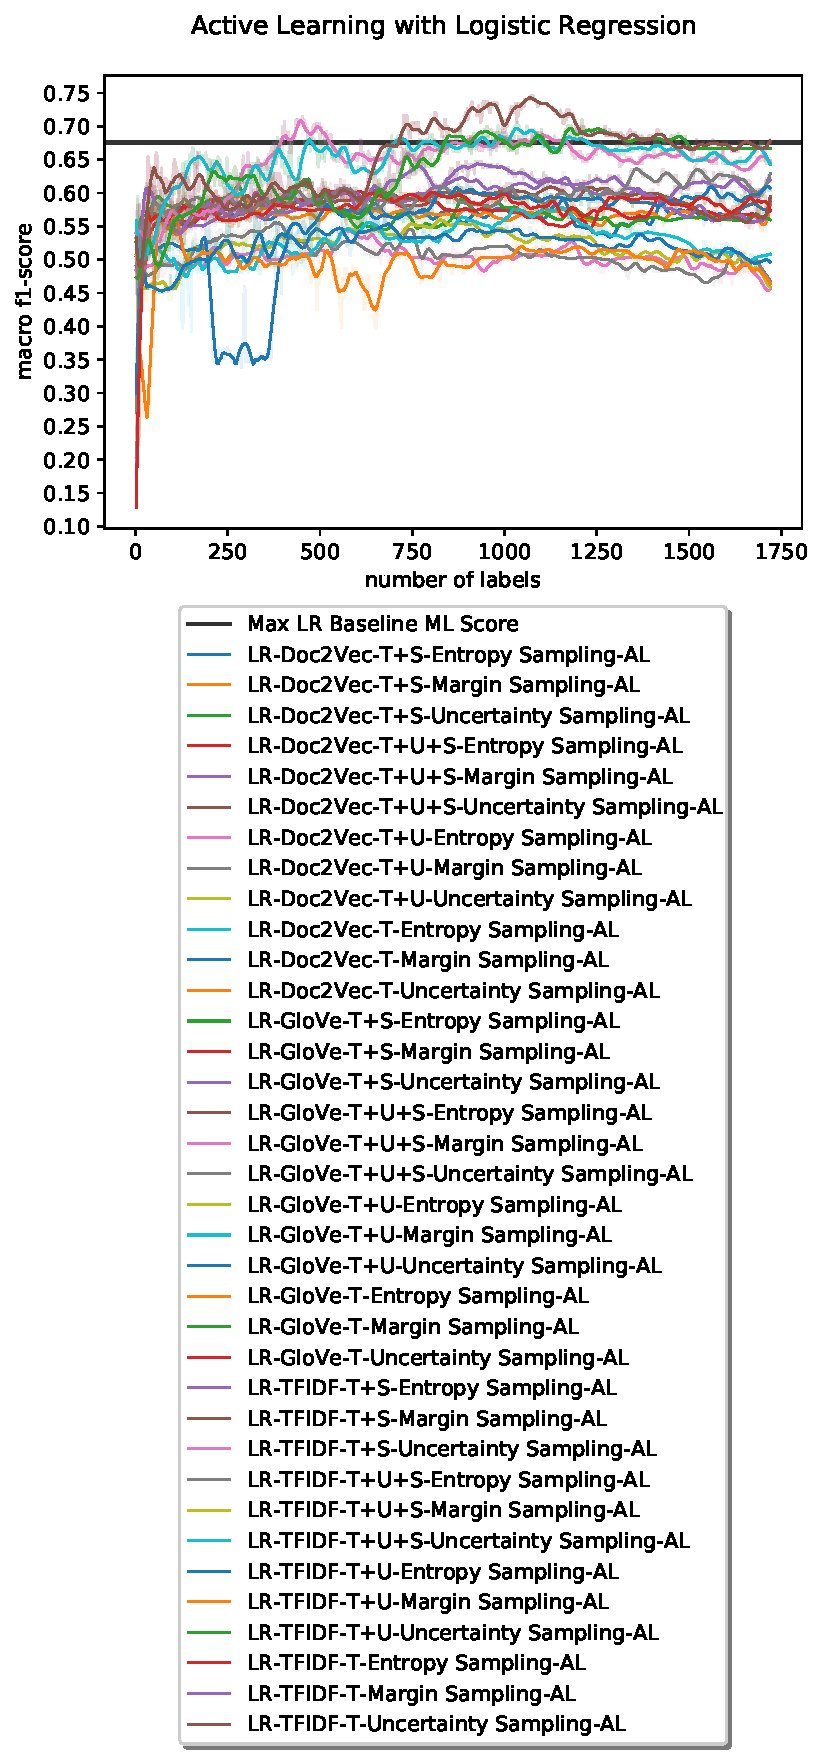
\includegraphics[scale=0.72]{graphs/LR-all.pdf}
%    
%    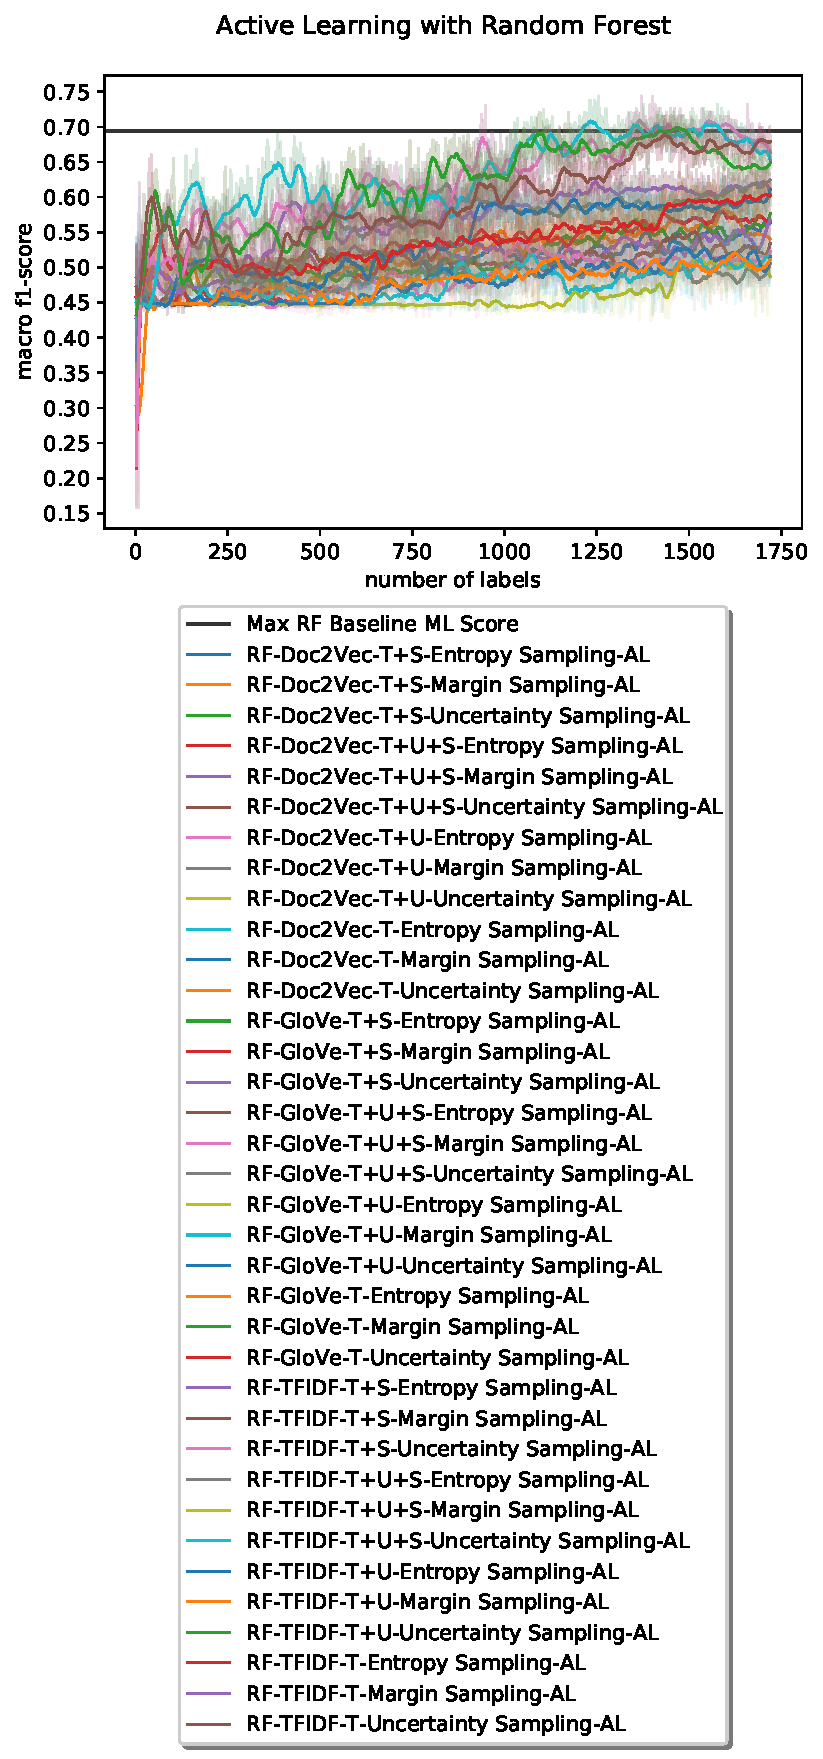
\includegraphics[scale=0.72]{graphs/RF-all.pdf}
%    
%    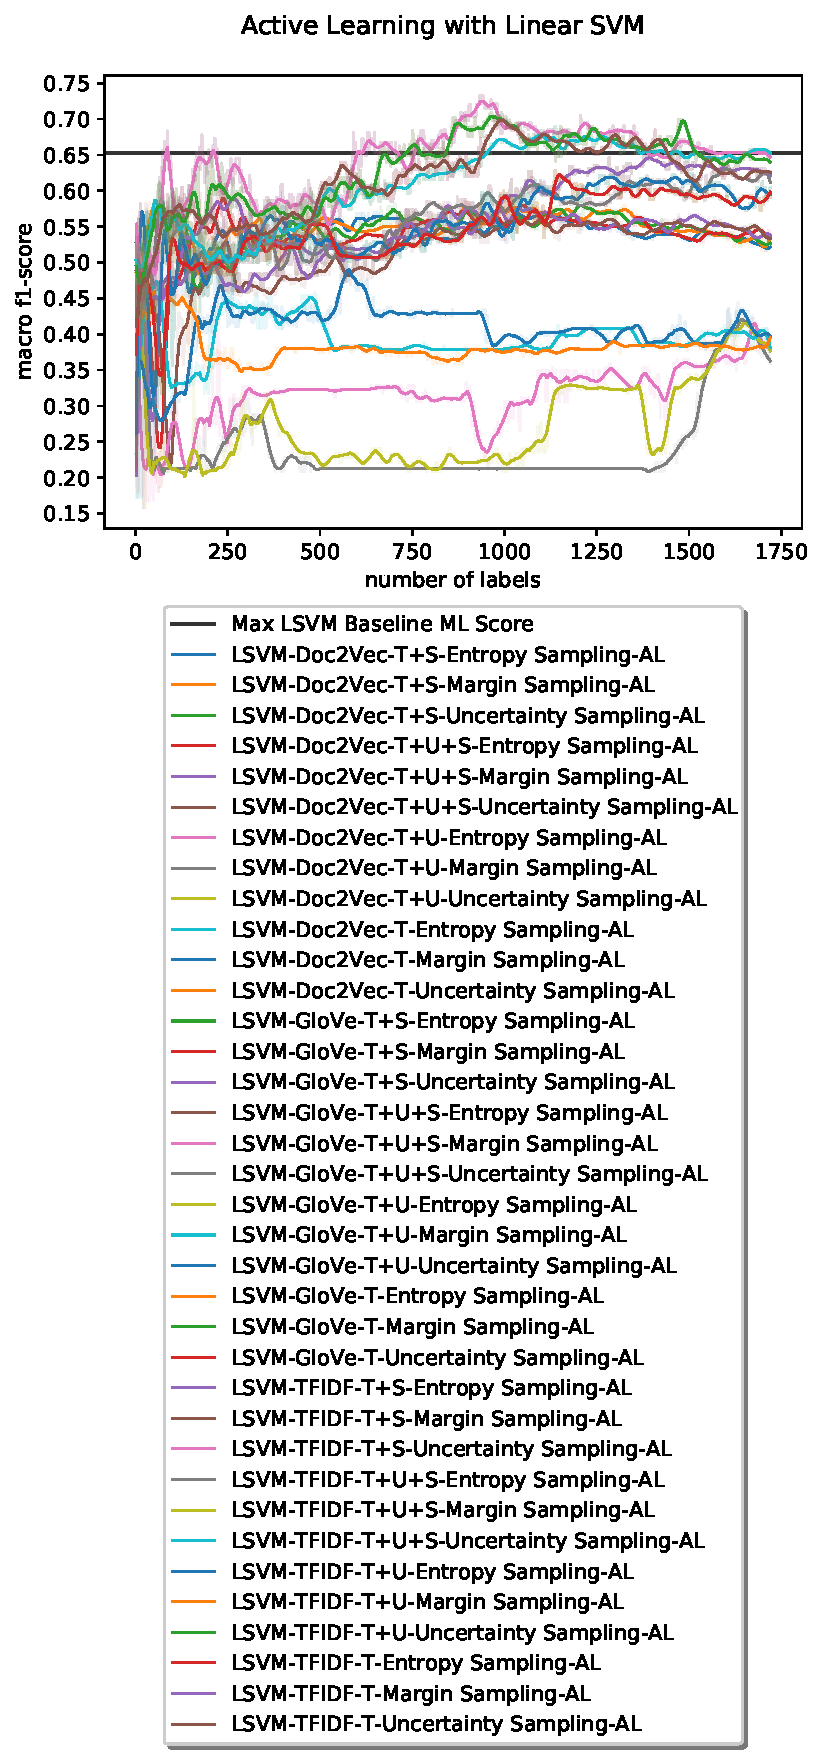
\includegraphics[scale=0.72]{graphs/LSVM-all.pdf}
%    
%    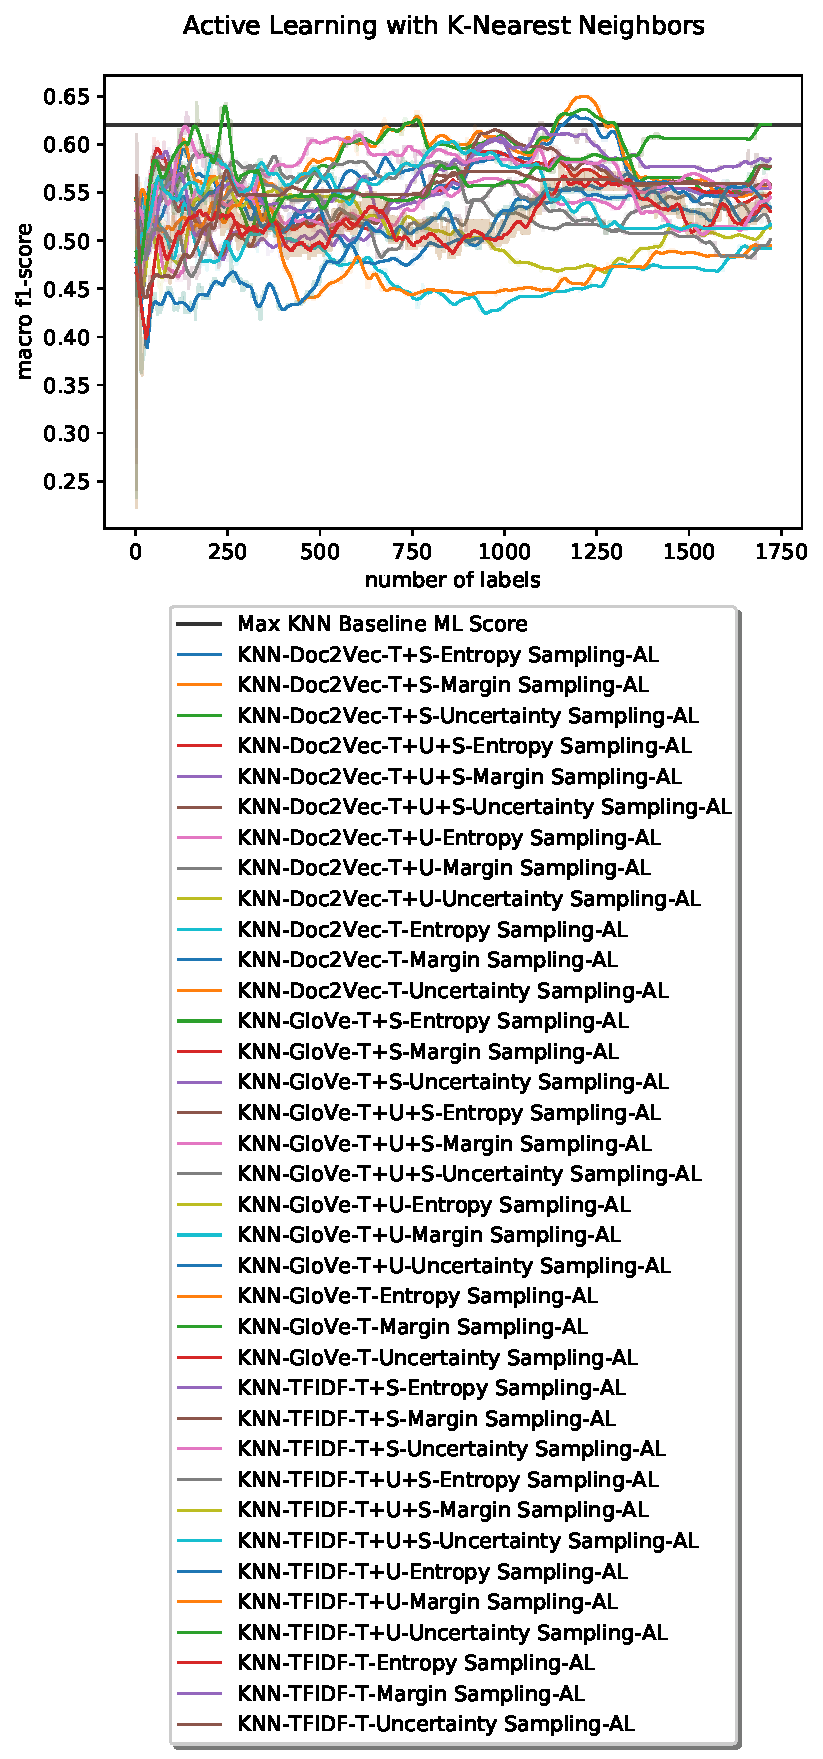
\includegraphics[scale=0.72]{graphs/KNN-all.pdf}
%\end{center}
\end{document}